\section{HDA 200 Cancellation Path} \label{sec:CPjournal}
\textbf{Note:} This was the initial experiment to determine the impulse response of the used headphone, later the headphone was changed and a new experiment was done. The results of this experiment are therefore obsolete. The new experiment can be seen in \autoref{sec:DT770CPjournal}.

All files from this appendix can be found in folder: \\
\path{Attachment://Appendix G - HDA 200 Cancellation Path}

\subsection{Purpose}
The purpose of this experiment is to make a model of the CP, by determining its impulse response, i.e. the transfer function between the "headphone loudspeaker" and the "error microphone (ear)".
		
\subsection{AAU number list}
\begin{table}[h]
	\centering
	\ra{1.3}
	\begin{tabular}{ c c c } \toprule
		{Item}	& {Description} 						& {AAU-no}. \\ \bottomrule 
		1	&	B\&K Head And Torso Simulator "Henry" Type 4128	& 08453		\\
		2	&	B\&K Ear Simulator Type 4159			& 08453		\\
		3	&	Sennheiser HDA 200	Headphones			& 33379		\\
		4	&	Roland Edirol UA-25EX Audio Capture		& 64696		\\
		5	&	Computer running Simulink				& NaN		\\
		6	&	B\&K Microphone Power Supply Type 2804 	& 07304		\\
		%5	&	B\&K \textonehalf'' Condenser Microphone Type 4134 & 61447\\
		%6	&	B\&K Sound Calibrator Type 4231			& 78301		\\ 
		7	&	B\&K Sound Intensity Calibrator Type 3541	& 08597	\\ \bottomrule
	\end{tabular}
	\caption{Table over equipment used in test.}
	\label{tab:UsedEquipmentListningCP}
\end{table}

\subsection{Diagrams}
\begin{figure}[H]
	\centering
	\tikzsetnextfilename{CancellationPath}
	\section{Cancellation Path Impulse Response} \label{sec:CPjournal}
\subsection{Purpose}
The purpose of this experiment is to make a model of the CP, by determining its impulse response of the, i.e. the transfer-function between the "source-loudspeaker" and the "error-microphone (ear)".
		
\subsection{AAU number list}
\begin{table}[h]
	\centering
	\ra{1.3}
	\begin{tabular}{ c c c } \toprule
		{Item}	& {Description} 						& {AAU-no}. \\ \bottomrule 
		1	&	B\&K Head And Torso Simulator "Henry" Type 4128	& 08453		\\
		2	&	B\&K Ear Simulator Type 4159			& 08453		\\
		3	&	Sennheiser HDA 200	Headphones			& 33379		\\
		4	&	Roland Edirol UA-25EX Audio Capture		& 64696		\\
		5	&	Vision B3565 Computer					& NaN		\\
		6	&	B\&K Microphone Power Supply Type 2804 	& 07304		\\
		%5	&	B\&K \textonehalf'' Condenser Microphone Type 4134 & 61447\\
		%6	&	B\&K Sound Calibrator Type 4231			& 78301		\\ 
		7	&	B\&K Sound Intensity Calibrator Type 3541	& 08597	\\ \bottomrule
	\end{tabular}
	\caption{Table over equipment used in test.}
	\label{tab:UsedEquipmentListningCP}
\end{table}

\subsection{Diagrams}
\begin{figure}[H]
	\centering
	\tikzsetnextfilename{CancellationPath}
	\section{Cancellation Path Impulse Response} \label{sec:CPjournal}
\subsection{Purpose}
The purpose of this experiment is to make a model of the CP, by determining its impulse response of the, i.e. the transfer-function between the "source-loudspeaker" and the "error-microphone (ear)".
		
\subsection{AAU number list}
\begin{table}[h]
	\centering
	\ra{1.3}
	\begin{tabular}{ c c c } \toprule
		{Item}	& {Description} 						& {AAU-no}. \\ \bottomrule 
		1	&	B\&K Head And Torso Simulator "Henry" Type 4128	& 08453		\\
		2	&	B\&K Ear Simulator Type 4159			& 08453		\\
		3	&	Sennheiser HDA 200	Headphones			& 33379		\\
		4	&	Roland Edirol UA-25EX Audio Capture		& 64696		\\
		5	&	Vision B3565 Computer					& NaN		\\
		6	&	B\&K Microphone Power Supply Type 2804 	& 07304		\\
		%5	&	B\&K \textonehalf'' Condenser Microphone Type 4134 & 61447\\
		%6	&	B\&K Sound Calibrator Type 4231			& 78301		\\ 
		7	&	B\&K Sound Intensity Calibrator Type 3541	& 08597	\\ \bottomrule
	\end{tabular}
	\caption{Table over equipment used in test.}
	\label{tab:UsedEquipmentListningCP}
\end{table}

\subsection{Diagrams}
\begin{figure}[H]
	\centering
	\tikzsetnextfilename{CancellationPath}
	\section{Cancellation Path Impulse Response} \label{sec:CPjournal}
\subsection{Purpose}
The purpose of this experiment is to make a model of the CP, by determining its impulse response of the, i.e. the transfer-function between the "source-loudspeaker" and the "error-microphone (ear)".
		
\subsection{AAU number list}
\begin{table}[h]
	\centering
	\ra{1.3}
	\begin{tabular}{ c c c } \toprule
		{Item}	& {Description} 						& {AAU-no}. \\ \bottomrule 
		1	&	B\&K Head And Torso Simulator "Henry" Type 4128	& 08453		\\
		2	&	B\&K Ear Simulator Type 4159			& 08453		\\
		3	&	Sennheiser HDA 200	Headphones			& 33379		\\
		4	&	Roland Edirol UA-25EX Audio Capture		& 64696		\\
		5	&	Vision B3565 Computer					& NaN		\\
		6	&	B\&K Microphone Power Supply Type 2804 	& 07304		\\
		%5	&	B\&K \textonehalf'' Condenser Microphone Type 4134 & 61447\\
		%6	&	B\&K Sound Calibrator Type 4231			& 78301		\\ 
		7	&	B\&K Sound Intensity Calibrator Type 3541	& 08597	\\ \bottomrule
	\end{tabular}
	\caption{Table over equipment used in test.}
	\label{tab:UsedEquipmentListningCP}
\end{table}

\subsection{Diagrams}
\begin{figure}[H]
	\centering
	\tikzsetnextfilename{CancellationPath}
	\input{figures/CancellationPath_MATLAB_Figures/CancellationPath.tex}
%	\includegraphics[width=0.7\textwidth]{Shematic_CalcellationPath.pdf}
	\caption{Total overview of the system.}
	\label{SchematicOverviewCP}
\end{figure}

\subsection{Settings/Description}
\label{SettingsCacellationPath}

Calibration of the microphone and associated preamplifier is done on the computer using Simulink\textsuperscript{\textregistered}. The following settings are present:

\subsubsection{Control and calibration}
\begin{itemize}
	\item 93.6 dB due to being a pressure field microphone $@$ 250 Hz is used as calibration signal.
	\item Microphone sensitivity is controlled to 11.6 $m$V/Pa.
	\item Calibration signal yields an amplitude of 0.6 relative to 0 dBFS.
	\item Calibration signal yields a spike at 95.5 dB SPL @250 Hz, which then requires a -2.3 dB SPL adjustment.
\end{itemize}

\subsubsection{Equipment settings}
\begin{itemize}
	\item This experiment is performed with a sampling rate of, $F_{s}$ = 48 $k$Hz.
	\item Item 4 (sound capture card):
		\begin{itemize}
			\item "SENS(INPUT 1/L)" is set to +0 dB.
			\item "SENS(INPUT 2/R)" is set to +0 dB.
			\item "PHONES" is set to maximum volume.
		\end{itemize}		
	\item Item 5 (computer) is set to 0 dBFS.
\end{itemize}


\subsection{Pictures}
%\begin{figure}[H]
%	\centering
%	\includegraphics[width=0.8\textwidth]{CancellationPath_and_Headphones/FullSetup.jpg}
%	\caption{Full setup of experiment (Note that "outside" microphone is not in use in the experiment).} 
%	\label{FullSetupCancellationPath}
%\end{figure}

\begin{figure}[H]
	\centering
	\includegraphics[width=0.8\textwidth]{CancellationPath_and_Headphones/CloseUpFace.jpg}
	\caption{Close up of experiment (Note that "outside" microphone is not in use in the experiment).}
	\label{CloseUpCancellationPath}
\end{figure}

\subsection{Procedure}
\subsubsection{Set-up}
\begin{enumerate}
	\item Set instruments to comply with the list in \ref{SettingsCacellationPath}.
	\item Control and calibrate item 2 using item 7.
	\item Place item 3 onto item 1 ("Henry"'s head and ears).
	\item Insert item 2's connector into input of item 6.
	\item Connect item 6 to item 4 and connect item 4 to item 5 via USB.
	\item Insert item 3's connector into output of item 4.
	\item Connect cable from item 4's output to item 4's input.
\end{enumerate}

\subsubsection{Performing the experiment}
\begin{enumerate}
	\item Start Simulink\textsuperscript{\textregistered} and open and run file \path{SimulinkSystemCancellationPath.xls}.
	\begin{itemize} 
		\item The simulations outputs a logarithmic chirp from 20 Hz to 20,000 Hz with an amplitude of 0 dBFS over the span of five seconds.
		\item The simulation runs for six seconds.
	\end{itemize}
	%\item Through Simulink\textsuperscript{\textregistered} play "LogChirp.wav" from item 5 via item 4
	\item Rename outputted files "Mic" and "Ref" to "Mic[i].wav" and "Ref[i].wav" \footnote{[i] indicates the iteration of the experiment.}
	\begin{itemize}
		\item[] Perform this experiment for a total of five times.
	\end{itemize}
\end{enumerate}
If  a discontinuity in the recorded signal(s) occurs, then discard that recording and reperform the experiment for the current iteration.


\subsubsection{Data Extraction}
\begin{enumerate}
	%\item Place generated .wav-files in same folder as MATLAB\textsuperscript{\textregistered}-script "CancellationPathScript.m".
	\item Start MATLAB\textsuperscript{\textregistered} and run script \path{CancellationPathScript.m}.
\end{enumerate}
From performing of the experiment, ten files has been generated:
\begin{itemize}
	\item Mic1.wav - Mic5.wav
	\item Ref1.wav - Ref5.wav
\end{itemize}

These files are the results of performing the six second simulation which gives a number of 288,768 samples, for each generated .wav-file.
An example showing outputted Mic1 and Ref1 is shown in  \autoref{AmplitudePlotCancellationPath}.

\begin{figure}[H]
	\centering
	\tikzsetnextfilename{CancellationPathAmplitudePlot2}
	%\input{figures/CancellationPath_MATLAB_Figures/Amplitudeplot2.tex}
	\input{figures/CancellationPath_MATLAB_Figures/calib.tex}
	\caption{Time plot of the cancellation path with the reference signal(blue) and the microphone signal(orange).}
	\label{AmplitudePlotCancellationPath}
\end{figure}

MATLAB\textsuperscript{\textregistered}-script \path{CancellationPathScript.m} is used for data extraction and analysis.



\subsection{Analysis}
The impulse response of the CP is to be found.
Note that a microphone with external polarization was used. It means that there is a 180\textdegree phase difference between pre- and external polarized microphones, i.e. a positive pressure leads to negative voltage. The externally polarized microphone is considered to be out of phase. \cite{michandbook}

First the cross correlation between Mic[i] and Ref[i] is found. This is done by cross correlating the two signals signals. Secondly the signal is taken into the frequency domain by applying the FT to the signal. This is expressed in \autoref{FrequencyResponseCPEq2}.



\begin{equation}\label{FrequencyResponseCPEq2}
%H(f) = \frac{Y(m_{\mu}) *  X(r_{\mu})}{X(r_{\mu}) *  X(r_{\mu})}
H(f) = \frac{Y(f) \cdot X\textsuperscript{*}(f)}{X(f) \cdot X\textsuperscript{*}(f)}
\end{equation}
Where:
\begin{description}
	%\item " $*$ " denotes the complex conjugation
	\item $H(f)$ is the FT of the CP.
	\item $Y(f)$ is the FT of the recorded microphone signals, Mic[i].
	\item $X(f)$ is the FT of the recorded reference signals, Ref[i].
\end{description}

The frequency response of the CP is shown in \autoref{FrequencyResponsePlotCancellationPath}.

\begin{figure}[H]
	\centering
	\tikzsetnextfilename{CancellationPathFrequencyResponse1}
	%\input{figures/CancellationPath_MATLAB_Figures/CP_freqresp.tex}
	\input{figures/CancellationPath_MATLAB_Figures/FreqResponseCP.tex}
	\caption{Frequency response plot of the cancellation path.}
	\label{FrequencyResponsePlotCancellationPath}
\end{figure}

The impulse response of this CP is found by taking the IFT (Inverse Fourier Transform) of the frequency response.
The impulse response is shown on \autoref{CancellationPathImpulseResponse}.

\begin{figure}[H]
	\centering
	\tikzsetnextfilename{CancellationPathImpulseResponse1}
	%\input{figures/CancellationPath_MATLAB_Figures/CancellationPathImpulseResponse.tex}
	\input{figures/CancellationPath_MATLAB_Figures/impulsefull.tex}
	\caption{Impulse response plot of the cancellation path see \autoref{CancellationPathImpulseResponseCrop} for zoomed in version.}
	\label{CancellationPathImpulseResponse}
\end{figure}


%\begin{figure}[H]
%	\centering
%	\includegraphics[width=0.85\textwidth]{CancellationPath_MATLAB_Figures/CancellationPathImpulseResponse.png}
%	\caption{Impulse Response plot of the cancellation path (NOT TIKZ).}
%	\label{CancellationPathImpulseResponse}
%\end{figure}

Converting the impulse response from magnitude to dB, gives the time decay which reveals the Signal to Noise Ratio (SNR) of the system, and from the read off SNR is found to be $\sim$ 60 dB SNR, as seen on \autoref{TimeDecayPlotCancellationPath}.

%\begin{figure}[H]
%	\centering
%	\includegraphics[width=0.85\textwidth]{CancellationPath_MATLAB_Figures/CancellationPathTimeDecay.png}
%	\caption{Time decay plot of the cancellation path (NOT TIKZ).}
%	\label{TimeDecayPlotCancellationPath}
%\end{figure}

\begin{figure}[H]
	\centering
	\tikzsetnextfilename{TimeDecayPlotCancellationPath1}
	%\input{figures/CancellationPath_MATLAB_Figures/TimeDecayPlotCancellationPath.tex}
	\input{figures/CancellationPath_MATLAB_Figures/snr.tex}
	\caption{Time decay plot of the cancellation path}
	\label{TimeDecayPlotCancellationPath}
\end{figure}


Taking the first 256 coefficients of the impulse response gives the following cropped impulse response, as seen on \autoref{CancellationPathImpulseResponseCrop}.

\begin{figure}[H]
	\centering
	\tikzsetnextfilename{CancellationPathImpulseResponseCrop1}
	%\input{figures/CancellationPath_MATLAB_Figures/CancellationPathImpulseResponseCrop.tex}
	\input{figures/CancellationPath_MATLAB_Figures/impulseresponse.tex}
	\caption{Cropped impulse response plot of the cancellation path}
	\label{CancellationPathImpulseResponseCrop}
\end{figure}

To verify that the frequency response of the cropped impulse response approximately equals that of the non-cropped impulse response the two frequency responses are compared. This can be seen on \autoref{CancellationPathImpulseResponseCompare}. Note that the two lines are almost completely on top of each other.

\begin{figure}[H]
	\centering
	\tikzsetnextfilename{CancellationPathImpulseResponseCompare1}
	%\input{figures/CancellationPath_MATLAB_Figures/CancellationPathImpulseResponseCompare.tex}
	\input{figures/CancellationPath_MATLAB_Figures/compfilter.tex}
	\caption{Comparison of the frequency response of 960 coefficients vs. 288,768 coefficients.}
	\label{CancellationPathImpulseResponseCompare}
\end{figure}

From \autoref{CancellationPathImpulseResponseCompare}, 960 coefficients is shown to be sufficient for representing the impulse response with good accuracy. 

\subsection{Error Sources / Tolerances}
\begin{itemize}
	\item Placement of the actuators and test-devices. (Position of the headset on the ear  influence the frequency response at high frequency which is not the main scope of study).
	\item Instrument inaccuracies see \autoref{TolerancesCP}.
\end{itemize}

\begin{table}[h]
	\centering
	\ra{1.3}
	\begin{tabular}{ c c c } \toprule
		{Item}	& 		{Description} 	& {Tolerance ([dB$_{re20\mu P}$])}.	 \\ \bottomrule 
		2	&	B\&K Ear Simulator Type 4159				& $\pm$ 1.5 	\\
		%3	&	Sennheiser HD 200 Headphones				& x		\\
		4	&	Roland Edirol UA-25EX Audio Capture			& $\pm$ 1.0	\\
		%6	&	B\&K Microphone Power Supply Type 2804		& 2 \%	\\ 
		7	&	B\&K Sound Intensity Calibrator Type 3541	& $\pm$ 0.2	\\ \bottomrule
			&	Total tolerance								& $\pm$ 2.7	\\ \bottomrule	
	\end{tabular}
	\caption{Table showing error tolerances for used equipment.}
	\label{TolerancesCP}
\end{table}

\subsection{Conclusion}
It can be concluded that an impulse response in the form of 256 coefficients, see \autoref{CancellationPathImpulseResponse}, is found for the "Cancellation path".
%The impulse response on  shows the coefficients of the system, and a file containing all 256 is generated with the name "CoeffientsCP.mat"
%	\includegraphics[width=0.7\textwidth]{Shematic_CalcellationPath.pdf}
	\caption{Total overview of the system.}
	\label{SchematicOverviewCP}
\end{figure}

\subsection{Settings/Description}
\label{SettingsCacellationPath}

Calibration of the microphone and associated preamplifier is done on the computer using Simulink\textsuperscript{\textregistered}. The following settings are present:

\subsubsection{Control and calibration}
\begin{itemize}
	\item 93.6 dB due to being a pressure field microphone $@$ 250 Hz is used as calibration signal.
	\item Microphone sensitivity is controlled to 11.6 $m$V/Pa.
	\item Calibration signal yields an amplitude of 0.6 relative to 0 dBFS.
	\item Calibration signal yields a spike at 95.5 dB SPL @250 Hz, which then requires a -2.3 dB SPL adjustment.
\end{itemize}

\subsubsection{Equipment settings}
\begin{itemize}
	\item This experiment is performed with a sampling rate of, $F_{s}$ = 48 $k$Hz.
	\item Item 4 (sound capture card):
		\begin{itemize}
			\item "SENS(INPUT 1/L)" is set to +0 dB.
			\item "SENS(INPUT 2/R)" is set to +0 dB.
			\item "PHONES" is set to maximum volume.
		\end{itemize}		
	\item Item 5 (computer) is set to 0 dBFS.
\end{itemize}


\subsection{Pictures}
%\begin{figure}[H]
%	\centering
%	\includegraphics[width=0.8\textwidth]{CancellationPath_and_Headphones/FullSetup.jpg}
%	\caption{Full setup of experiment (Note that "outside" microphone is not in use in the experiment).} 
%	\label{FullSetupCancellationPath}
%\end{figure}

\begin{figure}[H]
	\centering
	\includegraphics[width=0.8\textwidth]{CancellationPath_and_Headphones/CloseUpFace.jpg}
	\caption{Close up of experiment (Note that "outside" microphone is not in use in the experiment).}
	\label{CloseUpCancellationPath}
\end{figure}

\subsection{Procedure}
\subsubsection{Set-up}
\begin{enumerate}
	\item Set instruments to comply with the list in \ref{SettingsCacellationPath}.
	\item Control and calibrate item 2 using item 7.
	\item Place item 3 onto item 1 ("Henry"'s head and ears).
	\item Insert item 2's connector into input of item 6.
	\item Connect item 6 to item 4 and connect item 4 to item 5 via USB.
	\item Insert item 3's connector into output of item 4.
	\item Connect cable from item 4's output to item 4's input.
\end{enumerate}

\subsubsection{Performing the experiment}
\begin{enumerate}
	\item Start Simulink\textsuperscript{\textregistered} and open and run file \path{SimulinkSystemCancellationPath.xls}.
	\begin{itemize} 
		\item The simulations outputs a logarithmic chirp from 20 Hz to 20,000 Hz with an amplitude of 0 dBFS over the span of five seconds.
		\item The simulation runs for six seconds.
	\end{itemize}
	%\item Through Simulink\textsuperscript{\textregistered} play "LogChirp.wav" from item 5 via item 4
	\item Rename outputted files "Mic" and "Ref" to "Mic[i].wav" and "Ref[i].wav" \footnote{[i] indicates the iteration of the experiment.}
	\begin{itemize}
		\item[] Perform this experiment for a total of five times.
	\end{itemize}
\end{enumerate}
If  a discontinuity in the recorded signal(s) occurs, then discard that recording and reperform the experiment for the current iteration.


\subsubsection{Data Extraction}
\begin{enumerate}
	%\item Place generated .wav-files in same folder as MATLAB\textsuperscript{\textregistered}-script "CancellationPathScript.m".
	\item Start MATLAB\textsuperscript{\textregistered} and run script \path{CancellationPathScript.m}.
\end{enumerate}
From performing of the experiment, ten files has been generated:
\begin{itemize}
	\item Mic1.wav - Mic5.wav
	\item Ref1.wav - Ref5.wav
\end{itemize}

These files are the results of performing the six second simulation which gives a number of 288,768 samples, for each generated .wav-file.
An example showing outputted Mic1 and Ref1 is shown in  \autoref{AmplitudePlotCancellationPath}.

\begin{figure}[H]
	\centering
	\tikzsetnextfilename{CancellationPathAmplitudePlot2}
	%% This file was created by matlab2tikz.
%
%The latest updates can be retrieved from
%  http://www.mathworks.com/matlabcentral/fileexchange/22022-matlab2tikz-matlab2tikz
%where you can also make suggestions and rate matlab2tikz.
%
\definecolor{mycolor1}{rgb}{0.00000,0.44700,0.74100}%
\definecolor{mycolor2}{rgb}{0.85000,0.32500,0.09800}%
%
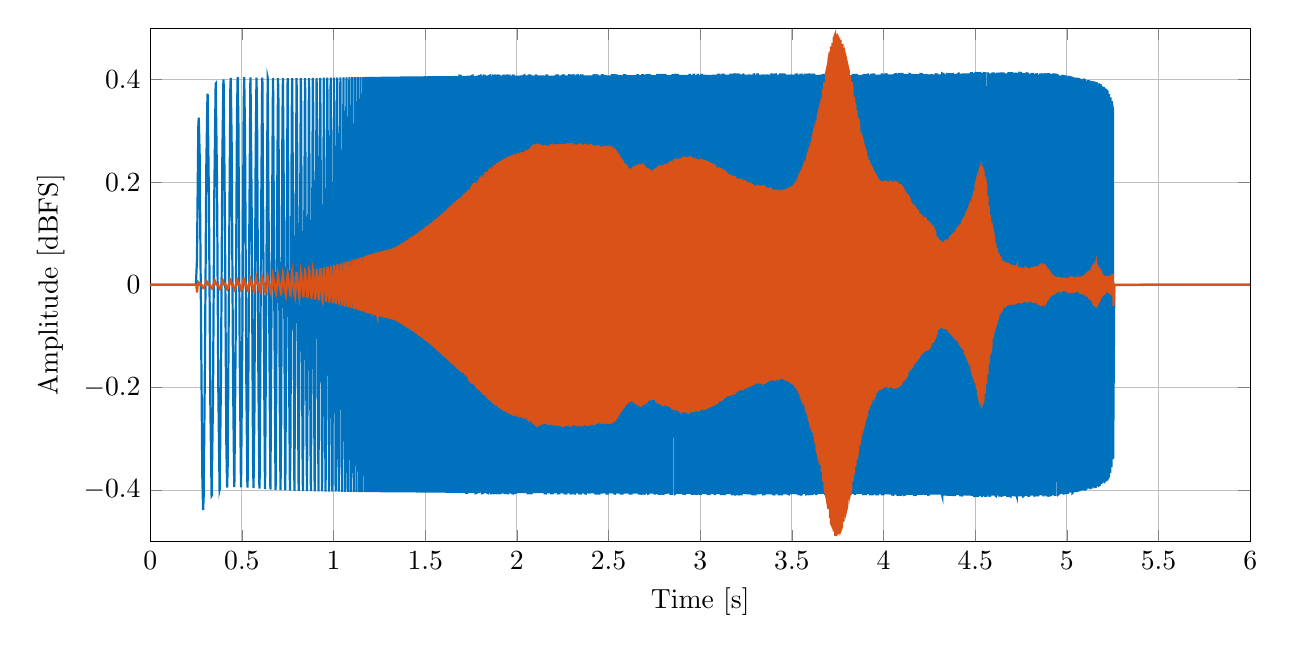
\begin{tikzpicture}

\begin{axis}[%
width=5.5in,
height=2.566in,
at={(1.925in,0.793in)},
scale only axis,
xmin=0,
xmax=6,
xlabel={Time [s]},
xmajorgrids,
ymin=-0.5,
ymax=0.5,
ylabel={Amplitude [dBFS]},
ymajorgrids,
axis background/.style={fill=white},
legend style={legend cell align=left,align=left,draw=white!15!black}
]
\addplot [color=mycolor1,solid,thick]
  table[row sep=crcr]{%
2.08333333333333e-05	-3.0517578125e-05\\
8.33333333333333e-05	-6.103515625e-05\\
0.000416666666666667	3.0517578125e-05\\
0.0123541666666667	6.103515625e-05\\
0.0132916666666667	-9.1552734375e-05\\
0.0148125	-6.103515625e-05\\
0.0148541666666667	3.0517578125e-05\\
0.0234583333333333	-6.103515625e-05\\
0.0238541666666667	6.103515625e-05\\
0.0297083333333333	3.0517578125e-05\\
0.031125	-6.103515625e-05\\
0.0364791666666667	3.0517578125e-05\\
0.0369166666666667	-9.1552734375e-05\\
0.0437708333333333	-6.103515625e-05\\
0.0446041666666667	6.103515625e-05\\
0.0510416666666667	6.103515625e-05\\
0.05575	-9.1552734375e-05\\
0.0583333333333333	3.0517578125e-05\\
0.059	-6.103515625e-05\\
0.0656666666666667	-6.103515625e-05\\
0.067875	6.103515625e-05\\
0.0728958333333333	3.0517578125e-05\\
0.0730208333333333	-6.103515625e-05\\
0.0801875	3.0517578125e-05\\
0.0802708333333333	-6.103515625e-05\\
0.087625	-6.103515625e-05\\
0.08775	3.0517578125e-05\\
0.0947708333333333	-6.103515625e-05\\
0.0960208333333333	6.103515625e-05\\
0.102	3.0517578125e-05\\
0.102354166666667	-6.103515625e-05\\
0.1095625	-6.103515625e-05\\
0.1160625	6.103515625e-05\\
0.118354166666667	-6.103515625e-05\\
0.121625	6.103515625e-05\\
0.123854166666667	3.0517578125e-05\\
0.124291666666667	-6.103515625e-05\\
0.131375	-6.103515625e-05\\
0.131541666666667	3.0517578125e-05\\
0.138708333333333	-6.103515625e-05\\
0.14125	6.103515625e-05\\
0.145875	3.0517578125e-05\\
0.146020833333333	-6.103515625e-05\\
0.157354166666667	-9.1552734375e-05\\
0.157625	6.103515625e-05\\
0.160354166666667	-6.103515625e-05\\
0.160645833333333	3.0517578125e-05\\
0.16775	-6.103515625e-05\\
0.167916666666667	6.103515625e-05\\
0.174958333333333	3.0517578125e-05\\
0.174979166666667	-6.103515625e-05\\
0.182333333333333	-6.103515625e-05\\
0.184104166666667	6.103515625e-05\\
0.1895	6.103515625e-05\\
0.196	-9.1552734375e-05\\
0.197270833333333	-6.103515625e-05\\
0.203708333333333	6.103515625e-05\\
0.204083333333333	-6.103515625e-05\\
0.204416666666667	3.0517578125e-05\\
0.2116875	-6.103515625e-05\\
0.216979166666667	6.103515625e-05\\
0.2190625	-6.103515625e-05\\
0.2230625	6.103515625e-05\\
0.2258125	3.0517578125e-05\\
0.225958333333333	-6.103515625e-05\\
0.2349375	6.103515625e-05\\
0.2374375	-9.1552734375e-05\\
0.243333333333333	6.103515625e-05\\
0.245354166666667	-9.1552734375e-05\\
0.249125	-9.1552734375e-05\\
0.2549375	0.048797607421875\\
0.2549375	0.048797607421875\\
0.262229166666667	0.307037353515625\\
0.264604166666667	0.325927734375\\
0.269520833333333	0.254119873046875\\
0.269520833333333	0.254119873046875\\
0.276791666666667	-0.056732177734375\\
0.276791666666667	-0.056732177734375\\
0.284083333333333	-0.374053955078125\\
0.284083333333333	-0.374053955078125\\
0.288479166666667	-0.43914794921875\\
0.291354166666667	-0.41314697265625\\
0.298645833333333	-0.14215087890625\\
0.298645833333333	-0.14215087890625\\
0.3059375	0.232025146484375\\
0.3059375	0.232025146484375\\
0.312291666666667	0.37255859375\\
0.313208333333333	0.369140625\\
0.3205	0.15313720703125\\
0.3205	0.15313720703125\\
0.327770833333333	-0.22979736328125\\
0.327770833333333	-0.22979736328125\\
0.334791666666667	-0.41107177734375\\
0.3350625	-0.410919189453125\\
0.342354166666667	-0.21832275390625\\
0.342354166666667	-0.21832275390625\\
0.349625	0.181488037109375\\
0.349625	0.181488037109375\\
0.356895833333333	0.39178466796875\\
0.357083333333333	0.391876220703125\\
0.3641875	0.201416015625\\
0.3641875	0.201416015625\\
0.371479166666667	-0.20745849609375\\
0.371479166666667	-0.20745849609375\\
0.3783125	-0.3995361328125\\
0.378770833333333	-0.3988037109375\\
0.386041666666667	-0.173553466796875\\
0.386041666666667	-0.173553466796875\\
0.393333333333333	0.247589111328125\\
0.393333333333333	0.247589111328125\\
0.399125	0.400115966796875\\
0.400604166666667	0.390899658203125\\
0.407895833333333	0.098602294921875\\
0.407895833333333	0.098602294921875\\
0.4151875	-0.3116455078125\\
0.4151875	-0.3116455078125\\
0.419395833333333	-0.39520263671875\\
0.422458333333333	-0.35198974609375\\
0.42975	0.026031494140625\\
0.42975	0.026031494140625\\
0.437020833333333	0.38165283203125\\
0.438958333333333	0.403411865234375\\
0.4443125	0.271514892578125\\
0.4443125	0.271514892578125\\
0.451604166666667	-0.1781005859375\\
0.451604166666667	-0.1781005859375\\
0.458166666666667	-0.394073486328125\\
0.458875	-0.3914794921875\\
0.466166666666667	-0.0965576171875\\
0.466166666666667	-0.0965576171875\\
0.4734375	0.33868408203125\\
0.4768125	0.404510498046875\\
0.480729166666667	0.322845458984375\\
0.480729166666667	0.322845458984375\\
0.488	-0.1302490234375\\
0.488	-0.1302490234375\\
0.495	-0.394378662109375\\
0.495291666666667	-0.393829345703125\\
0.502583333333333	-0.096527099609375\\
0.502583333333333	-0.096527099609375\\
0.509854166666667	0.35211181640625\\
0.512666666666667	0.404541015625\\
0.517145833333333	0.289459228515625\\
0.517145833333333	0.289459228515625\\
0.524416666666667	-0.2015380859375\\
0.524416666666667	-0.2015380859375\\
0.5300625	-0.395172119140625\\
0.531708333333333	-0.37774658203125\\
0.539	0.033599853515625\\
0.539	0.033599853515625\\
0.546270833333333	0.401153564453125\\
0.546875	0.404266357421875\\
0.5535625	0.133392333984375\\
0.5535625	0.133392333984375\\
0.560833333333333	-0.34747314453125\\
0.563395833333333	-0.396148681640625\\
0.568125	-0.249755859375\\
0.568125	-0.249755859375\\
0.575416666666667	0.27593994140625\\
0.575416666666667	0.27593994140625\\
0.579583333333333	0.403839111328125\\
0.5826875	0.334197998046875\\
0.589979166666667	-0.18511962890625\\
0.589979166666667	-0.18511962890625\\
0.595395833333333	-0.397125244140625\\
0.59725	-0.3707275390625\\
0.604541666666667	0.112213134765625\\
0.604541666666667	0.112213134765625\\
0.610791666666667	0.403472900390625\\
0.611833333333333	0.395233154296875\\
0.619104166666667	-0.05230712890625\\
0.619104166666667	-0.05230712890625\\
0.625875	-0.397979736328125\\
0.626395833333333	-0.396240234375\\
0.633666666666667	0.021026611328125\\
0.633666666666667	0.021026611328125\\
0.64075	0.40313720703125\\
0.640958333333333	0.40277099609375\\
0.64825	-0.012603759765625\\
0.64825	-0.012603759765625\\
0.6553125	-0.398681640625\\
0.655520833333333	-0.39813232421875\\
0.6628125	0.031097412109375\\
0.6628125	0.031097412109375\\
0.669520833333333	0.402923583984375\\
0.670083333333333	0.39971923828125\\
0.677375	-0.073577880859375\\
0.677375	-0.073577880859375\\
0.683458333333333	-0.399444580078125\\
0.684666666666667	-0.38580322265625\\
0.6919375	0.141571044921875\\
0.6919375	0.141571044921875\\
0.697166666666667	0.402801513671875\\
0.699229166666667	0.3597412109375\\
0.7065	-0.227294921875\\
0.7065	-0.227294921875\\
0.710645833333333	-0.399993896484375\\
0.713791666666667	-0.295745849609375\\
0.721083333333333	0.319549560546875\\
0.723770833333333	0.40264892578125\\
0.728354166666667	0.186370849609375\\
0.728354166666667	0.186370849609375\\
0.735645833333333	-0.385894775390625\\
0.736708333333333	-0.40045166015625\\
0.742916666666667	-0.02593994140625\\
0.742916666666667	-0.02593994140625\\
0.7494375	0.402618408203125\\
0.750208333333333	0.39654541015625\\
0.7575	-0.169219970703125\\
0.7575	-0.169219970703125\\
0.761979166666667	-0.400848388671875\\
0.764770833333333	-0.308868408203125\\
0.7720625	0.337860107421875\\
0.774291666666667	0.40264892578125\\
0.779333333333333	0.107757568359375\\
0.779333333333333	0.107757568359375\\
0.786395833333333	-0.401214599609375\\
0.786625	-0.400390625\\
0.793916666666667	0.160491943359375\\
0.793916666666667	0.160491943359375\\
0.79825	0.40264892578125\\
0.8011875	0.28887939453125\\
0.808479166666667	-0.36962890625\\
0.809958333333333	-0.4014892578125\\
0.81575	-0.002410888671875\\
0.81575	-0.002410888671875\\
0.821458333333333	0.40277099609375\\
0.823041666666667	0.367584228515625\\
0.830333333333333	-0.31005859375\\
0.832791666666667	-0.401763916015625\\
0.837604166666667	-0.093719482421875\\
0.837604166666667	-0.093719482421875\\
0.843979166666667	0.40289306640625\\
0.844895833333333	0.38970947265625\\
0.852166666666667	-0.279998779296875\\
0.854958333333333	-0.4019775390625\\
0.859458333333333	-0.11029052734375\\
0.859458333333333	-0.11029052734375\\
0.865729166666667	0.402923583984375\\
0.86675	0.38763427734375\\
0.874020833333333	-0.3035888671875\\
0.876416666666667	-0.40216064453125\\
0.8813125	-0.0511474609375\\
0.8813125	-0.0511474609375\\
0.886958333333333	0.403076171875\\
0.888583333333333	0.356658935546875\\
0.895875	-0.36468505859375\\
0.897333333333333	-0.402374267578125\\
0.903166666666667	0.088226318359375\\
0.903166666666667	0.088226318359375\\
0.907541666666667	0.403167724609375\\
0.9104375	0.249847412109375\\
0.917625	-0.40252685546875\\
0.917729166666667	-0.402130126953125\\
0.925	0.279541015625\\
0.927520833333333	0.403350830078125\\
0.932291666666667	0.0185546875\\
0.932291666666667	0.0185546875\\
0.937291666666667	-0.402587890625\\
0.9395625	-0.30322265625\\
0.946854166666667	0.40301513671875\\
0.946979166666667	0.4034423828125\\
0.954145833333333	-0.285247802734375\\
0.956520833333333	-0.402740478515625\\
0.961416666666667	0.021209716796875\\
0.961416666666667	0.021209716796875\\
0.9659375	0.403564453125\\
0.968708333333333	0.240692138671875\\
0.975229166666667	-0.402923583984375\\
0.975979166666667	-0.390411376953125\\
0.983270833333333	0.37298583984375\\
0.984395833333333	0.403656005859375\\
0.9905625	-0.215118408203125\\
0.9934375	-0.402984619140625\\
0.997833333333333	-0.018707275390625\\
0.997833333333333	-0.018707275390625\\
1.00241666666667	0.40380859375\\
1.005125	0.23162841796875\\
1.01122916666667	-0.403076171875\\
1.01239583333333	-0.370361328125\\
1.0196875	0.4014892578125\\
1.01995833333333	0.403900146484375\\
1.02697916666667	-0.33349609375\\
1.02860416666667	-0.4031982421875\\
1.03425	0.192962646484375\\
1.03716666666667	0.40411376953125\\
1.04154166666667	-0.027557373046875\\
1.04154166666667	-0.027557373046875\\
1.0455625	-0.403411865234375\\
1.0488125	-0.140045166015625\\
1.053875	0.404266357421875\\
1.05610416666667	0.26983642578125\\
1.06214583333333	-0.403350830078125\\
1.06339583333333	-0.357269287109375\\
1.07027083333333	0.40435791015625\\
1.07066666666667	0.39959716796875\\
1.07795833333333	-0.3995361328125\\
1.0783125	-0.403564453125\\
1.08522916666667	0.36907958984375\\
1.08629166666667	0.404510498046875\\
1.09252083333333	-0.319854736328125\\
1.0941875	-0.403564453125\\
1.0998125	0.26080322265625\\
1.10191666666667	0.404541015625\\
1.10708333333333	-0.199920654296875\\
1.10964583333333	-0.403656005859375\\
1.114375	0.143646240234375\\
1.11727083333333	0.4046630859375\\
1.12164583333333	-0.096282958984375\\
1.12483333333333	-0.403717041015625\\
1.1289375	0.05902099609375\\
1.1323125	0.40472412109375\\
1.13622916666667	-0.037994384765625\\
1.1396875	-0.403778076171875\\
1.1435	0.02154541015625\\
1.147	0.40478515625\\
1.15079166666667	-0.025634765625\\
1.15422916666667	-0.40380859375\\
1.1580625	0.0347900390625\\
1.16141666666667	0.404937744140625\\
1.16535416666667	-0.06451416015625\\
1.16854166666667	-0.40386962890625\\
1.17264583333333	0.102630615234375\\
1.1755625	0.404998779296875\\
1.17991666666667	-0.152435302734375\\
1.18254166666667	-0.4039306640625\\
1.18720833333333	0.21136474609375\\
1.1894375	0.405059814453125\\
1.19447916666667	-0.274322509765625\\
1.19629166666667	-0.40399169921875\\
1.20177083333333	0.335845947265625\\
1.20304166666667	0.405120849609375\\
1.2090625	-0.3834228515625\\
1.20975	-0.404052734375\\
1.21633333333333	0.40496826171875\\
1.21641666666667	0.405242919921875\\
1.22297916666667	-0.404052734375\\
1.223625	-0.385467529296875\\
1.2295	0.405303955078125\\
1.23089583333333	0.31756591796875\\
1.23597916666667	-0.40411376953125\\
1.2381875	-0.1920166015625\\
1.24235416666667	0.40533447265625\\
1.24872916666667	-0.4041748046875\\
1.25275	0.165863037109375\\
1.25502083333333	0.405426025390625\\
1.26004166666667	-0.32794189453125\\
1.26127083333333	-0.404205322265625\\
1.2673125	0.404052734375\\
1.26745833333333	0.405517578125\\
1.27358333333333	-0.40423583984375\\
1.27460416666667	-0.353790283203125\\
1.27970833333333	0.40557861328125\\
1.28189583333333	0.16973876953125\\
1.28572916666667	-0.404296875\\
1.29172916666667	0.4056396484375\\
1.29645833333333	-0.32525634765625\\
1.29764583333333	-0.404296875\\
1.30354166666667	0.40570068359375\\
1.30372916666667	0.40380859375\\
1.30939583333333	-0.404388427734375\\
1.31102083333333	-0.259002685546875\\
1.31516666666667	0.405731201171875\\
1.3209375	-0.40435791015625\\
1.32558333333333	0.33831787109375\\
1.326625	0.405792236328125\\
1.33227083333333	-0.404388427734375\\
1.332875	-0.38397216796875\\
1.33789583333333	0.40582275390625\\
1.34347916666667	-0.404449462890625\\
1.3474375	0.2523193359375\\
1.349	0.4058837890625\\
1.3545	-0.40447998046875\\
1.35472916666667	-0.40093994140625\\
1.3599375	0.405914306640625\\
1.36533333333333	-0.404449462890625\\
1.36929166666667	0.271453857421875\\
1.37070833333333	0.405975341796875\\
1.37604166666667	-0.404510498046875\\
1.3765625	-0.385711669921875\\
1.38133333333333	0.406005859375\\
1.38658333333333	-0.404510498046875\\
1.391125	0.37384033203125\\
1.39177083333333	0.40606689453125\\
1.39695833333333	-0.404541015625\\
1.39841666666667	-0.256805419921875\\
1.40210416666667	0.4061279296875\\
1.4071875	-0.404541015625\\
1.41227083333333	0.406158447265625\\
1.41297916666667	0.366363525390625\\
1.41729166666667	-0.40460205078125\\
1.42227083333333	0.406158447265625\\
1.42722916666667	-0.404571533203125\\
1.42754166666667	-0.397674560546875\\
1.4321875	0.40618896484375\\
1.4370625	-0.40460205078125\\
1.4419375	0.406219482421875\\
1.442125	0.402923583984375\\
1.44675	-0.4046630859375\\
1.45154166666667	0.40625\\
1.4563125	-0.40472412109375\\
1.4566875	-0.392730712890625\\
1.46104166666667	0.406280517578125\\
1.46572916666667	-0.4046630859375\\
1.47041666666667	0.40631103515625\\
1.47125	0.34527587890625\\
1.4750625	-0.40472412109375\\
1.4796875	0.406341552734375\\
1.48427083333333	-0.40472412109375\\
1.4888125	0.4063720703125\\
1.49310416666667	-0.399261474609375\\
1.49335416666667	-0.404754638671875\\
1.49783333333333	0.40643310546875\\
1.5023125	-0.404815673828125\\
1.50675	0.406402587890625\\
1.51116666666667	-0.40478515625\\
1.51495833333333	0.369049072265625\\
1.5155625	0.406494140625\\
1.51991666666667	-0.404815673828125\\
1.52425	0.406494140625\\
1.5285625	-0.40484619140625\\
1.53285416666667	0.406494140625\\
1.53679166666667	-0.393646240234375\\
1.53710416666667	-0.40484619140625\\
1.54133333333333	0.406524658203125\\
1.5455625	-0.4049072265625\\
1.54972916666667	0.40655517578125\\
1.55389583333333	-0.40496826171875\\
1.55804166666667	0.40655517578125\\
1.56216666666667	-0.404937744140625\\
1.5659375	0.394866943359375\\
1.56622916666667	0.406585693359375\\
1.57033333333333	-0.405059814453125\\
1.57435416666667	0.406646728515625\\
1.57839583333333	-0.404998779296875\\
1.58239583333333	0.406646728515625\\
1.58635416666667	-0.40509033203125\\
1.5903125	0.40667724609375\\
1.59425	-0.40509033203125\\
1.59816666666667	0.406768798828125\\
1.60208333333333	-0.405120849609375\\
1.6059375	0.40673828125\\
1.609625	-0.401458740234375\\
1.60979166666667	-0.405120849609375\\
1.61360416666667	0.40673828125\\
1.6174375	-0.405181884765625\\
1.62120833333333	0.406768798828125\\
1.625	-0.405181884765625\\
1.62875	0.40679931640625\\
1.63247916666667	-0.405181884765625\\
1.6361875	0.40679931640625\\
1.639875	-0.40521240234375\\
1.64358333333333	0.4068603515625\\
1.64720833333333	-0.4052734375\\
1.65085416666667	0.4068603515625\\
1.65447916666667	-0.405303955078125\\
1.65808333333333	0.406951904296875\\
1.66166666666667	-0.4052734375\\
1.66522916666667	0.40692138671875\\
1.66877083333333	-0.40496826171875\\
1.6723125	0.4068603515625\\
1.67583333333333	-0.40594482421875\\
1.67933333333333	0.40655517578125\\
1.6828125	-0.40533447265625\\
1.68627083333333	0.407562255859375\\
1.69316666666667	0.406982421875\\
1.6965625	-0.40594482421875\\
1.69995833333333	0.407012939453125\\
1.70335416666667	-0.4053955078125\\
1.70672916666667	0.406982421875\\
1.7100625	-0.4049072265625\\
1.71339583333333	0.40704345703125\\
1.71670833333333	-0.4058837890625\\
1.72004166666667	0.407012939453125\\
1.72333333333333	-0.4053955078125\\
1.72985416666667	-0.40533447265625\\
1.733125	0.40765380859375\\
1.73635416666667	-0.40545654296875\\
1.7395625	0.4071044921875\\
1.74275	-0.405029296875\\
1.74595833333333	0.4071044921875\\
1.749125	-0.406005859375\\
1.75229166666667	0.406707763671875\\
1.75858333333333	0.407623291015625\\
1.7616875	-0.40545654296875\\
1.76479166666667	0.407135009765625\\
1.76789583333333	-0.40509033203125\\
1.77097916666667	0.407135009765625\\
1.77404166666667	-0.406036376953125\\
1.78014583333333	-0.405517578125\\
1.78316666666667	0.407623291015625\\
1.7861875	-0.4051513671875\\
1.7891875	0.407196044921875\\
1.7921875	-0.405975341796875\\
1.79516666666667	0.40679931640625\\
1.80108333333333	0.40765380859375\\
1.80402083333333	-0.405120849609375\\
1.80695833333333	0.4072265625\\
1.809875	-0.406036376953125\\
1.8156875	-0.405548095703125\\
1.8185625	0.40765380859375\\
1.82429166666667	0.4072265625\\
1.82714583333333	-0.406005859375\\
1.83	0.406890869140625\\
1.8328125	-0.405548095703125\\
1.83564583333333	0.407623291015625\\
1.8384375	-0.405181884765625\\
1.84402083333333	-0.405975341796875\\
1.8468125	0.406829833984375\\
1.8523125	0.40771484375\\
1.8550625	-0.405242919921875\\
1.85779166666667	0.4073486328125\\
1.8605	-0.405914306640625\\
1.86591666666667	-0.405609130859375\\
1.86860416666667	0.40765380859375\\
1.87395833333333	0.407318115234375\\
1.876625	-0.405914306640625\\
1.8819375	-0.405670166015625\\
1.8845625	0.407623291015625\\
1.88979166666667	0.40728759765625\\
1.89239583333333	-0.405914306640625\\
1.89758333333333	-0.40576171875\\
1.90014583333333	0.40765380859375\\
1.90527083333333	0.407318115234375\\
1.90783333333333	-0.405975341796875\\
1.91289583333333	-0.40570068359375\\
1.9154375	0.407623291015625\\
1.9179375	-0.405548095703125\\
1.9204375	0.40740966796875\\
1.9229375	-0.40594482421875\\
1.9254375	0.407318115234375\\
1.930375	0.407440185546875\\
1.93283333333333	-0.4056396484375\\
1.93775	-0.40582275390625\\
1.9401875	0.407135009765625\\
1.94504166666667	0.4075927734375\\
1.9474375	-0.405487060546875\\
1.95225	-0.405975341796875\\
1.954625	0.4072265625\\
1.95939583333333	0.407470703125\\
1.96175	-0.40594482421875\\
1.9688125	0.40753173828125\\
1.97114583333333	-0.4056396484375\\
1.97579166666667	-0.406219482421875\\
1.97810416666667	0.40765380859375\\
1.98270833333333	0.40753173828125\\
1.985	-0.405914306640625\\
1.9895625	-0.40582275390625\\
1.99183333333333	0.40753173828125\\
1.99860416666667	-0.406341552734375\\
2.00083333333333	0.407806396484375\\
2.00752083333333	-0.405914306640625\\
2.00972916666667	0.40753173828125\\
2.0119375	-0.40594482421875\\
2.01414583333333	0.407623291015625\\
2.02070833333333	-0.4058837890625\\
2.022875	0.40802001953125\\
2.02504166666667	-0.406005859375\\
2.0315	0.407989501953125\\
2.03364583333333	-0.405975341796875\\
2.03579166666667	0.407135009765625\\
2.04004166666667	0.40802001953125\\
2.04216666666667	-0.405914306640625\\
2.04847916666667	0.407989501953125\\
2.0505625	-0.405975341796875\\
2.05679166666667	0.407958984375\\
2.058875	-0.406005859375\\
2.063	-0.40594482421875\\
2.06504166666667	0.408050537109375\\
2.0731875	0.40802001953125\\
2.07520833333333	-0.406005859375\\
2.07922916666667	-0.40594482421875\\
2.08125	0.407989501953125\\
2.08325	-0.406158447265625\\
2.08522916666667	0.40765380859375\\
2.095125	-0.406005859375\\
2.09708333333333	0.40802001953125\\
2.1029375	-0.406036376953125\\
2.104875	0.40802001953125\\
2.10489583333333	0.40802001953125\\
2.1068125	-0.406036376953125\\
2.11260416666667	0.40802001953125\\
2.11452083333333	-0.406005859375\\
2.12022916666667	0.40802001953125\\
2.122125	-0.40606689453125\\
2.12777083333333	0.40789794921875\\
2.12964583333333	-0.406036376953125\\
2.13525	0.407989501953125\\
2.13710416666667	-0.406036376953125\\
2.14264583333333	0.4080810546875\\
2.14447916666667	-0.4061279296875\\
2.14995833333333	0.407867431640625\\
2.15179166666667	-0.4061279296875\\
2.15902083333333	-0.4063720703125\\
2.1608125	0.407745361328125\\
2.16439583333333	0.407745361328125\\
2.16616666666667	-0.406280517578125\\
2.1715	0.40777587890625\\
2.17327083333333	-0.40631103515625\\
2.17854166666667	0.40765380859375\\
2.18029166666667	-0.406219482421875\\
2.1855	0.407806396484375\\
2.18722916666667	-0.406280517578125\\
2.194125	-0.406219482421875\\
2.19925	0.407806396484375\\
2.2009375	-0.40631103515625\\
2.20264583333333	0.407745361328125\\
2.20770833333333	-0.40618896484375\\
2.209375	0.40789794921875\\
2.21439583333333	-0.4061279296875\\
2.2160625	0.407867431640625\\
2.2226875	0.407928466796875\\
2.22433333333333	-0.4063720703125\\
2.230875	-0.40618896484375\\
2.2325	0.407867431640625\\
2.24058333333333	-0.406585693359375\\
2.2421875	0.408111572265625\\
2.24379166666667	-0.406219482421875\\
2.2485625	0.407745361328125\\
2.25489583333333	0.408203125\\
2.25645833333333	-0.40631103515625\\
2.25804166666667	0.407928466796875\\
2.25960416666667	-0.406158447265625\\
2.2689375	-0.406524658203125\\
2.27047916666667	0.40814208984375\\
2.27814583333333	-0.406524658203125\\
2.27966666666667	0.407958984375\\
2.28422916666667	-0.40618896484375\\
2.28575	0.40814208984375\\
2.29175	0.4078369140625\\
2.29325	-0.406524658203125\\
2.29920833333333	-0.406158447265625\\
2.3006875	0.408203125\\
2.30216666666667	-0.406463623046875\\
2.303625	0.40789794921875\\
2.3095	0.408203125\\
2.31095833333333	-0.4063720703125\\
2.31677083333333	-0.40655517578125\\
2.31820833333333	0.4080810546875\\
2.32539583333333	-0.406524658203125\\
2.32683333333333	0.407928466796875\\
2.3325	0.408203125\\
2.33391666666667	-0.40643310546875\\
2.33814583333333	0.407958984375\\
2.33954166666667	-0.40631103515625\\
2.34791666666667	-0.406524658203125\\
2.34929166666667	0.408111572265625\\
2.35754166666667	0.407989501953125\\
2.35891666666667	-0.406341552734375\\
2.36027083333333	0.407958984375\\
2.36704166666667	-0.406524658203125\\
2.36839583333333	0.408172607421875\\
2.36975	-0.406341552734375\\
2.37510416666667	-0.406646728515625\\
2.3764375	0.408203125\\
2.3830625	-0.406524658203125\\
2.384375	0.408050537109375\\
2.39354166666667	-0.406646728515625\\
2.39485416666667	0.40814208984375\\
2.4013125	-0.406402587890625\\
2.40260416666667	0.408172607421875\\
2.403875	-0.406585693359375\\
2.40516666666667	0.40802001953125\\
2.41154166666667	-0.406494140625\\
2.41785416666667	0.408050537109375\\
2.42035416666667	0.408294677734375\\
2.42160416666667	-0.406524658203125\\
2.42535416666667	0.407958984375\\
2.42660416666667	-0.4063720703125\\
2.43402083333333	-0.406646728515625\\
2.43525	0.408172607421875\\
2.44014583333333	0.40802001953125\\
2.44135416666667	-0.40631103515625\\
2.448625	-0.40667724609375\\
2.44983333333333	0.408172607421875\\
2.45583333333333	-0.40667724609375\\
2.45702083333333	0.408172607421875\\
2.46295833333333	-0.40673828125\\
2.464125	0.408203125\\
2.4711875	0.40814208984375\\
2.47235416666667	-0.406463623046875\\
2.47816666666667	0.408172607421875\\
2.4793125	-0.406585693359375\\
2.48735416666667	0.408355712890625\\
2.4885	-0.4066162109375\\
2.4953125	-0.40673828125\\
2.4964375	0.4083251953125\\
2.4998125	-0.40643310546875\\
2.50541666666667	0.408294677734375\\
2.50652083333333	-0.406524658203125\\
2.50985416666667	0.408203125\\
2.51316666666667	-0.406524658203125\\
2.51866666666667	0.408355712890625\\
2.52520833333333	0.408294677734375\\
2.52629166666667	-0.406646728515625\\
2.527375	0.408172607421875\\
2.53275	-0.406585693359375\\
2.53489583333333	-0.40673828125\\
2.53595833333333	0.408203125\\
2.54445833333333	0.408111572265625\\
2.54552083333333	-0.406524658203125\\
2.55077083333333	0.408477783203125\\
2.5518125	-0.40679931640625\\
2.55910416666667	0.408447265625\\
2.560125	-0.406646728515625\\
2.56733333333333	0.40838623046875\\
2.56835416666667	-0.40679931640625\\
2.57647916666667	-0.406585693359375\\
2.5775	0.408233642578125\\
2.58252083333333	-0.40679931640625\\
2.58352083333333	0.408447265625\\
2.59147916666667	0.408477783203125\\
2.59245833333333	-0.4066162109375\\
2.59345833333333	0.408355712890625\\
2.598375	-0.40673828125\\
2.60520833333333	0.40838623046875\\
2.60616666666667	-0.40673828125\\
2.6129375	0.4083251953125\\
2.61389583333333	-0.4068603515625\\
2.61485416666667	0.40850830078125\\
2.6158125	-0.406829833984375\\
2.6253125	-0.4068603515625\\
2.62625	0.40838623046875\\
2.6346875	-0.406707763671875\\
2.635625	0.408416748046875\\
2.63841666666667	-0.406585693359375\\
2.64304166666667	0.408416748046875\\
2.64395833333333	-0.4068603515625\\
2.644875	0.408447265625\\
2.65672916666667	-0.4068603515625\\
2.657625	0.408355712890625\\
2.6594375	0.40838623046875\\
2.66570833333333	-0.40679931640625\\
2.66660416666667	0.408538818359375\\
2.6675	-0.4068603515625\\
2.67635416666667	-0.40692138671875\\
2.67722916666667	0.408447265625\\
2.68335416666667	-0.4068603515625\\
2.68422916666667	0.40850830078125\\
2.6894375	0.408599853515625\\
2.69029166666667	-0.40679931640625\\
2.69716666666667	-0.406829833984375\\
2.69802083333333	0.408416748046875\\
2.70397916666667	-0.406768798828125\\
2.70652083333333	0.4085693359375\\
2.71491666666667	0.408599853515625\\
2.71575	-0.406982421875\\
2.71741666666667	-0.40679931640625\\
2.72320833333333	0.408599853515625\\
2.72485416666667	0.408477783203125\\
2.72895833333333	-0.40704345703125\\
2.73629166666667	0.408477783203125\\
2.73710416666667	-0.40692138671875\\
2.73952083333333	0.4085693359375\\
2.7419375	-0.406890869140625\\
2.75072916666667	0.408538818359375\\
2.75152083333333	-0.406890869140625\\
2.7546875	-0.406890869140625\\
2.75547916666667	0.408599853515625\\
2.76410416666667	-0.407135009765625\\
2.764875	0.408660888671875\\
2.772625	0.40875244140625\\
2.77339583333333	-0.407073974609375\\
2.77952083333333	-0.406951904296875\\
2.78029166666667	0.40875244140625\\
2.787875	0.408660888671875\\
2.788625	-0.406890869140625\\
2.79089583333333	0.40869140625\\
2.79164583333333	-0.407073974609375\\
2.79910416666667	-0.407073974609375\\
2.80133333333333	0.408782958984375\\
2.81016666666667	0.40863037109375\\
2.81089583333333	-0.4071044921875\\
2.811625	0.40875244140625\\
2.81235416666667	-0.407135009765625\\
2.82177083333333	0.4088134765625\\
2.8225	-0.40692138671875\\
2.82608333333333	0.408599853515625\\
2.82964583333333	-0.4071044921875\\
2.8374375	0.4088134765625\\
2.83814583333333	-0.407196044921875\\
2.84654166666667	-0.407196044921875\\
2.84722916666667	0.40869140625\\
2.8479375	-0.4071044921875\\
2.848625	0.40875244140625\\
2.861	0.4090576171875\\
2.8616875	-0.407501220703125\\
2.86304166666667	-0.4072265625\\
2.86372916666667	0.40887451171875\\
2.8698125	-0.407196044921875\\
2.87183333333333	0.408782958984375\\
2.8771875	0.40875244140625\\
2.87785416666667	-0.40716552734375\\
2.88514583333333	0.408935546875\\
2.887125	-0.40716552734375\\
2.89302083333333	0.408966064453125\\
2.89366666666667	-0.407257080078125\\
2.90466666666667	0.408660888671875\\
2.9053125	-0.4072265625\\
2.90722916666667	0.40887451171875\\
2.90914583333333	-0.407196044921875\\
2.9155	-0.40740966796875\\
2.91739583333333	0.409088134765625\\
2.92679166666667	-0.407196044921875\\
2.92741666666667	0.40887451171875\\
2.93052083333333	-0.4073486328125\\
2.93114583333333	0.408843994140625\\
2.9366875	-0.4073486328125\\
2.94097916666667	0.4088134765625\\
2.94341666666667	0.408935546875\\
2.948875	-0.407318115234375\\
2.95308333333333	0.4088134765625\\
2.9536875	-0.40728759765625\\
2.96322916666667	-0.40753173828125\\
2.9638125	0.4091796875\\
2.965	0.409271240234375\\
2.96558333333333	-0.407470703125\\
2.977875	0.40887451171875\\
2.97845833333333	-0.407318115234375\\
2.98077083333333	-0.407379150390625\\
2.98595833333333	0.408935546875\\
2.98710416666667	0.40899658203125\\
2.993375	-0.407470703125\\
2.99508333333333	0.40887451171875\\
2.99564583333333	-0.407379150390625\\
3.00464583333333	-0.40740966796875\\
3.0074375	0.409088134765625\\
3.00966666666667	0.40899658203125\\
3.01354166666667	-0.407440185546875\\
3.0206875	0.40911865234375\\
3.02122916666667	-0.40765380859375\\
3.02395833333333	0.40948486328125\\
3.0245	-0.407867431640625\\
3.03154166666667	0.409149169921875\\
3.03422916666667	-0.407623291015625\\
3.03797916666667	0.409088134765625\\
3.04064583333333	-0.40740966796875\\
3.05120833333333	-0.407745361328125\\
3.05172916666667	0.409271240234375\\
3.05172916666667	0.409271240234375\\
3.05225	-0.40753173828125\\
3.06316666666667	0.4093017578125\\
3.0636875	-0.40765380859375\\
3.07035416666667	0.40936279296875\\
3.07289583333333	-0.40753173828125\\
3.07847916666667	0.409149169921875\\
3.07897916666667	-0.407623291015625\\
3.081	-0.4075927734375\\
3.0815	0.409332275390625\\
3.09	-0.407562255859375\\
3.09445833333333	0.409332275390625\\
3.0959375	-0.407623291015625\\
3.09741666666667	0.409393310546875\\
3.10329166666667	0.409332275390625\\
3.10572916666667	-0.4075927734375\\
3.1110625	0.409393310546875\\
3.11154166666667	-0.407867431640625\\
3.121125	-0.407867431640625\\
3.12160416666667	0.409423828125\\
3.12822916666667	0.409271240234375\\
3.12964583333333	-0.407745361328125\\
3.13527083333333	-0.40777587890625\\
3.13666666666667	0.409454345703125\\
3.143625	-0.40771484375\\
3.14408333333333	0.409393310546875\\
3.15279166666667	-0.407928466796875\\
3.15325	0.409515380859375\\
3.15370833333333	-0.40789794921875\\
3.15597916666667	0.409515380859375\\
3.16275	-0.407867431640625\\
3.165	0.409271240234375\\
3.172125	0.409423828125\\
3.17345833333333	-0.407928466796875\\
3.177875	-0.407806396484375\\
3.1783125	0.40948486328125\\
3.18879166666667	0.409881591796875\\
3.18922916666667	-0.4085693359375\\
3.19095833333333	-0.4085693359375\\
3.19139583333333	0.409912109375\\
3.20083333333333	0.409454345703125\\
3.2038125	-0.407745361328125\\
3.20635416666667	-0.40802001953125\\
3.207625	0.40960693359375\\
3.21435416666667	0.40948486328125\\
3.21477083333333	-0.407928466796875\\
3.2255625	-0.40802001953125\\
3.22597916666667	0.409759521484375\\
3.22720833333333	-0.40789794921875\\
3.23335416666667	0.409637451171875\\
3.23416666666667	0.40966796875\\
3.24025	-0.407958984375\\
3.24227083333333	0.409576416015625\\
3.24266666666667	-0.407989501953125\\
3.25504166666667	0.40960693359375\\
3.2554375	-0.407989501953125\\
3.25583333333333	0.409637451171875\\
3.25622916666667	-0.408111572265625\\
3.2668125	0.409881591796875\\
3.26797916666667	-0.408233642578125\\
3.2745625	0.409454345703125\\
3.27570833333333	-0.40826416015625\\
3.27839583333333	0.4095458984375\\
3.2803125	-0.407806396484375\\
3.2916875	-0.4080810546875\\
3.2920625	0.40972900390625\\
3.2928125	0.409820556640625\\
3.2931875	-0.40826416015625\\
3.30139583333333	-0.408203125\\
3.30325	0.40972900390625\\
3.31025	-0.40814208984375\\
3.3128125	0.410003662109375\\
3.31427083333333	0.409912109375\\
3.31827083333333	-0.408111572265625\\
3.3265625	0.40960693359375\\
3.32691666666667	-0.407989501953125\\
3.32870833333333	0.40966796875\\
3.33191666666667	-0.407989501953125\\
3.34145833333333	0.40966796875\\
3.3418125	-0.408233642578125\\
3.3435625	0.409820556640625\\
3.34391666666667	-0.408203125\\
3.350875	-0.407867431640625\\
3.35122916666667	0.40960693359375\\
3.36325	-0.408416748046875\\
3.36427083333333	0.410064697265625\\
3.36529166666667	-0.408538818359375\\
3.3663125	0.40985107421875\\
3.37272916666667	-0.40814208984375\\
3.3730625	0.40972900390625\\
3.38141666666667	-0.408203125\\
3.38175	0.4097900390625\\
3.387375	-0.408203125\\
3.38902083333333	0.40985107421875\\
3.39491666666667	0.40960693359375\\
3.39654166666667	-0.407928466796875\\
3.40366666666667	-0.408294677734375\\
3.40591666666667	0.40948486328125\\
3.4123125	0.409942626953125\\
3.41327083333333	-0.408447265625\\
3.416125	0.409759521484375\\
3.42022916666667	-0.4080810546875\\
3.4280625	0.409759521484375\\
3.428375	-0.408203125\\
3.43147916666667	-0.408111572265625\\
3.4355	0.409698486328125\\
3.44225	0.40972900390625\\
3.44316666666667	-0.40814208984375\\
3.44560416666667	-0.4080810546875\\
3.44772916666667	0.409515380859375\\
3.4585625	0.409912109375\\
3.45945833333333	-0.40826416015625\\
3.46510416666667	0.409942626953125\\
3.46658333333333	-0.4083251953125\\
3.466875	0.4097900390625\\
3.46835416666667	-0.408203125\\
3.48033333333333	0.409423828125\\
3.480625	-0.4078369140625\\
3.4829375	-0.4080810546875\\
3.48322916666667	0.40960693359375\\
3.49439583333333	-0.40826416015625\\
3.49525	0.409820556640625\\
3.49666666666667	-0.4080810546875\\
3.49808333333333	0.40948486328125\\
3.5034375	-0.407989501953125\\
3.50595833333333	0.409515380859375\\
3.51291666666667	-0.40802001953125\\
3.51375	0.40972900390625\\
3.5184375	-0.4078369140625\\
3.52145833333333	0.409515380859375\\
3.52854166666667	0.409759521484375\\
3.5288125	-0.408172607421875\\
3.53502083333333	0.40948486328125\\
3.53529166666667	-0.40777587890625\\
3.54383333333333	-0.408050537109375\\
3.54675	0.40936279296875\\
3.55254166666667	0.4095458984375\\
3.55385416666667	-0.408203125\\
3.554375	-0.4080810546875\\
3.55672916666667	0.409576416015625\\
3.56166666666667	-0.4078369140625\\
3.568625	0.409423828125\\
3.56939583333333	-0.4078369140625\\
3.5711875	0.409393310546875\\
3.5783125	0.409515380859375\\
3.5785625	-0.4080810546875\\
3.58360416666667	-0.40765380859375\\
3.58385416666667	0.408966064453125\\
3.59135416666667	0.409576416015625\\
3.59160416666667	-0.407958984375\\
3.59902083333333	-0.40771484375\\
3.60025	0.409271240234375\\
3.60952083333333	0.409271240234375\\
3.61025	-0.407745361328125\\
3.61266666666667	-0.407684326171875\\
3.61435416666667	0.409149169921875\\
3.62202083333333	0.409393310546875\\
3.6236875	-0.407745361328125\\
3.63102083333333	0.40911865234375\\
3.63266666666667	-0.407623291015625\\
3.63454166666667	-0.4075927734375\\
3.63897916666667	0.409271240234375\\
3.642	-0.4075927734375\\
3.64222916666667	0.409271240234375\\
3.65258333333333	-0.408050537109375\\
3.6528125	0.409637451171875\\
3.65622916666667	-0.407623291015625\\
3.65645833333333	0.409149169921875\\
3.66391666666667	-0.407562255859375\\
3.668625	0.4090576171875\\
3.67485416666667	0.409027099609375\\
3.67772916666667	-0.407501220703125\\
3.67927083333333	0.40899658203125\\
3.68125	-0.40753173828125\\
3.6869375	-0.407562255859375\\
3.68889583333333	0.40899658203125\\
3.69645833333333	-0.407470703125\\
3.69710416666667	0.409149169921875\\
3.70352083333333	0.409027099609375\\
3.70458333333333	-0.407501220703125\\
3.70797916666667	-0.4073486328125\\
3.70945833333333	0.409027099609375\\
3.7211875	0.40911865234375\\
3.72139583333333	-0.4075927734375\\
3.7218125	-0.40753173828125\\
3.72202083333333	0.40899658203125\\
3.7329375	-0.4088134765625\\
3.73395833333333	0.410186767578125\\
3.73660416666667	-0.407440185546875\\
3.7368125	0.409210205078125\\
3.74610416666667	0.4088134765625\\
3.74670833333333	-0.40728759765625\\
3.75210416666667	0.40863037109375\\
3.75508333333333	-0.407379150390625\\
3.76041666666667	0.40887451171875\\
3.7621875	-0.40728759765625\\
3.76610416666667	-0.4072265625\\
3.7666875	0.4088134765625\\
3.7786875	0.408935546875\\
3.77964583333333	-0.407379150390625\\
3.78289583333333	0.40887451171875\\
3.78422916666667	-0.4072265625\\
3.792375	0.4088134765625\\
3.7925625	-0.40728759765625\\
3.7985625	-0.407257080078125\\
3.79875	0.40875244140625\\
3.80691666666667	0.4088134765625\\
3.80820833333333	-0.4072265625\\
3.81133333333333	0.408782958984375\\
3.81554166666667	-0.40728759765625\\
3.81954166666667	-0.40728759765625\\
3.82189583333333	0.4088134765625\\
3.82460416666667	-0.4072265625\\
3.83016666666667	0.40911865234375\\
3.83141666666667	-0.407562255859375\\
3.83302083333333	0.408935546875\\
3.8408125	0.40887451171875\\
3.84239583333333	-0.40728759765625\\
3.84625	-0.407196044921875\\
3.847125	0.4088134765625\\
3.85372916666667	0.40875244140625\\
3.85425	-0.40716552734375\\
3.86608333333333	0.40899658203125\\
3.86727083333333	-0.407745361328125\\
3.87116666666667	0.409088134765625\\
3.87302083333333	-0.407318115234375\\
3.8795625	0.409088134765625\\
3.87972916666667	-0.4075927734375\\
3.88654166666667	0.40899658203125\\
3.8886875	-0.407684326171875\\
3.89033333333333	-0.4075927734375\\
3.8918125	0.4090576171875\\
3.899	0.40899658203125\\
3.90272916666667	-0.4075927734375\\
3.90466666666667	-0.407562255859375\\
3.9086875	0.408843994140625\\
3.9144375	0.409454345703125\\
3.91777083333333	-0.407867431640625\\
3.9185625	0.40924072265625\\
3.92533333333333	-0.4078369140625\\
3.92595833333333	-0.407745361328125\\
3.93204166666667	0.40911865234375\\
3.936375	0.409393310546875\\
3.93991666666667	-0.408050537109375\\
3.94114583333333	-0.407958984375\\
3.94160416666667	0.409454345703125\\
3.94770833333333	0.40960693359375\\
3.94877083333333	-0.40814208984375\\
3.95677083333333	0.409393310546875\\
3.95841666666667	-0.40802001953125\\
3.9679375	-0.408172607421875\\
3.96808333333333	0.4095458984375\\
3.96970833333333	-0.4083251953125\\
3.96985416666667	0.409759521484375\\
3.97675	-0.40814208984375\\
3.9771875	0.409637451171875\\
3.98516666666667	-0.408203125\\
3.989625	0.409759521484375\\
3.99191666666667	0.40985107421875\\
3.99291666666667	-0.4083251953125\\
3.99860416666667	-0.4083251953125\\
3.9993125	0.409881591796875\\
4.00733333333333	-0.4083251953125\\
4.0083125	0.4097900390625\\
4.01554166666667	0.41009521484375\\
4.01595833333333	-0.408538818359375\\
4.02325	0.4100341796875\\
4.02720833333333	-0.408477783203125\\
4.03033333333333	0.41015625\\
4.03479166666667	-0.408477783203125\\
4.03654166666667	0.410247802734375\\
4.03775	-0.40875244140625\\
4.0445625	0.41021728515625\\
4.04708333333333	-0.40863037109375\\
4.052625	-0.408935546875\\
4.05616666666667	0.410308837890625\\
4.058125	-0.408966064453125\\
4.06241666666667	0.410186767578125\\
4.0668125	0.410400390625\\
4.06745833333333	-0.408935546875\\
4.07527083333333	0.41058349609375\\
4.07641666666667	-0.409088134765625\\
4.08275	-0.4090576171875\\
4.082875	0.41064453125\\
4.08614583333333	0.41058349609375\\
4.08627083333333	-0.40911865234375\\
4.09722916666667	-0.409271240234375\\
4.09735416666667	0.4107666015625\\
4.10277083333333	0.4107666015625\\
4.1065625	-0.40924072265625\\
4.1110625	0.4107666015625\\
4.11239583333333	-0.409332275390625\\
4.1165	-0.408935546875\\
4.12141666666667	0.410888671875\\
4.12272916666667	-0.409271240234375\\
4.1295	0.41082763671875\\
4.12985416666667	-0.40936279296875\\
4.13679166666667	0.410980224609375\\
4.137375	-0.409423828125\\
4.14308333333333	0.4107666015625\\
4.1449375	0.4105224609375\\
4.14989583333333	-0.409393310546875\\
4.15641666666667	0.410888671875\\
4.15789583333333	-0.40960693359375\\
4.15891666666667	0.410888671875\\
4.1599375	-0.409393310546875\\
4.16614583333333	0.410614013671875\\
4.16760416666667	-0.40936279296875\\
4.17652083333333	-0.409210205078125\\
4.18016666666667	0.41058349609375\\
4.1809375	-0.4090576171875\\
4.1863125	0.41070556640625\\
4.18860416666667	-0.409423828125\\
4.18958333333333	0.41064453125\\
4.19941666666667	-0.409271240234375\\
4.20166666666667	0.41064453125\\
4.20827083333333	0.41058349609375\\
4.208375	-0.40911865234375\\
4.21102083333333	0.4105224609375\\
4.21260416666667	-0.4090576171875\\
4.224	0.410491943359375\\
4.22410416666667	-0.40911865234375\\
4.22441666666667	0.410064697265625\\
4.22720833333333	-0.408599853515625\\
4.2336875	0.41058349609375\\
4.23583333333333	-0.409332275390625\\
4.2424375	0.4102783203125\\
4.24375	-0.408966064453125\\
4.247375	-0.40869140625\\
4.25247916666667	0.41015625\\
4.25516666666667	-0.40850830078125\\
4.259625	0.410400390625\\
4.26110416666667	-0.408905029296875\\
4.26689583333333	0.410247802734375\\
4.26816666666667	-0.408782958984375\\
4.26845833333333	0.4102783203125\\
4.276125	-0.40875244140625\\
4.2796875	0.409820556640625\\
4.28533333333333	-0.408843994140625\\
4.286	0.41015625\\
4.2913125	0.4100341796875\\
4.29272916666667	-0.408935546875\\
4.29958333333333	0.41009521484375\\
4.30172916666667	-0.40869140625\\
4.3085	0.410186767578125\\
4.30914583333333	-0.408966064453125\\
4.31858333333333	0.411102294921875\\
4.31885416666667	-0.40924072265625\\
4.31958333333333	-0.4102783203125\\
4.32058333333333	0.41168212890625\\
4.32960416666667	0.410003662109375\\
4.33202083333333	-0.40875244140625\\
4.33895833333333	-0.40869140625\\
4.3408125	0.40997314453125\\
4.34722916666667	-0.409210205078125\\
4.34766666666667	0.41046142578125\\
4.3499375	0.41021728515625\\
4.35141666666667	-0.409088134765625\\
4.3586875	-0.409088134765625\\
4.36066666666667	0.410308837890625\\
4.3663125	0.410400390625\\
4.36725	-0.40911865234375\\
4.37064583333333	-0.409210205078125\\
4.37545833333333	0.41033935546875\\
4.37797916666667	0.41058349609375\\
4.3780625	-0.409454345703125\\
4.38954166666667	-0.409515380859375\\
4.3914375	0.41082763671875\\
4.393	-0.40960693359375\\
4.39864583333333	0.410888671875\\
4.39954166666667	-0.409698486328125\\
4.40610416666667	0.410888671875\\
4.40852083333333	0.4112548828125\\
4.40908333333333	-0.40997314453125\\
4.41810416666667	0.411407470703125\\
4.4185	-0.4100341796875\\
4.42591666666667	-0.410308837890625\\
4.4275625	0.4117431640625\\
4.4341875	-0.410247802734375\\
4.43504166666667	0.411773681640625\\
4.43558333333333	-0.4107666015625\\
4.44275	0.41204833984375\\
4.44297916666667	-0.410491943359375\\
4.44825	0.41168212890625\\
4.45166666666667	-0.41070556640625\\
4.45310416666667	0.41204833984375\\
4.46025	-0.410980224609375\\
4.460625	0.412139892578125\\
4.46591666666667	-0.41082763671875\\
4.46777083333333	0.41204833984375\\
4.47433333333333	-0.41094970703125\\
4.47616666666667	0.41229248046875\\
4.48214583333333	0.41253662109375\\
4.48410416666667	-0.411163330078125\\
4.49052083333333	0.412567138671875\\
4.49116666666667	-0.411376953125\\
4.49395833333333	0.412506103515625\\
4.49445833333333	-0.411285400390625\\
4.5015625	-0.411529541015625\\
4.50191666666667	0.412628173828125\\
4.51202083333333	0.41253662109375\\
4.51222916666667	-0.41143798828125\\
4.5168125	-0.411346435546875\\
4.51702083333333	0.412384033203125\\
4.52814583333333	0.412567138671875\\
4.52916666666667	-0.411468505859375\\
4.53045833333333	0.41241455078125\\
4.53647916666667	-0.411285400390625\\
4.53822916666667	-0.41107177734375\\
4.53883333333333	0.412322998046875\\
4.54558333333333	-0.411376953125\\
4.54591666666667	0.4124755859375\\
4.55266666666667	0.412139892578125\\
4.5543125	-0.410980224609375\\
4.5598125	-0.41094970703125\\
4.5665	0.4119873046875\\
4.56779166666667	0.411956787109375\\
4.57222916666667	-0.41058349609375\\
4.57804166666667	0.4119873046875\\
4.57810416666667	-0.410888671875\\
4.58241666666667	-0.410675048828125\\
4.5845	0.41180419921875\\
4.59370833333333	-0.41064453125\\
4.59377083333333	0.411773681640625\\
4.60070833333333	0.411651611328125\\
4.602125	-0.410491943359375\\
4.6083125	0.411407470703125\\
4.60995833333333	-0.410400390625\\
4.61214583333333	-0.411102294921875\\
4.6128125	0.41204833984375\\
4.61927083333333	-0.410430908203125\\
4.62029166666667	0.411468505859375\\
4.6278125	0.411468505859375\\
4.630125	-0.410675048828125\\
4.63789583333333	-0.4107666015625\\
4.639125	0.411712646484375\\
4.645875	0.411651611328125\\
4.64639583333333	-0.41070556640625\\
4.6489375	-0.410552978515625\\
4.65279166666667	0.411895751953125\\
4.654625	0.411865234375\\
4.6610625	-0.411041259765625\\
4.66247916666667	0.4122314453125\\
4.662875	-0.41119384765625\\
4.6749375	0.412200927734375\\
4.67510416666667	-0.411285400390625\\
4.67920833333333	-0.411346435546875\\
4.68158333333333	0.412384033203125\\
4.68554166666667	0.41229248046875\\
4.6901875	-0.411407470703125\\
4.69214583333333	-0.411956787109375\\
4.69241666666667	0.412445068359375\\
4.69922916666667	0.4124755859375\\
4.70025	-0.4117431640625\\
4.71033333333333	0.413360595703125\\
4.71091666666667	-0.412353515625\\
4.71697916666667	0.41302490234375\\
4.7185	-0.412139892578125\\
4.72429166666667	0.41326904296875\\
4.72683333333333	-0.412109375\\
4.7269375	-0.4122314453125\\
4.73235416666667	0.41314697265625\\
4.73966666666667	-0.412261962890625\\
4.7409375	0.413116455078125\\
4.7478125	0.4129638671875\\
4.74866666666667	-0.412139892578125\\
4.751125	0.41326904296875\\
4.751375	-0.41241455078125\\
4.76047916666667	0.4127197265625\\
4.7618125	-0.412200927734375\\
4.76329166666667	-0.411956787109375\\
4.76854166666667	0.41259765625\\
4.77520833333333	-0.41143798828125\\
4.77535416666667	0.412109375\\
4.78022916666667	-0.41143798828125\\
4.78085416666667	0.41192626953125\\
4.7863125	0.411529541015625\\
4.79016666666667	-0.4111328125\\
4.79329166666667	-0.4110107421875\\
4.79597916666667	0.411346435546875\\
4.8004375	-0.410858154296875\\
4.8039375	0.4111328125\\
4.80779166666667	-0.410675048828125\\
4.80820833333333	0.4107666015625\\
4.81429166666667	0.41070556640625\\
4.81452083333333	-0.41058349609375\\
4.8226875	0.410797119140625\\
4.82345833333333	-0.410675048828125\\
4.82914583333333	-0.410308837890625\\
4.83	0.40997314453125\\
4.83741666666667	0.41015625\\
4.83808333333333	-0.41009521484375\\
4.84383333333333	-0.410003662109375\\
4.84660416666667	0.40972900390625\\
4.853375	-0.40997314453125\\
4.85489583333333	0.409820556640625\\
4.861375	0.41009521484375\\
4.86347916666667	-0.410064697265625\\
4.8695	0.410125732421875\\
4.87175	-0.410125732421875\\
4.87302083333333	-0.41015625\\
4.8761875	0.4100341796875\\
4.8820625	0.4102783203125\\
4.88635416666667	-0.410308837890625\\
4.890125	0.410186767578125\\
4.89016666666667	-0.4102783203125\\
4.89666666666667	-0.41064453125\\
4.89670833333333	0.4105224609375\\
4.9033125	0.410308837890625\\
4.9048125	-0.410308837890625\\
4.91214583333333	-0.409820556640625\\
4.91610416666667	0.4102783203125\\
4.91702083333333	-0.410491943359375\\
4.91745833333333	0.410400390625\\
4.92391666666667	-0.40985107421875\\
4.925375	0.40972900390625\\
4.93164583333333	0.409637451171875\\
4.93316666666667	-0.409515380859375\\
4.93852083333333	-0.4091796875\\
4.940875	0.409393310546875\\
4.9469375	0.408935546875\\
4.95222916666667	-0.40869140625\\
4.95389583333333	-0.408203125\\
4.9543125	0.408538818359375\\
4.961875	-0.407745361328125\\
4.9620625	0.407623291015625\\
4.97154166666667	-0.40753173828125\\
4.97283333333333	0.407379150390625\\
4.97566666666667	-0.40692138671875\\
4.9764375	0.40704345703125\\
4.98308333333333	0.406646728515625\\
4.98435416666667	-0.406494140625\\
4.98941666666667	-0.406036376953125\\
4.9898125	0.40606689453125\\
4.99833333333333	0.40570068359375\\
5.00014583333333	-0.4056396484375\\
5.00495833333333	-0.4053955078125\\
5.00541666666667	0.40545654296875\\
5.01120833333333	-0.405059814453125\\
5.01229166666667	0.4051513671875\\
5.01847916666667	0.40496826171875\\
5.02010416666667	-0.405120849609375\\
5.0298125	0.40545654296875\\
5.0301875	-0.40557861328125\\
5.03277083333333	-0.4046630859375\\
5.03422916666667	0.404449462890625\\
5.04341666666667	-0.404144287109375\\
5.04585416666667	0.40380859375\\
5.04808333333333	-0.40380859375\\
5.05347916666667	0.403411865234375\\
5.05489583333333	-0.40362548828125\\
5.05722916666667	0.403564453125\\
5.06216666666667	-0.4029541015625\\
5.06454166666667	0.402801513671875\\
5.0696875	-0.4022216796875\\
5.07004166666667	0.401947021484375\\
5.076875	-0.40106201171875\\
5.07735416666667	0.4013671875\\
5.084625	-0.400665283203125\\
5.08566666666667	0.40057373046875\\
5.09141666666667	-0.39971923828125\\
5.0965	0.3992919921875\\
5.09929166666667	0.3988037109375\\
5.1003125	-0.398681640625\\
5.10591666666667	-0.39794921875\\
5.10845833333333	0.397796630859375\\
5.11366666666667	-0.397186279296875\\
5.116	0.396697998046875\\
5.12058333333333	0.396636962890625\\
5.121875	-0.396575927734375\\
5.12758333333333	0.39593505859375\\
5.12820833333333	-0.39593505859375\\
5.13495833333333	-0.395172119140625\\
5.1358125	0.39508056640625\\
5.14354166666667	0.39459228515625\\
5.1436875	-0.3946533203125\\
5.14945833333333	0.39422607421875\\
5.15133333333333	-0.394012451171875\\
5.15695833333333	-0.393524169921875\\
5.15795833333333	0.3931884765625\\
5.16404166666667	0.392547607421875\\
5.1665	-0.392486572265625\\
5.1718125	0.391387939453125\\
5.17385416666667	-0.391143798828125\\
5.17991666666667	-0.389801025390625\\
5.18	0.38970947265625\\
5.18579166666667	0.388458251953125\\
5.18795833333333	-0.387908935546875\\
5.1930625	0.386505126953125\\
5.1936875	-0.3865966796875\\
5.20058333333333	0.384979248046875\\
5.20141666666667	-0.384033203125\\
5.20866666666667	0.381683349609375\\
5.2094375	-0.381988525390625\\
5.21589583333333	-0.379486083984375\\
5.21629166666667	0.3787841796875\\
5.22216666666667	0.37664794921875\\
5.22802083333333	-0.373992919921875\\
5.22972916666667	-0.372711181640625\\
5.230375	0.37225341796875\\
5.2371875	-0.366302490234375\\
5.23752083333333	0.36517333984375\\
5.2440625	-0.35528564453125\\
5.24429166666667	0.357666015625\\
5.25210416666667	0.33953857421875\\
5.25222916666667	-0.3394775390625\\
5.25854166666667	-0.000640869140625\\
5.26439583333333	-0.00048828125\\
5.26610416666667	-0.0006103515625\\
5.2719375	-0.000457763671875\\
5.27314583333333	-0.000457763671875\\
5.27327083333333	-0.000579833984375\\
5.28039583333333	-0.000518798828125\\
5.28470833333333	-0.000396728515625\\
5.287875	-0.00048828125\\
5.29152083333333	-0.0003662109375\\
5.29502083333333	-0.000457763671875\\
5.29739583333333	-0.000335693359375\\
5.30635416666667	-0.000457763671875\\
5.3081875	-0.00030517578125\\
5.31022916666667	-0.00042724609375\\
5.31397916666667	-0.00030517578125\\
5.317	-0.000274658203125\\
5.31766666666667	-0.000396728515625\\
5.32489583333333	-0.0003662109375\\
5.3265625	-0.000244140625\\
5.33195833333333	-0.000335693359375\\
5.33270833333333	-0.000244140625\\
5.33977083333333	-0.000335693359375\\
5.34133333333333	-0.00018310546875\\
5.3475625	-0.00030517578125\\
5.3486875	-0.00018310546875\\
5.35335416666667	-0.000274658203125\\
5.35410416666667	-0.000152587890625\\
5.36066666666667	-0.000152587890625\\
5.36297916666667	-0.000274658203125\\
5.3690625	-0.000244140625\\
5.3700625	-0.0001220703125\\
5.3754375	-0.0001220703125\\
5.3755	-0.000213623046875\\
5.38345833333333	-0.000213623046875\\
5.38454166666667	-9.1552734375e-05\\
5.38989583333333	-9.1552734375e-05\\
5.39591666666667	-0.000213623046875\\
5.39822916666667	-0.00018310546875\\
5.40033333333333	-6.103515625e-05\\
5.40433333333333	-6.103515625e-05\\
5.40689583333333	-0.00018310546875\\
5.411625	-0.000152587890625\\
5.41666666666667	-3.0517578125e-05\\
5.41895833333333	-3.0517578125e-05\\
5.41910416666667	-0.000152587890625\\
5.42610416666667	-3.0517578125e-05\\
5.42622916666667	-0.0001220703125\\
5.43404166666667	-0.0001220703125\\
5.43439583333333	0\\
5.44085416666667	0\\
5.44266666666667	-0.0001220703125\\
5.44864583333333	-9.1552734375e-05\\
5.45022916666667	3.0517578125e-05\\
5.45589583333333	-9.1552734375e-05\\
5.45966666666667	3.0517578125e-05\\
5.46333333333333	3.0517578125e-05\\
5.46725	-9.1552734375e-05\\
5.47170833333333	6.103515625e-05\\
5.47310416666667	-9.1552734375e-05\\
5.47729166666667	-6.103515625e-05\\
5.484125	6.103515625e-05\\
5.484375	-6.103515625e-05\\
5.48560416666667	6.103515625e-05\\
5.49170833333333	-3.0517578125e-05\\
5.49260416666667	6.103515625e-05\\
5.499125	6.103515625e-05\\
5.5013125	-6.103515625e-05\\
5.50814583333333	-6.103515625e-05\\
5.510625	9.1552734375e-05\\
5.5138125	-3.0517578125e-05\\
5.5190625	9.1552734375e-05\\
5.521125	9.1552734375e-05\\
5.52327083333333	-3.0517578125e-05\\
5.52860416666667	-3.0517578125e-05\\
5.53260416666667	0.0001220703125\\
5.53604166666667	9.1552734375e-05\\
5.53754166666667	-3.0517578125e-05\\
5.5444375	-3.0517578125e-05\\
5.5450625	0.0001220703125\\
5.55266666666667	9.1552734375e-05\\
5.5541875	-3.0517578125e-05\\
5.55716666666667	9.1552734375e-05\\
5.55752083333333	0\\
5.56445833333333	0\\
5.5645	9.1552734375e-05\\
5.57179166666667	0\\
5.574625	0.0001220703125\\
5.5793125	-3.0517578125e-05\\
5.5804375	0.0001220703125\\
5.58689583333333	0\\
5.5876875	0.0001220703125\\
5.59377083333333	9.1552734375e-05\\
5.593875	0\\
5.6009375	0\\
5.60675	0.0001220703125\\
5.60833333333333	0\\
5.61495833333333	0.0001220703125\\
5.6219375	-3.0517578125e-05\\
5.622125	0.0001220703125\\
5.6258125	-3.0517578125e-05\\
5.627	0.0001220703125\\
5.63145833333333	0.0001220703125\\
5.6316875	0\\
5.63739583333333	0.0001220703125\\
5.6408125	0\\
5.64464583333333	0\\
5.64991666666667	0.0001220703125\\
5.65252083333333	0.0001220703125\\
5.65364583333333	0\\
5.66002083333333	0\\
5.66452083333333	0.000152587890625\\
5.66670833333333	0.0001220703125\\
5.667625	0\\
5.67385416666667	0\\
5.67460416666667	0.0001220703125\\
5.68110416666667	0\\
5.68183333333333	0.0001220703125\\
5.68866666666667	0\\
5.6895	0.0001220703125\\
5.69645833333333	0\\
5.696625	0.0001220703125\\
5.70347916666667	0\\
5.70441666666667	0.0001220703125\\
5.71210416666667	0.0001220703125\\
5.71260416666667	0\\
5.72002083333333	0\\
5.7214375	0.0001220703125\\
5.72470833333333	0.0001220703125\\
5.729125	0\\
5.73302083333333	0\\
5.73591666666667	0.0001220703125\\
5.7394375	0.0001220703125\\
5.7396875	0\\
5.74685416666667	0\\
5.74770833333333	0.0001220703125\\
5.75383333333333	0\\
5.75491666666667	0.0001220703125\\
5.76152083333333	0\\
5.7639375	0.0001220703125\\
5.77035416666667	0\\
5.771625	0.0001220703125\\
5.77616666666667	0.0001220703125\\
5.779125	0\\
5.7835	0\\
5.78435416666667	0.0001220703125\\
5.7909375	0\\
5.79604166666667	0.0001220703125\\
5.79754166666667	9.1552734375e-05\\
5.80010416666667	-3.0517578125e-05\\
5.80527083333333	0\\
5.80647916666667	0.0001220703125\\
5.812125	0\\
5.81229166666667	9.1552734375e-05\\
5.81966666666667	0\\
5.8224375	0.0001220703125\\
5.82675	0\\
5.82697916666667	9.1552734375e-05\\
5.8340625	0\\
5.83477083333333	9.1552734375e-05\\
5.84175	9.1552734375e-05\\
5.84372916666667	-3.0517578125e-05\\
5.84875	9.1552734375e-05\\
5.85	0\\
5.856125	-3.0517578125e-05\\
5.86054166666667	0.0001220703125\\
5.86310416666667	9.1552734375e-05\\
5.863125	0\\
5.870875	0\\
5.87439583333333	0.0001220703125\\
5.8776875	9.1552734375e-05\\
5.87797916666667	-3.0517578125e-05\\
5.88491666666667	0\\
5.88516666666667	9.1552734375e-05\\
5.89264583333333	9.1552734375e-05\\
5.89470833333333	-3.0517578125e-05\\
5.89983333333333	9.1552734375e-05\\
5.90177083333333	-3.0517578125e-05\\
5.9068125	0\\
5.90685416666667	9.1552734375e-05\\
5.9144375	0\\
5.91897916666667	0.0001220703125\\
5.92141666666667	9.1552734375e-05\\
5.92147916666667	0\\
5.92866666666667	9.1552734375e-05\\
5.92897916666667	0\\
5.9360625	9.1552734375e-05\\
5.93610416666667	0\\
5.9431875	9.1552734375e-05\\
5.9504375	-3.0517578125e-05\\
5.951	9.1552734375e-05\\
5.9521875	-3.0517578125e-05\\
5.95775	9.1552734375e-05\\
5.95779166666667	-3.0517578125e-05\\
5.965375	9.1552734375e-05\\
5.96802083333333	-3.0517578125e-05\\
5.97302083333333	9.1552734375e-05\\
5.97872916666667	-3.0517578125e-05\\
5.97964583333333	0\\
5.98066666666667	9.1552734375e-05\\
5.986875	9.1552734375e-05\\
5.98972916666667	-3.0517578125e-05\\
5.9949375	-3.0517578125e-05\\
5.99497916666667	9.1552734375e-05\\
6.00160416666667	9.1552734375e-05\\
6.00360416666667	-3.0517578125e-05\\
6.016	3.0517578125e-05\\
};
%\addlegendentry{Ref1};

\addplot [color=mycolor2,thick,solid]
  table[row sep=crcr]{%
2.08333333333333e-05	-2.34180142017157e-05\\
4.16666666666667e-05	-4.68360284034313e-05\\
0.00222916666666667	4.68360284034313e-05\\
0.0073125	-2.34180142017157e-05\\
0.0110416666666667	7.0254042605147e-05\\
0.0147916666666667	4.68360284034313e-05\\
0.0196458333333333	-9.36720568068627e-05\\
0.0235	2.34180142017157e-05\\
0.0255208333333333	-9.36720568068627e-05\\
0.0324166666666667	2.34180142017157e-05\\
0.0349375	-9.36720568068627e-05\\
0.0366458333333333	-2.34180142017157e-05\\
0.0373125	-9.36720568068627e-05\\
0.0440625	-9.36720568068627e-05\\
0.0485416666666667	2.34180142017157e-05\\
0.0533333333333333	4.68360284034313e-05\\
0.0558333333333333	-7.0254042605147e-05\\
0.0587916666666667	2.34180142017157e-05\\
0.0591041666666667	-7.0254042605147e-05\\
0.0656041666666667	-7.0254042605147e-05\\
0.0706875	4.68360284034313e-05\\
0.0738333333333333	4.68360284034313e-05\\
0.0758125	-4.68360284034313e-05\\
0.0813541666666667	-7.0254042605147e-05\\
0.0830833333333333	2.34180142017157e-05\\
0.0878958333333333	4.68360284034313e-05\\
0.0905	-4.68360284034313e-05\\
0.0947708333333333	2.34180142017157e-05\\
0.0988541666666667	-9.36720568068627e-05\\
0.102875	0\\
0.1069375	-0.000117090071008578\\
0.109666666666667	-9.36720568068627e-05\\
0.1133125	2.34180142017157e-05\\
0.117020833333333	-7.0254042605147e-05\\
0.1231875	2.34180142017157e-05\\
0.1239375	2.34180142017157e-05\\
0.129375	-7.0254042605147e-05\\
0.131354166666667	-4.68360284034313e-05\\
0.131479166666667	4.68360284034313e-05\\
0.138458333333333	-4.68360284034313e-05\\
0.1418125	4.68360284034313e-05\\
0.1463125	-4.68360284034313e-05\\
0.149729166666667	4.68360284034313e-05\\
0.153125	4.68360284034313e-05\\
0.156229166666667	-7.0254042605147e-05\\
0.1603125	-7.0254042605147e-05\\
0.1628125	4.68360284034313e-05\\
0.167604166666667	-4.68360284034313e-05\\
0.168375	7.0254042605147e-05\\
0.175354166666667	4.68360284034313e-05\\
0.177645833333333	-7.0254042605147e-05\\
0.182854166666667	2.34180142017157e-05\\
0.187229166666667	-9.36720568068627e-05\\
0.1894375	-7.0254042605147e-05\\
0.190958333333333	2.34180142017157e-05\\
0.201395833333333	-9.36720568068627e-05\\
0.2038125	2.34180142017157e-05\\
0.204916666666667	2.34180142017157e-05\\
0.210375	-0.000140508085210294\\
0.212604166666667	-0.00016392609941201\\
0.214125	-4.68360284034313e-05\\
0.218645833333333	-0.000117090071008578\\
0.223041666666667	0\\
0.226104166666667	-9.36720568068627e-05\\
0.231145833333333	4.68360284034313e-05\\
0.233583333333333	4.68360284034313e-05\\
0.238395833333333	-7.0254042605147e-05\\
0.2408125	-7.0254042605147e-05\\
0.243458333333333	2.34180142017157e-05\\
0.251125	7.0254042605147e-05\\
0.2549375	-0.0135824482369951\\
0.25525	-0.0149406930606946\\
0.260770833333333	0.00566715943681519\\
0.262229166666667	0.00519879915278088\\
0.2694375	0.000936720568068627\\
0.271645833333333	0.00159242496571667\\
0.27675	0.000843048511261764\\
0.276875	0.000913302553866911\\
0.284083333333333	-0.00339561205924877\\
0.284270833333333	-0.00334877603084534\\
0.289625	-0.00639311787706838\\
0.291375	-0.0059715936214375\\
0.298645833333333	-0.00124115475269093\\
0.298645833333333	-0.00124115475269093\\
0.305729166666667	0.0079152888001799\\
0.306416666666667	0.00789187078597818\\
0.3131875	0.00259939957639044\\
0.313208333333333	0.00262281759059215\\
0.316166666666667	0.000632286383446323\\
0.3205	0.00159242496571667\\
0.327770833333333	-0.00168609702252353\\
0.327770833333333	-0.00168609702252353\\
0.334979166666667	-0.00683806014690097\\
0.336520833333333	-0.00728300241673357\\
0.340791666666667	-0.00437916865572083\\
0.342354166666667	-0.00468360284034313\\
0.349625	0.00697856823211127\\
0.351958333333333	0.00857099319782794\\
0.356916666666667	0.00428549659891397\\
0.356916666666667	0.00428549659891397\\
0.360791666666667	0.00070254042605147\\
0.3641875	0.00210762127815441\\
0.371458333333333	-0.00154558893731323\\
0.371479166666667	-0.00154558893731323\\
0.378770833333333	-0.00763427262975931\\
0.379979166666667	-0.00824314099900392\\
0.384416666666667	-0.00491778298236029\\
0.386041666666667	-0.00491778298236029\\
0.393333333333333	0.00861782922623137\\
0.39525	0.00962480383690514\\
0.400604166666667	0.00381713631487965\\
0.400604166666667	0.00381713631487965\\
0.40325	0.000889884539665195\\
0.407895833333333	0.00173293305092696\\
0.4151875	-0.00421524255630882\\
0.4151875	-0.00421524255630882\\
0.4209375	-0.00908618951026568\\
0.422458333333333	-0.00847732114102107\\
0.42975	0.000843048511261764\\
0.42975	0.000843048511261764\\
0.435354166666667	0.0106317784475789\\
0.437020833333333	0.00983556596472058\\
0.4433125	0.00121773673848921\\
0.4454375	0.00252914553378529\\
0.451604166666667	-0.00114748269588407\\
0.451604166666667	-0.00114748269588407\\
0.458875	-0.00934378766648455\\
0.459604166666667	-0.00988240199312401\\
0.466166666666667	-0.00482411092555343\\
0.466166666666667	-0.00482411092555343\\
0.473291666666667	0.011615335044051\\
0.473583333333333	0.0116621710724544\\
0.480729166666667	0.00180318709353211\\
0.483270833333333	0.00276332567580245\\
0.488	-0.000281016170420588\\
0.488	-0.000281016170420588\\
0.495291666666667	-0.009718475893712\\
0.496458333333333	-0.0106786144759823\\
0.502583333333333	-0.00569057745101691\\
0.502583333333333	-0.00569057745101691\\
0.509625	0.0126691456831282\\
0.509979166666667	0.012598891640523\\
0.517125	0.00187344113613725\\
0.519270833333333	0.00297408780361789\\
0.524416666666667	-0.00161584297991838\\
0.524416666666667	-0.00161584297991838\\
0.531625	-0.0113109008594287\\
0.533145833333333	-0.0117090071008578\\
0.539	-0.00114748269588407\\
0.539	-0.00114748269588407\\
0.544604166666667	0.0137697923506088\\
0.546270833333333	0.0125754736263213\\
0.551833333333333	0.0019436951787424\\
0.5535625	0.00316143191723162\\
0.560833333333333	-0.00648678993387524\\
0.560833333333333	-0.00648678993387524\\
0.566479166666667	-0.012762817739935\\
0.568125	-0.0109830486606046\\
0.575395833333333	0.0112406468168235\\
0.577916666666667	0.014987529089098\\
0.5826875	0.00566715943681519\\
0.5826875	0.00566715943681519\\
0.589979166666667	-0.00124115475269093\\
0.589979166666667	-0.00124115475269093\\
0.597229166666667	-0.0132545960381711\\
0.598458333333333	-0.0137932103648105\\
0.604541666666667	0.00154558893731323\\
0.604541666666667	0.00154558893731323\\
0.6091875	0.0160647577423769\\
0.611833333333333	0.0124818015695145\\
0.6190625	0.00131140879529608\\
0.619104166666667	0.00131140879529608\\
0.626395833333333	-0.0124583835553127\\
0.6290625	-0.0149172750464929\\
0.633666666666667	-0.0046367668119397\\
0.633666666666667	-0.0046367668119397\\
0.639770833333333	0.0171654044098576\\
0.640979166666667	0.0158774136287632\\
0.64825	0.00222471134916299\\
0.64825	0.00222471134916299\\
0.655520833333333	-0.0126691456831282\\
0.658229166666667	-0.0160881757565787\\
0.6628125	-0.00501145503916715\\
0.6628125	-0.00501145503916715\\
0.668791666666667	0.0186407393045657\\
0.670083333333333	0.0166736261116216\\
0.677375	0.00131140879529608\\
0.677375	0.00131140879529608\\
0.684666666666667	-0.0153856353305272\\
0.686708333333333	-0.0171888224240593\\
0.6919375	0.00110064666748064\\
0.6919375	0.00110064666748064\\
0.696479166666667	0.019764803986248\\
0.699229166666667	0.0136995383080037\\
0.7065	-0.00259939957639044\\
0.7065	-0.00259939957639044\\
0.713625	-0.0182426330631365\\
0.713791666666667	-0.0181957970347331\\
0.721083333333333	0.0149172750464929\\
0.723395833333333	0.0210293767531407\\
0.728354166666667	0.0050817090817723\\
0.728354166666667	0.0050817090817723\\
0.735645833333333	-0.011615335044051\\
0.7398125	-0.019436951787424\\
0.742916666666667	-0.00875833731144166\\
0.742916666666667	-0.00875833731144166\\
0.749333333333333	0.0222939495200333\\
0.750208333333333	0.0210762127815441\\
0.7575	-0.000608868369244607\\
0.7575	-0.000608868369244607\\
0.76475	-0.0203736723554926\\
0.764979166666667	-0.0204907624265012\\
0.7720625	0.0166502080974198\\
0.77425	0.0235351042727242\\
0.779333333333333	0.00407473447109853\\
0.779333333333333	0.00407473447109853\\
0.786625	-0.0168141341968319\\
0.789395833333333	-0.0217553351933939\\
0.793916666666667	-0.00070254042605147\\
0.793916666666667	-0.00070254042605147\\
0.798416666666667	0.0245186608691963\\
0.8011875	0.0164862819980078\\
0.808479166666667	-0.0116387530582527\\
0.812958333333333	-0.0230433259744882\\
0.81575	-0.0094140417090897\\
0.81575	-0.0094140417090897\\
0.821729166666667	0.0256193075366769\\
0.823041666666667	0.0233009241307071\\
0.830333333333333	-0.00683806014690097\\
0.830333333333333	-0.00683806014690097\\
0.8356875	-0.0244952428549946\\
0.837604166666667	-0.0166267900832181\\
0.844395833333333	0.0268838803035696\\
0.844895833333333	0.0265326100905439\\
0.852166666666667	-0.00473043886874657\\
0.852166666666667	-0.00473043886874657\\
0.857770833333333	-0.0259003237070975\\
0.859458333333333	-0.0196711319294412\\
0.866291666666667	0.0284294692408828\\
0.86675	0.0279845269710502\\
0.874020833333333	-0.00620577376345465\\
0.874020833333333	-0.00620577376345465\\
0.87925	-0.0273990766160073\\
0.8813125	-0.0164160279554027\\
0.887458333333333	0.0295769519367669\\
0.888583333333333	0.0277971828574365\\
0.895875	-0.0119666052570767\\
0.900166666666667	-0.0288744115107154\\
0.903166666666667	-0.00803237887118847\\
0.903166666666667	-0.00803237887118847\\
0.908354166666667	0.031052286831475\\
0.9104375	0.0232306700881019\\
0.917729166666667	-0.0217319171791921\\
0.920229166666667	-0.0302794923628184\\
0.925	0.00796212482858333\\
0.928333333333333	0.0324807856977796\\
0.932291666666667	0.00688489617530441\\
0.932291666666667	0.00688489617530441\\
0.939541666666667	-0.0312630489592904\\
0.9399375	-0.031707991229123\\
0.946854166666667	0.0310054508030715\\
0.947916666666667	0.0337921944930757\\
0.954145833333333	-0.00480069291135171\\
0.954145833333333	-0.00480069291135171\\
0.959125	-0.0330662360528225\\
0.961416666666667	-0.0162989378843941\\
0.966916666666667	0.0353143654161872\\
0.968708333333333	0.0285231412976897\\
0.975979166666667	-0.0276566747722262\\
0.9778125	-0.034424480876522\\
0.983270833333333	0.0225515476762522\\
0.9855	0.036977044424509\\
0.9905625	-0.000632286383446323\\
0.9905625	-0.000632286383446323\\
0.996125	-0.0358061437144233\\
0.997833333333333	-0.0244484068265912\\
1.0035	0.0384055432908137\\
1.005125	0.0319421713711402\\
1.01239583333333	-0.0323871136409728\\
1.01391666666667	-0.0372580605949296\\
1.0196875	0.0319421713711402\\
1.02127083333333	0.0401384763417407\\
1.02697916666667	-0.00969505787951029\\
1.03116666666667	-0.038873903574848\\
1.03425	-0.00468360284034313\\
1.03425	-0.00468360284034313\\
1.038375	0.0418245733642642\\
1.04154166666667	0.0118729332002698\\
1.04810416666667	-0.0404897465547664\\
1.0488125	-0.0387333954896377\\
1.0551875	0.0436277604577963\\
1.05610416666667	0.0405600005973715\\
1.06339583333333	-0.0372814786091313\\
1.06464583333333	-0.0421758435772899\\
1.07066666666667	0.0413796310944316\\
1.07172916666667	0.0454075295371267\\
1.07795833333333	-0.0230667439886899\\
1.08091666666667	-0.04381510457141\\
1.08522916666667	0.021169884838351\\
1.08770833333333	0.0468126103892296\\
1.09252083333333	-0.00847732114102107\\
1.096625	-0.045384111522925\\
1.0998125	-0.000327852198824019\\
1.0998125	-0.000327852198824019\\
1.10341666666667	0.0483113632981394\\
1.10708333333333	0.00231838340596985\\
1.1121875	-0.0468594464176331\\
1.114375	-0.0166736261116216\\
1.1188125	0.0499740423064612\\
1.12164583333333	0.0135121941943899\\
1.12725	-0.0484050353549463\\
1.1289375	-0.0315674831439127\\
1.13389583333333	0.0516601393289848\\
1.13622916666667	0.0238161204431448\\
1.142125	-0.0500677143632681\\
1.1435	-0.038709977475436\\
1.1485	0.0532994003231049\\
1.15079166666667	0.0278440188858399\\
1.1566875	-0.0517538113857916\\
1.1580625	-0.0392485918020755\\
1.16302083333333	0.0548684072746198\\
1.16535416666667	0.0249167671106255\\
1.17095833333333	-0.0534164903941134\\
1.17264583333333	-0.0317548272575264\\
1.17716666666667	0.0566715943681519\\
1.17991666666667	0.0135590302227934\\
1.18491666666667	-0.0549620793314267\\
1.18720833333333	-0.014495750790862\\
1.19110416666667	0.0582406013196669\\
1.19872916666667	-0.0567652664249588\\
1.20177083333333	0.00796212482858333\\
1.2046875	0.059715936214375\\
1.2090625	-0.0190622635601966\\
1.21222916666667	-0.0580766752202549\\
1.21633333333333	0.0380308550635862\\
1.21814583333333	0.0610507630238727\\
1.223625	-0.0429486380459465\\
1.22535416666667	-0.0594583380581561\\
1.23089583333333	0.0615191233079071\\
1.2311875	0.0623621718191688\\
1.2381875	-0.0604184766404264\\
1.23839583333333	-0.0607229108250487\\
1.24420833333333	0.0636735806144649\\
1.24547916666667	0.0489670676957875\\
1.25110416666667	-0.0618703935209328\\
1.25275	-0.0333706702374448\\
1.25675	0.0648913173529541\\
1.26364583333333	-0.0629476221742117\\
1.2673125	0.0342839727913117\\
1.26910416666667	0.0658982919636279\\
1.27460416666667	-0.0513791231585642\\
1.27595833333333	-0.0637438346570701\\
1.2814375	0.0669286845885034\\
1.28189583333333	0.064984989409761\\
1.28804166666667	-0.0646103011825335\\
1.28916666666667	-0.0507936728035213\\
1.29352083333333	0.0679356591991772\\
1.29991666666667	-0.0655704397648039\\
1.30372916666667	0.0444942269832598\\
1.30529166666667	0.0692236499802715\\
1.31102083333333	-0.0633691464298426\\
1.311625	-0.0666242504038811\\
1.31689583333333	0.0705350587755676\\
1.3183125	0.049248083866208\\
1.323125	-0.0678888231707737\\
1.32835416666667	0.0722445738122928\\
1.332875	-0.0495993540792338\\
1.3345	-0.0693875760796835\\
1.33960416666667	0.0740945969342284\\
1.34014583333333	0.0708160749459882\\
1.34558333333333	-0.0713312712584259\\
1.3506875	0.0763427262975931\\
1.35472916666667	-0.0447518251394786\\
1.35660416666667	-0.0733920565081769\\
1.36166666666667	0.0784971836041509\\
1.362	0.0768345045958291\\
1.367375	-0.0756636038857433\\
1.37239583333333	0.0810731651663396\\
1.3765625	-0.0553836035870576\\
1.37808333333333	-0.0779585692775115\\
1.38295833333333	0.0833447125439061\\
1.38385416666667	0.0730407862951512\\
1.38860416666667	-0.0802769526834813\\
1.39345833333333	0.0856865139640776\\
1.39841666666667	-0.0791997240302024\\
1.3989375	-0.0826655901320563\\
1.40375	0.0881922414836612\\
1.40916666666667	-0.085077645594833\\
1.41297916666667	0.0749610634596918\\
1.41391666666667	0.0904637888612276\\
1.41925	-0.0872789389297943\\
1.42027083333333	-0.0691299779234646\\
1.42397916666667	0.0928758443240043\\
1.42920833333333	-0.0897378304209744\\
1.433875	0.0953347358151845\\
1.43483333333333	0.0772794468656617\\
1.439	-0.0920327958127426\\
1.44364583333333	0.0973721030507338\\
1.44866666666667	-0.0945619413465279\\
1.44939583333333	-0.0847263753818073\\
1.45322916666667	0.0998778305703173\\
1.45825	-0.0969271607809011\\
1.46272916666667	0.102313304047296\\
1.46764583333333	-0.099409470286283\\
1.47125	0.0882390775120646\\
1.472125	0.104538015396459\\
1.47697916666667	-0.101844943763261\\
1.481375	0.107090578944446\\
1.4858125	-0.101657599649648\\
1.48614583333333	-0.10413990915503\\
1.4905625	0.109479216393021\\
1.49527083333333	-0.106575382632008\\
1.4995625	0.111774181784789\\
1.50416666666667	-0.109081110151592\\
1.50766666666667	0.0979107173773732\\
1.50847916666667	0.114139401219162\\
1.51304166666667	-0.111540001642772\\
1.51727083333333	0.116528038667737\\
1.5218125	-0.114162819233364\\
1.52222916666667	-0.108846930009574\\
1.52597916666667	0.119010348173119\\
1.53045833333333	-0.116668546752947\\
1.53458333333333	0.121328731579089\\
1.53895833333333	-0.119314782357741\\
1.5430625	0.123811041084471\\
1.54741666666667	-0.121797091863123\\
1.551375	0.125684482220608\\
1.55145833333333	0.125918662362625\\
1.55572916666667	-0.124443327467917\\
1.55975	0.128213627754393\\
1.56397916666667	-0.127089563072711\\
1.5679375	0.130742773288179\\
1.57214583333333	-0.129618708606496\\
1.5760625	0.13322508279356\\
1.58020833333333	-0.132288362225492\\
1.5805	-0.129314274421874\\
1.58408333333333	0.135590302227934\\
1.5881875	-0.134840925773479\\
1.59204166666667	0.138189701804324\\
1.59608333333333	-0.137299817264659\\
1.599875	0.140695429323908\\
1.60389583333333	-0.139828962798444\\
1.60764583333333	0.143224574857693\\
1.61160416666667	-0.142264436275423\\
1.61529166666667	0.145472704221058\\
1.61925	-0.144676491738199\\
1.62291666666667	0.148329701953667\\
1.6268125	-0.147182219257783\\
1.63045833333333	0.150718339402242\\
1.63429166666667	-0.149570856706358\\
1.63791666666667	0.153224066921826\\
1.6416875	-0.152100002240143\\
1.64527083333333	0.155425360256787\\
1.64902083333333	-0.15451205770292\\
1.6525625	0.158095013875782\\
1.65629166666667	-0.156924113165697\\
1.65979166666667	0.159945036997718\\
1.66347916666667	-0.15928933260007\\
1.66695833333333	0.162357092460495\\
1.67060416666667	-0.161326699835619\\
1.67404166666667	0.164488131752851\\
1.67760416666667	-0.16392609941201\\
1.68104166666667	0.166408408917392\\
1.68460416666667	-0.16570586849134\\
1.688	0.168562866223949\\
1.6915	-0.16748563757067\\
1.694875	0.170319217289078\\
1.69833333333333	-0.169757184948237\\
1.7016875	0.172098986368408\\
1.705125	-0.171490117999164\\
1.7084375	0.173972427504546\\
1.715125	0.176103466796902\\
1.7185	-0.175869286654885\\
1.72175	0.17853894027388\\
1.72508333333333	-0.178117416018249\\
1.72833333333333	0.180787069637245\\
1.731625	-0.180950995736657\\
1.7348125	0.184299771767502\\
1.73808333333333	-0.18399533758288\\
1.7445	-0.186946007372296\\
1.74766666666667	0.189849841133309\\
1.75089583333333	-0.190084021275326\\
1.754	0.192378986667094\\
1.7571875	-0.192425822695498\\
1.76029166666667	0.194791042129871\\
1.7665	0.196313213052982\\
1.76966666666667	-0.195891688797352\\
1.7726875	0.197765129933489\\
1.7758125	-0.197718293905085\\
1.7788125	0.199263882842399\\
1.781875	-0.199474644970214\\
1.78791666666667	-0.20174619234778\\
1.79089583333333	0.203947485682742\\
1.7939375	-0.204767116179802\\
1.796875	0.206476631216527\\
1.80279166666667	0.208654506537287\\
1.80577083333333	-0.208607670508883\\
1.8086875	0.2102000954746\\
1.811625	-0.210434275616617\\
1.81741666666667	-0.212050118596535\\
1.82027083333333	0.213736215619059\\
1.82316666666667	-0.214087485832085\\
1.82602083333333	0.215820418883012\\
1.83170833333333	0.217647023990745\\
1.8345625	-0.218138802288981\\
1.83735416666667	0.219567301155286\\
1.8401875	-0.219637555197891\\
1.84575	-0.221464160305625\\
1.84852083333333	0.222377462859492\\
1.85402083333333	0.224485084137646\\
1.85679166666667	-0.225023698464286\\
1.8595	0.225937001018153\\
1.86225	-0.226780049529415\\
1.86766666666667	-0.228091458324711\\
1.87033333333333	0.228723744708157\\
1.8756875	0.230503513787487\\
1.87835416666667	-0.231487070383959\\
1.88366666666667	-0.232868733221861\\
1.88627083333333	0.233196585420685\\
1.88891666666667	-0.233922543860938\\
1.8915	0.234554830244384\\
1.8966875	0.235772566982873\\
1.8993125	-0.236756123579345\\
1.9044375	-0.237786516204221\\
1.907	0.238301712516659\\
1.91208333333333	0.239261851098929\\
1.914625	-0.240339079752208\\
1.91966666666667	-0.241369472377083\\
1.92214583333333	0.241509980462294\\
1.927125	0.242563791101371\\
1.929625	-0.243570765712045\\
1.93454166666667	-0.244530904294315\\
1.937	0.24460115833692\\
1.941875	0.245467624862384\\
1.9443125	-0.246498017487259\\
1.94914583333333	-0.247317647984319\\
1.95154166666667	0.247364484012723\\
1.95633333333333	0.247926516353564\\
1.95870833333333	-0.248910072950036\\
1.96345833333333	-0.249799957489701\\
1.96579166666667	0.249448687276675\\
1.97047916666667	0.249963883589113\\
1.97283333333333	-0.250924022171383\\
1.97747916666667	-0.252094922881469\\
1.97977083333333	0.251579726569031\\
1.984375	0.252094922881469\\
1.9866875	-0.252984807421134\\
1.99125	-0.253781019903993\\
1.9935	0.253125315506345\\
2.00027083333333	-0.254951920614079\\
2.0025	0.254343052244834\\
2.00695833333333	0.254577232386851\\
2.0091875	-0.255607625011727\\
2.01360416666667	-0.256122821324164\\
2.01579166666667	0.255396862883911\\
2.02235416666667	-0.256848779764417\\
2.02452083333333	0.25647409153719\\
2.02885416666667	0.25647409153719\\
2.031	-0.257808918346688\\
2.03529166666667	-0.258324114659126\\
2.03741666666667	0.257551320190469\\
2.04379166666667	-0.259401343312404\\
2.04589583333333	0.258909565014168\\
2.05008333333333	0.260080465724254\\
2.0521875	-0.260853260192911\\
2.05841666666667	0.261907070831988\\
2.06047916666667	-0.262515939201233\\
2.06460416666667	-0.263616585868713\\
2.06664583333333	0.264178618209554\\
2.07277083333333	-0.265583699061657\\
2.07477083333333	0.266754599771743\\
2.08083333333333	-0.268183098638048\\
2.08283333333333	0.269588179490151\\
2.0868125	0.270618572115026\\
2.0888125	-0.270595154100825\\
2.09475	0.272773029421584\\
2.09670833333333	-0.272726193393181\\
2.10258333333333	0.274365454387301\\
2.10452083333333	-0.27422494630209\\
2.10645833333333	0.274880650699738\\
2.10839583333333	-0.274482544458309\\
2.11225	-0.27476356062873\\
2.11416666666667	0.274974322756545\\
2.11989583333333	-0.274271782330494\\
2.1218125	0.273967348145872\\
2.12747916666667	-0.273335061762425\\
2.12935416666667	0.272819865449988\\
2.13495833333333	-0.27230466913755\\
2.1368125	0.2716255467257\\
2.14235416666667	-0.27148503864049\\
2.14420833333333	0.270548318072421\\
2.14970833333333	-0.270923006299649\\
2.15152083333333	0.270220465873597\\
2.15875	0.269962867717378\\
2.1605625	-0.270688826157631\\
2.1659375	0.270173629845194\\
2.16770833333333	-0.270969842328052\\
2.17479166666667	-0.271438202612086\\
2.17654166666667	0.270876170271245\\
2.1818125	-0.272047070981331\\
2.18354166666667	0.271648964739902\\
2.19047916666667	0.272655939350576\\
2.1921875	-0.27326480771982\\
2.19733333333333	0.273335061762425\\
2.19904166666667	-0.273990766160073\\
2.20075	0.273639495947048\\
2.2024375	-0.274342036373099\\
2.20752083333333	0.273756586018056\\
2.2091875	-0.274435708429906\\
2.21422916666667	0.273709749989653\\
2.21589583333333	-0.274342036373099\\
2.22416666666667	0.274037602188477\\
2.2258125	-0.274576216515116\\
2.23070833333333	0.27408443821688\\
2.23233333333333	-0.27462305254352\\
2.2404375	0.274037602188477\\
2.24204166666667	-0.274880650699738\\
2.24364583333333	0.274201528287889\\
2.24525	-0.27462305254352\\
2.25477083333333	-0.274552798500915\\
2.25635416666667	0.274131274245284\\
2.25791666666667	-0.274693306586125\\
2.25947916666667	0.273967348145872\\
2.270375	-0.274669888571923\\
2.27191666666667	0.274131274245284\\
2.27345833333333	-0.274342036373099\\
2.27804166666667	0.273873676089065\\
2.28110416666667	0.27380342204646\\
2.28564583333333	-0.27422494630209\\
2.28716666666667	0.273897094103266\\
2.28866666666667	-0.27422494630209\\
2.29466666666667	-0.274271782330494\\
2.29614583333333	0.273756586018056\\
2.30208333333333	0.273873676089065\\
2.3035625	-0.274412290415704\\
2.31089583333333	0.273662913961249\\
2.31235416666667	-0.27408443821688\\
2.31670833333333	0.273522405876039\\
2.31814583333333	-0.27394393013167\\
2.32535416666667	0.27326480771982\\
2.32677083333333	-0.273897094103266\\
2.33245833333333	-0.273873676089065\\
2.333875	0.273475569847636\\
2.33810416666667	-0.273498987861837\\
2.3395	0.273100881620408\\
2.347875	0.273358479776627\\
2.34927083333333	-0.273709749989653\\
2.35752083333333	-0.273498987861837\\
2.35889583333333	0.273171135663013\\
2.36025	-0.273616077932846\\
2.36704166666667	0.273194553677215\\
2.368375	-0.273381897790829\\
2.36972916666667	0.273100881620408\\
2.37508333333333	0.273100881620408\\
2.37641666666667	-0.273241389705618\\
2.3830625	0.272936955520996\\
2.384375	-0.273171135663013\\
2.39225	-0.272843283464189\\
2.3935625	0.272726193393181\\
2.3974375	-0.272726193393181\\
2.39875	0.272468595236962\\
2.40389583333333	0.27244517722276\\
2.4051875	-0.272492013251164\\
2.4115625	0.272117325023936\\
2.4128125	-0.272257833109146\\
2.419125	0.271672382754103\\
2.42039583333333	-0.27176605481091\\
2.42539583333333	-0.271602128711498\\
2.426625	0.271250858498473\\
2.43283333333333	-0.270993260342254\\
2.4340625	0.270899588285447\\
2.4401875	-0.270524900058219\\
2.44139583333333	0.270009703745782\\
2.4486875	0.269424253390739\\
2.449875	-0.269798941617966\\
2.455875	0.269002729135108\\
2.45708333333333	-0.269330581333932\\
2.46302083333333	0.268768548993091\\
2.4641875	-0.269072983177713\\
2.47125	-0.268955893106704\\
2.47241666666667	0.268651458922082\\
2.4816875	0.268885639064099\\
2.48285416666667	-0.269353999348134\\
2.48629166666667	0.269049565163511\\
2.4874375	-0.269353999348134\\
2.49652083333333	-0.269330581333932\\
2.49764583333333	0.269002729135108\\
2.50214583333333	0.268955893106704\\
2.50327083333333	-0.269353999348134\\
2.5055	-0.269143237220318\\
2.506625	0.268604622893679\\
2.51327083333333	0.268019172538636\\
2.514375	-0.267995754524434\\
2.52095833333333	-0.266801435800147\\
2.52204166666667	0.266239403459305\\
2.52747916666667	-0.265162174806026\\
2.5285625	0.26438938033737\\
2.535	0.26193048884619\\
2.53608333333333	-0.2620709969314\\
2.54245833333333	-0.25879247494316\\
2.54352083333333	0.257949426431898\\
2.54985416666667	0.254600650401053\\
2.55089583333333	-0.254577232386851\\
2.55714583333333	-0.250713260043568\\
2.5581875	0.249963883589113\\
2.564375	0.246193583302637\\
2.56541666666667	-0.246146747274233\\
2.57154166666667	-0.243477093655238\\
2.5725625	0.242376446987757\\
2.578625	0.239308687127332\\
2.57964583333333	-0.239449195212543\\
2.58564583333333	-0.237060557763968\\
2.58664583333333	0.235889657053882\\
2.59358333333333	-0.233828871804131\\
2.59458333333333	0.23258771705144\\
2.60045833333333	0.230386423716479\\
2.6014375	-0.230433259744882\\
2.60822916666667	0.22766993406908\\
2.60920833333333	-0.228114876338912\\
2.61497916666667	-0.227014229671432\\
2.6159375	0.226147763145968\\
2.62827083333333	-0.227107901728239\\
2.62920833333333	0.226709795486809\\
2.6348125	0.228325638466728\\
2.63575	-0.228957924850174\\
2.64222916666667	0.230363005702277\\
2.64316666666667	-0.231018710099925\\
2.64958333333333	0.232236446838414\\
2.6505	-0.233009241307071\\
2.65685416666667	0.233875707832534\\
2.65775	-0.234133305988753\\
2.6640625	0.234625084286989\\
2.66495833333333	-0.235304206698839\\
2.667625	0.235070026556822\\
2.66852083333333	-0.235655476911865\\
2.67472916666667	0.234742174357998\\
2.67560416666667	-0.235327624713041\\
2.680875	-0.234554830244384\\
2.68175	0.233875707832534\\
2.68785416666667	-0.233430765562702\\
2.68870833333333	0.232915569250264\\
2.69560416666667	0.23094845605732\\
2.69645833333333	-0.231346562298749\\
2.70241666666667	0.228442728537736\\
2.70327083333333	-0.229332613077402\\
2.71004166666667	-0.227318663856054\\
2.710875	0.226288271231179\\
2.71672916666667	-0.22549205874832\\
2.7175625	0.224485084137646\\
2.72416666666667	0.222798987115123\\
2.725	-0.223454691512771\\
2.7364375	-0.222424298887895\\
2.73722916666667	0.221932520589659\\
2.74447916666667	-0.223009749242938\\
2.74527083333333	0.222330626831089\\
2.75164583333333	0.223829379739998\\
2.75245833333333	-0.224274322009831\\
2.75954166666667	0.226100927117565\\
2.76033333333333	-0.226709795486809\\
2.76658333333333	-0.228372474495131\\
2.76735416666667	0.228278802438324\\
2.77354166666667	0.230035153503453\\
2.7743125	-0.230456677759084\\
2.7811875	0.231814922582783\\
2.78195833333333	-0.232353536909423\\
2.78877083333333	0.232938987264466\\
2.78952083333333	-0.233220003434886\\
2.79552083333333	-0.233852289818333\\
2.79627083333333	0.233664945704719\\
2.80147916666667	-0.234601666272788\\
2.8036875	0.234250396059762\\
2.8103125	-0.23518711662783\\
2.81104166666667	0.23518711662783\\
2.81758333333333	-0.23586623903968\\
2.8183125	0.235842821025478\\
2.82479166666667	-0.236802959607749\\
2.8255	0.236662451522539\\
2.8319375	-0.237833352232624\\
2.83264583333333	0.237622590104809\\
2.83970833333333	0.238910580885903\\
2.84039583333333	-0.239121343013719\\
2.8466875	0.240292243723804\\
2.84739583333333	-0.240573259894225\\
2.8543125	-0.241697324575907\\
2.855	0.241486562448092\\
2.86047916666667	0.243125823442212\\
2.86116666666667	-0.243219495499019\\
2.868625	0.244203052095491\\
2.86929166666667	-0.244413814223306\\
2.874	0.244858756493139\\
2.87602083333333	-0.245022682592551\\
2.882	0.245795477061208\\
2.88397916666667	-0.246006239189023\\
2.88991666666667	0.246591689544066\\
2.8905625	-0.246872705714487\\
2.89708333333333	-0.247645500183143\\
2.89772916666667	0.247434738055328\\
2.90483333333333	-0.248090442452976\\
2.90547916666667	0.24787968032516\\
2.90804166666667	0.248184114509783\\
2.9125	-0.248488548694405\\
2.9169375	0.248839818907431\\
2.9175625	-0.248933490964238\\
2.92695833333333	0.248652474793817\\
2.92758333333333	-0.249050581035246\\
2.93316666666667	0.248863236921632\\
2.93502083333333	-0.249120835077851\\
2.93747916666667	-0.24909741706365\\
2.9393125	0.248722728836422\\
2.94358333333333	-0.24869931082222\\
2.94541666666667	0.248535384722808\\
2.95025	0.248137278481379\\
2.95085416666667	-0.2484182946518\\
2.95745833333333	0.24759866415474\\
2.9580625	-0.24773917223995\\
2.96458333333333	0.247130303870705\\
2.9651875	-0.247364484012723\\
2.97164583333333	0.246170165288435\\
2.97222916666667	-0.246474599473057\\
2.97979166666667	0.245303698762972\\
2.980375	-0.245795477061208\\
2.98670833333333	0.244554322308517\\
2.98729166666667	-0.245022682592551\\
2.994125	-0.244296724152298\\
2.99583333333333	0.244015707981877\\
3.00204166666667	-0.243477093655238\\
3.00483333333333	0.243172659470616\\
3.0081875	0.242563791101371\\
3.00985416666667	-0.242891643300195\\
3.0159375	0.241790996632714\\
3.01758333333333	-0.242118848831538\\
3.0230625	-0.241580234504899\\
3.02360416666667	0.24118212826347\\
3.0311875	0.240011227553384\\
3.03172916666667	-0.240573259894225\\
3.03816666666667	-0.239496031240946\\
3.03977083333333	0.2388637448575\\
3.0445625	-0.238137786417247\\
3.04508333333333	0.237973860317835\\
3.05245833333333	0.236662451522539\\
3.05297916666667	-0.236966885707161\\
3.05922916666667	-0.235608640883461\\
3.05975	0.234999772514217\\
3.06695833333333	0.233758617761526\\
3.06747916666667	-0.23436748613077\\
3.074625	-0.233196585420685\\
3.075125	0.232657971094045\\
3.0811875	0.231112382156732\\
3.08170833333333	-0.231229472227741\\
3.08820833333333	0.229730719318831\\
3.08870833333333	-0.23026933364547\\
3.09564583333333	-0.229075014921183\\
3.097125	0.228395892509333\\
3.1035	-0.227318663856054\\
3.10397916666667	0.227084483714037\\
3.11029166666667	-0.22603067307496\\
3.11077083333333	0.225515476762522\\
3.1175	0.224063559882016\\
3.11797916666667	-0.22399330583941\\
3.12464583333333	-0.222564806973106\\
3.125125	0.222424298887895\\
3.1321875	-0.22085529193638\\
3.13266666666667	0.220785037893775\\
3.1391875	0.219098940871252\\
3.13966666666667	-0.219192612928059\\
3.14658333333333	0.217740696047552\\
3.14704166666667	-0.217459679877132\\
3.1548125	0.216241943138642\\
3.15527083333333	-0.216382451223853\\
3.16114583333333	0.214626100158724\\
3.1625	-0.214649518172926\\
3.16833333333333	0.213197601292419\\
3.16877083333333	-0.213314691363428\\
3.175875	-0.212120372639141\\
3.1763125	0.211956446539729\\
3.18289583333333	-0.210668455758634\\
3.18420833333333	0.210551365687626\\
3.19029166666667	0.209778571218969\\
3.19072916666667	-0.209755153204767\\
3.197625	-0.207647531926613\\
3.19804166666667	0.20774120398342\\
3.20529166666667	-0.207015245543166\\
3.20570833333333	0.20692157348636\\
3.21204166666667	-0.205961434904089\\
3.21245833333333	0.205914598875686\\
3.2195625	-0.204532936037785\\
3.21997916666667	0.204345591924171\\
3.22658333333333	0.203830395611733\\
3.227	-0.203525961427111\\
3.23395833333333	0.202823421001059\\
3.2351875	-0.202472150788034\\
3.24166666666667	-0.201184160006939\\
3.2420625	0.20174619234778\\
3.24847916666667	0.200387947524081\\
3.248875	-0.199802497169038\\
3.2568125	-0.198818940572566\\
3.25720833333333	0.199334136885004\\
3.26389583333333	-0.197765129933489\\
3.2650625	0.197952474047103\\
3.2705	0.196851827379622\\
3.27089583333333	-0.196641065251806\\
3.27783333333333	-0.195634090641133\\
3.27820833333333	0.195891688797352\\
3.28508333333333	0.194533443973652\\
3.28545833333333	-0.194018247661214\\
3.29225	-0.193315707235163\\
3.292625	0.193807485533399\\
3.30047916666667	-0.192496076738103\\
3.30233333333333	0.193175199149953\\
3.31154166666667	-0.192449240709699\\
3.313375	0.193128363121549\\
3.31410416666667	0.193104945107347\\
3.31810416666667	-0.192308732624489\\
3.32639583333333	0.193175199149953\\
3.3281875	-0.192238478581884\\
3.32854166666667	0.193034691064742\\
3.33104166666667	-0.192308732624489\\
3.336375	0.192121388510875\\
3.34235416666667	-0.191887208368858\\
3.3430625	-0.191723282269446\\
3.34410416666667	0.191957462411463\\
3.350375	0.191395430070622\\
3.35072916666667	-0.190997323829193\\
3.3583125	-0.190013767232721\\
3.36139583333333	0.189896677161712\\
3.36514583333333	-0.189264390778266\\
3.36547916666667	0.189428316877678\\
3.37258333333333	-0.188140326096584\\
3.37291666666667	0.188515014323811\\
3.38127083333333	-0.187203605528515\\
3.38227083333333	0.187320695599524\\
3.3875625	0.187109933471708\\
3.38789583333333	-0.186524483116665\\
3.394125	0.185939032761622\\
3.39510416666667	-0.18577510666221\\
3.40191666666667	0.185189656307167\\
3.40610416666667	-0.184440279852713\\
3.4125	-0.184252935739099\\
3.41472916666667	0.184323189781704\\
3.4163125	-0.183737739426661\\
3.416625	0.183831411483468\\
3.4241875	0.183503559284644\\
3.427	-0.183409887227837\\
3.43135416666667	-0.183105453043215\\
3.43352083333333	0.183409887227837\\
3.44120833333333	-0.183128871057417\\
3.44395833333333	0.183363051199434\\
3.44820833333333	0.183409887227837\\
3.45033333333333	-0.183292797156829\\
3.45904166666667	0.184370025810107\\
3.45933333333333	-0.183644067369854\\
3.465875	-0.184510533895318\\
3.46616666666667	0.185119402264562\\
3.4738125	0.185634598577\\
3.47410416666667	-0.185330164392378\\
3.47877083333333	-0.186056122832631\\
3.481375	0.186735245244481\\
3.48541666666667	0.187929563968768\\
3.488	-0.187648547798348\\
3.49485416666667	-0.189756169076502\\
3.49570833333333	0.189966931204318\\
3.50277083333333	-0.191489102127429\\
3.50304166666667	0.192683420851717\\
3.50947916666667	-0.194720788087266\\
3.5103125	0.195915106811553\\
3.51722916666667	-0.198655014473154\\
3.5175	0.198889194615171\\
3.52435416666667	-0.202308224688622\\
3.524625	0.20296392908627\\
3.53141666666667	-0.206710811358544\\
3.53222916666667	0.207389933770394\\
3.5389375	-0.211815938454518\\
3.53920833333333	0.212073536610737\\
3.54664583333333	0.217459679877132\\
3.54691666666667	-0.217155245692509\\
3.55322916666667	-0.222494552930501\\
3.55402083333333	0.222705315058316\\
3.56104166666667	-0.227459171941264\\
3.5613125	0.229332613077402\\
3.56802083333333	0.235023190528418\\
3.56879166666667	-0.235491550812453\\
3.5756875	0.241720742590109\\
3.5759375	-0.242399865001959\\
3.58302083333333	-0.248956908978439\\
3.58327083333333	0.24991704756071\\
3.59027083333333	0.258300696644924\\
3.59052083333333	-0.258605130829546\\
3.59745833333333	-0.267761574382417\\
3.59770833333333	0.268066008567039\\
3.60433333333333	-0.276660419779069\\
3.6050625	0.27804208261697\\
3.61210416666667	-0.287339034255051\\
3.61235416666667	0.286823837942614\\
3.6195625	0.297385362347587\\
3.61979166666667	-0.296776493978343\\
3.62622916666667	0.307103838241299\\
3.6269375	-0.308953861363235\\
3.63377083333333	0.319328041654595\\
3.634	-0.318766009313754\\
3.64054166666667	-0.329233861661921\\
3.64077083333333	0.329280697690324\\
3.648625	0.340404254436139\\
3.64885416666667	-0.340661852592358\\
3.65458333333333	0.349958804230439\\
3.65616666666667	-0.350708180684894\\
3.6631875	0.36417353885088\\
3.66341666666667	-0.364946333319537\\
3.66991666666667	0.381900975601579\\
3.67058333333333	-0.383212384396875\\
3.67702083333333	0.395132153625548\\
3.6776875	-0.39597520213681\\
3.68514583333333	-0.408644347819938\\
3.685375	0.41016651874305\\
3.69189583333333	0.421290075488865\\
3.69254166666667	-0.422273632085337\\
3.6994375	-0.436745964861997\\
3.69964583333333	0.437963701600486\\
3.70689583333333	0.454168967428074\\
3.70710416666667	-0.454520237641099\\
3.71322916666667	0.464800745875653\\
3.7134375	-0.464870999918258\\
3.721375	-0.471100191695914\\
3.72158333333333	0.471428043894738\\
3.72841666666667	-0.480607905461811\\
3.728625	0.4804673973766\\
3.73477083333333	0.486392154969634\\
3.73579166666667	-0.487071277381484\\
3.7426875	-0.48756305567972\\
3.74329166666667	0.486907351282072\\
3.74570833333333	0.487047859367282\\
3.7463125	-0.487469383622913\\
3.75091666666667	0.48578328660039\\
3.7523125	-0.485759868586188\\
3.75885416666667	0.481708552129291\\
3.76141666666667	-0.480888921632231\\
3.76554166666667	0.476861023189536\\
3.766125	-0.478149013970631\\
3.773125	-0.471568551979948\\
3.77370833333333	0.469250168573979\\
3.7800625	-0.461686149986824\\
3.78025	0.461241207716992\\
3.7876875	-0.452904394661181\\
3.787875	0.45152273182328\\
3.79466666666667	0.440937789404104\\
3.79485416666667	-0.441804255929568\\
3.80195833333333	-0.431172477481989\\
3.80214583333333	0.429462962445264\\
3.80954166666667	0.417613447259196\\
3.80972916666667	-0.418128643571633\\
3.8165	0.408433585692123\\
3.8166875	-0.408550675763132\\
3.8239375	-0.397591045116729\\
3.82447916666667	0.395811276037398\\
3.83129166666667	0.382767442127043\\
3.83183333333333	-0.382673770070236\\
3.83839583333333	0.366679266370464\\
3.83858333333333	-0.368740051620215\\
3.84579166666667	0.354876587212799\\
3.8463125	-0.354455062957168\\
3.85310416666667	0.340591598549753\\
3.853625	-0.340334000393534\\
3.86016666666667	-0.325650905489058\\
3.8606875	0.325205963219226\\
3.86785416666667	0.311506424911222\\
3.86802083333333	-0.312607071578702\\
3.87477083333333	-0.298251828873051\\
3.87629166666667	0.296354969722712\\
3.88214583333333	-0.284060512266811\\
3.884625	0.283076955670339\\
3.88958333333333	0.276332567580245\\
3.88975	-0.277456632261927\\
3.89695833333333	-0.26780841041082\\
3.897125	0.266660927714936\\
3.9039375	0.259167163170387\\
3.90410416666667	-0.258581712815344\\
3.91116666666667	-0.252212012952478\\
3.91164583333333	0.250760096071971\\
3.91847916666667	-0.24378152783986\\
3.91895833333333	0.243266331527422\\
3.92572916666667	-0.2375055000338\\
3.925875	0.233641527690517\\
3.93320833333333	-0.231065546128328\\
3.93429166666667	0.229215523006393\\
3.94045833333333	0.224578756194453\\
3.94122916666667	-0.224602174208655\\
3.94779166666667	0.219637555197891\\
3.94885416666667	-0.219731227254698\\
3.95489583333333	-0.215234968527969\\
3.95625	0.2142982479599\\
3.96283333333333	0.209778571218969\\
3.96297916666667	-0.210574783701827\\
3.96964583333333	0.207483605827201\\
3.96979166666667	-0.207577277884008\\
3.9766875	0.2047436981656\\
3.97683333333333	-0.204626608094592\\
3.98539583333333	0.202612658873244\\
3.98554166666667	-0.202167716603411\\
3.99214583333333	-0.201160741992738\\
3.99314583333333	0.201629102276772\\
3.99954166666667	-0.200083513339459\\
4.0008125	0.201043651921729\\
4.00602083333333	-0.199451226956012\\
4.007	0.200598709651896\\
4.01535416666667	0.200856307808115\\
4.016875	-0.199498062984416\\
4.02279166666667	0.200739217737107\\
4.02620833333333	-0.199427808941811\\
4.03110416666667	-0.199310718870802\\
4.03447916666667	0.201020233907527\\
4.03770833333333	0.201090487950132\\
4.03891666666667	-0.199943005254248\\
4.04279166666667	0.200832889793914\\
4.04664583333333	-0.200060095325257\\
4.0520625	0.200739217737107\\
4.05377083333333	-0.200200603410467\\
4.0574375	-0.200153767382064\\
4.05939583333333	0.200224021424669\\
4.06510416666667	0.19982591518324\\
4.06575	-0.19968540709803\\
4.07166666666667	-0.199029702700381\\
4.07179166666667	0.19900628468618\\
4.0794375	0.197835383976094\\
4.0795625	-0.198046146103909\\
4.08675	0.196172704967772\\
4.086875	-0.196406885109789\\
4.09510416666667	-0.193713813476592\\
4.09522916666667	0.193573305391382\\
4.10054166666667	-0.191793536312051\\
4.10066666666667	0.190927069786588\\
4.10825	0.187531457727339\\
4.108375	-0.188327670210197\\
4.11552083333333	0.183925083540275\\
4.116125	-0.18399533758288\\
4.12247916666667	0.179850349069176\\
4.12260416666667	-0.179475660841949\\
4.12972916666667	-0.175494598427657\\
4.13008333333333	0.175073074172026\\
4.13702083333333	-0.170670487502104\\
4.13760416666667	0.170225545232271\\
4.14435416666667	0.165776122533945\\
4.14539583333333	-0.165471688349323\\
4.1515	0.161818478133855\\
4.1561875	-0.159500094727885\\
4.15891666666667	-0.157884251747967\\
4.1599375	0.156900695151495\\
4.16614583333333	-0.153575337134851\\
4.16670833333333	0.153106976850817\\
4.17341666666667	0.149851872876779\\
4.17375	-0.14987529089098\\
4.18083333333333	-0.146503096845933\\
4.18116666666667	0.145847392448285\\
4.18795833333333	0.143224574857693\\
4.1889375	-0.142920140673071\\
4.19522916666667	-0.140414413153487\\
4.19641666666667	0.139665036699032\\
4.20275	-0.13704221910844\\
4.20285416666667	0.137159309179449\\
4.20997916666667	-0.134700417688269\\
4.21008333333333	0.134606745631462\\
4.21922916666667	-0.131679493856247\\
4.21933333333333	0.13144531371423\\
4.22670833333333	-0.129548454563891\\
4.2268125	0.129314274421874\\
4.23216666666667	0.127792103498762\\
4.23227083333333	-0.128002865626578\\
4.2393125	0.125684482220608\\
4.23941666666667	-0.12598891640523\\
4.2461875	0.123553442928252\\
4.24629166666667	-0.123974967183883\\
4.2535	-0.121235059522282\\
4.25439583333333	0.120907207323458\\
4.26083333333333	-0.117698939377823\\
4.26191666666667	0.117136907036982\\
4.26829166666667	-0.113085590580085\\
4.26858333333333	0.1132963527079\\
4.27547916666667	-0.107535521214278\\
4.27577083333333	0.107488685185875\\
4.2826875	0.101446837521832\\
4.28297916666667	-0.100931641209395\\
4.29002083333333	-0.0947492854601416\\
4.2910625	0.0944214332613176\\
4.2971875	-0.0878643892848372\\
4.29727083333333	0.0886606017676955\\
4.30445833333333	-0.0856630959498759\\
4.30547916666667	0.0853820797794553\\
4.3119375	0.0835086386433181\\
4.31239583333333	-0.0833447125439061\\
4.31997916666667	0.083016860345082\\
4.32152083333333	-0.0831807864444941\\
4.3325	-0.0838833268705455\\
4.33347916666667	0.0837896548137387\\
4.339875	0.0851947356658416\\
4.34066666666667	-0.0856162599214725\\
4.3474375	0.0872789389297943\\
4.347875	-0.08763020914282\\
4.35422916666667	0.0894099782221504\\
4.35535416666667	-0.0899485925487899\\
4.36241666666667	-0.0922669759547597\\
4.3625	0.0923138119831632\\
4.36983333333333	0.0950303016305622\\
4.36991666666667	-0.0950771376589656\\
4.37616666666667	-0.0974891931217423\\
4.37625	0.0975360291501458\\
4.37927083333333	0.0987069298602315\\
4.37952083333333	-0.0987771839028367\\
4.39114583333333	-0.103694966885197\\
4.39122916666667	0.103648130856794\\
4.39852083333333	-0.106996906887639\\
4.39860416666667	0.106832980788227\\
4.4060625	0.110486191003695\\
4.40614583333333	-0.110579863060501\\
4.41329166666667	0.113952057105548\\
4.4136875	-0.114279909304372\\
4.42020833333333	-0.11779261143463\\
4.42091666666667	0.118331225761269\\
4.42697916666667	-0.122124944061947\\
4.428	0.122382542218166\\
4.43485416666667	0.127019309030106\\
4.43539583333333	-0.127300325200526\\
4.44164583333333	0.131515567756835\\
4.44264583333333	-0.131890255984063\\
4.44966666666667	-0.137159309179449\\
4.44989583333333	0.137510579392474\\
4.457	0.143201156843491\\
4.457375	-0.143365082942903\\
4.4638125	-0.149125914436525\\
4.46433333333333	0.149711364791568\\
4.47085416666667	0.155729794441409\\
4.47166666666667	-0.156666515009478\\
4.47570833333333	0.161092519693602\\
4.47914583333333	-0.16474572990907\\
4.48495833333333	-0.171583790055971\\
4.4861875	0.173152797007486\\
4.492875	-0.18167695417691\\
4.493375	0.182402912617163\\
4.5005625	-0.191582774184236\\
4.50091666666667	0.192308732624489\\
4.50810416666667	0.203127855185682\\
4.5083125	-0.203221527242489\\
4.51535416666667	0.212143790653342\\
4.5155625	-0.212471642852166\\
4.52233333333333	-0.222986331228737\\
4.5228125	0.22317367534235\\
4.52883333333333	0.229426285134208\\
4.52958333333333	-0.229730719318831\\
4.53575	0.231721250525977\\
4.53689583333333	-0.231533906412363\\
4.53777083333333	0.231393398327153\\
4.53864583333333	-0.230971874071522\\
4.5449375	-0.225070534492689\\
4.54527083333333	0.224438248109243\\
4.55222916666667	-0.21265898696578\\
4.55229166666667	0.210574783701827\\
4.55964583333333	0.193503051348777\\
4.55970833333333	-0.194111919718021\\
4.56679166666667	0.173597739277318\\
4.56685416666667	-0.17444078778858\\
4.57425	0.153715845220062\\
4.5743125	-0.153879771319474\\
4.58125	0.135894736412556\\
4.5813125	-0.135520048185329\\
4.5885	-0.120157830869003\\
4.5885625	0.119642634556565\\
4.59697916666667	-0.1037418029136\\
4.59704166666667	0.10332027865797\\
4.60345833333333	0.0922669759547597\\
4.60352083333333	-0.0929460983666095\\
4.61079166666667	0.080792148995919\\
4.61085416666667	-0.0817991236065928\\
4.6178125	0.0715186153720397\\
4.617875	-0.0718698855850654\\
4.6250625	-0.0639077607564821\\
4.62547916666667	0.062596351961186\\
4.63241666666667	-0.0571399546521862\\
4.63247916666667	0.0557817098284867\\
4.63952083333333	0.0514259591869676\\
4.63958333333333	-0.0521753356414225\\
4.64679166666667	-0.0490139037241909\\
4.64754166666667	0.0480069291135171\\
4.65404166666667	-0.0459695618779679\\
4.65672916666667	0.0455246196081353\\
4.66179166666667	-0.0439321946424186\\
4.6621875	0.0444005549264529\\
4.66889583333333	-0.0420587535062813\\
4.6690625	0.04299547407435\\
4.67604166666667	-0.0403492384695561\\
4.67620833333333	0.0414733031512384\\
4.68322916666667	-0.0391783377594703\\
4.68339583333333	0.0398340421571184\\
4.69072916666667	0.0382416171914017\\
4.691	-0.038054273077788\\
4.69777083333333	0.0373283146375348\\
4.6986875	-0.0373048966233331\\
4.70533333333333	-0.0368833723677022\\
4.70570833333333	0.0367194462682902\\
4.71239583333333	0.0364618481120713\\
4.71308333333333	-0.0364150120836679\\
4.72075	-0.0360403238564404\\
4.72683333333333	0.0351738573309769\\
4.72714583333333	0.035501709529801\\
4.72875	-0.0355719635724061\\
4.73466666666667	0.0349865132173632\\
4.73522916666667	-0.0350567672599684\\
4.7415	0.0343776448481186\\
4.74195833333333	-0.0345181529333289\\
4.748875	0.033768776478874\\
4.749125	-0.0340497926492946\\
4.75652083333333	-0.0334643422942517\\
4.75716666666667	0.0333238342090414\\
4.76364583333333	-0.0331364900954277\\
4.764875	0.0329959820102174\\
4.7711875	-0.0329023099534105\\
4.77133333333333	0.0329257279676122\\
4.77860416666667	0.0327149658397968\\
4.77922916666667	-0.0327383838539985\\
4.7855625	-0.0326212937829899\\
4.78704166666667	0.0327149658397968\\
4.79495833333333	-0.0326212937829899\\
4.79604166666667	0.0326447117971916\\
4.80320833333333	-0.0326915478255951\\
4.80660416666667	0.0326681298113934\\
4.8134375	0.0328788919392088\\
4.81366666666667	-0.0329023099534105\\
4.82070833333333	-0.0333940882516465\\
4.82120833333333	0.03344092428005\\
4.82664583333333	0.0338858665498826\\
4.8283125	-0.0342371367629083\\
4.83579166666667	0.0352441113735821\\
4.83610416666667	-0.0354314554871958\\
4.84191666666667	0.0363681760552644\\
4.84302083333333	-0.0366257742114833\\
4.85039583333333	-0.0378200929357708\\
4.8504375	0.0374688227227451\\
4.856875	0.038709977475436\\
4.8574375	-0.0387333954896377\\
4.8624375	-0.0392251737878737\\
4.864625	0.0392720098162772\\
4.86620833333333	-0.0392954278304789\\
4.86625	0.0393188458446806\\
4.8734375	-0.0387333954896377\\
4.87347916666667	0.0388270675464446\\
4.88272916666667	0.0362042499558524\\
4.88285416666667	-0.0362276679700541\\
4.88710416666667	-0.033276998180638\\
4.88714583333333	0.0331833261238311\\
4.89552083333333	-0.0300687302350029\\
4.8955625	0.0301155662634063\\
4.9018125	-0.0270009703745782\\
4.90185416666667	0.0269775523603764\\
4.90897916666667	0.0236756123579345\\
4.9095	-0.0235116862585225\\
4.91627083333333	0.0211933028525527\\
4.9163125	-0.0210996307957458\\
4.92372916666667	0.0189685915033897\\
4.92408333333333	-0.0189920095175914\\
4.930875	0.0171419863956559\\
4.93091666666667	-0.0169312242678404\\
4.93814583333333	-0.0156198154725444\\
4.93841666666667	0.0155261434157375\\
4.94545833333333	-0.0145191688050637\\
4.946875	0.0141913166062397\\
4.953	-0.0136058662511968\\
4.95341666666667	0.0135121941943899\\
4.96035416666667	0.0128799078109436\\
4.96054166666667	-0.0129969978819522\\
4.96733333333333	-0.0126925636973299\\
4.96752083333333	0.012598891640523\\
4.97502083333333	-0.0124583835553127\\
4.97564583333333	0.012434965541111\\
4.98766666666667	0.012434965541111\\
4.98820833333333	-0.0125052195837162\\
4.996	0.0128096537683385\\
4.99625	-0.0128564897967419\\
5.0021875	0.0132311780239694\\
5.00335416666667	-0.0133951041233814\\
5.01004166666667	-0.0137463743364071\\
5.01091666666667	0.0137932103648105\\
5.01625	-0.0139571364642225\\
5.01677083333333	0.0140508085210294\\
5.01954166666667	0.0140508085210294\\
5.02095833333333	-0.0140742265352311\\
5.02645833333333	-0.0140273905068277\\
5.02779166666667	0.014003972492626\\
5.03283333333333	0.0139103004358191\\
5.03375	-0.0138868824216174\\
5.04022916666667	-0.0137463743364071\\
5.04066666666667	0.0136995383080037\\
5.04791666666667	-0.0135590302227934\\
5.05404166666667	0.0135824482369951\\
5.06158333333333	0.0139571364642225\\
5.0618125	-0.0140508085210294\\
5.06879166666667	0.014823602989686\\
5.06914583333333	-0.0148470210038877\\
5.07589583333333	-0.0159242496571667\\
5.076375	0.0160413397281752\\
5.08264583333333	-0.017212240438261\\
5.083375	0.0172824944808662\\
5.08908333333333	-0.0184768132051537\\
5.091	0.0182894690915399\\
5.09689583333333	-0.0201394922134755\\
5.09829166666667	0.0201863282418789\\
5.104625	-0.0218021712217973\\
5.10527083333333	0.021825589235999\\
5.11233333333333	-0.0234180142017157\\
5.11272916666667	0.0234882682443208\\
5.11975	0.0250806932100375\\
5.12002083333333	-0.0252446193094495\\
5.12679166666667	-0.0262281759059215\\
5.127	0.0261813398775181\\
5.1345625	-0.0311927949166853\\
5.13470833333333	0.0309586147746681\\
5.1418125	0.0361808319416507\\
5.14195833333333	-0.0362276679700541\\
5.14745833333333	0.0389441576174532\\
5.148125	-0.0390144116600583\\
5.15641666666667	-0.0407005086825818\\
5.1565	0.0407941807393887\\
5.1591875	0.0441663747844358\\
5.15972916666667	-0.0442132108128392\\
5.16402083333333	0.0413562130802299\\
5.16410416666667	-0.0413796310944316\\
5.17129166666667	0.0346820790327409\\
5.171375	-0.0346586610185392\\
5.17995833333333	-0.0287573214397068\\
5.18004166666667	0.0286870673971017\\
5.186	0.0254553814372649\\
5.18608333333333	-0.0255724715082735\\
5.193	0.021989515335411\\
5.19335416666667	-0.021825589235999\\
5.20041666666667	0.0182426330631365\\
5.20060416666667	-0.0183128871057417\\
5.20772916666667	-0.0159710856855701\\
5.20791666666667	0.0158774136287632\\
5.22033333333333	0.0151046191601066\\
5.2215625	-0.0151982912169135\\
5.22877083333333	0.0160179217139735\\
5.22941666666667	-0.0160647577423769\\
5.23629166666667	0.0174464205802782\\
5.236625	-0.0174464205802782\\
5.24322916666667	0.0185939032761622\\
5.2438125	-0.0187344113613725\\
5.24770833333333	-0.0189920095175914\\
5.2481875	0.0189920095175914\\
5.25170833333333	0.0188280834181794\\
5.2541875	-0.0415669752080453\\
5.25854166666667	-0.000257598156218872\\
5.2616875	7.0254042605147e-05\\
5.26595833333333	-4.68360284034313e-05\\
5.26708333333333	7.0254042605147e-05\\
5.2746875	7.0254042605147e-05\\
5.27802083333333	-4.68360284034313e-05\\
5.28039583333333	2.34180142017157e-05\\
5.284	-7.0254042605147e-05\\
5.28810416666667	-4.68360284034313e-05\\
5.28933333333333	4.68360284034313e-05\\
5.29495833333333	4.68360284034313e-05\\
5.3016875	-0.000117090071008578\\
5.30241666666667	-0.000140508085210294\\
5.30852083333333	-2.34180142017157e-05\\
5.30972916666667	-9.36720568068627e-05\\
5.31464583333333	0\\
5.31683333333333	0\\
5.31697916666667	-7.0254042605147e-05\\
5.32470833333333	-9.36720568068627e-05\\
5.33060416666667	4.68360284034313e-05\\
5.33175	4.68360284034313e-05\\
5.332875	-7.0254042605147e-05\\
5.3386875	0\\
5.3398125	-9.36720568068627e-05\\
5.34645833333333	-7.0254042605147e-05\\
5.34954166666667	4.68360284034313e-05\\
5.35441666666667	4.68360284034313e-05\\
5.35885416666667	-9.36720568068627e-05\\
5.360625	-2.34180142017157e-05\\
5.36495833333333	-0.000117090071008578\\
5.36789583333333	-9.36720568068627e-05\\
5.37470833333333	0\\
5.375125	-2.34180142017157e-05\\
5.37835416666667	-0.000117090071008578\\
5.382375	-0.000117090071008578\\
5.38722916666667	0\\
5.38972916666667	-7.0254042605147e-05\\
5.39254166666667	2.34180142017157e-05\\
5.39704166666667	2.34180142017157e-05\\
5.40379166666667	-0.000117090071008578\\
5.40425	-9.36720568068627e-05\\
5.411	4.68360284034313e-05\\
5.4144375	7.0254042605147e-05\\
5.41795833333333	-4.68360284034313e-05\\
5.41889583333333	2.34180142017157e-05\\
5.42297916666667	-9.36720568068627e-05\\
5.4260625	-4.68360284034313e-05\\
5.42635416666667	2.34180142017157e-05\\
5.43404166666667	-7.0254042605147e-05\\
5.43445833333333	4.68360284034313e-05\\
5.44154166666667	-7.0254042605147e-05\\
5.44677083333333	4.68360284034313e-05\\
5.44852083333333	-2.34180142017157e-05\\
5.45433333333333	7.0254042605147e-05\\
5.45520833333333	7.0254042605147e-05\\
5.46025	-4.68360284034313e-05\\
5.46270833333333	-7.0254042605147e-05\\
5.46589583333333	0\\
5.47160416666667	-7.0254042605147e-05\\
5.4750625	4.68360284034313e-05\\
5.47708333333333	4.68360284034313e-05\\
5.48316666666667	-9.36720568068627e-05\\
5.4844375	-9.36720568068627e-05\\
5.48741666666667	2.34180142017157e-05\\
5.492125	-4.68360284034313e-05\\
5.49435416666667	4.68360284034313e-05\\
5.49897916666667	0\\
5.4995	-7.0254042605147e-05\\
5.50620833333333	-4.68360284034313e-05\\
5.5105625	4.68360284034313e-05\\
5.51352083333333	-2.34180142017157e-05\\
5.5146875	7.0254042605147e-05\\
5.5211875	4.68360284034313e-05\\
5.52208333333333	-4.68360284034313e-05\\
5.52814583333333	4.68360284034313e-05\\
5.52866666666667	-4.68360284034313e-05\\
5.5353125	4.68360284034313e-05\\
5.5425625	-9.36720568068627e-05\\
5.5450625	-0.000117090071008578\\
5.54952083333333	2.34180142017157e-05\\
5.549875	2.34180142017157e-05\\
5.55077083333333	-7.0254042605147e-05\\
5.5573125	0\\
5.56141666666667	-0.000117090071008578\\
5.5651875	-0.000117090071008578\\
5.56635416666667	0\\
5.57475	2.34180142017157e-05\\
5.578	-9.36720568068627e-05\\
5.5835625	-0.000117090071008578\\
5.58616666666667	0\\
5.58683333333333	-9.36720568068627e-05\\
5.592375	2.34180142017157e-05\\
5.59364583333333	2.34180142017157e-05\\
5.60010416666667	-7.0254042605147e-05\\
5.60208333333333	-9.36720568068627e-05\\
5.60702083333333	2.34180142017157e-05\\
5.6086875	-4.68360284034313e-05\\
5.61072916666667	4.68360284034313e-05\\
5.61683333333333	7.0254042605147e-05\\
5.61741666666667	-4.68360284034313e-05\\
5.6230625	-4.68360284034313e-05\\
5.62675	4.68360284034313e-05\\
5.63045833333333	-4.68360284034313e-05\\
5.6323125	4.68360284034313e-05\\
5.6373125	2.34180142017157e-05\\
5.64202083333333	-7.0254042605147e-05\\
5.64458333333333	-7.0254042605147e-05\\
5.65	4.68360284034313e-05\\
5.65327083333333	7.0254042605147e-05\\
5.65839583333333	-4.68360284034313e-05\\
5.659125	2.34180142017157e-05\\
5.6618125	-7.0254042605147e-05\\
5.6665	-4.68360284034313e-05\\
5.67170833333333	7.0254042605147e-05\\
5.675	7.0254042605147e-05\\
5.6783125	-4.68360284034313e-05\\
5.681625	-7.0254042605147e-05\\
5.68620833333333	4.68360284034313e-05\\
5.68925	-4.68360284034313e-05\\
5.69539583333333	7.0254042605147e-05\\
5.69589583333333	4.68360284034313e-05\\
5.702	-9.36720568068627e-05\\
5.70297916666667	-9.36720568068627e-05\\
5.70822916666667	2.34180142017157e-05\\
5.71010416666667	-4.68360284034313e-05\\
5.7146875	7.0254042605147e-05\\
5.71741666666667	2.34180142017157e-05\\
5.72252083333333	-7.0254042605147e-05\\
5.72497916666667	-9.36720568068627e-05\\
5.72616666666667	2.34180142017157e-05\\
5.732	-4.68360284034313e-05\\
5.73664583333333	7.0254042605147e-05\\
5.73927083333333	0\\
5.74204166666667	-9.36720568068627e-05\\
5.7468125	-7.0254042605147e-05\\
5.74897916666667	2.34180142017157e-05\\
5.7545625	4.68360284034313e-05\\
5.75910416666667	-7.0254042605147e-05\\
5.76383333333333	-9.36720568068627e-05\\
5.76733333333333	2.34180142017157e-05\\
5.76883333333333	-7.0254042605147e-05\\
5.76954166666667	2.34180142017157e-05\\
5.77641666666667	2.34180142017157e-05\\
5.78079166666667	-9.36720568068627e-05\\
5.78439583333333	-9.36720568068627e-05\\
5.78577083333333	2.34180142017157e-05\\
5.7905	-7.0254042605147e-05\\
5.79220833333333	2.34180142017157e-05\\
5.7975625	0\\
5.80270833333333	-0.000117090071008578\\
5.80504166666667	-9.36720568068627e-05\\
5.8101875	0\\
5.81395833333333	-7.0254042605147e-05\\
5.81491666666667	4.68360284034313e-05\\
5.82029166666667	0\\
5.82195833333333	-9.36720568068627e-05\\
5.82704166666667	-9.36720568068627e-05\\
5.831125	2.34180142017157e-05\\
5.8339375	-4.68360284034313e-05\\
5.83695833333333	4.68360284034313e-05\\
5.844	-7.0254042605147e-05\\
5.8465	4.68360284034313e-05\\
5.8485625	-2.34180142017157e-05\\
5.85233333333333	7.0254042605147e-05\\
5.856125	7.0254042605147e-05\\
5.86089583333333	-4.68360284034313e-05\\
5.86441666666667	-7.0254042605147e-05\\
5.86791666666667	4.68360284034313e-05\\
5.87064583333333	-2.34180142017157e-05\\
5.87222916666667	7.0254042605147e-05\\
5.87764583333333	4.68360284034313e-05\\
5.8815625	-7.0254042605147e-05\\
5.8849375	-7.0254042605147e-05\\
5.88825	4.68360284034313e-05\\
5.89229166666667	4.68360284034313e-05\\
5.89891666666667	-7.0254042605147e-05\\
5.8995	0\\
5.90075	-9.36720568068627e-05\\
5.9068125	-7.0254042605147e-05\\
5.90814583333333	2.34180142017157e-05\\
5.91479166666667	7.0254042605147e-05\\
5.9193125	-7.0254042605147e-05\\
5.924125	-9.36720568068627e-05\\
5.92633333333333	2.34180142017157e-05\\
5.93022916666667	-7.0254042605147e-05\\
5.93479166666667	4.68360284034313e-05\\
5.93677083333333	4.68360284034313e-05\\
5.94025	-4.68360284034313e-05\\
5.94516666666667	-4.68360284034313e-05\\
5.948	7.0254042605147e-05\\
5.95285416666667	-2.34180142017157e-05\\
5.95485416666667	9.36720568068627e-05\\
5.959	7.0254042605147e-05\\
5.96270833333333	-4.68360284034313e-05\\
5.96541666666667	2.34180142017157e-05\\
5.9660625	-7.0254042605147e-05\\
5.97385416666667	4.68360284034313e-05\\
5.97441666666667	-7.0254042605147e-05\\
5.97960416666667	2.34180142017157e-05\\
5.98225	-7.0254042605147e-05\\
5.99014583333333	4.68360284034313e-05\\
5.99325	-7.0254042605147e-05\\
5.99435416666667	-4.68360284034313e-05\\
5.9945625	4.68360284034313e-05\\
6.00145833333333	4.68360284034313e-05\\
6.00239583333333	-7.0254042605147e-05\\
6.016	0\\
};
%\addlegendentry{Mic1};

\end{axis}
\end{tikzpicture}%
	% This file was created by matlab2tikz.
%
%The latest updates can be retrieved from
%  http://www.mathworks.com/matlabcentral/fileexchange/22022-matlab2tikz-matlab2tikz
%where you can also make suggestions and rate matlab2tikz.
%
\definecolor{mycolor1}{rgb}{0.00000,0.44700,0.74100}%
\definecolor{mycolor2}{rgb}{0.85000,0.32500,0.09800}%
%
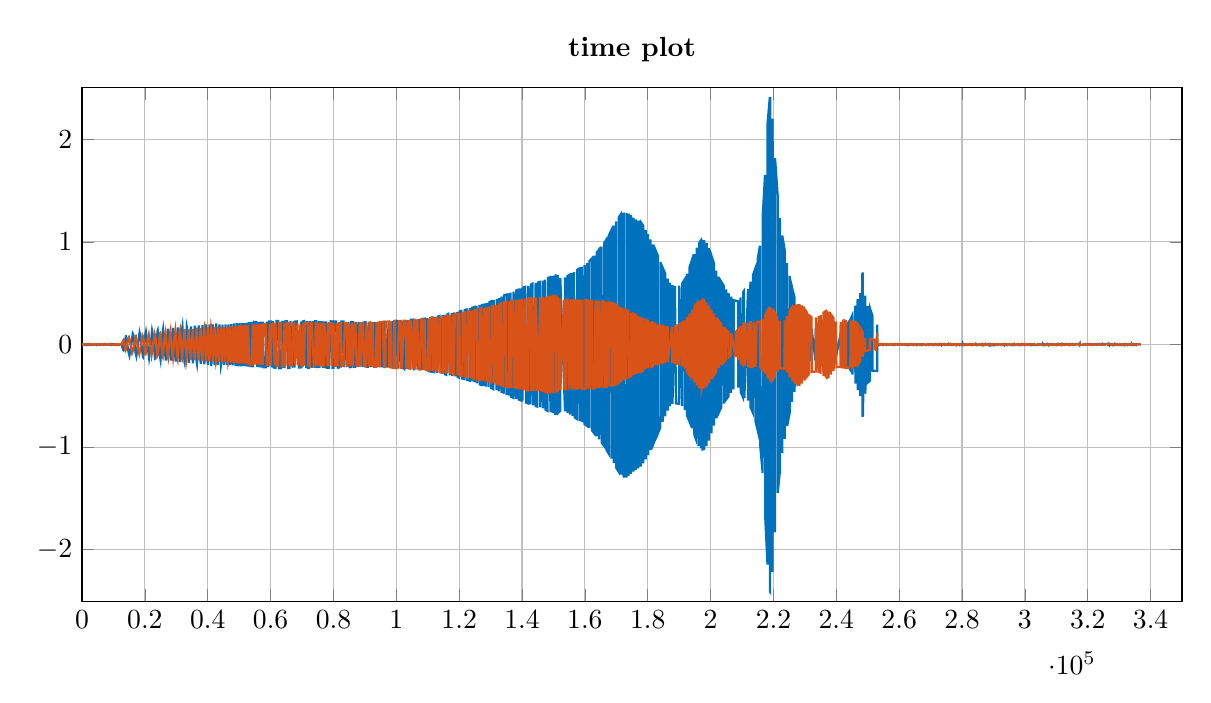
\begin{tikzpicture}

\begin{axis}[%
width=5.5in,
height=2.566in,
at={(1.011in,0.642in)},
scale only axis,
xmin=0,
xmax=350000,
xmajorgrids,
xminorgrids,
ymin=-2.5,
ymax=2.5,
ymajorgrids,
axis background/.style={fill=white},
title style={font=\bfseries},
title={time plot}
]
\addplot [color=mycolor1,solid,forget plot,thick]
  table[row sep=crcr]{%
1	0\\
92	-0.00481583190665319\\
409	0.00321055460443546\\
934	-0.00642110920887092\\
1451	0.00481583190665319\\
1704	0.00481583190665319\\
1752	-0.00481583190665319\\
2330	0.00321055460443546\\
2359	-0.00481583190665319\\
3166	-0.00481583190665319\\
3307	0.00321055460443546\\
4014	-0.00481583190665319\\
4369	0.00481583190665319\\
4683	0.00321055460443546\\
4765	-0.00481583190665319\\
5466	0.00321055460443546\\
5692	-0.00481583190665319\\
6315	0.00321055460443546\\
6523	-0.00481583190665319\\
6997	-0.00321055460443546\\
7213	0.00481583190665319\\
7769	0.00321055460443546\\
7841	-0.00321055460443546\\
9058	0.00642110920887092\\
9230	-0.00481583190665319\\
9361	-0.00481583190665319\\
9468	0.00481583190665319\\
10110	0.00321055460443546\\
10272	-0.00481583190665319\\
10944	0.00321055460443546\\
11052	-0.00481583190665319\\
11721	-0.00642110920887092\\
12245	0.00321055460443546\\
12551	0.00160527730221773\\
13182	-0.059395260182056\\
13200	-0.059395260182056\\
13953	0.0802638651108865\\
13977	0.0802638651108865\\
14746	-0.0658163693909269\\
15080	-0.107553579248588\\
15527	-0.0321055460443546\\
15529	-0.0353161006487901\\
16151	0.107553579248588\\
16306	0.0995271927374993\\
17077	-0.0882902516219752\\
17282	-0.113974688457459\\
17849	0.0128422184177418\\
17855	0.0112369411155241\\
18309	0.117185243061894\\
18632	0.0754480332042333\\
19379	-0.122001074968547\\
19420	-0.123606352270765\\
20173	0.104343024644152\\
20307	0.123606352270765\\
20958	-0.0385266552532255\\
21328	-0.130027461479636\\
21737	-0.0337108233465723\\
21738	-0.0353161006487901\\
22275	0.131632738781854\\
22514	0.0931060835286283\\
23216	-0.138053847990725\\
23290	-0.136448570688507\\
24063	0.136448570688507\\
24083	0.138053847990725\\
24842	-0.125211629572983\\
24973	-0.149290789106249\\
25613	0.10594830194637\\
25794	0.144474957199596\\
26392	-0.0786585878086688\\
26669	-0.15571189831512\\
27169	0.0674216466931447\\
27425	0.152501343710684\\
27945	-0.0529741509731851\\
28254	-0.157317175617338\\
28723	0.0577899828798383\\
28996	0.160527730221773\\
29498	-0.0577899828798383\\
29804	-0.165343562128426\\
30275	0.0866849743197574\\
30500	0.165343562128426\\
31052	-0.107553579248588\\
31257	-0.171764671337297\\
31824	0.142869679897378\\
31952	0.170159394035079\\
32602	-0.170159394035079\\
32639	-0.174975225941733\\
33335	0.173369948639515\\
33380	0.166948839430644\\
33987	-0.179791057848386\\
34157	-0.131632738781854\\
34644	0.17658050324395\\
35303	-0.184606889755039\\
35709	0.0898955289241929\\
35908	0.183001612452821\\
36483	-0.174975225941733\\
36552	-0.186212167057257\\
37149	0.184606889755039\\
37262	0.152501343710684\\
37754	-0.19102799896391\\
38324	0.187817444359474\\
38813	-0.157317175617338\\
38914	-0.194238553568345\\
39465	0.194238553568345\\
39591	0.157317175617338\\
40048	-0.197449108172781\\
40583	0.195843830870563\\
41133	-0.200659662777216\\
41147	-0.200659662777216\\
41672	0.195843830870563\\
42195	-0.200659662777216\\
42690	0.194238553568345\\
42707	0.194238553568345\\
43220	-0.199054385474999\\
43705	0.194238553568345\\
44222	-0.199054385474999\\
44248	-0.194238553568345\\
44698	0.192633276266128\\
45188	-0.199054385474999\\
45660	0.194238553568345\\
46119	-0.200659662777216\\
46577	0.195843830870563\\
46577	0.195843830870563\\
47037	-0.200659662777216\\
47481	0.199054385474999\\
47923	-0.203870217381652\\
48365	0.205475494683869\\
48807	-0.210291326590523\\
49218	0.208686049288305\\
49653	-0.213501881194958\\
50065	0.207080771986087\\
50457	-0.208686049288305\\
50472	-0.21189660389274\\
50882	0.207080771986087\\
51285	-0.210291326590523\\
51670	0.207080771986087\\
52090	-0.213501881194958\\
52464	0.21189660389274\\
52850	-0.216712435799394\\
53222	0.218317713101611\\
53605	-0.219922990403829\\
53968	0.219922990403829\\
54345	-0.223133545008264\\
54708	0.219922990403829\\
55426	0.216712435799394\\
55773	-0.218317713101611\\
56135	0.219922990403829\\
56476	-0.223133545008264\\
56815	0.221528267706047\\
57155	-0.224738822310482\\
57485	0.223133545008264\\
57822	-0.223133545008264\\
58488	-0.223133545008264\\
58813	0.223133545008264\\
59133	-0.221528267706047\\
59448	0.223133545008264\\
60064	0.223133545008264\\
60374	-0.223133545008264\\
60688	0.2263440996127\\
60985	-0.224738822310482\\
61587	-0.227949376914918\\
61883	0.229554654217135\\
62463	0.229554654217135\\
62753	-0.231159931519353\\
63318	-0.231159931519353\\
63608	0.229554654217135\\
63879	-0.227949376914918\\
64161	0.2263440996127\\
64434	-0.229554654217135\\
64716	0.227949376914918\\
65249	0.2263440996127\\
65511	-0.229554654217135\\
66038	-0.229554654217135\\
66301	0.2263440996127\\
67071	-0.2263440996127\\
67325	0.2263440996127\\
67569	-0.224738822310482\\
67816	0.223133545008264\\
68318	0.224738822310482\\
69039	-0.224738822310482\\
69519	-0.224738822310482\\
69740	0.223133545008264\\
69993	-0.2263440996127\\
70212	0.224738822310482\\
70675	0.227949376914918\\
71351	-0.227949376914918\\
71576	0.2263440996127\\
71792	-0.227949376914918\\
72236	-0.227949376914918\\
72456	0.2263440996127\\
73100	-0.227949376914918\\
73305	0.227949376914918\\
73943	-0.227949376914918\\
74154	0.2263440996127\\
74560	0.2263440996127\\
74766	-0.229554654217135\\
75368	0.2263440996127\\
75561	-0.227949376914918\\
76152	0.2263440996127\\
76741	-0.227949376914918\\
76928	0.224738822310482\\
77491	-0.227949376914918\\
77680	0.224738822310482\\
77862	-0.2263440996127\\
78599	-0.2263440996127\\
79147	0.2263440996127\\
79504	0.224738822310482\\
79681	-0.227949376914918\\
80025	-0.2263440996127\\
80206	0.224738822310482\\
80887	0.223133545008264\\
81395	-0.2263440996127\\
81728	-0.224738822310482\\
82227	0.223133545008264\\
82395	-0.224738822310482\\
82550	0.223133545008264\\
83200	0.223133545008264\\
83353	-0.221528267706047\\
84135	0.219922990403829\\
84289	-0.221528267706047\\
84751	0.218317713101611\\
85203	-0.221528267706047\\
85503	-0.219922990403829\\
85651	0.218317713101611\\
86238	0.216712435799394\\
86383	-0.218317713101611\\
86966	-0.216712435799394\\
87102	0.216712435799394\\
87809	-0.215107158497176\\
87944	0.216712435799394\\
88635	-0.216712435799394\\
88769	0.215107158497176\\
89441	-0.216712435799394\\
89835	0.216712435799394\\
90359	0.215107158497176\\
90484	-0.218317713101611\\
90998	-0.218317713101611\\
91382	0.216712435799394\\
91756	-0.219922990403829\\
92370	0.218317713101611\\
92492	-0.219922990403829\\
92614	0.218317713101611\\
93215	-0.219922990403829\\
93331	0.218317713101611\\
94155	-0.221528267706047\\
94274	0.221528267706047\\
94846	-0.221528267706047\\
95409	0.221528267706047\\
95520	-0.223133545008264\\
96076	0.221528267706047\\
96295	0.221528267706047\\
96836	-0.224738822310482\\
97580	0.224738822310482\\
97685	-0.2263440996127\\
97998	0.2263440996127\\
98514	-0.227949376914918\\
99024	0.227949376914918\\
99123	-0.229554654217135\\
99720	-0.229554654217135\\
99821	0.231159931519353\\
100214	0.229554654217135\\
100698	-0.232765208821571\\
100984	0.231159931519353\\
101646	-0.234370486123789\\
101740	0.232765208821571\\
102386	-0.234370486123789\\
102568	-0.239186318030442\\
103023	0.234370486123789\\
103291	-0.237581040728224\\
103732	0.235975763426006\\
104515	-0.239186318030442\\
104602	0.24079159533266\\
105284	0.242396872634877\\
105536	-0.24079159533266\\
105702	-0.24079159533266\\
106114	0.244002149937095\\
106849	-0.244002149937095\\
107088	0.24721270454153\\
107487	-0.24721270454153\\
107723	0.248817981843748\\
108115	-0.248817981843748\\
108191	0.248817981843748\\
109109	0.252028536448184\\
109334	-0.255239091052619\\
109854	0.255239091052619\\
110225	-0.258449645657055\\
110802	-0.263265477563708\\
110873	0.260054922959272\\
111444	0.263265477563708\\
111513	-0.266476032168143\\
112075	-0.269686586772579\\
112282	0.269686586772579\\
113031	-0.27610769598145\\
113231	0.272897141377014\\
113764	0.277712973283667\\
114094	-0.28252880519032\\
114676	0.285739359794756\\
114869	-0.287344637096974\\
115440	0.288949914399191\\
115504	-0.290555191701409\\
115877	-0.295371023608062\\
116310	0.295371023608062\\
116555	0.298581578212498\\
116977	-0.300186855514716\\
117634	0.305002687421369\\
117811	-0.308213242025804\\
118451	0.31142379663024\\
118738	-0.31142379663024\\
119362	0.317844905839111\\
119530	-0.317844905839111\\
119974	-0.322660737745764\\
120138	0.322660737745764\\
120685	0.327476569652417\\
120954	-0.33229240155907\\
121698	-0.337108233465723\\
121751	0.335502956163506\\
122374	0.341924065372377\\
122529	-0.345134619976812\\
123340	-0.353161006487901\\
123391	0.353161006487901\\
124132	-0.359582115696772\\
124183	0.357976838394554\\
124859	0.366003224905642\\
124908	-0.369213779510078\\
125526	0.374029611416731\\
125666	-0.378845443323384\\
126454	0.385266552532255\\
126501	-0.388477107136691\\
127045	-0.394898216345562\\
127269	0.394898216345562\\
127847	-0.40292460285665\\
128066	0.401319325554433\\
128458	-0.409345712065521\\
128844	0.406135157461086\\
129312	-0.415766821274392\\
129606	0.412556266669957\\
130187	0.420582653181045\\
130229	-0.425398485087698\\
130880	-0.435030148901005\\
131000	0.431819594296569\\
131913	-0.444661812714311\\
131953	0.443056535412093\\
132611	-0.455898753829835\\
132726	0.454293476527618\\
133445	-0.470346249549795\\
133484	0.465530417643142\\
134188	-0.479977913363101\\
134225	0.478372636060884\\
135020	0.486399022571972\\
135057	-0.491214854478625\\
135801	0.497635963687496\\
135836	-0.499241240989714\\
136356	0.505662350198585\\
136528	-0.510478182105238\\
137275	-0.520109845918544\\
137308	0.515294014011891\\
138137	-0.529741509731851\\
138170	0.526530955127415\\
138882	0.534557341638504\\
138914	-0.536162618940722\\
139485	-0.54418900545181\\
139705	0.545794282754028\\
140109	-0.555425946567335\\
140387	0.555425946567335\\
141056	0.561847055776206\\
141266	-0.566662887682859\\
141977	-0.574689274193947\\
142006	0.571478719589512\\
142731	-0.584320938007254\\
142816	0.584320938007254\\
143328	0.592347324518342\\
143581	-0.59395260182056\\
144329	0.600373711029431\\
144356	-0.600373711029431\\
144845	-0.605189542936084\\
145141	0.605189542936084\\
145725	0.610005374842737\\
145804	-0.611610652144955\\
146659	0.621242315958262\\
146685	-0.622847593260479\\
147269	0.632479257073786\\
147445	-0.635689811678221\\
148090	-0.646926752793745\\
148262	0.648532030095963\\
148988	0.656558416607052\\
149012	-0.658163693909269\\
149747	0.666190080420358\\
149770	-0.666190080420358\\
150166	0.671005912327011\\
150466	-0.674216466931447\\
150649	-0.674216466931447\\
150718	0.672611189629229\\
151395	0.667795357722576\\
151418	-0.669400635024793\\
152169	-0.646926752793745\\
152191	0.645321475491528\\
153666	-0.651742584700398\\
153687	0.653347862002616\\
154453	-0.666190080420358\\
154473	0.667795357722576\\
155202	0.680637576140318\\
155222	-0.682242853442535\\
155916	0.695085071860277\\
156014	-0.696690349162495\\
156538	0.707927290278019\\
156788	-0.712743122184672\\
157470	-0.725585340602414\\
157564	0.727190617904632\\
158268	0.740032836322373\\
158323	-0.743243390926809\\
159030	0.756085609344551\\
159084	-0.757690886646769\\
159881	0.773743659668946\\
159898	-0.775348936971164\\
160660	-0.793006987295559\\
160677	0.793006987295559\\
161405	-0.812270314922171\\
161422	0.812270314922171\\
162217	0.837954751757655\\
162233	-0.836349474455437\\
162946	-0.865244465895357\\
162994	0.865244465895357\\
163676	-0.894139457335276\\
163754	0.894139457335276\\
164498	0.924639726077413\\
164513	-0.924639726077413\\
165316	0.953534717517332\\
165331	-0.955139994819549\\
166101	-0.987245540863904\\
166116	0.985640263561686\\
166840	1.02256164151269\\
166883	-1.02737747341935\\
167619	-1.06590412867257\\
167661	1.06590412867257\\
168409	1.11245717043689\\
168423	-1.11245717043689\\
169195	1.1590102122012\\
169208	-1.15579965759677\\
169937	1.19914214475664\\
169950	-1.20074742205886\\
170728	-1.23927407731209\\
170741	1.23606352270765\\
171451	1.26977434605422\\
171514	-1.26816906875201\\
172221	1.28261656447197\\
172282	-1.2858271190764\\
172368	1.28422184177418\\
172429	-1.28743239637862\\
173249	-1.2858271190764\\
173261	1.28261656447197\\
173887	-1.27940600986753\\
173922	1.27459017796088\\
174674	-1.26014268224092\\
174708	1.26014268224092\\
175443	-1.23927407731209\\
175499	1.23606352270765\\
176218	-1.22161602698769\\
176229	1.21840547238326\\
176997	-1.20716853126773\\
177029	1.20716853126773\\
177780	-1.19111575824556\\
177874	1.18790520364112\\
178556	1.1590102122012\\
178566	-1.1590102122012\\
179345	1.11566772504132\\
179355	-1.12048355694798\\
180097	1.07393051518366\\
180146	-1.0771410697881\\
180871	1.02416691881491\\
180900	-1.02577219611713\\
181666	0.974403322446162\\
181694	-0.97600859974838\\
182434	-0.919823894170759\\
182443	0.921429171472977\\
183203	0.866849743197574\\
183212	-0.868455020499792\\
184008	-0.807454483015518\\
184034	0.804243928411083\\
184769	-0.752875054740115\\
184795	0.744848668229027\\
185539	0.691874517255842\\
185547	-0.69990090376693\\
186333	0.640505643584874\\
186341	-0.64371619818931\\
187093	0.601978988331649\\
187101	-0.603584265633866\\
187868	0.577899828798383\\
187876	-0.579505106100601\\
188657	0.569873442287294\\
188969	-0.574689274193947\\
189970	-0.577899828798383\\
190051	0.57308399689173\\
190900	-0.600373711029431\\
190950	0.59395260182056\\
191701	0.630873979771568\\
191736	-0.638900366282657\\
192504	0.690269239953624\\
192511	-0.693479794558059\\
193256	-0.74966450013568\\
193276	0.751269777437898\\
194018	0.818691424131042\\
194051	-0.817086146828825\\
194796	0.881297238917534\\
194828	-0.882902516219751\\
195538	-0.94069249909959\\
195582	0.942297776401808\\
196369	-0.990456095468339\\
196375	0.990456095468339\\
196886	1.01292997769939\\
196904	-1.01292997769939\\
197294	1.02095636421048\\
197431	-1.02256164151269\\
197950	-1.01774580960604\\
197956	1.01614053230382\\
198726	-0.990456095468339\\
198766	0.988850818166122\\
199507	-0.935876667192937\\
199524	0.937481944495154\\
200304	-0.866849743197574\\
200375	0.85561280208205\\
201067	0.791401709993341\\
201083	-0.789796432691123\\
201829	0.719164231393543\\
201845	-0.719164231393543\\
202616	0.659768971211487\\
202621	-0.662979525815922\\
203390	-0.611610652144955\\
203395	0.611610652144955\\
204177	0.57308399689173\\
204221	-0.576294551496165\\
204951	0.536162618940722\\
204956	-0.536162618940722\\
205713	-0.504057072896367\\
205727	0.50245179559415\\
206500	-0.470346249549795\\
206541	0.467135694945359\\
207296	-0.436635426203223\\
207363	0.431819594296569\\
208737	0.420582653181045\\
208767	-0.420582653181045\\
209551	0.459109308434271\\
209572	-0.463925140340924\\
210277	-0.513688736709674\\
210355	0.512083459407456\\
210559	0.520109845918544\\
210750	-0.52332040052298\\
211893	0.542583728149593\\
211897	-0.547399560056246\\
212668	0.611610652144955\\
212687	-0.611610652144955\\
213445	-0.66458480311814\\
213471	0.675821744233664\\
214190	0.736822281717938\\
214245	-0.743243390926809\\
214984	-0.837954751757655\\
215009	0.83474419715322\\
215683	0.96156110402842\\
215792	-0.988850818166122\\
216554	-1.25211629572983\\
216571	1.24569518652096\\
217310	1.65183034398204\\
217347	-1.666277839702\\
218096	-2.14465047576289\\
218119	2.15428213957619\\
218839	2.40952123062881\\
218855	-2.4079159533266\\
218932	-2.41112650793103\\
218948	2.41112650793103\\
219692	-2.21688795436269\\
219695	2.19922990403829\\
220460	-1.83162140183043\\
220506	1.81556862880825\\
221358	1.44474957199596\\
221361	-1.44474957199596\\
222029	-1.23766880000987\\
222032	1.231247690801\\
222799	-1.05787774216148\\
222802	1.06108829676592\\
223572	0.919823894170759\\
223586	-0.919823894170759\\
224342	0.793006987295559\\
224372	-0.793006987295559\\
225146	-0.666190080420358\\
225154	0.667795357722576\\
225903	-0.560241778473988\\
225916	0.557031223869552\\
226672	0.462319863038706\\
226690	-0.460714585736488\\
227447	0.378845443323384\\
227679	-0.357976838394554\\
228222	-0.31142379663024\\
228249	0.305002687421369\\
228997	-0.258449645657055\\
229009	0.260054922959272\\
229795	0.223133545008264\\
229816	-0.223133545008264\\
230561	-0.195843830870563\\
230600	0.199054385474999\\
231331	-0.171764671337297\\
231360	0.171764671337297\\
232106	-0.157317175617338\\
232130	0.15571189831512\\
233328	-0.154106621012902\\
233444	0.152501343710684\\
234178	0.15571189831512\\
234312	-0.157317175617338\\
234435	-0.15571189831512\\
234523	0.157317175617338\\
235247	0.130027461479636\\
235257	-0.133238016084072\\
235987	0.115579965759677\\
235993	-0.118790520364112\\
237324	0.117185243061894\\
237480	-0.12039579766633\\
237957	-0.126816906875201\\
238125	0.128422184177418\\
238316	0.126816906875201\\
238464	-0.128422184177418\\
239093	-0.12039579766633\\
239102	0.118790520364112\\
239874	0.10594830194637\\
240005	-0.104343024644152\\
241385	0.107553579248588\\
241417	-0.10594830194637\\
242174	0.134843293386289\\
242179	-0.136448570688507\\
242928	-0.173369948639515\\
242952	0.171764671337297\\
243735	0.208686049288305\\
243746	-0.21189660389274\\
244493	-0.24721270454153\\
244519	0.245607427239313\\
245015	0.279318250585885\\
245110	-0.293765746305845\\
246036	0.378845443323384\\
246058	-0.38205599792782\\
246782	0.441451258109876\\
246792	-0.443056535412093\\
247616	0.500846518291932\\
247623	-0.50245179559415\\
248288	0.69990090376693\\
248336	-0.706322012975801\\
248406	0.701506181069148\\
248443	-0.69990090376693\\
249216	0.476767358758666\\
249220	-0.479977913363101\\
249968	0.372424334114513\\
249985	-0.372424334114513\\
250749	-0.349950451883465\\
250758	0.348345174581247\\
251508	0.277712973283667\\
251509	-0.255239091052619\\
253008	-0.258449645657055\\
253012	0.194238553568345\\
253062	0.00963166381330638\\
253065	-0.00963166381330638\\
253847	-0.00481583190665319\\
253865	0.00321055460443546\\
254714	0.00481583190665319\\
254812	-0.00481583190665319\\
255478	0.00481583190665319\\
255926	-0.00481583190665319\\
256178	0.00321055460443546\\
256930	-0.00481583190665319\\
256983	-0.00481583190665319\\
257117	0.00321055460443546\\
257821	0.00321055460443546\\
257935	-0.00481583190665319\\
258545	0.00321055460443546\\
258646	-0.00481583190665319\\
259486	0.00481583190665319\\
259879	-0.00481583190665319\\
260057	-0.00321055460443546\\
260425	0.00481583190665319\\
260823	-0.00321055460443546\\
261235	0.00481583190665319\\
261601	0.00321055460443546\\
261988	-0.00481583190665319\\
262436	0.00321055460443546\\
262717	-0.00802638651108865\\
263161	-0.00481583190665319\\
263229	0.00321055460443546\\
264240	0.00481583190665319\\
264389	-0.00642110920887092\\
264743	-0.00642110920887092\\
265196	0.00321055460443546\\
265589	-0.00642110920887092\\
266007	0.00321055460443546\\
266266	0.00321055460443546\\
266515	-0.00481583190665319\\
267059	-0.00642110920887092\\
267075	0.00321055460443546\\
267889	0.00321055460443546\\
268331	-0.00642110920887092\\
268627	-0.00481583190665319\\
268925	0.00321055460443546\\
269371	-0.00481583190665319\\
269682	0.00321055460443546\\
270158	0.00321055460443546\\
270470	-0.00481583190665319\\
271158	-0.00481583190665319\\
271638	0.00481583190665319\\
271742	0.00321055460443546\\
272123	-0.00481583190665319\\
272547	-0.00481583190665319\\
272842	0.00481583190665319\\
273291	-0.00481583190665319\\
273333	0.00481583190665319\\
274047	0.00481583190665319\\
274462	-0.00481583190665319\\
274881	0.00321055460443546\\
275273	-0.00481583190665319\\
275624	0.00642110920887092\\
275919	-0.00321055460443546\\
276440	-0.00481583190665319\\
276456	0.00481583190665319\\
277158	-0.00481583190665319\\
277342	0.00321055460443546\\
278166	0.00321055460443546\\
278220	-0.00642110920887092\\
278693	0.00321055460443546\\
279256	-0.00642110920887092\\
279555	0.00321055460443546\\
280179	-0.00642110920887092\\
280235	0.00160527730221773\\
280311	-0.00642110920887092\\
281028	-0.00481583190665319\\
281266	0.00321055460443546\\
281811	-0.00481583190665319\\
282447	0.00321055460443546\\
282562	0.00160527730221773\\
282911	-0.00642110920887092\\
283371	-0.00481583190665319\\
283523	0.00321055460443546\\
284394	-0.00481583190665319\\
284466	0.00481583190665319\\
284933	-0.00642110920887092\\
285424	0.00321055460443546\\
285814	0.00321055460443546\\
286274	-0.00642110920887092\\
286474	0.00321055460443546\\
286719	-0.00642110920887092\\
287239	0.00321055460443546\\
287241	-0.00481583190665319\\
288414	0.00321055460443546\\
288614	-0.00642110920887092\\
288844	0.00160527730221773\\
289005	-0.00802638651108865\\
289546	0.00160527730221773\\
289596	-0.00642110920887092\\
290325	0.00160527730221773\\
290327	-0.00642110920887092\\
291151	0.00321055460443546\\
291300	-0.00481583190665319\\
291963	0.00321055460443546\\
292427	-0.00642110920887092\\
293128	0.00481583190665319\\
293423	-0.00642110920887092\\
293441	-0.00481583190665319\\
293897	0.00481583190665319\\
294327	-0.00642110920887092\\
294730	0.00321055460443546\\
294991	0.00321055460443546\\
295574	-0.00642110920887092\\
295922	0.00321055460443546\\
296218	-0.00642110920887092\\
296593	0.00321055460443546\\
296653	-0.00481583190665319\\
297417	-0.00481583190665319\\
297891	0.00481583190665319\\
298098	0.00321055460443546\\
298258	-0.00642110920887092\\
298883	0.00481583190665319\\
299012	-0.00481583190665319\\
299655	0.00321055460443546\\
300268	-0.00642110920887092\\
300511	-0.00481583190665319\\
300515	0.00321055460443546\\
301191	-0.00481583190665319\\
301871	0.00481583190665319\\
301983	0.00160527730221773\\
302035	-0.00642110920887092\\
302806	0.00321055460443546\\
302826	-0.00481583190665319\\
303676	-0.00642110920887092\\
304032	0.00160527730221773\\
304314	-0.00481583190665319\\
304666	0.00321055460443546\\
305803	-0.00642110920887092\\
305808	0.00321055460443546\\
306068	-0.00642110920887092\\
306491	0.00321055460443546\\
306742	-0.00481583190665319\\
307098	0.00481583190665319\\
307417	-0.00481583190665319\\
307518	0.00321055460443546\\
308238	0.00321055460443546\\
308923	-0.00481583190665319\\
308989	-0.00481583190665319\\
309044	0.00321055460443546\\
309993	-0.00642110920887092\\
310389	0.00481583190665319\\
310539	-0.00481583190665319\\
311121	0.00481583190665319\\
311713	0.00642110920887092\\
311763	-0.00321055460443546\\
312100	0.00481583190665319\\
312668	-0.00481583190665319\\
312850	-0.00321055460443546\\
312966	0.00481583190665319\\
313970	-0.00481583190665319\\
314028	0.00481583190665319\\
314401	0.00481583190665319\\
314494	-0.00321055460443546\\
315191	0.00481583190665319\\
315487	-0.00481583190665319\\
315949	-0.00321055460443546\\
316151	0.00481583190665319\\
317082	0.00481583190665319\\
317384	-0.00642110920887092\\
317502	0.00321055460443546\\
317543	-0.00481583190665319\\
318273	-0.00481583190665319\\
319004	0.00481583190665319\\
319084	0.00321055460443546\\
319262	-0.00481583190665319\\
319854	-0.00321055460443546\\
319870	0.00481583190665319\\
320709	0.00481583190665319\\
321137	-0.00481583190665319\\
321442	0.00321055460443546\\
322041	-0.00481583190665319\\
322151	-0.00481583190665319\\
322290	0.00321055460443546\\
322987	0.00481583190665319\\
323021	-0.00321055460443546\\
323849	0.00481583190665319\\
324232	-0.00481583190665319\\
324563	0.00481583190665319\\
324666	-0.00321055460443546\\
325296	-0.00321055460443546\\
325316	0.00481583190665319\\
326503	0.00481583190665319\\
326768	-0.00481583190665319\\
326822	0.00481583190665319\\
327094	-0.00481583190665319\\
327626	0.00321055460443546\\
327973	-0.00642110920887092\\
328467	0.00481583190665319\\
328505	-0.00481583190665319\\
329357	0.00321055460443546\\
329532	-0.00642110920887092\\
330043	-0.00642110920887092\\
330211	0.00160527730221773\\
330783	-0.00642110920887092\\
331379	0.00321055460443546\\
331667	-0.00481583190665319\\
331791	0.00481583190665319\\
332475	0.00321055460443546\\
332723	-0.00481583190665319\\
333161	0.00321055460443546\\
333692	-0.00481583190665319\\
333821	0.00321055460443546\\
333899	-0.00642110920887092\\
334694	-0.00642110920887092\\
334711	0.00321055460443546\\
335352	-0.00481583190665319\\
335413	0.00321055460443546\\
336896	0\\
};
\addplot [color=mycolor2,solid,forget plot,thick]
  table[row sep=crcr]{%
1	-0.000760413931657074\\
392	0.00228124179497122\\
600	-0.00228124179497122\\
786	-0.00228124179497122\\
934	0.00152082786331415\\
1648	0.00152082786331415\\
1916	-0.00228124179497122\\
2368	0.00228124179497122\\
2653	-0.00228124179497122\\
3107	0.00152082786331415\\
3451	-0.00228124179497122\\
3947	-0.00228124179497122\\
4087	0.00228124179497122\\
5044	0.00152082786331415\\
5299	-0.0030416557266283\\
5490	0.00152082786331415\\
6048	-0.0030416557266283\\
6635	-0.0030416557266283\\
6816	0.00152082786331415\\
7003	0.00152082786331415\\
7332	-0.00228124179497122\\
7764	-0.00228124179497122\\
7766	0.00152082786331415\\
8560	-0.0030416557266283\\
8642	0.00152082786331415\\
9333	0.00152082786331415\\
9736	-0.0030416557266283\\
10096	-0.00228124179497122\\
10552	0.00228124179497122\\
10872	0.00152082786331415\\
11025	-0.00228124179497122\\
11652	-0.00228124179497122\\
11691	0.00152082786331415\\
12467	-0.00228124179497122\\
13173	0.0425831801727961\\
13206	0.0403019383778249\\
13826	-0.0585518727375947\\
13978	-0.050947733421024\\
14750	0.0653955981225084\\
14924	0.072239323507422\\
15526	-0.0167291064964556\\
15528	-0.0159686925647986\\
15945	-0.0836455324822781\\
16305	-0.0547498030793093\\
17067	0.0806038767556498\\
17132	0.082124704618964\\
17855	-0.0486664916260527\\
18191	-0.0904892578671918\\
18630	-0.0197707622230839\\
18633	-0.020531176154741\\
19241	0.0897288439355347\\
19409	0.0798434628239928\\
20164	-0.0973329832521055\\
20213	-0.0973329832521055\\
20957	0.0638747702591942\\
21218	0.0973329832521055\\
21735	-0.0174895204281127\\
21737	-0.0159686925647986\\
22130	-0.104176708637019\\
22513	-0.0357394547878825\\
23094	0.104937122568676\\
23289	0.0844059464139352\\
23963	-0.111020434021933\\
24065	-0.104176708637019\\
24839	0.11178084795359\\
24866	0.112541261885247\\
25615	-0.11178084795359\\
25674	-0.117103745475189\\
26394	0.0965725693204484\\
26549	0.119384987270161\\
27169	-0.0958121553887913\\
27364	-0.123947470860103\\
27945	0.082124704618964\\
28164	0.125468298723417\\
28720	-0.0889684300038777\\
28911	-0.129270368381703\\
29497	0.0882080160722206\\
29689	0.131551610176674\\
30273	-0.107978778295305\\
30427	-0.135353679834959\\
31052	0.117864159406846\\
31198	0.13763492162993\\
31827	-0.138395335561587\\
31849	-0.139916163424902\\
32561	0.141436991288216\\
32605	0.141436991288216\\
33252	-0.145239060946501\\
33381	-0.119384987270161\\
33955	0.146759888809815\\
34157	0.0669164259858225\\
34580	-0.149041130604786\\
35237	0.150561958468101\\
35709	-0.113301675816904\\
35856	-0.152843200263072\\
36485	0.154364028126386\\
36490	0.154364028126386\\
37075	-0.1558848559897\\
37262	-0.0965725693204484\\
37696	0.158166097784671\\
38284	-0.1612077535113\\
38808	0.153603614194729\\
38878	0.162728581374614\\
39413	-0.165009823169585\\
39591	-0.101135052910391\\
40004	0.166530651032899\\
40538	-0.167291064964556\\
41098	0.16881189282787\\
41144	0.1612077535113\\
41623	-0.16881189282787\\
42154	0.16881189282787\\
42668	-0.16881189282787\\
42696	-0.165009823169585\\
43191	0.170332720691185\\
43676	-0.16881189282787\\
44182	0.16881189282787\\
44249	0.151322372399758\\
44658	-0.16881189282787\\
45140	0.169572306759528\\
45616	-0.169572306759528\\
46083	0.170332720691185\\
46541	-0.171093134622842\\
46577	-0.166530651032899\\
46989	0.173374376417813\\
47452	-0.175655618212784\\
47884	0.177176446076098\\
48329	-0.180218101802727\\
48761	0.181738929666041\\
49193	-0.184020171461012\\
49617	0.184020171461012\\
50036	-0.185540999324326\\
50457	0.184780585392669\\
50458	0.184780585392669\\
50848	-0.184780585392669\\
51268	0.185540999324326\\
51657	-0.185540999324326\\
52050	0.18706182718764\\
52431	-0.188582655050954\\
52819	0.191624310777583\\
53197	-0.193905552572554\\
53951	-0.196947208299182\\
54319	0.196947208299182\\
54684	-0.196947208299182\\
55046	0.196186794367525\\
55400	-0.195426380435868\\
55768	0.195426380435868\\
56110	-0.196947208299182\\
56458	0.197707622230839\\
56791	-0.198468036162496\\
57130	0.19998886402581\\
57478	-0.19998886402581\\
57805	0.19998886402581\\
58462	0.19998886402581\\
58785	-0.199228450094153\\
59428	-0.200749277957468\\
59739	0.200749277957468\\
60048	-0.200749277957468\\
60355	0.201509691889125\\
60966	0.203030519752439\\
61264	-0.203790933684096\\
61561	0.20531176154741\\
61863	-0.206832589410724\\
62444	-0.206832589410724\\
62741	0.207593003342381\\
63306	0.208353417274038\\
63587	-0.207593003342381\\
64146	-0.206832589410724\\
64422	0.207593003342381\\
64695	-0.208353417274038\\
64966	0.207593003342381\\
65501	0.206832589410724\\
65763	-0.206832589410724\\
66028	0.207593003342381\\
66289	-0.206072175479067\\
66803	-0.20531176154741\\
67061	0.20531176154741\\
67558	0.203790933684096\\
67805	-0.203790933684096\\
68543	0.203790933684096\\
68789	-0.203790933684096\\
69503	0.203790933684096\\
69738	-0.204551347615753\\
70202	-0.20531176154741\\
70437	0.206832589410724\\
70664	-0.206832589410724\\
70890	0.206832589410724\\
71791	0.207593003342381\\
72011	-0.208353417274038\\
72444	-0.207593003342381\\
72661	0.207593003342381\\
73092	0.208353417274038\\
73725	-0.209113831205695\\
74143	-0.209113831205695\\
74348	0.208353417274038\\
74753	0.207593003342381\\
74963	-0.208353417274038\\
75556	0.207593003342381\\
75757	-0.208353417274038\\
76345	0.207593003342381\\
76535	-0.208353417274038\\
76919	-0.207593003342381\\
77109	0.207593003342381\\
78044	-0.208353417274038\\
78234	0.208353417274038\\
78414	-0.208353417274038\\
78594	0.207593003342381\\
79313	0.206832589410724\\
79491	-0.207593003342381\\
80019	0.207593003342381\\
80539	-0.208353417274038\\
80879	-0.207593003342381\\
81049	0.207593003342381\\
81556	-0.207593003342381\\
81724	0.208353417274038\\
82379	0.206832589410724\\
82539	-0.206832589410724\\
83181	-0.207593003342381\\
83662	0.207593003342381\\
84279	0.206832589410724\\
84434	-0.206832589410724\\
84744	-0.207593003342381\\
84895	0.207593003342381\\
85646	-0.207593003342381\\
85791	0.206832589410724\\
86230	-0.209113831205695\\
86666	0.208353417274038\\
86954	0.208353417274038\\
87381	-0.209113831205695\\
87941	-0.209113831205695\\
88352	0.209113831205695\\
88763	-0.209874245137352\\
89165	0.209874245137352\\
89434	0.211395073000667\\
89831	-0.212155486932324\\
90349	-0.212915900863981\\
90481	0.212915900863981\\
91373	-0.214436728727295\\
91497	0.214436728727295\\
91748	0.215957556590609\\
92124	-0.215957556590609\\
92489	0.216717970522266\\
92852	-0.217478384453923\\
93565	-0.217478384453923\\
93683	0.21823879838558\\
94034	-0.21823879838558\\
94154	0.21823879838558\\
94729	-0.219759626248894\\
94843	0.218999212317237\\
95742	0.219759626248894\\
96071	-0.220520040180551\\
96510	-0.220520040180551\\
96616	0.221280454112209\\
97681	0.224322109838837\\
97785	-0.22356169590718\\
98305	0.224322109838837\\
98407	-0.225082523770494\\
99220	-0.226603351633808\\
99321	0.226603351633808\\
99521	0.227363765565465\\
99620	-0.227363765565465\\
100404	-0.228884593428779\\
100888	0.228884593428779\\
101454	0.229645007360436\\
101551	-0.229645007360436\\
101735	-0.230405421292093\\
102383	0.231165835223751\\
102928	0.231926249155408\\
103199	-0.231926249155408\\
103817	0.234207490950379\\
103907	-0.234207490950379\\
104430	-0.235728318813693\\
104516	0.23648873274535\\
105449	-0.238009560608664\\
105533	0.238769974540321\\
106031	0.239530388471978\\
106116	-0.240290802403635\\
106684	0.24181163026695\\
107088	-0.242572044198607\\
107566	-0.243332458130264\\
107799	0.244092872061921\\
108269	0.245613699925235\\
108654	-0.246374113856892\\
109032	0.248655355651863\\
109408	-0.248655355651863\\
110149	-0.251697011378491\\
110222	0.252457425310149\\
110874	-0.255499081036777\\
110945	0.256259494968434\\
111654	0.259301150695062\\
111726	-0.259301150695062\\
112348	0.263103220353348\\
112418	-0.263103220353348\\
113029	0.266144876079976\\
113096	-0.265384462148319\\
113960	0.269946945738261\\
114027	-0.270707359669918\\
114804	-0.274509429328204\\
114868	0.274509429328204\\
115565	-0.277551085054832\\
115628	0.278311498986489\\
116124	0.281353154713117\\
116186	-0.281353154713117\\
116977	0.28591563830306\\
117158	-0.28591563830306\\
117928	0.289717707961345\\
117987	-0.290478121893002\\
118335	-0.293519777619631\\
118623	0.295040605482945\\
119417	0.29884267514123\\
119474	-0.299603089072887\\
120085	0.30416557266283\\
120250	-0.303405158731173\\
121009	-0.307207228389458\\
121061	0.308728056252772\\
121804	0.312530125911057\\
121855	-0.312530125911057\\
122477	-0.316332195569343\\
122631	0.317853023432657\\
123340	0.323936334885914\\
123390	-0.323175920954256\\
124133	0.329259232407513\\
124182	-0.328498818475856\\
124764	-0.334582129929113\\
124908	0.33534254386077\\
125572	0.340665441382369\\
125713	-0.341425855314026\\
126454	-0.345988338903969\\
126500	0.34826958069894\\
127044	0.352071650357225\\
127180	-0.351311236425568\\
127935	0.357394547878825\\
127978	-0.356634133947168\\
128716	0.361957031468767\\
128844	-0.36119661753711\\
129481	0.36651951505871\\
129606	-0.365759101127053\\
130270	-0.371081998648652\\
130392	0.372602826511966\\
130961	0.377165310101909\\
131161	-0.377165310101909\\
131835	0.382488207623508\\
131952	-0.382488207623508\\
132650	-0.390852760871736\\
132688	0.39237358873505\\
133371	0.399977728051621\\
133483	-0.399977728051621\\
134077	-0.406821453436535\\
134260	0.409102695231506\\
134913	0.415186006684762\\
134949	-0.413665178821448\\
135800	-0.418227662411391\\
135834	0.419748490274705\\
136493	-0.422790146001333\\
136596	0.425071387796304\\
137207	0.429633871386247\\
137375	-0.428113043522933\\
138136	0.433435941044532\\
138169	-0.432675527112875\\
138913	0.437238010702818\\
138945	-0.434956768907846\\
139674	0.441040080361103\\
139705	-0.439519252497789\\
140109	0.444842150019388\\
140448	-0.443321322156074\\
141025	0.446362977882702\\
141175	-0.445602563951045\\
141888	-0.44712339181436\\
141917	0.448644219677674\\
142615	0.451685875404302\\
142816	-0.450925461472645\\
143129	0.45472753113093\\
143496	-0.45472753113093\\
144081	0.457008772925901\\
144328	-0.455487945062587\\
144410	0.457769186857559\\
145087	-0.456248358994244\\
145803	0.46005042865253\\
145882	-0.457769186857559\\
146633	0.463092084379158\\
146659	-0.460810842584187\\
147444	0.466133740105786\\
147469	-0.465373326174129\\
148212	-0.469175395832415\\
148237	0.471456637627386\\
148602	-0.471456637627386\\
148723	0.4729774654907\\
149274	-0.4729774654907\\
149487	0.475258707285671\\
149933	-0.4729774654907\\
150003	0.476019121217328\\
150694	0.474498293354014\\
150808	-0.472217051559043\\
151372	0.466133740105786\\
151394	-0.463852498310815\\
152168	0.444842150019388\\
152190	-0.444842150019388\\
153371	0.434956768907846\\
153434	-0.432675527112875\\
153978	-0.435717182839503\\
154123	0.437998424634475\\
154493	0.439519252497789\\
154960	-0.437238010702818\\
155301	0.439519252497789\\
155797	-0.437998424634475\\
156169	0.441040080361103\\
156653	-0.438758838566132\\
156940	0.440279666429446\\
157300	-0.438758838566132\\
157731	0.438758838566132\\
157750	-0.437238010702818\\
158359	0.437238010702818\\
158450	-0.435717182839503\\
159226	0.435717182839503\\
159244	-0.434956768907846\\
160159	-0.433435941044532\\
160211	0.435717182839503\\
160796	0.432675527112875\\
160813	-0.431154699249561\\
161538	0.432675527112875\\
161555	-0.429633871386247\\
162363	0.431915113181218\\
162379	-0.429633871386247\\
163089	-0.42887345745459\\
163359	0.430394285317904\\
163816	-0.425831801727961\\
163925	0.42887345745459\\
164589	-0.422029732069676\\
164604	0.425831801727961\\
165345	-0.418227662411391\\
165509	0.421269318138019\\
166129	0.417467248479734\\
166202	-0.41594642061642\\
166924	-0.412144350958134\\
166967	0.413665178821448\\
167688	-0.408342281299849\\
167702	0.409863109163163\\
168476	0.404540211641563\\
168517	-0.403779797709906\\
169247	-0.394654830530021\\
169260	0.396936072324993\\
170027	0.387811105145108\\
170040	-0.387050691213451\\
170790	-0.377165310101909\\
170828	0.376404896170252\\
171574	-0.365759101127053\\
171586	0.363477859332081\\
172341	-0.350550822493911\\
172353	0.351311236425568\\
173115	-0.33534254386077\\
173127	0.336863371724084\\
173884	0.324696748817571\\
173919	-0.323175920954256\\
174659	-0.311009298047743\\
174739	0.310248884116086\\
175451	-0.29884267514123\\
175462	0.300363503004544\\
176214	0.290478121893002\\
176225	-0.289717707961345\\
176993	0.278311498986489\\
177025	-0.278311498986489\\
177797	0.266905290011633\\
177828	-0.266905290011633\\
178552	-0.253978253173463\\
178562	0.255499081036777\\
179320	-0.240290802403635\\
179430	0.240290802403635\\
180102	0.232686663087065\\
180112	-0.231165835223751\\
180914	0.222801281975523\\
181019	-0.219759626248894\\
181661	-0.211395073000667\\
181670	0.211395073000667\\
182447	0.200749277957468\\
182456	-0.201509691889125\\
183224	0.19238472470924\\
183251	-0.191624310777583\\
184011	-0.184020171461012\\
184037	0.184020171461012\\
184763	0.177936860007755\\
184789	-0.177936860007755\\
185533	-0.171093134622842\\
185541	0.171853548554499\\
186335	0.167291064964556\\
186343	-0.168051478896213\\
187760	0.169572306759528\\
187815	-0.16881189282787\\
188605	-0.177936860007755\\
188628	0.176416032144441\\
189340	0.184780585392669\\
189407	-0.186301413255983\\
190133	-0.196947208299182\\
190155	0.196947208299182\\
190865	0.212155486932324\\
190944	-0.213676314795638\\
191702	0.234967904882036\\
191737	-0.235728318813693\\
192505	0.268426117874947\\
192512	-0.266905290011633\\
193270	-0.300363503004544\\
193277	0.300363503004544\\
193999	-0.334582129929113\\
194058	0.338384199587398\\
194803	-0.369561170785338\\
194835	0.371842412580309\\
195595	0.401498555914935\\
195614	-0.399977728051621\\
196351	0.424310973864647\\
196394	-0.424310973864647\\
197127	0.43647759677116\\
197169	-0.435717182839503\\
197181	-0.434196354976189\\
197556	0.435717182839503\\
197968	0.431915113181218\\
197974	-0.429633871386247\\
198732	0.41062352309482\\
198749	-0.411383937026477\\
199513	0.380206965828537\\
199552	-0.378686137965223\\
200277	0.339144613519055\\
200315	-0.339144613519055\\
201067	0.300363503004544\\
201083	-0.299603089072887\\
201845	-0.261582392490033\\
201850	0.263103220353348\\
202621	-0.229645007360436\\
202626	0.229645007360436\\
203385	0.200749277957468\\
203410	-0.202270105820782\\
204157	0.173374376417813\\
204162	-0.17413479034947\\
204936	-0.146759888809815\\
204941	0.147520302741472\\
205717	0.12470788479176\\
205731	-0.123947470860103\\
206508	-0.109499606158619\\
206549	0.108739192226962\\
207985	-0.122426642996789\\
208007	0.123187056928446\\
208761	0.147520302741472\\
208808	-0.149041130604786\\
209583	0.178697273939412\\
209587	-0.178697273939412\\
210300	-0.201509691889125\\
210345	0.202270105820782\\
210809	0.206072175479067\\
210926	-0.206072175479067\\
211860	0.209874245137352\\
211911	-0.209874245137352\\
212455	-0.217478384453923\\
212582	0.21823879838558\\
212804	0.218999212317237\\
213142	-0.219759626248894\\
213503	-0.219759626248894\\
213723	0.219759626248894\\
214309	-0.217478384453923\\
214640	0.217478384453923\\
215646	0.22356169590718\\
215797	-0.225842937702151\\
216552	-0.246374113856892\\
216576	0.247894941720206\\
217311	-0.282873982576432\\
217348	0.284394810439746\\
218090	0.33001964633917\\
218100	-0.329259232407513\\
218804	0.361957031468767\\
218897	-0.361957031468767\\
219009	0.364998687195396\\
219025	-0.362717445400424\\
219692	0.34826958069894\\
219695	-0.347509166767283\\
220469	-0.307967642321115\\
220472	0.307967642321115\\
221235	0.263863634285005\\
221238	-0.266144876079976\\
222034	0.232686663087065\\
222037	-0.234207490950379\\
223537	-0.235728318813693\\
223551	0.234207490950379\\
224280	-0.27298860146489\\
224332	0.276790671123175\\
225104	-0.320894679159285\\
225112	0.323936334885914\\
225833	0.358154961810482\\
225867	-0.356634133947168\\
226642	0.381727793691851\\
226665	-0.380967379760194\\
227302	0.391613174803393\\
227415	-0.390852760871736\\
227841	0.394654830530021\\
227888	-0.393894416598364\\
228257	-0.39237358873505\\
228279	0.39237358873505\\
229012	-0.380967379760194\\
229024	0.380967379760194\\
229840	-0.351311236425568\\
229847	0.349029994630597\\
230564	0.316332195569343\\
230580	-0.316332195569343\\
231327	-0.286676052234717\\
231365	0.282873982576432\\
232113	0.265384462148319\\
232159	-0.26766570394329\\
233455	-0.263863634285005\\
233495	0.263863634285005\\
234345	-0.275269843259861\\
234425	0.276030257191518\\
235008	-0.286676052234717\\
235018	0.288196880098031\\
235942	-0.308728056252772\\
235944	0.311009298047743\\
236639	0.324696748817571\\
236733	-0.323175920954256\\
236949	0.327738404544199\\
236989	-0.325457162749228\\
237544	-0.319373851295971\\
237572	0.319373851295971\\
238318	-0.293519777619631\\
238404	0.287436466166374\\
239095	0.256259494968434\\
239111	-0.259301150695062\\
239867	0.22356169590718\\
240040	-0.222040868043866\\
241323	-0.218999212317237\\
241365	0.219759626248894\\
241995	-0.232686663087065\\
242161	0.234207490950379\\
242287	-0.235728318813693\\
242380	0.234967904882036\\
243080	0.229645007360436\\
243088	-0.229645007360436\\
244459	-0.222040868043866\\
244482	0.222040868043866\\
245066	0.226603351633808\\
245251	-0.227363765565465\\
245299	-0.226603351633808\\
245444	0.225082523770494\\
246084	-0.216717970522266\\
246182	0.215957556590609\\
246856	0.196947208299182\\
246866	-0.196947208299182\\
247628	-0.162728581374614\\
247649	0.158926511716328\\
248408	0.116343331543532\\
248423	-0.118624573338504\\
249180	0.0631143563275371\\
249184	-0.0653955981225084\\
250529	-0.0539893891476523\\
250646	0.0532289752159952\\
250732	-0.0532289752159952\\
250828	0.0524685612843381\\
252225	0.0463852498310815\\
252263	-0.0463852498310815\\
252522	-0.0494269055577098\\
253002	0.11178084795359\\
253124	-0.00228124179497122\\
253297	0.00228124179497122\\
253990	0.00228124179497122\\
254120	-0.00228124179497122\\
254623	-0.00228124179497122\\
254784	0.00228124179497122\\
255532	-0.00228124179497122\\
255586	0.00228124179497122\\
256215	0.00152082786331415\\
256542	-0.00228124179497122\\
256943	0.00152082786331415\\
257010	-0.00228124179497122\\
257739	0.00152082786331415\\
257791	-0.00228124179497122\\
258520	0.00152082786331415\\
258720	-0.00228124179497122\\
259869	0.00228124179497122\\
259871	-0.00228124179497122\\
260072	-0.00228124179497122\\
260184	0.00152082786331415\\
261390	0.00152082786331415\\
261515	-0.0030416557266283\\
261639	-0.00228124179497122\\
262137	0.00152082786331415\\
262387	0.00152082786331415\\
262464	-0.00228124179497122\\
263173	0.00152082786331415\\
263196	-0.00228124179497122\\
263933	0.00152082786331415\\
263935	-0.00228124179497122\\
264836	0.00152082786331415\\
264858	-0.00228124179497122\\
265571	0.00152082786331415\\
265917	-0.00228124179497122\\
266258	0.00152082786331415\\
266426	-0.00228124179497122\\
267241	0.00228124179497122\\
267446	-0.00228124179497122\\
267825	0.00152082786331415\\
268120	-0.00228124179497122\\
268600	-0.00228124179497122\\
268893	0.00228124179497122\\
269370	-0.00228124179497122\\
269382	0.00152082786331415\\
270153	-0.00228124179497122\\
270681	0.00152082786331415\\
270933	-0.00228124179497122\\
270956	0.00152082786331415\\
271763	-0.00228124179497122\\
271953	0.00228124179497122\\
272470	0.00152082786331415\\
272482	-0.00228124179497122\\
273286	0.00152082786331415\\
273814	-0.0030416557266283\\
274118	0.00152082786331415\\
274131	-0.00228124179497122\\
274800	0.00152082786331415\\
274873	-0.00228124179497122\\
275699	-0.00228124179497122\\
275833	0.00152082786331415\\
276371	-0.00228124179497122\\
276448	0.00152082786331415\\
277128	0.00152082786331415\\
277204	-0.00228124179497122\\
278231	0.00228124179497122\\
278362	-0.00228124179497122\\
278687	-0.00228124179497122\\
278698	0.00152082786331415\\
279579	0.00152082786331415\\
279763	-0.00228124179497122\\
280515	-0.00228124179497122\\
280824	0.00228124179497122\\
281060	0.00152082786331415\\
281175	-0.00228124179497122\\
281785	0.00152082786331415\\
282020	-0.00228124179497122\\
282631	-0.00228124179497122\\
282790	0.00152082786331415\\
283374	0.00152082786331415\\
283436	-0.00228124179497122\\
284118	-0.00228124179497122\\
284292	0.00152082786331415\\
285271	-0.0030416557266283\\
285420	0.00228124179497122\\
285719	0.00152082786331415\\
285766	-0.00228124179497122\\
286532	0.00152082786331415\\
286635	-0.00228124179497122\\
287309	0.00152082786331415\\
287369	-0.00228124179497122\\
288004	0.00152082786331415\\
288335	-0.00228124179497122\\
288805	-0.00228124179497122\\
288905	0.00152082786331415\\
289629	-0.00228124179497122\\
289728	0.00152082786331415\\
290347	0.00152082786331415\\
291065	-0.00228124179497122\\
291109	-0.00228124179497122\\
291139	0.00152082786331415\\
291882	0.00152082786331415\\
292246	-0.00228124179497122\\
292759	-0.00228124179497122\\
292778	0.00152082786331415\\
293458	-0.00228124179497122\\
293472	0.00152082786331415\\
294274	-0.00228124179497122\\
294805	0.00228124179497122\\
295001	0.00152082786331415\\
295103	-0.00228124179497122\\
295854	-0.00228124179497122\\
295907	0.00152082786331415\\
296531	0.00152082786331415\\
296595	-0.00228124179497122\\
297324	0.00152082786331415\\
297338	-0.00228124179497122\\
298109	-0.00228124179497122\\
298146	0.00152082786331415\\
298963	0.00152082786331415\\
299060	-0.0030416557266283\\
299664	-0.00228124179497122\\
299943	0.00152082786331415\\
300431	0.00152082786331415\\
300461	-0.00228124179497122\\
301238	0.00152082786331415\\
301310	-0.00228124179497122\\
301966	-0.00228124179497122\\
302062	0.00152082786331415\\
302837	0.00152082786331415\\
303297	-0.00228124179497122\\
303611	-0.00228124179497122\\
303922	0.00152082786331415\\
304298	-0.00228124179497122\\
304603	0.00152082786331415\\
305174	-0.00228124179497122\\
305431	0.00228124179497122\\
305911	-0.00228124179497122\\
306581	0.00152082786331415\\
306645	0.00152082786331415\\
306772	-0.0030416557266283\\
307443	0.00152082786331415\\
307554	-0.00228124179497122\\
308311	-0.00228124179497122\\
308651	0.00152082786331415\\
308970	0.00152082786331415\\
309067	-0.00228124179497122\\
309764	-0.00228124179497122\\
309824	0.00152082786331415\\
310635	0.00152082786331415\\
310723	-0.0030416557266283\\
311771	-0.0030416557266283\\
311779	0.00152082786331415\\
312098	-0.00228124179497122\\
312410	0.00152082786331415\\
312853	-0.00228124179497122\\
313307	0.00152082786331415\\
313967	-0.0030416557266283\\
314226	0.00152082786331415\\
314413	-0.00228124179497122\\
314455	0.00152082786331415\\
315488	-0.0030416557266283\\
315794	0.00152082786331415\\
315966	-0.00228124179497122\\
316327	0.00152082786331415\\
316718	0.00152082786331415\\
316972	-0.00228124179497122\\
317560	0.00152082786331415\\
317573	-0.00228124179497122\\
318304	-0.00228124179497122\\
318634	0.00152082786331415\\
319065	0.00152082786331415\\
319447	-0.0030416557266283\\
320092	-0.00228124179497122\\
320181	0.00228124179497122\\
320622	0.00152082786331415\\
320704	-0.0030416557266283\\
321401	-0.00228124179497122\\
321466	0.00152082786331415\\
322240	-0.00228124179497122\\
322575	0.00152082786331415\\
323077	0.00152082786331415\\
323191	-0.00228124179497122\\
323715	0.00152082786331415\\
323891	-0.0030416557266283\\
324534	-0.00228124179497122\\
324635	0.00152082786331415\\
325292	-0.00228124179497122\\
325559	0.00152082786331415\\
326058	0.00152082786331415\\
326271	-0.00228124179497122\\
326871	0.00152082786331415\\
327400	-0.00228124179497122\\
327715	0.00152082786331415\\
327980	-0.00228124179497122\\
328388	0.00228124179497122\\
328969	-0.0030416557266283\\
329178	-0.00228124179497122\\
329197	0.00228124179497122\\
329992	-0.00228124179497122\\
330490	0.00228124179497122\\
330725	0.00152082786331415\\
331063	-0.00228124179497122\\
331529	-0.00228124179497122\\
331631	0.00152082786331415\\
332252	-0.00228124179497122\\
332691	0.00228124179497122\\
333120	-0.00228124179497122\\
333363	0.00228124179497122\\
333800	-0.00228124179497122\\
333825	0.00152082786331415\\
334578	0.00152082786331415\\
334867	-0.00228124179497122\\
335458	-0.00228124179497122\\
335807	0.00228124179497122\\
336896	0.000760413931657074\\
};
\end{axis}
\end{tikzpicture}%
	\caption{Time plot of the cancellation path with the reference signal(blue) and the microphone signal(orange).}
	\label{AmplitudePlotCancellationPath}
\end{figure}

MATLAB\textsuperscript{\textregistered}-script \path{CancellationPathScript.m} is used for data extraction and analysis.



\subsection{Analysis}
The impulse response of the CP is to be found.
Note that a microphone with external polarization was used. It means that there is a 180\textdegree phase difference between pre- and external polarized microphones, i.e. a positive pressure leads to negative voltage. The externally polarized microphone is considered to be out of phase. \cite{michandbook}

First the cross correlation between Mic[i] and Ref[i] is found. This is done by cross correlating the two signals signals. Secondly the signal is taken into the frequency domain by applying the FT to the signal. This is expressed in \autoref{FrequencyResponseCPEq2}.



\begin{equation}\label{FrequencyResponseCPEq2}
%H(f) = \frac{Y(m_{\mu}) *  X(r_{\mu})}{X(r_{\mu}) *  X(r_{\mu})}
H(f) = \frac{Y(f) \cdot X\textsuperscript{*}(f)}{X(f) \cdot X\textsuperscript{*}(f)}
\end{equation}
Where:
\begin{description}
	%\item " $*$ " denotes the complex conjugation
	\item $H(f)$ is the FT of the CP.
	\item $Y(f)$ is the FT of the recorded microphone signals, Mic[i].
	\item $X(f)$ is the FT of the recorded reference signals, Ref[i].
\end{description}

The frequency response of the CP is shown in \autoref{FrequencyResponsePlotCancellationPath}.

\begin{figure}[H]
	\centering
	\tikzsetnextfilename{CancellationPathFrequencyResponse1}
	%% This file was created by matlab2tikz.
%
%The latest updates can be retrieved from
%  http://www.mathworks.com/matlabcentral/fileexchange/22022-matlab2tikz-matlab2tikz
%where you can also make suggestions and rate matlab2tikz.
%
\definecolor{mycolor1}{rgb}{0.00000,0.44700,0.74100}%
%
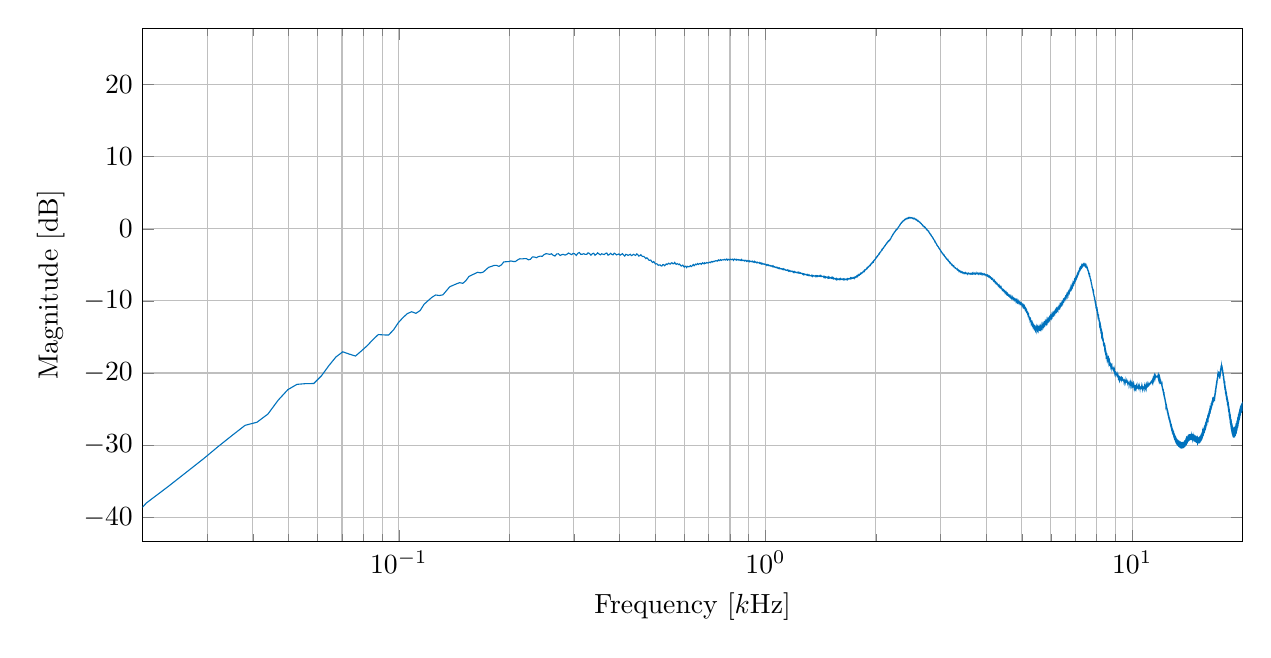
\begin{tikzpicture}

\begin{axis}[%
width=5.5in,
height=2.566in,
at={(2.804in,1.205in)},
scale only axis,
xmode=log,
xmin=0.02,
xmax=20,
xminorticks=true,
xlabel={Frequency [$k$Hz]},
xmajorgrids,
xminorgrids,
ymin=-43.3455877896241,
ymax=27.8130955898857,
ylabel={Magnitude [dB]},
ymajorgrids,
axis background/.style={fill=white},
title style={font=\bfseries},
legend style={legend cell align=left,align=left,draw=white!15!black}
]
\addplot [color=mycolor1,solid,forget plot]
  table[row sep=crcr]{%
0	-1.69141873333655\\
0.0029296875	-40.8589297400518\\
0.005859375	-60.5980111862308\\
0.0087890625	-53.2157441308172\\
0.01171875	-57.2367516122019\\
0.0146484375	-43.1597211075457\\
0.017578125	-41.6473379204459\\
0.0205078125	-37.9993270931867\\
0.0234375	-35.7728657291726\\
0.0263671875	-33.7314835828777\\
0.029296875	-31.9034991604498\\
0.0322265625	-30.1508947985882\\
0.03515625	-28.6204314562879\\
0.0380859375	-27.2462179322706\\
0.041015625	-26.8214249575063\\
0.0439453125	-25.6889727720254\\
0.046875	-23.7608293638928\\
0.0498046875	-22.3031464197138\\
0.052734375	-21.5695615779491\\
0.0556640625	-21.4666363252484\\
0.05859375	-21.4521698756001\\
0.0615234375	-20.3776757568286\\
0.064453125	-18.9662221291674\\
0.0673828125	-17.7640061494371\\
0.0703125	-17.0545263118457\\
0.0732421875	-17.3707060985524\\
0.076171875	-17.6438127055492\\
0.0791015625	-16.9208559171187\\
0.08203125	-16.1958865214752\\
0.0849609375	-15.3697622343122\\
0.087890625	-14.6609591744791\\
0.0908203125	-14.7131683950697\\
0.09375	-14.7296104829327\\
0.0966796875	-14.0206386171589\\
0.099609375	-13.0336615128222\\
0.1025390625	-12.3328386875402\\
0.10546875	-11.7549646788107\\
0.1083984375	-11.4986184373946\\
0.111328125	-11.7220860030783\\
0.1142578125	-11.3429897266818\\
0.1171875	-10.4618012927625\\
0.1201171875	-9.96853290357672\\
0.123046875	-9.50334307464777\\
0.1259765625	-9.17319188163316\\
0.12890625	-9.2495601015986\\
0.1318359375	-9.15893108517974\\
0.134765625	-8.59283945463693\\
0.1376953125	-8.03173585963651\\
0.140625	-7.82650855354564\\
0.1435546875	-7.63529660001848\\
0.146484375	-7.46142610723052\\
0.1494140625	-7.56393597479115\\
0.15234375	-7.18827737888694\\
0.1552734375	-6.61532104461224\\
0.158203125	-6.39868842683859\\
0.1611328125	-6.21682302558645\\
0.1640625	-6.02954473273905\\
0.1669921875	-6.10426766937144\\
0.169921875	-6.00312624546655\\
0.1728515625	-5.66310038863372\\
0.17578125	-5.33804890758637\\
0.1787109375	-5.22289300814975\\
0.181640625	-5.08510223827551\\
0.1845703125	-5.06794998346476\\
0.1875	-5.20828523103086\\
0.1904296875	-4.998878075059\\
0.193359375	-4.59228789601514\\
0.1962890625	-4.56159256674471\\
0.19921875	-4.54685857244095\\
0.2021484375	-4.45575077723635\\
0.205078125	-4.5290785871714\\
0.2080078125	-4.52743763361076\\
0.2109375	-4.30835843258672\\
0.2138671875	-4.15347340258256\\
0.216796875	-4.17550003496058\\
0.2197265625	-4.13297122043127\\
0.22265625	-4.12523496914594\\
0.2255859375	-4.29800796398564\\
0.228515625	-4.2259488085266\\
0.2314453125	-3.88616227648691\\
0.234375	-3.91741452842007\\
0.2373046875	-4.00458251180589\\
0.240234375	-3.85494993578249\\
0.2431640625	-3.78553813086069\\
0.24609375	-3.81296661330424\\
0.2490234375	-3.57098860902556\\
0.251953125	-3.44511919028258\\
0.2548828125	-3.48388512192196\\
0.2578125	-3.54474569476645\\
0.2607421875	-3.45926576364081\\
0.263671875	-3.67535735501565\\
0.2666015625	-3.77257239477092\\
0.26953125	-3.48270267867042\\
0.2724609375	-3.46231562233572\\
0.275390625	-3.69396011817997\\
0.2783203125	-3.57301591264792\\
0.28125	-3.55535128819628\\
0.2841796875	-3.64783250744057\\
0.287109375	-3.54413499453244\\
0.2900390625	-3.3592801782728\\
0.29296875	-3.4723296549576\\
0.2958984375	-3.58211289406512\\
0.298828125	-3.40481400116369\\
0.3017578125	-3.46649346050754\\
0.3046875	-3.68853142812208\\
0.3076171875	-3.40416769412155\\
0.310546875	-3.29153101285164\\
0.3134765625	-3.53860063498036\\
0.31640625	-3.53044119723842\\
0.3193359375	-3.45394805041991\\
0.322265625	-3.54774496623531\\
0.3251953125	-3.545809251062\\
0.328125	-3.33575920379286\\
0.3310546875	-3.41767875053785\\
0.333984375	-3.64722632389805\\
0.3369140625	-3.46386848249114\\
0.33984375	-3.38269792403344\\
0.3427734375	-3.66122057883734\\
0.345703125	-3.52104312967322\\
0.3486328125	-3.32639795808251\\
0.3515625	-3.49648522590513\\
0.3544921875	-3.61316934603985\\
0.357421875	-3.45629484043116\\
0.3603515625	-3.52435906009936\\
0.36328125	-3.5784291239811\\
0.3662109375	-3.41674550563334\\
0.369140625	-3.3516979036454\\
0.3720703125	-3.65970219302892\\
0.375	-3.56411579693327\\
0.3779296875	-3.39374412905505\\
0.380859375	-3.54942502406254\\
0.3837890625	-3.61286268144238\\
0.38671875	-3.37902704921277\\
0.3896484375	-3.48134335477641\\
0.392578125	-3.62350297036289\\
0.3955078125	-3.5438443226605\\
0.3984375	-3.48144236731463\\
0.4013671875	-3.65543312092962\\
0.404296875	-3.54757239658522\\
0.4072265625	-3.44795442073939\\
0.41015625	-3.63298885293949\\
0.4130859375	-3.78191389006145\\
0.416015625	-3.53455549220831\\
0.4189453125	-3.58432410638278\\
0.421875	-3.68652830305695\\
0.4248046875	-3.60867762723097\\
0.427734375	-3.53184639118462\\
0.4306640625	-3.71225318440565\\
0.43359375	-3.6461993020431\\
0.4365234375	-3.54032591083501\\
0.439453125	-3.62330608078383\\
0.4423828125	-3.68402761154908\\
0.4453125	-3.47900946651691\\
0.4482421875	-3.56835190157369\\
0.451171875	-3.78411580085094\\
0.4541015625	-3.7183693961515\\
0.45703125	-3.59340433845756\\
0.4599609375	-3.76336386321725\\
0.462890625	-3.83508276057887\\
0.4658203125	-3.8220335836221\\
0.46875	-3.97854507411029\\
0.4716796875	-4.12653837492127\\
0.474609375	-4.02048874152626\\
0.4775390625	-4.1426056002677\\
0.48046875	-4.34667235394664\\
0.4833984375	-4.36675094890751\\
0.486328125	-4.32694599457295\\
0.4892578125	-4.54518299903589\\
0.4921875	-4.66235492218146\\
0.4951171875	-4.5427394614955\\
0.498046875	-4.67803412446216\\
0.5009765625	-4.88497169131307\\
0.50390625	-4.8418963274911\\
0.5068359375	-4.89177746991777\\
0.509765625	-5.06591504525136\\
0.5126953125	-5.02010670639982\\
0.515625	-4.99431046977463\\
0.5185546875	-5.1309842561036\\
0.521484375	-5.16645791974781\\
0.5244140625	-4.98489292269744\\
0.52734375	-4.95862524832779\\
0.5302734375	-5.11763626425034\\
0.533203125	-5.01738357059946\\
0.5361328125	-4.87512252062726\\
0.5390625	-4.95818690917309\\
0.5419921875	-4.84898461126784\\
0.544921875	-4.76314353906741\\
0.5478515625	-4.87349712426391\\
0.55078125	-4.88198761082708\\
0.5537109375	-4.71341984126667\\
0.556640625	-4.7314345022877\\
0.5595703125	-4.85602279067359\\
0.5625	-4.82792353968313\\
0.5654296875	-4.66110086532831\\
0.568359375	-4.8633421841206\\
0.5712890625	-4.92531055349355\\
0.57421875	-4.82240687660646\\
0.5771484375	-4.88544864503103\\
0.580078125	-4.97387175929617\\
0.5830078125	-4.89171237581161\\
0.5859375	-5.03463737156858\\
0.5888671875	-5.16781563473245\\
0.591796875	-5.11045651684071\\
0.5947265625	-5.02804770919437\\
0.59765625	-5.19431857875531\\
0.6005859375	-5.30470472841938\\
0.603515625	-5.18295632968744\\
0.6064453125	-5.19527054856388\\
0.609375	-5.3771164905566\\
0.6123046875	-5.20033741071649\\
0.615234375	-5.23500855360425\\
0.6181640625	-5.27500869721496\\
0.62109375	-5.19596286149016\\
0.6240234375	-5.11283820278834\\
0.626953125	-5.2418432002433\\
0.6298828125	-5.1784215171171\\
0.6328125	-5.03525010812342\\
0.6357421875	-4.94508945556083\\
0.638671875	-5.11322794726004\\
0.6416015625	-5.01782073749041\\
0.64453125	-4.90845925860452\\
0.6474609375	-4.98021563504119\\
0.650390625	-4.91190470493024\\
0.6533203125	-4.8167466875513\\
0.65625	-4.93863420261158\\
0.6591796875	-4.87523087517116\\
0.662109375	-4.80118297517873\\
0.6650390625	-4.80286709243245\\
0.66796875	-4.92131648077628\\
0.6708984375	-4.8201971249598\\
0.673828125	-4.70856534233747\\
0.6767578125	-4.78351633729125\\
0.6796875	-4.87403425956904\\
0.6826171875	-4.70959001520714\\
0.685546875	-4.78891240174062\\
0.6884765625	-4.76119639449769\\
0.69140625	-4.67489347904069\\
0.6943359375	-4.70338940166459\\
0.697265625	-4.75628709213089\\
0.7001953125	-4.684367698264\\
0.703125	-4.61767673834976\\
0.7060546875	-4.6387404053059\\
0.708984375	-4.69223299324881\\
0.7119140625	-4.54209144856657\\
0.71484375	-4.52146118746947\\
0.7177734375	-4.61364868698718\\
0.720703125	-4.54320008069766\\
0.7236328125	-4.49329933704252\\
0.7265625	-4.52806715805337\\
0.7294921875	-4.43913035399243\\
0.732421875	-4.42311464426501\\
0.7353515625	-4.43525874221655\\
0.73828125	-4.48682614078763\\
0.7412109375	-4.3868463807126\\
0.744140625	-4.31921448822874\\
0.7470703125	-4.42008043728129\\
0.75	-4.40506000316987\\
0.7529296875	-4.2674611223938\\
0.755859375	-4.341122416659\\
0.7587890625	-4.3812295304657\\
0.76171875	-4.28891990690505\\
0.7646484375	-4.30891925768265\\
0.767578125	-4.31814870240981\\
0.7705078125	-4.26012636934695\\
0.7734375	-4.22986895826136\\
0.7763671875	-4.34427790797662\\
0.779296875	-4.34625875072305\\
0.7822265625	-4.18847175648739\\
0.78515625	-4.2317749081073\\
0.7880859375	-4.33235942454547\\
0.791015625	-4.22301025367113\\
0.7939453125	-4.23855380632773\\
0.796875	-4.31953124413644\\
0.7998046875	-4.2417799725024\\
0.802734375	-4.21178097517293\\
0.8056640625	-4.28690171438467\\
0.80859375	-4.26311935392903\\
0.8115234375	-4.20228911216003\\
0.814453125	-4.22857853302418\\
0.8173828125	-4.36965514423457\\
0.8203125	-4.22664813717392\\
0.8232421875	-4.18965939258976\\
0.826171875	-4.29286410315319\\
0.8291015625	-4.29150546728249\\
0.83203125	-4.22324640761451\\
0.8349609375	-4.35040658524929\\
0.837890625	-4.30135666432778\\
0.8408203125	-4.2469519579908\\
0.84375	-4.26755530432933\\
0.8466796875	-4.36617827906747\\
0.849609375	-4.30617068722137\\
0.8525390625	-4.27935536122686\\
0.85546875	-4.3833497425386\\
0.8583984375	-4.40729171397618\\
0.861328125	-4.25492776585173\\
0.8642578125	-4.36369385764056\\
0.8671875	-4.40320135090656\\
0.8701171875	-4.3591432496836\\
0.873046875	-4.39265749884817\\
0.8759765625	-4.45520588312695\\
0.87890625	-4.35291266101569\\
0.8818359375	-4.37364421090564\\
0.884765625	-4.43677292656258\\
0.8876953125	-4.51048108860164\\
0.890625	-4.38121585621394\\
0.8935546875	-4.45231799353763\\
0.896484375	-4.5207073583943\\
0.8994140625	-4.43752176285909\\
0.90234375	-4.40601602404524\\
0.9052734375	-4.56165785575524\\
0.908203125	-4.48716666894887\\
0.9111328125	-4.50117822987977\\
0.9140625	-4.55747869221113\\
0.9169921875	-4.56128957585594\\
0.919921875	-4.46864594926711\\
0.9228515625	-4.54033327156327\\
0.92578125	-4.63232021013766\\
0.9287109375	-4.61270810709107\\
0.931640625	-4.50796089114465\\
0.9345703125	-4.65885154268426\\
0.9375	-4.62088777842143\\
0.9404296875	-4.57865928639484\\
0.943359375	-4.66583318773274\\
0.9462890625	-4.72752919418321\\
0.94921875	-4.63315562993785\\
0.9521484375	-4.70772414848875\\
0.955078125	-4.72844545086815\\
0.9580078125	-4.71174740824773\\
0.9609375	-4.659966298244\\
0.9638671875	-4.7927354273985\\
0.966796875	-4.82661187520796\\
0.9697265625	-4.72106464631105\\
0.97265625	-4.76897723013587\\
0.9755859375	-4.87107213284469\\
0.978515625	-4.76123831604872\\
0.9814453125	-4.83374871173214\\
0.984375	-4.91241365451674\\
0.9873046875	-4.87986433848431\\
0.990234375	-4.84058485096131\\
0.9931640625	-4.92120115527092\\
0.99609375	-4.94095054770526\\
0.9990234375	-4.90048758343943\\
1.001953125	-4.92430930399502\\
1.0048828125	-5.06559242653248\\
1.0078125	-4.96864328815656\\
1.0107421875	-4.94751816968443\\
1.013671875	-5.04834248728974\\
1.0166015625	-5.04664738012508\\
1.01953125	-5.00143987181542\\
1.0224609375	-5.13547437288759\\
1.025390625	-5.10796730378996\\
1.0283203125	-5.07223129394333\\
1.03125	-5.08882075465738\\
1.0341796875	-5.17913858633125\\
1.037109375	-5.16002212067957\\
1.0400390625	-5.12406079063845\\
1.04296875	-5.23237024286618\\
1.0458984375	-5.26405569822839\\
1.048828125	-5.14348155982151\\
1.0517578125	-5.25098421519391\\
1.0546875	-5.29648377511614\\
1.0576171875	-5.24486735874746\\
1.060546875	-5.2855995830576\\
1.0634765625	-5.35694400578768\\
1.06640625	-5.30683973629681\\
1.0693359375	-5.30000488654485\\
1.072265625	-5.35220155671084\\
1.0751953125	-5.43237479295897\\
1.078125	-5.35032857724212\\
1.0810546875	-5.40126416548077\\
1.083984375	-5.49134070995609\\
1.0869140625	-5.40685649916355\\
1.08984375	-5.40633605143967\\
1.0927734375	-5.52895012095235\\
1.095703125	-5.49072231716298\\
1.0986328125	-5.49132618533326\\
1.1015625	-5.55925755938227\\
1.1044921875	-5.58118973230864\\
1.107421875	-5.53071123338191\\
1.1103515625	-5.53608668214792\\
1.11328125	-5.64585880819862\\
1.1162109375	-5.62642851537595\\
1.119140625	-5.55870998737009\\
1.1220703125	-5.68629096752045\\
1.125	-5.65962110524498\\
1.1279296875	-5.59752542049563\\
1.130859375	-5.69478175010204\\
1.1337890625	-5.73439685080081\\
1.13671875	-5.69110898969831\\
1.1396484375	-5.72518563838946\\
1.142578125	-5.77210055120315\\
1.1455078125	-5.76661197629903\\
1.1484375	-5.70872268698878\\
1.1513671875	-5.79907331377012\\
1.154296875	-5.86786081635353\\
1.1572265625	-5.75704626478898\\
1.16015625	-5.81227739253785\\
1.1630859375	-5.87005692831463\\
1.166015625	-5.78468923315211\\
1.1689453125	-5.83725243457081\\
1.171875	-5.91948630605816\\
1.1748046875	-5.88419891412536\\
1.177734375	-5.8628429249178\\
1.1806640625	-5.89723287892923\\
1.18359375	-5.95519896168673\\
1.1865234375	-5.88904804123752\\
1.189453125	-5.90894460212559\\
1.1923828125	-6.03673485176489\\
1.1953125	-5.96418449306412\\
1.1982421875	-5.9260302168326\\
1.201171875	-6.04183287569612\\
1.2041015625	-5.98737031604162\\
1.20703125	-5.98060680196312\\
1.2099609375	-6.06043073994709\\
1.212890625	-6.08049510150039\\
1.2158203125	-6.03430197834712\\
1.21875	-6.02710351229911\\
1.2216796875	-6.10153781261414\\
1.224609375	-6.11664268193181\\
1.2275390625	-6.02574789508316\\
1.23046875	-6.14299814301546\\
1.2333984375	-6.15729341495461\\
1.236328125	-6.07880010552503\\
1.2392578125	-6.15407458643421\\
1.2421875	-6.1721716895654\\
1.2451171875	-6.11216402577696\\
1.248046875	-6.18098260649049\\
1.2509765625	-6.20970347892973\\
1.25390625	-6.21418322545099\\
1.2568359375	-6.17017490899622\\
1.259765625	-6.21566609635551\\
1.2626953125	-6.28662457864158\\
1.265625	-6.21195549751963\\
1.2685546875	-6.22939214947928\\
1.271484375	-6.35029618723655\\
1.2744140625	-6.24590608613704\\
1.27734375	-6.27655140335122\\
1.2802734375	-6.33800635792397\\
1.283203125	-6.30252686810553\\
1.2861328125	-6.31751094465568\\
1.2890625	-6.36440185243362\\
1.2919921875	-6.39149400329904\\
1.294921875	-6.37145176056617\\
1.2978515625	-6.31630062132695\\
1.30078125	-6.44496105316097\\
1.3037109375	-6.42044888190031\\
1.306640625	-6.36852284646369\\
1.3095703125	-6.47889098646544\\
1.3125	-6.45799379903502\\
1.3154296875	-6.39803583812699\\
1.318359375	-6.49512854142614\\
1.3212890625	-6.47813928892606\\
1.32421875	-6.48328607556988\\
1.3271484375	-6.48460843026487\\
1.330078125	-6.53285861797912\\
1.3330078125	-6.54112301676884\\
1.3359375	-6.45176555679666\\
1.3388671875	-6.50860656047757\\
1.341796875	-6.60284224417143\\
1.3447265625	-6.48879290460297\\
1.34765625	-6.55439346043221\\
1.3505859375	-6.5608576063139\\
1.353515625	-6.49794049021398\\
1.3564453125	-6.53505164985978\\
1.359375	-6.56435286886688\\
1.3623046875	-6.54950587471637\\
1.365234375	-6.54732713589948\\
1.3681640625	-6.50916713428978\\
1.37109375	-6.5978656314478\\
1.3740234375	-6.51032748889992\\
1.376953125	-6.49295362802053\\
1.3798828125	-6.60277482563345\\
1.3828125	-6.5449384125983\\
1.3857421875	-6.50919007719386\\
1.388671875	-6.58516140443874\\
1.3916015625	-6.51789923801232\\
1.39453125	-6.53420796079808\\
1.3974609375	-6.5326168262568\\
1.400390625	-6.59536071891523\\
1.4033203125	-6.58066124326348\\
1.40625	-6.50818387980604\\
1.4091796875	-6.58549504694707\\
1.412109375	-6.60278078637617\\
1.4150390625	-6.49817043052872\\
1.41796875	-6.60789935514941\\
1.4208984375	-6.61288635612328\\
1.423828125	-6.56676045713652\\
1.4267578125	-6.60624483593159\\
1.4296875	-6.60919620073662\\
1.4326171875	-6.6040505344165\\
1.435546875	-6.59534151249096\\
1.4384765625	-6.62559448783213\\
1.44140625	-6.70357236364748\\
1.4443359375	-6.57836308788393\\
1.447265625	-6.62013928750599\\
1.4501953125	-6.71626174527148\\
1.453125	-6.62126410795116\\
1.4560546875	-6.64741438276121\\
1.458984375	-6.75075834296041\\
1.4619140625	-6.6675136318633\\
1.46484375	-6.68224192840057\\
1.4677734375	-6.69785113169337\\
1.470703125	-6.74097411301284\\
1.4736328125	-6.70509099765849\\
1.4765625	-6.68893717361726\\
1.4794921875	-6.819144802474\\
1.482421875	-6.75878122448529\\
1.4853515625	-6.67667512015618\\
1.48828125	-6.81613167519652\\
1.4912109375	-6.77229689268859\\
1.494140625	-6.72524252592518\\
1.4970703125	-6.8397807031759\\
1.5	-6.82270702072537\\
1.5029296875	-6.76590739109372\\
1.505859375	-6.79474707793008\\
1.5087890625	-6.83836403845021\\
1.51171875	-6.85643139358569\\
1.5146484375	-6.77591381000457\\
1.517578125	-6.88721355417869\\
1.5205078125	-6.89937614676529\\
1.5234375	-6.77452076490232\\
1.5263671875	-6.86565012110577\\
1.529296875	-6.92500191150219\\
1.5322265625	-6.82283248024692\\
1.53515625	-6.91227500355251\\
1.5380859375	-6.92848775006183\\
1.541015625	-6.88547631155035\\
1.5439453125	-6.87227484460664\\
1.546875	-6.91458860555048\\
1.5498046875	-6.96693366583526\\
1.552734375	-6.90118874069799\\
1.5556640625	-6.9124709541108\\
1.55859375	-7.00869665916468\\
1.5615234375	-6.88309810715822\\
1.564453125	-6.91774999049153\\
1.5673828125	-7.00590114283051\\
1.5703125	-6.94990588039616\\
1.5732421875	-6.93886458340671\\
1.576171875	-7.01409139537952\\
1.5791015625	-6.9696247185679\\
1.58203125	-6.95253335493868\\
1.5849609375	-6.94192614758578\\
1.587890625	-7.02735948084887\\
1.5908203125	-6.98886368237663\\
1.59375	-6.94435068942113\\
1.5966796875	-7.03411909292362\\
1.599609375	-7.004637643845\\
1.6025390625	-6.92340527205266\\
1.60546875	-7.03315064963255\\
1.6083984375	-7.01665146723326\\
1.611328125	-6.97343200056918\\
1.6142578125	-6.99529986440211\\
1.6171875	-7.01727456692521\\
1.6201171875	-6.99354311490777\\
1.623046875	-6.95770424528121\\
1.6259765625	-7.00810064230757\\
1.62890625	-7.05477130813659\\
1.6318359375	-6.95549250831112\\
1.634765625	-6.9996683785705\\
1.6376953125	-7.03472824953514\\
1.640625	-6.94759978164183\\
1.6435546875	-6.98325164539494\\
1.646484375	-7.04886855451088\\
1.6494140625	-6.98730428101004\\
1.65234375	-6.98653960712227\\
1.6552734375	-6.97582218861993\\
1.658203125	-7.01054429471418\\
1.6611328125	-6.95125074062167\\
1.6640625	-6.9542412905875\\
1.6669921875	-7.02721736484932\\
1.669921875	-6.96588075770705\\
1.6728515625	-6.91923145235666\\
1.67578125	-7.02013963148039\\
1.6787109375	-6.94171216783775\\
1.681640625	-6.9165740967627\\
1.6845703125	-6.9756402102015\\
1.6875	-6.97706720637558\\
1.6904296875	-6.91753890804046\\
1.693359375	-6.90683688678718\\
1.6962890625	-6.94095033453465\\
1.69921875	-6.93424967185877\\
1.7021484375	-6.85486229873908\\
1.705078125	-6.94938515805279\\
1.7080078125	-6.93705707429126\\
1.7109375	-6.82406499773083\\
1.7138671875	-6.87924138341111\\
1.716796875	-6.90093887052183\\
1.7197265625	-6.8195457446871\\
1.72265625	-6.84805487803681\\
1.7255859375	-6.87033957253055\\
1.728515625	-6.85397888206415\\
1.7314453125	-6.77369472028812\\
1.734375	-6.80488830282769\\
1.7373046875	-6.84010703621834\\
1.740234375	-6.75317504940222\\
1.7431640625	-6.75627268156137\\
1.74609375	-6.83476600995385\\
1.7490234375	-6.70672552879824\\
1.751953125	-6.68537809222204\\
1.7548828125	-6.76165590681597\\
1.7578125	-6.69668101966147\\
1.7607421875	-6.65534510851751\\
1.763671875	-6.69347876191637\\
1.7666015625	-6.67576985792795\\
1.76953125	-6.60160695424997\\
1.7724609375	-6.55223683775438\\
1.775390625	-6.63269895795418\\
1.7783203125	-6.55937311249005\\
1.78125	-6.50888437348056\\
1.7841796875	-6.58130745905567\\
1.787109375	-6.51321477128835\\
1.7900390625	-6.3989806851111\\
1.79296875	-6.47731308118256\\
1.7958984375	-6.46592968642966\\
1.798828125	-6.39413689731509\\
1.8017578125	-6.37854896477745\\
1.8046875	-6.40052974256787\\
1.8076171875	-6.32165952171204\\
1.810546875	-6.26339307665035\\
1.8134765625	-6.29613709280511\\
1.81640625	-6.30468600120787\\
1.8193359375	-6.17451393925563\\
1.822265625	-6.22135853207237\\
1.8251953125	-6.21144016701675\\
1.828125	-6.10220491018072\\
1.8310546875	-6.0945897631758\\
1.833984375	-6.13216878394246\\
1.8369140625	-6.06505285411578\\
1.83984375	-6.00970773908216\\
1.8427734375	-6.01231727276615\\
1.845703125	-5.99212465546174\\
1.8486328125	-5.89359849219716\\
1.8515625	-5.90049097670681\\
1.8544921875	-5.94076586461756\\
1.857421875	-5.84778778868764\\
1.8603515625	-5.78183528162475\\
1.86328125	-5.83433699066723\\
1.8662109375	-5.73838340841854\\
1.869140625	-5.6900030072232\\
1.8720703125	-5.71674064840374\\
1.875	-5.70625966083765\\
1.8779296875	-5.62736202321611\\
1.880859375	-5.5916923816705\\
1.8837890625	-5.58900339852266\\
1.88671875	-5.52665686670559\\
1.8896484375	-5.4489593570695\\
1.892578125	-5.5173519936867\\
1.8955078125	-5.47664037447981\\
1.8984375	-5.35828309079238\\
1.9013671875	-5.37714305097512\\
1.904296875	-5.3611557053423\\
1.9072265625	-5.26563037252106\\
1.91015625	-5.26265268581574\\
1.9130859375	-5.2689417826424\\
1.916015625	-5.21409967558395\\
1.9189453125	-5.12048028509207\\
1.921875	-5.12548657011598\\
1.9248046875	-5.11366442604344\\
1.927734375	-5.01470002531715\\
1.9306640625	-5.01367870500741\\
1.93359375	-5.04628896184244\\
1.9365234375	-4.90958999276745\\
1.939453125	-4.86601276438927\\
1.9423828125	-4.88393411012623\\
1.9453125	-4.83346771614129\\
1.9482421875	-4.77003314821121\\
1.951171875	-4.78917988308945\\
1.9541015625	-4.76312613042887\\
1.95703125	-4.66007996198323\\
1.9599609375	-4.61569293088519\\
1.962890625	-4.6434645912837\\
1.9658203125	-4.5565559251952\\
1.96875	-4.50718321266504\\
1.9716796875	-4.55458673727276\\
1.974609375	-4.46027045095229\\
1.9775390625	-4.35782498462373\\
1.98046875	-4.36835792819932\\
1.9833984375	-4.34044979654118\\
1.986328125	-4.27335460488422\\
1.9892578125	-4.23942722787115\\
1.9921875	-4.23572720579665\\
1.9951171875	-4.14038719793086\\
1.998046875	-4.05849271765669\\
2.0009765625	-4.07852020565969\\
2.00390625	-4.0533632694067\\
2.0068359375	-3.93734341117863\\
2.009765625	-3.95914692997121\\
2.0126953125	-3.9135071210074\\
2.015625	-3.81734360451725\\
2.0185546875	-3.76931881246605\\
2.021484375	-3.7896376638198\\
2.0244140625	-3.72377449780498\\
2.02734375	-3.65561266396759\\
2.0302734375	-3.63900210190837\\
2.033203125	-3.6069949450071\\
2.0361328125	-3.48096942792915\\
2.0390625	-3.46982174916388\\
2.0419921875	-3.49179520277846\\
2.044921875	-3.40872530219133\\
2.0478515625	-3.33424463818972\\
2.05078125	-3.34525718366848\\
2.0537109375	-3.25647628977953\\
2.056640625	-3.19524237029043\\
2.0595703125	-3.18594073416324\\
2.0625	-3.19334667330526\\
2.0654296875	-3.09489368780623\\
2.068359375	-3.05265706110652\\
2.0712890625	-3.04164096361291\\
2.07421875	-2.95161171771173\\
2.0771484375	-2.87807116119546\\
2.080078125	-2.92822626164872\\
2.0830078125	-2.88303379209628\\
2.0859375	-2.7803731508223\\
2.0888671875	-2.7499904493169\\
2.091796875	-2.72697203161886\\
2.0947265625	-2.63691119434634\\
2.09765625	-2.60742524457743\\
2.1005859375	-2.63110588062727\\
2.103515625	-2.56682899775979\\
2.1064453125	-2.4636750068467\\
2.109375	-2.46379712486163\\
2.1123046875	-2.42560517413654\\
2.115234375	-2.33616305968968\\
2.1181640625	-2.33649613963053\\
2.12109375	-2.34562852534498\\
2.1240234375	-2.25308699306674\\
2.126953125	-2.17453725466544\\
2.1298828125	-2.17153522327095\\
2.1328125	-2.13074569729389\\
2.1357421875	-2.05376045739104\\
2.138671875	-2.07737874038639\\
2.1416015625	-2.04328143037395\\
2.14453125	-1.93771300390023\\
2.1474609375	-1.89075332199536\\
2.150390625	-1.89242698849256\\
2.1533203125	-1.82975506970763\\
2.15625	-1.77096424484341\\
2.1591796875	-1.80256679974372\\
2.162109375	-1.74832396187514\\
2.1650390625	-1.66268280349414\\
2.16796875	-1.64541237651355\\
2.1708984375	-1.63943601480287\\
2.173828125	-1.59990385293582\\
2.1767578125	-1.57868876772221\\
2.1796875	-1.61557393679493\\
2.1826171875	-1.53593773607548\\
2.185546875	-1.46795546371698\\
2.1884765625	-1.47972731557735\\
2.19140625	-1.44921930347476\\
2.1943359375	-1.36071107128208\\
2.197265625	-1.32147186462311\\
2.2001953125	-1.27740914934651\\
2.203125	-1.1691251002685\\
2.2060546875	-1.09564230392596\\
2.208984375	-1.09493292100751\\
2.2119140625	-1.04525994221621\\
2.21484375	-0.970765293918816\\
2.2177734375	-0.952464427823088\\
2.220703125	-0.916806428230018\\
2.2236328125	-0.798155803414375\\
2.2265625	-0.754658728793117\\
2.2294921875	-0.770227785034706\\
2.232421875	-0.713885997555792\\
2.2353515625	-0.646514107025951\\
2.23828125	-0.63053507357273\\
2.2412109375	-0.562553388785659\\
2.244140625	-0.473132314318264\\
2.2470703125	-0.466511610233169\\
2.25	-0.474017321918666\\
2.2529296875	-0.395218518403226\\
2.255859375	-0.347927001661844\\
2.2587890625	-0.351132922137595\\
2.26171875	-0.271289354954774\\
2.2646484375	-0.2121523118455\\
2.267578125	-0.24085896282287\\
2.2705078125	-0.222132772811051\\
2.2734375	-0.141722000551567\\
2.2763671875	-0.127165158727166\\
2.279296875	-0.108741505039688\\
2.2822265625	-0.0351162669090854\\
2.28515625	0.00242052708841811\\
2.2880859375	-0.0316768065411566\\
2.291015625	0.00795175965106409\\
2.2939453125	0.102185291882847\\
2.296875	0.116141489585004\\
2.2998046875	0.14818649339577\\
2.302734375	0.223638561369455\\
2.3056640625	0.255647123796621\\
2.30859375	0.25022771082115\\
2.3115234375	0.31474496625691\\
2.314453125	0.390495611086124\\
2.3173828125	0.412372464222983\\
2.3203125	0.472889060878913\\
2.3232421875	0.536054482391137\\
2.326171875	0.54013017044133\\
2.3291015625	0.549199099649059\\
2.33203125	0.637042580180719\\
2.3349609375	0.694500051653222\\
2.337890625	0.703307218718805\\
2.3408203125	0.761925974095675\\
2.34375	0.802993276982988\\
2.3466796875	0.788860339669498\\
2.349609375	0.819023691373047\\
2.3525390625	0.903045108366655\\
2.35546875	0.937710711800889\\
2.3583984375	0.934816456734609\\
2.361328125	0.982617057355469\\
2.3642578125	1.01667825739571\\
2.3671875	0.990012281161682\\
2.3701171875	1.02930378162011\\
2.373046875	1.1045051344197\\
2.3759765625	1.12445910530926\\
2.37890625	1.1154510895683\\
2.3818359375	1.15438775195071\\
2.384765625	1.16330097116105\\
2.3876953125	1.15117992767489\\
2.390625	1.22403583545173\\
2.3935546875	1.27853670191558\\
2.396484375	1.25803358687477\\
2.3994140625	1.2522750419468\\
2.40234375	1.29481734605082\\
2.4052734375	1.29920435869872\\
2.408203125	1.29056538233016\\
2.4111328125	1.37450032843759\\
2.4140625	1.39611751411348\\
2.4169921875	1.35049491068065\\
2.419921875	1.38174999082588\\
2.4228515625	1.40599612761645\\
2.42578125	1.39003656558697\\
2.4287109375	1.41898853686951\\
2.431640625	1.47884362696527\\
2.4345703125	1.48315763745643\\
2.4375	1.42898811461026\\
2.4404296875	1.4636597132718\\
2.443359375	1.48667394621458\\
2.4462890625	1.46588182848541\\
2.44921875	1.5057477414648\\
2.4521484375	1.54771519945155\\
2.455078125	1.5081072423219\\
2.4580078125	1.4811678100869\\
2.4609375	1.52095177444272\\
2.4638671875	1.53629681021539\\
2.466796875	1.51584096411557\\
2.4697265625	1.55284368047666\\
2.47265625	1.57237765852886\\
2.4755859375	1.52784500894313\\
2.478515625	1.50392162918371\\
2.4814453125	1.53507571503002\\
2.484375	1.53408113932056\\
2.4873046875	1.52266606075563\\
2.490234375	1.55864301068948\\
2.4931640625	1.54765621269127\\
2.49609375	1.49772801650329\\
2.4990234375	1.49582702567824\\
2.501953125	1.5412408049138\\
2.5048828125	1.52698844658181\\
2.5078125	1.50534779879968\\
2.5107421875	1.53467374969887\\
2.513671875	1.50045196149091\\
2.5166015625	1.45047965378927\\
2.51953125	1.48310898505599\\
2.5224609375	1.48979621665393\\
2.525390625	1.48585581021541\\
2.5283203125	1.47568381071125\\
2.53125	1.48265315061042\\
2.5341796875	1.43943031003039\\
2.537109375	1.39217289308328\\
2.5400390625	1.43405117966347\\
2.54296875	1.45929367613547\\
2.5458984375	1.40382082702905\\
2.548828125	1.41159051781256\\
2.5517578125	1.39335012484764\\
2.5546875	1.34169891943264\\
2.5576171875	1.34198381654534\\
2.560546875	1.3641960190738\\
2.5634765625	1.36282018947958\\
2.56640625	1.30556845973211\\
2.5693359375	1.30538508775811\\
2.572265625	1.29625619526598\\
2.5751953125	1.222768708655\\
2.578125	1.24138425977151\\
2.5810546875	1.27323084785536\\
2.583984375	1.22537396515355\\
2.5869140625	1.20320558993205\\
2.58984375	1.18588869591088\\
2.5927734375	1.16382701842599\\
2.595703125	1.12049196781163\\
2.5986328125	1.14320274733529\\
2.6015625	1.16266567421115\\
2.6044921875	1.08646342301887\\
2.607421875	1.06157014476128\\
2.6103515625	1.0725154790037\\
2.61328125	1.02238489731235\\
2.6162109375	1.0028544761941\\
2.619140625	1.02413435156956\\
2.6220703125	1.01375287232702\\
2.625	0.960929345484374\\
2.6279296875	0.934230058973924\\
2.630859375	0.918706756609481\\
2.6337890625	0.879822767750056\\
2.63671875	0.874595122248991\\
2.6396484375	0.895050230728941\\
2.642578125	0.862868056352625\\
2.6455078125	0.782174220521654\\
2.6484375	0.777285157973381\\
2.6513671875	0.770248655646355\\
2.654296875	0.730096393777217\\
2.6572265625	0.727537542498339\\
2.66015625	0.731659877453581\\
2.6630859375	0.668802815436777\\
2.666015625	0.623851719668721\\
2.6689453125	0.599179224602949\\
2.671875	0.597509407522864\\
2.6748046875	0.547373671753064\\
2.677734375	0.553285673242556\\
2.6806640625	0.546190322653672\\
2.68359375	0.454555319139047\\
2.6865234375	0.408870860816251\\
2.689453125	0.423866298063615\\
2.6923828125	0.40204945737014\\
2.6953125	0.377274503443971\\
2.6982421875	0.375652030403558\\
2.701171875	0.345886635268698\\
2.7041015625	0.285014931030446\\
2.70703125	0.266095363816476\\
2.7099609375	0.29191817059808\\
2.712890625	0.263938295604078\\
2.7158203125	0.230562527754842\\
2.71875	0.253221955991705\\
2.7216796875	0.193296842463553\\
2.724609375	0.133870512491626\\
2.7275390625	0.14447366045556\\
2.73046875	0.148090010917201\\
2.7333984375	0.108636338408587\\
2.736328125	0.0911242333665996\\
2.7392578125	0.0657944366452057\\
2.7421875	0.00766322822681786\\
2.7451171875	-0.0526831129046741\\
2.748046875	-0.0167525216227205\\
2.7509765625	-0.0254824619108263\\
2.75390625	-0.0842576088498959\\
2.7568359375	-0.104024500744629\\
2.759765625	-0.131743988187907\\
2.7626953125	-0.206808696189512\\
2.765625	-0.224888701883117\\
2.7685546875	-0.215742938846745\\
2.771484375	-0.244660086217095\\
2.7744140625	-0.284578250610821\\
2.77734375	-0.316842949225361\\
2.7802734375	-0.354354342223871\\
2.783203125	-0.421821450664481\\
2.7861328125	-0.429374069371647\\
2.7890625	-0.396917167271454\\
2.7919921875	-0.464253604167936\\
2.794921875	-0.523786850546912\\
2.7978515625	-0.543804372477211\\
2.80078125	-0.589127341985431\\
2.8037109375	-0.634608934536857\\
2.806640625	-0.622349513492395\\
2.8095703125	-0.647197719547307\\
2.8125	-0.692480464277082\\
2.8154296875	-0.765248422934576\\
2.818359375	-0.785996441217605\\
2.8212890625	-0.812568297073994\\
2.82421875	-0.866145247803786\\
2.8271484375	-0.836583063680962\\
2.830078125	-0.86961721502297\\
2.8330078125	-0.960486474321954\\
2.8359375	-0.976208260530086\\
2.8388671875	-1.02430946825075\\
2.841796875	-1.05103423215161\\
2.8447265625	-1.07518796886848\\
2.84765625	-1.08544805363249\\
2.8505859375	-1.12027942056153\\
2.853515625	-1.21645120061356\\
2.8564453125	-1.23981503109752\\
2.859375	-1.24033749607003\\
2.8623046875	-1.3072703275763\\
2.865234375	-1.32450739101893\\
2.8681640625	-1.32793178523241\\
2.87109375	-1.40482289974148\\
2.8740234375	-1.46597320190989\\
2.876953125	-1.4791865799823\\
2.8798828125	-1.5060986606947\\
2.8828125	-1.55099734585821\\
2.8857421875	-1.57735000773039\\
2.888671875	-1.58478769760296\\
2.8916015625	-1.68186841068001\\
2.89453125	-1.75053580933195\\
2.8974609375	-1.70938419694312\\
2.900390625	-1.7706983992241\\
2.9033203125	-1.81893515934519\\
2.90625	-1.8269560724903\\
2.9091796875	-1.89611737754234\\
2.912109375	-1.95574109809428\\
2.9150390625	-1.98597969694202\\
2.91796875	-1.99678919924025\\
2.9208984375	-2.03775041640705\\
2.923828125	-2.08950511694468\\
2.9267578125	-2.10108157504266\\
2.9296875	-2.14132447899374\\
2.9326171875	-2.24000681555026\\
2.935546875	-2.22689887616968\\
2.9384765625	-2.24337782721943\\
2.94140625	-2.30395183754325\\
2.9443359375	-2.32051422873388\\
2.947265625	-2.36987516074612\\
2.9501953125	-2.44048418119615\\
2.953125	-2.46661582321599\\
2.9560546875	-2.48272795963891\\
2.958984375	-2.48222406638189\\
2.9619140625	-2.55076395169317\\
2.96484375	-2.599701132017\\
2.9677734375	-2.61017116026267\\
2.970703125	-2.69291349460696\\
2.9736328125	-2.72163967236844\\
2.9765625	-2.70372207853245\\
2.9794921875	-2.75471553274514\\
2.982421875	-2.78387314318121\\
2.9853515625	-2.83616934599752\\
2.98828125	-2.87590778023048\\
2.9912109375	-2.92855503888939\\
2.994140625	-2.95123782992192\\
2.9970703125	-2.93558902804364\\
3	-2.97747416429343\\
3.0029296875	-3.06329492320015\\
3.005859375	-3.06158536599321\\
3.0087890625	-3.10455622302374\\
3.01171875	-3.16075255209239\\
3.0146484375	-3.1366659374429\\
3.017578125	-3.17268810301277\\
3.0205078125	-3.22122678753027\\
3.0234375	-3.26752760500074\\
3.0263671875	-3.2982633938089\\
3.029296875	-3.31696889024113\\
3.0322265625	-3.37277309415146\\
3.03515625	-3.35435589352056\\
3.0380859375	-3.36053429948328\\
3.041015625	-3.46698209794818\\
3.0439453125	-3.48958926648299\\
3.046875	-3.48301709897896\\
3.0498046875	-3.54672147668498\\
3.052734375	-3.54268182592733\\
3.0556640625	-3.54838431833343\\
3.05859375	-3.5980756124531\\
3.0615234375	-3.65117721334303\\
3.064453125	-3.68496247936645\\
3.0673828125	-3.68104669634488\\
3.0703125	-3.7173525368022\\
3.0732421875	-3.75526595305053\\
3.076171875	-3.72581239826656\\
3.0791015625	-3.8017429658305\\
3.08203125	-3.85169458556811\\
3.0849609375	-3.84606042124909\\
3.087890625	-3.8864415145045\\
3.0908203125	-3.89586404922045\\
3.09375	-3.90096973614828\\
3.0966796875	-3.94273300312659\\
3.099609375	-3.98359068341483\\
3.1025390625	-4.03951279008697\\
3.10546875	-4.02823442742783\\
3.1083984375	-4.03653680692906\\
3.111328125	-4.08469289097741\\
3.1142578125	-4.08342987184693\\
3.1171875	-4.11199651330054\\
3.1201171875	-4.1952542807764\\
3.123046875	-4.18448761881535\\
3.1259765625	-4.19950732402469\\
3.12890625	-4.22967204246743\\
3.1318359375	-4.23861453241898\\
3.134765625	-4.26851048076082\\
3.1376953125	-4.30363553171406\\
3.140625	-4.36047025488182\\
3.1435546875	-4.38143904192367\\
3.146484375	-4.33308269012844\\
3.1494140625	-4.39460942773934\\
3.15234375	-4.42945316148575\\
3.1552734375	-4.42688212594322\\
3.158203125	-4.50303481737819\\
3.1611328125	-4.5205009560047\\
3.1640625	-4.50928089539241\\
3.1669921875	-4.52996417945604\\
3.169921875	-4.54718375581081\\
3.1728515625	-4.60944688328874\\
3.17578125	-4.60934662778959\\
3.1787109375	-4.64518166053585\\
3.181640625	-4.69832408081049\\
3.1845703125	-4.64582532284811\\
3.1875	-4.67775183015073\\
3.1904296875	-4.74585976050508\\
3.193359375	-4.73551961674031\\
3.1962890625	-4.78560572646694\\
3.19921875	-4.82190499129075\\
3.2021484375	-4.80752557475182\\
3.205078125	-4.81050000390485\\
3.2080078125	-4.83780362077113\\
3.2109375	-4.89366426674292\\
3.2138671875	-4.91030954750903\\
3.216796875	-4.91340507024688\\
3.2197265625	-4.97655491675306\\
3.22265625	-4.95126885344956\\
3.2255859375	-4.94142554196964\\
3.228515625	-5.02330951663623\\
3.2314453125	-5.03461305895627\\
3.234375	-5.04592016672558\\
3.2373046875	-5.09647867968368\\
3.240234375	-5.08738734018215\\
3.2431640625	-5.09388163445271\\
3.24609375	-5.10225358098029\\
3.2490234375	-5.14848929012567\\
3.251953125	-5.2006684848522\\
3.2548828125	-5.17664152636019\\
3.2578125	-5.21363260352967\\
3.2607421875	-5.23368366555479\\
3.263671875	-5.18788188704042\\
3.2666015625	-5.25936819528681\\
3.26953125	-5.29873026777847\\
3.2724609375	-5.3005153560066\\
3.275390625	-5.32134368963608\\
3.2783203125	-5.32629060432987\\
3.28125	-5.33525086542988\\
3.2841796875	-5.34531309156552\\
3.287109375	-5.36532805773442\\
3.2900390625	-5.43741943591021\\
3.29296875	-5.42039219218179\\
3.2958984375	-5.41893178631614\\
3.298828125	-5.45036096648778\\
3.3017578125	-5.44236966960028\\
3.3046875	-5.45973157031472\\
3.3076171875	-5.52528468043101\\
3.310546875	-5.53777716814932\\
3.3134765625	-5.53068184526273\\
3.31640625	-5.5367494966053\\
3.3193359375	-5.54953944770244\\
3.322265625	-5.57788282524768\\
3.3251953125	-5.57667429400942\\
3.328125	-5.63546926679186\\
3.3310546875	-5.65834324411168\\
3.333984375	-5.60731558569944\\
3.3369140625	-5.65711403481771\\
3.33984375	-5.67625170938811\\
3.3427734375	-5.65575498930957\\
3.345703125	-5.71352277533953\\
3.3486328125	-5.74143775746228\\
3.3515625	-5.73066221832056\\
3.3544921875	-5.73697480809335\\
3.357421875	-5.72457569049345\\
3.3603515625	-5.78502408090384\\
3.36328125	-5.77411031688683\\
3.3662109375	-5.79333217665453\\
3.369140625	-5.85447087703352\\
3.3720703125	-5.7906683160997\\
3.375	-5.81205350345363\\
3.3779296875	-5.85115973537745\\
3.380859375	-5.83013085501312\\
3.3837890625	-5.87348337706106\\
3.38671875	-5.90509579682976\\
3.3896484375	-5.89944747022861\\
3.392578125	-5.89729447526958\\
3.3955078125	-5.8818523931173\\
3.3984375	-5.92347150871223\\
3.4013671875	-5.94143794410962\\
3.404296875	-5.93702026127528\\
3.4072265625	-5.99627567016256\\
3.41015625	-5.97139485179412\\
3.4130859375	-5.94069909876066\\
3.416015625	-5.98863211242002\\
3.4189453125	-5.99583012935761\\
3.421875	-6.01891332681316\\
3.4248046875	-6.03683240149081\\
3.427734375	-6.02480038417997\\
3.4306640625	-6.03622604960685\\
3.43359375	-6.00734330654785\\
3.4365234375	-6.02855736721182\\
3.439453125	-6.08094417595555\\
3.4423828125	-6.04562447573971\\
3.4453125	-6.0749865408269\\
3.4482421875	-6.08361622001865\\
3.451171875	-6.03165385417503\\
3.4541015625	-6.05932682138018\\
3.45703125	-6.09271786212901\\
3.4599609375	-6.10804982199676\\
3.462890625	-6.11948576992438\\
3.4658203125	-6.08656820661963\\
3.46875	-6.10596757586023\\
3.4716796875	-6.08862476667917\\
3.474609375	-6.08666659219466\\
3.4775390625	-6.15757245692555\\
3.48046875	-6.13362222763499\\
3.4833984375	-6.10860051182135\\
3.486328125	-6.15241039214595\\
3.4892578125	-6.11622821986043\\
3.4921875	-6.11754546577413\\
3.4951171875	-6.1576219102102\\
3.498046875	-6.16048099005877\\
3.5009765625	-6.17626728388177\\
3.50390625	-6.13961320203299\\
3.5068359375	-6.15590284558982\\
3.509765625	-6.16590948416359\\
3.5126953125	-6.13000318138569\\
3.515625	-6.20014936864771\\
3.5185546875	-6.21100173154747\\
3.521484375	-6.15730531713632\\
3.5244140625	-6.1878433007567\\
3.52734375	-6.17798076979096\\
3.5302734375	-6.16607221328871\\
3.533203125	-6.19366618309692\\
3.5361328125	-6.20218914087104\\
3.5390625	-6.218268925828\\
3.5419921875	-6.19451692177176\\
3.544921875	-6.17243462394151\\
3.5478515625	-6.19963949525345\\
3.55078125	-6.17900131449795\\
3.5537109375	-6.2024131682569\\
3.556640625	-6.24886987922287\\
3.5595703125	-6.20017610947104\\
3.5625	-6.18341264529295\\
3.5654296875	-6.19198214544821\\
3.568359375	-6.18835275206442\\
3.5712890625	-6.22148899454612\\
3.57421875	-6.22356681155031\\
3.5771484375	-6.22767457137002\\
3.580078125	-6.21567062231435\\
3.5830078125	-6.17279891789877\\
3.5859375	-6.20797993210346\\
3.5888671875	-6.21595333811786\\
3.591796875	-6.21044100280875\\
3.5947265625	-6.24750297098586\\
3.59765625	-6.23271335915507\\
3.6005859375	-6.19349184041249\\
3.603515625	-6.19547337570737\\
3.6064453125	-6.20200182035455\\
3.609375	-6.23935521901399\\
3.6123046875	-6.23193362253807\\
3.615234375	-6.22362434035517\\
3.6181640625	-6.22480060945446\\
3.62109375	-6.18133993844646\\
3.6240234375	-6.19309234030595\\
3.626953125	-6.2422067985226\\
3.6298828125	-6.21418196942057\\
3.6328125	-6.21224343228454\\
3.6357421875	-6.23734775620591\\
3.638671875	-6.19187230543275\\
3.6416015625	-6.19121751015484\\
3.64453125	-6.20810063022236\\
3.6474609375	-6.2200259882257\\
3.650390625	-6.23312659344725\\
3.6533203125	-6.20471026285128\\
3.65625	-6.22912056433609\\
3.6591796875	-6.19313082953136\\
3.662109375	-6.1601290675884\\
3.6650390625	-6.24105911018256\\
3.66796875	-6.22281162968062\\
3.6708984375	-6.20035846513935\\
3.673828125	-6.22799707255814\\
3.6767578125	-6.19053481792832\\
3.6796875	-6.18992588976681\\
3.6826171875	-6.19629465530147\\
3.685546875	-6.20994138114429\\
3.6884765625	-6.23258503420658\\
3.69140625	-6.20045529224734\\
3.6943359375	-6.20164608004205\\
3.697265625	-6.20313687645336\\
3.7001953125	-6.159971282745\\
3.703125	-6.21061011867084\\
3.7060546875	-6.237392939693\\
3.708984375	-6.20151476239431\\
3.7119140625	-6.2057518058968\\
3.71484375	-6.18835218297551\\
3.7177734375	-6.17473548348744\\
3.720703125	-6.20339622952088\\
3.7236328125	-6.20675229502729\\
3.7265625	-6.23240414382934\\
3.7294921875	-6.21000372711586\\
3.732421875	-6.16613155002716\\
3.7353515625	-6.20077282244068\\
3.73828125	-6.17851194641048\\
3.7412109375	-6.19130515946819\\
3.744140625	-6.23845600650674\\
3.7470703125	-6.20701932985844\\
3.75	-6.19430592321135\\
3.7529296875	-6.18129820070629\\
3.755859375	-6.17800177269976\\
3.7587890625	-6.21081658099257\\
3.76171875	-6.19985038078556\\
3.7646484375	-6.22584428546088\\
3.767578125	-6.221148421826\\
3.7705078125	-6.15200849710709\\
3.7734375	-6.1988565817727\\
3.7763671875	-6.20340181691091\\
3.779296875	-6.18377403610248\\
3.7822265625	-6.22459402801042\\
3.78515625	-6.21003887564382\\
3.7880859375	-6.18334733208474\\
3.791015625	-6.18736981020987\\
3.7939453125	-6.17326672158964\\
3.796875	-6.21090795081528\\
3.7998046875	-6.20580425349254\\
3.802734375	-6.20502262045926\\
3.8056640625	-6.23936175027512\\
3.80859375	-6.17115605051742\\
3.8115234375	-6.16836137846963\\
3.814453125	-6.21801413185392\\
3.8173828125	-6.19582372176092\\
3.8203125	-6.21927376891574\\
3.8232421875	-6.22150477291933\\
3.826171875	-6.19500457569302\\
3.8291015625	-6.19809165525533\\
3.83203125	-6.18343650475344\\
3.8349609375	-6.21439452670643\\
3.837890625	-6.23657139752379\\
3.8408203125	-6.2018609072453\\
3.84375	-6.24316234998747\\
3.8466796875	-6.20613286459479\\
3.849609375	-6.17235547633521\\
3.8525390625	-6.22405236173194\\
3.85546875	-6.22388713232817\\
3.8583984375	-6.23655124915211\\
3.861328125	-6.25360235082474\\
3.8642578125	-6.20604706562699\\
3.8671875	-6.21264782387311\\
3.8701171875	-6.21052896092357\\
3.873046875	-6.2288360935928\\
3.8759765625	-6.27504873308311\\
3.87890625	-6.23337388990512\\
3.8818359375	-6.23516640747226\\
3.884765625	-6.2394611787891\\
3.8876953125	-6.2013017508969\\
3.890625	-6.24936664454958\\
3.8935546875	-6.26933955623417\\
3.896484375	-6.26273626209775\\
3.8994140625	-6.27280938667889\\
3.90234375	-6.236253923753\\
3.9052734375	-6.24148528962337\\
3.908203125	-6.25351747992892\\
3.9111328125	-6.24465840542479\\
3.9140625	-6.31109503172001\\
3.9169921875	-6.27995884045316\\
3.919921875	-6.24871922135054\\
3.9228515625	-6.27721639304434\\
3.92578125	-6.25726665217354\\
3.9287109375	-6.27919718797506\\
3.931640625	-6.31593278676263\\
3.9345703125	-6.29614079242486\\
3.9375	-6.31035108596495\\
3.9404296875	-6.28569602539437\\
3.943359375	-6.28555451369374\\
3.9462890625	-6.31686977931707\\
3.94921875	-6.2953172056325\\
3.9521484375	-6.34027870831642\\
3.955078125	-6.35497493755315\\
3.9580078125	-6.29874428027051\\
3.9609375	-6.32364476843532\\
3.9638671875	-6.32916176447389\\
3.966796875	-6.32904001904768\\
3.9697265625	-6.38116984849472\\
3.97265625	-6.37174550456228\\
3.9755859375	-6.36795629231904\\
3.978515625	-6.35196990884475\\
3.9814453125	-6.34311872472432\\
3.984375	-6.39110074262163\\
3.9873046875	-6.38489709362716\\
3.990234375	-6.39782430419126\\
3.9931640625	-6.43522160855196\\
3.99609375	-6.38567106463842\\
3.9990234375	-6.38356200794834\\
4.001953125	-6.41527109054698\\
4.0048828125	-6.40667565470613\\
4.0078125	-6.46034753307191\\
4.0107421875	-6.46343607624243\\
4.013671875	-6.44760772410427\\
4.0166015625	-6.45341515137807\\
4.01953125	-6.428305179988\\
4.0224609375	-6.46838221966749\\
4.025390625	-6.51056313608802\\
4.0283203125	-6.4880396740441\\
4.03125	-6.52437907205365\\
4.0341796875	-6.49734040155818\\
4.037109375	-6.47870863164678\\
4.0400390625	-6.52265405389232\\
4.04296875	-6.52878252262332\\
4.0458984375	-6.56913410250706\\
4.048828125	-6.57105586979367\\
4.0517578125	-6.53547206705292\\
4.0546875	-6.57445390600179\\
4.0576171875	-6.54351350433757\\
4.060546875	-6.56916419366689\\
4.0634765625	-6.63441433767838\\
4.06640625	-6.61185301663909\\
4.0693359375	-6.61931422529597\\
4.072265625	-6.62175317494354\\
4.0751953125	-6.59620380085988\\
4.078125	-6.64865727253039\\
4.0810546875	-6.66000795330052\\
4.083984375	-6.68339228950822\\
4.0869140625	-6.70932054765581\\
4.08984375	-6.66075773245166\\
4.0927734375	-6.69314555115233\\
4.095703125	-6.71175501600891\\
4.0986328125	-6.69749594586744\\
4.1015625	-6.77351114666584\\
4.1044921875	-6.7602466267528\\
4.107421875	-6.74974413180541\\
4.1103515625	-6.77494208476924\\
4.11328125	-6.75494179198256\\
4.1162109375	-6.78841900807112\\
4.119140625	-6.81989716963614\\
4.1220703125	-6.82932820814176\\
4.125	-6.86698594189863\\
4.1279296875	-6.8189686575389\\
4.130859375	-6.83382850300933\\
4.1337890625	-6.88099971027054\\
4.13671875	-6.86250276113066\\
4.1396484375	-6.92082730897658\\
4.142578125	-6.9462578445989\\
4.1455078125	-6.90780159407922\\
4.1484375	-6.94342988691523\\
4.1513671875	-6.92436178011815\\
4.154296875	-6.96082023870957\\
4.1572265625	-7.00899602920197\\
4.16015625	-6.99779490089048\\
4.1630859375	-7.03630101697087\\
4.166015625	-7.02422370411085\\
4.1689453125	-6.99453213357305\\
4.171875	-7.06129690989678\\
4.1748046875	-7.06701038406209\\
4.177734375	-7.10090813169921\\
4.1806640625	-7.14033554910071\\
4.18359375	-7.1000221077835\\
4.1865234375	-7.11686535296838\\
4.189453125	-7.12930682273941\\
4.1923828125	-7.14481021006958\\
4.1953125	-7.22052285159623\\
4.1982421875	-7.19272094698704\\
4.201171875	-7.21527141185703\\
4.2041015625	-7.23637518773813\\
4.20703125	-7.19147851044278\\
4.2099609375	-7.25451642374185\\
4.212890625	-7.29357145577262\\
4.2158203125	-7.29038383162845\\
4.21875	-7.33655808356332\\
4.2216796875	-7.30403818624819\\
4.224609375	-7.31778652323197\\
4.2275390625	-7.3435656839016\\
4.23046875	-7.34990963658998\\
4.2333984375	-7.43258497952928\\
4.236328125	-7.41807527047558\\
4.2392578125	-7.39258537244615\\
4.2421875	-7.45210919094018\\
4.2451171875	-7.42054839001457\\
4.248046875	-7.45937544370094\\
4.2509765625	-7.52330069358351\\
4.25390625	-7.50159619321272\\
4.2568359375	-7.52904272105383\\
4.259765625	-7.53366880978143\\
4.2626953125	-7.53148685448696\\
4.265625	-7.57199170270451\\
4.2685546875	-7.5567847566856\\
4.271484375	-7.63430925600198\\
4.2744140625	-7.65710839317489\\
4.27734375	-7.60629775466526\\
4.2802734375	-7.66150994138565\\
4.283203125	-7.65516593652308\\
4.2861328125	-7.64574554868875\\
4.2890625	-7.73736355866146\\
4.2919921875	-7.73427380980235\\
4.294921875	-7.73592224752417\\
4.2978515625	-7.74952879903066\\
4.30078125	-7.73416562978019\\
4.3037109375	-7.78166115527\\
4.306640625	-7.77805342348739\\
4.3095703125	-7.80968591205954\\
4.3125	-7.86795936641909\\
4.3154296875	-7.81901244634145\\
4.318359375	-7.8347603991391\\
4.3212890625	-7.86309685163292\\
4.32421875	-7.84438852316111\\
4.3271484375	-7.91793001870235\\
4.330078125	-7.93183092425909\\
4.3330078125	-7.92657830679178\\
4.3359375	-7.95085539117946\\
4.3388671875	-7.90050807726197\\
4.341796875	-7.96420421284915\\
4.3447265625	-7.99217386683557\\
4.34765625	-7.98745025540438\\
4.3505859375	-8.05277858051471\\
4.353515625	-8.02672412387199\\
4.3564453125	-8.00091734458726\\
4.359375	-8.05578664513689\\
4.3623046875	-8.05357782936437\\
4.365234375	-8.09699301020572\\
4.3681640625	-8.13286579975369\\
4.37109375	-8.12577014554637\\
4.3740234375	-8.13754364171882\\
4.376953125	-8.09728374120488\\
4.3798828125	-8.13725222251162\\
4.3828125	-8.21603986626576\\
4.3857421875	-8.20084653699774\\
4.388671875	-8.23384642887817\\
4.3916015625	-8.23445600002464\\
4.39453125	-8.17568195365982\\
4.3974609375	-8.24806525425174\\
4.400390625	-8.28817862293994\\
4.4033203125	-8.30612883251592\\
4.40625	-8.32696460019469\\
4.4091796875	-8.29453209508813\\
4.412109375	-8.31678180951423\\
4.4150390625	-8.33036585177643\\
4.41796875	-8.34140832947799\\
4.4208984375	-8.42288957484834\\
4.423828125	-8.39458000561973\\
4.4267578125	-8.39020568975434\\
4.4296875	-8.45004332354489\\
4.4326171875	-8.41270578409222\\
4.435546875	-8.43857350072875\\
4.4384765625	-8.48338324403431\\
4.44140625	-8.47533270805047\\
4.4443359375	-8.51728969770897\\
4.447265625	-8.51174180343173\\
4.4501953125	-8.51741543863699\\
4.453125	-8.53922607373511\\
4.4560546875	-8.50864855884606\\
4.458984375	-8.5813658515325\\
4.4619140625	-8.61305294815509\\
4.46484375	-8.57672590913626\\
4.4677734375	-8.61970089716141\\
4.470703125	-8.59149191016309\\
4.4736328125	-8.58930381650021\\
4.4765625	-8.65963399049559\\
4.4794921875	-8.66789428021991\\
4.482421875	-8.70364179655593\\
4.4853515625	-8.68682155380566\\
4.48828125	-8.65560526573194\\
4.4912109375	-8.70869181833154\\
4.494140625	-8.70283289838454\\
4.4970703125	-8.74531041876577\\
4.5	-8.80714794009742\\
4.5029296875	-8.74439768117571\\
4.505859375	-8.76281107726766\\
4.5087890625	-8.78262433853564\\
4.51171875	-8.77370867914419\\
4.5146484375	-8.8377997085081\\
4.517578125	-8.84986063584785\\
4.5205078125	-8.86888386410453\\
4.5234375	-8.87549587449809\\
4.5263671875	-8.8172248399718\\
4.529296875	-8.87844206428559\\
4.5322265625	-8.90983061696772\\
4.53515625	-8.89848473574682\\
4.5380859375	-8.98096290365362\\
4.541015625	-8.94134818368235\\
4.5439453125	-8.91297041621891\\
4.546875	-8.95434086803328\\
4.5498046875	-8.95613253334295\\
4.552734375	-9.01105161620535\\
4.5556640625	-9.02545863101858\\
4.55859375	-9.00744483382732\\
4.5615234375	-9.04335452701639\\
4.564453125	-8.99721091594949\\
4.5673828125	-9.02598935062122\\
4.5703125	-9.08934442108404\\
4.5732421875	-9.0559581265432\\
4.576171875	-9.11125797233365\\
4.5791015625	-9.12335444275072\\
4.58203125	-9.0674589124377\\
4.5849609375	-9.10744832940389\\
4.587890625	-9.11498596066758\\
4.5908203125	-9.15418176627793\\
4.59375	-9.19570617926848\\
4.5966796875	-9.15733304147335\\
4.599609375	-9.18324568979091\\
4.6025390625	-9.16846811927678\\
4.60546875	-9.15952576193138\\
4.6083984375	-9.25006293037916\\
4.611328125	-9.23078389514268\\
4.6142578125	-9.24267248311634\\
4.6171875	-9.27108587107278\\
4.6201171875	-9.22892001460792\\
4.623046875	-9.25533027499534\\
4.6259765625	-9.27655664579277\\
4.62890625	-9.29354207772826\\
4.6318359375	-9.34973849206204\\
4.634765625	-9.31305986721634\\
4.6376953125	-9.31731067260478\\
4.640625	-9.33366313633707\\
4.6435546875	-9.30239675291199\\
4.646484375	-9.38221490939515\\
4.6494140625	-9.41958109399735\\
4.65234375	-9.37578971861745\\
4.6552734375	-9.40306835429953\\
4.658203125	-9.37758860745237\\
4.6611328125	-9.39570655514484\\
4.6640625	-9.43203601699122\\
4.6669921875	-9.44079292209665\\
4.669921875	-9.49414825419274\\
4.6728515625	-9.46883947827149\\
4.67578125	-9.42764678165861\\
4.6787109375	-9.49223511260402\\
4.681640625	-9.46352218776559\\
4.6845703125	-9.50452510241973\\
4.6875	-9.57820561009243\\
4.6904296875	-9.52831857690728\\
4.693359375	-9.52268434797179\\
4.6962890625	-9.52681591573344\\
4.69921875	-9.52626837344792\\
4.7021484375	-9.59418533100029\\
4.705078125	-9.58505953803427\\
4.7080078125	-9.60772404772223\\
4.7109375	-9.61853226233058\\
4.7138671875	-9.55758072451948\\
4.716796875	-9.62148739164468\\
4.7197265625	-9.63197236835072\\
4.72265625	-9.61169531518374\\
4.7255859375	-9.69381583625892\\
4.728515625	-9.66795986641876\\
4.7314453125	-9.64440475600605\\
4.734375	-9.6618575995638\\
4.7373046875	-9.65307324506858\\
4.740234375	-9.71880351619677\\
4.7431640625	-9.73145273554178\\
4.74609375	-9.71697807450295\\
4.7490234375	-9.75453077492398\\
4.751953125	-9.68231346979155\\
4.7548828125	-9.71253808400655\\
4.7578125	-9.7821485524085\\
4.7607421875	-9.75696899086876\\
4.763671875	-9.79430547549526\\
4.7666015625	-9.80160667673385\\
4.76953125	-9.75563014938911\\
4.7724609375	-9.79180884724633\\
4.775390625	-9.77114716994606\\
4.7783203125	-9.82482884227829\\
4.78125	-9.86785238227742\\
4.7841796875	-9.82511226916989\\
4.787109375	-9.86008677369654\\
4.7900390625	-9.82691007022203\\
4.79296875	-9.80403542340525\\
4.7958984375	-9.90399068845466\\
4.798828125	-9.8958408530234\\
4.8017578125	-9.90297272147035\\
4.8046875	-9.91569467597134\\
4.8076171875	-9.86273438784366\\
4.810546875	-9.89495979076366\\
4.8134765625	-9.91004939499516\\
4.81640625	-9.93019283758514\\
4.8193359375	-10.0036414753978\\
4.822265625	-9.92404667890065\\
4.8251953125	-9.93551915545351\\
4.828125	-9.96246896588769\\
4.8310546875	-9.91782942698529\\
4.833984375	-9.9889366113689\\
4.8369140625	-10.0301358349674\\
4.83984375	-9.99847476322628\\
4.8427734375	-10.0079441245521\\
4.845703125	-9.96774165236747\\
4.8486328125	-9.99977617643771\\
4.8515625	-10.0357540542128\\
4.8544921875	-10.0338725878878\\
4.857421875	-10.1002446810687\\
4.8603515625	-10.0516365182608\\
4.86328125	-10.004148950421\\
4.8662109375	-10.0827832276306\\
4.869140625	-10.0440604408327\\
4.8720703125	-10.0852201681503\\
4.875	-10.1397039756623\\
4.8779296875	-10.0951909649485\\
4.880859375	-10.1013857271112\\
4.8837890625	-10.0921658491589\\
4.88671875	-10.0919067667338\\
4.8896484375	-10.1605597076978\\
4.892578125	-10.1320822407147\\
4.8955078125	-10.1800449951364\\
4.8984375	-10.1785332367378\\
4.9013671875	-10.1065160390438\\
4.904296875	-10.160045437591\\
4.9072265625	-10.1835034604644\\
4.91015625	-10.1764528885171\\
4.9130859375	-10.2459181140445\\
4.916015625	-10.2065146915205\\
4.9189453125	-10.1994187682619\\
4.921875	-10.2021912916843\\
4.9248046875	-10.1871363827001\\
4.927734375	-10.2728216829673\\
4.9306640625	-10.2658689241678\\
4.93359375	-10.2561471059817\\
4.9365234375	-10.3013562913608\\
4.939453125	-10.2232625021232\\
4.9423828125	-10.2474961023611\\
4.9453125	-10.3096357057357\\
4.9482421875	-10.3051366789106\\
4.951171875	-10.3549195954897\\
4.9541015625	-10.3248961684216\\
4.95703125	-10.2919806552824\\
4.9599609375	-10.3268376052462\\
4.962890625	-10.303044055161\\
4.9658203125	-10.3868027542341\\
4.96875	-10.4176729662659\\
4.9716796875	-10.3558168153597\\
4.974609375	-10.3971360694507\\
4.9775390625	-10.3668940895224\\
4.98046875	-10.3576663394992\\
4.9833984375	-10.4517254948169\\
4.986328125	-10.4451708414194\\
4.9892578125	-10.464318794691\\
4.9921875	-10.450737394578\\
4.9951171875	-10.4181051486664\\
4.998046875	-10.4706861833864\\
5.0009765625	-10.4614889965636\\
5.00390625	-10.5100490592328\\
5.0068359375	-10.5769577229871\\
5.009765625	-10.4956036299723\\
5.0126953125	-10.5015354209831\\
5.015625	-10.5325063022911\\
5.0185546875	-10.5186594609399\\
5.021484375	-10.5932858495225\\
5.0244140625	-10.6132139469931\\
5.02734375	-10.5950287583051\\
5.0302734375	-10.6125852895366\\
5.033203125	-10.5668323272676\\
5.0361328125	-10.6286204954254\\
5.0390625	-10.6631187546217\\
5.0419921875	-10.6598954151065\\
5.044921875	-10.7375267625243\\
5.0478515625	-10.6898975088349\\
5.05078125	-10.6597869732635\\
5.0537109375	-10.7324422413013\\
5.056640625	-10.716393597158\\
5.0595703125	-10.7801156274592\\
5.0625	-10.8191100893434\\
5.0654296875	-10.783683889532\\
5.068359375	-10.8047611218412\\
5.0712890625	-10.7682137355678\\
5.07421875	-10.8145351261832\\
5.0771484375	-10.9032243611439\\
5.080078125	-10.8751891610028\\
5.0830078125	-10.9222805824911\\
5.0859375	-10.9253491525432\\
5.0888671875	-10.8660966154678\\
5.091796875	-10.9455516063988\\
5.0947265625	-10.9719688194438\\
5.09765625	-11.0003953353525\\
5.1005859375	-11.0614559148217\\
5.103515625	-11.0001823615744\\
5.1064453125	-11.0364849563619\\
5.109375	-11.0485469097628\\
5.1123046875	-11.0414603700853\\
5.115234375	-11.1673114530524\\
5.1181640625	-11.1610370347348\\
5.12109375	-11.147060867316\\
5.1240234375	-11.1951485610014\\
5.126953125	-11.1379211775385\\
5.1298828125	-11.2014897479223\\
5.1328125	-11.2819413088932\\
5.1357421875	-11.2919502569671\\
5.138671875	-11.3372452424618\\
5.1416015625	-11.2842146301637\\
5.14453125	-11.3093351835365\\
5.1474609375	-11.3758266934422\\
5.150390625	-11.3501497215341\\
5.1533203125	-11.4683315562937\\
5.15625	-11.487257332022\\
5.1591796875	-11.4258022647046\\
5.162109375	-11.5009503325834\\
5.1650390625	-11.4898143089594\\
5.16796875	-11.5276340787591\\
5.1708984375	-11.6280323942528\\
5.173828125	-11.6179981992333\\
5.1767578125	-11.6683796994023\\
5.1796875	-11.6357940467544\\
5.1826171875	-11.6293630507204\\
5.185546875	-11.746377303448\\
5.1884765625	-11.7466505460766\\
5.19140625	-11.8002574513404\\
5.1943359375	-11.8654615911552\\
5.197265625	-11.7862601678368\\
5.2001953125	-11.8421045629872\\
5.203125	-11.889256165144\\
5.2060546875	-11.9094842217805\\
5.208984375	-12.0073357026102\\
5.2119140625	-12.0064132014942\\
5.21484375	-12.0164619945534\\
5.2177734375	-12.053723898185\\
5.220703125	-12.007310717111\\
5.2236328125	-12.1321032065046\\
5.2265625	-12.1840545134173\\
5.2294921875	-12.174780919739\\
5.232421875	-12.256646944536\\
5.2353515625	-12.2018525476869\\
5.23828125	-12.2204031391873\\
5.2412109375	-12.3160900577772\\
5.244140625	-12.3297094797308\\
5.2470703125	-12.4198210217592\\
5.25	-12.4044942247\\
5.2529296875	-12.3889458445108\\
5.255859375	-12.4672540089644\\
5.2587890625	-12.4423604311298\\
5.26171875	-12.5097292475988\\
5.2646484375	-12.6269244612456\\
5.267578125	-12.5752329469431\\
5.2705078125	-12.6262113455634\\
5.2734375	-12.6318976691427\\
5.2763671875	-12.6107353728262\\
5.279296875	-12.7209693149178\\
5.2822265625	-12.7519046119349\\
5.28515625	-12.8088027046838\\
5.2880859375	-12.8336424002819\\
5.291015625	-12.755253046074\\
5.2939453125	-12.8440382731208\\
5.296875	-12.876047626102\\
5.2998046875	-12.8931974526694\\
5.302734375	-13.0265549271927\\
5.3056640625	-12.9736087450351\\
5.30859375	-12.9469393510645\\
5.3115234375	-13.0188149101223\\
5.314453125	-12.9978796782931\\
5.3173828125	-13.0976062377248\\
5.3203125	-13.1495989392993\\
5.3232421875	-13.1423108171289\\
5.326171875	-13.1926251310584\\
5.3291015625	-13.109681108878\\
5.33203125	-13.1612418318797\\
5.3349609375	-13.2655617101651\\
5.337890625	-13.241239479441\\
5.3408203125	-13.3425460371652\\
5.34375	-13.3176783465944\\
5.3466796875	-13.2329544619319\\
5.349609375	-13.3173561392591\\
5.3525390625	-13.3409023157114\\
5.35546875	-13.4103309361717\\
5.3583984375	-13.4653103351861\\
5.361328125	-13.4040554161606\\
5.3642578125	-13.4460390064388\\
5.3671875	-13.4088957944182\\
5.3701171875	-13.4210071005475\\
5.373046875	-13.5734188316343\\
5.3759765625	-13.5403882509274\\
5.37890625	-13.5468481483161\\
5.3818359375	-13.5741874462283\\
5.384765625	-13.4858701651152\\
5.3876953125	-13.5586686142655\\
5.390625	-13.6221591931758\\
5.3935546875	-13.6461553793328\\
5.396484375	-13.7040051124608\\
5.3994140625	-13.5937242742808\\
5.40234375	-13.610357705261\\
5.4052734375	-13.6714581503868\\
5.408203125	-13.6379755556899\\
5.4111328125	-13.7583061017578\\
5.4140625	-13.7454468081489\\
5.4169921875	-13.6676101760194\\
5.419921875	-13.7418116346792\\
5.4228515625	-13.7040194996752\\
5.42578125	-13.7208044188399\\
5.4287109375	-13.7874497868633\\
5.431640625	-13.7732492468693\\
5.4345703125	-13.8204309689889\\
5.4375	-13.7605518327651\\
5.4404296875	-13.7235945633118\\
5.443359375	-13.8330867555743\\
5.4462890625	-13.7705019454821\\
5.44921875	-13.8241316578724\\
5.4521484375	-13.8981303175091\\
5.455078125	-13.7841403286466\\
5.4580078125	-13.8124839868285\\
5.4609375	-13.8259050975494\\
5.4638671875	-13.8013952057919\\
5.466796875	-13.8716058466588\\
5.4697265625	-13.8484764464447\\
5.47265625	-13.8882827225301\\
5.4755859375	-13.8701005639612\\
5.478515625	-13.770259635915\\
5.4814453125	-13.8745781393868\\
5.484375	-13.8790640543203\\
5.4873046875	-13.8537881110558\\
5.490234375	-13.9664995374466\\
5.4931640625	-13.858778440878\\
5.49609375	-13.8088538874624\\
5.4990234375	-13.8685417120635\\
5.501953125	-13.8480026959825\\
5.5048828125	-13.921241272398\\
5.5078125	-13.9113729865529\\
5.5107421875	-13.8612914381238\\
5.513671875	-13.8978192447471\\
5.5166015625	-13.7958756886829\\
5.51953125	-13.8522635428741\\
5.5224609375	-13.9325810658784\\
5.525390625	-13.8507511189849\\
5.5283203125	-13.9054430758414\\
5.53125	-13.880337807448\\
5.5341796875	-13.781444284186\\
5.537109375	-13.8573821821291\\
5.5400390625	-13.8528085198454\\
5.54296875	-13.8956187026083\\
5.5458984375	-13.9099478718156\\
5.548828125	-13.8096033803131\\
5.5517578125	-13.8477313106761\\
5.5546875	-13.8138944448278\\
5.5576171875	-13.7899528982461\\
5.560546875	-13.9141899373058\\
5.5634765625	-13.8325652791517\\
5.56640625	-13.8161555034114\\
5.5693359375	-13.8434911406017\\
5.572265625	-13.7506758450816\\
5.5751953125	-13.8011325067003\\
5.578125	-13.8167023742536\\
5.5810546875	-13.8159884137178\\
5.583984375	-13.8487627153544\\
5.5869140625	-13.7422461147726\\
5.58984375	-13.7538416352916\\
5.5927734375	-13.7716227926688\\
5.595703125	-13.7121690419609\\
5.5986328125	-13.828542179849\\
5.6015625	-13.8160559008803\\
5.6044921875	-13.7100842852626\\
5.607421875	-13.7696793542854\\
5.6103515625	-13.6857542906633\\
5.61328125	-13.7092896477066\\
5.6162109375	-13.7643860375267\\
5.619140625	-13.7216818522455\\
5.6220703125	-13.7602811364147\\
5.625	-13.6733062456075\\
5.6279296875	-13.6184219504099\\
5.630859375	-13.7124282420414\\
5.6337890625	-13.6383206564862\\
5.63671875	-13.6992969208583\\
5.6396484375	-13.7422185420583\\
5.642578125	-13.6111797525483\\
5.6455078125	-13.6112644195372\\
5.6484375	-13.6041407894384\\
5.6513671875	-13.5875984898066\\
5.654296875	-13.6884777085675\\
5.6572265625	-13.6235370213012\\
5.66015625	-13.6208490416447\\
5.6630859375	-13.5784887070249\\
5.666015625	-13.4914399836235\\
5.6689453125	-13.5841107588004\\
5.671875	-13.5766126624432\\
5.6748046875	-13.5412391610291\\
5.677734375	-13.6065688927526\\
5.6806640625	-13.501675780577\\
5.68359375	-13.4646720258973\\
5.6865234375	-13.509508738924\\
5.689453125	-13.4771548622332\\
5.6923828125	-13.5454819933516\\
5.6953125	-13.5109032975473\\
5.6982421875	-13.4551946385805\\
5.701171875	-13.4725412713324\\
5.7041015625	-13.3659598004943\\
5.70703125	-13.4250951890028\\
5.7099609375	-13.4950872111481\\
5.712890625	-13.4137695919035\\
5.7158203125	-13.4398482622201\\
5.71875	-13.3902197439756\\
5.7216796875	-13.3095026524465\\
5.724609375	-13.3775739606285\\
5.7275390625	-13.3471127244538\\
5.73046875	-13.3915188113991\\
5.7333984375	-13.3877619623665\\
5.736328125	-13.2943764180276\\
5.7392578125	-13.3218102739191\\
5.7421875	-13.2754176835651\\
5.7451171875	-13.2567282752958\\
5.748046875	-13.3592885580168\\
5.7509765625	-13.295125662746\\
5.75390625	-13.2678295048318\\
5.7568359375	-13.2575172021274\\
5.759765625	-13.1735994872736\\
5.7626953125	-13.2203873546433\\
5.765625	-13.229211549099\\
5.7685546875	-13.2249183720911\\
5.771484375	-13.2658062041615\\
5.7744140625	-13.144912219277\\
5.77734375	-13.1448585862555\\
5.7802734375	-13.1613924997266\\
5.783203125	-13.0911896824319\\
5.7861328125	-13.1959927309603\\
5.7890625	-13.1757188148534\\
5.7919921875	-13.0909703288914\\
5.794921875	-13.107472130141\\
5.7978515625	-13.0375909140701\\
5.80078125	-13.0636736408717\\
5.8037109375	-13.1051141790117\\
5.806640625	-13.076930179087\\
5.8095703125	-13.1078825817321\\
5.8125	-13.0116652300432\\
5.8154296875	-12.9511054777375\\
5.818359375	-13.0292659524303\\
5.8212890625	-12.971297712354\\
5.82421875	-13.0315416314219\\
5.8271484375	-13.0542821578725\\
5.830078125	-12.9256140525228\\
5.8330078125	-12.9323426686015\\
5.8359375	-12.9079364906377\\
5.8388671875	-12.900100330672\\
5.841796875	-12.981640305825\\
5.8447265625	-12.9137923001547\\
5.84765625	-12.9237426358856\\
5.8505859375	-12.8801417335829\\
5.853515625	-12.7832344670771\\
5.8564453125	-12.8624195810451\\
5.859375	-12.8641883824333\\
5.8623046875	-12.8389341583521\\
5.865234375	-12.8952283965383\\
5.8681640625	-12.776691816563\\
5.87109375	-12.759374726181\\
5.8740234375	-12.7661551037346\\
5.876953125	-12.7428882532892\\
5.8798828125	-12.8202977852648\\
5.8828125	-12.7804845761137\\
5.8857421875	-12.7286422772713\\
5.888671875	-12.7389400358036\\
5.8916015625	-12.6378711765249\\
5.89453125	-12.6847637507827\\
5.8974609375	-12.7366386328426\\
5.900390625	-12.686396790062\\
5.9033203125	-12.7140514931006\\
5.90625	-12.6461932564211\\
5.9091796875	-12.5853315237931\\
5.912109375	-12.6245363900136\\
5.9150390625	-12.5880090075099\\
5.91796875	-12.6496231238804\\
5.9208984375	-12.642917715515\\
5.923828125	-12.5441725369665\\
5.9267578125	-12.5752280561472\\
5.9296875	-12.5146712512578\\
5.9326171875	-12.4975056807162\\
5.935546875	-12.5910103559535\\
5.9384765625	-12.5330530014567\\
5.94140625	-12.5219113995727\\
5.9443359375	-12.4935849225531\\
5.947265625	-12.4107288935942\\
5.9501953125	-12.4586725407232\\
5.953125	-12.4531358532471\\
5.9560546875	-12.4630445328455\\
5.958984375	-12.4981419466498\\
5.9619140625	-12.3894999258507\\
5.96484375	-12.3837446927825\\
5.9677734375	-12.3697346223695\\
5.970703125	-12.3219209376959\\
5.9736328125	-12.429642446912\\
5.9765625	-12.403483986996\\
5.9794921875	-12.3362625922487\\
5.982421875	-12.3391748488937\\
5.9853515625	-12.2533227391346\\
5.98828125	-12.2959931950572\\
5.9912109375	-12.3284951820543\\
5.994140625	-12.296165888429\\
5.9970703125	-12.3314625750102\\
6	-12.238005303458\\
6.0029296875	-12.1830636083768\\
6.005859375	-12.2442601112214\\
6.0087890625	-12.1835340922253\\
6.01171875	-12.2473353979874\\
6.0146484375	-12.2604139335032\\
6.017578125	-12.1554327237074\\
6.0205078125	-12.1634478200614\\
6.0234375	-12.1085269329309\\
6.0263671875	-12.1102412924295\\
6.029296875	-12.1908317913456\\
6.0322265625	-12.1324005632704\\
6.03515625	-12.1393697035278\\
6.0380859375	-12.0984362282175\\
6.041015625	-12.0115920859871\\
6.0439453125	-12.0687699397618\\
6.046875	-12.05926910863\\
6.0498046875	-12.0537548862408\\
6.052734375	-12.0989332434701\\
6.0556640625	-12.0041988284526\\
6.05859375	-11.9905527766388\\
6.0615234375	-11.9710105100008\\
6.064453125	-11.938928626637\\
6.0673828125	-12.0248634765787\\
6.0703125	-11.9934507347425\\
6.0732421875	-11.9460549542997\\
6.076171875	-11.9580924914731\\
6.0791015625	-11.8396887494201\\
6.08203125	-11.8836496826908\\
6.0849609375	-11.9210696524988\\
6.087890625	-11.8986676130223\\
6.0908203125	-11.9262922830624\\
6.09375	-11.843818299003\\
6.0966796875	-11.7996939333271\\
6.099609375	-11.8254175094849\\
6.1025390625	-11.7764302681439\\
6.10546875	-11.8507494661551\\
6.1083984375	-11.8488598258412\\
6.111328125	-11.7720513633747\\
6.1142578125	-11.7783631883331\\
6.1171875	-11.6964612322514\\
6.1201171875	-11.6852814163267\\
6.123046875	-11.7816903434459\\
6.1259765625	-11.7343516153072\\
6.12890625	-11.7386204394706\\
6.1318359375	-11.7006774006334\\
6.134765625	-11.6156325447204\\
6.1376953125	-11.6515688775685\\
6.140625	-11.6418231854879\\
6.1435546875	-11.6643965074742\\
6.146484375	-11.6991792591367\\
6.1494140625	-11.5941617603756\\
6.15234375	-11.5886845987621\\
6.1552734375	-11.560748837439\\
6.158203125	-11.5203824627242\\
6.1611328125	-11.610284373012\\
6.1640625	-11.5876106784427\\
6.1669921875	-11.54670804179\\
6.169921875	-11.5457214350051\\
6.1728515625	-11.4322264757653\\
6.17578125	-11.4687815887778\\
6.1787109375	-11.4984589604803\\
6.181640625	-11.4888971249716\\
6.1845703125	-11.5228345443699\\
6.1875	-11.4312199647275\\
6.1904296875	-11.3820583675303\\
6.193359375	-11.4077894309521\\
6.1962890625	-11.3562553013584\\
6.19921875	-11.4297183617854\\
6.2021484375	-11.424121744495\\
6.205078125	-11.3634672665073\\
6.2080078125	-11.365167110238\\
6.2109375	-11.2856629542656\\
6.2138671875	-11.2798323991002\\
6.216796875	-11.3444481564595\\
6.2197265625	-11.3038455608082\\
6.22265625	-11.3374352619231\\
6.2255859375	-11.2833471052762\\
6.228515625	-11.1866120961802\\
6.2314453125	-11.2264219215585\\
6.234375	-11.2172599730908\\
6.2373046875	-11.246493457476\\
6.240234375	-11.2753555773988\\
6.2431640625	-11.1809120193721\\
6.24609375	-11.1779406000019\\
6.2490234375	-11.1316478576754\\
6.251953125	-11.1009596648465\\
6.2548828125	-11.1824807454656\\
6.2578125	-11.1524990988443\\
6.2607421875	-11.1421061426517\\
6.263671875	-11.123951550137\\
6.2666015625	-11.0158422955972\\
6.26953125	-11.0362184519411\\
6.2724609375	-11.0605025821931\\
6.275390625	-11.0542746259376\\
6.2783203125	-11.1165437451994\\
6.28125	-11.0173312956491\\
6.2841796875	-10.9627272658563\\
6.287109375	-10.9641982775572\\
6.2900390625	-10.9335191153177\\
6.29296875	-11.00311158776\\
6.2958984375	-10.9968918012663\\
6.298828125	-10.9375278161755\\
6.3017578125	-10.9368226668115\\
6.3046875	-10.8516866629365\\
6.3076171875	-10.8526000547253\\
6.310546875	-10.9047580017379\\
6.3134765625	-10.8759421367004\\
6.31640625	-10.9131773662369\\
6.3193359375	-10.856459298124\\
6.322265625	-10.7636779178536\\
6.3251953125	-10.7899112171741\\
6.328125	-10.773194287014\\
6.3310546875	-10.8056258586377\\
6.333984375	-10.8451690439122\\
6.3369140625	-10.7568387398377\\
6.33984375	-10.7365239139809\\
6.3427734375	-10.6818314625767\\
6.345703125	-10.6692378225193\\
6.3486328125	-10.7353156947675\\
6.3515625	-10.7062120221328\\
6.3544921875	-10.7052832570572\\
6.357421875	-10.685710521936\\
6.3603515625	-10.5751675157376\\
6.36328125	-10.6048036498636\\
6.3662109375	-10.608950375829\\
6.369140625	-10.6095983352905\\
6.3720703125	-10.6625969289537\\
6.375	-10.5852030347984\\
6.3779296875	-10.5329473795987\\
6.380859375	-10.5150486062602\\
6.3837890625	-10.4804806102997\\
6.38671875	-10.5558287523967\\
6.3896484375	-10.5459278748847\\
6.392578125	-10.507195243032\\
6.3955078125	-10.5042406482738\\
6.3984375	-10.4064123540034\\
6.4013671875	-10.4084400473413\\
6.404296875	-10.4602929384872\\
6.4072265625	-10.4295672903311\\
6.41015625	-10.4657814519194\\
6.4130859375	-10.4136669572158\\
6.416015625	-10.3380972325206\\
6.4189453125	-10.341123991438\\
6.421875	-10.3024059233745\\
6.4248046875	-10.355728515751\\
6.427734375	-10.3970604135508\\
6.4306640625	-10.3216108908505\\
6.43359375	-10.2998009546469\\
6.4365234375	-10.2265167483699\\
6.439453125	-10.2079107210783\\
6.4423828125	-10.2892077114585\\
6.4453125	-10.2648363821705\\
6.4482421875	-10.2655903418908\\
6.451171875	-10.2276495947599\\
6.4541015625	-10.1352840220136\\
6.45703125	-10.1531953611327\\
6.4599609375	-10.1445330986303\\
6.462890625	-10.1651464097031\\
6.4658203125	-10.2157017056132\\
6.46875	-10.1309187132772\\
6.4716796875	-10.0840901127037\\
6.474609375	-10.063872631816\\
6.4775390625	-10.0203556765582\\
6.48046875	-10.0910099980292\\
6.4833984375	-10.1051529955127\\
6.486328125	-10.0690329527087\\
6.4892578125	-10.0270644123572\\
6.4921875	-9.94172893931761\\
6.4951171875	-9.95446704101425\\
6.498046875	-9.98566446259963\\
6.5009765625	-9.96939246499994\\
6.50390625	-10.0079073058972\\
6.5068359375	-9.95202630830596\\
6.509765625	-9.87090320105068\\
6.5126953125	-9.88580002401426\\
6.515625	-9.84906663753645\\
6.5185546875	-9.87609450185778\\
6.521484375	-9.90994162968377\\
6.5244140625	-9.86348384565224\\
6.52734375	-9.82827739251331\\
6.5302734375	-9.76356418461904\\
6.533203125	-9.73906857469689\\
6.5361328125	-9.796875100021\\
6.5390625	-9.78367480229304\\
6.5419921875	-9.80266812509745\\
6.544921875	-9.76136369829123\\
6.5478515625	-9.65742266713528\\
6.55078125	-9.67540760111297\\
6.5537109375	-9.67216859593719\\
6.556640625	-9.67998759971744\\
6.5595703125	-9.721012784013\\
6.5625	-9.66163606296209\\
6.5654296875	-9.61753665824818\\
6.568359375	-9.57148872473903\\
6.5712890625	-9.53305115452895\\
6.57421875	-9.59627684783806\\
6.5771484375	-9.59962342042917\\
6.580078125	-9.58823947557596\\
6.5830078125	-9.57046097745484\\
6.5859375	-9.45710886800265\\
6.5888671875	-9.44754625785367\\
6.591796875	-9.49163971969153\\
6.5947265625	-9.4824450914972\\
6.59765625	-9.52357980882704\\
6.6005859375	-9.46378542359196\\
6.603515625	-9.39060789870331\\
6.6064453125	-9.37622300837791\\
6.609375	-9.34223115031028\\
6.6123046875	-9.38670051774221\\
6.615234375	-9.4177001384636\\
6.6181640625	-9.36143365457298\\
6.62109375	-9.34917352060955\\
6.6240234375	-9.27305471843408\\
6.626953125	-9.22672239161471\\
6.6298828125	-9.28854886033611\\
6.6328125	-9.28562543991984\\
6.6357421875	-9.30718572357279\\
6.638671875	-9.26102897053738\\
6.6416015625	-9.16991155030126\\
6.64453125	-9.16782136591951\\
6.6474609375	-9.14599484980687\\
6.650390625	-9.17455079864453\\
6.6533203125	-9.23558853572496\\
6.65625	-9.14323010439239\\
6.6591796875	-9.10578081641489\\
6.662109375	-9.08071555019285\\
6.6650390625	-9.03302478687186\\
6.66796875	-9.07426781769271\\
6.6708984375	-9.09048153810869\\
6.673828125	-9.08099031753693\\
6.6767578125	-9.0487923568171\\
6.6796875	-8.95809842254022\\
6.6826171875	-8.95229196455983\\
6.685546875	-8.94977990544066\\
6.6884765625	-8.95282633605649\\
6.69140625	-9.0160247516132\\
6.6943359375	-8.94301168894293\\
6.697265625	-8.86855855759887\\
6.7001953125	-8.86416956392412\\
6.703125	-8.82293772795094\\
6.7060546875	-8.85852986147876\\
6.708984375	-8.88819133058217\\
6.7119140625	-8.85577650145763\\
6.71484375	-8.82304028045542\\
6.7177734375	-8.75288413939461\\
6.720703125	-8.71516056224192\\
6.7236328125	-8.76125801395301\\
6.7265625	-8.73806906417423\\
6.7294921875	-8.78021143682997\\
6.732421875	-8.74540407232325\\
6.7353515625	-8.63740264646378\\
6.73828125	-8.62721346040661\\
6.7412109375	-8.61326876684831\\
6.744140625	-8.63192251686951\\
6.7470703125	-8.69441828533542\\
6.75	-8.63038372934562\\
6.7529296875	-8.58286411701778\\
6.755859375	-8.52359771148855\\
6.7587890625	-8.48258941389605\\
6.76171875	-8.54580482364088\\
6.7646484375	-8.54568703142974\\
6.767578125	-8.53600946443026\\
6.7705078125	-8.52555979176759\\
6.7734375	-8.41625098655277\\
6.7763671875	-8.39392103647754\\
6.779296875	-8.40099313751352\\
6.7822265625	-8.41632053447063\\
6.78515625	-8.44935874799961\\
6.7880859375	-8.40340069170855\\
6.791015625	-8.34017572665925\\
6.7939453125	-8.3143287928969\\
6.796875	-8.2519048268436\\
6.7998046875	-8.32273726406839\\
6.802734375	-8.34412362092831\\
6.8056640625	-8.29246878188223\\
6.80859375	-8.27335704271513\\
6.8115234375	-8.19892801289024\\
6.814453125	-8.15649030515385\\
6.8173828125	-8.19051681399145\\
6.8203125	-8.19102420780439\\
6.8232421875	-8.21611242815368\\
6.826171875	-8.17255235470373\\
6.8291015625	-8.09809503121642\\
6.83203125	-8.08047557151201\\
6.8349609375	-8.03737835983821\\
6.837890625	-8.0648664914641\\
6.8408203125	-8.12354297475923\\
6.84375	-8.05118548157293\\
6.8466796875	-8.02365405726653\\
6.849609375	-7.97333036301728\\
6.8525390625	-7.90995200282225\\
6.85546875	-7.955819112467\\
6.8583984375	-7.97258317130292\\
6.861328125	-7.9691223570648\\
6.8642578125	-7.94234911240682\\
6.8671875	-7.83915349217642\\
6.8701171875	-7.82689691653553\\
6.873046875	-7.81483582239753\\
6.8759765625	-7.82391594406198\\
6.87890625	-7.88516759139139\\
6.8818359375	-7.82751187372378\\
6.884765625	-7.75885552296035\\
6.8876953125	-7.72617768407656\\
6.890625	-7.6619252777366\\
6.8935546875	-7.71860375116012\\
6.896484375	-7.7427084908872\\
6.8994140625	-7.72435321664881\\
6.90234375	-7.69134538340825\\
6.9052734375	-7.59916385447389\\
6.908203125	-7.56329194188066\\
6.9111328125	-7.59664070638081\\
6.9140625	-7.5883856550206\\
6.9169921875	-7.63681614253977\\
6.919921875	-7.5929972211099\\
6.9228515625	-7.49915316498272\\
6.92578125	-7.4709689829765\\
6.9287109375	-7.44122458325597\\
6.931640625	-7.47057399500648\\
6.9345703125	-7.51288853732945\\
6.9375	-7.46079511361677\\
6.9404296875	-7.4389695647962\\
6.943359375	-7.35469593500648\\
6.9462890625	-7.30275620235471\\
6.94921875	-7.35787886362675\\
6.9521484375	-7.35659545634905\\
6.955078125	-7.35839384158993\\
6.9580078125	-7.34320617935526\\
6.9609375	-7.23243982725029\\
6.9638671875	-7.21254086875831\\
6.966796875	-7.20297501874779\\
6.9697265625	-7.22100850973868\\
6.97265625	-7.26464898431368\\
6.9755859375	-7.20768757764847\\
6.978515625	-7.16030878787018\\
6.9814453125	-7.11606579088141\\
6.984375	-7.06059431159167\\
6.9873046875	-7.10842941015437\\
6.990234375	-7.11336861041866\\
6.9931640625	-7.09615813975836\\
6.99609375	-7.08927404303432\\
6.9990234375	-7.00167162724506\\
7.001953125	-6.95608202009731\\
7.0048828125	-6.96892547716493\\
7.0078125	-6.96814649709074\\
7.0107421875	-7.01745229033281\\
7.013671875	-6.96797792758014\\
7.0166015625	-6.8935033977715\\
7.01953125	-6.85932805884181\\
7.0224609375	-6.81596171266159\\
7.025390625	-6.84574669931965\\
7.0283203125	-6.8863574810045\\
7.03125	-6.83439065155477\\
7.0341796875	-6.81874973751519\\
7.037109375	-6.73858485368976\\
7.0400390625	-6.6928222442661\\
7.04296875	-6.71381143561263\\
7.0458984375	-6.72105472887017\\
7.048828125	-6.73644498190265\\
7.0517578125	-6.72513805140932\\
7.0546875	-6.624099941331\\
7.0576171875	-6.59643918096259\\
7.060546875	-6.56513742393167\\
7.0634765625	-6.59166197383473\\
7.06640625	-6.64230461930663\\
7.0693359375	-6.59096488199373\\
7.072265625	-6.53661507311466\\
7.0751953125	-6.48414578304153\\
7.078125	-6.43173018916781\\
7.0810546875	-6.48029007319053\\
7.083984375	-6.48831964055773\\
7.0869140625	-6.47409368455953\\
7.08984375	-6.45596514912103\\
7.0927734375	-6.36707511187359\\
7.095703125	-6.3299259001235\\
7.0986328125	-6.33949783503704\\
7.1015625	-6.33791825433894\\
7.1044921875	-6.38254468692094\\
7.107421875	-6.34295849272019\\
7.1103515625	-6.27897194153502\\
7.11328125	-6.23271219036468\\
7.1162109375	-6.18602236908021\\
7.119140625	-6.22847573922087\\
7.1220703125	-6.25900773597925\\
7.125	-6.21237651719969\\
7.1279296875	-6.19565788858563\\
7.130859375	-6.1160443358425\\
7.1337890625	-6.07849716178913\\
7.13671875	-6.10416074237338\\
7.1396484375	-6.09071464364268\\
7.142578125	-6.11172265133746\\
7.1455078125	-6.09978904089513\\
7.1484375	-6.01605649725457\\
7.1513671875	-5.99262901169226\\
7.154296875	-5.95089096210779\\
7.1572265625	-5.9686555221445\\
7.16015625	-6.01548105095327\\
7.1630859375	-5.98026936915551\\
7.166015625	-5.93585192585431\\
7.1689453125	-5.87773444348568\\
7.171875	-5.81707267023552\\
7.1748046875	-5.86989515135252\\
7.177734375	-5.8635417666469\\
7.1806640625	-5.8611459449873\\
7.18359375	-5.85292130129238\\
7.1865234375	-5.76886875325368\\
7.189453125	-5.73772671356261\\
7.1923828125	-5.74010071783175\\
7.1953125	-5.72017504753381\\
7.1982421875	-5.76339220953446\\
7.201171875	-5.75126622032184\\
7.2041015625	-5.69561722469524\\
7.20703125	-5.64360649910361\\
7.2099609375	-5.58617894177593\\
7.212890625	-5.63325127942522\\
7.2158203125	-5.66366566058866\\
7.21875	-5.636368099207\\
7.2216796875	-5.62562506044253\\
7.224609375	-5.54070171797002\\
7.2275390625	-5.49922228183516\\
7.23046875	-5.5317211859533\\
7.2333984375	-5.52798030170652\\
7.236328125	-5.55280140970189\\
7.2392578125	-5.52604112196622\\
7.2421875	-5.45967977467279\\
7.2451171875	-5.44293410922904\\
7.248046875	-5.40160173378746\\
7.2509765625	-5.423266488683\\
7.25390625	-5.45541745915438\\
7.2568359375	-5.43667095310849\\
7.259765625	-5.41427743854439\\
7.2626953125	-5.34156399941429\\
7.265625	-5.29255053131607\\
7.2685546875	-5.34926900585253\\
7.271484375	-5.34721139823279\\
7.2744140625	-5.353935141769\\
7.27734375	-5.33630196911531\\
7.2802734375	-5.26335534779696\\
7.283203125	-5.25123933781867\\
7.2861328125	-5.2478330212378\\
7.2890625	-5.24148232814156\\
7.2919921875	-5.28097844176239\\
7.294921875	-5.24798619857256\\
7.2978515625	-5.22962768482699\\
7.30078125	-5.19911926432832\\
7.3037109375	-5.13800488063049\\
7.306640625	-5.16828532472096\\
7.3095703125	-5.19428135413278\\
7.3125	-5.19347750100843\\
7.3154296875	-5.19375654497316\\
7.318359375	-5.11639239297938\\
7.3212890625	-5.09036609729969\\
7.32421875	-5.10758903907282\\
7.3271484375	-5.10839466101299\\
7.330078125	-5.1500931891274\\
7.3330078125	-5.12652949655751\\
7.3359375	-5.08287765606838\\
7.3388671875	-5.07626380886921\\
7.341796875	-5.03192410952647\\
7.3447265625	-5.04602290169015\\
7.34765625	-5.09427159228011\\
7.3505859375	-5.08218377251603\\
7.353515625	-5.07739122983946\\
7.3564453125	-5.02358713794109\\
7.359375	-4.9871610920236\\
7.3623046875	-5.01299718778239\\
7.365234375	-5.02162249488606\\
7.3681640625	-5.06656938352643\\
7.37109375	-5.06321849911347\\
7.3740234375	-4.98282975833916\\
7.376953125	-4.97720807047693\\
7.3798828125	-4.97148011173624\\
7.3828125	-4.9855780823807\\
7.3857421875	-5.03951681603962\\
7.388671875	-5.0252086195315\\
7.3916015625	-5.00330673784225\\
7.39453125	-4.98108160308311\\
7.3974609375	-4.95072821426589\\
7.400390625	-4.98235211061962\\
7.4033203125	-4.9934942904855\\
7.40625	-5.02839472143927\\
7.4091796875	-5.04465891276897\\
7.412109375	-4.96432968640198\\
7.4150390625	-4.95428622263563\\
7.41796875	-4.98889526635702\\
7.4208984375	-4.98995156525194\\
7.423828125	-5.04308976667807\\
7.4267578125	-5.03705215961668\\
7.4296875	-5.01006556138947\\
7.4326171875	-4.99271696117336\\
7.435546875	-4.97494361272226\\
7.4384765625	-5.02280907965616\\
7.44140625	-5.0456419480912\\
7.4443359375	-5.04248403291552\\
7.447265625	-5.07501225336085\\
7.4501953125	-5.03183537447632\\
7.453125	-5.01037233343743\\
7.4560546875	-5.04967477970428\\
7.458984375	-5.05580411483299\\
7.4619140625	-5.10430969256811\\
7.46484375	-5.12717171544085\\
7.4677734375	-5.0791252695463\\
7.470703125	-5.07832870121666\\
7.4736328125	-5.071592636074\\
7.4765625	-5.11035673105812\\
7.4794921875	-5.16779039097065\\
7.482421875	-5.15490889530236\\
7.4853515625	-5.17396043849345\\
7.48828125	-5.16739875466084\\
7.4912109375	-5.13633395507117\\
7.494140625	-5.18232831476331\\
7.4970703125	-5.20760169528415\\
7.5	-5.24651869581686\\
7.5029296875	-5.27005338684347\\
7.505859375	-5.24095256411249\\
7.5087890625	-5.24709359118179\\
7.51171875	-5.24255514518495\\
7.5146484375	-5.27009608728105\\
7.517578125	-5.36126731821423\\
7.5205078125	-5.35902707741758\\
7.5234375	-5.35110127357575\\
7.5263671875	-5.35682744355819\\
7.529296875	-5.33590754326264\\
7.5322265625	-5.38566887139234\\
7.53515625	-5.43629548900265\\
7.5380859375	-5.46466086008348\\
7.541015625	-5.4935715947845\\
7.5439453125	-5.45363051530398\\
7.546875	-5.47940064524028\\
7.5498046875	-5.49997817307775\\
7.552734375	-5.51524467105577\\
7.5556640625	-5.59912312865487\\
7.55859375	-5.62050034981877\\
7.5615234375	-5.58634254751246\\
7.564453125	-5.61995883575901\\
7.5673828125	-5.61559029418248\\
7.5703125	-5.65190992456274\\
7.5732421875	-5.71779852041971\\
7.576171875	-5.74463541534033\\
7.5791015625	-5.77274900587702\\
7.58203125	-5.74989926349434\\
7.5849609375	-5.75828420116068\\
7.587890625	-5.83033222577382\\
7.5908203125	-5.83118090433686\\
7.59375	-5.89407470632631\\
7.5966796875	-5.94617924828265\\
7.599609375	-5.91294990260803\\
7.6025390625	-5.94047655675359\\
7.60546875	-5.96240000577831\\
7.6083984375	-5.9894217624921\\
7.611328125	-6.06991536628027\\
7.6142578125	-6.0901411115733\\
7.6171875	-6.1199103559079\\
7.6201171875	-6.12384269773213\\
7.623046875	-6.1146624365723\\
7.6259765625	-6.18525748431114\\
7.62890625	-6.22427147799687\\
7.6318359375	-6.25463974867301\\
7.634765625	-6.32623758058241\\
7.6376953125	-6.29600470044284\\
7.640625	-6.31564503368571\\
7.6435546875	-6.35735206114373\\
7.646484375	-6.38359656207331\\
7.6494140625	-6.46320820210923\\
7.65234375	-6.48507618620152\\
7.6552734375	-6.50223543968787\\
7.658203125	-6.53714963756192\\
7.6611328125	-6.51334637088195\\
7.6640625	-6.58327702009285\\
7.6669921875	-6.65617916230383\\
7.669921875	-6.66834813772664\\
7.6728515625	-6.7327493888879\\
7.67578125	-6.73957424426555\\
7.6787109375	-6.72867756692085\\
7.681640625	-6.78624877866656\\
7.6845703125	-6.82342816871267\\
7.6875	-6.90973738655907\\
7.6904296875	-6.93030063110433\\
7.693359375	-6.92496745058298\\
7.6962890625	-6.98238642663904\\
7.69921875	-6.97802192684037\\
7.7021484375	-7.02236124169946\\
7.705078125	-7.13091607141263\\
7.7080078125	-7.13013535069399\\
7.7109375	-7.17018519335886\\
7.7138671875	-7.20230596112737\\
7.716796875	-7.20189472590005\\
7.7197265625	-7.25903852466445\\
7.72265625	-7.30583399357016\\
7.7255859375	-7.36996515979587\\
7.728515625	-7.41756699613421\\
7.7314453125	-7.39048925812705\\
7.734375	-7.45966685687148\\
7.7373046875	-7.47656000557043\\
7.740234375	-7.4925417767667\\
7.7431640625	-7.61186498876123\\
7.74609375	-7.6358160476529\\
7.7490234375	-7.63408742604304\\
7.751953125	-7.69321808585573\\
7.7548828125	-7.68853933243014\\
7.7578125	-7.76071846457046\\
7.7607421875	-7.80729486398172\\
7.763671875	-7.85221023521797\\
7.7666015625	-7.9171014707992\\
7.76953125	-7.89597676679648\\
7.7724609375	-7.93564340777237\\
7.775390625	-8.00366622554776\\
7.7783203125	-8.00093432949126\\
7.78125	-8.09258786679908\\
7.7841796875	-8.15311919389848\\
7.787109375	-8.14408895848828\\
7.7900390625	-8.18845125154252\\
7.79296875	-8.20655670637086\\
7.7958984375	-8.25128527554625\\
7.798828125	-8.33385345159661\\
7.8017578125	-8.34594088267852\\
7.8046875	-8.42562349613792\\
7.8076171875	-8.42558112776157\\
7.810546875	-8.4234594024864\\
7.8134765625	-8.51749113523232\\
7.81640625	-8.53922079950752\\
7.8193359375	-8.59019700622059\\
7.822265625	-8.67180863218044\\
7.8251953125	-8.65916550846936\\
7.828125	-8.69845068940475\\
7.8310546875	-8.71810460658844\\
7.833984375	-8.76806921143236\\
7.8369140625	-8.86303881725701\\
7.83984375	-8.87139305402741\\
7.8427734375	-8.91946926140866\\
7.845703125	-8.96764144629964\\
7.8486328125	-8.92442117322139\\
7.8515625	-9.03854482107948\\
7.8544921875	-9.08984970710327\\
7.857421875	-9.10923190462086\\
7.8603515625	-9.17848737848072\\
7.86328125	-9.19169074821809\\
7.8662109375	-9.20846132374965\\
7.869140625	-9.26120780252705\\
7.8720703125	-9.28291103652003\\
7.875	-9.39296825459473\\
7.8779296875	-9.39406158666452\\
7.880859375	-9.42147840290795\\
7.8837890625	-9.49365421903889\\
7.88671875	-9.47213338897859\\
7.8896484375	-9.5212423603748\\
7.892578125	-9.63592452682343\\
7.8955078125	-9.62904991103807\\
7.8984375	-9.68422653489381\\
7.9013671875	-9.71312966649441\\
7.904296875	-9.72950056385019\\
7.9072265625	-9.79971148741629\\
7.91015625	-9.81470233555802\\
7.9130859375	-9.89308088146191\\
7.916015625	-9.9487888575938\\
7.9189453125	-9.920066872142\\
7.921875	-10.02249174992\\
7.9248046875	-10.0306319264322\\
7.927734375	-10.0350307243312\\
7.9306640625	-10.1497226877891\\
7.93359375	-10.175669587392\\
7.9365234375	-10.2002902975707\\
7.939453125	-10.2523433745257\\
7.9423828125	-10.2361374918117\\
7.9453125	-10.3298059696465\\
7.9482421875	-10.3530461807495\\
7.951171875	-10.4055513920242\\
7.9541015625	-10.4929348657731\\
7.95703125	-10.4492763292572\\
7.9599609375	-10.5127109316585\\
7.962890625	-10.582231698708\\
7.9658203125	-10.5621744511285\\
7.96875	-10.6613764596391\\
7.9716796875	-10.6928255212882\\
7.974609375	-10.7154156824512\\
7.9775390625	-10.7713948914359\\
7.98046875	-10.7501431174204\\
7.9833984375	-10.829504263359\\
7.986328125	-10.8949637534176\\
7.9892578125	-10.8944254715761\\
7.9921875	-11.0123932826604\\
7.9951171875	-10.9875081333926\\
7.998046875	-10.9858494930199\\
8.0009765625	-11.0897868814539\\
8.00390625	-11.0979327710243\\
8.0068359375	-11.1605633665867\\
8.009765625	-11.2216093232159\\
8.0126953125	-11.2117457915497\\
8.015625	-11.280433338224\\
8.0185546875	-11.2748585807336\\
8.021484375	-11.3460747711834\\
8.0244140625	-11.428014487889\\
8.02734375	-11.39335882544\\
8.0302734375	-11.4859775756138\\
8.033203125	-11.5388622046897\\
8.0361328125	-11.4834646512032\\
8.0390625	-11.5954428595699\\
8.0419921875	-11.6343199802499\\
8.044921875	-11.65718435421\\
8.0478515625	-11.7313210933899\\
8.05078125	-11.7156453143156\\
8.0537109375	-11.7795280928949\\
8.056640625	-11.8153012705789\\
8.0595703125	-11.8241004811019\\
8.0625	-11.9523998662833\\
8.0654296875	-11.9165836844421\\
8.068359375	-11.9405011859121\\
8.0712890625	-12.0524381776223\\
8.07421875	-12.0113433822885\\
8.0771484375	-12.0770524949315\\
8.080078125	-12.1457432189693\\
8.0830078125	-12.140276691171\\
8.0859375	-12.2324517300123\\
8.0888671875	-12.2237444576896\\
8.091796875	-12.269024723834\\
8.0947265625	-12.3254380804602\\
8.09765625	-12.3117085343057\\
8.1005859375	-12.4332997500243\\
8.103515625	-12.46579819374\\
8.1064453125	-12.4278195827162\\
8.109375	-12.5447458737237\\
8.1123046875	-12.5470692648257\\
8.115234375	-12.5580714339532\\
8.1181640625	-12.6628512268398\\
8.12109375	-12.6549218484211\\
8.1240234375	-12.7291598919583\\
8.126953125	-12.7659627525131\\
8.1298828125	-12.7433112302811\\
8.1328125	-12.8614110605442\\
8.1357421875	-12.8273958349655\\
8.138671875	-12.8957861015986\\
8.1416015625	-13.0063553243435\\
8.14453125	-12.9459153847521\\
8.1474609375	-13.0060564267541\\
8.150390625	-13.0771031296321\\
8.1533203125	-13.0625844458165\\
8.15625	-13.1733424031784\\
8.1591796875	-13.1740317098879\\
8.162109375	-13.2137253533099\\
8.1650390625	-13.2677914704404\\
8.16796875	-13.2569652553049\\
8.1708984375	-13.3693069878068\\
8.173828125	-13.3888124314436\\
8.1767578125	-13.3595952186452\\
8.1796875	-13.5112184430532\\
8.1826171875	-13.4766220922179\\
8.185546875	-13.4877895521777\\
8.1884765625	-13.6061069988956\\
8.19140625	-13.585780454307\\
8.1943359375	-13.6679828089923\\
8.197265625	-13.7059064558547\\
8.2001953125	-13.6994071269726\\
8.203125	-13.8136897054586\\
8.2060546875	-13.7606725222246\\
8.208984375	-13.850832572508\\
8.2119140625	-13.9441149396853\\
8.21484375	-13.867022051987\\
8.2177734375	-13.9779069762483\\
8.220703125	-14.0316583187156\\
8.2236328125	-13.9996476414615\\
8.2265625	-14.1210962731208\\
8.2294921875	-14.1185734701521\\
8.232421875	-14.147087986434\\
8.2353515625	-14.2320062594114\\
8.23828125	-14.2050197605478\\
8.2412109375	-14.3200622216607\\
8.244140625	-14.3118008408132\\
8.2470703125	-14.3156755780586\\
8.25	-14.4637357090292\\
8.2529296875	-14.4154351793525\\
8.255859375	-14.4524568579498\\
8.2587890625	-14.5735751572788\\
8.26171875	-14.5176666366268\\
8.2646484375	-14.6051713114454\\
8.267578125	-14.6604484692266\\
8.2705078125	-14.6457108222617\\
8.2734375	-14.7566510547956\\
8.2763671875	-14.7149144431124\\
8.279296875	-14.8058346347294\\
8.2822265625	-14.8846615030138\\
8.28515625	-14.7981106757019\\
8.2880859375	-14.9419902633121\\
8.291015625	-14.9772171834177\\
8.2939453125	-14.9334853610511\\
8.296875	-15.0726270031729\\
8.2998046875	-15.040820631791\\
8.302734375	-15.0869714287455\\
8.3056640625	-15.1774952366169\\
8.30859375	-15.1619379346045\\
8.3115234375	-15.2498308354466\\
8.314453125	-15.2548934160166\\
8.3173828125	-15.2513960024706\\
8.3203125	-15.4066247109722\\
8.3232421875	-15.3355379285184\\
8.326171875	-15.3968106462823\\
8.3291015625	-15.5145795505969\\
8.33203125	-15.43416050732\\
8.3349609375	-15.536107051782\\
8.337890625	-15.5898177896774\\
8.3408203125	-15.5747473078464\\
8.34375	-15.6790140373943\\
8.3466796875	-15.643929743991\\
8.349609375	-15.7272019921144\\
8.3525390625	-15.7827893057776\\
8.35546875	-15.7291326319609\\
8.3583984375	-15.8848552183537\\
8.361328125	-15.885468827843\\
8.3642578125	-15.8290932590181\\
8.3671875	-15.999550275357\\
8.3701171875	-15.9443230430426\\
8.373046875	-15.9731751615438\\
8.3759765625	-16.1177434518292\\
8.37890625	-16.0482291578529\\
8.3818359375	-16.138362401661\\
8.384765625	-16.1419424828256\\
8.3876953125	-16.1515343333279\\
8.390625	-16.2827250165402\\
8.3935546875	-16.2091364923349\\
8.396484375	-16.2943312607766\\
8.3994140625	-16.4066544309982\\
8.40234375	-16.2750850803346\\
8.4052734375	-16.4131257011492\\
8.408203125	-16.4514265719793\\
8.4111328125	-16.4041541277848\\
8.4140625	-16.5553312740416\\
8.4169921875	-16.5184600556476\\
8.419921875	-16.559730736455\\
8.4228515625	-16.6116229896541\\
8.42578125	-16.5617978212593\\
8.4287109375	-16.7170928386366\\
8.431640625	-16.7025948560116\\
8.4345703125	-16.6742426610621\\
8.4375	-16.8502856926983\\
8.4404296875	-16.7393403532633\\
8.443359375	-16.8014593158659\\
8.4462890625	-16.8926846078817\\
8.44921875	-16.8386721626465\\
8.4521484375	-16.959344986565\\
8.455078125	-16.9486082379997\\
8.4580078125	-16.9492283154162\\
8.4609375	-17.0752304115831\\
8.4638671875	-16.9720475288947\\
8.466796875	-17.078407760535\\
8.4697265625	-17.1437937735263\\
8.47265625	-17.0592411613944\\
8.4755859375	-17.2121195953785\\
8.478515625	-17.1966280642625\\
8.4814453125	-17.1376322973769\\
8.484375	-17.2964982565647\\
8.4873046875	-17.2488435921093\\
8.490234375	-17.3079765655267\\
8.4931640625	-17.3668863369933\\
8.49609375	-17.2899411077548\\
8.4990234375	-17.4232764371887\\
8.501953125	-17.3827907652848\\
8.5048828125	-17.3883353827077\\
8.5078125	-17.5674648418182\\
8.5107421875	-17.4455393100811\\
8.513671875	-17.4847329607107\\
8.5166015625	-17.6086942356151\\
8.51953125	-17.4903652917944\\
8.5224609375	-17.6139961266654\\
8.525390625	-17.6391487098779\\
8.5283203125	-17.6222108866502\\
8.53125	-17.7309147387932\\
8.5341796875	-17.6202392630045\\
8.537109375	-17.7381948877163\\
8.5400390625	-17.7970743729567\\
8.54296875	-17.6911853333439\\
8.5458984375	-17.8701885014437\\
8.548828125	-17.8265196756181\\
8.5517578125	-17.7555210876694\\
8.5546875	-17.9185065636678\\
8.5576171875	-17.8329164750696\\
8.560546875	-17.8773054446443\\
8.5634765625	-17.9776770040845\\
8.56640625	-17.9044956219784\\
8.5693359375	-18.0151574850431\\
8.572265625	-17.9627109318847\\
8.5751953125	-17.951737709826\\
8.578125	-18.1186002666119\\
8.5810546875	-17.98148380446\\
8.583984375	-18.0883027473311\\
8.5869140625	-18.1730843055104\\
8.58984375	-18.0230712158481\\
8.5927734375	-18.1615183570239\\
8.595703125	-18.163787978092\\
8.5986328125	-18.1267039704402\\
8.6015625	-18.2839725519995\\
8.6044921875	-18.1790486097572\\
8.607421875	-18.2582027831874\\
8.6103515625	-18.2860953254752\\
8.61328125	-18.1686505393302\\
8.6162109375	-18.3684624303499\\
8.619140625	-18.3155964109611\\
8.6220703125	-18.2760191774669\\
8.625	-18.4459245540523\\
8.6279296875	-18.3138423731098\\
8.630859375	-18.350779635743\\
8.6337890625	-18.4428181151229\\
8.63671875	-18.3489200204355\\
8.6396484375	-18.4941409326964\\
8.642578125	-18.45487292637\\
8.6455078125	-18.4375568177785\\
8.6484375	-18.5499957510229\\
8.6513671875	-18.4083467748146\\
8.654296875	-18.5355136867456\\
8.6572265625	-18.6266478580854\\
8.66015625	-18.4542508732681\\
8.6630859375	-18.6263414905662\\
8.666015625	-18.5985230348919\\
8.6689453125	-18.5204432180941\\
8.671875	-18.6724127090392\\
8.6748046875	-18.589316070846\\
8.677734375	-18.6485066620185\\
8.6806640625	-18.7230658598598\\
8.68359375	-18.5987206481339\\
8.6865234375	-18.7470030308135\\
8.689453125	-18.6654385528817\\
8.6923828125	-18.6596584841504\\
8.6953125	-18.8560982714074\\
8.6982421875	-18.6992297575011\\
8.701171875	-18.7439841306459\\
8.7041015625	-18.8406076443146\\
8.70703125	-18.7075729942445\\
8.7099609375	-18.8416363946574\\
8.712890625	-18.8349529762065\\
8.7158203125	-18.8148094371347\\
8.71875	-18.9101576189757\\
8.7216796875	-18.7799619242909\\
8.724609375	-18.8880011265201\\
8.7275390625	-18.9290665972828\\
8.73046875	-18.8010339515719\\
8.7333984375	-19.0054962207993\\
8.736328125	-18.9513652885396\\
8.7392578125	-18.8735661053544\\
8.7421875	-19.0257456056418\\
8.7451171875	-18.8996430678914\\
8.748046875	-18.9771978914629\\
8.7509765625	-19.0394811062415\\
8.75390625	-18.9402052923993\\
8.7568359375	-19.1002423344213\\
8.759765625	-18.9947199458866\\
8.7626953125	-18.9749422644643\\
8.765625	-19.1392500669522\\
8.7685546875	-18.9976131374528\\
8.771484375	-19.0823521633398\\
8.7744140625	-19.1744391315938\\
8.77734375	-19.0163777678621\\
8.7802734375	-19.1575657537443\\
8.783203125	-19.1100154954908\\
8.7861328125	-19.0876588290366\\
8.7890625	-19.242974538372\\
8.7919921875	-19.1154833627823\\
8.794921875	-19.2109245306629\\
8.7978515625	-19.2066284309922\\
8.80078125	-19.0668529813801\\
8.8037109375	-19.2870861274695\\
8.806640625	-19.2119371027154\\
8.8095703125	-19.1803048811369\\
8.8125	-19.3487847090602\\
8.8154296875	-19.1889525556309\\
8.818359375	-19.240304489413\\
8.8212890625	-19.3057737624828\\
8.82421875	-19.2139186856887\\
8.8271484375	-19.3828074834219\\
8.830078125	-19.2912761412783\\
8.8330078125	-19.2963913355436\\
8.8359375	-19.4122520067713\\
8.8388671875	-19.2336898895425\\
8.841796875	-19.3544279973061\\
8.8447265625	-19.4416639136189\\
8.84765625	-19.2973302872664\\
8.8505859375	-19.4629854483148\\
8.853515625	-19.3799416550342\\
8.8564453125	-19.3320990841448\\
8.859375	-19.4875039322738\\
8.8623046875	-19.3858959214997\\
8.865234375	-19.4858869608839\\
8.8681640625	-19.5045325851304\\
8.87109375	-19.3823941245539\\
8.8740234375	-19.5606439534882\\
8.876953125	-19.437027267791\\
8.8798828125	-19.4469056892969\\
8.8828125	-19.613785425103\\
8.8857421875	-19.4747827946035\\
8.888671875	-19.5417360055816\\
8.8916015625	-19.5946900763067\\
8.89453125	-19.4587135790802\\
8.8974609375	-19.6152032915468\\
8.900390625	-19.5494234948509\\
8.9033203125	-19.5845022753782\\
8.90625	-19.6978053799558\\
8.9091796875	-19.5229609319122\\
8.912109375	-19.6192009112783\\
8.9150390625	-19.6736267943855\\
8.91796875	-19.545771992546\\
8.9208984375	-19.7374613787964\\
8.923828125	-19.6699084014665\\
8.9267578125	-19.6241717368741\\
8.9296875	-19.7523402843373\\
8.9326171875	-19.6142604657451\\
8.935546875	-19.7071262202845\\
8.9384765625	-19.7643472892697\\
8.94140625	-19.6787467434132\\
8.9443359375	-19.8497482685422\\
8.947265625	-19.7094407433562\\
8.9501953125	-19.6882985900534\\
8.953125	-19.842761052191\\
8.9560546875	-19.7113510351405\\
8.958984375	-19.809652030421\\
8.9619140625	-19.8859638385017\\
8.96484375	-19.7483332764409\\
8.9677734375	-19.8710777015613\\
8.970703125	-19.8034854744827\\
8.9736328125	-19.8038500140119\\
8.9765625	-19.9513907609611\\
8.9794921875	-19.808292594425\\
8.982421875	-19.9373531063737\\
8.9853515625	-19.9360476976327\\
8.98828125	-19.7791640655068\\
8.9912109375	-19.9778965917119\\
8.994140625	-19.9044705873201\\
8.9970703125	-19.898677408085\\
9	-20.0641459300149\\
9.0029296875	-19.8905213249639\\
9.005859375	-19.9445789049535\\
9.0087890625	-19.993998808109\\
9.01171875	-19.9094567901628\\
9.0146484375	-20.1143154213976\\
9.017578125	-19.9967743007542\\
9.0205078125	-20.0019558092752\\
9.0234375	-20.1247644375185\\
9.0263671875	-19.9209789548239\\
9.029296875	-20.0635182265648\\
9.0322265625	-20.1327582809531\\
9.03515625	-20.0162735365266\\
9.0380859375	-20.1922478739751\\
9.041015625	-20.0756421005399\\
9.0439453125	-20.0643886616489\\
9.046875	-20.1686618316165\\
9.0498046875	-20.0460041704321\\
9.052734375	-20.2146289229637\\
9.0556640625	-20.2233599759049\\
9.05859375	-20.059412175694\\
9.0615234375	-20.2645162362078\\
9.064453125	-20.1283229419045\\
9.0673828125	-20.1442632491225\\
9.0703125	-20.3034272291717\\
9.0732421875	-20.1787309460406\\
9.076171875	-20.251401244033\\
9.0791015625	-20.2727504885022\\
9.08203125	-20.1517396713837\\
9.0849609375	-20.3214074450626\\
9.087890625	-20.2144414739529\\
9.0908203125	-20.2711989583582\\
9.09375	-20.4146089097426\\
9.0966796875	-20.2049885769572\\
9.099609375	-20.3311024520196\\
9.1025390625	-20.333737045254\\
9.10546875	-20.2159690721094\\
9.1083984375	-20.4318680055734\\
9.111328125	-20.3560881352522\\
9.1142578125	-20.3203639436418\\
9.1171875	-20.4287515056683\\
9.1201171875	-20.29084510423\\
9.123046875	-20.4130095293289\\
9.1259765625	-20.4239690914163\\
9.12890625	-20.3281761578426\\
9.1318359375	-20.5429713436329\\
9.134765625	-20.3855679473431\\
9.1376953125	-20.3646006962551\\
9.140625	-20.5130807807028\\
9.1435546875	-20.3492010885606\\
9.146484375	-20.4781066522359\\
9.1494140625	-20.5484324212755\\
9.15234375	-20.4208458092937\\
9.1552734375	-20.5367106997712\\
9.158203125	-20.4053481374975\\
9.1611328125	-20.4580099577302\\
9.1640625	-20.5996308883897\\
9.1669921875	-20.4357232324834\\
9.169921875	-20.583259743509\\
9.1728515625	-20.5661455766517\\
9.17578125	-20.4082567514479\\
9.1787109375	-20.6119699022905\\
9.181640625	-20.5198880325016\\
9.1845703125	-20.5432206451754\\
9.1875	-20.6812742742836\\
9.1904296875	-20.5189122764505\\
9.193359375	-20.6205508943812\\
9.1962890625	-20.5929842747637\\
9.19921875	-20.5037694124076\\
9.2021484375	-20.7279420780428\\
9.205078125	-20.6011469082945\\
9.2080078125	-20.6061268171927\\
9.2109375	-20.7312101229709\\
9.2138671875	-20.5239832162115\\
9.216796875	-20.6507114476149\\
9.2197265625	-20.7001152515901\\
9.22265625	-20.5981109096058\\
9.2255859375	-20.781665978127\\
9.228515625	-20.6449601017055\\
9.2314453125	-20.6309129539457\\
9.234375	-20.7283793503797\\
9.2373046875	-20.5796383437936\\
9.240234375	-20.7524186327969\\
9.2431640625	-20.7728692697863\\
9.24609375	-20.6275922286193\\
9.2490234375	-20.7956237319731\\
9.251953125	-20.6571368365065\\
9.2548828125	-20.6476352673187\\
9.2578125	-20.818792827639\\
9.2607421875	-20.6863686131595\\
9.263671875	-20.8078917009936\\
9.2666015625	-20.7727975006754\\
9.26953125	-20.6515769651878\\
9.2724609375	-20.8347191247358\\
9.275390625	-20.6798578395893\\
9.2783203125	-20.7454407762193\\
9.28125	-20.9062290923793\\
9.2841796875	-20.6936599774657\\
9.287109375	-20.7958618397871\\
9.2900390625	-20.7992696517029\\
9.29296875	-20.6685184749318\\
9.2958984375	-20.86612855307\\
9.298828125	-20.7836339031205\\
9.3017578125	-20.802174761356\\
9.3046875	-20.8952985247894\\
9.3076171875	-20.6873403613321\\
9.310546875	-20.8327524789385\\
9.3134765625	-20.8227644934365\\
9.31640625	-20.742332654269\\
9.3193359375	-20.9584609457891\\
9.322265625	-20.7932346956115\\
9.3251953125	-20.7693886431904\\
9.328125	-20.8948431927221\\
9.3310546875	-20.7256665951294\\
9.333984375	-20.8802788189979\\
9.3369140625	-20.9007120035528\\
9.33984375	-20.7792164259112\\
9.3427734375	-20.9445853535759\\
9.345703125	-20.7548510290313\\
9.3486328125	-20.8032747135389\\
9.3515625	-20.9501294181691\\
9.3544921875	-20.7806188653038\\
9.357421875	-20.9328139782727\\
9.3603515625	-20.9173791289255\\
9.36328125	-20.7613282376462\\
9.3662109375	-20.9272654626184\\
9.369140625	-20.8196647269431\\
9.3720703125	-20.8757301799254\\
9.375	-20.9910467982152\\
9.3779296875	-20.8133240590636\\
9.380859375	-20.9453386437893\\
9.3837890625	-20.8853859282967\\
9.38671875	-20.7828990595239\\
9.3896484375	-21.0144070701687\\
9.392578125	-20.8756294863983\\
9.3955078125	-20.8971248438887\\
9.3984375	-21.0301505341492\\
9.4013671875	-20.8119677683669\\
9.404296875	-20.928958037883\\
9.4072265625	-20.9365347861385\\
9.41015625	-20.8572888329397\\
9.4130859375	-21.0545326235169\\
9.416015625	-20.8998004315335\\
9.4189453125	-20.916963625883\\
9.421875	-20.9832039710413\\
9.4248046875	-20.7947324554986\\
9.427734375	-21.0071793668105\\
9.4306640625	-21.0138004172605\\
9.43359375	-20.8938345473573\\
9.4365234375	-21.057334948442\\
9.439453125	-20.8790174171836\\
9.4423828125	-20.8958791646565\\
9.4453125	-21.0225143666066\\
9.4482421875	-20.8932178634404\\
9.451171875	-21.0728087219613\\
9.4541015625	-21.005792708259\\
9.45703125	-20.8795044822186\\
9.4599609375	-21.0563746890179\\
9.462890625	-20.8967786004955\\
9.4658203125	-20.9604679318893\\
9.46875	-21.1228826903859\\
9.4716796875	-20.9240693299478\\
9.474609375	-21.0563827490701\\
9.4775390625	-20.9922935618169\\
9.48046875	-20.8766252867096\\
9.4833984375	-21.0891656975721\\
9.486328125	-20.9774687202045\\
9.4892578125	-21.0300040068847\\
9.4921875	-21.0936750950808\\
9.4951171875	-20.8813658776211\\
9.498046875	-21.0503606309052\\
9.5009765625	-21.017465450129\\
9.50390625	-20.9278588943474\\
9.5068359375	-21.1707924588703\\
9.509765625	-21.0118269738873\\
9.5126953125	-20.9990174205985\\
9.515625	-21.0806238407806\\
9.5185546875	-20.9158122948805\\
9.521484375	-21.0782697092137\\
9.5244140625	-21.0626106171933\\
9.52734375	-21.0134416298123\\
9.5302734375	-21.1670471915248\\
9.533203125	-20.955640038782\\
9.5361328125	-21.0049796217193\\
9.5390625	-21.1414600272373\\
9.5419921875	-20.9612831587316\\
9.544921875	-21.1605848202824\\
9.5478515625	-21.1274716585362\\
9.55078125	-20.9757592566721\\
9.5537109375	-21.1347157807035\\
9.556640625	-20.9820763697348\\
9.5595703125	-21.0745586602387\\
9.5625	-21.1903132073207\\
9.5654296875	-21.0265032094667\\
9.568359375	-21.1852946384129\\
9.5712890625	-21.0744521844232\\
9.57421875	-20.9680256290628\\
9.5771484375	-21.1971888386948\\
9.580078125	-21.059312569709\\
9.5830078125	-21.1325705760834\\
9.5859375	-21.2247925324186\\
9.5888671875	-21.0181333412946\\
9.591796875	-21.125401722318\\
9.5947265625	-21.0869592118293\\
9.59765625	-21.066960179902\\
9.6005859375	-21.2685692312743\\
9.603515625	-21.0969551732135\\
9.6064453125	-21.1375699034509\\
9.609375	-21.2047080628711\\
9.6123046875	-20.9842633124703\\
9.615234375	-21.20852250204\\
9.6181640625	-21.1997087905933\\
9.62109375	-21.1117196509421\\
9.6240234375	-21.2755185144142\\
9.626953125	-21.0690177184553\\
9.6298828125	-21.1007288822852\\
9.6328125	-21.2171175299289\\
9.6357421875	-21.0978540332898\\
9.638671875	-21.3097807029706\\
9.6416015625	-21.2030237974242\\
9.64453125	-21.1027858103602\\
9.6474609375	-21.276031321894\\
9.650390625	-21.0723687306186\\
9.6533203125	-21.1822661824364\\
9.65625	-21.3270219385754\\
9.6591796875	-21.1405804928754\\
9.662109375	-21.2923756518695\\
9.6650390625	-21.1882024885837\\
9.66796875	-21.111085390782\\
9.6708984375	-21.2945820541569\\
9.673828125	-21.1590859214339\\
9.6767578125	-21.2844511639892\\
9.6796875	-21.3621618900586\\
9.6826171875	-21.0948670540031\\
9.685546875	-21.2799885809902\\
9.6884765625	-21.2173697069581\\
9.69140625	-21.169839244528\\
9.6943359375	-21.3869329301281\\
9.697265625	-21.2388910819917\\
9.7001953125	-21.263747888633\\
9.703125	-21.2906728663111\\
9.7060546875	-21.1298168707393\\
9.708984375	-21.3352085889336\\
9.7119140625	-21.2801625705898\\
9.71484375	-21.2681952748369\\
9.7177734375	-21.449770189872\\
9.720703125	-21.1892966164663\\
9.7236328125	-21.2392416764686\\
9.7265625	-21.3565195244429\\
9.7294921875	-21.1982306854856\\
9.732421875	-21.4203916013131\\
9.7353515625	-21.3537779867516\\
9.73828125	-21.2596426873491\\
9.7412109375	-21.3679930994036\\
9.744140625	-21.1781677274745\\
9.7470703125	-21.3294600456098\\
9.75	-21.4351210797607\\
9.7529296875	-21.2728168260059\\
9.755859375	-21.4765556848314\\
9.7587890625	-21.3184676358828\\
9.76171875	-21.2018542041596\\
9.7646484375	-21.4240572416774\\
9.767578125	-21.2994697784229\\
9.7705078125	-21.4090655216832\\
9.7734375	-21.4903790623436\\
9.7763671875	-21.257233364305\\
9.779296875	-21.3949858952058\\
9.7822265625	-21.3198344633215\\
9.78515625	-21.3161578432186\\
9.7880859375	-21.5557927555525\\
9.791015625	-21.3511914736997\\
9.7939453125	-21.403303275683\\
9.796875	-21.4347578598699\\
9.7998046875	-21.2395822262972\\
9.802734375	-21.4637309762258\\
9.8056640625	-21.4243261311192\\
9.80859375	-21.4071683000341\\
9.8115234375	-21.5642163193987\\
9.814453125	-21.3481159080544\\
9.8173828125	-21.3912712471129\\
9.8203125	-21.4477842101425\\
9.8232421875	-21.3250606124197\\
9.826171875	-21.6201843227773\\
9.8291015625	-21.4942148848867\\
9.83203125	-21.3901056035606\\
9.8349609375	-21.5481737723511\\
9.837890625	-21.3348259300564\\
9.8408203125	-21.4474846387178\\
9.84375	-21.5749634299735\\
9.8466796875	-21.4258786876928\\
9.849609375	-21.6063313527899\\
9.8525390625	-21.4274318318028\\
9.85546875	-21.3808983681431\\
9.8583984375	-21.568376542508\\
9.861328125	-21.4018016837706\\
9.8642578125	-21.5811353837905\\
9.8671875	-21.6403329308392\\
9.8701171875	-21.3985760956919\\
9.873046875	-21.5454543211998\\
9.8759765625	-21.4506405104034\\
9.87890625	-21.4421104110498\\
9.8818359375	-21.6801880092582\\
9.884765625	-21.5241993310778\\
9.8876953125	-21.6003804750022\\
9.890625	-21.5569472061414\\
9.8935546875	-21.3698525631575\\
9.896484375	-21.6310692914475\\
9.8994140625	-21.5415222144315\\
9.90234375	-21.5614511095881\\
9.9052734375	-21.7576718438262\\
9.908203125	-21.4816707769092\\
9.9111328125	-21.5210669637331\\
9.9140625	-21.5943855316639\\
9.9169921875	-21.4709680101884\\
9.919921875	-21.7212268099069\\
9.9228515625	-21.6287960514041\\
9.92578125	-21.5687655475824\\
9.9287109375	-21.6685909868974\\
9.931640625	-21.4201989604811\\
9.9345703125	-21.61358444629\\
9.9375	-21.7157627492922\\
9.9404296875	-21.5708437691369\\
9.943359375	-21.7699073045324\\
9.9462890625	-21.5865619726935\\
9.94921875	-21.4959197878372\\
9.9521484375	-21.7028683355958\\
9.955078125	-21.5711243345681\\
9.9580078125	-21.7358131722071\\
9.9609375	-21.7519662798567\\
9.9638671875	-21.5574972190565\\
9.966796875	-21.7212422245737\\
9.9697265625	-21.5441902324362\\
9.97265625	-21.5744657450555\\
9.9755859375	-21.837747384378\\
9.978515625	-21.6290184908762\\
9.9814453125	-21.7320897157853\\
9.984375	-21.7102566614652\\
9.9873046875	-21.5056708035252\\
9.990234375	-21.7284954120921\\
9.9931640625	-21.6897083566457\\
9.99609375	-21.7336535272411\\
9.9990234375	-21.8704047370878\\
10.001953125	-21.5805128613799\\
10.0048828125	-21.6807029074171\\
10.0078125	-21.700285741208\\
10.0107421875	-21.5675122135144\\
10.013671875	-21.8896696130844\\
10.0166015625	-21.749851490987\\
10.01953125	-21.6964983330633\\
10.0224609375	-21.7969823225698\\
10.025390625	-21.5652314826611\\
10.0283203125	-21.7154675207321\\
10.03125	-21.8043371147446\\
10.0341796875	-21.7341024536138\\
10.037109375	-21.9115371604487\\
10.0400390625	-21.655362553215\\
10.04296875	-21.6434136776932\\
10.0458984375	-21.8086059001583\\
10.048828125	-21.6359519100037\\
10.0517578125	-21.8736786541303\\
10.0546875	-21.9163361353419\\
10.0576171875	-21.6530170734262\\
10.060546875	-21.8206798557376\\
10.0634765625	-21.6612920743962\\
10.06640625	-21.6943924207044\\
10.0693359375	-21.9246825697299\\
10.072265625	-21.7775675076787\\
10.0751953125	-21.8869980791047\\
10.078125	-21.7882352926867\\
10.0810546875	-21.5803553969326\\
10.083984375	-21.8580843219704\\
10.0869140625	-21.7701558647614\\
10.08984375	-21.8183725013386\\
10.0927734375	-21.9825236945421\\
10.095703125	-21.6816793595175\\
10.0986328125	-21.7584695141042\\
10.1015625	-21.8054110882555\\
10.1044921875	-21.6949551973935\\
10.107421875	-21.9931737889466\\
10.1103515625	-21.8446052401311\\
10.11328125	-21.8095768528216\\
10.1162109375	-21.8712849550304\\
10.119140625	-21.6230511193225\\
10.1220703125	-21.8466883887499\\
10.125	-21.9098450430256\\
10.1279296875	-21.7983896043466\\
10.130859375	-22.0015318956459\\
10.1337890625	-21.7818785459234\\
10.13671875	-21.7099529253032\\
10.1396484375	-21.868776509745\\
10.142578125	-21.7627571967408\\
10.1455078125	-21.9887426065274\\
10.1484375	-21.9561620313358\\
10.1513671875	-21.7594867658323\\
10.154296875	-21.9125889576127\\
10.1572265625	-21.7088855983454\\
10.16015625	-21.77790393293\\
10.1630859375	-22.0364779094955\\
10.166015625	-21.8532497588755\\
10.1689453125	-21.9538134252098\\
10.171875	-21.8831531340045\\
10.1748046875	-21.686632435542\\
10.177734375	-21.9184471291203\\
10.1806640625	-21.8418549891008\\
10.18359375	-21.953145901773\\
10.1865234375	-22.0521663571765\\
10.189453125	-21.7669605452441\\
10.1923828125	-21.8766768675031\\
10.1953125	-21.848208107933\\
10.1982421875	-21.7499597514708\\
10.201171875	-22.088143917847\\
10.2041015625	-21.9398215969759\\
10.20703125	-21.8682917629711\\
10.2099609375	-21.9408726346234\\
10.212890625	-21.6982063559834\\
10.2158203125	-21.9062964162807\\
10.21875	-21.9610023334438\\
10.2216796875	-21.9089430354572\\
10.224609375	-22.0958729625465\\
10.2275390625	-21.8019640979922\\
10.23046875	-21.7891568796928\\
10.2333984375	-21.9511710829866\\
10.236328125	-21.80441523839\\
10.2392578125	-22.047930734468\\
10.2421875	-22.0495579764565\\
10.2451171875	-21.805919042436\\
10.248046875	-21.9526143061288\\
10.2509765625	-21.7695837991729\\
10.25390625	-21.8813088343692\\
10.2568359375	-22.07958585683\\
10.259765625	-21.8974135408305\\
10.2626953125	-22.0456492919028\\
10.265625	-21.9043819165771\\
10.2685546875	-21.7304769180207\\
10.271484375	-21.9906620069086\\
10.2744140625	-21.9022063236604\\
10.27734375	-22.0023067415427\\
10.2802734375	-22.1073332513427\\
10.283203125	-21.8215981244081\\
10.2861328125	-21.9105813791539\\
10.2890625	-21.8738642436664\\
10.2919921875	-21.8427346245095\\
10.294921875	-22.1614155005424\\
10.2978515625	-21.9406906330963\\
10.30078125	-21.9425326514827\\
10.3037109375	-21.9980695154305\\
10.306640625	-21.7295575186355\\
10.3095703125	-21.9807938967343\\
10.3125	-22.0423521900802\\
10.3154296875	-21.9557563298088\\
10.318359375	-22.1227201027958\\
10.3212890625	-21.8555997424931\\
10.32421875	-21.8530722835502\\
10.3271484375	-21.9782846159293\\
10.330078125	-21.8629607111553\\
10.3330078125	-22.1564099558009\\
10.3359375	-22.0487268382691\\
10.3388671875	-21.8574640634692\\
10.341796875	-22.0278891975087\\
10.3447265625	-21.7965927521662\\
10.34765625	-21.9029733254467\\
10.3505859375	-22.156703598566\\
10.353515625	-21.9590045834649\\
10.3564453125	-22.0603599828719\\
10.359375	-21.9329259952464\\
10.3623046875	-21.7987025595368\\
10.365234375	-22.0272784505127\\
10.3681640625	-21.9302356101824\\
10.37109375	-22.0739688910041\\
10.3740234375	-22.156484643669\\
10.376953125	-21.8165909902523\\
10.3798828125	-21.9723556095079\\
10.3828125	-21.9163950078235\\
10.3857421875	-21.8697893241809\\
10.388671875	-22.187797480719\\
10.3916015625	-22.0010694779703\\
10.39453125	-22.0012725144396\\
10.3974609375	-22.0037403377148\\
10.400390625	-21.7718984365181\\
10.4033203125	-22.028139155419\\
10.40625	-22.0474707719996\\
10.4091796875	-21.9918515566423\\
10.412109375	-22.1733530265767\\
10.4150390625	-21.8648032464296\\
10.41796875	-21.8850522587535\\
10.4208984375	-22.0345081789338\\
10.423828125	-21.8950209467706\\
10.4267578125	-22.1569741270501\\
10.4296875	-22.0940560078096\\
10.4326171875	-21.901681379463\\
10.435546875	-22.027668124334\\
10.4384765625	-21.8284253259109\\
10.44140625	-21.9749103036934\\
10.4443359375	-22.1638870164821\\
10.447265625	-21.9609660508447\\
10.4501953125	-22.1277019183158\\
10.453125	-21.9589377049136\\
10.4560546875	-21.8085962483877\\
10.458984375	-22.0644577351347\\
10.4619140625	-21.9889638718228\\
10.46484375	-22.087264408114\\
10.4677734375	-22.1370212535961\\
10.470703125	-21.8637328119457\\
10.4736328125	-22.0072437648812\\
10.4765625	-21.9222357453376\\
10.4794921875	-21.9191356573668\\
10.482421875	-22.2317872916328\\
10.4853515625	-21.9872921128751\\
10.48828125	-22.0197775496596\\
10.4912109375	-22.0459117377263\\
10.494140625	-21.8040788985831\\
10.4970703125	-22.0549811274224\\
10.5	-22.0961205980269\\
10.5029296875	-22.0056545390155\\
10.505859375	-22.1700521392754\\
10.5087890625	-21.8861815836325\\
10.51171875	-21.9372371932415\\
10.5146484375	-22.0322080242707\\
10.517578125	-21.913323359313\\
10.5205078125	-22.2137936543003\\
10.5234375	-22.0704975359588\\
10.5263671875	-21.9022842537863\\
10.529296875	-22.0710156850127\\
10.5322265625	-21.8636704400312\\
10.53515625	-21.9948351397445\\
10.5380859375	-22.1720939633885\\
10.541015625	-21.9850649372455\\
10.5439453125	-22.1379178861903\\
10.546875	-21.9536698602557\\
10.5498046875	-21.8681872784382\\
10.552734375	-22.1089285719005\\
10.5556640625	-21.960332860376\\
10.55859375	-22.1326601664009\\
10.5615234375	-22.1671268191552\\
10.564453125	-21.8562198944934\\
10.5673828125	-22.0470470932537\\
10.5703125	-21.9634267334926\\
10.5732421875	-21.9587752986326\\
10.576171875	-22.2357042959634\\
10.5791015625	-22.0082671121499\\
10.58203125	-22.0539888930167\\
10.5849609375	-22.0389142359447\\
10.587890625	-21.8343311648315\\
10.5908203125	-22.1198047976544\\
10.59375	-22.05469971474\\
10.5966796875	-22.0197904866163\\
10.599609375	-22.1973164302782\\
10.6025390625	-21.8913028253313\\
10.60546875	-21.9455824901121\\
10.6083984375	-22.054933502357\\
10.611328125	-21.9556759704274\\
10.6142578125	-22.2071423382394\\
10.6171875	-22.0460450220762\\
10.6201171875	-21.9509009429619\\
10.623046875	-22.0882576419554\\
10.6259765625	-21.8601421139192\\
10.62890625	-22.0640761013264\\
10.6318359375	-22.1738773611776\\
10.634765625	-21.9423156853863\\
10.6376953125	-22.141208453173\\
10.640625	-21.9829213713264\\
10.6435546875	-21.8786757299397\\
10.646484375	-22.1207726991141\\
10.6494140625	-21.9745780966708\\
10.65234375	-22.1219002008275\\
10.6552734375	-22.147001257882\\
10.658203125	-21.8829479205249\\
10.6611328125	-22.0869577447233\\
10.6640625	-21.9508396565267\\
10.6669921875	-21.976664913735\\
10.669921875	-22.2434635977691\\
10.6728515625	-21.9895161012204\\
10.67578125	-22.0506707945042\\
10.6787109375	-22.0550728458649\\
10.681640625	-21.858128818053\\
10.6845703125	-22.1116225259945\\
10.6875	-22.0520681005131\\
10.6904296875	-22.0510074764047\\
10.693359375	-22.1783859180809\\
10.6962890625	-21.9031826994075\\
10.69921875	-22.0174993345585\\
10.7021484375	-22.0594953856176\\
10.705078125	-21.9202973682227\\
10.7080078125	-22.2283041934777\\
10.7109375	-22.0603913218392\\
10.7138671875	-21.9344456293479\\
10.716796875	-22.0896691145953\\
10.7197265625	-21.8689102598465\\
10.72265625	-22.0531139214813\\
10.7255859375	-22.1525741980661\\
10.728515625	-21.96451172761\\
10.7314453125	-22.151335458668\\
10.734375	-21.9357599204392\\
10.7373046875	-21.930259360205\\
10.740234375	-22.1424577611338\\
10.7431640625	-21.9427581357496\\
10.74609375	-22.1157242951048\\
10.7490234375	-22.1321199352306\\
10.751953125	-21.8912617143147\\
10.7548828125	-22.0775368566621\\
10.7578125	-21.9434342659047\\
10.7607421875	-21.9868656551765\\
10.763671875	-22.196132243466\\
10.7666015625	-21.9784498871023\\
10.76953125	-22.0622379558272\\
10.7724609375	-22.0430687724037\\
10.775390625	-21.8304419463281\\
10.7783203125	-22.1611493281779\\
10.78125	-22.0260443286313\\
10.7841796875	-21.9943701044009\\
10.787109375	-22.1614377673027\\
10.7900390625	-21.8895182794973\\
10.79296875	-21.9944935348468\\
10.7958984375	-22.0589839716056\\
10.798828125	-21.9106901427085\\
10.8017578125	-22.1948708586175\\
10.8046875	-21.9893165566946\\
10.8076171875	-21.9691919476732\\
10.810546875	-22.0889419031261\\
10.8134765625	-21.8449914200165\\
10.81640625	-22.0762502081295\\
10.8193359375	-22.1223106124265\\
10.822265625	-21.9154608548339\\
10.8251953125	-22.1241691046635\\
10.828125	-21.9252008978262\\
10.8310546875	-21.923381596965\\
10.833984375	-22.0833076187495\\
10.8369140625	-21.9222987004256\\
10.83984375	-22.0814234083117\\
10.8427734375	-22.0536712967817\\
10.845703125	-21.8670515100461\\
10.8486328125	-22.1036096732571\\
10.8515625	-21.8968904645501\\
10.8544921875	-21.9472264968122\\
10.857421875	-22.164787347755\\
10.8603515625	-21.9195589929921\\
10.86328125	-22.0244029323972\\
10.8662109375	-22.0048271947927\\
10.869140625	-21.8211514394792\\
10.8720703125	-22.0819864256846\\
10.875	-21.9624703461755\\
10.8779296875	-21.979878439985\\
10.880859375	-22.1078230892197\\
10.8837890625	-21.8175085620211\\
10.88671875	-21.9828122908269\\
10.8896484375	-22.0059486765718\\
10.892578125	-21.8446529741522\\
10.8955078125	-22.1174642189495\\
10.8984375	-21.929421750509\\
10.9013671875	-21.9002006378357\\
10.904296875	-22.0232935084903\\
10.9072265625	-21.8157528657865\\
10.91015625	-21.9803256912122\\
10.9130859375	-22.0054427250309\\
10.916015625	-21.8762833753144\\
10.9189453125	-22.0883729497078\\
10.921875	-21.8290267466209\\
10.9248046875	-21.8505252809641\\
10.927734375	-22.0573682607184\\
10.9306640625	-21.8304751019051\\
10.93359375	-22.005991623805\\
10.9365234375	-21.9757454089826\\
10.939453125	-21.8103644295077\\
10.9423828125	-22.0128409104013\\
10.9453125	-21.8380737322866\\
10.9482421875	-21.8872972556904\\
10.951171875	-22.0306555837883\\
10.9541015625	-21.7966198631457\\
10.95703125	-21.9514888657002\\
10.9599609375	-21.9067973938736\\
10.962890625	-21.7072114242889\\
10.9658203125	-22.0118844993098\\
10.96875	-21.845569120565\\
10.9716796875	-21.8616879050726\\
10.974609375	-22.0041799787013\\
10.9775390625	-21.7310215483541\\
10.98046875	-21.9143932937505\\
10.9833984375	-21.8736191154212\\
10.986328125	-21.7735470647785\\
10.9892578125	-22.013025623351\\
10.9921875	-21.7785371150118\\
10.9951171875	-21.8089476911435\\
10.998046875	-21.940613307454\\
11.0009765625	-21.6836248823502\\
11.00390625	-21.8875520678938\\
11.0068359375	-21.8879250592419\\
11.009765625	-21.735156437697\\
11.0126953125	-21.9320110109186\\
11.015625	-21.7287522621229\\
11.0185546875	-21.7564909877072\\
11.021484375	-21.8760940168226\\
11.0244140625	-21.6866947132413\\
11.02734375	-21.9035934660785\\
11.0302734375	-21.8082535983818\\
11.033203125	-21.6575339040969\\
11.0361328125	-21.882921144586\\
11.0390625	-21.6761623976405\\
11.0419921875	-21.7472663836322\\
11.044921875	-21.8849025018931\\
11.0478515625	-21.6567211363264\\
11.05078125	-21.8070954963994\\
11.0537109375	-21.7425160226725\\
11.056640625	-21.6164300351361\\
11.0595703125	-21.8460388886206\\
11.0625	-21.6517090881791\\
11.0654296875	-21.7398125513312\\
11.068359375	-21.8240345863605\\
11.0712890625	-21.5689183718351\\
11.07421875	-21.7426078750727\\
11.0771484375	-21.7038211827073\\
11.080078125	-21.5803710842468\\
11.0830078125	-21.8284070673111\\
11.0859375	-21.6322376423374\\
11.0888671875	-21.6507728081563\\
11.091796875	-21.7275960179294\\
11.0947265625	-21.5450379123169\\
11.09765625	-21.7614575758249\\
11.1005859375	-21.6862987053474\\
11.103515625	-21.5560035525889\\
11.1064453125	-21.791970316024\\
11.109375	-21.5317353854529\\
11.1123046875	-21.5926464183055\\
11.115234375	-21.7132764101918\\
11.1181640625	-21.4865591350888\\
11.12109375	-21.6760382813032\\
11.1240234375	-21.6198636190184\\
11.126953125	-21.4957488222101\\
11.1298828125	-21.6647314716617\\
11.1328125	-21.4863842261494\\
11.1357421875	-21.5792478515411\\
11.138671875	-21.6616367839088\\
11.1416015625	-21.4169517562591\\
11.14453125	-21.5998614432823\\
11.1474609375	-21.5558022593516\\
11.150390625	-21.4246782157344\\
11.1533203125	-21.6357236712186\\
11.15625	-21.4535816957959\\
11.1591796875	-21.5053800675048\\
11.162109375	-21.5994519106696\\
11.1650390625	-21.3994558188016\\
11.16796875	-21.513026054677\\
11.1708984375	-21.4649052845421\\
11.173828125	-21.3884394815373\\
11.1767578125	-21.6224407475645\\
11.1796875	-21.3763665886289\\
11.1826171875	-21.447456607611\\
11.185546875	-21.5388666222189\\
11.1884765625	-21.3075862109405\\
11.19140625	-21.5246224496491\\
11.1943359375	-21.4546605473074\\
11.197265625	-21.3430444052576\\
11.2001953125	-21.5301590157588\\
11.203125	-21.3100716282538\\
11.2060546875	-21.3962948224644\\
11.208984375	-21.4576889184327\\
11.2119140625	-21.2684048260948\\
11.21484375	-21.5236429344404\\
11.2177734375	-21.3710746245506\\
11.220703125	-21.2442960054724\\
11.2236328125	-21.4692207494544\\
11.2265625	-21.2416956361811\\
11.2294921875	-21.3335873421179\\
11.232421875	-21.4382840156801\\
11.2353515625	-21.2448600990066\\
11.23828125	-21.4343893210601\\
11.2412109375	-21.2722775650364\\
11.244140625	-21.217971162681\\
11.2470703125	-21.4229818714781\\
11.25	-21.1886217023136\\
11.2529296875	-21.2964744137013\\
11.255859375	-21.3495860260124\\
11.2587890625	-21.1234705968073\\
11.26171875	-21.3378421252721\\
11.2646484375	-21.2369655725224\\
11.267578125	-21.1618013214931\\
11.2705078125	-21.3498833570252\\
11.2734375	-21.1453947569578\\
11.2763671875	-21.218410826434\\
11.279296875	-21.2690360816604\\
11.2822265625	-21.0894693345339\\
11.28515625	-21.2669428709075\\
11.2880859375	-21.1785577528605\\
11.291015625	-21.090485916353\\
11.2939453125	-21.3054151707561\\
11.296875	-21.0546830537532\\
11.2998046875	-21.1686109385178\\
11.302734375	-21.2276192341643\\
11.3056640625	-21.052201663329\\
11.30859375	-21.2580717703984\\
11.3115234375	-21.1066168358132\\
11.314453125	-21.0561824780471\\
11.3173828125	-21.2278582497511\\
11.3203125	-20.9939665625362\\
11.3232421875	-21.1301877387344\\
11.326171875	-21.1519773191661\\
11.3291015625	-20.9404536770397\\
11.33203125	-21.1554171459651\\
11.3349609375	-21.0636508722912\\
11.337890625	-20.9893468512515\\
11.3408203125	-21.1734690897371\\
11.34375	-20.9531663288703\\
11.3466796875	-21.0771051470595\\
11.349609375	-21.0797970252702\\
11.3525390625	-20.8841525515129\\
11.35546875	-21.1203495382875\\
11.3583984375	-20.9721332346796\\
11.361328125	-20.9523501202892\\
11.3642578125	-21.1255338782436\\
11.3671875	-20.8884555940157\\
11.3701171875	-21.001340398807\\
11.373046875	-21.0324004882461\\
11.3759765625	-20.8813209264227\\
11.37890625	-21.0748341858595\\
11.3818359375	-20.9237561399334\\
11.384765625	-20.8854274430203\\
11.3876953125	-21.0351126934894\\
11.390625	-20.8094345964751\\
11.3935546875	-20.9618088701675\\
11.396484375	-20.9822058712724\\
11.3994140625	-20.8101675334702\\
11.40234375	-21.0024389402031\\
11.4052734375	-20.8623591122634\\
11.408203125	-20.81580837984\\
11.4111328125	-20.9851919478304\\
11.4140625	-20.7742256413549\\
11.4169921875	-20.9107235856658\\
11.419921875	-20.9083939671809\\
11.4228515625	-20.7244847728228\\
11.42578125	-20.9211950702182\\
11.4287109375	-20.7724326085953\\
11.431640625	-20.7882692508805\\
11.4345703125	-20.9389325668723\\
11.4375	-20.6961058658515\\
11.4404296875	-20.8544228570778\\
11.443359375	-20.8680324579237\\
11.4462890625	-20.7132523489682\\
11.44921875	-20.8820097816414\\
11.4521484375	-20.7666982852858\\
11.455078125	-20.7348842033069\\
11.4580078125	-20.8769027519947\\
11.4609375	-20.655721777017\\
11.4638671875	-20.7975311200324\\
11.466796875	-20.7740393086743\\
11.4697265625	-20.6467183524247\\
11.47265625	-20.8686900351439\\
11.4755859375	-20.6941606040407\\
11.478515625	-20.6821983647873\\
11.4814453125	-20.8384278924804\\
11.484375	-20.6128811651402\\
11.4873046875	-20.7572923500059\\
11.490234375	-20.7420566935792\\
11.4931640625	-20.5816161143476\\
11.49609375	-20.7992850111272\\
11.4990234375	-20.6228926847746\\
11.501953125	-20.6367792767153\\
11.5048828125	-20.7789195676167\\
11.5078125	-20.5502453559683\\
11.5107421875	-20.7243635812032\\
11.513671875	-20.7107637336688\\
11.5166015625	-20.5329354230137\\
11.51953125	-20.7707060195298\\
11.5224609375	-20.5902705188681\\
11.525390625	-20.6082184606842\\
11.5283203125	-20.7331282026439\\
11.53125	-20.5290337573489\\
11.5341796875	-20.6823518219485\\
11.537109375	-20.6394383463257\\
11.5400390625	-20.5039798527268\\
11.54296875	-20.7152125029731\\
11.5458984375	-20.5364236672201\\
11.548828125	-20.5628496308983\\
11.5517578125	-20.6938966762814\\
11.5546875	-20.4721051198851\\
11.5576171875	-20.6221795585711\\
11.560546875	-20.5916078085053\\
11.5634765625	-20.4860819152315\\
11.56640625	-20.7058699808449\\
11.5693359375	-20.4938541154436\\
11.572265625	-20.5494846764193\\
11.5751953125	-20.654473283874\\
11.578125	-20.4299744821956\\
11.5810546875	-20.6282237347397\\
11.583984375	-20.5699084210963\\
11.5869140625	-20.4395311709664\\
11.58984375	-20.629985950089\\
11.5927734375	-20.47544853083\\
11.595703125	-20.4952982336556\\
11.5986328125	-20.5985379959101\\
11.6015625	-20.4233513758984\\
11.6044921875	-20.6152105904091\\
11.607421875	-20.5267862630118\\
11.6103515625	-20.4257038730656\\
11.61328125	-20.6354697982715\\
11.6162109375	-20.4163385447773\\
11.619140625	-20.4958959288621\\
11.6220703125	-20.6033261313801\\
11.625	-20.3944219735936\\
11.6279296875	-20.5594135595884\\
11.630859375	-20.5027888437988\\
11.6337890625	-20.4078106493938\\
11.63671875	-20.5967498068391\\
11.6396484375	-20.4032024094505\\
11.642578125	-20.501183947315\\
11.6455078125	-20.5598807217816\\
11.6484375	-20.3540079830491\\
11.6513671875	-20.5657725357966\\
11.654296875	-20.4731234620981\\
11.6572265625	-20.3893716523766\\
11.66015625	-20.6047918324117\\
11.6630859375	-20.4058590673994\\
11.666015625	-20.450371621681\\
11.6689453125	-20.5374809747234\\
11.671875	-20.3605127879057\\
11.6748046875	-20.5435596473217\\
11.677734375	-20.465463841724\\
11.6806640625	-20.3919799041466\\
11.68359375	-20.5869660234083\\
11.6865234375	-20.3623986696902\\
11.689453125	-20.466841438301\\
11.6923828125	-20.5463149853626\\
11.6953125	-20.3467510761312\\
11.6982421875	-20.5469901951762\\
11.701171875	-20.4844741623131\\
11.7041015625	-20.4010063829652\\
11.70703125	-20.5733128102115\\
11.7099609375	-20.3814887541655\\
11.712890625	-20.4862616480638\\
11.7158203125	-20.5374404856069\\
11.71875	-20.3708030117982\\
};
\addplot [color=mycolor1,solid,forget plot]
  table[row sep=crcr]{%
11.71875	-20.3708030117982\\
11.7216796875	-20.566642657004\\
11.724609375	-20.4370774636553\\
11.7275390625	-20.3868410794467\\
11.73046875	-20.5983373363192\\
11.7333984375	-20.390591486273\\
11.736328125	-20.4853148981344\\
11.7392578125	-20.5515613534351\\
11.7421875	-20.3755267103846\\
11.7451171875	-20.5746523135002\\
11.748046875	-20.4572018064529\\
11.7509765625	-20.4347188252017\\
11.75390625	-20.6274478149284\\
11.7568359375	-20.3925143334649\\
11.759765625	-20.5288062368034\\
11.7626953125	-20.5571962399803\\
11.765625	-20.3575384567221\\
11.7685546875	-20.6180872603755\\
11.771484375	-20.5000715215662\\
11.7744140625	-20.4653584338197\\
11.77734375	-20.6310902301715\\
11.7802734375	-20.416601308393\\
11.783203125	-20.5524964875494\\
11.7861328125	-20.5846187776255\\
11.7890625	-20.4331571661985\\
11.7919921875	-20.6557771489194\\
11.794921875	-20.5185438723997\\
11.7978515625	-20.4980508231334\\
11.80078125	-20.673146939717\\
11.8037109375	-20.4547621309051\\
11.806640625	-20.5798680171292\\
11.8095703125	-20.6382421900342\\
11.8125	-20.4919587056451\\
11.8154296875	-20.6735439566788\\
11.818359375	-20.5491529781128\\
11.8212890625	-20.5428744890964\\
11.82421875	-20.7137939599239\\
11.8271484375	-20.5085315985182\\
11.830078125	-20.6885551162102\\
11.8330078125	-20.6751337543367\\
11.8359375	-20.5045577093456\\
11.8388671875	-20.7561362273211\\
11.841796875	-20.6231346623917\\
11.8447265625	-20.6058282182245\\
11.84765625	-20.7641852386114\\
11.8505859375	-20.5812127876237\\
11.853515625	-20.7401412339759\\
11.8564453125	-20.7077992810241\\
11.859375	-20.5792224251194\\
11.8623046875	-20.8134775696228\\
11.865234375	-20.6709374526053\\
11.8681640625	-20.6894016250571\\
11.87109375	-20.861344615984\\
11.8740234375	-20.6169388903429\\
11.876953125	-20.7830377050817\\
11.8798828125	-20.8137078621715\\
11.8828125	-20.6745335772774\\
11.8857421875	-20.9043114486537\\
11.888671875	-20.7528534456309\\
11.8916015625	-20.7719252189445\\
11.89453125	-20.9087360281554\\
11.8974609375	-20.6952586160098\\
11.900390625	-20.9067500907079\\
11.9033203125	-20.8839508876777\\
11.90625	-20.7586672257839\\
11.9091796875	-21.0003381929581\\
11.912109375	-20.8160325522612\\
11.9150390625	-20.8460533206009\\
11.91796875	-21.018920018132\\
11.9208984375	-20.8298674976571\\
11.923828125	-21.0079834224396\\
11.9267578125	-20.9858438399457\\
11.9296875	-20.8643071706628\\
11.9326171875	-21.0949718336651\\
11.935546875	-20.9285236944236\\
11.9384765625	-21.0101219978518\\
11.94140625	-21.1297514181198\\
11.9443359375	-20.9178737811357\\
11.947265625	-21.1369243893993\\
11.9501953125	-21.1200943003035\\
11.953125	-20.975162931421\\
11.9560546875	-21.2262395845063\\
11.958984375	-21.0723194923531\\
11.9619140625	-21.1394121494898\\
11.96484375	-21.2680947715668\\
11.9677734375	-21.0424451069713\\
11.970703125	-21.2453685481909\\
11.9736328125	-21.2025338359625\\
11.9765625	-21.0992934863941\\
11.9794921875	-21.391006338082\\
11.982421875	-21.1873363884686\\
11.9853515625	-21.2303636574741\\
11.98828125	-21.379083425909\\
11.9912109375	-21.1645592139258\\
11.994140625	-21.3968830132128\\
11.9970703125	-21.3616941610083\\
12	-21.2997014565887\\
12.0029296875	-21.4985951126072\\
12.005859375	-21.3120243088001\\
12.0087890625	-21.3847090900013\\
12.01171875	-21.5308200889545\\
12.0146484375	-21.2960142312856\\
12.017578125	-21.5766436017807\\
12.0205078125	-21.5239882645323\\
12.0234375	-21.3981127577028\\
12.0263671875	-21.6517319416422\\
12.029296875	-21.4700305979238\\
12.0322265625	-21.5742985362187\\
12.03515625	-21.6909515269952\\
12.0380859375	-21.4969921897285\\
12.041015625	-21.7395017125795\\
12.0439453125	-21.6381320233689\\
12.046875	-21.570056200547\\
12.0498046875	-21.8565348591151\\
12.052734375	-21.6092245823111\\
12.0556640625	-21.7460445171898\\
12.05859375	-21.8871063032151\\
12.0615234375	-21.6587790312508\\
12.064453125	-21.8969977671053\\
12.0673828125	-21.7928921079855\\
12.0703125	-21.7671230374563\\
12.0732421875	-22.0346361919139\\
12.076171875	-21.8163118978527\\
12.0791015625	-21.9433848030868\\
12.08203125	-22.0424627951369\\
12.0849609375	-21.7905447295969\\
12.087890625	-22.1173907551985\\
12.0908203125	-21.9983961699963\\
12.09375	-21.9432865159326\\
12.0966796875	-22.2182158467458\\
12.099609375	-21.9871342728546\\
12.1025390625	-22.1195536570445\\
12.10546875	-22.2019649149339\\
12.1083984375	-22.0063540192419\\
12.111328125	-22.3137490426679\\
12.1142578125	-22.1782466046925\\
12.1171875	-22.1376012320506\\
12.1201171875	-22.3905477946263\\
12.123046875	-22.1423421278569\\
12.1259765625	-22.3280055545112\\
12.12890625	-22.4470730664306\\
12.1318359375	-22.189355747813\\
12.134765625	-22.4919953503219\\
12.1376953125	-22.3761275860353\\
12.140625	-22.342753212942\\
12.1435546875	-22.5660793367896\\
12.146484375	-22.3559601528232\\
12.1494140625	-22.541487697501\\
12.15234375	-22.6177725754736\\
12.1552734375	-22.4055242669406\\
12.158203125	-22.7070774183082\\
12.1611328125	-22.529852628243\\
12.1640625	-22.5213561170493\\
12.1669921875	-22.8051877744097\\
12.169921875	-22.5811065059871\\
12.1728515625	-22.7304981174694\\
12.17578125	-22.7976646687251\\
12.1787109375	-22.589877522948\\
12.181640625	-22.8989966526216\\
12.1845703125	-22.7599483642404\\
12.1875	-22.7516567576369\\
12.1904296875	-23.0230989010378\\
12.193359375	-22.7421809958042\\
12.1962890625	-22.9526830049974\\
12.19921875	-22.9701567204913\\
12.2021484375	-22.7744191698626\\
12.205078125	-23.1211984495276\\
12.2080078125	-22.975366702715\\
12.2109375	-22.9640028556075\\
12.2138671875	-23.1984589558128\\
12.216796875	-22.9071064991898\\
12.2197265625	-23.1342708239206\\
12.22265625	-23.1932957247752\\
12.2255859375	-23.0144327595551\\
12.228515625	-23.3435980155655\\
12.2314453125	-23.1433384099282\\
12.234375	-23.1397417160297\\
12.2373046875	-23.4008528300221\\
12.240234375	-23.1181377096832\\
12.2431640625	-23.3441159261897\\
12.24609375	-23.418518963857\\
12.2490234375	-23.2006457816341\\
12.251953125	-23.513570262315\\
12.2548828125	-23.3083395991445\\
12.2578125	-23.3415939849485\\
12.2607421875	-23.615712537313\\
12.263671875	-23.3240757750567\\
12.2666015625	-23.5787690642557\\
12.26953125	-23.5997729563117\\
12.2724609375	-23.3538710746694\\
12.275390625	-23.7106037826496\\
12.2783203125	-23.5366636733881\\
12.28125	-23.5775726548001\\
12.2841796875	-23.8015648211847\\
12.287109375	-23.5197942615725\\
12.2900390625	-23.76589526555\\
12.29296875	-23.7749855602963\\
12.2958984375	-23.5925244079459\\
12.298828125	-23.9713242358561\\
12.3017578125	-23.7424839633173\\
12.3046875	-23.7970123537877\\
12.3076171875	-24.0388051699152\\
12.310546875	-23.6968532894471\\
12.3134765625	-23.9548382315195\\
12.31640625	-24.0016184727544\\
12.3193359375	-23.8160241815162\\
12.322265625	-24.1555171617316\\
12.3251953125	-23.9429962094645\\
12.328125	-23.9794969366752\\
12.3310546875	-24.2003557894037\\
12.333984375	-23.9003022287262\\
12.3369140625	-24.246851587095\\
12.33984375	-24.1934162584117\\
12.3427734375	-24.0154201129869\\
12.345703125	-24.3759411499052\\
12.3486328125	-24.1212693135462\\
12.3515625	-24.1443692404473\\
12.3544921875	-24.4370009183833\\
12.357421875	-24.1392181065422\\
12.3603515625	-24.4281644056683\\
12.36328125	-24.4018202644321\\
12.3662109375	-24.1948453736616\\
12.369140625	-24.553221530095\\
12.3720703125	-24.3069013086511\\
12.375	-24.4339712434731\\
12.3779296875	-24.6644442486025\\
12.380859375	-24.3059226479928\\
12.3837890625	-24.594337112376\\
12.38671875	-24.5840375178457\\
12.3896484375	-24.3924531876949\\
12.392578125	-24.7905420256353\\
12.3955078125	-24.5281527638508\\
12.3984375	-24.6251968402116\\
12.4013671875	-24.8115344436279\\
12.404296875	-24.4754369731405\\
12.4072265625	-24.8114065739639\\
12.41015625	-24.7687987529081\\
12.4130859375	-24.6030022836339\\
12.416015625	-25.0163118854996\\
12.4189453125	-24.7068244200139\\
12.421875	-24.7608600028444\\
12.4248046875	-24.9985408639745\\
12.427734375	-24.6895436411457\\
12.4306640625	-25.0419596832243\\
12.43359375	-24.9875099733923\\
12.4365234375	-24.7897146277845\\
12.439453125	-25.16930049374\\
12.4423828125	-24.8525216482213\\
12.4453125	-24.9769075443508\\
12.4482421875	-25.192111459426\\
12.451171875	-24.8566556171108\\
12.4541015625	-25.2504780309271\\
12.45703125	-25.1442076180418\\
12.4599609375	-24.9710628181336\\
12.462890625	-25.3239783691314\\
12.4658203125	-25.0441760388011\\
12.46875	-25.1803493242835\\
12.4716796875	-25.4061222101836\\
12.474609375	-25.0873375589777\\
12.4775390625	-25.3924531048088\\
12.48046875	-25.300154951325\\
12.4833984375	-25.143779240402\\
12.486328125	-25.5582216844944\\
12.4892578125	-25.2542203347674\\
12.4921875	-25.3694916605992\\
12.4951171875	-25.5949791740455\\
12.498046875	-25.2194617880829\\
12.5009765625	-25.5828404024477\\
12.50390625	-25.4854708969449\\
12.5068359375	-25.3611353761726\\
12.509765625	-25.7905373561007\\
12.5126953125	-25.4233532577205\\
12.515625	-25.5699736583218\\
12.5185546875	-25.742036036204\\
12.521484375	-25.3997942170614\\
12.5244140625	-25.8256495804405\\
12.52734375	-25.7061339484605\\
12.5302734375	-25.5415044312967\\
12.533203125	-25.9452377861032\\
12.5361328125	-25.5777159410173\\
12.5390625	-25.7355684363824\\
12.5419921875	-25.9346708266629\\
12.544921875	-25.5647905932553\\
12.5478515625	-25.9721349408422\\
12.55078125	-25.8683531276161\\
12.5537109375	-25.6839834147365\\
12.556640625	-26.0947093321673\\
12.5595703125	-25.7175973651586\\
12.5625	-25.9173348657486\\
12.5654296875	-26.1535288828345\\
12.568359375	-25.7454788669277\\
12.5712890625	-26.1305731643671\\
12.57421875	-25.961578392226\\
12.5771484375	-25.820734629619\\
12.580078125	-26.2587859884315\\
12.5830078125	-25.9040636499861\\
12.5859375	-26.0867142435912\\
12.5888671875	-26.2403954604092\\
12.591796875	-25.8575717450169\\
12.5947265625	-26.3052951061142\\
12.59765625	-26.1326478484469\\
12.6005859375	-25.9978830892279\\
12.603515625	-26.4589855595406\\
12.6064453125	-26.0603635702192\\
12.609375	-26.2344465374885\\
12.6123046875	-26.4000582910368\\
12.615234375	-26.0134806218617\\
12.6181640625	-26.4431345541786\\
12.62109375	-26.3089727764174\\
12.6240234375	-26.1972042410462\\
12.626953125	-26.6122770566607\\
12.6298828125	-26.1597424606171\\
12.6328125	-26.3882460840877\\
12.6357421875	-26.5444857987545\\
12.638671875	-26.2000610784934\\
12.6416015625	-26.641385830968\\
12.64453125	-26.4344596359204\\
12.6474609375	-26.3374056184719\\
12.650390625	-26.7098205006351\\
12.6533203125	-26.32022771532\\
12.65625	-26.5677678952775\\
12.6591796875	-26.7399474121015\\
12.662109375	-26.3579306026105\\
12.6650390625	-26.8206184722679\\
12.66796875	-26.5680391678464\\
12.6708984375	-26.4328024359985\\
12.673828125	-26.9146372157453\\
12.6767578125	-26.5296492659562\\
12.6796875	-26.7502023198036\\
12.6826171875	-26.8988549853568\\
12.685546875	-26.4884755459077\\
12.6884765625	-26.9393625599023\\
12.69140625	-26.7418006149258\\
12.6943359375	-26.6624434998782\\
12.697265625	-27.065207031823\\
12.7001953125	-26.644273801624\\
12.703125	-26.9099263522949\\
12.7060546875	-27.0521008887407\\
12.708984375	-26.6221676666958\\
12.7119140625	-27.1475815364822\\
12.71484375	-26.9237300774981\\
12.7177734375	-26.8316908043179\\
12.720703125	-27.2673052022488\\
12.7236328125	-26.7704859347889\\
12.7265625	-27.0573515812611\\
12.7294921875	-27.1716917548124\\
12.732421875	-26.828307936107\\
12.7353515625	-27.3620248854407\\
12.73828125	-27.0812221914292\\
12.7412109375	-26.958012224127\\
12.744140625	-27.3920040762155\\
12.7470703125	-26.9356673984516\\
12.75	-27.2030364381113\\
12.7529296875	-27.3859813902231\\
12.755859375	-27.0201890003833\\
12.7587890625	-27.490971743496\\
12.76171875	-27.2550049946923\\
12.7646484375	-27.1085133587633\\
12.767578125	-27.5512684721387\\
12.7705078125	-27.0891752742409\\
12.7734375	-27.4457556993754\\
12.7763671875	-27.5648997984187\\
12.779296875	-27.0846966196815\\
12.7822265625	-27.6342589917116\\
12.78515625	-27.345755611256\\
12.7880859375	-27.2918931341051\\
12.791015625	-27.7701940451761\\
12.7939453125	-27.306699325185\\
12.796875	-27.5648313794189\\
12.7998046875	-27.6872797418168\\
12.802734375	-27.2866659574439\\
12.8056640625	-27.7875618732018\\
12.80859375	-27.4946590701767\\
12.8115234375	-27.5117668365476\\
12.814453125	-27.9688703913824\\
12.8173828125	-27.3946585204824\\
12.8203125	-27.7182223594363\\
12.8232421875	-27.8113073422447\\
12.826171875	-27.4223070293206\\
12.8291015625	-28.0537433158423\\
12.83203125	-27.7369624762938\\
12.8349609375	-27.6323596065465\\
12.837890625	-28.0055633597409\\
12.8408203125	-27.5547896666983\\
12.84375	-27.8730593686602\\
12.8466796875	-28.010138660912\\
12.849609375	-27.6182325956649\\
12.8525390625	-28.200988236227\\
12.85546875	-27.8540934710682\\
12.8583984375	-27.7458277100573\\
12.861328125	-28.1654809183374\\
12.8642578125	-27.6707815373188\\
12.8671875	-28.0795401113243\\
12.8701171875	-28.170470087545\\
12.873046875	-27.7483889586863\\
12.8759765625	-28.2707286259051\\
12.87890625	-27.9238312234115\\
12.8818359375	-27.9275430490572\\
12.884765625	-28.4002101298062\\
12.8876953125	-27.8361314073873\\
12.890625	-28.1929221064228\\
12.8935546875	-28.2429028555827\\
12.896484375	-27.8263143395334\\
12.8994140625	-28.4088342499413\\
12.90234375	-28.0495418230076\\
12.9052734375	-28.0103071678902\\
12.908203125	-28.4742301411691\\
12.9111328125	-27.9259173929774\\
12.9140625	-28.2731466807747\\
12.9169921875	-28.273308675446\\
12.919921875	-27.928889792138\\
12.9228515625	-28.5380912563098\\
12.92578125	-28.1461206088977\\
12.9287109375	-28.1001179352619\\
12.931640625	-28.5736766079385\\
12.9345703125	-27.9591074897517\\
12.9375	-28.3934551333523\\
12.9404296875	-28.4557712436732\\
12.943359375	-28.1147078012733\\
12.9462890625	-28.6219973269187\\
12.94921875	-28.2347460440895\\
12.9521484375	-28.1876638918613\\
12.955078125	-28.6366525236954\\
12.9580078125	-28.070446080281\\
12.9609375	-28.5208024547181\\
12.9638671875	-28.603929014876\\
12.966796875	-28.1611577719926\\
12.9697265625	-28.6902571935491\\
12.97265625	-28.3288740003999\\
12.9755859375	-28.3325979286752\\
12.978515625	-28.8048833425141\\
12.9814453125	-28.2801917887798\\
12.984375	-28.6732088836867\\
12.9873046875	-28.643849521256\\
12.990234375	-28.2652531497225\\
12.9931640625	-28.8741206799564\\
12.99609375	-28.4678233036801\\
12.9990234375	-28.4811875924668\\
13.001953125	-28.9468994501494\\
13.0048828125	-28.3640414012611\\
13.0078125	-28.7223410824932\\
13.0107421875	-28.726774468979\\
13.013671875	-28.3487819792276\\
13.0166015625	-28.9846697999602\\
13.01953125	-28.6197325745061\\
13.0224609375	-28.6369258868629\\
13.025390625	-29.0206553030494\\
13.0283203125	-28.3832112173714\\
13.03125	-28.8751861969034\\
13.0341796875	-28.9120209332561\\
13.037109375	-28.5035444705869\\
13.0400390625	-29.1547398175613\\
13.04296875	-28.7136550316217\\
13.0458984375	-28.674069422888\\
13.048828125	-29.1164074655971\\
13.0517578125	-28.5075381730448\\
13.0546875	-28.9970380443554\\
13.0576171875	-29.0180210137762\\
13.060546875	-28.6540100881118\\
13.0634765625	-29.2556277487459\\
13.06640625	-28.7522811843174\\
13.0693359375	-28.7546525018082\\
13.072265625	-29.2710034933189\\
13.0751953125	-28.6625013083301\\
13.078125	-29.1510227097444\\
13.0810546875	-29.0951333825107\\
13.083984375	-28.6582503167386\\
13.0869140625	-29.3137348814913\\
13.08984375	-28.9007484449664\\
13.0927734375	-28.960701331509\\
13.095703125	-29.3416619986755\\
13.0986328125	-28.7824092764463\\
13.1015625	-29.2328409469302\\
13.1044921875	-29.1621078028521\\
13.107421875	-28.7554461987509\\
13.1103515625	-29.4610937356241\\
13.11328125	-28.9939870358519\\
13.1162109375	-29.0520742030553\\
13.119140625	-29.4979305778729\\
13.1220703125	-28.7833838949342\\
13.125	-29.2587376904353\\
13.1279296875	-29.2865942156373\\
13.130859375	-28.946689172126\\
13.1337890625	-29.578001673351\\
13.13671875	-29.0391543893734\\
13.1396484375	-29.106189216249\\
13.142578125	-29.5044276407129\\
13.1455078125	-28.8906434421953\\
13.1484375	-29.4219980210924\\
13.1513671875	-29.374118526348\\
13.154296875	-28.9613008329114\\
13.1572265625	-29.6223810102728\\
13.16015625	-29.0387127087296\\
13.1630859375	-29.1449314663024\\
13.166015625	-29.5945654037013\\
13.1689453125	-28.9860982491325\\
13.171875	-29.5199689939906\\
13.1748046875	-29.4507906423485\\
13.177734375	-29.0181613510128\\
13.1806640625	-29.639256195075\\
13.18359375	-29.1479724028694\\
13.1865234375	-29.2999359400946\\
13.189453125	-29.7486984959755\\
13.1923828125	-29.0444499040596\\
13.1953125	-29.5377771387539\\
13.1982421875	-29.466543245341\\
13.201171875	-29.0816628535199\\
13.2041015625	-29.7777153267954\\
13.20703125	-29.2466611496702\\
13.2099609375	-29.391086715225\\
13.212890625	-29.7848588163623\\
13.2158203125	-29.0671633876398\\
13.21875	-29.5992206350211\\
13.2216796875	-29.5441119858555\\
13.224609375	-29.1886638274457\\
13.2275390625	-29.8709381910716\\
13.23046875	-29.3458870487972\\
13.2333984375	-29.3577281840864\\
13.236328125	-29.7743776907757\\
13.2392578125	-29.1578376210493\\
13.2421875	-29.7275936686806\\
13.2451171875	-29.6494409389705\\
13.248046875	-29.2719102983251\\
13.2509765625	-29.9250121308952\\
13.25390625	-29.3196966341208\\
13.2568359375	-29.3931478911183\\
13.259765625	-29.8493447065611\\
13.2626953125	-29.1589810188012\\
13.265625	-29.7901759866994\\
13.2685546875	-29.7059276547974\\
13.271484375	-29.2556132202432\\
13.2744140625	-29.8848429068223\\
13.27734375	-29.339180916887\\
13.2802734375	-29.578782434509\\
13.283203125	-29.9568722283367\\
13.2861328125	-29.3127054234771\\
13.2890625	-29.8266937163239\\
13.2919921875	-29.6774113339027\\
13.294921875	-29.3223340183139\\
13.2978515625	-30.0229541010175\\
13.30078125	-29.4846140624766\\
13.3037109375	-29.5767991907696\\
13.306640625	-30.0126094948536\\
13.3095703125	-29.3099870383048\\
13.3125	-29.8102326772498\\
13.3154296875	-29.7110962018542\\
13.318359375	-29.4072964472681\\
13.3212890625	-30.085019498084\\
13.32421875	-29.510152019653\\
13.3271484375	-29.6288401686539\\
13.330078125	-29.9697788105071\\
13.3330078125	-29.2809297214363\\
13.3359375	-29.9362041940072\\
13.3388671875	-29.8528025501288\\
13.341796875	-29.4552785200822\\
13.3447265625	-30.0962467834809\\
13.34765625	-29.4718352691295\\
13.3505859375	-29.6335928504857\\
13.353515625	-30.0395820800043\\
13.3564453125	-29.3651519641202\\
13.359375	-30.0517703515436\\
13.3623046875	-29.8245874062611\\
13.365234375	-29.4979014333548\\
13.3681640625	-30.0899279530462\\
13.37109375	-29.5282357527191\\
13.3740234375	-29.7010662805416\\
13.376953125	-30.124182496062\\
13.3798828125	-29.4443716434143\\
13.3828125	-29.9735861868486\\
13.3857421875	-29.7962583043691\\
13.388671875	-29.4419033349067\\
13.3916015625	-30.1845553080504\\
13.39453125	-29.6101910902053\\
13.3974609375	-29.8423326145605\\
13.400390625	-30.1391470377505\\
13.4033203125	-29.3940092539967\\
13.40625	-30.0068934887779\\
13.4091796875	-29.8262043610609\\
13.412109375	-29.4902385875433\\
13.4150390625	-30.224284669905\\
13.41796875	-29.6802862762292\\
13.4208984375	-29.7734182655479\\
13.423828125	-30.0710123552214\\
13.4267578125	-29.3726277760854\\
13.4296875	-30.0597186492964\\
13.4326171875	-29.8918847054418\\
13.435546875	-29.6038556102882\\
13.4384765625	-30.2678483119219\\
13.44140625	-29.5510720535082\\
13.4443359375	-29.7699171533259\\
13.447265625	-30.1391001830963\\
13.4501953125	-29.4841871090337\\
13.453125	-30.1390200384305\\
13.4560546875	-29.93903776595\\
13.458984375	-29.5575654608573\\
13.4619140625	-30.2243056462661\\
13.46484375	-29.6003221715822\\
13.4677734375	-29.8231499307922\\
13.470703125	-30.2102238290008\\
13.4736328125	-29.5541047633599\\
13.4765625	-30.2122269733291\\
13.4794921875	-29.8596763713606\\
13.482421875	-29.5293395862474\\
13.4853515625	-30.3147729668798\\
13.48828125	-29.6702826358567\\
13.4912109375	-29.9166875504486\\
13.494140625	-30.2375236757755\\
13.4970703125	-29.5276420669176\\
13.5	-30.1099059545887\\
13.5029296875	-29.9340471742997\\
13.505859375	-29.6371773202118\\
13.5087890625	-30.3980276699714\\
13.51171875	-29.7071401117008\\
13.5146484375	-29.8976345706462\\
13.517578125	-30.2077236313168\\
13.5205078125	-29.4822859135913\\
13.5234375	-30.1712116153038\\
13.5263671875	-29.9756518999477\\
13.529296875	-29.719748664139\\
13.5322265625	-30.3894940622738\\
13.53515625	-29.6417565606939\\
13.5380859375	-29.931967984595\\
13.541015625	-30.2184857716063\\
13.5439453125	-29.5984881563181\\
13.546875	-30.3026927947453\\
13.5498046875	-29.9723430391314\\
13.552734375	-29.6781108853407\\
13.5556640625	-30.3688358650602\\
13.55859375	-29.6716081138265\\
13.5615234375	-29.9157550437583\\
13.564453125	-30.3220307953645\\
13.5673828125	-29.6591683172465\\
13.5703125	-30.3207642293662\\
13.5732421875	-29.9533737194128\\
13.576171875	-29.6468406929703\\
13.5791015625	-30.3729802514121\\
13.58203125	-29.6914296282908\\
13.5849609375	-30.0407237617545\\
13.587890625	-30.3461645426511\\
13.5908203125	-29.5607001014332\\
13.59375	-30.1864173422188\\
13.5966796875	-29.9109275733796\\
13.599609375	-29.7046804638032\\
13.6025390625	-30.4638367607707\\
13.60546875	-29.747485004876\\
13.6083984375	-30.046311540142\\
13.611328125	-30.2349480474135\\
13.6142578125	-29.5774829431744\\
13.6171875	-30.2507178229607\\
13.6201171875	-29.9608268230658\\
13.623046875	-29.8075777679534\\
13.6259765625	-30.4748431623655\\
13.62890625	-29.7124339108419\\
13.6318359375	-29.9050941952447\\
13.634765625	-30.2171324471888\\
13.6376953125	-29.6358969143336\\
13.640625	-30.3388818561641\\
13.6435546875	-30.0183882821832\\
13.646484375	-29.7435610039955\\
13.6494140625	-30.3621276130947\\
13.65234375	-29.6512915894235\\
13.6552734375	-30.008296459274\\
13.658203125	-30.3146164335787\\
13.6611328125	-29.6124752928214\\
13.6640625	-30.3489404862121\\
13.6669921875	-29.9880794076045\\
13.669921875	-29.7008754223284\\
13.6728515625	-30.3714725129344\\
13.67578125	-29.6875967464316\\
13.6787109375	-30.1174552266179\\
13.681640625	-30.2898852518344\\
13.6845703125	-29.6386744376444\\
13.6875	-30.2214496258597\\
13.6904296875	-29.8612293674639\\
13.693359375	-29.7671396464621\\
13.6962890625	-30.4584948293102\\
13.69921875	-29.7442907745796\\
13.7021484375	-30.1013517911606\\
13.705078125	-30.244456585274\\
13.7080078125	-29.6566010277145\\
13.7109375	-30.2634087391119\\
13.7138671875	-29.9231455722625\\
13.716796875	-29.7721050660104\\
13.7197265625	-30.4487562583281\\
13.72265625	-29.6477971892738\\
13.7255859375	-30.0296438883443\\
13.728515625	-30.1837335321028\\
13.7314453125	-29.5278697687685\\
13.734375	-30.3889545642268\\
13.7373046875	-30.0195548076541\\
13.740234375	-29.7676934855774\\
13.7431640625	-30.4004017310459\\
13.74609375	-29.6468199077212\\
13.7490234375	-29.9789744475694\\
13.751953125	-30.2705118606676\\
13.7548828125	-29.6409621428929\\
13.7578125	-30.3375013774049\\
13.7607421875	-29.8773617880765\\
13.763671875	-29.7364664686577\\
13.7666015625	-30.3008588412193\\
13.76953125	-29.672994010308\\
13.7724609375	-30.0569997727442\\
13.775390625	-30.2705453326908\\
13.7783203125	-29.6071210591681\\
13.78125	-30.2357884848485\\
13.7841796875	-29.8473731110293\\
13.787109375	-29.7089199746641\\
13.7900390625	-30.3986923212422\\
13.79296875	-29.7228947553447\\
13.7958984375	-30.050727711225\\
13.798828125	-30.1239402697107\\
13.8017578125	-29.5432847921483\\
13.8046875	-30.279554685578\\
13.8076171875	-29.8548619321652\\
13.810546875	-29.7896866669017\\
13.8134765625	-30.4034430303998\\
13.81640625	-29.6218568681729\\
13.8193359375	-29.9547485856136\\
13.822265625	-30.0627231972184\\
13.8251953125	-29.5019555418326\\
13.828125	-30.3303180454873\\
13.8310546875	-29.890225212072\\
13.833984375	-29.7409729433409\\
13.8369140625	-30.3135159891227\\
13.83984375	-29.5123037863671\\
13.8427734375	-29.8745741442976\\
13.845703125	-30.1006643273362\\
13.8486328125	-29.5930596043565\\
13.8515625	-30.2803632867252\\
13.8544921875	-29.79486547038\\
13.857421875	-29.5913991441751\\
13.8603515625	-30.2312769063943\\
13.86328125	-29.5032243445719\\
13.8662109375	-30.0148105266482\\
13.869140625	-30.110435456994\\
13.8720703125	-29.5313267832136\\
13.875	-30.1764181088806\\
13.8779296875	-29.6653745892341\\
13.880859375	-29.6021743882474\\
13.8837890625	-30.2662378154984\\
13.88671875	-29.545265222015\\
13.8896484375	-29.9717772125219\\
13.892578125	-30.0561144713825\\
13.8955078125	-29.376014758735\\
13.8984375	-30.0873116354203\\
13.9013671875	-29.6725991710227\\
13.904296875	-29.6659604002487\\
13.9072265625	-30.2231070483375\\
13.91015625	-29.4871140898346\\
13.9130859375	-29.8655408140897\\
13.916015625	-29.9311878572122\\
13.9189453125	-29.3516594673019\\
13.921875	-30.1497304552514\\
13.9248046875	-29.6926008868805\\
13.927734375	-29.5836219264237\\
13.9306640625	-30.1242837711349\\
13.93359375	-29.3333690086028\\
13.9365234375	-29.7582594108219\\
13.939453125	-29.8500729394275\\
13.9423828125	-29.4465952236979\\
13.9453125	-30.174629274223\\
13.9482421875	-29.5911190112477\\
13.951171875	-29.488711308477\\
13.9541015625	-30.0160859630178\\
13.95703125	-29.2950943435642\\
13.9599609375	-29.8805314437093\\
13.962890625	-29.8425839971753\\
13.9658203125	-29.3104432512681\\
13.96875	-29.989299333823\\
13.9716796875	-29.4674588307962\\
13.974609375	-29.4262973746755\\
13.9775390625	-30.0379542423881\\
13.98046875	-29.3558949863338\\
13.9833984375	-29.7176466804668\\
13.986328125	-29.7864770354614\\
13.9892578125	-29.2286022322262\\
13.9921875	-29.8892696307386\\
13.9951171875	-29.465687425844\\
13.998046875	-29.4425897946815\\
14.0009765625	-30.0455512593323\\
14.00390625	-29.2480264831472\\
14.0068359375	-29.6145333178377\\
14.009765625	-29.7580404549257\\
14.0126953125	-29.1903615331161\\
14.015625	-29.9495899434772\\
14.0185546875	-29.4315417204894\\
14.021484375	-29.4433161013213\\
14.0244140625	-29.9139224772773\\
14.02734375	-29.1530824850221\\
14.0302734375	-29.446597215776\\
14.033203125	-29.5818795593336\\
14.0361328125	-29.1681786406106\\
14.0390625	-29.9853476938412\\
14.0419921875	-29.3753113066119\\
14.044921875	-29.2259485395113\\
14.0478515625	-29.7524669501028\\
14.05078125	-29.089719111386\\
14.0537109375	-29.6968882385479\\
14.056640625	-29.6100684428682\\
14.0595703125	-29.1283077646131\\
14.0625	-29.8013188435706\\
14.0654296875	-29.2146393039116\\
14.068359375	-29.2362883383557\\
14.0712890625	-29.7602571378811\\
14.07421875	-29.1282196186129\\
14.0771484375	-29.7402012053809\\
14.080078125	-29.5326240771236\\
14.0830078125	-29.0327963838262\\
14.0859375	-29.6510247199345\\
14.0888671875	-29.1516066519681\\
14.091796875	-29.2802593813504\\
14.0947265625	-29.8101827447289\\
14.09765625	-28.9756366276361\\
14.1005859375	-29.3988910474419\\
14.103515625	-29.379619577717\\
14.1064453125	-28.9206071248499\\
14.109375	-29.7054082953366\\
14.1123046875	-29.2139958939506\\
14.115234375	-29.2279439651896\\
14.1181640625	-29.6196399149949\\
14.12109375	-28.9699269821951\\
14.1240234375	-29.4506080801281\\
14.126953125	-29.3507328951883\\
14.1298828125	-29.0046744588819\\
14.1328125	-29.7211930029404\\
14.1357421875	-29.1134258283259\\
14.138671875	-29.0967455270963\\
14.1416015625	-29.5321908214863\\
14.14453125	-28.8175983679357\\
14.1474609375	-29.4665933592792\\
14.150390625	-29.3851344722515\\
14.1533203125	-28.9660933266234\\
14.15625	-29.5503646923418\\
14.1591796875	-28.9392836494463\\
14.162109375	-29.0572663178068\\
14.1650390625	-29.5353606339288\\
14.16796875	-28.7988329866826\\
14.1708984375	-29.5342408991705\\
14.173828125	-29.2872961556802\\
14.1767578125	-28.8220474713088\\
14.1796875	-29.4731672796332\\
14.1826171875	-28.8763655229939\\
14.185546875	-29.0915424308706\\
14.1884765625	-29.5352185818118\\
14.19140625	-28.8568604393687\\
14.1943359375	-29.3294156241502\\
14.197265625	-29.1058385147534\\
14.2001953125	-28.7888042192427\\
14.203125	-29.518789594948\\
14.2060546875	-28.9116553447137\\
14.208984375	-29.0810628456269\\
14.2119140625	-29.4106700595933\\
14.21484375	-28.6190885809438\\
14.2177734375	-29.2432912207273\\
14.220703125	-29.0881368133508\\
14.2236328125	-28.7763365315864\\
14.2265625	-29.4450345766851\\
14.2294921875	-28.9034288360886\\
14.232421875	-29.0016182112428\\
14.2353515625	-29.2741473320459\\
14.23828125	-28.5473694561665\\
14.2412109375	-29.2380119597907\\
14.244140625	-29.1291321844889\\
14.2470703125	-28.8079605808343\\
14.25	-29.4212240789502\\
14.2529296875	-28.6732247418668\\
14.255859375	-28.8711335013483\\
14.2587890625	-29.2785424123141\\
14.26171875	-28.625243801712\\
14.2646484375	-29.3020021896608\\
14.267578125	-29.0275746854108\\
14.2705078125	-28.6647561610775\\
14.2734375	-29.3001523283093\\
14.2763671875	-28.6739063854321\\
14.279296875	-28.9557469356908\\
14.2822265625	-29.3198563131389\\
14.28515625	-28.7094918716685\\
14.2880859375	-29.2326736147944\\
14.291015625	-28.9167414784461\\
14.2939453125	-28.6267728755384\\
14.296875	-29.2984277434508\\
14.2998046875	-28.793196021599\\
14.302734375	-29.0195283345013\\
14.3056640625	-29.2246639882381\\
14.30859375	-28.502172706513\\
14.3115234375	-29.1106313061326\\
14.314453125	-28.8714591811326\\
14.3173828125	-28.6762846413044\\
14.3203125	-29.3748922232418\\
14.3232421875	-28.6823761917511\\
14.326171875	-28.8668170752109\\
14.3291015625	-29.1151662510867\\
14.33203125	-28.4608062674294\\
14.3349609375	-29.1319806245364\\
14.337890625	-28.936969912707\\
14.3408203125	-28.7133564763308\\
14.34375	-29.2780065894351\\
14.3466796875	-28.59747606364\\
14.349609375	-28.8175387251501\\
14.3525390625	-29.1073303020807\\
14.35546875	-28.5934259312351\\
14.3583984375	-29.2444291162897\\
14.361328125	-28.9250787728417\\
14.3642578125	-28.583710046616\\
14.3671875	-29.1863558782798\\
14.3701171875	-28.5617521935076\\
14.373046875	-28.9323852685992\\
14.3759765625	-29.1189002179606\\
14.37890625	-28.5899662403893\\
14.3818359375	-29.1871772826866\\
14.384765625	-28.7777642459612\\
14.3876953125	-28.5366157456507\\
14.390625	-29.1946210711255\\
14.3935546875	-28.6189285434082\\
14.396484375	-28.9667306632048\\
14.3994140625	-29.1302410914777\\
14.40234375	-28.4551340368801\\
14.4052734375	-29.060646360736\\
14.408203125	-28.7613085513733\\
14.4111328125	-28.6652481105776\\
14.4140625	-29.2904284574676\\
14.4169921875	-28.5932344774588\\
14.419921875	-28.8514177011374\\
14.4228515625	-28.9838432199466\\
14.42578125	-28.4215004104747\\
14.4287109375	-29.1665957096396\\
14.431640625	-28.7967959687614\\
14.4345703125	-28.6984346302855\\
14.4375	-29.28568255289\\
14.4404296875	-28.5284906367754\\
14.443359375	-28.7968550893139\\
14.4462890625	-28.9956916171432\\
14.44921875	-28.5130162364466\\
14.4521484375	-29.2188128398129\\
14.455078125	-28.792947029172\\
14.4580078125	-28.5807124534576\\
14.4609375	-29.1348768470171\\
14.4638671875	-28.4586349049933\\
14.466796875	-28.8910707835668\\
14.4697265625	-29.1318416997055\\
14.47265625	-28.5110644189363\\
14.4755859375	-29.1594817182296\\
14.478515625	-28.701799690789\\
14.4814453125	-28.5640164088703\\
14.484375	-29.1742961253722\\
14.4873046875	-28.5461144160431\\
14.490234375	-28.9568398012401\\
14.4931640625	-29.0786939558762\\
14.49609375	-28.4711965436482\\
14.4990234375	-29.0835792282231\\
14.501953125	-28.6430288690803\\
14.5048828125	-28.6223706848431\\
14.5078125	-29.2899759357449\\
14.5107421875	-28.5455502798306\\
14.513671875	-28.8935563256417\\
14.5166015625	-28.9475075832629\\
14.51953125	-28.4005438704511\\
14.5224609375	-29.1220432933123\\
14.525390625	-28.725376606446\\
14.5283203125	-28.6937147790401\\
14.53125	-29.2697448980147\\
14.5341796875	-28.4980535053345\\
14.537109375	-28.8842099614286\\
14.5400390625	-28.9579547307725\\
14.54296875	-28.5066290283175\\
14.5458984375	-29.1997533496122\\
14.548828125	-28.7884027590647\\
14.5517578125	-28.6687954769819\\
14.5546875	-29.146025798065\\
14.5576171875	-28.3968802829795\\
14.560546875	-28.9576843114186\\
14.5634765625	-29.0704132714275\\
14.56640625	-28.6210809841101\\
14.5693359375	-29.1914902175461\\
14.572265625	-28.6840060247375\\
14.5751953125	-28.6299349848769\\
14.578125	-29.1821345099007\\
14.5810546875	-28.5145077748241\\
14.583984375	-29.0351676212974\\
14.5869140625	-29.0550619532129\\
14.58984375	-28.4925490546825\\
14.5927734375	-29.1458541828174\\
14.595703125	-28.6367049622273\\
14.5986328125	-28.7283868287323\\
14.6015625	-29.2892688535712\\
14.6044921875	-28.6173321039459\\
14.607421875	-29.0153464281459\\
14.6103515625	-28.9343271353635\\
14.61328125	-28.4516997213536\\
14.6162109375	-29.2226987677227\\
14.619140625	-28.7348700611741\\
14.6220703125	-28.7437168220291\\
14.625	-29.2679077301735\\
14.6279296875	-28.4745379487968\\
14.630859375	-28.9906543782221\\
14.6337890625	-28.9478951378063\\
14.63671875	-28.5398462829558\\
14.6396484375	-29.3104027616109\\
14.642578125	-28.7810985149943\\
14.6455078125	-28.7623107173822\\
14.6484375	-29.2558661171236\\
14.6513671875	-28.4526627211324\\
14.654296875	-29.0582797857529\\
14.6572265625	-29.026964767476\\
14.66015625	-28.6512016600811\\
14.6630859375	-29.2856171203002\\
14.666015625	-28.7082632405341\\
14.6689453125	-28.7416724194085\\
14.671875	-29.1625892232914\\
14.6748046875	-28.5252140891246\\
14.677734375	-29.1715572818221\\
14.6806640625	-29.0347962260024\\
14.68359375	-28.6081064495538\\
14.6865234375	-29.2371755726093\\
14.689453125	-28.6854454437686\\
14.6923828125	-28.7980429688525\\
14.6953125	-29.3479555006505\\
14.6982421875	-28.671481526459\\
14.701171875	-29.1768177261216\\
14.7041015625	-28.9879722267237\\
14.70703125	-28.5198440433979\\
14.7099609375	-29.2429162324412\\
14.712890625	-28.7097121383216\\
14.7158203125	-28.9486255712681\\
14.71875	-29.2996447922953\\
14.7216796875	-28.5812667583266\\
14.724609375	-29.0947909479244\\
14.7275390625	-29.0086131675014\\
14.73046875	-28.6441091119883\\
14.7333984375	-29.4598830339045\\
14.736328125	-28.8030822991554\\
14.7392578125	-28.8633167363049\\
14.7421875	-29.1980196893727\\
14.7451171875	-28.5550970433051\\
14.748046875	-29.1652885791519\\
14.7509765625	-29.0500452518099\\
14.75390625	-28.7464025794362\\
14.7568359375	-29.4230538889949\\
14.759765625	-28.7250588708904\\
14.7626953125	-28.8434770938557\\
14.765625	-29.3136625058534\\
14.7685546875	-28.6527606041551\\
14.771484375	-29.2997511198131\\
14.7744140625	-29.0691284684723\\
14.77734375	-28.722673738059\\
14.7802734375	-29.3510918647158\\
14.783203125	-28.6809107276004\\
14.7861328125	-28.9690722806959\\
14.7890625	-29.3548050650078\\
14.7919921875	-28.7215865529864\\
14.794921875	-29.3130062188704\\
14.7978515625	-29.0354513896203\\
14.80078125	-28.6573405254426\\
14.8037109375	-29.38492186677\\
14.806640625	-28.8132424571332\\
14.8095703125	-29.0506922690739\\
14.8125	-29.4070597666735\\
14.8154296875	-28.681597239749\\
14.818359375	-29.2534988419715\\
14.8212890625	-29.0389838562733\\
14.82421875	-28.7440996119145\\
14.8271484375	-29.5195779853663\\
14.830078125	-28.8429214730197\\
14.8330078125	-29.0473321532893\\
14.8359375	-29.3305371726569\\
14.8388671875	-28.6247062221861\\
14.841796875	-29.3302772143463\\
14.8447265625	-29.0948252695566\\
14.84765625	-28.8643881695003\\
14.8505859375	-29.5261632088049\\
14.853515625	-28.8026253067798\\
14.8564453125	-29.0614307990048\\
14.859375	-29.3215702123074\\
14.8623046875	-28.6834864712744\\
14.865234375	-29.4650086513507\\
14.8681640625	-29.1837057629671\\
14.87109375	-28.8004524605954\\
14.8740234375	-29.4760521178657\\
14.876953125	-28.7668708688375\\
14.8798828125	-29.0839147401373\\
14.8828125	-29.3697739644858\\
14.8857421875	-28.7940138736529\\
14.888671875	-29.447409826237\\
14.8916015625	-29.0707046679179\\
14.89453125	-28.8426169564788\\
14.8974609375	-29.5645961183954\\
14.900390625	-28.8404241767136\\
14.9033203125	-29.2487575643597\\
14.90625	-29.4679031523997\\
14.9091796875	-28.7645500830772\\
14.912109375	-29.3963695512941\\
14.9150390625	-29.0549270749777\\
14.91796875	-28.8912455804408\\
14.9208984375	-29.6154986887886\\
14.923828125	-28.9045081061221\\
14.9267578125	-29.2292333536406\\
14.9296875	-29.3923525549157\\
14.9326171875	-28.6995875324023\\
14.935546875	-29.5251998594842\\
14.9384765625	-29.1778932617735\\
14.94140625	-28.9632134045601\\
14.9443359375	-29.6136147607291\\
14.947265625	-28.8980794127149\\
14.9501953125	-29.2255348876809\\
14.953125	-29.4357423827527\\
14.9560546875	-28.8049011406816\\
14.958984375	-29.5729687693686\\
14.9619140625	-29.1546445218038\\
14.96484375	-28.9727796814023\\
14.9677734375	-29.6097098259199\\
14.970703125	-28.8447898815811\\
14.9736328125	-29.2749474204251\\
14.9765625	-29.4595097350361\\
14.9794921875	-28.8797582858172\\
14.982421875	-29.5608720843538\\
14.9853515625	-29.13332836086\\
14.98828125	-28.9879318482528\\
14.9912109375	-29.6767324375292\\
14.994140625	-28.9485915837371\\
14.9970703125	-29.3715915073213\\
15	-29.4742325819401\\
15.0029296875	-28.8455709959941\\
15.005859375	-29.6109243782237\\
15.0087890625	-29.0984180894977\\
15.01171875	-29.0723345408667\\
15.0146484375	-29.7193302775632\\
15.017578125	-28.9255837188758\\
15.0205078125	-29.3914255174043\\
15.0234375	-29.4650340391574\\
15.0263671875	-28.8307253020002\\
15.029296875	-29.5955234452391\\
15.0322265625	-29.222484624531\\
15.03515625	-29.1175584928872\\
15.0380859375	-29.7126747177358\\
15.041015625	-28.9216190270209\\
15.0439453125	-29.3723568497695\\
15.046875	-29.4419776955789\\
15.0498046875	-28.9340905078213\\
15.052734375	-29.6904650370047\\
15.0556640625	-29.1765606692757\\
15.05859375	-29.0728878417223\\
15.0615234375	-29.6707387430936\\
15.064453125	-28.9146534990804\\
15.0673828125	-29.396531465771\\
15.0703125	-29.491483033437\\
15.0732421875	-28.9508054873648\\
15.076171875	-29.7055629616133\\
15.0791015625	-29.1269090617486\\
15.08203125	-29.1363066174746\\
15.0849609375	-29.7476570862229\\
15.087890625	-28.9601384185725\\
15.0908203125	-29.4950196428593\\
15.09375	-29.4761862473364\\
15.0966796875	-28.906932086819\\
15.099609375	-29.7085267848781\\
15.1025390625	-29.1772601380538\\
15.10546875	-29.1494886785397\\
15.1083984375	-29.7144797319961\\
15.111328125	-28.9508116368812\\
15.1142578125	-29.4697069693331\\
15.1171875	-29.4412602781306\\
15.1201171875	-28.907354948166\\
15.123046875	-29.7182504507702\\
15.1259765625	-29.1469034393022\\
15.12890625	-29.164569090723\\
15.1318359375	-29.7514871359638\\
15.134765625	-28.9039591703959\\
15.1376953125	-29.4838534158432\\
15.140625	-29.4685417917239\\
15.1435546875	-28.9601399995426\\
15.146484375	-29.7330990296626\\
15.1494140625	-29.1040921038068\\
15.15234375	-29.1689978527683\\
15.1552734375	-29.7368626566989\\
15.158203125	-28.9278152950677\\
15.1611328125	-29.4999925952314\\
15.1640625	-29.4090162999657\\
15.1669921875	-28.9341789469157\\
15.169921875	-29.7172247684681\\
15.1728515625	-29.1238148172739\\
15.17578125	-29.1752290712166\\
15.1787109375	-29.6959891573988\\
15.181640625	-28.9502801911007\\
15.1845703125	-29.5330968697941\\
15.1875	-29.4049179253246\\
15.1904296875	-28.9755988056074\\
15.193359375	-29.7368895283081\\
15.1962890625	-29.1044995687969\\
15.19921875	-29.2398611170053\\
15.2021484375	-29.7334563842658\\
15.205078125	-28.9120498790108\\
15.2080078125	-29.513627191536\\
15.2109375	-29.401361395009\\
15.2138671875	-28.9519165289204\\
15.216796875	-29.7119209315859\\
15.2197265625	-29.0729933428532\\
15.22265625	-29.2102565127842\\
15.2255859375	-29.625597683735\\
15.228515625	-28.8793517172934\\
15.2314453125	-29.5107908579574\\
15.234375	-29.4174267161541\\
15.2373046875	-28.9361240065542\\
15.240234375	-29.7467351935237\\
15.2431640625	-29.0362756886205\\
15.24609375	-29.1907835706754\\
15.2490234375	-29.6024018972191\\
15.251953125	-28.9138597363981\\
15.2548828125	-29.5173126283992\\
15.2578125	-29.3266350230635\\
15.2607421875	-28.8876385931819\\
15.263671875	-29.6784389780223\\
15.2666015625	-28.9818037162952\\
15.26953125	-29.2287664221952\\
15.2724609375	-29.6311218161035\\
15.275390625	-28.8511556833498\\
15.2783203125	-29.4833636702184\\
15.28125	-29.2664354327435\\
15.2841796875	-28.8826674240033\\
15.287109375	-29.6508254780332\\
15.2900390625	-28.94351327237\\
15.29296875	-29.1934028804188\\
15.2958984375	-29.5928066956774\\
15.298828125	-28.7443265789287\\
15.3017578125	-29.3888083254666\\
15.3046875	-29.1759647455599\\
15.3076171875	-28.8718742479194\\
15.310546875	-29.628415420354\\
15.3134765625	-28.8777123407173\\
15.31640625	-29.0939605456912\\
15.3193359375	-29.4623156461346\\
15.322265625	-28.7524427097638\\
15.3251953125	-29.4578242684561\\
15.328125	-29.1980849503484\\
15.3310546875	-28.8643782557517\\
15.333984375	-29.5105073007522\\
15.3369140625	-28.7967908049179\\
15.33984375	-29.0697318844011\\
15.3427734375	-29.4097505183238\\
15.345703125	-28.6870200292063\\
15.3486328125	-29.4679041958559\\
15.3515625	-29.0601139783668\\
15.3544921875	-28.7717501363252\\
15.357421875	-29.4630054007657\\
15.3603515625	-28.7771887967339\\
15.36328125	-29.1330568001374\\
15.3662109375	-29.3844501552476\\
15.369140625	-28.6912980821018\\
15.3720703125	-29.3390943661281\\
15.375	-28.962918150455\\
15.3779296875	-28.7113877632978\\
15.380859375	-29.489641868892\\
15.3837890625	-28.7134252482365\\
15.38671875	-29.0944866886613\\
15.3896484375	-29.301827321621\\
15.392578125	-28.5692723699037\\
15.3955078125	-29.221874270111\\
15.3984375	-28.9035822846824\\
15.4013671875	-28.7585891414021\\
15.404296875	-29.4200091589389\\
15.4072265625	-28.6561456716778\\
15.41015625	-28.9633078464226\\
15.4130859375	-29.1362454283568\\
15.416015625	-28.4915962870211\\
15.4189453125	-29.2664958707166\\
15.421875	-28.8581293831527\\
15.4248046875	-28.6839015809401\\
15.427734375	-29.2973311375407\\
15.4306640625	-28.4986293512769\\
15.43359375	-28.8862559833352\\
15.4365234375	-29.0661184085203\\
15.439453125	-28.4967848878191\\
15.4423828125	-29.2632802778148\\
15.4453125	-28.7784604777369\\
15.4482421875	-28.5781916727442\\
15.451171875	-29.1606700867209\\
15.4541015625	-28.3890507905474\\
15.45703125	-28.8848890952393\\
15.4599609375	-29.0748440220092\\
15.462890625	-28.420116646528\\
15.4658203125	-29.0950250027235\\
15.46875	-28.6101410619039\\
15.4716796875	-28.4962867020064\\
15.474609375	-29.1262341829577\\
15.4775390625	-28.4327441424122\\
15.48046875	-28.8804563104574\\
15.4833984375	-28.9025800279181\\
15.486328125	-28.2819046121573\\
15.4892578125	-29.0126518522886\\
15.4921875	-28.562873434587\\
15.4951171875	-28.5138275709567\\
15.498046875	-29.1943052995725\\
15.5009765625	-28.3440266805261\\
15.50390625	-28.706859451697\\
15.5068359375	-28.79679753265\\
15.509765625	-28.2260868846448\\
15.5126953125	-28.9943629996499\\
15.515625	-28.5244117787566\\
15.5185546875	-28.5344102190608\\
15.521484375	-28.9779866304565\\
15.5244140625	-28.1552175595488\\
15.52734375	-28.6590885486317\\
15.5302734375	-28.7193536730853\\
15.533203125	-28.2290060332076\\
15.5361328125	-28.9845020529652\\
15.5390625	-28.4116888275901\\
15.5419921875	-28.3429896692181\\
15.544921875	-28.8444523724186\\
15.5478515625	-28.1316047644945\\
15.55078125	-28.6802643916798\\
15.5537109375	-28.6676635800876\\
15.556640625	-28.1677875017954\\
15.5595703125	-28.8462021251349\\
15.5625	-28.2071496589328\\
15.5654296875	-28.2290655407647\\
15.568359375	-28.8109681553632\\
15.5712890625	-28.0976343030588\\
15.57421875	-28.6783828002626\\
15.5771484375	-28.5530731172161\\
15.580078125	-28.0510093382031\\
15.5830078125	-28.6755328089947\\
15.5859375	-28.120657344088\\
15.5888671875	-28.2778009572009\\
15.591796875	-28.7883743622793\\
15.5947265625	-28.0131425537596\\
15.59765625	-28.4938520584143\\
15.6005859375	-28.3316516599829\\
15.603515625	-27.9657831751394\\
15.6064453125	-28.7043507288156\\
15.609375	-28.1234159443516\\
15.6123046875	-28.2419918658646\\
15.615234375	-28.6167197661608\\
15.6181640625	-27.8619179003089\\
15.62109375	-28.3965454008147\\
15.6240234375	-28.2374718506347\\
15.626953125	-27.9381621819643\\
15.6298828125	-28.6696289795644\\
15.6328125	-28.0271949490602\\
15.6357421875	-28.0846536479198\\
15.638671875	-28.4337885034268\\
15.6416015625	-27.7371890556756\\
15.64453125	-28.4033764464291\\
15.6474609375	-28.2448945688807\\
15.650390625	-27.8833663353198\\
15.6533203125	-28.50701169336\\
15.65625	-27.7892352399646\\
15.6591796875	-27.9678022907124\\
15.662109375	-28.3257884794193\\
15.6650390625	-27.7775511783414\\
15.66796875	-28.437960465429\\
15.6708984375	-28.1419577181458\\
15.673828125	-27.721738984775\\
15.6767578125	-28.3588956838732\\
15.6796875	-27.69771270461\\
15.6826171875	-27.9919613589051\\
15.685546875	-28.3755904773848\\
15.6884765625	-27.6907208257922\\
15.69140625	-28.1941974701721\\
15.6943359375	-27.8928367743383\\
15.697265625	-27.643926777637\\
15.7001953125	-28.3171292327388\\
15.703125	-27.6895853076301\\
15.7060546875	-28.0458610730937\\
15.708984375	-28.1925872931241\\
15.7119140625	-27.4969019880811\\
15.71484375	-28.0554920646146\\
15.7177734375	-27.7895005727864\\
15.720703125	-27.6360490459376\\
15.7236328125	-28.3084747064419\\
15.7265625	-27.6466598381223\\
15.7294921875	-27.8390423563641\\
15.732421875	-28.0046744095159\\
15.7353515625	-27.3473330194815\\
15.73828125	-28.0909096605056\\
15.7412109375	-27.7594689998564\\
15.744140625	-27.6071946853309\\
15.7470703125	-28.1244989844145\\
15.75	-27.3905618114538\\
15.7529296875	-27.7032919215719\\
15.755859375	-27.8693748315291\\
15.7587890625	-27.3779611133124\\
15.76171875	-28.1299592497383\\
15.7646484375	-27.6385540126317\\
15.767578125	-27.4361427146801\\
15.7705078125	-27.9586785910263\\
15.7734375	-27.2534596454266\\
15.7763671875	-27.7694615119506\\
15.779296875	-27.9083041679593\\
15.7822265625	-27.3296111367532\\
15.78515625	-27.9734817561656\\
15.7880859375	-27.4161774217678\\
15.791015625	-27.3192599541172\\
15.7939453125	-27.915981751439\\
15.796875	-27.2856445973147\\
15.7998046875	-27.7551433282244\\
15.802734375	-27.7389487913093\\
15.8056640625	-27.1349109562688\\
15.80859375	-27.7482079536896\\
15.8115234375	-27.2579097634127\\
15.814453125	-27.3482295569237\\
15.8173828125	-27.9201393968588\\
15.8203125	-27.1649596243205\\
15.8232421875	-27.5519731823647\\
15.826171875	-27.5287377167677\\
15.8291015625	-27.0070400060484\\
15.83203125	-27.6872664598849\\
15.8349609375	-27.301602762427\\
15.837890625	-27.3383890552883\\
15.8408203125	-27.7300871779893\\
15.84375	-26.9737953257847\\
15.8466796875	-27.4348477380925\\
15.849609375	-27.3402397818687\\
15.8525390625	-26.9879838321923\\
15.85546875	-27.7501649990916\\
15.8583984375	-27.1706585769452\\
15.861328125	-27.1686662171631\\
15.8642578125	-27.5065216298988\\
15.8671875	-26.8451778345861\\
15.8701171875	-27.3500316077329\\
15.873046875	-27.339079346455\\
15.8759765625	-27.0019225818715\\
15.87890625	-27.5873953259418\\
15.8818359375	-26.9080804354194\\
15.884765625	-26.9809210152156\\
15.8876953125	-27.3515960014964\\
15.890625	-26.8461324846331\\
15.8935546875	-27.4023119748801\\
15.896484375	-27.2684186436995\\
15.8994140625	-26.7946752817585\\
15.90234375	-27.3562458504316\\
15.9052734375	-26.7531521870356\\
15.908203125	-27.022631942681\\
15.9111328125	-27.4193330578102\\
15.9140625	-26.7876164924266\\
15.9169921875	-27.2798792041672\\
15.919921875	-26.992281990418\\
15.9228515625	-26.6251466639314\\
15.92578125	-27.2655329280574\\
15.9287109375	-26.8000883259887\\
15.931640625	-27.0328998779576\\
15.9345703125	-27.2663798644177\\
15.9375	-26.5834588030282\\
15.9404296875	-27.0139187551375\\
15.943359375	-26.8029266330453\\
15.9462890625	-26.6427219085547\\
15.94921875	-27.2882348107867\\
15.9521484375	-26.7197463738157\\
15.955078125	-26.8695167899341\\
15.9580078125	-26.9745212926347\\
15.9609375	-26.3751212979989\\
15.9638671875	-27.0515922935644\\
15.966796875	-26.8126495011879\\
15.9697265625	-26.6730726734417\\
15.97265625	-27.204096274019\\
15.9755859375	-26.4980800119129\\
15.978515625	-26.6734614009653\\
15.9814453125	-26.8282386617423\\
15.984375	-26.35894776003\\
15.9873046875	-27.0522720359269\\
15.990234375	-26.6948530058436\\
15.9931640625	-26.4891055096832\\
15.99609375	-26.9169133563959\\
15.9990234375	-26.2494112614342\\
16.001953125	-26.6295251072648\\
16.0048828125	-26.8822708203726\\
16.0078125	-26.3856598871989\\
16.0107421875	-26.9091851731644\\
16.013671875	-26.4536512459842\\
16.0166015625	-26.292595652782\\
16.01953125	-26.78966626574\\
16.0224609375	-26.2538515386676\\
16.025390625	-26.6592629199039\\
16.0283203125	-26.7747836155493\\
16.03125	-26.177095271926\\
16.0341796875	-26.640603557858\\
16.037109375	-26.2293400815495\\
16.0400390625	-26.2561515028635\\
16.04296875	-26.8098491635037\\
16.0458984375	-26.2329367188806\\
16.048828125	-26.5489073927874\\
16.0517578125	-26.4801308281133\\
16.0546875	-25.9621124109491\\
16.0576171875	-26.5926043785358\\
16.060546875	-26.2274793110913\\
16.0634765625	-26.2735964072842\\
16.06640625	-26.7330234904905\\
16.0693359375	-25.9861421712415\\
16.072265625	-26.3419601032094\\
16.0751953125	-26.3131710102393\\
16.078125	-25.9104975662783\\
16.0810546875	-26.6283002404792\\
16.083984375	-26.2033679812423\\
16.0869140625	-26.1523388207237\\
16.08984375	-26.4492235255511\\
16.0927734375	-25.7661314062507\\
16.095703125	-26.2599232422313\\
16.0986328125	-26.2803902809623\\
16.1015625	-25.9896071648019\\
16.1044921875	-26.5099587554917\\
16.107421875	-25.9324169918685\\
16.1103515625	-25.9198570375863\\
16.11328125	-26.2754088780652\\
16.1162109375	-25.7597299259557\\
16.119140625	-26.303777060873\\
16.1220703125	-26.2470361227768\\
16.125	-25.8118733252318\\
16.1279296875	-26.2647730895737\\
16.130859375	-25.7319496389986\\
16.1337890625	-25.8893307759881\\
16.13671875	-26.2463866793692\\
16.1396484375	-25.7656339411288\\
16.142578125	-26.2551079431607\\
16.1455078125	-25.9454973803758\\
16.1484375	-25.6029626995579\\
16.1513671875	-26.130873043153\\
16.154296875	-25.686089824822\\
16.1572265625	-25.9397670774578\\
16.16015625	-26.2363503572804\\
16.1630859375	-25.5636712017386\\
16.166015625	-25.9526398105725\\
16.1689453125	-25.7163839629722\\
16.171875	-25.5476340277446\\
16.1748046875	-26.1599515213847\\
16.177734375	-25.644517302578\\
16.1806640625	-25.8247409584341\\
16.18359375	-25.9532343916476\\
16.1865234375	-25.3660675020374\\
16.189453125	-25.8698453080085\\
16.1923828125	-25.7211695328072\\
16.1953125	-25.6113349136219\\
16.1982421875	-26.1255152136274\\
16.201171875	-25.4536148959184\\
16.2041015625	-25.6161663561443\\
16.20703125	-25.7424677746918\\
16.2099609375	-25.2997336242412\\
16.212890625	-25.921275078323\\
16.2158203125	-25.6943204804655\\
16.21875	-25.444188324968\\
16.2216796875	-25.8781183089995\\
16.224609375	-25.2418784839966\\
16.2275390625	-25.4986010392637\\
16.23046875	-25.7194822166184\\
16.2333984375	-25.33422295705\\
16.236328125	-25.8932478454684\\
16.2392578125	-25.4548148811726\\
16.2421875	-25.2206906193087\\
16.2451171875	-25.6604683928426\\
16.248046875	-25.1414761991702\\
16.2509765625	-25.5826800442543\\
16.25390625	-25.7003851947021\\
16.2568359375	-25.2114801947469\\
16.259765625	-25.6103134544734\\
16.2626953125	-25.1871123772594\\
16.265625	-25.1496571574838\\
16.2685546875	-25.66795775653\\
16.271484375	-25.1957608964963\\
16.2744140625	-25.5028852716\\
16.27734375	-25.4586526482457\\
16.2802734375	-24.9527275239463\\
16.283203125	-25.4468565170198\\
16.2861328125	-25.1157777816452\\
16.2890625	-25.1935730110597\\
16.2919921875	-25.6530168696331\\
16.294921875	-24.9946842949061\\
16.2978515625	-25.3045125660681\\
16.30078125	-25.1995308581768\\
16.3037109375	-24.8709611196736\\
16.306640625	-25.468449011249\\
16.3095703125	-25.1342167197847\\
16.3125	-25.1500715576837\\
16.3154296875	-25.4104286927809\\
16.318359375	-24.753301506091\\
16.3212890625	-25.152938823942\\
16.32421875	-25.1631962225321\\
16.3271484375	-24.9213939133631\\
16.330078125	-25.4481700056101\\
16.3330078125	-24.9402202190108\\
16.3359375	-24.895433651257\\
16.3388671875	-25.1586740894461\\
16.341796875	-24.643728207844\\
16.3447265625	-25.2241768338369\\
16.34765625	-25.1609218566174\\
16.3505859375	-24.7836908558685\\
16.353515625	-25.2294190395877\\
16.3564453125	-24.6866383188288\\
16.359375	-24.7536187604439\\
16.3623046875	-25.1653125077054\\
16.365234375	-24.69852268523\\
16.3681640625	-25.187107007643\\
16.37109375	-24.9254543330055\\
16.3740234375	-24.5706010511879\\
16.376953125	-25.0553709778489\\
16.3798828125	-24.6025125208989\\
16.3828125	-24.8488141413504\\
16.3857421875	-25.1220531826882\\
16.388671875	-24.5744948388103\\
16.3916015625	-24.953060457162\\
16.39453125	-24.7129038257085\\
16.3974609375	-24.4369551620608\\
16.400390625	-24.9955436948937\\
16.4033203125	-24.60851175049\\
16.40625	-24.7970981155339\\
16.4091796875	-24.9555997511676\\
16.412109375	-24.3320406357353\\
16.4150390625	-24.7805350416337\\
16.41796875	-24.61028365974\\
16.4208984375	-24.4745869364899\\
16.423828125	-25.0165312630701\\
16.4267578125	-24.4485844208419\\
16.4296875	-24.5955818114887\\
16.4326171875	-24.6638664650882\\
16.435546875	-24.1821958431003\\
16.4384765625	-24.7833825588638\\
16.44140625	-24.5805208893786\\
16.4443359375	-24.4566800106749\\
16.447265625	-24.8223825302586\\
16.4501953125	-24.2254588647622\\
16.453125	-24.4089375249733\\
16.4560546875	-24.5698282742073\\
16.458984375	-24.2238984118593\\
16.4619140625	-24.8038944914249\\
16.46484375	-24.4508954576856\\
16.4677734375	-24.2232224463551\\
16.470703125	-24.5715703844408\\
16.4736328125	-24.0968752759838\\
16.4765625	-24.4552830618427\\
16.4794921875	-24.603165886672\\
16.482421875	-24.1726452514704\\
16.4853515625	-24.5855797366986\\
16.48828125	-24.1969108178175\\
16.4912109375	-24.0872045508399\\
16.494140625	-24.5359485061143\\
16.4970703125	-24.1193875084469\\
16.5	-24.4626832119799\\
16.5029296875	-24.4434852325261\\
16.505859375	-23.9317098452403\\
16.5087890625	-24.3476216971023\\
16.51171875	-24.0378667845912\\
16.5146484375	-24.1000887229179\\
16.517578125	-24.5384966976706\\
16.5205078125	-24.0033692121766\\
16.5234375	-24.2635187113188\\
16.5263671875	-24.1707678455962\\
16.529296875	-23.7856621372281\\
16.5322265625	-24.353819594295\\
16.53515625	-24.0717437885809\\
16.5380859375	-24.0926853389747\\
16.541015625	-24.4080313028489\\
16.5439453125	-23.8012034901539\\
16.546875	-24.0575183249551\\
16.5498046875	-24.052048015431\\
16.552734375	-23.806616346789\\
16.5556640625	-24.3681138963095\\
16.55859375	-23.9529423453834\\
16.5615234375	-23.9175546531817\\
16.564453125	-24.1413875760482\\
16.5673828125	-23.6246243480138\\
16.5703125	-24.0383810549126\\
16.5732421875	-24.0508692895583\\
16.576171875	-23.7901839837077\\
16.5791015625	-24.2191785505647\\
16.58203125	-23.7225172748899\\
16.5849609375	-23.7304232721829\\
16.587890625	-24.020643289347\\
16.5908203125	-23.6349771046319\\
16.59375	-24.0963134601864\\
16.5966796875	-24.0021345947253\\
16.599609375	-23.629882643159\\
16.6025390625	-23.9988743855808\\
16.60546875	-23.5564341155463\\
16.6083984375	-23.7402869363758\\
16.611328125	-24.1016685581291\\
16.6142578125	-23.640871911303\\
16.6171875	-23.9755103794869\\
16.6201171875	-23.7438678270836\\
16.623046875	-23.4608476209706\\
16.6259765625	-23.9454316843142\\
16.62890625	-23.6075076769799\\
16.6318359375	-23.7897782391248\\
16.634765625	-23.9825139798045\\
16.6376953125	-23.4439677763209\\
16.640625	-23.8102865254585\\
16.6435546875	-23.603512368442\\
16.646484375	-23.4699269665574\\
16.6494140625	-24.0252378718925\\
16.65234375	-23.579458890245\\
16.6552734375	-23.6718118928791\\
16.658203125	-23.7501380206893\\
16.6611328125	-23.3204651442715\\
16.6640625	-23.7897618586614\\
16.6669921875	-23.6753834556549\\
16.669921875	-23.52892039979\\
16.6728515625	-23.9583465617685\\
16.67578125	-23.3920048401345\\
16.6787109375	-23.540351076556\\
16.681640625	-23.6980126440324\\
16.6845703125	-23.3309160030354\\
16.6875	-23.8881127149356\\
16.6904296875	-23.6917087190026\\
16.693359375	-23.4615028134089\\
16.6962890625	-23.7846526420255\\
16.69921875	-23.2972695469829\\
16.7021484375	-23.5764773654923\\
16.705078125	-23.7604630087686\\
16.7080078125	-23.4573043624595\\
16.7109375	-23.9088657822361\\
16.7138671875	-23.5343172225598\\
16.716796875	-23.3547434818416\\
16.7197265625	-23.8155207075363\\
16.72265625	-23.3943747802827\\
16.7255859375	-23.7298623271438\\
16.728515625	-23.8363728428165\\
16.7314453125	-23.3492590532114\\
16.734375	-23.7307476460243\\
16.7373046875	-23.4350452168034\\
16.740234375	-23.4250475824293\\
16.7431640625	-23.9089358310317\\
16.74609375	-23.4835214794947\\
16.7490234375	-23.7051985519529\\
16.751953125	-23.6691284308449\\
16.7548828125	-23.1848663511532\\
16.7578125	-23.736801322482\\
16.7607421875	-23.4642822962388\\
16.763671875	-23.4769408453076\\
16.7666015625	-23.877003040093\\
16.76953125	-23.2780307972411\\
16.7724609375	-23.5137558670938\\
16.775390625	-23.4679883188278\\
16.7783203125	-23.1978750849041\\
16.78125	-23.7214654667275\\
16.7841796875	-23.4106349026098\\
16.787109375	-23.3055680865486\\
16.7900390625	-23.5537765412953\\
16.79296875	-22.9920699205309\\
16.7958984375	-23.291710201742\\
16.798828125	-23.4131156257087\\
16.8017578125	-23.1079008077656\\
16.8046875	-23.5563355822708\\
16.8076171875	-23.0961471955545\\
16.810546875	-22.9725157150974\\
16.8134765625	-23.2519860258969\\
16.81640625	-22.8565975476002\\
16.8193359375	-23.2088974828461\\
16.822265625	-23.2479721136305\\
16.8251953125	-22.7951876293585\\
16.828125	-23.1534715350036\\
16.8310546875	-22.7591705714781\\
16.833984375	-22.7434275555923\\
16.8369140625	-23.1302880802828\\
16.83984375	-22.7374807318666\\
16.8427734375	-22.978601495012\\
16.845703125	-22.842475855333\\
16.8486328125	-22.4464477674056\\
16.8515625	-22.8617440391918\\
16.8544921875	-22.5382193347742\\
16.857421875	-22.6816225267178\\
16.8603515625	-22.9317828500823\\
16.86328125	-22.3975856034624\\
16.8662109375	-22.6171945258664\\
16.869140625	-22.4923946713616\\
16.8720703125	-22.292371136553\\
16.875	-22.7737470407147\\
16.8779296875	-22.4416526384558\\
16.880859375	-22.4450830735244\\
16.8837890625	-22.5773828924652\\
16.88671875	-22.0665943147373\\
16.8896484375	-22.3696465235651\\
16.892578125	-22.2960131595477\\
16.8955078125	-22.1880885731522\\
16.8984375	-22.6006083178863\\
16.9013671875	-22.1278738719978\\
16.904296875	-22.1057662206293\\
16.9072265625	-22.2864614911443\\
16.91015625	-21.8672450434293\\
16.9130859375	-22.3337354296401\\
16.916015625	-22.1958643071457\\
16.9189453125	-21.956648458741\\
16.921875	-22.2604429579366\\
16.9248046875	-21.8043425526874\\
16.927734375	-21.904405301682\\
16.9306640625	-22.1618776198787\\
16.93359375	-21.7936072065318\\
16.9365234375	-22.1876920787026\\
16.939453125	-21.9947084960055\\
16.9423828125	-21.6499428753051\\
16.9453125	-21.9695908895292\\
16.9482421875	-21.632327983404\\
16.951171875	-21.8620757412241\\
16.9541015625	-22.0205635377956\\
16.95703125	-21.5799760858242\\
16.9599609375	-21.8192311112425\\
16.962890625	-21.6103462484832\\
16.9658203125	-21.454067490808\\
16.96875	-21.8855666836278\\
16.9716796875	-21.5579629149238\\
16.974609375	-21.6778837569011\\
16.9775390625	-21.7290602481494\\
16.98046875	-21.2914190532073\\
16.9833984375	-21.6176593758235\\
16.986328125	-21.4515604059121\\
16.9892578125	-21.4129009548118\\
16.9921875	-21.7538852609448\\
16.9951171875	-21.3119068745352\\
16.998046875	-21.4113826687092\\
17.0009765625	-21.4211732144321\\
17.00390625	-21.0729068488918\\
17.0068359375	-21.5922771417\\
17.009765625	-21.38927761678\\
17.0126953125	-21.2241834915237\\
17.015625	-21.4624103301798\\
17.0185546875	-21.0027866949346\\
17.021484375	-21.1667870851768\\
17.0244140625	-21.2634849192206\\
17.02734375	-21.0505422681729\\
17.0302734375	-21.3875760136341\\
17.033203125	-21.0914786431625\\
17.0361328125	-20.9506125262703\\
17.0390625	-21.18484935945\\
17.0419921875	-20.8095010216106\\
17.044921875	-21.100539568508\\
17.0478515625	-21.1985533743895\\
17.05078125	-20.8483847752986\\
17.0537109375	-21.0905214066469\\
17.056640625	-20.8100712305809\\
17.0595703125	-20.7107771108836\\
17.0625	-21.0596304029565\\
17.0654296875	-20.7645404085241\\
17.068359375	-21.0066006835869\\
17.0712890625	-20.9328140164569\\
17.07421875	-20.5732335290046\\
17.0771484375	-20.885067588584\\
17.080078125	-20.6309657202047\\
17.0830078125	-20.6792497768462\\
17.0859375	-21.0121611339935\\
17.0888671875	-20.5885164544654\\
17.091796875	-20.7448070672146\\
17.0947265625	-20.6292541698602\\
17.09765625	-20.3928979008135\\
17.1005859375	-20.793270727629\\
17.103515625	-20.5697588004555\\
17.1064453125	-20.5859121903512\\
17.109375	-20.7545825155533\\
17.1123046875	-20.2969239791479\\
17.115234375	-20.4963962338098\\
17.1181640625	-20.4961942598233\\
17.12109375	-20.3558133384047\\
17.1240234375	-20.7428339966186\\
17.126953125	-20.440781030802\\
17.1298828125	-20.3253389827971\\
17.1328125	-20.4509219757682\\
17.1357421875	-20.1232256929321\\
17.138671875	-20.4529961970624\\
17.1416015625	-20.4404281920513\\
17.14453125	-20.2571218228015\\
17.1474609375	-20.5337171766113\\
17.150390625	-20.1040671474885\\
17.1533203125	-20.1226347926547\\
17.15625	-20.3803056292942\\
17.1591796875	-20.1151805488264\\
17.162109375	-20.4218061057732\\
17.1650390625	-20.3175566375702\\
17.16796875	-20.0178006171927\\
17.1708984375	-20.2549383765213\\
17.173828125	-19.9787226389571\\
17.1767578125	-20.1542318666803\\
17.1796875	-20.3642541859205\\
17.1826171875	-20.0221979515303\\
17.185546875	-20.2768190372296\\
17.1884765625	-20.0561148469649\\
17.19140625	-19.8491570236665\\
17.1943359375	-20.2388721992981\\
17.197265625	-20.0148417712806\\
17.2001953125	-20.1648121506138\\
17.203125	-20.267485698259\\
17.2060546875	-19.8485830543257\\
17.208984375	-20.0909207977555\\
17.2119140625	-19.9725668678543\\
17.21484375	-19.9701456206811\\
17.2177734375	-20.3382417461277\\
17.220703125	-19.989326968043\\
17.2236328125	-20.0448397676578\\
17.2265625	-20.0939406428769\\
17.2294921875	-19.7515684256394\\
17.232421875	-20.155239322014\\
17.2353515625	-20.0893192854552\\
17.23828125	-20.0438998848174\\
17.2412109375	-20.2814205285252\\
17.244140625	-19.8710127495021\\
17.2470703125	-19.9824055401454\\
17.25	-20.1076013899801\\
17.2529296875	-19.9317098137456\\
17.255859375	-20.3657273328164\\
17.2587890625	-20.1526166261947\\
17.26171875	-19.9669984801005\\
17.2646484375	-20.2062115250421\\
17.267578125	-19.8954111337022\\
17.2705078125	-20.1722084663282\\
17.2734375	-20.3417564044558\\
17.2763671875	-20.0981280142854\\
17.279296875	-20.402538833496\\
17.2822265625	-20.0995305601001\\
17.28515625	-20.0299430276629\\
17.2880859375	-20.391133007624\\
17.291015625	-20.1301478643192\\
17.2939453125	-20.4562141939619\\
17.296875	-20.4793286763696\\
17.2998046875	-20.0994620130266\\
17.302734375	-20.3966998669663\\
17.3056640625	-20.2260365182563\\
17.30859375	-20.2927631301934\\
17.3115234375	-20.6789179422689\\
17.314453125	-20.3697135422541\\
17.3173828125	-20.517161420658\\
17.3203125	-20.4378902237387\\
17.3232421875	-20.1627451102131\\
17.326171875	-20.6591780235026\\
17.3291015625	-20.4800740661793\\
17.33203125	-20.5085087025648\\
17.3349609375	-20.7659308599624\\
17.337890625	-20.2927160714374\\
17.3408203125	-20.4446000890251\\
17.34375	-20.5146831291603\\
17.3466796875	-20.3450030377779\\
17.349609375	-20.7725761262713\\
17.3525390625	-20.5110206611434\\
17.35546875	-20.3911237836912\\
17.3583984375	-20.5266087326518\\
17.361328125	-20.1712934997855\\
17.3642578125	-20.5018342751368\\
17.3671875	-20.5380060691779\\
17.3701171875	-20.2845957525623\\
17.373046875	-20.5642131634265\\
17.3759765625	-20.1510005078827\\
17.37890625	-20.088385408655\\
17.3818359375	-20.3574590370374\\
17.384765625	-20.0550978032564\\
17.3876953125	-20.3581311636078\\
17.390625	-20.2571079269287\\
17.3935546875	-19.894071661928\\
17.396484375	-20.1278754451337\\
17.3994140625	-19.8263809936315\\
17.40234375	-19.9073159666555\\
17.4052734375	-20.2208574563916\\
17.408203125	-19.8148268260809\\
17.4111328125	-19.9514234782708\\
17.4140625	-19.8008429714604\\
17.4169921875	-19.5062974828303\\
17.419921875	-19.8720182546506\\
17.4228515625	-19.6660618942902\\
17.42578125	-19.7200523998536\\
17.4287109375	-19.8469542805726\\
17.431640625	-19.3730493000543\\
17.4345703125	-19.561552102529\\
17.4375	-19.4751895015692\\
17.4404296875	-19.3460568589738\\
17.443359375	-19.7566978165554\\
17.4462890625	-19.4216501443792\\
17.44921875	-19.359917989289\\
17.4521484375	-19.4326106332894\\
17.455078125	-19.0927245742918\\
17.4580078125	-19.3895024089732\\
17.4609375	-19.3680221965183\\
17.4638671875	-19.2627176589261\\
17.466796875	-19.483025570911\\
17.4697265625	-19.0614720959615\\
17.47265625	-19.1305024546028\\
17.4755859375	-19.2615910694689\\
17.478515625	-19.016487554126\\
17.4814453125	-19.3792304122613\\
17.484375	-19.2600524355165\\
17.4873046875	-19.0327061573079\\
17.490234375	-19.2239036930153\\
17.4931640625	-18.9293278903194\\
17.49609375	-19.1029493470409\\
17.4990234375	-19.2977691041617\\
17.501953125	-19.0391346885247\\
17.5048828125	-19.3031399060176\\
17.5078125	-19.028562065952\\
17.5107421875	-18.881621991736\\
17.513671875	-19.2201438084873\\
17.5166015625	-18.985031280401\\
17.51953125	-19.2201877060341\\
17.5224609375	-19.2863960851321\\
17.525390625	-18.9326159661403\\
17.5283203125	-19.1469229505248\\
17.53125	-18.9786076831048\\
17.5341796875	-19.0044171435376\\
17.537109375	-19.3436319047084\\
17.5400390625	-19.0789980666902\\
17.54296875	-19.2261271017019\\
17.5458984375	-19.1590903106226\\
17.548828125	-18.8773203872698\\
17.5517578125	-19.2338498516801\\
17.5546875	-19.1627141396736\\
17.5576171875	-19.1666553075212\\
17.560546875	-19.4238634199773\\
17.5634765625	-19.0268459854471\\
17.56640625	-19.1574687890337\\
17.5693359375	-19.1854353017827\\
17.572265625	-19.0546177338892\\
17.5751953125	-19.4967006504799\\
17.578125	-19.2854735101805\\
17.5810546875	-19.1972626034579\\
17.583984375	-19.3803041854713\\
17.5869140625	-19.0097353025233\\
17.58984375	-19.3032055552559\\
17.5927734375	-19.4501574359701\\
17.595703125	-19.2790346323725\\
17.5986328125	-19.5944351258421\\
17.6015625	-19.2881339756162\\
17.6044921875	-19.2288528995789\\
17.607421875	-19.4582766404113\\
17.6103515625	-19.2674974849363\\
17.61328125	-19.6605600034508\\
17.6162109375	-19.6171697267462\\
17.619140625	-19.345324914087\\
17.6220703125	-19.6235242390351\\
17.625	-19.3316074227889\\
17.6279296875	-19.4480959345706\\
17.630859375	-19.8109280905104\\
17.6337890625	-19.5522178764696\\
17.63671875	-19.7799151377486\\
17.6396484375	-19.6552540452964\\
17.642578125	-19.409983359776\\
17.6455078125	-19.7736507069982\\
17.6484375	-19.6293344578192\\
17.6513671875	-19.8135303852558\\
17.654296875	-20.022217390034\\
17.6572265625	-19.5949086053245\\
17.66015625	-19.8336197733478\\
17.6630859375	-19.7350385292111\\
17.666015625	-19.6612670937274\\
17.6689453125	-20.1629303288422\\
17.671875	-19.9160415188863\\
17.6748046875	-19.9458490794882\\
17.677734375	-20.0469739100065\\
17.6806640625	-19.6670496182433\\
17.68359375	-20.0558319445569\\
17.6865234375	-20.0704923258727\\
17.689453125	-20.0372328892399\\
17.6923828125	-20.3834052055416\\
17.6953125	-19.9499446916363\\
17.6982421875	-19.9846176459517\\
17.701171875	-20.1891256473736\\
17.7041015625	-19.9542556517985\\
17.70703125	-20.4309802144511\\
17.7099609375	-20.3515284462188\\
17.712890625	-20.1744352716464\\
17.7158203125	-20.4058360333847\\
17.71875	-20.0203758440546\\
17.7216796875	-20.2923766206723\\
17.724609375	-20.5660253732767\\
17.7275390625	-20.2995537685091\\
17.73046875	-20.6579198430747\\
17.7333984375	-20.3970398137692\\
17.736328125	-20.1842553938408\\
17.7392578125	-20.5904535428081\\
17.7421875	-20.3655631719818\\
17.7451171875	-20.6568748005999\\
17.748046875	-20.8201328376315\\
17.7509765625	-20.4282740453608\\
17.75390625	-20.7093355866525\\
17.7568359375	-20.4662678239647\\
17.759765625	-20.4918483277898\\
17.7626953125	-21.0144818816352\\
17.765625	-20.6609602470925\\
17.7685546875	-20.8490015116571\\
17.771484375	-20.8545141735501\\
17.7744140625	-20.4421145489471\\
17.77734375	-20.8966257840472\\
17.7802734375	-20.8432745390365\\
17.783203125	-20.888158546162\\
17.7861328125	-21.2166944171062\\
17.7890625	-20.748814649264\\
17.7919921875	-20.9002968691094\\
17.794921875	-20.9701454390059\\
17.7978515625	-20.757360139093\\
17.80078125	-21.3457607943969\\
17.8037109375	-21.1387249584911\\
17.806640625	-21.012015630801\\
17.8095703125	-21.268754707766\\
17.8125	-20.7918160414387\\
17.8154296875	-21.1163099024257\\
17.818359375	-21.3691021750072\\
17.8212890625	-21.1507675510385\\
17.82421875	-21.5440464188204\\
17.8271484375	-21.1453197396231\\
17.830078125	-21.0541700637717\\
17.8330078125	-21.4237921600823\\
17.8359375	-21.1173713134692\\
17.8388671875	-21.5684182796293\\
17.841796875	-21.6230208390114\\
17.8447265625	-21.1927287138797\\
17.84765625	-21.5436008933656\\
17.8505859375	-21.2435453777438\\
17.853515625	-21.3275315801828\\
17.8564453125	-21.803366055341\\
17.859375	-21.4645683967038\\
17.8623046875	-21.7266197312825\\
17.865234375	-21.6129564733083\\
17.8681640625	-21.2331222295178\\
17.87109375	-21.7666522087171\\
17.8740234375	-21.5669642010398\\
17.876953125	-21.7180762512463\\
17.8798828125	-22.0855177441663\\
17.8828125	-21.5079885305211\\
17.8857421875	-21.6874383729154\\
17.888671875	-21.7201685029781\\
17.8916015625	-21.5519886017943\\
17.89453125	-22.1435591806938\\
17.8974609375	-21.8727613665678\\
17.900390625	-21.8493236698737\\
17.9033203125	-22.0522598368203\\
17.90625	-21.5021968535365\\
17.9091796875	-21.9785606196965\\
17.912109375	-22.0976052772891\\
17.9150390625	-21.8937941893276\\
17.91796875	-22.3934829301809\\
17.9208984375	-21.8716648849556\\
17.923828125	-21.8097724107322\\
17.9267578125	-22.1551928545056\\
17.9296875	-21.8593985276434\\
17.9326171875	-22.3678112121144\\
17.935546875	-22.343173614428\\
17.9384765625	-21.9853833154492\\
17.94140625	-22.3669949754972\\
17.9443359375	-21.8995392640666\\
17.947265625	-22.1241339794075\\
17.9501953125	-22.5427650057254\\
17.953125	-22.140118238417\\
17.9560546875	-22.5216757931302\\
17.958984375	-22.3277706044775\\
17.9619140625	-21.9569490026266\\
17.96484375	-22.5035675554347\\
17.9677734375	-22.2232044747098\\
17.970703125	-22.5127619902411\\
17.9736328125	-22.8015570928763\\
17.9765625	-22.1730959079321\\
17.9794921875	-22.5026791375772\\
17.982421875	-22.3578074771402\\
17.9853515625	-22.2383634583261\\
17.98828125	-22.9227909391342\\
17.9912109375	-22.5228082550803\\
17.994140625	-22.5916035210404\\
17.9970703125	-22.7308666682728\\
18	-22.2046445453522\\
18.0029296875	-22.7197924357476\\
18.005859375	-22.6935531085492\\
18.0087890625	-22.6106912975708\\
18.01171875	-23.1076427350773\\
18.0146484375	-22.4828330975327\\
18.017578125	-22.5731772826965\\
18.0205078125	-22.81400493173\\
18.0234375	-22.4644946143584\\
18.0263671875	-23.1197406816698\\
18.029296875	-22.9831719601427\\
18.0322265625	-22.6460829025935\\
18.03515625	-23.0235310060485\\
18.0380859375	-22.5205864667959\\
18.041015625	-22.8185054051152\\
18.0439453125	-23.1704140371573\\
18.046875	-22.7828462411051\\
18.0498046875	-23.2734418162292\\
18.052734375	-22.9187688455748\\
18.0556640625	-22.6263457029705\\
18.05859375	-23.2304191165301\\
18.0615234375	-22.8500123358088\\
18.064453125	-23.1705783712584\\
18.0673828125	-23.4390962444004\\
18.0703125	-22.8325455803084\\
18.0732421875	-23.18191139495\\
18.076171875	-22.9589103923627\\
18.0791015625	-22.9271363582935\\
18.08203125	-23.5841370674677\\
18.0849609375	-23.0839135068681\\
18.087890625	-23.2912947768677\\
18.0908203125	-23.3308689848424\\
18.09375	-22.7917893622012\\
18.0966796875	-23.4428964702573\\
18.099609375	-23.2798322147789\\
18.1025390625	-23.2328904962835\\
18.10546875	-23.7340535822369\\
18.1083984375	-23.1243272551818\\
18.111328125	-23.2549246411986\\
18.1142578125	-23.4190791725479\\
18.1171875	-23.0876125284801\\
18.1201171875	-23.8153038746989\\
18.123046875	-23.5408891587809\\
18.1259765625	-23.3256534490504\\
18.12890625	-23.6948834654685\\
18.1318359375	-23.0872720329303\\
18.134765625	-23.5033201471012\\
18.1376953125	-23.8221699084793\\
18.140625	-23.414918700726\\
18.1435546875	-23.9113118700383\\
18.146484375	-23.4903647529781\\
18.1494140625	-23.3259948308881\\
18.15234375	-23.8398426373118\\
18.1552734375	-23.4227905001248\\
18.158203125	-23.8666939013006\\
18.1611328125	-24.0060368220459\\
18.1640625	-23.4264178654217\\
18.1669921875	-23.8968041645624\\
18.169921875	-23.5234269383725\\
18.1728515625	-23.5523191542755\\
18.17578125	-24.2194468768073\\
18.1787109375	-23.7061032308875\\
18.181640625	-23.9718483997761\\
18.1845703125	-23.9167536509264\\
18.1875	-23.4240898108123\\
18.1904296875	-24.0894752020169\\
18.193359375	-23.8325302317088\\
18.1962890625	-23.8842905943924\\
18.19921875	-24.4172767641508\\
18.2021484375	-23.6530131556045\\
18.205078125	-23.9768544319962\\
18.2080078125	-24.018930004827\\
18.2109375	-23.6891027268063\\
18.2138671875	-24.4669203302471\\
18.216796875	-24.0743749566819\\
18.2197265625	-23.9558737570126\\
18.22265625	-24.3398825231283\\
18.2255859375	-23.6851765553657\\
18.228515625	-24.2218126909718\\
18.2314453125	-24.3424323192697\\
18.234375	-24.0079326835353\\
18.2373046875	-24.6352231419411\\
18.240234375	-24.047752343184\\
18.2431640625	-23.9907987934339\\
18.24609375	-24.498431180178\\
18.2490234375	-23.952317985373\\
18.251953125	-24.5383768103114\\
18.2548828125	-24.5577116727453\\
18.2578125	-24.0371231997127\\
18.2607421875	-24.5975462226639\\
18.263671875	-24.1012113316179\\
18.2666015625	-24.2313854797206\\
18.26953125	-24.854193880298\\
18.2724609375	-24.2389849484716\\
18.275390625	-24.7018780832904\\
18.2783203125	-24.5641058570323\\
18.28125	-24.0258576194425\\
18.2841796875	-24.7963971566613\\
18.287109375	-24.4418676371871\\
18.2900390625	-24.56617072195\\
18.29296875	-25.0192509942888\\
18.2958984375	-24.2845111286832\\
18.298828125	-24.7169889769097\\
18.3017578125	-24.5973620886123\\
18.3046875	-24.3328696680224\\
18.3076171875	-25.1792719050131\\
18.310546875	-24.6465925789392\\
18.3134765625	-24.6846676301093\\
18.31640625	-25.0491254490451\\
18.3193359375	-24.323393412404\\
18.322265625	-24.9275416311744\\
18.3251953125	-24.9606991951538\\
18.328125	-24.6816111202781\\
18.3310546875	-25.3674792097166\\
18.333984375	-24.6465212671401\\
18.3369140625	-24.7083432002701\\
18.33984375	-25.1659097028142\\
18.3427734375	-24.5791269144786\\
18.345703125	-25.3086945987415\\
18.3486328125	-25.2214102796777\\
18.3515625	-24.7099772476246\\
18.3544921875	-25.3766916647955\\
18.357421875	-24.751749749913\\
18.3603515625	-24.9735006846238\\
18.36328125	-25.5020599689094\\
18.3662109375	-24.896363945993\\
18.369140625	-25.4651940063804\\
18.3720703125	-25.1869019403757\\
18.375	-24.793954221607\\
18.3779296875	-25.5643476815764\\
18.380859375	-25.0040437708128\\
18.3837890625	-25.3577220873782\\
18.38671875	-25.7743297915378\\
18.3896484375	-24.9200400641881\\
18.392578125	-25.490452742283\\
18.3955078125	-25.30281292701\\
18.3984375	-25.0291714467155\\
18.4013671875	-25.9469928788109\\
18.404296875	-25.3027254323217\\
18.4072265625	-25.4862000969955\\
18.41015625	-25.7621534960082\\
18.4130859375	-24.9899375845018\\
18.416015625	-25.7804407770234\\
18.4189453125	-25.6189996773751\\
18.421875	-25.3652296523856\\
18.4248046875	-26.1556621440742\\
18.427734375	-25.3737634153201\\
18.4306640625	-25.5201583976868\\
18.43359375	-25.9313565808271\\
18.4365234375	-25.3019022806022\\
18.439453125	-26.1515143133934\\
18.4423828125	-25.8810379141588\\
18.4453125	-25.5411279372776\\
18.4482421875	-26.2178641076955\\
18.451171875	-25.4440927870926\\
18.4541015625	-25.8162611083021\\
18.45703125	-26.2846350636812\\
18.4599609375	-25.5991543208172\\
18.462890625	-26.3540115432976\\
18.4658203125	-25.9550077395213\\
18.46875	-25.5424023304626\\
18.4716796875	-26.3950711792243\\
18.474609375	-25.7098711252634\\
18.4775390625	-26.1809529552397\\
18.48046875	-26.5077403191607\\
18.4833984375	-25.650470422863\\
18.486328125	-26.3853310808535\\
18.4892578125	-26.0081969859419\\
18.4921875	-25.8104280205264\\
18.4951171875	-26.8013869700404\\
18.498046875	-26.031764628347\\
18.5009765625	-26.3115619123456\\
18.50390625	-26.5480611577731\\
18.5068359375	-25.7596969176028\\
18.509765625	-26.6167448168306\\
18.5126953125	-26.320063878669\\
18.515625	-26.1622315798347\\
18.5185546875	-26.9818984799796\\
18.521484375	-26.0396668118501\\
18.5244140625	-26.4038559295029\\
18.52734375	-26.6641951647186\\
18.5302734375	-25.9760342771132\\
18.533203125	-26.9728544090921\\
18.5361328125	-26.5470829596081\\
18.5390625	-26.2638290008697\\
18.5419921875	-26.9763514643188\\
18.544921875	-26.1102216748665\\
18.5478515625	-26.5599986349072\\
18.55078125	-26.9803420615633\\
18.5537109375	-26.3060126145173\\
18.556640625	-27.1555692601718\\
18.5595703125	-26.5787787956025\\
18.5625	-26.3556324494778\\
18.5654296875	-27.1853468050479\\
18.568359375	-26.3613789186251\\
18.5712890625	-26.9336583003846\\
18.57421875	-27.2223490866369\\
18.5771484375	-26.3821677762138\\
18.580078125	-27.1686437805547\\
18.5830078125	-26.6590029629041\\
18.5859375	-26.5788771852934\\
18.5888671875	-27.4931550608152\\
18.591796875	-26.603032412368\\
18.5947265625	-27.0939110414115\\
18.59765625	-27.2012466618476\\
18.6005859375	-26.3783029673559\\
18.603515625	-27.3765331549952\\
18.6064453125	-26.9631239176485\\
18.609375	-26.8182225087107\\
18.6123046875	-27.6566623197015\\
18.615234375	-26.6793456036347\\
18.6181640625	-27.1394992715828\\
18.62109375	-27.2763054623048\\
18.6240234375	-26.6036671339457\\
18.626953125	-27.6397112173419\\
18.6298828125	-27.1477071168237\\
18.6328125	-26.9538627972187\\
18.6357421875	-27.7272708141183\\
18.638671875	-26.6869779981103\\
18.6416015625	-27.2959010799449\\
18.64453125	-27.5627493459598\\
18.6474609375	-26.8847346920266\\
18.650390625	-27.9020521310731\\
18.6533203125	-27.1636361479238\\
18.65625	-27.0172478491892\\
18.6591796875	-27.8080655499195\\
18.662109375	-26.952767710568\\
18.6650390625	-27.616264308524\\
18.66796875	-27.7660035756977\\
18.6708984375	-26.9268180703596\\
18.673828125	-27.8582018634247\\
18.6767578125	-27.2169146990397\\
18.6796875	-27.1573004885001\\
18.6826171875	-28.0967644867254\\
18.685546875	-27.0844521558491\\
18.6884765625	-27.6905763914764\\
18.69140625	-27.7852648509525\\
18.6943359375	-26.9530375603045\\
18.697265625	-28.0205460688592\\
18.7001953125	-27.40105475537\\
18.703125	-27.45104494549\\
18.7060546875	-28.2620437059425\\
18.708984375	-27.1378520909759\\
18.7119140625	-27.7271175957604\\
18.71484375	-27.8595440114624\\
18.7177734375	-27.128567421645\\
18.720703125	-28.2424504568517\\
18.7236328125	-27.5629352911612\\
18.7265625	-27.4780323268891\\
18.7294921875	-28.2996745748097\\
18.732421875	-27.2052816967443\\
18.7353515625	-27.9523295521265\\
18.73828125	-28.0122347339244\\
18.7412109375	-27.3095342267443\\
18.744140625	-28.4402737366877\\
18.7470703125	-27.6108177340371\\
18.75	-27.4569387818178\\
18.7529296875	-28.3700525367025\\
18.755859375	-27.3048130466444\\
18.7587890625	-28.1057582236018\\
18.76171875	-28.1767598881488\\
18.7646484375	-27.4078160157303\\
18.767578125	-28.3647730853821\\
18.7705078125	-27.6140762905803\\
18.7734375	-27.6616271885338\\
18.7763671875	-28.5408705804772\\
18.779296875	-27.4544980896381\\
18.7822265625	-28.2450463801393\\
18.78515625	-28.182487495155\\
18.7880859375	-27.3880461076616\\
18.791015625	-28.4844481183927\\
18.7939453125	-27.7519514328856\\
18.796875	-27.8291483697976\\
18.7998046875	-28.6331607031031\\
18.802734375	-27.5133380309031\\
18.8056640625	-28.2077719624159\\
18.80859375	-28.162273763215\\
18.8115234375	-27.4913739106332\\
18.814453125	-28.6757131203769\\
18.8173828125	-27.8179510667897\\
18.8203125	-27.8660075722456\\
18.8232421875	-28.7640564559118\\
18.826171875	-27.508575490335\\
18.8291015625	-28.2730457980188\\
18.83203125	-28.327200660347\\
18.8349609375	-27.6522811585709\\
18.837890625	-28.8197583975791\\
18.8408203125	-27.8809444149773\\
18.84375	-27.8856966965319\\
18.8466796875	-28.6511711946094\\
18.849609375	-27.5472907122071\\
18.8525390625	-28.4229313628519\\
18.85546875	-28.4003391004905\\
18.8583984375	-27.5975576036479\\
18.861328125	-28.6933573897978\\
18.8642578125	-27.8236547711312\\
18.8671875	-27.880681975932\\
18.8701171875	-28.7765684778258\\
18.873046875	-27.705886255002\\
18.8759765625	-28.4875039176383\\
18.87890625	-28.4133940000325\\
18.8818359375	-27.6623373569383\\
18.884765625	-28.7702342634256\\
18.8876953125	-27.8589923803206\\
18.890625	-28.0288752874948\\
18.8935546875	-28.9445220185349\\
18.896484375	-27.6673267287372\\
18.8994140625	-28.4277132647705\\
18.90234375	-28.3439207764737\\
18.9052734375	-27.6192784685624\\
18.908203125	-28.8028791414241\\
18.9111328125	-27.9773324554488\\
18.9140625	-28.070662052726\\
18.9169921875	-28.7649172981461\\
18.919921875	-27.5574651145179\\
18.9228515625	-28.4532762275227\\
18.92578125	-28.3788788932246\\
18.9287109375	-27.6897696753286\\
18.931640625	-28.9655048104954\\
18.9345703125	-27.9827716294548\\
18.9375	-27.9829790045912\\
18.9404296875	-28.7446187839133\\
18.943359375	-27.5987229325878\\
18.9462890625	-28.4888968201375\\
18.94921875	-28.4099086725899\\
18.9521484375	-27.7393910892108\\
18.955078125	-28.8086381461201\\
18.9580078125	-27.8528835639675\\
18.9609375	-27.9679962520783\\
18.9638671875	-28.8190081846573\\
18.966796875	-27.6451764188494\\
18.9697265625	-28.613926065384\\
18.97265625	-28.4077498530757\\
18.9755859375	-27.6677901805074\\
18.978515625	-28.7675441117\\
18.9814453125	-27.8917464912948\\
18.984375	-28.0360269889061\\
18.9873046875	-28.824954353895\\
18.990234375	-27.7190980979328\\
18.9931640625	-28.4958813569201\\
18.99609375	-28.2800886925323\\
18.9990234375	-27.6109611736235\\
19.001953125	-28.8623757326416\\
19.0048828125	-27.8600478244582\\
19.0078125	-28.0768788378732\\
19.0107421875	-28.7467234809718\\
19.013671875	-27.5549896095176\\
19.0166015625	-28.406320355378\\
19.01953125	-28.2696457384541\\
19.0224609375	-27.6878795645275\\
19.025390625	-28.9052264470254\\
19.0283203125	-27.8255554660147\\
19.03125	-28.0194440215367\\
19.0341796875	-28.6587561707718\\
19.037109375	-27.4811855011541\\
19.0400390625	-28.4965397150617\\
19.04296875	-28.3512549982409\\
19.0458984375	-27.6224672595288\\
19.048828125	-28.7812875527737\\
19.0517578125	-27.7313075730599\\
19.0546875	-27.9053101357071\\
19.0576171875	-28.5716053173031\\
19.060546875	-27.563284343947\\
19.0634765625	-28.5975337406481\\
19.06640625	-28.2097596672223\\
19.0693359375	-27.5725674509104\\
19.072265625	-28.7114567492941\\
19.0751953125	-27.6892967066864\\
19.078125	-27.9463853762737\\
19.0810546875	-28.6700819540768\\
19.083984375	-27.5158003858564\\
19.0869140625	-28.422719402309\\
19.08984375	-28.1367820684916\\
19.0927734375	-27.4771449183629\\
19.095703125	-28.6577191628311\\
19.0986328125	-27.6711768027655\\
19.1015625	-28.0328718961969\\
19.1044921875	-28.5735119083714\\
19.107421875	-27.3448784450104\\
19.1103515625	-28.3374643976184\\
19.11328125	-28.0372423790123\\
19.1162109375	-27.5332569740334\\
19.119140625	-28.7276050770881\\
19.1220703125	-27.64768445064\\
19.125	-27.8260559827737\\
19.1279296875	-28.4347174069785\\
19.130859375	-27.3398780302473\\
19.1337890625	-28.3154579528731\\
19.13671875	-28.0430946797005\\
19.1396484375	-27.5108903739408\\
19.142578125	-28.5792869196316\\
19.1455078125	-27.4886798008498\\
19.1484375	-27.7525139450723\\
19.1513671875	-28.3783864614844\\
19.154296875	-27.3075779339217\\
19.1572265625	-28.3772940889056\\
19.16015625	-27.9315855910886\\
19.1630859375	-27.3793016077482\\
19.166015625	-28.4007515737376\\
19.1689453125	-27.3965188449889\\
19.171875	-27.7870479153658\\
19.1748046875	-28.3201234707155\\
19.177734375	-27.2805246380178\\
19.1806640625	-28.2827503964865\\
19.18359375	-27.8209154908304\\
19.1865234375	-27.2753928056783\\
19.189453125	-28.4257716479142\\
19.1923828125	-27.4051771756231\\
19.1953125	-27.7299426811332\\
19.1982421875	-28.2542507285279\\
19.201171875	-27.1164836535973\\
19.2041015625	-28.1110347437117\\
19.20703125	-27.6524567428972\\
19.2099609375	-27.3069579789798\\
19.212890625	-28.4275133515921\\
19.2158203125	-27.2606751148958\\
19.21875	-27.689679245319\\
19.2216796875	-28.104932879912\\
19.224609375	-26.9399830350051\\
19.2275390625	-28.0478713432287\\
19.23046875	-27.6976795909292\\
19.2333984375	-27.2781851010032\\
19.236328125	-28.3255195722645\\
19.2392578125	-27.141084894067\\
19.2421875	-27.49306071009\\
19.2451171875	-27.9417829456124\\
19.248046875	-26.9966622168005\\
19.2509765625	-28.0904296410552\\
19.25390625	-27.555346655041\\
19.2568359375	-27.0857035467979\\
19.259765625	-28.1025668817307\\
19.2626953125	-26.9443417651359\\
19.265625	-27.4874159793899\\
19.2685546875	-27.9970420302441\\
19.271484375	-26.906617966595\\
19.2744140625	-27.8907929159112\\
19.27734375	-27.3757429584787\\
19.2802734375	-26.9626388565705\\
19.283203125	-28.0119203545894\\
19.2861328125	-26.9781645970199\\
19.2890625	-27.4805018146544\\
19.2919921875	-27.8290709066848\\
19.294921875	-26.7977252869729\\
19.2978515625	-27.7375146791511\\
19.30078125	-27.2380154500185\\
19.3037109375	-26.916673458984\\
19.306640625	-28.0214653137061\\
19.3095703125	-26.8932168041664\\
19.3125	-27.2835927316653\\
19.3154296875	-27.5919073298264\\
19.318359375	-26.6293073767303\\
19.3212890625	-27.6892101295721\\
19.32421875	-27.2178136235614\\
19.3271484375	-26.8796159434669\\
19.330078125	-27.8607487644696\\
19.3330078125	-26.6688999628687\\
19.3359375	-27.1277981986319\\
19.3388671875	-27.5041473925502\\
19.341796875	-26.5893699144733\\
19.3447265625	-27.6271760950626\\
19.34765625	-27.1138887751259\\
19.3505859375	-26.7503758661394\\
19.353515625	-27.6097127559207\\
19.3564453125	-26.5092385343631\\
19.359375	-27.1219546713135\\
19.3623046875	-27.4407915664398\\
19.365234375	-26.5115978652043\\
19.3681640625	-27.5422908682153\\
19.37109375	-26.8851957589142\\
19.3740234375	-26.5253229697731\\
19.376953125	-27.5634022945455\\
19.3798828125	-26.5044713656371\\
19.3828125	-27.0765354056826\\
19.3857421875	-27.3644867076009\\
19.388671875	-26.3787428445697\\
19.3916015625	-27.3282508507893\\
19.39453125	-26.6881492810925\\
19.3974609375	-26.5316531003518\\
19.400390625	-27.5352734041431\\
19.4033203125	-26.4137487826461\\
19.40625	-26.9893735321975\\
19.4091796875	-27.1066535801333\\
19.412109375	-26.1640607522509\\
19.4150390625	-27.2513121665918\\
19.41796875	-26.6908829088874\\
19.4208984375	-26.4682862149793\\
19.423828125	-27.3410051891757\\
19.4267578125	-26.2341738976717\\
19.4296875	-26.7535267903364\\
19.4326171875	-26.8898176867912\\
19.435546875	-26.1126323537843\\
19.4384765625	-27.313559618568\\
19.44140625	-26.5517124475615\\
19.4443359375	-26.3032369576911\\
19.447265625	-27.1852125094305\\
19.4501953125	-26.0943343985943\\
19.453125	-26.6919397794062\\
19.4560546875	-26.9049873910303\\
19.458984375	-26.0908327405455\\
19.4619140625	-27.0359369079929\\
19.46484375	-26.3294493593922\\
19.4677734375	-26.1780714048161\\
19.470703125	-27.0064299422929\\
19.4736328125	-26.0143071502221\\
19.4765625	-26.69190116196\\
19.4794921875	-26.7924785453686\\
19.482421875	-25.8526869679123\\
19.4853515625	-26.8774382995948\\
19.48828125	-26.1691455582884\\
19.4912109375	-26.1264176586639\\
19.494140625	-26.9200722050213\\
19.4970703125	-25.9285613015742\\
19.5	-26.5550729179646\\
19.5029296875	-26.4690707088514\\
19.505859375	-25.7425407043563\\
19.5087890625	-26.8087995746122\\
19.51171875	-26.0906715868026\\
19.5146484375	-26.0652621350562\\
19.517578125	-26.8715114624786\\
19.5205078125	-25.752861176733\\
19.5234375	-26.3014317451287\\
19.5263671875	-26.3336657546817\\
19.529296875	-25.6872543953899\\
19.5322265625	-26.741145793011\\
19.53515625	-25.9954526347479\\
19.5380859375	-25.9265711515216\\
19.541015625	-26.5630918842862\\
19.5439453125	-25.5360392003465\\
19.546875	-26.3566026386285\\
19.5498046875	-26.3489899224537\\
19.552734375	-25.6163411893746\\
19.5556640625	-26.5782565602055\\
19.55859375	-25.8058389482586\\
19.5615234375	-25.7193214630295\\
19.564453125	-26.4835030453546\\
19.5673828125	-25.5230226905756\\
19.5703125	-26.2744329586764\\
19.5732421875	-26.1793317020151\\
19.576171875	-25.4429490623862\\
19.5791015625	-26.4107191244128\\
19.58203125	-25.5959574719696\\
19.5849609375	-25.7129672821143\\
19.587890625	-26.4947447011295\\
19.5908203125	-25.4329697784764\\
19.59375	-26.1413806988108\\
19.5966796875	-25.9746396000825\\
19.599609375	-25.2987966004562\\
19.6025390625	-26.2799036154355\\
19.60546875	-25.5732865969514\\
19.6083984375	-25.6877303559135\\
19.611328125	-26.3229140981234\\
19.6142578125	-25.2975504831396\\
19.6171875	-25.9045912356988\\
19.6201171875	-25.8194705047358\\
19.623046875	-25.2847604960055\\
19.6259765625	-26.3125599133816\\
19.62890625	-25.4876231351092\\
19.6318359375	-25.4927269366662\\
19.634765625	-26.0991223437376\\
19.6376953125	-25.0545961164083\\
19.640625	-25.9236136020475\\
19.6435546875	-25.765062170221\\
19.646484375	-25.2251005907568\\
19.6494140625	-26.1741349630339\\
19.65234375	-25.2316471122881\\
19.6552734375	-25.3962907573899\\
19.658203125	-25.9678931842299\\
19.6611328125	-25.001448139181\\
19.6640625	-25.8976837266803\\
19.6669921875	-25.7091129105645\\
19.669921875	-25.0516753022199\\
19.6728515625	-25.9413966617395\\
19.67578125	-25.1386518583159\\
19.6787109375	-25.3010212071616\\
19.681640625	-25.9242641836456\\
19.6845703125	-24.9530292902397\\
19.6875	-25.7686127812589\\
19.6904296875	-25.4602708461761\\
19.693359375	-24.9184174607132\\
19.6962890625	-25.8848510862844\\
19.69921875	-25.0383029214982\\
19.7021484375	-25.3190464860921\\
19.705078125	-25.8571694698211\\
19.7080078125	-24.8376231113065\\
19.7109375	-25.5895328089999\\
19.7138671875	-25.3249583819115\\
19.716796875	-24.921673022657\\
19.7197265625	-25.8746476656813\\
19.72265625	-24.995164546217\\
19.7255859375	-25.1903390743465\\
19.728515625	-25.6796515056354\\
19.7314453125	-24.6571923406672\\
19.734375	-25.5348563782165\\
19.7373046875	-25.2772280209992\\
19.740234375	-24.8478074475823\\
19.7431640625	-25.7643833503405\\
19.74609375	-24.8488467683942\\
19.7490234375	-25.0830117640006\\
19.751953125	-25.5195807854221\\
19.7548828125	-24.5689892878237\\
19.7578125	-25.5550288203591\\
19.7607421875	-25.145308691808\\
19.763671875	-24.7882380661305\\
19.7666015625	-25.6248441170792\\
19.76953125	-24.6788449944703\\
19.7724609375	-25.0397713201961\\
19.775390625	-25.4952634934884\\
19.7783203125	-24.6975121448659\\
19.78125	-25.439143308288\\
19.7841796875	-25.0116853041147\\
19.787109375	-24.6242754000137\\
19.7900390625	-25.5330654468453\\
19.79296875	-24.6662019680883\\
19.7958984375	-25.0727190177191\\
19.798828125	-25.3510867816677\\
19.8017578125	-24.4849269071643\\
19.8046875	-25.3642999915068\\
19.8076171875	-24.8910735438304\\
19.810546875	-24.5928234178986\\
19.8134765625	-25.5320037514714\\
19.81640625	-24.6388688065297\\
19.8193359375	-24.9702155007522\\
19.822265625	-25.1953476678053\\
19.8251953125	-24.4287673458566\\
19.828125	-25.2930961319381\\
19.8310546875	-24.846668055822\\
19.833984375	-24.6397621996863\\
19.8369140625	-25.4932921680334\\
19.83984375	-24.4937778543041\\
19.8427734375	-24.8973032829041\\
19.845703125	-25.0817076358827\\
19.8486328125	-24.3623289655765\\
19.8515625	-25.3325658018172\\
19.8544921875	-24.8425485327791\\
19.857421875	-24.5469340184068\\
19.8603515625	-25.3194998250082\\
19.86328125	-24.4067714642655\\
19.8662109375	-24.8814955270004\\
19.869140625	-25.0457887262797\\
19.8720703125	-24.3787382439601\\
19.875	-25.3166119353028\\
19.8779296875	-24.697353941495\\
19.880859375	-24.4645779160429\\
19.8837890625	-25.3082591181164\\
19.88671875	-24.3658490728434\\
19.8896484375	-24.881290603822\\
19.892578125	-25.0886923203832\\
19.8955078125	-24.2841096462224\\
19.8984375	-25.1976816356228\\
19.9013671875	-24.597825725079\\
19.904296875	-24.4539129436925\\
19.9072265625	-25.2889917155225\\
19.91015625	-24.3369489981985\\
19.9130859375	-24.8819918474024\\
19.916015625	-25.0846086495571\\
19.9189453125	-24.1901925384836\\
19.921875	-25.1898016217123\\
19.9248046875	-24.6118573019807\\
19.927734375	-24.4805584951507\\
19.9306640625	-25.3004984930128\\
19.93359375	-24.2833921597609\\
19.9365234375	-24.8186773005447\\
19.939453125	-24.7544546894152\\
19.9423828125	-24.1601813061538\\
19.9453125	-25.2162628347779\\
19.9482421875	-24.5598123169581\\
19.951171875	-24.5197521088804\\
19.9541015625	-25.2022935889431\\
19.95703125	-24.1759365020913\\
19.9599609375	-24.7135834774401\\
19.962890625	-24.8553720671653\\
19.9658203125	-24.2822916207185\\
19.96875	-25.1864719311519\\
19.9716796875	-24.4161872892246\\
19.974609375	-24.4336191442627\\
19.9775390625	-25.1116249374216\\
19.98046875	-24.1563408893428\\
19.9833984375	-24.9169244180178\\
19.986328125	-24.9855335142093\\
19.9892578125	-24.0777995390672\\
19.9921875	-25.071916043958\\
19.9951171875	-24.4405724156419\\
19.998046875	-24.353300190925\\
20.0009765625	-25.2206536805051\\
20.00390625	-24.3074180984614\\
20.0068359375	-24.7704880782724\\
20.009765625	-24.8377345342341\\
20.0126953125	-23.9986264087939\\
20.015625	-25.0325759802836\\
20.0185546875	-24.3467253769167\\
20.021484375	-24.5027666911519\\
20.0244140625	-25.1783317563701\\
20.02734375	-24.1297844300202\\
20.0302734375	-24.6562074770373\\
20.033203125	-24.6653056085978\\
20.0361328125	-24.188438275922\\
20.0390625	-25.144611927413\\
20.0419921875	-24.5491708742356\\
20.044921875	-24.4795530149533\\
20.0478515625	-24.9714809726011\\
20.05078125	-24.0602733315043\\
20.0537109375	-24.9825978555955\\
20.056640625	-24.7487763345752\\
20.0595703125	-24.1620183817519\\
20.0625	-25.1717459527962\\
20.0654296875	-24.1660002563705\\
20.068359375	-24.2899622460417\\
20.0712890625	-25.0775860431328\\
20.07421875	-24.176524482904\\
20.0771484375	-24.8362691015344\\
20.080078125	-24.8111345693447\\
20.0830078125	-23.9369289069708\\
20.0859375	-25.1440035658992\\
20.0888671875	-24.4071227262493\\
20.091796875	-24.6567941564006\\
20.0947265625	-25.221676471694\\
20.09765625	-24.0576402677088\\
20.1005859375	-24.9019157029472\\
20.103515625	-24.7148207440763\\
20.1064453125	-24.1030986468629\\
20.109375	-25.3855504342552\\
20.1123046875	-24.465309511127\\
20.115234375	-24.300714065131\\
20.1181640625	-24.8697680774504\\
20.12109375	-23.8924335585421\\
20.1240234375	-24.8024199074735\\
20.126953125	-24.9004845578629\\
20.1298828125	-24.472345836448\\
20.1328125	-24.9959390138852\\
20.1357421875	-24.1954928183669\\
20.138671875	-24.7758879017185\\
20.1416015625	-25.0392356211739\\
20.14453125	-24.2857899642187\\
20.1474609375	-25.2080071200751\\
20.150390625	-24.7094746758237\\
20.1533203125	-23.720872640038\\
20.15625	-25.2180168765759\\
20.1591796875	-24.3296337600825\\
20.162109375	-24.5965083760484\\
20.1650390625	-25.3047567220475\\
20.16796875	-24.106112310565\\
20.1708984375	-24.8130038667632\\
20.173828125	-24.503893815072\\
20.1767578125	-24.6573696004262\\
20.1796875	-25.1762114089185\\
20.1826171875	-24.2571601610156\\
20.185546875	-24.6215920676174\\
20.1884765625	-24.8723975677492\\
20.19140625	-23.8649423109002\\
20.1943359375	-25.5975739682441\\
20.197265625	-24.9446862481163\\
20.2001953125	-23.9921923363131\\
20.203125	-25.1570210076266\\
20.2060546875	-24.0331384092893\\
20.208984375	-24.5185128814082\\
20.2119140625	-25.5994736532352\\
20.21484375	-24.4401448638134\\
20.2177734375	-24.9078428779382\\
20.220703125	-24.1612301078727\\
20.2236328125	-24.1160512962372\\
20.2265625	-25.3137463759014\\
20.2294921875	-24.3461281564403\\
20.232421875	-24.626567413067\\
20.2353515625	-24.315550828991\\
20.23828125	-23.5607273838569\\
20.2412109375	-25.1370176684899\\
20.244140625	-24.7174346870117\\
20.2470703125	-24.6685957558818\\
20.25	-25.1516498642821\\
20.2529296875	-23.9639981801982\\
20.255859375	-24.6588174241098\\
20.2587890625	-25.5499916066359\\
20.26171875	-24.1614515594954\\
20.2646484375	-25.1045148862449\\
20.267578125	-24.9542107229039\\
20.2705078125	-24.2630366219205\\
20.2734375	-25.5912507012754\\
20.2763671875	-24.6984533328633\\
20.279296875	-24.8458591113166\\
20.2822265625	-25.0483130388724\\
20.28515625	-23.7785281422624\\
20.2880859375	-24.9682686949041\\
20.291015625	-24.2900355261913\\
20.2939453125	-24.8237032898242\\
20.296875	-25.4443249497181\\
20.2998046875	-23.8459701262079\\
20.302734375	-24.9860828339765\\
20.3056640625	-25.348986733774\\
20.30859375	-24.007139879178\\
20.3115234375	-24.9136603047102\\
20.314453125	-24.5934332930349\\
20.3173828125	-23.513091030799\\
20.3203125	-25.6273296785911\\
20.3232421875	-24.6210500532221\\
20.326171875	-24.9527731937568\\
20.3291015625	-24.7543174259629\\
20.33203125	-24.0695023136121\\
20.3349609375	-24.6337732900382\\
20.337890625	-25.5863865237688\\
20.3408203125	-25.0924198816714\\
20.34375	-24.9662181072144\\
20.3466796875	-23.7703194276102\\
20.349609375	-24.9194647070303\\
20.3525390625	-24.6997821501982\\
20.35546875	-24.8770670432542\\
20.3583984375	-25.3918032231764\\
20.361328125	-24.1149084368807\\
20.3642578125	-24.8472201275182\\
20.3671875	-25.7239799313797\\
20.3701171875	-24.5892029031117\\
20.373046875	-24.8565821274858\\
20.3759765625	-24.6689574933307\\
20.37890625	-23.1960280497303\\
20.3818359375	-24.9594304042937\\
20.384765625	-24.3955903018611\\
20.3876953125	-23.4244020923128\\
20.390625	-24.9152366807085\\
20.3935546875	-24.2740183435876\\
20.396484375	-24.2725301075596\\
20.3994140625	-26.4620278285669\\
20.40234375	-24.7711953296158\\
20.4052734375	-25.307982905393\\
20.408203125	-24.2298981020473\\
20.4111328125	-24.3424711314014\\
20.4140625	-25.3613669234697\\
20.4169921875	-24.845377606736\\
20.419921875	-24.8554242459651\\
20.4228515625	-24.3107679583803\\
20.42578125	-24.7892941569798\\
20.4287109375	-26.5789703489178\\
20.431640625	-24.3396890579552\\
20.4345703125	-25.0212001978563\\
20.4375	-25.0525871610265\\
20.4404296875	-24.3733588561781\\
20.443359375	-25.2694745209415\\
20.4462890625	-25.4611170896069\\
20.44921875	-24.1734723907262\\
20.4521484375	-26.0185120201315\\
20.455078125	-24.7657195428818\\
20.4580078125	-25.3226878638418\\
20.4609375	-26.4712417337303\\
20.4638671875	-23.9080661715165\\
20.466796875	-25.4070757500573\\
20.4697265625	-26.894640152894\\
20.47265625	-24.051257724884\\
20.4755859375	-25.1019681295934\\
20.478515625	-24.0610968298838\\
20.4814453125	-24.6484118924015\\
20.484375	-26.2022898266731\\
20.4873046875	-24.8798614845135\\
20.490234375	-25.2923256306607\\
20.4931640625	-24.6749970055571\\
20.49609375	-25.7709948714755\\
20.4990234375	-25.0497811621877\\
20.501953125	-25.2925001567559\\
20.5048828125	-24.3504678418847\\
20.5078125	-24.6384821765098\\
20.5107421875	-24.2237959250704\\
20.513671875	-26.0247639548566\\
20.5166015625	-24.3600250497443\\
20.51953125	-24.6858085033545\\
20.5224609375	-25.0125066607556\\
20.525390625	-24.1612143510169\\
20.5283203125	-26.2622402207867\\
20.53125	-26.3672966615609\\
20.5341796875	-23.5697711871618\\
20.537109375	-25.6207887644965\\
20.5400390625	-24.8559173339653\\
20.54296875	-24.9544380604559\\
20.5458984375	-25.7187611347406\\
20.548828125	-23.5286323150169\\
20.5517578125	-24.5589505924065\\
20.5546875	-26.8946713694468\\
20.5576171875	-23.7181890120783\\
20.560546875	-24.7595401990937\\
20.5634765625	-24.7459204540177\\
20.56640625	-24.1275354228286\\
20.5693359375	-27.6102382384809\\
20.572265625	-25.8088488748579\\
20.5751953125	-24.7681512796158\\
20.578125	-26.2418025744534\\
20.5810546875	-24.2780384691166\\
20.583984375	-25.7036949512057\\
20.5869140625	-27.0558608359033\\
20.58984375	-24.8449648675198\\
20.5927734375	-24.6268441550399\\
20.595703125	-27.223248584609\\
20.5986328125	-24.4703481034585\\
20.6015625	-25.6069995815628\\
20.6044921875	-25.4494675367694\\
20.607421875	-26.1917873413983\\
20.6103515625	-27.5657013898569\\
20.61328125	-25.4213125351818\\
20.6162109375	-25.0911671342105\\
20.619140625	-25.1859210141972\\
20.6220703125	-27.085801960312\\
20.625	-25.0568848510837\\
20.6279296875	-26.1206895503914\\
20.630859375	-25.2893505467899\\
20.6337890625	-25.493009133489\\
20.63671875	-25.8137456887372\\
20.6396484375	-24.8870272907112\\
20.642578125	-24.6739984543381\\
20.6455078125	-25.8558938242143\\
20.6484375	-24.9286146796465\\
20.6513671875	-25.7571807553194\\
20.654296875	-26.3614553381233\\
20.6572265625	-24.654792708194\\
20.66015625	-25.6039290880599\\
20.6630859375	-24.6748874956066\\
20.666015625	-26.4295201755302\\
20.6689453125	-24.5541838444194\\
20.671875	-25.2352314144163\\
20.6748046875	-25.139927241437\\
20.677734375	-27.7993709549398\\
20.6806640625	-25.2585788284892\\
20.68359375	-24.4126721911895\\
20.6865234375	-25.8333700266002\\
20.689453125	-23.7527212436494\\
20.6923828125	-25.9676352661349\\
20.6953125	-26.1142772896018\\
20.6982421875	-25.6935425796503\\
20.701171875	-28.239547234291\\
20.7041015625	-24.9469281518476\\
20.70703125	-26.6965860885273\\
20.7099609375	-24.5965144432049\\
20.712890625	-24.3401833210921\\
20.7158203125	-27.4491607837148\\
20.71875	-25.3317931904303\\
20.7216796875	-24.8600861564104\\
20.724609375	-25.3923301021725\\
20.7275390625	-26.3005911192771\\
20.73046875	-24.8835345757445\\
20.7333984375	-25.5352542178456\\
20.736328125	-23.2088052110926\\
20.7392578125	-27.3911950332787\\
20.7421875	-23.7373286897967\\
20.7451171875	-24.6325263917432\\
20.748046875	-24.6639069234694\\
20.7509765625	-25.7455538789569\\
20.75390625	-24.4643622238836\\
20.7568359375	-28.4848383452035\\
20.759765625	-25.7782152016846\\
20.7626953125	-27.5973024875134\\
20.765625	-25.1010612768482\\
20.7685546875	-24.0790521299926\\
20.771484375	-27.5501425936703\\
20.7744140625	-24.501045964977\\
20.77734375	-25.4142827404647\\
20.7802734375	-27.6385900024126\\
20.783203125	-22.0267511830314\\
20.7861328125	-27.5544721734429\\
20.7890625	-26.3674544085225\\
20.7919921875	-26.4542525392112\\
20.794921875	-27.6422318412781\\
20.7978515625	-25.3560371072308\\
20.80078125	-26.5432690354796\\
20.8037109375	-24.8127554334587\\
20.806640625	-24.1305816263763\\
20.8095703125	-25.4449972415038\\
20.8125	-26.9488849830054\\
20.8154296875	-28.2123265086227\\
20.818359375	-25.5576698932519\\
20.8212890625	-22.2797557154317\\
20.82421875	-27.60345712718\\
20.8271484375	-26.172518989105\\
20.830078125	-24.1025249572244\\
20.8330078125	-25.6673654909479\\
20.8359375	-24.0455563941068\\
20.8388671875	-27.0067212360487\\
20.841796875	-27.3403107113263\\
20.8447265625	-24.057406199689\\
20.84765625	-27.1874040398766\\
20.8505859375	-24.197057557967\\
20.853515625	-23.8927517091871\\
20.8564453125	-25.2428570637111\\
20.859375	-23.4018541545113\\
20.8623046875	-29.9080370347434\\
20.865234375	-27.9656396728988\\
20.8681640625	-23.9664243567451\\
20.87109375	-25.9403375595092\\
20.8740234375	-26.1742531575555\\
20.876953125	-24.8796910659975\\
20.8798828125	-27.1578356730006\\
20.8828125	-24.2451178108753\\
20.8857421875	-27.0215021472354\\
20.888671875	-24.6791091166164\\
20.8916015625	-23.7702518978782\\
20.89453125	-24.8429711987704\\
20.8974609375	-24.9158435289452\\
20.900390625	-24.8063304084744\\
20.9033203125	-24.1649594595506\\
20.90625	-24.2289241857546\\
20.9091796875	-28.5374184645765\\
20.912109375	-24.6793134768629\\
20.9150390625	-25.6507059039803\\
20.91796875	-25.6235772265856\\
20.9208984375	-25.0609364157093\\
20.923828125	-34.3013757408945\\
20.9267578125	-24.4162949356466\\
20.9296875	-32.1098026098321\\
20.9326171875	-24.6408696192631\\
20.935546875	-23.7218447389969\\
20.9384765625	-24.7590312059639\\
20.94140625	-26.9907206172912\\
20.9443359375	-25.6270715562916\\
20.947265625	-23.7189331148857\\
20.9501953125	-24.2784441686136\\
20.953125	-29.1293786071803\\
20.9560546875	-23.8675263585802\\
20.958984375	-27.5263850253345\\
20.9619140625	-27.9398401686894\\
20.96484375	-26.7666297184634\\
20.9677734375	-33.8738244437388\\
20.970703125	-22.5895313582528\\
20.9736328125	-26.0618893782648\\
20.9765625	-25.0974547081447\\
20.9794921875	-25.4933699993481\\
20.982421875	-26.7512688784392\\
20.9853515625	-22.7398654276773\\
20.98828125	-27.1614791114587\\
20.9912109375	-26.8845491195431\\
20.994140625	-23.5420244545664\\
20.9970703125	-31.329183114534\\
21	-24.8939839374403\\
21.0029296875	-22.400879112951\\
21.005859375	-29.4789274719716\\
21.0087890625	-23.2885692162035\\
21.01171875	-31.7651534470931\\
21.0146484375	-24.714230746568\\
21.017578125	-27.0344502066662\\
21.0205078125	-25.9219218073994\\
21.0234375	-26.2548239095402\\
21.0263671875	-29.562993293324\\
21.029296875	-24.6402449231824\\
21.0322265625	-26.9560124024497\\
21.03515625	-27.6990142437739\\
21.0380859375	-28.6537113323894\\
21.041015625	-26.5593726363032\\
21.0439453125	-24.2039948858553\\
21.046875	-25.8428388840926\\
21.0498046875	-25.8698091291994\\
21.052734375	-21.970336418507\\
21.0556640625	-26.7647448972298\\
21.05859375	-25.197762124099\\
21.0615234375	-25.2284208798982\\
21.064453125	-24.312258771436\\
21.0673828125	-21.5382552480102\\
21.0703125	-26.1842349583844\\
21.0732421875	-27.9580948042219\\
21.076171875	-30.3057923698015\\
21.0791015625	-24.3023649976487\\
21.08203125	-27.7878893422829\\
21.0849609375	-29.57599610433\\
21.087890625	-24.3459953429873\\
21.0908203125	-25.7985161245213\\
21.09375	-30.4207759700995\\
21.0966796875	-23.3843032854463\\
21.099609375	-31.3277711529955\\
21.1025390625	-22.8265771711027\\
21.10546875	-26.2936199843732\\
21.1083984375	-27.3349184986538\\
21.111328125	-24.1994176491145\\
21.1142578125	-28.5889979346977\\
21.1171875	-21.5096149444396\\
21.1201171875	-25.4671831605239\\
21.123046875	-22.597252466315\\
21.1259765625	-23.8388332653589\\
21.12890625	-27.4292322640927\\
21.1318359375	-24.8524746833287\\
21.134765625	-24.7551255602098\\
21.1376953125	-22.2479346968531\\
21.140625	-25.7967552307846\\
21.1435546875	-22.9435841222721\\
21.146484375	-26.7791815033468\\
21.1494140625	-25.5449645532291\\
21.15234375	-24.1450027569085\\
21.1552734375	-36.0560459746922\\
21.158203125	-32.1357969915786\\
21.1611328125	-28.2672975577908\\
21.1640625	-24.041020092722\\
21.1669921875	-25.6961608271255\\
21.169921875	-25.758891798973\\
21.1728515625	-27.5884128941613\\
21.17578125	-30.2165769052843\\
21.1787109375	-26.6818000957246\\
21.181640625	-24.6510466722474\\
21.1845703125	-32.4813280539187\\
21.1875	-24.3498222444108\\
21.1904296875	-25.7919282025453\\
21.193359375	-29.5556478141782\\
21.1962890625	-25.0939277294091\\
21.19921875	-30.2604148228214\\
21.2021484375	-27.5100036389111\\
21.205078125	-25.4780994359247\\
21.2080078125	-19.7846574410841\\
21.2109375	-28.8399701991417\\
21.2138671875	-22.7408204879541\\
21.216796875	-23.3457857800001\\
21.2197265625	-26.5791269954071\\
21.22265625	-26.970067686991\\
21.2255859375	-32.1616435142594\\
21.228515625	-22.4334958865538\\
21.2314453125	-26.0987882339209\\
21.234375	-26.0774859885499\\
21.2373046875	-24.431706226317\\
21.240234375	-30.5535433910877\\
21.2431640625	-20.7088614194272\\
21.24609375	-36.0006421387808\\
21.2490234375	-21.1957359319942\\
21.251953125	-24.3886025881495\\
21.2548828125	-41.9244021789602\\
21.2578125	-21.9672574776631\\
21.2607421875	-36.2788781771727\\
21.263671875	-27.3443592959663\\
21.2666015625	-25.1861882673211\\
21.26953125	-22.4100036595952\\
21.2724609375	-27.1592280377735\\
21.275390625	-21.3534675723167\\
21.2783203125	-31.7946198482384\\
21.28125	-26.1661302310652\\
21.2841796875	-27.4630848612465\\
21.287109375	-49.0408665266518\\
21.2900390625	-22.9489531860401\\
21.29296875	-19.9249487299513\\
21.2958984375	-28.3923323758889\\
21.298828125	-24.0586819346029\\
21.3017578125	-43.2179998012838\\
21.3046875	-20.8115280858638\\
21.3076171875	-20.8629967275044\\
21.310546875	-24.8508879375001\\
21.3134765625	-27.0306783242753\\
21.31640625	-24.8529880403665\\
21.3193359375	-23.3748728891615\\
21.322265625	-23.9870911732756\\
21.3251953125	-20.3185251311027\\
21.328125	-44.3320058477022\\
21.3310546875	-25.2373333439427\\
21.333984375	-33.0188186143276\\
21.3369140625	-23.6779743932756\\
21.33984375	-30.3279796275379\\
21.3427734375	-22.6870834462474\\
21.345703125	-36.3958303812736\\
21.3486328125	-26.9991098918205\\
21.3515625	-21.9101764527086\\
21.3544921875	-27.0821181790918\\
21.357421875	-24.5018668100305\\
21.3603515625	-23.3922012035092\\
21.36328125	-23.6918942610026\\
21.3662109375	-24.5100353908755\\
21.369140625	-24.0218171336622\\
21.3720703125	-24.8607560550464\\
21.375	-23.91868565868\\
21.3779296875	-22.3805860996436\\
21.380859375	-21.9395964594293\\
21.3837890625	-29.9551785075125\\
21.38671875	-22.8977708443218\\
21.3896484375	-28.64028353877\\
21.392578125	-23.6523456578041\\
21.3955078125	-27.6397941406692\\
21.3984375	-23.9091003981708\\
21.4013671875	-25.3126086018726\\
21.404296875	-31.9675206636639\\
21.4072265625	-22.5201789456208\\
21.41015625	-18.2917349267429\\
21.4130859375	-20.7498688006582\\
21.416015625	-36.7317637135905\\
21.4189453125	-17.3944865937552\\
21.421875	-26.1417243031884\\
21.4248046875	-23.4012142387435\\
21.427734375	-24.8448972130388\\
21.4306640625	-32.1383243453267\\
21.43359375	-20.4205385383378\\
21.4365234375	-25.8192377095083\\
21.439453125	-26.5297412359974\\
21.4423828125	-20.0136223610982\\
21.4453125	-26.8331089910284\\
21.4482421875	-23.8921274708163\\
21.451171875	-21.8226569999526\\
21.4541015625	-20.6124493300263\\
21.45703125	-21.6457816179382\\
21.4599609375	-25.7112423788338\\
21.462890625	-28.003343449635\\
21.4658203125	-21.8778891221992\\
21.46875	-23.009109752214\\
21.4716796875	-35.253913300896\\
21.474609375	-33.1770049256849\\
21.4775390625	-18.9024243512307\\
21.48046875	-20.4907566755092\\
21.4833984375	-29.7093561032455\\
21.486328125	-24.7814907966027\\
21.4892578125	-19.5127192267538\\
21.4921875	-16.697186276674\\
21.4951171875	-19.0286299362804\\
21.498046875	-22.5822030955953\\
21.5009765625	-20.4936679161993\\
21.50390625	-23.0259636572342\\
21.5068359375	-19.5904365549093\\
21.509765625	-19.8864668581797\\
21.5126953125	-22.0209724141565\\
21.515625	-35.7436941742901\\
21.5185546875	-22.1630852625134\\
21.521484375	-26.0339519239246\\
21.5244140625	-17.6037673594694\\
21.52734375	-25.5242679335588\\
21.5302734375	-21.7872244357749\\
21.533203125	-20.3660757592172\\
21.5361328125	-27.5075697533292\\
21.5390625	-16.8473336349099\\
21.5419921875	-36.4479069339699\\
21.544921875	-16.8631976554349\\
21.5478515625	-16.951776379145\\
21.55078125	-25.719504410998\\
21.5537109375	-28.4631196167152\\
21.556640625	-24.18717699749\\
21.5595703125	-26.7800087038031\\
21.5625	-21.7712734151767\\
21.5654296875	-16.6751347876809\\
21.568359375	-20.6535475539878\\
21.5712890625	-20.2292802868924\\
21.57421875	-13.4926236087035\\
21.5771484375	-22.3139427786961\\
21.580078125	-19.1363515412191\\
21.5830078125	-19.6812096179266\\
21.5859375	-25.7541644051079\\
21.5888671875	-16.8565641063733\\
21.591796875	-27.2747172977006\\
21.5947265625	-19.088865566131\\
21.59765625	-30.7706594020417\\
21.6005859375	-21.8484184211732\\
21.603515625	-18.2697644405946\\
21.6064453125	-16.5938909780597\\
21.609375	-31.0750026146694\\
21.6123046875	-21.8440382398135\\
21.615234375	-16.4574506961067\\
21.6181640625	-20.5183266601887\\
21.62109375	-22.0843990000615\\
21.6240234375	-23.847544352621\\
21.626953125	-18.3568208443386\\
21.6298828125	-9.63956386915265\\
21.6328125	-24.1896400006415\\
21.6357421875	-34.1051987120208\\
21.638671875	-34.8432361475799\\
21.6416015625	-12.7498816579031\\
21.64453125	-28.3824082157874\\
21.6474609375	-29.287113663107\\
21.650390625	-15.4149953342359\\
21.6533203125	-9.14938531838561\\
21.65625	-21.8422101810408\\
21.6591796875	-19.5580303747361\\
21.662109375	-23.5394106280082\\
21.6650390625	-21.0042879194945\\
21.66796875	-25.4800475556673\\
21.6708984375	-10.4743193132493\\
21.673828125	-14.0262522027455\\
21.6767578125	-19.877538041986\\
21.6796875	-29.9243991194099\\
21.6826171875	-17.6890731850379\\
21.685546875	-24.708421437336\\
21.6884765625	-20.9622535840214\\
21.69140625	-6.79486867667157\\
21.6943359375	-23.7907328420593\\
21.697265625	-31.6342034894001\\
21.7001953125	-18.1440010661743\\
21.703125	-14.4785673902236\\
21.7060546875	-14.8464522704248\\
21.708984375	-11.3059168094438\\
21.7119140625	-18.0856763814214\\
21.71484375	-19.3854652992043\\
21.7177734375	-21.0990116560388\\
21.720703125	-16.502215794959\\
21.7236328125	-14.9696102939331\\
21.7265625	-24.9022464329699\\
21.7294921875	-16.1844072890527\\
21.732421875	-23.1846614659654\\
21.7353515625	-22.1068102255286\\
21.73828125	-25.5043682325787\\
21.7412109375	-10.8749892376724\\
21.744140625	-11.9081734843824\\
21.7470703125	-18.1277811932876\\
21.75	-17.701721888574\\
21.7529296875	-8.31429365408854\\
21.755859375	-17.3732651861492\\
21.7587890625	-16.1535621141232\\
21.76171875	-5.7120374627541\\
21.7646484375	-16.3404009754254\\
21.767578125	-14.6573786527171\\
21.7705078125	-12.7010463443647\\
21.7734375	-13.7937968531095\\
21.7763671875	-26.2330599766854\\
21.779296875	-25.0086461833089\\
21.7822265625	-5.7929183479032\\
21.78515625	-10.8864610351233\\
21.7880859375	-10.0246359419308\\
21.791015625	-24.4885302728692\\
21.7939453125	-13.2224560614137\\
21.796875	-18.555388346865\\
21.7998046875	-18.3461032822044\\
21.802734375	-19.0153578448107\\
21.8056640625	-13.4968438353777\\
21.80859375	-16.2301840994492\\
21.8115234375	-6.35995264527207\\
21.814453125	-13.8003772990482\\
21.8173828125	-17.1404899853158\\
21.8203125	-11.2450627755982\\
21.8232421875	-9.40632025846514\\
21.826171875	-19.7000754547734\\
21.8291015625	-15.1911495221006\\
21.83203125	-12.2735175297181\\
21.8349609375	-20.4810606290097\\
21.837890625	-24.2389513590641\\
21.8408203125	-9.19022225604988\\
21.84375	-6.20275045941054\\
21.8466796875	-9.44120209089232\\
21.849609375	-12.6020021335873\\
21.8525390625	-16.5652192287413\\
21.85546875	-9.97976841406097\\
21.8583984375	-15.370218900707\\
21.861328125	-21.1894352256687\\
21.8642578125	-10.2418537022223\\
21.8671875	-8.68709878300393\\
21.8701171875	-8.91795360127924\\
21.873046875	-8.66208462031949\\
21.8759765625	-9.57632620821698\\
21.87890625	-10.0368951864372\\
21.8818359375	-13.8166267681502\\
21.884765625	-8.07478867561053\\
21.8876953125	1.86974728051473\\
21.890625	-11.2685360470541\\
21.8935546875	19.4964920294209\\
21.896484375	-5.06342238954988\\
21.8994140625	-11.342733520302\\
21.90234375	-2.89441200520491\\
21.9052734375	-3.94533539134233\\
21.908203125	-9.11914680011705\\
21.9111328125	-15.1629825934191\\
21.9140625	2.05254781455091\\
21.9169921875	-11.9040467607833\\
21.919921875	-13.4780657046588\\
21.9228515625	-15.9730736617835\\
21.92578125	-17.1850982943899\\
21.9287109375	-21.4437046099411\\
21.931640625	-16.0271101558179\\
21.9345703125	-9.16813759658373\\
21.9375	3.15305574467629\\
21.9404296875	-8.77344893248528\\
21.943359375	-14.6577236904296\\
21.9462890625	1.14988911560823\\
21.94921875	8.19217812264043\\
21.9521484375	-18.1978266137136\\
21.955078125	-11.9701203737424\\
21.9580078125	-2.91062229978746\\
21.9609375	-10.7008593610224\\
21.9638671875	-13.8928209341236\\
21.966796875	-13.3980251384765\\
21.9697265625	-15.6192305834358\\
21.97265625	-14.3553231257407\\
21.9755859375	-12.0992274976321\\
21.978515625	-9.53786831784277\\
21.9814453125	-7.66143057873592\\
21.984375	-12.5144271665479\\
21.9873046875	-9.79921011854424\\
21.990234375	-12.962396781632\\
21.9931640625	-2.16342789171978\\
21.99609375	-8.35612369151562\\
21.9990234375	-0.318186364931648\\
22.001953125	0.334707086963874\\
22.0048828125	-0.344727437932931\\
22.0078125	-13.0896497568501\\
22.0107421875	-8.78573418859361\\
22.013671875	-9.08529758021865\\
22.0166015625	-4.66488538344231\\
22.01953125	-12.3367631294038\\
22.0224609375	-12.4166439996086\\
22.025390625	-8.23903401934251\\
22.0283203125	-10.7793170874879\\
22.03125	-13.2548142674667\\
22.0341796875	-17.9230970244062\\
22.037109375	-14.6747122533293\\
22.0400390625	3.50308095191008\\
22.04296875	-5.26543851131925\\
22.0458984375	3.20323784735291\\
22.048828125	-11.7832774323746\\
22.0517578125	-14.5982719682574\\
22.0546875	-18.423867475122\\
22.0576171875	-14.0250191053264\\
22.060546875	-25.9938129346614\\
22.0634765625	-15.1875996035528\\
22.06640625	-19.6540922655096\\
22.0693359375	-12.5069468921676\\
22.072265625	-5.60114496085686\\
22.0751953125	-29.1932790850551\\
22.078125	-19.727160521399\\
22.0810546875	-8.43078194962413\\
22.083984375	-2.75866335634635\\
22.0869140625	-9.7852793220593\\
22.08984375	-7.50770989645332\\
22.0927734375	-3.67276480550441\\
22.095703125	2.35415594137203\\
22.0986328125	-7.70743272819254\\
22.1015625	-5.60048322928679\\
22.1044921875	-4.38652550860934\\
22.107421875	-12.7785451912298\\
22.1103515625	-8.03821728507688\\
22.11328125	-5.84842789981423\\
22.1162109375	-6.40515380832585\\
22.119140625	-10.7634947384664\\
22.1220703125	-12.4508261821965\\
22.125	-8.38413691400689\\
22.1279296875	-19.0513857426502\\
22.130859375	-10.1386018874827\\
22.1337890625	-10.3285681489646\\
22.13671875	-11.8366965221821\\
22.1396484375	-11.7654379651275\\
22.142578125	-7.74376010736478\\
22.1455078125	-12.1710409288961\\
22.1484375	-17.8423859561472\\
22.1513671875	-9.42800915420901\\
22.154296875	-3.03480967003645\\
22.1572265625	5.51918763906389\\
22.16015625	6.47615997375647\\
22.1630859375	3.03439275959153\\
22.166015625	-23.6390769107928\\
22.1689453125	-2.29416687270373\\
22.171875	-4.30793371046934\\
22.1748046875	-6.8981366089829\\
22.177734375	-3.47714885530263\\
22.1806640625	-8.87571163709066\\
22.18359375	-0.623889171903272\\
22.1865234375	-14.6974704281312\\
22.189453125	-4.57551895085601\\
22.1923828125	-3.31577243700934\\
22.1953125	-6.24735273271699\\
22.1982421875	0.405649586620598\\
22.201171875	-8.70705645626191\\
22.2041015625	-8.27881766431005\\
22.20703125	-6.43802289595908\\
22.2099609375	-23.4838173764667\\
22.212890625	-5.19669461892005\\
22.2158203125	-3.08311470368943\\
22.21875	2.28264613052704\\
22.2216796875	2.51700382953277\\
22.224609375	-15.5763361265202\\
22.2275390625	-11.0411321115148\\
22.23046875	-3.35307701314474\\
22.2333984375	-7.18816027453283\\
22.236328125	-8.61670070303654\\
22.2392578125	-5.23583442174862\\
22.2421875	-12.7286880446232\\
22.2451171875	7.67624580749691\\
22.248046875	-5.57065791084858\\
22.2509765625	-8.51276178701943\\
22.25390625	-13.6355340452533\\
22.2568359375	-11.0298823709179\\
22.259765625	-16.0419597510076\\
22.2626953125	-6.85298082875039\\
22.265625	-12.0509417148014\\
22.2685546875	-8.70622355225737\\
22.271484375	3.52770449158118\\
22.2744140625	-28.0741915129012\\
22.27734375	-6.6490732955935\\
22.2802734375	-10.2681661350565\\
22.283203125	-17.6017079206077\\
22.2861328125	7.65165929451899\\
22.2890625	11.1300091797298\\
22.2919921875	-8.37999288076401\\
22.294921875	-2.441312771463\\
22.2978515625	-9.80220280938914\\
22.30078125	-15.338021746932\\
22.3037109375	-15.0439904704165\\
22.306640625	-13.2975451677447\\
22.3095703125	-0.909109256997567\\
22.3125	-4.87902971990138\\
22.3154296875	-1.30335876301024\\
22.318359375	-3.14474545879602\\
22.3212890625	-18.601468447496\\
22.32421875	-5.72287275348822\\
22.3271484375	-5.45264159477478\\
22.330078125	6.02499681662232\\
22.3330078125	9.5167633297612\\
22.3359375	-1.71986234968097\\
22.3388671875	1.25740741003074\\
22.341796875	-12.9996748821974\\
22.3447265625	-8.29530665692323\\
22.34765625	-5.03055695872285\\
22.3505859375	-16.7837102618609\\
22.353515625	-13.850700835006\\
22.3564453125	-5.90784974218303\\
22.359375	-15.4151173849803\\
22.3623046875	1.91239829845375\\
22.365234375	-1.27489768204504\\
22.3681640625	-5.65155372447583\\
22.37109375	-5.15486098956671\\
22.3740234375	-6.69724679402464\\
22.376953125	-25.5596776553243\\
22.3798828125	-18.9453122967453\\
22.3828125	-9.53649189272176\\
22.3857421875	-9.07942814245609\\
22.388671875	-10.6337029662364\\
22.3916015625	-12.8707261076929\\
22.39453125	-12.6430760084368\\
22.3974609375	-20.693180846022\\
22.400390625	-12.9761854304031\\
22.4033203125	-7.34563692981993\\
22.40625	-5.63170498083326\\
22.4091796875	-6.20621723608207\\
22.412109375	-10.1631605091984\\
22.4150390625	-5.20342159810792\\
22.41796875	-4.75329480476177\\
22.4208984375	-14.1532045376735\\
22.423828125	-10.3654317889124\\
22.4267578125	-11.1826427696824\\
22.4296875	-3.55576135408012\\
22.4326171875	-1.74957824409444\\
22.435546875	-1.20257839264548\\
22.4384765625	-2.39438259960758\\
22.44140625	-4.42718697759682\\
22.4443359375	-10.2028981996932\\
22.447265625	-4.65237791367105\\
22.4501953125	-5.59817545796017\\
22.453125	-0.96285450815526\\
22.4560546875	-6.47531134550263\\
22.458984375	3.32017789482381\\
22.4619140625	-10.9863616766262\\
22.46484375	14.2183457273729\\
22.4677734375	-2.67671123716053\\
22.470703125	-10.7156478323859\\
22.4736328125	-2.4134766679677\\
22.4765625	-2.80402699216791\\
22.4794921875	-5.96899348133496\\
22.482421875	-7.06694036691931\\
22.4853515625	-9.15521840268093\\
22.48828125	-5.78647916808137\\
22.4912109375	-8.98791487885069\\
22.494140625	-6.22216710017659\\
22.4970703125	-16.3471532419135\\
22.5	-5.54927387023923\\
22.5029296875	-3.20434347666833\\
22.505859375	0.105083246221113\\
22.5087890625	3.32515701036306\\
22.51171875	-21.0410062057657\\
22.5146484375	-23.160632767867\\
22.517578125	-15.0580997530879\\
22.5205078125	-7.72081694659454\\
22.5234375	-2.29195981000265\\
22.5263671875	-7.22626595354075\\
22.529296875	-6.40270238262724\\
22.5322265625	-12.5670614616878\\
22.53515625	-4.63059217603387\\
22.5380859375	-12.4441147903347\\
22.541015625	-1.06516739080934\\
22.5439453125	-4.27701559296599\\
22.546875	-1.53226364929066\\
22.5498046875	-2.95097371557779\\
22.552734375	-1.05569440327736\\
22.5556640625	-10.7166202816832\\
22.55859375	-1.10067521726575\\
22.5615234375	-19.1058579590641\\
22.564453125	-9.28829720165606\\
22.5673828125	-6.75596268491933\\
22.5703125	-2.01044022329751\\
22.5732421875	1.0160308537649\\
22.576171875	-1.71882505470876\\
22.5791015625	-3.53639439828419\\
22.58203125	5.21396331518253\\
22.5849609375	-18.4383202338096\\
22.587890625	-5.60492625491298\\
22.5908203125	1.96285899806514\\
22.59375	-2.20759068128257\\
22.5966796875	-4.06399693739803\\
22.599609375	6.19384360854144\\
22.6025390625	-5.575376541026\\
22.60546875	-7.3233795311628\\
22.6083984375	-14.0922861830281\\
22.611328125	-2.59508136188867\\
22.6142578125	-7.67325116439588\\
22.6171875	0.955626786285848\\
22.6201171875	-5.95964781448214\\
22.623046875	-3.60534039843463\\
22.6259765625	-2.47887750047619\\
22.62890625	-1.44373019520668\\
22.6318359375	0.990665055417992\\
22.634765625	-3.89361953157021\\
22.6376953125	-3.99999506360837\\
22.640625	0.593485343264661\\
22.6435546875	3.02337411286766\\
22.646484375	-5.82647352220283\\
22.6494140625	-8.48598471676615\\
22.65234375	-1.81462603086635\\
22.6552734375	-1.28717113801861\\
22.658203125	-9.87132565309889\\
22.6611328125	-13.2460316786683\\
22.6640625	3.23751724133598\\
22.6669921875	-3.70740795859524\\
22.669921875	-0.419800113139729\\
22.6728515625	7.77215214808803\\
22.67578125	2.31552192997634\\
22.6787109375	-9.95379346666971\\
22.681640625	-9.59229506992779\\
22.6845703125	1.47396964359262\\
22.6875	-16.8660952373548\\
22.6904296875	-5.19191508273428\\
22.693359375	-0.574971093551881\\
22.6962890625	-2.39144618715795\\
22.69921875	-3.06365118545006\\
22.7021484375	-0.45939684461888\\
22.705078125	-2.96259960136172\\
22.7080078125	-11.4958881296685\\
22.7109375	13.2149622266214\\
22.7138671875	-8.17656368111778\\
22.716796875	-12.7392734071923\\
22.7197265625	-5.09830634040094\\
22.72265625	-0.267663071240349\\
22.7255859375	-7.23632178382451\\
22.728515625	-1.37303919831476\\
22.7314453125	2.15298296821612\\
22.734375	-0.788177868134539\\
22.7373046875	-2.08913731984666\\
22.740234375	-2.51380017591305\\
22.7431640625	-8.6608514893918\\
22.74609375	-7.38869263374846\\
22.7490234375	-7.95247055186582\\
22.751953125	2.1660340981\\
22.7548828125	-6.6431154530357\\
22.7578125	-1.98442181378596\\
22.7607421875	4.86091107111685\\
22.763671875	-12.0289309847626\\
22.7666015625	-3.53762220626209\\
22.76953125	-4.22366653153608\\
22.7724609375	-0.874371718270197\\
22.775390625	2.00037726486886\\
22.7783203125	1.89037961566078\\
22.78125	-9.52365946333623\\
22.7841796875	4.03525643550176\\
22.787109375	-1.23201339960718\\
22.7900390625	11.4291224189998\\
22.79296875	1.89545915574519\\
22.7958984375	-1.08406855526681\\
22.798828125	0.153413327810597\\
22.8017578125	5.18707592335602\\
22.8046875	-2.79941609439396\\
22.8076171875	7.61888873827718\\
22.810546875	-4.31996340991611\\
22.8134765625	-12.9639597105792\\
22.81640625	-1.13622721827647\\
22.8193359375	-2.5114551862232\\
22.822265625	-1.87202392614466\\
22.8251953125	0.214419790023555\\
22.828125	-3.58534549007771\\
22.8310546875	-1.9579003955642\\
22.833984375	2.17876944665045\\
22.8369140625	1.25722606217897\\
22.83984375	0.726580229666922\\
22.8427734375	4.73375888309954\\
22.845703125	-3.41618639356744\\
22.8486328125	-0.0796274894904627\\
22.8515625	-8.53678195077913\\
22.8544921875	1.73675720929242\\
22.857421875	10.7048654401527\\
22.8603515625	0.666515903730044\\
22.86328125	1.47067925956259\\
22.8662109375	10.0077587803667\\
22.869140625	0.58760491859988\\
22.8720703125	-15.6967892216148\\
22.875	2.35273961415857\\
22.8779296875	-2.41213381277947\\
22.880859375	-8.48037124369267\\
22.8837890625	-5.31710300022263\\
22.88671875	-4.8111717924408\\
22.8896484375	-0.648139476403855\\
22.892578125	6.16279437297288\\
22.8955078125	-0.333429408349048\\
22.8984375	-0.645560570306088\\
22.9013671875	-2.90123313495997\\
22.904296875	3.49190728865409\\
22.9072265625	3.41237208689779\\
22.91015625	4.15865461922135\\
22.9130859375	-11.0923296735782\\
22.916015625	12.800144736627\\
22.9189453125	8.73407324388353\\
22.921875	3.67484010599429\\
22.9248046875	-7.16480714817607\\
22.927734375	-1.04924496800487\\
22.9306640625	-1.88456276427144\\
22.93359375	-3.70608790410193\\
22.9365234375	1.43678365160332\\
22.939453125	8.342954370016\\
22.9423828125	3.72019919792609\\
22.9453125	-4.15288516103533\\
22.9482421875	3.76166784968632\\
22.951171875	-3.50316680593494\\
22.9541015625	-4.82330371923172\\
22.95703125	-8.69455403601501\\
22.9599609375	0.436335126964593\\
22.962890625	-1.49756138961834\\
22.9658203125	-6.1495842731477\\
22.96875	5.86458672015135\\
22.9716796875	7.7008921764351\\
22.974609375	-7.13392460841544\\
22.9775390625	4.72856457683054\\
22.98046875	0.0249104458938518\\
22.9833984375	2.68795715503791\\
22.986328125	3.57855254047001\\
22.9892578125	-3.52269837104916\\
22.9921875	-13.6076204199998\\
22.9951171875	0.685798149783693\\
22.998046875	-3.31197223488778\\
23.0009765625	-10.2425589470992\\
23.00390625	-2.90777703661712\\
23.0068359375	-19.0277696817673\\
23.009765625	3.16718732527755\\
23.0126953125	-0.755272315751142\\
23.015625	-4.03075884117641\\
23.0185546875	-3.66783255677541\\
23.021484375	2.23183811589087\\
23.0244140625	-10.394439513069\\
23.02734375	6.27927935557932\\
23.0302734375	-11.9173048885683\\
23.033203125	-14.690793165148\\
23.0361328125	-3.69163420053445\\
23.0390625	-2.22237555699644\\
23.0419921875	-4.24438971567457\\
23.044921875	-4.56261870727991\\
23.0478515625	-1.37143631350403\\
23.05078125	-0.625144454998804\\
23.0537109375	-2.38058122862191\\
23.056640625	1.95709854822798\\
23.0595703125	6.19951121692571\\
23.0625	-4.51960530896838\\
23.0654296875	-3.51326858768761\\
23.068359375	-8.72735118972855\\
23.0712890625	-17.188917219206\\
23.07421875	0.285242623831437\\
23.0771484375	-6.51017407624778\\
23.080078125	-2.5274291335611\\
23.0830078125	5.75152504004348\\
23.0859375	1.6659142665614\\
23.0888671875	11.2322399246157\\
23.091796875	-1.64610597431442\\
23.0947265625	3.97089903293244\\
23.09765625	11.3196902930927\\
23.1005859375	-2.50635886811779\\
23.103515625	7.68955930364393\\
23.1064453125	7.96371549386328\\
23.109375	-6.53731048063582\\
23.1123046875	6.53807838390162\\
23.115234375	-4.84968245322887\\
23.1181640625	-1.76196451543865\\
23.12109375	0.604650084377226\\
23.1240234375	-6.67548534102042\\
23.126953125	-3.06670298311388\\
23.1298828125	0.628518615532755\\
23.1328125	-5.21830115949723\\
23.1357421875	-0.664693913508017\\
23.138671875	-1.24340549466444\\
23.1416015625	-4.99549202216684\\
23.14453125	1.35416885049511\\
23.1474609375	-8.1444979577218\\
23.150390625	-1.88324155161234\\
23.1533203125	-1.12358586723167\\
23.15625	-5.99367957416132\\
23.1591796875	20.0856245438072\\
23.162109375	4.65805190682096\\
23.1650390625	2.76654289154823\\
23.16796875	-2.32570624608485\\
23.1708984375	-4.25902953804371\\
23.173828125	3.57951483578682\\
23.1767578125	0.0138992651679359\\
23.1796875	-0.0428928646248892\\
23.1826171875	-0.595089347067812\\
23.185546875	4.160588724908\\
23.1884765625	-4.11402569903248\\
23.19140625	1.84000254633332\\
23.1943359375	-5.82856058634161\\
23.197265625	-0.43647641751221\\
23.2001953125	-0.0125035925054817\\
23.203125	5.15788827336297\\
23.2060546875	-5.688271541603\\
23.208984375	-14.9443356881255\\
23.2119140625	-7.00450005287865\\
23.21484375	-14.3783519880781\\
23.2177734375	12.9312373155827\\
23.220703125	2.54377011749568\\
23.2236328125	-1.14792252067934\\
23.2265625	-6.55715786765069\\
23.2294921875	-7.59217335654125\\
23.232421875	-1.07264378350163\\
23.2353515625	0.766245779413055\\
23.23828125	16.5313928125824\\
23.2412109375	-2.75421350781272\\
23.244140625	5.32318962983277\\
23.2470703125	-1.36696956286261\\
23.25	6.87530897553677\\
23.2529296875	-6.66350808586162\\
23.255859375	2.19631308395549\\
23.2587890625	-11.1784006521198\\
23.26171875	2.11066717340134\\
23.2646484375	-1.09902138392675\\
23.267578125	6.29508215421009\\
23.2705078125	10.9088160760249\\
23.2734375	-8.19371516546977\\
23.2763671875	-4.44606727787607\\
23.279296875	3.03941312143098\\
23.2822265625	-3.18657742572543\\
23.28515625	2.3413088462562\\
23.2880859375	6.64915856719387\\
23.291015625	2.09952015696001\\
23.2939453125	-6.55386867374375\\
23.296875	-1.45276415582629\\
23.2998046875	2.04186541046317\\
23.302734375	-5.67558074955218\\
23.3056640625	-2.8633864824759\\
23.30859375	3.26832486223486\\
23.3115234375	-4.78089208080752\\
23.314453125	-4.73512963918881\\
23.3173828125	3.9311341742071\\
23.3203125	-6.19081525206531\\
23.3232421875	-0.646475050727702\\
23.326171875	6.27687438764218\\
23.3291015625	-13.7334569798198\\
23.33203125	-0.776675269448276\\
23.3349609375	-10.176746296338\\
23.337890625	-4.2322353493642\\
23.3408203125	-5.89928664590445\\
23.34375	17.6071285657242\\
23.3466796875	-1.68617634989857\\
23.349609375	18.8367047634072\\
23.3525390625	-0.794478726496322\\
23.35546875	-3.1934322083257\\
23.3583984375	-14.8620750640175\\
23.361328125	-4.90605954682718\\
23.3642578125	-1.5702616636558\\
23.3671875	2.64337982046965\\
23.3701171875	8.32209846096436\\
23.373046875	1.13804130470481\\
23.3759765625	-10.5241473384709\\
23.37890625	5.65017905937475\\
23.3818359375	9.31795481365555\\
23.384765625	4.40353151207233\\
23.3876953125	1.06895027078491\\
23.390625	-1.57157139186575\\
23.3935546875	19.193983784359\\
23.396484375	3.66758842146055\\
23.3994140625	-7.41359493674577\\
23.40234375	-0.222533511956783\\
23.4052734375	0.929548356174791\\
23.408203125	-9.78055026118318\\
23.4111328125	-5.08043819598686\\
23.4140625	-7.80466415772895\\
23.4169921875	-5.40329175563846\\
23.419921875	4.27685804445548\\
23.4228515625	-3.74889321523392\\
23.42578125	-8.60183451370665\\
23.4287109375	7.15672412484548\\
23.431640625	10.908953604167\\
23.4345703125	-5.82609734456202\\
23.4375	0.0599189307910706\\
};
\addplot [color=mycolor1,solid]
  table[row sep=crcr]{%
23.4375	0.0599189307910706\\
23.4404296875	5.28293065096869\\
23.443359375	-0.846338579672022\\
23.4462890625	14.7760436550328\\
23.44921875	-4.06531831389691\\
23.4521484375	-5.59492502908478\\
23.455078125	-1.67665029869761\\
23.4580078125	-7.82104836277625\\
23.4609375	-12.2616065211398\\
23.4638671875	2.60466196957844\\
23.466796875	-18.5469143547647\\
23.4697265625	5.73790842005576\\
23.47265625	7.57305415891068\\
23.4755859375	-7.23913890036255\\
23.478515625	-4.06069483650811\\
23.4814453125	7.15637331969464\\
23.484375	-4.39999928019751\\
23.4873046875	0.908836877781766\\
23.490234375	6.99862238043067\\
23.4931640625	5.04081935654705\\
23.49609375	-0.291104629059248\\
23.4990234375	-0.310475023864001\\
23.501953125	-2.36202063508836\\
23.5048828125	25.2380148099988\\
23.5078125	-9.37962072782574\\
23.5107421875	4.83430720550604\\
23.513671875	4.02984717829844\\
23.5166015625	-9.72664444209062\\
23.51953125	-4.903985143809\\
23.5224609375	10.0928480056524\\
23.525390625	4.36778913676466\\
23.5283203125	-8.50031606568302\\
23.53125	-7.12029451995488\\
23.5341796875	-8.26857374058699\\
23.537109375	-4.91999308754953\\
23.5400390625	1.42407257119578\\
23.54296875	3.64114146353467\\
23.5458984375	-6.35544519235748\\
23.548828125	-3.54095347617084\\
23.5517578125	11.2094819155122\\
23.5546875	-2.89426835972995\\
23.5576171875	0.600938685142239\\
23.560546875	7.52784987979987\\
23.5634765625	12.8175833772056\\
23.56640625	-2.45015973355498\\
23.5693359375	2.67232471849633\\
23.572265625	-0.15766621246172\\
23.5751953125	2.0786103572683\\
23.578125	-9.52253991879962\\
23.5810546875	4.01066485086824\\
23.583984375	-4.8348139623202\\
23.5869140625	-2.74726102536556\\
23.58984375	-8.34242792004324\\
23.5927734375	9.43708945787205\\
23.595703125	1.21895313711764\\
23.5986328125	-14.2115058184035\\
23.6015625	4.46741463052774\\
23.6044921875	-0.333701353319839\\
23.607421875	2.99378252483433\\
23.6103515625	-0.143786320585434\\
23.61328125	1.48362131472146\\
23.6162109375	-1.38211782231031\\
23.619140625	-0.795697607872569\\
23.6220703125	-1.88340756362351\\
23.625	25.1966047485371\\
23.6279296875	8.30337408650485\\
23.630859375	3.87020619892786\\
23.6337890625	2.87505361703523\\
23.63671875	-3.11762443856054\\
23.6396484375	-5.55494830235693\\
23.642578125	-10.4924306895257\\
23.6455078125	-11.3352242189517\\
23.6484375	7.58036482438177\\
23.6513671875	4.38947077543793\\
23.654296875	-1.95130686516336\\
23.6572265625	-7.30284543611225\\
23.66015625	-12.682585242927\\
23.6630859375	-6.38507080032451\\
23.666015625	-9.11399675287129\\
23.6689453125	-29.4092313967076\\
23.671875	3.81674705924451\\
23.6748046875	8.5181742392121\\
23.677734375	-0.368709526343935\\
23.6806640625	15.5814556564159\\
23.68359375	5.95066697086583\\
23.6865234375	3.46532665558124\\
23.689453125	3.45614489455249\\
23.6923828125	-3.31915205004083\\
23.6953125	-12.4226456739245\\
23.6982421875	-0.916607451376933\\
23.701171875	-7.73596654188555\\
23.7041015625	-4.67410472325491\\
23.70703125	1.47126577535926\\
23.7099609375	2.43987158820073\\
23.712890625	12.3801729926225\\
23.7158203125	-3.99657032154329\\
23.71875	-6.81599288973433\\
23.7216796875	-6.5338454718277\\
23.724609375	-0.937144328370721\\
23.7275390625	7.73110858292307\\
23.73046875	-3.67389126024858\\
23.7333984375	-8.28801947716011\\
23.736328125	-8.25903110726415\\
23.7392578125	-11.2702087180289\\
23.7421875	2.74135359348185\\
23.7451171875	3.51278564443072\\
23.748046875	5.89707409643529\\
23.7509765625	5.2637416349952\\
23.75390625	-4.13259047690451\\
23.7568359375	-9.94384173595182\\
23.759765625	3.40273702512923\\
23.7626953125	3.28848416008151\\
23.765625	1.43672042166139\\
23.7685546875	4.71221773925953\\
23.771484375	-2.05650182499352\\
23.7744140625	0.368963123284743\\
23.77734375	7.76587661387651\\
23.7802734375	5.85734631769878\\
23.783203125	-5.08929674293358\\
23.7861328125	1.90889507938437\\
23.7890625	-7.38831893140525\\
23.7919921875	9.11753987182328\\
23.794921875	-2.40297937162597\\
23.7978515625	5.31838313018505\\
23.80078125	-9.53889911655961\\
23.8037109375	-5.4720969798455\\
23.806640625	10.3885654588809\\
23.8095703125	-0.379385790699644\\
23.8125	6.12898444065195\\
23.8154296875	-0.584180316481365\\
23.818359375	0.819865393638395\\
23.8212890625	0.832624024168013\\
23.82421875	0.86086045135653\\
23.8271484375	1.27068149515242\\
23.830078125	-4.87093238965832\\
23.8330078125	7.66062479474095\\
23.8359375	-3.39699798930536\\
23.8388671875	5.80584776125482\\
23.841796875	-7.68060036528294\\
23.8447265625	-9.64806026414959\\
23.84765625	7.8229146535698\\
23.8505859375	-16.6882137529926\\
23.853515625	3.92602126147926\\
23.8564453125	-1.22697853210042\\
23.859375	-11.4732127123663\\
23.8623046875	0.552011243067795\\
23.865234375	1.52090181550494\\
23.8681640625	-10.7636406536534\\
23.87109375	1.71086796665992\\
23.8740234375	-9.92631613129828\\
23.876953125	2.02114457636094\\
23.8798828125	15.0536527675584\\
23.8828125	-3.2909753894794\\
23.8857421875	-4.00693260881468\\
23.888671875	-2.69630472392413\\
23.8916015625	8.38251209713587\\
23.89453125	4.67889292300725\\
23.8974609375	2.78836782134852\\
23.900390625	-8.04323357830197\\
23.9033203125	-2.35767601247392\\
23.90625	6.90932372961436\\
23.9091796875	-0.751884237806451\\
23.912109375	-6.89174340489689\\
23.9150390625	-4.92507979924738\\
23.91796875	1.2092111291081\\
23.9208984375	2.70465302919888\\
23.923828125	-0.328617806036732\\
23.9267578125	0.145803224946292\\
23.9296875	-24.0881411344976\\
23.9326171875	8.24180605742606\\
23.935546875	-5.16457843668417\\
23.9384765625	-9.4997848226601\\
23.94140625	-0.345649452237694\\
23.9443359375	2.45300941004092\\
23.947265625	-4.33401767875864\\
23.9501953125	2.07497383742788\\
23.953125	4.19321043392165\\
23.9560546875	-4.90768418369498\\
23.958984375	-9.71531216217318\\
23.9619140625	0.828503717905164\\
23.96484375	8.43761904062603\\
23.9677734375	-1.16507978308471\\
23.970703125	-0.529761790233863\\
23.9736328125	-2.60450268231068\\
23.9765625	-6.42197949277391\\
23.9794921875	-5.49874763575878\\
23.982421875	1.6933914898197\\
23.9853515625	-8.30323930165014\\
23.98828125	20.2773555330172\\
23.9912109375	-6.46384962294547\\
23.994140625	7.61821964192103\\
23.9970703125	11.0547420959163\\
};
%\addlegendentr y{Filter \#1};

\end{axis}
\end{tikzpicture}%
	\input{figures/CancellationPath_MATLAB_Figures/FreqResponseCP.tex}
	\caption{Frequency response plot of the cancellation path.}
	\label{FrequencyResponsePlotCancellationPath}
\end{figure}

The impulse response of this CP is found by taking the IFT (Inverse Fourier Transform) of the frequency response.
The impulse response is shown on \autoref{CancellationPathImpulseResponse}.

\begin{figure}[H]
	\centering
	\tikzsetnextfilename{CancellationPathImpulseResponse1}
	%% This file was created by matlab2tikz.
%
%The latest updates can be retrieved from
%  http://www.mathworks.com/matlabcentral/fileexchange/22022-matlab2tikz-matlab2tikz
%where you can also make suggestions and rate matlab2tikz.
%
\definecolor{mycolor1}{rgb}{0.00000,0.44700,0.74100}%
\definecolor{mycolor2}{rgb}{0.85000,0.32500,0.09800}%
\definecolor{mycolor3}{rgb}{0.92900,0.69400,0.12500}%
\definecolor{mycolor4}{rgb}{0.49400,0.18400,0.55600}%
\definecolor{mycolor5}{rgb}{0.46600,0.67400,0.18800}%
%
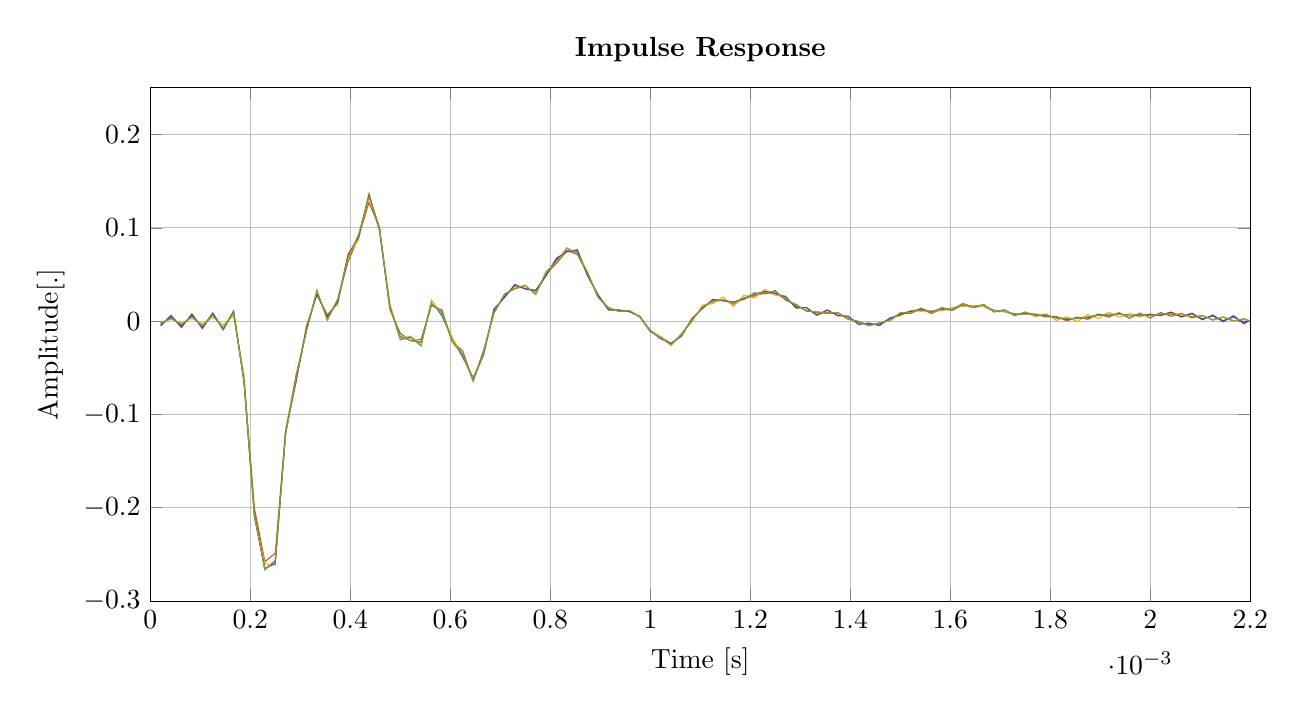
\begin{tikzpicture}

\begin{axis}[%
width=5.5in,
height=2.566in,
at={(0.758in,0.481in)},
scale only axis,
xmin=0,
xmax=0.0022,
xlabel={Time [s]},
xmajorgrids,
ymin=-0.30,
ymax=0.25,
ylabel={Amplitude[.]},
ymajorgrids,
axis background/.style={fill=white},
title style={font=\bfseries},
title={Impulse Response}
]
\addplot [color=mycolor1,solid,forget plot]
  table[row sep=crcr]{%
2.08333333333333e-05	-0.0037087927908794\\
4.16666666666667e-05	0.00421160453226942\\
6.25e-05	-0.00520379576953817\\
8.33333333333333e-05	0.00629701654848276\\
0.000104166666666667	-0.00678651279752952\\
0.000125	0.00811356819824401\\
0.000145833333333333	-0.00884124098433367\\
0.000166666666666667	0.0107472615560426\\
0.0001875	-0.0646663577808535\\
0.000208333333333333	-0.206299821990036\\
0.000229166666666667	-0.266170671528939\\
0.00025	-0.256370669612707\\
0.000270833333333333	-0.120287541326005\\
0.000291666666666667	-0.0617180208660174\\
0.0003125	-0.00922362905565283\\
0.000333333333333333	0.0308397018576189\\
0.000354166666666667	0.0035403786890247\\
0.000375	0.0212448332280645\\
0.000395833333333333	0.0705478621795121\\
0.000416666666666667	0.0895474948933934\\
0.0004375	0.13552149422923\\
0.000458333333333333	0.097299803954558\\
0.000479166666666667	0.0171466790731723\\
0.0005	-0.0197680684506663\\
0.000520833333333333	-0.0171223102171715\\
0.000541666666666667	-0.0263656309604829\\
0.0005625	0.0219768694253305\\
0.000583333333333333	0.00560475366613178\\
0.000604166666666667	-0.0182339778631218\\
0.000625	-0.0387957025837346\\
0.000645833333333333	-0.0604621915450745\\
0.000666666666666667	-0.0363795655357155\\
0.0006875	0.0130977677372803\\
0.000708333333333333	0.0251346467322033\\
0.000729166666666667	0.039105419651278\\
0.00075	0.0346523806957789\\
0.000770833333333333	0.0322481248629661\\
0.000791666666666667	0.0493725854189164\\
0.0008125	0.0660612053755624\\
0.000833333333333333	0.0751202061643853\\
0.000854166666666667	0.0750428627194294\\
0.000875	0.048916982972921\\
0.000895833333333333	0.0274042750529549\\
0.000916666666666667	0.012118310680073\\
0.0009375	0.0119101424242984\\
0.000958333333333333	0.0100853086322103\\
0.000979166666666667	0.00544456035302204\\
0.001	-0.0112918644454638\\
0.00102083333333333	-0.0172483398553776\\
0.00104166666666667	-0.0251189065330511\\
0.0010625	-0.014558012452602\\
0.00108333333333333	0.0017134948101292\\
0.00110416666666667	0.014255079903006\\
0.001125	0.0227537754361355\\
0.00114583333333333	0.021816701937651\\
0.00116666666666667	0.0206421122092443\\
0.0011875	0.0233880957023547\\
0.00120833333333333	0.0302390075091007\\
0.00122916666666667	0.0293537948171238\\
0.00125	0.0326242279536413\\
0.00127083333333333	0.0225148202302848\\
0.00129166666666667	0.0177894930311056\\
0.0013125	0.010770331824266\\
0.00133333333333333	0.00983620954713187\\
0.00135416666666667	0.00853521175516866\\
0.001375	0.00899597167105174\\
0.00139583333333333	0.00260243594654619\\
0.00141666666666667	-0.00104701561770118\\
0.0014375	-0.00371807000382697\\
0.00145833333333333	-0.00318960626194621\\
0.00147916666666667	0.00257545774845068\\
0.0015	0.00713790465040768\\
0.00152083333333333	0.0108215910141207\\
0.00154166666666667	0.0120264444758566\\
0.0015625	0.0108261870538285\\
0.00158333333333333	0.0123450686244096\\
0.00160416666666667	0.0139129670171921\\
0.001625	0.0169005010166529\\
0.00164583333333333	0.0165791257894914\\
0.00166666666666667	0.0159045477126551\\
0.0016875	0.0116907728854056\\
0.00170833333333333	0.0102974368732395\\
0.00172916666666667	0.00768755665771632\\
0.00175	0.0082004670345183\\
0.00177083333333333	0.00731505527542035\\
0.00179166666666667	0.0054086354181059\\
0.0018125	0.00446490364319473\\
0.00183333333333333	0.00151912598295708\\
0.00185416666666667	0.00374848548552877\\
0.001875	0.00361835820665017\\
0.00189583333333333	0.00680282624355538\\
0.00191666666666667	0.00648760855183481\\
0.0019375	0.00770072765347351\\
0.00195833333333333	0.00591670768911894\\
0.00197916666666667	0.00654249543276334\\
0.002	0.00696958712555653\\
0.00202083333333333	0.00639676696262537\\
0.00204166666666667	0.00930875870313683\\
0.0020625	0.00487368778960512\\
0.00208333333333333	0.00793267565500179\\
0.00210416666666667	0.00227381220914028\\
0.002125	0.00559059790855196\\
0.00214583333333333	0.000509710927088874\\
0.00216666666666667	0.00445914830547992\\
0.0021875	-0.0013119827312339\\
0.00220833333333333	0.00204620626659837\\
0.00222916666666667	-0.00226693806170011\\
0.00225	-0.000865052032163367\\
0.00227083333333333	-0.000568466635637404\\
0.00229166666666667	-0.00176072172101629\\
0.0023125	0.001051321525168\\
0.00233333333333333	-0.00235307840318451\\
0.00235416666666667	0.00142050267868398\\
0.002375	-0.00373732644882233\\
0.00239583333333333	0.00263329200115178\\
0.00241666666666667	-0.00419384885137344\\
0.0024375	0.00356243119561722\\
0.00245833333333333	-0.00341750395084726\\
0.00247916666666667	0.00231533516568704\\
0.0025	-0.002886346397735\\
0.00252083333333333	0.000637791268280785\\
0.00254166666666667	-0.00290884766679218\\
0.0025625	-0.000629280559252555\\
0.00258333333333333	-0.00286116806569122\\
0.00260416666666667	-0.00278592644964782\\
0.002625	-0.00262193859169995\\
0.00264583333333333	-0.00474810164470427\\
0.00266666666666667	-0.00275009938116807\\
0.0026875	-0.00478816826817122\\
0.00270833333333333	-0.00324811681170597\\
0.00272916666666667	-0.0040257377623872\\
0.00275	-0.00368074892796126\\
0.00277083333333333	-0.00337062684290595\\
0.00279166666666667	-0.00370307569447635\\
0.0028125	-0.00186571326957182\\
0.00283333333333333	-0.00390602380821677\\
0.00285416666666667	-4.9752550230383e-05\\
0.002875	-0.00438323194808954\\
0.00289583333333333	0.000384386269952189\\
0.00291666666666667	-0.00453307061294354\\
0.0029375	-0.000328341601327697\\
0.00295833333333333	-0.00426336185525099\\
0.00297916666666667	-0.00128138687597425\\
0.003	-0.00414308057749922\\
0.00302083333333333	-0.00248651642821263\\
0.00304166666666667	-0.00361961427656752\\
0.0030625	-0.00400763468176544\\
0.00308333333333333	-0.0023795304299123\\
0.00310416666666667	-0.00514325156697817\\
0.003125	-0.00122625577194359\\
0.00314583333333333	-0.00545188790289689\\
0.00316666666666667	-0.000609928041986866\\
0.0031875	-0.00505013848995181\\
0.00320833333333333	5.99816839252916e-05\\
0.00322916666666667	-0.00449193406111753\\
0.00325	0.000558016389499313\\
0.00327083333333333	-0.00386841737730755\\
0.00329166666666667	0.000169965391614449\\
0.0033125	-0.00319883141842068\\
0.00333333333333333	-0.000671676767081501\\
0.00335416666666667	-0.00289606776507812\\
0.003375	-0.00113994195612087\\
0.00339583333333333	-0.00325262465554565\\
0.00341666666666667	-0.00136179764715377\\
0.0034375	-0.00360873416552366\\
0.00345833333333333	-0.00164463882761736\\
0.00347916666666667	-0.00371793269729748\\
0.0035	-0.00154353439141849\\
0.00352083333333333	-0.00403549855695194\\
0.00354166666666667	-0.000984353596708564\\
0.0035625	-0.00425443771279568\\
0.00358333333333333	-0.000672628985252431\\
0.00360416666666667	-0.00374129885739169\\
0.003625	-0.000937340861272143\\
0.00364583333333333	-0.00296533591369333\\
0.00366666666666667	-0.00130448571666488\\
0.0036875	-0.00246387735925147\\
0.00370833333333333	-0.00182327238315157\\
0.00372916666666667	-0.00173617907905828\\
0.00375	-0.00284258077794951\\
0.00377083333333333	-0.000756536202756666\\
0.00379166666666667	-0.00385114062696801\\
0.0038125	-0.000291952662999003\\
0.00383333333333333	-0.00423039940178691\\
0.00385416666666667	-0.000378549414924021\\
0.003875	-0.00428312305197425\\
0.00389583333333333	-0.000406743035733924\\
0.00391666666666667	-0.00424392197549792\\
0.0039375	-0.000625284040186809\\
0.00395833333333333	-0.00365167293604246\\
0.00397916666666667	-0.001337671135446\\
0.004	-0.00271896198950253\\
0.00402083333333333	-0.0019858020567554\\
0.00404166666666667	-0.00219062801883803\\
0.0040625	-0.00220835913204532\\
0.00408333333333333	-0.00203974929682549\\
0.00410416666666667	-0.00233913427988745\\
0.004125	-0.00185099449592134\\
0.00414583333333333	-0.00236574968059208\\
0.00416666666666667	-0.00196457798952639\\
0.0041875	-0.0019046742644009\\
0.00420833333333333	-0.00250443960036927\\
0.00422916666666667	-0.00128461530764495\\
0.00425	-0.00297296735967611\\
0.00427083333333333	-0.000992836466506577\\
0.00429166666666667	-0.00314961192994209\\
0.0043125	-0.000907894618487529\\
0.00433333333333333	-0.00328775019087989\\
0.00435416666666667	-0.000812410858858454\\
0.004375	-0.00329843852206017\\
0.00439583333333333	-0.000993520893343976\\
0.00441666666666667	-0.00296787895096846\\
0.0044375	-0.00135986816935005\\
0.00445833333333333	-0.00257683158276436\\
0.00447916666666667	-0.00150120312434058\\
0.0045	-0.00246875060820952\\
0.00452083333333333	-0.00127751762473565\\
0.00454166666666667	-0.00257055972440008\\
0.0045625	-0.000850583087086702\\
0.00458333333333333	-0.00279615291783079\\
0.00460416666666667	-0.000169229703961833\\
0.004625	-0.0033208199374696\\
0.00464583333333333	0.000762775063455069\\
0.00466666666666667	-0.00404729208587363\\
0.0046875	0.00162126259324774\\
0.00470833333333333	-0.00461429328418873\\
0.00472916666666667	0.00206634843487202\\
0.00475	-0.00479804415433337\\
0.00477083333333333	0.00203716599298341\\
0.00479166666666667	-0.00461953370883597\\
0.0048125	0.00158614710765907\\
0.00483333333333333	-0.0039600168009732\\
0.00485416666666667	0.00066992915889739\\
0.004875	-0.0027700643584047\\
0.00489583333333333	-0.000614917555245659\\
0.00491666666666667	-0.00132297677247495\\
0.0049375	-0.00190838752526078\\
0.00495833333333333	-4.06116797333875e-05\\
0.00497916666666667	-0.00288565901097666\\
0.005	0.000889847654868419\\
0.00502083333333333	-0.00349274225205263\\
0.00504166666666667	0.00137995835933047\\
0.0050625	-0.00358103532986242\\
0.00508333333333333	0.00125952593606002\\
0.00510416666666667	-0.00298112408616989\\
0.005125	0.00052817856633219\\
0.00514583333333333	-0.0019103540353447\\
0.00516666666666667	-0.000471366982676235\\
0.0051875	-0.000794234842926538\\
0.00520833333333333	-0.00141585678773726\\
};
\addplot [color=mycolor2,solid,forget plot]
  table[row sep=crcr]{%
2.08333333333333e-05	-0.00255267252938673\\
4.16666666666667e-05	0.00289958707347902\\
6.25e-05	-0.00382265239043665\\
8.33333333333333e-05	0.00482200108963299\\
0.000104166666666667	-0.00515633007307537\\
0.000125	0.00667606380308441\\
0.000145833333333333	-0.00708343055179381\\
0.000166666666666667	0.0092525375696961\\
0.0001875	-0.0607390597290135\\
0.000208333333333333	-0.200401659875795\\
0.000229166666666667	-0.257768300997275\\
0.00025	-0.248800582164502\\
0.000270833333333333	-0.117646720461853\\
0.000291666666666667	-0.0578844981508881\\
0.0003125	-0.0102016454149929\\
0.000333333333333333	0.0330014197433572\\
0.000354166666666667	0.00127667958148536\\
0.000375	0.0234190373569384\\
0.000395833333333333	0.0639275956854277\\
0.000416666666666667	0.0906470163865055\\
0.0004375	0.127123824348622\\
0.000458333333333333	0.100636329904299\\
0.000479166666666667	0.0124905457764127\\
0.0005	-0.0128509224250364\\
0.000520833333333333	-0.0212238017533485\\
0.000541666666666667	-0.0195717514784339\\
0.0005625	0.0166431551373302\\
0.000583333333333333	0.0120320299572739\\
0.000604166666666667	-0.0219158802601074\\
0.000625	-0.0320151869444835\\
0.000645833333333333	-0.0633380264022395\\
0.000666666666666667	-0.0314055759804432\\
0.0006875	0.0084423319629683\\
0.000708333333333333	0.0282626599947745\\
0.000729166666666667	0.034755671823636\\
0.00075	0.0375030938504313\\
0.000770833333333333	0.0287324780339133\\
0.000791666666666667	0.0509433983273104\\
0.0008125	0.0618381605219164\\
0.000833333333333333	0.0756881939220368\\
0.000854166666666667	0.0714587648185071\\
0.000875	0.0505304570640701\\
0.000895833333333333	0.0255469926503848\\
0.000916666666666667	0.0139977515791326\\
0.0009375	0.0105701348927955\\
0.000958333333333333	0.0111681123111772\\
0.000979166666666667	0.00467517577342191\\
0.001	-0.0100498056673259\\
0.00102083333333333	-0.0168471351248233\\
0.00104166666666667	-0.0242983429721961\\
0.0010625	-0.0138911007564663\\
0.00108333333333333	0.000815862706313863\\
0.00110416666666667	0.0148029936594\\
0.001125	0.0207210667345826\\
0.00114583333333333	0.0226963031788706\\
0.00116666666666667	0.0181062087629371\\
0.0011875	0.0242935347792987\\
0.00120833333333333	0.0271226044174566\\
0.00122916666666667	0.0301879108304438\\
0.00125	0.0297329814304771\\
0.00127083333333333	0.0236557223579554\\
0.00129166666666667	0.0158766440133432\\
0.0013125	0.011696116145808\\
0.00133333333333333	0.00871715898126307\\
0.00135416666666667	0.00871221990090018\\
0.001375	0.00864655184050639\\
0.00139583333333333	0.00219401302147165\\
0.00141666666666667	-0.000480463220486303\\
0.0014375	-0.00478793011354472\\
0.00145833333333333	-0.00214213807521797\\
0.00147916666666667	0.000610919065108282\\
0.0015	0.00822355226328271\\
0.00152083333333333	0.00831464525440903\\
0.00154166666666667	0.0130253685510728\\
0.0015625	0.00825458577231076\\
0.00158333333333333	0.0131017386199352\\
0.00160416666666667	0.0115045453955671\\
0.001625	0.0173054531317267\\
0.00164583333333333	0.0146751752014143\\
0.00166666666666667	0.0160624194214595\\
0.0016875	0.0105018463460038\\
0.00170833333333333	0.0101683646808241\\
0.00172916666666667	0.0070445186245326\\
0.00175	0.00766088993981086\\
0.00177083333333333	0.00710536523175556\\
0.00179166666666667	0.00457630122370742\\
0.0018125	0.00469420240794347\\
0.00183333333333333	0.000404005788937426\\
0.00185416666666667	0.00428370428539064\\
0.001875	0.00197599863403158\\
0.00189583333333333	0.0076578440345062\\
0.00191666666666667	0.00423011592859115\\
0.0019375	0.00909761104080475\\
0.00195833333333333	0.0030678897125246\\
0.00197916666666667	0.00859528939877386\\
0.002	0.00346894854210457\\
0.00202083333333333	0.00914620649963214\\
0.00204166666666667	0.00520410877557944\\
0.0020625	0.00832413302525314\\
0.00208333333333333	0.00346908753461933\\
0.00210416666666667	0.00610387771170956\\
0.002125	0.00108867775682093\\
0.00214583333333333	0.00419930592939649\\
0.00216666666666667	0.000319892049500485\\
0.0021875	0.00180869387049779\\
0.00220833333333333	-0.00126219037085954\\
0.00222916666666667	-0.00016649986826338\\
0.00225	-0.00292140933910888\\
0.00227083333333333	5.48115721681712e-05\\
0.00229166666666667	-0.00231838798243882\\
0.0023125	6.02159680772856e-05\\
0.00233333333333333	-0.00141553936136535\\
0.00235416666666667	-0.000969725177756748\\
0.002375	-0.00155367505348034\\
0.00239583333333333	-0.00078737578525\\
0.00241666666666667	-0.00118813913866019\\
0.0024375	-0.000351639141263614\\
0.00245833333333333	-0.000202294846823073\\
0.00247916666666667	-0.00140433733178488\\
0.0025	-0.000148481375508499\\
0.00252083333333333	-0.00229105227885144\\
0.00254166666666667	-0.00113327041550525\\
0.0025625	-0.00240289119356657\\
0.00258333333333333	-0.00221020389739753\\
0.00260416666666667	-0.00327807804462282\\
0.002625	-0.00307515395717207\\
0.00264583333333333	-0.00411499501980943\\
0.00266666666666667	-0.00404707161300406\\
0.0026875	-0.00348238100217361\\
0.00270833333333333	-0.00488806311665677\\
0.00272916666666667	-0.0026354048015551\\
0.00275	-0.00512258678524018\\
0.00277083333333333	-0.00237918958058366\\
0.00279166666666667	-0.00456717537979813\\
0.0028125	-0.00158216040976036\\
0.00283333333333333	-0.00398847584896324\\
0.00285416666666667	-0.000601313268332522\\
0.002875	-0.00369552546612422\\
0.00289583333333333	-0.000887430420175447\\
0.00291666666666667	-0.0033287586160303\\
0.0029375	-0.00196666642325469\\
0.00295833333333333	-0.00291972100094473\\
0.00297916666666667	-0.00286833083131398\\
0.003	-0.00297599955911991\\
0.00302083333333333	-0.00372065054441346\\
0.00304166666666667	-0.00284107705068402\\
0.0030625	-0.00474018439203851\\
0.00308333333333333	-0.00207488352087834\\
0.00310416666666667	-0.00536932379647781\\
0.003125	-0.00131533563026484\\
0.00314583333333333	-0.00536072637441323\\
0.00316666666666667	-0.000858022679083761\\
0.0031875	-0.00494352194507911\\
0.00320833333333333	-9.29124655160845e-05\\
0.00322916666666667	-0.00458455294834229\\
0.00325	0.000653130100906661\\
0.00327083333333333	-0.00423158530604592\\
0.00329166666666667	0.000543960512810295\\
0.0033125	-0.00379406688018271\\
0.00333333333333333	-9.66816216515342e-05\\
0.00335416666666667	-0.00353027419822252\\
0.003375	-0.000570547946950482\\
0.00339583333333333	-0.00361077269310737\\
0.00341666666666667	-0.00110650316314777\\
0.0034375	-0.00343504924741948\\
0.00345833333333333	-0.00193518158467088\\
0.00347916666666667	-0.00291655885566418\\
0.0035	-0.00243334545259287\\
0.00352083333333333	-0.00262502115222047\\
0.00354166666666667	-0.00240295393708929\\
0.0035625	-0.00239818677743936\\
0.00358333333333333	-0.00241583275384139\\
0.00360416666666667	-0.00177271872007091\\
0.003625	-0.00263795048328915\\
0.00364583333333333	-0.00127580236053149\\
0.00366666666666667	-0.00260032147781131\\
0.0036875	-0.00135047828264343\\
0.00370833333333333	-0.00248490641271397\\
0.00372916666666667	-0.00135362852201022\\
0.00375	-0.00276058505758708\\
0.00377083333333333	-0.00111545031714157\\
0.00379166666666667	-0.00304804673300568\\
0.0038125	-0.00121762006398216\\
0.00383333333333333	-0.00295967887667023\\
0.00385416666666667	-0.00152799538999958\\
0.003875	-0.00293911795913497\\
0.00389583333333333	-0.00141842129814424\\
0.00391666666666667	-0.00317139837627678\\
0.0039375	-0.00120453703812563\\
0.00395833333333333	-0.00310189945322664\\
0.00397916666666667	-0.00127577630415201\\
0.004	-0.00285323822275981\\
0.00402083333333333	-0.00123759058802548\\
0.00404166666666667	-0.00295826755744021\\
0.0040625	-0.000941733037558027\\
0.00408333333333333	-0.00317740848079844\\
0.00410416666666667	-0.000853233064771672\\
0.004125	-0.003025048708344\\
0.00414583333333333	-0.000993006404728137\\
0.00416666666666667	-0.00285059650886691\\
0.0041875	-0.000974726981488831\\
0.00420833333333333	-0.00278577246306679\\
0.00422916666666667	-0.00106359834458666\\
0.00425	-0.00243185185834133\\
0.00427083333333333	-0.00161288283600495\\
0.00429166666666667	-0.00173941306975917\\
0.0043125	-0.0023614205758312\\
0.00433333333333333	-0.00107298483413706\\
0.00435416666666667	-0.00303899121775412\\
0.004375	-0.000375970115777865\\
0.00439583333333333	-0.00388549063063888\\
0.00441666666666667	0.000541297745222786\\
0.0044375	-0.00479932669104759\\
0.00445833333333333	0.00139622726997478\\
0.00447916666666667	-0.00539810064640756\\
0.0045	0.00192488295368076\\
0.00452083333333333	-0.00560504111770523\\
0.00454166666666667	0.00224701915074393\\
0.0045625	-0.00560943314661647\\
0.00458333333333333	0.0024195452607323\\
0.00460416666666667	-0.005317466524108\\
0.004625	0.00222418518526779\\
0.00464583333333333	-0.00466166053919306\\
0.00466666666666667	0.00169427281028947\\
0.0046875	-0.00386977891617415\\
0.00470833333333333	0.00106542399644791\\
0.00472916666666667	-0.00315415940463025\\
0.00475	0.000425270653698219\\
0.00477083333333333	-0.00245902414772154\\
0.00479166666666667	-0.000313192663862794\\
0.0048125	-0.00172664645538972\\
0.00483333333333333	-0.00101569750310594\\
0.00485416666666667	-0.0010706020758985\\
0.004875	-0.00152478876973867\\
0.00489583333333333	-0.00053804913087041\\
0.00491666666666667	-0.00192301123282111\\
0.0049375	-8.46962331649506e-06\\
0.00495833333333333	-0.00234650155333196\\
0.00497916666666667	0.000517616027113713\\
0.005	-0.0026874982365122\\
0.00502083333333333	0.000837710179045122\\
0.00504166666666667	-0.00281392506940281\\
0.0050625	0.000951526220070128\\
0.00508333333333333	-0.00279809276114962\\
0.00510416666666667	0.000989617566664778\\
0.005125	-0.00267417639347939\\
0.00514583333333333	0.00086092609975851\\
0.00516666666666667	-0.00228430448627185\\
0.0051875	0.000452408493989887\\
0.00520833333333333	-0.00164854160289399\\
};
\addplot [color=mycolor3,solid,forget plot]
  table[row sep=crcr]{%
2.08333333333333e-05	-0.00163321204155689\\
4.16666666666667e-05	0.00217871738448115\\
6.25e-05	-0.00223030869416506\\
8.33333333333333e-05	0.00308085388067272\\
0.000104166666666667	-0.00283418955947869\\
0.000125	0.00387776978723627\\
0.000145833333333333	-0.00396721517720515\\
0.000166666666666667	0.00565169339153807\\
0.0001875	-0.0578645073772853\\
0.000208333333333333	-0.210568816309939\\
0.000229166666666667	-0.259955188133081\\
0.00025	-0.261242392983444\\
0.000270833333333333	-0.11541144340208\\
0.000291666666666667	-0.065082383983406\\
0.0003125	-0.00457165776378929\\
0.000333333333333333	0.0281698447908548\\
0.000354166666666667	0.00746906122663251\\
0.000375	0.017980551653853\\
0.000395833333333333	0.0719876105253128\\
0.000416666666666667	0.0872051031610365\\
0.0004375	0.136972018527987\\
0.000458333333333333	0.0979061885001598\\
0.000479166666666667	0.0190373994273952\\
0.0005	-0.0187474979071836\\
0.000520833333333333	-0.0159911997270242\\
0.000541666666666667	-0.0254207659568788\\
0.0005625	0.0222939439236886\\
0.000583333333333333	0.00762495201878726\\
0.000604166666666667	-0.0181476959053041\\
0.000625	-0.0370572954894979\\
0.000645833333333333	-0.0616897321841816\\
0.000666666666666667	-0.0357751469485512\\
0.0006875	0.0110541110800959\\
0.000708333333333333	0.0266261311666174\\
0.000729166666666667	0.0370835756321231\\
0.00075	0.0372079006439419\\
0.000770833333333333	0.0299720795056686\\
0.000791666666666667	0.0519383256345237\\
0.0008125	0.0633401602353719\\
0.000833333333333333	0.0780465129838801\\
0.000854166666666667	0.072826296030486\\
0.000875	0.0525118906030222\\
0.000895833333333333	0.025547455882416\\
0.000916666666666667	0.0148804806448951\\
0.0009375	0.0103846646000134\\
0.000958333333333333	0.0115394204404138\\
0.000979166666666667	0.00482301562556526\\
0.001	-0.0109874131473168\\
0.00102083333333333	-0.0166641078639183\\
0.00104166666666667	-0.0264021861315982\\
0.0010625	-0.0129423122730922\\
0.00108333333333333	-0.00127731842486949\\
0.00110416666666667	0.0172078145589618\\
0.001125	0.0186646164744698\\
0.00114583333333333	0.0258355733901017\\
0.00116666666666667	0.0157117601980314\\
0.0011875	0.0277803562128635\\
0.00120833333333333	0.0249411956451881\\
0.00122916666666667	0.0339131100205985\\
0.00125	0.0276834810161797\\
0.00127083333333333	0.0270876373860748\\
0.00129166666666667	0.0135486398598428\\
0.0013125	0.0146281493199383\\
0.00133333333333333	0.00630120909161602\\
0.00135416666666667	0.0114262979203145\\
0.001375	0.00625151023360393\\
0.00139583333333333	0.00469691746271263\\
0.00141666666666667	-0.00320755138194242\\
0.0014375	-0.0023665451221515\\
0.00145833333333333	-0.00501549633026936\\
0.00147916666666667	0.00337042559894113\\
0.0015	0.00557224153648716\\
0.00152083333333333	0.0113999793119524\\
0.00154166666666667	0.0105608590694505\\
0.0015625	0.0112253538955211\\
0.00158333333333333	0.0109297147864292\\
0.00160416666666667	0.0141182406444556\\
0.001625	0.0158705693922061\\
0.00164583333333333	0.0165236340426216\\
0.00166666666666667	0.0155539386955293\\
0.0016875	0.0110146959222936\\
0.00170833333333333	0.0107587084546628\\
0.00172916666666667	0.006021107065009\\
0.00175	0.00962358548745266\\
0.00177083333333333	0.00461488367395265\\
0.00179166666666667	0.00786354161870322\\
0.0018125	0.00083980837975928\\
0.00183333333333333	0.00474934129641216\\
0.00185416666666667	-0.000493640480630181\\
0.001875	0.00712827695489169\\
0.00189583333333333	0.00258517202966767\\
0.00191666666666667	0.00965080478835073\\
0.0019375	0.00421535128796295\\
0.00195833333333333	0.00807287058220521\\
0.00197916666666667	0.00433552437525072\\
0.002	0.00762144067704767\\
0.00202083333333333	0.00590796681015577\\
0.00204166666666667	0.00823247822607332\\
0.0020625	0.00624889897116549\\
0.00208333333333333	0.0051706692669312\\
0.00210416666666667	0.00513911501618462\\
0.002125	0.00157578666104142\\
0.00214583333333333	0.00419562172707041\\
0.00216666666666667	-8.17894503905048e-05\\
0.0021875	0.00249146863565593\\
0.00220833333333333	-0.00225060743894737\\
0.00222916666666667	0.000911367832004493\\
0.00225	-0.0042023273732927\\
0.00227083333333333	0.00131908623295955\\
0.00229166666666667	-0.00359422398769843\\
0.0023125	0.00130602372428194\\
0.00233333333333333	-0.0025474285480275\\
0.00235416666666667	9.12508870677423e-05\\
0.002375	-0.00251258605257109\\
0.00239583333333333	3.68184456323214e-05\\
0.00241666666666667	-0.001908222379877\\
0.0024375	0.000171602768831179\\
0.00245833333333333	-0.000565657920822165\\
0.00247916666666667	-0.00132123186706604\\
0.0025	-3.69357225569728e-05\\
0.00252083333333333	-0.00278555913442368\\
0.00254166666666667	-0.000381161411822799\\
0.0025625	-0.00363098794507625\\
0.00258333333333333	-0.000623408767812987\\
0.00260416666666667	-0.00542533906568231\\
0.002625	-0.000514434727790267\\
0.00264583333333333	-0.00727794417210567\\
0.00266666666666667	-0.000521849778767368\\
0.0026875	-0.00757661607436271\\
0.00270833333333333	-0.000543882871711502\\
0.00272916666666667	-0.00744648183443503\\
0.00275	-0.000262008073977348\\
0.00277083333333333	-0.00754898213636908\\
0.00279166666666667	0.000392125328535457\\
0.0028125	-0.00659584850012438\\
0.00283333333333333	0.000562148987953842\\
0.00285416666666667	-0.00491349124801912\\
0.002875	-4.71952709105437e-05\\
0.00289583333333333	-0.00403617308167389\\
0.00291666666666667	-0.00098491246115772\\
0.0029375	-0.00360617852387868\\
0.00295833333333333	-0.00216020792434374\\
0.00297916666666667	-0.00281031658588728\\
0.003	-0.00393642768912363\\
0.00302083333333333	-0.0019740161735394\\
0.00304166666666667	-0.00545044644123764\\
0.0030625	-0.00148724838410483\\
0.00308333333333333	-0.00609761795227659\\
0.00310416666666667	-0.000911843004845307\\
0.003125	-0.00641109553135691\\
0.00314583333333333	-6.68399286926769e-05\\
0.00316666666666667	-0.00661223381392086\\
0.0031875	0.000792942062802807\\
0.00320833333333333	-0.00605194886502256\\
0.00322916666666667	0.00119081641544235\\
0.00325	-0.00510662306890529\\
0.00327083333333333	0.0012153985699642\\
0.00329166666666667	-0.00468000094954699\\
0.0033125	0.00101706104418737\\
0.00333333333333333	-0.0044992583008872\\
0.00335416666666667	0.000373907361929023\\
0.003375	-0.00393423263359508\\
0.00339583333333333	-0.000849674035833999\\
0.00341666666666667	-0.00327675308048005\\
0.0034375	-0.00196202325455657\\
0.00345833333333333	-0.00281649981315708\\
0.00347916666666667	-0.00279172529312823\\
0.0035	-0.00199265111718659\\
0.00352083333333333	-0.00384408715258885\\
0.00354166666666667	-0.000687528632112489\\
0.0035625	-0.0048382405767023\\
0.00358333333333333	0.000411062545070974\\
0.00360416666666667	-0.00517279640746107\\
0.003625	0.00102806244718597\\
0.00364583333333333	-0.00530219593314191\\
0.00366666666666667	0.00153508609358886\\
0.0036875	-0.00561251207357299\\
0.00370833333333333	0.00167486091733119\\
0.00372916666666667	-0.00539493643036716\\
0.00375	0.00095668559377168\\
0.00377083333333333	-0.00449327302460345\\
0.00379166666666667	-0.000202453154405987\\
0.0038125	-0.00358211842714922\\
0.00383333333333333	-0.00130167335324517\\
0.00385416666666667	-0.0026300982831725\\
0.003875	-0.00263555824036522\\
0.00389583333333333	-0.00114138056803914\\
0.00391666666666667	-0.00421914845301114\\
0.0039375	0.000366426789574729\\
0.00395833333333333	-0.00531590855132645\\
0.00397916666666667	0.00132682521510946\\
0.004	-0.00589441023054478\\
0.00402083333333333	0.0020330284975877\\
0.00404166666666667	-0.00643081079363684\\
0.0040625	0.00258116813465071\\
0.00408333333333333	-0.00669153743716035\\
0.00410416666666667	0.00252712937339086\\
0.004125	-0.00626501890081867\\
0.00414583333333333	0.00198573399042622\\
0.00416666666666667	-0.00564706489609503\\
0.0041875	0.00152112304451762\\
0.00420833333333333	-0.00515083718413495\\
0.00422916666666667	0.00102298995925469\\
0.00425	-0.00449765039675646\\
0.00427083333333333	0.000268338619425756\\
0.00429166666666667	-0.00371379195250488\\
0.0043125	-0.000425640222728158\\
0.00433333333333333	-0.00319524784033904\\
0.00435416666666667	-0.000821975064880745\\
0.004375	-0.00282770222093157\\
0.00439583333333333	-0.00126508575246811\\
0.00441666666666667	-0.00230471738176367\\
0.0044375	-0.00177566551043765\\
0.00445833333333333	-0.00179693413328159\\
0.00447916666666667	-0.00209730578453145\\
0.0045	-0.00146755955861572\\
0.00452083333333333	-0.00224017373487703\\
0.00454166666666667	-0.00112128092359989\\
0.0045625	-0.00241988879033352\\
0.00458333333333333	-0.000677054033918395\\
0.00460416666666667	-0.00251242284809268\\
0.004625	-0.000408875554688982\\
0.00464583333333333	-0.00238920768851963\\
0.00466666666666667	-0.00035233334164938\\
0.0046875	-0.0021916507379531\\
0.00470833333333333	-0.000353204672140455\\
0.00472916666666667	-0.00206426554660433\\
0.00475	-0.000399111146290863\\
0.00477083333333333	-0.00190898307931796\\
0.00479166666666667	-0.000620985892132324\\
0.0048125	-0.00165238099799337\\
0.00483333333333333	-0.000881278130450417\\
0.00485416666666667	-0.00142045191052985\\
0.004875	-0.00100160951886526\\
0.00489583333333333	-0.00128622165651065\\
0.00491666666666667	-0.00103775843243032\\
0.0049375	-0.00112884862974338\\
0.00495833333333333	-0.00112433334285194\\
0.00497916666666667	-0.000926118130786855\\
0.005	-0.00116589196730782\\
0.00502083333333333	-0.00085433505620867\\
0.00504166666666667	-0.00107320946693262\\
0.0050625	-0.000875743054272184\\
0.00508333333333333	-0.000966483466824754\\
0.00510416666666667	-0.000820897375894202\\
0.005125	-0.000917689548129309\\
0.00514583333333333	-0.000784404643824917\\
0.00516666666666667	-0.00076358766070243\\
0.0051875	-0.000910640434007906\\
0.00520833333333333	-0.000481400776064074\\
};
\addplot [color=mycolor4,solid,forget plot]
  table[row sep=crcr]{%
2.08333333333333e-05	-0.00516726277486403\\
4.16666666666667e-05	0.00618610543992257\\
6.25e-05	-0.00674403357522682\\
8.33333333333333e-05	0.00770721377255318\\
0.000104166666666667	-0.0079390099384032\\
0.000125	0.0086020434024014\\
0.000145833333333333	-0.00902843756603243\\
0.000166666666666667	0.0100058461757606\\
0.0001875	-0.0641955735500921\\
0.000208333333333333	-0.208700228894356\\
0.000229166666666667	-0.265220840886755\\
0.00025	-0.259647179573132\\
0.000270833333333333	-0.118446743512368\\
0.000291666666666667	-0.0645851736784997\\
0.0003125	-0.00681068819516621\\
0.000333333333333333	0.0287361417369287\\
0.000354166666666667	0.00528308056129979\\
0.000375	0.0203557265501783\\
0.000395833333333333	0.0712760448789094\\
0.000416666666666667	0.0904990248217112\\
0.0004375	0.135055068926438\\
0.000458333333333333	0.0997502441326314\\
0.000479166666666667	0.0149656960420083\\
0.0005	-0.0165087379404821\\
0.000520833333333333	-0.0206907204364962\\
0.000541666666666667	-0.0225262866903627\\
0.0005625	0.0180825474272777\\
0.000583333333333333	0.00939702452084589\\
0.000604166666666667	-0.0220080878731115\\
0.000625	-0.0359484501101515\\
0.000645833333333333	-0.0635737161406537\\
0.000666666666666667	-0.0345952872075129\\
0.0006875	0.011395100325966\\
0.000708333333333333	0.0259765767874302\\
0.000729166666666667	0.0388948268072226\\
0.00075	0.0345433960194401\\
0.000770833333333333	0.0330594608503968\\
0.000791666666666667	0.0486818198528796\\
0.0008125	0.0674756758742106\\
0.000833333333333333	0.0744150741225028\\
0.000854166666666667	0.0764475561324374\\
0.000875	0.0484555353578298\\
0.000895833333333333	0.0280952139333538\\
0.000916666666666667	0.0120915320156524\\
0.0009375	0.0116550564182299\\
0.000958333333333333	0.0106926921212952\\
0.000979166666666667	0.00437971585193512\\
0.001	-0.0101887902933229\\
0.00102083333333333	-0.0188499921570428\\
0.00104166666666667	-0.0238914746704615\\
0.0010625	-0.0161256173139097\\
0.00108333333333333	0.00275773204942341\\
0.00110416666666667	0.0133609332400136\\
0.001125	0.0231917904276933\\
0.00114583333333333	0.0219589661063437\\
0.00116666666666667	0.0200640545884449\\
0.0011875	0.0247466765973178\\
0.00120833333333333	0.0285547492678105\\
0.00122916666666667	0.0318926492272145\\
0.00125	0.0299764686613089\\
0.00127083333333333	0.0258669723089619\\
0.00129166666666667	0.0144614250473965\\
0.0013125	0.0144118803872106\\
0.00133333333333333	0.00631500520940795\\
0.00135416666666667	0.0119590422551788\\
0.001375	0.00582578414624001\\
0.00139583333333333	0.00531310542364779\\
0.00141666666666667	-0.00343872304963442\\
0.0014375	-0.00204564952450211\\
0.00145833333333333	-0.00450517778079939\\
0.00147916666666667	0.00314623347351362\\
0.0015	0.00701711951470965\\
0.00152083333333333	0.0103864197390258\\
0.00154166666666667	0.0129433271786474\\
0.0015625	0.00958576326911167\\
0.00158333333333333	0.0139841965278157\\
0.00160416666666667	0.0121875227655739\\
0.001625	0.0188998385691284\\
0.00164583333333333	0.0146984545420619\\
0.00166666666666667	0.017899680479795\\
0.0016875	0.00991070284736272\\
0.00170833333333333	0.0120138300378153\\
0.00172916666666667	0.00618896675135314\\
0.00175	0.00950797333791057\\
0.00177083333333333	0.00619846562183273\\
0.00179166666666667	0.00629933583354124\\
0.0018125	0.00372292860313401\\
0.00183333333333333	0.00204703775903457\\
0.00185416666666667	0.00329997560254824\\
0.001875	0.00389942548298164\\
0.00189583333333333	0.00657336211721742\\
0.00191666666666667	0.00665232357684192\\
0.0019375	0.0075909095931576\\
0.00195833333333333	0.00605956480100092\\
0.00197916666666667	0.00643341074030218\\
0.002	0.00717334955571132\\
0.00202083333333333	0.00619094312126556\\
0.00204166666666667	0.00966268883294692\\
0.0020625	0.00447138766764083\\
0.00208333333333333	0.00851776245037382\\
0.00210416666666667	0.00155152096694671\\
0.002125	0.00648868394668762\\
0.00214583333333333	-0.000624254648236403\\
0.00216666666666667	0.00576389327580217\\
0.0021875	-0.00289608729956137\\
0.00220833333333333	0.00381430664759555\\
0.00222916666666667	-0.00430459453439456\\
0.00225	0.00134150752329004\\
0.00227083333333333	-0.00298934954772144\\
0.00229166666666667	0.0007768827629351\\
0.0023125	-0.00158590032820341\\
0.00233333333333333	0.000330823136554005\\
0.00235416666666667	-0.00120844519950964\\
0.002375	-0.00116242832138357\\
0.00239583333333333	0.000270897000981958\\
0.00241666666666667	-0.00201802007393254\\
0.0024375	0.00171605320113375\\
0.00245833333333333	-0.00189929643819731\\
0.00247916666666667	0.00119292465952919\\
0.0025	-0.00219131249110632\\
0.00252083333333333	0.00034848939930505\\
0.00254166666666667	-0.00308860740556768\\
0.0025625	-7.85444650659138e-05\\
0.00258333333333333	-0.00384468350111693\\
0.00260416666666667	-0.001493892750237\\
0.002625	-0.00424672879397181\\
0.00264583333333333	-0.00291918864331946\\
0.00266666666666667	-0.00479474830368327\\
0.0026875	-0.002641114801147\\
0.00270833333333333	-0.00547650846681502\\
0.00272916666666667	-0.00176808208131012\\
0.00275	-0.00592170930056437\\
0.00277083333333333	-0.00117173805459234\\
0.00279166666666667	-0.00584231268464412\\
0.0028125	0.000183416280875907\\
0.00283333333333333	-0.00587588613878243\\
0.00285416666666667	0.0018311578583298\\
0.002875	-0.00616980594985171\\
0.00289583333333333	0.0020919430151921\\
0.00291666666666667	-0.006151463925198\\
0.0029375	0.00119796832713895\\
0.00295833333333333	-0.00570267165304615\\
0.00297916666666667	4.97538939356161e-05\\
0.003	-0.0053605861684554\\
0.00302083333333333	-0.00139144543259947\\
0.00304166666666667	-0.00458129470306718\\
0.0030625	-0.00320046711294441\\
0.00308333333333333	-0.00305431263079126\\
0.00310416666666667	-0.00462620972474146\\
0.003125	-0.00160809005656759\\
0.00314583333333333	-0.00518032903383794\\
0.00316666666666667	-0.000778828524857652\\
0.0031875	-0.00492703718563742\\
0.00320833333333333	-4.10939251716325e-05\\
0.00322916666666667	-0.00433900614737377\\
0.00325	0.000347078062520911\\
0.00327083333333333	-0.00349915815918508\\
0.00329166666666667	-0.000345438155645781\\
0.0033125	-0.00247367565948003\\
0.00333333333333333	-0.0016228163755218\\
0.00335416666666667	-0.00173586071389316\\
0.003375	-0.00251999805022344\\
0.00339583333333333	-0.00171285302918648\\
0.00341666666666667	-0.00302092317198616\\
0.0034375	-0.00191969840041333\\
0.00345833333333333	-0.00329477827695596\\
0.00347916666666667	-0.00222733101286352\\
0.0035	-0.00278909601039485\\
0.00352083333333333	-0.00313282923717919\\
0.00354166666666667	-0.00142955103237562\\
0.0035625	-0.00431138062946915\\
0.00358333333333333	-3.33267261560497e-05\\
0.00360416666666667	-0.0049806079600091\\
0.003625	0.000902408321895213\\
0.00364583333333333	-0.00536893329483935\\
0.00366666666666667	0.00161789846540582\\
0.0036875	-0.00579773498379327\\
0.00370833333333333	0.00182795311672953\\
0.00372916666666667	-0.00557217327052572\\
0.00375	0.00104090968872704\\
0.00377083333333333	-0.0045546501000046\\
0.00379166666666667	-0.000273437893586971\\
0.0038125	-0.00354077521085939\\
0.00383333333333333	-0.00141145409669622\\
0.00385416666666667	-0.00271206804832079\\
0.003875	-0.00247321532142388\\
0.00389583333333333	-0.00169972572390624\\
0.00391666666666667	-0.00343380518886849\\
0.0039375	-0.00103182782045088\\
0.00395833333333333	-0.00356096203020484\\
0.00397916666666667	-0.00124689158572549\\
0.004	-0.00285848083433616\\
0.00402083333333333	-0.00193851180094236\\
0.00404166666666667	-0.00200171008123463\\
0.0040625	-0.00275304267616449\\
0.00408333333333333	-0.00103788142726822\\
0.00410416666666667	-0.00387443903731943\\
0.004125	0.000250332702166949\\
0.00414583333333333	-0.00503566614560924\\
0.00416666666666667	0.00122945847968764\\
0.0041875	-0.00556311097230783\\
0.00420833333333333	0.0014705518678144\\
0.00422916666666667	-0.00551042844031363\\
0.00425	0.00127573534719517\\
0.00427083333333333	-0.00519138019590722\\
0.00429166666666667	0.000791747966865656\\
0.0043125	-0.00450084129703969\\
0.00433333333333333	-0.000179976284996915\\
0.00435416666666667	-0.00337897630774022\\
0.004375	-0.00132428816441232\\
0.00439583333333333	-0.00236086513146179\\
0.00441666666666667	-0.00212590659001618\\
0.0044375	-0.00169406418351993\\
0.00445833333333333	-0.00258120154967261\\
0.00447916666666667	-0.00124714980896368\\
0.0045	-0.0027946124294982\\
0.00452083333333333	-0.0010264231051049\\
0.00454166666666667	-0.00259422704283543\\
0.0045625	-0.00120926212080473\\
0.00458333333333333	-0.00197467115141151\\
0.00460416666666667	-0.00159779592776522\\
0.004625	-0.0013254680185666\\
0.00464583333333333	-0.00189992416851517\\
0.00466666666666667	-0.000856508408770266\\
0.0046875	-0.0020937771176436\\
0.00470833333333333	-0.000554077649769015\\
0.00472916666666667	-0.00222634800577962\\
0.00475	-0.000468283944067134\\
0.00477083333333333	-0.00214263857559105\\
0.00479166666666667	-0.000747724939442115\\
0.0048125	-0.00175014592789651\\
0.00483333333333333	-0.00125089656112911\\
0.00485416666666667	-0.00122524421554398\\
0.004875	-0.00171841491726784\\
0.00489583333333333	-0.000745651416354775\\
0.00491666666666667	-0.00209130880535271\\
0.0049375	-0.000296459854376949\\
0.00495833333333333	-0.00242018361148765\\
0.00497916666666667	9.12195276498172e-05\\
0.005	-0.00257540275405454\\
0.00502083333333333	0.000207506743761061\\
0.00504166666666667	-0.00243009552772572\\
0.0050625	7.70973327593161e-05\\
0.00508333333333333	-0.00213121004529441\\
0.00510416666666667	-7.55027093919094e-05\\
0.005125	-0.00183247624499863\\
0.00514583333333333	-0.000241500753831187\\
0.00516666666666667	-0.00146441363258871\\
0.0051875	-0.00050067414854697\\
0.00520833333333333	-0.0010689724886638\\
};
\addplot [color=mycolor5,solid,forget plot]
  table[row sep=crcr]{%
2.08333333333333e-05	-0.00183694080367487\\
4.16666666666667e-05	0.00269775576535856\\
6.25e-05	-0.00330864487443258\\
8.33333333333333e-05	0.00446922873033606\\
0.000104166666666667	-0.00511216151187469\\
0.000125	0.00628161008825259\\
0.000145833333333333	-0.00739773060073078\\
0.000166666666666667	0.00918365663237817\\
0.0001875	-0.0640643771063412\\
0.000208333333333333	-0.207629084903728\\
0.000229166666666667	-0.266512571802307\\
0.00025	-0.256975404662541\\
0.000270833333333333	-0.121150763678526\\
0.000291666666666667	-0.0611548539632256\\
0.0003125	-0.0104129176519418\\
0.000333333333333333	0.0323067772127556\\
0.000354166666666667	0.00164090751066485\\
0.000375	0.0236255560777956\\
0.000395833333333333	0.06830166976313\\
0.000416666666666667	0.0929087418121704\\
0.0004375	0.13301902945068\\
0.000458333333333333	0.100936103236603\\
0.000479166666666667	0.0140285669386969\\
0.0005	-0.0161700462857896\\
0.000520833333333333	-0.0208468721314891\\
0.000541666666666667	-0.0226220402462128\\
0.0005625	0.0180740728030884\\
0.000583333333333333	0.00931391260236883\\
0.000604166666666667	-0.0223811360937609\\
0.000625	-0.0351734754640771\\
0.000645833333333333	-0.0647259979556037\\
0.000666666666666667	-0.0325867644033155\\
0.0006875	0.00898058450624136\\
0.000708333333333333	0.0291265867299432\\
0.000729166666666667	0.0352941328824218\\
0.00075	0.0385603213063728\\
0.000770833333333333	0.028737201659164\\
0.000791666666666667	0.0530826006757693\\
0.0008125	0.0629821946361526\\
0.000833333333333333	0.0785023152976803\\
0.000854166666666667	0.0724206512475182\\
0.000875	0.0516411907781996\\
0.000895833333333333	0.0252766828649511\\
0.000916666666666667	0.0140481289383357\\
0.0009375	0.0103486623306802\\
0.000958333333333333	0.011288134477749\\
0.000979166666666667	0.00452179861807155\\
0.001	-0.0108066056383279\\
0.00102083333333333	-0.0175992589402696\\
0.00104166666666667	-0.0253128018813454\\
0.0010625	-0.0143504620645333\\
0.00108333333333333	0.00103019786277436\\
0.00110416666666667	0.0149760846537094\\
0.001125	0.021772751579079\\
0.00114583333333333	0.0229129142405795\\
0.00116666666666667	0.0195261483333946\\
0.0011875	0.0247111551394756\\
0.00120833333333333	0.029165953038416\\
0.00122916666666667	0.0306951510029648\\
0.00125	0.0317127991700103\\
0.00127083333333333	0.0235587890851777\\
0.00129166666666667	0.0171755554809782\\
0.0013125	0.0113317115131608\\
0.00133333333333333	0.00966950258690897\\
0.00135416666666667	0.0084848262426318\\
0.001375	0.00936025782752537\\
0.00139583333333333	0.0018605258760557\\
0.00141666666666667	-0.00011667583265064\\
0.0014375	-0.00508943015759043\\
0.00145833333333333	-0.0016939190207471\\
0.00147916666666667	0.000756684386819692\\
0.0015	0.00906821913097466\\
0.00152083333333333	0.00875811174534595\\
0.00154166666666667	0.0142045150007034\\
0.0015625	0.00872550078162829\\
0.00158333333333333	0.014561042442384\\
0.00160416666666667	0.0119283605131355\\
0.001625	0.0189699720965624\\
0.00164583333333333	0.0147986619876687\\
0.00166666666666667	0.0177291717017055\\
0.0016875	0.0101130470467348\\
0.00170833333333333	0.011891104230609\\
0.00172916666666667	0.00626330567477195\\
0.00175	0.00964315574422997\\
0.00177083333333333	0.00597610694387428\\
0.00179166666666667	0.00676900938218093\\
0.0018125	0.00316921417751703\\
0.00183333333333333	0.00276978914393364\\
0.00185416666666667	0.00255747544219039\\
0.001875	0.00465507490137383\\
0.00189583333333333	0.00593605006847284\\
0.00191666666666667	0.00710918977577941\\
0.0019375	0.00743396864256613\\
0.00195833333333333	0.00582624150445395\\
0.00197916666666667	0.0071523110382564\\
0.002	0.00590320742513466\\
0.00202083333333333	0.00808548307245867\\
0.00204166666666667	0.00714310325999776\\
0.0020625	0.00765039599172813\\
0.00208333333333333	0.00474811998548259\\
0.00210416666666667	0.0059146576224379\\
0.002125	0.00170546171762879\\
0.00214583333333333	0.00459490612183377\\
0.00216666666666667	0.000384874437928168\\
0.0021875	0.00263820817769318\\
0.00220833333333333	-0.00160695364388704\\
0.00222916666666667	0.000938425698385665\\
0.00225	-0.00350150608652209\\
0.00227083333333333	0.00138650915064656\\
0.00229166666666667	-0.00296735858372556\\
0.0023125	0.00147981611955108\\
0.00233333333333333	-0.00197569061842833\\
0.00235416666666667	0.000332672141494042\\
0.002375	-0.00193276417796099\\
0.00239583333333333	0.000332534578102534\\
0.00241666666666667	-0.00142123405521269\\
0.0024375	0.000595464433092438\\
0.00245833333333333	-0.00033104378088869\\
0.00247916666666667	-0.000628383127052637\\
0.0025	-0.000169100125387944\\
0.00252083333333333	-0.00164286774990944\\
0.00254166666666667	-0.00113799929739703\\
0.0025625	-0.00177840315394551\\
0.00258333333333333	-0.00237794743376311\\
0.00260416666666667	-0.00260136378649268\\
0.002625	-0.0034614841347566\\
0.00264583333333333	-0.00334881363572188\\
0.00266666666666667	-0.00462956933162578\\
0.0026875	-0.00256706460360964\\
0.00270833333333333	-0.00567233074670817\\
0.00272916666666667	-0.00153868789833283\\
0.00275	-0.00607358828586136\\
0.00277083333333333	-0.00118775776784012\\
0.00279166666666667	-0.00554868783532898\\
0.0028125	-0.000431878221958489\\
0.00283333333333333	-0.00486521252255728\\
0.00285416666666667	0.000426252118386822\\
0.002875	-0.00437077474685128\\
0.00289583333333333	-3.83248125346931e-05\\
0.00291666666666667	-0.00372540750621784\\
0.0029375	-0.00137072864831652\\
0.00295833333333333	-0.00302943173806034\\
0.00297916666666667	-0.00254314874047966\\
0.003	-0.00292382710021425\\
0.00302083333333333	-0.00353654515648264\\
0.00304166666666667	-0.00281368240423307\\
0.0030625	-0.004499148008335\\
0.00308333333333333	-0.00225798395795248\\
0.00310416666666667	-0.00488821397948152\\
0.003125	-0.00187549848927019\\
0.00314583333333333	-0.00444266842303002\\
0.00316666666666667	-0.00194977818768166\\
0.0031875	-0.00343438772121835\\
0.00320833333333333	-0.00177950707108735\\
0.00322916666666667	-0.00249719170032265\\
0.00325	-0.00153676165081829\\
0.00327083333333333	-0.00173496062595026\\
0.00329166666666667	-0.00196146225602646\\
0.0033125	-0.00111887307647677\\
0.00333333333333333	-0.00270592071654781\\
0.00335416666666667	-0.000951400411222539\\
0.003375	-0.00303583979618812\\
0.00339583333333333	-0.00143553914342979\\
0.00341666666666667	-0.00315235230276506\\
0.0034375	-0.00185287085480954\\
0.00345833333333333	-0.00340088496393738\\
0.00347916666666667	-0.00195651949418887\\
0.0035	-0.00331299548667301\\
0.00352083333333333	-0.00225045388032761\\
0.00354166666666667	-0.00274174065486804\\
0.0035625	-0.00253272575758083\\
0.00358333333333333	-0.0022950968923779\\
0.00360416666666667	-0.00226956657999736\\
0.003625	-0.00220900640785088\\
0.00364583333333333	-0.00198688824758307\\
0.00366666666666667	-0.00196129552536715\\
0.0036875	-0.00222668382155181\\
0.00370833333333333	-0.00163803328922128\\
0.00372916666666667	-0.00242135810248223\\
0.00375	-0.00169878080532646\\
0.00377083333333333	-0.00240271207890884\\
0.00379166666666667	-0.00178482766872638\\
0.0038125	-0.00276262318079547\\
0.00383333333333333	-0.00144752632322627\\
0.00385416666666667	-0.00338887691558329\\
0.003875	-0.0011235878649765\\
0.00389583333333333	-0.00360276128511714\\
0.00391666666666667	-0.0010898412082731\\
0.0039375	-0.00364761398150759\\
0.00395833333333333	-0.000816341793401194\\
0.00397916666666667	-0.00391914968305896\\
0.004	-0.000393797533269311\\
0.00402083333333333	-0.00402772214961534\\
0.00404166666666667	-0.000403815798285107\\
0.0040625	-0.00376420356641242\\
0.00408333333333333	-0.000678945405755922\\
0.00410416666666667	-0.00356193732440603\\
0.004125	-0.000724848726152835\\
0.00414583333333333	-0.00345082754139939\\
0.00416666666666667	-0.000903658924013599\\
0.0041875	-0.00300573184010322\\
0.00420833333333333	-0.00142019286324911\\
0.00422916666666667	-0.00242680786667316\\
0.00425	-0.00187867537819102\\
0.00427083333333333	-0.00207818949878901\\
0.00429166666666667	-0.00216713107510767\\
0.0043125	-0.00177009673317393\\
0.00433333333333333	-0.00260489792584533\\
0.00435416666666667	-0.00128259330924896\\
0.004375	-0.00305767497625344\\
0.00439583333333333	-0.00096352279224579\\
0.00441666666666667	-0.00319292473863172\\
0.0044375	-0.000907062555897271\\
0.00445833333333333	-0.00313354326156351\\
0.00447916666666667	-0.000880627915769135\\
0.0045	-0.00302958482048134\\
0.00452083333333333	-0.000882944723935813\\
0.00454166666666667	-0.00269240462403318\\
0.0045625	-0.00113855775118239\\
0.00458333333333333	-0.00203855379942678\\
0.00460416666666667	-0.00153500239738074\\
0.004625	-0.00137441034830759\\
0.00464583333333333	-0.00186988625816161\\
0.00466666666666667	-0.00084471616135345\\
0.0046875	-0.00216604017222241\\
0.00470833333333333	-0.000408502565127081\\
0.00472916666666667	-0.00246621265657476\\
0.00475	-0.000128850411515083\\
0.00477083333333333	-0.00259165537714265\\
0.00479166666666667	-0.000204592953846044\\
0.0048125	-0.00240350317728393\\
0.00483333333333333	-0.000525550391408901\\
0.00485416666666667	-0.00203460498841687\\
0.004875	-0.000856329521520775\\
0.00489583333333333	-0.00166039765281729\\
0.00491666666666667	-0.00113648533244863\\
0.0049375	-0.00129593544844764\\
0.00495833333333333	-0.00137336466044101\\
0.00497916666666667	-0.00101824006274034\\
0.005	-0.00138372492376765\\
0.00502083333333333	-0.00108269303633796\\
0.00504166666666667	-0.00101661529037089\\
0.0050625	-0.00148448313002126\\
0.00508333333333333	-0.00040693927282269\\
0.00510416666666667	-0.00197448809399342\\
0.005125	0.000248107014438327\\
0.00514583333333333	-0.00248830449433159\\
0.00516666666666667	0.000929192612529347\\
0.0051875	-0.00301326617479279\\
0.00520833333333333	0.00150614480417336\\
};
\end{axis}
\end{tikzpicture}%
	% This file was created by matlab2tikz.
%
%The latest updates can be retrieved from
%  http://www.mathworks.com/matlabcentral/fileexchange/22022-matlab2tikz-matlab2tikz
%where you can also make suggestions and rate matlab2tikz.
%
\definecolor{mycolor1}{rgb}{0.00000,0.44700,0.74100}%
%
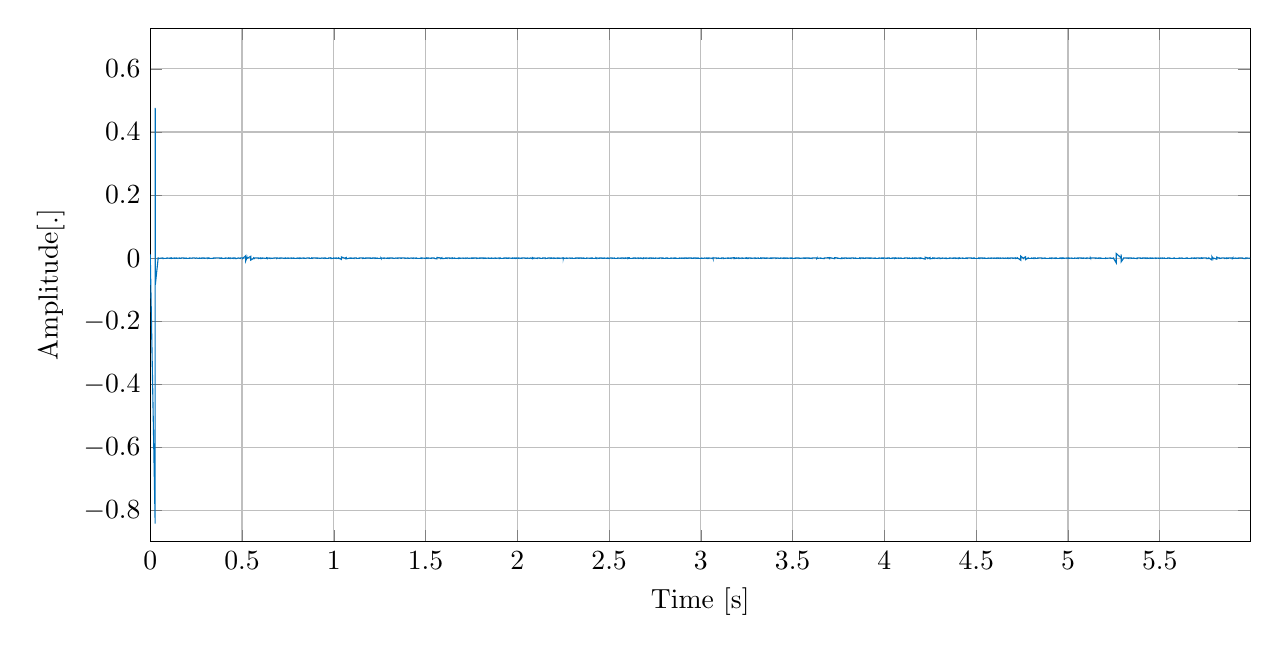
\begin{tikzpicture}

\begin{axis}[%
width=5.5in,
height=2.566in,
at={(1.011in,0.642in)},
scale only axis,
xmin=0,
xmax=5.99308755760369,
xlabel={Time [s]},
xmajorgrids,
ymin=-0.897959183673469,
ymax=0.728862973760933,
ylabel={Amplitude[.]},
ymajorgrids,
axis background/.style={fill=white}
]
\addplot [color=mycolor1,solid,forget plot]
  table[row sep=crcr]{%
2.08333333333333e-05	0.0122538023811748\\
4.16666666666667e-05	-0.0122397274343161\\
6.25e-05	0.0122593985372766\\
0.0268333333333333	-0.841044360454059\\
0.0270208333333333	0.476700841079922\\
0.0276875	0.0743041974628074\\
0.0277708333333333	-0.0842757999528343\\
0.0433333333333333	0.000734689239610419\\
0.0484375	-0.000771147443083658\\
0.068875	0.000871287345213359\\
0.0688958333333333	-0.000914196092068224\\
0.0693958333333333	0.000928116415306673\\
0.0694166666666667	-0.000965228500811473\\
0.0903125	-0.000668652355357153\\
0.0903333333333333	0.000716561090696644\\
0.108166666666667	-0.000493719891106833\\
0.1081875	0.000475264231382342\\
0.114875	0.00100715625962862\\
0.114895833333333	-0.000999706659119178\\
0.13225	0.000670886085256791\\
0.132270833333333	-0.000624125121802932\\
0.1425	0.000574814918345522\\
0.142520833333333	-0.000583128240947472\\
0.158833333333333	0.000578383382299989\\
0.158854166666667	-0.00058200843939012\\
0.168583333333333	-0.000796135526744322\\
0.168604166666667	0.000854760717857374\\
0.183333333333333	0.000748333649329287\\
0.183354166666667	-0.000771497113929529\\
0.1950625	0.000471377160620318\\
0.195083333333333	-0.000617347630158107\\
0.214020833333333	-0.000458421389332424\\
0.214041666666667	0.000694569300872006\\
0.228145833333333	-0.000321552367186984\\
0.229770833333333	0.000907965360966202\\
0.2415	0.000687441835776411\\
0.246208333333333	-0.000392185237250202\\
0.251229166666667	0.000675515516905658\\
0.2610625	-0.000577220917773221\\
0.2685	-0.000607199679195012\\
0.268520833333333	0.000521921896596942\\
0.281	-0.000629137056294877\\
0.281020833333333	0.000657955601166255\\
0.293145833333333	0.000756671588131565\\
0.293166666666667	-0.000644608113382317\\
0.314083333333333	0.000851585577721784\\
0.314104166666667	-0.000739522692164605\\
0.3189375	0.000701479688836363\\
0.318958333333333	-0.000608184931990221\\
0.343854166666667	-0.000469067729444319\\
0.343875	0.000540619530244008\\
0.359041666666667	0.00070804168567296\\
0.3590625	-0.00062391774133284\\
0.3590625	-0.00062391774133284\\
0.359083333333333	0.000710543233890295\\
0.379979166666667	0.000726972441766158\\
0.38	-0.000628724698251465\\
0.388145833333333	0.000648282834173138\\
0.388166666666667	-0.000581854167711955\\
0.409666666666667	-0.000715788312106095\\
0.4096875	0.000855415315301935\\
0.427041666666667	-0.0007138693756773\\
0.4270625	0.000886976677335082\\
0.435208333333333	-0.000671228085502771\\
0.435229166666667	0.000733267265160009\\
0.4515	-0.000881769399678669\\
0.451520833333333	0.000611926340533385\\
0.462375	0.000741565781746908\\
0.462395833333333	-0.00109511905846186\\
0.470875	-0.000920097380037188\\
0.480270833333333	0.000647822687282457\\
0.490854166666667	-0.000812313182615881\\
0.490875	0.00081359586338086\\
0.504166666666667	0.000835832815158442\\
0.5041875	-0.000815314331846972\\
0.520604166666667	0.00822072297498398\\
0.520625	-0.00818086639966468\\
0.526708333333333	0.000784549270936717\\
0.526729166666667	-0.000894162691183173\\
0.5475	0.00587330272890362\\
0.547520833333333	-0.00602184946367332\\
0.563875	-0.00070146311862383\\
0.563895833333333	0.000588540426628599\\
0.5674375	-0.000798263599985336\\
0.567458333333333	0.000687619250579479\\
0.589958333333333	0.00087752808076088\\
0.589979166666667	-0.00102877078582693\\
0.602208333333333	0.000888820032753768\\
0.602229166666667	-0.00104728830047565\\
0.611916666666667	-0.000676649263279144\\
0.6119375	0.000531712657531355\\
0.634416666666667	-0.000934590812104117\\
0.6344375	0.000717503098485721\\
0.638583333333333	-0.00113969461569427\\
0.638604166666667	0.000901226971934011\\
0.6523125	-0.000708696519994537\\
0.652333333333333	0.000428557945956786\\
0.664520833333333	-0.000618338605138116\\
0.674791666666667	0.000567181247364444\\
0.689125	0.00100446755794463\\
0.689145833333333	-0.000874971724965771\\
0.6935	0.000589542799664863\\
0.703354166666667	-0.00047541316588529\\
0.706	-0.000760539803934322\\
0.706020833333333	0.000822549798370906\\
0.71875	0.000474509477181315\\
0.728458333333333	-0.000548142363326956\\
0.736208333333333	0.000699627917352065\\
0.736229166666667	-0.000782275295664827\\
0.750333333333333	0.000603998195855303\\
0.750354166666667	-0.00064075007443739\\
0.769666666666667	0.00068274593716341\\
0.7696875	-0.000641766005538712\\
0.782083333333333	0.000631237777368386\\
0.782104166666667	-0.000585407136095528\\
0.8	-0.0005806766342212\\
0.800020833333333	0.000632825946402111\\
0.811645833333333	-0.000662631555343653\\
0.811666666666667	0.000736471452190856\\
0.81575	0.000764380631130795\\
0.815770833333333	-0.000677733090643042\\
0.8379375	0.000873749227459805\\
0.837958333333333	-0.000762411929489834\\
0.845958333333333	-0.000621186143946013\\
0.85475	0.000749261576196068\\
0.866520833333333	0.000744625396833765\\
0.866541666666667	-0.000515932288010471\\
0.879104166666667	-0.000500943137503569\\
0.879125	0.000765251809666935\\
0.884875	-0.000520656691743884\\
0.884895833333333	0.000768782062408757\\
0.909833333333333	0.000628701812429428\\
0.909854166666667	-0.000570530978576899\\
0.9115	-0.000516818782755884\\
0.911520833333333	0.000556152248207315\\
0.928145833333333	-0.000652874500685887\\
0.934458333333333	0.000659734514753571\\
0.947083333333333	-0.000651538854114526\\
0.947104166666667	0.000746809168655069\\
0.955270833333333	0.000898496033033306\\
0.955291666666667	-0.000764179916232177\\
0.972104166666667	-0.000679279919726632\\
0.972125	0.000809560743173024\\
0.983979166666667	0.0012055916996432\\
0.984	-0.00109974306536854\\
0.999208333333333	-0.000694008147097675\\
0.999229166666667	0.000759993838399656\\
1.0125	-0.000825537425783976\\
1.01252083333333	0.000882635834049446\\
1.0263125	-0.000805976666574922\\
1.02633333333333	0.000859801923651885\\
1.04114583333333	-0.00393542624757928\\
1.04116666666667	0.00393253747706633\\
1.0620625	-0.000723496197663128\\
1.06208333333333	0.000719551399152045\\
1.0680625	0.00215189380845473\\
1.06808333333333	-0.00217003853445217\\
1.08914583333333	0.000633367195619446\\
1.08916666666667	-0.000733655751765525\\
1.09577083333333	-0.000659102777126713\\
1.09579166666667	0.000528602996433345\\
1.11110416666667	-0.00103910627893571\\
1.111125	0.000862286729664806\\
1.12289583333333	0.000739728489954901\\
1.12291666666667	-0.000885722160197164\\
1.1386875	-0.000760492616674059\\
1.13870833333333	0.000695767274970514\\
1.156	0.000820539452797478\\
1.15710416666667	-0.000846867625649995\\
1.16285416666667	0.000736019944611489\\
1.162875	-0.000767126368236282\\
1.173875	-0.000610307732106338\\
1.17389583333333	0.000527717075806225\\
1.19952083333333	0.000715322773740613\\
1.19954166666667	-0.000866709518920433\\
1.20922916666667	-0.00080000363865872\\
1.20925	0.000651740263185364\\
1.2260625	0.000600358327003889\\
1.22608333333333	-0.000736005278273972\\
1.23566666666667	0.000509204353150653\\
1.2356875	-0.000637735228231537\\
1.2561875	-0.00077576017252754\\
1.25620833333333	0.000654464112091331\\
1.25783333333333	-0.000921606283623218\\
1.25785416666667	0.000806931748759692\\
1.27364583333333	-0.000710992913914008\\
1.27366666666667	0.000597042540241103\\
1.29514583333333	-0.000726383582064565\\
1.29516666666667	0.000632590487967683\\
1.30270833333333	-0.000639031198114883\\
1.30272916666667	0.000562847453128214\\
1.321625	0.000755508628156429\\
1.32164583333333	-0.000759150575953867\\
1.33177083333333	-0.000610710125880581\\
1.33795833333333	0.000664683177763139\\
1.34827083333333	-0.000610309911779344\\
1.34829166666667	0.00066859988107635\\
1.36597916666667	0.000775412382380437\\
1.366	-0.000770812016338518\\
1.36760416666667	-0.000760863747782761\\
1.367625	0.000753433481770169\\
1.387125	0.000727227381035258\\
1.38714583333333	-0.00075355261150647\\
1.40541666666667	0.00079868572730456\\
1.4054375	-0.000757006390694345\\
1.41116666666667	-0.000475940761235983\\
1.42166666666667	0.000561245536972261\\
1.4320625	-0.000700759812842404\\
1.43208333333333	0.000809106765515453\\
1.44875	-0.000579986138358643\\
1.44877083333333	0.000695936804143681\\
1.450375	0.00082932710740398\\
1.45039583333333	-0.000723178834510282\\
1.47585416666667	-0.000796756664477162\\
1.475875	0.000931314814875718\\
1.47897916666667	-0.00045624620636756\\
1.479	0.000591956862403049\\
1.5045625	-0.000799015220339862\\
1.50458333333333	0.000949854281251891\\
1.51252083333333	-0.000664111312568434\\
1.51254166666667	0.000807644895781415\\
1.532625	-0.000768292124469755\\
1.53264583333333	0.000901104456422554\\
1.53310416666667	-0.000780272771386461\\
1.533125	0.000910140329649984\\
1.54689583333333	0.00089842336836591\\
1.54691666666667	-0.000807657270372154\\
1.56166666666667	-0.00228936811688119\\
1.5616875	0.00235494088395583\\
1.58264583333333	0.000690474438946419\\
1.58266666666667	-0.00064927012008327\\
1.58858333333333	0.00144116184680155\\
1.58860416666667	-0.00139624873803248\\
1.6106875	-0.000602387446140836\\
1.61070833333333	0.000702319169406948\\
1.6169375	-0.000679845477897681\\
1.61695833333333	0.000779159653226463\\
1.631125	0.00084470636459848\\
1.63114583333333	-0.000770625848906314\\
1.645625	0.000932076093600797\\
1.64564583333333	-0.000920772984705366\\
1.65822916666667	0.000603452248383813\\
1.65825	-0.000611727050144646\\
1.67922916666667	-0.000916096471897362\\
1.67925	0.000885032614596713\\
1.68497916666667	0.00060681956090826\\
1.685	-0.000632573469011195\\
1.7041875	0.000489471868758358\\
1.70533333333333	-0.000553209136887921\\
1.7195625	0.000584640252581633\\
1.71958333333333	-0.000659832986771201\\
1.72972916666667	0.000676608720987426\\
1.73304166666667	-0.000772017726683305\\
1.7514375	0.000572509405293118\\
1.75145833333333	-0.000685180087054376\\
1.75897916666667	-0.000651868924147599\\
1.759	0.000535588981038542\\
1.77841666666667	0.00078712559790062\\
1.7784375	-0.000885535821845007\\
1.79366666666667	0.000554841061057088\\
1.7936875	-0.000623313394037457\\
1.79620833333333	-0.000631227199885162\\
1.79622916666667	0.00055884438102004\\
1.81525	0.000686508355469422\\
1.81527083333333	-0.000766278690899993\\
1.8228125	0.000579422816118477\\
1.82283333333333	-0.000677834362675808\\
1.84427083333333	0.000643300891206201\\
1.84429166666667	-0.000775353175171843\\
1.8579375	-0.000858996246789848\\
1.85795833333333	0.000730393986205559\\
1.86995833333333	-0.000739132662331362\\
1.8779375	0.000631655792580372\\
1.88010416666667	0.000623229945723398\\
1.880125	-0.000705783086237455\\
1.902875	0.000677694598848809\\
1.90289583333333	-0.000740440761131436\\
1.9065625	0.000648523516880695\\
1.90658333333333	-0.000699888085700352\\
1.92664583333333	-0.000706076369662584\\
1.92666666666667	0.0006684858258758\\
1.9423125	0.000672432546327812\\
1.94233333333333	-0.000686311156506293\\
1.95158333333333	-0.000834953634071659\\
1.95160416666667	0.000828193460366693\\
1.97452083333333	-0.000754893870521019\\
1.97454166666667	0.000786453720274723\\
1.9876875	-0.000846514791097456\\
1.98770833333333	0.000886916911740398\\
1.99645833333333	-0.000701588697114327\\
1.99647916666667	0.000746318285286581\\
2.00779166666667	-0.000558849834990225\\
2.0078125	0.000590125423864868\\
2.025125	-0.000815720302488596\\
2.02514583333333	0.000844126045707384\\
2.04247916666667	0.000818452430879792\\
2.0425	-0.000783593524856645\\
2.05322916666667	-0.000786064139855268\\
2.05325	0.000844790986028791\\
2.067	-0.000696646175408123\\
2.0711875	0.000797998908082457\\
2.08222916666667	-0.00170835215850821\\
2.08225	0.00181800349637685\\
2.08897916666667	-0.00070426032922555\\
2.089	0.000817721501039317\\
2.10960416666667	-0.000887554896070543\\
2.109625	0.00098931975872573\\
2.1231875	0.000642145728899372\\
2.12320833333333	-0.000542059782624433\\
2.13858333333333	-0.000673105136053546\\
2.13860416666667	0.000767839514714118\\
2.15225	0.00100009406106331\\
2.15227083333333	-0.000897420938249411\\
2.16620833333333	-0.000879091551548042\\
2.16622916666667	0.000969862066757164\\
2.17835416666667	0.000701695518543768\\
2.178375	-0.000625295106870151\\
2.18560416666667	0.000669128807558755\\
2.185625	-0.000607115382717358\\
2.19877083333333	0.00089629841071348\\
2.19879166666667	-0.00084888052857303\\
2.21875	0.00055932231801871\\
2.21877083333333	-0.000525486858424834\\
2.22579166666667	0.000509710916413454\\
2.2258125	-0.000487448806451855\\
2.25041666666667	0.000685083049406073\\
2.2504375	-0.00064789802720805\\
2.2509375	0.000696644660514428\\
2.25460416666667	-0.000661425172080484\\
2.26827083333333	0.000558762736287494\\
2.26829166666667	-0.000530584893220879\\
2.28760416666667	0.000584272371277117\\
2.28975	-0.000597897126661749\\
2.29845833333333	0.000715010014234861\\
2.29847916666667	-0.000749592132255716\\
2.31685416666667	-0.000707700601301887\\
2.316875	0.000646739557304433\\
2.3336875	0.000574438500792702\\
2.33370833333333	-0.000645200711072129\\
2.33583333333333	-0.000709060329132497\\
2.33585416666667	0.000642236545061064\\
2.35141666666667	0.000496685590389209\\
2.3514375	-0.000571782474732014\\
2.36166666666667	0.000664424266928079\\
2.3616875	-0.0007407929527549\\
2.3775	-0.000697831488081611\\
2.37752083333333	0.00061367347839209\\
2.40064583333333	-0.000752869714596988\\
2.40066666666667	0.000660121130953765\\
2.40822916666667	0.000781907509805732\\
2.40825	-0.000865505279331412\\
2.42879166666667	-0.000847229258199964\\
2.4288125	0.000772611259163829\\
2.431875	-0.000724781701442215\\
2.43189583333333	0.000648673424721907\\
2.44664583333333	-0.000645719025163827\\
2.44666666666667	0.000580067767031436\\
2.4623125	0.000594903480946001\\
2.46233333333333	-0.000666296694267746\\
2.47210416666667	-0.000809085647211153\\
2.472125	0.000721916217464159\\
2.49352083333333	-0.000865582526912647\\
2.49354166666667	0.000779107466304316\\
2.50085416666667	-0.000794926340932463\\
2.507875	0.000705151667197973\\
2.51652083333333	0.000679929720170458\\
2.51654166666667	-0.000744098538709615\\
2.52833333333333	0.000624332674507611\\
2.52835416666667	-0.000673275434336211\\
2.54625	-0.000867236775486297\\
2.54627083333333	0.000845717236411271\\
2.5651875	-0.000767449765396163\\
2.56520833333333	0.00076742057442274\\
2.57641666666667	0.000874488886027037\\
2.5764375	-0.000856032962981566\\
2.58697916666667	0.00076178411008069\\
2.587	-0.000743622792577481\\
2.60277083333333	0.0013136548163217\\
2.60279166666667	-0.00128702744801207\\
2.61008333333333	0.000723062776409405\\
2.61010416666667	-0.000686637079158903\\
2.63120833333333	-0.000667940116237091\\
2.63122916666667	0.00072297590903901\\
2.6433125	0.000603391804908914\\
2.64333333333333	-0.000544871642235419\\
2.66033333333333	0.000849026176098303\\
2.66035416666667	-0.000791214762677021\\
2.67277083333333	0.000873744089667305\\
2.67279166666667	-0.000812681429121931\\
2.68677083333333	-0.000987770802047832\\
2.68679166666667	0.0010579915195515\\
2.7005	-0.000742347821986829\\
2.70052083333333	0.000829880731885427\\
2.71979166666667	-0.000660118679685859\\
2.7198125	0.000763839850484412\\
2.72975	0.000769967202678459\\
2.72977083333333	-0.000666924355320421\\
2.73991666666667	0.000736224068886616\\
2.7399375	-0.000634533649016969\\
2.75166666666667	-0.000521447060906492\\
2.7516875	0.000608439351009449\\
2.7736875	-0.00069398230122133\\
2.77370833333333	0.000757529755137674\\
2.7873125	0.000694869320131796\\
2.78733333333333	-0.000640350362539444\\
2.79252083333333	0.000544452900313078\\
2.79254166666667	-0.000489515434912369\\
2.80927083333333	-0.00053202504677721\\
2.80929166666667	0.000585365552618237\\
2.8185	0.0007117807501467\\
2.81852083333333	-0.00066873998959899\\
2.83745833333333	-0.000547996804249562\\
2.83747916666667	0.000584916772793463\\
2.85470833333333	-0.000522189585135935\\
2.85472916666667	0.000535459252196795\\
2.86297916666667	0.000514572771121788\\
2.863	-0.000509678771410704\\
2.88333333333333	-0.000648689004081701\\
2.88335416666667	0.000639502488596472\\
2.89658333333333	-0.000574527441827736\\
2.89660416666667	0.000567838688742371\\
2.9084375	-0.00072373763542157\\
2.90845833333333	0.000703685111789378\\
2.9213125	0.000593438658275415\\
2.92133333333333	-0.00061955320266765\\
2.929375	-0.000656304619727487\\
2.92939583333333	0.000622184806303372\\
2.949375	0.000639722816665727\\
2.94939583333333	-0.000705584805944201\\
2.959875	-0.000549923607914802\\
2.95989583333333	0.000472236025612762\\
2.973875	0.000653679995461469\\
2.97389583333333	-0.000742293052122019\\
2.98452083333333	0.00072314274714479\\
2.98454166666667	-0.000804526234277354\\
3.00352083333333	-0.000537754384259843\\
3.00354166666667	0.000456582338249342\\
3.014125	-0.000776888537815397\\
3.01922916666667	0.000695478780294685\\
3.03310416666667	-0.00074095870606345\\
3.033125	0.000660049322515139\\
3.04175	-0.000751482662233543\\
3.04177083333333	0.000665545496823237\\
3.06472916666667	-0.000470515262636881\\
3.065625	0.000444291580824562\\
3.06633333333333	-0.000892892655786363\\
3.06635416666667	0.000809471705858813\\
3.08572916666667	0.000703933075321743\\
3.08575	-0.000771050863182079\\
3.09702083333333	0.000685150266846324\\
3.09704166666667	-0.000747358011513531\\
3.11233333333333	-0.00089213483687142\\
3.11235416666667	0.00083863795034053\\
3.12333333333333	0.00101914268363973\\
3.12335416666667	-0.001077580218926\\
3.14541666666667	0.000554501900173562\\
3.1454375	-0.000603462502242331\\
3.14977083333333	-0.00076453157616034\\
3.14979166666667	0.000713659167342908\\
3.16389583333333	-0.000850869040297808\\
3.16391666666667	0.000819295448782314\\
3.18158333333333	0.00135549330856276\\
3.18160416666667	-0.00135321053177325\\
3.19177083333333	0.000727219974764654\\
3.19179166666667	-0.000710574628151551\\
3.20735416666667	0.00124612956147805\\
3.207375	-0.00121470537273457\\
3.22472916666667	0.000830672088752873\\
3.22475	-0.000795961536435125\\
3.24466666666667	0.000641663930231659\\
3.2446875	-0.000587058566500264\\
3.2515	-0.000927682152513045\\
3.25152083333333	0.000981527381112092\\
3.25997916666667	-0.000749624117858614\\
3.26	0.000815721671905278\\
3.27277083333333	0.000775189438798031\\
3.27279166666667	-0.0007024482451306\\
3.29635416666667	0.000864724576605581\\
3.296375	-0.000788095676280746\\
3.313125	0.000669339837449391\\
3.31314583333333	-0.000592315020425472\\
3.32535416666667	-0.000508506520697274\\
3.325375	0.000598843542910724\\
3.32991666666667	-0.000504742683764233\\
3.3299375	0.000589990414134015\\
3.34779166666667	0.000637202361540035\\
3.3478125	-0.000542090937324429\\
3.3575	-0.000568184770277761\\
3.35752083333333	0.000672998675066125\\
3.38095833333333	-0.000474777068158243\\
3.38097916666667	0.000567342640984112\\
3.38560416666667	-0.000530464288802622\\
3.385625	0.000624953700409804\\
3.40904166666667	0.000776727981003045\\
3.4090625	-0.000710595589808062\\
3.42029166666667	0.000746100687701466\\
3.42439583333333	-0.000689148528298087\\
3.43316666666667	-0.000819042916010755\\
3.4331875	0.000861379861680038\\
3.4499375	-0.000647694329668308\\
3.44995833333333	0.000688991295399136\\
3.45920833333333	0.000569038012327066\\
3.45922916666667	-0.000534202302468729\\
3.4699375	0.000729467217168986\\
3.46995833333333	-0.000705060848936256\\
3.488875	0.000629868945102908\\
3.48889583333333	-0.000623813081961381\\
3.4955625	0.000803080730868091\\
3.49558333333333	-0.000810816898637587\\
3.514	-0.000419473843262285\\
3.51402083333333	0.000402425331291254\\
3.53510416666667	0.000782860926028073\\
3.535125	-0.000829844536800619\\
3.53514583333333	0.000810817070005341\\
3.53516666666667	-0.0008344592878688\\
3.56233333333333	0.000740713969418412\\
3.56235416666667	-0.000806206226934828\\
3.56952083333333	-0.00071871408861111\\
3.56954166666667	0.000656455813702043\\
3.5894375	0.000601387103124408\\
3.58945833333333	-0.000688164473721435\\
3.59214583333333	-0.000521002002766059\\
3.59216666666667	0.000424870977466098\\
3.60627083333333	-0.0010884381961116\\
3.60629166666667	0.000992606800091719\\
3.63075	0.000673312633295481\\
3.63077083333333	-0.000771650492053558\\
3.632875	0.000796060212640286\\
3.63289583333333	-0.000894288213147536\\
3.65285416666667	0.000750320197465302\\
3.652875	-0.000847063418056259\\
3.67285416666667	-0.000933141726971411\\
3.672875	0.000839301568977933\\
3.673375	-0.000827967980561113\\
3.67339583333333	0.000729373704252723\\
3.7008125	0.00149235214502603\\
3.70083333333333	-0.00166836350238167\\
3.70152083333333	-0.0018759763831977\\
3.70154166666667	0.00178584267808272\\
3.7279375	-0.00156669426518658\\
3.72795833333333	0.00148410316077901\\
3.72854166666667	-0.00168255484815004\\
3.7285625	0.00161312956027256\\
3.7458125	0.00078193297440681\\
3.74583333333333	-0.000841652983050695\\
3.76877083333333	-0.000951158895009949\\
3.76879166666667	0.000902192537464957\\
3.7805	-0.000870623201476591\\
3.78052083333333	0.000842427265769237\\
3.793375	0.000692445735071341\\
3.79339583333333	-0.00070824668075357\\
3.8080625	0.000616938829242782\\
3.80808333333333	-0.000620344936868163\\
3.81689583333333	-0.000911378891083477\\
3.81691666666667	0.000928784287740468\\
3.832125	0.000649782435139187\\
3.83214583333333	-0.00062575566892542\\
3.84341666666667	0.000580234098243344\\
3.8434375	-0.000542820670958007\\
3.8648125	-0.000579867099639341\\
3.86483333333333	0.000637976697022658\\
3.8689375	-0.000633499816894192\\
3.86895833333333	0.00069305836828903\\
3.88477083333333	0.000644550367696489\\
3.88479166666667	-0.000577933171632154\\
3.8954375	-0.00066287978056014\\
3.89545833333333	0.000729988238619403\\
3.91647916666667	0.000601699265337787\\
3.9165	-0.000527200903257703\\
3.9239375	-0.000627986975583194\\
3.92395833333333	0.000705607698588085\\
3.94908333333333	-0.000619410687957292\\
3.94910416666667	0.000711529833267491\\
3.94958333333333	0.000768823629595509\\
3.94960416666667	-0.00068197184847231\\
3.97002083333333	-0.000636965813764758\\
3.97004166666667	0.000728822420202642\\
3.987875	-0.00057938225423229\\
3.98789583333333	0.00066778784981798\\
3.99404166666667	-0.000668186711203397\\
3.9940625	0.000757667910339742\\
4.01610416666667	-0.000683927060194245\\
4.016125	0.000759061468281206\\
4.02620833333333	0.000690829316251285\\
4.02622916666667	-0.000622418547535604\\
4.04204166666667	-0.000457760739397958\\
4.0420625	0.000524185778382851\\
4.0563125	0.00071208914465086\\
4.05633333333333	-0.000673662759596049\\
4.06047916666667	0.000664937719744489\\
4.0605	-0.000620427354540002\\
4.07733333333333	0.000671089574534653\\
4.07735416666667	-0.000639678631543796\\
4.09014583333333	0.000694536514818172\\
4.09016666666667	-0.000672305319064109\\
4.10954166666667	-0.000670962727712327\\
4.1095625	0.000679358321532598\\
4.12633333333333	0.000766643967531233\\
4.12635416666667	-0.000767709199301905\\
4.13658333333333	0.000480789566442453\\
4.13660416666667	-0.000492889757098431\\
4.1529375	-0.000871250296090936\\
4.15295833333333	0.000842243228932475\\
4.16439583333333	-0.000815416077056576\\
4.16441666666667	0.000780047338326749\\
4.172375	0.000727694450945087\\
4.17239583333333	-0.000761118488113997\\
4.1934375	0.00100939700417115\\
4.19345833333333	-0.00105751794332657\\
4.19845833333333	-0.000799533055506864\\
4.19847916666667	0.000729405458463086\\
4.222125	-0.00316645728084482\\
4.22214583333333	0.00309847988158742\\
4.23614583333333	0.000783659063442438\\
4.23616666666667	-0.000854904962278722\\
4.24852083333333	0.00207072571064826\\
4.24854166666667	-0.00214172149943263\\
4.26227083333333	-0.000868799980255136\\
4.26229166666667	0.000787701525948726\\
4.27	-0.000833573460908086\\
4.27002083333333	0.000751938517770686\\
4.29097916666667	-0.00101151350778446\\
4.291	0.000940940162504793\\
4.30216666666667	0.00103013261886231\\
4.3021875	-0.0010881983414522\\
4.31439583333333	-0.000690566554329529\\
4.31441666666667	0.000636813859485653\\
4.33477083333333	-0.000857145812746723\\
4.33479166666667	0.000818091484720377\\
4.3364375	0.000923032419635397\\
4.33645833333333	-0.000968577237014383\\
4.3543125	-0.000752860269700285\\
4.35433333333333	0.000715336140258785\\
4.376125	-0.000594287455589043\\
4.37614583333333	0.00056193234529366\\
4.38791666666667	0.000727992790300719\\
4.3879375	-0.0007558411202433\\
4.40341666666667	0.000561675104748859\\
4.4034375	-0.000575056459496602\\
4.4069375	0.000747687864187593\\
4.40695833333333	-0.000755022539738558\\
4.42679166666667	0.000573333512602289\\
4.4268125	-0.000561447241616433\\
4.44502083333333	-0.000596895249178401\\
4.44504166666667	0.000630004888908778\\
4.4513125	-0.000686271499428727\\
4.45133333333333	0.000723672289070652\\
4.473875	0.000731676901106292\\
4.47389583333333	-0.000685316941159171\\
4.48310416666667	-0.000800497827443301\\
4.483125	0.000850253290490356\\
4.49008333333333	0.000635303781067878\\
4.49010416666667	-0.000591582094904115\\
4.5146875	-0.000657910663474233\\
4.51470833333333	0.000713508582602995\\
4.5178125	-0.000467420432399924\\
4.51783333333333	0.000529998770134142\\
4.53616666666667	0.000708749282095999\\
4.5361875	-0.000653132504091235\\
4.546375	0.000686825642058495\\
4.54639583333333	-0.000623807716686843\\
4.56472916666667	-0.000493878179964804\\
4.56475	0.000552721080581092\\
4.58110416666667	-0.000698684485425761\\
4.581125	0.000755845224672406\\
4.597875	-0.000523546352566346\\
4.59789583333333	0.000582719675040393\\
4.61072916666667	-0.000684166815783074\\
4.61075	0.000750035787138153\\
4.62047916666667	0.000461526421507547\\
4.6205	-0.000393504679770596\\
4.63125	0.000689880271579905\\
4.63127083333333	-0.000627134430238102\\
4.6469375	0.000749800910275345\\
4.64747916666667	-0.000711561864938089\\
4.65729166666667	-0.000538498730920764\\
4.6573125	0.000565783292646204\\
4.6730625	-0.000784713881450174\\
4.67308333333333	0.000792956249443993\\
4.685	-0.000873473932540675\\
4.68502083333333	0.000874898492932472\\
4.70010416666667	0.0005923526347921\\
4.700125	-0.000581344946413087\\
4.71395833333333	0.000983417764375153\\
4.71397916666667	-0.000972633807776415\\
4.72514583333333	-0.000737518076082976\\
4.72516666666667	0.000732984068388039\\
4.74272916666667	-0.00658835799905934\\
4.74275	0.0065791314772882\\
4.75785416666667	-0.00080576226705523\\
4.757875	0.000754522492115429\\
4.769125	0.00451271510550656\\
4.76914583333333	-0.00455955425912552\\
4.7828125	0.000841151801291296\\
4.78283333333333	-0.000883162785786139\\
4.80225	-0.000542022348083922\\
4.80227083333333	0.000506497659431693\\
4.81258333333333	-0.00103080184500524\\
4.81260416666667	0.000981202470474372\\
4.82164583333333	0.000836041697278347\\
4.82166666666667	-0.000894083793682192\\
4.835	-0.000593541002648692\\
4.83502083333333	0.000517426397680513\\
4.85804166666667	0.00101951812131046\\
4.8580625	-0.00111497893861662\\
4.86114583333333	-0.000666024034172112\\
4.874375	0.000586650966641702\\
4.87485416666667	0.000627148536093521\\
4.874875	-0.000690120729408816\\
4.90141666666667	-0.000662423929509586\\
4.9014375	0.000626485663808014\\
4.91066666666667	-0.000908889302861698\\
4.9106875	0.000857032640269196\\
4.92964583333333	-0.000747181442834044\\
4.92966666666667	0.000681657580528353\\
4.9371875	0.000565310389483618\\
4.93720833333333	-0.00063242421751897\\
4.956625	-0.00061542355479786\\
4.95664583333333	0.000573606460348106\\
4.96560416666667	0.00063766839747109\\
4.965625	-0.000662713224025773\\
4.97133333333333	0.000745214404496924\\
4.97135416666667	-0.000758866225340087\\
4.995	0.000590014687296517\\
4.99502083333333	-0.000583280645372063\\
5.00316666666667	0.000701418648776317\\
5.0031875	-0.00070402617530778\\
5.02145833333333	0.000553307573277657\\
5.02147916666667	-0.000567183204744751\\
5.03477083333333	-0.000690601072429654\\
5.03575	0.000678652374369759\\
5.04810416666667	-0.000506221019121415\\
5.05089583333333	0.000530573037324425\\
5.05675	-0.000817011914210647\\
5.05677083333333	0.000855451456269155\\
5.07566666666667	0.000531083650983497\\
5.0756875	-0.000455507170031002\\
5.08429166666667	-0.000529089638337644\\
5.0843125	0.000601649620225006\\
5.10170833333333	-0.000732123536239426\\
5.10172916666667	0.000793777125612496\\
5.1225625	-0.00061894893928467\\
5.12258333333333	0.000660243213372411\\
5.12377083333333	-0.00060812998544776\\
5.12379166666667	0.000643650784820187\\
5.15020833333333	0.000909723813840191\\
5.15022916666667	-0.000830905866725329\\
5.1513125	-0.000725569108061976\\
5.15133333333333	0.000804922919634336\\
5.16752083333333	-0.000706523310236849\\
5.16754166666667	0.000783430696085785\\
5.17839583333333	0.000529013849934631\\
5.17841666666667	-0.000434255288139971\\
5.20347916666667	-0.000887640180062974\\
5.20554166666667	0.000932310297848551\\
5.2060625	0.000780566962792512\\
5.20608333333333	-0.000745371954936459\\
5.23347916666667	0.000745461612568184\\
5.2335	-0.000697089071657755\\
5.2473125	-0.000853651687693003\\
5.24733333333333	0.000917898778024549\\
5.248375	0.000797872452458675\\
5.24839583333333	-0.000743686942838169\\
5.26310416666667	-0.0149618098355943\\
5.263125	0.0147405214393317\\
5.28883333333333	0.00115536141022913\\
5.28885416666667	-0.00122113863490467\\
5.28997916666667	0.0117808401421682\\
5.29	-0.0115208745606766\\
5.30291666666667	-0.000803939977406044\\
5.3029375	0.000795149632615833\\
5.32895833333333	0.00058336640180924\\
5.32897916666667	-0.000606478902792325\\
5.33210416666667	-0.000994408606210292\\
5.332125	0.000989817568788992\\
5.34497916666667	0.000696997906660684\\
5.345	-0.000707923083019498\\
5.35875	0.000517411316936819\\
5.35877083333333	-0.000531969705641809\\
5.37754166666667	-0.00106054193261786\\
5.3775625	0.00101593414191938\\
5.3949375	0.000636588080925689\\
5.39495833333333	-0.000709996154672059\\
5.405125	-0.000546237269207376\\
5.40514583333333	0.000477102900592582\\
5.42152083333333	0.000571777192126952\\
5.42154166666667	-0.000640227708637533\\
5.43129166666667	0.000875215507549028\\
5.4313125	-0.000926473105429979\\
5.4480625	0.000638692913570213\\
5.44808333333333	-0.000694003462087355\\
5.45775	0.000502955543632727\\
5.45777083333333	-0.000551097000205143\\
5.47833333333333	0.000574862269306865\\
5.47835416666667	-0.00064690238774901\\
5.4915	0.000529683031027361\\
5.49372916666667	-0.000618913150298244\\
5.50422916666667	0.000453330103516924\\
5.50425	-0.000531148342860655\\
5.51391666666667	0.000670917417854683\\
5.5139375	-0.000732130141137104\\
5.52533333333333	0.000600952735347802\\
5.52535416666667	-0.000652504403835572\\
5.5436875	-0.000735679849478919\\
5.54370833333333	0.000710721299353491\\
5.55427083333333	0.000793609768938327\\
5.55429166666667	-0.000815113052475865\\
5.57739583333333	-0.000807882112505996\\
5.57741666666667	0.000771452724174448\\
5.58002083333333	0.000817904553353734\\
5.58004166666667	-0.000849769649391773\\
5.60589583333333	-0.000583011985817421\\
5.60591666666667	0.000571564395622842\\
5.60804166666667	0.000554240622656337\\
5.6080625	-0.00058060839501004\\
5.62225	0.000811085833073755\\
5.62227083333333	-0.000816072912321638\\
5.64272916666667	-0.000612163267642167\\
5.64375	0.000650635062013345\\
5.650875	0.000649649219327914\\
5.65089583333333	-0.00060113537436008\\
5.671875	-0.000783975766054335\\
5.6719375	0.000805452068780832\\
5.68920833333333	-0.000663144542647274\\
5.68922916666667	0.000698125851068317\\
5.69785416666667	-0.000851824838492038\\
5.697875	0.000891547489277094\\
5.71425	0.000722969067958876\\
5.71427083333333	-0.000677021060788945\\
5.72610416666667	0.000936628653660575\\
5.726125	-0.000857062220265057\\
5.73404166666667	-0.000729934649359309\\
5.73410416666667	0.000789824527171175\\
5.75460416666667	0.00102125482339883\\
5.75466666666667	-0.00095568253293901\\
5.7673125	-0.000889781170721334\\
5.76733333333333	0.000942675078136838\\
5.78370833333333	-0.00554388749188475\\
5.78372916666667	0.00553064421889357\\
5.78989583333333	-0.000881210327161686\\
5.78995833333333	0.000889438244695447\\
5.81060416666667	-0.00328829714850285\\
5.810625	0.00334137932228787\\
5.826125	-0.000544935058844586\\
5.82614583333333	0.000620442609599313\\
5.83329166666667	-0.00064426274151791\\
5.8384375	0.000740222900762994\\
5.8515625	0.000978323092323193\\
5.85270833333333	-0.000938872987895347\\
5.8649375	0.000938884848248308\\
5.865	-0.000945659788768267\\
5.874125	-0.000740857813003309\\
5.874625	0.000760900429568342\\
5.89591666666667	0.00058253442222721\\
5.89597916666667	-0.000576819780098533\\
5.898125	0.00103763308512588\\
5.89814583333333	-0.00103980774970416\\
5.91485416666667	0.000659875217243964\\
5.91491666666667	-0.00062854034851054\\
5.92772916666667	-0.000626224951258898\\
5.92779166666667	0.000680388507480993\\
5.95133333333333	0.000979110276324151\\
5.95139583333333	-0.000946283252758377\\
5.9518125	0.000861942008608148\\
5.951875	-0.000869949490864557\\
5.9686875	-0.000995789762615092\\
5.96875	0.000894604049820107\\
5.99310416666667	-0.000359981548101127\\
};
\end{axis}
\end{tikzpicture}%
	\caption{Impulse response plot of the cancellation path see \autoref{CancellationPathImpulseResponseCrop} for zoomed in version.}
	\label{CancellationPathImpulseResponse}
\end{figure}


%\begin{figure}[H]
%	\centering
%	\includegraphics[width=0.85\textwidth]{CancellationPath_MATLAB_Figures/CancellationPathImpulseResponse.png}
%	\caption{Impulse Response plot of the cancellation path (NOT TIKZ).}
%	\label{CancellationPathImpulseResponse}
%\end{figure}

Converting the impulse response from magnitude to dB, gives the time decay which reveals the Signal to Noise Ratio (SNR) of the system, and from the read off SNR is found to be $\sim$ 60 dB SNR, as seen on \autoref{TimeDecayPlotCancellationPath}.

%\begin{figure}[H]
%	\centering
%	\includegraphics[width=0.85\textwidth]{CancellationPath_MATLAB_Figures/CancellationPathTimeDecay.png}
%	\caption{Time decay plot of the cancellation path (NOT TIKZ).}
%	\label{TimeDecayPlotCancellationPath}
%\end{figure}

\begin{figure}[H]
	\centering
	\tikzsetnextfilename{TimeDecayPlotCancellationPath1}
	%% This file was created by matlab2tikz.
%
%The latest updates can be retrieved from
%  http://www.mathworks.com/matlabcentral/fileexchange/22022-matlab2tikz-matlab2tikz
%where you can also make suggestions and rate matlab2tikz.
%
\definecolor{mycolor1}{rgb}{0.00000,0.44700,0.74100}%
\definecolor{mycolor2}{rgb}{0.85000,0.32500,0.09800}%
\definecolor{mycolor3}{rgb}{0.92900,0.69400,0.12500}%
\definecolor{mycolor4}{rgb}{0.49400,0.18400,0.55600}%
\definecolor{mycolor5}{rgb}{0.46600,0.67400,0.18800}%
%
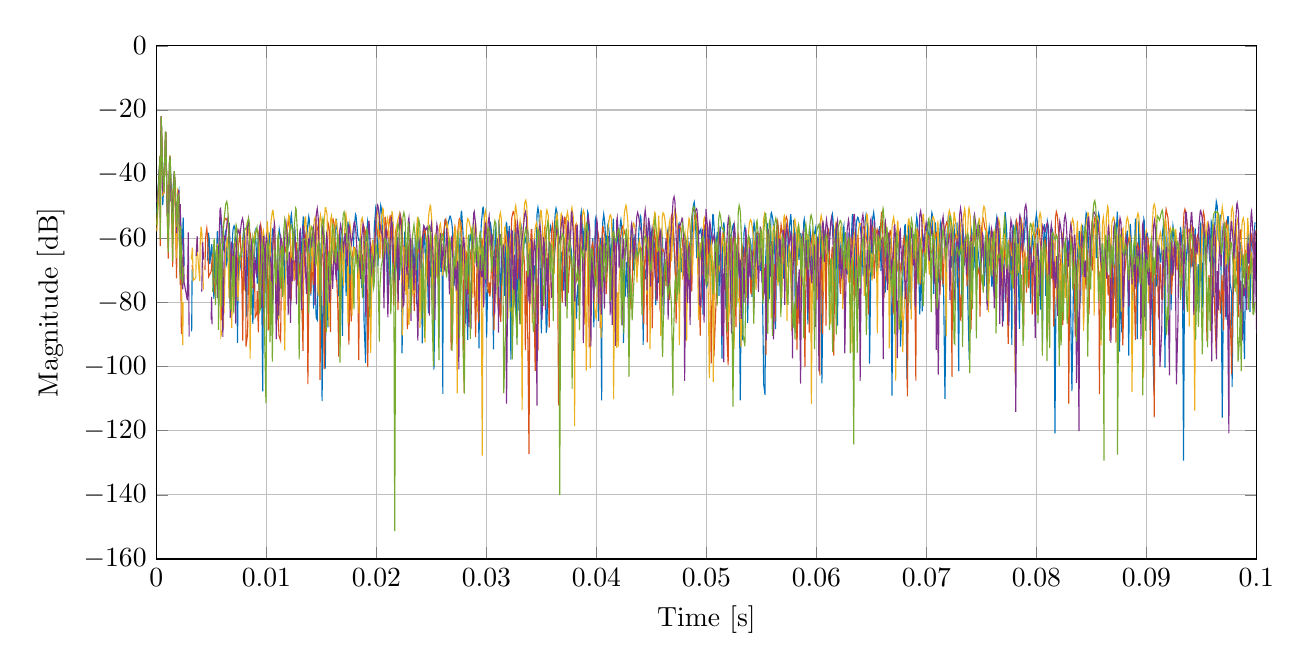
\begin{tikzpicture}

\begin{axis}[%
width=5.5in,
height=2.566in,
scaled x ticks = false,
x tick label style={/pgf/number format/fixed},
at={(1.414in,0.891in)},
scale only axis,
unbounded coords=jump,
xmin=0,
xmax=0.1,
xlabel={Time [s]},
xmajorgrids,
ymin=-160,
ymax=0,
ylabel={Magnitude [dB]},
ymajorgrids,
axis background/.style={fill=white},
title style={font=\bfseries},
%title={Time Decay}
]
\addplot [color=mycolor1,solid,forget plot]
  table[row sep=crcr]{%
2.08333333333333e-05	nan\\
4.16666666666667e-05	-52.111048310778\\
0.000166666666666667	-43.9740436319002\\
0.000333333333333333	-34.8177965827442\\
0.000354166666666667	-53.6190056426103\\
0.000354166666666667	-53.6190056426103\\
0.0004375	-21.9598363711386\\
0.0005625	-37.7606834431528\\
0.000583333333333333	-49.6288694056232\\
0.0006875	-42.2560543031998\\
0.000833333333333333	-27.0848645767238\\
0.000854166666666667	-27.0938121387821\\
0.000979166666666667	-49.8807436737733\\
0.00108333333333333	-59.9223441352537\\
0.0011875	-37.2201027543805\\
0.00125	-34.3291951406571\\
0.00135416666666667	-45.9757139957571\\
0.00147916666666667	-56.382911413555\\
0.00152083333333333	-43.9141776726352\\
0.00152083333333333	-43.9141776726352\\
0.001625	-40.042008410004\\
0.0016875	-43.2431355273656\\
0.00183333333333333	-60.9681241606569\\
0.00183333333333333	-60.9681241606569\\
0.0019375	-46.8693647146266\\
0.00204166666666667	-45.2221645426903\\
0.00214583333333333	-70.4535211157334\\
0.00216666666666667	-51.6149616670037\\
0.0023125	-64.165288874486\\
0.00235416666666667	-61.5511588605062\\
0.0024375	-53.565070295056\\
0.00252083333333333	-68.5064286025977\\
0.00252083333333333	-68.5064286025977\\
0.00266666666666667	nan\\
0.00266666666666667	nan\\
0.00289583333333333	-72.904642668182\\
0.00289583333333333	-72.904642668182\\
0.003	nan\\
0.003	nan\\
0.00320833333333333	-89.0396268578771\\
0.00325	-69.6670608974985\\
0.00333333333333333	nan\\
0.00333333333333333	nan\\
0.0035	nan\\
0.0035	nan\\
0.00364583333333333	nan\\
0.00364583333333333	nan\\
0.0038125	nan\\
0.0038125	nan\\
0.00397916666666667	nan\\
0.00397916666666667	nan\\
0.00414583333333333	nan\\
0.00414583333333333	nan\\
0.0043125	nan\\
0.0043125	nan\\
0.00464583333333333	-66.952070269611\\
0.00464583333333333	-66.952070269611\\
0.00464583333333333	-66.952070269611\\
0.00472916666666667	-58.2959288896312\\
0.0048125	-60.5931307267329\\
0.00485416666666667	-68.0794223724486\\
0.00504166666666667	-61.8026803688784\\
0.005125	-70.1443845224101\\
0.00522916666666667	-78.870829364037\\
0.0053125	-63.8012011510901\\
0.0053125	-63.8012011510901\\
0.00535416666666667	-68.5896659640424\\
0.00545833333333333	-65.4935549134102\\
0.00554166666666667	-57.7477179120546\\
0.00566666666666667	-81.2009260636828\\
0.00577083333333333	-55.761344442787\\
0.00585416666666667	-53.5416605882092\\
0.0059375	-56.2577357302003\\
0.00597916666666667	-58.9539415015357\\
0.00610416666666667	-63.8531451471768\\
0.00614583333333333	-61.9141009456243\\
0.00627083333333333	-58.0593839706459\\
0.0063125	-58.7413544861928\\
0.00639583333333333	-67.7841232832069\\
0.00645833333333333	-66.6166703808532\\
0.006625	-55.2300468372413\\
0.006625	-55.2300468372413\\
0.00679166666666667	-72.9096992394021\\
0.00679166666666667	-72.9096992394021\\
0.0069375	-58.638942876284\\
0.00697916666666667	-57.0690799271473\\
0.0070625	-56.1394046707133\\
0.00714583333333333	-57.1127041883519\\
0.00727083333333333	-63.1813781835223\\
0.00727083333333333	-63.1813781835223\\
0.007375	-92.5753078843969\\
0.00745833333333333	-66.4543104134224\\
0.0075	-65.1542648427286\\
0.00766666666666667	-68.9414396695225\\
0.00775	-66.3204732466916\\
0.00779166666666667	-63.6550975119697\\
0.00791666666666667	-57.8950515685413\\
0.00795833333333333	-57.4909363697214\\
0.00808333333333333	-61.4101564617352\\
0.008125	-65.014239665563\\
0.00820833333333333	-84.3913964822076\\
0.00827083333333333	-67.5401210436484\\
0.0084375	-60.6608842129059\\
0.0084375	-60.6608842129059\\
0.00860416666666667	-68.6525343731691\\
0.00860416666666667	-68.6525343731691\\
0.00877083333333333	-86.7182627693444\\
0.00877083333333333	-86.7182627693444\\
0.0089375	-58.3503996189966\\
0.00897916666666667	-57.7185064887609\\
0.0090625	-61.5893861763269\\
0.00916666666666666	-74.1626294665894\\
0.00925	-59.9425252546123\\
0.00925	-59.9425252546123\\
0.00939583333333333	-82.2414358792677\\
0.0094375	-63.5172219371502\\
0.00952083333333333	-57.7976918868999\\
0.00966666666666667	-107.69929084972\\
0.00975	-60.471146039021\\
0.00979166666666667	-59.0848073355518\\
0.00991666666666667	-66.2816899780258\\
0.00991666666666667	-66.2816899780258\\
0.01	-83.2384694993036\\
0.0100833333333333	-69.382102407305\\
0.01025	-58.1614130268561\\
0.01025	-58.1614130268561\\
0.0103958333333333	-78.659966600665\\
0.0104375	-64.3644685212\\
0.0105625	-57.2292963929618\\
0.0106041666666667	-57.4389958833188\\
0.0107291666666667	-61.1355190321544\\
0.0107708333333333	-62.6617442615444\\
0.0108958333333333	-69.2220796621684\\
0.011	-85.3991667784377\\
0.0110416666666667	-65.4866844897544\\
0.0110833333333333	-60.3538379061152\\
0.0111666666666667	-57.1711414785393\\
0.01125	-59.1262763800061\\
0.011375	-69.3559430679877\\
0.0114166666666667	-70.9746539468429\\
0.0115416666666667	-63.2971463445262\\
0.0115833333333333	-62.2681820493326\\
0.0117083333333333	-78.185870054493\\
0.0117291666666667	-74.8542861438093\\
0.0118958333333333	-59.1082812851507\\
0.0118958333333333	-59.1082812851507\\
0.0120208333333333	-62.3396384402111\\
0.0120625	-61.9079830499083\\
0.0122291666666667	-53.2761437613709\\
0.0122708333333333	-52.5028995257284\\
0.0123958333333333	-57.9490053815339\\
0.0124375	-67.097874268932\\
0.0125416666666667	-57.8292741595085\\
0.0125833333333333	-56.3942866017904\\
0.0127083333333333	-66.8628824569854\\
0.0127708333333333	-73.1233158076556\\
0.0128541666666667	-63.1193712248532\\
0.0128958333333333	-65.0422676184057\\
0.0129375	-72.4048294890819\\
0.0130833333333333	-66.3211400209195\\
0.013125	-71.8762952805217\\
0.0132291666666667	-59.9577490778633\\
0.0133541666666667	-53.4565553010462\\
0.0133958333333333	-53.7172714247254\\
0.0135208333333333	-59.7287434390187\\
0.0136041666666667	-63.951909199344\\
0.0136875	-59.7481136529985\\
0.0137291666666667	-56.884992279517\\
0.0138541666666667	-53.2243149389698\\
0.0138958333333333	-54.0305340746001\\
0.0140416666666667	-77.8746654022866\\
0.0140416666666667	-77.8746654022866\\
0.0141666666666667	-59.5576053975161\\
0.0142083333333333	-61.3140246411379\\
0.0142916666666667	-81.9411573286561\\
0.0143958333333333	-65.6135925586917\\
0.0145208333333333	-84.6872059910125\\
0.014625	-85.4407544579033\\
0.0146875	-74.1556791266814\\
0.0146875	-74.1556791266814\\
0.0148125	-61.5186789861121\\
0.0148541666666667	-61.603933867154\\
0.0150208333333333	-82.8897784221635\\
0.0150625	-110.772106438684\\
0.0151875	-72.3738220270998\\
0.0152291666666667	-70.4290235676362\\
0.0153541666666667	-100.606303182385\\
0.0153541666666667	-100.606303182385\\
0.0154583333333333	-72.1936353976885\\
0.0156041666666667	-87.7491540752639\\
0.0156875	-73.2013868076318\\
0.0157916666666667	-77.4373024400392\\
0.0158333333333333	-67.9974898177409\\
0.015875	-64.0529505129947\\
0.0159583333333333	-62.0225650940623\\
0.0160833333333333	-65.2961964560404\\
0.0161666666666667	-62.8831029470834\\
0.0161666666666667	-62.8831029470834\\
0.0163333333333333	-54.3557903914612\\
0.016375	-54.2032208365931\\
0.0165	-62.3646402761344\\
0.0165416666666667	-78.113175470613\\
0.0166458333333333	-58.8346612605774\\
0.0166875	-58.183753552355\\
0.0168125	-67.0010327931349\\
0.0169166666666667	-90.4436690986716\\
0.0169791666666667	-68.8442995675725\\
0.0170208333333333	-63.0786023797962\\
0.0171041666666667	-58.4773349959014\\
0.01725	-77.9505350758744\\
0.0173333333333333	-57.445562140132\\
0.0174166666666667	-54.8642361243766\\
0.0175	-58.1348941906922\\
0.0175	-58.1348941906922\\
0.0176041666666667	-81.2331799465362\\
0.0176875	-65.9063896475626\\
0.0178125	-69.9045452138529\\
0.0178541666666667	-68.2679254067739\\
0.0179791666666667	-56.6175168508517\\
0.0179791666666667	-56.6175168508517\\
0.0181041666666667	-52.5422477316158\\
0.0181458333333333	-52.8806272404262\\
0.0183125	-59.3176520761328\\
0.0183125	-59.3176520761328\\
0.0183958333333333	-60.5962203271359\\
0.0184791666666667	-60.3497039195296\\
0.0186041666666667	-69.1567240190393\\
0.0186666666666667	-75.5213852508567\\
0.01875	-65.0119785770231\\
0.0188333333333333	-69.891092188239\\
0.018875	-85.4855467125159\\
0.0190208333333333	-98.9033056569759\\
0.019125	-58.287911282984\\
0.0192083333333333	-54.732623030518\\
0.0192916666666667	-56.8444306984257\\
0.0193333333333333	-60.3684268716343\\
0.0194375	-84.5798414376857\\
0.0194791666666667	-79.599605229199\\
0.019625	-63.2791733275686\\
0.0197083333333333	-70.0795077494701\\
0.0197708333333333	-63.4095035805324\\
0.0198125	-56.362169900321\\
0.0199375	-50.7438037528893\\
0.0199791666666667	-51.6086095044044\\
0.0201041666666667	-62.884753710132\\
0.0201458333333333	-68.6491886999608\\
0.0202708333333333	-56.3246955012879\\
0.0203125	-52.7777742803338\\
0.0203958333333333	-49.7337890346514\\
0.0204791666666667	-51.1840995331472\\
0.0206041666666667	-63.5297545792679\\
0.0206875	-75.480095487511\\
0.0207708333333333	-63.1150361798449\\
0.0208125	-59.3571081508711\\
0.0208958333333333	-57.281628009858\\
0.0210208333333333	-79.6666740625991\\
0.021125	-59.7053926135665\\
0.021125	-59.7053926135665\\
0.02125	-74.6074415490915\\
0.0213125	-61.1963391171394\\
0.0214375	-54.9555009504599\\
0.0214791666666667	-56.2835768296612\\
0.0215625	-66.3184865927575\\
0.0216666666666667	-64.7381345146491\\
0.02175	-70.1569097501175\\
0.0218125	-69.0320645480348\\
0.0219375	-59.5928240237874\\
0.0219375	-59.5928240237874\\
0.0220833333333333	-73.0637301253879\\
0.0221666666666667	-62.5544202629954\\
0.02225	-65.8825503138553\\
0.0222916666666667	-72.3842214376554\\
0.0223333333333333	-95.8946786113816\\
0.0224583333333333	-70.2530157937059\\
0.0225833333333333	-58.1050091233855\\
0.022625	-57.9585276214801\\
0.02275	-71.4584000951474\\
0.0228125	-74.3549832010801\\
0.0228541666666667	-69.896266469373\\
0.0229583333333333	-75.7678645726475\\
0.0230833333333333	-61.6482335838661\\
0.023125	-63.6055317308382\\
0.0231666666666667	-70.3970329366683\\
0.0233125	-61.8747738335171\\
0.0233958333333333	-69.0316467698325\\
0.0234583333333333	-69.389326825852\\
0.0235416666666667	-59.7552089012813\\
0.0235833333333333	-60.1162958509255\\
0.0236666666666667	-80.4186936973413\\
0.0238125	-57.1309642847574\\
0.0238958333333333	-62.1212696061357\\
0.0239583333333333	-78.4103631383799\\
0.0240416666666667	-60.2068703019764\\
0.0240833333333333	-60.4092820244597\\
0.0241666666666667	-92.7997852123779\\
0.0243125	-55.9748624975703\\
0.0243958333333333	-59.2659810929925\\
0.0245	-69.6964812675586\\
0.0245833333333333	-61.3945967461279\\
0.0245833333333333	-61.3945967461279\\
0.0247291666666667	-83.319371913321\\
0.0248125	-68.1273708089018\\
0.0248541666666667	-71.9010224366383\\
0.0249166666666667	-71.8433084298515\\
0.0250416666666667	-60.2861288082898\\
0.0250833333333333	-61.096435464369\\
0.0252291666666667	-100.969926898387\\
0.0252291666666667	-100.969926898387\\
0.025375	-69.2091637938194\\
0.0254583333333333	-64.4129091348762\\
0.0255416666666667	-72.1250823743872\\
0.0256041666666667	-68.8569766183764\\
0.0257291666666667	-60.3477448082694\\
0.0257291666666667	-60.3477448082694\\
0.025875	-70.4392358736544\\
0.0259583333333333	-63.9922837115621\\
0.0260416666666667	-108.499215296894\\
0.0260625	-71.8086529212789\\
0.0262291666666667	-54.2731049476727\\
0.0262708333333333	-54.1988303491569\\
0.0263958333333333	-56.2487371503306\\
0.0264375	-56.5870521396224\\
0.0265625	-54.7482541363904\\
0.0265625	-54.7482541363904\\
0.0266875	-53.0714624478762\\
0.0267291666666667	-53.1372442191546\\
0.0268541666666667	-55.1956940556838\\
0.0268958333333333	-56.5192998662079\\
0.0270208333333333	-65.1700792132076\\
0.0270625	-74.8014316703393\\
0.0272083333333333	-62.6849454987621\\
0.0272083333333333	-62.6849454987621\\
0.027375	-82.7612057750395\\
0.027375	-82.7612057750395\\
0.0275416666666667	-65.394853202394\\
0.0275416666666667	-65.394853202394\\
0.0277083333333333	-51.7796812024415\\
0.02775	-51.6350347108753\\
0.027875	-58.2869347094643\\
0.027875	-58.2869347094643\\
0.0279791666666667	-71.7105014677704\\
0.0280625	-63.882500825233\\
0.0281875	-79.9766963561106\\
0.0283125	-91.7713094343247\\
0.0283541666666667	-72.0346732320252\\
0.0283958333333333	-65.4192303431406\\
0.0285208333333333	-58.7690022829116\\
0.0285625	-58.7501013277672\\
0.0286875	-62.3414742012781\\
0.0287708333333333	-63.8296774192487\\
0.0288541666666667	-60.902401824853\\
0.0288541666666667	-60.902401824853\\
0.0290208333333333	-56.1733269554729\\
0.0290208333333333	-56.1733269554729\\
0.0291875	-62.9384717517341\\
0.0291875	-62.9384717517341\\
0.0293333333333333	-94.3452251867561\\
0.029375	-75.153928116795\\
0.0295	-58.6378296949106\\
0.0295416666666667	-55.4440049181021\\
0.0296666666666667	-50.5908198970047\\
0.0297083333333333	-50.4136916048125\\
0.0298333333333333	-54.3119360944019\\
0.029875	-57.3837910078597\\
0.0300208333333333	-90.9026639436772\\
0.0300208333333333	-90.9026639436772\\
0.0301875	-63.419483913347\\
0.0301875	-63.419483913347\\
0.0303541666666667	-54.8131345824229\\
0.0303541666666667	-54.8131345824229\\
0.0304791666666667	-58.3092456989957\\
0.0305208333333333	-62.4471896131256\\
0.0306458333333333	-94.6357844184851\\
0.0306875	-73.4708815723489\\
0.0308125	-57.3816750760384\\
0.0308541666666667	-56.6414507577698\\
0.0309791666666667	-77.7664469629615\\
0.031	-72.2780605786322\\
0.031125	-55.1299691359179\\
0.0311666666666667	-55.6889405596294\\
0.0312916666666667	-84.5429414305775\\
0.0313958333333333	-66.2062162520025\\
0.0314375	-72.6071321396692\\
0.0315833333333333	-61.8845615853803\\
0.0316666666666667	-77.9267222422503\\
0.0316666666666667	-77.9267222422503\\
0.0318125	-55.1808883666852\\
0.0318541666666667	-55.3863791621712\\
0.032	-64.391189789455\\
0.032	-64.391189789455\\
0.0320833333333333	-56.1585703036079\\
0.0322291666666667	-97.8357655986159\\
0.0323125	-58.6814920046532\\
0.0323541666666667	-57.8066425809928\\
0.0324375	-66.3378292926789\\
0.0325	-64.1085376837165\\
0.032625	-55.86088782757\\
0.0326666666666667	-57.887144760026\\
0.03275	-91.0605011679413\\
0.0328541666666667	-60.6395159362812\\
0.0329583333333333	-82.5472088344748\\
0.033	-62.5812922968961\\
0.033125	-55.2174326136108\\
0.0331666666666667	-56.5762206187729\\
0.0333125	-68.0442432133646\\
0.0333125	-68.0442432133646\\
0.0334375	-60.5994362098871\\
0.0335208333333333	-61.2027489498795\\
0.0336458333333333	-58.6681611601902\\
0.0336458333333333	-58.6681611601902\\
0.0337291666666667	-57.249122879767\\
0.0338125	-58.5860520482856\\
0.0339375	-65.7600843469768\\
0.0339791666666667	-67.4542642459779\\
0.0341041666666667	-63.6983180734036\\
0.0341458333333333	-62.9435228460163\\
0.0342708333333333	-74.1449332839636\\
0.0343333333333333	-72.7580437882617\\
0.034375	-68.4434289523935\\
0.0344791666666667	-70.624099227779\\
0.0346041666666667	-52.502920249584\\
0.0346875	-50.4196642111809\\
0.0347708333333333	-52.3193676952971\\
0.0348125	-54.8933889601838\\
0.0349375	-77.7633538948113\\
0.035	-89.6328151281812\\
0.0351041666666667	-66.7176643343471\\
0.0351458333333333	-62.9423035437913\\
0.0352291666666667	-61.060791269831\\
0.0353125	-64.7805577900927\\
0.0354375	-89.4370899182441\\
0.0355	-88.1054345419602\\
0.035625	-68.4370950247928\\
0.035625	-68.4370950247928\\
0.03575	-58.2592420783276\\
0.0358333333333333	-56.3794554197297\\
0.0359166666666667	-58.005842561841\\
0.0359583333333333	-60.0440277702351\\
0.0360416666666667	-64.2954124513962\\
0.036125	-60.9654487707412\\
0.03625	-52.5556497638501\\
0.0363333333333333	-50.6467882825929\\
0.0364166666666667	-51.8731468063633\\
0.0364583333333333	-53.7752781241652\\
0.0365833333333333	-67.152263813057\\
0.0366666666666667	-82.2313952073381\\
0.03675	-69.8911322330386\\
0.0368333333333333	-64.2702207964671\\
0.0369166666666667	-66.5247784726584\\
0.0370208333333333	-76.3388786599295\\
0.0371041666666667	-68.8572200225383\\
0.0371458333333333	-73.1183552515281\\
0.03725	-63.4556401502907\\
0.0372916666666667	-59.5190127246632\\
0.0374166666666667	-56.2531368992099\\
0.0374583333333333	-56.7565412507788\\
0.0375833333333333	-60.4080597765621\\
0.0375833333333333	-60.4080597765621\\
0.03775	-64.5471897562287\\
0.03775	-64.5471897562287\\
0.0379166666666667	-95.0934061611474\\
0.0379166666666667	-95.0934061611474\\
0.0380208333333333	-73.3932282064926\\
0.0381041666666667	-77.1289295926568\\
0.0381875	-85.0150850334075\\
0.0382708333333333	-77.1367612344248\\
0.0383125	-74.7554553105742\\
0.0384166666666667	-75.3184030847228\\
0.0385833333333333	-52.7278170646141\\
0.038625	-51.6369661525912\\
0.03875	-56.1640807798232\\
0.03875	-56.1640807798232\\
0.0387916666666667	-63.7671311822112\\
0.0389375	-55.8190300332956\\
0.0390833333333333	-63.8309390586054\\
0.0390833333333333	-63.8309390586054\\
0.0392083333333333	-51.7484890805427\\
0.03925	-52.1330932019537\\
0.039375	-63.3541597967702\\
0.0394791666666667	-82.9508933838846\\
0.0395416666666667	-71.1849339918385\\
0.0395833333333333	-63.910616928065\\
0.0396666666666667	-60.0678376699235\\
0.0397708333333333	-87.7951764401267\\
0.0398958333333333	-54.4640684133291\\
0.0399375	-53.7447538745434\\
0.0400625	-60.3375678416738\\
0.0400625	-60.3375678416738\\
0.0401875	-85.851765726561\\
0.0402291666666667	-73.9130937702324\\
0.0403541666666667	-59.8966052036609\\
0.0404791666666667	-110.534743824305\\
0.0405416666666667	-58.9038004862074\\
0.0405833333333333	-54.8762772181309\\
0.0406666666666667	-52.4740872526299\\
0.04075	-54.7585947291255\\
0.040875	-62.09801104963\\
0.0409166666666667	-61.7817758205457\\
0.0410416666666667	-55.9012073702274\\
0.0410833333333333	-55.3022899513924\\
0.0412083333333333	-59.9751360771568\\
0.0412083333333333	-59.9751360771568\\
0.0412916666666667	-66.6459334429875\\
0.041375	-63.1158417251286\\
0.0415416666666667	-53.8979797559046\\
0.0415416666666667	-53.8979797559046\\
0.0417083333333333	-73.4788272319152\\
0.0417291666666667	-76.927090541222\\
0.0418541666666667	-58.2624632781119\\
0.0418958333333333	-58.7856339512347\\
0.0420208333333333	-62.5700963663408\\
0.0420625	-61.3699920696119\\
0.0421875	-54.9896736610798\\
0.0422291666666667	-54.1791979136858\\
0.0423541666666667	-58.4880953545163\\
0.0423958333333333	-63.5683342707567\\
0.0424583333333333	-92.6491336063769\\
0.0425416666666667	-69.5304880300145\\
0.0426458333333333	-78.2020119999443\\
0.0427291666666667	-67.3486414290402\\
0.042875	-78.5224699706943\\
0.042875	-78.5224699706943\\
0.0429583333333333	-69.7114224300351\\
0.0430625	-70.213301438398\\
0.0431875	-57.2072300736504\\
0.0432291666666667	-56.9460241572293\\
0.0433541666666667	-70.0473617866263\\
0.0433541666666667	-70.0473617866263\\
0.0435	-59.0133357503042\\
0.0435416666666667	-58.8394724809219\\
0.0436666666666667	-65.4871103591925\\
0.0437083333333333	-67.9482077097613\\
0.0438333333333333	-60.0821504188792\\
0.043875	-56.980197952122\\
0.044	-53.0335889993579\\
0.0440416666666667	-53.4116440581601\\
0.0441666666666667	-60.939727929713\\
0.0442083333333333	-67.6989364896322\\
0.04425	-93.237701403041\\
0.0443541666666667	-68.923289405939\\
0.0444791666666667	-72.7720018460815\\
0.0445208333333333	-71.0906669876785\\
0.0446458333333333	-60.2848853762254\\
0.0446875	-57.9074968923221\\
0.0448125	-55.5364599604336\\
0.0448541666666667	-56.2407206859415\\
0.0449791666666667	-62.1734316893831\\
0.0450625	-65.1364097296669\\
0.0451458333333333	-62.7615670032355\\
0.0452291666666667	-60.7229641093824\\
0.0453125	-62.9980531481612\\
0.0453958333333333	-80.8561150468016\\
0.0455	-64.0313527222714\\
0.0455416666666667	-62.8411274587434\\
0.0456666666666667	-73.9328050062999\\
0.0456666666666667	-73.9328050062999\\
0.0458125	-59.9350041049739\\
0.0458958333333333	-57.5798904827926\\
0.0459791666666667	-59.065455792161\\
0.0460208333333333	-61.607093407732\\
0.046125	-83.9469044921063\\
0.0462083333333333	-66.4444484356159\\
0.0462916666666667	-71.0103029679969\\
0.0463541666666667	-72.854708153089\\
0.0464791666666667	-57.9193863593011\\
0.0465208333333333	-57.1258141157988\\
0.0466458333333333	-60.5031957920493\\
0.0466458333333333	-60.5031957920493\\
0.0467708333333333	-65.2859387527195\\
0.0468125	-63.401712546132\\
0.0469791666666667	-56.1151281337393\\
0.0469791666666667	-56.1151281337393\\
0.0471458333333333	-69.2023905342233\\
0.0471458333333333	-69.2023905342233\\
0.0472916666666667	-75.0446037307081\\
0.0473541666666667	-67.819343320156\\
0.0474791666666667	-55.5733184915837\\
0.0475208333333333	-55.3402575812227\\
0.0476458333333333	-66.4688096902689\\
0.0477083333333333	-70.6342309025243\\
0.0477916666666667	-64.6062595561328\\
0.0478958333333333	-71.7290679867784\\
0.0479791666666667	-61.046074233917\\
0.0479791666666667	-61.046074233917\\
0.048125	-91.7902072314842\\
0.0481666666666667	-65.8358809204401\\
0.0482916666666667	-59.0336853076932\\
0.0482916666666667	-59.0336853076932\\
0.0484583333333333	-68.9332756793045\\
0.0484583333333333	-68.9332756793045\\
0.0485416666666667	-77.9664613096182\\
0.0486458333333333	-64.5193461342156\\
0.0487708333333333	-51.6120365163448\\
0.0488125	-49.7770430674985\\
0.0488958333333333	-48.7697099601659\\
0.0489791666666667	-51.610426254635\\
0.049125	-66.1772453173729\\
0.049125	-66.1772453173729\\
0.04925	-56.9297787973484\\
0.0492916666666667	-57.3190494104798\\
0.049375	-58.3031948917796\\
0.0495	-57.1553412617634\\
0.049625	-62.3071402956343\\
0.0496875	-83.8124293219814\\
0.0497708333333333	-58.801646796603\\
0.0498541666666667	-56.808523250945\\
0.0499375	-62.0888580569866\\
0.0499791666666667	-70.0275443275833\\
0.0500416666666667	-75.0734923337837\\
0.0501458333333333	-74.1943941275219\\
0.0502708333333333	-56.4148334498624\\
0.0503125	-56.1543612015576\\
0.0503958333333333	-63.78175470799\\
0.0504583333333333	-64.443727547012\\
0.0505833333333333	-52.6170582583235\\
0.050625	-52.7081018143248\\
0.05075	-59.0014482775725\\
0.0508333333333333	-63.3550620246675\\
0.0509166666666667	-60.325730436091\\
0.051	-57.9865458688801\\
0.0510833333333333	-62.3288558570694\\
0.0511458333333333	-77.9884109735364\\
0.0512708333333333	-56.3757939431772\\
0.0512708333333333	-56.3757939431772\\
0.0514166666666667	-97.5374570824204\\
0.0514583333333333	-62.3925729260549\\
0.0515833333333333	-55.0691830939375\\
0.051625	-56.3640746713164\\
0.0517708333333333	-82.1121435013862\\
0.0518125	-70.8121214342492\\
0.0519166666666667	-86.9269433872825\\
0.0519166666666667	-86.9269433872825\\
0.0520833333333333	-59.314943253348\\
0.052125	-58.9784893258279\\
0.0522083333333333	-59.3201467988916\\
0.05225	-59.2221109942112\\
0.0524166666666667	-56.0236184193138\\
0.0524583333333333	-55.686135812412\\
0.0525833333333333	-58.2750334232435\\
0.0525833333333333	-58.2750334232435\\
0.05275	-71.5816897182234\\
0.0527916666666667	-72.7436919470865\\
0.0529166666666667	-66.259466261982\\
0.0529583333333333	-65.8746136123509\\
0.0530833333333333	-110.564887150756\\
0.0530833333333333	-110.564887150756\\
0.0531875	-67.3308560871339\\
0.0532916666666667	-91.8362894380612\\
0.0534166666666667	-58.3777526226115\\
0.0534166666666667	-58.3777526226115\\
0.0535	-56.3278812863045\\
0.0535833333333333	-58.193375451677\\
0.0537083333333333	-70.1057774084365\\
0.05375	-86.3452694095191\\
0.0538958333333333	-64.0817756651716\\
0.0538958333333333	-64.0817756651716\\
0.0540208333333333	-61.2252712974897\\
0.0540625	-62.3836459518489\\
0.0541458333333333	-78.2991757151921\\
0.05425	-58.8092639419761\\
0.0543333333333333	-55.1361959391058\\
0.0544166666666667	-56.8835800299799\\
0.0545	-68.982969519186\\
0.0545625	-65.6606695135639\\
0.0546875	-58.5959254132972\\
0.0547291666666667	-59.7503979001718\\
0.0548958333333333	-70.1562575170889\\
0.0548958333333333	-70.1562575170889\\
0.0550625	-65.9665064103992\\
0.0550625	-65.9665064103992\\
0.0552083333333333	-105.509212743218\\
0.0553333333333333	-108.786447128276\\
0.0553958333333333	-66.0129525591762\\
0.0553958333333333	-66.0129525591762\\
0.0555208333333333	-55.8709656926965\\
0.0555625	-55.6296698051418\\
0.0557083333333333	-79.0323764951073\\
0.0557083333333333	-79.0323764951073\\
0.055875	-52.3372613112074\\
0.0559166666666667	-52.0192513619121\\
0.0560416666666667	-54.1484699493886\\
0.0560416666666667	-54.1484699493886\\
0.0562083333333333	-61.2351372755453\\
0.0562083333333333	-61.2351372755453\\
0.0562916666666667	-88.3124722749051\\
0.0563958333333333	-58.5122710469107\\
0.0564791666666667	-55.4337828726981\\
0.0565625	-57.146896083332\\
0.0566875	-74.0430113436521\\
0.0567916666666667	-81.6233476496053\\
0.0568541666666667	-75.8606650264225\\
0.0569375	-67.8358846415719\\
0.0570416666666667	-72.6506009458582\\
0.0570416666666667	-72.6506009458582\\
0.0571666666666667	-55.7309416321065\\
0.0572083333333333	-54.9949963040555\\
0.0573333333333333	-61.0258878053262\\
0.0574166666666667	-68.9480697683941\\
0.0575	-61.0542754056737\\
0.0575416666666667	-56.7416343100113\\
0.0576666666666667	-52.4582816249724\\
0.0577083333333333	-54.0552584448012\\
0.0578125	-72.2757018833819\\
0.0579375	-54.2978774534205\\
0.0580208333333333	-59.0191512074864\\
0.0580833333333333	-89.4570489961042\\
0.0581666666666667	-58.4024422903802\\
0.0582083333333333	-57.1484718996737\\
0.0583333333333333	-62.4448090061273\\
0.0584166666666667	-66.7348922512015\\
0.0585	-61.9494411174193\\
0.0585833333333333	-58.3477351334046\\
0.0586666666666667	-61.1201381257731\\
0.0587083333333333	-68.9041611322802\\
0.0588541666666667	-54.9558623236462\\
0.0588958333333333	-54.0787765764221\\
0.0589791666666667	-56.699944839914\\
0.0590208333333333	-60.8870504568114\\
0.059125	-71.1661896219548\\
0.0592291666666667	-86.8647031017299\\
0.0593125	-59.7200380318321\\
0.0593958333333333	-56.1957877010555\\
0.0594791666666667	-59.7495346101022\\
0.0595833333333333	-72.0444756393041\\
0.0596666666666667	-65.0527796842482\\
0.0597083333333333	-69.8342344239554\\
0.0598125	-61.2903664752369\\
0.0598541666666667	-57.9914354724829\\
0.0599375	-56.6383069335279\\
0.0600208333333333	-59.7521214040006\\
0.0601041666666667	-63.9399242315211\\
0.0601875	-61.307560212938\\
0.0603125	-55.5037275090166\\
0.0603541666666667	-55.5271141160025\\
0.0605	-105.214794578507\\
0.0605	-105.214794578507\\
0.0606666666666667	-57.3779772080543\\
0.0606666666666667	-57.3779772080543\\
0.0607916666666667	-60.9870460202388\\
0.0608333333333333	-61.6569364128772\\
0.0609583333333333	-58.6059181743705\\
0.0610416666666667	-57.336877405069\\
0.061125	-58.2847536676374\\
0.0612083333333333	-59.1318156111891\\
0.0612916666666667	-56.7028034599151\\
0.0613333333333333	-54.8943490282252\\
0.0614583333333333	-52.5014021872495\\
0.0615	-53.5726487733492\\
0.0616458333333333	-65.7929163736295\\
0.0616458333333333	-65.7929163736295\\
0.0617708333333333	-55.323097418286\\
0.0618125	-56.8083707165601\\
0.0619166666666667	-87.2501242282543\\
0.062	-61.7685426502957\\
0.0621458333333333	-71.9138256814326\\
0.0621458333333333	-71.9138256814326\\
0.0622291666666667	-60.9433326750413\\
0.062375	-67.8258825834839\\
0.0624583333333333	-56.9702360181621\\
0.0625	-56.1138627444652\\
0.062625	-66.6291611300659\\
0.0626875	-71.0011536640558\\
0.0627291666666667	-65.2551161449225\\
0.0628125	-71.3144657887031\\
0.0629583333333333	-58.4368225148986\\
0.063	-58.2013990590425\\
0.0630833333333333	-67.8891162004635\\
0.0631458333333333	-62.9401454206522\\
0.0632708333333333	-52.682238046857\\
0.0633125	-52.6857048912195\\
0.0634375	-61.505771203027\\
0.0634791666666667	-77.7113762470808\\
0.063625	-55.2290236380544\\
0.063625	-55.2290236380544\\
0.06375	-53.4460798004492\\
0.0637916666666667	-53.5796817675073\\
0.0639583333333333	-55.9437153448461\\
0.0639583333333333	-55.9437153448461\\
0.064125	-60.6398619733621\\
0.064125	-60.6398619733621\\
0.06425	-71.8389503171149\\
0.0643125	-69.2496802749246\\
0.0644375	-54.6195556765343\\
0.0644375	-54.6195556765343\\
0.0645208333333333	-52.5155062445164\\
0.0646041666666667	-53.8666573260562\\
0.0647708333333333	-70.1931118255637\\
0.0647708333333333	-70.1931118255637\\
0.0648333333333333	-99.0860516263863\\
0.0649583333333333	-67.6378163725657\\
0.0650833333333333	-55.8735644855142\\
0.065125	-53.6498784822159\\
0.0652083333333333	-51.9374092571696\\
0.0652916666666667	-54.4544366462532\\
0.0654375	-67.1082794159962\\
0.0654791666666667	-62.6894319382487\\
0.0655625	-69.1757228881748\\
0.065625	-65.9013684627119\\
0.06575	-56.2351823536755\\
0.0657916666666667	-57.4590473269785\\
0.065875	-70.2146829364207\\
0.0659375	-65.5419347852481\\
0.0660208333333333	-59.6382644818549\\
0.0661041666666667	-62.2673121816491\\
0.0662291666666667	-76.8614132294533\\
0.0662708333333333	-76.6093228488293\\
0.0663958333333333	-64.7087765445192\\
0.0664375	-63.9393863695652\\
0.0665833333333333	-74.2332735524355\\
0.0665833333333333	-74.2332735524355\\
0.0667083333333333	-60.4359148574553\\
0.06675	-60.871256554729\\
0.066875	-109.087450961713\\
0.0669791666666667	-64.376590625337\\
0.0670625	-67.535826951276\\
0.067125	-88.1185170348175\\
0.06725	-59.9604188609497\\
0.06725	-59.9604188609497\\
0.0673333333333333	-57.9569766329386\\
0.0674166666666667	-58.7564985460616\\
0.0675833333333333	-70.1272075632668\\
0.0675833333333333	-70.1272075632668\\
0.0676458333333333	-93.7716301795069\\
0.0678125	-77.8389262414299\\
0.067875	-71.1771191147298\\
0.0679166666666667	-63.7857453965473\\
0.0680416666666667	-55.9218196445023\\
0.0680833333333333	-55.8360967884015\\
0.0682291666666667	-103.909504661414\\
0.0682291666666667	-103.909504661414\\
0.0683958333333333	-55.8517361248505\\
0.0683958333333333	-55.8517361248505\\
0.0685625	-71.3955932277055\\
0.0686041666666667	-82.2018999390121\\
0.0687291666666667	-63.7505392574502\\
0.0687291666666667	-63.7505392574502\\
0.0688125	-58.7146421455994\\
0.0689583333333333	-80.7552447476887\\
0.0690416666666667	-56.5496049211186\\
0.069125	-53.3340636447095\\
0.0692083333333333	-55.5837671942404\\
0.06925	-58.8639965772437\\
0.0693958333333333	-83.6978092558424\\
0.0693958333333333	-83.6978092558424\\
0.0695416666666667	-68.6468913416614\\
0.069625	-82.8018653332479\\
0.0696875	-65.5535483746151\\
0.0697291666666667	-60.7132784658533\\
0.0698125	-58.5327956585478\\
0.0698958333333333	-66.9719715325554\\
0.0700416666666667	-56.7755002194376\\
0.0700833333333333	-55.8649890692635\\
0.0702083333333333	-59.4028734021595\\
0.07025	-60.8728198313164\\
0.070375	-56.2795887696564\\
0.070375	-56.2795887696564\\
0.0705	-52.0254535433982\\
0.0705416666666667	-52.6384908560605\\
0.0706666666666667	-77.3526227080484\\
0.0707291666666667	-59.1200144244935\\
0.0708125	-55.0294131293683\\
0.0708958333333333	-59.22574002566\\
0.071	-74.1560044481242\\
0.0710833333333333	-73.4401120968916\\
0.0711875	-59.9458759587087\\
0.0712708333333333	-55.3285523662576\\
0.0713541666666667	-57.1376942538588\\
0.0713958333333333	-60.6331555823407\\
0.0715	-75.1577770495114\\
0.0715416666666667	-69.0470794848409\\
0.0716875	-110.065077890061\\
0.0716875	-110.065077890061\\
0.0718333333333333	-63.5588456110434\\
0.071875	-58.7291788234421\\
0.072	-52.8170150986196\\
0.0720416666666667	-52.6758969005317\\
0.0721666666666667	-56.9453584629862\\
0.0722083333333333	-60.620375746593\\
0.0723125	-69.2244459790678\\
0.0723541666666667	-61.7643684503557\\
0.0724791666666667	-55.5657028147834\\
0.0725208333333333	-55.8983907763576\\
0.0726458333333333	-79.5015617331005\\
0.0727083333333333	-60.2398974850142\\
0.0727916666666667	-55.0390577346723\\
0.0729375	-101.457901579476\\
0.0730208333333333	-56.6004148441891\\
0.0730625	-55.0462268661173\\
0.0731875	-68.8559436851743\\
0.0732083333333333	-84.0989722064798\\
0.0733333333333333	-55.618576909737\\
0.0733333333333333	-55.618576909737\\
0.0734583333333333	-68.5489543240071\\
0.0735208333333333	-64.7323288320954\\
0.0736041666666667	-59.1862480822238\\
0.0736875	-64.3687408648016\\
0.0737291666666667	-74.0090374548583\\
0.0738958333333333	-97.819116372686\\
0.0739791666666667	-61.3089822050509\\
0.0740625	-56.8911472909939\\
0.0741458333333333	-58.4535132544045\\
0.0741875	-61.8575950905691\\
0.0742916666666667	-69.9803287063885\\
0.074375	-62.629130595648\\
0.0745	-71.215459981418\\
0.0745625	-75.9117504947597\\
0.0746458333333333	-64.7539642716494\\
0.0746875	-63.585086708093\\
0.0748125	-67.7969096833235\\
0.0749166666666667	-74.4738493896324\\
0.075	-63.3163723925099\\
0.075	-63.3163723925099\\
0.0750833333333333	-60.6253945205473\\
0.0751666666666667	-62.5103365039176\\
0.07525	-75.1014300317096\\
0.0753125	-69.6237354778104\\
0.0753958333333333	-62.6720528214736\\
0.0755416666666667	-80.8045722056119\\
0.075625	-59.7237503630309\\
0.0757083333333333	-56.5255751374667\\
0.0757916666666667	-58.9330862603293\\
0.0758333333333333	-62.6935532283438\\
0.0759375	-75.10140043488\\
0.0760208333333333	-69.8553237660522\\
0.0761041666666667	-75.812909068535\\
0.0761458333333333	-75.1479361751281\\
0.0763125	-55.9992874927877\\
0.0763958333333333	-53.645285897761\\
0.0764791666666667	-56.8302029839733\\
0.0764791666666667	-56.8302029839733\\
0.0765833333333333	-66.7055093603651\\
0.0766666666666667	-56.7505427392843\\
0.0767916666666667	-64.7212259773139\\
0.0768541666666667	-71.3273099740182\\
0.0768958333333333	-64.4100808565485\\
0.077	-85.8959829409815\\
0.077125	-53.1234727027349\\
0.0771666666666667	-51.8854058959738\\
0.0772916666666667	-56.9543235405698\\
0.0772916666666667	-56.9543235405698\\
0.0773958333333333	-71.7330895984557\\
0.0775208333333333	-82.8370321734584\\
0.077625	-59.7466130129635\\
0.0776666666666667	-59.0378766633308\\
0.0777708333333333	-93.2035969894017\\
0.0778125	-62.6064134606815\\
0.0778958333333333	-55.7679720490936\\
0.0780416666666667	-76.0582629858785\\
0.078125	-55.6846014498208\\
0.0781666666666667	-54.1469456554181\\
0.0782916666666667	-59.9564080913717\\
0.0782916666666667	-59.9564080913717\\
0.0784583333333333	-88.2123722311393\\
0.0784583333333333	-88.2123722311393\\
0.0785833333333333	-57.9911223722988\\
0.0786666666666667	-56.0303850462482\\
0.07875	-58.6948652661341\\
0.0788333333333333	-62.6335716225572\\
0.0789166666666667	-59.6865747535623\\
0.0789583333333333	-56.8882814018658\\
0.0790833333333333	-53.2966966288216\\
0.079125	-54.4935417490925\\
0.0792083333333333	-65.1458559244315\\
0.0792708333333333	-64.604164354631\\
0.0793541666666667	-57.7658293423414\\
0.0794791666666667	-80.2816921677761\\
0.0795833333333333	-60.064858347599\\
0.079625	-59.5456005490152\\
0.07975	-63.8096227462002\\
0.0797916666666667	-63.0717969857272\\
0.0799166666666667	-54.6267859201177\\
0.08	-52.469214077968\\
0.0800833333333333	-54.8689632918444\\
0.080125	-58.5347212433505\\
0.0802291666666667	-71.8553378902363\\
0.0802708333333333	-66.8490808210701\\
0.080375	-82.2178069489534\\
0.0804583333333333	-64.5137510188522\\
0.0805625	-92.6671428230212\\
0.0806041666666667	-64.4974540432391\\
0.0807291666666667	-55.6285295615325\\
0.0807708333333333	-56.9815242589428\\
0.0808541666666667	-77.9796634828853\\
0.0809166666666667	-59.8623664400439\\
0.081	-54.7022729146922\\
0.0810833333333333	-56.2580846231238\\
0.08125	-70.775481525813\\
0.08125	-70.775481525813\\
0.0814166666666667	-58.9321727653304\\
0.0814583333333333	-57.9676365824667\\
0.0815833333333333	-62.6867967836322\\
0.0815833333333333	-62.6867967836322\\
0.0816875	-120.804276160834\\
0.0817708333333333	-82.1608726202276\\
0.0819166666666667	-67.4753277010948\\
0.0819583333333333	-67.1043099562363\\
0.0820833333333333	-92.429982281247\\
0.0820833333333333	-92.429982281247\\
0.0821875	-72.8052397262767\\
0.0822916666666667	-76.6637800719454\\
0.082375	-63.3528947546453\\
0.0824583333333333	-60.1782279409166\\
0.0825416666666667	-62.1266684407226\\
0.082625	-74.6474770245025\\
0.0827291666666667	-64.2905167119429\\
0.0827291666666667	-64.2905167119429\\
0.0828541666666667	-60.5753585704935\\
0.0828958333333333	-61.1179855284716\\
0.0830625	-69.872015103313\\
0.0830625	-69.872015103313\\
0.0832291666666667	-107.692401694163\\
0.0832291666666667	-107.692401694163\\
0.0833958333333333	-68.5993027842871\\
0.0834375	-67.3256007787537\\
0.0835625	-70.8006529624197\\
0.0836041666666667	-72.689661355055\\
0.0837291666666667	-64.6609389274241\\
0.0837291666666667	-64.6609389274241\\
0.0838958333333333	-57.7443270166697\\
0.0838958333333333	-57.7443270166697\\
0.0840208333333333	-80.186043788939\\
0.0840416666666667	-73.1625895497147\\
0.0841666666666667	-55.9741743832219\\
0.0842083333333333	-56.1203584713389\\
0.0843541666666667	-65.6960853654616\\
0.0843958333333333	-57.7913836081153\\
0.0845208333333333	-52.1350795658206\\
0.0845625	-52.4818420041125\\
0.0846875	-57.9076592152712\\
0.0847291666666667	-60.9656932439727\\
0.0848541666666667	-68.4663465292422\\
0.0848958333333333	-67.6983609905608\\
0.0850208333333333	-61.5263354622048\\
0.0850625	-59.8354409934062\\
0.0851875	-56.4761892978199\\
0.0852708333333333	-55.7385085178454\\
0.0853541666666667	-57.2839271096257\\
0.0854375	-66.1855823066871\\
0.0855416666666667	-58.2835414478119\\
0.0855416666666667	-58.2835414478119\\
0.0856666666666667	-52.3567232170132\\
0.0857083333333333	-52.948765281124\\
0.0858333333333333	-66.3246694178859\\
0.0858958333333333	-67.6644045610473\\
0.0859791666666667	-61.424594859303\\
0.0860208333333333	-63.1715616630767\\
0.086125	-72.6287997009072\\
0.08625	-61.8455715006955\\
0.0863333333333333	-63.9983521676146\\
0.0864166666666667	-65.6680532514964\\
0.0865	-62.7799162413053\\
0.0865833333333333	-60.5810773058884\\
0.0866666666666667	-63.380093462159\\
0.0867708333333333	-72.3655530618287\\
0.0868541666666667	-62.8214883370087\\
0.0868541666666667	-62.8214883370087\\
0.0869791666666667	-72.3184732695261\\
0.0870416666666667	-78.8986835445998\\
0.0871875	-63.5113083897565\\
0.0871875	-63.5113083897565\\
0.0873541666666667	-51.7408410943027\\
0.0873541666666667	-51.7408410943027\\
0.0875208333333333	-62.972769020746\\
0.0875208333333333	-62.972769020746\\
0.0875625	-95.3166611317096\\
0.0876666666666667	-63.5005840302509\\
0.08775	-89.3088405071571\\
0.0878958333333333	-60.0261450148026\\
0.0879791666666667	-62.4484047887423\\
0.0880625	-65.5107711120812\\
0.0881458333333333	-61.6980375839567\\
0.0881875	-59.301891821969\\
0.0882708333333333	-57.6220717206155\\
0.0883958333333333	-96.6259514464842\\
0.0885	-56.6483144430931\\
0.0885416666666667	-55.5038125347271\\
0.0886666666666667	-63.744665106461\\
0.0886666666666667	-63.744665106461\\
0.0887291666666667	-79.9661510698107\\
0.088875	-67.8574686136362\\
0.089	-54.0692547410669\\
0.0890416666666667	-54.0355648372335\\
0.0891666666666667	-91.4539525603049\\
0.0891666666666667	-91.4539525603049\\
0.0893125	-54.5303923472698\\
0.0893125	-54.5303923472698\\
0.0894791666666667	-75.495061220469\\
0.0895416666666667	-80.6920976401494\\
0.0896458333333333	-61.5405275798947\\
0.0896458333333333	-61.5405275798947\\
0.0897708333333333	-54.0639786650326\\
0.0898125	-54.7377483810418\\
0.0899375	-85.8752890968704\\
0.09	-61.7057757607351\\
0.0900833333333333	-58.2395067773676\\
0.0901666666666667	-60.9880678645536\\
0.0902916666666667	-69.1562056147571\\
0.0904166666666667	-69.5702057459826\\
0.0904583333333333	-70.3458052437398\\
0.0905	-72.7383058870052\\
0.0906041666666667	-96.6202615299063\\
0.0906875	-107.661612559247\\
0.0907916666666667	-70.9573572316328\\
0.0908333333333333	-69.0901984896829\\
0.0909166666666667	-74.7211261307526\\
0.0909791666666667	-74.4266244612388\\
0.0911041666666667	-62.1393763218371\\
0.0911458333333333	-62.2833862842386\\
0.0912708333333333	-67.4374415754436\\
0.0913125	-67.443294711858\\
0.0914375	-59.2695222939509\\
0.0915208333333333	-56.59727546391\\
0.0916041666666667	-58.9834981185207\\
0.0916875	-100.300067854626\\
0.0917916666666667	-57.5476282977519\\
0.0918333333333333	-56.5813309032845\\
0.0919583333333333	-69.3105150210215\\
0.0919583333333333	-69.3105150210215\\
0.0921041666666667	-58.0195797025728\\
0.0921458333333333	-58.6538377670836\\
0.09225	-82.387603398453\\
0.0922916666666667	-63.0774267163197\\
0.0924166666666667	-56.1456804478351\\
0.0924583333333333	-57.1574877383579\\
0.092625	-68.6872137972107\\
0.092625	-68.6872137972107\\
0.0927916666666667	-60.9532101970323\\
0.0927916666666667	-60.9532101970323\\
0.0929166666666667	-69.8580026273763\\
0.0929791666666667	-67.4137399383763\\
0.0931041666666667	-56.4510264170252\\
0.0931041666666667	-56.4510264170252\\
0.0932708333333333	-63.466779179223\\
0.0932708333333333	-63.466779179223\\
0.093375	-129.359471820465\\
0.0934583333333333	-75.7478093370386\\
0.0935833333333333	-69.4617535459531\\
0.093625	-66.21940409671\\
0.09375	-61.1489873806489\\
0.0937916666666667	-61.8547298284248\\
0.0939375	-72.307521221243\\
0.0939375	-72.307521221243\\
0.0940625	-63.2879330918536\\
0.0941041666666667	-64.5596647833915\\
0.0941875	-68.8235244681323\\
0.0942708333333333	-65.7969453410575\\
0.0944375	-56.8897004025517\\
0.0944375	-56.8897004025517\\
0.0946041666666667	-78.7278962599539\\
0.094625	-80.3741421871948\\
0.0947083333333333	-68.0576921524274\\
0.0947708333333333	-83.091337563159\\
0.0948958333333333	-56.2284988477686\\
0.0949375	-55.5121905806886\\
0.0950833333333333	-81.6527402922445\\
0.0950833333333333	-81.6527402922445\\
0.0952083333333333	-55.8611213819508\\
0.09525	-55.9272776487736\\
0.0954166666666667	-66.2528239113675\\
0.0954166666666667	-66.2528239113675\\
0.0955833333333333	-58.3906810121226\\
0.095625	-57.9654158191865\\
0.0957083333333333	-64.4568310165894\\
0.0957708333333333	-67.4429755531228\\
0.0958958333333333	-54.8847160889135\\
0.0959375	-55.496597154743\\
0.0960625	-69.5099487641634\\
0.0961041666666667	-78.3639107953375\\
0.0962291666666667	-56.0743686656314\\
0.0962708333333333	-52.1102335794118\\
0.0963541666666667	-48.5424171943372\\
0.0964375	-49.8981235883721\\
0.0965208333333333	-60.2486568815224\\
0.0965833333333333	-60.8199579880001\\
0.0967083333333333	-52.6301104057175\\
0.09675	-54.1884851751395\\
0.0968958333333333	-115.900389760222\\
0.0968958333333333	-115.900389760222\\
0.0970416666666667	-62.5089317851814\\
0.097125	-57.5971982193482\\
0.0972083333333333	-62.4974701863559\\
0.09725	-85.3336307414288\\
0.0973958333333333	-53.3307273040701\\
0.0974375	-53.2770311650052\\
0.0975625	-62.7923866760762\\
0.0975625	-62.7923866760762\\
0.0976041666666667	-73.9192300448844\\
0.09775	-77.2002983105843\\
0.0977916666666667	-106.324445702389\\
0.0979166666666667	-70.2035112945575\\
0.0980416666666667	-58.0744610872146\\
0.0980833333333333	-57.7124757976165\\
0.0982083333333333	-69.8673773192133\\
0.0982708333333333	-69.6103483821997\\
0.0983541666666667	-64.17837219464\\
0.0984583333333333	-80.6905110595715\\
0.0985416666666667	-62.4213749177935\\
0.0985833333333333	-61.2040674702423\\
0.0987083333333333	-71.1723562417305\\
0.0987083333333333	-71.1723562417305\\
0.0987708333333333	-79.259275402785\\
0.0989166666666667	-97.6760911821989\\
0.099	-73.3688775607438\\
0.0990416666666667	-77.8882804425569\\
0.0991875	-60.2337146530417\\
0.0992708333333333	-58.2395642371267\\
0.0993541666666667	-63.472630727063\\
0.0994166666666667	-83.0069094057087\\
0.0995416666666667	-59.6905633143718\\
0.0995416666666667	-59.6905633143718\\
0.0997083333333333	-63.7819256621474\\
0.0997083333333333	-63.7819256621474\\
0.099875	-55.0606809366581\\
0.100020833333333	nan\\
};
\addplot [color=mycolor2,solid,forget plot]
  table[row sep=crcr]{%
2.08333333333333e-05	nan\\
4.16666666666667e-05	-55.3532768985279\\
0.000166666666666667	-45.2747828549726\\
0.000333333333333333	-34.2293475213127\\
0.000354166666666667	-62.4783617552161\\
0.000354166666666667	-62.4783617552161\\
0.0004375	-22.515461008885\\
0.0005625	-40.1752867718845\\
0.0006875	-46.0707514977223\\
0.0006875	-46.0707514977223\\
0.000833333333333333	-27.0194371561484\\
0.000854166666666667	-27.5188898990617\\
0.000979166666666667	-51.204041124998\\
0.00108333333333333	-66.3676583658506\\
0.0011875	-36.8901857900582\\
0.00122916666666667	-35.0033388301896\\
0.00135416666666667	-45.7974234264668\\
0.00135416666666667	-45.7974234264668\\
0.00147916666666667	-68.8803264373995\\
0.0015625	-46.2660943087018\\
0.001625	-39.8363404900252\\
0.0016875	-44.1746868047783\\
0.00183333333333333	-72.4722482329695\\
0.00183333333333333	-72.4722482329695\\
0.0019375	-45.421452698837\\
0.00202083333333333	-45.3751799502766\\
0.00216666666666667	-74.4999310698509\\
0.0021875	-59.4526986642991\\
0.00227083333333333	-89.8225548213342\\
0.00233333333333333	nan\\
0.00233333333333333	nan\\
0.0025	nan\\
0.0025	nan\\
0.00266666666666667	nan\\
0.00266666666666667	nan\\
0.00283333333333333	nan\\
0.00283333333333333	nan\\
0.003	nan\\
0.003	nan\\
0.00325	-68.3000060074804\\
0.00329166666666667	-69.8886525107389\\
0.00333333333333333	nan\\
0.00333333333333333	nan\\
0.0035	nan\\
0.0035	nan\\
0.00364583333333333	nan\\
0.00364583333333333	nan\\
0.0038125	nan\\
0.0038125	nan\\
0.00397916666666667	nan\\
0.00397916666666667	nan\\
0.00414583333333333	nan\\
0.00414583333333333	nan\\
0.00441666666666667	-69.931275631222\\
0.00445833333333333	-61.7008776762792\\
0.0045	-58.9119134678325\\
0.00458333333333333	-56.9253249876467\\
0.00466666666666667	-60.0203331725425\\
0.00475	-72.0266917054201\\
0.00497916666666667	-70.3198456932692\\
0.00497916666666667	-70.3198456932692\\
0.00497916666666667	-70.3198456932692\\
0.00510416666666667	-64.6906520810408\\
0.00514583333333333	-65.9006825168698\\
0.0051875	-71.489384992393\\
0.00533333333333333	-77.6175509185081\\
0.00545833333333333	-65.9286333547668\\
0.00545833333333333	-65.9286333547668\\
0.005625	-76.1148388828419\\
0.005625	-76.1148388828419\\
0.00579166666666667	-67.4643003768408\\
0.00579166666666667	-67.4643003768408\\
0.00591666666666667	-85.590543092471\\
0.00597916666666667	-64.6127402108474\\
0.00610416666666667	-56.0632196534693\\
0.00614583333333333	-54.8795269650331\\
0.00627083333333333	-53.8248276164565\\
0.0063125	-53.7561762988034\\
0.0064375	-54.4437313894554\\
0.00647916666666667	-55.0267380481205\\
0.00660416666666667	-59.4315370744805\\
0.00664583333333333	-61.7769598784602\\
0.00677083333333333	-68.0143531033628\\
0.0068125	-68.0114841044549\\
0.0069375	-66.0042843607406\\
0.00697916666666667	-65.4228706364806\\
0.00710416666666667	-63.0100100694251\\
0.00722916666666667	-61.3883101231769\\
0.00727083333333333	-62.4590574024155\\
0.00727083333333333	-62.4590574024155\\
0.00735416666666667	-72.6371224534662\\
0.00745833333333333	-62.7830649196377\\
0.00758333333333333	-58.3380376847438\\
0.007625	-59.3620150286208\\
0.00775	-69.0745758329812\\
0.00785416666666667	-91.8728550060318\\
0.00791666666666667	-65.735639971637\\
0.008	-62.1050117847158\\
0.00808333333333333	-63.6281419968582\\
0.008125	-66.9564302481552\\
0.00814583333333333	-93.8009888869444\\
0.00829166666666667	-89.833765783617\\
0.00841666666666667	-62.1935830276411\\
0.00845833333333333	-59.9884674487148\\
0.00854166666666667	-58.8149694329101\\
0.008625	-61.138842593284\\
0.00875	-75.3417901697901\\
0.00885416666666667	-75.6556347946643\\
0.00889583333333333	-72.6806286872565\\
0.0089375	-74.4248978719156\\
0.00897916666666667	-84.5499848732761\\
0.009125	-83.5130046818107\\
0.00916666666666666	-76.4508170837357\\
0.00927083333333333	-89.3329662806352\\
0.00939583333333333	-57.988685639865\\
0.00947916666666667	-55.7716317169284\\
0.0095625	-57.5031957381056\\
0.00960416666666667	-59.7772910066317\\
0.00972916666666667	-72.0895501480433\\
0.00979166666666667	-87.8949402325407\\
0.00989583333333333	-67.042378658614\\
0.00997916666666667	-64.1708543661686\\
0.0100625	-65.3627455431606\\
0.0101041666666667	-67.7134506144968\\
0.0101666666666667	-88.7481456549374\\
0.0102916666666667	-66.8964385046926\\
0.0104166666666667	-85.4051409155998\\
0.0104166666666667	-85.4051409155998\\
0.0105625	-64.3167911198013\\
0.0106041666666667	-61.7982678621839\\
0.0106875	-60.2684625690422\\
0.0107708333333333	-62.3117402002503\\
0.0108958333333333	-71.767087468392\\
0.0108958333333333	-71.767087468392\\
0.0110625	-84.3239983615569\\
0.0110625	-84.3239983615569\\
0.0111458333333333	-90.3615945547204\\
0.0112916666666667	-91.9422829465323\\
0.011375	-67.2087150467441\\
0.0114166666666667	-63.9144832790234\\
0.0115416666666667	-60.9878809296673\\
0.0115833333333333	-61.4915438359411\\
0.0117083333333333	-64.2873217581003\\
0.01175	-64.1196370083189\\
0.011875	-58.678054352498\\
0.0119166666666667	-56.7958589850405\\
0.0120416666666667	-54.234416717411\\
0.0120833333333333	-54.6916343217146\\
0.0122083333333333	-63.7232730558937\\
0.01225	-79.5778101510836\\
0.0123958333333333	-60.1584741807752\\
0.0123958333333333	-60.1584741807752\\
0.0125208333333333	-73.332582288291\\
0.0125833333333333	-68.4344542067597\\
0.0127083333333333	-61.2025464187702\\
0.0127083333333333	-61.2025464187702\\
0.0128333333333333	-74.3547573323564\\
0.0128958333333333	-74.0761503664857\\
0.0129791666666667	-67.7573145180586\\
0.0130625	-70.5743468717719\\
0.0131875	-76.2414320854326\\
0.0133333333333333	-95.0966662634555\\
0.013375	-74.5497919617938\\
0.013375	-74.5497919617938\\
0.0135416666666667	-59.1886449377967\\
0.0135833333333333	-58.7028800885243\\
0.0137083333333333	-65.0930352135177\\
0.0137083333333333	-65.0930352135177\\
0.0137708333333333	-105.494441354813\\
0.0138958333333333	-64.7734910089895\\
0.0140416666666667	-77.36491865123\\
0.0140416666666667	-77.36491865123\\
0.014125	-67.1325506172423\\
0.0142708333333333	-74.5947235297995\\
0.0143541666666667	-60.4316943722269\\
0.0143541666666667	-60.4316943722269\\
0.0145208333333333	-54.8257678183131\\
0.0145208333333333	-54.8257678183131\\
0.0146875	-57.7889622651867\\
0.0146875	-57.7889622651867\\
0.0148541666666667	-79.1764084953953\\
0.014875	-104.177372041077\\
0.015	-63.2865782886369\\
0.0150416666666667	-62.3326910483209\\
0.0151666666666667	-67.4414237466054\\
0.0152083333333333	-73.7820198324976\\
0.01525	-100.840831759059\\
0.0153541666666667	-88.4946275340357\\
0.0155	-60.7532891226688\\
0.0155416666666667	-57.9508047457277\\
0.015625	-55.4806759018092\\
0.0157083333333333	-56.684358304653\\
0.0158333333333333	-89.2958833098744\\
0.0158541666666667	-73.032911846722\\
0.0160208333333333	-54.489724422205\\
0.0160625	-54.062933337156\\
0.0161458333333333	-55.0926063594396\\
0.0161875	-56.5279229407655\\
0.0163125	-65.2981310418377\\
0.0163541666666667	-69.9981102172615\\
0.0164791666666667	-79.4549689382717\\
0.0165833333333333	-96.9346343424436\\
0.0166666666666667	-70.0660573782169\\
0.0166666666666667	-70.0660573782169\\
0.0168333333333333	-60.430097058333\\
0.016875	-60.3455826677063\\
0.017	-62.2510473340715\\
0.0170833333333333	-62.7585018586662\\
0.0171666666666667	-62.0689150128939\\
0.0172083333333333	-61.8373267048328\\
0.0173333333333333	-63.870565014221\\
0.0173333333333333	-63.870565014221\\
0.0175	-93.1463899998982\\
0.0175	-93.1463899998982\\
0.0176041666666667	-71.2647344368931\\
0.0177083333333333	-86.0127411198283\\
0.0178333333333333	-65.1739513256544\\
0.0178333333333333	-65.1739513256544\\
0.0179583333333333	-62.8160794777447\\
0.018	-62.9868440573121\\
0.018125	-63.6818504754972\\
0.0181666666666667	-63.9051474042428\\
0.0182916666666667	-67.0025650410068\\
0.0183958333333333	-98.0078447375321\\
0.0184791666666667	-67.4615135523664\\
0.0184791666666667	-67.4615135523664\\
0.0185625	-63.7620429281349\\
0.01875	-72.9277756301989\\
0.0187916666666667	-64.2128639372452\\
0.0188333333333333	-60.1477254002997\\
0.0189166666666667	-56.9494848498345\\
0.019	-57.9312900021909\\
0.019125	-68.1538515050735\\
0.0191666666666667	-76.3578129148911\\
0.0192083333333333	-100.183410754482\\
0.0193333333333333	-77.1185369193183\\
0.0194583333333333	-64.9906621486106\\
0.0195416666666667	-62.9538605817138\\
0.019625	-64.2901011918347\\
0.0196666666666667	-67.2371736849695\\
0.0197083333333333	-75.2176263316638\\
0.0198125	-62.7679460893184\\
0.0199375	-56.2092555997585\\
0.0199791666666667	-55.871866627917\\
0.0201041666666667	-58.1401765001223\\
0.0201875	-60.2332609155129\\
0.0202708333333333	-59.3155778789014\\
0.0203125	-57.9419482818057\\
0.0204375	-55.8298989455823\\
0.0204791666666667	-56.881212757545\\
0.0205625	-66.3401609092372\\
0.020625	-65.4270472917216\\
0.0207916666666667	-53.2375715586773\\
0.0207916666666667	-53.2375715586773\\
0.0209583333333333	-58.1143531585283\\
0.0210416666666667	-59.3802004163872\\
0.021125	-56.4787585907727\\
0.021125	-56.4787585907727\\
0.02125	-52.9905055889418\\
0.0212916666666667	-53.10573662083\\
0.0214583333333333	-63.5019290767528\\
0.0214583333333333	-63.5019290767528\\
0.0215833333333333	-80.9352547441857\\
0.021625	-71.2533327032755\\
0.02175	-58.1269044652846\\
0.0217916666666667	-57.0721353934301\\
0.0219166666666667	-63.5476675619159\\
0.0219583333333333	-82.3977042504131\\
0.0221041666666667	-54.1817488517821\\
0.0221875	-52.7780065918391\\
0.0222708333333333	-54.3434043622111\\
0.0222708333333333	-54.3434043622111\\
0.0224375	-63.2870151864313\\
0.0225208333333333	-64.816776680064\\
0.0226041666666667	-62.7952110177422\\
0.0226458333333333	-62.2381130422535\\
0.0227708333333333	-68.9634784633928\\
0.0228125	-88.322394734255\\
0.0229166666666667	-63.2757278390829\\
0.023	-61.177572184797\\
0.0230833333333333	-64.821840083579\\
0.023125	-69.6269389464003\\
0.0231666666666667	-80.8716795735751\\
0.0233125	-71.889580522418\\
0.0233958333333333	-75.2758733309288\\
0.0234375	-82.6175045470532\\
0.0235833333333333	-69.0014686944259\\
0.0235833333333333	-69.0014686944259\\
0.02375	-63.567490841715\\
0.0237916666666667	-63.4693023244089\\
0.0239166666666667	-64.4358827614145\\
0.024	-64.9484677430556\\
0.0240833333333333	-63.9701794499885\\
0.0240833333333333	-63.9701794499885\\
0.02425	-59.0227948490485\\
0.02425	-59.0227948490485\\
0.024375	-57.1533739831544\\
0.0244166666666667	-57.2446755442441\\
0.0245833333333333	-62.2951995047517\\
0.0245833333333333	-62.2951995047517\\
0.0247291666666667	-74.6279291171731\\
0.0247708333333333	-66.3555138981525\\
0.0248958333333333	-59.3464619838572\\
0.0249375	-59.1689302546976\\
0.0250625	-63.6228728806767\\
0.0250625	-63.6228728806767\\
0.0252291666666667	-78.5681299528607\\
0.0252291666666667	-78.5681299528607\\
0.0253958333333333	-69.0712629628139\\
0.0253958333333333	-69.0712629628139\\
0.0254791666666667	-67.8666246832599\\
0.0255625	-67.9667242882401\\
0.0257291666666667	-64.6206548759875\\
0.0257291666666667	-64.6206548759875\\
0.0258958333333333	-61.1580952044856\\
0.0258958333333333	-61.1580952044856\\
0.0260625	-60.0278606797129\\
0.0260625	-60.0278606797129\\
0.0262291666666667	-54.7462618960108\\
0.0263125	-54.0649790115098\\
0.0263958333333333	-56.8910783260899\\
0.0263958333333333	-56.8910783260899\\
0.0264791666666667	-68.8547208344631\\
0.026625	-61.3152900420789\\
0.0267083333333333	-64.6992471386726\\
0.02675	-70.756079361502\\
0.0267916666666667	-94.7759303269772\\
0.0269166666666667	-91.6208455775219\\
0.0270416666666667	-59.2515665823595\\
0.027125	-56.944148108611\\
0.0272083333333333	-60.2632299137628\\
0.0272083333333333	-60.2632299137628\\
0.0273125	-70.4647959800121\\
0.0273958333333333	-57.9056161527776\\
0.0275208333333333	-54.0957834223441\\
0.0275625	-53.8883345077182\\
0.0276875	-55.4261587761656\\
0.0277291666666667	-56.8921448150683\\
0.0278541666666667	-66.7324053993705\\
0.0278958333333333	-73.6791637096426\\
0.0279791666666667	-108.168819389862\\
0.0280625	-73.7743286945681\\
0.0281875	-64.4135414173064\\
0.0282291666666667	-64.6611557943709\\
0.0283541666666667	-74.0151086670894\\
0.0283958333333333	-77.4588206449277\\
0.0285208333333333	-66.9357183537209\\
0.0286041666666667	-63.4732805163059\\
0.0286875	-66.6021405744592\\
0.0286875	-66.6021405744592\\
0.0287916666666667	-73.6776311296743\\
0.028875	-65.7392604533592\\
0.0290208333333333	-90.8496472339641\\
0.0290208333333333	-90.8496472339641\\
0.0291458333333333	-67.8363729109269\\
0.0291875	-69.2388102129876\\
0.0292916666666667	-86.3021726941537\\
0.029375	-78.5118997297996\\
0.0295208333333333	-63.3033590449645\\
0.0296041666666667	-60.0231824430457\\
0.0296875	-63.8814441074438\\
0.02975	-80.6492923063193\\
0.0298333333333333	-58.6454306804021\\
0.029875	-56.1071779843515\\
0.0299583333333333	-54.9690949773085\\
0.0300416666666667	-57.8665934640327\\
0.0301666666666667	-77.1288925748044\\
0.0302708333333333	-73.8046501758671\\
0.0303125	-78.2175587787344\\
0.030375	-76.1141769169787\\
0.0305	-64.8789044473475\\
0.0305	-64.8789044473475\\
0.0306666666666667	-81.3113233707366\\
0.0306875	-88.6418401858527\\
0.0308125	-63.8424767051274\\
0.0308541666666667	-62.892147170165\\
0.0309791666666667	-66.5353442593121\\
0.0310208333333333	-70.5229072123313\\
0.031125	-84.4537081870048\\
0.0311666666666667	-78.5577633445922\\
0.0313125	-86.0690844955699\\
0.0313541666666667	-77.6172487518053\\
0.0314791666666667	-69.7283705082683\\
0.0315208333333333	-67.6691603485824\\
0.0316458333333333	-61.5850881535558\\
0.0317291666666667	-59.9424522194763\\
0.0318125	-61.8685486016498\\
0.0318541666666667	-64.9773142171733\\
0.0319583333333333	-77.0242865296263\\
0.0320416666666667	-69.3171207891896\\
0.0320833333333333	-73.4632300774246\\
0.0321875	-62.5251161676757\\
0.0323125	-53.5282986706979\\
0.0323125	-53.5282986706979\\
0.0324375	-51.6338383224702\\
0.0324791666666667	-51.7305167735301\\
0.0326458333333333	-54.8899438278497\\
0.0326458333333333	-54.8899438278497\\
0.0328125	-72.7449953040459\\
0.0328125	-72.7449953040459\\
0.0329583333333333	-63.1599285353304\\
0.033	-62.4938921388649\\
0.033125	-67.9690045401576\\
0.0331666666666667	-75.7482435031203\\
0.0333125	-63.8942988097434\\
0.0333541666666667	-62.9093496290031\\
0.0334791666666667	-68.697323773846\\
0.0334791666666667	-68.697323773846\\
0.0335416666666667	-94.8723729725815\\
0.0336666666666667	-70.2190007976162\\
0.0337708333333333	-92.6260499015618\\
0.033875	-127.307807038994\\
0.0339583333333333	-65.1011073044805\\
0.0339583333333333	-65.1011073044805\\
0.0340833333333333	-57.3082998033691\\
0.034125	-57.3346298399926\\
0.0342916666666667	-72.0699184471185\\
0.0342916666666667	-72.0699184471185\\
0.0344375	-101.33655223651\\
0.0344583333333333	-84.9078624418983\\
0.0345833333333333	-69.4407152049589\\
0.0346875	-94.9138608288384\\
0.0347708333333333	-64.1499284712058\\
0.0348125	-60.9711873495137\\
0.0348958333333333	-58.8593236088143\\
0.0349791666666667	-61.6005766591291\\
0.0350625	-81.6003167010144\\
0.035125	-65.6500974672751\\
0.0352916666666667	-57.398395644186\\
0.0352916666666667	-57.398395644186\\
0.0354583333333333	-61.5117925026274\\
0.0354583333333333	-61.5117925026274\\
0.035625	-72.9151336172261\\
0.035625	-72.9151336172261\\
0.0357083333333333	-87.8709452943961\\
0.0357708333333333	-76.3977510684388\\
0.0359375	-57.4302733572887\\
0.0360208333333333	-55.668264042969\\
0.0361041666666667	-59.136457469779\\
0.0361458333333333	-65.7502796575421\\
0.03625	-58.5204665474261\\
0.0363333333333333	-54.6873353291997\\
0.0364166666666667	-56.8742118490504\\
0.0364583333333333	-60.2504222677343\\
0.0365625	-112.133794469916\\
0.0366666666666667	-89.4288566376984\\
0.03675	-67.3848019057084\\
0.0368958333333333	-80.0108065755059\\
0.0369375	-64.564727979303\\
0.0369375	-64.564727979303\\
0.0371041666666667	-53.4631963779435\\
0.0371458333333333	-53.4395189318948\\
0.0372708333333333	-56.9825568473208\\
0.0372708333333333	-56.9825568473208\\
0.0374375	-77.0069906672863\\
0.0374375	-77.0069906672863\\
0.0375833333333333	-65.5444385933918\\
0.037625	-64.7855359553065\\
0.03775	-69.0880198925409\\
0.0378333333333333	-74.4542289107712\\
0.0379166666666667	-68.1683954088959\\
0.0379166666666667	-68.1683954088959\\
0.0380833333333333	-56.2468263886865\\
0.038125	-55.8612521739444\\
0.03825	-63.0604522378811\\
0.03825	-63.0604522378811\\
0.0382916666666667	-72.9837959893902\\
0.0384375	-72.6918010262847\\
0.0385833333333333	-58.9694422098591\\
0.038625	-57.5541195266758\\
0.03875	-61.9447648709\\
0.03875	-61.9447648709\\
0.038875	-86.9288971083027\\
0.0389166666666667	-80.6627614454719\\
0.0390833333333333	-58.4671468738267\\
0.039125	-57.7028075504357\\
0.03925	-63.2056661743696\\
0.03925	-63.2056661743696\\
0.0393541666666667	-94.0094766409532\\
0.0394375	-92.2690802608691\\
0.0395416666666667	-65.5470311469338\\
0.0395833333333333	-62.7048215233632\\
0.0396666666666667	-61.3064271830201\\
0.03975	-64.1574331340095\\
0.039875	-73.1541557606018\\
0.0399166666666667	-72.7232622051747\\
0.0400416666666667	-62.6373635377448\\
0.0400833333333333	-60.4292065879464\\
0.0401666666666667	-58.6997941428018\\
0.04025	-61.0045041561234\\
0.0403541666666667	-88.0063372605248\\
0.0403958333333333	-66.6459349838044\\
0.0405625	-56.4197742024639\\
0.0406041666666667	-56.3588353267683\\
0.0407291666666667	-59.2450485058411\\
0.0407291666666667	-59.2450485058411\\
0.0408958333333333	-77.3646635130684\\
0.0408958333333333	-77.3646635130684\\
0.0410416666666667	-65.2734283839048\\
0.041125	-63.7547756674389\\
0.0412083333333333	-66.4400764433431\\
0.0412083333333333	-66.4400764433431\\
0.0412916666666667	-78.1754210588815\\
0.0413958333333333	-71.6117325137177\\
0.0414791666666667	-69.7188404859783\\
0.0415625	-71.2852730655374\\
0.0416875	-66.8909115078569\\
0.0417291666666667	-63.9284517884818\\
0.0418541666666667	-57.9122884422059\\
0.0419375	-57.0268846005147\\
0.0420208333333333	-58.2939707049948\\
0.0420625	-59.3487299813505\\
0.0421458333333333	-60.5020469737546\\
0.0422291666666667	-58.9741833374491\\
0.0423541666666667	-56.2773567136135\\
0.0423958333333333	-56.1276958545207\\
0.0425208333333333	-57.601206575255\\
0.0425625	-58.2919883930822\\
0.0426875	-59.5738312314443\\
0.0427291666666667	-59.9691773423237\\
0.0428541666666667	-63.0017783027369\\
0.0428958333333333	-64.8909927869918\\
0.0430208333333333	-72.0114167394408\\
0.0430208333333333	-72.0114167394408\\
0.0431458333333333	-82.124450304977\\
0.0432083333333333	-80.009162221855\\
0.0433333333333333	-63.2580973520591\\
0.0434166666666667	-60.6759488765085\\
0.0435	-61.6473286439111\\
0.0435416666666667	-63.289394804033\\
0.0436666666666667	-69.7738130246373\\
0.0437083333333333	-70.0351330066726\\
0.0438333333333333	-65.2837642395371\\
0.043875	-64.013009915242\\
0.044	-62.7513417371882\\
0.0440416666666667	-62.8154881757949\\
0.0441666666666667	-64.1745630903241\\
0.0442083333333333	-65.8699099668469\\
0.0443125	-86.6754255661443\\
0.0443541666666667	-69.6311194990766\\
0.0444791666666667	-62.31698001752\\
0.0445208333333333	-63.6204524539554\\
0.044625	-92.463484754084\\
0.0446666666666667	-69.6088371184734\\
0.0448333333333333	-60.0073328240213\\
0.0448333333333333	-60.0073328240213\\
0.045	-64.2034352505279\\
0.045	-64.2034352505279\\
0.0450833333333333	-88.1003385765099\\
0.0451875	-61.2201628665147\\
0.0452708333333333	-57.8291268251096\\
0.0453541666666667	-59.9068275847985\\
0.0454375	-79.2223895551551\\
0.0455	-63.6167044352239\\
0.045625	-57.9741997383986\\
0.0456666666666667	-59.1939729653068\\
0.0457916666666667	-82.9028706165504\\
0.0458541666666667	-68.503568772214\\
0.0459791666666667	-63.2969532520895\\
0.0460208333333333	-63.3325662201042\\
0.0461458333333333	-64.1354736449948\\
0.0461875	-64.9706150522427\\
0.0463333333333333	-74.9443817599473\\
0.0463333333333333	-74.9443817599473\\
0.0464583333333333	-59.1021177786484\\
0.0465	-58.4034504610092\\
0.0466458333333333	-79.1996947737104\\
0.0466458333333333	-79.1996947737104\\
0.0468125	-53.0316959616366\\
0.0468541666666667	-52.7264909963125\\
0.0469791666666667	-55.842276407807\\
0.0469791666666667	-55.842276407807\\
0.0471458333333333	-65.9096860170707\\
0.0471458333333333	-65.9096860170707\\
0.04725	-86.5219579501303\\
0.0473333333333333	-64.4700501519339\\
0.0474583333333333	-57.184079583909\\
0.0475416666666667	-56.0419142840887\\
0.047625	-56.6636434272357\\
0.0476666666666667	-57.3850538286902\\
0.0477916666666667	-60.2761125438752\\
0.0478333333333333	-61.5175604563023\\
0.0479583333333333	-67.8013041835861\\
0.048	-71.2745306109264\\
0.048125	-80.2988096435156\\
0.0481666666666667	-77.2580060764388\\
0.0482916666666667	-66.7286811033827\\
0.0482916666666667	-66.7286811033827\\
0.0484583333333333	-62.3583727458514\\
0.0484583333333333	-62.3583727458514\\
0.048625	-68.6484498606881\\
0.0486666666666667	-76.5602790692765\\
0.0487708333333333	-63.5011170056994\\
0.0488125	-59.288184016688\\
0.0489375	-52.9589856910195\\
0.0490208333333333	-51.9586315459655\\
0.0491041666666667	-53.0756646080759\\
0.0491458333333333	-54.4336634567823\\
0.0492708333333333	-62.5236253692765\\
0.0493125	-67.2426803365785\\
0.0494375	-90.3442529518343\\
0.0494791666666667	-81.8850386941447\\
0.0496041666666667	-64.5522710808512\\
0.0496458333333333	-61.6892395558196\\
0.0497708333333333	-56.7724934560155\\
0.0498541666666667	-55.9836002300299\\
0.0499375	-57.6183408602645\\
0.0499791666666667	-59.7894497228595\\
0.0500625	-72.0827145947797\\
0.050125	-69.37026008838\\
0.05025	-60.4253422159367\\
0.0502916666666667	-60.9747125939328\\
0.0504375	-99.0249786393669\\
0.0504375	-99.0249786393669\\
0.0505625	-66.8923087851082\\
0.0506041666666667	-68.5917470353941\\
0.0506875	-96.7981176831181\\
0.0508958333333333	-78.3575003708592\\
0.0509375	-68.3112592740745\\
0.0509375	-68.3112592740745\\
0.0511041666666667	-59.6828190852572\\
0.0511041666666667	-59.6828190852572\\
0.0512708333333333	-62.0970289698675\\
0.0513125	-62.5233242893824\\
0.0514375	-60.8692994391349\\
0.0514375	-60.8692994391349\\
0.0515625	-58.6957386173796\\
0.0516041666666667	-58.8418019187436\\
0.0517708333333333	-70.2305734103104\\
0.0517708333333333	-70.2305734103104\\
0.0518125	-86.2339238069871\\
0.0519791666666667	-99.5949978513893\\
0.0520625	-64.7193715518368\\
0.0521041666666667	-61.4402757182327\\
0.0521875	-59.8217016435254\\
0.0523333333333333	-81.3677222066381\\
0.0524166666666667	-61.4494360034575\\
0.0525	-59.0291472967223\\
0.0525833333333333	-61.7514934078763\\
0.0525833333333333	-61.7514934078763\\
0.0526875	-87.7174780452322\\
0.0527708333333333	-62.6794073785261\\
0.0528958333333333	-58.9225932646385\\
0.0529375	-59.9126157586549\\
0.0530625	-86.4370086221853\\
0.0530833333333333	-76.5545196322827\\
0.0532083333333333	-61.5547063689917\\
0.05325	-62.0838859084403\\
0.0533958333333333	-72.7364398862415\\
0.0534375	-65.6156876589209\\
0.0535208333333333	-62.7967497391884\\
0.0536666666666667	-72.4595298588433\\
0.0537083333333333	-64.7626782416366\\
0.05375	-61.5459620255674\\
0.0538333333333333	-59.9729909540103\\
0.0539166666666667	-62.3764162841871\\
0.0540416666666667	-77.2040006952063\\
0.0541041666666667	-77.3282820597837\\
0.0542291666666667	-65.8116612390281\\
0.0542291666666667	-65.8116612390281\\
0.0543958333333333	-61.3734716363089\\
0.0543958333333333	-61.3734716363089\\
0.0545625	-58.8756533186119\\
0.0545625	-58.8756533186119\\
0.0546458333333333	-58.2363244991347\\
0.0547291666666667	-58.5747496130841\\
0.0548958333333333	-62.3370701338186\\
0.0548958333333333	-62.3370701338186\\
0.0550625	-71.6432545933172\\
0.0550625	-71.6432545933172\\
0.0551666666666667	-79.004621467818\\
0.0552916666666667	-69.1852221874448\\
0.055375	-74.6903782820449\\
0.0554166666666667	-96.3767393761249\\
0.0555208333333333	-66.8288435984184\\
0.0555625	-64.6633699106955\\
0.0556875	-62.9363954212566\\
0.0557291666666667	-62.8598511031487\\
0.0558125	-62.5904835074941\\
0.0558958333333333	-63.0443575978912\\
0.0560208333333333	-73.2249384382183\\
0.0560833333333333	-76.7596305973323\\
0.0561666666666667	-68.0667263210879\\
0.05625	-85.8589171079763\\
0.0563541666666667	-59.3887961670171\\
0.0563958333333333	-56.4686900680242\\
0.0564791666666667	-54.7609951345174\\
0.0565625	-58.5733649910946\\
0.0566666666666667	-66.7454428322867\\
0.0567083333333333	-59.604961742051\\
0.0567916666666667	-55.7290437077173\\
0.056875	-57.5861075517907\\
0.0569583333333333	-68.005651884132\\
0.0570625	-60.7826915673498\\
0.0571875	-54.1636253440058\\
0.0572708333333333	-53.3588867955614\\
0.0573541666666667	-54.3664174312299\\
0.0573541666666667	-54.3664174312299\\
0.0575208333333333	-61.5257231528637\\
0.0575208333333333	-61.5257231528637\\
0.0576875	-73.0955124845441\\
0.0577916666666667	-80.9564695969977\\
0.0578333333333333	-72.2602461327548\\
0.057875	-68.031430110528\\
0.058	-64.0620113720589\\
0.0580416666666667	-64.7249619390404\\
0.0581666666666667	-74.419841415245\\
0.0582291666666667	-94.8836843679024\\
0.0583541666666667	-75.9222835828174\\
0.0583541666666667	-75.9222835828174\\
0.0584375	-86.6013362998627\\
0.0585416666666667	-76.274478757698\\
0.0586666666666667	-72.5173955054349\\
0.0587083333333333	-72.7847639317461\\
0.0588333333333333	-75.4988097834078\\
0.058875	-77.6075381011051\\
0.0589583333333333	-100.203708577351\\
0.0590208333333333	-77.5177928359544\\
0.0591458333333333	-67.5960510245841\\
0.0591875	-66.8260828270062\\
0.0593125	-72.9814985594009\\
0.0593541666666667	-89.4099940057023\\
0.0595	-62.2007505899239\\
0.0595	-62.2007505899239\\
0.0596666666666667	-58.081134678711\\
0.0596666666666667	-58.081134678711\\
0.0598333333333333	-61.0771814856565\\
0.0598333333333333	-61.0771814856565\\
0.0599583333333333	-74.4121488495548\\
0.0600208333333333	-73.1313642158611\\
0.0601458333333333	-62.5565867535216\\
0.0601875	-62.8407459707948\\
0.0603125	-102.822408555418\\
0.0603333333333333	-76.2244664490909\\
0.0604583333333333	-64.1670575239747\\
0.0605625	-89.8344676668296\\
0.0606458333333333	-62.3353609681834\\
0.0607291666666667	-59.8198222850894\\
0.0608125	-64.6645076775898\\
0.060875	-87.2590350047571\\
0.0609583333333333	-61.2292266148605\\
0.061	-58.7470522467612\\
0.0610833333333333	-57.536204838123\\
0.0611666666666667	-60.4518252832503\\
0.06125	-72.9510245367459\\
0.0613125	-69.9602023712642\\
0.0614375	-62.7640790821837\\
0.0614791666666667	-64.2852497169699\\
0.0615833333333333	-96.6151126200234\\
0.0616666666666667	-65.788870752702\\
0.0617916666666667	-60.9029605871565\\
0.061875	-60.2356012867001\\
0.0619583333333333	-60.8865479373623\\
0.062	-61.9929971239408\\
0.062125	-73.907340074367\\
0.0621875	-77.3389309587933\\
0.0623125	-65.9970845405578\\
0.0623125	-65.9970845405578\\
0.0624791666666667	-78.3230298676527\\
0.0625416666666667	-79.100005038887\\
0.062625	-68.5734080547805\\
0.062625	-68.5734080547805\\
0.0627916666666667	-61.7990910174356\\
0.0628333333333333	-61.1598618152848\\
0.0629583333333333	-64.6231594177953\\
0.0629583333333333	-64.6231594177953\\
0.0630625	-73.8440078459259\\
0.0631458333333333	-61.9394635625574\\
0.0632291666666667	-60.0458734801961\\
0.0633125	-62.5012638687082\\
0.0634375	-79.6203951345071\\
0.0635	-76.2077889487179\\
0.063625	-63.6098133954641\\
0.063625	-63.6098133954641\\
0.06375	-59.1782011524483\\
0.0637916666666667	-59.2935075664197\\
0.0639166666666667	-70.9336739536591\\
0.0639791666666667	-68.9435430011526\\
0.0641041666666667	-57.6996445008338\\
0.0641458333333333	-56.8738775502837\\
0.0642291666666667	-56.4958924410807\\
0.0643125	-56.6070487005622\\
0.0644375	-56.9370474934761\\
0.0644375	-56.9370474934761\\
0.0646041666666667	-61.1774799311334\\
0.0646041666666667	-61.1774799311334\\
0.0647291666666667	-83.7544221290493\\
0.0647916666666667	-68.1939420795483\\
0.0649166666666667	-58.2055528382479\\
0.0649583333333333	-56.8883089582742\\
0.0650416666666667	-55.9788854765335\\
0.065125	-57.6133684915612\\
0.06525	-72.6458402532962\\
0.0653125	-68.5363126421616\\
0.0654375	-58.3008902849383\\
0.0655208333333333	-57.244128503357\\
0.0656041666666667	-58.977036272983\\
0.0656041666666667	-58.977036272983\\
0.0656875	-69.340777886092\\
0.0657916666666667	-58.1545983791782\\
0.0659166666666667	-52.179684971117\\
0.0659583333333333	-52.5308857772456\\
0.0660833333333333	-62.0810338023225\\
0.0661458333333333	-78.475451029792\\
0.0662291666666667	-62.0978323533667\\
0.0662708333333333	-61.5703064649957\\
0.0663958333333333	-72.9356696818744\\
0.0664583333333333	-72.7589385556238\\
0.0665833333333333	-60.2488892479259\\
0.0665833333333333	-60.2488892479259\\
0.0667083333333333	-57.5410095909213\\
0.06675	-57.6094703353931\\
0.0669166666666667	-66.9831466832879\\
0.0669791666666667	-83.7000285770603\\
0.0670625	-64.7338487578642\\
0.0671458333333333	-62.5861121613377\\
0.0672291666666667	-64.397786072358\\
0.0672708333333333	-66.1782413491726\\
0.0673958333333333	-69.4460431631735\\
0.0674375	-68.7192795373657\\
0.0675208333333333	-67.137132295155\\
0.0676041666666667	-67.8985721795776\\
0.0676875	-70.3277215012342\\
0.0677708333333333	-68.5122323873765\\
0.0678958333333333	-60.9774661773974\\
0.0679791666666667	-59.6287798874875\\
0.0680625	-62.9476996665785\\
0.0680625	-62.9476996665785\\
0.0682083333333333	-80.9424580785613\\
0.0682708333333333	-109.306608015513\\
0.0683958333333333	-62.0964699002088\\
0.0683958333333333	-62.0964699002088\\
0.0684791666666667	-59.4015755592469\\
0.0685625	-61.2898513214596\\
0.0686875	-68.5496129358845\\
0.0687291666666667	-68.0214675043991\\
0.0688958333333333	-60.091776195028\\
0.0688958333333333	-60.091776195028\\
0.0690416666666667	-104.3869204054\\
0.0690833333333333	-66.071597987995\\
0.0692083333333333	-57.6593098656626\\
0.06925	-58.2565057865294\\
0.069375	-67.1328635105718\\
0.0694583333333333	-74.4766829289435\\
0.0695416666666667	-68.8181861180571\\
0.0695833333333333	-65.7617545695573\\
0.0697083333333333	-62.7711194717815\\
0.0697083333333333	-62.7711194717815\\
0.069875	-65.1586405827017\\
0.069875	-65.1586405827017\\
0.0700416666666667	-60.2044331794927\\
0.0700416666666667	-60.2044331794927\\
0.070125	-58.8521436013619\\
0.0702083333333333	-59.5476702844776\\
0.070375	-63.6478973993561\\
0.070375	-63.6478973993561\\
0.0705	-64.5300224013961\\
0.0705416666666667	-64.410766401222\\
0.0707083333333333	-61.7498329495987\\
0.0707083333333333	-61.7498329495987\\
0.070875	-58.4909366223202\\
0.0709166666666667	-58.3142172852827\\
0.0710416666666667	-60.4692469207404\\
0.0710416666666667	-60.4692469207404\\
0.0711666666666667	-71.8821083951636\\
0.0712291666666667	-77.718435076733\\
0.0713541666666667	-63.5569921007063\\
0.0713958333333333	-63.1281377330285\\
0.0715208333333333	-74.6696151933509\\
0.0715208333333333	-74.6696151933509\\
0.0716666666666667	-58.9561952773654\\
0.0717083333333333	-56.8676237950817\\
0.0718333333333333	-55.0206256709917\\
0.071875	-55.2861084505679\\
0.072	-57.0264358891597\\
0.0720416666666667	-57.7018668176956\\
0.0721666666666667	-60.7563168846515\\
0.0722083333333333	-62.7468006889416\\
0.0723333333333333	-103.228510515641\\
0.0723541666666667	-78.7194504188803\\
0.0725208333333333	-61.51835500726\\
0.0725208333333333	-61.51835500726\\
0.0726875	-58.6198097663947\\
0.0727291666666667	-58.4840037534784\\
0.0728541666666667	-60.7471578517492\\
0.0728541666666667	-60.7471578517492\\
0.0730208333333333	-77.6533479435588\\
0.0730833333333333	-85.6527744112271\\
0.0731666666666667	-77.5974963776499\\
0.0732083333333333	-79.2300495793773\\
0.07325	-86.0349312670419\\
0.0733541666666667	-71.9731384110038\\
0.0734791666666667	-62.8988372503438\\
0.0735208333333333	-62.0002921292432\\
0.0736458333333333	-66.7111916077842\\
0.0736875	-74.8683014038838\\
0.0738333333333333	-62.9527900743891\\
0.073875	-62.1848043639425\\
0.074	-68.5700894475681\\
0.0740625	-88.4286508612311\\
0.0741458333333333	-64.4573384161523\\
0.0741875	-61.5391386217909\\
0.0743125	-58.6015642834394\\
0.0743541666666667	-58.9329304966109\\
0.0744791666666667	-63.3605670735517\\
0.0745208333333333	-65.8384241609839\\
0.0746458333333333	-71.0614361091996\\
0.0747708333333333	-69.3846051286296\\
0.0748125	-71.5026299369349\\
0.074875	-84.3931934875851\\
0.075	-57.786997039076\\
0.075	-57.786997039076\\
0.075125	-53.648857043503\\
0.0751666666666667	-53.7328200802764\\
0.0752916666666667	-56.186154546087\\
0.0753333333333333	-57.0372227707368\\
0.0754583333333333	-57.7968048092056\\
0.0755	-57.9574240156846\\
0.075625	-61.9232147889467\\
0.0756666666666667	-65.8148827624863\\
0.0757083333333333	-74.0982949592027\\
0.0758125	-66.2505016400044\\
0.0759791666666667	-61.2996012510269\\
0.0759791666666667	-61.2996012510269\\
0.0761458333333333	-63.8867511562264\\
0.0761458333333333	-63.8867511562264\\
0.0763125	-73.2870043840183\\
0.0763541666666667	-74.6009068668183\\
0.0764791666666667	-68.8615433211523\\
0.0764791666666667	-68.8615433211523\\
0.0766458333333333	-62.0592518396613\\
0.0766875	-61.7952857937701\\
0.0768125	-66.9283348621777\\
0.0768125	-66.9283348621777\\
0.0769166666666667	-75.1822351646689\\
0.0769583333333333	-68.2003516519485\\
0.0770833333333333	-63.8779274669698\\
0.077125	-64.3888253372836\\
0.0772916666666667	-70.0039381837917\\
0.0772916666666667	-70.0039381837917\\
0.0774375	-92.9227645535262\\
0.0774791666666667	-74.2359347129587\\
0.0776041666666667	-62.3697343962272\\
0.0776875	-61.2173722930503\\
0.0777708333333333	-64.2156155223548\\
0.0778125	-67.5686184149857\\
0.0778958333333333	-75.664852743912\\
0.0779791666666667	-68.0522435023673\\
0.0781041666666667	-56.7381272416371\\
0.0781875	-54.4721725795159\\
0.0782708333333333	-55.6114464329366\\
0.0783125	-57.461173747388\\
0.0784375	-67.1583262525009\\
0.0784791666666667	-68.8991976197506\\
0.0786041666666667	-62.8274843443549\\
0.0786875	-61.3911619010542\\
0.0787708333333333	-66.4316076561386\\
0.0788333333333333	-91.0854927738461\\
0.0789166666666667	-65.2091860629935\\
0.0789583333333333	-64.3470016943666\\
0.0791041666666667	-76.9149572690505\\
0.0791041666666667	-76.9149572690505\\
0.0791875	-65.8363182757209\\
0.0793125	-75.5795297850981\\
0.0794166666666667	-67.2454840741992\\
0.0795	-64.6095801733084\\
0.0795833333333333	-70.136249315601\\
0.079625	-83.761593940851\\
0.0797708333333333	-62.3687489736486\\
0.0797708333333333	-62.3687489736486\\
0.0799375	-58.9648899581815\\
0.0799375	-58.9648899581815\\
0.0801041666666667	-56.975278368569\\
0.0801875	-56.5842556131263\\
0.0802708333333333	-57.5929137544911\\
0.0802708333333333	-57.5929137544911\\
0.0803958333333333	-63.3236755618592\\
0.0804375	-67.1423862172216\\
0.0805416666666667	-79.8486687029552\\
0.0805833333333333	-70.8460490693734\\
0.08075	-60.9681874534381\\
0.0807916666666667	-60.3631272077212\\
0.0809166666666667	-63.3143170852153\\
0.0809166666666667	-63.3143170852153\\
0.0810208333333333	-90.5600365612959\\
0.0811041666666667	-64.2540505093897\\
0.0811875	-61.1196308143919\\
0.0812708333333333	-64.1117563522789\\
0.081375	-72.5655852602902\\
0.0814583333333333	-62.7806964844025\\
0.0815833333333333	-87.5244197833061\\
0.0815833333333333	-87.5244197833061\\
0.0817291666666667	-53.7454244369748\\
0.0818125	-51.7103603239253\\
0.0818958333333333	-52.7164131620695\\
0.0819375	-54.0948853678089\\
0.0820625	-60.4597530784578\\
0.0821041666666667	-62.8731522183762\\
0.0822291666666667	-70.628583616473\\
0.0822291666666667	-70.628583616473\\
0.0823958333333333	-87.0105896712711\\
0.0823958333333333	-87.0105896712711\\
0.0825625	-69.6558810776671\\
0.0825625	-69.6558810776671\\
0.0827291666666667	-64.7548439224216\\
0.0827291666666667	-64.7548439224216\\
0.0828958333333333	-74.8574941128775\\
0.0829375	-111.56538224639\\
0.0830416666666667	-65.654660726591\\
0.0830833333333333	-62.7897572153678\\
0.0832083333333333	-59.6024910910566\\
0.08325	-60.0205570522982\\
0.083375	-66.4957998498264\\
0.0834166666666667	-71.1162101218442\\
0.0835416666666667	-90.6929446052823\\
0.0835833333333333	-82.6284081811718\\
0.0837083333333333	-68.4250942460976\\
0.0837916666666667	-66.0575977801131\\
0.083875	-68.7067302295495\\
0.0839791666666667	-76.5771596764166\\
0.0840208333333333	-68.3306051622593\\
0.0841041666666667	-63.3123993973035\\
0.0841875	-65.0271872518571\\
0.0842916666666667	-86.3086243688547\\
0.084375	-68.4844296669234\\
0.084375	-68.4844296669234\\
0.0845208333333333	-75.9375759075751\\
0.0845625	-67.6510283711773\\
0.0846458333333333	-63.5145416700002\\
0.0847916666666667	-83.7140926924957\\
0.084875	-63.5470944552284\\
0.0849583333333333	-61.6033521930274\\
0.0850416666666667	-68.8178682571676\\
0.0851041666666667	-70.0940732656439\\
0.0851875	-57.7479557738298\\
0.0852291666666667	-55.4324295031302\\
0.0853125	-53.5823503836883\\
0.0853958333333333	-54.2304844072853\\
0.0855208333333333	-58.9371494733798\\
0.0855625	-61.5963507631069\\
0.0856875	-77.3992293247032\\
0.0857291666666667	-108.59825246214\\
0.0857916666666667	-82.5589805726306\\
0.0858958333333333	-82.985237527632\\
0.0860208333333333	-72.3455692502672\\
0.086125	-78.7914043677365\\
0.0861666666666667	-68.6606318843934\\
0.0862083333333333	-64.1351708450968\\
0.0862916666666667	-60.8146776459827\\
0.086375	-62.7710201429134\\
0.0865208333333333	-77.8079431326261\\
0.0866041666666667	-71.4542920437255\\
0.0866875	-92.0688608085617\\
0.0866875	-92.0688608085617\\
0.0868333333333333	-67.8435907028876\\
0.086875	-68.998938312502\\
0.0869583333333333	-87.8694772534385\\
0.0871041666666667	-68.245638171074\\
0.0871875	-73.7083863629482\\
0.0872291666666667	-92.5640369867033\\
0.0873333333333333	-66.247675360371\\
0.087375	-63.6921249027885\\
0.0875	-61.1152144903709\\
0.0875416666666667	-61.3757767513033\\
0.0876666666666667	-65.8475065161984\\
0.0876666666666667	-65.8475065161984\\
0.0877916666666667	-83.6609733059013\\
0.0878541666666667	-93.4120377929168\\
0.088	-72.2321671831803\\
0.088	-72.2321671831803\\
0.0881666666666667	-65.4731323085064\\
0.0881666666666667	-65.4731323085064\\
0.0883333333333333	-61.4473899129034\\
0.0883333333333333	-61.4473899129034\\
0.0884583333333333	-59.0237038551334\\
0.0885	-59.0950841289619\\
0.0886666666666667	-67.204581041931\\
0.0886666666666667	-67.204581041931\\
0.0887708333333333	-76.9233863645398\\
0.0888541666666667	-68.5714600535913\\
0.089	-91.6592058082924\\
0.089	-91.6592058082924\\
0.0891666666666667	-62.0637716495427\\
0.0892083333333333	-61.6772373224701\\
0.0892916666666667	-63.0426283229037\\
0.0893333333333333	-64.4397598720161\\
0.0894583333333333	-67.733838152059\\
0.0895	-67.8644998134388\\
0.089625	-70.2223978280455\\
0.0897083333333333	-90.1757276201827\\
0.0898125	-66.9655212480221\\
0.0898125	-66.9655212480221\\
0.0899791666666667	-60.6162806572315\\
0.0899791666666667	-60.6162806572315\\
0.0901041666666667	-59.8298646236028\\
0.0901458333333333	-60.1603906282389\\
0.0903125	-70.9821843534905\\
0.0903541666666667	-93.24387033228\\
0.0904583333333333	-66.4819198381733\\
0.0905	-65.1838096420899\\
0.090625	-69.0929289476727\\
0.0907083333333333	-115.845063165895\\
0.0908125	-66.3061541918301\\
0.0908125	-66.3061541918301\\
0.0909375	-62.3944967750153\\
0.0909791666666667	-63.2061831514679\\
0.0911041666666667	-84.1882285842495\\
0.091125	-83.8576821195625\\
0.09125	-67.9312811047646\\
0.0912916666666667	-70.2612116036518\\
0.0913958333333333	-78.9841659849596\\
0.0914791666666667	-79.0438240670633\\
0.091625	-57.5956070731931\\
0.091625	-57.5956070731931\\
0.0917916666666667	-50.9632004388759\\
0.0917916666666667	-50.9632004388759\\
0.0919583333333333	-53.57433060173\\
0.0919583333333333	-53.57433060173\\
0.092125	-61.7104425881177\\
0.092125	-61.7104425881177\\
0.0922916666666667	-77.5382123123558\\
0.0922916666666667	-77.5382123123558\\
0.0924583333333333	-64.0116143415141\\
0.0924583333333333	-64.0116143415141\\
0.0925833333333333	-60.9271713004166\\
0.092625	-61.8296228335895\\
0.0927916666666667	-69.9054023872338\\
0.0927916666666667	-69.9054023872338\\
0.0929166666666667	-65.2493318521313\\
0.0929583333333333	-64.256127664451\\
0.0930833333333333	-68.0803021186608\\
0.0931666666666667	-72.5613753622388\\
0.09325	-64.6206844293901\\
0.0932916666666667	-60.0620896013805\\
0.0934166666666667	-52.2359429411909\\
0.0935	-50.9384718013806\\
0.0935833333333333	-51.9518868882085\\
0.093625	-53.1093639773794\\
0.09375	-57.0886801354579\\
0.0938333333333333	-57.7591646177986\\
0.0939166666666667	-57.3113727511782\\
0.0939583333333333	-57.5936033943122\\
0.0940833333333333	-68.4042727420433\\
0.0941458333333333	-67.2855346964359\\
0.0942708333333333	-56.5515909360476\\
0.0942708333333333	-56.5515909360476\\
0.0944375	-70.4624244193252\\
0.0944375	-70.4624244193252\\
0.0945833333333333	-60.3307940014422\\
0.0946666666666667	-58.973305272227\\
0.09475	-59.5036255762902\\
0.09475	-59.5036255762902\\
0.0949166666666667	-68.8346707361945\\
0.0949791666666667	-70.2536291379064\\
0.0950625	-56.7132990396429\\
0.0951041666666667	-54.0140575042804\\
0.0951875	-51.8591246806009\\
0.0952708333333333	-53.2105909956626\\
0.0953958333333333	-63.3217554390388\\
0.0954375	-70.9719482933795\\
0.0955	-92.0159534923562\\
0.0956041666666667	-79.4468649271817\\
0.0956875	-71.4894090615444\\
0.0958333333333333	-78.0979912297434\\
0.0959166666666667	-67.5948645239032\\
0.0959583333333333	-66.4095009459483\\
0.0960833333333333	-69.7690880805982\\
0.0960833333333333	-69.7690880805982\\
0.09625	-86.820004464273\\
0.09625	-86.820004464273\\
0.0963541666666667	-96.0379864244237\\
0.0964375	-84.7574112712258\\
0.0965625	-77.9808247643831\\
0.0966458333333333	-76.8716233883598\\
0.0967291666666667	-83.47080990209\\
0.0967291666666667	-83.47080990209\\
0.096875	-71.5343406300527\\
0.0970208333333333	-88.5990858115077\\
0.0970625	-69.172684815002\\
0.0970625	-69.172684815002\\
0.0972291666666667	-55.3397114532812\\
0.0972708333333333	-54.8173804219068\\
0.0973958333333333	-57.9223360608079\\
0.0973958333333333	-57.9223360608079\\
0.0975625	-79.7241284382978\\
0.0975625	-79.7241284382978\\
0.0977083333333333	-94.7358052423439\\
0.09775	-102.402156697653\\
0.097875	-71.9277544782122\\
0.0979166666666667	-67.1590163229207\\
0.0980416666666667	-59.480226957832\\
0.098125	-57.9778210251663\\
0.0982083333333333	-59.1740525918321\\
0.09825	-61.2454020642896\\
0.0983541666666667	-84.6005368083159\\
0.0983958333333333	-66.3258716816843\\
0.0985208333333333	-57.5362022769469\\
0.0985625	-57.4675870501605\\
0.0986875	-63.3005337258442\\
0.0987291666666667	-67.2311719930743\\
0.0988125	-72.3626164518641\\
0.0988958333333333	-66.8405792346384\\
0.0989791666666667	-63.583822341822\\
0.0990625	-66.8619782233315\\
0.0991666666666667	-74.3546840206141\\
0.09925	-68.5376315505717\\
0.0993541666666667	-73.8966389471848\\
0.0993958333333333	-65.1135293896874\\
0.0995208333333333	-58.6570030610734\\
0.0995625	-58.9672711988549\\
0.0996875	-62.9776519520461\\
0.0997291666666667	-63.5665163815782\\
0.0998541666666667	-59.2573443481215\\
0.100020833333333	-57.3382452527152\\
};
\addplot [color=mycolor3,solid,forget plot]
  table[row sep=crcr]{%
2.08333333333333e-05	nan\\
4.16666666666667e-05	-57.8359820234314\\
0.000166666666666667	-49.5564281404008\\
0.000333333333333333	-35.6043109173467\\
0.000354166666666667	-47.1346796096948\\
0.000354166666666667	-47.1346796096948\\
0.0004375	-21.8673628817586\\
0.0005625	-37.6362619126018\\
0.000583333333333333	-46.9552576945675\\
0.0006875	-43.7295235139674\\
0.000833333333333333	-26.7529299173373\\
0.000854166666666667	-27.3542355571172\\
0.000979166666666667	-50.9336266224258\\
0.00116666666666667	-40.6755031596766\\
0.0011875	-35.7252437963813\\
0.00122916666666667	-33.9926476233378\\
0.00133333333333333	-48.6115221814067\\
0.00135416666666667	-43.4418891334175\\
0.00147916666666667	-54.046305109957\\
0.00154166666666667	-44.1260150550797\\
0.00164583333333333	-40.2378886438046\\
0.0016875	-43.7605497561354\\
0.0018125	-66.1163959436424\\
0.00189583333333333	-56.3502110366248\\
0.00191666666666667	-44.908729378402\\
0.00204166666666667	-46.2893881849535\\
0.002125	-60.6500516036255\\
0.0021875	-56.670891511077\\
0.00222916666666667	-65.4061260829368\\
0.00239583333333333	-93.2786909820445\\
0.0024375	-79.9095141988658\\
0.0025	nan\\
0.0025	nan\\
0.00279166666666667	-72.7315020557779\\
0.00283333333333333	-69.602971320924\\
0.00283333333333333	-69.602971320924\\
0.00283333333333333	-69.602971320924\\
0.003	nan\\
0.003	nan\\
0.0031875	-66.6151708508364\\
0.00327083333333333	-62.9056255650082\\
0.00335416666666667	-73.1447196469639\\
0.00335416666666667	-73.1447196469639\\
0.00358333333333333	-72.3218418187368\\
0.003625	-64.3596100664998\\
0.00370833333333333	-60.1204250175783\\
0.00375	-64.9846152966523\\
0.0039375	-73.3202556300712\\
0.00397916666666667	-62.143725665068\\
0.00397916666666667	-62.143725665068\\
0.0040625	-56.3636740938155\\
0.00414583333333333	-58.641578594639\\
0.00427083333333333	-76.0263363502041\\
0.0043125	nan\\
0.0043125	nan\\
0.00447916666666667	nan\\
0.00447916666666667	nan\\
0.00464583333333333	nan\\
0.00464583333333333	nan\\
0.0048125	nan\\
0.0048125	nan\\
0.00497916666666667	nan\\
0.00497916666666667	nan\\
0.00514583333333333	nan\\
0.00514583333333333	nan\\
0.00533333333333333	-74.3460839028456\\
0.00545833333333333	-64.0884503845313\\
0.00545833333333333	-64.0884503845313\\
0.00554166666666667	-61.9811855114269\\
0.005625	-62.2799671593471\\
0.00579166666666667	-69.4402133235021\\
0.00579166666666667	-69.4402133235021\\
0.005875	-90.3858307342648\\
0.00610416666666667	-87.3865153646366\\
0.006125	-69.4397779452427\\
0.00614583333333333	-83.426136321378\\
0.00627083333333333	-66.5725411306764\\
0.0063125	-63.1853350835762\\
0.0064375	-60.1653288634808\\
0.00647916666666667	-61.0554806035122\\
0.00660416666666667	-78.5503416479037\\
0.006625	-75.5488909461557\\
0.00670833333333333	-67.8404767459648\\
0.00685416666666667	-87.9420875649683\\
0.0069375	-66.5266352573682\\
0.00702083333333333	-64.5064173038671\\
0.00710416666666667	-69.1743465226069\\
0.00714583333333333	-79.2742819680841\\
0.00725	-70.0861969398425\\
0.00729166666666667	-68.2787315150359\\
0.00741666666666667	-79.5375554393991\\
0.00747916666666667	-75.1469905205635\\
0.00760416666666667	-65.9877455369571\\
0.00760416666666667	-65.9877455369571\\
0.00777083333333333	-64.4114535313614\\
0.00777083333333333	-64.4114535313614\\
0.0079375	-60.4777744499425\\
0.0079375	-60.4777744499425\\
0.00804166666666667	-76.4863670335423\\
0.008125	-60.3991051746924\\
0.00825	-55.0490439947159\\
0.00829166666666667	-54.9010453698859\\
0.00841666666666667	-58.9241397667204\\
0.00845833333333333	-62.7479835700649\\
0.00852083333333333	-97.517287274862\\
0.00860416666666667	-70.8106990746171\\
0.0086875	-75.1033079093792\\
0.00879166666666667	-72.066057568904\\
0.00891666666666667	-59.3678507928051\\
0.00895833333333333	-58.2816590566162\\
0.00908333333333333	-57.4055435815109\\
0.00916666666666666	-57.3015672405056\\
0.00925	-57.6661999077371\\
0.00925	-57.6661999077371\\
0.00941666666666667	-66.0139272774315\\
0.00945833333333333	-75.3190801429293\\
0.0095625	-65.3326348317102\\
0.00960416666666667	-61.3254970909637\\
0.00972916666666667	-57.7777182337877\\
0.00977083333333333	-58.6205392939829\\
0.00991666666666667	-66.4194604409769\\
0.00991666666666667	-66.4194604409769\\
0.0100833333333333	-54.6318673318841\\
0.0100833333333333	-54.6318673318841\\
0.01025	-63.3650419455513\\
0.0102916666666667	-88.2601541883355\\
0.0103958333333333	-56.5932751837675\\
0.0104375	-54.2618496634929\\
0.0105625	-51.3231743882186\\
0.0106041666666667	-51.3762042681551\\
0.0107291666666667	-55.4874931742853\\
0.0107708333333333	-59.1244254063581\\
0.0108125	-65.8131633558263\\
0.0109166666666667	-76.4649259901896\\
0.011	-66.9984737579311\\
0.0111458333333333	-85.0744615699199\\
0.0112291666666667	-65.4681196080555\\
0.0112291666666667	-65.4681196080555\\
0.0113125	-63.2865002510941\\
0.0113958333333333	-65.0434956773067\\
0.0115625	-73.4540350095351\\
0.0115625	-73.4540350095351\\
0.0116666666666667	-94.9417847770421\\
0.01175	-70.76455259196\\
0.011875	-57.9636463116509\\
0.0119166666666667	-55.5733046178477\\
0.0120416666666667	-52.710674694719\\
0.0120833333333333	-53.2172206499337\\
0.0122083333333333	-61.2522581397853\\
0.0123125	-74.3814247275694\\
0.0123958333333333	-66.1060633693642\\
0.0123958333333333	-66.1060633693642\\
0.0125208333333333	-70.6836653921059\\
0.0126041666666667	-72.8716944994464\\
0.0126875	-68.3364773006067\\
0.0127291666666667	-66.1750281331398\\
0.0128125	-64.4573890676974\\
0.0128958333333333	-67.2258425259825\\
0.0129791666666667	-84.8713662024197\\
0.0130416666666667	-74.8246872802407\\
0.0131666666666667	-64.984811975478\\
0.0133125	-79.6921452683636\\
0.0133541666666667	-65.1844071381086\\
0.0133958333333333	-59.6533616776275\\
0.0135208333333333	-53.5087007800342\\
0.0135625	-53.3885257256955\\
0.0136875	-59.0340651045513\\
0.0137916666666667	-69.804189743036\\
0.013875	-58.4136480255025\\
0.013875	-58.4136480255025\\
0.0139583333333333	-56.2022163919031\\
0.0140416666666667	-58.0231811814987\\
0.0141875	-70.4876582156125\\
0.0142291666666667	-61.7476663182982\\
0.0143541666666667	-54.2413565545227\\
0.0144375	-53.4244015282456\\
0.0145208333333333	-54.5938309972614\\
0.0145208333333333	-54.5938309972614\\
0.0146875	-76.0126894184846\\
0.0147083333333333	-77.8980152731918\\
0.0148333333333333	-54.7411815116013\\
0.0149166666666667	-52.7352371926056\\
0.015	-54.6633215813953\\
0.0150833333333333	-64.800108879719\\
0.0151875	-57.5428704741011\\
0.0151875	-57.5428704741011\\
0.0153541666666667	-50.4938095660772\\
0.0153958333333333	-50.4368525577924\\
0.0155208333333333	-52.7770366901671\\
0.0155208333333333	-52.7770366901671\\
0.0156875	-87.4592274400566\\
0.0156875	-87.4592274400566\\
0.0158333333333333	-54.1743498133381\\
0.0159166666666667	-52.9875292849484\\
0.016	-55.9195004615572\\
0.0160416666666667	-59.8927571739752\\
0.0160833333333333	-69.3651773269234\\
0.0161875	-58.2524954559332\\
0.0163125	-54.2249085402178\\
0.0163541666666667	-54.5135738721592\\
0.0164791666666667	-57.6574201839986\\
0.0165208333333333	-59.1376527054737\\
0.0166458333333333	-66.3335954652804\\
0.0167083333333333	-90.9551303459137\\
0.0168333333333333	-61.4379863132172\\
0.016875	-60.3365285090535\\
0.017	-73.7189156449055\\
0.0170208333333333	-74.8287950377655\\
0.0171458333333333	-54.0235794385343\\
0.0172291666666667	-52.3748377729051\\
0.0173125	-55.1257285274174\\
0.0174166666666667	-86.5168264924264\\
0.0175	-57.9876341230099\\
0.0175	-57.9876341230099\\
0.0175833333333333	-55.3629292550073\\
0.0176666666666667	-57.5766083041478\\
0.0177916666666667	-84.132051132669\\
0.0178541666666667	-67.0368953506145\\
0.0179375	-63.0508269756607\\
0.0179791666666667	-63.2578904550988\\
0.0181458333333333	-67.7638030071287\\
0.0181458333333333	-67.7638030071287\\
0.0182708333333333	-66.6590741703324\\
0.0183125	-67.1681568566808\\
0.0184166666666667	-83.3578397489755\\
0.0185	-61.7249790148479\\
0.018625	-54.4746039096365\\
0.0187083333333333	-53.6234737095024\\
0.0187916666666667	-55.5564306270902\\
0.0188333333333333	-57.930881752402\\
0.0189166666666667	-69.9509655690899\\
0.0189791666666667	-69.2846440893813\\
0.0191041666666667	-61.0699608102475\\
0.0191458333333333	-61.0712208458818\\
0.0193125	-64.0651345940905\\
0.0193125	-64.0651345940905\\
0.0194791666666667	-95.7352388774134\\
0.0194791666666667	-95.7352388774134\\
0.019625	-61.6634645187668\\
0.0196666666666667	-60.4649642414219\\
0.0197916666666667	-67.119587372799\\
0.0198541666666667	-68.8579966198792\\
0.0199375	-55.856448964451\\
0.0199791666666667	-53.4256546073939\\
0.0200625	-51.6484475471667\\
0.0201458333333333	-53.0935725139357\\
0.0202708333333333	-65.9259251442991\\
0.0203333333333333	-66.0806147785357\\
0.0204583333333333	-53.3439230677673\\
0.0204583333333333	-53.3439230677673\\
0.0205833333333333	-50.7298238954525\\
0.020625	-51.0210277163022\\
0.0207916666666667	-64.9972507209476\\
0.0207916666666667	-64.9972507209476\\
0.0209375	-55.4589279358983\\
0.0210208333333333	-53.7709637358142\\
0.0211041666666667	-55.7983956116325\\
0.0211875	-65.6093516419926\\
0.0212916666666667	-57.4711098736991\\
0.0212916666666667	-57.4711098736991\\
0.0214166666666667	-51.7564936416554\\
0.0214583333333333	-51.9105406716102\\
0.0215833333333333	-58.5237493695864\\
0.0216875	-68.4604725309403\\
0.0217708333333333	-58.7641217270695\\
0.0217708333333333	-58.7641217270695\\
0.0219375	-54.499788463108\\
0.0219375	-54.499788463108\\
0.0221041666666667	-52.2903014896305\\
0.0221041666666667	-52.2903014896305\\
0.0222708333333333	-59.0407824932996\\
0.0222708333333333	-59.0407824932996\\
0.0223541666666667	-90.3120278250571\\
0.0225	-62.7169333044515\\
0.0225833333333333	-67.6487343375312\\
0.0226875	-77.6714077205929\\
0.0227708333333333	-70.0969844881174\\
0.0227708333333333	-70.0969844881174\\
0.0228958333333333	-85.2844188026133\\
0.0229583333333333	-87.0788259531855\\
0.0231041666666667	-72.9733268514646\\
0.0231041666666667	-72.9733268514646\\
0.0231875	-66.5085991601163\\
0.0232708333333333	-69.1937908170998\\
0.0233125	-77.3580474444853\\
0.0235	-76.6498971639802\\
0.0235625	-67.1772953631774\\
0.0236041666666667	-60.2380366982807\\
0.0237291666666667	-53.5403524423138\\
0.0237708333333333	-53.6789349563237\\
0.0238958333333333	-62.050459261486\\
0.0239583333333333	-87.9060720521103\\
0.0240833333333333	-60.0315209828565\\
0.024125	-59.7849292869017\\
0.02425	-63.8666984462624\\
0.02425	-63.8666984462624\\
0.0244166666666667	-92.4363830023961\\
0.0244166666666667	-92.4363830023961\\
0.0245625	-66.699400497033\\
0.0246041666666667	-62.9700615416852\\
0.0247291666666667	-54.2249745449578\\
0.0247708333333333	-52.2964863210818\\
0.0248958333333333	-49.752950273446\\
0.0249375	-50.0510356020625\\
0.0250625	-55.6814312237319\\
0.0250625	-55.6814312237319\\
0.0251666666666667	-85.0356299888976\\
0.02525	-60.874725781504\\
0.0253333333333333	-59.0524335564243\\
0.0254166666666667	-61.7305832049777\\
0.0255	-72.5309469015093\\
0.0255625	-70.2940606268367\\
0.0257291666666667	-56.4665952488959\\
0.0258125	-55.520184688495\\
0.0258958333333333	-57.8005530686046\\
0.0258958333333333	-57.8005530686046\\
0.0260416666666667	-71.7272237905655\\
0.026125	-62.9295249416966\\
0.0262083333333333	-69.0848237241769\\
0.0262708333333333	-69.2275975075735\\
0.0263958333333333	-56.0642969056591\\
0.0264375	-55.4623267012661\\
0.0265625	-59.1906985841834\\
0.0265625	-59.1906985841834\\
0.0267291666666667	-75.4091795262659\\
0.0267291666666667	-75.4091795262659\\
0.0268541666666667	-84.0622955033773\\
0.0269166666666667	-80.1655646372091\\
0.0270416666666667	-60.456046459065\\
0.0270416666666667	-60.456046459065\\
0.0271666666666667	-56.5297059015643\\
0.0272083333333333	-57.1370107401538\\
0.0273541666666667	-108.335343759674\\
0.0273958333333333	-65.4203743089898\\
0.0275208333333333	-55.4171825270959\\
0.0275625	-54.8317695623234\\
0.0276875	-58.1030011652501\\
0.0277291666666667	-61.7384176009005\\
0.0278333333333333	-71.6567618459085\\
0.0279166666666667	-62.7079890833432\\
0.0280416666666667	-73.523901568942\\
0.0280416666666667	-73.523901568942\\
0.0281875	-57.4360434940986\\
0.0282291666666667	-55.4745074284427\\
0.0283125	-53.9194792115812\\
0.0283958333333333	-54.3101101145871\\
0.0285208333333333	-56.2589452989688\\
0.0285625	-56.9360385266716\\
0.0286875	-61.0323548112584\\
0.0286875	-61.0323548112584\\
0.0287708333333333	-78.6454037885004\\
0.028875	-58.8467748111232\\
0.029	-54.9135584711085\\
0.0290416666666667	-55.6810844317415\\
0.0291666666666667	-66.3641378163888\\
0.0292083333333333	-83.1249562865768\\
0.0293541666666667	-63.0762431322257\\
0.0293958333333333	-62.8766461288883\\
0.0295208333333333	-65.5042585235378\\
0.0295208333333333	-65.5042585235378\\
0.029625	-127.790839022745\\
0.0297083333333333	-61.8671770779253\\
0.0298333333333333	-52.8105324573841\\
0.0299166666666667	-51.4668629486395\\
0.03	-53.4637430735562\\
0.0300416666666667	-56.2250767866195\\
0.030125	-75.8722079079917\\
0.0301875	-62.7028955613962\\
0.0303125	-57.5812802990018\\
0.0303541666666667	-58.4070765273262\\
0.0304791666666667	-64.1272493673524\\
0.0305208333333333	-66.1158496957345\\
0.0306458333333333	-69.9937486118037\\
0.0307291666666667	-78.9548426594043\\
0.0308333333333333	-69.5758858763527\\
0.0309166666666667	-66.1588877248966\\
0.031	-80.2179347888694\\
0.0310208333333333	-80.4815518416204\\
0.0311458333333333	-55.4660419671327\\
0.0311875	-53.4108515322427\\
0.0312708333333333	-52.0201487157847\\
0.0313541666666667	-53.7402157184479\\
0.0314791666666667	-67.9428799712128\\
0.0315416666666667	-66.6729420676613\\
0.0316666666666667	-56.6600070785497\\
0.0317083333333333	-56.399859926777\\
0.0318333333333333	-60.2705261176081\\
0.0318333333333333	-60.2705261176081\\
0.0319583333333333	-85.1457218321726\\
0.0320208333333333	-68.6165454501909\\
0.0321458333333333	-60.4232861660291\\
0.0322291666666667	-59.649761412367\\
0.0323125	-61.7323383831401\\
0.0323125	-61.7323383831401\\
0.0324166666666667	-86.996015841297\\
0.0325	-58.2545048476356\\
0.032625	-50.4747029327167\\
0.0326666666666667	-49.7909182764732\\
0.0327916666666667	-53.1483395602738\\
0.032875	-66.5134629065215\\
0.0329791666666667	-56.9912572707965\\
0.0330625	-54.5708725157712\\
0.0331458333333333	-57.2098723710148\\
0.0331458333333333	-57.2098723710148\\
0.03325	-113.589664371204\\
0.0333333333333333	-57.7600537311296\\
0.0334583333333333	-49.9230579498698\\
0.0335	-48.7721666345451\\
0.0335833333333333	-48.1038682886867\\
0.0336666666666667	-49.7752738661459\\
0.0337916666666667	-59.4897367489667\\
0.0338333333333333	-69.2429113632977\\
0.0339375	-61.9413099820804\\
0.0339791666666667	-60.7725392757414\\
0.0341041666666667	-67.8704959865414\\
0.0341666666666667	-86.3574306547779\\
0.0342916666666667	-62.4694773228258\\
0.0342916666666667	-62.4694773228258\\
0.0344583333333333	-56.4210611274249\\
0.0345416666666667	-55.1787825351024\\
0.034625	-56.8001676605934\\
0.034625	-56.8001676605934\\
0.0347083333333333	-67.6956938962537\\
0.0348125	-57.0023033696729\\
0.0349375	-51.307978424694\\
0.0349791666666667	-51.3532753784499\\
0.0351041666666667	-56.0724557111228\\
0.0351875	-68.0306578226495\\
0.0352916666666667	-59.7122612130054\\
0.0352916666666667	-59.7122612130054\\
0.0354583333333333	-51.5330592316286\\
0.0355	-51.1241293763187\\
0.035625	-52.9533248832069\\
0.035625	-52.9533248832069\\
0.03575	-62.5341629022816\\
0.0357916666666667	-72.8484832176629\\
0.0359375	-61.225063309972\\
0.0359791666666667	-60.7859091143651\\
0.0361041666666667	-69.8522192374095\\
0.0361666666666667	-70.4119355627895\\
0.03625	-57.6261023718226\\
0.0362916666666667	-54.9841351691715\\
0.0364166666666667	-52.5435939604912\\
0.0364583333333333	-53.3919505413978\\
0.0366041666666667	-86.7791394422607\\
0.0366041666666667	-86.7791394422607\\
0.0367708333333333	-52.7295980094672\\
0.0368125	-52.3734648724261\\
0.0369375	-55.364518450758\\
0.0369375	-55.364518450758\\
0.0370625	-68.0115665114401\\
0.037125	-69.9466908119593\\
0.03725	-54.997653352522\\
0.0372916666666667	-53.21367337358\\
0.037375	-51.8357789928733\\
0.0374583333333333	-53.7814402913212\\
0.0375416666666667	-63.7507304558105\\
0.0376041666666667	-63.1695131074584\\
0.0377291666666667	-51.1612757729778\\
0.0377708333333333	-50.4163264401966\\
0.0378958333333333	-53.2346793664415\\
0.0379375	-56.4641645014394\\
0.0380208333333333	-118.57091502292\\
0.0380833333333333	-60.5552397646387\\
0.0382083333333333	-55.7268182651585\\
0.03825	-56.2667349463866\\
0.0384166666666667	-65.2530967525128\\
0.0384166666666667	-65.2530967525128\\
0.0385208333333333	-75.8988385386107\\
0.0386041666666667	-60.6523759723449\\
0.0387291666666667	-52.8905136800162\\
0.0388125	-51.2957587117686\\
0.0388958333333333	-52.2112619917496\\
0.0389375	-53.7747625626414\\
0.0390833333333333	-101.273507827482\\
0.0390833333333333	-101.273507827482\\
0.03925	-58.1721172323238\\
0.03925	-58.1721172323238\\
0.039375	-65.2266201505289\\
0.0394375	-100.550465621485\\
0.0395625	-63.5280054186009\\
0.0395625	-63.5280054186009\\
0.0397291666666667	-71.3407016045559\\
0.0397291666666667	-71.3407016045559\\
0.0398541666666667	-81.9781415020209\\
0.0399791666666667	-85.3373632602851\\
0.0400416666666667	-80.0068028701716\\
0.0400833333333333	-72.5069345230944\\
0.0402083333333333	-66.2133730946995\\
0.04025	-66.903442237468\\
0.040375	-77.4639801125304\\
0.0404166666666667	-90.9975097147481\\
0.0405625	-67.6995667049694\\
0.0405625	-67.6995667049694\\
0.0407291666666667	-59.4395996530746\\
0.0407291666666667	-59.4395996530746\\
0.0408958333333333	-70.6580661818587\\
0.0408958333333333	-70.6580661818587\\
0.0410416666666667	-58.2986288970397\\
0.0410833333333333	-56.136937989507\\
0.0412083333333333	-53.0908416504886\\
0.0412916666666667	-52.7175686462474\\
0.041375	-53.9456046734495\\
0.041375	-53.9456046734495\\
0.0415416666666667	-72.3760584992374\\
0.0415625	-110.17653950172\\
0.0416875	-63.2938181631375\\
0.0417291666666667	-64.3052494985696\\
0.0418541666666667	-94.158027331379\\
0.0419166666666667	-76.8672241299623\\
0.042	-93.7858968074181\\
0.0420625	-73.5004121662226\\
0.0421875	-67.3192777296851\\
0.0422708333333333	-68.6674596290212\\
0.0423541666666667	-65.7317386615736\\
0.0423958333333333	-62.2302122455119\\
0.0425208333333333	-53.3825797835034\\
0.0425625	-51.6361260969612\\
0.0426875	-49.7060625981705\\
0.0427291666666667	-50.103123604123\\
0.0428541666666667	-54.7589535173884\\
0.0428958333333333	-57.7131573947277\\
0.0430208333333333	-69.741027602938\\
0.0430625	-70.1609894133852\\
0.0431875	-60.6625424646071\\
0.0431875	-60.6625424646071\\
0.0433541666666667	-55.3908366949369\\
0.0433958333333333	-55.2427688395015\\
0.0435208333333333	-57.0523556511683\\
0.0435208333333333	-57.0523556511683\\
0.0436875	-73.8065263642981\\
0.0436875	-73.8065263642981\\
0.0438333333333333	-61.8498728787983\\
0.0439166666666667	-60.554958943357\\
0.044	-63.1906840340937\\
0.0440833333333333	-75.187927870047\\
0.0441875	-62.5758556436576\\
0.0441875	-62.5758556436576\\
0.0443541666666667	-54.1204856300356\\
0.0443541666666667	-54.1204856300356\\
0.0445208333333333	-62.4960468011167\\
0.0445833333333333	-77.5382006483955\\
0.0446666666666667	-60.565789816065\\
0.0447083333333333	-59.5198281192605\\
0.0448333333333333	-68.1751949223768\\
0.044875	-94.542683580573\\
0.0449791666666667	-62.9445337038034\\
0.0450208333333333	-61.0164875322099\\
0.0451458333333333	-56.5586277198673\\
0.0451875	-54.9344158435487\\
0.0453125	-51.9581243353195\\
0.0453541666666667	-52.2199161489962\\
0.0454791666666667	-62.6061362763946\\
0.0455416666666667	-64.3218133828426\\
0.0456666666666667	-52.9113033897486\\
0.0456666666666667	-52.9113033897486\\
0.0458333333333333	-67.9990493155675\\
0.0458541666666667	-90.5365439715818\\
0.0459791666666667	-53.8197936589462\\
0.0460625	-52.0444196725897\\
0.0461458333333333	-52.5450436504487\\
0.0461875	-53.2515332098516\\
0.0463125	-56.6390081474346\\
0.0463541666666667	-58.6629589405744\\
0.0464375	-69.1987446094753\\
0.0465	-67.2779817549573\\
0.046625	-55.2727403446914\\
0.0466666666666667	-54.5713708885201\\
0.0467916666666667	-59.5832172058887\\
0.0468333333333333	-67.2150915979147\\
0.0469791666666667	-54.569501763188\\
0.0469791666666667	-54.569501763188\\
0.0471458333333333	-50.8697914561432\\
0.0471458333333333	-50.8697914561432\\
0.0473125	-53.8343977412253\\
0.0473125	-53.8343977412253\\
0.0474791666666667	-65.8735241415476\\
0.0475416666666667	-93.3400201345076\\
0.047625	-65.4481554759637\\
0.0477083333333333	-62.9426031139894\\
0.0477916666666667	-66.3108275328213\\
0.0478333333333333	-72.8688924303417\\
0.0479791666666667	-60.5859537899912\\
0.0480625	-58.4666395917844\\
0.0481458333333333	-62.6101379366959\\
0.0482083333333333	-92.0233762530913\\
0.0482916666666667	-58.5664820949026\\
0.0482916666666667	-58.5664820949026\\
0.0484166666666667	-53.8136662665353\\
0.0484583333333333	-54.06736035664\\
0.048625	-62.6442083731257\\
0.048625	-62.6442083731257\\
0.0487291666666667	-71.5488557799342\\
0.0488125	-59.9050153794719\\
0.0489375	-54.5075509417962\\
0.0490208333333333	-53.5771919515918\\
0.0491041666666667	-54.7961763374789\\
0.0491458333333333	-56.495024720091\\
0.0492916666666667	-85.5578978963643\\
0.0492916666666667	-85.5578978963643\\
0.0494166666666667	-61.5227484228337\\
0.0494583333333333	-61.5403886129587\\
0.0496041666666667	-71.3918399995271\\
0.0496458333333333	-62.1692813400471\\
0.0497708333333333	-54.1025684802647\\
0.0498125	-53.5179165737767\\
0.0499375	-54.9936651066304\\
0.0499791666666667	-56.2607353520653\\
0.0501041666666667	-61.6111252841144\\
0.0501041666666667	-61.6111252841144\\
0.0502708333333333	-103.593132400311\\
0.0502708333333333	-103.593132400311\\
0.0504166666666667	-62.5217362007234\\
0.0504583333333333	-61.5498947312688\\
0.0505833333333333	-68.8453459222846\\
0.050625	-104.754669822587\\
0.0507708333333333	-60.7094511783623\\
0.0507708333333333	-60.7094511783623\\
0.0509375	-73.4414354408518\\
0.051	-76.2692709926816\\
0.0510833333333333	-68.7043090457996\\
0.051125	-68.733131522441\\
0.0512083333333333	-69.8586793407005\\
0.0512916666666667	-66.6791256716867\\
0.0514166666666667	-59.9278148850615\\
0.0514583333333333	-59.0913282773696\\
0.0515833333333333	-64.2308908510951\\
0.051625	-73.0943973009078\\
0.0517708333333333	-60.9827177226056\\
0.0518125	-60.7009118790365\\
0.0518958333333333	-64.6033291569863\\
0.0519375	-69.9184452296491\\
0.052	-86.0942921943585\\
0.0521875	-78.6579862253041\\
0.0522291666666667	-69.3306103554068\\
0.0522708333333333	-65.2552889425723\\
0.0523541666666667	-62.6946669422238\\
0.0524375	-65.6996239090703\\
0.0525208333333333	-94.4830682240316\\
0.0525833333333333	-68.5194002065346\\
0.0527083333333333	-63.3374266092536\\
0.05275	-64.4455653007544\\
0.052875	-79.5163027597807\\
0.0529791666666667	-78.9717851843213\\
0.0530625	-83.6903411464356\\
0.0531458333333333	-93.9206971221515\\
0.0532291666666667	-77.9825952951246\\
0.0532708333333333	-72.7068063021969\\
0.0533958333333333	-66.0699871938529\\
0.0534375	-66.104603815877\\
0.0535625	-75.6454740385263\\
0.053625	-78.5861441888759\\
0.0537083333333333	-65.5951844726157\\
0.05375	-62.4458264609397\\
0.053875	-56.3996643943479\\
0.0539166666666667	-55.2559042421642\\
0.054	-54.2024773819114\\
0.0540833333333333	-54.6700234180007\\
0.0542083333333333	-57.5433286178475\\
0.05425	-58.919807257679\\
0.054375	-64.925794202367\\
0.0544166666666667	-68.6008859321851\\
0.0545208333333333	-76.0678841102677\\
0.0545625	-68.8775460181091\\
0.0547291666666667	-59.8884668635159\\
0.0548125	-58.9993537472591\\
0.0548958333333333	-60.7094117010049\\
0.0548958333333333	-60.7094117010049\\
0.0550416666666667	-71.1941633554521\\
0.0550833333333333	-62.6071662378501\\
0.0552083333333333	-53.8006391563337\\
0.0552916666666667	-52.2158368258467\\
0.055375	-53.0654704825296\\
0.0554166666666667	-54.535271993847\\
0.0555416666666667	-68.4842607240848\\
0.0556041666666667	-69.669126260925\\
0.0556875	-60.823144125209\\
0.0557291666666667	-59.976952951707\\
0.0558541666666667	-66.8826003909056\\
0.0558958333333333	-85.0289840385649\\
0.0560416666666667	-57.7677068752062\\
0.0560416666666667	-57.7677068752062\\
0.056125	-56.3063678538061\\
0.0562083333333333	-57.3489127281529\\
0.056375	-62.3872497991014\\
0.056375	-62.3872497991014\\
0.0565	-74.8391776708181\\
0.0565625	-70.9354273781202\\
0.0566875	-59.2771086265215\\
0.0567291666666667	-59.0521011071723\\
0.0568541666666667	-78.6086697939858\\
0.056875	-75.1519519232134\\
0.0570416666666667	-53.3617453580533\\
0.0570833333333333	-52.9376342938016\\
0.0571666666666667	-54.5334685063173\\
0.0572083333333333	-56.6774096466749\\
0.0573333333333333	-85.7219199894691\\
0.0573541666666667	-76.825515912144\\
0.0575208333333333	-61.8739030794621\\
0.0575208333333333	-61.8739030794621\\
0.0576875	-69.5638479266833\\
0.05775	-88.947748365885\\
0.0578333333333333	-63.4708364596606\\
0.057875	-59.7791330007344\\
0.058	-54.5109363453661\\
0.0580416666666667	-54.0802381564141\\
0.0581666666666667	-57.1902660300696\\
0.05825	-68.6999608332383\\
0.0583541666666667	-60.6872681747453\\
0.0583541666666667	-60.6872681747453\\
0.0584375	-57.3131151253812\\
0.0585208333333333	-59.6939764474889\\
0.058625	-83.1757764766899\\
0.0587083333333333	-61.1662810205634\\
0.0587916666666667	-58.8481382176232\\
0.058875	-62.3542066694808\\
0.0589791666666667	-73.4722342749393\\
0.0590208333333333	-64.8440526078162\\
0.0591458333333333	-59.0859337562154\\
0.0591875	-58.9649297219052\\
0.0593125	-59.8996011355759\\
0.0593541666666667	-60.5028544014138\\
0.0594791666666667	-66.8844406230593\\
0.0595416666666667	-111.669306567476\\
0.0596666666666667	-60.7062193032765\\
0.0596666666666667	-60.7062193032765\\
0.05975	-58.5006003898186\\
0.0598333333333333	-59.3912492372967\\
0.06	-68.1718001100495\\
0.06	-68.1718001100495\\
0.0600833333333333	-79.1339491333549\\
0.0601875	-68.3269205175872\\
0.0603125	-56.6898252050938\\
0.0603541666666667	-54.6942951194985\\
0.0604375	-52.9127986523373\\
0.0605208333333333	-54.3905019069081\\
0.0606666666666667	-76.654561817506\\
0.0606666666666667	-76.654561817506\\
0.0607916666666667	-57.7119304135439\\
0.0608333333333333	-57.500608316754\\
0.0609583333333333	-61.6533421020274\\
0.061	-63.9968526614178\\
0.061125	-71.0242603051661\\
0.0611666666666667	-73.6927424141367\\
0.0613125	-86.8500302000601\\
0.0613125	-86.8500302000601\\
0.0614583333333333	-72.6538986165546\\
0.0615	-67.1218366400467\\
0.061625	-58.7744012677697\\
0.0616666666666667	-57.2838827004452\\
0.0617916666666667	-55.0204466237037\\
0.0618333333333333	-55.1053781408613\\
0.0619583333333333	-60.5504363967305\\
0.0620625	-68.1270631410947\\
0.0621458333333333	-58.2862474036183\\
0.0621875	-57.1914788873197\\
0.0623125	-61.760815585141\\
0.0623125	-61.760815585141\\
0.0623958333333333	-82.0474289518579\\
0.0625	-66.3698819948924\\
0.062625	-63.8919009746685\\
0.062625	-63.8919009746685\\
0.06275	-61.8266331006505\\
0.0627916666666667	-61.8392648305187\\
0.0629166666666667	-73.8526907493405\\
0.0629791666666667	-68.7245477901275\\
0.0631041666666667	-59.877161995949\\
0.0631458333333333	-60.9529481968992\\
0.06325	-95.5670826606478\\
0.0632916666666667	-66.7553263007645\\
0.0634583333333333	-57.8412922985346\\
0.0634583333333333	-57.8412922985346\\
0.063625	-69.1103128036463\\
0.0636875	-73.0086536500386\\
0.0637708333333333	-60.2466087378782\\
0.0638125	-57.8705942624292\\
0.0639375	-55.3374404134352\\
0.0639791666666667	-55.3450952222706\\
0.0641041666666667	-56.0246401634775\\
0.0641458333333333	-56.3073237858891\\
0.0642708333333333	-59.7521179115997\\
0.0643541666666667	-77.9445529313366\\
0.0644166666666667	-62.255191308887\\
0.0644583333333333	-57.3060958665583\\
0.0645833333333333	-52.465733258956\\
0.064625	-52.599450685636\\
0.06475	-57.8313105000431\\
0.0647916666666667	-62.2327483757959\\
0.0648333333333333	-71.0469623161337\\
0.0649791666666667	-64.6203890105173\\
0.0650625	-73.1994055029545\\
0.065125	-69.1719699088312\\
0.06525	-57.3540905627337\\
0.0652916666666667	-56.6634721924867\\
0.0654166666666667	-59.9276761837196\\
0.0654583333333333	-63.2491354012099\\
0.0655416666666667	-89.6791816633841\\
0.0656041666666667	-68.6743103655032\\
0.0657708333333333	-60.4111331141251\\
0.0658541666666667	-59.5658566282325\\
0.0659375	-60.4512251851232\\
0.0659375	-60.4512251851232\\
0.0660625	-71.2818460616956\\
0.066125	-71.4086334245439\\
0.06625	-57.8669636246348\\
0.06625	-57.8669636246348\\
0.0663333333333333	-56.360328572158\\
0.0664166666666667	-57.8337531989136\\
0.0665833333333333	-72.5813716497043\\
0.066625	-94.2914009404524\\
0.0667291666666667	-66.2717713955731\\
0.0667708333333333	-62.7656388417315\\
0.0668958333333333	-55.5853147008334\\
0.0670208333333333	-53.4660457745549\\
0.0670625	-54.2505903063785\\
0.0671041666666667	-56.1517668573432\\
0.0672083333333333	-104.400492222081\\
0.06725	-63.4212268761232\\
0.067375	-54.8047968499956\\
0.0674166666666667	-55.0199495309292\\
0.0675833333333333	-68.8505001759534\\
0.0675833333333333	-68.8505001759534\\
0.0676458333333333	-85.6311106282762\\
0.0677708333333333	-76.57685435975\\
0.0678541666666667	-95.515021449546\\
0.0679166666666667	-86.1705716622925\\
0.0680416666666667	-77.9799193792974\\
0.0680833333333333	-73.187161176195\\
0.0682083333333333	-60.9794748620602\\
0.06825	-58.2947916117133\\
0.068375	-54.0967533512741\\
0.0684166666666667	-53.9587423952874\\
0.0685416666666667	-58.8302858902116\\
0.068625	-85.3107968450152\\
0.0687291666666667	-59.9532964568628\\
0.0687708333333333	-58.9290888012452\\
0.0688958333333333	-67.7843609682746\\
0.0689583333333333	-70.8327082213738\\
0.0690416666666667	-59.6894777710846\\
0.069125	-57.6356865024753\\
0.0692083333333333	-58.688298837211\\
0.06925	-59.9251585781355\\
0.069375	-66.8928196969192\\
0.0694166666666667	-73.8892247911994\\
0.0695625	-58.1913732746452\\
0.0695625	-58.1913732746452\\
0.0696875	-52.694947594149\\
0.0697291666666667	-52.5937643174319\\
0.0698541666666667	-58.8575816154192\\
0.0698958333333333	-66.4862774580631\\
0.0700416666666667	-58.0894789071218\\
0.0700833333333333	-57.6795374903928\\
0.0702083333333333	-67.4611816384455\\
0.0702708333333333	-71.4338934538278\\
0.0703541666666667	-59.6063802784282\\
0.0703958333333333	-57.4666347854993\\
0.0705208333333333	-54.1981359238244\\
0.0706041666666667	-53.2931724017557\\
0.0706875	-53.8483917714514\\
0.0707291666666667	-55.0451503218384\\
0.070875	-81.6301360667504\\
0.070875	-81.6301360667504\\
0.0710416666666667	-54.4548869794229\\
0.0710416666666667	-54.4548869794229\\
0.0712083333333333	-65.941337899559\\
0.0712708333333333	-66.4472322563585\\
0.0713541666666667	-56.7454923570177\\
0.0713958333333333	-55.3483294836209\\
0.0714375	-54.8437821525421\\
0.0715208333333333	-55.3398683065734\\
0.0716875	-59.6348395849444\\
0.0716875	-59.6348395849444\\
0.0718125	-90.5592819073043\\
0.071875	-62.9009095960958\\
0.072	-53.0210555970829\\
0.0720833333333333	-51.323100959364\\
0.0721666666666667	-52.4151828592137\\
0.0722083333333333	-54.3259367742666\\
0.0722916666666667	-65.5870945685265\\
0.0723541666666667	-63.5061180383049\\
0.0725208333333333	-51.705087593777\\
0.0725208333333333	-51.705087593777\\
0.0726875	-55.9687618739362\\
0.0726875	-55.9687618739362\\
0.0728333333333333	-67.4198144023849\\
0.072875	-60.3667714427248\\
0.073	-54.2551617010459\\
0.0730416666666667	-54.1195152171179\\
0.0731666666666667	-59.8687964623876\\
0.0732083333333333	-68.1117180421153\\
0.0733125	-56.8925889021589\\
0.0733541666666667	-53.6307134550775\\
0.0734791666666667	-50.8106668900701\\
0.0735208333333333	-51.6153333399384\\
0.0736458333333333	-65.8065695580902\\
0.0737083333333333	-61.2176900970972\\
0.0738333333333333	-51.0722652173046\\
0.073875	-50.5209559388732\\
0.074	-53.573353246912\\
0.074	-53.573353246912\\
0.074125	-79.2916500481359\\
0.0741875	-62.2377503124342\\
0.0743125	-55.7281424598711\\
0.0743541666666667	-55.7536145340949\\
0.0744791666666667	-61.086041434142\\
0.0745833333333333	-71.5087484007587\\
0.0746666666666667	-58.3856089661661\\
0.0746666666666667	-58.3856089661661\\
0.0747916666666667	-53.7845492942524\\
0.0748333333333333	-53.8878363419154\\
0.0749583333333333	-62.9682211427097\\
0.0750208333333333	-66.3751364096079\\
0.0751458333333333	-51.6569933952535\\
0.0751458333333333	-51.6569933952535\\
0.0752291666666667	-50.0620279892693\\
0.0753125	-50.7644713340789\\
0.0754791666666667	-56.5678467743264\\
0.0754791666666667	-56.5678467743264\\
0.0756458333333333	-83.0713015396122\\
0.0756458333333333	-83.0713015396122\\
0.0757916666666667	-59.1822602035959\\
0.075875	-57.8229133805409\\
0.0759583333333333	-61.2932442236075\\
0.0760625	-71.9400262545322\\
0.0761458333333333	-59.4747111158385\\
0.0762291666666667	-57.5693431240817\\
0.0763125	-61.669942759459\\
0.0763541666666667	-69.6649127760344\\
0.0764583333333333	-58.9131052857309\\
0.0765	-56.0042943955308\\
0.0765833333333333	-54.2469884827964\\
0.0766666666666667	-55.9074567789576\\
0.0767916666666667	-63.3195299620921\\
0.0768333333333333	-67.6271084857561\\
0.076875	-75.8169092023152\\
0.0769791666666667	-65.5403570478707\\
0.0771041666666667	-58.7934940962314\\
0.0771458333333333	-58.9317562894791\\
0.0772708333333333	-70.534363148394\\
0.0773333333333333	-71.0700136182699\\
0.0774583333333333	-60.7427626353305\\
0.0775	-60.5761208163187\\
0.077625	-63.0745242103945\\
0.077625	-63.0745242103945\\
0.07775	-65.3134896286369\\
0.077875	-64.9358539978124\\
0.0779583333333333	-66.702052497697\\
0.0779583333333333	-66.702052497697\\
0.0780625	-102.443119907161\\
0.0781458333333333	-65.6433324508433\\
0.0782291666666667	-61.6416067570907\\
0.0784166666666667	-70.7925043970997\\
0.0784583333333333	-62.4014307750878\\
0.0784583333333333	-62.4014307750878\\
0.0785833333333333	-54.6884421473881\\
0.078625	-54.126368410003\\
0.07875	-56.4498211482834\\
0.0787916666666667	-58.6405660578943\\
0.0789166666666667	-70.1693359201418\\
0.079	-74.1778465198594\\
0.0790833333333333	-68.3301254868323\\
0.079125	-66.1423195793278\\
0.0792083333333333	-64.827956991271\\
0.0792916666666667	-66.9336604167689\\
0.079375	-68.6811768453004\\
0.0794583333333333	-64.4844835808461\\
0.0795833333333333	-57.1512675890344\\
0.0797083333333333	-55.2415443340742\\
0.07975	-55.9121770492662\\
0.0797916666666667	-57.3425965360339\\
0.0799166666666667	-68.6259075492641\\
0.08	-83.3982320123089\\
0.0800833333333333	-68.2589072664094\\
0.080125	-62.4482864769667\\
0.08025	-53.6545336989073\\
0.0803333333333333	-52.0393487847456\\
0.0804166666666667	-53.1801998381887\\
0.0804166666666667	-53.1801998381887\\
0.0805833333333333	-71.5507248051425\\
0.0805833333333333	-71.5507248051425\\
0.0807291666666667	-63.4354647374368\\
0.0807708333333333	-63.140892813567\\
0.0808958333333333	-65.7798684182582\\
0.0809375	-66.8714316743318\\
0.0810625	-70.4843572920476\\
0.0811458333333333	-81.2669996764089\\
0.08125	-68.4571544387609\\
0.08125	-68.4571544387609\\
0.0814166666666667	-59.9937457014377\\
0.0814583333333333	-59.6799191562294\\
0.0815833333333333	-61.4626904968501\\
0.0815833333333333	-61.4626904968501\\
0.08175	-69.7265788388498\\
0.08175	-69.7265788388498\\
0.0818958333333333	-82.4410808930869\\
0.0819375	-74.8169095555818\\
0.0820625	-67.9996218475683\\
0.0821041666666667	-68.4657032267232\\
0.0822083333333333	-88.0429927263178\\
0.08225	-69.6171694217743\\
0.082375	-58.9893284528068\\
0.0824166666666667	-58.4596193818237\\
0.0825416666666667	-63.5378937552058\\
0.0825833333333333	-68.5209407731315\\
0.082625	-78.6789916041819\\
0.0827291666666667	-73.9158245779477\\
0.0828541666666667	-84.5314351472028\\
0.0829166666666667	-80.5171248983973\\
0.0830416666666667	-64.4677695518267\\
0.0830833333333333	-61.3293002345988\\
0.0832083333333333	-55.3540961068596\\
0.0832916666666667	-53.9938592362879\\
0.083375	-54.9648190074901\\
0.0834166666666667	-56.7173677175891\\
0.0835	-67.346387272231\\
0.0835625	-65.8811892090795\\
0.0837291666666667	-54.5026376892781\\
0.0837291666666667	-54.5026376892781\\
0.0838958333333333	-71.5221026891606\\
0.0839166666666667	-86.2488006887728\\
0.0840416666666667	-56.911841437408\\
0.0840833333333333	-56.2162351277295\\
0.0842083333333333	-61.2952903677275\\
0.0842083333333333	-61.2952903677275\\
0.0842916666666667	-88.8720209262343\\
0.0843958333333333	-61.8443696613877\\
0.0845208333333333	-55.9203984074027\\
0.0845625	-54.5330832635218\\
0.0846875	-52.0592221566936\\
0.0847291666666667	-52.1582794836851\\
0.0848541666666667	-58.5235852668029\\
0.0848958333333333	-67.1958609873151\\
0.0850416666666667	-55.1344665912079\\
0.0850833333333333	-54.5009550526543\\
0.0852083333333333	-62.6317125211696\\
0.08525	-84.1474130431344\\
0.0853541666666667	-56.6589010956729\\
0.0853958333333333	-54.5986173922559\\
0.0855208333333333	-52.9887824826141\\
0.0855625	-53.1604892596166\\
0.0856875	-54.7739796054051\\
0.0857291666666667	-56.0048580392045\\
0.0858541666666667	-71.2041119805516\\
0.085875	-93.3905276755435\\
0.086	-55.3850798917549\\
0.0860833333333333	-53.4782296896713\\
0.0861666666666667	-56.317227896023\\
0.08625	-84.3826713782785\\
0.0863541666666667	-53.7941755301023\\
0.0863541666666667	-53.7941755301023\\
0.0864791666666667	-49.976582275252\\
0.0865208333333333	-50.3586587655147\\
0.0866875	-63.24786788522\\
0.08675	-68.6172998691036\\
0.0868333333333333	-56.8783409484704\\
0.086875	-55.049188037728\\
0.087	-53.4305587239605\\
0.0870416666666667	-53.5857156791563\\
0.0871666666666667	-56.4446092185144\\
0.0872083333333333	-59.0638184582723\\
0.0872916666666667	-84.9550758903549\\
0.0873541666666667	-61.5319581063481\\
0.0875208333333333	-54.0296702741623\\
0.0875208333333333	-54.0296702741623\\
0.0876458333333333	-61.5468196003856\\
0.0877083333333333	-82.8583735873859\\
0.0878333333333333	-57.4529035037234\\
0.087875	-57.0557487597802\\
0.088	-68.0102194989072\\
0.088	-68.0102194989072\\
0.0881458333333333	-56.1976783362352\\
0.0881875	-54.4575160525982\\
0.0882708333333333	-53.4865438243266\\
0.0883541666666667	-54.7023006839701\\
0.0884791666666667	-59.220735734669\\
0.0885208333333333	-61.2888364593599\\
0.0886458333333333	-73.0821908831991\\
0.0886875	-107.852778623805\\
0.0888333333333333	-66.1469921825473\\
0.0888333333333333	-66.1469921825473\\
0.0889166666666667	-73.2693556685209\\
0.0890208333333333	-62.0600235136731\\
0.0891458333333333	-53.4852481439497\\
0.0892291666666667	-52.1968371471144\\
0.0893125	-53.2752781975201\\
0.0893125	-53.2752781975201\\
0.0894791666666667	-62.3808703342505\\
0.0894791666666667	-62.3808703342505\\
0.0896458333333333	-72.996198717848\\
0.0896458333333333	-72.996198717848\\
0.08975	-103.46610163734\\
0.0898333333333333	-65.9274959131337\\
0.0899583333333333	-57.8773511300226\\
0.09	-57.5790597495292\\
0.090125	-65.1127293408934\\
0.0901875	-80.2341081242259\\
0.0903125	-62.1137350386276\\
0.0903125	-62.1137350386276\\
0.0903958333333333	-70.4834911866632\\
0.0905	-58.2763300808229\\
0.090625	-50.4610756073185\\
0.0907083333333333	-49.3694504097549\\
0.0907916666666667	-50.3760409150057\\
0.0908333333333333	-51.6645157662237\\
0.0909583333333333	-60.5840582773867\\
0.0910625	-69.5254952385854\\
0.0911041666666667	-63.1219633259847\\
0.0911458333333333	-60.2945925591329\\
0.0912708333333333	-58.1037832515735\\
0.0913125	-58.5495085942134\\
0.0914375	-64.5176995696055\\
0.0914791666666667	-71.336554707722\\
0.091625	-58.6222291436847\\
0.091625	-58.6222291436847\\
0.09175	-54.3384631447036\\
0.0917916666666667	-54.603261211996\\
0.0919583333333333	-71.1506373464078\\
0.0919583333333333	-71.1506373464078\\
0.0921041666666667	-58.6250627243787\\
0.0921875	-56.9163523906397\\
0.0922708333333333	-58.180949100606\\
0.0923125	-60.0273713181603\\
0.0924583333333333	-71.7514475345445\\
0.0924583333333333	-71.7514475345445\\
0.092625	-57.4836080032209\\
0.0926666666666667	-57.3230956131027\\
0.0927916666666667	-62.8325062897137\\
0.0927916666666667	-62.8325062897137\\
0.0928958333333333	-70.620542689082\\
0.0930208333333333	-60.566312671365\\
0.0931041666666667	-64.0446329030011\\
0.0931041666666667	-64.0446329030011\\
0.0932083333333333	-75.3183114986913\\
0.0933333333333333	-64.143081147756\\
0.0934166666666667	-65.517262953401\\
0.0934583333333333	-65.9695835661411\\
0.0935833333333333	-60.5959059305052\\
0.093625	-58.481706607365\\
0.0937083333333333	-56.4102801707746\\
0.0937916666666667	-58.3700829538095\\
0.0938958333333333	-87.5111250763265\\
0.0939375	-64.2090505250544\\
0.0940625	-55.8111833429688\\
0.0941041666666667	-55.9155115468214\\
0.0942708333333333	-64.4970273731767\\
0.0942708333333333	-64.4970273731767\\
0.0943958333333333	-113.771658888287\\
0.0944583333333333	-72.8127325512687\\
0.0945833333333333	-63.0440677426767\\
0.0946666666666667	-61.0015216881885\\
0.09475	-61.8058689042442\\
0.09475	-61.8058689042442\\
0.094875	-73.872403021352\\
0.0949375	-71.5057649704016\\
0.0950625	-57.8954622027592\\
0.0951458333333333	-55.652599777958\\
0.0952291666666667	-57.0520644829156\\
0.0952708333333333	-59.8477542954634\\
0.095375	-68.138785986632\\
0.0954166666666667	-60.5478216256003\\
0.0955416666666667	-54.8819050972356\\
0.0955833333333333	-54.9054353356214\\
0.09575	-60.0644182965404\\
0.09575	-60.0644182965404\\
0.0958958333333333	-74.1296985208841\\
0.0959375	-64.7699732280703\\
0.0960625	-56.6252324341406\\
0.0961041666666667	-56.1033349676736\\
0.0962291666666667	-62.1932350083551\\
0.0962708333333333	-75.6227704906137\\
0.0964166666666667	-53.5362760767756\\
0.0964583333333333	-52.4809391592734\\
0.0965416666666667	-53.9820332076514\\
0.096625	-64.9788624431318\\
0.0967291666666667	-55.6432419007723\\
0.0967291666666667	-55.6432419007723\\
0.0968958333333333	-50.3547805264949\\
0.0968958333333333	-50.3547805264949\\
0.0970625	-54.9803562051807\\
0.0970625	-54.9803562051807\\
0.0971875	-67.9551665186373\\
0.09725	-68.7651039779327\\
0.097375	-56.3334027381034\\
0.0974166666666667	-55.9276280982057\\
0.0975416666666667	-67.1773428935484\\
0.0976041666666667	-63.1330805139713\\
0.0977291666666667	-51.4962902248168\\
0.0978125	-50.3644851745447\\
0.0978958333333333	-51.9287042257255\\
0.0978958333333333	-51.9287042257255\\
0.0980625	-75.4082127275388\\
0.0980833333333333	-76.7001409949066\\
0.0982083333333333	-55.8359323393978\\
0.0982916666666667	-54.150552635007\\
0.098375	-55.5707568937596\\
0.098375	-55.5707568937596\\
0.0985	-69.2199234743072\\
0.0985625	-67.3573019690676\\
0.0986875	-55.7575317582352\\
0.0987291666666667	-54.5610114200624\\
0.0988125	-53.7572674851586\\
0.0988958333333333	-55.2255406627348\\
0.0990208333333333	-75.6666475587041\\
0.0990416666666667	-74.6446636887944\\
0.0992083333333333	-53.6295769140194\\
0.0992083333333333	-53.6295769140194\\
0.099375	-61.8585189436337\\
0.099375	-61.8585189436337\\
0.0994791666666667	-71.1335018316632\\
0.0995625	-64.235508223415\\
0.0996875	-69.0345047988771\\
0.0997291666666667	-76.3225998667371\\
0.099875	-62.8809978690209\\
0.100020833333333	nan\\
};
\addplot [color=mycolor4,solid,forget plot]
  table[row sep=crcr]{%
2.08333333333333e-05	nan\\
4.16666666666667e-05	-48.7716536388778\\
0.000166666666666667	-44.5949235608104\\
0.000333333333333333	-35.4314308582996\\
0.000354166666666667	-50.1422553346052\\
0.000354166666666667	-50.1422553346052\\
0.0004375	-21.9897822220721\\
0.0005625	-39.4548077432266\\
0.000583333333333333	-45.1401927973574\\
0.0006875	-43.4656369363227\\
0.000854166666666667	-26.9327278702802\\
0.000854166666666667	-26.9327278702802\\
0.000979166666666667	-51.7710812976701\\
0.00108333333333333	-55.7889586717125\\
0.0011875	-36.7296623445772\\
0.00122916666666667	-34.5261880741997\\
0.00133333333333333	-48.5925257371946\\
0.00135416666666667	-43.0460719920249\\
0.00147916666666667	-54.6441810530558\\
0.0015625	-44.9674660112193\\
0.001625	-39.0708381061866\\
0.00170833333333333	-43.0063703288547\\
0.00183333333333333	-58.377482932576\\
0.00183333333333333	-58.377482932576\\
0.0019375	-46.9941236179677\\
0.00204166666666667	-44.8980401164024\\
0.00210416666666667	-60.7848470186887\\
0.00216666666666667	-49.3856813842688\\
0.00233333333333333	-74.2080825037339\\
0.00239583333333333	-75.9439160662626\\
0.0024375	-59.9093850478505\\
0.00252083333333333	-73.7562085838079\\
0.00252083333333333	-73.7562085838079\\
0.0028125	-79.3312423824497\\
0.0028125	-79.3312423824497\\
0.00289583333333333	-58.1890030019722\\
0.00297916666666667	-90.6634586703852\\
0.003	nan\\
0.003	nan\\
0.00325	-73.7914567147238\\
0.00325	-73.7914567147238\\
0.00333333333333333	nan\\
0.00333333333333333	nan\\
0.003625	-65.4919381736191\\
0.003625	-65.4919381736191\\
0.00370833333333333	-59.3606989488557\\
0.00375	-64.2517389891949\\
0.0038125	nan\\
0.0038125	nan\\
0.004125	-76.6296482541152\\
0.004125	-76.6296482541152\\
0.00420833333333333	-61.2503930577415\\
0.00429166666666667	-66.6282608628221\\
0.0043125	nan\\
0.0043125	nan\\
0.00447916666666667	nan\\
0.00447916666666667	nan\\
0.00464583333333333	nan\\
0.00464583333333333	nan\\
0.00497916666666667	-85.3982437251879\\
0.00497916666666667	-85.3982437251879\\
0.00502083333333333	-78.2593557372621\\
0.0050625	-86.8592130437118\\
0.00514583333333333	nan\\
0.00514583333333333	nan\\
0.00539583333333333	-74.4239405826696\\
0.0054375	-67.2258448031764\\
0.00547916666666667	-66.0420513770587\\
0.0055625	-78.6216523900179\\
0.005625	-66.7746466757575\\
0.00579166666666667	-50.8449574618305\\
0.00583333333333333	-50.6876276427217\\
0.00595833333333333	-57.1521932768566\\
0.00595833333333333	-57.1521932768566\\
0.00604166666666667	-90.7683929647714\\
0.0061875	-59.5816801876238\\
0.00627083333333333	-60.042233915466\\
0.0063125	-59.3150281586718\\
0.0064375	-54.7591476657651\\
0.00652083333333333	-53.4322157325372\\
0.00660416666666667	-56.1301836725935\\
0.00664583333333333	-60.1444720396911\\
0.00670833333333333	-84.9087075263269\\
0.00683333333333333	-61.0807474207474\\
0.00691666666666667	-70.1430030575655\\
0.00697916666666667	-70.210616270016\\
0.0070625	-61.4608096493489\\
0.00714583333333333	-65.5141954998644\\
0.00720833333333333	-86.6016169082289\\
0.00729166666666667	-60.8183587025085\\
0.00741666666666667	-57.3040753779333\\
0.00745833333333333	-57.6191720279593\\
0.00758333333333333	-58.9426819476424\\
0.007625	-58.2563996297707\\
0.00775	-54.6706251531\\
0.00783333333333333	-53.8157547271971\\
0.00791666666666667	-55.5274751923583\\
0.00795833333333333	-57.76708173387\\
0.0080625	-73.8380146260469\\
0.008125	-76.5693848291833\\
0.00825	-59.6881363899446\\
0.00829166666666667	-56.5556667204667\\
0.008375	-54.0737515655543\\
0.00845833333333333	-56.7930283002185\\
0.0085625	-77.7510731106271\\
0.00860416666666667	-64.6663431244368\\
0.0086875	-60.2327320656926\\
0.00877083333333333	-64.3686897870945\\
0.008875	-75.9525966327615\\
0.00895833333333333	-65.9080280595714\\
0.00908333333333333	-70.7921293277348\\
0.009125	-72.1627962495683\\
0.00925	-62.1045858759582\\
0.00925	-62.1045858759582\\
0.00941666666666667	-55.7668098693919\\
0.00941666666666667	-55.7668098693919\\
0.00958333333333333	-81.7451439446694\\
0.00958333333333333	-81.7451439446694\\
0.00972916666666667	-59.3407057934955\\
0.00977083333333333	-60.3297462296108\\
0.00985416666666667	-73.1987031308953\\
0.00991666666666667	-63.4180556344318\\
0.01	-59.399034933088\\
0.0100833333333333	-60.9181951526765\\
0.01025	-67.6880707624037\\
0.010375	-66.3054431116423\\
0.0104166666666667	-67.973858453775\\
0.0105208333333333	-84.0291065754396\\
0.0105625	-65.1237003623614\\
0.0106041666666667	-59.5652711821584\\
0.0107291666666667	-55.4148963646382\\
0.0107708333333333	-56.6514947977972\\
0.0108958333333333	-91.4693724222174\\
0.0108958333333333	-91.4693724222174\\
0.0110416666666667	-66.1611665139442\\
0.011125	-84.0943733455377\\
0.0112291666666667	-63.766069815921\\
0.0112291666666667	-63.766069815921\\
0.0113125	-59.6832555455279\\
0.0113958333333333	-61.2335964353841\\
0.0115208333333333	-68.5520028952769\\
0.0115625	-67.481683737597\\
0.0117291666666667	-55.6725763848084\\
0.0117708333333333	-54.8103892459972\\
0.0118958333333333	-59.2186815084573\\
0.0118958333333333	-59.2186815084573\\
0.0119791666666667	-83.9398522713784\\
0.0120833333333333	-64.1904465413603\\
0.0121875	-86.3697208527791\\
0.0122708333333333	-66.0927239431716\\
0.0123541666666667	-73.4246243318846\\
0.0124166666666667	-67.6433897592668\\
0.0125416666666667	-56.6076601369114\\
0.0125416666666667	-56.6076601369114\\
0.0126666666666667	-65.6037178809808\\
0.0127291666666667	-80.6192129317926\\
0.0128125	-63.5903380193285\\
0.0128958333333333	-73.1284932707462\\
0.0130416666666667	-57.8119593241873\\
0.0130833333333333	-57.4558682418761\\
0.0132083333333333	-82.4083780929153\\
0.0132083333333333	-82.4083780929153\\
0.0133541666666667	-56.2755832286289\\
0.0133958333333333	-56.3881412452521\\
0.0135208333333333	-64.6787667829384\\
0.0135625	-70.6704444593286\\
0.0136458333333333	-77.3045132985875\\
0.0137291666666667	-66.4535144778738\\
0.0138541666666667	-60.2126484381412\\
0.0138958333333333	-60.1112180345725\\
0.0140208333333333	-62.4504810186384\\
0.0140625	-62.6561686980421\\
0.0141875	-58.5743480580199\\
0.0142708333333333	-56.9427004798071\\
0.0143541666666667	-60.8625636461932\\
0.0144166666666667	-80.8665159742383\\
0.0145	-55.1403494304923\\
0.0145416666666667	-52.2921449728366\\
0.014625	-50.6905866441806\\
0.0147083333333333	-53.3608578620551\\
0.0148333333333333	-68.0882383840433\\
0.014875	-76.2828221922739\\
0.015	-62.343799570112\\
0.0150416666666667	-58.9454260846581\\
0.015125	-56.5696766531716\\
0.0152083333333333	-59.5295409648818\\
0.0153125	-80.8107374206893\\
0.0153541666666667	-65.1197857414024\\
0.0154791666666667	-58.7948979125331\\
0.0155208333333333	-59.6193482804952\\
0.0156875	-74.8000444654698\\
0.0157291666666667	-80.1224026897333\\
0.0158541666666667	-70.8630615620528\\
0.0159375	-68.0596956641953\\
0.0160208333333333	-75.7467996399589\\
0.0160208333333333	-75.7467996399589\\
0.0161666666666667	-64.0231549453546\\
0.0162083333333333	-63.4271557436989\\
0.0162916666666667	-70.5364984776169\\
0.0163541666666667	-73.0698949782073\\
0.0164375	-64.1931432363364\\
0.0165208333333333	-70.1631123790235\\
0.0166666666666667	-57.6499497080858\\
0.0166666666666667	-57.6499497080858\\
0.01675	-55.7357423989107\\
0.0168333333333333	-57.6465315820416\\
0.017	-63.3047855536159\\
0.017	-63.3047855536159\\
0.0171666666666667	-58.4427724234743\\
0.0171666666666667	-58.4427724234743\\
0.0172916666666667	-66.915289525755\\
0.0173541666666667	-67.8281906221975\\
0.0174791666666667	-56.4370845139589\\
0.0175208333333333	-56.1981904568651\\
0.0176458333333333	-59.6169277488278\\
0.0177291666666667	-61.7836445473366\\
0.0178125	-60.0559465727907\\
0.0178541666666667	-58.3868070720282\\
0.0179791666666667	-54.9441532723452\\
0.0180208333333333	-54.8150852978389\\
0.0181458333333333	-58.2506885121339\\
0.0181458333333333	-58.2506885121339\\
0.0183125	-68.4217709852619\\
0.0183541666666667	-68.447873685235\\
0.0184375	-66.8910127345348\\
0.0185833333333333	-72.698978801698\\
0.018625	-63.9861875582281\\
0.0186666666666667	-59.6039552142206\\
0.0187916666666667	-55.4840831352501\\
0.0188333333333333	-56.2135225333279\\
0.0189583333333333	-66.1983752695671\\
0.0190416666666667	-84.5348702798402\\
0.019125	-68.3378455821543\\
0.0191666666666667	-62.1953069162925\\
0.0192916666666667	-54.8191768278605\\
0.0193333333333333	-54.7524262346282\\
0.0194583333333333	-62.5347034376628\\
0.0195	-72.130628822861\\
0.0196458333333333	-65.5788294978615\\
0.0196458333333333	-65.5788294978615\\
0.0197708333333333	-69.4075551778255\\
0.0198125	-66.8893275829109\\
0.0199375	-55.1089556947208\\
0.0199791666666667	-52.6265140207519\\
0.0201041666666667	-49.6114430677908\\
0.0201458333333333	-49.8608339364388\\
0.0202708333333333	-53.5120232367831\\
0.0203125	-55.257921030855\\
0.0204375	-58.1582072643285\\
0.0204791666666667	-58.0881532986995\\
0.0206041666666667	-60.5685057951101\\
0.0206875	-81.8811467149415\\
0.0207916666666667	-58.5048946581522\\
0.020875	-56.6474506381992\\
0.0209583333333333	-60.7379899712144\\
0.0209583333333333	-60.7379899712144\\
0.0210416666666667	-84.6895352102186\\
0.0211458333333333	-70.8376743963871\\
0.0212916666666667	-57.2176136396689\\
0.0212916666666667	-57.2176136396689\\
0.021375	-54.3071339809946\\
0.0214583333333333	-56.8036687430643\\
0.0216041666666667	-72.9622700334118\\
0.0216458333333333	-69.5772015423114\\
0.0216875	-73.8155182102522\\
0.021875	-60.8918831075473\\
0.0219166666666667	-63.5622730064903\\
0.0219791666666667	-79.9111888822576\\
0.0221041666666667	-54.1360462652099\\
0.0221458333333333	-52.9664790659982\\
0.0222708333333333	-56.4963814236764\\
0.0222708333333333	-56.4963814236764\\
0.0224166666666667	-81.2323461043574\\
0.0225	-80.6008033501434\\
0.0226041666666667	-65.1626785534672\\
0.0226458333333333	-62.8280174449345\\
0.0227291666666667	-67.1462919187574\\
0.0227916666666667	-71.4828362432091\\
0.0229166666666667	-54.2661418419593\\
0.0229583333333333	-53.5432127264763\\
0.0230833333333333	-60.6883855725518\\
0.0231458333333333	-85.7362137227563\\
0.0232291666666667	-60.793706521322\\
0.0232708333333333	-60.2870396569982\\
0.0234166666666667	-76.0640738908599\\
0.0234166666666667	-76.0640738908599\\
0.0235416666666667	-63.003904707754\\
0.0235833333333333	-64.8226139163976\\
0.0237291666666667	-86.0102659295201\\
0.0237708333333333	-91.9319984563528\\
0.0239166666666667	-62.0069410070225\\
0.0239583333333333	-60.3098304294916\\
0.0240833333333333	-69.2175400197349\\
0.0240833333333333	-69.2175400197349\\
0.0242291666666667	-58.0947688928709\\
0.0243125	-56.0961475024948\\
0.0243958333333333	-56.7186025210343\\
0.0244791666666667	-57.4023422520321\\
0.0245625	-56.8536752650123\\
0.0246041666666667	-56.508628217766\\
0.0247291666666667	-59.4015062269108\\
0.0248125	-84.135057817705\\
0.0249166666666667	-57.420634666054\\
0.0249166666666667	-57.420634666054\\
0.025	-55.4781378454392\\
0.0250833333333333	-58.9134502874497\\
0.0252291666666667	-73.4625512715656\\
0.0253125	-85.5686161588485\\
0.025375	-64.630026967391\\
0.0254166666666667	-59.6567993640744\\
0.0255	-55.6945571546901\\
0.0255833333333333	-57.223391689642\\
0.0256875	-91.1338961679592\\
0.0257291666666667	-64.3515403414031\\
0.0258125	-58.3302254878238\\
0.0258958333333333	-61.8223767597774\\
0.0259375	-69.3076496312386\\
0.0260833333333333	-61.4621881980364\\
0.0262291666666667	-70.4121923423583\\
0.0262291666666667	-70.4121923423583\\
0.0263958333333333	-56.7405427575862\\
0.0263958333333333	-56.7405427575862\\
0.0265625	-68.7646040440961\\
0.0266458333333333	-77.5061326491609\\
0.0267291666666667	-66.7393863731787\\
0.0267291666666667	-66.7393863731787\\
0.0268541666666667	-59.704045001891\\
0.0268958333333333	-60.0229921615\\
0.0270208333333333	-74.7702085218212\\
0.0270833333333333	-71.8340201825904\\
0.0271666666666667	-66.4997553389789\\
0.02725	-76.333327725104\\
0.0273541666666667	-68.2967962533921\\
0.0273958333333333	-67.0703547005377\\
0.0275	-100.899214024363\\
0.0275416666666667	-69.3756199092663\\
0.027625	-61.8843353564924\\
0.02775	-71.1706338787635\\
0.0278541666666667	-62.8706166673838\\
0.0279375	-59.5544434177033\\
0.0280208333333333	-63.0874866988443\\
0.0281041666666667	-86.6040322553181\\
0.0282083333333333	-68.4067713085708\\
0.0282083333333333	-68.4067713085708\\
0.028375	-83.1424728154119\\
0.0284166666666667	-87.7369998095208\\
0.0285416666666667	-78.0059905512931\\
0.0286041666666667	-88.1391091560968\\
0.0286875	-63.2968545408026\\
0.0286875	-63.2968545408026\\
0.0288541666666667	-52.1240764504435\\
0.0288958333333333	-51.6664906807404\\
0.0290208333333333	-55.7000870015312\\
0.0290208333333333	-55.7000870015312\\
0.0291041666666667	-68.8464462938301\\
0.0292083333333333	-64.0647341558363\\
0.0293333333333333	-82.8969417289735\\
0.0293541666666667	-76.930544995296\\
0.0294375	-65.1044812630831\\
0.0295833333333333	-72.1301363919759\\
0.0296666666666667	-64.5943972106926\\
0.02975	-81.5778861812061\\
0.0298541666666667	-57.830016000793\\
0.0299375	-55.1958614549296\\
0.0300208333333333	-60.4561528372442\\
0.0300625	-75.282026645932\\
0.0301666666666667	-54.9230462264966\\
0.03025	-53.0989841173259\\
0.0303333333333333	-57.931724596977\\
0.030375	-65.7490825836088\\
0.0304791666666667	-60.1128764031778\\
0.0305208333333333	-58.7316823670148\\
0.0306458333333333	-67.4610665752939\\
0.03075	-83.7358271115521\\
0.0308125	-75.8152619609938\\
0.0308541666666667	-66.8693209450454\\
0.0309791666666667	-60.0280125412957\\
0.0310208333333333	-61.5392851109278\\
0.0311041666666667	-89.3811390254071\\
0.0311666666666667	-63.3615127237828\\
0.03125	-58.6394246426202\\
0.0313333333333333	-61.9485605536337\\
0.0314375	-70.7330026621147\\
0.0315208333333333	-61.9270496537854\\
0.0316458333333333	-68.666482693301\\
0.03175	-74.4022455655255\\
0.0318333333333333	-111.56797231248\\
0.0318333333333333	-111.56797231248\\
0.0319791666666667	-58.92756372778\\
0.0320208333333333	-58.2572862039044\\
0.0321666666666667	-80.0510495739542\\
0.0321666666666667	-80.0510495739542\\
0.0322916666666667	-57.4996760558373\\
0.0323333333333333	-57.6414468685904\\
0.0324791666666667	-80.4357297429733\\
0.0325625	-65.0730786867654\\
0.0326458333333333	-81.7142975821484\\
0.0326458333333333	-81.7142975821484\\
0.0327916666666667	-56.0429498131822\\
0.0328333333333333	-55.2165722249198\\
0.0329583333333333	-60.2235348984975\\
0.0330416666666667	-86.7797056033054\\
0.0331458333333333	-62.5796270640567\\
0.0331458333333333	-62.5796270640567\\
0.0333125	-58.558598714124\\
0.0333125	-58.558598714124\\
0.0334791666666667	-52.5796374976423\\
0.0335625	-51.7017226447953\\
0.0336458333333333	-53.9230459245275\\
0.0336458333333333	-53.9230459245275\\
0.0337916666666667	-79.6920456631141\\
0.033875	-64.8739849172356\\
0.0339583333333333	-80.4839296909522\\
0.0339583333333333	-80.4839296909522\\
0.0341041666666667	-60.3754297421272\\
0.0341458333333333	-61.5453230566518\\
0.0342291666666667	-83.8084693744265\\
0.0342916666666667	-64.6436244777026\\
0.034375	-60.3626893040209\\
0.0344583333333333	-64.1012157065687\\
0.0346041666666667	-112.203937651981\\
0.034625	-92.2704505461307\\
0.0347916666666667	-57.4922909717137\\
0.034875	-55.660334407773\\
0.0349583333333333	-58.5118587248123\\
0.0349583333333333	-58.5118587248123\\
0.0350625	-85.3706680338811\\
0.0351875	-59.6491372820763\\
0.0352708333333333	-61.9944424184878\\
0.035375	-82.3593564112686\\
0.0354583333333333	-66.0764732743888\\
0.0354583333333333	-66.0764732743888\\
0.0356041666666667	-76.6570181553222\\
0.0356458333333333	-66.573888933548\\
0.0357708333333333	-60.9636521401872\\
0.0357708333333333	-60.9636521401872\\
0.0359375	-78.6791949463914\\
0.0359375	-78.6791949463914\\
0.0360833333333333	-70.0158002856912\\
0.036125	-68.4752837862553\\
0.03625	-62.6030357312174\\
0.0362916666666667	-60.5462727064356\\
0.0364166666666667	-57.0661785001393\\
0.0364583333333333	-57.0652108319337\\
0.0365833333333333	-60.0800580008421\\
0.0366666666666667	-61.2928292325386\\
0.03675	-58.3769799049501\\
0.0367916666666667	-56.4273731940678\\
0.0369166666666667	-53.5702054509446\\
0.0369583333333333	-54.1397646453637\\
0.0370833333333333	-63.5815130900798\\
0.037125	-73.0687940210584\\
0.0371875	-81.2029529008738\\
0.0372916666666667	-64.4804291847795\\
0.0374166666666667	-54.9073349149435\\
0.0374583333333333	-55.1373535364365\\
0.0375416666666667	-63.0807642247437\\
0.0376041666666667	-64.1580660780611\\
0.0377291666666667	-51.8614002268745\\
0.0377708333333333	-51.7209678144982\\
0.0378958333333333	-58.4049514778333\\
0.0379375	-63.842863428967\\
0.0380208333333333	-79.7346872835389\\
0.0381041666666667	-65.6424696729433\\
0.0382291666666667	-56.0338087999051\\
0.0382708333333333	-55.9653432703004\\
0.0383958333333333	-81.0033658199319\\
0.0384166666666667	-70.5039430628644\\
0.0385833333333333	-52.7325465782828\\
0.0385833333333333	-52.7325465782828\\
0.03875	-63.2636543859668\\
0.03875	-63.2636543859668\\
0.0388125	-92.7275754900714\\
0.0389375	-64.9646724675479\\
0.0390625	-61.5208776518384\\
0.0391041666666667	-59.1460255296639\\
0.0392291666666667	-53.6709570636939\\
0.0392708333333333	-53.1345081836068\\
0.0393958333333333	-57.2426172731443\\
0.0393958333333333	-57.2426172731443\\
0.0395	-93.7004514502037\\
0.0395833333333333	-64.9160471967771\\
0.0397083333333333	-73.6269065223573\\
0.03975	-79.89362711741\\
0.039875	-62.0920012835782\\
0.0399166666666667	-58.0898170236494\\
0.0400416666666667	-54.2764017023566\\
0.0400833333333333	-55.3880461447155\\
0.0402083333333333	-80.457055248127\\
0.0402291666666667	-75.0792068391428\\
0.0403125	-62.2058366838838\\
0.0404375	-83.7941515976097\\
0.0405416666666667	-60.789918642151\\
0.0405833333333333	-59.7325239930373\\
0.0407291666666667	-81.9498356272678\\
0.0407291666666667	-81.9498356272678\\
0.0408541666666667	-61.3903418876839\\
0.0409375	-70.7072666778569\\
0.0410416666666667	-61.3576878950313\\
0.041125	-59.2767011371875\\
0.0412083333333333	-66.1909516971209\\
0.04125	-84.0137249139203\\
0.0413541666666667	-65.5654060793762\\
0.0414375	-86.9677667173177\\
0.0415416666666667	-59.499122851486\\
0.0415833333333333	-57.8662800406453\\
0.0417083333333333	-69.3983529592022\\
0.0417291666666667	-93.5483804450194\\
0.0418541666666667	-54.4126085199647\\
0.0418958333333333	-53.5348216813856\\
0.0420208333333333	-59.8417438717152\\
0.0420625	-69.3196955977341\\
0.0422083333333333	-59.5627883625014\\
0.0422083333333333	-59.5627883625014\\
0.0423333333333333	-87.1841844981519\\
0.0423958333333333	-63.6948096778846\\
0.0424791666666667	-60.2965435688496\\
0.0425625	-69.1840796697707\\
0.0427083333333333	-59.3036374143398\\
0.04275	-59.1116221342407\\
0.042875	-70.9137006859251\\
0.042875	-70.9137006859251\\
0.0429375	-96.7695106773125\\
0.0430416666666667	-67.5544010889215\\
0.0431666666666667	-56.1636807716398\\
0.0432083333333333	-55.4160710488364\\
0.0433333333333333	-59.1592964950889\\
0.043375	-62.162266254274\\
0.0434583333333333	-66.5700958183984\\
0.0435416666666667	-61.1796618895534\\
0.0436666666666667	-53.371415804204\\
0.04375	-51.9460301489792\\
0.0438333333333333	-52.9403471217291\\
0.043875	-54.0486518491958\\
0.044	-57.0270648749211\\
0.0440416666666667	-57.3408604636412\\
0.0441666666666667	-60.7833899925389\\
0.0442083333333333	-67.0091042421138\\
0.0443541666666667	-53.6304613483855\\
0.0444375	-51.1616778399713\\
0.0445208333333333	-54.0127560094187\\
0.0445208333333333	-54.0127560094187\\
0.0446041666666667	-76.2238386705121\\
0.0446666666666667	-58.2796839781713\\
0.04475	-53.5669388740886\\
0.0448333333333333	-56.1556098195506\\
0.0449166666666667	-75.1050402733574\\
0.0450208333333333	-58.2101112585486\\
0.0450625	-56.9145442921236\\
0.0451875	-60.1757896243818\\
0.0453125	-69.7402826594361\\
0.0453541666666667	-71.948063772201\\
0.0454791666666667	-73.9290405559253\\
0.0455208333333333	-79.5949451199369\\
0.0456666666666667	-61.9998935339885\\
0.0456666666666667	-61.9998935339885\\
0.0457916666666667	-57.6100502263902\\
0.0458333333333333	-58.1525839968898\\
0.046	-73.5726386091267\\
0.0460833333333333	-83.8048856803212\\
0.0461666666666667	-67.8501167434131\\
0.0461666666666667	-67.8501167434131\\
0.0463333333333333	-60.047151032086\\
0.0463333333333333	-60.047151032086\\
0.0464583333333333	-68.8050174361895\\
0.0465208333333333	-85.3406951399831\\
0.0466458333333333	-66.2687481549522\\
0.0466458333333333	-66.2687481549522\\
0.0468125	-57.1788704034788\\
0.0468125	-57.1788704034788\\
0.0469791666666667	-48.0812589426643\\
0.0470625	-47.0520793578618\\
0.0471458333333333	-48.7992662097183\\
0.0471458333333333	-48.7992662097183\\
0.0472708333333333	-61.448400322205\\
0.0473333333333333	-67.0372679385879\\
0.0474583333333333	-55.9501652710322\\
0.0475	-55.8249526795797\\
0.0475833333333333	-56.2101527382822\\
0.0476666666666667	-55.4692059421223\\
0.0477916666666667	-53.7269746915322\\
0.0478333333333333	-53.97610994452\\
0.0479583333333333	-61.3501310158917\\
0.0480208333333333	-104.425240098971\\
0.0481458333333333	-60.6988153275342\\
0.0481458333333333	-60.6988153275342\\
0.0482916666666667	-80.2341351155301\\
0.0482916666666667	-80.2341351155301\\
0.0484166666666667	-62.3993118036934\\
0.0485208333333333	-86.9631438126869\\
0.0486041666666667	-57.7679087362873\\
0.0486458333333333	-54.435915431355\\
0.0487708333333333	-50.9652007248534\\
0.0488125	-50.9965096490394\\
0.0489375	-51.7247031301592\\
0.0489791666666667	-51.5979920697824\\
0.0491041666666667	-50.8129003816465\\
0.0491458333333333	-51.1218213872295\\
0.0492708333333333	-57.1005088873126\\
0.0493125	-62.7331975822413\\
0.049375	-80.5938672771345\\
0.0495	-81.1636658864939\\
0.0496041666666667	-59.0850554343126\\
0.0496458333333333	-57.0871116040316\\
0.0497916666666667	-86.287640416498\\
0.0497916666666667	-86.287640416498\\
0.0499583333333333	-50.9452249188673\\
0.0499583333333333	-50.9452249188673\\
0.0500833333333333	-55.7429726513004\\
0.0501875	-64.7565720439121\\
0.0502708333333333	-55.5248296812604\\
0.0503125	-54.7979035327002\\
0.0504375	-58.1187099865363\\
0.0504375	-58.1187099865363\\
0.0505625	-60.9245318559591\\
0.0506875	-59.112121729442\\
0.0507708333333333	-61.5857366582517\\
0.0507708333333333	-61.5857366582517\\
0.0509166666666667	-75.1107570889138\\
0.051	-77.0410957405147\\
0.0511041666666667	-63.3082754125472\\
0.0511041666666667	-63.3082754125472\\
0.0512291666666667	-57.4669465737751\\
0.0512708333333333	-58.3245883195158\\
0.0514166666666667	-90.5926377233891\\
0.0515	-69.2974632122261\\
0.0515833333333333	-98.7086777434851\\
0.0516041666666667	-78.2198072947214\\
0.0516875	-65.4825034634219\\
0.0517708333333333	-71.251795830768\\
0.0519166666666667	-56.4908365420912\\
0.0519166666666667	-56.4908365420912\\
0.052	-53.8428664035266\\
0.0520833333333333	-55.7765740812412\\
0.05225	-85.077761235335\\
0.0522916666666667	-89.7166958217726\\
0.0524166666666667	-60.3374220732616\\
0.0524166666666667	-60.3374220732616\\
0.0525416666666667	-55.9222607320396\\
0.0525833333333333	-57.050083669645\\
0.0527291666666667	-70.961102078353\\
0.0528125	-61.6150882280044\\
0.0528958333333333	-64.7624765898568\\
0.053	-72.4947861938385\\
0.0530833333333333	-66.6368832347652\\
0.0530833333333333	-66.6368832347652\\
0.0531666666666667	-85.1631897802811\\
0.0533125	-63.6559337214187\\
0.0534166666666667	-80.0580445612517\\
0.0534166666666667	-80.0580445612517\\
0.0535833333333333	-56.7516552218942\\
0.0535833333333333	-56.7516552218942\\
0.0537083333333333	-64.8186105759076\\
0.05375	-80.9172144465142\\
0.0538958333333333	-62.846856699413\\
0.0538958333333333	-62.846856699413\\
0.0539791666666667	-72.1929566050264\\
0.054125	-63.667172920816\\
0.0542083333333333	-66.1610791211564\\
0.05425	-70.4052408214885\\
0.0543333333333333	-81.6690974973906\\
0.0544166666666667	-68.6147001358211\\
0.0545416666666667	-58.8061149788548\\
0.0545833333333333	-58.5539281834694\\
0.0547291666666667	-76.7722290677319\\
0.0547291666666667	-76.7722290677319\\
0.0548958333333333	-56.3575886224381\\
0.0548958333333333	-56.3575886224381\\
0.0550625	-73.8858939135737\\
0.0551666666666667	-71.359482047224\\
0.0552083333333333	-75.4095033058856\\
0.0552708333333333	-76.4470104489133\\
0.0553541666666667	-67.9753769030911\\
0.0554375	-91.8196740676135\\
0.0555416666666667	-60.062464246845\\
0.055625	-57.1756615150157\\
0.0557083333333333	-60.4975059531039\\
0.0557083333333333	-60.4975059531039\\
0.0558125	-71.9629210038418\\
0.0559375	-60.880291817855\\
0.0560208333333333	-65.5528015526318\\
0.0560625	-72.0079020052657\\
0.0561041666666667	-91.5330147025092\\
0.0562291666666667	-74.9855986799279\\
0.0563541666666667	-59.729110557782\\
0.0563958333333333	-58.93674724225\\
0.0565208333333333	-69.0855149338386\\
0.0565833333333333	-68.8790770985717\\
0.0566666666666667	-60.3735566292011\\
0.0567083333333333	-60.5010581494017\\
0.0567916666666667	-71.3921969243809\\
0.0568958333333333	-60.0640532099885\\
0.0569791666666667	-57.3035827793113\\
0.0570625	-62.2687848941818\\
0.057125	-80.7830810069464\\
0.0572083333333333	-58.7676220756355\\
0.0572916666666667	-56.3538186354247\\
0.057375	-58.2910380480277\\
0.0575	-61.9797233459009\\
0.0575416666666667	-61.2463431469857\\
0.0576666666666667	-58.4015851829512\\
0.0577083333333333	-59.0195444122605\\
0.0578333333333333	-97.4599006026443\\
0.0578541666666667	-72.8266324755764\\
0.0579791666666667	-58.6319016284545\\
0.0580208333333333	-58.6428732413067\\
0.0581875	-70.7340884262727\\
0.0581875	-70.7340884262727\\
0.0582708333333333	-82.1690084441848\\
0.0583541666666667	-74.7862424853246\\
0.0584375	-69.7289519169118\\
0.0585625	-105.314082276931\\
0.0586666666666667	-62.5816526892939\\
0.0587083333333333	-59.840637401701\\
0.0587916666666667	-58.2274145889164\\
0.058875	-62.1318648636783\\
0.0589791666666667	-69.5326968018979\\
0.0590208333333333	-63.0337011477389\\
0.0591041666666667	-60.4945655302453\\
0.05925	-83.210512041709\\
0.0593333333333333	-64.7713702129281\\
0.059375	-63.9103938821055\\
0.0595	-70.4435613542902\\
0.0595833333333333	-73.9573696006788\\
0.0596666666666667	-66.9440831846309\\
0.0596666666666667	-66.9440831846309\\
0.0597916666666667	-62.083937261981\\
0.0598333333333333	-63.4249628067279\\
0.0599166666666667	-87.6209405774503\\
0.0600625	-59.3990358162476\\
0.0601458333333333	-61.9681323934119\\
0.0602291666666667	-101.387121369769\\
0.0603333333333333	-65.8295208013345\\
0.060375	-69.6787640142238\\
0.0604791666666667	-60.8040461199076\\
0.0605208333333333	-56.8445803886646\\
0.0606041666666667	-54.5289672082607\\
0.0606875	-58.835547315214\\
0.0607291666666667	-67.32904117654\\
0.0608333333333333	-57.1350167770703\\
0.0609166666666667	-54.2196933221484\\
0.061	-56.4102834929398\\
0.061125	-63.8684817008822\\
0.0611666666666667	-63.2721991293428\\
0.0612916666666667	-55.3483461246799\\
0.061375	-53.5723223678578\\
0.0614583333333333	-56.289306305433\\
0.0615	-60.2297463961449\\
0.0616041666666667	-71.4838202264337\\
0.0616875	-73.7203617844723\\
0.0617916666666667	-59.3294311281977\\
0.0618333333333333	-56.0288114039667\\
0.0619166666666667	-54.5436274187293\\
0.062	-59.2697382794917\\
0.0621041666666667	-69.7962625945482\\
0.0621875	-63.1070099177431\\
0.0622708333333333	-72.6066254091782\\
0.0623333333333333	-70.5852601180287\\
0.0624166666666667	-63.8539166761608\\
0.0625	-68.0494772595279\\
0.0625833333333333	-95.8613479819297\\
0.0626666666666667	-77.6459047327363\\
0.0627916666666667	-57.6322525733973\\
0.0627916666666667	-57.6322525733973\\
0.0629166666666667	-54.2116963405297\\
0.0629583333333333	-55.0364620774354\\
0.063125	-67.54143607579\\
0.0631666666666667	-68.7800013462173\\
0.0632916666666667	-57.6950352631228\\
0.0632916666666667	-57.6950352631228\\
0.0634166666666667	-52.5495842974875\\
0.0634583333333333	-52.5636531434331\\
0.063625	-63.2911454853795\\
0.063625	-63.2911454853795\\
0.0637291666666667	-74.552185663175\\
0.063875	-82.0042948529953\\
0.0639166666666667	-75.6340547390663\\
0.0639791666666667	-104.430641969913\\
0.0641041666666667	-56.8140606070363\\
0.0641458333333333	-54.2314439087332\\
0.0642291666666667	-52.6192549341325\\
0.0643125	-55.1002484470746\\
0.0644375	-68.608221632956\\
0.0645208333333333	-75.1682377981944\\
0.0646041666666667	-65.7371275715174\\
0.0646458333333333	-63.7170814492924\\
0.0647291666666667	-68.0573262669799\\
0.0647916666666667	-69.9455478075218\\
0.0649166666666667	-54.5452834427345\\
0.0649583333333333	-54.0145238333928\\
0.0650833333333333	-64.3899304836391\\
0.0651458333333333	-64.7345007701543\\
0.0652708333333333	-54.314031996084\\
0.0652708333333333	-54.314031996084\\
0.0654375	-67.3991042298692\\
0.0655	-67.8847595147572\\
0.0655833333333333	-58.9615163715451\\
0.0656666666666667	-57.7226843970278\\
0.06575	-58.8409414315467\\
0.0657916666666667	-59.6221103083939\\
0.0659166666666667	-60.8982421107313\\
0.0659583333333333	-61.583344582952\\
0.0660833333333333	-97.6643923054868\\
0.0661041666666667	-72.8151377766637\\
0.0662291666666667	-55.8152204888407\\
0.0662708333333333	-54.9348051979841\\
0.0663958333333333	-61.7295186676279\\
0.0664583333333333	-76.1645456560992\\
0.0665833333333333	-58.1540767466713\\
0.0665833333333333	-58.1540767466713\\
0.0667083333333333	-68.4699493384443\\
0.0667708333333333	-73.1357429744499\\
0.0668541666666667	-66.9951381896889\\
0.0669583333333333	-68.2149926551684\\
0.0670833333333333	-56.2600501573422\\
0.067125	-55.9807805040312\\
0.06725	-62.9139514022064\\
0.06725	-62.9139514022064\\
0.0673541666666667	-97.3799615625307\\
0.0674166666666667	-84.0958778468422\\
0.0675833333333333	-57.9107731771805\\
0.067625	-57.4325398487545\\
0.06775	-67.4033012757147\\
0.0678125	-71.2174401402101\\
0.0678958333333333	-62.3485090312353\\
0.0678958333333333	-62.3485090312353\\
0.0680208333333333	-71.5989930093014\\
0.0680833333333333	-78.9575542136149\\
0.068125	-73.4154271211989\\
0.0682291666666667	-73.5308122656244\\
0.0683541666666667	-61.4865527962308\\
0.0684375	-68.7590511236179\\
0.0685416666666667	-60.4473598063492\\
0.068625	-56.6314707401239\\
0.0687083333333333	-60.2880084254704\\
0.0688125	-68.4600503356335\\
0.0688958333333333	-60.8668708228699\\
0.0688958333333333	-60.8668708228699\\
0.0690208333333333	-81.4191119619352\\
0.069125	-62.2523730099699\\
0.0692083333333333	-66.1382395343673\\
0.0692708333333333	-69.3004083698799\\
0.0693958333333333	-52.8614910032396\\
0.0694791666666667	-51.5102924648793\\
0.0695625	-53.5881701612708\\
0.0695625	-53.5881701612708\\
0.0696875	-61.7586643614324\\
0.0697708333333333	-64.1260813780984\\
0.0698541666666667	-59.5917002651426\\
0.0698958333333333	-57.3807832900662\\
0.0699791666666667	-55.1106308217699\\
0.0700625	-56.0566089838857\\
0.0701875	-63.7569063456247\\
0.0702708333333333	-67.0271171154423\\
0.0703541666666667	-61.628778557516\\
0.0703958333333333	-59.1319540024438\\
0.0704791666666667	-57.0495653459554\\
0.0705625	-59.4225863061874\\
0.0707083333333333	-74.1041296918881\\
0.0707916666666667	-68.3875794225406\\
0.070875	-81.9772514437539\\
0.0708958333333333	-94.8039560717158\\
0.0709791666666667	-72.3626380576759\\
0.0710833333333333	-102.482922318714\\
0.0711666666666667	-73.2213849251727\\
0.0712083333333333	-76.4577513452887\\
0.0713541666666667	-58.8151164394273\\
0.0713958333333333	-55.8988058586155\\
0.0715208333333333	-53.2421664125828\\
0.0715208333333333	-53.2421664125828\\
0.0716875	-59.6952045901305\\
0.0716875	-59.6952045901305\\
0.0718125	-64.0373059806471\\
0.0718541666666667	-62.7037206662901\\
0.0719791666666667	-58.7761691872034\\
0.0720208333333333	-59.0447418688601\\
0.0721458333333333	-79.2680567904695\\
0.0722083333333333	-63.7208704834485\\
0.0723333333333333	-57.1553038128904\\
0.072375	-58.1650424278494\\
0.0725	-75.8162393115235\\
0.0726041666666667	-79.83521436052\\
0.0726666666666667	-71.0198168806225\\
0.0727083333333333	-64.0045449770118\\
0.0727916666666667	-59.998174327833\\
0.072875	-69.2797594399573\\
0.0730208333333333	-52.681029011646\\
0.0730208333333333	-52.681029011646\\
0.0731041666666667	-50.6047588506382\\
0.0731875	-52.5647919575728\\
0.0733125	-61.5469756176893\\
0.0733958333333333	-64.1748890397225\\
0.0734791666666667	-60.8042876716242\\
0.0735208333333333	-60.0050976540437\\
0.0736458333333333	-71.4011100048111\\
0.0737083333333333	-67.406906728523\\
0.0737916666666667	-60.5120616974654\\
0.0738333333333333	-61.2819848233906\\
0.0739166666666667	-81.0782169755592\\
0.0740625	-59.0246782756584\\
0.0741458333333333	-65.7411938575654\\
0.0742083333333333	-66.5312391744147\\
0.0743333333333333	-53.1402933193166\\
0.074375	-52.5397870765983\\
0.0745	-55.9790615335967\\
0.0745	-55.9790615335967\\
0.074625	-61.2505972393023\\
0.0746666666666667	-60.4084508161163\\
0.0748333333333333	-55.9201928338138\\
0.0748333333333333	-55.9201928338138\\
0.0749583333333333	-67.74586623835\\
0.0750208333333333	-66.1962520980055\\
0.0751041666666667	-58.7026169881911\\
0.0751458333333333	-59.1545468954425\\
0.0752291666666667	-70.8235457493316\\
0.075375	-59.2897172497581\\
0.0754583333333333	-63.7077030983529\\
0.0755208333333333	-82.3635479674651\\
0.0756458333333333	-60.7065575636242\\
0.0756458333333333	-60.7065575636242\\
0.0757916666666667	-68.7242623381926\\
0.0758333333333333	-61.3288788215247\\
0.0759166666666667	-56.9474829114102\\
0.076	-58.3112726150103\\
0.076125	-72.161629294898\\
0.0761666666666667	-81.832575965703\\
0.0762916666666667	-63.2814037113449\\
0.0763333333333333	-58.8861890031018\\
0.0764583333333333	-54.0292368300338\\
0.0765	-54.5583154380346\\
0.076625	-65.3942370168346\\
0.0766666666666667	-86.6846279159569\\
0.0767708333333333	-64.9485959498024\\
0.0768125	-65.8554467886861\\
0.0769166666666667	-87.5118803786131\\
0.0770416666666667	-68.1099465031148\\
0.077125	-73.0437103312508\\
0.0772083333333333	-79.9740761649225\\
0.0772916666666667	-70.9947989712252\\
0.0772916666666667	-70.9947989712252\\
0.077375	-65.2450791638484\\
0.0775	-87.282763877532\\
0.0776041666666667	-58.1550605537951\\
0.0776875	-54.3081060908548\\
0.0777708333333333	-55.6297864144528\\
0.0778125	-58.6557613639778\\
0.0779166666666667	-69.9711049303838\\
0.078	-61.5428876413671\\
0.078125	-114.115318011194\\
0.078125	-114.115318011194\\
0.0782291666666667	-65.4448468484048\\
0.0783333333333333	-67.8371736302197\\
0.0784583333333333	-53.5569953898259\\
0.0785	-52.7818915294701\\
0.0785833333333333	-54.406728457651\\
0.078625	-56.7146365476542\\
0.07875	-64.1736359260176\\
0.0787916666666667	-61.871854169117\\
0.0789166666666667	-52.1923129702089\\
0.0789583333333333	-50.5007123996959\\
0.0790416666666667	-49.496854047562\\
0.079125	-51.6700395691067\\
0.07925	-66.0693751157205\\
0.0793125	-70.0024426419748\\
0.0793958333333333	-62.5451943341678\\
0.0794375	-62.9293960658348\\
0.0796041666666667	-69.9493300163341\\
0.0796041666666667	-69.9493300163341\\
0.0797708333333333	-65.4287943973045\\
0.0797708333333333	-65.4287943973045\\
0.0798958333333333	-91.1009463783258\\
0.0799583333333333	-67.4491078943123\\
0.0800833333333333	-61.6380687905333\\
0.080125	-62.8647997677846\\
0.08025	-75.1520457662243\\
0.0802916666666667	-78.0405884717791\\
0.0804166666666667	-63.3426639215132\\
0.0804166666666667	-63.3426639215132\\
0.0805833333333333	-56.1077827784191\\
0.0805833333333333	-56.1077827784191\\
0.08075	-57.7959502003035\\
0.0807916666666667	-57.9618648423262\\
0.0809166666666667	-55.923065482058\\
0.081	-55.1906656696078\\
0.0810833333333333	-57.7286380626481\\
0.0810833333333333	-57.7286380626481\\
0.0811875	-80.8776379446257\\
0.0812708333333333	-58.3323075499051\\
0.0813541666666667	-55.7651505609378\\
0.0814375	-58.8316338081745\\
0.0815208333333333	-73.0985596713967\\
0.081625	-67.3093099879417\\
0.0817083333333333	-75.5905758658968\\
0.0817708333333333	-71.8323467495516\\
0.0818541666666667	-65.5679444738723\\
0.0819375	-84.2124909649067\\
0.0820833333333333	-55.8679036691329\\
0.0820833333333333	-55.8679036691329\\
0.082125	-54.7355421915385\\
0.08225	-57.6498454400396\\
0.082375	-63.228025854335\\
0.0824166666666667	-61.4778143869132\\
0.0825416666666667	-54.0308799421283\\
0.082625	-52.6800042725517\\
0.0827083333333333	-54.7866777914922\\
0.08275	-57.2525177544573\\
0.082875	-68.7545747062593\\
0.0829166666666667	-68.6028564212033\\
0.0830416666666667	-58.3696081425414\\
0.083125	-55.6998734071764\\
0.0832083333333333	-57.4199630403365\\
0.08325	-60.752585842552\\
0.0832916666666667	-68.5070815451937\\
0.0834791666666667	-58.8917051487155\\
0.0835625	-63.6312874184011\\
0.0835625	-63.6312874184011\\
0.0836458333333333	-105.112242619505\\
0.08375	-72.4201967771884\\
0.083875	-120.121763385038\\
0.0839166666666667	-85.9048227283821\\
0.0840416666666667	-62.4393061321383\\
0.0840416666666667	-62.4393061321383\\
0.084125	-58.8010406577271\\
0.0842083333333333	-60.3072660505655\\
0.0843541666666667	-72.0485154217381\\
0.0844375	-66.9588789518163\\
0.0844791666666667	-72.2961196181811\\
0.0845416666666667	-68.0929796159429\\
0.0847083333333333	-53.4800078018599\\
0.08475	-53.3869290432086\\
0.084875	-59.9585683187654\\
0.0849166666666667	-68.5930183418192\\
0.0850208333333333	-58.3036864427416\\
0.0850625	-55.2470656845252\\
0.0851875	-51.8790843358382\\
0.0852291666666667	-51.7264980521492\\
0.0853541666666667	-52.5389160781965\\
0.0853958333333333	-52.9754131217452\\
0.0855208333333333	-54.3582649032019\\
0.0855625	-54.9828303682388\\
0.0856875	-58.5023387284981\\
0.0857291666666667	-60.44490055303\\
0.0858541666666667	-67.287465316993\\
0.0858541666666667	-67.287465316993\\
0.0860208333333333	-71.2494443634577\\
0.0860625	-76.5303727966626\\
0.0861666666666667	-67.5294012236135\\
0.08625	-62.832727939158\\
0.0863333333333333	-67.9317006644105\\
0.0863958333333333	-72.5587582672619\\
0.0865208333333333	-56.8256209025641\\
0.0865625	-56.308682320414\\
0.0866875	-62.7796917769191\\
0.0866875	-62.7796917769191\\
0.0867708333333333	-92.5864130670587\\
0.0868958333333333	-73.6797761347587\\
0.0870208333333333	-56.8729181211951\\
0.0871041666666667	-55.3983708840394\\
0.0871875	-58.675993825452\\
0.0871875	-58.675993825452\\
0.0873541666666667	-83.3333976415186\\
0.0873541666666667	-83.3333976415186\\
0.0875208333333333	-56.2668841328027\\
0.0875208333333333	-56.2668841328027\\
0.0876041666666667	-53.6993630335165\\
0.0876875	-54.9528685905381\\
0.0878125	-65.43102005061\\
0.0878958333333333	-81.5364127306682\\
0.0879791666666667	-70.7273510024912\\
0.0880208333333333	-65.2374687208735\\
0.0881458333333333	-59.6065388276243\\
0.0881875	-60.2912295970653\\
0.0883125	-70.6920381234276\\
0.0883958333333333	-81.3195036242225\\
0.0884791666666667	-70.6782797009882\\
0.0885625	-65.2219749019551\\
0.0886458333333333	-67.5638570692661\\
0.0886875	-74.3591610052924\\
0.0888333333333333	-65.7731326394911\\
0.0888333333333333	-65.7731326394911\\
0.0889791666666667	-75.8388762214683\\
0.0890208333333333	-66.8562503355089\\
0.0891041666666667	-62.3561658163439\\
0.0891875	-65.9475483914592\\
0.0892291666666667	-73.9147320957177\\
0.089375	-62.8198007077414\\
0.0894583333333333	-67.1856913833723\\
0.0895	-91.5553167530535\\
0.0896458333333333	-55.9511745619023\\
0.0896875	-55.335612951651\\
0.0898125	-63.6392922171922\\
0.0898541666666667	-84.5274806436686\\
0.0899583333333333	-59.9098772783814\\
0.09	-59.2994415154992\\
0.090125	-70.7607871537615\\
0.0901875	-74.6232846536868\\
0.0902708333333333	-69.0978721859031\\
0.0903125	-72.9038899908315\\
0.0903541666666667	-88.5678916643439\\
0.0905208333333333	-75.1002365564252\\
0.0906458333333333	-56.5669297453407\\
0.0907291666666667	-54.4711261698505\\
0.0908125	-56.8349029803265\\
0.0908125	-56.8349029803265\\
0.0909583333333333	-70.7781571203858\\
0.091	-64.1976741069181\\
0.0910416666666667	-62.1858472803481\\
0.091125	-64.1559885783199\\
0.0912291666666667	-100.159027976703\\
0.0913958333333333	-88.9152193503236\\
0.0914583333333333	-69.6023556335318\\
0.0914583333333333	-69.6023556335318\\
0.0915416666666667	-63.5798862264846\\
0.0916666666666667	-74.6732542216952\\
0.0917708333333333	-64.7153207717588\\
0.0918125	-62.8085094275299\\
0.0919375	-69.259926086658\\
0.0919791666666667	-79.4005499769362\\
0.0921041666666667	-102.716852312495\\
0.0921458333333333	-72.6344144119527\\
0.0922708333333333	-61.0758234183034\\
0.0923125	-61.4889667278227\\
0.0923958333333333	-71.471904037827\\
0.0924583333333333	-68.9487302611401\\
0.0925833333333333	-60.9332561311002\\
0.092625	-62.6835865652686\\
0.0927291666666667	-105.520676851362\\
0.092875	-85.2251745410298\\
0.0929166666666667	-67.7779262786332\\
0.0929583333333333	-62.0495688948058\\
0.0930416666666667	-58.2090569462574\\
0.093125	-61.6474905122121\\
0.0931666666666667	-68.9161851148672\\
0.0933125	-61.8558962568104\\
0.0933958333333333	-82.4938072175981\\
0.0934583333333333	-59.9640328665306\\
0.0935833333333333	-51.7997347500916\\
0.093625	-51.9127348846761\\
0.09375	-58.761221154676\\
0.0938333333333333	-67.361438558721\\
0.0939166666666667	-62.8904085727043\\
0.0939583333333333	-58.5168154572069\\
0.0940833333333333	-52.0576222733771\\
0.094125	-51.9963315214745\\
0.09425	-59.8915503100534\\
0.0943125	-83.8811615606731\\
0.0944375	-58.919970298586\\
0.0944375	-58.919970298586\\
0.0946041666666667	-64.979316350096\\
0.0946041666666667	-64.979316350096\\
0.0947291666666667	-58.9058751941638\\
0.0947708333333333	-56.042737714704\\
0.0948958333333333	-51.5599771606814\\
0.0949375	-51.3325900119784\\
0.0950625	-53.3578887748353\\
0.0951041666666667	-54.5653950296604\\
0.0952291666666667	-57.715941141175\\
0.0952708333333333	-58.4456607756085\\
0.0953958333333333	-63.540788418671\\
0.0954375	-70.087873939806\\
0.0955833333333333	-58.0209979233213\\
0.0956666666666667	-55.8116478978433\\
0.09575	-58.216146686491\\
0.09575	-58.216146686491\\
0.095875	-77.0386753792324\\
0.0959375	-98.3910157444352\\
0.0960833333333333	-59.5591270673654\\
0.0960833333333333	-59.5591270673654\\
0.0961666666666667	-56.2295006911501\\
0.09625	-58.0775790375217\\
0.096375	-97.7476629284263\\
0.0964375	-70.2834849833712\\
0.0965416666666667	-82.3737718673714\\
0.0965833333333333	-67.652786034281\\
0.0967083333333333	-60.4433300000185\\
0.0967916666666667	-68.8729515174604\\
0.0968958333333333	-60.1623965132123\\
0.0968958333333333	-60.1623965132123\\
0.0969791666666667	-55.9368780625839\\
0.0970625	-57.5274776093158\\
0.0971875	-84.5321214218537\\
0.0972916666666667	-68.1614145773241\\
0.097375	-78.4057688784327\\
0.0975	-120.830525075474\\
0.0975416666666667	-71.0164323019919\\
0.0975833333333333	-63.1883606732786\\
0.0977083333333333	-55.0070324080115\\
0.09775	-54.8662140528544\\
0.097875	-60.665629323125\\
0.0979583333333333	-66.3626230749466\\
0.0980416666666667	-60.5308033376506\\
0.0980833333333333	-56.4739788910782\\
0.0982083333333333	-49.6166999287906\\
0.09825	-49.0114765465832\\
0.098375	-51.9175109949023\\
0.098375	-51.9175109949023\\
0.0985416666666667	-85.6525209734115\\
0.0986041666666667	-73.2264643157612\\
0.0987083333333333	-91.9176415948084\\
0.0987083333333333	-91.9176415948084\\
0.0987916666666667	-74.3312743561165\\
0.0988958333333333	-78.0388379744607\\
0.0990208333333333	-66.3568471047231\\
0.099125	-82.377257564587\\
0.0992083333333333	-62.8422401613612\\
0.09925	-61.3684893220213\\
0.0993333333333333	-67.8905646647356\\
0.0993958333333333	-65.545850607515\\
0.0995208333333333	-52.1792048963151\\
0.0995625	-51.5344573229041\\
0.0996875	-58.3373411310079\\
0.09975	-82.7995976326904\\
0.099875	-57.5248343353449\\
0.100020833333333	-89.7554665316891\\
};
\addplot [color=mycolor5,solid,forget plot]
  table[row sep=crcr]{%
2.08333333333333e-05	nan\\
4.16666666666667e-05	-55.9799474096551\\
0.000166666666666667	-45.3396872485787\\
0.000333333333333333	-34.4141272637692\\
0.000354166666666667	-60.2983179475662\\
0.000354166666666667	-60.2983179475662\\
0.0004375	-22.1217245048981\\
0.0005625	-39.4588794546292\\
0.0006875	-45.5339079241485\\
0.0006875	-45.5339079241485\\
0.000833333333333333	-26.7023506849643\\
0.000854166666666667	-27.4027514818187\\
0.000979166666666667	-51.4937756677298\\
0.00108333333333333	-64.3415870939794\\
0.0011875	-36.7421390553759\\
0.00125	-34.5753084541564\\
0.00135416666666667	-46.0271409421527\\
0.001375	-45.1742437678043\\
0.00147916666666667	-67.0217045684936\\
0.0015625	-45.7841927673554\\
0.001625	-39.0386661573693\\
0.00170833333333333	-43.0955562801505\\
0.00183333333333333	-55.7510658189266\\
0.00185416666666667	-56.4437705636452\\
0.0019375	-47.1755855049097\\
0.00202083333333333	-46.4458805571277\\
0.00216666666666667	-72.8936186153452\\
0.00216666666666667	-72.8936186153452\\
0.0021875	-56.1738187606708\\
0.00239583333333333	-74.1632638058841\\
0.0024375	-69.1028834924143\\
0.0025	nan\\
0.0025	nan\\
0.00266666666666667	nan\\
0.00266666666666667	nan\\
0.00285416666666667	-72.0066689964238\\
0.00285416666666667	-72.0066689964238\\
0.003	nan\\
0.003	nan\\
0.00316666666666667	nan\\
0.00316666666666667	nan\\
0.00333333333333333	nan\\
0.00333333333333333	nan\\
0.0035	nan\\
0.0035	nan\\
0.00364583333333333	nan\\
0.00364583333333333	nan\\
0.0038125	nan\\
0.0038125	nan\\
0.00397916666666667	nan\\
0.00397916666666667	nan\\
0.00414583333333333	nan\\
0.00414583333333333	nan\\
0.0043125	nan\\
0.0043125	nan\\
0.00447916666666667	nan\\
0.00447916666666667	nan\\
0.00464583333333333	nan\\
0.00464583333333333	nan\\
0.0048125	nan\\
0.0048125	nan\\
0.005125	-76.7072192031499\\
0.005125	-76.7072192031499\\
0.00516666666666667	-65.2378850501487\\
0.00525	-60.1495816837642\\
0.00533333333333333	-65.6923074134728\\
0.005375	-80.8467703230764\\
0.00552083333333333	-62.2207604325711\\
0.00560416666666667	-66.4409641883667\\
0.00564583333333333	-88.5655853254329\\
0.00579166666666667	-60.0737764592077\\
0.00579166666666667	-60.0737764592077\\
0.0059375	-81.3225359589912\\
0.00597916666666667	-66.2164226074345\\
0.00610416666666667	-56.2229104693977\\
0.00614583333333333	-54.507832532869\\
0.00627083333333333	-50.3060833564196\\
0.0063125	-49.2616045192353\\
0.00639583333333333	-48.5234335898531\\
0.00647916666666667	-50.0160992594267\\
0.00660416666666667	-59.1252243134694\\
0.00664583333333333	-65.9240027761672\\
0.00670833333333333	-81.7967022225655\\
0.0068125	-82.3722605385717\\
0.0069375	-65.5553375334284\\
0.00704166666666667	-83.5159887119573\\
0.007125	-60.3792904388123\\
0.007125	-60.3792904388123\\
0.00725	-55.845819866236\\
0.00729166666666667	-56.4381485042112\\
0.00741666666666667	-62.7645632486711\\
0.00745833333333333	-65.1413049477275\\
0.00754166666666667	-67.3310417045144\\
0.007625	-65.6442216544398\\
0.00775	-63.9771941027432\\
0.00779166666666667	-63.1382664811377\\
0.00791666666666667	-59.0979521912545\\
0.00795833333333333	-58.0511221018742\\
0.00808333333333333	-57.0297951425321\\
0.008125	-57.0925904526307\\
0.00825	-55.8687121765874\\
0.00829166666666667	-54.972510915388\\
0.008375	-53.771104947283\\
0.00845833333333333	-55.2888283607442\\
0.00860416666666667	-83.9160317582517\\
0.00860416666666667	-83.9160317582517\\
0.00877083333333333	-59.4289914758533\\
0.00877083333333333	-59.4289914758533\\
0.0089375	-61.7696722543294\\
0.0089375	-61.7696722543294\\
0.0090625	-57.6668414451405\\
0.00914583333333333	-56.5187819553814\\
0.00922916666666667	-59.3625248281156\\
0.00927083333333333	-63.3338419609963\\
0.009375	-82.9150596021815\\
0.00945833333333333	-82.0246839603074\\
0.0095625	-66.1615935207573\\
0.00964583333333333	-61.4613757610135\\
0.00972916666666667	-63.8271854714431\\
0.00977083333333333	-67.7188684657959\\
0.00985416666666667	-93.0563928675294\\
0.00995833333333333	-111.437772532183\\
0.0100625	-62.948395348067\\
0.0101458333333333	-60.7921002932554\\
0.0102291666666667	-63.7237989905364\\
0.0102708333333333	-68.0948347082315\\
0.0103333333333333	-92.3633756649915\\
0.0104583333333333	-73.4577379478689\\
0.0105416666666667	-98.4222273201882\\
0.0106041666666667	-81.2263399256744\\
0.0107291666666667	-63.5740215309779\\
0.0107708333333333	-63.8082200777058\\
0.0108541666666667	-74.1357343672642\\
0.0109583333333333	-68.6406380555674\\
0.0110416666666667	-59.5067272989842\\
0.0110833333333333	-58.8768585170011\\
0.0112083333333333	-71.3611854152395\\
0.0112708333333333	-75.6731973316528\\
0.0113958333333333	-62.4319949945248\\
0.0114791666666667	-78.3118802451332\\
0.0115416666666667	-62.0761549688769\\
0.0115833333333333	-57.4029953485242\\
0.0116666666666667	-54.221068465651\\
0.01175	-56.2748676719419\\
0.0118958333333333	-66.9741479976613\\
0.0118958333333333	-66.9741479976613\\
0.0120625	-58.4222728713827\\
0.0120625	-58.4222728713827\\
0.0122291666666667	-56.622457670856\\
0.0123125	-55.9178436154438\\
0.0123958333333333	-59.4397093696795\\
0.0124375	-66.7832017943953\\
0.0125416666666667	-56.0890450025797\\
0.0125416666666667	-56.0890450025797\\
0.0126666666666667	-50.5971759764817\\
0.0127083333333333	-50.9360122518607\\
0.012875	-62.0130554361375\\
0.012875	-62.0130554361375\\
0.0129791666666667	-97.720846083216\\
0.0130625	-76.3837797325284\\
0.0131875	-68.4227752439188\\
0.0132291666666667	-65.4322743227091\\
0.0133541666666667	-60.6803835415932\\
0.0134375	-60.172817858768\\
0.0135208333333333	-60.3142372973219\\
0.0135625	-60.3469158765595\\
0.0136875	-61.2080309285218\\
0.0137291666666667	-62.4193136453915\\
0.0138541666666667	-83.2680665965083\\
0.013875	-78.5266346624466\\
0.0140416666666667	-57.7863357080197\\
0.0140416666666667	-57.7863357080197\\
0.014125	-56.4165923438539\\
0.0142083333333333	-57.0930758835027\\
0.0143333333333333	-61.3408932222502\\
0.014375	-63.4549536113581\\
0.0145	-68.2264486279644\\
0.0145416666666667	-67.5390448911283\\
0.0146666666666667	-62.3005295174287\\
0.01475	-61.3202777868932\\
0.0148333333333333	-65.9160909185394\\
0.0148958333333333	-85.5094039293756\\
0.0150208333333333	-56.3767997609946\\
0.0150208333333333	-56.3767997609946\\
0.0151458333333333	-53.7951835027447\\
0.0151875	-54.5310044738776\\
0.0153541666666667	-65.3626794025338\\
0.0153541666666667	-65.3626794025338\\
0.0154375	-89.2816533409875\\
0.0155416666666667	-70.5037153758641\\
0.0156666666666667	-64.4567566334515\\
0.0157083333333333	-64.7546269742604\\
0.0157916666666667	-74.7714730649388\\
0.0158541666666667	-68.1121427553158\\
0.0160208333333333	-55.3412303913861\\
0.0160208333333333	-55.3412303913861\\
0.0161458333333333	-58.9261429081238\\
0.0161875	-61.9552401205229\\
0.0162708333333333	-67.663644181901\\
0.0163541666666667	-64.391416311157\\
0.0164791666666667	-58.9932580903901\\
0.0165208333333333	-59.3292611055406\\
0.0166458333333333	-71.3203848006408\\
0.0166875	-98.7654515722535\\
0.0168125	-70.8558298658275\\
0.0168541666666667	-62.4248055708869\\
0.0169791666666667	-52.8076168495069\\
0.0170625	-51.8276301419248\\
0.0171458333333333	-53.5434476845679\\
0.0171875	-55.1526940083229\\
0.0173125	-60.2026398944132\\
0.0173541666666667	-60.8971332451509\\
0.0174791666666667	-61.2351344610331\\
0.0175208333333333	-61.7362712997956\\
0.0176458333333333	-64.7831162483465\\
0.0176875	-65.5191093759721\\
0.0178125	-66.5132725854093\\
0.0178541666666667	-67.8886838367499\\
0.0179583333333333	-82.1360687922461\\
0.018	-70.3588690126044\\
0.018125	-63.9905412303878\\
0.0181666666666667	-64.8217811024971\\
0.0182916666666667	-70.0443012833694\\
0.0183333333333333	-69.2517043187135\\
0.0184583333333333	-61.9067857667241\\
0.0185416666666667	-60.7637298185549\\
0.018625	-65.0421370938081\\
0.0187291666666667	-78.6915678029795\\
0.0188125	-70.1629783121085\\
0.0188541666666667	-74.0293416270255\\
0.0189583333333333	-64.7758394555588\\
0.019	-60.7624150753132\\
0.019125	-57.2588151142274\\
0.0191666666666667	-57.9298674271629\\
0.0192916666666667	-65.3437430768115\\
0.019375	-84.5303219538838\\
0.0194791666666667	-68.413958095179\\
0.0194791666666667	-68.413958095179\\
0.0196041666666667	-65.264614804043\\
0.0196458333333333	-66.3072386774056\\
0.0197291666666667	-75.7309137778763\\
0.0197916666666667	-74.6894609372743\\
0.0199583333333333	-61.8315037512286\\
0.0199583333333333	-61.8315037512286\\
0.020125	-66.290893650592\\
0.020125	-66.290893650592\\
0.0202708333333333	-92.2028726056703\\
0.0203125	-75.683792601613\\
0.0204375	-68.5391074155704\\
0.0204791666666667	-68.2631342064816\\
0.0206041666666667	-65.7171950222742\\
0.0206458333333333	-64.0411863214451\\
0.0207708333333333	-60.4457376667288\\
0.0208125	-60.1352425263395\\
0.0209375	-61.3397962793883\\
0.0209791666666667	-62.0730483054939\\
0.0211041666666667	-64.3663652779356\\
0.0211458333333333	-65.4152000920285\\
0.0212708333333333	-73.7136306405419\\
0.0213125	-83.6996862075471\\
0.0214583333333333	-68.7025143144659\\
0.0215	-68.0996006738941\\
0.0215833333333333	-70.5047442187762\\
0.0216666666666667	-151.332924146519\\
0.0217708333333333	-63.7099963667752\\
0.0217708333333333	-63.7099963667752\\
0.0219375	-55.9219760046288\\
0.0219791666666667	-55.4794466559765\\
0.0221041666666667	-58.09360798544\\
0.0221041666666667	-58.09360798544\\
0.02225	-70.2404458805472\\
0.0222916666666667	-61.6927261729335\\
0.0224166666666667	-53.3238117281018\\
0.0225	-51.9589304763015\\
0.0225833333333333	-53.2965286232874\\
0.022625	-55.4212868209042\\
0.0227083333333333	-68.888887207202\\
0.0227708333333333	-63.986226771591\\
0.0228958333333333	-55.3372532053978\\
0.0229375	-55.7439870162764\\
0.0231041666666667	-80.8001233949123\\
0.023125	-83.3459294652894\\
0.02325	-60.1933730643352\\
0.02325	-60.1933730643352\\
0.0234166666666667	-55.7025153317008\\
0.0234166666666667	-55.7025153317008\\
0.0235833333333333	-61.5649061042858\\
0.023625	-69.9339050090211\\
0.0237291666666667	-59.5288763996252\\
0.0237708333333333	-56.386896886039\\
0.0238541666666667	-54.1683173027548\\
0.0239375	-55.6098779305325\\
0.0240625	-67.2353401980816\\
0.024125	-85.1593114877647\\
0.02425	-67.6316878824858\\
0.02425	-67.6316878824858\\
0.024375	-91.0281159196358\\
0.0244375	-71.768146226246\\
0.0245625	-62.0077418776321\\
0.0246041666666667	-60.3232632323814\\
0.0247291666666667	-56.7899206074082\\
0.0248125	-56.1937495859953\\
0.0248958333333333	-58.0287069324534\\
0.0249375	-60.2873876597716\\
0.0250625	-83.9685761687711\\
0.0251875	-99.9362756467874\\
0.0252291666666667	-73.7684808067957\\
0.0252291666666667	-73.7684808067957\\
0.0253958333333333	-59.6035736566972\\
0.0254375	-59.1275142611865\\
0.0255625	-62.2077226146441\\
0.0255625	-62.2077226146441\\
0.0256875	-98.0103316567051\\
0.02575	-67.748763038818\\
0.025875	-60.1684285893764\\
0.0259166666666667	-59.2511045191805\\
0.026	-58.769569806128\\
0.0260833333333333	-59.9754493177865\\
0.0262083333333333	-65.0965410881577\\
0.02625	-67.6329119157086\\
0.026375	-72.226510969612\\
0.0264166666666667	-70.480169900479\\
0.0265416666666667	-62.9416453412341\\
0.0265833333333333	-61.3353353078119\\
0.0266666666666667	-60.0591948129413\\
0.02675	-61.9302435028016\\
0.026875	-95.10383985929\\
0.026875	-95.10383985929\\
0.0270208333333333	-65.8709697705984\\
0.0270625	-66.3586081328102\\
0.0271458333333333	-68.7689452229261\\
0.0272291666666667	-66.4696471783148\\
0.0273541666666667	-59.401730965231\\
0.0273958333333333	-58.6580963590676\\
0.0275208333333333	-66.1425034928439\\
0.0275625	-91.0380630930115\\
0.0277083333333333	-60.3670202412737\\
0.0277083333333333	-60.3670202412737\\
0.027875	-94.3558039414022\\
0.028	-108.41855812093\\
0.0280416666666667	-73.8312272253641\\
0.028125	-66.724774648742\\
0.0282083333333333	-75.9291005064727\\
0.0282083333333333	-75.9291005064727\\
0.0283541666666667	-59.7915280842737\\
0.0283958333333333	-58.8957841929002\\
0.0285416666666667	-91.3771636838774\\
0.0285416666666667	-91.3771636838774\\
0.0286666666666667	-57.3590352251071\\
0.0287083333333333	-56.6712748024873\\
0.0288333333333333	-61.3038017407904\\
0.028875	-64.4981730830969\\
0.0289583333333333	-67.728424184407\\
0.0290416666666667	-62.8080179127109\\
0.029125	-59.7100969688826\\
0.02925	-69.568674603678\\
0.0293541666666667	-60.5551234314771\\
0.0294375	-57.7840808112319\\
0.0295208333333333	-62.3427495450255\\
0.0295208333333333	-62.3427495450255\\
0.0295625	-70.1264464164539\\
0.0297083333333333	-62.3000559450743\\
0.0298333333333333	-71.0300434527369\\
0.0298958333333333	-72.8124285005772\\
0.0300208333333333	-59.4581963497975\\
0.0300208333333333	-59.4581963497975\\
0.0301458333333333	-56.6100479645438\\
0.0301875	-56.6263191090609\\
0.0303541666666667	-62.3927738039966\\
0.0303541666666667	-62.3927738039966\\
0.0304791666666667	-70.4674046718176\\
0.0305208333333333	-68.8549498465918\\
0.0306458333333333	-58.6307361928435\\
0.0306875	-56.4913805745431\\
0.0307708333333333	-54.5567702640886\\
0.0308541666666667	-55.5845986513925\\
0.0309791666666667	-64.0268833700535\\
0.0310833333333333	-75.0402562311009\\
0.0311666666666667	-63.8448071819903\\
0.0311666666666667	-63.8448071819903\\
0.0313333333333333	-59.4314590511765\\
0.0313333333333333	-59.4314590511765\\
0.0315	-67.2389360765246\\
0.0315	-67.2389360765246\\
0.0315833333333333	-108.343190399578\\
0.03175	-86.963941084538\\
0.0318333333333333	-67.2685213631032\\
0.0318333333333333	-67.2685213631032\\
0.0319583333333333	-62.8408863943058\\
0.032	-63.6216798999053\\
0.0321666666666667	-82.4123593709339\\
0.0322708333333333	-81.8625208625375\\
0.0323125	-84.5654793127459\\
0.0323541666666667	-97.7331350756187\\
0.0324583333333333	-77.4116387240987\\
0.0325	-75.9260908685246\\
0.032625	-82.0120005680027\\
0.0327291666666667	-86.3956850897454\\
0.0327916666666667	-93.2994143809802\\
0.0328333333333333	-81.4699512583539\\
0.0329583333333333	-72.6271307626209\\
0.033	-73.6084358886513\\
0.0330833333333333	-86.8701257787435\\
0.0331458333333333	-76.5802860563611\\
0.0333125	-66.7567840124322\\
0.0333125	-66.7567840124322\\
0.0334791666666667	-58.7876997053068\\
0.0334791666666667	-58.7876997053068\\
0.0335625	-56.9212678946557\\
0.0336458333333333	-57.9546902337381\\
0.0337708333333333	-72.0129334749205\\
0.0338333333333333	-70.5859959245603\\
0.0339583333333333	-63.1376059171869\\
0.0339583333333333	-63.1376059171869\\
0.034125	-71.8241091465692\\
0.034125	-71.8241091465692\\
0.0342708333333333	-89.1736080279984\\
0.0343958333333333	-85.5953865957094\\
0.0344583333333333	-77.3189974366009\\
0.0344583333333333	-77.3189974366009\\
0.034625	-58.9211748646576\\
0.034625	-58.9211748646576\\
0.0347083333333333	-57.2950636144367\\
0.0347916666666667	-58.1467035066988\\
0.0349583333333333	-63.6354292479617\\
0.0349583333333333	-63.6354292479617\\
0.035125	-73.0518754696192\\
0.035125	-73.0518754696192\\
0.0352083333333333	-81.0757550586226\\
0.0352916666666667	-74.4914987742289\\
0.0354583333333333	-57.7943729308662\\
0.0354583333333333	-57.7943729308662\\
0.0355833333333333	-54.8450562936777\\
0.035625	-55.5490768108386\\
0.03575	-67.969739002732\\
0.0358125	-70.7036479662347\\
0.0358958333333333	-62.0405927664904\\
0.0359375	-62.0603044909704\\
0.0360833333333333	-85.7758209612717\\
0.036125	-68.6061999370214\\
0.03625	-58.2150678423047\\
0.0362916666666667	-56.6408772016654\\
0.0364166666666667	-54.4982725100344\\
0.0364583333333333	-54.7845845648483\\
0.0365833333333333	-60.7433834944094\\
0.0366666666666667	-140.024907993666\\
0.0367708333333333	-61.0714424147306\\
0.0367708333333333	-61.0714424147306\\
0.0368958333333333	-58.5046075646889\\
0.0369375	-58.6768016904401\\
0.0371041666666667	-60.7065888911232\\
0.0371041666666667	-60.7065888911232\\
0.0372708333333333	-70.2912032212333\\
0.0373333333333333	-84.9789753561512\\
0.0374166666666667	-65.5494637669034\\
0.0374583333333333	-62.7863491809778\\
0.0375833333333333	-60.1865164604224\\
0.0375833333333333	-60.1865164604224\\
0.03775	-71.1875126756766\\
0.0377916666666667	-106.931445077933\\
0.0378958333333333	-66.3213459338993\\
0.0379375	-65.2359670961289\\
0.0380625	-68.3783346025825\\
0.0381041666666667	-70.6332563955765\\
0.0381875	-72.9984082251924\\
0.0383125	-69.851143419976\\
0.0383958333333333	-73.2962969121115\\
0.0384583333333333	-88.6365113796672\\
0.0385833333333333	-64.0336378426907\\
0.038625	-62.9592836029621\\
0.03875	-65.1310560392607\\
0.0388333333333333	-66.5999080929915\\
0.0389166666666667	-62.8508374659526\\
0.0389166666666667	-62.8508374659526\\
0.0390833333333333	-55.3770484903798\\
0.039125	-55.0870805286093\\
0.03925	-59.1027826426967\\
0.03925	-59.1027826426967\\
0.0393958333333333	-73.0366755973577\\
0.0393958333333333	-73.0366755973577\\
0.0395208333333333	-63.0560974538739\\
0.0395625	-63.0739506330197\\
0.0397291666666667	-67.8429759299776\\
0.0397291666666667	-67.8429759299776\\
0.0398958333333333	-73.9889366139429\\
0.0399375	-74.701038485862\\
0.0400625	-70.6700878291263\\
0.0400625	-70.6700878291263\\
0.0402291666666667	-62.9331412581996\\
0.0402291666666667	-62.9331412581996\\
0.0403125	-61.8379252076493\\
0.0403958333333333	-62.8299024211268\\
0.0405208333333333	-75.5646973137362\\
0.0405833333333333	-71.5612652500579\\
0.0407083333333333	-61.9522461222443\\
0.04075	-62.6524431000886\\
0.0408333333333333	-73.3573478221204\\
0.0408958333333333	-68.5112534699282\\
0.0410208333333333	-59.8040600135043\\
0.0410625	-60.3619412072132\\
0.0411875	-70.2174861816048\\
0.0412708333333333	-79.8683034907484\\
0.0413541666666667	-68.7435210733417\\
0.0413958333333333	-64.2448963074274\\
0.0415208333333333	-58.3319222356175\\
0.0415625	-58.082509714453\\
0.0416875	-60.07891546362\\
0.0417708333333333	-61.0212324559918\\
0.0418541666666667	-59.7821583780196\\
0.0418958333333333	-58.7852917000872\\
0.0420208333333333	-57.0195300797077\\
0.0420625	-57.2653969853815\\
0.0421875	-62.834010457354\\
0.0422708333333333	-86.8862508871538\\
0.042375	-66.3815460945502\\
0.042375	-66.3815460945502\\
0.0425	-89.7037034308242\\
0.0425625	-65.8963792448619\\
0.0426875	-57.4794206850777\\
0.0427291666666667	-57.2665806844012\\
0.0428541666666667	-62.8232841726408\\
0.0428958333333333	-67.9592162899167\\
0.0429583333333333	-103.230453243496\\
0.0430833333333333	-71.0047836624378\\
0.0431666666666667	-74.517280324331\\
0.04325	-85.6048527085327\\
0.0433541666666667	-77.3578391313753\\
0.0433541666666667	-77.3578391313753\\
0.0435208333333333	-65.5586336602044\\
0.0435208333333333	-65.5586336602044\\
0.0436041666666667	-64.2317658796967\\
0.0437708333333333	-65.5624779724367\\
0.0438541666666667	-64.5887491631297\\
0.0438541666666667	-64.5887491631297\\
0.0439791666666667	-63.127215574519\\
0.0440208333333333	-63.9381415107063\\
0.0441458333333333	-83.8727797690998\\
0.0442083333333333	-69.7344030590049\\
0.0443333333333333	-60.6800326896668\\
0.044375	-59.725006796288\\
0.0444583333333333	-59.2444062390145\\
0.0445416666666667	-60.1169806298849\\
0.0446666666666667	-62.7379072047221\\
0.0446666666666667	-62.7379072047221\\
0.0448333333333333	-66.7822805510708\\
0.0448333333333333	-66.7822805510708\\
0.0449583333333333	-69.9047037354425\\
0.045	-69.2154579011859\\
0.0451666666666667	-58.2005329363662\\
0.0451666666666667	-58.2005329363662\\
0.0453333333333333	-53.7685619879691\\
0.0453333333333333	-53.7685619879691\\
0.0455	-59.143298142991\\
0.0455	-59.143298142991\\
0.045625	-63.7127029586686\\
0.04575	-63.2166225425526\\
0.0458333333333333	-65.0128100535123\\
0.0458333333333333	-65.0128100535123\\
0.046	-95.7685118462985\\
0.0460208333333333	-96.9408864031226\\
0.0461666666666667	-70.9026425242577\\
0.0461666666666667	-70.9026425242577\\
0.04625	-67.2549381920409\\
0.0463333333333333	-68.7308738612994\\
0.0464583333333333	-76.6541627236256\\
0.0465	-78.0567345069011\\
0.046625	-74.8223375284811\\
0.0466666666666667	-74.3721327592065\\
0.0467916666666667	-78.8042622764634\\
0.0468333333333333	-82.2107248360651\\
0.0469583333333333	-109.063569364085\\
0.0469791666666667	-95.4570856091476\\
0.0471458333333333	-73.5515125338965\\
0.0472291666666667	-71.9692409328932\\
0.0473125	-79.9939716165049\\
0.0473125	-79.9939716165049\\
0.0474583333333333	-69.6877329244757\\
0.0475416666666667	-77.2785585593895\\
0.0476458333333333	-63.0556158603811\\
0.0476458333333333	-63.0556158603811\\
0.0478125	-55.5248619677434\\
0.0478125	-55.5248619677434\\
0.0479791666666667	-58.5235931633838\\
0.0479791666666667	-58.5235931633838\\
0.0481458333333333	-60.8263407308375\\
0.0481458333333333	-60.8263407308375\\
0.0482708333333333	-64.0889998517156\\
0.0483125	-66.371667104138\\
0.0484375	-72.8775004426648\\
0.0484791666666667	-70.331812561822\\
0.0486041666666667	-58.1619864471413\\
0.0486458333333333	-55.331628814468\\
0.0487708333333333	-50.6575934040515\\
0.0488541666666667	-50.0883598987151\\
0.0489375	-51.1865819434931\\
0.0489791666666667	-52.2833394481365\\
0.0491041666666667	-57.2128475110309\\
0.0491458333333333	-59.135053705284\\
0.0492708333333333	-64.2964160810946\\
0.0493125	-65.4754138020607\\
0.0493958333333333	-66.2411338406757\\
0.0494791666666667	-64.2962910421073\\
0.0496041666666667	-60.2037317769252\\
0.0496875	-59.5061379531771\\
0.0497708333333333	-61.435675287015\\
0.0498125	-63.5170538879106\\
0.0499375	-72.9361607091025\\
0.0499791666666667	-74.6356241215157\\
0.0501041666666667	-69.996520034877\\
0.0501041666666667	-69.996520034877\\
0.0502708333333333	-65.0487046195585\\
0.0503125	-64.6971723616966\\
0.0504375	-66.9103175909625\\
0.0504375	-66.9103175909625\\
0.0506041666666667	-77.4940163421616\\
0.0506041666666667	-77.4940163421616\\
0.0507708333333333	-62.5245649231288\\
0.0508541666666667	-60.2173033179786\\
0.0509375	-64.8830654474152\\
0.0509791666666667	-81.0818399315107\\
0.0510833333333333	-56.5397264711458\\
0.051125	-53.8869452707685\\
0.0512083333333333	-52.0947326041051\\
0.0512916666666667	-53.3050576719162\\
0.0514166666666667	-56.75810028166\\
0.0514583333333333	-57.1149302883068\\
0.0515416666666667	-56.8644859263535\\
0.051625	-58.018562711807\\
0.05175	-71.5558744082759\\
0.0518541666666667	-74.342512652268\\
0.0518958333333333	-89.1645470145802\\
0.0519166666666667	-78.375117923522\\
0.0520833333333333	-54.5155728609786\\
0.052125	-53.7703024419208\\
0.05225	-57.501491355264\\
0.05225	-57.501491355264\\
0.0524166666666667	-112.499706105759\\
0.0524166666666667	-112.499706105759\\
0.0525833333333333	-61.4470976499996\\
0.052625	-59.975512463567\\
0.05275	-81.4268375909042\\
0.05275	-81.4268375909042\\
0.0528958333333333	-51.7785892810371\\
0.0529791666666667	-49.7537930896347\\
0.0530625	-51.0188028871439\\
0.0531041666666667	-52.7844632021985\\
0.0532291666666667	-64.0019335060138\\
0.0532708333333333	-71.4570334199215\\
0.0533333333333333	-90.1389871959193\\
0.0535	-93.6629087054095\\
0.0535833333333333	-76.4004969069519\\
0.0535833333333333	-76.4004969069519\\
0.0537083333333333	-62.9890417064839\\
0.05375	-60.9926366321185\\
0.0538333333333333	-59.2202837611094\\
0.0539166666666667	-59.8500455441399\\
0.0540416666666667	-64.2826478295037\\
0.0540833333333333	-66.2715185214975\\
0.0542083333333333	-71.8401565748425\\
0.0543125	-86.6842653807424\\
0.0543958333333333	-65.0031123233485\\
0.0543958333333333	-65.0031123233485\\
0.0545625	-54.8224916884024\\
0.0546041666666667	-54.4300857923329\\
0.0547291666666667	-59.3658892583252\\
0.0547291666666667	-59.3658892583252\\
0.0548333333333333	-68.3988846100296\\
0.0549583333333333	-56.8531807274167\\
0.0550416666666667	-58.629125476471\\
0.0551458333333333	-80.2766271647905\\
0.0552291666666667	-57.5220165038981\\
0.0552291666666667	-57.5220165038981\\
0.0553541666666667	-52.2715637949422\\
0.0553958333333333	-52.3531093389108\\
0.0555208333333333	-59.4394767942535\\
0.0555833333333333	-89.8210567233506\\
0.0557083333333333	-55.5089889256183\\
0.05575	-54.6857801861124\\
0.055875	-58.1320986862302\\
0.055875	-58.1320986862302\\
0.056	-90.4568377008789\\
0.0560625	-65.8730603154111\\
0.0561875	-56.6352480307781\\
0.0562291666666667	-55.133345815864\\
0.0563125	-53.7598455714768\\
0.0563958333333333	-55.0383745823952\\
0.0565208333333333	-67.4034875057874\\
0.0565833333333333	-73.5697230743165\\
0.0566666666666667	-65.8100053885288\\
0.0567708333333333	-84.6002095918897\\
0.0568541666666667	-62.6309759050636\\
0.0569375	-59.5198954560269\\
0.0570208333333333	-60.8228244564686\\
0.0570625	-62.540948185672\\
0.0571875	-68.5504895048509\\
0.0571875	-68.5504895048509\\
0.0573541666666667	-77.9360971310959\\
0.0574166666666667	-80.794219752508\\
0.0575	-67.3593621629543\\
0.0575833333333333	-64.1841660668582\\
0.0576666666666667	-65.3864463238818\\
0.0577083333333333	-67.4796522239486\\
0.0578333333333333	-83.6498678355006\\
0.0578958333333333	-87.8279017691329\\
0.0579791666666667	-80.1076464885084\\
0.0580625	-91.5967722483169\\
0.0581666666666667	-67.7692820346793\\
0.0582083333333333	-63.2130849931563\\
0.0583333333333333	-56.4343533878449\\
0.058375	-55.8538210667932\\
0.0585	-60.1090019921181\\
0.0586041666666667	-71.8557966294508\\
0.0586875	-60.4499643911838\\
0.0587291666666667	-59.8716852133495\\
0.0588541666666667	-91.0369902108869\\
0.0588541666666667	-91.0369902108869\\
0.059	-56.181871689661\\
0.0590416666666667	-55.5069451703226\\
0.0591666666666667	-60.4515719028196\\
0.0591666666666667	-60.4515719028196\\
0.0592708333333333	-69.790196896356\\
0.0593541666666667	-57.8264597245402\\
0.0594791666666667	-53.1564833689426\\
0.0595208333333333	-52.7567830603743\\
0.0596458333333333	-54.4954547398995\\
0.0596875	-56.3093589409558\\
0.0598333333333333	-94.542100379231\\
0.0598333333333333	-94.542100379231\\
0.06	-58.1955810687049\\
0.06	-58.1955810687049\\
0.0601666666666667	-55.9054437291002\\
0.0601666666666667	-55.9054437291002\\
0.0603333333333333	-57.5260545597348\\
0.0603333333333333	-57.5260545597348\\
0.0605	-64.1060371462237\\
0.0605	-64.1060371462237\\
0.0605833333333333	-66.7543224721984\\
0.0606666666666667	-64.8391383124442\\
0.0607916666666667	-60.1128152111469\\
0.060875	-58.9774542230869\\
0.0609583333333333	-59.7262443194727\\
0.061	-60.8776136029079\\
0.061125	-70.2961797812395\\
0.0611875	-88.5732132269444\\
0.0613125	-66.4886007557275\\
0.0613541666666667	-66.3728870380936\\
0.0614791666666667	-95.5031520301599\\
0.0614791666666667	-95.5031520301599\\
0.061625	-62.1407671672537\\
0.0616666666666667	-61.6254195811707\\
0.0618125	-90.0035477936326\\
0.0618125	-90.0035477936326\\
0.0619791666666667	-56.7395624983151\\
0.0619791666666667	-56.7395624983151\\
0.0621458333333333	-54.5825947381842\\
0.0621875	-54.482362550981\\
0.0623125	-55.6743978444595\\
0.0623125	-55.6743978444595\\
0.0624375	-66.2406561006111\\
0.0625	-69.747717074585\\
0.062625	-58.0791641478803\\
0.062625	-58.0791641478803\\
0.06275	-69.4919419226011\\
0.0628125	-67.243447530633\\
0.0629375	-59.4854217143013\\
0.0629791666666667	-61.2057896939078\\
0.0630833333333333	-95.9072279488668\\
0.0632083333333333	-65.9764630816356\\
0.0632916666666667	-71.6060483503184\\
0.0632916666666667	-71.6060483503184\\
0.0633958333333333	-124.285228440613\\
0.0634583333333333	-84.1178578947685\\
0.0635833333333333	-69.5288045190516\\
0.063625	-70.1670915520886\\
0.0637083333333333	-95.7344616860721\\
0.0638541666666667	-65.2761020470839\\
0.0639375	-68.1985280101915\\
0.0639791666666667	-75.2980492099075\\
0.064125	-62.3407979033841\\
0.064125	-62.3407979033841\\
0.06425	-59.542194459114\\
0.0642916666666667	-60.1373781113709\\
0.0644166666666667	-66.9209601121439\\
0.0644583333333333	-71.817843477729\\
0.0645416666666667	-90.1560615131592\\
0.064625	-77.3312086946487\\
0.06475	-63.6127707554315\\
0.0648333333333333	-61.937373074442\\
0.0649166666666667	-64.4477023343462\\
0.0649583333333333	-67.1841998418673\\
0.0650416666666667	-71.9971841071231\\
0.065125	-66.0760806500658\\
0.06525	-57.8744306376742\\
0.0652916666666667	-57.3181430489308\\
0.0654166666666667	-66.250878306206\\
0.0654791666666667	-70.2818942979691\\
0.0656041666666667	-58.9493635719383\\
0.0656041666666667	-58.9493635719383\\
0.0657708333333333	-64.1435763678768\\
0.0657708333333333	-64.1435763678768\\
0.0659375	-53.9298375903861\\
0.0659375	-53.9298375903861\\
0.0660625	-50.684618795338\\
0.0661041666666667	-51.3652632104969\\
0.0662291666666667	-63.6462139949916\\
0.0662916666666667	-65.8805342429364\\
0.0664166666666667	-56.5415826912644\\
0.0664166666666667	-56.5415826912644\\
0.0665833333333333	-64.7461431066152\\
0.0665833333333333	-64.7461431066152\\
0.06675	-71.0825597681497\\
0.06675	-71.0825597681497\\
0.0668958333333333	-78.1006961304671\\
0.0669375	-70.1488368965678\\
0.0670208333333333	-66.4120585274048\\
0.067125	-89.90760294397\\
0.06725	-59.9338759554824\\
0.0672916666666667	-58.8514639602964\\
0.0674166666666667	-63.5034129255553\\
0.0674166666666667	-63.5034129255553\\
0.0675208333333333	-88.5569233911591\\
0.0677083333333333	-81.6274640039416\\
0.06775	-73.1966827444911\\
0.06775	-73.1966827444911\\
0.067875	-67.4503374657172\\
0.0679166666666667	-66.9508898872808\\
0.0680416666666667	-63.6615889859097\\
0.0680833333333333	-62.1267097546172\\
0.0682083333333333	-59.2617654184278\\
0.06825	-59.3674923304205\\
0.068375	-66.4334213775129\\
0.0684166666666667	-80.0718718395676\\
0.0685625	-56.5827766776343\\
0.0685625	-56.5827766776343\\
0.0686458333333333	-54.11680201383\\
0.0687291666666667	-55.744633377574\\
0.068875	-66.5331116407459\\
0.0689166666666667	-60.0146756082725\\
0.069	-56.8564400505754\\
0.0690833333333333	-59.406126805244\\
0.0692083333333333	-72.1599636163645\\
0.06925	-74.4706110945719\\
0.069375	-63.5810107770933\\
0.0694583333333333	-61.0782871011904\\
0.0695416666666667	-63.8462578587093\\
0.0695833333333333	-67.5999458889059\\
0.0697083333333333	-81.1881910321137\\
0.0697083333333333	-81.1881910321137\\
0.069875	-64.5527195387128\\
0.069875	-64.5527195387128\\
0.0699583333333333	-70.9156466159024\\
0.0700625	-61.5436373367056\\
0.0701875	-54.0484378964753\\
0.0702291666666667	-53.7555905740456\\
0.0703541666666667	-58.7669498539166\\
0.0704375	-83.0552652798233\\
0.0705416666666667	-60.2922077240591\\
0.070625	-58.4887978656505\\
0.0707083333333333	-60.5238265068569\\
0.0707083333333333	-60.5238265068569\\
0.070875	-73.7898487945463\\
0.0709791666666667	-82.0301769248177\\
0.0710208333333333	-73.047487087148\\
0.0710625	-68.1504246140635\\
0.0711875	-62.9292461082602\\
0.0713333333333333	-73.0881797567817\\
0.071375	-63.7588457228893\\
0.071375	-63.7588457228893\\
0.0715	-57.2829192709804\\
0.0715416666666667	-57.6404538970888\\
0.0716666666666667	-62.8784280562399\\
0.07175	-65.787944912562\\
0.0718333333333333	-63.9193059718514\\
0.071875	-62.1904019920083\\
0.072	-57.5339879447368\\
0.0720416666666667	-56.1968143959404\\
0.0721666666666667	-53.375393719669\\
0.0722083333333333	-53.1712214307393\\
0.0723333333333333	-56.4055825839754\\
0.072375	-59.3585119695507\\
0.0725208333333333	-92.6278951381798\\
0.0725833333333333	-92.97205264084\\
0.0726666666666667	-67.9553196906029\\
0.0727083333333333	-64.6308029926658\\
0.0727916666666667	-62.6303509726146\\
0.072875	-64.0255213605048\\
0.0729583333333333	-65.3288232416154\\
0.0730416666666667	-63.8776934222793\\
0.073125	-62.5301353572778\\
0.0732083333333333	-65.0679095684313\\
0.0732916666666667	-93.8996456965689\\
0.0733541666666667	-67.1113038887553\\
0.0734791666666667	-60.7636515142345\\
0.0735625	-60.6865719479445\\
0.0736458333333333	-60.0493001266811\\
0.0737708333333333	-58.5798768425074\\
0.0738125	-59.3384684844535\\
0.0738541666666667	-61.5452069400529\\
0.0739375	-102.042316790369\\
0.0740833333333333	-60.9036484951276\\
0.0741666666666667	-73.3353583738612\\
0.0741875	-82.0698060042385\\
0.0743125	-54.9597010645459\\
0.0743541666666667	-53.937462996976\\
0.0744791666666667	-59.708418555403\\
0.0745416666666667	-91.2151880473463\\
0.0746666666666667	-55.9437249804326\\
0.0747083333333333	-55.3114785040549\\
0.0748333333333333	-59.4602125072125\\
0.0748333333333333	-59.4602125072125\\
0.075	-73.1257098036118\\
0.075	-73.1257098036118\\
0.0750833333333333	-72.0435124267176\\
0.0751666666666667	-76.9696120478447\\
0.0753125	-62.168358038984\\
0.0753125	-62.168358038984\\
0.0753958333333333	-59.0689791361515\\
0.0754791666666667	-61.377954849314\\
0.0755625	-79.4231958786057\\
0.0756666666666667	-61.7529414023554\\
0.07575	-59.8962227002364\\
0.075875	-71.6833212064971\\
0.0759791666666667	-63.2674888863498\\
0.0759791666666667	-63.2674888863498\\
0.0761041666666667	-58.4504504322801\\
0.0761458333333333	-58.9290872401752\\
0.0763125	-79.0508383330085\\
0.0763333333333333	-89.7014688534553\\
0.0764583333333333	-65.6871769169646\\
0.0765	-65.3655401836561\\
0.0765833333333333	-66.1077729448221\\
0.0766666666666667	-65.3417558456563\\
0.0767916666666667	-63.1603878187323\\
0.0768333333333333	-64.7517431596214\\
0.076875	-70.5636814690429\\
0.0769791666666667	-59.8142632706765\\
0.0771041666666667	-53.3922409538481\\
0.0771458333333333	-53.8937107652445\\
0.0772708333333333	-66.5810533671771\\
0.0773333333333333	-69.4666759577575\\
0.0774166666666667	-61.8170864359522\\
0.0774583333333333	-62.0798837015611\\
0.077625	-70.7045361163652\\
0.0777083333333333	-70.3026105609724\\
0.0777916666666667	-74.0675264431772\\
0.0778541666666667	-75.3754584021432\\
0.0779375	-60.5090148965047\\
0.0779791666666667	-57.7821359483542\\
0.0780625	-56.39525260522\\
0.0781458333333333	-60.5107686680979\\
0.07825	-71.9016101953803\\
0.078375	-61.7149065477303\\
0.0784583333333333	-66.4145732127107\\
0.0784583333333333	-66.4145732127107\\
0.0785625	-80.1749905546907\\
0.0786458333333333	-71.3490357635303\\
0.0787708333333333	-87.4755835318836\\
0.0787916666666667	-93.5363301487182\\
0.0789166666666667	-68.9853130539982\\
0.079	-67.0682845525252\\
0.0790833333333333	-69.7082763440455\\
0.079125	-75.3285607787635\\
0.0792708333333333	-62.0600085298331\\
0.0792708333333333	-62.0600085298331\\
0.0794375	-55.5702105062236\\
0.0794791666666667	-55.3704611135724\\
0.0796041666666667	-56.6677543979228\\
0.0796041666666667	-56.6677543979228\\
0.0797708333333333	-59.0744972012598\\
0.0797708333333333	-59.0744972012598\\
0.0799375	-62.1430972512975\\
0.0799375	-62.1430972512975\\
0.0801041666666667	-80.5311757914885\\
0.0801458333333333	-86.5653220751658\\
0.0802708333333333	-69.0166689681865\\
0.0802708333333333	-69.0166689681865\\
0.0803958333333333	-63.6175438612471\\
0.0804375	-64.6630712889573\\
0.0805416666666667	-96.5738086404122\\
0.0805833333333333	-69.9737928046513\\
0.0807083333333333	-61.3356863069534\\
0.08075	-61.4647665628507\\
0.0809166666666667	-74.1698769468441\\
0.0809583333333333	-98.269794287593\\
0.0810625	-71.5711560494516\\
0.0811041666666667	-71.4979434087021\\
0.0812083333333333	-94.2294322033945\\
0.08125	-72.9421885367486\\
0.0814166666666667	-59.1205958246445\\
0.0815	-58.1621701936716\\
0.0815833333333333	-59.147205369521\\
0.0815833333333333	-59.147205369521\\
0.0817083333333333	-60.4756417776898\\
0.08175	-60.0566914366535\\
0.0818333333333333	-58.9878866172289\\
0.0819166666666667	-59.7418852182729\\
0.0820833333333333	-99.7927022923433\\
0.0820833333333333	-99.7927022923433\\
0.0821458333333333	-73.108307218429\\
0.08225	-93.3626077765931\\
0.082375	-67.7714346678067\\
0.0824583333333333	-85.5736154895911\\
0.0825625	-62.660145822378\\
0.0826458333333333	-60.8579374311389\\
0.0827291666666667	-66.7844359345031\\
0.0827291666666667	-66.7844359345031\\
0.0827916666666667	-86.7636992125881\\
0.0830208333333333	-73.2134126849399\\
0.0830625	-65.6327709326751\\
0.0830625	-65.6327709326751\\
0.0831458333333333	-61.1160540341027\\
0.0832291666666667	-63.1019421897218\\
0.0833125	-76.0494539657328\\
0.0834583333333333	-67.0227883901618\\
0.0835416666666667	-70.0034571070356\\
0.0836458333333333	-92.2616253784338\\
0.0837291666666667	-71.4492636586719\\
0.0837291666666667	-71.4492636586719\\
0.0838958333333333	-63.3261851784732\\
0.0839375	-62.8247226530076\\
0.0840208333333333	-63.9487120368418\\
0.0840625	-65.7016297227965\\
0.0841875	-71.2169662518891\\
0.0842291666666667	-68.9445938708272\\
0.0843541666666667	-59.0921755960844\\
0.0844375	-56.4573506929364\\
0.0845208333333333	-57.6613693804001\\
0.0845625	-60.1176977766353\\
0.0846666666666667	-96.9376414368997\\
0.0847916666666667	-66.1258762116917\\
0.084875	-72.8677876202343\\
0.0849375	-75.9197091561896\\
0.0850208333333333	-60.9922866648127\\
0.0850625	-57.2375358653225\\
0.0851875	-50.1616798478353\\
0.0852291666666667	-48.945550213927\\
0.0853125	-48.2623652459436\\
0.0853958333333333	-50.1798563524124\\
0.0855208333333333	-59.8033287448518\\
0.0855625	-65.8451744957026\\
0.0856458333333333	-79.6691941412034\\
0.0857708333333333	-70.0595844800312\\
0.0858541666666667	-79.8436068135464\\
0.085875	-91.7469586029357\\
0.086	-61.9442913408162\\
0.0860416666666667	-61.8861914084318\\
0.0861458333333333	-129.335681834261\\
0.0861875	-66.3746452964998\\
0.0863125	-58.9439963117811\\
0.0863541666666667	-60.9478115316019\\
0.0864583333333333	-70.6329947393347\\
0.0865833333333333	-58.9246565732765\\
0.0866666666666667	-63.415658768379\\
0.0867083333333333	-72.3716383627968\\
0.0868541666666667	-61.9883996095085\\
0.0868541666666667	-61.9883996095085\\
0.087	-69.1546173135902\\
0.0870416666666667	-61.4948894656825\\
0.0871666666666667	-55.8296057345785\\
0.0872083333333333	-56.3799162220525\\
0.0873333333333333	-67.2196842177226\\
0.087375	-127.486428916975\\
0.0875208333333333	-60.098628642064\\
0.0875208333333333	-60.098628642064\\
0.0876041666666667	-58.9784760104988\\
0.0876875	-59.5281098912609\\
0.0878125	-62.6957987005533\\
0.0878541666666667	-63.9965074971514\\
0.0879375	-65.0573186539789\\
0.0880208333333333	-63.4343433771737\\
0.0881041666666667	-61.9333294407575\\
0.0881875	-62.7861528852256\\
0.0883125	-70.1881193599228\\
0.0883958333333333	-73.1389833603825\\
0.0884791666666667	-66.4596963718106\\
0.0885208333333333	-63.46846351037\\
0.0886041666666667	-60.9516989968651\\
0.0887291666666667	-72.73079810436\\
0.0888333333333333	-62.7212217229117\\
0.0888333333333333	-62.7212217229117\\
0.0889166666666667	-60.051254705631\\
0.089	-62.6848285450648\\
0.089125	-68.8323535511604\\
0.0891666666666667	-68.0945838902413\\
0.08925	-65.4419639231128\\
0.0894375	-74.297451545038\\
0.0894791666666667	-67.2437545661133\\
0.0895208333333333	-64.8244574170874\\
0.0896458333333333	-76.1108778629621\\
0.0896666666666667	-108.959135479879\\
0.0897916666666667	-64.2510505809451\\
0.0898333333333333	-65.1399347384966\\
0.0899375	-88.8949783486697\\
0.0899791666666667	-71.2313693849654\\
0.0900625	-66.4703381546476\\
0.0901875	-70.5057034039747\\
0.0903125	-64.5214104610004\\
0.0903125	-64.5214104610004\\
0.0904375	-60.3646241116533\\
0.0904791666666667	-61.6003431691965\\
0.0905625	-73.8275568271534\\
0.0906666666666667	-65.9604102073937\\
0.09075	-71.3075958678234\\
0.0908125	-67.9936314706675\\
0.0909791666666667	-53.3689233739433\\
0.0910208333333333	-53.024678594404\\
0.0911041666666667	-53.6828901510802\\
0.0911875	-54.3499962514609\\
0.0912708333333333	-53.3980349087882\\
0.0913125	-52.538749638299\\
0.0914375	-51.2088325833673\\
0.0914791666666667	-51.6824746176368\\
0.0916041666666667	-57.3773620852175\\
0.0916458333333333	-61.3139322747149\\
0.0917916666666667	-88.7249335125357\\
0.0918333333333333	-90.2005600642825\\
0.0919375	-81.3289096531528\\
0.0919791666666667	-85.5034944343689\\
0.092125	-65.2414968563441\\
0.092125	-65.2414968563441\\
0.0922916666666667	-58.2217612283295\\
0.0922916666666667	-58.2217612283295\\
0.0924166666666667	-56.7552883371321\\
0.0924583333333333	-56.8148911480323\\
0.092625	-60.5181234682282\\
0.092625	-60.5181234682282\\
0.0927083333333333	-62.1505201024448\\
0.0928333333333333	-61.1556109238362\\
0.0929166666666667	-62.2073501988942\\
0.0929583333333333	-64.4012780459208\\
0.0931041666666667	-79.1919785505641\\
0.0931041666666667	-79.1919785505641\\
0.09325	-66.54089203436\\
0.0932916666666667	-61.7213994612559\\
0.0934166666666667	-57.1354688416445\\
0.0934583333333333	-57.7836629417006\\
0.0935833333333333	-67.8258541647065\\
0.093625	-78.1743160060503\\
0.0937291666666667	-83.0394142736266\\
0.0937916666666667	-74.4475256445894\\
0.0939166666666667	-60.5965061782629\\
0.0939583333333333	-59.217068592629\\
0.0940416666666667	-58.5366464143723\\
0.094125	-59.6717965790969\\
0.09425	-62.9144408365745\\
0.0942916666666667	-64.2398365712437\\
0.0944166666666667	-72.7105132415842\\
0.0944791666666667	-91.6691678343279\\
0.0946041666666667	-68.8689181587463\\
0.0946041666666667	-68.8689181587463\\
0.0947291666666667	-87.585792911547\\
0.09475	-83.7890431914491\\
0.094875	-65.6342479776681\\
0.0949166666666667	-65.8867279440255\\
0.0950833333333333	-96.2099624428231\\
0.0950833333333333	-96.2099624428231\\
0.09525	-63.6375697843575\\
0.09525	-63.6375697843575\\
0.095375	-59.4842843957302\\
0.0954166666666667	-60.5548355608251\\
0.0955625	-93.9998843343984\\
0.0956458333333333	-72.0866824214089\\
0.0957291666666667	-78.7174157232984\\
0.0958125	-88.8648427080896\\
0.0958958333333333	-67.8036354838148\\
0.0959375	-62.2746181874203\\
0.0960625	-53.9027103798321\\
0.0961041666666667	-52.7176190961062\\
0.0962291666666667	-51.7222144224335\\
0.0962708333333333	-51.8274585809077\\
0.0963541666666667	-51.9750513531697\\
0.0964791666666667	-51.7777102309617\\
0.0965625	-52.5476834694345\\
0.0965625	-52.5476834694345\\
0.0967291666666667	-60.3007226619775\\
0.0967291666666667	-60.3007226619775\\
0.0968125	-65.1183909836147\\
0.0968958333333333	-62.686398119698\\
0.0970625	-55.6079922334584\\
0.0971041666666667	-55.3726271806143\\
0.0972291666666667	-58.0034141108947\\
0.0972291666666667	-58.0034141108947\\
0.0973958333333333	-66.3222323897733\\
0.0974375	-67.3820022400286\\
0.0975625	-64.3618802700075\\
0.0975625	-64.3618802700075\\
0.0976875	-61.2581249357264\\
0.0977291666666667	-61.2872605039292\\
0.0978958333333333	-68.6618306571804\\
0.0978958333333333	-68.6618306571804\\
0.0980208333333333	-75.5938818537093\\
0.0981458333333333	-71.8330310788508\\
0.0982291666666667	-74.6521034363171\\
0.0982291666666667	-74.6521034363171\\
0.0983333333333333	-98.4944593953432\\
0.0984791666666667	-90.1618755516493\\
0.0985208333333333	-82.0917938609638\\
0.098625	-101.41410475523\\
0.0987083333333333	-69.7440643973583\\
0.0987083333333333	-69.7440643973583\\
0.0987916666666667	-64.8701869139896\\
0.0989166666666667	-75.372144813653\\
0.0990208333333333	-66.5565786679018\\
0.0990625	-64.6121983849362\\
0.0991875	-69.5881232581725\\
0.0992291666666667	-74.7442545527882\\
0.0993125	-82.3805863052344\\
0.0993958333333333	-71.6508285785829\\
0.0995208333333333	-65.985735156013\\
0.0995625	-66.9124159760405\\
0.0996875	-83.5755316859273\\
0.09975	-83.7309119108368\\
0.099875	-79.8541242089139\\
0.100020833333333	nan\\
};
\end{axis}
\end{tikzpicture}%
	% This file was created by matlab2tikz.
%
%The latest updates can be retrieved from
%  http://www.mathworks.com/matlabcentral/fileexchange/22022-matlab2tikz-matlab2tikz
%where you can also make suggestions and rate matlab2tikz.
%
\definecolor{mycolor1}{rgb}{0.00000,0.44700,0.74100}%
%
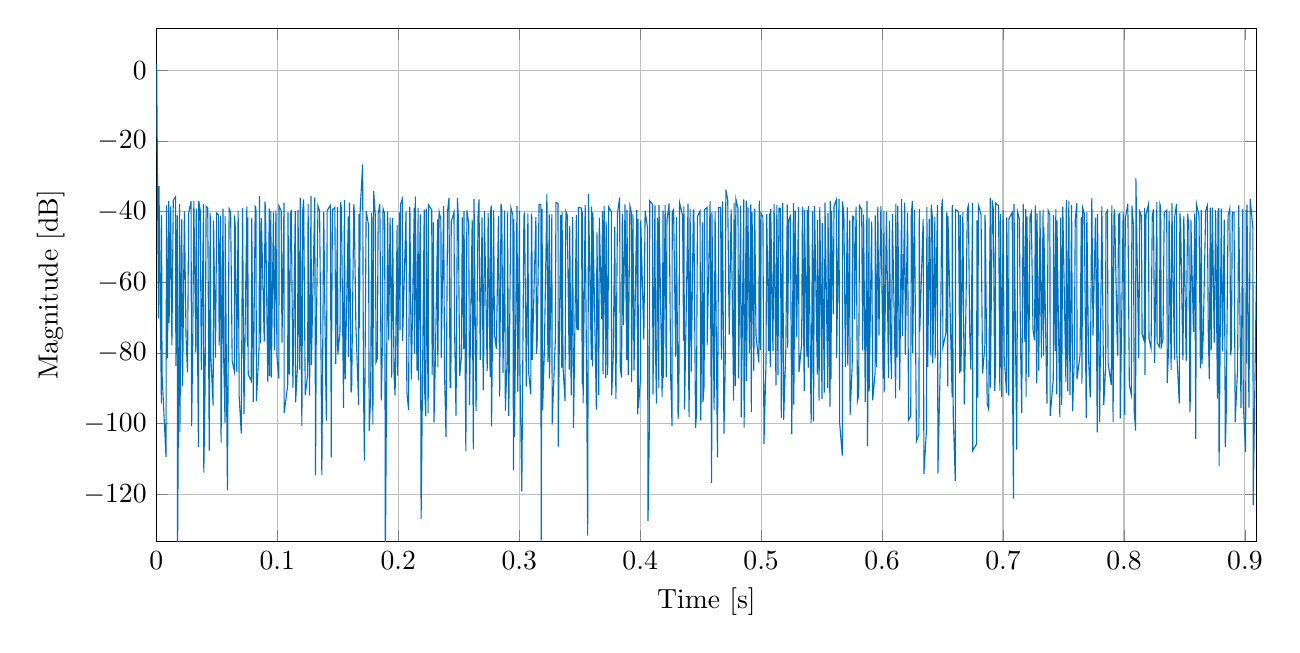
\begin{tikzpicture}

\begin{axis}[%
width=5.5in,
height=2.566in,
at={(1.011in,0.642in)},
scale only axis,
xmin=0,
xmax=0.909501157382829,
xlabel={Time [s]},
xmajorgrids,
ymin=-133.30576545487,
ymax=11.9377980263325,
ylabel={Magnitude [dB]},
ymajorgrids,
axis background/.style={fill=white}
]
\addplot [color=mycolor1,solid,forget plot]
  table[row sep=crcr]{%
2.08333333333333e-05	-18.5519458129197\\
0.000208333333333333	1.92539769599749\\
0.00177083333333333	-70.1603862246774\\
0.00214583333333333	-32.7755287161136\\
0.00414583333333333	-94.2039252922149\\
0.00425	-40.937136376685\\
0.0046875	-85.8576069217865\\
0.0079375	-109.443620754154\\
0.00835416666666667	-38.1735294294771\\
0.00916666666666666	-81.4931547383952\\
0.01025	-36.9188350195504\\
0.0105208333333333	-71.4490253797064\\
0.0117916666666667	-38.4657885523865\\
0.0128125	-77.8310259548471\\
0.0139583333333333	-36.7790803207063\\
0.0159375	-35.7328928819346\\
0.0160833333333333	-83.6559571178864\\
0.01725	-41.0564246121295\\
0.017375	-144.065730588413\\
0.01925	-37.8317742488666\\
0.0194166666666667	-102.302420647262\\
0.021	-42.152363374592\\
0.0216666666666667	-89.3708905790356\\
0.0231666666666667	-39.8666078787254\\
0.0245416666666667	-75.7739541606529\\
0.0257291666666667	-85.4501841971595\\
0.0266666666666667	-40.4847052853472\\
0.0286458333333333	-37.0383638272739\\
0.0291458333333333	-100.660893560172\\
0.0300416666666667	-77.5148953989813\\
0.0309791666666667	-37.0221544967549\\
0.0326041666666667	-79.8689106601384\\
0.0330208333333333	-39.1308984937248\\
0.0347708333333333	-106.619497504417\\
0.0350208333333333	-36.9534780867009\\
0.03625	-39.5601103166182\\
0.0371875	-84.7942671834041\\
0.039	-37.8319014794298\\
0.0392083333333333	-113.835135093588\\
0.04025	-89.9257433918166\\
0.041125	-38.4359650540914\\
0.0424583333333333	-38.9095750373776\\
0.0437083333333333	-107.619970946951\\
0.0444791666666667	-40.4042542428031\\
0.0450625	-81.3311365064353\\
0.0469166666666667	-94.871995489909\\
0.0472708333333333	-42.5478400826045\\
0.0488541666666667	-81.2951015639022\\
0.049875	-40.3789126640023\\
0.0514375	-40.9625024706217\\
0.0518958333333333	-77.8922447953147\\
0.0531041666666667	-41.1125814876897\\
0.0534791666666667	-105.326864459303\\
0.0551041666666667	-39.1343332695279\\
0.0555625	-79.9562902929538\\
0.05675	-99.6562063375615\\
0.0568333333333333	-41.1408366202979\\
0.0587291666666667	-118.891927281385\\
0.0601458333333333	-39.164265855383\\
0.0613958333333333	-40.1095329904576\\
0.0626666666666667	-82.2298735805108\\
0.0644791666666667	-85.1973195352917\\
0.0646041666666667	-41.0531409263032\\
0.0652083333333333	-44.1980673893767\\
0.0664375	-85.2648006235357\\
0.0676041666666667	-39.7043851806735\\
0.0684583333333333	-92.2958107049186\\
0.0701666666666667	-102.69741887225\\
0.0712708333333333	-38.9971559931263\\
0.0712916666666667	-39.4341769712974\\
0.0723958333333333	-97.2972675866287\\
0.0747916666666667	-38.5189936979077\\
0.0751875	-78.1420759625271\\
0.0755833333333333	-41.6641152901349\\
0.0759166666666667	-86.1185072316183\\
0.0783958333333333	-87.8708860539069\\
0.0788541666666667	-41.8695773136723\\
0.0800833333333333	-93.8566762953018\\
0.0817083333333333	-38.5518346331067\\
0.0823125	-38.9287186025732\\
0.0827083333333333	-93.5614636287424\\
0.0849791666666667	-77.9651015470257\\
0.08525	-35.5704772107062\\
0.0861875	-77.2725655898673\\
0.0868125	-41.7478277298816\\
0.0891875	-76.6659201437824\\
0.0898333333333333	-37.1351746837219\\
0.0902708333333333	-40.4229494005169\\
0.092125	-88.0532303913709\\
0.0933125	-39.1405580838697\\
0.0935	-86.4531210781812\\
0.0946666666666667	-39.7311011348484\\
0.095	-86.938561271714\\
0.0967916666666667	-40.2094562242789\\
0.097625	-79.1695550637616\\
0.0988333333333333	-39.6535226943175\\
0.0996875	-80.8665430625492\\
0.101270833333333	-87.2340606767671\\
0.101416666666667	-38.3878324811478\\
0.1031875	-39.6896466332173\\
0.103833333333333	-77.0114234373497\\
0.105520833333333	-37.4011628779268\\
0.105645833333333	-96.9248083658579\\
0.108583333333333	-89.1007168137127\\
0.108833333333333	-40.1892622078353\\
0.109854166666667	-86.0271437694726\\
0.110875	-40.8628790815478\\
0.1115625	-39.3968244038\\
0.112875	-89.8289307825964\\
0.114791666666667	-39.8460750953407\\
0.115104166666667	-93.9600436239974\\
0.116770833333333	-83.2846523215504\\
0.117104166666667	-39.4536010023525\\
0.1184375	-84.7155415760024\\
0.1189375	-36.0357770332561\\
0.120291666666667	-100.605878973077\\
0.121	-39.7626115569679\\
0.12175	-36.5277315927948\\
0.123083333333333	-91.8925912457902\\
0.125083333333333	-86.0069002253019\\
0.1254375	-37.7638916463909\\
0.126645833333333	-92.0506516990717\\
0.127854166666667	-36.002595951381\\
0.127895833333333	-35.5616156450669\\
0.128166666666667	-83.3112971386849\\
0.130958333333333	-36.0074671324157\\
0.131604166666667	-114.639241003581\\
0.132104166666667	-78.3521620013735\\
0.133604166666667	-38.3892047519009\\
0.1349375	-39.7505925314839\\
0.136166666666667	-82.5366294897913\\
0.136791666666667	-114.479116839009\\
0.138333333333333	-40.8819255762054\\
0.138375	-40.0300447553866\\
0.139916666666667	-85.972307032475\\
0.1405625	-99.1218335626914\\
0.141208333333333	-39.6627047634243\\
0.143875	-38.1837280711641\\
0.144604166666667	-109.488316160022\\
0.1448125	-81.1645116758506\\
0.1455625	-39.4525872481346\\
0.147541666666667	-38.7934318818153\\
0.148291666666667	-83.0503845013964\\
0.149791666666667	-38.6093792808167\\
0.15	-80.470031349083\\
0.151833333333333	-73.9652682284012\\
0.152291666666667	-37.2497108168677\\
0.153020833333333	-39.2818849478755\\
0.15475	-95.4929577610174\\
0.155458333333333	-36.7228150125395\\
0.156104166666667	-87.4635235846184\\
0.1586875	-41.3046701177339\\
0.158791666666667	-81.1641771655577\\
0.159645833333333	-37.4208937063257\\
0.160958333333333	-91.1568616021483\\
0.161458333333333	-89.9481252128396\\
0.16325	-37.8460399953667\\
0.163604166666667	-39.7899057076119\\
0.1649375	-72.0238123934629\\
0.167208333333333	-94.7144074797787\\
0.167416666666667	-40.5804432002278\\
0.167895833333333	-72.9709447081701\\
0.168520833333333	-39.265112669484\\
0.170520833333333	-26.6089144260092\\
0.171229166666667	-89.7084969760235\\
0.172	-110.463105212536\\
0.173416666666667	-39.7507574009912\\
0.1754375	-43.9058088123113\\
0.1759375	-102.04637869479\\
0.177166666666667	-92.4673232206693\\
0.178	-40.2544966820231\\
0.179	-100.172307609017\\
0.179625	-34.1344510063303\\
0.181083333333333	-41.4445759840945\\
0.181604166666667	-82.6332070915429\\
0.1826875	-81.5603292944465\\
0.183354166666667	-40.6013724200535\\
0.18475	-37.8886411936322\\
0.185979166666667	-93.4174074767175\\
0.186770833333333	-79.5560249693621\\
0.187416666666667	-39.1102032468717\\
0.18875	-40.4324688427174\\
0.1893125	-140.733541730388\\
0.191208333333333	-39.8851016413234\\
0.192041666666667	-76.4292607494308\\
0.19325	-41.642954457088\\
0.194541666666667	-86.9498554772794\\
0.195270833333333	-41.7766112051138\\
0.196520833333333	-86.2960022336321\\
0.197375	-92.00899215264\\
0.199041666666667	-43.7372910332328\\
0.199416666666667	-86.4150664130923\\
0.200958333333333	-40.1620513878326\\
0.201375	-73.4978141166754\\
0.201958333333333	-37.7938156039302\\
0.203395833333333	-36.3573160215574\\
0.203541666666667	-76.5616855129958\\
0.2064375	-40.002129393822\\
0.207083333333333	-90.9400052952227\\
0.208479166666667	-96.0407404868127\\
0.209416666666667	-38.6008511461162\\
0.209604166666667	-38.9692511220409\\
0.2108125	-87.5254646023321\\
0.2131875	-38.9289008630415\\
0.213395833333333	-80.1467722562333\\
0.214104166666667	-35.6816137968429\\
0.2154375	-84.9650752226633\\
0.216416666666667	-38.9836704152263\\
0.216604166666667	-87.7329317627177\\
0.218166666666667	-40.717985149793\\
0.218875	-126.996234132076\\
0.2214375	-39.3713556069448\\
0.221666666666667	-89.6964206530872\\
0.222770833333333	-97.9004778198756\\
0.223166666666667	-39.1021798430602\\
0.224708333333333	-97.0764430046659\\
0.225020833333333	-38.0778748083058\\
0.227666666666667	-39.5009585315729\\
0.227979166666667	-86.1466356571933\\
0.229104166666667	-42.9927224382634\\
0.229520833333333	-99.6132169124897\\
0.230791666666667	-79.4234995612674\\
0.232541666666667	-42.158273640218\\
0.2326875	-84.0628955060861\\
0.233729166666667	-39.9615553748445\\
0.23525	-42.262799810394\\
0.235520833333333	-81.2852130725869\\
0.237520833333333	-38.4161813468032\\
0.23825	-85.8012650101354\\
0.239458333333333	-103.72698898563\\
0.24075	-39.8010678303383\\
0.241916666666667	-36.148492433985\\
0.242833333333333	-89.7924672417965\\
0.2435	-89.8067417350762\\
0.243770833333333	-42.8889271004703\\
0.2460625	-40.1275959985789\\
0.246520833333333	-72.8884744837049\\
0.247729166666667	-97.7102209427758\\
0.248916666666667	-36.0941285336804\\
0.249666666666667	-41.6630361679321\\
0.250791666666667	-86.4166684087593\\
0.25225	-80.9124746106834\\
0.252895833333333	-41.5980949401672\\
0.2540625	-78.8240823970798\\
0.2543125	-39.8177791061036\\
0.255875	-107.79379629274\\
0.256729166666667	-39.6175522209742\\
0.258270833333333	-43.3900786727938\\
0.258875	-94.7249452356543\\
0.261104166666667	-42.2296623542329\\
0.2616875	-87.792993048808\\
0.2620625	-107.282270255865\\
0.262645833333333	-36.4574502060463\\
0.264333333333333	-96.3567201545636\\
0.265958333333333	-40.963666145451\\
0.26675	-36.5395390806047\\
0.267770833333333	-81.9358654483685\\
0.269270833333333	-41.6032238519875\\
0.270208333333333	-90.4174319777921\\
0.270625	-80.7072355099148\\
0.271208333333333	-39.7748188534505\\
0.2735	-85.0693226265118\\
0.274291666666667	-40.3937549252189\\
0.275958333333333	-86.7633189456565\\
0.276416666666667	-39.8411587420983\\
0.276854166666667	-38.2837840418311\\
0.277125	-100.733731918776\\
0.278854166666667	-39.6430347882809\\
0.2795	-74.5639571789028\\
0.281083333333333	-78.8230599033298\\
0.282833333333333	-41.1832392021198\\
0.2838125	-92.3017275688167\\
0.284979166666667	-37.7206234584216\\
0.285541666666667	-39.2020023825434\\
0.286625	-85.6219944283291\\
0.287895833333333	-39.6968695266362\\
0.288520833333333	-96.2528674278573\\
0.290104166666667	-80.7925579293698\\
0.290270833333333	-40.2163161634349\\
0.291354166666667	-97.7690084248421\\
0.293083333333333	-38.9136973506643\\
0.2946875	-40.8545803330415\\
0.295229166666667	-113.182317786221\\
0.295604166666667	-42.0727200092989\\
0.2960625	-103.777347073589\\
0.298145833333333	-38.337584779916\\
0.2988125	-90.9289405130424\\
0.300208333333333	-39.7155589309264\\
0.300604166666667	-84.6486993001228\\
0.302125	-119.143309363737\\
0.303854166666667	-41.5119754328531\\
0.304375	-40.2160138873198\\
0.305854166666667	-89.4840781033843\\
0.307166666666667	-40.5635624119636\\
0.3078125	-85.4964070109569\\
0.309541666666667	-91.6514964090626\\
0.310104166666667	-40.5194892341828\\
0.3104375	-41.7279521307518\\
0.31075	-81.9498625639673\\
0.313791666666667	-41.4760794213002\\
0.31425	-80.2485585228151\\
0.3148125	-77.54926828102\\
0.316395833333333	-37.868568111886\\
0.317895833333333	-37.9746795069449\\
0.318125	-136.867055241369\\
0.318916666666667	-39.1867473022683\\
0.3193125	-96.2142634309003\\
0.32075	-79.7038631114778\\
0.3226875	-39.6718212574338\\
0.322875	-34.9704785908527\\
0.323708333333333	-82.490514686653\\
0.324854166666667	-40.7215437630269\\
0.325020833333333	-87.2442561174805\\
0.326979166666667	-40.6918269187182\\
0.3271875	-100.230545414694\\
0.329916666666667	-75.6241194838397\\
0.330333333333333	-37.3860711814989\\
0.332083333333333	-37.6377314832304\\
0.332208333333333	-106.482624913093\\
0.334291666666667	-40.9822792844436\\
0.3351875	-84.1351725644322\\
0.335416666666667	-39.9807627613998\\
0.336270833333333	-84.3331634037219\\
0.337854166666667	-93.5102464073059\\
0.338541666666667	-39.8172812903417\\
0.3396875	-40.9503989009083\\
0.341354166666667	-84.6758058560744\\
0.341708333333333	-44.0924729633176\\
0.342979166666667	-91.9295567111102\\
0.344166666666667	-41.5516086602344\\
0.344895833333333	-101.220224948957\\
0.34725	-40.8587709928467\\
0.347604166666667	-73.2443764352243\\
0.348770833333333	-73.2866618158449\\
0.348895833333333	-38.7850386095434\\
0.3515625	-38.9815020811938\\
0.3520625	-88.8304098126741\\
0.352229166666667	-39.9875652933293\\
0.3528125	-94.2411286899172\\
0.354520833333333	-38.1117290508548\\
0.355854166666667	-93.7774834458075\\
0.356583333333333	-131.67319094515\\
0.35725	-34.9225434513354\\
0.359604166666667	-82.019059155403\\
0.359875	-38.5763608591608\\
0.360666666666667	-83.7798645305802\\
0.360875	-40.1655505837337\\
0.363770833333333	-95.9899251437898\\
0.364229166666667	-45.8760743341006\\
0.365791666666667	-91.8967383052743\\
0.366229166666667	-41.6518567154203\\
0.368125	-70.3823123272871\\
0.368854166666667	-39.8134481905917\\
0.3693125	-85.9333474988602\\
0.370208333333333	-38.4196915678677\\
0.371541666666667	-87.0937414853576\\
0.371875	-42.7601494812342\\
0.373104166666667	-86.1662281229103\\
0.374	-38.676505503304\\
0.376166666666667	-39.9418840680561\\
0.376416666666667	-91.9891230304143\\
0.377708333333333	-81.2850267207748\\
0.378958333333333	-44.2303663482864\\
0.379916666666667	-93.0013578543329\\
0.381229166666667	-40.495743253135\\
0.383020833333333	-35.9583633868101\\
0.383520833333333	-84.1316030248177\\
0.384604166666667	-86.9351340627978\\
0.38525	-40.6112053917763\\
0.386125	-72.0727651424295\\
0.387458333333333	-37.9041036783284\\
0.388875	-81.9883428778861\\
0.389083333333333	-39.4781894216104\\
0.390145833333333	-86.1808043446734\\
0.391479166666667	-38.2901213955772\\
0.392708333333333	-40.1525210811167\\
0.392916666666667	-88.227436398148\\
0.394	-40.6541841666974\\
0.394895833333333	-84.921011786896\\
0.397166666666667	-39.5618442683531\\
0.397958333333333	-97.3733128971764\\
0.398208333333333	-42.0734194913552\\
0.398541666666667	-95.494926296263\\
0.400354166666667	-86.8954814633943\\
0.400479166666667	-42.5057085197186\\
0.403020833333333	-76.1724867862787\\
0.404083333333333	-39.6999221288095\\
0.406020833333333	-44.4826788485566\\
0.4065	-127.496974294598\\
0.407625	-100.422577180789\\
0.407916666666667	-36.9181865618281\\
0.410166666666667	-37.837658766713\\
0.410583333333333	-91.7025580839976\\
0.412208333333333	-38.1773610763131\\
0.412604166666667	-77.5035863447671\\
0.413479166666667	-94.2779973244169\\
0.41425	-41.8354302445097\\
0.415458333333333	-89.9190670851578\\
0.4155625	-38.0957544908307\\
0.418166666666667	-92.4804116340837\\
0.418916666666667	-39.6031593191507\\
0.419145833333333	-87.0288942895487\\
0.420645833333333	-38.1531811305805\\
0.421541666666667	-86.7316296161424\\
0.422145833333333	-42.4267572015402\\
0.4239375	-37.6196509976512\\
0.425270833333333	-87.4446139334439\\
0.426333333333333	-100.569850808683\\
0.4265	-40.1265225872729\\
0.427625	-39.4050345816337\\
0.429395833333333	-81.0285452009466\\
0.4299375	-41.4563746975929\\
0.431354166666667	-98.680663037348\\
0.431979166666667	-92.8716283347021\\
0.4325625	-37.4293167916217\\
0.435083333333333	-41.1418407679941\\
0.435875	-76.4625005695416\\
0.436166666666667	-38.5035777906401\\
0.4366875	-95.9376900138429\\
0.4395625	-37.7129437041122\\
0.440083333333333	-87.128874655675\\
0.440458333333333	-98.138908350686\\
0.441270833333333	-39.226757270146\\
0.44225	-85.2818856844334\\
0.443958333333333	-39.7055724887729\\
0.444375	-39.5253703254221\\
0.445791666666667	-101.207955693588\\
0.446541666666667	-97.3485417599858\\
0.447333333333333	-41.3358341452998\\
0.449458333333333	-39.8290179284368\\
0.450125	-99.1010001877193\\
0.4515	-42.9790510172649\\
0.451979166666667	-93.8316777232727\\
0.452895833333333	-89.0039230330174\\
0.453125	-39.4279103731454\\
0.45525	-38.7609251890973\\
0.455354166666667	-77.790076708499\\
0.457833333333333	-37.0105869406248\\
0.458854166666667	-103.283116485568\\
0.459104166666667	-116.748544725155\\
0.4593125	-40.0971066172858\\
0.461145833333333	-96.1555952328105\\
0.4619375	-39.9342314200293\\
0.463895833333333	-109.501051807726\\
0.464875	-38.7708281432913\\
0.466541666666667	-38.80737325949\\
0.467125	-81.8784226484083\\
0.468083333333333	-37.038866500281\\
0.46925	-102.831727921838\\
0.470270833333333	-85.0419620171016\\
0.470833333333333	-33.6772187853824\\
0.472395833333333	-36.7323187448792\\
0.473645833333333	-74.8037947177818\\
0.473645833333333	-74.8037947177818\\
0.475208333333333	-39.3617514519483\\
0.477270833333333	-93.4470987818952\\
0.477645833333333	-37.5029920390723\\
0.478604166666667	-89.3704731439734\\
0.479104166666667	-36.3643669700059\\
0.480875	-39.1156882345895\\
0.481333333333333	-87.1395347131075\\
0.4830625	-38.2569466776592\\
0.483604166666667	-98.182037466741\\
0.485625	-36.5383943090647\\
0.485916666666667	-101.131062012879\\
0.48775	-36.8639553208213\\
0.4879375	-87.9082254159106\\
0.489104166666667	-38.7644565153836\\
0.4903125	-79.9538902643724\\
0.4914375	-37.8897349005114\\
0.491895833333333	-96.6119952715944\\
0.4925	-40.1463695665761\\
0.493958333333333	-85.0760830510269\\
0.494708333333333	-39.1098397838743\\
0.495770833333333	-75.0742274208545\\
0.498041666666667	-82.6002284176467\\
0.4985	-36.8901192660254\\
0.499354166666667	-79.0603897391184\\
0.4998125	-40.357929172175\\
0.501479166666667	-41.451273306936\\
0.502354166666667	-105.697150281101\\
0.504041666666667	-82.4937036152583\\
0.504625	-40.6030196955517\\
0.506333333333333	-79.4696138793462\\
0.506916666666667	-40.4830783119711\\
0.507604166666667	-83.9700591688104\\
0.5079375	-39.2823445596943\\
0.509770833333333	-79.3683528834792\\
0.510729166666667	-37.8590991606617\\
0.51225	-89.1454699302435\\
0.513	-38.0379091498598\\
0.513916666666667	-86.2614871619675\\
0.51475	-38.9690092596146\\
0.5159375	-38.9974359234524\\
0.516708333333333	-98.4412501401818\\
0.517854166666667	-37.5663101902781\\
0.518625	-98.8793651879842\\
0.520416666666667	-79.0613463087693\\
0.521604166666667	-38.0195909601984\\
0.5219375	-78.4527973935836\\
0.5228125	-42.2733705929402\\
0.524208333333333	-41.1861018428255\\
0.525333333333333	-102.957641984429\\
0.526708333333333	-37.5628183180842\\
0.527	-94.5674794727404\\
0.5281875	-39.6276740882188\\
0.529375	-75.5601212976844\\
0.530916666666667	-38.6542532609419\\
0.5313125	-85.403744250074\\
0.533520833333333	-77.1722917788878\\
0.534145833333333	-38.5370299504047\\
0.535645833333333	-90.7159441515188\\
0.535770833333333	-39.5069233287146\\
0.537833333333333	-81.0290936131987\\
0.538083333333333	-39.4690336061202\\
0.538958333333333	-84.153884431637\\
0.539125	-38.4372002902817\\
0.541375	-99.7949873485589\\
0.542479166666667	-39.9319634440244\\
0.543333333333333	-99.3218107983108\\
0.544166666666667	-38.3202956063783\\
0.546479166666667	-86.0196047056856\\
0.546625	-42.3648052337595\\
0.547916666666667	-93.4832519758737\\
0.548520833333333	-38.6785368264875\\
0.550333333333333	-92.9802152466514\\
0.5505625	-43.1502285043747\\
0.55225	-91.2271494323339\\
0.5528125	-37.4311135405672\\
0.555083333333333	-89.8399465362492\\
0.555333333333333	-40.337755173435\\
0.556895833333333	-95.2283867519557\\
0.5571875	-37.0197105621256\\
0.557833333333333	-87.3989090763514\\
0.5581875	-39.7108103949695\\
0.559666666666667	-68.9497995241304\\
0.560270833333333	-38.4731857584219\\
0.562208333333333	-36.5821455190372\\
0.562416666666667	-81.3464809688391\\
0.564354166666667	-36.3979231050756\\
0.564958333333333	-99.9006519866077\\
0.567104166666667	-108.989048820243\\
0.567270833333333	-37.0990609668967\\
0.5684375	-40.8022936132651\\
0.569708333333333	-83.9584125758893\\
0.571291666666667	-38.795800865228\\
0.571666666666667	-83.4760342323014\\
0.573270833333333	-42.4139191415011\\
0.573541666666667	-97.4866723176109\\
0.575291666666667	-83.6152454931914\\
0.5754375	-41.2371194394115\\
0.576604166666667	-41.4668733549324\\
0.577166666666667	-70.2960501311493\\
0.578520833333333	-38.5392808575731\\
0.579666666666667	-93.5142741636251\\
0.580645833333333	-91.8839441584857\\
0.581375	-38.3100246454374\\
0.583145833333333	-39.4003559053919\\
0.583916666666667	-79.2224618007119\\
0.584729166666667	-40.8418417529028\\
0.586104166666667	-93.8315218661244\\
0.5875	-36.8997409895559\\
0.587979166666667	-106.309309043272\\
0.589208333333333	-41.8910809538951\\
0.5893125	-90.8688712619423\\
0.591395833333333	-42.7824094417152\\
0.592229166666667	-93.3858682413908\\
0.594208333333333	-85.7069982247785\\
0.594375	-41.024240427591\\
0.595458333333333	-83.8835305287129\\
0.596479166666667	-38.6344192908362\\
0.597416666666667	-74.9938646818124\\
0.599020833333333	-38.3253717824733\\
0.600895833333333	-87.2385420533957\\
0.601479166666667	-42.1462759862716\\
0.601520833333333	-39.7572161274307\\
0.601729166666667	-91.1460099529221\\
0.603645833333333	-39.9430137235012\\
0.605291666666667	-87.1177461203978\\
0.6060625	-42.5417488136257\\
0.607145833333333	-79.4808869291236\\
0.607833333333333	-87.3299256788498\\
0.608520833333333	-40.6832554396696\\
0.61125	-92.8175448470858\\
0.611354166666667	-37.7162470175778\\
0.612291666666667	-81.2578802435115\\
0.612979166666667	-38.3586770471841\\
0.614541666666667	-90.4458980027452\\
0.616145833333333	-36.8229407758053\\
0.616166666666667	-36.4266982544642\\
0.6168125	-75.195393627225\\
0.6186875	-37.4280928935563\\
0.619208333333333	-80.5241644290071\\
0.621104166666667	-40.2705379937402\\
0.621854166666667	-99.0626732779895\\
0.623708333333333	-97.8406029390755\\
0.624166666666667	-40.6520610077108\\
0.625041666666667	-37.0348221962186\\
0.625333333333333	-79.9429341366681\\
0.626770833333333	-39.5153948957343\\
0.6284375	-104.936848366767\\
0.630458333333333	-103.002766875157\\
0.630791666666667	-39.2209106587769\\
0.6308125	-39.478031005054\\
0.631166666666667	-73.9447829166792\\
0.633979166666667	-42.0841563334352\\
0.634604166666667	-114.214606595983\\
0.636729166666667	-101.572253069571\\
0.637020833333333	-38.6957578215501\\
0.637791666666667	-83.978053199107\\
0.638979166666667	-42.0294618827033\\
0.6403125	-80.8322120909189\\
0.640708333333333	-38.0236136616195\\
0.64175	-42.3238390562986\\
0.641916666666667	-82.8781700293387\\
0.643666666666667	-41.43737431798\\
0.643875	-81.4863088280219\\
0.645770833333333	-38.1151521040696\\
0.646166666666667	-114.08726403865\\
0.6481875	-81.8572571194842\\
0.649333333333333	-38.5821360123073\\
0.649895833333333	-36.3841451982201\\
0.650291666666667	-78.4507793060964\\
0.6528125	-74.1490516976775\\
0.653520833333333	-40.0887237333137\\
0.654270833333333	-89.4399001846448\\
0.6544375	-41.1440386273384\\
0.6579375	-92.4561544595549\\
0.6580625	-38.7320114978642\\
0.658083333333333	-38.1483825054083\\
0.658833333333333	-97.7115283300828\\
0.660541666666667	-116.176753492649\\
0.660770833333333	-39.3916080995112\\
0.6631875	-39.9561464170493\\
0.664229166666667	-85.7545292822313\\
0.664604166666667	-40.8724666838331\\
0.665270833333333	-85.1929654575478\\
0.666791666666667	-40.0336389666483\\
0.667979166666667	-94.4934821639409\\
0.668854166666667	-78.2519084318803\\
0.670520833333333	-39.2766323445712\\
0.671395833333333	-38.2433692709539\\
0.672416666666667	-74.1517098821129\\
0.673395833333333	-84.6701583284909\\
0.674791666666667	-37.5039301574514\\
0.6748125	-37.7110752951995\\
0.674979166666667	-107.570077774941\\
0.678145833333333	-105.733637442431\\
0.6784375	-42.4369547966443\\
0.679083333333333	-92.5945501278665\\
0.679645833333333	-38.1390399156639\\
0.681833333333333	-40.7235543791211\\
0.683104166666667	-85.8172739120833\\
0.684958333333333	-77.9053983489696\\
0.685083333333333	-40.9317636803235\\
0.685395833333333	-43.9478147988212\\
0.686875	-94.2215634817998\\
0.688145833333333	-95.9170956342443\\
0.689458333333333	-36.0517989650941\\
0.689583333333333	-89.7934535423999\\
0.691125	-36.8256184227107\\
0.692020833333333	-39.3721616565238\\
0.693125	-90.7398925601833\\
0.693729166666667	-85.3549625090318\\
0.693854166666667	-37.5367384285292\\
0.696333333333333	-38.3025302061292\\
0.697375	-90.592819394928\\
0.697958333333333	-40.6545526323442\\
0.6989375	-92.4447730958734\\
0.700083333333333	-39.5292796473989\\
0.7009375	-80.8971723415075\\
0.702916666666667	-91.3280518350503\\
0.703104166666667	-41.6259435787519\\
0.704708333333333	-92.0357140300499\\
0.704895833333333	-41.974064181003\\
0.707645833333333	-40.2093306791106\\
0.707875	-88.639834299551\\
0.708645833333333	-121.171908778608\\
0.7090625	-37.7805608539091\\
0.711354166666667	-107.355958720792\\
0.712125	-40.1524339536619\\
0.713520833333333	-41.996433152329\\
0.714375	-75.1228320300795\\
0.7154375	-96.9822767732894\\
0.716666666666667	-37.7464312297637\\
0.718041666666667	-76.8706537892161\\
0.718770833333333	-39.2415520019293\\
0.7190625	-92.4824609893658\\
0.719791666666667	-41.3365608710063\\
0.721270833333333	-86.7989907926971\\
0.722291666666667	-41.4996914316665\\
0.723333333333333	-40.1956582817282\\
0.724791666666667	-73.4241014216226\\
0.726083333333333	-76.4152290219056\\
0.726708333333333	-38.1678651924068\\
0.727833333333333	-88.5675862913728\\
0.728083333333333	-40.4552432353343\\
0.729541666666667	-84.9581575838772\\
0.730583333333333	-39.6544183915779\\
0.731770833333333	-81.2920096784526\\
0.733145833333333	-39.4340877266037\\
0.733583333333333	-80.7458643829003\\
0.733729166666667	-44.2857506768594\\
0.736333333333333	-94.2955985514896\\
0.737291666666667	-39.665986786328\\
0.73875	-40.8812021272261\\
0.739020833333333	-97.7704889077812\\
0.7415625	-87.2753708039384\\
0.741708333333333	-40.9163980092905\\
0.743083333333333	-79.4796013373268\\
0.743666666666667	-39.2665747437839\\
0.744375	-91.7205212264697\\
0.744583333333333	-42.4768116193546\\
0.746979166666667	-98.0702535489662\\
0.747770833333333	-41.6991360539842\\
0.748479166666667	-94.6658870719847\\
0.749395833333333	-38.5681509960618\\
0.751979166666667	-88.1154906155696\\
0.752333333333333	-36.6711480352312\\
0.7535	-90.834675302022\\
0.754416666666667	-36.9439707297046\\
0.754458333333333	-38.8676959297517\\
0.755375	-91.8298073731391\\
0.756708333333333	-38.1504966650943\\
0.757541666666667	-96.5047858665326\\
0.758979166666667	-80.4195986770202\\
0.759708333333333	-42.3059728297332\\
0.761041666666667	-37.5794998746318\\
0.761166666666667	-87.4454962421115\\
0.7636875	-80.51292313221\\
0.764729166666667	-41.4627817098876\\
0.765229166666667	-88.6231222677961\\
0.7659375	-38.9592213721365\\
0.767208333333333	-40.5774031778598\\
0.768791666666667	-98.3832730242057\\
0.769291666666667	-40.1276283825102\\
0.770729166666667	-81.5839800494563\\
0.772104166666667	-92.5353541395512\\
0.77325	-40.1854817818878\\
0.7734375	-36.1535882236327\\
0.774416666666667	-74.9596655326303\\
0.7764375	-41.6395205745018\\
0.7773125	-74.4650105310253\\
0.777895833333333	-102.465964412675\\
0.778104166666667	-40.7120109348476\\
0.779875	-99.4988863230729\\
0.781708333333333	-38.4839351610243\\
0.781708333333333	-38.4839351610243\\
0.783291666666667	-94.6584023209256\\
0.784875	-83.7452368224103\\
0.785020833333333	-40.5187628221932\\
0.7863125	-39.6287460358398\\
0.786895833333333	-82.9622863812346\\
0.789479166666667	-88.995374325957\\
0.789958333333333	-38.1845654225587\\
0.791020833333333	-99.5777344436287\\
0.7916875	-41.0641410687642\\
0.792270833333333	-39.3688892836312\\
0.794270833333333	-74.7684900657199\\
0.794833333333333	-80.7036106653803\\
0.795458333333333	-40.8576897254155\\
0.796479166666667	-40.4858771336884\\
0.796958333333333	-98.4734034772432\\
0.799333333333333	-40.1177810692973\\
0.800270833333333	-75.4574530521049\\
0.8006875	-97.4577439839463\\
0.8010625	-42.0915803833131\\
0.803208333333333	-37.7398681536672\\
0.8044375	-89.1026964884332\\
0.806104166666667	-91.8674560039533\\
0.8065625	-38.3066227267756\\
0.807833333333333	-43.9371240041745\\
0.808520833333333	-96.7717969926416\\
0.809645833333333	-101.942605335204\\
0.809854166666667	-30.4592876073145\\
0.81225	-81.4550278070925\\
0.8130625	-39.966701725523\\
0.814479166666667	-41.2068537777228\\
0.8149375	-74.5881510445493\\
0.81675	-76.604039621247\\
0.817104166666667	-38.8752641510018\\
0.817375	-86.1783912376173\\
0.8181875	-40.8634727252093\\
0.820270833333333	-37.9116956471208\\
0.820666666666667	-75.9292357860142\\
0.822416666666667	-78.616714235556\\
0.823375	-41.2763636457455\\
0.824416666666667	-39.2664696822843\\
0.825333333333333	-82.7904869477106\\
0.827229166666667	-37.2215255807731\\
0.827354166666667	-76.9517419200047\\
0.829520833333333	-78.3196285322227\\
0.829708333333333	-37.8515627385455\\
0.8303125	-38.6543949053419\\
0.830875	-78.1507694215504\\
0.832229166666667	-76.1925354447128\\
0.833291666666667	-40.2479323356604\\
0.835354166666667	-39.5959250051416\\
0.835791666666667	-88.5237545358829\\
0.837	-77.4706927799484\\
0.837291666666667	-40.0047470126975\\
0.839	-84.7604719276938\\
0.839625	-37.5900727675604\\
0.841770833333333	-81.8358853059143\\
0.841916666666667	-41.4148235758368\\
0.843479166666667	-37.8123994947326\\
0.843645833333333	-79.8243867859832\\
0.845708333333333	-94.21637534383\\
0.846208333333333	-40.4067246466654\\
0.8468125	-42.6826821934267\\
0.848708333333333	-81.9494214780407\\
0.848916666666667	-77.4738609466288\\
0.849479166666667	-41.2421266062733\\
0.8514375	-82.2627463531598\\
0.852604166666667	-40.5783513789877\\
0.853625	-43.9660344176693\\
0.854479166666667	-96.7733652210768\\
0.855083333333333	-90.7804088139027\\
0.855333333333333	-42.2910263327225\\
0.857458333333333	-73.9823785852907\\
0.858458333333333	-40.5459482682283\\
0.859375	-104.271831283688\\
0.859875	-37.7197207033535\\
0.862041666666667	-41.1535886922339\\
0.8631875	-84.3312416901983\\
0.863895833333333	-39.5700885708829\\
0.864479166666667	-83.1505380532012\\
0.865541666666667	-74.8146676957678\\
0.867541666666667	-39.7861630903924\\
0.868916666666667	-38.2680136850028\\
0.869708333333333	-74.0029144689715\\
0.8705625	-87.4015040472511\\
0.871354166666667	-38.8683267551729\\
0.872104166666667	-79.1841076483546\\
0.8730625	-38.8143823383311\\
0.874645833333333	-77.0769145344433\\
0.875770833333333	-39.4701451770875\\
0.877270833333333	-92.8727359387883\\
0.877645833333333	-40.253333046866\\
0.878354166666667	-39.0080468149117\\
0.878625	-112.023287286641\\
0.880479166666667	-39.0915731777199\\
0.8815	-79.5466166274704\\
0.882916666666667	-42.2242134491667\\
0.883791666666667	-106.641735271173\\
0.8845	-97.6070536512505\\
0.886083333333333	-41.0679659021751\\
0.8875	-39.1591889069521\\
0.888208333333333	-80.4790500160969\\
0.888833333333333	-78.6198212336751\\
0.889583333333333	-40.0737008696579\\
0.891	-40.2598662368525\\
0.891979166666667	-99.5347300791249\\
0.893916666666667	-84.4680628458825\\
0.894854166666667	-38.184768555207\\
0.894854166666667	-38.184768555207\\
0.89675	-95.5465205979583\\
0.8981875	-39.2969765034855\\
0.898625	-94.1697437567004\\
0.9005625	-108.030342766262\\
0.901125	-39.5671391789175\\
0.901354166666667	-82.9182735407195\\
0.901708333333333	-37.9652570239158\\
0.903333333333333	-95.4147578163748\\
0.904416666666667	-36.4385446382558\\
0.906583333333333	-44.8442546801874\\
0.906833333333333	-123.027755955478\\
0.909520833333333	-57.7503621067594\\
};
\end{axis}
\end{tikzpicture}%
	\caption{Time decay plot of the cancellation path}
	\label{TimeDecayPlotCancellationPath}
\end{figure}


Taking the first 256 coefficients of the impulse response gives the following cropped impulse response, as seen on \autoref{CancellationPathImpulseResponseCrop}.

\begin{figure}[H]
	\centering
	\tikzsetnextfilename{CancellationPathImpulseResponseCrop1}
	%% This file was created by matlab2tikz.
%
%The latest updates can be retrieved from
%  http://www.mathworks.com/matlabcentral/fileexchange/22022-matlab2tikz-matlab2tikz
%where you can also make suggestions and rate matlab2tikz.
%
\definecolor{mycolor1}{rgb}{0.00000,0.44700,0.74100}%
\definecolor{mycolor2}{rgb}{0.85000,0.32500,0.09800}%
\definecolor{mycolor3}{rgb}{0.92900,0.69400,0.12500}%
\definecolor{mycolor4}{rgb}{0.49400,0.18400,0.55600}%
\definecolor{mycolor5}{rgb}{0.46600,0.67400,0.18800}%
%
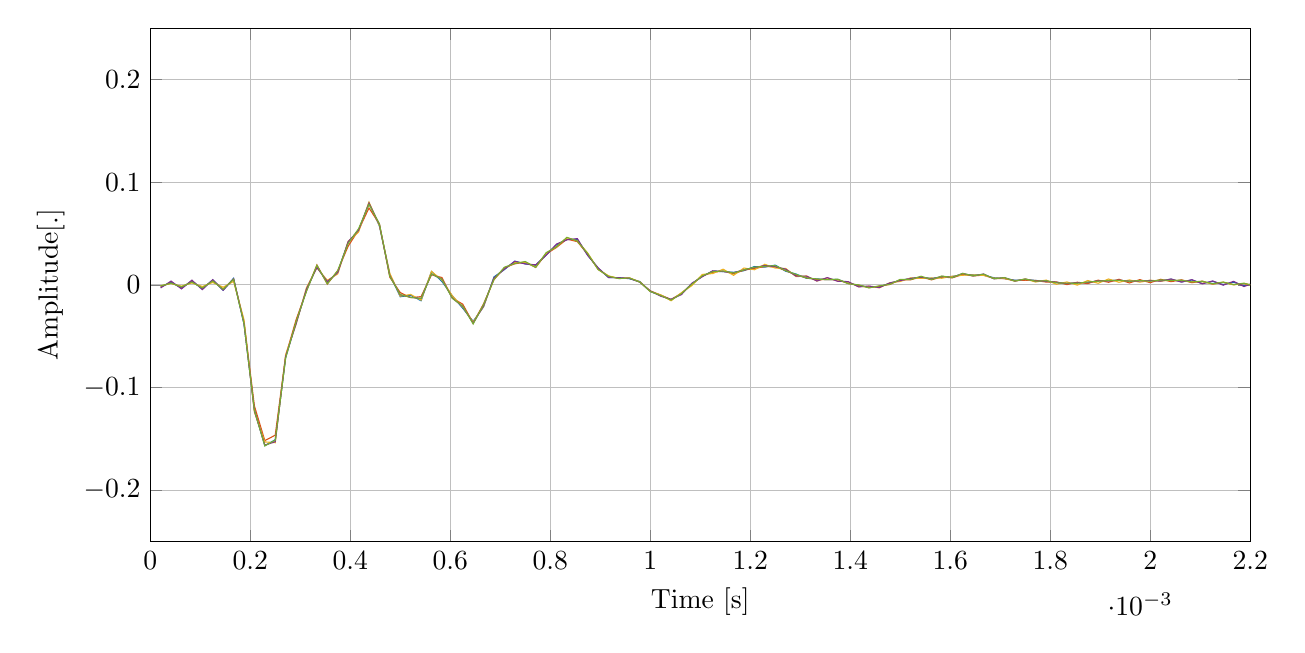
\begin{tikzpicture}

\begin{axis}[%
width=5.5in,
height=2.566in,,
at={(1.011in,0.642in)},
scale only axis,
xmin=0,
xmax=0.0022,
xlabel={Time [s]},
xmajorgrids,
ymin=-0.25,
ymax=0.25,
ylabel={Amplitude[.]},
ymajorgrids,
axis background/.style={fill=white}
]
\addplot [color=mycolor1,solid,forget plot]
  table[row sep=crcr]{%
2.08333333333333e-05	-0.00218389910452928\\
4.16666666666667e-05	0.00247997660818177\\
6.25e-05	-0.00306422212301669\\
8.33333333333333e-05	0.00370795824245389\\
0.000104166666666667	-0.003996195002872\\
0.000125	0.00477762315573945\\
0.000145833333333333	-0.00520610865886981\\
0.000166666666666667	0.00632845677938862\\
0.0001875	-0.0380783744937981\\
0.000208333333333333	-0.121478341280274\\
0.000229166666666667	-0.156732911171094\\
0.00025	-0.150962242221131\\
0.000270833333333333	-0.0708305555277822\\
0.000291666666666667	-0.0363422650083233\\
0.0003125	-0.00543127544862284\\
0.000333333333333333	0.0181597627718888\\
0.000354166666666667	0.00208472952849193\\
0.000375	0.0125098852556454\\
0.000395833333333333	0.0415416610429961\\
0.000416666666666667	0.0527294742213453\\
0.0004375	0.0798009720407638\\
0.000458333333333333	0.057294372226422\\
0.000479166666666667	0.0100967131822404\\
0.0005	-0.0116403016854475\\
0.000520833333333333	-0.0100823637366942\\
0.000541666666666667	-0.0155252345103445\\
0.0005625	0.0129409401256135\\
0.000583333333333333	0.00330032363608726\\
0.000604166666666667	-0.0107369621764369\\
0.000625	-0.0228446033217494\\
0.000645833333333333	-0.0356027778798783\\
0.000666666666666667	-0.0214218763506852\\
0.0006875	0.0077125374318295\\
0.000708333333333333	0.0148003772574559\\
0.000729166666666667	0.0230269782520459\\
0.00075	0.0204048345153605\\
0.000770833333333333	0.0189891037229106\\
0.000791666666666667	0.0290727336722823\\
0.0008125	0.0388997216505961\\
0.000833333333333333	0.0442340567889403\\
0.000854166666666667	0.0441885135919368\\
0.000875	0.0288044550629258\\
0.000895833333333333	0.0161368334943261\\
0.000916666666666667	0.00713579035783102\\
0.0009375	0.00701321180069818\\
0.000958333333333333	0.00593867000057454\\
0.000979166666666667	0.00320599481994303\\
0.001	-0.00664914273579044\\
0.00102083333333333	-0.0101565754892221\\
0.00104166666666667	-0.014791108741586\\
0.0010625	-0.00857239326708171\\
0.00108333333333333	0.00100898054712758\\
0.00110416666666667	0.00839401335783726\\
0.001125	0.0133984163005487\\
0.00114583333333333	0.0128466265171883\\
0.00116666666666667	0.0121549768071494\\
0.0011875	0.0137719317655377\\
0.00120833333333333	0.0178060477156998\\
0.00122916666666667	0.0172847958388615\\
0.00125	0.019210569641301\\
0.00127083333333333	0.013257709044026\\
0.00129166666666667	0.0104752301035351\\
0.0013125	0.00634204156049436\\
0.00133333333333333	0.00579198958498723\\
0.00135416666666667	0.00502590528864318\\
0.001375	0.00529722084283291\\
0.00139583333333333	0.00153242789497228\\
0.00141666666666667	-0.000616528502902794\\
0.0014375	-0.0021893619325514\\
0.00145833333333333	-0.00187817940983287\\
0.00147916666666667	0.00151654195426903\\
0.0015	0.00420310986639849\\
0.00152083333333333	0.00637222520912491\\
0.00154166666666667	0.00708169552640407\\
0.0015625	0.00637493155811143\\
0.00158333333333333	0.00726931533456736\\
0.00160416666666667	0.00819256235515286\\
0.001625	0.00995175279603157\\
0.00164583333333333	0.00976251303247071\\
0.00166666666666667	0.00936529201189556\\
0.0016875	0.00688403743977654\\
0.00170833333333333	0.00606358036924052\\
0.00172916666666667	0.00452676896305512\\
0.00175	0.004828792984279\\
0.00177083333333333	0.00430742388743505\\
0.00179166666666667	0.00318484065017087\\
0.0018125	0.00262913018197462\\
0.00183333333333333	0.000894527696839949\\
0.00185416666666667	0.00220727189527427\\
0.001875	0.00213064727283039\\
0.00189583333333333	0.00400580107200661\\
0.00191666666666667	0.00382018713412366\\
0.0019375	0.00453452462048207\\
0.00195833333333333	0.00348401578315948\\
0.00197916666666667	0.00385250692600261\\
0.002	0.00410399715905844\\
0.00202083333333333	0.00376669564103728\\
0.00204166666666667	0.005481403501254\\
0.0020625	0.00286984013341575\\
0.00208333333333333	0.00467110572913971\\
0.00210416666666667	0.00133891989308461\\
0.002125	0.00329198810788862\\
0.00214583333333333	0.000300140045619779\\
0.00216666666666667	0.00262574118790929\\
0.0021875	-0.000772552707238634\\
0.00220833333333333	0.001204895577724\\
0.00222916666666667	-0.00133487209486768\\
0.00225	-0.000509380400493588\\
0.00227083333333333	-0.000334737971901055\\
0.00229166666666667	-0.00103678981403972\\
0.0023125	0.00061906400962846\\
0.00233333333333333	-0.00138559528811041\\
0.00235416666666667	0.000836453989668149\\
0.002375	-0.00220070096737768\\
0.00239583333333333	0.00155059728767193\\
0.00241666666666667	-0.00246952128785161\\
0.0024375	0.00209771500748369\\
0.00245833333333333	-0.00201237551900768\\
0.00247916666666667	0.00136337042281452\\
0.0025	-0.0016996067640007\\
0.00252083333333333	0.000375559342336357\\
0.00254166666666667	-0.00171285649355793\\
0.0025625	-0.000370547864208922\\
0.00258333333333333	-0.00168478066288008\\
0.00260416666666667	-0.00164047511374893\\
0.002625	-0.00154391190477046\\
0.00264583333333333	-0.00279588952826178\\
0.00266666666666667	-0.00161937857228862\\
0.0026875	-0.00281948250550955\\
0.00270833333333333	-0.0019126329763031\\
0.00272916666666667	-0.00237053013971509\\
0.00275	-0.00216738565291799\\
0.00277083333333333	-0.00198477223131889\\
0.00279166666666667	-0.00218053262768701\\
0.0028125	-0.00109861342178239\\
0.00283333333333333	-0.00230003733690516\\
0.00285416666666667	-2.92964736988071e-05\\
0.002875	-0.00258103832251588\\
0.00289583333333333	0.000226343416296675\\
0.00291666666666667	-0.00266926986983911\\
0.0029375	-0.000193341868510947\\
0.00295833333333333	-0.00251045357924689\\
0.00297916666666667	-0.000754536531619725\\
0.003	-0.00243962671207192\\
0.00302083333333333	-0.00146416942230298\\
0.00304166666666667	-0.00213138690195344\\
0.0030625	-0.00235987025503001\\
0.00308333333333333	-0.00140117139661643\\
0.00310416666666667	-0.00302857105296522\\
0.003125	-0.000722072931201979\\
0.00314583333333333	-0.00321030960137844\\
0.00316666666666667	-0.00035915225761106\\
0.0031875	-0.00297374200868294\\
0.00320833333333333	3.53198342716556e-05\\
0.00322916666666667	-0.0026450468724363\\
0.00325	0.00032858441079607\\
0.00327083333333333	-0.00227789302909872\\
0.00329166666666667	0.000100083042602076\\
0.0033125	-0.00188361158529631\\
0.00333333333333333	-0.000395512602873454\\
0.00335416666666667	-0.00170533112866956\\
0.003375	-0.000671247588764808\\
0.00339583333333333	-0.00191528739109528\\
0.00341666666666667	-0.000801885905110417\\
0.0034375	-0.00212498021642428\\
0.00345833333333333	-0.000968435139872327\\
0.00347916666666667	-0.00218928107893563\\
0.0035	-0.000908900434101829\\
0.00352083333333333	-0.00237627772062559\\
0.00354166666666667	-0.000579630370778564\\
0.0035625	-0.00250519865369403\\
0.00358333333333333	-0.000396073310796909\\
0.00360416666666667	-0.00220304009472981\\
0.003625	-0.000551947219102873\\
0.00364583333333333	-0.0017461192389335\\
0.00366666666666667	-0.000768138137423014\\
0.0036875	-0.0014508385510616\\
0.00370833333333333	-0.00107362237419074\\
0.00372916666666667	-0.001022338035958\\
0.00375	-0.00167383565520242\\
0.00377083333333333	-0.000445481543758471\\
0.00379166666666667	-0.00226771972340852\\
0.0038125	-0.00017191447384072\\
0.00383333333333333	-0.0024910438469192\\
0.00385416666666667	-0.000222906421509958\\
0.003875	-0.00252208983413144\\
0.00389583333333333	-0.000239508055918544\\
0.00391666666666667	-0.00249900652928486\\
0.0039375	-0.00036819453953393\\
0.00395833333333333	-0.00215026444025682\\
0.00397916666666667	-0.00078767916054904\\
0.004	-0.00160104351722162\\
0.00402083333333333	-0.00116932694136055\\
0.00404166666666667	-0.00128993741065524\\
0.0040625	-0.00130037826319792\\
0.00408333333333333	-0.00120109343231604\\
0.00410416666666667	-0.00137738437947758\\
0.004125	-0.00108994636516787\\
0.00414583333333333	-0.0013930566895397\\
0.00416666666666667	-0.00115682928452173\\
0.0041875	-0.00112155535625298\\
0.00420833333333333	-0.0014747233687034\\
0.00422916666666667	-0.000756437573699205\\
0.00425	-0.00175061296711125\\
0.00427083333333333	-0.000584625454284746\\
0.00429166666666667	-0.00185462900166534\\
0.0043125	-0.0005346079858565\\
0.00433333333333333	-0.00193597084036407\\
0.00435416666666667	-0.00047838297960541\\
0.004375	-0.00194226459657353\\
0.00439583333333333	-0.000585028474139202\\
0.00441666666666667	-0.00174761669058415\\
0.0044375	-0.000800749743149818\\
0.00445833333333333	-0.00151735092894328\\
0.00447916666666667	-0.000883973934664968\\
0.0045	-0.0014537081327631\\
0.00452083333333333	-0.00075225814753293\\
0.00454166666666667	-0.00151365778473533\\
0.0045625	-0.000500860453977012\\
0.00458333333333333	-0.00164649690516529\\
0.00460416666666667	-9.96498374878968e-05\\
0.004625	-0.00195544375064587\\
0.00464583333333333	0.000449155256385712\\
0.00466666666666667	-0.00238322226588622\\
0.0046875	0.000954670191418131\\
0.00470833333333333	-0.00271709732406415\\
0.00472916666666667	0.00121675616537964\\
0.00475	-0.00282529785820646\\
0.00477083333333333	0.0011995722697696\\
0.00479166666666667	-0.00272018311514588\\
0.0048125	0.000933992660913407\\
0.00483333333333333	-0.00233183076857483\\
0.00485416666666667	0.00039448353507977\\
0.004875	-0.00163113482278814\\
0.00489583333333333	-0.000362090300491339\\
0.00491666666666667	-0.000779026479175463\\
0.0049375	-0.00112374188568124\\
0.00495833333333333	-2.39139304477267e-05\\
0.00497916666666667	-0.00169920199968603\\
0.005	0.000523981145438892\\
0.00502083333333333	-0.00205667911465618\\
0.00504166666666667	0.000812579724410437\\
0.0050625	-0.00210866993358576\\
0.00508333333333333	0.000741663856323763\\
0.00510416666666667	-0.00175541600420527\\
0.005125	0.000311014598016389\\
0.00514583333333333	-0.00112489985361012\\
0.00516666666666667	-0.000277561456628004\\
0.0051875	-0.000467680148606119\\
0.00520833333333333	-0.000833718285872148\\
0.00522916666666667	0.000113882903666011\\
0.00525	-0.00128561358966294\\
0.00527083333333333	0.000546530701225396\\
0.00529166666666667	-0.00148197183580008\\
0.0053125	0.000645564949214993\\
0.00533333333333333	-0.00126676793443997\\
};
\addplot [color=mycolor2,solid,forget plot]
  table[row sep=crcr]{%
2.08333333333333e-05	-0.00150312502349965\\
4.16666666666667e-05	0.00170740345175498\\
6.25e-05	-0.00225094460714062\\
8.33333333333333e-05	0.00283940474816698\\
0.000104166666666667	-0.00303627224888553\\
0.000125	0.00393115781364844\\
0.000145833333333333	-0.00417103313904593\\
0.000166666666666667	0.00544829804434176\\
0.0001875	-0.0357658099541969\\
0.000208333333333333	-0.118005245940072\\
0.000229166666666667	-0.151785228594567\\
0.00025	-0.1465046442558\\
0.000270833333333333	-0.0692755249179087\\
0.000291666666666667	-0.0340849194790308\\
0.0003125	-0.00600717417737366\\
0.000333333333333333	0.0194326766341735\\
0.000354166666666667	0.000751764670907603\\
0.000375	0.0137901515627398\\
0.000395833333333333	0.0376433591209333\\
0.000416666666666667	0.0533769204766715\\
0.0004375	0.0748560574116669\\
0.000458333333333333	0.0592590643629689\\
0.000479166666666667	0.00735497863182636\\
0.0005	-0.00756718413491506\\
0.000520833333333333	-0.0124975010055099\\
0.000541666666666667	-0.0115247016817554\\
0.0005625	0.00980021630720815\\
0.000583333333333333	0.00708498450188709\\
0.000604166666666667	-0.0129050270431849\\
0.000625	-0.0188519397068052\\
0.000645833333333333	-0.0372961949901686\\
0.000666666666666667	-0.01849297415842\\
0.0006875	0.00497121361236263\\
0.000708333333333333	0.0166422880218153\\
0.000729166666666667	0.020465656840568\\
0.00075	0.0220834588704114\\
0.000770833333333333	0.0169189373925576\\
0.000791666666666667	0.0299976968876195\\
0.0008125	0.0364130084818885\\
0.000833333333333333	0.044568512776588\\
0.000854166666666667	0.0420780402826822\\
0.000875	0.029754539044608\\
0.000895833333333333	0.0150431845354128\\
0.000916666666666667	0.00824248720676909\\
0.0009375	0.00622415686774906\\
0.000958333333333333	0.00657627207683757\\
0.000979166666666667	0.00275294759176985\\
0.001	-0.00591776430469594\\
0.00102083333333333	-0.00992032862922456\\
0.00104166666666667	-0.0143079250947841\\
0.0010625	-0.00817968654639674\\
0.00108333333333333	0.000480415578304432\\
0.00110416666666667	0.00871664889654762\\
0.001125	0.0122014686789311\\
0.00114583333333333	0.0133645741268153\\
0.00116666666666667	0.0106617261527092\\
0.0011875	0.0143050938208178\\
0.00120833333333333	0.0159709735280955\\
0.00122916666666667	0.0177759597607658\\
0.00125	0.0175080774703475\\
0.00127083333333333	0.013929522023107\\
0.00129166666666667	0.00934886109584583\\
0.0013125	0.00688718378449337\\
0.00133333333333333	0.00513304375912566\\
0.00135416666666667	0.00513013541241314\\
0.001375	0.0050914671922881\\
0.00139583333333333	0.00129193064715399\\
0.00141666666666667	-0.000282917718707061\\
0.0014375	-0.00281934226995237\\
0.00145833333333333	-0.00126138441418749\\
0.00147916666666667	0.000359735815132393\\
0.0015	0.00484238657500165\\
0.00152083333333333	0.00489602610432004\\
0.00154166666666667	0.0076699056302263\\
0.0015625	0.00486066045936765\\
0.00158333333333333	0.00771487566070934\\
0.00160416666666667	0.00677437856370931\\
0.001625	0.0101902062798796\\
0.00164583333333333	0.00864138380838661\\
0.00166666666666667	0.00945825376617475\\
0.0016875	0.00618394559018458\\
0.00170833333333333	0.00598757702781642\\
0.00172916666666667	0.00414812009692581\\
0.00175	0.0045110664355937\\
0.00177083333333333	0.00418394923554998\\
0.00179166666666667	0.00269472594072503\\
0.0018125	0.00276415130472775\\
0.00183333333333333	0.000237896245683422\\
0.00185416666666667	0.00252243208973511\\
0.001875	0.00116355425877345\\
0.00189583333333333	0.00450927287329329\\
0.00191666666666667	0.00249087692609324\\
0.0019375	0.00535707054015208\\
0.00195833333333333	0.00180650739266421\\
0.00197916666666667	0.00506128162830543\\
0.002	0.00204266833987498\\
0.00202083333333333	0.00538568566778509\\
0.00204166666666667	0.00306440643436911\\
0.0020625	0.00490161291817414\\
0.00208333333333333	0.00204275018470907\\
0.00210416666666667	0.00359422966353806\\
0.002125	0.000641060989892511\\
0.00214583333333333	0.00247273465336715\\
0.00216666666666667	0.000188366403795602\\
0.0021875	0.00106503791008099\\
0.00220833333333333	-0.000743232791695567\\
0.00222916666666667	-9.80423910744149e-05\\
0.00225	-0.00172025335400668\\
0.00227083333333333	3.22754464928352e-05\\
0.00229166666666667	-0.00136516805409886\\
0.0023125	3.54577907460388e-05\\
0.00233333333333333	-0.000833531371844218\\
0.00235416666666667	-0.000571016518356972\\
0.002375	-0.000914871697735422\\
0.00239583333333333	-0.000463641235510094\\
0.00241666666666667	-0.000699628193500556\\
0.0024375	-0.000207060477280922\\
0.00245833333333333	-0.000119120037095823\\
0.00247916666666667	-0.000826935127761463\\
0.0025	-8.74323159517523e-05\\
0.00252083333333333	-0.00134907159843868\\
0.00254166666666667	-0.000667319094028848\\
0.0025625	-0.00141492723378026\\
0.00258333333333333	-0.00130146454208995\\
0.00260416666666667	-0.00193027545826851\\
0.002625	-0.00181078489699197\\
0.00264583333333333	-0.00242308870916524\\
0.00266666666666667	-0.00238309244215445\\
0.0026875	-0.00205057795859767\\
0.00270833333333333	-0.00287830495327762\\
0.00272916666666667	-0.00155184139664161\\
0.00275	-0.00301640272753359\\
0.00277083333333333	-0.00140097068939183\\
0.00279166666666667	-0.00268935224529769\\
0.0028125	-0.000931645119052387\\
0.00283333333333333	-0.0023485886981718\\
0.00285416666666667	-0.000354079502987963\\
0.002875	-0.00217608672386252\\
0.00289583333333333	-0.000522557772579991\\
0.00291666666666667	-0.00196011839114989\\
0.0029375	-0.00115805904566247\\
0.00295833333333333	-0.00171925918667042\\
0.00297916666666667	-0.00168899841163808\\
0.003	-0.00175239845856024\\
0.00302083333333333	-0.00219088146704869\\
0.00304166666666667	-0.0016729501954931\\
0.0030625	-0.00279122750464493\\
0.00308333333333333	-0.00122178199669892\\
0.00310416666666667	-0.00316169225126841\\
0.003125	-0.000774527040395427\\
0.00314583333333333	-0.00315662971380255\\
0.00316666666666667	-0.000505241210618245\\
0.0031875	-0.00291096153255904\\
0.00320833333333333	-5.47109157601016e-05\\
0.00322916666666667	-0.00269958491630836\\
0.00325	0.000384591516047639\\
0.00327083333333333	-0.00249174215953945\\
0.00329166666666667	0.000320307696682306\\
0.0033125	-0.00223411221031277\\
0.00333333333333333	-5.69303596028571e-05\\
0.00335416666666667	-0.00207877956316048\\
0.003375	-0.00033596353878876\\
0.00339583333333333	-0.0021261805910966\\
0.00341666666666667	-0.000651557367438874\\
0.0034375	-0.00202270695497361\\
0.00345833333333333	-0.00113951939831005\\
0.00347916666666667	-0.00171739717740368\\
0.0035	-0.00143286003128025\\
0.00352083333333333	-0.00154572705042174\\
0.00354166666666667	-0.00141496418020706\\
0.0035625	-0.00141215706801166\\
0.00358333333333333	-0.00142254778974005\\
0.00360416666666667	-0.00104385417080588\\
0.003625	-0.00155334040546127\\
0.00364583333333333	-0.000751248125257298\\
0.00366666666666667	-0.00153118280431747\\
0.0036875	-0.000795220568213555\\
0.00370833333333333	-0.00146322137548783\\
0.00372916666666667	-0.00079707556669385\\
0.00375	-0.00162555299642045\\
0.00377083333333333	-0.000656825841932522\\
0.00379166666666667	-0.00179482298012737\\
0.0038125	-0.000716987849151806\\
0.00383333333333333	-0.00174278812856215\\
0.00385416666666667	-0.0008997503906827\\
0.003875	-0.00173068096269461\\
0.00389583333333333	-0.000835228381933038\\
0.00391666666666667	-0.00186745781255906\\
0.0039375	-0.000709283992475709\\
0.00395833333333333	-0.0018265338126297\\
0.00397916666666667	-0.000751232782326876\\
0.004	-0.00168011122469505\\
0.00402083333333333	-0.000728747365703717\\
0.00404166666666667	-0.00174195708200312\\
0.0040625	-0.000554533524267836\\
0.00408333333333333	-0.00187099682430463\\
0.00410416666666667	-0.000502420876840561\\
0.004125	-0.00178128073891645\\
0.00414583333333333	-0.000584725521308038\\
0.00416666666666667	-0.00167855566804658\\
0.0041875	-0.000573961798953074\\
0.00420833333333333	-0.00164038443992213\\
0.00422916666666667	-0.000626293137293526\\
0.00425	-0.00143198053729605\\
0.00427083333333333	-0.000949735825080193\\
0.00429166666666667	-0.00102424234989205\\
0.0043125	-0.00139050752399155\\
0.00433333333333333	-0.000631820311580779\\
0.00435416666666667	-0.0017894906975532\\
0.004375	-0.000221387616980678\\
0.00439583333333333	-0.00228794650609217\\
0.00441666666666667	0.000318739743225488\\
0.0044375	-0.00282605307228827\\
0.00445833333333333	0.000822159569636328\\
0.00447916666666667	-0.00317863731687403\\
0.0045	0.00113345511482983\\
0.00452083333333333	-0.00330049290040551\\
0.00454166666666667	0.00132314297059868\\
0.0045625	-0.00330307911872846\\
0.00458333333333333	0.00142473387580985\\
0.00460416666666667	-0.0031311564254473\\
0.004625	0.00130969733481889\\
0.00464583333333333	-0.00274498923203992\\
0.00466666666666667	0.000997661794870766\\
0.0046875	-0.00227869476248348\\
0.00470833333333333	0.000627368160612284\\
0.00472916666666667	-0.00185730675341176\\
0.00475	0.000250417926229121\\
0.00477083333333333	-0.00144798076771741\\
0.00479166666666667	-0.00018442151307793\\
0.0048125	-0.00101672481021735\\
0.00483333333333333	-0.000598087030566787\\
0.00485416666666667	-0.000630417239681535\\
0.004875	-0.000897862192957278\\
0.00489583333333333	-0.000316826816828382\\
0.00491666666666667	-0.00113235296379092\\
0.0049375	-4.98728377684598e-06\\
0.00495833333333333	-0.0013817225521446\\
0.00497916666666667	0.000304794913663064\\
0.005	-0.00158251628553709\\
0.00502083333333333	0.000493280324142934\\
0.00504166666666667	-0.00165696192394442\\
0.0050625	0.00056030017776593\\
0.00508333333333333	-0.00164763916966285\\
0.00510416666666667	0.000582730025510889\\
0.005125	-0.00157467180274074\\
0.00514583333333333	0.000506950871697116\\
0.00516666666666667	-0.00134509820375047\\
0.0051875	0.000266397871408095\\
0.00520833333333333	-0.000970733263531003\\
0.00522916666666667	-3.5818549108319e-05\\
0.00525	-0.000598446308158891\\
0.00527083333333333	-0.000293731778738657\\
0.00529166666666667	-0.000244954143389794\\
0.0053125	-0.000551065918035152\\
0.00533333333333333	0.000131559572649119\\
};
\addplot [color=mycolor3,solid,forget plot]
  table[row sep=crcr]{%
2.08333333333333e-05	-0.00096170654887646\\
4.16666666666667e-05	0.00128292390888312\\
6.25e-05	-0.00131330312413177\\
8.33333333333333e-05	0.00181414126068023\\
0.000104166666666667	-0.00166889454003648\\
0.000125	0.00228340013591669\\
0.000145833333333333	-0.0023360694862303\\
0.000166666666666667	0.00332796379527531\\
0.0001875	-0.0340731480390163\\
0.000208333333333333	-0.123992111500225\\
0.000229166666666667	-0.153072963208568\\
0.00025	-0.153830925618541\\
0.000270833333333333	-0.0679592962024725\\
0.000291666666666667	-0.0383233488842451\\
0.0003125	-0.00269199166855106\\
0.000333333333333333	0.0165876343774316\\
0.000354166666666667	0.00439810931467276\\
0.000375	0.0105877337613698\\
0.000395833333333333	0.0423894477217191\\
0.000416666666666667	0.0513501717114422\\
0.0004375	0.080655104070904\\
0.000458333333333333	0.0576514379190256\\
0.000479166666666667	0.0112100518665312\\
0.0005	-0.0110393451955818\\
0.000520833333333333	-0.00941631650172399\\
0.000541666666666667	-0.0149688567469686\\
0.0005625	0.0131276474312309\\
0.000583333333333333	0.00448990461979815\\
0.000604166666666667	-0.010686155594354\\
0.000625	-0.0218209533323957\\
0.000645833333333333	-0.0363256073985036\\
0.000666666666666667	-0.021065968298784\\
0.0006875	0.00650914317381322\\
0.000708333333333333	0.0156786284054297\\
0.000729166666666667	0.0218364282275781\\
0.00075	0.0219096362245693\\
0.000770833333333333	0.0176488688534664\\
0.000791666666666667	0.0305835535209084\\
0.0008125	0.0372974514826221\\
0.000833333333333333	0.045957193994314\\
0.000854166666666667	0.0428833023595367\\
0.000875	0.0309212936133024\\
0.000895833333333333	0.0150434573059395\\
0.000916666666666667	0.00876227661718757\\
0.0009375	0.00611494386202251\\
0.000958333333333333	0.00679491451339289\\
0.000979166666666667	0.00284000215034346\\
0.001	-0.00646986852024406\\
0.00102083333333333	-0.00981255418802416\\
0.00104166666666667	-0.0155467597910425\\
0.0010625	-0.00762099846758336\\
0.00108333333333333	-0.000752140850527739\\
0.00110416666666667	0.010132712425861\\
0.001125	0.0109905409902635\\
0.00114583333333333	0.0152131134736847\\
0.00116666666666667	0.00925177030657228\\
0.0011875	0.0163582865000064\\
0.00120833333333333	0.0146864648120937\\
0.00122916666666667	0.0199695196695545\\
0.00125	0.016301242154017\\
0.00127083333333333	0.0159503834138262\\
0.00129166666666667	0.00797803061977806\\
0.0013125	0.00861369291693406\\
0.00133333333333333	0.00371042699448329\\
0.00135416666666667	0.00672830303463991\\
0.001375	0.00368116213752206\\
0.00139583333333333	0.00276575004743318\\
0.00141666666666667	-0.00188874628012694\\
0.0014375	-0.00139352508079049\\
0.00145833333333333	-0.00295334319190189\\
0.00147916666666667	0.00198465372901796\\
0.0015	0.00328117907575589\\
0.00152083333333333	0.00671280548803403\\
0.00154166666666667	0.00621869485923812\\
0.0015625	0.00660997841933263\\
0.00158333333333333	0.00643589320806389\\
0.00160416666666667	0.00831343642699504\\
0.001625	0.00934528409478915\\
0.00164583333333333	0.00972983706808973\\
0.00166666666666667	0.00915883811798237\\
0.0016875	0.00648593380819075\\
0.00170833333333333	0.00633519721465413\\
0.00172916666666667	0.00354549069216825\\
0.00175	0.00566678725730377\\
0.00177083333333333	0.00271744497040613\\
0.00179166666666667	0.00463039659195748\\
0.0018125	0.000494515835026391\\
0.00183333333333333	0.00279661949056555\\
0.00185416666666667	-0.000290677066042336\\
0.001875	0.00419744065943955\\
0.00189583333333333	0.00152226214680512\\
0.00191666666666667	0.00568281516949187\\
0.0019375	0.0024821828602918\\
0.00195833333333333	0.00475365862347755\\
0.00197916666666667	0.00255294602045261\\
0.002	0.00448783698781115\\
0.00202083333333333	0.00347886877184384\\
0.00204166666666667	0.00484764257154601\\
0.0020625	0.00367962451195923\\
0.00208333333333333	0.00304471579184384\\
0.00210416666666667	0.00302613527145239\\
0.002125	0.000927891977424043\\
0.00214583333333333	0.00247056523446992\\
0.00216666666666667	-4.81611992291632e-05\\
0.0021875	0.00146708549898274\\
0.00220833333333333	-0.00132525591153304\\
0.00222916666666667	0.000536653166020971\\
0.00225	-0.00247451381195941\\
0.00227083333333333	0.000776735559613356\\
0.00229166666666667	-0.00211643599153016\\
0.0023125	0.00076904378419254\\
0.00233333333333333	-0.00150003713832084\\
0.00235416666666667	5.37325061572903e-05\\
0.002375	-0.00147952035575466\\
0.00239583333333333	2.16803081601954e-05\\
0.00241666666666667	-0.00112364464132188\\
0.0024375	0.000101047201456924\\
0.00245833333333333	-0.000333084077427386\\
0.00247916666666667	-0.000777999002666638\\
0.0025	-2.17493652543828e-05\\
0.00252083333333333	-0.00164025882368395\\
0.00254166666666667	-0.000224444478136188\\
0.0025625	-0.00213808421512059\\
0.00258333333333333	-0.000367090296538516\\
0.00260416666666667	-0.00319467648813374\\
0.002625	-0.000302921624347762\\
0.00264583333333333	-0.00428557125101334\\
0.00266666666666667	-0.000307287930030643\\
0.0026875	-0.00446144230568535\\
0.00270833333333333	-0.000320261977067134\\
0.00272916666666667	-0.00438481358406927\\
0.00275	-0.000154281790945869\\
0.00277083333333333	-0.00444517023637048\\
0.00279166666666667	0.000230900512683732\\
0.0028125	-0.00388392354173841\\
0.00283333333333333	0.000331017865546658\\
0.00285416666666667	-0.00289327814753094\\
0.002875	-2.77906354901444e-05\\
0.00289583333333333	-0.00237667491126423\\
0.00291666666666667	-0.000579959453776046\\
0.0029375	-0.00212347534377704\\
0.00295833333333333	-0.001272024730731\\
0.00297916666666667	-0.00165483709076772\\
0.003	-0.00231794047001442\\
0.00302083333333333	-0.00116238689872106\\
0.00304166666666667	-0.00320946080653662\\
0.0030625	-0.000875756774047028\\
0.00308333333333333	-0.00359054364495372\\
0.00310416666666667	-0.000536932967019422\\
0.003125	-0.00377513292865997\\
0.00314583333333333	-3.93582667299344e-05\\
0.00316666666666667	-0.00389357193030742\\
0.0031875	0.000466918904028192\\
0.00320833333333333	-0.00356365169299798\\
0.00322916666666667	0.000701204692210054\\
0.00325	-0.00300700259567012\\
0.00327083333333333	0.000715679737851534\\
0.00329166666666667	-0.00275578886732331\\
0.0033125	0.000598889944005619\\
0.00333333333333333	-0.00264935970519018\\
0.00335416666666667	0.000220172978528961\\
0.003375	-0.00231664792559229\\
0.00339583333333333	-0.000500325164690189\\
0.00341666666666667	-0.00192949526184926\\
0.0034375	-0.00115532494506326\\
0.00345833333333333	-0.00165847804512531\\
0.00347916666666667	-0.00164388972672291\\
0.0035	-0.00117335996712127\\
0.00352083333333333	-0.00226356633120134\\
0.00354166666666667	-0.000404846871948445\\
0.0035625	-0.00284896726778417\\
0.00358333333333333	0.000242051572868697\\
0.00360416666666667	-0.00304596834634291\\
0.003625	0.00060536805078243\\
0.00364583333333333	-0.00312216443618275\\
0.00366666666666667	0.000903925708152949\\
0.0036875	-0.00330489212663293\\
0.00370833333333333	0.00098623122622655\\
0.00372916666666667	-0.00317677408943884\\
0.00375	0.000563338243319644\\
0.00377083333333333	-0.00264583531343429\\
0.00379166666666667	-0.000119213254527432\\
0.0038125	-0.00210930770932602\\
0.00383333333333333	-0.000766482094836061\\
0.00385416666666667	-0.00154871668736696\\
0.003875	-0.0015519317480128\\
0.00389583333333333	-0.000672094705770657\\
0.00391666666666667	-0.00248441879782993\\
0.0039375	0.000215768090659124\\
0.00395833333333333	-0.00313023902354445\\
0.00397916666666667	0.000781292610489168\\
0.004	-0.00347088606726442\\
0.00402083333333333	0.00119713593302133\\
0.00404166666666667	-0.00378674213577376\\
0.0040625	0.00151990448070547\\
0.00408333333333333	-0.00394026936569141\\
0.00410416666666667	0.00148808409903704\\
0.004125	-0.00368911663166498\\
0.00414583333333333	0.00116928686267876\\
0.00416666666666667	-0.00332523833657345\\
0.0041875	0.000895703654819184\\
0.00420833333333333	-0.00303303779658155\\
0.00422916666666667	0.000602381147811138\\
0.00425	-0.00264841290081222\\
0.00427083333333333	0.00015800949406137\\
0.00429166666666667	-0.00218684282891001\\
0.0043125	-0.000250635544417012\\
0.00433333333333333	-0.00188150141810143\\
0.00435416666666667	-0.000484014801960763\\
0.004375	-0.00166507451171022\\
0.00439583333333333	-0.000744937719315117\\
0.00441666666666667	-0.00135711820697661\\
0.0044375	-0.00104558937068014\\
0.00445833333333333	-0.00105811326249625\\
0.00447916666666667	-0.00123498520568187\\
0.0045	-0.000864163133700501\\
0.00452083333333333	-0.00131911209203293\\
0.00454166666666667	-0.000660259156287151\\
0.0045625	-0.00142493616236689\\
0.00458333333333333	-0.000398678970650784\\
0.00460416666666667	-0.00147942425523991\\
0.004625	-0.000240763774651899\\
0.00464583333333333	-0.00140686979022522\\
0.00466666666666667	-0.00020746925136003\\
0.0046875	-0.00129053963313638\\
0.00470833333333333	-0.000207982329026631\\
0.00472916666666667	-0.00121552967113305\\
0.00475	-0.000235014065413005\\
0.00477083333333333	-0.00112409257509449\\
0.00479166666666667	-0.000365663602212807\\
0.0048125	-0.000972994067098467\\
0.00483333333333333	-0.000518935035761285\\
0.00485416666666667	-0.000836424094967947\\
0.004875	-0.000589791410851834\\
0.00489583333333333	-0.000757383461064286\\
0.00491666666666667	-0.000611077469693976\\
0.0049375	-0.000664715352324419\\
0.00495833333333333	-0.000662056556764749\\
0.00497916666666667	-0.000545338783967716\\
0.005	-0.000686528089335427\\
0.00502083333333333	-0.000503069775776309\\
0.00504166666666667	-0.000631952587116847\\
0.0050625	-0.000515675739596115\\
0.00508333333333333	-0.000569107659029838\\
0.00510416666666667	-0.000483380209994945\\
0.005125	-0.000540375669381737\\
0.00514583333333333	-0.00046189169651648\\
0.00516666666666667	-0.000449633750369974\\
0.0051875	-0.000536224841012603\\
0.00520833333333333	-0.000283469793322118\\
0.00522916666666667	-0.000623952927626751\\
0.00525	-0.000150502813881807\\
0.00527083333333333	-0.000656958325759085\\
0.00529166666666667	-2.22772294250384e-05\\
0.0053125	-0.00072353089223778\\
0.00533333333333333	0.000191732530809588\\
};
\addplot [color=mycolor4,solid,forget plot]
  table[row sep=crcr]{%
2.08333333333333e-05	-0.00304270989999626\\
4.16666666666667e-05	0.00364264893910555\\
6.25e-05	-0.00397118138170965\\
8.33333333333333e-05	0.00453834392985895\\
0.000104166666666667	-0.00467483563145047\\
0.000125	0.00506525868001629\\
0.000145833333333333	-0.00531633817796136\\
0.000166666666666667	0.00589187903650913\\
0.0001875	-0.0378011561863622\\
0.000208333333333333	-0.122891805656185\\
0.000229166666666667	-0.156173609423803\\
0.00025	-0.152891594322995\\
0.000270833333333333	-0.0697466134144659\\
0.000291666666666667	-0.0380305697508812\\
0.0003125	-0.00401043053213786\\
0.000333333333333333	0.0169210947410653\\
0.000354166666666667	0.00311090846931313\\
0.000375	0.0119863404292271\\
0.000395833333333333	0.04197044680573\\
0.000416666666666667	0.0532897765822361\\
0.0004375	0.0795263204608023\\
0.000458333333333333	0.058737298377844\\
0.000479166666666667	0.00881245516212244\\
0.0005	-0.00972106559397336\\
0.000520833333333333	-0.0121835994539805\\
0.000541666666666667	-0.0132644609961281\\
0.0005625	0.0106477933250109\\
0.000583333333333333	0.00553337826852133\\
0.000604166666666667	-0.0129593229107815\\
0.000625	-0.0211680167670463\\
0.000645833333333333	-0.0374349793969786\\
0.000666666666666667	-0.0203712153771732\\
0.0006875	0.00670993252890814\\
0.000708333333333333	0.0152961424293201\\
0.000729166666666667	0.0229029719913906\\
0.00075	0.0203406595806968\\
0.000770833333333333	0.0194668537709975\\
0.000791666666666667	0.0286659807517909\\
0.0008125	0.0397326236290748\\
0.000833333333333333	0.043818844260161\\
0.000854166666666667	0.0450156583956936\\
0.000875	0.0285327345626683\\
0.000895833333333333	0.0165436884701473\\
0.000916666666666667	0.00712002191131959\\
0.0009375	0.00686300602431224\\
0.000958333333333333	0.00629632391466133\\
0.000979166666666667	0.00257896789132242\\
0.001	-0.00599960451964591\\
0.00102083333333333	-0.0110996982854721\\
0.00104166666666667	-0.0140683432765323\\
0.0010625	-0.00949546744420411\\
0.00108333333333333	0.00162387302064548\\
0.00110416666666667	0.00786750076788531\\
0.001125	0.0136563386497654\\
0.00114583333333333	0.0129303978698493\\
0.00116666666666667	0.0118145912451157\\
0.0011875	0.0145719235054983\\
0.00120833333333333	0.0168142829365621\\
0.00122916666666667	0.0187797841500046\\
0.00125	0.0176514533810854\\
0.00127083333333333	0.0152316025274909\\
0.00129166666666667	0.00851551838645658\\
0.0013125	0.00848634432785558\\
0.00133333333333333	0.00371855075099667\\
0.00135416666666667	0.0070420061561897\\
0.001375	0.00343047603188711\\
0.00139583333333333	0.00312858841905049\\
0.00141666666666667	-0.00202487025040996\\
0.0014375	-0.00120456774346269\\
0.00145833333333333	-0.00265284535261524\\
0.00147916666666667	0.00185263961931701\\
0.0015	0.0041319863049014\\
0.00152083333333333	0.00611597736543582\\
0.00154166666666667	0.00762159608803858\\
0.0015625	0.00564451588311011\\
0.00158333333333333	0.00823450540024062\\
0.00160416666666667	0.00717654545547612\\
0.001625	0.0111290500281548\\
0.00164583333333333	0.0086550917011984\\
0.00166666666666667	0.0105401132828014\\
0.0016875	0.00583585449243986\\
0.00170833333333333	0.00707426759360389\\
0.00172916666666667	0.00364433380544299\\
0.00175	0.00559870977460973\\
0.00177083333333333	0.003649927155061\\
0.00179166666666667	0.00370932393784419\\
0.0018125	0.00219222288796419\\
0.00183333333333333	0.00120538519604571\\
0.00185416666666667	0.00194316969698597\\
0.001875	0.00229615195463047\\
0.00189583333333333	0.00387068257758945\\
0.00191666666666667	0.00391717853112836\\
0.0019375	0.00446985895273453\\
0.00195833333333333	0.00356813628689734\\
0.00197916666666667	0.00378827309707912\\
0.002	0.00422398137319906\\
0.00202083333333333	0.00364549757793422\\
0.00204166666666667	0.00568981301265973\\
0.0020625	0.0026329482590144\\
0.00208333333333333	0.00501563037644262\\
0.00210416666666667	0.000913603277824271\\
0.002125	0.00382082037332622\\
0.00214583333333333	-0.000367588388650299\\
0.00216666666666667	0.00339403198531383\\
0.0021875	-0.00170534263141879\\
0.00220833333333333	0.00224603026874457\\
0.00222916666666667	-0.00253473318020223\\
0.00225	0.000789938193473262\\
0.00227083333333333	-0.00176025951462305\\
0.00229166666666667	0.000457462485760138\\
0.0023125	-0.000933847346190962\\
0.00233333333333333	0.000194803104964803\\
0.00235416666666667	-0.000711585288599666\\
0.002375	-0.0006844885417621\\
0.00239583333333333	0.000159515980124698\\
0.00241666666666667	-0.00118829831668967\\
0.0024375	0.00101048703945008\\
0.00245833333333333	-0.00111838865692215\\
0.00247916666666667	0.000702446116678058\\
0.0025	-0.0012903404568411\\
0.00252083333333333	0.000205205771254388\\
0.00254166666666667	-0.00181870687413992\\
0.0025625	-4.62504104492772e-05\\
0.00258333333333333	-0.00226391748594022\\
0.00260416666666667	-0.000879669268305371\\
0.002625	-0.00250065930580145\\
0.00264583333333333	-0.00171894571194364\\
0.00266666666666667	-0.00282335711712005\\
0.0026875	-0.00155520369424349\\
0.00270833333333333	-0.00322480726367007\\
0.00272916666666667	-0.00104112391623795\\
0.00275	-0.00348696094998767\\
0.00277083333333333	-0.000689970519698981\\
0.00279166666666667	-0.00344020875643415\\
0.0028125	0.00010800351274781\\
0.00283333333333333	-0.00345997827186242\\
0.00285416666666667	0.00107826568626145\\
0.002875	-0.00363305108775459\\
0.00289583333333333	0.00123182737125114\\
0.00291666666666667	-0.00362225050287467\\
0.0029375	0.000705416048113566\\
0.00295833333333333	-0.00335798202082746\\
0.00297916666666667	2.92972641305303e-05\\
0.003	-0.00315654715365073\\
0.00302083333333333	-0.000819343815369181\\
0.00304166666666667	-0.00269766631863801\\
0.0030625	-0.00188457475416621\\
0.00308333333333333	-0.00179851261363151\\
0.00310416666666667	-0.0027241142451798\\
0.003125	-0.000946913626696663\\
0.00314583333333333	-0.00305040388451039\\
0.00316666666666667	-0.000458608235267766\\
0.0031875	-0.00290125458659162\\
0.00320833333333333	-2.41978970580642e-05\\
0.00322916666666667	-0.00255499624041146\\
0.00325	0.000204374714944251\\
0.00327083333333333	-0.00206045708097884\\
0.00329166666666667	-0.000203409066463349\\
0.0033125	-0.001456608217257\\
0.00333333333333333	-0.000955585126801396\\
0.00335416666666667	-0.00102215056766444\\
0.003375	-0.00148388486369174\\
0.00339583333333333	-0.0010086026384737\\
0.00341666666666667	-0.00177885144346526\\
0.0034375	-0.00113040222295324\\
0.00345833333333333	-0.00194010928451574\\
0.00347916666666667	-0.00131154973497405\\
0.0035	-0.00164234149022832\\
0.00352083333333333	-0.00184474661929036\\
0.00354166666666667	-0.000841782055765863\\
0.0035625	-0.00253872912912761\\
0.00358333333333333	-1.96242316274147e-05\\
0.00360416666666667	-0.00293279939666573\\
0.003625	0.00053137741446305\\
0.00364583333333333	-0.00316146230624051\\
0.00366666666666667	0.000952689245882111\\
0.0036875	-0.00341395946013057\\
0.00370833333333333	0.00107637859453967\\
0.00372916666666667	-0.00328113887633687\\
0.00375	0.000612933065436834\\
0.00377083333333333	-0.00268197681317761\\
0.00379166666666667	-0.000161012169345355\\
0.0038125	-0.002084963017393\\
0.00383333333333333	-0.000831125790207004\\
0.00385416666666667	-0.00159698406263343\\
0.003875	-0.00145633715082472\\
0.00389583333333333	-0.00100087270793439\\
0.00391666666666667	-0.00202197439957616\\
0.0039375	-0.000607585265159944\\
0.00395833333333333	-0.00209684989872705\\
0.00397916666666667	-0.000734224198944383\\
0.004	-0.00168319830343093\\
0.00402083333333333	-0.0011414803746858\\
0.00404166666666667	-0.00117869428128755\\
0.0040625	-0.00162111171272464\\
0.00408333333333333	-0.000611149893490133\\
0.00410416666666667	-0.00228143884517481\\
0.004125	0.000147406823398839\\
0.00414583333333333	-0.00296522006033777\\
0.00416666666666667	0.000723958825296914\\
0.0041875	-0.0032758026000927\\
0.00420833333333333	0.000865925137243956\\
0.00422916666666667	-0.00324478082538129\\
0.00425	0.000751208665125314\\
0.00427083333333333	-0.00305691129092546\\
0.00429166666666667	0.000466215766973446\\
0.0043125	-0.00265029184159321\\
0.00433333333333333	-0.000105977893432253\\
0.00435416666666667	-0.00198968876055482\\
0.004375	-0.000779798683280639\\
0.00439583333333333	-0.00139018045406604\\
0.00441666666666667	-0.00125182660709046\\
0.0044375	-0.000997538946619184\\
0.00445833333333333	-0.00151992415525888\\
0.00447916666666667	-0.000734376252817718\\
0.0045	-0.00164558979768681\\
0.00452083333333333	-0.000604402733817688\\
0.00454166666666667	-0.0015275941340004\\
0.0045625	-0.00071206632827364\\
0.00458333333333333	-0.00116277257810502\\
0.00460416666666667	-0.000940851995466171\\
0.004625	-0.000780493432240308\\
0.00464583333333333	-0.00111875829316672\\
0.00466666666666667	-0.00050434954138244\\
0.0046875	-0.00123290737232609\\
0.00470833333333333	-0.000326265107782616\\
0.00472916666666667	-0.00131097089865501\\
0.00475	-0.000275746028554314\\
0.00477083333333333	-0.00126167913174616\\
0.00479166666666667	-0.00044029308577763\\
0.0048125	-0.00103056232632859\\
0.00483333333333333	-0.000736582502807676\\
0.00485416666666667	-0.000721477283286024\\
0.004875	-0.00101187772061345\\
0.00489583333333333	-0.00043907210630552\\
0.00491666666666667	-0.00123145392075002\\
0.0049375	-0.000174568504983936\\
0.00495833333333333	-0.00142510976375756\\
0.00497916666666667	5.37140394431868e-05\\
0.005	-0.00151650957105926\\
0.00502083333333333	0.000122189028866937\\
0.00504166666666667	-0.00143094633278528\\
0.0050625	4.53982746391427e-05\\
0.00508333333333333	-0.00125494951283135\\
0.00510416666666667	-4.4459291919062e-05\\
0.005125	-0.00107904200997297\\
0.00514583333333333	-0.000142206187086321\\
0.00516666666666667	-0.000862310675998943\\
0.0051875	-0.0002948187960718\\
0.00520833333333333	-0.000629457667471823\\
0.00522916666666667	-0.000395320005457989\\
0.00525	-0.000523618891851419\\
0.00527083333333333	-0.000335934439118759\\
0.00529166666666667	-0.000541609865853583\\
0.0053125	-0.000203335003657663\\
0.00533333333333333	-0.00057518461385756\\
};
\addplot [color=mycolor5,solid,forget plot]
  table[row sep=crcr]{%
2.08333333333333e-05	-0.00108167093816297\\
4.16666666666667e-05	0.00158855636678058\\
6.25e-05	-0.00194827454277563\\
8.33333333333333e-05	0.00263167698281985\\
0.000104166666666667	-0.00301026387203321\\
0.000125	0.00369888624647976\\
0.000145833333333333	-0.00435610672884497\\
0.000166666666666667	0.00540773794149447\\
0.0001875	-0.0377239019939111\\
0.000208333333333333	-0.122261069312332\\
0.000229166666666667	-0.156934236978788\\
0.00025	-0.151318336617486\\
0.000270833333333333	-0.071338858534062\\
0.000291666666666667	-0.0360106477499694\\
0.0003125	-0.00613158049356146\\
0.000333333333333333	0.0190236407872005\\
0.000354166666666667	0.00096623797618405\\
0.000375	0.0139117588011733\\
0.000395833333333333	0.0402190048896711\\
0.000416666666666667	0.054708723143738\\
0.0004375	0.0783274115329852\\
0.000458333333333333	0.0594355839878347\\
0.000479166666666667	0.00826063263489713\\
0.0005	-0.0095216291614642\\
0.000520833333333333	-0.0122755483894104\\
0.000541666666666667	-0.0133208448693627\\
0.0005625	0.0106428030956712\\
0.000583333333333333	0.0054844383433461\\
0.000604166666666667	-0.0131789899894058\\
0.000625	-0.0207116778628456\\
0.000645833333333333	-0.0381134932337313\\
0.000666666666666667	-0.019188509466415\\
0.0006875	0.00528816020681478\\
0.000708333333333333	0.0171510057991826\\
0.000729166666666667	0.0207827262179832\\
0.00075	0.022706000550851\\
0.000770833333333333	0.0169217188685441\\
0.000791666666666667	0.0312573526188342\\
0.0008125	0.0370866657107353\\
0.000833333333333333	0.0462255902948947\\
0.000854166666666667	0.0426444410026945\\
0.000875	0.0304085875458693\\
0.000895833333333333	0.0148840143323523\\
0.000916666666666667	0.00827215159605487\\
0.0009375	0.0060937441537514\\
0.000958333333333333	0.00664694636909816\\
0.000979166666666667	0.00266263242598394\\
0.001	-0.0063634011650073\\
0.00102083333333333	-0.01036321196698\\
0.00104166666666667	-0.0149052827860693\\
0.0010625	-0.0084501785391493\\
0.00108333333333333	0.000606625476279758\\
0.00110416666666667	0.00881857242938155\\
0.001125	0.0128207466279998\\
0.00114583333333333	0.0134921241752405\\
0.00116666666666667	0.0114978485606921\\
0.0011875	0.0145510069193347\\
0.00120833333333333	0.0171741864001396\\
0.00122916666666667	0.018074644917189\\
0.00125	0.0186738805859375\\
0.00127083333333333	0.0138724434795313\\
0.00129166666666667	0.0101137168733456\\
0.0013125	0.00667260642765156\\
0.00133333333333333	0.00569382524996967\\
0.00135416666666667	0.00499623609851281\\
0.001375	0.00551172843551824\\
0.00139583333333333	0.00109555885642132\\
0.00141666666666667	-6.87038224401135e-05\\
0.0014375	-0.00299687865905104\\
0.00145833333333333	-0.000997453466647792\\
0.00147916666666667	0.000445568798856083\\
0.0015	0.0053397633020987\\
0.00152083333333333	0.00515715853267509\\
0.00154166666666667	0.00836423853704755\\
0.0015625	0.00513795577357357\\
0.00158333333333333	0.00857417745905345\\
0.00160416666666667	0.00702393940546298\\
0.001625	0.0111703477128182\\
0.00164583333333333	0.00871409821771694\\
0.00166666666666667	0.0104397102727168\\
0.0016875	0.00595500358834538\\
0.00170833333333333	0.00700200128277797\\
0.00172916666666667	0.00368810780675939\\
0.00175	0.00567831107894565\\
0.00177083333333333	0.00351899265631252\\
0.00179166666666667	0.00398588822901591\\
0.0018125	0.00186617165965752\\
0.00183333333333333	0.00163097276527358\\
0.00185416666666667	0.00150595318670729\\
0.001875	0.00274111132199243\\
0.00189583333333333	0.00349540541961971\\
0.00191666666666667	0.0041862012952221\\
0.0019375	0.00437744526828767\\
0.00195833333333333	0.00343074534543391\\
0.00197916666666667	0.00421159297507007\\
0.002	0.00347606623944909\\
0.00202083333333333	0.00476108540681459\\
0.00204166666666667	0.00420617103506799\\
0.0020625	0.00450488713983415\\
0.00208333333333333	0.00279590032915892\\
0.00210416666666667	0.00348280861374204\\
0.002125	0.00100425031270196\\
0.00214583333333333	0.00270568131597643\\
0.00216666666666667	0.000226630871699768\\
0.0021875	0.00155349214612611\\
0.00220833333333333	-0.000946244456838386\\
0.00222916666666667	0.000552586017702404\\
0.00225	-0.00206183964242343\\
0.00227083333333333	0.000816437115637674\\
0.00229166666666667	-0.00174731027438063\\
0.0023125	0.000871380332282493\\
0.00233333333333333	-0.00116337288480334\\
0.00235416666666667	0.000195891879034422\\
0.002375	-0.00113809592270044\\
0.00239583333333333	0.000195810875720741\\
0.00241666666666667	-0.000836884655416954\\
0.0024375	0.000350635452658866\\
0.00245833333333333	-0.000194933029278432\\
0.00247916666666667	-0.0003700194182235\\
0.0025	-9.95735352473129e-05\\
0.00252083333333333	-0.000967392251808652\\
0.00254166666666667	-0.000670103665408538\\
0.0025625	-0.00104720141450225\\
0.00258333333333333	-0.00140023925853166\\
0.00260416666666667	-0.00153179656152614\\
0.002625	-0.00203827297032053\\
0.00264583333333333	-0.00197192766287245\\
0.00266666666666667	-0.00272609252748513\\
0.0026875	-0.00151159970515523\\
0.00270833333333333	-0.00334011597088708\\
0.00272916666666667	-0.00090604660685375\\
0.00275	-0.00357639392706642\\
0.00277083333333333	-0.000699403625954175\\
0.00279166666666667	-0.00326730962716209\\
0.0028125	-0.000254308751066045\\
0.00283333333333333	-0.00286484952572325\\
0.00285416666666667	0.000250995855388284\\
0.002875	-0.00257370297859814\\
0.00289583333333333	-2.2567322749387e-05\\
0.00291666666666667	-0.00219368257362852\\
0.0029375	-0.000807144867778091\\
0.00295833333333333	-0.00178386165830155\\
0.00297916666666667	-0.0014975170004349\\
0.003	-0.00172167703734621\\
0.00302083333333333	-0.00208247217724234\\
0.00304166666666667	-0.00165681903194912\\
0.0030625	-0.00264929475918526\\
0.00308333333333333	-0.00132959952756004\\
0.00310416666666667	-0.00287839378781703\\
0.003125	-0.00110437538605358\\
0.00314583333333333	-0.00261603711373395\\
0.00316666666666667	-0.00114811451518314\\
0.0031875	-0.00202231741965156\\
0.00320833333333333	-0.00104785144849533\\
0.00322916666666667	-0.00147045548890685\\
0.00325	-0.000904912347926149\\
0.00327083333333333	-0.00102162055681779\\
0.00329166666666667	-0.00115499460476546\\
0.0033125	-0.000658841312123794\\
0.00333333333333333	-0.00159336424596743\\
0.00335416666666667	-0.000560226095691104\\
0.003375	-0.0017876350028494\\
0.00339583333333333	-0.000845308116406821\\
0.00341666666666667	-0.00185624265317327\\
0.0034375	-0.00109105124677626\\
0.00345833333333333	-0.00200258953390605\\
0.00347916666666667	-0.00115208409041158\\
0.0035	-0.0019508363728917\\
0.00352083333333333	-0.00132516548873961\\
0.00354166666666667	-0.00161445658962774\\
0.0035625	-0.00149137949271495\\
0.00358333333333333	-0.00135145324390677\\
0.00360416666666667	-0.00133641988062564\\
0.003625	-0.00130075940832274\\
0.00364583333333333	-0.00116996653806494\\
0.00366666666666667	-0.0011548964268179\\
0.0036875	-0.00131116864037401\\
0.00370833333333333	-0.000964545510048931\\
0.00372916666666667	-0.00142580135556221\\
0.00375	-0.0010003162994818\\
0.00377083333333333	-0.00141482176289049\\
0.00379166666666667	-0.00105098444904824\\
0.0038125	-0.00162675313174106\\
0.00383333333333333	-0.000852366691792312\\
0.00385416666666667	-0.00199551867013147\\
0.003875	-0.000661617585906071\\
0.00389583333333333	-0.00212146312413338\\
0.00391666666666667	-0.000641746081193178\\
0.0039375	-0.00214787434985289\\
0.00395833333333333	-0.00048069768597805\\
0.00397916666666667	-0.00230776642493724\\
0.004	-0.0002318851792713\\
0.00402083333333333	-0.00237169863303317\\
0.00404166666666667	-0.000237784371050032\\
0.0040625	-0.00221652738725384\\
0.00408333333333333	-0.000399792694808141\\
0.00410416666666667	-0.00209742419395009\\
0.004125	-0.000426822573797033\\
0.00414583333333333	-0.00203199790315726\\
0.00416666666666667	-0.000532113824349629\\
0.0041875	-0.00176990612338594\\
0.00420833333333333	-0.000836271557288304\\
0.00422916666666667	-0.00142901041464832\\
0.00425	-0.00110624607735832\\
0.00427083333333333	-0.0012237287005207\\
0.00429166666666667	-0.0012761013843997\\
0.0043125	-0.00104231023016569\\
0.00433333333333333	-0.0015338776170426\\
0.00435416666666667	-0.000755246931964156\\
0.004375	-0.0018004925105223\\
0.00439583333333333	-0.000567364282363324\\
0.00441666666666667	-0.00188013347503519\\
0.0044375	-0.000534118030366264\\
0.00445833333333333	-0.00184516706905645\\
0.00447916666666667	-0.00051855216021137\\
0.0045	-0.00178395180063403\\
0.00452083333333333	-0.000519916397975425\\
0.00454166666666667	-0.00158540538126622\\
0.0045625	-0.000670432507276297\\
0.00458333333333333	-0.00120038947166507\\
0.00460416666666667	-0.000903876421874203\\
0.004625	-0.000809312814241995\\
0.00464583333333333	-0.00110107065856257\\
0.00466666666666667	-0.000497405752987879\\
0.0046875	-0.00127545901185428\\
0.00470833333333333	-0.000240544144480902\\
0.00472916666666667	-0.00145221367476784\\
0.00475	-7.58727481282852e-05\\
0.00477083333333333	-0.00152607982487794\\
0.00479166666666667	-0.000120473263625627\\
0.0048125	-0.00141528759574627\\
0.00483333333333333	-0.000309467014375951\\
0.00485416666666667	-0.00119806423775857\\
0.004875	-0.00050424420646697\\
0.00489583333333333	-0.000977714622402497\\
0.00491666666666667	-0.000669212178244566\\
0.0049375	-0.000763103365738818\\
0.00495833333333333	-0.000808697067624484\\
0.00497916666666667	-0.000599584199732778\\
0.005	-0.000814797642968003\\
0.00502083333333333	-0.000637536924282837\\
0.00504166666666667	-0.00059862746455067\\
0.0050625	-0.000874128471697747\\
0.00508333333333333	-0.000239623609837241\\
0.00510416666666667	-0.00116266478577637\\
0.005125	0.000146096240325241\\
0.00514583333333333	-0.00146522231307237\\
0.00516666666666667	0.000547149173450254\\
0.0051875	-0.00177434266784911\\
0.00520833333333333	0.000886883810874666\\
0.00522916666666667	-0.0019302976682793\\
0.00525	0.000982926210015396\\
0.00527083333333333	-0.00179611890004497\\
0.00529166666666667	0.000820173359302697\\
0.0053125	-0.00145280176580122\\
0.00533333333333333	0.000519259713428417\\
};
\end{axis}
\end{tikzpicture}%
	% This file was created by matlab2tikz.
%
%The latest updates can be retrieved from
%  http://www.mathworks.com/matlabcentral/fileexchange/22022-matlab2tikz-matlab2tikz
%where you can also make suggestions and rate matlab2tikz.
%
\definecolor{mycolor1}{rgb}{0.00000,0.44700,0.74100}%
%
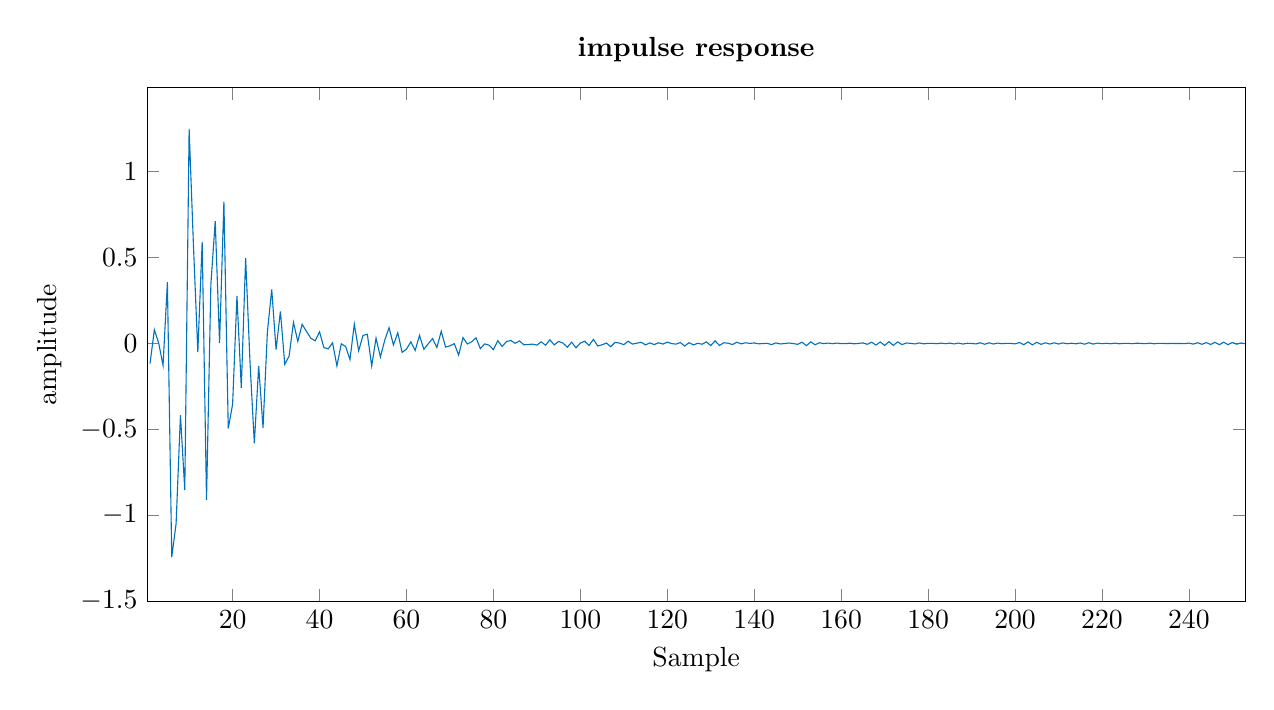
\begin{tikzpicture}

\begin{axis}[%
width=5.49in,
height=2.566in,
at={(1.011in,0.642in)},
scale only axis,
xmin=0.344142972512103,
xmax=252.945084796394,
xlabel={Sample},
ymin=-1.5,
ymax=1.4868804664723,
ylabel={amplitude},
axis background/.style={fill=white},
title style={font=\bfseries},
title={impulse response}
]
\addplot [color=mycolor1,solid,forget plot]
  table[row sep=crcr]{%
1	-0.118141562218072\\
1	-0.118141562218072\\
2	0.0791281785124607\\
2	0.0791281785124607\\
3	0.00109140883794252\\
3	0.00109140883794252\\
4	-0.127998430298182\\
4	-0.127998430298182\\
5	0.355751675486418\\
5	0.355751675486418\\
6	-1.24445909784893\\
6	-1.24445909784893\\
7	-1.04936802214079\\
7	-1.04936802214079\\
8	-0.418123407296711\\
8	-0.418123407296711\\
9	-0.853609016499564\\
9	-0.853609016499564\\
10	1.24815892007568\\
10	1.24815892007568\\
11	0.564683231877883\\
11	0.564683231877883\\
12	-0.0511791125132532\\
12	-0.0511791125132532\\
13	0.591079504687172\\
13	0.591079504687172\\
14	-0.911228401587671\\
14	-0.911228401587671\\
15	0.34212392225513\\
15	0.34212392225513\\
16	0.71167417099142\\
16	0.71167417099142\\
17	0.0022231516812417\\
17	0.0022231516812417\\
18	0.825359321003935\\
18	0.825359321003935\\
19	-0.495105852171416\\
19	-0.495105852171416\\
20	-0.354980390629405\\
20	-0.354980390629405\\
21	0.275904546024916\\
21	0.275904546024916\\
22	-0.259187854777998\\
22	-0.259187854777998\\
23	0.496375795390466\\
23	0.496375795390466\\
24	-0.107031671390095\\
24	-0.107031671390095\\
25	-0.582425217768152\\
25	-0.582425217768152\\
26	-0.131058795038014\\
26	-0.131058795038014\\
27	-0.491055535573922\\
27	-0.491055535573922\\
28	0.0652989205316153\\
28	0.0652989205316153\\
29	0.31411076610674\\
29	0.31411076610674\\
30	-0.0363555084229589\\
30	-0.0363555084229589\\
31	0.186377556816253\\
31	0.186377556816253\\
32	-0.122351410526851\\
32	-0.122351410526851\\
33	-0.0742300014448984\\
33	-0.0742300014448984\\
34	0.121765995454672\\
34	0.121765995454672\\
35	0.0120055808146089\\
35	0.0120055808146089\\
36	0.110948456873853\\
36	0.110948456873853\\
37	0.0692216392993395\\
37	0.0692216392993395\\
38	0.0299810369671249\\
38	0.0299810369671249\\
39	0.0144706736665758\\
39	0.0144706736665758\\
40	0.0670303556881637\\
40	0.0670303556881637\\
41	-0.0247644080799324\\
41	-0.0247644080799324\\
42	-0.031927855805956\\
42	-0.031927855805956\\
43	0.00322998704690307\\
43	0.00322998704690307\\
44	-0.131745511302458\\
44	-0.131745511302458\\
45	-0.00261033076288713\\
45	-0.00261033076288713\\
46	-0.0181125020290452\\
46	-0.0181125020290452\\
47	-0.0945138446649691\\
47	-0.0945138446649691\\
48	0.111436996915387\\
48	0.111436996915387\\
49	-0.0431351377461246\\
49	-0.0431351377461246\\
50	0.0461620756094456\\
50	0.0461620756094456\\
51	0.0531033344668851\\
51	0.0531033344668851\\
52	-0.131539836134088\\
52	-0.131539836134088\\
53	0.0305025240822609\\
53	0.0305025240822609\\
54	-0.0792119357439335\\
54	-0.0792119357439335\\
55	0.0183468383704305\\
55	0.0183468383704305\\
56	0.091370890352526\\
56	0.091370890352526\\
57	-0.00936150319799612\\
57	-0.00936150319799612\\
58	0.0615638871253384\\
58	0.0615638871253384\\
59	-0.0524944156191402\\
59	-0.0524944156191402\\
60	-0.0335821747505357\\
60	-0.0335821747505357\\
61	0.00892104929863474\\
61	0.00892104929863474\\
62	-0.0410628110921637\\
62	-0.0410628110921637\\
63	0.0464364992488124\\
63	0.0464364992488124\\
64	-0.0347539925926514\\
64	-0.0347539925926514\\
65	-0.0031920519174843\\
65	-0.0031920519174843\\
66	0.0278505098767845\\
66	0.0278505098767845\\
67	-0.0239093827261274\\
67	-0.0239093827261274\\
68	0.0700616510285207\\
68	0.0700616510285207\\
69	-0.0219341301905986\\
69	-0.0219341301905986\\
70	-0.0142230911242287\\
70	-0.0142230911242287\\
71	-0.00182073467961221\\
71	-0.00182073467961221\\
72	-0.0681129708309657\\
72	-0.0681129708309657\\
73	0.0334153987634728\\
73	0.0334153987634728\\
74	-0.00363938342836818\\
74	-0.00363938342836818\\
75	0.00914183511984331\\
75	0.00914183511984331\\
76	0.0321515049541257\\
76	0.0321515049541257\\
77	-0.0306798066110672\\
77	-0.0306798066110672\\
78	-0.00314839927224314\\
78	-0.00314839927224314\\
79	-0.0105024291640573\\
79	-0.0105024291640573\\
80	-0.0368012862919245\\
80	-0.0368012862919245\\
81	0.0155149120464149\\
81	0.0155149120464149\\
82	-0.0180951857625397\\
82	-0.0180951857625397\\
83	0.0103228815054031\\
83	0.0103228815054031\\
84	0.0169500794792463\\
84	0.0169500794792463\\
85	0.000310442154459831\\
85	0.000310442154459831\\
86	0.0140317610007087\\
86	0.0140317610007087\\
87	-0.00808289802810039\\
87	-0.00808289802810039\\
88	-0.00695942120163846\\
88	-0.00695942120163846\\
89	-0.00446733733759463\\
89	-0.00446733733759463\\
90	-0.0103115148570162\\
90	-0.0103115148570162\\
91	0.00899156239938577\\
91	0.00899156239938577\\
92	-0.0111136779230336\\
92	-0.0111136779230336\\
93	0.0203724396264147\\
93	0.0203724396264147\\
94	-0.00891067559850342\\
94	-0.00891067559850342\\
95	0.0111957345646422\\
95	0.0111957345646422\\
96	0.00161928607316594\\
96	0.00161928607316594\\
97	-0.0222011006626747\\
97	-0.0222011006626747\\
98	0.00705399101203549\\
98	0.00705399101203549\\
99	-0.0259264115095974\\
99	-0.0259264115095974\\
100	0.00127486462301934\\
100	0.00127486462301934\\
101	0.0124661338836067\\
101	0.0124661338836067\\
102	-0.0121720072937964\\
102	-0.0121720072937964\\
103	0.0229733095365205\\
103	0.0229733095365205\\
104	-0.015144764125669\\
104	-0.015144764125669\\
105	-0.00849436079781317\\
105	-0.00849436079781317\\
106	0.0020916766693437\\
106	0.0020916766693437\\
107	-0.0197042880875184\\
107	-0.0197042880875184\\
108	0.00590774994138175\\
108	0.00590774994138175\\
109	0.00142553758412932\\
109	0.00142553758412932\\
110	-0.00752781336578599\\
110	-0.00752781336578599\\
111	0.0124866500742295\\
111	0.0124866500742295\\
112	-0.00435439178335216\\
112	-0.00435439178335216\\
113	0.00144228670163819\\
113	0.00144228670163819\\
114	0.00581286574855189\\
114	0.00581286574855189\\
115	-0.00889141928378981\\
115	-0.00889141928378981\\
116	0.00274247544089457\\
116	0.00274247544089457\\
117	-0.00715328500349922\\
117	-0.00715328500349922\\
118	0.00343442489852638\\
118	0.00343442489852638\\
119	-0.00430672794128714\\
119	-0.00430672794128714\\
120	0.00719938952165628\\
120	0.00719938952165628\\
121	-0.0014601383401962\\
121	-0.0014601383401962\\
122	-0.00464951867639746\\
122	-0.00464951867639746\\
123	0.00484835116232913\\
123	0.00484835116232913\\
124	-0.0159239102642369\\
124	-0.0159239102642369\\
125	0.00414543117078109\\
125	0.00414543117078109\\
126	-0.00923141916662314\\
126	-0.00923141916662314\\
127	0.000492682295719719\\
127	0.000492682295719719\\
128	-0.0051865152342738\\
128	-0.0051865152342738\\
129	0.00879738745875531\\
129	0.00879738745875531\\
130	-0.0129254192936449\\
130	-0.0129254192936449\\
131	0.0150618586089381\\
131	0.0150618586089381\\
132	-0.0123298476334175\\
132	-0.0123298476334175\\
133	0.00356672143985635\\
133	0.00356672143985635\\
134	0.000635666567859052\\
134	0.000635666567859052\\
135	-0.00688542560476631\\
135	-0.00688542560476631\\
136	0.00647553377876287\\
136	0.00647553377876287\\
137	-0.00313869095969953\\
137	-0.00313869095969953\\
138	0.00338234865059637\\
138	0.00338234865059637\\
139	-0.000421084566326661\\
139	-0.000421084566326661\\
140	0.00250712752529129\\
140	0.00250712752529129\\
141	-0.00294288518799757\\
141	-0.00294288518799757\\
142	-0.0010102542496694\\
142	-0.0010102542496694\\
143	-0.000252409752983782\\
143	-0.000252409752983782\\
144	-0.00709280368191718\\
144	-0.00709280368191718\\
145	0.00273457138739201\\
145	0.00273457138739201\\
146	-0.00349492542841067\\
146	-0.00349492542841067\\
147	-0.0011987832037849\\
147	-0.0011987832037849\\
148	0.00204220837683377\\
148	0.00204220837683377\\
149	-0.00130776580642774\\
149	-0.00130776580642774\\
150	-0.0056427908397797\\
150	-0.0056427908397797\\
151	0.00640825158781991\\
151	0.00640825158781991\\
152	-0.0134753340471952\\
152	-0.0134753340471952\\
153	0.00874106945549123\\
153	0.00874106945549123\\
154	-0.00817595376743767\\
154	-0.00817595376743767\\
155	0.00346206620492773\\
155	0.00346206620492773\\
156	-0.00148108262860179\\
156	-0.00148108262860179\\
157	0.00159664856954663\\
157	0.00159664856954663\\
158	-0.00207774499103393\\
158	-0.00207774499103393\\
159	0.00158755993228967\\
159	0.00158755993228967\\
160	-0.00187606529560944\\
160	-0.00187606529560944\\
161	-0.0018285497587921\\
161	-0.0018285497587921\\
162	0.000959440112494838\\
162	0.000959440112494838\\
163	-0.00260830328383853\\
163	-0.00260830328383853\\
164	-0.000344112649687174\\
164	-0.000344112649687174\\
165	0.00255734485088457\\
165	0.00255734485088457\\
166	-0.00559677227976574\\
166	-0.00559677227976574\\
167	0.00666099057503437\\
167	0.00666099057503437\\
168	-0.00978142524505918\\
168	-0.00978142524505918\\
169	0.00778894342302596\\
169	0.00778894342302596\\
170	-0.0118679731491987\\
170	-0.0118679731491987\\
171	0.00950293873394341\\
171	0.00950293873394341\\
172	-0.011731446451187\\
172	-0.011731446451187\\
173	0.00845382399693906\\
173	0.00845382399693906\\
174	-0.00711138169847137\\
174	-0.00711138169847137\\
175	0.00213548642487268\\
175	0.00213548642487268\\
176	-5.85596460445852e-05\\
176	-5.85596460445852e-05\\
177	-0.00346976620662964\\
177	-0.00346976620662964\\
178	0.00266301217400429\\
178	0.00266301217400429\\
179	-0.00296703845816892\\
179	-0.00296703845816892\\
180	0.000124808195676521\\
180	0.000124808195676521\\
181	0.000142004740926337\\
181	0.000142004740926337\\
182	-0.00201581494127819\\
182	-0.00201581494127819\\
183	0.00136029364750051\\
183	0.00136029364750051\\
184	-0.0020858974900481\\
184	-0.0020858974900481\\
185	0.00131358449326331\\
185	0.00131358449326331\\
186	-0.00342799294410937\\
186	-0.00342799294410937\\
187	0.00159784037109706\\
187	0.00159784037109706\\
188	-0.00398829538564302\\
188	-0.00398829538564302\\
189	0.000416626602851866\\
189	0.000416626602851866\\
190	-0.000647140406921486\\
190	-0.000647140406921486\\
191	-0.00322830047473305\\
191	-0.00322830047473305\\
192	0.00317533194550781\\
192	0.00317533194550781\\
193	-0.00524668903136873\\
193	-0.00524668903136873\\
194	0.00328829223179929\\
194	0.00328829223179929\\
195	-0.00380800282688818\\
195	-0.00380800282688818\\
196	0.0015429504716805\\
196	0.0015429504716805\\
197	-0.00205915720933898\\
197	-0.00205915720933898\\
198	0.000169343616457016\\
198	0.000169343616457016\\
199	-1.94896363292676e-05\\
199	-1.94896363292676e-05\\
200	-0.00314718231332176\\
200	-0.00314718231332176\\
201	0.00488601419939295\\
201	0.00488601419939295\\
202	-0.00801298194159633\\
202	-0.00801298194159633\\
203	0.00835245107822657\\
203	0.00835245107822657\\
204	-0.00897724713721908\\
204	-0.00897724713721908\\
205	0.00614816265226835\\
205	0.00614816265226835\\
206	-0.00580773871813518\\
206	-0.00580773871813518\\
207	0.00330708796282231\\
207	0.00330708796282231\\
208	-0.0042502001375543\\
208	-0.0042502001375543\\
209	0.00318711451318226\\
209	0.00318711451318226\\
210	-0.00389261618655835\\
210	-0.00389261618655835\\
211	0.00217287506811931\\
211	0.00217287506811931\\
212	-0.00225153595128867\\
212	-0.00225153595128867\\
213	0.00064487097645708\\
213	0.00064487097645708\\
214	-0.00262627810428138\\
214	-0.00262627810428138\\
215	0.00216492706444699\\
215	0.00216492706444699\\
216	-0.00501031331995221\\
216	-0.00501031331995221\\
217	0.00345919904440867\\
217	0.00345919904440867\\
218	-0.00433586131657449\\
218	-0.00433586131657449\\
219	0.00154231988745107\\
219	0.00154231988745107\\
220	-0.00198063731082455\\
220	-0.00198063731082455\\
221	0.000416444228293499\\
221	0.000416444228293499\\
222	-0.00228271657882294\\
222	-0.00228271657882294\\
223	0.00115333286600893\\
223	0.00115333286600893\\
224	-0.00241598423363702\\
224	-0.00241598423363702\\
225	-5.09471217824708e-05\\
225	-5.09471217824708e-05\\
226	0.000208671836863114\\
226	0.000208671836863114\\
227	-0.00206397328677561\\
227	-0.00206397328677561\\
228	0.000976785016822535\\
228	0.000976785016822535\\
229	-0.000535693054502294\\
229	-0.000535693054502294\\
230	-0.00188323750833553\\
230	-0.00188323750833553\\
231	0.00131001909170588\\
231	0.00131001909170588\\
232	-0.00243251712101864\\
232	-0.00243251712101864\\
233	-0.000118515677414382\\
233	-0.000118515677414382\\
234	-0.000432814061260125\\
234	-0.000432814061260125\\
235	-0.00131759161870752\\
235	-0.00131759161870752\\
236	-0.000524844285814698\\
236	-0.000524844285814698\\
237	-0.000598699726453522\\
237	-0.000598699726453522\\
238	-0.000709887660179469\\
238	-0.000709887660179469\\
239	-0.00165499475232057\\
239	-0.00165499475232057\\
240	0.00156604948120072\\
240	0.00156604948120072\\
241	-0.00438046374307205\\
241	-0.00438046374307205\\
242	0.00360696249179117\\
242	0.00360696249179117\\
243	-0.00560346639516965\\
243	-0.00560346639516965\\
244	0.00434937167572154\\
244	0.00434937167572154\\
245	-0.00623469069097805\\
245	-0.00623469069097805\\
246	0.00589186342140169\\
246	0.00589186342140169\\
247	-0.00785971118716415\\
247	-0.00785971118716415\\
248	0.00665880002740227\\
248	0.00665880002740227\\
249	-0.00761918755737151\\
249	-0.00761918755737151\\
250	0.00490902237270174\\
250	0.00490902237270174\\
251	-0.00499083265681984\\
251	-0.00499083265681984\\
252	0.00245856956180693\\
252	0.00245856956180693\\
253	-0.00271993135747834\\
253	-0.00271993135747834\\
253	-0.00271993135747834\\
253	-0.00271993135747834\\
253	-0.00271993135747834\\
253	-0.00271993135747834\\
253	-0.00271993135747834\\
253	-0.00271993135747834\\
253	-0.00271993135747834\\
253	-0.00271993135747834\\
253	-0.00271993135747834\\
253	-0.00271993135747834\\
253	-0.00271993135747834\\
253	-0.00271993135747834\\
253	-0.00271993135747834\\
253	-0.00271993135747834\\
253	-0.00271993135747834\\
253	-0.00271993135747834\\
253	-0.00271993135747834\\
253	-0.00271993135747834\\
253	-0.00271993135747834\\
253	-0.00271993135747834\\
253	-0.00271993135747834\\
253	-0.00271993135747834\\
253	-0.00271993135747834\\
253	-0.00271993135747834\\
253	-0.00271993135747834\\
253	-0.00271993135747834\\
253	-0.00271993135747834\\
253	-0.00271993135747834\\
253	-0.00271993135747834\\
253	-0.00271993135747834\\
253	-0.00271993135747834\\
253	-0.00271993135747834\\
253	-0.00271993135747834\\
253	-0.00271993135747834\\
253	-0.00271993135747834\\
253	-0.00271993135747834\\
253	-0.00271993135747834\\
253	-0.00271993135747834\\
253	-0.00271993135747834\\
253	-0.00271993135747834\\
253	-0.00271993135747834\\
253	-0.00271993135747834\\
253	-0.00271993135747834\\
253	-0.00271993135747834\\
253	-0.00271993135747834\\
253	-0.00271993135747834\\
253	-0.00271993135747834\\
253	-0.00271993135747834\\
253	-0.00271993135747834\\
253	-0.00271993135747834\\
253	-0.00271993135747834\\
253	-0.00271993135747834\\
253	-0.00271993135747834\\
253	-0.00271993135747834\\
253	-0.00271993135747834\\
253	-0.00271993135747834\\
253	-0.00271993135747834\\
253	-0.00271993135747834\\
253	-0.00271993135747834\\
253	-0.00271993135747834\\
253	-0.00271993135747834\\
253	-0.00271993135747834\\
253	-0.00271993135747834\\
253	-0.00271993135747834\\
253	-0.00271993135747834\\
253	-0.00271993135747834\\
253	-0.00271993135747834\\
253	-0.00271993135747834\\
253	-0.00271993135747834\\
253	-0.00271993135747834\\
253	-0.00271993135747834\\
253	-0.00271993135747834\\
253	-0.00271993135747834\\
253	-0.00271993135747834\\
253	-0.00271993135747834\\
253	-0.00271993135747834\\
253	-0.00271993135747834\\
253	-0.00271993135747834\\
253	-0.00271993135747834\\
253	-0.00271993135747834\\
253	-0.00271993135747834\\
253	-0.00271993135747834\\
253	-0.00271993135747834\\
253	-0.00271993135747834\\
253	-0.00271993135747834\\
253	-0.00271993135747834\\
253	-0.00271993135747834\\
253	-0.00271993135747834\\
253	-0.00271993135747834\\
253	-0.00271993135747834\\
253	-0.00271993135747834\\
253	-0.00271993135747834\\
253	-0.00271993135747834\\
253	-0.00271993135747834\\
253	-0.00271993135747834\\
253	-0.00271993135747834\\
253	-0.00271993135747834\\
253	-0.00271993135747834\\
253	-0.00271993135747834\\
253	-0.00271993135747834\\
253	-0.00271993135747834\\
253	-0.00271993135747834\\
253	-0.00271993135747834\\
253	-0.00271993135747834\\
253	-0.00271993135747834\\
253	-0.00271993135747834\\
253	-0.00271993135747834\\
253	-0.00271993135747834\\
253	-0.00271993135747834\\
253	-0.00271993135747834\\
253	-0.00271993135747834\\
253	-0.00271993135747834\\
253	-0.00271993135747834\\
253	-0.00271993135747834\\
253	-0.00271993135747834\\
253	-0.00271993135747834\\
253	-0.00271993135747834\\
253	-0.00271993135747834\\
253	-0.00271993135747834\\
253	-0.00271993135747834\\
253	-0.00271993135747834\\
253	-0.00271993135747834\\
253	-0.00271993135747834\\
253	-0.00271993135747834\\
253	-0.00271993135747834\\
253	-0.00271993135747834\\
253	-0.00271993135747834\\
253	-0.00271993135747834\\
253	-0.00271993135747834\\
253	-0.00271993135747834\\
253	-0.00271993135747834\\
253	-0.00271993135747834\\
253	-0.00271993135747834\\
253	-0.00271993135747834\\
253	-0.00271993135747834\\
253	-0.00271993135747834\\
253	-0.00271993135747834\\
253	-0.00271993135747834\\
253	-0.00271993135747834\\
253	-0.00271993135747834\\
253	-0.00271993135747834\\
253	-0.00271993135747834\\
253	-0.00271993135747834\\
253	-0.00271993135747834\\
253	-0.00271993135747834\\
253	-0.00271993135747834\\
253	-0.00271993135747834\\
253	-0.00271993135747834\\
253	-0.00271993135747834\\
253	-0.00271993135747834\\
253	-0.00271993135747834\\
253	-0.00271993135747834\\
253	-0.00271993135747834\\
253	-0.00271993135747834\\
253	-0.00271993135747834\\
253	-0.00271993135747834\\
253	-0.00271993135747834\\
253	-0.00271993135747834\\
253	-0.00271993135747834\\
253	-0.00271993135747834\\
253	-0.00271993135747834\\
253	-0.00271993135747834\\
253	-0.00271993135747834\\
253	-0.00271993135747834\\
253	-0.00271993135747834\\
253	-0.00271993135747834\\
253	-0.00271993135747834\\
253	-0.00271993135747834\\
253	-0.00271993135747834\\
253	-0.00271993135747834\\
253	-0.00271993135747834\\
253	-0.00271993135747834\\
253	-0.00271993135747834\\
253	-0.00271993135747834\\
253	-0.00271993135747834\\
253	-0.00271993135747834\\
253	-0.00271993135747834\\
253	-0.00271993135747834\\
253	-0.00271993135747834\\
253	-0.00271993135747834\\
253	-0.00271993135747834\\
253	-0.00271993135747834\\
253	-0.00271993135747834\\
253	-0.00271993135747834\\
253	-0.00271993135747834\\
253	-0.00271993135747834\\
253	-0.00271993135747834\\
253	-0.00271993135747834\\
253	-0.00271993135747834\\
253	-0.00271993135747834\\
253	-0.00271993135747834\\
253	-0.00271993135747834\\
253	-0.00271993135747834\\
253	-0.00271993135747834\\
253	-0.00271993135747834\\
253	-0.00271993135747834\\
253	-0.00271993135747834\\
253	-0.00271993135747834\\
253	-0.00271993135747834\\
253	-0.00271993135747834\\
253	-0.00271993135747834\\
253	-0.00271993135747834\\
253	-0.00271993135747834\\
253	-0.00271993135747834\\
253	-0.00271993135747834\\
253	-0.00271993135747834\\
253	-0.00271993135747834\\
253	-0.00271993135747834\\
253	-0.00271993135747834\\
253	-0.00271993135747834\\
253	-0.00271993135747834\\
253	-0.00271993135747834\\
253	-0.00271993135747834\\
253	-0.00271993135747834\\
253	-0.00271993135747834\\
253	-0.00271993135747834\\
253	-0.00271993135747834\\
253	-0.00271993135747834\\
253	-0.00271993135747834\\
253	-0.00271993135747834\\
253	-0.00271993135747834\\
253	-0.00271993135747834\\
253	-0.00271993135747834\\
253	-0.00271993135747834\\
253	-0.00271993135747834\\
253	-0.00271993135747834\\
253	-0.00271993135747834\\
253	-0.00271993135747834\\
253	-0.00271993135747834\\
253	-0.00271993135747834\\
253	-0.00271993135747834\\
253	-0.00271993135747834\\
253	-0.00271993135747834\\
253	-0.00271993135747834\\
253	-0.00271993135747834\\
253	-0.00271993135747834\\
253	-0.00271993135747834\\
253	-0.00271993135747834\\
253	-0.00271993135747834\\
253	-0.00271993135747834\\
253	-0.00271993135747834\\
253	-0.00271993135747834\\
253	-0.00271993135747834\\
253	-0.00271993135747834\\
253	-0.00271993135747834\\
253	-0.00271993135747834\\
253	-0.00271993135747834\\
253	-0.00271993135747834\\
253	-0.00271993135747834\\
253	-0.00271993135747834\\
253	-0.00271993135747834\\
253	-0.00271993135747834\\
253	-0.00271993135747834\\
253	-0.00271993135747834\\
253	-0.00271993135747834\\
253	-0.00271993135747834\\
253	-0.00271993135747834\\
253	-0.00271993135747834\\
253	-0.00271993135747834\\
253	-0.00271993135747834\\
253	-0.00271993135747834\\
253	-0.00271993135747834\\
253	-0.00271993135747834\\
253	-0.00271993135747834\\
253	-0.00271993135747834\\
253	-0.00271993135747834\\
253	-0.00271993135747834\\
253	-0.00271993135747834\\
253	-0.00271993135747834\\
253	-0.00271993135747834\\
253	-0.00271993135747834\\
253	-0.00271993135747834\\
253	-0.00271993135747834\\
253	-0.00271993135747834\\
253	-0.00271993135747834\\
253	-0.00271993135747834\\
253	-0.00271993135747834\\
253	-0.00271993135747834\\
253	-0.00271993135747834\\
253	-0.00271993135747834\\
253	-0.00271993135747834\\
253	-0.00271993135747834\\
253	-0.00271993135747834\\
253	-0.00271993135747834\\
253	-0.00271993135747834\\
253	-0.00271993135747834\\
253	-0.00271993135747834\\
253	-0.00271993135747834\\
253	-0.00271993135747834\\
253	-0.00271993135747834\\
253	-0.00271993135747834\\
253	-0.00271993135747834\\
253	-0.00271993135747834\\
253	-0.00271993135747834\\
253	-0.00271993135747834\\
253	-0.00271993135747834\\
253	-0.00271993135747834\\
253	-0.00271993135747834\\
253	-0.00271993135747834\\
253	-0.00271993135747834\\
253	-0.00271993135747834\\
253	-0.00271993135747834\\
253	-0.00271993135747834\\
253	-0.00271993135747834\\
253	-0.00271993135747834\\
253	-0.00271993135747834\\
253	-0.00271993135747834\\
253	-0.00271993135747834\\
253	-0.00271993135747834\\
253	-0.00271993135747834\\
253	-0.00271993135747834\\
253	-0.00271993135747834\\
253	-0.00271993135747834\\
253	-0.00271993135747834\\
253	-0.00271993135747834\\
253	-0.00271993135747834\\
253	-0.00271993135747834\\
253	-0.00271993135747834\\
253	-0.00271993135747834\\
253	-0.00271993135747834\\
253	-0.00271993135747834\\
253	-0.00271993135747834\\
253	-0.00271993135747834\\
253	-0.00271993135747834\\
253	-0.00271993135747834\\
253	-0.00271993135747834\\
253	-0.00271993135747834\\
253	-0.00271993135747834\\
253	-0.00271993135747834\\
253	-0.00271993135747834\\
253	-0.00271993135747834\\
253	-0.00271993135747834\\
253	-0.00271993135747834\\
253	-0.00271993135747834\\
253	-0.00271993135747834\\
253	-0.00271993135747834\\
253	-0.00271993135747834\\
253	-0.00271993135747834\\
253	-0.00271993135747834\\
253	-0.00271993135747834\\
253	-0.00271993135747834\\
253	-0.00271993135747834\\
253	-0.00271993135747834\\
253	-0.00271993135747834\\
253	-0.00271993135747834\\
253	-0.00271993135747834\\
253	-0.00271993135747834\\
253	-0.00271993135747834\\
253	-0.00271993135747834\\
253	-0.00271993135747834\\
253	-0.00271993135747834\\
253	-0.00271993135747834\\
253	-0.00271993135747834\\
253	-0.00271993135747834\\
253	-0.00271993135747834\\
253	-0.00271993135747834\\
253	-0.00271993135747834\\
253	-0.00271993135747834\\
253	-0.00271993135747834\\
253	-0.00271993135747834\\
253	-0.00271993135747834\\
253	-0.00271993135747834\\
};
\end{axis}
\end{tikzpicture}%
	\caption{Cropped impulse response plot of the cancellation path}
	\label{CancellationPathImpulseResponseCrop}
\end{figure}

To verify that the frequency response of the cropped impulse response approximately equals that of the non-cropped impulse response the two frequency responses are compared. This can be seen on \autoref{CancellationPathImpulseResponseCompare}. Note that the two lines are almost completely on top of each other.

\begin{figure}[H]
	\centering
	\tikzsetnextfilename{CancellationPathImpulseResponseCompare1}
	%% This file was created by matlab2tikz.
%
%The latest updates can be retrieved from
%  http://www.mathworks.com/matlabcentral/fileexchange/22022-matlab2tikz-matlab2tikz
%where you can also make suggestions and rate matlab2tikz.
%
\definecolor{mycolor1}{rgb}{0.00000,0.44700,0.74100}%
\definecolor{mycolor2}{rgb}{0.85000,0.32500,0.09800}%
%
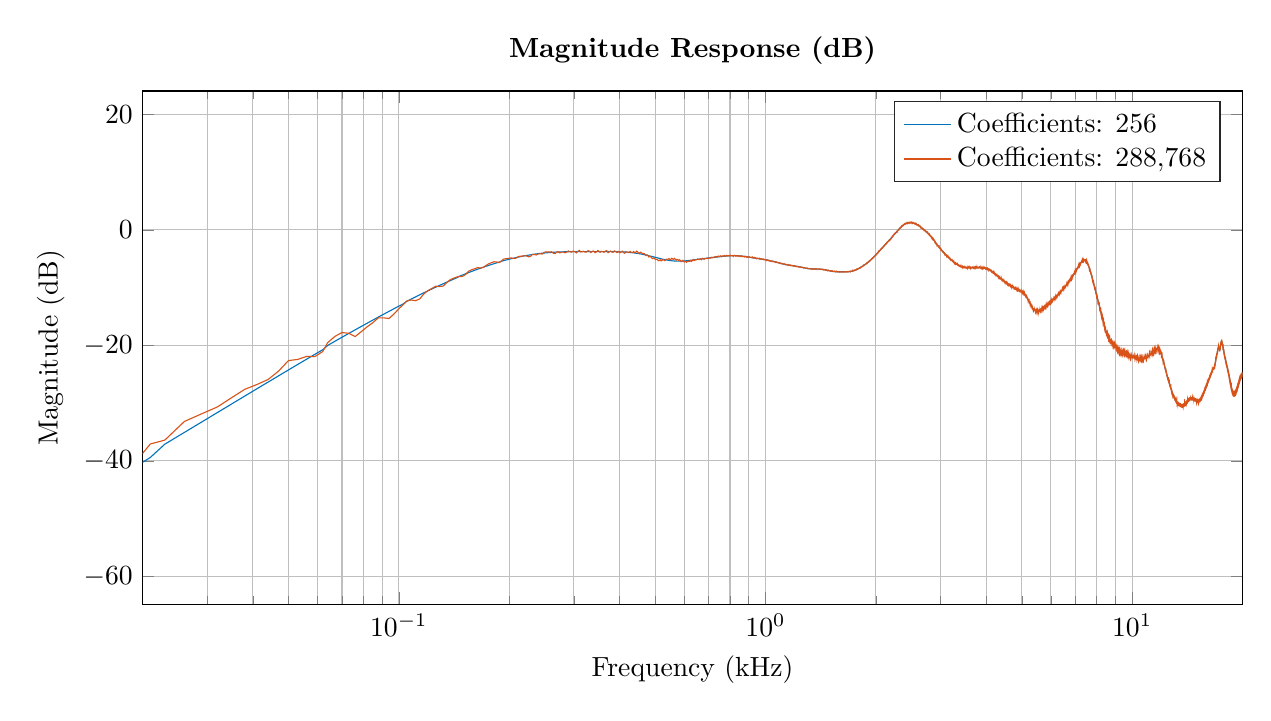
\begin{tikzpicture}

\begin{axis}[%
width=5.5in,
height=2.566in,
at={(2.804in,1.205in)},
scale only axis,
xmode=log,
xmin=0.020,
xmax=20.000,
xminorticks=true,
xlabel={Frequency (kHz)},
xmajorgrids,
xminorgrids,
ymin=-64.832,
ymax=24.080,
ylabel={Magnitude (dB)},
ymajorgrids,
axis background/.style={fill=white},
title style={font=\bfseries},
title={Magnitude Response (dB)},
legend style={legend cell align=left,align=left,draw=white!15!black}
]
\addplot [color=mycolor1,solid,forget plot]
  table[row sep=crcr]{%
0.018	-42.077\\
0.021	-39.419\\
0.023	-37.115\\
0.026	-35.084\\
0.029	-33.272\\
0.032	-31.636\\
0.035	-30.148\\
0.038	-28.784\\
0.041	-27.525\\
0.044	-26.358\\
0.047	-25.271\\
0.050	-24.254\\
0.053	-23.301\\
0.056	-22.403\\
0.059	-21.556\\
0.062	-20.755\\
0.064	-19.995\\
0.067	-19.274\\
0.070	-18.589\\
0.073	-17.935\\
0.076	-17.312\\
0.079	-16.718\\
0.082	-16.149\\
0.085	-15.605\\
0.088	-15.083\\
0.091	-14.584\\
0.094	-14.105\\
0.097	-13.645\\
0.100	-13.203\\
0.103	-12.779\\
0.105	-12.371\\
0.108	-11.979\\
0.111	-11.602\\
0.114	-11.239\\
0.117	-10.890\\
0.120	-10.554\\
0.123	-10.231\\
0.126	-9.920\\
0.129	-9.620\\
0.132	-9.332\\
0.135	-9.055\\
0.138	-8.788\\
0.141	-8.531\\
0.144	-8.284\\
0.146	-8.046\\
0.149	-7.818\\
0.152	-7.598\\
0.155	-7.387\\
0.158	-7.184\\
0.161	-6.990\\
0.164	-6.803\\
0.167	-6.624\\
0.170	-6.452\\
0.173	-6.288\\
0.176	-6.131\\
0.179	-5.980\\
0.182	-5.836\\
0.185	-5.699\\
0.188	-5.568\\
0.190	-5.443\\
0.193	-5.324\\
0.196	-5.211\\
0.199	-5.103\\
0.202	-5.001\\
0.205	-4.904\\
0.208	-4.813\\
0.211	-4.727\\
0.214	-4.645\\
0.217	-4.568\\
0.220	-4.496\\
0.223	-4.428\\
0.226	-4.365\\
0.229	-4.306\\
0.231	-4.251\\
0.234	-4.199\\
0.237	-4.152\\
0.240	-4.108\\
0.243	-4.068\\
0.246	-4.030\\
0.249	-3.996\\
0.252	-3.965\\
0.255	-3.937\\
0.258	-3.912\\
0.261	-3.889\\
0.264	-3.869\\
0.267	-3.850\\
0.270	-3.834\\
0.272	-3.820\\
0.275	-3.808\\
0.278	-3.798\\
0.281	-3.789\\
0.284	-3.781\\
0.287	-3.775\\
0.290	-3.770\\
0.293	-3.766\\
0.296	-3.763\\
0.299	-3.760\\
0.302	-3.759\\
0.305	-3.758\\
0.308	-3.757\\
0.311	-3.757\\
0.313	-3.757\\
0.316	-3.757\\
0.319	-3.757\\
0.322	-3.757\\
0.325	-3.758\\
0.328	-3.758\\
0.331	-3.758\\
0.334	-3.758\\
0.337	-3.759\\
0.340	-3.758\\
0.343	-3.758\\
0.346	-3.758\\
0.349	-3.758\\
0.352	-3.757\\
0.354	-3.757\\
0.357	-3.756\\
0.360	-3.756\\
0.363	-3.755\\
0.366	-3.755\\
0.369	-3.755\\
0.372	-3.755\\
0.375	-3.756\\
0.378	-3.757\\
0.381	-3.758\\
0.384	-3.760\\
0.387	-3.763\\
0.390	-3.767\\
0.393	-3.771\\
0.396	-3.776\\
0.398	-3.782\\
0.401	-3.789\\
0.404	-3.797\\
0.407	-3.806\\
0.410	-3.816\\
0.413	-3.827\\
0.416	-3.840\\
0.419	-3.854\\
0.422	-3.870\\
0.425	-3.886\\
0.428	-3.905\\
0.431	-3.924\\
0.434	-3.945\\
0.437	-3.968\\
0.439	-3.992\\
0.442	-4.017\\
0.445	-4.044\\
0.448	-4.072\\
0.451	-4.102\\
0.454	-4.133\\
0.457	-4.165\\
0.460	-4.198\\
0.463	-4.233\\
0.466	-4.269\\
0.469	-4.305\\
0.472	-4.343\\
0.475	-4.382\\
0.478	-4.421\\
0.480	-4.461\\
0.483	-4.502\\
0.486	-4.543\\
0.489	-4.585\\
0.492	-4.627\\
0.495	-4.668\\
0.498	-4.710\\
0.501	-4.752\\
0.504	-4.793\\
0.507	-4.834\\
0.510	-4.874\\
0.513	-4.914\\
0.516	-4.953\\
0.519	-4.991\\
0.521	-5.028\\
0.524	-5.063\\
0.527	-5.097\\
0.530	-5.130\\
0.533	-5.161\\
0.536	-5.191\\
0.539	-5.219\\
0.542	-5.245\\
0.545	-5.269\\
0.548	-5.291\\
0.551	-5.312\\
0.554	-5.330\\
0.557	-5.346\\
0.560	-5.361\\
0.562	-5.373\\
0.565	-5.383\\
0.568	-5.391\\
0.571	-5.398\\
0.574	-5.402\\
0.577	-5.405\\
0.580	-5.405\\
0.583	-5.405\\
0.586	-5.402\\
0.589	-5.398\\
0.592	-5.392\\
0.595	-5.386\\
0.598	-5.377\\
0.601	-5.368\\
0.604	-5.358\\
0.606	-5.346\\
0.609	-5.334\\
0.612	-5.321\\
0.615	-5.307\\
0.618	-5.293\\
0.621	-5.278\\
0.624	-5.263\\
0.627	-5.247\\
0.630	-5.231\\
0.633	-5.215\\
0.636	-5.199\\
0.639	-5.182\\
0.642	-5.166\\
0.645	-5.149\\
0.647	-5.133\\
0.650	-5.116\\
0.653	-5.100\\
0.656	-5.084\\
0.659	-5.068\\
0.662	-5.052\\
0.665	-5.036\\
0.668	-5.021\\
0.671	-5.005\\
0.674	-4.990\\
0.677	-4.975\\
0.680	-4.960\\
0.683	-4.946\\
0.686	-4.931\\
0.688	-4.917\\
0.691	-4.902\\
0.694	-4.888\\
0.697	-4.874\\
0.700	-4.860\\
0.703	-4.847\\
0.706	-4.833\\
0.709	-4.819\\
0.712	-4.806\\
0.715	-4.792\\
0.718	-4.778\\
0.721	-4.765\\
0.724	-4.751\\
0.727	-4.738\\
0.729	-4.725\\
0.732	-4.711\\
0.735	-4.698\\
0.738	-4.685\\
0.741	-4.672\\
0.744	-4.659\\
0.747	-4.646\\
0.750	-4.633\\
0.753	-4.621\\
0.756	-4.608\\
0.759	-4.596\\
0.762	-4.584\\
0.765	-4.573\\
0.768	-4.561\\
0.771	-4.550\\
0.773	-4.540\\
0.776	-4.530\\
0.779	-4.520\\
0.782	-4.511\\
0.785	-4.502\\
0.788	-4.494\\
0.791	-4.487\\
0.794	-4.480\\
0.797	-4.473\\
0.800	-4.468\\
0.803	-4.463\\
0.806	-4.458\\
0.809	-4.455\\
0.812	-4.452\\
0.814	-4.450\\
0.817	-4.449\\
0.820	-4.449\\
0.823	-4.449\\
0.826	-4.450\\
0.829	-4.452\\
0.832	-4.455\\
0.835	-4.459\\
0.838	-4.463\\
0.841	-4.469\\
0.844	-4.475\\
0.847	-4.481\\
0.850	-4.489\\
0.853	-4.497\\
0.855	-4.506\\
0.858	-4.516\\
0.861	-4.526\\
0.864	-4.537\\
0.867	-4.548\\
0.870	-4.560\\
0.873	-4.573\\
0.876	-4.586\\
0.879	-4.599\\
0.882	-4.613\\
0.885	-4.627\\
0.888	-4.641\\
0.891	-4.656\\
0.894	-4.671\\
0.896	-4.686\\
0.899	-4.701\\
0.902	-4.716\\
0.905	-4.732\\
0.908	-4.747\\
0.911	-4.762\\
0.914	-4.778\\
0.917	-4.793\\
0.920	-4.808\\
0.923	-4.823\\
0.926	-4.838\\
0.929	-4.852\\
0.932	-4.867\\
0.935	-4.881\\
0.938	-4.895\\
0.940	-4.909\\
0.943	-4.923\\
0.946	-4.937\\
0.949	-4.950\\
0.952	-4.963\\
0.955	-4.976\\
0.958	-4.989\\
0.961	-5.001\\
0.964	-5.014\\
0.967	-5.026\\
0.970	-5.039\\
0.973	-5.051\\
0.976	-5.063\\
0.979	-5.075\\
0.981	-5.088\\
0.984	-5.100\\
0.987	-5.112\\
0.990	-5.125\\
0.993	-5.138\\
0.996	-5.150\\
0.999	-5.164\\
1.002	-5.177\\
1.005	-5.190\\
1.008	-5.204\\
1.011	-5.219\\
1.014	-5.233\\
1.017	-5.248\\
1.020	-5.263\\
1.022	-5.279\\
1.025	-5.295\\
1.028	-5.311\\
1.031	-5.328\\
1.034	-5.345\\
1.037	-5.362\\
1.040	-5.380\\
1.043	-5.398\\
1.046	-5.417\\
1.049	-5.436\\
1.052	-5.455\\
1.055	-5.475\\
1.058	-5.494\\
1.061	-5.515\\
1.063	-5.535\\
1.066	-5.555\\
1.069	-5.576\\
1.072	-5.597\\
1.075	-5.618\\
1.078	-5.638\\
1.081	-5.659\\
1.084	-5.680\\
1.087	-5.701\\
1.090	-5.721\\
1.093	-5.742\\
1.096	-5.762\\
1.099	-5.782\\
1.102	-5.802\\
1.104	-5.821\\
1.107	-5.841\\
1.110	-5.859\\
1.113	-5.878\\
1.116	-5.896\\
1.119	-5.913\\
1.122	-5.930\\
1.125	-5.947\\
1.128	-5.963\\
1.131	-5.978\\
1.134	-5.994\\
1.137	-6.008\\
1.140	-6.022\\
1.143	-6.036\\
1.146	-6.049\\
1.148	-6.062\\
1.151	-6.074\\
1.154	-6.086\\
1.157	-6.098\\
1.160	-6.109\\
1.163	-6.120\\
1.166	-6.130\\
1.169	-6.140\\
1.172	-6.150\\
1.175	-6.160\\
1.178	-6.170\\
1.181	-6.179\\
1.184	-6.189\\
1.187	-6.198\\
1.189	-6.208\\
1.192	-6.217\\
1.195	-6.227\\
1.198	-6.236\\
1.201	-6.246\\
1.204	-6.256\\
1.207	-6.266\\
1.210	-6.276\\
1.213	-6.287\\
1.216	-6.298\\
1.219	-6.309\\
1.222	-6.320\\
1.225	-6.331\\
1.228	-6.343\\
1.230	-6.355\\
1.233	-6.368\\
1.236	-6.380\\
1.239	-6.393\\
1.242	-6.406\\
1.245	-6.420\\
1.248	-6.433\\
1.251	-6.447\\
1.254	-6.461\\
1.257	-6.475\\
1.260	-6.489\\
1.263	-6.503\\
1.266	-6.517\\
1.269	-6.531\\
1.271	-6.545\\
1.274	-6.559\\
1.277	-6.573\\
1.280	-6.587\\
1.283	-6.600\\
1.286	-6.613\\
1.289	-6.626\\
1.292	-6.638\\
1.295	-6.650\\
1.298	-6.661\\
1.301	-6.672\\
1.304	-6.683\\
1.307	-6.693\\
1.310	-6.702\\
1.312	-6.711\\
1.315	-6.720\\
1.318	-6.727\\
1.321	-6.734\\
1.324	-6.741\\
1.327	-6.747\\
1.330	-6.752\\
1.333	-6.757\\
1.336	-6.761\\
1.339	-6.765\\
1.342	-6.768\\
1.345	-6.770\\
1.348	-6.772\\
1.351	-6.774\\
1.354	-6.775\\
1.356	-6.776\\
1.359	-6.777\\
1.362	-6.777\\
1.365	-6.777\\
1.368	-6.777\\
1.371	-6.777\\
1.374	-6.777\\
1.377	-6.777\\
1.380	-6.777\\
1.383	-6.777\\
1.386	-6.777\\
1.389	-6.777\\
1.392	-6.778\\
1.395	-6.778\\
1.397	-6.780\\
1.400	-6.781\\
1.403	-6.783\\
1.406	-6.785\\
1.409	-6.788\\
1.412	-6.791\\
1.415	-6.795\\
1.418	-6.800\\
1.421	-6.804\\
1.424	-6.810\\
1.427	-6.816\\
1.430	-6.823\\
1.433	-6.830\\
1.436	-6.837\\
1.438	-6.846\\
1.441	-6.855\\
1.444	-6.864\\
1.447	-6.874\\
1.450	-6.884\\
1.453	-6.895\\
1.456	-6.906\\
1.459	-6.918\\
1.462	-6.930\\
1.465	-6.942\\
1.468	-6.955\\
1.471	-6.967\\
1.474	-6.980\\
1.477	-6.993\\
1.479	-7.006\\
1.482	-7.020\\
1.485	-7.033\\
1.488	-7.046\\
1.491	-7.059\\
1.494	-7.071\\
1.497	-7.084\\
1.500	-7.096\\
1.503	-7.108\\
1.506	-7.120\\
1.509	-7.131\\
1.512	-7.142\\
1.515	-7.153\\
1.518	-7.162\\
1.521	-7.172\\
1.523	-7.181\\
1.526	-7.189\\
1.529	-7.197\\
1.532	-7.204\\
1.535	-7.211\\
1.538	-7.217\\
1.541	-7.222\\
1.544	-7.227\\
1.547	-7.232\\
1.550	-7.236\\
1.553	-7.239\\
1.556	-7.242\\
1.559	-7.244\\
1.562	-7.246\\
1.564	-7.248\\
1.567	-7.249\\
1.570	-7.250\\
1.573	-7.251\\
1.576	-7.251\\
1.579	-7.251\\
1.582	-7.251\\
1.585	-7.250\\
1.588	-7.250\\
1.591	-7.249\\
1.594	-7.248\\
1.597	-7.247\\
1.600	-7.247\\
1.603	-7.246\\
1.605	-7.245\\
1.608	-7.244\\
1.611	-7.244\\
1.614	-7.243\\
1.617	-7.243\\
1.620	-7.242\\
1.623	-7.242\\
1.626	-7.242\\
1.629	-7.242\\
1.632	-7.242\\
1.635	-7.242\\
1.638	-7.242\\
1.641	-7.243\\
1.644	-7.243\\
1.646	-7.243\\
1.649	-7.244\\
1.652	-7.244\\
1.655	-7.244\\
1.658	-7.245\\
1.661	-7.245\\
1.664	-7.245\\
1.667	-7.244\\
1.670	-7.244\\
1.673	-7.243\\
1.676	-7.242\\
1.679	-7.240\\
1.682	-7.238\\
1.685	-7.236\\
1.688	-7.233\\
1.690	-7.230\\
1.693	-7.226\\
1.696	-7.221\\
1.699	-7.216\\
1.702	-7.210\\
1.705	-7.204\\
1.708	-7.196\\
1.711	-7.188\\
1.714	-7.180\\
1.717	-7.170\\
1.720	-7.160\\
1.723	-7.149\\
1.726	-7.137\\
1.729	-7.125\\
1.731	-7.111\\
1.734	-7.097\\
1.737	-7.082\\
1.740	-7.067\\
1.743	-7.050\\
1.746	-7.033\\
1.749	-7.016\\
1.752	-6.997\\
1.755	-6.978\\
1.758	-6.959\\
1.761	-6.938\\
1.764	-6.917\\
1.767	-6.896\\
1.770	-6.874\\
1.772	-6.852\\
1.775	-6.829\\
1.778	-6.806\\
1.781	-6.783\\
1.784	-6.759\\
1.787	-6.735\\
1.790	-6.711\\
1.793	-6.686\\
1.796	-6.661\\
1.799	-6.636\\
1.802	-6.611\\
1.805	-6.586\\
1.808	-6.560\\
1.811	-6.534\\
1.813	-6.509\\
1.816	-6.483\\
1.819	-6.457\\
1.822	-6.431\\
1.825	-6.404\\
1.828	-6.378\\
1.831	-6.352\\
1.834	-6.325\\
1.837	-6.298\\
1.840	-6.271\\
1.843	-6.244\\
1.846	-6.217\\
1.849	-6.190\\
1.852	-6.162\\
1.854	-6.135\\
1.857	-6.107\\
1.860	-6.078\\
1.863	-6.050\\
1.866	-6.021\\
1.869	-5.992\\
1.872	-5.963\\
1.875	-5.933\\
1.878	-5.903\\
1.881	-5.872\\
1.884	-5.841\\
1.887	-5.810\\
1.890	-5.778\\
1.893	-5.746\\
1.896	-5.713\\
1.898	-5.680\\
1.901	-5.647\\
1.904	-5.613\\
1.907	-5.578\\
1.910	-5.543\\
1.913	-5.508\\
1.916	-5.472\\
1.919	-5.435\\
1.922	-5.398\\
1.925	-5.361\\
1.928	-5.323\\
1.931	-5.285\\
1.934	-5.246\\
1.937	-5.207\\
1.939	-5.168\\
1.942	-5.128\\
1.945	-5.088\\
1.948	-5.047\\
1.951	-5.006\\
1.954	-4.965\\
1.957	-4.924\\
1.960	-4.882\\
1.963	-4.840\\
1.966	-4.798\\
1.969	-4.755\\
1.972	-4.713\\
1.975	-4.670\\
1.978	-4.627\\
1.980	-4.584\\
1.983	-4.541\\
1.986	-4.498\\
1.989	-4.455\\
1.992	-4.411\\
1.995	-4.368\\
1.998	-4.325\\
2.001	-4.281\\
2.004	-4.238\\
2.007	-4.195\\
2.010	-4.151\\
2.013	-4.108\\
2.016	-4.065\\
2.019	-4.021\\
2.021	-3.978\\
2.024	-3.935\\
2.027	-3.892\\
2.030	-3.849\\
2.033	-3.807\\
2.036	-3.764\\
2.039	-3.721\\
2.042	-3.678\\
2.045	-3.636\\
2.048	-3.593\\
2.051	-3.551\\
2.054	-3.509\\
2.057	-3.466\\
2.060	-3.424\\
2.062	-3.382\\
2.065	-3.340\\
2.068	-3.298\\
2.071	-3.256\\
2.074	-3.214\\
2.077	-3.172\\
2.080	-3.130\\
2.083	-3.088\\
2.086	-3.047\\
2.089	-3.005\\
2.092	-2.963\\
2.095	-2.921\\
2.098	-2.880\\
2.101	-2.838\\
2.104	-2.796\\
2.106	-2.755\\
2.109	-2.713\\
2.112	-2.672\\
2.115	-2.630\\
2.118	-2.588\\
2.121	-2.547\\
2.124	-2.505\\
2.127	-2.464\\
2.130	-2.422\\
2.133	-2.381\\
2.136	-2.339\\
2.139	-2.298\\
2.142	-2.256\\
2.145	-2.215\\
2.147	-2.174\\
2.150	-2.132\\
2.153	-2.091\\
2.156	-2.049\\
2.159	-2.008\\
2.162	-1.967\\
2.165	-1.925\\
2.168	-1.884\\
2.171	-1.843\\
2.174	-1.801\\
2.177	-1.760\\
2.180	-1.718\\
2.183	-1.677\\
2.186	-1.636\\
2.188	-1.594\\
2.191	-1.553\\
2.194	-1.512\\
2.197	-1.470\\
2.200	-1.429\\
2.203	-1.388\\
2.206	-1.346\\
2.209	-1.305\\
2.212	-1.263\\
2.215	-1.222\\
2.218	-1.181\\
2.221	-1.139\\
2.224	-1.098\\
2.227	-1.056\\
2.229	-1.015\\
2.232	-0.973\\
2.235	-0.932\\
2.238	-0.890\\
2.241	-0.848\\
2.244	-0.807\\
2.247	-0.765\\
2.250	-0.724\\
2.253	-0.682\\
2.256	-0.641\\
2.259	-0.599\\
2.262	-0.558\\
2.265	-0.517\\
2.268	-0.476\\
2.271	-0.434\\
2.273	-0.393\\
2.276	-0.352\\
2.279	-0.312\\
2.282	-0.271\\
2.285	-0.230\\
2.288	-0.190\\
2.291	-0.150\\
2.294	-0.110\\
2.297	-0.070\\
2.300	-0.031\\
2.303	0.009\\
2.306	0.047\\
2.309	0.086\\
2.312	0.124\\
2.314	0.162\\
2.317	0.200\\
2.320	0.237\\
2.323	0.274\\
2.326	0.310\\
2.329	0.346\\
2.332	0.381\\
2.335	0.416\\
2.338	0.450\\
2.341	0.484\\
2.344	0.517\\
2.347	0.550\\
2.350	0.582\\
2.353	0.613\\
2.355	0.644\\
2.358	0.674\\
2.361	0.704\\
2.364	0.733\\
2.367	0.761\\
2.370	0.788\\
2.373	0.815\\
2.376	0.841\\
2.379	0.867\\
2.382	0.891\\
2.385	0.915\\
2.388	0.938\\
2.391	0.960\\
2.394	0.982\\
2.396	1.002\\
2.399	1.022\\
2.402	1.042\\
2.405	1.060\\
2.408	1.077\\
2.411	1.094\\
2.414	1.110\\
2.417	1.126\\
2.420	1.140\\
2.423	1.154\\
2.426	1.167\\
2.429	1.179\\
2.432	1.190\\
2.435	1.201\\
2.438	1.211\\
2.440	1.220\\
2.443	1.228\\
2.446	1.236\\
2.449	1.243\\
2.452	1.249\\
2.455	1.255\\
2.458	1.260\\
2.461	1.264\\
2.464	1.268\\
2.467	1.270\\
2.470	1.273\\
2.473	1.274\\
2.476	1.275\\
2.479	1.276\\
2.481	1.275\\
2.484	1.275\\
2.487	1.273\\
2.490	1.271\\
2.493	1.269\\
2.496	1.266\\
2.499	1.262\\
2.502	1.258\\
2.505	1.253\\
2.508	1.248\\
2.511	1.242\\
2.514	1.236\\
2.517	1.229\\
2.520	1.222\\
2.522	1.214\\
2.525	1.206\\
2.528	1.198\\
2.531	1.189\\
2.534	1.179\\
2.537	1.169\\
2.540	1.159\\
2.543	1.148\\
2.546	1.136\\
2.549	1.125\\
2.552	1.113\\
2.555	1.100\\
2.558	1.087\\
2.561	1.074\\
2.563	1.060\\
2.566	1.046\\
2.569	1.031\\
2.572	1.016\\
2.575	1.001\\
2.578	0.985\\
2.581	0.969\\
2.584	0.952\\
2.587	0.936\\
2.590	0.918\\
2.593	0.901\\
2.596	0.883\\
2.599	0.864\\
2.602	0.846\\
2.604	0.827\\
2.607	0.807\\
2.610	0.788\\
2.613	0.768\\
2.616	0.747\\
2.619	0.727\\
2.622	0.706\\
2.625	0.685\\
2.628	0.663\\
2.631	0.641\\
2.634	0.620\\
2.637	0.597\\
2.640	0.575\\
2.643	0.552\\
2.646	0.529\\
2.648	0.506\\
2.651	0.483\\
2.654	0.459\\
2.657	0.436\\
2.660	0.412\\
2.663	0.388\\
2.666	0.364\\
2.669	0.340\\
2.672	0.315\\
2.675	0.291\\
2.678	0.266\\
2.681	0.242\\
2.684	0.217\\
2.687	0.192\\
2.689	0.167\\
2.692	0.142\\
2.695	0.117\\
2.698	0.092\\
2.701	0.067\\
2.704	0.041\\
2.707	0.016\\
2.710	-0.009\\
2.713	-0.035\\
2.716	-0.060\\
2.719	-0.086\\
2.722	-0.111\\
2.725	-0.137\\
2.728	-0.163\\
2.730	-0.189\\
2.733	-0.214\\
2.736	-0.240\\
2.739	-0.266\\
2.742	-0.293\\
2.745	-0.319\\
2.748	-0.345\\
2.751	-0.372\\
2.754	-0.398\\
2.757	-0.425\\
2.760	-0.452\\
2.763	-0.479\\
2.766	-0.507\\
2.769	-0.534\\
2.771	-0.562\\
2.774	-0.590\\
2.777	-0.618\\
2.780	-0.647\\
2.783	-0.675\\
2.786	-0.704\\
2.789	-0.734\\
2.792	-0.763\\
2.795	-0.793\\
2.798	-0.823\\
2.801	-0.854\\
2.804	-0.884\\
2.807	-0.916\\
2.810	-0.947\\
2.812	-0.979\\
2.815	-1.011\\
2.818	-1.043\\
2.821	-1.076\\
2.824	-1.109\\
2.827	-1.143\\
2.830	-1.177\\
2.833	-1.211\\
2.836	-1.245\\
2.839	-1.280\\
2.842	-1.315\\
2.845	-1.351\\
2.848	-1.387\\
2.851	-1.423\\
2.854	-1.459\\
2.856	-1.496\\
2.859	-1.533\\
2.862	-1.570\\
2.865	-1.607\\
2.868	-1.644\\
2.871	-1.682\\
2.874	-1.720\\
2.877	-1.758\\
2.880	-1.796\\
2.883	-1.835\\
2.886	-1.873\\
2.889	-1.911\\
2.892	-1.950\\
2.895	-1.989\\
2.897	-2.027\\
2.900	-2.066\\
2.903	-2.104\\
2.906	-2.143\\
2.909	-2.181\\
2.912	-2.220\\
2.915	-2.258\\
2.918	-2.296\\
2.921	-2.334\\
2.924	-2.372\\
2.927	-2.410\\
2.930	-2.447\\
2.933	-2.485\\
2.936	-2.522\\
2.938	-2.559\\
2.941	-2.595\\
2.944	-2.632\\
2.947	-2.668\\
2.950	-2.704\\
2.953	-2.740\\
2.956	-2.776\\
2.959	-2.811\\
2.962	-2.846\\
2.965	-2.881\\
2.968	-2.915\\
2.971	-2.950\\
2.974	-2.984\\
2.977	-3.018\\
2.979	-3.051\\
2.982	-3.085\\
2.985	-3.118\\
2.988	-3.151\\
2.991	-3.184\\
2.994	-3.216\\
2.997	-3.248\\
3.000	-3.281\\
3.003	-3.313\\
3.006	-3.344\\
3.009	-3.376\\
3.012	-3.407\\
3.015	-3.439\\
3.018	-3.470\\
3.021	-3.501\\
3.023	-3.531\\
3.026	-3.562\\
3.029	-3.593\\
3.032	-3.623\\
3.035	-3.653\\
3.038	-3.684\\
3.041	-3.714\\
3.044	-3.744\\
3.047	-3.773\\
3.050	-3.803\\
3.053	-3.833\\
3.056	-3.862\\
3.059	-3.891\\
3.062	-3.921\\
3.064	-3.950\\
3.067	-3.979\\
3.070	-4.007\\
3.073	-4.036\\
3.076	-4.064\\
3.079	-4.093\\
3.082	-4.121\\
3.085	-4.149\\
3.088	-4.177\\
3.091	-4.204\\
3.094	-4.232\\
3.097	-4.259\\
3.100	-4.286\\
3.103	-4.313\\
3.105	-4.340\\
3.108	-4.366\\
3.111	-4.392\\
3.114	-4.418\\
3.117	-4.444\\
3.120	-4.470\\
3.123	-4.495\\
3.126	-4.521\\
3.129	-4.546\\
3.132	-4.570\\
3.135	-4.595\\
3.138	-4.619\\
3.141	-4.644\\
3.144	-4.668\\
3.146	-4.691\\
3.149	-4.715\\
3.152	-4.739\\
3.155	-4.762\\
3.158	-4.785\\
3.161	-4.808\\
3.164	-4.831\\
3.167	-4.853\\
3.170	-4.876\\
3.173	-4.898\\
3.176	-4.921\\
3.179	-4.943\\
3.182	-4.965\\
3.185	-4.987\\
3.188	-5.009\\
3.190	-5.030\\
3.193	-5.052\\
3.196	-5.074\\
3.199	-5.096\\
3.202	-5.117\\
3.205	-5.139\\
3.208	-5.160\\
3.211	-5.182\\
3.214	-5.203\\
3.217	-5.224\\
3.220	-5.246\\
3.223	-5.267\\
3.226	-5.288\\
3.229	-5.309\\
3.231	-5.330\\
3.234	-5.352\\
3.237	-5.373\\
3.240	-5.394\\
3.243	-5.415\\
3.246	-5.435\\
3.249	-5.456\\
3.252	-5.477\\
3.255	-5.497\\
3.258	-5.518\\
3.261	-5.538\\
3.264	-5.558\\
3.267	-5.579\\
3.270	-5.599\\
3.272	-5.618\\
3.275	-5.638\\
3.278	-5.657\\
3.281	-5.677\\
3.284	-5.696\\
3.287	-5.715\\
3.290	-5.733\\
3.293	-5.752\\
3.296	-5.770\\
3.299	-5.788\\
3.302	-5.805\\
3.305	-5.823\\
3.308	-5.840\\
3.311	-5.857\\
3.313	-5.873\\
3.316	-5.890\\
3.319	-5.906\\
3.322	-5.921\\
3.325	-5.937\\
3.328	-5.952\\
3.331	-5.967\\
3.334	-5.982\\
3.337	-5.996\\
3.340	-6.010\\
3.343	-6.024\\
3.346	-6.038\\
3.349	-6.051\\
3.352	-6.064\\
3.354	-6.077\\
3.357	-6.090\\
3.360	-6.102\\
3.363	-6.114\\
3.366	-6.126\\
3.369	-6.138\\
3.372	-6.149\\
3.375	-6.161\\
3.378	-6.172\\
3.381	-6.183\\
3.384	-6.194\\
3.387	-6.205\\
3.390	-6.215\\
3.393	-6.225\\
3.396	-6.236\\
3.398	-6.246\\
3.401	-6.256\\
3.404	-6.266\\
3.407	-6.275\\
3.410	-6.285\\
3.413	-6.295\\
3.416	-6.304\\
3.419	-6.313\\
3.422	-6.322\\
3.425	-6.331\\
3.428	-6.340\\
3.431	-6.349\\
3.434	-6.357\\
3.437	-6.365\\
3.439	-6.374\\
3.442	-6.382\\
3.445	-6.390\\
3.448	-6.397\\
3.451	-6.405\\
3.454	-6.412\\
3.457	-6.419\\
3.460	-6.426\\
3.463	-6.433\\
3.466	-6.440\\
3.469	-6.446\\
3.472	-6.452\\
3.475	-6.458\\
3.478	-6.463\\
3.480	-6.469\\
3.483	-6.474\\
3.486	-6.479\\
3.489	-6.483\\
3.492	-6.488\\
3.495	-6.492\\
3.498	-6.495\\
3.501	-6.499\\
3.504	-6.502\\
3.507	-6.505\\
3.510	-6.508\\
3.513	-6.511\\
3.516	-6.513\\
3.519	-6.515\\
3.521	-6.517\\
3.524	-6.519\\
3.527	-6.521\\
3.530	-6.522\\
3.533	-6.523\\
3.536	-6.524\\
3.539	-6.525\\
3.542	-6.525\\
3.545	-6.526\\
3.548	-6.526\\
3.551	-6.527\\
3.554	-6.527\\
3.557	-6.527\\
3.560	-6.527\\
3.562	-6.527\\
3.565	-6.527\\
3.568	-6.526\\
3.571	-6.526\\
3.574	-6.526\\
3.577	-6.526\\
3.580	-6.526\\
3.583	-6.525\\
3.586	-6.525\\
3.589	-6.525\\
3.592	-6.525\\
3.595	-6.525\\
3.598	-6.525\\
3.601	-6.525\\
3.604	-6.525\\
3.606	-6.525\\
3.609	-6.525\\
3.612	-6.525\\
3.615	-6.525\\
3.618	-6.525\\
3.621	-6.525\\
3.624	-6.526\\
3.627	-6.526\\
3.630	-6.526\\
3.633	-6.527\\
3.636	-6.527\\
3.639	-6.527\\
3.642	-6.528\\
3.645	-6.528\\
3.647	-6.529\\
3.650	-6.529\\
3.653	-6.529\\
3.656	-6.529\\
3.659	-6.530\\
3.662	-6.530\\
3.665	-6.530\\
3.668	-6.530\\
3.671	-6.530\\
3.674	-6.530\\
3.677	-6.530\\
3.680	-6.530\\
3.683	-6.529\\
3.686	-6.529\\
3.688	-6.528\\
3.691	-6.528\\
3.694	-6.527\\
3.697	-6.526\\
3.700	-6.526\\
3.703	-6.525\\
3.706	-6.524\\
3.709	-6.522\\
3.712	-6.521\\
3.715	-6.520\\
3.718	-6.519\\
3.721	-6.517\\
3.724	-6.516\\
3.727	-6.515\\
3.729	-6.513\\
3.732	-6.512\\
3.735	-6.510\\
3.738	-6.509\\
3.741	-6.507\\
3.744	-6.506\\
3.747	-6.504\\
3.750	-6.503\\
3.753	-6.501\\
3.756	-6.500\\
3.759	-6.498\\
3.762	-6.497\\
3.765	-6.496\\
3.768	-6.495\\
3.771	-6.494\\
3.773	-6.493\\
3.776	-6.492\\
3.779	-6.492\\
3.782	-6.491\\
3.785	-6.491\\
3.788	-6.490\\
3.791	-6.490\\
3.794	-6.490\\
3.797	-6.490\\
3.800	-6.490\\
3.803	-6.491\\
3.806	-6.491\\
3.809	-6.492\\
3.812	-6.492\\
3.814	-6.493\\
3.817	-6.494\\
3.820	-6.495\\
3.823	-6.497\\
3.826	-6.498\\
3.829	-6.499\\
3.832	-6.501\\
3.835	-6.502\\
3.838	-6.504\\
3.841	-6.506\\
3.844	-6.507\\
3.847	-6.509\\
3.850	-6.511\\
3.853	-6.513\\
3.855	-6.515\\
3.858	-6.517\\
3.861	-6.519\\
3.864	-6.521\\
3.867	-6.523\\
3.870	-6.526\\
3.873	-6.528\\
3.876	-6.530\\
3.879	-6.532\\
3.882	-6.534\\
3.885	-6.536\\
3.888	-6.538\\
3.891	-6.541\\
3.894	-6.543\\
3.896	-6.545\\
3.899	-6.547\\
3.902	-6.549\\
3.905	-6.551\\
3.908	-6.554\\
3.911	-6.556\\
3.914	-6.558\\
3.917	-6.560\\
3.920	-6.563\\
3.923	-6.565\\
3.926	-6.568\\
3.929	-6.570\\
3.932	-6.573\\
3.935	-6.576\\
3.938	-6.578\\
3.940	-6.581\\
3.943	-6.584\\
3.946	-6.588\\
3.949	-6.591\\
3.952	-6.594\\
3.955	-6.598\\
3.958	-6.602\\
3.961	-6.606\\
3.964	-6.610\\
3.967	-6.614\\
3.970	-6.619\\
3.973	-6.624\\
3.976	-6.629\\
3.979	-6.634\\
3.981	-6.639\\
3.984	-6.645\\
3.987	-6.651\\
3.990	-6.657\\
3.993	-6.663\\
3.996	-6.670\\
3.999	-6.677\\
4.002	-6.684\\
4.005	-6.691\\
4.008	-6.698\\
4.011	-6.706\\
4.014	-6.714\\
4.017	-6.722\\
4.020	-6.730\\
4.022	-6.739\\
4.025	-6.747\\
4.028	-6.756\\
4.031	-6.765\\
4.034	-6.775\\
4.037	-6.784\\
4.040	-6.793\\
4.043	-6.803\\
4.046	-6.813\\
4.049	-6.823\\
4.052	-6.833\\
4.055	-6.843\\
4.058	-6.853\\
4.061	-6.864\\
4.063	-6.874\\
4.066	-6.885\\
4.069	-6.895\\
4.072	-6.906\\
4.075	-6.917\\
4.078	-6.928\\
4.081	-6.939\\
4.084	-6.950\\
4.087	-6.961\\
4.090	-6.972\\
4.093	-6.983\\
4.096	-6.994\\
4.099	-7.005\\
4.102	-7.016\\
4.104	-7.028\\
4.107	-7.039\\
4.110	-7.051\\
4.113	-7.062\\
4.116	-7.074\\
4.119	-7.085\\
4.122	-7.097\\
4.125	-7.109\\
4.128	-7.121\\
4.131	-7.133\\
4.134	-7.145\\
4.137	-7.157\\
4.140	-7.170\\
4.143	-7.182\\
4.146	-7.195\\
4.148	-7.208\\
4.151	-7.221\\
4.154	-7.234\\
4.157	-7.247\\
4.160	-7.261\\
4.163	-7.275\\
4.166	-7.288\\
4.169	-7.302\\
4.172	-7.317\\
4.175	-7.331\\
4.178	-7.346\\
4.181	-7.360\\
4.184	-7.375\\
4.187	-7.390\\
4.189	-7.406\\
4.192	-7.421\\
4.195	-7.437\\
4.198	-7.453\\
4.201	-7.469\\
4.204	-7.485\\
4.207	-7.501\\
4.210	-7.518\\
4.213	-7.534\\
4.216	-7.551\\
4.219	-7.568\\
4.222	-7.584\\
4.225	-7.601\\
4.228	-7.618\\
4.230	-7.636\\
4.233	-7.653\\
4.236	-7.670\\
4.239	-7.687\\
4.242	-7.704\\
4.245	-7.721\\
4.248	-7.738\\
4.251	-7.755\\
4.254	-7.772\\
4.257	-7.789\\
4.260	-7.806\\
4.263	-7.823\\
4.266	-7.840\\
4.269	-7.856\\
4.271	-7.873\\
4.274	-7.889\\
4.277	-7.905\\
4.280	-7.921\\
4.283	-7.937\\
4.286	-7.953\\
4.289	-7.969\\
4.292	-7.984\\
4.295	-8.000\\
4.298	-8.015\\
4.301	-8.030\\
4.304	-8.045\\
4.307	-8.060\\
4.310	-8.074\\
4.312	-8.089\\
4.315	-8.103\\
4.318	-8.117\\
4.321	-8.132\\
4.324	-8.146\\
4.327	-8.160\\
4.330	-8.174\\
4.333	-8.188\\
4.336	-8.202\\
4.339	-8.216\\
4.342	-8.229\\
4.345	-8.243\\
4.348	-8.257\\
4.351	-8.271\\
4.354	-8.285\\
4.356	-8.299\\
4.359	-8.313\\
4.362	-8.327\\
4.365	-8.341\\
4.368	-8.355\\
4.371	-8.369\\
4.374	-8.384\\
4.377	-8.398\\
4.380	-8.413\\
4.383	-8.427\\
4.386	-8.442\\
4.389	-8.457\\
4.392	-8.472\\
4.395	-8.487\\
4.397	-8.502\\
4.400	-8.517\\
4.403	-8.532\\
4.406	-8.548\\
4.409	-8.563\\
4.412	-8.579\\
4.415	-8.595\\
4.418	-8.610\\
4.421	-8.626\\
4.424	-8.642\\
4.427	-8.658\\
4.430	-8.673\\
4.433	-8.689\\
4.436	-8.705\\
4.438	-8.721\\
4.441	-8.736\\
4.444	-8.752\\
4.447	-8.767\\
4.450	-8.783\\
4.453	-8.798\\
4.456	-8.813\\
4.459	-8.829\\
4.462	-8.844\\
4.465	-8.858\\
4.468	-8.873\\
4.471	-8.888\\
4.474	-8.902\\
4.477	-8.916\\
4.479	-8.930\\
4.482	-8.944\\
4.485	-8.958\\
4.488	-8.971\\
4.491	-8.985\\
4.494	-8.998\\
4.497	-9.011\\
4.500	-9.023\\
4.503	-9.036\\
4.506	-9.048\\
4.509	-9.061\\
4.512	-9.073\\
4.515	-9.085\\
4.518	-9.097\\
4.521	-9.108\\
4.523	-9.120\\
4.526	-9.131\\
4.529	-9.143\\
4.532	-9.154\\
4.535	-9.165\\
4.538	-9.177\\
4.541	-9.188\\
4.544	-9.199\\
4.547	-9.210\\
4.550	-9.221\\
4.553	-9.233\\
4.556	-9.244\\
4.559	-9.255\\
4.562	-9.266\\
4.564	-9.278\\
4.567	-9.289\\
4.570	-9.300\\
4.573	-9.312\\
4.576	-9.324\\
4.579	-9.335\\
4.582	-9.347\\
4.585	-9.359\\
4.588	-9.371\\
4.591	-9.383\\
4.594	-9.395\\
4.597	-9.407\\
4.600	-9.420\\
4.603	-9.432\\
4.605	-9.444\\
4.608	-9.457\\
4.611	-9.470\\
4.614	-9.482\\
4.617	-9.495\\
4.620	-9.507\\
4.623	-9.520\\
4.626	-9.533\\
4.629	-9.545\\
4.632	-9.558\\
4.635	-9.571\\
4.638	-9.583\\
4.641	-9.596\\
4.644	-9.608\\
4.646	-9.620\\
4.649	-9.633\\
4.652	-9.645\\
4.655	-9.657\\
4.658	-9.669\\
4.661	-9.680\\
4.664	-9.692\\
4.667	-9.703\\
4.670	-9.715\\
4.673	-9.726\\
4.676	-9.737\\
4.679	-9.747\\
4.682	-9.758\\
4.685	-9.768\\
4.688	-9.778\\
4.690	-9.788\\
4.693	-9.798\\
4.696	-9.808\\
4.699	-9.817\\
4.702	-9.827\\
4.705	-9.836\\
4.708	-9.845\\
4.711	-9.854\\
4.714	-9.863\\
4.717	-9.871\\
4.720	-9.880\\
4.723	-9.888\\
4.726	-9.897\\
4.729	-9.905\\
4.731	-9.913\\
4.734	-9.921\\
4.737	-9.929\\
4.740	-9.938\\
4.743	-9.946\\
4.746	-9.954\\
4.749	-9.962\\
4.752	-9.970\\
4.755	-9.978\\
4.758	-9.987\\
4.761	-9.995\\
4.764	-10.003\\
4.767	-10.012\\
4.770	-10.020\\
4.772	-10.029\\
4.775	-10.037\\
4.778	-10.046\\
4.781	-10.055\\
4.784	-10.064\\
4.787	-10.073\\
4.790	-10.082\\
4.793	-10.091\\
4.796	-10.100\\
4.799	-10.110\\
4.802	-10.119\\
4.805	-10.128\\
4.808	-10.138\\
4.811	-10.147\\
4.813	-10.157\\
4.816	-10.166\\
4.819	-10.176\\
4.822	-10.185\\
4.825	-10.195\\
4.828	-10.204\\
4.831	-10.214\\
4.834	-10.223\\
4.837	-10.232\\
4.840	-10.242\\
4.843	-10.251\\
4.846	-10.260\\
4.849	-10.269\\
4.852	-10.278\\
4.854	-10.286\\
4.857	-10.295\\
4.860	-10.304\\
4.863	-10.312\\
4.866	-10.320\\
4.869	-10.328\\
4.872	-10.336\\
4.875	-10.344\\
4.878	-10.352\\
4.881	-10.360\\
4.884	-10.367\\
4.887	-10.374\\
4.890	-10.382\\
4.893	-10.389\\
4.896	-10.396\\
4.898	-10.403\\
4.901	-10.410\\
4.904	-10.416\\
4.907	-10.423\\
4.910	-10.430\\
4.913	-10.437\\
4.916	-10.443\\
4.919	-10.450\\
4.922	-10.457\\
4.925	-10.464\\
4.928	-10.471\\
4.931	-10.477\\
4.934	-10.484\\
4.937	-10.492\\
4.939	-10.499\\
4.942	-10.506\\
4.945	-10.514\\
4.948	-10.521\\
4.951	-10.529\\
4.954	-10.537\\
4.957	-10.546\\
4.960	-10.554\\
4.963	-10.563\\
4.966	-10.572\\
4.969	-10.581\\
4.972	-10.590\\
4.975	-10.600\\
4.978	-10.610\\
4.980	-10.620\\
4.983	-10.630\\
4.986	-10.641\\
4.989	-10.652\\
4.992	-10.663\\
4.995	-10.675\\
4.998	-10.686\\
5.001	-10.698\\
5.004	-10.711\\
5.007	-10.723\\
5.010	-10.736\\
5.013	-10.749\\
5.016	-10.762\\
5.019	-10.775\\
5.021	-10.789\\
5.024	-10.803\\
5.027	-10.817\\
5.030	-10.831\\
5.033	-10.845\\
5.036	-10.860\\
5.039	-10.874\\
5.042	-10.889\\
5.045	-10.904\\
5.048	-10.919\\
5.051	-10.935\\
5.054	-10.950\\
5.057	-10.965\\
5.060	-10.981\\
5.062	-10.997\\
5.065	-11.013\\
5.068	-11.029\\
5.071	-11.045\\
5.074	-11.062\\
5.077	-11.078\\
5.080	-11.095\\
5.083	-11.111\\
5.086	-11.128\\
5.089	-11.146\\
5.092	-11.163\\
5.095	-11.180\\
5.098	-11.198\\
5.101	-11.216\\
5.104	-11.234\\
5.106	-11.253\\
5.109	-11.271\\
5.112	-11.290\\
5.115	-11.309\\
5.118	-11.329\\
5.121	-11.349\\
5.124	-11.369\\
5.127	-11.390\\
5.130	-11.410\\
5.133	-11.432\\
5.136	-11.453\\
5.139	-11.475\\
5.142	-11.498\\
5.145	-11.521\\
5.147	-11.544\\
5.150	-11.568\\
5.153	-11.592\\
5.156	-11.616\\
5.159	-11.641\\
5.162	-11.667\\
5.165	-11.693\\
5.168	-11.719\\
5.171	-11.746\\
5.174	-11.773\\
5.177	-11.801\\
5.180	-11.829\\
5.183	-11.858\\
5.186	-11.887\\
5.188	-11.916\\
5.191	-11.946\\
5.194	-11.976\\
5.197	-12.007\\
5.200	-12.038\\
5.203	-12.069\\
5.206	-12.100\\
5.209	-12.132\\
5.212	-12.164\\
5.215	-12.196\\
5.218	-12.228\\
5.221	-12.261\\
5.224	-12.294\\
5.227	-12.326\\
5.229	-12.359\\
5.232	-12.392\\
5.235	-12.425\\
5.238	-12.458\\
5.241	-12.491\\
5.244	-12.524\\
5.247	-12.556\\
5.250	-12.589\\
5.253	-12.621\\
5.256	-12.653\\
5.259	-12.685\\
5.262	-12.717\\
5.265	-12.749\\
5.268	-12.780\\
5.271	-12.811\\
5.273	-12.842\\
5.276	-12.872\\
5.279	-12.902\\
5.282	-12.932\\
5.285	-12.961\\
5.288	-12.990\\
5.291	-13.018\\
5.294	-13.047\\
5.297	-13.074\\
5.300	-13.102\\
5.303	-13.129\\
5.306	-13.155\\
5.309	-13.182\\
5.312	-13.208\\
5.314	-13.233\\
5.317	-13.258\\
5.320	-13.283\\
5.323	-13.307\\
5.326	-13.331\\
5.329	-13.355\\
5.332	-13.379\\
5.335	-13.402\\
5.338	-13.424\\
5.341	-13.447\\
5.344	-13.469\\
5.347	-13.491\\
5.350	-13.512\\
5.353	-13.534\\
5.355	-13.554\\
5.358	-13.575\\
5.361	-13.596\\
5.364	-13.616\\
5.367	-13.635\\
5.370	-13.655\\
5.373	-13.674\\
5.376	-13.693\\
5.379	-13.712\\
5.382	-13.730\\
5.385	-13.748\\
5.388	-13.766\\
5.391	-13.783\\
5.394	-13.800\\
5.396	-13.816\\
5.399	-13.832\\
5.402	-13.848\\
5.405	-13.863\\
5.408	-13.878\\
5.411	-13.893\\
5.414	-13.907\\
5.417	-13.920\\
5.420	-13.933\\
5.423	-13.946\\
5.426	-13.958\\
5.429	-13.969\\
5.432	-13.980\\
5.435	-13.990\\
5.438	-14.000\\
5.440	-14.010\\
5.443	-14.018\\
5.446	-14.026\\
5.449	-14.034\\
5.452	-14.041\\
5.455	-14.047\\
5.458	-14.053\\
5.461	-14.058\\
5.464	-14.063\\
5.467	-14.067\\
5.470	-14.071\\
5.473	-14.074\\
5.476	-14.077\\
5.479	-14.079\\
5.481	-14.080\\
5.484	-14.082\\
5.487	-14.082\\
5.490	-14.083\\
5.493	-14.083\\
5.496	-14.083\\
5.499	-14.082\\
5.502	-14.081\\
5.505	-14.080\\
5.508	-14.078\\
5.511	-14.076\\
5.514	-14.074\\
5.517	-14.072\\
5.520	-14.070\\
5.522	-14.068\\
5.525	-14.065\\
5.528	-14.062\\
5.531	-14.059\\
5.534	-14.057\\
5.537	-14.054\\
5.540	-14.051\\
5.543	-14.047\\
5.546	-14.044\\
5.549	-14.041\\
5.552	-14.038\\
5.555	-14.035\\
5.558	-14.032\\
5.561	-14.028\\
5.563	-14.025\\
5.566	-14.022\\
5.569	-14.018\\
5.572	-14.015\\
5.575	-14.012\\
5.578	-14.008\\
5.581	-14.004\\
5.584	-14.001\\
5.587	-13.997\\
5.590	-13.993\\
5.593	-13.989\\
5.596	-13.985\\
5.599	-13.980\\
5.602	-13.976\\
5.604	-13.971\\
5.607	-13.966\\
5.610	-13.961\\
5.613	-13.955\\
5.616	-13.950\\
5.619	-13.944\\
5.622	-13.937\\
5.625	-13.931\\
5.628	-13.924\\
5.631	-13.917\\
5.634	-13.910\\
5.637	-13.902\\
5.640	-13.894\\
5.643	-13.886\\
5.646	-13.877\\
5.648	-13.868\\
5.651	-13.859\\
5.654	-13.849\\
5.657	-13.839\\
5.660	-13.829\\
5.663	-13.819\\
5.666	-13.808\\
5.669	-13.798\\
5.672	-13.787\\
5.675	-13.776\\
5.678	-13.764\\
5.681	-13.753\\
5.684	-13.741\\
5.687	-13.729\\
5.689	-13.717\\
5.692	-13.705\\
5.695	-13.693\\
5.698	-13.681\\
5.701	-13.669\\
5.704	-13.657\\
5.707	-13.645\\
5.710	-13.633\\
5.713	-13.621\\
5.716	-13.609\\
5.719	-13.597\\
5.722	-13.585\\
5.725	-13.573\\
5.728	-13.561\\
5.730	-13.550\\
5.733	-13.539\\
5.736	-13.527\\
5.739	-13.516\\
5.742	-13.505\\
5.745	-13.494\\
5.748	-13.484\\
5.751	-13.473\\
5.754	-13.462\\
5.757	-13.452\\
5.760	-13.442\\
5.763	-13.431\\
5.766	-13.421\\
5.769	-13.411\\
5.771	-13.401\\
5.774	-13.391\\
5.777	-13.382\\
5.780	-13.372\\
5.783	-13.362\\
5.786	-13.352\\
5.789	-13.342\\
5.792	-13.332\\
5.795	-13.322\\
5.798	-13.312\\
5.801	-13.302\\
5.804	-13.291\\
5.807	-13.281\\
5.810	-13.271\\
5.812	-13.260\\
5.815	-13.249\\
5.818	-13.238\\
5.821	-13.227\\
5.824	-13.216\\
5.827	-13.204\\
5.830	-13.192\\
5.833	-13.181\\
5.836	-13.169\\
5.839	-13.156\\
5.842	-13.144\\
5.845	-13.131\\
5.848	-13.118\\
5.851	-13.106\\
5.854	-13.092\\
5.856	-13.079\\
5.859	-13.066\\
5.862	-13.052\\
5.865	-13.039\\
5.868	-13.025\\
5.871	-13.011\\
5.874	-12.997\\
5.877	-12.983\\
5.880	-12.969\\
5.883	-12.955\\
5.886	-12.941\\
5.889	-12.927\\
5.892	-12.913\\
5.895	-12.899\\
5.897	-12.885\\
5.900	-12.871\\
5.903	-12.858\\
5.906	-12.844\\
5.909	-12.830\\
5.912	-12.817\\
5.915	-12.803\\
5.918	-12.790\\
5.921	-12.777\\
5.924	-12.764\\
5.927	-12.751\\
5.930	-12.739\\
5.933	-12.726\\
5.936	-12.714\\
5.938	-12.702\\
5.941	-12.689\\
5.944	-12.678\\
5.947	-12.666\\
5.950	-12.654\\
5.953	-12.643\\
5.956	-12.631\\
5.959	-12.620\\
5.962	-12.608\\
5.965	-12.597\\
5.968	-12.586\\
5.971	-12.575\\
5.974	-12.564\\
5.977	-12.553\\
5.979	-12.542\\
5.982	-12.531\\
5.985	-12.520\\
5.988	-12.509\\
5.991	-12.498\\
5.994	-12.487\\
5.997	-12.476\\
6.000	-12.465\\
6.003	-12.453\\
6.006	-12.442\\
6.009	-12.430\\
6.012	-12.419\\
6.015	-12.407\\
6.018	-12.395\\
6.021	-12.383\\
6.023	-12.371\\
6.026	-12.358\\
6.029	-12.346\\
6.032	-12.333\\
6.035	-12.320\\
6.038	-12.307\\
6.041	-12.294\\
6.044	-12.281\\
6.047	-12.267\\
6.050	-12.254\\
6.053	-12.240\\
6.056	-12.226\\
6.059	-12.212\\
6.062	-12.198\\
6.064	-12.184\\
6.067	-12.170\\
6.070	-12.156\\
6.073	-12.142\\
6.076	-12.128\\
6.079	-12.114\\
6.082	-12.100\\
6.085	-12.085\\
6.088	-12.071\\
6.091	-12.057\\
6.094	-12.043\\
6.097	-12.029\\
6.100	-12.015\\
6.103	-12.001\\
6.105	-11.988\\
6.108	-11.974\\
6.111	-11.960\\
6.114	-11.947\\
6.117	-11.934\\
6.120	-11.920\\
6.123	-11.907\\
6.126	-11.894\\
6.129	-11.882\\
6.132	-11.869\\
6.135	-11.856\\
6.138	-11.844\\
6.141	-11.832\\
6.144	-11.819\\
6.146	-11.807\\
6.149	-11.795\\
6.152	-11.783\\
6.155	-11.771\\
6.158	-11.759\\
6.161	-11.747\\
6.164	-11.736\\
6.167	-11.724\\
6.170	-11.712\\
6.173	-11.700\\
6.176	-11.689\\
6.179	-11.677\\
6.182	-11.665\\
6.185	-11.653\\
6.188	-11.641\\
6.190	-11.629\\
6.193	-11.617\\
6.196	-11.605\\
6.199	-11.593\\
6.202	-11.580\\
6.205	-11.568\\
6.208	-11.555\\
6.211	-11.543\\
6.214	-11.530\\
6.217	-11.517\\
6.220	-11.503\\
6.223	-11.490\\
6.226	-11.477\\
6.229	-11.463\\
6.231	-11.449\\
6.234	-11.436\\
6.237	-11.422\\
6.240	-11.407\\
6.243	-11.393\\
6.246	-11.379\\
6.249	-11.364\\
6.252	-11.350\\
6.255	-11.335\\
6.258	-11.321\\
6.261	-11.306\\
6.264	-11.291\\
6.267	-11.276\\
6.270	-11.261\\
6.272	-11.246\\
6.275	-11.231\\
6.278	-11.217\\
6.281	-11.202\\
6.284	-11.187\\
6.287	-11.172\\
6.290	-11.157\\
6.293	-11.143\\
6.296	-11.128\\
6.299	-11.113\\
6.302	-11.099\\
6.305	-11.084\\
6.308	-11.070\\
6.311	-11.056\\
6.313	-11.042\\
6.316	-11.028\\
6.319	-11.014\\
6.322	-11.000\\
6.325	-10.986\\
6.328	-10.973\\
6.331	-10.959\\
6.334	-10.946\\
6.337	-10.933\\
6.340	-10.919\\
6.343	-10.906\\
6.346	-10.893\\
6.349	-10.880\\
6.352	-10.867\\
6.354	-10.854\\
6.357	-10.842\\
6.360	-10.829\\
6.363	-10.816\\
6.366	-10.803\\
6.369	-10.790\\
6.372	-10.777\\
6.375	-10.764\\
6.378	-10.752\\
6.381	-10.739\\
6.384	-10.726\\
6.387	-10.712\\
6.390	-10.699\\
6.393	-10.686\\
6.396	-10.673\\
6.398	-10.659\\
6.401	-10.646\\
6.404	-10.632\\
6.407	-10.618\\
6.410	-10.604\\
6.413	-10.590\\
6.416	-10.576\\
6.419	-10.561\\
6.422	-10.547\\
6.425	-10.532\\
6.428	-10.518\\
6.431	-10.503\\
6.434	-10.488\\
6.437	-10.473\\
6.439	-10.458\\
6.442	-10.442\\
6.445	-10.427\\
6.448	-10.411\\
6.451	-10.396\\
6.454	-10.380\\
6.457	-10.365\\
6.460	-10.349\\
6.463	-10.333\\
6.466	-10.317\\
6.469	-10.302\\
6.472	-10.286\\
6.475	-10.270\\
6.478	-10.254\\
6.480	-10.238\\
6.483	-10.223\\
6.486	-10.207\\
6.489	-10.191\\
6.492	-10.176\\
6.495	-10.160\\
6.498	-10.145\\
6.501	-10.129\\
6.504	-10.114\\
6.507	-10.099\\
6.510	-10.083\\
6.513	-10.068\\
6.516	-10.053\\
6.519	-10.038\\
6.521	-10.023\\
6.524	-10.009\\
6.527	-9.994\\
6.530	-9.979\\
6.533	-9.965\\
6.536	-9.950\\
6.539	-9.936\\
6.542	-9.921\\
6.545	-9.907\\
6.548	-9.893\\
6.551	-9.878\\
6.554	-9.864\\
6.557	-9.850\\
6.560	-9.836\\
6.562	-9.821\\
6.565	-9.807\\
6.568	-9.793\\
6.571	-9.778\\
6.574	-9.764\\
6.577	-9.749\\
6.580	-9.735\\
6.583	-9.720\\
6.586	-9.706\\
6.589	-9.691\\
6.592	-9.676\\
6.595	-9.661\\
6.598	-9.646\\
6.601	-9.631\\
6.604	-9.615\\
6.606	-9.600\\
6.609	-9.585\\
6.612	-9.569\\
6.615	-9.553\\
6.618	-9.537\\
6.621	-9.521\\
6.624	-9.505\\
6.627	-9.489\\
6.630	-9.472\\
6.633	-9.456\\
6.636	-9.439\\
6.639	-9.423\\
6.642	-9.406\\
6.645	-9.389\\
6.647	-9.372\\
6.650	-9.355\\
6.653	-9.338\\
6.656	-9.321\\
6.659	-9.304\\
6.662	-9.286\\
6.665	-9.269\\
6.668	-9.252\\
6.671	-9.235\\
6.674	-9.218\\
6.677	-9.200\\
6.680	-9.183\\
6.683	-9.166\\
6.686	-9.149\\
6.688	-9.132\\
6.691	-9.115\\
6.694	-9.098\\
6.697	-9.081\\
6.700	-9.064\\
6.703	-9.047\\
6.706	-9.030\\
6.709	-9.013\\
6.712	-8.997\\
6.715	-8.980\\
6.718	-8.963\\
6.721	-8.947\\
6.724	-8.931\\
6.727	-8.914\\
6.729	-8.898\\
6.732	-8.882\\
6.735	-8.865\\
6.738	-8.849\\
6.741	-8.833\\
6.744	-8.817\\
6.747	-8.801\\
6.750	-8.785\\
6.753	-8.769\\
6.756	-8.752\\
6.759	-8.736\\
6.762	-8.720\\
6.765	-8.704\\
6.768	-8.688\\
6.771	-8.671\\
6.773	-8.655\\
6.776	-8.639\\
6.779	-8.622\\
6.782	-8.606\\
6.785	-8.589\\
6.788	-8.572\\
6.791	-8.555\\
6.794	-8.538\\
6.797	-8.521\\
6.800	-8.504\\
6.803	-8.487\\
6.806	-8.470\\
6.809	-8.452\\
6.812	-8.434\\
6.814	-8.417\\
6.817	-8.399\\
6.820	-8.381\\
6.823	-8.363\\
6.826	-8.345\\
6.829	-8.326\\
6.832	-8.308\\
6.835	-8.289\\
6.838	-8.271\\
6.841	-8.252\\
6.844	-8.233\\
6.847	-8.215\\
6.850	-8.196\\
6.853	-8.177\\
6.855	-8.158\\
6.858	-8.139\\
6.861	-8.120\\
6.864	-8.101\\
6.867	-8.082\\
6.870	-8.062\\
6.873	-8.043\\
6.876	-8.024\\
6.879	-8.005\\
6.882	-7.986\\
6.885	-7.967\\
6.888	-7.948\\
6.891	-7.929\\
6.894	-7.910\\
6.896	-7.891\\
6.899	-7.872\\
6.902	-7.853\\
6.905	-7.834\\
6.908	-7.815\\
6.911	-7.796\\
6.914	-7.778\\
6.917	-7.759\\
6.920	-7.741\\
6.923	-7.722\\
6.926	-7.703\\
6.929	-7.685\\
6.932	-7.666\\
6.935	-7.648\\
6.938	-7.630\\
6.940	-7.611\\
6.943	-7.593\\
6.946	-7.575\\
6.949	-7.556\\
6.952	-7.538\\
6.955	-7.520\\
6.958	-7.501\\
6.961	-7.483\\
6.964	-7.465\\
6.967	-7.446\\
6.970	-7.428\\
6.973	-7.409\\
6.976	-7.391\\
6.979	-7.372\\
6.981	-7.353\\
6.984	-7.335\\
6.987	-7.316\\
6.990	-7.297\\
6.993	-7.278\\
6.996	-7.259\\
6.999	-7.240\\
7.002	-7.221\\
7.005	-7.202\\
7.008	-7.182\\
7.011	-7.163\\
7.014	-7.143\\
7.017	-7.124\\
7.020	-7.104\\
7.022	-7.085\\
7.025	-7.065\\
7.028	-7.045\\
7.031	-7.025\\
7.034	-7.005\\
7.037	-6.985\\
7.040	-6.965\\
7.043	-6.945\\
7.046	-6.925\\
7.049	-6.905\\
7.052	-6.885\\
7.055	-6.865\\
7.058	-6.845\\
7.061	-6.825\\
7.063	-6.805\\
7.066	-6.784\\
7.069	-6.764\\
7.072	-6.744\\
7.075	-6.724\\
7.078	-6.704\\
7.081	-6.685\\
7.084	-6.665\\
7.087	-6.645\\
7.090	-6.625\\
7.093	-6.606\\
7.096	-6.586\\
7.099	-6.567\\
7.102	-6.547\\
7.104	-6.528\\
7.107	-6.509\\
7.110	-6.489\\
7.113	-6.470\\
7.116	-6.451\\
7.119	-6.433\\
7.122	-6.414\\
7.125	-6.395\\
7.128	-6.377\\
7.131	-6.358\\
7.134	-6.340\\
7.137	-6.321\\
7.140	-6.303\\
7.143	-6.285\\
7.146	-6.267\\
7.148	-6.249\\
7.151	-6.231\\
7.154	-6.213\\
7.157	-6.195\\
7.160	-6.178\\
7.163	-6.160\\
7.166	-6.143\\
7.169	-6.125\\
7.172	-6.108\\
7.175	-6.090\\
7.178	-6.073\\
7.181	-6.055\\
7.184	-6.038\\
7.187	-6.021\\
7.189	-6.004\\
7.192	-5.987\\
7.195	-5.970\\
7.198	-5.953\\
7.201	-5.936\\
7.204	-5.919\\
7.207	-5.902\\
7.210	-5.885\\
7.213	-5.868\\
7.216	-5.852\\
7.219	-5.835\\
7.222	-5.818\\
7.225	-5.802\\
7.228	-5.785\\
7.230	-5.769\\
7.233	-5.753\\
7.236	-5.737\\
7.239	-5.721\\
7.242	-5.705\\
7.245	-5.689\\
7.248	-5.674\\
7.251	-5.658\\
7.254	-5.643\\
7.257	-5.628\\
7.260	-5.613\\
7.263	-5.598\\
7.266	-5.584\\
7.269	-5.569\\
7.271	-5.555\\
7.274	-5.541\\
7.277	-5.528\\
7.280	-5.514\\
7.283	-5.501\\
7.286	-5.488\\
7.289	-5.475\\
7.292	-5.463\\
7.295	-5.451\\
7.298	-5.439\\
7.301	-5.427\\
7.304	-5.416\\
7.307	-5.405\\
7.310	-5.395\\
7.312	-5.384\\
7.315	-5.374\\
7.318	-5.365\\
7.321	-5.355\\
7.324	-5.346\\
7.327	-5.337\\
7.330	-5.329\\
7.333	-5.321\\
7.336	-5.313\\
7.339	-5.306\\
7.342	-5.299\\
7.345	-5.293\\
7.348	-5.286\\
7.351	-5.280\\
7.354	-5.275\\
7.356	-5.270\\
7.359	-5.265\\
7.362	-5.260\\
7.365	-5.256\\
7.368	-5.252\\
7.371	-5.249\\
7.374	-5.246\\
7.377	-5.243\\
7.380	-5.240\\
7.383	-5.238\\
7.386	-5.236\\
7.389	-5.235\\
7.392	-5.234\\
7.395	-5.233\\
7.397	-5.233\\
7.400	-5.233\\
7.403	-5.233\\
7.406	-5.234\\
7.409	-5.235\\
7.412	-5.236\\
7.415	-5.238\\
7.418	-5.240\\
7.421	-5.243\\
7.424	-5.246\\
7.427	-5.249\\
7.430	-5.252\\
7.433	-5.256\\
7.436	-5.261\\
7.438	-5.265\\
7.441	-5.270\\
7.444	-5.276\\
7.447	-5.282\\
7.450	-5.288\\
7.453	-5.294\\
7.456	-5.302\\
7.459	-5.309\\
7.462	-5.317\\
7.465	-5.325\\
7.468	-5.334\\
7.471	-5.343\\
7.474	-5.353\\
7.477	-5.363\\
7.479	-5.373\\
7.482	-5.384\\
7.485	-5.395\\
7.488	-5.407\\
7.491	-5.419\\
7.494	-5.432\\
7.497	-5.445\\
7.500	-5.459\\
7.503	-5.473\\
7.506	-5.488\\
7.509	-5.503\\
7.512	-5.518\\
7.515	-5.534\\
7.518	-5.551\\
7.521	-5.568\\
7.523	-5.585\\
7.526	-5.603\\
7.529	-5.621\\
7.532	-5.640\\
7.535	-5.659\\
7.538	-5.679\\
7.541	-5.699\\
7.544	-5.720\\
7.547	-5.741\\
7.550	-5.762\\
7.553	-5.784\\
7.556	-5.807\\
7.559	-5.829\\
7.562	-5.852\\
7.564	-5.876\\
7.567	-5.900\\
7.570	-5.924\\
7.573	-5.949\\
7.576	-5.974\\
7.579	-6.000\\
7.582	-6.025\\
7.585	-6.052\\
7.588	-6.078\\
7.591	-6.105\\
7.594	-6.132\\
7.597	-6.160\\
7.600	-6.187\\
7.603	-6.215\\
7.605	-6.244\\
7.608	-6.272\\
7.611	-6.301\\
7.614	-6.330\\
7.617	-6.360\\
7.620	-6.389\\
7.623	-6.419\\
7.626	-6.449\\
7.629	-6.480\\
7.632	-6.510\\
7.635	-6.541\\
7.638	-6.572\\
7.641	-6.604\\
7.644	-6.635\\
7.646	-6.667\\
7.649	-6.699\\
7.652	-6.731\\
7.655	-6.763\\
7.658	-6.796\\
7.661	-6.828\\
7.664	-6.861\\
7.667	-6.895\\
7.670	-6.928\\
7.673	-6.961\\
7.676	-6.995\\
7.679	-7.029\\
7.682	-7.063\\
7.685	-7.098\\
7.688	-7.132\\
7.690	-7.167\\
7.693	-7.202\\
7.696	-7.237\\
7.699	-7.273\\
7.702	-7.309\\
7.705	-7.344\\
7.708	-7.380\\
7.711	-7.417\\
7.714	-7.453\\
7.717	-7.490\\
7.720	-7.527\\
7.723	-7.564\\
7.726	-7.601\\
7.729	-7.639\\
7.731	-7.677\\
7.734	-7.715\\
7.737	-7.753\\
7.740	-7.791\\
7.743	-7.830\\
7.746	-7.868\\
7.749	-7.907\\
7.752	-7.946\\
7.755	-7.985\\
7.758	-8.025\\
7.761	-8.064\\
7.764	-8.104\\
7.767	-8.143\\
7.770	-8.183\\
7.772	-8.223\\
7.775	-8.263\\
7.778	-8.303\\
7.781	-8.344\\
7.784	-8.384\\
7.787	-8.424\\
7.790	-8.465\\
7.793	-8.505\\
7.796	-8.546\\
7.799	-8.586\\
7.802	-8.627\\
7.805	-8.667\\
7.808	-8.708\\
7.811	-8.748\\
7.813	-8.788\\
7.816	-8.829\\
7.819	-8.869\\
7.822	-8.910\\
7.825	-8.950\\
7.828	-8.990\\
7.831	-9.031\\
7.834	-9.071\\
7.837	-9.111\\
7.840	-9.151\\
7.843	-9.191\\
7.846	-9.231\\
7.849	-9.271\\
7.852	-9.311\\
7.854	-9.351\\
7.857	-9.391\\
7.860	-9.430\\
7.863	-9.470\\
7.866	-9.510\\
7.869	-9.549\\
7.872	-9.589\\
7.875	-9.629\\
7.878	-9.668\\
7.881	-9.708\\
7.884	-9.748\\
7.887	-9.787\\
7.890	-9.827\\
7.893	-9.866\\
7.896	-9.906\\
7.898	-9.946\\
7.901	-9.985\\
7.904	-10.025\\
7.907	-10.065\\
7.910	-10.105\\
7.913	-10.145\\
7.916	-10.185\\
7.919	-10.225\\
7.922	-10.265\\
7.925	-10.305\\
7.928	-10.346\\
7.931	-10.386\\
7.934	-10.426\\
7.937	-10.467\\
7.939	-10.507\\
7.942	-10.548\\
7.945	-10.589\\
7.948	-10.629\\
7.951	-10.670\\
7.954	-10.711\\
7.957	-10.752\\
7.960	-10.793\\
7.963	-10.834\\
7.966	-10.875\\
7.969	-10.916\\
7.972	-10.957\\
7.975	-10.997\\
7.978	-11.038\\
7.980	-11.079\\
7.983	-11.120\\
7.986	-11.161\\
7.989	-11.202\\
7.992	-11.242\\
7.995	-11.283\\
7.998	-11.323\\
8.001	-11.364\\
8.004	-11.404\\
8.007	-11.444\\
8.010	-11.484\\
8.013	-11.524\\
8.016	-11.564\\
8.019	-11.604\\
8.021	-11.643\\
8.024	-11.682\\
8.027	-11.722\\
8.030	-11.761\\
8.033	-11.800\\
8.036	-11.838\\
8.039	-11.877\\
8.042	-11.915\\
8.045	-11.954\\
8.048	-11.992\\
8.051	-12.030\\
8.054	-12.068\\
8.057	-12.106\\
8.060	-12.144\\
8.062	-12.182\\
8.065	-12.219\\
8.068	-12.257\\
8.071	-12.294\\
8.074	-12.332\\
8.077	-12.369\\
8.080	-12.407\\
8.083	-12.444\\
8.086	-12.482\\
8.089	-12.519\\
8.092	-12.557\\
8.095	-12.595\\
8.098	-12.632\\
8.101	-12.670\\
8.104	-12.708\\
8.106	-12.746\\
8.109	-12.784\\
8.112	-12.822\\
8.115	-12.861\\
8.118	-12.899\\
8.121	-12.938\\
8.124	-12.977\\
8.127	-13.015\\
8.130	-13.055\\
8.133	-13.094\\
8.136	-13.133\\
8.139	-13.173\\
8.142	-13.212\\
8.145	-13.252\\
8.147	-13.292\\
8.150	-13.333\\
8.153	-13.373\\
8.156	-13.413\\
8.159	-13.454\\
8.162	-13.494\\
8.165	-13.535\\
8.168	-13.576\\
8.171	-13.617\\
8.174	-13.658\\
8.177	-13.699\\
8.180	-13.740\\
8.183	-13.781\\
8.186	-13.822\\
8.188	-13.863\\
8.191	-13.904\\
8.194	-13.944\\
8.197	-13.985\\
8.200	-14.026\\
8.203	-14.067\\
8.206	-14.107\\
8.209	-14.148\\
8.212	-14.188\\
8.215	-14.228\\
8.218	-14.268\\
8.221	-14.308\\
8.224	-14.348\\
8.227	-14.388\\
8.229	-14.427\\
8.232	-14.467\\
8.235	-14.506\\
8.238	-14.545\\
8.241	-14.584\\
8.244	-14.622\\
8.247	-14.661\\
8.250	-14.699\\
8.253	-14.737\\
8.256	-14.776\\
8.259	-14.814\\
8.262	-14.851\\
8.265	-14.889\\
8.268	-14.927\\
8.271	-14.965\\
8.273	-15.002\\
8.276	-15.040\\
8.279	-15.077\\
8.282	-15.115\\
8.285	-15.152\\
8.288	-15.190\\
8.291	-15.227\\
8.294	-15.265\\
8.297	-15.303\\
8.300	-15.340\\
8.303	-15.378\\
8.306	-15.416\\
8.309	-15.454\\
8.312	-15.492\\
8.314	-15.530\\
8.317	-15.568\\
8.320	-15.607\\
8.323	-15.645\\
8.326	-15.683\\
8.329	-15.722\\
8.332	-15.761\\
8.335	-15.799\\
8.338	-15.838\\
8.341	-15.877\\
8.344	-15.916\\
8.347	-15.955\\
8.350	-15.994\\
8.353	-16.033\\
8.355	-16.072\\
8.358	-16.111\\
8.361	-16.150\\
8.364	-16.189\\
8.367	-16.228\\
8.370	-16.266\\
8.373	-16.305\\
8.376	-16.343\\
8.379	-16.382\\
8.382	-16.420\\
8.385	-16.457\\
8.388	-16.495\\
8.391	-16.532\\
8.394	-16.569\\
8.396	-16.606\\
8.399	-16.642\\
8.402	-16.678\\
8.405	-16.714\\
8.408	-16.749\\
8.411	-16.784\\
8.414	-16.818\\
8.417	-16.852\\
8.420	-16.886\\
8.423	-16.919\\
8.426	-16.952\\
8.429	-16.984\\
8.432	-17.016\\
8.435	-17.048\\
8.438	-17.079\\
8.440	-17.110\\
8.443	-17.140\\
8.446	-17.170\\
8.449	-17.200\\
8.452	-17.229\\
8.455	-17.258\\
8.458	-17.287\\
8.461	-17.315\\
8.464	-17.343\\
8.467	-17.371\\
8.470	-17.399\\
8.473	-17.426\\
8.476	-17.453\\
8.479	-17.481\\
8.481	-17.508\\
8.484	-17.534\\
8.487	-17.561\\
8.490	-17.588\\
8.493	-17.614\\
8.496	-17.641\\
8.499	-17.667\\
8.502	-17.694\\
8.505	-17.720\\
8.508	-17.747\\
8.511	-17.773\\
8.514	-17.800\\
8.517	-17.826\\
8.520	-17.853\\
8.522	-17.879\\
8.525	-17.906\\
8.528	-17.932\\
8.531	-17.958\\
8.534	-17.985\\
8.537	-18.011\\
8.540	-18.038\\
8.543	-18.064\\
8.546	-18.090\\
8.549	-18.116\\
8.552	-18.142\\
8.555	-18.168\\
8.558	-18.193\\
8.561	-18.219\\
8.563	-18.244\\
8.566	-18.269\\
8.569	-18.294\\
8.572	-18.318\\
8.575	-18.342\\
8.578	-18.366\\
8.581	-18.390\\
8.584	-18.413\\
8.587	-18.435\\
8.590	-18.458\\
8.593	-18.480\\
8.596	-18.501\\
8.599	-18.522\\
8.602	-18.543\\
8.604	-18.563\\
8.607	-18.583\\
8.610	-18.602\\
8.613	-18.621\\
8.616	-18.639\\
8.619	-18.657\\
8.622	-18.674\\
8.625	-18.691\\
8.628	-18.708\\
8.631	-18.724\\
8.634	-18.740\\
8.637	-18.756\\
8.640	-18.771\\
8.643	-18.786\\
8.646	-18.800\\
8.648	-18.815\\
8.651	-18.829\\
8.654	-18.843\\
8.657	-18.857\\
8.660	-18.870\\
8.663	-18.884\\
8.666	-18.898\\
8.669	-18.911\\
8.672	-18.924\\
8.675	-18.938\\
8.678	-18.951\\
8.681	-18.965\\
8.684	-18.978\\
8.687	-18.992\\
8.689	-19.005\\
8.692	-19.019\\
8.695	-19.033\\
8.698	-19.047\\
8.701	-19.061\\
8.704	-19.076\\
8.707	-19.090\\
8.710	-19.105\\
8.713	-19.120\\
8.716	-19.135\\
8.719	-19.150\\
8.722	-19.165\\
8.725	-19.181\\
8.728	-19.196\\
8.730	-19.212\\
8.733	-19.227\\
8.736	-19.243\\
8.739	-19.259\\
8.742	-19.275\\
8.745	-19.290\\
8.748	-19.306\\
8.751	-19.322\\
8.754	-19.337\\
8.757	-19.353\\
8.760	-19.368\\
8.763	-19.383\\
8.766	-19.398\\
8.769	-19.413\\
8.771	-19.428\\
8.774	-19.442\\
8.777	-19.456\\
8.780	-19.470\\
8.783	-19.484\\
8.786	-19.497\\
8.789	-19.510\\
8.792	-19.522\\
8.795	-19.534\\
8.798	-19.546\\
8.801	-19.558\\
8.804	-19.569\\
8.807	-19.580\\
8.810	-19.591\\
8.812	-19.601\\
8.815	-19.611\\
8.818	-19.620\\
8.821	-19.630\\
8.824	-19.639\\
8.827	-19.648\\
8.830	-19.657\\
8.833	-19.665\\
8.836	-19.673\\
8.839	-19.682\\
8.842	-19.690\\
8.845	-19.698\\
8.848	-19.706\\
8.851	-19.714\\
8.854	-19.722\\
8.856	-19.730\\
8.859	-19.738\\
8.862	-19.747\\
8.865	-19.755\\
8.868	-19.764\\
8.871	-19.773\\
8.874	-19.782\\
8.877	-19.791\\
8.880	-19.800\\
8.883	-19.810\\
8.886	-19.820\\
8.889	-19.830\\
8.892	-19.841\\
8.895	-19.851\\
8.897	-19.863\\
8.900	-19.874\\
8.903	-19.886\\
8.906	-19.898\\
8.909	-19.910\\
8.912	-19.922\\
8.915	-19.935\\
8.918	-19.948\\
8.921	-19.961\\
8.924	-19.975\\
8.927	-19.988\\
8.930	-20.002\\
8.933	-20.016\\
8.936	-20.030\\
8.938	-20.044\\
8.941	-20.058\\
8.944	-20.072\\
8.947	-20.087\\
8.950	-20.101\\
8.953	-20.115\\
8.956	-20.129\\
8.959	-20.142\\
8.962	-20.156\\
8.965	-20.169\\
8.968	-20.183\\
8.971	-20.196\\
8.974	-20.209\\
8.977	-20.221\\
8.979	-20.233\\
8.982	-20.245\\
8.985	-20.257\\
8.988	-20.268\\
8.991	-20.279\\
8.994	-20.290\\
8.997	-20.300\\
9.000	-20.311\\
9.003	-20.320\\
9.006	-20.330\\
9.009	-20.339\\
9.012	-20.348\\
9.015	-20.357\\
9.018	-20.365\\
9.021	-20.373\\
9.023	-20.381\\
9.026	-20.389\\
9.029	-20.397\\
9.032	-20.405\\
9.035	-20.412\\
9.038	-20.419\\
9.041	-20.427\\
9.044	-20.434\\
9.047	-20.442\\
9.050	-20.449\\
9.053	-20.457\\
9.056	-20.465\\
9.059	-20.472\\
9.062	-20.480\\
9.064	-20.488\\
9.067	-20.497\\
9.070	-20.505\\
9.073	-20.514\\
9.076	-20.523\\
9.079	-20.532\\
9.082	-20.542\\
9.085	-20.552\\
9.088	-20.562\\
9.091	-20.572\\
9.094	-20.583\\
9.097	-20.594\\
9.100	-20.605\\
9.103	-20.616\\
9.105	-20.628\\
9.108	-20.640\\
9.111	-20.652\\
9.114	-20.664\\
9.117	-20.676\\
9.120	-20.688\\
9.123	-20.701\\
9.126	-20.713\\
9.129	-20.726\\
9.132	-20.739\\
9.135	-20.751\\
9.138	-20.764\\
9.141	-20.776\\
9.144	-20.788\\
9.146	-20.800\\
9.149	-20.812\\
9.152	-20.824\\
9.155	-20.835\\
9.158	-20.846\\
9.161	-20.857\\
9.164	-20.868\\
9.167	-20.878\\
9.170	-20.888\\
9.173	-20.897\\
9.176	-20.906\\
9.179	-20.914\\
9.182	-20.923\\
9.185	-20.930\\
9.188	-20.938\\
9.190	-20.945\\
9.193	-20.951\\
9.196	-20.957\\
9.199	-20.963\\
9.202	-20.968\\
9.205	-20.973\\
9.208	-20.978\\
9.211	-20.982\\
9.214	-20.986\\
9.217	-20.989\\
9.220	-20.993\\
9.223	-20.996\\
9.226	-20.999\\
9.229	-21.002\\
9.231	-21.005\\
9.234	-21.008\\
9.237	-21.010\\
9.240	-21.013\\
9.243	-21.016\\
9.246	-21.018\\
9.249	-21.021\\
9.252	-21.024\\
9.255	-21.027\\
9.258	-21.030\\
9.261	-21.033\\
9.264	-21.037\\
9.267	-21.041\\
9.270	-21.044\\
9.272	-21.048\\
9.275	-21.053\\
9.278	-21.057\\
9.281	-21.062\\
9.284	-21.067\\
9.287	-21.073\\
9.290	-21.078\\
9.293	-21.084\\
9.296	-21.090\\
9.299	-21.096\\
9.302	-21.103\\
9.305	-21.109\\
9.308	-21.116\\
9.311	-21.123\\
9.313	-21.130\\
9.316	-21.137\\
9.319	-21.144\\
9.322	-21.151\\
9.325	-21.158\\
9.328	-21.165\\
9.331	-21.172\\
9.334	-21.178\\
9.337	-21.185\\
9.340	-21.192\\
9.343	-21.198\\
9.346	-21.204\\
9.349	-21.210\\
9.352	-21.216\\
9.354	-21.221\\
9.357	-21.226\\
9.360	-21.231\\
9.363	-21.235\\
9.366	-21.239\\
9.369	-21.243\\
9.372	-21.246\\
9.375	-21.249\\
9.378	-21.252\\
9.381	-21.254\\
9.384	-21.256\\
9.387	-21.258\\
9.390	-21.259\\
9.393	-21.260\\
9.396	-21.261\\
9.398	-21.261\\
9.401	-21.261\\
9.404	-21.261\\
9.407	-21.261\\
9.410	-21.261\\
9.413	-21.260\\
9.416	-21.260\\
9.419	-21.259\\
9.422	-21.258\\
9.425	-21.258\\
9.428	-21.257\\
9.431	-21.256\\
9.434	-21.256\\
9.437	-21.255\\
9.439	-21.255\\
9.442	-21.255\\
9.445	-21.255\\
9.448	-21.256\\
9.451	-21.256\\
9.454	-21.257\\
9.457	-21.258\\
9.460	-21.260\\
9.463	-21.262\\
9.466	-21.264\\
9.469	-21.266\\
9.472	-21.269\\
9.475	-21.272\\
9.478	-21.275\\
9.480	-21.279\\
9.483	-21.283\\
9.486	-21.288\\
9.489	-21.292\\
9.492	-21.297\\
9.495	-21.303\\
9.498	-21.308\\
9.501	-21.314\\
9.504	-21.319\\
9.507	-21.325\\
9.510	-21.332\\
9.513	-21.338\\
9.516	-21.344\\
9.519	-21.350\\
9.521	-21.357\\
9.524	-21.363\\
9.527	-21.369\\
9.530	-21.376\\
9.533	-21.382\\
9.536	-21.388\\
9.539	-21.393\\
9.542	-21.399\\
9.545	-21.404\\
9.548	-21.409\\
9.551	-21.414\\
9.554	-21.419\\
9.557	-21.423\\
9.560	-21.427\\
9.562	-21.430\\
9.565	-21.434\\
9.568	-21.437\\
9.571	-21.439\\
9.574	-21.442\\
9.577	-21.444\\
9.580	-21.445\\
9.583	-21.447\\
9.586	-21.448\\
9.589	-21.449\\
9.592	-21.450\\
9.595	-21.450\\
9.598	-21.450\\
9.601	-21.450\\
9.604	-21.450\\
9.606	-21.450\\
9.609	-21.450\\
9.612	-21.450\\
9.615	-21.450\\
9.618	-21.450\\
9.621	-21.449\\
9.624	-21.449\\
9.627	-21.449\\
9.630	-21.450\\
9.633	-21.450\\
9.636	-21.451\\
9.639	-21.452\\
9.642	-21.453\\
9.645	-21.454\\
9.647	-21.456\\
9.650	-21.458\\
9.653	-21.460\\
9.656	-21.463\\
9.659	-21.466\\
9.662	-21.469\\
9.665	-21.473\\
9.668	-21.477\\
9.671	-21.482\\
9.674	-21.487\\
9.677	-21.492\\
9.680	-21.497\\
9.683	-21.503\\
9.686	-21.509\\
9.688	-21.516\\
9.691	-21.522\\
9.694	-21.529\\
9.697	-21.536\\
9.700	-21.543\\
9.703	-21.551\\
9.706	-21.558\\
9.709	-21.566\\
9.712	-21.573\\
9.715	-21.581\\
9.718	-21.589\\
9.721	-21.596\\
9.724	-21.604\\
9.727	-21.611\\
9.729	-21.618\\
9.732	-21.625\\
9.735	-21.632\\
9.738	-21.639\\
9.741	-21.645\\
9.744	-21.651\\
9.747	-21.657\\
9.750	-21.662\\
9.753	-21.667\\
9.756	-21.672\\
9.759	-21.676\\
9.762	-21.681\\
9.765	-21.684\\
9.768	-21.688\\
9.771	-21.691\\
9.773	-21.694\\
9.776	-21.696\\
9.779	-21.698\\
9.782	-21.700\\
9.785	-21.702\\
9.788	-21.703\\
9.791	-21.704\\
9.794	-21.705\\
9.797	-21.706\\
9.800	-21.707\\
9.803	-21.707\\
9.806	-21.708\\
9.809	-21.708\\
9.812	-21.709\\
9.814	-21.710\\
9.817	-21.710\\
9.820	-21.711\\
9.823	-21.712\\
9.826	-21.713\\
9.829	-21.714\\
9.832	-21.716\\
9.835	-21.717\\
9.838	-21.719\\
9.841	-21.722\\
9.844	-21.724\\
9.847	-21.727\\
9.850	-21.730\\
9.853	-21.734\\
9.855	-21.738\\
9.858	-21.742\\
9.861	-21.747\\
9.864	-21.752\\
9.867	-21.757\\
9.870	-21.763\\
9.873	-21.769\\
9.876	-21.775\\
9.879	-21.781\\
9.882	-21.788\\
9.885	-21.795\\
9.888	-21.803\\
9.891	-21.810\\
9.894	-21.818\\
9.896	-21.825\\
9.899	-21.833\\
9.902	-21.841\\
9.905	-21.849\\
9.908	-21.857\\
9.911	-21.865\\
9.914	-21.873\\
9.917	-21.880\\
9.920	-21.888\\
9.923	-21.895\\
9.926	-21.902\\
9.929	-21.909\\
9.932	-21.916\\
9.935	-21.922\\
9.938	-21.928\\
9.940	-21.934\\
9.943	-21.939\\
9.946	-21.944\\
9.949	-21.949\\
9.952	-21.953\\
9.955	-21.957\\
9.958	-21.961\\
9.961	-21.964\\
9.964	-21.967\\
9.967	-21.969\\
9.970	-21.971\\
9.973	-21.973\\
9.976	-21.974\\
9.979	-21.975\\
9.981	-21.976\\
9.984	-21.977\\
9.987	-21.977\\
9.990	-21.977\\
9.993	-21.977\\
9.996	-21.977\\
9.999	-21.977\\
10.002	-21.977\\
10.005	-21.976\\
10.008	-21.976\\
10.011	-21.976\\
10.014	-21.976\\
10.017	-21.976\\
10.020	-21.976\\
10.022	-21.976\\
10.025	-21.977\\
10.028	-21.977\\
10.031	-21.978\\
10.034	-21.980\\
10.037	-21.981\\
10.040	-21.983\\
10.043	-21.985\\
10.046	-21.988\\
10.049	-21.990\\
10.052	-21.993\\
10.055	-21.997\\
10.058	-22.001\\
10.061	-22.005\\
10.063	-22.009\\
10.066	-22.014\\
10.069	-22.019\\
10.072	-22.024\\
10.075	-22.030\\
10.078	-22.036\\
10.081	-22.042\\
10.084	-22.048\\
10.087	-22.054\\
10.090	-22.060\\
10.093	-22.067\\
10.096	-22.073\\
10.099	-22.080\\
10.102	-22.086\\
10.104	-22.093\\
10.107	-22.099\\
10.110	-22.105\\
10.113	-22.111\\
10.116	-22.117\\
10.119	-22.123\\
10.122	-22.128\\
10.125	-22.133\\
10.128	-22.138\\
10.131	-22.143\\
10.134	-22.147\\
10.137	-22.150\\
10.140	-22.154\\
10.143	-22.157\\
10.146	-22.159\\
10.148	-22.162\\
10.151	-22.163\\
10.154	-22.165\\
10.157	-22.166\\
10.160	-22.167\\
10.163	-22.167\\
10.166	-22.167\\
10.169	-22.166\\
10.172	-22.166\\
10.175	-22.165\\
10.178	-22.164\\
10.181	-22.162\\
10.184	-22.160\\
10.187	-22.159\\
10.189	-22.157\\
10.192	-22.155\\
10.195	-22.153\\
10.198	-22.151\\
10.201	-22.149\\
10.204	-22.147\\
10.207	-22.145\\
10.210	-22.143\\
10.213	-22.142\\
10.216	-22.140\\
10.219	-22.139\\
10.222	-22.138\\
10.225	-22.137\\
10.228	-22.137\\
10.230	-22.137\\
10.233	-22.137\\
10.236	-22.137\\
10.239	-22.138\\
10.242	-22.139\\
10.245	-22.141\\
10.248	-22.143\\
10.251	-22.145\\
10.254	-22.148\\
10.257	-22.151\\
10.260	-22.154\\
10.263	-22.157\\
10.266	-22.161\\
10.269	-22.165\\
10.271	-22.170\\
10.274	-22.174\\
10.277	-22.179\\
10.280	-22.184\\
10.283	-22.189\\
10.286	-22.194\\
10.289	-22.199\\
10.292	-22.204\\
10.295	-22.209\\
10.298	-22.214\\
10.301	-22.219\\
10.304	-22.224\\
10.307	-22.229\\
10.310	-22.233\\
10.312	-22.238\\
10.315	-22.242\\
10.318	-22.246\\
10.321	-22.249\\
10.324	-22.253\\
10.327	-22.255\\
10.330	-22.258\\
10.333	-22.260\\
10.336	-22.262\\
10.339	-22.263\\
10.342	-22.264\\
10.345	-22.265\\
10.348	-22.265\\
10.351	-22.265\\
10.354	-22.264\\
10.356	-22.264\\
10.359	-22.262\\
10.362	-22.261\\
10.365	-22.259\\
10.368	-22.257\\
10.371	-22.255\\
10.374	-22.252\\
10.377	-22.249\\
10.380	-22.247\\
10.383	-22.244\\
10.386	-22.241\\
10.389	-22.238\\
10.392	-22.234\\
10.395	-22.231\\
10.397	-22.228\\
10.400	-22.226\\
10.403	-22.223\\
10.406	-22.220\\
10.409	-22.218\\
10.412	-22.216\\
10.415	-22.214\\
10.418	-22.212\\
10.421	-22.211\\
10.424	-22.210\\
10.427	-22.209\\
10.430	-22.208\\
10.433	-22.208\\
10.436	-22.209\\
10.438	-22.209\\
10.441	-22.210\\
10.444	-22.212\\
10.447	-22.213\\
10.450	-22.216\\
10.453	-22.218\\
10.456	-22.221\\
10.459	-22.224\\
10.462	-22.227\\
10.465	-22.231\\
10.468	-22.234\\
10.471	-22.238\\
10.474	-22.242\\
10.477	-22.247\\
10.479	-22.251\\
10.482	-22.256\\
10.485	-22.260\\
10.488	-22.265\\
10.491	-22.269\\
10.494	-22.273\\
10.497	-22.278\\
10.500	-22.282\\
10.503	-22.286\\
10.506	-22.289\\
10.509	-22.293\\
10.512	-22.296\\
10.515	-22.299\\
10.518	-22.302\\
10.521	-22.304\\
10.523	-22.306\\
10.526	-22.308\\
10.529	-22.309\\
10.532	-22.310\\
10.535	-22.310\\
10.538	-22.310\\
10.541	-22.310\\
10.544	-22.309\\
10.547	-22.308\\
10.550	-22.307\\
10.553	-22.305\\
10.556	-22.303\\
10.559	-22.300\\
10.562	-22.298\\
10.564	-22.295\\
10.567	-22.292\\
10.570	-22.289\\
10.573	-22.285\\
10.576	-22.282\\
10.579	-22.278\\
10.582	-22.274\\
10.585	-22.271\\
10.588	-22.267\\
10.591	-22.263\\
10.594	-22.260\\
10.597	-22.256\\
10.600	-22.253\\
10.603	-22.250\\
10.605	-22.247\\
10.608	-22.245\\
10.611	-22.243\\
10.614	-22.241\\
10.617	-22.239\\
10.620	-22.237\\
10.623	-22.236\\
10.626	-22.236\\
10.629	-22.235\\
10.632	-22.235\\
10.635	-22.236\\
10.638	-22.237\\
10.641	-22.238\\
10.644	-22.239\\
10.646	-22.241\\
10.649	-22.243\\
10.652	-22.245\\
10.655	-22.248\\
10.658	-22.251\\
10.661	-22.254\\
10.664	-22.257\\
10.667	-22.261\\
10.670	-22.264\\
10.673	-22.268\\
10.676	-22.272\\
10.679	-22.276\\
10.682	-22.280\\
10.685	-22.283\\
10.688	-22.287\\
10.690	-22.291\\
10.693	-22.294\\
10.696	-22.297\\
10.699	-22.301\\
10.702	-22.303\\
10.705	-22.306\\
10.708	-22.308\\
10.711	-22.310\\
10.714	-22.312\\
10.717	-22.313\\
10.720	-22.314\\
10.723	-22.314\\
10.726	-22.314\\
10.729	-22.314\\
10.731	-22.313\\
10.734	-22.312\\
10.737	-22.311\\
10.740	-22.309\\
10.743	-22.307\\
10.746	-22.304\\
10.749	-22.301\\
10.752	-22.298\\
10.755	-22.294\\
10.758	-22.290\\
10.761	-22.286\\
10.764	-22.282\\
10.767	-22.277\\
10.770	-22.273\\
10.772	-22.268\\
10.775	-22.263\\
10.778	-22.258\\
10.781	-22.253\\
10.784	-22.248\\
10.787	-22.244\\
10.790	-22.239\\
10.793	-22.234\\
10.796	-22.230\\
10.799	-22.226\\
10.802	-22.222\\
10.805	-22.218\\
10.808	-22.214\\
10.811	-22.211\\
10.813	-22.208\\
10.816	-22.205\\
10.819	-22.203\\
10.822	-22.201\\
10.825	-22.199\\
10.828	-22.198\\
10.831	-22.197\\
10.834	-22.196\\
10.837	-22.196\\
10.840	-22.196\\
10.843	-22.196\\
10.846	-22.197\\
10.849	-22.197\\
10.852	-22.198\\
10.854	-22.199\\
10.857	-22.201\\
10.860	-22.202\\
10.863	-22.204\\
10.866	-22.205\\
10.869	-22.207\\
10.872	-22.209\\
10.875	-22.210\\
10.878	-22.212\\
10.881	-22.213\\
10.884	-22.215\\
10.887	-22.216\\
10.890	-22.217\\
10.893	-22.217\\
10.896	-22.218\\
10.898	-22.218\\
10.901	-22.218\\
10.904	-22.217\\
10.907	-22.216\\
10.910	-22.215\\
10.913	-22.213\\
10.916	-22.211\\
10.919	-22.209\\
10.922	-22.206\\
10.925	-22.202\\
10.928	-22.198\\
10.931	-22.194\\
10.934	-22.189\\
10.937	-22.184\\
10.939	-22.179\\
10.942	-22.173\\
10.945	-22.167\\
10.948	-22.160\\
10.951	-22.154\\
10.954	-22.146\\
10.957	-22.139\\
10.960	-22.132\\
10.963	-22.124\\
10.966	-22.116\\
10.969	-22.108\\
10.972	-22.100\\
10.975	-22.092\\
10.978	-22.084\\
10.980	-22.076\\
10.983	-22.068\\
10.986	-22.060\\
10.989	-22.052\\
10.992	-22.044\\
10.995	-22.037\\
10.998	-22.029\\
11.001	-22.022\\
11.004	-22.016\\
11.007	-22.009\\
11.010	-22.003\\
11.013	-21.997\\
11.016	-21.991\\
11.019	-21.986\\
11.021	-21.981\\
11.024	-21.976\\
11.027	-21.971\\
11.030	-21.967\\
11.033	-21.963\\
11.036	-21.960\\
11.039	-21.956\\
11.042	-21.953\\
11.045	-21.950\\
11.048	-21.947\\
11.051	-21.945\\
11.054	-21.942\\
11.057	-21.940\\
11.060	-21.938\\
11.062	-21.935\\
11.065	-21.933\\
11.068	-21.931\\
11.071	-21.928\\
11.074	-21.926\\
11.077	-21.923\\
11.080	-21.921\\
11.083	-21.918\\
11.086	-21.915\\
11.089	-21.911\\
11.092	-21.908\\
11.095	-21.904\\
11.098	-21.899\\
11.101	-21.895\\
11.104	-21.890\\
11.106	-21.885\\
11.109	-21.879\\
11.112	-21.873\\
11.115	-21.866\\
11.118	-21.859\\
11.121	-21.852\\
11.124	-21.844\\
11.127	-21.836\\
11.130	-21.828\\
11.133	-21.819\\
11.136	-21.810\\
11.139	-21.800\\
11.142	-21.791\\
11.145	-21.781\\
11.147	-21.770\\
11.150	-21.760\\
11.153	-21.749\\
11.156	-21.738\\
11.159	-21.727\\
11.162	-21.716\\
11.165	-21.705\\
11.168	-21.694\\
11.171	-21.683\\
11.174	-21.672\\
11.177	-21.661\\
11.180	-21.650\\
11.183	-21.640\\
11.186	-21.629\\
11.188	-21.619\\
11.191	-21.609\\
11.194	-21.599\\
11.197	-21.589\\
11.200	-21.580\\
11.203	-21.571\\
11.206	-21.562\\
11.209	-21.554\\
11.212	-21.546\\
11.215	-21.538\\
11.218	-21.531\\
11.221	-21.524\\
11.224	-21.517\\
11.227	-21.510\\
11.229	-21.504\\
11.232	-21.498\\
11.235	-21.493\\
11.238	-21.487\\
11.241	-21.482\\
11.244	-21.477\\
11.247	-21.473\\
11.250	-21.468\\
11.253	-21.464\\
11.256	-21.459\\
11.259	-21.455\\
11.262	-21.451\\
11.265	-21.447\\
11.268	-21.442\\
11.271	-21.438\\
11.273	-21.434\\
11.276	-21.429\\
11.279	-21.424\\
11.282	-21.420\\
11.285	-21.415\\
11.288	-21.409\\
11.291	-21.404\\
11.294	-21.398\\
11.297	-21.392\\
11.300	-21.386\\
11.303	-21.379\\
11.306	-21.372\\
11.309	-21.365\\
11.312	-21.357\\
11.314	-21.349\\
11.317	-21.341\\
11.320	-21.333\\
11.323	-21.324\\
11.326	-21.315\\
11.329	-21.305\\
11.332	-21.295\\
11.335	-21.285\\
11.338	-21.275\\
11.341	-21.265\\
11.344	-21.254\\
11.347	-21.243\\
11.350	-21.232\\
11.353	-21.221\\
11.355	-21.210\\
11.358	-21.199\\
11.361	-21.188\\
11.364	-21.177\\
11.367	-21.166\\
11.370	-21.155\\
11.373	-21.144\\
11.376	-21.133\\
11.379	-21.123\\
11.382	-21.113\\
11.385	-21.102\\
11.388	-21.093\\
11.391	-21.083\\
11.394	-21.074\\
11.396	-21.065\\
11.399	-21.056\\
11.402	-21.048\\
11.405	-21.040\\
11.408	-21.032\\
11.411	-21.024\\
11.414	-21.017\\
11.417	-21.011\\
11.420	-21.004\\
11.423	-20.998\\
11.426	-20.993\\
11.429	-20.987\\
11.432	-20.982\\
11.435	-20.977\\
11.438	-20.973\\
11.440	-20.969\\
11.443	-20.964\\
11.446	-20.961\\
11.449	-20.957\\
11.452	-20.953\\
11.455	-20.950\\
11.458	-20.946\\
11.461	-20.943\\
11.464	-20.939\\
11.467	-20.936\\
11.470	-20.933\\
11.473	-20.929\\
11.476	-20.926\\
11.479	-20.922\\
11.481	-20.918\\
11.484	-20.915\\
11.487	-20.910\\
11.490	-20.906\\
11.493	-20.902\\
11.496	-20.897\\
11.499	-20.892\\
11.502	-20.887\\
11.505	-20.881\\
11.508	-20.876\\
11.511	-20.870\\
11.514	-20.863\\
11.517	-20.857\\
11.520	-20.850\\
11.522	-20.843\\
11.525	-20.836\\
11.528	-20.829\\
11.531	-20.821\\
11.534	-20.813\\
11.537	-20.806\\
11.540	-20.798\\
11.543	-20.789\\
11.546	-20.781\\
11.549	-20.773\\
11.552	-20.765\\
11.555	-20.756\\
11.558	-20.748\\
11.561	-20.740\\
11.563	-20.732\\
11.566	-20.724\\
11.569	-20.716\\
11.572	-20.709\\
11.575	-20.701\\
11.578	-20.694\\
11.581	-20.687\\
11.584	-20.681\\
11.587	-20.674\\
11.590	-20.668\\
11.593	-20.663\\
11.596	-20.657\\
11.599	-20.652\\
11.602	-20.648\\
11.604	-20.644\\
11.607	-20.640\\
11.610	-20.636\\
11.613	-20.633\\
11.616	-20.631\\
11.619	-20.629\\
11.622	-20.627\\
11.625	-20.625\\
11.628	-20.624\\
11.631	-20.624\\
11.634	-20.623\\
11.637	-20.623\\
11.640	-20.623\\
11.643	-20.624\\
11.646	-20.624\\
11.648	-20.625\\
11.651	-20.626\\
11.654	-20.628\\
11.657	-20.629\\
11.660	-20.631\\
11.663	-20.632\\
11.666	-20.634\\
11.669	-20.636\\
11.672	-20.638\\
11.675	-20.640\\
11.678	-20.642\\
11.681	-20.643\\
11.684	-20.645\\
11.687	-20.647\\
11.689	-20.648\\
11.692	-20.649\\
11.695	-20.651\\
11.698	-20.652\\
11.701	-20.653\\
11.704	-20.653\\
11.707	-20.654\\
11.710	-20.654\\
11.713	-20.655\\
11.716	-20.655\\
11.719	-20.655\\
11.722	-20.654\\
11.725	-20.654\\
11.728	-20.654\\
11.730	-20.653\\
11.733	-20.652\\
11.736	-20.651\\
};
\addplot [color=mycolor1,solid]
  table[row sep=crcr]{%
11.736	-20.651\\
11.739	-20.651\\
11.742	-20.650\\
11.745	-20.649\\
11.748	-20.648\\
11.751	-20.647\\
11.754	-20.647\\
11.757	-20.646\\
11.760	-20.646\\
11.763	-20.645\\
11.766	-20.645\\
11.769	-20.645\\
11.771	-20.646\\
11.774	-20.646\\
11.777	-20.647\\
11.780	-20.648\\
11.783	-20.650\\
11.786	-20.652\\
11.789	-20.654\\
11.792	-20.657\\
11.795	-20.660\\
11.798	-20.664\\
11.801	-20.668\\
11.804	-20.672\\
11.807	-20.677\\
11.810	-20.683\\
11.812	-20.689\\
11.815	-20.695\\
11.818	-20.702\\
11.821	-20.709\\
11.824	-20.717\\
11.827	-20.726\\
11.830	-20.734\\
11.833	-20.743\\
11.836	-20.753\\
11.839	-20.763\\
11.842	-20.773\\
11.845	-20.784\\
11.848	-20.795\\
11.851	-20.806\\
11.854	-20.817\\
11.856	-20.829\\
11.859	-20.841\\
11.862	-20.853\\
11.865	-20.866\\
11.868	-20.878\\
11.871	-20.891\\
11.874	-20.904\\
11.877	-20.917\\
11.880	-20.929\\
11.883	-20.942\\
11.886	-20.955\\
11.889	-20.968\\
11.892	-20.981\\
11.895	-20.994\\
11.897	-21.006\\
11.900	-21.019\\
11.903	-21.031\\
11.906	-21.044\\
11.909	-21.056\\
11.912	-21.068\\
11.915	-21.080\\
11.918	-21.092\\
11.921	-21.104\\
11.924	-21.116\\
11.927	-21.128\\
11.930	-21.139\\
11.933	-21.151\\
11.936	-21.163\\
11.938	-21.174\\
11.941	-21.186\\
11.944	-21.197\\
11.947	-21.209\\
11.950	-21.221\\
11.953	-21.233\\
11.956	-21.245\\
11.959	-21.257\\
11.962	-21.269\\
11.965	-21.282\\
11.968	-21.295\\
11.971	-21.308\\
11.974	-21.321\\
11.977	-21.335\\
11.979	-21.349\\
11.982	-21.364\\
11.985	-21.379\\
11.988	-21.394\\
11.991	-21.410\\
11.994	-21.426\\
11.997	-21.443\\
12.000	-21.460\\
12.003	-21.478\\
12.006	-21.496\\
12.009	-21.515\\
12.012	-21.534\\
12.015	-21.554\\
12.018	-21.575\\
12.021	-21.595\\
12.023	-21.617\\
12.026	-21.639\\
12.029	-21.661\\
12.032	-21.684\\
12.035	-21.707\\
12.038	-21.731\\
12.041	-21.755\\
12.044	-21.779\\
12.047	-21.804\\
12.050	-21.829\\
12.053	-21.854\\
12.056	-21.880\\
12.059	-21.906\\
12.062	-21.932\\
12.064	-21.958\\
12.067	-21.984\\
12.070	-22.010\\
12.073	-22.037\\
12.076	-22.063\\
12.079	-22.089\\
12.082	-22.115\\
12.085	-22.141\\
12.088	-22.167\\
12.091	-22.193\\
12.094	-22.218\\
12.097	-22.244\\
12.100	-22.269\\
12.103	-22.294\\
12.105	-22.318\\
12.108	-22.343\\
12.111	-22.367\\
12.114	-22.390\\
12.117	-22.414\\
12.120	-22.437\\
12.123	-22.460\\
12.126	-22.482\\
12.129	-22.504\\
12.132	-22.526\\
12.135	-22.548\\
12.138	-22.570\\
12.141	-22.591\\
12.144	-22.612\\
12.146	-22.633\\
12.149	-22.654\\
12.152	-22.675\\
12.155	-22.695\\
12.158	-22.716\\
12.161	-22.737\\
12.164	-22.758\\
12.167	-22.779\\
12.170	-22.800\\
12.173	-22.821\\
12.176	-22.842\\
12.179	-22.864\\
12.182	-22.885\\
12.185	-22.908\\
12.188	-22.930\\
12.190	-22.953\\
12.193	-22.976\\
12.196	-22.999\\
12.199	-23.023\\
12.202	-23.048\\
12.205	-23.072\\
12.208	-23.098\\
12.211	-23.123\\
12.214	-23.149\\
12.217	-23.176\\
12.220	-23.203\\
12.223	-23.230\\
12.226	-23.258\\
12.229	-23.286\\
12.231	-23.315\\
12.234	-23.344\\
12.237	-23.373\\
12.240	-23.403\\
12.243	-23.433\\
12.246	-23.463\\
12.249	-23.493\\
12.252	-23.524\\
12.255	-23.554\\
12.258	-23.585\\
12.261	-23.616\\
12.264	-23.646\\
12.267	-23.677\\
12.270	-23.708\\
12.272	-23.738\\
12.275	-23.769\\
12.278	-23.799\\
12.281	-23.829\\
12.284	-23.858\\
12.287	-23.888\\
12.290	-23.917\\
12.293	-23.945\\
12.296	-23.974\\
12.299	-24.001\\
12.302	-24.029\\
12.305	-24.055\\
12.308	-24.082\\
12.311	-24.108\\
12.313	-24.133\\
12.316	-24.158\\
12.319	-24.182\\
12.322	-24.206\\
12.325	-24.229\\
12.328	-24.252\\
12.331	-24.275\\
12.334	-24.297\\
12.337	-24.319\\
12.340	-24.341\\
12.343	-24.362\\
12.346	-24.383\\
12.349	-24.403\\
12.352	-24.424\\
12.354	-24.444\\
12.357	-24.465\\
12.360	-24.485\\
12.363	-24.505\\
12.366	-24.526\\
12.369	-24.546\\
12.372	-24.567\\
12.375	-24.587\\
12.378	-24.608\\
12.381	-24.630\\
12.384	-24.651\\
12.387	-24.673\\
12.390	-24.695\\
12.393	-24.718\\
12.396	-24.741\\
12.398	-24.764\\
12.401	-24.788\\
12.404	-24.812\\
12.407	-24.837\\
12.410	-24.862\\
12.413	-24.888\\
12.416	-24.914\\
12.419	-24.941\\
12.422	-24.968\\
12.425	-24.995\\
12.428	-25.023\\
12.431	-25.051\\
12.434	-25.080\\
12.437	-25.108\\
12.439	-25.137\\
12.442	-25.167\\
12.445	-25.196\\
12.448	-25.225\\
12.451	-25.255\\
12.454	-25.285\\
12.457	-25.314\\
12.460	-25.344\\
12.463	-25.373\\
12.466	-25.402\\
12.469	-25.431\\
12.472	-25.460\\
12.475	-25.488\\
12.478	-25.516\\
12.480	-25.544\\
12.483	-25.571\\
12.486	-25.597\\
12.489	-25.623\\
12.492	-25.649\\
12.495	-25.673\\
12.498	-25.698\\
12.501	-25.721\\
12.504	-25.744\\
12.507	-25.766\\
12.510	-25.788\\
12.513	-25.809\\
12.516	-25.829\\
12.519	-25.849\\
12.521	-25.868\\
12.524	-25.887\\
12.527	-25.905\\
12.530	-25.923\\
12.533	-25.940\\
12.536	-25.956\\
12.539	-25.973\\
12.542	-25.989\\
12.545	-26.005\\
12.548	-26.020\\
12.551	-26.036\\
12.554	-26.051\\
12.557	-26.066\\
12.560	-26.082\\
12.562	-26.097\\
12.565	-26.113\\
12.568	-26.129\\
12.571	-26.145\\
12.574	-26.161\\
12.577	-26.178\\
12.580	-26.195\\
12.583	-26.212\\
12.586	-26.230\\
12.589	-26.248\\
12.592	-26.267\\
12.595	-26.287\\
12.598	-26.307\\
12.601	-26.327\\
12.604	-26.348\\
12.606	-26.370\\
12.609	-26.392\\
12.612	-26.415\\
12.615	-26.438\\
12.618	-26.462\\
12.621	-26.486\\
12.624	-26.511\\
12.627	-26.536\\
12.630	-26.561\\
12.633	-26.587\\
12.636	-26.613\\
12.639	-26.640\\
12.642	-26.666\\
12.645	-26.693\\
12.647	-26.720\\
12.650	-26.746\\
12.653	-26.773\\
12.656	-26.800\\
12.659	-26.826\\
12.662	-26.853\\
12.665	-26.879\\
12.668	-26.905\\
12.671	-26.930\\
12.674	-26.955\\
12.677	-26.980\\
12.680	-27.004\\
12.683	-27.027\\
12.686	-27.050\\
12.688	-27.072\\
12.691	-27.094\\
12.694	-27.115\\
12.697	-27.135\\
12.700	-27.155\\
12.703	-27.174\\
12.706	-27.193\\
12.709	-27.210\\
12.712	-27.228\\
12.715	-27.244\\
12.718	-27.261\\
12.721	-27.276\\
12.724	-27.291\\
12.727	-27.306\\
12.729	-27.321\\
12.732	-27.335\\
12.735	-27.349\\
12.738	-27.363\\
12.741	-27.376\\
12.744	-27.390\\
12.747	-27.403\\
12.750	-27.417\\
12.753	-27.431\\
12.756	-27.445\\
12.759	-27.459\\
12.762	-27.474\\
12.765	-27.489\\
12.768	-27.504\\
12.771	-27.520\\
12.773	-27.536\\
12.776	-27.553\\
12.779	-27.570\\
12.782	-27.588\\
12.785	-27.607\\
12.788	-27.627\\
12.791	-27.646\\
12.794	-27.667\\
12.797	-27.688\\
12.800	-27.710\\
12.803	-27.733\\
12.806	-27.756\\
12.809	-27.780\\
12.812	-27.804\\
12.814	-27.829\\
12.817	-27.854\\
12.820	-27.880\\
12.823	-27.906\\
12.826	-27.932\\
12.829	-27.959\\
12.832	-27.985\\
12.835	-28.012\\
12.838	-28.039\\
12.841	-28.066\\
12.844	-28.092\\
12.847	-28.119\\
12.850	-28.145\\
12.853	-28.170\\
12.855	-28.195\\
12.858	-28.220\\
12.861	-28.244\\
12.864	-28.268\\
12.867	-28.290\\
12.870	-28.312\\
12.873	-28.333\\
12.876	-28.353\\
12.879	-28.373\\
12.882	-28.391\\
12.885	-28.408\\
12.888	-28.425\\
12.891	-28.440\\
12.894	-28.455\\
12.896	-28.468\\
12.899	-28.481\\
12.902	-28.492\\
12.905	-28.503\\
12.908	-28.513\\
12.911	-28.522\\
12.914	-28.531\\
12.917	-28.538\\
12.920	-28.546\\
12.923	-28.552\\
12.926	-28.559\\
12.929	-28.565\\
12.932	-28.570\\
12.935	-28.576\\
12.938	-28.581\\
12.940	-28.587\\
12.943	-28.592\\
12.946	-28.598\\
12.949	-28.604\\
12.952	-28.610\\
12.955	-28.617\\
12.958	-28.624\\
12.961	-28.632\\
12.964	-28.641\\
12.967	-28.650\\
12.970	-28.659\\
12.973	-28.670\\
12.976	-28.682\\
12.979	-28.694\\
12.981	-28.707\\
12.984	-28.721\\
12.987	-28.736\\
12.990	-28.752\\
12.993	-28.768\\
12.996	-28.786\\
12.999	-28.804\\
13.002	-28.823\\
13.005	-28.843\\
13.008	-28.864\\
13.011	-28.885\\
13.014	-28.907\\
13.017	-28.930\\
13.020	-28.953\\
13.022	-28.976\\
13.025	-29.000\\
13.028	-29.024\\
13.031	-29.048\\
13.034	-29.072\\
13.037	-29.097\\
13.040	-29.121\\
13.043	-29.145\\
13.046	-29.168\\
13.049	-29.191\\
13.052	-29.214\\
13.055	-29.236\\
13.058	-29.257\\
13.061	-29.278\\
13.063	-29.298\\
13.066	-29.317\\
13.069	-29.335\\
13.072	-29.352\\
13.075	-29.369\\
13.078	-29.384\\
13.081	-29.398\\
13.084	-29.411\\
13.087	-29.423\\
13.090	-29.433\\
13.093	-29.443\\
13.096	-29.452\\
13.099	-29.460\\
13.102	-29.466\\
13.104	-29.472\\
13.107	-29.477\\
13.110	-29.482\\
13.113	-29.485\\
13.116	-29.489\\
13.119	-29.491\\
13.122	-29.493\\
13.125	-29.495\\
13.128	-29.497\\
13.131	-29.498\\
13.134	-29.499\\
13.137	-29.501\\
13.140	-29.502\\
13.143	-29.504\\
13.146	-29.506\\
13.148	-29.508\\
13.151	-29.511\\
13.154	-29.515\\
13.157	-29.519\\
13.160	-29.523\\
13.163	-29.529\\
13.166	-29.535\\
13.169	-29.542\\
13.172	-29.550\\
13.175	-29.558\\
13.178	-29.568\\
13.181	-29.578\\
13.184	-29.590\\
13.187	-29.602\\
13.189	-29.615\\
13.192	-29.629\\
13.195	-29.643\\
13.198	-29.658\\
13.201	-29.674\\
13.204	-29.691\\
13.207	-29.708\\
13.210	-29.726\\
13.213	-29.744\\
13.216	-29.762\\
13.219	-29.781\\
13.222	-29.800\\
13.225	-29.819\\
13.228	-29.838\\
13.230	-29.856\\
13.233	-29.875\\
13.236	-29.893\\
13.239	-29.911\\
13.242	-29.928\\
13.245	-29.945\\
13.248	-29.961\\
13.251	-29.976\\
13.254	-29.990\\
13.257	-30.004\\
13.260	-30.016\\
13.263	-30.028\\
13.266	-30.038\\
13.269	-30.047\\
13.271	-30.055\\
13.274	-30.062\\
13.277	-30.068\\
13.280	-30.073\\
13.283	-30.077\\
13.286	-30.080\\
13.289	-30.081\\
13.292	-30.082\\
13.295	-30.082\\
13.298	-30.080\\
13.301	-30.078\\
13.304	-30.076\\
13.307	-30.073\\
13.310	-30.069\\
13.312	-30.065\\
13.315	-30.060\\
13.318	-30.055\\
13.321	-30.051\\
13.324	-30.046\\
13.327	-30.041\\
13.330	-30.036\\
13.333	-30.032\\
13.336	-30.028\\
13.339	-30.024\\
13.342	-30.021\\
13.345	-30.019\\
13.348	-30.017\\
13.351	-30.016\\
13.354	-30.016\\
13.356	-30.016\\
13.359	-30.018\\
13.362	-30.020\\
13.365	-30.023\\
13.368	-30.028\\
13.371	-30.033\\
13.374	-30.039\\
13.377	-30.046\\
13.380	-30.055\\
13.383	-30.064\\
13.386	-30.074\\
13.389	-30.084\\
13.392	-30.096\\
13.395	-30.108\\
13.397	-30.121\\
13.400	-30.135\\
13.403	-30.149\\
13.406	-30.163\\
13.409	-30.178\\
13.412	-30.193\\
13.415	-30.208\\
13.418	-30.223\\
13.421	-30.238\\
13.424	-30.253\\
13.427	-30.268\\
13.430	-30.282\\
13.433	-30.296\\
13.436	-30.310\\
13.438	-30.322\\
13.441	-30.334\\
13.444	-30.346\\
13.447	-30.356\\
13.450	-30.365\\
13.453	-30.374\\
13.456	-30.381\\
13.459	-30.387\\
13.462	-30.393\\
13.465	-30.397\\
13.468	-30.399\\
13.471	-30.401\\
13.474	-30.402\\
13.477	-30.401\\
13.479	-30.400\\
13.482	-30.398\\
13.485	-30.394\\
13.488	-30.390\\
13.491	-30.385\\
13.494	-30.379\\
13.497	-30.373\\
13.500	-30.366\\
13.503	-30.358\\
13.506	-30.351\\
13.509	-30.343\\
13.512	-30.335\\
13.515	-30.326\\
13.518	-30.318\\
13.521	-30.310\\
13.523	-30.303\\
13.526	-30.296\\
13.529	-30.289\\
13.532	-30.283\\
13.535	-30.277\\
13.538	-30.272\\
13.541	-30.268\\
13.544	-30.264\\
13.547	-30.262\\
13.550	-30.260\\
13.553	-30.260\\
13.556	-30.260\\
13.559	-30.262\\
13.562	-30.264\\
13.564	-30.268\\
13.567	-30.272\\
13.570	-30.278\\
13.573	-30.284\\
13.576	-30.291\\
13.579	-30.300\\
13.582	-30.309\\
13.585	-30.319\\
13.588	-30.330\\
13.591	-30.341\\
13.594	-30.353\\
13.597	-30.365\\
13.600	-30.378\\
13.603	-30.391\\
13.605	-30.404\\
13.608	-30.418\\
13.611	-30.431\\
13.614	-30.444\\
13.617	-30.457\\
13.620	-30.470\\
13.623	-30.482\\
13.626	-30.494\\
13.629	-30.505\\
13.632	-30.515\\
13.635	-30.525\\
13.638	-30.534\\
13.641	-30.541\\
13.644	-30.548\\
13.646	-30.554\\
13.649	-30.558\\
13.652	-30.561\\
13.655	-30.564\\
13.658	-30.565\\
13.661	-30.564\\
13.664	-30.563\\
13.667	-30.560\\
13.670	-30.557\\
13.673	-30.552\\
13.676	-30.546\\
13.679	-30.539\\
13.682	-30.532\\
13.685	-30.523\\
13.688	-30.514\\
13.690	-30.504\\
13.693	-30.493\\
13.696	-30.483\\
13.699	-30.471\\
13.702	-30.460\\
13.705	-30.448\\
13.708	-30.437\\
13.711	-30.425\\
13.714	-30.414\\
13.717	-30.403\\
13.720	-30.392\\
13.723	-30.382\\
13.726	-30.372\\
13.729	-30.363\\
13.731	-30.355\\
13.734	-30.347\\
13.737	-30.341\\
13.740	-30.335\\
13.743	-30.330\\
13.746	-30.326\\
13.749	-30.323\\
13.752	-30.321\\
13.755	-30.320\\
13.758	-30.320\\
13.761	-30.321\\
13.764	-30.323\\
13.767	-30.326\\
13.770	-30.329\\
13.772	-30.334\\
13.775	-30.339\\
13.778	-30.345\\
13.781	-30.352\\
13.784	-30.360\\
13.787	-30.367\\
13.790	-30.376\\
13.793	-30.384\\
13.796	-30.393\\
13.799	-30.402\\
13.802	-30.411\\
13.805	-30.420\\
13.808	-30.428\\
13.811	-30.437\\
13.813	-30.444\\
13.816	-30.452\\
13.819	-30.459\\
13.822	-30.465\\
13.825	-30.470\\
13.828	-30.474\\
13.831	-30.478\\
13.834	-30.480\\
13.837	-30.481\\
13.840	-30.482\\
13.843	-30.481\\
13.846	-30.479\\
13.849	-30.475\\
13.852	-30.471\\
13.854	-30.465\\
13.857	-30.458\\
13.860	-30.450\\
13.863	-30.441\\
13.866	-30.430\\
13.869	-30.419\\
13.872	-30.407\\
13.875	-30.394\\
13.878	-30.380\\
13.881	-30.365\\
13.884	-30.350\\
13.887	-30.334\\
13.890	-30.318\\
13.893	-30.302\\
13.896	-30.285\\
13.898	-30.269\\
13.901	-30.252\\
13.904	-30.235\\
13.907	-30.219\\
13.910	-30.203\\
13.913	-30.188\\
13.916	-30.173\\
13.919	-30.158\\
13.922	-30.145\\
13.925	-30.132\\
13.928	-30.119\\
13.931	-30.108\\
13.934	-30.098\\
13.937	-30.088\\
13.939	-30.080\\
13.942	-30.072\\
13.945	-30.065\\
13.948	-30.060\\
13.951	-30.055\\
13.954	-30.052\\
13.957	-30.049\\
13.960	-30.047\\
13.963	-30.046\\
13.966	-30.047\\
13.969	-30.047\\
13.972	-30.049\\
13.975	-30.051\\
13.978	-30.054\\
13.980	-30.057\\
13.983	-30.061\\
13.986	-30.065\\
13.989	-30.069\\
13.992	-30.073\\
13.995	-30.078\\
13.998	-30.082\\
14.001	-30.086\\
14.004	-30.090\\
14.007	-30.094\\
14.010	-30.097\\
14.013	-30.099\\
14.016	-30.101\\
14.019	-30.102\\
14.021	-30.103\\
14.024	-30.102\\
14.027	-30.101\\
14.030	-30.098\\
14.033	-30.095\\
14.036	-30.090\\
14.039	-30.084\\
14.042	-30.078\\
14.045	-30.070\\
14.048	-30.061\\
14.051	-30.051\\
14.054	-30.040\\
14.057	-30.028\\
14.060	-30.015\\
14.062	-30.001\\
14.065	-29.986\\
14.068	-29.971\\
14.071	-29.955\\
14.074	-29.938\\
14.077	-29.921\\
14.080	-29.903\\
14.083	-29.885\\
14.086	-29.867\\
14.089	-29.849\\
14.092	-29.830\\
14.095	-29.812\\
14.098	-29.794\\
14.101	-29.776\\
14.104	-29.759\\
14.106	-29.742\\
14.109	-29.725\\
14.112	-29.709\\
14.115	-29.694\\
14.118	-29.680\\
14.121	-29.666\\
14.124	-29.654\\
14.127	-29.642\\
14.130	-29.631\\
14.133	-29.621\\
14.136	-29.612\\
14.139	-29.604\\
14.142	-29.597\\
14.145	-29.592\\
14.147	-29.587\\
14.150	-29.583\\
14.153	-29.580\\
14.156	-29.578\\
14.159	-29.577\\
14.162	-29.577\\
14.165	-29.577\\
14.168	-29.578\\
14.171	-29.580\\
14.174	-29.583\\
14.177	-29.586\\
14.180	-29.589\\
14.183	-29.593\\
14.186	-29.596\\
14.188	-29.601\\
14.191	-29.605\\
14.194	-29.609\\
14.197	-29.613\\
14.200	-29.616\\
14.203	-29.620\\
14.206	-29.622\\
14.209	-29.625\\
14.212	-29.627\\
14.215	-29.628\\
14.218	-29.628\\
14.221	-29.628\\
14.224	-29.627\\
14.227	-29.625\\
14.229	-29.622\\
14.232	-29.618\\
14.235	-29.614\\
14.238	-29.608\\
14.241	-29.601\\
14.244	-29.594\\
14.247	-29.585\\
14.250	-29.576\\
14.253	-29.565\\
14.256	-29.554\\
14.259	-29.542\\
14.262	-29.530\\
14.265	-29.517\\
14.268	-29.503\\
14.271	-29.489\\
14.273	-29.474\\
14.276	-29.459\\
14.279	-29.444\\
14.282	-29.429\\
14.285	-29.413\\
14.288	-29.398\\
14.291	-29.383\\
14.294	-29.368\\
14.297	-29.354\\
14.300	-29.340\\
14.303	-29.326\\
14.306	-29.313\\
14.309	-29.301\\
14.312	-29.290\\
14.314	-29.279\\
14.317	-29.269\\
14.320	-29.260\\
14.323	-29.252\\
14.326	-29.245\\
14.329	-29.238\\
14.332	-29.233\\
14.335	-29.229\\
14.338	-29.226\\
14.341	-29.224\\
14.344	-29.223\\
14.347	-29.223\\
14.350	-29.223\\
14.353	-29.225\\
14.355	-29.228\\
14.358	-29.231\\
14.361	-29.235\\
14.364	-29.240\\
14.367	-29.246\\
14.370	-29.252\\
14.373	-29.259\\
14.376	-29.266\\
14.379	-29.273\\
14.382	-29.281\\
14.385	-29.289\\
14.388	-29.297\\
14.391	-29.305\\
14.394	-29.312\\
14.396	-29.320\\
14.399	-29.327\\
14.402	-29.334\\
14.405	-29.340\\
14.408	-29.346\\
14.411	-29.351\\
14.414	-29.356\\
14.417	-29.360\\
14.420	-29.363\\
14.423	-29.365\\
14.426	-29.366\\
14.429	-29.367\\
14.432	-29.366\\
14.435	-29.365\\
14.438	-29.362\\
14.440	-29.359\\
14.443	-29.354\\
14.446	-29.349\\
14.449	-29.343\\
14.452	-29.336\\
14.455	-29.329\\
14.458	-29.321\\
14.461	-29.312\\
14.464	-29.302\\
14.467	-29.292\\
14.470	-29.282\\
14.473	-29.271\\
14.476	-29.260\\
14.479	-29.249\\
14.481	-29.238\\
14.484	-29.227\\
14.487	-29.216\\
14.490	-29.206\\
14.493	-29.195\\
14.496	-29.185\\
14.499	-29.176\\
14.502	-29.167\\
14.505	-29.158\\
14.508	-29.151\\
14.511	-29.144\\
14.514	-29.138\\
14.517	-29.133\\
14.520	-29.128\\
14.522	-29.125\\
14.525	-29.122\\
14.528	-29.121\\
14.531	-29.121\\
14.534	-29.121\\
14.537	-29.123\\
14.540	-29.125\\
14.543	-29.129\\
14.546	-29.133\\
14.549	-29.139\\
14.552	-29.145\\
14.555	-29.152\\
14.558	-29.160\\
14.561	-29.168\\
14.563	-29.177\\
14.566	-29.187\\
14.569	-29.198\\
14.572	-29.208\\
14.575	-29.219\\
14.578	-29.231\\
14.581	-29.242\\
14.584	-29.253\\
14.587	-29.265\\
14.590	-29.276\\
14.593	-29.287\\
14.596	-29.298\\
14.599	-29.309\\
14.602	-29.319\\
14.604	-29.328\\
14.607	-29.337\\
14.610	-29.345\\
14.613	-29.352\\
14.616	-29.359\\
14.619	-29.364\\
14.622	-29.369\\
14.625	-29.372\\
14.628	-29.375\\
14.631	-29.377\\
14.634	-29.378\\
14.637	-29.378\\
14.640	-29.376\\
14.643	-29.374\\
14.646	-29.371\\
14.648	-29.367\\
14.651	-29.363\\
14.654	-29.357\\
14.657	-29.351\\
14.660	-29.344\\
14.663	-29.337\\
14.666	-29.329\\
14.669	-29.321\\
14.672	-29.312\\
14.675	-29.304\\
14.678	-29.295\\
14.681	-29.286\\
14.684	-29.277\\
14.687	-29.269\\
14.689	-29.261\\
14.692	-29.253\\
14.695	-29.245\\
14.698	-29.238\\
14.701	-29.232\\
14.704	-29.226\\
14.707	-29.221\\
14.710	-29.217\\
14.713	-29.214\\
14.716	-29.211\\
14.719	-29.210\\
14.722	-29.209\\
14.725	-29.210\\
14.728	-29.211\\
14.730	-29.213\\
14.733	-29.217\\
14.736	-29.221\\
14.739	-29.227\\
14.742	-29.233\\
14.745	-29.240\\
14.748	-29.248\\
14.751	-29.257\\
14.754	-29.267\\
14.757	-29.278\\
14.760	-29.289\\
14.763	-29.301\\
14.766	-29.313\\
14.769	-29.326\\
14.771	-29.339\\
14.774	-29.352\\
14.777	-29.366\\
14.780	-29.379\\
14.783	-29.393\\
14.786	-29.406\\
14.789	-29.419\\
14.792	-29.432\\
14.795	-29.445\\
14.798	-29.457\\
14.801	-29.468\\
14.804	-29.479\\
14.807	-29.489\\
14.810	-29.498\\
14.812	-29.507\\
14.815	-29.514\\
14.818	-29.521\\
14.821	-29.526\\
14.824	-29.531\\
14.827	-29.534\\
14.830	-29.536\\
14.833	-29.538\\
14.836	-29.538\\
14.839	-29.538\\
14.842	-29.536\\
14.845	-29.533\\
14.848	-29.530\\
14.851	-29.526\\
14.854	-29.521\\
14.856	-29.515\\
14.859	-29.508\\
14.862	-29.502\\
14.865	-29.494\\
14.868	-29.487\\
14.871	-29.479\\
14.874	-29.471\\
14.877	-29.463\\
14.880	-29.455\\
14.883	-29.447\\
14.886	-29.439\\
14.889	-29.431\\
14.892	-29.425\\
14.895	-29.418\\
14.897	-29.412\\
14.900	-29.407\\
14.903	-29.402\\
14.906	-29.398\\
14.909	-29.395\\
14.912	-29.393\\
14.915	-29.392\\
14.918	-29.392\\
14.921	-29.393\\
14.924	-29.394\\
14.927	-29.397\\
14.930	-29.401\\
14.933	-29.405\\
14.936	-29.411\\
14.938	-29.418\\
14.941	-29.426\\
14.944	-29.434\\
14.947	-29.443\\
14.950	-29.454\\
14.953	-29.464\\
14.956	-29.476\\
14.959	-29.488\\
14.962	-29.501\\
14.965	-29.514\\
14.968	-29.527\\
14.971	-29.541\\
14.974	-29.555\\
14.977	-29.569\\
14.979	-29.582\\
14.982	-29.596\\
14.985	-29.609\\
14.988	-29.623\\
14.991	-29.635\\
14.994	-29.647\\
14.997	-29.659\\
15.000	-29.669\\
15.003	-29.679\\
15.006	-29.689\\
15.009	-29.697\\
15.012	-29.704\\
15.015	-29.710\\
15.018	-29.715\\
15.021	-29.719\\
15.023	-29.722\\
15.026	-29.723\\
15.029	-29.724\\
15.032	-29.723\\
15.035	-29.721\\
15.038	-29.719\\
15.041	-29.715\\
15.044	-29.710\\
15.047	-29.704\\
15.050	-29.698\\
15.053	-29.690\\
15.056	-29.682\\
15.059	-29.673\\
15.062	-29.664\\
15.064	-29.654\\
15.067	-29.644\\
15.070	-29.634\\
15.073	-29.624\\
15.076	-29.613\\
15.079	-29.603\\
15.082	-29.592\\
15.085	-29.583\\
15.088	-29.573\\
15.091	-29.564\\
15.094	-29.555\\
15.097	-29.547\\
15.100	-29.540\\
15.103	-29.533\\
15.105	-29.527\\
15.108	-29.522\\
15.111	-29.518\\
15.114	-29.514\\
15.117	-29.512\\
15.120	-29.511\\
15.123	-29.510\\
15.126	-29.511\\
15.129	-29.512\\
15.132	-29.515\\
15.135	-29.518\\
15.138	-29.523\\
15.141	-29.528\\
15.144	-29.534\\
15.146	-29.541\\
15.149	-29.548\\
15.152	-29.557\\
15.155	-29.565\\
15.158	-29.574\\
15.161	-29.584\\
15.164	-29.594\\
15.167	-29.604\\
15.170	-29.614\\
15.173	-29.624\\
15.176	-29.634\\
15.179	-29.644\\
15.182	-29.654\\
15.185	-29.663\\
15.188	-29.672\\
15.190	-29.680\\
15.193	-29.687\\
15.196	-29.694\\
15.199	-29.700\\
15.202	-29.705\\
15.205	-29.709\\
15.208	-29.711\\
15.211	-29.713\\
15.214	-29.714\\
15.217	-29.713\\
15.220	-29.711\\
15.223	-29.708\\
15.226	-29.704\\
15.229	-29.698\\
15.231	-29.691\\
15.234	-29.683\\
15.237	-29.675\\
15.240	-29.664\\
15.243	-29.653\\
15.246	-29.641\\
15.249	-29.629\\
15.252	-29.615\\
15.255	-29.601\\
15.258	-29.586\\
15.261	-29.570\\
15.264	-29.555\\
15.267	-29.539\\
15.270	-29.522\\
15.272	-29.506\\
15.275	-29.489\\
15.278	-29.473\\
15.281	-29.457\\
15.284	-29.441\\
15.287	-29.425\\
15.290	-29.410\\
15.293	-29.396\\
15.296	-29.382\\
15.299	-29.369\\
15.302	-29.356\\
15.305	-29.345\\
15.308	-29.334\\
15.311	-29.324\\
15.313	-29.315\\
15.316	-29.306\\
15.319	-29.299\\
15.322	-29.293\\
15.325	-29.288\\
15.328	-29.283\\
15.331	-29.280\\
15.334	-29.277\\
15.337	-29.275\\
15.340	-29.274\\
15.343	-29.274\\
15.346	-29.274\\
15.349	-29.275\\
15.352	-29.277\\
15.354	-29.279\\
15.357	-29.282\\
15.360	-29.285\\
15.363	-29.288\\
15.366	-29.291\\
15.369	-29.294\\
15.372	-29.298\\
15.375	-29.301\\
15.378	-29.304\\
15.381	-29.306\\
15.384	-29.309\\
15.387	-29.310\\
15.390	-29.311\\
15.393	-29.312\\
15.396	-29.311\\
15.398	-29.310\\
15.401	-29.308\\
15.404	-29.305\\
15.407	-29.301\\
15.410	-29.296\\
15.413	-29.289\\
15.416	-29.282\\
15.419	-29.273\\
15.422	-29.264\\
15.425	-29.253\\
15.428	-29.241\\
15.431	-29.228\\
15.434	-29.215\\
15.437	-29.200\\
15.439	-29.184\\
15.442	-29.167\\
15.445	-29.149\\
15.448	-29.131\\
15.451	-29.112\\
15.454	-29.092\\
15.457	-29.072\\
15.460	-29.052\\
15.463	-29.031\\
15.466	-29.010\\
15.469	-28.989\\
15.472	-28.967\\
15.475	-28.946\\
15.478	-28.925\\
15.480	-28.904\\
15.483	-28.884\\
15.486	-28.864\\
15.489	-28.844\\
15.492	-28.825\\
15.495	-28.807\\
15.498	-28.789\\
15.501	-28.772\\
15.504	-28.756\\
15.507	-28.741\\
15.510	-28.726\\
15.513	-28.713\\
15.516	-28.700\\
15.519	-28.688\\
15.521	-28.677\\
15.524	-28.667\\
15.527	-28.658\\
15.530	-28.650\\
15.533	-28.643\\
15.536	-28.637\\
15.539	-28.631\\
15.542	-28.627\\
15.545	-28.622\\
15.548	-28.619\\
15.551	-28.616\\
15.554	-28.614\\
15.557	-28.612\\
15.560	-28.611\\
15.562	-28.610\\
15.565	-28.609\\
15.568	-28.608\\
15.571	-28.608\\
15.574	-28.607\\
15.577	-28.606\\
15.580	-28.605\\
15.583	-28.604\\
15.586	-28.602\\
15.589	-28.600\\
15.592	-28.597\\
15.595	-28.594\\
15.598	-28.590\\
15.601	-28.585\\
15.604	-28.579\\
15.606	-28.573\\
15.609	-28.566\\
15.612	-28.558\\
15.615	-28.548\\
15.618	-28.538\\
15.621	-28.527\\
15.624	-28.515\\
15.627	-28.502\\
15.630	-28.488\\
15.633	-28.473\\
15.636	-28.457\\
15.639	-28.440\\
15.642	-28.422\\
15.645	-28.404\\
15.647	-28.384\\
15.650	-28.365\\
15.653	-28.344\\
15.656	-28.323\\
15.659	-28.302\\
15.662	-28.280\\
15.665	-28.258\\
15.668	-28.236\\
15.671	-28.213\\
15.674	-28.191\\
15.677	-28.169\\
15.680	-28.147\\
15.683	-28.125\\
15.686	-28.103\\
15.688	-28.082\\
15.691	-28.061\\
15.694	-28.041\\
15.697	-28.021\\
15.700	-28.002\\
15.703	-27.983\\
15.706	-27.965\\
15.709	-27.948\\
15.712	-27.932\\
15.715	-27.917\\
15.718	-27.902\\
15.721	-27.888\\
15.724	-27.875\\
15.727	-27.863\\
15.729	-27.852\\
15.732	-27.842\\
15.735	-27.832\\
15.738	-27.824\\
15.741	-27.816\\
15.744	-27.808\\
15.747	-27.802\\
15.750	-27.796\\
15.753	-27.790\\
15.756	-27.785\\
15.759	-27.781\\
15.762	-27.777\\
15.765	-27.773\\
15.768	-27.770\\
15.771	-27.767\\
15.773	-27.764\\
15.776	-27.760\\
15.779	-27.757\\
15.782	-27.754\\
15.785	-27.750\\
15.788	-27.747\\
15.791	-27.743\\
15.794	-27.738\\
15.797	-27.733\\
15.800	-27.727\\
15.803	-27.721\\
15.806	-27.714\\
15.809	-27.706\\
15.812	-27.698\\
15.814	-27.689\\
15.817	-27.679\\
15.820	-27.668\\
15.823	-27.656\\
15.826	-27.643\\
15.829	-27.630\\
15.832	-27.615\\
15.835	-27.600\\
15.838	-27.583\\
15.841	-27.566\\
15.844	-27.549\\
15.847	-27.530\\
15.850	-27.511\\
15.853	-27.491\\
15.855	-27.470\\
15.858	-27.449\\
15.861	-27.428\\
15.864	-27.406\\
15.867	-27.383\\
15.870	-27.361\\
15.873	-27.338\\
15.876	-27.315\\
15.879	-27.292\\
15.882	-27.269\\
15.885	-27.247\\
15.888	-27.224\\
15.891	-27.202\\
15.894	-27.180\\
15.896	-27.158\\
15.899	-27.137\\
15.902	-27.116\\
15.905	-27.096\\
15.908	-27.077\\
15.911	-27.058\\
15.914	-27.040\\
15.917	-27.022\\
15.920	-27.005\\
15.923	-26.989\\
15.926	-26.974\\
15.929	-26.959\\
15.932	-26.946\\
15.935	-26.933\\
15.938	-26.921\\
15.940	-26.909\\
15.943	-26.899\\
15.946	-26.889\\
15.949	-26.880\\
15.952	-26.871\\
15.955	-26.863\\
15.958	-26.856\\
15.961	-26.849\\
15.964	-26.842\\
15.967	-26.836\\
15.970	-26.831\\
15.973	-26.826\\
15.976	-26.820\\
15.979	-26.816\\
15.981	-26.811\\
15.984	-26.806\\
15.987	-26.801\\
15.990	-26.796\\
15.993	-26.791\\
15.996	-26.786\\
15.999	-26.780\\
16.002	-26.775\\
16.005	-26.768\\
16.008	-26.761\\
16.011	-26.754\\
16.014	-26.746\\
16.017	-26.737\\
16.020	-26.728\\
16.022	-26.718\\
16.025	-26.707\\
16.028	-26.696\\
16.031	-26.684\\
16.034	-26.671\\
16.037	-26.657\\
16.040	-26.642\\
16.043	-26.627\\
16.046	-26.611\\
16.049	-26.594\\
16.052	-26.577\\
16.055	-26.559\\
16.058	-26.540\\
16.061	-26.521\\
16.063	-26.501\\
16.066	-26.480\\
16.069	-26.460\\
16.072	-26.439\\
16.075	-26.417\\
16.078	-26.396\\
16.081	-26.374\\
16.084	-26.352\\
16.087	-26.330\\
16.090	-26.308\\
16.093	-26.286\\
16.096	-26.265\\
16.099	-26.243\\
16.102	-26.222\\
16.104	-26.201\\
16.107	-26.181\\
16.110	-26.161\\
16.113	-26.142\\
16.116	-26.123\\
16.119	-26.105\\
16.122	-26.087\\
16.125	-26.070\\
16.128	-26.053\\
16.131	-26.038\\
16.134	-26.023\\
16.137	-26.009\\
16.140	-25.995\\
16.143	-25.982\\
16.146	-25.970\\
16.148	-25.959\\
16.151	-25.948\\
16.154	-25.939\\
16.157	-25.929\\
16.160	-25.921\\
16.163	-25.913\\
16.166	-25.905\\
16.169	-25.898\\
16.172	-25.892\\
16.175	-25.886\\
16.178	-25.880\\
16.181	-25.875\\
16.184	-25.870\\
16.187	-25.865\\
16.189	-25.860\\
16.192	-25.856\\
16.195	-25.851\\
16.198	-25.847\\
16.201	-25.842\\
16.204	-25.837\\
16.207	-25.832\\
16.210	-25.827\\
16.213	-25.821\\
16.216	-25.815\\
16.219	-25.808\\
16.222	-25.801\\
16.225	-25.793\\
16.228	-25.785\\
16.230	-25.776\\
16.233	-25.766\\
16.236	-25.756\\
16.239	-25.745\\
16.242	-25.733\\
16.245	-25.721\\
16.248	-25.708\\
16.251	-25.694\\
16.254	-25.680\\
16.257	-25.664\\
16.260	-25.648\\
16.263	-25.632\\
16.266	-25.615\\
16.269	-25.597\\
16.271	-25.578\\
16.274	-25.560\\
16.277	-25.540\\
16.280	-25.521\\
16.283	-25.501\\
16.286	-25.480\\
16.289	-25.460\\
16.292	-25.439\\
16.295	-25.418\\
16.298	-25.397\\
16.301	-25.377\\
16.304	-25.356\\
16.307	-25.335\\
16.310	-25.315\\
16.312	-25.295\\
16.315	-25.275\\
16.318	-25.256\\
16.321	-25.237\\
16.324	-25.218\\
16.327	-25.200\\
16.330	-25.182\\
16.333	-25.166\\
16.336	-25.149\\
16.339	-25.133\\
16.342	-25.118\\
16.345	-25.104\\
16.348	-25.090\\
16.351	-25.077\\
16.354	-25.065\\
16.356	-25.053\\
16.359	-25.042\\
16.362	-25.032\\
16.365	-25.022\\
16.368	-25.013\\
16.371	-25.005\\
16.374	-24.997\\
16.377	-24.989\\
16.380	-24.982\\
16.383	-24.976\\
16.386	-24.970\\
16.389	-24.964\\
16.392	-24.959\\
16.395	-24.954\\
16.397	-24.949\\
16.400	-24.944\\
16.403	-24.939\\
16.406	-24.935\\
16.409	-24.930\\
16.412	-24.925\\
16.415	-24.920\\
16.418	-24.915\\
16.421	-24.909\\
16.424	-24.903\\
16.427	-24.897\\
16.430	-24.890\\
16.433	-24.883\\
16.436	-24.875\\
16.438	-24.867\\
16.441	-24.858\\
16.444	-24.848\\
16.447	-24.838\\
16.450	-24.827\\
16.453	-24.815\\
16.456	-24.803\\
16.459	-24.790\\
16.462	-24.776\\
16.465	-24.762\\
16.468	-24.747\\
16.471	-24.731\\
16.474	-24.715\\
16.477	-24.698\\
16.479	-24.680\\
16.482	-24.662\\
16.485	-24.643\\
16.488	-24.624\\
16.491	-24.605\\
16.494	-24.585\\
16.497	-24.565\\
16.500	-24.545\\
16.503	-24.524\\
16.506	-24.504\\
16.509	-24.483\\
16.512	-24.463\\
16.515	-24.442\\
16.518	-24.422\\
16.521	-24.402\\
16.523	-24.382\\
16.526	-24.362\\
16.529	-24.343\\
16.532	-24.324\\
16.535	-24.306\\
16.538	-24.288\\
16.541	-24.271\\
16.544	-24.254\\
16.547	-24.238\\
16.550	-24.223\\
16.553	-24.208\\
16.556	-24.194\\
16.559	-24.181\\
16.562	-24.169\\
16.564	-24.157\\
16.567	-24.146\\
16.570	-24.136\\
16.573	-24.127\\
16.576	-24.118\\
16.579	-24.110\\
16.582	-24.103\\
16.585	-24.097\\
16.588	-24.091\\
16.591	-24.086\\
16.594	-24.081\\
16.597	-24.078\\
16.600	-24.074\\
16.603	-24.072\\
16.605	-24.069\\
16.608	-24.068\\
16.611	-24.066\\
16.614	-24.065\\
16.617	-24.064\\
16.620	-24.064\\
16.623	-24.063\\
16.626	-24.063\\
16.629	-24.063\\
16.632	-24.063\\
16.635	-24.063\\
16.638	-24.063\\
16.641	-24.062\\
16.644	-24.062\\
16.646	-24.061\\
16.649	-24.060\\
16.652	-24.059\\
16.655	-24.058\\
16.658	-24.056\\
16.661	-24.054\\
16.664	-24.051\\
16.667	-24.048\\
16.670	-24.045\\
16.673	-24.041\\
16.676	-24.036\\
16.679	-24.031\\
16.682	-24.026\\
16.685	-24.020\\
16.688	-24.013\\
16.690	-24.006\\
16.693	-23.999\\
16.696	-23.991\\
16.699	-23.982\\
16.702	-23.974\\
16.705	-23.964\\
16.708	-23.955\\
16.711	-23.945\\
16.714	-23.934\\
16.717	-23.923\\
16.720	-23.912\\
16.723	-23.901\\
16.726	-23.889\\
16.729	-23.877\\
16.731	-23.865\\
16.734	-23.853\\
16.737	-23.840\\
16.740	-23.827\\
16.743	-23.814\\
16.746	-23.801\\
16.749	-23.788\\
16.752	-23.775\\
16.755	-23.761\\
16.758	-23.748\\
16.761	-23.734\\
16.764	-23.720\\
16.767	-23.706\\
16.770	-23.692\\
16.772	-23.678\\
16.775	-23.663\\
16.778	-23.648\\
16.781	-23.633\\
16.784	-23.618\\
16.787	-23.603\\
16.790	-23.587\\
16.793	-23.571\\
16.796	-23.554\\
16.799	-23.537\\
16.802	-23.520\\
16.805	-23.502\\
16.808	-23.484\\
16.811	-23.465\\
16.813	-23.446\\
16.816	-23.426\\
16.819	-23.405\\
16.822	-23.384\\
16.825	-23.362\\
16.828	-23.340\\
16.831	-23.316\\
16.834	-23.292\\
16.837	-23.267\\
16.840	-23.242\\
16.843	-23.216\\
16.846	-23.189\\
16.849	-23.161\\
16.852	-23.133\\
16.854	-23.103\\
16.857	-23.074\\
16.860	-23.043\\
16.863	-23.012\\
16.866	-22.980\\
16.869	-22.948\\
16.872	-22.915\\
16.875	-22.882\\
16.878	-22.848\\
16.881	-22.814\\
16.884	-22.779\\
16.887	-22.744\\
16.890	-22.709\\
16.893	-22.674\\
16.896	-22.638\\
16.898	-22.603\\
16.901	-22.568\\
16.904	-22.532\\
16.907	-22.497\\
16.910	-22.462\\
16.913	-22.427\\
16.916	-22.393\\
16.919	-22.358\\
16.922	-22.325\\
16.925	-22.291\\
16.928	-22.258\\
16.931	-22.226\\
16.934	-22.194\\
16.937	-22.163\\
16.939	-22.133\\
16.942	-22.103\\
16.945	-22.074\\
16.948	-22.045\\
16.951	-22.018\\
16.954	-21.991\\
16.957	-21.964\\
16.960	-21.939\\
16.963	-21.914\\
16.966	-21.890\\
16.969	-21.867\\
16.972	-21.845\\
16.975	-21.823\\
16.978	-21.802\\
16.980	-21.781\\
16.983	-21.761\\
16.986	-21.742\\
16.989	-21.723\\
16.992	-21.705\\
16.995	-21.687\\
16.998	-21.670\\
17.001	-21.653\\
17.004	-21.636\\
17.007	-21.620\\
17.010	-21.603\\
17.013	-21.587\\
17.016	-21.571\\
17.019	-21.555\\
17.021	-21.539\\
17.024	-21.523\\
17.027	-21.507\\
17.030	-21.490\\
17.033	-21.473\\
17.036	-21.456\\
17.039	-21.439\\
17.042	-21.421\\
17.045	-21.403\\
17.048	-21.384\\
17.051	-21.365\\
17.054	-21.345\\
17.057	-21.325\\
17.060	-21.304\\
17.062	-21.283\\
17.065	-21.261\\
17.068	-21.238\\
17.071	-21.215\\
17.074	-21.191\\
17.077	-21.167\\
17.080	-21.142\\
17.083	-21.117\\
17.086	-21.091\\
17.089	-21.065\\
17.092	-21.038\\
17.095	-21.012\\
17.098	-20.984\\
17.101	-20.957\\
17.104	-20.929\\
17.106	-20.901\\
17.109	-20.874\\
17.112	-20.846\\
17.115	-20.818\\
17.118	-20.790\\
17.121	-20.763\\
17.124	-20.736\\
17.127	-20.709\\
17.130	-20.683\\
17.133	-20.657\\
17.136	-20.632\\
17.139	-20.607\\
17.142	-20.583\\
17.145	-20.560\\
17.147	-20.538\\
17.150	-20.516\\
17.153	-20.496\\
17.156	-20.476\\
17.159	-20.458\\
17.162	-20.440\\
17.165	-20.424\\
17.168	-20.409\\
17.171	-20.395\\
17.174	-20.382\\
17.177	-20.371\\
17.180	-20.361\\
17.183	-20.352\\
17.186	-20.344\\
17.188	-20.338\\
17.191	-20.333\\
17.194	-20.330\\
17.197	-20.328\\
17.200	-20.327\\
17.203	-20.327\\
17.206	-20.329\\
17.209	-20.332\\
17.212	-20.336\\
17.215	-20.341\\
17.218	-20.348\\
17.221	-20.355\\
17.224	-20.364\\
17.227	-20.374\\
17.229	-20.385\\
17.232	-20.396\\
17.235	-20.409\\
17.238	-20.422\\
17.241	-20.436\\
17.244	-20.450\\
17.247	-20.465\\
17.250	-20.481\\
17.253	-20.497\\
17.256	-20.513\\
17.259	-20.529\\
17.262	-20.546\\
17.265	-20.562\\
17.268	-20.579\\
17.271	-20.595\\
17.273	-20.611\\
17.276	-20.627\\
17.279	-20.642\\
17.282	-20.656\\
17.285	-20.670\\
17.288	-20.683\\
17.291	-20.696\\
17.294	-20.707\\
17.297	-20.717\\
17.300	-20.727\\
17.303	-20.735\\
17.306	-20.742\\
17.309	-20.748\\
17.312	-20.752\\
17.314	-20.755\\
17.317	-20.756\\
17.320	-20.756\\
17.323	-20.755\\
17.326	-20.752\\
17.329	-20.747\\
17.332	-20.741\\
17.335	-20.733\\
17.338	-20.724\\
17.341	-20.714\\
17.344	-20.701\\
17.347	-20.688\\
17.350	-20.672\\
17.353	-20.656\\
17.355	-20.638\\
17.358	-20.618\\
17.361	-20.598\\
17.364	-20.576\\
17.367	-20.553\\
17.370	-20.529\\
17.373	-20.504\\
17.376	-20.478\\
17.379	-20.451\\
17.382	-20.423\\
17.385	-20.395\\
17.388	-20.366\\
17.391	-20.336\\
17.394	-20.306\\
17.396	-20.275\\
17.399	-20.244\\
17.402	-20.213\\
17.405	-20.181\\
17.408	-20.150\\
17.411	-20.118\\
17.414	-20.086\\
17.417	-20.054\\
17.420	-20.023\\
17.423	-19.991\\
17.426	-19.960\\
17.429	-19.929\\
17.432	-19.898\\
17.435	-19.868\\
17.438	-19.839\\
17.440	-19.809\\
17.443	-19.781\\
17.446	-19.752\\
17.449	-19.725\\
17.452	-19.698\\
17.455	-19.672\\
17.458	-19.647\\
17.461	-19.622\\
17.464	-19.598\\
17.467	-19.575\\
17.470	-19.553\\
17.473	-19.532\\
17.476	-19.511\\
17.479	-19.492\\
17.481	-19.474\\
17.484	-19.456\\
17.487	-19.440\\
17.490	-19.424\\
17.493	-19.410\\
17.496	-19.396\\
17.499	-19.384\\
17.502	-19.373\\
17.505	-19.363\\
17.508	-19.354\\
17.511	-19.346\\
17.514	-19.339\\
17.517	-19.333\\
17.520	-19.328\\
17.522	-19.325\\
17.525	-19.322\\
17.528	-19.321\\
17.531	-19.321\\
17.534	-19.322\\
17.537	-19.324\\
17.540	-19.327\\
17.543	-19.331\\
17.546	-19.336\\
17.549	-19.342\\
17.552	-19.349\\
17.555	-19.358\\
17.558	-19.367\\
17.561	-19.378\\
17.563	-19.389\\
17.566	-19.401\\
17.569	-19.414\\
17.572	-19.429\\
17.575	-19.444\\
17.578	-19.459\\
17.581	-19.476\\
17.584	-19.494\\
17.587	-19.512\\
17.590	-19.531\\
17.593	-19.551\\
17.596	-19.571\\
17.599	-19.592\\
17.602	-19.613\\
17.604	-19.636\\
17.607	-19.658\\
17.610	-19.681\\
17.613	-19.705\\
17.616	-19.729\\
17.619	-19.753\\
17.622	-19.777\\
17.625	-19.802\\
17.628	-19.827\\
17.631	-19.852\\
17.634	-19.877\\
17.637	-19.902\\
17.640	-19.928\\
17.643	-19.953\\
17.646	-19.978\\
17.648	-20.004\\
17.651	-20.029\\
17.654	-20.054\\
17.657	-20.079\\
17.660	-20.104\\
17.663	-20.128\\
17.666	-20.152\\
17.669	-20.176\\
17.672	-20.200\\
17.675	-20.224\\
17.678	-20.247\\
17.681	-20.270\\
17.684	-20.293\\
17.687	-20.315\\
17.689	-20.338\\
17.692	-20.360\\
17.695	-20.381\\
17.698	-20.403\\
17.701	-20.424\\
17.704	-20.445\\
17.707	-20.466\\
17.710	-20.487\\
17.713	-20.507\\
17.716	-20.528\\
17.719	-20.548\\
17.722	-20.569\\
17.725	-20.589\\
17.728	-20.609\\
17.730	-20.630\\
17.733	-20.650\\
17.736	-20.671\\
17.739	-20.692\\
17.742	-20.713\\
17.745	-20.734\\
17.748	-20.755\\
17.751	-20.777\\
17.754	-20.799\\
17.757	-20.821\\
17.760	-20.843\\
17.763	-20.866\\
17.766	-20.890\\
17.769	-20.913\\
17.771	-20.937\\
17.774	-20.962\\
17.777	-20.987\\
17.780	-21.012\\
17.783	-21.038\\
17.786	-21.064\\
17.789	-21.090\\
17.792	-21.117\\
17.795	-21.145\\
17.798	-21.172\\
17.801	-21.200\\
17.804	-21.229\\
17.807	-21.257\\
17.810	-21.286\\
17.812	-21.315\\
17.815	-21.345\\
17.818	-21.374\\
17.821	-21.404\\
17.824	-21.433\\
17.827	-21.463\\
17.830	-21.493\\
17.833	-21.522\\
17.836	-21.552\\
17.839	-21.581\\
17.842	-21.610\\
17.845	-21.639\\
17.848	-21.668\\
17.851	-21.696\\
17.854	-21.724\\
17.856	-21.752\\
17.859	-21.779\\
17.862	-21.805\\
17.865	-21.832\\
17.868	-21.857\\
17.871	-21.882\\
17.874	-21.907\\
17.877	-21.931\\
17.880	-21.954\\
17.883	-21.976\\
17.886	-21.998\\
17.889	-22.020\\
17.892	-22.040\\
17.895	-22.061\\
17.897	-22.080\\
17.900	-22.099\\
17.903	-22.117\\
17.906	-22.135\\
17.909	-22.153\\
17.912	-22.170\\
17.915	-22.186\\
17.918	-22.202\\
17.921	-22.218\\
17.924	-22.234\\
17.927	-22.249\\
17.930	-22.264\\
17.933	-22.279\\
17.936	-22.294\\
17.938	-22.309\\
17.941	-22.324\\
17.944	-22.339\\
17.947	-22.354\\
17.950	-22.369\\
17.953	-22.385\\
17.956	-22.401\\
17.959	-22.417\\
17.962	-22.433\\
17.965	-22.450\\
17.968	-22.467\\
17.971	-22.485\\
17.974	-22.503\\
17.977	-22.522\\
17.979	-22.541\\
17.982	-22.561\\
17.985	-22.581\\
17.988	-22.602\\
17.991	-22.623\\
17.994	-22.645\\
17.997	-22.667\\
18.000	-22.690\\
18.003	-22.713\\
18.006	-22.737\\
18.009	-22.761\\
18.012	-22.786\\
18.015	-22.811\\
18.018	-22.836\\
18.021	-22.862\\
18.023	-22.887\\
18.026	-22.913\\
18.029	-22.939\\
18.032	-22.966\\
18.035	-22.992\\
18.038	-23.018\\
18.041	-23.044\\
18.044	-23.070\\
18.047	-23.096\\
18.050	-23.121\\
18.053	-23.147\\
18.056	-23.172\\
18.059	-23.196\\
18.062	-23.220\\
18.064	-23.243\\
18.067	-23.266\\
18.070	-23.289\\
18.073	-23.310\\
18.076	-23.331\\
18.079	-23.352\\
18.082	-23.372\\
18.085	-23.391\\
18.088	-23.409\\
18.091	-23.427\\
18.094	-23.444\\
18.097	-23.460\\
18.100	-23.476\\
18.103	-23.491\\
18.105	-23.505\\
18.108	-23.519\\
18.111	-23.532\\
18.114	-23.545\\
18.117	-23.558\\
18.120	-23.570\\
18.123	-23.582\\
18.126	-23.593\\
18.129	-23.605\\
18.132	-23.616\\
18.135	-23.627\\
18.138	-23.638\\
18.141	-23.650\\
18.144	-23.661\\
18.146	-23.673\\
18.149	-23.685\\
18.152	-23.697\\
18.155	-23.709\\
18.158	-23.722\\
18.161	-23.736\\
18.164	-23.750\\
18.167	-23.765\\
18.170	-23.780\\
18.173	-23.796\\
18.176	-23.812\\
18.179	-23.829\\
18.182	-23.847\\
18.185	-23.866\\
18.188	-23.886\\
18.190	-23.906\\
18.193	-23.927\\
18.196	-23.948\\
18.199	-23.971\\
18.202	-23.994\\
18.205	-24.018\\
18.208	-24.042\\
18.211	-24.067\\
18.214	-24.093\\
18.217	-24.119\\
18.220	-24.145\\
18.223	-24.172\\
18.226	-24.200\\
18.229	-24.227\\
18.231	-24.255\\
18.234	-24.283\\
18.237	-24.311\\
18.240	-24.340\\
18.243	-24.368\\
18.246	-24.396\\
18.249	-24.423\\
18.252	-24.451\\
18.255	-24.478\\
18.258	-24.505\\
18.261	-24.531\\
18.264	-24.557\\
18.267	-24.582\\
18.270	-24.607\\
18.272	-24.630\\
18.275	-24.654\\
18.278	-24.676\\
18.281	-24.698\\
18.284	-24.719\\
18.287	-24.739\\
18.290	-24.758\\
18.293	-24.777\\
18.296	-24.795\\
18.299	-24.812\\
18.302	-24.828\\
18.305	-24.844\\
18.308	-24.859\\
18.311	-24.874\\
18.313	-24.888\\
18.316	-24.901\\
18.319	-24.914\\
18.322	-24.927\\
18.325	-24.940\\
18.328	-24.952\\
18.331	-24.964\\
18.334	-24.976\\
18.337	-24.989\\
18.340	-25.001\\
18.343	-25.014\\
18.346	-25.027\\
18.349	-25.040\\
18.352	-25.054\\
18.354	-25.068\\
18.357	-25.083\\
18.360	-25.099\\
18.363	-25.115\\
18.366	-25.132\\
18.369	-25.150\\
18.372	-25.169\\
18.375	-25.189\\
18.378	-25.210\\
18.381	-25.231\\
18.384	-25.254\\
18.387	-25.278\\
18.390	-25.302\\
18.393	-25.328\\
18.396	-25.355\\
18.398	-25.382\\
18.401	-25.411\\
18.404	-25.440\\
18.407	-25.471\\
18.410	-25.502\\
18.413	-25.534\\
18.416	-25.567\\
18.419	-25.600\\
18.422	-25.634\\
18.425	-25.668\\
18.428	-25.703\\
18.431	-25.738\\
18.434	-25.773\\
18.437	-25.809\\
18.439	-25.844\\
18.442	-25.879\\
18.445	-25.914\\
18.448	-25.949\\
18.451	-25.984\\
18.454	-26.018\\
18.457	-26.051\\
18.460	-26.084\\
18.463	-26.116\\
18.466	-26.147\\
18.469	-26.177\\
18.472	-26.206\\
18.475	-26.235\\
18.478	-26.262\\
18.480	-26.288\\
18.483	-26.312\\
18.486	-26.336\\
18.489	-26.359\\
18.492	-26.380\\
18.495	-26.400\\
18.498	-26.419\\
18.501	-26.437\\
18.504	-26.454\\
18.507	-26.469\\
18.510	-26.484\\
18.513	-26.498\\
18.516	-26.511\\
18.519	-26.524\\
18.521	-26.536\\
18.524	-26.547\\
18.527	-26.558\\
18.530	-26.568\\
18.533	-26.579\\
18.536	-26.589\\
18.539	-26.599\\
18.542	-26.610\\
18.545	-26.621\\
18.548	-26.632\\
18.551	-26.643\\
18.554	-26.655\\
18.557	-26.668\\
18.560	-26.681\\
18.562	-26.695\\
18.565	-26.710\\
18.568	-26.726\\
18.571	-26.742\\
18.574	-26.760\\
18.577	-26.779\\
18.580	-26.799\\
18.583	-26.820\\
18.586	-26.842\\
18.589	-26.865\\
18.592	-26.889\\
18.595	-26.914\\
18.598	-26.941\\
18.601	-26.968\\
18.604	-26.996\\
18.606	-27.025\\
18.609	-27.055\\
18.612	-27.086\\
18.615	-27.117\\
18.618	-27.149\\
18.621	-27.182\\
18.624	-27.214\\
18.627	-27.247\\
18.630	-27.280\\
18.633	-27.313\\
18.636	-27.346\\
18.639	-27.379\\
18.642	-27.411\\
18.645	-27.443\\
18.647	-27.474\\
18.650	-27.504\\
18.653	-27.534\\
18.656	-27.562\\
18.659	-27.590\\
18.662	-27.616\\
18.665	-27.641\\
18.668	-27.664\\
18.671	-27.686\\
18.674	-27.707\\
18.677	-27.726\\
18.680	-27.743\\
18.683	-27.759\\
18.686	-27.774\\
18.688	-27.786\\
18.691	-27.798\\
18.694	-27.807\\
18.697	-27.816\\
18.700	-27.823\\
18.703	-27.829\\
18.706	-27.833\\
18.709	-27.837\\
18.712	-27.839\\
18.715	-27.841\\
18.718	-27.842\\
18.721	-27.843\\
18.724	-27.843\\
18.727	-27.842\\
18.729	-27.842\\
18.732	-27.841\\
18.735	-27.841\\
18.738	-27.841\\
18.741	-27.841\\
18.744	-27.842\\
18.747	-27.843\\
18.750	-27.845\\
18.753	-27.848\\
18.756	-27.851\\
18.759	-27.856\\
18.762	-27.862\\
18.765	-27.869\\
18.768	-27.877\\
18.771	-27.886\\
18.773	-27.896\\
18.776	-27.908\\
18.779	-27.921\\
18.782	-27.936\\
18.785	-27.951\\
18.788	-27.968\\
18.791	-27.986\\
18.794	-28.005\\
18.797	-28.025\\
18.800	-28.047\\
18.803	-28.069\\
18.806	-28.091\\
18.809	-28.115\\
18.812	-28.139\\
18.814	-28.164\\
18.817	-28.189\\
18.820	-28.214\\
18.823	-28.239\\
18.826	-28.264\\
18.829	-28.289\\
18.832	-28.313\\
18.835	-28.337\\
18.838	-28.360\\
18.841	-28.382\\
18.844	-28.403\\
18.847	-28.423\\
18.850	-28.441\\
18.853	-28.458\\
18.855	-28.474\\
18.858	-28.488\\
18.861	-28.500\\
18.864	-28.511\\
18.867	-28.519\\
18.870	-28.526\\
18.873	-28.531\\
18.876	-28.534\\
18.879	-28.535\\
18.882	-28.534\\
18.885	-28.532\\
18.888	-28.528\\
18.891	-28.522\\
18.894	-28.514\\
18.896	-28.505\\
18.899	-28.495\\
18.902	-28.484\\
18.905	-28.471\\
18.908	-28.458\\
18.911	-28.444\\
18.914	-28.429\\
18.917	-28.414\\
18.920	-28.399\\
18.923	-28.384\\
18.926	-28.369\\
18.929	-28.354\\
18.932	-28.339\\
18.935	-28.325\\
18.938	-28.311\\
18.940	-28.299\\
18.943	-28.287\\
18.946	-28.276\\
18.949	-28.266\\
18.952	-28.258\\
18.955	-28.251\\
18.958	-28.245\\
18.961	-28.240\\
18.964	-28.237\\
18.967	-28.236\\
18.970	-28.236\\
18.973	-28.237\\
18.976	-28.240\\
18.979	-28.244\\
18.981	-28.250\\
18.984	-28.256\\
18.987	-28.265\\
18.990	-28.274\\
18.993	-28.285\\
18.996	-28.296\\
18.999	-28.309\\
19.002	-28.322\\
19.005	-28.336\\
19.008	-28.350\\
19.011	-28.365\\
19.014	-28.379\\
19.017	-28.394\\
19.020	-28.409\\
19.022	-28.424\\
19.025	-28.438\\
19.028	-28.452\\
19.031	-28.464\\
19.034	-28.476\\
19.037	-28.487\\
19.040	-28.497\\
19.043	-28.505\\
19.046	-28.512\\
19.049	-28.518\\
19.052	-28.521\\
19.055	-28.523\\
19.058	-28.524\\
19.061	-28.522\\
19.063	-28.518\\
19.066	-28.513\\
19.069	-28.506\\
19.072	-28.497\\
19.075	-28.486\\
19.078	-28.473\\
19.081	-28.459\\
19.084	-28.443\\
19.087	-28.426\\
19.090	-28.408\\
19.093	-28.388\\
19.096	-28.367\\
19.099	-28.345\\
19.102	-28.323\\
19.104	-28.300\\
19.107	-28.276\\
19.110	-28.252\\
19.113	-28.229\\
19.116	-28.205\\
19.119	-28.181\\
19.122	-28.158\\
19.125	-28.135\\
19.128	-28.113\\
19.131	-28.092\\
19.134	-28.071\\
19.137	-28.052\\
19.140	-28.034\\
19.143	-28.017\\
19.146	-28.001\\
19.148	-27.987\\
19.151	-27.974\\
19.154	-27.962\\
19.157	-27.952\\
19.160	-27.944\\
19.163	-27.937\\
19.166	-27.931\\
19.169	-27.927\\
19.172	-27.925\\
19.175	-27.924\\
19.178	-27.924\\
19.181	-27.925\\
19.184	-27.928\\
19.187	-27.931\\
19.189	-27.936\\
19.192	-27.941\\
19.195	-27.948\\
19.198	-27.954\\
19.201	-27.962\\
19.204	-27.969\\
19.207	-27.977\\
19.210	-27.985\\
19.213	-27.992\\
19.216	-28.000\\
19.219	-28.006\\
19.222	-28.012\\
19.225	-28.018\\
19.228	-28.022\\
19.230	-28.025\\
19.233	-28.027\\
19.236	-28.028\\
19.239	-28.027\\
19.242	-28.024\\
19.245	-28.020\\
19.248	-28.014\\
19.251	-28.007\\
19.254	-27.997\\
19.257	-27.986\\
19.260	-27.973\\
19.263	-27.958\\
19.266	-27.941\\
19.269	-27.923\\
19.271	-27.903\\
19.274	-27.881\\
19.277	-27.858\\
19.280	-27.833\\
19.283	-27.808\\
19.286	-27.781\\
19.289	-27.753\\
19.292	-27.724\\
19.295	-27.695\\
19.298	-27.665\\
19.301	-27.635\\
19.304	-27.604\\
19.307	-27.574\\
19.310	-27.544\\
19.312	-27.514\\
19.315	-27.484\\
19.318	-27.455\\
19.321	-27.427\\
19.324	-27.400\\
19.327	-27.373\\
19.330	-27.348\\
19.333	-27.324\\
19.336	-27.301\\
19.339	-27.279\\
19.342	-27.259\\
19.345	-27.240\\
19.348	-27.223\\
19.351	-27.207\\
19.354	-27.193\\
19.356	-27.180\\
19.359	-27.169\\
19.362	-27.159\\
19.365	-27.151\\
19.368	-27.144\\
19.371	-27.138\\
19.374	-27.134\\
19.377	-27.131\\
19.380	-27.129\\
19.383	-27.128\\
19.386	-27.128\\
19.389	-27.129\\
19.392	-27.131\\
19.395	-27.133\\
19.397	-27.135\\
19.400	-27.138\\
19.403	-27.140\\
19.406	-27.143\\
19.409	-27.146\\
19.412	-27.148\\
19.415	-27.149\\
19.418	-27.150\\
19.421	-27.150\\
19.424	-27.149\\
19.427	-27.147\\
19.430	-27.144\\
19.433	-27.140\\
19.436	-27.134\\
19.438	-27.127\\
19.441	-27.118\\
19.444	-27.108\\
19.447	-27.096\\
19.450	-27.082\\
19.453	-27.066\\
19.456	-27.049\\
19.459	-27.031\\
19.462	-27.010\\
19.465	-26.989\\
19.468	-26.965\\
19.471	-26.941\\
19.474	-26.915\\
19.477	-26.888\\
19.479	-26.859\\
19.482	-26.830\\
19.485	-26.800\\
19.488	-26.770\\
19.491	-26.739\\
19.494	-26.708\\
19.497	-26.676\\
19.500	-26.645\\
19.503	-26.613\\
19.506	-26.582\\
19.509	-26.551\\
19.512	-26.521\\
19.515	-26.492\\
19.518	-26.463\\
19.521	-26.435\\
19.523	-26.408\\
19.526	-26.382\\
19.529	-26.358\\
19.532	-26.334\\
19.535	-26.312\\
19.538	-26.292\\
19.541	-26.272\\
19.544	-26.255\\
19.547	-26.239\\
19.550	-26.224\\
19.553	-26.211\\
19.556	-26.199\\
19.559	-26.189\\
19.562	-26.180\\
19.564	-26.173\\
19.567	-26.166\\
19.570	-26.162\\
19.573	-26.158\\
19.576	-26.156\\
19.579	-26.154\\
19.582	-26.153\\
19.585	-26.154\\
19.588	-26.155\\
19.591	-26.156\\
19.594	-26.158\\
19.597	-26.160\\
19.600	-26.162\\
19.603	-26.165\\
19.605	-26.167\\
19.608	-26.169\\
19.611	-26.170\\
19.614	-26.171\\
19.617	-26.171\\
19.620	-26.171\\
19.623	-26.169\\
19.626	-26.167\\
19.629	-26.163\\
19.632	-26.159\\
19.635	-26.152\\
19.638	-26.145\\
19.641	-26.136\\
19.644	-26.126\\
19.646	-26.114\\
19.649	-26.101\\
19.652	-26.086\\
19.655	-26.070\\
19.658	-26.052\\
19.661	-26.033\\
19.664	-26.013\\
19.667	-25.991\\
19.670	-25.969\\
19.673	-25.945\\
19.676	-25.920\\
19.679	-25.895\\
19.682	-25.869\\
19.685	-25.842\\
19.688	-25.815\\
19.690	-25.788\\
19.693	-25.760\\
19.696	-25.733\\
19.699	-25.706\\
19.702	-25.679\\
19.705	-25.652\\
19.708	-25.626\\
19.711	-25.601\\
19.714	-25.576\\
19.717	-25.552\\
19.720	-25.529\\
19.723	-25.508\\
19.726	-25.487\\
19.729	-25.468\\
19.731	-25.450\\
19.734	-25.434\\
19.737	-25.419\\
19.740	-25.405\\
19.743	-25.393\\
19.746	-25.382\\
19.749	-25.373\\
19.752	-25.365\\
19.755	-25.359\\
19.758	-25.355\\
19.761	-25.351\\
19.764	-25.349\\
19.767	-25.349\\
19.770	-25.349\\
19.772	-25.351\\
19.775	-25.354\\
19.778	-25.358\\
19.781	-25.363\\
19.784	-25.368\\
19.787	-25.375\\
19.790	-25.381\\
19.793	-25.388\\
19.796	-25.396\\
19.799	-25.403\\
19.802	-25.411\\
19.805	-25.418\\
19.808	-25.426\\
19.811	-25.432\\
19.813	-25.438\\
19.816	-25.444\\
19.819	-25.449\\
19.822	-25.453\\
19.825	-25.455\\
19.828	-25.457\\
19.831	-25.458\\
19.834	-25.457\\
19.837	-25.455\\
19.840	-25.452\\
19.843	-25.447\\
19.846	-25.441\\
19.849	-25.433\\
19.852	-25.424\\
19.854	-25.413\\
19.857	-25.402\\
19.860	-25.388\\
19.863	-25.374\\
19.866	-25.358\\
19.869	-25.342\\
19.872	-25.324\\
19.875	-25.306\\
19.878	-25.287\\
19.881	-25.267\\
19.884	-25.246\\
19.887	-25.226\\
19.890	-25.205\\
19.893	-25.184\\
19.896	-25.163\\
19.898	-25.142\\
19.901	-25.122\\
19.904	-25.102\\
19.907	-25.082\\
19.910	-25.063\\
19.913	-25.046\\
19.916	-25.029\\
19.919	-25.013\\
19.922	-24.998\\
19.925	-24.984\\
19.928	-24.972\\
19.931	-24.961\\
19.934	-24.951\\
19.937	-24.943\\
19.939	-24.937\\
19.942	-24.932\\
19.945	-24.928\\
19.948	-24.926\\
19.951	-24.925\\
19.954	-24.926\\
19.957	-24.929\\
19.960	-24.933\\
19.963	-24.938\\
19.966	-24.944\\
19.969	-24.952\\
19.972	-24.961\\
19.975	-24.971\\
19.978	-24.982\\
19.980	-24.994\\
19.983	-25.007\\
19.986	-25.020\\
19.989	-25.034\\
19.992	-25.049\\
19.995	-25.063\\
19.998	-25.078\\
20.001	-25.092\\
};


\addplot [color=mycolor2,solid,forget plot]
  table[row sep=crcr]{%
0.018	-42.277\\
0.021	-37.082\\
0.023	-36.412\\
0.026	-33.189\\
0.029	-31.849\\
0.032	-30.665\\
0.035	-29.059\\
0.038	-27.614\\
0.041	-26.782\\
0.044	-25.910\\
0.047	-24.449\\
0.050	-22.633\\
0.053	-22.433\\
0.056	-21.917\\
0.059	-21.951\\
0.062	-21.070\\
0.064	-19.509\\
0.067	-18.424\\
0.070	-17.775\\
0.073	-17.903\\
0.076	-18.472\\
0.079	-17.620\\
0.082	-16.770\\
0.085	-16.044\\
0.088	-15.221\\
0.091	-15.237\\
0.094	-15.338\\
0.097	-14.562\\
0.100	-13.658\\
0.103	-12.891\\
0.105	-12.334\\
0.108	-12.131\\
0.111	-12.261\\
0.114	-11.957\\
0.117	-11.076\\
0.120	-10.527\\
0.123	-10.132\\
0.126	-9.755\\
0.129	-9.800\\
0.132	-9.737\\
0.135	-9.143\\
0.138	-8.626\\
0.141	-8.362\\
0.144	-8.152\\
0.146	-8.065\\
0.149	-8.056\\
0.152	-7.728\\
0.155	-7.165\\
0.158	-6.893\\
0.161	-6.727\\
0.164	-6.524\\
0.167	-6.599\\
0.170	-6.499\\
0.173	-6.144\\
0.176	-5.850\\
0.179	-5.664\\
0.182	-5.508\\
0.185	-5.551\\
0.188	-5.651\\
0.190	-5.421\\
0.193	-5.052\\
0.196	-4.979\\
0.199	-4.940\\
0.202	-4.832\\
0.205	-4.930\\
0.208	-4.928\\
0.211	-4.688\\
0.214	-4.549\\
0.217	-4.557\\
0.220	-4.440\\
0.223	-4.509\\
0.226	-4.659\\
0.229	-4.553\\
0.231	-4.254\\
0.234	-4.269\\
0.237	-4.332\\
0.240	-4.162\\
0.243	-4.121\\
0.246	-4.177\\
0.249	-3.890\\
0.252	-3.784\\
0.255	-3.830\\
0.258	-3.826\\
0.261	-3.785\\
0.264	-4.040\\
0.267	-4.096\\
0.270	-3.790\\
0.272	-3.764\\
0.275	-3.975\\
0.278	-3.847\\
0.281	-3.823\\
0.284	-3.958\\
0.287	-3.833\\
0.290	-3.637\\
0.293	-3.785\\
0.296	-3.851\\
0.299	-3.649\\
0.302	-3.782\\
0.305	-3.972\\
0.308	-3.682\\
0.311	-3.553\\
0.313	-3.812\\
0.316	-3.795\\
0.319	-3.694\\
0.322	-3.841\\
0.325	-3.839\\
0.328	-3.582\\
0.331	-3.690\\
0.334	-3.917\\
0.337	-3.697\\
0.340	-3.653\\
0.343	-3.937\\
0.346	-3.791\\
0.349	-3.568\\
0.352	-3.743\\
0.354	-3.876\\
0.357	-3.700\\
0.360	-3.779\\
0.363	-3.873\\
0.366	-3.665\\
0.369	-3.590\\
0.372	-3.937\\
0.375	-3.806\\
0.378	-3.644\\
0.381	-3.821\\
0.384	-3.885\\
0.387	-3.632\\
0.390	-3.715\\
0.393	-3.900\\
0.396	-3.817\\
0.398	-3.723\\
0.401	-3.958\\
0.404	-3.824\\
0.407	-3.677\\
0.410	-3.916\\
0.413	-4.046\\
0.416	-3.766\\
0.419	-3.827\\
0.422	-3.931\\
0.425	-3.838\\
0.428	-3.720\\
0.431	-3.926\\
0.434	-3.892\\
0.437	-3.739\\
0.439	-3.869\\
0.442	-3.940\\
0.445	-3.681\\
0.448	-3.790\\
0.451	-4.036\\
0.454	-3.970\\
0.457	-3.844\\
0.460	-4.020\\
0.463	-4.117\\
0.466	-4.074\\
0.469	-4.223\\
0.472	-4.444\\
0.475	-4.315\\
0.478	-4.427\\
0.480	-4.672\\
0.483	-4.632\\
0.486	-4.583\\
0.489	-4.833\\
0.492	-4.964\\
0.495	-4.844\\
0.498	-4.925\\
0.501	-5.146\\
0.504	-5.093\\
0.507	-5.095\\
0.510	-5.346\\
0.513	-5.284\\
0.516	-5.183\\
0.519	-5.355\\
0.521	-5.361\\
0.524	-5.169\\
0.527	-5.160\\
0.530	-5.316\\
0.533	-5.238\\
0.536	-5.056\\
0.539	-5.145\\
0.542	-5.067\\
0.545	-4.957\\
0.548	-5.086\\
0.551	-5.163\\
0.554	-4.919\\
0.557	-4.959\\
0.560	-5.102\\
0.562	-5.066\\
0.565	-4.922\\
0.568	-5.121\\
0.571	-5.226\\
0.574	-5.096\\
0.577	-5.131\\
0.580	-5.270\\
0.583	-5.173\\
0.586	-5.290\\
0.589	-5.488\\
0.592	-5.399\\
0.595	-5.268\\
0.598	-5.461\\
0.601	-5.549\\
0.604	-5.437\\
0.606	-5.438\\
0.609	-5.615\\
0.612	-5.459\\
0.615	-5.409\\
0.618	-5.477\\
0.621	-5.425\\
0.624	-5.295\\
0.627	-5.459\\
0.630	-5.401\\
0.633	-5.208\\
0.636	-5.140\\
0.639	-5.306\\
0.642	-5.238\\
0.645	-5.134\\
0.647	-5.170\\
0.650	-5.147\\
0.653	-5.017\\
0.656	-5.120\\
0.659	-5.123\\
0.662	-5.037\\
0.665	-5.022\\
0.668	-5.159\\
0.671	-5.023\\
0.674	-4.917\\
0.677	-4.987\\
0.680	-5.102\\
0.683	-4.963\\
0.686	-4.972\\
0.688	-4.975\\
0.691	-4.899\\
0.694	-4.867\\
0.697	-4.977\\
0.700	-4.916\\
0.703	-4.810\\
0.706	-4.857\\
0.709	-4.889\\
0.712	-4.739\\
0.715	-4.721\\
0.718	-4.814\\
0.721	-4.800\\
0.724	-4.690\\
0.727	-4.705\\
0.729	-4.667\\
0.732	-4.604\\
0.735	-4.635\\
0.738	-4.735\\
0.741	-4.591\\
0.744	-4.528\\
0.747	-4.621\\
0.750	-4.599\\
0.753	-4.481\\
0.756	-4.539\\
0.759	-4.626\\
0.762	-4.520\\
0.765	-4.487\\
0.768	-4.529\\
0.771	-4.471\\
0.773	-4.431\\
0.776	-4.585\\
0.779	-4.561\\
0.782	-4.412\\
0.785	-4.435\\
0.788	-4.523\\
0.791	-4.460\\
0.794	-4.451\\
0.797	-4.535\\
0.800	-4.502\\
0.803	-4.399\\
0.806	-4.474\\
0.809	-4.488\\
0.812	-4.423\\
0.814	-4.466\\
0.817	-4.601\\
0.820	-4.448\\
0.823	-4.399\\
0.826	-4.478\\
0.829	-4.541\\
0.832	-4.465\\
0.835	-4.547\\
0.838	-4.549\\
0.841	-4.469\\
0.844	-4.452\\
0.847	-4.597\\
0.850	-4.529\\
0.853	-4.514\\
0.855	-4.611\\
0.858	-4.618\\
0.861	-4.477\\
0.864	-4.552\\
0.867	-4.636\\
0.870	-4.627\\
0.873	-4.584\\
0.876	-4.682\\
0.879	-4.592\\
0.882	-4.559\\
0.885	-4.657\\
0.888	-4.743\\
0.891	-4.609\\
0.894	-4.679\\
0.896	-4.724\\
0.899	-4.674\\
0.902	-4.614\\
0.905	-4.755\\
0.908	-4.764\\
0.911	-4.721\\
0.914	-4.762\\
0.917	-4.794\\
0.920	-4.672\\
0.923	-4.761\\
0.926	-4.881\\
0.929	-4.852\\
0.932	-4.763\\
0.935	-4.858\\
0.938	-4.852\\
0.940	-4.824\\
0.943	-4.857\\
0.946	-4.991\\
0.949	-4.897\\
0.952	-4.903\\
0.955	-4.959\\
0.958	-4.934\\
0.961	-4.888\\
0.964	-5.046\\
0.967	-5.071\\
0.970	-4.991\\
0.973	-4.973\\
0.976	-5.069\\
0.979	-5.040\\
0.981	-5.043\\
0.984	-5.144\\
0.987	-5.154\\
0.990	-5.050\\
0.993	-5.140\\
0.996	-5.166\\
0.999	-5.132\\
1.002	-5.181\\
1.005	-5.299\\
1.008	-5.228\\
1.011	-5.178\\
1.014	-5.235\\
1.017	-5.314\\
1.020	-5.265\\
1.022	-5.347\\
1.025	-5.393\\
1.028	-5.302\\
1.031	-5.309\\
1.034	-5.427\\
1.037	-5.398\\
1.040	-5.399\\
1.043	-5.475\\
1.046	-5.506\\
1.049	-5.422\\
1.052	-5.440\\
1.055	-5.540\\
1.058	-5.535\\
1.061	-5.519\\
1.063	-5.621\\
1.066	-5.568\\
1.069	-5.525\\
1.072	-5.607\\
1.075	-5.665\\
1.078	-5.635\\
1.081	-5.662\\
1.084	-5.715\\
1.087	-5.692\\
1.090	-5.641\\
1.093	-5.746\\
1.096	-5.797\\
1.099	-5.752\\
1.102	-5.818\\
1.104	-5.844\\
1.107	-5.768\\
1.110	-5.795\\
1.113	-5.886\\
1.116	-5.910\\
1.119	-5.873\\
1.122	-5.895\\
1.125	-5.930\\
1.128	-5.874\\
1.131	-5.922\\
1.134	-6.027\\
1.137	-5.983\\
1.140	-5.980\\
1.143	-6.034\\
1.146	-6.003\\
1.148	-5.989\\
1.151	-6.058\\
1.154	-6.138\\
1.157	-6.085\\
1.160	-6.049\\
1.163	-6.099\\
1.166	-6.091\\
1.169	-6.077\\
1.172	-6.192\\
1.175	-6.186\\
1.178	-6.126\\
1.181	-6.160\\
1.184	-6.202\\
1.187	-6.174\\
1.189	-6.194\\
1.192	-6.273\\
1.195	-6.284\\
1.198	-6.200\\
1.201	-6.257\\
1.204	-6.283\\
1.207	-6.257\\
1.210	-6.329\\
1.213	-6.378\\
1.216	-6.302\\
1.219	-6.300\\
1.222	-6.342\\
1.225	-6.376\\
1.228	-6.344\\
1.230	-6.402\\
1.233	-6.444\\
1.236	-6.381\\
1.239	-6.378\\
1.242	-6.445\\
1.245	-6.412\\
1.248	-6.464\\
1.251	-6.506\\
1.254	-6.486\\
1.257	-6.438\\
1.260	-6.466\\
1.263	-6.531\\
1.266	-6.536\\
1.269	-6.524\\
1.271	-6.596\\
1.274	-6.549\\
1.277	-6.523\\
1.280	-6.577\\
1.283	-6.604\\
1.286	-6.612\\
1.289	-6.648\\
1.292	-6.646\\
1.295	-6.631\\
1.298	-6.588\\
1.301	-6.674\\
1.304	-6.715\\
1.307	-6.688\\
1.310	-6.709\\
1.312	-6.714\\
1.315	-6.667\\
1.318	-6.707\\
1.321	-6.742\\
1.324	-6.759\\
1.327	-6.733\\
1.330	-6.756\\
1.333	-6.752\\
1.336	-6.700\\
1.339	-6.725\\
1.342	-6.814\\
1.345	-6.773\\
1.348	-6.759\\
1.351	-6.751\\
1.354	-6.727\\
1.356	-6.726\\
1.359	-6.770\\
1.362	-6.797\\
1.365	-6.764\\
1.368	-6.724\\
1.371	-6.762\\
1.374	-6.722\\
1.377	-6.730\\
1.380	-6.791\\
1.383	-6.794\\
1.386	-6.750\\
1.389	-6.754\\
1.392	-6.742\\
1.395	-6.761\\
1.397	-6.762\\
1.400	-6.841\\
1.403	-6.810\\
1.406	-6.751\\
1.409	-6.783\\
1.412	-6.813\\
1.415	-6.784\\
1.418	-6.847\\
1.421	-6.858\\
1.424	-6.851\\
1.427	-6.810\\
1.430	-6.842\\
1.433	-6.867\\
1.436	-6.859\\
1.438	-6.915\\
1.441	-6.947\\
1.444	-6.856\\
1.447	-6.867\\
1.450	-6.929\\
1.453	-6.931\\
1.456	-6.940\\
1.459	-6.990\\
1.462	-6.967\\
1.465	-6.937\\
1.468	-6.936\\
1.471	-7.020\\
1.474	-6.985\\
1.477	-7.005\\
1.479	-7.072\\
1.482	-7.014\\
1.485	-6.975\\
1.488	-7.050\\
1.491	-7.064\\
1.494	-7.070\\
1.497	-7.100\\
1.500	-7.105\\
1.503	-7.045\\
1.506	-7.055\\
1.509	-7.129\\
1.512	-7.145\\
1.515	-7.099\\
1.518	-7.181\\
1.521	-7.132\\
1.523	-7.088\\
1.526	-7.143\\
1.529	-7.188\\
1.532	-7.167\\
1.535	-7.197\\
1.538	-7.188\\
1.541	-7.169\\
1.544	-7.135\\
1.547	-7.221\\
1.550	-7.241\\
1.553	-7.205\\
1.556	-7.235\\
1.559	-7.229\\
1.562	-7.167\\
1.564	-7.228\\
1.567	-7.263\\
1.570	-7.259\\
1.573	-7.256\\
1.576	-7.260\\
1.579	-7.233\\
1.582	-7.222\\
1.585	-7.241\\
1.588	-7.323\\
1.591	-7.272\\
1.594	-7.272\\
1.597	-7.266\\
1.600	-7.233\\
1.603	-7.262\\
1.605	-7.308\\
1.608	-7.293\\
1.611	-7.295\\
1.614	-7.251\\
1.617	-7.274\\
1.620	-7.260\\
1.623	-7.258\\
1.626	-7.312\\
1.629	-7.311\\
1.632	-7.258\\
1.635	-7.277\\
1.638	-7.237\\
1.641	-7.258\\
1.644	-7.283\\
1.646	-7.301\\
1.649	-7.288\\
1.652	-7.241\\
1.655	-7.234\\
1.658	-7.273\\
1.661	-7.228\\
1.664	-7.276\\
1.667	-7.290\\
1.670	-7.230\\
1.673	-7.213\\
1.676	-7.229\\
1.679	-7.207\\
1.682	-7.237\\
1.685	-7.238\\
1.688	-7.253\\
1.690	-7.176\\
1.693	-7.148\\
1.696	-7.204\\
1.699	-7.186\\
1.702	-7.171\\
1.705	-7.231\\
1.708	-7.144\\
1.711	-7.114\\
1.714	-7.131\\
1.717	-7.136\\
1.720	-7.129\\
1.723	-7.131\\
1.726	-7.138\\
1.729	-7.096\\
1.731	-7.010\\
1.734	-7.085\\
1.737	-7.086\\
1.740	-7.038\\
1.743	-7.076\\
1.746	-7.033\\
1.749	-6.952\\
1.752	-6.978\\
1.755	-6.982\\
1.758	-6.990\\
1.761	-6.942\\
1.764	-6.941\\
1.767	-6.920\\
1.770	-6.820\\
1.772	-6.850\\
1.775	-6.887\\
1.778	-6.803\\
1.781	-6.823\\
1.784	-6.797\\
1.787	-6.716\\
1.790	-6.694\\
1.793	-6.722\\
1.796	-6.724\\
1.799	-6.671\\
1.802	-6.622\\
1.805	-6.639\\
1.808	-6.544\\
1.811	-6.525\\
1.813	-6.587\\
1.816	-6.524\\
1.819	-6.465\\
1.822	-6.483\\
1.825	-6.405\\
1.828	-6.361\\
1.831	-6.363\\
1.834	-6.388\\
1.837	-6.340\\
1.840	-6.257\\
1.843	-6.260\\
1.846	-6.217\\
1.849	-6.139\\
1.852	-6.215\\
1.854	-6.189\\
1.857	-6.085\\
1.860	-6.073\\
1.863	-6.047\\
1.866	-5.983\\
1.869	-5.971\\
1.872	-5.986\\
1.875	-5.973\\
1.878	-5.855\\
1.881	-5.834\\
1.884	-5.833\\
1.887	-5.738\\
1.890	-5.768\\
1.893	-5.801\\
1.896	-5.676\\
1.898	-5.623\\
1.901	-5.610\\
1.904	-5.578\\
1.907	-5.542\\
1.910	-5.526\\
1.913	-5.544\\
1.916	-5.441\\
1.919	-5.355\\
1.922	-5.399\\
1.925	-5.315\\
1.928	-5.284\\
1.931	-5.329\\
1.934	-5.254\\
1.937	-5.151\\
1.939	-5.126\\
1.942	-5.114\\
1.945	-5.101\\
1.948	-5.034\\
1.951	-5.047\\
1.954	-4.989\\
1.957	-4.854\\
1.960	-4.887\\
1.963	-4.879\\
1.966	-4.784\\
1.969	-4.808\\
1.972	-4.768\\
1.975	-4.672\\
1.978	-4.600\\
1.980	-4.596\\
1.983	-4.607\\
1.986	-4.524\\
1.989	-4.492\\
1.992	-4.483\\
1.995	-4.323\\
1.998	-4.301\\
2.001	-4.357\\
2.004	-4.269\\
2.007	-4.210\\
2.010	-4.194\\
2.013	-4.122\\
2.016	-4.035\\
2.019	-3.995\\
2.021	-4.044\\
2.024	-3.969\\
2.027	-3.875\\
2.030	-3.904\\
2.033	-3.783\\
2.036	-3.692\\
2.039	-3.763\\
2.042	-3.722\\
2.045	-3.637\\
2.048	-3.577\\
2.051	-3.553\\
2.054	-3.481\\
2.057	-3.411\\
2.060	-3.466\\
2.062	-3.425\\
2.065	-3.292\\
2.068	-3.300\\
2.071	-3.249\\
2.074	-3.141\\
2.077	-3.145\\
2.080	-3.181\\
2.083	-3.100\\
2.086	-3.002\\
2.089	-2.975\\
2.092	-2.946\\
2.095	-2.871\\
2.098	-2.880\\
2.101	-2.900\\
2.104	-2.767\\
2.106	-2.695\\
2.109	-2.713\\
2.112	-2.634\\
2.115	-2.585\\
2.118	-2.614\\
2.121	-2.585\\
2.124	-2.465\\
2.127	-2.402\\
2.130	-2.407\\
2.133	-2.356\\
2.136	-2.305\\
2.139	-2.353\\
2.142	-2.260\\
2.145	-2.123\\
2.147	-2.127\\
2.150	-2.129\\
2.153	-2.055\\
2.156	-2.044\\
2.159	-2.045\\
2.162	-1.959\\
2.165	-1.854\\
2.168	-1.880\\
2.171	-1.888\\
2.174	-1.817\\
2.177	-1.837\\
2.180	-1.846\\
2.183	-1.716\\
2.186	-1.680\\
2.188	-1.733\\
2.191	-1.691\\
2.194	-1.610\\
2.197	-1.575\\
2.200	-1.501\\
2.203	-1.363\\
2.206	-1.330\\
2.209	-1.364\\
2.212	-1.272\\
2.215	-1.199\\
2.218	-1.207\\
2.221	-1.099\\
2.224	-0.993\\
2.227	-1.013\\
2.229	-1.018\\
2.232	-0.948\\
2.235	-0.875\\
2.238	-0.855\\
2.241	-0.756\\
2.244	-0.683\\
2.247	-0.739\\
2.250	-0.723\\
2.253	-0.611\\
2.256	-0.579\\
2.259	-0.554\\
2.262	-0.463\\
2.265	-0.446\\
2.268	-0.491\\
2.271	-0.462\\
2.273	-0.362\\
2.276	-0.344\\
2.279	-0.321\\
2.282	-0.232\\
2.285	-0.254\\
2.288	-0.316\\
2.291	-0.213\\
2.294	-0.118\\
2.297	-0.113\\
2.300	-0.067\\
2.303	-0.010\\
2.306	-0.019\\
2.309	-0.028\\
2.312	0.102\\
2.314	0.186\\
2.317	0.171\\
2.320	0.243\\
2.323	0.297\\
2.326	0.247\\
2.329	0.292\\
2.332	0.432\\
2.335	0.471\\
2.338	0.454\\
2.341	0.515\\
2.344	0.526\\
2.347	0.490\\
2.350	0.581\\
2.353	0.700\\
2.355	0.688\\
2.358	0.664\\
2.361	0.731\\
2.364	0.733\\
2.367	0.707\\
2.370	0.818\\
2.373	0.895\\
2.376	0.850\\
2.379	0.855\\
2.382	0.896\\
2.385	0.880\\
2.388	0.898\\
2.391	1.012\\
2.394	1.049\\
2.396	0.971\\
2.399	0.985\\
2.402	1.042\\
2.405	1.020\\
2.408	1.060\\
2.411	1.157\\
2.414	1.134\\
2.417	1.073\\
2.420	1.109\\
2.423	1.150\\
2.426	1.131\\
2.429	1.180\\
2.432	1.265\\
2.435	1.199\\
2.438	1.140\\
2.440	1.206\\
2.443	1.224\\
2.446	1.217\\
2.449	1.286\\
2.452	1.300\\
2.455	1.220\\
2.458	1.193\\
2.461	1.274\\
2.464	1.284\\
2.467	1.256\\
2.470	1.327\\
2.473	1.315\\
2.476	1.209\\
2.479	1.234\\
2.481	1.306\\
2.484	1.288\\
2.487	1.285\\
2.490	1.327\\
2.493	1.271\\
2.496	1.182\\
2.499	1.244\\
2.502	1.323\\
2.505	1.263\\
2.508	1.258\\
2.511	1.285\\
2.514	1.203\\
2.517	1.164\\
2.520	1.244\\
2.522	1.258\\
2.525	1.214\\
2.528	1.212\\
2.531	1.207\\
2.534	1.124\\
2.537	1.114\\
2.540	1.208\\
2.543	1.194\\
2.546	1.123\\
2.549	1.136\\
2.552	1.103\\
2.555	1.034\\
2.558	1.074\\
2.561	1.136\\
2.563	1.087\\
2.566	1.023\\
2.569	1.029\\
2.572	0.998\\
2.575	0.937\\
2.578	1.000\\
2.581	1.043\\
2.584	0.950\\
2.587	0.901\\
2.590	0.912\\
2.593	0.864\\
2.596	0.854\\
2.599	0.914\\
2.602	0.907\\
2.604	0.797\\
2.607	0.765\\
2.610	0.797\\
2.613	0.750\\
2.616	0.734\\
2.619	0.801\\
2.622	0.741\\
2.625	0.640\\
2.628	0.647\\
2.631	0.656\\
2.634	0.604\\
2.637	0.618\\
2.640	0.650\\
2.643	0.563\\
2.646	0.460\\
2.648	0.502\\
2.651	0.509\\
2.654	0.450\\
2.657	0.481\\
2.660	0.468\\
2.663	0.342\\
2.666	0.303\\
2.669	0.346\\
2.672	0.324\\
2.675	0.277\\
2.678	0.292\\
2.681	0.256\\
2.684	0.125\\
2.687	0.105\\
2.689	0.165\\
2.692	0.117\\
2.695	0.096\\
2.698	0.114\\
2.701	0.031\\
2.704	-0.047\\
2.707	-0.006\\
2.710	0.032\\
2.713	-0.013\\
2.716	-0.052\\
2.719	-0.043\\
2.722	-0.124\\
2.725	-0.194\\
2.728	-0.123\\
2.730	-0.103\\
2.733	-0.185\\
2.736	-0.177\\
2.739	-0.218\\
2.742	-0.312\\
2.745	-0.330\\
2.748	-0.274\\
2.751	-0.279\\
2.754	-0.382\\
2.757	-0.422\\
2.760	-0.438\\
2.763	-0.541\\
2.766	-0.528\\
2.769	-0.460\\
2.771	-0.548\\
2.774	-0.620\\
2.777	-0.630\\
2.780	-0.685\\
2.783	-0.733\\
2.786	-0.711\\
2.789	-0.664\\
2.792	-0.757\\
2.795	-0.865\\
2.798	-0.830\\
2.801	-0.892\\
2.804	-0.938\\
2.807	-0.845\\
2.810	-0.904\\
2.812	-1.021\\
2.815	-1.047\\
2.818	-1.068\\
2.821	-1.084\\
2.824	-1.129\\
2.827	-1.092\\
2.830	-1.123\\
2.833	-1.300\\
2.836	-1.274\\
2.839	-1.269\\
2.842	-1.372\\
2.845	-1.301\\
2.848	-1.336\\
2.851	-1.438\\
2.854	-1.507\\
2.856	-1.561\\
2.859	-1.481\\
2.862	-1.575\\
2.865	-1.596\\
2.868	-1.557\\
2.871	-1.762\\
2.874	-1.766\\
2.877	-1.734\\
2.880	-1.804\\
2.883	-1.783\\
2.886	-1.853\\
2.889	-1.877\\
2.892	-1.993\\
2.895	-2.071\\
2.897	-1.965\\
2.900	-2.033\\
2.903	-2.103\\
2.906	-2.088\\
2.909	-2.199\\
2.912	-2.298\\
2.915	-2.245\\
2.918	-2.249\\
2.921	-2.288\\
2.924	-2.360\\
2.927	-2.404\\
2.930	-2.434\\
2.933	-2.572\\
2.936	-2.486\\
2.938	-2.476\\
2.941	-2.607\\
2.944	-2.613\\
2.947	-2.656\\
2.950	-2.767\\
2.953	-2.762\\
2.956	-2.726\\
2.959	-2.743\\
2.962	-2.845\\
2.965	-2.919\\
2.968	-2.890\\
2.971	-3.013\\
2.974	-3.001\\
2.977	-2.925\\
2.979	-3.038\\
2.982	-3.122\\
2.985	-3.110\\
2.988	-3.197\\
2.991	-3.214\\
2.994	-3.209\\
2.997	-3.180\\
3.000	-3.268\\
3.003	-3.387\\
3.006	-3.356\\
3.009	-3.389\\
3.012	-3.461\\
3.015	-3.367\\
3.018	-3.431\\
3.021	-3.551\\
3.023	-3.573\\
3.026	-3.588\\
3.029	-3.607\\
3.032	-3.628\\
3.035	-3.623\\
3.038	-3.634\\
3.041	-3.790\\
3.044	-3.803\\
3.047	-3.753\\
3.050	-3.834\\
3.053	-3.806\\
3.056	-3.797\\
3.059	-3.916\\
3.062	-3.988\\
3.064	-3.987\\
3.067	-3.956\\
3.070	-3.983\\
3.073	-4.033\\
3.076	-4.004\\
3.079	-4.123\\
3.082	-4.205\\
3.085	-4.110\\
3.088	-4.153\\
3.091	-4.202\\
3.094	-4.182\\
3.097	-4.242\\
3.100	-4.329\\
3.103	-4.355\\
3.105	-4.302\\
3.108	-4.301\\
3.111	-4.396\\
3.114	-4.383\\
3.117	-4.421\\
3.120	-4.556\\
3.123	-4.487\\
3.126	-4.443\\
3.129	-4.538\\
3.132	-4.541\\
3.135	-4.576\\
3.138	-4.637\\
3.141	-4.683\\
3.144	-4.665\\
3.146	-4.608\\
3.149	-4.701\\
3.152	-4.755\\
3.155	-4.725\\
3.158	-4.851\\
3.161	-4.847\\
3.164	-4.761\\
3.167	-4.817\\
3.170	-4.881\\
3.173	-4.921\\
3.176	-4.941\\
3.179	-4.967\\
3.182	-4.999\\
3.185	-4.924\\
3.188	-4.970\\
3.190	-5.088\\
3.193	-5.057\\
3.196	-5.097\\
3.199	-5.164\\
3.202	-5.092\\
3.205	-5.089\\
3.208	-5.160\\
3.211	-5.239\\
3.214	-5.246\\
3.217	-5.224\\
3.220	-5.276\\
3.223	-5.251\\
3.226	-5.217\\
3.229	-5.369\\
3.231	-5.396\\
3.234	-5.340\\
3.237	-5.404\\
3.240	-5.401\\
3.243	-5.364\\
3.246	-5.414\\
3.249	-5.504\\
3.252	-5.542\\
3.255	-5.478\\
3.258	-5.509\\
3.261	-5.548\\
3.264	-5.482\\
3.267	-5.584\\
3.270	-5.691\\
3.272	-5.608\\
3.275	-5.616\\
3.278	-5.648\\
3.281	-5.640\\
3.284	-5.666\\
3.287	-5.732\\
3.290	-5.798\\
3.293	-5.740\\
3.296	-5.705\\
3.299	-5.799\\
3.302	-5.758\\
3.305	-5.783\\
3.308	-5.913\\
3.311	-5.876\\
3.313	-5.824\\
3.316	-5.853\\
3.319	-5.872\\
3.322	-5.909\\
3.325	-5.930\\
3.328	-5.998\\
3.331	-5.991\\
3.334	-5.898\\
3.337	-5.965\\
3.340	-6.018\\
3.343	-5.981\\
3.346	-6.077\\
3.349	-6.101\\
3.352	-6.033\\
3.354	-6.021\\
3.357	-6.056\\
3.360	-6.122\\
3.363	-6.125\\
3.366	-6.150\\
3.369	-6.195\\
3.372	-6.091\\
3.375	-6.090\\
3.378	-6.216\\
3.381	-6.204\\
3.384	-6.209\\
3.387	-6.257\\
3.390	-6.219\\
3.393	-6.187\\
3.396	-6.202\\
3.398	-6.293\\
3.401	-6.309\\
3.404	-6.268\\
3.407	-6.336\\
3.410	-6.293\\
3.413	-6.212\\
3.416	-6.339\\
3.419	-6.389\\
3.422	-6.350\\
3.425	-6.369\\
3.428	-6.355\\
3.431	-6.329\\
3.434	-6.319\\
3.437	-6.390\\
3.439	-6.456\\
3.442	-6.368\\
3.445	-6.391\\
3.448	-6.420\\
3.451	-6.333\\
3.454	-6.382\\
3.457	-6.481\\
3.460	-6.454\\
3.463	-6.431\\
3.466	-6.414\\
3.469	-6.418\\
3.472	-6.406\\
3.475	-6.439\\
3.478	-6.534\\
3.480	-6.487\\
3.483	-6.407\\
3.486	-6.473\\
3.489	-6.444\\
3.492	-6.435\\
3.495	-6.528\\
3.498	-6.533\\
3.501	-6.489\\
3.504	-6.448\\
3.507	-6.462\\
3.510	-6.499\\
3.513	-6.475\\
3.516	-6.551\\
3.519	-6.575\\
3.521	-6.448\\
3.524	-6.464\\
3.527	-6.520\\
3.530	-6.490\\
3.533	-6.544\\
3.536	-6.563\\
3.539	-6.538\\
3.542	-6.472\\
3.545	-6.474\\
3.548	-6.550\\
3.551	-6.530\\
3.554	-6.529\\
3.557	-6.611\\
3.560	-6.502\\
3.562	-6.451\\
3.565	-6.535\\
3.568	-6.546\\
3.571	-6.547\\
3.574	-6.576\\
3.577	-6.556\\
3.580	-6.507\\
3.583	-6.459\\
3.586	-6.562\\
3.589	-6.581\\
3.592	-6.520\\
3.595	-6.582\\
3.598	-6.554\\
3.601	-6.456\\
3.604	-6.518\\
3.606	-6.562\\
3.609	-6.561\\
3.612	-6.555\\
3.615	-6.548\\
3.618	-6.522\\
3.621	-6.468\\
3.624	-6.511\\
3.627	-6.616\\
3.630	-6.545\\
3.633	-6.529\\
3.636	-6.552\\
3.639	-6.478\\
3.642	-6.487\\
3.645	-6.557\\
3.647	-6.575\\
3.650	-6.552\\
3.653	-6.504\\
3.656	-6.527\\
3.659	-6.496\\
3.662	-6.473\\
3.665	-6.589\\
3.668	-6.582\\
3.671	-6.488\\
3.674	-6.516\\
3.677	-6.493\\
3.680	-6.482\\
3.683	-6.527\\
3.686	-6.575\\
3.688	-6.553\\
3.691	-6.473\\
3.694	-6.480\\
3.697	-6.527\\
3.700	-6.468\\
3.703	-6.537\\
3.706	-6.596\\
3.709	-6.489\\
3.712	-6.468\\
3.715	-6.502\\
3.718	-6.487\\
3.721	-6.512\\
3.724	-6.548\\
3.727	-6.565\\
3.729	-6.472\\
3.732	-6.434\\
3.735	-6.525\\
3.738	-6.504\\
3.741	-6.502\\
3.744	-6.578\\
3.747	-6.511\\
3.750	-6.444\\
3.753	-6.479\\
3.756	-6.504\\
3.759	-6.515\\
3.762	-6.526\\
3.765	-6.547\\
3.768	-6.509\\
3.771	-6.416\\
3.773	-6.491\\
3.776	-6.543\\
3.779	-6.497\\
3.782	-6.543\\
3.785	-6.527\\
3.788	-6.448\\
3.791	-6.458\\
3.794	-6.501\\
3.797	-6.548\\
3.800	-6.522\\
3.803	-6.506\\
3.806	-6.524\\
3.809	-6.442\\
3.812	-6.445\\
3.814	-6.557\\
3.817	-6.535\\
3.820	-6.513\\
3.823	-6.525\\
3.826	-6.475\\
3.829	-6.450\\
3.832	-6.490\\
3.835	-6.564\\
3.838	-6.555\\
3.841	-6.473\\
3.844	-6.511\\
3.847	-6.487\\
3.850	-6.440\\
3.853	-6.548\\
3.855	-6.572\\
3.858	-6.506\\
3.861	-6.508\\
3.864	-6.494\\
3.867	-6.484\\
3.870	-6.486\\
3.873	-6.561\\
3.876	-6.596\\
3.879	-6.495\\
3.882	-6.489\\
3.885	-6.534\\
3.888	-6.474\\
3.891	-6.540\\
3.894	-6.608\\
3.896	-6.541\\
3.899	-6.505\\
3.902	-6.516\\
3.905	-6.524\\
3.908	-6.534\\
3.911	-6.554\\
3.914	-6.623\\
3.917	-6.557\\
3.920	-6.489\\
3.923	-6.555\\
3.926	-6.549\\
3.929	-6.554\\
3.932	-6.639\\
3.935	-6.603\\
3.938	-6.546\\
3.940	-6.529\\
3.943	-6.570\\
3.946	-6.616\\
3.949	-6.595\\
3.952	-6.637\\
3.955	-6.641\\
3.958	-6.536\\
3.961	-6.580\\
3.964	-6.635\\
3.967	-6.625\\
3.970	-6.662\\
3.973	-6.668\\
3.976	-6.626\\
3.979	-6.586\\
3.981	-6.603\\
3.984	-6.713\\
3.987	-6.690\\
3.990	-6.670\\
3.993	-6.711\\
3.996	-6.635\\
3.999	-6.617\\
4.002	-6.726\\
4.005	-6.734\\
4.008	-6.723\\
4.011	-6.722\\
4.014	-6.719\\
4.017	-6.693\\
4.020	-6.680\\
4.022	-6.775\\
4.025	-6.814\\
4.028	-6.742\\
4.031	-6.780\\
4.034	-6.766\\
4.037	-6.713\\
4.040	-6.801\\
4.043	-6.852\\
4.046	-6.837\\
4.049	-6.820\\
4.052	-6.811\\
4.055	-6.832\\
4.058	-6.802\\
4.061	-6.855\\
4.063	-6.939\\
4.066	-6.880\\
4.069	-6.866\\
4.072	-6.902\\
4.075	-6.859\\
4.078	-6.899\\
4.081	-6.969\\
4.084	-6.987\\
4.087	-6.956\\
4.090	-6.914\\
4.093	-6.960\\
4.096	-6.981\\
4.099	-6.966\\
4.102	-7.068\\
4.104	-7.058\\
4.107	-6.983\\
4.110	-7.028\\
4.113	-7.045\\
4.116	-7.052\\
4.119	-7.099\\
4.122	-7.128\\
4.125	-7.131\\
4.128	-7.059\\
4.131	-7.096\\
4.134	-7.178\\
4.137	-7.142\\
4.140	-7.197\\
4.143	-7.240\\
4.146	-7.149\\
4.148	-7.160\\
4.151	-7.231\\
4.154	-7.251\\
4.157	-7.265\\
4.160	-7.281\\
4.163	-7.315\\
4.166	-7.261\\
4.169	-7.245\\
4.172	-7.363\\
4.175	-7.355\\
4.178	-7.346\\
4.181	-7.428\\
4.184	-7.378\\
4.187	-7.335\\
4.189	-7.404\\
4.192	-7.457\\
4.195	-7.478\\
4.198	-7.460\\
4.201	-7.492\\
4.204	-7.490\\
4.207	-7.435\\
4.210	-7.539\\
4.213	-7.596\\
4.216	-7.539\\
4.219	-7.597\\
4.222	-7.604\\
4.225	-7.555\\
4.228	-7.587\\
4.230	-7.647\\
4.233	-7.706\\
4.236	-7.679\\
4.239	-7.666\\
4.242	-7.712\\
4.245	-7.668\\
4.248	-7.706\\
4.251	-7.821\\
4.254	-7.779\\
4.257	-7.763\\
4.260	-7.801\\
4.263	-7.795\\
4.266	-7.811\\
4.269	-7.842\\
4.271	-7.921\\
4.274	-7.916\\
4.277	-7.844\\
4.280	-7.913\\
4.283	-7.926\\
4.286	-7.894\\
4.289	-8.011\\
4.292	-8.036\\
4.295	-7.963\\
4.298	-7.977\\
4.301	-8.006\\
4.304	-8.041\\
4.307	-8.046\\
4.310	-8.102\\
4.312	-8.139\\
4.315	-8.047\\
4.318	-8.074\\
4.321	-8.159\\
4.324	-8.104\\
4.327	-8.164\\
4.330	-8.234\\
4.333	-8.175\\
4.336	-8.156\\
4.339	-8.188\\
4.342	-8.234\\
4.345	-8.249\\
4.348	-8.256\\
4.351	-8.325\\
4.354	-8.265\\
4.356	-8.228\\
4.359	-8.338\\
4.362	-8.336\\
4.365	-8.334\\
4.368	-8.411\\
4.371	-8.395\\
4.374	-8.357\\
4.377	-8.359\\
4.380	-8.419\\
4.383	-8.477\\
4.386	-8.460\\
4.389	-8.496\\
4.392	-8.497\\
4.395	-8.409\\
4.397	-8.488\\
4.400	-8.583\\
4.403	-8.566\\
4.406	-8.575\\
4.409	-8.570\\
4.412	-8.559\\
4.415	-8.574\\
4.418	-8.614\\
4.421	-8.711\\
4.424	-8.662\\
4.427	-8.629\\
4.430	-8.711\\
4.433	-8.667\\
4.436	-8.665\\
4.438	-8.774\\
4.441	-8.769\\
4.444	-8.749\\
4.447	-8.760\\
4.450	-8.780\\
4.453	-8.777\\
4.456	-8.766\\
4.459	-8.870\\
4.462	-8.891\\
4.465	-8.795\\
4.468	-8.863\\
4.471	-8.875\\
4.474	-8.829\\
4.477	-8.921\\
4.479	-8.973\\
4.482	-8.937\\
4.485	-8.917\\
4.488	-8.930\\
4.491	-8.969\\
4.494	-8.952\\
4.497	-9.016\\
4.500	-9.092\\
4.503	-8.990\\
4.506	-8.987\\
4.509	-9.067\\
4.512	-9.033\\
4.515	-9.079\\
4.518	-9.136\\
4.521	-9.119\\
4.523	-9.096\\
4.526	-9.079\\
4.529	-9.144\\
4.532	-9.167\\
4.535	-9.151\\
4.538	-9.245\\
4.541	-9.207\\
4.544	-9.132\\
4.547	-9.204\\
4.550	-9.237\\
4.553	-9.251\\
4.556	-9.288\\
4.559	-9.281\\
4.562	-9.277\\
4.564	-9.227\\
4.567	-9.285\\
4.570	-9.375\\
4.573	-9.319\\
4.576	-9.350\\
4.579	-9.397\\
4.582	-9.304\\
4.585	-9.332\\
4.588	-9.406\\
4.591	-9.426\\
4.594	-9.431\\
4.597	-9.423\\
4.600	-9.438\\
4.603	-9.400\\
4.605	-9.401\\
4.608	-9.540\\
4.611	-9.510\\
4.614	-9.461\\
4.617	-9.528\\
4.620	-9.487\\
4.623	-9.465\\
4.626	-9.560\\
4.629	-9.586\\
4.632	-9.585\\
4.635	-9.552\\
4.638	-9.581\\
4.641	-9.582\\
4.644	-9.540\\
4.646	-9.650\\
4.649	-9.701\\
4.652	-9.603\\
4.655	-9.642\\
4.658	-9.648\\
4.661	-9.619\\
4.664	-9.685\\
4.667	-9.729\\
4.670	-9.739\\
4.673	-9.697\\
4.676	-9.674\\
4.679	-9.741\\
4.682	-9.711\\
4.685	-9.747\\
4.688	-9.845\\
4.690	-9.779\\
4.693	-9.745\\
4.696	-9.783\\
4.699	-9.777\\
4.702	-9.826\\
4.705	-9.847\\
4.708	-9.880\\
4.711	-9.852\\
4.714	-9.777\\
4.717	-9.857\\
4.720	-9.906\\
4.723	-9.863\\
4.726	-9.951\\
4.729	-9.938\\
4.731	-9.863\\
4.734	-9.888\\
4.737	-9.928\\
4.740	-9.961\\
4.743	-9.964\\
4.746	-9.983\\
4.749	-10.005\\
4.752	-9.906\\
4.755	-9.940\\
4.758	-10.058\\
4.761	-10.014\\
4.764	-10.031\\
4.767	-10.071\\
4.770	-9.984\\
4.772	-9.992\\
4.775	-10.050\\
4.778	-10.100\\
4.781	-10.093\\
4.784	-10.069\\
4.787	-10.116\\
4.790	-10.061\\
4.793	-10.025\\
4.796	-10.164\\
4.799	-10.160\\
4.802	-10.122\\
4.805	-10.163\\
4.808	-10.119\\
4.811	-10.099\\
4.813	-10.155\\
4.816	-10.206\\
4.819	-10.233\\
4.822	-10.161\\
4.825	-10.180\\
4.828	-10.206\\
4.831	-10.150\\
4.834	-10.233\\
4.837	-10.295\\
4.840	-10.228\\
4.843	-10.242\\
4.846	-10.230\\
4.849	-10.224\\
4.852	-10.254\\
4.854	-10.291\\
4.857	-10.359\\
4.860	-10.293\\
4.863	-10.229\\
4.866	-10.311\\
4.869	-10.294\\
4.872	-10.307\\
4.875	-10.402\\
4.878	-10.358\\
4.881	-10.309\\
4.884	-10.317\\
4.887	-10.343\\
4.890	-10.386\\
4.893	-10.370\\
4.896	-10.439\\
4.898	-10.427\\
4.901	-10.313\\
4.904	-10.385\\
4.907	-10.445\\
4.910	-10.403\\
4.913	-10.486\\
4.916	-10.481\\
4.919	-10.408\\
4.922	-10.400\\
4.925	-10.451\\
4.928	-10.516\\
4.931	-10.492\\
4.934	-10.496\\
4.937	-10.544\\
4.939	-10.442\\
4.942	-10.459\\
4.945	-10.574\\
4.948	-10.544\\
4.951	-10.559\\
4.954	-10.587\\
4.957	-10.528\\
4.960	-10.517\\
4.963	-10.543\\
4.966	-10.631\\
4.969	-10.649\\
4.972	-10.585\\
4.975	-10.632\\
4.978	-10.601\\
4.980	-10.561\\
4.983	-10.687\\
4.986	-10.701\\
4.989	-10.670\\
4.992	-10.680\\
4.995	-10.657\\
4.998	-10.672\\
5.001	-10.673\\
5.004	-10.735\\
5.007	-10.818\\
5.010	-10.718\\
5.013	-10.714\\
5.016	-10.769\\
5.019	-10.722\\
5.021	-10.798\\
5.024	-10.870\\
5.027	-10.835\\
5.030	-10.807\\
5.033	-10.788\\
5.036	-10.844\\
5.039	-10.868\\
5.042	-10.871\\
5.045	-10.977\\
5.048	-10.919\\
5.051	-10.834\\
5.054	-10.947\\
5.057	-10.942\\
5.060	-10.952\\
5.062	-11.042\\
5.065	-11.029\\
5.068	-10.989\\
5.071	-10.960\\
5.074	-11.032\\
5.077	-11.112\\
5.080	-11.068\\
5.083	-11.138\\
5.086	-11.149\\
5.089	-11.040\\
5.092	-11.132\\
5.095	-11.204\\
5.098	-11.188\\
5.101	-11.242\\
5.104	-11.244\\
5.106	-11.228\\
5.109	-11.212\\
5.112	-11.248\\
5.115	-11.381\\
5.118	-11.350\\
5.121	-11.342\\
5.124	-11.408\\
5.127	-11.331\\
5.130	-11.369\\
5.133	-11.483\\
5.136	-11.491\\
5.139	-11.506\\
5.142	-11.496\\
5.145	-11.513\\
5.147	-11.547\\
5.150	-11.533\\
5.153	-11.655\\
5.156	-11.697\\
5.159	-11.615\\
5.162	-11.685\\
5.165	-11.693\\
5.168	-11.681\\
5.171	-11.792\\
5.174	-11.840\\
5.177	-11.845\\
5.180	-11.815\\
5.183	-11.821\\
5.186	-11.917\\
5.188	-11.906\\
5.191	-11.970\\
5.194	-12.079\\
5.197	-11.979\\
5.200	-11.993\\
5.203	-12.089\\
5.206	-12.085\\
5.209	-12.153\\
5.212	-12.209\\
5.215	-12.222\\
5.218	-12.209\\
5.221	-12.181\\
5.224	-12.309\\
5.227	-12.350\\
5.229	-12.338\\
5.232	-12.459\\
5.235	-12.409\\
5.238	-12.358\\
5.241	-12.481\\
5.244	-12.532\\
5.247	-12.561\\
5.250	-12.599\\
5.253	-12.604\\
5.256	-12.630\\
5.259	-12.603\\
5.262	-12.691\\
5.265	-12.807\\
5.268	-12.743\\
5.271	-12.804\\
5.273	-12.848\\
5.276	-12.775\\
5.279	-12.872\\
5.282	-12.953\\
5.285	-12.980\\
5.288	-12.996\\
5.291	-12.964\\
5.294	-13.030\\
5.297	-13.040\\
5.300	-13.059\\
5.303	-13.217\\
5.306	-13.168\\
5.309	-13.123\\
5.312	-13.217\\
5.314	-13.206\\
5.317	-13.243\\
5.320	-13.326\\
5.323	-13.345\\
5.326	-13.374\\
5.329	-13.302\\
5.332	-13.358\\
5.335	-13.450\\
5.338	-13.406\\
5.341	-13.514\\
5.344	-13.555\\
5.347	-13.425\\
5.350	-13.499\\
5.353	-13.562\\
5.355	-13.586\\
5.358	-13.626\\
5.361	-13.627\\
5.364	-13.645\\
5.367	-13.599\\
5.370	-13.623\\
5.373	-13.772\\
5.376	-13.715\\
5.379	-13.713\\
5.382	-13.805\\
5.385	-13.704\\
5.388	-13.720\\
5.391	-13.834\\
5.394	-13.843\\
5.396	-13.844\\
5.399	-13.818\\
5.402	-13.838\\
5.405	-13.853\\
5.408	-13.823\\
5.411	-13.959\\
5.414	-13.954\\
5.417	-13.847\\
5.420	-13.938\\
5.423	-13.946\\
5.426	-13.910\\
5.429	-13.980\\
5.432	-13.979\\
5.435	-13.993\\
5.438	-13.967\\
5.440	-13.957\\
5.443	-14.034\\
5.446	-13.969\\
5.449	-14.016\\
5.452	-14.104\\
5.455	-13.991\\
5.458	-13.993\\
5.461	-14.069\\
5.464	-14.025\\
5.467	-14.055\\
5.470	-14.059\\
5.473	-14.086\\
5.476	-14.061\\
5.479	-14.001\\
5.481	-14.099\\
5.484	-14.086\\
5.487	-14.018\\
5.490	-14.152\\
5.493	-14.086\\
5.496	-14.007\\
5.499	-14.086\\
5.502	-14.092\\
5.505	-14.084\\
5.508	-14.096\\
5.511	-14.089\\
5.514	-14.096\\
5.517	-14.000\\
5.520	-14.086\\
5.522	-14.158\\
5.525	-14.032\\
5.528	-14.087\\
5.531	-14.133\\
5.534	-14.007\\
5.537	-14.068\\
5.540	-14.096\\
5.543	-14.086\\
5.546	-14.075\\
5.549	-14.053\\
5.552	-14.071\\
5.555	-14.016\\
5.558	-14.001\\
5.561	-14.145\\
5.563	-14.047\\
5.566	-14.001\\
5.569	-14.064\\
5.572	-13.997\\
5.575	-13.989\\
5.578	-14.049\\
5.581	-14.045\\
5.584	-14.040\\
5.587	-13.971\\
5.590	-13.988\\
5.593	-14.004\\
5.596	-13.930\\
5.599	-14.021\\
5.602	-14.046\\
5.604	-13.906\\
5.607	-13.970\\
5.610	-13.938\\
5.613	-13.922\\
5.616	-13.960\\
5.619	-13.959\\
5.622	-13.955\\
5.625	-13.876\\
5.628	-13.842\\
5.631	-13.939\\
5.634	-13.876\\
5.637	-13.871\\
5.640	-13.956\\
5.643	-13.839\\
5.646	-13.797\\
5.648	-13.858\\
5.651	-13.839\\
5.654	-13.853\\
5.657	-13.836\\
5.660	-13.847\\
5.663	-13.788\\
5.666	-13.698\\
5.669	-13.818\\
5.672	-13.829\\
5.675	-13.718\\
5.678	-13.814\\
5.681	-13.750\\
5.684	-13.667\\
5.687	-13.720\\
5.689	-13.736\\
5.692	-13.732\\
5.695	-13.701\\
5.698	-13.677\\
5.701	-13.698\\
5.704	-13.580\\
5.707	-13.640\\
5.710	-13.728\\
5.713	-13.626\\
5.716	-13.629\\
5.719	-13.638\\
5.722	-13.530\\
5.725	-13.573\\
5.728	-13.608\\
5.730	-13.617\\
5.733	-13.577\\
5.736	-13.507\\
5.739	-13.543\\
5.742	-13.499\\
5.745	-13.451\\
5.748	-13.578\\
5.751	-13.517\\
5.754	-13.448\\
5.757	-13.477\\
5.760	-13.422\\
5.763	-13.417\\
5.766	-13.458\\
5.769	-13.470\\
5.771	-13.467\\
5.774	-13.335\\
5.777	-13.358\\
5.780	-13.407\\
5.783	-13.323\\
5.786	-13.385\\
5.789	-13.417\\
5.792	-13.281\\
5.795	-13.284\\
5.798	-13.290\\
5.801	-13.291\\
5.804	-13.292\\
5.807	-13.288\\
5.810	-13.320\\
5.812	-13.219\\
5.815	-13.146\\
5.818	-13.268\\
5.821	-13.209\\
5.824	-13.191\\
5.827	-13.264\\
5.830	-13.160\\
5.833	-13.102\\
5.836	-13.139\\
5.839	-13.140\\
5.842	-13.162\\
5.845	-13.109\\
5.848	-13.138\\
5.851	-13.093\\
5.854	-12.989\\
5.856	-13.080\\
5.859	-13.096\\
5.862	-13.014\\
5.865	-13.084\\
5.868	-13.020\\
5.871	-12.943\\
5.874	-12.965\\
5.877	-12.984\\
5.880	-13.025\\
5.883	-12.971\\
5.886	-12.925\\
5.889	-12.949\\
5.892	-12.851\\
5.895	-12.879\\
5.897	-12.961\\
5.900	-12.886\\
5.903	-12.877\\
5.906	-12.867\\
5.909	-12.793\\
5.912	-12.812\\
5.915	-12.805\\
5.918	-12.866\\
5.921	-12.843\\
5.924	-12.727\\
5.927	-12.764\\
5.930	-12.746\\
5.933	-12.690\\
5.936	-12.789\\
5.938	-12.761\\
5.941	-12.683\\
5.944	-12.674\\
5.947	-12.648\\
5.950	-12.662\\
5.953	-12.645\\
5.956	-12.670\\
5.959	-12.707\\
5.962	-12.568\\
5.965	-12.565\\
5.968	-12.614\\
5.971	-12.537\\
5.974	-12.592\\
5.977	-12.630\\
5.979	-12.528\\
5.982	-12.490\\
5.985	-12.478\\
5.988	-12.517\\
5.991	-12.506\\
5.994	-12.482\\
5.997	-12.536\\
6.000	-12.440\\
6.003	-12.361\\
6.006	-12.454\\
6.009	-12.411\\
6.012	-12.405\\
6.015	-12.462\\
6.018	-12.383\\
6.021	-12.329\\
6.023	-12.309\\
6.026	-12.333\\
6.029	-12.383\\
6.032	-12.318\\
6.035	-12.333\\
6.038	-12.302\\
6.041	-12.190\\
6.044	-12.258\\
6.047	-12.297\\
6.050	-12.242\\
6.053	-12.267\\
6.056	-12.210\\
6.059	-12.173\\
6.062	-12.155\\
6.064	-12.149\\
6.067	-12.229\\
6.070	-12.181\\
6.073	-12.122\\
6.076	-12.153\\
6.079	-12.054\\
6.082	-12.052\\
6.085	-12.139\\
6.088	-12.113\\
6.091	-12.084\\
6.094	-12.031\\
6.097	-12.007\\
6.100	-12.018\\
6.103	-11.973\\
6.105	-12.046\\
6.108	-12.050\\
6.111	-11.923\\
6.114	-11.958\\
6.117	-11.936\\
6.120	-11.878\\
6.123	-11.955\\
6.126	-11.960\\
6.129	-11.920\\
6.132	-11.864\\
6.135	-11.824\\
6.138	-11.856\\
6.141	-11.830\\
6.144	-11.862\\
6.146	-11.899\\
6.149	-11.765\\
6.152	-11.751\\
6.155	-11.790\\
6.158	-11.733\\
6.161	-11.772\\
6.164	-11.793\\
6.167	-11.746\\
6.170	-11.704\\
6.173	-11.643\\
6.176	-11.677\\
6.179	-11.686\\
6.182	-11.667\\
6.185	-11.723\\
6.188	-11.632\\
6.190	-11.546\\
6.193	-11.600\\
6.196	-11.586\\
6.199	-11.604\\
6.202	-11.612\\
6.205	-11.555\\
6.208	-11.538\\
6.211	-11.471\\
6.214	-11.483\\
6.217	-11.558\\
6.220	-11.491\\
6.223	-11.506\\
6.226	-11.489\\
6.229	-11.384\\
6.231	-11.397\\
6.234	-11.436\\
6.237	-11.443\\
6.240	-11.442\\
6.243	-11.375\\
6.246	-11.361\\
6.249	-11.314\\
6.252	-11.290\\
6.255	-11.400\\
6.258	-11.351\\
6.261	-11.282\\
6.264	-11.309\\
6.267	-11.232\\
6.270	-11.206\\
6.272	-11.260\\
6.275	-11.269\\
6.278	-11.267\\
6.281	-11.189\\
6.284	-11.169\\
6.287	-11.157\\
6.290	-11.107\\
6.293	-11.200\\
6.296	-11.213\\
6.299	-11.093\\
6.302	-11.105\\
6.305	-11.075\\
6.308	-11.039\\
6.311	-11.090\\
6.313	-11.094\\
6.316	-11.082\\
6.319	-11.023\\
6.322	-10.966\\
6.325	-10.999\\
6.328	-10.952\\
6.331	-10.985\\
6.334	-11.044\\
6.337	-10.945\\
6.340	-10.891\\
6.343	-10.887\\
6.346	-10.867\\
6.349	-10.913\\
6.352	-10.913\\
6.354	-10.898\\
6.357	-10.852\\
6.360	-10.755\\
6.363	-10.799\\
6.366	-10.827\\
6.369	-10.783\\
6.372	-10.838\\
6.375	-10.788\\
6.378	-10.702\\
6.381	-10.692\\
6.384	-10.699\\
6.387	-10.741\\
6.390	-10.735\\
6.393	-10.694\\
6.396	-10.685\\
6.398	-10.569\\
6.401	-10.585\\
6.404	-10.680\\
6.407	-10.621\\
6.410	-10.613\\
6.413	-10.607\\
6.416	-10.518\\
6.419	-10.499\\
6.422	-10.519\\
6.425	-10.560\\
6.428	-10.551\\
6.431	-10.484\\
6.434	-10.492\\
6.437	-10.419\\
6.439	-10.367\\
6.442	-10.483\\
6.445	-10.468\\
6.448	-10.415\\
6.451	-10.410\\
6.454	-10.337\\
6.457	-10.311\\
6.460	-10.338\\
6.463	-10.368\\
6.466	-10.379\\
6.469	-10.292\\
6.472	-10.269\\
6.475	-10.261\\
6.478	-10.185\\
6.480	-10.256\\
6.483	-10.301\\
6.486	-10.232\\
6.489	-10.199\\
6.492	-10.139\\
6.495	-10.123\\
6.498	-10.151\\
6.501	-10.166\\
6.504	-10.197\\
6.507	-10.117\\
6.510	-10.030\\
6.513	-10.067\\
6.516	-10.037\\
6.519	-10.046\\
6.521	-10.105\\
6.524	-10.053\\
6.527	-9.987\\
6.530	-9.940\\
6.533	-9.934\\
6.536	-9.981\\
6.539	-9.954\\
6.542	-9.988\\
6.545	-9.949\\
6.548	-9.813\\
6.551	-9.842\\
6.554	-9.885\\
6.557	-9.855\\
6.560	-9.893\\
6.562	-9.860\\
6.565	-9.783\\
6.568	-9.731\\
6.571	-9.744\\
6.574	-9.801\\
6.577	-9.767\\
6.580	-9.747\\
6.583	-9.771\\
6.586	-9.631\\
6.589	-9.614\\
6.592	-9.697\\
6.595	-9.679\\
6.598	-9.670\\
6.601	-9.660\\
6.604	-9.574\\
6.606	-9.534\\
6.609	-9.530\\
6.612	-9.603\\
6.615	-9.592\\
6.618	-9.522\\
6.621	-9.536\\
6.624	-9.463\\
6.627	-9.398\\
6.630	-9.480\\
6.633	-9.492\\
6.636	-9.467\\
6.639	-9.441\\
6.642	-9.366\\
6.645	-9.336\\
6.647	-9.324\\
6.650	-9.372\\
6.653	-9.425\\
6.656	-9.323\\
6.659	-9.278\\
6.662	-9.261\\
6.665	-9.210\\
6.668	-9.254\\
6.671	-9.296\\
6.674	-9.263\\
6.677	-9.214\\
6.680	-9.134\\
6.683	-9.144\\
6.686	-9.140\\
6.688	-9.132\\
6.691	-9.212\\
6.694	-9.145\\
6.697	-9.025\\
6.700	-9.046\\
6.703	-9.025\\
6.706	-9.030\\
6.709	-9.077\\
6.712	-9.059\\
6.715	-8.989\\
6.718	-8.904\\
6.721	-8.920\\
6.724	-8.964\\
6.727	-8.908\\
6.729	-8.969\\
6.732	-8.948\\
6.735	-8.807\\
6.738	-8.806\\
6.741	-8.832\\
6.744	-8.816\\
6.747	-8.851\\
6.750	-8.836\\
6.753	-8.779\\
6.756	-8.684\\
6.759	-8.675\\
6.762	-8.755\\
6.765	-8.728\\
6.768	-8.710\\
6.771	-8.730\\
6.773	-8.600\\
6.776	-8.565\\
6.779	-8.616\\
6.782	-8.618\\
6.785	-8.628\\
6.788	-8.598\\
6.791	-8.543\\
6.794	-8.485\\
6.797	-8.429\\
6.800	-8.519\\
6.803	-8.545\\
6.806	-8.477\\
6.809	-8.468\\
6.812	-8.397\\
6.814	-8.325\\
6.817	-8.381\\
6.820	-8.410\\
6.823	-8.419\\
6.826	-8.350\\
6.829	-8.284\\
6.832	-8.280\\
6.835	-8.225\\
6.838	-8.257\\
6.841	-8.343\\
6.844	-8.251\\
6.847	-8.193\\
6.850	-8.171\\
6.853	-8.117\\
6.855	-8.131\\
6.858	-8.182\\
6.861	-8.198\\
6.864	-8.118\\
6.867	-8.014\\
6.870	-8.044\\
6.873	-8.021\\
6.876	-8.010\\
6.879	-8.093\\
6.882	-8.042\\
6.885	-7.924\\
6.888	-7.923\\
6.891	-7.906\\
6.894	-7.904\\
6.896	-7.929\\
6.899	-7.950\\
6.902	-7.892\\
6.905	-7.771\\
6.908	-7.776\\
6.911	-7.814\\
6.914	-7.777\\
6.917	-7.834\\
6.920	-7.810\\
6.923	-7.681\\
6.926	-7.656\\
6.929	-7.671\\
6.932	-7.678\\
6.935	-7.696\\
6.938	-7.673\\
6.940	-7.647\\
6.943	-7.547\\
6.946	-7.505\\
6.949	-7.572\\
6.952	-7.561\\
6.955	-7.561\\
6.958	-7.561\\
6.961	-7.449\\
6.964	-7.395\\
6.967	-7.402\\
6.970	-7.453\\
6.973	-7.472\\
6.976	-7.411\\
6.979	-7.368\\
6.981	-7.322\\
6.984	-7.245\\
6.987	-7.314\\
6.990	-7.355\\
6.993	-7.299\\
6.996	-7.271\\
6.999	-7.215\\
7.002	-7.154\\
7.005	-7.148\\
7.008	-7.198\\
7.011	-7.241\\
7.014	-7.156\\
7.017	-7.080\\
7.020	-7.082\\
7.022	-7.011\\
7.025	-7.040\\
7.028	-7.124\\
7.031	-7.054\\
7.034	-6.983\\
7.037	-6.954\\
7.040	-6.916\\
7.043	-6.911\\
7.046	-6.937\\
7.049	-6.979\\
7.052	-6.920\\
7.055	-6.809\\
7.058	-6.820\\
7.061	-6.789\\
7.063	-6.775\\
7.066	-6.866\\
7.069	-6.827\\
7.072	-6.727\\
7.075	-6.685\\
7.078	-6.661\\
7.081	-6.686\\
7.084	-6.693\\
7.087	-6.706\\
7.090	-6.678\\
7.093	-6.562\\
7.096	-6.539\\
7.099	-6.564\\
7.102	-6.545\\
7.104	-6.588\\
7.107	-6.575\\
7.110	-6.486\\
7.113	-6.426\\
7.116	-6.397\\
7.119	-6.447\\
7.122	-6.472\\
7.125	-6.433\\
7.128	-6.419\\
7.131	-6.327\\
7.134	-6.266\\
7.137	-6.326\\
7.140	-6.339\\
7.143	-6.330\\
7.146	-6.304\\
7.148	-6.246\\
7.151	-6.189\\
7.154	-6.150\\
7.157	-6.206\\
7.160	-6.251\\
7.163	-6.180\\
7.166	-6.150\\
7.169	-6.112\\
7.172	-6.021\\
7.175	-6.070\\
7.178	-6.128\\
7.181	-6.096\\
7.184	-6.043\\
7.187	-5.995\\
7.189	-5.964\\
7.192	-5.929\\
7.195	-5.962\\
7.198	-6.030\\
7.201	-5.947\\
7.204	-5.891\\
7.207	-5.891\\
7.210	-5.816\\
7.213	-5.828\\
7.216	-5.898\\
7.219	-5.882\\
7.222	-5.824\\
7.225	-5.762\\
7.228	-5.741\\
7.230	-5.744\\
7.233	-5.747\\
7.236	-5.805\\
7.239	-5.764\\
7.242	-5.664\\
7.245	-5.658\\
7.248	-5.636\\
7.251	-5.637\\
7.254	-5.680\\
7.257	-5.677\\
7.260	-5.644\\
7.263	-5.558\\
7.266	-5.527\\
7.269	-5.567\\
7.271	-5.567\\
7.274	-5.588\\
7.277	-5.593\\
7.280	-5.487\\
7.283	-5.443\\
7.286	-5.467\\
7.289	-5.497\\
7.292	-5.508\\
7.295	-5.488\\
7.298	-5.469\\
7.301	-5.402\\
7.304	-5.345\\
7.307	-5.423\\
7.310	-5.435\\
7.312	-5.406\\
7.315	-5.427\\
7.318	-5.367\\
7.321	-5.287\\
7.324	-5.323\\
7.327	-5.373\\
7.330	-5.380\\
7.333	-5.346\\
7.336	-5.325\\
7.339	-5.289\\
7.342	-5.231\\
7.345	-5.297\\
7.348	-5.353\\
7.351	-5.293\\
7.354	-5.289\\
7.356	-5.276\\
7.359	-5.206\\
7.362	-5.222\\
7.365	-5.278\\
7.368	-5.305\\
7.371	-5.272\\
7.374	-5.225\\
7.377	-5.224\\
7.380	-5.186\\
7.383	-5.213\\
7.386	-5.301\\
7.389	-5.269\\
7.392	-5.219\\
7.395	-5.211\\
7.397	-5.186\\
7.400	-5.206\\
7.403	-5.238\\
7.406	-5.280\\
7.409	-5.272\\
7.412	-5.200\\
7.415	-5.199\\
7.418	-5.218\\
7.421	-5.208\\
7.424	-5.291\\
7.427	-5.305\\
7.430	-5.239\\
7.433	-5.205\\
7.436	-5.215\\
7.438	-5.256\\
7.441	-5.281\\
7.444	-5.303\\
7.447	-5.333\\
7.450	-5.241\\
7.453	-5.232\\
7.456	-5.310\\
7.459	-5.302\\
7.462	-5.333\\
7.465	-5.388\\
7.468	-5.338\\
7.471	-5.291\\
7.474	-5.306\\
7.477	-5.376\\
7.479	-5.409\\
7.482	-5.399\\
7.485	-5.445\\
7.488	-5.389\\
7.491	-5.344\\
7.494	-5.449\\
7.497	-5.476\\
7.500	-5.476\\
7.503	-5.512\\
7.506	-5.505\\
7.509	-5.471\\
7.512	-5.478\\
7.515	-5.544\\
7.518	-5.607\\
7.521	-5.581\\
7.523	-5.613\\
7.526	-5.609\\
7.529	-5.557\\
7.532	-5.624\\
7.535	-5.709\\
7.538	-5.708\\
7.541	-5.720\\
7.544	-5.713\\
7.547	-5.716\\
7.550	-5.733\\
7.553	-5.779\\
7.556	-5.864\\
7.559	-5.862\\
7.562	-5.835\\
7.564	-5.881\\
7.567	-5.863\\
7.570	-5.886\\
7.573	-5.979\\
7.576	-6.028\\
7.579	-6.021\\
7.582	-5.997\\
7.585	-6.015\\
7.588	-6.067\\
7.591	-6.076\\
7.594	-6.182\\
7.597	-6.210\\
7.600	-6.146\\
7.603	-6.179\\
7.605	-6.238\\
7.608	-6.242\\
7.611	-6.308\\
7.614	-6.376\\
7.617	-6.386\\
7.620	-6.346\\
7.623	-6.368\\
7.626	-6.450\\
7.629	-6.460\\
7.632	-6.523\\
7.635	-6.610\\
7.638	-6.536\\
7.641	-6.540\\
7.644	-6.626\\
7.646	-6.665\\
7.649	-6.702\\
7.652	-6.761\\
7.655	-6.778\\
7.658	-6.764\\
7.661	-6.773\\
7.664	-6.875\\
7.667	-6.909\\
7.670	-6.926\\
7.673	-7.017\\
7.676	-7.005\\
7.679	-6.968\\
7.682	-7.049\\
7.685	-7.109\\
7.688	-7.163\\
7.690	-7.196\\
7.693	-7.214\\
7.696	-7.235\\
7.699	-7.223\\
7.702	-7.294\\
7.705	-7.401\\
7.708	-7.390\\
7.711	-7.437\\
7.714	-7.474\\
7.717	-7.462\\
7.720	-7.500\\
7.723	-7.581\\
7.726	-7.646\\
7.729	-7.674\\
7.731	-7.661\\
7.734	-7.725\\
7.737	-7.720\\
7.740	-7.755\\
7.743	-7.899\\
7.746	-7.918\\
7.749	-7.888\\
7.752	-7.953\\
7.755	-7.969\\
7.758	-7.998\\
7.761	-8.071\\
7.764	-8.157\\
7.767	-8.185\\
7.770	-8.147\\
7.772	-8.210\\
7.775	-8.272\\
7.778	-8.247\\
7.781	-8.378\\
7.784	-8.452\\
7.787	-8.392\\
7.790	-8.431\\
7.793	-8.490\\
7.796	-8.521\\
7.799	-8.588\\
7.802	-8.652\\
7.805	-8.709\\
7.808	-8.665\\
7.811	-8.694\\
7.813	-8.804\\
7.816	-8.801\\
7.819	-8.856\\
7.822	-8.969\\
7.825	-8.937\\
7.828	-8.947\\
7.831	-9.003\\
7.834	-9.056\\
7.837	-9.118\\
7.840	-9.155\\
7.843	-9.225\\
7.846	-9.229\\
7.849	-9.190\\
7.852	-9.311\\
7.854	-9.372\\
7.857	-9.378\\
7.860	-9.457\\
7.863	-9.479\\
7.866	-9.469\\
7.869	-9.518\\
7.872	-9.575\\
7.875	-9.672\\
7.878	-9.679\\
7.881	-9.712\\
7.884	-9.782\\
7.887	-9.731\\
7.890	-9.788\\
7.893	-9.928\\
7.896	-9.923\\
7.898	-9.953\\
7.901	-10.004\\
7.904	-10.006\\
7.907	-10.036\\
7.910	-10.100\\
7.913	-10.215\\
7.916	-10.222\\
7.919	-10.192\\
7.922	-10.306\\
7.925	-10.296\\
7.928	-10.294\\
7.931	-10.448\\
7.934	-10.479\\
7.937	-10.459\\
7.939	-10.520\\
7.942	-10.541\\
7.945	-10.583\\
7.948	-10.606\\
7.951	-10.719\\
7.954	-10.770\\
7.957	-10.701\\
7.960	-10.784\\
7.963	-10.858\\
7.966	-10.832\\
7.969	-10.938\\
7.972	-11.006\\
7.975	-10.985\\
7.978	-11.022\\
7.980	-11.055\\
7.983	-11.115\\
7.986	-11.151\\
7.989	-11.195\\
7.992	-11.304\\
7.995	-11.256\\
7.998	-11.259\\
8.001	-11.378\\
8.004	-11.389\\
8.007	-11.431\\
8.010	-11.517\\
8.013	-11.518\\
8.016	-11.544\\
8.019	-11.546\\
8.021	-11.636\\
8.024	-11.703\\
8.027	-11.680\\
8.030	-11.783\\
8.033	-11.822\\
8.036	-11.755\\
8.039	-11.862\\
8.042	-11.932\\
8.045	-11.935\\
8.048	-12.001\\
8.051	-12.039\\
8.054	-12.058\\
8.057	-12.051\\
8.060	-12.115\\
8.062	-12.247\\
8.065	-12.203\\
8.068	-12.231\\
8.071	-12.339\\
8.074	-12.286\\
8.077	-12.330\\
8.080	-12.459\\
8.083	-12.447\\
8.086	-12.483\\
8.089	-12.522\\
8.092	-12.568\\
8.095	-12.587\\
8.098	-12.599\\
8.101	-12.735\\
8.104	-12.754\\
8.106	-12.700\\
8.109	-12.829\\
8.112	-12.830\\
8.115	-12.819\\
8.118	-12.947\\
8.121	-12.976\\
8.124	-12.985\\
8.127	-13.012\\
8.130	-13.061\\
8.133	-13.129\\
8.136	-13.106\\
8.139	-13.189\\
8.142	-13.297\\
8.145	-13.220\\
8.147	-13.294\\
8.150	-13.372\\
8.153	-13.339\\
8.156	-13.427\\
8.159	-13.484\\
8.162	-13.508\\
8.165	-13.530\\
8.168	-13.533\\
8.171	-13.654\\
8.174	-13.662\\
8.177	-13.660\\
8.180	-13.809\\
8.183	-13.776\\
8.186	-13.758\\
8.188	-13.888\\
8.191	-13.890\\
8.194	-13.924\\
8.197	-13.992\\
8.200	-14.037\\
8.203	-14.069\\
8.206	-14.032\\
8.209	-14.134\\
8.212	-14.231\\
8.215	-14.159\\
8.218	-14.277\\
8.221	-14.334\\
8.224	-14.266\\
8.227	-14.369\\
8.229	-14.435\\
8.232	-14.444\\
8.235	-14.494\\
8.238	-14.519\\
8.241	-14.604\\
8.244	-14.577\\
8.247	-14.605\\
8.250	-14.767\\
8.253	-14.710\\
8.256	-14.726\\
8.259	-14.866\\
8.262	-14.800\\
8.265	-14.857\\
8.268	-14.953\\
8.271	-14.974\\
8.273	-15.004\\
8.276	-15.009\\
8.279	-15.100\\
8.282	-15.153\\
8.285	-15.093\\
8.288	-15.248\\
8.291	-15.267\\
8.294	-15.208\\
8.297	-15.357\\
8.300	-15.365\\
8.303	-15.354\\
8.306	-15.449\\
8.309	-15.478\\
8.312	-15.532\\
8.314	-15.524\\
8.317	-15.563\\
8.320	-15.690\\
8.323	-15.614\\
8.326	-15.691\\
8.329	-15.809\\
8.332	-15.721\\
8.335	-15.802\\
8.338	-15.895\\
8.341	-15.882\\
8.344	-15.929\\
8.347	-15.956\\
8.350	-16.048\\
8.353	-16.058\\
8.355	-16.014\\
8.358	-16.171\\
8.361	-16.166\\
8.364	-16.123\\
8.367	-16.301\\
8.370	-16.272\\
8.373	-16.245\\
8.376	-16.382\\
8.379	-16.378\\
8.382	-16.422\\
8.385	-16.415\\
8.388	-16.487\\
8.391	-16.569\\
8.394	-16.488\\
8.396	-16.592\\
8.399	-16.681\\
8.402	-16.587\\
8.405	-16.708\\
8.408	-16.771\\
8.411	-16.702\\
8.414	-16.797\\
8.417	-16.841\\
8.420	-16.872\\
8.423	-16.877\\
8.426	-16.884\\
8.429	-17.024\\
8.432	-16.980\\
8.435	-16.981\\
8.438	-17.142\\
8.440	-17.067\\
8.443	-17.077\\
8.446	-17.223\\
8.449	-17.184\\
8.452	-17.215\\
8.455	-17.241\\
8.458	-17.272\\
8.461	-17.341\\
8.464	-17.285\\
8.467	-17.404\\
8.470	-17.432\\
8.473	-17.358\\
8.476	-17.505\\
8.479	-17.523\\
8.481	-17.452\\
8.484	-17.586\\
8.487	-17.595\\
8.490	-17.600\\
8.493	-17.631\\
8.496	-17.632\\
8.499	-17.743\\
8.502	-17.688\\
8.505	-17.710\\
8.508	-17.860\\
8.511	-17.745\\
8.514	-17.769\\
8.517	-17.952\\
8.520	-17.827\\
8.522	-17.888\\
8.525	-17.945\\
8.528	-17.954\\
8.531	-18.000\\
8.534	-17.959\\
8.537	-18.037\\
8.540	-18.065\\
8.543	-17.997\\
8.546	-18.166\\
8.549	-18.150\\
8.552	-18.064\\
8.555	-18.226\\
8.558	-18.193\\
8.561	-18.163\\
8.563	-18.261\\
8.566	-18.256\\
8.569	-18.320\\
8.572	-18.272\\
8.575	-18.311\\
8.578	-18.418\\
8.581	-18.306\\
8.584	-18.383\\
8.587	-18.497\\
8.590	-18.352\\
8.593	-18.454\\
8.596	-18.509\\
8.599	-18.470\\
8.602	-18.532\\
8.604	-18.508\\
8.607	-18.582\\
8.610	-18.574\\
8.613	-18.532\\
8.616	-18.690\\
8.619	-18.636\\
8.622	-18.587\\
8.625	-18.746\\
8.628	-18.668\\
8.631	-18.659\\
8.634	-18.772\\
8.637	-18.724\\
8.640	-18.787\\
8.643	-18.755\\
8.646	-18.777\\
8.648	-18.849\\
8.651	-18.752\\
8.654	-18.865\\
8.657	-18.936\\
8.660	-18.798\\
8.663	-18.926\\
8.666	-18.937\\
8.669	-18.862\\
8.672	-18.961\\
8.675	-18.957\\
8.678	-18.998\\
8.681	-18.991\\
8.684	-18.943\\
8.687	-19.078\\
8.689	-19.001\\
8.692	-18.990\\
8.695	-19.170\\
8.698	-19.046\\
8.701	-19.041\\
8.704	-19.169\\
8.707	-19.083\\
8.710	-19.152\\
8.713	-19.154\\
8.716	-19.166\\
8.719	-19.223\\
8.722	-19.119\\
8.725	-19.231\\
8.728	-19.258\\
8.730	-19.136\\
8.733	-19.311\\
8.736	-19.296\\
8.739	-19.206\\
8.742	-19.313\\
8.745	-19.278\\
8.748	-19.294\\
8.751	-19.338\\
8.754	-19.306\\
8.757	-19.405\\
8.760	-19.309\\
8.763	-19.320\\
8.766	-19.468\\
8.769	-19.342\\
8.771	-19.398\\
8.774	-19.508\\
8.777	-19.369\\
8.780	-19.442\\
8.783	-19.466\\
8.786	-19.456\\
8.789	-19.531\\
8.792	-19.455\\
8.795	-19.526\\
8.798	-19.537\\
8.801	-19.433\\
8.804	-19.607\\
8.807	-19.579\\
8.810	-19.496\\
8.812	-19.641\\
8.815	-19.563\\
8.818	-19.563\\
8.821	-19.619\\
8.824	-19.591\\
8.827	-19.687\\
8.830	-19.605\\
8.833	-19.623\\
8.836	-19.728\\
8.839	-19.586\\
8.842	-19.680\\
8.845	-19.780\\
8.848	-19.642\\
8.851	-19.749\\
8.854	-19.738\\
8.856	-19.691\\
8.859	-19.768\\
8.862	-19.743\\
8.865	-19.836\\
8.868	-19.816\\
8.871	-19.724\\
8.874	-19.884\\
8.877	-19.795\\
8.880	-19.764\\
8.883	-19.950\\
8.886	-19.836\\
8.889	-19.821\\
8.892	-19.906\\
8.895	-19.832\\
8.897	-19.918\\
8.900	-19.884\\
8.903	-19.929\\
8.906	-19.999\\
8.909	-19.838\\
8.912	-19.948\\
8.915	-20.007\\
8.918	-19.886\\
8.921	-20.043\\
8.924	-20.025\\
8.927	-19.958\\
8.930	-20.052\\
8.933	-19.991\\
8.936	-20.043\\
8.938	-20.065\\
8.941	-20.010\\
8.944	-20.162\\
8.947	-20.040\\
8.950	-20.022\\
8.953	-20.178\\
8.956	-20.072\\
8.959	-20.120\\
8.962	-20.206\\
8.965	-20.098\\
8.968	-20.157\\
8.971	-20.141\\
8.974	-20.180\\
8.977	-20.261\\
8.979	-20.141\\
8.982	-20.257\\
8.985	-20.262\\
8.988	-20.115\\
8.991	-20.290\\
8.994	-20.279\\
8.997	-20.213\\
9.000	-20.343\\
9.003	-20.273\\
9.006	-20.297\\
9.009	-20.306\\
9.012	-20.278\\
9.015	-20.420\\
9.018	-20.316\\
9.021	-20.321\\
9.023	-20.456\\
9.026	-20.277\\
9.029	-20.360\\
9.032	-20.473\\
9.035	-20.373\\
9.038	-20.463\\
9.041	-20.422\\
9.044	-20.408\\
9.047	-20.474\\
9.050	-20.397\\
9.053	-20.539\\
9.056	-20.545\\
9.059	-20.403\\
9.062	-20.569\\
9.064	-20.491\\
9.067	-20.442\\
9.070	-20.622\\
9.073	-20.539\\
9.076	-20.549\\
9.079	-20.573\\
9.082	-20.516\\
9.085	-20.642\\
9.088	-20.562\\
9.091	-20.610\\
9.094	-20.711\\
9.097	-20.537\\
9.100	-20.633\\
9.103	-20.697\\
9.105	-20.585\\
9.108	-20.708\\
9.111	-20.707\\
9.114	-20.672\\
9.117	-20.714\\
9.120	-20.624\\
9.123	-20.750\\
9.126	-20.750\\
9.129	-20.659\\
9.132	-20.851\\
9.135	-20.719\\
9.138	-20.677\\
9.141	-20.850\\
9.144	-20.743\\
9.146	-20.793\\
9.149	-20.841\\
9.152	-20.773\\
9.155	-20.844\\
9.158	-20.749\\
9.161	-20.802\\
9.164	-20.930\\
9.167	-20.781\\
9.170	-20.903\\
9.173	-20.910\\
9.176	-20.749\\
9.179	-20.902\\
9.182	-20.894\\
9.185	-20.863\\
9.188	-20.954\\
9.190	-20.880\\
9.193	-20.929\\
9.196	-20.906\\
9.199	-20.859\\
9.202	-21.040\\
9.205	-20.931\\
9.208	-20.929\\
9.211	-21.065\\
9.214	-20.878\\
9.217	-20.946\\
9.220	-21.038\\
9.223	-20.971\\
9.226	-21.053\\
9.229	-20.975\\
9.231	-20.981\\
9.234	-21.042\\
9.237	-20.930\\
9.240	-21.093\\
9.243	-21.096\\
9.246	-20.945\\
9.249	-21.104\\
9.252	-21.031\\
9.255	-20.978\\
9.258	-21.113\\
9.261	-21.057\\
9.264	-21.116\\
9.267	-21.069\\
9.270	-21.012\\
9.272	-21.152\\
9.275	-21.028\\
9.278	-21.068\\
9.281	-21.234\\
9.284	-21.019\\
9.287	-21.094\\
9.290	-21.157\\
9.293	-21.044\\
9.296	-21.161\\
9.299	-21.120\\
9.302	-21.141\\
9.305	-21.182\\
9.308	-21.029\\
9.311	-21.180\\
9.313	-21.166\\
9.316	-21.063\\
9.319	-21.287\\
9.322	-21.147\\
9.325	-21.078\\
9.328	-21.195\\
9.331	-21.123\\
9.334	-21.197\\
9.337	-21.197\\
9.340	-21.147\\
9.343	-21.234\\
9.346	-21.097\\
9.349	-21.151\\
9.352	-21.275\\
9.354	-21.111\\
9.357	-21.234\\
9.360	-21.264\\
9.363	-21.088\\
9.366	-21.219\\
9.369	-21.184\\
9.372	-21.219\\
9.375	-21.284\\
9.378	-21.165\\
9.381	-21.266\\
9.384	-21.188\\
9.387	-21.119\\
9.390	-21.342\\
9.393	-21.227\\
9.396	-21.185\\
9.398	-21.335\\
9.401	-21.153\\
9.404	-21.210\\
9.407	-21.256\\
9.410	-21.239\\
9.413	-21.348\\
9.416	-21.213\\
9.419	-21.238\\
9.422	-21.294\\
9.425	-21.142\\
9.428	-21.310\\
9.431	-21.343\\
9.434	-21.190\\
9.437	-21.337\\
9.439	-21.243\\
9.442	-21.228\\
9.445	-21.307\\
9.448	-21.247\\
9.451	-21.377\\
9.454	-21.296\\
9.457	-21.216\\
9.460	-21.376\\
9.463	-21.220\\
9.466	-21.273\\
9.469	-21.438\\
9.472	-21.266\\
9.475	-21.313\\
9.478	-21.306\\
9.480	-21.234\\
9.483	-21.374\\
9.486	-21.297\\
9.489	-21.361\\
9.492	-21.396\\
9.495	-21.206\\
9.498	-21.356\\
9.501	-21.343\\
9.504	-21.244\\
9.507	-21.447\\
9.510	-21.357\\
9.513	-21.299\\
9.516	-21.363\\
9.519	-21.283\\
9.521	-21.401\\
9.524	-21.376\\
9.527	-21.353\\
9.530	-21.461\\
9.533	-21.269\\
9.536	-21.317\\
9.539	-21.470\\
9.542	-21.305\\
9.545	-21.429\\
9.548	-21.438\\
9.551	-21.317\\
9.554	-21.400\\
9.557	-21.322\\
9.560	-21.414\\
9.562	-21.481\\
9.565	-21.334\\
9.568	-21.479\\
9.571	-21.379\\
9.574	-21.287\\
9.577	-21.497\\
9.580	-21.401\\
9.583	-21.410\\
9.586	-21.502\\
9.589	-21.353\\
9.592	-21.423\\
9.595	-21.390\\
9.598	-21.399\\
9.601	-21.547\\
9.604	-21.374\\
9.606	-21.444\\
9.609	-21.507\\
9.612	-21.312\\
9.615	-21.488\\
9.618	-21.523\\
9.621	-21.431\\
9.624	-21.536\\
9.627	-21.410\\
9.630	-21.434\\
9.633	-21.487\\
9.636	-21.421\\
9.639	-21.594\\
9.642	-21.498\\
9.645	-21.408\\
9.647	-21.551\\
9.650	-21.411\\
9.653	-21.447\\
9.656	-21.614\\
9.659	-21.488\\
9.662	-21.533\\
9.665	-21.487\\
9.668	-21.444\\
9.671	-21.569\\
9.674	-21.457\\
9.677	-21.587\\
9.680	-21.621\\
9.683	-21.416\\
9.686	-21.549\\
9.688	-21.547\\
9.691	-21.491\\
9.694	-21.644\\
9.697	-21.576\\
9.700	-21.554\\
9.703	-21.563\\
9.706	-21.451\\
9.709	-21.619\\
9.712	-21.574\\
9.715	-21.568\\
9.718	-21.710\\
9.721	-21.503\\
9.724	-21.513\\
9.727	-21.645\\
9.729	-21.542\\
9.732	-21.665\\
9.735	-21.664\\
9.738	-21.582\\
9.741	-21.621\\
9.744	-21.510\\
9.747	-21.651\\
9.750	-21.719\\
9.753	-21.554\\
9.756	-21.735\\
9.759	-21.621\\
9.762	-21.514\\
9.765	-21.693\\
9.768	-21.631\\
9.771	-21.682\\
9.773	-21.732\\
9.776	-21.607\\
9.779	-21.678\\
9.782	-21.583\\
9.785	-21.645\\
9.788	-21.828\\
9.791	-21.643\\
9.794	-21.699\\
9.797	-21.735\\
9.800	-21.552\\
9.803	-21.705\\
9.806	-21.748\\
9.809	-21.723\\
9.812	-21.814\\
9.814	-21.648\\
9.817	-21.706\\
9.820	-21.708\\
9.823	-21.639\\
9.826	-21.876\\
9.829	-21.781\\
9.832	-21.671\\
9.835	-21.803\\
9.838	-21.631\\
9.841	-21.727\\
9.844	-21.838\\
9.847	-21.757\\
9.850	-21.847\\
9.853	-21.716\\
9.855	-21.697\\
9.858	-21.839\\
9.861	-21.693\\
9.864	-21.867\\
9.867	-21.919\\
9.870	-21.689\\
9.873	-21.789\\
9.876	-21.762\\
9.879	-21.750\\
9.882	-21.909\\
9.885	-21.835\\
9.888	-21.878\\
9.891	-21.816\\
9.894	-21.683\\
9.896	-21.916\\
9.899	-21.825\\
9.902	-21.828\\
9.905	-22.000\\
9.908	-21.788\\
9.911	-21.777\\
9.914	-21.872\\
9.917	-21.811\\
9.920	-21.974\\
9.923	-21.903\\
9.926	-21.880\\
9.929	-21.903\\
9.932	-21.722\\
9.935	-21.905\\
9.938	-21.976\\
9.940	-21.843\\
9.943	-22.012\\
9.946	-21.884\\
9.949	-21.788\\
9.952	-21.936\\
9.955	-21.898\\
9.958	-22.004\\
9.961	-22.008\\
9.964	-21.865\\
9.967	-21.981\\
9.970	-21.830\\
9.973	-21.870\\
9.976	-22.106\\
9.979	-21.943\\
9.981	-21.983\\
9.984	-21.986\\
9.987	-21.827\\
9.990	-21.959\\
9.993	-21.976\\
9.996	-22.035\\
9.999	-22.098\\
10.002	-21.874\\
10.005	-21.961\\
10.008	-21.969\\
10.011	-21.877\\
10.014	-22.137\\
10.017	-22.049\\
10.020	-21.940\\
10.022	-22.019\\
10.025	-21.897\\
10.028	-21.970\\
10.031	-22.065\\
10.034	-22.050\\
10.037	-22.154\\
10.040	-21.929\\
10.043	-21.932\\
10.046	-22.073\\
10.049	-21.957\\
10.052	-22.119\\
10.055	-22.178\\
10.058	-21.950\\
10.061	-22.035\\
10.063	-21.961\\
10.066	-22.005\\
10.069	-22.144\\
10.072	-22.056\\
10.075	-22.144\\
10.078	-22.028\\
10.081	-21.879\\
10.084	-22.122\\
10.087	-22.057\\
10.090	-22.092\\
10.093	-22.224\\
10.096	-22.020\\
10.099	-22.006\\
10.102	-22.028\\
10.104	-22.034\\
10.107	-22.225\\
10.110	-22.125\\
10.113	-22.112\\
10.116	-22.126\\
10.119	-21.910\\
10.122	-22.096\\
10.125	-22.206\\
10.128	-22.088\\
10.131	-22.230\\
10.134	-22.072\\
10.137	-21.994\\
10.140	-22.087\\
10.143	-22.077\\
10.146	-22.276\\
10.148	-22.211\\
10.151	-22.045\\
10.154	-22.164\\
10.157	-21.989\\
10.160	-22.059\\
10.163	-22.299\\
10.166	-22.162\\
10.169	-22.156\\
10.172	-22.122\\
10.175	-22.008\\
10.178	-22.143\\
10.181	-22.103\\
10.184	-22.239\\
10.187	-22.287\\
10.189	-22.021\\
10.192	-22.132\\
10.195	-22.114\\
10.198	-22.037\\
10.201	-22.303\\
10.204	-22.254\\
10.207	-22.128\\
10.210	-22.142\\
10.213	-22.035\\
10.216	-22.171\\
10.219	-22.205\\
10.222	-22.203\\
10.225	-22.347\\
10.228	-22.071\\
10.230	-22.061\\
10.233	-22.215\\
10.236	-22.087\\
10.239	-22.281\\
10.242	-22.318\\
10.245	-22.135\\
10.248	-22.152\\
10.251	-22.055\\
10.254	-22.167\\
10.257	-22.314\\
10.260	-22.186\\
10.263	-22.299\\
10.266	-22.154\\
10.269	-21.987\\
10.271	-22.230\\
10.274	-22.198\\
10.277	-22.247\\
10.280	-22.336\\
10.283	-22.132\\
10.286	-22.139\\
10.289	-22.101\\
10.292	-22.151\\
10.295	-22.389\\
10.298	-22.219\\
10.301	-22.214\\
10.304	-22.227\\
10.307	-21.999\\
10.310	-22.207\\
10.312	-22.322\\
10.315	-22.251\\
10.318	-22.332\\
10.321	-22.156\\
10.324	-22.113\\
10.327	-22.184\\
10.330	-22.150\\
10.333	-22.397\\
10.336	-22.312\\
10.339	-22.096\\
10.342	-22.255\\
10.345	-22.083\\
10.348	-22.150\\
10.351	-22.378\\
10.354	-22.271\\
10.356	-22.281\\
10.359	-22.189\\
10.362	-22.104\\
10.365	-22.255\\
10.368	-22.187\\
10.371	-22.351\\
10.374	-22.392\\
10.377	-22.094\\
10.380	-22.202\\
10.383	-22.212\\
10.386	-22.154\\
10.389	-22.396\\
10.392	-22.320\\
10.395	-22.253\\
10.397	-22.202\\
10.400	-22.069\\
10.403	-22.285\\
10.406	-22.285\\
10.409	-22.290\\
10.412	-22.415\\
10.415	-22.146\\
10.418	-22.123\\
10.421	-22.277\\
10.424	-22.196\\
10.427	-22.376\\
10.430	-22.334\\
10.433	-22.200\\
10.436	-22.221\\
10.438	-22.098\\
10.441	-22.268\\
10.444	-22.385\\
10.447	-22.243\\
10.450	-22.357\\
10.453	-22.217\\
10.456	-22.077\\
10.459	-22.275\\
10.462	-22.264\\
10.465	-22.325\\
10.468	-22.375\\
10.471	-22.159\\
10.474	-22.249\\
10.477	-22.148\\
10.479	-22.197\\
10.482	-22.462\\
10.485	-22.262\\
10.488	-22.258\\
10.491	-22.282\\
10.494	-22.078\\
10.497	-22.253\\
10.500	-22.349\\
10.503	-22.318\\
10.506	-22.349\\
10.509	-22.166\\
10.512	-22.195\\
10.515	-22.249\\
10.518	-22.186\\
10.521	-22.439\\
10.523	-22.331\\
10.526	-22.154\\
10.529	-22.305\\
10.532	-22.164\\
10.535	-22.232\\
10.538	-22.391\\
10.541	-22.297\\
10.544	-22.355\\
10.547	-22.183\\
10.550	-22.159\\
10.553	-22.323\\
10.556	-22.216\\
10.559	-22.369\\
10.562	-22.402\\
10.564	-22.141\\
10.567	-22.252\\
10.570	-22.232\\
10.573	-22.226\\
10.576	-22.412\\
10.579	-22.306\\
10.582	-22.307\\
10.585	-22.244\\
10.588	-22.106\\
10.591	-22.354\\
10.594	-22.307\\
10.597	-22.274\\
10.600	-22.416\\
10.603	-22.191\\
10.605	-22.172\\
10.608	-22.282\\
10.611	-22.240\\
10.614	-22.401\\
10.617	-22.303\\
10.620	-22.240\\
10.623	-22.292\\
10.626	-22.110\\
10.629	-22.291\\
10.632	-22.420\\
10.635	-22.250\\
10.638	-22.368\\
10.641	-22.234\\
10.644	-22.135\\
10.646	-22.311\\
10.649	-22.283\\
10.652	-22.375\\
10.655	-22.336\\
10.658	-22.183\\
10.661	-22.294\\
10.664	-22.193\\
10.667	-22.232\\
10.670	-22.461\\
10.673	-22.261\\
10.676	-22.255\\
10.679	-22.303\\
10.682	-22.133\\
10.685	-22.300\\
10.688	-22.316\\
10.690	-22.332\\
10.693	-22.363\\
10.696	-22.157\\
10.699	-22.264\\
10.702	-22.286\\
10.705	-22.180\\
10.708	-22.422\\
10.711	-22.321\\
10.714	-22.181\\
10.717	-22.286\\
10.720	-22.174\\
10.723	-22.273\\
10.726	-22.337\\
10.729	-22.274\\
10.731	-22.374\\
10.734	-22.173\\
10.737	-22.164\\
10.740	-22.350\\
10.743	-22.207\\
10.746	-22.321\\
10.749	-22.389\\
10.752	-22.164\\
10.755	-22.249\\
10.758	-22.191\\
10.761	-22.254\\
10.764	-22.367\\
10.767	-22.228\\
10.770	-22.311\\
10.772	-22.239\\
10.775	-22.098\\
10.778	-22.360\\
10.781	-22.282\\
10.784	-22.224\\
10.787	-22.371\\
10.790	-22.185\\
10.793	-22.178\\
10.796	-22.249\\
10.799	-22.230\\
10.802	-22.394\\
10.805	-22.242\\
10.808	-22.214\\
10.811	-22.299\\
10.813	-22.096\\
10.816	-22.289\\
10.819	-22.365\\
10.822	-22.183\\
10.825	-22.324\\
10.828	-22.211\\
10.831	-22.152\\
10.834	-22.267\\
10.837	-22.204\\
10.840	-22.334\\
10.843	-22.273\\
10.846	-22.122\\
10.849	-22.304\\
10.852	-22.129\\
10.854	-22.162\\
10.857	-22.370\\
10.860	-22.199\\
10.863	-22.211\\
10.866	-22.216\\
10.869	-22.118\\
10.872	-22.251\\
10.875	-22.191\\
10.878	-22.242\\
10.881	-22.298\\
10.884	-22.070\\
10.887	-22.209\\
10.890	-22.237\\
10.893	-22.097\\
10.896	-22.312\\
10.898	-22.213\\
10.901	-22.145\\
10.904	-22.205\\
10.907	-22.095\\
10.910	-22.216\\
10.913	-22.198\\
10.916	-22.139\\
10.919	-22.279\\
10.922	-22.077\\
10.925	-22.072\\
10.928	-22.239\\
10.931	-22.105\\
10.934	-22.172\\
10.937	-22.236\\
10.939	-22.083\\
10.942	-22.138\\
10.945	-22.056\\
10.948	-22.150\\
10.951	-22.221\\
10.954	-22.046\\
10.957	-22.207\\
10.960	-22.119\\
10.963	-21.963\\
10.966	-22.205\\
10.969	-22.122\\
10.972	-22.073\\
10.975	-22.181\\
10.978	-22.026\\
10.980	-22.078\\
10.983	-22.076\\
10.986	-22.053\\
10.989	-22.207\\
10.992	-22.002\\
10.995	-22.067\\
10.998	-22.141\\
11.001	-21.926\\
11.004	-22.037\\
11.007	-22.107\\
11.010	-21.982\\
11.013	-22.111\\
11.016	-22.003\\
11.019	-21.998\\
11.021	-22.038\\
11.024	-21.941\\
11.027	-22.105\\
11.030	-22.012\\
11.033	-21.891\\
11.036	-22.094\\
11.039	-21.913\\
11.042	-21.941\\
11.045	-22.071\\
11.048	-21.936\\
11.051	-21.998\\
11.054	-21.964\\
11.057	-21.894\\
11.060	-22.010\\
11.062	-21.874\\
11.065	-21.958\\
11.068	-22.041\\
11.071	-21.797\\
11.074	-21.930\\
11.077	-21.929\\
11.080	-21.821\\
11.083	-21.983\\
11.086	-21.894\\
11.089	-21.881\\
11.092	-21.887\\
11.095	-21.791\\
11.098	-21.929\\
11.101	-21.837\\
11.104	-21.795\\
11.106	-21.986\\
11.109	-21.770\\
11.112	-21.764\\
11.115	-21.907\\
11.118	-21.767\\
11.121	-21.885\\
11.124	-21.826\\
11.127	-21.757\\
11.130	-21.838\\
11.133	-21.690\\
11.136	-21.809\\
11.139	-21.857\\
11.142	-21.669\\
11.145	-21.813\\
11.147	-21.762\\
11.150	-21.624\\
11.153	-21.806\\
11.156	-21.704\\
11.159	-21.714\\
11.162	-21.753\\
11.165	-21.649\\
11.168	-21.760\\
11.171	-21.648\\
11.174	-21.635\\
11.177	-21.802\\
11.180	-21.611\\
11.183	-21.652\\
11.186	-21.715\\
11.188	-21.526\\
11.191	-21.706\\
11.194	-21.642\\
11.197	-21.584\\
11.200	-21.686\\
11.203	-21.557\\
11.206	-21.612\\
11.209	-21.610\\
11.212	-21.470\\
11.215	-21.686\\
11.218	-21.607\\
11.221	-21.466\\
11.224	-21.637\\
11.227	-21.489\\
11.229	-21.501\\
11.232	-21.585\\
11.235	-21.476\\
11.238	-21.578\\
11.241	-21.460\\
11.244	-21.458\\
11.247	-21.597\\
11.250	-21.398\\
11.253	-21.491\\
11.256	-21.565\\
11.259	-21.362\\
11.262	-21.518\\
11.265	-21.457\\
11.268	-21.391\\
11.271	-21.490\\
11.273	-21.384\\
11.276	-21.449\\
11.279	-21.412\\
11.282	-21.306\\
11.285	-21.476\\
11.288	-21.354\\
11.291	-21.298\\
11.294	-21.474\\
11.297	-21.300\\
11.300	-21.317\\
11.303	-21.407\\
11.306	-21.266\\
11.309	-21.400\\
11.312	-21.305\\
11.314	-21.308\\
11.317	-21.372\\
11.320	-21.192\\
11.323	-21.326\\
11.326	-21.348\\
11.329	-21.165\\
11.332	-21.294\\
11.335	-21.282\\
11.338	-21.187\\
11.341	-21.301\\
11.344	-21.195\\
11.347	-21.248\\
11.350	-21.241\\
11.353	-21.149\\
11.355	-21.267\\
11.358	-21.157\\
11.361	-21.115\\
11.364	-21.282\\
11.367	-21.107\\
11.370	-21.169\\
11.373	-21.221\\
11.376	-21.103\\
11.379	-21.160\\
11.382	-21.096\\
11.385	-21.132\\
11.388	-21.197\\
11.391	-21.030\\
11.394	-21.151\\
11.396	-21.140\\
11.399	-20.955\\
11.402	-21.174\\
11.405	-21.082\\
11.408	-21.004\\
11.411	-21.119\\
11.414	-21.009\\
11.417	-21.053\\
11.420	-21.037\\
11.423	-20.954\\
11.426	-21.089\\
11.429	-20.967\\
11.432	-20.984\\
11.435	-21.107\\
11.438	-20.905\\
11.440	-21.007\\
11.443	-21.043\\
11.446	-20.874\\
11.449	-21.000\\
11.452	-20.956\\
11.455	-20.949\\
11.458	-20.974\\
11.461	-20.862\\
11.464	-20.998\\
11.467	-20.946\\
11.470	-20.854\\
11.473	-21.022\\
11.476	-20.888\\
11.479	-20.843\\
11.481	-20.958\\
11.484	-20.837\\
11.487	-20.889\\
11.490	-20.897\\
11.493	-20.854\\
11.496	-20.913\\
11.499	-20.800\\
11.502	-20.846\\
11.505	-20.937\\
11.508	-20.737\\
11.511	-20.861\\
11.514	-20.897\\
11.517	-20.733\\
11.520	-20.863\\
11.522	-20.808\\
11.525	-20.804\\
11.528	-20.835\\
11.531	-20.719\\
11.534	-20.857\\
11.537	-20.781\\
11.540	-20.689\\
11.543	-20.892\\
11.546	-20.726\\
11.549	-20.708\\
11.552	-20.844\\
11.555	-20.691\\
11.558	-20.759\\
11.561	-20.758\\
11.563	-20.710\\
11.566	-20.780\\
11.569	-20.649\\
11.572	-20.743\\
11.575	-20.777\\
11.578	-20.611\\
11.581	-20.776\\
11.584	-20.743\\
11.587	-20.609\\
11.590	-20.778\\
11.593	-20.678\\
11.596	-20.661\\
11.599	-20.714\\
11.602	-20.635\\
11.604	-20.736\\
11.607	-20.658\\
11.610	-20.612\\
11.613	-20.771\\
11.616	-20.590\\
11.619	-20.646\\
11.622	-20.755\\
11.625	-20.574\\
11.628	-20.669\\
11.631	-20.668\\
11.634	-20.596\\
11.637	-20.691\\
11.640	-20.587\\
11.643	-20.670\\
11.646	-20.692\\
11.648	-20.522\\
11.651	-20.695\\
11.654	-20.642\\
11.657	-20.569\\
11.660	-20.729\\
11.663	-20.599\\
11.666	-20.593\\
11.669	-20.658\\
11.672	-20.586\\
11.675	-20.680\\
11.678	-20.591\\
11.681	-20.591\\
11.684	-20.716\\
11.687	-20.532\\
11.689	-20.621\\
11.692	-20.712\\
11.695	-20.539\\
11.698	-20.662\\
11.701	-20.643\\
11.704	-20.584\\
11.707	-20.657\\
11.710	-20.562\\
11.713	-20.657\\
11.716	-20.646\\
11.719	-20.539\\
11.722	-20.701\\
11.725	-20.603\\
11.728	-20.555\\
11.730	-20.728\\
11.733	-20.581\\
11.736	-20.608\\
};
\addplot [color=mycolor2,solid]
  table[row sep=crcr]{%
11.736	-20.608\\
11.739	-20.682\\
11.742	-20.590\\
11.745	-20.655\\
11.748	-20.598\\
11.751	-20.634\\
11.754	-20.738\\
11.757	-20.547\\
11.760	-20.669\\
11.763	-20.710\\
11.766	-20.535\\
11.769	-20.724\\
11.771	-20.684\\
11.774	-20.614\\
11.777	-20.700\\
11.780	-20.622\\
11.783	-20.686\\
11.786	-20.694\\
11.789	-20.625\\
11.792	-20.772\\
11.795	-20.653\\
11.798	-20.635\\
11.801	-20.813\\
11.804	-20.624\\
11.807	-20.723\\
11.810	-20.787\\
11.812	-20.684\\
11.815	-20.762\\
11.818	-20.698\\
11.821	-20.744\\
11.824	-20.820\\
11.827	-20.676\\
11.830	-20.811\\
11.833	-20.807\\
11.836	-20.668\\
11.839	-20.856\\
11.842	-20.801\\
11.845	-20.752\\
11.848	-20.869\\
11.851	-20.787\\
11.854	-20.850\\
11.856	-20.819\\
11.859	-20.797\\
11.862	-20.945\\
11.865	-20.810\\
11.868	-20.848\\
11.871	-20.981\\
11.874	-20.779\\
11.877	-20.902\\
11.880	-20.960\\
11.883	-20.858\\
11.886	-20.971\\
11.889	-20.932\\
11.892	-20.931\\
11.895	-21.003\\
11.897	-20.876\\
11.900	-21.067\\
11.903	-21.002\\
11.906	-20.929\\
11.909	-21.123\\
11.912	-20.984\\
11.915	-20.973\\
11.918	-21.137\\
11.921	-21.051\\
11.924	-21.117\\
11.927	-21.090\\
11.930	-21.060\\
11.933	-21.190\\
11.936	-21.071\\
11.938	-21.159\\
11.941	-21.265\\
11.944	-21.083\\
11.947	-21.233\\
11.950	-21.251\\
11.953	-21.130\\
11.956	-21.315\\
11.959	-21.253\\
11.962	-21.272\\
11.965	-21.335\\
11.968	-21.209\\
11.971	-21.391\\
11.974	-21.344\\
11.977	-21.290\\
11.979	-21.498\\
11.982	-21.326\\
11.985	-21.350\\
11.988	-21.514\\
11.991	-21.374\\
11.994	-21.475\\
11.997	-21.490\\
12.000	-21.471\\
12.003	-21.578\\
12.006	-21.454\\
12.009	-21.559\\
12.012	-21.643\\
12.015	-21.478\\
12.018	-21.697\\
12.021	-21.673\\
12.023	-21.565\\
12.026	-21.742\\
12.029	-21.662\\
12.032	-21.706\\
12.035	-21.784\\
12.038	-21.701\\
12.041	-21.844\\
12.044	-21.769\\
12.047	-21.757\\
12.050	-21.958\\
12.053	-21.774\\
12.056	-21.872\\
12.059	-22.009\\
12.062	-21.825\\
12.064	-21.950\\
12.067	-21.989\\
12.070	-21.950\\
12.073	-22.096\\
12.076	-21.977\\
12.079	-22.090\\
12.082	-22.117\\
12.085	-21.987\\
12.088	-22.232\\
12.091	-22.163\\
12.094	-22.093\\
12.097	-22.298\\
12.100	-22.167\\
12.103	-22.219\\
12.105	-22.303\\
12.108	-22.247\\
12.111	-22.416\\
12.114	-22.313\\
12.117	-22.321\\
12.120	-22.479\\
12.123	-22.301\\
12.126	-22.451\\
12.129	-22.571\\
12.132	-22.398\\
12.135	-22.575\\
12.138	-22.536\\
12.141	-22.495\\
12.144	-22.660\\
12.146	-22.545\\
12.149	-22.702\\
12.152	-22.692\\
12.155	-22.582\\
12.158	-22.829\\
12.161	-22.688\\
12.164	-22.679\\
12.167	-22.927\\
12.170	-22.759\\
12.173	-22.827\\
12.176	-22.916\\
12.179	-22.821\\
12.182	-22.973\\
12.185	-22.912\\
12.188	-22.948\\
12.190	-23.102\\
12.193	-22.911\\
12.196	-23.077\\
12.199	-23.135\\
12.202	-22.946\\
12.205	-23.211\\
12.208	-23.141\\
12.211	-23.115\\
12.214	-23.254\\
12.217	-23.132\\
12.220	-23.284\\
12.223	-23.302\\
12.226	-23.222\\
12.229	-23.455\\
12.231	-23.270\\
12.234	-23.281\\
12.237	-23.528\\
12.240	-23.336\\
12.243	-23.465\\
12.246	-23.553\\
12.249	-23.454\\
12.252	-23.590\\
12.255	-23.492\\
12.258	-23.557\\
12.261	-23.732\\
12.264	-23.509\\
12.267	-23.735\\
12.270	-23.743\\
12.272	-23.543\\
12.275	-23.853\\
12.278	-23.768\\
12.281	-23.761\\
12.284	-23.918\\
12.287	-23.757\\
12.290	-23.900\\
12.293	-23.891\\
12.296	-23.845\\
12.299	-24.089\\
12.302	-23.902\\
12.305	-23.977\\
12.308	-24.167\\
12.311	-23.887\\
12.313	-24.074\\
12.316	-24.202\\
12.319	-24.045\\
12.322	-24.251\\
12.325	-24.140\\
12.328	-24.193\\
12.331	-24.300\\
12.334	-24.146\\
12.337	-24.395\\
12.340	-24.335\\
12.343	-24.204\\
12.346	-24.507\\
12.349	-24.331\\
12.352	-24.353\\
12.354	-24.561\\
12.357	-24.390\\
12.360	-24.538\\
12.363	-24.557\\
12.366	-24.452\\
12.369	-24.673\\
12.372	-24.508\\
12.375	-24.621\\
12.378	-24.797\\
12.381	-24.520\\
12.384	-24.731\\
12.387	-24.798\\
12.390	-24.643\\
12.393	-24.883\\
12.396	-24.774\\
12.398	-24.800\\
12.401	-24.900\\
12.404	-24.739\\
12.407	-24.976\\
12.410	-24.921\\
12.413	-24.838\\
12.416	-25.144\\
12.419	-24.896\\
12.422	-24.931\\
12.425	-25.131\\
12.428	-24.943\\
12.431	-25.136\\
12.434	-25.162\\
12.437	-25.042\\
12.439	-25.277\\
12.442	-25.067\\
12.445	-25.226\\
12.448	-25.343\\
12.451	-25.089\\
12.454	-25.420\\
12.457	-25.355\\
12.460	-25.184\\
12.463	-25.451\\
12.466	-25.312\\
12.469	-25.404\\
12.472	-25.544\\
12.475	-25.326\\
12.478	-25.556\\
12.480	-25.457\\
12.483	-25.414\\
12.486	-25.725\\
12.489	-25.483\\
12.492	-25.549\\
12.495	-25.763\\
12.498	-25.482\\
12.501	-25.716\\
12.504	-25.726\\
12.507	-25.612\\
12.510	-25.855\\
12.513	-25.672\\
12.516	-25.780\\
12.519	-25.883\\
12.521	-25.624\\
12.524	-25.999\\
12.527	-25.922\\
12.530	-25.767\\
12.533	-26.050\\
12.536	-25.825\\
12.539	-25.927\\
12.542	-26.107\\
12.545	-25.870\\
12.548	-26.142\\
12.551	-25.983\\
12.554	-25.962\\
12.557	-26.241\\
12.560	-25.952\\
12.562	-26.107\\
12.565	-26.338\\
12.568	-26.040\\
12.571	-26.262\\
12.574	-26.207\\
12.577	-26.111\\
12.580	-26.390\\
12.583	-26.200\\
12.586	-26.317\\
12.589	-26.381\\
12.592	-26.150\\
12.595	-26.509\\
12.598	-26.393\\
12.601	-26.275\\
12.604	-26.587\\
12.606	-26.340\\
12.609	-26.422\\
12.612	-26.573\\
12.615	-26.348\\
12.618	-26.618\\
12.621	-26.519\\
12.624	-26.490\\
12.627	-26.758\\
12.630	-26.424\\
12.633	-26.625\\
12.636	-26.807\\
12.639	-26.485\\
12.642	-26.793\\
12.645	-26.731\\
12.647	-26.581\\
12.650	-26.860\\
12.653	-26.650\\
12.656	-26.781\\
12.659	-26.855\\
12.662	-26.687\\
12.665	-27.009\\
12.668	-26.766\\
12.671	-26.703\\
12.674	-27.097\\
12.677	-26.809\\
12.680	-26.961\\
12.683	-27.100\\
12.686	-26.789\\
12.688	-27.076\\
12.691	-26.975\\
12.694	-26.968\\
12.697	-27.257\\
12.700	-26.922\\
12.703	-27.167\\
12.706	-27.231\\
12.709	-26.942\\
12.712	-27.293\\
12.715	-27.203\\
12.718	-27.108\\
12.721	-27.376\\
12.724	-27.120\\
12.727	-27.243\\
12.729	-27.348\\
12.732	-27.170\\
12.735	-27.513\\
12.738	-27.248\\
12.741	-27.228\\
12.744	-27.593\\
12.747	-27.243\\
12.750	-27.445\\
12.753	-27.634\\
12.756	-27.315\\
12.759	-27.619\\
12.762	-27.490\\
12.765	-27.427\\
12.768	-27.685\\
12.771	-27.440\\
12.773	-27.699\\
12.776	-27.730\\
12.779	-27.393\\
12.782	-27.805\\
12.785	-27.640\\
12.788	-27.595\\
12.791	-27.919\\
12.794	-27.607\\
12.797	-27.786\\
12.800	-27.868\\
12.803	-27.606\\
12.806	-27.936\\
12.809	-27.770\\
12.812	-27.790\\
12.814	-28.126\\
12.817	-27.703\\
12.820	-27.924\\
12.823	-28.021\\
12.826	-27.777\\
12.829	-28.217\\
12.832	-28.001\\
12.835	-27.923\\
12.838	-28.166\\
12.841	-27.915\\
12.844	-28.183\\
12.847	-28.215\\
12.850	-27.933\\
12.853	-28.369\\
12.855	-28.108\\
12.858	-28.046\\
12.861	-28.378\\
12.864	-28.048\\
12.867	-28.266\\
12.870	-28.386\\
12.873	-28.112\\
12.876	-28.383\\
12.879	-28.190\\
12.882	-28.268\\
12.885	-28.580\\
12.888	-28.170\\
12.891	-28.425\\
12.894	-28.468\\
12.896	-28.186\\
12.899	-28.566\\
12.902	-28.412\\
12.905	-28.359\\
12.908	-28.596\\
12.911	-28.301\\
12.914	-28.535\\
12.917	-28.507\\
12.920	-28.307\\
12.923	-28.750\\
12.926	-28.468\\
12.929	-28.406\\
12.932	-28.736\\
12.935	-28.342\\
12.938	-28.621\\
12.940	-28.687\\
12.943	-28.431\\
12.946	-28.775\\
12.949	-28.550\\
12.952	-28.604\\
12.955	-28.796\\
12.958	-28.455\\
12.961	-28.813\\
12.964	-28.810\\
12.967	-28.515\\
12.970	-28.941\\
12.973	-28.690\\
12.976	-28.629\\
12.979	-28.993\\
12.981	-28.692\\
12.984	-28.899\\
12.987	-28.860\\
12.990	-28.646\\
12.993	-29.100\\
12.996	-28.772\\
12.999	-28.855\\
13.002	-29.181\\
13.005	-28.721\\
13.008	-29.001\\
13.011	-29.010\\
13.014	-28.743\\
13.017	-29.193\\
13.020	-28.944\\
13.022	-29.010\\
13.025	-29.213\\
13.028	-28.805\\
13.031	-29.149\\
13.034	-29.156\\
13.037	-28.900\\
13.040	-29.343\\
13.043	-29.030\\
13.046	-28.993\\
13.049	-29.313\\
13.052	-28.970\\
13.055	-29.282\\
13.058	-29.227\\
13.061	-29.033\\
13.063	-29.387\\
13.066	-29.024\\
13.069	-29.133\\
13.072	-29.481\\
13.075	-29.109\\
13.078	-29.404\\
13.081	-29.401\\
13.084	-29.039\\
13.087	-29.461\\
13.090	-29.330\\
13.093	-29.320\\
13.096	-29.550\\
13.099	-29.161\\
13.102	-29.482\\
13.104	-29.392\\
13.107	-29.190\\
13.110	-29.678\\
13.113	-29.363\\
13.116	-29.383\\
13.119	-29.702\\
13.122	-29.223\\
13.125	-29.507\\
13.128	-29.545\\
13.131	-29.368\\
13.134	-29.748\\
13.137	-29.358\\
13.140	-29.468\\
13.143	-29.732\\
13.146	-29.265\\
13.148	-29.767\\
13.151	-29.693\\
13.154	-29.409\\
13.157	-29.853\\
13.160	-29.501\\
13.163	-29.480\\
13.166	-29.770\\
13.169	-29.481\\
13.172	-29.818\\
13.175	-29.691\\
13.178	-29.408\\
13.181	-29.879\\
13.184	-29.568\\
13.187	-29.682\\
13.189	-29.997\\
13.192	-29.506\\
13.195	-29.804\\
13.198	-29.753\\
13.201	-29.584\\
13.204	-29.958\\
13.207	-29.656\\
13.210	-29.790\\
13.213	-30.001\\
13.216	-29.536\\
13.219	-29.913\\
13.222	-29.870\\
13.225	-29.610\\
13.228	-30.134\\
13.230	-29.769\\
13.233	-29.730\\
13.236	-29.948\\
13.239	-29.685\\
13.242	-30.060\\
13.245	-29.951\\
13.248	-29.656\\
13.251	-30.140\\
13.254	-29.686\\
13.257	-29.836\\
13.260	-30.142\\
13.263	-29.646\\
13.266	-30.075\\
13.269	-30.055\\
13.271	-29.731\\
13.274	-30.077\\
13.277	-29.800\\
13.280	-30.028\\
13.283	-30.215\\
13.286	-29.746\\
13.289	-30.112\\
13.292	-30.006\\
13.295	-29.751\\
13.298	-30.286\\
13.301	-29.938\\
13.304	-30.034\\
13.307	-30.231\\
13.310	-29.778\\
13.312	-30.124\\
13.315	-30.053\\
13.318	-29.867\\
13.321	-30.323\\
13.324	-29.910\\
13.327	-29.974\\
13.330	-30.238\\
13.333	-29.751\\
13.336	-30.238\\
13.339	-30.211\\
13.342	-29.857\\
13.345	-30.306\\
13.348	-29.922\\
13.351	-30.074\\
13.354	-30.334\\
13.356	-29.911\\
13.359	-30.331\\
13.362	-30.183\\
13.365	-29.877\\
13.368	-30.424\\
13.371	-29.973\\
13.374	-30.120\\
13.377	-30.424\\
13.380	-29.971\\
13.383	-30.288\\
13.386	-30.148\\
13.389	-29.942\\
13.392	-30.453\\
13.395	-30.000\\
13.397	-30.217\\
13.400	-30.404\\
13.403	-29.873\\
13.406	-30.335\\
13.409	-30.259\\
13.412	-30.003\\
13.415	-30.477\\
13.418	-30.110\\
13.421	-30.193\\
13.424	-30.340\\
13.427	-29.970\\
13.430	-30.417\\
13.433	-30.267\\
13.436	-30.031\\
13.438	-30.530\\
13.441	-29.968\\
13.444	-30.188\\
13.447	-30.484\\
13.450	-30.054\\
13.453	-30.454\\
13.456	-30.292\\
13.459	-30.109\\
13.462	-30.517\\
13.465	-30.091\\
13.468	-30.284\\
13.471	-30.549\\
13.474	-30.051\\
13.477	-30.464\\
13.479	-30.260\\
13.482	-30.053\\
13.485	-30.565\\
13.488	-30.215\\
13.491	-30.316\\
13.494	-30.459\\
13.497	-30.072\\
13.500	-30.419\\
13.503	-30.246\\
13.506	-30.160\\
13.509	-30.665\\
13.512	-30.144\\
13.515	-30.293\\
13.518	-30.514\\
13.521	-30.001\\
13.523	-30.476\\
13.526	-30.421\\
13.529	-30.221\\
13.532	-30.656\\
13.535	-30.147\\
13.538	-30.294\\
13.541	-30.463\\
13.544	-30.118\\
13.547	-30.692\\
13.550	-30.375\\
13.553	-30.139\\
13.556	-30.705\\
13.559	-30.228\\
13.562	-30.340\\
13.564	-30.623\\
13.567	-30.208\\
13.570	-30.560\\
13.573	-30.325\\
13.576	-30.213\\
13.579	-30.616\\
13.582	-30.233\\
13.585	-30.499\\
13.588	-30.682\\
13.591	-30.129\\
13.594	-30.560\\
13.597	-30.389\\
13.600	-30.209\\
13.603	-30.692\\
13.605	-30.245\\
13.608	-30.458\\
13.611	-30.537\\
13.614	-30.120\\
13.617	-30.671\\
13.620	-30.384\\
13.623	-30.298\\
13.626	-30.768\\
13.629	-30.207\\
13.632	-30.352\\
13.635	-30.555\\
13.638	-30.220\\
13.641	-30.654\\
13.644	-30.471\\
13.646	-30.303\\
13.649	-30.677\\
13.652	-30.202\\
13.655	-30.446\\
13.658	-30.620\\
13.661	-30.171\\
13.664	-30.701\\
13.667	-30.447\\
13.670	-30.234\\
13.673	-30.685\\
13.676	-30.238\\
13.679	-30.532\\
13.682	-30.627\\
13.685	-30.202\\
13.688	-30.596\\
13.690	-30.319\\
13.693	-30.283\\
13.696	-30.834\\
13.699	-30.211\\
13.702	-30.473\\
13.705	-30.627\\
13.708	-30.162\\
13.711	-30.647\\
13.714	-30.388\\
13.717	-30.329\\
13.720	-30.696\\
13.723	-30.247\\
13.726	-30.473\\
13.729	-30.508\\
13.731	-30.150\\
13.734	-30.691\\
13.737	-30.480\\
13.740	-30.312\\
13.743	-30.669\\
13.746	-30.159\\
13.749	-30.426\\
13.752	-30.646\\
13.755	-30.303\\
13.758	-30.650\\
13.761	-30.319\\
13.764	-30.266\\
13.767	-30.664\\
13.770	-30.180\\
13.772	-30.544\\
13.775	-30.702\\
13.778	-30.204\\
13.781	-30.542\\
13.784	-30.328\\
13.787	-30.230\\
13.790	-30.697\\
13.793	-30.288\\
13.796	-30.485\\
13.799	-30.451\\
13.802	-30.064\\
13.805	-30.632\\
13.808	-30.388\\
13.811	-30.274\\
13.813	-30.703\\
13.816	-30.209\\
13.819	-30.363\\
13.822	-30.529\\
13.825	-30.150\\
13.828	-30.636\\
13.831	-30.359\\
13.834	-30.270\\
13.837	-30.583\\
13.840	-30.026\\
13.843	-30.340\\
13.846	-30.561\\
13.849	-30.120\\
13.852	-30.612\\
13.854	-30.310\\
13.857	-30.136\\
13.860	-30.541\\
13.863	-30.118\\
13.866	-30.391\\
13.869	-30.463\\
13.872	-30.076\\
13.875	-30.573\\
13.878	-30.177\\
13.881	-30.145\\
13.884	-30.608\\
13.887	-30.155\\
13.890	-30.389\\
13.893	-30.447\\
13.896	-30.015\\
13.898	-30.462\\
13.901	-30.167\\
13.904	-30.197\\
13.907	-30.565\\
13.910	-30.046\\
13.913	-30.293\\
13.916	-30.213\\
13.919	-29.915\\
13.922	-30.509\\
13.925	-30.231\\
13.928	-30.134\\
13.931	-30.435\\
13.934	-29.974\\
13.937	-30.187\\
13.939	-30.275\\
13.942	-30.082\\
13.945	-30.562\\
13.948	-30.035\\
13.951	-30.003\\
13.954	-30.388\\
13.957	-29.863\\
13.960	-30.282\\
13.963	-30.287\\
13.966	-29.874\\
13.969	-30.339\\
13.972	-29.987\\
13.975	-30.001\\
13.978	-30.369\\
13.980	-29.871\\
13.983	-30.172\\
13.986	-30.175\\
13.989	-29.725\\
13.992	-30.254\\
13.995	-29.966\\
13.998	-29.969\\
14.001	-30.354\\
14.004	-29.791\\
14.007	-30.047\\
14.010	-30.007\\
14.013	-29.765\\
14.016	-30.278\\
14.019	-29.934\\
14.021	-29.963\\
14.024	-30.266\\
14.027	-29.698\\
14.030	-29.923\\
14.033	-30.037\\
14.036	-29.812\\
14.039	-30.253\\
14.042	-29.867\\
14.045	-29.787\\
14.048	-30.061\\
14.051	-29.682\\
14.054	-29.998\\
14.057	-30.026\\
14.060	-29.718\\
14.062	-30.140\\
14.065	-29.773\\
14.068	-29.740\\
14.071	-30.116\\
14.074	-29.765\\
14.077	-30.050\\
14.080	-29.924\\
14.083	-29.635\\
14.086	-29.975\\
14.089	-29.660\\
14.092	-29.840\\
14.095	-30.153\\
14.098	-29.507\\
14.101	-29.965\\
14.104	-29.840\\
14.106	-29.504\\
14.109	-30.080\\
14.112	-29.748\\
14.115	-29.717\\
14.118	-29.955\\
14.121	-29.502\\
14.124	-29.910\\
14.127	-29.789\\
14.130	-29.574\\
14.133	-30.090\\
14.136	-29.620\\
14.139	-29.588\\
14.142	-29.869\\
14.145	-29.481\\
14.147	-29.769\\
14.150	-29.828\\
14.153	-29.540\\
14.156	-29.858\\
14.159	-29.481\\
14.162	-29.611\\
14.165	-29.871\\
14.168	-29.399\\
14.171	-29.911\\
14.174	-29.718\\
14.177	-29.330\\
14.180	-29.836\\
14.183	-29.396\\
14.186	-29.548\\
14.188	-29.908\\
14.191	-29.331\\
14.194	-29.695\\
14.197	-29.507\\
14.200	-29.324\\
14.203	-29.831\\
14.206	-29.424\\
14.209	-29.567\\
14.212	-29.735\\
14.215	-29.319\\
14.218	-29.604\\
14.221	-29.531\\
14.224	-29.374\\
14.227	-29.823\\
14.229	-29.403\\
14.232	-29.475\\
14.235	-29.588\\
14.238	-29.114\\
14.241	-29.710\\
14.244	-29.573\\
14.247	-29.311\\
14.250	-29.703\\
14.253	-29.278\\
14.256	-29.323\\
14.259	-29.609\\
14.262	-29.338\\
14.265	-29.675\\
14.268	-29.411\\
14.271	-29.226\\
14.273	-29.626\\
14.276	-29.206\\
14.279	-29.446\\
14.282	-29.708\\
14.285	-29.118\\
14.288	-29.532\\
14.291	-29.409\\
14.294	-29.108\\
14.297	-29.602\\
14.300	-29.299\\
14.303	-29.419\\
14.306	-29.515\\
14.309	-29.165\\
14.312	-29.490\\
14.314	-29.312\\
14.317	-29.195\\
14.320	-29.715\\
14.323	-29.241\\
14.326	-29.317\\
14.329	-29.497\\
14.332	-29.008\\
14.335	-29.507\\
14.338	-29.372\\
14.341	-29.258\\
14.344	-29.554\\
14.347	-29.079\\
14.350	-29.290\\
14.353	-29.443\\
14.355	-29.145\\
14.358	-29.587\\
14.361	-29.355\\
14.364	-29.107\\
14.367	-29.486\\
14.370	-29.102\\
14.373	-29.309\\
14.376	-29.471\\
14.379	-29.070\\
14.382	-29.485\\
14.385	-29.183\\
14.388	-29.036\\
14.391	-29.530\\
14.394	-29.128\\
14.396	-29.375\\
14.399	-29.536\\
14.402	-28.964\\
14.405	-29.366\\
14.408	-29.189\\
14.411	-29.169\\
14.414	-29.547\\
14.417	-29.125\\
14.420	-29.287\\
14.423	-29.350\\
14.426	-28.945\\
14.429	-29.480\\
14.432	-29.297\\
14.435	-29.151\\
14.438	-29.505\\
14.440	-29.015\\
14.443	-29.206\\
14.446	-29.308\\
14.449	-29.077\\
14.452	-29.479\\
14.455	-29.158\\
14.458	-29.070\\
14.461	-29.416\\
14.464	-28.937\\
14.467	-29.285\\
14.470	-29.502\\
14.473	-28.992\\
14.476	-29.441\\
14.479	-29.170\\
14.481	-29.089\\
14.484	-29.428\\
14.487	-29.081\\
14.490	-29.423\\
14.493	-29.389\\
14.496	-28.982\\
14.499	-29.423\\
14.502	-29.104\\
14.505	-29.100\\
14.508	-29.561\\
14.511	-29.103\\
14.514	-29.263\\
14.517	-29.315\\
14.520	-29.026\\
14.522	-29.424\\
14.525	-29.173\\
14.528	-29.228\\
14.531	-29.533\\
14.534	-28.968\\
14.537	-29.227\\
14.540	-29.305\\
14.543	-28.989\\
14.546	-29.507\\
14.549	-29.235\\
14.552	-29.125\\
14.555	-29.386\\
14.558	-28.907\\
14.561	-29.350\\
14.563	-29.350\\
14.566	-29.054\\
14.569	-29.507\\
14.572	-29.113\\
14.575	-29.040\\
14.578	-29.481\\
14.581	-29.043\\
14.584	-29.427\\
14.587	-29.362\\
14.590	-29.076\\
14.593	-29.420\\
14.596	-29.052\\
14.599	-29.158\\
14.602	-29.532\\
14.604	-29.093\\
14.607	-29.401\\
14.610	-29.293\\
14.613	-28.943\\
14.616	-29.466\\
14.619	-29.224\\
14.622	-29.252\\
14.625	-29.482\\
14.628	-29.020\\
14.631	-29.334\\
14.634	-29.253\\
14.637	-29.092\\
14.640	-29.563\\
14.643	-29.165\\
14.646	-29.198\\
14.648	-29.458\\
14.651	-29.012\\
14.654	-29.361\\
14.657	-29.426\\
14.660	-29.170\\
14.663	-29.494\\
14.666	-29.110\\
14.669	-29.198\\
14.672	-29.466\\
14.675	-29.086\\
14.678	-29.514\\
14.681	-29.349\\
14.684	-29.076\\
14.687	-29.538\\
14.689	-29.129\\
14.692	-29.229\\
14.695	-29.602\\
14.698	-29.087\\
14.701	-29.449\\
14.704	-29.305\\
14.707	-29.026\\
14.710	-29.600\\
14.713	-29.202\\
14.716	-29.371\\
14.719	-29.617\\
14.722	-29.031\\
14.725	-29.387\\
14.728	-29.362\\
14.730	-29.154\\
14.733	-29.616\\
14.736	-29.246\\
14.739	-29.295\\
14.742	-29.475\\
14.745	-29.036\\
14.748	-29.501\\
14.751	-29.368\\
14.754	-29.151\\
14.757	-29.681\\
14.760	-29.184\\
14.763	-29.205\\
14.766	-29.569\\
14.769	-29.133\\
14.771	-29.579\\
14.774	-29.458\\
14.777	-29.169\\
14.780	-29.568\\
14.783	-29.142\\
14.786	-29.398\\
14.789	-29.669\\
14.792	-29.134\\
14.795	-29.550\\
14.798	-29.401\\
14.801	-29.104\\
14.804	-29.634\\
14.807	-29.252\\
14.810	-29.413\\
14.812	-29.609\\
14.815	-29.140\\
14.818	-29.532\\
14.821	-29.333\\
14.824	-29.256\\
14.827	-29.723\\
14.830	-29.246\\
14.833	-29.423\\
14.836	-29.583\\
14.839	-29.138\\
14.842	-29.575\\
14.845	-29.488\\
14.848	-29.288\\
14.851	-29.680\\
14.854	-29.176\\
14.856	-29.418\\
14.859	-29.566\\
14.862	-29.157\\
14.865	-29.742\\
14.868	-29.492\\
14.871	-29.228\\
14.874	-29.664\\
14.877	-29.219\\
14.880	-29.491\\
14.883	-29.676\\
14.886	-29.330\\
14.889	-29.715\\
14.892	-29.385\\
14.895	-29.332\\
14.897	-29.756\\
14.900	-29.264\\
14.903	-29.531\\
14.906	-29.711\\
14.909	-29.185\\
14.912	-29.623\\
14.915	-29.417\\
14.918	-29.375\\
14.921	-29.800\\
14.924	-29.392\\
14.927	-29.560\\
14.930	-29.599\\
14.933	-29.187\\
14.936	-29.787\\
14.938	-29.475\\
14.941	-29.381\\
14.944	-29.880\\
14.947	-29.285\\
14.950	-29.535\\
14.953	-29.674\\
14.956	-29.306\\
14.959	-29.773\\
14.962	-29.526\\
14.965	-29.410\\
14.968	-29.809\\
14.971	-29.281\\
14.974	-29.615\\
14.977	-29.775\\
14.979	-29.328\\
14.982	-29.783\\
14.985	-29.482\\
14.988	-29.363\\
14.991	-29.795\\
14.994	-29.409\\
14.997	-29.697\\
15.000	-29.669\\
15.003	-29.337\\
15.006	-29.835\\
15.009	-29.505\\
15.012	-29.438\\
15.015	-29.913\\
15.018	-29.366\\
15.021	-29.632\\
15.023	-29.755\\
15.026	-29.342\\
15.029	-29.811\\
15.032	-29.555\\
15.035	-29.506\\
15.038	-29.851\\
15.041	-29.291\\
15.044	-29.648\\
15.047	-29.721\\
15.050	-29.357\\
15.053	-29.845\\
15.056	-29.555\\
15.059	-29.457\\
15.062	-29.837\\
15.064	-29.349\\
15.067	-29.706\\
15.070	-29.712\\
15.073	-29.403\\
15.076	-29.913\\
15.079	-29.457\\
15.082	-29.456\\
15.085	-29.902\\
15.088	-29.426\\
15.091	-29.740\\
15.094	-29.759\\
15.097	-29.345\\
15.100	-29.818\\
15.103	-29.500\\
15.105	-29.608\\
15.108	-29.894\\
15.111	-29.408\\
15.114	-29.787\\
15.117	-29.665\\
15.120	-29.354\\
15.123	-29.926\\
15.126	-29.557\\
15.129	-29.575\\
15.132	-29.895\\
15.135	-29.359\\
15.138	-29.721\\
15.141	-29.688\\
15.144	-29.436\\
15.146	-29.902\\
15.149	-29.402\\
15.152	-29.525\\
15.155	-29.891\\
15.158	-29.358\\
15.161	-29.795\\
15.164	-29.715\\
15.167	-29.348\\
15.170	-29.861\\
15.173	-29.486\\
15.176	-29.542\\
15.179	-29.863\\
15.182	-29.377\\
15.185	-29.836\\
15.188	-29.652\\
15.190	-29.351\\
15.193	-29.910\\
15.196	-29.469\\
15.199	-29.539\\
15.202	-29.821\\
15.205	-29.365\\
15.208	-29.674\\
15.211	-29.644\\
15.214	-29.401\\
15.217	-29.897\\
15.220	-29.376\\
15.223	-29.539\\
15.226	-29.792\\
15.229	-29.272\\
15.231	-29.736\\
15.234	-29.616\\
15.237	-29.324\\
15.240	-29.860\\
15.243	-29.427\\
15.246	-29.525\\
15.249	-29.705\\
15.252	-29.328\\
15.255	-29.751\\
15.258	-29.550\\
15.261	-29.289\\
15.264	-29.798\\
15.267	-29.312\\
15.270	-29.515\\
15.272	-29.801\\
15.275	-29.279\\
15.278	-29.649\\
15.281	-29.543\\
15.284	-29.309\\
15.287	-29.729\\
15.290	-29.322\\
15.293	-29.493\\
15.296	-29.659\\
15.299	-29.158\\
15.302	-29.629\\
15.305	-29.460\\
15.308	-29.185\\
15.311	-29.830\\
15.313	-29.290\\
15.316	-29.391\\
15.319	-29.589\\
15.322	-29.195\\
15.325	-29.623\\
15.328	-29.398\\
15.331	-29.227\\
15.334	-29.714\\
15.337	-29.101\\
15.340	-29.376\\
15.343	-29.588\\
15.346	-29.129\\
15.349	-29.569\\
15.352	-29.345\\
15.354	-29.115\\
15.357	-29.563\\
15.360	-29.087\\
15.363	-29.343\\
15.366	-29.520\\
15.369	-29.044\\
15.372	-29.498\\
15.375	-29.172\\
15.378	-29.039\\
15.381	-29.597\\
15.384	-29.062\\
15.387	-29.264\\
15.390	-29.357\\
15.393	-28.933\\
15.396	-29.397\\
15.398	-29.157\\
15.401	-29.051\\
15.404	-29.515\\
15.407	-29.008\\
15.410	-29.203\\
15.413	-29.278\\
15.416	-28.848\\
15.419	-29.386\\
15.422	-29.178\\
15.425	-28.989\\
15.428	-29.372\\
15.431	-28.843\\
15.434	-29.123\\
15.437	-29.200\\
15.439	-28.870\\
15.442	-29.371\\
15.445	-28.984\\
15.448	-28.881\\
15.451	-29.273\\
15.454	-28.720\\
15.457	-29.077\\
15.460	-29.193\\
15.463	-28.821\\
15.466	-29.163\\
15.469	-28.852\\
15.472	-28.819\\
15.475	-29.187\\
15.478	-28.760\\
15.480	-29.121\\
15.483	-29.032\\
15.486	-28.629\\
15.489	-29.138\\
15.492	-28.782\\
15.495	-28.780\\
15.498	-29.222\\
15.501	-28.652\\
15.504	-28.916\\
15.507	-28.885\\
15.510	-28.557\\
15.513	-29.096\\
15.516	-28.734\\
15.519	-28.768\\
15.521	-29.051\\
15.524	-28.464\\
15.527	-28.857\\
15.530	-28.831\\
15.533	-28.537\\
15.536	-29.021\\
15.539	-28.640\\
15.542	-28.652\\
15.545	-28.879\\
15.548	-28.444\\
15.551	-28.859\\
15.554	-28.812\\
15.557	-28.490\\
15.560	-28.900\\
15.562	-28.475\\
15.565	-28.465\\
15.568	-28.842\\
15.571	-28.403\\
15.574	-28.773\\
15.577	-28.668\\
15.580	-28.327\\
15.583	-28.779\\
15.586	-28.375\\
15.589	-28.502\\
15.592	-28.862\\
15.595	-28.270\\
15.598	-28.627\\
15.601	-28.511\\
15.604	-28.219\\
15.606	-28.694\\
15.609	-28.406\\
15.612	-28.482\\
15.615	-28.639\\
15.618	-28.125\\
15.621	-28.561\\
15.624	-28.378\\
15.627	-28.200\\
15.630	-28.780\\
15.633	-28.208\\
15.636	-28.267\\
15.639	-28.502\\
15.642	-28.085\\
15.645	-28.489\\
15.647	-28.352\\
15.650	-28.142\\
15.653	-28.517\\
15.656	-28.065\\
15.659	-28.183\\
15.662	-28.424\\
15.665	-27.995\\
15.668	-28.497\\
15.671	-28.250\\
15.674	-27.929\\
15.677	-28.337\\
15.680	-27.979\\
15.683	-28.151\\
15.686	-28.400\\
15.688	-27.933\\
15.691	-28.325\\
15.694	-27.960\\
15.697	-27.881\\
15.700	-28.327\\
15.703	-27.934\\
15.706	-28.146\\
15.709	-28.257\\
15.712	-27.742\\
15.715	-28.152\\
15.718	-27.932\\
15.721	-27.903\\
15.724	-28.318\\
15.727	-27.838\\
15.729	-28.037\\
15.732	-28.028\\
15.735	-27.597\\
15.738	-28.152\\
15.741	-27.935\\
15.744	-27.783\\
15.747	-28.154\\
15.750	-27.648\\
15.753	-27.822\\
15.756	-27.954\\
15.759	-27.641\\
15.762	-28.108\\
15.765	-27.739\\
15.768	-27.692\\
15.771	-27.972\\
15.773	-27.451\\
15.776	-27.818\\
15.779	-27.969\\
15.782	-27.577\\
15.785	-27.923\\
15.788	-27.573\\
15.791	-27.501\\
15.794	-27.881\\
15.797	-27.527\\
15.800	-27.820\\
15.803	-27.736\\
15.806	-27.376\\
15.809	-27.782\\
15.812	-27.406\\
15.814	-27.482\\
15.817	-27.866\\
15.820	-27.370\\
15.823	-27.635\\
15.826	-27.502\\
15.829	-27.248\\
15.832	-27.697\\
15.835	-27.404\\
15.838	-27.514\\
15.841	-27.715\\
15.844	-27.181\\
15.847	-27.493\\
15.850	-27.431\\
15.853	-27.217\\
15.855	-27.704\\
15.858	-27.334\\
15.861	-27.311\\
15.864	-27.491\\
15.867	-27.007\\
15.870	-27.424\\
15.873	-27.425\\
15.876	-27.193\\
15.879	-27.561\\
15.882	-27.106\\
15.885	-27.101\\
15.888	-27.451\\
15.891	-27.066\\
15.894	-27.415\\
15.896	-27.319\\
15.899	-27.034\\
15.902	-27.294\\
15.905	-26.951\\
15.908	-27.168\\
15.911	-27.372\\
15.914	-27.005\\
15.917	-27.286\\
15.920	-27.067\\
15.923	-26.793\\
15.926	-27.289\\
15.929	-26.953\\
15.932	-27.127\\
15.935	-27.277\\
15.938	-26.827\\
15.940	-27.086\\
15.943	-26.918\\
15.946	-26.869\\
15.949	-27.305\\
15.952	-26.864\\
15.955	-26.952\\
15.958	-27.027\\
15.961	-26.593\\
15.964	-26.982\\
15.967	-26.910\\
15.970	-26.822\\
15.973	-27.089\\
15.976	-26.678\\
15.979	-26.788\\
15.981	-26.878\\
15.984	-26.559\\
15.987	-27.081\\
15.990	-26.812\\
15.993	-26.620\\
15.996	-26.903\\
15.999	-26.464\\
16.002	-26.691\\
16.005	-26.896\\
16.008	-26.573\\
16.011	-26.906\\
16.014	-26.592\\
16.017	-26.504\\
16.020	-26.782\\
16.022	-26.417\\
16.025	-26.771\\
16.028	-26.779\\
16.031	-26.403\\
16.034	-26.671\\
16.037	-26.395\\
16.040	-26.416\\
16.043	-26.763\\
16.046	-26.412\\
16.049	-26.659\\
16.052	-26.496\\
16.055	-26.188\\
16.058	-26.620\\
16.061	-26.339\\
16.063	-26.447\\
16.066	-26.706\\
16.069	-26.194\\
16.072	-26.404\\
16.075	-26.359\\
16.078	-26.178\\
16.081	-26.583\\
16.084	-26.333\\
16.087	-26.366\\
16.090	-26.441\\
16.093	-26.016\\
16.096	-26.335\\
16.099	-26.391\\
16.102	-26.169\\
16.104	-26.560\\
16.107	-26.138\\
16.110	-26.073\\
16.113	-26.286\\
16.116	-26.001\\
16.119	-26.353\\
16.122	-26.263\\
16.125	-26.017\\
16.128	-26.311\\
16.131	-25.912\\
16.134	-26.057\\
16.137	-26.337\\
16.140	-25.958\\
16.143	-26.280\\
16.146	-26.127\\
16.148	-25.820\\
16.151	-26.158\\
16.154	-25.894\\
16.157	-26.120\\
16.160	-26.219\\
16.163	-25.788\\
16.166	-26.078\\
16.169	-25.852\\
16.172	-25.742\\
16.175	-26.187\\
16.178	-25.878\\
16.181	-25.956\\
16.184	-26.028\\
16.187	-25.620\\
16.189	-25.924\\
16.192	-25.866\\
16.195	-25.794\\
16.198	-26.098\\
16.201	-25.666\\
16.204	-25.788\\
16.207	-25.829\\
16.210	-25.543\\
16.213	-25.951\\
16.216	-25.857\\
16.219	-25.658\\
16.222	-25.855\\
16.225	-25.497\\
16.228	-25.707\\
16.230	-25.747\\
16.233	-25.568\\
16.236	-25.929\\
16.239	-25.575\\
16.242	-25.447\\
16.245	-25.775\\
16.248	-25.411\\
16.251	-25.710\\
16.254	-25.799\\
16.257	-25.432\\
16.260	-25.670\\
16.263	-25.403\\
16.266	-25.449\\
16.269	-25.711\\
16.271	-25.407\\
16.274	-25.660\\
16.277	-25.570\\
16.280	-25.217\\
16.283	-25.560\\
16.286	-25.348\\
16.289	-25.417\\
16.292	-25.695\\
16.295	-25.296\\
16.298	-25.434\\
16.301	-25.321\\
16.304	-25.157\\
16.307	-25.571\\
16.310	-25.338\\
16.312	-25.332\\
16.315	-25.509\\
16.318	-25.004\\
16.321	-25.309\\
16.324	-25.320\\
16.327	-25.182\\
16.330	-25.501\\
16.333	-25.210\\
16.336	-25.149\\
16.339	-25.271\\
16.342	-24.943\\
16.345	-25.376\\
16.348	-25.291\\
16.351	-25.061\\
16.354	-25.344\\
16.356	-24.965\\
16.359	-24.994\\
16.362	-25.301\\
16.365	-25.003\\
16.368	-25.277\\
16.371	-25.117\\
16.374	-24.924\\
16.377	-25.165\\
16.380	-24.822\\
16.383	-25.039\\
16.386	-25.278\\
16.389	-24.847\\
16.392	-25.132\\
16.395	-24.946\\
16.397	-24.706\\
16.400	-25.102\\
16.403	-24.907\\
16.406	-24.987\\
16.409	-25.038\\
16.412	-24.650\\
16.415	-24.964\\
16.418	-24.807\\
16.421	-24.793\\
16.424	-25.151\\
16.427	-24.744\\
16.430	-24.810\\
16.433	-24.877\\
16.436	-24.531\\
16.438	-24.950\\
16.441	-24.791\\
16.444	-24.768\\
16.447	-24.950\\
16.450	-24.531\\
16.453	-24.678\\
16.456	-24.751\\
16.459	-24.528\\
16.462	-24.934\\
16.465	-24.662\\
16.468	-24.515\\
16.471	-24.739\\
16.474	-24.455\\
16.477	-24.654\\
16.479	-24.733\\
16.482	-24.508\\
16.485	-24.754\\
16.488	-24.449\\
16.491	-24.376\\
16.494	-24.690\\
16.497	-24.389\\
16.500	-24.634\\
16.503	-24.670\\
16.506	-24.312\\
16.509	-24.543\\
16.512	-24.344\\
16.515	-24.424\\
16.518	-24.643\\
16.521	-24.332\\
16.523	-24.531\\
16.526	-24.412\\
16.529	-24.128\\
16.532	-24.569\\
16.535	-24.341\\
16.538	-24.373\\
16.541	-24.562\\
16.544	-24.163\\
16.547	-24.296\\
16.550	-24.282\\
16.553	-24.184\\
16.556	-24.538\\
16.559	-24.242\\
16.562	-24.252\\
16.564	-24.355\\
16.567	-23.973\\
16.570	-24.303\\
16.573	-24.321\\
16.576	-24.134\\
16.579	-24.406\\
16.582	-24.076\\
16.585	-24.082\\
16.588	-24.218\\
16.591	-23.984\\
16.594	-24.326\\
16.597	-24.218\\
16.600	-23.990\\
16.603	-24.204\\
16.605	-23.883\\
16.608	-24.045\\
16.611	-24.277\\
16.614	-23.976\\
16.617	-24.190\\
16.620	-24.040\\
16.623	-23.835\\
16.626	-24.166\\
16.629	-23.903\\
16.632	-24.120\\
16.635	-24.215\\
16.638	-23.802\\
16.641	-24.061\\
16.644	-23.946\\
16.646	-23.829\\
16.649	-24.198\\
16.652	-23.943\\
16.655	-24.033\\
16.658	-23.991\\
16.661	-23.704\\
16.664	-24.025\\
16.667	-23.938\\
16.670	-23.893\\
16.673	-24.211\\
16.676	-23.775\\
16.679	-23.864\\
16.682	-23.984\\
16.685	-23.784\\
16.688	-24.078\\
16.690	-23.984\\
16.693	-23.858\\
16.696	-24.035\\
16.699	-23.704\\
16.702	-23.950\\
16.705	-24.045\\
16.708	-23.851\\
16.711	-24.164\\
16.714	-23.863\\
16.717	-23.720\\
16.720	-24.056\\
16.723	-23.775\\
16.726	-23.985\\
16.729	-24.092\\
16.731	-23.828\\
16.734	-24.034\\
16.737	-23.775\\
16.740	-23.802\\
16.743	-24.102\\
16.746	-23.813\\
16.749	-24.036\\
16.752	-23.960\\
16.755	-23.651\\
16.758	-23.987\\
16.761	-23.814\\
16.764	-23.836\\
16.767	-24.069\\
16.770	-23.648\\
16.772	-23.784\\
16.775	-23.755\\
16.778	-23.535\\
16.781	-23.935\\
16.784	-23.749\\
16.787	-23.663\\
16.790	-23.816\\
16.793	-23.419\\
16.796	-23.569\\
16.799	-23.601\\
16.802	-23.514\\
16.805	-23.765\\
16.808	-23.420\\
16.811	-23.348\\
16.813	-23.486\\
16.816	-23.213\\
16.819	-23.516\\
16.822	-23.479\\
16.825	-23.174\\
16.828	-23.402\\
16.831	-23.126\\
16.834	-23.114\\
16.837	-23.298\\
16.840	-23.097\\
16.843	-23.272\\
16.846	-23.155\\
16.849	-22.868\\
16.852	-23.099\\
16.854	-22.867\\
16.857	-22.965\\
16.860	-23.191\\
16.863	-22.788\\
16.866	-22.893\\
16.869	-22.795\\
16.872	-22.646\\
16.875	-22.944\\
16.878	-22.757\\
16.881	-22.786\\
16.884	-22.827\\
16.887	-22.462\\
16.890	-22.687\\
16.893	-22.569\\
16.896	-22.502\\
16.898	-22.825\\
16.901	-22.508\\
16.904	-22.437\\
16.907	-22.532\\
16.910	-22.273\\
16.913	-22.544\\
16.916	-22.498\\
16.919	-22.366\\
16.922	-22.508\\
16.925	-22.139\\
16.928	-22.238\\
16.931	-22.364\\
16.934	-22.174\\
16.937	-22.434\\
16.939	-22.270\\
16.942	-22.028\\
16.945	-22.205\\
16.948	-21.984\\
16.951	-22.162\\
16.954	-22.232\\
16.957	-21.957\\
16.960	-22.125\\
16.963	-21.943\\
16.966	-21.810\\
16.969	-22.113\\
16.972	-21.894\\
16.975	-21.940\\
16.978	-21.989\\
16.980	-21.684\\
16.983	-21.859\\
16.986	-21.691\\
16.989	-21.761\\
16.992	-21.966\\
16.995	-21.657\\
16.998	-21.729\\
17.001	-21.722\\
17.004	-21.441\\
17.007	-21.689\\
17.010	-21.645\\
17.013	-21.572\\
17.016	-21.695\\
17.019	-21.406\\
17.021	-21.471\\
17.024	-21.491\\
17.027	-21.398\\
17.030	-21.668\\
17.033	-21.402\\
17.036	-21.329\\
17.039	-21.475\\
17.042	-21.172\\
17.045	-21.367\\
17.048	-21.457\\
17.051	-21.255\\
17.054	-21.447\\
17.057	-21.120\\
17.060	-21.095\\
17.062	-21.268\\
17.065	-21.101\\
17.068	-21.311\\
17.071	-21.227\\
17.074	-20.927\\
17.077	-21.153\\
17.080	-20.974\\
17.083	-20.995\\
17.086	-21.209\\
17.089	-20.970\\
17.092	-21.029\\
17.095	-20.904\\
17.098	-20.755\\
17.101	-21.005\\
17.104	-20.854\\
17.106	-20.907\\
17.109	-21.029\\
17.112	-20.645\\
17.115	-20.777\\
17.118	-20.789\\
17.121	-20.699\\
17.124	-20.961\\
17.127	-20.758\\
17.130	-20.715\\
17.133	-20.697\\
17.136	-20.480\\
17.139	-20.766\\
17.142	-20.702\\
17.145	-20.580\\
17.147	-20.799\\
17.150	-20.499\\
17.153	-20.458\\
17.156	-20.633\\
17.159	-20.470\\
17.162	-20.675\\
17.165	-20.575\\
17.168	-20.418\\
17.171	-20.527\\
17.174	-20.292\\
17.177	-20.477\\
17.180	-20.614\\
17.183	-20.371\\
17.186	-20.559\\
17.188	-20.390\\
17.191	-20.207\\
17.194	-20.456\\
17.197	-20.372\\
17.200	-20.480\\
17.203	-20.515\\
17.206	-20.243\\
17.209	-20.411\\
17.212	-20.243\\
17.215	-20.270\\
17.218	-20.599\\
17.221	-20.340\\
17.224	-20.388\\
17.227	-20.386\\
17.229	-20.155\\
17.232	-20.393\\
17.235	-20.386\\
17.238	-20.453\\
17.241	-20.547\\
17.244	-20.238\\
17.247	-20.321\\
17.250	-20.372\\
17.253	-20.264\\
17.256	-20.641\\
17.259	-20.492\\
17.262	-20.378\\
17.265	-20.470\\
17.268	-20.279\\
17.271	-20.490\\
17.273	-20.596\\
17.276	-20.541\\
17.279	-20.714\\
17.282	-20.425\\
17.285	-20.407\\
17.288	-20.663\\
17.291	-20.483\\
17.294	-20.757\\
17.297	-20.806\\
17.300	-20.540\\
17.303	-20.679\\
17.306	-20.571\\
17.309	-20.675\\
17.312	-20.902\\
17.314	-20.741\\
17.317	-20.894\\
17.320	-20.752\\
17.323	-20.556\\
17.326	-20.898\\
17.329	-20.790\\
17.332	-20.872\\
17.335	-21.029\\
17.338	-20.680\\
17.341	-20.716\\
17.344	-20.735\\
17.347	-20.707\\
17.350	-21.015\\
17.353	-20.801\\
17.355	-20.753\\
17.358	-20.788\\
17.361	-20.486\\
17.364	-20.730\\
17.367	-20.777\\
17.370	-20.615\\
17.373	-20.774\\
17.376	-20.483\\
17.379	-20.389\\
17.382	-20.503\\
17.385	-20.409\\
17.388	-20.608\\
17.391	-20.486\\
17.394	-20.214\\
17.396	-20.351\\
17.399	-20.065\\
17.402	-20.161\\
17.405	-20.378\\
17.408	-20.130\\
17.411	-20.174\\
17.414	-20.023\\
17.417	-19.835\\
17.420	-20.004\\
17.423	-19.876\\
17.426	-20.017\\
17.429	-20.016\\
17.432	-19.671\\
17.435	-19.793\\
17.438	-19.705\\
17.440	-19.596\\
17.443	-19.900\\
17.446	-19.714\\
17.449	-19.640\\
17.452	-19.617\\
17.455	-19.424\\
17.458	-19.589\\
17.461	-19.561\\
17.464	-19.545\\
17.467	-19.694\\
17.470	-19.356\\
17.473	-19.366\\
17.476	-19.474\\
17.479	-19.313\\
17.481	-19.585\\
17.484	-19.532\\
17.487	-19.362\\
17.490	-19.405\\
17.493	-19.214\\
17.496	-19.373\\
17.499	-19.466\\
17.502	-19.337\\
17.505	-19.548\\
17.508	-19.314\\
17.511	-19.175\\
17.514	-19.407\\
17.517	-19.277\\
17.520	-19.440\\
17.522	-19.518\\
17.525	-19.274\\
17.528	-19.368\\
17.531	-19.211\\
17.534	-19.311\\
17.537	-19.544\\
17.540	-19.345\\
17.543	-19.488\\
17.546	-19.430\\
17.549	-19.175\\
17.552	-19.432\\
17.555	-19.412\\
17.558	-19.488\\
17.561	-19.593\\
17.563	-19.364\\
17.566	-19.433\\
17.569	-19.370\\
17.572	-19.359\\
17.575	-19.698\\
17.578	-19.554\\
17.581	-19.504\\
17.584	-19.623\\
17.587	-19.351\\
17.590	-19.528\\
17.593	-19.636\\
17.596	-19.624\\
17.599	-19.796\\
17.602	-19.555\\
17.604	-19.560\\
17.607	-19.648\\
17.610	-19.530\\
17.613	-19.897\\
17.616	-19.848\\
17.619	-19.661\\
17.622	-19.836\\
17.625	-19.635\\
17.628	-19.717\\
17.631	-19.977\\
17.634	-19.862\\
17.637	-20.017\\
17.640	-19.853\\
17.643	-19.736\\
17.646	-19.993\\
17.648	-19.844\\
17.651	-20.066\\
17.654	-20.258\\
17.657	-19.897\\
17.660	-20.040\\
17.663	-19.996\\
17.666	-19.968\\
17.669	-20.292\\
17.672	-20.192\\
17.675	-20.259\\
17.678	-20.205\\
17.681	-19.965\\
17.684	-20.284\\
17.687	-20.269\\
17.689	-20.297\\
17.692	-20.558\\
17.695	-20.251\\
17.698	-20.235\\
17.701	-20.356\\
17.704	-20.283\\
17.707	-20.616\\
17.710	-20.538\\
17.713	-20.477\\
17.716	-20.564\\
17.719	-20.275\\
17.722	-20.552\\
17.725	-20.732\\
17.728	-20.577\\
17.730	-20.853\\
17.733	-20.629\\
17.736	-20.505\\
17.739	-20.725\\
17.742	-20.653\\
17.745	-20.906\\
17.748	-20.954\\
17.751	-20.710\\
17.754	-20.909\\
17.757	-20.688\\
17.760	-20.758\\
17.763	-21.158\\
17.766	-20.937\\
17.769	-21.037\\
17.771	-21.046\\
17.774	-20.786\\
17.777	-21.054\\
17.780	-21.045\\
17.783	-21.179\\
17.786	-21.366\\
17.789	-21.017\\
17.792	-21.151\\
17.795	-21.142\\
17.798	-21.026\\
17.801	-21.494\\
17.804	-21.364\\
17.807	-21.275\\
17.810	-21.380\\
17.812	-21.087\\
17.815	-21.329\\
17.818	-21.465\\
17.821	-21.412\\
17.824	-21.707\\
17.827	-21.359\\
17.830	-21.327\\
17.833	-21.546\\
17.836	-21.386\\
17.839	-21.700\\
17.842	-21.794\\
17.845	-21.511\\
17.848	-21.680\\
17.851	-21.467\\
17.854	-21.591\\
17.856	-21.878\\
17.859	-21.744\\
17.862	-21.958\\
17.865	-21.764\\
17.868	-21.504\\
17.871	-21.881\\
17.874	-21.798\\
17.877	-21.926\\
17.880	-22.157\\
17.883	-21.779\\
17.886	-21.889\\
17.889	-21.841\\
17.892	-21.816\\
17.895	-22.263\\
17.897	-22.025\\
17.900	-22.095\\
17.903	-22.161\\
17.906	-21.771\\
17.909	-22.129\\
17.912	-22.226\\
17.915	-22.124\\
17.918	-22.431\\
17.921	-22.104\\
17.924	-22.056\\
17.927	-22.234\\
17.930	-22.089\\
17.933	-22.492\\
17.936	-22.426\\
17.938	-22.184\\
17.941	-22.462\\
17.944	-22.110\\
17.947	-22.277\\
17.950	-22.655\\
17.953	-22.392\\
17.956	-22.638\\
17.959	-22.443\\
17.962	-22.235\\
17.965	-22.554\\
17.968	-22.385\\
17.971	-22.706\\
17.974	-22.846\\
17.977	-22.396\\
17.979	-22.642\\
17.982	-22.505\\
17.985	-22.432\\
17.988	-22.953\\
17.991	-22.724\\
17.994	-22.767\\
17.997	-22.769\\
18.000	-22.452\\
18.003	-22.833\\
18.006	-22.801\\
18.009	-22.820\\
18.012	-23.197\\
18.015	-22.669\\
18.018	-22.732\\
18.021	-22.899\\
18.023	-22.703\\
18.026	-23.167\\
18.029	-23.095\\
18.032	-22.908\\
18.035	-23.055\\
18.038	-22.707\\
18.041	-23.009\\
18.044	-23.217\\
18.047	-22.990\\
18.050	-23.362\\
18.053	-23.071\\
18.056	-22.853\\
18.059	-23.226\\
18.062	-23.043\\
18.064	-23.305\\
18.067	-23.428\\
18.070	-23.079\\
18.073	-23.310\\
18.076	-23.077\\
18.079	-23.137\\
18.082	-23.582\\
18.085	-23.241\\
18.088	-23.437\\
18.091	-23.433\\
18.094	-23.040\\
18.097	-23.461\\
18.100	-23.424\\
18.103	-23.437\\
18.105	-23.701\\
18.108	-23.271\\
18.111	-23.452\\
18.114	-23.461\\
18.117	-23.284\\
18.120	-23.865\\
18.123	-23.630\\
18.126	-23.492\\
18.129	-23.754\\
18.132	-23.328\\
18.135	-23.608\\
18.138	-23.800\\
18.141	-23.635\\
18.144	-23.960\\
18.146	-23.578\\
18.149	-23.544\\
18.152	-23.828\\
18.155	-23.542\\
18.158	-23.958\\
18.161	-24.019\\
18.164	-23.606\\
18.167	-23.927\\
18.170	-23.682\\
18.173	-23.731\\
18.176	-24.145\\
18.179	-23.867\\
18.182	-24.085\\
18.185	-23.942\\
18.188	-23.643\\
18.190	-24.121\\
18.193	-23.919\\
18.196	-24.053\\
18.199	-24.369\\
18.202	-23.841\\
18.205	-24.063\\
18.208	-24.094\\
18.211	-23.937\\
18.214	-24.430\\
18.217	-24.178\\
18.220	-24.187\\
18.223	-24.297\\
18.226	-23.868\\
18.229	-24.319\\
18.231	-24.388\\
18.234	-24.178\\
18.237	-24.608\\
18.240	-24.209\\
18.243	-24.098\\
18.246	-24.435\\
18.249	-24.217\\
18.252	-24.614\\
18.255	-24.547\\
18.258	-24.271\\
18.261	-24.591\\
18.264	-24.226\\
18.267	-24.409\\
18.270	-24.807\\
18.272	-24.412\\
18.275	-24.740\\
18.278	-24.634\\
18.281	-24.273\\
18.284	-24.742\\
18.287	-24.536\\
18.290	-24.734\\
18.293	-24.927\\
18.296	-24.462\\
18.299	-24.803\\
18.302	-24.688\\
18.305	-24.504\\
18.308	-25.133\\
18.311	-24.760\\
18.313	-24.796\\
18.316	-24.990\\
18.319	-24.555\\
18.322	-24.974\\
18.325	-24.944\\
18.328	-24.912\\
18.331	-25.272\\
18.334	-24.765\\
18.337	-24.892\\
18.340	-25.135\\
18.343	-24.762\\
18.346	-25.353\\
18.349	-25.224\\
18.352	-24.912\\
18.354	-25.301\\
18.357	-24.919\\
18.360	-25.113\\
18.363	-25.368\\
18.366	-25.087\\
18.369	-25.500\\
18.372	-25.205\\
18.375	-24.995\\
18.378	-25.530\\
18.381	-25.152\\
18.384	-25.404\\
18.387	-25.710\\
18.390	-25.157\\
18.393	-25.515\\
18.396	-25.355\\
18.398	-25.311\\
18.401	-25.840\\
18.404	-25.411\\
18.407	-25.624\\
18.410	-25.690\\
18.413	-25.199\\
18.416	-25.773\\
18.419	-25.679\\
18.422	-25.520\\
18.425	-26.034\\
18.428	-25.541\\
18.431	-25.658\\
18.434	-25.806\\
18.437	-25.518\\
18.439	-26.131\\
18.442	-25.858\\
18.445	-25.747\\
18.448	-26.164\\
18.451	-25.553\\
18.454	-25.921\\
18.457	-26.226\\
18.460	-25.794\\
18.463	-26.270\\
18.466	-25.997\\
18.469	-25.833\\
18.472	-26.246\\
18.475	-25.879\\
18.478	-26.335\\
18.480	-26.435\\
18.483	-25.879\\
18.486	-26.408\\
18.489	-26.079\\
18.492	-26.034\\
18.495	-26.705\\
18.498	-26.172\\
18.501	-26.393\\
18.504	-26.424\\
18.507	-26.025\\
18.510	-26.587\\
18.513	-26.331\\
18.516	-26.390\\
18.519	-26.849\\
18.521	-26.186\\
18.524	-26.503\\
18.527	-26.644\\
18.530	-26.209\\
18.533	-26.888\\
18.536	-26.678\\
18.539	-26.501\\
18.542	-26.890\\
18.545	-26.301\\
18.548	-26.783\\
18.551	-26.884\\
18.554	-26.542\\
18.557	-27.148\\
18.560	-26.674\\
18.562	-26.535\\
18.565	-27.099\\
18.568	-26.553\\
18.571	-27.021\\
18.574	-27.129\\
18.577	-26.629\\
18.580	-27.125\\
18.583	-26.747\\
18.586	-26.807\\
18.589	-27.374\\
18.592	-26.748\\
18.595	-27.193\\
18.598	-27.145\\
18.601	-26.663\\
18.604	-27.308\\
18.606	-27.086\\
18.609	-27.035\\
18.612	-27.529\\
18.615	-26.901\\
18.618	-27.281\\
18.621	-27.235\\
18.624	-26.917\\
18.627	-27.639\\
18.630	-27.201\\
18.633	-27.180\\
18.636	-27.675\\
18.639	-26.908\\
18.642	-27.352\\
18.645	-27.537\\
18.647	-27.173\\
18.650	-27.729\\
18.653	-27.288\\
18.656	-27.240\\
18.659	-27.683\\
18.662	-27.153\\
18.665	-27.751\\
18.668	-27.775\\
18.671	-27.187\\
18.674	-27.830\\
18.677	-27.382\\
18.680	-27.376\\
18.683	-27.969\\
18.686	-27.413\\
18.688	-27.789\\
18.691	-27.692\\
18.694	-27.317\\
18.697	-27.968\\
18.700	-27.508\\
18.703	-27.673\\
18.706	-28.162\\
18.709	-27.405\\
18.712	-27.796\\
18.715	-27.869\\
18.718	-27.429\\
18.721	-28.140\\
18.724	-27.719\\
18.727	-27.730\\
18.729	-28.145\\
18.732	-27.460\\
18.735	-28.001\\
18.738	-27.956\\
18.741	-27.610\\
18.744	-28.442\\
18.747	-27.773\\
18.750	-27.685\\
18.753	-28.285\\
18.756	-27.650\\
18.759	-28.225\\
18.762	-28.129\\
18.765	-27.711\\
18.768	-28.381\\
18.771	-27.806\\
18.773	-27.948\\
18.776	-28.440\\
18.779	-27.687\\
18.782	-28.353\\
18.785	-28.284\\
18.788	-27.716\\
18.791	-28.385\\
18.794	-27.964\\
18.797	-28.114\\
18.800	-28.545\\
18.803	-27.774\\
18.806	-28.349\\
18.809	-28.238\\
18.812	-27.823\\
18.814	-28.710\\
18.817	-28.018\\
18.820	-28.135\\
18.823	-28.611\\
18.826	-27.854\\
18.829	-28.344\\
18.832	-28.366\\
18.835	-28.013\\
18.838	-28.770\\
18.841	-28.113\\
18.844	-28.170\\
18.847	-28.565\\
18.850	-27.856\\
18.853	-28.636\\
18.855	-28.558\\
18.858	-28.004\\
18.861	-28.656\\
18.864	-28.078\\
18.867	-28.171\\
18.870	-28.673\\
18.873	-28.033\\
18.876	-28.587\\
18.879	-28.389\\
18.882	-27.945\\
18.885	-28.766\\
18.888	-28.091\\
18.891	-28.303\\
18.894	-28.839\\
18.896	-27.996\\
18.899	-28.589\\
18.902	-28.417\\
18.905	-28.002\\
18.908	-28.793\\
18.911	-28.231\\
18.914	-28.440\\
18.917	-28.745\\
18.920	-27.949\\
18.923	-28.610\\
18.926	-28.514\\
18.929	-28.024\\
18.932	-28.911\\
18.935	-28.232\\
18.938	-28.269\\
18.940	-28.699\\
18.943	-28.003\\
18.946	-28.664\\
18.949	-28.517\\
18.952	-28.191\\
18.955	-28.832\\
18.958	-28.027\\
18.961	-28.320\\
18.964	-28.784\\
18.967	-28.050\\
18.970	-28.715\\
18.973	-28.493\\
18.976	-28.038\\
18.979	-28.781\\
18.981	-28.121\\
18.984	-28.424\\
18.987	-28.779\\
18.990	-28.038\\
18.993	-28.659\\
18.996	-28.407\\
18.999	-27.992\\
19.002	-28.881\\
19.005	-28.180\\
19.008	-28.360\\
19.011	-28.718\\
19.014	-27.942\\
19.017	-28.597\\
19.020	-28.379\\
19.022	-28.089\\
19.025	-28.826\\
19.028	-28.095\\
19.031	-28.361\\
19.034	-28.628\\
19.037	-27.868\\
19.040	-28.631\\
19.043	-28.450\\
19.046	-28.037\\
19.049	-28.793\\
19.052	-28.058\\
19.055	-28.247\\
19.058	-28.617\\
19.061	-27.987\\
19.063	-28.710\\
19.066	-28.329\\
19.069	-27.964\\
19.072	-28.763\\
19.075	-27.962\\
19.078	-28.255\\
19.081	-28.721\\
19.084	-27.938\\
19.087	-28.545\\
19.090	-28.236\\
19.093	-27.929\\
19.096	-28.669\\
19.099	-28.020\\
19.102	-28.326\\
19.104	-28.553\\
19.107	-27.743\\
19.110	-28.527\\
19.113	-28.217\\
19.116	-27.889\\
19.119	-28.796\\
19.122	-28.046\\
19.125	-28.169\\
19.128	-28.389\\
19.131	-27.759\\
19.134	-28.565\\
19.137	-28.249\\
19.140	-28.003\\
19.143	-28.688\\
19.146	-27.804\\
19.148	-28.080\\
19.151	-28.460\\
19.154	-27.746\\
19.157	-28.528\\
19.160	-28.215\\
19.163	-27.819\\
19.166	-28.427\\
19.169	-27.713\\
19.172	-28.150\\
19.175	-28.437\\
19.178	-27.695\\
19.181	-28.434\\
19.184	-27.975\\
19.187	-27.685\\
19.189	-28.467\\
19.192	-27.761\\
19.195	-28.106\\
19.198	-28.287\\
19.201	-27.586\\
19.204	-28.230\\
19.207	-27.887\\
19.210	-27.734\\
19.213	-28.530\\
19.216	-27.633\\
19.219	-27.923\\
19.222	-28.183\\
19.225	-27.447\\
19.228	-28.224\\
19.230	-27.960\\
19.233	-27.680\\
19.236	-28.286\\
19.239	-27.509\\
19.242	-27.823\\
19.245	-28.055\\
19.248	-27.478\\
19.251	-28.228\\
19.254	-27.798\\
19.257	-27.551\\
19.260	-28.179\\
19.263	-27.373\\
19.266	-27.817\\
19.269	-28.054\\
19.271	-27.453\\
19.274	-28.038\\
19.277	-27.557\\
19.280	-27.386\\
19.283	-28.102\\
19.286	-27.327\\
19.289	-27.813\\
19.292	-27.924\\
19.295	-27.208\\
19.298	-27.909\\
19.301	-27.484\\
19.304	-27.377\\
19.307	-28.049\\
19.310	-27.338\\
19.312	-27.656\\
19.315	-27.643\\
19.318	-27.090\\
19.321	-27.893\\
19.324	-27.434\\
19.327	-27.325\\
19.330	-27.992\\
19.333	-27.064\\
19.336	-27.428\\
19.339	-27.646\\
19.342	-27.064\\
19.345	-27.800\\
19.348	-27.324\\
19.351	-27.157\\
19.354	-27.727\\
19.356	-26.928\\
19.359	-27.462\\
19.362	-27.548\\
19.365	-26.953\\
19.368	-27.693\\
19.371	-27.134\\
19.374	-26.986\\
19.377	-27.624\\
19.380	-26.960\\
19.383	-27.410\\
19.386	-27.396\\
19.389	-26.866\\
19.392	-27.513\\
19.395	-26.965\\
19.397	-26.976\\
19.400	-27.665\\
19.403	-26.843\\
19.406	-27.241\\
19.409	-27.265\\
19.412	-26.652\\
19.415	-27.405\\
19.418	-26.979\\
19.421	-27.009\\
19.424	-27.426\\
19.427	-26.576\\
19.430	-27.076\\
19.433	-27.065\\
19.436	-26.637\\
19.438	-27.462\\
19.441	-26.868\\
19.444	-26.742\\
19.447	-27.276\\
19.450	-26.529\\
19.453	-27.059\\
19.456	-27.045\\
19.459	-26.591\\
19.462	-27.255\\
19.465	-26.641\\
19.468	-26.619\\
19.471	-27.121\\
19.474	-26.435\\
19.477	-26.948\\
19.479	-26.951\\
19.482	-26.314\\
19.485	-27.022\\
19.488	-26.521\\
19.491	-26.556\\
19.494	-27.028\\
19.497	-26.383\\
19.500	-26.927\\
19.503	-26.699\\
19.506	-26.228\\
19.509	-27.010\\
19.512	-26.436\\
19.515	-26.467\\
19.518	-27.009\\
19.521	-26.170\\
19.523	-26.620\\
19.526	-26.565\\
19.529	-26.225\\
19.532	-26.899\\
19.535	-26.320\\
19.538	-26.381\\
19.541	-26.770\\
19.544	-26.000\\
19.547	-26.665\\
19.550	-26.575\\
19.553	-26.089\\
19.556	-26.762\\
19.559	-26.156\\
19.562	-26.141\\
19.564	-26.631\\
19.567	-25.949\\
19.570	-26.536\\
19.573	-26.390\\
19.576	-25.965\\
19.579	-26.626\\
19.582	-25.975\\
19.585	-26.137\\
19.588	-26.611\\
19.591	-25.836\\
19.594	-26.420\\
19.597	-26.234\\
19.600	-25.773\\
19.603	-26.470\\
19.605	-25.927\\
19.608	-26.177\\
19.611	-26.472\\
19.614	-25.594\\
19.617	-26.316\\
19.620	-26.072\\
19.623	-25.735\\
19.626	-26.506\\
19.629	-25.856\\
19.632	-25.921\\
19.635	-26.240\\
19.638	-25.518\\
19.641	-26.214\\
19.644	-25.967\\
19.646	-25.747\\
19.649	-26.365\\
19.652	-25.629\\
19.655	-25.826\\
19.658	-26.195\\
19.661	-25.596\\
19.664	-26.154\\
19.667	-25.992\\
19.670	-25.578\\
19.673	-26.140\\
19.676	-25.492\\
19.679	-25.848\\
19.682	-26.077\\
19.685	-25.339\\
19.688	-26.074\\
19.690	-25.673\\
19.693	-25.361\\
19.696	-26.095\\
19.699	-25.519\\
19.702	-25.687\\
19.705	-25.999\\
19.708	-25.432\\
19.711	-25.873\\
19.714	-25.548\\
19.717	-25.418\\
19.720	-26.051\\
19.723	-25.368\\
19.726	-25.646\\
19.729	-25.805\\
19.731	-25.181\\
19.734	-25.839\\
19.737	-25.621\\
19.740	-25.371\\
19.743	-25.962\\
19.746	-25.272\\
19.749	-25.536\\
19.752	-25.722\\
19.755	-25.125\\
19.758	-25.905\\
19.761	-25.474\\
19.764	-25.259\\
19.767	-25.871\\
19.770	-25.111\\
19.772	-25.474\\
19.775	-25.699\\
19.778	-25.190\\
19.781	-25.715\\
19.784	-25.328\\
19.787	-25.176\\
19.790	-25.750\\
19.793	-25.113\\
19.796	-25.586\\
19.799	-25.558\\
19.802	-24.946\\
19.805	-25.639\\
19.808	-25.222\\
19.811	-25.118\\
19.813	-25.785\\
19.816	-25.136\\
19.819	-25.385\\
19.822	-25.534\\
19.825	-24.964\\
19.828	-25.588\\
19.831	-25.215\\
19.834	-25.134\\
19.837	-25.725\\
19.840	-24.937\\
19.843	-25.291\\
19.846	-25.363\\
19.849	-24.923\\
19.852	-25.570\\
19.854	-25.192\\
19.857	-25.115\\
19.860	-25.560\\
19.863	-24.854\\
19.866	-25.348\\
19.869	-25.458\\
19.872	-24.893\\
19.875	-25.623\\
19.878	-25.037\\
19.881	-24.948\\
19.884	-25.510\\
19.887	-24.891\\
19.890	-25.300\\
19.893	-25.404\\
19.896	-24.859\\
19.898	-25.486\\
19.901	-24.925\\
19.904	-24.969\\
19.907	-25.583\\
19.910	-24.825\\
19.913	-25.314\\
19.916	-25.162\\
19.919	-24.741\\
19.922	-25.414\\
19.925	-24.968\\
19.928	-25.043\\
19.931	-25.445\\
19.934	-24.813\\
19.937	-25.215\\
19.939	-25.054\\
19.942	-24.775\\
19.945	-25.599\\
19.948	-24.967\\
19.951	-24.936\\
19.954	-25.451\\
19.957	-24.698\\
19.960	-25.119\\
19.963	-25.169\\
19.966	-24.828\\
19.969	-25.487\\
19.972	-24.802\\
19.975	-24.975\\
19.978	-25.300\\
19.980	-24.611\\
19.983	-25.326\\
19.986	-25.400\\
19.989	-24.704\\
19.992	-25.374\\
19.995	-24.833\\
19.998	-24.898\\
20.001	-25.332\\
};

\addlegendentry{Coefficients: 256};
\addlegendentry{Coefficients: 288,768};

\end{axis}
\end{tikzpicture}%
	% This file was created by matlab2tikz.
%
%The latest updates can be retrieved from
%  http://www.mathworks.com/matlabcentral/fileexchange/22022-matlab2tikz-matlab2tikz
%where you can also make suggestions and rate matlab2tikz.
%
\definecolor{mycolor1}{rgb}{0.00000,0.44700,0.74100}%
\definecolor{mycolor2}{rgb}{0.85000,0.32500,0.09800}%
%
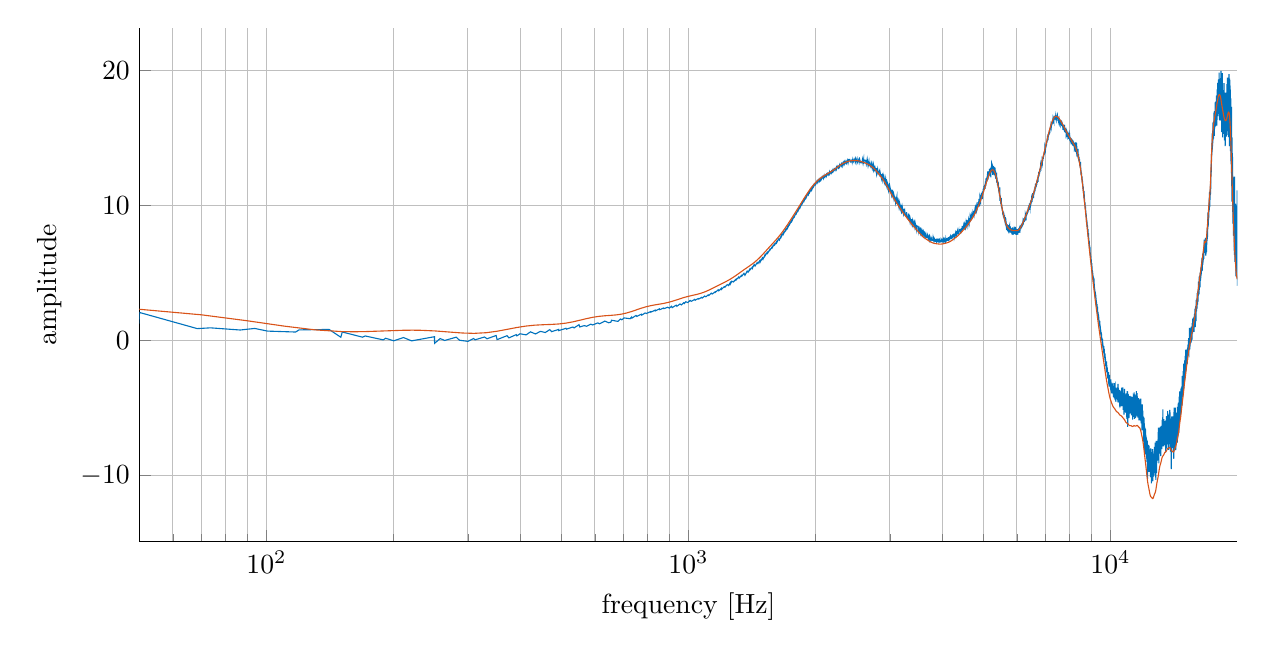
\begin{tikzpicture}

\begin{axis}[%
width=5.49in,
height=2.566in,
at={(2.311in,0.681in)},
scale only axis,
xmode=log,
xmin=50,
xmax=20000,
xminorticks=true,
xlabel={frequency [Hz]},
xmajorgrids,
xminorgrids,
ylabel={amplitude},
ymajorgrids,
axis background/.style={fill=white},
axis x line*=bottom,
axis y line*=left
]
\addplot [color=mycolor1,solid,forget plot]
  table[row sep=crcr]{%
49.8670212765958	1.23965295698856\\
50.0094984802432	2.0621103659696\\
68.5315349544073	0.866696453959857\\
73.6607142857143	0.923092073032269\\
86.6261398176292	0.762575005738629\\
93.75	0.879331353759989\\
100.588905775076	0.681341026968351\\
117.258738601824	0.613369530188904\\
119.395896656535	0.774067694269707\\
140.767477203647	0.804224019928009\\
150.02849544073	0.228028572066702\\
151.168313069909	0.617347036970115\\
168.835486322188	0.231976651790589\\
171.400075987842	0.321011022624902\\
189.067249240122	0.03272566920044\\
191.631838905775	0.151578020955318\\
200.18047112462	-0.0362577754616497\\
211.151215805471	0.204888005790098\\
220.697188449848	-0.0408026477091947\\
250.047492401216	0.26612854954594\\
250.189969604863	-0.223456686093107\\
257.883738601824	0.129713946015111\\
264.437689969605	-0.0102824777413481\\
281.534954407295	0.230480203849225\\
286.664133738602	0.00663732598765773\\
300.056990881459	-0.078149148806762\\
309.602963525836	0.133469937819601\\
312.025075987842	0.0370154028836808\\
328.409954407295	0.243538032730778\\
333.11170212766	0.114264741515167\\
350.066489361702	0.357295884697198\\
351.918693009119	0.0512129293535461\\
371.580547112462	0.341966888468046\\
375.427431610942	0.180821982647866\\
390.814969604863	0.421383115627858\\
392.09726443769	0.328191012143625\\
398.936170212766	0.482860320440211\\
412.329027355623	0.403056285042413\\
422.302431610942	0.626101389113876\\
433.843085106383	0.472541482557682\\
445.811170212766	0.661996843044491\\
457.779255319149	0.577641914285314\\
469.177431610942	0.790206610325906\\
473.879179331307	0.640799223921047\\
492.401215805471	0.807071030915143\\
492.686170212766	0.715503904255299\\
512.348024316109	0.890369548510179\\
513.772796352584	0.82836040534921\\
532.294832826748	0.983976848416291\\
535.571808510638	0.916514880827592\\
550.246960486322	1.15743894868245\\
552.669072948328	0.988757040947423\\
566.204407294833	1.08891650762087\\
573.328267477204	1.04130965331034\\
586.578647416413	1.19366880943576\\
592.990121580547	1.13873919446828\\
609.94490881459	1.29041243090122\\
615.074088145897	1.22156601579981\\
626.187310030395	1.34162818952564\\
633.453647416413	1.42421372505907\\
646.846504559271	1.30071463950605\\
654.825227963526	1.34558230777409\\
656.962386018237	1.48700529309139\\
680.471124620061	1.40215500920583\\
689.87462006079	1.57627913810108\\
695.146276595745	1.51749498164245\\
703.837386018237	1.65930593670314\\
727.346124620061	1.59863365972782\\
733.187689969605	1.72593787056206\\
734.612462006079	1.64485906352143\\
750.997340425532	1.83805272874301\\
754.41679331307	1.77276643118946\\
773.366261398176	1.93401259771645\\
774.648556231003	1.86488847494978\\
789.466185410334	2.02330599429976\\
794.880319148936	1.98745094548292\\
813.829787234043	2.13117283032096\\
814.257218844985	2.08122938548598\\
833.491641337386	2.2385605449734\\
834.631458966565	2.17729500004001\\
853.438449848024	2.32886947996479\\
855.005699088146	2.26610347132907\\
873.100303951368	2.39564095705209\\
874.952507598784	2.34730102246104\\
892.762158054711	2.44752598286313\\
900.455927051672	2.38175724556945\\
910.856762917933	2.5198884619833\\
914.988601823708	2.42080419816232\\
934.792933130699	2.60255883736632\\
938.497340425532	2.52119334771402\\
954.882218844985	2.69146707470881\\
961.863601823708	2.62370634552958\\
974.544072948328	2.78317595812823\\
977.536094224924	2.72431603574754\\
985.372340425532	2.8582067016968\\
996.200607902736	2.7932949868458\\
1008.88107902736	2.95362876913685\\
1015.57750759878	2.88791843611486\\
1034.2420212766	3.03059652565308\\
1037.23404255319	2.97176547958207\\
1054.47378419453	3.09414338547548\\
1057.32332826748	3.05498072653966\\
1074.13563829787	3.18105767430834\\
1077.41261398176	3.12898181337121\\
1092.23024316109	3.27596151639514\\
1099.49658054711	3.22402752125521\\
1113.8867781155	3.36767326675548\\
1117.16375379939	3.31922032928265\\
1131.83890577508	3.49474624692925\\
1137.39551671733	3.42731402690766\\
1155.63259878419	3.58472323509626\\
1156.91489361702	3.54903660228451\\
1176.00683890578	3.73987160608833\\
1178.99886018237	3.66633962215563\\
1196.23860182371	3.84687580343213\\
1196.95098784195	3.77371306094575\\
1215.47302431611	3.97385716543828\\
1219.17743161094	3.93302114944898\\
1235.84726443769	4.12557710149353\\
1243.398556231	4.05577299987869\\
1255.93655015198	4.27299996478966\\
1256.79141337386	4.17372375618895\\
1266.90729483283	4.3804204499482\\
1276.7382218845	4.32032964625055\\
1295.83016717325	4.51959409391031\\
1296.82750759878	4.47359514726909\\
1315.4920212766	4.68942420167532\\
1318.62651975684	4.61163530571207\\
1335.72378419453	4.80900050220326\\
1338.14589665654	4.76041577308562\\
1353.39095744681	4.95952051707384\\
1360.79977203647	4.81535101762178\\
1377.32712765957	5.12321147674841\\
1384.45098784195	5.04526883542842\\
1397.27393617021	5.27131254295002\\
1398.41375379939	5.20804639235075\\
1417.22074468085	5.42593598175516\\
1418.21808510638	5.35760280937226\\
1431.1835106383	5.61400884038677\\
1438.02241641337	5.50357867901266\\
1454.97720364742	5.75933824185264\\
1460.24886018237	5.68324587155109\\
1476.77621580547	5.91367710675182\\
1478.0585106383	5.78390704301746\\
1497.0079787234	6.10664047795025\\
1501.56724924012	6.0009875338274\\
1516.95478723404	6.3138452111559\\
1518.09460486322	6.24520706062955\\
1536.61664133739	6.52397595066333\\
1539.89361702128	6.44339671563808\\
1558.27317629179	6.72348424139082\\
1559.98290273556	6.67905862316484\\
1578.36246200608	6.92045419480825\\
1579.64475683891	6.86584558705616\\
1596.59954407295	7.12290161309876\\
1600.01899696049	7.05695512195175\\
1618.54103343465	7.31915762664543\\
1619.39589665654	7.24747783559807\\
1636.63563829787	7.52625138497209\\
1642.33472644377	7.43045028410948\\
1658.43465045593	7.74715955472931\\
1659.57446808511	7.66560749130245\\
1678.52393617021	7.97187767602341\\
1679.52127659574	7.88568112349508\\
1698.47074468085	8.2015669445019\\
1701.17781155015	8.13415753426232\\
1718.41755319149	8.4389825911051\\
1719.41489361702	8.34684617863696\\
1738.22188449848	8.67969308012454\\
1739.21922492401	8.62143907074427\\
1758.16869300912	8.93297496211826\\
1759.45098784195	8.85261390611768\\
1778.2579787234	9.17354264645685\\
1781.10752279635	9.13426463242566\\
1798.0623100304	9.43127513913061\\
1801.05433130699	9.37658153360624\\
1819.7188449848	9.70747838273514\\
1821.00113981763	9.62968753397241\\
1839.66565349544	9.94317375634403\\
1840.80547112462	9.87207523835953\\
1859.46998480243	10.2023659069749\\
1860.75227963526	10.1232950897057\\
1879.70174772036	10.4357500346976\\
1880.98404255319	10.3502320571394\\
1899.79103343465	10.6688581862763\\
1900.64589665654	10.5673639726467\\
1919.88031914894	10.8903100562394\\
1923.86968085106	10.7909178878545\\
1939.68465045593	11.1100129890865\\
1940.68199088146	11.0037887276847\\
1959.63145896657	11.2872079997477\\
1960.48632218845	11.1562825971816\\
1979.43579027356	11.4727733442189\\
1980.57560790274	11.3912995172669\\
1999.0976443769	11.6411394464895\\
2002.23214285714	11.5482825252873\\
2017.76215805471	11.8197825592191\\
2024.45858662614	11.6720567312845\\
2038.99126139818	11.9310309538836\\
2044.26291793313	11.7787677593065\\
2060.79027355623	12.0201019448653\\
2062.35752279635	11.8900531637854\\
2080.87955927052	12.1322769571114\\
2088.14589665654	11.9923911122737\\
2096.69452887538	12.2132582085086\\
2102.10866261398	12.0879907936493\\
2120.91565349544	12.2835328879545\\
2122.05547112462	12.1500871703325\\
2136.7306231003	12.3561973016951\\
2143.99696048632	12.2465883526634\\
2158.52963525836	12.4808341799601\\
2161.6641337386	12.3063791204406\\
2180.61360182371	12.5220494390673\\
2183.8905775076	12.4075161321239\\
2198.70820668693	12.6317089658205\\
2201.84270516717	12.4888058417021\\
2218.37006079027	12.691429614271\\
2225.351443769	12.586150280299\\
2240.45402735562	12.8176784208994\\
2243.16109422492	12.6730237606077\\
2258.54863221885	12.8997464299705\\
2267.52469604863	12.7649334868367\\
2280.3476443769	12.9824689678073\\
2283.0547112462	12.8488539981871\\
2302.2891337386	13.0773276975506\\
2305.2811550152	12.9351927086891\\
2322.37841945289	13.1463541275124\\
2322.80585106383	12.9511553264761\\
2340.33054711246	13.2221273793586\\
2345.31724924012	13.0549611693228\\
2360.13487841945	13.2714419097343\\
2367.11626139818	13.1135194220187\\
2382.2188449848	13.3368374682788\\
2388.91527355623	13.139353449903\\
2398.03381458967	13.4016075885468\\
2412.13905775076	13.3978554879497\\
2419.12044072948	13.1984915236383\\
2438.63981762918	13.218289100726\\
2441.77431610942	13.4220183525171\\
2444.90881458967	13.2289976746246\\
2451.89019756839	13.4337156041647\\
2463.43085106383	13.2283605560857\\
2479.53077507599	13.4449548988089\\
2483.80509118541	13.4911033127426\\
2486.93958966565	13.18513694064\\
2507.59878419453	13.4592169160125\\
2510.44832826748	13.13424517989\\
2533.81458966565	13.4083469817973\\
2538.51633738602	13.2107959905984\\
2545.21276595745	13.4008308888372\\
2557.32332826748	13.1551369268841\\
2578.55243161094	13.1432499450215\\
2583.8240881459	13.3791332079011\\
2592.23024316109	13.1133759283092\\
2601.20630699088	13.4077266154782\\
2604.19832826748	13.0662781174191\\
2607.47530395137	13.3486506584745\\
2627.7070668693	13.3316168093149\\
2638.25037993921	13.0504536501517\\
2651.21580547112	13.4184632861083\\
2664.18123100304	12.9395588459654\\
2675.00949848024	13.228606558593\\
2677.71656534954	12.8833545571637\\
2685.12537993921	13.1222554845453\\
2702.08016717325	12.8851428369102\\
2708.91907294833	13.1154445008257\\
2721.59954407295	12.8110957566953\\
2725.01899696049	13.0350068403581\\
2741.97378419453	12.6644165826413\\
2744.96580547112	12.9840957329365\\
2759.64095744681	12.6434600741854\\
2767.04977203647	12.8056107930734\\
2781.58244680851	12.526147894995\\
2788.84878419453	12.7490324824724\\
2791.98328267477	12.3610578563883\\
2806.65843465046	12.6871785850255\\
2815.4920212766	12.3271294466812\\
2838.85828267477	12.5892425869258\\
2841.99278115502	12.1206145468136\\
2846.40957446809	12.4156208112732\\
2865.50151975684	12.009853521658\\
2870.63069908815	12.305970373627\\
2879.60676291793	11.9304154240055\\
2886.58814589666	12.2025914254136\\
2905.39513677812	11.8216039729494\\
2906.25	12.0763087313118\\
2923.48974164134	11.6452881527859\\
2932.75075987842	11.9497233003722\\
2943.43655015198	11.4933961480548\\
2953.125	11.3368800682587\\
2956.25949848024	11.7275269228537\\
2970.07978723404	11.552031199242\\
2979.62575987842	11.1208034748699\\
2992.02127659574	11.4342548820272\\
3006.26899696049	11.0062152813762\\
3006.41147416413	11.2603734139376\\
3024.79103343465	10.8461699556044\\
3030.20516717325	11.1556137010214\\
3039.46618541033	10.7386042504765\\
3050.00949848024	10.9553388987914\\
3064.96960486322	10.5582670288407\\
3068.24658054711	10.7662568252715\\
3086.76861702128	10.4016669545279\\
3087.76595744681	10.6447743867941\\
3097.02697568389	10.1902808055799\\
3117.40121580547	10.6468118666474\\
3120.39323708207	10.1172929489507\\
3129.65425531915	10.3633912251198\\
3146.75151975684	9.9864887830158\\
3147.74886018237	10.2368401457142\\
3166.55585106383	9.88094817621123\\
3167.69566869301	10.1224589918213\\
3186.50265957447	9.72260673736424\\
3187.7849544073	10.0211243670336\\
3202.60258358663	9.63122990092387\\
3209.58396656535	9.90652617388942\\
3226.53875379939	9.50116834218731\\
3231.6679331307	9.73775168026913\\
3234.6599544073	9.36608865695494\\
3253.6094224924	9.6266590615731\\
3264.4376899696	9.29112620582532\\
3284.66945288754	9.16661963237046\\
3287.66147416413	9.49642295244821\\
3289.08624620061	9.3972221183819\\
3306.04103343465	9.07059617874397\\
3322.4259118541	8.95315520459842\\
3323.13829787234	9.27521797579176\\
3330.97454407295	9.2130037705121\\
3346.07712765957	8.86247940783541\\
3349.21162613982	9.08214669436841\\
3368.16109422492	8.73965872418899\\
3371.01063829787	8.97783842637113\\
3375.42743161094	8.67880891367093\\
3391.09992401216	8.89550139942153\\
3398.93617021277	8.53030311802279\\
3416.88829787234	8.76762323143402\\
3425.86436170213	8.49629314769195\\
3430.85106382979	8.69017034451359\\
3447.66337386018	8.42618300110467\\
3448.94566869301	8.60104693927065\\
3461.62613981763	8.34654864741361\\
3469.31990881459	8.20453564324503\\
3470.88715805471	8.49489814211617\\
3498.95516717325	8.42065527892726\\
3505.50911854103	8.1363058231551\\
3510.92325227964	8.29823218326137\\
3527.30813069909	8.08727371437108\\
3532.72226443769	8.23152810414164\\
3545.83016717325	7.96554557861448\\
3550.81686930091	8.15645274185641\\
3569.33890577508	7.8890290549242\\
3570.47872340426	8.07568408184406\\
3587.148556231	7.85448392511475\\
3592.8476443769	8.04452104920078\\
3609.23252279635	7.78702278331602\\
3610.08738601824	7.98791470652826\\
3629.60676291793	7.75117629178511\\
3632.02887537994	7.88932736094678\\
3649.12613981763	7.69230413905445\\
3654.39779635258	7.83748521994129\\
3665.08358662614	7.637133670337\\
3685.45782674772	7.60053482172289\\
3686.5976443769	7.8181885572123\\
3693.86398176292	7.76158073369392\\
3703.97986322188	7.52115046259169\\
3716.23290273556	7.68031912304457\\
3727.34612462006	7.48059411734941\\
3733.4726443769	7.68321482782637\\
3748.86018237082	7.47825604316262\\
3750.85486322188	7.60176489462774\\
3756.98138297872	7.41378398164774\\
3771.9414893617	7.57637945695542\\
3776.35828267477	7.41140934258234\\
3802.85904255319	7.37903195290887\\
3803.85638297872	7.55814928529046\\
3814.96960486322	7.3713621597863\\
3821.23860182371	7.57113194172952\\
3834.20402735562	7.48057433961635\\
3844.46238601824	7.32289655427657\\
3860.70478723404	7.33288124005932\\
3865.26405775076	7.46938331899812\\
3871.24810030395	7.47900531137422\\
3874.24012158055	7.27711409799804\\
3891.62234042553	7.31163761631033\\
3897.74886018237	7.48967734008852\\
3915.13107902736	7.48531185196188\\
3920.11778115502	7.33189916112542\\
3933.22568389058	7.44529186080009\\
3944.62386018237	7.26973024079154\\
3963.57332826748	7.3286878063632\\
3968.13259878419	7.47468752378573\\
3985.51481762918	7.33002164454083\\
3990.64399696049	7.48474438886898\\
4002.75455927052	7.48476786257857\\
4008.88107902736	7.34108832694365\\
4015.71998480243	7.31184815383896\\
4021.27659574468	7.47264172806335\\
4032.38981762918	7.32317803082321\\
4042.22074468085	7.48843012121078\\
4062.02507598784	7.31465161765943\\
4070.43123100304	7.50804190089759\\
4079.26481762918	7.28962083918334\\
4082.39931610942	7.51754196067225\\
4108.4726443769	7.54077382255872\\
4108.90007598784	7.4083407468729\\
4126.28229483283	7.40273368550668\\
4132.40881458967	7.64012075291626\\
4135.25835866261	7.47833489918945\\
4150.21846504559	7.58521637679762\\
4159.19452887538	7.4974463326435\\
4162.61398176292	7.61733914291387\\
4173.15729483283	7.69265740192925\\
4173.29977203647	7.53208604097097\\
4196.66603343465	7.53958605634772\\
4201.93768996961	7.71391656863627\\
4220.03229483283	7.77339273387868\\
4220.88715805471	7.60705966340717\\
4234.99240121581	7.65817258804571\\
4249.66755319149	7.86489603309807\\
4265.625	7.86340570201064\\
4267.04977203647	7.63639025889769\\
4274.74354103343	7.73656849683242\\
4291.84080547113	7.93305985908216\\
4294.97530395137	7.79694131404811\\
4311.78761398176	7.94171485309067\\
4313.92477203647	8.09790549465876\\
4316.91679331307	7.8325010255601\\
4337.4335106383	8.07200322038132\\
4338.57332826748	7.88799780119585\\
4360.79977203647	7.945501896171\\
4371.34308510638	8.11701284998835\\
4374.47758358663	7.97623787231194\\
4391.57484802432	8.19084651022631\\
4412.66147416413	8.21186217410367\\
4413.94376899696	7.99969103457076\\
4431.1835106383	8.08097618728113\\
4433.17819148936	8.30327720876001\\
4436.17021276596	8.16836336153752\\
4452.84004559271	8.37340473943619\\
4454.69224924012	8.47804564423539\\
4455.97454407295	8.2061472342604\\
4484.32750759878	8.28684952317799\\
4490.45402735562	8.51185747789165\\
4501.42477203647	8.37328631622411\\
4509.54597264438	8.59448856463525\\
4525.07598784195	8.41114581821682\\
4531.20250759878	8.6899057614854\\
4539.75113981763	8.48882987008924\\
4548.58472644377	8.76447198282851\\
4561.40767477204	8.57501108924208\\
4571.95098784195	8.92445672703569\\
4578.21998480243	8.56183942607783\\
4588.47834346505	8.87513741492541\\
4595.45972644377	8.57466934235528\\
4612.55699088146	8.94708128745337\\
4625.09498480243	8.70727377879642\\
4632.64627659574	9.04058205098031\\
4642.33472644377	8.81259013092557\\
4648.46124620061	9.11082995133912\\
4656.72492401216	8.95299292805916\\
4674.39209726444	9.2208224676793\\
4678.09650455927	9.00862900930926\\
4690.34954407295	9.34021542340041\\
4696.90349544073	9.13054524294862\\
4712.57598784195	9.36389655021971\\
4719.12993920973	9.16038824434142\\
4724.82902735562	9.45075610070053\\
4739.21922492401	9.29334007129484\\
4751.89969604863	9.58485217754784\\
4756.601443769	9.37604306738121\\
4774.41109422492	9.70846747732144\\
4783.10220364742	9.40109146602101\\
4789.51367781155	9.79572176657541\\
4806.61094224924	9.97684142526332\\
4812.73746200608	9.53371864837191\\
4830.11968085106	9.67744550336462\\
4835.81876899696	10.0291556907694\\
4839.80813069909	9.86243065722127\\
4853.62841945289	10.2363517618128\\
4858.18768996961	9.96242489717756\\
4876.28229483283	10.3125088819556\\
4876.99468085106	10.4783969487367\\
4883.1212006079	9.90697127806959\\
4900.21846504559	10.2109247633175\\
4903.49544072948	10.5729942256244\\
4923.86968085106	10.2744771222761\\
4935.55281155015	10.8020932108904\\
4944.38639817629	10.5332756142797\\
4947.37841945289	10.9246624916099\\
4970.88715805471	10.4640256233025\\
4974.1641337386	11.0227234572192\\
4983.56762917933	10.8440313184625\\
4996.53305471125	11.2287434235992\\
4998.52773556231	10.9631997695088\\
5017.19224924012	11.4322973417767\\
5020.32674772037	11.1413873878789\\
5036.99658054711	11.5054027818977\\
5041.27089665654	11.2170040359964\\
5054.80623100304	11.7690443924917\\
5064.49468085106	11.4180593251548\\
5070.9061550152	11.9866918342098\\
5078.03001519757	11.6468757413737\\
5096.83700607903	12.1168900308489\\
5099.40159574468	11.7798397028195\\
5117.7811550152	12.5023269594674\\
5122.19794832827	11.8922017877277\\
5137.44300911854	12.4065907860412\\
5142.57218844985	12.0905967691988\\
5156.67743161094	12.4823356799983\\
5158.10220364742	12.2069903729083\\
5164.6561550152	12.6950537732629\\
5188.16489361702	12.2139296439687\\
5197.99582066869	12.7617338658132\\
5205.40463525836	12.0710980602707\\
5213.09840425532	12.8012690773891\\
5220.50721884498	12.4676964901066\\
5228.91337386018	13.1306654310433\\
5249.85752279635	12.9580772581463\\
5258.54863221885	12.2581859144692\\
5262.39551671733	12.9063283440646\\
5265.10258358663	12.4142105398791\\
5282.05737082067	12.9176446972194\\
5290.17857142857	12.4142922698996\\
5299.29711246201	12.819265555967\\
5305.42363221885	12.2206309838079\\
5322.80585106383	12.8115236106075\\
5337.48100303951	12.0849709452958\\
5342.18275075988	12.5672861695905\\
5349.30661094225	11.9495308494645\\
5372.81534954407	12.4097019387268\\
5375.80737082067	11.6800571678501\\
5379.93920972644	12.1086099080552\\
5398.17629179331	11.4901072773054\\
5402.59308510638	11.8186999911064\\
5419.12044072948	11.2740838956578\\
5419.69034954407	11.6970112427383\\
5439.49468085106	10.984755336817\\
5446.19110942249	11.258576281114\\
5454.88221884498	10.7103621696799\\
5463.57332826748	11.3331327527415\\
5469.69984802432	10.3206782448804\\
5480.67059270517	10.7196168467888\\
5498.1952887538	10.0709562264259\\
5510.44832826748	10.5404409569612\\
5519.99430091185	9.8300082567128\\
5521.41907294833	10.1143572287349\\
5539.79863221885	9.60587930884044\\
5540.93844984802	9.81238927801508\\
5558.17819148936	9.30533028141399\\
5560.60030395137	9.57925869818686\\
5575.98784194529	9.12717369822563\\
5580.8320668693	9.51682099290844\\
5598.78419452888	8.95435644136304\\
5610.46732522796	9.28684894444649\\
5620.15577507599	8.75089384060472\\
5630.84156534954	9.12196238278724\\
5633.97606382979	8.56644371319063\\
5651.21580547113	9.03246112300372\\
5656.48746200608	8.44491151709061\\
5662.47150455927	8.69312570012186\\
5674.72454407295	8.17791210755991\\
5683.84308510638	8.61121777976975\\
5698.23328267477	8.1167580482593\\
5710.20136778116	8.54251065250303\\
5720.88715805471	8.15708356043666\\
5721.59954407295	8.04007988836027\\
5724.73404255319	8.52468497696225\\
5745.10828267477	7.92698317955103\\
5751.23480243161	8.39638322337285\\
5768.6170212766	8.53614844214776\\
5769.89931610942	8.00847662023352\\
5791.98328267477	8.43293731711346\\
5795.11778115502	7.97148701374563\\
5812.5	8.29269586632059\\
5821.61854103343	8.00503609239971\\
5832.73176291793	7.95769847179138\\
5841.99278115502	8.32990166405579\\
5841.99278115502	8.32990166405579\\
5845.12727963526	7.8337914600123\\
5862.3670212766	8.36890096824216\\
5873.05281155015	7.98884227223577\\
5884.59346504559	8.26555429654114\\
5889.01025835866	7.87174462578797\\
5902.54559270517	7.89827454721968\\
5915.51101823708	8.31001863611059\\
5925.7693768997	8.25738102489783\\
5931.61094224924	7.88941273492202\\
5956.25949848024	8.39527654801953\\
5962.38601823708	7.85614918051409\\
5978.0585106383	8.23361855913092\\
5979.76823708207	7.81305022326737\\
5985.75227963526	8.25557088626818\\
5993.58852583587	7.89359611705662\\
6003.13449848024	7.87832422021485\\
6015.81496960486	8.23400906746523\\
6032.76975683891	7.83763502123022\\
6040.17857142857	8.23649376216261\\
6050.15197568389	7.95953599290853\\
6062.68996960486	8.28003330639147\\
6066.67933130699	8.0336381121714\\
6079.07484802432	8.29211900861986\\
6089.19072948328	8.35044609717117\\
6097.02697568389	7.96875775519583\\
6105.00569908815	8.15291791087251\\
6123.52773556231	8.48873030117247\\
6126.8047112462	8.22901496026701\\
6143.18958966565	8.5560765324102\\
6149.88601823708	8.30960020305031\\
6161.42667173252	8.62633630124124\\
6170.26025835866	8.38684907846445\\
6179.0938449848	8.68806059570704\\
6186.07522796353	8.47985616099052\\
6202.88753799392	8.79566326597553\\
6217.42021276596	8.56711717307079\\
6218.70250759878	8.90911395002238\\
6224.97150455927	8.71001695081129\\
6243.92097264438	9.04777536047913\\
6245.77317629179	8.78026526357702\\
6263.44034954407	9.0940700983294\\
6264.29521276596	8.8276274072816\\
6282.24734042553	9.23504815523244\\
6284.66945288754	8.8921226275014\\
6287.80395136778	9.3196212494168\\
6311.31268996961	9.10861653549777\\
6320.57370820669	9.42168577233828\\
6325.27545592705	9.21263139074792\\
6343.51253799392	9.52260193580615\\
6347.6443768997	9.32145592163962\\
6358.18768996961	9.64374633916428\\
6368.01861702128	9.43580071448899\\
6384.26101823708	9.8340554822918\\
6387.25303951368	9.55820554213229\\
6404.06534954407	9.90529958128007\\
6405.06268996961	9.66413273252646\\
6408.19718844985	10.0022519868199\\
6427.85904255319	9.74951354700536\\
6428.57142857143	10.1332346415881\\
6448.94566869301	9.79754018644617\\
6464.04825227964	10.2218916235574\\
6472.45440729483	10.3498222450727\\
6475.58890577508	10.0671091851566\\
6489.40919452888	10.2002447258595\\
6501.37727963526	10.4905326990469\\
6519.32940729483	10.2297975679283\\
6525.45592705167	10.7581302151959\\
6529.87272036474	10.4137953115894\\
6545.83016717325	10.9040076571422\\
6553.09650455927	10.5570005862642\\
6557.37082066869	10.9186818936529\\
6572.47340425532	10.5308922802873\\
6582.87424012158	11.0329819069347\\
6586.29369300912	10.8227114022066\\
6603.81838905775	11.2045500808252\\
6607.95022796353	10.9588820714547\\
6625.33244680851	11.3435450066125\\
6627.04217325228	11.0507557890159\\
6639.7226443769	11.5903832185657\\
6646.56155015198	11.2352704519523\\
6662.80395136778	11.6101221181673\\
6667.64817629179	11.3832203823218\\
6686.45516717325	11.7458348377121\\
6686.5976443769	11.5223765351544\\
6703.97986322189	11.8988657275984\\
6710.10638297872	11.6589318642582\\
6726.49126139818	12.0377947069387\\
6736.60714285714	11.7278905426442\\
6741.02393617021	12.2143299678599\\
6747.2929331307	12.0137669963883\\
6760.11588145897	12.4558608144016\\
6768.52203647416	12.1427881616416\\
6783.48214285714	12.5192681909466\\
6787.32902735562	12.3185855576409\\
6803.99886018237	12.72032482862\\
6807.41831306991	12.4594980442591\\
6827.36512158055	12.8753939072837\\
6829.78723404255	12.6423206338779\\
6830.49962006079	12.9869445890737\\
6847.45440729483	12.8154427393493\\
6865.26405775076	13.1333877880221\\
6869.39589665654	12.9370812485136\\
6882.07636778116	13.2865875911334\\
6894.75683890578	13.1341338636856\\
6902.87803951368	13.4466569012872\\
6911.14171732523	13.2677856835819\\
6924.53457446809	13.6099347540432\\
6928.09650455927	13.4460556997295\\
6946.47606382979	13.7734238911126\\
6949.32560790274	13.6228978111823\\
6968.13259878419	13.9316718604449\\
6968.84498480243	13.781482325006\\
6983.94756838906	14.1112302339626\\
6988.50683890578	13.86359396655\\
6991.64133738602	14.2922907952262\\
7012.0155775076	14.0866755069233\\
7028.11550151976	14.4164716054979\\
7032.10486322189	14.2889610158723\\
7045.64019756839	14.5566627891324\\
7050.7693768997	14.4136957705478\\
7063.44984802432	14.7571599145861\\
7069.7188449848	14.636580526571\\
7083.96656534954	14.9253398355061\\
7093.65501519757	14.7725956583148\\
7105.90805471125	15.1043252822343\\
7108.90007598784	14.8284287679904\\
7127.7070668693	15.2237677240559\\
7130.6990881459	15.1185797651908\\
7148.79369300912	15.373909407844\\
7152.78305471125	15.2144163374401\\
7167.74316109423	15.5559069276495\\
7176.29179331307	15.3193205756394\\
7189.11474164134	15.6787480525175\\
7191.96428571429	15.5443395102179\\
7209.48898176292	15.8229710722989\\
7211.19870820669	15.7016195516855\\
7226.15881458967	15.9393181106355\\
7238.2693768997	15.8046864840113\\
7249.66755319149	16.1306502456021\\
7250.09498480243	15.8906268387841\\
7265.19756838906	16.1812789854237\\
7270.18427051672	15.971739850467\\
7288.99126139818	16.2672929758027\\
7296.68503039514	16.0478611592563\\
7305.09118541034	16.2987809773789\\
7320.05129179331	16.1184332626337\\
7320.9061550152	16.3913203970448\\
7343.56003039514	16.1997445189016\\
7346.26709726444	16.4723189453828\\
7353.53343465046	16.3119212749026\\
7367.06876899696	16.614660146694\\
7375.61740121581	16.3545645961688\\
7390.43503039514	16.6398969204654\\
7390.43503039514	16.6398969204654\\
7393.71200607903	16.3795327825448\\
7413.94376899696	16.6174902521356\\
7421.63753799392	16.4038123597064\\
7437.45250759878	16.2974653128578\\
7450.1329787234	16.5851484503545\\
7457.82674772037	16.3849393211627\\
7458.68161094225	16.5574183199159\\
7484.32750759878	16.6855177508606\\
7485.75227963526	16.3887958431555\\
7498.57522796353	16.574424766825\\
7507.83624620061	16.2418509944655\\
7528.21048632219	16.4965309403199\\
7529.49278115502	16.321224910526\\
7534.33700607903	16.5091867270836\\
7535.33434650456	16.2734866534272\\
7551.86170212766	16.4199111856662\\
7568.95896656535	16.190026083958\\
7577.65007598784	16.3644054131236\\
7587.05357142857	16.1710888702889\\
7601.72872340426	16.3305493202747\\
7604.72074468085	16.0977882634665\\
7611.84460486322	16.2764258255191\\
7625.09498480243	16.0026976104499\\
7648.60372340426	16.260298935307\\
7650.45592705167	15.9739147887578\\
7653.87537993921	16.1586254909971\\
7672.11246200608	15.8695609044427\\
7672.11246200608	15.8695609044427\\
7677.81155015198	16.113242466079\\
7693.91147416413	16.0395120295719\\
7708.72910334347	15.7684927313873\\
7715.85296352584	15.9519857313836\\
7718.98746200608	15.5833205327022\\
7735.37234042553	15.8984753076548\\
7750.18996960486	15.6589368022621\\
7760.30585106383	15.6060346282759\\
7765.86246200608	15.9257262204825\\
7789.3712006079	15.9215175835233\\
7792.22074468085	15.503717063492\\
7801.33928571429	15.7165907829783\\
7812.02507598784	15.4134603351543\\
7812.87993920973	15.7001106986503\\
7828.26747720365	15.3844190361612\\
7843.22758358663	15.6154608007567\\
7848.21428571429	15.3374565457058\\
7864.88411854103	15.499241568606\\
7866.45136778116	15.258818848615\\
7880.12917933131	15.1589066331946\\
7883.1212006079	15.4891183014013\\
7899.50607902736	15.3851461757359\\
7909.76443768997	15.0851113158318\\
7916.74582066869	15.3550297773631\\
7925.86436170213	15.0687082753285\\
7940.68199088146	15.3082344115842\\
7953.50493920973	14.9650495296675\\
7963.76329787234	14.9506255353326\\
7964.76063829787	15.2729773927945\\
7977.01367781155	15.34291192539\\
7989.69414893617	14.8949075956856\\
8000.52241641337	15.3613801950724\\
8013.63031914894	14.7581411038656\\
8014.34270516717	15.0776264798184\\
8023.88867781155	14.7847580525453\\
8040.5585106383	15.0162579998271\\
8047.53989361702	14.6552756708585\\
8070.6212006079	14.9683394609506\\
8070.9061550152	14.5066293162194\\
8092.42021276596	14.9118778628518\\
8094.27241641337	14.5230512324523\\
8106.3829787234	14.8754660665559\\
8109.51747720365	14.5529356881876\\
8118.06610942249	14.831322712071\\
8133.31117021277	14.4856431611832\\
8138.15539513678	14.8334140024341\\
8143.28457446809	14.4060824859627\\
8160.09688449848	14.7370747278101\\
8165.08358662614	14.4082482049605\\
8180.32864741641	14.6974086920025\\
8191.29939209726	14.3665116817228\\
8199.99050151976	14.6189662024266\\
8211.67363221885	14.1758940772171\\
8229.19832826748	14.2674711448882\\
8232.04787234043	14.6128451638522\\
8238.17439209727	14.5332578547831\\
8247.15045592705	14.1536539668464\\
8255.6990881459	14.4382247102649\\
8258.54863221885	13.9519510690125\\
8282.05737082067	14.6824960416517\\
8290.74848024316	14.0211377120147\\
8304.71124620061	13.9204876552776\\
8305.56610942249	14.6035205639842\\
8325.51291793313	14.2067841572797\\
8328.93237082067	13.6182150582675\\
8337.90843465046	14.0979978641803\\
8354.29331306991	13.7086065173542\\
8374.66755319149	13.5953285380148\\
8375.94984802432	14.1780123868585\\
8375.94984802432	14.1780123868585\\
8390.76747720365	13.4405451297207\\
8399.60106382979	13.7933644991842\\
8410.57180851064	13.3250026227086\\
8419.54787234043	13.5904237983957\\
8432.37082066869	13.1744819708548\\
8446.33358662614	13.42013481948\\
8456.30699088146	12.9595746866386\\
8457.44680851064	13.2198347346062\\
8475.9688449848	12.789178372845\\
8493.20858662614	13.2184625479465\\
8494.20592705167	12.5818677630429\\
8499.05015197568	12.8308233117372\\
8516.57484802432	12.2673333740565\\
8517.7146656535	12.5648724124578\\
8533.9570668693	12.1779074070014\\
8537.37651975684	12.3827280705742\\
8556.46846504559	11.8828750144941\\
8559.31800911854	12.1353613981672\\
8576.13031914894	11.6619984732323\\
8579.40729483283	11.8937499618346\\
8592.2302431611	11.3913158488239\\
8597.3594224924	11.574949585829\\
8616.16641337386	11.0649985860682\\
8617.30623100304	11.3874759619878\\
8635.68579027356	10.8550642649587\\
8654.35030395137	10.5123442645518\\
8657.48480243161	11.0581988288602\\
8657.48480243161	11.0581988288602\\
8677.43161094225	10.2455524697619\\
8680.56610942249	10.495198212369\\
8693.38905775076	10.0265897076215\\
8701.22530395137	10.1985996635153\\
8717.46770516717	9.73392960269955\\
8727.86854103343	9.91939867282501\\
8736.98708206687	9.45301421949493\\
8738.69680851064	9.61755414566263\\
8757.64627659575	9.14545775023902\\
8758.78609422492	9.30866270408804\\
8774.74354103343	8.74203943591639\\
8778.44794832827	9.04191670070408\\
8797.68237082067	8.52228579322516\\
8798.53723404255	8.77270161785184\\
8817.9141337386	8.25130403852832\\
8818.62651975684	8.51214072713398\\
8837.4335106383	7.9503062618787\\
8845.12727963526	8.23540544141503\\
8857.38031914894	7.68492145898462\\
8868.63601823708	7.93877124693074\\
8876.89969604863	7.40617065535315\\
8880.31914893617	7.57828620865324\\
8897.27393617021	7.11998024464388\\
8902.11816109423	7.38691603213135\\
8918.93047112462	6.82842533809831\\
8920.21276595745	7.03878153023016\\
8938.59232522796	6.56105503097477\\
8939.01975683891	6.93009048791746\\
8957.11436170213	6.3460597671307\\
8959.67895136778	6.47011689899201\\
8979.05585106383	6.03614621239212\\
8980.33814589666	6.23106146795576\\
8998.86018237082	5.74712537369265\\
9000.99734042553	5.98666216621252\\
9019.37689969605	5.5630179516101\\
9029.77773556231	5.71476688330622\\
9032.76975683891	5.25227358454903\\
9039.60866261398	5.47795067322495\\
9058.84308510638	4.99194444053637\\
9060.83776595745	5.17797311202279\\
9079.78723404255	4.68049568538249\\
9080.92705167173	4.98192648143411\\
9098.59422492401	4.54956081445688\\
9099.87651975684	4.7204664801527\\
9120.10828267477	4.31502915819288\\
9126.66223404255	4.54712966266234\\
9129.7967325228	4.10754255900765\\
9147.03647416414	4.2652615458388\\
9160.1443768997	3.84160600432516\\
9160.85676291793	3.99471589620993\\
9170.54521276596	3.59642199111771\\
9183.51063829787	3.77765474737833\\
9197.04597264438	3.19184875524942\\
9201.0353343465	3.59542230868101\\
9217.27773556231	3.14922189643599\\
9220.5547112462	3.4590125723322\\
9240.35904255319	2.9509901999106\\
9240.92895136778	3.13662644647674\\
9259.73594224924	2.76936598171881\\
9261.01823708207	2.95839500438544\\
9267.4297112462	2.49212167151438\\
9290.93844984802	2.68099573559212\\
9294.07294832827	2.25213852337416\\
9314.44718844985	2.49968929377267\\
9319.43389057751	2.0352537008781\\
9321.99848024316	2.26988544612295\\
9337.81344984802	1.70775346136207\\
9343.37006079027	2.1103917299564\\
9361.1797112462	1.66490130502837\\
9361.32218844985	1.94967816543112\\
9381.26899696049	1.48186122152399\\
9384.83092705167	1.74003315789441\\
9396.79901215806	1.25914611440751\\
9402.07066869301	1.49346154207927\\
9408.19718844985	1.05434964656896\\
9431.70592705167	1.4324403322105\\
9441.25189969605	0.907871756381152\\
9452.08016717325	1.15247073147726\\
9461.05623100304	0.699462624168147\\
9464.61816109423	0.92478387149922\\
9481.71542553191	0.437470629104271\\
9483.14019756839	0.739118906088323\\
9501.94718844985	0.341988722011185\\
9504.5117781155	0.612425066408711\\
9521.3240881459	0.158135909469936\\
9525.59840425532	0.471589851016518\\
9537.13905775076	-0.00540070139887234\\
9545.40273556231	0.175966799255169\\
9557.51329787234	-0.198300128274522\\
9572.47340425532	0.0831993028637151\\
9575.60790273556	-0.452570705930001\\
9582.87424012158	-0.137688192123372\\
9599.68655015198	-0.57095665921733\\
9605.24316109423	-0.346154408052286\\
9622.48290273556	-0.765381317621989\\
9632.31382978723	-0.910343372058881\\
9639.7226443769	-0.436722861841244\\
9643.71200607903	-0.6872997440049\\
9662.09156534954	-1.15281821456259\\
9663.23138297872	-0.630122613027049\\
9666.36588145897	-1.29632944293711\\
9689.5896656535	-0.959406467121346\\
9701.98518237082	-1.45508782972002\\
9713.24088145897	-1.01970838713118\\
9721.50455927052	-1.62063080208702\\
9730.90805471125	-1.39119961388538\\
9739.74164133739	-1.8832361023501\\
9743.44604863222	-1.56448100600975\\
9763.25037993921	-1.96622175245311\\
9780.49012158055	-2.36906949592039\\
9783.62462006079	-1.55257931763543\\
9785.47682370821	-1.78197410209908\\
9797.72986322188	-2.28043580789176\\
9803.99886018237	-1.84135688683258\\
9821.523556231	-2.37330933665705\\
9828.21998480243	-2.01836064463814\\
9830.49962006079	-2.6359009648496\\
9845.60220364742	-2.22690833408786\\
9854.00835866262	-2.79869842101604\\
9866.11892097265	-2.35451104393994\\
9876.8047112462	-2.85160459297293\\
9891.76481762918	-2.36420900088852\\
9900.88335866262	-3.19852431404655\\
9906.72492401216	-2.61364788008598\\
9924.39209726444	-3.42668469234222\\
9930.80357142857	-2.69282391095258\\
9942.9141337386	-3.22794941588217\\
9944.76633738602	-2.55694658594425\\
9963.28837386018	-3.29669465530272\\
9965.56800911854	-2.9436440178466\\
9976.82370820669	-3.3807523828837\\
9988.79179331307	-2.95697293967968\\
9994.77583586626	-3.52822730331858\\
10015.1500759878	-3.62904304264467\\
10018.2845744681	-2.89149416917714\\
10028.827887538	-3.16238466925156\\
10044.7853343465	-3.7358831070949\\
10045.3552431611	-3.19102063246479\\
10065.1595744681	-3.92855177672209\\
10065.7294832827	-3.78873184423079\\
10075.4179331307	-3.3235254027236\\
10085.5338145897	-3.9290847174087\\
10088.6683130699	-3.31288459256109\\
10109.0425531915	-3.26791022513673\\
10115.1690729483	-3.93819111202167\\
10132.4088145897	-3.39127387928689\\
10142.6671732523	-3.99983292575608\\
10159.0520516717	-3.37030714486554\\
10162.0440729483	-4.19045224587165\\
10179.4262917933	-3.39935993974659\\
10182.8457446809	-4.0477758053294\\
10202.7925531915	-4.27744208187062\\
10205.9270516717	-3.16505470805519\\
10209.061550152	-4.18017794418382\\
10213.478343465	-3.559113919759\\
10229.4357902736	-4.19967144715423\\
10234.4224924012	-3.50332125371614\\
10249.8100303951	-3.40728217135936\\
10252.8020516717	-4.36651697924684\\
10276.3107902736	-4.41281299634978\\
10279.4452887538	-3.61988178693642\\
10296.6850303951	-4.56233567131174\\
10299.8195288754	-3.50319395640331\\
10320.193768997	-4.34499833043195\\
10323.1857902736	-3.55116819493641\\
10329.454787234	-4.27979289026336\\
10343.7025075988	-3.60050324451592\\
10347.9768237082	-3.77355194283029\\
10353.3909574468	-4.29856053141615\\
10367.068768997	-3.67275050299665\\
10376.6147416413	-4.28875229891366\\
10390.5775075988	-4.41950673425373\\
10393.5695288754	-3.48580297521962\\
10414.0862462006	-4.59518075048995\\
10417.0782674772	-3.22570040375911\\
10438.592325228	-3.70831888736033\\
10440.587006079	-4.53712723984805\\
10464.0957446809	-3.73709373266772\\
10464.6656534954	-4.51284059691137\\
10475.0664893617	-4.53787390326626\\
10487.462006079	-3.6763346118144\\
10490.5965045593	-3.79835290853227\\
10501.7097264438	-4.51156148408311\\
10507.8362462006	-3.69433134495583\\
10510.9707446809	-4.7150168576019\\
10534.1945288754	-4.59056832385533\\
10534.337006079	-3.72424878401608\\
10557.8457446809	-4.88680719128817\\
10565.1120820669	-3.92344285264344\\
10570.9536474164	-4.5543015755548\\
10578.2199848024	-3.82592961670709\\
10603.1534954407	-3.8327934820039\\
10604.7207446809	-4.70374257899873\\
10621.9604863222	-4.6260880147065\\
10628.2294832827	-3.4984725130306\\
10629.7967325228	-3.9679958068159\\
10631.3639817629	-4.88143783387765\\
10651.7382218845	-3.58846354445447\\
10656.1550151976	-4.66343122814807\\
10677.2416413374	-4.66405704329629\\
10678.2389817629	-3.79965788995407\\
10698.6132218845	-3.48158299485141\\
10701.7477203647	-4.75169667105316\\
10721.1246200608	-3.94875265871396\\
10722.1219604863	-5.15843346921506\\
10731.5254559271	-3.89561438706003\\
10748.6227203647	-4.85289458223685\\
10762.7279635258	-3.98625149857842\\
10768.9969604863	-5.50756487969687\\
10772.1314589666	-3.94147680815144\\
10774.2686170213	-4.96666001376832\\
10789.3712006079	-4.84853429633346\\
10792.5056990881	-3.60107603229149\\
10815.8719604863	-5.32189723350456\\
10820.1462765957	-4.04907160298834\\
10836.3886778116	-5.14345099191469\\
10838.9532674772	-4.16132923959007\\
10849.7815349544	-5.05821905344874\\
10862.88943769	-4.00442979844902\\
10886.2556990881	-5.36846280492139\\
10889.3901975684	-3.92738338287817\\
10892.2397416413	-4.20412059150285\\
10895.5167173252	-5.19189805263298\\
10920.7351823708	-4.15368883760961\\
10927.5740881459	-5.28711221119177\\
10933.2731762918	-5.82296996273389\\
10948.0908054711	-3.85732695638231\\
10960.6287993921	-3.77512708815389\\
10967.7526595745	-5.8414577366523\\
10977.1561550152	-3.78795944685964\\
10980.1481762918	-6.4056043204881\\
10997.3879179331	-5.81844237304991\\
11000.3799392097	-3.96307110396507\\
11014.6276595745	-5.55184193861735\\
11017.0497720365	-4.01880926442128\\
11036.4266717325	-4.1967388211861\\
11050.5319148936	-5.76807878146276\\
11053.3814589666	-4.31602690650888\\
11064.3522036474	-5.29235642187969\\
11070.9061550152	-5.33299451836186\\
11077.3176291793	-4.3299907980269\\
11094.414893617	-4.35423251555876\\
11100.5414133739	-5.42823641836655\\
11120.9156534954	-4.11025813065519\\
11124.0501519757	-5.16230506554685\\
11135.3058510638	-4.42078236434669\\
11147.4164133739	-5.39381769581363\\
11156.6774316109	-4.3633800656473\\
11164.7986322188	-5.411080990658\\
11188.3073708207	-5.24992329171159\\
11191.2993920973	-4.16314205497606\\
11205.547112462	-4.47969742424076\\
11211.6736322188	-5.56777989726755\\
11211.6736322188	-5.56777989726755\\
11215.9479483283	-4.36188614222846\\
11238.1743920973	-4.22262747361566\\
11241.3088905775	-5.2206187824135\\
11256.5539513678	-5.49952318842443\\
11258.6911094225	-4.18669616600754\\
11280.4901215805	-4.3524376260267\\
11285.1918693009	-5.88001213008774\\
11299.4395896657	-4.19943416620656\\
11305.5661094225	-5.67625704633804\\
11320.6686930091	-4.36948943661451\\
11329.0748480243	-5.4832494264917\\
11332.4943009119	-5.16254726522656\\
11335.2013677812	-4.20433597738797\\
11355.5756079027	-4.29242604238997\\
11368.2560790274	-5.23673884475337\\
11375.9498480243	-3.86202649003834\\
11382.0763677812	-5.25872958524015\\
11394.1869300912	-4.39350881369355\\
11402.4506079027	-5.81360251095162\\
11425.9593465046	-4.01369916429458\\
11432.3708206687	-5.27979430308947\\
11441.0619300912	-5.36991690200206\\
11452.460106383	-4.2104946515152\\
11459.2990121581	-4.35181772012112\\
11469.842325228	-5.74152521060196\\
11484.8024316109	-5.26198528733587\\
11488.3643617021	-4.31753398169869\\
11495.6306990881	-4.31886243927141\\
11496.3430851064	-5.65075994933664\\
11516.717325228	-3.76105418432774\\
11518.9969604863	-5.19156957963689\\
11535.0968844985	-5.27451975256202\\
11540.2260638298	-4.09692452121121\\
11557.7507598784	-5.39423072577869\\
11566.7268237082	-3.91031041736393\\
11582.3993161094	-5.23296197513653\\
11592.3727203647	-4.35502497884494\\
11610.6098024316	-5.73098322164249\\
11611.4646656535	-4.44549893541122\\
11630.8415653495	-5.42903192465805\\
11633.9760638298	-4.27573081979228\\
11633.9760638298	-4.27573081979228\\
11649.9335106383	-5.20868361912227\\
11657.4848024316	-5.6779659152674\\
11669.5953647416	-4.42232453954311\\
11680.9935410334	-5.92441922578494\\
11683.8430851064	-4.5761833878853\\
11697.0934650456	-4.53314982215898\\
11704.5022796353	-5.67890696363231\\
11724.3066109423	-4.62595156409661\\
11727.8685410334	-5.70062357427221\\
11751.3772796353	-5.86689189200132\\
11754.3693009119	-4.32421578424037\\
11757.5037993921	-5.92033909323965\\
11768.047112462	-4.82040991358975\\
11777.8780395137	-4.61495135370178\\
11789.4186930091	-5.86164109124242\\
11798.2522796353	-4.31164272622853\\
11801.3867781155	-5.98106211264695\\
11823.6132218845	-4.86676529812545\\
11824.7530395137	-6.15625536933012\\
11847.1219604863	-5.0235163614459\\
11851.681231003	-5.94636708001737\\
11866.3563829787	-5.1636176700558\\
11868.6360182371	-6.66765892390279\\
11891.1474164134	-6.26846481775056\\
11892.1447568389	-4.75307588297712\\
11898.1287993921	-5.39863630321316\\
11915.5110182371	-6.53471810612592\\
11915.6534954407	-6.64392576864012\\
11918.6455167173	-5.17462433923574\\
11940.3020516717	-5.68549674756416\\
11942.0117781155	-6.65782461687511\\
11959.2515197568	-5.67026706561846\\
11962.5284954407	-6.9181900034514\\
11985.8947568389	-5.66784967953066\\
11989.0292553192	-7.27181899837499\\
12006.4114741641	-7.17855731727874\\
12009.4034954407	-5.74959823236055\\
12021.2291033435	-6.20526033240741\\
12035.9042553192	-7.50486056561078\\
12036.3316869301	-6.36810197702016\\
12056.2784954407	-7.90488203608425\\
12059.412993921	-8.42648496542353\\
12072.2359422492	-6.60741512778087\\
12079.7872340426	-8.19498440060414\\
12085.9137537994	-6.56338956286398\\
12103.2959726444	-6.60566817979445\\
12106.287993921	-8.13252482402407\\
12129.7967325228	-7.01220600657818\\
12132.931231003	-8.29763115086078\\
12148.0338145897	-8.48635685829259\\
12150.1709726444	-7.13524632747033\\
12158.4346504559	-7.51633963445968\\
12176.6717325228	-8.75600290668842\\
12179.806231003	-7.29719910319133\\
12197.0459726444	-8.99594829141942\\
12197.0459726444	-8.99594829141942\\
12200.1804711246	-7.7097406223466\\
12220.5547112462	-7.43682455419558\\
12230.3856382979	-9.1402027803428\\
12244.063449848	-10.259604457273\\
12250.1899696049	-7.70062137538012\\
12267.0022796353	-8.03010929680926\\
12267.9996200608	-9.2944592236414\\
12284.8119300912	-9.67113294251763\\
12294.0729483283	-7.76578131035841\\
12309.4604863222	-8.17021611097489\\
12317.4392097264	-9.72821273360372\\
12320.5737082067	-9.61417909334057\\
12335.818768997	-8.37063713277616\\
12337.9559270517	-7.7954290179183\\
12340.9479483283	-9.74993093130802\\
12364.4566869301	-8.0717142273921\\
12376.5672492401	-9.67946360443204\\
12387.9654255319	-8.12178118954724\\
12391.2424012158	-9.69802742918596\\
12408.4821428571	-8.6380166016694\\
12409.6219604863	-9.71868964767275\\
12425.5794072948	-8.49048286905398\\
12431.7059270517	-10.0898165048056\\
12450.3704407295	-10.0980443943551\\
12455.2146656535	-8.00537641916276\\
12464.9031155015	-9.93231307579057\\
12478.5809270517	-8.65868525184157\\
12481.7154255319	-8.31282831266572\\
12492.1162613982	-9.94131494791149\\
12499.0976443769	-8.69662277436474\\
12502.0896656535	-10.6018031009278\\
12519.8993161094	-9.9091824757473\\
12528.5904255319	-8.284747028923\\
12547.8248480243	-8.7895383395327\\
12552.0991641337	-10.1934092455026\\
12575.6079027356	-8.06777186949157\\
12575.7503799392	-9.78327933263922\\
12590.5680091185	-8.72668421173367\\
12595.9821428571	-10.4227816737728\\
12611.5121580547	-8.61261229226462\\
12614.3617021277	-9.93771773507742\\
12634.023556231	-9.75659482944974\\
12634.5934650456	-8.67069399549717\\
12642.7146656535	-8.38499036272569\\
12642.8571428571	-10.0883309862387\\
12669.3579027356	-8.42340439256359\\
12672.4924012158	-9.7693038433047\\
12689.8746200608	-9.98393613589681\\
12697.4259118541	-8.22221754286886\\
12711.1037234043	-9.57976266044515\\
12713.240881459	-7.88849427441571\\
12736.7496200608	-8.02371460424381\\
12739.884118541	-9.76872788350426\\
12740.4540273556	-9.53244109075674\\
12752.9920212766	-8.30120227307709\\
12760.2583586626	-9.8179415086753\\
12763.2503799392	-7.58687373917013\\
12780.7750759878	-9.27624986715037\\
12783.6246200608	-7.61039019543881\\
12807.1333586626	-10.3292406131291\\
12816.9642857143	-7.99396633260912\\
12833.634118541	-7.44391651547196\\
12835.6287993921	-9.1698104043928\\
12854.0083586626	-7.53498702022162\\
12857.1428571429	-9.83239904695521\\
12873.242781155	-7.72236179052606\\
12877.5170972644	-9.07523824164446\\
12885.2108662614	-7.76115936831271\\
12888.9152735562	-8.92183274161068\\
12904.0178571429	-7.46741935986404\\
12905.0151975684	-8.7653386772037\\
12922.967325228	-8.60399367795827\\
12924.3920972644	-7.56928829419311\\
12951.0353343465	-8.90069096357461\\
12951.3202887538	-7.35266268231899\\
12974.1166413374	-8.56107632893797\\
12974.4015957447	-6.97642306533036\\
12994.7758358663	-6.47306555308279\\
12997.9103343465	-8.75541137411123\\
13013.0129179331	-7.11906556849733\\
13018.2845744681	-9.11848250305604\\
13024.4110942249	-8.29707280385927\\
13041.6508358663	-6.92001666882721\\
13047.9198328267	-6.69005502360475\\
13051.4817629179	-8.23082884363949\\
13065.1595744681	-8.39603572932891\\
13078.4099544073	-6.7440715077719\\
13088.6683130699	-8.24770042092959\\
13094.9373100304	-6.51247101275374\\
13109.8974164134	-8.02490709945389\\
13112.0345744681	-6.4105785972277\\
13128.8468844985	-6.73659457408466\\
13135.6857902736	-8.09322022956558\\
13148.5087386018	-6.66024441645653\\
13159.0520516717	-8.58166121973735\\
13165.1785714286	-7.80637113014842\\
13181.4209726444	-6.61142136403165\\
13185.5528115502	-6.34018147950852\\
13187.1200607903	-7.76041464349946\\
13209.9164133739	-6.51641556537661\\
13213.3358662614	-7.51936734071975\\
13229.4357902736	-8.04956161496223\\
13240.6914893617	-6.3752806680798\\
13243.2560790274	-7.50275752748558\\
13255.936550152	-5.89267858486347\\
13279.4452887538	-6.10769223591243\\
13281.1550151976	-7.45497049659275\\
13299.8195288754	-7.68986155070403\\
13302.9540273556	-5.82494393200932\\
13314.2097264438	-5.11143596881353\\
13314.4946808511	-7.49475840181875\\
13335.5813069909	-7.85212260255368\\
13341.7078267477	-6.10894495295229\\
13346.6945288754	-6.06311261194351\\
13349.8290273556	-7.86034744280287\\
13370.2032674772	-5.84150340877769\\
13371.7705167173	-7.44783123998364\\
13393.712006079	-7.75231009573816\\
13399.8385258359	-6.17463517757214\\
13404.6827507599	-7.26443732045747\\
13417.0782674772	-6.1513427032296\\
13434.1755319149	-7.34038248788638\\
13443.7215045593	-6.03003802951413\\
13452.8400455927	-6.02476114140186\\
13464.0957446809	-7.71612941650172\\
13464.0957446809	-7.71612941650172\\
13481.3354863222	-6.16094560328689\\
13487.462006079	-7.85321251149153\\
13491.5938449848	-6.23132533005102\\
13510.9707446809	-8.31697804754416\\
13517.0972644377	-6.05997961469662\\
13533.6246200608	-5.93501957153489\\
13537.4715045593	-7.91494304578249\\
13557.9882218845	-7.8330141339201\\
13564.1147416413	-5.7771837123754\\
13581.3544832827	-5.61045036480051\\
13584.4889817629	-8.01455168252113\\
13592.8951367781	-5.75050372401752\\
13604.8632218845	-7.58596248445476\\
13607.8552431611	-7.70467149667275\\
13617.8286474164	-5.85229273518402\\
13628.2294832827	-5.7605824221571\\
13637.7754559271	-7.39894390168058\\
13651.7382218845	-7.71114337305398\\
13654.8727203647	-5.23912510114194\\
13675.2469604863	-7.70587460212685\\
13681.3734802432	-5.93675388434413\\
13689.3522036474	-7.27631256046316\\
13701.7477203647	-5.60211220182193\\
13722.1219604863	-5.69824568746251\\
13725.2564589666	-8.12105240532924\\
13739.7891337386	-7.48130597771741\\
13745.6306990881	-5.50825495497334\\
13745.6306990881	-5.50825495497334\\
13755.7465805471	-7.3311280549205\\
13767.9996200608	-5.96527375510796\\
13769.2819148936	-7.65909445975842\\
13795.6401975684	-5.72289558979477\\
13798.632218845	-7.3556198988267\\
13816.01443769	-5.15685356941222\\
13819.1489361702	-7.69137339138601\\
13842.5151975684	-5.3317472605265\\
13845.6496960486	-7.92175256896479\\
13851.7762158055	-5.93713128033448\\
13862.88943769	-8.24043834835105\\
13869.0159574468	-7.74153173004276\\
13880.4141337386	-6.17426184057677\\
13901.5007598784	-6.16987311956868\\
13905.3476443769	-7.52375362525444\\
13909.76443769	-7.93805766994734\\
13912.8989361702	-5.7934078911832\\
13936.407674772	-9.54613830977869\\
13945.2412613982	-6.284319366644\\
13959.7739361702	-5.64445077366823\\
13965.3305471125	-7.53398005137844\\
13977.0136778116	-7.77097720938066\\
13983.282674772	-5.63602276702461\\
13992.6861702128	-7.96698823393127\\
14005.2241641337	-6.18489387054775\\
14009.7834346505	-6.00035612633686\\
14026.5957446809	-7.6610416886024\\
14030.157674772	-6.28585332797346\\
14044.4053951368	-7.67026408853704\\
14053.6664133739	-5.62578730360029\\
14062.9274316109	-7.83572330587455\\
14069.4813829787	-6.25285967954546\\
14074.0406534954	-8.30852267222801\\
14097.5493920973	-5.9928982859447\\
14107.5227963526	-7.7567714851016\\
14124.0501519757	-8.77125329177988\\
14127.1846504559	-5.84592075356141\\
14144.4243920973	-8.06597787008868\\
14147.5588905775	-4.99035619621969\\
14152.8305471125	-7.43948339029429\\
14157.1048632219	-6.17069726805042\\
14170.9251519757	-5.92330406814586\\
14176.3392857143	-7.6740766236406\\
14191.4418693009	-5.84173788371414\\
14194.4338905775	-8.14620204671817\\
14214.8081306991	-7.7247533923199\\
14217.9426291793	-5.08110383748899\\
14236.1797112462	-7.21978323356695\\
14238.3168693009	-4.97906140761417\\
14264.8176291793	-8.12603914470579\\
14266.6698328267	-5.78692417927393\\
14276.2158054711	-5.88081018234614\\
14288.3263677812	-8.09052270655477\\
14293.4555471125	-7.26104315971772\\
14306.8484042553	-5.83004900846469\\
14311.835106383	-5.39540785095347\\
14323.0908054711	-7.13273095490632\\
14332.2093465046	-5.38069400686839\\
14334.2040273556	-7.0070049077164\\
14367.2587386018	-6.7255225636591\\
14367.5436930091	-5.52821212201591\\
14379.0843465046	-7.60202923654207\\
14385.2108662614	-5.32282824614085\\
14402.5930851064	-7.5211348136633\\
14408.7196048632	-4.92960610065591\\
14425.9593465046	-7.31122831430962\\
14429.0938449848	-5.06741498207662\\
14435.3628419453	-5.24303691775062\\
14449.4680851064	-7.18263179806483\\
14449.4680851064	-7.18263179806483\\
14469.414893617	-5.15298148472371\\
14472.9768237082	-4.70692835385655\\
14481.2405015198	-6.46132510277242\\
14492.4962006079	-6.23608629038921\\
14496.3430851064	-4.61504869174417\\
14519.8518237082	-6.86868896029639\\
14522.8438449848	-4.71340131678346\\
14533.8145896657	-5.88320732222761\\
14546.3525835866	-4.17672476200524\\
14566.7268237082	-6.24484935755182\\
14567.8666413374	-4.5932575373489\\
14572.2834346505	-5.76873099273549\\
14590.23556231	-3.78215709524685\\
14590.23556231	-3.78215709524685\\
14593.3700607903	-5.70724393193075\\
14613.7443009119	-3.90472725125989\\
14615.4540273556	-5.43203785569213\\
14640.3875379939	-5.46685265037848\\
14645.2317629179	-3.98125741114958\\
14660.6193009119	-5.39074664009692\\
14663.7537993921	-3.8996354807957\\
14684.1280395137	-5.42583848429062\\
14687.1200607903	-3.60459334842421\\
14696.3810790274	-4.92649976628699\\
14710.6287993921	-3.55453209590716\\
14711.6261398176	-4.73909141151492\\
14713.3358662614	-3.64660002497161\\
14733.9950607903	-4.73872768928037\\
14737.1295592705	-3.48038730628245\\
14757.5037993921	-4.80222226148134\\
14760.353343465	-3.39453591376123\\
14777.8780395137	-4.84021873128638\\
14781.0125379939	-2.79406227464136\\
14801.3867781155	-2.6372577176005\\
14810.2203647416	-4.18301178220433\\
14821.9034954407	-3.9782898300932\\
14824.8955167173	-2.85400203217607\\
14839.0007598784	-2.86243682016677\\
14843.7025075988	-3.94012610778107\\
14854.530775076	-3.7722453433115\\
14871.7705167173	-2.2910307926052\\
14871.7705167173	-2.2910307926052\\
14874.9050151976	-3.91601454361306\\
14898.2712765957	-3.52003579002677\\
14904.6827507599	-2.49146389046086\\
14918.6455167173	-1.72267447522582\\
14921.7800151976	-3.55398404931566\\
14937.3100303951	-3.14965935132122\\
14942.1542553192	-2.03480041363349\\
14956.1170212766	-1.98872670020925\\
14971.7895136778	-3.00443297951619\\
14975.351443769	-2.9113652562797\\
14992.1637537994	-1.4949999497739\\
14994.3009118541	-2.87456261845727\\
15002.422112462	-1.81217595842367\\
15012.537993921	-2.73917493738272\\
15015.6724924012	-1.63790289712296\\
15036.0467325228	-1.15503189065525\\
15039.4661854103	-2.49012724795675\\
15055.4236322188	-2.36272247933372\\
15059.412993921	-1.14852446823211\\
15075.2279635258	-2.17104529561873\\
15082.9217325228	-0.699413763074529\\
15106.4304711246	-0.823441987808531\\
15112.5569908815	-2.25099967284597\\
15113.6968085106	-2.13539290107073\\
15123.670212766	-1.16261573896967\\
15134.6409574468	-1.95572585233388\\
15141.9072948328	-1.02896398570109\\
15156.4399696049	-1.8080931312975\\
15165.273556231	-0.761787669494229\\
15179.806231003	-1.76298106518634\\
15183.5106382979	-0.850101560355528\\
15205.5946048632	-0.69354490598423\\
15206.4494680851	-1.70087728338028\\
15219.5573708207	-0.624367185425569\\
15226.8237082067	-1.45545188496836\\
15236.0847264438	-1.28602657129452\\
15253.3244680851	-0.311620435984233\\
15259.5934650456	-1.18824381755925\\
15270.8491641337	-0.388853790155526\\
15278.1155015198	-1.0421169212604\\
15294.2154255319	-0.189115892222272\\
15297.0649696049	-1.06606515534665\\
15305.1861702128	-0.172404083048884\\
15317.5816869301	0.160826754741234\\
15321.9984802432	-0.897969239224779\\
15340.9479483283	-0.969900330951187\\
15353.3434650456	0.13313677592765\\
15359.4699848024	-0.707028165545649\\
15370.8681610942	0.103678188228174\\
15378.1344984802	-0.636352855999171\\
15387.9654255319	0.919302450770522\\
15397.226443769	0.30309586932409\\
15411.4741641337	-0.67143329206088\\
15428.7139057751	0.547273748560918\\
15431.7059270517	-0.392749130120862\\
15442.2492401216	-0.396373406575383\\
15452.2226443769	0.527070043429177\\
15455.4996200608	-0.208869987376917\\
15458.3491641337	0.891610260740443\\
15481.8579027356	-0.219511679593699\\
15484.8499240122	0.85216558960643\\
15499.0976443769	-0.146036849247295\\
15502.5170972644	0.765016080062385\\
15528.7329027356	-0.16762084583446\\
15534.8594224924	1.00389345054806\\
15540.9859422492	0.770816889460151\\
15552.0991641337	-0.0788434434879828\\
15559.7929331307	0.163171072715882\\
15564.0672492401	0.84655373246905\\
15578.7424012158	0.972606510409483\\
15585.1538753799	0.228436602824528\\
15599.1166413374	0.0592209892111455\\
15614.219224924	1.12380578373038\\
15617.2112462006	0.327802069880704\\
15622.4829027356	1.2758080885104\\
15643.1420972644	0.508088507581529\\
15653.6854103343	1.19801792142877\\
15660.9517477204	0.523306456276872\\
15669.5003799392	1.58899794198431\\
15677.9065349544	0.706749473901369\\
15696.0011398176	1.65194263887043\\
15699.1356382979	0.762201093281118\\
15708.5391337386	1.51867796408695\\
15716.5178571429	0.792688862176294\\
15722.501899696	1.60689728530948\\
15739.884118541	0.881546380771918\\
15746.0106382979	1.67849267995953\\
15763.2503799392	0.897299136582247\\
15773.3662613982	1.70491352700785\\
15786.759118541	0.618255437149125\\
15793.5980243161	1.76850764509771\\
15810.8377659574	1.16624930187091\\
15813.4023556231	1.92312692953567\\
15831.63943769	1.94540341884866\\
15833.634118541	1.26692865417634\\
15838.3358662614	1.40224025377563\\
15851.016337386	2.1814660912506\\
15867.1162613982	2.15674234070411\\
15875.9498480243	1.4788573971719\\
15880.6515957447	0.975197254441332\\
15883.5011398176	2.32884126770718\\
15904.1603343465	1.3351622525616\\
15907.1523556231	2.42779026421177\\
15923.5372340426	1.83964573159325\\
15930.6610942249	2.55739346285463\\
15951.0353343465	1.43460134674518\\
15957.1618541033	2.77018243496845\\
15959.5839665654	1.95573202076265\\
15974.5440729483	3.0035913720953\\
15991.2139057751	2.89045860879218\\
15993.4935410334	2.14067067663469\\
16006.1740121581	2.28846832649259\\
16015.1500759878	2.99185532459985\\
16023.4137537994	2.48253022407674\\
16030.8225683891	3.10585492986199\\
16044.9278115502	2.34048255089205\\
16051.054331307	3.45922624112564\\
16068.2940729483	3.46939626611221\\
16073.5657294833	2.83655574907906\\
16091.8028115502	2.63810691515594\\
16094.3674012158	3.51012260223512\\
16114.1717325228	3.66095045366725\\
16115.311550152	2.84591661593734\\
16128.1344984802	3.11396729495806\\
16138.2503799392	3.77983625903713\\
16139.2477203647	3.31061493027946\\
16156.7724164134	3.89008646692125\\
16168.3130699088	4.34397726710488\\
16173.2997720365	3.44757745124023\\
16185.5528115502	3.38348200040387\\
16198.0908054711	4.20578110574819\\
16209.061550152	3.44025740504026\\
16216.327887538	4.25988023170846\\
16232.5702887538	4.69407575391552\\
16234.9924012158	3.7359401402609\\
16240.976443769	3.99101643129711\\
16255.936550152	4.75970782842285\\
16273.318768997	4.06403306927265\\
16279.4452887538	4.77856113446961\\
16280.7275835866	4.07944871604252\\
16294.8328267477	4.77858735783974\\
16302.9540273556	3.91439359066594\\
16309.0805471125	4.90964079823983\\
16320.3362462006	4.40703313773097\\
16326.4627659574	5.01053447016434\\
16343.1325987842	4.44803482177434\\
16349.9715045593	5.19965182974027\\
16372.0554711246	4.6063034449441\\
16373.3377659574	5.37627539451338\\
16380.3191489362	4.77162063188852\\
16396.7040273556	5.41220944841736\\
16402.9730243161	4.78325215276139\\
16409.6694528875	5.37256152544272\\
16420.3552431611	4.90140911275225\\
16435.4578267477	5.52063541026757\\
16443.7215045593	5.82925393881003\\
16444.0064589666	5.09169590929195\\
16464.3806990881	5.2334030295701\\
16467.2302431611	6.05880099120694\\
16490.311550152	5.31399560131098\\
16490.5965045593	6.12351086439637\\
16501.8522036474	5.16413841337407\\
16520.9441489362	6.00892406339968\\
16527.9255319149	5.59397485487614\\
16537.6139817629	6.37575779681322\\
16547.5873860182	5.61254177918872\\
16560.9802431611	6.42939855921157\\
16561.2651975684	6.39027363650571\\
16573.3757598784	5.77735405551857\\
16586.056231003	5.92023536983266\\
16598.594224924	6.46353385569234\\
16614.1242401216	6.04489595206385\\
16614.9791033435	6.63053570887637\\
16630.0816869301	6.71221410066943\\
16631.3639817629	6.03024989075878\\
16644.8993161094	6.33873444970382\\
16654.1603343465	6.84806014737729\\
16667.8381458967	6.46468080037245\\
16678.3814589666	7.45246822732886\\
16701.6052431611	7.21975045020028\\
16701.7477203647	6.46832107865975\\
16702.032674772	6.57650346095056\\
16707.8742401216	7.20066463475349\\
16725.1139817629	6.63797297959494\\
16740.5015197568	7.17589545798813\\
16756.3164893617	7.13527786079234\\
16761.1607142857	6.6684255507586\\
16767.2872340426	7.12448627106928\\
16772.1314589666	6.54844892114257\\
16795.6401975684	7.58411153937261\\
16801.7667173252	6.519609057586\\
16819.1489361702	6.27607751405724\\
16821.8560030395	7.2119982401987\\
16839.9506079027	7.09858774145015\\
16842.657674772	6.42708153672207\\
16842.657674772	6.42708153672207\\
16851.6337386018	7.17361351680263\\
16872.1504559271	6.5387572809651\\
16881.2689969605	7.37559192908151\\
16889.532674772	6.548148289194\\
16897.3689209726	7.55196758140629\\
16912.8989361702	7.08375413235327\\
16919.1679331307	7.84216773810613\\
16926.5767477204	7.22878625916907\\
16942.6766717325	7.97951077962214\\
16955.6420972644	8.28370744028921\\
16959.7739361702	7.52130149170048\\
16981.0030395137	8.40433787782668\\
16983.282674772	7.6613478448536\\
16984.1375379939	7.83285841450957\\
16995.2507598784	8.64155204070724\\
17005.936550152	8.23998432404861\\
17006.7914133739	8.96941276510918\\
17023.7462006079	8.39373997381761\\
17030.3001519757	9.46577163505023\\
17053.6664133739	8.51162580858917\\
17062.9274316109	9.3088661137494\\
17067.771656535	8.89185053115794\\
17082.304331307	9.60851087314342\\
17095.6971884498	9.07817357533732\\
17096.4095744681	9.72369285584552\\
17106.0980243161	9.35524417964428\\
17119.6333586626	10.0335119505406\\
17125.9023556231	9.53833904024399\\
17136.7306231003	10.3113335146204\\
17145.2792553192	9.6614086725141\\
17147.5588905775	10.6127702405577\\
17164.9411094225	9.84647922875766\\
17171.0676291793	10.9649070304878\\
17194.1489361702	10.8066542818432\\
17194.5763677812	9.90920678964592\\
17206.8294072948	10.2866596906728\\
17224.0691489362	11.1518497762261\\
17225.351443769	10.5263510261899\\
17244.1584346505	11.2879075723578\\
17259.9734042553	11.5423114621886\\
17264.8176291793	10.8267082521826\\
17265.2450607903	11.1970105384933\\
17283.6246200608	11.9812655304242\\
17288.3263677812	11.2179380199685\\
17304.9962006079	12.5618643177464\\
17305.4236322188	12.1459727536315\\
17324.2306231003	13.0287930736079\\
17335.3438449848	12.4499420905178\\
17341.4703647416	13.4879200081916\\
17347.0269756839	13.0665853741902\\
17358.710106383	13.8091225018964\\
17366.6888297872	13.3632500660003\\
17385.4958206687	14.3267859416315\\
17386.6356382979	13.7665185306961\\
17401.5957446809	14.6307008026436\\
17408.7196048632	13.9445670842896\\
17419.2629179331	14.7239701656264\\
17426.3867781155	14.1380111689934\\
17429.0938449848	15.3217814458388\\
17458.7291033435	14.3692581018092\\
17458.8715805471	15.2267210778335\\
17474.4015957447	14.6126265428086\\
17476.1113221885	15.5139061676066\\
17491.9262917933	14.8047930639732\\
17499.4775835866	16.0933753678164\\
17522.9863221885	16.1226571553832\\
17524.2686170213	14.9897146487175\\
17545.4977203647	15.9709815885691\\
17546.3525835866	14.9325272645187\\
17561.3126899696	16.0996560434768\\
17564.0197568389	15.3145507034772\\
17569.8613221885	15.1585219695179\\
17577.1276595745	16.287097214436\\
17593.3700607903	16.8610378207978\\
17595.9346504559	15.5192805848586\\
17619.8708206687	15.1430304646522\\
17623.0053191489	16.5652553432919\\
17639.532674772	15.642844537128\\
17640.2450607903	16.9754799409364\\
17665.4635258359	15.7772060710202\\
17666.7458206687	16.8082379135717\\
17673.0148176292	15.8133279264604\\
17686.5501519757	16.7931439271803\\
17690.1120820669	16.9419225131359\\
17705.2146656535	15.892899075194\\
17710.6287993921	17.6210991508583\\
17721.5995440729	15.9741522045454\\
17733.282674772	15.8426983476283\\
17740.4065349544	17.1610886165149\\
17760.6382978723	17.6818013300148\\
17763.0604103343	15.9848254211412\\
17775.0284954407	16.2791203487953\\
17781.0125379939	17.4368871794058\\
17801.9566869301	17.5391995383441\\
17804.5212765957	16.0013861194683\\
17815.2070668693	16.362455281142\\
17828.0300151976	18.1199656223782\\
17831.0220364742	16.0674233795214\\
17836.0087386018	17.7038217484574\\
17850.9688449848	16.3830963140352\\
17867.9236322188	17.8520015973845\\
17874.9050151976	15.9033684264275\\
17878.0395136778	18.139947553882\\
17898.4137537994	16.3187864910794\\
17901.405775076	18.5791542520184\\
17914.9411094225	16.8224537090022\\
17924.9145136778	18.5906079049883\\
17934.7454407295	16.6488539933969\\
17945.2887537994	19.0665827238456\\
17949.8480243161	18.508154359893\\
17968.5125379939	16.6062210951855\\
17974.4965805471	16.7927605814355\\
17981.6204407295	18.5265175296722\\
17992.1637537994	16.8603699142109\\
17999.2876139818	18.6814582826346\\
18010.5433130699	17.085535117867\\
18015.6724924012	19.2752562154855\\
18045.3077507599	19.2874394229826\\
18046.0201367781	17.2187476612099\\
18051.4342705167	18.9717573972865\\
18065.6819908815	16.886124828202\\
18085.7712765957	17.1977487029933\\
18089.1907294833	19.8261066286066\\
18092.1827507599	16.768192639282\\
18101.443768997	19.1971034187591\\
18112.5569908815	16.3447461289908\\
18113.2693768997	19.1901381528979\\
18135.0683890578	19.3599786281789\\
18135.780775076	16.9029486232756\\
18156.4399696049	16.2961345334579\\
18163.1363981763	19.1466066444305\\
18175.9593465046	17.1006510757288\\
18187.2150455927	19.1396979320996\\
18200.3229483283	16.8287883926677\\
18206.4494680851	19.107016806751\\
18214.0007598784	16.6156562387555\\
18226.9661854103	19.0881294335504\\
18235.6572948328	16.8031076672017\\
18250.3324468085	19.4135621129284\\
18253.3244680851	16.7555940263505\\
18268.712006079	18.8522802290066\\
18273.8411854103	16.8837628446385\\
18276.8332066869	19.9461461007114\\
18296.7800151976	18.7991389952285\\
18300.3419452888	16.267817610279\\
18322.4259118541	18.9106946139353\\
18329.8347264438	16.7181258907487\\
18340.662993921	18.5842274252115\\
18347.2169452888	15.4146021949472\\
18358.4726443769	18.6140376889678\\
18370.7256838906	15.9639524415066\\
18380.4141337386	18.4930135509629\\
18391.0999240122	16.0317665524766\\
18391.2424012158	16.2913690490479\\
18404.3503039514	18.3950919316551\\
18417.6006838906	19.7896327603003\\
18423.1572948328	16.1109473795651\\
18441.1094224924	15.0376343000412\\
18444.101443769	18.5284897518424\\
18464.3332066869	18.0072679424711\\
18467.1827507599	15.9302673140977\\
18478.1534954407	18.1546500780321\\
18484.8499240122	15.3802319611255\\
18502.3746200608	18.3613938305494\\
18511.4931610942	15.5292871775171\\
18528.5904255319	15.740864251913\\
18531.7249240122	18.3036742990288\\
18532.1523556231	17.9360082026285\\
18534.8594224924	15.464202936168\\
18555.233662614	15.43876527697\\
18557.7982522796	17.5745812054687\\
18581.876899696	19.0486658589955\\
18584.8689209726	15.2832629698463\\
18602.2511398176	17.8309868648\\
18604.9582066869	15.5703609182934\\
18619.6333586626	17.6919568308665\\
18628.751899696	14.8012773332452\\
18648.556231003	15.609719053262\\
18649.1261398176	18.2299671475051\\
18669.5003799392	17.9264753858682\\
18672.6348784195	14.9968226390304\\
18675.7693768997	18.231298363547\\
18676.6242401216	15.2397665505011\\
18693.436550152	17.6448913270723\\
18699.1356382979	14.3790511396327\\
18719.5098784195	17.8617904314504\\
18722.6443768997	14.4348323492611\\
18735.3248480243	18.343733644801\\
18746.1531155015	15.1026074992\\
18760.2583586626	15.4452321053741\\
18769.5193768997	18.2778921522521\\
18778.0680091185	15.2015398219784\\
18785.1918693009	17.5660611015569\\
18795.0227963526	17.6498548793307\\
18803.8563829787	15.4883804279982\\
18816.251899696	15.0925426923424\\
18826.9376899696	17.7329181712549\\
18837.0535714286	17.9246044463703\\
18839.9031155015	15.3379712227756\\
18856.8579027356	18.1021964512758\\
18863.4118541033	15.219121286741\\
18883.7860942249	15.5156881760475\\
18886.7781155015	18.9814961540766\\
18907.579787234	15.7445735252273\\
18910.2868541033	18.0915245422851\\
18917.695668693	15.683712938769\\
18933.7955927052	19.4501670187031\\
18936.6451367781	17.991144326972\\
18949.61056231	15.7364750447438\\
18959.4414893617	15.6882466369977\\
18968.2750759878	18.4907379059283\\
18976.5387537994	18.3223939827913\\
18977.6785714286	15.5767874083983\\
19013.4403495441	15.9646207266926\\
19014.295212766	18.8388076075764\\
19018.4270516717	19.4142715355438\\
19027.5455927052	15.0455669011311\\
19051.054331307	15.2498466661306\\
19054.4737841945	19.1120984415747\\
19061.4551671733	15.6640527433708\\
19074.5630699088	19.4183966880765\\
19077.9825227964	18.9882662036777\\
19094.9373100304	15.7503241928933\\
19097.929331307	19.7218904317751\\
19112.88943769	15.7586339961956\\
19115.8814589666	18.7556535054043\\
19128.8468844985	15.8604028623974\\
19144.9468085106	14.384037911543\\
19149.9335106383	18.9347543230286\\
19168.3130699088	19.3888354922044\\
19171.0201367781	15.2242670576486\\
19185.6952887538	18.4575036816399\\
19188.6873100304	14.9206906470413\\
19210.9137537994	15.0685334401565\\
19215.3305471125	18.8544241975053\\
19223.8791793313	18.4024849517919\\
19234.4224924012	14.3353392008353\\
19238.554331307	14.0105199332786\\
19241.8313069909	17.7130547655166\\
19262.2055471125	14.1033319730463\\
19273.7462006079	17.3395529178766\\
19285.7142857143	17.9096559489878\\
19292.8381458967	13.8168791213647\\
19304.3787993921	13.2780684225795\\
19305.3761398176	16.9802339861983\\
19326.6052431611	13.0426882917104\\
19329.1698328267	16.4583662252305\\
19354.3882978723	12.3728649396747\\
19356.0980243161	17.2920395555945\\
19363.5068389058	15.2973002435637\\
19374.6200607903	12.162462838495\\
19379.6067629179	11.4103225601276\\
19383.5961246201	15.0285768289212\\
19401.1208206687	14.1700959882237\\
19402.9730243161	10.2697809616587\\
19426.4817629179	15.0060165545637\\
19430.0436930091	10.7318774177459\\
19438.3073708207	10.2805158648142\\
19449.8480243161	13.8597350344549\\
19461.1037234043	13.4493863524718\\
19473.3567629179	9.91739869707726\\
19481.1930091185	12.9471653443914\\
19483.9000759878	9.50530022599822\\
19506.9813829787	12.1778800201206\\
19515.2450607903	9.36501080196891\\
19520.2317629179	8.64296230443397\\
19526.6432370821	12.1019083939559\\
19541.603343465	8.78208117253184\\
19543.1705927052	12.0636577751717\\
19562.8324468085	11.8385451079562\\
19567.2492401216	7.75577195407237\\
19584.6314589666	10.9649682611034\\
19590.7579787234	8.0619448962472\\
19605.4331306991	7.72849816875681\\
19614.1242401216	12.0647978578632\\
19621.6755319149	7.77717331905623\\
19634.4984802432	11.7021887058034\\
19640.3400455927	10.0831484735992\\
19643.3320668693	7.35776233684022\\
19660.9992401216	6.32335913783274\\
19670.2602583587	10.2259011544729\\
19681.5159574468	6.32136264514639\\
19684.5079787234	12.1139634778457\\
19698.6132218845	9.83343786741138\\
19705.0246960486	6.5287519406286\\
19721.9794832827	9.12100819241522\\
19731.3829787234	5.80517502555522\\
19749.1926291793	6.31083135503946\\
19754.8917173252	9.51046744915991\\
19759.7359422492	9.07359313339533\\
19777.1181610942	6.02271472343898\\
19781.9623860182	9.07386551624575\\
19795.3552431611	5.45285303711422\\
19800.7693768997	5.87835723665264\\
19801.9091945289	10.0956875472266\\
19825.2754559271	4.73206621957774\\
19825.702887538	8.58663898719433\\
19840.662993921	5.72404184846285\\
19843.9399696049	8.66737189537962\\
19859.8974164134	8.04714218051615\\
19870.7256838906	5.64511480268058\\
19892.6671732523	5.32996377579379\\
19895.6591945289	9.8486605105073\\
19913.0414133739	5.37978758200191\\
19919.1679331307	9.96921426584436\\
19938.4023556231	5.03400689272923\\
19939.1147416413	8.41449267828944\\
19952.2226443769	5.04341304183897\\
19959.3465045593	9.26124811454947\\
19966.0429331307	11.1124643925844\\
19966.6128419453	4.89069293312386\\
20000.0949848024	4.04175704978369\\
};
\addplot [color=mycolor2,solid,forget plot]
  table[row sep=crcr]{%
49.8670212765958	2.30185492380118\\
49.8670212765958	2.30185492380118\\
70.0987841945289	1.88836777935732\\
70.0987841945289	1.88836777935732\\
90.1880699088146	1.44391891862756\\
90.1880699088146	1.44391891862756\\
110.2773556231	1.04836946728369\\
110.2773556231	1.04836946728369\\
130.366641337386	0.773556714140163\\
130.366641337386	0.773556714140163\\
150.455927051672	0.647878204977034\\
150.455927051672	0.647878204977034\\
160.856762917933	0.633981962975996\\
170.545212765957	0.64325207392755\\
190.776975683891	0.696524126525457\\
190.776975683891	0.696524126525457\\
210.866261398176	0.74307599344913\\
210.866261398176	0.74307599344913\\
221.409574468085	0.750562435964583\\
230.955547112462	0.744359967316031\\
251.044832826748	0.693740578626514\\
251.044832826748	0.693740578626514\\
271.134118541033	0.612970926540008\\
271.134118541033	0.612970926540008\\
291.223404255319	0.541056405228175\\
291.223404255319	0.541056405228175\\
308.605623100304	0.516541805880211\\
311.312689969605	0.517155566727726\\
331.544452887538	0.562845195889258\\
331.544452887538	0.562845195889258\\
351.633738601824	0.670519246425583\\
351.633738601824	0.670519246425583\\
371.723024316109	0.810881787144116\\
371.723024316109	0.810881787144116\\
391.812310030395	0.94800869610249\\
391.812310030395	0.94800869610249\\
411.901595744681	1.05472241233383\\
411.901595744681	1.05472241233383\\
431.990881458967	1.12090492716165\\
431.990881458967	1.12090492716165\\
452.2226443769	1.15449594116196\\
452.2226443769	1.15449594116196\\
472.311930091185	1.17583641011207\\
472.311930091185	1.17583641011207\\
492.401215805471	1.20963699029994\\
492.401215805471	1.20963699029994\\
512.490501519757	1.2732811396121\\
512.490501519757	1.2732811396121\\
532.579787234043	1.36962745254187\\
532.579787234043	1.36962745254187\\
552.669072948328	1.48663762803005\\
552.669072948328	1.48663762803005\\
572.758358662614	1.60405976865688\\
572.758358662614	1.60405976865688\\
592.990121580547	1.70350040551715\\
592.990121580547	1.70350040551715\\
613.079407294833	1.77337112203779\\
613.079407294833	1.77337112203779\\
633.168693009119	1.81652584089215\\
633.168693009119	1.81652584089215\\
653.257978723404	1.84594715389807\\
653.257978723404	1.84594715389807\\
673.34726443769	1.88037803993174\\
673.34726443769	1.88037803993174\\
693.436550151976	1.93676882399842\\
693.436550151976	1.93676882399842\\
713.668313069909	2.02392451505221\\
713.668313069909	2.02392451505221\\
733.757598784195	2.13663755687001\\
733.757598784195	2.13663755687001\\
753.84688449848	2.26185638823017\\
753.84688449848	2.26185638823017\\
773.936170212766	2.38281170275417\\
773.936170212766	2.38281170275417\\
794.025455927052	2.48627147786431\\
794.025455927052	2.48627147786431\\
814.114741641337	2.56691628890828\\
814.114741641337	2.56691628890828\\
834.204027355623	2.62829659146772\\
834.204027355623	2.62829659146772\\
854.435790273556	2.68096313937125\\
854.435790273556	2.68096313937125\\
874.525075987842	2.73656583364085\\
874.525075987842	2.73656583364085\\
894.614361702128	2.80479486632385\\
894.614361702128	2.80479486632385\\
914.703647416413	2.88828662946575\\
914.703647416413	2.88828662946575\\
934.792933130699	2.98250059557274\\
934.792933130699	2.98250059557274\\
954.882218844985	3.07844076085866\\
954.882218844985	3.07844076085866\\
975.113981762918	3.16764604765758\\
975.113981762918	3.16764604765758\\
995.203267477204	3.24372869363606\\
995.203267477204	3.24372869363606\\
1015.29255319149	3.30823673033462\\
1015.29255319149	3.30823673033462\\
1035.38183890578	3.36756235409292\\
1035.38183890578	3.36756235409292\\
1055.47112462006	3.43098491770736\\
1055.47112462006	3.43098491770736\\
1075.56041033435	3.50692558377255\\
1075.56041033435	3.50692558377255\\
1095.64969604863	3.5996367203215\\
1095.64969604863	3.5996367203215\\
1115.88145896657	3.70863768484361\\
1115.88145896657	3.70863768484361\\
1135.97074468085	3.82666515391212\\
1135.97074468085	3.82666515391212\\
1156.06003039514	3.94731174719178\\
1156.06003039514	3.94731174719178\\
1176.14931610942	4.0652573550466\\
1176.14931610942	4.0652573550466\\
1196.23860182371	4.17904861304321\\
1196.23860182371	4.17904861304321\\
1216.32788753799	4.29128512126874\\
1216.32788753799	4.29128512126874\\
1236.55965045593	4.40786801684259\\
1236.55965045593	4.40786801684259\\
1256.64893617021	4.53207118614992\\
1256.64893617021	4.53207118614992\\
1276.7382218845	4.6669528770229\\
1276.7382218845	4.6669528770229\\
1296.82750759878	4.81100457170287\\
1296.82750759878	4.81100457170287\\
1316.91679331307	4.95963981395728\\
1316.91679331307	4.95963981395728\\
1337.00607902736	5.10731570450539\\
1337.00607902736	5.10731570450539\\
1357.09536474164	5.25005845255524\\
1357.09536474164	5.25005845255524\\
1377.32712765957	5.38825893269615\\
1377.32712765957	5.38825893269615\\
1397.41641337386	5.52327909535382\\
1397.41641337386	5.52327909535382\\
1417.50569908815	5.66213730458138\\
1417.50569908815	5.66213730458138\\
1437.59498480243	5.8113266310882\\
1437.59498480243	5.8113266310882\\
1457.68427051672	5.97528145845756\\
1457.68427051672	5.97528145845756\\
1477.773556231	6.15465445076876\\
1477.773556231	6.15465445076876\\
1498.00531914894	6.34754343850994\\
1498.00531914894	6.34754343850994\\
1518.09460486322	6.54538339896879\\
1518.09460486322	6.54538339896879\\
1538.18389057751	6.74347031461627\\
1538.18389057751	6.74347031461627\\
1558.27317629179	6.93774545262251\\
1558.27317629179	6.93774545262251\\
1578.36246200608	7.12737507998526\\
1578.36246200608	7.12737507998526\\
1598.45174772036	7.31476822476429\\
1598.45174772036	7.31476822476429\\
1618.54103343465	7.50447418598019\\
1618.54103343465	7.50447418598019\\
1638.77279635258	7.70285702400854\\
1638.77279635258	7.70285702400854\\
1658.86208206687	7.91070209974205\\
1658.86208206687	7.91070209974205\\
1678.95136778116	8.13046934441517\\
1678.95136778116	8.13046934441517\\
1699.04065349544	8.3607302818259\\
1699.04065349544	8.3607302818259\\
1719.12993920973	8.59838422432465\\
1719.12993920973	8.59838422432465\\
1739.21922492401	8.83994087260563\\
1739.21922492401	8.83994087260563\\
1759.45098784195	9.08436768100907\\
1759.45098784195	9.08436768100907\\
1779.54027355623	9.32675304375764\\
1779.54027355623	9.32675304375764\\
1799.62955927052	9.56851153428765\\
1799.62955927052	9.56851153428765\\
1819.7188449848	9.80983318746148\\
1819.7188449848	9.80983318746148\\
1839.80813069909	10.0505745932275\\
1839.80813069909	10.0505745932275\\
1859.89741641337	10.2896182426858\\
1859.89741641337	10.2896182426858\\
1879.98670212766	10.5246621475269\\
1879.98670212766	10.5246621475269\\
1900.21846504559	10.7540622644876\\
1900.21846504559	10.7540622644876\\
1920.30775075988	10.9710033310259\\
1920.30775075988	10.9710033310259\\
1940.39703647416	11.1739000901045\\
1940.39703647416	11.1739000901045\\
1960.48632218845	11.3603799171704\\
1960.48632218845	11.3603799171704\\
1980.57560790274	11.5291884464693\\
1980.57560790274	11.5291884464693\\
2000.66489361702	11.6801790599643\\
2000.66489361702	11.6801790599643\\
2020.89665653495	11.8150068642477\\
2020.89665653495	11.8150068642477\\
2040.98594224924	11.9331935068999\\
2040.98594224924	11.9331935068999\\
2061.07522796353	12.0375943626358\\
2061.07522796353	12.0375943626358\\
2081.16451367781	12.1303837436843\\
2081.16451367781	12.1303837436843\\
2101.2537993921	12.2140535894176\\
2101.2537993921	12.2140535894176\\
2121.34308510638	12.2914210418798\\
2121.34308510638	12.2914210418798\\
2141.43237082067	12.3655478119956\\
2141.43237082067	12.3655478119956\\
2161.6641337386	12.4400208681814\\
2161.6641337386	12.4400208681814\\
2181.75341945289	12.5164301397981\\
2181.75341945289	12.5164301397981\\
2201.84270516717	12.5969757342993\\
2201.84270516717	12.5969757342993\\
2221.93199088146	12.6819697138562\\
2221.93199088146	12.6819697138562\\
2242.02127659574	12.7701948175045\\
2242.02127659574	12.7701948175045\\
2262.11056231003	12.8591022098729\\
2262.11056231003	12.8591022098729\\
2282.34232522796	12.9459341808471\\
2282.34232522796	12.9459341808471\\
2302.43161094225	13.0260059824913\\
2302.43161094225	13.0260059824913\\
2322.52089665654	13.0971015123214\\
2322.52089665654	13.0971015123214\\
2342.61018237082	13.1574546961574\\
2342.61018237082	13.1574546961574\\
2362.69946808511	13.2065330557392\\
2362.69946808511	13.2065330557392\\
2382.78875379939	13.2448703167316\\
2382.78875379939	13.2448703167316\\
2402.87803951368	13.27365570796\\
2402.87803951368	13.27365570796\\
2423.10980243161	13.2943452948263\\
2423.10980243161	13.2943452948263\\
2443.1990881459	13.3076975768942\\
2443.1990881459	13.3076975768942\\
2463.28837386018	13.3144010710425\\
2463.28837386018	13.3144010710425\\
2473.5467325228	13.3152782728694\\
2483.37765957447	13.3144693704292\\
2503.46694528875	13.3076542036746\\
2503.46694528875	13.3076542036746\\
2523.55623100304	13.2937751975674\\
2523.55623100304	13.2937751975674\\
2543.64551671733	13.2729869520389\\
2543.64551671733	13.2729869520389\\
2563.87727963526	13.2456493898273\\
2563.87727963526	13.2456493898273\\
2583.96656534954	13.213000509978\\
2583.96656534954	13.213000509978\\
2604.05585106383	13.1756708094012\\
2604.05585106383	13.1756708094012\\
2624.14513677812	13.1340481343292\\
2624.14513677812	13.1340481343292\\
2644.2344224924	13.0878509623308\\
2644.2344224924	13.0878509623308\\
2664.32370820669	13.0361041424905\\
2664.32370820669	13.0361041424905\\
2684.55547112462	12.9769328447833\\
2684.55547112462	12.9769328447833\\
2704.64475683891	12.9097073917223\\
2704.64475683891	12.9097073917223\\
2724.73404255319	12.8330290168013\\
2724.73404255319	12.8330290168013\\
2744.82332826748	12.7466704718804\\
2744.82332826748	12.7466704718804\\
2764.91261398176	12.6512622430445\\
2764.91261398176	12.6512622430445\\
2785.00189969605	12.548067906803\\
2785.00189969605	12.548067906803\\
2805.09118541033	12.4385228625984\\
2805.09118541033	12.4385228625984\\
2825.32294832827	12.3228616404715\\
2825.32294832827	12.3228616404715\\
2845.41223404255	12.2029919452906\\
2845.41223404255	12.2029919452906\\
2865.50151975684	12.0774851286547\\
2865.50151975684	12.0774851286547\\
2885.59080547112	11.9450555389963\\
2885.59080547112	11.9450555389963\\
2905.68009118541	11.8043209103516\\
2905.68009118541	11.8043209103516\\
2925.7693768997	11.6544841312276\\
2925.7693768997	11.6544841312276\\
2946.00113981763	11.4947572014661\\
2946.00113981763	11.4947572014661\\
2966.09042553192	11.3291980174799\\
2966.09042553192	11.3291980174799\\
2986.1797112462	11.1597807727933\\
2986.1797112462	11.1597807727933\\
3006.26899696049	10.9902665714777\\
3006.26899696049	10.9902665714777\\
3026.35828267477	10.8242750105328\\
3026.35828267477	10.8242750105328\\
3046.44756838906	10.6644570876707\\
3046.44756838906	10.6644570876707\\
3066.53685410334	10.5119634368009\\
3066.53685410334	10.5119634368009\\
3086.76861702128	10.3653900595883\\
3086.76861702128	10.3653900595883\\
3106.85790273556	10.2253009418305\\
3106.85790273556	10.2253009418305\\
3126.94718844985	10.0888014858567\\
3126.94718844985	10.0888014858567\\
3147.03647416413	9.95445484169991\\
3147.03647416413	9.95445484169991\\
3167.12575987842	9.82170102818726\\
3167.12575987842	9.82170102818726\\
3187.21504559271	9.69091769036708\\
3187.21504559271	9.69091769036708\\
3207.44680851064	9.56220073832578\\
3207.44680851064	9.56220073832578\\
3227.53609422492	9.43842830586943\\
3227.53609422492	9.43842830586943\\
3247.62537993921	9.31929736930678\\
3247.62537993921	9.31929736930678\\
3267.7146656535	9.20471550172518\\
3267.7146656535	9.20471550172518\\
3287.80395136778	9.09395771011801\\
3287.80395136778	9.09395771011801\\
3307.89323708207	8.98601742180719\\
3307.89323708207	8.98601742180719\\
3327.98252279635	8.88004960400758\\
3327.98252279635	8.88004960400758\\
3348.21428571429	8.77496010670365\\
3348.21428571429	8.77496010670365\\
3368.30357142857	8.67241872961732\\
3368.30357142857	8.67241872961732\\
3388.39285714286	8.57220267292464\\
3388.39285714286	8.57220267292464\\
3408.48214285714	8.47479834964867\\
3408.48214285714	8.47479834964867\\
3428.57142857143	8.38032410395705\\
3428.57142857143	8.38032410395705\\
3448.66071428571	8.28841167662361\\
3448.66071428571	8.28841167662361\\
3468.89247720365	8.19773991573925\\
3468.89247720365	8.19773991573925\\
3488.98176291793	8.1089612821527\\
3488.98176291793	8.1089612821527\\
3509.07104863222	8.02130152514852\\
3509.07104863222	8.02130152514852\\
3529.1603343465	7.93537049984731\\
3529.1603343465	7.93537049984731\\
3549.24962006079	7.85245346611393\\
3549.24962006079	7.85245346611393\\
3569.33890577508	7.77412548129944\\
3569.33890577508	7.77412548129944\\
3589.42819148936	7.70168615084409\\
3589.42819148936	7.70168615084409\\
3609.6599544073	7.6352085345229\\
3609.6599544073	7.6352085345229\\
3629.74924012158	7.57515042719188\\
3629.74924012158	7.57515042719188\\
3649.83852583587	7.51975059051841\\
3649.83852583587	7.51975059051841\\
3669.92781155015	7.46748767903612\\
3669.92781155015	7.46748767903612\\
3690.01709726444	7.41724550115602\\
3690.01709726444	7.41724550115602\\
3710.10638297872	7.36880784630285\\
3710.10638297872	7.36880784630285\\
3730.33814589666	7.322667475796\\
3730.33814589666	7.322667475796\\
3750.42743161094	7.28099800816177\\
3750.42743161094	7.28099800816177\\
3770.51671732523	7.24505688052561\\
3770.51671732523	7.24505688052561\\
3790.60600303951	7.21583085027401\\
3790.60600303951	7.21583085027401\\
3810.6952887538	7.19325793297424\\
3810.6952887538	7.19325793297424\\
3830.78457446809	7.17622280717995\\
3830.78457446809	7.17622280717995\\
3850.87386018237	7.16299395931886\\
3850.87386018237	7.16299395931886\\
3871.1056231003	7.15183643297036\\
3871.1056231003	7.15183643297036\\
3891.19490881459	7.14195441615733\\
3891.19490881459	7.14195441615733\\
3911.28419452888	7.1333564457346\\
3911.28419452888	7.1333564457346\\
3931.37348024316	7.12705319955039\\
3931.37348024316	7.12705319955039\\
3951.46276595745	7.12446731141358\\
3952.60258358663	7.12445907625855\\
3971.55205167173	7.12676051394357\\
3971.55205167173	7.12676051394357\\
3991.78381458967	7.1343585072231\\
3991.78381458967	7.1343585072231\\
4011.87310030395	7.1465175244553\\
4011.87310030395	7.1465175244553\\
4031.96238601824	7.16192460797449\\
4031.96238601824	7.16192460797449\\
4052.05167173252	7.17911491245719\\
4052.05167173252	7.17911491245719\\
4072.14095744681	7.19715917253965\\
4072.14095744681	7.19715917253965\\
4092.23024316109	7.21609014113386\\
4092.23024316109	7.21609014113386\\
4112.31952887538	7.23692034581605\\
4112.31952887538	7.23692034581605\\
4132.55129179331	7.26142803783998\\
4132.55129179331	7.26142803783998\\
4152.6405775076	7.29078092884709\\
4152.6405775076	7.29078092884709\\
4172.72986322188	7.32591139665134\\
4172.72986322188	7.32591139665134\\
4192.81914893617	7.36651972755605\\
4192.81914893617	7.36651972755605\\
4212.90843465046	7.41133047708234\\
4212.90843465046	7.41133047708234\\
4232.99772036474	7.45858620116882\\
4232.99772036474	7.45858620116882\\
4253.22948328267	7.50706086775151\\
4253.22948328267	7.50706086775151\\
4273.31876899696	7.55525785403098\\
4273.31876899696	7.55525785403098\\
4293.40805471125	7.60370204662311\\
4293.40805471125	7.60370204662311\\
4313.49734042553	7.65339052840814\\
4313.49734042553	7.65339052840814\\
4333.58662613982	7.7056297738113\\
4333.58662613982	7.7056297738113\\
4353.6759118541	7.76142748614999\\
4353.6759118541	7.76142748614999\\
4373.76519756839	7.82103844765596\\
4373.76519756839	7.82103844765596\\
4393.99696048632	7.88430925514375\\
4393.99696048632	7.88430925514375\\
4414.08624620061	7.94914241430128\\
4414.08624620061	7.94914241430128\\
4434.17553191489	8.01470761202447\\
4434.17553191489	8.01470761202447\\
4454.26481762918	8.08021165916601\\
4454.26481762918	8.08021165916601\\
4474.35410334346	8.14565605954636\\
4474.35410334346	8.14565605954636\\
4494.44338905775	8.21181373467443\\
4494.44338905775	8.21181373467443\\
4514.67515197568	8.28036956341898\\
4514.67515197568	8.28036956341898\\
4534.76443768997	8.35144881782827\\
4534.76443768997	8.35144881782827\\
4554.85372340426	8.42602975998681\\
4554.85372340426	8.42602975998681\\
4574.94300911854	8.50383135553113\\
4574.94300911854	8.50383135553113\\
4595.03229483283	8.58394050940757\\
4595.03229483283	8.58394050940757\\
4615.12158054711	8.66525926659789\\
4615.12158054711	8.66525926659789\\
4635.2108662614	8.74705728145477\\
4635.2108662614	8.74705728145477\\
4655.44262917933	8.82998702799543\\
4655.44262917933	8.82998702799543\\
4675.53191489362	8.9138749119005\\
4675.53191489362	8.9138749119005\\
4695.6212006079	9.0009806876032\\
4695.6212006079	9.0009806876032\\
4715.71048632219	9.09316245434732\\
4715.71048632219	9.09316245434732\\
4735.79977203647	9.19187326132386\\
4735.79977203647	9.19187326132386\\
4755.88905775076	9.29772810617356\\
4755.88905775076	9.29772810617356\\
4776.12082066869	9.41121369134709\\
4776.12082066869	9.41121369134709\\
4796.21010638298	9.52968559485965\\
4796.21010638298	9.52968559485965\\
4816.29939209726	9.65266684059505\\
4816.29939209726	9.65266684059505\\
4836.38867781155	9.77922095757099\\
4836.38867781155	9.77922095757099\\
4856.47796352584	9.90908711684156\\
4856.47796352584	9.90908711684156\\
4876.56724924012	10.0427460666403\\
4876.56724924012	10.0427460666403\\
4896.65653495441	10.1811876891904\\
4896.65653495441	10.1811876891904\\
4916.88829787234	10.3265328679364\\
4916.88829787234	10.3265328679364\\
4936.97758358663	10.477449580694\\
4936.97758358663	10.477449580694\\
4957.06686930091	10.6349829534551\\
4957.06686930091	10.6349829534551\\
4977.1561550152	10.7984457076553\\
4977.1561550152	10.7984457076553\\
4997.24544072948	10.9665763118814\\
4997.24544072948	10.9665763118814\\
5017.33472644377	11.1378110559549\\
5017.33472644377	11.1378110559549\\
5037.42401215806	11.3105289603784\\
5037.42401215806	11.3105289603784\\
5057.65577507599	11.4843756066025\\
5057.65577507599	11.4843756066025\\
5077.74506079027	11.6552857030791\\
5077.74506079027	11.6552857030791\\
5097.83434650456	11.8226261748827\\
5097.83434650456	11.8226261748827\\
5117.92363221885	11.9840276134282\\
5117.92363221885	11.9840276134282\\
5138.01291793313	12.1364273120606\\
5138.01291793313	12.1364273120606\\
5158.10220364742	12.2760414169166\\
5158.10220364742	12.2760414169166\\
5178.33396656535	12.3993106432224\\
5178.33396656535	12.3993106432224\\
5198.42325227964	12.4998327888677\\
5198.42325227964	12.4998327888677\\
5218.51253799392	12.5739781637136\\
5218.51253799392	12.5739781637136\\
5238.60182370821	12.6176030349565\\
5238.60182370821	12.6176030349565\\
5254.13183890578	12.6281989142835\\
5258.69110942249	12.6272648590317\\
5278.78039513678	12.6004179424098\\
5278.78039513678	12.6004179424098\\
5298.86968085106	12.5355322155178\\
5298.86968085106	12.5355322155178\\
5319.101443769	12.4312912756437\\
5319.101443769	12.4312912756437\\
5339.19072948328	12.2898536345482\\
5339.19072948328	12.2898536345482\\
5359.28001519757	12.1124843821113\\
5359.28001519757	12.1124843821113\\
5379.36930091185	11.9022606405102\\
5379.36930091185	11.9022606405102\\
5399.45858662614	11.6634912922877\\
5399.45858662614	11.6634912922877\\
5419.54787234043	11.4016660269154\\
5419.54787234043	11.4016660269154\\
5439.77963525836	11.1212649162027\\
5439.77963525836	11.1212649162027\\
5459.86892097264	10.8334452044257\\
5459.86892097264	10.8334452044257\\
5479.95820668693	10.5436076516039\\
5479.95820668693	10.5436076516039\\
5500.04749240122	10.258627827708\\
5500.04749240122	10.258627827708\\
5520.1367781155	9.98436032683005\\
5520.1367781155	9.98436032683005\\
5540.22606382979	9.72526738933503\\
5540.22606382979	9.72526738933503\\
5560.31534954407	9.48436746760657\\
5560.31534954407	9.48436746760657\\
5580.54711246201	9.26201405307448\\
5580.54711246201	9.26201405307448\\
5600.63639817629	9.0624722845793\\
5600.63639817629	9.0624722845793\\
5620.72568389058	8.88493113410706\\
5620.72568389058	8.88493113410706\\
5640.81496960486	8.73009462219412\\
5640.81496960486	8.73009462219412\\
5660.90425531915	8.59839383180056\\
5660.90425531915	8.59839383180056\\
5680.99354103343	8.48960588118504\\
5680.99354103343	8.48960588118504\\
5701.22530395137	8.40192129657064\\
5701.22530395137	8.40192129657064\\
5721.31458966565	8.33410915349391\\
5721.31458966565	8.33410915349391\\
5741.40387537994	8.28208181219399\\
5741.40387537994	8.28208181219399\\
5761.49316109422	8.24208479451555\\
5761.49316109422	8.24208479451555\\
5781.58244680851	8.21071288370464\\
5781.58244680851	8.21071288370464\\
5801.6717325228	8.18547537517625\\
5801.6717325228	8.18547537517625\\
5821.76101823708	8.16501155088983\\
5821.76101823708	8.16501155088983\\
5841.99278115502	8.14879694483639\\
5841.99278115502	8.14879694483639\\
5862.0820668693	8.13707025125959\\
5862.0820668693	8.13707025125959\\
5882.17135258359	8.12957325260923\\
5882.17135258359	8.12957325260923\\
5902.26063829787	8.12565918328539\\
5902.26063829787	8.12565918328539\\
5922.34992401216	8.12416316238913\\
5922.34992401216	8.12416316238913\\
5942.43920972644	8.1238003421912\\
5953.125	8.12376596001793\\
5962.67097264438	8.12380624566862\\
5962.67097264438	8.12380624566862\\
5982.76025835866	8.12455055552418\\
5982.76025835866	8.12455055552418\\
6002.84954407295	8.12783736580069\\
6002.84954407295	8.12783736580069\\
6022.93882978723	8.1367220725991\\
6022.93882978723	8.1367220725991\\
6043.02811550152	8.15484106229233\\
6043.02811550152	8.15484106229233\\
6063.11740121581	8.18544668173941\\
6063.11740121581	8.18544668173941\\
6083.20668693009	8.23048366658785\\
6083.20668693009	8.23048366658785\\
6103.43844984802	8.29053233561401\\
6103.43844984802	8.29053233561401\\
6123.52773556231	8.36307852316958\\
6123.52773556231	8.36307852316958\\
6143.6170212766	8.44569977406668\\
6143.6170212766	8.44569977406668\\
6163.70630699088	8.5353751468152\\
6163.70630699088	8.5353751468152\\
6183.79559270517	8.62967413741317\\
6183.79559270517	8.62967413741317\\
6203.88487841945	8.72720238317754\\
6203.88487841945	8.72720238317754\\
6224.11664133739	8.82829602159784\\
6224.11664133739	8.82829602159784\\
6244.20592705167	8.93174403894749\\
6244.20592705167	8.93174403894749\\
6264.29521276596	9.03848748255849\\
6264.29521276596	9.03848748255849\\
6284.38449848024	9.14833473452026\\
6284.38449848024	9.14833473452026\\
6304.47378419453	9.26051006699827\\
6304.47378419453	9.26051006699827\\
6324.56306990882	9.3738502780931\\
6324.56306990882	9.3738502780931\\
6344.6523556231	9.48724035274827\\
6344.6523556231	9.48724035274827\\
6364.88411854103	9.60087826818978\\
6364.88411854103	9.60087826818978\\
6384.97340425532	9.71336963459365\\
6384.97340425532	9.71336963459365\\
6405.06268996961	9.82650843800642\\
6405.06268996961	9.82650843800642\\
6425.15197568389	9.94174808814624\\
6425.15197568389	9.94174808814624\\
6445.24126139818	10.0605068401522\\
6445.24126139818	10.0605068401522\\
6465.33054711246	10.1836931407038\\
6465.33054711246	10.1836931407038\\
6485.5623100304	10.3123621753062\\
6485.5623100304	10.3123621753062\\
6505.65159574468	10.444097682824\\
6505.65159574468	10.444097682824\\
6525.74088145897	10.5787709060638\\
6525.74088145897	10.5787709060638\\
6545.83016717325	10.7153855560489\\
6545.83016717325	10.7153855560489\\
6565.91945288754	10.8533438910651\\
6565.91945288754	10.8533438910651\\
6586.00873860182	10.9926134724071\\
6586.00873860182	10.9926134724071\\
6606.09802431611	11.133635606484\\
6606.09802431611	11.133635606484\\
6626.32978723404	11.2780616180016\\
6626.32978723404	11.2780616180016\\
6646.41907294833	11.424314200404\\
6646.41907294833	11.424314200404\\
6666.50835866261	11.5734258495694\\
6666.50835866261	11.5734258495694\\
6686.5976443769	11.7249368760361\\
6686.5976443769	11.7249368760361\\
6706.68693009119	11.8780638684419\\
6706.68693009119	11.8780638684419\\
6726.77621580547	12.0319966769388\\
6726.77621580547	12.0319966769388\\
6747.0079787234	12.1872922811805\\
6747.0079787234	12.1872922811805\\
6767.09726443769	12.3416759134137\\
6767.09726443769	12.3416759134137\\
6787.18655015198	12.4965857418031\\
6787.18655015198	12.4965857418031\\
6807.27583586626	12.6526012871234\\
6807.27583586626	12.6526012871234\\
6827.36512158055	12.8102520118574\\
6827.36512158055	12.8102520118574\\
6847.45440729483	12.9697677931527\\
6847.45440729483	12.9697677931527\\
6867.54369300912	13.1309699589313\\
6867.54369300912	13.1309699589313\\
6887.77545592705	13.2944999258445\\
6887.77545592705	13.2944999258445\\
6907.86474164134	13.4574244017358\\
6907.86474164134	13.4574244017358\\
6927.95402735562	13.6204203493534\\
6927.95402735562	13.6204203493534\\
6948.04331306991	13.7833676526671\\
6948.04331306991	13.7833676526671\\
6968.13259878419	13.9465356263275\\
6968.13259878419	13.9465356263275\\
6988.22188449848	14.1104416343552\\
6988.22188449848	14.1104416343552\\
7008.45364741641	14.2767560464424\\
7008.45364741641	14.2767560464424\\
7028.5429331307	14.4433068529508\\
7028.5429331307	14.4433068529508\\
7048.63221884498	14.6108901724052\\
7048.63221884498	14.6108901724052\\
7068.72150455927	14.7785492377578\\
7068.72150455927	14.7785492377578\\
7088.81079027356	14.9448716374794\\
7088.81079027356	14.9448716374794\\
7108.90007598784	15.1082446439742\\
7108.90007598784	15.1082446439742\\
7128.98936170213	15.2671379165813\\
7128.98936170213	15.2671379165813\\
7149.22112462006	15.4213783885049\\
7149.22112462006	15.4213783885049\\
7169.31041033435	15.5679225273534\\
7169.31041033435	15.5679225273534\\
7189.39969604863	15.7073130936352\\
7189.39969604863	15.7073130936352\\
7209.48898176292	15.8391139073975\\
7209.48898176292	15.8391139073975\\
7229.5782674772	15.9628220445851\\
7229.5782674772	15.9628220445851\\
7249.66755319149	16.0777279721682\\
7249.66755319149	16.0777279721682\\
7269.89931610942	16.183594755114\\
7269.89931610942	16.183594755114\\
7289.98860182371	16.277836219074\\
7289.98860182371	16.277836219074\\
7310.07788753799	16.3601833624561\\
7310.07788753799	16.3601833624561\\
7330.16717325228	16.4298285068796\\
7330.16717325228	16.4298285068796\\
7350.25645896657	16.4863645115945\\
7350.25645896657	16.4863645115945\\
7370.34574468085	16.5298457697006\\
7370.34574468085	16.5298457697006\\
7390.43503039514	16.5607361922033\\
7390.43503039514	16.5607361922033\\
7410.66679331307	16.5798609709401\\
7410.66679331307	16.5798609709401\\
7430.75607902736	16.5877716025828\\
7436.02773556231	16.5881154486961\\
7450.84536474164	16.585389873352\\
7450.84536474164	16.585389873352\\
7470.93465045593	16.5733183934306\\
7470.93465045593	16.5733183934306\\
7491.02393617021	16.5520477986487\\
7491.02393617021	16.5520477986487\\
7511.1132218845	16.5220761242548\\
7511.1132218845	16.5220761242548\\
7531.20250759878	16.4840638922947\\
7531.20250759878	16.4840638922947\\
7551.43427051672	16.4386132214238\\
7551.43427051672	16.4386132214238\\
7571.523556231	16.3876281836444\\
7571.523556231	16.3876281836444\\
7591.61284194529	16.3322833095796\\
7591.61284194529	16.3322833095796\\
7611.70212765958	16.2740582653709\\
7611.70212765958	16.2740582653709\\
7631.79141337386	16.2141916382435\\
7631.79141337386	16.2141916382435\\
7651.88069908815	16.1534716909803\\
7651.88069908815	16.1534716909803\\
7672.11246200608	16.0917105098363\\
7672.11246200608	16.0917105098363\\
7692.20174772037	16.0295594525156\\
7692.20174772037	16.0295594525156\\
7712.29103343465	15.9661211468367\\
7712.29103343465	15.9661211468367\\
7732.38031914894	15.9009761582593\\
7732.38031914894	15.9009761582593\\
7752.46960486322	15.8340140637338\\
7752.46960486322	15.8340140637338\\
7772.55889057751	15.7655786877464\\
7772.55889057751	15.7655786877464\\
7792.64817629179	15.6964438704302\\
7792.64817629179	15.6964438704302\\
7812.87993920973	15.6271431136249\\
7812.87993920973	15.6271431136249\\
7832.96922492401	15.559636978709\\
7832.96922492401	15.559636978709\\
7853.0585106383	15.4940951819626\\
7853.0585106383	15.4940951819626\\
7873.14779635258	15.4306882801448\\
7873.14779635258	15.4306882801448\\
7893.23708206687	15.3690936915715\\
7893.23708206687	15.3690936915715\\
7913.32636778116	15.3086583305676\\
7913.32636778116	15.3086583305676\\
7933.55813069909	15.2482378980784\\
7933.55813069909	15.2482378980784\\
7953.64741641337	15.1881635922567\\
7953.64741641337	15.1881635922567\\
7973.73670212766	15.1278680303747\\
7973.73670212766	15.1278680303747\\
7993.82598784195	15.067605534196\\
7993.82598784195	15.067605534196\\
8013.91527355623	15.0078963342836\\
8013.91527355623	15.0078963342836\\
8034.00455927052	14.9493021307821\\
8034.00455927052	14.9493021307821\\
8054.0938449848	14.8921942880325\\
8054.0938449848	14.8921942880325\\
8074.32560790274	14.8362105017143\\
8074.32560790274	14.8362105017143\\
8094.41489361702	14.7817928422601\\
8094.41489361702	14.7817928422601\\
8114.50417933131	14.7279228670641\\
8114.50417933131	14.7279228670641\\
8134.59346504559	14.673871527921\\
8134.59346504559	14.673871527921\\
8154.68275075988	14.6189496102457\\
8154.68275075988	14.6189496102457\\
8174.77203647416	14.5625746499775\\
8174.77203647416	14.5625746499775\\
8195.0037993921	14.5038025769512\\
8195.0037993921	14.5038025769512\\
8215.09308510638	14.4428572842368\\
8215.09308510638	14.4428572842368\\
8235.18237082067	14.3784849575477\\
8235.18237082067	14.3784849575477\\
8255.27165653495	14.3094728920639\\
8255.27165653495	14.3094728920639\\
8275.36094224924	14.2342359991993\\
8275.36094224924	14.2342359991993\\
8295.45022796353	14.1509401576304\\
8295.45022796353	14.1509401576304\\
8315.53951367781	14.0577257823942\\
8315.53951367781	14.0577257823942\\
8335.77127659575	13.9521764908208\\
8335.77127659575	13.9521764908208\\
8355.86056231003	13.8345845769694\\
8355.86056231003	13.8345845769694\\
8375.94984802432	13.7036032833563\\
8375.94984802432	13.7036032833563\\
8396.0391337386	13.5590878572828\\
8396.0391337386	13.5590878572828\\
8416.12841945289	13.4012382347976\\
8416.12841945289	13.4012382347976\\
8436.21770516717	13.2303799008794\\
8436.21770516717	13.2303799008794\\
8456.44946808511	13.0454115961162\\
8456.44946808511	13.0454115961162\\
8476.53875379939	12.8489874117308\\
8476.53875379939	12.8489874117308\\
8496.62803951368	12.6397128146432\\
8496.62803951368	12.6397128146432\\
8516.71732522796	12.4174042599417\\
8516.71732522796	12.4174042599417\\
8536.80661094225	12.1820461515696\\
8536.80661094225	12.1820461515696\\
8556.89589665654	11.9340027411935\\
8556.89589665654	11.9340027411935\\
8576.98518237082	11.674146583504\\
8576.98518237082	11.674146583504\\
8597.21694528875	11.4018983235526\\
8597.21694528875	11.4018983235526\\
8617.30623100304	11.1228158711028\\
8617.30623100304	11.1228158711028\\
8637.39551671733	10.8368121363107\\
8637.39551671733	10.8368121363107\\
8657.48480243161	10.5454881042543\\
8657.48480243161	10.5454881042543\\
8677.5740881459	10.2500591654474\\
8677.5740881459	10.2500591654474\\
8697.66337386018	9.95131897394425\\
8697.66337386018	9.95131897394425\\
8717.89513677812	9.64762395453489\\
8717.89513677812	9.64762395453489\\
8737.9844224924	9.34371301255972\\
8737.9844224924	9.34371301255972\\
8758.07370820669	9.03812074356181\\
8758.07370820669	9.03812074356181\\
8778.16299392097	8.73185583143756\\
8778.16299392097	8.73185583143756\\
8798.25227963526	8.42623066806666\\
8798.25227963526	8.42623066806666\\
8818.34156534954	8.12264255137561\\
8818.34156534954	8.12264255137561\\
8838.43085106383	7.82226155418122\\
8838.43085106383	7.82226155418122\\
8858.66261398176	7.52367210693226\\
8858.66261398176	7.52367210693226\\
8878.75189969605	7.23115495834385\\
8878.75189969605	7.23115495834385\\
8898.84118541033	6.94220310823081\\
8898.84118541033	6.94220310823081\\
8918.93047112462	6.65628275064493\\
8918.93047112462	6.65628275064493\\
8939.01975683891	6.37308579873674\\
8939.01975683891	6.37308579873674\\
8959.10904255319	6.09278183024483\\
8959.10904255319	6.09278183024483\\
8979.34080547113	5.81407882519497\\
8979.34080547113	5.81407882519497\\
8999.43009118541	5.54179204039556\\
8999.43009118541	5.54179204039556\\
9019.5193768997	5.27463175977008\\
9019.5193768997	5.27463175977008\\
9039.60866261398	5.01268590423481\\
9039.60866261398	5.01268590423481\\
9059.69794832827	4.75526692212573\\
9059.69794832827	4.75526692212573\\
9079.78723404255	4.50107025940366\\
9079.78723404255	4.50107025940366\\
9099.87651975684	4.24863103261641\\
9099.87651975684	4.24863103261641\\
9120.10828267477	3.99511700634267\\
9120.10828267477	3.99511700634267\\
9140.19756838906	3.74392195896864\\
9140.19756838906	3.74392195896864\\
9160.28685410334	3.49407608992514\\
9160.28685410334	3.49407608992514\\
9180.37613981763	3.24709321463729\\
9180.37613981763	3.24709321463729\\
9200.46542553191	3.00457211118496\\
9200.46542553191	3.00457211118496\\
9220.5547112462	2.76751000173596\\
9220.5547112462	2.76751000173596\\
9240.78647416414	2.53421818044397\\
9240.78647416414	2.53421818044397\\
9260.87575987842	2.30684424961138\\
9260.87575987842	2.30684424961138\\
9280.96504559271	2.08200601813104\\
9280.96504559271	2.08200601813104\\
9301.05433130699	1.85816064360827\\
9301.05433130699	1.85816064360827\\
9321.14361702128	1.63466061858121\\
9321.14361702128	1.63466061858121\\
9341.23290273556	1.41209932355362\\
9341.23290273556	1.41209932355362\\
9361.32218844985	1.19210530541114\\
9361.32218844985	1.19210530541114\\
9381.55395136778	0.975125690488429\\
9381.55395136778	0.975125690488429\\
9401.64323708207	0.765569159199049\\
9401.64323708207	0.765569159199049\\
9421.73252279635	0.561874530556172\\
9421.73252279635	0.561874530556172\\
9441.82180851064	0.362478375096355\\
9441.82180851064	0.362478375096355\\
9461.91109422492	0.164755960481682\\
9461.91109422492	0.164755960481682\\
9482.00037993921	-0.033995543799763\\
9482.00037993921	-0.033995543799763\\
9502.23214285714	-0.236929135634348\\
9502.23214285714	-0.236929135634348\\
9522.32142857143	-0.441204106565402\\
9522.32142857143	-0.441204106565402\\
9542.41071428572	-0.646542005246364\\
9542.41071428572	-0.646542005246364\\
9562.5	-0.850244895524812\\
9562.5	-0.850244895524812\\
9582.58928571429	-1.04978399674409\\
9582.58928571429	-1.04978399674409\\
9602.67857142857	-1.24394472790903\\
9602.67857142857	-1.24394472790903\\
9622.76785714286	-1.43341787214722\\
9622.76785714286	-1.43341787214722\\
9642.99962006079	-1.62185170795488\\
9642.99962006079	-1.62185170795488\\
9663.08890577508	-1.80950702831015\\
9663.08890577508	-1.80950702831015\\
9683.17819148936	-1.99979092840017\\
9683.17819148936	-1.99979092840017\\
9703.26747720365	-2.19283607817826\\
9703.26747720365	-2.19283607817826\\
9723.35676291793	-2.38648129535415\\
9723.35676291793	-2.38648129535415\\
9743.44604863222	-2.57689078341376\\
9743.44604863222	-2.57689078341376\\
9763.67781155015	-2.7612197109338\\
9763.67781155015	-2.7612197109338\\
9783.76709726444	-2.93410618664327\\
9783.76709726444	-2.93410618664327\\
9803.85638297872	-3.09660290850452\\
9803.85638297872	-3.09660290850452\\
9823.94566869301	-3.25092515455419\\
9823.94566869301	-3.25092515455419\\
9844.0349544073	-3.40065871490347\\
9844.0349544073	-3.40065871490347\\
9864.12424012158	-3.5489853237536\\
9864.12424012158	-3.5489853237536\\
9884.21352583587	-3.69704613508411\\
9884.21352583587	-3.69704613508411\\
9904.4452887538	-3.84418665665074\\
9904.4452887538	-3.84418665665074\\
9924.53457446809	-3.98426934835937\\
9924.53457446809	-3.98426934835937\\
9944.62386018237	-4.11350685729393\\
9944.62386018237	-4.11350685729393\\
9964.71314589666	-4.22832504959065\\
9964.71314589666	-4.22832504959065\\
9984.80243161094	-4.32800998298621\\
9984.80243161094	-4.32800998298621\\
10004.8917173252	-4.41507072786752\\
10004.8917173252	-4.41507072786752\\
10024.9810030395	-4.49415906851908\\
10024.9810030395	-4.49415906851908\\
10045.2127659574	-4.57059722167204\\
10045.2127659574	-4.57059722167204\\
10065.3020516717	-4.64623872607789\\
10065.3020516717	-4.64623872607789\\
10085.391337386	-4.7215518398037\\
10085.391337386	-4.7215518398037\\
10105.4806231003	-4.79371964528967\\
10105.4806231003	-4.79371964528967\\
10125.5699088146	-4.85867003078677\\
10125.5699088146	-4.85867003078677\\
10145.6591945289	-4.91317728879936\\
10145.6591945289	-4.91317728879936\\
10165.8909574468	-4.95690195226302\\
10165.8909574468	-4.95690195226302\\
10185.9802431611	-4.9918311925733\\
10185.9802431611	-4.9918311925733\\
10206.0695288754	-5.02318115547165\\
10206.0695288754	-5.02318115547165\\
10226.1588145897	-5.05613092298063\\
10226.1588145897	-5.05613092298063\\
10246.248100304	-5.09406702881\\
10246.248100304	-5.09406702881\\
10266.3373860182	-5.13724484320722\\
10266.3373860182	-5.13724484320722\\
10286.4266717325	-5.18275234363575\\
10286.4266717325	-5.18275234363575\\
10306.6584346505	-5.2260895131138\\
10306.6584346505	-5.2260895131138\\
10326.7477203647	-5.26210020219065\\
10326.7477203647	-5.26210020219065\\
10346.837006079	-5.28894025329241\\
10346.837006079	-5.28894025329241\\
10366.9262917933	-5.30786952336055\\
10366.9262917933	-5.30786952336055\\
10387.0155775076	-5.32312508565063\\
10387.0155775076	-5.32312508565063\\
10407.1048632219	-5.34016947360432\\
10407.1048632219	-5.34016947360432\\
10427.3366261398	-5.36363910756851\\
10427.3366261398	-5.36363910756851\\
10447.4259118541	-5.39484618966701\\
10447.4259118541	-5.39484618966701\\
10467.5151975684	-5.43213241794002\\
10467.5151975684	-5.43213241794002\\
10487.6044832827	-5.47104417433817\\
10487.6044832827	-5.47104417433817\\
10507.693768997	-5.5063209102239\\
10507.693768997	-5.5063209102239\\
10527.7830547112	-5.5340999385273\\
10527.7830547112	-5.5340999385273\\
10547.8723404255	-5.55353460204022\\
10547.8723404255	-5.55353460204022\\
10568.1041033435	-5.5671794199205\\
10568.1041033435	-5.5671794199205\\
10588.1933890578	-5.57952266583903\\
10588.1933890578	-5.57952266583903\\
10608.282674772	-5.59550397131966\\
10608.282674772	-5.59550397131966\\
10628.3719604863	-5.6181840322932\\
10628.3719604863	-5.6181840322932\\
10648.4612462006	-5.64779208176136\\
10648.4612462006	-5.64779208176136\\
10668.5505319149	-5.6819168216245\\
10668.5505319149	-5.6819168216245\\
10688.7822948328	-5.71707051295447\\
10688.7822948328	-5.71707051295447\\
10708.8715805471	-5.74957138550003\\
10708.8715805471	-5.74957138550003\\
10728.9608662614	-5.77864963676792\\
10728.9608662614	-5.77864963676792\\
10749.0501519757	-5.80595621928945\\
10749.0501519757	-5.80595621928945\\
10769.13943769	-5.83501383046239\\
10769.13943769	-5.83501383046239\\
10789.2287234043	-5.86945827066889\\
10789.2287234043	-5.86945827066889\\
10809.3180091185	-5.91112218683287\\
10809.3180091185	-5.91112218683287\\
10829.5497720365	-5.95916327598495\\
10829.5497720365	-5.95916327598495\\
10849.6390577508	-6.00868711133252\\
10849.6390577508	-6.00868711133252\\
10869.728343465	-6.05421224295265\\
10869.728343465	-6.05421224295265\\
10889.8176291793	-6.09059830184493\\
10889.8176291793	-6.09059830184493\\
10909.9069148936	-6.11556360598779\\
10909.9069148936	-6.11556360598779\\
10929.9962006079	-6.13078047928869\\
10929.9962006079	-6.13078047928869\\
10950.2279635258	-6.14135664799114\\
10950.2279635258	-6.14135664799114\\
10970.3172492401	-6.15353120119893\\
10970.3172492401	-6.15353120119893\\
10990.4065349544	-6.17245214807728\\
10990.4065349544	-6.17245214807728\\
11010.4958206687	-6.19984990014078\\
11010.4958206687	-6.19984990014078\\
11030.585106383	-6.23340097917629\\
11030.585106383	-6.23340097917629\\
11050.6743920973	-6.26761193609135\\
11050.6743920973	-6.26761193609135\\
11070.7636778116	-6.2960237635262\\
11070.7636778116	-6.2960237635262\\
11090.9954407295	-6.31399467683543\\
11090.9954407295	-6.31399467683543\\
11111.0847264438	-6.32032780553579\\
11114.5041793313	-6.32044486909123\\
11131.1740121581	-6.31845242582737\\
11131.1740121581	-6.31845242582737\\
11151.2632978723	-6.31438395604021\\
11151.2632978723	-6.31438395604021\\
11162.0915653495	-6.31352541457468\\
11171.3525835866	-6.31430951821644\\
11191.4418693009	-6.32201184099552\\
11191.4418693009	-6.32201184099552\\
11211.6736322188	-6.33746740755792\\
11211.6736322188	-6.33746740755792\\
11231.7629179331	-6.35641501695025\\
11231.7629179331	-6.35641501695025\\
11251.8522036474	-6.37272568737283\\
11251.8522036474	-6.37272568737283\\
11271.9414893617	-6.38064491084997\\
11276.2158054711	-6.38090646515552\\
11292.030775076	-6.37741083885765\\
11292.030775076	-6.37741083885765\\
11312.1200607903	-6.36453266581165\\
11312.1200607903	-6.36453266581165\\
11332.2093465046	-6.34719446989727\\
11332.2093465046	-6.34719446989727\\
11352.4411094225	-6.33199271713512\\
11352.4411094225	-6.33199271713512\\
11372.5303951368	-6.32459786305156\\
11377.6595744681	-6.32427767132959\\
11392.6196808511	-6.3268969926989\\
11392.6196808511	-6.3268969926989\\
11412.7089665654	-6.33675528538409\\
11412.7089665654	-6.33675528538409\\
11432.7982522796	-6.3488126080635\\
11432.7982522796	-6.3488126080635\\
11452.8875379939	-6.35673882646004\\
11461.4361702128	-6.35761922431907\\
11473.1193009119	-6.35593192919042\\
11473.1193009119	-6.35593192919042\\
11493.2085866261	-6.3456881235525\\
11493.2085866261	-6.3456881235525\\
11513.2978723404	-6.32960971976596\\
11513.2978723404	-6.32960971976596\\
11533.3871580547	-6.31413801116427\\
11533.3871580547	-6.31413801116427\\
11553.476443769	-6.30602939064814\\
11557.7507598784	-6.30574869325026\\
11573.5657294833	-6.30978210649699\\
11573.5657294833	-6.30978210649699\\
11593.6550151976	-6.32604889380311\\
11593.6550151976	-6.32604889380311\\
11613.8867781155	-6.3517817519921\\
11613.8867781155	-6.3517817519921\\
11633.9760638298	-6.38091208581236\\
11633.9760638298	-6.38091208581236\\
11654.0653495441	-6.40801466973439\\
11654.0653495441	-6.40801466973439\\
11674.1546352584	-6.43016759400386\\
11674.1546352584	-6.43016759400386\\
11694.2439209726	-6.44862405966837\\
11694.2439209726	-6.44862405966837\\
11714.3332066869	-6.46859298974327\\
11714.3332066869	-6.46859298974327\\
11734.5649696049	-6.49764516172042\\
11734.5649696049	-6.49764516172042\\
11754.6542553192	-6.54219097022085\\
11754.6542553192	-6.54219097022085\\
11774.7435410334	-6.60627042902289\\
11774.7435410334	-6.60627042902289\\
11794.8328267477	-6.6896309816053\\
11794.8328267477	-6.6896309816053\\
11814.922112462	-6.78816599330378\\
11814.922112462	-6.78816599330378\\
11835.0113981763	-6.89560949862307\\
11835.0113981763	-6.89560949862307\\
11855.1006838906	-7.00610179099989\\
11855.1006838906	-7.00610179099989\\
11875.3324468085	-7.11745652600363\\
11875.3324468085	-7.11745652600363\\
11895.4217325228	-7.22938511157184\\
11895.4217325228	-7.22938511157184\\
11915.5110182371	-7.34773747572023\\
11915.5110182371	-7.34773747572023\\
11935.6003039514	-7.47928989352758\\
11935.6003039514	-7.47928989352758\\
11955.6895896657	-7.62973422695069\\
11955.6895896657	-7.62973422695069\\
11975.7788753799	-7.8012568358567\\
11975.7788753799	-7.8012568358567\\
11996.0106382979	-7.992770880754\\
11996.0106382979	-7.992770880754\\
12016.0999240122	-8.1948999623522\\
12016.0999240122	-8.1948999623522\\
12036.1892097264	-8.40032640116059\\
12036.1892097264	-8.40032640116059\\
12056.2784954407	-8.60162692000346\\
12056.2784954407	-8.60162692000346\\
12076.367781155	-8.79540253846146\\
12076.367781155	-8.79540253846146\\
12096.4570668693	-8.9834505260126\\
12096.4570668693	-8.9834505260126\\
12116.5463525836	-9.17155884893044\\
12116.5463525836	-9.17155884893044\\
12136.7781155015	-9.36780107509221\\
12136.7781155015	-9.36780107509221\\
12156.8674012158	-9.57327081422454\\
12156.8674012158	-9.57327081422454\\
12176.9566869301	-9.78765474493512\\
12176.9566869301	-9.78765474493512\\
12197.0459726444	-10.0033030606551\\
12197.0459726444	-10.0033030606551\\
12217.1352583587	-10.2086994709863\\
12217.1352583587	-10.2086994709863\\
12237.2245440729	-10.3927007031525\\
12237.2245440729	-10.3927007031525\\
12257.4563069909	-10.5502385255156\\
12257.4563069909	-10.5502385255156\\
12277.5455927052	-10.6808864403881\\
12277.5455927052	-10.6808864403881\\
12297.6348784195	-10.7946616385775\\
12297.6348784195	-10.7946616385775\\
12317.7241641337	-10.9032596933884\\
12317.7241641337	-10.9032596933884\\
12337.813449848	-11.01597436709\\
12337.813449848	-11.01597436709\\
12357.9027355623	-11.1356364477667\\
12357.9027355623	-11.1356364477667\\
12377.9920212766	-11.2573753123817\\
12377.9920212766	-11.2573753123817\\
12398.2237841945	-11.3714331944176\\
12398.2237841945	-11.3714331944176\\
12418.3130699088	-11.4647275766034\\
12418.3130699088	-11.4647275766034\\
12438.4023556231	-11.5312606037057\\
12438.4023556231	-11.5312606037057\\
12458.4916413374	-11.572186404625\\
12458.4916413374	-11.572186404625\\
12478.5809270517	-11.5961344747838\\
12478.5809270517	-11.5961344747838\\
12498.670212766	-11.6149816391379\\
12498.670212766	-11.6149816391379\\
12518.7594984802	-11.6382100523143\\
12518.7594984802	-11.6382100523143\\
12538.9912613982	-11.6687800117985\\
12538.9912613982	-11.6687800117985\\
12559.0805471125	-11.7008714826566\\
12559.0805471125	-11.7008714826566\\
12579.1698328267	-11.7235164605485\\
12579.1698328267	-11.7235164605485\\
12590.4255319149	-11.7275065837423\\
12599.259118541	-11.7248676875745\\
12619.3484042553	-11.6981644977346\\
12619.3484042553	-11.6981644977346\\
12639.4376899696	-11.6452835084248\\
12639.4376899696	-11.6452835084248\\
12659.6694528875	-11.5755258491761\\
12659.6694528875	-11.5755258491761\\
12679.7587386018	-11.5031742538308\\
12679.7587386018	-11.5031742538308\\
12699.8480243161	-11.4384790923657\\
12699.8480243161	-11.4384790923657\\
12719.9373100304	-11.3851220548024\\
12719.9373100304	-11.3851220548024\\
12740.0265957447	-11.3383521849327\\
12740.0265957447	-11.3383521849327\\
12760.115881459	-11.2870569776555\\
12760.115881459	-11.2870569776555\\
12780.2051671733	-11.2186206953322\\
12780.2051671733	-11.2186206953322\\
12800.4369300912	-11.1239248013177\\
12800.4369300912	-11.1239248013177\\
12820.5262158055	-11.0042057796516\\
12820.5262158055	-11.0042057796516\\
12840.6155015198	-10.8671164071471\\
12840.6155015198	-10.8671164071471\\
12860.704787234	-10.7253890380507\\
12860.704787234	-10.7253890380507\\
12880.7940729483	-10.590815695048\\
12880.7940729483	-10.590815695048\\
12900.8833586626	-10.4697485379647\\
12900.8833586626	-10.4697485379647\\
12921.1151215805	-10.3604721691714\\
12921.1151215805	-10.3604721691714\\
12941.2044072948	-10.2573097878018\\
12941.2044072948	-10.2573097878018\\
12961.2936930091	-10.1497232318864\\
12961.2936930091	-10.1497232318864\\
12981.3829787234	-10.0301255494549\\
12981.3829787234	-10.0301255494549\\
13001.4722644377	-9.89679061146945\\
13001.4722644377	-9.89679061146945\\
13021.561550152	-9.75484379679641\\
13021.561550152	-9.75484379679641\\
13041.6508358663	-9.61411053694805\\
13041.6508358663	-9.61411053694805\\
13061.8825987842	-9.4841832555326\\
13061.8825987842	-9.4841832555326\\
13081.9718844985	-9.37393072958103\\
13081.9718844985	-9.37393072958103\\
13102.0611702128	-9.28348125979994\\
13102.0611702128	-9.28348125979994\\
13122.1504559271	-9.2079363857815\\
13122.1504559271	-9.2079363857815\\
13142.2397416413	-9.13854774818191\\
13142.2397416413	-9.13854774818191\\
13162.3290273556	-9.06636584690341\\
13162.3290273556	-9.06636584690341\\
13182.5607902736	-8.98540895286737\\
13182.5607902736	-8.98540895286737\\
13202.6500759878	-8.89728183822621\\
13202.6500759878	-8.89728183822621\\
13222.7393617021	-8.80740714053504\\
13222.7393617021	-8.80740714053504\\
13242.8286474164	-8.72451069831006\\
13242.8286474164	-8.72451069831006\\
13262.9179331307	-8.6563564212476\\
13262.9179331307	-8.6563564212476\\
13283.007218845	-8.60661052279514\\
13283.007218845	-8.60661052279514\\
13303.0965045593	-8.57341926745184\\
13303.0965045593	-8.57341926745184\\
13323.3282674772	-8.54996110031025\\
13323.3282674772	-8.54996110031025\\
13343.4175531915	-8.52759968135728\\
13343.4175531915	-8.52759968135728\\
13363.5068389058	-8.49853796928449\\
13363.5068389058	-8.49853796928449\\
13383.5961246201	-8.45952309556508\\
13383.5961246201	-8.45952309556508\\
13403.6854103343	-8.41279780476308\\
13403.6854103343	-8.41279780476308\\
13423.7746960486	-8.36477999997885\\
13423.7746960486	-8.36477999997885\\
13444.0064589666	-8.32269917227702\\
13444.0064589666	-8.32269917227702\\
13464.0957446809	-8.29230910538688\\
13464.0957446809	-8.29230910538688\\
13484.1850303951	-8.27375507033065\\
13484.1850303951	-8.27375507033065\\
13504.2743161094	-8.26254767503614\\
13504.2743161094	-8.26254767503614\\
13524.3636018237	-8.25099946960359\\
13524.3636018237	-8.25099946960359\\
13544.452887538	-8.23143843443921\\
13544.452887538	-8.23143843443921\\
13564.5421732523	-8.19957537969762\\
13564.5421732523	-8.19957537969762\\
13584.7739361702	-8.15614169485679\\
13584.7739361702	-8.15614169485679\\
13604.8632218845	-8.10780394409328\\
13604.8632218845	-8.10780394409328\\
13624.9525075988	-8.06267083598801\\
13624.9525075988	-8.06267083598801\\
13645.0417933131	-8.02800284718961\\
13645.0417933131	-8.02800284718961\\
13665.1310790274	-8.00712944598283\\
13665.1310790274	-8.00712944598283\\
13685.2203647416	-7.99835609053806\\
13685.2203647416	-7.99835609053806\\
13705.4521276596	-7.99593256768744\\
13705.4521276596	-7.99593256768744\\
13725.5414133739	-7.99276313441334\\
13725.5414133739	-7.99276313441334\\
13745.6306990881	-7.9837606075747\\
13745.6306990881	-7.9837606075747\\
13765.7199848024	-7.9684578622016\\
13765.7199848024	-7.9684578622016\\
13785.8092705167	-7.95147603510791\\
13785.8092705167	-7.95147603510791\\
13805.898556231	-7.94068569559533\\
13812.3100303951	-7.93988355325945\\
13825.9878419453	-7.9438962711446\\
13825.9878419453	-7.9438962711446\\
13846.2196048632	-7.96574799944204\\
13846.2196048632	-7.96574799944204\\
13866.3088905775	-8.00488741032603\\
13866.3088905775	-8.00488741032603\\
13886.3981762918	-8.05488617094785\\
13886.3981762918	-8.05488617094785\\
13906.4874620061	-8.10589926836751\\
13906.4874620061	-8.10589926836751\\
13926.5767477204	-8.14837788795173\\
13926.5767477204	-8.14837788795173\\
13946.6660334347	-8.17679207313095\\
13946.6660334347	-8.17679207313095\\
13966.8977963526	-8.19175678243565\\
13966.8977963526	-8.19175678243565\\
13986.9870820669	-8.19898647189068\\
13986.9870820669	-8.19898647189068\\
14007.0763677812	-8.20660467391545\\
14007.0763677812	-8.20660467391545\\
14027.1656534954	-8.22049262040997\\
14027.1656534954	-8.22049262040997\\
14047.2549392097	-8.24123843690518\\
14047.2549392097	-8.24123843690518\\
14067.344224924	-8.26323798143868\\
14067.344224924	-8.26323798143868\\
14087.4335106383	-8.27657019966664\\
14092.7051671733	-8.27729836620716\\
14107.6652735562	-8.27097847024569\\
14107.6652735562	-8.27097847024569\\
14127.7545592705	-8.24086321849777\\
14127.7545592705	-8.24086321849777\\
14147.8438449848	-8.18804835222126\\
14147.8438449848	-8.18804835222126\\
14167.9331306991	-8.12124590497072\\
14167.9331306991	-8.12124590497072\\
14188.0224164134	-8.05241349632788\\
14188.0224164134	-8.05241349632788\\
14208.1117021277	-7.99176565534695\\
14208.1117021277	-7.99176565534695\\
14228.3434650456	-7.943421625028\\
14228.3434650456	-7.943421625028\\
14248.4327507599	-7.90502241155988\\
14248.4327507599	-7.90502241155988\\
14268.5220364742	-7.86706089342955\\
14268.5220364742	-7.86706089342955\\
14288.6113221885	-7.81821098278992\\
14288.6113221885	-7.81821098278992\\
14308.7006079027	-7.74993121005211\\
14308.7006079027	-7.74993121005211\\
14328.789893617	-7.66037135957465\\
14328.789893617	-7.66037135957465\\
14348.8791793313	-7.55519603484038\\
14348.8791793313	-7.55519603484038\\
14369.1109422492	-7.44411294816489\\
14369.1109422492	-7.44411294816489\\
14389.2002279635	-7.3392785122322\\
14389.2002279635	-7.3392785122322\\
14409.2895136778	-7.2459486958616\\
14409.2895136778	-7.2459486958616\\
14429.3787993921	-7.16320308444954\\
14429.3787993921	-7.16320308444954\\
14449.4680851064	-7.08355390406077\\
14449.4680851064	-7.08355390406077\\
14469.5573708207	-6.99603344927443\\
14469.5573708207	-6.99603344927443\\
14489.7891337386	-6.89006896814645\\
14489.7891337386	-6.89006896814645\\
14509.8784194529	-6.76296691368338\\
14509.8784194529	-6.76296691368338\\
14529.9677051672	-6.61735273435716\\
14529.9677051672	-6.61735273435716\\
14550.0569908815	-6.46238227056636\\
14550.0569908815	-6.46238227056636\\
14570.1462765957	-6.30896377512495\\
14570.1462765957	-6.30896377512495\\
14590.23556231	-6.16521544149999\\
14590.23556231	-6.16521544149999\\
14610.3248480243	-6.03340695705071\\
14610.3248480243	-6.03340695705071\\
14630.5566109423	-5.90851930496467\\
14630.5566109423	-5.90851930496467\\
14650.6458966565	-5.78366761028501\\
14650.6458966565	-5.78366761028501\\
14670.7351823708	-5.64871661747914\\
14670.7351823708	-5.64871661747914\\
14690.8244680851	-5.49787981173142\\
14690.8244680851	-5.49787981173142\\
14710.9137537994	-5.33137642953895\\
14710.9137537994	-5.33137642953895\\
14731.0030395137	-5.15523988122644\\
14731.0030395137	-5.15523988122644\\
14751.2348024316	-4.97733274774444\\
14751.2348024316	-4.97733274774444\\
14771.3240881459	-4.80849349142113\\
14771.3240881459	-4.80849349142113\\
14791.4133738602	-4.65168958063692\\
14791.4133738602	-4.65168958063692\\
14811.5026595745	-4.50570526431812\\
14811.5026595745	-4.50570526431812\\
14831.5919452888	-4.36466079545878\\
14831.5919452888	-4.36466079545878\\
14851.681231003	-4.22060629470144\\
14851.681231003	-4.22060629470144\\
14871.7705167173	-4.0669329840032\\
14871.7705167173	-4.0669329840032\\
14892.0022796353	-3.89997677438876\\
14892.0022796353	-3.89997677438876\\
14912.0915653495	-3.72479757729746\\
14912.0915653495	-3.72479757729746\\
14932.1808510638	-3.5468005714056\\
14932.1808510638	-3.5468005714056\\
14952.2701367781	-3.37353634306429\\
14952.2701367781	-3.37353634306429\\
14972.3594224924	-3.21058139174216\\
14972.3594224924	-3.21058139174216\\
14992.4487082067	-3.05958989758967\\
14992.4487082067	-3.05958989758967\\
15012.537993921	-2.91800301062496\\
15012.537993921	-2.91800301062496\\
15032.7697568389	-2.77941391998614\\
15032.7697568389	-2.77941391998614\\
15052.8590425532	-2.63984443441162\\
15052.8590425532	-2.63984443441162\\
15072.9483282675	-2.49445377194861\\
15072.9483282675	-2.49445377194861\\
15093.0376139818	-2.34293348737647\\
15093.0376139818	-2.34293348737647\\
15113.126899696	-2.188418966043\\
15113.126899696	-2.188418966043\\
15133.2161854103	-2.03589101048764\\
15133.2161854103	-2.03589101048764\\
15153.4479483283	-1.88889527053205\\
15153.4479483283	-1.88889527053205\\
15173.5372340426	-1.75170249664327\\
15173.5372340426	-1.75170249664327\\
15193.6265197568	-1.62227086104768\\
15193.6265197568	-1.62227086104768\\
15213.7158054711	-1.49704708537907\\
15213.7158054711	-1.49704708537907\\
15233.8050911854	-1.37158636009216\\
15233.8050911854	-1.37158636009216\\
15253.8943768997	-1.24262336562912\\
15253.8943768997	-1.24262336562912\\
15273.983662614	-1.10962181953634\\
15273.983662614	-1.10962181953634\\
15294.2154255319	-0.974141940172911\\
15294.2154255319	-0.974141940172911\\
15314.3047112462	-0.842622497538505\\
15314.3047112462	-0.842622497538505\\
15334.3939969605	-0.718678423796489\\
15334.3939969605	-0.718678423796489\\
15354.4832826748	-0.605015256499235\\
15354.4832826748	-0.605015256499235\\
15374.5725683891	-0.501342829030511\\
15374.5725683891	-0.501342829030511\\
15394.6618541033	-0.404464615459734\\
15394.6618541033	-0.404464615459734\\
15414.8936170213	-0.3088848901344\\
15414.8936170213	-0.3088848901344\\
15434.9829027356	-0.211485535056357\\
15434.9829027356	-0.211485535056357\\
15455.0721884498	-0.109426035331545\\
15455.0721884498	-0.109426035331545\\
15475.1614741641	-0.00371957458853931\\
15475.1614741641	-0.00371957458853931\\
15495.2507598784	0.101947291361144\\
15495.2507598784	0.101947291361144\\
15515.3400455927	0.20292807432827\\
15515.3400455927	0.20292807432827\\
15535.429331307	0.295782169134078\\
15535.429331307	0.295782169134078\\
15555.6610942249	0.380555833366029\\
15555.6610942249	0.380555833366029\\
15575.7503799392	0.459036264392746\\
15575.7503799392	0.459036264392746\\
15595.8396656535	0.537437637445504\\
15595.8396656535	0.537437637445504\\
15615.9289513678	0.621918930007296\\
15615.9289513678	0.621918930007296\\
15636.0182370821	0.716739957478774\\
15636.0182370821	0.716739957478774\\
15656.1075227964	0.822413866547914\\
15656.1075227964	0.822413866547914\\
15676.3392857143	0.936176254267188\\
15676.3392857143	0.936176254267188\\
15696.4285714286	1.05007947851924\\
15696.4285714286	1.05007947851924\\
15716.5178571429	1.15835146218147\\
15716.5178571429	1.15835146218147\\
15736.6071428571	1.2567346146182\\
15736.6071428571	1.2567346146182\\
15756.6964285714	1.34491128202661\\
15756.6964285714	1.34491128202661\\
15776.7857142857	1.42670571795745\\
15776.7857142857	1.42670571795745\\
15796.875	1.50877537110015\\
15796.875	1.50877537110015\\
15817.1067629179	1.59888767996011\\
15817.1067629179	1.59888767996011\\
15837.1960486322	1.7007064915446\\
15837.1960486322	1.7007064915446\\
15857.2853343465	1.81580094054885\\
15857.2853343465	1.81580094054885\\
15877.3746200608	1.94113782654328\\
15877.3746200608	1.94113782654328\\
15897.4639057751	2.07126911630671\\
15897.4639057751	2.07126911630671\\
15917.5531914894	2.20080221909689\\
15917.5531914894	2.20080221909689\\
15937.7849544073	2.32752645637575\\
15937.7849544073	2.32752645637575\\
15957.8742401216	2.45002291091742\\
15957.8742401216	2.45002291091742\\
15977.9635258359	2.57265227238316\\
15977.9635258359	2.57265227238316\\
15998.0528115502	2.70027212136956\\
15998.0528115502	2.70027212136956\\
16018.1420972644	2.8368477101306\\
16018.1420972644	2.8368477101306\\
16038.2313829787	2.98351157882317\\
16038.2313829787	2.98351157882317\\
16058.320668693	3.13785535076123\\
16058.320668693	3.13785535076123\\
16078.5524316109	3.29587804582088\\
16078.5524316109	3.29587804582088\\
16098.6417173252	3.44948395390624\\
16098.6417173252	3.44948395390624\\
16118.7310030395	3.5954389299162\\
16118.7310030395	3.5954389299162\\
16138.8202887538	3.73242606758859\\
16138.8202887538	3.73242606758859\\
16158.9095744681	3.86247435238096\\
16158.9095744681	3.86247435238096\\
16178.9988601824	3.98996840285104\\
16178.9988601824	3.98996840285104\\
16199.2306231003	4.12065802505144\\
16199.2306231003	4.12065802505144\\
16219.3199088146	4.2558331297433\\
16219.3199088146	4.2558331297433\\
16239.4091945289	4.3963929331113\\
16239.4091945289	4.3963929331113\\
16259.4984802432	4.53915138959323\\
16259.4984802432	4.53915138959323\\
16279.5877659574	4.67905316169886\\
16279.5877659574	4.67905316169886\\
16299.6770516717	4.81127106161596\\
16299.6770516717	4.81127106161596\\
16319.766337386	4.9332121350525\\
16319.766337386	4.9332121350525\\
16339.998100304	5.04643057266736\\
16339.998100304	5.04643057266736\\
16360.0873860182	5.15337548269664\\
16360.0873860182	5.15337548269664\\
16380.1766717325	5.26070091311729\\
16380.1766717325	5.26070091311729\\
16400.2659574468	5.37380857239601\\
16400.2659574468	5.37380857239601\\
16420.3552431611	5.49552515341388\\
16420.3552431611	5.49552515341388\\
16440.4445288754	5.62497162081946\\
16440.4445288754	5.62497162081946\\
16460.6762917933	5.75895989182702\\
16460.6762917933	5.75895989182702\\
16480.7655775076	5.89006402465679\\
16480.7655775076	5.89006402465679\\
16500.8548632219	6.01484757977644\\
16500.8548632219	6.01484757977644\\
16520.9441489362	6.13214833233438\\
16520.9441489362	6.13214833233438\\
16541.0334346505	6.24483711416454\\
16541.0334346505	6.24483711416454\\
16561.1227203647	6.35896332438266\\
16561.1227203647	6.35896332438266\\
16581.212006079	6.48134156343427\\
16581.212006079	6.48134156343427\\
16601.443768997	6.61733424945246\\
16601.443768997	6.61733424945246\\
16621.5330547112	6.76414822256336\\
16621.5330547112	6.76414822256336\\
16641.6223404255	6.91558833424189\\
16641.6223404255	6.91558833424189\\
16661.7116261398	7.05964146651889\\
16661.7116261398	7.05964146651889\\
16681.8009118541	7.1824743299773\\
16681.8009118541	7.1824743299773\\
16701.8901975684	7.27216464237743\\
16701.8901975684	7.27216464237743\\
16722.1219604863	7.32222602583224\\
16722.1219604863	7.32222602583224\\
16738.0794072948	7.33347984052609\\
16742.2112462006	7.33280062238127\\
16762.3005319149	7.31367754909372\\
16762.3005319149	7.31367754909372\\
16782.3898176292	7.28176158561431\\
16782.3898176292	7.28176158561431\\
16802.4791033435	7.2586704861935\\
16809.1755319149	7.25675110694897\\
16822.5683890578	7.2657871859352\\
16822.5683890578	7.2657871859352\\
16842.657674772	7.3184606532465\\
16842.657674772	7.3184606532465\\
16862.88943769	7.42266720005965\\
16862.88943769	7.42266720005965\\
16882.9787234043	7.57124041662862\\
16882.9787234043	7.57124041662862\\
16903.0680091185	7.75201009624459\\
16903.0680091185	7.75201009624459\\
16923.1572948328	7.95088696890411\\
16923.1572948328	7.95088696890411\\
16943.2465805471	8.15731231678467\\
16943.2465805471	8.15731231678467\\
16963.3358662614	8.3666393818305\\
16963.3358662614	8.3666393818305\\
16983.5676291793	8.58121206054835\\
16983.5676291793	8.58121206054835\\
17003.6569148936	8.80168811697722\\
17003.6569148936	8.80168811697722\\
17023.7462006079	9.03251978286062\\
17023.7462006079	9.03251978286062\\
17043.8354863222	9.27301778010843\\
17043.8354863222	9.27301778010843\\
17063.9247720365	9.51775245479342\\
17063.9247720365	9.51775245479342\\
17084.0140577508	9.75775624694766\\
17084.0140577508	9.75775624694766\\
17104.103343465	9.98347642765194\\
17104.103343465	9.98347642765194\\
17124.335106383	10.1897274321828\\
17124.335106383	10.1897274321828\\
17144.4243920973	10.3731735194896\\
17144.4243920973	10.3731735194896\\
17164.5136778116	10.5428868151184\\
17164.5136778116	10.5428868151184\\
17184.6029635258	10.7142648910555\\
17184.6029635258	10.7142648910555\\
17204.6922492401	10.9080074305099\\
17204.6922492401	10.9080074305099\\
17224.7815349544	11.1449963488147\\
17224.7815349544	11.1449963488147\\
17245.0132978723	11.4420643843753\\
17245.0132978723	11.4420643843753\\
17265.1025835866	11.7978188808586\\
17265.1025835866	11.7978188808586\\
17285.1918693009	12.2038022346728\\
17285.1918693009	12.2038022346728\\
17305.2811550152	12.6399262476231\\
17305.2811550152	12.6399262476231\\
17325.3704407295	13.0822915850934\\
17325.3704407295	13.0822915850934\\
17345.4597264438	13.5088588493627\\
17345.4597264438	13.5088588493627\\
17365.5490121581	13.9030684991654\\
17365.5490121581	13.9030684991654\\
17385.780775076	14.2575417478558\\
17385.780775076	14.2575417478558\\
17405.8700607903	14.5641583351034\\
17405.8700607903	14.5641583351034\\
17425.9593465046	14.8278745231532\\
17425.9593465046	14.8278745231532\\
17446.0486322188	15.0547377580818\\
17446.0486322188	15.0547377580818\\
17466.1379179331	15.2527047911127\\
17466.1379179331	15.2527047911127\\
17486.2272036474	15.4298343896168\\
17486.2272036474	15.4298343896168\\
17506.3164893617	15.5927650735436\\
17506.3164893617	15.5927650735436\\
17526.5482522796	15.7468123503983\\
17526.5482522796	15.7468123503983\\
17546.6375379939	15.8914874183898\\
17546.6375379939	15.8914874183898\\
17566.7268237082	16.0275297985225\\
17566.7268237082	16.0275297985225\\
17586.8161094225	16.1535602776017\\
17586.8161094225	16.1535602776017\\
17606.9053951368	16.268356124695\\
17606.9053951368	16.268356124695\\
17626.9946808511	16.3717694079682\\
17626.9946808511	16.3717694079682\\
17647.226443769	16.4657971232473\\
17647.226443769	16.4657971232473\\
17667.3157294833	16.5518925479032\\
17667.3157294833	16.5518925479032\\
17687.4050151976	16.6343109091754\\
17687.4050151976	16.6343109091754\\
17707.4943009119	16.7165503899141\\
17707.4943009119	16.7165503899141\\
17727.5835866261	16.8012193241254\\
17727.5835866261	16.8012193241254\\
17747.6728723404	16.8895146221951\\
17747.6728723404	16.8895146221951\\
17767.7621580547	16.9811727344445\\
17767.7621580547	16.9811727344445\\
17787.9939209726	17.0755468389299\\
17787.9939209726	17.0755468389299\\
17808.0832066869	17.1696150318048\\
17808.0832066869	17.1696150318048\\
17828.1724924012	17.2626731326512\\
17828.1724924012	17.2626731326512\\
17848.2617781155	17.3541139455179\\
17848.2617781155	17.3541139455179\\
17868.3510638298	17.4441404649947\\
17868.3510638298	17.4441404649947\\
17888.4403495441	17.5334450176822\\
17888.4403495441	17.5334450176822\\
17908.672112462	17.6232851037549\\
17908.672112462	17.6232851037549\\
17928.7613981763	17.7123740237517\\
17928.7613981763	17.7123740237517\\
17948.8506838906	17.8003041480003\\
17948.8506838906	17.8003041480003\\
17968.9399696049	17.8849935093968\\
17968.9399696049	17.8849935093968\\
17989.0292553192	17.9636454129439\\
17989.0292553192	17.9636454129439\\
18009.1185410334	18.0333091842261\\
18009.1185410334	18.0333091842261\\
18029.2078267477	18.0914837672311\\
18029.2078267477	18.0914837672311\\
18049.4395896657	18.1368475503787\\
18049.4395896657	18.1368475503787\\
18069.5288753799	18.1682652271274\\
18069.5288753799	18.1682652271274\\
18089.6181610942	18.1865881555292\\
18089.6181610942	18.1865881555292\\
18109.7074468085	18.1928995784416\\
18110.9897416413	18.1929233742961\\
18129.7967325228	18.1883808161247\\
18129.7967325228	18.1883808161247\\
18149.8860182371	18.1738480150267\\
18149.8860182371	18.1738480150267\\
18170.117781155	18.1492706830211\\
18170.117781155	18.1492706830211\\
18190.2070668693	18.1145400673832\\
18190.2070668693	18.1145400673832\\
18210.2963525836	18.0687254885364\\
18210.2963525836	18.0687254885364\\
18230.3856382979	18.0111658272676\\
18230.3856382979	18.0111658272676\\
18250.4749240122	17.9418258224697\\
18250.4749240122	17.9418258224697\\
18270.5642097264	17.861650985148\\
18270.5642097264	17.861650985148\\
18290.6534954407	17.7726599295368\\
18290.6534954407	17.7726599295368\\
18310.8852583587	17.677038604239\\
18310.8852583587	17.677038604239\\
18330.9745440729	17.5793921552201\\
18330.9745440729	17.5793921552201\\
18351.0638297872	17.4820421211864\\
18351.0638297872	17.4820421211864\\
18371.1531155015	17.3871324395614\\
18371.1531155015	17.3871324395614\\
18391.2424012158	17.2956406416386\\
18391.2424012158	17.2956406416386\\
18411.3316869301	17.2073941505662\\
18411.3316869301	17.2073941505662\\
18431.563449848	17.1208178831693\\
18431.563449848	17.1208178831693\\
18451.6527355623	17.035913173838\\
18451.6527355623	17.035913173838\\
18471.7420212766	16.9511841779613\\
18471.7420212766	16.9511841779613\\
18491.8313069909	16.8664836075071\\
18491.8313069909	16.8664836075071\\
18511.9205927052	16.7825254353231\\
18511.9205927052	16.7825254353231\\
18532.0098784195	16.7007367364455\\
18532.0098784195	16.7007367364455\\
18552.0991641337	16.6229156070399\\
18552.0991641337	16.6229156070399\\
18572.3309270517	16.5503441792963\\
18572.3309270517	16.5503441792963\\
18592.420212766	16.4854719013935\\
18592.420212766	16.4854719013935\\
18612.5094984802	16.4286841485234\\
18612.5094984802	16.4286841485234\\
18632.5987841945	16.3804337055679\\
18632.5987841945	16.3804337055679\\
18652.6880699088	16.3408584495069\\
18652.6880699088	16.3408584495069\\
18672.7773556231	16.3099526432614\\
18672.7773556231	16.3099526432614\\
18693.009118541	16.287548263909\\
18693.009118541	16.287548263909\\
18713.0984042553	16.2739003206134\\
18713.0984042553	16.2739003206134\\
18733.1876899696	16.2686924619339\\
18735.7522796353	16.2686240949156\\
18753.2769756839	16.2716815124734\\
18753.2769756839	16.2716815124734\\
18773.3662613982	16.282520205645\\
18773.3662613982	16.282520205645\\
18793.4555471125	16.30084170842\\
18793.4555471125	16.30084170842\\
18813.5448328267	16.3263782480929\\
18813.5448328267	16.3263782480929\\
18833.7765957447	16.3592954280533\\
18833.7765957447	16.3592954280533\\
18853.865881459	16.3991774776533\\
18853.865881459	16.3991774776533\\
18873.9551671733	16.4462345258557\\
18873.9551671733	16.4462345258557\\
18894.0444528875	16.5001343884951\\
18894.0444528875	16.5001343884951\\
18914.1337386018	16.5599013375105\\
18914.1337386018	16.5599013375105\\
18934.2230243161	16.6237038671258\\
18934.2230243161	16.6237038671258\\
18954.454787234	16.6892779047386\\
18954.454787234	16.6892779047386\\
18974.5440729483	16.7522180750216\\
18974.5440729483	16.7522180750216\\
18994.6333586626	16.8090707337352\\
18994.6333586626	16.8090707337352\\
19014.7226443769	16.855778135958\\
19014.7226443769	16.855778135958\\
19034.8119300912	16.8883681667675\\
19034.8119300912	16.8883681667675\\
19054.9012158055	16.903045117522\\
19059.0330547112	16.9035077061176\\
19074.9905015198	16.8961448136052\\
19074.9905015198	16.8961448136052\\
19095.2222644377	16.8636849971403\\
19095.2222644377	16.8636849971403\\
19115.311550152	16.8023418694447\\
19115.311550152	16.8023418694447\\
19135.4008358663	16.7081064101698\\
19135.4008358663	16.7081064101698\\
19155.4901215805	16.5771357219917\\
19155.4901215805	16.5771357219917\\
19175.5794072948	16.4059367252837\\
19175.5794072948	16.4059367252837\\
19195.6686930091	16.1918234658732\\
19195.6686930091	16.1918234658732\\
19215.9004559271	15.9314528198078\\
19215.9004559271	15.9314528198078\\
19235.9897416413	15.6289837097818\\
19235.9897416413	15.6289837097818\\
19256.0790273556	15.285433456125\\
19256.0790273556	15.285433456125\\
19276.1683130699	14.9057915557525\\
19276.1683130699	14.9057915557525\\
19296.2575987842	14.4970646427474\\
19296.2575987842	14.4970646427474\\
19316.3468844985	14.0675521082868\\
19316.3468844985	14.0675521082868\\
19336.4361702128	13.6257242579661\\
19336.4361702128	13.6257242579661\\
19356.6679331307	13.1757546387706\\
19356.6679331307	13.1757546387706\\
19376.757218845	12.7291460174475\\
19376.757218845	12.7291460174475\\
19396.8465045593	12.2852257880037\\
19396.8465045593	12.2852257880037\\
19416.9357902736	11.8442873190019\\
19416.9357902736	11.8442873190019\\
19437.0250759878	11.4056395596622\\
19437.0250759878	11.4056395596622\\
19457.1143617021	10.9691170846399\\
19457.1143617021	10.9691170846399\\
19477.3461246201	10.533224018155\\
19477.3461246201	10.533224018155\\
19497.4354103343	10.1077455422513\\
19497.4354103343	10.1077455422513\\
19517.5246960486	9.69455778302996\\
19517.5246960486	9.69455778302996\\
19537.6139817629	9.29837096337659\\
19537.6139817629	9.29837096337659\\
19557.7032674772	8.92188437678998\\
19557.7032674772	8.92188437678998\\
19577.7925531915	8.56473386154475\\
19577.7925531915	8.56473386154475\\
19597.8818389058	8.22378367852351\\
19597.8818389058	8.22378367852351\\
19618.1136018237	7.89244565334282\\
19618.1136018237	7.89244565334282\\
19638.202887538	7.57217331887526\\
19638.202887538	7.57217331887526\\
19658.2921732523	7.26031395529672\\
19658.2921732523	7.26031395529672\\
19678.3814589666	6.95997494738296\\
19678.3814589666	6.95997494738296\\
19698.4707446809	6.6764547797756\\
19698.4707446809	6.6764547797756\\
19718.5600303951	6.4147516085198\\
19718.5600303951	6.4147516085198\\
19738.7917933131	6.17530159568218\\
19738.7917933131	6.17530159568218\\
19758.8810790274	5.95914132781525\\
19758.8810790274	5.95914132781525\\
19778.9703647416	5.75862752248978\\
19778.9703647416	5.75862752248978\\
19799.0596504559	5.56713243257681\\
19799.0596504559	5.56713243257681\\
19819.1489361702	5.38073367242885\\
19819.1489361702	5.38073367242885\\
19839.2382218845	5.20071881302249\\
19839.2382218845	5.20071881302249\\
19859.3275075988	5.03383973251405\\
19859.3275075988	5.03383973251405\\
19879.5592705167	4.88890998453778\\
19879.5592705167	4.88890998453778\\
19899.648556231	4.77617505467482\\
19899.648556231	4.77617505467482\\
19919.7378419453	4.6964794976927\\
19919.7378419453	4.6964794976927\\
19939.8271276596	4.64346838075224\\
19939.8271276596	4.64346838075224\\
19959.9164133739	4.60423686245994\\
19959.9164133739	4.60423686245994\\
19980.0056990881	4.56423634070827\\
20000.0949848024	4.51303636082321\\
};
\end{axis}
\end{tikzpicture}%
	\caption{Comparison of the frequency response of 960 coefficients vs. 288,768 coefficients.}
	\label{CancellationPathImpulseResponseCompare}
\end{figure}

From \autoref{CancellationPathImpulseResponseCompare}, 960 coefficients is shown to be sufficient for representing the impulse response with good accuracy. 

\subsection{Error Sources / Tolerances}
\begin{itemize}
	\item Placement of the actuators and test-devices. (Position of the headset on the ear  influence the frequency response at high frequency which is not the main scope of study).
	\item Instrument inaccuracies see \autoref{TolerancesCP}.
\end{itemize}

\begin{table}[h]
	\centering
	\ra{1.3}
	\begin{tabular}{ c c c } \toprule
		{Item}	& 		{Description} 	& {Tolerance ([dB$_{re20\mu P}$])}.	 \\ \bottomrule 
		2	&	B\&K Ear Simulator Type 4159				& $\pm$ 1.5 	\\
		%3	&	Sennheiser HD 200 Headphones				& x		\\
		4	&	Roland Edirol UA-25EX Audio Capture			& $\pm$ 1.0	\\
		%6	&	B\&K Microphone Power Supply Type 2804		& 2 \%	\\ 
		7	&	B\&K Sound Intensity Calibrator Type 3541	& $\pm$ 0.2	\\ \bottomrule
			&	Total tolerance								& $\pm$ 2.7	\\ \bottomrule	
	\end{tabular}
	\caption{Table showing error tolerances for used equipment.}
	\label{TolerancesCP}
\end{table}

\subsection{Conclusion}
It can be concluded that an impulse response in the form of 256 coefficients, see \autoref{CancellationPathImpulseResponse}, is found for the "Cancellation path".
%The impulse response on  shows the coefficients of the system, and a file containing all 256 is generated with the name "CoeffientsCP.mat"
%	\includegraphics[width=0.7\textwidth]{Shematic_CalcellationPath.pdf}
	\caption{Total overview of the system.}
	\label{SchematicOverviewCP}
\end{figure}

\subsection{Settings/Description}
\label{SettingsCacellationPath}

Calibration of the microphone and associated preamplifier is done on the computer using Simulink\textsuperscript{\textregistered}. The following settings are present:

\subsubsection{Control and calibration}
\begin{itemize}
	\item 93.6 dB due to being a pressure field microphone $@$ 250 Hz is used as calibration signal.
	\item Microphone sensitivity is controlled to 11.6 $m$V/Pa.
	\item Calibration signal yields an amplitude of 0.6 relative to 0 dBFS.
	\item Calibration signal yields a spike at 95.5 dB SPL @250 Hz, which then requires a -2.3 dB SPL adjustment.
\end{itemize}

\subsubsection{Equipment settings}
\begin{itemize}
	\item This experiment is performed with a sampling rate of, $F_{s}$ = 48 $k$Hz.
	\item Item 4 (sound capture card):
		\begin{itemize}
			\item "SENS(INPUT 1/L)" is set to +0 dB.
			\item "SENS(INPUT 2/R)" is set to +0 dB.
			\item "PHONES" is set to maximum volume.
		\end{itemize}		
	\item Item 5 (computer) is set to 0 dBFS.
\end{itemize}


\subsection{Pictures}
%\begin{figure}[H]
%	\centering
%	\includegraphics[width=0.8\textwidth]{CancellationPath_and_Headphones/FullSetup.jpg}
%	\caption{Full setup of experiment (Note that "outside" microphone is not in use in the experiment).} 
%	\label{FullSetupCancellationPath}
%\end{figure}

\begin{figure}[H]
	\centering
	\includegraphics[width=0.8\textwidth]{CancellationPath_and_Headphones/CloseUpFace.jpg}
	\caption{Close up of experiment (Note that "outside" microphone is not in use in the experiment).}
	\label{CloseUpCancellationPath}
\end{figure}

\subsection{Procedure}
\subsubsection{Set-up}
\begin{enumerate}
	\item Set instruments to comply with the list in \ref{SettingsCacellationPath}.
	\item Control and calibrate item 2 using item 7.
	\item Place item 3 onto item 1 ("Henry"'s head and ears).
	\item Insert item 2's connector into input of item 6.
	\item Connect item 6 to item 4 and connect item 4 to item 5 via USB.
	\item Insert item 3's connector into output of item 4.
	\item Connect cable from item 4's output to item 4's input.
\end{enumerate}

\subsubsection{Performing the experiment}
\begin{enumerate}
	\item Start Simulink\textsuperscript{\textregistered} and open and run file \path{SimulinkSystemCancellationPath.xls}.
	\begin{itemize} 
		\item The simulations outputs a logarithmic chirp from 20 Hz to 20,000 Hz with an amplitude of 0 dBFS over the span of five seconds.
		\item The simulation runs for six seconds.
	\end{itemize}
	%\item Through Simulink\textsuperscript{\textregistered} play "LogChirp.wav" from item 5 via item 4
	\item Rename outputted files "Mic" and "Ref" to "Mic[i].wav" and "Ref[i].wav" \footnote{[i] indicates the iteration of the experiment.}
	\begin{itemize}
		\item[] Perform this experiment for a total of five times.
	\end{itemize}
\end{enumerate}
If  a discontinuity in the recorded signal(s) occurs, then discard that recording and reperform the experiment for the current iteration.


\subsubsection{Data Extraction}
\begin{enumerate}
	%\item Place generated .wav-files in same folder as MATLAB\textsuperscript{\textregistered}-script "CancellationPathScript.m".
	\item Start MATLAB\textsuperscript{\textregistered} and run script \path{CancellationPathScript.m}.
\end{enumerate}
From performing of the experiment, ten files has been generated:
\begin{itemize}
	\item Mic1.wav - Mic5.wav
	\item Ref1.wav - Ref5.wav
\end{itemize}

These files are the results of performing the six second simulation which gives a number of 288,768 samples, for each generated .wav-file.
An example showing outputted Mic1 and Ref1 is shown in  \autoref{AmplitudePlotCancellationPath}.

\begin{figure}[H]
	\centering
	\tikzsetnextfilename{CancellationPathAmplitudePlot2}
	%% This file was created by matlab2tikz.
%
%The latest updates can be retrieved from
%  http://www.mathworks.com/matlabcentral/fileexchange/22022-matlab2tikz-matlab2tikz
%where you can also make suggestions and rate matlab2tikz.
%
\definecolor{mycolor1}{rgb}{0.00000,0.44700,0.74100}%
\definecolor{mycolor2}{rgb}{0.85000,0.32500,0.09800}%
%
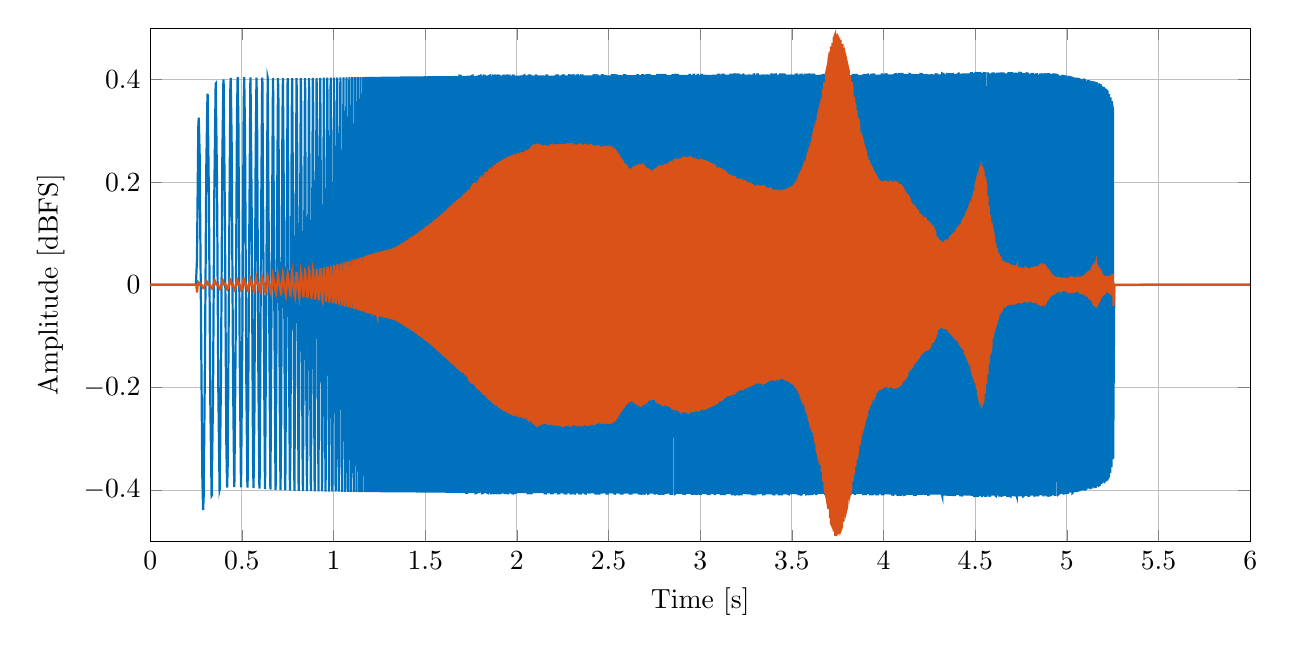
\begin{tikzpicture}

\begin{axis}[%
width=5.5in,
height=2.566in,
at={(1.925in,0.793in)},
scale only axis,
xmin=0,
xmax=6,
xlabel={Time [s]},
xmajorgrids,
ymin=-0.5,
ymax=0.5,
ylabel={Amplitude [dBFS]},
ymajorgrids,
axis background/.style={fill=white},
legend style={legend cell align=left,align=left,draw=white!15!black}
]
\addplot [color=mycolor1,solid,thick]
  table[row sep=crcr]{%
2.08333333333333e-05	-3.0517578125e-05\\
8.33333333333333e-05	-6.103515625e-05\\
0.000416666666666667	3.0517578125e-05\\
0.0123541666666667	6.103515625e-05\\
0.0132916666666667	-9.1552734375e-05\\
0.0148125	-6.103515625e-05\\
0.0148541666666667	3.0517578125e-05\\
0.0234583333333333	-6.103515625e-05\\
0.0238541666666667	6.103515625e-05\\
0.0297083333333333	3.0517578125e-05\\
0.031125	-6.103515625e-05\\
0.0364791666666667	3.0517578125e-05\\
0.0369166666666667	-9.1552734375e-05\\
0.0437708333333333	-6.103515625e-05\\
0.0446041666666667	6.103515625e-05\\
0.0510416666666667	6.103515625e-05\\
0.05575	-9.1552734375e-05\\
0.0583333333333333	3.0517578125e-05\\
0.059	-6.103515625e-05\\
0.0656666666666667	-6.103515625e-05\\
0.067875	6.103515625e-05\\
0.0728958333333333	3.0517578125e-05\\
0.0730208333333333	-6.103515625e-05\\
0.0801875	3.0517578125e-05\\
0.0802708333333333	-6.103515625e-05\\
0.087625	-6.103515625e-05\\
0.08775	3.0517578125e-05\\
0.0947708333333333	-6.103515625e-05\\
0.0960208333333333	6.103515625e-05\\
0.102	3.0517578125e-05\\
0.102354166666667	-6.103515625e-05\\
0.1095625	-6.103515625e-05\\
0.1160625	6.103515625e-05\\
0.118354166666667	-6.103515625e-05\\
0.121625	6.103515625e-05\\
0.123854166666667	3.0517578125e-05\\
0.124291666666667	-6.103515625e-05\\
0.131375	-6.103515625e-05\\
0.131541666666667	3.0517578125e-05\\
0.138708333333333	-6.103515625e-05\\
0.14125	6.103515625e-05\\
0.145875	3.0517578125e-05\\
0.146020833333333	-6.103515625e-05\\
0.157354166666667	-9.1552734375e-05\\
0.157625	6.103515625e-05\\
0.160354166666667	-6.103515625e-05\\
0.160645833333333	3.0517578125e-05\\
0.16775	-6.103515625e-05\\
0.167916666666667	6.103515625e-05\\
0.174958333333333	3.0517578125e-05\\
0.174979166666667	-6.103515625e-05\\
0.182333333333333	-6.103515625e-05\\
0.184104166666667	6.103515625e-05\\
0.1895	6.103515625e-05\\
0.196	-9.1552734375e-05\\
0.197270833333333	-6.103515625e-05\\
0.203708333333333	6.103515625e-05\\
0.204083333333333	-6.103515625e-05\\
0.204416666666667	3.0517578125e-05\\
0.2116875	-6.103515625e-05\\
0.216979166666667	6.103515625e-05\\
0.2190625	-6.103515625e-05\\
0.2230625	6.103515625e-05\\
0.2258125	3.0517578125e-05\\
0.225958333333333	-6.103515625e-05\\
0.2349375	6.103515625e-05\\
0.2374375	-9.1552734375e-05\\
0.243333333333333	6.103515625e-05\\
0.245354166666667	-9.1552734375e-05\\
0.249125	-9.1552734375e-05\\
0.2549375	0.048797607421875\\
0.2549375	0.048797607421875\\
0.262229166666667	0.307037353515625\\
0.264604166666667	0.325927734375\\
0.269520833333333	0.254119873046875\\
0.269520833333333	0.254119873046875\\
0.276791666666667	-0.056732177734375\\
0.276791666666667	-0.056732177734375\\
0.284083333333333	-0.374053955078125\\
0.284083333333333	-0.374053955078125\\
0.288479166666667	-0.43914794921875\\
0.291354166666667	-0.41314697265625\\
0.298645833333333	-0.14215087890625\\
0.298645833333333	-0.14215087890625\\
0.3059375	0.232025146484375\\
0.3059375	0.232025146484375\\
0.312291666666667	0.37255859375\\
0.313208333333333	0.369140625\\
0.3205	0.15313720703125\\
0.3205	0.15313720703125\\
0.327770833333333	-0.22979736328125\\
0.327770833333333	-0.22979736328125\\
0.334791666666667	-0.41107177734375\\
0.3350625	-0.410919189453125\\
0.342354166666667	-0.21832275390625\\
0.342354166666667	-0.21832275390625\\
0.349625	0.181488037109375\\
0.349625	0.181488037109375\\
0.356895833333333	0.39178466796875\\
0.357083333333333	0.391876220703125\\
0.3641875	0.201416015625\\
0.3641875	0.201416015625\\
0.371479166666667	-0.20745849609375\\
0.371479166666667	-0.20745849609375\\
0.3783125	-0.3995361328125\\
0.378770833333333	-0.3988037109375\\
0.386041666666667	-0.173553466796875\\
0.386041666666667	-0.173553466796875\\
0.393333333333333	0.247589111328125\\
0.393333333333333	0.247589111328125\\
0.399125	0.400115966796875\\
0.400604166666667	0.390899658203125\\
0.407895833333333	0.098602294921875\\
0.407895833333333	0.098602294921875\\
0.4151875	-0.3116455078125\\
0.4151875	-0.3116455078125\\
0.419395833333333	-0.39520263671875\\
0.422458333333333	-0.35198974609375\\
0.42975	0.026031494140625\\
0.42975	0.026031494140625\\
0.437020833333333	0.38165283203125\\
0.438958333333333	0.403411865234375\\
0.4443125	0.271514892578125\\
0.4443125	0.271514892578125\\
0.451604166666667	-0.1781005859375\\
0.451604166666667	-0.1781005859375\\
0.458166666666667	-0.394073486328125\\
0.458875	-0.3914794921875\\
0.466166666666667	-0.0965576171875\\
0.466166666666667	-0.0965576171875\\
0.4734375	0.33868408203125\\
0.4768125	0.404510498046875\\
0.480729166666667	0.322845458984375\\
0.480729166666667	0.322845458984375\\
0.488	-0.1302490234375\\
0.488	-0.1302490234375\\
0.495	-0.394378662109375\\
0.495291666666667	-0.393829345703125\\
0.502583333333333	-0.096527099609375\\
0.502583333333333	-0.096527099609375\\
0.509854166666667	0.35211181640625\\
0.512666666666667	0.404541015625\\
0.517145833333333	0.289459228515625\\
0.517145833333333	0.289459228515625\\
0.524416666666667	-0.2015380859375\\
0.524416666666667	-0.2015380859375\\
0.5300625	-0.395172119140625\\
0.531708333333333	-0.37774658203125\\
0.539	0.033599853515625\\
0.539	0.033599853515625\\
0.546270833333333	0.401153564453125\\
0.546875	0.404266357421875\\
0.5535625	0.133392333984375\\
0.5535625	0.133392333984375\\
0.560833333333333	-0.34747314453125\\
0.563395833333333	-0.396148681640625\\
0.568125	-0.249755859375\\
0.568125	-0.249755859375\\
0.575416666666667	0.27593994140625\\
0.575416666666667	0.27593994140625\\
0.579583333333333	0.403839111328125\\
0.5826875	0.334197998046875\\
0.589979166666667	-0.18511962890625\\
0.589979166666667	-0.18511962890625\\
0.595395833333333	-0.397125244140625\\
0.59725	-0.3707275390625\\
0.604541666666667	0.112213134765625\\
0.604541666666667	0.112213134765625\\
0.610791666666667	0.403472900390625\\
0.611833333333333	0.395233154296875\\
0.619104166666667	-0.05230712890625\\
0.619104166666667	-0.05230712890625\\
0.625875	-0.397979736328125\\
0.626395833333333	-0.396240234375\\
0.633666666666667	0.021026611328125\\
0.633666666666667	0.021026611328125\\
0.64075	0.40313720703125\\
0.640958333333333	0.40277099609375\\
0.64825	-0.012603759765625\\
0.64825	-0.012603759765625\\
0.6553125	-0.398681640625\\
0.655520833333333	-0.39813232421875\\
0.6628125	0.031097412109375\\
0.6628125	0.031097412109375\\
0.669520833333333	0.402923583984375\\
0.670083333333333	0.39971923828125\\
0.677375	-0.073577880859375\\
0.677375	-0.073577880859375\\
0.683458333333333	-0.399444580078125\\
0.684666666666667	-0.38580322265625\\
0.6919375	0.141571044921875\\
0.6919375	0.141571044921875\\
0.697166666666667	0.402801513671875\\
0.699229166666667	0.3597412109375\\
0.7065	-0.227294921875\\
0.7065	-0.227294921875\\
0.710645833333333	-0.399993896484375\\
0.713791666666667	-0.295745849609375\\
0.721083333333333	0.319549560546875\\
0.723770833333333	0.40264892578125\\
0.728354166666667	0.186370849609375\\
0.728354166666667	0.186370849609375\\
0.735645833333333	-0.385894775390625\\
0.736708333333333	-0.40045166015625\\
0.742916666666667	-0.02593994140625\\
0.742916666666667	-0.02593994140625\\
0.7494375	0.402618408203125\\
0.750208333333333	0.39654541015625\\
0.7575	-0.169219970703125\\
0.7575	-0.169219970703125\\
0.761979166666667	-0.400848388671875\\
0.764770833333333	-0.308868408203125\\
0.7720625	0.337860107421875\\
0.774291666666667	0.40264892578125\\
0.779333333333333	0.107757568359375\\
0.779333333333333	0.107757568359375\\
0.786395833333333	-0.401214599609375\\
0.786625	-0.400390625\\
0.793916666666667	0.160491943359375\\
0.793916666666667	0.160491943359375\\
0.79825	0.40264892578125\\
0.8011875	0.28887939453125\\
0.808479166666667	-0.36962890625\\
0.809958333333333	-0.4014892578125\\
0.81575	-0.002410888671875\\
0.81575	-0.002410888671875\\
0.821458333333333	0.40277099609375\\
0.823041666666667	0.367584228515625\\
0.830333333333333	-0.31005859375\\
0.832791666666667	-0.401763916015625\\
0.837604166666667	-0.093719482421875\\
0.837604166666667	-0.093719482421875\\
0.843979166666667	0.40289306640625\\
0.844895833333333	0.38970947265625\\
0.852166666666667	-0.279998779296875\\
0.854958333333333	-0.4019775390625\\
0.859458333333333	-0.11029052734375\\
0.859458333333333	-0.11029052734375\\
0.865729166666667	0.402923583984375\\
0.86675	0.38763427734375\\
0.874020833333333	-0.3035888671875\\
0.876416666666667	-0.40216064453125\\
0.8813125	-0.0511474609375\\
0.8813125	-0.0511474609375\\
0.886958333333333	0.403076171875\\
0.888583333333333	0.356658935546875\\
0.895875	-0.36468505859375\\
0.897333333333333	-0.402374267578125\\
0.903166666666667	0.088226318359375\\
0.903166666666667	0.088226318359375\\
0.907541666666667	0.403167724609375\\
0.9104375	0.249847412109375\\
0.917625	-0.40252685546875\\
0.917729166666667	-0.402130126953125\\
0.925	0.279541015625\\
0.927520833333333	0.403350830078125\\
0.932291666666667	0.0185546875\\
0.932291666666667	0.0185546875\\
0.937291666666667	-0.402587890625\\
0.9395625	-0.30322265625\\
0.946854166666667	0.40301513671875\\
0.946979166666667	0.4034423828125\\
0.954145833333333	-0.285247802734375\\
0.956520833333333	-0.402740478515625\\
0.961416666666667	0.021209716796875\\
0.961416666666667	0.021209716796875\\
0.9659375	0.403564453125\\
0.968708333333333	0.240692138671875\\
0.975229166666667	-0.402923583984375\\
0.975979166666667	-0.390411376953125\\
0.983270833333333	0.37298583984375\\
0.984395833333333	0.403656005859375\\
0.9905625	-0.215118408203125\\
0.9934375	-0.402984619140625\\
0.997833333333333	-0.018707275390625\\
0.997833333333333	-0.018707275390625\\
1.00241666666667	0.40380859375\\
1.005125	0.23162841796875\\
1.01122916666667	-0.403076171875\\
1.01239583333333	-0.370361328125\\
1.0196875	0.4014892578125\\
1.01995833333333	0.403900146484375\\
1.02697916666667	-0.33349609375\\
1.02860416666667	-0.4031982421875\\
1.03425	0.192962646484375\\
1.03716666666667	0.40411376953125\\
1.04154166666667	-0.027557373046875\\
1.04154166666667	-0.027557373046875\\
1.0455625	-0.403411865234375\\
1.0488125	-0.140045166015625\\
1.053875	0.404266357421875\\
1.05610416666667	0.26983642578125\\
1.06214583333333	-0.403350830078125\\
1.06339583333333	-0.357269287109375\\
1.07027083333333	0.40435791015625\\
1.07066666666667	0.39959716796875\\
1.07795833333333	-0.3995361328125\\
1.0783125	-0.403564453125\\
1.08522916666667	0.36907958984375\\
1.08629166666667	0.404510498046875\\
1.09252083333333	-0.319854736328125\\
1.0941875	-0.403564453125\\
1.0998125	0.26080322265625\\
1.10191666666667	0.404541015625\\
1.10708333333333	-0.199920654296875\\
1.10964583333333	-0.403656005859375\\
1.114375	0.143646240234375\\
1.11727083333333	0.4046630859375\\
1.12164583333333	-0.096282958984375\\
1.12483333333333	-0.403717041015625\\
1.1289375	0.05902099609375\\
1.1323125	0.40472412109375\\
1.13622916666667	-0.037994384765625\\
1.1396875	-0.403778076171875\\
1.1435	0.02154541015625\\
1.147	0.40478515625\\
1.15079166666667	-0.025634765625\\
1.15422916666667	-0.40380859375\\
1.1580625	0.0347900390625\\
1.16141666666667	0.404937744140625\\
1.16535416666667	-0.06451416015625\\
1.16854166666667	-0.40386962890625\\
1.17264583333333	0.102630615234375\\
1.1755625	0.404998779296875\\
1.17991666666667	-0.152435302734375\\
1.18254166666667	-0.4039306640625\\
1.18720833333333	0.21136474609375\\
1.1894375	0.405059814453125\\
1.19447916666667	-0.274322509765625\\
1.19629166666667	-0.40399169921875\\
1.20177083333333	0.335845947265625\\
1.20304166666667	0.405120849609375\\
1.2090625	-0.3834228515625\\
1.20975	-0.404052734375\\
1.21633333333333	0.40496826171875\\
1.21641666666667	0.405242919921875\\
1.22297916666667	-0.404052734375\\
1.223625	-0.385467529296875\\
1.2295	0.405303955078125\\
1.23089583333333	0.31756591796875\\
1.23597916666667	-0.40411376953125\\
1.2381875	-0.1920166015625\\
1.24235416666667	0.40533447265625\\
1.24872916666667	-0.4041748046875\\
1.25275	0.165863037109375\\
1.25502083333333	0.405426025390625\\
1.26004166666667	-0.32794189453125\\
1.26127083333333	-0.404205322265625\\
1.2673125	0.404052734375\\
1.26745833333333	0.405517578125\\
1.27358333333333	-0.40423583984375\\
1.27460416666667	-0.353790283203125\\
1.27970833333333	0.40557861328125\\
1.28189583333333	0.16973876953125\\
1.28572916666667	-0.404296875\\
1.29172916666667	0.4056396484375\\
1.29645833333333	-0.32525634765625\\
1.29764583333333	-0.404296875\\
1.30354166666667	0.40570068359375\\
1.30372916666667	0.40380859375\\
1.30939583333333	-0.404388427734375\\
1.31102083333333	-0.259002685546875\\
1.31516666666667	0.405731201171875\\
1.3209375	-0.40435791015625\\
1.32558333333333	0.33831787109375\\
1.326625	0.405792236328125\\
1.33227083333333	-0.404388427734375\\
1.332875	-0.38397216796875\\
1.33789583333333	0.40582275390625\\
1.34347916666667	-0.404449462890625\\
1.3474375	0.2523193359375\\
1.349	0.4058837890625\\
1.3545	-0.40447998046875\\
1.35472916666667	-0.40093994140625\\
1.3599375	0.405914306640625\\
1.36533333333333	-0.404449462890625\\
1.36929166666667	0.271453857421875\\
1.37070833333333	0.405975341796875\\
1.37604166666667	-0.404510498046875\\
1.3765625	-0.385711669921875\\
1.38133333333333	0.406005859375\\
1.38658333333333	-0.404510498046875\\
1.391125	0.37384033203125\\
1.39177083333333	0.40606689453125\\
1.39695833333333	-0.404541015625\\
1.39841666666667	-0.256805419921875\\
1.40210416666667	0.4061279296875\\
1.4071875	-0.404541015625\\
1.41227083333333	0.406158447265625\\
1.41297916666667	0.366363525390625\\
1.41729166666667	-0.40460205078125\\
1.42227083333333	0.406158447265625\\
1.42722916666667	-0.404571533203125\\
1.42754166666667	-0.397674560546875\\
1.4321875	0.40618896484375\\
1.4370625	-0.40460205078125\\
1.4419375	0.406219482421875\\
1.442125	0.402923583984375\\
1.44675	-0.4046630859375\\
1.45154166666667	0.40625\\
1.4563125	-0.40472412109375\\
1.4566875	-0.392730712890625\\
1.46104166666667	0.406280517578125\\
1.46572916666667	-0.4046630859375\\
1.47041666666667	0.40631103515625\\
1.47125	0.34527587890625\\
1.4750625	-0.40472412109375\\
1.4796875	0.406341552734375\\
1.48427083333333	-0.40472412109375\\
1.4888125	0.4063720703125\\
1.49310416666667	-0.399261474609375\\
1.49335416666667	-0.404754638671875\\
1.49783333333333	0.40643310546875\\
1.5023125	-0.404815673828125\\
1.50675	0.406402587890625\\
1.51116666666667	-0.40478515625\\
1.51495833333333	0.369049072265625\\
1.5155625	0.406494140625\\
1.51991666666667	-0.404815673828125\\
1.52425	0.406494140625\\
1.5285625	-0.40484619140625\\
1.53285416666667	0.406494140625\\
1.53679166666667	-0.393646240234375\\
1.53710416666667	-0.40484619140625\\
1.54133333333333	0.406524658203125\\
1.5455625	-0.4049072265625\\
1.54972916666667	0.40655517578125\\
1.55389583333333	-0.40496826171875\\
1.55804166666667	0.40655517578125\\
1.56216666666667	-0.404937744140625\\
1.5659375	0.394866943359375\\
1.56622916666667	0.406585693359375\\
1.57033333333333	-0.405059814453125\\
1.57435416666667	0.406646728515625\\
1.57839583333333	-0.404998779296875\\
1.58239583333333	0.406646728515625\\
1.58635416666667	-0.40509033203125\\
1.5903125	0.40667724609375\\
1.59425	-0.40509033203125\\
1.59816666666667	0.406768798828125\\
1.60208333333333	-0.405120849609375\\
1.6059375	0.40673828125\\
1.609625	-0.401458740234375\\
1.60979166666667	-0.405120849609375\\
1.61360416666667	0.40673828125\\
1.6174375	-0.405181884765625\\
1.62120833333333	0.406768798828125\\
1.625	-0.405181884765625\\
1.62875	0.40679931640625\\
1.63247916666667	-0.405181884765625\\
1.6361875	0.40679931640625\\
1.639875	-0.40521240234375\\
1.64358333333333	0.4068603515625\\
1.64720833333333	-0.4052734375\\
1.65085416666667	0.4068603515625\\
1.65447916666667	-0.405303955078125\\
1.65808333333333	0.406951904296875\\
1.66166666666667	-0.4052734375\\
1.66522916666667	0.40692138671875\\
1.66877083333333	-0.40496826171875\\
1.6723125	0.4068603515625\\
1.67583333333333	-0.40594482421875\\
1.67933333333333	0.40655517578125\\
1.6828125	-0.40533447265625\\
1.68627083333333	0.407562255859375\\
1.69316666666667	0.406982421875\\
1.6965625	-0.40594482421875\\
1.69995833333333	0.407012939453125\\
1.70335416666667	-0.4053955078125\\
1.70672916666667	0.406982421875\\
1.7100625	-0.4049072265625\\
1.71339583333333	0.40704345703125\\
1.71670833333333	-0.4058837890625\\
1.72004166666667	0.407012939453125\\
1.72333333333333	-0.4053955078125\\
1.72985416666667	-0.40533447265625\\
1.733125	0.40765380859375\\
1.73635416666667	-0.40545654296875\\
1.7395625	0.4071044921875\\
1.74275	-0.405029296875\\
1.74595833333333	0.4071044921875\\
1.749125	-0.406005859375\\
1.75229166666667	0.406707763671875\\
1.75858333333333	0.407623291015625\\
1.7616875	-0.40545654296875\\
1.76479166666667	0.407135009765625\\
1.76789583333333	-0.40509033203125\\
1.77097916666667	0.407135009765625\\
1.77404166666667	-0.406036376953125\\
1.78014583333333	-0.405517578125\\
1.78316666666667	0.407623291015625\\
1.7861875	-0.4051513671875\\
1.7891875	0.407196044921875\\
1.7921875	-0.405975341796875\\
1.79516666666667	0.40679931640625\\
1.80108333333333	0.40765380859375\\
1.80402083333333	-0.405120849609375\\
1.80695833333333	0.4072265625\\
1.809875	-0.406036376953125\\
1.8156875	-0.405548095703125\\
1.8185625	0.40765380859375\\
1.82429166666667	0.4072265625\\
1.82714583333333	-0.406005859375\\
1.83	0.406890869140625\\
1.8328125	-0.405548095703125\\
1.83564583333333	0.407623291015625\\
1.8384375	-0.405181884765625\\
1.84402083333333	-0.405975341796875\\
1.8468125	0.406829833984375\\
1.8523125	0.40771484375\\
1.8550625	-0.405242919921875\\
1.85779166666667	0.4073486328125\\
1.8605	-0.405914306640625\\
1.86591666666667	-0.405609130859375\\
1.86860416666667	0.40765380859375\\
1.87395833333333	0.407318115234375\\
1.876625	-0.405914306640625\\
1.8819375	-0.405670166015625\\
1.8845625	0.407623291015625\\
1.88979166666667	0.40728759765625\\
1.89239583333333	-0.405914306640625\\
1.89758333333333	-0.40576171875\\
1.90014583333333	0.40765380859375\\
1.90527083333333	0.407318115234375\\
1.90783333333333	-0.405975341796875\\
1.91289583333333	-0.40570068359375\\
1.9154375	0.407623291015625\\
1.9179375	-0.405548095703125\\
1.9204375	0.40740966796875\\
1.9229375	-0.40594482421875\\
1.9254375	0.407318115234375\\
1.930375	0.407440185546875\\
1.93283333333333	-0.4056396484375\\
1.93775	-0.40582275390625\\
1.9401875	0.407135009765625\\
1.94504166666667	0.4075927734375\\
1.9474375	-0.405487060546875\\
1.95225	-0.405975341796875\\
1.954625	0.4072265625\\
1.95939583333333	0.407470703125\\
1.96175	-0.40594482421875\\
1.9688125	0.40753173828125\\
1.97114583333333	-0.4056396484375\\
1.97579166666667	-0.406219482421875\\
1.97810416666667	0.40765380859375\\
1.98270833333333	0.40753173828125\\
1.985	-0.405914306640625\\
1.9895625	-0.40582275390625\\
1.99183333333333	0.40753173828125\\
1.99860416666667	-0.406341552734375\\
2.00083333333333	0.407806396484375\\
2.00752083333333	-0.405914306640625\\
2.00972916666667	0.40753173828125\\
2.0119375	-0.40594482421875\\
2.01414583333333	0.407623291015625\\
2.02070833333333	-0.4058837890625\\
2.022875	0.40802001953125\\
2.02504166666667	-0.406005859375\\
2.0315	0.407989501953125\\
2.03364583333333	-0.405975341796875\\
2.03579166666667	0.407135009765625\\
2.04004166666667	0.40802001953125\\
2.04216666666667	-0.405914306640625\\
2.04847916666667	0.407989501953125\\
2.0505625	-0.405975341796875\\
2.05679166666667	0.407958984375\\
2.058875	-0.406005859375\\
2.063	-0.40594482421875\\
2.06504166666667	0.408050537109375\\
2.0731875	0.40802001953125\\
2.07520833333333	-0.406005859375\\
2.07922916666667	-0.40594482421875\\
2.08125	0.407989501953125\\
2.08325	-0.406158447265625\\
2.08522916666667	0.40765380859375\\
2.095125	-0.406005859375\\
2.09708333333333	0.40802001953125\\
2.1029375	-0.406036376953125\\
2.104875	0.40802001953125\\
2.10489583333333	0.40802001953125\\
2.1068125	-0.406036376953125\\
2.11260416666667	0.40802001953125\\
2.11452083333333	-0.406005859375\\
2.12022916666667	0.40802001953125\\
2.122125	-0.40606689453125\\
2.12777083333333	0.40789794921875\\
2.12964583333333	-0.406036376953125\\
2.13525	0.407989501953125\\
2.13710416666667	-0.406036376953125\\
2.14264583333333	0.4080810546875\\
2.14447916666667	-0.4061279296875\\
2.14995833333333	0.407867431640625\\
2.15179166666667	-0.4061279296875\\
2.15902083333333	-0.4063720703125\\
2.1608125	0.407745361328125\\
2.16439583333333	0.407745361328125\\
2.16616666666667	-0.406280517578125\\
2.1715	0.40777587890625\\
2.17327083333333	-0.40631103515625\\
2.17854166666667	0.40765380859375\\
2.18029166666667	-0.406219482421875\\
2.1855	0.407806396484375\\
2.18722916666667	-0.406280517578125\\
2.194125	-0.406219482421875\\
2.19925	0.407806396484375\\
2.2009375	-0.40631103515625\\
2.20264583333333	0.407745361328125\\
2.20770833333333	-0.40618896484375\\
2.209375	0.40789794921875\\
2.21439583333333	-0.4061279296875\\
2.2160625	0.407867431640625\\
2.2226875	0.407928466796875\\
2.22433333333333	-0.4063720703125\\
2.230875	-0.40618896484375\\
2.2325	0.407867431640625\\
2.24058333333333	-0.406585693359375\\
2.2421875	0.408111572265625\\
2.24379166666667	-0.406219482421875\\
2.2485625	0.407745361328125\\
2.25489583333333	0.408203125\\
2.25645833333333	-0.40631103515625\\
2.25804166666667	0.407928466796875\\
2.25960416666667	-0.406158447265625\\
2.2689375	-0.406524658203125\\
2.27047916666667	0.40814208984375\\
2.27814583333333	-0.406524658203125\\
2.27966666666667	0.407958984375\\
2.28422916666667	-0.40618896484375\\
2.28575	0.40814208984375\\
2.29175	0.4078369140625\\
2.29325	-0.406524658203125\\
2.29920833333333	-0.406158447265625\\
2.3006875	0.408203125\\
2.30216666666667	-0.406463623046875\\
2.303625	0.40789794921875\\
2.3095	0.408203125\\
2.31095833333333	-0.4063720703125\\
2.31677083333333	-0.40655517578125\\
2.31820833333333	0.4080810546875\\
2.32539583333333	-0.406524658203125\\
2.32683333333333	0.407928466796875\\
2.3325	0.408203125\\
2.33391666666667	-0.40643310546875\\
2.33814583333333	0.407958984375\\
2.33954166666667	-0.40631103515625\\
2.34791666666667	-0.406524658203125\\
2.34929166666667	0.408111572265625\\
2.35754166666667	0.407989501953125\\
2.35891666666667	-0.406341552734375\\
2.36027083333333	0.407958984375\\
2.36704166666667	-0.406524658203125\\
2.36839583333333	0.408172607421875\\
2.36975	-0.406341552734375\\
2.37510416666667	-0.406646728515625\\
2.3764375	0.408203125\\
2.3830625	-0.406524658203125\\
2.384375	0.408050537109375\\
2.39354166666667	-0.406646728515625\\
2.39485416666667	0.40814208984375\\
2.4013125	-0.406402587890625\\
2.40260416666667	0.408172607421875\\
2.403875	-0.406585693359375\\
2.40516666666667	0.40802001953125\\
2.41154166666667	-0.406494140625\\
2.41785416666667	0.408050537109375\\
2.42035416666667	0.408294677734375\\
2.42160416666667	-0.406524658203125\\
2.42535416666667	0.407958984375\\
2.42660416666667	-0.4063720703125\\
2.43402083333333	-0.406646728515625\\
2.43525	0.408172607421875\\
2.44014583333333	0.40802001953125\\
2.44135416666667	-0.40631103515625\\
2.448625	-0.40667724609375\\
2.44983333333333	0.408172607421875\\
2.45583333333333	-0.40667724609375\\
2.45702083333333	0.408172607421875\\
2.46295833333333	-0.40673828125\\
2.464125	0.408203125\\
2.4711875	0.40814208984375\\
2.47235416666667	-0.406463623046875\\
2.47816666666667	0.408172607421875\\
2.4793125	-0.406585693359375\\
2.48735416666667	0.408355712890625\\
2.4885	-0.4066162109375\\
2.4953125	-0.40673828125\\
2.4964375	0.4083251953125\\
2.4998125	-0.40643310546875\\
2.50541666666667	0.408294677734375\\
2.50652083333333	-0.406524658203125\\
2.50985416666667	0.408203125\\
2.51316666666667	-0.406524658203125\\
2.51866666666667	0.408355712890625\\
2.52520833333333	0.408294677734375\\
2.52629166666667	-0.406646728515625\\
2.527375	0.408172607421875\\
2.53275	-0.406585693359375\\
2.53489583333333	-0.40673828125\\
2.53595833333333	0.408203125\\
2.54445833333333	0.408111572265625\\
2.54552083333333	-0.406524658203125\\
2.55077083333333	0.408477783203125\\
2.5518125	-0.40679931640625\\
2.55910416666667	0.408447265625\\
2.560125	-0.406646728515625\\
2.56733333333333	0.40838623046875\\
2.56835416666667	-0.40679931640625\\
2.57647916666667	-0.406585693359375\\
2.5775	0.408233642578125\\
2.58252083333333	-0.40679931640625\\
2.58352083333333	0.408447265625\\
2.59147916666667	0.408477783203125\\
2.59245833333333	-0.4066162109375\\
2.59345833333333	0.408355712890625\\
2.598375	-0.40673828125\\
2.60520833333333	0.40838623046875\\
2.60616666666667	-0.40673828125\\
2.6129375	0.4083251953125\\
2.61389583333333	-0.4068603515625\\
2.61485416666667	0.40850830078125\\
2.6158125	-0.406829833984375\\
2.6253125	-0.4068603515625\\
2.62625	0.40838623046875\\
2.6346875	-0.406707763671875\\
2.635625	0.408416748046875\\
2.63841666666667	-0.406585693359375\\
2.64304166666667	0.408416748046875\\
2.64395833333333	-0.4068603515625\\
2.644875	0.408447265625\\
2.65672916666667	-0.4068603515625\\
2.657625	0.408355712890625\\
2.6594375	0.40838623046875\\
2.66570833333333	-0.40679931640625\\
2.66660416666667	0.408538818359375\\
2.6675	-0.4068603515625\\
2.67635416666667	-0.40692138671875\\
2.67722916666667	0.408447265625\\
2.68335416666667	-0.4068603515625\\
2.68422916666667	0.40850830078125\\
2.6894375	0.408599853515625\\
2.69029166666667	-0.40679931640625\\
2.69716666666667	-0.406829833984375\\
2.69802083333333	0.408416748046875\\
2.70397916666667	-0.406768798828125\\
2.70652083333333	0.4085693359375\\
2.71491666666667	0.408599853515625\\
2.71575	-0.406982421875\\
2.71741666666667	-0.40679931640625\\
2.72320833333333	0.408599853515625\\
2.72485416666667	0.408477783203125\\
2.72895833333333	-0.40704345703125\\
2.73629166666667	0.408477783203125\\
2.73710416666667	-0.40692138671875\\
2.73952083333333	0.4085693359375\\
2.7419375	-0.406890869140625\\
2.75072916666667	0.408538818359375\\
2.75152083333333	-0.406890869140625\\
2.7546875	-0.406890869140625\\
2.75547916666667	0.408599853515625\\
2.76410416666667	-0.407135009765625\\
2.764875	0.408660888671875\\
2.772625	0.40875244140625\\
2.77339583333333	-0.407073974609375\\
2.77952083333333	-0.406951904296875\\
2.78029166666667	0.40875244140625\\
2.787875	0.408660888671875\\
2.788625	-0.406890869140625\\
2.79089583333333	0.40869140625\\
2.79164583333333	-0.407073974609375\\
2.79910416666667	-0.407073974609375\\
2.80133333333333	0.408782958984375\\
2.81016666666667	0.40863037109375\\
2.81089583333333	-0.4071044921875\\
2.811625	0.40875244140625\\
2.81235416666667	-0.407135009765625\\
2.82177083333333	0.4088134765625\\
2.8225	-0.40692138671875\\
2.82608333333333	0.408599853515625\\
2.82964583333333	-0.4071044921875\\
2.8374375	0.4088134765625\\
2.83814583333333	-0.407196044921875\\
2.84654166666667	-0.407196044921875\\
2.84722916666667	0.40869140625\\
2.8479375	-0.4071044921875\\
2.848625	0.40875244140625\\
2.861	0.4090576171875\\
2.8616875	-0.407501220703125\\
2.86304166666667	-0.4072265625\\
2.86372916666667	0.40887451171875\\
2.8698125	-0.407196044921875\\
2.87183333333333	0.408782958984375\\
2.8771875	0.40875244140625\\
2.87785416666667	-0.40716552734375\\
2.88514583333333	0.408935546875\\
2.887125	-0.40716552734375\\
2.89302083333333	0.408966064453125\\
2.89366666666667	-0.407257080078125\\
2.90466666666667	0.408660888671875\\
2.9053125	-0.4072265625\\
2.90722916666667	0.40887451171875\\
2.90914583333333	-0.407196044921875\\
2.9155	-0.40740966796875\\
2.91739583333333	0.409088134765625\\
2.92679166666667	-0.407196044921875\\
2.92741666666667	0.40887451171875\\
2.93052083333333	-0.4073486328125\\
2.93114583333333	0.408843994140625\\
2.9366875	-0.4073486328125\\
2.94097916666667	0.4088134765625\\
2.94341666666667	0.408935546875\\
2.948875	-0.407318115234375\\
2.95308333333333	0.4088134765625\\
2.9536875	-0.40728759765625\\
2.96322916666667	-0.40753173828125\\
2.9638125	0.4091796875\\
2.965	0.409271240234375\\
2.96558333333333	-0.407470703125\\
2.977875	0.40887451171875\\
2.97845833333333	-0.407318115234375\\
2.98077083333333	-0.407379150390625\\
2.98595833333333	0.408935546875\\
2.98710416666667	0.40899658203125\\
2.993375	-0.407470703125\\
2.99508333333333	0.40887451171875\\
2.99564583333333	-0.407379150390625\\
3.00464583333333	-0.40740966796875\\
3.0074375	0.409088134765625\\
3.00966666666667	0.40899658203125\\
3.01354166666667	-0.407440185546875\\
3.0206875	0.40911865234375\\
3.02122916666667	-0.40765380859375\\
3.02395833333333	0.40948486328125\\
3.0245	-0.407867431640625\\
3.03154166666667	0.409149169921875\\
3.03422916666667	-0.407623291015625\\
3.03797916666667	0.409088134765625\\
3.04064583333333	-0.40740966796875\\
3.05120833333333	-0.407745361328125\\
3.05172916666667	0.409271240234375\\
3.05172916666667	0.409271240234375\\
3.05225	-0.40753173828125\\
3.06316666666667	0.4093017578125\\
3.0636875	-0.40765380859375\\
3.07035416666667	0.40936279296875\\
3.07289583333333	-0.40753173828125\\
3.07847916666667	0.409149169921875\\
3.07897916666667	-0.407623291015625\\
3.081	-0.4075927734375\\
3.0815	0.409332275390625\\
3.09	-0.407562255859375\\
3.09445833333333	0.409332275390625\\
3.0959375	-0.407623291015625\\
3.09741666666667	0.409393310546875\\
3.10329166666667	0.409332275390625\\
3.10572916666667	-0.4075927734375\\
3.1110625	0.409393310546875\\
3.11154166666667	-0.407867431640625\\
3.121125	-0.407867431640625\\
3.12160416666667	0.409423828125\\
3.12822916666667	0.409271240234375\\
3.12964583333333	-0.407745361328125\\
3.13527083333333	-0.40777587890625\\
3.13666666666667	0.409454345703125\\
3.143625	-0.40771484375\\
3.14408333333333	0.409393310546875\\
3.15279166666667	-0.407928466796875\\
3.15325	0.409515380859375\\
3.15370833333333	-0.40789794921875\\
3.15597916666667	0.409515380859375\\
3.16275	-0.407867431640625\\
3.165	0.409271240234375\\
3.172125	0.409423828125\\
3.17345833333333	-0.407928466796875\\
3.177875	-0.407806396484375\\
3.1783125	0.40948486328125\\
3.18879166666667	0.409881591796875\\
3.18922916666667	-0.4085693359375\\
3.19095833333333	-0.4085693359375\\
3.19139583333333	0.409912109375\\
3.20083333333333	0.409454345703125\\
3.2038125	-0.407745361328125\\
3.20635416666667	-0.40802001953125\\
3.207625	0.40960693359375\\
3.21435416666667	0.40948486328125\\
3.21477083333333	-0.407928466796875\\
3.2255625	-0.40802001953125\\
3.22597916666667	0.409759521484375\\
3.22720833333333	-0.40789794921875\\
3.23335416666667	0.409637451171875\\
3.23416666666667	0.40966796875\\
3.24025	-0.407958984375\\
3.24227083333333	0.409576416015625\\
3.24266666666667	-0.407989501953125\\
3.25504166666667	0.40960693359375\\
3.2554375	-0.407989501953125\\
3.25583333333333	0.409637451171875\\
3.25622916666667	-0.408111572265625\\
3.2668125	0.409881591796875\\
3.26797916666667	-0.408233642578125\\
3.2745625	0.409454345703125\\
3.27570833333333	-0.40826416015625\\
3.27839583333333	0.4095458984375\\
3.2803125	-0.407806396484375\\
3.2916875	-0.4080810546875\\
3.2920625	0.40972900390625\\
3.2928125	0.409820556640625\\
3.2931875	-0.40826416015625\\
3.30139583333333	-0.408203125\\
3.30325	0.40972900390625\\
3.31025	-0.40814208984375\\
3.3128125	0.410003662109375\\
3.31427083333333	0.409912109375\\
3.31827083333333	-0.408111572265625\\
3.3265625	0.40960693359375\\
3.32691666666667	-0.407989501953125\\
3.32870833333333	0.40966796875\\
3.33191666666667	-0.407989501953125\\
3.34145833333333	0.40966796875\\
3.3418125	-0.408233642578125\\
3.3435625	0.409820556640625\\
3.34391666666667	-0.408203125\\
3.350875	-0.407867431640625\\
3.35122916666667	0.40960693359375\\
3.36325	-0.408416748046875\\
3.36427083333333	0.410064697265625\\
3.36529166666667	-0.408538818359375\\
3.3663125	0.40985107421875\\
3.37272916666667	-0.40814208984375\\
3.3730625	0.40972900390625\\
3.38141666666667	-0.408203125\\
3.38175	0.4097900390625\\
3.387375	-0.408203125\\
3.38902083333333	0.40985107421875\\
3.39491666666667	0.40960693359375\\
3.39654166666667	-0.407928466796875\\
3.40366666666667	-0.408294677734375\\
3.40591666666667	0.40948486328125\\
3.4123125	0.409942626953125\\
3.41327083333333	-0.408447265625\\
3.416125	0.409759521484375\\
3.42022916666667	-0.4080810546875\\
3.4280625	0.409759521484375\\
3.428375	-0.408203125\\
3.43147916666667	-0.408111572265625\\
3.4355	0.409698486328125\\
3.44225	0.40972900390625\\
3.44316666666667	-0.40814208984375\\
3.44560416666667	-0.4080810546875\\
3.44772916666667	0.409515380859375\\
3.4585625	0.409912109375\\
3.45945833333333	-0.40826416015625\\
3.46510416666667	0.409942626953125\\
3.46658333333333	-0.4083251953125\\
3.466875	0.4097900390625\\
3.46835416666667	-0.408203125\\
3.48033333333333	0.409423828125\\
3.480625	-0.4078369140625\\
3.4829375	-0.4080810546875\\
3.48322916666667	0.40960693359375\\
3.49439583333333	-0.40826416015625\\
3.49525	0.409820556640625\\
3.49666666666667	-0.4080810546875\\
3.49808333333333	0.40948486328125\\
3.5034375	-0.407989501953125\\
3.50595833333333	0.409515380859375\\
3.51291666666667	-0.40802001953125\\
3.51375	0.40972900390625\\
3.5184375	-0.4078369140625\\
3.52145833333333	0.409515380859375\\
3.52854166666667	0.409759521484375\\
3.5288125	-0.408172607421875\\
3.53502083333333	0.40948486328125\\
3.53529166666667	-0.40777587890625\\
3.54383333333333	-0.408050537109375\\
3.54675	0.40936279296875\\
3.55254166666667	0.4095458984375\\
3.55385416666667	-0.408203125\\
3.554375	-0.4080810546875\\
3.55672916666667	0.409576416015625\\
3.56166666666667	-0.4078369140625\\
3.568625	0.409423828125\\
3.56939583333333	-0.4078369140625\\
3.5711875	0.409393310546875\\
3.5783125	0.409515380859375\\
3.5785625	-0.4080810546875\\
3.58360416666667	-0.40765380859375\\
3.58385416666667	0.408966064453125\\
3.59135416666667	0.409576416015625\\
3.59160416666667	-0.407958984375\\
3.59902083333333	-0.40771484375\\
3.60025	0.409271240234375\\
3.60952083333333	0.409271240234375\\
3.61025	-0.407745361328125\\
3.61266666666667	-0.407684326171875\\
3.61435416666667	0.409149169921875\\
3.62202083333333	0.409393310546875\\
3.6236875	-0.407745361328125\\
3.63102083333333	0.40911865234375\\
3.63266666666667	-0.407623291015625\\
3.63454166666667	-0.4075927734375\\
3.63897916666667	0.409271240234375\\
3.642	-0.4075927734375\\
3.64222916666667	0.409271240234375\\
3.65258333333333	-0.408050537109375\\
3.6528125	0.409637451171875\\
3.65622916666667	-0.407623291015625\\
3.65645833333333	0.409149169921875\\
3.66391666666667	-0.407562255859375\\
3.668625	0.4090576171875\\
3.67485416666667	0.409027099609375\\
3.67772916666667	-0.407501220703125\\
3.67927083333333	0.40899658203125\\
3.68125	-0.40753173828125\\
3.6869375	-0.407562255859375\\
3.68889583333333	0.40899658203125\\
3.69645833333333	-0.407470703125\\
3.69710416666667	0.409149169921875\\
3.70352083333333	0.409027099609375\\
3.70458333333333	-0.407501220703125\\
3.70797916666667	-0.4073486328125\\
3.70945833333333	0.409027099609375\\
3.7211875	0.40911865234375\\
3.72139583333333	-0.4075927734375\\
3.7218125	-0.40753173828125\\
3.72202083333333	0.40899658203125\\
3.7329375	-0.4088134765625\\
3.73395833333333	0.410186767578125\\
3.73660416666667	-0.407440185546875\\
3.7368125	0.409210205078125\\
3.74610416666667	0.4088134765625\\
3.74670833333333	-0.40728759765625\\
3.75210416666667	0.40863037109375\\
3.75508333333333	-0.407379150390625\\
3.76041666666667	0.40887451171875\\
3.7621875	-0.40728759765625\\
3.76610416666667	-0.4072265625\\
3.7666875	0.4088134765625\\
3.7786875	0.408935546875\\
3.77964583333333	-0.407379150390625\\
3.78289583333333	0.40887451171875\\
3.78422916666667	-0.4072265625\\
3.792375	0.4088134765625\\
3.7925625	-0.40728759765625\\
3.7985625	-0.407257080078125\\
3.79875	0.40875244140625\\
3.80691666666667	0.4088134765625\\
3.80820833333333	-0.4072265625\\
3.81133333333333	0.408782958984375\\
3.81554166666667	-0.40728759765625\\
3.81954166666667	-0.40728759765625\\
3.82189583333333	0.4088134765625\\
3.82460416666667	-0.4072265625\\
3.83016666666667	0.40911865234375\\
3.83141666666667	-0.407562255859375\\
3.83302083333333	0.408935546875\\
3.8408125	0.40887451171875\\
3.84239583333333	-0.40728759765625\\
3.84625	-0.407196044921875\\
3.847125	0.4088134765625\\
3.85372916666667	0.40875244140625\\
3.85425	-0.40716552734375\\
3.86608333333333	0.40899658203125\\
3.86727083333333	-0.407745361328125\\
3.87116666666667	0.409088134765625\\
3.87302083333333	-0.407318115234375\\
3.8795625	0.409088134765625\\
3.87972916666667	-0.4075927734375\\
3.88654166666667	0.40899658203125\\
3.8886875	-0.407684326171875\\
3.89033333333333	-0.4075927734375\\
3.8918125	0.4090576171875\\
3.899	0.40899658203125\\
3.90272916666667	-0.4075927734375\\
3.90466666666667	-0.407562255859375\\
3.9086875	0.408843994140625\\
3.9144375	0.409454345703125\\
3.91777083333333	-0.407867431640625\\
3.9185625	0.40924072265625\\
3.92533333333333	-0.4078369140625\\
3.92595833333333	-0.407745361328125\\
3.93204166666667	0.40911865234375\\
3.936375	0.409393310546875\\
3.93991666666667	-0.408050537109375\\
3.94114583333333	-0.407958984375\\
3.94160416666667	0.409454345703125\\
3.94770833333333	0.40960693359375\\
3.94877083333333	-0.40814208984375\\
3.95677083333333	0.409393310546875\\
3.95841666666667	-0.40802001953125\\
3.9679375	-0.408172607421875\\
3.96808333333333	0.4095458984375\\
3.96970833333333	-0.4083251953125\\
3.96985416666667	0.409759521484375\\
3.97675	-0.40814208984375\\
3.9771875	0.409637451171875\\
3.98516666666667	-0.408203125\\
3.989625	0.409759521484375\\
3.99191666666667	0.40985107421875\\
3.99291666666667	-0.4083251953125\\
3.99860416666667	-0.4083251953125\\
3.9993125	0.409881591796875\\
4.00733333333333	-0.4083251953125\\
4.0083125	0.4097900390625\\
4.01554166666667	0.41009521484375\\
4.01595833333333	-0.408538818359375\\
4.02325	0.4100341796875\\
4.02720833333333	-0.408477783203125\\
4.03033333333333	0.41015625\\
4.03479166666667	-0.408477783203125\\
4.03654166666667	0.410247802734375\\
4.03775	-0.40875244140625\\
4.0445625	0.41021728515625\\
4.04708333333333	-0.40863037109375\\
4.052625	-0.408935546875\\
4.05616666666667	0.410308837890625\\
4.058125	-0.408966064453125\\
4.06241666666667	0.410186767578125\\
4.0668125	0.410400390625\\
4.06745833333333	-0.408935546875\\
4.07527083333333	0.41058349609375\\
4.07641666666667	-0.409088134765625\\
4.08275	-0.4090576171875\\
4.082875	0.41064453125\\
4.08614583333333	0.41058349609375\\
4.08627083333333	-0.40911865234375\\
4.09722916666667	-0.409271240234375\\
4.09735416666667	0.4107666015625\\
4.10277083333333	0.4107666015625\\
4.1065625	-0.40924072265625\\
4.1110625	0.4107666015625\\
4.11239583333333	-0.409332275390625\\
4.1165	-0.408935546875\\
4.12141666666667	0.410888671875\\
4.12272916666667	-0.409271240234375\\
4.1295	0.41082763671875\\
4.12985416666667	-0.40936279296875\\
4.13679166666667	0.410980224609375\\
4.137375	-0.409423828125\\
4.14308333333333	0.4107666015625\\
4.1449375	0.4105224609375\\
4.14989583333333	-0.409393310546875\\
4.15641666666667	0.410888671875\\
4.15789583333333	-0.40960693359375\\
4.15891666666667	0.410888671875\\
4.1599375	-0.409393310546875\\
4.16614583333333	0.410614013671875\\
4.16760416666667	-0.40936279296875\\
4.17652083333333	-0.409210205078125\\
4.18016666666667	0.41058349609375\\
4.1809375	-0.4090576171875\\
4.1863125	0.41070556640625\\
4.18860416666667	-0.409423828125\\
4.18958333333333	0.41064453125\\
4.19941666666667	-0.409271240234375\\
4.20166666666667	0.41064453125\\
4.20827083333333	0.41058349609375\\
4.208375	-0.40911865234375\\
4.21102083333333	0.4105224609375\\
4.21260416666667	-0.4090576171875\\
4.224	0.410491943359375\\
4.22410416666667	-0.40911865234375\\
4.22441666666667	0.410064697265625\\
4.22720833333333	-0.408599853515625\\
4.2336875	0.41058349609375\\
4.23583333333333	-0.409332275390625\\
4.2424375	0.4102783203125\\
4.24375	-0.408966064453125\\
4.247375	-0.40869140625\\
4.25247916666667	0.41015625\\
4.25516666666667	-0.40850830078125\\
4.259625	0.410400390625\\
4.26110416666667	-0.408905029296875\\
4.26689583333333	0.410247802734375\\
4.26816666666667	-0.408782958984375\\
4.26845833333333	0.4102783203125\\
4.276125	-0.40875244140625\\
4.2796875	0.409820556640625\\
4.28533333333333	-0.408843994140625\\
4.286	0.41015625\\
4.2913125	0.4100341796875\\
4.29272916666667	-0.408935546875\\
4.29958333333333	0.41009521484375\\
4.30172916666667	-0.40869140625\\
4.3085	0.410186767578125\\
4.30914583333333	-0.408966064453125\\
4.31858333333333	0.411102294921875\\
4.31885416666667	-0.40924072265625\\
4.31958333333333	-0.4102783203125\\
4.32058333333333	0.41168212890625\\
4.32960416666667	0.410003662109375\\
4.33202083333333	-0.40875244140625\\
4.33895833333333	-0.40869140625\\
4.3408125	0.40997314453125\\
4.34722916666667	-0.409210205078125\\
4.34766666666667	0.41046142578125\\
4.3499375	0.41021728515625\\
4.35141666666667	-0.409088134765625\\
4.3586875	-0.409088134765625\\
4.36066666666667	0.410308837890625\\
4.3663125	0.410400390625\\
4.36725	-0.40911865234375\\
4.37064583333333	-0.409210205078125\\
4.37545833333333	0.41033935546875\\
4.37797916666667	0.41058349609375\\
4.3780625	-0.409454345703125\\
4.38954166666667	-0.409515380859375\\
4.3914375	0.41082763671875\\
4.393	-0.40960693359375\\
4.39864583333333	0.410888671875\\
4.39954166666667	-0.409698486328125\\
4.40610416666667	0.410888671875\\
4.40852083333333	0.4112548828125\\
4.40908333333333	-0.40997314453125\\
4.41810416666667	0.411407470703125\\
4.4185	-0.4100341796875\\
4.42591666666667	-0.410308837890625\\
4.4275625	0.4117431640625\\
4.4341875	-0.410247802734375\\
4.43504166666667	0.411773681640625\\
4.43558333333333	-0.4107666015625\\
4.44275	0.41204833984375\\
4.44297916666667	-0.410491943359375\\
4.44825	0.41168212890625\\
4.45166666666667	-0.41070556640625\\
4.45310416666667	0.41204833984375\\
4.46025	-0.410980224609375\\
4.460625	0.412139892578125\\
4.46591666666667	-0.41082763671875\\
4.46777083333333	0.41204833984375\\
4.47433333333333	-0.41094970703125\\
4.47616666666667	0.41229248046875\\
4.48214583333333	0.41253662109375\\
4.48410416666667	-0.411163330078125\\
4.49052083333333	0.412567138671875\\
4.49116666666667	-0.411376953125\\
4.49395833333333	0.412506103515625\\
4.49445833333333	-0.411285400390625\\
4.5015625	-0.411529541015625\\
4.50191666666667	0.412628173828125\\
4.51202083333333	0.41253662109375\\
4.51222916666667	-0.41143798828125\\
4.5168125	-0.411346435546875\\
4.51702083333333	0.412384033203125\\
4.52814583333333	0.412567138671875\\
4.52916666666667	-0.411468505859375\\
4.53045833333333	0.41241455078125\\
4.53647916666667	-0.411285400390625\\
4.53822916666667	-0.41107177734375\\
4.53883333333333	0.412322998046875\\
4.54558333333333	-0.411376953125\\
4.54591666666667	0.4124755859375\\
4.55266666666667	0.412139892578125\\
4.5543125	-0.410980224609375\\
4.5598125	-0.41094970703125\\
4.5665	0.4119873046875\\
4.56779166666667	0.411956787109375\\
4.57222916666667	-0.41058349609375\\
4.57804166666667	0.4119873046875\\
4.57810416666667	-0.410888671875\\
4.58241666666667	-0.410675048828125\\
4.5845	0.41180419921875\\
4.59370833333333	-0.41064453125\\
4.59377083333333	0.411773681640625\\
4.60070833333333	0.411651611328125\\
4.602125	-0.410491943359375\\
4.6083125	0.411407470703125\\
4.60995833333333	-0.410400390625\\
4.61214583333333	-0.411102294921875\\
4.6128125	0.41204833984375\\
4.61927083333333	-0.410430908203125\\
4.62029166666667	0.411468505859375\\
4.6278125	0.411468505859375\\
4.630125	-0.410675048828125\\
4.63789583333333	-0.4107666015625\\
4.639125	0.411712646484375\\
4.645875	0.411651611328125\\
4.64639583333333	-0.41070556640625\\
4.6489375	-0.410552978515625\\
4.65279166666667	0.411895751953125\\
4.654625	0.411865234375\\
4.6610625	-0.411041259765625\\
4.66247916666667	0.4122314453125\\
4.662875	-0.41119384765625\\
4.6749375	0.412200927734375\\
4.67510416666667	-0.411285400390625\\
4.67920833333333	-0.411346435546875\\
4.68158333333333	0.412384033203125\\
4.68554166666667	0.41229248046875\\
4.6901875	-0.411407470703125\\
4.69214583333333	-0.411956787109375\\
4.69241666666667	0.412445068359375\\
4.69922916666667	0.4124755859375\\
4.70025	-0.4117431640625\\
4.71033333333333	0.413360595703125\\
4.71091666666667	-0.412353515625\\
4.71697916666667	0.41302490234375\\
4.7185	-0.412139892578125\\
4.72429166666667	0.41326904296875\\
4.72683333333333	-0.412109375\\
4.7269375	-0.4122314453125\\
4.73235416666667	0.41314697265625\\
4.73966666666667	-0.412261962890625\\
4.7409375	0.413116455078125\\
4.7478125	0.4129638671875\\
4.74866666666667	-0.412139892578125\\
4.751125	0.41326904296875\\
4.751375	-0.41241455078125\\
4.76047916666667	0.4127197265625\\
4.7618125	-0.412200927734375\\
4.76329166666667	-0.411956787109375\\
4.76854166666667	0.41259765625\\
4.77520833333333	-0.41143798828125\\
4.77535416666667	0.412109375\\
4.78022916666667	-0.41143798828125\\
4.78085416666667	0.41192626953125\\
4.7863125	0.411529541015625\\
4.79016666666667	-0.4111328125\\
4.79329166666667	-0.4110107421875\\
4.79597916666667	0.411346435546875\\
4.8004375	-0.410858154296875\\
4.8039375	0.4111328125\\
4.80779166666667	-0.410675048828125\\
4.80820833333333	0.4107666015625\\
4.81429166666667	0.41070556640625\\
4.81452083333333	-0.41058349609375\\
4.8226875	0.410797119140625\\
4.82345833333333	-0.410675048828125\\
4.82914583333333	-0.410308837890625\\
4.83	0.40997314453125\\
4.83741666666667	0.41015625\\
4.83808333333333	-0.41009521484375\\
4.84383333333333	-0.410003662109375\\
4.84660416666667	0.40972900390625\\
4.853375	-0.40997314453125\\
4.85489583333333	0.409820556640625\\
4.861375	0.41009521484375\\
4.86347916666667	-0.410064697265625\\
4.8695	0.410125732421875\\
4.87175	-0.410125732421875\\
4.87302083333333	-0.41015625\\
4.8761875	0.4100341796875\\
4.8820625	0.4102783203125\\
4.88635416666667	-0.410308837890625\\
4.890125	0.410186767578125\\
4.89016666666667	-0.4102783203125\\
4.89666666666667	-0.41064453125\\
4.89670833333333	0.4105224609375\\
4.9033125	0.410308837890625\\
4.9048125	-0.410308837890625\\
4.91214583333333	-0.409820556640625\\
4.91610416666667	0.4102783203125\\
4.91702083333333	-0.410491943359375\\
4.91745833333333	0.410400390625\\
4.92391666666667	-0.40985107421875\\
4.925375	0.40972900390625\\
4.93164583333333	0.409637451171875\\
4.93316666666667	-0.409515380859375\\
4.93852083333333	-0.4091796875\\
4.940875	0.409393310546875\\
4.9469375	0.408935546875\\
4.95222916666667	-0.40869140625\\
4.95389583333333	-0.408203125\\
4.9543125	0.408538818359375\\
4.961875	-0.407745361328125\\
4.9620625	0.407623291015625\\
4.97154166666667	-0.40753173828125\\
4.97283333333333	0.407379150390625\\
4.97566666666667	-0.40692138671875\\
4.9764375	0.40704345703125\\
4.98308333333333	0.406646728515625\\
4.98435416666667	-0.406494140625\\
4.98941666666667	-0.406036376953125\\
4.9898125	0.40606689453125\\
4.99833333333333	0.40570068359375\\
5.00014583333333	-0.4056396484375\\
5.00495833333333	-0.4053955078125\\
5.00541666666667	0.40545654296875\\
5.01120833333333	-0.405059814453125\\
5.01229166666667	0.4051513671875\\
5.01847916666667	0.40496826171875\\
5.02010416666667	-0.405120849609375\\
5.0298125	0.40545654296875\\
5.0301875	-0.40557861328125\\
5.03277083333333	-0.4046630859375\\
5.03422916666667	0.404449462890625\\
5.04341666666667	-0.404144287109375\\
5.04585416666667	0.40380859375\\
5.04808333333333	-0.40380859375\\
5.05347916666667	0.403411865234375\\
5.05489583333333	-0.40362548828125\\
5.05722916666667	0.403564453125\\
5.06216666666667	-0.4029541015625\\
5.06454166666667	0.402801513671875\\
5.0696875	-0.4022216796875\\
5.07004166666667	0.401947021484375\\
5.076875	-0.40106201171875\\
5.07735416666667	0.4013671875\\
5.084625	-0.400665283203125\\
5.08566666666667	0.40057373046875\\
5.09141666666667	-0.39971923828125\\
5.0965	0.3992919921875\\
5.09929166666667	0.3988037109375\\
5.1003125	-0.398681640625\\
5.10591666666667	-0.39794921875\\
5.10845833333333	0.397796630859375\\
5.11366666666667	-0.397186279296875\\
5.116	0.396697998046875\\
5.12058333333333	0.396636962890625\\
5.121875	-0.396575927734375\\
5.12758333333333	0.39593505859375\\
5.12820833333333	-0.39593505859375\\
5.13495833333333	-0.395172119140625\\
5.1358125	0.39508056640625\\
5.14354166666667	0.39459228515625\\
5.1436875	-0.3946533203125\\
5.14945833333333	0.39422607421875\\
5.15133333333333	-0.394012451171875\\
5.15695833333333	-0.393524169921875\\
5.15795833333333	0.3931884765625\\
5.16404166666667	0.392547607421875\\
5.1665	-0.392486572265625\\
5.1718125	0.391387939453125\\
5.17385416666667	-0.391143798828125\\
5.17991666666667	-0.389801025390625\\
5.18	0.38970947265625\\
5.18579166666667	0.388458251953125\\
5.18795833333333	-0.387908935546875\\
5.1930625	0.386505126953125\\
5.1936875	-0.3865966796875\\
5.20058333333333	0.384979248046875\\
5.20141666666667	-0.384033203125\\
5.20866666666667	0.381683349609375\\
5.2094375	-0.381988525390625\\
5.21589583333333	-0.379486083984375\\
5.21629166666667	0.3787841796875\\
5.22216666666667	0.37664794921875\\
5.22802083333333	-0.373992919921875\\
5.22972916666667	-0.372711181640625\\
5.230375	0.37225341796875\\
5.2371875	-0.366302490234375\\
5.23752083333333	0.36517333984375\\
5.2440625	-0.35528564453125\\
5.24429166666667	0.357666015625\\
5.25210416666667	0.33953857421875\\
5.25222916666667	-0.3394775390625\\
5.25854166666667	-0.000640869140625\\
5.26439583333333	-0.00048828125\\
5.26610416666667	-0.0006103515625\\
5.2719375	-0.000457763671875\\
5.27314583333333	-0.000457763671875\\
5.27327083333333	-0.000579833984375\\
5.28039583333333	-0.000518798828125\\
5.28470833333333	-0.000396728515625\\
5.287875	-0.00048828125\\
5.29152083333333	-0.0003662109375\\
5.29502083333333	-0.000457763671875\\
5.29739583333333	-0.000335693359375\\
5.30635416666667	-0.000457763671875\\
5.3081875	-0.00030517578125\\
5.31022916666667	-0.00042724609375\\
5.31397916666667	-0.00030517578125\\
5.317	-0.000274658203125\\
5.31766666666667	-0.000396728515625\\
5.32489583333333	-0.0003662109375\\
5.3265625	-0.000244140625\\
5.33195833333333	-0.000335693359375\\
5.33270833333333	-0.000244140625\\
5.33977083333333	-0.000335693359375\\
5.34133333333333	-0.00018310546875\\
5.3475625	-0.00030517578125\\
5.3486875	-0.00018310546875\\
5.35335416666667	-0.000274658203125\\
5.35410416666667	-0.000152587890625\\
5.36066666666667	-0.000152587890625\\
5.36297916666667	-0.000274658203125\\
5.3690625	-0.000244140625\\
5.3700625	-0.0001220703125\\
5.3754375	-0.0001220703125\\
5.3755	-0.000213623046875\\
5.38345833333333	-0.000213623046875\\
5.38454166666667	-9.1552734375e-05\\
5.38989583333333	-9.1552734375e-05\\
5.39591666666667	-0.000213623046875\\
5.39822916666667	-0.00018310546875\\
5.40033333333333	-6.103515625e-05\\
5.40433333333333	-6.103515625e-05\\
5.40689583333333	-0.00018310546875\\
5.411625	-0.000152587890625\\
5.41666666666667	-3.0517578125e-05\\
5.41895833333333	-3.0517578125e-05\\
5.41910416666667	-0.000152587890625\\
5.42610416666667	-3.0517578125e-05\\
5.42622916666667	-0.0001220703125\\
5.43404166666667	-0.0001220703125\\
5.43439583333333	0\\
5.44085416666667	0\\
5.44266666666667	-0.0001220703125\\
5.44864583333333	-9.1552734375e-05\\
5.45022916666667	3.0517578125e-05\\
5.45589583333333	-9.1552734375e-05\\
5.45966666666667	3.0517578125e-05\\
5.46333333333333	3.0517578125e-05\\
5.46725	-9.1552734375e-05\\
5.47170833333333	6.103515625e-05\\
5.47310416666667	-9.1552734375e-05\\
5.47729166666667	-6.103515625e-05\\
5.484125	6.103515625e-05\\
5.484375	-6.103515625e-05\\
5.48560416666667	6.103515625e-05\\
5.49170833333333	-3.0517578125e-05\\
5.49260416666667	6.103515625e-05\\
5.499125	6.103515625e-05\\
5.5013125	-6.103515625e-05\\
5.50814583333333	-6.103515625e-05\\
5.510625	9.1552734375e-05\\
5.5138125	-3.0517578125e-05\\
5.5190625	9.1552734375e-05\\
5.521125	9.1552734375e-05\\
5.52327083333333	-3.0517578125e-05\\
5.52860416666667	-3.0517578125e-05\\
5.53260416666667	0.0001220703125\\
5.53604166666667	9.1552734375e-05\\
5.53754166666667	-3.0517578125e-05\\
5.5444375	-3.0517578125e-05\\
5.5450625	0.0001220703125\\
5.55266666666667	9.1552734375e-05\\
5.5541875	-3.0517578125e-05\\
5.55716666666667	9.1552734375e-05\\
5.55752083333333	0\\
5.56445833333333	0\\
5.5645	9.1552734375e-05\\
5.57179166666667	0\\
5.574625	0.0001220703125\\
5.5793125	-3.0517578125e-05\\
5.5804375	0.0001220703125\\
5.58689583333333	0\\
5.5876875	0.0001220703125\\
5.59377083333333	9.1552734375e-05\\
5.593875	0\\
5.6009375	0\\
5.60675	0.0001220703125\\
5.60833333333333	0\\
5.61495833333333	0.0001220703125\\
5.6219375	-3.0517578125e-05\\
5.622125	0.0001220703125\\
5.6258125	-3.0517578125e-05\\
5.627	0.0001220703125\\
5.63145833333333	0.0001220703125\\
5.6316875	0\\
5.63739583333333	0.0001220703125\\
5.6408125	0\\
5.64464583333333	0\\
5.64991666666667	0.0001220703125\\
5.65252083333333	0.0001220703125\\
5.65364583333333	0\\
5.66002083333333	0\\
5.66452083333333	0.000152587890625\\
5.66670833333333	0.0001220703125\\
5.667625	0\\
5.67385416666667	0\\
5.67460416666667	0.0001220703125\\
5.68110416666667	0\\
5.68183333333333	0.0001220703125\\
5.68866666666667	0\\
5.6895	0.0001220703125\\
5.69645833333333	0\\
5.696625	0.0001220703125\\
5.70347916666667	0\\
5.70441666666667	0.0001220703125\\
5.71210416666667	0.0001220703125\\
5.71260416666667	0\\
5.72002083333333	0\\
5.7214375	0.0001220703125\\
5.72470833333333	0.0001220703125\\
5.729125	0\\
5.73302083333333	0\\
5.73591666666667	0.0001220703125\\
5.7394375	0.0001220703125\\
5.7396875	0\\
5.74685416666667	0\\
5.74770833333333	0.0001220703125\\
5.75383333333333	0\\
5.75491666666667	0.0001220703125\\
5.76152083333333	0\\
5.7639375	0.0001220703125\\
5.77035416666667	0\\
5.771625	0.0001220703125\\
5.77616666666667	0.0001220703125\\
5.779125	0\\
5.7835	0\\
5.78435416666667	0.0001220703125\\
5.7909375	0\\
5.79604166666667	0.0001220703125\\
5.79754166666667	9.1552734375e-05\\
5.80010416666667	-3.0517578125e-05\\
5.80527083333333	0\\
5.80647916666667	0.0001220703125\\
5.812125	0\\
5.81229166666667	9.1552734375e-05\\
5.81966666666667	0\\
5.8224375	0.0001220703125\\
5.82675	0\\
5.82697916666667	9.1552734375e-05\\
5.8340625	0\\
5.83477083333333	9.1552734375e-05\\
5.84175	9.1552734375e-05\\
5.84372916666667	-3.0517578125e-05\\
5.84875	9.1552734375e-05\\
5.85	0\\
5.856125	-3.0517578125e-05\\
5.86054166666667	0.0001220703125\\
5.86310416666667	9.1552734375e-05\\
5.863125	0\\
5.870875	0\\
5.87439583333333	0.0001220703125\\
5.8776875	9.1552734375e-05\\
5.87797916666667	-3.0517578125e-05\\
5.88491666666667	0\\
5.88516666666667	9.1552734375e-05\\
5.89264583333333	9.1552734375e-05\\
5.89470833333333	-3.0517578125e-05\\
5.89983333333333	9.1552734375e-05\\
5.90177083333333	-3.0517578125e-05\\
5.9068125	0\\
5.90685416666667	9.1552734375e-05\\
5.9144375	0\\
5.91897916666667	0.0001220703125\\
5.92141666666667	9.1552734375e-05\\
5.92147916666667	0\\
5.92866666666667	9.1552734375e-05\\
5.92897916666667	0\\
5.9360625	9.1552734375e-05\\
5.93610416666667	0\\
5.9431875	9.1552734375e-05\\
5.9504375	-3.0517578125e-05\\
5.951	9.1552734375e-05\\
5.9521875	-3.0517578125e-05\\
5.95775	9.1552734375e-05\\
5.95779166666667	-3.0517578125e-05\\
5.965375	9.1552734375e-05\\
5.96802083333333	-3.0517578125e-05\\
5.97302083333333	9.1552734375e-05\\
5.97872916666667	-3.0517578125e-05\\
5.97964583333333	0\\
5.98066666666667	9.1552734375e-05\\
5.986875	9.1552734375e-05\\
5.98972916666667	-3.0517578125e-05\\
5.9949375	-3.0517578125e-05\\
5.99497916666667	9.1552734375e-05\\
6.00160416666667	9.1552734375e-05\\
6.00360416666667	-3.0517578125e-05\\
6.016	3.0517578125e-05\\
};
%\addlegendentry{Ref1};

\addplot [color=mycolor2,thick,solid]
  table[row sep=crcr]{%
2.08333333333333e-05	-2.34180142017157e-05\\
4.16666666666667e-05	-4.68360284034313e-05\\
0.00222916666666667	4.68360284034313e-05\\
0.0073125	-2.34180142017157e-05\\
0.0110416666666667	7.0254042605147e-05\\
0.0147916666666667	4.68360284034313e-05\\
0.0196458333333333	-9.36720568068627e-05\\
0.0235	2.34180142017157e-05\\
0.0255208333333333	-9.36720568068627e-05\\
0.0324166666666667	2.34180142017157e-05\\
0.0349375	-9.36720568068627e-05\\
0.0366458333333333	-2.34180142017157e-05\\
0.0373125	-9.36720568068627e-05\\
0.0440625	-9.36720568068627e-05\\
0.0485416666666667	2.34180142017157e-05\\
0.0533333333333333	4.68360284034313e-05\\
0.0558333333333333	-7.0254042605147e-05\\
0.0587916666666667	2.34180142017157e-05\\
0.0591041666666667	-7.0254042605147e-05\\
0.0656041666666667	-7.0254042605147e-05\\
0.0706875	4.68360284034313e-05\\
0.0738333333333333	4.68360284034313e-05\\
0.0758125	-4.68360284034313e-05\\
0.0813541666666667	-7.0254042605147e-05\\
0.0830833333333333	2.34180142017157e-05\\
0.0878958333333333	4.68360284034313e-05\\
0.0905	-4.68360284034313e-05\\
0.0947708333333333	2.34180142017157e-05\\
0.0988541666666667	-9.36720568068627e-05\\
0.102875	0\\
0.1069375	-0.000117090071008578\\
0.109666666666667	-9.36720568068627e-05\\
0.1133125	2.34180142017157e-05\\
0.117020833333333	-7.0254042605147e-05\\
0.1231875	2.34180142017157e-05\\
0.1239375	2.34180142017157e-05\\
0.129375	-7.0254042605147e-05\\
0.131354166666667	-4.68360284034313e-05\\
0.131479166666667	4.68360284034313e-05\\
0.138458333333333	-4.68360284034313e-05\\
0.1418125	4.68360284034313e-05\\
0.1463125	-4.68360284034313e-05\\
0.149729166666667	4.68360284034313e-05\\
0.153125	4.68360284034313e-05\\
0.156229166666667	-7.0254042605147e-05\\
0.1603125	-7.0254042605147e-05\\
0.1628125	4.68360284034313e-05\\
0.167604166666667	-4.68360284034313e-05\\
0.168375	7.0254042605147e-05\\
0.175354166666667	4.68360284034313e-05\\
0.177645833333333	-7.0254042605147e-05\\
0.182854166666667	2.34180142017157e-05\\
0.187229166666667	-9.36720568068627e-05\\
0.1894375	-7.0254042605147e-05\\
0.190958333333333	2.34180142017157e-05\\
0.201395833333333	-9.36720568068627e-05\\
0.2038125	2.34180142017157e-05\\
0.204916666666667	2.34180142017157e-05\\
0.210375	-0.000140508085210294\\
0.212604166666667	-0.00016392609941201\\
0.214125	-4.68360284034313e-05\\
0.218645833333333	-0.000117090071008578\\
0.223041666666667	0\\
0.226104166666667	-9.36720568068627e-05\\
0.231145833333333	4.68360284034313e-05\\
0.233583333333333	4.68360284034313e-05\\
0.238395833333333	-7.0254042605147e-05\\
0.2408125	-7.0254042605147e-05\\
0.243458333333333	2.34180142017157e-05\\
0.251125	7.0254042605147e-05\\
0.2549375	-0.0135824482369951\\
0.25525	-0.0149406930606946\\
0.260770833333333	0.00566715943681519\\
0.262229166666667	0.00519879915278088\\
0.2694375	0.000936720568068627\\
0.271645833333333	0.00159242496571667\\
0.27675	0.000843048511261764\\
0.276875	0.000913302553866911\\
0.284083333333333	-0.00339561205924877\\
0.284270833333333	-0.00334877603084534\\
0.289625	-0.00639311787706838\\
0.291375	-0.0059715936214375\\
0.298645833333333	-0.00124115475269093\\
0.298645833333333	-0.00124115475269093\\
0.305729166666667	0.0079152888001799\\
0.306416666666667	0.00789187078597818\\
0.3131875	0.00259939957639044\\
0.313208333333333	0.00262281759059215\\
0.316166666666667	0.000632286383446323\\
0.3205	0.00159242496571667\\
0.327770833333333	-0.00168609702252353\\
0.327770833333333	-0.00168609702252353\\
0.334979166666667	-0.00683806014690097\\
0.336520833333333	-0.00728300241673357\\
0.340791666666667	-0.00437916865572083\\
0.342354166666667	-0.00468360284034313\\
0.349625	0.00697856823211127\\
0.351958333333333	0.00857099319782794\\
0.356916666666667	0.00428549659891397\\
0.356916666666667	0.00428549659891397\\
0.360791666666667	0.00070254042605147\\
0.3641875	0.00210762127815441\\
0.371458333333333	-0.00154558893731323\\
0.371479166666667	-0.00154558893731323\\
0.378770833333333	-0.00763427262975931\\
0.379979166666667	-0.00824314099900392\\
0.384416666666667	-0.00491778298236029\\
0.386041666666667	-0.00491778298236029\\
0.393333333333333	0.00861782922623137\\
0.39525	0.00962480383690514\\
0.400604166666667	0.00381713631487965\\
0.400604166666667	0.00381713631487965\\
0.40325	0.000889884539665195\\
0.407895833333333	0.00173293305092696\\
0.4151875	-0.00421524255630882\\
0.4151875	-0.00421524255630882\\
0.4209375	-0.00908618951026568\\
0.422458333333333	-0.00847732114102107\\
0.42975	0.000843048511261764\\
0.42975	0.000843048511261764\\
0.435354166666667	0.0106317784475789\\
0.437020833333333	0.00983556596472058\\
0.4433125	0.00121773673848921\\
0.4454375	0.00252914553378529\\
0.451604166666667	-0.00114748269588407\\
0.451604166666667	-0.00114748269588407\\
0.458875	-0.00934378766648455\\
0.459604166666667	-0.00988240199312401\\
0.466166666666667	-0.00482411092555343\\
0.466166666666667	-0.00482411092555343\\
0.473291666666667	0.011615335044051\\
0.473583333333333	0.0116621710724544\\
0.480729166666667	0.00180318709353211\\
0.483270833333333	0.00276332567580245\\
0.488	-0.000281016170420588\\
0.488	-0.000281016170420588\\
0.495291666666667	-0.009718475893712\\
0.496458333333333	-0.0106786144759823\\
0.502583333333333	-0.00569057745101691\\
0.502583333333333	-0.00569057745101691\\
0.509625	0.0126691456831282\\
0.509979166666667	0.012598891640523\\
0.517125	0.00187344113613725\\
0.519270833333333	0.00297408780361789\\
0.524416666666667	-0.00161584297991838\\
0.524416666666667	-0.00161584297991838\\
0.531625	-0.0113109008594287\\
0.533145833333333	-0.0117090071008578\\
0.539	-0.00114748269588407\\
0.539	-0.00114748269588407\\
0.544604166666667	0.0137697923506088\\
0.546270833333333	0.0125754736263213\\
0.551833333333333	0.0019436951787424\\
0.5535625	0.00316143191723162\\
0.560833333333333	-0.00648678993387524\\
0.560833333333333	-0.00648678993387524\\
0.566479166666667	-0.012762817739935\\
0.568125	-0.0109830486606046\\
0.575395833333333	0.0112406468168235\\
0.577916666666667	0.014987529089098\\
0.5826875	0.00566715943681519\\
0.5826875	0.00566715943681519\\
0.589979166666667	-0.00124115475269093\\
0.589979166666667	-0.00124115475269093\\
0.597229166666667	-0.0132545960381711\\
0.598458333333333	-0.0137932103648105\\
0.604541666666667	0.00154558893731323\\
0.604541666666667	0.00154558893731323\\
0.6091875	0.0160647577423769\\
0.611833333333333	0.0124818015695145\\
0.6190625	0.00131140879529608\\
0.619104166666667	0.00131140879529608\\
0.626395833333333	-0.0124583835553127\\
0.6290625	-0.0149172750464929\\
0.633666666666667	-0.0046367668119397\\
0.633666666666667	-0.0046367668119397\\
0.639770833333333	0.0171654044098576\\
0.640979166666667	0.0158774136287632\\
0.64825	0.00222471134916299\\
0.64825	0.00222471134916299\\
0.655520833333333	-0.0126691456831282\\
0.658229166666667	-0.0160881757565787\\
0.6628125	-0.00501145503916715\\
0.6628125	-0.00501145503916715\\
0.668791666666667	0.0186407393045657\\
0.670083333333333	0.0166736261116216\\
0.677375	0.00131140879529608\\
0.677375	0.00131140879529608\\
0.684666666666667	-0.0153856353305272\\
0.686708333333333	-0.0171888224240593\\
0.6919375	0.00110064666748064\\
0.6919375	0.00110064666748064\\
0.696479166666667	0.019764803986248\\
0.699229166666667	0.0136995383080037\\
0.7065	-0.00259939957639044\\
0.7065	-0.00259939957639044\\
0.713625	-0.0182426330631365\\
0.713791666666667	-0.0181957970347331\\
0.721083333333333	0.0149172750464929\\
0.723395833333333	0.0210293767531407\\
0.728354166666667	0.0050817090817723\\
0.728354166666667	0.0050817090817723\\
0.735645833333333	-0.011615335044051\\
0.7398125	-0.019436951787424\\
0.742916666666667	-0.00875833731144166\\
0.742916666666667	-0.00875833731144166\\
0.749333333333333	0.0222939495200333\\
0.750208333333333	0.0210762127815441\\
0.7575	-0.000608868369244607\\
0.7575	-0.000608868369244607\\
0.76475	-0.0203736723554926\\
0.764979166666667	-0.0204907624265012\\
0.7720625	0.0166502080974198\\
0.77425	0.0235351042727242\\
0.779333333333333	0.00407473447109853\\
0.779333333333333	0.00407473447109853\\
0.786625	-0.0168141341968319\\
0.789395833333333	-0.0217553351933939\\
0.793916666666667	-0.00070254042605147\\
0.793916666666667	-0.00070254042605147\\
0.798416666666667	0.0245186608691963\\
0.8011875	0.0164862819980078\\
0.808479166666667	-0.0116387530582527\\
0.812958333333333	-0.0230433259744882\\
0.81575	-0.0094140417090897\\
0.81575	-0.0094140417090897\\
0.821729166666667	0.0256193075366769\\
0.823041666666667	0.0233009241307071\\
0.830333333333333	-0.00683806014690097\\
0.830333333333333	-0.00683806014690097\\
0.8356875	-0.0244952428549946\\
0.837604166666667	-0.0166267900832181\\
0.844395833333333	0.0268838803035696\\
0.844895833333333	0.0265326100905439\\
0.852166666666667	-0.00473043886874657\\
0.852166666666667	-0.00473043886874657\\
0.857770833333333	-0.0259003237070975\\
0.859458333333333	-0.0196711319294412\\
0.866291666666667	0.0284294692408828\\
0.86675	0.0279845269710502\\
0.874020833333333	-0.00620577376345465\\
0.874020833333333	-0.00620577376345465\\
0.87925	-0.0273990766160073\\
0.8813125	-0.0164160279554027\\
0.887458333333333	0.0295769519367669\\
0.888583333333333	0.0277971828574365\\
0.895875	-0.0119666052570767\\
0.900166666666667	-0.0288744115107154\\
0.903166666666667	-0.00803237887118847\\
0.903166666666667	-0.00803237887118847\\
0.908354166666667	0.031052286831475\\
0.9104375	0.0232306700881019\\
0.917729166666667	-0.0217319171791921\\
0.920229166666667	-0.0302794923628184\\
0.925	0.00796212482858333\\
0.928333333333333	0.0324807856977796\\
0.932291666666667	0.00688489617530441\\
0.932291666666667	0.00688489617530441\\
0.939541666666667	-0.0312630489592904\\
0.9399375	-0.031707991229123\\
0.946854166666667	0.0310054508030715\\
0.947916666666667	0.0337921944930757\\
0.954145833333333	-0.00480069291135171\\
0.954145833333333	-0.00480069291135171\\
0.959125	-0.0330662360528225\\
0.961416666666667	-0.0162989378843941\\
0.966916666666667	0.0353143654161872\\
0.968708333333333	0.0285231412976897\\
0.975979166666667	-0.0276566747722262\\
0.9778125	-0.034424480876522\\
0.983270833333333	0.0225515476762522\\
0.9855	0.036977044424509\\
0.9905625	-0.000632286383446323\\
0.9905625	-0.000632286383446323\\
0.996125	-0.0358061437144233\\
0.997833333333333	-0.0244484068265912\\
1.0035	0.0384055432908137\\
1.005125	0.0319421713711402\\
1.01239583333333	-0.0323871136409728\\
1.01391666666667	-0.0372580605949296\\
1.0196875	0.0319421713711402\\
1.02127083333333	0.0401384763417407\\
1.02697916666667	-0.00969505787951029\\
1.03116666666667	-0.038873903574848\\
1.03425	-0.00468360284034313\\
1.03425	-0.00468360284034313\\
1.038375	0.0418245733642642\\
1.04154166666667	0.0118729332002698\\
1.04810416666667	-0.0404897465547664\\
1.0488125	-0.0387333954896377\\
1.0551875	0.0436277604577963\\
1.05610416666667	0.0405600005973715\\
1.06339583333333	-0.0372814786091313\\
1.06464583333333	-0.0421758435772899\\
1.07066666666667	0.0413796310944316\\
1.07172916666667	0.0454075295371267\\
1.07795833333333	-0.0230667439886899\\
1.08091666666667	-0.04381510457141\\
1.08522916666667	0.021169884838351\\
1.08770833333333	0.0468126103892296\\
1.09252083333333	-0.00847732114102107\\
1.096625	-0.045384111522925\\
1.0998125	-0.000327852198824019\\
1.0998125	-0.000327852198824019\\
1.10341666666667	0.0483113632981394\\
1.10708333333333	0.00231838340596985\\
1.1121875	-0.0468594464176331\\
1.114375	-0.0166736261116216\\
1.1188125	0.0499740423064612\\
1.12164583333333	0.0135121941943899\\
1.12725	-0.0484050353549463\\
1.1289375	-0.0315674831439127\\
1.13389583333333	0.0516601393289848\\
1.13622916666667	0.0238161204431448\\
1.142125	-0.0500677143632681\\
1.1435	-0.038709977475436\\
1.1485	0.0532994003231049\\
1.15079166666667	0.0278440188858399\\
1.1566875	-0.0517538113857916\\
1.1580625	-0.0392485918020755\\
1.16302083333333	0.0548684072746198\\
1.16535416666667	0.0249167671106255\\
1.17095833333333	-0.0534164903941134\\
1.17264583333333	-0.0317548272575264\\
1.17716666666667	0.0566715943681519\\
1.17991666666667	0.0135590302227934\\
1.18491666666667	-0.0549620793314267\\
1.18720833333333	-0.014495750790862\\
1.19110416666667	0.0582406013196669\\
1.19872916666667	-0.0567652664249588\\
1.20177083333333	0.00796212482858333\\
1.2046875	0.059715936214375\\
1.2090625	-0.0190622635601966\\
1.21222916666667	-0.0580766752202549\\
1.21633333333333	0.0380308550635862\\
1.21814583333333	0.0610507630238727\\
1.223625	-0.0429486380459465\\
1.22535416666667	-0.0594583380581561\\
1.23089583333333	0.0615191233079071\\
1.2311875	0.0623621718191688\\
1.2381875	-0.0604184766404264\\
1.23839583333333	-0.0607229108250487\\
1.24420833333333	0.0636735806144649\\
1.24547916666667	0.0489670676957875\\
1.25110416666667	-0.0618703935209328\\
1.25275	-0.0333706702374448\\
1.25675	0.0648913173529541\\
1.26364583333333	-0.0629476221742117\\
1.2673125	0.0342839727913117\\
1.26910416666667	0.0658982919636279\\
1.27460416666667	-0.0513791231585642\\
1.27595833333333	-0.0637438346570701\\
1.2814375	0.0669286845885034\\
1.28189583333333	0.064984989409761\\
1.28804166666667	-0.0646103011825335\\
1.28916666666667	-0.0507936728035213\\
1.29352083333333	0.0679356591991772\\
1.29991666666667	-0.0655704397648039\\
1.30372916666667	0.0444942269832598\\
1.30529166666667	0.0692236499802715\\
1.31102083333333	-0.0633691464298426\\
1.311625	-0.0666242504038811\\
1.31689583333333	0.0705350587755676\\
1.3183125	0.049248083866208\\
1.323125	-0.0678888231707737\\
1.32835416666667	0.0722445738122928\\
1.332875	-0.0495993540792338\\
1.3345	-0.0693875760796835\\
1.33960416666667	0.0740945969342284\\
1.34014583333333	0.0708160749459882\\
1.34558333333333	-0.0713312712584259\\
1.3506875	0.0763427262975931\\
1.35472916666667	-0.0447518251394786\\
1.35660416666667	-0.0733920565081769\\
1.36166666666667	0.0784971836041509\\
1.362	0.0768345045958291\\
1.367375	-0.0756636038857433\\
1.37239583333333	0.0810731651663396\\
1.3765625	-0.0553836035870576\\
1.37808333333333	-0.0779585692775115\\
1.38295833333333	0.0833447125439061\\
1.38385416666667	0.0730407862951512\\
1.38860416666667	-0.0802769526834813\\
1.39345833333333	0.0856865139640776\\
1.39841666666667	-0.0791997240302024\\
1.3989375	-0.0826655901320563\\
1.40375	0.0881922414836612\\
1.40916666666667	-0.085077645594833\\
1.41297916666667	0.0749610634596918\\
1.41391666666667	0.0904637888612276\\
1.41925	-0.0872789389297943\\
1.42027083333333	-0.0691299779234646\\
1.42397916666667	0.0928758443240043\\
1.42920833333333	-0.0897378304209744\\
1.433875	0.0953347358151845\\
1.43483333333333	0.0772794468656617\\
1.439	-0.0920327958127426\\
1.44364583333333	0.0973721030507338\\
1.44866666666667	-0.0945619413465279\\
1.44939583333333	-0.0847263753818073\\
1.45322916666667	0.0998778305703173\\
1.45825	-0.0969271607809011\\
1.46272916666667	0.102313304047296\\
1.46764583333333	-0.099409470286283\\
1.47125	0.0882390775120646\\
1.472125	0.104538015396459\\
1.47697916666667	-0.101844943763261\\
1.481375	0.107090578944446\\
1.4858125	-0.101657599649648\\
1.48614583333333	-0.10413990915503\\
1.4905625	0.109479216393021\\
1.49527083333333	-0.106575382632008\\
1.4995625	0.111774181784789\\
1.50416666666667	-0.109081110151592\\
1.50766666666667	0.0979107173773732\\
1.50847916666667	0.114139401219162\\
1.51304166666667	-0.111540001642772\\
1.51727083333333	0.116528038667737\\
1.5218125	-0.114162819233364\\
1.52222916666667	-0.108846930009574\\
1.52597916666667	0.119010348173119\\
1.53045833333333	-0.116668546752947\\
1.53458333333333	0.121328731579089\\
1.53895833333333	-0.119314782357741\\
1.5430625	0.123811041084471\\
1.54741666666667	-0.121797091863123\\
1.551375	0.125684482220608\\
1.55145833333333	0.125918662362625\\
1.55572916666667	-0.124443327467917\\
1.55975	0.128213627754393\\
1.56397916666667	-0.127089563072711\\
1.5679375	0.130742773288179\\
1.57214583333333	-0.129618708606496\\
1.5760625	0.13322508279356\\
1.58020833333333	-0.132288362225492\\
1.5805	-0.129314274421874\\
1.58408333333333	0.135590302227934\\
1.5881875	-0.134840925773479\\
1.59204166666667	0.138189701804324\\
1.59608333333333	-0.137299817264659\\
1.599875	0.140695429323908\\
1.60389583333333	-0.139828962798444\\
1.60764583333333	0.143224574857693\\
1.61160416666667	-0.142264436275423\\
1.61529166666667	0.145472704221058\\
1.61925	-0.144676491738199\\
1.62291666666667	0.148329701953667\\
1.6268125	-0.147182219257783\\
1.63045833333333	0.150718339402242\\
1.63429166666667	-0.149570856706358\\
1.63791666666667	0.153224066921826\\
1.6416875	-0.152100002240143\\
1.64527083333333	0.155425360256787\\
1.64902083333333	-0.15451205770292\\
1.6525625	0.158095013875782\\
1.65629166666667	-0.156924113165697\\
1.65979166666667	0.159945036997718\\
1.66347916666667	-0.15928933260007\\
1.66695833333333	0.162357092460495\\
1.67060416666667	-0.161326699835619\\
1.67404166666667	0.164488131752851\\
1.67760416666667	-0.16392609941201\\
1.68104166666667	0.166408408917392\\
1.68460416666667	-0.16570586849134\\
1.688	0.168562866223949\\
1.6915	-0.16748563757067\\
1.694875	0.170319217289078\\
1.69833333333333	-0.169757184948237\\
1.7016875	0.172098986368408\\
1.705125	-0.171490117999164\\
1.7084375	0.173972427504546\\
1.715125	0.176103466796902\\
1.7185	-0.175869286654885\\
1.72175	0.17853894027388\\
1.72508333333333	-0.178117416018249\\
1.72833333333333	0.180787069637245\\
1.731625	-0.180950995736657\\
1.7348125	0.184299771767502\\
1.73808333333333	-0.18399533758288\\
1.7445	-0.186946007372296\\
1.74766666666667	0.189849841133309\\
1.75089583333333	-0.190084021275326\\
1.754	0.192378986667094\\
1.7571875	-0.192425822695498\\
1.76029166666667	0.194791042129871\\
1.7665	0.196313213052982\\
1.76966666666667	-0.195891688797352\\
1.7726875	0.197765129933489\\
1.7758125	-0.197718293905085\\
1.7788125	0.199263882842399\\
1.781875	-0.199474644970214\\
1.78791666666667	-0.20174619234778\\
1.79089583333333	0.203947485682742\\
1.7939375	-0.204767116179802\\
1.796875	0.206476631216527\\
1.80279166666667	0.208654506537287\\
1.80577083333333	-0.208607670508883\\
1.8086875	0.2102000954746\\
1.811625	-0.210434275616617\\
1.81741666666667	-0.212050118596535\\
1.82027083333333	0.213736215619059\\
1.82316666666667	-0.214087485832085\\
1.82602083333333	0.215820418883012\\
1.83170833333333	0.217647023990745\\
1.8345625	-0.218138802288981\\
1.83735416666667	0.219567301155286\\
1.8401875	-0.219637555197891\\
1.84575	-0.221464160305625\\
1.84852083333333	0.222377462859492\\
1.85402083333333	0.224485084137646\\
1.85679166666667	-0.225023698464286\\
1.8595	0.225937001018153\\
1.86225	-0.226780049529415\\
1.86766666666667	-0.228091458324711\\
1.87033333333333	0.228723744708157\\
1.8756875	0.230503513787487\\
1.87835416666667	-0.231487070383959\\
1.88366666666667	-0.232868733221861\\
1.88627083333333	0.233196585420685\\
1.88891666666667	-0.233922543860938\\
1.8915	0.234554830244384\\
1.8966875	0.235772566982873\\
1.8993125	-0.236756123579345\\
1.9044375	-0.237786516204221\\
1.907	0.238301712516659\\
1.91208333333333	0.239261851098929\\
1.914625	-0.240339079752208\\
1.91966666666667	-0.241369472377083\\
1.92214583333333	0.241509980462294\\
1.927125	0.242563791101371\\
1.929625	-0.243570765712045\\
1.93454166666667	-0.244530904294315\\
1.937	0.24460115833692\\
1.941875	0.245467624862384\\
1.9443125	-0.246498017487259\\
1.94914583333333	-0.247317647984319\\
1.95154166666667	0.247364484012723\\
1.95633333333333	0.247926516353564\\
1.95870833333333	-0.248910072950036\\
1.96345833333333	-0.249799957489701\\
1.96579166666667	0.249448687276675\\
1.97047916666667	0.249963883589113\\
1.97283333333333	-0.250924022171383\\
1.97747916666667	-0.252094922881469\\
1.97977083333333	0.251579726569031\\
1.984375	0.252094922881469\\
1.9866875	-0.252984807421134\\
1.99125	-0.253781019903993\\
1.9935	0.253125315506345\\
2.00027083333333	-0.254951920614079\\
2.0025	0.254343052244834\\
2.00695833333333	0.254577232386851\\
2.0091875	-0.255607625011727\\
2.01360416666667	-0.256122821324164\\
2.01579166666667	0.255396862883911\\
2.02235416666667	-0.256848779764417\\
2.02452083333333	0.25647409153719\\
2.02885416666667	0.25647409153719\\
2.031	-0.257808918346688\\
2.03529166666667	-0.258324114659126\\
2.03741666666667	0.257551320190469\\
2.04379166666667	-0.259401343312404\\
2.04589583333333	0.258909565014168\\
2.05008333333333	0.260080465724254\\
2.0521875	-0.260853260192911\\
2.05841666666667	0.261907070831988\\
2.06047916666667	-0.262515939201233\\
2.06460416666667	-0.263616585868713\\
2.06664583333333	0.264178618209554\\
2.07277083333333	-0.265583699061657\\
2.07477083333333	0.266754599771743\\
2.08083333333333	-0.268183098638048\\
2.08283333333333	0.269588179490151\\
2.0868125	0.270618572115026\\
2.0888125	-0.270595154100825\\
2.09475	0.272773029421584\\
2.09670833333333	-0.272726193393181\\
2.10258333333333	0.274365454387301\\
2.10452083333333	-0.27422494630209\\
2.10645833333333	0.274880650699738\\
2.10839583333333	-0.274482544458309\\
2.11225	-0.27476356062873\\
2.11416666666667	0.274974322756545\\
2.11989583333333	-0.274271782330494\\
2.1218125	0.273967348145872\\
2.12747916666667	-0.273335061762425\\
2.12935416666667	0.272819865449988\\
2.13495833333333	-0.27230466913755\\
2.1368125	0.2716255467257\\
2.14235416666667	-0.27148503864049\\
2.14420833333333	0.270548318072421\\
2.14970833333333	-0.270923006299649\\
2.15152083333333	0.270220465873597\\
2.15875	0.269962867717378\\
2.1605625	-0.270688826157631\\
2.1659375	0.270173629845194\\
2.16770833333333	-0.270969842328052\\
2.17479166666667	-0.271438202612086\\
2.17654166666667	0.270876170271245\\
2.1818125	-0.272047070981331\\
2.18354166666667	0.271648964739902\\
2.19047916666667	0.272655939350576\\
2.1921875	-0.27326480771982\\
2.19733333333333	0.273335061762425\\
2.19904166666667	-0.273990766160073\\
2.20075	0.273639495947048\\
2.2024375	-0.274342036373099\\
2.20752083333333	0.273756586018056\\
2.2091875	-0.274435708429906\\
2.21422916666667	0.273709749989653\\
2.21589583333333	-0.274342036373099\\
2.22416666666667	0.274037602188477\\
2.2258125	-0.274576216515116\\
2.23070833333333	0.27408443821688\\
2.23233333333333	-0.27462305254352\\
2.2404375	0.274037602188477\\
2.24204166666667	-0.274880650699738\\
2.24364583333333	0.274201528287889\\
2.24525	-0.27462305254352\\
2.25477083333333	-0.274552798500915\\
2.25635416666667	0.274131274245284\\
2.25791666666667	-0.274693306586125\\
2.25947916666667	0.273967348145872\\
2.270375	-0.274669888571923\\
2.27191666666667	0.274131274245284\\
2.27345833333333	-0.274342036373099\\
2.27804166666667	0.273873676089065\\
2.28110416666667	0.27380342204646\\
2.28564583333333	-0.27422494630209\\
2.28716666666667	0.273897094103266\\
2.28866666666667	-0.27422494630209\\
2.29466666666667	-0.274271782330494\\
2.29614583333333	0.273756586018056\\
2.30208333333333	0.273873676089065\\
2.3035625	-0.274412290415704\\
2.31089583333333	0.273662913961249\\
2.31235416666667	-0.27408443821688\\
2.31670833333333	0.273522405876039\\
2.31814583333333	-0.27394393013167\\
2.32535416666667	0.27326480771982\\
2.32677083333333	-0.273897094103266\\
2.33245833333333	-0.273873676089065\\
2.333875	0.273475569847636\\
2.33810416666667	-0.273498987861837\\
2.3395	0.273100881620408\\
2.347875	0.273358479776627\\
2.34927083333333	-0.273709749989653\\
2.35752083333333	-0.273498987861837\\
2.35889583333333	0.273171135663013\\
2.36025	-0.273616077932846\\
2.36704166666667	0.273194553677215\\
2.368375	-0.273381897790829\\
2.36972916666667	0.273100881620408\\
2.37508333333333	0.273100881620408\\
2.37641666666667	-0.273241389705618\\
2.3830625	0.272936955520996\\
2.384375	-0.273171135663013\\
2.39225	-0.272843283464189\\
2.3935625	0.272726193393181\\
2.3974375	-0.272726193393181\\
2.39875	0.272468595236962\\
2.40389583333333	0.27244517722276\\
2.4051875	-0.272492013251164\\
2.4115625	0.272117325023936\\
2.4128125	-0.272257833109146\\
2.419125	0.271672382754103\\
2.42039583333333	-0.27176605481091\\
2.42539583333333	-0.271602128711498\\
2.426625	0.271250858498473\\
2.43283333333333	-0.270993260342254\\
2.4340625	0.270899588285447\\
2.4401875	-0.270524900058219\\
2.44139583333333	0.270009703745782\\
2.4486875	0.269424253390739\\
2.449875	-0.269798941617966\\
2.455875	0.269002729135108\\
2.45708333333333	-0.269330581333932\\
2.46302083333333	0.268768548993091\\
2.4641875	-0.269072983177713\\
2.47125	-0.268955893106704\\
2.47241666666667	0.268651458922082\\
2.4816875	0.268885639064099\\
2.48285416666667	-0.269353999348134\\
2.48629166666667	0.269049565163511\\
2.4874375	-0.269353999348134\\
2.49652083333333	-0.269330581333932\\
2.49764583333333	0.269002729135108\\
2.50214583333333	0.268955893106704\\
2.50327083333333	-0.269353999348134\\
2.5055	-0.269143237220318\\
2.506625	0.268604622893679\\
2.51327083333333	0.268019172538636\\
2.514375	-0.267995754524434\\
2.52095833333333	-0.266801435800147\\
2.52204166666667	0.266239403459305\\
2.52747916666667	-0.265162174806026\\
2.5285625	0.26438938033737\\
2.535	0.26193048884619\\
2.53608333333333	-0.2620709969314\\
2.54245833333333	-0.25879247494316\\
2.54352083333333	0.257949426431898\\
2.54985416666667	0.254600650401053\\
2.55089583333333	-0.254577232386851\\
2.55714583333333	-0.250713260043568\\
2.5581875	0.249963883589113\\
2.564375	0.246193583302637\\
2.56541666666667	-0.246146747274233\\
2.57154166666667	-0.243477093655238\\
2.5725625	0.242376446987757\\
2.578625	0.239308687127332\\
2.57964583333333	-0.239449195212543\\
2.58564583333333	-0.237060557763968\\
2.58664583333333	0.235889657053882\\
2.59358333333333	-0.233828871804131\\
2.59458333333333	0.23258771705144\\
2.60045833333333	0.230386423716479\\
2.6014375	-0.230433259744882\\
2.60822916666667	0.22766993406908\\
2.60920833333333	-0.228114876338912\\
2.61497916666667	-0.227014229671432\\
2.6159375	0.226147763145968\\
2.62827083333333	-0.227107901728239\\
2.62920833333333	0.226709795486809\\
2.6348125	0.228325638466728\\
2.63575	-0.228957924850174\\
2.64222916666667	0.230363005702277\\
2.64316666666667	-0.231018710099925\\
2.64958333333333	0.232236446838414\\
2.6505	-0.233009241307071\\
2.65685416666667	0.233875707832534\\
2.65775	-0.234133305988753\\
2.6640625	0.234625084286989\\
2.66495833333333	-0.235304206698839\\
2.667625	0.235070026556822\\
2.66852083333333	-0.235655476911865\\
2.67472916666667	0.234742174357998\\
2.67560416666667	-0.235327624713041\\
2.680875	-0.234554830244384\\
2.68175	0.233875707832534\\
2.68785416666667	-0.233430765562702\\
2.68870833333333	0.232915569250264\\
2.69560416666667	0.23094845605732\\
2.69645833333333	-0.231346562298749\\
2.70241666666667	0.228442728537736\\
2.70327083333333	-0.229332613077402\\
2.71004166666667	-0.227318663856054\\
2.710875	0.226288271231179\\
2.71672916666667	-0.22549205874832\\
2.7175625	0.224485084137646\\
2.72416666666667	0.222798987115123\\
2.725	-0.223454691512771\\
2.7364375	-0.222424298887895\\
2.73722916666667	0.221932520589659\\
2.74447916666667	-0.223009749242938\\
2.74527083333333	0.222330626831089\\
2.75164583333333	0.223829379739998\\
2.75245833333333	-0.224274322009831\\
2.75954166666667	0.226100927117565\\
2.76033333333333	-0.226709795486809\\
2.76658333333333	-0.228372474495131\\
2.76735416666667	0.228278802438324\\
2.77354166666667	0.230035153503453\\
2.7743125	-0.230456677759084\\
2.7811875	0.231814922582783\\
2.78195833333333	-0.232353536909423\\
2.78877083333333	0.232938987264466\\
2.78952083333333	-0.233220003434886\\
2.79552083333333	-0.233852289818333\\
2.79627083333333	0.233664945704719\\
2.80147916666667	-0.234601666272788\\
2.8036875	0.234250396059762\\
2.8103125	-0.23518711662783\\
2.81104166666667	0.23518711662783\\
2.81758333333333	-0.23586623903968\\
2.8183125	0.235842821025478\\
2.82479166666667	-0.236802959607749\\
2.8255	0.236662451522539\\
2.8319375	-0.237833352232624\\
2.83264583333333	0.237622590104809\\
2.83970833333333	0.238910580885903\\
2.84039583333333	-0.239121343013719\\
2.8466875	0.240292243723804\\
2.84739583333333	-0.240573259894225\\
2.8543125	-0.241697324575907\\
2.855	0.241486562448092\\
2.86047916666667	0.243125823442212\\
2.86116666666667	-0.243219495499019\\
2.868625	0.244203052095491\\
2.86929166666667	-0.244413814223306\\
2.874	0.244858756493139\\
2.87602083333333	-0.245022682592551\\
2.882	0.245795477061208\\
2.88397916666667	-0.246006239189023\\
2.88991666666667	0.246591689544066\\
2.8905625	-0.246872705714487\\
2.89708333333333	-0.247645500183143\\
2.89772916666667	0.247434738055328\\
2.90483333333333	-0.248090442452976\\
2.90547916666667	0.24787968032516\\
2.90804166666667	0.248184114509783\\
2.9125	-0.248488548694405\\
2.9169375	0.248839818907431\\
2.9175625	-0.248933490964238\\
2.92695833333333	0.248652474793817\\
2.92758333333333	-0.249050581035246\\
2.93316666666667	0.248863236921632\\
2.93502083333333	-0.249120835077851\\
2.93747916666667	-0.24909741706365\\
2.9393125	0.248722728836422\\
2.94358333333333	-0.24869931082222\\
2.94541666666667	0.248535384722808\\
2.95025	0.248137278481379\\
2.95085416666667	-0.2484182946518\\
2.95745833333333	0.24759866415474\\
2.9580625	-0.24773917223995\\
2.96458333333333	0.247130303870705\\
2.9651875	-0.247364484012723\\
2.97164583333333	0.246170165288435\\
2.97222916666667	-0.246474599473057\\
2.97979166666667	0.245303698762972\\
2.980375	-0.245795477061208\\
2.98670833333333	0.244554322308517\\
2.98729166666667	-0.245022682592551\\
2.994125	-0.244296724152298\\
2.99583333333333	0.244015707981877\\
3.00204166666667	-0.243477093655238\\
3.00483333333333	0.243172659470616\\
3.0081875	0.242563791101371\\
3.00985416666667	-0.242891643300195\\
3.0159375	0.241790996632714\\
3.01758333333333	-0.242118848831538\\
3.0230625	-0.241580234504899\\
3.02360416666667	0.24118212826347\\
3.0311875	0.240011227553384\\
3.03172916666667	-0.240573259894225\\
3.03816666666667	-0.239496031240946\\
3.03977083333333	0.2388637448575\\
3.0445625	-0.238137786417247\\
3.04508333333333	0.237973860317835\\
3.05245833333333	0.236662451522539\\
3.05297916666667	-0.236966885707161\\
3.05922916666667	-0.235608640883461\\
3.05975	0.234999772514217\\
3.06695833333333	0.233758617761526\\
3.06747916666667	-0.23436748613077\\
3.074625	-0.233196585420685\\
3.075125	0.232657971094045\\
3.0811875	0.231112382156732\\
3.08170833333333	-0.231229472227741\\
3.08820833333333	0.229730719318831\\
3.08870833333333	-0.23026933364547\\
3.09564583333333	-0.229075014921183\\
3.097125	0.228395892509333\\
3.1035	-0.227318663856054\\
3.10397916666667	0.227084483714037\\
3.11029166666667	-0.22603067307496\\
3.11077083333333	0.225515476762522\\
3.1175	0.224063559882016\\
3.11797916666667	-0.22399330583941\\
3.12464583333333	-0.222564806973106\\
3.125125	0.222424298887895\\
3.1321875	-0.22085529193638\\
3.13266666666667	0.220785037893775\\
3.1391875	0.219098940871252\\
3.13966666666667	-0.219192612928059\\
3.14658333333333	0.217740696047552\\
3.14704166666667	-0.217459679877132\\
3.1548125	0.216241943138642\\
3.15527083333333	-0.216382451223853\\
3.16114583333333	0.214626100158724\\
3.1625	-0.214649518172926\\
3.16833333333333	0.213197601292419\\
3.16877083333333	-0.213314691363428\\
3.175875	-0.212120372639141\\
3.1763125	0.211956446539729\\
3.18289583333333	-0.210668455758634\\
3.18420833333333	0.210551365687626\\
3.19029166666667	0.209778571218969\\
3.19072916666667	-0.209755153204767\\
3.197625	-0.207647531926613\\
3.19804166666667	0.20774120398342\\
3.20529166666667	-0.207015245543166\\
3.20570833333333	0.20692157348636\\
3.21204166666667	-0.205961434904089\\
3.21245833333333	0.205914598875686\\
3.2195625	-0.204532936037785\\
3.21997916666667	0.204345591924171\\
3.22658333333333	0.203830395611733\\
3.227	-0.203525961427111\\
3.23395833333333	0.202823421001059\\
3.2351875	-0.202472150788034\\
3.24166666666667	-0.201184160006939\\
3.2420625	0.20174619234778\\
3.24847916666667	0.200387947524081\\
3.248875	-0.199802497169038\\
3.2568125	-0.198818940572566\\
3.25720833333333	0.199334136885004\\
3.26389583333333	-0.197765129933489\\
3.2650625	0.197952474047103\\
3.2705	0.196851827379622\\
3.27089583333333	-0.196641065251806\\
3.27783333333333	-0.195634090641133\\
3.27820833333333	0.195891688797352\\
3.28508333333333	0.194533443973652\\
3.28545833333333	-0.194018247661214\\
3.29225	-0.193315707235163\\
3.292625	0.193807485533399\\
3.30047916666667	-0.192496076738103\\
3.30233333333333	0.193175199149953\\
3.31154166666667	-0.192449240709699\\
3.313375	0.193128363121549\\
3.31410416666667	0.193104945107347\\
3.31810416666667	-0.192308732624489\\
3.32639583333333	0.193175199149953\\
3.3281875	-0.192238478581884\\
3.32854166666667	0.193034691064742\\
3.33104166666667	-0.192308732624489\\
3.336375	0.192121388510875\\
3.34235416666667	-0.191887208368858\\
3.3430625	-0.191723282269446\\
3.34410416666667	0.191957462411463\\
3.350375	0.191395430070622\\
3.35072916666667	-0.190997323829193\\
3.3583125	-0.190013767232721\\
3.36139583333333	0.189896677161712\\
3.36514583333333	-0.189264390778266\\
3.36547916666667	0.189428316877678\\
3.37258333333333	-0.188140326096584\\
3.37291666666667	0.188515014323811\\
3.38127083333333	-0.187203605528515\\
3.38227083333333	0.187320695599524\\
3.3875625	0.187109933471708\\
3.38789583333333	-0.186524483116665\\
3.394125	0.185939032761622\\
3.39510416666667	-0.18577510666221\\
3.40191666666667	0.185189656307167\\
3.40610416666667	-0.184440279852713\\
3.4125	-0.184252935739099\\
3.41472916666667	0.184323189781704\\
3.4163125	-0.183737739426661\\
3.416625	0.183831411483468\\
3.4241875	0.183503559284644\\
3.427	-0.183409887227837\\
3.43135416666667	-0.183105453043215\\
3.43352083333333	0.183409887227837\\
3.44120833333333	-0.183128871057417\\
3.44395833333333	0.183363051199434\\
3.44820833333333	0.183409887227837\\
3.45033333333333	-0.183292797156829\\
3.45904166666667	0.184370025810107\\
3.45933333333333	-0.183644067369854\\
3.465875	-0.184510533895318\\
3.46616666666667	0.185119402264562\\
3.4738125	0.185634598577\\
3.47410416666667	-0.185330164392378\\
3.47877083333333	-0.186056122832631\\
3.481375	0.186735245244481\\
3.48541666666667	0.187929563968768\\
3.488	-0.187648547798348\\
3.49485416666667	-0.189756169076502\\
3.49570833333333	0.189966931204318\\
3.50277083333333	-0.191489102127429\\
3.50304166666667	0.192683420851717\\
3.50947916666667	-0.194720788087266\\
3.5103125	0.195915106811553\\
3.51722916666667	-0.198655014473154\\
3.5175	0.198889194615171\\
3.52435416666667	-0.202308224688622\\
3.524625	0.20296392908627\\
3.53141666666667	-0.206710811358544\\
3.53222916666667	0.207389933770394\\
3.5389375	-0.211815938454518\\
3.53920833333333	0.212073536610737\\
3.54664583333333	0.217459679877132\\
3.54691666666667	-0.217155245692509\\
3.55322916666667	-0.222494552930501\\
3.55402083333333	0.222705315058316\\
3.56104166666667	-0.227459171941264\\
3.5613125	0.229332613077402\\
3.56802083333333	0.235023190528418\\
3.56879166666667	-0.235491550812453\\
3.5756875	0.241720742590109\\
3.5759375	-0.242399865001959\\
3.58302083333333	-0.248956908978439\\
3.58327083333333	0.24991704756071\\
3.59027083333333	0.258300696644924\\
3.59052083333333	-0.258605130829546\\
3.59745833333333	-0.267761574382417\\
3.59770833333333	0.268066008567039\\
3.60433333333333	-0.276660419779069\\
3.6050625	0.27804208261697\\
3.61210416666667	-0.287339034255051\\
3.61235416666667	0.286823837942614\\
3.6195625	0.297385362347587\\
3.61979166666667	-0.296776493978343\\
3.62622916666667	0.307103838241299\\
3.6269375	-0.308953861363235\\
3.63377083333333	0.319328041654595\\
3.634	-0.318766009313754\\
3.64054166666667	-0.329233861661921\\
3.64077083333333	0.329280697690324\\
3.648625	0.340404254436139\\
3.64885416666667	-0.340661852592358\\
3.65458333333333	0.349958804230439\\
3.65616666666667	-0.350708180684894\\
3.6631875	0.36417353885088\\
3.66341666666667	-0.364946333319537\\
3.66991666666667	0.381900975601579\\
3.67058333333333	-0.383212384396875\\
3.67702083333333	0.395132153625548\\
3.6776875	-0.39597520213681\\
3.68514583333333	-0.408644347819938\\
3.685375	0.41016651874305\\
3.69189583333333	0.421290075488865\\
3.69254166666667	-0.422273632085337\\
3.6994375	-0.436745964861997\\
3.69964583333333	0.437963701600486\\
3.70689583333333	0.454168967428074\\
3.70710416666667	-0.454520237641099\\
3.71322916666667	0.464800745875653\\
3.7134375	-0.464870999918258\\
3.721375	-0.471100191695914\\
3.72158333333333	0.471428043894738\\
3.72841666666667	-0.480607905461811\\
3.728625	0.4804673973766\\
3.73477083333333	0.486392154969634\\
3.73579166666667	-0.487071277381484\\
3.7426875	-0.48756305567972\\
3.74329166666667	0.486907351282072\\
3.74570833333333	0.487047859367282\\
3.7463125	-0.487469383622913\\
3.75091666666667	0.48578328660039\\
3.7523125	-0.485759868586188\\
3.75885416666667	0.481708552129291\\
3.76141666666667	-0.480888921632231\\
3.76554166666667	0.476861023189536\\
3.766125	-0.478149013970631\\
3.773125	-0.471568551979948\\
3.77370833333333	0.469250168573979\\
3.7800625	-0.461686149986824\\
3.78025	0.461241207716992\\
3.7876875	-0.452904394661181\\
3.787875	0.45152273182328\\
3.79466666666667	0.440937789404104\\
3.79485416666667	-0.441804255929568\\
3.80195833333333	-0.431172477481989\\
3.80214583333333	0.429462962445264\\
3.80954166666667	0.417613447259196\\
3.80972916666667	-0.418128643571633\\
3.8165	0.408433585692123\\
3.8166875	-0.408550675763132\\
3.8239375	-0.397591045116729\\
3.82447916666667	0.395811276037398\\
3.83129166666667	0.382767442127043\\
3.83183333333333	-0.382673770070236\\
3.83839583333333	0.366679266370464\\
3.83858333333333	-0.368740051620215\\
3.84579166666667	0.354876587212799\\
3.8463125	-0.354455062957168\\
3.85310416666667	0.340591598549753\\
3.853625	-0.340334000393534\\
3.86016666666667	-0.325650905489058\\
3.8606875	0.325205963219226\\
3.86785416666667	0.311506424911222\\
3.86802083333333	-0.312607071578702\\
3.87477083333333	-0.298251828873051\\
3.87629166666667	0.296354969722712\\
3.88214583333333	-0.284060512266811\\
3.884625	0.283076955670339\\
3.88958333333333	0.276332567580245\\
3.88975	-0.277456632261927\\
3.89695833333333	-0.26780841041082\\
3.897125	0.266660927714936\\
3.9039375	0.259167163170387\\
3.90410416666667	-0.258581712815344\\
3.91116666666667	-0.252212012952478\\
3.91164583333333	0.250760096071971\\
3.91847916666667	-0.24378152783986\\
3.91895833333333	0.243266331527422\\
3.92572916666667	-0.2375055000338\\
3.925875	0.233641527690517\\
3.93320833333333	-0.231065546128328\\
3.93429166666667	0.229215523006393\\
3.94045833333333	0.224578756194453\\
3.94122916666667	-0.224602174208655\\
3.94779166666667	0.219637555197891\\
3.94885416666667	-0.219731227254698\\
3.95489583333333	-0.215234968527969\\
3.95625	0.2142982479599\\
3.96283333333333	0.209778571218969\\
3.96297916666667	-0.210574783701827\\
3.96964583333333	0.207483605827201\\
3.96979166666667	-0.207577277884008\\
3.9766875	0.2047436981656\\
3.97683333333333	-0.204626608094592\\
3.98539583333333	0.202612658873244\\
3.98554166666667	-0.202167716603411\\
3.99214583333333	-0.201160741992738\\
3.99314583333333	0.201629102276772\\
3.99954166666667	-0.200083513339459\\
4.0008125	0.201043651921729\\
4.00602083333333	-0.199451226956012\\
4.007	0.200598709651896\\
4.01535416666667	0.200856307808115\\
4.016875	-0.199498062984416\\
4.02279166666667	0.200739217737107\\
4.02620833333333	-0.199427808941811\\
4.03110416666667	-0.199310718870802\\
4.03447916666667	0.201020233907527\\
4.03770833333333	0.201090487950132\\
4.03891666666667	-0.199943005254248\\
4.04279166666667	0.200832889793914\\
4.04664583333333	-0.200060095325257\\
4.0520625	0.200739217737107\\
4.05377083333333	-0.200200603410467\\
4.0574375	-0.200153767382064\\
4.05939583333333	0.200224021424669\\
4.06510416666667	0.19982591518324\\
4.06575	-0.19968540709803\\
4.07166666666667	-0.199029702700381\\
4.07179166666667	0.19900628468618\\
4.0794375	0.197835383976094\\
4.0795625	-0.198046146103909\\
4.08675	0.196172704967772\\
4.086875	-0.196406885109789\\
4.09510416666667	-0.193713813476592\\
4.09522916666667	0.193573305391382\\
4.10054166666667	-0.191793536312051\\
4.10066666666667	0.190927069786588\\
4.10825	0.187531457727339\\
4.108375	-0.188327670210197\\
4.11552083333333	0.183925083540275\\
4.116125	-0.18399533758288\\
4.12247916666667	0.179850349069176\\
4.12260416666667	-0.179475660841949\\
4.12972916666667	-0.175494598427657\\
4.13008333333333	0.175073074172026\\
4.13702083333333	-0.170670487502104\\
4.13760416666667	0.170225545232271\\
4.14435416666667	0.165776122533945\\
4.14539583333333	-0.165471688349323\\
4.1515	0.161818478133855\\
4.1561875	-0.159500094727885\\
4.15891666666667	-0.157884251747967\\
4.1599375	0.156900695151495\\
4.16614583333333	-0.153575337134851\\
4.16670833333333	0.153106976850817\\
4.17341666666667	0.149851872876779\\
4.17375	-0.14987529089098\\
4.18083333333333	-0.146503096845933\\
4.18116666666667	0.145847392448285\\
4.18795833333333	0.143224574857693\\
4.1889375	-0.142920140673071\\
4.19522916666667	-0.140414413153487\\
4.19641666666667	0.139665036699032\\
4.20275	-0.13704221910844\\
4.20285416666667	0.137159309179449\\
4.20997916666667	-0.134700417688269\\
4.21008333333333	0.134606745631462\\
4.21922916666667	-0.131679493856247\\
4.21933333333333	0.13144531371423\\
4.22670833333333	-0.129548454563891\\
4.2268125	0.129314274421874\\
4.23216666666667	0.127792103498762\\
4.23227083333333	-0.128002865626578\\
4.2393125	0.125684482220608\\
4.23941666666667	-0.12598891640523\\
4.2461875	0.123553442928252\\
4.24629166666667	-0.123974967183883\\
4.2535	-0.121235059522282\\
4.25439583333333	0.120907207323458\\
4.26083333333333	-0.117698939377823\\
4.26191666666667	0.117136907036982\\
4.26829166666667	-0.113085590580085\\
4.26858333333333	0.1132963527079\\
4.27547916666667	-0.107535521214278\\
4.27577083333333	0.107488685185875\\
4.2826875	0.101446837521832\\
4.28297916666667	-0.100931641209395\\
4.29002083333333	-0.0947492854601416\\
4.2910625	0.0944214332613176\\
4.2971875	-0.0878643892848372\\
4.29727083333333	0.0886606017676955\\
4.30445833333333	-0.0856630959498759\\
4.30547916666667	0.0853820797794553\\
4.3119375	0.0835086386433181\\
4.31239583333333	-0.0833447125439061\\
4.31997916666667	0.083016860345082\\
4.32152083333333	-0.0831807864444941\\
4.3325	-0.0838833268705455\\
4.33347916666667	0.0837896548137387\\
4.339875	0.0851947356658416\\
4.34066666666667	-0.0856162599214725\\
4.3474375	0.0872789389297943\\
4.347875	-0.08763020914282\\
4.35422916666667	0.0894099782221504\\
4.35535416666667	-0.0899485925487899\\
4.36241666666667	-0.0922669759547597\\
4.3625	0.0923138119831632\\
4.36983333333333	0.0950303016305622\\
4.36991666666667	-0.0950771376589656\\
4.37616666666667	-0.0974891931217423\\
4.37625	0.0975360291501458\\
4.37927083333333	0.0987069298602315\\
4.37952083333333	-0.0987771839028367\\
4.39114583333333	-0.103694966885197\\
4.39122916666667	0.103648130856794\\
4.39852083333333	-0.106996906887639\\
4.39860416666667	0.106832980788227\\
4.4060625	0.110486191003695\\
4.40614583333333	-0.110579863060501\\
4.41329166666667	0.113952057105548\\
4.4136875	-0.114279909304372\\
4.42020833333333	-0.11779261143463\\
4.42091666666667	0.118331225761269\\
4.42697916666667	-0.122124944061947\\
4.428	0.122382542218166\\
4.43485416666667	0.127019309030106\\
4.43539583333333	-0.127300325200526\\
4.44164583333333	0.131515567756835\\
4.44264583333333	-0.131890255984063\\
4.44966666666667	-0.137159309179449\\
4.44989583333333	0.137510579392474\\
4.457	0.143201156843491\\
4.457375	-0.143365082942903\\
4.4638125	-0.149125914436525\\
4.46433333333333	0.149711364791568\\
4.47085416666667	0.155729794441409\\
4.47166666666667	-0.156666515009478\\
4.47570833333333	0.161092519693602\\
4.47914583333333	-0.16474572990907\\
4.48495833333333	-0.171583790055971\\
4.4861875	0.173152797007486\\
4.492875	-0.18167695417691\\
4.493375	0.182402912617163\\
4.5005625	-0.191582774184236\\
4.50091666666667	0.192308732624489\\
4.50810416666667	0.203127855185682\\
4.5083125	-0.203221527242489\\
4.51535416666667	0.212143790653342\\
4.5155625	-0.212471642852166\\
4.52233333333333	-0.222986331228737\\
4.5228125	0.22317367534235\\
4.52883333333333	0.229426285134208\\
4.52958333333333	-0.229730719318831\\
4.53575	0.231721250525977\\
4.53689583333333	-0.231533906412363\\
4.53777083333333	0.231393398327153\\
4.53864583333333	-0.230971874071522\\
4.5449375	-0.225070534492689\\
4.54527083333333	0.224438248109243\\
4.55222916666667	-0.21265898696578\\
4.55229166666667	0.210574783701827\\
4.55964583333333	0.193503051348777\\
4.55970833333333	-0.194111919718021\\
4.56679166666667	0.173597739277318\\
4.56685416666667	-0.17444078778858\\
4.57425	0.153715845220062\\
4.5743125	-0.153879771319474\\
4.58125	0.135894736412556\\
4.5813125	-0.135520048185329\\
4.5885	-0.120157830869003\\
4.5885625	0.119642634556565\\
4.59697916666667	-0.1037418029136\\
4.59704166666667	0.10332027865797\\
4.60345833333333	0.0922669759547597\\
4.60352083333333	-0.0929460983666095\\
4.61079166666667	0.080792148995919\\
4.61085416666667	-0.0817991236065928\\
4.6178125	0.0715186153720397\\
4.617875	-0.0718698855850654\\
4.6250625	-0.0639077607564821\\
4.62547916666667	0.062596351961186\\
4.63241666666667	-0.0571399546521862\\
4.63247916666667	0.0557817098284867\\
4.63952083333333	0.0514259591869676\\
4.63958333333333	-0.0521753356414225\\
4.64679166666667	-0.0490139037241909\\
4.64754166666667	0.0480069291135171\\
4.65404166666667	-0.0459695618779679\\
4.65672916666667	0.0455246196081353\\
4.66179166666667	-0.0439321946424186\\
4.6621875	0.0444005549264529\\
4.66889583333333	-0.0420587535062813\\
4.6690625	0.04299547407435\\
4.67604166666667	-0.0403492384695561\\
4.67620833333333	0.0414733031512384\\
4.68322916666667	-0.0391783377594703\\
4.68339583333333	0.0398340421571184\\
4.69072916666667	0.0382416171914017\\
4.691	-0.038054273077788\\
4.69777083333333	0.0373283146375348\\
4.6986875	-0.0373048966233331\\
4.70533333333333	-0.0368833723677022\\
4.70570833333333	0.0367194462682902\\
4.71239583333333	0.0364618481120713\\
4.71308333333333	-0.0364150120836679\\
4.72075	-0.0360403238564404\\
4.72683333333333	0.0351738573309769\\
4.72714583333333	0.035501709529801\\
4.72875	-0.0355719635724061\\
4.73466666666667	0.0349865132173632\\
4.73522916666667	-0.0350567672599684\\
4.7415	0.0343776448481186\\
4.74195833333333	-0.0345181529333289\\
4.748875	0.033768776478874\\
4.749125	-0.0340497926492946\\
4.75652083333333	-0.0334643422942517\\
4.75716666666667	0.0333238342090414\\
4.76364583333333	-0.0331364900954277\\
4.764875	0.0329959820102174\\
4.7711875	-0.0329023099534105\\
4.77133333333333	0.0329257279676122\\
4.77860416666667	0.0327149658397968\\
4.77922916666667	-0.0327383838539985\\
4.7855625	-0.0326212937829899\\
4.78704166666667	0.0327149658397968\\
4.79495833333333	-0.0326212937829899\\
4.79604166666667	0.0326447117971916\\
4.80320833333333	-0.0326915478255951\\
4.80660416666667	0.0326681298113934\\
4.8134375	0.0328788919392088\\
4.81366666666667	-0.0329023099534105\\
4.82070833333333	-0.0333940882516465\\
4.82120833333333	0.03344092428005\\
4.82664583333333	0.0338858665498826\\
4.8283125	-0.0342371367629083\\
4.83579166666667	0.0352441113735821\\
4.83610416666667	-0.0354314554871958\\
4.84191666666667	0.0363681760552644\\
4.84302083333333	-0.0366257742114833\\
4.85039583333333	-0.0378200929357708\\
4.8504375	0.0374688227227451\\
4.856875	0.038709977475436\\
4.8574375	-0.0387333954896377\\
4.8624375	-0.0392251737878737\\
4.864625	0.0392720098162772\\
4.86620833333333	-0.0392954278304789\\
4.86625	0.0393188458446806\\
4.8734375	-0.0387333954896377\\
4.87347916666667	0.0388270675464446\\
4.88272916666667	0.0362042499558524\\
4.88285416666667	-0.0362276679700541\\
4.88710416666667	-0.033276998180638\\
4.88714583333333	0.0331833261238311\\
4.89552083333333	-0.0300687302350029\\
4.8955625	0.0301155662634063\\
4.9018125	-0.0270009703745782\\
4.90185416666667	0.0269775523603764\\
4.90897916666667	0.0236756123579345\\
4.9095	-0.0235116862585225\\
4.91627083333333	0.0211933028525527\\
4.9163125	-0.0210996307957458\\
4.92372916666667	0.0189685915033897\\
4.92408333333333	-0.0189920095175914\\
4.930875	0.0171419863956559\\
4.93091666666667	-0.0169312242678404\\
4.93814583333333	-0.0156198154725444\\
4.93841666666667	0.0155261434157375\\
4.94545833333333	-0.0145191688050637\\
4.946875	0.0141913166062397\\
4.953	-0.0136058662511968\\
4.95341666666667	0.0135121941943899\\
4.96035416666667	0.0128799078109436\\
4.96054166666667	-0.0129969978819522\\
4.96733333333333	-0.0126925636973299\\
4.96752083333333	0.012598891640523\\
4.97502083333333	-0.0124583835553127\\
4.97564583333333	0.012434965541111\\
4.98766666666667	0.012434965541111\\
4.98820833333333	-0.0125052195837162\\
4.996	0.0128096537683385\\
4.99625	-0.0128564897967419\\
5.0021875	0.0132311780239694\\
5.00335416666667	-0.0133951041233814\\
5.01004166666667	-0.0137463743364071\\
5.01091666666667	0.0137932103648105\\
5.01625	-0.0139571364642225\\
5.01677083333333	0.0140508085210294\\
5.01954166666667	0.0140508085210294\\
5.02095833333333	-0.0140742265352311\\
5.02645833333333	-0.0140273905068277\\
5.02779166666667	0.014003972492626\\
5.03283333333333	0.0139103004358191\\
5.03375	-0.0138868824216174\\
5.04022916666667	-0.0137463743364071\\
5.04066666666667	0.0136995383080037\\
5.04791666666667	-0.0135590302227934\\
5.05404166666667	0.0135824482369951\\
5.06158333333333	0.0139571364642225\\
5.0618125	-0.0140508085210294\\
5.06879166666667	0.014823602989686\\
5.06914583333333	-0.0148470210038877\\
5.07589583333333	-0.0159242496571667\\
5.076375	0.0160413397281752\\
5.08264583333333	-0.017212240438261\\
5.083375	0.0172824944808662\\
5.08908333333333	-0.0184768132051537\\
5.091	0.0182894690915399\\
5.09689583333333	-0.0201394922134755\\
5.09829166666667	0.0201863282418789\\
5.104625	-0.0218021712217973\\
5.10527083333333	0.021825589235999\\
5.11233333333333	-0.0234180142017157\\
5.11272916666667	0.0234882682443208\\
5.11975	0.0250806932100375\\
5.12002083333333	-0.0252446193094495\\
5.12679166666667	-0.0262281759059215\\
5.127	0.0261813398775181\\
5.1345625	-0.0311927949166853\\
5.13470833333333	0.0309586147746681\\
5.1418125	0.0361808319416507\\
5.14195833333333	-0.0362276679700541\\
5.14745833333333	0.0389441576174532\\
5.148125	-0.0390144116600583\\
5.15641666666667	-0.0407005086825818\\
5.1565	0.0407941807393887\\
5.1591875	0.0441663747844358\\
5.15972916666667	-0.0442132108128392\\
5.16402083333333	0.0413562130802299\\
5.16410416666667	-0.0413796310944316\\
5.17129166666667	0.0346820790327409\\
5.171375	-0.0346586610185392\\
5.17995833333333	-0.0287573214397068\\
5.18004166666667	0.0286870673971017\\
5.186	0.0254553814372649\\
5.18608333333333	-0.0255724715082735\\
5.193	0.021989515335411\\
5.19335416666667	-0.021825589235999\\
5.20041666666667	0.0182426330631365\\
5.20060416666667	-0.0183128871057417\\
5.20772916666667	-0.0159710856855701\\
5.20791666666667	0.0158774136287632\\
5.22033333333333	0.0151046191601066\\
5.2215625	-0.0151982912169135\\
5.22877083333333	0.0160179217139735\\
5.22941666666667	-0.0160647577423769\\
5.23629166666667	0.0174464205802782\\
5.236625	-0.0174464205802782\\
5.24322916666667	0.0185939032761622\\
5.2438125	-0.0187344113613725\\
5.24770833333333	-0.0189920095175914\\
5.2481875	0.0189920095175914\\
5.25170833333333	0.0188280834181794\\
5.2541875	-0.0415669752080453\\
5.25854166666667	-0.000257598156218872\\
5.2616875	7.0254042605147e-05\\
5.26595833333333	-4.68360284034313e-05\\
5.26708333333333	7.0254042605147e-05\\
5.2746875	7.0254042605147e-05\\
5.27802083333333	-4.68360284034313e-05\\
5.28039583333333	2.34180142017157e-05\\
5.284	-7.0254042605147e-05\\
5.28810416666667	-4.68360284034313e-05\\
5.28933333333333	4.68360284034313e-05\\
5.29495833333333	4.68360284034313e-05\\
5.3016875	-0.000117090071008578\\
5.30241666666667	-0.000140508085210294\\
5.30852083333333	-2.34180142017157e-05\\
5.30972916666667	-9.36720568068627e-05\\
5.31464583333333	0\\
5.31683333333333	0\\
5.31697916666667	-7.0254042605147e-05\\
5.32470833333333	-9.36720568068627e-05\\
5.33060416666667	4.68360284034313e-05\\
5.33175	4.68360284034313e-05\\
5.332875	-7.0254042605147e-05\\
5.3386875	0\\
5.3398125	-9.36720568068627e-05\\
5.34645833333333	-7.0254042605147e-05\\
5.34954166666667	4.68360284034313e-05\\
5.35441666666667	4.68360284034313e-05\\
5.35885416666667	-9.36720568068627e-05\\
5.360625	-2.34180142017157e-05\\
5.36495833333333	-0.000117090071008578\\
5.36789583333333	-9.36720568068627e-05\\
5.37470833333333	0\\
5.375125	-2.34180142017157e-05\\
5.37835416666667	-0.000117090071008578\\
5.382375	-0.000117090071008578\\
5.38722916666667	0\\
5.38972916666667	-7.0254042605147e-05\\
5.39254166666667	2.34180142017157e-05\\
5.39704166666667	2.34180142017157e-05\\
5.40379166666667	-0.000117090071008578\\
5.40425	-9.36720568068627e-05\\
5.411	4.68360284034313e-05\\
5.4144375	7.0254042605147e-05\\
5.41795833333333	-4.68360284034313e-05\\
5.41889583333333	2.34180142017157e-05\\
5.42297916666667	-9.36720568068627e-05\\
5.4260625	-4.68360284034313e-05\\
5.42635416666667	2.34180142017157e-05\\
5.43404166666667	-7.0254042605147e-05\\
5.43445833333333	4.68360284034313e-05\\
5.44154166666667	-7.0254042605147e-05\\
5.44677083333333	4.68360284034313e-05\\
5.44852083333333	-2.34180142017157e-05\\
5.45433333333333	7.0254042605147e-05\\
5.45520833333333	7.0254042605147e-05\\
5.46025	-4.68360284034313e-05\\
5.46270833333333	-7.0254042605147e-05\\
5.46589583333333	0\\
5.47160416666667	-7.0254042605147e-05\\
5.4750625	4.68360284034313e-05\\
5.47708333333333	4.68360284034313e-05\\
5.48316666666667	-9.36720568068627e-05\\
5.4844375	-9.36720568068627e-05\\
5.48741666666667	2.34180142017157e-05\\
5.492125	-4.68360284034313e-05\\
5.49435416666667	4.68360284034313e-05\\
5.49897916666667	0\\
5.4995	-7.0254042605147e-05\\
5.50620833333333	-4.68360284034313e-05\\
5.5105625	4.68360284034313e-05\\
5.51352083333333	-2.34180142017157e-05\\
5.5146875	7.0254042605147e-05\\
5.5211875	4.68360284034313e-05\\
5.52208333333333	-4.68360284034313e-05\\
5.52814583333333	4.68360284034313e-05\\
5.52866666666667	-4.68360284034313e-05\\
5.5353125	4.68360284034313e-05\\
5.5425625	-9.36720568068627e-05\\
5.5450625	-0.000117090071008578\\
5.54952083333333	2.34180142017157e-05\\
5.549875	2.34180142017157e-05\\
5.55077083333333	-7.0254042605147e-05\\
5.5573125	0\\
5.56141666666667	-0.000117090071008578\\
5.5651875	-0.000117090071008578\\
5.56635416666667	0\\
5.57475	2.34180142017157e-05\\
5.578	-9.36720568068627e-05\\
5.5835625	-0.000117090071008578\\
5.58616666666667	0\\
5.58683333333333	-9.36720568068627e-05\\
5.592375	2.34180142017157e-05\\
5.59364583333333	2.34180142017157e-05\\
5.60010416666667	-7.0254042605147e-05\\
5.60208333333333	-9.36720568068627e-05\\
5.60702083333333	2.34180142017157e-05\\
5.6086875	-4.68360284034313e-05\\
5.61072916666667	4.68360284034313e-05\\
5.61683333333333	7.0254042605147e-05\\
5.61741666666667	-4.68360284034313e-05\\
5.6230625	-4.68360284034313e-05\\
5.62675	4.68360284034313e-05\\
5.63045833333333	-4.68360284034313e-05\\
5.6323125	4.68360284034313e-05\\
5.6373125	2.34180142017157e-05\\
5.64202083333333	-7.0254042605147e-05\\
5.64458333333333	-7.0254042605147e-05\\
5.65	4.68360284034313e-05\\
5.65327083333333	7.0254042605147e-05\\
5.65839583333333	-4.68360284034313e-05\\
5.659125	2.34180142017157e-05\\
5.6618125	-7.0254042605147e-05\\
5.6665	-4.68360284034313e-05\\
5.67170833333333	7.0254042605147e-05\\
5.675	7.0254042605147e-05\\
5.6783125	-4.68360284034313e-05\\
5.681625	-7.0254042605147e-05\\
5.68620833333333	4.68360284034313e-05\\
5.68925	-4.68360284034313e-05\\
5.69539583333333	7.0254042605147e-05\\
5.69589583333333	4.68360284034313e-05\\
5.702	-9.36720568068627e-05\\
5.70297916666667	-9.36720568068627e-05\\
5.70822916666667	2.34180142017157e-05\\
5.71010416666667	-4.68360284034313e-05\\
5.7146875	7.0254042605147e-05\\
5.71741666666667	2.34180142017157e-05\\
5.72252083333333	-7.0254042605147e-05\\
5.72497916666667	-9.36720568068627e-05\\
5.72616666666667	2.34180142017157e-05\\
5.732	-4.68360284034313e-05\\
5.73664583333333	7.0254042605147e-05\\
5.73927083333333	0\\
5.74204166666667	-9.36720568068627e-05\\
5.7468125	-7.0254042605147e-05\\
5.74897916666667	2.34180142017157e-05\\
5.7545625	4.68360284034313e-05\\
5.75910416666667	-7.0254042605147e-05\\
5.76383333333333	-9.36720568068627e-05\\
5.76733333333333	2.34180142017157e-05\\
5.76883333333333	-7.0254042605147e-05\\
5.76954166666667	2.34180142017157e-05\\
5.77641666666667	2.34180142017157e-05\\
5.78079166666667	-9.36720568068627e-05\\
5.78439583333333	-9.36720568068627e-05\\
5.78577083333333	2.34180142017157e-05\\
5.7905	-7.0254042605147e-05\\
5.79220833333333	2.34180142017157e-05\\
5.7975625	0\\
5.80270833333333	-0.000117090071008578\\
5.80504166666667	-9.36720568068627e-05\\
5.8101875	0\\
5.81395833333333	-7.0254042605147e-05\\
5.81491666666667	4.68360284034313e-05\\
5.82029166666667	0\\
5.82195833333333	-9.36720568068627e-05\\
5.82704166666667	-9.36720568068627e-05\\
5.831125	2.34180142017157e-05\\
5.8339375	-4.68360284034313e-05\\
5.83695833333333	4.68360284034313e-05\\
5.844	-7.0254042605147e-05\\
5.8465	4.68360284034313e-05\\
5.8485625	-2.34180142017157e-05\\
5.85233333333333	7.0254042605147e-05\\
5.856125	7.0254042605147e-05\\
5.86089583333333	-4.68360284034313e-05\\
5.86441666666667	-7.0254042605147e-05\\
5.86791666666667	4.68360284034313e-05\\
5.87064583333333	-2.34180142017157e-05\\
5.87222916666667	7.0254042605147e-05\\
5.87764583333333	4.68360284034313e-05\\
5.8815625	-7.0254042605147e-05\\
5.8849375	-7.0254042605147e-05\\
5.88825	4.68360284034313e-05\\
5.89229166666667	4.68360284034313e-05\\
5.89891666666667	-7.0254042605147e-05\\
5.8995	0\\
5.90075	-9.36720568068627e-05\\
5.9068125	-7.0254042605147e-05\\
5.90814583333333	2.34180142017157e-05\\
5.91479166666667	7.0254042605147e-05\\
5.9193125	-7.0254042605147e-05\\
5.924125	-9.36720568068627e-05\\
5.92633333333333	2.34180142017157e-05\\
5.93022916666667	-7.0254042605147e-05\\
5.93479166666667	4.68360284034313e-05\\
5.93677083333333	4.68360284034313e-05\\
5.94025	-4.68360284034313e-05\\
5.94516666666667	-4.68360284034313e-05\\
5.948	7.0254042605147e-05\\
5.95285416666667	-2.34180142017157e-05\\
5.95485416666667	9.36720568068627e-05\\
5.959	7.0254042605147e-05\\
5.96270833333333	-4.68360284034313e-05\\
5.96541666666667	2.34180142017157e-05\\
5.9660625	-7.0254042605147e-05\\
5.97385416666667	4.68360284034313e-05\\
5.97441666666667	-7.0254042605147e-05\\
5.97960416666667	2.34180142017157e-05\\
5.98225	-7.0254042605147e-05\\
5.99014583333333	4.68360284034313e-05\\
5.99325	-7.0254042605147e-05\\
5.99435416666667	-4.68360284034313e-05\\
5.9945625	4.68360284034313e-05\\
6.00145833333333	4.68360284034313e-05\\
6.00239583333333	-7.0254042605147e-05\\
6.016	0\\
};
%\addlegendentry{Mic1};

\end{axis}
\end{tikzpicture}%
	% This file was created by matlab2tikz.
%
%The latest updates can be retrieved from
%  http://www.mathworks.com/matlabcentral/fileexchange/22022-matlab2tikz-matlab2tikz
%where you can also make suggestions and rate matlab2tikz.
%
\definecolor{mycolor1}{rgb}{0.00000,0.44700,0.74100}%
\definecolor{mycolor2}{rgb}{0.85000,0.32500,0.09800}%
%
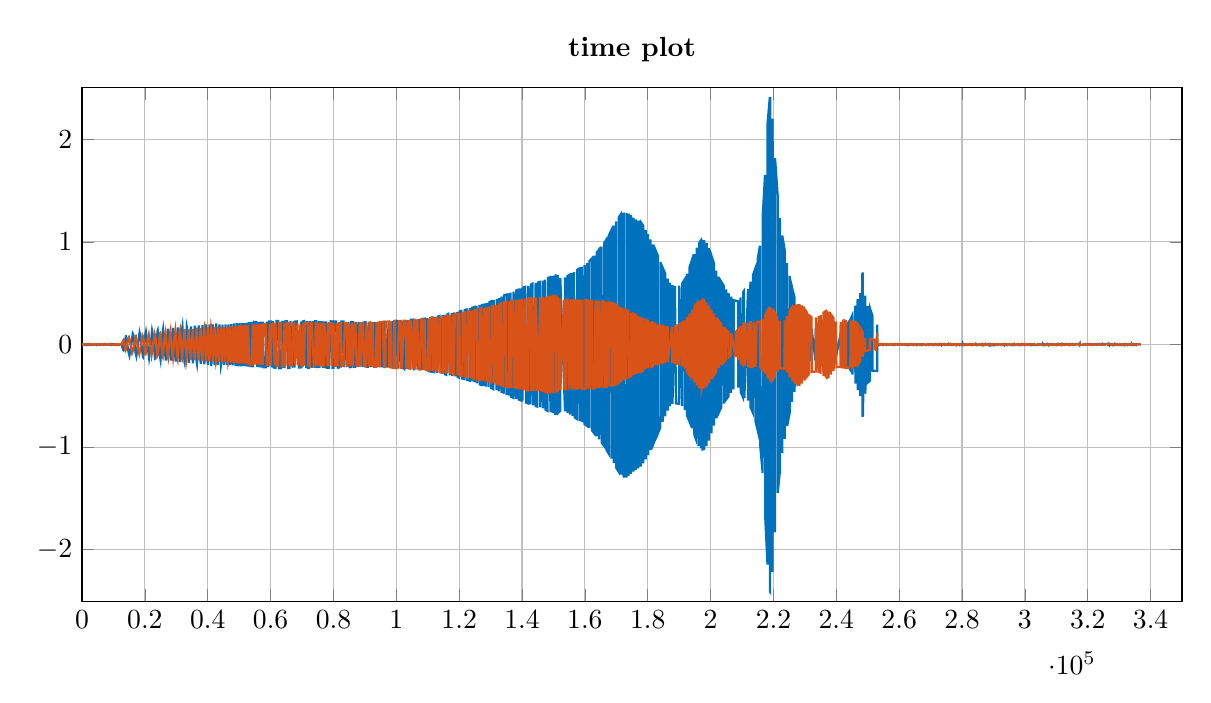
\begin{tikzpicture}

\begin{axis}[%
width=5.5in,
height=2.566in,
at={(1.011in,0.642in)},
scale only axis,
xmin=0,
xmax=350000,
xmajorgrids,
xminorgrids,
ymin=-2.5,
ymax=2.5,
ymajorgrids,
axis background/.style={fill=white},
title style={font=\bfseries},
title={time plot}
]
\addplot [color=mycolor1,solid,forget plot,thick]
  table[row sep=crcr]{%
1	0\\
92	-0.00481583190665319\\
409	0.00321055460443546\\
934	-0.00642110920887092\\
1451	0.00481583190665319\\
1704	0.00481583190665319\\
1752	-0.00481583190665319\\
2330	0.00321055460443546\\
2359	-0.00481583190665319\\
3166	-0.00481583190665319\\
3307	0.00321055460443546\\
4014	-0.00481583190665319\\
4369	0.00481583190665319\\
4683	0.00321055460443546\\
4765	-0.00481583190665319\\
5466	0.00321055460443546\\
5692	-0.00481583190665319\\
6315	0.00321055460443546\\
6523	-0.00481583190665319\\
6997	-0.00321055460443546\\
7213	0.00481583190665319\\
7769	0.00321055460443546\\
7841	-0.00321055460443546\\
9058	0.00642110920887092\\
9230	-0.00481583190665319\\
9361	-0.00481583190665319\\
9468	0.00481583190665319\\
10110	0.00321055460443546\\
10272	-0.00481583190665319\\
10944	0.00321055460443546\\
11052	-0.00481583190665319\\
11721	-0.00642110920887092\\
12245	0.00321055460443546\\
12551	0.00160527730221773\\
13182	-0.059395260182056\\
13200	-0.059395260182056\\
13953	0.0802638651108865\\
13977	0.0802638651108865\\
14746	-0.0658163693909269\\
15080	-0.107553579248588\\
15527	-0.0321055460443546\\
15529	-0.0353161006487901\\
16151	0.107553579248588\\
16306	0.0995271927374993\\
17077	-0.0882902516219752\\
17282	-0.113974688457459\\
17849	0.0128422184177418\\
17855	0.0112369411155241\\
18309	0.117185243061894\\
18632	0.0754480332042333\\
19379	-0.122001074968547\\
19420	-0.123606352270765\\
20173	0.104343024644152\\
20307	0.123606352270765\\
20958	-0.0385266552532255\\
21328	-0.130027461479636\\
21737	-0.0337108233465723\\
21738	-0.0353161006487901\\
22275	0.131632738781854\\
22514	0.0931060835286283\\
23216	-0.138053847990725\\
23290	-0.136448570688507\\
24063	0.136448570688507\\
24083	0.138053847990725\\
24842	-0.125211629572983\\
24973	-0.149290789106249\\
25613	0.10594830194637\\
25794	0.144474957199596\\
26392	-0.0786585878086688\\
26669	-0.15571189831512\\
27169	0.0674216466931447\\
27425	0.152501343710684\\
27945	-0.0529741509731851\\
28254	-0.157317175617338\\
28723	0.0577899828798383\\
28996	0.160527730221773\\
29498	-0.0577899828798383\\
29804	-0.165343562128426\\
30275	0.0866849743197574\\
30500	0.165343562128426\\
31052	-0.107553579248588\\
31257	-0.171764671337297\\
31824	0.142869679897378\\
31952	0.170159394035079\\
32602	-0.170159394035079\\
32639	-0.174975225941733\\
33335	0.173369948639515\\
33380	0.166948839430644\\
33987	-0.179791057848386\\
34157	-0.131632738781854\\
34644	0.17658050324395\\
35303	-0.184606889755039\\
35709	0.0898955289241929\\
35908	0.183001612452821\\
36483	-0.174975225941733\\
36552	-0.186212167057257\\
37149	0.184606889755039\\
37262	0.152501343710684\\
37754	-0.19102799896391\\
38324	0.187817444359474\\
38813	-0.157317175617338\\
38914	-0.194238553568345\\
39465	0.194238553568345\\
39591	0.157317175617338\\
40048	-0.197449108172781\\
40583	0.195843830870563\\
41133	-0.200659662777216\\
41147	-0.200659662777216\\
41672	0.195843830870563\\
42195	-0.200659662777216\\
42690	0.194238553568345\\
42707	0.194238553568345\\
43220	-0.199054385474999\\
43705	0.194238553568345\\
44222	-0.199054385474999\\
44248	-0.194238553568345\\
44698	0.192633276266128\\
45188	-0.199054385474999\\
45660	0.194238553568345\\
46119	-0.200659662777216\\
46577	0.195843830870563\\
46577	0.195843830870563\\
47037	-0.200659662777216\\
47481	0.199054385474999\\
47923	-0.203870217381652\\
48365	0.205475494683869\\
48807	-0.210291326590523\\
49218	0.208686049288305\\
49653	-0.213501881194958\\
50065	0.207080771986087\\
50457	-0.208686049288305\\
50472	-0.21189660389274\\
50882	0.207080771986087\\
51285	-0.210291326590523\\
51670	0.207080771986087\\
52090	-0.213501881194958\\
52464	0.21189660389274\\
52850	-0.216712435799394\\
53222	0.218317713101611\\
53605	-0.219922990403829\\
53968	0.219922990403829\\
54345	-0.223133545008264\\
54708	0.219922990403829\\
55426	0.216712435799394\\
55773	-0.218317713101611\\
56135	0.219922990403829\\
56476	-0.223133545008264\\
56815	0.221528267706047\\
57155	-0.224738822310482\\
57485	0.223133545008264\\
57822	-0.223133545008264\\
58488	-0.223133545008264\\
58813	0.223133545008264\\
59133	-0.221528267706047\\
59448	0.223133545008264\\
60064	0.223133545008264\\
60374	-0.223133545008264\\
60688	0.2263440996127\\
60985	-0.224738822310482\\
61587	-0.227949376914918\\
61883	0.229554654217135\\
62463	0.229554654217135\\
62753	-0.231159931519353\\
63318	-0.231159931519353\\
63608	0.229554654217135\\
63879	-0.227949376914918\\
64161	0.2263440996127\\
64434	-0.229554654217135\\
64716	0.227949376914918\\
65249	0.2263440996127\\
65511	-0.229554654217135\\
66038	-0.229554654217135\\
66301	0.2263440996127\\
67071	-0.2263440996127\\
67325	0.2263440996127\\
67569	-0.224738822310482\\
67816	0.223133545008264\\
68318	0.224738822310482\\
69039	-0.224738822310482\\
69519	-0.224738822310482\\
69740	0.223133545008264\\
69993	-0.2263440996127\\
70212	0.224738822310482\\
70675	0.227949376914918\\
71351	-0.227949376914918\\
71576	0.2263440996127\\
71792	-0.227949376914918\\
72236	-0.227949376914918\\
72456	0.2263440996127\\
73100	-0.227949376914918\\
73305	0.227949376914918\\
73943	-0.227949376914918\\
74154	0.2263440996127\\
74560	0.2263440996127\\
74766	-0.229554654217135\\
75368	0.2263440996127\\
75561	-0.227949376914918\\
76152	0.2263440996127\\
76741	-0.227949376914918\\
76928	0.224738822310482\\
77491	-0.227949376914918\\
77680	0.224738822310482\\
77862	-0.2263440996127\\
78599	-0.2263440996127\\
79147	0.2263440996127\\
79504	0.224738822310482\\
79681	-0.227949376914918\\
80025	-0.2263440996127\\
80206	0.224738822310482\\
80887	0.223133545008264\\
81395	-0.2263440996127\\
81728	-0.224738822310482\\
82227	0.223133545008264\\
82395	-0.224738822310482\\
82550	0.223133545008264\\
83200	0.223133545008264\\
83353	-0.221528267706047\\
84135	0.219922990403829\\
84289	-0.221528267706047\\
84751	0.218317713101611\\
85203	-0.221528267706047\\
85503	-0.219922990403829\\
85651	0.218317713101611\\
86238	0.216712435799394\\
86383	-0.218317713101611\\
86966	-0.216712435799394\\
87102	0.216712435799394\\
87809	-0.215107158497176\\
87944	0.216712435799394\\
88635	-0.216712435799394\\
88769	0.215107158497176\\
89441	-0.216712435799394\\
89835	0.216712435799394\\
90359	0.215107158497176\\
90484	-0.218317713101611\\
90998	-0.218317713101611\\
91382	0.216712435799394\\
91756	-0.219922990403829\\
92370	0.218317713101611\\
92492	-0.219922990403829\\
92614	0.218317713101611\\
93215	-0.219922990403829\\
93331	0.218317713101611\\
94155	-0.221528267706047\\
94274	0.221528267706047\\
94846	-0.221528267706047\\
95409	0.221528267706047\\
95520	-0.223133545008264\\
96076	0.221528267706047\\
96295	0.221528267706047\\
96836	-0.224738822310482\\
97580	0.224738822310482\\
97685	-0.2263440996127\\
97998	0.2263440996127\\
98514	-0.227949376914918\\
99024	0.227949376914918\\
99123	-0.229554654217135\\
99720	-0.229554654217135\\
99821	0.231159931519353\\
100214	0.229554654217135\\
100698	-0.232765208821571\\
100984	0.231159931519353\\
101646	-0.234370486123789\\
101740	0.232765208821571\\
102386	-0.234370486123789\\
102568	-0.239186318030442\\
103023	0.234370486123789\\
103291	-0.237581040728224\\
103732	0.235975763426006\\
104515	-0.239186318030442\\
104602	0.24079159533266\\
105284	0.242396872634877\\
105536	-0.24079159533266\\
105702	-0.24079159533266\\
106114	0.244002149937095\\
106849	-0.244002149937095\\
107088	0.24721270454153\\
107487	-0.24721270454153\\
107723	0.248817981843748\\
108115	-0.248817981843748\\
108191	0.248817981843748\\
109109	0.252028536448184\\
109334	-0.255239091052619\\
109854	0.255239091052619\\
110225	-0.258449645657055\\
110802	-0.263265477563708\\
110873	0.260054922959272\\
111444	0.263265477563708\\
111513	-0.266476032168143\\
112075	-0.269686586772579\\
112282	0.269686586772579\\
113031	-0.27610769598145\\
113231	0.272897141377014\\
113764	0.277712973283667\\
114094	-0.28252880519032\\
114676	0.285739359794756\\
114869	-0.287344637096974\\
115440	0.288949914399191\\
115504	-0.290555191701409\\
115877	-0.295371023608062\\
116310	0.295371023608062\\
116555	0.298581578212498\\
116977	-0.300186855514716\\
117634	0.305002687421369\\
117811	-0.308213242025804\\
118451	0.31142379663024\\
118738	-0.31142379663024\\
119362	0.317844905839111\\
119530	-0.317844905839111\\
119974	-0.322660737745764\\
120138	0.322660737745764\\
120685	0.327476569652417\\
120954	-0.33229240155907\\
121698	-0.337108233465723\\
121751	0.335502956163506\\
122374	0.341924065372377\\
122529	-0.345134619976812\\
123340	-0.353161006487901\\
123391	0.353161006487901\\
124132	-0.359582115696772\\
124183	0.357976838394554\\
124859	0.366003224905642\\
124908	-0.369213779510078\\
125526	0.374029611416731\\
125666	-0.378845443323384\\
126454	0.385266552532255\\
126501	-0.388477107136691\\
127045	-0.394898216345562\\
127269	0.394898216345562\\
127847	-0.40292460285665\\
128066	0.401319325554433\\
128458	-0.409345712065521\\
128844	0.406135157461086\\
129312	-0.415766821274392\\
129606	0.412556266669957\\
130187	0.420582653181045\\
130229	-0.425398485087698\\
130880	-0.435030148901005\\
131000	0.431819594296569\\
131913	-0.444661812714311\\
131953	0.443056535412093\\
132611	-0.455898753829835\\
132726	0.454293476527618\\
133445	-0.470346249549795\\
133484	0.465530417643142\\
134188	-0.479977913363101\\
134225	0.478372636060884\\
135020	0.486399022571972\\
135057	-0.491214854478625\\
135801	0.497635963687496\\
135836	-0.499241240989714\\
136356	0.505662350198585\\
136528	-0.510478182105238\\
137275	-0.520109845918544\\
137308	0.515294014011891\\
138137	-0.529741509731851\\
138170	0.526530955127415\\
138882	0.534557341638504\\
138914	-0.536162618940722\\
139485	-0.54418900545181\\
139705	0.545794282754028\\
140109	-0.555425946567335\\
140387	0.555425946567335\\
141056	0.561847055776206\\
141266	-0.566662887682859\\
141977	-0.574689274193947\\
142006	0.571478719589512\\
142731	-0.584320938007254\\
142816	0.584320938007254\\
143328	0.592347324518342\\
143581	-0.59395260182056\\
144329	0.600373711029431\\
144356	-0.600373711029431\\
144845	-0.605189542936084\\
145141	0.605189542936084\\
145725	0.610005374842737\\
145804	-0.611610652144955\\
146659	0.621242315958262\\
146685	-0.622847593260479\\
147269	0.632479257073786\\
147445	-0.635689811678221\\
148090	-0.646926752793745\\
148262	0.648532030095963\\
148988	0.656558416607052\\
149012	-0.658163693909269\\
149747	0.666190080420358\\
149770	-0.666190080420358\\
150166	0.671005912327011\\
150466	-0.674216466931447\\
150649	-0.674216466931447\\
150718	0.672611189629229\\
151395	0.667795357722576\\
151418	-0.669400635024793\\
152169	-0.646926752793745\\
152191	0.645321475491528\\
153666	-0.651742584700398\\
153687	0.653347862002616\\
154453	-0.666190080420358\\
154473	0.667795357722576\\
155202	0.680637576140318\\
155222	-0.682242853442535\\
155916	0.695085071860277\\
156014	-0.696690349162495\\
156538	0.707927290278019\\
156788	-0.712743122184672\\
157470	-0.725585340602414\\
157564	0.727190617904632\\
158268	0.740032836322373\\
158323	-0.743243390926809\\
159030	0.756085609344551\\
159084	-0.757690886646769\\
159881	0.773743659668946\\
159898	-0.775348936971164\\
160660	-0.793006987295559\\
160677	0.793006987295559\\
161405	-0.812270314922171\\
161422	0.812270314922171\\
162217	0.837954751757655\\
162233	-0.836349474455437\\
162946	-0.865244465895357\\
162994	0.865244465895357\\
163676	-0.894139457335276\\
163754	0.894139457335276\\
164498	0.924639726077413\\
164513	-0.924639726077413\\
165316	0.953534717517332\\
165331	-0.955139994819549\\
166101	-0.987245540863904\\
166116	0.985640263561686\\
166840	1.02256164151269\\
166883	-1.02737747341935\\
167619	-1.06590412867257\\
167661	1.06590412867257\\
168409	1.11245717043689\\
168423	-1.11245717043689\\
169195	1.1590102122012\\
169208	-1.15579965759677\\
169937	1.19914214475664\\
169950	-1.20074742205886\\
170728	-1.23927407731209\\
170741	1.23606352270765\\
171451	1.26977434605422\\
171514	-1.26816906875201\\
172221	1.28261656447197\\
172282	-1.2858271190764\\
172368	1.28422184177418\\
172429	-1.28743239637862\\
173249	-1.2858271190764\\
173261	1.28261656447197\\
173887	-1.27940600986753\\
173922	1.27459017796088\\
174674	-1.26014268224092\\
174708	1.26014268224092\\
175443	-1.23927407731209\\
175499	1.23606352270765\\
176218	-1.22161602698769\\
176229	1.21840547238326\\
176997	-1.20716853126773\\
177029	1.20716853126773\\
177780	-1.19111575824556\\
177874	1.18790520364112\\
178556	1.1590102122012\\
178566	-1.1590102122012\\
179345	1.11566772504132\\
179355	-1.12048355694798\\
180097	1.07393051518366\\
180146	-1.0771410697881\\
180871	1.02416691881491\\
180900	-1.02577219611713\\
181666	0.974403322446162\\
181694	-0.97600859974838\\
182434	-0.919823894170759\\
182443	0.921429171472977\\
183203	0.866849743197574\\
183212	-0.868455020499792\\
184008	-0.807454483015518\\
184034	0.804243928411083\\
184769	-0.752875054740115\\
184795	0.744848668229027\\
185539	0.691874517255842\\
185547	-0.69990090376693\\
186333	0.640505643584874\\
186341	-0.64371619818931\\
187093	0.601978988331649\\
187101	-0.603584265633866\\
187868	0.577899828798383\\
187876	-0.579505106100601\\
188657	0.569873442287294\\
188969	-0.574689274193947\\
189970	-0.577899828798383\\
190051	0.57308399689173\\
190900	-0.600373711029431\\
190950	0.59395260182056\\
191701	0.630873979771568\\
191736	-0.638900366282657\\
192504	0.690269239953624\\
192511	-0.693479794558059\\
193256	-0.74966450013568\\
193276	0.751269777437898\\
194018	0.818691424131042\\
194051	-0.817086146828825\\
194796	0.881297238917534\\
194828	-0.882902516219751\\
195538	-0.94069249909959\\
195582	0.942297776401808\\
196369	-0.990456095468339\\
196375	0.990456095468339\\
196886	1.01292997769939\\
196904	-1.01292997769939\\
197294	1.02095636421048\\
197431	-1.02256164151269\\
197950	-1.01774580960604\\
197956	1.01614053230382\\
198726	-0.990456095468339\\
198766	0.988850818166122\\
199507	-0.935876667192937\\
199524	0.937481944495154\\
200304	-0.866849743197574\\
200375	0.85561280208205\\
201067	0.791401709993341\\
201083	-0.789796432691123\\
201829	0.719164231393543\\
201845	-0.719164231393543\\
202616	0.659768971211487\\
202621	-0.662979525815922\\
203390	-0.611610652144955\\
203395	0.611610652144955\\
204177	0.57308399689173\\
204221	-0.576294551496165\\
204951	0.536162618940722\\
204956	-0.536162618940722\\
205713	-0.504057072896367\\
205727	0.50245179559415\\
206500	-0.470346249549795\\
206541	0.467135694945359\\
207296	-0.436635426203223\\
207363	0.431819594296569\\
208737	0.420582653181045\\
208767	-0.420582653181045\\
209551	0.459109308434271\\
209572	-0.463925140340924\\
210277	-0.513688736709674\\
210355	0.512083459407456\\
210559	0.520109845918544\\
210750	-0.52332040052298\\
211893	0.542583728149593\\
211897	-0.547399560056246\\
212668	0.611610652144955\\
212687	-0.611610652144955\\
213445	-0.66458480311814\\
213471	0.675821744233664\\
214190	0.736822281717938\\
214245	-0.743243390926809\\
214984	-0.837954751757655\\
215009	0.83474419715322\\
215683	0.96156110402842\\
215792	-0.988850818166122\\
216554	-1.25211629572983\\
216571	1.24569518652096\\
217310	1.65183034398204\\
217347	-1.666277839702\\
218096	-2.14465047576289\\
218119	2.15428213957619\\
218839	2.40952123062881\\
218855	-2.4079159533266\\
218932	-2.41112650793103\\
218948	2.41112650793103\\
219692	-2.21688795436269\\
219695	2.19922990403829\\
220460	-1.83162140183043\\
220506	1.81556862880825\\
221358	1.44474957199596\\
221361	-1.44474957199596\\
222029	-1.23766880000987\\
222032	1.231247690801\\
222799	-1.05787774216148\\
222802	1.06108829676592\\
223572	0.919823894170759\\
223586	-0.919823894170759\\
224342	0.793006987295559\\
224372	-0.793006987295559\\
225146	-0.666190080420358\\
225154	0.667795357722576\\
225903	-0.560241778473988\\
225916	0.557031223869552\\
226672	0.462319863038706\\
226690	-0.460714585736488\\
227447	0.378845443323384\\
227679	-0.357976838394554\\
228222	-0.31142379663024\\
228249	0.305002687421369\\
228997	-0.258449645657055\\
229009	0.260054922959272\\
229795	0.223133545008264\\
229816	-0.223133545008264\\
230561	-0.195843830870563\\
230600	0.199054385474999\\
231331	-0.171764671337297\\
231360	0.171764671337297\\
232106	-0.157317175617338\\
232130	0.15571189831512\\
233328	-0.154106621012902\\
233444	0.152501343710684\\
234178	0.15571189831512\\
234312	-0.157317175617338\\
234435	-0.15571189831512\\
234523	0.157317175617338\\
235247	0.130027461479636\\
235257	-0.133238016084072\\
235987	0.115579965759677\\
235993	-0.118790520364112\\
237324	0.117185243061894\\
237480	-0.12039579766633\\
237957	-0.126816906875201\\
238125	0.128422184177418\\
238316	0.126816906875201\\
238464	-0.128422184177418\\
239093	-0.12039579766633\\
239102	0.118790520364112\\
239874	0.10594830194637\\
240005	-0.104343024644152\\
241385	0.107553579248588\\
241417	-0.10594830194637\\
242174	0.134843293386289\\
242179	-0.136448570688507\\
242928	-0.173369948639515\\
242952	0.171764671337297\\
243735	0.208686049288305\\
243746	-0.21189660389274\\
244493	-0.24721270454153\\
244519	0.245607427239313\\
245015	0.279318250585885\\
245110	-0.293765746305845\\
246036	0.378845443323384\\
246058	-0.38205599792782\\
246782	0.441451258109876\\
246792	-0.443056535412093\\
247616	0.500846518291932\\
247623	-0.50245179559415\\
248288	0.69990090376693\\
248336	-0.706322012975801\\
248406	0.701506181069148\\
248443	-0.69990090376693\\
249216	0.476767358758666\\
249220	-0.479977913363101\\
249968	0.372424334114513\\
249985	-0.372424334114513\\
250749	-0.349950451883465\\
250758	0.348345174581247\\
251508	0.277712973283667\\
251509	-0.255239091052619\\
253008	-0.258449645657055\\
253012	0.194238553568345\\
253062	0.00963166381330638\\
253065	-0.00963166381330638\\
253847	-0.00481583190665319\\
253865	0.00321055460443546\\
254714	0.00481583190665319\\
254812	-0.00481583190665319\\
255478	0.00481583190665319\\
255926	-0.00481583190665319\\
256178	0.00321055460443546\\
256930	-0.00481583190665319\\
256983	-0.00481583190665319\\
257117	0.00321055460443546\\
257821	0.00321055460443546\\
257935	-0.00481583190665319\\
258545	0.00321055460443546\\
258646	-0.00481583190665319\\
259486	0.00481583190665319\\
259879	-0.00481583190665319\\
260057	-0.00321055460443546\\
260425	0.00481583190665319\\
260823	-0.00321055460443546\\
261235	0.00481583190665319\\
261601	0.00321055460443546\\
261988	-0.00481583190665319\\
262436	0.00321055460443546\\
262717	-0.00802638651108865\\
263161	-0.00481583190665319\\
263229	0.00321055460443546\\
264240	0.00481583190665319\\
264389	-0.00642110920887092\\
264743	-0.00642110920887092\\
265196	0.00321055460443546\\
265589	-0.00642110920887092\\
266007	0.00321055460443546\\
266266	0.00321055460443546\\
266515	-0.00481583190665319\\
267059	-0.00642110920887092\\
267075	0.00321055460443546\\
267889	0.00321055460443546\\
268331	-0.00642110920887092\\
268627	-0.00481583190665319\\
268925	0.00321055460443546\\
269371	-0.00481583190665319\\
269682	0.00321055460443546\\
270158	0.00321055460443546\\
270470	-0.00481583190665319\\
271158	-0.00481583190665319\\
271638	0.00481583190665319\\
271742	0.00321055460443546\\
272123	-0.00481583190665319\\
272547	-0.00481583190665319\\
272842	0.00481583190665319\\
273291	-0.00481583190665319\\
273333	0.00481583190665319\\
274047	0.00481583190665319\\
274462	-0.00481583190665319\\
274881	0.00321055460443546\\
275273	-0.00481583190665319\\
275624	0.00642110920887092\\
275919	-0.00321055460443546\\
276440	-0.00481583190665319\\
276456	0.00481583190665319\\
277158	-0.00481583190665319\\
277342	0.00321055460443546\\
278166	0.00321055460443546\\
278220	-0.00642110920887092\\
278693	0.00321055460443546\\
279256	-0.00642110920887092\\
279555	0.00321055460443546\\
280179	-0.00642110920887092\\
280235	0.00160527730221773\\
280311	-0.00642110920887092\\
281028	-0.00481583190665319\\
281266	0.00321055460443546\\
281811	-0.00481583190665319\\
282447	0.00321055460443546\\
282562	0.00160527730221773\\
282911	-0.00642110920887092\\
283371	-0.00481583190665319\\
283523	0.00321055460443546\\
284394	-0.00481583190665319\\
284466	0.00481583190665319\\
284933	-0.00642110920887092\\
285424	0.00321055460443546\\
285814	0.00321055460443546\\
286274	-0.00642110920887092\\
286474	0.00321055460443546\\
286719	-0.00642110920887092\\
287239	0.00321055460443546\\
287241	-0.00481583190665319\\
288414	0.00321055460443546\\
288614	-0.00642110920887092\\
288844	0.00160527730221773\\
289005	-0.00802638651108865\\
289546	0.00160527730221773\\
289596	-0.00642110920887092\\
290325	0.00160527730221773\\
290327	-0.00642110920887092\\
291151	0.00321055460443546\\
291300	-0.00481583190665319\\
291963	0.00321055460443546\\
292427	-0.00642110920887092\\
293128	0.00481583190665319\\
293423	-0.00642110920887092\\
293441	-0.00481583190665319\\
293897	0.00481583190665319\\
294327	-0.00642110920887092\\
294730	0.00321055460443546\\
294991	0.00321055460443546\\
295574	-0.00642110920887092\\
295922	0.00321055460443546\\
296218	-0.00642110920887092\\
296593	0.00321055460443546\\
296653	-0.00481583190665319\\
297417	-0.00481583190665319\\
297891	0.00481583190665319\\
298098	0.00321055460443546\\
298258	-0.00642110920887092\\
298883	0.00481583190665319\\
299012	-0.00481583190665319\\
299655	0.00321055460443546\\
300268	-0.00642110920887092\\
300511	-0.00481583190665319\\
300515	0.00321055460443546\\
301191	-0.00481583190665319\\
301871	0.00481583190665319\\
301983	0.00160527730221773\\
302035	-0.00642110920887092\\
302806	0.00321055460443546\\
302826	-0.00481583190665319\\
303676	-0.00642110920887092\\
304032	0.00160527730221773\\
304314	-0.00481583190665319\\
304666	0.00321055460443546\\
305803	-0.00642110920887092\\
305808	0.00321055460443546\\
306068	-0.00642110920887092\\
306491	0.00321055460443546\\
306742	-0.00481583190665319\\
307098	0.00481583190665319\\
307417	-0.00481583190665319\\
307518	0.00321055460443546\\
308238	0.00321055460443546\\
308923	-0.00481583190665319\\
308989	-0.00481583190665319\\
309044	0.00321055460443546\\
309993	-0.00642110920887092\\
310389	0.00481583190665319\\
310539	-0.00481583190665319\\
311121	0.00481583190665319\\
311713	0.00642110920887092\\
311763	-0.00321055460443546\\
312100	0.00481583190665319\\
312668	-0.00481583190665319\\
312850	-0.00321055460443546\\
312966	0.00481583190665319\\
313970	-0.00481583190665319\\
314028	0.00481583190665319\\
314401	0.00481583190665319\\
314494	-0.00321055460443546\\
315191	0.00481583190665319\\
315487	-0.00481583190665319\\
315949	-0.00321055460443546\\
316151	0.00481583190665319\\
317082	0.00481583190665319\\
317384	-0.00642110920887092\\
317502	0.00321055460443546\\
317543	-0.00481583190665319\\
318273	-0.00481583190665319\\
319004	0.00481583190665319\\
319084	0.00321055460443546\\
319262	-0.00481583190665319\\
319854	-0.00321055460443546\\
319870	0.00481583190665319\\
320709	0.00481583190665319\\
321137	-0.00481583190665319\\
321442	0.00321055460443546\\
322041	-0.00481583190665319\\
322151	-0.00481583190665319\\
322290	0.00321055460443546\\
322987	0.00481583190665319\\
323021	-0.00321055460443546\\
323849	0.00481583190665319\\
324232	-0.00481583190665319\\
324563	0.00481583190665319\\
324666	-0.00321055460443546\\
325296	-0.00321055460443546\\
325316	0.00481583190665319\\
326503	0.00481583190665319\\
326768	-0.00481583190665319\\
326822	0.00481583190665319\\
327094	-0.00481583190665319\\
327626	0.00321055460443546\\
327973	-0.00642110920887092\\
328467	0.00481583190665319\\
328505	-0.00481583190665319\\
329357	0.00321055460443546\\
329532	-0.00642110920887092\\
330043	-0.00642110920887092\\
330211	0.00160527730221773\\
330783	-0.00642110920887092\\
331379	0.00321055460443546\\
331667	-0.00481583190665319\\
331791	0.00481583190665319\\
332475	0.00321055460443546\\
332723	-0.00481583190665319\\
333161	0.00321055460443546\\
333692	-0.00481583190665319\\
333821	0.00321055460443546\\
333899	-0.00642110920887092\\
334694	-0.00642110920887092\\
334711	0.00321055460443546\\
335352	-0.00481583190665319\\
335413	0.00321055460443546\\
336896	0\\
};
\addplot [color=mycolor2,solid,forget plot,thick]
  table[row sep=crcr]{%
1	-0.000760413931657074\\
392	0.00228124179497122\\
600	-0.00228124179497122\\
786	-0.00228124179497122\\
934	0.00152082786331415\\
1648	0.00152082786331415\\
1916	-0.00228124179497122\\
2368	0.00228124179497122\\
2653	-0.00228124179497122\\
3107	0.00152082786331415\\
3451	-0.00228124179497122\\
3947	-0.00228124179497122\\
4087	0.00228124179497122\\
5044	0.00152082786331415\\
5299	-0.0030416557266283\\
5490	0.00152082786331415\\
6048	-0.0030416557266283\\
6635	-0.0030416557266283\\
6816	0.00152082786331415\\
7003	0.00152082786331415\\
7332	-0.00228124179497122\\
7764	-0.00228124179497122\\
7766	0.00152082786331415\\
8560	-0.0030416557266283\\
8642	0.00152082786331415\\
9333	0.00152082786331415\\
9736	-0.0030416557266283\\
10096	-0.00228124179497122\\
10552	0.00228124179497122\\
10872	0.00152082786331415\\
11025	-0.00228124179497122\\
11652	-0.00228124179497122\\
11691	0.00152082786331415\\
12467	-0.00228124179497122\\
13173	0.0425831801727961\\
13206	0.0403019383778249\\
13826	-0.0585518727375947\\
13978	-0.050947733421024\\
14750	0.0653955981225084\\
14924	0.072239323507422\\
15526	-0.0167291064964556\\
15528	-0.0159686925647986\\
15945	-0.0836455324822781\\
16305	-0.0547498030793093\\
17067	0.0806038767556498\\
17132	0.082124704618964\\
17855	-0.0486664916260527\\
18191	-0.0904892578671918\\
18630	-0.0197707622230839\\
18633	-0.020531176154741\\
19241	0.0897288439355347\\
19409	0.0798434628239928\\
20164	-0.0973329832521055\\
20213	-0.0973329832521055\\
20957	0.0638747702591942\\
21218	0.0973329832521055\\
21735	-0.0174895204281127\\
21737	-0.0159686925647986\\
22130	-0.104176708637019\\
22513	-0.0357394547878825\\
23094	0.104937122568676\\
23289	0.0844059464139352\\
23963	-0.111020434021933\\
24065	-0.104176708637019\\
24839	0.11178084795359\\
24866	0.112541261885247\\
25615	-0.11178084795359\\
25674	-0.117103745475189\\
26394	0.0965725693204484\\
26549	0.119384987270161\\
27169	-0.0958121553887913\\
27364	-0.123947470860103\\
27945	0.082124704618964\\
28164	0.125468298723417\\
28720	-0.0889684300038777\\
28911	-0.129270368381703\\
29497	0.0882080160722206\\
29689	0.131551610176674\\
30273	-0.107978778295305\\
30427	-0.135353679834959\\
31052	0.117864159406846\\
31198	0.13763492162993\\
31827	-0.138395335561587\\
31849	-0.139916163424902\\
32561	0.141436991288216\\
32605	0.141436991288216\\
33252	-0.145239060946501\\
33381	-0.119384987270161\\
33955	0.146759888809815\\
34157	0.0669164259858225\\
34580	-0.149041130604786\\
35237	0.150561958468101\\
35709	-0.113301675816904\\
35856	-0.152843200263072\\
36485	0.154364028126386\\
36490	0.154364028126386\\
37075	-0.1558848559897\\
37262	-0.0965725693204484\\
37696	0.158166097784671\\
38284	-0.1612077535113\\
38808	0.153603614194729\\
38878	0.162728581374614\\
39413	-0.165009823169585\\
39591	-0.101135052910391\\
40004	0.166530651032899\\
40538	-0.167291064964556\\
41098	0.16881189282787\\
41144	0.1612077535113\\
41623	-0.16881189282787\\
42154	0.16881189282787\\
42668	-0.16881189282787\\
42696	-0.165009823169585\\
43191	0.170332720691185\\
43676	-0.16881189282787\\
44182	0.16881189282787\\
44249	0.151322372399758\\
44658	-0.16881189282787\\
45140	0.169572306759528\\
45616	-0.169572306759528\\
46083	0.170332720691185\\
46541	-0.171093134622842\\
46577	-0.166530651032899\\
46989	0.173374376417813\\
47452	-0.175655618212784\\
47884	0.177176446076098\\
48329	-0.180218101802727\\
48761	0.181738929666041\\
49193	-0.184020171461012\\
49617	0.184020171461012\\
50036	-0.185540999324326\\
50457	0.184780585392669\\
50458	0.184780585392669\\
50848	-0.184780585392669\\
51268	0.185540999324326\\
51657	-0.185540999324326\\
52050	0.18706182718764\\
52431	-0.188582655050954\\
52819	0.191624310777583\\
53197	-0.193905552572554\\
53951	-0.196947208299182\\
54319	0.196947208299182\\
54684	-0.196947208299182\\
55046	0.196186794367525\\
55400	-0.195426380435868\\
55768	0.195426380435868\\
56110	-0.196947208299182\\
56458	0.197707622230839\\
56791	-0.198468036162496\\
57130	0.19998886402581\\
57478	-0.19998886402581\\
57805	0.19998886402581\\
58462	0.19998886402581\\
58785	-0.199228450094153\\
59428	-0.200749277957468\\
59739	0.200749277957468\\
60048	-0.200749277957468\\
60355	0.201509691889125\\
60966	0.203030519752439\\
61264	-0.203790933684096\\
61561	0.20531176154741\\
61863	-0.206832589410724\\
62444	-0.206832589410724\\
62741	0.207593003342381\\
63306	0.208353417274038\\
63587	-0.207593003342381\\
64146	-0.206832589410724\\
64422	0.207593003342381\\
64695	-0.208353417274038\\
64966	0.207593003342381\\
65501	0.206832589410724\\
65763	-0.206832589410724\\
66028	0.207593003342381\\
66289	-0.206072175479067\\
66803	-0.20531176154741\\
67061	0.20531176154741\\
67558	0.203790933684096\\
67805	-0.203790933684096\\
68543	0.203790933684096\\
68789	-0.203790933684096\\
69503	0.203790933684096\\
69738	-0.204551347615753\\
70202	-0.20531176154741\\
70437	0.206832589410724\\
70664	-0.206832589410724\\
70890	0.206832589410724\\
71791	0.207593003342381\\
72011	-0.208353417274038\\
72444	-0.207593003342381\\
72661	0.207593003342381\\
73092	0.208353417274038\\
73725	-0.209113831205695\\
74143	-0.209113831205695\\
74348	0.208353417274038\\
74753	0.207593003342381\\
74963	-0.208353417274038\\
75556	0.207593003342381\\
75757	-0.208353417274038\\
76345	0.207593003342381\\
76535	-0.208353417274038\\
76919	-0.207593003342381\\
77109	0.207593003342381\\
78044	-0.208353417274038\\
78234	0.208353417274038\\
78414	-0.208353417274038\\
78594	0.207593003342381\\
79313	0.206832589410724\\
79491	-0.207593003342381\\
80019	0.207593003342381\\
80539	-0.208353417274038\\
80879	-0.207593003342381\\
81049	0.207593003342381\\
81556	-0.207593003342381\\
81724	0.208353417274038\\
82379	0.206832589410724\\
82539	-0.206832589410724\\
83181	-0.207593003342381\\
83662	0.207593003342381\\
84279	0.206832589410724\\
84434	-0.206832589410724\\
84744	-0.207593003342381\\
84895	0.207593003342381\\
85646	-0.207593003342381\\
85791	0.206832589410724\\
86230	-0.209113831205695\\
86666	0.208353417274038\\
86954	0.208353417274038\\
87381	-0.209113831205695\\
87941	-0.209113831205695\\
88352	0.209113831205695\\
88763	-0.209874245137352\\
89165	0.209874245137352\\
89434	0.211395073000667\\
89831	-0.212155486932324\\
90349	-0.212915900863981\\
90481	0.212915900863981\\
91373	-0.214436728727295\\
91497	0.214436728727295\\
91748	0.215957556590609\\
92124	-0.215957556590609\\
92489	0.216717970522266\\
92852	-0.217478384453923\\
93565	-0.217478384453923\\
93683	0.21823879838558\\
94034	-0.21823879838558\\
94154	0.21823879838558\\
94729	-0.219759626248894\\
94843	0.218999212317237\\
95742	0.219759626248894\\
96071	-0.220520040180551\\
96510	-0.220520040180551\\
96616	0.221280454112209\\
97681	0.224322109838837\\
97785	-0.22356169590718\\
98305	0.224322109838837\\
98407	-0.225082523770494\\
99220	-0.226603351633808\\
99321	0.226603351633808\\
99521	0.227363765565465\\
99620	-0.227363765565465\\
100404	-0.228884593428779\\
100888	0.228884593428779\\
101454	0.229645007360436\\
101551	-0.229645007360436\\
101735	-0.230405421292093\\
102383	0.231165835223751\\
102928	0.231926249155408\\
103199	-0.231926249155408\\
103817	0.234207490950379\\
103907	-0.234207490950379\\
104430	-0.235728318813693\\
104516	0.23648873274535\\
105449	-0.238009560608664\\
105533	0.238769974540321\\
106031	0.239530388471978\\
106116	-0.240290802403635\\
106684	0.24181163026695\\
107088	-0.242572044198607\\
107566	-0.243332458130264\\
107799	0.244092872061921\\
108269	0.245613699925235\\
108654	-0.246374113856892\\
109032	0.248655355651863\\
109408	-0.248655355651863\\
110149	-0.251697011378491\\
110222	0.252457425310149\\
110874	-0.255499081036777\\
110945	0.256259494968434\\
111654	0.259301150695062\\
111726	-0.259301150695062\\
112348	0.263103220353348\\
112418	-0.263103220353348\\
113029	0.266144876079976\\
113096	-0.265384462148319\\
113960	0.269946945738261\\
114027	-0.270707359669918\\
114804	-0.274509429328204\\
114868	0.274509429328204\\
115565	-0.277551085054832\\
115628	0.278311498986489\\
116124	0.281353154713117\\
116186	-0.281353154713117\\
116977	0.28591563830306\\
117158	-0.28591563830306\\
117928	0.289717707961345\\
117987	-0.290478121893002\\
118335	-0.293519777619631\\
118623	0.295040605482945\\
119417	0.29884267514123\\
119474	-0.299603089072887\\
120085	0.30416557266283\\
120250	-0.303405158731173\\
121009	-0.307207228389458\\
121061	0.308728056252772\\
121804	0.312530125911057\\
121855	-0.312530125911057\\
122477	-0.316332195569343\\
122631	0.317853023432657\\
123340	0.323936334885914\\
123390	-0.323175920954256\\
124133	0.329259232407513\\
124182	-0.328498818475856\\
124764	-0.334582129929113\\
124908	0.33534254386077\\
125572	0.340665441382369\\
125713	-0.341425855314026\\
126454	-0.345988338903969\\
126500	0.34826958069894\\
127044	0.352071650357225\\
127180	-0.351311236425568\\
127935	0.357394547878825\\
127978	-0.356634133947168\\
128716	0.361957031468767\\
128844	-0.36119661753711\\
129481	0.36651951505871\\
129606	-0.365759101127053\\
130270	-0.371081998648652\\
130392	0.372602826511966\\
130961	0.377165310101909\\
131161	-0.377165310101909\\
131835	0.382488207623508\\
131952	-0.382488207623508\\
132650	-0.390852760871736\\
132688	0.39237358873505\\
133371	0.399977728051621\\
133483	-0.399977728051621\\
134077	-0.406821453436535\\
134260	0.409102695231506\\
134913	0.415186006684762\\
134949	-0.413665178821448\\
135800	-0.418227662411391\\
135834	0.419748490274705\\
136493	-0.422790146001333\\
136596	0.425071387796304\\
137207	0.429633871386247\\
137375	-0.428113043522933\\
138136	0.433435941044532\\
138169	-0.432675527112875\\
138913	0.437238010702818\\
138945	-0.434956768907846\\
139674	0.441040080361103\\
139705	-0.439519252497789\\
140109	0.444842150019388\\
140448	-0.443321322156074\\
141025	0.446362977882702\\
141175	-0.445602563951045\\
141888	-0.44712339181436\\
141917	0.448644219677674\\
142615	0.451685875404302\\
142816	-0.450925461472645\\
143129	0.45472753113093\\
143496	-0.45472753113093\\
144081	0.457008772925901\\
144328	-0.455487945062587\\
144410	0.457769186857559\\
145087	-0.456248358994244\\
145803	0.46005042865253\\
145882	-0.457769186857559\\
146633	0.463092084379158\\
146659	-0.460810842584187\\
147444	0.466133740105786\\
147469	-0.465373326174129\\
148212	-0.469175395832415\\
148237	0.471456637627386\\
148602	-0.471456637627386\\
148723	0.4729774654907\\
149274	-0.4729774654907\\
149487	0.475258707285671\\
149933	-0.4729774654907\\
150003	0.476019121217328\\
150694	0.474498293354014\\
150808	-0.472217051559043\\
151372	0.466133740105786\\
151394	-0.463852498310815\\
152168	0.444842150019388\\
152190	-0.444842150019388\\
153371	0.434956768907846\\
153434	-0.432675527112875\\
153978	-0.435717182839503\\
154123	0.437998424634475\\
154493	0.439519252497789\\
154960	-0.437238010702818\\
155301	0.439519252497789\\
155797	-0.437998424634475\\
156169	0.441040080361103\\
156653	-0.438758838566132\\
156940	0.440279666429446\\
157300	-0.438758838566132\\
157731	0.438758838566132\\
157750	-0.437238010702818\\
158359	0.437238010702818\\
158450	-0.435717182839503\\
159226	0.435717182839503\\
159244	-0.434956768907846\\
160159	-0.433435941044532\\
160211	0.435717182839503\\
160796	0.432675527112875\\
160813	-0.431154699249561\\
161538	0.432675527112875\\
161555	-0.429633871386247\\
162363	0.431915113181218\\
162379	-0.429633871386247\\
163089	-0.42887345745459\\
163359	0.430394285317904\\
163816	-0.425831801727961\\
163925	0.42887345745459\\
164589	-0.422029732069676\\
164604	0.425831801727961\\
165345	-0.418227662411391\\
165509	0.421269318138019\\
166129	0.417467248479734\\
166202	-0.41594642061642\\
166924	-0.412144350958134\\
166967	0.413665178821448\\
167688	-0.408342281299849\\
167702	0.409863109163163\\
168476	0.404540211641563\\
168517	-0.403779797709906\\
169247	-0.394654830530021\\
169260	0.396936072324993\\
170027	0.387811105145108\\
170040	-0.387050691213451\\
170790	-0.377165310101909\\
170828	0.376404896170252\\
171574	-0.365759101127053\\
171586	0.363477859332081\\
172341	-0.350550822493911\\
172353	0.351311236425568\\
173115	-0.33534254386077\\
173127	0.336863371724084\\
173884	0.324696748817571\\
173919	-0.323175920954256\\
174659	-0.311009298047743\\
174739	0.310248884116086\\
175451	-0.29884267514123\\
175462	0.300363503004544\\
176214	0.290478121893002\\
176225	-0.289717707961345\\
176993	0.278311498986489\\
177025	-0.278311498986489\\
177797	0.266905290011633\\
177828	-0.266905290011633\\
178552	-0.253978253173463\\
178562	0.255499081036777\\
179320	-0.240290802403635\\
179430	0.240290802403635\\
180102	0.232686663087065\\
180112	-0.231165835223751\\
180914	0.222801281975523\\
181019	-0.219759626248894\\
181661	-0.211395073000667\\
181670	0.211395073000667\\
182447	0.200749277957468\\
182456	-0.201509691889125\\
183224	0.19238472470924\\
183251	-0.191624310777583\\
184011	-0.184020171461012\\
184037	0.184020171461012\\
184763	0.177936860007755\\
184789	-0.177936860007755\\
185533	-0.171093134622842\\
185541	0.171853548554499\\
186335	0.167291064964556\\
186343	-0.168051478896213\\
187760	0.169572306759528\\
187815	-0.16881189282787\\
188605	-0.177936860007755\\
188628	0.176416032144441\\
189340	0.184780585392669\\
189407	-0.186301413255983\\
190133	-0.196947208299182\\
190155	0.196947208299182\\
190865	0.212155486932324\\
190944	-0.213676314795638\\
191702	0.234967904882036\\
191737	-0.235728318813693\\
192505	0.268426117874947\\
192512	-0.266905290011633\\
193270	-0.300363503004544\\
193277	0.300363503004544\\
193999	-0.334582129929113\\
194058	0.338384199587398\\
194803	-0.369561170785338\\
194835	0.371842412580309\\
195595	0.401498555914935\\
195614	-0.399977728051621\\
196351	0.424310973864647\\
196394	-0.424310973864647\\
197127	0.43647759677116\\
197169	-0.435717182839503\\
197181	-0.434196354976189\\
197556	0.435717182839503\\
197968	0.431915113181218\\
197974	-0.429633871386247\\
198732	0.41062352309482\\
198749	-0.411383937026477\\
199513	0.380206965828537\\
199552	-0.378686137965223\\
200277	0.339144613519055\\
200315	-0.339144613519055\\
201067	0.300363503004544\\
201083	-0.299603089072887\\
201845	-0.261582392490033\\
201850	0.263103220353348\\
202621	-0.229645007360436\\
202626	0.229645007360436\\
203385	0.200749277957468\\
203410	-0.202270105820782\\
204157	0.173374376417813\\
204162	-0.17413479034947\\
204936	-0.146759888809815\\
204941	0.147520302741472\\
205717	0.12470788479176\\
205731	-0.123947470860103\\
206508	-0.109499606158619\\
206549	0.108739192226962\\
207985	-0.122426642996789\\
208007	0.123187056928446\\
208761	0.147520302741472\\
208808	-0.149041130604786\\
209583	0.178697273939412\\
209587	-0.178697273939412\\
210300	-0.201509691889125\\
210345	0.202270105820782\\
210809	0.206072175479067\\
210926	-0.206072175479067\\
211860	0.209874245137352\\
211911	-0.209874245137352\\
212455	-0.217478384453923\\
212582	0.21823879838558\\
212804	0.218999212317237\\
213142	-0.219759626248894\\
213503	-0.219759626248894\\
213723	0.219759626248894\\
214309	-0.217478384453923\\
214640	0.217478384453923\\
215646	0.22356169590718\\
215797	-0.225842937702151\\
216552	-0.246374113856892\\
216576	0.247894941720206\\
217311	-0.282873982576432\\
217348	0.284394810439746\\
218090	0.33001964633917\\
218100	-0.329259232407513\\
218804	0.361957031468767\\
218897	-0.361957031468767\\
219009	0.364998687195396\\
219025	-0.362717445400424\\
219692	0.34826958069894\\
219695	-0.347509166767283\\
220469	-0.307967642321115\\
220472	0.307967642321115\\
221235	0.263863634285005\\
221238	-0.266144876079976\\
222034	0.232686663087065\\
222037	-0.234207490950379\\
223537	-0.235728318813693\\
223551	0.234207490950379\\
224280	-0.27298860146489\\
224332	0.276790671123175\\
225104	-0.320894679159285\\
225112	0.323936334885914\\
225833	0.358154961810482\\
225867	-0.356634133947168\\
226642	0.381727793691851\\
226665	-0.380967379760194\\
227302	0.391613174803393\\
227415	-0.390852760871736\\
227841	0.394654830530021\\
227888	-0.393894416598364\\
228257	-0.39237358873505\\
228279	0.39237358873505\\
229012	-0.380967379760194\\
229024	0.380967379760194\\
229840	-0.351311236425568\\
229847	0.349029994630597\\
230564	0.316332195569343\\
230580	-0.316332195569343\\
231327	-0.286676052234717\\
231365	0.282873982576432\\
232113	0.265384462148319\\
232159	-0.26766570394329\\
233455	-0.263863634285005\\
233495	0.263863634285005\\
234345	-0.275269843259861\\
234425	0.276030257191518\\
235008	-0.286676052234717\\
235018	0.288196880098031\\
235942	-0.308728056252772\\
235944	0.311009298047743\\
236639	0.324696748817571\\
236733	-0.323175920954256\\
236949	0.327738404544199\\
236989	-0.325457162749228\\
237544	-0.319373851295971\\
237572	0.319373851295971\\
238318	-0.293519777619631\\
238404	0.287436466166374\\
239095	0.256259494968434\\
239111	-0.259301150695062\\
239867	0.22356169590718\\
240040	-0.222040868043866\\
241323	-0.218999212317237\\
241365	0.219759626248894\\
241995	-0.232686663087065\\
242161	0.234207490950379\\
242287	-0.235728318813693\\
242380	0.234967904882036\\
243080	0.229645007360436\\
243088	-0.229645007360436\\
244459	-0.222040868043866\\
244482	0.222040868043866\\
245066	0.226603351633808\\
245251	-0.227363765565465\\
245299	-0.226603351633808\\
245444	0.225082523770494\\
246084	-0.216717970522266\\
246182	0.215957556590609\\
246856	0.196947208299182\\
246866	-0.196947208299182\\
247628	-0.162728581374614\\
247649	0.158926511716328\\
248408	0.116343331543532\\
248423	-0.118624573338504\\
249180	0.0631143563275371\\
249184	-0.0653955981225084\\
250529	-0.0539893891476523\\
250646	0.0532289752159952\\
250732	-0.0532289752159952\\
250828	0.0524685612843381\\
252225	0.0463852498310815\\
252263	-0.0463852498310815\\
252522	-0.0494269055577098\\
253002	0.11178084795359\\
253124	-0.00228124179497122\\
253297	0.00228124179497122\\
253990	0.00228124179497122\\
254120	-0.00228124179497122\\
254623	-0.00228124179497122\\
254784	0.00228124179497122\\
255532	-0.00228124179497122\\
255586	0.00228124179497122\\
256215	0.00152082786331415\\
256542	-0.00228124179497122\\
256943	0.00152082786331415\\
257010	-0.00228124179497122\\
257739	0.00152082786331415\\
257791	-0.00228124179497122\\
258520	0.00152082786331415\\
258720	-0.00228124179497122\\
259869	0.00228124179497122\\
259871	-0.00228124179497122\\
260072	-0.00228124179497122\\
260184	0.00152082786331415\\
261390	0.00152082786331415\\
261515	-0.0030416557266283\\
261639	-0.00228124179497122\\
262137	0.00152082786331415\\
262387	0.00152082786331415\\
262464	-0.00228124179497122\\
263173	0.00152082786331415\\
263196	-0.00228124179497122\\
263933	0.00152082786331415\\
263935	-0.00228124179497122\\
264836	0.00152082786331415\\
264858	-0.00228124179497122\\
265571	0.00152082786331415\\
265917	-0.00228124179497122\\
266258	0.00152082786331415\\
266426	-0.00228124179497122\\
267241	0.00228124179497122\\
267446	-0.00228124179497122\\
267825	0.00152082786331415\\
268120	-0.00228124179497122\\
268600	-0.00228124179497122\\
268893	0.00228124179497122\\
269370	-0.00228124179497122\\
269382	0.00152082786331415\\
270153	-0.00228124179497122\\
270681	0.00152082786331415\\
270933	-0.00228124179497122\\
270956	0.00152082786331415\\
271763	-0.00228124179497122\\
271953	0.00228124179497122\\
272470	0.00152082786331415\\
272482	-0.00228124179497122\\
273286	0.00152082786331415\\
273814	-0.0030416557266283\\
274118	0.00152082786331415\\
274131	-0.00228124179497122\\
274800	0.00152082786331415\\
274873	-0.00228124179497122\\
275699	-0.00228124179497122\\
275833	0.00152082786331415\\
276371	-0.00228124179497122\\
276448	0.00152082786331415\\
277128	0.00152082786331415\\
277204	-0.00228124179497122\\
278231	0.00228124179497122\\
278362	-0.00228124179497122\\
278687	-0.00228124179497122\\
278698	0.00152082786331415\\
279579	0.00152082786331415\\
279763	-0.00228124179497122\\
280515	-0.00228124179497122\\
280824	0.00228124179497122\\
281060	0.00152082786331415\\
281175	-0.00228124179497122\\
281785	0.00152082786331415\\
282020	-0.00228124179497122\\
282631	-0.00228124179497122\\
282790	0.00152082786331415\\
283374	0.00152082786331415\\
283436	-0.00228124179497122\\
284118	-0.00228124179497122\\
284292	0.00152082786331415\\
285271	-0.0030416557266283\\
285420	0.00228124179497122\\
285719	0.00152082786331415\\
285766	-0.00228124179497122\\
286532	0.00152082786331415\\
286635	-0.00228124179497122\\
287309	0.00152082786331415\\
287369	-0.00228124179497122\\
288004	0.00152082786331415\\
288335	-0.00228124179497122\\
288805	-0.00228124179497122\\
288905	0.00152082786331415\\
289629	-0.00228124179497122\\
289728	0.00152082786331415\\
290347	0.00152082786331415\\
291065	-0.00228124179497122\\
291109	-0.00228124179497122\\
291139	0.00152082786331415\\
291882	0.00152082786331415\\
292246	-0.00228124179497122\\
292759	-0.00228124179497122\\
292778	0.00152082786331415\\
293458	-0.00228124179497122\\
293472	0.00152082786331415\\
294274	-0.00228124179497122\\
294805	0.00228124179497122\\
295001	0.00152082786331415\\
295103	-0.00228124179497122\\
295854	-0.00228124179497122\\
295907	0.00152082786331415\\
296531	0.00152082786331415\\
296595	-0.00228124179497122\\
297324	0.00152082786331415\\
297338	-0.00228124179497122\\
298109	-0.00228124179497122\\
298146	0.00152082786331415\\
298963	0.00152082786331415\\
299060	-0.0030416557266283\\
299664	-0.00228124179497122\\
299943	0.00152082786331415\\
300431	0.00152082786331415\\
300461	-0.00228124179497122\\
301238	0.00152082786331415\\
301310	-0.00228124179497122\\
301966	-0.00228124179497122\\
302062	0.00152082786331415\\
302837	0.00152082786331415\\
303297	-0.00228124179497122\\
303611	-0.00228124179497122\\
303922	0.00152082786331415\\
304298	-0.00228124179497122\\
304603	0.00152082786331415\\
305174	-0.00228124179497122\\
305431	0.00228124179497122\\
305911	-0.00228124179497122\\
306581	0.00152082786331415\\
306645	0.00152082786331415\\
306772	-0.0030416557266283\\
307443	0.00152082786331415\\
307554	-0.00228124179497122\\
308311	-0.00228124179497122\\
308651	0.00152082786331415\\
308970	0.00152082786331415\\
309067	-0.00228124179497122\\
309764	-0.00228124179497122\\
309824	0.00152082786331415\\
310635	0.00152082786331415\\
310723	-0.0030416557266283\\
311771	-0.0030416557266283\\
311779	0.00152082786331415\\
312098	-0.00228124179497122\\
312410	0.00152082786331415\\
312853	-0.00228124179497122\\
313307	0.00152082786331415\\
313967	-0.0030416557266283\\
314226	0.00152082786331415\\
314413	-0.00228124179497122\\
314455	0.00152082786331415\\
315488	-0.0030416557266283\\
315794	0.00152082786331415\\
315966	-0.00228124179497122\\
316327	0.00152082786331415\\
316718	0.00152082786331415\\
316972	-0.00228124179497122\\
317560	0.00152082786331415\\
317573	-0.00228124179497122\\
318304	-0.00228124179497122\\
318634	0.00152082786331415\\
319065	0.00152082786331415\\
319447	-0.0030416557266283\\
320092	-0.00228124179497122\\
320181	0.00228124179497122\\
320622	0.00152082786331415\\
320704	-0.0030416557266283\\
321401	-0.00228124179497122\\
321466	0.00152082786331415\\
322240	-0.00228124179497122\\
322575	0.00152082786331415\\
323077	0.00152082786331415\\
323191	-0.00228124179497122\\
323715	0.00152082786331415\\
323891	-0.0030416557266283\\
324534	-0.00228124179497122\\
324635	0.00152082786331415\\
325292	-0.00228124179497122\\
325559	0.00152082786331415\\
326058	0.00152082786331415\\
326271	-0.00228124179497122\\
326871	0.00152082786331415\\
327400	-0.00228124179497122\\
327715	0.00152082786331415\\
327980	-0.00228124179497122\\
328388	0.00228124179497122\\
328969	-0.0030416557266283\\
329178	-0.00228124179497122\\
329197	0.00228124179497122\\
329992	-0.00228124179497122\\
330490	0.00228124179497122\\
330725	0.00152082786331415\\
331063	-0.00228124179497122\\
331529	-0.00228124179497122\\
331631	0.00152082786331415\\
332252	-0.00228124179497122\\
332691	0.00228124179497122\\
333120	-0.00228124179497122\\
333363	0.00228124179497122\\
333800	-0.00228124179497122\\
333825	0.00152082786331415\\
334578	0.00152082786331415\\
334867	-0.00228124179497122\\
335458	-0.00228124179497122\\
335807	0.00228124179497122\\
336896	0.000760413931657074\\
};
\end{axis}
\end{tikzpicture}%
	\caption{Time plot of the cancellation path with the reference signal(blue) and the microphone signal(orange).}
	\label{AmplitudePlotCancellationPath}
\end{figure}

MATLAB\textsuperscript{\textregistered}-script \path{CancellationPathScript.m} is used for data extraction and analysis.



\subsection{Analysis}
The impulse response of the CP is to be found.
Note that a microphone with external polarization was used. It means that there is a 180\textdegree phase difference between pre- and external polarized microphones, i.e. a positive pressure leads to negative voltage. The externally polarized microphone is considered to be out of phase. \cite{michandbook}

First the cross correlation between Mic[i] and Ref[i] is found. This is done by cross correlating the two signals signals. Secondly the signal is taken into the frequency domain by applying the FT to the signal. This is expressed in \autoref{FrequencyResponseCPEq2}.



\begin{equation}\label{FrequencyResponseCPEq2}
%H(f) = \frac{Y(m_{\mu}) *  X(r_{\mu})}{X(r_{\mu}) *  X(r_{\mu})}
H(f) = \frac{Y(f) \cdot X\textsuperscript{*}(f)}{X(f) \cdot X\textsuperscript{*}(f)}
\end{equation}
Where:
\begin{description}
	%\item " $*$ " denotes the complex conjugation
	\item $H(f)$ is the FT of the CP.
	\item $Y(f)$ is the FT of the recorded microphone signals, Mic[i].
	\item $X(f)$ is the FT of the recorded reference signals, Ref[i].
\end{description}

The frequency response of the CP is shown in \autoref{FrequencyResponsePlotCancellationPath}.

\begin{figure}[H]
	\centering
	\tikzsetnextfilename{CancellationPathFrequencyResponse1}
	%% This file was created by matlab2tikz.
%
%The latest updates can be retrieved from
%  http://www.mathworks.com/matlabcentral/fileexchange/22022-matlab2tikz-matlab2tikz
%where you can also make suggestions and rate matlab2tikz.
%
\definecolor{mycolor1}{rgb}{0.00000,0.44700,0.74100}%
%
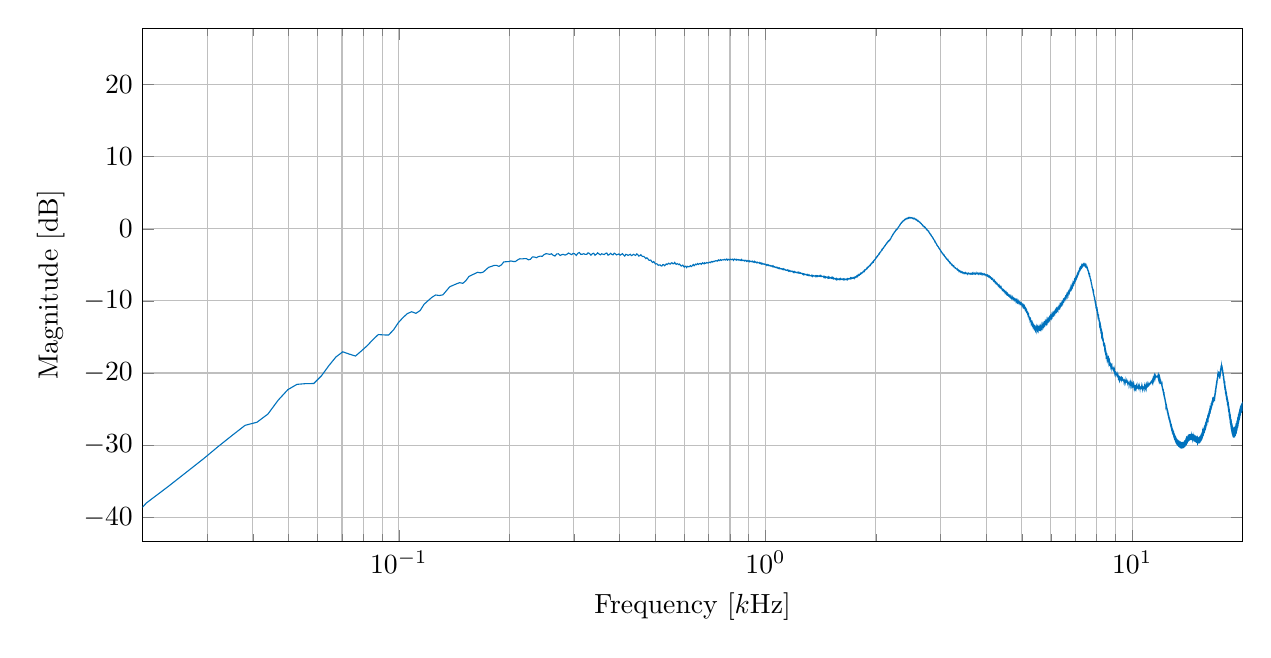
\begin{tikzpicture}

\begin{axis}[%
width=5.5in,
height=2.566in,
at={(2.804in,1.205in)},
scale only axis,
xmode=log,
xmin=0.02,
xmax=20,
xminorticks=true,
xlabel={Frequency [$k$Hz]},
xmajorgrids,
xminorgrids,
ymin=-43.3455877896241,
ymax=27.8130955898857,
ylabel={Magnitude [dB]},
ymajorgrids,
axis background/.style={fill=white},
title style={font=\bfseries},
legend style={legend cell align=left,align=left,draw=white!15!black}
]
\addplot [color=mycolor1,solid,forget plot]
  table[row sep=crcr]{%
0	-1.69141873333655\\
0.0029296875	-40.8589297400518\\
0.005859375	-60.5980111862308\\
0.0087890625	-53.2157441308172\\
0.01171875	-57.2367516122019\\
0.0146484375	-43.1597211075457\\
0.017578125	-41.6473379204459\\
0.0205078125	-37.9993270931867\\
0.0234375	-35.7728657291726\\
0.0263671875	-33.7314835828777\\
0.029296875	-31.9034991604498\\
0.0322265625	-30.1508947985882\\
0.03515625	-28.6204314562879\\
0.0380859375	-27.2462179322706\\
0.041015625	-26.8214249575063\\
0.0439453125	-25.6889727720254\\
0.046875	-23.7608293638928\\
0.0498046875	-22.3031464197138\\
0.052734375	-21.5695615779491\\
0.0556640625	-21.4666363252484\\
0.05859375	-21.4521698756001\\
0.0615234375	-20.3776757568286\\
0.064453125	-18.9662221291674\\
0.0673828125	-17.7640061494371\\
0.0703125	-17.0545263118457\\
0.0732421875	-17.3707060985524\\
0.076171875	-17.6438127055492\\
0.0791015625	-16.9208559171187\\
0.08203125	-16.1958865214752\\
0.0849609375	-15.3697622343122\\
0.087890625	-14.6609591744791\\
0.0908203125	-14.7131683950697\\
0.09375	-14.7296104829327\\
0.0966796875	-14.0206386171589\\
0.099609375	-13.0336615128222\\
0.1025390625	-12.3328386875402\\
0.10546875	-11.7549646788107\\
0.1083984375	-11.4986184373946\\
0.111328125	-11.7220860030783\\
0.1142578125	-11.3429897266818\\
0.1171875	-10.4618012927625\\
0.1201171875	-9.96853290357672\\
0.123046875	-9.50334307464777\\
0.1259765625	-9.17319188163316\\
0.12890625	-9.2495601015986\\
0.1318359375	-9.15893108517974\\
0.134765625	-8.59283945463693\\
0.1376953125	-8.03173585963651\\
0.140625	-7.82650855354564\\
0.1435546875	-7.63529660001848\\
0.146484375	-7.46142610723052\\
0.1494140625	-7.56393597479115\\
0.15234375	-7.18827737888694\\
0.1552734375	-6.61532104461224\\
0.158203125	-6.39868842683859\\
0.1611328125	-6.21682302558645\\
0.1640625	-6.02954473273905\\
0.1669921875	-6.10426766937144\\
0.169921875	-6.00312624546655\\
0.1728515625	-5.66310038863372\\
0.17578125	-5.33804890758637\\
0.1787109375	-5.22289300814975\\
0.181640625	-5.08510223827551\\
0.1845703125	-5.06794998346476\\
0.1875	-5.20828523103086\\
0.1904296875	-4.998878075059\\
0.193359375	-4.59228789601514\\
0.1962890625	-4.56159256674471\\
0.19921875	-4.54685857244095\\
0.2021484375	-4.45575077723635\\
0.205078125	-4.5290785871714\\
0.2080078125	-4.52743763361076\\
0.2109375	-4.30835843258672\\
0.2138671875	-4.15347340258256\\
0.216796875	-4.17550003496058\\
0.2197265625	-4.13297122043127\\
0.22265625	-4.12523496914594\\
0.2255859375	-4.29800796398564\\
0.228515625	-4.2259488085266\\
0.2314453125	-3.88616227648691\\
0.234375	-3.91741452842007\\
0.2373046875	-4.00458251180589\\
0.240234375	-3.85494993578249\\
0.2431640625	-3.78553813086069\\
0.24609375	-3.81296661330424\\
0.2490234375	-3.57098860902556\\
0.251953125	-3.44511919028258\\
0.2548828125	-3.48388512192196\\
0.2578125	-3.54474569476645\\
0.2607421875	-3.45926576364081\\
0.263671875	-3.67535735501565\\
0.2666015625	-3.77257239477092\\
0.26953125	-3.48270267867042\\
0.2724609375	-3.46231562233572\\
0.275390625	-3.69396011817997\\
0.2783203125	-3.57301591264792\\
0.28125	-3.55535128819628\\
0.2841796875	-3.64783250744057\\
0.287109375	-3.54413499453244\\
0.2900390625	-3.3592801782728\\
0.29296875	-3.4723296549576\\
0.2958984375	-3.58211289406512\\
0.298828125	-3.40481400116369\\
0.3017578125	-3.46649346050754\\
0.3046875	-3.68853142812208\\
0.3076171875	-3.40416769412155\\
0.310546875	-3.29153101285164\\
0.3134765625	-3.53860063498036\\
0.31640625	-3.53044119723842\\
0.3193359375	-3.45394805041991\\
0.322265625	-3.54774496623531\\
0.3251953125	-3.545809251062\\
0.328125	-3.33575920379286\\
0.3310546875	-3.41767875053785\\
0.333984375	-3.64722632389805\\
0.3369140625	-3.46386848249114\\
0.33984375	-3.38269792403344\\
0.3427734375	-3.66122057883734\\
0.345703125	-3.52104312967322\\
0.3486328125	-3.32639795808251\\
0.3515625	-3.49648522590513\\
0.3544921875	-3.61316934603985\\
0.357421875	-3.45629484043116\\
0.3603515625	-3.52435906009936\\
0.36328125	-3.5784291239811\\
0.3662109375	-3.41674550563334\\
0.369140625	-3.3516979036454\\
0.3720703125	-3.65970219302892\\
0.375	-3.56411579693327\\
0.3779296875	-3.39374412905505\\
0.380859375	-3.54942502406254\\
0.3837890625	-3.61286268144238\\
0.38671875	-3.37902704921277\\
0.3896484375	-3.48134335477641\\
0.392578125	-3.62350297036289\\
0.3955078125	-3.5438443226605\\
0.3984375	-3.48144236731463\\
0.4013671875	-3.65543312092962\\
0.404296875	-3.54757239658522\\
0.4072265625	-3.44795442073939\\
0.41015625	-3.63298885293949\\
0.4130859375	-3.78191389006145\\
0.416015625	-3.53455549220831\\
0.4189453125	-3.58432410638278\\
0.421875	-3.68652830305695\\
0.4248046875	-3.60867762723097\\
0.427734375	-3.53184639118462\\
0.4306640625	-3.71225318440565\\
0.43359375	-3.6461993020431\\
0.4365234375	-3.54032591083501\\
0.439453125	-3.62330608078383\\
0.4423828125	-3.68402761154908\\
0.4453125	-3.47900946651691\\
0.4482421875	-3.56835190157369\\
0.451171875	-3.78411580085094\\
0.4541015625	-3.7183693961515\\
0.45703125	-3.59340433845756\\
0.4599609375	-3.76336386321725\\
0.462890625	-3.83508276057887\\
0.4658203125	-3.8220335836221\\
0.46875	-3.97854507411029\\
0.4716796875	-4.12653837492127\\
0.474609375	-4.02048874152626\\
0.4775390625	-4.1426056002677\\
0.48046875	-4.34667235394664\\
0.4833984375	-4.36675094890751\\
0.486328125	-4.32694599457295\\
0.4892578125	-4.54518299903589\\
0.4921875	-4.66235492218146\\
0.4951171875	-4.5427394614955\\
0.498046875	-4.67803412446216\\
0.5009765625	-4.88497169131307\\
0.50390625	-4.8418963274911\\
0.5068359375	-4.89177746991777\\
0.509765625	-5.06591504525136\\
0.5126953125	-5.02010670639982\\
0.515625	-4.99431046977463\\
0.5185546875	-5.1309842561036\\
0.521484375	-5.16645791974781\\
0.5244140625	-4.98489292269744\\
0.52734375	-4.95862524832779\\
0.5302734375	-5.11763626425034\\
0.533203125	-5.01738357059946\\
0.5361328125	-4.87512252062726\\
0.5390625	-4.95818690917309\\
0.5419921875	-4.84898461126784\\
0.544921875	-4.76314353906741\\
0.5478515625	-4.87349712426391\\
0.55078125	-4.88198761082708\\
0.5537109375	-4.71341984126667\\
0.556640625	-4.7314345022877\\
0.5595703125	-4.85602279067359\\
0.5625	-4.82792353968313\\
0.5654296875	-4.66110086532831\\
0.568359375	-4.8633421841206\\
0.5712890625	-4.92531055349355\\
0.57421875	-4.82240687660646\\
0.5771484375	-4.88544864503103\\
0.580078125	-4.97387175929617\\
0.5830078125	-4.89171237581161\\
0.5859375	-5.03463737156858\\
0.5888671875	-5.16781563473245\\
0.591796875	-5.11045651684071\\
0.5947265625	-5.02804770919437\\
0.59765625	-5.19431857875531\\
0.6005859375	-5.30470472841938\\
0.603515625	-5.18295632968744\\
0.6064453125	-5.19527054856388\\
0.609375	-5.3771164905566\\
0.6123046875	-5.20033741071649\\
0.615234375	-5.23500855360425\\
0.6181640625	-5.27500869721496\\
0.62109375	-5.19596286149016\\
0.6240234375	-5.11283820278834\\
0.626953125	-5.2418432002433\\
0.6298828125	-5.1784215171171\\
0.6328125	-5.03525010812342\\
0.6357421875	-4.94508945556083\\
0.638671875	-5.11322794726004\\
0.6416015625	-5.01782073749041\\
0.64453125	-4.90845925860452\\
0.6474609375	-4.98021563504119\\
0.650390625	-4.91190470493024\\
0.6533203125	-4.8167466875513\\
0.65625	-4.93863420261158\\
0.6591796875	-4.87523087517116\\
0.662109375	-4.80118297517873\\
0.6650390625	-4.80286709243245\\
0.66796875	-4.92131648077628\\
0.6708984375	-4.8201971249598\\
0.673828125	-4.70856534233747\\
0.6767578125	-4.78351633729125\\
0.6796875	-4.87403425956904\\
0.6826171875	-4.70959001520714\\
0.685546875	-4.78891240174062\\
0.6884765625	-4.76119639449769\\
0.69140625	-4.67489347904069\\
0.6943359375	-4.70338940166459\\
0.697265625	-4.75628709213089\\
0.7001953125	-4.684367698264\\
0.703125	-4.61767673834976\\
0.7060546875	-4.6387404053059\\
0.708984375	-4.69223299324881\\
0.7119140625	-4.54209144856657\\
0.71484375	-4.52146118746947\\
0.7177734375	-4.61364868698718\\
0.720703125	-4.54320008069766\\
0.7236328125	-4.49329933704252\\
0.7265625	-4.52806715805337\\
0.7294921875	-4.43913035399243\\
0.732421875	-4.42311464426501\\
0.7353515625	-4.43525874221655\\
0.73828125	-4.48682614078763\\
0.7412109375	-4.3868463807126\\
0.744140625	-4.31921448822874\\
0.7470703125	-4.42008043728129\\
0.75	-4.40506000316987\\
0.7529296875	-4.2674611223938\\
0.755859375	-4.341122416659\\
0.7587890625	-4.3812295304657\\
0.76171875	-4.28891990690505\\
0.7646484375	-4.30891925768265\\
0.767578125	-4.31814870240981\\
0.7705078125	-4.26012636934695\\
0.7734375	-4.22986895826136\\
0.7763671875	-4.34427790797662\\
0.779296875	-4.34625875072305\\
0.7822265625	-4.18847175648739\\
0.78515625	-4.2317749081073\\
0.7880859375	-4.33235942454547\\
0.791015625	-4.22301025367113\\
0.7939453125	-4.23855380632773\\
0.796875	-4.31953124413644\\
0.7998046875	-4.2417799725024\\
0.802734375	-4.21178097517293\\
0.8056640625	-4.28690171438467\\
0.80859375	-4.26311935392903\\
0.8115234375	-4.20228911216003\\
0.814453125	-4.22857853302418\\
0.8173828125	-4.36965514423457\\
0.8203125	-4.22664813717392\\
0.8232421875	-4.18965939258976\\
0.826171875	-4.29286410315319\\
0.8291015625	-4.29150546728249\\
0.83203125	-4.22324640761451\\
0.8349609375	-4.35040658524929\\
0.837890625	-4.30135666432778\\
0.8408203125	-4.2469519579908\\
0.84375	-4.26755530432933\\
0.8466796875	-4.36617827906747\\
0.849609375	-4.30617068722137\\
0.8525390625	-4.27935536122686\\
0.85546875	-4.3833497425386\\
0.8583984375	-4.40729171397618\\
0.861328125	-4.25492776585173\\
0.8642578125	-4.36369385764056\\
0.8671875	-4.40320135090656\\
0.8701171875	-4.3591432496836\\
0.873046875	-4.39265749884817\\
0.8759765625	-4.45520588312695\\
0.87890625	-4.35291266101569\\
0.8818359375	-4.37364421090564\\
0.884765625	-4.43677292656258\\
0.8876953125	-4.51048108860164\\
0.890625	-4.38121585621394\\
0.8935546875	-4.45231799353763\\
0.896484375	-4.5207073583943\\
0.8994140625	-4.43752176285909\\
0.90234375	-4.40601602404524\\
0.9052734375	-4.56165785575524\\
0.908203125	-4.48716666894887\\
0.9111328125	-4.50117822987977\\
0.9140625	-4.55747869221113\\
0.9169921875	-4.56128957585594\\
0.919921875	-4.46864594926711\\
0.9228515625	-4.54033327156327\\
0.92578125	-4.63232021013766\\
0.9287109375	-4.61270810709107\\
0.931640625	-4.50796089114465\\
0.9345703125	-4.65885154268426\\
0.9375	-4.62088777842143\\
0.9404296875	-4.57865928639484\\
0.943359375	-4.66583318773274\\
0.9462890625	-4.72752919418321\\
0.94921875	-4.63315562993785\\
0.9521484375	-4.70772414848875\\
0.955078125	-4.72844545086815\\
0.9580078125	-4.71174740824773\\
0.9609375	-4.659966298244\\
0.9638671875	-4.7927354273985\\
0.966796875	-4.82661187520796\\
0.9697265625	-4.72106464631105\\
0.97265625	-4.76897723013587\\
0.9755859375	-4.87107213284469\\
0.978515625	-4.76123831604872\\
0.9814453125	-4.83374871173214\\
0.984375	-4.91241365451674\\
0.9873046875	-4.87986433848431\\
0.990234375	-4.84058485096131\\
0.9931640625	-4.92120115527092\\
0.99609375	-4.94095054770526\\
0.9990234375	-4.90048758343943\\
1.001953125	-4.92430930399502\\
1.0048828125	-5.06559242653248\\
1.0078125	-4.96864328815656\\
1.0107421875	-4.94751816968443\\
1.013671875	-5.04834248728974\\
1.0166015625	-5.04664738012508\\
1.01953125	-5.00143987181542\\
1.0224609375	-5.13547437288759\\
1.025390625	-5.10796730378996\\
1.0283203125	-5.07223129394333\\
1.03125	-5.08882075465738\\
1.0341796875	-5.17913858633125\\
1.037109375	-5.16002212067957\\
1.0400390625	-5.12406079063845\\
1.04296875	-5.23237024286618\\
1.0458984375	-5.26405569822839\\
1.048828125	-5.14348155982151\\
1.0517578125	-5.25098421519391\\
1.0546875	-5.29648377511614\\
1.0576171875	-5.24486735874746\\
1.060546875	-5.2855995830576\\
1.0634765625	-5.35694400578768\\
1.06640625	-5.30683973629681\\
1.0693359375	-5.30000488654485\\
1.072265625	-5.35220155671084\\
1.0751953125	-5.43237479295897\\
1.078125	-5.35032857724212\\
1.0810546875	-5.40126416548077\\
1.083984375	-5.49134070995609\\
1.0869140625	-5.40685649916355\\
1.08984375	-5.40633605143967\\
1.0927734375	-5.52895012095235\\
1.095703125	-5.49072231716298\\
1.0986328125	-5.49132618533326\\
1.1015625	-5.55925755938227\\
1.1044921875	-5.58118973230864\\
1.107421875	-5.53071123338191\\
1.1103515625	-5.53608668214792\\
1.11328125	-5.64585880819862\\
1.1162109375	-5.62642851537595\\
1.119140625	-5.55870998737009\\
1.1220703125	-5.68629096752045\\
1.125	-5.65962110524498\\
1.1279296875	-5.59752542049563\\
1.130859375	-5.69478175010204\\
1.1337890625	-5.73439685080081\\
1.13671875	-5.69110898969831\\
1.1396484375	-5.72518563838946\\
1.142578125	-5.77210055120315\\
1.1455078125	-5.76661197629903\\
1.1484375	-5.70872268698878\\
1.1513671875	-5.79907331377012\\
1.154296875	-5.86786081635353\\
1.1572265625	-5.75704626478898\\
1.16015625	-5.81227739253785\\
1.1630859375	-5.87005692831463\\
1.166015625	-5.78468923315211\\
1.1689453125	-5.83725243457081\\
1.171875	-5.91948630605816\\
1.1748046875	-5.88419891412536\\
1.177734375	-5.8628429249178\\
1.1806640625	-5.89723287892923\\
1.18359375	-5.95519896168673\\
1.1865234375	-5.88904804123752\\
1.189453125	-5.90894460212559\\
1.1923828125	-6.03673485176489\\
1.1953125	-5.96418449306412\\
1.1982421875	-5.9260302168326\\
1.201171875	-6.04183287569612\\
1.2041015625	-5.98737031604162\\
1.20703125	-5.98060680196312\\
1.2099609375	-6.06043073994709\\
1.212890625	-6.08049510150039\\
1.2158203125	-6.03430197834712\\
1.21875	-6.02710351229911\\
1.2216796875	-6.10153781261414\\
1.224609375	-6.11664268193181\\
1.2275390625	-6.02574789508316\\
1.23046875	-6.14299814301546\\
1.2333984375	-6.15729341495461\\
1.236328125	-6.07880010552503\\
1.2392578125	-6.15407458643421\\
1.2421875	-6.1721716895654\\
1.2451171875	-6.11216402577696\\
1.248046875	-6.18098260649049\\
1.2509765625	-6.20970347892973\\
1.25390625	-6.21418322545099\\
1.2568359375	-6.17017490899622\\
1.259765625	-6.21566609635551\\
1.2626953125	-6.28662457864158\\
1.265625	-6.21195549751963\\
1.2685546875	-6.22939214947928\\
1.271484375	-6.35029618723655\\
1.2744140625	-6.24590608613704\\
1.27734375	-6.27655140335122\\
1.2802734375	-6.33800635792397\\
1.283203125	-6.30252686810553\\
1.2861328125	-6.31751094465568\\
1.2890625	-6.36440185243362\\
1.2919921875	-6.39149400329904\\
1.294921875	-6.37145176056617\\
1.2978515625	-6.31630062132695\\
1.30078125	-6.44496105316097\\
1.3037109375	-6.42044888190031\\
1.306640625	-6.36852284646369\\
1.3095703125	-6.47889098646544\\
1.3125	-6.45799379903502\\
1.3154296875	-6.39803583812699\\
1.318359375	-6.49512854142614\\
1.3212890625	-6.47813928892606\\
1.32421875	-6.48328607556988\\
1.3271484375	-6.48460843026487\\
1.330078125	-6.53285861797912\\
1.3330078125	-6.54112301676884\\
1.3359375	-6.45176555679666\\
1.3388671875	-6.50860656047757\\
1.341796875	-6.60284224417143\\
1.3447265625	-6.48879290460297\\
1.34765625	-6.55439346043221\\
1.3505859375	-6.5608576063139\\
1.353515625	-6.49794049021398\\
1.3564453125	-6.53505164985978\\
1.359375	-6.56435286886688\\
1.3623046875	-6.54950587471637\\
1.365234375	-6.54732713589948\\
1.3681640625	-6.50916713428978\\
1.37109375	-6.5978656314478\\
1.3740234375	-6.51032748889992\\
1.376953125	-6.49295362802053\\
1.3798828125	-6.60277482563345\\
1.3828125	-6.5449384125983\\
1.3857421875	-6.50919007719386\\
1.388671875	-6.58516140443874\\
1.3916015625	-6.51789923801232\\
1.39453125	-6.53420796079808\\
1.3974609375	-6.5326168262568\\
1.400390625	-6.59536071891523\\
1.4033203125	-6.58066124326348\\
1.40625	-6.50818387980604\\
1.4091796875	-6.58549504694707\\
1.412109375	-6.60278078637617\\
1.4150390625	-6.49817043052872\\
1.41796875	-6.60789935514941\\
1.4208984375	-6.61288635612328\\
1.423828125	-6.56676045713652\\
1.4267578125	-6.60624483593159\\
1.4296875	-6.60919620073662\\
1.4326171875	-6.6040505344165\\
1.435546875	-6.59534151249096\\
1.4384765625	-6.62559448783213\\
1.44140625	-6.70357236364748\\
1.4443359375	-6.57836308788393\\
1.447265625	-6.62013928750599\\
1.4501953125	-6.71626174527148\\
1.453125	-6.62126410795116\\
1.4560546875	-6.64741438276121\\
1.458984375	-6.75075834296041\\
1.4619140625	-6.6675136318633\\
1.46484375	-6.68224192840057\\
1.4677734375	-6.69785113169337\\
1.470703125	-6.74097411301284\\
1.4736328125	-6.70509099765849\\
1.4765625	-6.68893717361726\\
1.4794921875	-6.819144802474\\
1.482421875	-6.75878122448529\\
1.4853515625	-6.67667512015618\\
1.48828125	-6.81613167519652\\
1.4912109375	-6.77229689268859\\
1.494140625	-6.72524252592518\\
1.4970703125	-6.8397807031759\\
1.5	-6.82270702072537\\
1.5029296875	-6.76590739109372\\
1.505859375	-6.79474707793008\\
1.5087890625	-6.83836403845021\\
1.51171875	-6.85643139358569\\
1.5146484375	-6.77591381000457\\
1.517578125	-6.88721355417869\\
1.5205078125	-6.89937614676529\\
1.5234375	-6.77452076490232\\
1.5263671875	-6.86565012110577\\
1.529296875	-6.92500191150219\\
1.5322265625	-6.82283248024692\\
1.53515625	-6.91227500355251\\
1.5380859375	-6.92848775006183\\
1.541015625	-6.88547631155035\\
1.5439453125	-6.87227484460664\\
1.546875	-6.91458860555048\\
1.5498046875	-6.96693366583526\\
1.552734375	-6.90118874069799\\
1.5556640625	-6.9124709541108\\
1.55859375	-7.00869665916468\\
1.5615234375	-6.88309810715822\\
1.564453125	-6.91774999049153\\
1.5673828125	-7.00590114283051\\
1.5703125	-6.94990588039616\\
1.5732421875	-6.93886458340671\\
1.576171875	-7.01409139537952\\
1.5791015625	-6.9696247185679\\
1.58203125	-6.95253335493868\\
1.5849609375	-6.94192614758578\\
1.587890625	-7.02735948084887\\
1.5908203125	-6.98886368237663\\
1.59375	-6.94435068942113\\
1.5966796875	-7.03411909292362\\
1.599609375	-7.004637643845\\
1.6025390625	-6.92340527205266\\
1.60546875	-7.03315064963255\\
1.6083984375	-7.01665146723326\\
1.611328125	-6.97343200056918\\
1.6142578125	-6.99529986440211\\
1.6171875	-7.01727456692521\\
1.6201171875	-6.99354311490777\\
1.623046875	-6.95770424528121\\
1.6259765625	-7.00810064230757\\
1.62890625	-7.05477130813659\\
1.6318359375	-6.95549250831112\\
1.634765625	-6.9996683785705\\
1.6376953125	-7.03472824953514\\
1.640625	-6.94759978164183\\
1.6435546875	-6.98325164539494\\
1.646484375	-7.04886855451088\\
1.6494140625	-6.98730428101004\\
1.65234375	-6.98653960712227\\
1.6552734375	-6.97582218861993\\
1.658203125	-7.01054429471418\\
1.6611328125	-6.95125074062167\\
1.6640625	-6.9542412905875\\
1.6669921875	-7.02721736484932\\
1.669921875	-6.96588075770705\\
1.6728515625	-6.91923145235666\\
1.67578125	-7.02013963148039\\
1.6787109375	-6.94171216783775\\
1.681640625	-6.9165740967627\\
1.6845703125	-6.9756402102015\\
1.6875	-6.97706720637558\\
1.6904296875	-6.91753890804046\\
1.693359375	-6.90683688678718\\
1.6962890625	-6.94095033453465\\
1.69921875	-6.93424967185877\\
1.7021484375	-6.85486229873908\\
1.705078125	-6.94938515805279\\
1.7080078125	-6.93705707429126\\
1.7109375	-6.82406499773083\\
1.7138671875	-6.87924138341111\\
1.716796875	-6.90093887052183\\
1.7197265625	-6.8195457446871\\
1.72265625	-6.84805487803681\\
1.7255859375	-6.87033957253055\\
1.728515625	-6.85397888206415\\
1.7314453125	-6.77369472028812\\
1.734375	-6.80488830282769\\
1.7373046875	-6.84010703621834\\
1.740234375	-6.75317504940222\\
1.7431640625	-6.75627268156137\\
1.74609375	-6.83476600995385\\
1.7490234375	-6.70672552879824\\
1.751953125	-6.68537809222204\\
1.7548828125	-6.76165590681597\\
1.7578125	-6.69668101966147\\
1.7607421875	-6.65534510851751\\
1.763671875	-6.69347876191637\\
1.7666015625	-6.67576985792795\\
1.76953125	-6.60160695424997\\
1.7724609375	-6.55223683775438\\
1.775390625	-6.63269895795418\\
1.7783203125	-6.55937311249005\\
1.78125	-6.50888437348056\\
1.7841796875	-6.58130745905567\\
1.787109375	-6.51321477128835\\
1.7900390625	-6.3989806851111\\
1.79296875	-6.47731308118256\\
1.7958984375	-6.46592968642966\\
1.798828125	-6.39413689731509\\
1.8017578125	-6.37854896477745\\
1.8046875	-6.40052974256787\\
1.8076171875	-6.32165952171204\\
1.810546875	-6.26339307665035\\
1.8134765625	-6.29613709280511\\
1.81640625	-6.30468600120787\\
1.8193359375	-6.17451393925563\\
1.822265625	-6.22135853207237\\
1.8251953125	-6.21144016701675\\
1.828125	-6.10220491018072\\
1.8310546875	-6.0945897631758\\
1.833984375	-6.13216878394246\\
1.8369140625	-6.06505285411578\\
1.83984375	-6.00970773908216\\
1.8427734375	-6.01231727276615\\
1.845703125	-5.99212465546174\\
1.8486328125	-5.89359849219716\\
1.8515625	-5.90049097670681\\
1.8544921875	-5.94076586461756\\
1.857421875	-5.84778778868764\\
1.8603515625	-5.78183528162475\\
1.86328125	-5.83433699066723\\
1.8662109375	-5.73838340841854\\
1.869140625	-5.6900030072232\\
1.8720703125	-5.71674064840374\\
1.875	-5.70625966083765\\
1.8779296875	-5.62736202321611\\
1.880859375	-5.5916923816705\\
1.8837890625	-5.58900339852266\\
1.88671875	-5.52665686670559\\
1.8896484375	-5.4489593570695\\
1.892578125	-5.5173519936867\\
1.8955078125	-5.47664037447981\\
1.8984375	-5.35828309079238\\
1.9013671875	-5.37714305097512\\
1.904296875	-5.3611557053423\\
1.9072265625	-5.26563037252106\\
1.91015625	-5.26265268581574\\
1.9130859375	-5.2689417826424\\
1.916015625	-5.21409967558395\\
1.9189453125	-5.12048028509207\\
1.921875	-5.12548657011598\\
1.9248046875	-5.11366442604344\\
1.927734375	-5.01470002531715\\
1.9306640625	-5.01367870500741\\
1.93359375	-5.04628896184244\\
1.9365234375	-4.90958999276745\\
1.939453125	-4.86601276438927\\
1.9423828125	-4.88393411012623\\
1.9453125	-4.83346771614129\\
1.9482421875	-4.77003314821121\\
1.951171875	-4.78917988308945\\
1.9541015625	-4.76312613042887\\
1.95703125	-4.66007996198323\\
1.9599609375	-4.61569293088519\\
1.962890625	-4.6434645912837\\
1.9658203125	-4.5565559251952\\
1.96875	-4.50718321266504\\
1.9716796875	-4.55458673727276\\
1.974609375	-4.46027045095229\\
1.9775390625	-4.35782498462373\\
1.98046875	-4.36835792819932\\
1.9833984375	-4.34044979654118\\
1.986328125	-4.27335460488422\\
1.9892578125	-4.23942722787115\\
1.9921875	-4.23572720579665\\
1.9951171875	-4.14038719793086\\
1.998046875	-4.05849271765669\\
2.0009765625	-4.07852020565969\\
2.00390625	-4.0533632694067\\
2.0068359375	-3.93734341117863\\
2.009765625	-3.95914692997121\\
2.0126953125	-3.9135071210074\\
2.015625	-3.81734360451725\\
2.0185546875	-3.76931881246605\\
2.021484375	-3.7896376638198\\
2.0244140625	-3.72377449780498\\
2.02734375	-3.65561266396759\\
2.0302734375	-3.63900210190837\\
2.033203125	-3.6069949450071\\
2.0361328125	-3.48096942792915\\
2.0390625	-3.46982174916388\\
2.0419921875	-3.49179520277846\\
2.044921875	-3.40872530219133\\
2.0478515625	-3.33424463818972\\
2.05078125	-3.34525718366848\\
2.0537109375	-3.25647628977953\\
2.056640625	-3.19524237029043\\
2.0595703125	-3.18594073416324\\
2.0625	-3.19334667330526\\
2.0654296875	-3.09489368780623\\
2.068359375	-3.05265706110652\\
2.0712890625	-3.04164096361291\\
2.07421875	-2.95161171771173\\
2.0771484375	-2.87807116119546\\
2.080078125	-2.92822626164872\\
2.0830078125	-2.88303379209628\\
2.0859375	-2.7803731508223\\
2.0888671875	-2.7499904493169\\
2.091796875	-2.72697203161886\\
2.0947265625	-2.63691119434634\\
2.09765625	-2.60742524457743\\
2.1005859375	-2.63110588062727\\
2.103515625	-2.56682899775979\\
2.1064453125	-2.4636750068467\\
2.109375	-2.46379712486163\\
2.1123046875	-2.42560517413654\\
2.115234375	-2.33616305968968\\
2.1181640625	-2.33649613963053\\
2.12109375	-2.34562852534498\\
2.1240234375	-2.25308699306674\\
2.126953125	-2.17453725466544\\
2.1298828125	-2.17153522327095\\
2.1328125	-2.13074569729389\\
2.1357421875	-2.05376045739104\\
2.138671875	-2.07737874038639\\
2.1416015625	-2.04328143037395\\
2.14453125	-1.93771300390023\\
2.1474609375	-1.89075332199536\\
2.150390625	-1.89242698849256\\
2.1533203125	-1.82975506970763\\
2.15625	-1.77096424484341\\
2.1591796875	-1.80256679974372\\
2.162109375	-1.74832396187514\\
2.1650390625	-1.66268280349414\\
2.16796875	-1.64541237651355\\
2.1708984375	-1.63943601480287\\
2.173828125	-1.59990385293582\\
2.1767578125	-1.57868876772221\\
2.1796875	-1.61557393679493\\
2.1826171875	-1.53593773607548\\
2.185546875	-1.46795546371698\\
2.1884765625	-1.47972731557735\\
2.19140625	-1.44921930347476\\
2.1943359375	-1.36071107128208\\
2.197265625	-1.32147186462311\\
2.2001953125	-1.27740914934651\\
2.203125	-1.1691251002685\\
2.2060546875	-1.09564230392596\\
2.208984375	-1.09493292100751\\
2.2119140625	-1.04525994221621\\
2.21484375	-0.970765293918816\\
2.2177734375	-0.952464427823088\\
2.220703125	-0.916806428230018\\
2.2236328125	-0.798155803414375\\
2.2265625	-0.754658728793117\\
2.2294921875	-0.770227785034706\\
2.232421875	-0.713885997555792\\
2.2353515625	-0.646514107025951\\
2.23828125	-0.63053507357273\\
2.2412109375	-0.562553388785659\\
2.244140625	-0.473132314318264\\
2.2470703125	-0.466511610233169\\
2.25	-0.474017321918666\\
2.2529296875	-0.395218518403226\\
2.255859375	-0.347927001661844\\
2.2587890625	-0.351132922137595\\
2.26171875	-0.271289354954774\\
2.2646484375	-0.2121523118455\\
2.267578125	-0.24085896282287\\
2.2705078125	-0.222132772811051\\
2.2734375	-0.141722000551567\\
2.2763671875	-0.127165158727166\\
2.279296875	-0.108741505039688\\
2.2822265625	-0.0351162669090854\\
2.28515625	0.00242052708841811\\
2.2880859375	-0.0316768065411566\\
2.291015625	0.00795175965106409\\
2.2939453125	0.102185291882847\\
2.296875	0.116141489585004\\
2.2998046875	0.14818649339577\\
2.302734375	0.223638561369455\\
2.3056640625	0.255647123796621\\
2.30859375	0.25022771082115\\
2.3115234375	0.31474496625691\\
2.314453125	0.390495611086124\\
2.3173828125	0.412372464222983\\
2.3203125	0.472889060878913\\
2.3232421875	0.536054482391137\\
2.326171875	0.54013017044133\\
2.3291015625	0.549199099649059\\
2.33203125	0.637042580180719\\
2.3349609375	0.694500051653222\\
2.337890625	0.703307218718805\\
2.3408203125	0.761925974095675\\
2.34375	0.802993276982988\\
2.3466796875	0.788860339669498\\
2.349609375	0.819023691373047\\
2.3525390625	0.903045108366655\\
2.35546875	0.937710711800889\\
2.3583984375	0.934816456734609\\
2.361328125	0.982617057355469\\
2.3642578125	1.01667825739571\\
2.3671875	0.990012281161682\\
2.3701171875	1.02930378162011\\
2.373046875	1.1045051344197\\
2.3759765625	1.12445910530926\\
2.37890625	1.1154510895683\\
2.3818359375	1.15438775195071\\
2.384765625	1.16330097116105\\
2.3876953125	1.15117992767489\\
2.390625	1.22403583545173\\
2.3935546875	1.27853670191558\\
2.396484375	1.25803358687477\\
2.3994140625	1.2522750419468\\
2.40234375	1.29481734605082\\
2.4052734375	1.29920435869872\\
2.408203125	1.29056538233016\\
2.4111328125	1.37450032843759\\
2.4140625	1.39611751411348\\
2.4169921875	1.35049491068065\\
2.419921875	1.38174999082588\\
2.4228515625	1.40599612761645\\
2.42578125	1.39003656558697\\
2.4287109375	1.41898853686951\\
2.431640625	1.47884362696527\\
2.4345703125	1.48315763745643\\
2.4375	1.42898811461026\\
2.4404296875	1.4636597132718\\
2.443359375	1.48667394621458\\
2.4462890625	1.46588182848541\\
2.44921875	1.5057477414648\\
2.4521484375	1.54771519945155\\
2.455078125	1.5081072423219\\
2.4580078125	1.4811678100869\\
2.4609375	1.52095177444272\\
2.4638671875	1.53629681021539\\
2.466796875	1.51584096411557\\
2.4697265625	1.55284368047666\\
2.47265625	1.57237765852886\\
2.4755859375	1.52784500894313\\
2.478515625	1.50392162918371\\
2.4814453125	1.53507571503002\\
2.484375	1.53408113932056\\
2.4873046875	1.52266606075563\\
2.490234375	1.55864301068948\\
2.4931640625	1.54765621269127\\
2.49609375	1.49772801650329\\
2.4990234375	1.49582702567824\\
2.501953125	1.5412408049138\\
2.5048828125	1.52698844658181\\
2.5078125	1.50534779879968\\
2.5107421875	1.53467374969887\\
2.513671875	1.50045196149091\\
2.5166015625	1.45047965378927\\
2.51953125	1.48310898505599\\
2.5224609375	1.48979621665393\\
2.525390625	1.48585581021541\\
2.5283203125	1.47568381071125\\
2.53125	1.48265315061042\\
2.5341796875	1.43943031003039\\
2.537109375	1.39217289308328\\
2.5400390625	1.43405117966347\\
2.54296875	1.45929367613547\\
2.5458984375	1.40382082702905\\
2.548828125	1.41159051781256\\
2.5517578125	1.39335012484764\\
2.5546875	1.34169891943264\\
2.5576171875	1.34198381654534\\
2.560546875	1.3641960190738\\
2.5634765625	1.36282018947958\\
2.56640625	1.30556845973211\\
2.5693359375	1.30538508775811\\
2.572265625	1.29625619526598\\
2.5751953125	1.222768708655\\
2.578125	1.24138425977151\\
2.5810546875	1.27323084785536\\
2.583984375	1.22537396515355\\
2.5869140625	1.20320558993205\\
2.58984375	1.18588869591088\\
2.5927734375	1.16382701842599\\
2.595703125	1.12049196781163\\
2.5986328125	1.14320274733529\\
2.6015625	1.16266567421115\\
2.6044921875	1.08646342301887\\
2.607421875	1.06157014476128\\
2.6103515625	1.0725154790037\\
2.61328125	1.02238489731235\\
2.6162109375	1.0028544761941\\
2.619140625	1.02413435156956\\
2.6220703125	1.01375287232702\\
2.625	0.960929345484374\\
2.6279296875	0.934230058973924\\
2.630859375	0.918706756609481\\
2.6337890625	0.879822767750056\\
2.63671875	0.874595122248991\\
2.6396484375	0.895050230728941\\
2.642578125	0.862868056352625\\
2.6455078125	0.782174220521654\\
2.6484375	0.777285157973381\\
2.6513671875	0.770248655646355\\
2.654296875	0.730096393777217\\
2.6572265625	0.727537542498339\\
2.66015625	0.731659877453581\\
2.6630859375	0.668802815436777\\
2.666015625	0.623851719668721\\
2.6689453125	0.599179224602949\\
2.671875	0.597509407522864\\
2.6748046875	0.547373671753064\\
2.677734375	0.553285673242556\\
2.6806640625	0.546190322653672\\
2.68359375	0.454555319139047\\
2.6865234375	0.408870860816251\\
2.689453125	0.423866298063615\\
2.6923828125	0.40204945737014\\
2.6953125	0.377274503443971\\
2.6982421875	0.375652030403558\\
2.701171875	0.345886635268698\\
2.7041015625	0.285014931030446\\
2.70703125	0.266095363816476\\
2.7099609375	0.29191817059808\\
2.712890625	0.263938295604078\\
2.7158203125	0.230562527754842\\
2.71875	0.253221955991705\\
2.7216796875	0.193296842463553\\
2.724609375	0.133870512491626\\
2.7275390625	0.14447366045556\\
2.73046875	0.148090010917201\\
2.7333984375	0.108636338408587\\
2.736328125	0.0911242333665996\\
2.7392578125	0.0657944366452057\\
2.7421875	0.00766322822681786\\
2.7451171875	-0.0526831129046741\\
2.748046875	-0.0167525216227205\\
2.7509765625	-0.0254824619108263\\
2.75390625	-0.0842576088498959\\
2.7568359375	-0.104024500744629\\
2.759765625	-0.131743988187907\\
2.7626953125	-0.206808696189512\\
2.765625	-0.224888701883117\\
2.7685546875	-0.215742938846745\\
2.771484375	-0.244660086217095\\
2.7744140625	-0.284578250610821\\
2.77734375	-0.316842949225361\\
2.7802734375	-0.354354342223871\\
2.783203125	-0.421821450664481\\
2.7861328125	-0.429374069371647\\
2.7890625	-0.396917167271454\\
2.7919921875	-0.464253604167936\\
2.794921875	-0.523786850546912\\
2.7978515625	-0.543804372477211\\
2.80078125	-0.589127341985431\\
2.8037109375	-0.634608934536857\\
2.806640625	-0.622349513492395\\
2.8095703125	-0.647197719547307\\
2.8125	-0.692480464277082\\
2.8154296875	-0.765248422934576\\
2.818359375	-0.785996441217605\\
2.8212890625	-0.812568297073994\\
2.82421875	-0.866145247803786\\
2.8271484375	-0.836583063680962\\
2.830078125	-0.86961721502297\\
2.8330078125	-0.960486474321954\\
2.8359375	-0.976208260530086\\
2.8388671875	-1.02430946825075\\
2.841796875	-1.05103423215161\\
2.8447265625	-1.07518796886848\\
2.84765625	-1.08544805363249\\
2.8505859375	-1.12027942056153\\
2.853515625	-1.21645120061356\\
2.8564453125	-1.23981503109752\\
2.859375	-1.24033749607003\\
2.8623046875	-1.3072703275763\\
2.865234375	-1.32450739101893\\
2.8681640625	-1.32793178523241\\
2.87109375	-1.40482289974148\\
2.8740234375	-1.46597320190989\\
2.876953125	-1.4791865799823\\
2.8798828125	-1.5060986606947\\
2.8828125	-1.55099734585821\\
2.8857421875	-1.57735000773039\\
2.888671875	-1.58478769760296\\
2.8916015625	-1.68186841068001\\
2.89453125	-1.75053580933195\\
2.8974609375	-1.70938419694312\\
2.900390625	-1.7706983992241\\
2.9033203125	-1.81893515934519\\
2.90625	-1.8269560724903\\
2.9091796875	-1.89611737754234\\
2.912109375	-1.95574109809428\\
2.9150390625	-1.98597969694202\\
2.91796875	-1.99678919924025\\
2.9208984375	-2.03775041640705\\
2.923828125	-2.08950511694468\\
2.9267578125	-2.10108157504266\\
2.9296875	-2.14132447899374\\
2.9326171875	-2.24000681555026\\
2.935546875	-2.22689887616968\\
2.9384765625	-2.24337782721943\\
2.94140625	-2.30395183754325\\
2.9443359375	-2.32051422873388\\
2.947265625	-2.36987516074612\\
2.9501953125	-2.44048418119615\\
2.953125	-2.46661582321599\\
2.9560546875	-2.48272795963891\\
2.958984375	-2.48222406638189\\
2.9619140625	-2.55076395169317\\
2.96484375	-2.599701132017\\
2.9677734375	-2.61017116026267\\
2.970703125	-2.69291349460696\\
2.9736328125	-2.72163967236844\\
2.9765625	-2.70372207853245\\
2.9794921875	-2.75471553274514\\
2.982421875	-2.78387314318121\\
2.9853515625	-2.83616934599752\\
2.98828125	-2.87590778023048\\
2.9912109375	-2.92855503888939\\
2.994140625	-2.95123782992192\\
2.9970703125	-2.93558902804364\\
3	-2.97747416429343\\
3.0029296875	-3.06329492320015\\
3.005859375	-3.06158536599321\\
3.0087890625	-3.10455622302374\\
3.01171875	-3.16075255209239\\
3.0146484375	-3.1366659374429\\
3.017578125	-3.17268810301277\\
3.0205078125	-3.22122678753027\\
3.0234375	-3.26752760500074\\
3.0263671875	-3.2982633938089\\
3.029296875	-3.31696889024113\\
3.0322265625	-3.37277309415146\\
3.03515625	-3.35435589352056\\
3.0380859375	-3.36053429948328\\
3.041015625	-3.46698209794818\\
3.0439453125	-3.48958926648299\\
3.046875	-3.48301709897896\\
3.0498046875	-3.54672147668498\\
3.052734375	-3.54268182592733\\
3.0556640625	-3.54838431833343\\
3.05859375	-3.5980756124531\\
3.0615234375	-3.65117721334303\\
3.064453125	-3.68496247936645\\
3.0673828125	-3.68104669634488\\
3.0703125	-3.7173525368022\\
3.0732421875	-3.75526595305053\\
3.076171875	-3.72581239826656\\
3.0791015625	-3.8017429658305\\
3.08203125	-3.85169458556811\\
3.0849609375	-3.84606042124909\\
3.087890625	-3.8864415145045\\
3.0908203125	-3.89586404922045\\
3.09375	-3.90096973614828\\
3.0966796875	-3.94273300312659\\
3.099609375	-3.98359068341483\\
3.1025390625	-4.03951279008697\\
3.10546875	-4.02823442742783\\
3.1083984375	-4.03653680692906\\
3.111328125	-4.08469289097741\\
3.1142578125	-4.08342987184693\\
3.1171875	-4.11199651330054\\
3.1201171875	-4.1952542807764\\
3.123046875	-4.18448761881535\\
3.1259765625	-4.19950732402469\\
3.12890625	-4.22967204246743\\
3.1318359375	-4.23861453241898\\
3.134765625	-4.26851048076082\\
3.1376953125	-4.30363553171406\\
3.140625	-4.36047025488182\\
3.1435546875	-4.38143904192367\\
3.146484375	-4.33308269012844\\
3.1494140625	-4.39460942773934\\
3.15234375	-4.42945316148575\\
3.1552734375	-4.42688212594322\\
3.158203125	-4.50303481737819\\
3.1611328125	-4.5205009560047\\
3.1640625	-4.50928089539241\\
3.1669921875	-4.52996417945604\\
3.169921875	-4.54718375581081\\
3.1728515625	-4.60944688328874\\
3.17578125	-4.60934662778959\\
3.1787109375	-4.64518166053585\\
3.181640625	-4.69832408081049\\
3.1845703125	-4.64582532284811\\
3.1875	-4.67775183015073\\
3.1904296875	-4.74585976050508\\
3.193359375	-4.73551961674031\\
3.1962890625	-4.78560572646694\\
3.19921875	-4.82190499129075\\
3.2021484375	-4.80752557475182\\
3.205078125	-4.81050000390485\\
3.2080078125	-4.83780362077113\\
3.2109375	-4.89366426674292\\
3.2138671875	-4.91030954750903\\
3.216796875	-4.91340507024688\\
3.2197265625	-4.97655491675306\\
3.22265625	-4.95126885344956\\
3.2255859375	-4.94142554196964\\
3.228515625	-5.02330951663623\\
3.2314453125	-5.03461305895627\\
3.234375	-5.04592016672558\\
3.2373046875	-5.09647867968368\\
3.240234375	-5.08738734018215\\
3.2431640625	-5.09388163445271\\
3.24609375	-5.10225358098029\\
3.2490234375	-5.14848929012567\\
3.251953125	-5.2006684848522\\
3.2548828125	-5.17664152636019\\
3.2578125	-5.21363260352967\\
3.2607421875	-5.23368366555479\\
3.263671875	-5.18788188704042\\
3.2666015625	-5.25936819528681\\
3.26953125	-5.29873026777847\\
3.2724609375	-5.3005153560066\\
3.275390625	-5.32134368963608\\
3.2783203125	-5.32629060432987\\
3.28125	-5.33525086542988\\
3.2841796875	-5.34531309156552\\
3.287109375	-5.36532805773442\\
3.2900390625	-5.43741943591021\\
3.29296875	-5.42039219218179\\
3.2958984375	-5.41893178631614\\
3.298828125	-5.45036096648778\\
3.3017578125	-5.44236966960028\\
3.3046875	-5.45973157031472\\
3.3076171875	-5.52528468043101\\
3.310546875	-5.53777716814932\\
3.3134765625	-5.53068184526273\\
3.31640625	-5.5367494966053\\
3.3193359375	-5.54953944770244\\
3.322265625	-5.57788282524768\\
3.3251953125	-5.57667429400942\\
3.328125	-5.63546926679186\\
3.3310546875	-5.65834324411168\\
3.333984375	-5.60731558569944\\
3.3369140625	-5.65711403481771\\
3.33984375	-5.67625170938811\\
3.3427734375	-5.65575498930957\\
3.345703125	-5.71352277533953\\
3.3486328125	-5.74143775746228\\
3.3515625	-5.73066221832056\\
3.3544921875	-5.73697480809335\\
3.357421875	-5.72457569049345\\
3.3603515625	-5.78502408090384\\
3.36328125	-5.77411031688683\\
3.3662109375	-5.79333217665453\\
3.369140625	-5.85447087703352\\
3.3720703125	-5.7906683160997\\
3.375	-5.81205350345363\\
3.3779296875	-5.85115973537745\\
3.380859375	-5.83013085501312\\
3.3837890625	-5.87348337706106\\
3.38671875	-5.90509579682976\\
3.3896484375	-5.89944747022861\\
3.392578125	-5.89729447526958\\
3.3955078125	-5.8818523931173\\
3.3984375	-5.92347150871223\\
3.4013671875	-5.94143794410962\\
3.404296875	-5.93702026127528\\
3.4072265625	-5.99627567016256\\
3.41015625	-5.97139485179412\\
3.4130859375	-5.94069909876066\\
3.416015625	-5.98863211242002\\
3.4189453125	-5.99583012935761\\
3.421875	-6.01891332681316\\
3.4248046875	-6.03683240149081\\
3.427734375	-6.02480038417997\\
3.4306640625	-6.03622604960685\\
3.43359375	-6.00734330654785\\
3.4365234375	-6.02855736721182\\
3.439453125	-6.08094417595555\\
3.4423828125	-6.04562447573971\\
3.4453125	-6.0749865408269\\
3.4482421875	-6.08361622001865\\
3.451171875	-6.03165385417503\\
3.4541015625	-6.05932682138018\\
3.45703125	-6.09271786212901\\
3.4599609375	-6.10804982199676\\
3.462890625	-6.11948576992438\\
3.4658203125	-6.08656820661963\\
3.46875	-6.10596757586023\\
3.4716796875	-6.08862476667917\\
3.474609375	-6.08666659219466\\
3.4775390625	-6.15757245692555\\
3.48046875	-6.13362222763499\\
3.4833984375	-6.10860051182135\\
3.486328125	-6.15241039214595\\
3.4892578125	-6.11622821986043\\
3.4921875	-6.11754546577413\\
3.4951171875	-6.1576219102102\\
3.498046875	-6.16048099005877\\
3.5009765625	-6.17626728388177\\
3.50390625	-6.13961320203299\\
3.5068359375	-6.15590284558982\\
3.509765625	-6.16590948416359\\
3.5126953125	-6.13000318138569\\
3.515625	-6.20014936864771\\
3.5185546875	-6.21100173154747\\
3.521484375	-6.15730531713632\\
3.5244140625	-6.1878433007567\\
3.52734375	-6.17798076979096\\
3.5302734375	-6.16607221328871\\
3.533203125	-6.19366618309692\\
3.5361328125	-6.20218914087104\\
3.5390625	-6.218268925828\\
3.5419921875	-6.19451692177176\\
3.544921875	-6.17243462394151\\
3.5478515625	-6.19963949525345\\
3.55078125	-6.17900131449795\\
3.5537109375	-6.2024131682569\\
3.556640625	-6.24886987922287\\
3.5595703125	-6.20017610947104\\
3.5625	-6.18341264529295\\
3.5654296875	-6.19198214544821\\
3.568359375	-6.18835275206442\\
3.5712890625	-6.22148899454612\\
3.57421875	-6.22356681155031\\
3.5771484375	-6.22767457137002\\
3.580078125	-6.21567062231435\\
3.5830078125	-6.17279891789877\\
3.5859375	-6.20797993210346\\
3.5888671875	-6.21595333811786\\
3.591796875	-6.21044100280875\\
3.5947265625	-6.24750297098586\\
3.59765625	-6.23271335915507\\
3.6005859375	-6.19349184041249\\
3.603515625	-6.19547337570737\\
3.6064453125	-6.20200182035455\\
3.609375	-6.23935521901399\\
3.6123046875	-6.23193362253807\\
3.615234375	-6.22362434035517\\
3.6181640625	-6.22480060945446\\
3.62109375	-6.18133993844646\\
3.6240234375	-6.19309234030595\\
3.626953125	-6.2422067985226\\
3.6298828125	-6.21418196942057\\
3.6328125	-6.21224343228454\\
3.6357421875	-6.23734775620591\\
3.638671875	-6.19187230543275\\
3.6416015625	-6.19121751015484\\
3.64453125	-6.20810063022236\\
3.6474609375	-6.2200259882257\\
3.650390625	-6.23312659344725\\
3.6533203125	-6.20471026285128\\
3.65625	-6.22912056433609\\
3.6591796875	-6.19313082953136\\
3.662109375	-6.1601290675884\\
3.6650390625	-6.24105911018256\\
3.66796875	-6.22281162968062\\
3.6708984375	-6.20035846513935\\
3.673828125	-6.22799707255814\\
3.6767578125	-6.19053481792832\\
3.6796875	-6.18992588976681\\
3.6826171875	-6.19629465530147\\
3.685546875	-6.20994138114429\\
3.6884765625	-6.23258503420658\\
3.69140625	-6.20045529224734\\
3.6943359375	-6.20164608004205\\
3.697265625	-6.20313687645336\\
3.7001953125	-6.159971282745\\
3.703125	-6.21061011867084\\
3.7060546875	-6.237392939693\\
3.708984375	-6.20151476239431\\
3.7119140625	-6.2057518058968\\
3.71484375	-6.18835218297551\\
3.7177734375	-6.17473548348744\\
3.720703125	-6.20339622952088\\
3.7236328125	-6.20675229502729\\
3.7265625	-6.23240414382934\\
3.7294921875	-6.21000372711586\\
3.732421875	-6.16613155002716\\
3.7353515625	-6.20077282244068\\
3.73828125	-6.17851194641048\\
3.7412109375	-6.19130515946819\\
3.744140625	-6.23845600650674\\
3.7470703125	-6.20701932985844\\
3.75	-6.19430592321135\\
3.7529296875	-6.18129820070629\\
3.755859375	-6.17800177269976\\
3.7587890625	-6.21081658099257\\
3.76171875	-6.19985038078556\\
3.7646484375	-6.22584428546088\\
3.767578125	-6.221148421826\\
3.7705078125	-6.15200849710709\\
3.7734375	-6.1988565817727\\
3.7763671875	-6.20340181691091\\
3.779296875	-6.18377403610248\\
3.7822265625	-6.22459402801042\\
3.78515625	-6.21003887564382\\
3.7880859375	-6.18334733208474\\
3.791015625	-6.18736981020987\\
3.7939453125	-6.17326672158964\\
3.796875	-6.21090795081528\\
3.7998046875	-6.20580425349254\\
3.802734375	-6.20502262045926\\
3.8056640625	-6.23936175027512\\
3.80859375	-6.17115605051742\\
3.8115234375	-6.16836137846963\\
3.814453125	-6.21801413185392\\
3.8173828125	-6.19582372176092\\
3.8203125	-6.21927376891574\\
3.8232421875	-6.22150477291933\\
3.826171875	-6.19500457569302\\
3.8291015625	-6.19809165525533\\
3.83203125	-6.18343650475344\\
3.8349609375	-6.21439452670643\\
3.837890625	-6.23657139752379\\
3.8408203125	-6.2018609072453\\
3.84375	-6.24316234998747\\
3.8466796875	-6.20613286459479\\
3.849609375	-6.17235547633521\\
3.8525390625	-6.22405236173194\\
3.85546875	-6.22388713232817\\
3.8583984375	-6.23655124915211\\
3.861328125	-6.25360235082474\\
3.8642578125	-6.20604706562699\\
3.8671875	-6.21264782387311\\
3.8701171875	-6.21052896092357\\
3.873046875	-6.2288360935928\\
3.8759765625	-6.27504873308311\\
3.87890625	-6.23337388990512\\
3.8818359375	-6.23516640747226\\
3.884765625	-6.2394611787891\\
3.8876953125	-6.2013017508969\\
3.890625	-6.24936664454958\\
3.8935546875	-6.26933955623417\\
3.896484375	-6.26273626209775\\
3.8994140625	-6.27280938667889\\
3.90234375	-6.236253923753\\
3.9052734375	-6.24148528962337\\
3.908203125	-6.25351747992892\\
3.9111328125	-6.24465840542479\\
3.9140625	-6.31109503172001\\
3.9169921875	-6.27995884045316\\
3.919921875	-6.24871922135054\\
3.9228515625	-6.27721639304434\\
3.92578125	-6.25726665217354\\
3.9287109375	-6.27919718797506\\
3.931640625	-6.31593278676263\\
3.9345703125	-6.29614079242486\\
3.9375	-6.31035108596495\\
3.9404296875	-6.28569602539437\\
3.943359375	-6.28555451369374\\
3.9462890625	-6.31686977931707\\
3.94921875	-6.2953172056325\\
3.9521484375	-6.34027870831642\\
3.955078125	-6.35497493755315\\
3.9580078125	-6.29874428027051\\
3.9609375	-6.32364476843532\\
3.9638671875	-6.32916176447389\\
3.966796875	-6.32904001904768\\
3.9697265625	-6.38116984849472\\
3.97265625	-6.37174550456228\\
3.9755859375	-6.36795629231904\\
3.978515625	-6.35196990884475\\
3.9814453125	-6.34311872472432\\
3.984375	-6.39110074262163\\
3.9873046875	-6.38489709362716\\
3.990234375	-6.39782430419126\\
3.9931640625	-6.43522160855196\\
3.99609375	-6.38567106463842\\
3.9990234375	-6.38356200794834\\
4.001953125	-6.41527109054698\\
4.0048828125	-6.40667565470613\\
4.0078125	-6.46034753307191\\
4.0107421875	-6.46343607624243\\
4.013671875	-6.44760772410427\\
4.0166015625	-6.45341515137807\\
4.01953125	-6.428305179988\\
4.0224609375	-6.46838221966749\\
4.025390625	-6.51056313608802\\
4.0283203125	-6.4880396740441\\
4.03125	-6.52437907205365\\
4.0341796875	-6.49734040155818\\
4.037109375	-6.47870863164678\\
4.0400390625	-6.52265405389232\\
4.04296875	-6.52878252262332\\
4.0458984375	-6.56913410250706\\
4.048828125	-6.57105586979367\\
4.0517578125	-6.53547206705292\\
4.0546875	-6.57445390600179\\
4.0576171875	-6.54351350433757\\
4.060546875	-6.56916419366689\\
4.0634765625	-6.63441433767838\\
4.06640625	-6.61185301663909\\
4.0693359375	-6.61931422529597\\
4.072265625	-6.62175317494354\\
4.0751953125	-6.59620380085988\\
4.078125	-6.64865727253039\\
4.0810546875	-6.66000795330052\\
4.083984375	-6.68339228950822\\
4.0869140625	-6.70932054765581\\
4.08984375	-6.66075773245166\\
4.0927734375	-6.69314555115233\\
4.095703125	-6.71175501600891\\
4.0986328125	-6.69749594586744\\
4.1015625	-6.77351114666584\\
4.1044921875	-6.7602466267528\\
4.107421875	-6.74974413180541\\
4.1103515625	-6.77494208476924\\
4.11328125	-6.75494179198256\\
4.1162109375	-6.78841900807112\\
4.119140625	-6.81989716963614\\
4.1220703125	-6.82932820814176\\
4.125	-6.86698594189863\\
4.1279296875	-6.8189686575389\\
4.130859375	-6.83382850300933\\
4.1337890625	-6.88099971027054\\
4.13671875	-6.86250276113066\\
4.1396484375	-6.92082730897658\\
4.142578125	-6.9462578445989\\
4.1455078125	-6.90780159407922\\
4.1484375	-6.94342988691523\\
4.1513671875	-6.92436178011815\\
4.154296875	-6.96082023870957\\
4.1572265625	-7.00899602920197\\
4.16015625	-6.99779490089048\\
4.1630859375	-7.03630101697087\\
4.166015625	-7.02422370411085\\
4.1689453125	-6.99453213357305\\
4.171875	-7.06129690989678\\
4.1748046875	-7.06701038406209\\
4.177734375	-7.10090813169921\\
4.1806640625	-7.14033554910071\\
4.18359375	-7.1000221077835\\
4.1865234375	-7.11686535296838\\
4.189453125	-7.12930682273941\\
4.1923828125	-7.14481021006958\\
4.1953125	-7.22052285159623\\
4.1982421875	-7.19272094698704\\
4.201171875	-7.21527141185703\\
4.2041015625	-7.23637518773813\\
4.20703125	-7.19147851044278\\
4.2099609375	-7.25451642374185\\
4.212890625	-7.29357145577262\\
4.2158203125	-7.29038383162845\\
4.21875	-7.33655808356332\\
4.2216796875	-7.30403818624819\\
4.224609375	-7.31778652323197\\
4.2275390625	-7.3435656839016\\
4.23046875	-7.34990963658998\\
4.2333984375	-7.43258497952928\\
4.236328125	-7.41807527047558\\
4.2392578125	-7.39258537244615\\
4.2421875	-7.45210919094018\\
4.2451171875	-7.42054839001457\\
4.248046875	-7.45937544370094\\
4.2509765625	-7.52330069358351\\
4.25390625	-7.50159619321272\\
4.2568359375	-7.52904272105383\\
4.259765625	-7.53366880978143\\
4.2626953125	-7.53148685448696\\
4.265625	-7.57199170270451\\
4.2685546875	-7.5567847566856\\
4.271484375	-7.63430925600198\\
4.2744140625	-7.65710839317489\\
4.27734375	-7.60629775466526\\
4.2802734375	-7.66150994138565\\
4.283203125	-7.65516593652308\\
4.2861328125	-7.64574554868875\\
4.2890625	-7.73736355866146\\
4.2919921875	-7.73427380980235\\
4.294921875	-7.73592224752417\\
4.2978515625	-7.74952879903066\\
4.30078125	-7.73416562978019\\
4.3037109375	-7.78166115527\\
4.306640625	-7.77805342348739\\
4.3095703125	-7.80968591205954\\
4.3125	-7.86795936641909\\
4.3154296875	-7.81901244634145\\
4.318359375	-7.8347603991391\\
4.3212890625	-7.86309685163292\\
4.32421875	-7.84438852316111\\
4.3271484375	-7.91793001870235\\
4.330078125	-7.93183092425909\\
4.3330078125	-7.92657830679178\\
4.3359375	-7.95085539117946\\
4.3388671875	-7.90050807726197\\
4.341796875	-7.96420421284915\\
4.3447265625	-7.99217386683557\\
4.34765625	-7.98745025540438\\
4.3505859375	-8.05277858051471\\
4.353515625	-8.02672412387199\\
4.3564453125	-8.00091734458726\\
4.359375	-8.05578664513689\\
4.3623046875	-8.05357782936437\\
4.365234375	-8.09699301020572\\
4.3681640625	-8.13286579975369\\
4.37109375	-8.12577014554637\\
4.3740234375	-8.13754364171882\\
4.376953125	-8.09728374120488\\
4.3798828125	-8.13725222251162\\
4.3828125	-8.21603986626576\\
4.3857421875	-8.20084653699774\\
4.388671875	-8.23384642887817\\
4.3916015625	-8.23445600002464\\
4.39453125	-8.17568195365982\\
4.3974609375	-8.24806525425174\\
4.400390625	-8.28817862293994\\
4.4033203125	-8.30612883251592\\
4.40625	-8.32696460019469\\
4.4091796875	-8.29453209508813\\
4.412109375	-8.31678180951423\\
4.4150390625	-8.33036585177643\\
4.41796875	-8.34140832947799\\
4.4208984375	-8.42288957484834\\
4.423828125	-8.39458000561973\\
4.4267578125	-8.39020568975434\\
4.4296875	-8.45004332354489\\
4.4326171875	-8.41270578409222\\
4.435546875	-8.43857350072875\\
4.4384765625	-8.48338324403431\\
4.44140625	-8.47533270805047\\
4.4443359375	-8.51728969770897\\
4.447265625	-8.51174180343173\\
4.4501953125	-8.51741543863699\\
4.453125	-8.53922607373511\\
4.4560546875	-8.50864855884606\\
4.458984375	-8.5813658515325\\
4.4619140625	-8.61305294815509\\
4.46484375	-8.57672590913626\\
4.4677734375	-8.61970089716141\\
4.470703125	-8.59149191016309\\
4.4736328125	-8.58930381650021\\
4.4765625	-8.65963399049559\\
4.4794921875	-8.66789428021991\\
4.482421875	-8.70364179655593\\
4.4853515625	-8.68682155380566\\
4.48828125	-8.65560526573194\\
4.4912109375	-8.70869181833154\\
4.494140625	-8.70283289838454\\
4.4970703125	-8.74531041876577\\
4.5	-8.80714794009742\\
4.5029296875	-8.74439768117571\\
4.505859375	-8.76281107726766\\
4.5087890625	-8.78262433853564\\
4.51171875	-8.77370867914419\\
4.5146484375	-8.8377997085081\\
4.517578125	-8.84986063584785\\
4.5205078125	-8.86888386410453\\
4.5234375	-8.87549587449809\\
4.5263671875	-8.8172248399718\\
4.529296875	-8.87844206428559\\
4.5322265625	-8.90983061696772\\
4.53515625	-8.89848473574682\\
4.5380859375	-8.98096290365362\\
4.541015625	-8.94134818368235\\
4.5439453125	-8.91297041621891\\
4.546875	-8.95434086803328\\
4.5498046875	-8.95613253334295\\
4.552734375	-9.01105161620535\\
4.5556640625	-9.02545863101858\\
4.55859375	-9.00744483382732\\
4.5615234375	-9.04335452701639\\
4.564453125	-8.99721091594949\\
4.5673828125	-9.02598935062122\\
4.5703125	-9.08934442108404\\
4.5732421875	-9.0559581265432\\
4.576171875	-9.11125797233365\\
4.5791015625	-9.12335444275072\\
4.58203125	-9.0674589124377\\
4.5849609375	-9.10744832940389\\
4.587890625	-9.11498596066758\\
4.5908203125	-9.15418176627793\\
4.59375	-9.19570617926848\\
4.5966796875	-9.15733304147335\\
4.599609375	-9.18324568979091\\
4.6025390625	-9.16846811927678\\
4.60546875	-9.15952576193138\\
4.6083984375	-9.25006293037916\\
4.611328125	-9.23078389514268\\
4.6142578125	-9.24267248311634\\
4.6171875	-9.27108587107278\\
4.6201171875	-9.22892001460792\\
4.623046875	-9.25533027499534\\
4.6259765625	-9.27655664579277\\
4.62890625	-9.29354207772826\\
4.6318359375	-9.34973849206204\\
4.634765625	-9.31305986721634\\
4.6376953125	-9.31731067260478\\
4.640625	-9.33366313633707\\
4.6435546875	-9.30239675291199\\
4.646484375	-9.38221490939515\\
4.6494140625	-9.41958109399735\\
4.65234375	-9.37578971861745\\
4.6552734375	-9.40306835429953\\
4.658203125	-9.37758860745237\\
4.6611328125	-9.39570655514484\\
4.6640625	-9.43203601699122\\
4.6669921875	-9.44079292209665\\
4.669921875	-9.49414825419274\\
4.6728515625	-9.46883947827149\\
4.67578125	-9.42764678165861\\
4.6787109375	-9.49223511260402\\
4.681640625	-9.46352218776559\\
4.6845703125	-9.50452510241973\\
4.6875	-9.57820561009243\\
4.6904296875	-9.52831857690728\\
4.693359375	-9.52268434797179\\
4.6962890625	-9.52681591573344\\
4.69921875	-9.52626837344792\\
4.7021484375	-9.59418533100029\\
4.705078125	-9.58505953803427\\
4.7080078125	-9.60772404772223\\
4.7109375	-9.61853226233058\\
4.7138671875	-9.55758072451948\\
4.716796875	-9.62148739164468\\
4.7197265625	-9.63197236835072\\
4.72265625	-9.61169531518374\\
4.7255859375	-9.69381583625892\\
4.728515625	-9.66795986641876\\
4.7314453125	-9.64440475600605\\
4.734375	-9.6618575995638\\
4.7373046875	-9.65307324506858\\
4.740234375	-9.71880351619677\\
4.7431640625	-9.73145273554178\\
4.74609375	-9.71697807450295\\
4.7490234375	-9.75453077492398\\
4.751953125	-9.68231346979155\\
4.7548828125	-9.71253808400655\\
4.7578125	-9.7821485524085\\
4.7607421875	-9.75696899086876\\
4.763671875	-9.79430547549526\\
4.7666015625	-9.80160667673385\\
4.76953125	-9.75563014938911\\
4.7724609375	-9.79180884724633\\
4.775390625	-9.77114716994606\\
4.7783203125	-9.82482884227829\\
4.78125	-9.86785238227742\\
4.7841796875	-9.82511226916989\\
4.787109375	-9.86008677369654\\
4.7900390625	-9.82691007022203\\
4.79296875	-9.80403542340525\\
4.7958984375	-9.90399068845466\\
4.798828125	-9.8958408530234\\
4.8017578125	-9.90297272147035\\
4.8046875	-9.91569467597134\\
4.8076171875	-9.86273438784366\\
4.810546875	-9.89495979076366\\
4.8134765625	-9.91004939499516\\
4.81640625	-9.93019283758514\\
4.8193359375	-10.0036414753978\\
4.822265625	-9.92404667890065\\
4.8251953125	-9.93551915545351\\
4.828125	-9.96246896588769\\
4.8310546875	-9.91782942698529\\
4.833984375	-9.9889366113689\\
4.8369140625	-10.0301358349674\\
4.83984375	-9.99847476322628\\
4.8427734375	-10.0079441245521\\
4.845703125	-9.96774165236747\\
4.8486328125	-9.99977617643771\\
4.8515625	-10.0357540542128\\
4.8544921875	-10.0338725878878\\
4.857421875	-10.1002446810687\\
4.8603515625	-10.0516365182608\\
4.86328125	-10.004148950421\\
4.8662109375	-10.0827832276306\\
4.869140625	-10.0440604408327\\
4.8720703125	-10.0852201681503\\
4.875	-10.1397039756623\\
4.8779296875	-10.0951909649485\\
4.880859375	-10.1013857271112\\
4.8837890625	-10.0921658491589\\
4.88671875	-10.0919067667338\\
4.8896484375	-10.1605597076978\\
4.892578125	-10.1320822407147\\
4.8955078125	-10.1800449951364\\
4.8984375	-10.1785332367378\\
4.9013671875	-10.1065160390438\\
4.904296875	-10.160045437591\\
4.9072265625	-10.1835034604644\\
4.91015625	-10.1764528885171\\
4.9130859375	-10.2459181140445\\
4.916015625	-10.2065146915205\\
4.9189453125	-10.1994187682619\\
4.921875	-10.2021912916843\\
4.9248046875	-10.1871363827001\\
4.927734375	-10.2728216829673\\
4.9306640625	-10.2658689241678\\
4.93359375	-10.2561471059817\\
4.9365234375	-10.3013562913608\\
4.939453125	-10.2232625021232\\
4.9423828125	-10.2474961023611\\
4.9453125	-10.3096357057357\\
4.9482421875	-10.3051366789106\\
4.951171875	-10.3549195954897\\
4.9541015625	-10.3248961684216\\
4.95703125	-10.2919806552824\\
4.9599609375	-10.3268376052462\\
4.962890625	-10.303044055161\\
4.9658203125	-10.3868027542341\\
4.96875	-10.4176729662659\\
4.9716796875	-10.3558168153597\\
4.974609375	-10.3971360694507\\
4.9775390625	-10.3668940895224\\
4.98046875	-10.3576663394992\\
4.9833984375	-10.4517254948169\\
4.986328125	-10.4451708414194\\
4.9892578125	-10.464318794691\\
4.9921875	-10.450737394578\\
4.9951171875	-10.4181051486664\\
4.998046875	-10.4706861833864\\
5.0009765625	-10.4614889965636\\
5.00390625	-10.5100490592328\\
5.0068359375	-10.5769577229871\\
5.009765625	-10.4956036299723\\
5.0126953125	-10.5015354209831\\
5.015625	-10.5325063022911\\
5.0185546875	-10.5186594609399\\
5.021484375	-10.5932858495225\\
5.0244140625	-10.6132139469931\\
5.02734375	-10.5950287583051\\
5.0302734375	-10.6125852895366\\
5.033203125	-10.5668323272676\\
5.0361328125	-10.6286204954254\\
5.0390625	-10.6631187546217\\
5.0419921875	-10.6598954151065\\
5.044921875	-10.7375267625243\\
5.0478515625	-10.6898975088349\\
5.05078125	-10.6597869732635\\
5.0537109375	-10.7324422413013\\
5.056640625	-10.716393597158\\
5.0595703125	-10.7801156274592\\
5.0625	-10.8191100893434\\
5.0654296875	-10.783683889532\\
5.068359375	-10.8047611218412\\
5.0712890625	-10.7682137355678\\
5.07421875	-10.8145351261832\\
5.0771484375	-10.9032243611439\\
5.080078125	-10.8751891610028\\
5.0830078125	-10.9222805824911\\
5.0859375	-10.9253491525432\\
5.0888671875	-10.8660966154678\\
5.091796875	-10.9455516063988\\
5.0947265625	-10.9719688194438\\
5.09765625	-11.0003953353525\\
5.1005859375	-11.0614559148217\\
5.103515625	-11.0001823615744\\
5.1064453125	-11.0364849563619\\
5.109375	-11.0485469097628\\
5.1123046875	-11.0414603700853\\
5.115234375	-11.1673114530524\\
5.1181640625	-11.1610370347348\\
5.12109375	-11.147060867316\\
5.1240234375	-11.1951485610014\\
5.126953125	-11.1379211775385\\
5.1298828125	-11.2014897479223\\
5.1328125	-11.2819413088932\\
5.1357421875	-11.2919502569671\\
5.138671875	-11.3372452424618\\
5.1416015625	-11.2842146301637\\
5.14453125	-11.3093351835365\\
5.1474609375	-11.3758266934422\\
5.150390625	-11.3501497215341\\
5.1533203125	-11.4683315562937\\
5.15625	-11.487257332022\\
5.1591796875	-11.4258022647046\\
5.162109375	-11.5009503325834\\
5.1650390625	-11.4898143089594\\
5.16796875	-11.5276340787591\\
5.1708984375	-11.6280323942528\\
5.173828125	-11.6179981992333\\
5.1767578125	-11.6683796994023\\
5.1796875	-11.6357940467544\\
5.1826171875	-11.6293630507204\\
5.185546875	-11.746377303448\\
5.1884765625	-11.7466505460766\\
5.19140625	-11.8002574513404\\
5.1943359375	-11.8654615911552\\
5.197265625	-11.7862601678368\\
5.2001953125	-11.8421045629872\\
5.203125	-11.889256165144\\
5.2060546875	-11.9094842217805\\
5.208984375	-12.0073357026102\\
5.2119140625	-12.0064132014942\\
5.21484375	-12.0164619945534\\
5.2177734375	-12.053723898185\\
5.220703125	-12.007310717111\\
5.2236328125	-12.1321032065046\\
5.2265625	-12.1840545134173\\
5.2294921875	-12.174780919739\\
5.232421875	-12.256646944536\\
5.2353515625	-12.2018525476869\\
5.23828125	-12.2204031391873\\
5.2412109375	-12.3160900577772\\
5.244140625	-12.3297094797308\\
5.2470703125	-12.4198210217592\\
5.25	-12.4044942247\\
5.2529296875	-12.3889458445108\\
5.255859375	-12.4672540089644\\
5.2587890625	-12.4423604311298\\
5.26171875	-12.5097292475988\\
5.2646484375	-12.6269244612456\\
5.267578125	-12.5752329469431\\
5.2705078125	-12.6262113455634\\
5.2734375	-12.6318976691427\\
5.2763671875	-12.6107353728262\\
5.279296875	-12.7209693149178\\
5.2822265625	-12.7519046119349\\
5.28515625	-12.8088027046838\\
5.2880859375	-12.8336424002819\\
5.291015625	-12.755253046074\\
5.2939453125	-12.8440382731208\\
5.296875	-12.876047626102\\
5.2998046875	-12.8931974526694\\
5.302734375	-13.0265549271927\\
5.3056640625	-12.9736087450351\\
5.30859375	-12.9469393510645\\
5.3115234375	-13.0188149101223\\
5.314453125	-12.9978796782931\\
5.3173828125	-13.0976062377248\\
5.3203125	-13.1495989392993\\
5.3232421875	-13.1423108171289\\
5.326171875	-13.1926251310584\\
5.3291015625	-13.109681108878\\
5.33203125	-13.1612418318797\\
5.3349609375	-13.2655617101651\\
5.337890625	-13.241239479441\\
5.3408203125	-13.3425460371652\\
5.34375	-13.3176783465944\\
5.3466796875	-13.2329544619319\\
5.349609375	-13.3173561392591\\
5.3525390625	-13.3409023157114\\
5.35546875	-13.4103309361717\\
5.3583984375	-13.4653103351861\\
5.361328125	-13.4040554161606\\
5.3642578125	-13.4460390064388\\
5.3671875	-13.4088957944182\\
5.3701171875	-13.4210071005475\\
5.373046875	-13.5734188316343\\
5.3759765625	-13.5403882509274\\
5.37890625	-13.5468481483161\\
5.3818359375	-13.5741874462283\\
5.384765625	-13.4858701651152\\
5.3876953125	-13.5586686142655\\
5.390625	-13.6221591931758\\
5.3935546875	-13.6461553793328\\
5.396484375	-13.7040051124608\\
5.3994140625	-13.5937242742808\\
5.40234375	-13.610357705261\\
5.4052734375	-13.6714581503868\\
5.408203125	-13.6379755556899\\
5.4111328125	-13.7583061017578\\
5.4140625	-13.7454468081489\\
5.4169921875	-13.6676101760194\\
5.419921875	-13.7418116346792\\
5.4228515625	-13.7040194996752\\
5.42578125	-13.7208044188399\\
5.4287109375	-13.7874497868633\\
5.431640625	-13.7732492468693\\
5.4345703125	-13.8204309689889\\
5.4375	-13.7605518327651\\
5.4404296875	-13.7235945633118\\
5.443359375	-13.8330867555743\\
5.4462890625	-13.7705019454821\\
5.44921875	-13.8241316578724\\
5.4521484375	-13.8981303175091\\
5.455078125	-13.7841403286466\\
5.4580078125	-13.8124839868285\\
5.4609375	-13.8259050975494\\
5.4638671875	-13.8013952057919\\
5.466796875	-13.8716058466588\\
5.4697265625	-13.8484764464447\\
5.47265625	-13.8882827225301\\
5.4755859375	-13.8701005639612\\
5.478515625	-13.770259635915\\
5.4814453125	-13.8745781393868\\
5.484375	-13.8790640543203\\
5.4873046875	-13.8537881110558\\
5.490234375	-13.9664995374466\\
5.4931640625	-13.858778440878\\
5.49609375	-13.8088538874624\\
5.4990234375	-13.8685417120635\\
5.501953125	-13.8480026959825\\
5.5048828125	-13.921241272398\\
5.5078125	-13.9113729865529\\
5.5107421875	-13.8612914381238\\
5.513671875	-13.8978192447471\\
5.5166015625	-13.7958756886829\\
5.51953125	-13.8522635428741\\
5.5224609375	-13.9325810658784\\
5.525390625	-13.8507511189849\\
5.5283203125	-13.9054430758414\\
5.53125	-13.880337807448\\
5.5341796875	-13.781444284186\\
5.537109375	-13.8573821821291\\
5.5400390625	-13.8528085198454\\
5.54296875	-13.8956187026083\\
5.5458984375	-13.9099478718156\\
5.548828125	-13.8096033803131\\
5.5517578125	-13.8477313106761\\
5.5546875	-13.8138944448278\\
5.5576171875	-13.7899528982461\\
5.560546875	-13.9141899373058\\
5.5634765625	-13.8325652791517\\
5.56640625	-13.8161555034114\\
5.5693359375	-13.8434911406017\\
5.572265625	-13.7506758450816\\
5.5751953125	-13.8011325067003\\
5.578125	-13.8167023742536\\
5.5810546875	-13.8159884137178\\
5.583984375	-13.8487627153544\\
5.5869140625	-13.7422461147726\\
5.58984375	-13.7538416352916\\
5.5927734375	-13.7716227926688\\
5.595703125	-13.7121690419609\\
5.5986328125	-13.828542179849\\
5.6015625	-13.8160559008803\\
5.6044921875	-13.7100842852626\\
5.607421875	-13.7696793542854\\
5.6103515625	-13.6857542906633\\
5.61328125	-13.7092896477066\\
5.6162109375	-13.7643860375267\\
5.619140625	-13.7216818522455\\
5.6220703125	-13.7602811364147\\
5.625	-13.6733062456075\\
5.6279296875	-13.6184219504099\\
5.630859375	-13.7124282420414\\
5.6337890625	-13.6383206564862\\
5.63671875	-13.6992969208583\\
5.6396484375	-13.7422185420583\\
5.642578125	-13.6111797525483\\
5.6455078125	-13.6112644195372\\
5.6484375	-13.6041407894384\\
5.6513671875	-13.5875984898066\\
5.654296875	-13.6884777085675\\
5.6572265625	-13.6235370213012\\
5.66015625	-13.6208490416447\\
5.6630859375	-13.5784887070249\\
5.666015625	-13.4914399836235\\
5.6689453125	-13.5841107588004\\
5.671875	-13.5766126624432\\
5.6748046875	-13.5412391610291\\
5.677734375	-13.6065688927526\\
5.6806640625	-13.501675780577\\
5.68359375	-13.4646720258973\\
5.6865234375	-13.509508738924\\
5.689453125	-13.4771548622332\\
5.6923828125	-13.5454819933516\\
5.6953125	-13.5109032975473\\
5.6982421875	-13.4551946385805\\
5.701171875	-13.4725412713324\\
5.7041015625	-13.3659598004943\\
5.70703125	-13.4250951890028\\
5.7099609375	-13.4950872111481\\
5.712890625	-13.4137695919035\\
5.7158203125	-13.4398482622201\\
5.71875	-13.3902197439756\\
5.7216796875	-13.3095026524465\\
5.724609375	-13.3775739606285\\
5.7275390625	-13.3471127244538\\
5.73046875	-13.3915188113991\\
5.7333984375	-13.3877619623665\\
5.736328125	-13.2943764180276\\
5.7392578125	-13.3218102739191\\
5.7421875	-13.2754176835651\\
5.7451171875	-13.2567282752958\\
5.748046875	-13.3592885580168\\
5.7509765625	-13.295125662746\\
5.75390625	-13.2678295048318\\
5.7568359375	-13.2575172021274\\
5.759765625	-13.1735994872736\\
5.7626953125	-13.2203873546433\\
5.765625	-13.229211549099\\
5.7685546875	-13.2249183720911\\
5.771484375	-13.2658062041615\\
5.7744140625	-13.144912219277\\
5.77734375	-13.1448585862555\\
5.7802734375	-13.1613924997266\\
5.783203125	-13.0911896824319\\
5.7861328125	-13.1959927309603\\
5.7890625	-13.1757188148534\\
5.7919921875	-13.0909703288914\\
5.794921875	-13.107472130141\\
5.7978515625	-13.0375909140701\\
5.80078125	-13.0636736408717\\
5.8037109375	-13.1051141790117\\
5.806640625	-13.076930179087\\
5.8095703125	-13.1078825817321\\
5.8125	-13.0116652300432\\
5.8154296875	-12.9511054777375\\
5.818359375	-13.0292659524303\\
5.8212890625	-12.971297712354\\
5.82421875	-13.0315416314219\\
5.8271484375	-13.0542821578725\\
5.830078125	-12.9256140525228\\
5.8330078125	-12.9323426686015\\
5.8359375	-12.9079364906377\\
5.8388671875	-12.900100330672\\
5.841796875	-12.981640305825\\
5.8447265625	-12.9137923001547\\
5.84765625	-12.9237426358856\\
5.8505859375	-12.8801417335829\\
5.853515625	-12.7832344670771\\
5.8564453125	-12.8624195810451\\
5.859375	-12.8641883824333\\
5.8623046875	-12.8389341583521\\
5.865234375	-12.8952283965383\\
5.8681640625	-12.776691816563\\
5.87109375	-12.759374726181\\
5.8740234375	-12.7661551037346\\
5.876953125	-12.7428882532892\\
5.8798828125	-12.8202977852648\\
5.8828125	-12.7804845761137\\
5.8857421875	-12.7286422772713\\
5.888671875	-12.7389400358036\\
5.8916015625	-12.6378711765249\\
5.89453125	-12.6847637507827\\
5.8974609375	-12.7366386328426\\
5.900390625	-12.686396790062\\
5.9033203125	-12.7140514931006\\
5.90625	-12.6461932564211\\
5.9091796875	-12.5853315237931\\
5.912109375	-12.6245363900136\\
5.9150390625	-12.5880090075099\\
5.91796875	-12.6496231238804\\
5.9208984375	-12.642917715515\\
5.923828125	-12.5441725369665\\
5.9267578125	-12.5752280561472\\
5.9296875	-12.5146712512578\\
5.9326171875	-12.4975056807162\\
5.935546875	-12.5910103559535\\
5.9384765625	-12.5330530014567\\
5.94140625	-12.5219113995727\\
5.9443359375	-12.4935849225531\\
5.947265625	-12.4107288935942\\
5.9501953125	-12.4586725407232\\
5.953125	-12.4531358532471\\
5.9560546875	-12.4630445328455\\
5.958984375	-12.4981419466498\\
5.9619140625	-12.3894999258507\\
5.96484375	-12.3837446927825\\
5.9677734375	-12.3697346223695\\
5.970703125	-12.3219209376959\\
5.9736328125	-12.429642446912\\
5.9765625	-12.403483986996\\
5.9794921875	-12.3362625922487\\
5.982421875	-12.3391748488937\\
5.9853515625	-12.2533227391346\\
5.98828125	-12.2959931950572\\
5.9912109375	-12.3284951820543\\
5.994140625	-12.296165888429\\
5.9970703125	-12.3314625750102\\
6	-12.238005303458\\
6.0029296875	-12.1830636083768\\
6.005859375	-12.2442601112214\\
6.0087890625	-12.1835340922253\\
6.01171875	-12.2473353979874\\
6.0146484375	-12.2604139335032\\
6.017578125	-12.1554327237074\\
6.0205078125	-12.1634478200614\\
6.0234375	-12.1085269329309\\
6.0263671875	-12.1102412924295\\
6.029296875	-12.1908317913456\\
6.0322265625	-12.1324005632704\\
6.03515625	-12.1393697035278\\
6.0380859375	-12.0984362282175\\
6.041015625	-12.0115920859871\\
6.0439453125	-12.0687699397618\\
6.046875	-12.05926910863\\
6.0498046875	-12.0537548862408\\
6.052734375	-12.0989332434701\\
6.0556640625	-12.0041988284526\\
6.05859375	-11.9905527766388\\
6.0615234375	-11.9710105100008\\
6.064453125	-11.938928626637\\
6.0673828125	-12.0248634765787\\
6.0703125	-11.9934507347425\\
6.0732421875	-11.9460549542997\\
6.076171875	-11.9580924914731\\
6.0791015625	-11.8396887494201\\
6.08203125	-11.8836496826908\\
6.0849609375	-11.9210696524988\\
6.087890625	-11.8986676130223\\
6.0908203125	-11.9262922830624\\
6.09375	-11.843818299003\\
6.0966796875	-11.7996939333271\\
6.099609375	-11.8254175094849\\
6.1025390625	-11.7764302681439\\
6.10546875	-11.8507494661551\\
6.1083984375	-11.8488598258412\\
6.111328125	-11.7720513633747\\
6.1142578125	-11.7783631883331\\
6.1171875	-11.6964612322514\\
6.1201171875	-11.6852814163267\\
6.123046875	-11.7816903434459\\
6.1259765625	-11.7343516153072\\
6.12890625	-11.7386204394706\\
6.1318359375	-11.7006774006334\\
6.134765625	-11.6156325447204\\
6.1376953125	-11.6515688775685\\
6.140625	-11.6418231854879\\
6.1435546875	-11.6643965074742\\
6.146484375	-11.6991792591367\\
6.1494140625	-11.5941617603756\\
6.15234375	-11.5886845987621\\
6.1552734375	-11.560748837439\\
6.158203125	-11.5203824627242\\
6.1611328125	-11.610284373012\\
6.1640625	-11.5876106784427\\
6.1669921875	-11.54670804179\\
6.169921875	-11.5457214350051\\
6.1728515625	-11.4322264757653\\
6.17578125	-11.4687815887778\\
6.1787109375	-11.4984589604803\\
6.181640625	-11.4888971249716\\
6.1845703125	-11.5228345443699\\
6.1875	-11.4312199647275\\
6.1904296875	-11.3820583675303\\
6.193359375	-11.4077894309521\\
6.1962890625	-11.3562553013584\\
6.19921875	-11.4297183617854\\
6.2021484375	-11.424121744495\\
6.205078125	-11.3634672665073\\
6.2080078125	-11.365167110238\\
6.2109375	-11.2856629542656\\
6.2138671875	-11.2798323991002\\
6.216796875	-11.3444481564595\\
6.2197265625	-11.3038455608082\\
6.22265625	-11.3374352619231\\
6.2255859375	-11.2833471052762\\
6.228515625	-11.1866120961802\\
6.2314453125	-11.2264219215585\\
6.234375	-11.2172599730908\\
6.2373046875	-11.246493457476\\
6.240234375	-11.2753555773988\\
6.2431640625	-11.1809120193721\\
6.24609375	-11.1779406000019\\
6.2490234375	-11.1316478576754\\
6.251953125	-11.1009596648465\\
6.2548828125	-11.1824807454656\\
6.2578125	-11.1524990988443\\
6.2607421875	-11.1421061426517\\
6.263671875	-11.123951550137\\
6.2666015625	-11.0158422955972\\
6.26953125	-11.0362184519411\\
6.2724609375	-11.0605025821931\\
6.275390625	-11.0542746259376\\
6.2783203125	-11.1165437451994\\
6.28125	-11.0173312956491\\
6.2841796875	-10.9627272658563\\
6.287109375	-10.9641982775572\\
6.2900390625	-10.9335191153177\\
6.29296875	-11.00311158776\\
6.2958984375	-10.9968918012663\\
6.298828125	-10.9375278161755\\
6.3017578125	-10.9368226668115\\
6.3046875	-10.8516866629365\\
6.3076171875	-10.8526000547253\\
6.310546875	-10.9047580017379\\
6.3134765625	-10.8759421367004\\
6.31640625	-10.9131773662369\\
6.3193359375	-10.856459298124\\
6.322265625	-10.7636779178536\\
6.3251953125	-10.7899112171741\\
6.328125	-10.773194287014\\
6.3310546875	-10.8056258586377\\
6.333984375	-10.8451690439122\\
6.3369140625	-10.7568387398377\\
6.33984375	-10.7365239139809\\
6.3427734375	-10.6818314625767\\
6.345703125	-10.6692378225193\\
6.3486328125	-10.7353156947675\\
6.3515625	-10.7062120221328\\
6.3544921875	-10.7052832570572\\
6.357421875	-10.685710521936\\
6.3603515625	-10.5751675157376\\
6.36328125	-10.6048036498636\\
6.3662109375	-10.608950375829\\
6.369140625	-10.6095983352905\\
6.3720703125	-10.6625969289537\\
6.375	-10.5852030347984\\
6.3779296875	-10.5329473795987\\
6.380859375	-10.5150486062602\\
6.3837890625	-10.4804806102997\\
6.38671875	-10.5558287523967\\
6.3896484375	-10.5459278748847\\
6.392578125	-10.507195243032\\
6.3955078125	-10.5042406482738\\
6.3984375	-10.4064123540034\\
6.4013671875	-10.4084400473413\\
6.404296875	-10.4602929384872\\
6.4072265625	-10.4295672903311\\
6.41015625	-10.4657814519194\\
6.4130859375	-10.4136669572158\\
6.416015625	-10.3380972325206\\
6.4189453125	-10.341123991438\\
6.421875	-10.3024059233745\\
6.4248046875	-10.355728515751\\
6.427734375	-10.3970604135508\\
6.4306640625	-10.3216108908505\\
6.43359375	-10.2998009546469\\
6.4365234375	-10.2265167483699\\
6.439453125	-10.2079107210783\\
6.4423828125	-10.2892077114585\\
6.4453125	-10.2648363821705\\
6.4482421875	-10.2655903418908\\
6.451171875	-10.2276495947599\\
6.4541015625	-10.1352840220136\\
6.45703125	-10.1531953611327\\
6.4599609375	-10.1445330986303\\
6.462890625	-10.1651464097031\\
6.4658203125	-10.2157017056132\\
6.46875	-10.1309187132772\\
6.4716796875	-10.0840901127037\\
6.474609375	-10.063872631816\\
6.4775390625	-10.0203556765582\\
6.48046875	-10.0910099980292\\
6.4833984375	-10.1051529955127\\
6.486328125	-10.0690329527087\\
6.4892578125	-10.0270644123572\\
6.4921875	-9.94172893931761\\
6.4951171875	-9.95446704101425\\
6.498046875	-9.98566446259963\\
6.5009765625	-9.96939246499994\\
6.50390625	-10.0079073058972\\
6.5068359375	-9.95202630830596\\
6.509765625	-9.87090320105068\\
6.5126953125	-9.88580002401426\\
6.515625	-9.84906663753645\\
6.5185546875	-9.87609450185778\\
6.521484375	-9.90994162968377\\
6.5244140625	-9.86348384565224\\
6.52734375	-9.82827739251331\\
6.5302734375	-9.76356418461904\\
6.533203125	-9.73906857469689\\
6.5361328125	-9.796875100021\\
6.5390625	-9.78367480229304\\
6.5419921875	-9.80266812509745\\
6.544921875	-9.76136369829123\\
6.5478515625	-9.65742266713528\\
6.55078125	-9.67540760111297\\
6.5537109375	-9.67216859593719\\
6.556640625	-9.67998759971744\\
6.5595703125	-9.721012784013\\
6.5625	-9.66163606296209\\
6.5654296875	-9.61753665824818\\
6.568359375	-9.57148872473903\\
6.5712890625	-9.53305115452895\\
6.57421875	-9.59627684783806\\
6.5771484375	-9.59962342042917\\
6.580078125	-9.58823947557596\\
6.5830078125	-9.57046097745484\\
6.5859375	-9.45710886800265\\
6.5888671875	-9.44754625785367\\
6.591796875	-9.49163971969153\\
6.5947265625	-9.4824450914972\\
6.59765625	-9.52357980882704\\
6.6005859375	-9.46378542359196\\
6.603515625	-9.39060789870331\\
6.6064453125	-9.37622300837791\\
6.609375	-9.34223115031028\\
6.6123046875	-9.38670051774221\\
6.615234375	-9.4177001384636\\
6.6181640625	-9.36143365457298\\
6.62109375	-9.34917352060955\\
6.6240234375	-9.27305471843408\\
6.626953125	-9.22672239161471\\
6.6298828125	-9.28854886033611\\
6.6328125	-9.28562543991984\\
6.6357421875	-9.30718572357279\\
6.638671875	-9.26102897053738\\
6.6416015625	-9.16991155030126\\
6.64453125	-9.16782136591951\\
6.6474609375	-9.14599484980687\\
6.650390625	-9.17455079864453\\
6.6533203125	-9.23558853572496\\
6.65625	-9.14323010439239\\
6.6591796875	-9.10578081641489\\
6.662109375	-9.08071555019285\\
6.6650390625	-9.03302478687186\\
6.66796875	-9.07426781769271\\
6.6708984375	-9.09048153810869\\
6.673828125	-9.08099031753693\\
6.6767578125	-9.0487923568171\\
6.6796875	-8.95809842254022\\
6.6826171875	-8.95229196455983\\
6.685546875	-8.94977990544066\\
6.6884765625	-8.95282633605649\\
6.69140625	-9.0160247516132\\
6.6943359375	-8.94301168894293\\
6.697265625	-8.86855855759887\\
6.7001953125	-8.86416956392412\\
6.703125	-8.82293772795094\\
6.7060546875	-8.85852986147876\\
6.708984375	-8.88819133058217\\
6.7119140625	-8.85577650145763\\
6.71484375	-8.82304028045542\\
6.7177734375	-8.75288413939461\\
6.720703125	-8.71516056224192\\
6.7236328125	-8.76125801395301\\
6.7265625	-8.73806906417423\\
6.7294921875	-8.78021143682997\\
6.732421875	-8.74540407232325\\
6.7353515625	-8.63740264646378\\
6.73828125	-8.62721346040661\\
6.7412109375	-8.61326876684831\\
6.744140625	-8.63192251686951\\
6.7470703125	-8.69441828533542\\
6.75	-8.63038372934562\\
6.7529296875	-8.58286411701778\\
6.755859375	-8.52359771148855\\
6.7587890625	-8.48258941389605\\
6.76171875	-8.54580482364088\\
6.7646484375	-8.54568703142974\\
6.767578125	-8.53600946443026\\
6.7705078125	-8.52555979176759\\
6.7734375	-8.41625098655277\\
6.7763671875	-8.39392103647754\\
6.779296875	-8.40099313751352\\
6.7822265625	-8.41632053447063\\
6.78515625	-8.44935874799961\\
6.7880859375	-8.40340069170855\\
6.791015625	-8.34017572665925\\
6.7939453125	-8.3143287928969\\
6.796875	-8.2519048268436\\
6.7998046875	-8.32273726406839\\
6.802734375	-8.34412362092831\\
6.8056640625	-8.29246878188223\\
6.80859375	-8.27335704271513\\
6.8115234375	-8.19892801289024\\
6.814453125	-8.15649030515385\\
6.8173828125	-8.19051681399145\\
6.8203125	-8.19102420780439\\
6.8232421875	-8.21611242815368\\
6.826171875	-8.17255235470373\\
6.8291015625	-8.09809503121642\\
6.83203125	-8.08047557151201\\
6.8349609375	-8.03737835983821\\
6.837890625	-8.0648664914641\\
6.8408203125	-8.12354297475923\\
6.84375	-8.05118548157293\\
6.8466796875	-8.02365405726653\\
6.849609375	-7.97333036301728\\
6.8525390625	-7.90995200282225\\
6.85546875	-7.955819112467\\
6.8583984375	-7.97258317130292\\
6.861328125	-7.9691223570648\\
6.8642578125	-7.94234911240682\\
6.8671875	-7.83915349217642\\
6.8701171875	-7.82689691653553\\
6.873046875	-7.81483582239753\\
6.8759765625	-7.82391594406198\\
6.87890625	-7.88516759139139\\
6.8818359375	-7.82751187372378\\
6.884765625	-7.75885552296035\\
6.8876953125	-7.72617768407656\\
6.890625	-7.6619252777366\\
6.8935546875	-7.71860375116012\\
6.896484375	-7.7427084908872\\
6.8994140625	-7.72435321664881\\
6.90234375	-7.69134538340825\\
6.9052734375	-7.59916385447389\\
6.908203125	-7.56329194188066\\
6.9111328125	-7.59664070638081\\
6.9140625	-7.5883856550206\\
6.9169921875	-7.63681614253977\\
6.919921875	-7.5929972211099\\
6.9228515625	-7.49915316498272\\
6.92578125	-7.4709689829765\\
6.9287109375	-7.44122458325597\\
6.931640625	-7.47057399500648\\
6.9345703125	-7.51288853732945\\
6.9375	-7.46079511361677\\
6.9404296875	-7.4389695647962\\
6.943359375	-7.35469593500648\\
6.9462890625	-7.30275620235471\\
6.94921875	-7.35787886362675\\
6.9521484375	-7.35659545634905\\
6.955078125	-7.35839384158993\\
6.9580078125	-7.34320617935526\\
6.9609375	-7.23243982725029\\
6.9638671875	-7.21254086875831\\
6.966796875	-7.20297501874779\\
6.9697265625	-7.22100850973868\\
6.97265625	-7.26464898431368\\
6.9755859375	-7.20768757764847\\
6.978515625	-7.16030878787018\\
6.9814453125	-7.11606579088141\\
6.984375	-7.06059431159167\\
6.9873046875	-7.10842941015437\\
6.990234375	-7.11336861041866\\
6.9931640625	-7.09615813975836\\
6.99609375	-7.08927404303432\\
6.9990234375	-7.00167162724506\\
7.001953125	-6.95608202009731\\
7.0048828125	-6.96892547716493\\
7.0078125	-6.96814649709074\\
7.0107421875	-7.01745229033281\\
7.013671875	-6.96797792758014\\
7.0166015625	-6.8935033977715\\
7.01953125	-6.85932805884181\\
7.0224609375	-6.81596171266159\\
7.025390625	-6.84574669931965\\
7.0283203125	-6.8863574810045\\
7.03125	-6.83439065155477\\
7.0341796875	-6.81874973751519\\
7.037109375	-6.73858485368976\\
7.0400390625	-6.6928222442661\\
7.04296875	-6.71381143561263\\
7.0458984375	-6.72105472887017\\
7.048828125	-6.73644498190265\\
7.0517578125	-6.72513805140932\\
7.0546875	-6.624099941331\\
7.0576171875	-6.59643918096259\\
7.060546875	-6.56513742393167\\
7.0634765625	-6.59166197383473\\
7.06640625	-6.64230461930663\\
7.0693359375	-6.59096488199373\\
7.072265625	-6.53661507311466\\
7.0751953125	-6.48414578304153\\
7.078125	-6.43173018916781\\
7.0810546875	-6.48029007319053\\
7.083984375	-6.48831964055773\\
7.0869140625	-6.47409368455953\\
7.08984375	-6.45596514912103\\
7.0927734375	-6.36707511187359\\
7.095703125	-6.3299259001235\\
7.0986328125	-6.33949783503704\\
7.1015625	-6.33791825433894\\
7.1044921875	-6.38254468692094\\
7.107421875	-6.34295849272019\\
7.1103515625	-6.27897194153502\\
7.11328125	-6.23271219036468\\
7.1162109375	-6.18602236908021\\
7.119140625	-6.22847573922087\\
7.1220703125	-6.25900773597925\\
7.125	-6.21237651719969\\
7.1279296875	-6.19565788858563\\
7.130859375	-6.1160443358425\\
7.1337890625	-6.07849716178913\\
7.13671875	-6.10416074237338\\
7.1396484375	-6.09071464364268\\
7.142578125	-6.11172265133746\\
7.1455078125	-6.09978904089513\\
7.1484375	-6.01605649725457\\
7.1513671875	-5.99262901169226\\
7.154296875	-5.95089096210779\\
7.1572265625	-5.9686555221445\\
7.16015625	-6.01548105095327\\
7.1630859375	-5.98026936915551\\
7.166015625	-5.93585192585431\\
7.1689453125	-5.87773444348568\\
7.171875	-5.81707267023552\\
7.1748046875	-5.86989515135252\\
7.177734375	-5.8635417666469\\
7.1806640625	-5.8611459449873\\
7.18359375	-5.85292130129238\\
7.1865234375	-5.76886875325368\\
7.189453125	-5.73772671356261\\
7.1923828125	-5.74010071783175\\
7.1953125	-5.72017504753381\\
7.1982421875	-5.76339220953446\\
7.201171875	-5.75126622032184\\
7.2041015625	-5.69561722469524\\
7.20703125	-5.64360649910361\\
7.2099609375	-5.58617894177593\\
7.212890625	-5.63325127942522\\
7.2158203125	-5.66366566058866\\
7.21875	-5.636368099207\\
7.2216796875	-5.62562506044253\\
7.224609375	-5.54070171797002\\
7.2275390625	-5.49922228183516\\
7.23046875	-5.5317211859533\\
7.2333984375	-5.52798030170652\\
7.236328125	-5.55280140970189\\
7.2392578125	-5.52604112196622\\
7.2421875	-5.45967977467279\\
7.2451171875	-5.44293410922904\\
7.248046875	-5.40160173378746\\
7.2509765625	-5.423266488683\\
7.25390625	-5.45541745915438\\
7.2568359375	-5.43667095310849\\
7.259765625	-5.41427743854439\\
7.2626953125	-5.34156399941429\\
7.265625	-5.29255053131607\\
7.2685546875	-5.34926900585253\\
7.271484375	-5.34721139823279\\
7.2744140625	-5.353935141769\\
7.27734375	-5.33630196911531\\
7.2802734375	-5.26335534779696\\
7.283203125	-5.25123933781867\\
7.2861328125	-5.2478330212378\\
7.2890625	-5.24148232814156\\
7.2919921875	-5.28097844176239\\
7.294921875	-5.24798619857256\\
7.2978515625	-5.22962768482699\\
7.30078125	-5.19911926432832\\
7.3037109375	-5.13800488063049\\
7.306640625	-5.16828532472096\\
7.3095703125	-5.19428135413278\\
7.3125	-5.19347750100843\\
7.3154296875	-5.19375654497316\\
7.318359375	-5.11639239297938\\
7.3212890625	-5.09036609729969\\
7.32421875	-5.10758903907282\\
7.3271484375	-5.10839466101299\\
7.330078125	-5.1500931891274\\
7.3330078125	-5.12652949655751\\
7.3359375	-5.08287765606838\\
7.3388671875	-5.07626380886921\\
7.341796875	-5.03192410952647\\
7.3447265625	-5.04602290169015\\
7.34765625	-5.09427159228011\\
7.3505859375	-5.08218377251603\\
7.353515625	-5.07739122983946\\
7.3564453125	-5.02358713794109\\
7.359375	-4.9871610920236\\
7.3623046875	-5.01299718778239\\
7.365234375	-5.02162249488606\\
7.3681640625	-5.06656938352643\\
7.37109375	-5.06321849911347\\
7.3740234375	-4.98282975833916\\
7.376953125	-4.97720807047693\\
7.3798828125	-4.97148011173624\\
7.3828125	-4.9855780823807\\
7.3857421875	-5.03951681603962\\
7.388671875	-5.0252086195315\\
7.3916015625	-5.00330673784225\\
7.39453125	-4.98108160308311\\
7.3974609375	-4.95072821426589\\
7.400390625	-4.98235211061962\\
7.4033203125	-4.9934942904855\\
7.40625	-5.02839472143927\\
7.4091796875	-5.04465891276897\\
7.412109375	-4.96432968640198\\
7.4150390625	-4.95428622263563\\
7.41796875	-4.98889526635702\\
7.4208984375	-4.98995156525194\\
7.423828125	-5.04308976667807\\
7.4267578125	-5.03705215961668\\
7.4296875	-5.01006556138947\\
7.4326171875	-4.99271696117336\\
7.435546875	-4.97494361272226\\
7.4384765625	-5.02280907965616\\
7.44140625	-5.0456419480912\\
7.4443359375	-5.04248403291552\\
7.447265625	-5.07501225336085\\
7.4501953125	-5.03183537447632\\
7.453125	-5.01037233343743\\
7.4560546875	-5.04967477970428\\
7.458984375	-5.05580411483299\\
7.4619140625	-5.10430969256811\\
7.46484375	-5.12717171544085\\
7.4677734375	-5.0791252695463\\
7.470703125	-5.07832870121666\\
7.4736328125	-5.071592636074\\
7.4765625	-5.11035673105812\\
7.4794921875	-5.16779039097065\\
7.482421875	-5.15490889530236\\
7.4853515625	-5.17396043849345\\
7.48828125	-5.16739875466084\\
7.4912109375	-5.13633395507117\\
7.494140625	-5.18232831476331\\
7.4970703125	-5.20760169528415\\
7.5	-5.24651869581686\\
7.5029296875	-5.27005338684347\\
7.505859375	-5.24095256411249\\
7.5087890625	-5.24709359118179\\
7.51171875	-5.24255514518495\\
7.5146484375	-5.27009608728105\\
7.517578125	-5.36126731821423\\
7.5205078125	-5.35902707741758\\
7.5234375	-5.35110127357575\\
7.5263671875	-5.35682744355819\\
7.529296875	-5.33590754326264\\
7.5322265625	-5.38566887139234\\
7.53515625	-5.43629548900265\\
7.5380859375	-5.46466086008348\\
7.541015625	-5.4935715947845\\
7.5439453125	-5.45363051530398\\
7.546875	-5.47940064524028\\
7.5498046875	-5.49997817307775\\
7.552734375	-5.51524467105577\\
7.5556640625	-5.59912312865487\\
7.55859375	-5.62050034981877\\
7.5615234375	-5.58634254751246\\
7.564453125	-5.61995883575901\\
7.5673828125	-5.61559029418248\\
7.5703125	-5.65190992456274\\
7.5732421875	-5.71779852041971\\
7.576171875	-5.74463541534033\\
7.5791015625	-5.77274900587702\\
7.58203125	-5.74989926349434\\
7.5849609375	-5.75828420116068\\
7.587890625	-5.83033222577382\\
7.5908203125	-5.83118090433686\\
7.59375	-5.89407470632631\\
7.5966796875	-5.94617924828265\\
7.599609375	-5.91294990260803\\
7.6025390625	-5.94047655675359\\
7.60546875	-5.96240000577831\\
7.6083984375	-5.9894217624921\\
7.611328125	-6.06991536628027\\
7.6142578125	-6.0901411115733\\
7.6171875	-6.1199103559079\\
7.6201171875	-6.12384269773213\\
7.623046875	-6.1146624365723\\
7.6259765625	-6.18525748431114\\
7.62890625	-6.22427147799687\\
7.6318359375	-6.25463974867301\\
7.634765625	-6.32623758058241\\
7.6376953125	-6.29600470044284\\
7.640625	-6.31564503368571\\
7.6435546875	-6.35735206114373\\
7.646484375	-6.38359656207331\\
7.6494140625	-6.46320820210923\\
7.65234375	-6.48507618620152\\
7.6552734375	-6.50223543968787\\
7.658203125	-6.53714963756192\\
7.6611328125	-6.51334637088195\\
7.6640625	-6.58327702009285\\
7.6669921875	-6.65617916230383\\
7.669921875	-6.66834813772664\\
7.6728515625	-6.7327493888879\\
7.67578125	-6.73957424426555\\
7.6787109375	-6.72867756692085\\
7.681640625	-6.78624877866656\\
7.6845703125	-6.82342816871267\\
7.6875	-6.90973738655907\\
7.6904296875	-6.93030063110433\\
7.693359375	-6.92496745058298\\
7.6962890625	-6.98238642663904\\
7.69921875	-6.97802192684037\\
7.7021484375	-7.02236124169946\\
7.705078125	-7.13091607141263\\
7.7080078125	-7.13013535069399\\
7.7109375	-7.17018519335886\\
7.7138671875	-7.20230596112737\\
7.716796875	-7.20189472590005\\
7.7197265625	-7.25903852466445\\
7.72265625	-7.30583399357016\\
7.7255859375	-7.36996515979587\\
7.728515625	-7.41756699613421\\
7.7314453125	-7.39048925812705\\
7.734375	-7.45966685687148\\
7.7373046875	-7.47656000557043\\
7.740234375	-7.4925417767667\\
7.7431640625	-7.61186498876123\\
7.74609375	-7.6358160476529\\
7.7490234375	-7.63408742604304\\
7.751953125	-7.69321808585573\\
7.7548828125	-7.68853933243014\\
7.7578125	-7.76071846457046\\
7.7607421875	-7.80729486398172\\
7.763671875	-7.85221023521797\\
7.7666015625	-7.9171014707992\\
7.76953125	-7.89597676679648\\
7.7724609375	-7.93564340777237\\
7.775390625	-8.00366622554776\\
7.7783203125	-8.00093432949126\\
7.78125	-8.09258786679908\\
7.7841796875	-8.15311919389848\\
7.787109375	-8.14408895848828\\
7.7900390625	-8.18845125154252\\
7.79296875	-8.20655670637086\\
7.7958984375	-8.25128527554625\\
7.798828125	-8.33385345159661\\
7.8017578125	-8.34594088267852\\
7.8046875	-8.42562349613792\\
7.8076171875	-8.42558112776157\\
7.810546875	-8.4234594024864\\
7.8134765625	-8.51749113523232\\
7.81640625	-8.53922079950752\\
7.8193359375	-8.59019700622059\\
7.822265625	-8.67180863218044\\
7.8251953125	-8.65916550846936\\
7.828125	-8.69845068940475\\
7.8310546875	-8.71810460658844\\
7.833984375	-8.76806921143236\\
7.8369140625	-8.86303881725701\\
7.83984375	-8.87139305402741\\
7.8427734375	-8.91946926140866\\
7.845703125	-8.96764144629964\\
7.8486328125	-8.92442117322139\\
7.8515625	-9.03854482107948\\
7.8544921875	-9.08984970710327\\
7.857421875	-9.10923190462086\\
7.8603515625	-9.17848737848072\\
7.86328125	-9.19169074821809\\
7.8662109375	-9.20846132374965\\
7.869140625	-9.26120780252705\\
7.8720703125	-9.28291103652003\\
7.875	-9.39296825459473\\
7.8779296875	-9.39406158666452\\
7.880859375	-9.42147840290795\\
7.8837890625	-9.49365421903889\\
7.88671875	-9.47213338897859\\
7.8896484375	-9.5212423603748\\
7.892578125	-9.63592452682343\\
7.8955078125	-9.62904991103807\\
7.8984375	-9.68422653489381\\
7.9013671875	-9.71312966649441\\
7.904296875	-9.72950056385019\\
7.9072265625	-9.79971148741629\\
7.91015625	-9.81470233555802\\
7.9130859375	-9.89308088146191\\
7.916015625	-9.9487888575938\\
7.9189453125	-9.920066872142\\
7.921875	-10.02249174992\\
7.9248046875	-10.0306319264322\\
7.927734375	-10.0350307243312\\
7.9306640625	-10.1497226877891\\
7.93359375	-10.175669587392\\
7.9365234375	-10.2002902975707\\
7.939453125	-10.2523433745257\\
7.9423828125	-10.2361374918117\\
7.9453125	-10.3298059696465\\
7.9482421875	-10.3530461807495\\
7.951171875	-10.4055513920242\\
7.9541015625	-10.4929348657731\\
7.95703125	-10.4492763292572\\
7.9599609375	-10.5127109316585\\
7.962890625	-10.582231698708\\
7.9658203125	-10.5621744511285\\
7.96875	-10.6613764596391\\
7.9716796875	-10.6928255212882\\
7.974609375	-10.7154156824512\\
7.9775390625	-10.7713948914359\\
7.98046875	-10.7501431174204\\
7.9833984375	-10.829504263359\\
7.986328125	-10.8949637534176\\
7.9892578125	-10.8944254715761\\
7.9921875	-11.0123932826604\\
7.9951171875	-10.9875081333926\\
7.998046875	-10.9858494930199\\
8.0009765625	-11.0897868814539\\
8.00390625	-11.0979327710243\\
8.0068359375	-11.1605633665867\\
8.009765625	-11.2216093232159\\
8.0126953125	-11.2117457915497\\
8.015625	-11.280433338224\\
8.0185546875	-11.2748585807336\\
8.021484375	-11.3460747711834\\
8.0244140625	-11.428014487889\\
8.02734375	-11.39335882544\\
8.0302734375	-11.4859775756138\\
8.033203125	-11.5388622046897\\
8.0361328125	-11.4834646512032\\
8.0390625	-11.5954428595699\\
8.0419921875	-11.6343199802499\\
8.044921875	-11.65718435421\\
8.0478515625	-11.7313210933899\\
8.05078125	-11.7156453143156\\
8.0537109375	-11.7795280928949\\
8.056640625	-11.8153012705789\\
8.0595703125	-11.8241004811019\\
8.0625	-11.9523998662833\\
8.0654296875	-11.9165836844421\\
8.068359375	-11.9405011859121\\
8.0712890625	-12.0524381776223\\
8.07421875	-12.0113433822885\\
8.0771484375	-12.0770524949315\\
8.080078125	-12.1457432189693\\
8.0830078125	-12.140276691171\\
8.0859375	-12.2324517300123\\
8.0888671875	-12.2237444576896\\
8.091796875	-12.269024723834\\
8.0947265625	-12.3254380804602\\
8.09765625	-12.3117085343057\\
8.1005859375	-12.4332997500243\\
8.103515625	-12.46579819374\\
8.1064453125	-12.4278195827162\\
8.109375	-12.5447458737237\\
8.1123046875	-12.5470692648257\\
8.115234375	-12.5580714339532\\
8.1181640625	-12.6628512268398\\
8.12109375	-12.6549218484211\\
8.1240234375	-12.7291598919583\\
8.126953125	-12.7659627525131\\
8.1298828125	-12.7433112302811\\
8.1328125	-12.8614110605442\\
8.1357421875	-12.8273958349655\\
8.138671875	-12.8957861015986\\
8.1416015625	-13.0063553243435\\
8.14453125	-12.9459153847521\\
8.1474609375	-13.0060564267541\\
8.150390625	-13.0771031296321\\
8.1533203125	-13.0625844458165\\
8.15625	-13.1733424031784\\
8.1591796875	-13.1740317098879\\
8.162109375	-13.2137253533099\\
8.1650390625	-13.2677914704404\\
8.16796875	-13.2569652553049\\
8.1708984375	-13.3693069878068\\
8.173828125	-13.3888124314436\\
8.1767578125	-13.3595952186452\\
8.1796875	-13.5112184430532\\
8.1826171875	-13.4766220922179\\
8.185546875	-13.4877895521777\\
8.1884765625	-13.6061069988956\\
8.19140625	-13.585780454307\\
8.1943359375	-13.6679828089923\\
8.197265625	-13.7059064558547\\
8.2001953125	-13.6994071269726\\
8.203125	-13.8136897054586\\
8.2060546875	-13.7606725222246\\
8.208984375	-13.850832572508\\
8.2119140625	-13.9441149396853\\
8.21484375	-13.867022051987\\
8.2177734375	-13.9779069762483\\
8.220703125	-14.0316583187156\\
8.2236328125	-13.9996476414615\\
8.2265625	-14.1210962731208\\
8.2294921875	-14.1185734701521\\
8.232421875	-14.147087986434\\
8.2353515625	-14.2320062594114\\
8.23828125	-14.2050197605478\\
8.2412109375	-14.3200622216607\\
8.244140625	-14.3118008408132\\
8.2470703125	-14.3156755780586\\
8.25	-14.4637357090292\\
8.2529296875	-14.4154351793525\\
8.255859375	-14.4524568579498\\
8.2587890625	-14.5735751572788\\
8.26171875	-14.5176666366268\\
8.2646484375	-14.6051713114454\\
8.267578125	-14.6604484692266\\
8.2705078125	-14.6457108222617\\
8.2734375	-14.7566510547956\\
8.2763671875	-14.7149144431124\\
8.279296875	-14.8058346347294\\
8.2822265625	-14.8846615030138\\
8.28515625	-14.7981106757019\\
8.2880859375	-14.9419902633121\\
8.291015625	-14.9772171834177\\
8.2939453125	-14.9334853610511\\
8.296875	-15.0726270031729\\
8.2998046875	-15.040820631791\\
8.302734375	-15.0869714287455\\
8.3056640625	-15.1774952366169\\
8.30859375	-15.1619379346045\\
8.3115234375	-15.2498308354466\\
8.314453125	-15.2548934160166\\
8.3173828125	-15.2513960024706\\
8.3203125	-15.4066247109722\\
8.3232421875	-15.3355379285184\\
8.326171875	-15.3968106462823\\
8.3291015625	-15.5145795505969\\
8.33203125	-15.43416050732\\
8.3349609375	-15.536107051782\\
8.337890625	-15.5898177896774\\
8.3408203125	-15.5747473078464\\
8.34375	-15.6790140373943\\
8.3466796875	-15.643929743991\\
8.349609375	-15.7272019921144\\
8.3525390625	-15.7827893057776\\
8.35546875	-15.7291326319609\\
8.3583984375	-15.8848552183537\\
8.361328125	-15.885468827843\\
8.3642578125	-15.8290932590181\\
8.3671875	-15.999550275357\\
8.3701171875	-15.9443230430426\\
8.373046875	-15.9731751615438\\
8.3759765625	-16.1177434518292\\
8.37890625	-16.0482291578529\\
8.3818359375	-16.138362401661\\
8.384765625	-16.1419424828256\\
8.3876953125	-16.1515343333279\\
8.390625	-16.2827250165402\\
8.3935546875	-16.2091364923349\\
8.396484375	-16.2943312607766\\
8.3994140625	-16.4066544309982\\
8.40234375	-16.2750850803346\\
8.4052734375	-16.4131257011492\\
8.408203125	-16.4514265719793\\
8.4111328125	-16.4041541277848\\
8.4140625	-16.5553312740416\\
8.4169921875	-16.5184600556476\\
8.419921875	-16.559730736455\\
8.4228515625	-16.6116229896541\\
8.42578125	-16.5617978212593\\
8.4287109375	-16.7170928386366\\
8.431640625	-16.7025948560116\\
8.4345703125	-16.6742426610621\\
8.4375	-16.8502856926983\\
8.4404296875	-16.7393403532633\\
8.443359375	-16.8014593158659\\
8.4462890625	-16.8926846078817\\
8.44921875	-16.8386721626465\\
8.4521484375	-16.959344986565\\
8.455078125	-16.9486082379997\\
8.4580078125	-16.9492283154162\\
8.4609375	-17.0752304115831\\
8.4638671875	-16.9720475288947\\
8.466796875	-17.078407760535\\
8.4697265625	-17.1437937735263\\
8.47265625	-17.0592411613944\\
8.4755859375	-17.2121195953785\\
8.478515625	-17.1966280642625\\
8.4814453125	-17.1376322973769\\
8.484375	-17.2964982565647\\
8.4873046875	-17.2488435921093\\
8.490234375	-17.3079765655267\\
8.4931640625	-17.3668863369933\\
8.49609375	-17.2899411077548\\
8.4990234375	-17.4232764371887\\
8.501953125	-17.3827907652848\\
8.5048828125	-17.3883353827077\\
8.5078125	-17.5674648418182\\
8.5107421875	-17.4455393100811\\
8.513671875	-17.4847329607107\\
8.5166015625	-17.6086942356151\\
8.51953125	-17.4903652917944\\
8.5224609375	-17.6139961266654\\
8.525390625	-17.6391487098779\\
8.5283203125	-17.6222108866502\\
8.53125	-17.7309147387932\\
8.5341796875	-17.6202392630045\\
8.537109375	-17.7381948877163\\
8.5400390625	-17.7970743729567\\
8.54296875	-17.6911853333439\\
8.5458984375	-17.8701885014437\\
8.548828125	-17.8265196756181\\
8.5517578125	-17.7555210876694\\
8.5546875	-17.9185065636678\\
8.5576171875	-17.8329164750696\\
8.560546875	-17.8773054446443\\
8.5634765625	-17.9776770040845\\
8.56640625	-17.9044956219784\\
8.5693359375	-18.0151574850431\\
8.572265625	-17.9627109318847\\
8.5751953125	-17.951737709826\\
8.578125	-18.1186002666119\\
8.5810546875	-17.98148380446\\
8.583984375	-18.0883027473311\\
8.5869140625	-18.1730843055104\\
8.58984375	-18.0230712158481\\
8.5927734375	-18.1615183570239\\
8.595703125	-18.163787978092\\
8.5986328125	-18.1267039704402\\
8.6015625	-18.2839725519995\\
8.6044921875	-18.1790486097572\\
8.607421875	-18.2582027831874\\
8.6103515625	-18.2860953254752\\
8.61328125	-18.1686505393302\\
8.6162109375	-18.3684624303499\\
8.619140625	-18.3155964109611\\
8.6220703125	-18.2760191774669\\
8.625	-18.4459245540523\\
8.6279296875	-18.3138423731098\\
8.630859375	-18.350779635743\\
8.6337890625	-18.4428181151229\\
8.63671875	-18.3489200204355\\
8.6396484375	-18.4941409326964\\
8.642578125	-18.45487292637\\
8.6455078125	-18.4375568177785\\
8.6484375	-18.5499957510229\\
8.6513671875	-18.4083467748146\\
8.654296875	-18.5355136867456\\
8.6572265625	-18.6266478580854\\
8.66015625	-18.4542508732681\\
8.6630859375	-18.6263414905662\\
8.666015625	-18.5985230348919\\
8.6689453125	-18.5204432180941\\
8.671875	-18.6724127090392\\
8.6748046875	-18.589316070846\\
8.677734375	-18.6485066620185\\
8.6806640625	-18.7230658598598\\
8.68359375	-18.5987206481339\\
8.6865234375	-18.7470030308135\\
8.689453125	-18.6654385528817\\
8.6923828125	-18.6596584841504\\
8.6953125	-18.8560982714074\\
8.6982421875	-18.6992297575011\\
8.701171875	-18.7439841306459\\
8.7041015625	-18.8406076443146\\
8.70703125	-18.7075729942445\\
8.7099609375	-18.8416363946574\\
8.712890625	-18.8349529762065\\
8.7158203125	-18.8148094371347\\
8.71875	-18.9101576189757\\
8.7216796875	-18.7799619242909\\
8.724609375	-18.8880011265201\\
8.7275390625	-18.9290665972828\\
8.73046875	-18.8010339515719\\
8.7333984375	-19.0054962207993\\
8.736328125	-18.9513652885396\\
8.7392578125	-18.8735661053544\\
8.7421875	-19.0257456056418\\
8.7451171875	-18.8996430678914\\
8.748046875	-18.9771978914629\\
8.7509765625	-19.0394811062415\\
8.75390625	-18.9402052923993\\
8.7568359375	-19.1002423344213\\
8.759765625	-18.9947199458866\\
8.7626953125	-18.9749422644643\\
8.765625	-19.1392500669522\\
8.7685546875	-18.9976131374528\\
8.771484375	-19.0823521633398\\
8.7744140625	-19.1744391315938\\
8.77734375	-19.0163777678621\\
8.7802734375	-19.1575657537443\\
8.783203125	-19.1100154954908\\
8.7861328125	-19.0876588290366\\
8.7890625	-19.242974538372\\
8.7919921875	-19.1154833627823\\
8.794921875	-19.2109245306629\\
8.7978515625	-19.2066284309922\\
8.80078125	-19.0668529813801\\
8.8037109375	-19.2870861274695\\
8.806640625	-19.2119371027154\\
8.8095703125	-19.1803048811369\\
8.8125	-19.3487847090602\\
8.8154296875	-19.1889525556309\\
8.818359375	-19.240304489413\\
8.8212890625	-19.3057737624828\\
8.82421875	-19.2139186856887\\
8.8271484375	-19.3828074834219\\
8.830078125	-19.2912761412783\\
8.8330078125	-19.2963913355436\\
8.8359375	-19.4122520067713\\
8.8388671875	-19.2336898895425\\
8.841796875	-19.3544279973061\\
8.8447265625	-19.4416639136189\\
8.84765625	-19.2973302872664\\
8.8505859375	-19.4629854483148\\
8.853515625	-19.3799416550342\\
8.8564453125	-19.3320990841448\\
8.859375	-19.4875039322738\\
8.8623046875	-19.3858959214997\\
8.865234375	-19.4858869608839\\
8.8681640625	-19.5045325851304\\
8.87109375	-19.3823941245539\\
8.8740234375	-19.5606439534882\\
8.876953125	-19.437027267791\\
8.8798828125	-19.4469056892969\\
8.8828125	-19.613785425103\\
8.8857421875	-19.4747827946035\\
8.888671875	-19.5417360055816\\
8.8916015625	-19.5946900763067\\
8.89453125	-19.4587135790802\\
8.8974609375	-19.6152032915468\\
8.900390625	-19.5494234948509\\
8.9033203125	-19.5845022753782\\
8.90625	-19.6978053799558\\
8.9091796875	-19.5229609319122\\
8.912109375	-19.6192009112783\\
8.9150390625	-19.6736267943855\\
8.91796875	-19.545771992546\\
8.9208984375	-19.7374613787964\\
8.923828125	-19.6699084014665\\
8.9267578125	-19.6241717368741\\
8.9296875	-19.7523402843373\\
8.9326171875	-19.6142604657451\\
8.935546875	-19.7071262202845\\
8.9384765625	-19.7643472892697\\
8.94140625	-19.6787467434132\\
8.9443359375	-19.8497482685422\\
8.947265625	-19.7094407433562\\
8.9501953125	-19.6882985900534\\
8.953125	-19.842761052191\\
8.9560546875	-19.7113510351405\\
8.958984375	-19.809652030421\\
8.9619140625	-19.8859638385017\\
8.96484375	-19.7483332764409\\
8.9677734375	-19.8710777015613\\
8.970703125	-19.8034854744827\\
8.9736328125	-19.8038500140119\\
8.9765625	-19.9513907609611\\
8.9794921875	-19.808292594425\\
8.982421875	-19.9373531063737\\
8.9853515625	-19.9360476976327\\
8.98828125	-19.7791640655068\\
8.9912109375	-19.9778965917119\\
8.994140625	-19.9044705873201\\
8.9970703125	-19.898677408085\\
9	-20.0641459300149\\
9.0029296875	-19.8905213249639\\
9.005859375	-19.9445789049535\\
9.0087890625	-19.993998808109\\
9.01171875	-19.9094567901628\\
9.0146484375	-20.1143154213976\\
9.017578125	-19.9967743007542\\
9.0205078125	-20.0019558092752\\
9.0234375	-20.1247644375185\\
9.0263671875	-19.9209789548239\\
9.029296875	-20.0635182265648\\
9.0322265625	-20.1327582809531\\
9.03515625	-20.0162735365266\\
9.0380859375	-20.1922478739751\\
9.041015625	-20.0756421005399\\
9.0439453125	-20.0643886616489\\
9.046875	-20.1686618316165\\
9.0498046875	-20.0460041704321\\
9.052734375	-20.2146289229637\\
9.0556640625	-20.2233599759049\\
9.05859375	-20.059412175694\\
9.0615234375	-20.2645162362078\\
9.064453125	-20.1283229419045\\
9.0673828125	-20.1442632491225\\
9.0703125	-20.3034272291717\\
9.0732421875	-20.1787309460406\\
9.076171875	-20.251401244033\\
9.0791015625	-20.2727504885022\\
9.08203125	-20.1517396713837\\
9.0849609375	-20.3214074450626\\
9.087890625	-20.2144414739529\\
9.0908203125	-20.2711989583582\\
9.09375	-20.4146089097426\\
9.0966796875	-20.2049885769572\\
9.099609375	-20.3311024520196\\
9.1025390625	-20.333737045254\\
9.10546875	-20.2159690721094\\
9.1083984375	-20.4318680055734\\
9.111328125	-20.3560881352522\\
9.1142578125	-20.3203639436418\\
9.1171875	-20.4287515056683\\
9.1201171875	-20.29084510423\\
9.123046875	-20.4130095293289\\
9.1259765625	-20.4239690914163\\
9.12890625	-20.3281761578426\\
9.1318359375	-20.5429713436329\\
9.134765625	-20.3855679473431\\
9.1376953125	-20.3646006962551\\
9.140625	-20.5130807807028\\
9.1435546875	-20.3492010885606\\
9.146484375	-20.4781066522359\\
9.1494140625	-20.5484324212755\\
9.15234375	-20.4208458092937\\
9.1552734375	-20.5367106997712\\
9.158203125	-20.4053481374975\\
9.1611328125	-20.4580099577302\\
9.1640625	-20.5996308883897\\
9.1669921875	-20.4357232324834\\
9.169921875	-20.583259743509\\
9.1728515625	-20.5661455766517\\
9.17578125	-20.4082567514479\\
9.1787109375	-20.6119699022905\\
9.181640625	-20.5198880325016\\
9.1845703125	-20.5432206451754\\
9.1875	-20.6812742742836\\
9.1904296875	-20.5189122764505\\
9.193359375	-20.6205508943812\\
9.1962890625	-20.5929842747637\\
9.19921875	-20.5037694124076\\
9.2021484375	-20.7279420780428\\
9.205078125	-20.6011469082945\\
9.2080078125	-20.6061268171927\\
9.2109375	-20.7312101229709\\
9.2138671875	-20.5239832162115\\
9.216796875	-20.6507114476149\\
9.2197265625	-20.7001152515901\\
9.22265625	-20.5981109096058\\
9.2255859375	-20.781665978127\\
9.228515625	-20.6449601017055\\
9.2314453125	-20.6309129539457\\
9.234375	-20.7283793503797\\
9.2373046875	-20.5796383437936\\
9.240234375	-20.7524186327969\\
9.2431640625	-20.7728692697863\\
9.24609375	-20.6275922286193\\
9.2490234375	-20.7956237319731\\
9.251953125	-20.6571368365065\\
9.2548828125	-20.6476352673187\\
9.2578125	-20.818792827639\\
9.2607421875	-20.6863686131595\\
9.263671875	-20.8078917009936\\
9.2666015625	-20.7727975006754\\
9.26953125	-20.6515769651878\\
9.2724609375	-20.8347191247358\\
9.275390625	-20.6798578395893\\
9.2783203125	-20.7454407762193\\
9.28125	-20.9062290923793\\
9.2841796875	-20.6936599774657\\
9.287109375	-20.7958618397871\\
9.2900390625	-20.7992696517029\\
9.29296875	-20.6685184749318\\
9.2958984375	-20.86612855307\\
9.298828125	-20.7836339031205\\
9.3017578125	-20.802174761356\\
9.3046875	-20.8952985247894\\
9.3076171875	-20.6873403613321\\
9.310546875	-20.8327524789385\\
9.3134765625	-20.8227644934365\\
9.31640625	-20.742332654269\\
9.3193359375	-20.9584609457891\\
9.322265625	-20.7932346956115\\
9.3251953125	-20.7693886431904\\
9.328125	-20.8948431927221\\
9.3310546875	-20.7256665951294\\
9.333984375	-20.8802788189979\\
9.3369140625	-20.9007120035528\\
9.33984375	-20.7792164259112\\
9.3427734375	-20.9445853535759\\
9.345703125	-20.7548510290313\\
9.3486328125	-20.8032747135389\\
9.3515625	-20.9501294181691\\
9.3544921875	-20.7806188653038\\
9.357421875	-20.9328139782727\\
9.3603515625	-20.9173791289255\\
9.36328125	-20.7613282376462\\
9.3662109375	-20.9272654626184\\
9.369140625	-20.8196647269431\\
9.3720703125	-20.8757301799254\\
9.375	-20.9910467982152\\
9.3779296875	-20.8133240590636\\
9.380859375	-20.9453386437893\\
9.3837890625	-20.8853859282967\\
9.38671875	-20.7828990595239\\
9.3896484375	-21.0144070701687\\
9.392578125	-20.8756294863983\\
9.3955078125	-20.8971248438887\\
9.3984375	-21.0301505341492\\
9.4013671875	-20.8119677683669\\
9.404296875	-20.928958037883\\
9.4072265625	-20.9365347861385\\
9.41015625	-20.8572888329397\\
9.4130859375	-21.0545326235169\\
9.416015625	-20.8998004315335\\
9.4189453125	-20.916963625883\\
9.421875	-20.9832039710413\\
9.4248046875	-20.7947324554986\\
9.427734375	-21.0071793668105\\
9.4306640625	-21.0138004172605\\
9.43359375	-20.8938345473573\\
9.4365234375	-21.057334948442\\
9.439453125	-20.8790174171836\\
9.4423828125	-20.8958791646565\\
9.4453125	-21.0225143666066\\
9.4482421875	-20.8932178634404\\
9.451171875	-21.0728087219613\\
9.4541015625	-21.005792708259\\
9.45703125	-20.8795044822186\\
9.4599609375	-21.0563746890179\\
9.462890625	-20.8967786004955\\
9.4658203125	-20.9604679318893\\
9.46875	-21.1228826903859\\
9.4716796875	-20.9240693299478\\
9.474609375	-21.0563827490701\\
9.4775390625	-20.9922935618169\\
9.48046875	-20.8766252867096\\
9.4833984375	-21.0891656975721\\
9.486328125	-20.9774687202045\\
9.4892578125	-21.0300040068847\\
9.4921875	-21.0936750950808\\
9.4951171875	-20.8813658776211\\
9.498046875	-21.0503606309052\\
9.5009765625	-21.017465450129\\
9.50390625	-20.9278588943474\\
9.5068359375	-21.1707924588703\\
9.509765625	-21.0118269738873\\
9.5126953125	-20.9990174205985\\
9.515625	-21.0806238407806\\
9.5185546875	-20.9158122948805\\
9.521484375	-21.0782697092137\\
9.5244140625	-21.0626106171933\\
9.52734375	-21.0134416298123\\
9.5302734375	-21.1670471915248\\
9.533203125	-20.955640038782\\
9.5361328125	-21.0049796217193\\
9.5390625	-21.1414600272373\\
9.5419921875	-20.9612831587316\\
9.544921875	-21.1605848202824\\
9.5478515625	-21.1274716585362\\
9.55078125	-20.9757592566721\\
9.5537109375	-21.1347157807035\\
9.556640625	-20.9820763697348\\
9.5595703125	-21.0745586602387\\
9.5625	-21.1903132073207\\
9.5654296875	-21.0265032094667\\
9.568359375	-21.1852946384129\\
9.5712890625	-21.0744521844232\\
9.57421875	-20.9680256290628\\
9.5771484375	-21.1971888386948\\
9.580078125	-21.059312569709\\
9.5830078125	-21.1325705760834\\
9.5859375	-21.2247925324186\\
9.5888671875	-21.0181333412946\\
9.591796875	-21.125401722318\\
9.5947265625	-21.0869592118293\\
9.59765625	-21.066960179902\\
9.6005859375	-21.2685692312743\\
9.603515625	-21.0969551732135\\
9.6064453125	-21.1375699034509\\
9.609375	-21.2047080628711\\
9.6123046875	-20.9842633124703\\
9.615234375	-21.20852250204\\
9.6181640625	-21.1997087905933\\
9.62109375	-21.1117196509421\\
9.6240234375	-21.2755185144142\\
9.626953125	-21.0690177184553\\
9.6298828125	-21.1007288822852\\
9.6328125	-21.2171175299289\\
9.6357421875	-21.0978540332898\\
9.638671875	-21.3097807029706\\
9.6416015625	-21.2030237974242\\
9.64453125	-21.1027858103602\\
9.6474609375	-21.276031321894\\
9.650390625	-21.0723687306186\\
9.6533203125	-21.1822661824364\\
9.65625	-21.3270219385754\\
9.6591796875	-21.1405804928754\\
9.662109375	-21.2923756518695\\
9.6650390625	-21.1882024885837\\
9.66796875	-21.111085390782\\
9.6708984375	-21.2945820541569\\
9.673828125	-21.1590859214339\\
9.6767578125	-21.2844511639892\\
9.6796875	-21.3621618900586\\
9.6826171875	-21.0948670540031\\
9.685546875	-21.2799885809902\\
9.6884765625	-21.2173697069581\\
9.69140625	-21.169839244528\\
9.6943359375	-21.3869329301281\\
9.697265625	-21.2388910819917\\
9.7001953125	-21.263747888633\\
9.703125	-21.2906728663111\\
9.7060546875	-21.1298168707393\\
9.708984375	-21.3352085889336\\
9.7119140625	-21.2801625705898\\
9.71484375	-21.2681952748369\\
9.7177734375	-21.449770189872\\
9.720703125	-21.1892966164663\\
9.7236328125	-21.2392416764686\\
9.7265625	-21.3565195244429\\
9.7294921875	-21.1982306854856\\
9.732421875	-21.4203916013131\\
9.7353515625	-21.3537779867516\\
9.73828125	-21.2596426873491\\
9.7412109375	-21.3679930994036\\
9.744140625	-21.1781677274745\\
9.7470703125	-21.3294600456098\\
9.75	-21.4351210797607\\
9.7529296875	-21.2728168260059\\
9.755859375	-21.4765556848314\\
9.7587890625	-21.3184676358828\\
9.76171875	-21.2018542041596\\
9.7646484375	-21.4240572416774\\
9.767578125	-21.2994697784229\\
9.7705078125	-21.4090655216832\\
9.7734375	-21.4903790623436\\
9.7763671875	-21.257233364305\\
9.779296875	-21.3949858952058\\
9.7822265625	-21.3198344633215\\
9.78515625	-21.3161578432186\\
9.7880859375	-21.5557927555525\\
9.791015625	-21.3511914736997\\
9.7939453125	-21.403303275683\\
9.796875	-21.4347578598699\\
9.7998046875	-21.2395822262972\\
9.802734375	-21.4637309762258\\
9.8056640625	-21.4243261311192\\
9.80859375	-21.4071683000341\\
9.8115234375	-21.5642163193987\\
9.814453125	-21.3481159080544\\
9.8173828125	-21.3912712471129\\
9.8203125	-21.4477842101425\\
9.8232421875	-21.3250606124197\\
9.826171875	-21.6201843227773\\
9.8291015625	-21.4942148848867\\
9.83203125	-21.3901056035606\\
9.8349609375	-21.5481737723511\\
9.837890625	-21.3348259300564\\
9.8408203125	-21.4474846387178\\
9.84375	-21.5749634299735\\
9.8466796875	-21.4258786876928\\
9.849609375	-21.6063313527899\\
9.8525390625	-21.4274318318028\\
9.85546875	-21.3808983681431\\
9.8583984375	-21.568376542508\\
9.861328125	-21.4018016837706\\
9.8642578125	-21.5811353837905\\
9.8671875	-21.6403329308392\\
9.8701171875	-21.3985760956919\\
9.873046875	-21.5454543211998\\
9.8759765625	-21.4506405104034\\
9.87890625	-21.4421104110498\\
9.8818359375	-21.6801880092582\\
9.884765625	-21.5241993310778\\
9.8876953125	-21.6003804750022\\
9.890625	-21.5569472061414\\
9.8935546875	-21.3698525631575\\
9.896484375	-21.6310692914475\\
9.8994140625	-21.5415222144315\\
9.90234375	-21.5614511095881\\
9.9052734375	-21.7576718438262\\
9.908203125	-21.4816707769092\\
9.9111328125	-21.5210669637331\\
9.9140625	-21.5943855316639\\
9.9169921875	-21.4709680101884\\
9.919921875	-21.7212268099069\\
9.9228515625	-21.6287960514041\\
9.92578125	-21.5687655475824\\
9.9287109375	-21.6685909868974\\
9.931640625	-21.4201989604811\\
9.9345703125	-21.61358444629\\
9.9375	-21.7157627492922\\
9.9404296875	-21.5708437691369\\
9.943359375	-21.7699073045324\\
9.9462890625	-21.5865619726935\\
9.94921875	-21.4959197878372\\
9.9521484375	-21.7028683355958\\
9.955078125	-21.5711243345681\\
9.9580078125	-21.7358131722071\\
9.9609375	-21.7519662798567\\
9.9638671875	-21.5574972190565\\
9.966796875	-21.7212422245737\\
9.9697265625	-21.5441902324362\\
9.97265625	-21.5744657450555\\
9.9755859375	-21.837747384378\\
9.978515625	-21.6290184908762\\
9.9814453125	-21.7320897157853\\
9.984375	-21.7102566614652\\
9.9873046875	-21.5056708035252\\
9.990234375	-21.7284954120921\\
9.9931640625	-21.6897083566457\\
9.99609375	-21.7336535272411\\
9.9990234375	-21.8704047370878\\
10.001953125	-21.5805128613799\\
10.0048828125	-21.6807029074171\\
10.0078125	-21.700285741208\\
10.0107421875	-21.5675122135144\\
10.013671875	-21.8896696130844\\
10.0166015625	-21.749851490987\\
10.01953125	-21.6964983330633\\
10.0224609375	-21.7969823225698\\
10.025390625	-21.5652314826611\\
10.0283203125	-21.7154675207321\\
10.03125	-21.8043371147446\\
10.0341796875	-21.7341024536138\\
10.037109375	-21.9115371604487\\
10.0400390625	-21.655362553215\\
10.04296875	-21.6434136776932\\
10.0458984375	-21.8086059001583\\
10.048828125	-21.6359519100037\\
10.0517578125	-21.8736786541303\\
10.0546875	-21.9163361353419\\
10.0576171875	-21.6530170734262\\
10.060546875	-21.8206798557376\\
10.0634765625	-21.6612920743962\\
10.06640625	-21.6943924207044\\
10.0693359375	-21.9246825697299\\
10.072265625	-21.7775675076787\\
10.0751953125	-21.8869980791047\\
10.078125	-21.7882352926867\\
10.0810546875	-21.5803553969326\\
10.083984375	-21.8580843219704\\
10.0869140625	-21.7701558647614\\
10.08984375	-21.8183725013386\\
10.0927734375	-21.9825236945421\\
10.095703125	-21.6816793595175\\
10.0986328125	-21.7584695141042\\
10.1015625	-21.8054110882555\\
10.1044921875	-21.6949551973935\\
10.107421875	-21.9931737889466\\
10.1103515625	-21.8446052401311\\
10.11328125	-21.8095768528216\\
10.1162109375	-21.8712849550304\\
10.119140625	-21.6230511193225\\
10.1220703125	-21.8466883887499\\
10.125	-21.9098450430256\\
10.1279296875	-21.7983896043466\\
10.130859375	-22.0015318956459\\
10.1337890625	-21.7818785459234\\
10.13671875	-21.7099529253032\\
10.1396484375	-21.868776509745\\
10.142578125	-21.7627571967408\\
10.1455078125	-21.9887426065274\\
10.1484375	-21.9561620313358\\
10.1513671875	-21.7594867658323\\
10.154296875	-21.9125889576127\\
10.1572265625	-21.7088855983454\\
10.16015625	-21.77790393293\\
10.1630859375	-22.0364779094955\\
10.166015625	-21.8532497588755\\
10.1689453125	-21.9538134252098\\
10.171875	-21.8831531340045\\
10.1748046875	-21.686632435542\\
10.177734375	-21.9184471291203\\
10.1806640625	-21.8418549891008\\
10.18359375	-21.953145901773\\
10.1865234375	-22.0521663571765\\
10.189453125	-21.7669605452441\\
10.1923828125	-21.8766768675031\\
10.1953125	-21.848208107933\\
10.1982421875	-21.7499597514708\\
10.201171875	-22.088143917847\\
10.2041015625	-21.9398215969759\\
10.20703125	-21.8682917629711\\
10.2099609375	-21.9408726346234\\
10.212890625	-21.6982063559834\\
10.2158203125	-21.9062964162807\\
10.21875	-21.9610023334438\\
10.2216796875	-21.9089430354572\\
10.224609375	-22.0958729625465\\
10.2275390625	-21.8019640979922\\
10.23046875	-21.7891568796928\\
10.2333984375	-21.9511710829866\\
10.236328125	-21.80441523839\\
10.2392578125	-22.047930734468\\
10.2421875	-22.0495579764565\\
10.2451171875	-21.805919042436\\
10.248046875	-21.9526143061288\\
10.2509765625	-21.7695837991729\\
10.25390625	-21.8813088343692\\
10.2568359375	-22.07958585683\\
10.259765625	-21.8974135408305\\
10.2626953125	-22.0456492919028\\
10.265625	-21.9043819165771\\
10.2685546875	-21.7304769180207\\
10.271484375	-21.9906620069086\\
10.2744140625	-21.9022063236604\\
10.27734375	-22.0023067415427\\
10.2802734375	-22.1073332513427\\
10.283203125	-21.8215981244081\\
10.2861328125	-21.9105813791539\\
10.2890625	-21.8738642436664\\
10.2919921875	-21.8427346245095\\
10.294921875	-22.1614155005424\\
10.2978515625	-21.9406906330963\\
10.30078125	-21.9425326514827\\
10.3037109375	-21.9980695154305\\
10.306640625	-21.7295575186355\\
10.3095703125	-21.9807938967343\\
10.3125	-22.0423521900802\\
10.3154296875	-21.9557563298088\\
10.318359375	-22.1227201027958\\
10.3212890625	-21.8555997424931\\
10.32421875	-21.8530722835502\\
10.3271484375	-21.9782846159293\\
10.330078125	-21.8629607111553\\
10.3330078125	-22.1564099558009\\
10.3359375	-22.0487268382691\\
10.3388671875	-21.8574640634692\\
10.341796875	-22.0278891975087\\
10.3447265625	-21.7965927521662\\
10.34765625	-21.9029733254467\\
10.3505859375	-22.156703598566\\
10.353515625	-21.9590045834649\\
10.3564453125	-22.0603599828719\\
10.359375	-21.9329259952464\\
10.3623046875	-21.7987025595368\\
10.365234375	-22.0272784505127\\
10.3681640625	-21.9302356101824\\
10.37109375	-22.0739688910041\\
10.3740234375	-22.156484643669\\
10.376953125	-21.8165909902523\\
10.3798828125	-21.9723556095079\\
10.3828125	-21.9163950078235\\
10.3857421875	-21.8697893241809\\
10.388671875	-22.187797480719\\
10.3916015625	-22.0010694779703\\
10.39453125	-22.0012725144396\\
10.3974609375	-22.0037403377148\\
10.400390625	-21.7718984365181\\
10.4033203125	-22.028139155419\\
10.40625	-22.0474707719996\\
10.4091796875	-21.9918515566423\\
10.412109375	-22.1733530265767\\
10.4150390625	-21.8648032464296\\
10.41796875	-21.8850522587535\\
10.4208984375	-22.0345081789338\\
10.423828125	-21.8950209467706\\
10.4267578125	-22.1569741270501\\
10.4296875	-22.0940560078096\\
10.4326171875	-21.901681379463\\
10.435546875	-22.027668124334\\
10.4384765625	-21.8284253259109\\
10.44140625	-21.9749103036934\\
10.4443359375	-22.1638870164821\\
10.447265625	-21.9609660508447\\
10.4501953125	-22.1277019183158\\
10.453125	-21.9589377049136\\
10.4560546875	-21.8085962483877\\
10.458984375	-22.0644577351347\\
10.4619140625	-21.9889638718228\\
10.46484375	-22.087264408114\\
10.4677734375	-22.1370212535961\\
10.470703125	-21.8637328119457\\
10.4736328125	-22.0072437648812\\
10.4765625	-21.9222357453376\\
10.4794921875	-21.9191356573668\\
10.482421875	-22.2317872916328\\
10.4853515625	-21.9872921128751\\
10.48828125	-22.0197775496596\\
10.4912109375	-22.0459117377263\\
10.494140625	-21.8040788985831\\
10.4970703125	-22.0549811274224\\
10.5	-22.0961205980269\\
10.5029296875	-22.0056545390155\\
10.505859375	-22.1700521392754\\
10.5087890625	-21.8861815836325\\
10.51171875	-21.9372371932415\\
10.5146484375	-22.0322080242707\\
10.517578125	-21.913323359313\\
10.5205078125	-22.2137936543003\\
10.5234375	-22.0704975359588\\
10.5263671875	-21.9022842537863\\
10.529296875	-22.0710156850127\\
10.5322265625	-21.8636704400312\\
10.53515625	-21.9948351397445\\
10.5380859375	-22.1720939633885\\
10.541015625	-21.9850649372455\\
10.5439453125	-22.1379178861903\\
10.546875	-21.9536698602557\\
10.5498046875	-21.8681872784382\\
10.552734375	-22.1089285719005\\
10.5556640625	-21.960332860376\\
10.55859375	-22.1326601664009\\
10.5615234375	-22.1671268191552\\
10.564453125	-21.8562198944934\\
10.5673828125	-22.0470470932537\\
10.5703125	-21.9634267334926\\
10.5732421875	-21.9587752986326\\
10.576171875	-22.2357042959634\\
10.5791015625	-22.0082671121499\\
10.58203125	-22.0539888930167\\
10.5849609375	-22.0389142359447\\
10.587890625	-21.8343311648315\\
10.5908203125	-22.1198047976544\\
10.59375	-22.05469971474\\
10.5966796875	-22.0197904866163\\
10.599609375	-22.1973164302782\\
10.6025390625	-21.8913028253313\\
10.60546875	-21.9455824901121\\
10.6083984375	-22.054933502357\\
10.611328125	-21.9556759704274\\
10.6142578125	-22.2071423382394\\
10.6171875	-22.0460450220762\\
10.6201171875	-21.9509009429619\\
10.623046875	-22.0882576419554\\
10.6259765625	-21.8601421139192\\
10.62890625	-22.0640761013264\\
10.6318359375	-22.1738773611776\\
10.634765625	-21.9423156853863\\
10.6376953125	-22.141208453173\\
10.640625	-21.9829213713264\\
10.6435546875	-21.8786757299397\\
10.646484375	-22.1207726991141\\
10.6494140625	-21.9745780966708\\
10.65234375	-22.1219002008275\\
10.6552734375	-22.147001257882\\
10.658203125	-21.8829479205249\\
10.6611328125	-22.0869577447233\\
10.6640625	-21.9508396565267\\
10.6669921875	-21.976664913735\\
10.669921875	-22.2434635977691\\
10.6728515625	-21.9895161012204\\
10.67578125	-22.0506707945042\\
10.6787109375	-22.0550728458649\\
10.681640625	-21.858128818053\\
10.6845703125	-22.1116225259945\\
10.6875	-22.0520681005131\\
10.6904296875	-22.0510074764047\\
10.693359375	-22.1783859180809\\
10.6962890625	-21.9031826994075\\
10.69921875	-22.0174993345585\\
10.7021484375	-22.0594953856176\\
10.705078125	-21.9202973682227\\
10.7080078125	-22.2283041934777\\
10.7109375	-22.0603913218392\\
10.7138671875	-21.9344456293479\\
10.716796875	-22.0896691145953\\
10.7197265625	-21.8689102598465\\
10.72265625	-22.0531139214813\\
10.7255859375	-22.1525741980661\\
10.728515625	-21.96451172761\\
10.7314453125	-22.151335458668\\
10.734375	-21.9357599204392\\
10.7373046875	-21.930259360205\\
10.740234375	-22.1424577611338\\
10.7431640625	-21.9427581357496\\
10.74609375	-22.1157242951048\\
10.7490234375	-22.1321199352306\\
10.751953125	-21.8912617143147\\
10.7548828125	-22.0775368566621\\
10.7578125	-21.9434342659047\\
10.7607421875	-21.9868656551765\\
10.763671875	-22.196132243466\\
10.7666015625	-21.9784498871023\\
10.76953125	-22.0622379558272\\
10.7724609375	-22.0430687724037\\
10.775390625	-21.8304419463281\\
10.7783203125	-22.1611493281779\\
10.78125	-22.0260443286313\\
10.7841796875	-21.9943701044009\\
10.787109375	-22.1614377673027\\
10.7900390625	-21.8895182794973\\
10.79296875	-21.9944935348468\\
10.7958984375	-22.0589839716056\\
10.798828125	-21.9106901427085\\
10.8017578125	-22.1948708586175\\
10.8046875	-21.9893165566946\\
10.8076171875	-21.9691919476732\\
10.810546875	-22.0889419031261\\
10.8134765625	-21.8449914200165\\
10.81640625	-22.0762502081295\\
10.8193359375	-22.1223106124265\\
10.822265625	-21.9154608548339\\
10.8251953125	-22.1241691046635\\
10.828125	-21.9252008978262\\
10.8310546875	-21.923381596965\\
10.833984375	-22.0833076187495\\
10.8369140625	-21.9222987004256\\
10.83984375	-22.0814234083117\\
10.8427734375	-22.0536712967817\\
10.845703125	-21.8670515100461\\
10.8486328125	-22.1036096732571\\
10.8515625	-21.8968904645501\\
10.8544921875	-21.9472264968122\\
10.857421875	-22.164787347755\\
10.8603515625	-21.9195589929921\\
10.86328125	-22.0244029323972\\
10.8662109375	-22.0048271947927\\
10.869140625	-21.8211514394792\\
10.8720703125	-22.0819864256846\\
10.875	-21.9624703461755\\
10.8779296875	-21.979878439985\\
10.880859375	-22.1078230892197\\
10.8837890625	-21.8175085620211\\
10.88671875	-21.9828122908269\\
10.8896484375	-22.0059486765718\\
10.892578125	-21.8446529741522\\
10.8955078125	-22.1174642189495\\
10.8984375	-21.929421750509\\
10.9013671875	-21.9002006378357\\
10.904296875	-22.0232935084903\\
10.9072265625	-21.8157528657865\\
10.91015625	-21.9803256912122\\
10.9130859375	-22.0054427250309\\
10.916015625	-21.8762833753144\\
10.9189453125	-22.0883729497078\\
10.921875	-21.8290267466209\\
10.9248046875	-21.8505252809641\\
10.927734375	-22.0573682607184\\
10.9306640625	-21.8304751019051\\
10.93359375	-22.005991623805\\
10.9365234375	-21.9757454089826\\
10.939453125	-21.8103644295077\\
10.9423828125	-22.0128409104013\\
10.9453125	-21.8380737322866\\
10.9482421875	-21.8872972556904\\
10.951171875	-22.0306555837883\\
10.9541015625	-21.7966198631457\\
10.95703125	-21.9514888657002\\
10.9599609375	-21.9067973938736\\
10.962890625	-21.7072114242889\\
10.9658203125	-22.0118844993098\\
10.96875	-21.845569120565\\
10.9716796875	-21.8616879050726\\
10.974609375	-22.0041799787013\\
10.9775390625	-21.7310215483541\\
10.98046875	-21.9143932937505\\
10.9833984375	-21.8736191154212\\
10.986328125	-21.7735470647785\\
10.9892578125	-22.013025623351\\
10.9921875	-21.7785371150118\\
10.9951171875	-21.8089476911435\\
10.998046875	-21.940613307454\\
11.0009765625	-21.6836248823502\\
11.00390625	-21.8875520678938\\
11.0068359375	-21.8879250592419\\
11.009765625	-21.735156437697\\
11.0126953125	-21.9320110109186\\
11.015625	-21.7287522621229\\
11.0185546875	-21.7564909877072\\
11.021484375	-21.8760940168226\\
11.0244140625	-21.6866947132413\\
11.02734375	-21.9035934660785\\
11.0302734375	-21.8082535983818\\
11.033203125	-21.6575339040969\\
11.0361328125	-21.882921144586\\
11.0390625	-21.6761623976405\\
11.0419921875	-21.7472663836322\\
11.044921875	-21.8849025018931\\
11.0478515625	-21.6567211363264\\
11.05078125	-21.8070954963994\\
11.0537109375	-21.7425160226725\\
11.056640625	-21.6164300351361\\
11.0595703125	-21.8460388886206\\
11.0625	-21.6517090881791\\
11.0654296875	-21.7398125513312\\
11.068359375	-21.8240345863605\\
11.0712890625	-21.5689183718351\\
11.07421875	-21.7426078750727\\
11.0771484375	-21.7038211827073\\
11.080078125	-21.5803710842468\\
11.0830078125	-21.8284070673111\\
11.0859375	-21.6322376423374\\
11.0888671875	-21.6507728081563\\
11.091796875	-21.7275960179294\\
11.0947265625	-21.5450379123169\\
11.09765625	-21.7614575758249\\
11.1005859375	-21.6862987053474\\
11.103515625	-21.5560035525889\\
11.1064453125	-21.791970316024\\
11.109375	-21.5317353854529\\
11.1123046875	-21.5926464183055\\
11.115234375	-21.7132764101918\\
11.1181640625	-21.4865591350888\\
11.12109375	-21.6760382813032\\
11.1240234375	-21.6198636190184\\
11.126953125	-21.4957488222101\\
11.1298828125	-21.6647314716617\\
11.1328125	-21.4863842261494\\
11.1357421875	-21.5792478515411\\
11.138671875	-21.6616367839088\\
11.1416015625	-21.4169517562591\\
11.14453125	-21.5998614432823\\
11.1474609375	-21.5558022593516\\
11.150390625	-21.4246782157344\\
11.1533203125	-21.6357236712186\\
11.15625	-21.4535816957959\\
11.1591796875	-21.5053800675048\\
11.162109375	-21.5994519106696\\
11.1650390625	-21.3994558188016\\
11.16796875	-21.513026054677\\
11.1708984375	-21.4649052845421\\
11.173828125	-21.3884394815373\\
11.1767578125	-21.6224407475645\\
11.1796875	-21.3763665886289\\
11.1826171875	-21.447456607611\\
11.185546875	-21.5388666222189\\
11.1884765625	-21.3075862109405\\
11.19140625	-21.5246224496491\\
11.1943359375	-21.4546605473074\\
11.197265625	-21.3430444052576\\
11.2001953125	-21.5301590157588\\
11.203125	-21.3100716282538\\
11.2060546875	-21.3962948224644\\
11.208984375	-21.4576889184327\\
11.2119140625	-21.2684048260948\\
11.21484375	-21.5236429344404\\
11.2177734375	-21.3710746245506\\
11.220703125	-21.2442960054724\\
11.2236328125	-21.4692207494544\\
11.2265625	-21.2416956361811\\
11.2294921875	-21.3335873421179\\
11.232421875	-21.4382840156801\\
11.2353515625	-21.2448600990066\\
11.23828125	-21.4343893210601\\
11.2412109375	-21.2722775650364\\
11.244140625	-21.217971162681\\
11.2470703125	-21.4229818714781\\
11.25	-21.1886217023136\\
11.2529296875	-21.2964744137013\\
11.255859375	-21.3495860260124\\
11.2587890625	-21.1234705968073\\
11.26171875	-21.3378421252721\\
11.2646484375	-21.2369655725224\\
11.267578125	-21.1618013214931\\
11.2705078125	-21.3498833570252\\
11.2734375	-21.1453947569578\\
11.2763671875	-21.218410826434\\
11.279296875	-21.2690360816604\\
11.2822265625	-21.0894693345339\\
11.28515625	-21.2669428709075\\
11.2880859375	-21.1785577528605\\
11.291015625	-21.090485916353\\
11.2939453125	-21.3054151707561\\
11.296875	-21.0546830537532\\
11.2998046875	-21.1686109385178\\
11.302734375	-21.2276192341643\\
11.3056640625	-21.052201663329\\
11.30859375	-21.2580717703984\\
11.3115234375	-21.1066168358132\\
11.314453125	-21.0561824780471\\
11.3173828125	-21.2278582497511\\
11.3203125	-20.9939665625362\\
11.3232421875	-21.1301877387344\\
11.326171875	-21.1519773191661\\
11.3291015625	-20.9404536770397\\
11.33203125	-21.1554171459651\\
11.3349609375	-21.0636508722912\\
11.337890625	-20.9893468512515\\
11.3408203125	-21.1734690897371\\
11.34375	-20.9531663288703\\
11.3466796875	-21.0771051470595\\
11.349609375	-21.0797970252702\\
11.3525390625	-20.8841525515129\\
11.35546875	-21.1203495382875\\
11.3583984375	-20.9721332346796\\
11.361328125	-20.9523501202892\\
11.3642578125	-21.1255338782436\\
11.3671875	-20.8884555940157\\
11.3701171875	-21.001340398807\\
11.373046875	-21.0324004882461\\
11.3759765625	-20.8813209264227\\
11.37890625	-21.0748341858595\\
11.3818359375	-20.9237561399334\\
11.384765625	-20.8854274430203\\
11.3876953125	-21.0351126934894\\
11.390625	-20.8094345964751\\
11.3935546875	-20.9618088701675\\
11.396484375	-20.9822058712724\\
11.3994140625	-20.8101675334702\\
11.40234375	-21.0024389402031\\
11.4052734375	-20.8623591122634\\
11.408203125	-20.81580837984\\
11.4111328125	-20.9851919478304\\
11.4140625	-20.7742256413549\\
11.4169921875	-20.9107235856658\\
11.419921875	-20.9083939671809\\
11.4228515625	-20.7244847728228\\
11.42578125	-20.9211950702182\\
11.4287109375	-20.7724326085953\\
11.431640625	-20.7882692508805\\
11.4345703125	-20.9389325668723\\
11.4375	-20.6961058658515\\
11.4404296875	-20.8544228570778\\
11.443359375	-20.8680324579237\\
11.4462890625	-20.7132523489682\\
11.44921875	-20.8820097816414\\
11.4521484375	-20.7666982852858\\
11.455078125	-20.7348842033069\\
11.4580078125	-20.8769027519947\\
11.4609375	-20.655721777017\\
11.4638671875	-20.7975311200324\\
11.466796875	-20.7740393086743\\
11.4697265625	-20.6467183524247\\
11.47265625	-20.8686900351439\\
11.4755859375	-20.6941606040407\\
11.478515625	-20.6821983647873\\
11.4814453125	-20.8384278924804\\
11.484375	-20.6128811651402\\
11.4873046875	-20.7572923500059\\
11.490234375	-20.7420566935792\\
11.4931640625	-20.5816161143476\\
11.49609375	-20.7992850111272\\
11.4990234375	-20.6228926847746\\
11.501953125	-20.6367792767153\\
11.5048828125	-20.7789195676167\\
11.5078125	-20.5502453559683\\
11.5107421875	-20.7243635812032\\
11.513671875	-20.7107637336688\\
11.5166015625	-20.5329354230137\\
11.51953125	-20.7707060195298\\
11.5224609375	-20.5902705188681\\
11.525390625	-20.6082184606842\\
11.5283203125	-20.7331282026439\\
11.53125	-20.5290337573489\\
11.5341796875	-20.6823518219485\\
11.537109375	-20.6394383463257\\
11.5400390625	-20.5039798527268\\
11.54296875	-20.7152125029731\\
11.5458984375	-20.5364236672201\\
11.548828125	-20.5628496308983\\
11.5517578125	-20.6938966762814\\
11.5546875	-20.4721051198851\\
11.5576171875	-20.6221795585711\\
11.560546875	-20.5916078085053\\
11.5634765625	-20.4860819152315\\
11.56640625	-20.7058699808449\\
11.5693359375	-20.4938541154436\\
11.572265625	-20.5494846764193\\
11.5751953125	-20.654473283874\\
11.578125	-20.4299744821956\\
11.5810546875	-20.6282237347397\\
11.583984375	-20.5699084210963\\
11.5869140625	-20.4395311709664\\
11.58984375	-20.629985950089\\
11.5927734375	-20.47544853083\\
11.595703125	-20.4952982336556\\
11.5986328125	-20.5985379959101\\
11.6015625	-20.4233513758984\\
11.6044921875	-20.6152105904091\\
11.607421875	-20.5267862630118\\
11.6103515625	-20.4257038730656\\
11.61328125	-20.6354697982715\\
11.6162109375	-20.4163385447773\\
11.619140625	-20.4958959288621\\
11.6220703125	-20.6033261313801\\
11.625	-20.3944219735936\\
11.6279296875	-20.5594135595884\\
11.630859375	-20.5027888437988\\
11.6337890625	-20.4078106493938\\
11.63671875	-20.5967498068391\\
11.6396484375	-20.4032024094505\\
11.642578125	-20.501183947315\\
11.6455078125	-20.5598807217816\\
11.6484375	-20.3540079830491\\
11.6513671875	-20.5657725357966\\
11.654296875	-20.4731234620981\\
11.6572265625	-20.3893716523766\\
11.66015625	-20.6047918324117\\
11.6630859375	-20.4058590673994\\
11.666015625	-20.450371621681\\
11.6689453125	-20.5374809747234\\
11.671875	-20.3605127879057\\
11.6748046875	-20.5435596473217\\
11.677734375	-20.465463841724\\
11.6806640625	-20.3919799041466\\
11.68359375	-20.5869660234083\\
11.6865234375	-20.3623986696902\\
11.689453125	-20.466841438301\\
11.6923828125	-20.5463149853626\\
11.6953125	-20.3467510761312\\
11.6982421875	-20.5469901951762\\
11.701171875	-20.4844741623131\\
11.7041015625	-20.4010063829652\\
11.70703125	-20.5733128102115\\
11.7099609375	-20.3814887541655\\
11.712890625	-20.4862616480638\\
11.7158203125	-20.5374404856069\\
11.71875	-20.3708030117982\\
};
\addplot [color=mycolor1,solid,forget plot]
  table[row sep=crcr]{%
11.71875	-20.3708030117982\\
11.7216796875	-20.566642657004\\
11.724609375	-20.4370774636553\\
11.7275390625	-20.3868410794467\\
11.73046875	-20.5983373363192\\
11.7333984375	-20.390591486273\\
11.736328125	-20.4853148981344\\
11.7392578125	-20.5515613534351\\
11.7421875	-20.3755267103846\\
11.7451171875	-20.5746523135002\\
11.748046875	-20.4572018064529\\
11.7509765625	-20.4347188252017\\
11.75390625	-20.6274478149284\\
11.7568359375	-20.3925143334649\\
11.759765625	-20.5288062368034\\
11.7626953125	-20.5571962399803\\
11.765625	-20.3575384567221\\
11.7685546875	-20.6180872603755\\
11.771484375	-20.5000715215662\\
11.7744140625	-20.4653584338197\\
11.77734375	-20.6310902301715\\
11.7802734375	-20.416601308393\\
11.783203125	-20.5524964875494\\
11.7861328125	-20.5846187776255\\
11.7890625	-20.4331571661985\\
11.7919921875	-20.6557771489194\\
11.794921875	-20.5185438723997\\
11.7978515625	-20.4980508231334\\
11.80078125	-20.673146939717\\
11.8037109375	-20.4547621309051\\
11.806640625	-20.5798680171292\\
11.8095703125	-20.6382421900342\\
11.8125	-20.4919587056451\\
11.8154296875	-20.6735439566788\\
11.818359375	-20.5491529781128\\
11.8212890625	-20.5428744890964\\
11.82421875	-20.7137939599239\\
11.8271484375	-20.5085315985182\\
11.830078125	-20.6885551162102\\
11.8330078125	-20.6751337543367\\
11.8359375	-20.5045577093456\\
11.8388671875	-20.7561362273211\\
11.841796875	-20.6231346623917\\
11.8447265625	-20.6058282182245\\
11.84765625	-20.7641852386114\\
11.8505859375	-20.5812127876237\\
11.853515625	-20.7401412339759\\
11.8564453125	-20.7077992810241\\
11.859375	-20.5792224251194\\
11.8623046875	-20.8134775696228\\
11.865234375	-20.6709374526053\\
11.8681640625	-20.6894016250571\\
11.87109375	-20.861344615984\\
11.8740234375	-20.6169388903429\\
11.876953125	-20.7830377050817\\
11.8798828125	-20.8137078621715\\
11.8828125	-20.6745335772774\\
11.8857421875	-20.9043114486537\\
11.888671875	-20.7528534456309\\
11.8916015625	-20.7719252189445\\
11.89453125	-20.9087360281554\\
11.8974609375	-20.6952586160098\\
11.900390625	-20.9067500907079\\
11.9033203125	-20.8839508876777\\
11.90625	-20.7586672257839\\
11.9091796875	-21.0003381929581\\
11.912109375	-20.8160325522612\\
11.9150390625	-20.8460533206009\\
11.91796875	-21.018920018132\\
11.9208984375	-20.8298674976571\\
11.923828125	-21.0079834224396\\
11.9267578125	-20.9858438399457\\
11.9296875	-20.8643071706628\\
11.9326171875	-21.0949718336651\\
11.935546875	-20.9285236944236\\
11.9384765625	-21.0101219978518\\
11.94140625	-21.1297514181198\\
11.9443359375	-20.9178737811357\\
11.947265625	-21.1369243893993\\
11.9501953125	-21.1200943003035\\
11.953125	-20.975162931421\\
11.9560546875	-21.2262395845063\\
11.958984375	-21.0723194923531\\
11.9619140625	-21.1394121494898\\
11.96484375	-21.2680947715668\\
11.9677734375	-21.0424451069713\\
11.970703125	-21.2453685481909\\
11.9736328125	-21.2025338359625\\
11.9765625	-21.0992934863941\\
11.9794921875	-21.391006338082\\
11.982421875	-21.1873363884686\\
11.9853515625	-21.2303636574741\\
11.98828125	-21.379083425909\\
11.9912109375	-21.1645592139258\\
11.994140625	-21.3968830132128\\
11.9970703125	-21.3616941610083\\
12	-21.2997014565887\\
12.0029296875	-21.4985951126072\\
12.005859375	-21.3120243088001\\
12.0087890625	-21.3847090900013\\
12.01171875	-21.5308200889545\\
12.0146484375	-21.2960142312856\\
12.017578125	-21.5766436017807\\
12.0205078125	-21.5239882645323\\
12.0234375	-21.3981127577028\\
12.0263671875	-21.6517319416422\\
12.029296875	-21.4700305979238\\
12.0322265625	-21.5742985362187\\
12.03515625	-21.6909515269952\\
12.0380859375	-21.4969921897285\\
12.041015625	-21.7395017125795\\
12.0439453125	-21.6381320233689\\
12.046875	-21.570056200547\\
12.0498046875	-21.8565348591151\\
12.052734375	-21.6092245823111\\
12.0556640625	-21.7460445171898\\
12.05859375	-21.8871063032151\\
12.0615234375	-21.6587790312508\\
12.064453125	-21.8969977671053\\
12.0673828125	-21.7928921079855\\
12.0703125	-21.7671230374563\\
12.0732421875	-22.0346361919139\\
12.076171875	-21.8163118978527\\
12.0791015625	-21.9433848030868\\
12.08203125	-22.0424627951369\\
12.0849609375	-21.7905447295969\\
12.087890625	-22.1173907551985\\
12.0908203125	-21.9983961699963\\
12.09375	-21.9432865159326\\
12.0966796875	-22.2182158467458\\
12.099609375	-21.9871342728546\\
12.1025390625	-22.1195536570445\\
12.10546875	-22.2019649149339\\
12.1083984375	-22.0063540192419\\
12.111328125	-22.3137490426679\\
12.1142578125	-22.1782466046925\\
12.1171875	-22.1376012320506\\
12.1201171875	-22.3905477946263\\
12.123046875	-22.1423421278569\\
12.1259765625	-22.3280055545112\\
12.12890625	-22.4470730664306\\
12.1318359375	-22.189355747813\\
12.134765625	-22.4919953503219\\
12.1376953125	-22.3761275860353\\
12.140625	-22.342753212942\\
12.1435546875	-22.5660793367896\\
12.146484375	-22.3559601528232\\
12.1494140625	-22.541487697501\\
12.15234375	-22.6177725754736\\
12.1552734375	-22.4055242669406\\
12.158203125	-22.7070774183082\\
12.1611328125	-22.529852628243\\
12.1640625	-22.5213561170493\\
12.1669921875	-22.8051877744097\\
12.169921875	-22.5811065059871\\
12.1728515625	-22.7304981174694\\
12.17578125	-22.7976646687251\\
12.1787109375	-22.589877522948\\
12.181640625	-22.8989966526216\\
12.1845703125	-22.7599483642404\\
12.1875	-22.7516567576369\\
12.1904296875	-23.0230989010378\\
12.193359375	-22.7421809958042\\
12.1962890625	-22.9526830049974\\
12.19921875	-22.9701567204913\\
12.2021484375	-22.7744191698626\\
12.205078125	-23.1211984495276\\
12.2080078125	-22.975366702715\\
12.2109375	-22.9640028556075\\
12.2138671875	-23.1984589558128\\
12.216796875	-22.9071064991898\\
12.2197265625	-23.1342708239206\\
12.22265625	-23.1932957247752\\
12.2255859375	-23.0144327595551\\
12.228515625	-23.3435980155655\\
12.2314453125	-23.1433384099282\\
12.234375	-23.1397417160297\\
12.2373046875	-23.4008528300221\\
12.240234375	-23.1181377096832\\
12.2431640625	-23.3441159261897\\
12.24609375	-23.418518963857\\
12.2490234375	-23.2006457816341\\
12.251953125	-23.513570262315\\
12.2548828125	-23.3083395991445\\
12.2578125	-23.3415939849485\\
12.2607421875	-23.615712537313\\
12.263671875	-23.3240757750567\\
12.2666015625	-23.5787690642557\\
12.26953125	-23.5997729563117\\
12.2724609375	-23.3538710746694\\
12.275390625	-23.7106037826496\\
12.2783203125	-23.5366636733881\\
12.28125	-23.5775726548001\\
12.2841796875	-23.8015648211847\\
12.287109375	-23.5197942615725\\
12.2900390625	-23.76589526555\\
12.29296875	-23.7749855602963\\
12.2958984375	-23.5925244079459\\
12.298828125	-23.9713242358561\\
12.3017578125	-23.7424839633173\\
12.3046875	-23.7970123537877\\
12.3076171875	-24.0388051699152\\
12.310546875	-23.6968532894471\\
12.3134765625	-23.9548382315195\\
12.31640625	-24.0016184727544\\
12.3193359375	-23.8160241815162\\
12.322265625	-24.1555171617316\\
12.3251953125	-23.9429962094645\\
12.328125	-23.9794969366752\\
12.3310546875	-24.2003557894037\\
12.333984375	-23.9003022287262\\
12.3369140625	-24.246851587095\\
12.33984375	-24.1934162584117\\
12.3427734375	-24.0154201129869\\
12.345703125	-24.3759411499052\\
12.3486328125	-24.1212693135462\\
12.3515625	-24.1443692404473\\
12.3544921875	-24.4370009183833\\
12.357421875	-24.1392181065422\\
12.3603515625	-24.4281644056683\\
12.36328125	-24.4018202644321\\
12.3662109375	-24.1948453736616\\
12.369140625	-24.553221530095\\
12.3720703125	-24.3069013086511\\
12.375	-24.4339712434731\\
12.3779296875	-24.6644442486025\\
12.380859375	-24.3059226479928\\
12.3837890625	-24.594337112376\\
12.38671875	-24.5840375178457\\
12.3896484375	-24.3924531876949\\
12.392578125	-24.7905420256353\\
12.3955078125	-24.5281527638508\\
12.3984375	-24.6251968402116\\
12.4013671875	-24.8115344436279\\
12.404296875	-24.4754369731405\\
12.4072265625	-24.8114065739639\\
12.41015625	-24.7687987529081\\
12.4130859375	-24.6030022836339\\
12.416015625	-25.0163118854996\\
12.4189453125	-24.7068244200139\\
12.421875	-24.7608600028444\\
12.4248046875	-24.9985408639745\\
12.427734375	-24.6895436411457\\
12.4306640625	-25.0419596832243\\
12.43359375	-24.9875099733923\\
12.4365234375	-24.7897146277845\\
12.439453125	-25.16930049374\\
12.4423828125	-24.8525216482213\\
12.4453125	-24.9769075443508\\
12.4482421875	-25.192111459426\\
12.451171875	-24.8566556171108\\
12.4541015625	-25.2504780309271\\
12.45703125	-25.1442076180418\\
12.4599609375	-24.9710628181336\\
12.462890625	-25.3239783691314\\
12.4658203125	-25.0441760388011\\
12.46875	-25.1803493242835\\
12.4716796875	-25.4061222101836\\
12.474609375	-25.0873375589777\\
12.4775390625	-25.3924531048088\\
12.48046875	-25.300154951325\\
12.4833984375	-25.143779240402\\
12.486328125	-25.5582216844944\\
12.4892578125	-25.2542203347674\\
12.4921875	-25.3694916605992\\
12.4951171875	-25.5949791740455\\
12.498046875	-25.2194617880829\\
12.5009765625	-25.5828404024477\\
12.50390625	-25.4854708969449\\
12.5068359375	-25.3611353761726\\
12.509765625	-25.7905373561007\\
12.5126953125	-25.4233532577205\\
12.515625	-25.5699736583218\\
12.5185546875	-25.742036036204\\
12.521484375	-25.3997942170614\\
12.5244140625	-25.8256495804405\\
12.52734375	-25.7061339484605\\
12.5302734375	-25.5415044312967\\
12.533203125	-25.9452377861032\\
12.5361328125	-25.5777159410173\\
12.5390625	-25.7355684363824\\
12.5419921875	-25.9346708266629\\
12.544921875	-25.5647905932553\\
12.5478515625	-25.9721349408422\\
12.55078125	-25.8683531276161\\
12.5537109375	-25.6839834147365\\
12.556640625	-26.0947093321673\\
12.5595703125	-25.7175973651586\\
12.5625	-25.9173348657486\\
12.5654296875	-26.1535288828345\\
12.568359375	-25.7454788669277\\
12.5712890625	-26.1305731643671\\
12.57421875	-25.961578392226\\
12.5771484375	-25.820734629619\\
12.580078125	-26.2587859884315\\
12.5830078125	-25.9040636499861\\
12.5859375	-26.0867142435912\\
12.5888671875	-26.2403954604092\\
12.591796875	-25.8575717450169\\
12.5947265625	-26.3052951061142\\
12.59765625	-26.1326478484469\\
12.6005859375	-25.9978830892279\\
12.603515625	-26.4589855595406\\
12.6064453125	-26.0603635702192\\
12.609375	-26.2344465374885\\
12.6123046875	-26.4000582910368\\
12.615234375	-26.0134806218617\\
12.6181640625	-26.4431345541786\\
12.62109375	-26.3089727764174\\
12.6240234375	-26.1972042410462\\
12.626953125	-26.6122770566607\\
12.6298828125	-26.1597424606171\\
12.6328125	-26.3882460840877\\
12.6357421875	-26.5444857987545\\
12.638671875	-26.2000610784934\\
12.6416015625	-26.641385830968\\
12.64453125	-26.4344596359204\\
12.6474609375	-26.3374056184719\\
12.650390625	-26.7098205006351\\
12.6533203125	-26.32022771532\\
12.65625	-26.5677678952775\\
12.6591796875	-26.7399474121015\\
12.662109375	-26.3579306026105\\
12.6650390625	-26.8206184722679\\
12.66796875	-26.5680391678464\\
12.6708984375	-26.4328024359985\\
12.673828125	-26.9146372157453\\
12.6767578125	-26.5296492659562\\
12.6796875	-26.7502023198036\\
12.6826171875	-26.8988549853568\\
12.685546875	-26.4884755459077\\
12.6884765625	-26.9393625599023\\
12.69140625	-26.7418006149258\\
12.6943359375	-26.6624434998782\\
12.697265625	-27.065207031823\\
12.7001953125	-26.644273801624\\
12.703125	-26.9099263522949\\
12.7060546875	-27.0521008887407\\
12.708984375	-26.6221676666958\\
12.7119140625	-27.1475815364822\\
12.71484375	-26.9237300774981\\
12.7177734375	-26.8316908043179\\
12.720703125	-27.2673052022488\\
12.7236328125	-26.7704859347889\\
12.7265625	-27.0573515812611\\
12.7294921875	-27.1716917548124\\
12.732421875	-26.828307936107\\
12.7353515625	-27.3620248854407\\
12.73828125	-27.0812221914292\\
12.7412109375	-26.958012224127\\
12.744140625	-27.3920040762155\\
12.7470703125	-26.9356673984516\\
12.75	-27.2030364381113\\
12.7529296875	-27.3859813902231\\
12.755859375	-27.0201890003833\\
12.7587890625	-27.490971743496\\
12.76171875	-27.2550049946923\\
12.7646484375	-27.1085133587633\\
12.767578125	-27.5512684721387\\
12.7705078125	-27.0891752742409\\
12.7734375	-27.4457556993754\\
12.7763671875	-27.5648997984187\\
12.779296875	-27.0846966196815\\
12.7822265625	-27.6342589917116\\
12.78515625	-27.345755611256\\
12.7880859375	-27.2918931341051\\
12.791015625	-27.7701940451761\\
12.7939453125	-27.306699325185\\
12.796875	-27.5648313794189\\
12.7998046875	-27.6872797418168\\
12.802734375	-27.2866659574439\\
12.8056640625	-27.7875618732018\\
12.80859375	-27.4946590701767\\
12.8115234375	-27.5117668365476\\
12.814453125	-27.9688703913824\\
12.8173828125	-27.3946585204824\\
12.8203125	-27.7182223594363\\
12.8232421875	-27.8113073422447\\
12.826171875	-27.4223070293206\\
12.8291015625	-28.0537433158423\\
12.83203125	-27.7369624762938\\
12.8349609375	-27.6323596065465\\
12.837890625	-28.0055633597409\\
12.8408203125	-27.5547896666983\\
12.84375	-27.8730593686602\\
12.8466796875	-28.010138660912\\
12.849609375	-27.6182325956649\\
12.8525390625	-28.200988236227\\
12.85546875	-27.8540934710682\\
12.8583984375	-27.7458277100573\\
12.861328125	-28.1654809183374\\
12.8642578125	-27.6707815373188\\
12.8671875	-28.0795401113243\\
12.8701171875	-28.170470087545\\
12.873046875	-27.7483889586863\\
12.8759765625	-28.2707286259051\\
12.87890625	-27.9238312234115\\
12.8818359375	-27.9275430490572\\
12.884765625	-28.4002101298062\\
12.8876953125	-27.8361314073873\\
12.890625	-28.1929221064228\\
12.8935546875	-28.2429028555827\\
12.896484375	-27.8263143395334\\
12.8994140625	-28.4088342499413\\
12.90234375	-28.0495418230076\\
12.9052734375	-28.0103071678902\\
12.908203125	-28.4742301411691\\
12.9111328125	-27.9259173929774\\
12.9140625	-28.2731466807747\\
12.9169921875	-28.273308675446\\
12.919921875	-27.928889792138\\
12.9228515625	-28.5380912563098\\
12.92578125	-28.1461206088977\\
12.9287109375	-28.1001179352619\\
12.931640625	-28.5736766079385\\
12.9345703125	-27.9591074897517\\
12.9375	-28.3934551333523\\
12.9404296875	-28.4557712436732\\
12.943359375	-28.1147078012733\\
12.9462890625	-28.6219973269187\\
12.94921875	-28.2347460440895\\
12.9521484375	-28.1876638918613\\
12.955078125	-28.6366525236954\\
12.9580078125	-28.070446080281\\
12.9609375	-28.5208024547181\\
12.9638671875	-28.603929014876\\
12.966796875	-28.1611577719926\\
12.9697265625	-28.6902571935491\\
12.97265625	-28.3288740003999\\
12.9755859375	-28.3325979286752\\
12.978515625	-28.8048833425141\\
12.9814453125	-28.2801917887798\\
12.984375	-28.6732088836867\\
12.9873046875	-28.643849521256\\
12.990234375	-28.2652531497225\\
12.9931640625	-28.8741206799564\\
12.99609375	-28.4678233036801\\
12.9990234375	-28.4811875924668\\
13.001953125	-28.9468994501494\\
13.0048828125	-28.3640414012611\\
13.0078125	-28.7223410824932\\
13.0107421875	-28.726774468979\\
13.013671875	-28.3487819792276\\
13.0166015625	-28.9846697999602\\
13.01953125	-28.6197325745061\\
13.0224609375	-28.6369258868629\\
13.025390625	-29.0206553030494\\
13.0283203125	-28.3832112173714\\
13.03125	-28.8751861969034\\
13.0341796875	-28.9120209332561\\
13.037109375	-28.5035444705869\\
13.0400390625	-29.1547398175613\\
13.04296875	-28.7136550316217\\
13.0458984375	-28.674069422888\\
13.048828125	-29.1164074655971\\
13.0517578125	-28.5075381730448\\
13.0546875	-28.9970380443554\\
13.0576171875	-29.0180210137762\\
13.060546875	-28.6540100881118\\
13.0634765625	-29.2556277487459\\
13.06640625	-28.7522811843174\\
13.0693359375	-28.7546525018082\\
13.072265625	-29.2710034933189\\
13.0751953125	-28.6625013083301\\
13.078125	-29.1510227097444\\
13.0810546875	-29.0951333825107\\
13.083984375	-28.6582503167386\\
13.0869140625	-29.3137348814913\\
13.08984375	-28.9007484449664\\
13.0927734375	-28.960701331509\\
13.095703125	-29.3416619986755\\
13.0986328125	-28.7824092764463\\
13.1015625	-29.2328409469302\\
13.1044921875	-29.1621078028521\\
13.107421875	-28.7554461987509\\
13.1103515625	-29.4610937356241\\
13.11328125	-28.9939870358519\\
13.1162109375	-29.0520742030553\\
13.119140625	-29.4979305778729\\
13.1220703125	-28.7833838949342\\
13.125	-29.2587376904353\\
13.1279296875	-29.2865942156373\\
13.130859375	-28.946689172126\\
13.1337890625	-29.578001673351\\
13.13671875	-29.0391543893734\\
13.1396484375	-29.106189216249\\
13.142578125	-29.5044276407129\\
13.1455078125	-28.8906434421953\\
13.1484375	-29.4219980210924\\
13.1513671875	-29.374118526348\\
13.154296875	-28.9613008329114\\
13.1572265625	-29.6223810102728\\
13.16015625	-29.0387127087296\\
13.1630859375	-29.1449314663024\\
13.166015625	-29.5945654037013\\
13.1689453125	-28.9860982491325\\
13.171875	-29.5199689939906\\
13.1748046875	-29.4507906423485\\
13.177734375	-29.0181613510128\\
13.1806640625	-29.639256195075\\
13.18359375	-29.1479724028694\\
13.1865234375	-29.2999359400946\\
13.189453125	-29.7486984959755\\
13.1923828125	-29.0444499040596\\
13.1953125	-29.5377771387539\\
13.1982421875	-29.466543245341\\
13.201171875	-29.0816628535199\\
13.2041015625	-29.7777153267954\\
13.20703125	-29.2466611496702\\
13.2099609375	-29.391086715225\\
13.212890625	-29.7848588163623\\
13.2158203125	-29.0671633876398\\
13.21875	-29.5992206350211\\
13.2216796875	-29.5441119858555\\
13.224609375	-29.1886638274457\\
13.2275390625	-29.8709381910716\\
13.23046875	-29.3458870487972\\
13.2333984375	-29.3577281840864\\
13.236328125	-29.7743776907757\\
13.2392578125	-29.1578376210493\\
13.2421875	-29.7275936686806\\
13.2451171875	-29.6494409389705\\
13.248046875	-29.2719102983251\\
13.2509765625	-29.9250121308952\\
13.25390625	-29.3196966341208\\
13.2568359375	-29.3931478911183\\
13.259765625	-29.8493447065611\\
13.2626953125	-29.1589810188012\\
13.265625	-29.7901759866994\\
13.2685546875	-29.7059276547974\\
13.271484375	-29.2556132202432\\
13.2744140625	-29.8848429068223\\
13.27734375	-29.339180916887\\
13.2802734375	-29.578782434509\\
13.283203125	-29.9568722283367\\
13.2861328125	-29.3127054234771\\
13.2890625	-29.8266937163239\\
13.2919921875	-29.6774113339027\\
13.294921875	-29.3223340183139\\
13.2978515625	-30.0229541010175\\
13.30078125	-29.4846140624766\\
13.3037109375	-29.5767991907696\\
13.306640625	-30.0126094948536\\
13.3095703125	-29.3099870383048\\
13.3125	-29.8102326772498\\
13.3154296875	-29.7110962018542\\
13.318359375	-29.4072964472681\\
13.3212890625	-30.085019498084\\
13.32421875	-29.510152019653\\
13.3271484375	-29.6288401686539\\
13.330078125	-29.9697788105071\\
13.3330078125	-29.2809297214363\\
13.3359375	-29.9362041940072\\
13.3388671875	-29.8528025501288\\
13.341796875	-29.4552785200822\\
13.3447265625	-30.0962467834809\\
13.34765625	-29.4718352691295\\
13.3505859375	-29.6335928504857\\
13.353515625	-30.0395820800043\\
13.3564453125	-29.3651519641202\\
13.359375	-30.0517703515436\\
13.3623046875	-29.8245874062611\\
13.365234375	-29.4979014333548\\
13.3681640625	-30.0899279530462\\
13.37109375	-29.5282357527191\\
13.3740234375	-29.7010662805416\\
13.376953125	-30.124182496062\\
13.3798828125	-29.4443716434143\\
13.3828125	-29.9735861868486\\
13.3857421875	-29.7962583043691\\
13.388671875	-29.4419033349067\\
13.3916015625	-30.1845553080504\\
13.39453125	-29.6101910902053\\
13.3974609375	-29.8423326145605\\
13.400390625	-30.1391470377505\\
13.4033203125	-29.3940092539967\\
13.40625	-30.0068934887779\\
13.4091796875	-29.8262043610609\\
13.412109375	-29.4902385875433\\
13.4150390625	-30.224284669905\\
13.41796875	-29.6802862762292\\
13.4208984375	-29.7734182655479\\
13.423828125	-30.0710123552214\\
13.4267578125	-29.3726277760854\\
13.4296875	-30.0597186492964\\
13.4326171875	-29.8918847054418\\
13.435546875	-29.6038556102882\\
13.4384765625	-30.2678483119219\\
13.44140625	-29.5510720535082\\
13.4443359375	-29.7699171533259\\
13.447265625	-30.1391001830963\\
13.4501953125	-29.4841871090337\\
13.453125	-30.1390200384305\\
13.4560546875	-29.93903776595\\
13.458984375	-29.5575654608573\\
13.4619140625	-30.2243056462661\\
13.46484375	-29.6003221715822\\
13.4677734375	-29.8231499307922\\
13.470703125	-30.2102238290008\\
13.4736328125	-29.5541047633599\\
13.4765625	-30.2122269733291\\
13.4794921875	-29.8596763713606\\
13.482421875	-29.5293395862474\\
13.4853515625	-30.3147729668798\\
13.48828125	-29.6702826358567\\
13.4912109375	-29.9166875504486\\
13.494140625	-30.2375236757755\\
13.4970703125	-29.5276420669176\\
13.5	-30.1099059545887\\
13.5029296875	-29.9340471742997\\
13.505859375	-29.6371773202118\\
13.5087890625	-30.3980276699714\\
13.51171875	-29.7071401117008\\
13.5146484375	-29.8976345706462\\
13.517578125	-30.2077236313168\\
13.5205078125	-29.4822859135913\\
13.5234375	-30.1712116153038\\
13.5263671875	-29.9756518999477\\
13.529296875	-29.719748664139\\
13.5322265625	-30.3894940622738\\
13.53515625	-29.6417565606939\\
13.5380859375	-29.931967984595\\
13.541015625	-30.2184857716063\\
13.5439453125	-29.5984881563181\\
13.546875	-30.3026927947453\\
13.5498046875	-29.9723430391314\\
13.552734375	-29.6781108853407\\
13.5556640625	-30.3688358650602\\
13.55859375	-29.6716081138265\\
13.5615234375	-29.9157550437583\\
13.564453125	-30.3220307953645\\
13.5673828125	-29.6591683172465\\
13.5703125	-30.3207642293662\\
13.5732421875	-29.9533737194128\\
13.576171875	-29.6468406929703\\
13.5791015625	-30.3729802514121\\
13.58203125	-29.6914296282908\\
13.5849609375	-30.0407237617545\\
13.587890625	-30.3461645426511\\
13.5908203125	-29.5607001014332\\
13.59375	-30.1864173422188\\
13.5966796875	-29.9109275733796\\
13.599609375	-29.7046804638032\\
13.6025390625	-30.4638367607707\\
13.60546875	-29.747485004876\\
13.6083984375	-30.046311540142\\
13.611328125	-30.2349480474135\\
13.6142578125	-29.5774829431744\\
13.6171875	-30.2507178229607\\
13.6201171875	-29.9608268230658\\
13.623046875	-29.8075777679534\\
13.6259765625	-30.4748431623655\\
13.62890625	-29.7124339108419\\
13.6318359375	-29.9050941952447\\
13.634765625	-30.2171324471888\\
13.6376953125	-29.6358969143336\\
13.640625	-30.3388818561641\\
13.6435546875	-30.0183882821832\\
13.646484375	-29.7435610039955\\
13.6494140625	-30.3621276130947\\
13.65234375	-29.6512915894235\\
13.6552734375	-30.008296459274\\
13.658203125	-30.3146164335787\\
13.6611328125	-29.6124752928214\\
13.6640625	-30.3489404862121\\
13.6669921875	-29.9880794076045\\
13.669921875	-29.7008754223284\\
13.6728515625	-30.3714725129344\\
13.67578125	-29.6875967464316\\
13.6787109375	-30.1174552266179\\
13.681640625	-30.2898852518344\\
13.6845703125	-29.6386744376444\\
13.6875	-30.2214496258597\\
13.6904296875	-29.8612293674639\\
13.693359375	-29.7671396464621\\
13.6962890625	-30.4584948293102\\
13.69921875	-29.7442907745796\\
13.7021484375	-30.1013517911606\\
13.705078125	-30.244456585274\\
13.7080078125	-29.6566010277145\\
13.7109375	-30.2634087391119\\
13.7138671875	-29.9231455722625\\
13.716796875	-29.7721050660104\\
13.7197265625	-30.4487562583281\\
13.72265625	-29.6477971892738\\
13.7255859375	-30.0296438883443\\
13.728515625	-30.1837335321028\\
13.7314453125	-29.5278697687685\\
13.734375	-30.3889545642268\\
13.7373046875	-30.0195548076541\\
13.740234375	-29.7676934855774\\
13.7431640625	-30.4004017310459\\
13.74609375	-29.6468199077212\\
13.7490234375	-29.9789744475694\\
13.751953125	-30.2705118606676\\
13.7548828125	-29.6409621428929\\
13.7578125	-30.3375013774049\\
13.7607421875	-29.8773617880765\\
13.763671875	-29.7364664686577\\
13.7666015625	-30.3008588412193\\
13.76953125	-29.672994010308\\
13.7724609375	-30.0569997727442\\
13.775390625	-30.2705453326908\\
13.7783203125	-29.6071210591681\\
13.78125	-30.2357884848485\\
13.7841796875	-29.8473731110293\\
13.787109375	-29.7089199746641\\
13.7900390625	-30.3986923212422\\
13.79296875	-29.7228947553447\\
13.7958984375	-30.050727711225\\
13.798828125	-30.1239402697107\\
13.8017578125	-29.5432847921483\\
13.8046875	-30.279554685578\\
13.8076171875	-29.8548619321652\\
13.810546875	-29.7896866669017\\
13.8134765625	-30.4034430303998\\
13.81640625	-29.6218568681729\\
13.8193359375	-29.9547485856136\\
13.822265625	-30.0627231972184\\
13.8251953125	-29.5019555418326\\
13.828125	-30.3303180454873\\
13.8310546875	-29.890225212072\\
13.833984375	-29.7409729433409\\
13.8369140625	-30.3135159891227\\
13.83984375	-29.5123037863671\\
13.8427734375	-29.8745741442976\\
13.845703125	-30.1006643273362\\
13.8486328125	-29.5930596043565\\
13.8515625	-30.2803632867252\\
13.8544921875	-29.79486547038\\
13.857421875	-29.5913991441751\\
13.8603515625	-30.2312769063943\\
13.86328125	-29.5032243445719\\
13.8662109375	-30.0148105266482\\
13.869140625	-30.110435456994\\
13.8720703125	-29.5313267832136\\
13.875	-30.1764181088806\\
13.8779296875	-29.6653745892341\\
13.880859375	-29.6021743882474\\
13.8837890625	-30.2662378154984\\
13.88671875	-29.545265222015\\
13.8896484375	-29.9717772125219\\
13.892578125	-30.0561144713825\\
13.8955078125	-29.376014758735\\
13.8984375	-30.0873116354203\\
13.9013671875	-29.6725991710227\\
13.904296875	-29.6659604002487\\
13.9072265625	-30.2231070483375\\
13.91015625	-29.4871140898346\\
13.9130859375	-29.8655408140897\\
13.916015625	-29.9311878572122\\
13.9189453125	-29.3516594673019\\
13.921875	-30.1497304552514\\
13.9248046875	-29.6926008868805\\
13.927734375	-29.5836219264237\\
13.9306640625	-30.1242837711349\\
13.93359375	-29.3333690086028\\
13.9365234375	-29.7582594108219\\
13.939453125	-29.8500729394275\\
13.9423828125	-29.4465952236979\\
13.9453125	-30.174629274223\\
13.9482421875	-29.5911190112477\\
13.951171875	-29.488711308477\\
13.9541015625	-30.0160859630178\\
13.95703125	-29.2950943435642\\
13.9599609375	-29.8805314437093\\
13.962890625	-29.8425839971753\\
13.9658203125	-29.3104432512681\\
13.96875	-29.989299333823\\
13.9716796875	-29.4674588307962\\
13.974609375	-29.4262973746755\\
13.9775390625	-30.0379542423881\\
13.98046875	-29.3558949863338\\
13.9833984375	-29.7176466804668\\
13.986328125	-29.7864770354614\\
13.9892578125	-29.2286022322262\\
13.9921875	-29.8892696307386\\
13.9951171875	-29.465687425844\\
13.998046875	-29.4425897946815\\
14.0009765625	-30.0455512593323\\
14.00390625	-29.2480264831472\\
14.0068359375	-29.6145333178377\\
14.009765625	-29.7580404549257\\
14.0126953125	-29.1903615331161\\
14.015625	-29.9495899434772\\
14.0185546875	-29.4315417204894\\
14.021484375	-29.4433161013213\\
14.0244140625	-29.9139224772773\\
14.02734375	-29.1530824850221\\
14.0302734375	-29.446597215776\\
14.033203125	-29.5818795593336\\
14.0361328125	-29.1681786406106\\
14.0390625	-29.9853476938412\\
14.0419921875	-29.3753113066119\\
14.044921875	-29.2259485395113\\
14.0478515625	-29.7524669501028\\
14.05078125	-29.089719111386\\
14.0537109375	-29.6968882385479\\
14.056640625	-29.6100684428682\\
14.0595703125	-29.1283077646131\\
14.0625	-29.8013188435706\\
14.0654296875	-29.2146393039116\\
14.068359375	-29.2362883383557\\
14.0712890625	-29.7602571378811\\
14.07421875	-29.1282196186129\\
14.0771484375	-29.7402012053809\\
14.080078125	-29.5326240771236\\
14.0830078125	-29.0327963838262\\
14.0859375	-29.6510247199345\\
14.0888671875	-29.1516066519681\\
14.091796875	-29.2802593813504\\
14.0947265625	-29.8101827447289\\
14.09765625	-28.9756366276361\\
14.1005859375	-29.3988910474419\\
14.103515625	-29.379619577717\\
14.1064453125	-28.9206071248499\\
14.109375	-29.7054082953366\\
14.1123046875	-29.2139958939506\\
14.115234375	-29.2279439651896\\
14.1181640625	-29.6196399149949\\
14.12109375	-28.9699269821951\\
14.1240234375	-29.4506080801281\\
14.126953125	-29.3507328951883\\
14.1298828125	-29.0046744588819\\
14.1328125	-29.7211930029404\\
14.1357421875	-29.1134258283259\\
14.138671875	-29.0967455270963\\
14.1416015625	-29.5321908214863\\
14.14453125	-28.8175983679357\\
14.1474609375	-29.4665933592792\\
14.150390625	-29.3851344722515\\
14.1533203125	-28.9660933266234\\
14.15625	-29.5503646923418\\
14.1591796875	-28.9392836494463\\
14.162109375	-29.0572663178068\\
14.1650390625	-29.5353606339288\\
14.16796875	-28.7988329866826\\
14.1708984375	-29.5342408991705\\
14.173828125	-29.2872961556802\\
14.1767578125	-28.8220474713088\\
14.1796875	-29.4731672796332\\
14.1826171875	-28.8763655229939\\
14.185546875	-29.0915424308706\\
14.1884765625	-29.5352185818118\\
14.19140625	-28.8568604393687\\
14.1943359375	-29.3294156241502\\
14.197265625	-29.1058385147534\\
14.2001953125	-28.7888042192427\\
14.203125	-29.518789594948\\
14.2060546875	-28.9116553447137\\
14.208984375	-29.0810628456269\\
14.2119140625	-29.4106700595933\\
14.21484375	-28.6190885809438\\
14.2177734375	-29.2432912207273\\
14.220703125	-29.0881368133508\\
14.2236328125	-28.7763365315864\\
14.2265625	-29.4450345766851\\
14.2294921875	-28.9034288360886\\
14.232421875	-29.0016182112428\\
14.2353515625	-29.2741473320459\\
14.23828125	-28.5473694561665\\
14.2412109375	-29.2380119597907\\
14.244140625	-29.1291321844889\\
14.2470703125	-28.8079605808343\\
14.25	-29.4212240789502\\
14.2529296875	-28.6732247418668\\
14.255859375	-28.8711335013483\\
14.2587890625	-29.2785424123141\\
14.26171875	-28.625243801712\\
14.2646484375	-29.3020021896608\\
14.267578125	-29.0275746854108\\
14.2705078125	-28.6647561610775\\
14.2734375	-29.3001523283093\\
14.2763671875	-28.6739063854321\\
14.279296875	-28.9557469356908\\
14.2822265625	-29.3198563131389\\
14.28515625	-28.7094918716685\\
14.2880859375	-29.2326736147944\\
14.291015625	-28.9167414784461\\
14.2939453125	-28.6267728755384\\
14.296875	-29.2984277434508\\
14.2998046875	-28.793196021599\\
14.302734375	-29.0195283345013\\
14.3056640625	-29.2246639882381\\
14.30859375	-28.502172706513\\
14.3115234375	-29.1106313061326\\
14.314453125	-28.8714591811326\\
14.3173828125	-28.6762846413044\\
14.3203125	-29.3748922232418\\
14.3232421875	-28.6823761917511\\
14.326171875	-28.8668170752109\\
14.3291015625	-29.1151662510867\\
14.33203125	-28.4608062674294\\
14.3349609375	-29.1319806245364\\
14.337890625	-28.936969912707\\
14.3408203125	-28.7133564763308\\
14.34375	-29.2780065894351\\
14.3466796875	-28.59747606364\\
14.349609375	-28.8175387251501\\
14.3525390625	-29.1073303020807\\
14.35546875	-28.5934259312351\\
14.3583984375	-29.2444291162897\\
14.361328125	-28.9250787728417\\
14.3642578125	-28.583710046616\\
14.3671875	-29.1863558782798\\
14.3701171875	-28.5617521935076\\
14.373046875	-28.9323852685992\\
14.3759765625	-29.1189002179606\\
14.37890625	-28.5899662403893\\
14.3818359375	-29.1871772826866\\
14.384765625	-28.7777642459612\\
14.3876953125	-28.5366157456507\\
14.390625	-29.1946210711255\\
14.3935546875	-28.6189285434082\\
14.396484375	-28.9667306632048\\
14.3994140625	-29.1302410914777\\
14.40234375	-28.4551340368801\\
14.4052734375	-29.060646360736\\
14.408203125	-28.7613085513733\\
14.4111328125	-28.6652481105776\\
14.4140625	-29.2904284574676\\
14.4169921875	-28.5932344774588\\
14.419921875	-28.8514177011374\\
14.4228515625	-28.9838432199466\\
14.42578125	-28.4215004104747\\
14.4287109375	-29.1665957096396\\
14.431640625	-28.7967959687614\\
14.4345703125	-28.6984346302855\\
14.4375	-29.28568255289\\
14.4404296875	-28.5284906367754\\
14.443359375	-28.7968550893139\\
14.4462890625	-28.9956916171432\\
14.44921875	-28.5130162364466\\
14.4521484375	-29.2188128398129\\
14.455078125	-28.792947029172\\
14.4580078125	-28.5807124534576\\
14.4609375	-29.1348768470171\\
14.4638671875	-28.4586349049933\\
14.466796875	-28.8910707835668\\
14.4697265625	-29.1318416997055\\
14.47265625	-28.5110644189363\\
14.4755859375	-29.1594817182296\\
14.478515625	-28.701799690789\\
14.4814453125	-28.5640164088703\\
14.484375	-29.1742961253722\\
14.4873046875	-28.5461144160431\\
14.490234375	-28.9568398012401\\
14.4931640625	-29.0786939558762\\
14.49609375	-28.4711965436482\\
14.4990234375	-29.0835792282231\\
14.501953125	-28.6430288690803\\
14.5048828125	-28.6223706848431\\
14.5078125	-29.2899759357449\\
14.5107421875	-28.5455502798306\\
14.513671875	-28.8935563256417\\
14.5166015625	-28.9475075832629\\
14.51953125	-28.4005438704511\\
14.5224609375	-29.1220432933123\\
14.525390625	-28.725376606446\\
14.5283203125	-28.6937147790401\\
14.53125	-29.2697448980147\\
14.5341796875	-28.4980535053345\\
14.537109375	-28.8842099614286\\
14.5400390625	-28.9579547307725\\
14.54296875	-28.5066290283175\\
14.5458984375	-29.1997533496122\\
14.548828125	-28.7884027590647\\
14.5517578125	-28.6687954769819\\
14.5546875	-29.146025798065\\
14.5576171875	-28.3968802829795\\
14.560546875	-28.9576843114186\\
14.5634765625	-29.0704132714275\\
14.56640625	-28.6210809841101\\
14.5693359375	-29.1914902175461\\
14.572265625	-28.6840060247375\\
14.5751953125	-28.6299349848769\\
14.578125	-29.1821345099007\\
14.5810546875	-28.5145077748241\\
14.583984375	-29.0351676212974\\
14.5869140625	-29.0550619532129\\
14.58984375	-28.4925490546825\\
14.5927734375	-29.1458541828174\\
14.595703125	-28.6367049622273\\
14.5986328125	-28.7283868287323\\
14.6015625	-29.2892688535712\\
14.6044921875	-28.6173321039459\\
14.607421875	-29.0153464281459\\
14.6103515625	-28.9343271353635\\
14.61328125	-28.4516997213536\\
14.6162109375	-29.2226987677227\\
14.619140625	-28.7348700611741\\
14.6220703125	-28.7437168220291\\
14.625	-29.2679077301735\\
14.6279296875	-28.4745379487968\\
14.630859375	-28.9906543782221\\
14.6337890625	-28.9478951378063\\
14.63671875	-28.5398462829558\\
14.6396484375	-29.3104027616109\\
14.642578125	-28.7810985149943\\
14.6455078125	-28.7623107173822\\
14.6484375	-29.2558661171236\\
14.6513671875	-28.4526627211324\\
14.654296875	-29.0582797857529\\
14.6572265625	-29.026964767476\\
14.66015625	-28.6512016600811\\
14.6630859375	-29.2856171203002\\
14.666015625	-28.7082632405341\\
14.6689453125	-28.7416724194085\\
14.671875	-29.1625892232914\\
14.6748046875	-28.5252140891246\\
14.677734375	-29.1715572818221\\
14.6806640625	-29.0347962260024\\
14.68359375	-28.6081064495538\\
14.6865234375	-29.2371755726093\\
14.689453125	-28.6854454437686\\
14.6923828125	-28.7980429688525\\
14.6953125	-29.3479555006505\\
14.6982421875	-28.671481526459\\
14.701171875	-29.1768177261216\\
14.7041015625	-28.9879722267237\\
14.70703125	-28.5198440433979\\
14.7099609375	-29.2429162324412\\
14.712890625	-28.7097121383216\\
14.7158203125	-28.9486255712681\\
14.71875	-29.2996447922953\\
14.7216796875	-28.5812667583266\\
14.724609375	-29.0947909479244\\
14.7275390625	-29.0086131675014\\
14.73046875	-28.6441091119883\\
14.7333984375	-29.4598830339045\\
14.736328125	-28.8030822991554\\
14.7392578125	-28.8633167363049\\
14.7421875	-29.1980196893727\\
14.7451171875	-28.5550970433051\\
14.748046875	-29.1652885791519\\
14.7509765625	-29.0500452518099\\
14.75390625	-28.7464025794362\\
14.7568359375	-29.4230538889949\\
14.759765625	-28.7250588708904\\
14.7626953125	-28.8434770938557\\
14.765625	-29.3136625058534\\
14.7685546875	-28.6527606041551\\
14.771484375	-29.2997511198131\\
14.7744140625	-29.0691284684723\\
14.77734375	-28.722673738059\\
14.7802734375	-29.3510918647158\\
14.783203125	-28.6809107276004\\
14.7861328125	-28.9690722806959\\
14.7890625	-29.3548050650078\\
14.7919921875	-28.7215865529864\\
14.794921875	-29.3130062188704\\
14.7978515625	-29.0354513896203\\
14.80078125	-28.6573405254426\\
14.8037109375	-29.38492186677\\
14.806640625	-28.8132424571332\\
14.8095703125	-29.0506922690739\\
14.8125	-29.4070597666735\\
14.8154296875	-28.681597239749\\
14.818359375	-29.2534988419715\\
14.8212890625	-29.0389838562733\\
14.82421875	-28.7440996119145\\
14.8271484375	-29.5195779853663\\
14.830078125	-28.8429214730197\\
14.8330078125	-29.0473321532893\\
14.8359375	-29.3305371726569\\
14.8388671875	-28.6247062221861\\
14.841796875	-29.3302772143463\\
14.8447265625	-29.0948252695566\\
14.84765625	-28.8643881695003\\
14.8505859375	-29.5261632088049\\
14.853515625	-28.8026253067798\\
14.8564453125	-29.0614307990048\\
14.859375	-29.3215702123074\\
14.8623046875	-28.6834864712744\\
14.865234375	-29.4650086513507\\
14.8681640625	-29.1837057629671\\
14.87109375	-28.8004524605954\\
14.8740234375	-29.4760521178657\\
14.876953125	-28.7668708688375\\
14.8798828125	-29.0839147401373\\
14.8828125	-29.3697739644858\\
14.8857421875	-28.7940138736529\\
14.888671875	-29.447409826237\\
14.8916015625	-29.0707046679179\\
14.89453125	-28.8426169564788\\
14.8974609375	-29.5645961183954\\
14.900390625	-28.8404241767136\\
14.9033203125	-29.2487575643597\\
14.90625	-29.4679031523997\\
14.9091796875	-28.7645500830772\\
14.912109375	-29.3963695512941\\
14.9150390625	-29.0549270749777\\
14.91796875	-28.8912455804408\\
14.9208984375	-29.6154986887886\\
14.923828125	-28.9045081061221\\
14.9267578125	-29.2292333536406\\
14.9296875	-29.3923525549157\\
14.9326171875	-28.6995875324023\\
14.935546875	-29.5251998594842\\
14.9384765625	-29.1778932617735\\
14.94140625	-28.9632134045601\\
14.9443359375	-29.6136147607291\\
14.947265625	-28.8980794127149\\
14.9501953125	-29.2255348876809\\
14.953125	-29.4357423827527\\
14.9560546875	-28.8049011406816\\
14.958984375	-29.5729687693686\\
14.9619140625	-29.1546445218038\\
14.96484375	-28.9727796814023\\
14.9677734375	-29.6097098259199\\
14.970703125	-28.8447898815811\\
14.9736328125	-29.2749474204251\\
14.9765625	-29.4595097350361\\
14.9794921875	-28.8797582858172\\
14.982421875	-29.5608720843538\\
14.9853515625	-29.13332836086\\
14.98828125	-28.9879318482528\\
14.9912109375	-29.6767324375292\\
14.994140625	-28.9485915837371\\
14.9970703125	-29.3715915073213\\
15	-29.4742325819401\\
15.0029296875	-28.8455709959941\\
15.005859375	-29.6109243782237\\
15.0087890625	-29.0984180894977\\
15.01171875	-29.0723345408667\\
15.0146484375	-29.7193302775632\\
15.017578125	-28.9255837188758\\
15.0205078125	-29.3914255174043\\
15.0234375	-29.4650340391574\\
15.0263671875	-28.8307253020002\\
15.029296875	-29.5955234452391\\
15.0322265625	-29.222484624531\\
15.03515625	-29.1175584928872\\
15.0380859375	-29.7126747177358\\
15.041015625	-28.9216190270209\\
15.0439453125	-29.3723568497695\\
15.046875	-29.4419776955789\\
15.0498046875	-28.9340905078213\\
15.052734375	-29.6904650370047\\
15.0556640625	-29.1765606692757\\
15.05859375	-29.0728878417223\\
15.0615234375	-29.6707387430936\\
15.064453125	-28.9146534990804\\
15.0673828125	-29.396531465771\\
15.0703125	-29.491483033437\\
15.0732421875	-28.9508054873648\\
15.076171875	-29.7055629616133\\
15.0791015625	-29.1269090617486\\
15.08203125	-29.1363066174746\\
15.0849609375	-29.7476570862229\\
15.087890625	-28.9601384185725\\
15.0908203125	-29.4950196428593\\
15.09375	-29.4761862473364\\
15.0966796875	-28.906932086819\\
15.099609375	-29.7085267848781\\
15.1025390625	-29.1772601380538\\
15.10546875	-29.1494886785397\\
15.1083984375	-29.7144797319961\\
15.111328125	-28.9508116368812\\
15.1142578125	-29.4697069693331\\
15.1171875	-29.4412602781306\\
15.1201171875	-28.907354948166\\
15.123046875	-29.7182504507702\\
15.1259765625	-29.1469034393022\\
15.12890625	-29.164569090723\\
15.1318359375	-29.7514871359638\\
15.134765625	-28.9039591703959\\
15.1376953125	-29.4838534158432\\
15.140625	-29.4685417917239\\
15.1435546875	-28.9601399995426\\
15.146484375	-29.7330990296626\\
15.1494140625	-29.1040921038068\\
15.15234375	-29.1689978527683\\
15.1552734375	-29.7368626566989\\
15.158203125	-28.9278152950677\\
15.1611328125	-29.4999925952314\\
15.1640625	-29.4090162999657\\
15.1669921875	-28.9341789469157\\
15.169921875	-29.7172247684681\\
15.1728515625	-29.1238148172739\\
15.17578125	-29.1752290712166\\
15.1787109375	-29.6959891573988\\
15.181640625	-28.9502801911007\\
15.1845703125	-29.5330968697941\\
15.1875	-29.4049179253246\\
15.1904296875	-28.9755988056074\\
15.193359375	-29.7368895283081\\
15.1962890625	-29.1044995687969\\
15.19921875	-29.2398611170053\\
15.2021484375	-29.7334563842658\\
15.205078125	-28.9120498790108\\
15.2080078125	-29.513627191536\\
15.2109375	-29.401361395009\\
15.2138671875	-28.9519165289204\\
15.216796875	-29.7119209315859\\
15.2197265625	-29.0729933428532\\
15.22265625	-29.2102565127842\\
15.2255859375	-29.625597683735\\
15.228515625	-28.8793517172934\\
15.2314453125	-29.5107908579574\\
15.234375	-29.4174267161541\\
15.2373046875	-28.9361240065542\\
15.240234375	-29.7467351935237\\
15.2431640625	-29.0362756886205\\
15.24609375	-29.1907835706754\\
15.2490234375	-29.6024018972191\\
15.251953125	-28.9138597363981\\
15.2548828125	-29.5173126283992\\
15.2578125	-29.3266350230635\\
15.2607421875	-28.8876385931819\\
15.263671875	-29.6784389780223\\
15.2666015625	-28.9818037162952\\
15.26953125	-29.2287664221952\\
15.2724609375	-29.6311218161035\\
15.275390625	-28.8511556833498\\
15.2783203125	-29.4833636702184\\
15.28125	-29.2664354327435\\
15.2841796875	-28.8826674240033\\
15.287109375	-29.6508254780332\\
15.2900390625	-28.94351327237\\
15.29296875	-29.1934028804188\\
15.2958984375	-29.5928066956774\\
15.298828125	-28.7443265789287\\
15.3017578125	-29.3888083254666\\
15.3046875	-29.1759647455599\\
15.3076171875	-28.8718742479194\\
15.310546875	-29.628415420354\\
15.3134765625	-28.8777123407173\\
15.31640625	-29.0939605456912\\
15.3193359375	-29.4623156461346\\
15.322265625	-28.7524427097638\\
15.3251953125	-29.4578242684561\\
15.328125	-29.1980849503484\\
15.3310546875	-28.8643782557517\\
15.333984375	-29.5105073007522\\
15.3369140625	-28.7967908049179\\
15.33984375	-29.0697318844011\\
15.3427734375	-29.4097505183238\\
15.345703125	-28.6870200292063\\
15.3486328125	-29.4679041958559\\
15.3515625	-29.0601139783668\\
15.3544921875	-28.7717501363252\\
15.357421875	-29.4630054007657\\
15.3603515625	-28.7771887967339\\
15.36328125	-29.1330568001374\\
15.3662109375	-29.3844501552476\\
15.369140625	-28.6912980821018\\
15.3720703125	-29.3390943661281\\
15.375	-28.962918150455\\
15.3779296875	-28.7113877632978\\
15.380859375	-29.489641868892\\
15.3837890625	-28.7134252482365\\
15.38671875	-29.0944866886613\\
15.3896484375	-29.301827321621\\
15.392578125	-28.5692723699037\\
15.3955078125	-29.221874270111\\
15.3984375	-28.9035822846824\\
15.4013671875	-28.7585891414021\\
15.404296875	-29.4200091589389\\
15.4072265625	-28.6561456716778\\
15.41015625	-28.9633078464226\\
15.4130859375	-29.1362454283568\\
15.416015625	-28.4915962870211\\
15.4189453125	-29.2664958707166\\
15.421875	-28.8581293831527\\
15.4248046875	-28.6839015809401\\
15.427734375	-29.2973311375407\\
15.4306640625	-28.4986293512769\\
15.43359375	-28.8862559833352\\
15.4365234375	-29.0661184085203\\
15.439453125	-28.4967848878191\\
15.4423828125	-29.2632802778148\\
15.4453125	-28.7784604777369\\
15.4482421875	-28.5781916727442\\
15.451171875	-29.1606700867209\\
15.4541015625	-28.3890507905474\\
15.45703125	-28.8848890952393\\
15.4599609375	-29.0748440220092\\
15.462890625	-28.420116646528\\
15.4658203125	-29.0950250027235\\
15.46875	-28.6101410619039\\
15.4716796875	-28.4962867020064\\
15.474609375	-29.1262341829577\\
15.4775390625	-28.4327441424122\\
15.48046875	-28.8804563104574\\
15.4833984375	-28.9025800279181\\
15.486328125	-28.2819046121573\\
15.4892578125	-29.0126518522886\\
15.4921875	-28.562873434587\\
15.4951171875	-28.5138275709567\\
15.498046875	-29.1943052995725\\
15.5009765625	-28.3440266805261\\
15.50390625	-28.706859451697\\
15.5068359375	-28.79679753265\\
15.509765625	-28.2260868846448\\
15.5126953125	-28.9943629996499\\
15.515625	-28.5244117787566\\
15.5185546875	-28.5344102190608\\
15.521484375	-28.9779866304565\\
15.5244140625	-28.1552175595488\\
15.52734375	-28.6590885486317\\
15.5302734375	-28.7193536730853\\
15.533203125	-28.2290060332076\\
15.5361328125	-28.9845020529652\\
15.5390625	-28.4116888275901\\
15.5419921875	-28.3429896692181\\
15.544921875	-28.8444523724186\\
15.5478515625	-28.1316047644945\\
15.55078125	-28.6802643916798\\
15.5537109375	-28.6676635800876\\
15.556640625	-28.1677875017954\\
15.5595703125	-28.8462021251349\\
15.5625	-28.2071496589328\\
15.5654296875	-28.2290655407647\\
15.568359375	-28.8109681553632\\
15.5712890625	-28.0976343030588\\
15.57421875	-28.6783828002626\\
15.5771484375	-28.5530731172161\\
15.580078125	-28.0510093382031\\
15.5830078125	-28.6755328089947\\
15.5859375	-28.120657344088\\
15.5888671875	-28.2778009572009\\
15.591796875	-28.7883743622793\\
15.5947265625	-28.0131425537596\\
15.59765625	-28.4938520584143\\
15.6005859375	-28.3316516599829\\
15.603515625	-27.9657831751394\\
15.6064453125	-28.7043507288156\\
15.609375	-28.1234159443516\\
15.6123046875	-28.2419918658646\\
15.615234375	-28.6167197661608\\
15.6181640625	-27.8619179003089\\
15.62109375	-28.3965454008147\\
15.6240234375	-28.2374718506347\\
15.626953125	-27.9381621819643\\
15.6298828125	-28.6696289795644\\
15.6328125	-28.0271949490602\\
15.6357421875	-28.0846536479198\\
15.638671875	-28.4337885034268\\
15.6416015625	-27.7371890556756\\
15.64453125	-28.4033764464291\\
15.6474609375	-28.2448945688807\\
15.650390625	-27.8833663353198\\
15.6533203125	-28.50701169336\\
15.65625	-27.7892352399646\\
15.6591796875	-27.9678022907124\\
15.662109375	-28.3257884794193\\
15.6650390625	-27.7775511783414\\
15.66796875	-28.437960465429\\
15.6708984375	-28.1419577181458\\
15.673828125	-27.721738984775\\
15.6767578125	-28.3588956838732\\
15.6796875	-27.69771270461\\
15.6826171875	-27.9919613589051\\
15.685546875	-28.3755904773848\\
15.6884765625	-27.6907208257922\\
15.69140625	-28.1941974701721\\
15.6943359375	-27.8928367743383\\
15.697265625	-27.643926777637\\
15.7001953125	-28.3171292327388\\
15.703125	-27.6895853076301\\
15.7060546875	-28.0458610730937\\
15.708984375	-28.1925872931241\\
15.7119140625	-27.4969019880811\\
15.71484375	-28.0554920646146\\
15.7177734375	-27.7895005727864\\
15.720703125	-27.6360490459376\\
15.7236328125	-28.3084747064419\\
15.7265625	-27.6466598381223\\
15.7294921875	-27.8390423563641\\
15.732421875	-28.0046744095159\\
15.7353515625	-27.3473330194815\\
15.73828125	-28.0909096605056\\
15.7412109375	-27.7594689998564\\
15.744140625	-27.6071946853309\\
15.7470703125	-28.1244989844145\\
15.75	-27.3905618114538\\
15.7529296875	-27.7032919215719\\
15.755859375	-27.8693748315291\\
15.7587890625	-27.3779611133124\\
15.76171875	-28.1299592497383\\
15.7646484375	-27.6385540126317\\
15.767578125	-27.4361427146801\\
15.7705078125	-27.9586785910263\\
15.7734375	-27.2534596454266\\
15.7763671875	-27.7694615119506\\
15.779296875	-27.9083041679593\\
15.7822265625	-27.3296111367532\\
15.78515625	-27.9734817561656\\
15.7880859375	-27.4161774217678\\
15.791015625	-27.3192599541172\\
15.7939453125	-27.915981751439\\
15.796875	-27.2856445973147\\
15.7998046875	-27.7551433282244\\
15.802734375	-27.7389487913093\\
15.8056640625	-27.1349109562688\\
15.80859375	-27.7482079536896\\
15.8115234375	-27.2579097634127\\
15.814453125	-27.3482295569237\\
15.8173828125	-27.9201393968588\\
15.8203125	-27.1649596243205\\
15.8232421875	-27.5519731823647\\
15.826171875	-27.5287377167677\\
15.8291015625	-27.0070400060484\\
15.83203125	-27.6872664598849\\
15.8349609375	-27.301602762427\\
15.837890625	-27.3383890552883\\
15.8408203125	-27.7300871779893\\
15.84375	-26.9737953257847\\
15.8466796875	-27.4348477380925\\
15.849609375	-27.3402397818687\\
15.8525390625	-26.9879838321923\\
15.85546875	-27.7501649990916\\
15.8583984375	-27.1706585769452\\
15.861328125	-27.1686662171631\\
15.8642578125	-27.5065216298988\\
15.8671875	-26.8451778345861\\
15.8701171875	-27.3500316077329\\
15.873046875	-27.339079346455\\
15.8759765625	-27.0019225818715\\
15.87890625	-27.5873953259418\\
15.8818359375	-26.9080804354194\\
15.884765625	-26.9809210152156\\
15.8876953125	-27.3515960014964\\
15.890625	-26.8461324846331\\
15.8935546875	-27.4023119748801\\
15.896484375	-27.2684186436995\\
15.8994140625	-26.7946752817585\\
15.90234375	-27.3562458504316\\
15.9052734375	-26.7531521870356\\
15.908203125	-27.022631942681\\
15.9111328125	-27.4193330578102\\
15.9140625	-26.7876164924266\\
15.9169921875	-27.2798792041672\\
15.919921875	-26.992281990418\\
15.9228515625	-26.6251466639314\\
15.92578125	-27.2655329280574\\
15.9287109375	-26.8000883259887\\
15.931640625	-27.0328998779576\\
15.9345703125	-27.2663798644177\\
15.9375	-26.5834588030282\\
15.9404296875	-27.0139187551375\\
15.943359375	-26.8029266330453\\
15.9462890625	-26.6427219085547\\
15.94921875	-27.2882348107867\\
15.9521484375	-26.7197463738157\\
15.955078125	-26.8695167899341\\
15.9580078125	-26.9745212926347\\
15.9609375	-26.3751212979989\\
15.9638671875	-27.0515922935644\\
15.966796875	-26.8126495011879\\
15.9697265625	-26.6730726734417\\
15.97265625	-27.204096274019\\
15.9755859375	-26.4980800119129\\
15.978515625	-26.6734614009653\\
15.9814453125	-26.8282386617423\\
15.984375	-26.35894776003\\
15.9873046875	-27.0522720359269\\
15.990234375	-26.6948530058436\\
15.9931640625	-26.4891055096832\\
15.99609375	-26.9169133563959\\
15.9990234375	-26.2494112614342\\
16.001953125	-26.6295251072648\\
16.0048828125	-26.8822708203726\\
16.0078125	-26.3856598871989\\
16.0107421875	-26.9091851731644\\
16.013671875	-26.4536512459842\\
16.0166015625	-26.292595652782\\
16.01953125	-26.78966626574\\
16.0224609375	-26.2538515386676\\
16.025390625	-26.6592629199039\\
16.0283203125	-26.7747836155493\\
16.03125	-26.177095271926\\
16.0341796875	-26.640603557858\\
16.037109375	-26.2293400815495\\
16.0400390625	-26.2561515028635\\
16.04296875	-26.8098491635037\\
16.0458984375	-26.2329367188806\\
16.048828125	-26.5489073927874\\
16.0517578125	-26.4801308281133\\
16.0546875	-25.9621124109491\\
16.0576171875	-26.5926043785358\\
16.060546875	-26.2274793110913\\
16.0634765625	-26.2735964072842\\
16.06640625	-26.7330234904905\\
16.0693359375	-25.9861421712415\\
16.072265625	-26.3419601032094\\
16.0751953125	-26.3131710102393\\
16.078125	-25.9104975662783\\
16.0810546875	-26.6283002404792\\
16.083984375	-26.2033679812423\\
16.0869140625	-26.1523388207237\\
16.08984375	-26.4492235255511\\
16.0927734375	-25.7661314062507\\
16.095703125	-26.2599232422313\\
16.0986328125	-26.2803902809623\\
16.1015625	-25.9896071648019\\
16.1044921875	-26.5099587554917\\
16.107421875	-25.9324169918685\\
16.1103515625	-25.9198570375863\\
16.11328125	-26.2754088780652\\
16.1162109375	-25.7597299259557\\
16.119140625	-26.303777060873\\
16.1220703125	-26.2470361227768\\
16.125	-25.8118733252318\\
16.1279296875	-26.2647730895737\\
16.130859375	-25.7319496389986\\
16.1337890625	-25.8893307759881\\
16.13671875	-26.2463866793692\\
16.1396484375	-25.7656339411288\\
16.142578125	-26.2551079431607\\
16.1455078125	-25.9454973803758\\
16.1484375	-25.6029626995579\\
16.1513671875	-26.130873043153\\
16.154296875	-25.686089824822\\
16.1572265625	-25.9397670774578\\
16.16015625	-26.2363503572804\\
16.1630859375	-25.5636712017386\\
16.166015625	-25.9526398105725\\
16.1689453125	-25.7163839629722\\
16.171875	-25.5476340277446\\
16.1748046875	-26.1599515213847\\
16.177734375	-25.644517302578\\
16.1806640625	-25.8247409584341\\
16.18359375	-25.9532343916476\\
16.1865234375	-25.3660675020374\\
16.189453125	-25.8698453080085\\
16.1923828125	-25.7211695328072\\
16.1953125	-25.6113349136219\\
16.1982421875	-26.1255152136274\\
16.201171875	-25.4536148959184\\
16.2041015625	-25.6161663561443\\
16.20703125	-25.7424677746918\\
16.2099609375	-25.2997336242412\\
16.212890625	-25.921275078323\\
16.2158203125	-25.6943204804655\\
16.21875	-25.444188324968\\
16.2216796875	-25.8781183089995\\
16.224609375	-25.2418784839966\\
16.2275390625	-25.4986010392637\\
16.23046875	-25.7194822166184\\
16.2333984375	-25.33422295705\\
16.236328125	-25.8932478454684\\
16.2392578125	-25.4548148811726\\
16.2421875	-25.2206906193087\\
16.2451171875	-25.6604683928426\\
16.248046875	-25.1414761991702\\
16.2509765625	-25.5826800442543\\
16.25390625	-25.7003851947021\\
16.2568359375	-25.2114801947469\\
16.259765625	-25.6103134544734\\
16.2626953125	-25.1871123772594\\
16.265625	-25.1496571574838\\
16.2685546875	-25.66795775653\\
16.271484375	-25.1957608964963\\
16.2744140625	-25.5028852716\\
16.27734375	-25.4586526482457\\
16.2802734375	-24.9527275239463\\
16.283203125	-25.4468565170198\\
16.2861328125	-25.1157777816452\\
16.2890625	-25.1935730110597\\
16.2919921875	-25.6530168696331\\
16.294921875	-24.9946842949061\\
16.2978515625	-25.3045125660681\\
16.30078125	-25.1995308581768\\
16.3037109375	-24.8709611196736\\
16.306640625	-25.468449011249\\
16.3095703125	-25.1342167197847\\
16.3125	-25.1500715576837\\
16.3154296875	-25.4104286927809\\
16.318359375	-24.753301506091\\
16.3212890625	-25.152938823942\\
16.32421875	-25.1631962225321\\
16.3271484375	-24.9213939133631\\
16.330078125	-25.4481700056101\\
16.3330078125	-24.9402202190108\\
16.3359375	-24.895433651257\\
16.3388671875	-25.1586740894461\\
16.341796875	-24.643728207844\\
16.3447265625	-25.2241768338369\\
16.34765625	-25.1609218566174\\
16.3505859375	-24.7836908558685\\
16.353515625	-25.2294190395877\\
16.3564453125	-24.6866383188288\\
16.359375	-24.7536187604439\\
16.3623046875	-25.1653125077054\\
16.365234375	-24.69852268523\\
16.3681640625	-25.187107007643\\
16.37109375	-24.9254543330055\\
16.3740234375	-24.5706010511879\\
16.376953125	-25.0553709778489\\
16.3798828125	-24.6025125208989\\
16.3828125	-24.8488141413504\\
16.3857421875	-25.1220531826882\\
16.388671875	-24.5744948388103\\
16.3916015625	-24.953060457162\\
16.39453125	-24.7129038257085\\
16.3974609375	-24.4369551620608\\
16.400390625	-24.9955436948937\\
16.4033203125	-24.60851175049\\
16.40625	-24.7970981155339\\
16.4091796875	-24.9555997511676\\
16.412109375	-24.3320406357353\\
16.4150390625	-24.7805350416337\\
16.41796875	-24.61028365974\\
16.4208984375	-24.4745869364899\\
16.423828125	-25.0165312630701\\
16.4267578125	-24.4485844208419\\
16.4296875	-24.5955818114887\\
16.4326171875	-24.6638664650882\\
16.435546875	-24.1821958431003\\
16.4384765625	-24.7833825588638\\
16.44140625	-24.5805208893786\\
16.4443359375	-24.4566800106749\\
16.447265625	-24.8223825302586\\
16.4501953125	-24.2254588647622\\
16.453125	-24.4089375249733\\
16.4560546875	-24.5698282742073\\
16.458984375	-24.2238984118593\\
16.4619140625	-24.8038944914249\\
16.46484375	-24.4508954576856\\
16.4677734375	-24.2232224463551\\
16.470703125	-24.5715703844408\\
16.4736328125	-24.0968752759838\\
16.4765625	-24.4552830618427\\
16.4794921875	-24.603165886672\\
16.482421875	-24.1726452514704\\
16.4853515625	-24.5855797366986\\
16.48828125	-24.1969108178175\\
16.4912109375	-24.0872045508399\\
16.494140625	-24.5359485061143\\
16.4970703125	-24.1193875084469\\
16.5	-24.4626832119799\\
16.5029296875	-24.4434852325261\\
16.505859375	-23.9317098452403\\
16.5087890625	-24.3476216971023\\
16.51171875	-24.0378667845912\\
16.5146484375	-24.1000887229179\\
16.517578125	-24.5384966976706\\
16.5205078125	-24.0033692121766\\
16.5234375	-24.2635187113188\\
16.5263671875	-24.1707678455962\\
16.529296875	-23.7856621372281\\
16.5322265625	-24.353819594295\\
16.53515625	-24.0717437885809\\
16.5380859375	-24.0926853389747\\
16.541015625	-24.4080313028489\\
16.5439453125	-23.8012034901539\\
16.546875	-24.0575183249551\\
16.5498046875	-24.052048015431\\
16.552734375	-23.806616346789\\
16.5556640625	-24.3681138963095\\
16.55859375	-23.9529423453834\\
16.5615234375	-23.9175546531817\\
16.564453125	-24.1413875760482\\
16.5673828125	-23.6246243480138\\
16.5703125	-24.0383810549126\\
16.5732421875	-24.0508692895583\\
16.576171875	-23.7901839837077\\
16.5791015625	-24.2191785505647\\
16.58203125	-23.7225172748899\\
16.5849609375	-23.7304232721829\\
16.587890625	-24.020643289347\\
16.5908203125	-23.6349771046319\\
16.59375	-24.0963134601864\\
16.5966796875	-24.0021345947253\\
16.599609375	-23.629882643159\\
16.6025390625	-23.9988743855808\\
16.60546875	-23.5564341155463\\
16.6083984375	-23.7402869363758\\
16.611328125	-24.1016685581291\\
16.6142578125	-23.640871911303\\
16.6171875	-23.9755103794869\\
16.6201171875	-23.7438678270836\\
16.623046875	-23.4608476209706\\
16.6259765625	-23.9454316843142\\
16.62890625	-23.6075076769799\\
16.6318359375	-23.7897782391248\\
16.634765625	-23.9825139798045\\
16.6376953125	-23.4439677763209\\
16.640625	-23.8102865254585\\
16.6435546875	-23.603512368442\\
16.646484375	-23.4699269665574\\
16.6494140625	-24.0252378718925\\
16.65234375	-23.579458890245\\
16.6552734375	-23.6718118928791\\
16.658203125	-23.7501380206893\\
16.6611328125	-23.3204651442715\\
16.6640625	-23.7897618586614\\
16.6669921875	-23.6753834556549\\
16.669921875	-23.52892039979\\
16.6728515625	-23.9583465617685\\
16.67578125	-23.3920048401345\\
16.6787109375	-23.540351076556\\
16.681640625	-23.6980126440324\\
16.6845703125	-23.3309160030354\\
16.6875	-23.8881127149356\\
16.6904296875	-23.6917087190026\\
16.693359375	-23.4615028134089\\
16.6962890625	-23.7846526420255\\
16.69921875	-23.2972695469829\\
16.7021484375	-23.5764773654923\\
16.705078125	-23.7604630087686\\
16.7080078125	-23.4573043624595\\
16.7109375	-23.9088657822361\\
16.7138671875	-23.5343172225598\\
16.716796875	-23.3547434818416\\
16.7197265625	-23.8155207075363\\
16.72265625	-23.3943747802827\\
16.7255859375	-23.7298623271438\\
16.728515625	-23.8363728428165\\
16.7314453125	-23.3492590532114\\
16.734375	-23.7307476460243\\
16.7373046875	-23.4350452168034\\
16.740234375	-23.4250475824293\\
16.7431640625	-23.9089358310317\\
16.74609375	-23.4835214794947\\
16.7490234375	-23.7051985519529\\
16.751953125	-23.6691284308449\\
16.7548828125	-23.1848663511532\\
16.7578125	-23.736801322482\\
16.7607421875	-23.4642822962388\\
16.763671875	-23.4769408453076\\
16.7666015625	-23.877003040093\\
16.76953125	-23.2780307972411\\
16.7724609375	-23.5137558670938\\
16.775390625	-23.4679883188278\\
16.7783203125	-23.1978750849041\\
16.78125	-23.7214654667275\\
16.7841796875	-23.4106349026098\\
16.787109375	-23.3055680865486\\
16.7900390625	-23.5537765412953\\
16.79296875	-22.9920699205309\\
16.7958984375	-23.291710201742\\
16.798828125	-23.4131156257087\\
16.8017578125	-23.1079008077656\\
16.8046875	-23.5563355822708\\
16.8076171875	-23.0961471955545\\
16.810546875	-22.9725157150974\\
16.8134765625	-23.2519860258969\\
16.81640625	-22.8565975476002\\
16.8193359375	-23.2088974828461\\
16.822265625	-23.2479721136305\\
16.8251953125	-22.7951876293585\\
16.828125	-23.1534715350036\\
16.8310546875	-22.7591705714781\\
16.833984375	-22.7434275555923\\
16.8369140625	-23.1302880802828\\
16.83984375	-22.7374807318666\\
16.8427734375	-22.978601495012\\
16.845703125	-22.842475855333\\
16.8486328125	-22.4464477674056\\
16.8515625	-22.8617440391918\\
16.8544921875	-22.5382193347742\\
16.857421875	-22.6816225267178\\
16.8603515625	-22.9317828500823\\
16.86328125	-22.3975856034624\\
16.8662109375	-22.6171945258664\\
16.869140625	-22.4923946713616\\
16.8720703125	-22.292371136553\\
16.875	-22.7737470407147\\
16.8779296875	-22.4416526384558\\
16.880859375	-22.4450830735244\\
16.8837890625	-22.5773828924652\\
16.88671875	-22.0665943147373\\
16.8896484375	-22.3696465235651\\
16.892578125	-22.2960131595477\\
16.8955078125	-22.1880885731522\\
16.8984375	-22.6006083178863\\
16.9013671875	-22.1278738719978\\
16.904296875	-22.1057662206293\\
16.9072265625	-22.2864614911443\\
16.91015625	-21.8672450434293\\
16.9130859375	-22.3337354296401\\
16.916015625	-22.1958643071457\\
16.9189453125	-21.956648458741\\
16.921875	-22.2604429579366\\
16.9248046875	-21.8043425526874\\
16.927734375	-21.904405301682\\
16.9306640625	-22.1618776198787\\
16.93359375	-21.7936072065318\\
16.9365234375	-22.1876920787026\\
16.939453125	-21.9947084960055\\
16.9423828125	-21.6499428753051\\
16.9453125	-21.9695908895292\\
16.9482421875	-21.632327983404\\
16.951171875	-21.8620757412241\\
16.9541015625	-22.0205635377956\\
16.95703125	-21.5799760858242\\
16.9599609375	-21.8192311112425\\
16.962890625	-21.6103462484832\\
16.9658203125	-21.454067490808\\
16.96875	-21.8855666836278\\
16.9716796875	-21.5579629149238\\
16.974609375	-21.6778837569011\\
16.9775390625	-21.7290602481494\\
16.98046875	-21.2914190532073\\
16.9833984375	-21.6176593758235\\
16.986328125	-21.4515604059121\\
16.9892578125	-21.4129009548118\\
16.9921875	-21.7538852609448\\
16.9951171875	-21.3119068745352\\
16.998046875	-21.4113826687092\\
17.0009765625	-21.4211732144321\\
17.00390625	-21.0729068488918\\
17.0068359375	-21.5922771417\\
17.009765625	-21.38927761678\\
17.0126953125	-21.2241834915237\\
17.015625	-21.4624103301798\\
17.0185546875	-21.0027866949346\\
17.021484375	-21.1667870851768\\
17.0244140625	-21.2634849192206\\
17.02734375	-21.0505422681729\\
17.0302734375	-21.3875760136341\\
17.033203125	-21.0914786431625\\
17.0361328125	-20.9506125262703\\
17.0390625	-21.18484935945\\
17.0419921875	-20.8095010216106\\
17.044921875	-21.100539568508\\
17.0478515625	-21.1985533743895\\
17.05078125	-20.8483847752986\\
17.0537109375	-21.0905214066469\\
17.056640625	-20.8100712305809\\
17.0595703125	-20.7107771108836\\
17.0625	-21.0596304029565\\
17.0654296875	-20.7645404085241\\
17.068359375	-21.0066006835869\\
17.0712890625	-20.9328140164569\\
17.07421875	-20.5732335290046\\
17.0771484375	-20.885067588584\\
17.080078125	-20.6309657202047\\
17.0830078125	-20.6792497768462\\
17.0859375	-21.0121611339935\\
17.0888671875	-20.5885164544654\\
17.091796875	-20.7448070672146\\
17.0947265625	-20.6292541698602\\
17.09765625	-20.3928979008135\\
17.1005859375	-20.793270727629\\
17.103515625	-20.5697588004555\\
17.1064453125	-20.5859121903512\\
17.109375	-20.7545825155533\\
17.1123046875	-20.2969239791479\\
17.115234375	-20.4963962338098\\
17.1181640625	-20.4961942598233\\
17.12109375	-20.3558133384047\\
17.1240234375	-20.7428339966186\\
17.126953125	-20.440781030802\\
17.1298828125	-20.3253389827971\\
17.1328125	-20.4509219757682\\
17.1357421875	-20.1232256929321\\
17.138671875	-20.4529961970624\\
17.1416015625	-20.4404281920513\\
17.14453125	-20.2571218228015\\
17.1474609375	-20.5337171766113\\
17.150390625	-20.1040671474885\\
17.1533203125	-20.1226347926547\\
17.15625	-20.3803056292942\\
17.1591796875	-20.1151805488264\\
17.162109375	-20.4218061057732\\
17.1650390625	-20.3175566375702\\
17.16796875	-20.0178006171927\\
17.1708984375	-20.2549383765213\\
17.173828125	-19.9787226389571\\
17.1767578125	-20.1542318666803\\
17.1796875	-20.3642541859205\\
17.1826171875	-20.0221979515303\\
17.185546875	-20.2768190372296\\
17.1884765625	-20.0561148469649\\
17.19140625	-19.8491570236665\\
17.1943359375	-20.2388721992981\\
17.197265625	-20.0148417712806\\
17.2001953125	-20.1648121506138\\
17.203125	-20.267485698259\\
17.2060546875	-19.8485830543257\\
17.208984375	-20.0909207977555\\
17.2119140625	-19.9725668678543\\
17.21484375	-19.9701456206811\\
17.2177734375	-20.3382417461277\\
17.220703125	-19.989326968043\\
17.2236328125	-20.0448397676578\\
17.2265625	-20.0939406428769\\
17.2294921875	-19.7515684256394\\
17.232421875	-20.155239322014\\
17.2353515625	-20.0893192854552\\
17.23828125	-20.0438998848174\\
17.2412109375	-20.2814205285252\\
17.244140625	-19.8710127495021\\
17.2470703125	-19.9824055401454\\
17.25	-20.1076013899801\\
17.2529296875	-19.9317098137456\\
17.255859375	-20.3657273328164\\
17.2587890625	-20.1526166261947\\
17.26171875	-19.9669984801005\\
17.2646484375	-20.2062115250421\\
17.267578125	-19.8954111337022\\
17.2705078125	-20.1722084663282\\
17.2734375	-20.3417564044558\\
17.2763671875	-20.0981280142854\\
17.279296875	-20.402538833496\\
17.2822265625	-20.0995305601001\\
17.28515625	-20.0299430276629\\
17.2880859375	-20.391133007624\\
17.291015625	-20.1301478643192\\
17.2939453125	-20.4562141939619\\
17.296875	-20.4793286763696\\
17.2998046875	-20.0994620130266\\
17.302734375	-20.3966998669663\\
17.3056640625	-20.2260365182563\\
17.30859375	-20.2927631301934\\
17.3115234375	-20.6789179422689\\
17.314453125	-20.3697135422541\\
17.3173828125	-20.517161420658\\
17.3203125	-20.4378902237387\\
17.3232421875	-20.1627451102131\\
17.326171875	-20.6591780235026\\
17.3291015625	-20.4800740661793\\
17.33203125	-20.5085087025648\\
17.3349609375	-20.7659308599624\\
17.337890625	-20.2927160714374\\
17.3408203125	-20.4446000890251\\
17.34375	-20.5146831291603\\
17.3466796875	-20.3450030377779\\
17.349609375	-20.7725761262713\\
17.3525390625	-20.5110206611434\\
17.35546875	-20.3911237836912\\
17.3583984375	-20.5266087326518\\
17.361328125	-20.1712934997855\\
17.3642578125	-20.5018342751368\\
17.3671875	-20.5380060691779\\
17.3701171875	-20.2845957525623\\
17.373046875	-20.5642131634265\\
17.3759765625	-20.1510005078827\\
17.37890625	-20.088385408655\\
17.3818359375	-20.3574590370374\\
17.384765625	-20.0550978032564\\
17.3876953125	-20.3581311636078\\
17.390625	-20.2571079269287\\
17.3935546875	-19.894071661928\\
17.396484375	-20.1278754451337\\
17.3994140625	-19.8263809936315\\
17.40234375	-19.9073159666555\\
17.4052734375	-20.2208574563916\\
17.408203125	-19.8148268260809\\
17.4111328125	-19.9514234782708\\
17.4140625	-19.8008429714604\\
17.4169921875	-19.5062974828303\\
17.419921875	-19.8720182546506\\
17.4228515625	-19.6660618942902\\
17.42578125	-19.7200523998536\\
17.4287109375	-19.8469542805726\\
17.431640625	-19.3730493000543\\
17.4345703125	-19.561552102529\\
17.4375	-19.4751895015692\\
17.4404296875	-19.3460568589738\\
17.443359375	-19.7566978165554\\
17.4462890625	-19.4216501443792\\
17.44921875	-19.359917989289\\
17.4521484375	-19.4326106332894\\
17.455078125	-19.0927245742918\\
17.4580078125	-19.3895024089732\\
17.4609375	-19.3680221965183\\
17.4638671875	-19.2627176589261\\
17.466796875	-19.483025570911\\
17.4697265625	-19.0614720959615\\
17.47265625	-19.1305024546028\\
17.4755859375	-19.2615910694689\\
17.478515625	-19.016487554126\\
17.4814453125	-19.3792304122613\\
17.484375	-19.2600524355165\\
17.4873046875	-19.0327061573079\\
17.490234375	-19.2239036930153\\
17.4931640625	-18.9293278903194\\
17.49609375	-19.1029493470409\\
17.4990234375	-19.2977691041617\\
17.501953125	-19.0391346885247\\
17.5048828125	-19.3031399060176\\
17.5078125	-19.028562065952\\
17.5107421875	-18.881621991736\\
17.513671875	-19.2201438084873\\
17.5166015625	-18.985031280401\\
17.51953125	-19.2201877060341\\
17.5224609375	-19.2863960851321\\
17.525390625	-18.9326159661403\\
17.5283203125	-19.1469229505248\\
17.53125	-18.9786076831048\\
17.5341796875	-19.0044171435376\\
17.537109375	-19.3436319047084\\
17.5400390625	-19.0789980666902\\
17.54296875	-19.2261271017019\\
17.5458984375	-19.1590903106226\\
17.548828125	-18.8773203872698\\
17.5517578125	-19.2338498516801\\
17.5546875	-19.1627141396736\\
17.5576171875	-19.1666553075212\\
17.560546875	-19.4238634199773\\
17.5634765625	-19.0268459854471\\
17.56640625	-19.1574687890337\\
17.5693359375	-19.1854353017827\\
17.572265625	-19.0546177338892\\
17.5751953125	-19.4967006504799\\
17.578125	-19.2854735101805\\
17.5810546875	-19.1972626034579\\
17.583984375	-19.3803041854713\\
17.5869140625	-19.0097353025233\\
17.58984375	-19.3032055552559\\
17.5927734375	-19.4501574359701\\
17.595703125	-19.2790346323725\\
17.5986328125	-19.5944351258421\\
17.6015625	-19.2881339756162\\
17.6044921875	-19.2288528995789\\
17.607421875	-19.4582766404113\\
17.6103515625	-19.2674974849363\\
17.61328125	-19.6605600034508\\
17.6162109375	-19.6171697267462\\
17.619140625	-19.345324914087\\
17.6220703125	-19.6235242390351\\
17.625	-19.3316074227889\\
17.6279296875	-19.4480959345706\\
17.630859375	-19.8109280905104\\
17.6337890625	-19.5522178764696\\
17.63671875	-19.7799151377486\\
17.6396484375	-19.6552540452964\\
17.642578125	-19.409983359776\\
17.6455078125	-19.7736507069982\\
17.6484375	-19.6293344578192\\
17.6513671875	-19.8135303852558\\
17.654296875	-20.022217390034\\
17.6572265625	-19.5949086053245\\
17.66015625	-19.8336197733478\\
17.6630859375	-19.7350385292111\\
17.666015625	-19.6612670937274\\
17.6689453125	-20.1629303288422\\
17.671875	-19.9160415188863\\
17.6748046875	-19.9458490794882\\
17.677734375	-20.0469739100065\\
17.6806640625	-19.6670496182433\\
17.68359375	-20.0558319445569\\
17.6865234375	-20.0704923258727\\
17.689453125	-20.0372328892399\\
17.6923828125	-20.3834052055416\\
17.6953125	-19.9499446916363\\
17.6982421875	-19.9846176459517\\
17.701171875	-20.1891256473736\\
17.7041015625	-19.9542556517985\\
17.70703125	-20.4309802144511\\
17.7099609375	-20.3515284462188\\
17.712890625	-20.1744352716464\\
17.7158203125	-20.4058360333847\\
17.71875	-20.0203758440546\\
17.7216796875	-20.2923766206723\\
17.724609375	-20.5660253732767\\
17.7275390625	-20.2995537685091\\
17.73046875	-20.6579198430747\\
17.7333984375	-20.3970398137692\\
17.736328125	-20.1842553938408\\
17.7392578125	-20.5904535428081\\
17.7421875	-20.3655631719818\\
17.7451171875	-20.6568748005999\\
17.748046875	-20.8201328376315\\
17.7509765625	-20.4282740453608\\
17.75390625	-20.7093355866525\\
17.7568359375	-20.4662678239647\\
17.759765625	-20.4918483277898\\
17.7626953125	-21.0144818816352\\
17.765625	-20.6609602470925\\
17.7685546875	-20.8490015116571\\
17.771484375	-20.8545141735501\\
17.7744140625	-20.4421145489471\\
17.77734375	-20.8966257840472\\
17.7802734375	-20.8432745390365\\
17.783203125	-20.888158546162\\
17.7861328125	-21.2166944171062\\
17.7890625	-20.748814649264\\
17.7919921875	-20.9002968691094\\
17.794921875	-20.9701454390059\\
17.7978515625	-20.757360139093\\
17.80078125	-21.3457607943969\\
17.8037109375	-21.1387249584911\\
17.806640625	-21.012015630801\\
17.8095703125	-21.268754707766\\
17.8125	-20.7918160414387\\
17.8154296875	-21.1163099024257\\
17.818359375	-21.3691021750072\\
17.8212890625	-21.1507675510385\\
17.82421875	-21.5440464188204\\
17.8271484375	-21.1453197396231\\
17.830078125	-21.0541700637717\\
17.8330078125	-21.4237921600823\\
17.8359375	-21.1173713134692\\
17.8388671875	-21.5684182796293\\
17.841796875	-21.6230208390114\\
17.8447265625	-21.1927287138797\\
17.84765625	-21.5436008933656\\
17.8505859375	-21.2435453777438\\
17.853515625	-21.3275315801828\\
17.8564453125	-21.803366055341\\
17.859375	-21.4645683967038\\
17.8623046875	-21.7266197312825\\
17.865234375	-21.6129564733083\\
17.8681640625	-21.2331222295178\\
17.87109375	-21.7666522087171\\
17.8740234375	-21.5669642010398\\
17.876953125	-21.7180762512463\\
17.8798828125	-22.0855177441663\\
17.8828125	-21.5079885305211\\
17.8857421875	-21.6874383729154\\
17.888671875	-21.7201685029781\\
17.8916015625	-21.5519886017943\\
17.89453125	-22.1435591806938\\
17.8974609375	-21.8727613665678\\
17.900390625	-21.8493236698737\\
17.9033203125	-22.0522598368203\\
17.90625	-21.5021968535365\\
17.9091796875	-21.9785606196965\\
17.912109375	-22.0976052772891\\
17.9150390625	-21.8937941893276\\
17.91796875	-22.3934829301809\\
17.9208984375	-21.8716648849556\\
17.923828125	-21.8097724107322\\
17.9267578125	-22.1551928545056\\
17.9296875	-21.8593985276434\\
17.9326171875	-22.3678112121144\\
17.935546875	-22.343173614428\\
17.9384765625	-21.9853833154492\\
17.94140625	-22.3669949754972\\
17.9443359375	-21.8995392640666\\
17.947265625	-22.1241339794075\\
17.9501953125	-22.5427650057254\\
17.953125	-22.140118238417\\
17.9560546875	-22.5216757931302\\
17.958984375	-22.3277706044775\\
17.9619140625	-21.9569490026266\\
17.96484375	-22.5035675554347\\
17.9677734375	-22.2232044747098\\
17.970703125	-22.5127619902411\\
17.9736328125	-22.8015570928763\\
17.9765625	-22.1730959079321\\
17.9794921875	-22.5026791375772\\
17.982421875	-22.3578074771402\\
17.9853515625	-22.2383634583261\\
17.98828125	-22.9227909391342\\
17.9912109375	-22.5228082550803\\
17.994140625	-22.5916035210404\\
17.9970703125	-22.7308666682728\\
18	-22.2046445453522\\
18.0029296875	-22.7197924357476\\
18.005859375	-22.6935531085492\\
18.0087890625	-22.6106912975708\\
18.01171875	-23.1076427350773\\
18.0146484375	-22.4828330975327\\
18.017578125	-22.5731772826965\\
18.0205078125	-22.81400493173\\
18.0234375	-22.4644946143584\\
18.0263671875	-23.1197406816698\\
18.029296875	-22.9831719601427\\
18.0322265625	-22.6460829025935\\
18.03515625	-23.0235310060485\\
18.0380859375	-22.5205864667959\\
18.041015625	-22.8185054051152\\
18.0439453125	-23.1704140371573\\
18.046875	-22.7828462411051\\
18.0498046875	-23.2734418162292\\
18.052734375	-22.9187688455748\\
18.0556640625	-22.6263457029705\\
18.05859375	-23.2304191165301\\
18.0615234375	-22.8500123358088\\
18.064453125	-23.1705783712584\\
18.0673828125	-23.4390962444004\\
18.0703125	-22.8325455803084\\
18.0732421875	-23.18191139495\\
18.076171875	-22.9589103923627\\
18.0791015625	-22.9271363582935\\
18.08203125	-23.5841370674677\\
18.0849609375	-23.0839135068681\\
18.087890625	-23.2912947768677\\
18.0908203125	-23.3308689848424\\
18.09375	-22.7917893622012\\
18.0966796875	-23.4428964702573\\
18.099609375	-23.2798322147789\\
18.1025390625	-23.2328904962835\\
18.10546875	-23.7340535822369\\
18.1083984375	-23.1243272551818\\
18.111328125	-23.2549246411986\\
18.1142578125	-23.4190791725479\\
18.1171875	-23.0876125284801\\
18.1201171875	-23.8153038746989\\
18.123046875	-23.5408891587809\\
18.1259765625	-23.3256534490504\\
18.12890625	-23.6948834654685\\
18.1318359375	-23.0872720329303\\
18.134765625	-23.5033201471012\\
18.1376953125	-23.8221699084793\\
18.140625	-23.414918700726\\
18.1435546875	-23.9113118700383\\
18.146484375	-23.4903647529781\\
18.1494140625	-23.3259948308881\\
18.15234375	-23.8398426373118\\
18.1552734375	-23.4227905001248\\
18.158203125	-23.8666939013006\\
18.1611328125	-24.0060368220459\\
18.1640625	-23.4264178654217\\
18.1669921875	-23.8968041645624\\
18.169921875	-23.5234269383725\\
18.1728515625	-23.5523191542755\\
18.17578125	-24.2194468768073\\
18.1787109375	-23.7061032308875\\
18.181640625	-23.9718483997761\\
18.1845703125	-23.9167536509264\\
18.1875	-23.4240898108123\\
18.1904296875	-24.0894752020169\\
18.193359375	-23.8325302317088\\
18.1962890625	-23.8842905943924\\
18.19921875	-24.4172767641508\\
18.2021484375	-23.6530131556045\\
18.205078125	-23.9768544319962\\
18.2080078125	-24.018930004827\\
18.2109375	-23.6891027268063\\
18.2138671875	-24.4669203302471\\
18.216796875	-24.0743749566819\\
18.2197265625	-23.9558737570126\\
18.22265625	-24.3398825231283\\
18.2255859375	-23.6851765553657\\
18.228515625	-24.2218126909718\\
18.2314453125	-24.3424323192697\\
18.234375	-24.0079326835353\\
18.2373046875	-24.6352231419411\\
18.240234375	-24.047752343184\\
18.2431640625	-23.9907987934339\\
18.24609375	-24.498431180178\\
18.2490234375	-23.952317985373\\
18.251953125	-24.5383768103114\\
18.2548828125	-24.5577116727453\\
18.2578125	-24.0371231997127\\
18.2607421875	-24.5975462226639\\
18.263671875	-24.1012113316179\\
18.2666015625	-24.2313854797206\\
18.26953125	-24.854193880298\\
18.2724609375	-24.2389849484716\\
18.275390625	-24.7018780832904\\
18.2783203125	-24.5641058570323\\
18.28125	-24.0258576194425\\
18.2841796875	-24.7963971566613\\
18.287109375	-24.4418676371871\\
18.2900390625	-24.56617072195\\
18.29296875	-25.0192509942888\\
18.2958984375	-24.2845111286832\\
18.298828125	-24.7169889769097\\
18.3017578125	-24.5973620886123\\
18.3046875	-24.3328696680224\\
18.3076171875	-25.1792719050131\\
18.310546875	-24.6465925789392\\
18.3134765625	-24.6846676301093\\
18.31640625	-25.0491254490451\\
18.3193359375	-24.323393412404\\
18.322265625	-24.9275416311744\\
18.3251953125	-24.9606991951538\\
18.328125	-24.6816111202781\\
18.3310546875	-25.3674792097166\\
18.333984375	-24.6465212671401\\
18.3369140625	-24.7083432002701\\
18.33984375	-25.1659097028142\\
18.3427734375	-24.5791269144786\\
18.345703125	-25.3086945987415\\
18.3486328125	-25.2214102796777\\
18.3515625	-24.7099772476246\\
18.3544921875	-25.3766916647955\\
18.357421875	-24.751749749913\\
18.3603515625	-24.9735006846238\\
18.36328125	-25.5020599689094\\
18.3662109375	-24.896363945993\\
18.369140625	-25.4651940063804\\
18.3720703125	-25.1869019403757\\
18.375	-24.793954221607\\
18.3779296875	-25.5643476815764\\
18.380859375	-25.0040437708128\\
18.3837890625	-25.3577220873782\\
18.38671875	-25.7743297915378\\
18.3896484375	-24.9200400641881\\
18.392578125	-25.490452742283\\
18.3955078125	-25.30281292701\\
18.3984375	-25.0291714467155\\
18.4013671875	-25.9469928788109\\
18.404296875	-25.3027254323217\\
18.4072265625	-25.4862000969955\\
18.41015625	-25.7621534960082\\
18.4130859375	-24.9899375845018\\
18.416015625	-25.7804407770234\\
18.4189453125	-25.6189996773751\\
18.421875	-25.3652296523856\\
18.4248046875	-26.1556621440742\\
18.427734375	-25.3737634153201\\
18.4306640625	-25.5201583976868\\
18.43359375	-25.9313565808271\\
18.4365234375	-25.3019022806022\\
18.439453125	-26.1515143133934\\
18.4423828125	-25.8810379141588\\
18.4453125	-25.5411279372776\\
18.4482421875	-26.2178641076955\\
18.451171875	-25.4440927870926\\
18.4541015625	-25.8162611083021\\
18.45703125	-26.2846350636812\\
18.4599609375	-25.5991543208172\\
18.462890625	-26.3540115432976\\
18.4658203125	-25.9550077395213\\
18.46875	-25.5424023304626\\
18.4716796875	-26.3950711792243\\
18.474609375	-25.7098711252634\\
18.4775390625	-26.1809529552397\\
18.48046875	-26.5077403191607\\
18.4833984375	-25.650470422863\\
18.486328125	-26.3853310808535\\
18.4892578125	-26.0081969859419\\
18.4921875	-25.8104280205264\\
18.4951171875	-26.8013869700404\\
18.498046875	-26.031764628347\\
18.5009765625	-26.3115619123456\\
18.50390625	-26.5480611577731\\
18.5068359375	-25.7596969176028\\
18.509765625	-26.6167448168306\\
18.5126953125	-26.320063878669\\
18.515625	-26.1622315798347\\
18.5185546875	-26.9818984799796\\
18.521484375	-26.0396668118501\\
18.5244140625	-26.4038559295029\\
18.52734375	-26.6641951647186\\
18.5302734375	-25.9760342771132\\
18.533203125	-26.9728544090921\\
18.5361328125	-26.5470829596081\\
18.5390625	-26.2638290008697\\
18.5419921875	-26.9763514643188\\
18.544921875	-26.1102216748665\\
18.5478515625	-26.5599986349072\\
18.55078125	-26.9803420615633\\
18.5537109375	-26.3060126145173\\
18.556640625	-27.1555692601718\\
18.5595703125	-26.5787787956025\\
18.5625	-26.3556324494778\\
18.5654296875	-27.1853468050479\\
18.568359375	-26.3613789186251\\
18.5712890625	-26.9336583003846\\
18.57421875	-27.2223490866369\\
18.5771484375	-26.3821677762138\\
18.580078125	-27.1686437805547\\
18.5830078125	-26.6590029629041\\
18.5859375	-26.5788771852934\\
18.5888671875	-27.4931550608152\\
18.591796875	-26.603032412368\\
18.5947265625	-27.0939110414115\\
18.59765625	-27.2012466618476\\
18.6005859375	-26.3783029673559\\
18.603515625	-27.3765331549952\\
18.6064453125	-26.9631239176485\\
18.609375	-26.8182225087107\\
18.6123046875	-27.6566623197015\\
18.615234375	-26.6793456036347\\
18.6181640625	-27.1394992715828\\
18.62109375	-27.2763054623048\\
18.6240234375	-26.6036671339457\\
18.626953125	-27.6397112173419\\
18.6298828125	-27.1477071168237\\
18.6328125	-26.9538627972187\\
18.6357421875	-27.7272708141183\\
18.638671875	-26.6869779981103\\
18.6416015625	-27.2959010799449\\
18.64453125	-27.5627493459598\\
18.6474609375	-26.8847346920266\\
18.650390625	-27.9020521310731\\
18.6533203125	-27.1636361479238\\
18.65625	-27.0172478491892\\
18.6591796875	-27.8080655499195\\
18.662109375	-26.952767710568\\
18.6650390625	-27.616264308524\\
18.66796875	-27.7660035756977\\
18.6708984375	-26.9268180703596\\
18.673828125	-27.8582018634247\\
18.6767578125	-27.2169146990397\\
18.6796875	-27.1573004885001\\
18.6826171875	-28.0967644867254\\
18.685546875	-27.0844521558491\\
18.6884765625	-27.6905763914764\\
18.69140625	-27.7852648509525\\
18.6943359375	-26.9530375603045\\
18.697265625	-28.0205460688592\\
18.7001953125	-27.40105475537\\
18.703125	-27.45104494549\\
18.7060546875	-28.2620437059425\\
18.708984375	-27.1378520909759\\
18.7119140625	-27.7271175957604\\
18.71484375	-27.8595440114624\\
18.7177734375	-27.128567421645\\
18.720703125	-28.2424504568517\\
18.7236328125	-27.5629352911612\\
18.7265625	-27.4780323268891\\
18.7294921875	-28.2996745748097\\
18.732421875	-27.2052816967443\\
18.7353515625	-27.9523295521265\\
18.73828125	-28.0122347339244\\
18.7412109375	-27.3095342267443\\
18.744140625	-28.4402737366877\\
18.7470703125	-27.6108177340371\\
18.75	-27.4569387818178\\
18.7529296875	-28.3700525367025\\
18.755859375	-27.3048130466444\\
18.7587890625	-28.1057582236018\\
18.76171875	-28.1767598881488\\
18.7646484375	-27.4078160157303\\
18.767578125	-28.3647730853821\\
18.7705078125	-27.6140762905803\\
18.7734375	-27.6616271885338\\
18.7763671875	-28.5408705804772\\
18.779296875	-27.4544980896381\\
18.7822265625	-28.2450463801393\\
18.78515625	-28.182487495155\\
18.7880859375	-27.3880461076616\\
18.791015625	-28.4844481183927\\
18.7939453125	-27.7519514328856\\
18.796875	-27.8291483697976\\
18.7998046875	-28.6331607031031\\
18.802734375	-27.5133380309031\\
18.8056640625	-28.2077719624159\\
18.80859375	-28.162273763215\\
18.8115234375	-27.4913739106332\\
18.814453125	-28.6757131203769\\
18.8173828125	-27.8179510667897\\
18.8203125	-27.8660075722456\\
18.8232421875	-28.7640564559118\\
18.826171875	-27.508575490335\\
18.8291015625	-28.2730457980188\\
18.83203125	-28.327200660347\\
18.8349609375	-27.6522811585709\\
18.837890625	-28.8197583975791\\
18.8408203125	-27.8809444149773\\
18.84375	-27.8856966965319\\
18.8466796875	-28.6511711946094\\
18.849609375	-27.5472907122071\\
18.8525390625	-28.4229313628519\\
18.85546875	-28.4003391004905\\
18.8583984375	-27.5975576036479\\
18.861328125	-28.6933573897978\\
18.8642578125	-27.8236547711312\\
18.8671875	-27.880681975932\\
18.8701171875	-28.7765684778258\\
18.873046875	-27.705886255002\\
18.8759765625	-28.4875039176383\\
18.87890625	-28.4133940000325\\
18.8818359375	-27.6623373569383\\
18.884765625	-28.7702342634256\\
18.8876953125	-27.8589923803206\\
18.890625	-28.0288752874948\\
18.8935546875	-28.9445220185349\\
18.896484375	-27.6673267287372\\
18.8994140625	-28.4277132647705\\
18.90234375	-28.3439207764737\\
18.9052734375	-27.6192784685624\\
18.908203125	-28.8028791414241\\
18.9111328125	-27.9773324554488\\
18.9140625	-28.070662052726\\
18.9169921875	-28.7649172981461\\
18.919921875	-27.5574651145179\\
18.9228515625	-28.4532762275227\\
18.92578125	-28.3788788932246\\
18.9287109375	-27.6897696753286\\
18.931640625	-28.9655048104954\\
18.9345703125	-27.9827716294548\\
18.9375	-27.9829790045912\\
18.9404296875	-28.7446187839133\\
18.943359375	-27.5987229325878\\
18.9462890625	-28.4888968201375\\
18.94921875	-28.4099086725899\\
18.9521484375	-27.7393910892108\\
18.955078125	-28.8086381461201\\
18.9580078125	-27.8528835639675\\
18.9609375	-27.9679962520783\\
18.9638671875	-28.8190081846573\\
18.966796875	-27.6451764188494\\
18.9697265625	-28.613926065384\\
18.97265625	-28.4077498530757\\
18.9755859375	-27.6677901805074\\
18.978515625	-28.7675441117\\
18.9814453125	-27.8917464912948\\
18.984375	-28.0360269889061\\
18.9873046875	-28.824954353895\\
18.990234375	-27.7190980979328\\
18.9931640625	-28.4958813569201\\
18.99609375	-28.2800886925323\\
18.9990234375	-27.6109611736235\\
19.001953125	-28.8623757326416\\
19.0048828125	-27.8600478244582\\
19.0078125	-28.0768788378732\\
19.0107421875	-28.7467234809718\\
19.013671875	-27.5549896095176\\
19.0166015625	-28.406320355378\\
19.01953125	-28.2696457384541\\
19.0224609375	-27.6878795645275\\
19.025390625	-28.9052264470254\\
19.0283203125	-27.8255554660147\\
19.03125	-28.0194440215367\\
19.0341796875	-28.6587561707718\\
19.037109375	-27.4811855011541\\
19.0400390625	-28.4965397150617\\
19.04296875	-28.3512549982409\\
19.0458984375	-27.6224672595288\\
19.048828125	-28.7812875527737\\
19.0517578125	-27.7313075730599\\
19.0546875	-27.9053101357071\\
19.0576171875	-28.5716053173031\\
19.060546875	-27.563284343947\\
19.0634765625	-28.5975337406481\\
19.06640625	-28.2097596672223\\
19.0693359375	-27.5725674509104\\
19.072265625	-28.7114567492941\\
19.0751953125	-27.6892967066864\\
19.078125	-27.9463853762737\\
19.0810546875	-28.6700819540768\\
19.083984375	-27.5158003858564\\
19.0869140625	-28.422719402309\\
19.08984375	-28.1367820684916\\
19.0927734375	-27.4771449183629\\
19.095703125	-28.6577191628311\\
19.0986328125	-27.6711768027655\\
19.1015625	-28.0328718961969\\
19.1044921875	-28.5735119083714\\
19.107421875	-27.3448784450104\\
19.1103515625	-28.3374643976184\\
19.11328125	-28.0372423790123\\
19.1162109375	-27.5332569740334\\
19.119140625	-28.7276050770881\\
19.1220703125	-27.64768445064\\
19.125	-27.8260559827737\\
19.1279296875	-28.4347174069785\\
19.130859375	-27.3398780302473\\
19.1337890625	-28.3154579528731\\
19.13671875	-28.0430946797005\\
19.1396484375	-27.5108903739408\\
19.142578125	-28.5792869196316\\
19.1455078125	-27.4886798008498\\
19.1484375	-27.7525139450723\\
19.1513671875	-28.3783864614844\\
19.154296875	-27.3075779339217\\
19.1572265625	-28.3772940889056\\
19.16015625	-27.9315855910886\\
19.1630859375	-27.3793016077482\\
19.166015625	-28.4007515737376\\
19.1689453125	-27.3965188449889\\
19.171875	-27.7870479153658\\
19.1748046875	-28.3201234707155\\
19.177734375	-27.2805246380178\\
19.1806640625	-28.2827503964865\\
19.18359375	-27.8209154908304\\
19.1865234375	-27.2753928056783\\
19.189453125	-28.4257716479142\\
19.1923828125	-27.4051771756231\\
19.1953125	-27.7299426811332\\
19.1982421875	-28.2542507285279\\
19.201171875	-27.1164836535973\\
19.2041015625	-28.1110347437117\\
19.20703125	-27.6524567428972\\
19.2099609375	-27.3069579789798\\
19.212890625	-28.4275133515921\\
19.2158203125	-27.2606751148958\\
19.21875	-27.689679245319\\
19.2216796875	-28.104932879912\\
19.224609375	-26.9399830350051\\
19.2275390625	-28.0478713432287\\
19.23046875	-27.6976795909292\\
19.2333984375	-27.2781851010032\\
19.236328125	-28.3255195722645\\
19.2392578125	-27.141084894067\\
19.2421875	-27.49306071009\\
19.2451171875	-27.9417829456124\\
19.248046875	-26.9966622168005\\
19.2509765625	-28.0904296410552\\
19.25390625	-27.555346655041\\
19.2568359375	-27.0857035467979\\
19.259765625	-28.1025668817307\\
19.2626953125	-26.9443417651359\\
19.265625	-27.4874159793899\\
19.2685546875	-27.9970420302441\\
19.271484375	-26.906617966595\\
19.2744140625	-27.8907929159112\\
19.27734375	-27.3757429584787\\
19.2802734375	-26.9626388565705\\
19.283203125	-28.0119203545894\\
19.2861328125	-26.9781645970199\\
19.2890625	-27.4805018146544\\
19.2919921875	-27.8290709066848\\
19.294921875	-26.7977252869729\\
19.2978515625	-27.7375146791511\\
19.30078125	-27.2380154500185\\
19.3037109375	-26.916673458984\\
19.306640625	-28.0214653137061\\
19.3095703125	-26.8932168041664\\
19.3125	-27.2835927316653\\
19.3154296875	-27.5919073298264\\
19.318359375	-26.6293073767303\\
19.3212890625	-27.6892101295721\\
19.32421875	-27.2178136235614\\
19.3271484375	-26.8796159434669\\
19.330078125	-27.8607487644696\\
19.3330078125	-26.6688999628687\\
19.3359375	-27.1277981986319\\
19.3388671875	-27.5041473925502\\
19.341796875	-26.5893699144733\\
19.3447265625	-27.6271760950626\\
19.34765625	-27.1138887751259\\
19.3505859375	-26.7503758661394\\
19.353515625	-27.6097127559207\\
19.3564453125	-26.5092385343631\\
19.359375	-27.1219546713135\\
19.3623046875	-27.4407915664398\\
19.365234375	-26.5115978652043\\
19.3681640625	-27.5422908682153\\
19.37109375	-26.8851957589142\\
19.3740234375	-26.5253229697731\\
19.376953125	-27.5634022945455\\
19.3798828125	-26.5044713656371\\
19.3828125	-27.0765354056826\\
19.3857421875	-27.3644867076009\\
19.388671875	-26.3787428445697\\
19.3916015625	-27.3282508507893\\
19.39453125	-26.6881492810925\\
19.3974609375	-26.5316531003518\\
19.400390625	-27.5352734041431\\
19.4033203125	-26.4137487826461\\
19.40625	-26.9893735321975\\
19.4091796875	-27.1066535801333\\
19.412109375	-26.1640607522509\\
19.4150390625	-27.2513121665918\\
19.41796875	-26.6908829088874\\
19.4208984375	-26.4682862149793\\
19.423828125	-27.3410051891757\\
19.4267578125	-26.2341738976717\\
19.4296875	-26.7535267903364\\
19.4326171875	-26.8898176867912\\
19.435546875	-26.1126323537843\\
19.4384765625	-27.313559618568\\
19.44140625	-26.5517124475615\\
19.4443359375	-26.3032369576911\\
19.447265625	-27.1852125094305\\
19.4501953125	-26.0943343985943\\
19.453125	-26.6919397794062\\
19.4560546875	-26.9049873910303\\
19.458984375	-26.0908327405455\\
19.4619140625	-27.0359369079929\\
19.46484375	-26.3294493593922\\
19.4677734375	-26.1780714048161\\
19.470703125	-27.0064299422929\\
19.4736328125	-26.0143071502221\\
19.4765625	-26.69190116196\\
19.4794921875	-26.7924785453686\\
19.482421875	-25.8526869679123\\
19.4853515625	-26.8774382995948\\
19.48828125	-26.1691455582884\\
19.4912109375	-26.1264176586639\\
19.494140625	-26.9200722050213\\
19.4970703125	-25.9285613015742\\
19.5	-26.5550729179646\\
19.5029296875	-26.4690707088514\\
19.505859375	-25.7425407043563\\
19.5087890625	-26.8087995746122\\
19.51171875	-26.0906715868026\\
19.5146484375	-26.0652621350562\\
19.517578125	-26.8715114624786\\
19.5205078125	-25.752861176733\\
19.5234375	-26.3014317451287\\
19.5263671875	-26.3336657546817\\
19.529296875	-25.6872543953899\\
19.5322265625	-26.741145793011\\
19.53515625	-25.9954526347479\\
19.5380859375	-25.9265711515216\\
19.541015625	-26.5630918842862\\
19.5439453125	-25.5360392003465\\
19.546875	-26.3566026386285\\
19.5498046875	-26.3489899224537\\
19.552734375	-25.6163411893746\\
19.5556640625	-26.5782565602055\\
19.55859375	-25.8058389482586\\
19.5615234375	-25.7193214630295\\
19.564453125	-26.4835030453546\\
19.5673828125	-25.5230226905756\\
19.5703125	-26.2744329586764\\
19.5732421875	-26.1793317020151\\
19.576171875	-25.4429490623862\\
19.5791015625	-26.4107191244128\\
19.58203125	-25.5959574719696\\
19.5849609375	-25.7129672821143\\
19.587890625	-26.4947447011295\\
19.5908203125	-25.4329697784764\\
19.59375	-26.1413806988108\\
19.5966796875	-25.9746396000825\\
19.599609375	-25.2987966004562\\
19.6025390625	-26.2799036154355\\
19.60546875	-25.5732865969514\\
19.6083984375	-25.6877303559135\\
19.611328125	-26.3229140981234\\
19.6142578125	-25.2975504831396\\
19.6171875	-25.9045912356988\\
19.6201171875	-25.8194705047358\\
19.623046875	-25.2847604960055\\
19.6259765625	-26.3125599133816\\
19.62890625	-25.4876231351092\\
19.6318359375	-25.4927269366662\\
19.634765625	-26.0991223437376\\
19.6376953125	-25.0545961164083\\
19.640625	-25.9236136020475\\
19.6435546875	-25.765062170221\\
19.646484375	-25.2251005907568\\
19.6494140625	-26.1741349630339\\
19.65234375	-25.2316471122881\\
19.6552734375	-25.3962907573899\\
19.658203125	-25.9678931842299\\
19.6611328125	-25.001448139181\\
19.6640625	-25.8976837266803\\
19.6669921875	-25.7091129105645\\
19.669921875	-25.0516753022199\\
19.6728515625	-25.9413966617395\\
19.67578125	-25.1386518583159\\
19.6787109375	-25.3010212071616\\
19.681640625	-25.9242641836456\\
19.6845703125	-24.9530292902397\\
19.6875	-25.7686127812589\\
19.6904296875	-25.4602708461761\\
19.693359375	-24.9184174607132\\
19.6962890625	-25.8848510862844\\
19.69921875	-25.0383029214982\\
19.7021484375	-25.3190464860921\\
19.705078125	-25.8571694698211\\
19.7080078125	-24.8376231113065\\
19.7109375	-25.5895328089999\\
19.7138671875	-25.3249583819115\\
19.716796875	-24.921673022657\\
19.7197265625	-25.8746476656813\\
19.72265625	-24.995164546217\\
19.7255859375	-25.1903390743465\\
19.728515625	-25.6796515056354\\
19.7314453125	-24.6571923406672\\
19.734375	-25.5348563782165\\
19.7373046875	-25.2772280209992\\
19.740234375	-24.8478074475823\\
19.7431640625	-25.7643833503405\\
19.74609375	-24.8488467683942\\
19.7490234375	-25.0830117640006\\
19.751953125	-25.5195807854221\\
19.7548828125	-24.5689892878237\\
19.7578125	-25.5550288203591\\
19.7607421875	-25.145308691808\\
19.763671875	-24.7882380661305\\
19.7666015625	-25.6248441170792\\
19.76953125	-24.6788449944703\\
19.7724609375	-25.0397713201961\\
19.775390625	-25.4952634934884\\
19.7783203125	-24.6975121448659\\
19.78125	-25.439143308288\\
19.7841796875	-25.0116853041147\\
19.787109375	-24.6242754000137\\
19.7900390625	-25.5330654468453\\
19.79296875	-24.6662019680883\\
19.7958984375	-25.0727190177191\\
19.798828125	-25.3510867816677\\
19.8017578125	-24.4849269071643\\
19.8046875	-25.3642999915068\\
19.8076171875	-24.8910735438304\\
19.810546875	-24.5928234178986\\
19.8134765625	-25.5320037514714\\
19.81640625	-24.6388688065297\\
19.8193359375	-24.9702155007522\\
19.822265625	-25.1953476678053\\
19.8251953125	-24.4287673458566\\
19.828125	-25.2930961319381\\
19.8310546875	-24.846668055822\\
19.833984375	-24.6397621996863\\
19.8369140625	-25.4932921680334\\
19.83984375	-24.4937778543041\\
19.8427734375	-24.8973032829041\\
19.845703125	-25.0817076358827\\
19.8486328125	-24.3623289655765\\
19.8515625	-25.3325658018172\\
19.8544921875	-24.8425485327791\\
19.857421875	-24.5469340184068\\
19.8603515625	-25.3194998250082\\
19.86328125	-24.4067714642655\\
19.8662109375	-24.8814955270004\\
19.869140625	-25.0457887262797\\
19.8720703125	-24.3787382439601\\
19.875	-25.3166119353028\\
19.8779296875	-24.697353941495\\
19.880859375	-24.4645779160429\\
19.8837890625	-25.3082591181164\\
19.88671875	-24.3658490728434\\
19.8896484375	-24.881290603822\\
19.892578125	-25.0886923203832\\
19.8955078125	-24.2841096462224\\
19.8984375	-25.1976816356228\\
19.9013671875	-24.597825725079\\
19.904296875	-24.4539129436925\\
19.9072265625	-25.2889917155225\\
19.91015625	-24.3369489981985\\
19.9130859375	-24.8819918474024\\
19.916015625	-25.0846086495571\\
19.9189453125	-24.1901925384836\\
19.921875	-25.1898016217123\\
19.9248046875	-24.6118573019807\\
19.927734375	-24.4805584951507\\
19.9306640625	-25.3004984930128\\
19.93359375	-24.2833921597609\\
19.9365234375	-24.8186773005447\\
19.939453125	-24.7544546894152\\
19.9423828125	-24.1601813061538\\
19.9453125	-25.2162628347779\\
19.9482421875	-24.5598123169581\\
19.951171875	-24.5197521088804\\
19.9541015625	-25.2022935889431\\
19.95703125	-24.1759365020913\\
19.9599609375	-24.7135834774401\\
19.962890625	-24.8553720671653\\
19.9658203125	-24.2822916207185\\
19.96875	-25.1864719311519\\
19.9716796875	-24.4161872892246\\
19.974609375	-24.4336191442627\\
19.9775390625	-25.1116249374216\\
19.98046875	-24.1563408893428\\
19.9833984375	-24.9169244180178\\
19.986328125	-24.9855335142093\\
19.9892578125	-24.0777995390672\\
19.9921875	-25.071916043958\\
19.9951171875	-24.4405724156419\\
19.998046875	-24.353300190925\\
20.0009765625	-25.2206536805051\\
20.00390625	-24.3074180984614\\
20.0068359375	-24.7704880782724\\
20.009765625	-24.8377345342341\\
20.0126953125	-23.9986264087939\\
20.015625	-25.0325759802836\\
20.0185546875	-24.3467253769167\\
20.021484375	-24.5027666911519\\
20.0244140625	-25.1783317563701\\
20.02734375	-24.1297844300202\\
20.0302734375	-24.6562074770373\\
20.033203125	-24.6653056085978\\
20.0361328125	-24.188438275922\\
20.0390625	-25.144611927413\\
20.0419921875	-24.5491708742356\\
20.044921875	-24.4795530149533\\
20.0478515625	-24.9714809726011\\
20.05078125	-24.0602733315043\\
20.0537109375	-24.9825978555955\\
20.056640625	-24.7487763345752\\
20.0595703125	-24.1620183817519\\
20.0625	-25.1717459527962\\
20.0654296875	-24.1660002563705\\
20.068359375	-24.2899622460417\\
20.0712890625	-25.0775860431328\\
20.07421875	-24.176524482904\\
20.0771484375	-24.8362691015344\\
20.080078125	-24.8111345693447\\
20.0830078125	-23.9369289069708\\
20.0859375	-25.1440035658992\\
20.0888671875	-24.4071227262493\\
20.091796875	-24.6567941564006\\
20.0947265625	-25.221676471694\\
20.09765625	-24.0576402677088\\
20.1005859375	-24.9019157029472\\
20.103515625	-24.7148207440763\\
20.1064453125	-24.1030986468629\\
20.109375	-25.3855504342552\\
20.1123046875	-24.465309511127\\
20.115234375	-24.300714065131\\
20.1181640625	-24.8697680774504\\
20.12109375	-23.8924335585421\\
20.1240234375	-24.8024199074735\\
20.126953125	-24.9004845578629\\
20.1298828125	-24.472345836448\\
20.1328125	-24.9959390138852\\
20.1357421875	-24.1954928183669\\
20.138671875	-24.7758879017185\\
20.1416015625	-25.0392356211739\\
20.14453125	-24.2857899642187\\
20.1474609375	-25.2080071200751\\
20.150390625	-24.7094746758237\\
20.1533203125	-23.720872640038\\
20.15625	-25.2180168765759\\
20.1591796875	-24.3296337600825\\
20.162109375	-24.5965083760484\\
20.1650390625	-25.3047567220475\\
20.16796875	-24.106112310565\\
20.1708984375	-24.8130038667632\\
20.173828125	-24.503893815072\\
20.1767578125	-24.6573696004262\\
20.1796875	-25.1762114089185\\
20.1826171875	-24.2571601610156\\
20.185546875	-24.6215920676174\\
20.1884765625	-24.8723975677492\\
20.19140625	-23.8649423109002\\
20.1943359375	-25.5975739682441\\
20.197265625	-24.9446862481163\\
20.2001953125	-23.9921923363131\\
20.203125	-25.1570210076266\\
20.2060546875	-24.0331384092893\\
20.208984375	-24.5185128814082\\
20.2119140625	-25.5994736532352\\
20.21484375	-24.4401448638134\\
20.2177734375	-24.9078428779382\\
20.220703125	-24.1612301078727\\
20.2236328125	-24.1160512962372\\
20.2265625	-25.3137463759014\\
20.2294921875	-24.3461281564403\\
20.232421875	-24.626567413067\\
20.2353515625	-24.315550828991\\
20.23828125	-23.5607273838569\\
20.2412109375	-25.1370176684899\\
20.244140625	-24.7174346870117\\
20.2470703125	-24.6685957558818\\
20.25	-25.1516498642821\\
20.2529296875	-23.9639981801982\\
20.255859375	-24.6588174241098\\
20.2587890625	-25.5499916066359\\
20.26171875	-24.1614515594954\\
20.2646484375	-25.1045148862449\\
20.267578125	-24.9542107229039\\
20.2705078125	-24.2630366219205\\
20.2734375	-25.5912507012754\\
20.2763671875	-24.6984533328633\\
20.279296875	-24.8458591113166\\
20.2822265625	-25.0483130388724\\
20.28515625	-23.7785281422624\\
20.2880859375	-24.9682686949041\\
20.291015625	-24.2900355261913\\
20.2939453125	-24.8237032898242\\
20.296875	-25.4443249497181\\
20.2998046875	-23.8459701262079\\
20.302734375	-24.9860828339765\\
20.3056640625	-25.348986733774\\
20.30859375	-24.007139879178\\
20.3115234375	-24.9136603047102\\
20.314453125	-24.5934332930349\\
20.3173828125	-23.513091030799\\
20.3203125	-25.6273296785911\\
20.3232421875	-24.6210500532221\\
20.326171875	-24.9527731937568\\
20.3291015625	-24.7543174259629\\
20.33203125	-24.0695023136121\\
20.3349609375	-24.6337732900382\\
20.337890625	-25.5863865237688\\
20.3408203125	-25.0924198816714\\
20.34375	-24.9662181072144\\
20.3466796875	-23.7703194276102\\
20.349609375	-24.9194647070303\\
20.3525390625	-24.6997821501982\\
20.35546875	-24.8770670432542\\
20.3583984375	-25.3918032231764\\
20.361328125	-24.1149084368807\\
20.3642578125	-24.8472201275182\\
20.3671875	-25.7239799313797\\
20.3701171875	-24.5892029031117\\
20.373046875	-24.8565821274858\\
20.3759765625	-24.6689574933307\\
20.37890625	-23.1960280497303\\
20.3818359375	-24.9594304042937\\
20.384765625	-24.3955903018611\\
20.3876953125	-23.4244020923128\\
20.390625	-24.9152366807085\\
20.3935546875	-24.2740183435876\\
20.396484375	-24.2725301075596\\
20.3994140625	-26.4620278285669\\
20.40234375	-24.7711953296158\\
20.4052734375	-25.307982905393\\
20.408203125	-24.2298981020473\\
20.4111328125	-24.3424711314014\\
20.4140625	-25.3613669234697\\
20.4169921875	-24.845377606736\\
20.419921875	-24.8554242459651\\
20.4228515625	-24.3107679583803\\
20.42578125	-24.7892941569798\\
20.4287109375	-26.5789703489178\\
20.431640625	-24.3396890579552\\
20.4345703125	-25.0212001978563\\
20.4375	-25.0525871610265\\
20.4404296875	-24.3733588561781\\
20.443359375	-25.2694745209415\\
20.4462890625	-25.4611170896069\\
20.44921875	-24.1734723907262\\
20.4521484375	-26.0185120201315\\
20.455078125	-24.7657195428818\\
20.4580078125	-25.3226878638418\\
20.4609375	-26.4712417337303\\
20.4638671875	-23.9080661715165\\
20.466796875	-25.4070757500573\\
20.4697265625	-26.894640152894\\
20.47265625	-24.051257724884\\
20.4755859375	-25.1019681295934\\
20.478515625	-24.0610968298838\\
20.4814453125	-24.6484118924015\\
20.484375	-26.2022898266731\\
20.4873046875	-24.8798614845135\\
20.490234375	-25.2923256306607\\
20.4931640625	-24.6749970055571\\
20.49609375	-25.7709948714755\\
20.4990234375	-25.0497811621877\\
20.501953125	-25.2925001567559\\
20.5048828125	-24.3504678418847\\
20.5078125	-24.6384821765098\\
20.5107421875	-24.2237959250704\\
20.513671875	-26.0247639548566\\
20.5166015625	-24.3600250497443\\
20.51953125	-24.6858085033545\\
20.5224609375	-25.0125066607556\\
20.525390625	-24.1612143510169\\
20.5283203125	-26.2622402207867\\
20.53125	-26.3672966615609\\
20.5341796875	-23.5697711871618\\
20.537109375	-25.6207887644965\\
20.5400390625	-24.8559173339653\\
20.54296875	-24.9544380604559\\
20.5458984375	-25.7187611347406\\
20.548828125	-23.5286323150169\\
20.5517578125	-24.5589505924065\\
20.5546875	-26.8946713694468\\
20.5576171875	-23.7181890120783\\
20.560546875	-24.7595401990937\\
20.5634765625	-24.7459204540177\\
20.56640625	-24.1275354228286\\
20.5693359375	-27.6102382384809\\
20.572265625	-25.8088488748579\\
20.5751953125	-24.7681512796158\\
20.578125	-26.2418025744534\\
20.5810546875	-24.2780384691166\\
20.583984375	-25.7036949512057\\
20.5869140625	-27.0558608359033\\
20.58984375	-24.8449648675198\\
20.5927734375	-24.6268441550399\\
20.595703125	-27.223248584609\\
20.5986328125	-24.4703481034585\\
20.6015625	-25.6069995815628\\
20.6044921875	-25.4494675367694\\
20.607421875	-26.1917873413983\\
20.6103515625	-27.5657013898569\\
20.61328125	-25.4213125351818\\
20.6162109375	-25.0911671342105\\
20.619140625	-25.1859210141972\\
20.6220703125	-27.085801960312\\
20.625	-25.0568848510837\\
20.6279296875	-26.1206895503914\\
20.630859375	-25.2893505467899\\
20.6337890625	-25.493009133489\\
20.63671875	-25.8137456887372\\
20.6396484375	-24.8870272907112\\
20.642578125	-24.6739984543381\\
20.6455078125	-25.8558938242143\\
20.6484375	-24.9286146796465\\
20.6513671875	-25.7571807553194\\
20.654296875	-26.3614553381233\\
20.6572265625	-24.654792708194\\
20.66015625	-25.6039290880599\\
20.6630859375	-24.6748874956066\\
20.666015625	-26.4295201755302\\
20.6689453125	-24.5541838444194\\
20.671875	-25.2352314144163\\
20.6748046875	-25.139927241437\\
20.677734375	-27.7993709549398\\
20.6806640625	-25.2585788284892\\
20.68359375	-24.4126721911895\\
20.6865234375	-25.8333700266002\\
20.689453125	-23.7527212436494\\
20.6923828125	-25.9676352661349\\
20.6953125	-26.1142772896018\\
20.6982421875	-25.6935425796503\\
20.701171875	-28.239547234291\\
20.7041015625	-24.9469281518476\\
20.70703125	-26.6965860885273\\
20.7099609375	-24.5965144432049\\
20.712890625	-24.3401833210921\\
20.7158203125	-27.4491607837148\\
20.71875	-25.3317931904303\\
20.7216796875	-24.8600861564104\\
20.724609375	-25.3923301021725\\
20.7275390625	-26.3005911192771\\
20.73046875	-24.8835345757445\\
20.7333984375	-25.5352542178456\\
20.736328125	-23.2088052110926\\
20.7392578125	-27.3911950332787\\
20.7421875	-23.7373286897967\\
20.7451171875	-24.6325263917432\\
20.748046875	-24.6639069234694\\
20.7509765625	-25.7455538789569\\
20.75390625	-24.4643622238836\\
20.7568359375	-28.4848383452035\\
20.759765625	-25.7782152016846\\
20.7626953125	-27.5973024875134\\
20.765625	-25.1010612768482\\
20.7685546875	-24.0790521299926\\
20.771484375	-27.5501425936703\\
20.7744140625	-24.501045964977\\
20.77734375	-25.4142827404647\\
20.7802734375	-27.6385900024126\\
20.783203125	-22.0267511830314\\
20.7861328125	-27.5544721734429\\
20.7890625	-26.3674544085225\\
20.7919921875	-26.4542525392112\\
20.794921875	-27.6422318412781\\
20.7978515625	-25.3560371072308\\
20.80078125	-26.5432690354796\\
20.8037109375	-24.8127554334587\\
20.806640625	-24.1305816263763\\
20.8095703125	-25.4449972415038\\
20.8125	-26.9488849830054\\
20.8154296875	-28.2123265086227\\
20.818359375	-25.5576698932519\\
20.8212890625	-22.2797557154317\\
20.82421875	-27.60345712718\\
20.8271484375	-26.172518989105\\
20.830078125	-24.1025249572244\\
20.8330078125	-25.6673654909479\\
20.8359375	-24.0455563941068\\
20.8388671875	-27.0067212360487\\
20.841796875	-27.3403107113263\\
20.8447265625	-24.057406199689\\
20.84765625	-27.1874040398766\\
20.8505859375	-24.197057557967\\
20.853515625	-23.8927517091871\\
20.8564453125	-25.2428570637111\\
20.859375	-23.4018541545113\\
20.8623046875	-29.9080370347434\\
20.865234375	-27.9656396728988\\
20.8681640625	-23.9664243567451\\
20.87109375	-25.9403375595092\\
20.8740234375	-26.1742531575555\\
20.876953125	-24.8796910659975\\
20.8798828125	-27.1578356730006\\
20.8828125	-24.2451178108753\\
20.8857421875	-27.0215021472354\\
20.888671875	-24.6791091166164\\
20.8916015625	-23.7702518978782\\
20.89453125	-24.8429711987704\\
20.8974609375	-24.9158435289452\\
20.900390625	-24.8063304084744\\
20.9033203125	-24.1649594595506\\
20.90625	-24.2289241857546\\
20.9091796875	-28.5374184645765\\
20.912109375	-24.6793134768629\\
20.9150390625	-25.6507059039803\\
20.91796875	-25.6235772265856\\
20.9208984375	-25.0609364157093\\
20.923828125	-34.3013757408945\\
20.9267578125	-24.4162949356466\\
20.9296875	-32.1098026098321\\
20.9326171875	-24.6408696192631\\
20.935546875	-23.7218447389969\\
20.9384765625	-24.7590312059639\\
20.94140625	-26.9907206172912\\
20.9443359375	-25.6270715562916\\
20.947265625	-23.7189331148857\\
20.9501953125	-24.2784441686136\\
20.953125	-29.1293786071803\\
20.9560546875	-23.8675263585802\\
20.958984375	-27.5263850253345\\
20.9619140625	-27.9398401686894\\
20.96484375	-26.7666297184634\\
20.9677734375	-33.8738244437388\\
20.970703125	-22.5895313582528\\
20.9736328125	-26.0618893782648\\
20.9765625	-25.0974547081447\\
20.9794921875	-25.4933699993481\\
20.982421875	-26.7512688784392\\
20.9853515625	-22.7398654276773\\
20.98828125	-27.1614791114587\\
20.9912109375	-26.8845491195431\\
20.994140625	-23.5420244545664\\
20.9970703125	-31.329183114534\\
21	-24.8939839374403\\
21.0029296875	-22.400879112951\\
21.005859375	-29.4789274719716\\
21.0087890625	-23.2885692162035\\
21.01171875	-31.7651534470931\\
21.0146484375	-24.714230746568\\
21.017578125	-27.0344502066662\\
21.0205078125	-25.9219218073994\\
21.0234375	-26.2548239095402\\
21.0263671875	-29.562993293324\\
21.029296875	-24.6402449231824\\
21.0322265625	-26.9560124024497\\
21.03515625	-27.6990142437739\\
21.0380859375	-28.6537113323894\\
21.041015625	-26.5593726363032\\
21.0439453125	-24.2039948858553\\
21.046875	-25.8428388840926\\
21.0498046875	-25.8698091291994\\
21.052734375	-21.970336418507\\
21.0556640625	-26.7647448972298\\
21.05859375	-25.197762124099\\
21.0615234375	-25.2284208798982\\
21.064453125	-24.312258771436\\
21.0673828125	-21.5382552480102\\
21.0703125	-26.1842349583844\\
21.0732421875	-27.9580948042219\\
21.076171875	-30.3057923698015\\
21.0791015625	-24.3023649976487\\
21.08203125	-27.7878893422829\\
21.0849609375	-29.57599610433\\
21.087890625	-24.3459953429873\\
21.0908203125	-25.7985161245213\\
21.09375	-30.4207759700995\\
21.0966796875	-23.3843032854463\\
21.099609375	-31.3277711529955\\
21.1025390625	-22.8265771711027\\
21.10546875	-26.2936199843732\\
21.1083984375	-27.3349184986538\\
21.111328125	-24.1994176491145\\
21.1142578125	-28.5889979346977\\
21.1171875	-21.5096149444396\\
21.1201171875	-25.4671831605239\\
21.123046875	-22.597252466315\\
21.1259765625	-23.8388332653589\\
21.12890625	-27.4292322640927\\
21.1318359375	-24.8524746833287\\
21.134765625	-24.7551255602098\\
21.1376953125	-22.2479346968531\\
21.140625	-25.7967552307846\\
21.1435546875	-22.9435841222721\\
21.146484375	-26.7791815033468\\
21.1494140625	-25.5449645532291\\
21.15234375	-24.1450027569085\\
21.1552734375	-36.0560459746922\\
21.158203125	-32.1357969915786\\
21.1611328125	-28.2672975577908\\
21.1640625	-24.041020092722\\
21.1669921875	-25.6961608271255\\
21.169921875	-25.758891798973\\
21.1728515625	-27.5884128941613\\
21.17578125	-30.2165769052843\\
21.1787109375	-26.6818000957246\\
21.181640625	-24.6510466722474\\
21.1845703125	-32.4813280539187\\
21.1875	-24.3498222444108\\
21.1904296875	-25.7919282025453\\
21.193359375	-29.5556478141782\\
21.1962890625	-25.0939277294091\\
21.19921875	-30.2604148228214\\
21.2021484375	-27.5100036389111\\
21.205078125	-25.4780994359247\\
21.2080078125	-19.7846574410841\\
21.2109375	-28.8399701991417\\
21.2138671875	-22.7408204879541\\
21.216796875	-23.3457857800001\\
21.2197265625	-26.5791269954071\\
21.22265625	-26.970067686991\\
21.2255859375	-32.1616435142594\\
21.228515625	-22.4334958865538\\
21.2314453125	-26.0987882339209\\
21.234375	-26.0774859885499\\
21.2373046875	-24.431706226317\\
21.240234375	-30.5535433910877\\
21.2431640625	-20.7088614194272\\
21.24609375	-36.0006421387808\\
21.2490234375	-21.1957359319942\\
21.251953125	-24.3886025881495\\
21.2548828125	-41.9244021789602\\
21.2578125	-21.9672574776631\\
21.2607421875	-36.2788781771727\\
21.263671875	-27.3443592959663\\
21.2666015625	-25.1861882673211\\
21.26953125	-22.4100036595952\\
21.2724609375	-27.1592280377735\\
21.275390625	-21.3534675723167\\
21.2783203125	-31.7946198482384\\
21.28125	-26.1661302310652\\
21.2841796875	-27.4630848612465\\
21.287109375	-49.0408665266518\\
21.2900390625	-22.9489531860401\\
21.29296875	-19.9249487299513\\
21.2958984375	-28.3923323758889\\
21.298828125	-24.0586819346029\\
21.3017578125	-43.2179998012838\\
21.3046875	-20.8115280858638\\
21.3076171875	-20.8629967275044\\
21.310546875	-24.8508879375001\\
21.3134765625	-27.0306783242753\\
21.31640625	-24.8529880403665\\
21.3193359375	-23.3748728891615\\
21.322265625	-23.9870911732756\\
21.3251953125	-20.3185251311027\\
21.328125	-44.3320058477022\\
21.3310546875	-25.2373333439427\\
21.333984375	-33.0188186143276\\
21.3369140625	-23.6779743932756\\
21.33984375	-30.3279796275379\\
21.3427734375	-22.6870834462474\\
21.345703125	-36.3958303812736\\
21.3486328125	-26.9991098918205\\
21.3515625	-21.9101764527086\\
21.3544921875	-27.0821181790918\\
21.357421875	-24.5018668100305\\
21.3603515625	-23.3922012035092\\
21.36328125	-23.6918942610026\\
21.3662109375	-24.5100353908755\\
21.369140625	-24.0218171336622\\
21.3720703125	-24.8607560550464\\
21.375	-23.91868565868\\
21.3779296875	-22.3805860996436\\
21.380859375	-21.9395964594293\\
21.3837890625	-29.9551785075125\\
21.38671875	-22.8977708443218\\
21.3896484375	-28.64028353877\\
21.392578125	-23.6523456578041\\
21.3955078125	-27.6397941406692\\
21.3984375	-23.9091003981708\\
21.4013671875	-25.3126086018726\\
21.404296875	-31.9675206636639\\
21.4072265625	-22.5201789456208\\
21.41015625	-18.2917349267429\\
21.4130859375	-20.7498688006582\\
21.416015625	-36.7317637135905\\
21.4189453125	-17.3944865937552\\
21.421875	-26.1417243031884\\
21.4248046875	-23.4012142387435\\
21.427734375	-24.8448972130388\\
21.4306640625	-32.1383243453267\\
21.43359375	-20.4205385383378\\
21.4365234375	-25.8192377095083\\
21.439453125	-26.5297412359974\\
21.4423828125	-20.0136223610982\\
21.4453125	-26.8331089910284\\
21.4482421875	-23.8921274708163\\
21.451171875	-21.8226569999526\\
21.4541015625	-20.6124493300263\\
21.45703125	-21.6457816179382\\
21.4599609375	-25.7112423788338\\
21.462890625	-28.003343449635\\
21.4658203125	-21.8778891221992\\
21.46875	-23.009109752214\\
21.4716796875	-35.253913300896\\
21.474609375	-33.1770049256849\\
21.4775390625	-18.9024243512307\\
21.48046875	-20.4907566755092\\
21.4833984375	-29.7093561032455\\
21.486328125	-24.7814907966027\\
21.4892578125	-19.5127192267538\\
21.4921875	-16.697186276674\\
21.4951171875	-19.0286299362804\\
21.498046875	-22.5822030955953\\
21.5009765625	-20.4936679161993\\
21.50390625	-23.0259636572342\\
21.5068359375	-19.5904365549093\\
21.509765625	-19.8864668581797\\
21.5126953125	-22.0209724141565\\
21.515625	-35.7436941742901\\
21.5185546875	-22.1630852625134\\
21.521484375	-26.0339519239246\\
21.5244140625	-17.6037673594694\\
21.52734375	-25.5242679335588\\
21.5302734375	-21.7872244357749\\
21.533203125	-20.3660757592172\\
21.5361328125	-27.5075697533292\\
21.5390625	-16.8473336349099\\
21.5419921875	-36.4479069339699\\
21.544921875	-16.8631976554349\\
21.5478515625	-16.951776379145\\
21.55078125	-25.719504410998\\
21.5537109375	-28.4631196167152\\
21.556640625	-24.18717699749\\
21.5595703125	-26.7800087038031\\
21.5625	-21.7712734151767\\
21.5654296875	-16.6751347876809\\
21.568359375	-20.6535475539878\\
21.5712890625	-20.2292802868924\\
21.57421875	-13.4926236087035\\
21.5771484375	-22.3139427786961\\
21.580078125	-19.1363515412191\\
21.5830078125	-19.6812096179266\\
21.5859375	-25.7541644051079\\
21.5888671875	-16.8565641063733\\
21.591796875	-27.2747172977006\\
21.5947265625	-19.088865566131\\
21.59765625	-30.7706594020417\\
21.6005859375	-21.8484184211732\\
21.603515625	-18.2697644405946\\
21.6064453125	-16.5938909780597\\
21.609375	-31.0750026146694\\
21.6123046875	-21.8440382398135\\
21.615234375	-16.4574506961067\\
21.6181640625	-20.5183266601887\\
21.62109375	-22.0843990000615\\
21.6240234375	-23.847544352621\\
21.626953125	-18.3568208443386\\
21.6298828125	-9.63956386915265\\
21.6328125	-24.1896400006415\\
21.6357421875	-34.1051987120208\\
21.638671875	-34.8432361475799\\
21.6416015625	-12.7498816579031\\
21.64453125	-28.3824082157874\\
21.6474609375	-29.287113663107\\
21.650390625	-15.4149953342359\\
21.6533203125	-9.14938531838561\\
21.65625	-21.8422101810408\\
21.6591796875	-19.5580303747361\\
21.662109375	-23.5394106280082\\
21.6650390625	-21.0042879194945\\
21.66796875	-25.4800475556673\\
21.6708984375	-10.4743193132493\\
21.673828125	-14.0262522027455\\
21.6767578125	-19.877538041986\\
21.6796875	-29.9243991194099\\
21.6826171875	-17.6890731850379\\
21.685546875	-24.708421437336\\
21.6884765625	-20.9622535840214\\
21.69140625	-6.79486867667157\\
21.6943359375	-23.7907328420593\\
21.697265625	-31.6342034894001\\
21.7001953125	-18.1440010661743\\
21.703125	-14.4785673902236\\
21.7060546875	-14.8464522704248\\
21.708984375	-11.3059168094438\\
21.7119140625	-18.0856763814214\\
21.71484375	-19.3854652992043\\
21.7177734375	-21.0990116560388\\
21.720703125	-16.502215794959\\
21.7236328125	-14.9696102939331\\
21.7265625	-24.9022464329699\\
21.7294921875	-16.1844072890527\\
21.732421875	-23.1846614659654\\
21.7353515625	-22.1068102255286\\
21.73828125	-25.5043682325787\\
21.7412109375	-10.8749892376724\\
21.744140625	-11.9081734843824\\
21.7470703125	-18.1277811932876\\
21.75	-17.701721888574\\
21.7529296875	-8.31429365408854\\
21.755859375	-17.3732651861492\\
21.7587890625	-16.1535621141232\\
21.76171875	-5.7120374627541\\
21.7646484375	-16.3404009754254\\
21.767578125	-14.6573786527171\\
21.7705078125	-12.7010463443647\\
21.7734375	-13.7937968531095\\
21.7763671875	-26.2330599766854\\
21.779296875	-25.0086461833089\\
21.7822265625	-5.7929183479032\\
21.78515625	-10.8864610351233\\
21.7880859375	-10.0246359419308\\
21.791015625	-24.4885302728692\\
21.7939453125	-13.2224560614137\\
21.796875	-18.555388346865\\
21.7998046875	-18.3461032822044\\
21.802734375	-19.0153578448107\\
21.8056640625	-13.4968438353777\\
21.80859375	-16.2301840994492\\
21.8115234375	-6.35995264527207\\
21.814453125	-13.8003772990482\\
21.8173828125	-17.1404899853158\\
21.8203125	-11.2450627755982\\
21.8232421875	-9.40632025846514\\
21.826171875	-19.7000754547734\\
21.8291015625	-15.1911495221006\\
21.83203125	-12.2735175297181\\
21.8349609375	-20.4810606290097\\
21.837890625	-24.2389513590641\\
21.8408203125	-9.19022225604988\\
21.84375	-6.20275045941054\\
21.8466796875	-9.44120209089232\\
21.849609375	-12.6020021335873\\
21.8525390625	-16.5652192287413\\
21.85546875	-9.97976841406097\\
21.8583984375	-15.370218900707\\
21.861328125	-21.1894352256687\\
21.8642578125	-10.2418537022223\\
21.8671875	-8.68709878300393\\
21.8701171875	-8.91795360127924\\
21.873046875	-8.66208462031949\\
21.8759765625	-9.57632620821698\\
21.87890625	-10.0368951864372\\
21.8818359375	-13.8166267681502\\
21.884765625	-8.07478867561053\\
21.8876953125	1.86974728051473\\
21.890625	-11.2685360470541\\
21.8935546875	19.4964920294209\\
21.896484375	-5.06342238954988\\
21.8994140625	-11.342733520302\\
21.90234375	-2.89441200520491\\
21.9052734375	-3.94533539134233\\
21.908203125	-9.11914680011705\\
21.9111328125	-15.1629825934191\\
21.9140625	2.05254781455091\\
21.9169921875	-11.9040467607833\\
21.919921875	-13.4780657046588\\
21.9228515625	-15.9730736617835\\
21.92578125	-17.1850982943899\\
21.9287109375	-21.4437046099411\\
21.931640625	-16.0271101558179\\
21.9345703125	-9.16813759658373\\
21.9375	3.15305574467629\\
21.9404296875	-8.77344893248528\\
21.943359375	-14.6577236904296\\
21.9462890625	1.14988911560823\\
21.94921875	8.19217812264043\\
21.9521484375	-18.1978266137136\\
21.955078125	-11.9701203737424\\
21.9580078125	-2.91062229978746\\
21.9609375	-10.7008593610224\\
21.9638671875	-13.8928209341236\\
21.966796875	-13.3980251384765\\
21.9697265625	-15.6192305834358\\
21.97265625	-14.3553231257407\\
21.9755859375	-12.0992274976321\\
21.978515625	-9.53786831784277\\
21.9814453125	-7.66143057873592\\
21.984375	-12.5144271665479\\
21.9873046875	-9.79921011854424\\
21.990234375	-12.962396781632\\
21.9931640625	-2.16342789171978\\
21.99609375	-8.35612369151562\\
21.9990234375	-0.318186364931648\\
22.001953125	0.334707086963874\\
22.0048828125	-0.344727437932931\\
22.0078125	-13.0896497568501\\
22.0107421875	-8.78573418859361\\
22.013671875	-9.08529758021865\\
22.0166015625	-4.66488538344231\\
22.01953125	-12.3367631294038\\
22.0224609375	-12.4166439996086\\
22.025390625	-8.23903401934251\\
22.0283203125	-10.7793170874879\\
22.03125	-13.2548142674667\\
22.0341796875	-17.9230970244062\\
22.037109375	-14.6747122533293\\
22.0400390625	3.50308095191008\\
22.04296875	-5.26543851131925\\
22.0458984375	3.20323784735291\\
22.048828125	-11.7832774323746\\
22.0517578125	-14.5982719682574\\
22.0546875	-18.423867475122\\
22.0576171875	-14.0250191053264\\
22.060546875	-25.9938129346614\\
22.0634765625	-15.1875996035528\\
22.06640625	-19.6540922655096\\
22.0693359375	-12.5069468921676\\
22.072265625	-5.60114496085686\\
22.0751953125	-29.1932790850551\\
22.078125	-19.727160521399\\
22.0810546875	-8.43078194962413\\
22.083984375	-2.75866335634635\\
22.0869140625	-9.7852793220593\\
22.08984375	-7.50770989645332\\
22.0927734375	-3.67276480550441\\
22.095703125	2.35415594137203\\
22.0986328125	-7.70743272819254\\
22.1015625	-5.60048322928679\\
22.1044921875	-4.38652550860934\\
22.107421875	-12.7785451912298\\
22.1103515625	-8.03821728507688\\
22.11328125	-5.84842789981423\\
22.1162109375	-6.40515380832585\\
22.119140625	-10.7634947384664\\
22.1220703125	-12.4508261821965\\
22.125	-8.38413691400689\\
22.1279296875	-19.0513857426502\\
22.130859375	-10.1386018874827\\
22.1337890625	-10.3285681489646\\
22.13671875	-11.8366965221821\\
22.1396484375	-11.7654379651275\\
22.142578125	-7.74376010736478\\
22.1455078125	-12.1710409288961\\
22.1484375	-17.8423859561472\\
22.1513671875	-9.42800915420901\\
22.154296875	-3.03480967003645\\
22.1572265625	5.51918763906389\\
22.16015625	6.47615997375647\\
22.1630859375	3.03439275959153\\
22.166015625	-23.6390769107928\\
22.1689453125	-2.29416687270373\\
22.171875	-4.30793371046934\\
22.1748046875	-6.8981366089829\\
22.177734375	-3.47714885530263\\
22.1806640625	-8.87571163709066\\
22.18359375	-0.623889171903272\\
22.1865234375	-14.6974704281312\\
22.189453125	-4.57551895085601\\
22.1923828125	-3.31577243700934\\
22.1953125	-6.24735273271699\\
22.1982421875	0.405649586620598\\
22.201171875	-8.70705645626191\\
22.2041015625	-8.27881766431005\\
22.20703125	-6.43802289595908\\
22.2099609375	-23.4838173764667\\
22.212890625	-5.19669461892005\\
22.2158203125	-3.08311470368943\\
22.21875	2.28264613052704\\
22.2216796875	2.51700382953277\\
22.224609375	-15.5763361265202\\
22.2275390625	-11.0411321115148\\
22.23046875	-3.35307701314474\\
22.2333984375	-7.18816027453283\\
22.236328125	-8.61670070303654\\
22.2392578125	-5.23583442174862\\
22.2421875	-12.7286880446232\\
22.2451171875	7.67624580749691\\
22.248046875	-5.57065791084858\\
22.2509765625	-8.51276178701943\\
22.25390625	-13.6355340452533\\
22.2568359375	-11.0298823709179\\
22.259765625	-16.0419597510076\\
22.2626953125	-6.85298082875039\\
22.265625	-12.0509417148014\\
22.2685546875	-8.70622355225737\\
22.271484375	3.52770449158118\\
22.2744140625	-28.0741915129012\\
22.27734375	-6.6490732955935\\
22.2802734375	-10.2681661350565\\
22.283203125	-17.6017079206077\\
22.2861328125	7.65165929451899\\
22.2890625	11.1300091797298\\
22.2919921875	-8.37999288076401\\
22.294921875	-2.441312771463\\
22.2978515625	-9.80220280938914\\
22.30078125	-15.338021746932\\
22.3037109375	-15.0439904704165\\
22.306640625	-13.2975451677447\\
22.3095703125	-0.909109256997567\\
22.3125	-4.87902971990138\\
22.3154296875	-1.30335876301024\\
22.318359375	-3.14474545879602\\
22.3212890625	-18.601468447496\\
22.32421875	-5.72287275348822\\
22.3271484375	-5.45264159477478\\
22.330078125	6.02499681662232\\
22.3330078125	9.5167633297612\\
22.3359375	-1.71986234968097\\
22.3388671875	1.25740741003074\\
22.341796875	-12.9996748821974\\
22.3447265625	-8.29530665692323\\
22.34765625	-5.03055695872285\\
22.3505859375	-16.7837102618609\\
22.353515625	-13.850700835006\\
22.3564453125	-5.90784974218303\\
22.359375	-15.4151173849803\\
22.3623046875	1.91239829845375\\
22.365234375	-1.27489768204504\\
22.3681640625	-5.65155372447583\\
22.37109375	-5.15486098956671\\
22.3740234375	-6.69724679402464\\
22.376953125	-25.5596776553243\\
22.3798828125	-18.9453122967453\\
22.3828125	-9.53649189272176\\
22.3857421875	-9.07942814245609\\
22.388671875	-10.6337029662364\\
22.3916015625	-12.8707261076929\\
22.39453125	-12.6430760084368\\
22.3974609375	-20.693180846022\\
22.400390625	-12.9761854304031\\
22.4033203125	-7.34563692981993\\
22.40625	-5.63170498083326\\
22.4091796875	-6.20621723608207\\
22.412109375	-10.1631605091984\\
22.4150390625	-5.20342159810792\\
22.41796875	-4.75329480476177\\
22.4208984375	-14.1532045376735\\
22.423828125	-10.3654317889124\\
22.4267578125	-11.1826427696824\\
22.4296875	-3.55576135408012\\
22.4326171875	-1.74957824409444\\
22.435546875	-1.20257839264548\\
22.4384765625	-2.39438259960758\\
22.44140625	-4.42718697759682\\
22.4443359375	-10.2028981996932\\
22.447265625	-4.65237791367105\\
22.4501953125	-5.59817545796017\\
22.453125	-0.96285450815526\\
22.4560546875	-6.47531134550263\\
22.458984375	3.32017789482381\\
22.4619140625	-10.9863616766262\\
22.46484375	14.2183457273729\\
22.4677734375	-2.67671123716053\\
22.470703125	-10.7156478323859\\
22.4736328125	-2.4134766679677\\
22.4765625	-2.80402699216791\\
22.4794921875	-5.96899348133496\\
22.482421875	-7.06694036691931\\
22.4853515625	-9.15521840268093\\
22.48828125	-5.78647916808137\\
22.4912109375	-8.98791487885069\\
22.494140625	-6.22216710017659\\
22.4970703125	-16.3471532419135\\
22.5	-5.54927387023923\\
22.5029296875	-3.20434347666833\\
22.505859375	0.105083246221113\\
22.5087890625	3.32515701036306\\
22.51171875	-21.0410062057657\\
22.5146484375	-23.160632767867\\
22.517578125	-15.0580997530879\\
22.5205078125	-7.72081694659454\\
22.5234375	-2.29195981000265\\
22.5263671875	-7.22626595354075\\
22.529296875	-6.40270238262724\\
22.5322265625	-12.5670614616878\\
22.53515625	-4.63059217603387\\
22.5380859375	-12.4441147903347\\
22.541015625	-1.06516739080934\\
22.5439453125	-4.27701559296599\\
22.546875	-1.53226364929066\\
22.5498046875	-2.95097371557779\\
22.552734375	-1.05569440327736\\
22.5556640625	-10.7166202816832\\
22.55859375	-1.10067521726575\\
22.5615234375	-19.1058579590641\\
22.564453125	-9.28829720165606\\
22.5673828125	-6.75596268491933\\
22.5703125	-2.01044022329751\\
22.5732421875	1.0160308537649\\
22.576171875	-1.71882505470876\\
22.5791015625	-3.53639439828419\\
22.58203125	5.21396331518253\\
22.5849609375	-18.4383202338096\\
22.587890625	-5.60492625491298\\
22.5908203125	1.96285899806514\\
22.59375	-2.20759068128257\\
22.5966796875	-4.06399693739803\\
22.599609375	6.19384360854144\\
22.6025390625	-5.575376541026\\
22.60546875	-7.3233795311628\\
22.6083984375	-14.0922861830281\\
22.611328125	-2.59508136188867\\
22.6142578125	-7.67325116439588\\
22.6171875	0.955626786285848\\
22.6201171875	-5.95964781448214\\
22.623046875	-3.60534039843463\\
22.6259765625	-2.47887750047619\\
22.62890625	-1.44373019520668\\
22.6318359375	0.990665055417992\\
22.634765625	-3.89361953157021\\
22.6376953125	-3.99999506360837\\
22.640625	0.593485343264661\\
22.6435546875	3.02337411286766\\
22.646484375	-5.82647352220283\\
22.6494140625	-8.48598471676615\\
22.65234375	-1.81462603086635\\
22.6552734375	-1.28717113801861\\
22.658203125	-9.87132565309889\\
22.6611328125	-13.2460316786683\\
22.6640625	3.23751724133598\\
22.6669921875	-3.70740795859524\\
22.669921875	-0.419800113139729\\
22.6728515625	7.77215214808803\\
22.67578125	2.31552192997634\\
22.6787109375	-9.95379346666971\\
22.681640625	-9.59229506992779\\
22.6845703125	1.47396964359262\\
22.6875	-16.8660952373548\\
22.6904296875	-5.19191508273428\\
22.693359375	-0.574971093551881\\
22.6962890625	-2.39144618715795\\
22.69921875	-3.06365118545006\\
22.7021484375	-0.45939684461888\\
22.705078125	-2.96259960136172\\
22.7080078125	-11.4958881296685\\
22.7109375	13.2149622266214\\
22.7138671875	-8.17656368111778\\
22.716796875	-12.7392734071923\\
22.7197265625	-5.09830634040094\\
22.72265625	-0.267663071240349\\
22.7255859375	-7.23632178382451\\
22.728515625	-1.37303919831476\\
22.7314453125	2.15298296821612\\
22.734375	-0.788177868134539\\
22.7373046875	-2.08913731984666\\
22.740234375	-2.51380017591305\\
22.7431640625	-8.6608514893918\\
22.74609375	-7.38869263374846\\
22.7490234375	-7.95247055186582\\
22.751953125	2.1660340981\\
22.7548828125	-6.6431154530357\\
22.7578125	-1.98442181378596\\
22.7607421875	4.86091107111685\\
22.763671875	-12.0289309847626\\
22.7666015625	-3.53762220626209\\
22.76953125	-4.22366653153608\\
22.7724609375	-0.874371718270197\\
22.775390625	2.00037726486886\\
22.7783203125	1.89037961566078\\
22.78125	-9.52365946333623\\
22.7841796875	4.03525643550176\\
22.787109375	-1.23201339960718\\
22.7900390625	11.4291224189998\\
22.79296875	1.89545915574519\\
22.7958984375	-1.08406855526681\\
22.798828125	0.153413327810597\\
22.8017578125	5.18707592335602\\
22.8046875	-2.79941609439396\\
22.8076171875	7.61888873827718\\
22.810546875	-4.31996340991611\\
22.8134765625	-12.9639597105792\\
22.81640625	-1.13622721827647\\
22.8193359375	-2.5114551862232\\
22.822265625	-1.87202392614466\\
22.8251953125	0.214419790023555\\
22.828125	-3.58534549007771\\
22.8310546875	-1.9579003955642\\
22.833984375	2.17876944665045\\
22.8369140625	1.25722606217897\\
22.83984375	0.726580229666922\\
22.8427734375	4.73375888309954\\
22.845703125	-3.41618639356744\\
22.8486328125	-0.0796274894904627\\
22.8515625	-8.53678195077913\\
22.8544921875	1.73675720929242\\
22.857421875	10.7048654401527\\
22.8603515625	0.666515903730044\\
22.86328125	1.47067925956259\\
22.8662109375	10.0077587803667\\
22.869140625	0.58760491859988\\
22.8720703125	-15.6967892216148\\
22.875	2.35273961415857\\
22.8779296875	-2.41213381277947\\
22.880859375	-8.48037124369267\\
22.8837890625	-5.31710300022263\\
22.88671875	-4.8111717924408\\
22.8896484375	-0.648139476403855\\
22.892578125	6.16279437297288\\
22.8955078125	-0.333429408349048\\
22.8984375	-0.645560570306088\\
22.9013671875	-2.90123313495997\\
22.904296875	3.49190728865409\\
22.9072265625	3.41237208689779\\
22.91015625	4.15865461922135\\
22.9130859375	-11.0923296735782\\
22.916015625	12.800144736627\\
22.9189453125	8.73407324388353\\
22.921875	3.67484010599429\\
22.9248046875	-7.16480714817607\\
22.927734375	-1.04924496800487\\
22.9306640625	-1.88456276427144\\
22.93359375	-3.70608790410193\\
22.9365234375	1.43678365160332\\
22.939453125	8.342954370016\\
22.9423828125	3.72019919792609\\
22.9453125	-4.15288516103533\\
22.9482421875	3.76166784968632\\
22.951171875	-3.50316680593494\\
22.9541015625	-4.82330371923172\\
22.95703125	-8.69455403601501\\
22.9599609375	0.436335126964593\\
22.962890625	-1.49756138961834\\
22.9658203125	-6.1495842731477\\
22.96875	5.86458672015135\\
22.9716796875	7.7008921764351\\
22.974609375	-7.13392460841544\\
22.9775390625	4.72856457683054\\
22.98046875	0.0249104458938518\\
22.9833984375	2.68795715503791\\
22.986328125	3.57855254047001\\
22.9892578125	-3.52269837104916\\
22.9921875	-13.6076204199998\\
22.9951171875	0.685798149783693\\
22.998046875	-3.31197223488778\\
23.0009765625	-10.2425589470992\\
23.00390625	-2.90777703661712\\
23.0068359375	-19.0277696817673\\
23.009765625	3.16718732527755\\
23.0126953125	-0.755272315751142\\
23.015625	-4.03075884117641\\
23.0185546875	-3.66783255677541\\
23.021484375	2.23183811589087\\
23.0244140625	-10.394439513069\\
23.02734375	6.27927935557932\\
23.0302734375	-11.9173048885683\\
23.033203125	-14.690793165148\\
23.0361328125	-3.69163420053445\\
23.0390625	-2.22237555699644\\
23.0419921875	-4.24438971567457\\
23.044921875	-4.56261870727991\\
23.0478515625	-1.37143631350403\\
23.05078125	-0.625144454998804\\
23.0537109375	-2.38058122862191\\
23.056640625	1.95709854822798\\
23.0595703125	6.19951121692571\\
23.0625	-4.51960530896838\\
23.0654296875	-3.51326858768761\\
23.068359375	-8.72735118972855\\
23.0712890625	-17.188917219206\\
23.07421875	0.285242623831437\\
23.0771484375	-6.51017407624778\\
23.080078125	-2.5274291335611\\
23.0830078125	5.75152504004348\\
23.0859375	1.6659142665614\\
23.0888671875	11.2322399246157\\
23.091796875	-1.64610597431442\\
23.0947265625	3.97089903293244\\
23.09765625	11.3196902930927\\
23.1005859375	-2.50635886811779\\
23.103515625	7.68955930364393\\
23.1064453125	7.96371549386328\\
23.109375	-6.53731048063582\\
23.1123046875	6.53807838390162\\
23.115234375	-4.84968245322887\\
23.1181640625	-1.76196451543865\\
23.12109375	0.604650084377226\\
23.1240234375	-6.67548534102042\\
23.126953125	-3.06670298311388\\
23.1298828125	0.628518615532755\\
23.1328125	-5.21830115949723\\
23.1357421875	-0.664693913508017\\
23.138671875	-1.24340549466444\\
23.1416015625	-4.99549202216684\\
23.14453125	1.35416885049511\\
23.1474609375	-8.1444979577218\\
23.150390625	-1.88324155161234\\
23.1533203125	-1.12358586723167\\
23.15625	-5.99367957416132\\
23.1591796875	20.0856245438072\\
23.162109375	4.65805190682096\\
23.1650390625	2.76654289154823\\
23.16796875	-2.32570624608485\\
23.1708984375	-4.25902953804371\\
23.173828125	3.57951483578682\\
23.1767578125	0.0138992651679359\\
23.1796875	-0.0428928646248892\\
23.1826171875	-0.595089347067812\\
23.185546875	4.160588724908\\
23.1884765625	-4.11402569903248\\
23.19140625	1.84000254633332\\
23.1943359375	-5.82856058634161\\
23.197265625	-0.43647641751221\\
23.2001953125	-0.0125035925054817\\
23.203125	5.15788827336297\\
23.2060546875	-5.688271541603\\
23.208984375	-14.9443356881255\\
23.2119140625	-7.00450005287865\\
23.21484375	-14.3783519880781\\
23.2177734375	12.9312373155827\\
23.220703125	2.54377011749568\\
23.2236328125	-1.14792252067934\\
23.2265625	-6.55715786765069\\
23.2294921875	-7.59217335654125\\
23.232421875	-1.07264378350163\\
23.2353515625	0.766245779413055\\
23.23828125	16.5313928125824\\
23.2412109375	-2.75421350781272\\
23.244140625	5.32318962983277\\
23.2470703125	-1.36696956286261\\
23.25	6.87530897553677\\
23.2529296875	-6.66350808586162\\
23.255859375	2.19631308395549\\
23.2587890625	-11.1784006521198\\
23.26171875	2.11066717340134\\
23.2646484375	-1.09902138392675\\
23.267578125	6.29508215421009\\
23.2705078125	10.9088160760249\\
23.2734375	-8.19371516546977\\
23.2763671875	-4.44606727787607\\
23.279296875	3.03941312143098\\
23.2822265625	-3.18657742572543\\
23.28515625	2.3413088462562\\
23.2880859375	6.64915856719387\\
23.291015625	2.09952015696001\\
23.2939453125	-6.55386867374375\\
23.296875	-1.45276415582629\\
23.2998046875	2.04186541046317\\
23.302734375	-5.67558074955218\\
23.3056640625	-2.8633864824759\\
23.30859375	3.26832486223486\\
23.3115234375	-4.78089208080752\\
23.314453125	-4.73512963918881\\
23.3173828125	3.9311341742071\\
23.3203125	-6.19081525206531\\
23.3232421875	-0.646475050727702\\
23.326171875	6.27687438764218\\
23.3291015625	-13.7334569798198\\
23.33203125	-0.776675269448276\\
23.3349609375	-10.176746296338\\
23.337890625	-4.2322353493642\\
23.3408203125	-5.89928664590445\\
23.34375	17.6071285657242\\
23.3466796875	-1.68617634989857\\
23.349609375	18.8367047634072\\
23.3525390625	-0.794478726496322\\
23.35546875	-3.1934322083257\\
23.3583984375	-14.8620750640175\\
23.361328125	-4.90605954682718\\
23.3642578125	-1.5702616636558\\
23.3671875	2.64337982046965\\
23.3701171875	8.32209846096436\\
23.373046875	1.13804130470481\\
23.3759765625	-10.5241473384709\\
23.37890625	5.65017905937475\\
23.3818359375	9.31795481365555\\
23.384765625	4.40353151207233\\
23.3876953125	1.06895027078491\\
23.390625	-1.57157139186575\\
23.3935546875	19.193983784359\\
23.396484375	3.66758842146055\\
23.3994140625	-7.41359493674577\\
23.40234375	-0.222533511956783\\
23.4052734375	0.929548356174791\\
23.408203125	-9.78055026118318\\
23.4111328125	-5.08043819598686\\
23.4140625	-7.80466415772895\\
23.4169921875	-5.40329175563846\\
23.419921875	4.27685804445548\\
23.4228515625	-3.74889321523392\\
23.42578125	-8.60183451370665\\
23.4287109375	7.15672412484548\\
23.431640625	10.908953604167\\
23.4345703125	-5.82609734456202\\
23.4375	0.0599189307910706\\
};
\addplot [color=mycolor1,solid]
  table[row sep=crcr]{%
23.4375	0.0599189307910706\\
23.4404296875	5.28293065096869\\
23.443359375	-0.846338579672022\\
23.4462890625	14.7760436550328\\
23.44921875	-4.06531831389691\\
23.4521484375	-5.59492502908478\\
23.455078125	-1.67665029869761\\
23.4580078125	-7.82104836277625\\
23.4609375	-12.2616065211398\\
23.4638671875	2.60466196957844\\
23.466796875	-18.5469143547647\\
23.4697265625	5.73790842005576\\
23.47265625	7.57305415891068\\
23.4755859375	-7.23913890036255\\
23.478515625	-4.06069483650811\\
23.4814453125	7.15637331969464\\
23.484375	-4.39999928019751\\
23.4873046875	0.908836877781766\\
23.490234375	6.99862238043067\\
23.4931640625	5.04081935654705\\
23.49609375	-0.291104629059248\\
23.4990234375	-0.310475023864001\\
23.501953125	-2.36202063508836\\
23.5048828125	25.2380148099988\\
23.5078125	-9.37962072782574\\
23.5107421875	4.83430720550604\\
23.513671875	4.02984717829844\\
23.5166015625	-9.72664444209062\\
23.51953125	-4.903985143809\\
23.5224609375	10.0928480056524\\
23.525390625	4.36778913676466\\
23.5283203125	-8.50031606568302\\
23.53125	-7.12029451995488\\
23.5341796875	-8.26857374058699\\
23.537109375	-4.91999308754953\\
23.5400390625	1.42407257119578\\
23.54296875	3.64114146353467\\
23.5458984375	-6.35544519235748\\
23.548828125	-3.54095347617084\\
23.5517578125	11.2094819155122\\
23.5546875	-2.89426835972995\\
23.5576171875	0.600938685142239\\
23.560546875	7.52784987979987\\
23.5634765625	12.8175833772056\\
23.56640625	-2.45015973355498\\
23.5693359375	2.67232471849633\\
23.572265625	-0.15766621246172\\
23.5751953125	2.0786103572683\\
23.578125	-9.52253991879962\\
23.5810546875	4.01066485086824\\
23.583984375	-4.8348139623202\\
23.5869140625	-2.74726102536556\\
23.58984375	-8.34242792004324\\
23.5927734375	9.43708945787205\\
23.595703125	1.21895313711764\\
23.5986328125	-14.2115058184035\\
23.6015625	4.46741463052774\\
23.6044921875	-0.333701353319839\\
23.607421875	2.99378252483433\\
23.6103515625	-0.143786320585434\\
23.61328125	1.48362131472146\\
23.6162109375	-1.38211782231031\\
23.619140625	-0.795697607872569\\
23.6220703125	-1.88340756362351\\
23.625	25.1966047485371\\
23.6279296875	8.30337408650485\\
23.630859375	3.87020619892786\\
23.6337890625	2.87505361703523\\
23.63671875	-3.11762443856054\\
23.6396484375	-5.55494830235693\\
23.642578125	-10.4924306895257\\
23.6455078125	-11.3352242189517\\
23.6484375	7.58036482438177\\
23.6513671875	4.38947077543793\\
23.654296875	-1.95130686516336\\
23.6572265625	-7.30284543611225\\
23.66015625	-12.682585242927\\
23.6630859375	-6.38507080032451\\
23.666015625	-9.11399675287129\\
23.6689453125	-29.4092313967076\\
23.671875	3.81674705924451\\
23.6748046875	8.5181742392121\\
23.677734375	-0.368709526343935\\
23.6806640625	15.5814556564159\\
23.68359375	5.95066697086583\\
23.6865234375	3.46532665558124\\
23.689453125	3.45614489455249\\
23.6923828125	-3.31915205004083\\
23.6953125	-12.4226456739245\\
23.6982421875	-0.916607451376933\\
23.701171875	-7.73596654188555\\
23.7041015625	-4.67410472325491\\
23.70703125	1.47126577535926\\
23.7099609375	2.43987158820073\\
23.712890625	12.3801729926225\\
23.7158203125	-3.99657032154329\\
23.71875	-6.81599288973433\\
23.7216796875	-6.5338454718277\\
23.724609375	-0.937144328370721\\
23.7275390625	7.73110858292307\\
23.73046875	-3.67389126024858\\
23.7333984375	-8.28801947716011\\
23.736328125	-8.25903110726415\\
23.7392578125	-11.2702087180289\\
23.7421875	2.74135359348185\\
23.7451171875	3.51278564443072\\
23.748046875	5.89707409643529\\
23.7509765625	5.2637416349952\\
23.75390625	-4.13259047690451\\
23.7568359375	-9.94384173595182\\
23.759765625	3.40273702512923\\
23.7626953125	3.28848416008151\\
23.765625	1.43672042166139\\
23.7685546875	4.71221773925953\\
23.771484375	-2.05650182499352\\
23.7744140625	0.368963123284743\\
23.77734375	7.76587661387651\\
23.7802734375	5.85734631769878\\
23.783203125	-5.08929674293358\\
23.7861328125	1.90889507938437\\
23.7890625	-7.38831893140525\\
23.7919921875	9.11753987182328\\
23.794921875	-2.40297937162597\\
23.7978515625	5.31838313018505\\
23.80078125	-9.53889911655961\\
23.8037109375	-5.4720969798455\\
23.806640625	10.3885654588809\\
23.8095703125	-0.379385790699644\\
23.8125	6.12898444065195\\
23.8154296875	-0.584180316481365\\
23.818359375	0.819865393638395\\
23.8212890625	0.832624024168013\\
23.82421875	0.86086045135653\\
23.8271484375	1.27068149515242\\
23.830078125	-4.87093238965832\\
23.8330078125	7.66062479474095\\
23.8359375	-3.39699798930536\\
23.8388671875	5.80584776125482\\
23.841796875	-7.68060036528294\\
23.8447265625	-9.64806026414959\\
23.84765625	7.8229146535698\\
23.8505859375	-16.6882137529926\\
23.853515625	3.92602126147926\\
23.8564453125	-1.22697853210042\\
23.859375	-11.4732127123663\\
23.8623046875	0.552011243067795\\
23.865234375	1.52090181550494\\
23.8681640625	-10.7636406536534\\
23.87109375	1.71086796665992\\
23.8740234375	-9.92631613129828\\
23.876953125	2.02114457636094\\
23.8798828125	15.0536527675584\\
23.8828125	-3.2909753894794\\
23.8857421875	-4.00693260881468\\
23.888671875	-2.69630472392413\\
23.8916015625	8.38251209713587\\
23.89453125	4.67889292300725\\
23.8974609375	2.78836782134852\\
23.900390625	-8.04323357830197\\
23.9033203125	-2.35767601247392\\
23.90625	6.90932372961436\\
23.9091796875	-0.751884237806451\\
23.912109375	-6.89174340489689\\
23.9150390625	-4.92507979924738\\
23.91796875	1.2092111291081\\
23.9208984375	2.70465302919888\\
23.923828125	-0.328617806036732\\
23.9267578125	0.145803224946292\\
23.9296875	-24.0881411344976\\
23.9326171875	8.24180605742606\\
23.935546875	-5.16457843668417\\
23.9384765625	-9.4997848226601\\
23.94140625	-0.345649452237694\\
23.9443359375	2.45300941004092\\
23.947265625	-4.33401767875864\\
23.9501953125	2.07497383742788\\
23.953125	4.19321043392165\\
23.9560546875	-4.90768418369498\\
23.958984375	-9.71531216217318\\
23.9619140625	0.828503717905164\\
23.96484375	8.43761904062603\\
23.9677734375	-1.16507978308471\\
23.970703125	-0.529761790233863\\
23.9736328125	-2.60450268231068\\
23.9765625	-6.42197949277391\\
23.9794921875	-5.49874763575878\\
23.982421875	1.6933914898197\\
23.9853515625	-8.30323930165014\\
23.98828125	20.2773555330172\\
23.9912109375	-6.46384962294547\\
23.994140625	7.61821964192103\\
23.9970703125	11.0547420959163\\
};
%\addlegendentr y{Filter \#1};

\end{axis}
\end{tikzpicture}%
	\input{figures/CancellationPath_MATLAB_Figures/FreqResponseCP.tex}
	\caption{Frequency response plot of the cancellation path.}
	\label{FrequencyResponsePlotCancellationPath}
\end{figure}

The impulse response of this CP is found by taking the IFT (Inverse Fourier Transform) of the frequency response.
The impulse response is shown on \autoref{CancellationPathImpulseResponse}.

\begin{figure}[H]
	\centering
	\tikzsetnextfilename{CancellationPathImpulseResponse1}
	%% This file was created by matlab2tikz.
%
%The latest updates can be retrieved from
%  http://www.mathworks.com/matlabcentral/fileexchange/22022-matlab2tikz-matlab2tikz
%where you can also make suggestions and rate matlab2tikz.
%
\definecolor{mycolor1}{rgb}{0.00000,0.44700,0.74100}%
\definecolor{mycolor2}{rgb}{0.85000,0.32500,0.09800}%
\definecolor{mycolor3}{rgb}{0.92900,0.69400,0.12500}%
\definecolor{mycolor4}{rgb}{0.49400,0.18400,0.55600}%
\definecolor{mycolor5}{rgb}{0.46600,0.67400,0.18800}%
%
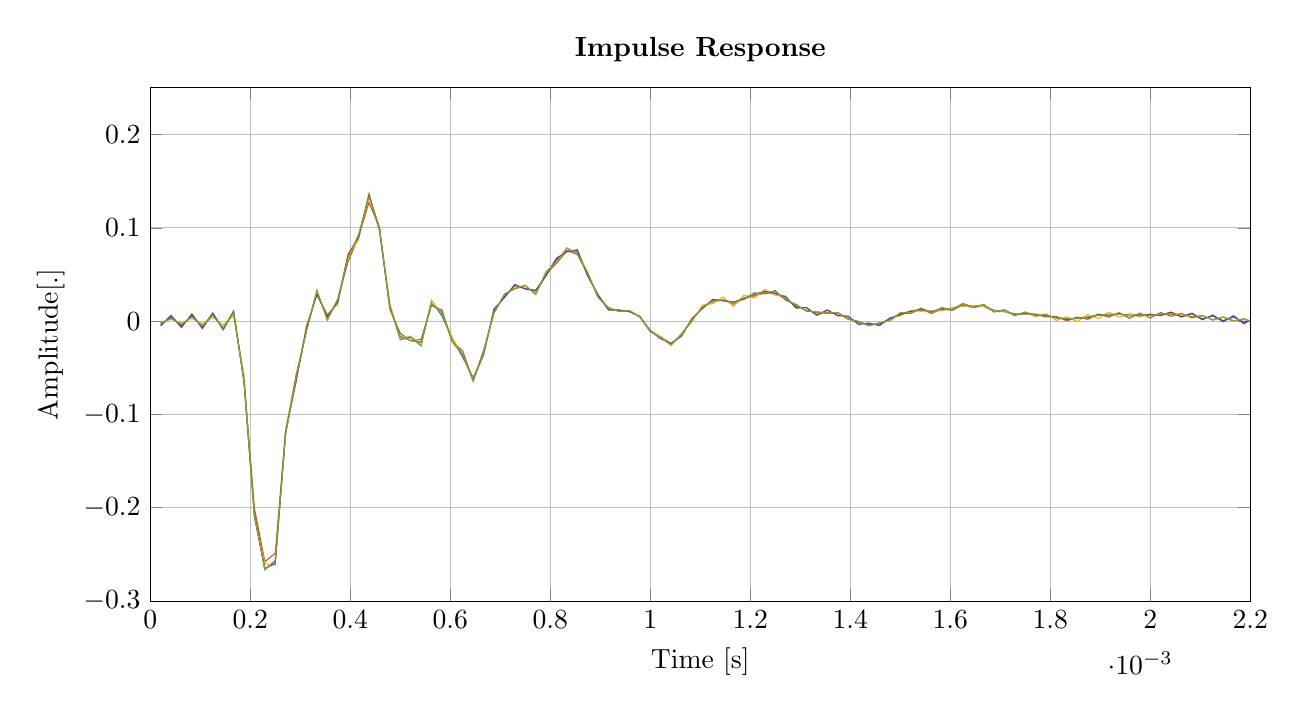
\begin{tikzpicture}

\begin{axis}[%
width=5.5in,
height=2.566in,
at={(0.758in,0.481in)},
scale only axis,
xmin=0,
xmax=0.0022,
xlabel={Time [s]},
xmajorgrids,
ymin=-0.30,
ymax=0.25,
ylabel={Amplitude[.]},
ymajorgrids,
axis background/.style={fill=white},
title style={font=\bfseries},
title={Impulse Response}
]
\addplot [color=mycolor1,solid,forget plot]
  table[row sep=crcr]{%
2.08333333333333e-05	-0.0037087927908794\\
4.16666666666667e-05	0.00421160453226942\\
6.25e-05	-0.00520379576953817\\
8.33333333333333e-05	0.00629701654848276\\
0.000104166666666667	-0.00678651279752952\\
0.000125	0.00811356819824401\\
0.000145833333333333	-0.00884124098433367\\
0.000166666666666667	0.0107472615560426\\
0.0001875	-0.0646663577808535\\
0.000208333333333333	-0.206299821990036\\
0.000229166666666667	-0.266170671528939\\
0.00025	-0.256370669612707\\
0.000270833333333333	-0.120287541326005\\
0.000291666666666667	-0.0617180208660174\\
0.0003125	-0.00922362905565283\\
0.000333333333333333	0.0308397018576189\\
0.000354166666666667	0.0035403786890247\\
0.000375	0.0212448332280645\\
0.000395833333333333	0.0705478621795121\\
0.000416666666666667	0.0895474948933934\\
0.0004375	0.13552149422923\\
0.000458333333333333	0.097299803954558\\
0.000479166666666667	0.0171466790731723\\
0.0005	-0.0197680684506663\\
0.000520833333333333	-0.0171223102171715\\
0.000541666666666667	-0.0263656309604829\\
0.0005625	0.0219768694253305\\
0.000583333333333333	0.00560475366613178\\
0.000604166666666667	-0.0182339778631218\\
0.000625	-0.0387957025837346\\
0.000645833333333333	-0.0604621915450745\\
0.000666666666666667	-0.0363795655357155\\
0.0006875	0.0130977677372803\\
0.000708333333333333	0.0251346467322033\\
0.000729166666666667	0.039105419651278\\
0.00075	0.0346523806957789\\
0.000770833333333333	0.0322481248629661\\
0.000791666666666667	0.0493725854189164\\
0.0008125	0.0660612053755624\\
0.000833333333333333	0.0751202061643853\\
0.000854166666666667	0.0750428627194294\\
0.000875	0.048916982972921\\
0.000895833333333333	0.0274042750529549\\
0.000916666666666667	0.012118310680073\\
0.0009375	0.0119101424242984\\
0.000958333333333333	0.0100853086322103\\
0.000979166666666667	0.00544456035302204\\
0.001	-0.0112918644454638\\
0.00102083333333333	-0.0172483398553776\\
0.00104166666666667	-0.0251189065330511\\
0.0010625	-0.014558012452602\\
0.00108333333333333	0.0017134948101292\\
0.00110416666666667	0.014255079903006\\
0.001125	0.0227537754361355\\
0.00114583333333333	0.021816701937651\\
0.00116666666666667	0.0206421122092443\\
0.0011875	0.0233880957023547\\
0.00120833333333333	0.0302390075091007\\
0.00122916666666667	0.0293537948171238\\
0.00125	0.0326242279536413\\
0.00127083333333333	0.0225148202302848\\
0.00129166666666667	0.0177894930311056\\
0.0013125	0.010770331824266\\
0.00133333333333333	0.00983620954713187\\
0.00135416666666667	0.00853521175516866\\
0.001375	0.00899597167105174\\
0.00139583333333333	0.00260243594654619\\
0.00141666666666667	-0.00104701561770118\\
0.0014375	-0.00371807000382697\\
0.00145833333333333	-0.00318960626194621\\
0.00147916666666667	0.00257545774845068\\
0.0015	0.00713790465040768\\
0.00152083333333333	0.0108215910141207\\
0.00154166666666667	0.0120264444758566\\
0.0015625	0.0108261870538285\\
0.00158333333333333	0.0123450686244096\\
0.00160416666666667	0.0139129670171921\\
0.001625	0.0169005010166529\\
0.00164583333333333	0.0165791257894914\\
0.00166666666666667	0.0159045477126551\\
0.0016875	0.0116907728854056\\
0.00170833333333333	0.0102974368732395\\
0.00172916666666667	0.00768755665771632\\
0.00175	0.0082004670345183\\
0.00177083333333333	0.00731505527542035\\
0.00179166666666667	0.0054086354181059\\
0.0018125	0.00446490364319473\\
0.00183333333333333	0.00151912598295708\\
0.00185416666666667	0.00374848548552877\\
0.001875	0.00361835820665017\\
0.00189583333333333	0.00680282624355538\\
0.00191666666666667	0.00648760855183481\\
0.0019375	0.00770072765347351\\
0.00195833333333333	0.00591670768911894\\
0.00197916666666667	0.00654249543276334\\
0.002	0.00696958712555653\\
0.00202083333333333	0.00639676696262537\\
0.00204166666666667	0.00930875870313683\\
0.0020625	0.00487368778960512\\
0.00208333333333333	0.00793267565500179\\
0.00210416666666667	0.00227381220914028\\
0.002125	0.00559059790855196\\
0.00214583333333333	0.000509710927088874\\
0.00216666666666667	0.00445914830547992\\
0.0021875	-0.0013119827312339\\
0.00220833333333333	0.00204620626659837\\
0.00222916666666667	-0.00226693806170011\\
0.00225	-0.000865052032163367\\
0.00227083333333333	-0.000568466635637404\\
0.00229166666666667	-0.00176072172101629\\
0.0023125	0.001051321525168\\
0.00233333333333333	-0.00235307840318451\\
0.00235416666666667	0.00142050267868398\\
0.002375	-0.00373732644882233\\
0.00239583333333333	0.00263329200115178\\
0.00241666666666667	-0.00419384885137344\\
0.0024375	0.00356243119561722\\
0.00245833333333333	-0.00341750395084726\\
0.00247916666666667	0.00231533516568704\\
0.0025	-0.002886346397735\\
0.00252083333333333	0.000637791268280785\\
0.00254166666666667	-0.00290884766679218\\
0.0025625	-0.000629280559252555\\
0.00258333333333333	-0.00286116806569122\\
0.00260416666666667	-0.00278592644964782\\
0.002625	-0.00262193859169995\\
0.00264583333333333	-0.00474810164470427\\
0.00266666666666667	-0.00275009938116807\\
0.0026875	-0.00478816826817122\\
0.00270833333333333	-0.00324811681170597\\
0.00272916666666667	-0.0040257377623872\\
0.00275	-0.00368074892796126\\
0.00277083333333333	-0.00337062684290595\\
0.00279166666666667	-0.00370307569447635\\
0.0028125	-0.00186571326957182\\
0.00283333333333333	-0.00390602380821677\\
0.00285416666666667	-4.9752550230383e-05\\
0.002875	-0.00438323194808954\\
0.00289583333333333	0.000384386269952189\\
0.00291666666666667	-0.00453307061294354\\
0.0029375	-0.000328341601327697\\
0.00295833333333333	-0.00426336185525099\\
0.00297916666666667	-0.00128138687597425\\
0.003	-0.00414308057749922\\
0.00302083333333333	-0.00248651642821263\\
0.00304166666666667	-0.00361961427656752\\
0.0030625	-0.00400763468176544\\
0.00308333333333333	-0.0023795304299123\\
0.00310416666666667	-0.00514325156697817\\
0.003125	-0.00122625577194359\\
0.00314583333333333	-0.00545188790289689\\
0.00316666666666667	-0.000609928041986866\\
0.0031875	-0.00505013848995181\\
0.00320833333333333	5.99816839252916e-05\\
0.00322916666666667	-0.00449193406111753\\
0.00325	0.000558016389499313\\
0.00327083333333333	-0.00386841737730755\\
0.00329166666666667	0.000169965391614449\\
0.0033125	-0.00319883141842068\\
0.00333333333333333	-0.000671676767081501\\
0.00335416666666667	-0.00289606776507812\\
0.003375	-0.00113994195612087\\
0.00339583333333333	-0.00325262465554565\\
0.00341666666666667	-0.00136179764715377\\
0.0034375	-0.00360873416552366\\
0.00345833333333333	-0.00164463882761736\\
0.00347916666666667	-0.00371793269729748\\
0.0035	-0.00154353439141849\\
0.00352083333333333	-0.00403549855695194\\
0.00354166666666667	-0.000984353596708564\\
0.0035625	-0.00425443771279568\\
0.00358333333333333	-0.000672628985252431\\
0.00360416666666667	-0.00374129885739169\\
0.003625	-0.000937340861272143\\
0.00364583333333333	-0.00296533591369333\\
0.00366666666666667	-0.00130448571666488\\
0.0036875	-0.00246387735925147\\
0.00370833333333333	-0.00182327238315157\\
0.00372916666666667	-0.00173617907905828\\
0.00375	-0.00284258077794951\\
0.00377083333333333	-0.000756536202756666\\
0.00379166666666667	-0.00385114062696801\\
0.0038125	-0.000291952662999003\\
0.00383333333333333	-0.00423039940178691\\
0.00385416666666667	-0.000378549414924021\\
0.003875	-0.00428312305197425\\
0.00389583333333333	-0.000406743035733924\\
0.00391666666666667	-0.00424392197549792\\
0.0039375	-0.000625284040186809\\
0.00395833333333333	-0.00365167293604246\\
0.00397916666666667	-0.001337671135446\\
0.004	-0.00271896198950253\\
0.00402083333333333	-0.0019858020567554\\
0.00404166666666667	-0.00219062801883803\\
0.0040625	-0.00220835913204532\\
0.00408333333333333	-0.00203974929682549\\
0.00410416666666667	-0.00233913427988745\\
0.004125	-0.00185099449592134\\
0.00414583333333333	-0.00236574968059208\\
0.00416666666666667	-0.00196457798952639\\
0.0041875	-0.0019046742644009\\
0.00420833333333333	-0.00250443960036927\\
0.00422916666666667	-0.00128461530764495\\
0.00425	-0.00297296735967611\\
0.00427083333333333	-0.000992836466506577\\
0.00429166666666667	-0.00314961192994209\\
0.0043125	-0.000907894618487529\\
0.00433333333333333	-0.00328775019087989\\
0.00435416666666667	-0.000812410858858454\\
0.004375	-0.00329843852206017\\
0.00439583333333333	-0.000993520893343976\\
0.00441666666666667	-0.00296787895096846\\
0.0044375	-0.00135986816935005\\
0.00445833333333333	-0.00257683158276436\\
0.00447916666666667	-0.00150120312434058\\
0.0045	-0.00246875060820952\\
0.00452083333333333	-0.00127751762473565\\
0.00454166666666667	-0.00257055972440008\\
0.0045625	-0.000850583087086702\\
0.00458333333333333	-0.00279615291783079\\
0.00460416666666667	-0.000169229703961833\\
0.004625	-0.0033208199374696\\
0.00464583333333333	0.000762775063455069\\
0.00466666666666667	-0.00404729208587363\\
0.0046875	0.00162126259324774\\
0.00470833333333333	-0.00461429328418873\\
0.00472916666666667	0.00206634843487202\\
0.00475	-0.00479804415433337\\
0.00477083333333333	0.00203716599298341\\
0.00479166666666667	-0.00461953370883597\\
0.0048125	0.00158614710765907\\
0.00483333333333333	-0.0039600168009732\\
0.00485416666666667	0.00066992915889739\\
0.004875	-0.0027700643584047\\
0.00489583333333333	-0.000614917555245659\\
0.00491666666666667	-0.00132297677247495\\
0.0049375	-0.00190838752526078\\
0.00495833333333333	-4.06116797333875e-05\\
0.00497916666666667	-0.00288565901097666\\
0.005	0.000889847654868419\\
0.00502083333333333	-0.00349274225205263\\
0.00504166666666667	0.00137995835933047\\
0.0050625	-0.00358103532986242\\
0.00508333333333333	0.00125952593606002\\
0.00510416666666667	-0.00298112408616989\\
0.005125	0.00052817856633219\\
0.00514583333333333	-0.0019103540353447\\
0.00516666666666667	-0.000471366982676235\\
0.0051875	-0.000794234842926538\\
0.00520833333333333	-0.00141585678773726\\
};
\addplot [color=mycolor2,solid,forget plot]
  table[row sep=crcr]{%
2.08333333333333e-05	-0.00255267252938673\\
4.16666666666667e-05	0.00289958707347902\\
6.25e-05	-0.00382265239043665\\
8.33333333333333e-05	0.00482200108963299\\
0.000104166666666667	-0.00515633007307537\\
0.000125	0.00667606380308441\\
0.000145833333333333	-0.00708343055179381\\
0.000166666666666667	0.0092525375696961\\
0.0001875	-0.0607390597290135\\
0.000208333333333333	-0.200401659875795\\
0.000229166666666667	-0.257768300997275\\
0.00025	-0.248800582164502\\
0.000270833333333333	-0.117646720461853\\
0.000291666666666667	-0.0578844981508881\\
0.0003125	-0.0102016454149929\\
0.000333333333333333	0.0330014197433572\\
0.000354166666666667	0.00127667958148536\\
0.000375	0.0234190373569384\\
0.000395833333333333	0.0639275956854277\\
0.000416666666666667	0.0906470163865055\\
0.0004375	0.127123824348622\\
0.000458333333333333	0.100636329904299\\
0.000479166666666667	0.0124905457764127\\
0.0005	-0.0128509224250364\\
0.000520833333333333	-0.0212238017533485\\
0.000541666666666667	-0.0195717514784339\\
0.0005625	0.0166431551373302\\
0.000583333333333333	0.0120320299572739\\
0.000604166666666667	-0.0219158802601074\\
0.000625	-0.0320151869444835\\
0.000645833333333333	-0.0633380264022395\\
0.000666666666666667	-0.0314055759804432\\
0.0006875	0.0084423319629683\\
0.000708333333333333	0.0282626599947745\\
0.000729166666666667	0.034755671823636\\
0.00075	0.0375030938504313\\
0.000770833333333333	0.0287324780339133\\
0.000791666666666667	0.0509433983273104\\
0.0008125	0.0618381605219164\\
0.000833333333333333	0.0756881939220368\\
0.000854166666666667	0.0714587648185071\\
0.000875	0.0505304570640701\\
0.000895833333333333	0.0255469926503848\\
0.000916666666666667	0.0139977515791326\\
0.0009375	0.0105701348927955\\
0.000958333333333333	0.0111681123111772\\
0.000979166666666667	0.00467517577342191\\
0.001	-0.0100498056673259\\
0.00102083333333333	-0.0168471351248233\\
0.00104166666666667	-0.0242983429721961\\
0.0010625	-0.0138911007564663\\
0.00108333333333333	0.000815862706313863\\
0.00110416666666667	0.0148029936594\\
0.001125	0.0207210667345826\\
0.00114583333333333	0.0226963031788706\\
0.00116666666666667	0.0181062087629371\\
0.0011875	0.0242935347792987\\
0.00120833333333333	0.0271226044174566\\
0.00122916666666667	0.0301879108304438\\
0.00125	0.0297329814304771\\
0.00127083333333333	0.0236557223579554\\
0.00129166666666667	0.0158766440133432\\
0.0013125	0.011696116145808\\
0.00133333333333333	0.00871715898126307\\
0.00135416666666667	0.00871221990090018\\
0.001375	0.00864655184050639\\
0.00139583333333333	0.00219401302147165\\
0.00141666666666667	-0.000480463220486303\\
0.0014375	-0.00478793011354472\\
0.00145833333333333	-0.00214213807521797\\
0.00147916666666667	0.000610919065108282\\
0.0015	0.00822355226328271\\
0.00152083333333333	0.00831464525440903\\
0.00154166666666667	0.0130253685510728\\
0.0015625	0.00825458577231076\\
0.00158333333333333	0.0131017386199352\\
0.00160416666666667	0.0115045453955671\\
0.001625	0.0173054531317267\\
0.00164583333333333	0.0146751752014143\\
0.00166666666666667	0.0160624194214595\\
0.0016875	0.0105018463460038\\
0.00170833333333333	0.0101683646808241\\
0.00172916666666667	0.0070445186245326\\
0.00175	0.00766088993981086\\
0.00177083333333333	0.00710536523175556\\
0.00179166666666667	0.00457630122370742\\
0.0018125	0.00469420240794347\\
0.00183333333333333	0.000404005788937426\\
0.00185416666666667	0.00428370428539064\\
0.001875	0.00197599863403158\\
0.00189583333333333	0.0076578440345062\\
0.00191666666666667	0.00423011592859115\\
0.0019375	0.00909761104080475\\
0.00195833333333333	0.0030678897125246\\
0.00197916666666667	0.00859528939877386\\
0.002	0.00346894854210457\\
0.00202083333333333	0.00914620649963214\\
0.00204166666666667	0.00520410877557944\\
0.0020625	0.00832413302525314\\
0.00208333333333333	0.00346908753461933\\
0.00210416666666667	0.00610387771170956\\
0.002125	0.00108867775682093\\
0.00214583333333333	0.00419930592939649\\
0.00216666666666667	0.000319892049500485\\
0.0021875	0.00180869387049779\\
0.00220833333333333	-0.00126219037085954\\
0.00222916666666667	-0.00016649986826338\\
0.00225	-0.00292140933910888\\
0.00227083333333333	5.48115721681712e-05\\
0.00229166666666667	-0.00231838798243882\\
0.0023125	6.02159680772856e-05\\
0.00233333333333333	-0.00141553936136535\\
0.00235416666666667	-0.000969725177756748\\
0.002375	-0.00155367505348034\\
0.00239583333333333	-0.00078737578525\\
0.00241666666666667	-0.00118813913866019\\
0.0024375	-0.000351639141263614\\
0.00245833333333333	-0.000202294846823073\\
0.00247916666666667	-0.00140433733178488\\
0.0025	-0.000148481375508499\\
0.00252083333333333	-0.00229105227885144\\
0.00254166666666667	-0.00113327041550525\\
0.0025625	-0.00240289119356657\\
0.00258333333333333	-0.00221020389739753\\
0.00260416666666667	-0.00327807804462282\\
0.002625	-0.00307515395717207\\
0.00264583333333333	-0.00411499501980943\\
0.00266666666666667	-0.00404707161300406\\
0.0026875	-0.00348238100217361\\
0.00270833333333333	-0.00488806311665677\\
0.00272916666666667	-0.0026354048015551\\
0.00275	-0.00512258678524018\\
0.00277083333333333	-0.00237918958058366\\
0.00279166666666667	-0.00456717537979813\\
0.0028125	-0.00158216040976036\\
0.00283333333333333	-0.00398847584896324\\
0.00285416666666667	-0.000601313268332522\\
0.002875	-0.00369552546612422\\
0.00289583333333333	-0.000887430420175447\\
0.00291666666666667	-0.0033287586160303\\
0.0029375	-0.00196666642325469\\
0.00295833333333333	-0.00291972100094473\\
0.00297916666666667	-0.00286833083131398\\
0.003	-0.00297599955911991\\
0.00302083333333333	-0.00372065054441346\\
0.00304166666666667	-0.00284107705068402\\
0.0030625	-0.00474018439203851\\
0.00308333333333333	-0.00207488352087834\\
0.00310416666666667	-0.00536932379647781\\
0.003125	-0.00131533563026484\\
0.00314583333333333	-0.00536072637441323\\
0.00316666666666667	-0.000858022679083761\\
0.0031875	-0.00494352194507911\\
0.00320833333333333	-9.29124655160845e-05\\
0.00322916666666667	-0.00458455294834229\\
0.00325	0.000653130100906661\\
0.00327083333333333	-0.00423158530604592\\
0.00329166666666667	0.000543960512810295\\
0.0033125	-0.00379406688018271\\
0.00333333333333333	-9.66816216515342e-05\\
0.00335416666666667	-0.00353027419822252\\
0.003375	-0.000570547946950482\\
0.00339583333333333	-0.00361077269310737\\
0.00341666666666667	-0.00110650316314777\\
0.0034375	-0.00343504924741948\\
0.00345833333333333	-0.00193518158467088\\
0.00347916666666667	-0.00291655885566418\\
0.0035	-0.00243334545259287\\
0.00352083333333333	-0.00262502115222047\\
0.00354166666666667	-0.00240295393708929\\
0.0035625	-0.00239818677743936\\
0.00358333333333333	-0.00241583275384139\\
0.00360416666666667	-0.00177271872007091\\
0.003625	-0.00263795048328915\\
0.00364583333333333	-0.00127580236053149\\
0.00366666666666667	-0.00260032147781131\\
0.0036875	-0.00135047828264343\\
0.00370833333333333	-0.00248490641271397\\
0.00372916666666667	-0.00135362852201022\\
0.00375	-0.00276058505758708\\
0.00377083333333333	-0.00111545031714157\\
0.00379166666666667	-0.00304804673300568\\
0.0038125	-0.00121762006398216\\
0.00383333333333333	-0.00295967887667023\\
0.00385416666666667	-0.00152799538999958\\
0.003875	-0.00293911795913497\\
0.00389583333333333	-0.00141842129814424\\
0.00391666666666667	-0.00317139837627678\\
0.0039375	-0.00120453703812563\\
0.00395833333333333	-0.00310189945322664\\
0.00397916666666667	-0.00127577630415201\\
0.004	-0.00285323822275981\\
0.00402083333333333	-0.00123759058802548\\
0.00404166666666667	-0.00295826755744021\\
0.0040625	-0.000941733037558027\\
0.00408333333333333	-0.00317740848079844\\
0.00410416666666667	-0.000853233064771672\\
0.004125	-0.003025048708344\\
0.00414583333333333	-0.000993006404728137\\
0.00416666666666667	-0.00285059650886691\\
0.0041875	-0.000974726981488831\\
0.00420833333333333	-0.00278577246306679\\
0.00422916666666667	-0.00106359834458666\\
0.00425	-0.00243185185834133\\
0.00427083333333333	-0.00161288283600495\\
0.00429166666666667	-0.00173941306975917\\
0.0043125	-0.0023614205758312\\
0.00433333333333333	-0.00107298483413706\\
0.00435416666666667	-0.00303899121775412\\
0.004375	-0.000375970115777865\\
0.00439583333333333	-0.00388549063063888\\
0.00441666666666667	0.000541297745222786\\
0.0044375	-0.00479932669104759\\
0.00445833333333333	0.00139622726997478\\
0.00447916666666667	-0.00539810064640756\\
0.0045	0.00192488295368076\\
0.00452083333333333	-0.00560504111770523\\
0.00454166666666667	0.00224701915074393\\
0.0045625	-0.00560943314661647\\
0.00458333333333333	0.0024195452607323\\
0.00460416666666667	-0.005317466524108\\
0.004625	0.00222418518526779\\
0.00464583333333333	-0.00466166053919306\\
0.00466666666666667	0.00169427281028947\\
0.0046875	-0.00386977891617415\\
0.00470833333333333	0.00106542399644791\\
0.00472916666666667	-0.00315415940463025\\
0.00475	0.000425270653698219\\
0.00477083333333333	-0.00245902414772154\\
0.00479166666666667	-0.000313192663862794\\
0.0048125	-0.00172664645538972\\
0.00483333333333333	-0.00101569750310594\\
0.00485416666666667	-0.0010706020758985\\
0.004875	-0.00152478876973867\\
0.00489583333333333	-0.00053804913087041\\
0.00491666666666667	-0.00192301123282111\\
0.0049375	-8.46962331649506e-06\\
0.00495833333333333	-0.00234650155333196\\
0.00497916666666667	0.000517616027113713\\
0.005	-0.0026874982365122\\
0.00502083333333333	0.000837710179045122\\
0.00504166666666667	-0.00281392506940281\\
0.0050625	0.000951526220070128\\
0.00508333333333333	-0.00279809276114962\\
0.00510416666666667	0.000989617566664778\\
0.005125	-0.00267417639347939\\
0.00514583333333333	0.00086092609975851\\
0.00516666666666667	-0.00228430448627185\\
0.0051875	0.000452408493989887\\
0.00520833333333333	-0.00164854160289399\\
};
\addplot [color=mycolor3,solid,forget plot]
  table[row sep=crcr]{%
2.08333333333333e-05	-0.00163321204155689\\
4.16666666666667e-05	0.00217871738448115\\
6.25e-05	-0.00223030869416506\\
8.33333333333333e-05	0.00308085388067272\\
0.000104166666666667	-0.00283418955947869\\
0.000125	0.00387776978723627\\
0.000145833333333333	-0.00396721517720515\\
0.000166666666666667	0.00565169339153807\\
0.0001875	-0.0578645073772853\\
0.000208333333333333	-0.210568816309939\\
0.000229166666666667	-0.259955188133081\\
0.00025	-0.261242392983444\\
0.000270833333333333	-0.11541144340208\\
0.000291666666666667	-0.065082383983406\\
0.0003125	-0.00457165776378929\\
0.000333333333333333	0.0281698447908548\\
0.000354166666666667	0.00746906122663251\\
0.000375	0.017980551653853\\
0.000395833333333333	0.0719876105253128\\
0.000416666666666667	0.0872051031610365\\
0.0004375	0.136972018527987\\
0.000458333333333333	0.0979061885001598\\
0.000479166666666667	0.0190373994273952\\
0.0005	-0.0187474979071836\\
0.000520833333333333	-0.0159911997270242\\
0.000541666666666667	-0.0254207659568788\\
0.0005625	0.0222939439236886\\
0.000583333333333333	0.00762495201878726\\
0.000604166666666667	-0.0181476959053041\\
0.000625	-0.0370572954894979\\
0.000645833333333333	-0.0616897321841816\\
0.000666666666666667	-0.0357751469485512\\
0.0006875	0.0110541110800959\\
0.000708333333333333	0.0266261311666174\\
0.000729166666666667	0.0370835756321231\\
0.00075	0.0372079006439419\\
0.000770833333333333	0.0299720795056686\\
0.000791666666666667	0.0519383256345237\\
0.0008125	0.0633401602353719\\
0.000833333333333333	0.0780465129838801\\
0.000854166666666667	0.072826296030486\\
0.000875	0.0525118906030222\\
0.000895833333333333	0.025547455882416\\
0.000916666666666667	0.0148804806448951\\
0.0009375	0.0103846646000134\\
0.000958333333333333	0.0115394204404138\\
0.000979166666666667	0.00482301562556526\\
0.001	-0.0109874131473168\\
0.00102083333333333	-0.0166641078639183\\
0.00104166666666667	-0.0264021861315982\\
0.0010625	-0.0129423122730922\\
0.00108333333333333	-0.00127731842486949\\
0.00110416666666667	0.0172078145589618\\
0.001125	0.0186646164744698\\
0.00114583333333333	0.0258355733901017\\
0.00116666666666667	0.0157117601980314\\
0.0011875	0.0277803562128635\\
0.00120833333333333	0.0249411956451881\\
0.00122916666666667	0.0339131100205985\\
0.00125	0.0276834810161797\\
0.00127083333333333	0.0270876373860748\\
0.00129166666666667	0.0135486398598428\\
0.0013125	0.0146281493199383\\
0.00133333333333333	0.00630120909161602\\
0.00135416666666667	0.0114262979203145\\
0.001375	0.00625151023360393\\
0.00139583333333333	0.00469691746271263\\
0.00141666666666667	-0.00320755138194242\\
0.0014375	-0.0023665451221515\\
0.00145833333333333	-0.00501549633026936\\
0.00147916666666667	0.00337042559894113\\
0.0015	0.00557224153648716\\
0.00152083333333333	0.0113999793119524\\
0.00154166666666667	0.0105608590694505\\
0.0015625	0.0112253538955211\\
0.00158333333333333	0.0109297147864292\\
0.00160416666666667	0.0141182406444556\\
0.001625	0.0158705693922061\\
0.00164583333333333	0.0165236340426216\\
0.00166666666666667	0.0155539386955293\\
0.0016875	0.0110146959222936\\
0.00170833333333333	0.0107587084546628\\
0.00172916666666667	0.006021107065009\\
0.00175	0.00962358548745266\\
0.00177083333333333	0.00461488367395265\\
0.00179166666666667	0.00786354161870322\\
0.0018125	0.00083980837975928\\
0.00183333333333333	0.00474934129641216\\
0.00185416666666667	-0.000493640480630181\\
0.001875	0.00712827695489169\\
0.00189583333333333	0.00258517202966767\\
0.00191666666666667	0.00965080478835073\\
0.0019375	0.00421535128796295\\
0.00195833333333333	0.00807287058220521\\
0.00197916666666667	0.00433552437525072\\
0.002	0.00762144067704767\\
0.00202083333333333	0.00590796681015577\\
0.00204166666666667	0.00823247822607332\\
0.0020625	0.00624889897116549\\
0.00208333333333333	0.0051706692669312\\
0.00210416666666667	0.00513911501618462\\
0.002125	0.00157578666104142\\
0.00214583333333333	0.00419562172707041\\
0.00216666666666667	-8.17894503905048e-05\\
0.0021875	0.00249146863565593\\
0.00220833333333333	-0.00225060743894737\\
0.00222916666666667	0.000911367832004493\\
0.00225	-0.0042023273732927\\
0.00227083333333333	0.00131908623295955\\
0.00229166666666667	-0.00359422398769843\\
0.0023125	0.00130602372428194\\
0.00233333333333333	-0.0025474285480275\\
0.00235416666666667	9.12508870677423e-05\\
0.002375	-0.00251258605257109\\
0.00239583333333333	3.68184456323214e-05\\
0.00241666666666667	-0.001908222379877\\
0.0024375	0.000171602768831179\\
0.00245833333333333	-0.000565657920822165\\
0.00247916666666667	-0.00132123186706604\\
0.0025	-3.69357225569728e-05\\
0.00252083333333333	-0.00278555913442368\\
0.00254166666666667	-0.000381161411822799\\
0.0025625	-0.00363098794507625\\
0.00258333333333333	-0.000623408767812987\\
0.00260416666666667	-0.00542533906568231\\
0.002625	-0.000514434727790267\\
0.00264583333333333	-0.00727794417210567\\
0.00266666666666667	-0.000521849778767368\\
0.0026875	-0.00757661607436271\\
0.00270833333333333	-0.000543882871711502\\
0.00272916666666667	-0.00744648183443503\\
0.00275	-0.000262008073977348\\
0.00277083333333333	-0.00754898213636908\\
0.00279166666666667	0.000392125328535457\\
0.0028125	-0.00659584850012438\\
0.00283333333333333	0.000562148987953842\\
0.00285416666666667	-0.00491349124801912\\
0.002875	-4.71952709105437e-05\\
0.00289583333333333	-0.00403617308167389\\
0.00291666666666667	-0.00098491246115772\\
0.0029375	-0.00360617852387868\\
0.00295833333333333	-0.00216020792434374\\
0.00297916666666667	-0.00281031658588728\\
0.003	-0.00393642768912363\\
0.00302083333333333	-0.0019740161735394\\
0.00304166666666667	-0.00545044644123764\\
0.0030625	-0.00148724838410483\\
0.00308333333333333	-0.00609761795227659\\
0.00310416666666667	-0.000911843004845307\\
0.003125	-0.00641109553135691\\
0.00314583333333333	-6.68399286926769e-05\\
0.00316666666666667	-0.00661223381392086\\
0.0031875	0.000792942062802807\\
0.00320833333333333	-0.00605194886502256\\
0.00322916666666667	0.00119081641544235\\
0.00325	-0.00510662306890529\\
0.00327083333333333	0.0012153985699642\\
0.00329166666666667	-0.00468000094954699\\
0.0033125	0.00101706104418737\\
0.00333333333333333	-0.0044992583008872\\
0.00335416666666667	0.000373907361929023\\
0.003375	-0.00393423263359508\\
0.00339583333333333	-0.000849674035833999\\
0.00341666666666667	-0.00327675308048005\\
0.0034375	-0.00196202325455657\\
0.00345833333333333	-0.00281649981315708\\
0.00347916666666667	-0.00279172529312823\\
0.0035	-0.00199265111718659\\
0.00352083333333333	-0.00384408715258885\\
0.00354166666666667	-0.000687528632112489\\
0.0035625	-0.0048382405767023\\
0.00358333333333333	0.000411062545070974\\
0.00360416666666667	-0.00517279640746107\\
0.003625	0.00102806244718597\\
0.00364583333333333	-0.00530219593314191\\
0.00366666666666667	0.00153508609358886\\
0.0036875	-0.00561251207357299\\
0.00370833333333333	0.00167486091733119\\
0.00372916666666667	-0.00539493643036716\\
0.00375	0.00095668559377168\\
0.00377083333333333	-0.00449327302460345\\
0.00379166666666667	-0.000202453154405987\\
0.0038125	-0.00358211842714922\\
0.00383333333333333	-0.00130167335324517\\
0.00385416666666667	-0.0026300982831725\\
0.003875	-0.00263555824036522\\
0.00389583333333333	-0.00114138056803914\\
0.00391666666666667	-0.00421914845301114\\
0.0039375	0.000366426789574729\\
0.00395833333333333	-0.00531590855132645\\
0.00397916666666667	0.00132682521510946\\
0.004	-0.00589441023054478\\
0.00402083333333333	0.0020330284975877\\
0.00404166666666667	-0.00643081079363684\\
0.0040625	0.00258116813465071\\
0.00408333333333333	-0.00669153743716035\\
0.00410416666666667	0.00252712937339086\\
0.004125	-0.00626501890081867\\
0.00414583333333333	0.00198573399042622\\
0.00416666666666667	-0.00564706489609503\\
0.0041875	0.00152112304451762\\
0.00420833333333333	-0.00515083718413495\\
0.00422916666666667	0.00102298995925469\\
0.00425	-0.00449765039675646\\
0.00427083333333333	0.000268338619425756\\
0.00429166666666667	-0.00371379195250488\\
0.0043125	-0.000425640222728158\\
0.00433333333333333	-0.00319524784033904\\
0.00435416666666667	-0.000821975064880745\\
0.004375	-0.00282770222093157\\
0.00439583333333333	-0.00126508575246811\\
0.00441666666666667	-0.00230471738176367\\
0.0044375	-0.00177566551043765\\
0.00445833333333333	-0.00179693413328159\\
0.00447916666666667	-0.00209730578453145\\
0.0045	-0.00146755955861572\\
0.00452083333333333	-0.00224017373487703\\
0.00454166666666667	-0.00112128092359989\\
0.0045625	-0.00241988879033352\\
0.00458333333333333	-0.000677054033918395\\
0.00460416666666667	-0.00251242284809268\\
0.004625	-0.000408875554688982\\
0.00464583333333333	-0.00238920768851963\\
0.00466666666666667	-0.00035233334164938\\
0.0046875	-0.0021916507379531\\
0.00470833333333333	-0.000353204672140455\\
0.00472916666666667	-0.00206426554660433\\
0.00475	-0.000399111146290863\\
0.00477083333333333	-0.00190898307931796\\
0.00479166666666667	-0.000620985892132324\\
0.0048125	-0.00165238099799337\\
0.00483333333333333	-0.000881278130450417\\
0.00485416666666667	-0.00142045191052985\\
0.004875	-0.00100160951886526\\
0.00489583333333333	-0.00128622165651065\\
0.00491666666666667	-0.00103775843243032\\
0.0049375	-0.00112884862974338\\
0.00495833333333333	-0.00112433334285194\\
0.00497916666666667	-0.000926118130786855\\
0.005	-0.00116589196730782\\
0.00502083333333333	-0.00085433505620867\\
0.00504166666666667	-0.00107320946693262\\
0.0050625	-0.000875743054272184\\
0.00508333333333333	-0.000966483466824754\\
0.00510416666666667	-0.000820897375894202\\
0.005125	-0.000917689548129309\\
0.00514583333333333	-0.000784404643824917\\
0.00516666666666667	-0.00076358766070243\\
0.0051875	-0.000910640434007906\\
0.00520833333333333	-0.000481400776064074\\
};
\addplot [color=mycolor4,solid,forget plot]
  table[row sep=crcr]{%
2.08333333333333e-05	-0.00516726277486403\\
4.16666666666667e-05	0.00618610543992257\\
6.25e-05	-0.00674403357522682\\
8.33333333333333e-05	0.00770721377255318\\
0.000104166666666667	-0.0079390099384032\\
0.000125	0.0086020434024014\\
0.000145833333333333	-0.00902843756603243\\
0.000166666666666667	0.0100058461757606\\
0.0001875	-0.0641955735500921\\
0.000208333333333333	-0.208700228894356\\
0.000229166666666667	-0.265220840886755\\
0.00025	-0.259647179573132\\
0.000270833333333333	-0.118446743512368\\
0.000291666666666667	-0.0645851736784997\\
0.0003125	-0.00681068819516621\\
0.000333333333333333	0.0287361417369287\\
0.000354166666666667	0.00528308056129979\\
0.000375	0.0203557265501783\\
0.000395833333333333	0.0712760448789094\\
0.000416666666666667	0.0904990248217112\\
0.0004375	0.135055068926438\\
0.000458333333333333	0.0997502441326314\\
0.000479166666666667	0.0149656960420083\\
0.0005	-0.0165087379404821\\
0.000520833333333333	-0.0206907204364962\\
0.000541666666666667	-0.0225262866903627\\
0.0005625	0.0180825474272777\\
0.000583333333333333	0.00939702452084589\\
0.000604166666666667	-0.0220080878731115\\
0.000625	-0.0359484501101515\\
0.000645833333333333	-0.0635737161406537\\
0.000666666666666667	-0.0345952872075129\\
0.0006875	0.011395100325966\\
0.000708333333333333	0.0259765767874302\\
0.000729166666666667	0.0388948268072226\\
0.00075	0.0345433960194401\\
0.000770833333333333	0.0330594608503968\\
0.000791666666666667	0.0486818198528796\\
0.0008125	0.0674756758742106\\
0.000833333333333333	0.0744150741225028\\
0.000854166666666667	0.0764475561324374\\
0.000875	0.0484555353578298\\
0.000895833333333333	0.0280952139333538\\
0.000916666666666667	0.0120915320156524\\
0.0009375	0.0116550564182299\\
0.000958333333333333	0.0106926921212952\\
0.000979166666666667	0.00437971585193512\\
0.001	-0.0101887902933229\\
0.00102083333333333	-0.0188499921570428\\
0.00104166666666667	-0.0238914746704615\\
0.0010625	-0.0161256173139097\\
0.00108333333333333	0.00275773204942341\\
0.00110416666666667	0.0133609332400136\\
0.001125	0.0231917904276933\\
0.00114583333333333	0.0219589661063437\\
0.00116666666666667	0.0200640545884449\\
0.0011875	0.0247466765973178\\
0.00120833333333333	0.0285547492678105\\
0.00122916666666667	0.0318926492272145\\
0.00125	0.0299764686613089\\
0.00127083333333333	0.0258669723089619\\
0.00129166666666667	0.0144614250473965\\
0.0013125	0.0144118803872106\\
0.00133333333333333	0.00631500520940795\\
0.00135416666666667	0.0119590422551788\\
0.001375	0.00582578414624001\\
0.00139583333333333	0.00531310542364779\\
0.00141666666666667	-0.00343872304963442\\
0.0014375	-0.00204564952450211\\
0.00145833333333333	-0.00450517778079939\\
0.00147916666666667	0.00314623347351362\\
0.0015	0.00701711951470965\\
0.00152083333333333	0.0103864197390258\\
0.00154166666666667	0.0129433271786474\\
0.0015625	0.00958576326911167\\
0.00158333333333333	0.0139841965278157\\
0.00160416666666667	0.0121875227655739\\
0.001625	0.0188998385691284\\
0.00164583333333333	0.0146984545420619\\
0.00166666666666667	0.017899680479795\\
0.0016875	0.00991070284736272\\
0.00170833333333333	0.0120138300378153\\
0.00172916666666667	0.00618896675135314\\
0.00175	0.00950797333791057\\
0.00177083333333333	0.00619846562183273\\
0.00179166666666667	0.00629933583354124\\
0.0018125	0.00372292860313401\\
0.00183333333333333	0.00204703775903457\\
0.00185416666666667	0.00329997560254824\\
0.001875	0.00389942548298164\\
0.00189583333333333	0.00657336211721742\\
0.00191666666666667	0.00665232357684192\\
0.0019375	0.0075909095931576\\
0.00195833333333333	0.00605956480100092\\
0.00197916666666667	0.00643341074030218\\
0.002	0.00717334955571132\\
0.00202083333333333	0.00619094312126556\\
0.00204166666666667	0.00966268883294692\\
0.0020625	0.00447138766764083\\
0.00208333333333333	0.00851776245037382\\
0.00210416666666667	0.00155152096694671\\
0.002125	0.00648868394668762\\
0.00214583333333333	-0.000624254648236403\\
0.00216666666666667	0.00576389327580217\\
0.0021875	-0.00289608729956137\\
0.00220833333333333	0.00381430664759555\\
0.00222916666666667	-0.00430459453439456\\
0.00225	0.00134150752329004\\
0.00227083333333333	-0.00298934954772144\\
0.00229166666666667	0.0007768827629351\\
0.0023125	-0.00158590032820341\\
0.00233333333333333	0.000330823136554005\\
0.00235416666666667	-0.00120844519950964\\
0.002375	-0.00116242832138357\\
0.00239583333333333	0.000270897000981958\\
0.00241666666666667	-0.00201802007393254\\
0.0024375	0.00171605320113375\\
0.00245833333333333	-0.00189929643819731\\
0.00247916666666667	0.00119292465952919\\
0.0025	-0.00219131249110632\\
0.00252083333333333	0.00034848939930505\\
0.00254166666666667	-0.00308860740556768\\
0.0025625	-7.85444650659138e-05\\
0.00258333333333333	-0.00384468350111693\\
0.00260416666666667	-0.001493892750237\\
0.002625	-0.00424672879397181\\
0.00264583333333333	-0.00291918864331946\\
0.00266666666666667	-0.00479474830368327\\
0.0026875	-0.002641114801147\\
0.00270833333333333	-0.00547650846681502\\
0.00272916666666667	-0.00176808208131012\\
0.00275	-0.00592170930056437\\
0.00277083333333333	-0.00117173805459234\\
0.00279166666666667	-0.00584231268464412\\
0.0028125	0.000183416280875907\\
0.00283333333333333	-0.00587588613878243\\
0.00285416666666667	0.0018311578583298\\
0.002875	-0.00616980594985171\\
0.00289583333333333	0.0020919430151921\\
0.00291666666666667	-0.006151463925198\\
0.0029375	0.00119796832713895\\
0.00295833333333333	-0.00570267165304615\\
0.00297916666666667	4.97538939356161e-05\\
0.003	-0.0053605861684554\\
0.00302083333333333	-0.00139144543259947\\
0.00304166666666667	-0.00458129470306718\\
0.0030625	-0.00320046711294441\\
0.00308333333333333	-0.00305431263079126\\
0.00310416666666667	-0.00462620972474146\\
0.003125	-0.00160809005656759\\
0.00314583333333333	-0.00518032903383794\\
0.00316666666666667	-0.000778828524857652\\
0.0031875	-0.00492703718563742\\
0.00320833333333333	-4.10939251716325e-05\\
0.00322916666666667	-0.00433900614737377\\
0.00325	0.000347078062520911\\
0.00327083333333333	-0.00349915815918508\\
0.00329166666666667	-0.000345438155645781\\
0.0033125	-0.00247367565948003\\
0.00333333333333333	-0.0016228163755218\\
0.00335416666666667	-0.00173586071389316\\
0.003375	-0.00251999805022344\\
0.00339583333333333	-0.00171285302918648\\
0.00341666666666667	-0.00302092317198616\\
0.0034375	-0.00191969840041333\\
0.00345833333333333	-0.00329477827695596\\
0.00347916666666667	-0.00222733101286352\\
0.0035	-0.00278909601039485\\
0.00352083333333333	-0.00313282923717919\\
0.00354166666666667	-0.00142955103237562\\
0.0035625	-0.00431138062946915\\
0.00358333333333333	-3.33267261560497e-05\\
0.00360416666666667	-0.0049806079600091\\
0.003625	0.000902408321895213\\
0.00364583333333333	-0.00536893329483935\\
0.00366666666666667	0.00161789846540582\\
0.0036875	-0.00579773498379327\\
0.00370833333333333	0.00182795311672953\\
0.00372916666666667	-0.00557217327052572\\
0.00375	0.00104090968872704\\
0.00377083333333333	-0.0045546501000046\\
0.00379166666666667	-0.000273437893586971\\
0.0038125	-0.00354077521085939\\
0.00383333333333333	-0.00141145409669622\\
0.00385416666666667	-0.00271206804832079\\
0.003875	-0.00247321532142388\\
0.00389583333333333	-0.00169972572390624\\
0.00391666666666667	-0.00343380518886849\\
0.0039375	-0.00103182782045088\\
0.00395833333333333	-0.00356096203020484\\
0.00397916666666667	-0.00124689158572549\\
0.004	-0.00285848083433616\\
0.00402083333333333	-0.00193851180094236\\
0.00404166666666667	-0.00200171008123463\\
0.0040625	-0.00275304267616449\\
0.00408333333333333	-0.00103788142726822\\
0.00410416666666667	-0.00387443903731943\\
0.004125	0.000250332702166949\\
0.00414583333333333	-0.00503566614560924\\
0.00416666666666667	0.00122945847968764\\
0.0041875	-0.00556311097230783\\
0.00420833333333333	0.0014705518678144\\
0.00422916666666667	-0.00551042844031363\\
0.00425	0.00127573534719517\\
0.00427083333333333	-0.00519138019590722\\
0.00429166666666667	0.000791747966865656\\
0.0043125	-0.00450084129703969\\
0.00433333333333333	-0.000179976284996915\\
0.00435416666666667	-0.00337897630774022\\
0.004375	-0.00132428816441232\\
0.00439583333333333	-0.00236086513146179\\
0.00441666666666667	-0.00212590659001618\\
0.0044375	-0.00169406418351993\\
0.00445833333333333	-0.00258120154967261\\
0.00447916666666667	-0.00124714980896368\\
0.0045	-0.0027946124294982\\
0.00452083333333333	-0.0010264231051049\\
0.00454166666666667	-0.00259422704283543\\
0.0045625	-0.00120926212080473\\
0.00458333333333333	-0.00197467115141151\\
0.00460416666666667	-0.00159779592776522\\
0.004625	-0.0013254680185666\\
0.00464583333333333	-0.00189992416851517\\
0.00466666666666667	-0.000856508408770266\\
0.0046875	-0.0020937771176436\\
0.00470833333333333	-0.000554077649769015\\
0.00472916666666667	-0.00222634800577962\\
0.00475	-0.000468283944067134\\
0.00477083333333333	-0.00214263857559105\\
0.00479166666666667	-0.000747724939442115\\
0.0048125	-0.00175014592789651\\
0.00483333333333333	-0.00125089656112911\\
0.00485416666666667	-0.00122524421554398\\
0.004875	-0.00171841491726784\\
0.00489583333333333	-0.000745651416354775\\
0.00491666666666667	-0.00209130880535271\\
0.0049375	-0.000296459854376949\\
0.00495833333333333	-0.00242018361148765\\
0.00497916666666667	9.12195276498172e-05\\
0.005	-0.00257540275405454\\
0.00502083333333333	0.000207506743761061\\
0.00504166666666667	-0.00243009552772572\\
0.0050625	7.70973327593161e-05\\
0.00508333333333333	-0.00213121004529441\\
0.00510416666666667	-7.55027093919094e-05\\
0.005125	-0.00183247624499863\\
0.00514583333333333	-0.000241500753831187\\
0.00516666666666667	-0.00146441363258871\\
0.0051875	-0.00050067414854697\\
0.00520833333333333	-0.0010689724886638\\
};
\addplot [color=mycolor5,solid,forget plot]
  table[row sep=crcr]{%
2.08333333333333e-05	-0.00183694080367487\\
4.16666666666667e-05	0.00269775576535856\\
6.25e-05	-0.00330864487443258\\
8.33333333333333e-05	0.00446922873033606\\
0.000104166666666667	-0.00511216151187469\\
0.000125	0.00628161008825259\\
0.000145833333333333	-0.00739773060073078\\
0.000166666666666667	0.00918365663237817\\
0.0001875	-0.0640643771063412\\
0.000208333333333333	-0.207629084903728\\
0.000229166666666667	-0.266512571802307\\
0.00025	-0.256975404662541\\
0.000270833333333333	-0.121150763678526\\
0.000291666666666667	-0.0611548539632256\\
0.0003125	-0.0104129176519418\\
0.000333333333333333	0.0323067772127556\\
0.000354166666666667	0.00164090751066485\\
0.000375	0.0236255560777956\\
0.000395833333333333	0.06830166976313\\
0.000416666666666667	0.0929087418121704\\
0.0004375	0.13301902945068\\
0.000458333333333333	0.100936103236603\\
0.000479166666666667	0.0140285669386969\\
0.0005	-0.0161700462857896\\
0.000520833333333333	-0.0208468721314891\\
0.000541666666666667	-0.0226220402462128\\
0.0005625	0.0180740728030884\\
0.000583333333333333	0.00931391260236883\\
0.000604166666666667	-0.0223811360937609\\
0.000625	-0.0351734754640771\\
0.000645833333333333	-0.0647259979556037\\
0.000666666666666667	-0.0325867644033155\\
0.0006875	0.00898058450624136\\
0.000708333333333333	0.0291265867299432\\
0.000729166666666667	0.0352941328824218\\
0.00075	0.0385603213063728\\
0.000770833333333333	0.028737201659164\\
0.000791666666666667	0.0530826006757693\\
0.0008125	0.0629821946361526\\
0.000833333333333333	0.0785023152976803\\
0.000854166666666667	0.0724206512475182\\
0.000875	0.0516411907781996\\
0.000895833333333333	0.0252766828649511\\
0.000916666666666667	0.0140481289383357\\
0.0009375	0.0103486623306802\\
0.000958333333333333	0.011288134477749\\
0.000979166666666667	0.00452179861807155\\
0.001	-0.0108066056383279\\
0.00102083333333333	-0.0175992589402696\\
0.00104166666666667	-0.0253128018813454\\
0.0010625	-0.0143504620645333\\
0.00108333333333333	0.00103019786277436\\
0.00110416666666667	0.0149760846537094\\
0.001125	0.021772751579079\\
0.00114583333333333	0.0229129142405795\\
0.00116666666666667	0.0195261483333946\\
0.0011875	0.0247111551394756\\
0.00120833333333333	0.029165953038416\\
0.00122916666666667	0.0306951510029648\\
0.00125	0.0317127991700103\\
0.00127083333333333	0.0235587890851777\\
0.00129166666666667	0.0171755554809782\\
0.0013125	0.0113317115131608\\
0.00133333333333333	0.00966950258690897\\
0.00135416666666667	0.0084848262426318\\
0.001375	0.00936025782752537\\
0.00139583333333333	0.0018605258760557\\
0.00141666666666667	-0.00011667583265064\\
0.0014375	-0.00508943015759043\\
0.00145833333333333	-0.0016939190207471\\
0.00147916666666667	0.000756684386819692\\
0.0015	0.00906821913097466\\
0.00152083333333333	0.00875811174534595\\
0.00154166666666667	0.0142045150007034\\
0.0015625	0.00872550078162829\\
0.00158333333333333	0.014561042442384\\
0.00160416666666667	0.0119283605131355\\
0.001625	0.0189699720965624\\
0.00164583333333333	0.0147986619876687\\
0.00166666666666667	0.0177291717017055\\
0.0016875	0.0101130470467348\\
0.00170833333333333	0.011891104230609\\
0.00172916666666667	0.00626330567477195\\
0.00175	0.00964315574422997\\
0.00177083333333333	0.00597610694387428\\
0.00179166666666667	0.00676900938218093\\
0.0018125	0.00316921417751703\\
0.00183333333333333	0.00276978914393364\\
0.00185416666666667	0.00255747544219039\\
0.001875	0.00465507490137383\\
0.00189583333333333	0.00593605006847284\\
0.00191666666666667	0.00710918977577941\\
0.0019375	0.00743396864256613\\
0.00195833333333333	0.00582624150445395\\
0.00197916666666667	0.0071523110382564\\
0.002	0.00590320742513466\\
0.00202083333333333	0.00808548307245867\\
0.00204166666666667	0.00714310325999776\\
0.0020625	0.00765039599172813\\
0.00208333333333333	0.00474811998548259\\
0.00210416666666667	0.0059146576224379\\
0.002125	0.00170546171762879\\
0.00214583333333333	0.00459490612183377\\
0.00216666666666667	0.000384874437928168\\
0.0021875	0.00263820817769318\\
0.00220833333333333	-0.00160695364388704\\
0.00222916666666667	0.000938425698385665\\
0.00225	-0.00350150608652209\\
0.00227083333333333	0.00138650915064656\\
0.00229166666666667	-0.00296735858372556\\
0.0023125	0.00147981611955108\\
0.00233333333333333	-0.00197569061842833\\
0.00235416666666667	0.000332672141494042\\
0.002375	-0.00193276417796099\\
0.00239583333333333	0.000332534578102534\\
0.00241666666666667	-0.00142123405521269\\
0.0024375	0.000595464433092438\\
0.00245833333333333	-0.00033104378088869\\
0.00247916666666667	-0.000628383127052637\\
0.0025	-0.000169100125387944\\
0.00252083333333333	-0.00164286774990944\\
0.00254166666666667	-0.00113799929739703\\
0.0025625	-0.00177840315394551\\
0.00258333333333333	-0.00237794743376311\\
0.00260416666666667	-0.00260136378649268\\
0.002625	-0.0034614841347566\\
0.00264583333333333	-0.00334881363572188\\
0.00266666666666667	-0.00462956933162578\\
0.0026875	-0.00256706460360964\\
0.00270833333333333	-0.00567233074670817\\
0.00272916666666667	-0.00153868789833283\\
0.00275	-0.00607358828586136\\
0.00277083333333333	-0.00118775776784012\\
0.00279166666666667	-0.00554868783532898\\
0.0028125	-0.000431878221958489\\
0.00283333333333333	-0.00486521252255728\\
0.00285416666666667	0.000426252118386822\\
0.002875	-0.00437077474685128\\
0.00289583333333333	-3.83248125346931e-05\\
0.00291666666666667	-0.00372540750621784\\
0.0029375	-0.00137072864831652\\
0.00295833333333333	-0.00302943173806034\\
0.00297916666666667	-0.00254314874047966\\
0.003	-0.00292382710021425\\
0.00302083333333333	-0.00353654515648264\\
0.00304166666666667	-0.00281368240423307\\
0.0030625	-0.004499148008335\\
0.00308333333333333	-0.00225798395795248\\
0.00310416666666667	-0.00488821397948152\\
0.003125	-0.00187549848927019\\
0.00314583333333333	-0.00444266842303002\\
0.00316666666666667	-0.00194977818768166\\
0.0031875	-0.00343438772121835\\
0.00320833333333333	-0.00177950707108735\\
0.00322916666666667	-0.00249719170032265\\
0.00325	-0.00153676165081829\\
0.00327083333333333	-0.00173496062595026\\
0.00329166666666667	-0.00196146225602646\\
0.0033125	-0.00111887307647677\\
0.00333333333333333	-0.00270592071654781\\
0.00335416666666667	-0.000951400411222539\\
0.003375	-0.00303583979618812\\
0.00339583333333333	-0.00143553914342979\\
0.00341666666666667	-0.00315235230276506\\
0.0034375	-0.00185287085480954\\
0.00345833333333333	-0.00340088496393738\\
0.00347916666666667	-0.00195651949418887\\
0.0035	-0.00331299548667301\\
0.00352083333333333	-0.00225045388032761\\
0.00354166666666667	-0.00274174065486804\\
0.0035625	-0.00253272575758083\\
0.00358333333333333	-0.0022950968923779\\
0.00360416666666667	-0.00226956657999736\\
0.003625	-0.00220900640785088\\
0.00364583333333333	-0.00198688824758307\\
0.00366666666666667	-0.00196129552536715\\
0.0036875	-0.00222668382155181\\
0.00370833333333333	-0.00163803328922128\\
0.00372916666666667	-0.00242135810248223\\
0.00375	-0.00169878080532646\\
0.00377083333333333	-0.00240271207890884\\
0.00379166666666667	-0.00178482766872638\\
0.0038125	-0.00276262318079547\\
0.00383333333333333	-0.00144752632322627\\
0.00385416666666667	-0.00338887691558329\\
0.003875	-0.0011235878649765\\
0.00389583333333333	-0.00360276128511714\\
0.00391666666666667	-0.0010898412082731\\
0.0039375	-0.00364761398150759\\
0.00395833333333333	-0.000816341793401194\\
0.00397916666666667	-0.00391914968305896\\
0.004	-0.000393797533269311\\
0.00402083333333333	-0.00402772214961534\\
0.00404166666666667	-0.000403815798285107\\
0.0040625	-0.00376420356641242\\
0.00408333333333333	-0.000678945405755922\\
0.00410416666666667	-0.00356193732440603\\
0.004125	-0.000724848726152835\\
0.00414583333333333	-0.00345082754139939\\
0.00416666666666667	-0.000903658924013599\\
0.0041875	-0.00300573184010322\\
0.00420833333333333	-0.00142019286324911\\
0.00422916666666667	-0.00242680786667316\\
0.00425	-0.00187867537819102\\
0.00427083333333333	-0.00207818949878901\\
0.00429166666666667	-0.00216713107510767\\
0.0043125	-0.00177009673317393\\
0.00433333333333333	-0.00260489792584533\\
0.00435416666666667	-0.00128259330924896\\
0.004375	-0.00305767497625344\\
0.00439583333333333	-0.00096352279224579\\
0.00441666666666667	-0.00319292473863172\\
0.0044375	-0.000907062555897271\\
0.00445833333333333	-0.00313354326156351\\
0.00447916666666667	-0.000880627915769135\\
0.0045	-0.00302958482048134\\
0.00452083333333333	-0.000882944723935813\\
0.00454166666666667	-0.00269240462403318\\
0.0045625	-0.00113855775118239\\
0.00458333333333333	-0.00203855379942678\\
0.00460416666666667	-0.00153500239738074\\
0.004625	-0.00137441034830759\\
0.00464583333333333	-0.00186988625816161\\
0.00466666666666667	-0.00084471616135345\\
0.0046875	-0.00216604017222241\\
0.00470833333333333	-0.000408502565127081\\
0.00472916666666667	-0.00246621265657476\\
0.00475	-0.000128850411515083\\
0.00477083333333333	-0.00259165537714265\\
0.00479166666666667	-0.000204592953846044\\
0.0048125	-0.00240350317728393\\
0.00483333333333333	-0.000525550391408901\\
0.00485416666666667	-0.00203460498841687\\
0.004875	-0.000856329521520775\\
0.00489583333333333	-0.00166039765281729\\
0.00491666666666667	-0.00113648533244863\\
0.0049375	-0.00129593544844764\\
0.00495833333333333	-0.00137336466044101\\
0.00497916666666667	-0.00101824006274034\\
0.005	-0.00138372492376765\\
0.00502083333333333	-0.00108269303633796\\
0.00504166666666667	-0.00101661529037089\\
0.0050625	-0.00148448313002126\\
0.00508333333333333	-0.00040693927282269\\
0.00510416666666667	-0.00197448809399342\\
0.005125	0.000248107014438327\\
0.00514583333333333	-0.00248830449433159\\
0.00516666666666667	0.000929192612529347\\
0.0051875	-0.00301326617479279\\
0.00520833333333333	0.00150614480417336\\
};
\end{axis}
\end{tikzpicture}%
	% This file was created by matlab2tikz.
%
%The latest updates can be retrieved from
%  http://www.mathworks.com/matlabcentral/fileexchange/22022-matlab2tikz-matlab2tikz
%where you can also make suggestions and rate matlab2tikz.
%
\definecolor{mycolor1}{rgb}{0.00000,0.44700,0.74100}%
%
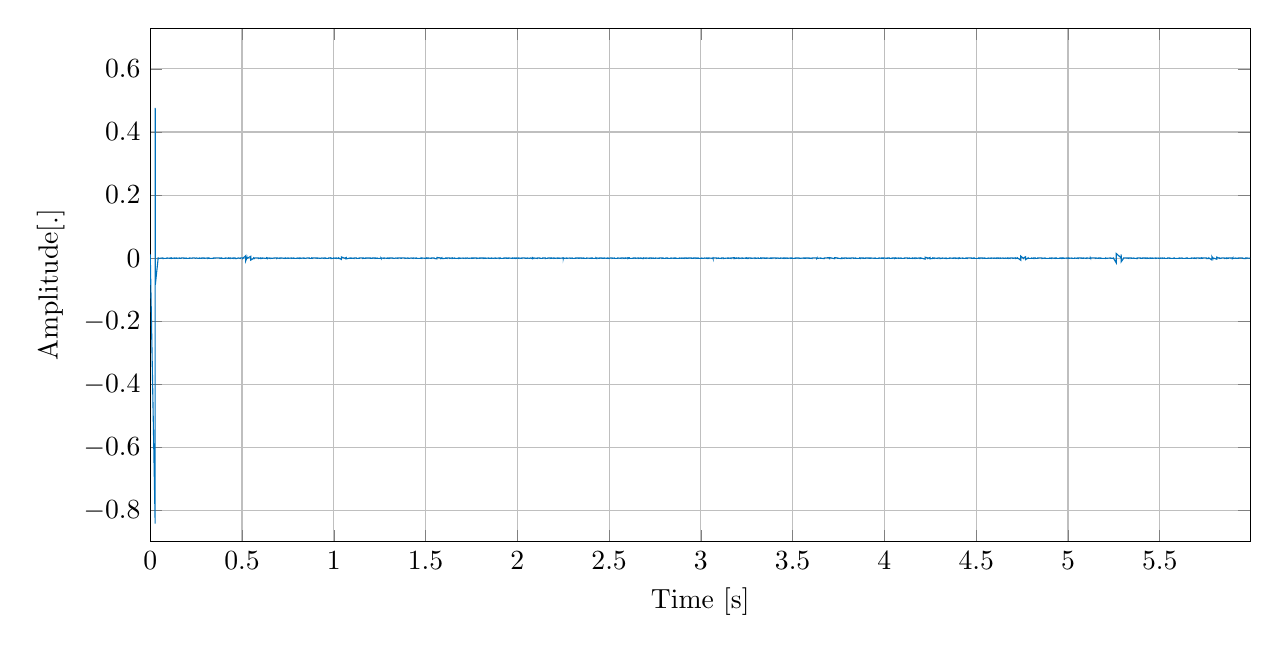
\begin{tikzpicture}

\begin{axis}[%
width=5.5in,
height=2.566in,
at={(1.011in,0.642in)},
scale only axis,
xmin=0,
xmax=5.99308755760369,
xlabel={Time [s]},
xmajorgrids,
ymin=-0.897959183673469,
ymax=0.728862973760933,
ylabel={Amplitude[.]},
ymajorgrids,
axis background/.style={fill=white}
]
\addplot [color=mycolor1,solid,forget plot]
  table[row sep=crcr]{%
2.08333333333333e-05	0.0122538023811748\\
4.16666666666667e-05	-0.0122397274343161\\
6.25e-05	0.0122593985372766\\
0.0268333333333333	-0.841044360454059\\
0.0270208333333333	0.476700841079922\\
0.0276875	0.0743041974628074\\
0.0277708333333333	-0.0842757999528343\\
0.0433333333333333	0.000734689239610419\\
0.0484375	-0.000771147443083658\\
0.068875	0.000871287345213359\\
0.0688958333333333	-0.000914196092068224\\
0.0693958333333333	0.000928116415306673\\
0.0694166666666667	-0.000965228500811473\\
0.0903125	-0.000668652355357153\\
0.0903333333333333	0.000716561090696644\\
0.108166666666667	-0.000493719891106833\\
0.1081875	0.000475264231382342\\
0.114875	0.00100715625962862\\
0.114895833333333	-0.000999706659119178\\
0.13225	0.000670886085256791\\
0.132270833333333	-0.000624125121802932\\
0.1425	0.000574814918345522\\
0.142520833333333	-0.000583128240947472\\
0.158833333333333	0.000578383382299989\\
0.158854166666667	-0.00058200843939012\\
0.168583333333333	-0.000796135526744322\\
0.168604166666667	0.000854760717857374\\
0.183333333333333	0.000748333649329287\\
0.183354166666667	-0.000771497113929529\\
0.1950625	0.000471377160620318\\
0.195083333333333	-0.000617347630158107\\
0.214020833333333	-0.000458421389332424\\
0.214041666666667	0.000694569300872006\\
0.228145833333333	-0.000321552367186984\\
0.229770833333333	0.000907965360966202\\
0.2415	0.000687441835776411\\
0.246208333333333	-0.000392185237250202\\
0.251229166666667	0.000675515516905658\\
0.2610625	-0.000577220917773221\\
0.2685	-0.000607199679195012\\
0.268520833333333	0.000521921896596942\\
0.281	-0.000629137056294877\\
0.281020833333333	0.000657955601166255\\
0.293145833333333	0.000756671588131565\\
0.293166666666667	-0.000644608113382317\\
0.314083333333333	0.000851585577721784\\
0.314104166666667	-0.000739522692164605\\
0.3189375	0.000701479688836363\\
0.318958333333333	-0.000608184931990221\\
0.343854166666667	-0.000469067729444319\\
0.343875	0.000540619530244008\\
0.359041666666667	0.00070804168567296\\
0.3590625	-0.00062391774133284\\
0.3590625	-0.00062391774133284\\
0.359083333333333	0.000710543233890295\\
0.379979166666667	0.000726972441766158\\
0.38	-0.000628724698251465\\
0.388145833333333	0.000648282834173138\\
0.388166666666667	-0.000581854167711955\\
0.409666666666667	-0.000715788312106095\\
0.4096875	0.000855415315301935\\
0.427041666666667	-0.0007138693756773\\
0.4270625	0.000886976677335082\\
0.435208333333333	-0.000671228085502771\\
0.435229166666667	0.000733267265160009\\
0.4515	-0.000881769399678669\\
0.451520833333333	0.000611926340533385\\
0.462375	0.000741565781746908\\
0.462395833333333	-0.00109511905846186\\
0.470875	-0.000920097380037188\\
0.480270833333333	0.000647822687282457\\
0.490854166666667	-0.000812313182615881\\
0.490875	0.00081359586338086\\
0.504166666666667	0.000835832815158442\\
0.5041875	-0.000815314331846972\\
0.520604166666667	0.00822072297498398\\
0.520625	-0.00818086639966468\\
0.526708333333333	0.000784549270936717\\
0.526729166666667	-0.000894162691183173\\
0.5475	0.00587330272890362\\
0.547520833333333	-0.00602184946367332\\
0.563875	-0.00070146311862383\\
0.563895833333333	0.000588540426628599\\
0.5674375	-0.000798263599985336\\
0.567458333333333	0.000687619250579479\\
0.589958333333333	0.00087752808076088\\
0.589979166666667	-0.00102877078582693\\
0.602208333333333	0.000888820032753768\\
0.602229166666667	-0.00104728830047565\\
0.611916666666667	-0.000676649263279144\\
0.6119375	0.000531712657531355\\
0.634416666666667	-0.000934590812104117\\
0.6344375	0.000717503098485721\\
0.638583333333333	-0.00113969461569427\\
0.638604166666667	0.000901226971934011\\
0.6523125	-0.000708696519994537\\
0.652333333333333	0.000428557945956786\\
0.664520833333333	-0.000618338605138116\\
0.674791666666667	0.000567181247364444\\
0.689125	0.00100446755794463\\
0.689145833333333	-0.000874971724965771\\
0.6935	0.000589542799664863\\
0.703354166666667	-0.00047541316588529\\
0.706	-0.000760539803934322\\
0.706020833333333	0.000822549798370906\\
0.71875	0.000474509477181315\\
0.728458333333333	-0.000548142363326956\\
0.736208333333333	0.000699627917352065\\
0.736229166666667	-0.000782275295664827\\
0.750333333333333	0.000603998195855303\\
0.750354166666667	-0.00064075007443739\\
0.769666666666667	0.00068274593716341\\
0.7696875	-0.000641766005538712\\
0.782083333333333	0.000631237777368386\\
0.782104166666667	-0.000585407136095528\\
0.8	-0.0005806766342212\\
0.800020833333333	0.000632825946402111\\
0.811645833333333	-0.000662631555343653\\
0.811666666666667	0.000736471452190856\\
0.81575	0.000764380631130795\\
0.815770833333333	-0.000677733090643042\\
0.8379375	0.000873749227459805\\
0.837958333333333	-0.000762411929489834\\
0.845958333333333	-0.000621186143946013\\
0.85475	0.000749261576196068\\
0.866520833333333	0.000744625396833765\\
0.866541666666667	-0.000515932288010471\\
0.879104166666667	-0.000500943137503569\\
0.879125	0.000765251809666935\\
0.884875	-0.000520656691743884\\
0.884895833333333	0.000768782062408757\\
0.909833333333333	0.000628701812429428\\
0.909854166666667	-0.000570530978576899\\
0.9115	-0.000516818782755884\\
0.911520833333333	0.000556152248207315\\
0.928145833333333	-0.000652874500685887\\
0.934458333333333	0.000659734514753571\\
0.947083333333333	-0.000651538854114526\\
0.947104166666667	0.000746809168655069\\
0.955270833333333	0.000898496033033306\\
0.955291666666667	-0.000764179916232177\\
0.972104166666667	-0.000679279919726632\\
0.972125	0.000809560743173024\\
0.983979166666667	0.0012055916996432\\
0.984	-0.00109974306536854\\
0.999208333333333	-0.000694008147097675\\
0.999229166666667	0.000759993838399656\\
1.0125	-0.000825537425783976\\
1.01252083333333	0.000882635834049446\\
1.0263125	-0.000805976666574922\\
1.02633333333333	0.000859801923651885\\
1.04114583333333	-0.00393542624757928\\
1.04116666666667	0.00393253747706633\\
1.0620625	-0.000723496197663128\\
1.06208333333333	0.000719551399152045\\
1.0680625	0.00215189380845473\\
1.06808333333333	-0.00217003853445217\\
1.08914583333333	0.000633367195619446\\
1.08916666666667	-0.000733655751765525\\
1.09577083333333	-0.000659102777126713\\
1.09579166666667	0.000528602996433345\\
1.11110416666667	-0.00103910627893571\\
1.111125	0.000862286729664806\\
1.12289583333333	0.000739728489954901\\
1.12291666666667	-0.000885722160197164\\
1.1386875	-0.000760492616674059\\
1.13870833333333	0.000695767274970514\\
1.156	0.000820539452797478\\
1.15710416666667	-0.000846867625649995\\
1.16285416666667	0.000736019944611489\\
1.162875	-0.000767126368236282\\
1.173875	-0.000610307732106338\\
1.17389583333333	0.000527717075806225\\
1.19952083333333	0.000715322773740613\\
1.19954166666667	-0.000866709518920433\\
1.20922916666667	-0.00080000363865872\\
1.20925	0.000651740263185364\\
1.2260625	0.000600358327003889\\
1.22608333333333	-0.000736005278273972\\
1.23566666666667	0.000509204353150653\\
1.2356875	-0.000637735228231537\\
1.2561875	-0.00077576017252754\\
1.25620833333333	0.000654464112091331\\
1.25783333333333	-0.000921606283623218\\
1.25785416666667	0.000806931748759692\\
1.27364583333333	-0.000710992913914008\\
1.27366666666667	0.000597042540241103\\
1.29514583333333	-0.000726383582064565\\
1.29516666666667	0.000632590487967683\\
1.30270833333333	-0.000639031198114883\\
1.30272916666667	0.000562847453128214\\
1.321625	0.000755508628156429\\
1.32164583333333	-0.000759150575953867\\
1.33177083333333	-0.000610710125880581\\
1.33795833333333	0.000664683177763139\\
1.34827083333333	-0.000610309911779344\\
1.34829166666667	0.00066859988107635\\
1.36597916666667	0.000775412382380437\\
1.366	-0.000770812016338518\\
1.36760416666667	-0.000760863747782761\\
1.367625	0.000753433481770169\\
1.387125	0.000727227381035258\\
1.38714583333333	-0.00075355261150647\\
1.40541666666667	0.00079868572730456\\
1.4054375	-0.000757006390694345\\
1.41116666666667	-0.000475940761235983\\
1.42166666666667	0.000561245536972261\\
1.4320625	-0.000700759812842404\\
1.43208333333333	0.000809106765515453\\
1.44875	-0.000579986138358643\\
1.44877083333333	0.000695936804143681\\
1.450375	0.00082932710740398\\
1.45039583333333	-0.000723178834510282\\
1.47585416666667	-0.000796756664477162\\
1.475875	0.000931314814875718\\
1.47897916666667	-0.00045624620636756\\
1.479	0.000591956862403049\\
1.5045625	-0.000799015220339862\\
1.50458333333333	0.000949854281251891\\
1.51252083333333	-0.000664111312568434\\
1.51254166666667	0.000807644895781415\\
1.532625	-0.000768292124469755\\
1.53264583333333	0.000901104456422554\\
1.53310416666667	-0.000780272771386461\\
1.533125	0.000910140329649984\\
1.54689583333333	0.00089842336836591\\
1.54691666666667	-0.000807657270372154\\
1.56166666666667	-0.00228936811688119\\
1.5616875	0.00235494088395583\\
1.58264583333333	0.000690474438946419\\
1.58266666666667	-0.00064927012008327\\
1.58858333333333	0.00144116184680155\\
1.58860416666667	-0.00139624873803248\\
1.6106875	-0.000602387446140836\\
1.61070833333333	0.000702319169406948\\
1.6169375	-0.000679845477897681\\
1.61695833333333	0.000779159653226463\\
1.631125	0.00084470636459848\\
1.63114583333333	-0.000770625848906314\\
1.645625	0.000932076093600797\\
1.64564583333333	-0.000920772984705366\\
1.65822916666667	0.000603452248383813\\
1.65825	-0.000611727050144646\\
1.67922916666667	-0.000916096471897362\\
1.67925	0.000885032614596713\\
1.68497916666667	0.00060681956090826\\
1.685	-0.000632573469011195\\
1.7041875	0.000489471868758358\\
1.70533333333333	-0.000553209136887921\\
1.7195625	0.000584640252581633\\
1.71958333333333	-0.000659832986771201\\
1.72972916666667	0.000676608720987426\\
1.73304166666667	-0.000772017726683305\\
1.7514375	0.000572509405293118\\
1.75145833333333	-0.000685180087054376\\
1.75897916666667	-0.000651868924147599\\
1.759	0.000535588981038542\\
1.77841666666667	0.00078712559790062\\
1.7784375	-0.000885535821845007\\
1.79366666666667	0.000554841061057088\\
1.7936875	-0.000623313394037457\\
1.79620833333333	-0.000631227199885162\\
1.79622916666667	0.00055884438102004\\
1.81525	0.000686508355469422\\
1.81527083333333	-0.000766278690899993\\
1.8228125	0.000579422816118477\\
1.82283333333333	-0.000677834362675808\\
1.84427083333333	0.000643300891206201\\
1.84429166666667	-0.000775353175171843\\
1.8579375	-0.000858996246789848\\
1.85795833333333	0.000730393986205559\\
1.86995833333333	-0.000739132662331362\\
1.8779375	0.000631655792580372\\
1.88010416666667	0.000623229945723398\\
1.880125	-0.000705783086237455\\
1.902875	0.000677694598848809\\
1.90289583333333	-0.000740440761131436\\
1.9065625	0.000648523516880695\\
1.90658333333333	-0.000699888085700352\\
1.92664583333333	-0.000706076369662584\\
1.92666666666667	0.0006684858258758\\
1.9423125	0.000672432546327812\\
1.94233333333333	-0.000686311156506293\\
1.95158333333333	-0.000834953634071659\\
1.95160416666667	0.000828193460366693\\
1.97452083333333	-0.000754893870521019\\
1.97454166666667	0.000786453720274723\\
1.9876875	-0.000846514791097456\\
1.98770833333333	0.000886916911740398\\
1.99645833333333	-0.000701588697114327\\
1.99647916666667	0.000746318285286581\\
2.00779166666667	-0.000558849834990225\\
2.0078125	0.000590125423864868\\
2.025125	-0.000815720302488596\\
2.02514583333333	0.000844126045707384\\
2.04247916666667	0.000818452430879792\\
2.0425	-0.000783593524856645\\
2.05322916666667	-0.000786064139855268\\
2.05325	0.000844790986028791\\
2.067	-0.000696646175408123\\
2.0711875	0.000797998908082457\\
2.08222916666667	-0.00170835215850821\\
2.08225	0.00181800349637685\\
2.08897916666667	-0.00070426032922555\\
2.089	0.000817721501039317\\
2.10960416666667	-0.000887554896070543\\
2.109625	0.00098931975872573\\
2.1231875	0.000642145728899372\\
2.12320833333333	-0.000542059782624433\\
2.13858333333333	-0.000673105136053546\\
2.13860416666667	0.000767839514714118\\
2.15225	0.00100009406106331\\
2.15227083333333	-0.000897420938249411\\
2.16620833333333	-0.000879091551548042\\
2.16622916666667	0.000969862066757164\\
2.17835416666667	0.000701695518543768\\
2.178375	-0.000625295106870151\\
2.18560416666667	0.000669128807558755\\
2.185625	-0.000607115382717358\\
2.19877083333333	0.00089629841071348\\
2.19879166666667	-0.00084888052857303\\
2.21875	0.00055932231801871\\
2.21877083333333	-0.000525486858424834\\
2.22579166666667	0.000509710916413454\\
2.2258125	-0.000487448806451855\\
2.25041666666667	0.000685083049406073\\
2.2504375	-0.00064789802720805\\
2.2509375	0.000696644660514428\\
2.25460416666667	-0.000661425172080484\\
2.26827083333333	0.000558762736287494\\
2.26829166666667	-0.000530584893220879\\
2.28760416666667	0.000584272371277117\\
2.28975	-0.000597897126661749\\
2.29845833333333	0.000715010014234861\\
2.29847916666667	-0.000749592132255716\\
2.31685416666667	-0.000707700601301887\\
2.316875	0.000646739557304433\\
2.3336875	0.000574438500792702\\
2.33370833333333	-0.000645200711072129\\
2.33583333333333	-0.000709060329132497\\
2.33585416666667	0.000642236545061064\\
2.35141666666667	0.000496685590389209\\
2.3514375	-0.000571782474732014\\
2.36166666666667	0.000664424266928079\\
2.3616875	-0.0007407929527549\\
2.3775	-0.000697831488081611\\
2.37752083333333	0.00061367347839209\\
2.40064583333333	-0.000752869714596988\\
2.40066666666667	0.000660121130953765\\
2.40822916666667	0.000781907509805732\\
2.40825	-0.000865505279331412\\
2.42879166666667	-0.000847229258199964\\
2.4288125	0.000772611259163829\\
2.431875	-0.000724781701442215\\
2.43189583333333	0.000648673424721907\\
2.44664583333333	-0.000645719025163827\\
2.44666666666667	0.000580067767031436\\
2.4623125	0.000594903480946001\\
2.46233333333333	-0.000666296694267746\\
2.47210416666667	-0.000809085647211153\\
2.472125	0.000721916217464159\\
2.49352083333333	-0.000865582526912647\\
2.49354166666667	0.000779107466304316\\
2.50085416666667	-0.000794926340932463\\
2.507875	0.000705151667197973\\
2.51652083333333	0.000679929720170458\\
2.51654166666667	-0.000744098538709615\\
2.52833333333333	0.000624332674507611\\
2.52835416666667	-0.000673275434336211\\
2.54625	-0.000867236775486297\\
2.54627083333333	0.000845717236411271\\
2.5651875	-0.000767449765396163\\
2.56520833333333	0.00076742057442274\\
2.57641666666667	0.000874488886027037\\
2.5764375	-0.000856032962981566\\
2.58697916666667	0.00076178411008069\\
2.587	-0.000743622792577481\\
2.60277083333333	0.0013136548163217\\
2.60279166666667	-0.00128702744801207\\
2.61008333333333	0.000723062776409405\\
2.61010416666667	-0.000686637079158903\\
2.63120833333333	-0.000667940116237091\\
2.63122916666667	0.00072297590903901\\
2.6433125	0.000603391804908914\\
2.64333333333333	-0.000544871642235419\\
2.66033333333333	0.000849026176098303\\
2.66035416666667	-0.000791214762677021\\
2.67277083333333	0.000873744089667305\\
2.67279166666667	-0.000812681429121931\\
2.68677083333333	-0.000987770802047832\\
2.68679166666667	0.0010579915195515\\
2.7005	-0.000742347821986829\\
2.70052083333333	0.000829880731885427\\
2.71979166666667	-0.000660118679685859\\
2.7198125	0.000763839850484412\\
2.72975	0.000769967202678459\\
2.72977083333333	-0.000666924355320421\\
2.73991666666667	0.000736224068886616\\
2.7399375	-0.000634533649016969\\
2.75166666666667	-0.000521447060906492\\
2.7516875	0.000608439351009449\\
2.7736875	-0.00069398230122133\\
2.77370833333333	0.000757529755137674\\
2.7873125	0.000694869320131796\\
2.78733333333333	-0.000640350362539444\\
2.79252083333333	0.000544452900313078\\
2.79254166666667	-0.000489515434912369\\
2.80927083333333	-0.00053202504677721\\
2.80929166666667	0.000585365552618237\\
2.8185	0.0007117807501467\\
2.81852083333333	-0.00066873998959899\\
2.83745833333333	-0.000547996804249562\\
2.83747916666667	0.000584916772793463\\
2.85470833333333	-0.000522189585135935\\
2.85472916666667	0.000535459252196795\\
2.86297916666667	0.000514572771121788\\
2.863	-0.000509678771410704\\
2.88333333333333	-0.000648689004081701\\
2.88335416666667	0.000639502488596472\\
2.89658333333333	-0.000574527441827736\\
2.89660416666667	0.000567838688742371\\
2.9084375	-0.00072373763542157\\
2.90845833333333	0.000703685111789378\\
2.9213125	0.000593438658275415\\
2.92133333333333	-0.00061955320266765\\
2.929375	-0.000656304619727487\\
2.92939583333333	0.000622184806303372\\
2.949375	0.000639722816665727\\
2.94939583333333	-0.000705584805944201\\
2.959875	-0.000549923607914802\\
2.95989583333333	0.000472236025612762\\
2.973875	0.000653679995461469\\
2.97389583333333	-0.000742293052122019\\
2.98452083333333	0.00072314274714479\\
2.98454166666667	-0.000804526234277354\\
3.00352083333333	-0.000537754384259843\\
3.00354166666667	0.000456582338249342\\
3.014125	-0.000776888537815397\\
3.01922916666667	0.000695478780294685\\
3.03310416666667	-0.00074095870606345\\
3.033125	0.000660049322515139\\
3.04175	-0.000751482662233543\\
3.04177083333333	0.000665545496823237\\
3.06472916666667	-0.000470515262636881\\
3.065625	0.000444291580824562\\
3.06633333333333	-0.000892892655786363\\
3.06635416666667	0.000809471705858813\\
3.08572916666667	0.000703933075321743\\
3.08575	-0.000771050863182079\\
3.09702083333333	0.000685150266846324\\
3.09704166666667	-0.000747358011513531\\
3.11233333333333	-0.00089213483687142\\
3.11235416666667	0.00083863795034053\\
3.12333333333333	0.00101914268363973\\
3.12335416666667	-0.001077580218926\\
3.14541666666667	0.000554501900173562\\
3.1454375	-0.000603462502242331\\
3.14977083333333	-0.00076453157616034\\
3.14979166666667	0.000713659167342908\\
3.16389583333333	-0.000850869040297808\\
3.16391666666667	0.000819295448782314\\
3.18158333333333	0.00135549330856276\\
3.18160416666667	-0.00135321053177325\\
3.19177083333333	0.000727219974764654\\
3.19179166666667	-0.000710574628151551\\
3.20735416666667	0.00124612956147805\\
3.207375	-0.00121470537273457\\
3.22472916666667	0.000830672088752873\\
3.22475	-0.000795961536435125\\
3.24466666666667	0.000641663930231659\\
3.2446875	-0.000587058566500264\\
3.2515	-0.000927682152513045\\
3.25152083333333	0.000981527381112092\\
3.25997916666667	-0.000749624117858614\\
3.26	0.000815721671905278\\
3.27277083333333	0.000775189438798031\\
3.27279166666667	-0.0007024482451306\\
3.29635416666667	0.000864724576605581\\
3.296375	-0.000788095676280746\\
3.313125	0.000669339837449391\\
3.31314583333333	-0.000592315020425472\\
3.32535416666667	-0.000508506520697274\\
3.325375	0.000598843542910724\\
3.32991666666667	-0.000504742683764233\\
3.3299375	0.000589990414134015\\
3.34779166666667	0.000637202361540035\\
3.3478125	-0.000542090937324429\\
3.3575	-0.000568184770277761\\
3.35752083333333	0.000672998675066125\\
3.38095833333333	-0.000474777068158243\\
3.38097916666667	0.000567342640984112\\
3.38560416666667	-0.000530464288802622\\
3.385625	0.000624953700409804\\
3.40904166666667	0.000776727981003045\\
3.4090625	-0.000710595589808062\\
3.42029166666667	0.000746100687701466\\
3.42439583333333	-0.000689148528298087\\
3.43316666666667	-0.000819042916010755\\
3.4331875	0.000861379861680038\\
3.4499375	-0.000647694329668308\\
3.44995833333333	0.000688991295399136\\
3.45920833333333	0.000569038012327066\\
3.45922916666667	-0.000534202302468729\\
3.4699375	0.000729467217168986\\
3.46995833333333	-0.000705060848936256\\
3.488875	0.000629868945102908\\
3.48889583333333	-0.000623813081961381\\
3.4955625	0.000803080730868091\\
3.49558333333333	-0.000810816898637587\\
3.514	-0.000419473843262285\\
3.51402083333333	0.000402425331291254\\
3.53510416666667	0.000782860926028073\\
3.535125	-0.000829844536800619\\
3.53514583333333	0.000810817070005341\\
3.53516666666667	-0.0008344592878688\\
3.56233333333333	0.000740713969418412\\
3.56235416666667	-0.000806206226934828\\
3.56952083333333	-0.00071871408861111\\
3.56954166666667	0.000656455813702043\\
3.5894375	0.000601387103124408\\
3.58945833333333	-0.000688164473721435\\
3.59214583333333	-0.000521002002766059\\
3.59216666666667	0.000424870977466098\\
3.60627083333333	-0.0010884381961116\\
3.60629166666667	0.000992606800091719\\
3.63075	0.000673312633295481\\
3.63077083333333	-0.000771650492053558\\
3.632875	0.000796060212640286\\
3.63289583333333	-0.000894288213147536\\
3.65285416666667	0.000750320197465302\\
3.652875	-0.000847063418056259\\
3.67285416666667	-0.000933141726971411\\
3.672875	0.000839301568977933\\
3.673375	-0.000827967980561113\\
3.67339583333333	0.000729373704252723\\
3.7008125	0.00149235214502603\\
3.70083333333333	-0.00166836350238167\\
3.70152083333333	-0.0018759763831977\\
3.70154166666667	0.00178584267808272\\
3.7279375	-0.00156669426518658\\
3.72795833333333	0.00148410316077901\\
3.72854166666667	-0.00168255484815004\\
3.7285625	0.00161312956027256\\
3.7458125	0.00078193297440681\\
3.74583333333333	-0.000841652983050695\\
3.76877083333333	-0.000951158895009949\\
3.76879166666667	0.000902192537464957\\
3.7805	-0.000870623201476591\\
3.78052083333333	0.000842427265769237\\
3.793375	0.000692445735071341\\
3.79339583333333	-0.00070824668075357\\
3.8080625	0.000616938829242782\\
3.80808333333333	-0.000620344936868163\\
3.81689583333333	-0.000911378891083477\\
3.81691666666667	0.000928784287740468\\
3.832125	0.000649782435139187\\
3.83214583333333	-0.00062575566892542\\
3.84341666666667	0.000580234098243344\\
3.8434375	-0.000542820670958007\\
3.8648125	-0.000579867099639341\\
3.86483333333333	0.000637976697022658\\
3.8689375	-0.000633499816894192\\
3.86895833333333	0.00069305836828903\\
3.88477083333333	0.000644550367696489\\
3.88479166666667	-0.000577933171632154\\
3.8954375	-0.00066287978056014\\
3.89545833333333	0.000729988238619403\\
3.91647916666667	0.000601699265337787\\
3.9165	-0.000527200903257703\\
3.9239375	-0.000627986975583194\\
3.92395833333333	0.000705607698588085\\
3.94908333333333	-0.000619410687957292\\
3.94910416666667	0.000711529833267491\\
3.94958333333333	0.000768823629595509\\
3.94960416666667	-0.00068197184847231\\
3.97002083333333	-0.000636965813764758\\
3.97004166666667	0.000728822420202642\\
3.987875	-0.00057938225423229\\
3.98789583333333	0.00066778784981798\\
3.99404166666667	-0.000668186711203397\\
3.9940625	0.000757667910339742\\
4.01610416666667	-0.000683927060194245\\
4.016125	0.000759061468281206\\
4.02620833333333	0.000690829316251285\\
4.02622916666667	-0.000622418547535604\\
4.04204166666667	-0.000457760739397958\\
4.0420625	0.000524185778382851\\
4.0563125	0.00071208914465086\\
4.05633333333333	-0.000673662759596049\\
4.06047916666667	0.000664937719744489\\
4.0605	-0.000620427354540002\\
4.07733333333333	0.000671089574534653\\
4.07735416666667	-0.000639678631543796\\
4.09014583333333	0.000694536514818172\\
4.09016666666667	-0.000672305319064109\\
4.10954166666667	-0.000670962727712327\\
4.1095625	0.000679358321532598\\
4.12633333333333	0.000766643967531233\\
4.12635416666667	-0.000767709199301905\\
4.13658333333333	0.000480789566442453\\
4.13660416666667	-0.000492889757098431\\
4.1529375	-0.000871250296090936\\
4.15295833333333	0.000842243228932475\\
4.16439583333333	-0.000815416077056576\\
4.16441666666667	0.000780047338326749\\
4.172375	0.000727694450945087\\
4.17239583333333	-0.000761118488113997\\
4.1934375	0.00100939700417115\\
4.19345833333333	-0.00105751794332657\\
4.19845833333333	-0.000799533055506864\\
4.19847916666667	0.000729405458463086\\
4.222125	-0.00316645728084482\\
4.22214583333333	0.00309847988158742\\
4.23614583333333	0.000783659063442438\\
4.23616666666667	-0.000854904962278722\\
4.24852083333333	0.00207072571064826\\
4.24854166666667	-0.00214172149943263\\
4.26227083333333	-0.000868799980255136\\
4.26229166666667	0.000787701525948726\\
4.27	-0.000833573460908086\\
4.27002083333333	0.000751938517770686\\
4.29097916666667	-0.00101151350778446\\
4.291	0.000940940162504793\\
4.30216666666667	0.00103013261886231\\
4.3021875	-0.0010881983414522\\
4.31439583333333	-0.000690566554329529\\
4.31441666666667	0.000636813859485653\\
4.33477083333333	-0.000857145812746723\\
4.33479166666667	0.000818091484720377\\
4.3364375	0.000923032419635397\\
4.33645833333333	-0.000968577237014383\\
4.3543125	-0.000752860269700285\\
4.35433333333333	0.000715336140258785\\
4.376125	-0.000594287455589043\\
4.37614583333333	0.00056193234529366\\
4.38791666666667	0.000727992790300719\\
4.3879375	-0.0007558411202433\\
4.40341666666667	0.000561675104748859\\
4.4034375	-0.000575056459496602\\
4.4069375	0.000747687864187593\\
4.40695833333333	-0.000755022539738558\\
4.42679166666667	0.000573333512602289\\
4.4268125	-0.000561447241616433\\
4.44502083333333	-0.000596895249178401\\
4.44504166666667	0.000630004888908778\\
4.4513125	-0.000686271499428727\\
4.45133333333333	0.000723672289070652\\
4.473875	0.000731676901106292\\
4.47389583333333	-0.000685316941159171\\
4.48310416666667	-0.000800497827443301\\
4.483125	0.000850253290490356\\
4.49008333333333	0.000635303781067878\\
4.49010416666667	-0.000591582094904115\\
4.5146875	-0.000657910663474233\\
4.51470833333333	0.000713508582602995\\
4.5178125	-0.000467420432399924\\
4.51783333333333	0.000529998770134142\\
4.53616666666667	0.000708749282095999\\
4.5361875	-0.000653132504091235\\
4.546375	0.000686825642058495\\
4.54639583333333	-0.000623807716686843\\
4.56472916666667	-0.000493878179964804\\
4.56475	0.000552721080581092\\
4.58110416666667	-0.000698684485425761\\
4.581125	0.000755845224672406\\
4.597875	-0.000523546352566346\\
4.59789583333333	0.000582719675040393\\
4.61072916666667	-0.000684166815783074\\
4.61075	0.000750035787138153\\
4.62047916666667	0.000461526421507547\\
4.6205	-0.000393504679770596\\
4.63125	0.000689880271579905\\
4.63127083333333	-0.000627134430238102\\
4.6469375	0.000749800910275345\\
4.64747916666667	-0.000711561864938089\\
4.65729166666667	-0.000538498730920764\\
4.6573125	0.000565783292646204\\
4.6730625	-0.000784713881450174\\
4.67308333333333	0.000792956249443993\\
4.685	-0.000873473932540675\\
4.68502083333333	0.000874898492932472\\
4.70010416666667	0.0005923526347921\\
4.700125	-0.000581344946413087\\
4.71395833333333	0.000983417764375153\\
4.71397916666667	-0.000972633807776415\\
4.72514583333333	-0.000737518076082976\\
4.72516666666667	0.000732984068388039\\
4.74272916666667	-0.00658835799905934\\
4.74275	0.0065791314772882\\
4.75785416666667	-0.00080576226705523\\
4.757875	0.000754522492115429\\
4.769125	0.00451271510550656\\
4.76914583333333	-0.00455955425912552\\
4.7828125	0.000841151801291296\\
4.78283333333333	-0.000883162785786139\\
4.80225	-0.000542022348083922\\
4.80227083333333	0.000506497659431693\\
4.81258333333333	-0.00103080184500524\\
4.81260416666667	0.000981202470474372\\
4.82164583333333	0.000836041697278347\\
4.82166666666667	-0.000894083793682192\\
4.835	-0.000593541002648692\\
4.83502083333333	0.000517426397680513\\
4.85804166666667	0.00101951812131046\\
4.8580625	-0.00111497893861662\\
4.86114583333333	-0.000666024034172112\\
4.874375	0.000586650966641702\\
4.87485416666667	0.000627148536093521\\
4.874875	-0.000690120729408816\\
4.90141666666667	-0.000662423929509586\\
4.9014375	0.000626485663808014\\
4.91066666666667	-0.000908889302861698\\
4.9106875	0.000857032640269196\\
4.92964583333333	-0.000747181442834044\\
4.92966666666667	0.000681657580528353\\
4.9371875	0.000565310389483618\\
4.93720833333333	-0.00063242421751897\\
4.956625	-0.00061542355479786\\
4.95664583333333	0.000573606460348106\\
4.96560416666667	0.00063766839747109\\
4.965625	-0.000662713224025773\\
4.97133333333333	0.000745214404496924\\
4.97135416666667	-0.000758866225340087\\
4.995	0.000590014687296517\\
4.99502083333333	-0.000583280645372063\\
5.00316666666667	0.000701418648776317\\
5.0031875	-0.00070402617530778\\
5.02145833333333	0.000553307573277657\\
5.02147916666667	-0.000567183204744751\\
5.03477083333333	-0.000690601072429654\\
5.03575	0.000678652374369759\\
5.04810416666667	-0.000506221019121415\\
5.05089583333333	0.000530573037324425\\
5.05675	-0.000817011914210647\\
5.05677083333333	0.000855451456269155\\
5.07566666666667	0.000531083650983497\\
5.0756875	-0.000455507170031002\\
5.08429166666667	-0.000529089638337644\\
5.0843125	0.000601649620225006\\
5.10170833333333	-0.000732123536239426\\
5.10172916666667	0.000793777125612496\\
5.1225625	-0.00061894893928467\\
5.12258333333333	0.000660243213372411\\
5.12377083333333	-0.00060812998544776\\
5.12379166666667	0.000643650784820187\\
5.15020833333333	0.000909723813840191\\
5.15022916666667	-0.000830905866725329\\
5.1513125	-0.000725569108061976\\
5.15133333333333	0.000804922919634336\\
5.16752083333333	-0.000706523310236849\\
5.16754166666667	0.000783430696085785\\
5.17839583333333	0.000529013849934631\\
5.17841666666667	-0.000434255288139971\\
5.20347916666667	-0.000887640180062974\\
5.20554166666667	0.000932310297848551\\
5.2060625	0.000780566962792512\\
5.20608333333333	-0.000745371954936459\\
5.23347916666667	0.000745461612568184\\
5.2335	-0.000697089071657755\\
5.2473125	-0.000853651687693003\\
5.24733333333333	0.000917898778024549\\
5.248375	0.000797872452458675\\
5.24839583333333	-0.000743686942838169\\
5.26310416666667	-0.0149618098355943\\
5.263125	0.0147405214393317\\
5.28883333333333	0.00115536141022913\\
5.28885416666667	-0.00122113863490467\\
5.28997916666667	0.0117808401421682\\
5.29	-0.0115208745606766\\
5.30291666666667	-0.000803939977406044\\
5.3029375	0.000795149632615833\\
5.32895833333333	0.00058336640180924\\
5.32897916666667	-0.000606478902792325\\
5.33210416666667	-0.000994408606210292\\
5.332125	0.000989817568788992\\
5.34497916666667	0.000696997906660684\\
5.345	-0.000707923083019498\\
5.35875	0.000517411316936819\\
5.35877083333333	-0.000531969705641809\\
5.37754166666667	-0.00106054193261786\\
5.3775625	0.00101593414191938\\
5.3949375	0.000636588080925689\\
5.39495833333333	-0.000709996154672059\\
5.405125	-0.000546237269207376\\
5.40514583333333	0.000477102900592582\\
5.42152083333333	0.000571777192126952\\
5.42154166666667	-0.000640227708637533\\
5.43129166666667	0.000875215507549028\\
5.4313125	-0.000926473105429979\\
5.4480625	0.000638692913570213\\
5.44808333333333	-0.000694003462087355\\
5.45775	0.000502955543632727\\
5.45777083333333	-0.000551097000205143\\
5.47833333333333	0.000574862269306865\\
5.47835416666667	-0.00064690238774901\\
5.4915	0.000529683031027361\\
5.49372916666667	-0.000618913150298244\\
5.50422916666667	0.000453330103516924\\
5.50425	-0.000531148342860655\\
5.51391666666667	0.000670917417854683\\
5.5139375	-0.000732130141137104\\
5.52533333333333	0.000600952735347802\\
5.52535416666667	-0.000652504403835572\\
5.5436875	-0.000735679849478919\\
5.54370833333333	0.000710721299353491\\
5.55427083333333	0.000793609768938327\\
5.55429166666667	-0.000815113052475865\\
5.57739583333333	-0.000807882112505996\\
5.57741666666667	0.000771452724174448\\
5.58002083333333	0.000817904553353734\\
5.58004166666667	-0.000849769649391773\\
5.60589583333333	-0.000583011985817421\\
5.60591666666667	0.000571564395622842\\
5.60804166666667	0.000554240622656337\\
5.6080625	-0.00058060839501004\\
5.62225	0.000811085833073755\\
5.62227083333333	-0.000816072912321638\\
5.64272916666667	-0.000612163267642167\\
5.64375	0.000650635062013345\\
5.650875	0.000649649219327914\\
5.65089583333333	-0.00060113537436008\\
5.671875	-0.000783975766054335\\
5.6719375	0.000805452068780832\\
5.68920833333333	-0.000663144542647274\\
5.68922916666667	0.000698125851068317\\
5.69785416666667	-0.000851824838492038\\
5.697875	0.000891547489277094\\
5.71425	0.000722969067958876\\
5.71427083333333	-0.000677021060788945\\
5.72610416666667	0.000936628653660575\\
5.726125	-0.000857062220265057\\
5.73404166666667	-0.000729934649359309\\
5.73410416666667	0.000789824527171175\\
5.75460416666667	0.00102125482339883\\
5.75466666666667	-0.00095568253293901\\
5.7673125	-0.000889781170721334\\
5.76733333333333	0.000942675078136838\\
5.78370833333333	-0.00554388749188475\\
5.78372916666667	0.00553064421889357\\
5.78989583333333	-0.000881210327161686\\
5.78995833333333	0.000889438244695447\\
5.81060416666667	-0.00328829714850285\\
5.810625	0.00334137932228787\\
5.826125	-0.000544935058844586\\
5.82614583333333	0.000620442609599313\\
5.83329166666667	-0.00064426274151791\\
5.8384375	0.000740222900762994\\
5.8515625	0.000978323092323193\\
5.85270833333333	-0.000938872987895347\\
5.8649375	0.000938884848248308\\
5.865	-0.000945659788768267\\
5.874125	-0.000740857813003309\\
5.874625	0.000760900429568342\\
5.89591666666667	0.00058253442222721\\
5.89597916666667	-0.000576819780098533\\
5.898125	0.00103763308512588\\
5.89814583333333	-0.00103980774970416\\
5.91485416666667	0.000659875217243964\\
5.91491666666667	-0.00062854034851054\\
5.92772916666667	-0.000626224951258898\\
5.92779166666667	0.000680388507480993\\
5.95133333333333	0.000979110276324151\\
5.95139583333333	-0.000946283252758377\\
5.9518125	0.000861942008608148\\
5.951875	-0.000869949490864557\\
5.9686875	-0.000995789762615092\\
5.96875	0.000894604049820107\\
5.99310416666667	-0.000359981548101127\\
};
\end{axis}
\end{tikzpicture}%
	\caption{Impulse response plot of the cancellation path see \autoref{CancellationPathImpulseResponseCrop} for zoomed in version.}
	\label{CancellationPathImpulseResponse}
\end{figure}


%\begin{figure}[H]
%	\centering
%	\includegraphics[width=0.85\textwidth]{CancellationPath_MATLAB_Figures/CancellationPathImpulseResponse.png}
%	\caption{Impulse Response plot of the cancellation path (NOT TIKZ).}
%	\label{CancellationPathImpulseResponse}
%\end{figure}

Converting the impulse response from magnitude to dB, gives the time decay which reveals the Signal to Noise Ratio (SNR) of the system, and from the read off SNR is found to be $\sim$ 60 dB SNR, as seen on \autoref{TimeDecayPlotCancellationPath}.

%\begin{figure}[H]
%	\centering
%	\includegraphics[width=0.85\textwidth]{CancellationPath_MATLAB_Figures/CancellationPathTimeDecay.png}
%	\caption{Time decay plot of the cancellation path (NOT TIKZ).}
%	\label{TimeDecayPlotCancellationPath}
%\end{figure}

\begin{figure}[H]
	\centering
	\tikzsetnextfilename{TimeDecayPlotCancellationPath1}
	%% This file was created by matlab2tikz.
%
%The latest updates can be retrieved from
%  http://www.mathworks.com/matlabcentral/fileexchange/22022-matlab2tikz-matlab2tikz
%where you can also make suggestions and rate matlab2tikz.
%
\definecolor{mycolor1}{rgb}{0.00000,0.44700,0.74100}%
\definecolor{mycolor2}{rgb}{0.85000,0.32500,0.09800}%
\definecolor{mycolor3}{rgb}{0.92900,0.69400,0.12500}%
\definecolor{mycolor4}{rgb}{0.49400,0.18400,0.55600}%
\definecolor{mycolor5}{rgb}{0.46600,0.67400,0.18800}%
%
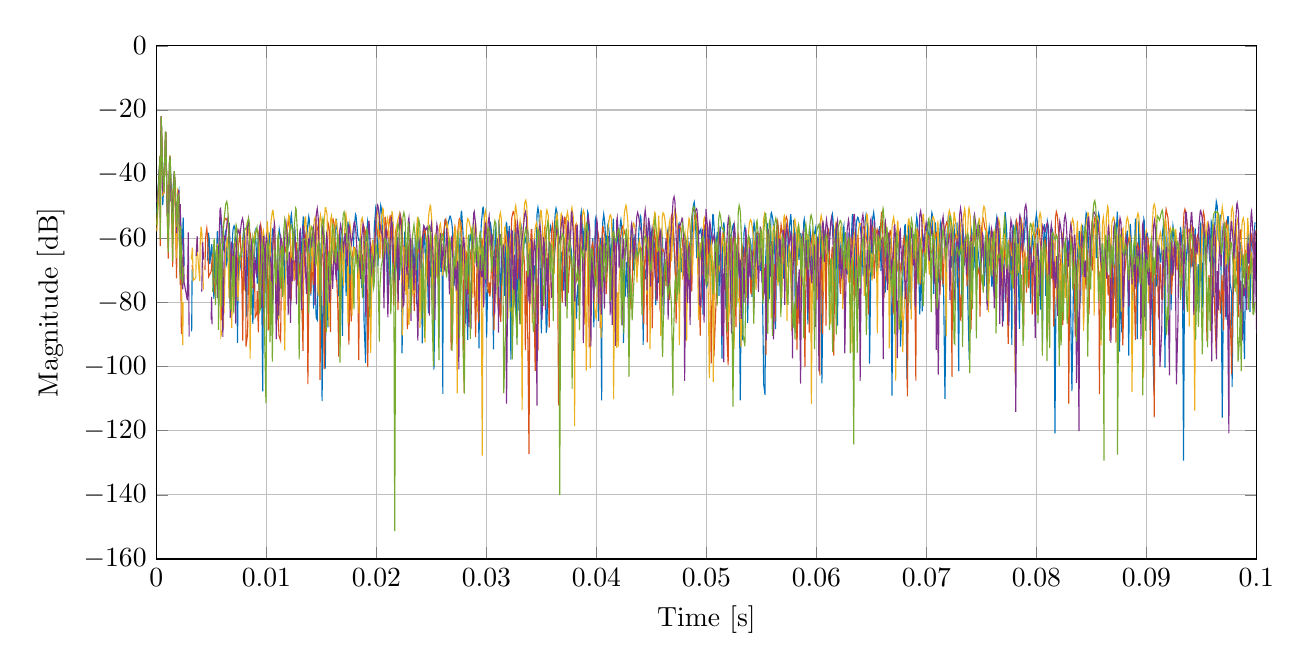
\begin{tikzpicture}

\begin{axis}[%
width=5.5in,
height=2.566in,
scaled x ticks = false,
x tick label style={/pgf/number format/fixed},
at={(1.414in,0.891in)},
scale only axis,
unbounded coords=jump,
xmin=0,
xmax=0.1,
xlabel={Time [s]},
xmajorgrids,
ymin=-160,
ymax=0,
ylabel={Magnitude [dB]},
ymajorgrids,
axis background/.style={fill=white},
title style={font=\bfseries},
%title={Time Decay}
]
\addplot [color=mycolor1,solid,forget plot]
  table[row sep=crcr]{%
2.08333333333333e-05	nan\\
4.16666666666667e-05	-52.111048310778\\
0.000166666666666667	-43.9740436319002\\
0.000333333333333333	-34.8177965827442\\
0.000354166666666667	-53.6190056426103\\
0.000354166666666667	-53.6190056426103\\
0.0004375	-21.9598363711386\\
0.0005625	-37.7606834431528\\
0.000583333333333333	-49.6288694056232\\
0.0006875	-42.2560543031998\\
0.000833333333333333	-27.0848645767238\\
0.000854166666666667	-27.0938121387821\\
0.000979166666666667	-49.8807436737733\\
0.00108333333333333	-59.9223441352537\\
0.0011875	-37.2201027543805\\
0.00125	-34.3291951406571\\
0.00135416666666667	-45.9757139957571\\
0.00147916666666667	-56.382911413555\\
0.00152083333333333	-43.9141776726352\\
0.00152083333333333	-43.9141776726352\\
0.001625	-40.042008410004\\
0.0016875	-43.2431355273656\\
0.00183333333333333	-60.9681241606569\\
0.00183333333333333	-60.9681241606569\\
0.0019375	-46.8693647146266\\
0.00204166666666667	-45.2221645426903\\
0.00214583333333333	-70.4535211157334\\
0.00216666666666667	-51.6149616670037\\
0.0023125	-64.165288874486\\
0.00235416666666667	-61.5511588605062\\
0.0024375	-53.565070295056\\
0.00252083333333333	-68.5064286025977\\
0.00252083333333333	-68.5064286025977\\
0.00266666666666667	nan\\
0.00266666666666667	nan\\
0.00289583333333333	-72.904642668182\\
0.00289583333333333	-72.904642668182\\
0.003	nan\\
0.003	nan\\
0.00320833333333333	-89.0396268578771\\
0.00325	-69.6670608974985\\
0.00333333333333333	nan\\
0.00333333333333333	nan\\
0.0035	nan\\
0.0035	nan\\
0.00364583333333333	nan\\
0.00364583333333333	nan\\
0.0038125	nan\\
0.0038125	nan\\
0.00397916666666667	nan\\
0.00397916666666667	nan\\
0.00414583333333333	nan\\
0.00414583333333333	nan\\
0.0043125	nan\\
0.0043125	nan\\
0.00464583333333333	-66.952070269611\\
0.00464583333333333	-66.952070269611\\
0.00464583333333333	-66.952070269611\\
0.00472916666666667	-58.2959288896312\\
0.0048125	-60.5931307267329\\
0.00485416666666667	-68.0794223724486\\
0.00504166666666667	-61.8026803688784\\
0.005125	-70.1443845224101\\
0.00522916666666667	-78.870829364037\\
0.0053125	-63.8012011510901\\
0.0053125	-63.8012011510901\\
0.00535416666666667	-68.5896659640424\\
0.00545833333333333	-65.4935549134102\\
0.00554166666666667	-57.7477179120546\\
0.00566666666666667	-81.2009260636828\\
0.00577083333333333	-55.761344442787\\
0.00585416666666667	-53.5416605882092\\
0.0059375	-56.2577357302003\\
0.00597916666666667	-58.9539415015357\\
0.00610416666666667	-63.8531451471768\\
0.00614583333333333	-61.9141009456243\\
0.00627083333333333	-58.0593839706459\\
0.0063125	-58.7413544861928\\
0.00639583333333333	-67.7841232832069\\
0.00645833333333333	-66.6166703808532\\
0.006625	-55.2300468372413\\
0.006625	-55.2300468372413\\
0.00679166666666667	-72.9096992394021\\
0.00679166666666667	-72.9096992394021\\
0.0069375	-58.638942876284\\
0.00697916666666667	-57.0690799271473\\
0.0070625	-56.1394046707133\\
0.00714583333333333	-57.1127041883519\\
0.00727083333333333	-63.1813781835223\\
0.00727083333333333	-63.1813781835223\\
0.007375	-92.5753078843969\\
0.00745833333333333	-66.4543104134224\\
0.0075	-65.1542648427286\\
0.00766666666666667	-68.9414396695225\\
0.00775	-66.3204732466916\\
0.00779166666666667	-63.6550975119697\\
0.00791666666666667	-57.8950515685413\\
0.00795833333333333	-57.4909363697214\\
0.00808333333333333	-61.4101564617352\\
0.008125	-65.014239665563\\
0.00820833333333333	-84.3913964822076\\
0.00827083333333333	-67.5401210436484\\
0.0084375	-60.6608842129059\\
0.0084375	-60.6608842129059\\
0.00860416666666667	-68.6525343731691\\
0.00860416666666667	-68.6525343731691\\
0.00877083333333333	-86.7182627693444\\
0.00877083333333333	-86.7182627693444\\
0.0089375	-58.3503996189966\\
0.00897916666666667	-57.7185064887609\\
0.0090625	-61.5893861763269\\
0.00916666666666666	-74.1626294665894\\
0.00925	-59.9425252546123\\
0.00925	-59.9425252546123\\
0.00939583333333333	-82.2414358792677\\
0.0094375	-63.5172219371502\\
0.00952083333333333	-57.7976918868999\\
0.00966666666666667	-107.69929084972\\
0.00975	-60.471146039021\\
0.00979166666666667	-59.0848073355518\\
0.00991666666666667	-66.2816899780258\\
0.00991666666666667	-66.2816899780258\\
0.01	-83.2384694993036\\
0.0100833333333333	-69.382102407305\\
0.01025	-58.1614130268561\\
0.01025	-58.1614130268561\\
0.0103958333333333	-78.659966600665\\
0.0104375	-64.3644685212\\
0.0105625	-57.2292963929618\\
0.0106041666666667	-57.4389958833188\\
0.0107291666666667	-61.1355190321544\\
0.0107708333333333	-62.6617442615444\\
0.0108958333333333	-69.2220796621684\\
0.011	-85.3991667784377\\
0.0110416666666667	-65.4866844897544\\
0.0110833333333333	-60.3538379061152\\
0.0111666666666667	-57.1711414785393\\
0.01125	-59.1262763800061\\
0.011375	-69.3559430679877\\
0.0114166666666667	-70.9746539468429\\
0.0115416666666667	-63.2971463445262\\
0.0115833333333333	-62.2681820493326\\
0.0117083333333333	-78.185870054493\\
0.0117291666666667	-74.8542861438093\\
0.0118958333333333	-59.1082812851507\\
0.0118958333333333	-59.1082812851507\\
0.0120208333333333	-62.3396384402111\\
0.0120625	-61.9079830499083\\
0.0122291666666667	-53.2761437613709\\
0.0122708333333333	-52.5028995257284\\
0.0123958333333333	-57.9490053815339\\
0.0124375	-67.097874268932\\
0.0125416666666667	-57.8292741595085\\
0.0125833333333333	-56.3942866017904\\
0.0127083333333333	-66.8628824569854\\
0.0127708333333333	-73.1233158076556\\
0.0128541666666667	-63.1193712248532\\
0.0128958333333333	-65.0422676184057\\
0.0129375	-72.4048294890819\\
0.0130833333333333	-66.3211400209195\\
0.013125	-71.8762952805217\\
0.0132291666666667	-59.9577490778633\\
0.0133541666666667	-53.4565553010462\\
0.0133958333333333	-53.7172714247254\\
0.0135208333333333	-59.7287434390187\\
0.0136041666666667	-63.951909199344\\
0.0136875	-59.7481136529985\\
0.0137291666666667	-56.884992279517\\
0.0138541666666667	-53.2243149389698\\
0.0138958333333333	-54.0305340746001\\
0.0140416666666667	-77.8746654022866\\
0.0140416666666667	-77.8746654022866\\
0.0141666666666667	-59.5576053975161\\
0.0142083333333333	-61.3140246411379\\
0.0142916666666667	-81.9411573286561\\
0.0143958333333333	-65.6135925586917\\
0.0145208333333333	-84.6872059910125\\
0.014625	-85.4407544579033\\
0.0146875	-74.1556791266814\\
0.0146875	-74.1556791266814\\
0.0148125	-61.5186789861121\\
0.0148541666666667	-61.603933867154\\
0.0150208333333333	-82.8897784221635\\
0.0150625	-110.772106438684\\
0.0151875	-72.3738220270998\\
0.0152291666666667	-70.4290235676362\\
0.0153541666666667	-100.606303182385\\
0.0153541666666667	-100.606303182385\\
0.0154583333333333	-72.1936353976885\\
0.0156041666666667	-87.7491540752639\\
0.0156875	-73.2013868076318\\
0.0157916666666667	-77.4373024400392\\
0.0158333333333333	-67.9974898177409\\
0.015875	-64.0529505129947\\
0.0159583333333333	-62.0225650940623\\
0.0160833333333333	-65.2961964560404\\
0.0161666666666667	-62.8831029470834\\
0.0161666666666667	-62.8831029470834\\
0.0163333333333333	-54.3557903914612\\
0.016375	-54.2032208365931\\
0.0165	-62.3646402761344\\
0.0165416666666667	-78.113175470613\\
0.0166458333333333	-58.8346612605774\\
0.0166875	-58.183753552355\\
0.0168125	-67.0010327931349\\
0.0169166666666667	-90.4436690986716\\
0.0169791666666667	-68.8442995675725\\
0.0170208333333333	-63.0786023797962\\
0.0171041666666667	-58.4773349959014\\
0.01725	-77.9505350758744\\
0.0173333333333333	-57.445562140132\\
0.0174166666666667	-54.8642361243766\\
0.0175	-58.1348941906922\\
0.0175	-58.1348941906922\\
0.0176041666666667	-81.2331799465362\\
0.0176875	-65.9063896475626\\
0.0178125	-69.9045452138529\\
0.0178541666666667	-68.2679254067739\\
0.0179791666666667	-56.6175168508517\\
0.0179791666666667	-56.6175168508517\\
0.0181041666666667	-52.5422477316158\\
0.0181458333333333	-52.8806272404262\\
0.0183125	-59.3176520761328\\
0.0183125	-59.3176520761328\\
0.0183958333333333	-60.5962203271359\\
0.0184791666666667	-60.3497039195296\\
0.0186041666666667	-69.1567240190393\\
0.0186666666666667	-75.5213852508567\\
0.01875	-65.0119785770231\\
0.0188333333333333	-69.891092188239\\
0.018875	-85.4855467125159\\
0.0190208333333333	-98.9033056569759\\
0.019125	-58.287911282984\\
0.0192083333333333	-54.732623030518\\
0.0192916666666667	-56.8444306984257\\
0.0193333333333333	-60.3684268716343\\
0.0194375	-84.5798414376857\\
0.0194791666666667	-79.599605229199\\
0.019625	-63.2791733275686\\
0.0197083333333333	-70.0795077494701\\
0.0197708333333333	-63.4095035805324\\
0.0198125	-56.362169900321\\
0.0199375	-50.7438037528893\\
0.0199791666666667	-51.6086095044044\\
0.0201041666666667	-62.884753710132\\
0.0201458333333333	-68.6491886999608\\
0.0202708333333333	-56.3246955012879\\
0.0203125	-52.7777742803338\\
0.0203958333333333	-49.7337890346514\\
0.0204791666666667	-51.1840995331472\\
0.0206041666666667	-63.5297545792679\\
0.0206875	-75.480095487511\\
0.0207708333333333	-63.1150361798449\\
0.0208125	-59.3571081508711\\
0.0208958333333333	-57.281628009858\\
0.0210208333333333	-79.6666740625991\\
0.021125	-59.7053926135665\\
0.021125	-59.7053926135665\\
0.02125	-74.6074415490915\\
0.0213125	-61.1963391171394\\
0.0214375	-54.9555009504599\\
0.0214791666666667	-56.2835768296612\\
0.0215625	-66.3184865927575\\
0.0216666666666667	-64.7381345146491\\
0.02175	-70.1569097501175\\
0.0218125	-69.0320645480348\\
0.0219375	-59.5928240237874\\
0.0219375	-59.5928240237874\\
0.0220833333333333	-73.0637301253879\\
0.0221666666666667	-62.5544202629954\\
0.02225	-65.8825503138553\\
0.0222916666666667	-72.3842214376554\\
0.0223333333333333	-95.8946786113816\\
0.0224583333333333	-70.2530157937059\\
0.0225833333333333	-58.1050091233855\\
0.022625	-57.9585276214801\\
0.02275	-71.4584000951474\\
0.0228125	-74.3549832010801\\
0.0228541666666667	-69.896266469373\\
0.0229583333333333	-75.7678645726475\\
0.0230833333333333	-61.6482335838661\\
0.023125	-63.6055317308382\\
0.0231666666666667	-70.3970329366683\\
0.0233125	-61.8747738335171\\
0.0233958333333333	-69.0316467698325\\
0.0234583333333333	-69.389326825852\\
0.0235416666666667	-59.7552089012813\\
0.0235833333333333	-60.1162958509255\\
0.0236666666666667	-80.4186936973413\\
0.0238125	-57.1309642847574\\
0.0238958333333333	-62.1212696061357\\
0.0239583333333333	-78.4103631383799\\
0.0240416666666667	-60.2068703019764\\
0.0240833333333333	-60.4092820244597\\
0.0241666666666667	-92.7997852123779\\
0.0243125	-55.9748624975703\\
0.0243958333333333	-59.2659810929925\\
0.0245	-69.6964812675586\\
0.0245833333333333	-61.3945967461279\\
0.0245833333333333	-61.3945967461279\\
0.0247291666666667	-83.319371913321\\
0.0248125	-68.1273708089018\\
0.0248541666666667	-71.9010224366383\\
0.0249166666666667	-71.8433084298515\\
0.0250416666666667	-60.2861288082898\\
0.0250833333333333	-61.096435464369\\
0.0252291666666667	-100.969926898387\\
0.0252291666666667	-100.969926898387\\
0.025375	-69.2091637938194\\
0.0254583333333333	-64.4129091348762\\
0.0255416666666667	-72.1250823743872\\
0.0256041666666667	-68.8569766183764\\
0.0257291666666667	-60.3477448082694\\
0.0257291666666667	-60.3477448082694\\
0.025875	-70.4392358736544\\
0.0259583333333333	-63.9922837115621\\
0.0260416666666667	-108.499215296894\\
0.0260625	-71.8086529212789\\
0.0262291666666667	-54.2731049476727\\
0.0262708333333333	-54.1988303491569\\
0.0263958333333333	-56.2487371503306\\
0.0264375	-56.5870521396224\\
0.0265625	-54.7482541363904\\
0.0265625	-54.7482541363904\\
0.0266875	-53.0714624478762\\
0.0267291666666667	-53.1372442191546\\
0.0268541666666667	-55.1956940556838\\
0.0268958333333333	-56.5192998662079\\
0.0270208333333333	-65.1700792132076\\
0.0270625	-74.8014316703393\\
0.0272083333333333	-62.6849454987621\\
0.0272083333333333	-62.6849454987621\\
0.027375	-82.7612057750395\\
0.027375	-82.7612057750395\\
0.0275416666666667	-65.394853202394\\
0.0275416666666667	-65.394853202394\\
0.0277083333333333	-51.7796812024415\\
0.02775	-51.6350347108753\\
0.027875	-58.2869347094643\\
0.027875	-58.2869347094643\\
0.0279791666666667	-71.7105014677704\\
0.0280625	-63.882500825233\\
0.0281875	-79.9766963561106\\
0.0283125	-91.7713094343247\\
0.0283541666666667	-72.0346732320252\\
0.0283958333333333	-65.4192303431406\\
0.0285208333333333	-58.7690022829116\\
0.0285625	-58.7501013277672\\
0.0286875	-62.3414742012781\\
0.0287708333333333	-63.8296774192487\\
0.0288541666666667	-60.902401824853\\
0.0288541666666667	-60.902401824853\\
0.0290208333333333	-56.1733269554729\\
0.0290208333333333	-56.1733269554729\\
0.0291875	-62.9384717517341\\
0.0291875	-62.9384717517341\\
0.0293333333333333	-94.3452251867561\\
0.029375	-75.153928116795\\
0.0295	-58.6378296949106\\
0.0295416666666667	-55.4440049181021\\
0.0296666666666667	-50.5908198970047\\
0.0297083333333333	-50.4136916048125\\
0.0298333333333333	-54.3119360944019\\
0.029875	-57.3837910078597\\
0.0300208333333333	-90.9026639436772\\
0.0300208333333333	-90.9026639436772\\
0.0301875	-63.419483913347\\
0.0301875	-63.419483913347\\
0.0303541666666667	-54.8131345824229\\
0.0303541666666667	-54.8131345824229\\
0.0304791666666667	-58.3092456989957\\
0.0305208333333333	-62.4471896131256\\
0.0306458333333333	-94.6357844184851\\
0.0306875	-73.4708815723489\\
0.0308125	-57.3816750760384\\
0.0308541666666667	-56.6414507577698\\
0.0309791666666667	-77.7664469629615\\
0.031	-72.2780605786322\\
0.031125	-55.1299691359179\\
0.0311666666666667	-55.6889405596294\\
0.0312916666666667	-84.5429414305775\\
0.0313958333333333	-66.2062162520025\\
0.0314375	-72.6071321396692\\
0.0315833333333333	-61.8845615853803\\
0.0316666666666667	-77.9267222422503\\
0.0316666666666667	-77.9267222422503\\
0.0318125	-55.1808883666852\\
0.0318541666666667	-55.3863791621712\\
0.032	-64.391189789455\\
0.032	-64.391189789455\\
0.0320833333333333	-56.1585703036079\\
0.0322291666666667	-97.8357655986159\\
0.0323125	-58.6814920046532\\
0.0323541666666667	-57.8066425809928\\
0.0324375	-66.3378292926789\\
0.0325	-64.1085376837165\\
0.032625	-55.86088782757\\
0.0326666666666667	-57.887144760026\\
0.03275	-91.0605011679413\\
0.0328541666666667	-60.6395159362812\\
0.0329583333333333	-82.5472088344748\\
0.033	-62.5812922968961\\
0.033125	-55.2174326136108\\
0.0331666666666667	-56.5762206187729\\
0.0333125	-68.0442432133646\\
0.0333125	-68.0442432133646\\
0.0334375	-60.5994362098871\\
0.0335208333333333	-61.2027489498795\\
0.0336458333333333	-58.6681611601902\\
0.0336458333333333	-58.6681611601902\\
0.0337291666666667	-57.249122879767\\
0.0338125	-58.5860520482856\\
0.0339375	-65.7600843469768\\
0.0339791666666667	-67.4542642459779\\
0.0341041666666667	-63.6983180734036\\
0.0341458333333333	-62.9435228460163\\
0.0342708333333333	-74.1449332839636\\
0.0343333333333333	-72.7580437882617\\
0.034375	-68.4434289523935\\
0.0344791666666667	-70.624099227779\\
0.0346041666666667	-52.502920249584\\
0.0346875	-50.4196642111809\\
0.0347708333333333	-52.3193676952971\\
0.0348125	-54.8933889601838\\
0.0349375	-77.7633538948113\\
0.035	-89.6328151281812\\
0.0351041666666667	-66.7176643343471\\
0.0351458333333333	-62.9423035437913\\
0.0352291666666667	-61.060791269831\\
0.0353125	-64.7805577900927\\
0.0354375	-89.4370899182441\\
0.0355	-88.1054345419602\\
0.035625	-68.4370950247928\\
0.035625	-68.4370950247928\\
0.03575	-58.2592420783276\\
0.0358333333333333	-56.3794554197297\\
0.0359166666666667	-58.005842561841\\
0.0359583333333333	-60.0440277702351\\
0.0360416666666667	-64.2954124513962\\
0.036125	-60.9654487707412\\
0.03625	-52.5556497638501\\
0.0363333333333333	-50.6467882825929\\
0.0364166666666667	-51.8731468063633\\
0.0364583333333333	-53.7752781241652\\
0.0365833333333333	-67.152263813057\\
0.0366666666666667	-82.2313952073381\\
0.03675	-69.8911322330386\\
0.0368333333333333	-64.2702207964671\\
0.0369166666666667	-66.5247784726584\\
0.0370208333333333	-76.3388786599295\\
0.0371041666666667	-68.8572200225383\\
0.0371458333333333	-73.1183552515281\\
0.03725	-63.4556401502907\\
0.0372916666666667	-59.5190127246632\\
0.0374166666666667	-56.2531368992099\\
0.0374583333333333	-56.7565412507788\\
0.0375833333333333	-60.4080597765621\\
0.0375833333333333	-60.4080597765621\\
0.03775	-64.5471897562287\\
0.03775	-64.5471897562287\\
0.0379166666666667	-95.0934061611474\\
0.0379166666666667	-95.0934061611474\\
0.0380208333333333	-73.3932282064926\\
0.0381041666666667	-77.1289295926568\\
0.0381875	-85.0150850334075\\
0.0382708333333333	-77.1367612344248\\
0.0383125	-74.7554553105742\\
0.0384166666666667	-75.3184030847228\\
0.0385833333333333	-52.7278170646141\\
0.038625	-51.6369661525912\\
0.03875	-56.1640807798232\\
0.03875	-56.1640807798232\\
0.0387916666666667	-63.7671311822112\\
0.0389375	-55.8190300332956\\
0.0390833333333333	-63.8309390586054\\
0.0390833333333333	-63.8309390586054\\
0.0392083333333333	-51.7484890805427\\
0.03925	-52.1330932019537\\
0.039375	-63.3541597967702\\
0.0394791666666667	-82.9508933838846\\
0.0395416666666667	-71.1849339918385\\
0.0395833333333333	-63.910616928065\\
0.0396666666666667	-60.0678376699235\\
0.0397708333333333	-87.7951764401267\\
0.0398958333333333	-54.4640684133291\\
0.0399375	-53.7447538745434\\
0.0400625	-60.3375678416738\\
0.0400625	-60.3375678416738\\
0.0401875	-85.851765726561\\
0.0402291666666667	-73.9130937702324\\
0.0403541666666667	-59.8966052036609\\
0.0404791666666667	-110.534743824305\\
0.0405416666666667	-58.9038004862074\\
0.0405833333333333	-54.8762772181309\\
0.0406666666666667	-52.4740872526299\\
0.04075	-54.7585947291255\\
0.040875	-62.09801104963\\
0.0409166666666667	-61.7817758205457\\
0.0410416666666667	-55.9012073702274\\
0.0410833333333333	-55.3022899513924\\
0.0412083333333333	-59.9751360771568\\
0.0412083333333333	-59.9751360771568\\
0.0412916666666667	-66.6459334429875\\
0.041375	-63.1158417251286\\
0.0415416666666667	-53.8979797559046\\
0.0415416666666667	-53.8979797559046\\
0.0417083333333333	-73.4788272319152\\
0.0417291666666667	-76.927090541222\\
0.0418541666666667	-58.2624632781119\\
0.0418958333333333	-58.7856339512347\\
0.0420208333333333	-62.5700963663408\\
0.0420625	-61.3699920696119\\
0.0421875	-54.9896736610798\\
0.0422291666666667	-54.1791979136858\\
0.0423541666666667	-58.4880953545163\\
0.0423958333333333	-63.5683342707567\\
0.0424583333333333	-92.6491336063769\\
0.0425416666666667	-69.5304880300145\\
0.0426458333333333	-78.2020119999443\\
0.0427291666666667	-67.3486414290402\\
0.042875	-78.5224699706943\\
0.042875	-78.5224699706943\\
0.0429583333333333	-69.7114224300351\\
0.0430625	-70.213301438398\\
0.0431875	-57.2072300736504\\
0.0432291666666667	-56.9460241572293\\
0.0433541666666667	-70.0473617866263\\
0.0433541666666667	-70.0473617866263\\
0.0435	-59.0133357503042\\
0.0435416666666667	-58.8394724809219\\
0.0436666666666667	-65.4871103591925\\
0.0437083333333333	-67.9482077097613\\
0.0438333333333333	-60.0821504188792\\
0.043875	-56.980197952122\\
0.044	-53.0335889993579\\
0.0440416666666667	-53.4116440581601\\
0.0441666666666667	-60.939727929713\\
0.0442083333333333	-67.6989364896322\\
0.04425	-93.237701403041\\
0.0443541666666667	-68.923289405939\\
0.0444791666666667	-72.7720018460815\\
0.0445208333333333	-71.0906669876785\\
0.0446458333333333	-60.2848853762254\\
0.0446875	-57.9074968923221\\
0.0448125	-55.5364599604336\\
0.0448541666666667	-56.2407206859415\\
0.0449791666666667	-62.1734316893831\\
0.0450625	-65.1364097296669\\
0.0451458333333333	-62.7615670032355\\
0.0452291666666667	-60.7229641093824\\
0.0453125	-62.9980531481612\\
0.0453958333333333	-80.8561150468016\\
0.0455	-64.0313527222714\\
0.0455416666666667	-62.8411274587434\\
0.0456666666666667	-73.9328050062999\\
0.0456666666666667	-73.9328050062999\\
0.0458125	-59.9350041049739\\
0.0458958333333333	-57.5798904827926\\
0.0459791666666667	-59.065455792161\\
0.0460208333333333	-61.607093407732\\
0.046125	-83.9469044921063\\
0.0462083333333333	-66.4444484356159\\
0.0462916666666667	-71.0103029679969\\
0.0463541666666667	-72.854708153089\\
0.0464791666666667	-57.9193863593011\\
0.0465208333333333	-57.1258141157988\\
0.0466458333333333	-60.5031957920493\\
0.0466458333333333	-60.5031957920493\\
0.0467708333333333	-65.2859387527195\\
0.0468125	-63.401712546132\\
0.0469791666666667	-56.1151281337393\\
0.0469791666666667	-56.1151281337393\\
0.0471458333333333	-69.2023905342233\\
0.0471458333333333	-69.2023905342233\\
0.0472916666666667	-75.0446037307081\\
0.0473541666666667	-67.819343320156\\
0.0474791666666667	-55.5733184915837\\
0.0475208333333333	-55.3402575812227\\
0.0476458333333333	-66.4688096902689\\
0.0477083333333333	-70.6342309025243\\
0.0477916666666667	-64.6062595561328\\
0.0478958333333333	-71.7290679867784\\
0.0479791666666667	-61.046074233917\\
0.0479791666666667	-61.046074233917\\
0.048125	-91.7902072314842\\
0.0481666666666667	-65.8358809204401\\
0.0482916666666667	-59.0336853076932\\
0.0482916666666667	-59.0336853076932\\
0.0484583333333333	-68.9332756793045\\
0.0484583333333333	-68.9332756793045\\
0.0485416666666667	-77.9664613096182\\
0.0486458333333333	-64.5193461342156\\
0.0487708333333333	-51.6120365163448\\
0.0488125	-49.7770430674985\\
0.0488958333333333	-48.7697099601659\\
0.0489791666666667	-51.610426254635\\
0.049125	-66.1772453173729\\
0.049125	-66.1772453173729\\
0.04925	-56.9297787973484\\
0.0492916666666667	-57.3190494104798\\
0.049375	-58.3031948917796\\
0.0495	-57.1553412617634\\
0.049625	-62.3071402956343\\
0.0496875	-83.8124293219814\\
0.0497708333333333	-58.801646796603\\
0.0498541666666667	-56.808523250945\\
0.0499375	-62.0888580569866\\
0.0499791666666667	-70.0275443275833\\
0.0500416666666667	-75.0734923337837\\
0.0501458333333333	-74.1943941275219\\
0.0502708333333333	-56.4148334498624\\
0.0503125	-56.1543612015576\\
0.0503958333333333	-63.78175470799\\
0.0504583333333333	-64.443727547012\\
0.0505833333333333	-52.6170582583235\\
0.050625	-52.7081018143248\\
0.05075	-59.0014482775725\\
0.0508333333333333	-63.3550620246675\\
0.0509166666666667	-60.325730436091\\
0.051	-57.9865458688801\\
0.0510833333333333	-62.3288558570694\\
0.0511458333333333	-77.9884109735364\\
0.0512708333333333	-56.3757939431772\\
0.0512708333333333	-56.3757939431772\\
0.0514166666666667	-97.5374570824204\\
0.0514583333333333	-62.3925729260549\\
0.0515833333333333	-55.0691830939375\\
0.051625	-56.3640746713164\\
0.0517708333333333	-82.1121435013862\\
0.0518125	-70.8121214342492\\
0.0519166666666667	-86.9269433872825\\
0.0519166666666667	-86.9269433872825\\
0.0520833333333333	-59.314943253348\\
0.052125	-58.9784893258279\\
0.0522083333333333	-59.3201467988916\\
0.05225	-59.2221109942112\\
0.0524166666666667	-56.0236184193138\\
0.0524583333333333	-55.686135812412\\
0.0525833333333333	-58.2750334232435\\
0.0525833333333333	-58.2750334232435\\
0.05275	-71.5816897182234\\
0.0527916666666667	-72.7436919470865\\
0.0529166666666667	-66.259466261982\\
0.0529583333333333	-65.8746136123509\\
0.0530833333333333	-110.564887150756\\
0.0530833333333333	-110.564887150756\\
0.0531875	-67.3308560871339\\
0.0532916666666667	-91.8362894380612\\
0.0534166666666667	-58.3777526226115\\
0.0534166666666667	-58.3777526226115\\
0.0535	-56.3278812863045\\
0.0535833333333333	-58.193375451677\\
0.0537083333333333	-70.1057774084365\\
0.05375	-86.3452694095191\\
0.0538958333333333	-64.0817756651716\\
0.0538958333333333	-64.0817756651716\\
0.0540208333333333	-61.2252712974897\\
0.0540625	-62.3836459518489\\
0.0541458333333333	-78.2991757151921\\
0.05425	-58.8092639419761\\
0.0543333333333333	-55.1361959391058\\
0.0544166666666667	-56.8835800299799\\
0.0545	-68.982969519186\\
0.0545625	-65.6606695135639\\
0.0546875	-58.5959254132972\\
0.0547291666666667	-59.7503979001718\\
0.0548958333333333	-70.1562575170889\\
0.0548958333333333	-70.1562575170889\\
0.0550625	-65.9665064103992\\
0.0550625	-65.9665064103992\\
0.0552083333333333	-105.509212743218\\
0.0553333333333333	-108.786447128276\\
0.0553958333333333	-66.0129525591762\\
0.0553958333333333	-66.0129525591762\\
0.0555208333333333	-55.8709656926965\\
0.0555625	-55.6296698051418\\
0.0557083333333333	-79.0323764951073\\
0.0557083333333333	-79.0323764951073\\
0.055875	-52.3372613112074\\
0.0559166666666667	-52.0192513619121\\
0.0560416666666667	-54.1484699493886\\
0.0560416666666667	-54.1484699493886\\
0.0562083333333333	-61.2351372755453\\
0.0562083333333333	-61.2351372755453\\
0.0562916666666667	-88.3124722749051\\
0.0563958333333333	-58.5122710469107\\
0.0564791666666667	-55.4337828726981\\
0.0565625	-57.146896083332\\
0.0566875	-74.0430113436521\\
0.0567916666666667	-81.6233476496053\\
0.0568541666666667	-75.8606650264225\\
0.0569375	-67.8358846415719\\
0.0570416666666667	-72.6506009458582\\
0.0570416666666667	-72.6506009458582\\
0.0571666666666667	-55.7309416321065\\
0.0572083333333333	-54.9949963040555\\
0.0573333333333333	-61.0258878053262\\
0.0574166666666667	-68.9480697683941\\
0.0575	-61.0542754056737\\
0.0575416666666667	-56.7416343100113\\
0.0576666666666667	-52.4582816249724\\
0.0577083333333333	-54.0552584448012\\
0.0578125	-72.2757018833819\\
0.0579375	-54.2978774534205\\
0.0580208333333333	-59.0191512074864\\
0.0580833333333333	-89.4570489961042\\
0.0581666666666667	-58.4024422903802\\
0.0582083333333333	-57.1484718996737\\
0.0583333333333333	-62.4448090061273\\
0.0584166666666667	-66.7348922512015\\
0.0585	-61.9494411174193\\
0.0585833333333333	-58.3477351334046\\
0.0586666666666667	-61.1201381257731\\
0.0587083333333333	-68.9041611322802\\
0.0588541666666667	-54.9558623236462\\
0.0588958333333333	-54.0787765764221\\
0.0589791666666667	-56.699944839914\\
0.0590208333333333	-60.8870504568114\\
0.059125	-71.1661896219548\\
0.0592291666666667	-86.8647031017299\\
0.0593125	-59.7200380318321\\
0.0593958333333333	-56.1957877010555\\
0.0594791666666667	-59.7495346101022\\
0.0595833333333333	-72.0444756393041\\
0.0596666666666667	-65.0527796842482\\
0.0597083333333333	-69.8342344239554\\
0.0598125	-61.2903664752369\\
0.0598541666666667	-57.9914354724829\\
0.0599375	-56.6383069335279\\
0.0600208333333333	-59.7521214040006\\
0.0601041666666667	-63.9399242315211\\
0.0601875	-61.307560212938\\
0.0603125	-55.5037275090166\\
0.0603541666666667	-55.5271141160025\\
0.0605	-105.214794578507\\
0.0605	-105.214794578507\\
0.0606666666666667	-57.3779772080543\\
0.0606666666666667	-57.3779772080543\\
0.0607916666666667	-60.9870460202388\\
0.0608333333333333	-61.6569364128772\\
0.0609583333333333	-58.6059181743705\\
0.0610416666666667	-57.336877405069\\
0.061125	-58.2847536676374\\
0.0612083333333333	-59.1318156111891\\
0.0612916666666667	-56.7028034599151\\
0.0613333333333333	-54.8943490282252\\
0.0614583333333333	-52.5014021872495\\
0.0615	-53.5726487733492\\
0.0616458333333333	-65.7929163736295\\
0.0616458333333333	-65.7929163736295\\
0.0617708333333333	-55.323097418286\\
0.0618125	-56.8083707165601\\
0.0619166666666667	-87.2501242282543\\
0.062	-61.7685426502957\\
0.0621458333333333	-71.9138256814326\\
0.0621458333333333	-71.9138256814326\\
0.0622291666666667	-60.9433326750413\\
0.062375	-67.8258825834839\\
0.0624583333333333	-56.9702360181621\\
0.0625	-56.1138627444652\\
0.062625	-66.6291611300659\\
0.0626875	-71.0011536640558\\
0.0627291666666667	-65.2551161449225\\
0.0628125	-71.3144657887031\\
0.0629583333333333	-58.4368225148986\\
0.063	-58.2013990590425\\
0.0630833333333333	-67.8891162004635\\
0.0631458333333333	-62.9401454206522\\
0.0632708333333333	-52.682238046857\\
0.0633125	-52.6857048912195\\
0.0634375	-61.505771203027\\
0.0634791666666667	-77.7113762470808\\
0.063625	-55.2290236380544\\
0.063625	-55.2290236380544\\
0.06375	-53.4460798004492\\
0.0637916666666667	-53.5796817675073\\
0.0639583333333333	-55.9437153448461\\
0.0639583333333333	-55.9437153448461\\
0.064125	-60.6398619733621\\
0.064125	-60.6398619733621\\
0.06425	-71.8389503171149\\
0.0643125	-69.2496802749246\\
0.0644375	-54.6195556765343\\
0.0644375	-54.6195556765343\\
0.0645208333333333	-52.5155062445164\\
0.0646041666666667	-53.8666573260562\\
0.0647708333333333	-70.1931118255637\\
0.0647708333333333	-70.1931118255637\\
0.0648333333333333	-99.0860516263863\\
0.0649583333333333	-67.6378163725657\\
0.0650833333333333	-55.8735644855142\\
0.065125	-53.6498784822159\\
0.0652083333333333	-51.9374092571696\\
0.0652916666666667	-54.4544366462532\\
0.0654375	-67.1082794159962\\
0.0654791666666667	-62.6894319382487\\
0.0655625	-69.1757228881748\\
0.065625	-65.9013684627119\\
0.06575	-56.2351823536755\\
0.0657916666666667	-57.4590473269785\\
0.065875	-70.2146829364207\\
0.0659375	-65.5419347852481\\
0.0660208333333333	-59.6382644818549\\
0.0661041666666667	-62.2673121816491\\
0.0662291666666667	-76.8614132294533\\
0.0662708333333333	-76.6093228488293\\
0.0663958333333333	-64.7087765445192\\
0.0664375	-63.9393863695652\\
0.0665833333333333	-74.2332735524355\\
0.0665833333333333	-74.2332735524355\\
0.0667083333333333	-60.4359148574553\\
0.06675	-60.871256554729\\
0.066875	-109.087450961713\\
0.0669791666666667	-64.376590625337\\
0.0670625	-67.535826951276\\
0.067125	-88.1185170348175\\
0.06725	-59.9604188609497\\
0.06725	-59.9604188609497\\
0.0673333333333333	-57.9569766329386\\
0.0674166666666667	-58.7564985460616\\
0.0675833333333333	-70.1272075632668\\
0.0675833333333333	-70.1272075632668\\
0.0676458333333333	-93.7716301795069\\
0.0678125	-77.8389262414299\\
0.067875	-71.1771191147298\\
0.0679166666666667	-63.7857453965473\\
0.0680416666666667	-55.9218196445023\\
0.0680833333333333	-55.8360967884015\\
0.0682291666666667	-103.909504661414\\
0.0682291666666667	-103.909504661414\\
0.0683958333333333	-55.8517361248505\\
0.0683958333333333	-55.8517361248505\\
0.0685625	-71.3955932277055\\
0.0686041666666667	-82.2018999390121\\
0.0687291666666667	-63.7505392574502\\
0.0687291666666667	-63.7505392574502\\
0.0688125	-58.7146421455994\\
0.0689583333333333	-80.7552447476887\\
0.0690416666666667	-56.5496049211186\\
0.069125	-53.3340636447095\\
0.0692083333333333	-55.5837671942404\\
0.06925	-58.8639965772437\\
0.0693958333333333	-83.6978092558424\\
0.0693958333333333	-83.6978092558424\\
0.0695416666666667	-68.6468913416614\\
0.069625	-82.8018653332479\\
0.0696875	-65.5535483746151\\
0.0697291666666667	-60.7132784658533\\
0.0698125	-58.5327956585478\\
0.0698958333333333	-66.9719715325554\\
0.0700416666666667	-56.7755002194376\\
0.0700833333333333	-55.8649890692635\\
0.0702083333333333	-59.4028734021595\\
0.07025	-60.8728198313164\\
0.070375	-56.2795887696564\\
0.070375	-56.2795887696564\\
0.0705	-52.0254535433982\\
0.0705416666666667	-52.6384908560605\\
0.0706666666666667	-77.3526227080484\\
0.0707291666666667	-59.1200144244935\\
0.0708125	-55.0294131293683\\
0.0708958333333333	-59.22574002566\\
0.071	-74.1560044481242\\
0.0710833333333333	-73.4401120968916\\
0.0711875	-59.9458759587087\\
0.0712708333333333	-55.3285523662576\\
0.0713541666666667	-57.1376942538588\\
0.0713958333333333	-60.6331555823407\\
0.0715	-75.1577770495114\\
0.0715416666666667	-69.0470794848409\\
0.0716875	-110.065077890061\\
0.0716875	-110.065077890061\\
0.0718333333333333	-63.5588456110434\\
0.071875	-58.7291788234421\\
0.072	-52.8170150986196\\
0.0720416666666667	-52.6758969005317\\
0.0721666666666667	-56.9453584629862\\
0.0722083333333333	-60.620375746593\\
0.0723125	-69.2244459790678\\
0.0723541666666667	-61.7643684503557\\
0.0724791666666667	-55.5657028147834\\
0.0725208333333333	-55.8983907763576\\
0.0726458333333333	-79.5015617331005\\
0.0727083333333333	-60.2398974850142\\
0.0727916666666667	-55.0390577346723\\
0.0729375	-101.457901579476\\
0.0730208333333333	-56.6004148441891\\
0.0730625	-55.0462268661173\\
0.0731875	-68.8559436851743\\
0.0732083333333333	-84.0989722064798\\
0.0733333333333333	-55.618576909737\\
0.0733333333333333	-55.618576909737\\
0.0734583333333333	-68.5489543240071\\
0.0735208333333333	-64.7323288320954\\
0.0736041666666667	-59.1862480822238\\
0.0736875	-64.3687408648016\\
0.0737291666666667	-74.0090374548583\\
0.0738958333333333	-97.819116372686\\
0.0739791666666667	-61.3089822050509\\
0.0740625	-56.8911472909939\\
0.0741458333333333	-58.4535132544045\\
0.0741875	-61.8575950905691\\
0.0742916666666667	-69.9803287063885\\
0.074375	-62.629130595648\\
0.0745	-71.215459981418\\
0.0745625	-75.9117504947597\\
0.0746458333333333	-64.7539642716494\\
0.0746875	-63.585086708093\\
0.0748125	-67.7969096833235\\
0.0749166666666667	-74.4738493896324\\
0.075	-63.3163723925099\\
0.075	-63.3163723925099\\
0.0750833333333333	-60.6253945205473\\
0.0751666666666667	-62.5103365039176\\
0.07525	-75.1014300317096\\
0.0753125	-69.6237354778104\\
0.0753958333333333	-62.6720528214736\\
0.0755416666666667	-80.8045722056119\\
0.075625	-59.7237503630309\\
0.0757083333333333	-56.5255751374667\\
0.0757916666666667	-58.9330862603293\\
0.0758333333333333	-62.6935532283438\\
0.0759375	-75.10140043488\\
0.0760208333333333	-69.8553237660522\\
0.0761041666666667	-75.812909068535\\
0.0761458333333333	-75.1479361751281\\
0.0763125	-55.9992874927877\\
0.0763958333333333	-53.645285897761\\
0.0764791666666667	-56.8302029839733\\
0.0764791666666667	-56.8302029839733\\
0.0765833333333333	-66.7055093603651\\
0.0766666666666667	-56.7505427392843\\
0.0767916666666667	-64.7212259773139\\
0.0768541666666667	-71.3273099740182\\
0.0768958333333333	-64.4100808565485\\
0.077	-85.8959829409815\\
0.077125	-53.1234727027349\\
0.0771666666666667	-51.8854058959738\\
0.0772916666666667	-56.9543235405698\\
0.0772916666666667	-56.9543235405698\\
0.0773958333333333	-71.7330895984557\\
0.0775208333333333	-82.8370321734584\\
0.077625	-59.7466130129635\\
0.0776666666666667	-59.0378766633308\\
0.0777708333333333	-93.2035969894017\\
0.0778125	-62.6064134606815\\
0.0778958333333333	-55.7679720490936\\
0.0780416666666667	-76.0582629858785\\
0.078125	-55.6846014498208\\
0.0781666666666667	-54.1469456554181\\
0.0782916666666667	-59.9564080913717\\
0.0782916666666667	-59.9564080913717\\
0.0784583333333333	-88.2123722311393\\
0.0784583333333333	-88.2123722311393\\
0.0785833333333333	-57.9911223722988\\
0.0786666666666667	-56.0303850462482\\
0.07875	-58.6948652661341\\
0.0788333333333333	-62.6335716225572\\
0.0789166666666667	-59.6865747535623\\
0.0789583333333333	-56.8882814018658\\
0.0790833333333333	-53.2966966288216\\
0.079125	-54.4935417490925\\
0.0792083333333333	-65.1458559244315\\
0.0792708333333333	-64.604164354631\\
0.0793541666666667	-57.7658293423414\\
0.0794791666666667	-80.2816921677761\\
0.0795833333333333	-60.064858347599\\
0.079625	-59.5456005490152\\
0.07975	-63.8096227462002\\
0.0797916666666667	-63.0717969857272\\
0.0799166666666667	-54.6267859201177\\
0.08	-52.469214077968\\
0.0800833333333333	-54.8689632918444\\
0.080125	-58.5347212433505\\
0.0802291666666667	-71.8553378902363\\
0.0802708333333333	-66.8490808210701\\
0.080375	-82.2178069489534\\
0.0804583333333333	-64.5137510188522\\
0.0805625	-92.6671428230212\\
0.0806041666666667	-64.4974540432391\\
0.0807291666666667	-55.6285295615325\\
0.0807708333333333	-56.9815242589428\\
0.0808541666666667	-77.9796634828853\\
0.0809166666666667	-59.8623664400439\\
0.081	-54.7022729146922\\
0.0810833333333333	-56.2580846231238\\
0.08125	-70.775481525813\\
0.08125	-70.775481525813\\
0.0814166666666667	-58.9321727653304\\
0.0814583333333333	-57.9676365824667\\
0.0815833333333333	-62.6867967836322\\
0.0815833333333333	-62.6867967836322\\
0.0816875	-120.804276160834\\
0.0817708333333333	-82.1608726202276\\
0.0819166666666667	-67.4753277010948\\
0.0819583333333333	-67.1043099562363\\
0.0820833333333333	-92.429982281247\\
0.0820833333333333	-92.429982281247\\
0.0821875	-72.8052397262767\\
0.0822916666666667	-76.6637800719454\\
0.082375	-63.3528947546453\\
0.0824583333333333	-60.1782279409166\\
0.0825416666666667	-62.1266684407226\\
0.082625	-74.6474770245025\\
0.0827291666666667	-64.2905167119429\\
0.0827291666666667	-64.2905167119429\\
0.0828541666666667	-60.5753585704935\\
0.0828958333333333	-61.1179855284716\\
0.0830625	-69.872015103313\\
0.0830625	-69.872015103313\\
0.0832291666666667	-107.692401694163\\
0.0832291666666667	-107.692401694163\\
0.0833958333333333	-68.5993027842871\\
0.0834375	-67.3256007787537\\
0.0835625	-70.8006529624197\\
0.0836041666666667	-72.689661355055\\
0.0837291666666667	-64.6609389274241\\
0.0837291666666667	-64.6609389274241\\
0.0838958333333333	-57.7443270166697\\
0.0838958333333333	-57.7443270166697\\
0.0840208333333333	-80.186043788939\\
0.0840416666666667	-73.1625895497147\\
0.0841666666666667	-55.9741743832219\\
0.0842083333333333	-56.1203584713389\\
0.0843541666666667	-65.6960853654616\\
0.0843958333333333	-57.7913836081153\\
0.0845208333333333	-52.1350795658206\\
0.0845625	-52.4818420041125\\
0.0846875	-57.9076592152712\\
0.0847291666666667	-60.9656932439727\\
0.0848541666666667	-68.4663465292422\\
0.0848958333333333	-67.6983609905608\\
0.0850208333333333	-61.5263354622048\\
0.0850625	-59.8354409934062\\
0.0851875	-56.4761892978199\\
0.0852708333333333	-55.7385085178454\\
0.0853541666666667	-57.2839271096257\\
0.0854375	-66.1855823066871\\
0.0855416666666667	-58.2835414478119\\
0.0855416666666667	-58.2835414478119\\
0.0856666666666667	-52.3567232170132\\
0.0857083333333333	-52.948765281124\\
0.0858333333333333	-66.3246694178859\\
0.0858958333333333	-67.6644045610473\\
0.0859791666666667	-61.424594859303\\
0.0860208333333333	-63.1715616630767\\
0.086125	-72.6287997009072\\
0.08625	-61.8455715006955\\
0.0863333333333333	-63.9983521676146\\
0.0864166666666667	-65.6680532514964\\
0.0865	-62.7799162413053\\
0.0865833333333333	-60.5810773058884\\
0.0866666666666667	-63.380093462159\\
0.0867708333333333	-72.3655530618287\\
0.0868541666666667	-62.8214883370087\\
0.0868541666666667	-62.8214883370087\\
0.0869791666666667	-72.3184732695261\\
0.0870416666666667	-78.8986835445998\\
0.0871875	-63.5113083897565\\
0.0871875	-63.5113083897565\\
0.0873541666666667	-51.7408410943027\\
0.0873541666666667	-51.7408410943027\\
0.0875208333333333	-62.972769020746\\
0.0875208333333333	-62.972769020746\\
0.0875625	-95.3166611317096\\
0.0876666666666667	-63.5005840302509\\
0.08775	-89.3088405071571\\
0.0878958333333333	-60.0261450148026\\
0.0879791666666667	-62.4484047887423\\
0.0880625	-65.5107711120812\\
0.0881458333333333	-61.6980375839567\\
0.0881875	-59.301891821969\\
0.0882708333333333	-57.6220717206155\\
0.0883958333333333	-96.6259514464842\\
0.0885	-56.6483144430931\\
0.0885416666666667	-55.5038125347271\\
0.0886666666666667	-63.744665106461\\
0.0886666666666667	-63.744665106461\\
0.0887291666666667	-79.9661510698107\\
0.088875	-67.8574686136362\\
0.089	-54.0692547410669\\
0.0890416666666667	-54.0355648372335\\
0.0891666666666667	-91.4539525603049\\
0.0891666666666667	-91.4539525603049\\
0.0893125	-54.5303923472698\\
0.0893125	-54.5303923472698\\
0.0894791666666667	-75.495061220469\\
0.0895416666666667	-80.6920976401494\\
0.0896458333333333	-61.5405275798947\\
0.0896458333333333	-61.5405275798947\\
0.0897708333333333	-54.0639786650326\\
0.0898125	-54.7377483810418\\
0.0899375	-85.8752890968704\\
0.09	-61.7057757607351\\
0.0900833333333333	-58.2395067773676\\
0.0901666666666667	-60.9880678645536\\
0.0902916666666667	-69.1562056147571\\
0.0904166666666667	-69.5702057459826\\
0.0904583333333333	-70.3458052437398\\
0.0905	-72.7383058870052\\
0.0906041666666667	-96.6202615299063\\
0.0906875	-107.661612559247\\
0.0907916666666667	-70.9573572316328\\
0.0908333333333333	-69.0901984896829\\
0.0909166666666667	-74.7211261307526\\
0.0909791666666667	-74.4266244612388\\
0.0911041666666667	-62.1393763218371\\
0.0911458333333333	-62.2833862842386\\
0.0912708333333333	-67.4374415754436\\
0.0913125	-67.443294711858\\
0.0914375	-59.2695222939509\\
0.0915208333333333	-56.59727546391\\
0.0916041666666667	-58.9834981185207\\
0.0916875	-100.300067854626\\
0.0917916666666667	-57.5476282977519\\
0.0918333333333333	-56.5813309032845\\
0.0919583333333333	-69.3105150210215\\
0.0919583333333333	-69.3105150210215\\
0.0921041666666667	-58.0195797025728\\
0.0921458333333333	-58.6538377670836\\
0.09225	-82.387603398453\\
0.0922916666666667	-63.0774267163197\\
0.0924166666666667	-56.1456804478351\\
0.0924583333333333	-57.1574877383579\\
0.092625	-68.6872137972107\\
0.092625	-68.6872137972107\\
0.0927916666666667	-60.9532101970323\\
0.0927916666666667	-60.9532101970323\\
0.0929166666666667	-69.8580026273763\\
0.0929791666666667	-67.4137399383763\\
0.0931041666666667	-56.4510264170252\\
0.0931041666666667	-56.4510264170252\\
0.0932708333333333	-63.466779179223\\
0.0932708333333333	-63.466779179223\\
0.093375	-129.359471820465\\
0.0934583333333333	-75.7478093370386\\
0.0935833333333333	-69.4617535459531\\
0.093625	-66.21940409671\\
0.09375	-61.1489873806489\\
0.0937916666666667	-61.8547298284248\\
0.0939375	-72.307521221243\\
0.0939375	-72.307521221243\\
0.0940625	-63.2879330918536\\
0.0941041666666667	-64.5596647833915\\
0.0941875	-68.8235244681323\\
0.0942708333333333	-65.7969453410575\\
0.0944375	-56.8897004025517\\
0.0944375	-56.8897004025517\\
0.0946041666666667	-78.7278962599539\\
0.094625	-80.3741421871948\\
0.0947083333333333	-68.0576921524274\\
0.0947708333333333	-83.091337563159\\
0.0948958333333333	-56.2284988477686\\
0.0949375	-55.5121905806886\\
0.0950833333333333	-81.6527402922445\\
0.0950833333333333	-81.6527402922445\\
0.0952083333333333	-55.8611213819508\\
0.09525	-55.9272776487736\\
0.0954166666666667	-66.2528239113675\\
0.0954166666666667	-66.2528239113675\\
0.0955833333333333	-58.3906810121226\\
0.095625	-57.9654158191865\\
0.0957083333333333	-64.4568310165894\\
0.0957708333333333	-67.4429755531228\\
0.0958958333333333	-54.8847160889135\\
0.0959375	-55.496597154743\\
0.0960625	-69.5099487641634\\
0.0961041666666667	-78.3639107953375\\
0.0962291666666667	-56.0743686656314\\
0.0962708333333333	-52.1102335794118\\
0.0963541666666667	-48.5424171943372\\
0.0964375	-49.8981235883721\\
0.0965208333333333	-60.2486568815224\\
0.0965833333333333	-60.8199579880001\\
0.0967083333333333	-52.6301104057175\\
0.09675	-54.1884851751395\\
0.0968958333333333	-115.900389760222\\
0.0968958333333333	-115.900389760222\\
0.0970416666666667	-62.5089317851814\\
0.097125	-57.5971982193482\\
0.0972083333333333	-62.4974701863559\\
0.09725	-85.3336307414288\\
0.0973958333333333	-53.3307273040701\\
0.0974375	-53.2770311650052\\
0.0975625	-62.7923866760762\\
0.0975625	-62.7923866760762\\
0.0976041666666667	-73.9192300448844\\
0.09775	-77.2002983105843\\
0.0977916666666667	-106.324445702389\\
0.0979166666666667	-70.2035112945575\\
0.0980416666666667	-58.0744610872146\\
0.0980833333333333	-57.7124757976165\\
0.0982083333333333	-69.8673773192133\\
0.0982708333333333	-69.6103483821997\\
0.0983541666666667	-64.17837219464\\
0.0984583333333333	-80.6905110595715\\
0.0985416666666667	-62.4213749177935\\
0.0985833333333333	-61.2040674702423\\
0.0987083333333333	-71.1723562417305\\
0.0987083333333333	-71.1723562417305\\
0.0987708333333333	-79.259275402785\\
0.0989166666666667	-97.6760911821989\\
0.099	-73.3688775607438\\
0.0990416666666667	-77.8882804425569\\
0.0991875	-60.2337146530417\\
0.0992708333333333	-58.2395642371267\\
0.0993541666666667	-63.472630727063\\
0.0994166666666667	-83.0069094057087\\
0.0995416666666667	-59.6905633143718\\
0.0995416666666667	-59.6905633143718\\
0.0997083333333333	-63.7819256621474\\
0.0997083333333333	-63.7819256621474\\
0.099875	-55.0606809366581\\
0.100020833333333	nan\\
};
\addplot [color=mycolor2,solid,forget plot]
  table[row sep=crcr]{%
2.08333333333333e-05	nan\\
4.16666666666667e-05	-55.3532768985279\\
0.000166666666666667	-45.2747828549726\\
0.000333333333333333	-34.2293475213127\\
0.000354166666666667	-62.4783617552161\\
0.000354166666666667	-62.4783617552161\\
0.0004375	-22.515461008885\\
0.0005625	-40.1752867718845\\
0.0006875	-46.0707514977223\\
0.0006875	-46.0707514977223\\
0.000833333333333333	-27.0194371561484\\
0.000854166666666667	-27.5188898990617\\
0.000979166666666667	-51.204041124998\\
0.00108333333333333	-66.3676583658506\\
0.0011875	-36.8901857900582\\
0.00122916666666667	-35.0033388301896\\
0.00135416666666667	-45.7974234264668\\
0.00135416666666667	-45.7974234264668\\
0.00147916666666667	-68.8803264373995\\
0.0015625	-46.2660943087018\\
0.001625	-39.8363404900252\\
0.0016875	-44.1746868047783\\
0.00183333333333333	-72.4722482329695\\
0.00183333333333333	-72.4722482329695\\
0.0019375	-45.421452698837\\
0.00202083333333333	-45.3751799502766\\
0.00216666666666667	-74.4999310698509\\
0.0021875	-59.4526986642991\\
0.00227083333333333	-89.8225548213342\\
0.00233333333333333	nan\\
0.00233333333333333	nan\\
0.0025	nan\\
0.0025	nan\\
0.00266666666666667	nan\\
0.00266666666666667	nan\\
0.00283333333333333	nan\\
0.00283333333333333	nan\\
0.003	nan\\
0.003	nan\\
0.00325	-68.3000060074804\\
0.00329166666666667	-69.8886525107389\\
0.00333333333333333	nan\\
0.00333333333333333	nan\\
0.0035	nan\\
0.0035	nan\\
0.00364583333333333	nan\\
0.00364583333333333	nan\\
0.0038125	nan\\
0.0038125	nan\\
0.00397916666666667	nan\\
0.00397916666666667	nan\\
0.00414583333333333	nan\\
0.00414583333333333	nan\\
0.00441666666666667	-69.931275631222\\
0.00445833333333333	-61.7008776762792\\
0.0045	-58.9119134678325\\
0.00458333333333333	-56.9253249876467\\
0.00466666666666667	-60.0203331725425\\
0.00475	-72.0266917054201\\
0.00497916666666667	-70.3198456932692\\
0.00497916666666667	-70.3198456932692\\
0.00497916666666667	-70.3198456932692\\
0.00510416666666667	-64.6906520810408\\
0.00514583333333333	-65.9006825168698\\
0.0051875	-71.489384992393\\
0.00533333333333333	-77.6175509185081\\
0.00545833333333333	-65.9286333547668\\
0.00545833333333333	-65.9286333547668\\
0.005625	-76.1148388828419\\
0.005625	-76.1148388828419\\
0.00579166666666667	-67.4643003768408\\
0.00579166666666667	-67.4643003768408\\
0.00591666666666667	-85.590543092471\\
0.00597916666666667	-64.6127402108474\\
0.00610416666666667	-56.0632196534693\\
0.00614583333333333	-54.8795269650331\\
0.00627083333333333	-53.8248276164565\\
0.0063125	-53.7561762988034\\
0.0064375	-54.4437313894554\\
0.00647916666666667	-55.0267380481205\\
0.00660416666666667	-59.4315370744805\\
0.00664583333333333	-61.7769598784602\\
0.00677083333333333	-68.0143531033628\\
0.0068125	-68.0114841044549\\
0.0069375	-66.0042843607406\\
0.00697916666666667	-65.4228706364806\\
0.00710416666666667	-63.0100100694251\\
0.00722916666666667	-61.3883101231769\\
0.00727083333333333	-62.4590574024155\\
0.00727083333333333	-62.4590574024155\\
0.00735416666666667	-72.6371224534662\\
0.00745833333333333	-62.7830649196377\\
0.00758333333333333	-58.3380376847438\\
0.007625	-59.3620150286208\\
0.00775	-69.0745758329812\\
0.00785416666666667	-91.8728550060318\\
0.00791666666666667	-65.735639971637\\
0.008	-62.1050117847158\\
0.00808333333333333	-63.6281419968582\\
0.008125	-66.9564302481552\\
0.00814583333333333	-93.8009888869444\\
0.00829166666666667	-89.833765783617\\
0.00841666666666667	-62.1935830276411\\
0.00845833333333333	-59.9884674487148\\
0.00854166666666667	-58.8149694329101\\
0.008625	-61.138842593284\\
0.00875	-75.3417901697901\\
0.00885416666666667	-75.6556347946643\\
0.00889583333333333	-72.6806286872565\\
0.0089375	-74.4248978719156\\
0.00897916666666667	-84.5499848732761\\
0.009125	-83.5130046818107\\
0.00916666666666666	-76.4508170837357\\
0.00927083333333333	-89.3329662806352\\
0.00939583333333333	-57.988685639865\\
0.00947916666666667	-55.7716317169284\\
0.0095625	-57.5031957381056\\
0.00960416666666667	-59.7772910066317\\
0.00972916666666667	-72.0895501480433\\
0.00979166666666667	-87.8949402325407\\
0.00989583333333333	-67.042378658614\\
0.00997916666666667	-64.1708543661686\\
0.0100625	-65.3627455431606\\
0.0101041666666667	-67.7134506144968\\
0.0101666666666667	-88.7481456549374\\
0.0102916666666667	-66.8964385046926\\
0.0104166666666667	-85.4051409155998\\
0.0104166666666667	-85.4051409155998\\
0.0105625	-64.3167911198013\\
0.0106041666666667	-61.7982678621839\\
0.0106875	-60.2684625690422\\
0.0107708333333333	-62.3117402002503\\
0.0108958333333333	-71.767087468392\\
0.0108958333333333	-71.767087468392\\
0.0110625	-84.3239983615569\\
0.0110625	-84.3239983615569\\
0.0111458333333333	-90.3615945547204\\
0.0112916666666667	-91.9422829465323\\
0.011375	-67.2087150467441\\
0.0114166666666667	-63.9144832790234\\
0.0115416666666667	-60.9878809296673\\
0.0115833333333333	-61.4915438359411\\
0.0117083333333333	-64.2873217581003\\
0.01175	-64.1196370083189\\
0.011875	-58.678054352498\\
0.0119166666666667	-56.7958589850405\\
0.0120416666666667	-54.234416717411\\
0.0120833333333333	-54.6916343217146\\
0.0122083333333333	-63.7232730558937\\
0.01225	-79.5778101510836\\
0.0123958333333333	-60.1584741807752\\
0.0123958333333333	-60.1584741807752\\
0.0125208333333333	-73.332582288291\\
0.0125833333333333	-68.4344542067597\\
0.0127083333333333	-61.2025464187702\\
0.0127083333333333	-61.2025464187702\\
0.0128333333333333	-74.3547573323564\\
0.0128958333333333	-74.0761503664857\\
0.0129791666666667	-67.7573145180586\\
0.0130625	-70.5743468717719\\
0.0131875	-76.2414320854326\\
0.0133333333333333	-95.0966662634555\\
0.013375	-74.5497919617938\\
0.013375	-74.5497919617938\\
0.0135416666666667	-59.1886449377967\\
0.0135833333333333	-58.7028800885243\\
0.0137083333333333	-65.0930352135177\\
0.0137083333333333	-65.0930352135177\\
0.0137708333333333	-105.494441354813\\
0.0138958333333333	-64.7734910089895\\
0.0140416666666667	-77.36491865123\\
0.0140416666666667	-77.36491865123\\
0.014125	-67.1325506172423\\
0.0142708333333333	-74.5947235297995\\
0.0143541666666667	-60.4316943722269\\
0.0143541666666667	-60.4316943722269\\
0.0145208333333333	-54.8257678183131\\
0.0145208333333333	-54.8257678183131\\
0.0146875	-57.7889622651867\\
0.0146875	-57.7889622651867\\
0.0148541666666667	-79.1764084953953\\
0.014875	-104.177372041077\\
0.015	-63.2865782886369\\
0.0150416666666667	-62.3326910483209\\
0.0151666666666667	-67.4414237466054\\
0.0152083333333333	-73.7820198324976\\
0.01525	-100.840831759059\\
0.0153541666666667	-88.4946275340357\\
0.0155	-60.7532891226688\\
0.0155416666666667	-57.9508047457277\\
0.015625	-55.4806759018092\\
0.0157083333333333	-56.684358304653\\
0.0158333333333333	-89.2958833098744\\
0.0158541666666667	-73.032911846722\\
0.0160208333333333	-54.489724422205\\
0.0160625	-54.062933337156\\
0.0161458333333333	-55.0926063594396\\
0.0161875	-56.5279229407655\\
0.0163125	-65.2981310418377\\
0.0163541666666667	-69.9981102172615\\
0.0164791666666667	-79.4549689382717\\
0.0165833333333333	-96.9346343424436\\
0.0166666666666667	-70.0660573782169\\
0.0166666666666667	-70.0660573782169\\
0.0168333333333333	-60.430097058333\\
0.016875	-60.3455826677063\\
0.017	-62.2510473340715\\
0.0170833333333333	-62.7585018586662\\
0.0171666666666667	-62.0689150128939\\
0.0172083333333333	-61.8373267048328\\
0.0173333333333333	-63.870565014221\\
0.0173333333333333	-63.870565014221\\
0.0175	-93.1463899998982\\
0.0175	-93.1463899998982\\
0.0176041666666667	-71.2647344368931\\
0.0177083333333333	-86.0127411198283\\
0.0178333333333333	-65.1739513256544\\
0.0178333333333333	-65.1739513256544\\
0.0179583333333333	-62.8160794777447\\
0.018	-62.9868440573121\\
0.018125	-63.6818504754972\\
0.0181666666666667	-63.9051474042428\\
0.0182916666666667	-67.0025650410068\\
0.0183958333333333	-98.0078447375321\\
0.0184791666666667	-67.4615135523664\\
0.0184791666666667	-67.4615135523664\\
0.0185625	-63.7620429281349\\
0.01875	-72.9277756301989\\
0.0187916666666667	-64.2128639372452\\
0.0188333333333333	-60.1477254002997\\
0.0189166666666667	-56.9494848498345\\
0.019	-57.9312900021909\\
0.019125	-68.1538515050735\\
0.0191666666666667	-76.3578129148911\\
0.0192083333333333	-100.183410754482\\
0.0193333333333333	-77.1185369193183\\
0.0194583333333333	-64.9906621486106\\
0.0195416666666667	-62.9538605817138\\
0.019625	-64.2901011918347\\
0.0196666666666667	-67.2371736849695\\
0.0197083333333333	-75.2176263316638\\
0.0198125	-62.7679460893184\\
0.0199375	-56.2092555997585\\
0.0199791666666667	-55.871866627917\\
0.0201041666666667	-58.1401765001223\\
0.0201875	-60.2332609155129\\
0.0202708333333333	-59.3155778789014\\
0.0203125	-57.9419482818057\\
0.0204375	-55.8298989455823\\
0.0204791666666667	-56.881212757545\\
0.0205625	-66.3401609092372\\
0.020625	-65.4270472917216\\
0.0207916666666667	-53.2375715586773\\
0.0207916666666667	-53.2375715586773\\
0.0209583333333333	-58.1143531585283\\
0.0210416666666667	-59.3802004163872\\
0.021125	-56.4787585907727\\
0.021125	-56.4787585907727\\
0.02125	-52.9905055889418\\
0.0212916666666667	-53.10573662083\\
0.0214583333333333	-63.5019290767528\\
0.0214583333333333	-63.5019290767528\\
0.0215833333333333	-80.9352547441857\\
0.021625	-71.2533327032755\\
0.02175	-58.1269044652846\\
0.0217916666666667	-57.0721353934301\\
0.0219166666666667	-63.5476675619159\\
0.0219583333333333	-82.3977042504131\\
0.0221041666666667	-54.1817488517821\\
0.0221875	-52.7780065918391\\
0.0222708333333333	-54.3434043622111\\
0.0222708333333333	-54.3434043622111\\
0.0224375	-63.2870151864313\\
0.0225208333333333	-64.816776680064\\
0.0226041666666667	-62.7952110177422\\
0.0226458333333333	-62.2381130422535\\
0.0227708333333333	-68.9634784633928\\
0.0228125	-88.322394734255\\
0.0229166666666667	-63.2757278390829\\
0.023	-61.177572184797\\
0.0230833333333333	-64.821840083579\\
0.023125	-69.6269389464003\\
0.0231666666666667	-80.8716795735751\\
0.0233125	-71.889580522418\\
0.0233958333333333	-75.2758733309288\\
0.0234375	-82.6175045470532\\
0.0235833333333333	-69.0014686944259\\
0.0235833333333333	-69.0014686944259\\
0.02375	-63.567490841715\\
0.0237916666666667	-63.4693023244089\\
0.0239166666666667	-64.4358827614145\\
0.024	-64.9484677430556\\
0.0240833333333333	-63.9701794499885\\
0.0240833333333333	-63.9701794499885\\
0.02425	-59.0227948490485\\
0.02425	-59.0227948490485\\
0.024375	-57.1533739831544\\
0.0244166666666667	-57.2446755442441\\
0.0245833333333333	-62.2951995047517\\
0.0245833333333333	-62.2951995047517\\
0.0247291666666667	-74.6279291171731\\
0.0247708333333333	-66.3555138981525\\
0.0248958333333333	-59.3464619838572\\
0.0249375	-59.1689302546976\\
0.0250625	-63.6228728806767\\
0.0250625	-63.6228728806767\\
0.0252291666666667	-78.5681299528607\\
0.0252291666666667	-78.5681299528607\\
0.0253958333333333	-69.0712629628139\\
0.0253958333333333	-69.0712629628139\\
0.0254791666666667	-67.8666246832599\\
0.0255625	-67.9667242882401\\
0.0257291666666667	-64.6206548759875\\
0.0257291666666667	-64.6206548759875\\
0.0258958333333333	-61.1580952044856\\
0.0258958333333333	-61.1580952044856\\
0.0260625	-60.0278606797129\\
0.0260625	-60.0278606797129\\
0.0262291666666667	-54.7462618960108\\
0.0263125	-54.0649790115098\\
0.0263958333333333	-56.8910783260899\\
0.0263958333333333	-56.8910783260899\\
0.0264791666666667	-68.8547208344631\\
0.026625	-61.3152900420789\\
0.0267083333333333	-64.6992471386726\\
0.02675	-70.756079361502\\
0.0267916666666667	-94.7759303269772\\
0.0269166666666667	-91.6208455775219\\
0.0270416666666667	-59.2515665823595\\
0.027125	-56.944148108611\\
0.0272083333333333	-60.2632299137628\\
0.0272083333333333	-60.2632299137628\\
0.0273125	-70.4647959800121\\
0.0273958333333333	-57.9056161527776\\
0.0275208333333333	-54.0957834223441\\
0.0275625	-53.8883345077182\\
0.0276875	-55.4261587761656\\
0.0277291666666667	-56.8921448150683\\
0.0278541666666667	-66.7324053993705\\
0.0278958333333333	-73.6791637096426\\
0.0279791666666667	-108.168819389862\\
0.0280625	-73.7743286945681\\
0.0281875	-64.4135414173064\\
0.0282291666666667	-64.6611557943709\\
0.0283541666666667	-74.0151086670894\\
0.0283958333333333	-77.4588206449277\\
0.0285208333333333	-66.9357183537209\\
0.0286041666666667	-63.4732805163059\\
0.0286875	-66.6021405744592\\
0.0286875	-66.6021405744592\\
0.0287916666666667	-73.6776311296743\\
0.028875	-65.7392604533592\\
0.0290208333333333	-90.8496472339641\\
0.0290208333333333	-90.8496472339641\\
0.0291458333333333	-67.8363729109269\\
0.0291875	-69.2388102129876\\
0.0292916666666667	-86.3021726941537\\
0.029375	-78.5118997297996\\
0.0295208333333333	-63.3033590449645\\
0.0296041666666667	-60.0231824430457\\
0.0296875	-63.8814441074438\\
0.02975	-80.6492923063193\\
0.0298333333333333	-58.6454306804021\\
0.029875	-56.1071779843515\\
0.0299583333333333	-54.9690949773085\\
0.0300416666666667	-57.8665934640327\\
0.0301666666666667	-77.1288925748044\\
0.0302708333333333	-73.8046501758671\\
0.0303125	-78.2175587787344\\
0.030375	-76.1141769169787\\
0.0305	-64.8789044473475\\
0.0305	-64.8789044473475\\
0.0306666666666667	-81.3113233707366\\
0.0306875	-88.6418401858527\\
0.0308125	-63.8424767051274\\
0.0308541666666667	-62.892147170165\\
0.0309791666666667	-66.5353442593121\\
0.0310208333333333	-70.5229072123313\\
0.031125	-84.4537081870048\\
0.0311666666666667	-78.5577633445922\\
0.0313125	-86.0690844955699\\
0.0313541666666667	-77.6172487518053\\
0.0314791666666667	-69.7283705082683\\
0.0315208333333333	-67.6691603485824\\
0.0316458333333333	-61.5850881535558\\
0.0317291666666667	-59.9424522194763\\
0.0318125	-61.8685486016498\\
0.0318541666666667	-64.9773142171733\\
0.0319583333333333	-77.0242865296263\\
0.0320416666666667	-69.3171207891896\\
0.0320833333333333	-73.4632300774246\\
0.0321875	-62.5251161676757\\
0.0323125	-53.5282986706979\\
0.0323125	-53.5282986706979\\
0.0324375	-51.6338383224702\\
0.0324791666666667	-51.7305167735301\\
0.0326458333333333	-54.8899438278497\\
0.0326458333333333	-54.8899438278497\\
0.0328125	-72.7449953040459\\
0.0328125	-72.7449953040459\\
0.0329583333333333	-63.1599285353304\\
0.033	-62.4938921388649\\
0.033125	-67.9690045401576\\
0.0331666666666667	-75.7482435031203\\
0.0333125	-63.8942988097434\\
0.0333541666666667	-62.9093496290031\\
0.0334791666666667	-68.697323773846\\
0.0334791666666667	-68.697323773846\\
0.0335416666666667	-94.8723729725815\\
0.0336666666666667	-70.2190007976162\\
0.0337708333333333	-92.6260499015618\\
0.033875	-127.307807038994\\
0.0339583333333333	-65.1011073044805\\
0.0339583333333333	-65.1011073044805\\
0.0340833333333333	-57.3082998033691\\
0.034125	-57.3346298399926\\
0.0342916666666667	-72.0699184471185\\
0.0342916666666667	-72.0699184471185\\
0.0344375	-101.33655223651\\
0.0344583333333333	-84.9078624418983\\
0.0345833333333333	-69.4407152049589\\
0.0346875	-94.9138608288384\\
0.0347708333333333	-64.1499284712058\\
0.0348125	-60.9711873495137\\
0.0348958333333333	-58.8593236088143\\
0.0349791666666667	-61.6005766591291\\
0.0350625	-81.6003167010144\\
0.035125	-65.6500974672751\\
0.0352916666666667	-57.398395644186\\
0.0352916666666667	-57.398395644186\\
0.0354583333333333	-61.5117925026274\\
0.0354583333333333	-61.5117925026274\\
0.035625	-72.9151336172261\\
0.035625	-72.9151336172261\\
0.0357083333333333	-87.8709452943961\\
0.0357708333333333	-76.3977510684388\\
0.0359375	-57.4302733572887\\
0.0360208333333333	-55.668264042969\\
0.0361041666666667	-59.136457469779\\
0.0361458333333333	-65.7502796575421\\
0.03625	-58.5204665474261\\
0.0363333333333333	-54.6873353291997\\
0.0364166666666667	-56.8742118490504\\
0.0364583333333333	-60.2504222677343\\
0.0365625	-112.133794469916\\
0.0366666666666667	-89.4288566376984\\
0.03675	-67.3848019057084\\
0.0368958333333333	-80.0108065755059\\
0.0369375	-64.564727979303\\
0.0369375	-64.564727979303\\
0.0371041666666667	-53.4631963779435\\
0.0371458333333333	-53.4395189318948\\
0.0372708333333333	-56.9825568473208\\
0.0372708333333333	-56.9825568473208\\
0.0374375	-77.0069906672863\\
0.0374375	-77.0069906672863\\
0.0375833333333333	-65.5444385933918\\
0.037625	-64.7855359553065\\
0.03775	-69.0880198925409\\
0.0378333333333333	-74.4542289107712\\
0.0379166666666667	-68.1683954088959\\
0.0379166666666667	-68.1683954088959\\
0.0380833333333333	-56.2468263886865\\
0.038125	-55.8612521739444\\
0.03825	-63.0604522378811\\
0.03825	-63.0604522378811\\
0.0382916666666667	-72.9837959893902\\
0.0384375	-72.6918010262847\\
0.0385833333333333	-58.9694422098591\\
0.038625	-57.5541195266758\\
0.03875	-61.9447648709\\
0.03875	-61.9447648709\\
0.038875	-86.9288971083027\\
0.0389166666666667	-80.6627614454719\\
0.0390833333333333	-58.4671468738267\\
0.039125	-57.7028075504357\\
0.03925	-63.2056661743696\\
0.03925	-63.2056661743696\\
0.0393541666666667	-94.0094766409532\\
0.0394375	-92.2690802608691\\
0.0395416666666667	-65.5470311469338\\
0.0395833333333333	-62.7048215233632\\
0.0396666666666667	-61.3064271830201\\
0.03975	-64.1574331340095\\
0.039875	-73.1541557606018\\
0.0399166666666667	-72.7232622051747\\
0.0400416666666667	-62.6373635377448\\
0.0400833333333333	-60.4292065879464\\
0.0401666666666667	-58.6997941428018\\
0.04025	-61.0045041561234\\
0.0403541666666667	-88.0063372605248\\
0.0403958333333333	-66.6459349838044\\
0.0405625	-56.4197742024639\\
0.0406041666666667	-56.3588353267683\\
0.0407291666666667	-59.2450485058411\\
0.0407291666666667	-59.2450485058411\\
0.0408958333333333	-77.3646635130684\\
0.0408958333333333	-77.3646635130684\\
0.0410416666666667	-65.2734283839048\\
0.041125	-63.7547756674389\\
0.0412083333333333	-66.4400764433431\\
0.0412083333333333	-66.4400764433431\\
0.0412916666666667	-78.1754210588815\\
0.0413958333333333	-71.6117325137177\\
0.0414791666666667	-69.7188404859783\\
0.0415625	-71.2852730655374\\
0.0416875	-66.8909115078569\\
0.0417291666666667	-63.9284517884818\\
0.0418541666666667	-57.9122884422059\\
0.0419375	-57.0268846005147\\
0.0420208333333333	-58.2939707049948\\
0.0420625	-59.3487299813505\\
0.0421458333333333	-60.5020469737546\\
0.0422291666666667	-58.9741833374491\\
0.0423541666666667	-56.2773567136135\\
0.0423958333333333	-56.1276958545207\\
0.0425208333333333	-57.601206575255\\
0.0425625	-58.2919883930822\\
0.0426875	-59.5738312314443\\
0.0427291666666667	-59.9691773423237\\
0.0428541666666667	-63.0017783027369\\
0.0428958333333333	-64.8909927869918\\
0.0430208333333333	-72.0114167394408\\
0.0430208333333333	-72.0114167394408\\
0.0431458333333333	-82.124450304977\\
0.0432083333333333	-80.009162221855\\
0.0433333333333333	-63.2580973520591\\
0.0434166666666667	-60.6759488765085\\
0.0435	-61.6473286439111\\
0.0435416666666667	-63.289394804033\\
0.0436666666666667	-69.7738130246373\\
0.0437083333333333	-70.0351330066726\\
0.0438333333333333	-65.2837642395371\\
0.043875	-64.013009915242\\
0.044	-62.7513417371882\\
0.0440416666666667	-62.8154881757949\\
0.0441666666666667	-64.1745630903241\\
0.0442083333333333	-65.8699099668469\\
0.0443125	-86.6754255661443\\
0.0443541666666667	-69.6311194990766\\
0.0444791666666667	-62.31698001752\\
0.0445208333333333	-63.6204524539554\\
0.044625	-92.463484754084\\
0.0446666666666667	-69.6088371184734\\
0.0448333333333333	-60.0073328240213\\
0.0448333333333333	-60.0073328240213\\
0.045	-64.2034352505279\\
0.045	-64.2034352505279\\
0.0450833333333333	-88.1003385765099\\
0.0451875	-61.2201628665147\\
0.0452708333333333	-57.8291268251096\\
0.0453541666666667	-59.9068275847985\\
0.0454375	-79.2223895551551\\
0.0455	-63.6167044352239\\
0.045625	-57.9741997383986\\
0.0456666666666667	-59.1939729653068\\
0.0457916666666667	-82.9028706165504\\
0.0458541666666667	-68.503568772214\\
0.0459791666666667	-63.2969532520895\\
0.0460208333333333	-63.3325662201042\\
0.0461458333333333	-64.1354736449948\\
0.0461875	-64.9706150522427\\
0.0463333333333333	-74.9443817599473\\
0.0463333333333333	-74.9443817599473\\
0.0464583333333333	-59.1021177786484\\
0.0465	-58.4034504610092\\
0.0466458333333333	-79.1996947737104\\
0.0466458333333333	-79.1996947737104\\
0.0468125	-53.0316959616366\\
0.0468541666666667	-52.7264909963125\\
0.0469791666666667	-55.842276407807\\
0.0469791666666667	-55.842276407807\\
0.0471458333333333	-65.9096860170707\\
0.0471458333333333	-65.9096860170707\\
0.04725	-86.5219579501303\\
0.0473333333333333	-64.4700501519339\\
0.0474583333333333	-57.184079583909\\
0.0475416666666667	-56.0419142840887\\
0.047625	-56.6636434272357\\
0.0476666666666667	-57.3850538286902\\
0.0477916666666667	-60.2761125438752\\
0.0478333333333333	-61.5175604563023\\
0.0479583333333333	-67.8013041835861\\
0.048	-71.2745306109264\\
0.048125	-80.2988096435156\\
0.0481666666666667	-77.2580060764388\\
0.0482916666666667	-66.7286811033827\\
0.0482916666666667	-66.7286811033827\\
0.0484583333333333	-62.3583727458514\\
0.0484583333333333	-62.3583727458514\\
0.048625	-68.6484498606881\\
0.0486666666666667	-76.5602790692765\\
0.0487708333333333	-63.5011170056994\\
0.0488125	-59.288184016688\\
0.0489375	-52.9589856910195\\
0.0490208333333333	-51.9586315459655\\
0.0491041666666667	-53.0756646080759\\
0.0491458333333333	-54.4336634567823\\
0.0492708333333333	-62.5236253692765\\
0.0493125	-67.2426803365785\\
0.0494375	-90.3442529518343\\
0.0494791666666667	-81.8850386941447\\
0.0496041666666667	-64.5522710808512\\
0.0496458333333333	-61.6892395558196\\
0.0497708333333333	-56.7724934560155\\
0.0498541666666667	-55.9836002300299\\
0.0499375	-57.6183408602645\\
0.0499791666666667	-59.7894497228595\\
0.0500625	-72.0827145947797\\
0.050125	-69.37026008838\\
0.05025	-60.4253422159367\\
0.0502916666666667	-60.9747125939328\\
0.0504375	-99.0249786393669\\
0.0504375	-99.0249786393669\\
0.0505625	-66.8923087851082\\
0.0506041666666667	-68.5917470353941\\
0.0506875	-96.7981176831181\\
0.0508958333333333	-78.3575003708592\\
0.0509375	-68.3112592740745\\
0.0509375	-68.3112592740745\\
0.0511041666666667	-59.6828190852572\\
0.0511041666666667	-59.6828190852572\\
0.0512708333333333	-62.0970289698675\\
0.0513125	-62.5233242893824\\
0.0514375	-60.8692994391349\\
0.0514375	-60.8692994391349\\
0.0515625	-58.6957386173796\\
0.0516041666666667	-58.8418019187436\\
0.0517708333333333	-70.2305734103104\\
0.0517708333333333	-70.2305734103104\\
0.0518125	-86.2339238069871\\
0.0519791666666667	-99.5949978513893\\
0.0520625	-64.7193715518368\\
0.0521041666666667	-61.4402757182327\\
0.0521875	-59.8217016435254\\
0.0523333333333333	-81.3677222066381\\
0.0524166666666667	-61.4494360034575\\
0.0525	-59.0291472967223\\
0.0525833333333333	-61.7514934078763\\
0.0525833333333333	-61.7514934078763\\
0.0526875	-87.7174780452322\\
0.0527708333333333	-62.6794073785261\\
0.0528958333333333	-58.9225932646385\\
0.0529375	-59.9126157586549\\
0.0530625	-86.4370086221853\\
0.0530833333333333	-76.5545196322827\\
0.0532083333333333	-61.5547063689917\\
0.05325	-62.0838859084403\\
0.0533958333333333	-72.7364398862415\\
0.0534375	-65.6156876589209\\
0.0535208333333333	-62.7967497391884\\
0.0536666666666667	-72.4595298588433\\
0.0537083333333333	-64.7626782416366\\
0.05375	-61.5459620255674\\
0.0538333333333333	-59.9729909540103\\
0.0539166666666667	-62.3764162841871\\
0.0540416666666667	-77.2040006952063\\
0.0541041666666667	-77.3282820597837\\
0.0542291666666667	-65.8116612390281\\
0.0542291666666667	-65.8116612390281\\
0.0543958333333333	-61.3734716363089\\
0.0543958333333333	-61.3734716363089\\
0.0545625	-58.8756533186119\\
0.0545625	-58.8756533186119\\
0.0546458333333333	-58.2363244991347\\
0.0547291666666667	-58.5747496130841\\
0.0548958333333333	-62.3370701338186\\
0.0548958333333333	-62.3370701338186\\
0.0550625	-71.6432545933172\\
0.0550625	-71.6432545933172\\
0.0551666666666667	-79.004621467818\\
0.0552916666666667	-69.1852221874448\\
0.055375	-74.6903782820449\\
0.0554166666666667	-96.3767393761249\\
0.0555208333333333	-66.8288435984184\\
0.0555625	-64.6633699106955\\
0.0556875	-62.9363954212566\\
0.0557291666666667	-62.8598511031487\\
0.0558125	-62.5904835074941\\
0.0558958333333333	-63.0443575978912\\
0.0560208333333333	-73.2249384382183\\
0.0560833333333333	-76.7596305973323\\
0.0561666666666667	-68.0667263210879\\
0.05625	-85.8589171079763\\
0.0563541666666667	-59.3887961670171\\
0.0563958333333333	-56.4686900680242\\
0.0564791666666667	-54.7609951345174\\
0.0565625	-58.5733649910946\\
0.0566666666666667	-66.7454428322867\\
0.0567083333333333	-59.604961742051\\
0.0567916666666667	-55.7290437077173\\
0.056875	-57.5861075517907\\
0.0569583333333333	-68.005651884132\\
0.0570625	-60.7826915673498\\
0.0571875	-54.1636253440058\\
0.0572708333333333	-53.3588867955614\\
0.0573541666666667	-54.3664174312299\\
0.0573541666666667	-54.3664174312299\\
0.0575208333333333	-61.5257231528637\\
0.0575208333333333	-61.5257231528637\\
0.0576875	-73.0955124845441\\
0.0577916666666667	-80.9564695969977\\
0.0578333333333333	-72.2602461327548\\
0.057875	-68.031430110528\\
0.058	-64.0620113720589\\
0.0580416666666667	-64.7249619390404\\
0.0581666666666667	-74.419841415245\\
0.0582291666666667	-94.8836843679024\\
0.0583541666666667	-75.9222835828174\\
0.0583541666666667	-75.9222835828174\\
0.0584375	-86.6013362998627\\
0.0585416666666667	-76.274478757698\\
0.0586666666666667	-72.5173955054349\\
0.0587083333333333	-72.7847639317461\\
0.0588333333333333	-75.4988097834078\\
0.058875	-77.6075381011051\\
0.0589583333333333	-100.203708577351\\
0.0590208333333333	-77.5177928359544\\
0.0591458333333333	-67.5960510245841\\
0.0591875	-66.8260828270062\\
0.0593125	-72.9814985594009\\
0.0593541666666667	-89.4099940057023\\
0.0595	-62.2007505899239\\
0.0595	-62.2007505899239\\
0.0596666666666667	-58.081134678711\\
0.0596666666666667	-58.081134678711\\
0.0598333333333333	-61.0771814856565\\
0.0598333333333333	-61.0771814856565\\
0.0599583333333333	-74.4121488495548\\
0.0600208333333333	-73.1313642158611\\
0.0601458333333333	-62.5565867535216\\
0.0601875	-62.8407459707948\\
0.0603125	-102.822408555418\\
0.0603333333333333	-76.2244664490909\\
0.0604583333333333	-64.1670575239747\\
0.0605625	-89.8344676668296\\
0.0606458333333333	-62.3353609681834\\
0.0607291666666667	-59.8198222850894\\
0.0608125	-64.6645076775898\\
0.060875	-87.2590350047571\\
0.0609583333333333	-61.2292266148605\\
0.061	-58.7470522467612\\
0.0610833333333333	-57.536204838123\\
0.0611666666666667	-60.4518252832503\\
0.06125	-72.9510245367459\\
0.0613125	-69.9602023712642\\
0.0614375	-62.7640790821837\\
0.0614791666666667	-64.2852497169699\\
0.0615833333333333	-96.6151126200234\\
0.0616666666666667	-65.788870752702\\
0.0617916666666667	-60.9029605871565\\
0.061875	-60.2356012867001\\
0.0619583333333333	-60.8865479373623\\
0.062	-61.9929971239408\\
0.062125	-73.907340074367\\
0.0621875	-77.3389309587933\\
0.0623125	-65.9970845405578\\
0.0623125	-65.9970845405578\\
0.0624791666666667	-78.3230298676527\\
0.0625416666666667	-79.100005038887\\
0.062625	-68.5734080547805\\
0.062625	-68.5734080547805\\
0.0627916666666667	-61.7990910174356\\
0.0628333333333333	-61.1598618152848\\
0.0629583333333333	-64.6231594177953\\
0.0629583333333333	-64.6231594177953\\
0.0630625	-73.8440078459259\\
0.0631458333333333	-61.9394635625574\\
0.0632291666666667	-60.0458734801961\\
0.0633125	-62.5012638687082\\
0.0634375	-79.6203951345071\\
0.0635	-76.2077889487179\\
0.063625	-63.6098133954641\\
0.063625	-63.6098133954641\\
0.06375	-59.1782011524483\\
0.0637916666666667	-59.2935075664197\\
0.0639166666666667	-70.9336739536591\\
0.0639791666666667	-68.9435430011526\\
0.0641041666666667	-57.6996445008338\\
0.0641458333333333	-56.8738775502837\\
0.0642291666666667	-56.4958924410807\\
0.0643125	-56.6070487005622\\
0.0644375	-56.9370474934761\\
0.0644375	-56.9370474934761\\
0.0646041666666667	-61.1774799311334\\
0.0646041666666667	-61.1774799311334\\
0.0647291666666667	-83.7544221290493\\
0.0647916666666667	-68.1939420795483\\
0.0649166666666667	-58.2055528382479\\
0.0649583333333333	-56.8883089582742\\
0.0650416666666667	-55.9788854765335\\
0.065125	-57.6133684915612\\
0.06525	-72.6458402532962\\
0.0653125	-68.5363126421616\\
0.0654375	-58.3008902849383\\
0.0655208333333333	-57.244128503357\\
0.0656041666666667	-58.977036272983\\
0.0656041666666667	-58.977036272983\\
0.0656875	-69.340777886092\\
0.0657916666666667	-58.1545983791782\\
0.0659166666666667	-52.179684971117\\
0.0659583333333333	-52.5308857772456\\
0.0660833333333333	-62.0810338023225\\
0.0661458333333333	-78.475451029792\\
0.0662291666666667	-62.0978323533667\\
0.0662708333333333	-61.5703064649957\\
0.0663958333333333	-72.9356696818744\\
0.0664583333333333	-72.7589385556238\\
0.0665833333333333	-60.2488892479259\\
0.0665833333333333	-60.2488892479259\\
0.0667083333333333	-57.5410095909213\\
0.06675	-57.6094703353931\\
0.0669166666666667	-66.9831466832879\\
0.0669791666666667	-83.7000285770603\\
0.0670625	-64.7338487578642\\
0.0671458333333333	-62.5861121613377\\
0.0672291666666667	-64.397786072358\\
0.0672708333333333	-66.1782413491726\\
0.0673958333333333	-69.4460431631735\\
0.0674375	-68.7192795373657\\
0.0675208333333333	-67.137132295155\\
0.0676041666666667	-67.8985721795776\\
0.0676875	-70.3277215012342\\
0.0677708333333333	-68.5122323873765\\
0.0678958333333333	-60.9774661773974\\
0.0679791666666667	-59.6287798874875\\
0.0680625	-62.9476996665785\\
0.0680625	-62.9476996665785\\
0.0682083333333333	-80.9424580785613\\
0.0682708333333333	-109.306608015513\\
0.0683958333333333	-62.0964699002088\\
0.0683958333333333	-62.0964699002088\\
0.0684791666666667	-59.4015755592469\\
0.0685625	-61.2898513214596\\
0.0686875	-68.5496129358845\\
0.0687291666666667	-68.0214675043991\\
0.0688958333333333	-60.091776195028\\
0.0688958333333333	-60.091776195028\\
0.0690416666666667	-104.3869204054\\
0.0690833333333333	-66.071597987995\\
0.0692083333333333	-57.6593098656626\\
0.06925	-58.2565057865294\\
0.069375	-67.1328635105718\\
0.0694583333333333	-74.4766829289435\\
0.0695416666666667	-68.8181861180571\\
0.0695833333333333	-65.7617545695573\\
0.0697083333333333	-62.7711194717815\\
0.0697083333333333	-62.7711194717815\\
0.069875	-65.1586405827017\\
0.069875	-65.1586405827017\\
0.0700416666666667	-60.2044331794927\\
0.0700416666666667	-60.2044331794927\\
0.070125	-58.8521436013619\\
0.0702083333333333	-59.5476702844776\\
0.070375	-63.6478973993561\\
0.070375	-63.6478973993561\\
0.0705	-64.5300224013961\\
0.0705416666666667	-64.410766401222\\
0.0707083333333333	-61.7498329495987\\
0.0707083333333333	-61.7498329495987\\
0.070875	-58.4909366223202\\
0.0709166666666667	-58.3142172852827\\
0.0710416666666667	-60.4692469207404\\
0.0710416666666667	-60.4692469207404\\
0.0711666666666667	-71.8821083951636\\
0.0712291666666667	-77.718435076733\\
0.0713541666666667	-63.5569921007063\\
0.0713958333333333	-63.1281377330285\\
0.0715208333333333	-74.6696151933509\\
0.0715208333333333	-74.6696151933509\\
0.0716666666666667	-58.9561952773654\\
0.0717083333333333	-56.8676237950817\\
0.0718333333333333	-55.0206256709917\\
0.071875	-55.2861084505679\\
0.072	-57.0264358891597\\
0.0720416666666667	-57.7018668176956\\
0.0721666666666667	-60.7563168846515\\
0.0722083333333333	-62.7468006889416\\
0.0723333333333333	-103.228510515641\\
0.0723541666666667	-78.7194504188803\\
0.0725208333333333	-61.51835500726\\
0.0725208333333333	-61.51835500726\\
0.0726875	-58.6198097663947\\
0.0727291666666667	-58.4840037534784\\
0.0728541666666667	-60.7471578517492\\
0.0728541666666667	-60.7471578517492\\
0.0730208333333333	-77.6533479435588\\
0.0730833333333333	-85.6527744112271\\
0.0731666666666667	-77.5974963776499\\
0.0732083333333333	-79.2300495793773\\
0.07325	-86.0349312670419\\
0.0733541666666667	-71.9731384110038\\
0.0734791666666667	-62.8988372503438\\
0.0735208333333333	-62.0002921292432\\
0.0736458333333333	-66.7111916077842\\
0.0736875	-74.8683014038838\\
0.0738333333333333	-62.9527900743891\\
0.073875	-62.1848043639425\\
0.074	-68.5700894475681\\
0.0740625	-88.4286508612311\\
0.0741458333333333	-64.4573384161523\\
0.0741875	-61.5391386217909\\
0.0743125	-58.6015642834394\\
0.0743541666666667	-58.9329304966109\\
0.0744791666666667	-63.3605670735517\\
0.0745208333333333	-65.8384241609839\\
0.0746458333333333	-71.0614361091996\\
0.0747708333333333	-69.3846051286296\\
0.0748125	-71.5026299369349\\
0.074875	-84.3931934875851\\
0.075	-57.786997039076\\
0.075	-57.786997039076\\
0.075125	-53.648857043503\\
0.0751666666666667	-53.7328200802764\\
0.0752916666666667	-56.186154546087\\
0.0753333333333333	-57.0372227707368\\
0.0754583333333333	-57.7968048092056\\
0.0755	-57.9574240156846\\
0.075625	-61.9232147889467\\
0.0756666666666667	-65.8148827624863\\
0.0757083333333333	-74.0982949592027\\
0.0758125	-66.2505016400044\\
0.0759791666666667	-61.2996012510269\\
0.0759791666666667	-61.2996012510269\\
0.0761458333333333	-63.8867511562264\\
0.0761458333333333	-63.8867511562264\\
0.0763125	-73.2870043840183\\
0.0763541666666667	-74.6009068668183\\
0.0764791666666667	-68.8615433211523\\
0.0764791666666667	-68.8615433211523\\
0.0766458333333333	-62.0592518396613\\
0.0766875	-61.7952857937701\\
0.0768125	-66.9283348621777\\
0.0768125	-66.9283348621777\\
0.0769166666666667	-75.1822351646689\\
0.0769583333333333	-68.2003516519485\\
0.0770833333333333	-63.8779274669698\\
0.077125	-64.3888253372836\\
0.0772916666666667	-70.0039381837917\\
0.0772916666666667	-70.0039381837917\\
0.0774375	-92.9227645535262\\
0.0774791666666667	-74.2359347129587\\
0.0776041666666667	-62.3697343962272\\
0.0776875	-61.2173722930503\\
0.0777708333333333	-64.2156155223548\\
0.0778125	-67.5686184149857\\
0.0778958333333333	-75.664852743912\\
0.0779791666666667	-68.0522435023673\\
0.0781041666666667	-56.7381272416371\\
0.0781875	-54.4721725795159\\
0.0782708333333333	-55.6114464329366\\
0.0783125	-57.461173747388\\
0.0784375	-67.1583262525009\\
0.0784791666666667	-68.8991976197506\\
0.0786041666666667	-62.8274843443549\\
0.0786875	-61.3911619010542\\
0.0787708333333333	-66.4316076561386\\
0.0788333333333333	-91.0854927738461\\
0.0789166666666667	-65.2091860629935\\
0.0789583333333333	-64.3470016943666\\
0.0791041666666667	-76.9149572690505\\
0.0791041666666667	-76.9149572690505\\
0.0791875	-65.8363182757209\\
0.0793125	-75.5795297850981\\
0.0794166666666667	-67.2454840741992\\
0.0795	-64.6095801733084\\
0.0795833333333333	-70.136249315601\\
0.079625	-83.761593940851\\
0.0797708333333333	-62.3687489736486\\
0.0797708333333333	-62.3687489736486\\
0.0799375	-58.9648899581815\\
0.0799375	-58.9648899581815\\
0.0801041666666667	-56.975278368569\\
0.0801875	-56.5842556131263\\
0.0802708333333333	-57.5929137544911\\
0.0802708333333333	-57.5929137544911\\
0.0803958333333333	-63.3236755618592\\
0.0804375	-67.1423862172216\\
0.0805416666666667	-79.8486687029552\\
0.0805833333333333	-70.8460490693734\\
0.08075	-60.9681874534381\\
0.0807916666666667	-60.3631272077212\\
0.0809166666666667	-63.3143170852153\\
0.0809166666666667	-63.3143170852153\\
0.0810208333333333	-90.5600365612959\\
0.0811041666666667	-64.2540505093897\\
0.0811875	-61.1196308143919\\
0.0812708333333333	-64.1117563522789\\
0.081375	-72.5655852602902\\
0.0814583333333333	-62.7806964844025\\
0.0815833333333333	-87.5244197833061\\
0.0815833333333333	-87.5244197833061\\
0.0817291666666667	-53.7454244369748\\
0.0818125	-51.7103603239253\\
0.0818958333333333	-52.7164131620695\\
0.0819375	-54.0948853678089\\
0.0820625	-60.4597530784578\\
0.0821041666666667	-62.8731522183762\\
0.0822291666666667	-70.628583616473\\
0.0822291666666667	-70.628583616473\\
0.0823958333333333	-87.0105896712711\\
0.0823958333333333	-87.0105896712711\\
0.0825625	-69.6558810776671\\
0.0825625	-69.6558810776671\\
0.0827291666666667	-64.7548439224216\\
0.0827291666666667	-64.7548439224216\\
0.0828958333333333	-74.8574941128775\\
0.0829375	-111.56538224639\\
0.0830416666666667	-65.654660726591\\
0.0830833333333333	-62.7897572153678\\
0.0832083333333333	-59.6024910910566\\
0.08325	-60.0205570522982\\
0.083375	-66.4957998498264\\
0.0834166666666667	-71.1162101218442\\
0.0835416666666667	-90.6929446052823\\
0.0835833333333333	-82.6284081811718\\
0.0837083333333333	-68.4250942460976\\
0.0837916666666667	-66.0575977801131\\
0.083875	-68.7067302295495\\
0.0839791666666667	-76.5771596764166\\
0.0840208333333333	-68.3306051622593\\
0.0841041666666667	-63.3123993973035\\
0.0841875	-65.0271872518571\\
0.0842916666666667	-86.3086243688547\\
0.084375	-68.4844296669234\\
0.084375	-68.4844296669234\\
0.0845208333333333	-75.9375759075751\\
0.0845625	-67.6510283711773\\
0.0846458333333333	-63.5145416700002\\
0.0847916666666667	-83.7140926924957\\
0.084875	-63.5470944552284\\
0.0849583333333333	-61.6033521930274\\
0.0850416666666667	-68.8178682571676\\
0.0851041666666667	-70.0940732656439\\
0.0851875	-57.7479557738298\\
0.0852291666666667	-55.4324295031302\\
0.0853125	-53.5823503836883\\
0.0853958333333333	-54.2304844072853\\
0.0855208333333333	-58.9371494733798\\
0.0855625	-61.5963507631069\\
0.0856875	-77.3992293247032\\
0.0857291666666667	-108.59825246214\\
0.0857916666666667	-82.5589805726306\\
0.0858958333333333	-82.985237527632\\
0.0860208333333333	-72.3455692502672\\
0.086125	-78.7914043677365\\
0.0861666666666667	-68.6606318843934\\
0.0862083333333333	-64.1351708450968\\
0.0862916666666667	-60.8146776459827\\
0.086375	-62.7710201429134\\
0.0865208333333333	-77.8079431326261\\
0.0866041666666667	-71.4542920437255\\
0.0866875	-92.0688608085617\\
0.0866875	-92.0688608085617\\
0.0868333333333333	-67.8435907028876\\
0.086875	-68.998938312502\\
0.0869583333333333	-87.8694772534385\\
0.0871041666666667	-68.245638171074\\
0.0871875	-73.7083863629482\\
0.0872291666666667	-92.5640369867033\\
0.0873333333333333	-66.247675360371\\
0.087375	-63.6921249027885\\
0.0875	-61.1152144903709\\
0.0875416666666667	-61.3757767513033\\
0.0876666666666667	-65.8475065161984\\
0.0876666666666667	-65.8475065161984\\
0.0877916666666667	-83.6609733059013\\
0.0878541666666667	-93.4120377929168\\
0.088	-72.2321671831803\\
0.088	-72.2321671831803\\
0.0881666666666667	-65.4731323085064\\
0.0881666666666667	-65.4731323085064\\
0.0883333333333333	-61.4473899129034\\
0.0883333333333333	-61.4473899129034\\
0.0884583333333333	-59.0237038551334\\
0.0885	-59.0950841289619\\
0.0886666666666667	-67.204581041931\\
0.0886666666666667	-67.204581041931\\
0.0887708333333333	-76.9233863645398\\
0.0888541666666667	-68.5714600535913\\
0.089	-91.6592058082924\\
0.089	-91.6592058082924\\
0.0891666666666667	-62.0637716495427\\
0.0892083333333333	-61.6772373224701\\
0.0892916666666667	-63.0426283229037\\
0.0893333333333333	-64.4397598720161\\
0.0894583333333333	-67.733838152059\\
0.0895	-67.8644998134388\\
0.089625	-70.2223978280455\\
0.0897083333333333	-90.1757276201827\\
0.0898125	-66.9655212480221\\
0.0898125	-66.9655212480221\\
0.0899791666666667	-60.6162806572315\\
0.0899791666666667	-60.6162806572315\\
0.0901041666666667	-59.8298646236028\\
0.0901458333333333	-60.1603906282389\\
0.0903125	-70.9821843534905\\
0.0903541666666667	-93.24387033228\\
0.0904583333333333	-66.4819198381733\\
0.0905	-65.1838096420899\\
0.090625	-69.0929289476727\\
0.0907083333333333	-115.845063165895\\
0.0908125	-66.3061541918301\\
0.0908125	-66.3061541918301\\
0.0909375	-62.3944967750153\\
0.0909791666666667	-63.2061831514679\\
0.0911041666666667	-84.1882285842495\\
0.091125	-83.8576821195625\\
0.09125	-67.9312811047646\\
0.0912916666666667	-70.2612116036518\\
0.0913958333333333	-78.9841659849596\\
0.0914791666666667	-79.0438240670633\\
0.091625	-57.5956070731931\\
0.091625	-57.5956070731931\\
0.0917916666666667	-50.9632004388759\\
0.0917916666666667	-50.9632004388759\\
0.0919583333333333	-53.57433060173\\
0.0919583333333333	-53.57433060173\\
0.092125	-61.7104425881177\\
0.092125	-61.7104425881177\\
0.0922916666666667	-77.5382123123558\\
0.0922916666666667	-77.5382123123558\\
0.0924583333333333	-64.0116143415141\\
0.0924583333333333	-64.0116143415141\\
0.0925833333333333	-60.9271713004166\\
0.092625	-61.8296228335895\\
0.0927916666666667	-69.9054023872338\\
0.0927916666666667	-69.9054023872338\\
0.0929166666666667	-65.2493318521313\\
0.0929583333333333	-64.256127664451\\
0.0930833333333333	-68.0803021186608\\
0.0931666666666667	-72.5613753622388\\
0.09325	-64.6206844293901\\
0.0932916666666667	-60.0620896013805\\
0.0934166666666667	-52.2359429411909\\
0.0935	-50.9384718013806\\
0.0935833333333333	-51.9518868882085\\
0.093625	-53.1093639773794\\
0.09375	-57.0886801354579\\
0.0938333333333333	-57.7591646177986\\
0.0939166666666667	-57.3113727511782\\
0.0939583333333333	-57.5936033943122\\
0.0940833333333333	-68.4042727420433\\
0.0941458333333333	-67.2855346964359\\
0.0942708333333333	-56.5515909360476\\
0.0942708333333333	-56.5515909360476\\
0.0944375	-70.4624244193252\\
0.0944375	-70.4624244193252\\
0.0945833333333333	-60.3307940014422\\
0.0946666666666667	-58.973305272227\\
0.09475	-59.5036255762902\\
0.09475	-59.5036255762902\\
0.0949166666666667	-68.8346707361945\\
0.0949791666666667	-70.2536291379064\\
0.0950625	-56.7132990396429\\
0.0951041666666667	-54.0140575042804\\
0.0951875	-51.8591246806009\\
0.0952708333333333	-53.2105909956626\\
0.0953958333333333	-63.3217554390388\\
0.0954375	-70.9719482933795\\
0.0955	-92.0159534923562\\
0.0956041666666667	-79.4468649271817\\
0.0956875	-71.4894090615444\\
0.0958333333333333	-78.0979912297434\\
0.0959166666666667	-67.5948645239032\\
0.0959583333333333	-66.4095009459483\\
0.0960833333333333	-69.7690880805982\\
0.0960833333333333	-69.7690880805982\\
0.09625	-86.820004464273\\
0.09625	-86.820004464273\\
0.0963541666666667	-96.0379864244237\\
0.0964375	-84.7574112712258\\
0.0965625	-77.9808247643831\\
0.0966458333333333	-76.8716233883598\\
0.0967291666666667	-83.47080990209\\
0.0967291666666667	-83.47080990209\\
0.096875	-71.5343406300527\\
0.0970208333333333	-88.5990858115077\\
0.0970625	-69.172684815002\\
0.0970625	-69.172684815002\\
0.0972291666666667	-55.3397114532812\\
0.0972708333333333	-54.8173804219068\\
0.0973958333333333	-57.9223360608079\\
0.0973958333333333	-57.9223360608079\\
0.0975625	-79.7241284382978\\
0.0975625	-79.7241284382978\\
0.0977083333333333	-94.7358052423439\\
0.09775	-102.402156697653\\
0.097875	-71.9277544782122\\
0.0979166666666667	-67.1590163229207\\
0.0980416666666667	-59.480226957832\\
0.098125	-57.9778210251663\\
0.0982083333333333	-59.1740525918321\\
0.09825	-61.2454020642896\\
0.0983541666666667	-84.6005368083159\\
0.0983958333333333	-66.3258716816843\\
0.0985208333333333	-57.5362022769469\\
0.0985625	-57.4675870501605\\
0.0986875	-63.3005337258442\\
0.0987291666666667	-67.2311719930743\\
0.0988125	-72.3626164518641\\
0.0988958333333333	-66.8405792346384\\
0.0989791666666667	-63.583822341822\\
0.0990625	-66.8619782233315\\
0.0991666666666667	-74.3546840206141\\
0.09925	-68.5376315505717\\
0.0993541666666667	-73.8966389471848\\
0.0993958333333333	-65.1135293896874\\
0.0995208333333333	-58.6570030610734\\
0.0995625	-58.9672711988549\\
0.0996875	-62.9776519520461\\
0.0997291666666667	-63.5665163815782\\
0.0998541666666667	-59.2573443481215\\
0.100020833333333	-57.3382452527152\\
};
\addplot [color=mycolor3,solid,forget plot]
  table[row sep=crcr]{%
2.08333333333333e-05	nan\\
4.16666666666667e-05	-57.8359820234314\\
0.000166666666666667	-49.5564281404008\\
0.000333333333333333	-35.6043109173467\\
0.000354166666666667	-47.1346796096948\\
0.000354166666666667	-47.1346796096948\\
0.0004375	-21.8673628817586\\
0.0005625	-37.6362619126018\\
0.000583333333333333	-46.9552576945675\\
0.0006875	-43.7295235139674\\
0.000833333333333333	-26.7529299173373\\
0.000854166666666667	-27.3542355571172\\
0.000979166666666667	-50.9336266224258\\
0.00116666666666667	-40.6755031596766\\
0.0011875	-35.7252437963813\\
0.00122916666666667	-33.9926476233378\\
0.00133333333333333	-48.6115221814067\\
0.00135416666666667	-43.4418891334175\\
0.00147916666666667	-54.046305109957\\
0.00154166666666667	-44.1260150550797\\
0.00164583333333333	-40.2378886438046\\
0.0016875	-43.7605497561354\\
0.0018125	-66.1163959436424\\
0.00189583333333333	-56.3502110366248\\
0.00191666666666667	-44.908729378402\\
0.00204166666666667	-46.2893881849535\\
0.002125	-60.6500516036255\\
0.0021875	-56.670891511077\\
0.00222916666666667	-65.4061260829368\\
0.00239583333333333	-93.2786909820445\\
0.0024375	-79.9095141988658\\
0.0025	nan\\
0.0025	nan\\
0.00279166666666667	-72.7315020557779\\
0.00283333333333333	-69.602971320924\\
0.00283333333333333	-69.602971320924\\
0.00283333333333333	-69.602971320924\\
0.003	nan\\
0.003	nan\\
0.0031875	-66.6151708508364\\
0.00327083333333333	-62.9056255650082\\
0.00335416666666667	-73.1447196469639\\
0.00335416666666667	-73.1447196469639\\
0.00358333333333333	-72.3218418187368\\
0.003625	-64.3596100664998\\
0.00370833333333333	-60.1204250175783\\
0.00375	-64.9846152966523\\
0.0039375	-73.3202556300712\\
0.00397916666666667	-62.143725665068\\
0.00397916666666667	-62.143725665068\\
0.0040625	-56.3636740938155\\
0.00414583333333333	-58.641578594639\\
0.00427083333333333	-76.0263363502041\\
0.0043125	nan\\
0.0043125	nan\\
0.00447916666666667	nan\\
0.00447916666666667	nan\\
0.00464583333333333	nan\\
0.00464583333333333	nan\\
0.0048125	nan\\
0.0048125	nan\\
0.00497916666666667	nan\\
0.00497916666666667	nan\\
0.00514583333333333	nan\\
0.00514583333333333	nan\\
0.00533333333333333	-74.3460839028456\\
0.00545833333333333	-64.0884503845313\\
0.00545833333333333	-64.0884503845313\\
0.00554166666666667	-61.9811855114269\\
0.005625	-62.2799671593471\\
0.00579166666666667	-69.4402133235021\\
0.00579166666666667	-69.4402133235021\\
0.005875	-90.3858307342648\\
0.00610416666666667	-87.3865153646366\\
0.006125	-69.4397779452427\\
0.00614583333333333	-83.426136321378\\
0.00627083333333333	-66.5725411306764\\
0.0063125	-63.1853350835762\\
0.0064375	-60.1653288634808\\
0.00647916666666667	-61.0554806035122\\
0.00660416666666667	-78.5503416479037\\
0.006625	-75.5488909461557\\
0.00670833333333333	-67.8404767459648\\
0.00685416666666667	-87.9420875649683\\
0.0069375	-66.5266352573682\\
0.00702083333333333	-64.5064173038671\\
0.00710416666666667	-69.1743465226069\\
0.00714583333333333	-79.2742819680841\\
0.00725	-70.0861969398425\\
0.00729166666666667	-68.2787315150359\\
0.00741666666666667	-79.5375554393991\\
0.00747916666666667	-75.1469905205635\\
0.00760416666666667	-65.9877455369571\\
0.00760416666666667	-65.9877455369571\\
0.00777083333333333	-64.4114535313614\\
0.00777083333333333	-64.4114535313614\\
0.0079375	-60.4777744499425\\
0.0079375	-60.4777744499425\\
0.00804166666666667	-76.4863670335423\\
0.008125	-60.3991051746924\\
0.00825	-55.0490439947159\\
0.00829166666666667	-54.9010453698859\\
0.00841666666666667	-58.9241397667204\\
0.00845833333333333	-62.7479835700649\\
0.00852083333333333	-97.517287274862\\
0.00860416666666667	-70.8106990746171\\
0.0086875	-75.1033079093792\\
0.00879166666666667	-72.066057568904\\
0.00891666666666667	-59.3678507928051\\
0.00895833333333333	-58.2816590566162\\
0.00908333333333333	-57.4055435815109\\
0.00916666666666666	-57.3015672405056\\
0.00925	-57.6661999077371\\
0.00925	-57.6661999077371\\
0.00941666666666667	-66.0139272774315\\
0.00945833333333333	-75.3190801429293\\
0.0095625	-65.3326348317102\\
0.00960416666666667	-61.3254970909637\\
0.00972916666666667	-57.7777182337877\\
0.00977083333333333	-58.6205392939829\\
0.00991666666666667	-66.4194604409769\\
0.00991666666666667	-66.4194604409769\\
0.0100833333333333	-54.6318673318841\\
0.0100833333333333	-54.6318673318841\\
0.01025	-63.3650419455513\\
0.0102916666666667	-88.2601541883355\\
0.0103958333333333	-56.5932751837675\\
0.0104375	-54.2618496634929\\
0.0105625	-51.3231743882186\\
0.0106041666666667	-51.3762042681551\\
0.0107291666666667	-55.4874931742853\\
0.0107708333333333	-59.1244254063581\\
0.0108125	-65.8131633558263\\
0.0109166666666667	-76.4649259901896\\
0.011	-66.9984737579311\\
0.0111458333333333	-85.0744615699199\\
0.0112291666666667	-65.4681196080555\\
0.0112291666666667	-65.4681196080555\\
0.0113125	-63.2865002510941\\
0.0113958333333333	-65.0434956773067\\
0.0115625	-73.4540350095351\\
0.0115625	-73.4540350095351\\
0.0116666666666667	-94.9417847770421\\
0.01175	-70.76455259196\\
0.011875	-57.9636463116509\\
0.0119166666666667	-55.5733046178477\\
0.0120416666666667	-52.710674694719\\
0.0120833333333333	-53.2172206499337\\
0.0122083333333333	-61.2522581397853\\
0.0123125	-74.3814247275694\\
0.0123958333333333	-66.1060633693642\\
0.0123958333333333	-66.1060633693642\\
0.0125208333333333	-70.6836653921059\\
0.0126041666666667	-72.8716944994464\\
0.0126875	-68.3364773006067\\
0.0127291666666667	-66.1750281331398\\
0.0128125	-64.4573890676974\\
0.0128958333333333	-67.2258425259825\\
0.0129791666666667	-84.8713662024197\\
0.0130416666666667	-74.8246872802407\\
0.0131666666666667	-64.984811975478\\
0.0133125	-79.6921452683636\\
0.0133541666666667	-65.1844071381086\\
0.0133958333333333	-59.6533616776275\\
0.0135208333333333	-53.5087007800342\\
0.0135625	-53.3885257256955\\
0.0136875	-59.0340651045513\\
0.0137916666666667	-69.804189743036\\
0.013875	-58.4136480255025\\
0.013875	-58.4136480255025\\
0.0139583333333333	-56.2022163919031\\
0.0140416666666667	-58.0231811814987\\
0.0141875	-70.4876582156125\\
0.0142291666666667	-61.7476663182982\\
0.0143541666666667	-54.2413565545227\\
0.0144375	-53.4244015282456\\
0.0145208333333333	-54.5938309972614\\
0.0145208333333333	-54.5938309972614\\
0.0146875	-76.0126894184846\\
0.0147083333333333	-77.8980152731918\\
0.0148333333333333	-54.7411815116013\\
0.0149166666666667	-52.7352371926056\\
0.015	-54.6633215813953\\
0.0150833333333333	-64.800108879719\\
0.0151875	-57.5428704741011\\
0.0151875	-57.5428704741011\\
0.0153541666666667	-50.4938095660772\\
0.0153958333333333	-50.4368525577924\\
0.0155208333333333	-52.7770366901671\\
0.0155208333333333	-52.7770366901671\\
0.0156875	-87.4592274400566\\
0.0156875	-87.4592274400566\\
0.0158333333333333	-54.1743498133381\\
0.0159166666666667	-52.9875292849484\\
0.016	-55.9195004615572\\
0.0160416666666667	-59.8927571739752\\
0.0160833333333333	-69.3651773269234\\
0.0161875	-58.2524954559332\\
0.0163125	-54.2249085402178\\
0.0163541666666667	-54.5135738721592\\
0.0164791666666667	-57.6574201839986\\
0.0165208333333333	-59.1376527054737\\
0.0166458333333333	-66.3335954652804\\
0.0167083333333333	-90.9551303459137\\
0.0168333333333333	-61.4379863132172\\
0.016875	-60.3365285090535\\
0.017	-73.7189156449055\\
0.0170208333333333	-74.8287950377655\\
0.0171458333333333	-54.0235794385343\\
0.0172291666666667	-52.3748377729051\\
0.0173125	-55.1257285274174\\
0.0174166666666667	-86.5168264924264\\
0.0175	-57.9876341230099\\
0.0175	-57.9876341230099\\
0.0175833333333333	-55.3629292550073\\
0.0176666666666667	-57.5766083041478\\
0.0177916666666667	-84.132051132669\\
0.0178541666666667	-67.0368953506145\\
0.0179375	-63.0508269756607\\
0.0179791666666667	-63.2578904550988\\
0.0181458333333333	-67.7638030071287\\
0.0181458333333333	-67.7638030071287\\
0.0182708333333333	-66.6590741703324\\
0.0183125	-67.1681568566808\\
0.0184166666666667	-83.3578397489755\\
0.0185	-61.7249790148479\\
0.018625	-54.4746039096365\\
0.0187083333333333	-53.6234737095024\\
0.0187916666666667	-55.5564306270902\\
0.0188333333333333	-57.930881752402\\
0.0189166666666667	-69.9509655690899\\
0.0189791666666667	-69.2846440893813\\
0.0191041666666667	-61.0699608102475\\
0.0191458333333333	-61.0712208458818\\
0.0193125	-64.0651345940905\\
0.0193125	-64.0651345940905\\
0.0194791666666667	-95.7352388774134\\
0.0194791666666667	-95.7352388774134\\
0.019625	-61.6634645187668\\
0.0196666666666667	-60.4649642414219\\
0.0197916666666667	-67.119587372799\\
0.0198541666666667	-68.8579966198792\\
0.0199375	-55.856448964451\\
0.0199791666666667	-53.4256546073939\\
0.0200625	-51.6484475471667\\
0.0201458333333333	-53.0935725139357\\
0.0202708333333333	-65.9259251442991\\
0.0203333333333333	-66.0806147785357\\
0.0204583333333333	-53.3439230677673\\
0.0204583333333333	-53.3439230677673\\
0.0205833333333333	-50.7298238954525\\
0.020625	-51.0210277163022\\
0.0207916666666667	-64.9972507209476\\
0.0207916666666667	-64.9972507209476\\
0.0209375	-55.4589279358983\\
0.0210208333333333	-53.7709637358142\\
0.0211041666666667	-55.7983956116325\\
0.0211875	-65.6093516419926\\
0.0212916666666667	-57.4711098736991\\
0.0212916666666667	-57.4711098736991\\
0.0214166666666667	-51.7564936416554\\
0.0214583333333333	-51.9105406716102\\
0.0215833333333333	-58.5237493695864\\
0.0216875	-68.4604725309403\\
0.0217708333333333	-58.7641217270695\\
0.0217708333333333	-58.7641217270695\\
0.0219375	-54.499788463108\\
0.0219375	-54.499788463108\\
0.0221041666666667	-52.2903014896305\\
0.0221041666666667	-52.2903014896305\\
0.0222708333333333	-59.0407824932996\\
0.0222708333333333	-59.0407824932996\\
0.0223541666666667	-90.3120278250571\\
0.0225	-62.7169333044515\\
0.0225833333333333	-67.6487343375312\\
0.0226875	-77.6714077205929\\
0.0227708333333333	-70.0969844881174\\
0.0227708333333333	-70.0969844881174\\
0.0228958333333333	-85.2844188026133\\
0.0229583333333333	-87.0788259531855\\
0.0231041666666667	-72.9733268514646\\
0.0231041666666667	-72.9733268514646\\
0.0231875	-66.5085991601163\\
0.0232708333333333	-69.1937908170998\\
0.0233125	-77.3580474444853\\
0.0235	-76.6498971639802\\
0.0235625	-67.1772953631774\\
0.0236041666666667	-60.2380366982807\\
0.0237291666666667	-53.5403524423138\\
0.0237708333333333	-53.6789349563237\\
0.0238958333333333	-62.050459261486\\
0.0239583333333333	-87.9060720521103\\
0.0240833333333333	-60.0315209828565\\
0.024125	-59.7849292869017\\
0.02425	-63.8666984462624\\
0.02425	-63.8666984462624\\
0.0244166666666667	-92.4363830023961\\
0.0244166666666667	-92.4363830023961\\
0.0245625	-66.699400497033\\
0.0246041666666667	-62.9700615416852\\
0.0247291666666667	-54.2249745449578\\
0.0247708333333333	-52.2964863210818\\
0.0248958333333333	-49.752950273446\\
0.0249375	-50.0510356020625\\
0.0250625	-55.6814312237319\\
0.0250625	-55.6814312237319\\
0.0251666666666667	-85.0356299888976\\
0.02525	-60.874725781504\\
0.0253333333333333	-59.0524335564243\\
0.0254166666666667	-61.7305832049777\\
0.0255	-72.5309469015093\\
0.0255625	-70.2940606268367\\
0.0257291666666667	-56.4665952488959\\
0.0258125	-55.520184688495\\
0.0258958333333333	-57.8005530686046\\
0.0258958333333333	-57.8005530686046\\
0.0260416666666667	-71.7272237905655\\
0.026125	-62.9295249416966\\
0.0262083333333333	-69.0848237241769\\
0.0262708333333333	-69.2275975075735\\
0.0263958333333333	-56.0642969056591\\
0.0264375	-55.4623267012661\\
0.0265625	-59.1906985841834\\
0.0265625	-59.1906985841834\\
0.0267291666666667	-75.4091795262659\\
0.0267291666666667	-75.4091795262659\\
0.0268541666666667	-84.0622955033773\\
0.0269166666666667	-80.1655646372091\\
0.0270416666666667	-60.456046459065\\
0.0270416666666667	-60.456046459065\\
0.0271666666666667	-56.5297059015643\\
0.0272083333333333	-57.1370107401538\\
0.0273541666666667	-108.335343759674\\
0.0273958333333333	-65.4203743089898\\
0.0275208333333333	-55.4171825270959\\
0.0275625	-54.8317695623234\\
0.0276875	-58.1030011652501\\
0.0277291666666667	-61.7384176009005\\
0.0278333333333333	-71.6567618459085\\
0.0279166666666667	-62.7079890833432\\
0.0280416666666667	-73.523901568942\\
0.0280416666666667	-73.523901568942\\
0.0281875	-57.4360434940986\\
0.0282291666666667	-55.4745074284427\\
0.0283125	-53.9194792115812\\
0.0283958333333333	-54.3101101145871\\
0.0285208333333333	-56.2589452989688\\
0.0285625	-56.9360385266716\\
0.0286875	-61.0323548112584\\
0.0286875	-61.0323548112584\\
0.0287708333333333	-78.6454037885004\\
0.028875	-58.8467748111232\\
0.029	-54.9135584711085\\
0.0290416666666667	-55.6810844317415\\
0.0291666666666667	-66.3641378163888\\
0.0292083333333333	-83.1249562865768\\
0.0293541666666667	-63.0762431322257\\
0.0293958333333333	-62.8766461288883\\
0.0295208333333333	-65.5042585235378\\
0.0295208333333333	-65.5042585235378\\
0.029625	-127.790839022745\\
0.0297083333333333	-61.8671770779253\\
0.0298333333333333	-52.8105324573841\\
0.0299166666666667	-51.4668629486395\\
0.03	-53.4637430735562\\
0.0300416666666667	-56.2250767866195\\
0.030125	-75.8722079079917\\
0.0301875	-62.7028955613962\\
0.0303125	-57.5812802990018\\
0.0303541666666667	-58.4070765273262\\
0.0304791666666667	-64.1272493673524\\
0.0305208333333333	-66.1158496957345\\
0.0306458333333333	-69.9937486118037\\
0.0307291666666667	-78.9548426594043\\
0.0308333333333333	-69.5758858763527\\
0.0309166666666667	-66.1588877248966\\
0.031	-80.2179347888694\\
0.0310208333333333	-80.4815518416204\\
0.0311458333333333	-55.4660419671327\\
0.0311875	-53.4108515322427\\
0.0312708333333333	-52.0201487157847\\
0.0313541666666667	-53.7402157184479\\
0.0314791666666667	-67.9428799712128\\
0.0315416666666667	-66.6729420676613\\
0.0316666666666667	-56.6600070785497\\
0.0317083333333333	-56.399859926777\\
0.0318333333333333	-60.2705261176081\\
0.0318333333333333	-60.2705261176081\\
0.0319583333333333	-85.1457218321726\\
0.0320208333333333	-68.6165454501909\\
0.0321458333333333	-60.4232861660291\\
0.0322291666666667	-59.649761412367\\
0.0323125	-61.7323383831401\\
0.0323125	-61.7323383831401\\
0.0324166666666667	-86.996015841297\\
0.0325	-58.2545048476356\\
0.032625	-50.4747029327167\\
0.0326666666666667	-49.7909182764732\\
0.0327916666666667	-53.1483395602738\\
0.032875	-66.5134629065215\\
0.0329791666666667	-56.9912572707965\\
0.0330625	-54.5708725157712\\
0.0331458333333333	-57.2098723710148\\
0.0331458333333333	-57.2098723710148\\
0.03325	-113.589664371204\\
0.0333333333333333	-57.7600537311296\\
0.0334583333333333	-49.9230579498698\\
0.0335	-48.7721666345451\\
0.0335833333333333	-48.1038682886867\\
0.0336666666666667	-49.7752738661459\\
0.0337916666666667	-59.4897367489667\\
0.0338333333333333	-69.2429113632977\\
0.0339375	-61.9413099820804\\
0.0339791666666667	-60.7725392757414\\
0.0341041666666667	-67.8704959865414\\
0.0341666666666667	-86.3574306547779\\
0.0342916666666667	-62.4694773228258\\
0.0342916666666667	-62.4694773228258\\
0.0344583333333333	-56.4210611274249\\
0.0345416666666667	-55.1787825351024\\
0.034625	-56.8001676605934\\
0.034625	-56.8001676605934\\
0.0347083333333333	-67.6956938962537\\
0.0348125	-57.0023033696729\\
0.0349375	-51.307978424694\\
0.0349791666666667	-51.3532753784499\\
0.0351041666666667	-56.0724557111228\\
0.0351875	-68.0306578226495\\
0.0352916666666667	-59.7122612130054\\
0.0352916666666667	-59.7122612130054\\
0.0354583333333333	-51.5330592316286\\
0.0355	-51.1241293763187\\
0.035625	-52.9533248832069\\
0.035625	-52.9533248832069\\
0.03575	-62.5341629022816\\
0.0357916666666667	-72.8484832176629\\
0.0359375	-61.225063309972\\
0.0359791666666667	-60.7859091143651\\
0.0361041666666667	-69.8522192374095\\
0.0361666666666667	-70.4119355627895\\
0.03625	-57.6261023718226\\
0.0362916666666667	-54.9841351691715\\
0.0364166666666667	-52.5435939604912\\
0.0364583333333333	-53.3919505413978\\
0.0366041666666667	-86.7791394422607\\
0.0366041666666667	-86.7791394422607\\
0.0367708333333333	-52.7295980094672\\
0.0368125	-52.3734648724261\\
0.0369375	-55.364518450758\\
0.0369375	-55.364518450758\\
0.0370625	-68.0115665114401\\
0.037125	-69.9466908119593\\
0.03725	-54.997653352522\\
0.0372916666666667	-53.21367337358\\
0.037375	-51.8357789928733\\
0.0374583333333333	-53.7814402913212\\
0.0375416666666667	-63.7507304558105\\
0.0376041666666667	-63.1695131074584\\
0.0377291666666667	-51.1612757729778\\
0.0377708333333333	-50.4163264401966\\
0.0378958333333333	-53.2346793664415\\
0.0379375	-56.4641645014394\\
0.0380208333333333	-118.57091502292\\
0.0380833333333333	-60.5552397646387\\
0.0382083333333333	-55.7268182651585\\
0.03825	-56.2667349463866\\
0.0384166666666667	-65.2530967525128\\
0.0384166666666667	-65.2530967525128\\
0.0385208333333333	-75.8988385386107\\
0.0386041666666667	-60.6523759723449\\
0.0387291666666667	-52.8905136800162\\
0.0388125	-51.2957587117686\\
0.0388958333333333	-52.2112619917496\\
0.0389375	-53.7747625626414\\
0.0390833333333333	-101.273507827482\\
0.0390833333333333	-101.273507827482\\
0.03925	-58.1721172323238\\
0.03925	-58.1721172323238\\
0.039375	-65.2266201505289\\
0.0394375	-100.550465621485\\
0.0395625	-63.5280054186009\\
0.0395625	-63.5280054186009\\
0.0397291666666667	-71.3407016045559\\
0.0397291666666667	-71.3407016045559\\
0.0398541666666667	-81.9781415020209\\
0.0399791666666667	-85.3373632602851\\
0.0400416666666667	-80.0068028701716\\
0.0400833333333333	-72.5069345230944\\
0.0402083333333333	-66.2133730946995\\
0.04025	-66.903442237468\\
0.040375	-77.4639801125304\\
0.0404166666666667	-90.9975097147481\\
0.0405625	-67.6995667049694\\
0.0405625	-67.6995667049694\\
0.0407291666666667	-59.4395996530746\\
0.0407291666666667	-59.4395996530746\\
0.0408958333333333	-70.6580661818587\\
0.0408958333333333	-70.6580661818587\\
0.0410416666666667	-58.2986288970397\\
0.0410833333333333	-56.136937989507\\
0.0412083333333333	-53.0908416504886\\
0.0412916666666667	-52.7175686462474\\
0.041375	-53.9456046734495\\
0.041375	-53.9456046734495\\
0.0415416666666667	-72.3760584992374\\
0.0415625	-110.17653950172\\
0.0416875	-63.2938181631375\\
0.0417291666666667	-64.3052494985696\\
0.0418541666666667	-94.158027331379\\
0.0419166666666667	-76.8672241299623\\
0.042	-93.7858968074181\\
0.0420625	-73.5004121662226\\
0.0421875	-67.3192777296851\\
0.0422708333333333	-68.6674596290212\\
0.0423541666666667	-65.7317386615736\\
0.0423958333333333	-62.2302122455119\\
0.0425208333333333	-53.3825797835034\\
0.0425625	-51.6361260969612\\
0.0426875	-49.7060625981705\\
0.0427291666666667	-50.103123604123\\
0.0428541666666667	-54.7589535173884\\
0.0428958333333333	-57.7131573947277\\
0.0430208333333333	-69.741027602938\\
0.0430625	-70.1609894133852\\
0.0431875	-60.6625424646071\\
0.0431875	-60.6625424646071\\
0.0433541666666667	-55.3908366949369\\
0.0433958333333333	-55.2427688395015\\
0.0435208333333333	-57.0523556511683\\
0.0435208333333333	-57.0523556511683\\
0.0436875	-73.8065263642981\\
0.0436875	-73.8065263642981\\
0.0438333333333333	-61.8498728787983\\
0.0439166666666667	-60.554958943357\\
0.044	-63.1906840340937\\
0.0440833333333333	-75.187927870047\\
0.0441875	-62.5758556436576\\
0.0441875	-62.5758556436576\\
0.0443541666666667	-54.1204856300356\\
0.0443541666666667	-54.1204856300356\\
0.0445208333333333	-62.4960468011167\\
0.0445833333333333	-77.5382006483955\\
0.0446666666666667	-60.565789816065\\
0.0447083333333333	-59.5198281192605\\
0.0448333333333333	-68.1751949223768\\
0.044875	-94.542683580573\\
0.0449791666666667	-62.9445337038034\\
0.0450208333333333	-61.0164875322099\\
0.0451458333333333	-56.5586277198673\\
0.0451875	-54.9344158435487\\
0.0453125	-51.9581243353195\\
0.0453541666666667	-52.2199161489962\\
0.0454791666666667	-62.6061362763946\\
0.0455416666666667	-64.3218133828426\\
0.0456666666666667	-52.9113033897486\\
0.0456666666666667	-52.9113033897486\\
0.0458333333333333	-67.9990493155675\\
0.0458541666666667	-90.5365439715818\\
0.0459791666666667	-53.8197936589462\\
0.0460625	-52.0444196725897\\
0.0461458333333333	-52.5450436504487\\
0.0461875	-53.2515332098516\\
0.0463125	-56.6390081474346\\
0.0463541666666667	-58.6629589405744\\
0.0464375	-69.1987446094753\\
0.0465	-67.2779817549573\\
0.046625	-55.2727403446914\\
0.0466666666666667	-54.5713708885201\\
0.0467916666666667	-59.5832172058887\\
0.0468333333333333	-67.2150915979147\\
0.0469791666666667	-54.569501763188\\
0.0469791666666667	-54.569501763188\\
0.0471458333333333	-50.8697914561432\\
0.0471458333333333	-50.8697914561432\\
0.0473125	-53.8343977412253\\
0.0473125	-53.8343977412253\\
0.0474791666666667	-65.8735241415476\\
0.0475416666666667	-93.3400201345076\\
0.047625	-65.4481554759637\\
0.0477083333333333	-62.9426031139894\\
0.0477916666666667	-66.3108275328213\\
0.0478333333333333	-72.8688924303417\\
0.0479791666666667	-60.5859537899912\\
0.0480625	-58.4666395917844\\
0.0481458333333333	-62.6101379366959\\
0.0482083333333333	-92.0233762530913\\
0.0482916666666667	-58.5664820949026\\
0.0482916666666667	-58.5664820949026\\
0.0484166666666667	-53.8136662665353\\
0.0484583333333333	-54.06736035664\\
0.048625	-62.6442083731257\\
0.048625	-62.6442083731257\\
0.0487291666666667	-71.5488557799342\\
0.0488125	-59.9050153794719\\
0.0489375	-54.5075509417962\\
0.0490208333333333	-53.5771919515918\\
0.0491041666666667	-54.7961763374789\\
0.0491458333333333	-56.495024720091\\
0.0492916666666667	-85.5578978963643\\
0.0492916666666667	-85.5578978963643\\
0.0494166666666667	-61.5227484228337\\
0.0494583333333333	-61.5403886129587\\
0.0496041666666667	-71.3918399995271\\
0.0496458333333333	-62.1692813400471\\
0.0497708333333333	-54.1025684802647\\
0.0498125	-53.5179165737767\\
0.0499375	-54.9936651066304\\
0.0499791666666667	-56.2607353520653\\
0.0501041666666667	-61.6111252841144\\
0.0501041666666667	-61.6111252841144\\
0.0502708333333333	-103.593132400311\\
0.0502708333333333	-103.593132400311\\
0.0504166666666667	-62.5217362007234\\
0.0504583333333333	-61.5498947312688\\
0.0505833333333333	-68.8453459222846\\
0.050625	-104.754669822587\\
0.0507708333333333	-60.7094511783623\\
0.0507708333333333	-60.7094511783623\\
0.0509375	-73.4414354408518\\
0.051	-76.2692709926816\\
0.0510833333333333	-68.7043090457996\\
0.051125	-68.733131522441\\
0.0512083333333333	-69.8586793407005\\
0.0512916666666667	-66.6791256716867\\
0.0514166666666667	-59.9278148850615\\
0.0514583333333333	-59.0913282773696\\
0.0515833333333333	-64.2308908510951\\
0.051625	-73.0943973009078\\
0.0517708333333333	-60.9827177226056\\
0.0518125	-60.7009118790365\\
0.0518958333333333	-64.6033291569863\\
0.0519375	-69.9184452296491\\
0.052	-86.0942921943585\\
0.0521875	-78.6579862253041\\
0.0522291666666667	-69.3306103554068\\
0.0522708333333333	-65.2552889425723\\
0.0523541666666667	-62.6946669422238\\
0.0524375	-65.6996239090703\\
0.0525208333333333	-94.4830682240316\\
0.0525833333333333	-68.5194002065346\\
0.0527083333333333	-63.3374266092536\\
0.05275	-64.4455653007544\\
0.052875	-79.5163027597807\\
0.0529791666666667	-78.9717851843213\\
0.0530625	-83.6903411464356\\
0.0531458333333333	-93.9206971221515\\
0.0532291666666667	-77.9825952951246\\
0.0532708333333333	-72.7068063021969\\
0.0533958333333333	-66.0699871938529\\
0.0534375	-66.104603815877\\
0.0535625	-75.6454740385263\\
0.053625	-78.5861441888759\\
0.0537083333333333	-65.5951844726157\\
0.05375	-62.4458264609397\\
0.053875	-56.3996643943479\\
0.0539166666666667	-55.2559042421642\\
0.054	-54.2024773819114\\
0.0540833333333333	-54.6700234180007\\
0.0542083333333333	-57.5433286178475\\
0.05425	-58.919807257679\\
0.054375	-64.925794202367\\
0.0544166666666667	-68.6008859321851\\
0.0545208333333333	-76.0678841102677\\
0.0545625	-68.8775460181091\\
0.0547291666666667	-59.8884668635159\\
0.0548125	-58.9993537472591\\
0.0548958333333333	-60.7094117010049\\
0.0548958333333333	-60.7094117010049\\
0.0550416666666667	-71.1941633554521\\
0.0550833333333333	-62.6071662378501\\
0.0552083333333333	-53.8006391563337\\
0.0552916666666667	-52.2158368258467\\
0.055375	-53.0654704825296\\
0.0554166666666667	-54.535271993847\\
0.0555416666666667	-68.4842607240848\\
0.0556041666666667	-69.669126260925\\
0.0556875	-60.823144125209\\
0.0557291666666667	-59.976952951707\\
0.0558541666666667	-66.8826003909056\\
0.0558958333333333	-85.0289840385649\\
0.0560416666666667	-57.7677068752062\\
0.0560416666666667	-57.7677068752062\\
0.056125	-56.3063678538061\\
0.0562083333333333	-57.3489127281529\\
0.056375	-62.3872497991014\\
0.056375	-62.3872497991014\\
0.0565	-74.8391776708181\\
0.0565625	-70.9354273781202\\
0.0566875	-59.2771086265215\\
0.0567291666666667	-59.0521011071723\\
0.0568541666666667	-78.6086697939858\\
0.056875	-75.1519519232134\\
0.0570416666666667	-53.3617453580533\\
0.0570833333333333	-52.9376342938016\\
0.0571666666666667	-54.5334685063173\\
0.0572083333333333	-56.6774096466749\\
0.0573333333333333	-85.7219199894691\\
0.0573541666666667	-76.825515912144\\
0.0575208333333333	-61.8739030794621\\
0.0575208333333333	-61.8739030794621\\
0.0576875	-69.5638479266833\\
0.05775	-88.947748365885\\
0.0578333333333333	-63.4708364596606\\
0.057875	-59.7791330007344\\
0.058	-54.5109363453661\\
0.0580416666666667	-54.0802381564141\\
0.0581666666666667	-57.1902660300696\\
0.05825	-68.6999608332383\\
0.0583541666666667	-60.6872681747453\\
0.0583541666666667	-60.6872681747453\\
0.0584375	-57.3131151253812\\
0.0585208333333333	-59.6939764474889\\
0.058625	-83.1757764766899\\
0.0587083333333333	-61.1662810205634\\
0.0587916666666667	-58.8481382176232\\
0.058875	-62.3542066694808\\
0.0589791666666667	-73.4722342749393\\
0.0590208333333333	-64.8440526078162\\
0.0591458333333333	-59.0859337562154\\
0.0591875	-58.9649297219052\\
0.0593125	-59.8996011355759\\
0.0593541666666667	-60.5028544014138\\
0.0594791666666667	-66.8844406230593\\
0.0595416666666667	-111.669306567476\\
0.0596666666666667	-60.7062193032765\\
0.0596666666666667	-60.7062193032765\\
0.05975	-58.5006003898186\\
0.0598333333333333	-59.3912492372967\\
0.06	-68.1718001100495\\
0.06	-68.1718001100495\\
0.0600833333333333	-79.1339491333549\\
0.0601875	-68.3269205175872\\
0.0603125	-56.6898252050938\\
0.0603541666666667	-54.6942951194985\\
0.0604375	-52.9127986523373\\
0.0605208333333333	-54.3905019069081\\
0.0606666666666667	-76.654561817506\\
0.0606666666666667	-76.654561817506\\
0.0607916666666667	-57.7119304135439\\
0.0608333333333333	-57.500608316754\\
0.0609583333333333	-61.6533421020274\\
0.061	-63.9968526614178\\
0.061125	-71.0242603051661\\
0.0611666666666667	-73.6927424141367\\
0.0613125	-86.8500302000601\\
0.0613125	-86.8500302000601\\
0.0614583333333333	-72.6538986165546\\
0.0615	-67.1218366400467\\
0.061625	-58.7744012677697\\
0.0616666666666667	-57.2838827004452\\
0.0617916666666667	-55.0204466237037\\
0.0618333333333333	-55.1053781408613\\
0.0619583333333333	-60.5504363967305\\
0.0620625	-68.1270631410947\\
0.0621458333333333	-58.2862474036183\\
0.0621875	-57.1914788873197\\
0.0623125	-61.760815585141\\
0.0623125	-61.760815585141\\
0.0623958333333333	-82.0474289518579\\
0.0625	-66.3698819948924\\
0.062625	-63.8919009746685\\
0.062625	-63.8919009746685\\
0.06275	-61.8266331006505\\
0.0627916666666667	-61.8392648305187\\
0.0629166666666667	-73.8526907493405\\
0.0629791666666667	-68.7245477901275\\
0.0631041666666667	-59.877161995949\\
0.0631458333333333	-60.9529481968992\\
0.06325	-95.5670826606478\\
0.0632916666666667	-66.7553263007645\\
0.0634583333333333	-57.8412922985346\\
0.0634583333333333	-57.8412922985346\\
0.063625	-69.1103128036463\\
0.0636875	-73.0086536500386\\
0.0637708333333333	-60.2466087378782\\
0.0638125	-57.8705942624292\\
0.0639375	-55.3374404134352\\
0.0639791666666667	-55.3450952222706\\
0.0641041666666667	-56.0246401634775\\
0.0641458333333333	-56.3073237858891\\
0.0642708333333333	-59.7521179115997\\
0.0643541666666667	-77.9445529313366\\
0.0644166666666667	-62.255191308887\\
0.0644583333333333	-57.3060958665583\\
0.0645833333333333	-52.465733258956\\
0.064625	-52.599450685636\\
0.06475	-57.8313105000431\\
0.0647916666666667	-62.2327483757959\\
0.0648333333333333	-71.0469623161337\\
0.0649791666666667	-64.6203890105173\\
0.0650625	-73.1994055029545\\
0.065125	-69.1719699088312\\
0.06525	-57.3540905627337\\
0.0652916666666667	-56.6634721924867\\
0.0654166666666667	-59.9276761837196\\
0.0654583333333333	-63.2491354012099\\
0.0655416666666667	-89.6791816633841\\
0.0656041666666667	-68.6743103655032\\
0.0657708333333333	-60.4111331141251\\
0.0658541666666667	-59.5658566282325\\
0.0659375	-60.4512251851232\\
0.0659375	-60.4512251851232\\
0.0660625	-71.2818460616956\\
0.066125	-71.4086334245439\\
0.06625	-57.8669636246348\\
0.06625	-57.8669636246348\\
0.0663333333333333	-56.360328572158\\
0.0664166666666667	-57.8337531989136\\
0.0665833333333333	-72.5813716497043\\
0.066625	-94.2914009404524\\
0.0667291666666667	-66.2717713955731\\
0.0667708333333333	-62.7656388417315\\
0.0668958333333333	-55.5853147008334\\
0.0670208333333333	-53.4660457745549\\
0.0670625	-54.2505903063785\\
0.0671041666666667	-56.1517668573432\\
0.0672083333333333	-104.400492222081\\
0.06725	-63.4212268761232\\
0.067375	-54.8047968499956\\
0.0674166666666667	-55.0199495309292\\
0.0675833333333333	-68.8505001759534\\
0.0675833333333333	-68.8505001759534\\
0.0676458333333333	-85.6311106282762\\
0.0677708333333333	-76.57685435975\\
0.0678541666666667	-95.515021449546\\
0.0679166666666667	-86.1705716622925\\
0.0680416666666667	-77.9799193792974\\
0.0680833333333333	-73.187161176195\\
0.0682083333333333	-60.9794748620602\\
0.06825	-58.2947916117133\\
0.068375	-54.0967533512741\\
0.0684166666666667	-53.9587423952874\\
0.0685416666666667	-58.8302858902116\\
0.068625	-85.3107968450152\\
0.0687291666666667	-59.9532964568628\\
0.0687708333333333	-58.9290888012452\\
0.0688958333333333	-67.7843609682746\\
0.0689583333333333	-70.8327082213738\\
0.0690416666666667	-59.6894777710846\\
0.069125	-57.6356865024753\\
0.0692083333333333	-58.688298837211\\
0.06925	-59.9251585781355\\
0.069375	-66.8928196969192\\
0.0694166666666667	-73.8892247911994\\
0.0695625	-58.1913732746452\\
0.0695625	-58.1913732746452\\
0.0696875	-52.694947594149\\
0.0697291666666667	-52.5937643174319\\
0.0698541666666667	-58.8575816154192\\
0.0698958333333333	-66.4862774580631\\
0.0700416666666667	-58.0894789071218\\
0.0700833333333333	-57.6795374903928\\
0.0702083333333333	-67.4611816384455\\
0.0702708333333333	-71.4338934538278\\
0.0703541666666667	-59.6063802784282\\
0.0703958333333333	-57.4666347854993\\
0.0705208333333333	-54.1981359238244\\
0.0706041666666667	-53.2931724017557\\
0.0706875	-53.8483917714514\\
0.0707291666666667	-55.0451503218384\\
0.070875	-81.6301360667504\\
0.070875	-81.6301360667504\\
0.0710416666666667	-54.4548869794229\\
0.0710416666666667	-54.4548869794229\\
0.0712083333333333	-65.941337899559\\
0.0712708333333333	-66.4472322563585\\
0.0713541666666667	-56.7454923570177\\
0.0713958333333333	-55.3483294836209\\
0.0714375	-54.8437821525421\\
0.0715208333333333	-55.3398683065734\\
0.0716875	-59.6348395849444\\
0.0716875	-59.6348395849444\\
0.0718125	-90.5592819073043\\
0.071875	-62.9009095960958\\
0.072	-53.0210555970829\\
0.0720833333333333	-51.323100959364\\
0.0721666666666667	-52.4151828592137\\
0.0722083333333333	-54.3259367742666\\
0.0722916666666667	-65.5870945685265\\
0.0723541666666667	-63.5061180383049\\
0.0725208333333333	-51.705087593777\\
0.0725208333333333	-51.705087593777\\
0.0726875	-55.9687618739362\\
0.0726875	-55.9687618739362\\
0.0728333333333333	-67.4198144023849\\
0.072875	-60.3667714427248\\
0.073	-54.2551617010459\\
0.0730416666666667	-54.1195152171179\\
0.0731666666666667	-59.8687964623876\\
0.0732083333333333	-68.1117180421153\\
0.0733125	-56.8925889021589\\
0.0733541666666667	-53.6307134550775\\
0.0734791666666667	-50.8106668900701\\
0.0735208333333333	-51.6153333399384\\
0.0736458333333333	-65.8065695580902\\
0.0737083333333333	-61.2176900970972\\
0.0738333333333333	-51.0722652173046\\
0.073875	-50.5209559388732\\
0.074	-53.573353246912\\
0.074	-53.573353246912\\
0.074125	-79.2916500481359\\
0.0741875	-62.2377503124342\\
0.0743125	-55.7281424598711\\
0.0743541666666667	-55.7536145340949\\
0.0744791666666667	-61.086041434142\\
0.0745833333333333	-71.5087484007587\\
0.0746666666666667	-58.3856089661661\\
0.0746666666666667	-58.3856089661661\\
0.0747916666666667	-53.7845492942524\\
0.0748333333333333	-53.8878363419154\\
0.0749583333333333	-62.9682211427097\\
0.0750208333333333	-66.3751364096079\\
0.0751458333333333	-51.6569933952535\\
0.0751458333333333	-51.6569933952535\\
0.0752291666666667	-50.0620279892693\\
0.0753125	-50.7644713340789\\
0.0754791666666667	-56.5678467743264\\
0.0754791666666667	-56.5678467743264\\
0.0756458333333333	-83.0713015396122\\
0.0756458333333333	-83.0713015396122\\
0.0757916666666667	-59.1822602035959\\
0.075875	-57.8229133805409\\
0.0759583333333333	-61.2932442236075\\
0.0760625	-71.9400262545322\\
0.0761458333333333	-59.4747111158385\\
0.0762291666666667	-57.5693431240817\\
0.0763125	-61.669942759459\\
0.0763541666666667	-69.6649127760344\\
0.0764583333333333	-58.9131052857309\\
0.0765	-56.0042943955308\\
0.0765833333333333	-54.2469884827964\\
0.0766666666666667	-55.9074567789576\\
0.0767916666666667	-63.3195299620921\\
0.0768333333333333	-67.6271084857561\\
0.076875	-75.8169092023152\\
0.0769791666666667	-65.5403570478707\\
0.0771041666666667	-58.7934940962314\\
0.0771458333333333	-58.9317562894791\\
0.0772708333333333	-70.534363148394\\
0.0773333333333333	-71.0700136182699\\
0.0774583333333333	-60.7427626353305\\
0.0775	-60.5761208163187\\
0.077625	-63.0745242103945\\
0.077625	-63.0745242103945\\
0.07775	-65.3134896286369\\
0.077875	-64.9358539978124\\
0.0779583333333333	-66.702052497697\\
0.0779583333333333	-66.702052497697\\
0.0780625	-102.443119907161\\
0.0781458333333333	-65.6433324508433\\
0.0782291666666667	-61.6416067570907\\
0.0784166666666667	-70.7925043970997\\
0.0784583333333333	-62.4014307750878\\
0.0784583333333333	-62.4014307750878\\
0.0785833333333333	-54.6884421473881\\
0.078625	-54.126368410003\\
0.07875	-56.4498211482834\\
0.0787916666666667	-58.6405660578943\\
0.0789166666666667	-70.1693359201418\\
0.079	-74.1778465198594\\
0.0790833333333333	-68.3301254868323\\
0.079125	-66.1423195793278\\
0.0792083333333333	-64.827956991271\\
0.0792916666666667	-66.9336604167689\\
0.079375	-68.6811768453004\\
0.0794583333333333	-64.4844835808461\\
0.0795833333333333	-57.1512675890344\\
0.0797083333333333	-55.2415443340742\\
0.07975	-55.9121770492662\\
0.0797916666666667	-57.3425965360339\\
0.0799166666666667	-68.6259075492641\\
0.08	-83.3982320123089\\
0.0800833333333333	-68.2589072664094\\
0.080125	-62.4482864769667\\
0.08025	-53.6545336989073\\
0.0803333333333333	-52.0393487847456\\
0.0804166666666667	-53.1801998381887\\
0.0804166666666667	-53.1801998381887\\
0.0805833333333333	-71.5507248051425\\
0.0805833333333333	-71.5507248051425\\
0.0807291666666667	-63.4354647374368\\
0.0807708333333333	-63.140892813567\\
0.0808958333333333	-65.7798684182582\\
0.0809375	-66.8714316743318\\
0.0810625	-70.4843572920476\\
0.0811458333333333	-81.2669996764089\\
0.08125	-68.4571544387609\\
0.08125	-68.4571544387609\\
0.0814166666666667	-59.9937457014377\\
0.0814583333333333	-59.6799191562294\\
0.0815833333333333	-61.4626904968501\\
0.0815833333333333	-61.4626904968501\\
0.08175	-69.7265788388498\\
0.08175	-69.7265788388498\\
0.0818958333333333	-82.4410808930869\\
0.0819375	-74.8169095555818\\
0.0820625	-67.9996218475683\\
0.0821041666666667	-68.4657032267232\\
0.0822083333333333	-88.0429927263178\\
0.08225	-69.6171694217743\\
0.082375	-58.9893284528068\\
0.0824166666666667	-58.4596193818237\\
0.0825416666666667	-63.5378937552058\\
0.0825833333333333	-68.5209407731315\\
0.082625	-78.6789916041819\\
0.0827291666666667	-73.9158245779477\\
0.0828541666666667	-84.5314351472028\\
0.0829166666666667	-80.5171248983973\\
0.0830416666666667	-64.4677695518267\\
0.0830833333333333	-61.3293002345988\\
0.0832083333333333	-55.3540961068596\\
0.0832916666666667	-53.9938592362879\\
0.083375	-54.9648190074901\\
0.0834166666666667	-56.7173677175891\\
0.0835	-67.346387272231\\
0.0835625	-65.8811892090795\\
0.0837291666666667	-54.5026376892781\\
0.0837291666666667	-54.5026376892781\\
0.0838958333333333	-71.5221026891606\\
0.0839166666666667	-86.2488006887728\\
0.0840416666666667	-56.911841437408\\
0.0840833333333333	-56.2162351277295\\
0.0842083333333333	-61.2952903677275\\
0.0842083333333333	-61.2952903677275\\
0.0842916666666667	-88.8720209262343\\
0.0843958333333333	-61.8443696613877\\
0.0845208333333333	-55.9203984074027\\
0.0845625	-54.5330832635218\\
0.0846875	-52.0592221566936\\
0.0847291666666667	-52.1582794836851\\
0.0848541666666667	-58.5235852668029\\
0.0848958333333333	-67.1958609873151\\
0.0850416666666667	-55.1344665912079\\
0.0850833333333333	-54.5009550526543\\
0.0852083333333333	-62.6317125211696\\
0.08525	-84.1474130431344\\
0.0853541666666667	-56.6589010956729\\
0.0853958333333333	-54.5986173922559\\
0.0855208333333333	-52.9887824826141\\
0.0855625	-53.1604892596166\\
0.0856875	-54.7739796054051\\
0.0857291666666667	-56.0048580392045\\
0.0858541666666667	-71.2041119805516\\
0.085875	-93.3905276755435\\
0.086	-55.3850798917549\\
0.0860833333333333	-53.4782296896713\\
0.0861666666666667	-56.317227896023\\
0.08625	-84.3826713782785\\
0.0863541666666667	-53.7941755301023\\
0.0863541666666667	-53.7941755301023\\
0.0864791666666667	-49.976582275252\\
0.0865208333333333	-50.3586587655147\\
0.0866875	-63.24786788522\\
0.08675	-68.6172998691036\\
0.0868333333333333	-56.8783409484704\\
0.086875	-55.049188037728\\
0.087	-53.4305587239605\\
0.0870416666666667	-53.5857156791563\\
0.0871666666666667	-56.4446092185144\\
0.0872083333333333	-59.0638184582723\\
0.0872916666666667	-84.9550758903549\\
0.0873541666666667	-61.5319581063481\\
0.0875208333333333	-54.0296702741623\\
0.0875208333333333	-54.0296702741623\\
0.0876458333333333	-61.5468196003856\\
0.0877083333333333	-82.8583735873859\\
0.0878333333333333	-57.4529035037234\\
0.087875	-57.0557487597802\\
0.088	-68.0102194989072\\
0.088	-68.0102194989072\\
0.0881458333333333	-56.1976783362352\\
0.0881875	-54.4575160525982\\
0.0882708333333333	-53.4865438243266\\
0.0883541666666667	-54.7023006839701\\
0.0884791666666667	-59.220735734669\\
0.0885208333333333	-61.2888364593599\\
0.0886458333333333	-73.0821908831991\\
0.0886875	-107.852778623805\\
0.0888333333333333	-66.1469921825473\\
0.0888333333333333	-66.1469921825473\\
0.0889166666666667	-73.2693556685209\\
0.0890208333333333	-62.0600235136731\\
0.0891458333333333	-53.4852481439497\\
0.0892291666666667	-52.1968371471144\\
0.0893125	-53.2752781975201\\
0.0893125	-53.2752781975201\\
0.0894791666666667	-62.3808703342505\\
0.0894791666666667	-62.3808703342505\\
0.0896458333333333	-72.996198717848\\
0.0896458333333333	-72.996198717848\\
0.08975	-103.46610163734\\
0.0898333333333333	-65.9274959131337\\
0.0899583333333333	-57.8773511300226\\
0.09	-57.5790597495292\\
0.090125	-65.1127293408934\\
0.0901875	-80.2341081242259\\
0.0903125	-62.1137350386276\\
0.0903125	-62.1137350386276\\
0.0903958333333333	-70.4834911866632\\
0.0905	-58.2763300808229\\
0.090625	-50.4610756073185\\
0.0907083333333333	-49.3694504097549\\
0.0907916666666667	-50.3760409150057\\
0.0908333333333333	-51.6645157662237\\
0.0909583333333333	-60.5840582773867\\
0.0910625	-69.5254952385854\\
0.0911041666666667	-63.1219633259847\\
0.0911458333333333	-60.2945925591329\\
0.0912708333333333	-58.1037832515735\\
0.0913125	-58.5495085942134\\
0.0914375	-64.5176995696055\\
0.0914791666666667	-71.336554707722\\
0.091625	-58.6222291436847\\
0.091625	-58.6222291436847\\
0.09175	-54.3384631447036\\
0.0917916666666667	-54.603261211996\\
0.0919583333333333	-71.1506373464078\\
0.0919583333333333	-71.1506373464078\\
0.0921041666666667	-58.6250627243787\\
0.0921875	-56.9163523906397\\
0.0922708333333333	-58.180949100606\\
0.0923125	-60.0273713181603\\
0.0924583333333333	-71.7514475345445\\
0.0924583333333333	-71.7514475345445\\
0.092625	-57.4836080032209\\
0.0926666666666667	-57.3230956131027\\
0.0927916666666667	-62.8325062897137\\
0.0927916666666667	-62.8325062897137\\
0.0928958333333333	-70.620542689082\\
0.0930208333333333	-60.566312671365\\
0.0931041666666667	-64.0446329030011\\
0.0931041666666667	-64.0446329030011\\
0.0932083333333333	-75.3183114986913\\
0.0933333333333333	-64.143081147756\\
0.0934166666666667	-65.517262953401\\
0.0934583333333333	-65.9695835661411\\
0.0935833333333333	-60.5959059305052\\
0.093625	-58.481706607365\\
0.0937083333333333	-56.4102801707746\\
0.0937916666666667	-58.3700829538095\\
0.0938958333333333	-87.5111250763265\\
0.0939375	-64.2090505250544\\
0.0940625	-55.8111833429688\\
0.0941041666666667	-55.9155115468214\\
0.0942708333333333	-64.4970273731767\\
0.0942708333333333	-64.4970273731767\\
0.0943958333333333	-113.771658888287\\
0.0944583333333333	-72.8127325512687\\
0.0945833333333333	-63.0440677426767\\
0.0946666666666667	-61.0015216881885\\
0.09475	-61.8058689042442\\
0.09475	-61.8058689042442\\
0.094875	-73.872403021352\\
0.0949375	-71.5057649704016\\
0.0950625	-57.8954622027592\\
0.0951458333333333	-55.652599777958\\
0.0952291666666667	-57.0520644829156\\
0.0952708333333333	-59.8477542954634\\
0.095375	-68.138785986632\\
0.0954166666666667	-60.5478216256003\\
0.0955416666666667	-54.8819050972356\\
0.0955833333333333	-54.9054353356214\\
0.09575	-60.0644182965404\\
0.09575	-60.0644182965404\\
0.0958958333333333	-74.1296985208841\\
0.0959375	-64.7699732280703\\
0.0960625	-56.6252324341406\\
0.0961041666666667	-56.1033349676736\\
0.0962291666666667	-62.1932350083551\\
0.0962708333333333	-75.6227704906137\\
0.0964166666666667	-53.5362760767756\\
0.0964583333333333	-52.4809391592734\\
0.0965416666666667	-53.9820332076514\\
0.096625	-64.9788624431318\\
0.0967291666666667	-55.6432419007723\\
0.0967291666666667	-55.6432419007723\\
0.0968958333333333	-50.3547805264949\\
0.0968958333333333	-50.3547805264949\\
0.0970625	-54.9803562051807\\
0.0970625	-54.9803562051807\\
0.0971875	-67.9551665186373\\
0.09725	-68.7651039779327\\
0.097375	-56.3334027381034\\
0.0974166666666667	-55.9276280982057\\
0.0975416666666667	-67.1773428935484\\
0.0976041666666667	-63.1330805139713\\
0.0977291666666667	-51.4962902248168\\
0.0978125	-50.3644851745447\\
0.0978958333333333	-51.9287042257255\\
0.0978958333333333	-51.9287042257255\\
0.0980625	-75.4082127275388\\
0.0980833333333333	-76.7001409949066\\
0.0982083333333333	-55.8359323393978\\
0.0982916666666667	-54.150552635007\\
0.098375	-55.5707568937596\\
0.098375	-55.5707568937596\\
0.0985	-69.2199234743072\\
0.0985625	-67.3573019690676\\
0.0986875	-55.7575317582352\\
0.0987291666666667	-54.5610114200624\\
0.0988125	-53.7572674851586\\
0.0988958333333333	-55.2255406627348\\
0.0990208333333333	-75.6666475587041\\
0.0990416666666667	-74.6446636887944\\
0.0992083333333333	-53.6295769140194\\
0.0992083333333333	-53.6295769140194\\
0.099375	-61.8585189436337\\
0.099375	-61.8585189436337\\
0.0994791666666667	-71.1335018316632\\
0.0995625	-64.235508223415\\
0.0996875	-69.0345047988771\\
0.0997291666666667	-76.3225998667371\\
0.099875	-62.8809978690209\\
0.100020833333333	nan\\
};
\addplot [color=mycolor4,solid,forget plot]
  table[row sep=crcr]{%
2.08333333333333e-05	nan\\
4.16666666666667e-05	-48.7716536388778\\
0.000166666666666667	-44.5949235608104\\
0.000333333333333333	-35.4314308582996\\
0.000354166666666667	-50.1422553346052\\
0.000354166666666667	-50.1422553346052\\
0.0004375	-21.9897822220721\\
0.0005625	-39.4548077432266\\
0.000583333333333333	-45.1401927973574\\
0.0006875	-43.4656369363227\\
0.000854166666666667	-26.9327278702802\\
0.000854166666666667	-26.9327278702802\\
0.000979166666666667	-51.7710812976701\\
0.00108333333333333	-55.7889586717125\\
0.0011875	-36.7296623445772\\
0.00122916666666667	-34.5261880741997\\
0.00133333333333333	-48.5925257371946\\
0.00135416666666667	-43.0460719920249\\
0.00147916666666667	-54.6441810530558\\
0.0015625	-44.9674660112193\\
0.001625	-39.0708381061866\\
0.00170833333333333	-43.0063703288547\\
0.00183333333333333	-58.377482932576\\
0.00183333333333333	-58.377482932576\\
0.0019375	-46.9941236179677\\
0.00204166666666667	-44.8980401164024\\
0.00210416666666667	-60.7848470186887\\
0.00216666666666667	-49.3856813842688\\
0.00233333333333333	-74.2080825037339\\
0.00239583333333333	-75.9439160662626\\
0.0024375	-59.9093850478505\\
0.00252083333333333	-73.7562085838079\\
0.00252083333333333	-73.7562085838079\\
0.0028125	-79.3312423824497\\
0.0028125	-79.3312423824497\\
0.00289583333333333	-58.1890030019722\\
0.00297916666666667	-90.6634586703852\\
0.003	nan\\
0.003	nan\\
0.00325	-73.7914567147238\\
0.00325	-73.7914567147238\\
0.00333333333333333	nan\\
0.00333333333333333	nan\\
0.003625	-65.4919381736191\\
0.003625	-65.4919381736191\\
0.00370833333333333	-59.3606989488557\\
0.00375	-64.2517389891949\\
0.0038125	nan\\
0.0038125	nan\\
0.004125	-76.6296482541152\\
0.004125	-76.6296482541152\\
0.00420833333333333	-61.2503930577415\\
0.00429166666666667	-66.6282608628221\\
0.0043125	nan\\
0.0043125	nan\\
0.00447916666666667	nan\\
0.00447916666666667	nan\\
0.00464583333333333	nan\\
0.00464583333333333	nan\\
0.00497916666666667	-85.3982437251879\\
0.00497916666666667	-85.3982437251879\\
0.00502083333333333	-78.2593557372621\\
0.0050625	-86.8592130437118\\
0.00514583333333333	nan\\
0.00514583333333333	nan\\
0.00539583333333333	-74.4239405826696\\
0.0054375	-67.2258448031764\\
0.00547916666666667	-66.0420513770587\\
0.0055625	-78.6216523900179\\
0.005625	-66.7746466757575\\
0.00579166666666667	-50.8449574618305\\
0.00583333333333333	-50.6876276427217\\
0.00595833333333333	-57.1521932768566\\
0.00595833333333333	-57.1521932768566\\
0.00604166666666667	-90.7683929647714\\
0.0061875	-59.5816801876238\\
0.00627083333333333	-60.042233915466\\
0.0063125	-59.3150281586718\\
0.0064375	-54.7591476657651\\
0.00652083333333333	-53.4322157325372\\
0.00660416666666667	-56.1301836725935\\
0.00664583333333333	-60.1444720396911\\
0.00670833333333333	-84.9087075263269\\
0.00683333333333333	-61.0807474207474\\
0.00691666666666667	-70.1430030575655\\
0.00697916666666667	-70.210616270016\\
0.0070625	-61.4608096493489\\
0.00714583333333333	-65.5141954998644\\
0.00720833333333333	-86.6016169082289\\
0.00729166666666667	-60.8183587025085\\
0.00741666666666667	-57.3040753779333\\
0.00745833333333333	-57.6191720279593\\
0.00758333333333333	-58.9426819476424\\
0.007625	-58.2563996297707\\
0.00775	-54.6706251531\\
0.00783333333333333	-53.8157547271971\\
0.00791666666666667	-55.5274751923583\\
0.00795833333333333	-57.76708173387\\
0.0080625	-73.8380146260469\\
0.008125	-76.5693848291833\\
0.00825	-59.6881363899446\\
0.00829166666666667	-56.5556667204667\\
0.008375	-54.0737515655543\\
0.00845833333333333	-56.7930283002185\\
0.0085625	-77.7510731106271\\
0.00860416666666667	-64.6663431244368\\
0.0086875	-60.2327320656926\\
0.00877083333333333	-64.3686897870945\\
0.008875	-75.9525966327615\\
0.00895833333333333	-65.9080280595714\\
0.00908333333333333	-70.7921293277348\\
0.009125	-72.1627962495683\\
0.00925	-62.1045858759582\\
0.00925	-62.1045858759582\\
0.00941666666666667	-55.7668098693919\\
0.00941666666666667	-55.7668098693919\\
0.00958333333333333	-81.7451439446694\\
0.00958333333333333	-81.7451439446694\\
0.00972916666666667	-59.3407057934955\\
0.00977083333333333	-60.3297462296108\\
0.00985416666666667	-73.1987031308953\\
0.00991666666666667	-63.4180556344318\\
0.01	-59.399034933088\\
0.0100833333333333	-60.9181951526765\\
0.01025	-67.6880707624037\\
0.010375	-66.3054431116423\\
0.0104166666666667	-67.973858453775\\
0.0105208333333333	-84.0291065754396\\
0.0105625	-65.1237003623614\\
0.0106041666666667	-59.5652711821584\\
0.0107291666666667	-55.4148963646382\\
0.0107708333333333	-56.6514947977972\\
0.0108958333333333	-91.4693724222174\\
0.0108958333333333	-91.4693724222174\\
0.0110416666666667	-66.1611665139442\\
0.011125	-84.0943733455377\\
0.0112291666666667	-63.766069815921\\
0.0112291666666667	-63.766069815921\\
0.0113125	-59.6832555455279\\
0.0113958333333333	-61.2335964353841\\
0.0115208333333333	-68.5520028952769\\
0.0115625	-67.481683737597\\
0.0117291666666667	-55.6725763848084\\
0.0117708333333333	-54.8103892459972\\
0.0118958333333333	-59.2186815084573\\
0.0118958333333333	-59.2186815084573\\
0.0119791666666667	-83.9398522713784\\
0.0120833333333333	-64.1904465413603\\
0.0121875	-86.3697208527791\\
0.0122708333333333	-66.0927239431716\\
0.0123541666666667	-73.4246243318846\\
0.0124166666666667	-67.6433897592668\\
0.0125416666666667	-56.6076601369114\\
0.0125416666666667	-56.6076601369114\\
0.0126666666666667	-65.6037178809808\\
0.0127291666666667	-80.6192129317926\\
0.0128125	-63.5903380193285\\
0.0128958333333333	-73.1284932707462\\
0.0130416666666667	-57.8119593241873\\
0.0130833333333333	-57.4558682418761\\
0.0132083333333333	-82.4083780929153\\
0.0132083333333333	-82.4083780929153\\
0.0133541666666667	-56.2755832286289\\
0.0133958333333333	-56.3881412452521\\
0.0135208333333333	-64.6787667829384\\
0.0135625	-70.6704444593286\\
0.0136458333333333	-77.3045132985875\\
0.0137291666666667	-66.4535144778738\\
0.0138541666666667	-60.2126484381412\\
0.0138958333333333	-60.1112180345725\\
0.0140208333333333	-62.4504810186384\\
0.0140625	-62.6561686980421\\
0.0141875	-58.5743480580199\\
0.0142708333333333	-56.9427004798071\\
0.0143541666666667	-60.8625636461932\\
0.0144166666666667	-80.8665159742383\\
0.0145	-55.1403494304923\\
0.0145416666666667	-52.2921449728366\\
0.014625	-50.6905866441806\\
0.0147083333333333	-53.3608578620551\\
0.0148333333333333	-68.0882383840433\\
0.014875	-76.2828221922739\\
0.015	-62.343799570112\\
0.0150416666666667	-58.9454260846581\\
0.015125	-56.5696766531716\\
0.0152083333333333	-59.5295409648818\\
0.0153125	-80.8107374206893\\
0.0153541666666667	-65.1197857414024\\
0.0154791666666667	-58.7948979125331\\
0.0155208333333333	-59.6193482804952\\
0.0156875	-74.8000444654698\\
0.0157291666666667	-80.1224026897333\\
0.0158541666666667	-70.8630615620528\\
0.0159375	-68.0596956641953\\
0.0160208333333333	-75.7467996399589\\
0.0160208333333333	-75.7467996399589\\
0.0161666666666667	-64.0231549453546\\
0.0162083333333333	-63.4271557436989\\
0.0162916666666667	-70.5364984776169\\
0.0163541666666667	-73.0698949782073\\
0.0164375	-64.1931432363364\\
0.0165208333333333	-70.1631123790235\\
0.0166666666666667	-57.6499497080858\\
0.0166666666666667	-57.6499497080858\\
0.01675	-55.7357423989107\\
0.0168333333333333	-57.6465315820416\\
0.017	-63.3047855536159\\
0.017	-63.3047855536159\\
0.0171666666666667	-58.4427724234743\\
0.0171666666666667	-58.4427724234743\\
0.0172916666666667	-66.915289525755\\
0.0173541666666667	-67.8281906221975\\
0.0174791666666667	-56.4370845139589\\
0.0175208333333333	-56.1981904568651\\
0.0176458333333333	-59.6169277488278\\
0.0177291666666667	-61.7836445473366\\
0.0178125	-60.0559465727907\\
0.0178541666666667	-58.3868070720282\\
0.0179791666666667	-54.9441532723452\\
0.0180208333333333	-54.8150852978389\\
0.0181458333333333	-58.2506885121339\\
0.0181458333333333	-58.2506885121339\\
0.0183125	-68.4217709852619\\
0.0183541666666667	-68.447873685235\\
0.0184375	-66.8910127345348\\
0.0185833333333333	-72.698978801698\\
0.018625	-63.9861875582281\\
0.0186666666666667	-59.6039552142206\\
0.0187916666666667	-55.4840831352501\\
0.0188333333333333	-56.2135225333279\\
0.0189583333333333	-66.1983752695671\\
0.0190416666666667	-84.5348702798402\\
0.019125	-68.3378455821543\\
0.0191666666666667	-62.1953069162925\\
0.0192916666666667	-54.8191768278605\\
0.0193333333333333	-54.7524262346282\\
0.0194583333333333	-62.5347034376628\\
0.0195	-72.130628822861\\
0.0196458333333333	-65.5788294978615\\
0.0196458333333333	-65.5788294978615\\
0.0197708333333333	-69.4075551778255\\
0.0198125	-66.8893275829109\\
0.0199375	-55.1089556947208\\
0.0199791666666667	-52.6265140207519\\
0.0201041666666667	-49.6114430677908\\
0.0201458333333333	-49.8608339364388\\
0.0202708333333333	-53.5120232367831\\
0.0203125	-55.257921030855\\
0.0204375	-58.1582072643285\\
0.0204791666666667	-58.0881532986995\\
0.0206041666666667	-60.5685057951101\\
0.0206875	-81.8811467149415\\
0.0207916666666667	-58.5048946581522\\
0.020875	-56.6474506381992\\
0.0209583333333333	-60.7379899712144\\
0.0209583333333333	-60.7379899712144\\
0.0210416666666667	-84.6895352102186\\
0.0211458333333333	-70.8376743963871\\
0.0212916666666667	-57.2176136396689\\
0.0212916666666667	-57.2176136396689\\
0.021375	-54.3071339809946\\
0.0214583333333333	-56.8036687430643\\
0.0216041666666667	-72.9622700334118\\
0.0216458333333333	-69.5772015423114\\
0.0216875	-73.8155182102522\\
0.021875	-60.8918831075473\\
0.0219166666666667	-63.5622730064903\\
0.0219791666666667	-79.9111888822576\\
0.0221041666666667	-54.1360462652099\\
0.0221458333333333	-52.9664790659982\\
0.0222708333333333	-56.4963814236764\\
0.0222708333333333	-56.4963814236764\\
0.0224166666666667	-81.2323461043574\\
0.0225	-80.6008033501434\\
0.0226041666666667	-65.1626785534672\\
0.0226458333333333	-62.8280174449345\\
0.0227291666666667	-67.1462919187574\\
0.0227916666666667	-71.4828362432091\\
0.0229166666666667	-54.2661418419593\\
0.0229583333333333	-53.5432127264763\\
0.0230833333333333	-60.6883855725518\\
0.0231458333333333	-85.7362137227563\\
0.0232291666666667	-60.793706521322\\
0.0232708333333333	-60.2870396569982\\
0.0234166666666667	-76.0640738908599\\
0.0234166666666667	-76.0640738908599\\
0.0235416666666667	-63.003904707754\\
0.0235833333333333	-64.8226139163976\\
0.0237291666666667	-86.0102659295201\\
0.0237708333333333	-91.9319984563528\\
0.0239166666666667	-62.0069410070225\\
0.0239583333333333	-60.3098304294916\\
0.0240833333333333	-69.2175400197349\\
0.0240833333333333	-69.2175400197349\\
0.0242291666666667	-58.0947688928709\\
0.0243125	-56.0961475024948\\
0.0243958333333333	-56.7186025210343\\
0.0244791666666667	-57.4023422520321\\
0.0245625	-56.8536752650123\\
0.0246041666666667	-56.508628217766\\
0.0247291666666667	-59.4015062269108\\
0.0248125	-84.135057817705\\
0.0249166666666667	-57.420634666054\\
0.0249166666666667	-57.420634666054\\
0.025	-55.4781378454392\\
0.0250833333333333	-58.9134502874497\\
0.0252291666666667	-73.4625512715656\\
0.0253125	-85.5686161588485\\
0.025375	-64.630026967391\\
0.0254166666666667	-59.6567993640744\\
0.0255	-55.6945571546901\\
0.0255833333333333	-57.223391689642\\
0.0256875	-91.1338961679592\\
0.0257291666666667	-64.3515403414031\\
0.0258125	-58.3302254878238\\
0.0258958333333333	-61.8223767597774\\
0.0259375	-69.3076496312386\\
0.0260833333333333	-61.4621881980364\\
0.0262291666666667	-70.4121923423583\\
0.0262291666666667	-70.4121923423583\\
0.0263958333333333	-56.7405427575862\\
0.0263958333333333	-56.7405427575862\\
0.0265625	-68.7646040440961\\
0.0266458333333333	-77.5061326491609\\
0.0267291666666667	-66.7393863731787\\
0.0267291666666667	-66.7393863731787\\
0.0268541666666667	-59.704045001891\\
0.0268958333333333	-60.0229921615\\
0.0270208333333333	-74.7702085218212\\
0.0270833333333333	-71.8340201825904\\
0.0271666666666667	-66.4997553389789\\
0.02725	-76.333327725104\\
0.0273541666666667	-68.2967962533921\\
0.0273958333333333	-67.0703547005377\\
0.0275	-100.899214024363\\
0.0275416666666667	-69.3756199092663\\
0.027625	-61.8843353564924\\
0.02775	-71.1706338787635\\
0.0278541666666667	-62.8706166673838\\
0.0279375	-59.5544434177033\\
0.0280208333333333	-63.0874866988443\\
0.0281041666666667	-86.6040322553181\\
0.0282083333333333	-68.4067713085708\\
0.0282083333333333	-68.4067713085708\\
0.028375	-83.1424728154119\\
0.0284166666666667	-87.7369998095208\\
0.0285416666666667	-78.0059905512931\\
0.0286041666666667	-88.1391091560968\\
0.0286875	-63.2968545408026\\
0.0286875	-63.2968545408026\\
0.0288541666666667	-52.1240764504435\\
0.0288958333333333	-51.6664906807404\\
0.0290208333333333	-55.7000870015312\\
0.0290208333333333	-55.7000870015312\\
0.0291041666666667	-68.8464462938301\\
0.0292083333333333	-64.0647341558363\\
0.0293333333333333	-82.8969417289735\\
0.0293541666666667	-76.930544995296\\
0.0294375	-65.1044812630831\\
0.0295833333333333	-72.1301363919759\\
0.0296666666666667	-64.5943972106926\\
0.02975	-81.5778861812061\\
0.0298541666666667	-57.830016000793\\
0.0299375	-55.1958614549296\\
0.0300208333333333	-60.4561528372442\\
0.0300625	-75.282026645932\\
0.0301666666666667	-54.9230462264966\\
0.03025	-53.0989841173259\\
0.0303333333333333	-57.931724596977\\
0.030375	-65.7490825836088\\
0.0304791666666667	-60.1128764031778\\
0.0305208333333333	-58.7316823670148\\
0.0306458333333333	-67.4610665752939\\
0.03075	-83.7358271115521\\
0.0308125	-75.8152619609938\\
0.0308541666666667	-66.8693209450454\\
0.0309791666666667	-60.0280125412957\\
0.0310208333333333	-61.5392851109278\\
0.0311041666666667	-89.3811390254071\\
0.0311666666666667	-63.3615127237828\\
0.03125	-58.6394246426202\\
0.0313333333333333	-61.9485605536337\\
0.0314375	-70.7330026621147\\
0.0315208333333333	-61.9270496537854\\
0.0316458333333333	-68.666482693301\\
0.03175	-74.4022455655255\\
0.0318333333333333	-111.56797231248\\
0.0318333333333333	-111.56797231248\\
0.0319791666666667	-58.92756372778\\
0.0320208333333333	-58.2572862039044\\
0.0321666666666667	-80.0510495739542\\
0.0321666666666667	-80.0510495739542\\
0.0322916666666667	-57.4996760558373\\
0.0323333333333333	-57.6414468685904\\
0.0324791666666667	-80.4357297429733\\
0.0325625	-65.0730786867654\\
0.0326458333333333	-81.7142975821484\\
0.0326458333333333	-81.7142975821484\\
0.0327916666666667	-56.0429498131822\\
0.0328333333333333	-55.2165722249198\\
0.0329583333333333	-60.2235348984975\\
0.0330416666666667	-86.7797056033054\\
0.0331458333333333	-62.5796270640567\\
0.0331458333333333	-62.5796270640567\\
0.0333125	-58.558598714124\\
0.0333125	-58.558598714124\\
0.0334791666666667	-52.5796374976423\\
0.0335625	-51.7017226447953\\
0.0336458333333333	-53.9230459245275\\
0.0336458333333333	-53.9230459245275\\
0.0337916666666667	-79.6920456631141\\
0.033875	-64.8739849172356\\
0.0339583333333333	-80.4839296909522\\
0.0339583333333333	-80.4839296909522\\
0.0341041666666667	-60.3754297421272\\
0.0341458333333333	-61.5453230566518\\
0.0342291666666667	-83.8084693744265\\
0.0342916666666667	-64.6436244777026\\
0.034375	-60.3626893040209\\
0.0344583333333333	-64.1012157065687\\
0.0346041666666667	-112.203937651981\\
0.034625	-92.2704505461307\\
0.0347916666666667	-57.4922909717137\\
0.034875	-55.660334407773\\
0.0349583333333333	-58.5118587248123\\
0.0349583333333333	-58.5118587248123\\
0.0350625	-85.3706680338811\\
0.0351875	-59.6491372820763\\
0.0352708333333333	-61.9944424184878\\
0.035375	-82.3593564112686\\
0.0354583333333333	-66.0764732743888\\
0.0354583333333333	-66.0764732743888\\
0.0356041666666667	-76.6570181553222\\
0.0356458333333333	-66.573888933548\\
0.0357708333333333	-60.9636521401872\\
0.0357708333333333	-60.9636521401872\\
0.0359375	-78.6791949463914\\
0.0359375	-78.6791949463914\\
0.0360833333333333	-70.0158002856912\\
0.036125	-68.4752837862553\\
0.03625	-62.6030357312174\\
0.0362916666666667	-60.5462727064356\\
0.0364166666666667	-57.0661785001393\\
0.0364583333333333	-57.0652108319337\\
0.0365833333333333	-60.0800580008421\\
0.0366666666666667	-61.2928292325386\\
0.03675	-58.3769799049501\\
0.0367916666666667	-56.4273731940678\\
0.0369166666666667	-53.5702054509446\\
0.0369583333333333	-54.1397646453637\\
0.0370833333333333	-63.5815130900798\\
0.037125	-73.0687940210584\\
0.0371875	-81.2029529008738\\
0.0372916666666667	-64.4804291847795\\
0.0374166666666667	-54.9073349149435\\
0.0374583333333333	-55.1373535364365\\
0.0375416666666667	-63.0807642247437\\
0.0376041666666667	-64.1580660780611\\
0.0377291666666667	-51.8614002268745\\
0.0377708333333333	-51.7209678144982\\
0.0378958333333333	-58.4049514778333\\
0.0379375	-63.842863428967\\
0.0380208333333333	-79.7346872835389\\
0.0381041666666667	-65.6424696729433\\
0.0382291666666667	-56.0338087999051\\
0.0382708333333333	-55.9653432703004\\
0.0383958333333333	-81.0033658199319\\
0.0384166666666667	-70.5039430628644\\
0.0385833333333333	-52.7325465782828\\
0.0385833333333333	-52.7325465782828\\
0.03875	-63.2636543859668\\
0.03875	-63.2636543859668\\
0.0388125	-92.7275754900714\\
0.0389375	-64.9646724675479\\
0.0390625	-61.5208776518384\\
0.0391041666666667	-59.1460255296639\\
0.0392291666666667	-53.6709570636939\\
0.0392708333333333	-53.1345081836068\\
0.0393958333333333	-57.2426172731443\\
0.0393958333333333	-57.2426172731443\\
0.0395	-93.7004514502037\\
0.0395833333333333	-64.9160471967771\\
0.0397083333333333	-73.6269065223573\\
0.03975	-79.89362711741\\
0.039875	-62.0920012835782\\
0.0399166666666667	-58.0898170236494\\
0.0400416666666667	-54.2764017023566\\
0.0400833333333333	-55.3880461447155\\
0.0402083333333333	-80.457055248127\\
0.0402291666666667	-75.0792068391428\\
0.0403125	-62.2058366838838\\
0.0404375	-83.7941515976097\\
0.0405416666666667	-60.789918642151\\
0.0405833333333333	-59.7325239930373\\
0.0407291666666667	-81.9498356272678\\
0.0407291666666667	-81.9498356272678\\
0.0408541666666667	-61.3903418876839\\
0.0409375	-70.7072666778569\\
0.0410416666666667	-61.3576878950313\\
0.041125	-59.2767011371875\\
0.0412083333333333	-66.1909516971209\\
0.04125	-84.0137249139203\\
0.0413541666666667	-65.5654060793762\\
0.0414375	-86.9677667173177\\
0.0415416666666667	-59.499122851486\\
0.0415833333333333	-57.8662800406453\\
0.0417083333333333	-69.3983529592022\\
0.0417291666666667	-93.5483804450194\\
0.0418541666666667	-54.4126085199647\\
0.0418958333333333	-53.5348216813856\\
0.0420208333333333	-59.8417438717152\\
0.0420625	-69.3196955977341\\
0.0422083333333333	-59.5627883625014\\
0.0422083333333333	-59.5627883625014\\
0.0423333333333333	-87.1841844981519\\
0.0423958333333333	-63.6948096778846\\
0.0424791666666667	-60.2965435688496\\
0.0425625	-69.1840796697707\\
0.0427083333333333	-59.3036374143398\\
0.04275	-59.1116221342407\\
0.042875	-70.9137006859251\\
0.042875	-70.9137006859251\\
0.0429375	-96.7695106773125\\
0.0430416666666667	-67.5544010889215\\
0.0431666666666667	-56.1636807716398\\
0.0432083333333333	-55.4160710488364\\
0.0433333333333333	-59.1592964950889\\
0.043375	-62.162266254274\\
0.0434583333333333	-66.5700958183984\\
0.0435416666666667	-61.1796618895534\\
0.0436666666666667	-53.371415804204\\
0.04375	-51.9460301489792\\
0.0438333333333333	-52.9403471217291\\
0.043875	-54.0486518491958\\
0.044	-57.0270648749211\\
0.0440416666666667	-57.3408604636412\\
0.0441666666666667	-60.7833899925389\\
0.0442083333333333	-67.0091042421138\\
0.0443541666666667	-53.6304613483855\\
0.0444375	-51.1616778399713\\
0.0445208333333333	-54.0127560094187\\
0.0445208333333333	-54.0127560094187\\
0.0446041666666667	-76.2238386705121\\
0.0446666666666667	-58.2796839781713\\
0.04475	-53.5669388740886\\
0.0448333333333333	-56.1556098195506\\
0.0449166666666667	-75.1050402733574\\
0.0450208333333333	-58.2101112585486\\
0.0450625	-56.9145442921236\\
0.0451875	-60.1757896243818\\
0.0453125	-69.7402826594361\\
0.0453541666666667	-71.948063772201\\
0.0454791666666667	-73.9290405559253\\
0.0455208333333333	-79.5949451199369\\
0.0456666666666667	-61.9998935339885\\
0.0456666666666667	-61.9998935339885\\
0.0457916666666667	-57.6100502263902\\
0.0458333333333333	-58.1525839968898\\
0.046	-73.5726386091267\\
0.0460833333333333	-83.8048856803212\\
0.0461666666666667	-67.8501167434131\\
0.0461666666666667	-67.8501167434131\\
0.0463333333333333	-60.047151032086\\
0.0463333333333333	-60.047151032086\\
0.0464583333333333	-68.8050174361895\\
0.0465208333333333	-85.3406951399831\\
0.0466458333333333	-66.2687481549522\\
0.0466458333333333	-66.2687481549522\\
0.0468125	-57.1788704034788\\
0.0468125	-57.1788704034788\\
0.0469791666666667	-48.0812589426643\\
0.0470625	-47.0520793578618\\
0.0471458333333333	-48.7992662097183\\
0.0471458333333333	-48.7992662097183\\
0.0472708333333333	-61.448400322205\\
0.0473333333333333	-67.0372679385879\\
0.0474583333333333	-55.9501652710322\\
0.0475	-55.8249526795797\\
0.0475833333333333	-56.2101527382822\\
0.0476666666666667	-55.4692059421223\\
0.0477916666666667	-53.7269746915322\\
0.0478333333333333	-53.97610994452\\
0.0479583333333333	-61.3501310158917\\
0.0480208333333333	-104.425240098971\\
0.0481458333333333	-60.6988153275342\\
0.0481458333333333	-60.6988153275342\\
0.0482916666666667	-80.2341351155301\\
0.0482916666666667	-80.2341351155301\\
0.0484166666666667	-62.3993118036934\\
0.0485208333333333	-86.9631438126869\\
0.0486041666666667	-57.7679087362873\\
0.0486458333333333	-54.435915431355\\
0.0487708333333333	-50.9652007248534\\
0.0488125	-50.9965096490394\\
0.0489375	-51.7247031301592\\
0.0489791666666667	-51.5979920697824\\
0.0491041666666667	-50.8129003816465\\
0.0491458333333333	-51.1218213872295\\
0.0492708333333333	-57.1005088873126\\
0.0493125	-62.7331975822413\\
0.049375	-80.5938672771345\\
0.0495	-81.1636658864939\\
0.0496041666666667	-59.0850554343126\\
0.0496458333333333	-57.0871116040316\\
0.0497916666666667	-86.287640416498\\
0.0497916666666667	-86.287640416498\\
0.0499583333333333	-50.9452249188673\\
0.0499583333333333	-50.9452249188673\\
0.0500833333333333	-55.7429726513004\\
0.0501875	-64.7565720439121\\
0.0502708333333333	-55.5248296812604\\
0.0503125	-54.7979035327002\\
0.0504375	-58.1187099865363\\
0.0504375	-58.1187099865363\\
0.0505625	-60.9245318559591\\
0.0506875	-59.112121729442\\
0.0507708333333333	-61.5857366582517\\
0.0507708333333333	-61.5857366582517\\
0.0509166666666667	-75.1107570889138\\
0.051	-77.0410957405147\\
0.0511041666666667	-63.3082754125472\\
0.0511041666666667	-63.3082754125472\\
0.0512291666666667	-57.4669465737751\\
0.0512708333333333	-58.3245883195158\\
0.0514166666666667	-90.5926377233891\\
0.0515	-69.2974632122261\\
0.0515833333333333	-98.7086777434851\\
0.0516041666666667	-78.2198072947214\\
0.0516875	-65.4825034634219\\
0.0517708333333333	-71.251795830768\\
0.0519166666666667	-56.4908365420912\\
0.0519166666666667	-56.4908365420912\\
0.052	-53.8428664035266\\
0.0520833333333333	-55.7765740812412\\
0.05225	-85.077761235335\\
0.0522916666666667	-89.7166958217726\\
0.0524166666666667	-60.3374220732616\\
0.0524166666666667	-60.3374220732616\\
0.0525416666666667	-55.9222607320396\\
0.0525833333333333	-57.050083669645\\
0.0527291666666667	-70.961102078353\\
0.0528125	-61.6150882280044\\
0.0528958333333333	-64.7624765898568\\
0.053	-72.4947861938385\\
0.0530833333333333	-66.6368832347652\\
0.0530833333333333	-66.6368832347652\\
0.0531666666666667	-85.1631897802811\\
0.0533125	-63.6559337214187\\
0.0534166666666667	-80.0580445612517\\
0.0534166666666667	-80.0580445612517\\
0.0535833333333333	-56.7516552218942\\
0.0535833333333333	-56.7516552218942\\
0.0537083333333333	-64.8186105759076\\
0.05375	-80.9172144465142\\
0.0538958333333333	-62.846856699413\\
0.0538958333333333	-62.846856699413\\
0.0539791666666667	-72.1929566050264\\
0.054125	-63.667172920816\\
0.0542083333333333	-66.1610791211564\\
0.05425	-70.4052408214885\\
0.0543333333333333	-81.6690974973906\\
0.0544166666666667	-68.6147001358211\\
0.0545416666666667	-58.8061149788548\\
0.0545833333333333	-58.5539281834694\\
0.0547291666666667	-76.7722290677319\\
0.0547291666666667	-76.7722290677319\\
0.0548958333333333	-56.3575886224381\\
0.0548958333333333	-56.3575886224381\\
0.0550625	-73.8858939135737\\
0.0551666666666667	-71.359482047224\\
0.0552083333333333	-75.4095033058856\\
0.0552708333333333	-76.4470104489133\\
0.0553541666666667	-67.9753769030911\\
0.0554375	-91.8196740676135\\
0.0555416666666667	-60.062464246845\\
0.055625	-57.1756615150157\\
0.0557083333333333	-60.4975059531039\\
0.0557083333333333	-60.4975059531039\\
0.0558125	-71.9629210038418\\
0.0559375	-60.880291817855\\
0.0560208333333333	-65.5528015526318\\
0.0560625	-72.0079020052657\\
0.0561041666666667	-91.5330147025092\\
0.0562291666666667	-74.9855986799279\\
0.0563541666666667	-59.729110557782\\
0.0563958333333333	-58.93674724225\\
0.0565208333333333	-69.0855149338386\\
0.0565833333333333	-68.8790770985717\\
0.0566666666666667	-60.3735566292011\\
0.0567083333333333	-60.5010581494017\\
0.0567916666666667	-71.3921969243809\\
0.0568958333333333	-60.0640532099885\\
0.0569791666666667	-57.3035827793113\\
0.0570625	-62.2687848941818\\
0.057125	-80.7830810069464\\
0.0572083333333333	-58.7676220756355\\
0.0572916666666667	-56.3538186354247\\
0.057375	-58.2910380480277\\
0.0575	-61.9797233459009\\
0.0575416666666667	-61.2463431469857\\
0.0576666666666667	-58.4015851829512\\
0.0577083333333333	-59.0195444122605\\
0.0578333333333333	-97.4599006026443\\
0.0578541666666667	-72.8266324755764\\
0.0579791666666667	-58.6319016284545\\
0.0580208333333333	-58.6428732413067\\
0.0581875	-70.7340884262727\\
0.0581875	-70.7340884262727\\
0.0582708333333333	-82.1690084441848\\
0.0583541666666667	-74.7862424853246\\
0.0584375	-69.7289519169118\\
0.0585625	-105.314082276931\\
0.0586666666666667	-62.5816526892939\\
0.0587083333333333	-59.840637401701\\
0.0587916666666667	-58.2274145889164\\
0.058875	-62.1318648636783\\
0.0589791666666667	-69.5326968018979\\
0.0590208333333333	-63.0337011477389\\
0.0591041666666667	-60.4945655302453\\
0.05925	-83.210512041709\\
0.0593333333333333	-64.7713702129281\\
0.059375	-63.9103938821055\\
0.0595	-70.4435613542902\\
0.0595833333333333	-73.9573696006788\\
0.0596666666666667	-66.9440831846309\\
0.0596666666666667	-66.9440831846309\\
0.0597916666666667	-62.083937261981\\
0.0598333333333333	-63.4249628067279\\
0.0599166666666667	-87.6209405774503\\
0.0600625	-59.3990358162476\\
0.0601458333333333	-61.9681323934119\\
0.0602291666666667	-101.387121369769\\
0.0603333333333333	-65.8295208013345\\
0.060375	-69.6787640142238\\
0.0604791666666667	-60.8040461199076\\
0.0605208333333333	-56.8445803886646\\
0.0606041666666667	-54.5289672082607\\
0.0606875	-58.835547315214\\
0.0607291666666667	-67.32904117654\\
0.0608333333333333	-57.1350167770703\\
0.0609166666666667	-54.2196933221484\\
0.061	-56.4102834929398\\
0.061125	-63.8684817008822\\
0.0611666666666667	-63.2721991293428\\
0.0612916666666667	-55.3483461246799\\
0.061375	-53.5723223678578\\
0.0614583333333333	-56.289306305433\\
0.0615	-60.2297463961449\\
0.0616041666666667	-71.4838202264337\\
0.0616875	-73.7203617844723\\
0.0617916666666667	-59.3294311281977\\
0.0618333333333333	-56.0288114039667\\
0.0619166666666667	-54.5436274187293\\
0.062	-59.2697382794917\\
0.0621041666666667	-69.7962625945482\\
0.0621875	-63.1070099177431\\
0.0622708333333333	-72.6066254091782\\
0.0623333333333333	-70.5852601180287\\
0.0624166666666667	-63.8539166761608\\
0.0625	-68.0494772595279\\
0.0625833333333333	-95.8613479819297\\
0.0626666666666667	-77.6459047327363\\
0.0627916666666667	-57.6322525733973\\
0.0627916666666667	-57.6322525733973\\
0.0629166666666667	-54.2116963405297\\
0.0629583333333333	-55.0364620774354\\
0.063125	-67.54143607579\\
0.0631666666666667	-68.7800013462173\\
0.0632916666666667	-57.6950352631228\\
0.0632916666666667	-57.6950352631228\\
0.0634166666666667	-52.5495842974875\\
0.0634583333333333	-52.5636531434331\\
0.063625	-63.2911454853795\\
0.063625	-63.2911454853795\\
0.0637291666666667	-74.552185663175\\
0.063875	-82.0042948529953\\
0.0639166666666667	-75.6340547390663\\
0.0639791666666667	-104.430641969913\\
0.0641041666666667	-56.8140606070363\\
0.0641458333333333	-54.2314439087332\\
0.0642291666666667	-52.6192549341325\\
0.0643125	-55.1002484470746\\
0.0644375	-68.608221632956\\
0.0645208333333333	-75.1682377981944\\
0.0646041666666667	-65.7371275715174\\
0.0646458333333333	-63.7170814492924\\
0.0647291666666667	-68.0573262669799\\
0.0647916666666667	-69.9455478075218\\
0.0649166666666667	-54.5452834427345\\
0.0649583333333333	-54.0145238333928\\
0.0650833333333333	-64.3899304836391\\
0.0651458333333333	-64.7345007701543\\
0.0652708333333333	-54.314031996084\\
0.0652708333333333	-54.314031996084\\
0.0654375	-67.3991042298692\\
0.0655	-67.8847595147572\\
0.0655833333333333	-58.9615163715451\\
0.0656666666666667	-57.7226843970278\\
0.06575	-58.8409414315467\\
0.0657916666666667	-59.6221103083939\\
0.0659166666666667	-60.8982421107313\\
0.0659583333333333	-61.583344582952\\
0.0660833333333333	-97.6643923054868\\
0.0661041666666667	-72.8151377766637\\
0.0662291666666667	-55.8152204888407\\
0.0662708333333333	-54.9348051979841\\
0.0663958333333333	-61.7295186676279\\
0.0664583333333333	-76.1645456560992\\
0.0665833333333333	-58.1540767466713\\
0.0665833333333333	-58.1540767466713\\
0.0667083333333333	-68.4699493384443\\
0.0667708333333333	-73.1357429744499\\
0.0668541666666667	-66.9951381896889\\
0.0669583333333333	-68.2149926551684\\
0.0670833333333333	-56.2600501573422\\
0.067125	-55.9807805040312\\
0.06725	-62.9139514022064\\
0.06725	-62.9139514022064\\
0.0673541666666667	-97.3799615625307\\
0.0674166666666667	-84.0958778468422\\
0.0675833333333333	-57.9107731771805\\
0.067625	-57.4325398487545\\
0.06775	-67.4033012757147\\
0.0678125	-71.2174401402101\\
0.0678958333333333	-62.3485090312353\\
0.0678958333333333	-62.3485090312353\\
0.0680208333333333	-71.5989930093014\\
0.0680833333333333	-78.9575542136149\\
0.068125	-73.4154271211989\\
0.0682291666666667	-73.5308122656244\\
0.0683541666666667	-61.4865527962308\\
0.0684375	-68.7590511236179\\
0.0685416666666667	-60.4473598063492\\
0.068625	-56.6314707401239\\
0.0687083333333333	-60.2880084254704\\
0.0688125	-68.4600503356335\\
0.0688958333333333	-60.8668708228699\\
0.0688958333333333	-60.8668708228699\\
0.0690208333333333	-81.4191119619352\\
0.069125	-62.2523730099699\\
0.0692083333333333	-66.1382395343673\\
0.0692708333333333	-69.3004083698799\\
0.0693958333333333	-52.8614910032396\\
0.0694791666666667	-51.5102924648793\\
0.0695625	-53.5881701612708\\
0.0695625	-53.5881701612708\\
0.0696875	-61.7586643614324\\
0.0697708333333333	-64.1260813780984\\
0.0698541666666667	-59.5917002651426\\
0.0698958333333333	-57.3807832900662\\
0.0699791666666667	-55.1106308217699\\
0.0700625	-56.0566089838857\\
0.0701875	-63.7569063456247\\
0.0702708333333333	-67.0271171154423\\
0.0703541666666667	-61.628778557516\\
0.0703958333333333	-59.1319540024438\\
0.0704791666666667	-57.0495653459554\\
0.0705625	-59.4225863061874\\
0.0707083333333333	-74.1041296918881\\
0.0707916666666667	-68.3875794225406\\
0.070875	-81.9772514437539\\
0.0708958333333333	-94.8039560717158\\
0.0709791666666667	-72.3626380576759\\
0.0710833333333333	-102.482922318714\\
0.0711666666666667	-73.2213849251727\\
0.0712083333333333	-76.4577513452887\\
0.0713541666666667	-58.8151164394273\\
0.0713958333333333	-55.8988058586155\\
0.0715208333333333	-53.2421664125828\\
0.0715208333333333	-53.2421664125828\\
0.0716875	-59.6952045901305\\
0.0716875	-59.6952045901305\\
0.0718125	-64.0373059806471\\
0.0718541666666667	-62.7037206662901\\
0.0719791666666667	-58.7761691872034\\
0.0720208333333333	-59.0447418688601\\
0.0721458333333333	-79.2680567904695\\
0.0722083333333333	-63.7208704834485\\
0.0723333333333333	-57.1553038128904\\
0.072375	-58.1650424278494\\
0.0725	-75.8162393115235\\
0.0726041666666667	-79.83521436052\\
0.0726666666666667	-71.0198168806225\\
0.0727083333333333	-64.0045449770118\\
0.0727916666666667	-59.998174327833\\
0.072875	-69.2797594399573\\
0.0730208333333333	-52.681029011646\\
0.0730208333333333	-52.681029011646\\
0.0731041666666667	-50.6047588506382\\
0.0731875	-52.5647919575728\\
0.0733125	-61.5469756176893\\
0.0733958333333333	-64.1748890397225\\
0.0734791666666667	-60.8042876716242\\
0.0735208333333333	-60.0050976540437\\
0.0736458333333333	-71.4011100048111\\
0.0737083333333333	-67.406906728523\\
0.0737916666666667	-60.5120616974654\\
0.0738333333333333	-61.2819848233906\\
0.0739166666666667	-81.0782169755592\\
0.0740625	-59.0246782756584\\
0.0741458333333333	-65.7411938575654\\
0.0742083333333333	-66.5312391744147\\
0.0743333333333333	-53.1402933193166\\
0.074375	-52.5397870765983\\
0.0745	-55.9790615335967\\
0.0745	-55.9790615335967\\
0.074625	-61.2505972393023\\
0.0746666666666667	-60.4084508161163\\
0.0748333333333333	-55.9201928338138\\
0.0748333333333333	-55.9201928338138\\
0.0749583333333333	-67.74586623835\\
0.0750208333333333	-66.1962520980055\\
0.0751041666666667	-58.7026169881911\\
0.0751458333333333	-59.1545468954425\\
0.0752291666666667	-70.8235457493316\\
0.075375	-59.2897172497581\\
0.0754583333333333	-63.7077030983529\\
0.0755208333333333	-82.3635479674651\\
0.0756458333333333	-60.7065575636242\\
0.0756458333333333	-60.7065575636242\\
0.0757916666666667	-68.7242623381926\\
0.0758333333333333	-61.3288788215247\\
0.0759166666666667	-56.9474829114102\\
0.076	-58.3112726150103\\
0.076125	-72.161629294898\\
0.0761666666666667	-81.832575965703\\
0.0762916666666667	-63.2814037113449\\
0.0763333333333333	-58.8861890031018\\
0.0764583333333333	-54.0292368300338\\
0.0765	-54.5583154380346\\
0.076625	-65.3942370168346\\
0.0766666666666667	-86.6846279159569\\
0.0767708333333333	-64.9485959498024\\
0.0768125	-65.8554467886861\\
0.0769166666666667	-87.5118803786131\\
0.0770416666666667	-68.1099465031148\\
0.077125	-73.0437103312508\\
0.0772083333333333	-79.9740761649225\\
0.0772916666666667	-70.9947989712252\\
0.0772916666666667	-70.9947989712252\\
0.077375	-65.2450791638484\\
0.0775	-87.282763877532\\
0.0776041666666667	-58.1550605537951\\
0.0776875	-54.3081060908548\\
0.0777708333333333	-55.6297864144528\\
0.0778125	-58.6557613639778\\
0.0779166666666667	-69.9711049303838\\
0.078	-61.5428876413671\\
0.078125	-114.115318011194\\
0.078125	-114.115318011194\\
0.0782291666666667	-65.4448468484048\\
0.0783333333333333	-67.8371736302197\\
0.0784583333333333	-53.5569953898259\\
0.0785	-52.7818915294701\\
0.0785833333333333	-54.406728457651\\
0.078625	-56.7146365476542\\
0.07875	-64.1736359260176\\
0.0787916666666667	-61.871854169117\\
0.0789166666666667	-52.1923129702089\\
0.0789583333333333	-50.5007123996959\\
0.0790416666666667	-49.496854047562\\
0.079125	-51.6700395691067\\
0.07925	-66.0693751157205\\
0.0793125	-70.0024426419748\\
0.0793958333333333	-62.5451943341678\\
0.0794375	-62.9293960658348\\
0.0796041666666667	-69.9493300163341\\
0.0796041666666667	-69.9493300163341\\
0.0797708333333333	-65.4287943973045\\
0.0797708333333333	-65.4287943973045\\
0.0798958333333333	-91.1009463783258\\
0.0799583333333333	-67.4491078943123\\
0.0800833333333333	-61.6380687905333\\
0.080125	-62.8647997677846\\
0.08025	-75.1520457662243\\
0.0802916666666667	-78.0405884717791\\
0.0804166666666667	-63.3426639215132\\
0.0804166666666667	-63.3426639215132\\
0.0805833333333333	-56.1077827784191\\
0.0805833333333333	-56.1077827784191\\
0.08075	-57.7959502003035\\
0.0807916666666667	-57.9618648423262\\
0.0809166666666667	-55.923065482058\\
0.081	-55.1906656696078\\
0.0810833333333333	-57.7286380626481\\
0.0810833333333333	-57.7286380626481\\
0.0811875	-80.8776379446257\\
0.0812708333333333	-58.3323075499051\\
0.0813541666666667	-55.7651505609378\\
0.0814375	-58.8316338081745\\
0.0815208333333333	-73.0985596713967\\
0.081625	-67.3093099879417\\
0.0817083333333333	-75.5905758658968\\
0.0817708333333333	-71.8323467495516\\
0.0818541666666667	-65.5679444738723\\
0.0819375	-84.2124909649067\\
0.0820833333333333	-55.8679036691329\\
0.0820833333333333	-55.8679036691329\\
0.082125	-54.7355421915385\\
0.08225	-57.6498454400396\\
0.082375	-63.228025854335\\
0.0824166666666667	-61.4778143869132\\
0.0825416666666667	-54.0308799421283\\
0.082625	-52.6800042725517\\
0.0827083333333333	-54.7866777914922\\
0.08275	-57.2525177544573\\
0.082875	-68.7545747062593\\
0.0829166666666667	-68.6028564212033\\
0.0830416666666667	-58.3696081425414\\
0.083125	-55.6998734071764\\
0.0832083333333333	-57.4199630403365\\
0.08325	-60.752585842552\\
0.0832916666666667	-68.5070815451937\\
0.0834791666666667	-58.8917051487155\\
0.0835625	-63.6312874184011\\
0.0835625	-63.6312874184011\\
0.0836458333333333	-105.112242619505\\
0.08375	-72.4201967771884\\
0.083875	-120.121763385038\\
0.0839166666666667	-85.9048227283821\\
0.0840416666666667	-62.4393061321383\\
0.0840416666666667	-62.4393061321383\\
0.084125	-58.8010406577271\\
0.0842083333333333	-60.3072660505655\\
0.0843541666666667	-72.0485154217381\\
0.0844375	-66.9588789518163\\
0.0844791666666667	-72.2961196181811\\
0.0845416666666667	-68.0929796159429\\
0.0847083333333333	-53.4800078018599\\
0.08475	-53.3869290432086\\
0.084875	-59.9585683187654\\
0.0849166666666667	-68.5930183418192\\
0.0850208333333333	-58.3036864427416\\
0.0850625	-55.2470656845252\\
0.0851875	-51.8790843358382\\
0.0852291666666667	-51.7264980521492\\
0.0853541666666667	-52.5389160781965\\
0.0853958333333333	-52.9754131217452\\
0.0855208333333333	-54.3582649032019\\
0.0855625	-54.9828303682388\\
0.0856875	-58.5023387284981\\
0.0857291666666667	-60.44490055303\\
0.0858541666666667	-67.287465316993\\
0.0858541666666667	-67.287465316993\\
0.0860208333333333	-71.2494443634577\\
0.0860625	-76.5303727966626\\
0.0861666666666667	-67.5294012236135\\
0.08625	-62.832727939158\\
0.0863333333333333	-67.9317006644105\\
0.0863958333333333	-72.5587582672619\\
0.0865208333333333	-56.8256209025641\\
0.0865625	-56.308682320414\\
0.0866875	-62.7796917769191\\
0.0866875	-62.7796917769191\\
0.0867708333333333	-92.5864130670587\\
0.0868958333333333	-73.6797761347587\\
0.0870208333333333	-56.8729181211951\\
0.0871041666666667	-55.3983708840394\\
0.0871875	-58.675993825452\\
0.0871875	-58.675993825452\\
0.0873541666666667	-83.3333976415186\\
0.0873541666666667	-83.3333976415186\\
0.0875208333333333	-56.2668841328027\\
0.0875208333333333	-56.2668841328027\\
0.0876041666666667	-53.6993630335165\\
0.0876875	-54.9528685905381\\
0.0878125	-65.43102005061\\
0.0878958333333333	-81.5364127306682\\
0.0879791666666667	-70.7273510024912\\
0.0880208333333333	-65.2374687208735\\
0.0881458333333333	-59.6065388276243\\
0.0881875	-60.2912295970653\\
0.0883125	-70.6920381234276\\
0.0883958333333333	-81.3195036242225\\
0.0884791666666667	-70.6782797009882\\
0.0885625	-65.2219749019551\\
0.0886458333333333	-67.5638570692661\\
0.0886875	-74.3591610052924\\
0.0888333333333333	-65.7731326394911\\
0.0888333333333333	-65.7731326394911\\
0.0889791666666667	-75.8388762214683\\
0.0890208333333333	-66.8562503355089\\
0.0891041666666667	-62.3561658163439\\
0.0891875	-65.9475483914592\\
0.0892291666666667	-73.9147320957177\\
0.089375	-62.8198007077414\\
0.0894583333333333	-67.1856913833723\\
0.0895	-91.5553167530535\\
0.0896458333333333	-55.9511745619023\\
0.0896875	-55.335612951651\\
0.0898125	-63.6392922171922\\
0.0898541666666667	-84.5274806436686\\
0.0899583333333333	-59.9098772783814\\
0.09	-59.2994415154992\\
0.090125	-70.7607871537615\\
0.0901875	-74.6232846536868\\
0.0902708333333333	-69.0978721859031\\
0.0903125	-72.9038899908315\\
0.0903541666666667	-88.5678916643439\\
0.0905208333333333	-75.1002365564252\\
0.0906458333333333	-56.5669297453407\\
0.0907291666666667	-54.4711261698505\\
0.0908125	-56.8349029803265\\
0.0908125	-56.8349029803265\\
0.0909583333333333	-70.7781571203858\\
0.091	-64.1976741069181\\
0.0910416666666667	-62.1858472803481\\
0.091125	-64.1559885783199\\
0.0912291666666667	-100.159027976703\\
0.0913958333333333	-88.9152193503236\\
0.0914583333333333	-69.6023556335318\\
0.0914583333333333	-69.6023556335318\\
0.0915416666666667	-63.5798862264846\\
0.0916666666666667	-74.6732542216952\\
0.0917708333333333	-64.7153207717588\\
0.0918125	-62.8085094275299\\
0.0919375	-69.259926086658\\
0.0919791666666667	-79.4005499769362\\
0.0921041666666667	-102.716852312495\\
0.0921458333333333	-72.6344144119527\\
0.0922708333333333	-61.0758234183034\\
0.0923125	-61.4889667278227\\
0.0923958333333333	-71.471904037827\\
0.0924583333333333	-68.9487302611401\\
0.0925833333333333	-60.9332561311002\\
0.092625	-62.6835865652686\\
0.0927291666666667	-105.520676851362\\
0.092875	-85.2251745410298\\
0.0929166666666667	-67.7779262786332\\
0.0929583333333333	-62.0495688948058\\
0.0930416666666667	-58.2090569462574\\
0.093125	-61.6474905122121\\
0.0931666666666667	-68.9161851148672\\
0.0933125	-61.8558962568104\\
0.0933958333333333	-82.4938072175981\\
0.0934583333333333	-59.9640328665306\\
0.0935833333333333	-51.7997347500916\\
0.093625	-51.9127348846761\\
0.09375	-58.761221154676\\
0.0938333333333333	-67.361438558721\\
0.0939166666666667	-62.8904085727043\\
0.0939583333333333	-58.5168154572069\\
0.0940833333333333	-52.0576222733771\\
0.094125	-51.9963315214745\\
0.09425	-59.8915503100534\\
0.0943125	-83.8811615606731\\
0.0944375	-58.919970298586\\
0.0944375	-58.919970298586\\
0.0946041666666667	-64.979316350096\\
0.0946041666666667	-64.979316350096\\
0.0947291666666667	-58.9058751941638\\
0.0947708333333333	-56.042737714704\\
0.0948958333333333	-51.5599771606814\\
0.0949375	-51.3325900119784\\
0.0950625	-53.3578887748353\\
0.0951041666666667	-54.5653950296604\\
0.0952291666666667	-57.715941141175\\
0.0952708333333333	-58.4456607756085\\
0.0953958333333333	-63.540788418671\\
0.0954375	-70.087873939806\\
0.0955833333333333	-58.0209979233213\\
0.0956666666666667	-55.8116478978433\\
0.09575	-58.216146686491\\
0.09575	-58.216146686491\\
0.095875	-77.0386753792324\\
0.0959375	-98.3910157444352\\
0.0960833333333333	-59.5591270673654\\
0.0960833333333333	-59.5591270673654\\
0.0961666666666667	-56.2295006911501\\
0.09625	-58.0775790375217\\
0.096375	-97.7476629284263\\
0.0964375	-70.2834849833712\\
0.0965416666666667	-82.3737718673714\\
0.0965833333333333	-67.652786034281\\
0.0967083333333333	-60.4433300000185\\
0.0967916666666667	-68.8729515174604\\
0.0968958333333333	-60.1623965132123\\
0.0968958333333333	-60.1623965132123\\
0.0969791666666667	-55.9368780625839\\
0.0970625	-57.5274776093158\\
0.0971875	-84.5321214218537\\
0.0972916666666667	-68.1614145773241\\
0.097375	-78.4057688784327\\
0.0975	-120.830525075474\\
0.0975416666666667	-71.0164323019919\\
0.0975833333333333	-63.1883606732786\\
0.0977083333333333	-55.0070324080115\\
0.09775	-54.8662140528544\\
0.097875	-60.665629323125\\
0.0979583333333333	-66.3626230749466\\
0.0980416666666667	-60.5308033376506\\
0.0980833333333333	-56.4739788910782\\
0.0982083333333333	-49.6166999287906\\
0.09825	-49.0114765465832\\
0.098375	-51.9175109949023\\
0.098375	-51.9175109949023\\
0.0985416666666667	-85.6525209734115\\
0.0986041666666667	-73.2264643157612\\
0.0987083333333333	-91.9176415948084\\
0.0987083333333333	-91.9176415948084\\
0.0987916666666667	-74.3312743561165\\
0.0988958333333333	-78.0388379744607\\
0.0990208333333333	-66.3568471047231\\
0.099125	-82.377257564587\\
0.0992083333333333	-62.8422401613612\\
0.09925	-61.3684893220213\\
0.0993333333333333	-67.8905646647356\\
0.0993958333333333	-65.545850607515\\
0.0995208333333333	-52.1792048963151\\
0.0995625	-51.5344573229041\\
0.0996875	-58.3373411310079\\
0.09975	-82.7995976326904\\
0.099875	-57.5248343353449\\
0.100020833333333	-89.7554665316891\\
};
\addplot [color=mycolor5,solid,forget plot]
  table[row sep=crcr]{%
2.08333333333333e-05	nan\\
4.16666666666667e-05	-55.9799474096551\\
0.000166666666666667	-45.3396872485787\\
0.000333333333333333	-34.4141272637692\\
0.000354166666666667	-60.2983179475662\\
0.000354166666666667	-60.2983179475662\\
0.0004375	-22.1217245048981\\
0.0005625	-39.4588794546292\\
0.0006875	-45.5339079241485\\
0.0006875	-45.5339079241485\\
0.000833333333333333	-26.7023506849643\\
0.000854166666666667	-27.4027514818187\\
0.000979166666666667	-51.4937756677298\\
0.00108333333333333	-64.3415870939794\\
0.0011875	-36.7421390553759\\
0.00125	-34.5753084541564\\
0.00135416666666667	-46.0271409421527\\
0.001375	-45.1742437678043\\
0.00147916666666667	-67.0217045684936\\
0.0015625	-45.7841927673554\\
0.001625	-39.0386661573693\\
0.00170833333333333	-43.0955562801505\\
0.00183333333333333	-55.7510658189266\\
0.00185416666666667	-56.4437705636452\\
0.0019375	-47.1755855049097\\
0.00202083333333333	-46.4458805571277\\
0.00216666666666667	-72.8936186153452\\
0.00216666666666667	-72.8936186153452\\
0.0021875	-56.1738187606708\\
0.00239583333333333	-74.1632638058841\\
0.0024375	-69.1028834924143\\
0.0025	nan\\
0.0025	nan\\
0.00266666666666667	nan\\
0.00266666666666667	nan\\
0.00285416666666667	-72.0066689964238\\
0.00285416666666667	-72.0066689964238\\
0.003	nan\\
0.003	nan\\
0.00316666666666667	nan\\
0.00316666666666667	nan\\
0.00333333333333333	nan\\
0.00333333333333333	nan\\
0.0035	nan\\
0.0035	nan\\
0.00364583333333333	nan\\
0.00364583333333333	nan\\
0.0038125	nan\\
0.0038125	nan\\
0.00397916666666667	nan\\
0.00397916666666667	nan\\
0.00414583333333333	nan\\
0.00414583333333333	nan\\
0.0043125	nan\\
0.0043125	nan\\
0.00447916666666667	nan\\
0.00447916666666667	nan\\
0.00464583333333333	nan\\
0.00464583333333333	nan\\
0.0048125	nan\\
0.0048125	nan\\
0.005125	-76.7072192031499\\
0.005125	-76.7072192031499\\
0.00516666666666667	-65.2378850501487\\
0.00525	-60.1495816837642\\
0.00533333333333333	-65.6923074134728\\
0.005375	-80.8467703230764\\
0.00552083333333333	-62.2207604325711\\
0.00560416666666667	-66.4409641883667\\
0.00564583333333333	-88.5655853254329\\
0.00579166666666667	-60.0737764592077\\
0.00579166666666667	-60.0737764592077\\
0.0059375	-81.3225359589912\\
0.00597916666666667	-66.2164226074345\\
0.00610416666666667	-56.2229104693977\\
0.00614583333333333	-54.507832532869\\
0.00627083333333333	-50.3060833564196\\
0.0063125	-49.2616045192353\\
0.00639583333333333	-48.5234335898531\\
0.00647916666666667	-50.0160992594267\\
0.00660416666666667	-59.1252243134694\\
0.00664583333333333	-65.9240027761672\\
0.00670833333333333	-81.7967022225655\\
0.0068125	-82.3722605385717\\
0.0069375	-65.5553375334284\\
0.00704166666666667	-83.5159887119573\\
0.007125	-60.3792904388123\\
0.007125	-60.3792904388123\\
0.00725	-55.845819866236\\
0.00729166666666667	-56.4381485042112\\
0.00741666666666667	-62.7645632486711\\
0.00745833333333333	-65.1413049477275\\
0.00754166666666667	-67.3310417045144\\
0.007625	-65.6442216544398\\
0.00775	-63.9771941027432\\
0.00779166666666667	-63.1382664811377\\
0.00791666666666667	-59.0979521912545\\
0.00795833333333333	-58.0511221018742\\
0.00808333333333333	-57.0297951425321\\
0.008125	-57.0925904526307\\
0.00825	-55.8687121765874\\
0.00829166666666667	-54.972510915388\\
0.008375	-53.771104947283\\
0.00845833333333333	-55.2888283607442\\
0.00860416666666667	-83.9160317582517\\
0.00860416666666667	-83.9160317582517\\
0.00877083333333333	-59.4289914758533\\
0.00877083333333333	-59.4289914758533\\
0.0089375	-61.7696722543294\\
0.0089375	-61.7696722543294\\
0.0090625	-57.6668414451405\\
0.00914583333333333	-56.5187819553814\\
0.00922916666666667	-59.3625248281156\\
0.00927083333333333	-63.3338419609963\\
0.009375	-82.9150596021815\\
0.00945833333333333	-82.0246839603074\\
0.0095625	-66.1615935207573\\
0.00964583333333333	-61.4613757610135\\
0.00972916666666667	-63.8271854714431\\
0.00977083333333333	-67.7188684657959\\
0.00985416666666667	-93.0563928675294\\
0.00995833333333333	-111.437772532183\\
0.0100625	-62.948395348067\\
0.0101458333333333	-60.7921002932554\\
0.0102291666666667	-63.7237989905364\\
0.0102708333333333	-68.0948347082315\\
0.0103333333333333	-92.3633756649915\\
0.0104583333333333	-73.4577379478689\\
0.0105416666666667	-98.4222273201882\\
0.0106041666666667	-81.2263399256744\\
0.0107291666666667	-63.5740215309779\\
0.0107708333333333	-63.8082200777058\\
0.0108541666666667	-74.1357343672642\\
0.0109583333333333	-68.6406380555674\\
0.0110416666666667	-59.5067272989842\\
0.0110833333333333	-58.8768585170011\\
0.0112083333333333	-71.3611854152395\\
0.0112708333333333	-75.6731973316528\\
0.0113958333333333	-62.4319949945248\\
0.0114791666666667	-78.3118802451332\\
0.0115416666666667	-62.0761549688769\\
0.0115833333333333	-57.4029953485242\\
0.0116666666666667	-54.221068465651\\
0.01175	-56.2748676719419\\
0.0118958333333333	-66.9741479976613\\
0.0118958333333333	-66.9741479976613\\
0.0120625	-58.4222728713827\\
0.0120625	-58.4222728713827\\
0.0122291666666667	-56.622457670856\\
0.0123125	-55.9178436154438\\
0.0123958333333333	-59.4397093696795\\
0.0124375	-66.7832017943953\\
0.0125416666666667	-56.0890450025797\\
0.0125416666666667	-56.0890450025797\\
0.0126666666666667	-50.5971759764817\\
0.0127083333333333	-50.9360122518607\\
0.012875	-62.0130554361375\\
0.012875	-62.0130554361375\\
0.0129791666666667	-97.720846083216\\
0.0130625	-76.3837797325284\\
0.0131875	-68.4227752439188\\
0.0132291666666667	-65.4322743227091\\
0.0133541666666667	-60.6803835415932\\
0.0134375	-60.172817858768\\
0.0135208333333333	-60.3142372973219\\
0.0135625	-60.3469158765595\\
0.0136875	-61.2080309285218\\
0.0137291666666667	-62.4193136453915\\
0.0138541666666667	-83.2680665965083\\
0.013875	-78.5266346624466\\
0.0140416666666667	-57.7863357080197\\
0.0140416666666667	-57.7863357080197\\
0.014125	-56.4165923438539\\
0.0142083333333333	-57.0930758835027\\
0.0143333333333333	-61.3408932222502\\
0.014375	-63.4549536113581\\
0.0145	-68.2264486279644\\
0.0145416666666667	-67.5390448911283\\
0.0146666666666667	-62.3005295174287\\
0.01475	-61.3202777868932\\
0.0148333333333333	-65.9160909185394\\
0.0148958333333333	-85.5094039293756\\
0.0150208333333333	-56.3767997609946\\
0.0150208333333333	-56.3767997609946\\
0.0151458333333333	-53.7951835027447\\
0.0151875	-54.5310044738776\\
0.0153541666666667	-65.3626794025338\\
0.0153541666666667	-65.3626794025338\\
0.0154375	-89.2816533409875\\
0.0155416666666667	-70.5037153758641\\
0.0156666666666667	-64.4567566334515\\
0.0157083333333333	-64.7546269742604\\
0.0157916666666667	-74.7714730649388\\
0.0158541666666667	-68.1121427553158\\
0.0160208333333333	-55.3412303913861\\
0.0160208333333333	-55.3412303913861\\
0.0161458333333333	-58.9261429081238\\
0.0161875	-61.9552401205229\\
0.0162708333333333	-67.663644181901\\
0.0163541666666667	-64.391416311157\\
0.0164791666666667	-58.9932580903901\\
0.0165208333333333	-59.3292611055406\\
0.0166458333333333	-71.3203848006408\\
0.0166875	-98.7654515722535\\
0.0168125	-70.8558298658275\\
0.0168541666666667	-62.4248055708869\\
0.0169791666666667	-52.8076168495069\\
0.0170625	-51.8276301419248\\
0.0171458333333333	-53.5434476845679\\
0.0171875	-55.1526940083229\\
0.0173125	-60.2026398944132\\
0.0173541666666667	-60.8971332451509\\
0.0174791666666667	-61.2351344610331\\
0.0175208333333333	-61.7362712997956\\
0.0176458333333333	-64.7831162483465\\
0.0176875	-65.5191093759721\\
0.0178125	-66.5132725854093\\
0.0178541666666667	-67.8886838367499\\
0.0179583333333333	-82.1360687922461\\
0.018	-70.3588690126044\\
0.018125	-63.9905412303878\\
0.0181666666666667	-64.8217811024971\\
0.0182916666666667	-70.0443012833694\\
0.0183333333333333	-69.2517043187135\\
0.0184583333333333	-61.9067857667241\\
0.0185416666666667	-60.7637298185549\\
0.018625	-65.0421370938081\\
0.0187291666666667	-78.6915678029795\\
0.0188125	-70.1629783121085\\
0.0188541666666667	-74.0293416270255\\
0.0189583333333333	-64.7758394555588\\
0.019	-60.7624150753132\\
0.019125	-57.2588151142274\\
0.0191666666666667	-57.9298674271629\\
0.0192916666666667	-65.3437430768115\\
0.019375	-84.5303219538838\\
0.0194791666666667	-68.413958095179\\
0.0194791666666667	-68.413958095179\\
0.0196041666666667	-65.264614804043\\
0.0196458333333333	-66.3072386774056\\
0.0197291666666667	-75.7309137778763\\
0.0197916666666667	-74.6894609372743\\
0.0199583333333333	-61.8315037512286\\
0.0199583333333333	-61.8315037512286\\
0.020125	-66.290893650592\\
0.020125	-66.290893650592\\
0.0202708333333333	-92.2028726056703\\
0.0203125	-75.683792601613\\
0.0204375	-68.5391074155704\\
0.0204791666666667	-68.2631342064816\\
0.0206041666666667	-65.7171950222742\\
0.0206458333333333	-64.0411863214451\\
0.0207708333333333	-60.4457376667288\\
0.0208125	-60.1352425263395\\
0.0209375	-61.3397962793883\\
0.0209791666666667	-62.0730483054939\\
0.0211041666666667	-64.3663652779356\\
0.0211458333333333	-65.4152000920285\\
0.0212708333333333	-73.7136306405419\\
0.0213125	-83.6996862075471\\
0.0214583333333333	-68.7025143144659\\
0.0215	-68.0996006738941\\
0.0215833333333333	-70.5047442187762\\
0.0216666666666667	-151.332924146519\\
0.0217708333333333	-63.7099963667752\\
0.0217708333333333	-63.7099963667752\\
0.0219375	-55.9219760046288\\
0.0219791666666667	-55.4794466559765\\
0.0221041666666667	-58.09360798544\\
0.0221041666666667	-58.09360798544\\
0.02225	-70.2404458805472\\
0.0222916666666667	-61.6927261729335\\
0.0224166666666667	-53.3238117281018\\
0.0225	-51.9589304763015\\
0.0225833333333333	-53.2965286232874\\
0.022625	-55.4212868209042\\
0.0227083333333333	-68.888887207202\\
0.0227708333333333	-63.986226771591\\
0.0228958333333333	-55.3372532053978\\
0.0229375	-55.7439870162764\\
0.0231041666666667	-80.8001233949123\\
0.023125	-83.3459294652894\\
0.02325	-60.1933730643352\\
0.02325	-60.1933730643352\\
0.0234166666666667	-55.7025153317008\\
0.0234166666666667	-55.7025153317008\\
0.0235833333333333	-61.5649061042858\\
0.023625	-69.9339050090211\\
0.0237291666666667	-59.5288763996252\\
0.0237708333333333	-56.386896886039\\
0.0238541666666667	-54.1683173027548\\
0.0239375	-55.6098779305325\\
0.0240625	-67.2353401980816\\
0.024125	-85.1593114877647\\
0.02425	-67.6316878824858\\
0.02425	-67.6316878824858\\
0.024375	-91.0281159196358\\
0.0244375	-71.768146226246\\
0.0245625	-62.0077418776321\\
0.0246041666666667	-60.3232632323814\\
0.0247291666666667	-56.7899206074082\\
0.0248125	-56.1937495859953\\
0.0248958333333333	-58.0287069324534\\
0.0249375	-60.2873876597716\\
0.0250625	-83.9685761687711\\
0.0251875	-99.9362756467874\\
0.0252291666666667	-73.7684808067957\\
0.0252291666666667	-73.7684808067957\\
0.0253958333333333	-59.6035736566972\\
0.0254375	-59.1275142611865\\
0.0255625	-62.2077226146441\\
0.0255625	-62.2077226146441\\
0.0256875	-98.0103316567051\\
0.02575	-67.748763038818\\
0.025875	-60.1684285893764\\
0.0259166666666667	-59.2511045191805\\
0.026	-58.769569806128\\
0.0260833333333333	-59.9754493177865\\
0.0262083333333333	-65.0965410881577\\
0.02625	-67.6329119157086\\
0.026375	-72.226510969612\\
0.0264166666666667	-70.480169900479\\
0.0265416666666667	-62.9416453412341\\
0.0265833333333333	-61.3353353078119\\
0.0266666666666667	-60.0591948129413\\
0.02675	-61.9302435028016\\
0.026875	-95.10383985929\\
0.026875	-95.10383985929\\
0.0270208333333333	-65.8709697705984\\
0.0270625	-66.3586081328102\\
0.0271458333333333	-68.7689452229261\\
0.0272291666666667	-66.4696471783148\\
0.0273541666666667	-59.401730965231\\
0.0273958333333333	-58.6580963590676\\
0.0275208333333333	-66.1425034928439\\
0.0275625	-91.0380630930115\\
0.0277083333333333	-60.3670202412737\\
0.0277083333333333	-60.3670202412737\\
0.027875	-94.3558039414022\\
0.028	-108.41855812093\\
0.0280416666666667	-73.8312272253641\\
0.028125	-66.724774648742\\
0.0282083333333333	-75.9291005064727\\
0.0282083333333333	-75.9291005064727\\
0.0283541666666667	-59.7915280842737\\
0.0283958333333333	-58.8957841929002\\
0.0285416666666667	-91.3771636838774\\
0.0285416666666667	-91.3771636838774\\
0.0286666666666667	-57.3590352251071\\
0.0287083333333333	-56.6712748024873\\
0.0288333333333333	-61.3038017407904\\
0.028875	-64.4981730830969\\
0.0289583333333333	-67.728424184407\\
0.0290416666666667	-62.8080179127109\\
0.029125	-59.7100969688826\\
0.02925	-69.568674603678\\
0.0293541666666667	-60.5551234314771\\
0.0294375	-57.7840808112319\\
0.0295208333333333	-62.3427495450255\\
0.0295208333333333	-62.3427495450255\\
0.0295625	-70.1264464164539\\
0.0297083333333333	-62.3000559450743\\
0.0298333333333333	-71.0300434527369\\
0.0298958333333333	-72.8124285005772\\
0.0300208333333333	-59.4581963497975\\
0.0300208333333333	-59.4581963497975\\
0.0301458333333333	-56.6100479645438\\
0.0301875	-56.6263191090609\\
0.0303541666666667	-62.3927738039966\\
0.0303541666666667	-62.3927738039966\\
0.0304791666666667	-70.4674046718176\\
0.0305208333333333	-68.8549498465918\\
0.0306458333333333	-58.6307361928435\\
0.0306875	-56.4913805745431\\
0.0307708333333333	-54.5567702640886\\
0.0308541666666667	-55.5845986513925\\
0.0309791666666667	-64.0268833700535\\
0.0310833333333333	-75.0402562311009\\
0.0311666666666667	-63.8448071819903\\
0.0311666666666667	-63.8448071819903\\
0.0313333333333333	-59.4314590511765\\
0.0313333333333333	-59.4314590511765\\
0.0315	-67.2389360765246\\
0.0315	-67.2389360765246\\
0.0315833333333333	-108.343190399578\\
0.03175	-86.963941084538\\
0.0318333333333333	-67.2685213631032\\
0.0318333333333333	-67.2685213631032\\
0.0319583333333333	-62.8408863943058\\
0.032	-63.6216798999053\\
0.0321666666666667	-82.4123593709339\\
0.0322708333333333	-81.8625208625375\\
0.0323125	-84.5654793127459\\
0.0323541666666667	-97.7331350756187\\
0.0324583333333333	-77.4116387240987\\
0.0325	-75.9260908685246\\
0.032625	-82.0120005680027\\
0.0327291666666667	-86.3956850897454\\
0.0327916666666667	-93.2994143809802\\
0.0328333333333333	-81.4699512583539\\
0.0329583333333333	-72.6271307626209\\
0.033	-73.6084358886513\\
0.0330833333333333	-86.8701257787435\\
0.0331458333333333	-76.5802860563611\\
0.0333125	-66.7567840124322\\
0.0333125	-66.7567840124322\\
0.0334791666666667	-58.7876997053068\\
0.0334791666666667	-58.7876997053068\\
0.0335625	-56.9212678946557\\
0.0336458333333333	-57.9546902337381\\
0.0337708333333333	-72.0129334749205\\
0.0338333333333333	-70.5859959245603\\
0.0339583333333333	-63.1376059171869\\
0.0339583333333333	-63.1376059171869\\
0.034125	-71.8241091465692\\
0.034125	-71.8241091465692\\
0.0342708333333333	-89.1736080279984\\
0.0343958333333333	-85.5953865957094\\
0.0344583333333333	-77.3189974366009\\
0.0344583333333333	-77.3189974366009\\
0.034625	-58.9211748646576\\
0.034625	-58.9211748646576\\
0.0347083333333333	-57.2950636144367\\
0.0347916666666667	-58.1467035066988\\
0.0349583333333333	-63.6354292479617\\
0.0349583333333333	-63.6354292479617\\
0.035125	-73.0518754696192\\
0.035125	-73.0518754696192\\
0.0352083333333333	-81.0757550586226\\
0.0352916666666667	-74.4914987742289\\
0.0354583333333333	-57.7943729308662\\
0.0354583333333333	-57.7943729308662\\
0.0355833333333333	-54.8450562936777\\
0.035625	-55.5490768108386\\
0.03575	-67.969739002732\\
0.0358125	-70.7036479662347\\
0.0358958333333333	-62.0405927664904\\
0.0359375	-62.0603044909704\\
0.0360833333333333	-85.7758209612717\\
0.036125	-68.6061999370214\\
0.03625	-58.2150678423047\\
0.0362916666666667	-56.6408772016654\\
0.0364166666666667	-54.4982725100344\\
0.0364583333333333	-54.7845845648483\\
0.0365833333333333	-60.7433834944094\\
0.0366666666666667	-140.024907993666\\
0.0367708333333333	-61.0714424147306\\
0.0367708333333333	-61.0714424147306\\
0.0368958333333333	-58.5046075646889\\
0.0369375	-58.6768016904401\\
0.0371041666666667	-60.7065888911232\\
0.0371041666666667	-60.7065888911232\\
0.0372708333333333	-70.2912032212333\\
0.0373333333333333	-84.9789753561512\\
0.0374166666666667	-65.5494637669034\\
0.0374583333333333	-62.7863491809778\\
0.0375833333333333	-60.1865164604224\\
0.0375833333333333	-60.1865164604224\\
0.03775	-71.1875126756766\\
0.0377916666666667	-106.931445077933\\
0.0378958333333333	-66.3213459338993\\
0.0379375	-65.2359670961289\\
0.0380625	-68.3783346025825\\
0.0381041666666667	-70.6332563955765\\
0.0381875	-72.9984082251924\\
0.0383125	-69.851143419976\\
0.0383958333333333	-73.2962969121115\\
0.0384583333333333	-88.6365113796672\\
0.0385833333333333	-64.0336378426907\\
0.038625	-62.9592836029621\\
0.03875	-65.1310560392607\\
0.0388333333333333	-66.5999080929915\\
0.0389166666666667	-62.8508374659526\\
0.0389166666666667	-62.8508374659526\\
0.0390833333333333	-55.3770484903798\\
0.039125	-55.0870805286093\\
0.03925	-59.1027826426967\\
0.03925	-59.1027826426967\\
0.0393958333333333	-73.0366755973577\\
0.0393958333333333	-73.0366755973577\\
0.0395208333333333	-63.0560974538739\\
0.0395625	-63.0739506330197\\
0.0397291666666667	-67.8429759299776\\
0.0397291666666667	-67.8429759299776\\
0.0398958333333333	-73.9889366139429\\
0.0399375	-74.701038485862\\
0.0400625	-70.6700878291263\\
0.0400625	-70.6700878291263\\
0.0402291666666667	-62.9331412581996\\
0.0402291666666667	-62.9331412581996\\
0.0403125	-61.8379252076493\\
0.0403958333333333	-62.8299024211268\\
0.0405208333333333	-75.5646973137362\\
0.0405833333333333	-71.5612652500579\\
0.0407083333333333	-61.9522461222443\\
0.04075	-62.6524431000886\\
0.0408333333333333	-73.3573478221204\\
0.0408958333333333	-68.5112534699282\\
0.0410208333333333	-59.8040600135043\\
0.0410625	-60.3619412072132\\
0.0411875	-70.2174861816048\\
0.0412708333333333	-79.8683034907484\\
0.0413541666666667	-68.7435210733417\\
0.0413958333333333	-64.2448963074274\\
0.0415208333333333	-58.3319222356175\\
0.0415625	-58.082509714453\\
0.0416875	-60.07891546362\\
0.0417708333333333	-61.0212324559918\\
0.0418541666666667	-59.7821583780196\\
0.0418958333333333	-58.7852917000872\\
0.0420208333333333	-57.0195300797077\\
0.0420625	-57.2653969853815\\
0.0421875	-62.834010457354\\
0.0422708333333333	-86.8862508871538\\
0.042375	-66.3815460945502\\
0.042375	-66.3815460945502\\
0.0425	-89.7037034308242\\
0.0425625	-65.8963792448619\\
0.0426875	-57.4794206850777\\
0.0427291666666667	-57.2665806844012\\
0.0428541666666667	-62.8232841726408\\
0.0428958333333333	-67.9592162899167\\
0.0429583333333333	-103.230453243496\\
0.0430833333333333	-71.0047836624378\\
0.0431666666666667	-74.517280324331\\
0.04325	-85.6048527085327\\
0.0433541666666667	-77.3578391313753\\
0.0433541666666667	-77.3578391313753\\
0.0435208333333333	-65.5586336602044\\
0.0435208333333333	-65.5586336602044\\
0.0436041666666667	-64.2317658796967\\
0.0437708333333333	-65.5624779724367\\
0.0438541666666667	-64.5887491631297\\
0.0438541666666667	-64.5887491631297\\
0.0439791666666667	-63.127215574519\\
0.0440208333333333	-63.9381415107063\\
0.0441458333333333	-83.8727797690998\\
0.0442083333333333	-69.7344030590049\\
0.0443333333333333	-60.6800326896668\\
0.044375	-59.725006796288\\
0.0444583333333333	-59.2444062390145\\
0.0445416666666667	-60.1169806298849\\
0.0446666666666667	-62.7379072047221\\
0.0446666666666667	-62.7379072047221\\
0.0448333333333333	-66.7822805510708\\
0.0448333333333333	-66.7822805510708\\
0.0449583333333333	-69.9047037354425\\
0.045	-69.2154579011859\\
0.0451666666666667	-58.2005329363662\\
0.0451666666666667	-58.2005329363662\\
0.0453333333333333	-53.7685619879691\\
0.0453333333333333	-53.7685619879691\\
0.0455	-59.143298142991\\
0.0455	-59.143298142991\\
0.045625	-63.7127029586686\\
0.04575	-63.2166225425526\\
0.0458333333333333	-65.0128100535123\\
0.0458333333333333	-65.0128100535123\\
0.046	-95.7685118462985\\
0.0460208333333333	-96.9408864031226\\
0.0461666666666667	-70.9026425242577\\
0.0461666666666667	-70.9026425242577\\
0.04625	-67.2549381920409\\
0.0463333333333333	-68.7308738612994\\
0.0464583333333333	-76.6541627236256\\
0.0465	-78.0567345069011\\
0.046625	-74.8223375284811\\
0.0466666666666667	-74.3721327592065\\
0.0467916666666667	-78.8042622764634\\
0.0468333333333333	-82.2107248360651\\
0.0469583333333333	-109.063569364085\\
0.0469791666666667	-95.4570856091476\\
0.0471458333333333	-73.5515125338965\\
0.0472291666666667	-71.9692409328932\\
0.0473125	-79.9939716165049\\
0.0473125	-79.9939716165049\\
0.0474583333333333	-69.6877329244757\\
0.0475416666666667	-77.2785585593895\\
0.0476458333333333	-63.0556158603811\\
0.0476458333333333	-63.0556158603811\\
0.0478125	-55.5248619677434\\
0.0478125	-55.5248619677434\\
0.0479791666666667	-58.5235931633838\\
0.0479791666666667	-58.5235931633838\\
0.0481458333333333	-60.8263407308375\\
0.0481458333333333	-60.8263407308375\\
0.0482708333333333	-64.0889998517156\\
0.0483125	-66.371667104138\\
0.0484375	-72.8775004426648\\
0.0484791666666667	-70.331812561822\\
0.0486041666666667	-58.1619864471413\\
0.0486458333333333	-55.331628814468\\
0.0487708333333333	-50.6575934040515\\
0.0488541666666667	-50.0883598987151\\
0.0489375	-51.1865819434931\\
0.0489791666666667	-52.2833394481365\\
0.0491041666666667	-57.2128475110309\\
0.0491458333333333	-59.135053705284\\
0.0492708333333333	-64.2964160810946\\
0.0493125	-65.4754138020607\\
0.0493958333333333	-66.2411338406757\\
0.0494791666666667	-64.2962910421073\\
0.0496041666666667	-60.2037317769252\\
0.0496875	-59.5061379531771\\
0.0497708333333333	-61.435675287015\\
0.0498125	-63.5170538879106\\
0.0499375	-72.9361607091025\\
0.0499791666666667	-74.6356241215157\\
0.0501041666666667	-69.996520034877\\
0.0501041666666667	-69.996520034877\\
0.0502708333333333	-65.0487046195585\\
0.0503125	-64.6971723616966\\
0.0504375	-66.9103175909625\\
0.0504375	-66.9103175909625\\
0.0506041666666667	-77.4940163421616\\
0.0506041666666667	-77.4940163421616\\
0.0507708333333333	-62.5245649231288\\
0.0508541666666667	-60.2173033179786\\
0.0509375	-64.8830654474152\\
0.0509791666666667	-81.0818399315107\\
0.0510833333333333	-56.5397264711458\\
0.051125	-53.8869452707685\\
0.0512083333333333	-52.0947326041051\\
0.0512916666666667	-53.3050576719162\\
0.0514166666666667	-56.75810028166\\
0.0514583333333333	-57.1149302883068\\
0.0515416666666667	-56.8644859263535\\
0.051625	-58.018562711807\\
0.05175	-71.5558744082759\\
0.0518541666666667	-74.342512652268\\
0.0518958333333333	-89.1645470145802\\
0.0519166666666667	-78.375117923522\\
0.0520833333333333	-54.5155728609786\\
0.052125	-53.7703024419208\\
0.05225	-57.501491355264\\
0.05225	-57.501491355264\\
0.0524166666666667	-112.499706105759\\
0.0524166666666667	-112.499706105759\\
0.0525833333333333	-61.4470976499996\\
0.052625	-59.975512463567\\
0.05275	-81.4268375909042\\
0.05275	-81.4268375909042\\
0.0528958333333333	-51.7785892810371\\
0.0529791666666667	-49.7537930896347\\
0.0530625	-51.0188028871439\\
0.0531041666666667	-52.7844632021985\\
0.0532291666666667	-64.0019335060138\\
0.0532708333333333	-71.4570334199215\\
0.0533333333333333	-90.1389871959193\\
0.0535	-93.6629087054095\\
0.0535833333333333	-76.4004969069519\\
0.0535833333333333	-76.4004969069519\\
0.0537083333333333	-62.9890417064839\\
0.05375	-60.9926366321185\\
0.0538333333333333	-59.2202837611094\\
0.0539166666666667	-59.8500455441399\\
0.0540416666666667	-64.2826478295037\\
0.0540833333333333	-66.2715185214975\\
0.0542083333333333	-71.8401565748425\\
0.0543125	-86.6842653807424\\
0.0543958333333333	-65.0031123233485\\
0.0543958333333333	-65.0031123233485\\
0.0545625	-54.8224916884024\\
0.0546041666666667	-54.4300857923329\\
0.0547291666666667	-59.3658892583252\\
0.0547291666666667	-59.3658892583252\\
0.0548333333333333	-68.3988846100296\\
0.0549583333333333	-56.8531807274167\\
0.0550416666666667	-58.629125476471\\
0.0551458333333333	-80.2766271647905\\
0.0552291666666667	-57.5220165038981\\
0.0552291666666667	-57.5220165038981\\
0.0553541666666667	-52.2715637949422\\
0.0553958333333333	-52.3531093389108\\
0.0555208333333333	-59.4394767942535\\
0.0555833333333333	-89.8210567233506\\
0.0557083333333333	-55.5089889256183\\
0.05575	-54.6857801861124\\
0.055875	-58.1320986862302\\
0.055875	-58.1320986862302\\
0.056	-90.4568377008789\\
0.0560625	-65.8730603154111\\
0.0561875	-56.6352480307781\\
0.0562291666666667	-55.133345815864\\
0.0563125	-53.7598455714768\\
0.0563958333333333	-55.0383745823952\\
0.0565208333333333	-67.4034875057874\\
0.0565833333333333	-73.5697230743165\\
0.0566666666666667	-65.8100053885288\\
0.0567708333333333	-84.6002095918897\\
0.0568541666666667	-62.6309759050636\\
0.0569375	-59.5198954560269\\
0.0570208333333333	-60.8228244564686\\
0.0570625	-62.540948185672\\
0.0571875	-68.5504895048509\\
0.0571875	-68.5504895048509\\
0.0573541666666667	-77.9360971310959\\
0.0574166666666667	-80.794219752508\\
0.0575	-67.3593621629543\\
0.0575833333333333	-64.1841660668582\\
0.0576666666666667	-65.3864463238818\\
0.0577083333333333	-67.4796522239486\\
0.0578333333333333	-83.6498678355006\\
0.0578958333333333	-87.8279017691329\\
0.0579791666666667	-80.1076464885084\\
0.0580625	-91.5967722483169\\
0.0581666666666667	-67.7692820346793\\
0.0582083333333333	-63.2130849931563\\
0.0583333333333333	-56.4343533878449\\
0.058375	-55.8538210667932\\
0.0585	-60.1090019921181\\
0.0586041666666667	-71.8557966294508\\
0.0586875	-60.4499643911838\\
0.0587291666666667	-59.8716852133495\\
0.0588541666666667	-91.0369902108869\\
0.0588541666666667	-91.0369902108869\\
0.059	-56.181871689661\\
0.0590416666666667	-55.5069451703226\\
0.0591666666666667	-60.4515719028196\\
0.0591666666666667	-60.4515719028196\\
0.0592708333333333	-69.790196896356\\
0.0593541666666667	-57.8264597245402\\
0.0594791666666667	-53.1564833689426\\
0.0595208333333333	-52.7567830603743\\
0.0596458333333333	-54.4954547398995\\
0.0596875	-56.3093589409558\\
0.0598333333333333	-94.542100379231\\
0.0598333333333333	-94.542100379231\\
0.06	-58.1955810687049\\
0.06	-58.1955810687049\\
0.0601666666666667	-55.9054437291002\\
0.0601666666666667	-55.9054437291002\\
0.0603333333333333	-57.5260545597348\\
0.0603333333333333	-57.5260545597348\\
0.0605	-64.1060371462237\\
0.0605	-64.1060371462237\\
0.0605833333333333	-66.7543224721984\\
0.0606666666666667	-64.8391383124442\\
0.0607916666666667	-60.1128152111469\\
0.060875	-58.9774542230869\\
0.0609583333333333	-59.7262443194727\\
0.061	-60.8776136029079\\
0.061125	-70.2961797812395\\
0.0611875	-88.5732132269444\\
0.0613125	-66.4886007557275\\
0.0613541666666667	-66.3728870380936\\
0.0614791666666667	-95.5031520301599\\
0.0614791666666667	-95.5031520301599\\
0.061625	-62.1407671672537\\
0.0616666666666667	-61.6254195811707\\
0.0618125	-90.0035477936326\\
0.0618125	-90.0035477936326\\
0.0619791666666667	-56.7395624983151\\
0.0619791666666667	-56.7395624983151\\
0.0621458333333333	-54.5825947381842\\
0.0621875	-54.482362550981\\
0.0623125	-55.6743978444595\\
0.0623125	-55.6743978444595\\
0.0624375	-66.2406561006111\\
0.0625	-69.747717074585\\
0.062625	-58.0791641478803\\
0.062625	-58.0791641478803\\
0.06275	-69.4919419226011\\
0.0628125	-67.243447530633\\
0.0629375	-59.4854217143013\\
0.0629791666666667	-61.2057896939078\\
0.0630833333333333	-95.9072279488668\\
0.0632083333333333	-65.9764630816356\\
0.0632916666666667	-71.6060483503184\\
0.0632916666666667	-71.6060483503184\\
0.0633958333333333	-124.285228440613\\
0.0634583333333333	-84.1178578947685\\
0.0635833333333333	-69.5288045190516\\
0.063625	-70.1670915520886\\
0.0637083333333333	-95.7344616860721\\
0.0638541666666667	-65.2761020470839\\
0.0639375	-68.1985280101915\\
0.0639791666666667	-75.2980492099075\\
0.064125	-62.3407979033841\\
0.064125	-62.3407979033841\\
0.06425	-59.542194459114\\
0.0642916666666667	-60.1373781113709\\
0.0644166666666667	-66.9209601121439\\
0.0644583333333333	-71.817843477729\\
0.0645416666666667	-90.1560615131592\\
0.064625	-77.3312086946487\\
0.06475	-63.6127707554315\\
0.0648333333333333	-61.937373074442\\
0.0649166666666667	-64.4477023343462\\
0.0649583333333333	-67.1841998418673\\
0.0650416666666667	-71.9971841071231\\
0.065125	-66.0760806500658\\
0.06525	-57.8744306376742\\
0.0652916666666667	-57.3181430489308\\
0.0654166666666667	-66.250878306206\\
0.0654791666666667	-70.2818942979691\\
0.0656041666666667	-58.9493635719383\\
0.0656041666666667	-58.9493635719383\\
0.0657708333333333	-64.1435763678768\\
0.0657708333333333	-64.1435763678768\\
0.0659375	-53.9298375903861\\
0.0659375	-53.9298375903861\\
0.0660625	-50.684618795338\\
0.0661041666666667	-51.3652632104969\\
0.0662291666666667	-63.6462139949916\\
0.0662916666666667	-65.8805342429364\\
0.0664166666666667	-56.5415826912644\\
0.0664166666666667	-56.5415826912644\\
0.0665833333333333	-64.7461431066152\\
0.0665833333333333	-64.7461431066152\\
0.06675	-71.0825597681497\\
0.06675	-71.0825597681497\\
0.0668958333333333	-78.1006961304671\\
0.0669375	-70.1488368965678\\
0.0670208333333333	-66.4120585274048\\
0.067125	-89.90760294397\\
0.06725	-59.9338759554824\\
0.0672916666666667	-58.8514639602964\\
0.0674166666666667	-63.5034129255553\\
0.0674166666666667	-63.5034129255553\\
0.0675208333333333	-88.5569233911591\\
0.0677083333333333	-81.6274640039416\\
0.06775	-73.1966827444911\\
0.06775	-73.1966827444911\\
0.067875	-67.4503374657172\\
0.0679166666666667	-66.9508898872808\\
0.0680416666666667	-63.6615889859097\\
0.0680833333333333	-62.1267097546172\\
0.0682083333333333	-59.2617654184278\\
0.06825	-59.3674923304205\\
0.068375	-66.4334213775129\\
0.0684166666666667	-80.0718718395676\\
0.0685625	-56.5827766776343\\
0.0685625	-56.5827766776343\\
0.0686458333333333	-54.11680201383\\
0.0687291666666667	-55.744633377574\\
0.068875	-66.5331116407459\\
0.0689166666666667	-60.0146756082725\\
0.069	-56.8564400505754\\
0.0690833333333333	-59.406126805244\\
0.0692083333333333	-72.1599636163645\\
0.06925	-74.4706110945719\\
0.069375	-63.5810107770933\\
0.0694583333333333	-61.0782871011904\\
0.0695416666666667	-63.8462578587093\\
0.0695833333333333	-67.5999458889059\\
0.0697083333333333	-81.1881910321137\\
0.0697083333333333	-81.1881910321137\\
0.069875	-64.5527195387128\\
0.069875	-64.5527195387128\\
0.0699583333333333	-70.9156466159024\\
0.0700625	-61.5436373367056\\
0.0701875	-54.0484378964753\\
0.0702291666666667	-53.7555905740456\\
0.0703541666666667	-58.7669498539166\\
0.0704375	-83.0552652798233\\
0.0705416666666667	-60.2922077240591\\
0.070625	-58.4887978656505\\
0.0707083333333333	-60.5238265068569\\
0.0707083333333333	-60.5238265068569\\
0.070875	-73.7898487945463\\
0.0709791666666667	-82.0301769248177\\
0.0710208333333333	-73.047487087148\\
0.0710625	-68.1504246140635\\
0.0711875	-62.9292461082602\\
0.0713333333333333	-73.0881797567817\\
0.071375	-63.7588457228893\\
0.071375	-63.7588457228893\\
0.0715	-57.2829192709804\\
0.0715416666666667	-57.6404538970888\\
0.0716666666666667	-62.8784280562399\\
0.07175	-65.787944912562\\
0.0718333333333333	-63.9193059718514\\
0.071875	-62.1904019920083\\
0.072	-57.5339879447368\\
0.0720416666666667	-56.1968143959404\\
0.0721666666666667	-53.375393719669\\
0.0722083333333333	-53.1712214307393\\
0.0723333333333333	-56.4055825839754\\
0.072375	-59.3585119695507\\
0.0725208333333333	-92.6278951381798\\
0.0725833333333333	-92.97205264084\\
0.0726666666666667	-67.9553196906029\\
0.0727083333333333	-64.6308029926658\\
0.0727916666666667	-62.6303509726146\\
0.072875	-64.0255213605048\\
0.0729583333333333	-65.3288232416154\\
0.0730416666666667	-63.8776934222793\\
0.073125	-62.5301353572778\\
0.0732083333333333	-65.0679095684313\\
0.0732916666666667	-93.8996456965689\\
0.0733541666666667	-67.1113038887553\\
0.0734791666666667	-60.7636515142345\\
0.0735625	-60.6865719479445\\
0.0736458333333333	-60.0493001266811\\
0.0737708333333333	-58.5798768425074\\
0.0738125	-59.3384684844535\\
0.0738541666666667	-61.5452069400529\\
0.0739375	-102.042316790369\\
0.0740833333333333	-60.9036484951276\\
0.0741666666666667	-73.3353583738612\\
0.0741875	-82.0698060042385\\
0.0743125	-54.9597010645459\\
0.0743541666666667	-53.937462996976\\
0.0744791666666667	-59.708418555403\\
0.0745416666666667	-91.2151880473463\\
0.0746666666666667	-55.9437249804326\\
0.0747083333333333	-55.3114785040549\\
0.0748333333333333	-59.4602125072125\\
0.0748333333333333	-59.4602125072125\\
0.075	-73.1257098036118\\
0.075	-73.1257098036118\\
0.0750833333333333	-72.0435124267176\\
0.0751666666666667	-76.9696120478447\\
0.0753125	-62.168358038984\\
0.0753125	-62.168358038984\\
0.0753958333333333	-59.0689791361515\\
0.0754791666666667	-61.377954849314\\
0.0755625	-79.4231958786057\\
0.0756666666666667	-61.7529414023554\\
0.07575	-59.8962227002364\\
0.075875	-71.6833212064971\\
0.0759791666666667	-63.2674888863498\\
0.0759791666666667	-63.2674888863498\\
0.0761041666666667	-58.4504504322801\\
0.0761458333333333	-58.9290872401752\\
0.0763125	-79.0508383330085\\
0.0763333333333333	-89.7014688534553\\
0.0764583333333333	-65.6871769169646\\
0.0765	-65.3655401836561\\
0.0765833333333333	-66.1077729448221\\
0.0766666666666667	-65.3417558456563\\
0.0767916666666667	-63.1603878187323\\
0.0768333333333333	-64.7517431596214\\
0.076875	-70.5636814690429\\
0.0769791666666667	-59.8142632706765\\
0.0771041666666667	-53.3922409538481\\
0.0771458333333333	-53.8937107652445\\
0.0772708333333333	-66.5810533671771\\
0.0773333333333333	-69.4666759577575\\
0.0774166666666667	-61.8170864359522\\
0.0774583333333333	-62.0798837015611\\
0.077625	-70.7045361163652\\
0.0777083333333333	-70.3026105609724\\
0.0777916666666667	-74.0675264431772\\
0.0778541666666667	-75.3754584021432\\
0.0779375	-60.5090148965047\\
0.0779791666666667	-57.7821359483542\\
0.0780625	-56.39525260522\\
0.0781458333333333	-60.5107686680979\\
0.07825	-71.9016101953803\\
0.078375	-61.7149065477303\\
0.0784583333333333	-66.4145732127107\\
0.0784583333333333	-66.4145732127107\\
0.0785625	-80.1749905546907\\
0.0786458333333333	-71.3490357635303\\
0.0787708333333333	-87.4755835318836\\
0.0787916666666667	-93.5363301487182\\
0.0789166666666667	-68.9853130539982\\
0.079	-67.0682845525252\\
0.0790833333333333	-69.7082763440455\\
0.079125	-75.3285607787635\\
0.0792708333333333	-62.0600085298331\\
0.0792708333333333	-62.0600085298331\\
0.0794375	-55.5702105062236\\
0.0794791666666667	-55.3704611135724\\
0.0796041666666667	-56.6677543979228\\
0.0796041666666667	-56.6677543979228\\
0.0797708333333333	-59.0744972012598\\
0.0797708333333333	-59.0744972012598\\
0.0799375	-62.1430972512975\\
0.0799375	-62.1430972512975\\
0.0801041666666667	-80.5311757914885\\
0.0801458333333333	-86.5653220751658\\
0.0802708333333333	-69.0166689681865\\
0.0802708333333333	-69.0166689681865\\
0.0803958333333333	-63.6175438612471\\
0.0804375	-64.6630712889573\\
0.0805416666666667	-96.5738086404122\\
0.0805833333333333	-69.9737928046513\\
0.0807083333333333	-61.3356863069534\\
0.08075	-61.4647665628507\\
0.0809166666666667	-74.1698769468441\\
0.0809583333333333	-98.269794287593\\
0.0810625	-71.5711560494516\\
0.0811041666666667	-71.4979434087021\\
0.0812083333333333	-94.2294322033945\\
0.08125	-72.9421885367486\\
0.0814166666666667	-59.1205958246445\\
0.0815	-58.1621701936716\\
0.0815833333333333	-59.147205369521\\
0.0815833333333333	-59.147205369521\\
0.0817083333333333	-60.4756417776898\\
0.08175	-60.0566914366535\\
0.0818333333333333	-58.9878866172289\\
0.0819166666666667	-59.7418852182729\\
0.0820833333333333	-99.7927022923433\\
0.0820833333333333	-99.7927022923433\\
0.0821458333333333	-73.108307218429\\
0.08225	-93.3626077765931\\
0.082375	-67.7714346678067\\
0.0824583333333333	-85.5736154895911\\
0.0825625	-62.660145822378\\
0.0826458333333333	-60.8579374311389\\
0.0827291666666667	-66.7844359345031\\
0.0827291666666667	-66.7844359345031\\
0.0827916666666667	-86.7636992125881\\
0.0830208333333333	-73.2134126849399\\
0.0830625	-65.6327709326751\\
0.0830625	-65.6327709326751\\
0.0831458333333333	-61.1160540341027\\
0.0832291666666667	-63.1019421897218\\
0.0833125	-76.0494539657328\\
0.0834583333333333	-67.0227883901618\\
0.0835416666666667	-70.0034571070356\\
0.0836458333333333	-92.2616253784338\\
0.0837291666666667	-71.4492636586719\\
0.0837291666666667	-71.4492636586719\\
0.0838958333333333	-63.3261851784732\\
0.0839375	-62.8247226530076\\
0.0840208333333333	-63.9487120368418\\
0.0840625	-65.7016297227965\\
0.0841875	-71.2169662518891\\
0.0842291666666667	-68.9445938708272\\
0.0843541666666667	-59.0921755960844\\
0.0844375	-56.4573506929364\\
0.0845208333333333	-57.6613693804001\\
0.0845625	-60.1176977766353\\
0.0846666666666667	-96.9376414368997\\
0.0847916666666667	-66.1258762116917\\
0.084875	-72.8677876202343\\
0.0849375	-75.9197091561896\\
0.0850208333333333	-60.9922866648127\\
0.0850625	-57.2375358653225\\
0.0851875	-50.1616798478353\\
0.0852291666666667	-48.945550213927\\
0.0853125	-48.2623652459436\\
0.0853958333333333	-50.1798563524124\\
0.0855208333333333	-59.8033287448518\\
0.0855625	-65.8451744957026\\
0.0856458333333333	-79.6691941412034\\
0.0857708333333333	-70.0595844800312\\
0.0858541666666667	-79.8436068135464\\
0.085875	-91.7469586029357\\
0.086	-61.9442913408162\\
0.0860416666666667	-61.8861914084318\\
0.0861458333333333	-129.335681834261\\
0.0861875	-66.3746452964998\\
0.0863125	-58.9439963117811\\
0.0863541666666667	-60.9478115316019\\
0.0864583333333333	-70.6329947393347\\
0.0865833333333333	-58.9246565732765\\
0.0866666666666667	-63.415658768379\\
0.0867083333333333	-72.3716383627968\\
0.0868541666666667	-61.9883996095085\\
0.0868541666666667	-61.9883996095085\\
0.087	-69.1546173135902\\
0.0870416666666667	-61.4948894656825\\
0.0871666666666667	-55.8296057345785\\
0.0872083333333333	-56.3799162220525\\
0.0873333333333333	-67.2196842177226\\
0.087375	-127.486428916975\\
0.0875208333333333	-60.098628642064\\
0.0875208333333333	-60.098628642064\\
0.0876041666666667	-58.9784760104988\\
0.0876875	-59.5281098912609\\
0.0878125	-62.6957987005533\\
0.0878541666666667	-63.9965074971514\\
0.0879375	-65.0573186539789\\
0.0880208333333333	-63.4343433771737\\
0.0881041666666667	-61.9333294407575\\
0.0881875	-62.7861528852256\\
0.0883125	-70.1881193599228\\
0.0883958333333333	-73.1389833603825\\
0.0884791666666667	-66.4596963718106\\
0.0885208333333333	-63.46846351037\\
0.0886041666666667	-60.9516989968651\\
0.0887291666666667	-72.73079810436\\
0.0888333333333333	-62.7212217229117\\
0.0888333333333333	-62.7212217229117\\
0.0889166666666667	-60.051254705631\\
0.089	-62.6848285450648\\
0.089125	-68.8323535511604\\
0.0891666666666667	-68.0945838902413\\
0.08925	-65.4419639231128\\
0.0894375	-74.297451545038\\
0.0894791666666667	-67.2437545661133\\
0.0895208333333333	-64.8244574170874\\
0.0896458333333333	-76.1108778629621\\
0.0896666666666667	-108.959135479879\\
0.0897916666666667	-64.2510505809451\\
0.0898333333333333	-65.1399347384966\\
0.0899375	-88.8949783486697\\
0.0899791666666667	-71.2313693849654\\
0.0900625	-66.4703381546476\\
0.0901875	-70.5057034039747\\
0.0903125	-64.5214104610004\\
0.0903125	-64.5214104610004\\
0.0904375	-60.3646241116533\\
0.0904791666666667	-61.6003431691965\\
0.0905625	-73.8275568271534\\
0.0906666666666667	-65.9604102073937\\
0.09075	-71.3075958678234\\
0.0908125	-67.9936314706675\\
0.0909791666666667	-53.3689233739433\\
0.0910208333333333	-53.024678594404\\
0.0911041666666667	-53.6828901510802\\
0.0911875	-54.3499962514609\\
0.0912708333333333	-53.3980349087882\\
0.0913125	-52.538749638299\\
0.0914375	-51.2088325833673\\
0.0914791666666667	-51.6824746176368\\
0.0916041666666667	-57.3773620852175\\
0.0916458333333333	-61.3139322747149\\
0.0917916666666667	-88.7249335125357\\
0.0918333333333333	-90.2005600642825\\
0.0919375	-81.3289096531528\\
0.0919791666666667	-85.5034944343689\\
0.092125	-65.2414968563441\\
0.092125	-65.2414968563441\\
0.0922916666666667	-58.2217612283295\\
0.0922916666666667	-58.2217612283295\\
0.0924166666666667	-56.7552883371321\\
0.0924583333333333	-56.8148911480323\\
0.092625	-60.5181234682282\\
0.092625	-60.5181234682282\\
0.0927083333333333	-62.1505201024448\\
0.0928333333333333	-61.1556109238362\\
0.0929166666666667	-62.2073501988942\\
0.0929583333333333	-64.4012780459208\\
0.0931041666666667	-79.1919785505641\\
0.0931041666666667	-79.1919785505641\\
0.09325	-66.54089203436\\
0.0932916666666667	-61.7213994612559\\
0.0934166666666667	-57.1354688416445\\
0.0934583333333333	-57.7836629417006\\
0.0935833333333333	-67.8258541647065\\
0.093625	-78.1743160060503\\
0.0937291666666667	-83.0394142736266\\
0.0937916666666667	-74.4475256445894\\
0.0939166666666667	-60.5965061782629\\
0.0939583333333333	-59.217068592629\\
0.0940416666666667	-58.5366464143723\\
0.094125	-59.6717965790969\\
0.09425	-62.9144408365745\\
0.0942916666666667	-64.2398365712437\\
0.0944166666666667	-72.7105132415842\\
0.0944791666666667	-91.6691678343279\\
0.0946041666666667	-68.8689181587463\\
0.0946041666666667	-68.8689181587463\\
0.0947291666666667	-87.585792911547\\
0.09475	-83.7890431914491\\
0.094875	-65.6342479776681\\
0.0949166666666667	-65.8867279440255\\
0.0950833333333333	-96.2099624428231\\
0.0950833333333333	-96.2099624428231\\
0.09525	-63.6375697843575\\
0.09525	-63.6375697843575\\
0.095375	-59.4842843957302\\
0.0954166666666667	-60.5548355608251\\
0.0955625	-93.9998843343984\\
0.0956458333333333	-72.0866824214089\\
0.0957291666666667	-78.7174157232984\\
0.0958125	-88.8648427080896\\
0.0958958333333333	-67.8036354838148\\
0.0959375	-62.2746181874203\\
0.0960625	-53.9027103798321\\
0.0961041666666667	-52.7176190961062\\
0.0962291666666667	-51.7222144224335\\
0.0962708333333333	-51.8274585809077\\
0.0963541666666667	-51.9750513531697\\
0.0964791666666667	-51.7777102309617\\
0.0965625	-52.5476834694345\\
0.0965625	-52.5476834694345\\
0.0967291666666667	-60.3007226619775\\
0.0967291666666667	-60.3007226619775\\
0.0968125	-65.1183909836147\\
0.0968958333333333	-62.686398119698\\
0.0970625	-55.6079922334584\\
0.0971041666666667	-55.3726271806143\\
0.0972291666666667	-58.0034141108947\\
0.0972291666666667	-58.0034141108947\\
0.0973958333333333	-66.3222323897733\\
0.0974375	-67.3820022400286\\
0.0975625	-64.3618802700075\\
0.0975625	-64.3618802700075\\
0.0976875	-61.2581249357264\\
0.0977291666666667	-61.2872605039292\\
0.0978958333333333	-68.6618306571804\\
0.0978958333333333	-68.6618306571804\\
0.0980208333333333	-75.5938818537093\\
0.0981458333333333	-71.8330310788508\\
0.0982291666666667	-74.6521034363171\\
0.0982291666666667	-74.6521034363171\\
0.0983333333333333	-98.4944593953432\\
0.0984791666666667	-90.1618755516493\\
0.0985208333333333	-82.0917938609638\\
0.098625	-101.41410475523\\
0.0987083333333333	-69.7440643973583\\
0.0987083333333333	-69.7440643973583\\
0.0987916666666667	-64.8701869139896\\
0.0989166666666667	-75.372144813653\\
0.0990208333333333	-66.5565786679018\\
0.0990625	-64.6121983849362\\
0.0991875	-69.5881232581725\\
0.0992291666666667	-74.7442545527882\\
0.0993125	-82.3805863052344\\
0.0993958333333333	-71.6508285785829\\
0.0995208333333333	-65.985735156013\\
0.0995625	-66.9124159760405\\
0.0996875	-83.5755316859273\\
0.09975	-83.7309119108368\\
0.099875	-79.8541242089139\\
0.100020833333333	nan\\
};
\end{axis}
\end{tikzpicture}%
	% This file was created by matlab2tikz.
%
%The latest updates can be retrieved from
%  http://www.mathworks.com/matlabcentral/fileexchange/22022-matlab2tikz-matlab2tikz
%where you can also make suggestions and rate matlab2tikz.
%
\definecolor{mycolor1}{rgb}{0.00000,0.44700,0.74100}%
%
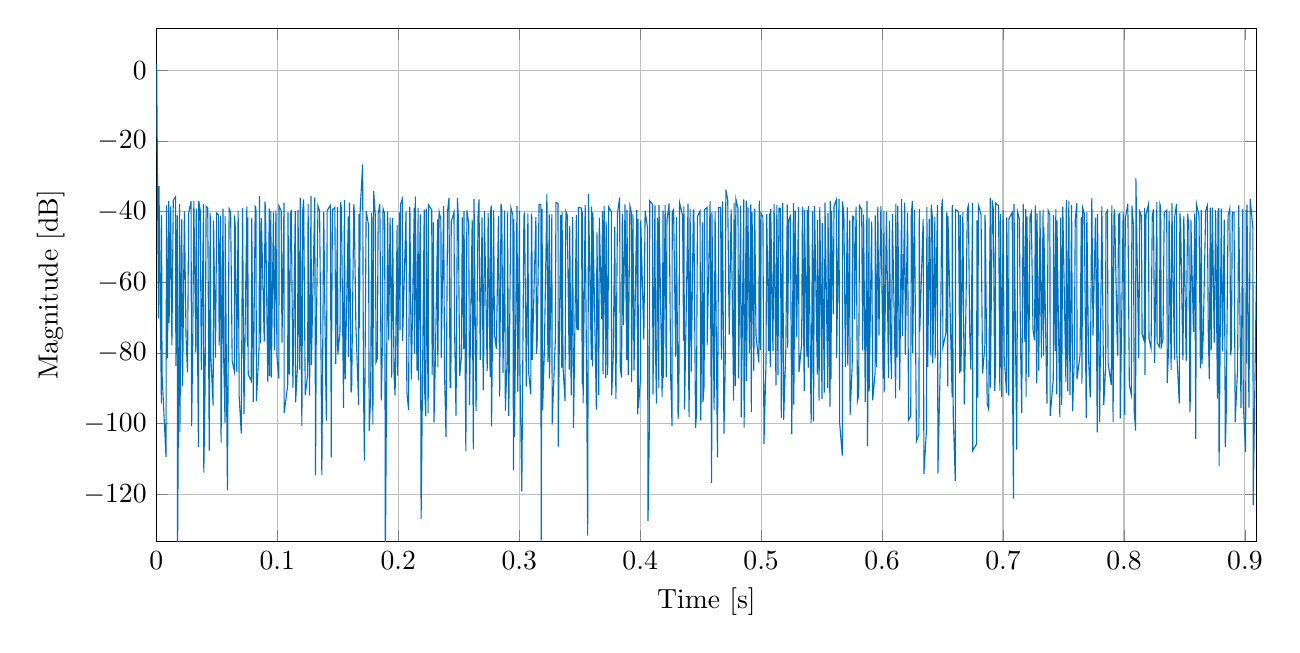
\begin{tikzpicture}

\begin{axis}[%
width=5.5in,
height=2.566in,
at={(1.011in,0.642in)},
scale only axis,
xmin=0,
xmax=0.909501157382829,
xlabel={Time [s]},
xmajorgrids,
ymin=-133.30576545487,
ymax=11.9377980263325,
ylabel={Magnitude [dB]},
ymajorgrids,
axis background/.style={fill=white}
]
\addplot [color=mycolor1,solid,forget plot]
  table[row sep=crcr]{%
2.08333333333333e-05	-18.5519458129197\\
0.000208333333333333	1.92539769599749\\
0.00177083333333333	-70.1603862246774\\
0.00214583333333333	-32.7755287161136\\
0.00414583333333333	-94.2039252922149\\
0.00425	-40.937136376685\\
0.0046875	-85.8576069217865\\
0.0079375	-109.443620754154\\
0.00835416666666667	-38.1735294294771\\
0.00916666666666666	-81.4931547383952\\
0.01025	-36.9188350195504\\
0.0105208333333333	-71.4490253797064\\
0.0117916666666667	-38.4657885523865\\
0.0128125	-77.8310259548471\\
0.0139583333333333	-36.7790803207063\\
0.0159375	-35.7328928819346\\
0.0160833333333333	-83.6559571178864\\
0.01725	-41.0564246121295\\
0.017375	-144.065730588413\\
0.01925	-37.8317742488666\\
0.0194166666666667	-102.302420647262\\
0.021	-42.152363374592\\
0.0216666666666667	-89.3708905790356\\
0.0231666666666667	-39.8666078787254\\
0.0245416666666667	-75.7739541606529\\
0.0257291666666667	-85.4501841971595\\
0.0266666666666667	-40.4847052853472\\
0.0286458333333333	-37.0383638272739\\
0.0291458333333333	-100.660893560172\\
0.0300416666666667	-77.5148953989813\\
0.0309791666666667	-37.0221544967549\\
0.0326041666666667	-79.8689106601384\\
0.0330208333333333	-39.1308984937248\\
0.0347708333333333	-106.619497504417\\
0.0350208333333333	-36.9534780867009\\
0.03625	-39.5601103166182\\
0.0371875	-84.7942671834041\\
0.039	-37.8319014794298\\
0.0392083333333333	-113.835135093588\\
0.04025	-89.9257433918166\\
0.041125	-38.4359650540914\\
0.0424583333333333	-38.9095750373776\\
0.0437083333333333	-107.619970946951\\
0.0444791666666667	-40.4042542428031\\
0.0450625	-81.3311365064353\\
0.0469166666666667	-94.871995489909\\
0.0472708333333333	-42.5478400826045\\
0.0488541666666667	-81.2951015639022\\
0.049875	-40.3789126640023\\
0.0514375	-40.9625024706217\\
0.0518958333333333	-77.8922447953147\\
0.0531041666666667	-41.1125814876897\\
0.0534791666666667	-105.326864459303\\
0.0551041666666667	-39.1343332695279\\
0.0555625	-79.9562902929538\\
0.05675	-99.6562063375615\\
0.0568333333333333	-41.1408366202979\\
0.0587291666666667	-118.891927281385\\
0.0601458333333333	-39.164265855383\\
0.0613958333333333	-40.1095329904576\\
0.0626666666666667	-82.2298735805108\\
0.0644791666666667	-85.1973195352917\\
0.0646041666666667	-41.0531409263032\\
0.0652083333333333	-44.1980673893767\\
0.0664375	-85.2648006235357\\
0.0676041666666667	-39.7043851806735\\
0.0684583333333333	-92.2958107049186\\
0.0701666666666667	-102.69741887225\\
0.0712708333333333	-38.9971559931263\\
0.0712916666666667	-39.4341769712974\\
0.0723958333333333	-97.2972675866287\\
0.0747916666666667	-38.5189936979077\\
0.0751875	-78.1420759625271\\
0.0755833333333333	-41.6641152901349\\
0.0759166666666667	-86.1185072316183\\
0.0783958333333333	-87.8708860539069\\
0.0788541666666667	-41.8695773136723\\
0.0800833333333333	-93.8566762953018\\
0.0817083333333333	-38.5518346331067\\
0.0823125	-38.9287186025732\\
0.0827083333333333	-93.5614636287424\\
0.0849791666666667	-77.9651015470257\\
0.08525	-35.5704772107062\\
0.0861875	-77.2725655898673\\
0.0868125	-41.7478277298816\\
0.0891875	-76.6659201437824\\
0.0898333333333333	-37.1351746837219\\
0.0902708333333333	-40.4229494005169\\
0.092125	-88.0532303913709\\
0.0933125	-39.1405580838697\\
0.0935	-86.4531210781812\\
0.0946666666666667	-39.7311011348484\\
0.095	-86.938561271714\\
0.0967916666666667	-40.2094562242789\\
0.097625	-79.1695550637616\\
0.0988333333333333	-39.6535226943175\\
0.0996875	-80.8665430625492\\
0.101270833333333	-87.2340606767671\\
0.101416666666667	-38.3878324811478\\
0.1031875	-39.6896466332173\\
0.103833333333333	-77.0114234373497\\
0.105520833333333	-37.4011628779268\\
0.105645833333333	-96.9248083658579\\
0.108583333333333	-89.1007168137127\\
0.108833333333333	-40.1892622078353\\
0.109854166666667	-86.0271437694726\\
0.110875	-40.8628790815478\\
0.1115625	-39.3968244038\\
0.112875	-89.8289307825964\\
0.114791666666667	-39.8460750953407\\
0.115104166666667	-93.9600436239974\\
0.116770833333333	-83.2846523215504\\
0.117104166666667	-39.4536010023525\\
0.1184375	-84.7155415760024\\
0.1189375	-36.0357770332561\\
0.120291666666667	-100.605878973077\\
0.121	-39.7626115569679\\
0.12175	-36.5277315927948\\
0.123083333333333	-91.8925912457902\\
0.125083333333333	-86.0069002253019\\
0.1254375	-37.7638916463909\\
0.126645833333333	-92.0506516990717\\
0.127854166666667	-36.002595951381\\
0.127895833333333	-35.5616156450669\\
0.128166666666667	-83.3112971386849\\
0.130958333333333	-36.0074671324157\\
0.131604166666667	-114.639241003581\\
0.132104166666667	-78.3521620013735\\
0.133604166666667	-38.3892047519009\\
0.1349375	-39.7505925314839\\
0.136166666666667	-82.5366294897913\\
0.136791666666667	-114.479116839009\\
0.138333333333333	-40.8819255762054\\
0.138375	-40.0300447553866\\
0.139916666666667	-85.972307032475\\
0.1405625	-99.1218335626914\\
0.141208333333333	-39.6627047634243\\
0.143875	-38.1837280711641\\
0.144604166666667	-109.488316160022\\
0.1448125	-81.1645116758506\\
0.1455625	-39.4525872481346\\
0.147541666666667	-38.7934318818153\\
0.148291666666667	-83.0503845013964\\
0.149791666666667	-38.6093792808167\\
0.15	-80.470031349083\\
0.151833333333333	-73.9652682284012\\
0.152291666666667	-37.2497108168677\\
0.153020833333333	-39.2818849478755\\
0.15475	-95.4929577610174\\
0.155458333333333	-36.7228150125395\\
0.156104166666667	-87.4635235846184\\
0.1586875	-41.3046701177339\\
0.158791666666667	-81.1641771655577\\
0.159645833333333	-37.4208937063257\\
0.160958333333333	-91.1568616021483\\
0.161458333333333	-89.9481252128396\\
0.16325	-37.8460399953667\\
0.163604166666667	-39.7899057076119\\
0.1649375	-72.0238123934629\\
0.167208333333333	-94.7144074797787\\
0.167416666666667	-40.5804432002278\\
0.167895833333333	-72.9709447081701\\
0.168520833333333	-39.265112669484\\
0.170520833333333	-26.6089144260092\\
0.171229166666667	-89.7084969760235\\
0.172	-110.463105212536\\
0.173416666666667	-39.7507574009912\\
0.1754375	-43.9058088123113\\
0.1759375	-102.04637869479\\
0.177166666666667	-92.4673232206693\\
0.178	-40.2544966820231\\
0.179	-100.172307609017\\
0.179625	-34.1344510063303\\
0.181083333333333	-41.4445759840945\\
0.181604166666667	-82.6332070915429\\
0.1826875	-81.5603292944465\\
0.183354166666667	-40.6013724200535\\
0.18475	-37.8886411936322\\
0.185979166666667	-93.4174074767175\\
0.186770833333333	-79.5560249693621\\
0.187416666666667	-39.1102032468717\\
0.18875	-40.4324688427174\\
0.1893125	-140.733541730388\\
0.191208333333333	-39.8851016413234\\
0.192041666666667	-76.4292607494308\\
0.19325	-41.642954457088\\
0.194541666666667	-86.9498554772794\\
0.195270833333333	-41.7766112051138\\
0.196520833333333	-86.2960022336321\\
0.197375	-92.00899215264\\
0.199041666666667	-43.7372910332328\\
0.199416666666667	-86.4150664130923\\
0.200958333333333	-40.1620513878326\\
0.201375	-73.4978141166754\\
0.201958333333333	-37.7938156039302\\
0.203395833333333	-36.3573160215574\\
0.203541666666667	-76.5616855129958\\
0.2064375	-40.002129393822\\
0.207083333333333	-90.9400052952227\\
0.208479166666667	-96.0407404868127\\
0.209416666666667	-38.6008511461162\\
0.209604166666667	-38.9692511220409\\
0.2108125	-87.5254646023321\\
0.2131875	-38.9289008630415\\
0.213395833333333	-80.1467722562333\\
0.214104166666667	-35.6816137968429\\
0.2154375	-84.9650752226633\\
0.216416666666667	-38.9836704152263\\
0.216604166666667	-87.7329317627177\\
0.218166666666667	-40.717985149793\\
0.218875	-126.996234132076\\
0.2214375	-39.3713556069448\\
0.221666666666667	-89.6964206530872\\
0.222770833333333	-97.9004778198756\\
0.223166666666667	-39.1021798430602\\
0.224708333333333	-97.0764430046659\\
0.225020833333333	-38.0778748083058\\
0.227666666666667	-39.5009585315729\\
0.227979166666667	-86.1466356571933\\
0.229104166666667	-42.9927224382634\\
0.229520833333333	-99.6132169124897\\
0.230791666666667	-79.4234995612674\\
0.232541666666667	-42.158273640218\\
0.2326875	-84.0628955060861\\
0.233729166666667	-39.9615553748445\\
0.23525	-42.262799810394\\
0.235520833333333	-81.2852130725869\\
0.237520833333333	-38.4161813468032\\
0.23825	-85.8012650101354\\
0.239458333333333	-103.72698898563\\
0.24075	-39.8010678303383\\
0.241916666666667	-36.148492433985\\
0.242833333333333	-89.7924672417965\\
0.2435	-89.8067417350762\\
0.243770833333333	-42.8889271004703\\
0.2460625	-40.1275959985789\\
0.246520833333333	-72.8884744837049\\
0.247729166666667	-97.7102209427758\\
0.248916666666667	-36.0941285336804\\
0.249666666666667	-41.6630361679321\\
0.250791666666667	-86.4166684087593\\
0.25225	-80.9124746106834\\
0.252895833333333	-41.5980949401672\\
0.2540625	-78.8240823970798\\
0.2543125	-39.8177791061036\\
0.255875	-107.79379629274\\
0.256729166666667	-39.6175522209742\\
0.258270833333333	-43.3900786727938\\
0.258875	-94.7249452356543\\
0.261104166666667	-42.2296623542329\\
0.2616875	-87.792993048808\\
0.2620625	-107.282270255865\\
0.262645833333333	-36.4574502060463\\
0.264333333333333	-96.3567201545636\\
0.265958333333333	-40.963666145451\\
0.26675	-36.5395390806047\\
0.267770833333333	-81.9358654483685\\
0.269270833333333	-41.6032238519875\\
0.270208333333333	-90.4174319777921\\
0.270625	-80.7072355099148\\
0.271208333333333	-39.7748188534505\\
0.2735	-85.0693226265118\\
0.274291666666667	-40.3937549252189\\
0.275958333333333	-86.7633189456565\\
0.276416666666667	-39.8411587420983\\
0.276854166666667	-38.2837840418311\\
0.277125	-100.733731918776\\
0.278854166666667	-39.6430347882809\\
0.2795	-74.5639571789028\\
0.281083333333333	-78.8230599033298\\
0.282833333333333	-41.1832392021198\\
0.2838125	-92.3017275688167\\
0.284979166666667	-37.7206234584216\\
0.285541666666667	-39.2020023825434\\
0.286625	-85.6219944283291\\
0.287895833333333	-39.6968695266362\\
0.288520833333333	-96.2528674278573\\
0.290104166666667	-80.7925579293698\\
0.290270833333333	-40.2163161634349\\
0.291354166666667	-97.7690084248421\\
0.293083333333333	-38.9136973506643\\
0.2946875	-40.8545803330415\\
0.295229166666667	-113.182317786221\\
0.295604166666667	-42.0727200092989\\
0.2960625	-103.777347073589\\
0.298145833333333	-38.337584779916\\
0.2988125	-90.9289405130424\\
0.300208333333333	-39.7155589309264\\
0.300604166666667	-84.6486993001228\\
0.302125	-119.143309363737\\
0.303854166666667	-41.5119754328531\\
0.304375	-40.2160138873198\\
0.305854166666667	-89.4840781033843\\
0.307166666666667	-40.5635624119636\\
0.3078125	-85.4964070109569\\
0.309541666666667	-91.6514964090626\\
0.310104166666667	-40.5194892341828\\
0.3104375	-41.7279521307518\\
0.31075	-81.9498625639673\\
0.313791666666667	-41.4760794213002\\
0.31425	-80.2485585228151\\
0.3148125	-77.54926828102\\
0.316395833333333	-37.868568111886\\
0.317895833333333	-37.9746795069449\\
0.318125	-136.867055241369\\
0.318916666666667	-39.1867473022683\\
0.3193125	-96.2142634309003\\
0.32075	-79.7038631114778\\
0.3226875	-39.6718212574338\\
0.322875	-34.9704785908527\\
0.323708333333333	-82.490514686653\\
0.324854166666667	-40.7215437630269\\
0.325020833333333	-87.2442561174805\\
0.326979166666667	-40.6918269187182\\
0.3271875	-100.230545414694\\
0.329916666666667	-75.6241194838397\\
0.330333333333333	-37.3860711814989\\
0.332083333333333	-37.6377314832304\\
0.332208333333333	-106.482624913093\\
0.334291666666667	-40.9822792844436\\
0.3351875	-84.1351725644322\\
0.335416666666667	-39.9807627613998\\
0.336270833333333	-84.3331634037219\\
0.337854166666667	-93.5102464073059\\
0.338541666666667	-39.8172812903417\\
0.3396875	-40.9503989009083\\
0.341354166666667	-84.6758058560744\\
0.341708333333333	-44.0924729633176\\
0.342979166666667	-91.9295567111102\\
0.344166666666667	-41.5516086602344\\
0.344895833333333	-101.220224948957\\
0.34725	-40.8587709928467\\
0.347604166666667	-73.2443764352243\\
0.348770833333333	-73.2866618158449\\
0.348895833333333	-38.7850386095434\\
0.3515625	-38.9815020811938\\
0.3520625	-88.8304098126741\\
0.352229166666667	-39.9875652933293\\
0.3528125	-94.2411286899172\\
0.354520833333333	-38.1117290508548\\
0.355854166666667	-93.7774834458075\\
0.356583333333333	-131.67319094515\\
0.35725	-34.9225434513354\\
0.359604166666667	-82.019059155403\\
0.359875	-38.5763608591608\\
0.360666666666667	-83.7798645305802\\
0.360875	-40.1655505837337\\
0.363770833333333	-95.9899251437898\\
0.364229166666667	-45.8760743341006\\
0.365791666666667	-91.8967383052743\\
0.366229166666667	-41.6518567154203\\
0.368125	-70.3823123272871\\
0.368854166666667	-39.8134481905917\\
0.3693125	-85.9333474988602\\
0.370208333333333	-38.4196915678677\\
0.371541666666667	-87.0937414853576\\
0.371875	-42.7601494812342\\
0.373104166666667	-86.1662281229103\\
0.374	-38.676505503304\\
0.376166666666667	-39.9418840680561\\
0.376416666666667	-91.9891230304143\\
0.377708333333333	-81.2850267207748\\
0.378958333333333	-44.2303663482864\\
0.379916666666667	-93.0013578543329\\
0.381229166666667	-40.495743253135\\
0.383020833333333	-35.9583633868101\\
0.383520833333333	-84.1316030248177\\
0.384604166666667	-86.9351340627978\\
0.38525	-40.6112053917763\\
0.386125	-72.0727651424295\\
0.387458333333333	-37.9041036783284\\
0.388875	-81.9883428778861\\
0.389083333333333	-39.4781894216104\\
0.390145833333333	-86.1808043446734\\
0.391479166666667	-38.2901213955772\\
0.392708333333333	-40.1525210811167\\
0.392916666666667	-88.227436398148\\
0.394	-40.6541841666974\\
0.394895833333333	-84.921011786896\\
0.397166666666667	-39.5618442683531\\
0.397958333333333	-97.3733128971764\\
0.398208333333333	-42.0734194913552\\
0.398541666666667	-95.494926296263\\
0.400354166666667	-86.8954814633943\\
0.400479166666667	-42.5057085197186\\
0.403020833333333	-76.1724867862787\\
0.404083333333333	-39.6999221288095\\
0.406020833333333	-44.4826788485566\\
0.4065	-127.496974294598\\
0.407625	-100.422577180789\\
0.407916666666667	-36.9181865618281\\
0.410166666666667	-37.837658766713\\
0.410583333333333	-91.7025580839976\\
0.412208333333333	-38.1773610763131\\
0.412604166666667	-77.5035863447671\\
0.413479166666667	-94.2779973244169\\
0.41425	-41.8354302445097\\
0.415458333333333	-89.9190670851578\\
0.4155625	-38.0957544908307\\
0.418166666666667	-92.4804116340837\\
0.418916666666667	-39.6031593191507\\
0.419145833333333	-87.0288942895487\\
0.420645833333333	-38.1531811305805\\
0.421541666666667	-86.7316296161424\\
0.422145833333333	-42.4267572015402\\
0.4239375	-37.6196509976512\\
0.425270833333333	-87.4446139334439\\
0.426333333333333	-100.569850808683\\
0.4265	-40.1265225872729\\
0.427625	-39.4050345816337\\
0.429395833333333	-81.0285452009466\\
0.4299375	-41.4563746975929\\
0.431354166666667	-98.680663037348\\
0.431979166666667	-92.8716283347021\\
0.4325625	-37.4293167916217\\
0.435083333333333	-41.1418407679941\\
0.435875	-76.4625005695416\\
0.436166666666667	-38.5035777906401\\
0.4366875	-95.9376900138429\\
0.4395625	-37.7129437041122\\
0.440083333333333	-87.128874655675\\
0.440458333333333	-98.138908350686\\
0.441270833333333	-39.226757270146\\
0.44225	-85.2818856844334\\
0.443958333333333	-39.7055724887729\\
0.444375	-39.5253703254221\\
0.445791666666667	-101.207955693588\\
0.446541666666667	-97.3485417599858\\
0.447333333333333	-41.3358341452998\\
0.449458333333333	-39.8290179284368\\
0.450125	-99.1010001877193\\
0.4515	-42.9790510172649\\
0.451979166666667	-93.8316777232727\\
0.452895833333333	-89.0039230330174\\
0.453125	-39.4279103731454\\
0.45525	-38.7609251890973\\
0.455354166666667	-77.790076708499\\
0.457833333333333	-37.0105869406248\\
0.458854166666667	-103.283116485568\\
0.459104166666667	-116.748544725155\\
0.4593125	-40.0971066172858\\
0.461145833333333	-96.1555952328105\\
0.4619375	-39.9342314200293\\
0.463895833333333	-109.501051807726\\
0.464875	-38.7708281432913\\
0.466541666666667	-38.80737325949\\
0.467125	-81.8784226484083\\
0.468083333333333	-37.038866500281\\
0.46925	-102.831727921838\\
0.470270833333333	-85.0419620171016\\
0.470833333333333	-33.6772187853824\\
0.472395833333333	-36.7323187448792\\
0.473645833333333	-74.8037947177818\\
0.473645833333333	-74.8037947177818\\
0.475208333333333	-39.3617514519483\\
0.477270833333333	-93.4470987818952\\
0.477645833333333	-37.5029920390723\\
0.478604166666667	-89.3704731439734\\
0.479104166666667	-36.3643669700059\\
0.480875	-39.1156882345895\\
0.481333333333333	-87.1395347131075\\
0.4830625	-38.2569466776592\\
0.483604166666667	-98.182037466741\\
0.485625	-36.5383943090647\\
0.485916666666667	-101.131062012879\\
0.48775	-36.8639553208213\\
0.4879375	-87.9082254159106\\
0.489104166666667	-38.7644565153836\\
0.4903125	-79.9538902643724\\
0.4914375	-37.8897349005114\\
0.491895833333333	-96.6119952715944\\
0.4925	-40.1463695665761\\
0.493958333333333	-85.0760830510269\\
0.494708333333333	-39.1098397838743\\
0.495770833333333	-75.0742274208545\\
0.498041666666667	-82.6002284176467\\
0.4985	-36.8901192660254\\
0.499354166666667	-79.0603897391184\\
0.4998125	-40.357929172175\\
0.501479166666667	-41.451273306936\\
0.502354166666667	-105.697150281101\\
0.504041666666667	-82.4937036152583\\
0.504625	-40.6030196955517\\
0.506333333333333	-79.4696138793462\\
0.506916666666667	-40.4830783119711\\
0.507604166666667	-83.9700591688104\\
0.5079375	-39.2823445596943\\
0.509770833333333	-79.3683528834792\\
0.510729166666667	-37.8590991606617\\
0.51225	-89.1454699302435\\
0.513	-38.0379091498598\\
0.513916666666667	-86.2614871619675\\
0.51475	-38.9690092596146\\
0.5159375	-38.9974359234524\\
0.516708333333333	-98.4412501401818\\
0.517854166666667	-37.5663101902781\\
0.518625	-98.8793651879842\\
0.520416666666667	-79.0613463087693\\
0.521604166666667	-38.0195909601984\\
0.5219375	-78.4527973935836\\
0.5228125	-42.2733705929402\\
0.524208333333333	-41.1861018428255\\
0.525333333333333	-102.957641984429\\
0.526708333333333	-37.5628183180842\\
0.527	-94.5674794727404\\
0.5281875	-39.6276740882188\\
0.529375	-75.5601212976844\\
0.530916666666667	-38.6542532609419\\
0.5313125	-85.403744250074\\
0.533520833333333	-77.1722917788878\\
0.534145833333333	-38.5370299504047\\
0.535645833333333	-90.7159441515188\\
0.535770833333333	-39.5069233287146\\
0.537833333333333	-81.0290936131987\\
0.538083333333333	-39.4690336061202\\
0.538958333333333	-84.153884431637\\
0.539125	-38.4372002902817\\
0.541375	-99.7949873485589\\
0.542479166666667	-39.9319634440244\\
0.543333333333333	-99.3218107983108\\
0.544166666666667	-38.3202956063783\\
0.546479166666667	-86.0196047056856\\
0.546625	-42.3648052337595\\
0.547916666666667	-93.4832519758737\\
0.548520833333333	-38.6785368264875\\
0.550333333333333	-92.9802152466514\\
0.5505625	-43.1502285043747\\
0.55225	-91.2271494323339\\
0.5528125	-37.4311135405672\\
0.555083333333333	-89.8399465362492\\
0.555333333333333	-40.337755173435\\
0.556895833333333	-95.2283867519557\\
0.5571875	-37.0197105621256\\
0.557833333333333	-87.3989090763514\\
0.5581875	-39.7108103949695\\
0.559666666666667	-68.9497995241304\\
0.560270833333333	-38.4731857584219\\
0.562208333333333	-36.5821455190372\\
0.562416666666667	-81.3464809688391\\
0.564354166666667	-36.3979231050756\\
0.564958333333333	-99.9006519866077\\
0.567104166666667	-108.989048820243\\
0.567270833333333	-37.0990609668967\\
0.5684375	-40.8022936132651\\
0.569708333333333	-83.9584125758893\\
0.571291666666667	-38.795800865228\\
0.571666666666667	-83.4760342323014\\
0.573270833333333	-42.4139191415011\\
0.573541666666667	-97.4866723176109\\
0.575291666666667	-83.6152454931914\\
0.5754375	-41.2371194394115\\
0.576604166666667	-41.4668733549324\\
0.577166666666667	-70.2960501311493\\
0.578520833333333	-38.5392808575731\\
0.579666666666667	-93.5142741636251\\
0.580645833333333	-91.8839441584857\\
0.581375	-38.3100246454374\\
0.583145833333333	-39.4003559053919\\
0.583916666666667	-79.2224618007119\\
0.584729166666667	-40.8418417529028\\
0.586104166666667	-93.8315218661244\\
0.5875	-36.8997409895559\\
0.587979166666667	-106.309309043272\\
0.589208333333333	-41.8910809538951\\
0.5893125	-90.8688712619423\\
0.591395833333333	-42.7824094417152\\
0.592229166666667	-93.3858682413908\\
0.594208333333333	-85.7069982247785\\
0.594375	-41.024240427591\\
0.595458333333333	-83.8835305287129\\
0.596479166666667	-38.6344192908362\\
0.597416666666667	-74.9938646818124\\
0.599020833333333	-38.3253717824733\\
0.600895833333333	-87.2385420533957\\
0.601479166666667	-42.1462759862716\\
0.601520833333333	-39.7572161274307\\
0.601729166666667	-91.1460099529221\\
0.603645833333333	-39.9430137235012\\
0.605291666666667	-87.1177461203978\\
0.6060625	-42.5417488136257\\
0.607145833333333	-79.4808869291236\\
0.607833333333333	-87.3299256788498\\
0.608520833333333	-40.6832554396696\\
0.61125	-92.8175448470858\\
0.611354166666667	-37.7162470175778\\
0.612291666666667	-81.2578802435115\\
0.612979166666667	-38.3586770471841\\
0.614541666666667	-90.4458980027452\\
0.616145833333333	-36.8229407758053\\
0.616166666666667	-36.4266982544642\\
0.6168125	-75.195393627225\\
0.6186875	-37.4280928935563\\
0.619208333333333	-80.5241644290071\\
0.621104166666667	-40.2705379937402\\
0.621854166666667	-99.0626732779895\\
0.623708333333333	-97.8406029390755\\
0.624166666666667	-40.6520610077108\\
0.625041666666667	-37.0348221962186\\
0.625333333333333	-79.9429341366681\\
0.626770833333333	-39.5153948957343\\
0.6284375	-104.936848366767\\
0.630458333333333	-103.002766875157\\
0.630791666666667	-39.2209106587769\\
0.6308125	-39.478031005054\\
0.631166666666667	-73.9447829166792\\
0.633979166666667	-42.0841563334352\\
0.634604166666667	-114.214606595983\\
0.636729166666667	-101.572253069571\\
0.637020833333333	-38.6957578215501\\
0.637791666666667	-83.978053199107\\
0.638979166666667	-42.0294618827033\\
0.6403125	-80.8322120909189\\
0.640708333333333	-38.0236136616195\\
0.64175	-42.3238390562986\\
0.641916666666667	-82.8781700293387\\
0.643666666666667	-41.43737431798\\
0.643875	-81.4863088280219\\
0.645770833333333	-38.1151521040696\\
0.646166666666667	-114.08726403865\\
0.6481875	-81.8572571194842\\
0.649333333333333	-38.5821360123073\\
0.649895833333333	-36.3841451982201\\
0.650291666666667	-78.4507793060964\\
0.6528125	-74.1490516976775\\
0.653520833333333	-40.0887237333137\\
0.654270833333333	-89.4399001846448\\
0.6544375	-41.1440386273384\\
0.6579375	-92.4561544595549\\
0.6580625	-38.7320114978642\\
0.658083333333333	-38.1483825054083\\
0.658833333333333	-97.7115283300828\\
0.660541666666667	-116.176753492649\\
0.660770833333333	-39.3916080995112\\
0.6631875	-39.9561464170493\\
0.664229166666667	-85.7545292822313\\
0.664604166666667	-40.8724666838331\\
0.665270833333333	-85.1929654575478\\
0.666791666666667	-40.0336389666483\\
0.667979166666667	-94.4934821639409\\
0.668854166666667	-78.2519084318803\\
0.670520833333333	-39.2766323445712\\
0.671395833333333	-38.2433692709539\\
0.672416666666667	-74.1517098821129\\
0.673395833333333	-84.6701583284909\\
0.674791666666667	-37.5039301574514\\
0.6748125	-37.7110752951995\\
0.674979166666667	-107.570077774941\\
0.678145833333333	-105.733637442431\\
0.6784375	-42.4369547966443\\
0.679083333333333	-92.5945501278665\\
0.679645833333333	-38.1390399156639\\
0.681833333333333	-40.7235543791211\\
0.683104166666667	-85.8172739120833\\
0.684958333333333	-77.9053983489696\\
0.685083333333333	-40.9317636803235\\
0.685395833333333	-43.9478147988212\\
0.686875	-94.2215634817998\\
0.688145833333333	-95.9170956342443\\
0.689458333333333	-36.0517989650941\\
0.689583333333333	-89.7934535423999\\
0.691125	-36.8256184227107\\
0.692020833333333	-39.3721616565238\\
0.693125	-90.7398925601833\\
0.693729166666667	-85.3549625090318\\
0.693854166666667	-37.5367384285292\\
0.696333333333333	-38.3025302061292\\
0.697375	-90.592819394928\\
0.697958333333333	-40.6545526323442\\
0.6989375	-92.4447730958734\\
0.700083333333333	-39.5292796473989\\
0.7009375	-80.8971723415075\\
0.702916666666667	-91.3280518350503\\
0.703104166666667	-41.6259435787519\\
0.704708333333333	-92.0357140300499\\
0.704895833333333	-41.974064181003\\
0.707645833333333	-40.2093306791106\\
0.707875	-88.639834299551\\
0.708645833333333	-121.171908778608\\
0.7090625	-37.7805608539091\\
0.711354166666667	-107.355958720792\\
0.712125	-40.1524339536619\\
0.713520833333333	-41.996433152329\\
0.714375	-75.1228320300795\\
0.7154375	-96.9822767732894\\
0.716666666666667	-37.7464312297637\\
0.718041666666667	-76.8706537892161\\
0.718770833333333	-39.2415520019293\\
0.7190625	-92.4824609893658\\
0.719791666666667	-41.3365608710063\\
0.721270833333333	-86.7989907926971\\
0.722291666666667	-41.4996914316665\\
0.723333333333333	-40.1956582817282\\
0.724791666666667	-73.4241014216226\\
0.726083333333333	-76.4152290219056\\
0.726708333333333	-38.1678651924068\\
0.727833333333333	-88.5675862913728\\
0.728083333333333	-40.4552432353343\\
0.729541666666667	-84.9581575838772\\
0.730583333333333	-39.6544183915779\\
0.731770833333333	-81.2920096784526\\
0.733145833333333	-39.4340877266037\\
0.733583333333333	-80.7458643829003\\
0.733729166666667	-44.2857506768594\\
0.736333333333333	-94.2955985514896\\
0.737291666666667	-39.665986786328\\
0.73875	-40.8812021272261\\
0.739020833333333	-97.7704889077812\\
0.7415625	-87.2753708039384\\
0.741708333333333	-40.9163980092905\\
0.743083333333333	-79.4796013373268\\
0.743666666666667	-39.2665747437839\\
0.744375	-91.7205212264697\\
0.744583333333333	-42.4768116193546\\
0.746979166666667	-98.0702535489662\\
0.747770833333333	-41.6991360539842\\
0.748479166666667	-94.6658870719847\\
0.749395833333333	-38.5681509960618\\
0.751979166666667	-88.1154906155696\\
0.752333333333333	-36.6711480352312\\
0.7535	-90.834675302022\\
0.754416666666667	-36.9439707297046\\
0.754458333333333	-38.8676959297517\\
0.755375	-91.8298073731391\\
0.756708333333333	-38.1504966650943\\
0.757541666666667	-96.5047858665326\\
0.758979166666667	-80.4195986770202\\
0.759708333333333	-42.3059728297332\\
0.761041666666667	-37.5794998746318\\
0.761166666666667	-87.4454962421115\\
0.7636875	-80.51292313221\\
0.764729166666667	-41.4627817098876\\
0.765229166666667	-88.6231222677961\\
0.7659375	-38.9592213721365\\
0.767208333333333	-40.5774031778598\\
0.768791666666667	-98.3832730242057\\
0.769291666666667	-40.1276283825102\\
0.770729166666667	-81.5839800494563\\
0.772104166666667	-92.5353541395512\\
0.77325	-40.1854817818878\\
0.7734375	-36.1535882236327\\
0.774416666666667	-74.9596655326303\\
0.7764375	-41.6395205745018\\
0.7773125	-74.4650105310253\\
0.777895833333333	-102.465964412675\\
0.778104166666667	-40.7120109348476\\
0.779875	-99.4988863230729\\
0.781708333333333	-38.4839351610243\\
0.781708333333333	-38.4839351610243\\
0.783291666666667	-94.6584023209256\\
0.784875	-83.7452368224103\\
0.785020833333333	-40.5187628221932\\
0.7863125	-39.6287460358398\\
0.786895833333333	-82.9622863812346\\
0.789479166666667	-88.995374325957\\
0.789958333333333	-38.1845654225587\\
0.791020833333333	-99.5777344436287\\
0.7916875	-41.0641410687642\\
0.792270833333333	-39.3688892836312\\
0.794270833333333	-74.7684900657199\\
0.794833333333333	-80.7036106653803\\
0.795458333333333	-40.8576897254155\\
0.796479166666667	-40.4858771336884\\
0.796958333333333	-98.4734034772432\\
0.799333333333333	-40.1177810692973\\
0.800270833333333	-75.4574530521049\\
0.8006875	-97.4577439839463\\
0.8010625	-42.0915803833131\\
0.803208333333333	-37.7398681536672\\
0.8044375	-89.1026964884332\\
0.806104166666667	-91.8674560039533\\
0.8065625	-38.3066227267756\\
0.807833333333333	-43.9371240041745\\
0.808520833333333	-96.7717969926416\\
0.809645833333333	-101.942605335204\\
0.809854166666667	-30.4592876073145\\
0.81225	-81.4550278070925\\
0.8130625	-39.966701725523\\
0.814479166666667	-41.2068537777228\\
0.8149375	-74.5881510445493\\
0.81675	-76.604039621247\\
0.817104166666667	-38.8752641510018\\
0.817375	-86.1783912376173\\
0.8181875	-40.8634727252093\\
0.820270833333333	-37.9116956471208\\
0.820666666666667	-75.9292357860142\\
0.822416666666667	-78.616714235556\\
0.823375	-41.2763636457455\\
0.824416666666667	-39.2664696822843\\
0.825333333333333	-82.7904869477106\\
0.827229166666667	-37.2215255807731\\
0.827354166666667	-76.9517419200047\\
0.829520833333333	-78.3196285322227\\
0.829708333333333	-37.8515627385455\\
0.8303125	-38.6543949053419\\
0.830875	-78.1507694215504\\
0.832229166666667	-76.1925354447128\\
0.833291666666667	-40.2479323356604\\
0.835354166666667	-39.5959250051416\\
0.835791666666667	-88.5237545358829\\
0.837	-77.4706927799484\\
0.837291666666667	-40.0047470126975\\
0.839	-84.7604719276938\\
0.839625	-37.5900727675604\\
0.841770833333333	-81.8358853059143\\
0.841916666666667	-41.4148235758368\\
0.843479166666667	-37.8123994947326\\
0.843645833333333	-79.8243867859832\\
0.845708333333333	-94.21637534383\\
0.846208333333333	-40.4067246466654\\
0.8468125	-42.6826821934267\\
0.848708333333333	-81.9494214780407\\
0.848916666666667	-77.4738609466288\\
0.849479166666667	-41.2421266062733\\
0.8514375	-82.2627463531598\\
0.852604166666667	-40.5783513789877\\
0.853625	-43.9660344176693\\
0.854479166666667	-96.7733652210768\\
0.855083333333333	-90.7804088139027\\
0.855333333333333	-42.2910263327225\\
0.857458333333333	-73.9823785852907\\
0.858458333333333	-40.5459482682283\\
0.859375	-104.271831283688\\
0.859875	-37.7197207033535\\
0.862041666666667	-41.1535886922339\\
0.8631875	-84.3312416901983\\
0.863895833333333	-39.5700885708829\\
0.864479166666667	-83.1505380532012\\
0.865541666666667	-74.8146676957678\\
0.867541666666667	-39.7861630903924\\
0.868916666666667	-38.2680136850028\\
0.869708333333333	-74.0029144689715\\
0.8705625	-87.4015040472511\\
0.871354166666667	-38.8683267551729\\
0.872104166666667	-79.1841076483546\\
0.8730625	-38.8143823383311\\
0.874645833333333	-77.0769145344433\\
0.875770833333333	-39.4701451770875\\
0.877270833333333	-92.8727359387883\\
0.877645833333333	-40.253333046866\\
0.878354166666667	-39.0080468149117\\
0.878625	-112.023287286641\\
0.880479166666667	-39.0915731777199\\
0.8815	-79.5466166274704\\
0.882916666666667	-42.2242134491667\\
0.883791666666667	-106.641735271173\\
0.8845	-97.6070536512505\\
0.886083333333333	-41.0679659021751\\
0.8875	-39.1591889069521\\
0.888208333333333	-80.4790500160969\\
0.888833333333333	-78.6198212336751\\
0.889583333333333	-40.0737008696579\\
0.891	-40.2598662368525\\
0.891979166666667	-99.5347300791249\\
0.893916666666667	-84.4680628458825\\
0.894854166666667	-38.184768555207\\
0.894854166666667	-38.184768555207\\
0.89675	-95.5465205979583\\
0.8981875	-39.2969765034855\\
0.898625	-94.1697437567004\\
0.9005625	-108.030342766262\\
0.901125	-39.5671391789175\\
0.901354166666667	-82.9182735407195\\
0.901708333333333	-37.9652570239158\\
0.903333333333333	-95.4147578163748\\
0.904416666666667	-36.4385446382558\\
0.906583333333333	-44.8442546801874\\
0.906833333333333	-123.027755955478\\
0.909520833333333	-57.7503621067594\\
};
\end{axis}
\end{tikzpicture}%
	\caption{Time decay plot of the cancellation path}
	\label{TimeDecayPlotCancellationPath}
\end{figure}


Taking the first 256 coefficients of the impulse response gives the following cropped impulse response, as seen on \autoref{CancellationPathImpulseResponseCrop}.

\begin{figure}[H]
	\centering
	\tikzsetnextfilename{CancellationPathImpulseResponseCrop1}
	%% This file was created by matlab2tikz.
%
%The latest updates can be retrieved from
%  http://www.mathworks.com/matlabcentral/fileexchange/22022-matlab2tikz-matlab2tikz
%where you can also make suggestions and rate matlab2tikz.
%
\definecolor{mycolor1}{rgb}{0.00000,0.44700,0.74100}%
\definecolor{mycolor2}{rgb}{0.85000,0.32500,0.09800}%
\definecolor{mycolor3}{rgb}{0.92900,0.69400,0.12500}%
\definecolor{mycolor4}{rgb}{0.49400,0.18400,0.55600}%
\definecolor{mycolor5}{rgb}{0.46600,0.67400,0.18800}%
%
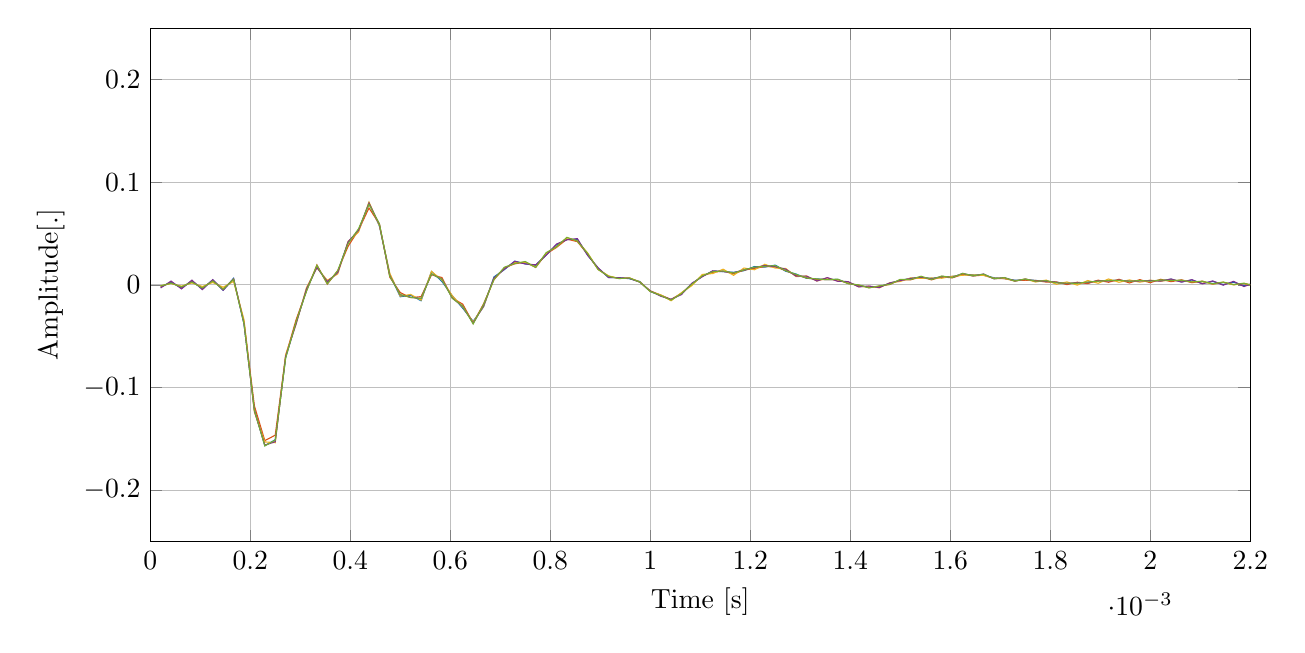
\begin{tikzpicture}

\begin{axis}[%
width=5.5in,
height=2.566in,,
at={(1.011in,0.642in)},
scale only axis,
xmin=0,
xmax=0.0022,
xlabel={Time [s]},
xmajorgrids,
ymin=-0.25,
ymax=0.25,
ylabel={Amplitude[.]},
ymajorgrids,
axis background/.style={fill=white}
]
\addplot [color=mycolor1,solid,forget plot]
  table[row sep=crcr]{%
2.08333333333333e-05	-0.00218389910452928\\
4.16666666666667e-05	0.00247997660818177\\
6.25e-05	-0.00306422212301669\\
8.33333333333333e-05	0.00370795824245389\\
0.000104166666666667	-0.003996195002872\\
0.000125	0.00477762315573945\\
0.000145833333333333	-0.00520610865886981\\
0.000166666666666667	0.00632845677938862\\
0.0001875	-0.0380783744937981\\
0.000208333333333333	-0.121478341280274\\
0.000229166666666667	-0.156732911171094\\
0.00025	-0.150962242221131\\
0.000270833333333333	-0.0708305555277822\\
0.000291666666666667	-0.0363422650083233\\
0.0003125	-0.00543127544862284\\
0.000333333333333333	0.0181597627718888\\
0.000354166666666667	0.00208472952849193\\
0.000375	0.0125098852556454\\
0.000395833333333333	0.0415416610429961\\
0.000416666666666667	0.0527294742213453\\
0.0004375	0.0798009720407638\\
0.000458333333333333	0.057294372226422\\
0.000479166666666667	0.0100967131822404\\
0.0005	-0.0116403016854475\\
0.000520833333333333	-0.0100823637366942\\
0.000541666666666667	-0.0155252345103445\\
0.0005625	0.0129409401256135\\
0.000583333333333333	0.00330032363608726\\
0.000604166666666667	-0.0107369621764369\\
0.000625	-0.0228446033217494\\
0.000645833333333333	-0.0356027778798783\\
0.000666666666666667	-0.0214218763506852\\
0.0006875	0.0077125374318295\\
0.000708333333333333	0.0148003772574559\\
0.000729166666666667	0.0230269782520459\\
0.00075	0.0204048345153605\\
0.000770833333333333	0.0189891037229106\\
0.000791666666666667	0.0290727336722823\\
0.0008125	0.0388997216505961\\
0.000833333333333333	0.0442340567889403\\
0.000854166666666667	0.0441885135919368\\
0.000875	0.0288044550629258\\
0.000895833333333333	0.0161368334943261\\
0.000916666666666667	0.00713579035783102\\
0.0009375	0.00701321180069818\\
0.000958333333333333	0.00593867000057454\\
0.000979166666666667	0.00320599481994303\\
0.001	-0.00664914273579044\\
0.00102083333333333	-0.0101565754892221\\
0.00104166666666667	-0.014791108741586\\
0.0010625	-0.00857239326708171\\
0.00108333333333333	0.00100898054712758\\
0.00110416666666667	0.00839401335783726\\
0.001125	0.0133984163005487\\
0.00114583333333333	0.0128466265171883\\
0.00116666666666667	0.0121549768071494\\
0.0011875	0.0137719317655377\\
0.00120833333333333	0.0178060477156998\\
0.00122916666666667	0.0172847958388615\\
0.00125	0.019210569641301\\
0.00127083333333333	0.013257709044026\\
0.00129166666666667	0.0104752301035351\\
0.0013125	0.00634204156049436\\
0.00133333333333333	0.00579198958498723\\
0.00135416666666667	0.00502590528864318\\
0.001375	0.00529722084283291\\
0.00139583333333333	0.00153242789497228\\
0.00141666666666667	-0.000616528502902794\\
0.0014375	-0.0021893619325514\\
0.00145833333333333	-0.00187817940983287\\
0.00147916666666667	0.00151654195426903\\
0.0015	0.00420310986639849\\
0.00152083333333333	0.00637222520912491\\
0.00154166666666667	0.00708169552640407\\
0.0015625	0.00637493155811143\\
0.00158333333333333	0.00726931533456736\\
0.00160416666666667	0.00819256235515286\\
0.001625	0.00995175279603157\\
0.00164583333333333	0.00976251303247071\\
0.00166666666666667	0.00936529201189556\\
0.0016875	0.00688403743977654\\
0.00170833333333333	0.00606358036924052\\
0.00172916666666667	0.00452676896305512\\
0.00175	0.004828792984279\\
0.00177083333333333	0.00430742388743505\\
0.00179166666666667	0.00318484065017087\\
0.0018125	0.00262913018197462\\
0.00183333333333333	0.000894527696839949\\
0.00185416666666667	0.00220727189527427\\
0.001875	0.00213064727283039\\
0.00189583333333333	0.00400580107200661\\
0.00191666666666667	0.00382018713412366\\
0.0019375	0.00453452462048207\\
0.00195833333333333	0.00348401578315948\\
0.00197916666666667	0.00385250692600261\\
0.002	0.00410399715905844\\
0.00202083333333333	0.00376669564103728\\
0.00204166666666667	0.005481403501254\\
0.0020625	0.00286984013341575\\
0.00208333333333333	0.00467110572913971\\
0.00210416666666667	0.00133891989308461\\
0.002125	0.00329198810788862\\
0.00214583333333333	0.000300140045619779\\
0.00216666666666667	0.00262574118790929\\
0.0021875	-0.000772552707238634\\
0.00220833333333333	0.001204895577724\\
0.00222916666666667	-0.00133487209486768\\
0.00225	-0.000509380400493588\\
0.00227083333333333	-0.000334737971901055\\
0.00229166666666667	-0.00103678981403972\\
0.0023125	0.00061906400962846\\
0.00233333333333333	-0.00138559528811041\\
0.00235416666666667	0.000836453989668149\\
0.002375	-0.00220070096737768\\
0.00239583333333333	0.00155059728767193\\
0.00241666666666667	-0.00246952128785161\\
0.0024375	0.00209771500748369\\
0.00245833333333333	-0.00201237551900768\\
0.00247916666666667	0.00136337042281452\\
0.0025	-0.0016996067640007\\
0.00252083333333333	0.000375559342336357\\
0.00254166666666667	-0.00171285649355793\\
0.0025625	-0.000370547864208922\\
0.00258333333333333	-0.00168478066288008\\
0.00260416666666667	-0.00164047511374893\\
0.002625	-0.00154391190477046\\
0.00264583333333333	-0.00279588952826178\\
0.00266666666666667	-0.00161937857228862\\
0.0026875	-0.00281948250550955\\
0.00270833333333333	-0.0019126329763031\\
0.00272916666666667	-0.00237053013971509\\
0.00275	-0.00216738565291799\\
0.00277083333333333	-0.00198477223131889\\
0.00279166666666667	-0.00218053262768701\\
0.0028125	-0.00109861342178239\\
0.00283333333333333	-0.00230003733690516\\
0.00285416666666667	-2.92964736988071e-05\\
0.002875	-0.00258103832251588\\
0.00289583333333333	0.000226343416296675\\
0.00291666666666667	-0.00266926986983911\\
0.0029375	-0.000193341868510947\\
0.00295833333333333	-0.00251045357924689\\
0.00297916666666667	-0.000754536531619725\\
0.003	-0.00243962671207192\\
0.00302083333333333	-0.00146416942230298\\
0.00304166666666667	-0.00213138690195344\\
0.0030625	-0.00235987025503001\\
0.00308333333333333	-0.00140117139661643\\
0.00310416666666667	-0.00302857105296522\\
0.003125	-0.000722072931201979\\
0.00314583333333333	-0.00321030960137844\\
0.00316666666666667	-0.00035915225761106\\
0.0031875	-0.00297374200868294\\
0.00320833333333333	3.53198342716556e-05\\
0.00322916666666667	-0.0026450468724363\\
0.00325	0.00032858441079607\\
0.00327083333333333	-0.00227789302909872\\
0.00329166666666667	0.000100083042602076\\
0.0033125	-0.00188361158529631\\
0.00333333333333333	-0.000395512602873454\\
0.00335416666666667	-0.00170533112866956\\
0.003375	-0.000671247588764808\\
0.00339583333333333	-0.00191528739109528\\
0.00341666666666667	-0.000801885905110417\\
0.0034375	-0.00212498021642428\\
0.00345833333333333	-0.000968435139872327\\
0.00347916666666667	-0.00218928107893563\\
0.0035	-0.000908900434101829\\
0.00352083333333333	-0.00237627772062559\\
0.00354166666666667	-0.000579630370778564\\
0.0035625	-0.00250519865369403\\
0.00358333333333333	-0.000396073310796909\\
0.00360416666666667	-0.00220304009472981\\
0.003625	-0.000551947219102873\\
0.00364583333333333	-0.0017461192389335\\
0.00366666666666667	-0.000768138137423014\\
0.0036875	-0.0014508385510616\\
0.00370833333333333	-0.00107362237419074\\
0.00372916666666667	-0.001022338035958\\
0.00375	-0.00167383565520242\\
0.00377083333333333	-0.000445481543758471\\
0.00379166666666667	-0.00226771972340852\\
0.0038125	-0.00017191447384072\\
0.00383333333333333	-0.0024910438469192\\
0.00385416666666667	-0.000222906421509958\\
0.003875	-0.00252208983413144\\
0.00389583333333333	-0.000239508055918544\\
0.00391666666666667	-0.00249900652928486\\
0.0039375	-0.00036819453953393\\
0.00395833333333333	-0.00215026444025682\\
0.00397916666666667	-0.00078767916054904\\
0.004	-0.00160104351722162\\
0.00402083333333333	-0.00116932694136055\\
0.00404166666666667	-0.00128993741065524\\
0.0040625	-0.00130037826319792\\
0.00408333333333333	-0.00120109343231604\\
0.00410416666666667	-0.00137738437947758\\
0.004125	-0.00108994636516787\\
0.00414583333333333	-0.0013930566895397\\
0.00416666666666667	-0.00115682928452173\\
0.0041875	-0.00112155535625298\\
0.00420833333333333	-0.0014747233687034\\
0.00422916666666667	-0.000756437573699205\\
0.00425	-0.00175061296711125\\
0.00427083333333333	-0.000584625454284746\\
0.00429166666666667	-0.00185462900166534\\
0.0043125	-0.0005346079858565\\
0.00433333333333333	-0.00193597084036407\\
0.00435416666666667	-0.00047838297960541\\
0.004375	-0.00194226459657353\\
0.00439583333333333	-0.000585028474139202\\
0.00441666666666667	-0.00174761669058415\\
0.0044375	-0.000800749743149818\\
0.00445833333333333	-0.00151735092894328\\
0.00447916666666667	-0.000883973934664968\\
0.0045	-0.0014537081327631\\
0.00452083333333333	-0.00075225814753293\\
0.00454166666666667	-0.00151365778473533\\
0.0045625	-0.000500860453977012\\
0.00458333333333333	-0.00164649690516529\\
0.00460416666666667	-9.96498374878968e-05\\
0.004625	-0.00195544375064587\\
0.00464583333333333	0.000449155256385712\\
0.00466666666666667	-0.00238322226588622\\
0.0046875	0.000954670191418131\\
0.00470833333333333	-0.00271709732406415\\
0.00472916666666667	0.00121675616537964\\
0.00475	-0.00282529785820646\\
0.00477083333333333	0.0011995722697696\\
0.00479166666666667	-0.00272018311514588\\
0.0048125	0.000933992660913407\\
0.00483333333333333	-0.00233183076857483\\
0.00485416666666667	0.00039448353507977\\
0.004875	-0.00163113482278814\\
0.00489583333333333	-0.000362090300491339\\
0.00491666666666667	-0.000779026479175463\\
0.0049375	-0.00112374188568124\\
0.00495833333333333	-2.39139304477267e-05\\
0.00497916666666667	-0.00169920199968603\\
0.005	0.000523981145438892\\
0.00502083333333333	-0.00205667911465618\\
0.00504166666666667	0.000812579724410437\\
0.0050625	-0.00210866993358576\\
0.00508333333333333	0.000741663856323763\\
0.00510416666666667	-0.00175541600420527\\
0.005125	0.000311014598016389\\
0.00514583333333333	-0.00112489985361012\\
0.00516666666666667	-0.000277561456628004\\
0.0051875	-0.000467680148606119\\
0.00520833333333333	-0.000833718285872148\\
0.00522916666666667	0.000113882903666011\\
0.00525	-0.00128561358966294\\
0.00527083333333333	0.000546530701225396\\
0.00529166666666667	-0.00148197183580008\\
0.0053125	0.000645564949214993\\
0.00533333333333333	-0.00126676793443997\\
};
\addplot [color=mycolor2,solid,forget plot]
  table[row sep=crcr]{%
2.08333333333333e-05	-0.00150312502349965\\
4.16666666666667e-05	0.00170740345175498\\
6.25e-05	-0.00225094460714062\\
8.33333333333333e-05	0.00283940474816698\\
0.000104166666666667	-0.00303627224888553\\
0.000125	0.00393115781364844\\
0.000145833333333333	-0.00417103313904593\\
0.000166666666666667	0.00544829804434176\\
0.0001875	-0.0357658099541969\\
0.000208333333333333	-0.118005245940072\\
0.000229166666666667	-0.151785228594567\\
0.00025	-0.1465046442558\\
0.000270833333333333	-0.0692755249179087\\
0.000291666666666667	-0.0340849194790308\\
0.0003125	-0.00600717417737366\\
0.000333333333333333	0.0194326766341735\\
0.000354166666666667	0.000751764670907603\\
0.000375	0.0137901515627398\\
0.000395833333333333	0.0376433591209333\\
0.000416666666666667	0.0533769204766715\\
0.0004375	0.0748560574116669\\
0.000458333333333333	0.0592590643629689\\
0.000479166666666667	0.00735497863182636\\
0.0005	-0.00756718413491506\\
0.000520833333333333	-0.0124975010055099\\
0.000541666666666667	-0.0115247016817554\\
0.0005625	0.00980021630720815\\
0.000583333333333333	0.00708498450188709\\
0.000604166666666667	-0.0129050270431849\\
0.000625	-0.0188519397068052\\
0.000645833333333333	-0.0372961949901686\\
0.000666666666666667	-0.01849297415842\\
0.0006875	0.00497121361236263\\
0.000708333333333333	0.0166422880218153\\
0.000729166666666667	0.020465656840568\\
0.00075	0.0220834588704114\\
0.000770833333333333	0.0169189373925576\\
0.000791666666666667	0.0299976968876195\\
0.0008125	0.0364130084818885\\
0.000833333333333333	0.044568512776588\\
0.000854166666666667	0.0420780402826822\\
0.000875	0.029754539044608\\
0.000895833333333333	0.0150431845354128\\
0.000916666666666667	0.00824248720676909\\
0.0009375	0.00622415686774906\\
0.000958333333333333	0.00657627207683757\\
0.000979166666666667	0.00275294759176985\\
0.001	-0.00591776430469594\\
0.00102083333333333	-0.00992032862922456\\
0.00104166666666667	-0.0143079250947841\\
0.0010625	-0.00817968654639674\\
0.00108333333333333	0.000480415578304432\\
0.00110416666666667	0.00871664889654762\\
0.001125	0.0122014686789311\\
0.00114583333333333	0.0133645741268153\\
0.00116666666666667	0.0106617261527092\\
0.0011875	0.0143050938208178\\
0.00120833333333333	0.0159709735280955\\
0.00122916666666667	0.0177759597607658\\
0.00125	0.0175080774703475\\
0.00127083333333333	0.013929522023107\\
0.00129166666666667	0.00934886109584583\\
0.0013125	0.00688718378449337\\
0.00133333333333333	0.00513304375912566\\
0.00135416666666667	0.00513013541241314\\
0.001375	0.0050914671922881\\
0.00139583333333333	0.00129193064715399\\
0.00141666666666667	-0.000282917718707061\\
0.0014375	-0.00281934226995237\\
0.00145833333333333	-0.00126138441418749\\
0.00147916666666667	0.000359735815132393\\
0.0015	0.00484238657500165\\
0.00152083333333333	0.00489602610432004\\
0.00154166666666667	0.0076699056302263\\
0.0015625	0.00486066045936765\\
0.00158333333333333	0.00771487566070934\\
0.00160416666666667	0.00677437856370931\\
0.001625	0.0101902062798796\\
0.00164583333333333	0.00864138380838661\\
0.00166666666666667	0.00945825376617475\\
0.0016875	0.00618394559018458\\
0.00170833333333333	0.00598757702781642\\
0.00172916666666667	0.00414812009692581\\
0.00175	0.0045110664355937\\
0.00177083333333333	0.00418394923554998\\
0.00179166666666667	0.00269472594072503\\
0.0018125	0.00276415130472775\\
0.00183333333333333	0.000237896245683422\\
0.00185416666666667	0.00252243208973511\\
0.001875	0.00116355425877345\\
0.00189583333333333	0.00450927287329329\\
0.00191666666666667	0.00249087692609324\\
0.0019375	0.00535707054015208\\
0.00195833333333333	0.00180650739266421\\
0.00197916666666667	0.00506128162830543\\
0.002	0.00204266833987498\\
0.00202083333333333	0.00538568566778509\\
0.00204166666666667	0.00306440643436911\\
0.0020625	0.00490161291817414\\
0.00208333333333333	0.00204275018470907\\
0.00210416666666667	0.00359422966353806\\
0.002125	0.000641060989892511\\
0.00214583333333333	0.00247273465336715\\
0.00216666666666667	0.000188366403795602\\
0.0021875	0.00106503791008099\\
0.00220833333333333	-0.000743232791695567\\
0.00222916666666667	-9.80423910744149e-05\\
0.00225	-0.00172025335400668\\
0.00227083333333333	3.22754464928352e-05\\
0.00229166666666667	-0.00136516805409886\\
0.0023125	3.54577907460388e-05\\
0.00233333333333333	-0.000833531371844218\\
0.00235416666666667	-0.000571016518356972\\
0.002375	-0.000914871697735422\\
0.00239583333333333	-0.000463641235510094\\
0.00241666666666667	-0.000699628193500556\\
0.0024375	-0.000207060477280922\\
0.00245833333333333	-0.000119120037095823\\
0.00247916666666667	-0.000826935127761463\\
0.0025	-8.74323159517523e-05\\
0.00252083333333333	-0.00134907159843868\\
0.00254166666666667	-0.000667319094028848\\
0.0025625	-0.00141492723378026\\
0.00258333333333333	-0.00130146454208995\\
0.00260416666666667	-0.00193027545826851\\
0.002625	-0.00181078489699197\\
0.00264583333333333	-0.00242308870916524\\
0.00266666666666667	-0.00238309244215445\\
0.0026875	-0.00205057795859767\\
0.00270833333333333	-0.00287830495327762\\
0.00272916666666667	-0.00155184139664161\\
0.00275	-0.00301640272753359\\
0.00277083333333333	-0.00140097068939183\\
0.00279166666666667	-0.00268935224529769\\
0.0028125	-0.000931645119052387\\
0.00283333333333333	-0.0023485886981718\\
0.00285416666666667	-0.000354079502987963\\
0.002875	-0.00217608672386252\\
0.00289583333333333	-0.000522557772579991\\
0.00291666666666667	-0.00196011839114989\\
0.0029375	-0.00115805904566247\\
0.00295833333333333	-0.00171925918667042\\
0.00297916666666667	-0.00168899841163808\\
0.003	-0.00175239845856024\\
0.00302083333333333	-0.00219088146704869\\
0.00304166666666667	-0.0016729501954931\\
0.0030625	-0.00279122750464493\\
0.00308333333333333	-0.00122178199669892\\
0.00310416666666667	-0.00316169225126841\\
0.003125	-0.000774527040395427\\
0.00314583333333333	-0.00315662971380255\\
0.00316666666666667	-0.000505241210618245\\
0.0031875	-0.00291096153255904\\
0.00320833333333333	-5.47109157601016e-05\\
0.00322916666666667	-0.00269958491630836\\
0.00325	0.000384591516047639\\
0.00327083333333333	-0.00249174215953945\\
0.00329166666666667	0.000320307696682306\\
0.0033125	-0.00223411221031277\\
0.00333333333333333	-5.69303596028571e-05\\
0.00335416666666667	-0.00207877956316048\\
0.003375	-0.00033596353878876\\
0.00339583333333333	-0.0021261805910966\\
0.00341666666666667	-0.000651557367438874\\
0.0034375	-0.00202270695497361\\
0.00345833333333333	-0.00113951939831005\\
0.00347916666666667	-0.00171739717740368\\
0.0035	-0.00143286003128025\\
0.00352083333333333	-0.00154572705042174\\
0.00354166666666667	-0.00141496418020706\\
0.0035625	-0.00141215706801166\\
0.00358333333333333	-0.00142254778974005\\
0.00360416666666667	-0.00104385417080588\\
0.003625	-0.00155334040546127\\
0.00364583333333333	-0.000751248125257298\\
0.00366666666666667	-0.00153118280431747\\
0.0036875	-0.000795220568213555\\
0.00370833333333333	-0.00146322137548783\\
0.00372916666666667	-0.00079707556669385\\
0.00375	-0.00162555299642045\\
0.00377083333333333	-0.000656825841932522\\
0.00379166666666667	-0.00179482298012737\\
0.0038125	-0.000716987849151806\\
0.00383333333333333	-0.00174278812856215\\
0.00385416666666667	-0.0008997503906827\\
0.003875	-0.00173068096269461\\
0.00389583333333333	-0.000835228381933038\\
0.00391666666666667	-0.00186745781255906\\
0.0039375	-0.000709283992475709\\
0.00395833333333333	-0.0018265338126297\\
0.00397916666666667	-0.000751232782326876\\
0.004	-0.00168011122469505\\
0.00402083333333333	-0.000728747365703717\\
0.00404166666666667	-0.00174195708200312\\
0.0040625	-0.000554533524267836\\
0.00408333333333333	-0.00187099682430463\\
0.00410416666666667	-0.000502420876840561\\
0.004125	-0.00178128073891645\\
0.00414583333333333	-0.000584725521308038\\
0.00416666666666667	-0.00167855566804658\\
0.0041875	-0.000573961798953074\\
0.00420833333333333	-0.00164038443992213\\
0.00422916666666667	-0.000626293137293526\\
0.00425	-0.00143198053729605\\
0.00427083333333333	-0.000949735825080193\\
0.00429166666666667	-0.00102424234989205\\
0.0043125	-0.00139050752399155\\
0.00433333333333333	-0.000631820311580779\\
0.00435416666666667	-0.0017894906975532\\
0.004375	-0.000221387616980678\\
0.00439583333333333	-0.00228794650609217\\
0.00441666666666667	0.000318739743225488\\
0.0044375	-0.00282605307228827\\
0.00445833333333333	0.000822159569636328\\
0.00447916666666667	-0.00317863731687403\\
0.0045	0.00113345511482983\\
0.00452083333333333	-0.00330049290040551\\
0.00454166666666667	0.00132314297059868\\
0.0045625	-0.00330307911872846\\
0.00458333333333333	0.00142473387580985\\
0.00460416666666667	-0.0031311564254473\\
0.004625	0.00130969733481889\\
0.00464583333333333	-0.00274498923203992\\
0.00466666666666667	0.000997661794870766\\
0.0046875	-0.00227869476248348\\
0.00470833333333333	0.000627368160612284\\
0.00472916666666667	-0.00185730675341176\\
0.00475	0.000250417926229121\\
0.00477083333333333	-0.00144798076771741\\
0.00479166666666667	-0.00018442151307793\\
0.0048125	-0.00101672481021735\\
0.00483333333333333	-0.000598087030566787\\
0.00485416666666667	-0.000630417239681535\\
0.004875	-0.000897862192957278\\
0.00489583333333333	-0.000316826816828382\\
0.00491666666666667	-0.00113235296379092\\
0.0049375	-4.98728377684598e-06\\
0.00495833333333333	-0.0013817225521446\\
0.00497916666666667	0.000304794913663064\\
0.005	-0.00158251628553709\\
0.00502083333333333	0.000493280324142934\\
0.00504166666666667	-0.00165696192394442\\
0.0050625	0.00056030017776593\\
0.00508333333333333	-0.00164763916966285\\
0.00510416666666667	0.000582730025510889\\
0.005125	-0.00157467180274074\\
0.00514583333333333	0.000506950871697116\\
0.00516666666666667	-0.00134509820375047\\
0.0051875	0.000266397871408095\\
0.00520833333333333	-0.000970733263531003\\
0.00522916666666667	-3.5818549108319e-05\\
0.00525	-0.000598446308158891\\
0.00527083333333333	-0.000293731778738657\\
0.00529166666666667	-0.000244954143389794\\
0.0053125	-0.000551065918035152\\
0.00533333333333333	0.000131559572649119\\
};
\addplot [color=mycolor3,solid,forget plot]
  table[row sep=crcr]{%
2.08333333333333e-05	-0.00096170654887646\\
4.16666666666667e-05	0.00128292390888312\\
6.25e-05	-0.00131330312413177\\
8.33333333333333e-05	0.00181414126068023\\
0.000104166666666667	-0.00166889454003648\\
0.000125	0.00228340013591669\\
0.000145833333333333	-0.0023360694862303\\
0.000166666666666667	0.00332796379527531\\
0.0001875	-0.0340731480390163\\
0.000208333333333333	-0.123992111500225\\
0.000229166666666667	-0.153072963208568\\
0.00025	-0.153830925618541\\
0.000270833333333333	-0.0679592962024725\\
0.000291666666666667	-0.0383233488842451\\
0.0003125	-0.00269199166855106\\
0.000333333333333333	0.0165876343774316\\
0.000354166666666667	0.00439810931467276\\
0.000375	0.0105877337613698\\
0.000395833333333333	0.0423894477217191\\
0.000416666666666667	0.0513501717114422\\
0.0004375	0.080655104070904\\
0.000458333333333333	0.0576514379190256\\
0.000479166666666667	0.0112100518665312\\
0.0005	-0.0110393451955818\\
0.000520833333333333	-0.00941631650172399\\
0.000541666666666667	-0.0149688567469686\\
0.0005625	0.0131276474312309\\
0.000583333333333333	0.00448990461979815\\
0.000604166666666667	-0.010686155594354\\
0.000625	-0.0218209533323957\\
0.000645833333333333	-0.0363256073985036\\
0.000666666666666667	-0.021065968298784\\
0.0006875	0.00650914317381322\\
0.000708333333333333	0.0156786284054297\\
0.000729166666666667	0.0218364282275781\\
0.00075	0.0219096362245693\\
0.000770833333333333	0.0176488688534664\\
0.000791666666666667	0.0305835535209084\\
0.0008125	0.0372974514826221\\
0.000833333333333333	0.045957193994314\\
0.000854166666666667	0.0428833023595367\\
0.000875	0.0309212936133024\\
0.000895833333333333	0.0150434573059395\\
0.000916666666666667	0.00876227661718757\\
0.0009375	0.00611494386202251\\
0.000958333333333333	0.00679491451339289\\
0.000979166666666667	0.00284000215034346\\
0.001	-0.00646986852024406\\
0.00102083333333333	-0.00981255418802416\\
0.00104166666666667	-0.0155467597910425\\
0.0010625	-0.00762099846758336\\
0.00108333333333333	-0.000752140850527739\\
0.00110416666666667	0.010132712425861\\
0.001125	0.0109905409902635\\
0.00114583333333333	0.0152131134736847\\
0.00116666666666667	0.00925177030657228\\
0.0011875	0.0163582865000064\\
0.00120833333333333	0.0146864648120937\\
0.00122916666666667	0.0199695196695545\\
0.00125	0.016301242154017\\
0.00127083333333333	0.0159503834138262\\
0.00129166666666667	0.00797803061977806\\
0.0013125	0.00861369291693406\\
0.00133333333333333	0.00371042699448329\\
0.00135416666666667	0.00672830303463991\\
0.001375	0.00368116213752206\\
0.00139583333333333	0.00276575004743318\\
0.00141666666666667	-0.00188874628012694\\
0.0014375	-0.00139352508079049\\
0.00145833333333333	-0.00295334319190189\\
0.00147916666666667	0.00198465372901796\\
0.0015	0.00328117907575589\\
0.00152083333333333	0.00671280548803403\\
0.00154166666666667	0.00621869485923812\\
0.0015625	0.00660997841933263\\
0.00158333333333333	0.00643589320806389\\
0.00160416666666667	0.00831343642699504\\
0.001625	0.00934528409478915\\
0.00164583333333333	0.00972983706808973\\
0.00166666666666667	0.00915883811798237\\
0.0016875	0.00648593380819075\\
0.00170833333333333	0.00633519721465413\\
0.00172916666666667	0.00354549069216825\\
0.00175	0.00566678725730377\\
0.00177083333333333	0.00271744497040613\\
0.00179166666666667	0.00463039659195748\\
0.0018125	0.000494515835026391\\
0.00183333333333333	0.00279661949056555\\
0.00185416666666667	-0.000290677066042336\\
0.001875	0.00419744065943955\\
0.00189583333333333	0.00152226214680512\\
0.00191666666666667	0.00568281516949187\\
0.0019375	0.0024821828602918\\
0.00195833333333333	0.00475365862347755\\
0.00197916666666667	0.00255294602045261\\
0.002	0.00448783698781115\\
0.00202083333333333	0.00347886877184384\\
0.00204166666666667	0.00484764257154601\\
0.0020625	0.00367962451195923\\
0.00208333333333333	0.00304471579184384\\
0.00210416666666667	0.00302613527145239\\
0.002125	0.000927891977424043\\
0.00214583333333333	0.00247056523446992\\
0.00216666666666667	-4.81611992291632e-05\\
0.0021875	0.00146708549898274\\
0.00220833333333333	-0.00132525591153304\\
0.00222916666666667	0.000536653166020971\\
0.00225	-0.00247451381195941\\
0.00227083333333333	0.000776735559613356\\
0.00229166666666667	-0.00211643599153016\\
0.0023125	0.00076904378419254\\
0.00233333333333333	-0.00150003713832084\\
0.00235416666666667	5.37325061572903e-05\\
0.002375	-0.00147952035575466\\
0.00239583333333333	2.16803081601954e-05\\
0.00241666666666667	-0.00112364464132188\\
0.0024375	0.000101047201456924\\
0.00245833333333333	-0.000333084077427386\\
0.00247916666666667	-0.000777999002666638\\
0.0025	-2.17493652543828e-05\\
0.00252083333333333	-0.00164025882368395\\
0.00254166666666667	-0.000224444478136188\\
0.0025625	-0.00213808421512059\\
0.00258333333333333	-0.000367090296538516\\
0.00260416666666667	-0.00319467648813374\\
0.002625	-0.000302921624347762\\
0.00264583333333333	-0.00428557125101334\\
0.00266666666666667	-0.000307287930030643\\
0.0026875	-0.00446144230568535\\
0.00270833333333333	-0.000320261977067134\\
0.00272916666666667	-0.00438481358406927\\
0.00275	-0.000154281790945869\\
0.00277083333333333	-0.00444517023637048\\
0.00279166666666667	0.000230900512683732\\
0.0028125	-0.00388392354173841\\
0.00283333333333333	0.000331017865546658\\
0.00285416666666667	-0.00289327814753094\\
0.002875	-2.77906354901444e-05\\
0.00289583333333333	-0.00237667491126423\\
0.00291666666666667	-0.000579959453776046\\
0.0029375	-0.00212347534377704\\
0.00295833333333333	-0.001272024730731\\
0.00297916666666667	-0.00165483709076772\\
0.003	-0.00231794047001442\\
0.00302083333333333	-0.00116238689872106\\
0.00304166666666667	-0.00320946080653662\\
0.0030625	-0.000875756774047028\\
0.00308333333333333	-0.00359054364495372\\
0.00310416666666667	-0.000536932967019422\\
0.003125	-0.00377513292865997\\
0.00314583333333333	-3.93582667299344e-05\\
0.00316666666666667	-0.00389357193030742\\
0.0031875	0.000466918904028192\\
0.00320833333333333	-0.00356365169299798\\
0.00322916666666667	0.000701204692210054\\
0.00325	-0.00300700259567012\\
0.00327083333333333	0.000715679737851534\\
0.00329166666666667	-0.00275578886732331\\
0.0033125	0.000598889944005619\\
0.00333333333333333	-0.00264935970519018\\
0.00335416666666667	0.000220172978528961\\
0.003375	-0.00231664792559229\\
0.00339583333333333	-0.000500325164690189\\
0.00341666666666667	-0.00192949526184926\\
0.0034375	-0.00115532494506326\\
0.00345833333333333	-0.00165847804512531\\
0.00347916666666667	-0.00164388972672291\\
0.0035	-0.00117335996712127\\
0.00352083333333333	-0.00226356633120134\\
0.00354166666666667	-0.000404846871948445\\
0.0035625	-0.00284896726778417\\
0.00358333333333333	0.000242051572868697\\
0.00360416666666667	-0.00304596834634291\\
0.003625	0.00060536805078243\\
0.00364583333333333	-0.00312216443618275\\
0.00366666666666667	0.000903925708152949\\
0.0036875	-0.00330489212663293\\
0.00370833333333333	0.00098623122622655\\
0.00372916666666667	-0.00317677408943884\\
0.00375	0.000563338243319644\\
0.00377083333333333	-0.00264583531343429\\
0.00379166666666667	-0.000119213254527432\\
0.0038125	-0.00210930770932602\\
0.00383333333333333	-0.000766482094836061\\
0.00385416666666667	-0.00154871668736696\\
0.003875	-0.0015519317480128\\
0.00389583333333333	-0.000672094705770657\\
0.00391666666666667	-0.00248441879782993\\
0.0039375	0.000215768090659124\\
0.00395833333333333	-0.00313023902354445\\
0.00397916666666667	0.000781292610489168\\
0.004	-0.00347088606726442\\
0.00402083333333333	0.00119713593302133\\
0.00404166666666667	-0.00378674213577376\\
0.0040625	0.00151990448070547\\
0.00408333333333333	-0.00394026936569141\\
0.00410416666666667	0.00148808409903704\\
0.004125	-0.00368911663166498\\
0.00414583333333333	0.00116928686267876\\
0.00416666666666667	-0.00332523833657345\\
0.0041875	0.000895703654819184\\
0.00420833333333333	-0.00303303779658155\\
0.00422916666666667	0.000602381147811138\\
0.00425	-0.00264841290081222\\
0.00427083333333333	0.00015800949406137\\
0.00429166666666667	-0.00218684282891001\\
0.0043125	-0.000250635544417012\\
0.00433333333333333	-0.00188150141810143\\
0.00435416666666667	-0.000484014801960763\\
0.004375	-0.00166507451171022\\
0.00439583333333333	-0.000744937719315117\\
0.00441666666666667	-0.00135711820697661\\
0.0044375	-0.00104558937068014\\
0.00445833333333333	-0.00105811326249625\\
0.00447916666666667	-0.00123498520568187\\
0.0045	-0.000864163133700501\\
0.00452083333333333	-0.00131911209203293\\
0.00454166666666667	-0.000660259156287151\\
0.0045625	-0.00142493616236689\\
0.00458333333333333	-0.000398678970650784\\
0.00460416666666667	-0.00147942425523991\\
0.004625	-0.000240763774651899\\
0.00464583333333333	-0.00140686979022522\\
0.00466666666666667	-0.00020746925136003\\
0.0046875	-0.00129053963313638\\
0.00470833333333333	-0.000207982329026631\\
0.00472916666666667	-0.00121552967113305\\
0.00475	-0.000235014065413005\\
0.00477083333333333	-0.00112409257509449\\
0.00479166666666667	-0.000365663602212807\\
0.0048125	-0.000972994067098467\\
0.00483333333333333	-0.000518935035761285\\
0.00485416666666667	-0.000836424094967947\\
0.004875	-0.000589791410851834\\
0.00489583333333333	-0.000757383461064286\\
0.00491666666666667	-0.000611077469693976\\
0.0049375	-0.000664715352324419\\
0.00495833333333333	-0.000662056556764749\\
0.00497916666666667	-0.000545338783967716\\
0.005	-0.000686528089335427\\
0.00502083333333333	-0.000503069775776309\\
0.00504166666666667	-0.000631952587116847\\
0.0050625	-0.000515675739596115\\
0.00508333333333333	-0.000569107659029838\\
0.00510416666666667	-0.000483380209994945\\
0.005125	-0.000540375669381737\\
0.00514583333333333	-0.00046189169651648\\
0.00516666666666667	-0.000449633750369974\\
0.0051875	-0.000536224841012603\\
0.00520833333333333	-0.000283469793322118\\
0.00522916666666667	-0.000623952927626751\\
0.00525	-0.000150502813881807\\
0.00527083333333333	-0.000656958325759085\\
0.00529166666666667	-2.22772294250384e-05\\
0.0053125	-0.00072353089223778\\
0.00533333333333333	0.000191732530809588\\
};
\addplot [color=mycolor4,solid,forget plot]
  table[row sep=crcr]{%
2.08333333333333e-05	-0.00304270989999626\\
4.16666666666667e-05	0.00364264893910555\\
6.25e-05	-0.00397118138170965\\
8.33333333333333e-05	0.00453834392985895\\
0.000104166666666667	-0.00467483563145047\\
0.000125	0.00506525868001629\\
0.000145833333333333	-0.00531633817796136\\
0.000166666666666667	0.00589187903650913\\
0.0001875	-0.0378011561863622\\
0.000208333333333333	-0.122891805656185\\
0.000229166666666667	-0.156173609423803\\
0.00025	-0.152891594322995\\
0.000270833333333333	-0.0697466134144659\\
0.000291666666666667	-0.0380305697508812\\
0.0003125	-0.00401043053213786\\
0.000333333333333333	0.0169210947410653\\
0.000354166666666667	0.00311090846931313\\
0.000375	0.0119863404292271\\
0.000395833333333333	0.04197044680573\\
0.000416666666666667	0.0532897765822361\\
0.0004375	0.0795263204608023\\
0.000458333333333333	0.058737298377844\\
0.000479166666666667	0.00881245516212244\\
0.0005	-0.00972106559397336\\
0.000520833333333333	-0.0121835994539805\\
0.000541666666666667	-0.0132644609961281\\
0.0005625	0.0106477933250109\\
0.000583333333333333	0.00553337826852133\\
0.000604166666666667	-0.0129593229107815\\
0.000625	-0.0211680167670463\\
0.000645833333333333	-0.0374349793969786\\
0.000666666666666667	-0.0203712153771732\\
0.0006875	0.00670993252890814\\
0.000708333333333333	0.0152961424293201\\
0.000729166666666667	0.0229029719913906\\
0.00075	0.0203406595806968\\
0.000770833333333333	0.0194668537709975\\
0.000791666666666667	0.0286659807517909\\
0.0008125	0.0397326236290748\\
0.000833333333333333	0.043818844260161\\
0.000854166666666667	0.0450156583956936\\
0.000875	0.0285327345626683\\
0.000895833333333333	0.0165436884701473\\
0.000916666666666667	0.00712002191131959\\
0.0009375	0.00686300602431224\\
0.000958333333333333	0.00629632391466133\\
0.000979166666666667	0.00257896789132242\\
0.001	-0.00599960451964591\\
0.00102083333333333	-0.0110996982854721\\
0.00104166666666667	-0.0140683432765323\\
0.0010625	-0.00949546744420411\\
0.00108333333333333	0.00162387302064548\\
0.00110416666666667	0.00786750076788531\\
0.001125	0.0136563386497654\\
0.00114583333333333	0.0129303978698493\\
0.00116666666666667	0.0118145912451157\\
0.0011875	0.0145719235054983\\
0.00120833333333333	0.0168142829365621\\
0.00122916666666667	0.0187797841500046\\
0.00125	0.0176514533810854\\
0.00127083333333333	0.0152316025274909\\
0.00129166666666667	0.00851551838645658\\
0.0013125	0.00848634432785558\\
0.00133333333333333	0.00371855075099667\\
0.00135416666666667	0.0070420061561897\\
0.001375	0.00343047603188711\\
0.00139583333333333	0.00312858841905049\\
0.00141666666666667	-0.00202487025040996\\
0.0014375	-0.00120456774346269\\
0.00145833333333333	-0.00265284535261524\\
0.00147916666666667	0.00185263961931701\\
0.0015	0.0041319863049014\\
0.00152083333333333	0.00611597736543582\\
0.00154166666666667	0.00762159608803858\\
0.0015625	0.00564451588311011\\
0.00158333333333333	0.00823450540024062\\
0.00160416666666667	0.00717654545547612\\
0.001625	0.0111290500281548\\
0.00164583333333333	0.0086550917011984\\
0.00166666666666667	0.0105401132828014\\
0.0016875	0.00583585449243986\\
0.00170833333333333	0.00707426759360389\\
0.00172916666666667	0.00364433380544299\\
0.00175	0.00559870977460973\\
0.00177083333333333	0.003649927155061\\
0.00179166666666667	0.00370932393784419\\
0.0018125	0.00219222288796419\\
0.00183333333333333	0.00120538519604571\\
0.00185416666666667	0.00194316969698597\\
0.001875	0.00229615195463047\\
0.00189583333333333	0.00387068257758945\\
0.00191666666666667	0.00391717853112836\\
0.0019375	0.00446985895273453\\
0.00195833333333333	0.00356813628689734\\
0.00197916666666667	0.00378827309707912\\
0.002	0.00422398137319906\\
0.00202083333333333	0.00364549757793422\\
0.00204166666666667	0.00568981301265973\\
0.0020625	0.0026329482590144\\
0.00208333333333333	0.00501563037644262\\
0.00210416666666667	0.000913603277824271\\
0.002125	0.00382082037332622\\
0.00214583333333333	-0.000367588388650299\\
0.00216666666666667	0.00339403198531383\\
0.0021875	-0.00170534263141879\\
0.00220833333333333	0.00224603026874457\\
0.00222916666666667	-0.00253473318020223\\
0.00225	0.000789938193473262\\
0.00227083333333333	-0.00176025951462305\\
0.00229166666666667	0.000457462485760138\\
0.0023125	-0.000933847346190962\\
0.00233333333333333	0.000194803104964803\\
0.00235416666666667	-0.000711585288599666\\
0.002375	-0.0006844885417621\\
0.00239583333333333	0.000159515980124698\\
0.00241666666666667	-0.00118829831668967\\
0.0024375	0.00101048703945008\\
0.00245833333333333	-0.00111838865692215\\
0.00247916666666667	0.000702446116678058\\
0.0025	-0.0012903404568411\\
0.00252083333333333	0.000205205771254388\\
0.00254166666666667	-0.00181870687413992\\
0.0025625	-4.62504104492772e-05\\
0.00258333333333333	-0.00226391748594022\\
0.00260416666666667	-0.000879669268305371\\
0.002625	-0.00250065930580145\\
0.00264583333333333	-0.00171894571194364\\
0.00266666666666667	-0.00282335711712005\\
0.0026875	-0.00155520369424349\\
0.00270833333333333	-0.00322480726367007\\
0.00272916666666667	-0.00104112391623795\\
0.00275	-0.00348696094998767\\
0.00277083333333333	-0.000689970519698981\\
0.00279166666666667	-0.00344020875643415\\
0.0028125	0.00010800351274781\\
0.00283333333333333	-0.00345997827186242\\
0.00285416666666667	0.00107826568626145\\
0.002875	-0.00363305108775459\\
0.00289583333333333	0.00123182737125114\\
0.00291666666666667	-0.00362225050287467\\
0.0029375	0.000705416048113566\\
0.00295833333333333	-0.00335798202082746\\
0.00297916666666667	2.92972641305303e-05\\
0.003	-0.00315654715365073\\
0.00302083333333333	-0.000819343815369181\\
0.00304166666666667	-0.00269766631863801\\
0.0030625	-0.00188457475416621\\
0.00308333333333333	-0.00179851261363151\\
0.00310416666666667	-0.0027241142451798\\
0.003125	-0.000946913626696663\\
0.00314583333333333	-0.00305040388451039\\
0.00316666666666667	-0.000458608235267766\\
0.0031875	-0.00290125458659162\\
0.00320833333333333	-2.41978970580642e-05\\
0.00322916666666667	-0.00255499624041146\\
0.00325	0.000204374714944251\\
0.00327083333333333	-0.00206045708097884\\
0.00329166666666667	-0.000203409066463349\\
0.0033125	-0.001456608217257\\
0.00333333333333333	-0.000955585126801396\\
0.00335416666666667	-0.00102215056766444\\
0.003375	-0.00148388486369174\\
0.00339583333333333	-0.0010086026384737\\
0.00341666666666667	-0.00177885144346526\\
0.0034375	-0.00113040222295324\\
0.00345833333333333	-0.00194010928451574\\
0.00347916666666667	-0.00131154973497405\\
0.0035	-0.00164234149022832\\
0.00352083333333333	-0.00184474661929036\\
0.00354166666666667	-0.000841782055765863\\
0.0035625	-0.00253872912912761\\
0.00358333333333333	-1.96242316274147e-05\\
0.00360416666666667	-0.00293279939666573\\
0.003625	0.00053137741446305\\
0.00364583333333333	-0.00316146230624051\\
0.00366666666666667	0.000952689245882111\\
0.0036875	-0.00341395946013057\\
0.00370833333333333	0.00107637859453967\\
0.00372916666666667	-0.00328113887633687\\
0.00375	0.000612933065436834\\
0.00377083333333333	-0.00268197681317761\\
0.00379166666666667	-0.000161012169345355\\
0.0038125	-0.002084963017393\\
0.00383333333333333	-0.000831125790207004\\
0.00385416666666667	-0.00159698406263343\\
0.003875	-0.00145633715082472\\
0.00389583333333333	-0.00100087270793439\\
0.00391666666666667	-0.00202197439957616\\
0.0039375	-0.000607585265159944\\
0.00395833333333333	-0.00209684989872705\\
0.00397916666666667	-0.000734224198944383\\
0.004	-0.00168319830343093\\
0.00402083333333333	-0.0011414803746858\\
0.00404166666666667	-0.00117869428128755\\
0.0040625	-0.00162111171272464\\
0.00408333333333333	-0.000611149893490133\\
0.00410416666666667	-0.00228143884517481\\
0.004125	0.000147406823398839\\
0.00414583333333333	-0.00296522006033777\\
0.00416666666666667	0.000723958825296914\\
0.0041875	-0.0032758026000927\\
0.00420833333333333	0.000865925137243956\\
0.00422916666666667	-0.00324478082538129\\
0.00425	0.000751208665125314\\
0.00427083333333333	-0.00305691129092546\\
0.00429166666666667	0.000466215766973446\\
0.0043125	-0.00265029184159321\\
0.00433333333333333	-0.000105977893432253\\
0.00435416666666667	-0.00198968876055482\\
0.004375	-0.000779798683280639\\
0.00439583333333333	-0.00139018045406604\\
0.00441666666666667	-0.00125182660709046\\
0.0044375	-0.000997538946619184\\
0.00445833333333333	-0.00151992415525888\\
0.00447916666666667	-0.000734376252817718\\
0.0045	-0.00164558979768681\\
0.00452083333333333	-0.000604402733817688\\
0.00454166666666667	-0.0015275941340004\\
0.0045625	-0.00071206632827364\\
0.00458333333333333	-0.00116277257810502\\
0.00460416666666667	-0.000940851995466171\\
0.004625	-0.000780493432240308\\
0.00464583333333333	-0.00111875829316672\\
0.00466666666666667	-0.00050434954138244\\
0.0046875	-0.00123290737232609\\
0.00470833333333333	-0.000326265107782616\\
0.00472916666666667	-0.00131097089865501\\
0.00475	-0.000275746028554314\\
0.00477083333333333	-0.00126167913174616\\
0.00479166666666667	-0.00044029308577763\\
0.0048125	-0.00103056232632859\\
0.00483333333333333	-0.000736582502807676\\
0.00485416666666667	-0.000721477283286024\\
0.004875	-0.00101187772061345\\
0.00489583333333333	-0.00043907210630552\\
0.00491666666666667	-0.00123145392075002\\
0.0049375	-0.000174568504983936\\
0.00495833333333333	-0.00142510976375756\\
0.00497916666666667	5.37140394431868e-05\\
0.005	-0.00151650957105926\\
0.00502083333333333	0.000122189028866937\\
0.00504166666666667	-0.00143094633278528\\
0.0050625	4.53982746391427e-05\\
0.00508333333333333	-0.00125494951283135\\
0.00510416666666667	-4.4459291919062e-05\\
0.005125	-0.00107904200997297\\
0.00514583333333333	-0.000142206187086321\\
0.00516666666666667	-0.000862310675998943\\
0.0051875	-0.0002948187960718\\
0.00520833333333333	-0.000629457667471823\\
0.00522916666666667	-0.000395320005457989\\
0.00525	-0.000523618891851419\\
0.00527083333333333	-0.000335934439118759\\
0.00529166666666667	-0.000541609865853583\\
0.0053125	-0.000203335003657663\\
0.00533333333333333	-0.00057518461385756\\
};
\addplot [color=mycolor5,solid,forget plot]
  table[row sep=crcr]{%
2.08333333333333e-05	-0.00108167093816297\\
4.16666666666667e-05	0.00158855636678058\\
6.25e-05	-0.00194827454277563\\
8.33333333333333e-05	0.00263167698281985\\
0.000104166666666667	-0.00301026387203321\\
0.000125	0.00369888624647976\\
0.000145833333333333	-0.00435610672884497\\
0.000166666666666667	0.00540773794149447\\
0.0001875	-0.0377239019939111\\
0.000208333333333333	-0.122261069312332\\
0.000229166666666667	-0.156934236978788\\
0.00025	-0.151318336617486\\
0.000270833333333333	-0.071338858534062\\
0.000291666666666667	-0.0360106477499694\\
0.0003125	-0.00613158049356146\\
0.000333333333333333	0.0190236407872005\\
0.000354166666666667	0.00096623797618405\\
0.000375	0.0139117588011733\\
0.000395833333333333	0.0402190048896711\\
0.000416666666666667	0.054708723143738\\
0.0004375	0.0783274115329852\\
0.000458333333333333	0.0594355839878347\\
0.000479166666666667	0.00826063263489713\\
0.0005	-0.0095216291614642\\
0.000520833333333333	-0.0122755483894104\\
0.000541666666666667	-0.0133208448693627\\
0.0005625	0.0106428030956712\\
0.000583333333333333	0.0054844383433461\\
0.000604166666666667	-0.0131789899894058\\
0.000625	-0.0207116778628456\\
0.000645833333333333	-0.0381134932337313\\
0.000666666666666667	-0.019188509466415\\
0.0006875	0.00528816020681478\\
0.000708333333333333	0.0171510057991826\\
0.000729166666666667	0.0207827262179832\\
0.00075	0.022706000550851\\
0.000770833333333333	0.0169217188685441\\
0.000791666666666667	0.0312573526188342\\
0.0008125	0.0370866657107353\\
0.000833333333333333	0.0462255902948947\\
0.000854166666666667	0.0426444410026945\\
0.000875	0.0304085875458693\\
0.000895833333333333	0.0148840143323523\\
0.000916666666666667	0.00827215159605487\\
0.0009375	0.0060937441537514\\
0.000958333333333333	0.00664694636909816\\
0.000979166666666667	0.00266263242598394\\
0.001	-0.0063634011650073\\
0.00102083333333333	-0.01036321196698\\
0.00104166666666667	-0.0149052827860693\\
0.0010625	-0.0084501785391493\\
0.00108333333333333	0.000606625476279758\\
0.00110416666666667	0.00881857242938155\\
0.001125	0.0128207466279998\\
0.00114583333333333	0.0134921241752405\\
0.00116666666666667	0.0114978485606921\\
0.0011875	0.0145510069193347\\
0.00120833333333333	0.0171741864001396\\
0.00122916666666667	0.018074644917189\\
0.00125	0.0186738805859375\\
0.00127083333333333	0.0138724434795313\\
0.00129166666666667	0.0101137168733456\\
0.0013125	0.00667260642765156\\
0.00133333333333333	0.00569382524996967\\
0.00135416666666667	0.00499623609851281\\
0.001375	0.00551172843551824\\
0.00139583333333333	0.00109555885642132\\
0.00141666666666667	-6.87038224401135e-05\\
0.0014375	-0.00299687865905104\\
0.00145833333333333	-0.000997453466647792\\
0.00147916666666667	0.000445568798856083\\
0.0015	0.0053397633020987\\
0.00152083333333333	0.00515715853267509\\
0.00154166666666667	0.00836423853704755\\
0.0015625	0.00513795577357357\\
0.00158333333333333	0.00857417745905345\\
0.00160416666666667	0.00702393940546298\\
0.001625	0.0111703477128182\\
0.00164583333333333	0.00871409821771694\\
0.00166666666666667	0.0104397102727168\\
0.0016875	0.00595500358834538\\
0.00170833333333333	0.00700200128277797\\
0.00172916666666667	0.00368810780675939\\
0.00175	0.00567831107894565\\
0.00177083333333333	0.00351899265631252\\
0.00179166666666667	0.00398588822901591\\
0.0018125	0.00186617165965752\\
0.00183333333333333	0.00163097276527358\\
0.00185416666666667	0.00150595318670729\\
0.001875	0.00274111132199243\\
0.00189583333333333	0.00349540541961971\\
0.00191666666666667	0.0041862012952221\\
0.0019375	0.00437744526828767\\
0.00195833333333333	0.00343074534543391\\
0.00197916666666667	0.00421159297507007\\
0.002	0.00347606623944909\\
0.00202083333333333	0.00476108540681459\\
0.00204166666666667	0.00420617103506799\\
0.0020625	0.00450488713983415\\
0.00208333333333333	0.00279590032915892\\
0.00210416666666667	0.00348280861374204\\
0.002125	0.00100425031270196\\
0.00214583333333333	0.00270568131597643\\
0.00216666666666667	0.000226630871699768\\
0.0021875	0.00155349214612611\\
0.00220833333333333	-0.000946244456838386\\
0.00222916666666667	0.000552586017702404\\
0.00225	-0.00206183964242343\\
0.00227083333333333	0.000816437115637674\\
0.00229166666666667	-0.00174731027438063\\
0.0023125	0.000871380332282493\\
0.00233333333333333	-0.00116337288480334\\
0.00235416666666667	0.000195891879034422\\
0.002375	-0.00113809592270044\\
0.00239583333333333	0.000195810875720741\\
0.00241666666666667	-0.000836884655416954\\
0.0024375	0.000350635452658866\\
0.00245833333333333	-0.000194933029278432\\
0.00247916666666667	-0.0003700194182235\\
0.0025	-9.95735352473129e-05\\
0.00252083333333333	-0.000967392251808652\\
0.00254166666666667	-0.000670103665408538\\
0.0025625	-0.00104720141450225\\
0.00258333333333333	-0.00140023925853166\\
0.00260416666666667	-0.00153179656152614\\
0.002625	-0.00203827297032053\\
0.00264583333333333	-0.00197192766287245\\
0.00266666666666667	-0.00272609252748513\\
0.0026875	-0.00151159970515523\\
0.00270833333333333	-0.00334011597088708\\
0.00272916666666667	-0.00090604660685375\\
0.00275	-0.00357639392706642\\
0.00277083333333333	-0.000699403625954175\\
0.00279166666666667	-0.00326730962716209\\
0.0028125	-0.000254308751066045\\
0.00283333333333333	-0.00286484952572325\\
0.00285416666666667	0.000250995855388284\\
0.002875	-0.00257370297859814\\
0.00289583333333333	-2.2567322749387e-05\\
0.00291666666666667	-0.00219368257362852\\
0.0029375	-0.000807144867778091\\
0.00295833333333333	-0.00178386165830155\\
0.00297916666666667	-0.0014975170004349\\
0.003	-0.00172167703734621\\
0.00302083333333333	-0.00208247217724234\\
0.00304166666666667	-0.00165681903194912\\
0.0030625	-0.00264929475918526\\
0.00308333333333333	-0.00132959952756004\\
0.00310416666666667	-0.00287839378781703\\
0.003125	-0.00110437538605358\\
0.00314583333333333	-0.00261603711373395\\
0.00316666666666667	-0.00114811451518314\\
0.0031875	-0.00202231741965156\\
0.00320833333333333	-0.00104785144849533\\
0.00322916666666667	-0.00147045548890685\\
0.00325	-0.000904912347926149\\
0.00327083333333333	-0.00102162055681779\\
0.00329166666666667	-0.00115499460476546\\
0.0033125	-0.000658841312123794\\
0.00333333333333333	-0.00159336424596743\\
0.00335416666666667	-0.000560226095691104\\
0.003375	-0.0017876350028494\\
0.00339583333333333	-0.000845308116406821\\
0.00341666666666667	-0.00185624265317327\\
0.0034375	-0.00109105124677626\\
0.00345833333333333	-0.00200258953390605\\
0.00347916666666667	-0.00115208409041158\\
0.0035	-0.0019508363728917\\
0.00352083333333333	-0.00132516548873961\\
0.00354166666666667	-0.00161445658962774\\
0.0035625	-0.00149137949271495\\
0.00358333333333333	-0.00135145324390677\\
0.00360416666666667	-0.00133641988062564\\
0.003625	-0.00130075940832274\\
0.00364583333333333	-0.00116996653806494\\
0.00366666666666667	-0.0011548964268179\\
0.0036875	-0.00131116864037401\\
0.00370833333333333	-0.000964545510048931\\
0.00372916666666667	-0.00142580135556221\\
0.00375	-0.0010003162994818\\
0.00377083333333333	-0.00141482176289049\\
0.00379166666666667	-0.00105098444904824\\
0.0038125	-0.00162675313174106\\
0.00383333333333333	-0.000852366691792312\\
0.00385416666666667	-0.00199551867013147\\
0.003875	-0.000661617585906071\\
0.00389583333333333	-0.00212146312413338\\
0.00391666666666667	-0.000641746081193178\\
0.0039375	-0.00214787434985289\\
0.00395833333333333	-0.00048069768597805\\
0.00397916666666667	-0.00230776642493724\\
0.004	-0.0002318851792713\\
0.00402083333333333	-0.00237169863303317\\
0.00404166666666667	-0.000237784371050032\\
0.0040625	-0.00221652738725384\\
0.00408333333333333	-0.000399792694808141\\
0.00410416666666667	-0.00209742419395009\\
0.004125	-0.000426822573797033\\
0.00414583333333333	-0.00203199790315726\\
0.00416666666666667	-0.000532113824349629\\
0.0041875	-0.00176990612338594\\
0.00420833333333333	-0.000836271557288304\\
0.00422916666666667	-0.00142901041464832\\
0.00425	-0.00110624607735832\\
0.00427083333333333	-0.0012237287005207\\
0.00429166666666667	-0.0012761013843997\\
0.0043125	-0.00104231023016569\\
0.00433333333333333	-0.0015338776170426\\
0.00435416666666667	-0.000755246931964156\\
0.004375	-0.0018004925105223\\
0.00439583333333333	-0.000567364282363324\\
0.00441666666666667	-0.00188013347503519\\
0.0044375	-0.000534118030366264\\
0.00445833333333333	-0.00184516706905645\\
0.00447916666666667	-0.00051855216021137\\
0.0045	-0.00178395180063403\\
0.00452083333333333	-0.000519916397975425\\
0.00454166666666667	-0.00158540538126622\\
0.0045625	-0.000670432507276297\\
0.00458333333333333	-0.00120038947166507\\
0.00460416666666667	-0.000903876421874203\\
0.004625	-0.000809312814241995\\
0.00464583333333333	-0.00110107065856257\\
0.00466666666666667	-0.000497405752987879\\
0.0046875	-0.00127545901185428\\
0.00470833333333333	-0.000240544144480902\\
0.00472916666666667	-0.00145221367476784\\
0.00475	-7.58727481282852e-05\\
0.00477083333333333	-0.00152607982487794\\
0.00479166666666667	-0.000120473263625627\\
0.0048125	-0.00141528759574627\\
0.00483333333333333	-0.000309467014375951\\
0.00485416666666667	-0.00119806423775857\\
0.004875	-0.00050424420646697\\
0.00489583333333333	-0.000977714622402497\\
0.00491666666666667	-0.000669212178244566\\
0.0049375	-0.000763103365738818\\
0.00495833333333333	-0.000808697067624484\\
0.00497916666666667	-0.000599584199732778\\
0.005	-0.000814797642968003\\
0.00502083333333333	-0.000637536924282837\\
0.00504166666666667	-0.00059862746455067\\
0.0050625	-0.000874128471697747\\
0.00508333333333333	-0.000239623609837241\\
0.00510416666666667	-0.00116266478577637\\
0.005125	0.000146096240325241\\
0.00514583333333333	-0.00146522231307237\\
0.00516666666666667	0.000547149173450254\\
0.0051875	-0.00177434266784911\\
0.00520833333333333	0.000886883810874666\\
0.00522916666666667	-0.0019302976682793\\
0.00525	0.000982926210015396\\
0.00527083333333333	-0.00179611890004497\\
0.00529166666666667	0.000820173359302697\\
0.0053125	-0.00145280176580122\\
0.00533333333333333	0.000519259713428417\\
};
\end{axis}
\end{tikzpicture}%
	% This file was created by matlab2tikz.
%
%The latest updates can be retrieved from
%  http://www.mathworks.com/matlabcentral/fileexchange/22022-matlab2tikz-matlab2tikz
%where you can also make suggestions and rate matlab2tikz.
%
\definecolor{mycolor1}{rgb}{0.00000,0.44700,0.74100}%
%
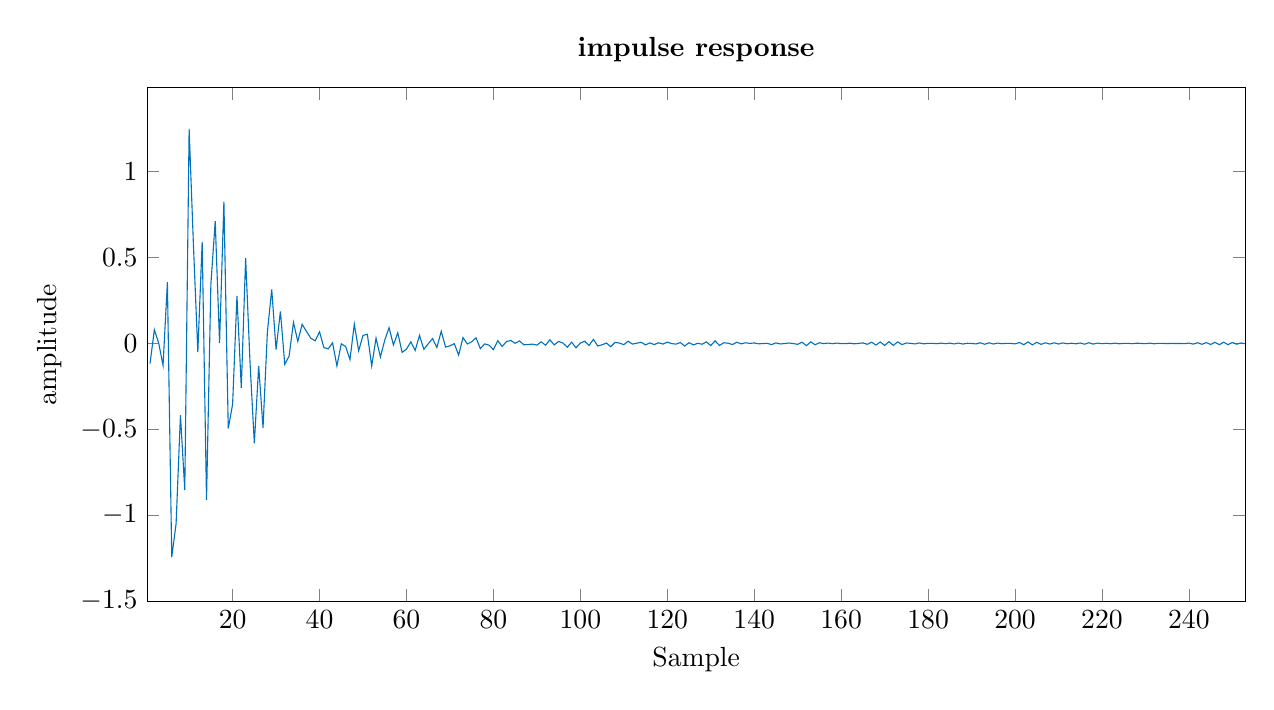
\begin{tikzpicture}

\begin{axis}[%
width=5.49in,
height=2.566in,
at={(1.011in,0.642in)},
scale only axis,
xmin=0.344142972512103,
xmax=252.945084796394,
xlabel={Sample},
ymin=-1.5,
ymax=1.4868804664723,
ylabel={amplitude},
axis background/.style={fill=white},
title style={font=\bfseries},
title={impulse response}
]
\addplot [color=mycolor1,solid,forget plot]
  table[row sep=crcr]{%
1	-0.118141562218072\\
1	-0.118141562218072\\
2	0.0791281785124607\\
2	0.0791281785124607\\
3	0.00109140883794252\\
3	0.00109140883794252\\
4	-0.127998430298182\\
4	-0.127998430298182\\
5	0.355751675486418\\
5	0.355751675486418\\
6	-1.24445909784893\\
6	-1.24445909784893\\
7	-1.04936802214079\\
7	-1.04936802214079\\
8	-0.418123407296711\\
8	-0.418123407296711\\
9	-0.853609016499564\\
9	-0.853609016499564\\
10	1.24815892007568\\
10	1.24815892007568\\
11	0.564683231877883\\
11	0.564683231877883\\
12	-0.0511791125132532\\
12	-0.0511791125132532\\
13	0.591079504687172\\
13	0.591079504687172\\
14	-0.911228401587671\\
14	-0.911228401587671\\
15	0.34212392225513\\
15	0.34212392225513\\
16	0.71167417099142\\
16	0.71167417099142\\
17	0.0022231516812417\\
17	0.0022231516812417\\
18	0.825359321003935\\
18	0.825359321003935\\
19	-0.495105852171416\\
19	-0.495105852171416\\
20	-0.354980390629405\\
20	-0.354980390629405\\
21	0.275904546024916\\
21	0.275904546024916\\
22	-0.259187854777998\\
22	-0.259187854777998\\
23	0.496375795390466\\
23	0.496375795390466\\
24	-0.107031671390095\\
24	-0.107031671390095\\
25	-0.582425217768152\\
25	-0.582425217768152\\
26	-0.131058795038014\\
26	-0.131058795038014\\
27	-0.491055535573922\\
27	-0.491055535573922\\
28	0.0652989205316153\\
28	0.0652989205316153\\
29	0.31411076610674\\
29	0.31411076610674\\
30	-0.0363555084229589\\
30	-0.0363555084229589\\
31	0.186377556816253\\
31	0.186377556816253\\
32	-0.122351410526851\\
32	-0.122351410526851\\
33	-0.0742300014448984\\
33	-0.0742300014448984\\
34	0.121765995454672\\
34	0.121765995454672\\
35	0.0120055808146089\\
35	0.0120055808146089\\
36	0.110948456873853\\
36	0.110948456873853\\
37	0.0692216392993395\\
37	0.0692216392993395\\
38	0.0299810369671249\\
38	0.0299810369671249\\
39	0.0144706736665758\\
39	0.0144706736665758\\
40	0.0670303556881637\\
40	0.0670303556881637\\
41	-0.0247644080799324\\
41	-0.0247644080799324\\
42	-0.031927855805956\\
42	-0.031927855805956\\
43	0.00322998704690307\\
43	0.00322998704690307\\
44	-0.131745511302458\\
44	-0.131745511302458\\
45	-0.00261033076288713\\
45	-0.00261033076288713\\
46	-0.0181125020290452\\
46	-0.0181125020290452\\
47	-0.0945138446649691\\
47	-0.0945138446649691\\
48	0.111436996915387\\
48	0.111436996915387\\
49	-0.0431351377461246\\
49	-0.0431351377461246\\
50	0.0461620756094456\\
50	0.0461620756094456\\
51	0.0531033344668851\\
51	0.0531033344668851\\
52	-0.131539836134088\\
52	-0.131539836134088\\
53	0.0305025240822609\\
53	0.0305025240822609\\
54	-0.0792119357439335\\
54	-0.0792119357439335\\
55	0.0183468383704305\\
55	0.0183468383704305\\
56	0.091370890352526\\
56	0.091370890352526\\
57	-0.00936150319799612\\
57	-0.00936150319799612\\
58	0.0615638871253384\\
58	0.0615638871253384\\
59	-0.0524944156191402\\
59	-0.0524944156191402\\
60	-0.0335821747505357\\
60	-0.0335821747505357\\
61	0.00892104929863474\\
61	0.00892104929863474\\
62	-0.0410628110921637\\
62	-0.0410628110921637\\
63	0.0464364992488124\\
63	0.0464364992488124\\
64	-0.0347539925926514\\
64	-0.0347539925926514\\
65	-0.0031920519174843\\
65	-0.0031920519174843\\
66	0.0278505098767845\\
66	0.0278505098767845\\
67	-0.0239093827261274\\
67	-0.0239093827261274\\
68	0.0700616510285207\\
68	0.0700616510285207\\
69	-0.0219341301905986\\
69	-0.0219341301905986\\
70	-0.0142230911242287\\
70	-0.0142230911242287\\
71	-0.00182073467961221\\
71	-0.00182073467961221\\
72	-0.0681129708309657\\
72	-0.0681129708309657\\
73	0.0334153987634728\\
73	0.0334153987634728\\
74	-0.00363938342836818\\
74	-0.00363938342836818\\
75	0.00914183511984331\\
75	0.00914183511984331\\
76	0.0321515049541257\\
76	0.0321515049541257\\
77	-0.0306798066110672\\
77	-0.0306798066110672\\
78	-0.00314839927224314\\
78	-0.00314839927224314\\
79	-0.0105024291640573\\
79	-0.0105024291640573\\
80	-0.0368012862919245\\
80	-0.0368012862919245\\
81	0.0155149120464149\\
81	0.0155149120464149\\
82	-0.0180951857625397\\
82	-0.0180951857625397\\
83	0.0103228815054031\\
83	0.0103228815054031\\
84	0.0169500794792463\\
84	0.0169500794792463\\
85	0.000310442154459831\\
85	0.000310442154459831\\
86	0.0140317610007087\\
86	0.0140317610007087\\
87	-0.00808289802810039\\
87	-0.00808289802810039\\
88	-0.00695942120163846\\
88	-0.00695942120163846\\
89	-0.00446733733759463\\
89	-0.00446733733759463\\
90	-0.0103115148570162\\
90	-0.0103115148570162\\
91	0.00899156239938577\\
91	0.00899156239938577\\
92	-0.0111136779230336\\
92	-0.0111136779230336\\
93	0.0203724396264147\\
93	0.0203724396264147\\
94	-0.00891067559850342\\
94	-0.00891067559850342\\
95	0.0111957345646422\\
95	0.0111957345646422\\
96	0.00161928607316594\\
96	0.00161928607316594\\
97	-0.0222011006626747\\
97	-0.0222011006626747\\
98	0.00705399101203549\\
98	0.00705399101203549\\
99	-0.0259264115095974\\
99	-0.0259264115095974\\
100	0.00127486462301934\\
100	0.00127486462301934\\
101	0.0124661338836067\\
101	0.0124661338836067\\
102	-0.0121720072937964\\
102	-0.0121720072937964\\
103	0.0229733095365205\\
103	0.0229733095365205\\
104	-0.015144764125669\\
104	-0.015144764125669\\
105	-0.00849436079781317\\
105	-0.00849436079781317\\
106	0.0020916766693437\\
106	0.0020916766693437\\
107	-0.0197042880875184\\
107	-0.0197042880875184\\
108	0.00590774994138175\\
108	0.00590774994138175\\
109	0.00142553758412932\\
109	0.00142553758412932\\
110	-0.00752781336578599\\
110	-0.00752781336578599\\
111	0.0124866500742295\\
111	0.0124866500742295\\
112	-0.00435439178335216\\
112	-0.00435439178335216\\
113	0.00144228670163819\\
113	0.00144228670163819\\
114	0.00581286574855189\\
114	0.00581286574855189\\
115	-0.00889141928378981\\
115	-0.00889141928378981\\
116	0.00274247544089457\\
116	0.00274247544089457\\
117	-0.00715328500349922\\
117	-0.00715328500349922\\
118	0.00343442489852638\\
118	0.00343442489852638\\
119	-0.00430672794128714\\
119	-0.00430672794128714\\
120	0.00719938952165628\\
120	0.00719938952165628\\
121	-0.0014601383401962\\
121	-0.0014601383401962\\
122	-0.00464951867639746\\
122	-0.00464951867639746\\
123	0.00484835116232913\\
123	0.00484835116232913\\
124	-0.0159239102642369\\
124	-0.0159239102642369\\
125	0.00414543117078109\\
125	0.00414543117078109\\
126	-0.00923141916662314\\
126	-0.00923141916662314\\
127	0.000492682295719719\\
127	0.000492682295719719\\
128	-0.0051865152342738\\
128	-0.0051865152342738\\
129	0.00879738745875531\\
129	0.00879738745875531\\
130	-0.0129254192936449\\
130	-0.0129254192936449\\
131	0.0150618586089381\\
131	0.0150618586089381\\
132	-0.0123298476334175\\
132	-0.0123298476334175\\
133	0.00356672143985635\\
133	0.00356672143985635\\
134	0.000635666567859052\\
134	0.000635666567859052\\
135	-0.00688542560476631\\
135	-0.00688542560476631\\
136	0.00647553377876287\\
136	0.00647553377876287\\
137	-0.00313869095969953\\
137	-0.00313869095969953\\
138	0.00338234865059637\\
138	0.00338234865059637\\
139	-0.000421084566326661\\
139	-0.000421084566326661\\
140	0.00250712752529129\\
140	0.00250712752529129\\
141	-0.00294288518799757\\
141	-0.00294288518799757\\
142	-0.0010102542496694\\
142	-0.0010102542496694\\
143	-0.000252409752983782\\
143	-0.000252409752983782\\
144	-0.00709280368191718\\
144	-0.00709280368191718\\
145	0.00273457138739201\\
145	0.00273457138739201\\
146	-0.00349492542841067\\
146	-0.00349492542841067\\
147	-0.0011987832037849\\
147	-0.0011987832037849\\
148	0.00204220837683377\\
148	0.00204220837683377\\
149	-0.00130776580642774\\
149	-0.00130776580642774\\
150	-0.0056427908397797\\
150	-0.0056427908397797\\
151	0.00640825158781991\\
151	0.00640825158781991\\
152	-0.0134753340471952\\
152	-0.0134753340471952\\
153	0.00874106945549123\\
153	0.00874106945549123\\
154	-0.00817595376743767\\
154	-0.00817595376743767\\
155	0.00346206620492773\\
155	0.00346206620492773\\
156	-0.00148108262860179\\
156	-0.00148108262860179\\
157	0.00159664856954663\\
157	0.00159664856954663\\
158	-0.00207774499103393\\
158	-0.00207774499103393\\
159	0.00158755993228967\\
159	0.00158755993228967\\
160	-0.00187606529560944\\
160	-0.00187606529560944\\
161	-0.0018285497587921\\
161	-0.0018285497587921\\
162	0.000959440112494838\\
162	0.000959440112494838\\
163	-0.00260830328383853\\
163	-0.00260830328383853\\
164	-0.000344112649687174\\
164	-0.000344112649687174\\
165	0.00255734485088457\\
165	0.00255734485088457\\
166	-0.00559677227976574\\
166	-0.00559677227976574\\
167	0.00666099057503437\\
167	0.00666099057503437\\
168	-0.00978142524505918\\
168	-0.00978142524505918\\
169	0.00778894342302596\\
169	0.00778894342302596\\
170	-0.0118679731491987\\
170	-0.0118679731491987\\
171	0.00950293873394341\\
171	0.00950293873394341\\
172	-0.011731446451187\\
172	-0.011731446451187\\
173	0.00845382399693906\\
173	0.00845382399693906\\
174	-0.00711138169847137\\
174	-0.00711138169847137\\
175	0.00213548642487268\\
175	0.00213548642487268\\
176	-5.85596460445852e-05\\
176	-5.85596460445852e-05\\
177	-0.00346976620662964\\
177	-0.00346976620662964\\
178	0.00266301217400429\\
178	0.00266301217400429\\
179	-0.00296703845816892\\
179	-0.00296703845816892\\
180	0.000124808195676521\\
180	0.000124808195676521\\
181	0.000142004740926337\\
181	0.000142004740926337\\
182	-0.00201581494127819\\
182	-0.00201581494127819\\
183	0.00136029364750051\\
183	0.00136029364750051\\
184	-0.0020858974900481\\
184	-0.0020858974900481\\
185	0.00131358449326331\\
185	0.00131358449326331\\
186	-0.00342799294410937\\
186	-0.00342799294410937\\
187	0.00159784037109706\\
187	0.00159784037109706\\
188	-0.00398829538564302\\
188	-0.00398829538564302\\
189	0.000416626602851866\\
189	0.000416626602851866\\
190	-0.000647140406921486\\
190	-0.000647140406921486\\
191	-0.00322830047473305\\
191	-0.00322830047473305\\
192	0.00317533194550781\\
192	0.00317533194550781\\
193	-0.00524668903136873\\
193	-0.00524668903136873\\
194	0.00328829223179929\\
194	0.00328829223179929\\
195	-0.00380800282688818\\
195	-0.00380800282688818\\
196	0.0015429504716805\\
196	0.0015429504716805\\
197	-0.00205915720933898\\
197	-0.00205915720933898\\
198	0.000169343616457016\\
198	0.000169343616457016\\
199	-1.94896363292676e-05\\
199	-1.94896363292676e-05\\
200	-0.00314718231332176\\
200	-0.00314718231332176\\
201	0.00488601419939295\\
201	0.00488601419939295\\
202	-0.00801298194159633\\
202	-0.00801298194159633\\
203	0.00835245107822657\\
203	0.00835245107822657\\
204	-0.00897724713721908\\
204	-0.00897724713721908\\
205	0.00614816265226835\\
205	0.00614816265226835\\
206	-0.00580773871813518\\
206	-0.00580773871813518\\
207	0.00330708796282231\\
207	0.00330708796282231\\
208	-0.0042502001375543\\
208	-0.0042502001375543\\
209	0.00318711451318226\\
209	0.00318711451318226\\
210	-0.00389261618655835\\
210	-0.00389261618655835\\
211	0.00217287506811931\\
211	0.00217287506811931\\
212	-0.00225153595128867\\
212	-0.00225153595128867\\
213	0.00064487097645708\\
213	0.00064487097645708\\
214	-0.00262627810428138\\
214	-0.00262627810428138\\
215	0.00216492706444699\\
215	0.00216492706444699\\
216	-0.00501031331995221\\
216	-0.00501031331995221\\
217	0.00345919904440867\\
217	0.00345919904440867\\
218	-0.00433586131657449\\
218	-0.00433586131657449\\
219	0.00154231988745107\\
219	0.00154231988745107\\
220	-0.00198063731082455\\
220	-0.00198063731082455\\
221	0.000416444228293499\\
221	0.000416444228293499\\
222	-0.00228271657882294\\
222	-0.00228271657882294\\
223	0.00115333286600893\\
223	0.00115333286600893\\
224	-0.00241598423363702\\
224	-0.00241598423363702\\
225	-5.09471217824708e-05\\
225	-5.09471217824708e-05\\
226	0.000208671836863114\\
226	0.000208671836863114\\
227	-0.00206397328677561\\
227	-0.00206397328677561\\
228	0.000976785016822535\\
228	0.000976785016822535\\
229	-0.000535693054502294\\
229	-0.000535693054502294\\
230	-0.00188323750833553\\
230	-0.00188323750833553\\
231	0.00131001909170588\\
231	0.00131001909170588\\
232	-0.00243251712101864\\
232	-0.00243251712101864\\
233	-0.000118515677414382\\
233	-0.000118515677414382\\
234	-0.000432814061260125\\
234	-0.000432814061260125\\
235	-0.00131759161870752\\
235	-0.00131759161870752\\
236	-0.000524844285814698\\
236	-0.000524844285814698\\
237	-0.000598699726453522\\
237	-0.000598699726453522\\
238	-0.000709887660179469\\
238	-0.000709887660179469\\
239	-0.00165499475232057\\
239	-0.00165499475232057\\
240	0.00156604948120072\\
240	0.00156604948120072\\
241	-0.00438046374307205\\
241	-0.00438046374307205\\
242	0.00360696249179117\\
242	0.00360696249179117\\
243	-0.00560346639516965\\
243	-0.00560346639516965\\
244	0.00434937167572154\\
244	0.00434937167572154\\
245	-0.00623469069097805\\
245	-0.00623469069097805\\
246	0.00589186342140169\\
246	0.00589186342140169\\
247	-0.00785971118716415\\
247	-0.00785971118716415\\
248	0.00665880002740227\\
248	0.00665880002740227\\
249	-0.00761918755737151\\
249	-0.00761918755737151\\
250	0.00490902237270174\\
250	0.00490902237270174\\
251	-0.00499083265681984\\
251	-0.00499083265681984\\
252	0.00245856956180693\\
252	0.00245856956180693\\
253	-0.00271993135747834\\
253	-0.00271993135747834\\
253	-0.00271993135747834\\
253	-0.00271993135747834\\
253	-0.00271993135747834\\
253	-0.00271993135747834\\
253	-0.00271993135747834\\
253	-0.00271993135747834\\
253	-0.00271993135747834\\
253	-0.00271993135747834\\
253	-0.00271993135747834\\
253	-0.00271993135747834\\
253	-0.00271993135747834\\
253	-0.00271993135747834\\
253	-0.00271993135747834\\
253	-0.00271993135747834\\
253	-0.00271993135747834\\
253	-0.00271993135747834\\
253	-0.00271993135747834\\
253	-0.00271993135747834\\
253	-0.00271993135747834\\
253	-0.00271993135747834\\
253	-0.00271993135747834\\
253	-0.00271993135747834\\
253	-0.00271993135747834\\
253	-0.00271993135747834\\
253	-0.00271993135747834\\
253	-0.00271993135747834\\
253	-0.00271993135747834\\
253	-0.00271993135747834\\
253	-0.00271993135747834\\
253	-0.00271993135747834\\
253	-0.00271993135747834\\
253	-0.00271993135747834\\
253	-0.00271993135747834\\
253	-0.00271993135747834\\
253	-0.00271993135747834\\
253	-0.00271993135747834\\
253	-0.00271993135747834\\
253	-0.00271993135747834\\
253	-0.00271993135747834\\
253	-0.00271993135747834\\
253	-0.00271993135747834\\
253	-0.00271993135747834\\
253	-0.00271993135747834\\
253	-0.00271993135747834\\
253	-0.00271993135747834\\
253	-0.00271993135747834\\
253	-0.00271993135747834\\
253	-0.00271993135747834\\
253	-0.00271993135747834\\
253	-0.00271993135747834\\
253	-0.00271993135747834\\
253	-0.00271993135747834\\
253	-0.00271993135747834\\
253	-0.00271993135747834\\
253	-0.00271993135747834\\
253	-0.00271993135747834\\
253	-0.00271993135747834\\
253	-0.00271993135747834\\
253	-0.00271993135747834\\
253	-0.00271993135747834\\
253	-0.00271993135747834\\
253	-0.00271993135747834\\
253	-0.00271993135747834\\
253	-0.00271993135747834\\
253	-0.00271993135747834\\
253	-0.00271993135747834\\
253	-0.00271993135747834\\
253	-0.00271993135747834\\
253	-0.00271993135747834\\
253	-0.00271993135747834\\
253	-0.00271993135747834\\
253	-0.00271993135747834\\
253	-0.00271993135747834\\
253	-0.00271993135747834\\
253	-0.00271993135747834\\
253	-0.00271993135747834\\
253	-0.00271993135747834\\
253	-0.00271993135747834\\
253	-0.00271993135747834\\
253	-0.00271993135747834\\
253	-0.00271993135747834\\
253	-0.00271993135747834\\
253	-0.00271993135747834\\
253	-0.00271993135747834\\
253	-0.00271993135747834\\
253	-0.00271993135747834\\
253	-0.00271993135747834\\
253	-0.00271993135747834\\
253	-0.00271993135747834\\
253	-0.00271993135747834\\
253	-0.00271993135747834\\
253	-0.00271993135747834\\
253	-0.00271993135747834\\
253	-0.00271993135747834\\
253	-0.00271993135747834\\
253	-0.00271993135747834\\
253	-0.00271993135747834\\
253	-0.00271993135747834\\
253	-0.00271993135747834\\
253	-0.00271993135747834\\
253	-0.00271993135747834\\
253	-0.00271993135747834\\
253	-0.00271993135747834\\
253	-0.00271993135747834\\
253	-0.00271993135747834\\
253	-0.00271993135747834\\
253	-0.00271993135747834\\
253	-0.00271993135747834\\
253	-0.00271993135747834\\
253	-0.00271993135747834\\
253	-0.00271993135747834\\
253	-0.00271993135747834\\
253	-0.00271993135747834\\
253	-0.00271993135747834\\
253	-0.00271993135747834\\
253	-0.00271993135747834\\
253	-0.00271993135747834\\
253	-0.00271993135747834\\
253	-0.00271993135747834\\
253	-0.00271993135747834\\
253	-0.00271993135747834\\
253	-0.00271993135747834\\
253	-0.00271993135747834\\
253	-0.00271993135747834\\
253	-0.00271993135747834\\
253	-0.00271993135747834\\
253	-0.00271993135747834\\
253	-0.00271993135747834\\
253	-0.00271993135747834\\
253	-0.00271993135747834\\
253	-0.00271993135747834\\
253	-0.00271993135747834\\
253	-0.00271993135747834\\
253	-0.00271993135747834\\
253	-0.00271993135747834\\
253	-0.00271993135747834\\
253	-0.00271993135747834\\
253	-0.00271993135747834\\
253	-0.00271993135747834\\
253	-0.00271993135747834\\
253	-0.00271993135747834\\
253	-0.00271993135747834\\
253	-0.00271993135747834\\
253	-0.00271993135747834\\
253	-0.00271993135747834\\
253	-0.00271993135747834\\
253	-0.00271993135747834\\
253	-0.00271993135747834\\
253	-0.00271993135747834\\
253	-0.00271993135747834\\
253	-0.00271993135747834\\
253	-0.00271993135747834\\
253	-0.00271993135747834\\
253	-0.00271993135747834\\
253	-0.00271993135747834\\
253	-0.00271993135747834\\
253	-0.00271993135747834\\
253	-0.00271993135747834\\
253	-0.00271993135747834\\
253	-0.00271993135747834\\
253	-0.00271993135747834\\
253	-0.00271993135747834\\
253	-0.00271993135747834\\
253	-0.00271993135747834\\
253	-0.00271993135747834\\
253	-0.00271993135747834\\
253	-0.00271993135747834\\
253	-0.00271993135747834\\
253	-0.00271993135747834\\
253	-0.00271993135747834\\
253	-0.00271993135747834\\
253	-0.00271993135747834\\
253	-0.00271993135747834\\
253	-0.00271993135747834\\
253	-0.00271993135747834\\
253	-0.00271993135747834\\
253	-0.00271993135747834\\
253	-0.00271993135747834\\
253	-0.00271993135747834\\
253	-0.00271993135747834\\
253	-0.00271993135747834\\
253	-0.00271993135747834\\
253	-0.00271993135747834\\
253	-0.00271993135747834\\
253	-0.00271993135747834\\
253	-0.00271993135747834\\
253	-0.00271993135747834\\
253	-0.00271993135747834\\
253	-0.00271993135747834\\
253	-0.00271993135747834\\
253	-0.00271993135747834\\
253	-0.00271993135747834\\
253	-0.00271993135747834\\
253	-0.00271993135747834\\
253	-0.00271993135747834\\
253	-0.00271993135747834\\
253	-0.00271993135747834\\
253	-0.00271993135747834\\
253	-0.00271993135747834\\
253	-0.00271993135747834\\
253	-0.00271993135747834\\
253	-0.00271993135747834\\
253	-0.00271993135747834\\
253	-0.00271993135747834\\
253	-0.00271993135747834\\
253	-0.00271993135747834\\
253	-0.00271993135747834\\
253	-0.00271993135747834\\
253	-0.00271993135747834\\
253	-0.00271993135747834\\
253	-0.00271993135747834\\
253	-0.00271993135747834\\
253	-0.00271993135747834\\
253	-0.00271993135747834\\
253	-0.00271993135747834\\
253	-0.00271993135747834\\
253	-0.00271993135747834\\
253	-0.00271993135747834\\
253	-0.00271993135747834\\
253	-0.00271993135747834\\
253	-0.00271993135747834\\
253	-0.00271993135747834\\
253	-0.00271993135747834\\
253	-0.00271993135747834\\
253	-0.00271993135747834\\
253	-0.00271993135747834\\
253	-0.00271993135747834\\
253	-0.00271993135747834\\
253	-0.00271993135747834\\
253	-0.00271993135747834\\
253	-0.00271993135747834\\
253	-0.00271993135747834\\
253	-0.00271993135747834\\
253	-0.00271993135747834\\
253	-0.00271993135747834\\
253	-0.00271993135747834\\
253	-0.00271993135747834\\
253	-0.00271993135747834\\
253	-0.00271993135747834\\
253	-0.00271993135747834\\
253	-0.00271993135747834\\
253	-0.00271993135747834\\
253	-0.00271993135747834\\
253	-0.00271993135747834\\
253	-0.00271993135747834\\
253	-0.00271993135747834\\
253	-0.00271993135747834\\
253	-0.00271993135747834\\
253	-0.00271993135747834\\
253	-0.00271993135747834\\
253	-0.00271993135747834\\
253	-0.00271993135747834\\
253	-0.00271993135747834\\
253	-0.00271993135747834\\
253	-0.00271993135747834\\
253	-0.00271993135747834\\
253	-0.00271993135747834\\
253	-0.00271993135747834\\
253	-0.00271993135747834\\
253	-0.00271993135747834\\
253	-0.00271993135747834\\
253	-0.00271993135747834\\
253	-0.00271993135747834\\
253	-0.00271993135747834\\
253	-0.00271993135747834\\
253	-0.00271993135747834\\
253	-0.00271993135747834\\
253	-0.00271993135747834\\
253	-0.00271993135747834\\
253	-0.00271993135747834\\
253	-0.00271993135747834\\
253	-0.00271993135747834\\
253	-0.00271993135747834\\
253	-0.00271993135747834\\
253	-0.00271993135747834\\
253	-0.00271993135747834\\
253	-0.00271993135747834\\
253	-0.00271993135747834\\
253	-0.00271993135747834\\
253	-0.00271993135747834\\
253	-0.00271993135747834\\
253	-0.00271993135747834\\
253	-0.00271993135747834\\
253	-0.00271993135747834\\
253	-0.00271993135747834\\
253	-0.00271993135747834\\
253	-0.00271993135747834\\
253	-0.00271993135747834\\
253	-0.00271993135747834\\
253	-0.00271993135747834\\
253	-0.00271993135747834\\
253	-0.00271993135747834\\
253	-0.00271993135747834\\
253	-0.00271993135747834\\
253	-0.00271993135747834\\
253	-0.00271993135747834\\
253	-0.00271993135747834\\
253	-0.00271993135747834\\
253	-0.00271993135747834\\
253	-0.00271993135747834\\
253	-0.00271993135747834\\
253	-0.00271993135747834\\
253	-0.00271993135747834\\
253	-0.00271993135747834\\
253	-0.00271993135747834\\
253	-0.00271993135747834\\
253	-0.00271993135747834\\
253	-0.00271993135747834\\
253	-0.00271993135747834\\
253	-0.00271993135747834\\
253	-0.00271993135747834\\
253	-0.00271993135747834\\
253	-0.00271993135747834\\
253	-0.00271993135747834\\
253	-0.00271993135747834\\
253	-0.00271993135747834\\
253	-0.00271993135747834\\
253	-0.00271993135747834\\
253	-0.00271993135747834\\
253	-0.00271993135747834\\
253	-0.00271993135747834\\
253	-0.00271993135747834\\
253	-0.00271993135747834\\
253	-0.00271993135747834\\
253	-0.00271993135747834\\
253	-0.00271993135747834\\
253	-0.00271993135747834\\
253	-0.00271993135747834\\
253	-0.00271993135747834\\
253	-0.00271993135747834\\
253	-0.00271993135747834\\
253	-0.00271993135747834\\
253	-0.00271993135747834\\
253	-0.00271993135747834\\
253	-0.00271993135747834\\
253	-0.00271993135747834\\
253	-0.00271993135747834\\
253	-0.00271993135747834\\
253	-0.00271993135747834\\
253	-0.00271993135747834\\
253	-0.00271993135747834\\
253	-0.00271993135747834\\
253	-0.00271993135747834\\
253	-0.00271993135747834\\
253	-0.00271993135747834\\
253	-0.00271993135747834\\
253	-0.00271993135747834\\
253	-0.00271993135747834\\
253	-0.00271993135747834\\
253	-0.00271993135747834\\
253	-0.00271993135747834\\
253	-0.00271993135747834\\
253	-0.00271993135747834\\
253	-0.00271993135747834\\
253	-0.00271993135747834\\
253	-0.00271993135747834\\
253	-0.00271993135747834\\
253	-0.00271993135747834\\
253	-0.00271993135747834\\
253	-0.00271993135747834\\
253	-0.00271993135747834\\
253	-0.00271993135747834\\
};
\end{axis}
\end{tikzpicture}%
	\caption{Cropped impulse response plot of the cancellation path}
	\label{CancellationPathImpulseResponseCrop}
\end{figure}

To verify that the frequency response of the cropped impulse response approximately equals that of the non-cropped impulse response the two frequency responses are compared. This can be seen on \autoref{CancellationPathImpulseResponseCompare}. Note that the two lines are almost completely on top of each other.

\begin{figure}[H]
	\centering
	\tikzsetnextfilename{CancellationPathImpulseResponseCompare1}
	%% This file was created by matlab2tikz.
%
%The latest updates can be retrieved from
%  http://www.mathworks.com/matlabcentral/fileexchange/22022-matlab2tikz-matlab2tikz
%where you can also make suggestions and rate matlab2tikz.
%
\definecolor{mycolor1}{rgb}{0.00000,0.44700,0.74100}%
\definecolor{mycolor2}{rgb}{0.85000,0.32500,0.09800}%
%
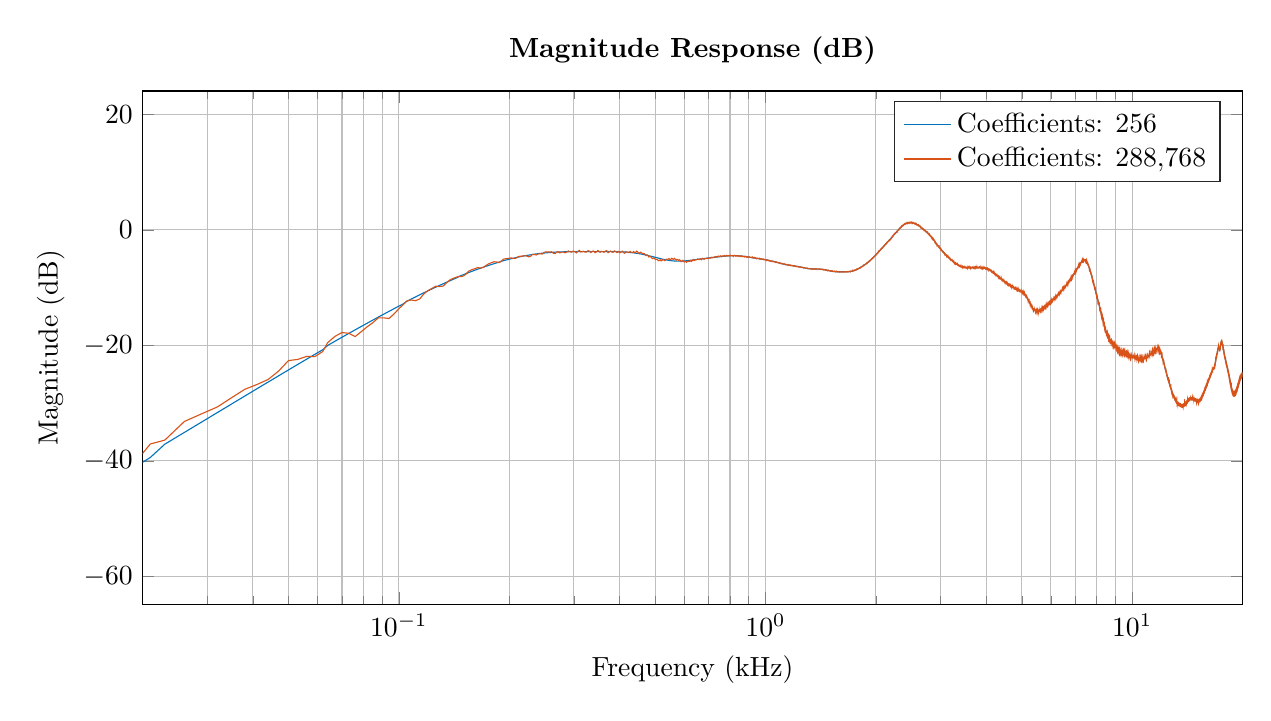
\begin{tikzpicture}

\begin{axis}[%
width=5.5in,
height=2.566in,
at={(2.804in,1.205in)},
scale only axis,
xmode=log,
xmin=0.020,
xmax=20.000,
xminorticks=true,
xlabel={Frequency (kHz)},
xmajorgrids,
xminorgrids,
ymin=-64.832,
ymax=24.080,
ylabel={Magnitude (dB)},
ymajorgrids,
axis background/.style={fill=white},
title style={font=\bfseries},
title={Magnitude Response (dB)},
legend style={legend cell align=left,align=left,draw=white!15!black}
]
\addplot [color=mycolor1,solid,forget plot]
  table[row sep=crcr]{%
0.018	-42.077\\
0.021	-39.419\\
0.023	-37.115\\
0.026	-35.084\\
0.029	-33.272\\
0.032	-31.636\\
0.035	-30.148\\
0.038	-28.784\\
0.041	-27.525\\
0.044	-26.358\\
0.047	-25.271\\
0.050	-24.254\\
0.053	-23.301\\
0.056	-22.403\\
0.059	-21.556\\
0.062	-20.755\\
0.064	-19.995\\
0.067	-19.274\\
0.070	-18.589\\
0.073	-17.935\\
0.076	-17.312\\
0.079	-16.718\\
0.082	-16.149\\
0.085	-15.605\\
0.088	-15.083\\
0.091	-14.584\\
0.094	-14.105\\
0.097	-13.645\\
0.100	-13.203\\
0.103	-12.779\\
0.105	-12.371\\
0.108	-11.979\\
0.111	-11.602\\
0.114	-11.239\\
0.117	-10.890\\
0.120	-10.554\\
0.123	-10.231\\
0.126	-9.920\\
0.129	-9.620\\
0.132	-9.332\\
0.135	-9.055\\
0.138	-8.788\\
0.141	-8.531\\
0.144	-8.284\\
0.146	-8.046\\
0.149	-7.818\\
0.152	-7.598\\
0.155	-7.387\\
0.158	-7.184\\
0.161	-6.990\\
0.164	-6.803\\
0.167	-6.624\\
0.170	-6.452\\
0.173	-6.288\\
0.176	-6.131\\
0.179	-5.980\\
0.182	-5.836\\
0.185	-5.699\\
0.188	-5.568\\
0.190	-5.443\\
0.193	-5.324\\
0.196	-5.211\\
0.199	-5.103\\
0.202	-5.001\\
0.205	-4.904\\
0.208	-4.813\\
0.211	-4.727\\
0.214	-4.645\\
0.217	-4.568\\
0.220	-4.496\\
0.223	-4.428\\
0.226	-4.365\\
0.229	-4.306\\
0.231	-4.251\\
0.234	-4.199\\
0.237	-4.152\\
0.240	-4.108\\
0.243	-4.068\\
0.246	-4.030\\
0.249	-3.996\\
0.252	-3.965\\
0.255	-3.937\\
0.258	-3.912\\
0.261	-3.889\\
0.264	-3.869\\
0.267	-3.850\\
0.270	-3.834\\
0.272	-3.820\\
0.275	-3.808\\
0.278	-3.798\\
0.281	-3.789\\
0.284	-3.781\\
0.287	-3.775\\
0.290	-3.770\\
0.293	-3.766\\
0.296	-3.763\\
0.299	-3.760\\
0.302	-3.759\\
0.305	-3.758\\
0.308	-3.757\\
0.311	-3.757\\
0.313	-3.757\\
0.316	-3.757\\
0.319	-3.757\\
0.322	-3.757\\
0.325	-3.758\\
0.328	-3.758\\
0.331	-3.758\\
0.334	-3.758\\
0.337	-3.759\\
0.340	-3.758\\
0.343	-3.758\\
0.346	-3.758\\
0.349	-3.758\\
0.352	-3.757\\
0.354	-3.757\\
0.357	-3.756\\
0.360	-3.756\\
0.363	-3.755\\
0.366	-3.755\\
0.369	-3.755\\
0.372	-3.755\\
0.375	-3.756\\
0.378	-3.757\\
0.381	-3.758\\
0.384	-3.760\\
0.387	-3.763\\
0.390	-3.767\\
0.393	-3.771\\
0.396	-3.776\\
0.398	-3.782\\
0.401	-3.789\\
0.404	-3.797\\
0.407	-3.806\\
0.410	-3.816\\
0.413	-3.827\\
0.416	-3.840\\
0.419	-3.854\\
0.422	-3.870\\
0.425	-3.886\\
0.428	-3.905\\
0.431	-3.924\\
0.434	-3.945\\
0.437	-3.968\\
0.439	-3.992\\
0.442	-4.017\\
0.445	-4.044\\
0.448	-4.072\\
0.451	-4.102\\
0.454	-4.133\\
0.457	-4.165\\
0.460	-4.198\\
0.463	-4.233\\
0.466	-4.269\\
0.469	-4.305\\
0.472	-4.343\\
0.475	-4.382\\
0.478	-4.421\\
0.480	-4.461\\
0.483	-4.502\\
0.486	-4.543\\
0.489	-4.585\\
0.492	-4.627\\
0.495	-4.668\\
0.498	-4.710\\
0.501	-4.752\\
0.504	-4.793\\
0.507	-4.834\\
0.510	-4.874\\
0.513	-4.914\\
0.516	-4.953\\
0.519	-4.991\\
0.521	-5.028\\
0.524	-5.063\\
0.527	-5.097\\
0.530	-5.130\\
0.533	-5.161\\
0.536	-5.191\\
0.539	-5.219\\
0.542	-5.245\\
0.545	-5.269\\
0.548	-5.291\\
0.551	-5.312\\
0.554	-5.330\\
0.557	-5.346\\
0.560	-5.361\\
0.562	-5.373\\
0.565	-5.383\\
0.568	-5.391\\
0.571	-5.398\\
0.574	-5.402\\
0.577	-5.405\\
0.580	-5.405\\
0.583	-5.405\\
0.586	-5.402\\
0.589	-5.398\\
0.592	-5.392\\
0.595	-5.386\\
0.598	-5.377\\
0.601	-5.368\\
0.604	-5.358\\
0.606	-5.346\\
0.609	-5.334\\
0.612	-5.321\\
0.615	-5.307\\
0.618	-5.293\\
0.621	-5.278\\
0.624	-5.263\\
0.627	-5.247\\
0.630	-5.231\\
0.633	-5.215\\
0.636	-5.199\\
0.639	-5.182\\
0.642	-5.166\\
0.645	-5.149\\
0.647	-5.133\\
0.650	-5.116\\
0.653	-5.100\\
0.656	-5.084\\
0.659	-5.068\\
0.662	-5.052\\
0.665	-5.036\\
0.668	-5.021\\
0.671	-5.005\\
0.674	-4.990\\
0.677	-4.975\\
0.680	-4.960\\
0.683	-4.946\\
0.686	-4.931\\
0.688	-4.917\\
0.691	-4.902\\
0.694	-4.888\\
0.697	-4.874\\
0.700	-4.860\\
0.703	-4.847\\
0.706	-4.833\\
0.709	-4.819\\
0.712	-4.806\\
0.715	-4.792\\
0.718	-4.778\\
0.721	-4.765\\
0.724	-4.751\\
0.727	-4.738\\
0.729	-4.725\\
0.732	-4.711\\
0.735	-4.698\\
0.738	-4.685\\
0.741	-4.672\\
0.744	-4.659\\
0.747	-4.646\\
0.750	-4.633\\
0.753	-4.621\\
0.756	-4.608\\
0.759	-4.596\\
0.762	-4.584\\
0.765	-4.573\\
0.768	-4.561\\
0.771	-4.550\\
0.773	-4.540\\
0.776	-4.530\\
0.779	-4.520\\
0.782	-4.511\\
0.785	-4.502\\
0.788	-4.494\\
0.791	-4.487\\
0.794	-4.480\\
0.797	-4.473\\
0.800	-4.468\\
0.803	-4.463\\
0.806	-4.458\\
0.809	-4.455\\
0.812	-4.452\\
0.814	-4.450\\
0.817	-4.449\\
0.820	-4.449\\
0.823	-4.449\\
0.826	-4.450\\
0.829	-4.452\\
0.832	-4.455\\
0.835	-4.459\\
0.838	-4.463\\
0.841	-4.469\\
0.844	-4.475\\
0.847	-4.481\\
0.850	-4.489\\
0.853	-4.497\\
0.855	-4.506\\
0.858	-4.516\\
0.861	-4.526\\
0.864	-4.537\\
0.867	-4.548\\
0.870	-4.560\\
0.873	-4.573\\
0.876	-4.586\\
0.879	-4.599\\
0.882	-4.613\\
0.885	-4.627\\
0.888	-4.641\\
0.891	-4.656\\
0.894	-4.671\\
0.896	-4.686\\
0.899	-4.701\\
0.902	-4.716\\
0.905	-4.732\\
0.908	-4.747\\
0.911	-4.762\\
0.914	-4.778\\
0.917	-4.793\\
0.920	-4.808\\
0.923	-4.823\\
0.926	-4.838\\
0.929	-4.852\\
0.932	-4.867\\
0.935	-4.881\\
0.938	-4.895\\
0.940	-4.909\\
0.943	-4.923\\
0.946	-4.937\\
0.949	-4.950\\
0.952	-4.963\\
0.955	-4.976\\
0.958	-4.989\\
0.961	-5.001\\
0.964	-5.014\\
0.967	-5.026\\
0.970	-5.039\\
0.973	-5.051\\
0.976	-5.063\\
0.979	-5.075\\
0.981	-5.088\\
0.984	-5.100\\
0.987	-5.112\\
0.990	-5.125\\
0.993	-5.138\\
0.996	-5.150\\
0.999	-5.164\\
1.002	-5.177\\
1.005	-5.190\\
1.008	-5.204\\
1.011	-5.219\\
1.014	-5.233\\
1.017	-5.248\\
1.020	-5.263\\
1.022	-5.279\\
1.025	-5.295\\
1.028	-5.311\\
1.031	-5.328\\
1.034	-5.345\\
1.037	-5.362\\
1.040	-5.380\\
1.043	-5.398\\
1.046	-5.417\\
1.049	-5.436\\
1.052	-5.455\\
1.055	-5.475\\
1.058	-5.494\\
1.061	-5.515\\
1.063	-5.535\\
1.066	-5.555\\
1.069	-5.576\\
1.072	-5.597\\
1.075	-5.618\\
1.078	-5.638\\
1.081	-5.659\\
1.084	-5.680\\
1.087	-5.701\\
1.090	-5.721\\
1.093	-5.742\\
1.096	-5.762\\
1.099	-5.782\\
1.102	-5.802\\
1.104	-5.821\\
1.107	-5.841\\
1.110	-5.859\\
1.113	-5.878\\
1.116	-5.896\\
1.119	-5.913\\
1.122	-5.930\\
1.125	-5.947\\
1.128	-5.963\\
1.131	-5.978\\
1.134	-5.994\\
1.137	-6.008\\
1.140	-6.022\\
1.143	-6.036\\
1.146	-6.049\\
1.148	-6.062\\
1.151	-6.074\\
1.154	-6.086\\
1.157	-6.098\\
1.160	-6.109\\
1.163	-6.120\\
1.166	-6.130\\
1.169	-6.140\\
1.172	-6.150\\
1.175	-6.160\\
1.178	-6.170\\
1.181	-6.179\\
1.184	-6.189\\
1.187	-6.198\\
1.189	-6.208\\
1.192	-6.217\\
1.195	-6.227\\
1.198	-6.236\\
1.201	-6.246\\
1.204	-6.256\\
1.207	-6.266\\
1.210	-6.276\\
1.213	-6.287\\
1.216	-6.298\\
1.219	-6.309\\
1.222	-6.320\\
1.225	-6.331\\
1.228	-6.343\\
1.230	-6.355\\
1.233	-6.368\\
1.236	-6.380\\
1.239	-6.393\\
1.242	-6.406\\
1.245	-6.420\\
1.248	-6.433\\
1.251	-6.447\\
1.254	-6.461\\
1.257	-6.475\\
1.260	-6.489\\
1.263	-6.503\\
1.266	-6.517\\
1.269	-6.531\\
1.271	-6.545\\
1.274	-6.559\\
1.277	-6.573\\
1.280	-6.587\\
1.283	-6.600\\
1.286	-6.613\\
1.289	-6.626\\
1.292	-6.638\\
1.295	-6.650\\
1.298	-6.661\\
1.301	-6.672\\
1.304	-6.683\\
1.307	-6.693\\
1.310	-6.702\\
1.312	-6.711\\
1.315	-6.720\\
1.318	-6.727\\
1.321	-6.734\\
1.324	-6.741\\
1.327	-6.747\\
1.330	-6.752\\
1.333	-6.757\\
1.336	-6.761\\
1.339	-6.765\\
1.342	-6.768\\
1.345	-6.770\\
1.348	-6.772\\
1.351	-6.774\\
1.354	-6.775\\
1.356	-6.776\\
1.359	-6.777\\
1.362	-6.777\\
1.365	-6.777\\
1.368	-6.777\\
1.371	-6.777\\
1.374	-6.777\\
1.377	-6.777\\
1.380	-6.777\\
1.383	-6.777\\
1.386	-6.777\\
1.389	-6.777\\
1.392	-6.778\\
1.395	-6.778\\
1.397	-6.780\\
1.400	-6.781\\
1.403	-6.783\\
1.406	-6.785\\
1.409	-6.788\\
1.412	-6.791\\
1.415	-6.795\\
1.418	-6.800\\
1.421	-6.804\\
1.424	-6.810\\
1.427	-6.816\\
1.430	-6.823\\
1.433	-6.830\\
1.436	-6.837\\
1.438	-6.846\\
1.441	-6.855\\
1.444	-6.864\\
1.447	-6.874\\
1.450	-6.884\\
1.453	-6.895\\
1.456	-6.906\\
1.459	-6.918\\
1.462	-6.930\\
1.465	-6.942\\
1.468	-6.955\\
1.471	-6.967\\
1.474	-6.980\\
1.477	-6.993\\
1.479	-7.006\\
1.482	-7.020\\
1.485	-7.033\\
1.488	-7.046\\
1.491	-7.059\\
1.494	-7.071\\
1.497	-7.084\\
1.500	-7.096\\
1.503	-7.108\\
1.506	-7.120\\
1.509	-7.131\\
1.512	-7.142\\
1.515	-7.153\\
1.518	-7.162\\
1.521	-7.172\\
1.523	-7.181\\
1.526	-7.189\\
1.529	-7.197\\
1.532	-7.204\\
1.535	-7.211\\
1.538	-7.217\\
1.541	-7.222\\
1.544	-7.227\\
1.547	-7.232\\
1.550	-7.236\\
1.553	-7.239\\
1.556	-7.242\\
1.559	-7.244\\
1.562	-7.246\\
1.564	-7.248\\
1.567	-7.249\\
1.570	-7.250\\
1.573	-7.251\\
1.576	-7.251\\
1.579	-7.251\\
1.582	-7.251\\
1.585	-7.250\\
1.588	-7.250\\
1.591	-7.249\\
1.594	-7.248\\
1.597	-7.247\\
1.600	-7.247\\
1.603	-7.246\\
1.605	-7.245\\
1.608	-7.244\\
1.611	-7.244\\
1.614	-7.243\\
1.617	-7.243\\
1.620	-7.242\\
1.623	-7.242\\
1.626	-7.242\\
1.629	-7.242\\
1.632	-7.242\\
1.635	-7.242\\
1.638	-7.242\\
1.641	-7.243\\
1.644	-7.243\\
1.646	-7.243\\
1.649	-7.244\\
1.652	-7.244\\
1.655	-7.244\\
1.658	-7.245\\
1.661	-7.245\\
1.664	-7.245\\
1.667	-7.244\\
1.670	-7.244\\
1.673	-7.243\\
1.676	-7.242\\
1.679	-7.240\\
1.682	-7.238\\
1.685	-7.236\\
1.688	-7.233\\
1.690	-7.230\\
1.693	-7.226\\
1.696	-7.221\\
1.699	-7.216\\
1.702	-7.210\\
1.705	-7.204\\
1.708	-7.196\\
1.711	-7.188\\
1.714	-7.180\\
1.717	-7.170\\
1.720	-7.160\\
1.723	-7.149\\
1.726	-7.137\\
1.729	-7.125\\
1.731	-7.111\\
1.734	-7.097\\
1.737	-7.082\\
1.740	-7.067\\
1.743	-7.050\\
1.746	-7.033\\
1.749	-7.016\\
1.752	-6.997\\
1.755	-6.978\\
1.758	-6.959\\
1.761	-6.938\\
1.764	-6.917\\
1.767	-6.896\\
1.770	-6.874\\
1.772	-6.852\\
1.775	-6.829\\
1.778	-6.806\\
1.781	-6.783\\
1.784	-6.759\\
1.787	-6.735\\
1.790	-6.711\\
1.793	-6.686\\
1.796	-6.661\\
1.799	-6.636\\
1.802	-6.611\\
1.805	-6.586\\
1.808	-6.560\\
1.811	-6.534\\
1.813	-6.509\\
1.816	-6.483\\
1.819	-6.457\\
1.822	-6.431\\
1.825	-6.404\\
1.828	-6.378\\
1.831	-6.352\\
1.834	-6.325\\
1.837	-6.298\\
1.840	-6.271\\
1.843	-6.244\\
1.846	-6.217\\
1.849	-6.190\\
1.852	-6.162\\
1.854	-6.135\\
1.857	-6.107\\
1.860	-6.078\\
1.863	-6.050\\
1.866	-6.021\\
1.869	-5.992\\
1.872	-5.963\\
1.875	-5.933\\
1.878	-5.903\\
1.881	-5.872\\
1.884	-5.841\\
1.887	-5.810\\
1.890	-5.778\\
1.893	-5.746\\
1.896	-5.713\\
1.898	-5.680\\
1.901	-5.647\\
1.904	-5.613\\
1.907	-5.578\\
1.910	-5.543\\
1.913	-5.508\\
1.916	-5.472\\
1.919	-5.435\\
1.922	-5.398\\
1.925	-5.361\\
1.928	-5.323\\
1.931	-5.285\\
1.934	-5.246\\
1.937	-5.207\\
1.939	-5.168\\
1.942	-5.128\\
1.945	-5.088\\
1.948	-5.047\\
1.951	-5.006\\
1.954	-4.965\\
1.957	-4.924\\
1.960	-4.882\\
1.963	-4.840\\
1.966	-4.798\\
1.969	-4.755\\
1.972	-4.713\\
1.975	-4.670\\
1.978	-4.627\\
1.980	-4.584\\
1.983	-4.541\\
1.986	-4.498\\
1.989	-4.455\\
1.992	-4.411\\
1.995	-4.368\\
1.998	-4.325\\
2.001	-4.281\\
2.004	-4.238\\
2.007	-4.195\\
2.010	-4.151\\
2.013	-4.108\\
2.016	-4.065\\
2.019	-4.021\\
2.021	-3.978\\
2.024	-3.935\\
2.027	-3.892\\
2.030	-3.849\\
2.033	-3.807\\
2.036	-3.764\\
2.039	-3.721\\
2.042	-3.678\\
2.045	-3.636\\
2.048	-3.593\\
2.051	-3.551\\
2.054	-3.509\\
2.057	-3.466\\
2.060	-3.424\\
2.062	-3.382\\
2.065	-3.340\\
2.068	-3.298\\
2.071	-3.256\\
2.074	-3.214\\
2.077	-3.172\\
2.080	-3.130\\
2.083	-3.088\\
2.086	-3.047\\
2.089	-3.005\\
2.092	-2.963\\
2.095	-2.921\\
2.098	-2.880\\
2.101	-2.838\\
2.104	-2.796\\
2.106	-2.755\\
2.109	-2.713\\
2.112	-2.672\\
2.115	-2.630\\
2.118	-2.588\\
2.121	-2.547\\
2.124	-2.505\\
2.127	-2.464\\
2.130	-2.422\\
2.133	-2.381\\
2.136	-2.339\\
2.139	-2.298\\
2.142	-2.256\\
2.145	-2.215\\
2.147	-2.174\\
2.150	-2.132\\
2.153	-2.091\\
2.156	-2.049\\
2.159	-2.008\\
2.162	-1.967\\
2.165	-1.925\\
2.168	-1.884\\
2.171	-1.843\\
2.174	-1.801\\
2.177	-1.760\\
2.180	-1.718\\
2.183	-1.677\\
2.186	-1.636\\
2.188	-1.594\\
2.191	-1.553\\
2.194	-1.512\\
2.197	-1.470\\
2.200	-1.429\\
2.203	-1.388\\
2.206	-1.346\\
2.209	-1.305\\
2.212	-1.263\\
2.215	-1.222\\
2.218	-1.181\\
2.221	-1.139\\
2.224	-1.098\\
2.227	-1.056\\
2.229	-1.015\\
2.232	-0.973\\
2.235	-0.932\\
2.238	-0.890\\
2.241	-0.848\\
2.244	-0.807\\
2.247	-0.765\\
2.250	-0.724\\
2.253	-0.682\\
2.256	-0.641\\
2.259	-0.599\\
2.262	-0.558\\
2.265	-0.517\\
2.268	-0.476\\
2.271	-0.434\\
2.273	-0.393\\
2.276	-0.352\\
2.279	-0.312\\
2.282	-0.271\\
2.285	-0.230\\
2.288	-0.190\\
2.291	-0.150\\
2.294	-0.110\\
2.297	-0.070\\
2.300	-0.031\\
2.303	0.009\\
2.306	0.047\\
2.309	0.086\\
2.312	0.124\\
2.314	0.162\\
2.317	0.200\\
2.320	0.237\\
2.323	0.274\\
2.326	0.310\\
2.329	0.346\\
2.332	0.381\\
2.335	0.416\\
2.338	0.450\\
2.341	0.484\\
2.344	0.517\\
2.347	0.550\\
2.350	0.582\\
2.353	0.613\\
2.355	0.644\\
2.358	0.674\\
2.361	0.704\\
2.364	0.733\\
2.367	0.761\\
2.370	0.788\\
2.373	0.815\\
2.376	0.841\\
2.379	0.867\\
2.382	0.891\\
2.385	0.915\\
2.388	0.938\\
2.391	0.960\\
2.394	0.982\\
2.396	1.002\\
2.399	1.022\\
2.402	1.042\\
2.405	1.060\\
2.408	1.077\\
2.411	1.094\\
2.414	1.110\\
2.417	1.126\\
2.420	1.140\\
2.423	1.154\\
2.426	1.167\\
2.429	1.179\\
2.432	1.190\\
2.435	1.201\\
2.438	1.211\\
2.440	1.220\\
2.443	1.228\\
2.446	1.236\\
2.449	1.243\\
2.452	1.249\\
2.455	1.255\\
2.458	1.260\\
2.461	1.264\\
2.464	1.268\\
2.467	1.270\\
2.470	1.273\\
2.473	1.274\\
2.476	1.275\\
2.479	1.276\\
2.481	1.275\\
2.484	1.275\\
2.487	1.273\\
2.490	1.271\\
2.493	1.269\\
2.496	1.266\\
2.499	1.262\\
2.502	1.258\\
2.505	1.253\\
2.508	1.248\\
2.511	1.242\\
2.514	1.236\\
2.517	1.229\\
2.520	1.222\\
2.522	1.214\\
2.525	1.206\\
2.528	1.198\\
2.531	1.189\\
2.534	1.179\\
2.537	1.169\\
2.540	1.159\\
2.543	1.148\\
2.546	1.136\\
2.549	1.125\\
2.552	1.113\\
2.555	1.100\\
2.558	1.087\\
2.561	1.074\\
2.563	1.060\\
2.566	1.046\\
2.569	1.031\\
2.572	1.016\\
2.575	1.001\\
2.578	0.985\\
2.581	0.969\\
2.584	0.952\\
2.587	0.936\\
2.590	0.918\\
2.593	0.901\\
2.596	0.883\\
2.599	0.864\\
2.602	0.846\\
2.604	0.827\\
2.607	0.807\\
2.610	0.788\\
2.613	0.768\\
2.616	0.747\\
2.619	0.727\\
2.622	0.706\\
2.625	0.685\\
2.628	0.663\\
2.631	0.641\\
2.634	0.620\\
2.637	0.597\\
2.640	0.575\\
2.643	0.552\\
2.646	0.529\\
2.648	0.506\\
2.651	0.483\\
2.654	0.459\\
2.657	0.436\\
2.660	0.412\\
2.663	0.388\\
2.666	0.364\\
2.669	0.340\\
2.672	0.315\\
2.675	0.291\\
2.678	0.266\\
2.681	0.242\\
2.684	0.217\\
2.687	0.192\\
2.689	0.167\\
2.692	0.142\\
2.695	0.117\\
2.698	0.092\\
2.701	0.067\\
2.704	0.041\\
2.707	0.016\\
2.710	-0.009\\
2.713	-0.035\\
2.716	-0.060\\
2.719	-0.086\\
2.722	-0.111\\
2.725	-0.137\\
2.728	-0.163\\
2.730	-0.189\\
2.733	-0.214\\
2.736	-0.240\\
2.739	-0.266\\
2.742	-0.293\\
2.745	-0.319\\
2.748	-0.345\\
2.751	-0.372\\
2.754	-0.398\\
2.757	-0.425\\
2.760	-0.452\\
2.763	-0.479\\
2.766	-0.507\\
2.769	-0.534\\
2.771	-0.562\\
2.774	-0.590\\
2.777	-0.618\\
2.780	-0.647\\
2.783	-0.675\\
2.786	-0.704\\
2.789	-0.734\\
2.792	-0.763\\
2.795	-0.793\\
2.798	-0.823\\
2.801	-0.854\\
2.804	-0.884\\
2.807	-0.916\\
2.810	-0.947\\
2.812	-0.979\\
2.815	-1.011\\
2.818	-1.043\\
2.821	-1.076\\
2.824	-1.109\\
2.827	-1.143\\
2.830	-1.177\\
2.833	-1.211\\
2.836	-1.245\\
2.839	-1.280\\
2.842	-1.315\\
2.845	-1.351\\
2.848	-1.387\\
2.851	-1.423\\
2.854	-1.459\\
2.856	-1.496\\
2.859	-1.533\\
2.862	-1.570\\
2.865	-1.607\\
2.868	-1.644\\
2.871	-1.682\\
2.874	-1.720\\
2.877	-1.758\\
2.880	-1.796\\
2.883	-1.835\\
2.886	-1.873\\
2.889	-1.911\\
2.892	-1.950\\
2.895	-1.989\\
2.897	-2.027\\
2.900	-2.066\\
2.903	-2.104\\
2.906	-2.143\\
2.909	-2.181\\
2.912	-2.220\\
2.915	-2.258\\
2.918	-2.296\\
2.921	-2.334\\
2.924	-2.372\\
2.927	-2.410\\
2.930	-2.447\\
2.933	-2.485\\
2.936	-2.522\\
2.938	-2.559\\
2.941	-2.595\\
2.944	-2.632\\
2.947	-2.668\\
2.950	-2.704\\
2.953	-2.740\\
2.956	-2.776\\
2.959	-2.811\\
2.962	-2.846\\
2.965	-2.881\\
2.968	-2.915\\
2.971	-2.950\\
2.974	-2.984\\
2.977	-3.018\\
2.979	-3.051\\
2.982	-3.085\\
2.985	-3.118\\
2.988	-3.151\\
2.991	-3.184\\
2.994	-3.216\\
2.997	-3.248\\
3.000	-3.281\\
3.003	-3.313\\
3.006	-3.344\\
3.009	-3.376\\
3.012	-3.407\\
3.015	-3.439\\
3.018	-3.470\\
3.021	-3.501\\
3.023	-3.531\\
3.026	-3.562\\
3.029	-3.593\\
3.032	-3.623\\
3.035	-3.653\\
3.038	-3.684\\
3.041	-3.714\\
3.044	-3.744\\
3.047	-3.773\\
3.050	-3.803\\
3.053	-3.833\\
3.056	-3.862\\
3.059	-3.891\\
3.062	-3.921\\
3.064	-3.950\\
3.067	-3.979\\
3.070	-4.007\\
3.073	-4.036\\
3.076	-4.064\\
3.079	-4.093\\
3.082	-4.121\\
3.085	-4.149\\
3.088	-4.177\\
3.091	-4.204\\
3.094	-4.232\\
3.097	-4.259\\
3.100	-4.286\\
3.103	-4.313\\
3.105	-4.340\\
3.108	-4.366\\
3.111	-4.392\\
3.114	-4.418\\
3.117	-4.444\\
3.120	-4.470\\
3.123	-4.495\\
3.126	-4.521\\
3.129	-4.546\\
3.132	-4.570\\
3.135	-4.595\\
3.138	-4.619\\
3.141	-4.644\\
3.144	-4.668\\
3.146	-4.691\\
3.149	-4.715\\
3.152	-4.739\\
3.155	-4.762\\
3.158	-4.785\\
3.161	-4.808\\
3.164	-4.831\\
3.167	-4.853\\
3.170	-4.876\\
3.173	-4.898\\
3.176	-4.921\\
3.179	-4.943\\
3.182	-4.965\\
3.185	-4.987\\
3.188	-5.009\\
3.190	-5.030\\
3.193	-5.052\\
3.196	-5.074\\
3.199	-5.096\\
3.202	-5.117\\
3.205	-5.139\\
3.208	-5.160\\
3.211	-5.182\\
3.214	-5.203\\
3.217	-5.224\\
3.220	-5.246\\
3.223	-5.267\\
3.226	-5.288\\
3.229	-5.309\\
3.231	-5.330\\
3.234	-5.352\\
3.237	-5.373\\
3.240	-5.394\\
3.243	-5.415\\
3.246	-5.435\\
3.249	-5.456\\
3.252	-5.477\\
3.255	-5.497\\
3.258	-5.518\\
3.261	-5.538\\
3.264	-5.558\\
3.267	-5.579\\
3.270	-5.599\\
3.272	-5.618\\
3.275	-5.638\\
3.278	-5.657\\
3.281	-5.677\\
3.284	-5.696\\
3.287	-5.715\\
3.290	-5.733\\
3.293	-5.752\\
3.296	-5.770\\
3.299	-5.788\\
3.302	-5.805\\
3.305	-5.823\\
3.308	-5.840\\
3.311	-5.857\\
3.313	-5.873\\
3.316	-5.890\\
3.319	-5.906\\
3.322	-5.921\\
3.325	-5.937\\
3.328	-5.952\\
3.331	-5.967\\
3.334	-5.982\\
3.337	-5.996\\
3.340	-6.010\\
3.343	-6.024\\
3.346	-6.038\\
3.349	-6.051\\
3.352	-6.064\\
3.354	-6.077\\
3.357	-6.090\\
3.360	-6.102\\
3.363	-6.114\\
3.366	-6.126\\
3.369	-6.138\\
3.372	-6.149\\
3.375	-6.161\\
3.378	-6.172\\
3.381	-6.183\\
3.384	-6.194\\
3.387	-6.205\\
3.390	-6.215\\
3.393	-6.225\\
3.396	-6.236\\
3.398	-6.246\\
3.401	-6.256\\
3.404	-6.266\\
3.407	-6.275\\
3.410	-6.285\\
3.413	-6.295\\
3.416	-6.304\\
3.419	-6.313\\
3.422	-6.322\\
3.425	-6.331\\
3.428	-6.340\\
3.431	-6.349\\
3.434	-6.357\\
3.437	-6.365\\
3.439	-6.374\\
3.442	-6.382\\
3.445	-6.390\\
3.448	-6.397\\
3.451	-6.405\\
3.454	-6.412\\
3.457	-6.419\\
3.460	-6.426\\
3.463	-6.433\\
3.466	-6.440\\
3.469	-6.446\\
3.472	-6.452\\
3.475	-6.458\\
3.478	-6.463\\
3.480	-6.469\\
3.483	-6.474\\
3.486	-6.479\\
3.489	-6.483\\
3.492	-6.488\\
3.495	-6.492\\
3.498	-6.495\\
3.501	-6.499\\
3.504	-6.502\\
3.507	-6.505\\
3.510	-6.508\\
3.513	-6.511\\
3.516	-6.513\\
3.519	-6.515\\
3.521	-6.517\\
3.524	-6.519\\
3.527	-6.521\\
3.530	-6.522\\
3.533	-6.523\\
3.536	-6.524\\
3.539	-6.525\\
3.542	-6.525\\
3.545	-6.526\\
3.548	-6.526\\
3.551	-6.527\\
3.554	-6.527\\
3.557	-6.527\\
3.560	-6.527\\
3.562	-6.527\\
3.565	-6.527\\
3.568	-6.526\\
3.571	-6.526\\
3.574	-6.526\\
3.577	-6.526\\
3.580	-6.526\\
3.583	-6.525\\
3.586	-6.525\\
3.589	-6.525\\
3.592	-6.525\\
3.595	-6.525\\
3.598	-6.525\\
3.601	-6.525\\
3.604	-6.525\\
3.606	-6.525\\
3.609	-6.525\\
3.612	-6.525\\
3.615	-6.525\\
3.618	-6.525\\
3.621	-6.525\\
3.624	-6.526\\
3.627	-6.526\\
3.630	-6.526\\
3.633	-6.527\\
3.636	-6.527\\
3.639	-6.527\\
3.642	-6.528\\
3.645	-6.528\\
3.647	-6.529\\
3.650	-6.529\\
3.653	-6.529\\
3.656	-6.529\\
3.659	-6.530\\
3.662	-6.530\\
3.665	-6.530\\
3.668	-6.530\\
3.671	-6.530\\
3.674	-6.530\\
3.677	-6.530\\
3.680	-6.530\\
3.683	-6.529\\
3.686	-6.529\\
3.688	-6.528\\
3.691	-6.528\\
3.694	-6.527\\
3.697	-6.526\\
3.700	-6.526\\
3.703	-6.525\\
3.706	-6.524\\
3.709	-6.522\\
3.712	-6.521\\
3.715	-6.520\\
3.718	-6.519\\
3.721	-6.517\\
3.724	-6.516\\
3.727	-6.515\\
3.729	-6.513\\
3.732	-6.512\\
3.735	-6.510\\
3.738	-6.509\\
3.741	-6.507\\
3.744	-6.506\\
3.747	-6.504\\
3.750	-6.503\\
3.753	-6.501\\
3.756	-6.500\\
3.759	-6.498\\
3.762	-6.497\\
3.765	-6.496\\
3.768	-6.495\\
3.771	-6.494\\
3.773	-6.493\\
3.776	-6.492\\
3.779	-6.492\\
3.782	-6.491\\
3.785	-6.491\\
3.788	-6.490\\
3.791	-6.490\\
3.794	-6.490\\
3.797	-6.490\\
3.800	-6.490\\
3.803	-6.491\\
3.806	-6.491\\
3.809	-6.492\\
3.812	-6.492\\
3.814	-6.493\\
3.817	-6.494\\
3.820	-6.495\\
3.823	-6.497\\
3.826	-6.498\\
3.829	-6.499\\
3.832	-6.501\\
3.835	-6.502\\
3.838	-6.504\\
3.841	-6.506\\
3.844	-6.507\\
3.847	-6.509\\
3.850	-6.511\\
3.853	-6.513\\
3.855	-6.515\\
3.858	-6.517\\
3.861	-6.519\\
3.864	-6.521\\
3.867	-6.523\\
3.870	-6.526\\
3.873	-6.528\\
3.876	-6.530\\
3.879	-6.532\\
3.882	-6.534\\
3.885	-6.536\\
3.888	-6.538\\
3.891	-6.541\\
3.894	-6.543\\
3.896	-6.545\\
3.899	-6.547\\
3.902	-6.549\\
3.905	-6.551\\
3.908	-6.554\\
3.911	-6.556\\
3.914	-6.558\\
3.917	-6.560\\
3.920	-6.563\\
3.923	-6.565\\
3.926	-6.568\\
3.929	-6.570\\
3.932	-6.573\\
3.935	-6.576\\
3.938	-6.578\\
3.940	-6.581\\
3.943	-6.584\\
3.946	-6.588\\
3.949	-6.591\\
3.952	-6.594\\
3.955	-6.598\\
3.958	-6.602\\
3.961	-6.606\\
3.964	-6.610\\
3.967	-6.614\\
3.970	-6.619\\
3.973	-6.624\\
3.976	-6.629\\
3.979	-6.634\\
3.981	-6.639\\
3.984	-6.645\\
3.987	-6.651\\
3.990	-6.657\\
3.993	-6.663\\
3.996	-6.670\\
3.999	-6.677\\
4.002	-6.684\\
4.005	-6.691\\
4.008	-6.698\\
4.011	-6.706\\
4.014	-6.714\\
4.017	-6.722\\
4.020	-6.730\\
4.022	-6.739\\
4.025	-6.747\\
4.028	-6.756\\
4.031	-6.765\\
4.034	-6.775\\
4.037	-6.784\\
4.040	-6.793\\
4.043	-6.803\\
4.046	-6.813\\
4.049	-6.823\\
4.052	-6.833\\
4.055	-6.843\\
4.058	-6.853\\
4.061	-6.864\\
4.063	-6.874\\
4.066	-6.885\\
4.069	-6.895\\
4.072	-6.906\\
4.075	-6.917\\
4.078	-6.928\\
4.081	-6.939\\
4.084	-6.950\\
4.087	-6.961\\
4.090	-6.972\\
4.093	-6.983\\
4.096	-6.994\\
4.099	-7.005\\
4.102	-7.016\\
4.104	-7.028\\
4.107	-7.039\\
4.110	-7.051\\
4.113	-7.062\\
4.116	-7.074\\
4.119	-7.085\\
4.122	-7.097\\
4.125	-7.109\\
4.128	-7.121\\
4.131	-7.133\\
4.134	-7.145\\
4.137	-7.157\\
4.140	-7.170\\
4.143	-7.182\\
4.146	-7.195\\
4.148	-7.208\\
4.151	-7.221\\
4.154	-7.234\\
4.157	-7.247\\
4.160	-7.261\\
4.163	-7.275\\
4.166	-7.288\\
4.169	-7.302\\
4.172	-7.317\\
4.175	-7.331\\
4.178	-7.346\\
4.181	-7.360\\
4.184	-7.375\\
4.187	-7.390\\
4.189	-7.406\\
4.192	-7.421\\
4.195	-7.437\\
4.198	-7.453\\
4.201	-7.469\\
4.204	-7.485\\
4.207	-7.501\\
4.210	-7.518\\
4.213	-7.534\\
4.216	-7.551\\
4.219	-7.568\\
4.222	-7.584\\
4.225	-7.601\\
4.228	-7.618\\
4.230	-7.636\\
4.233	-7.653\\
4.236	-7.670\\
4.239	-7.687\\
4.242	-7.704\\
4.245	-7.721\\
4.248	-7.738\\
4.251	-7.755\\
4.254	-7.772\\
4.257	-7.789\\
4.260	-7.806\\
4.263	-7.823\\
4.266	-7.840\\
4.269	-7.856\\
4.271	-7.873\\
4.274	-7.889\\
4.277	-7.905\\
4.280	-7.921\\
4.283	-7.937\\
4.286	-7.953\\
4.289	-7.969\\
4.292	-7.984\\
4.295	-8.000\\
4.298	-8.015\\
4.301	-8.030\\
4.304	-8.045\\
4.307	-8.060\\
4.310	-8.074\\
4.312	-8.089\\
4.315	-8.103\\
4.318	-8.117\\
4.321	-8.132\\
4.324	-8.146\\
4.327	-8.160\\
4.330	-8.174\\
4.333	-8.188\\
4.336	-8.202\\
4.339	-8.216\\
4.342	-8.229\\
4.345	-8.243\\
4.348	-8.257\\
4.351	-8.271\\
4.354	-8.285\\
4.356	-8.299\\
4.359	-8.313\\
4.362	-8.327\\
4.365	-8.341\\
4.368	-8.355\\
4.371	-8.369\\
4.374	-8.384\\
4.377	-8.398\\
4.380	-8.413\\
4.383	-8.427\\
4.386	-8.442\\
4.389	-8.457\\
4.392	-8.472\\
4.395	-8.487\\
4.397	-8.502\\
4.400	-8.517\\
4.403	-8.532\\
4.406	-8.548\\
4.409	-8.563\\
4.412	-8.579\\
4.415	-8.595\\
4.418	-8.610\\
4.421	-8.626\\
4.424	-8.642\\
4.427	-8.658\\
4.430	-8.673\\
4.433	-8.689\\
4.436	-8.705\\
4.438	-8.721\\
4.441	-8.736\\
4.444	-8.752\\
4.447	-8.767\\
4.450	-8.783\\
4.453	-8.798\\
4.456	-8.813\\
4.459	-8.829\\
4.462	-8.844\\
4.465	-8.858\\
4.468	-8.873\\
4.471	-8.888\\
4.474	-8.902\\
4.477	-8.916\\
4.479	-8.930\\
4.482	-8.944\\
4.485	-8.958\\
4.488	-8.971\\
4.491	-8.985\\
4.494	-8.998\\
4.497	-9.011\\
4.500	-9.023\\
4.503	-9.036\\
4.506	-9.048\\
4.509	-9.061\\
4.512	-9.073\\
4.515	-9.085\\
4.518	-9.097\\
4.521	-9.108\\
4.523	-9.120\\
4.526	-9.131\\
4.529	-9.143\\
4.532	-9.154\\
4.535	-9.165\\
4.538	-9.177\\
4.541	-9.188\\
4.544	-9.199\\
4.547	-9.210\\
4.550	-9.221\\
4.553	-9.233\\
4.556	-9.244\\
4.559	-9.255\\
4.562	-9.266\\
4.564	-9.278\\
4.567	-9.289\\
4.570	-9.300\\
4.573	-9.312\\
4.576	-9.324\\
4.579	-9.335\\
4.582	-9.347\\
4.585	-9.359\\
4.588	-9.371\\
4.591	-9.383\\
4.594	-9.395\\
4.597	-9.407\\
4.600	-9.420\\
4.603	-9.432\\
4.605	-9.444\\
4.608	-9.457\\
4.611	-9.470\\
4.614	-9.482\\
4.617	-9.495\\
4.620	-9.507\\
4.623	-9.520\\
4.626	-9.533\\
4.629	-9.545\\
4.632	-9.558\\
4.635	-9.571\\
4.638	-9.583\\
4.641	-9.596\\
4.644	-9.608\\
4.646	-9.620\\
4.649	-9.633\\
4.652	-9.645\\
4.655	-9.657\\
4.658	-9.669\\
4.661	-9.680\\
4.664	-9.692\\
4.667	-9.703\\
4.670	-9.715\\
4.673	-9.726\\
4.676	-9.737\\
4.679	-9.747\\
4.682	-9.758\\
4.685	-9.768\\
4.688	-9.778\\
4.690	-9.788\\
4.693	-9.798\\
4.696	-9.808\\
4.699	-9.817\\
4.702	-9.827\\
4.705	-9.836\\
4.708	-9.845\\
4.711	-9.854\\
4.714	-9.863\\
4.717	-9.871\\
4.720	-9.880\\
4.723	-9.888\\
4.726	-9.897\\
4.729	-9.905\\
4.731	-9.913\\
4.734	-9.921\\
4.737	-9.929\\
4.740	-9.938\\
4.743	-9.946\\
4.746	-9.954\\
4.749	-9.962\\
4.752	-9.970\\
4.755	-9.978\\
4.758	-9.987\\
4.761	-9.995\\
4.764	-10.003\\
4.767	-10.012\\
4.770	-10.020\\
4.772	-10.029\\
4.775	-10.037\\
4.778	-10.046\\
4.781	-10.055\\
4.784	-10.064\\
4.787	-10.073\\
4.790	-10.082\\
4.793	-10.091\\
4.796	-10.100\\
4.799	-10.110\\
4.802	-10.119\\
4.805	-10.128\\
4.808	-10.138\\
4.811	-10.147\\
4.813	-10.157\\
4.816	-10.166\\
4.819	-10.176\\
4.822	-10.185\\
4.825	-10.195\\
4.828	-10.204\\
4.831	-10.214\\
4.834	-10.223\\
4.837	-10.232\\
4.840	-10.242\\
4.843	-10.251\\
4.846	-10.260\\
4.849	-10.269\\
4.852	-10.278\\
4.854	-10.286\\
4.857	-10.295\\
4.860	-10.304\\
4.863	-10.312\\
4.866	-10.320\\
4.869	-10.328\\
4.872	-10.336\\
4.875	-10.344\\
4.878	-10.352\\
4.881	-10.360\\
4.884	-10.367\\
4.887	-10.374\\
4.890	-10.382\\
4.893	-10.389\\
4.896	-10.396\\
4.898	-10.403\\
4.901	-10.410\\
4.904	-10.416\\
4.907	-10.423\\
4.910	-10.430\\
4.913	-10.437\\
4.916	-10.443\\
4.919	-10.450\\
4.922	-10.457\\
4.925	-10.464\\
4.928	-10.471\\
4.931	-10.477\\
4.934	-10.484\\
4.937	-10.492\\
4.939	-10.499\\
4.942	-10.506\\
4.945	-10.514\\
4.948	-10.521\\
4.951	-10.529\\
4.954	-10.537\\
4.957	-10.546\\
4.960	-10.554\\
4.963	-10.563\\
4.966	-10.572\\
4.969	-10.581\\
4.972	-10.590\\
4.975	-10.600\\
4.978	-10.610\\
4.980	-10.620\\
4.983	-10.630\\
4.986	-10.641\\
4.989	-10.652\\
4.992	-10.663\\
4.995	-10.675\\
4.998	-10.686\\
5.001	-10.698\\
5.004	-10.711\\
5.007	-10.723\\
5.010	-10.736\\
5.013	-10.749\\
5.016	-10.762\\
5.019	-10.775\\
5.021	-10.789\\
5.024	-10.803\\
5.027	-10.817\\
5.030	-10.831\\
5.033	-10.845\\
5.036	-10.860\\
5.039	-10.874\\
5.042	-10.889\\
5.045	-10.904\\
5.048	-10.919\\
5.051	-10.935\\
5.054	-10.950\\
5.057	-10.965\\
5.060	-10.981\\
5.062	-10.997\\
5.065	-11.013\\
5.068	-11.029\\
5.071	-11.045\\
5.074	-11.062\\
5.077	-11.078\\
5.080	-11.095\\
5.083	-11.111\\
5.086	-11.128\\
5.089	-11.146\\
5.092	-11.163\\
5.095	-11.180\\
5.098	-11.198\\
5.101	-11.216\\
5.104	-11.234\\
5.106	-11.253\\
5.109	-11.271\\
5.112	-11.290\\
5.115	-11.309\\
5.118	-11.329\\
5.121	-11.349\\
5.124	-11.369\\
5.127	-11.390\\
5.130	-11.410\\
5.133	-11.432\\
5.136	-11.453\\
5.139	-11.475\\
5.142	-11.498\\
5.145	-11.521\\
5.147	-11.544\\
5.150	-11.568\\
5.153	-11.592\\
5.156	-11.616\\
5.159	-11.641\\
5.162	-11.667\\
5.165	-11.693\\
5.168	-11.719\\
5.171	-11.746\\
5.174	-11.773\\
5.177	-11.801\\
5.180	-11.829\\
5.183	-11.858\\
5.186	-11.887\\
5.188	-11.916\\
5.191	-11.946\\
5.194	-11.976\\
5.197	-12.007\\
5.200	-12.038\\
5.203	-12.069\\
5.206	-12.100\\
5.209	-12.132\\
5.212	-12.164\\
5.215	-12.196\\
5.218	-12.228\\
5.221	-12.261\\
5.224	-12.294\\
5.227	-12.326\\
5.229	-12.359\\
5.232	-12.392\\
5.235	-12.425\\
5.238	-12.458\\
5.241	-12.491\\
5.244	-12.524\\
5.247	-12.556\\
5.250	-12.589\\
5.253	-12.621\\
5.256	-12.653\\
5.259	-12.685\\
5.262	-12.717\\
5.265	-12.749\\
5.268	-12.780\\
5.271	-12.811\\
5.273	-12.842\\
5.276	-12.872\\
5.279	-12.902\\
5.282	-12.932\\
5.285	-12.961\\
5.288	-12.990\\
5.291	-13.018\\
5.294	-13.047\\
5.297	-13.074\\
5.300	-13.102\\
5.303	-13.129\\
5.306	-13.155\\
5.309	-13.182\\
5.312	-13.208\\
5.314	-13.233\\
5.317	-13.258\\
5.320	-13.283\\
5.323	-13.307\\
5.326	-13.331\\
5.329	-13.355\\
5.332	-13.379\\
5.335	-13.402\\
5.338	-13.424\\
5.341	-13.447\\
5.344	-13.469\\
5.347	-13.491\\
5.350	-13.512\\
5.353	-13.534\\
5.355	-13.554\\
5.358	-13.575\\
5.361	-13.596\\
5.364	-13.616\\
5.367	-13.635\\
5.370	-13.655\\
5.373	-13.674\\
5.376	-13.693\\
5.379	-13.712\\
5.382	-13.730\\
5.385	-13.748\\
5.388	-13.766\\
5.391	-13.783\\
5.394	-13.800\\
5.396	-13.816\\
5.399	-13.832\\
5.402	-13.848\\
5.405	-13.863\\
5.408	-13.878\\
5.411	-13.893\\
5.414	-13.907\\
5.417	-13.920\\
5.420	-13.933\\
5.423	-13.946\\
5.426	-13.958\\
5.429	-13.969\\
5.432	-13.980\\
5.435	-13.990\\
5.438	-14.000\\
5.440	-14.010\\
5.443	-14.018\\
5.446	-14.026\\
5.449	-14.034\\
5.452	-14.041\\
5.455	-14.047\\
5.458	-14.053\\
5.461	-14.058\\
5.464	-14.063\\
5.467	-14.067\\
5.470	-14.071\\
5.473	-14.074\\
5.476	-14.077\\
5.479	-14.079\\
5.481	-14.080\\
5.484	-14.082\\
5.487	-14.082\\
5.490	-14.083\\
5.493	-14.083\\
5.496	-14.083\\
5.499	-14.082\\
5.502	-14.081\\
5.505	-14.080\\
5.508	-14.078\\
5.511	-14.076\\
5.514	-14.074\\
5.517	-14.072\\
5.520	-14.070\\
5.522	-14.068\\
5.525	-14.065\\
5.528	-14.062\\
5.531	-14.059\\
5.534	-14.057\\
5.537	-14.054\\
5.540	-14.051\\
5.543	-14.047\\
5.546	-14.044\\
5.549	-14.041\\
5.552	-14.038\\
5.555	-14.035\\
5.558	-14.032\\
5.561	-14.028\\
5.563	-14.025\\
5.566	-14.022\\
5.569	-14.018\\
5.572	-14.015\\
5.575	-14.012\\
5.578	-14.008\\
5.581	-14.004\\
5.584	-14.001\\
5.587	-13.997\\
5.590	-13.993\\
5.593	-13.989\\
5.596	-13.985\\
5.599	-13.980\\
5.602	-13.976\\
5.604	-13.971\\
5.607	-13.966\\
5.610	-13.961\\
5.613	-13.955\\
5.616	-13.950\\
5.619	-13.944\\
5.622	-13.937\\
5.625	-13.931\\
5.628	-13.924\\
5.631	-13.917\\
5.634	-13.910\\
5.637	-13.902\\
5.640	-13.894\\
5.643	-13.886\\
5.646	-13.877\\
5.648	-13.868\\
5.651	-13.859\\
5.654	-13.849\\
5.657	-13.839\\
5.660	-13.829\\
5.663	-13.819\\
5.666	-13.808\\
5.669	-13.798\\
5.672	-13.787\\
5.675	-13.776\\
5.678	-13.764\\
5.681	-13.753\\
5.684	-13.741\\
5.687	-13.729\\
5.689	-13.717\\
5.692	-13.705\\
5.695	-13.693\\
5.698	-13.681\\
5.701	-13.669\\
5.704	-13.657\\
5.707	-13.645\\
5.710	-13.633\\
5.713	-13.621\\
5.716	-13.609\\
5.719	-13.597\\
5.722	-13.585\\
5.725	-13.573\\
5.728	-13.561\\
5.730	-13.550\\
5.733	-13.539\\
5.736	-13.527\\
5.739	-13.516\\
5.742	-13.505\\
5.745	-13.494\\
5.748	-13.484\\
5.751	-13.473\\
5.754	-13.462\\
5.757	-13.452\\
5.760	-13.442\\
5.763	-13.431\\
5.766	-13.421\\
5.769	-13.411\\
5.771	-13.401\\
5.774	-13.391\\
5.777	-13.382\\
5.780	-13.372\\
5.783	-13.362\\
5.786	-13.352\\
5.789	-13.342\\
5.792	-13.332\\
5.795	-13.322\\
5.798	-13.312\\
5.801	-13.302\\
5.804	-13.291\\
5.807	-13.281\\
5.810	-13.271\\
5.812	-13.260\\
5.815	-13.249\\
5.818	-13.238\\
5.821	-13.227\\
5.824	-13.216\\
5.827	-13.204\\
5.830	-13.192\\
5.833	-13.181\\
5.836	-13.169\\
5.839	-13.156\\
5.842	-13.144\\
5.845	-13.131\\
5.848	-13.118\\
5.851	-13.106\\
5.854	-13.092\\
5.856	-13.079\\
5.859	-13.066\\
5.862	-13.052\\
5.865	-13.039\\
5.868	-13.025\\
5.871	-13.011\\
5.874	-12.997\\
5.877	-12.983\\
5.880	-12.969\\
5.883	-12.955\\
5.886	-12.941\\
5.889	-12.927\\
5.892	-12.913\\
5.895	-12.899\\
5.897	-12.885\\
5.900	-12.871\\
5.903	-12.858\\
5.906	-12.844\\
5.909	-12.830\\
5.912	-12.817\\
5.915	-12.803\\
5.918	-12.790\\
5.921	-12.777\\
5.924	-12.764\\
5.927	-12.751\\
5.930	-12.739\\
5.933	-12.726\\
5.936	-12.714\\
5.938	-12.702\\
5.941	-12.689\\
5.944	-12.678\\
5.947	-12.666\\
5.950	-12.654\\
5.953	-12.643\\
5.956	-12.631\\
5.959	-12.620\\
5.962	-12.608\\
5.965	-12.597\\
5.968	-12.586\\
5.971	-12.575\\
5.974	-12.564\\
5.977	-12.553\\
5.979	-12.542\\
5.982	-12.531\\
5.985	-12.520\\
5.988	-12.509\\
5.991	-12.498\\
5.994	-12.487\\
5.997	-12.476\\
6.000	-12.465\\
6.003	-12.453\\
6.006	-12.442\\
6.009	-12.430\\
6.012	-12.419\\
6.015	-12.407\\
6.018	-12.395\\
6.021	-12.383\\
6.023	-12.371\\
6.026	-12.358\\
6.029	-12.346\\
6.032	-12.333\\
6.035	-12.320\\
6.038	-12.307\\
6.041	-12.294\\
6.044	-12.281\\
6.047	-12.267\\
6.050	-12.254\\
6.053	-12.240\\
6.056	-12.226\\
6.059	-12.212\\
6.062	-12.198\\
6.064	-12.184\\
6.067	-12.170\\
6.070	-12.156\\
6.073	-12.142\\
6.076	-12.128\\
6.079	-12.114\\
6.082	-12.100\\
6.085	-12.085\\
6.088	-12.071\\
6.091	-12.057\\
6.094	-12.043\\
6.097	-12.029\\
6.100	-12.015\\
6.103	-12.001\\
6.105	-11.988\\
6.108	-11.974\\
6.111	-11.960\\
6.114	-11.947\\
6.117	-11.934\\
6.120	-11.920\\
6.123	-11.907\\
6.126	-11.894\\
6.129	-11.882\\
6.132	-11.869\\
6.135	-11.856\\
6.138	-11.844\\
6.141	-11.832\\
6.144	-11.819\\
6.146	-11.807\\
6.149	-11.795\\
6.152	-11.783\\
6.155	-11.771\\
6.158	-11.759\\
6.161	-11.747\\
6.164	-11.736\\
6.167	-11.724\\
6.170	-11.712\\
6.173	-11.700\\
6.176	-11.689\\
6.179	-11.677\\
6.182	-11.665\\
6.185	-11.653\\
6.188	-11.641\\
6.190	-11.629\\
6.193	-11.617\\
6.196	-11.605\\
6.199	-11.593\\
6.202	-11.580\\
6.205	-11.568\\
6.208	-11.555\\
6.211	-11.543\\
6.214	-11.530\\
6.217	-11.517\\
6.220	-11.503\\
6.223	-11.490\\
6.226	-11.477\\
6.229	-11.463\\
6.231	-11.449\\
6.234	-11.436\\
6.237	-11.422\\
6.240	-11.407\\
6.243	-11.393\\
6.246	-11.379\\
6.249	-11.364\\
6.252	-11.350\\
6.255	-11.335\\
6.258	-11.321\\
6.261	-11.306\\
6.264	-11.291\\
6.267	-11.276\\
6.270	-11.261\\
6.272	-11.246\\
6.275	-11.231\\
6.278	-11.217\\
6.281	-11.202\\
6.284	-11.187\\
6.287	-11.172\\
6.290	-11.157\\
6.293	-11.143\\
6.296	-11.128\\
6.299	-11.113\\
6.302	-11.099\\
6.305	-11.084\\
6.308	-11.070\\
6.311	-11.056\\
6.313	-11.042\\
6.316	-11.028\\
6.319	-11.014\\
6.322	-11.000\\
6.325	-10.986\\
6.328	-10.973\\
6.331	-10.959\\
6.334	-10.946\\
6.337	-10.933\\
6.340	-10.919\\
6.343	-10.906\\
6.346	-10.893\\
6.349	-10.880\\
6.352	-10.867\\
6.354	-10.854\\
6.357	-10.842\\
6.360	-10.829\\
6.363	-10.816\\
6.366	-10.803\\
6.369	-10.790\\
6.372	-10.777\\
6.375	-10.764\\
6.378	-10.752\\
6.381	-10.739\\
6.384	-10.726\\
6.387	-10.712\\
6.390	-10.699\\
6.393	-10.686\\
6.396	-10.673\\
6.398	-10.659\\
6.401	-10.646\\
6.404	-10.632\\
6.407	-10.618\\
6.410	-10.604\\
6.413	-10.590\\
6.416	-10.576\\
6.419	-10.561\\
6.422	-10.547\\
6.425	-10.532\\
6.428	-10.518\\
6.431	-10.503\\
6.434	-10.488\\
6.437	-10.473\\
6.439	-10.458\\
6.442	-10.442\\
6.445	-10.427\\
6.448	-10.411\\
6.451	-10.396\\
6.454	-10.380\\
6.457	-10.365\\
6.460	-10.349\\
6.463	-10.333\\
6.466	-10.317\\
6.469	-10.302\\
6.472	-10.286\\
6.475	-10.270\\
6.478	-10.254\\
6.480	-10.238\\
6.483	-10.223\\
6.486	-10.207\\
6.489	-10.191\\
6.492	-10.176\\
6.495	-10.160\\
6.498	-10.145\\
6.501	-10.129\\
6.504	-10.114\\
6.507	-10.099\\
6.510	-10.083\\
6.513	-10.068\\
6.516	-10.053\\
6.519	-10.038\\
6.521	-10.023\\
6.524	-10.009\\
6.527	-9.994\\
6.530	-9.979\\
6.533	-9.965\\
6.536	-9.950\\
6.539	-9.936\\
6.542	-9.921\\
6.545	-9.907\\
6.548	-9.893\\
6.551	-9.878\\
6.554	-9.864\\
6.557	-9.850\\
6.560	-9.836\\
6.562	-9.821\\
6.565	-9.807\\
6.568	-9.793\\
6.571	-9.778\\
6.574	-9.764\\
6.577	-9.749\\
6.580	-9.735\\
6.583	-9.720\\
6.586	-9.706\\
6.589	-9.691\\
6.592	-9.676\\
6.595	-9.661\\
6.598	-9.646\\
6.601	-9.631\\
6.604	-9.615\\
6.606	-9.600\\
6.609	-9.585\\
6.612	-9.569\\
6.615	-9.553\\
6.618	-9.537\\
6.621	-9.521\\
6.624	-9.505\\
6.627	-9.489\\
6.630	-9.472\\
6.633	-9.456\\
6.636	-9.439\\
6.639	-9.423\\
6.642	-9.406\\
6.645	-9.389\\
6.647	-9.372\\
6.650	-9.355\\
6.653	-9.338\\
6.656	-9.321\\
6.659	-9.304\\
6.662	-9.286\\
6.665	-9.269\\
6.668	-9.252\\
6.671	-9.235\\
6.674	-9.218\\
6.677	-9.200\\
6.680	-9.183\\
6.683	-9.166\\
6.686	-9.149\\
6.688	-9.132\\
6.691	-9.115\\
6.694	-9.098\\
6.697	-9.081\\
6.700	-9.064\\
6.703	-9.047\\
6.706	-9.030\\
6.709	-9.013\\
6.712	-8.997\\
6.715	-8.980\\
6.718	-8.963\\
6.721	-8.947\\
6.724	-8.931\\
6.727	-8.914\\
6.729	-8.898\\
6.732	-8.882\\
6.735	-8.865\\
6.738	-8.849\\
6.741	-8.833\\
6.744	-8.817\\
6.747	-8.801\\
6.750	-8.785\\
6.753	-8.769\\
6.756	-8.752\\
6.759	-8.736\\
6.762	-8.720\\
6.765	-8.704\\
6.768	-8.688\\
6.771	-8.671\\
6.773	-8.655\\
6.776	-8.639\\
6.779	-8.622\\
6.782	-8.606\\
6.785	-8.589\\
6.788	-8.572\\
6.791	-8.555\\
6.794	-8.538\\
6.797	-8.521\\
6.800	-8.504\\
6.803	-8.487\\
6.806	-8.470\\
6.809	-8.452\\
6.812	-8.434\\
6.814	-8.417\\
6.817	-8.399\\
6.820	-8.381\\
6.823	-8.363\\
6.826	-8.345\\
6.829	-8.326\\
6.832	-8.308\\
6.835	-8.289\\
6.838	-8.271\\
6.841	-8.252\\
6.844	-8.233\\
6.847	-8.215\\
6.850	-8.196\\
6.853	-8.177\\
6.855	-8.158\\
6.858	-8.139\\
6.861	-8.120\\
6.864	-8.101\\
6.867	-8.082\\
6.870	-8.062\\
6.873	-8.043\\
6.876	-8.024\\
6.879	-8.005\\
6.882	-7.986\\
6.885	-7.967\\
6.888	-7.948\\
6.891	-7.929\\
6.894	-7.910\\
6.896	-7.891\\
6.899	-7.872\\
6.902	-7.853\\
6.905	-7.834\\
6.908	-7.815\\
6.911	-7.796\\
6.914	-7.778\\
6.917	-7.759\\
6.920	-7.741\\
6.923	-7.722\\
6.926	-7.703\\
6.929	-7.685\\
6.932	-7.666\\
6.935	-7.648\\
6.938	-7.630\\
6.940	-7.611\\
6.943	-7.593\\
6.946	-7.575\\
6.949	-7.556\\
6.952	-7.538\\
6.955	-7.520\\
6.958	-7.501\\
6.961	-7.483\\
6.964	-7.465\\
6.967	-7.446\\
6.970	-7.428\\
6.973	-7.409\\
6.976	-7.391\\
6.979	-7.372\\
6.981	-7.353\\
6.984	-7.335\\
6.987	-7.316\\
6.990	-7.297\\
6.993	-7.278\\
6.996	-7.259\\
6.999	-7.240\\
7.002	-7.221\\
7.005	-7.202\\
7.008	-7.182\\
7.011	-7.163\\
7.014	-7.143\\
7.017	-7.124\\
7.020	-7.104\\
7.022	-7.085\\
7.025	-7.065\\
7.028	-7.045\\
7.031	-7.025\\
7.034	-7.005\\
7.037	-6.985\\
7.040	-6.965\\
7.043	-6.945\\
7.046	-6.925\\
7.049	-6.905\\
7.052	-6.885\\
7.055	-6.865\\
7.058	-6.845\\
7.061	-6.825\\
7.063	-6.805\\
7.066	-6.784\\
7.069	-6.764\\
7.072	-6.744\\
7.075	-6.724\\
7.078	-6.704\\
7.081	-6.685\\
7.084	-6.665\\
7.087	-6.645\\
7.090	-6.625\\
7.093	-6.606\\
7.096	-6.586\\
7.099	-6.567\\
7.102	-6.547\\
7.104	-6.528\\
7.107	-6.509\\
7.110	-6.489\\
7.113	-6.470\\
7.116	-6.451\\
7.119	-6.433\\
7.122	-6.414\\
7.125	-6.395\\
7.128	-6.377\\
7.131	-6.358\\
7.134	-6.340\\
7.137	-6.321\\
7.140	-6.303\\
7.143	-6.285\\
7.146	-6.267\\
7.148	-6.249\\
7.151	-6.231\\
7.154	-6.213\\
7.157	-6.195\\
7.160	-6.178\\
7.163	-6.160\\
7.166	-6.143\\
7.169	-6.125\\
7.172	-6.108\\
7.175	-6.090\\
7.178	-6.073\\
7.181	-6.055\\
7.184	-6.038\\
7.187	-6.021\\
7.189	-6.004\\
7.192	-5.987\\
7.195	-5.970\\
7.198	-5.953\\
7.201	-5.936\\
7.204	-5.919\\
7.207	-5.902\\
7.210	-5.885\\
7.213	-5.868\\
7.216	-5.852\\
7.219	-5.835\\
7.222	-5.818\\
7.225	-5.802\\
7.228	-5.785\\
7.230	-5.769\\
7.233	-5.753\\
7.236	-5.737\\
7.239	-5.721\\
7.242	-5.705\\
7.245	-5.689\\
7.248	-5.674\\
7.251	-5.658\\
7.254	-5.643\\
7.257	-5.628\\
7.260	-5.613\\
7.263	-5.598\\
7.266	-5.584\\
7.269	-5.569\\
7.271	-5.555\\
7.274	-5.541\\
7.277	-5.528\\
7.280	-5.514\\
7.283	-5.501\\
7.286	-5.488\\
7.289	-5.475\\
7.292	-5.463\\
7.295	-5.451\\
7.298	-5.439\\
7.301	-5.427\\
7.304	-5.416\\
7.307	-5.405\\
7.310	-5.395\\
7.312	-5.384\\
7.315	-5.374\\
7.318	-5.365\\
7.321	-5.355\\
7.324	-5.346\\
7.327	-5.337\\
7.330	-5.329\\
7.333	-5.321\\
7.336	-5.313\\
7.339	-5.306\\
7.342	-5.299\\
7.345	-5.293\\
7.348	-5.286\\
7.351	-5.280\\
7.354	-5.275\\
7.356	-5.270\\
7.359	-5.265\\
7.362	-5.260\\
7.365	-5.256\\
7.368	-5.252\\
7.371	-5.249\\
7.374	-5.246\\
7.377	-5.243\\
7.380	-5.240\\
7.383	-5.238\\
7.386	-5.236\\
7.389	-5.235\\
7.392	-5.234\\
7.395	-5.233\\
7.397	-5.233\\
7.400	-5.233\\
7.403	-5.233\\
7.406	-5.234\\
7.409	-5.235\\
7.412	-5.236\\
7.415	-5.238\\
7.418	-5.240\\
7.421	-5.243\\
7.424	-5.246\\
7.427	-5.249\\
7.430	-5.252\\
7.433	-5.256\\
7.436	-5.261\\
7.438	-5.265\\
7.441	-5.270\\
7.444	-5.276\\
7.447	-5.282\\
7.450	-5.288\\
7.453	-5.294\\
7.456	-5.302\\
7.459	-5.309\\
7.462	-5.317\\
7.465	-5.325\\
7.468	-5.334\\
7.471	-5.343\\
7.474	-5.353\\
7.477	-5.363\\
7.479	-5.373\\
7.482	-5.384\\
7.485	-5.395\\
7.488	-5.407\\
7.491	-5.419\\
7.494	-5.432\\
7.497	-5.445\\
7.500	-5.459\\
7.503	-5.473\\
7.506	-5.488\\
7.509	-5.503\\
7.512	-5.518\\
7.515	-5.534\\
7.518	-5.551\\
7.521	-5.568\\
7.523	-5.585\\
7.526	-5.603\\
7.529	-5.621\\
7.532	-5.640\\
7.535	-5.659\\
7.538	-5.679\\
7.541	-5.699\\
7.544	-5.720\\
7.547	-5.741\\
7.550	-5.762\\
7.553	-5.784\\
7.556	-5.807\\
7.559	-5.829\\
7.562	-5.852\\
7.564	-5.876\\
7.567	-5.900\\
7.570	-5.924\\
7.573	-5.949\\
7.576	-5.974\\
7.579	-6.000\\
7.582	-6.025\\
7.585	-6.052\\
7.588	-6.078\\
7.591	-6.105\\
7.594	-6.132\\
7.597	-6.160\\
7.600	-6.187\\
7.603	-6.215\\
7.605	-6.244\\
7.608	-6.272\\
7.611	-6.301\\
7.614	-6.330\\
7.617	-6.360\\
7.620	-6.389\\
7.623	-6.419\\
7.626	-6.449\\
7.629	-6.480\\
7.632	-6.510\\
7.635	-6.541\\
7.638	-6.572\\
7.641	-6.604\\
7.644	-6.635\\
7.646	-6.667\\
7.649	-6.699\\
7.652	-6.731\\
7.655	-6.763\\
7.658	-6.796\\
7.661	-6.828\\
7.664	-6.861\\
7.667	-6.895\\
7.670	-6.928\\
7.673	-6.961\\
7.676	-6.995\\
7.679	-7.029\\
7.682	-7.063\\
7.685	-7.098\\
7.688	-7.132\\
7.690	-7.167\\
7.693	-7.202\\
7.696	-7.237\\
7.699	-7.273\\
7.702	-7.309\\
7.705	-7.344\\
7.708	-7.380\\
7.711	-7.417\\
7.714	-7.453\\
7.717	-7.490\\
7.720	-7.527\\
7.723	-7.564\\
7.726	-7.601\\
7.729	-7.639\\
7.731	-7.677\\
7.734	-7.715\\
7.737	-7.753\\
7.740	-7.791\\
7.743	-7.830\\
7.746	-7.868\\
7.749	-7.907\\
7.752	-7.946\\
7.755	-7.985\\
7.758	-8.025\\
7.761	-8.064\\
7.764	-8.104\\
7.767	-8.143\\
7.770	-8.183\\
7.772	-8.223\\
7.775	-8.263\\
7.778	-8.303\\
7.781	-8.344\\
7.784	-8.384\\
7.787	-8.424\\
7.790	-8.465\\
7.793	-8.505\\
7.796	-8.546\\
7.799	-8.586\\
7.802	-8.627\\
7.805	-8.667\\
7.808	-8.708\\
7.811	-8.748\\
7.813	-8.788\\
7.816	-8.829\\
7.819	-8.869\\
7.822	-8.910\\
7.825	-8.950\\
7.828	-8.990\\
7.831	-9.031\\
7.834	-9.071\\
7.837	-9.111\\
7.840	-9.151\\
7.843	-9.191\\
7.846	-9.231\\
7.849	-9.271\\
7.852	-9.311\\
7.854	-9.351\\
7.857	-9.391\\
7.860	-9.430\\
7.863	-9.470\\
7.866	-9.510\\
7.869	-9.549\\
7.872	-9.589\\
7.875	-9.629\\
7.878	-9.668\\
7.881	-9.708\\
7.884	-9.748\\
7.887	-9.787\\
7.890	-9.827\\
7.893	-9.866\\
7.896	-9.906\\
7.898	-9.946\\
7.901	-9.985\\
7.904	-10.025\\
7.907	-10.065\\
7.910	-10.105\\
7.913	-10.145\\
7.916	-10.185\\
7.919	-10.225\\
7.922	-10.265\\
7.925	-10.305\\
7.928	-10.346\\
7.931	-10.386\\
7.934	-10.426\\
7.937	-10.467\\
7.939	-10.507\\
7.942	-10.548\\
7.945	-10.589\\
7.948	-10.629\\
7.951	-10.670\\
7.954	-10.711\\
7.957	-10.752\\
7.960	-10.793\\
7.963	-10.834\\
7.966	-10.875\\
7.969	-10.916\\
7.972	-10.957\\
7.975	-10.997\\
7.978	-11.038\\
7.980	-11.079\\
7.983	-11.120\\
7.986	-11.161\\
7.989	-11.202\\
7.992	-11.242\\
7.995	-11.283\\
7.998	-11.323\\
8.001	-11.364\\
8.004	-11.404\\
8.007	-11.444\\
8.010	-11.484\\
8.013	-11.524\\
8.016	-11.564\\
8.019	-11.604\\
8.021	-11.643\\
8.024	-11.682\\
8.027	-11.722\\
8.030	-11.761\\
8.033	-11.800\\
8.036	-11.838\\
8.039	-11.877\\
8.042	-11.915\\
8.045	-11.954\\
8.048	-11.992\\
8.051	-12.030\\
8.054	-12.068\\
8.057	-12.106\\
8.060	-12.144\\
8.062	-12.182\\
8.065	-12.219\\
8.068	-12.257\\
8.071	-12.294\\
8.074	-12.332\\
8.077	-12.369\\
8.080	-12.407\\
8.083	-12.444\\
8.086	-12.482\\
8.089	-12.519\\
8.092	-12.557\\
8.095	-12.595\\
8.098	-12.632\\
8.101	-12.670\\
8.104	-12.708\\
8.106	-12.746\\
8.109	-12.784\\
8.112	-12.822\\
8.115	-12.861\\
8.118	-12.899\\
8.121	-12.938\\
8.124	-12.977\\
8.127	-13.015\\
8.130	-13.055\\
8.133	-13.094\\
8.136	-13.133\\
8.139	-13.173\\
8.142	-13.212\\
8.145	-13.252\\
8.147	-13.292\\
8.150	-13.333\\
8.153	-13.373\\
8.156	-13.413\\
8.159	-13.454\\
8.162	-13.494\\
8.165	-13.535\\
8.168	-13.576\\
8.171	-13.617\\
8.174	-13.658\\
8.177	-13.699\\
8.180	-13.740\\
8.183	-13.781\\
8.186	-13.822\\
8.188	-13.863\\
8.191	-13.904\\
8.194	-13.944\\
8.197	-13.985\\
8.200	-14.026\\
8.203	-14.067\\
8.206	-14.107\\
8.209	-14.148\\
8.212	-14.188\\
8.215	-14.228\\
8.218	-14.268\\
8.221	-14.308\\
8.224	-14.348\\
8.227	-14.388\\
8.229	-14.427\\
8.232	-14.467\\
8.235	-14.506\\
8.238	-14.545\\
8.241	-14.584\\
8.244	-14.622\\
8.247	-14.661\\
8.250	-14.699\\
8.253	-14.737\\
8.256	-14.776\\
8.259	-14.814\\
8.262	-14.851\\
8.265	-14.889\\
8.268	-14.927\\
8.271	-14.965\\
8.273	-15.002\\
8.276	-15.040\\
8.279	-15.077\\
8.282	-15.115\\
8.285	-15.152\\
8.288	-15.190\\
8.291	-15.227\\
8.294	-15.265\\
8.297	-15.303\\
8.300	-15.340\\
8.303	-15.378\\
8.306	-15.416\\
8.309	-15.454\\
8.312	-15.492\\
8.314	-15.530\\
8.317	-15.568\\
8.320	-15.607\\
8.323	-15.645\\
8.326	-15.683\\
8.329	-15.722\\
8.332	-15.761\\
8.335	-15.799\\
8.338	-15.838\\
8.341	-15.877\\
8.344	-15.916\\
8.347	-15.955\\
8.350	-15.994\\
8.353	-16.033\\
8.355	-16.072\\
8.358	-16.111\\
8.361	-16.150\\
8.364	-16.189\\
8.367	-16.228\\
8.370	-16.266\\
8.373	-16.305\\
8.376	-16.343\\
8.379	-16.382\\
8.382	-16.420\\
8.385	-16.457\\
8.388	-16.495\\
8.391	-16.532\\
8.394	-16.569\\
8.396	-16.606\\
8.399	-16.642\\
8.402	-16.678\\
8.405	-16.714\\
8.408	-16.749\\
8.411	-16.784\\
8.414	-16.818\\
8.417	-16.852\\
8.420	-16.886\\
8.423	-16.919\\
8.426	-16.952\\
8.429	-16.984\\
8.432	-17.016\\
8.435	-17.048\\
8.438	-17.079\\
8.440	-17.110\\
8.443	-17.140\\
8.446	-17.170\\
8.449	-17.200\\
8.452	-17.229\\
8.455	-17.258\\
8.458	-17.287\\
8.461	-17.315\\
8.464	-17.343\\
8.467	-17.371\\
8.470	-17.399\\
8.473	-17.426\\
8.476	-17.453\\
8.479	-17.481\\
8.481	-17.508\\
8.484	-17.534\\
8.487	-17.561\\
8.490	-17.588\\
8.493	-17.614\\
8.496	-17.641\\
8.499	-17.667\\
8.502	-17.694\\
8.505	-17.720\\
8.508	-17.747\\
8.511	-17.773\\
8.514	-17.800\\
8.517	-17.826\\
8.520	-17.853\\
8.522	-17.879\\
8.525	-17.906\\
8.528	-17.932\\
8.531	-17.958\\
8.534	-17.985\\
8.537	-18.011\\
8.540	-18.038\\
8.543	-18.064\\
8.546	-18.090\\
8.549	-18.116\\
8.552	-18.142\\
8.555	-18.168\\
8.558	-18.193\\
8.561	-18.219\\
8.563	-18.244\\
8.566	-18.269\\
8.569	-18.294\\
8.572	-18.318\\
8.575	-18.342\\
8.578	-18.366\\
8.581	-18.390\\
8.584	-18.413\\
8.587	-18.435\\
8.590	-18.458\\
8.593	-18.480\\
8.596	-18.501\\
8.599	-18.522\\
8.602	-18.543\\
8.604	-18.563\\
8.607	-18.583\\
8.610	-18.602\\
8.613	-18.621\\
8.616	-18.639\\
8.619	-18.657\\
8.622	-18.674\\
8.625	-18.691\\
8.628	-18.708\\
8.631	-18.724\\
8.634	-18.740\\
8.637	-18.756\\
8.640	-18.771\\
8.643	-18.786\\
8.646	-18.800\\
8.648	-18.815\\
8.651	-18.829\\
8.654	-18.843\\
8.657	-18.857\\
8.660	-18.870\\
8.663	-18.884\\
8.666	-18.898\\
8.669	-18.911\\
8.672	-18.924\\
8.675	-18.938\\
8.678	-18.951\\
8.681	-18.965\\
8.684	-18.978\\
8.687	-18.992\\
8.689	-19.005\\
8.692	-19.019\\
8.695	-19.033\\
8.698	-19.047\\
8.701	-19.061\\
8.704	-19.076\\
8.707	-19.090\\
8.710	-19.105\\
8.713	-19.120\\
8.716	-19.135\\
8.719	-19.150\\
8.722	-19.165\\
8.725	-19.181\\
8.728	-19.196\\
8.730	-19.212\\
8.733	-19.227\\
8.736	-19.243\\
8.739	-19.259\\
8.742	-19.275\\
8.745	-19.290\\
8.748	-19.306\\
8.751	-19.322\\
8.754	-19.337\\
8.757	-19.353\\
8.760	-19.368\\
8.763	-19.383\\
8.766	-19.398\\
8.769	-19.413\\
8.771	-19.428\\
8.774	-19.442\\
8.777	-19.456\\
8.780	-19.470\\
8.783	-19.484\\
8.786	-19.497\\
8.789	-19.510\\
8.792	-19.522\\
8.795	-19.534\\
8.798	-19.546\\
8.801	-19.558\\
8.804	-19.569\\
8.807	-19.580\\
8.810	-19.591\\
8.812	-19.601\\
8.815	-19.611\\
8.818	-19.620\\
8.821	-19.630\\
8.824	-19.639\\
8.827	-19.648\\
8.830	-19.657\\
8.833	-19.665\\
8.836	-19.673\\
8.839	-19.682\\
8.842	-19.690\\
8.845	-19.698\\
8.848	-19.706\\
8.851	-19.714\\
8.854	-19.722\\
8.856	-19.730\\
8.859	-19.738\\
8.862	-19.747\\
8.865	-19.755\\
8.868	-19.764\\
8.871	-19.773\\
8.874	-19.782\\
8.877	-19.791\\
8.880	-19.800\\
8.883	-19.810\\
8.886	-19.820\\
8.889	-19.830\\
8.892	-19.841\\
8.895	-19.851\\
8.897	-19.863\\
8.900	-19.874\\
8.903	-19.886\\
8.906	-19.898\\
8.909	-19.910\\
8.912	-19.922\\
8.915	-19.935\\
8.918	-19.948\\
8.921	-19.961\\
8.924	-19.975\\
8.927	-19.988\\
8.930	-20.002\\
8.933	-20.016\\
8.936	-20.030\\
8.938	-20.044\\
8.941	-20.058\\
8.944	-20.072\\
8.947	-20.087\\
8.950	-20.101\\
8.953	-20.115\\
8.956	-20.129\\
8.959	-20.142\\
8.962	-20.156\\
8.965	-20.169\\
8.968	-20.183\\
8.971	-20.196\\
8.974	-20.209\\
8.977	-20.221\\
8.979	-20.233\\
8.982	-20.245\\
8.985	-20.257\\
8.988	-20.268\\
8.991	-20.279\\
8.994	-20.290\\
8.997	-20.300\\
9.000	-20.311\\
9.003	-20.320\\
9.006	-20.330\\
9.009	-20.339\\
9.012	-20.348\\
9.015	-20.357\\
9.018	-20.365\\
9.021	-20.373\\
9.023	-20.381\\
9.026	-20.389\\
9.029	-20.397\\
9.032	-20.405\\
9.035	-20.412\\
9.038	-20.419\\
9.041	-20.427\\
9.044	-20.434\\
9.047	-20.442\\
9.050	-20.449\\
9.053	-20.457\\
9.056	-20.465\\
9.059	-20.472\\
9.062	-20.480\\
9.064	-20.488\\
9.067	-20.497\\
9.070	-20.505\\
9.073	-20.514\\
9.076	-20.523\\
9.079	-20.532\\
9.082	-20.542\\
9.085	-20.552\\
9.088	-20.562\\
9.091	-20.572\\
9.094	-20.583\\
9.097	-20.594\\
9.100	-20.605\\
9.103	-20.616\\
9.105	-20.628\\
9.108	-20.640\\
9.111	-20.652\\
9.114	-20.664\\
9.117	-20.676\\
9.120	-20.688\\
9.123	-20.701\\
9.126	-20.713\\
9.129	-20.726\\
9.132	-20.739\\
9.135	-20.751\\
9.138	-20.764\\
9.141	-20.776\\
9.144	-20.788\\
9.146	-20.800\\
9.149	-20.812\\
9.152	-20.824\\
9.155	-20.835\\
9.158	-20.846\\
9.161	-20.857\\
9.164	-20.868\\
9.167	-20.878\\
9.170	-20.888\\
9.173	-20.897\\
9.176	-20.906\\
9.179	-20.914\\
9.182	-20.923\\
9.185	-20.930\\
9.188	-20.938\\
9.190	-20.945\\
9.193	-20.951\\
9.196	-20.957\\
9.199	-20.963\\
9.202	-20.968\\
9.205	-20.973\\
9.208	-20.978\\
9.211	-20.982\\
9.214	-20.986\\
9.217	-20.989\\
9.220	-20.993\\
9.223	-20.996\\
9.226	-20.999\\
9.229	-21.002\\
9.231	-21.005\\
9.234	-21.008\\
9.237	-21.010\\
9.240	-21.013\\
9.243	-21.016\\
9.246	-21.018\\
9.249	-21.021\\
9.252	-21.024\\
9.255	-21.027\\
9.258	-21.030\\
9.261	-21.033\\
9.264	-21.037\\
9.267	-21.041\\
9.270	-21.044\\
9.272	-21.048\\
9.275	-21.053\\
9.278	-21.057\\
9.281	-21.062\\
9.284	-21.067\\
9.287	-21.073\\
9.290	-21.078\\
9.293	-21.084\\
9.296	-21.090\\
9.299	-21.096\\
9.302	-21.103\\
9.305	-21.109\\
9.308	-21.116\\
9.311	-21.123\\
9.313	-21.130\\
9.316	-21.137\\
9.319	-21.144\\
9.322	-21.151\\
9.325	-21.158\\
9.328	-21.165\\
9.331	-21.172\\
9.334	-21.178\\
9.337	-21.185\\
9.340	-21.192\\
9.343	-21.198\\
9.346	-21.204\\
9.349	-21.210\\
9.352	-21.216\\
9.354	-21.221\\
9.357	-21.226\\
9.360	-21.231\\
9.363	-21.235\\
9.366	-21.239\\
9.369	-21.243\\
9.372	-21.246\\
9.375	-21.249\\
9.378	-21.252\\
9.381	-21.254\\
9.384	-21.256\\
9.387	-21.258\\
9.390	-21.259\\
9.393	-21.260\\
9.396	-21.261\\
9.398	-21.261\\
9.401	-21.261\\
9.404	-21.261\\
9.407	-21.261\\
9.410	-21.261\\
9.413	-21.260\\
9.416	-21.260\\
9.419	-21.259\\
9.422	-21.258\\
9.425	-21.258\\
9.428	-21.257\\
9.431	-21.256\\
9.434	-21.256\\
9.437	-21.255\\
9.439	-21.255\\
9.442	-21.255\\
9.445	-21.255\\
9.448	-21.256\\
9.451	-21.256\\
9.454	-21.257\\
9.457	-21.258\\
9.460	-21.260\\
9.463	-21.262\\
9.466	-21.264\\
9.469	-21.266\\
9.472	-21.269\\
9.475	-21.272\\
9.478	-21.275\\
9.480	-21.279\\
9.483	-21.283\\
9.486	-21.288\\
9.489	-21.292\\
9.492	-21.297\\
9.495	-21.303\\
9.498	-21.308\\
9.501	-21.314\\
9.504	-21.319\\
9.507	-21.325\\
9.510	-21.332\\
9.513	-21.338\\
9.516	-21.344\\
9.519	-21.350\\
9.521	-21.357\\
9.524	-21.363\\
9.527	-21.369\\
9.530	-21.376\\
9.533	-21.382\\
9.536	-21.388\\
9.539	-21.393\\
9.542	-21.399\\
9.545	-21.404\\
9.548	-21.409\\
9.551	-21.414\\
9.554	-21.419\\
9.557	-21.423\\
9.560	-21.427\\
9.562	-21.430\\
9.565	-21.434\\
9.568	-21.437\\
9.571	-21.439\\
9.574	-21.442\\
9.577	-21.444\\
9.580	-21.445\\
9.583	-21.447\\
9.586	-21.448\\
9.589	-21.449\\
9.592	-21.450\\
9.595	-21.450\\
9.598	-21.450\\
9.601	-21.450\\
9.604	-21.450\\
9.606	-21.450\\
9.609	-21.450\\
9.612	-21.450\\
9.615	-21.450\\
9.618	-21.450\\
9.621	-21.449\\
9.624	-21.449\\
9.627	-21.449\\
9.630	-21.450\\
9.633	-21.450\\
9.636	-21.451\\
9.639	-21.452\\
9.642	-21.453\\
9.645	-21.454\\
9.647	-21.456\\
9.650	-21.458\\
9.653	-21.460\\
9.656	-21.463\\
9.659	-21.466\\
9.662	-21.469\\
9.665	-21.473\\
9.668	-21.477\\
9.671	-21.482\\
9.674	-21.487\\
9.677	-21.492\\
9.680	-21.497\\
9.683	-21.503\\
9.686	-21.509\\
9.688	-21.516\\
9.691	-21.522\\
9.694	-21.529\\
9.697	-21.536\\
9.700	-21.543\\
9.703	-21.551\\
9.706	-21.558\\
9.709	-21.566\\
9.712	-21.573\\
9.715	-21.581\\
9.718	-21.589\\
9.721	-21.596\\
9.724	-21.604\\
9.727	-21.611\\
9.729	-21.618\\
9.732	-21.625\\
9.735	-21.632\\
9.738	-21.639\\
9.741	-21.645\\
9.744	-21.651\\
9.747	-21.657\\
9.750	-21.662\\
9.753	-21.667\\
9.756	-21.672\\
9.759	-21.676\\
9.762	-21.681\\
9.765	-21.684\\
9.768	-21.688\\
9.771	-21.691\\
9.773	-21.694\\
9.776	-21.696\\
9.779	-21.698\\
9.782	-21.700\\
9.785	-21.702\\
9.788	-21.703\\
9.791	-21.704\\
9.794	-21.705\\
9.797	-21.706\\
9.800	-21.707\\
9.803	-21.707\\
9.806	-21.708\\
9.809	-21.708\\
9.812	-21.709\\
9.814	-21.710\\
9.817	-21.710\\
9.820	-21.711\\
9.823	-21.712\\
9.826	-21.713\\
9.829	-21.714\\
9.832	-21.716\\
9.835	-21.717\\
9.838	-21.719\\
9.841	-21.722\\
9.844	-21.724\\
9.847	-21.727\\
9.850	-21.730\\
9.853	-21.734\\
9.855	-21.738\\
9.858	-21.742\\
9.861	-21.747\\
9.864	-21.752\\
9.867	-21.757\\
9.870	-21.763\\
9.873	-21.769\\
9.876	-21.775\\
9.879	-21.781\\
9.882	-21.788\\
9.885	-21.795\\
9.888	-21.803\\
9.891	-21.810\\
9.894	-21.818\\
9.896	-21.825\\
9.899	-21.833\\
9.902	-21.841\\
9.905	-21.849\\
9.908	-21.857\\
9.911	-21.865\\
9.914	-21.873\\
9.917	-21.880\\
9.920	-21.888\\
9.923	-21.895\\
9.926	-21.902\\
9.929	-21.909\\
9.932	-21.916\\
9.935	-21.922\\
9.938	-21.928\\
9.940	-21.934\\
9.943	-21.939\\
9.946	-21.944\\
9.949	-21.949\\
9.952	-21.953\\
9.955	-21.957\\
9.958	-21.961\\
9.961	-21.964\\
9.964	-21.967\\
9.967	-21.969\\
9.970	-21.971\\
9.973	-21.973\\
9.976	-21.974\\
9.979	-21.975\\
9.981	-21.976\\
9.984	-21.977\\
9.987	-21.977\\
9.990	-21.977\\
9.993	-21.977\\
9.996	-21.977\\
9.999	-21.977\\
10.002	-21.977\\
10.005	-21.976\\
10.008	-21.976\\
10.011	-21.976\\
10.014	-21.976\\
10.017	-21.976\\
10.020	-21.976\\
10.022	-21.976\\
10.025	-21.977\\
10.028	-21.977\\
10.031	-21.978\\
10.034	-21.980\\
10.037	-21.981\\
10.040	-21.983\\
10.043	-21.985\\
10.046	-21.988\\
10.049	-21.990\\
10.052	-21.993\\
10.055	-21.997\\
10.058	-22.001\\
10.061	-22.005\\
10.063	-22.009\\
10.066	-22.014\\
10.069	-22.019\\
10.072	-22.024\\
10.075	-22.030\\
10.078	-22.036\\
10.081	-22.042\\
10.084	-22.048\\
10.087	-22.054\\
10.090	-22.060\\
10.093	-22.067\\
10.096	-22.073\\
10.099	-22.080\\
10.102	-22.086\\
10.104	-22.093\\
10.107	-22.099\\
10.110	-22.105\\
10.113	-22.111\\
10.116	-22.117\\
10.119	-22.123\\
10.122	-22.128\\
10.125	-22.133\\
10.128	-22.138\\
10.131	-22.143\\
10.134	-22.147\\
10.137	-22.150\\
10.140	-22.154\\
10.143	-22.157\\
10.146	-22.159\\
10.148	-22.162\\
10.151	-22.163\\
10.154	-22.165\\
10.157	-22.166\\
10.160	-22.167\\
10.163	-22.167\\
10.166	-22.167\\
10.169	-22.166\\
10.172	-22.166\\
10.175	-22.165\\
10.178	-22.164\\
10.181	-22.162\\
10.184	-22.160\\
10.187	-22.159\\
10.189	-22.157\\
10.192	-22.155\\
10.195	-22.153\\
10.198	-22.151\\
10.201	-22.149\\
10.204	-22.147\\
10.207	-22.145\\
10.210	-22.143\\
10.213	-22.142\\
10.216	-22.140\\
10.219	-22.139\\
10.222	-22.138\\
10.225	-22.137\\
10.228	-22.137\\
10.230	-22.137\\
10.233	-22.137\\
10.236	-22.137\\
10.239	-22.138\\
10.242	-22.139\\
10.245	-22.141\\
10.248	-22.143\\
10.251	-22.145\\
10.254	-22.148\\
10.257	-22.151\\
10.260	-22.154\\
10.263	-22.157\\
10.266	-22.161\\
10.269	-22.165\\
10.271	-22.170\\
10.274	-22.174\\
10.277	-22.179\\
10.280	-22.184\\
10.283	-22.189\\
10.286	-22.194\\
10.289	-22.199\\
10.292	-22.204\\
10.295	-22.209\\
10.298	-22.214\\
10.301	-22.219\\
10.304	-22.224\\
10.307	-22.229\\
10.310	-22.233\\
10.312	-22.238\\
10.315	-22.242\\
10.318	-22.246\\
10.321	-22.249\\
10.324	-22.253\\
10.327	-22.255\\
10.330	-22.258\\
10.333	-22.260\\
10.336	-22.262\\
10.339	-22.263\\
10.342	-22.264\\
10.345	-22.265\\
10.348	-22.265\\
10.351	-22.265\\
10.354	-22.264\\
10.356	-22.264\\
10.359	-22.262\\
10.362	-22.261\\
10.365	-22.259\\
10.368	-22.257\\
10.371	-22.255\\
10.374	-22.252\\
10.377	-22.249\\
10.380	-22.247\\
10.383	-22.244\\
10.386	-22.241\\
10.389	-22.238\\
10.392	-22.234\\
10.395	-22.231\\
10.397	-22.228\\
10.400	-22.226\\
10.403	-22.223\\
10.406	-22.220\\
10.409	-22.218\\
10.412	-22.216\\
10.415	-22.214\\
10.418	-22.212\\
10.421	-22.211\\
10.424	-22.210\\
10.427	-22.209\\
10.430	-22.208\\
10.433	-22.208\\
10.436	-22.209\\
10.438	-22.209\\
10.441	-22.210\\
10.444	-22.212\\
10.447	-22.213\\
10.450	-22.216\\
10.453	-22.218\\
10.456	-22.221\\
10.459	-22.224\\
10.462	-22.227\\
10.465	-22.231\\
10.468	-22.234\\
10.471	-22.238\\
10.474	-22.242\\
10.477	-22.247\\
10.479	-22.251\\
10.482	-22.256\\
10.485	-22.260\\
10.488	-22.265\\
10.491	-22.269\\
10.494	-22.273\\
10.497	-22.278\\
10.500	-22.282\\
10.503	-22.286\\
10.506	-22.289\\
10.509	-22.293\\
10.512	-22.296\\
10.515	-22.299\\
10.518	-22.302\\
10.521	-22.304\\
10.523	-22.306\\
10.526	-22.308\\
10.529	-22.309\\
10.532	-22.310\\
10.535	-22.310\\
10.538	-22.310\\
10.541	-22.310\\
10.544	-22.309\\
10.547	-22.308\\
10.550	-22.307\\
10.553	-22.305\\
10.556	-22.303\\
10.559	-22.300\\
10.562	-22.298\\
10.564	-22.295\\
10.567	-22.292\\
10.570	-22.289\\
10.573	-22.285\\
10.576	-22.282\\
10.579	-22.278\\
10.582	-22.274\\
10.585	-22.271\\
10.588	-22.267\\
10.591	-22.263\\
10.594	-22.260\\
10.597	-22.256\\
10.600	-22.253\\
10.603	-22.250\\
10.605	-22.247\\
10.608	-22.245\\
10.611	-22.243\\
10.614	-22.241\\
10.617	-22.239\\
10.620	-22.237\\
10.623	-22.236\\
10.626	-22.236\\
10.629	-22.235\\
10.632	-22.235\\
10.635	-22.236\\
10.638	-22.237\\
10.641	-22.238\\
10.644	-22.239\\
10.646	-22.241\\
10.649	-22.243\\
10.652	-22.245\\
10.655	-22.248\\
10.658	-22.251\\
10.661	-22.254\\
10.664	-22.257\\
10.667	-22.261\\
10.670	-22.264\\
10.673	-22.268\\
10.676	-22.272\\
10.679	-22.276\\
10.682	-22.280\\
10.685	-22.283\\
10.688	-22.287\\
10.690	-22.291\\
10.693	-22.294\\
10.696	-22.297\\
10.699	-22.301\\
10.702	-22.303\\
10.705	-22.306\\
10.708	-22.308\\
10.711	-22.310\\
10.714	-22.312\\
10.717	-22.313\\
10.720	-22.314\\
10.723	-22.314\\
10.726	-22.314\\
10.729	-22.314\\
10.731	-22.313\\
10.734	-22.312\\
10.737	-22.311\\
10.740	-22.309\\
10.743	-22.307\\
10.746	-22.304\\
10.749	-22.301\\
10.752	-22.298\\
10.755	-22.294\\
10.758	-22.290\\
10.761	-22.286\\
10.764	-22.282\\
10.767	-22.277\\
10.770	-22.273\\
10.772	-22.268\\
10.775	-22.263\\
10.778	-22.258\\
10.781	-22.253\\
10.784	-22.248\\
10.787	-22.244\\
10.790	-22.239\\
10.793	-22.234\\
10.796	-22.230\\
10.799	-22.226\\
10.802	-22.222\\
10.805	-22.218\\
10.808	-22.214\\
10.811	-22.211\\
10.813	-22.208\\
10.816	-22.205\\
10.819	-22.203\\
10.822	-22.201\\
10.825	-22.199\\
10.828	-22.198\\
10.831	-22.197\\
10.834	-22.196\\
10.837	-22.196\\
10.840	-22.196\\
10.843	-22.196\\
10.846	-22.197\\
10.849	-22.197\\
10.852	-22.198\\
10.854	-22.199\\
10.857	-22.201\\
10.860	-22.202\\
10.863	-22.204\\
10.866	-22.205\\
10.869	-22.207\\
10.872	-22.209\\
10.875	-22.210\\
10.878	-22.212\\
10.881	-22.213\\
10.884	-22.215\\
10.887	-22.216\\
10.890	-22.217\\
10.893	-22.217\\
10.896	-22.218\\
10.898	-22.218\\
10.901	-22.218\\
10.904	-22.217\\
10.907	-22.216\\
10.910	-22.215\\
10.913	-22.213\\
10.916	-22.211\\
10.919	-22.209\\
10.922	-22.206\\
10.925	-22.202\\
10.928	-22.198\\
10.931	-22.194\\
10.934	-22.189\\
10.937	-22.184\\
10.939	-22.179\\
10.942	-22.173\\
10.945	-22.167\\
10.948	-22.160\\
10.951	-22.154\\
10.954	-22.146\\
10.957	-22.139\\
10.960	-22.132\\
10.963	-22.124\\
10.966	-22.116\\
10.969	-22.108\\
10.972	-22.100\\
10.975	-22.092\\
10.978	-22.084\\
10.980	-22.076\\
10.983	-22.068\\
10.986	-22.060\\
10.989	-22.052\\
10.992	-22.044\\
10.995	-22.037\\
10.998	-22.029\\
11.001	-22.022\\
11.004	-22.016\\
11.007	-22.009\\
11.010	-22.003\\
11.013	-21.997\\
11.016	-21.991\\
11.019	-21.986\\
11.021	-21.981\\
11.024	-21.976\\
11.027	-21.971\\
11.030	-21.967\\
11.033	-21.963\\
11.036	-21.960\\
11.039	-21.956\\
11.042	-21.953\\
11.045	-21.950\\
11.048	-21.947\\
11.051	-21.945\\
11.054	-21.942\\
11.057	-21.940\\
11.060	-21.938\\
11.062	-21.935\\
11.065	-21.933\\
11.068	-21.931\\
11.071	-21.928\\
11.074	-21.926\\
11.077	-21.923\\
11.080	-21.921\\
11.083	-21.918\\
11.086	-21.915\\
11.089	-21.911\\
11.092	-21.908\\
11.095	-21.904\\
11.098	-21.899\\
11.101	-21.895\\
11.104	-21.890\\
11.106	-21.885\\
11.109	-21.879\\
11.112	-21.873\\
11.115	-21.866\\
11.118	-21.859\\
11.121	-21.852\\
11.124	-21.844\\
11.127	-21.836\\
11.130	-21.828\\
11.133	-21.819\\
11.136	-21.810\\
11.139	-21.800\\
11.142	-21.791\\
11.145	-21.781\\
11.147	-21.770\\
11.150	-21.760\\
11.153	-21.749\\
11.156	-21.738\\
11.159	-21.727\\
11.162	-21.716\\
11.165	-21.705\\
11.168	-21.694\\
11.171	-21.683\\
11.174	-21.672\\
11.177	-21.661\\
11.180	-21.650\\
11.183	-21.640\\
11.186	-21.629\\
11.188	-21.619\\
11.191	-21.609\\
11.194	-21.599\\
11.197	-21.589\\
11.200	-21.580\\
11.203	-21.571\\
11.206	-21.562\\
11.209	-21.554\\
11.212	-21.546\\
11.215	-21.538\\
11.218	-21.531\\
11.221	-21.524\\
11.224	-21.517\\
11.227	-21.510\\
11.229	-21.504\\
11.232	-21.498\\
11.235	-21.493\\
11.238	-21.487\\
11.241	-21.482\\
11.244	-21.477\\
11.247	-21.473\\
11.250	-21.468\\
11.253	-21.464\\
11.256	-21.459\\
11.259	-21.455\\
11.262	-21.451\\
11.265	-21.447\\
11.268	-21.442\\
11.271	-21.438\\
11.273	-21.434\\
11.276	-21.429\\
11.279	-21.424\\
11.282	-21.420\\
11.285	-21.415\\
11.288	-21.409\\
11.291	-21.404\\
11.294	-21.398\\
11.297	-21.392\\
11.300	-21.386\\
11.303	-21.379\\
11.306	-21.372\\
11.309	-21.365\\
11.312	-21.357\\
11.314	-21.349\\
11.317	-21.341\\
11.320	-21.333\\
11.323	-21.324\\
11.326	-21.315\\
11.329	-21.305\\
11.332	-21.295\\
11.335	-21.285\\
11.338	-21.275\\
11.341	-21.265\\
11.344	-21.254\\
11.347	-21.243\\
11.350	-21.232\\
11.353	-21.221\\
11.355	-21.210\\
11.358	-21.199\\
11.361	-21.188\\
11.364	-21.177\\
11.367	-21.166\\
11.370	-21.155\\
11.373	-21.144\\
11.376	-21.133\\
11.379	-21.123\\
11.382	-21.113\\
11.385	-21.102\\
11.388	-21.093\\
11.391	-21.083\\
11.394	-21.074\\
11.396	-21.065\\
11.399	-21.056\\
11.402	-21.048\\
11.405	-21.040\\
11.408	-21.032\\
11.411	-21.024\\
11.414	-21.017\\
11.417	-21.011\\
11.420	-21.004\\
11.423	-20.998\\
11.426	-20.993\\
11.429	-20.987\\
11.432	-20.982\\
11.435	-20.977\\
11.438	-20.973\\
11.440	-20.969\\
11.443	-20.964\\
11.446	-20.961\\
11.449	-20.957\\
11.452	-20.953\\
11.455	-20.950\\
11.458	-20.946\\
11.461	-20.943\\
11.464	-20.939\\
11.467	-20.936\\
11.470	-20.933\\
11.473	-20.929\\
11.476	-20.926\\
11.479	-20.922\\
11.481	-20.918\\
11.484	-20.915\\
11.487	-20.910\\
11.490	-20.906\\
11.493	-20.902\\
11.496	-20.897\\
11.499	-20.892\\
11.502	-20.887\\
11.505	-20.881\\
11.508	-20.876\\
11.511	-20.870\\
11.514	-20.863\\
11.517	-20.857\\
11.520	-20.850\\
11.522	-20.843\\
11.525	-20.836\\
11.528	-20.829\\
11.531	-20.821\\
11.534	-20.813\\
11.537	-20.806\\
11.540	-20.798\\
11.543	-20.789\\
11.546	-20.781\\
11.549	-20.773\\
11.552	-20.765\\
11.555	-20.756\\
11.558	-20.748\\
11.561	-20.740\\
11.563	-20.732\\
11.566	-20.724\\
11.569	-20.716\\
11.572	-20.709\\
11.575	-20.701\\
11.578	-20.694\\
11.581	-20.687\\
11.584	-20.681\\
11.587	-20.674\\
11.590	-20.668\\
11.593	-20.663\\
11.596	-20.657\\
11.599	-20.652\\
11.602	-20.648\\
11.604	-20.644\\
11.607	-20.640\\
11.610	-20.636\\
11.613	-20.633\\
11.616	-20.631\\
11.619	-20.629\\
11.622	-20.627\\
11.625	-20.625\\
11.628	-20.624\\
11.631	-20.624\\
11.634	-20.623\\
11.637	-20.623\\
11.640	-20.623\\
11.643	-20.624\\
11.646	-20.624\\
11.648	-20.625\\
11.651	-20.626\\
11.654	-20.628\\
11.657	-20.629\\
11.660	-20.631\\
11.663	-20.632\\
11.666	-20.634\\
11.669	-20.636\\
11.672	-20.638\\
11.675	-20.640\\
11.678	-20.642\\
11.681	-20.643\\
11.684	-20.645\\
11.687	-20.647\\
11.689	-20.648\\
11.692	-20.649\\
11.695	-20.651\\
11.698	-20.652\\
11.701	-20.653\\
11.704	-20.653\\
11.707	-20.654\\
11.710	-20.654\\
11.713	-20.655\\
11.716	-20.655\\
11.719	-20.655\\
11.722	-20.654\\
11.725	-20.654\\
11.728	-20.654\\
11.730	-20.653\\
11.733	-20.652\\
11.736	-20.651\\
};
\addplot [color=mycolor1,solid]
  table[row sep=crcr]{%
11.736	-20.651\\
11.739	-20.651\\
11.742	-20.650\\
11.745	-20.649\\
11.748	-20.648\\
11.751	-20.647\\
11.754	-20.647\\
11.757	-20.646\\
11.760	-20.646\\
11.763	-20.645\\
11.766	-20.645\\
11.769	-20.645\\
11.771	-20.646\\
11.774	-20.646\\
11.777	-20.647\\
11.780	-20.648\\
11.783	-20.650\\
11.786	-20.652\\
11.789	-20.654\\
11.792	-20.657\\
11.795	-20.660\\
11.798	-20.664\\
11.801	-20.668\\
11.804	-20.672\\
11.807	-20.677\\
11.810	-20.683\\
11.812	-20.689\\
11.815	-20.695\\
11.818	-20.702\\
11.821	-20.709\\
11.824	-20.717\\
11.827	-20.726\\
11.830	-20.734\\
11.833	-20.743\\
11.836	-20.753\\
11.839	-20.763\\
11.842	-20.773\\
11.845	-20.784\\
11.848	-20.795\\
11.851	-20.806\\
11.854	-20.817\\
11.856	-20.829\\
11.859	-20.841\\
11.862	-20.853\\
11.865	-20.866\\
11.868	-20.878\\
11.871	-20.891\\
11.874	-20.904\\
11.877	-20.917\\
11.880	-20.929\\
11.883	-20.942\\
11.886	-20.955\\
11.889	-20.968\\
11.892	-20.981\\
11.895	-20.994\\
11.897	-21.006\\
11.900	-21.019\\
11.903	-21.031\\
11.906	-21.044\\
11.909	-21.056\\
11.912	-21.068\\
11.915	-21.080\\
11.918	-21.092\\
11.921	-21.104\\
11.924	-21.116\\
11.927	-21.128\\
11.930	-21.139\\
11.933	-21.151\\
11.936	-21.163\\
11.938	-21.174\\
11.941	-21.186\\
11.944	-21.197\\
11.947	-21.209\\
11.950	-21.221\\
11.953	-21.233\\
11.956	-21.245\\
11.959	-21.257\\
11.962	-21.269\\
11.965	-21.282\\
11.968	-21.295\\
11.971	-21.308\\
11.974	-21.321\\
11.977	-21.335\\
11.979	-21.349\\
11.982	-21.364\\
11.985	-21.379\\
11.988	-21.394\\
11.991	-21.410\\
11.994	-21.426\\
11.997	-21.443\\
12.000	-21.460\\
12.003	-21.478\\
12.006	-21.496\\
12.009	-21.515\\
12.012	-21.534\\
12.015	-21.554\\
12.018	-21.575\\
12.021	-21.595\\
12.023	-21.617\\
12.026	-21.639\\
12.029	-21.661\\
12.032	-21.684\\
12.035	-21.707\\
12.038	-21.731\\
12.041	-21.755\\
12.044	-21.779\\
12.047	-21.804\\
12.050	-21.829\\
12.053	-21.854\\
12.056	-21.880\\
12.059	-21.906\\
12.062	-21.932\\
12.064	-21.958\\
12.067	-21.984\\
12.070	-22.010\\
12.073	-22.037\\
12.076	-22.063\\
12.079	-22.089\\
12.082	-22.115\\
12.085	-22.141\\
12.088	-22.167\\
12.091	-22.193\\
12.094	-22.218\\
12.097	-22.244\\
12.100	-22.269\\
12.103	-22.294\\
12.105	-22.318\\
12.108	-22.343\\
12.111	-22.367\\
12.114	-22.390\\
12.117	-22.414\\
12.120	-22.437\\
12.123	-22.460\\
12.126	-22.482\\
12.129	-22.504\\
12.132	-22.526\\
12.135	-22.548\\
12.138	-22.570\\
12.141	-22.591\\
12.144	-22.612\\
12.146	-22.633\\
12.149	-22.654\\
12.152	-22.675\\
12.155	-22.695\\
12.158	-22.716\\
12.161	-22.737\\
12.164	-22.758\\
12.167	-22.779\\
12.170	-22.800\\
12.173	-22.821\\
12.176	-22.842\\
12.179	-22.864\\
12.182	-22.885\\
12.185	-22.908\\
12.188	-22.930\\
12.190	-22.953\\
12.193	-22.976\\
12.196	-22.999\\
12.199	-23.023\\
12.202	-23.048\\
12.205	-23.072\\
12.208	-23.098\\
12.211	-23.123\\
12.214	-23.149\\
12.217	-23.176\\
12.220	-23.203\\
12.223	-23.230\\
12.226	-23.258\\
12.229	-23.286\\
12.231	-23.315\\
12.234	-23.344\\
12.237	-23.373\\
12.240	-23.403\\
12.243	-23.433\\
12.246	-23.463\\
12.249	-23.493\\
12.252	-23.524\\
12.255	-23.554\\
12.258	-23.585\\
12.261	-23.616\\
12.264	-23.646\\
12.267	-23.677\\
12.270	-23.708\\
12.272	-23.738\\
12.275	-23.769\\
12.278	-23.799\\
12.281	-23.829\\
12.284	-23.858\\
12.287	-23.888\\
12.290	-23.917\\
12.293	-23.945\\
12.296	-23.974\\
12.299	-24.001\\
12.302	-24.029\\
12.305	-24.055\\
12.308	-24.082\\
12.311	-24.108\\
12.313	-24.133\\
12.316	-24.158\\
12.319	-24.182\\
12.322	-24.206\\
12.325	-24.229\\
12.328	-24.252\\
12.331	-24.275\\
12.334	-24.297\\
12.337	-24.319\\
12.340	-24.341\\
12.343	-24.362\\
12.346	-24.383\\
12.349	-24.403\\
12.352	-24.424\\
12.354	-24.444\\
12.357	-24.465\\
12.360	-24.485\\
12.363	-24.505\\
12.366	-24.526\\
12.369	-24.546\\
12.372	-24.567\\
12.375	-24.587\\
12.378	-24.608\\
12.381	-24.630\\
12.384	-24.651\\
12.387	-24.673\\
12.390	-24.695\\
12.393	-24.718\\
12.396	-24.741\\
12.398	-24.764\\
12.401	-24.788\\
12.404	-24.812\\
12.407	-24.837\\
12.410	-24.862\\
12.413	-24.888\\
12.416	-24.914\\
12.419	-24.941\\
12.422	-24.968\\
12.425	-24.995\\
12.428	-25.023\\
12.431	-25.051\\
12.434	-25.080\\
12.437	-25.108\\
12.439	-25.137\\
12.442	-25.167\\
12.445	-25.196\\
12.448	-25.225\\
12.451	-25.255\\
12.454	-25.285\\
12.457	-25.314\\
12.460	-25.344\\
12.463	-25.373\\
12.466	-25.402\\
12.469	-25.431\\
12.472	-25.460\\
12.475	-25.488\\
12.478	-25.516\\
12.480	-25.544\\
12.483	-25.571\\
12.486	-25.597\\
12.489	-25.623\\
12.492	-25.649\\
12.495	-25.673\\
12.498	-25.698\\
12.501	-25.721\\
12.504	-25.744\\
12.507	-25.766\\
12.510	-25.788\\
12.513	-25.809\\
12.516	-25.829\\
12.519	-25.849\\
12.521	-25.868\\
12.524	-25.887\\
12.527	-25.905\\
12.530	-25.923\\
12.533	-25.940\\
12.536	-25.956\\
12.539	-25.973\\
12.542	-25.989\\
12.545	-26.005\\
12.548	-26.020\\
12.551	-26.036\\
12.554	-26.051\\
12.557	-26.066\\
12.560	-26.082\\
12.562	-26.097\\
12.565	-26.113\\
12.568	-26.129\\
12.571	-26.145\\
12.574	-26.161\\
12.577	-26.178\\
12.580	-26.195\\
12.583	-26.212\\
12.586	-26.230\\
12.589	-26.248\\
12.592	-26.267\\
12.595	-26.287\\
12.598	-26.307\\
12.601	-26.327\\
12.604	-26.348\\
12.606	-26.370\\
12.609	-26.392\\
12.612	-26.415\\
12.615	-26.438\\
12.618	-26.462\\
12.621	-26.486\\
12.624	-26.511\\
12.627	-26.536\\
12.630	-26.561\\
12.633	-26.587\\
12.636	-26.613\\
12.639	-26.640\\
12.642	-26.666\\
12.645	-26.693\\
12.647	-26.720\\
12.650	-26.746\\
12.653	-26.773\\
12.656	-26.800\\
12.659	-26.826\\
12.662	-26.853\\
12.665	-26.879\\
12.668	-26.905\\
12.671	-26.930\\
12.674	-26.955\\
12.677	-26.980\\
12.680	-27.004\\
12.683	-27.027\\
12.686	-27.050\\
12.688	-27.072\\
12.691	-27.094\\
12.694	-27.115\\
12.697	-27.135\\
12.700	-27.155\\
12.703	-27.174\\
12.706	-27.193\\
12.709	-27.210\\
12.712	-27.228\\
12.715	-27.244\\
12.718	-27.261\\
12.721	-27.276\\
12.724	-27.291\\
12.727	-27.306\\
12.729	-27.321\\
12.732	-27.335\\
12.735	-27.349\\
12.738	-27.363\\
12.741	-27.376\\
12.744	-27.390\\
12.747	-27.403\\
12.750	-27.417\\
12.753	-27.431\\
12.756	-27.445\\
12.759	-27.459\\
12.762	-27.474\\
12.765	-27.489\\
12.768	-27.504\\
12.771	-27.520\\
12.773	-27.536\\
12.776	-27.553\\
12.779	-27.570\\
12.782	-27.588\\
12.785	-27.607\\
12.788	-27.627\\
12.791	-27.646\\
12.794	-27.667\\
12.797	-27.688\\
12.800	-27.710\\
12.803	-27.733\\
12.806	-27.756\\
12.809	-27.780\\
12.812	-27.804\\
12.814	-27.829\\
12.817	-27.854\\
12.820	-27.880\\
12.823	-27.906\\
12.826	-27.932\\
12.829	-27.959\\
12.832	-27.985\\
12.835	-28.012\\
12.838	-28.039\\
12.841	-28.066\\
12.844	-28.092\\
12.847	-28.119\\
12.850	-28.145\\
12.853	-28.170\\
12.855	-28.195\\
12.858	-28.220\\
12.861	-28.244\\
12.864	-28.268\\
12.867	-28.290\\
12.870	-28.312\\
12.873	-28.333\\
12.876	-28.353\\
12.879	-28.373\\
12.882	-28.391\\
12.885	-28.408\\
12.888	-28.425\\
12.891	-28.440\\
12.894	-28.455\\
12.896	-28.468\\
12.899	-28.481\\
12.902	-28.492\\
12.905	-28.503\\
12.908	-28.513\\
12.911	-28.522\\
12.914	-28.531\\
12.917	-28.538\\
12.920	-28.546\\
12.923	-28.552\\
12.926	-28.559\\
12.929	-28.565\\
12.932	-28.570\\
12.935	-28.576\\
12.938	-28.581\\
12.940	-28.587\\
12.943	-28.592\\
12.946	-28.598\\
12.949	-28.604\\
12.952	-28.610\\
12.955	-28.617\\
12.958	-28.624\\
12.961	-28.632\\
12.964	-28.641\\
12.967	-28.650\\
12.970	-28.659\\
12.973	-28.670\\
12.976	-28.682\\
12.979	-28.694\\
12.981	-28.707\\
12.984	-28.721\\
12.987	-28.736\\
12.990	-28.752\\
12.993	-28.768\\
12.996	-28.786\\
12.999	-28.804\\
13.002	-28.823\\
13.005	-28.843\\
13.008	-28.864\\
13.011	-28.885\\
13.014	-28.907\\
13.017	-28.930\\
13.020	-28.953\\
13.022	-28.976\\
13.025	-29.000\\
13.028	-29.024\\
13.031	-29.048\\
13.034	-29.072\\
13.037	-29.097\\
13.040	-29.121\\
13.043	-29.145\\
13.046	-29.168\\
13.049	-29.191\\
13.052	-29.214\\
13.055	-29.236\\
13.058	-29.257\\
13.061	-29.278\\
13.063	-29.298\\
13.066	-29.317\\
13.069	-29.335\\
13.072	-29.352\\
13.075	-29.369\\
13.078	-29.384\\
13.081	-29.398\\
13.084	-29.411\\
13.087	-29.423\\
13.090	-29.433\\
13.093	-29.443\\
13.096	-29.452\\
13.099	-29.460\\
13.102	-29.466\\
13.104	-29.472\\
13.107	-29.477\\
13.110	-29.482\\
13.113	-29.485\\
13.116	-29.489\\
13.119	-29.491\\
13.122	-29.493\\
13.125	-29.495\\
13.128	-29.497\\
13.131	-29.498\\
13.134	-29.499\\
13.137	-29.501\\
13.140	-29.502\\
13.143	-29.504\\
13.146	-29.506\\
13.148	-29.508\\
13.151	-29.511\\
13.154	-29.515\\
13.157	-29.519\\
13.160	-29.523\\
13.163	-29.529\\
13.166	-29.535\\
13.169	-29.542\\
13.172	-29.550\\
13.175	-29.558\\
13.178	-29.568\\
13.181	-29.578\\
13.184	-29.590\\
13.187	-29.602\\
13.189	-29.615\\
13.192	-29.629\\
13.195	-29.643\\
13.198	-29.658\\
13.201	-29.674\\
13.204	-29.691\\
13.207	-29.708\\
13.210	-29.726\\
13.213	-29.744\\
13.216	-29.762\\
13.219	-29.781\\
13.222	-29.800\\
13.225	-29.819\\
13.228	-29.838\\
13.230	-29.856\\
13.233	-29.875\\
13.236	-29.893\\
13.239	-29.911\\
13.242	-29.928\\
13.245	-29.945\\
13.248	-29.961\\
13.251	-29.976\\
13.254	-29.990\\
13.257	-30.004\\
13.260	-30.016\\
13.263	-30.028\\
13.266	-30.038\\
13.269	-30.047\\
13.271	-30.055\\
13.274	-30.062\\
13.277	-30.068\\
13.280	-30.073\\
13.283	-30.077\\
13.286	-30.080\\
13.289	-30.081\\
13.292	-30.082\\
13.295	-30.082\\
13.298	-30.080\\
13.301	-30.078\\
13.304	-30.076\\
13.307	-30.073\\
13.310	-30.069\\
13.312	-30.065\\
13.315	-30.060\\
13.318	-30.055\\
13.321	-30.051\\
13.324	-30.046\\
13.327	-30.041\\
13.330	-30.036\\
13.333	-30.032\\
13.336	-30.028\\
13.339	-30.024\\
13.342	-30.021\\
13.345	-30.019\\
13.348	-30.017\\
13.351	-30.016\\
13.354	-30.016\\
13.356	-30.016\\
13.359	-30.018\\
13.362	-30.020\\
13.365	-30.023\\
13.368	-30.028\\
13.371	-30.033\\
13.374	-30.039\\
13.377	-30.046\\
13.380	-30.055\\
13.383	-30.064\\
13.386	-30.074\\
13.389	-30.084\\
13.392	-30.096\\
13.395	-30.108\\
13.397	-30.121\\
13.400	-30.135\\
13.403	-30.149\\
13.406	-30.163\\
13.409	-30.178\\
13.412	-30.193\\
13.415	-30.208\\
13.418	-30.223\\
13.421	-30.238\\
13.424	-30.253\\
13.427	-30.268\\
13.430	-30.282\\
13.433	-30.296\\
13.436	-30.310\\
13.438	-30.322\\
13.441	-30.334\\
13.444	-30.346\\
13.447	-30.356\\
13.450	-30.365\\
13.453	-30.374\\
13.456	-30.381\\
13.459	-30.387\\
13.462	-30.393\\
13.465	-30.397\\
13.468	-30.399\\
13.471	-30.401\\
13.474	-30.402\\
13.477	-30.401\\
13.479	-30.400\\
13.482	-30.398\\
13.485	-30.394\\
13.488	-30.390\\
13.491	-30.385\\
13.494	-30.379\\
13.497	-30.373\\
13.500	-30.366\\
13.503	-30.358\\
13.506	-30.351\\
13.509	-30.343\\
13.512	-30.335\\
13.515	-30.326\\
13.518	-30.318\\
13.521	-30.310\\
13.523	-30.303\\
13.526	-30.296\\
13.529	-30.289\\
13.532	-30.283\\
13.535	-30.277\\
13.538	-30.272\\
13.541	-30.268\\
13.544	-30.264\\
13.547	-30.262\\
13.550	-30.260\\
13.553	-30.260\\
13.556	-30.260\\
13.559	-30.262\\
13.562	-30.264\\
13.564	-30.268\\
13.567	-30.272\\
13.570	-30.278\\
13.573	-30.284\\
13.576	-30.291\\
13.579	-30.300\\
13.582	-30.309\\
13.585	-30.319\\
13.588	-30.330\\
13.591	-30.341\\
13.594	-30.353\\
13.597	-30.365\\
13.600	-30.378\\
13.603	-30.391\\
13.605	-30.404\\
13.608	-30.418\\
13.611	-30.431\\
13.614	-30.444\\
13.617	-30.457\\
13.620	-30.470\\
13.623	-30.482\\
13.626	-30.494\\
13.629	-30.505\\
13.632	-30.515\\
13.635	-30.525\\
13.638	-30.534\\
13.641	-30.541\\
13.644	-30.548\\
13.646	-30.554\\
13.649	-30.558\\
13.652	-30.561\\
13.655	-30.564\\
13.658	-30.565\\
13.661	-30.564\\
13.664	-30.563\\
13.667	-30.560\\
13.670	-30.557\\
13.673	-30.552\\
13.676	-30.546\\
13.679	-30.539\\
13.682	-30.532\\
13.685	-30.523\\
13.688	-30.514\\
13.690	-30.504\\
13.693	-30.493\\
13.696	-30.483\\
13.699	-30.471\\
13.702	-30.460\\
13.705	-30.448\\
13.708	-30.437\\
13.711	-30.425\\
13.714	-30.414\\
13.717	-30.403\\
13.720	-30.392\\
13.723	-30.382\\
13.726	-30.372\\
13.729	-30.363\\
13.731	-30.355\\
13.734	-30.347\\
13.737	-30.341\\
13.740	-30.335\\
13.743	-30.330\\
13.746	-30.326\\
13.749	-30.323\\
13.752	-30.321\\
13.755	-30.320\\
13.758	-30.320\\
13.761	-30.321\\
13.764	-30.323\\
13.767	-30.326\\
13.770	-30.329\\
13.772	-30.334\\
13.775	-30.339\\
13.778	-30.345\\
13.781	-30.352\\
13.784	-30.360\\
13.787	-30.367\\
13.790	-30.376\\
13.793	-30.384\\
13.796	-30.393\\
13.799	-30.402\\
13.802	-30.411\\
13.805	-30.420\\
13.808	-30.428\\
13.811	-30.437\\
13.813	-30.444\\
13.816	-30.452\\
13.819	-30.459\\
13.822	-30.465\\
13.825	-30.470\\
13.828	-30.474\\
13.831	-30.478\\
13.834	-30.480\\
13.837	-30.481\\
13.840	-30.482\\
13.843	-30.481\\
13.846	-30.479\\
13.849	-30.475\\
13.852	-30.471\\
13.854	-30.465\\
13.857	-30.458\\
13.860	-30.450\\
13.863	-30.441\\
13.866	-30.430\\
13.869	-30.419\\
13.872	-30.407\\
13.875	-30.394\\
13.878	-30.380\\
13.881	-30.365\\
13.884	-30.350\\
13.887	-30.334\\
13.890	-30.318\\
13.893	-30.302\\
13.896	-30.285\\
13.898	-30.269\\
13.901	-30.252\\
13.904	-30.235\\
13.907	-30.219\\
13.910	-30.203\\
13.913	-30.188\\
13.916	-30.173\\
13.919	-30.158\\
13.922	-30.145\\
13.925	-30.132\\
13.928	-30.119\\
13.931	-30.108\\
13.934	-30.098\\
13.937	-30.088\\
13.939	-30.080\\
13.942	-30.072\\
13.945	-30.065\\
13.948	-30.060\\
13.951	-30.055\\
13.954	-30.052\\
13.957	-30.049\\
13.960	-30.047\\
13.963	-30.046\\
13.966	-30.047\\
13.969	-30.047\\
13.972	-30.049\\
13.975	-30.051\\
13.978	-30.054\\
13.980	-30.057\\
13.983	-30.061\\
13.986	-30.065\\
13.989	-30.069\\
13.992	-30.073\\
13.995	-30.078\\
13.998	-30.082\\
14.001	-30.086\\
14.004	-30.090\\
14.007	-30.094\\
14.010	-30.097\\
14.013	-30.099\\
14.016	-30.101\\
14.019	-30.102\\
14.021	-30.103\\
14.024	-30.102\\
14.027	-30.101\\
14.030	-30.098\\
14.033	-30.095\\
14.036	-30.090\\
14.039	-30.084\\
14.042	-30.078\\
14.045	-30.070\\
14.048	-30.061\\
14.051	-30.051\\
14.054	-30.040\\
14.057	-30.028\\
14.060	-30.015\\
14.062	-30.001\\
14.065	-29.986\\
14.068	-29.971\\
14.071	-29.955\\
14.074	-29.938\\
14.077	-29.921\\
14.080	-29.903\\
14.083	-29.885\\
14.086	-29.867\\
14.089	-29.849\\
14.092	-29.830\\
14.095	-29.812\\
14.098	-29.794\\
14.101	-29.776\\
14.104	-29.759\\
14.106	-29.742\\
14.109	-29.725\\
14.112	-29.709\\
14.115	-29.694\\
14.118	-29.680\\
14.121	-29.666\\
14.124	-29.654\\
14.127	-29.642\\
14.130	-29.631\\
14.133	-29.621\\
14.136	-29.612\\
14.139	-29.604\\
14.142	-29.597\\
14.145	-29.592\\
14.147	-29.587\\
14.150	-29.583\\
14.153	-29.580\\
14.156	-29.578\\
14.159	-29.577\\
14.162	-29.577\\
14.165	-29.577\\
14.168	-29.578\\
14.171	-29.580\\
14.174	-29.583\\
14.177	-29.586\\
14.180	-29.589\\
14.183	-29.593\\
14.186	-29.596\\
14.188	-29.601\\
14.191	-29.605\\
14.194	-29.609\\
14.197	-29.613\\
14.200	-29.616\\
14.203	-29.620\\
14.206	-29.622\\
14.209	-29.625\\
14.212	-29.627\\
14.215	-29.628\\
14.218	-29.628\\
14.221	-29.628\\
14.224	-29.627\\
14.227	-29.625\\
14.229	-29.622\\
14.232	-29.618\\
14.235	-29.614\\
14.238	-29.608\\
14.241	-29.601\\
14.244	-29.594\\
14.247	-29.585\\
14.250	-29.576\\
14.253	-29.565\\
14.256	-29.554\\
14.259	-29.542\\
14.262	-29.530\\
14.265	-29.517\\
14.268	-29.503\\
14.271	-29.489\\
14.273	-29.474\\
14.276	-29.459\\
14.279	-29.444\\
14.282	-29.429\\
14.285	-29.413\\
14.288	-29.398\\
14.291	-29.383\\
14.294	-29.368\\
14.297	-29.354\\
14.300	-29.340\\
14.303	-29.326\\
14.306	-29.313\\
14.309	-29.301\\
14.312	-29.290\\
14.314	-29.279\\
14.317	-29.269\\
14.320	-29.260\\
14.323	-29.252\\
14.326	-29.245\\
14.329	-29.238\\
14.332	-29.233\\
14.335	-29.229\\
14.338	-29.226\\
14.341	-29.224\\
14.344	-29.223\\
14.347	-29.223\\
14.350	-29.223\\
14.353	-29.225\\
14.355	-29.228\\
14.358	-29.231\\
14.361	-29.235\\
14.364	-29.240\\
14.367	-29.246\\
14.370	-29.252\\
14.373	-29.259\\
14.376	-29.266\\
14.379	-29.273\\
14.382	-29.281\\
14.385	-29.289\\
14.388	-29.297\\
14.391	-29.305\\
14.394	-29.312\\
14.396	-29.320\\
14.399	-29.327\\
14.402	-29.334\\
14.405	-29.340\\
14.408	-29.346\\
14.411	-29.351\\
14.414	-29.356\\
14.417	-29.360\\
14.420	-29.363\\
14.423	-29.365\\
14.426	-29.366\\
14.429	-29.367\\
14.432	-29.366\\
14.435	-29.365\\
14.438	-29.362\\
14.440	-29.359\\
14.443	-29.354\\
14.446	-29.349\\
14.449	-29.343\\
14.452	-29.336\\
14.455	-29.329\\
14.458	-29.321\\
14.461	-29.312\\
14.464	-29.302\\
14.467	-29.292\\
14.470	-29.282\\
14.473	-29.271\\
14.476	-29.260\\
14.479	-29.249\\
14.481	-29.238\\
14.484	-29.227\\
14.487	-29.216\\
14.490	-29.206\\
14.493	-29.195\\
14.496	-29.185\\
14.499	-29.176\\
14.502	-29.167\\
14.505	-29.158\\
14.508	-29.151\\
14.511	-29.144\\
14.514	-29.138\\
14.517	-29.133\\
14.520	-29.128\\
14.522	-29.125\\
14.525	-29.122\\
14.528	-29.121\\
14.531	-29.121\\
14.534	-29.121\\
14.537	-29.123\\
14.540	-29.125\\
14.543	-29.129\\
14.546	-29.133\\
14.549	-29.139\\
14.552	-29.145\\
14.555	-29.152\\
14.558	-29.160\\
14.561	-29.168\\
14.563	-29.177\\
14.566	-29.187\\
14.569	-29.198\\
14.572	-29.208\\
14.575	-29.219\\
14.578	-29.231\\
14.581	-29.242\\
14.584	-29.253\\
14.587	-29.265\\
14.590	-29.276\\
14.593	-29.287\\
14.596	-29.298\\
14.599	-29.309\\
14.602	-29.319\\
14.604	-29.328\\
14.607	-29.337\\
14.610	-29.345\\
14.613	-29.352\\
14.616	-29.359\\
14.619	-29.364\\
14.622	-29.369\\
14.625	-29.372\\
14.628	-29.375\\
14.631	-29.377\\
14.634	-29.378\\
14.637	-29.378\\
14.640	-29.376\\
14.643	-29.374\\
14.646	-29.371\\
14.648	-29.367\\
14.651	-29.363\\
14.654	-29.357\\
14.657	-29.351\\
14.660	-29.344\\
14.663	-29.337\\
14.666	-29.329\\
14.669	-29.321\\
14.672	-29.312\\
14.675	-29.304\\
14.678	-29.295\\
14.681	-29.286\\
14.684	-29.277\\
14.687	-29.269\\
14.689	-29.261\\
14.692	-29.253\\
14.695	-29.245\\
14.698	-29.238\\
14.701	-29.232\\
14.704	-29.226\\
14.707	-29.221\\
14.710	-29.217\\
14.713	-29.214\\
14.716	-29.211\\
14.719	-29.210\\
14.722	-29.209\\
14.725	-29.210\\
14.728	-29.211\\
14.730	-29.213\\
14.733	-29.217\\
14.736	-29.221\\
14.739	-29.227\\
14.742	-29.233\\
14.745	-29.240\\
14.748	-29.248\\
14.751	-29.257\\
14.754	-29.267\\
14.757	-29.278\\
14.760	-29.289\\
14.763	-29.301\\
14.766	-29.313\\
14.769	-29.326\\
14.771	-29.339\\
14.774	-29.352\\
14.777	-29.366\\
14.780	-29.379\\
14.783	-29.393\\
14.786	-29.406\\
14.789	-29.419\\
14.792	-29.432\\
14.795	-29.445\\
14.798	-29.457\\
14.801	-29.468\\
14.804	-29.479\\
14.807	-29.489\\
14.810	-29.498\\
14.812	-29.507\\
14.815	-29.514\\
14.818	-29.521\\
14.821	-29.526\\
14.824	-29.531\\
14.827	-29.534\\
14.830	-29.536\\
14.833	-29.538\\
14.836	-29.538\\
14.839	-29.538\\
14.842	-29.536\\
14.845	-29.533\\
14.848	-29.530\\
14.851	-29.526\\
14.854	-29.521\\
14.856	-29.515\\
14.859	-29.508\\
14.862	-29.502\\
14.865	-29.494\\
14.868	-29.487\\
14.871	-29.479\\
14.874	-29.471\\
14.877	-29.463\\
14.880	-29.455\\
14.883	-29.447\\
14.886	-29.439\\
14.889	-29.431\\
14.892	-29.425\\
14.895	-29.418\\
14.897	-29.412\\
14.900	-29.407\\
14.903	-29.402\\
14.906	-29.398\\
14.909	-29.395\\
14.912	-29.393\\
14.915	-29.392\\
14.918	-29.392\\
14.921	-29.393\\
14.924	-29.394\\
14.927	-29.397\\
14.930	-29.401\\
14.933	-29.405\\
14.936	-29.411\\
14.938	-29.418\\
14.941	-29.426\\
14.944	-29.434\\
14.947	-29.443\\
14.950	-29.454\\
14.953	-29.464\\
14.956	-29.476\\
14.959	-29.488\\
14.962	-29.501\\
14.965	-29.514\\
14.968	-29.527\\
14.971	-29.541\\
14.974	-29.555\\
14.977	-29.569\\
14.979	-29.582\\
14.982	-29.596\\
14.985	-29.609\\
14.988	-29.623\\
14.991	-29.635\\
14.994	-29.647\\
14.997	-29.659\\
15.000	-29.669\\
15.003	-29.679\\
15.006	-29.689\\
15.009	-29.697\\
15.012	-29.704\\
15.015	-29.710\\
15.018	-29.715\\
15.021	-29.719\\
15.023	-29.722\\
15.026	-29.723\\
15.029	-29.724\\
15.032	-29.723\\
15.035	-29.721\\
15.038	-29.719\\
15.041	-29.715\\
15.044	-29.710\\
15.047	-29.704\\
15.050	-29.698\\
15.053	-29.690\\
15.056	-29.682\\
15.059	-29.673\\
15.062	-29.664\\
15.064	-29.654\\
15.067	-29.644\\
15.070	-29.634\\
15.073	-29.624\\
15.076	-29.613\\
15.079	-29.603\\
15.082	-29.592\\
15.085	-29.583\\
15.088	-29.573\\
15.091	-29.564\\
15.094	-29.555\\
15.097	-29.547\\
15.100	-29.540\\
15.103	-29.533\\
15.105	-29.527\\
15.108	-29.522\\
15.111	-29.518\\
15.114	-29.514\\
15.117	-29.512\\
15.120	-29.511\\
15.123	-29.510\\
15.126	-29.511\\
15.129	-29.512\\
15.132	-29.515\\
15.135	-29.518\\
15.138	-29.523\\
15.141	-29.528\\
15.144	-29.534\\
15.146	-29.541\\
15.149	-29.548\\
15.152	-29.557\\
15.155	-29.565\\
15.158	-29.574\\
15.161	-29.584\\
15.164	-29.594\\
15.167	-29.604\\
15.170	-29.614\\
15.173	-29.624\\
15.176	-29.634\\
15.179	-29.644\\
15.182	-29.654\\
15.185	-29.663\\
15.188	-29.672\\
15.190	-29.680\\
15.193	-29.687\\
15.196	-29.694\\
15.199	-29.700\\
15.202	-29.705\\
15.205	-29.709\\
15.208	-29.711\\
15.211	-29.713\\
15.214	-29.714\\
15.217	-29.713\\
15.220	-29.711\\
15.223	-29.708\\
15.226	-29.704\\
15.229	-29.698\\
15.231	-29.691\\
15.234	-29.683\\
15.237	-29.675\\
15.240	-29.664\\
15.243	-29.653\\
15.246	-29.641\\
15.249	-29.629\\
15.252	-29.615\\
15.255	-29.601\\
15.258	-29.586\\
15.261	-29.570\\
15.264	-29.555\\
15.267	-29.539\\
15.270	-29.522\\
15.272	-29.506\\
15.275	-29.489\\
15.278	-29.473\\
15.281	-29.457\\
15.284	-29.441\\
15.287	-29.425\\
15.290	-29.410\\
15.293	-29.396\\
15.296	-29.382\\
15.299	-29.369\\
15.302	-29.356\\
15.305	-29.345\\
15.308	-29.334\\
15.311	-29.324\\
15.313	-29.315\\
15.316	-29.306\\
15.319	-29.299\\
15.322	-29.293\\
15.325	-29.288\\
15.328	-29.283\\
15.331	-29.280\\
15.334	-29.277\\
15.337	-29.275\\
15.340	-29.274\\
15.343	-29.274\\
15.346	-29.274\\
15.349	-29.275\\
15.352	-29.277\\
15.354	-29.279\\
15.357	-29.282\\
15.360	-29.285\\
15.363	-29.288\\
15.366	-29.291\\
15.369	-29.294\\
15.372	-29.298\\
15.375	-29.301\\
15.378	-29.304\\
15.381	-29.306\\
15.384	-29.309\\
15.387	-29.310\\
15.390	-29.311\\
15.393	-29.312\\
15.396	-29.311\\
15.398	-29.310\\
15.401	-29.308\\
15.404	-29.305\\
15.407	-29.301\\
15.410	-29.296\\
15.413	-29.289\\
15.416	-29.282\\
15.419	-29.273\\
15.422	-29.264\\
15.425	-29.253\\
15.428	-29.241\\
15.431	-29.228\\
15.434	-29.215\\
15.437	-29.200\\
15.439	-29.184\\
15.442	-29.167\\
15.445	-29.149\\
15.448	-29.131\\
15.451	-29.112\\
15.454	-29.092\\
15.457	-29.072\\
15.460	-29.052\\
15.463	-29.031\\
15.466	-29.010\\
15.469	-28.989\\
15.472	-28.967\\
15.475	-28.946\\
15.478	-28.925\\
15.480	-28.904\\
15.483	-28.884\\
15.486	-28.864\\
15.489	-28.844\\
15.492	-28.825\\
15.495	-28.807\\
15.498	-28.789\\
15.501	-28.772\\
15.504	-28.756\\
15.507	-28.741\\
15.510	-28.726\\
15.513	-28.713\\
15.516	-28.700\\
15.519	-28.688\\
15.521	-28.677\\
15.524	-28.667\\
15.527	-28.658\\
15.530	-28.650\\
15.533	-28.643\\
15.536	-28.637\\
15.539	-28.631\\
15.542	-28.627\\
15.545	-28.622\\
15.548	-28.619\\
15.551	-28.616\\
15.554	-28.614\\
15.557	-28.612\\
15.560	-28.611\\
15.562	-28.610\\
15.565	-28.609\\
15.568	-28.608\\
15.571	-28.608\\
15.574	-28.607\\
15.577	-28.606\\
15.580	-28.605\\
15.583	-28.604\\
15.586	-28.602\\
15.589	-28.600\\
15.592	-28.597\\
15.595	-28.594\\
15.598	-28.590\\
15.601	-28.585\\
15.604	-28.579\\
15.606	-28.573\\
15.609	-28.566\\
15.612	-28.558\\
15.615	-28.548\\
15.618	-28.538\\
15.621	-28.527\\
15.624	-28.515\\
15.627	-28.502\\
15.630	-28.488\\
15.633	-28.473\\
15.636	-28.457\\
15.639	-28.440\\
15.642	-28.422\\
15.645	-28.404\\
15.647	-28.384\\
15.650	-28.365\\
15.653	-28.344\\
15.656	-28.323\\
15.659	-28.302\\
15.662	-28.280\\
15.665	-28.258\\
15.668	-28.236\\
15.671	-28.213\\
15.674	-28.191\\
15.677	-28.169\\
15.680	-28.147\\
15.683	-28.125\\
15.686	-28.103\\
15.688	-28.082\\
15.691	-28.061\\
15.694	-28.041\\
15.697	-28.021\\
15.700	-28.002\\
15.703	-27.983\\
15.706	-27.965\\
15.709	-27.948\\
15.712	-27.932\\
15.715	-27.917\\
15.718	-27.902\\
15.721	-27.888\\
15.724	-27.875\\
15.727	-27.863\\
15.729	-27.852\\
15.732	-27.842\\
15.735	-27.832\\
15.738	-27.824\\
15.741	-27.816\\
15.744	-27.808\\
15.747	-27.802\\
15.750	-27.796\\
15.753	-27.790\\
15.756	-27.785\\
15.759	-27.781\\
15.762	-27.777\\
15.765	-27.773\\
15.768	-27.770\\
15.771	-27.767\\
15.773	-27.764\\
15.776	-27.760\\
15.779	-27.757\\
15.782	-27.754\\
15.785	-27.750\\
15.788	-27.747\\
15.791	-27.743\\
15.794	-27.738\\
15.797	-27.733\\
15.800	-27.727\\
15.803	-27.721\\
15.806	-27.714\\
15.809	-27.706\\
15.812	-27.698\\
15.814	-27.689\\
15.817	-27.679\\
15.820	-27.668\\
15.823	-27.656\\
15.826	-27.643\\
15.829	-27.630\\
15.832	-27.615\\
15.835	-27.600\\
15.838	-27.583\\
15.841	-27.566\\
15.844	-27.549\\
15.847	-27.530\\
15.850	-27.511\\
15.853	-27.491\\
15.855	-27.470\\
15.858	-27.449\\
15.861	-27.428\\
15.864	-27.406\\
15.867	-27.383\\
15.870	-27.361\\
15.873	-27.338\\
15.876	-27.315\\
15.879	-27.292\\
15.882	-27.269\\
15.885	-27.247\\
15.888	-27.224\\
15.891	-27.202\\
15.894	-27.180\\
15.896	-27.158\\
15.899	-27.137\\
15.902	-27.116\\
15.905	-27.096\\
15.908	-27.077\\
15.911	-27.058\\
15.914	-27.040\\
15.917	-27.022\\
15.920	-27.005\\
15.923	-26.989\\
15.926	-26.974\\
15.929	-26.959\\
15.932	-26.946\\
15.935	-26.933\\
15.938	-26.921\\
15.940	-26.909\\
15.943	-26.899\\
15.946	-26.889\\
15.949	-26.880\\
15.952	-26.871\\
15.955	-26.863\\
15.958	-26.856\\
15.961	-26.849\\
15.964	-26.842\\
15.967	-26.836\\
15.970	-26.831\\
15.973	-26.826\\
15.976	-26.820\\
15.979	-26.816\\
15.981	-26.811\\
15.984	-26.806\\
15.987	-26.801\\
15.990	-26.796\\
15.993	-26.791\\
15.996	-26.786\\
15.999	-26.780\\
16.002	-26.775\\
16.005	-26.768\\
16.008	-26.761\\
16.011	-26.754\\
16.014	-26.746\\
16.017	-26.737\\
16.020	-26.728\\
16.022	-26.718\\
16.025	-26.707\\
16.028	-26.696\\
16.031	-26.684\\
16.034	-26.671\\
16.037	-26.657\\
16.040	-26.642\\
16.043	-26.627\\
16.046	-26.611\\
16.049	-26.594\\
16.052	-26.577\\
16.055	-26.559\\
16.058	-26.540\\
16.061	-26.521\\
16.063	-26.501\\
16.066	-26.480\\
16.069	-26.460\\
16.072	-26.439\\
16.075	-26.417\\
16.078	-26.396\\
16.081	-26.374\\
16.084	-26.352\\
16.087	-26.330\\
16.090	-26.308\\
16.093	-26.286\\
16.096	-26.265\\
16.099	-26.243\\
16.102	-26.222\\
16.104	-26.201\\
16.107	-26.181\\
16.110	-26.161\\
16.113	-26.142\\
16.116	-26.123\\
16.119	-26.105\\
16.122	-26.087\\
16.125	-26.070\\
16.128	-26.053\\
16.131	-26.038\\
16.134	-26.023\\
16.137	-26.009\\
16.140	-25.995\\
16.143	-25.982\\
16.146	-25.970\\
16.148	-25.959\\
16.151	-25.948\\
16.154	-25.939\\
16.157	-25.929\\
16.160	-25.921\\
16.163	-25.913\\
16.166	-25.905\\
16.169	-25.898\\
16.172	-25.892\\
16.175	-25.886\\
16.178	-25.880\\
16.181	-25.875\\
16.184	-25.870\\
16.187	-25.865\\
16.189	-25.860\\
16.192	-25.856\\
16.195	-25.851\\
16.198	-25.847\\
16.201	-25.842\\
16.204	-25.837\\
16.207	-25.832\\
16.210	-25.827\\
16.213	-25.821\\
16.216	-25.815\\
16.219	-25.808\\
16.222	-25.801\\
16.225	-25.793\\
16.228	-25.785\\
16.230	-25.776\\
16.233	-25.766\\
16.236	-25.756\\
16.239	-25.745\\
16.242	-25.733\\
16.245	-25.721\\
16.248	-25.708\\
16.251	-25.694\\
16.254	-25.680\\
16.257	-25.664\\
16.260	-25.648\\
16.263	-25.632\\
16.266	-25.615\\
16.269	-25.597\\
16.271	-25.578\\
16.274	-25.560\\
16.277	-25.540\\
16.280	-25.521\\
16.283	-25.501\\
16.286	-25.480\\
16.289	-25.460\\
16.292	-25.439\\
16.295	-25.418\\
16.298	-25.397\\
16.301	-25.377\\
16.304	-25.356\\
16.307	-25.335\\
16.310	-25.315\\
16.312	-25.295\\
16.315	-25.275\\
16.318	-25.256\\
16.321	-25.237\\
16.324	-25.218\\
16.327	-25.200\\
16.330	-25.182\\
16.333	-25.166\\
16.336	-25.149\\
16.339	-25.133\\
16.342	-25.118\\
16.345	-25.104\\
16.348	-25.090\\
16.351	-25.077\\
16.354	-25.065\\
16.356	-25.053\\
16.359	-25.042\\
16.362	-25.032\\
16.365	-25.022\\
16.368	-25.013\\
16.371	-25.005\\
16.374	-24.997\\
16.377	-24.989\\
16.380	-24.982\\
16.383	-24.976\\
16.386	-24.970\\
16.389	-24.964\\
16.392	-24.959\\
16.395	-24.954\\
16.397	-24.949\\
16.400	-24.944\\
16.403	-24.939\\
16.406	-24.935\\
16.409	-24.930\\
16.412	-24.925\\
16.415	-24.920\\
16.418	-24.915\\
16.421	-24.909\\
16.424	-24.903\\
16.427	-24.897\\
16.430	-24.890\\
16.433	-24.883\\
16.436	-24.875\\
16.438	-24.867\\
16.441	-24.858\\
16.444	-24.848\\
16.447	-24.838\\
16.450	-24.827\\
16.453	-24.815\\
16.456	-24.803\\
16.459	-24.790\\
16.462	-24.776\\
16.465	-24.762\\
16.468	-24.747\\
16.471	-24.731\\
16.474	-24.715\\
16.477	-24.698\\
16.479	-24.680\\
16.482	-24.662\\
16.485	-24.643\\
16.488	-24.624\\
16.491	-24.605\\
16.494	-24.585\\
16.497	-24.565\\
16.500	-24.545\\
16.503	-24.524\\
16.506	-24.504\\
16.509	-24.483\\
16.512	-24.463\\
16.515	-24.442\\
16.518	-24.422\\
16.521	-24.402\\
16.523	-24.382\\
16.526	-24.362\\
16.529	-24.343\\
16.532	-24.324\\
16.535	-24.306\\
16.538	-24.288\\
16.541	-24.271\\
16.544	-24.254\\
16.547	-24.238\\
16.550	-24.223\\
16.553	-24.208\\
16.556	-24.194\\
16.559	-24.181\\
16.562	-24.169\\
16.564	-24.157\\
16.567	-24.146\\
16.570	-24.136\\
16.573	-24.127\\
16.576	-24.118\\
16.579	-24.110\\
16.582	-24.103\\
16.585	-24.097\\
16.588	-24.091\\
16.591	-24.086\\
16.594	-24.081\\
16.597	-24.078\\
16.600	-24.074\\
16.603	-24.072\\
16.605	-24.069\\
16.608	-24.068\\
16.611	-24.066\\
16.614	-24.065\\
16.617	-24.064\\
16.620	-24.064\\
16.623	-24.063\\
16.626	-24.063\\
16.629	-24.063\\
16.632	-24.063\\
16.635	-24.063\\
16.638	-24.063\\
16.641	-24.062\\
16.644	-24.062\\
16.646	-24.061\\
16.649	-24.060\\
16.652	-24.059\\
16.655	-24.058\\
16.658	-24.056\\
16.661	-24.054\\
16.664	-24.051\\
16.667	-24.048\\
16.670	-24.045\\
16.673	-24.041\\
16.676	-24.036\\
16.679	-24.031\\
16.682	-24.026\\
16.685	-24.020\\
16.688	-24.013\\
16.690	-24.006\\
16.693	-23.999\\
16.696	-23.991\\
16.699	-23.982\\
16.702	-23.974\\
16.705	-23.964\\
16.708	-23.955\\
16.711	-23.945\\
16.714	-23.934\\
16.717	-23.923\\
16.720	-23.912\\
16.723	-23.901\\
16.726	-23.889\\
16.729	-23.877\\
16.731	-23.865\\
16.734	-23.853\\
16.737	-23.840\\
16.740	-23.827\\
16.743	-23.814\\
16.746	-23.801\\
16.749	-23.788\\
16.752	-23.775\\
16.755	-23.761\\
16.758	-23.748\\
16.761	-23.734\\
16.764	-23.720\\
16.767	-23.706\\
16.770	-23.692\\
16.772	-23.678\\
16.775	-23.663\\
16.778	-23.648\\
16.781	-23.633\\
16.784	-23.618\\
16.787	-23.603\\
16.790	-23.587\\
16.793	-23.571\\
16.796	-23.554\\
16.799	-23.537\\
16.802	-23.520\\
16.805	-23.502\\
16.808	-23.484\\
16.811	-23.465\\
16.813	-23.446\\
16.816	-23.426\\
16.819	-23.405\\
16.822	-23.384\\
16.825	-23.362\\
16.828	-23.340\\
16.831	-23.316\\
16.834	-23.292\\
16.837	-23.267\\
16.840	-23.242\\
16.843	-23.216\\
16.846	-23.189\\
16.849	-23.161\\
16.852	-23.133\\
16.854	-23.103\\
16.857	-23.074\\
16.860	-23.043\\
16.863	-23.012\\
16.866	-22.980\\
16.869	-22.948\\
16.872	-22.915\\
16.875	-22.882\\
16.878	-22.848\\
16.881	-22.814\\
16.884	-22.779\\
16.887	-22.744\\
16.890	-22.709\\
16.893	-22.674\\
16.896	-22.638\\
16.898	-22.603\\
16.901	-22.568\\
16.904	-22.532\\
16.907	-22.497\\
16.910	-22.462\\
16.913	-22.427\\
16.916	-22.393\\
16.919	-22.358\\
16.922	-22.325\\
16.925	-22.291\\
16.928	-22.258\\
16.931	-22.226\\
16.934	-22.194\\
16.937	-22.163\\
16.939	-22.133\\
16.942	-22.103\\
16.945	-22.074\\
16.948	-22.045\\
16.951	-22.018\\
16.954	-21.991\\
16.957	-21.964\\
16.960	-21.939\\
16.963	-21.914\\
16.966	-21.890\\
16.969	-21.867\\
16.972	-21.845\\
16.975	-21.823\\
16.978	-21.802\\
16.980	-21.781\\
16.983	-21.761\\
16.986	-21.742\\
16.989	-21.723\\
16.992	-21.705\\
16.995	-21.687\\
16.998	-21.670\\
17.001	-21.653\\
17.004	-21.636\\
17.007	-21.620\\
17.010	-21.603\\
17.013	-21.587\\
17.016	-21.571\\
17.019	-21.555\\
17.021	-21.539\\
17.024	-21.523\\
17.027	-21.507\\
17.030	-21.490\\
17.033	-21.473\\
17.036	-21.456\\
17.039	-21.439\\
17.042	-21.421\\
17.045	-21.403\\
17.048	-21.384\\
17.051	-21.365\\
17.054	-21.345\\
17.057	-21.325\\
17.060	-21.304\\
17.062	-21.283\\
17.065	-21.261\\
17.068	-21.238\\
17.071	-21.215\\
17.074	-21.191\\
17.077	-21.167\\
17.080	-21.142\\
17.083	-21.117\\
17.086	-21.091\\
17.089	-21.065\\
17.092	-21.038\\
17.095	-21.012\\
17.098	-20.984\\
17.101	-20.957\\
17.104	-20.929\\
17.106	-20.901\\
17.109	-20.874\\
17.112	-20.846\\
17.115	-20.818\\
17.118	-20.790\\
17.121	-20.763\\
17.124	-20.736\\
17.127	-20.709\\
17.130	-20.683\\
17.133	-20.657\\
17.136	-20.632\\
17.139	-20.607\\
17.142	-20.583\\
17.145	-20.560\\
17.147	-20.538\\
17.150	-20.516\\
17.153	-20.496\\
17.156	-20.476\\
17.159	-20.458\\
17.162	-20.440\\
17.165	-20.424\\
17.168	-20.409\\
17.171	-20.395\\
17.174	-20.382\\
17.177	-20.371\\
17.180	-20.361\\
17.183	-20.352\\
17.186	-20.344\\
17.188	-20.338\\
17.191	-20.333\\
17.194	-20.330\\
17.197	-20.328\\
17.200	-20.327\\
17.203	-20.327\\
17.206	-20.329\\
17.209	-20.332\\
17.212	-20.336\\
17.215	-20.341\\
17.218	-20.348\\
17.221	-20.355\\
17.224	-20.364\\
17.227	-20.374\\
17.229	-20.385\\
17.232	-20.396\\
17.235	-20.409\\
17.238	-20.422\\
17.241	-20.436\\
17.244	-20.450\\
17.247	-20.465\\
17.250	-20.481\\
17.253	-20.497\\
17.256	-20.513\\
17.259	-20.529\\
17.262	-20.546\\
17.265	-20.562\\
17.268	-20.579\\
17.271	-20.595\\
17.273	-20.611\\
17.276	-20.627\\
17.279	-20.642\\
17.282	-20.656\\
17.285	-20.670\\
17.288	-20.683\\
17.291	-20.696\\
17.294	-20.707\\
17.297	-20.717\\
17.300	-20.727\\
17.303	-20.735\\
17.306	-20.742\\
17.309	-20.748\\
17.312	-20.752\\
17.314	-20.755\\
17.317	-20.756\\
17.320	-20.756\\
17.323	-20.755\\
17.326	-20.752\\
17.329	-20.747\\
17.332	-20.741\\
17.335	-20.733\\
17.338	-20.724\\
17.341	-20.714\\
17.344	-20.701\\
17.347	-20.688\\
17.350	-20.672\\
17.353	-20.656\\
17.355	-20.638\\
17.358	-20.618\\
17.361	-20.598\\
17.364	-20.576\\
17.367	-20.553\\
17.370	-20.529\\
17.373	-20.504\\
17.376	-20.478\\
17.379	-20.451\\
17.382	-20.423\\
17.385	-20.395\\
17.388	-20.366\\
17.391	-20.336\\
17.394	-20.306\\
17.396	-20.275\\
17.399	-20.244\\
17.402	-20.213\\
17.405	-20.181\\
17.408	-20.150\\
17.411	-20.118\\
17.414	-20.086\\
17.417	-20.054\\
17.420	-20.023\\
17.423	-19.991\\
17.426	-19.960\\
17.429	-19.929\\
17.432	-19.898\\
17.435	-19.868\\
17.438	-19.839\\
17.440	-19.809\\
17.443	-19.781\\
17.446	-19.752\\
17.449	-19.725\\
17.452	-19.698\\
17.455	-19.672\\
17.458	-19.647\\
17.461	-19.622\\
17.464	-19.598\\
17.467	-19.575\\
17.470	-19.553\\
17.473	-19.532\\
17.476	-19.511\\
17.479	-19.492\\
17.481	-19.474\\
17.484	-19.456\\
17.487	-19.440\\
17.490	-19.424\\
17.493	-19.410\\
17.496	-19.396\\
17.499	-19.384\\
17.502	-19.373\\
17.505	-19.363\\
17.508	-19.354\\
17.511	-19.346\\
17.514	-19.339\\
17.517	-19.333\\
17.520	-19.328\\
17.522	-19.325\\
17.525	-19.322\\
17.528	-19.321\\
17.531	-19.321\\
17.534	-19.322\\
17.537	-19.324\\
17.540	-19.327\\
17.543	-19.331\\
17.546	-19.336\\
17.549	-19.342\\
17.552	-19.349\\
17.555	-19.358\\
17.558	-19.367\\
17.561	-19.378\\
17.563	-19.389\\
17.566	-19.401\\
17.569	-19.414\\
17.572	-19.429\\
17.575	-19.444\\
17.578	-19.459\\
17.581	-19.476\\
17.584	-19.494\\
17.587	-19.512\\
17.590	-19.531\\
17.593	-19.551\\
17.596	-19.571\\
17.599	-19.592\\
17.602	-19.613\\
17.604	-19.636\\
17.607	-19.658\\
17.610	-19.681\\
17.613	-19.705\\
17.616	-19.729\\
17.619	-19.753\\
17.622	-19.777\\
17.625	-19.802\\
17.628	-19.827\\
17.631	-19.852\\
17.634	-19.877\\
17.637	-19.902\\
17.640	-19.928\\
17.643	-19.953\\
17.646	-19.978\\
17.648	-20.004\\
17.651	-20.029\\
17.654	-20.054\\
17.657	-20.079\\
17.660	-20.104\\
17.663	-20.128\\
17.666	-20.152\\
17.669	-20.176\\
17.672	-20.200\\
17.675	-20.224\\
17.678	-20.247\\
17.681	-20.270\\
17.684	-20.293\\
17.687	-20.315\\
17.689	-20.338\\
17.692	-20.360\\
17.695	-20.381\\
17.698	-20.403\\
17.701	-20.424\\
17.704	-20.445\\
17.707	-20.466\\
17.710	-20.487\\
17.713	-20.507\\
17.716	-20.528\\
17.719	-20.548\\
17.722	-20.569\\
17.725	-20.589\\
17.728	-20.609\\
17.730	-20.630\\
17.733	-20.650\\
17.736	-20.671\\
17.739	-20.692\\
17.742	-20.713\\
17.745	-20.734\\
17.748	-20.755\\
17.751	-20.777\\
17.754	-20.799\\
17.757	-20.821\\
17.760	-20.843\\
17.763	-20.866\\
17.766	-20.890\\
17.769	-20.913\\
17.771	-20.937\\
17.774	-20.962\\
17.777	-20.987\\
17.780	-21.012\\
17.783	-21.038\\
17.786	-21.064\\
17.789	-21.090\\
17.792	-21.117\\
17.795	-21.145\\
17.798	-21.172\\
17.801	-21.200\\
17.804	-21.229\\
17.807	-21.257\\
17.810	-21.286\\
17.812	-21.315\\
17.815	-21.345\\
17.818	-21.374\\
17.821	-21.404\\
17.824	-21.433\\
17.827	-21.463\\
17.830	-21.493\\
17.833	-21.522\\
17.836	-21.552\\
17.839	-21.581\\
17.842	-21.610\\
17.845	-21.639\\
17.848	-21.668\\
17.851	-21.696\\
17.854	-21.724\\
17.856	-21.752\\
17.859	-21.779\\
17.862	-21.805\\
17.865	-21.832\\
17.868	-21.857\\
17.871	-21.882\\
17.874	-21.907\\
17.877	-21.931\\
17.880	-21.954\\
17.883	-21.976\\
17.886	-21.998\\
17.889	-22.020\\
17.892	-22.040\\
17.895	-22.061\\
17.897	-22.080\\
17.900	-22.099\\
17.903	-22.117\\
17.906	-22.135\\
17.909	-22.153\\
17.912	-22.170\\
17.915	-22.186\\
17.918	-22.202\\
17.921	-22.218\\
17.924	-22.234\\
17.927	-22.249\\
17.930	-22.264\\
17.933	-22.279\\
17.936	-22.294\\
17.938	-22.309\\
17.941	-22.324\\
17.944	-22.339\\
17.947	-22.354\\
17.950	-22.369\\
17.953	-22.385\\
17.956	-22.401\\
17.959	-22.417\\
17.962	-22.433\\
17.965	-22.450\\
17.968	-22.467\\
17.971	-22.485\\
17.974	-22.503\\
17.977	-22.522\\
17.979	-22.541\\
17.982	-22.561\\
17.985	-22.581\\
17.988	-22.602\\
17.991	-22.623\\
17.994	-22.645\\
17.997	-22.667\\
18.000	-22.690\\
18.003	-22.713\\
18.006	-22.737\\
18.009	-22.761\\
18.012	-22.786\\
18.015	-22.811\\
18.018	-22.836\\
18.021	-22.862\\
18.023	-22.887\\
18.026	-22.913\\
18.029	-22.939\\
18.032	-22.966\\
18.035	-22.992\\
18.038	-23.018\\
18.041	-23.044\\
18.044	-23.070\\
18.047	-23.096\\
18.050	-23.121\\
18.053	-23.147\\
18.056	-23.172\\
18.059	-23.196\\
18.062	-23.220\\
18.064	-23.243\\
18.067	-23.266\\
18.070	-23.289\\
18.073	-23.310\\
18.076	-23.331\\
18.079	-23.352\\
18.082	-23.372\\
18.085	-23.391\\
18.088	-23.409\\
18.091	-23.427\\
18.094	-23.444\\
18.097	-23.460\\
18.100	-23.476\\
18.103	-23.491\\
18.105	-23.505\\
18.108	-23.519\\
18.111	-23.532\\
18.114	-23.545\\
18.117	-23.558\\
18.120	-23.570\\
18.123	-23.582\\
18.126	-23.593\\
18.129	-23.605\\
18.132	-23.616\\
18.135	-23.627\\
18.138	-23.638\\
18.141	-23.650\\
18.144	-23.661\\
18.146	-23.673\\
18.149	-23.685\\
18.152	-23.697\\
18.155	-23.709\\
18.158	-23.722\\
18.161	-23.736\\
18.164	-23.750\\
18.167	-23.765\\
18.170	-23.780\\
18.173	-23.796\\
18.176	-23.812\\
18.179	-23.829\\
18.182	-23.847\\
18.185	-23.866\\
18.188	-23.886\\
18.190	-23.906\\
18.193	-23.927\\
18.196	-23.948\\
18.199	-23.971\\
18.202	-23.994\\
18.205	-24.018\\
18.208	-24.042\\
18.211	-24.067\\
18.214	-24.093\\
18.217	-24.119\\
18.220	-24.145\\
18.223	-24.172\\
18.226	-24.200\\
18.229	-24.227\\
18.231	-24.255\\
18.234	-24.283\\
18.237	-24.311\\
18.240	-24.340\\
18.243	-24.368\\
18.246	-24.396\\
18.249	-24.423\\
18.252	-24.451\\
18.255	-24.478\\
18.258	-24.505\\
18.261	-24.531\\
18.264	-24.557\\
18.267	-24.582\\
18.270	-24.607\\
18.272	-24.630\\
18.275	-24.654\\
18.278	-24.676\\
18.281	-24.698\\
18.284	-24.719\\
18.287	-24.739\\
18.290	-24.758\\
18.293	-24.777\\
18.296	-24.795\\
18.299	-24.812\\
18.302	-24.828\\
18.305	-24.844\\
18.308	-24.859\\
18.311	-24.874\\
18.313	-24.888\\
18.316	-24.901\\
18.319	-24.914\\
18.322	-24.927\\
18.325	-24.940\\
18.328	-24.952\\
18.331	-24.964\\
18.334	-24.976\\
18.337	-24.989\\
18.340	-25.001\\
18.343	-25.014\\
18.346	-25.027\\
18.349	-25.040\\
18.352	-25.054\\
18.354	-25.068\\
18.357	-25.083\\
18.360	-25.099\\
18.363	-25.115\\
18.366	-25.132\\
18.369	-25.150\\
18.372	-25.169\\
18.375	-25.189\\
18.378	-25.210\\
18.381	-25.231\\
18.384	-25.254\\
18.387	-25.278\\
18.390	-25.302\\
18.393	-25.328\\
18.396	-25.355\\
18.398	-25.382\\
18.401	-25.411\\
18.404	-25.440\\
18.407	-25.471\\
18.410	-25.502\\
18.413	-25.534\\
18.416	-25.567\\
18.419	-25.600\\
18.422	-25.634\\
18.425	-25.668\\
18.428	-25.703\\
18.431	-25.738\\
18.434	-25.773\\
18.437	-25.809\\
18.439	-25.844\\
18.442	-25.879\\
18.445	-25.914\\
18.448	-25.949\\
18.451	-25.984\\
18.454	-26.018\\
18.457	-26.051\\
18.460	-26.084\\
18.463	-26.116\\
18.466	-26.147\\
18.469	-26.177\\
18.472	-26.206\\
18.475	-26.235\\
18.478	-26.262\\
18.480	-26.288\\
18.483	-26.312\\
18.486	-26.336\\
18.489	-26.359\\
18.492	-26.380\\
18.495	-26.400\\
18.498	-26.419\\
18.501	-26.437\\
18.504	-26.454\\
18.507	-26.469\\
18.510	-26.484\\
18.513	-26.498\\
18.516	-26.511\\
18.519	-26.524\\
18.521	-26.536\\
18.524	-26.547\\
18.527	-26.558\\
18.530	-26.568\\
18.533	-26.579\\
18.536	-26.589\\
18.539	-26.599\\
18.542	-26.610\\
18.545	-26.621\\
18.548	-26.632\\
18.551	-26.643\\
18.554	-26.655\\
18.557	-26.668\\
18.560	-26.681\\
18.562	-26.695\\
18.565	-26.710\\
18.568	-26.726\\
18.571	-26.742\\
18.574	-26.760\\
18.577	-26.779\\
18.580	-26.799\\
18.583	-26.820\\
18.586	-26.842\\
18.589	-26.865\\
18.592	-26.889\\
18.595	-26.914\\
18.598	-26.941\\
18.601	-26.968\\
18.604	-26.996\\
18.606	-27.025\\
18.609	-27.055\\
18.612	-27.086\\
18.615	-27.117\\
18.618	-27.149\\
18.621	-27.182\\
18.624	-27.214\\
18.627	-27.247\\
18.630	-27.280\\
18.633	-27.313\\
18.636	-27.346\\
18.639	-27.379\\
18.642	-27.411\\
18.645	-27.443\\
18.647	-27.474\\
18.650	-27.504\\
18.653	-27.534\\
18.656	-27.562\\
18.659	-27.590\\
18.662	-27.616\\
18.665	-27.641\\
18.668	-27.664\\
18.671	-27.686\\
18.674	-27.707\\
18.677	-27.726\\
18.680	-27.743\\
18.683	-27.759\\
18.686	-27.774\\
18.688	-27.786\\
18.691	-27.798\\
18.694	-27.807\\
18.697	-27.816\\
18.700	-27.823\\
18.703	-27.829\\
18.706	-27.833\\
18.709	-27.837\\
18.712	-27.839\\
18.715	-27.841\\
18.718	-27.842\\
18.721	-27.843\\
18.724	-27.843\\
18.727	-27.842\\
18.729	-27.842\\
18.732	-27.841\\
18.735	-27.841\\
18.738	-27.841\\
18.741	-27.841\\
18.744	-27.842\\
18.747	-27.843\\
18.750	-27.845\\
18.753	-27.848\\
18.756	-27.851\\
18.759	-27.856\\
18.762	-27.862\\
18.765	-27.869\\
18.768	-27.877\\
18.771	-27.886\\
18.773	-27.896\\
18.776	-27.908\\
18.779	-27.921\\
18.782	-27.936\\
18.785	-27.951\\
18.788	-27.968\\
18.791	-27.986\\
18.794	-28.005\\
18.797	-28.025\\
18.800	-28.047\\
18.803	-28.069\\
18.806	-28.091\\
18.809	-28.115\\
18.812	-28.139\\
18.814	-28.164\\
18.817	-28.189\\
18.820	-28.214\\
18.823	-28.239\\
18.826	-28.264\\
18.829	-28.289\\
18.832	-28.313\\
18.835	-28.337\\
18.838	-28.360\\
18.841	-28.382\\
18.844	-28.403\\
18.847	-28.423\\
18.850	-28.441\\
18.853	-28.458\\
18.855	-28.474\\
18.858	-28.488\\
18.861	-28.500\\
18.864	-28.511\\
18.867	-28.519\\
18.870	-28.526\\
18.873	-28.531\\
18.876	-28.534\\
18.879	-28.535\\
18.882	-28.534\\
18.885	-28.532\\
18.888	-28.528\\
18.891	-28.522\\
18.894	-28.514\\
18.896	-28.505\\
18.899	-28.495\\
18.902	-28.484\\
18.905	-28.471\\
18.908	-28.458\\
18.911	-28.444\\
18.914	-28.429\\
18.917	-28.414\\
18.920	-28.399\\
18.923	-28.384\\
18.926	-28.369\\
18.929	-28.354\\
18.932	-28.339\\
18.935	-28.325\\
18.938	-28.311\\
18.940	-28.299\\
18.943	-28.287\\
18.946	-28.276\\
18.949	-28.266\\
18.952	-28.258\\
18.955	-28.251\\
18.958	-28.245\\
18.961	-28.240\\
18.964	-28.237\\
18.967	-28.236\\
18.970	-28.236\\
18.973	-28.237\\
18.976	-28.240\\
18.979	-28.244\\
18.981	-28.250\\
18.984	-28.256\\
18.987	-28.265\\
18.990	-28.274\\
18.993	-28.285\\
18.996	-28.296\\
18.999	-28.309\\
19.002	-28.322\\
19.005	-28.336\\
19.008	-28.350\\
19.011	-28.365\\
19.014	-28.379\\
19.017	-28.394\\
19.020	-28.409\\
19.022	-28.424\\
19.025	-28.438\\
19.028	-28.452\\
19.031	-28.464\\
19.034	-28.476\\
19.037	-28.487\\
19.040	-28.497\\
19.043	-28.505\\
19.046	-28.512\\
19.049	-28.518\\
19.052	-28.521\\
19.055	-28.523\\
19.058	-28.524\\
19.061	-28.522\\
19.063	-28.518\\
19.066	-28.513\\
19.069	-28.506\\
19.072	-28.497\\
19.075	-28.486\\
19.078	-28.473\\
19.081	-28.459\\
19.084	-28.443\\
19.087	-28.426\\
19.090	-28.408\\
19.093	-28.388\\
19.096	-28.367\\
19.099	-28.345\\
19.102	-28.323\\
19.104	-28.300\\
19.107	-28.276\\
19.110	-28.252\\
19.113	-28.229\\
19.116	-28.205\\
19.119	-28.181\\
19.122	-28.158\\
19.125	-28.135\\
19.128	-28.113\\
19.131	-28.092\\
19.134	-28.071\\
19.137	-28.052\\
19.140	-28.034\\
19.143	-28.017\\
19.146	-28.001\\
19.148	-27.987\\
19.151	-27.974\\
19.154	-27.962\\
19.157	-27.952\\
19.160	-27.944\\
19.163	-27.937\\
19.166	-27.931\\
19.169	-27.927\\
19.172	-27.925\\
19.175	-27.924\\
19.178	-27.924\\
19.181	-27.925\\
19.184	-27.928\\
19.187	-27.931\\
19.189	-27.936\\
19.192	-27.941\\
19.195	-27.948\\
19.198	-27.954\\
19.201	-27.962\\
19.204	-27.969\\
19.207	-27.977\\
19.210	-27.985\\
19.213	-27.992\\
19.216	-28.000\\
19.219	-28.006\\
19.222	-28.012\\
19.225	-28.018\\
19.228	-28.022\\
19.230	-28.025\\
19.233	-28.027\\
19.236	-28.028\\
19.239	-28.027\\
19.242	-28.024\\
19.245	-28.020\\
19.248	-28.014\\
19.251	-28.007\\
19.254	-27.997\\
19.257	-27.986\\
19.260	-27.973\\
19.263	-27.958\\
19.266	-27.941\\
19.269	-27.923\\
19.271	-27.903\\
19.274	-27.881\\
19.277	-27.858\\
19.280	-27.833\\
19.283	-27.808\\
19.286	-27.781\\
19.289	-27.753\\
19.292	-27.724\\
19.295	-27.695\\
19.298	-27.665\\
19.301	-27.635\\
19.304	-27.604\\
19.307	-27.574\\
19.310	-27.544\\
19.312	-27.514\\
19.315	-27.484\\
19.318	-27.455\\
19.321	-27.427\\
19.324	-27.400\\
19.327	-27.373\\
19.330	-27.348\\
19.333	-27.324\\
19.336	-27.301\\
19.339	-27.279\\
19.342	-27.259\\
19.345	-27.240\\
19.348	-27.223\\
19.351	-27.207\\
19.354	-27.193\\
19.356	-27.180\\
19.359	-27.169\\
19.362	-27.159\\
19.365	-27.151\\
19.368	-27.144\\
19.371	-27.138\\
19.374	-27.134\\
19.377	-27.131\\
19.380	-27.129\\
19.383	-27.128\\
19.386	-27.128\\
19.389	-27.129\\
19.392	-27.131\\
19.395	-27.133\\
19.397	-27.135\\
19.400	-27.138\\
19.403	-27.140\\
19.406	-27.143\\
19.409	-27.146\\
19.412	-27.148\\
19.415	-27.149\\
19.418	-27.150\\
19.421	-27.150\\
19.424	-27.149\\
19.427	-27.147\\
19.430	-27.144\\
19.433	-27.140\\
19.436	-27.134\\
19.438	-27.127\\
19.441	-27.118\\
19.444	-27.108\\
19.447	-27.096\\
19.450	-27.082\\
19.453	-27.066\\
19.456	-27.049\\
19.459	-27.031\\
19.462	-27.010\\
19.465	-26.989\\
19.468	-26.965\\
19.471	-26.941\\
19.474	-26.915\\
19.477	-26.888\\
19.479	-26.859\\
19.482	-26.830\\
19.485	-26.800\\
19.488	-26.770\\
19.491	-26.739\\
19.494	-26.708\\
19.497	-26.676\\
19.500	-26.645\\
19.503	-26.613\\
19.506	-26.582\\
19.509	-26.551\\
19.512	-26.521\\
19.515	-26.492\\
19.518	-26.463\\
19.521	-26.435\\
19.523	-26.408\\
19.526	-26.382\\
19.529	-26.358\\
19.532	-26.334\\
19.535	-26.312\\
19.538	-26.292\\
19.541	-26.272\\
19.544	-26.255\\
19.547	-26.239\\
19.550	-26.224\\
19.553	-26.211\\
19.556	-26.199\\
19.559	-26.189\\
19.562	-26.180\\
19.564	-26.173\\
19.567	-26.166\\
19.570	-26.162\\
19.573	-26.158\\
19.576	-26.156\\
19.579	-26.154\\
19.582	-26.153\\
19.585	-26.154\\
19.588	-26.155\\
19.591	-26.156\\
19.594	-26.158\\
19.597	-26.160\\
19.600	-26.162\\
19.603	-26.165\\
19.605	-26.167\\
19.608	-26.169\\
19.611	-26.170\\
19.614	-26.171\\
19.617	-26.171\\
19.620	-26.171\\
19.623	-26.169\\
19.626	-26.167\\
19.629	-26.163\\
19.632	-26.159\\
19.635	-26.152\\
19.638	-26.145\\
19.641	-26.136\\
19.644	-26.126\\
19.646	-26.114\\
19.649	-26.101\\
19.652	-26.086\\
19.655	-26.070\\
19.658	-26.052\\
19.661	-26.033\\
19.664	-26.013\\
19.667	-25.991\\
19.670	-25.969\\
19.673	-25.945\\
19.676	-25.920\\
19.679	-25.895\\
19.682	-25.869\\
19.685	-25.842\\
19.688	-25.815\\
19.690	-25.788\\
19.693	-25.760\\
19.696	-25.733\\
19.699	-25.706\\
19.702	-25.679\\
19.705	-25.652\\
19.708	-25.626\\
19.711	-25.601\\
19.714	-25.576\\
19.717	-25.552\\
19.720	-25.529\\
19.723	-25.508\\
19.726	-25.487\\
19.729	-25.468\\
19.731	-25.450\\
19.734	-25.434\\
19.737	-25.419\\
19.740	-25.405\\
19.743	-25.393\\
19.746	-25.382\\
19.749	-25.373\\
19.752	-25.365\\
19.755	-25.359\\
19.758	-25.355\\
19.761	-25.351\\
19.764	-25.349\\
19.767	-25.349\\
19.770	-25.349\\
19.772	-25.351\\
19.775	-25.354\\
19.778	-25.358\\
19.781	-25.363\\
19.784	-25.368\\
19.787	-25.375\\
19.790	-25.381\\
19.793	-25.388\\
19.796	-25.396\\
19.799	-25.403\\
19.802	-25.411\\
19.805	-25.418\\
19.808	-25.426\\
19.811	-25.432\\
19.813	-25.438\\
19.816	-25.444\\
19.819	-25.449\\
19.822	-25.453\\
19.825	-25.455\\
19.828	-25.457\\
19.831	-25.458\\
19.834	-25.457\\
19.837	-25.455\\
19.840	-25.452\\
19.843	-25.447\\
19.846	-25.441\\
19.849	-25.433\\
19.852	-25.424\\
19.854	-25.413\\
19.857	-25.402\\
19.860	-25.388\\
19.863	-25.374\\
19.866	-25.358\\
19.869	-25.342\\
19.872	-25.324\\
19.875	-25.306\\
19.878	-25.287\\
19.881	-25.267\\
19.884	-25.246\\
19.887	-25.226\\
19.890	-25.205\\
19.893	-25.184\\
19.896	-25.163\\
19.898	-25.142\\
19.901	-25.122\\
19.904	-25.102\\
19.907	-25.082\\
19.910	-25.063\\
19.913	-25.046\\
19.916	-25.029\\
19.919	-25.013\\
19.922	-24.998\\
19.925	-24.984\\
19.928	-24.972\\
19.931	-24.961\\
19.934	-24.951\\
19.937	-24.943\\
19.939	-24.937\\
19.942	-24.932\\
19.945	-24.928\\
19.948	-24.926\\
19.951	-24.925\\
19.954	-24.926\\
19.957	-24.929\\
19.960	-24.933\\
19.963	-24.938\\
19.966	-24.944\\
19.969	-24.952\\
19.972	-24.961\\
19.975	-24.971\\
19.978	-24.982\\
19.980	-24.994\\
19.983	-25.007\\
19.986	-25.020\\
19.989	-25.034\\
19.992	-25.049\\
19.995	-25.063\\
19.998	-25.078\\
20.001	-25.092\\
};


\addplot [color=mycolor2,solid,forget plot]
  table[row sep=crcr]{%
0.018	-42.277\\
0.021	-37.082\\
0.023	-36.412\\
0.026	-33.189\\
0.029	-31.849\\
0.032	-30.665\\
0.035	-29.059\\
0.038	-27.614\\
0.041	-26.782\\
0.044	-25.910\\
0.047	-24.449\\
0.050	-22.633\\
0.053	-22.433\\
0.056	-21.917\\
0.059	-21.951\\
0.062	-21.070\\
0.064	-19.509\\
0.067	-18.424\\
0.070	-17.775\\
0.073	-17.903\\
0.076	-18.472\\
0.079	-17.620\\
0.082	-16.770\\
0.085	-16.044\\
0.088	-15.221\\
0.091	-15.237\\
0.094	-15.338\\
0.097	-14.562\\
0.100	-13.658\\
0.103	-12.891\\
0.105	-12.334\\
0.108	-12.131\\
0.111	-12.261\\
0.114	-11.957\\
0.117	-11.076\\
0.120	-10.527\\
0.123	-10.132\\
0.126	-9.755\\
0.129	-9.800\\
0.132	-9.737\\
0.135	-9.143\\
0.138	-8.626\\
0.141	-8.362\\
0.144	-8.152\\
0.146	-8.065\\
0.149	-8.056\\
0.152	-7.728\\
0.155	-7.165\\
0.158	-6.893\\
0.161	-6.727\\
0.164	-6.524\\
0.167	-6.599\\
0.170	-6.499\\
0.173	-6.144\\
0.176	-5.850\\
0.179	-5.664\\
0.182	-5.508\\
0.185	-5.551\\
0.188	-5.651\\
0.190	-5.421\\
0.193	-5.052\\
0.196	-4.979\\
0.199	-4.940\\
0.202	-4.832\\
0.205	-4.930\\
0.208	-4.928\\
0.211	-4.688\\
0.214	-4.549\\
0.217	-4.557\\
0.220	-4.440\\
0.223	-4.509\\
0.226	-4.659\\
0.229	-4.553\\
0.231	-4.254\\
0.234	-4.269\\
0.237	-4.332\\
0.240	-4.162\\
0.243	-4.121\\
0.246	-4.177\\
0.249	-3.890\\
0.252	-3.784\\
0.255	-3.830\\
0.258	-3.826\\
0.261	-3.785\\
0.264	-4.040\\
0.267	-4.096\\
0.270	-3.790\\
0.272	-3.764\\
0.275	-3.975\\
0.278	-3.847\\
0.281	-3.823\\
0.284	-3.958\\
0.287	-3.833\\
0.290	-3.637\\
0.293	-3.785\\
0.296	-3.851\\
0.299	-3.649\\
0.302	-3.782\\
0.305	-3.972\\
0.308	-3.682\\
0.311	-3.553\\
0.313	-3.812\\
0.316	-3.795\\
0.319	-3.694\\
0.322	-3.841\\
0.325	-3.839\\
0.328	-3.582\\
0.331	-3.690\\
0.334	-3.917\\
0.337	-3.697\\
0.340	-3.653\\
0.343	-3.937\\
0.346	-3.791\\
0.349	-3.568\\
0.352	-3.743\\
0.354	-3.876\\
0.357	-3.700\\
0.360	-3.779\\
0.363	-3.873\\
0.366	-3.665\\
0.369	-3.590\\
0.372	-3.937\\
0.375	-3.806\\
0.378	-3.644\\
0.381	-3.821\\
0.384	-3.885\\
0.387	-3.632\\
0.390	-3.715\\
0.393	-3.900\\
0.396	-3.817\\
0.398	-3.723\\
0.401	-3.958\\
0.404	-3.824\\
0.407	-3.677\\
0.410	-3.916\\
0.413	-4.046\\
0.416	-3.766\\
0.419	-3.827\\
0.422	-3.931\\
0.425	-3.838\\
0.428	-3.720\\
0.431	-3.926\\
0.434	-3.892\\
0.437	-3.739\\
0.439	-3.869\\
0.442	-3.940\\
0.445	-3.681\\
0.448	-3.790\\
0.451	-4.036\\
0.454	-3.970\\
0.457	-3.844\\
0.460	-4.020\\
0.463	-4.117\\
0.466	-4.074\\
0.469	-4.223\\
0.472	-4.444\\
0.475	-4.315\\
0.478	-4.427\\
0.480	-4.672\\
0.483	-4.632\\
0.486	-4.583\\
0.489	-4.833\\
0.492	-4.964\\
0.495	-4.844\\
0.498	-4.925\\
0.501	-5.146\\
0.504	-5.093\\
0.507	-5.095\\
0.510	-5.346\\
0.513	-5.284\\
0.516	-5.183\\
0.519	-5.355\\
0.521	-5.361\\
0.524	-5.169\\
0.527	-5.160\\
0.530	-5.316\\
0.533	-5.238\\
0.536	-5.056\\
0.539	-5.145\\
0.542	-5.067\\
0.545	-4.957\\
0.548	-5.086\\
0.551	-5.163\\
0.554	-4.919\\
0.557	-4.959\\
0.560	-5.102\\
0.562	-5.066\\
0.565	-4.922\\
0.568	-5.121\\
0.571	-5.226\\
0.574	-5.096\\
0.577	-5.131\\
0.580	-5.270\\
0.583	-5.173\\
0.586	-5.290\\
0.589	-5.488\\
0.592	-5.399\\
0.595	-5.268\\
0.598	-5.461\\
0.601	-5.549\\
0.604	-5.437\\
0.606	-5.438\\
0.609	-5.615\\
0.612	-5.459\\
0.615	-5.409\\
0.618	-5.477\\
0.621	-5.425\\
0.624	-5.295\\
0.627	-5.459\\
0.630	-5.401\\
0.633	-5.208\\
0.636	-5.140\\
0.639	-5.306\\
0.642	-5.238\\
0.645	-5.134\\
0.647	-5.170\\
0.650	-5.147\\
0.653	-5.017\\
0.656	-5.120\\
0.659	-5.123\\
0.662	-5.037\\
0.665	-5.022\\
0.668	-5.159\\
0.671	-5.023\\
0.674	-4.917\\
0.677	-4.987\\
0.680	-5.102\\
0.683	-4.963\\
0.686	-4.972\\
0.688	-4.975\\
0.691	-4.899\\
0.694	-4.867\\
0.697	-4.977\\
0.700	-4.916\\
0.703	-4.810\\
0.706	-4.857\\
0.709	-4.889\\
0.712	-4.739\\
0.715	-4.721\\
0.718	-4.814\\
0.721	-4.800\\
0.724	-4.690\\
0.727	-4.705\\
0.729	-4.667\\
0.732	-4.604\\
0.735	-4.635\\
0.738	-4.735\\
0.741	-4.591\\
0.744	-4.528\\
0.747	-4.621\\
0.750	-4.599\\
0.753	-4.481\\
0.756	-4.539\\
0.759	-4.626\\
0.762	-4.520\\
0.765	-4.487\\
0.768	-4.529\\
0.771	-4.471\\
0.773	-4.431\\
0.776	-4.585\\
0.779	-4.561\\
0.782	-4.412\\
0.785	-4.435\\
0.788	-4.523\\
0.791	-4.460\\
0.794	-4.451\\
0.797	-4.535\\
0.800	-4.502\\
0.803	-4.399\\
0.806	-4.474\\
0.809	-4.488\\
0.812	-4.423\\
0.814	-4.466\\
0.817	-4.601\\
0.820	-4.448\\
0.823	-4.399\\
0.826	-4.478\\
0.829	-4.541\\
0.832	-4.465\\
0.835	-4.547\\
0.838	-4.549\\
0.841	-4.469\\
0.844	-4.452\\
0.847	-4.597\\
0.850	-4.529\\
0.853	-4.514\\
0.855	-4.611\\
0.858	-4.618\\
0.861	-4.477\\
0.864	-4.552\\
0.867	-4.636\\
0.870	-4.627\\
0.873	-4.584\\
0.876	-4.682\\
0.879	-4.592\\
0.882	-4.559\\
0.885	-4.657\\
0.888	-4.743\\
0.891	-4.609\\
0.894	-4.679\\
0.896	-4.724\\
0.899	-4.674\\
0.902	-4.614\\
0.905	-4.755\\
0.908	-4.764\\
0.911	-4.721\\
0.914	-4.762\\
0.917	-4.794\\
0.920	-4.672\\
0.923	-4.761\\
0.926	-4.881\\
0.929	-4.852\\
0.932	-4.763\\
0.935	-4.858\\
0.938	-4.852\\
0.940	-4.824\\
0.943	-4.857\\
0.946	-4.991\\
0.949	-4.897\\
0.952	-4.903\\
0.955	-4.959\\
0.958	-4.934\\
0.961	-4.888\\
0.964	-5.046\\
0.967	-5.071\\
0.970	-4.991\\
0.973	-4.973\\
0.976	-5.069\\
0.979	-5.040\\
0.981	-5.043\\
0.984	-5.144\\
0.987	-5.154\\
0.990	-5.050\\
0.993	-5.140\\
0.996	-5.166\\
0.999	-5.132\\
1.002	-5.181\\
1.005	-5.299\\
1.008	-5.228\\
1.011	-5.178\\
1.014	-5.235\\
1.017	-5.314\\
1.020	-5.265\\
1.022	-5.347\\
1.025	-5.393\\
1.028	-5.302\\
1.031	-5.309\\
1.034	-5.427\\
1.037	-5.398\\
1.040	-5.399\\
1.043	-5.475\\
1.046	-5.506\\
1.049	-5.422\\
1.052	-5.440\\
1.055	-5.540\\
1.058	-5.535\\
1.061	-5.519\\
1.063	-5.621\\
1.066	-5.568\\
1.069	-5.525\\
1.072	-5.607\\
1.075	-5.665\\
1.078	-5.635\\
1.081	-5.662\\
1.084	-5.715\\
1.087	-5.692\\
1.090	-5.641\\
1.093	-5.746\\
1.096	-5.797\\
1.099	-5.752\\
1.102	-5.818\\
1.104	-5.844\\
1.107	-5.768\\
1.110	-5.795\\
1.113	-5.886\\
1.116	-5.910\\
1.119	-5.873\\
1.122	-5.895\\
1.125	-5.930\\
1.128	-5.874\\
1.131	-5.922\\
1.134	-6.027\\
1.137	-5.983\\
1.140	-5.980\\
1.143	-6.034\\
1.146	-6.003\\
1.148	-5.989\\
1.151	-6.058\\
1.154	-6.138\\
1.157	-6.085\\
1.160	-6.049\\
1.163	-6.099\\
1.166	-6.091\\
1.169	-6.077\\
1.172	-6.192\\
1.175	-6.186\\
1.178	-6.126\\
1.181	-6.160\\
1.184	-6.202\\
1.187	-6.174\\
1.189	-6.194\\
1.192	-6.273\\
1.195	-6.284\\
1.198	-6.200\\
1.201	-6.257\\
1.204	-6.283\\
1.207	-6.257\\
1.210	-6.329\\
1.213	-6.378\\
1.216	-6.302\\
1.219	-6.300\\
1.222	-6.342\\
1.225	-6.376\\
1.228	-6.344\\
1.230	-6.402\\
1.233	-6.444\\
1.236	-6.381\\
1.239	-6.378\\
1.242	-6.445\\
1.245	-6.412\\
1.248	-6.464\\
1.251	-6.506\\
1.254	-6.486\\
1.257	-6.438\\
1.260	-6.466\\
1.263	-6.531\\
1.266	-6.536\\
1.269	-6.524\\
1.271	-6.596\\
1.274	-6.549\\
1.277	-6.523\\
1.280	-6.577\\
1.283	-6.604\\
1.286	-6.612\\
1.289	-6.648\\
1.292	-6.646\\
1.295	-6.631\\
1.298	-6.588\\
1.301	-6.674\\
1.304	-6.715\\
1.307	-6.688\\
1.310	-6.709\\
1.312	-6.714\\
1.315	-6.667\\
1.318	-6.707\\
1.321	-6.742\\
1.324	-6.759\\
1.327	-6.733\\
1.330	-6.756\\
1.333	-6.752\\
1.336	-6.700\\
1.339	-6.725\\
1.342	-6.814\\
1.345	-6.773\\
1.348	-6.759\\
1.351	-6.751\\
1.354	-6.727\\
1.356	-6.726\\
1.359	-6.770\\
1.362	-6.797\\
1.365	-6.764\\
1.368	-6.724\\
1.371	-6.762\\
1.374	-6.722\\
1.377	-6.730\\
1.380	-6.791\\
1.383	-6.794\\
1.386	-6.750\\
1.389	-6.754\\
1.392	-6.742\\
1.395	-6.761\\
1.397	-6.762\\
1.400	-6.841\\
1.403	-6.810\\
1.406	-6.751\\
1.409	-6.783\\
1.412	-6.813\\
1.415	-6.784\\
1.418	-6.847\\
1.421	-6.858\\
1.424	-6.851\\
1.427	-6.810\\
1.430	-6.842\\
1.433	-6.867\\
1.436	-6.859\\
1.438	-6.915\\
1.441	-6.947\\
1.444	-6.856\\
1.447	-6.867\\
1.450	-6.929\\
1.453	-6.931\\
1.456	-6.940\\
1.459	-6.990\\
1.462	-6.967\\
1.465	-6.937\\
1.468	-6.936\\
1.471	-7.020\\
1.474	-6.985\\
1.477	-7.005\\
1.479	-7.072\\
1.482	-7.014\\
1.485	-6.975\\
1.488	-7.050\\
1.491	-7.064\\
1.494	-7.070\\
1.497	-7.100\\
1.500	-7.105\\
1.503	-7.045\\
1.506	-7.055\\
1.509	-7.129\\
1.512	-7.145\\
1.515	-7.099\\
1.518	-7.181\\
1.521	-7.132\\
1.523	-7.088\\
1.526	-7.143\\
1.529	-7.188\\
1.532	-7.167\\
1.535	-7.197\\
1.538	-7.188\\
1.541	-7.169\\
1.544	-7.135\\
1.547	-7.221\\
1.550	-7.241\\
1.553	-7.205\\
1.556	-7.235\\
1.559	-7.229\\
1.562	-7.167\\
1.564	-7.228\\
1.567	-7.263\\
1.570	-7.259\\
1.573	-7.256\\
1.576	-7.260\\
1.579	-7.233\\
1.582	-7.222\\
1.585	-7.241\\
1.588	-7.323\\
1.591	-7.272\\
1.594	-7.272\\
1.597	-7.266\\
1.600	-7.233\\
1.603	-7.262\\
1.605	-7.308\\
1.608	-7.293\\
1.611	-7.295\\
1.614	-7.251\\
1.617	-7.274\\
1.620	-7.260\\
1.623	-7.258\\
1.626	-7.312\\
1.629	-7.311\\
1.632	-7.258\\
1.635	-7.277\\
1.638	-7.237\\
1.641	-7.258\\
1.644	-7.283\\
1.646	-7.301\\
1.649	-7.288\\
1.652	-7.241\\
1.655	-7.234\\
1.658	-7.273\\
1.661	-7.228\\
1.664	-7.276\\
1.667	-7.290\\
1.670	-7.230\\
1.673	-7.213\\
1.676	-7.229\\
1.679	-7.207\\
1.682	-7.237\\
1.685	-7.238\\
1.688	-7.253\\
1.690	-7.176\\
1.693	-7.148\\
1.696	-7.204\\
1.699	-7.186\\
1.702	-7.171\\
1.705	-7.231\\
1.708	-7.144\\
1.711	-7.114\\
1.714	-7.131\\
1.717	-7.136\\
1.720	-7.129\\
1.723	-7.131\\
1.726	-7.138\\
1.729	-7.096\\
1.731	-7.010\\
1.734	-7.085\\
1.737	-7.086\\
1.740	-7.038\\
1.743	-7.076\\
1.746	-7.033\\
1.749	-6.952\\
1.752	-6.978\\
1.755	-6.982\\
1.758	-6.990\\
1.761	-6.942\\
1.764	-6.941\\
1.767	-6.920\\
1.770	-6.820\\
1.772	-6.850\\
1.775	-6.887\\
1.778	-6.803\\
1.781	-6.823\\
1.784	-6.797\\
1.787	-6.716\\
1.790	-6.694\\
1.793	-6.722\\
1.796	-6.724\\
1.799	-6.671\\
1.802	-6.622\\
1.805	-6.639\\
1.808	-6.544\\
1.811	-6.525\\
1.813	-6.587\\
1.816	-6.524\\
1.819	-6.465\\
1.822	-6.483\\
1.825	-6.405\\
1.828	-6.361\\
1.831	-6.363\\
1.834	-6.388\\
1.837	-6.340\\
1.840	-6.257\\
1.843	-6.260\\
1.846	-6.217\\
1.849	-6.139\\
1.852	-6.215\\
1.854	-6.189\\
1.857	-6.085\\
1.860	-6.073\\
1.863	-6.047\\
1.866	-5.983\\
1.869	-5.971\\
1.872	-5.986\\
1.875	-5.973\\
1.878	-5.855\\
1.881	-5.834\\
1.884	-5.833\\
1.887	-5.738\\
1.890	-5.768\\
1.893	-5.801\\
1.896	-5.676\\
1.898	-5.623\\
1.901	-5.610\\
1.904	-5.578\\
1.907	-5.542\\
1.910	-5.526\\
1.913	-5.544\\
1.916	-5.441\\
1.919	-5.355\\
1.922	-5.399\\
1.925	-5.315\\
1.928	-5.284\\
1.931	-5.329\\
1.934	-5.254\\
1.937	-5.151\\
1.939	-5.126\\
1.942	-5.114\\
1.945	-5.101\\
1.948	-5.034\\
1.951	-5.047\\
1.954	-4.989\\
1.957	-4.854\\
1.960	-4.887\\
1.963	-4.879\\
1.966	-4.784\\
1.969	-4.808\\
1.972	-4.768\\
1.975	-4.672\\
1.978	-4.600\\
1.980	-4.596\\
1.983	-4.607\\
1.986	-4.524\\
1.989	-4.492\\
1.992	-4.483\\
1.995	-4.323\\
1.998	-4.301\\
2.001	-4.357\\
2.004	-4.269\\
2.007	-4.210\\
2.010	-4.194\\
2.013	-4.122\\
2.016	-4.035\\
2.019	-3.995\\
2.021	-4.044\\
2.024	-3.969\\
2.027	-3.875\\
2.030	-3.904\\
2.033	-3.783\\
2.036	-3.692\\
2.039	-3.763\\
2.042	-3.722\\
2.045	-3.637\\
2.048	-3.577\\
2.051	-3.553\\
2.054	-3.481\\
2.057	-3.411\\
2.060	-3.466\\
2.062	-3.425\\
2.065	-3.292\\
2.068	-3.300\\
2.071	-3.249\\
2.074	-3.141\\
2.077	-3.145\\
2.080	-3.181\\
2.083	-3.100\\
2.086	-3.002\\
2.089	-2.975\\
2.092	-2.946\\
2.095	-2.871\\
2.098	-2.880\\
2.101	-2.900\\
2.104	-2.767\\
2.106	-2.695\\
2.109	-2.713\\
2.112	-2.634\\
2.115	-2.585\\
2.118	-2.614\\
2.121	-2.585\\
2.124	-2.465\\
2.127	-2.402\\
2.130	-2.407\\
2.133	-2.356\\
2.136	-2.305\\
2.139	-2.353\\
2.142	-2.260\\
2.145	-2.123\\
2.147	-2.127\\
2.150	-2.129\\
2.153	-2.055\\
2.156	-2.044\\
2.159	-2.045\\
2.162	-1.959\\
2.165	-1.854\\
2.168	-1.880\\
2.171	-1.888\\
2.174	-1.817\\
2.177	-1.837\\
2.180	-1.846\\
2.183	-1.716\\
2.186	-1.680\\
2.188	-1.733\\
2.191	-1.691\\
2.194	-1.610\\
2.197	-1.575\\
2.200	-1.501\\
2.203	-1.363\\
2.206	-1.330\\
2.209	-1.364\\
2.212	-1.272\\
2.215	-1.199\\
2.218	-1.207\\
2.221	-1.099\\
2.224	-0.993\\
2.227	-1.013\\
2.229	-1.018\\
2.232	-0.948\\
2.235	-0.875\\
2.238	-0.855\\
2.241	-0.756\\
2.244	-0.683\\
2.247	-0.739\\
2.250	-0.723\\
2.253	-0.611\\
2.256	-0.579\\
2.259	-0.554\\
2.262	-0.463\\
2.265	-0.446\\
2.268	-0.491\\
2.271	-0.462\\
2.273	-0.362\\
2.276	-0.344\\
2.279	-0.321\\
2.282	-0.232\\
2.285	-0.254\\
2.288	-0.316\\
2.291	-0.213\\
2.294	-0.118\\
2.297	-0.113\\
2.300	-0.067\\
2.303	-0.010\\
2.306	-0.019\\
2.309	-0.028\\
2.312	0.102\\
2.314	0.186\\
2.317	0.171\\
2.320	0.243\\
2.323	0.297\\
2.326	0.247\\
2.329	0.292\\
2.332	0.432\\
2.335	0.471\\
2.338	0.454\\
2.341	0.515\\
2.344	0.526\\
2.347	0.490\\
2.350	0.581\\
2.353	0.700\\
2.355	0.688\\
2.358	0.664\\
2.361	0.731\\
2.364	0.733\\
2.367	0.707\\
2.370	0.818\\
2.373	0.895\\
2.376	0.850\\
2.379	0.855\\
2.382	0.896\\
2.385	0.880\\
2.388	0.898\\
2.391	1.012\\
2.394	1.049\\
2.396	0.971\\
2.399	0.985\\
2.402	1.042\\
2.405	1.020\\
2.408	1.060\\
2.411	1.157\\
2.414	1.134\\
2.417	1.073\\
2.420	1.109\\
2.423	1.150\\
2.426	1.131\\
2.429	1.180\\
2.432	1.265\\
2.435	1.199\\
2.438	1.140\\
2.440	1.206\\
2.443	1.224\\
2.446	1.217\\
2.449	1.286\\
2.452	1.300\\
2.455	1.220\\
2.458	1.193\\
2.461	1.274\\
2.464	1.284\\
2.467	1.256\\
2.470	1.327\\
2.473	1.315\\
2.476	1.209\\
2.479	1.234\\
2.481	1.306\\
2.484	1.288\\
2.487	1.285\\
2.490	1.327\\
2.493	1.271\\
2.496	1.182\\
2.499	1.244\\
2.502	1.323\\
2.505	1.263\\
2.508	1.258\\
2.511	1.285\\
2.514	1.203\\
2.517	1.164\\
2.520	1.244\\
2.522	1.258\\
2.525	1.214\\
2.528	1.212\\
2.531	1.207\\
2.534	1.124\\
2.537	1.114\\
2.540	1.208\\
2.543	1.194\\
2.546	1.123\\
2.549	1.136\\
2.552	1.103\\
2.555	1.034\\
2.558	1.074\\
2.561	1.136\\
2.563	1.087\\
2.566	1.023\\
2.569	1.029\\
2.572	0.998\\
2.575	0.937\\
2.578	1.000\\
2.581	1.043\\
2.584	0.950\\
2.587	0.901\\
2.590	0.912\\
2.593	0.864\\
2.596	0.854\\
2.599	0.914\\
2.602	0.907\\
2.604	0.797\\
2.607	0.765\\
2.610	0.797\\
2.613	0.750\\
2.616	0.734\\
2.619	0.801\\
2.622	0.741\\
2.625	0.640\\
2.628	0.647\\
2.631	0.656\\
2.634	0.604\\
2.637	0.618\\
2.640	0.650\\
2.643	0.563\\
2.646	0.460\\
2.648	0.502\\
2.651	0.509\\
2.654	0.450\\
2.657	0.481\\
2.660	0.468\\
2.663	0.342\\
2.666	0.303\\
2.669	0.346\\
2.672	0.324\\
2.675	0.277\\
2.678	0.292\\
2.681	0.256\\
2.684	0.125\\
2.687	0.105\\
2.689	0.165\\
2.692	0.117\\
2.695	0.096\\
2.698	0.114\\
2.701	0.031\\
2.704	-0.047\\
2.707	-0.006\\
2.710	0.032\\
2.713	-0.013\\
2.716	-0.052\\
2.719	-0.043\\
2.722	-0.124\\
2.725	-0.194\\
2.728	-0.123\\
2.730	-0.103\\
2.733	-0.185\\
2.736	-0.177\\
2.739	-0.218\\
2.742	-0.312\\
2.745	-0.330\\
2.748	-0.274\\
2.751	-0.279\\
2.754	-0.382\\
2.757	-0.422\\
2.760	-0.438\\
2.763	-0.541\\
2.766	-0.528\\
2.769	-0.460\\
2.771	-0.548\\
2.774	-0.620\\
2.777	-0.630\\
2.780	-0.685\\
2.783	-0.733\\
2.786	-0.711\\
2.789	-0.664\\
2.792	-0.757\\
2.795	-0.865\\
2.798	-0.830\\
2.801	-0.892\\
2.804	-0.938\\
2.807	-0.845\\
2.810	-0.904\\
2.812	-1.021\\
2.815	-1.047\\
2.818	-1.068\\
2.821	-1.084\\
2.824	-1.129\\
2.827	-1.092\\
2.830	-1.123\\
2.833	-1.300\\
2.836	-1.274\\
2.839	-1.269\\
2.842	-1.372\\
2.845	-1.301\\
2.848	-1.336\\
2.851	-1.438\\
2.854	-1.507\\
2.856	-1.561\\
2.859	-1.481\\
2.862	-1.575\\
2.865	-1.596\\
2.868	-1.557\\
2.871	-1.762\\
2.874	-1.766\\
2.877	-1.734\\
2.880	-1.804\\
2.883	-1.783\\
2.886	-1.853\\
2.889	-1.877\\
2.892	-1.993\\
2.895	-2.071\\
2.897	-1.965\\
2.900	-2.033\\
2.903	-2.103\\
2.906	-2.088\\
2.909	-2.199\\
2.912	-2.298\\
2.915	-2.245\\
2.918	-2.249\\
2.921	-2.288\\
2.924	-2.360\\
2.927	-2.404\\
2.930	-2.434\\
2.933	-2.572\\
2.936	-2.486\\
2.938	-2.476\\
2.941	-2.607\\
2.944	-2.613\\
2.947	-2.656\\
2.950	-2.767\\
2.953	-2.762\\
2.956	-2.726\\
2.959	-2.743\\
2.962	-2.845\\
2.965	-2.919\\
2.968	-2.890\\
2.971	-3.013\\
2.974	-3.001\\
2.977	-2.925\\
2.979	-3.038\\
2.982	-3.122\\
2.985	-3.110\\
2.988	-3.197\\
2.991	-3.214\\
2.994	-3.209\\
2.997	-3.180\\
3.000	-3.268\\
3.003	-3.387\\
3.006	-3.356\\
3.009	-3.389\\
3.012	-3.461\\
3.015	-3.367\\
3.018	-3.431\\
3.021	-3.551\\
3.023	-3.573\\
3.026	-3.588\\
3.029	-3.607\\
3.032	-3.628\\
3.035	-3.623\\
3.038	-3.634\\
3.041	-3.790\\
3.044	-3.803\\
3.047	-3.753\\
3.050	-3.834\\
3.053	-3.806\\
3.056	-3.797\\
3.059	-3.916\\
3.062	-3.988\\
3.064	-3.987\\
3.067	-3.956\\
3.070	-3.983\\
3.073	-4.033\\
3.076	-4.004\\
3.079	-4.123\\
3.082	-4.205\\
3.085	-4.110\\
3.088	-4.153\\
3.091	-4.202\\
3.094	-4.182\\
3.097	-4.242\\
3.100	-4.329\\
3.103	-4.355\\
3.105	-4.302\\
3.108	-4.301\\
3.111	-4.396\\
3.114	-4.383\\
3.117	-4.421\\
3.120	-4.556\\
3.123	-4.487\\
3.126	-4.443\\
3.129	-4.538\\
3.132	-4.541\\
3.135	-4.576\\
3.138	-4.637\\
3.141	-4.683\\
3.144	-4.665\\
3.146	-4.608\\
3.149	-4.701\\
3.152	-4.755\\
3.155	-4.725\\
3.158	-4.851\\
3.161	-4.847\\
3.164	-4.761\\
3.167	-4.817\\
3.170	-4.881\\
3.173	-4.921\\
3.176	-4.941\\
3.179	-4.967\\
3.182	-4.999\\
3.185	-4.924\\
3.188	-4.970\\
3.190	-5.088\\
3.193	-5.057\\
3.196	-5.097\\
3.199	-5.164\\
3.202	-5.092\\
3.205	-5.089\\
3.208	-5.160\\
3.211	-5.239\\
3.214	-5.246\\
3.217	-5.224\\
3.220	-5.276\\
3.223	-5.251\\
3.226	-5.217\\
3.229	-5.369\\
3.231	-5.396\\
3.234	-5.340\\
3.237	-5.404\\
3.240	-5.401\\
3.243	-5.364\\
3.246	-5.414\\
3.249	-5.504\\
3.252	-5.542\\
3.255	-5.478\\
3.258	-5.509\\
3.261	-5.548\\
3.264	-5.482\\
3.267	-5.584\\
3.270	-5.691\\
3.272	-5.608\\
3.275	-5.616\\
3.278	-5.648\\
3.281	-5.640\\
3.284	-5.666\\
3.287	-5.732\\
3.290	-5.798\\
3.293	-5.740\\
3.296	-5.705\\
3.299	-5.799\\
3.302	-5.758\\
3.305	-5.783\\
3.308	-5.913\\
3.311	-5.876\\
3.313	-5.824\\
3.316	-5.853\\
3.319	-5.872\\
3.322	-5.909\\
3.325	-5.930\\
3.328	-5.998\\
3.331	-5.991\\
3.334	-5.898\\
3.337	-5.965\\
3.340	-6.018\\
3.343	-5.981\\
3.346	-6.077\\
3.349	-6.101\\
3.352	-6.033\\
3.354	-6.021\\
3.357	-6.056\\
3.360	-6.122\\
3.363	-6.125\\
3.366	-6.150\\
3.369	-6.195\\
3.372	-6.091\\
3.375	-6.090\\
3.378	-6.216\\
3.381	-6.204\\
3.384	-6.209\\
3.387	-6.257\\
3.390	-6.219\\
3.393	-6.187\\
3.396	-6.202\\
3.398	-6.293\\
3.401	-6.309\\
3.404	-6.268\\
3.407	-6.336\\
3.410	-6.293\\
3.413	-6.212\\
3.416	-6.339\\
3.419	-6.389\\
3.422	-6.350\\
3.425	-6.369\\
3.428	-6.355\\
3.431	-6.329\\
3.434	-6.319\\
3.437	-6.390\\
3.439	-6.456\\
3.442	-6.368\\
3.445	-6.391\\
3.448	-6.420\\
3.451	-6.333\\
3.454	-6.382\\
3.457	-6.481\\
3.460	-6.454\\
3.463	-6.431\\
3.466	-6.414\\
3.469	-6.418\\
3.472	-6.406\\
3.475	-6.439\\
3.478	-6.534\\
3.480	-6.487\\
3.483	-6.407\\
3.486	-6.473\\
3.489	-6.444\\
3.492	-6.435\\
3.495	-6.528\\
3.498	-6.533\\
3.501	-6.489\\
3.504	-6.448\\
3.507	-6.462\\
3.510	-6.499\\
3.513	-6.475\\
3.516	-6.551\\
3.519	-6.575\\
3.521	-6.448\\
3.524	-6.464\\
3.527	-6.520\\
3.530	-6.490\\
3.533	-6.544\\
3.536	-6.563\\
3.539	-6.538\\
3.542	-6.472\\
3.545	-6.474\\
3.548	-6.550\\
3.551	-6.530\\
3.554	-6.529\\
3.557	-6.611\\
3.560	-6.502\\
3.562	-6.451\\
3.565	-6.535\\
3.568	-6.546\\
3.571	-6.547\\
3.574	-6.576\\
3.577	-6.556\\
3.580	-6.507\\
3.583	-6.459\\
3.586	-6.562\\
3.589	-6.581\\
3.592	-6.520\\
3.595	-6.582\\
3.598	-6.554\\
3.601	-6.456\\
3.604	-6.518\\
3.606	-6.562\\
3.609	-6.561\\
3.612	-6.555\\
3.615	-6.548\\
3.618	-6.522\\
3.621	-6.468\\
3.624	-6.511\\
3.627	-6.616\\
3.630	-6.545\\
3.633	-6.529\\
3.636	-6.552\\
3.639	-6.478\\
3.642	-6.487\\
3.645	-6.557\\
3.647	-6.575\\
3.650	-6.552\\
3.653	-6.504\\
3.656	-6.527\\
3.659	-6.496\\
3.662	-6.473\\
3.665	-6.589\\
3.668	-6.582\\
3.671	-6.488\\
3.674	-6.516\\
3.677	-6.493\\
3.680	-6.482\\
3.683	-6.527\\
3.686	-6.575\\
3.688	-6.553\\
3.691	-6.473\\
3.694	-6.480\\
3.697	-6.527\\
3.700	-6.468\\
3.703	-6.537\\
3.706	-6.596\\
3.709	-6.489\\
3.712	-6.468\\
3.715	-6.502\\
3.718	-6.487\\
3.721	-6.512\\
3.724	-6.548\\
3.727	-6.565\\
3.729	-6.472\\
3.732	-6.434\\
3.735	-6.525\\
3.738	-6.504\\
3.741	-6.502\\
3.744	-6.578\\
3.747	-6.511\\
3.750	-6.444\\
3.753	-6.479\\
3.756	-6.504\\
3.759	-6.515\\
3.762	-6.526\\
3.765	-6.547\\
3.768	-6.509\\
3.771	-6.416\\
3.773	-6.491\\
3.776	-6.543\\
3.779	-6.497\\
3.782	-6.543\\
3.785	-6.527\\
3.788	-6.448\\
3.791	-6.458\\
3.794	-6.501\\
3.797	-6.548\\
3.800	-6.522\\
3.803	-6.506\\
3.806	-6.524\\
3.809	-6.442\\
3.812	-6.445\\
3.814	-6.557\\
3.817	-6.535\\
3.820	-6.513\\
3.823	-6.525\\
3.826	-6.475\\
3.829	-6.450\\
3.832	-6.490\\
3.835	-6.564\\
3.838	-6.555\\
3.841	-6.473\\
3.844	-6.511\\
3.847	-6.487\\
3.850	-6.440\\
3.853	-6.548\\
3.855	-6.572\\
3.858	-6.506\\
3.861	-6.508\\
3.864	-6.494\\
3.867	-6.484\\
3.870	-6.486\\
3.873	-6.561\\
3.876	-6.596\\
3.879	-6.495\\
3.882	-6.489\\
3.885	-6.534\\
3.888	-6.474\\
3.891	-6.540\\
3.894	-6.608\\
3.896	-6.541\\
3.899	-6.505\\
3.902	-6.516\\
3.905	-6.524\\
3.908	-6.534\\
3.911	-6.554\\
3.914	-6.623\\
3.917	-6.557\\
3.920	-6.489\\
3.923	-6.555\\
3.926	-6.549\\
3.929	-6.554\\
3.932	-6.639\\
3.935	-6.603\\
3.938	-6.546\\
3.940	-6.529\\
3.943	-6.570\\
3.946	-6.616\\
3.949	-6.595\\
3.952	-6.637\\
3.955	-6.641\\
3.958	-6.536\\
3.961	-6.580\\
3.964	-6.635\\
3.967	-6.625\\
3.970	-6.662\\
3.973	-6.668\\
3.976	-6.626\\
3.979	-6.586\\
3.981	-6.603\\
3.984	-6.713\\
3.987	-6.690\\
3.990	-6.670\\
3.993	-6.711\\
3.996	-6.635\\
3.999	-6.617\\
4.002	-6.726\\
4.005	-6.734\\
4.008	-6.723\\
4.011	-6.722\\
4.014	-6.719\\
4.017	-6.693\\
4.020	-6.680\\
4.022	-6.775\\
4.025	-6.814\\
4.028	-6.742\\
4.031	-6.780\\
4.034	-6.766\\
4.037	-6.713\\
4.040	-6.801\\
4.043	-6.852\\
4.046	-6.837\\
4.049	-6.820\\
4.052	-6.811\\
4.055	-6.832\\
4.058	-6.802\\
4.061	-6.855\\
4.063	-6.939\\
4.066	-6.880\\
4.069	-6.866\\
4.072	-6.902\\
4.075	-6.859\\
4.078	-6.899\\
4.081	-6.969\\
4.084	-6.987\\
4.087	-6.956\\
4.090	-6.914\\
4.093	-6.960\\
4.096	-6.981\\
4.099	-6.966\\
4.102	-7.068\\
4.104	-7.058\\
4.107	-6.983\\
4.110	-7.028\\
4.113	-7.045\\
4.116	-7.052\\
4.119	-7.099\\
4.122	-7.128\\
4.125	-7.131\\
4.128	-7.059\\
4.131	-7.096\\
4.134	-7.178\\
4.137	-7.142\\
4.140	-7.197\\
4.143	-7.240\\
4.146	-7.149\\
4.148	-7.160\\
4.151	-7.231\\
4.154	-7.251\\
4.157	-7.265\\
4.160	-7.281\\
4.163	-7.315\\
4.166	-7.261\\
4.169	-7.245\\
4.172	-7.363\\
4.175	-7.355\\
4.178	-7.346\\
4.181	-7.428\\
4.184	-7.378\\
4.187	-7.335\\
4.189	-7.404\\
4.192	-7.457\\
4.195	-7.478\\
4.198	-7.460\\
4.201	-7.492\\
4.204	-7.490\\
4.207	-7.435\\
4.210	-7.539\\
4.213	-7.596\\
4.216	-7.539\\
4.219	-7.597\\
4.222	-7.604\\
4.225	-7.555\\
4.228	-7.587\\
4.230	-7.647\\
4.233	-7.706\\
4.236	-7.679\\
4.239	-7.666\\
4.242	-7.712\\
4.245	-7.668\\
4.248	-7.706\\
4.251	-7.821\\
4.254	-7.779\\
4.257	-7.763\\
4.260	-7.801\\
4.263	-7.795\\
4.266	-7.811\\
4.269	-7.842\\
4.271	-7.921\\
4.274	-7.916\\
4.277	-7.844\\
4.280	-7.913\\
4.283	-7.926\\
4.286	-7.894\\
4.289	-8.011\\
4.292	-8.036\\
4.295	-7.963\\
4.298	-7.977\\
4.301	-8.006\\
4.304	-8.041\\
4.307	-8.046\\
4.310	-8.102\\
4.312	-8.139\\
4.315	-8.047\\
4.318	-8.074\\
4.321	-8.159\\
4.324	-8.104\\
4.327	-8.164\\
4.330	-8.234\\
4.333	-8.175\\
4.336	-8.156\\
4.339	-8.188\\
4.342	-8.234\\
4.345	-8.249\\
4.348	-8.256\\
4.351	-8.325\\
4.354	-8.265\\
4.356	-8.228\\
4.359	-8.338\\
4.362	-8.336\\
4.365	-8.334\\
4.368	-8.411\\
4.371	-8.395\\
4.374	-8.357\\
4.377	-8.359\\
4.380	-8.419\\
4.383	-8.477\\
4.386	-8.460\\
4.389	-8.496\\
4.392	-8.497\\
4.395	-8.409\\
4.397	-8.488\\
4.400	-8.583\\
4.403	-8.566\\
4.406	-8.575\\
4.409	-8.570\\
4.412	-8.559\\
4.415	-8.574\\
4.418	-8.614\\
4.421	-8.711\\
4.424	-8.662\\
4.427	-8.629\\
4.430	-8.711\\
4.433	-8.667\\
4.436	-8.665\\
4.438	-8.774\\
4.441	-8.769\\
4.444	-8.749\\
4.447	-8.760\\
4.450	-8.780\\
4.453	-8.777\\
4.456	-8.766\\
4.459	-8.870\\
4.462	-8.891\\
4.465	-8.795\\
4.468	-8.863\\
4.471	-8.875\\
4.474	-8.829\\
4.477	-8.921\\
4.479	-8.973\\
4.482	-8.937\\
4.485	-8.917\\
4.488	-8.930\\
4.491	-8.969\\
4.494	-8.952\\
4.497	-9.016\\
4.500	-9.092\\
4.503	-8.990\\
4.506	-8.987\\
4.509	-9.067\\
4.512	-9.033\\
4.515	-9.079\\
4.518	-9.136\\
4.521	-9.119\\
4.523	-9.096\\
4.526	-9.079\\
4.529	-9.144\\
4.532	-9.167\\
4.535	-9.151\\
4.538	-9.245\\
4.541	-9.207\\
4.544	-9.132\\
4.547	-9.204\\
4.550	-9.237\\
4.553	-9.251\\
4.556	-9.288\\
4.559	-9.281\\
4.562	-9.277\\
4.564	-9.227\\
4.567	-9.285\\
4.570	-9.375\\
4.573	-9.319\\
4.576	-9.350\\
4.579	-9.397\\
4.582	-9.304\\
4.585	-9.332\\
4.588	-9.406\\
4.591	-9.426\\
4.594	-9.431\\
4.597	-9.423\\
4.600	-9.438\\
4.603	-9.400\\
4.605	-9.401\\
4.608	-9.540\\
4.611	-9.510\\
4.614	-9.461\\
4.617	-9.528\\
4.620	-9.487\\
4.623	-9.465\\
4.626	-9.560\\
4.629	-9.586\\
4.632	-9.585\\
4.635	-9.552\\
4.638	-9.581\\
4.641	-9.582\\
4.644	-9.540\\
4.646	-9.650\\
4.649	-9.701\\
4.652	-9.603\\
4.655	-9.642\\
4.658	-9.648\\
4.661	-9.619\\
4.664	-9.685\\
4.667	-9.729\\
4.670	-9.739\\
4.673	-9.697\\
4.676	-9.674\\
4.679	-9.741\\
4.682	-9.711\\
4.685	-9.747\\
4.688	-9.845\\
4.690	-9.779\\
4.693	-9.745\\
4.696	-9.783\\
4.699	-9.777\\
4.702	-9.826\\
4.705	-9.847\\
4.708	-9.880\\
4.711	-9.852\\
4.714	-9.777\\
4.717	-9.857\\
4.720	-9.906\\
4.723	-9.863\\
4.726	-9.951\\
4.729	-9.938\\
4.731	-9.863\\
4.734	-9.888\\
4.737	-9.928\\
4.740	-9.961\\
4.743	-9.964\\
4.746	-9.983\\
4.749	-10.005\\
4.752	-9.906\\
4.755	-9.940\\
4.758	-10.058\\
4.761	-10.014\\
4.764	-10.031\\
4.767	-10.071\\
4.770	-9.984\\
4.772	-9.992\\
4.775	-10.050\\
4.778	-10.100\\
4.781	-10.093\\
4.784	-10.069\\
4.787	-10.116\\
4.790	-10.061\\
4.793	-10.025\\
4.796	-10.164\\
4.799	-10.160\\
4.802	-10.122\\
4.805	-10.163\\
4.808	-10.119\\
4.811	-10.099\\
4.813	-10.155\\
4.816	-10.206\\
4.819	-10.233\\
4.822	-10.161\\
4.825	-10.180\\
4.828	-10.206\\
4.831	-10.150\\
4.834	-10.233\\
4.837	-10.295\\
4.840	-10.228\\
4.843	-10.242\\
4.846	-10.230\\
4.849	-10.224\\
4.852	-10.254\\
4.854	-10.291\\
4.857	-10.359\\
4.860	-10.293\\
4.863	-10.229\\
4.866	-10.311\\
4.869	-10.294\\
4.872	-10.307\\
4.875	-10.402\\
4.878	-10.358\\
4.881	-10.309\\
4.884	-10.317\\
4.887	-10.343\\
4.890	-10.386\\
4.893	-10.370\\
4.896	-10.439\\
4.898	-10.427\\
4.901	-10.313\\
4.904	-10.385\\
4.907	-10.445\\
4.910	-10.403\\
4.913	-10.486\\
4.916	-10.481\\
4.919	-10.408\\
4.922	-10.400\\
4.925	-10.451\\
4.928	-10.516\\
4.931	-10.492\\
4.934	-10.496\\
4.937	-10.544\\
4.939	-10.442\\
4.942	-10.459\\
4.945	-10.574\\
4.948	-10.544\\
4.951	-10.559\\
4.954	-10.587\\
4.957	-10.528\\
4.960	-10.517\\
4.963	-10.543\\
4.966	-10.631\\
4.969	-10.649\\
4.972	-10.585\\
4.975	-10.632\\
4.978	-10.601\\
4.980	-10.561\\
4.983	-10.687\\
4.986	-10.701\\
4.989	-10.670\\
4.992	-10.680\\
4.995	-10.657\\
4.998	-10.672\\
5.001	-10.673\\
5.004	-10.735\\
5.007	-10.818\\
5.010	-10.718\\
5.013	-10.714\\
5.016	-10.769\\
5.019	-10.722\\
5.021	-10.798\\
5.024	-10.870\\
5.027	-10.835\\
5.030	-10.807\\
5.033	-10.788\\
5.036	-10.844\\
5.039	-10.868\\
5.042	-10.871\\
5.045	-10.977\\
5.048	-10.919\\
5.051	-10.834\\
5.054	-10.947\\
5.057	-10.942\\
5.060	-10.952\\
5.062	-11.042\\
5.065	-11.029\\
5.068	-10.989\\
5.071	-10.960\\
5.074	-11.032\\
5.077	-11.112\\
5.080	-11.068\\
5.083	-11.138\\
5.086	-11.149\\
5.089	-11.040\\
5.092	-11.132\\
5.095	-11.204\\
5.098	-11.188\\
5.101	-11.242\\
5.104	-11.244\\
5.106	-11.228\\
5.109	-11.212\\
5.112	-11.248\\
5.115	-11.381\\
5.118	-11.350\\
5.121	-11.342\\
5.124	-11.408\\
5.127	-11.331\\
5.130	-11.369\\
5.133	-11.483\\
5.136	-11.491\\
5.139	-11.506\\
5.142	-11.496\\
5.145	-11.513\\
5.147	-11.547\\
5.150	-11.533\\
5.153	-11.655\\
5.156	-11.697\\
5.159	-11.615\\
5.162	-11.685\\
5.165	-11.693\\
5.168	-11.681\\
5.171	-11.792\\
5.174	-11.840\\
5.177	-11.845\\
5.180	-11.815\\
5.183	-11.821\\
5.186	-11.917\\
5.188	-11.906\\
5.191	-11.970\\
5.194	-12.079\\
5.197	-11.979\\
5.200	-11.993\\
5.203	-12.089\\
5.206	-12.085\\
5.209	-12.153\\
5.212	-12.209\\
5.215	-12.222\\
5.218	-12.209\\
5.221	-12.181\\
5.224	-12.309\\
5.227	-12.350\\
5.229	-12.338\\
5.232	-12.459\\
5.235	-12.409\\
5.238	-12.358\\
5.241	-12.481\\
5.244	-12.532\\
5.247	-12.561\\
5.250	-12.599\\
5.253	-12.604\\
5.256	-12.630\\
5.259	-12.603\\
5.262	-12.691\\
5.265	-12.807\\
5.268	-12.743\\
5.271	-12.804\\
5.273	-12.848\\
5.276	-12.775\\
5.279	-12.872\\
5.282	-12.953\\
5.285	-12.980\\
5.288	-12.996\\
5.291	-12.964\\
5.294	-13.030\\
5.297	-13.040\\
5.300	-13.059\\
5.303	-13.217\\
5.306	-13.168\\
5.309	-13.123\\
5.312	-13.217\\
5.314	-13.206\\
5.317	-13.243\\
5.320	-13.326\\
5.323	-13.345\\
5.326	-13.374\\
5.329	-13.302\\
5.332	-13.358\\
5.335	-13.450\\
5.338	-13.406\\
5.341	-13.514\\
5.344	-13.555\\
5.347	-13.425\\
5.350	-13.499\\
5.353	-13.562\\
5.355	-13.586\\
5.358	-13.626\\
5.361	-13.627\\
5.364	-13.645\\
5.367	-13.599\\
5.370	-13.623\\
5.373	-13.772\\
5.376	-13.715\\
5.379	-13.713\\
5.382	-13.805\\
5.385	-13.704\\
5.388	-13.720\\
5.391	-13.834\\
5.394	-13.843\\
5.396	-13.844\\
5.399	-13.818\\
5.402	-13.838\\
5.405	-13.853\\
5.408	-13.823\\
5.411	-13.959\\
5.414	-13.954\\
5.417	-13.847\\
5.420	-13.938\\
5.423	-13.946\\
5.426	-13.910\\
5.429	-13.980\\
5.432	-13.979\\
5.435	-13.993\\
5.438	-13.967\\
5.440	-13.957\\
5.443	-14.034\\
5.446	-13.969\\
5.449	-14.016\\
5.452	-14.104\\
5.455	-13.991\\
5.458	-13.993\\
5.461	-14.069\\
5.464	-14.025\\
5.467	-14.055\\
5.470	-14.059\\
5.473	-14.086\\
5.476	-14.061\\
5.479	-14.001\\
5.481	-14.099\\
5.484	-14.086\\
5.487	-14.018\\
5.490	-14.152\\
5.493	-14.086\\
5.496	-14.007\\
5.499	-14.086\\
5.502	-14.092\\
5.505	-14.084\\
5.508	-14.096\\
5.511	-14.089\\
5.514	-14.096\\
5.517	-14.000\\
5.520	-14.086\\
5.522	-14.158\\
5.525	-14.032\\
5.528	-14.087\\
5.531	-14.133\\
5.534	-14.007\\
5.537	-14.068\\
5.540	-14.096\\
5.543	-14.086\\
5.546	-14.075\\
5.549	-14.053\\
5.552	-14.071\\
5.555	-14.016\\
5.558	-14.001\\
5.561	-14.145\\
5.563	-14.047\\
5.566	-14.001\\
5.569	-14.064\\
5.572	-13.997\\
5.575	-13.989\\
5.578	-14.049\\
5.581	-14.045\\
5.584	-14.040\\
5.587	-13.971\\
5.590	-13.988\\
5.593	-14.004\\
5.596	-13.930\\
5.599	-14.021\\
5.602	-14.046\\
5.604	-13.906\\
5.607	-13.970\\
5.610	-13.938\\
5.613	-13.922\\
5.616	-13.960\\
5.619	-13.959\\
5.622	-13.955\\
5.625	-13.876\\
5.628	-13.842\\
5.631	-13.939\\
5.634	-13.876\\
5.637	-13.871\\
5.640	-13.956\\
5.643	-13.839\\
5.646	-13.797\\
5.648	-13.858\\
5.651	-13.839\\
5.654	-13.853\\
5.657	-13.836\\
5.660	-13.847\\
5.663	-13.788\\
5.666	-13.698\\
5.669	-13.818\\
5.672	-13.829\\
5.675	-13.718\\
5.678	-13.814\\
5.681	-13.750\\
5.684	-13.667\\
5.687	-13.720\\
5.689	-13.736\\
5.692	-13.732\\
5.695	-13.701\\
5.698	-13.677\\
5.701	-13.698\\
5.704	-13.580\\
5.707	-13.640\\
5.710	-13.728\\
5.713	-13.626\\
5.716	-13.629\\
5.719	-13.638\\
5.722	-13.530\\
5.725	-13.573\\
5.728	-13.608\\
5.730	-13.617\\
5.733	-13.577\\
5.736	-13.507\\
5.739	-13.543\\
5.742	-13.499\\
5.745	-13.451\\
5.748	-13.578\\
5.751	-13.517\\
5.754	-13.448\\
5.757	-13.477\\
5.760	-13.422\\
5.763	-13.417\\
5.766	-13.458\\
5.769	-13.470\\
5.771	-13.467\\
5.774	-13.335\\
5.777	-13.358\\
5.780	-13.407\\
5.783	-13.323\\
5.786	-13.385\\
5.789	-13.417\\
5.792	-13.281\\
5.795	-13.284\\
5.798	-13.290\\
5.801	-13.291\\
5.804	-13.292\\
5.807	-13.288\\
5.810	-13.320\\
5.812	-13.219\\
5.815	-13.146\\
5.818	-13.268\\
5.821	-13.209\\
5.824	-13.191\\
5.827	-13.264\\
5.830	-13.160\\
5.833	-13.102\\
5.836	-13.139\\
5.839	-13.140\\
5.842	-13.162\\
5.845	-13.109\\
5.848	-13.138\\
5.851	-13.093\\
5.854	-12.989\\
5.856	-13.080\\
5.859	-13.096\\
5.862	-13.014\\
5.865	-13.084\\
5.868	-13.020\\
5.871	-12.943\\
5.874	-12.965\\
5.877	-12.984\\
5.880	-13.025\\
5.883	-12.971\\
5.886	-12.925\\
5.889	-12.949\\
5.892	-12.851\\
5.895	-12.879\\
5.897	-12.961\\
5.900	-12.886\\
5.903	-12.877\\
5.906	-12.867\\
5.909	-12.793\\
5.912	-12.812\\
5.915	-12.805\\
5.918	-12.866\\
5.921	-12.843\\
5.924	-12.727\\
5.927	-12.764\\
5.930	-12.746\\
5.933	-12.690\\
5.936	-12.789\\
5.938	-12.761\\
5.941	-12.683\\
5.944	-12.674\\
5.947	-12.648\\
5.950	-12.662\\
5.953	-12.645\\
5.956	-12.670\\
5.959	-12.707\\
5.962	-12.568\\
5.965	-12.565\\
5.968	-12.614\\
5.971	-12.537\\
5.974	-12.592\\
5.977	-12.630\\
5.979	-12.528\\
5.982	-12.490\\
5.985	-12.478\\
5.988	-12.517\\
5.991	-12.506\\
5.994	-12.482\\
5.997	-12.536\\
6.000	-12.440\\
6.003	-12.361\\
6.006	-12.454\\
6.009	-12.411\\
6.012	-12.405\\
6.015	-12.462\\
6.018	-12.383\\
6.021	-12.329\\
6.023	-12.309\\
6.026	-12.333\\
6.029	-12.383\\
6.032	-12.318\\
6.035	-12.333\\
6.038	-12.302\\
6.041	-12.190\\
6.044	-12.258\\
6.047	-12.297\\
6.050	-12.242\\
6.053	-12.267\\
6.056	-12.210\\
6.059	-12.173\\
6.062	-12.155\\
6.064	-12.149\\
6.067	-12.229\\
6.070	-12.181\\
6.073	-12.122\\
6.076	-12.153\\
6.079	-12.054\\
6.082	-12.052\\
6.085	-12.139\\
6.088	-12.113\\
6.091	-12.084\\
6.094	-12.031\\
6.097	-12.007\\
6.100	-12.018\\
6.103	-11.973\\
6.105	-12.046\\
6.108	-12.050\\
6.111	-11.923\\
6.114	-11.958\\
6.117	-11.936\\
6.120	-11.878\\
6.123	-11.955\\
6.126	-11.960\\
6.129	-11.920\\
6.132	-11.864\\
6.135	-11.824\\
6.138	-11.856\\
6.141	-11.830\\
6.144	-11.862\\
6.146	-11.899\\
6.149	-11.765\\
6.152	-11.751\\
6.155	-11.790\\
6.158	-11.733\\
6.161	-11.772\\
6.164	-11.793\\
6.167	-11.746\\
6.170	-11.704\\
6.173	-11.643\\
6.176	-11.677\\
6.179	-11.686\\
6.182	-11.667\\
6.185	-11.723\\
6.188	-11.632\\
6.190	-11.546\\
6.193	-11.600\\
6.196	-11.586\\
6.199	-11.604\\
6.202	-11.612\\
6.205	-11.555\\
6.208	-11.538\\
6.211	-11.471\\
6.214	-11.483\\
6.217	-11.558\\
6.220	-11.491\\
6.223	-11.506\\
6.226	-11.489\\
6.229	-11.384\\
6.231	-11.397\\
6.234	-11.436\\
6.237	-11.443\\
6.240	-11.442\\
6.243	-11.375\\
6.246	-11.361\\
6.249	-11.314\\
6.252	-11.290\\
6.255	-11.400\\
6.258	-11.351\\
6.261	-11.282\\
6.264	-11.309\\
6.267	-11.232\\
6.270	-11.206\\
6.272	-11.260\\
6.275	-11.269\\
6.278	-11.267\\
6.281	-11.189\\
6.284	-11.169\\
6.287	-11.157\\
6.290	-11.107\\
6.293	-11.200\\
6.296	-11.213\\
6.299	-11.093\\
6.302	-11.105\\
6.305	-11.075\\
6.308	-11.039\\
6.311	-11.090\\
6.313	-11.094\\
6.316	-11.082\\
6.319	-11.023\\
6.322	-10.966\\
6.325	-10.999\\
6.328	-10.952\\
6.331	-10.985\\
6.334	-11.044\\
6.337	-10.945\\
6.340	-10.891\\
6.343	-10.887\\
6.346	-10.867\\
6.349	-10.913\\
6.352	-10.913\\
6.354	-10.898\\
6.357	-10.852\\
6.360	-10.755\\
6.363	-10.799\\
6.366	-10.827\\
6.369	-10.783\\
6.372	-10.838\\
6.375	-10.788\\
6.378	-10.702\\
6.381	-10.692\\
6.384	-10.699\\
6.387	-10.741\\
6.390	-10.735\\
6.393	-10.694\\
6.396	-10.685\\
6.398	-10.569\\
6.401	-10.585\\
6.404	-10.680\\
6.407	-10.621\\
6.410	-10.613\\
6.413	-10.607\\
6.416	-10.518\\
6.419	-10.499\\
6.422	-10.519\\
6.425	-10.560\\
6.428	-10.551\\
6.431	-10.484\\
6.434	-10.492\\
6.437	-10.419\\
6.439	-10.367\\
6.442	-10.483\\
6.445	-10.468\\
6.448	-10.415\\
6.451	-10.410\\
6.454	-10.337\\
6.457	-10.311\\
6.460	-10.338\\
6.463	-10.368\\
6.466	-10.379\\
6.469	-10.292\\
6.472	-10.269\\
6.475	-10.261\\
6.478	-10.185\\
6.480	-10.256\\
6.483	-10.301\\
6.486	-10.232\\
6.489	-10.199\\
6.492	-10.139\\
6.495	-10.123\\
6.498	-10.151\\
6.501	-10.166\\
6.504	-10.197\\
6.507	-10.117\\
6.510	-10.030\\
6.513	-10.067\\
6.516	-10.037\\
6.519	-10.046\\
6.521	-10.105\\
6.524	-10.053\\
6.527	-9.987\\
6.530	-9.940\\
6.533	-9.934\\
6.536	-9.981\\
6.539	-9.954\\
6.542	-9.988\\
6.545	-9.949\\
6.548	-9.813\\
6.551	-9.842\\
6.554	-9.885\\
6.557	-9.855\\
6.560	-9.893\\
6.562	-9.860\\
6.565	-9.783\\
6.568	-9.731\\
6.571	-9.744\\
6.574	-9.801\\
6.577	-9.767\\
6.580	-9.747\\
6.583	-9.771\\
6.586	-9.631\\
6.589	-9.614\\
6.592	-9.697\\
6.595	-9.679\\
6.598	-9.670\\
6.601	-9.660\\
6.604	-9.574\\
6.606	-9.534\\
6.609	-9.530\\
6.612	-9.603\\
6.615	-9.592\\
6.618	-9.522\\
6.621	-9.536\\
6.624	-9.463\\
6.627	-9.398\\
6.630	-9.480\\
6.633	-9.492\\
6.636	-9.467\\
6.639	-9.441\\
6.642	-9.366\\
6.645	-9.336\\
6.647	-9.324\\
6.650	-9.372\\
6.653	-9.425\\
6.656	-9.323\\
6.659	-9.278\\
6.662	-9.261\\
6.665	-9.210\\
6.668	-9.254\\
6.671	-9.296\\
6.674	-9.263\\
6.677	-9.214\\
6.680	-9.134\\
6.683	-9.144\\
6.686	-9.140\\
6.688	-9.132\\
6.691	-9.212\\
6.694	-9.145\\
6.697	-9.025\\
6.700	-9.046\\
6.703	-9.025\\
6.706	-9.030\\
6.709	-9.077\\
6.712	-9.059\\
6.715	-8.989\\
6.718	-8.904\\
6.721	-8.920\\
6.724	-8.964\\
6.727	-8.908\\
6.729	-8.969\\
6.732	-8.948\\
6.735	-8.807\\
6.738	-8.806\\
6.741	-8.832\\
6.744	-8.816\\
6.747	-8.851\\
6.750	-8.836\\
6.753	-8.779\\
6.756	-8.684\\
6.759	-8.675\\
6.762	-8.755\\
6.765	-8.728\\
6.768	-8.710\\
6.771	-8.730\\
6.773	-8.600\\
6.776	-8.565\\
6.779	-8.616\\
6.782	-8.618\\
6.785	-8.628\\
6.788	-8.598\\
6.791	-8.543\\
6.794	-8.485\\
6.797	-8.429\\
6.800	-8.519\\
6.803	-8.545\\
6.806	-8.477\\
6.809	-8.468\\
6.812	-8.397\\
6.814	-8.325\\
6.817	-8.381\\
6.820	-8.410\\
6.823	-8.419\\
6.826	-8.350\\
6.829	-8.284\\
6.832	-8.280\\
6.835	-8.225\\
6.838	-8.257\\
6.841	-8.343\\
6.844	-8.251\\
6.847	-8.193\\
6.850	-8.171\\
6.853	-8.117\\
6.855	-8.131\\
6.858	-8.182\\
6.861	-8.198\\
6.864	-8.118\\
6.867	-8.014\\
6.870	-8.044\\
6.873	-8.021\\
6.876	-8.010\\
6.879	-8.093\\
6.882	-8.042\\
6.885	-7.924\\
6.888	-7.923\\
6.891	-7.906\\
6.894	-7.904\\
6.896	-7.929\\
6.899	-7.950\\
6.902	-7.892\\
6.905	-7.771\\
6.908	-7.776\\
6.911	-7.814\\
6.914	-7.777\\
6.917	-7.834\\
6.920	-7.810\\
6.923	-7.681\\
6.926	-7.656\\
6.929	-7.671\\
6.932	-7.678\\
6.935	-7.696\\
6.938	-7.673\\
6.940	-7.647\\
6.943	-7.547\\
6.946	-7.505\\
6.949	-7.572\\
6.952	-7.561\\
6.955	-7.561\\
6.958	-7.561\\
6.961	-7.449\\
6.964	-7.395\\
6.967	-7.402\\
6.970	-7.453\\
6.973	-7.472\\
6.976	-7.411\\
6.979	-7.368\\
6.981	-7.322\\
6.984	-7.245\\
6.987	-7.314\\
6.990	-7.355\\
6.993	-7.299\\
6.996	-7.271\\
6.999	-7.215\\
7.002	-7.154\\
7.005	-7.148\\
7.008	-7.198\\
7.011	-7.241\\
7.014	-7.156\\
7.017	-7.080\\
7.020	-7.082\\
7.022	-7.011\\
7.025	-7.040\\
7.028	-7.124\\
7.031	-7.054\\
7.034	-6.983\\
7.037	-6.954\\
7.040	-6.916\\
7.043	-6.911\\
7.046	-6.937\\
7.049	-6.979\\
7.052	-6.920\\
7.055	-6.809\\
7.058	-6.820\\
7.061	-6.789\\
7.063	-6.775\\
7.066	-6.866\\
7.069	-6.827\\
7.072	-6.727\\
7.075	-6.685\\
7.078	-6.661\\
7.081	-6.686\\
7.084	-6.693\\
7.087	-6.706\\
7.090	-6.678\\
7.093	-6.562\\
7.096	-6.539\\
7.099	-6.564\\
7.102	-6.545\\
7.104	-6.588\\
7.107	-6.575\\
7.110	-6.486\\
7.113	-6.426\\
7.116	-6.397\\
7.119	-6.447\\
7.122	-6.472\\
7.125	-6.433\\
7.128	-6.419\\
7.131	-6.327\\
7.134	-6.266\\
7.137	-6.326\\
7.140	-6.339\\
7.143	-6.330\\
7.146	-6.304\\
7.148	-6.246\\
7.151	-6.189\\
7.154	-6.150\\
7.157	-6.206\\
7.160	-6.251\\
7.163	-6.180\\
7.166	-6.150\\
7.169	-6.112\\
7.172	-6.021\\
7.175	-6.070\\
7.178	-6.128\\
7.181	-6.096\\
7.184	-6.043\\
7.187	-5.995\\
7.189	-5.964\\
7.192	-5.929\\
7.195	-5.962\\
7.198	-6.030\\
7.201	-5.947\\
7.204	-5.891\\
7.207	-5.891\\
7.210	-5.816\\
7.213	-5.828\\
7.216	-5.898\\
7.219	-5.882\\
7.222	-5.824\\
7.225	-5.762\\
7.228	-5.741\\
7.230	-5.744\\
7.233	-5.747\\
7.236	-5.805\\
7.239	-5.764\\
7.242	-5.664\\
7.245	-5.658\\
7.248	-5.636\\
7.251	-5.637\\
7.254	-5.680\\
7.257	-5.677\\
7.260	-5.644\\
7.263	-5.558\\
7.266	-5.527\\
7.269	-5.567\\
7.271	-5.567\\
7.274	-5.588\\
7.277	-5.593\\
7.280	-5.487\\
7.283	-5.443\\
7.286	-5.467\\
7.289	-5.497\\
7.292	-5.508\\
7.295	-5.488\\
7.298	-5.469\\
7.301	-5.402\\
7.304	-5.345\\
7.307	-5.423\\
7.310	-5.435\\
7.312	-5.406\\
7.315	-5.427\\
7.318	-5.367\\
7.321	-5.287\\
7.324	-5.323\\
7.327	-5.373\\
7.330	-5.380\\
7.333	-5.346\\
7.336	-5.325\\
7.339	-5.289\\
7.342	-5.231\\
7.345	-5.297\\
7.348	-5.353\\
7.351	-5.293\\
7.354	-5.289\\
7.356	-5.276\\
7.359	-5.206\\
7.362	-5.222\\
7.365	-5.278\\
7.368	-5.305\\
7.371	-5.272\\
7.374	-5.225\\
7.377	-5.224\\
7.380	-5.186\\
7.383	-5.213\\
7.386	-5.301\\
7.389	-5.269\\
7.392	-5.219\\
7.395	-5.211\\
7.397	-5.186\\
7.400	-5.206\\
7.403	-5.238\\
7.406	-5.280\\
7.409	-5.272\\
7.412	-5.200\\
7.415	-5.199\\
7.418	-5.218\\
7.421	-5.208\\
7.424	-5.291\\
7.427	-5.305\\
7.430	-5.239\\
7.433	-5.205\\
7.436	-5.215\\
7.438	-5.256\\
7.441	-5.281\\
7.444	-5.303\\
7.447	-5.333\\
7.450	-5.241\\
7.453	-5.232\\
7.456	-5.310\\
7.459	-5.302\\
7.462	-5.333\\
7.465	-5.388\\
7.468	-5.338\\
7.471	-5.291\\
7.474	-5.306\\
7.477	-5.376\\
7.479	-5.409\\
7.482	-5.399\\
7.485	-5.445\\
7.488	-5.389\\
7.491	-5.344\\
7.494	-5.449\\
7.497	-5.476\\
7.500	-5.476\\
7.503	-5.512\\
7.506	-5.505\\
7.509	-5.471\\
7.512	-5.478\\
7.515	-5.544\\
7.518	-5.607\\
7.521	-5.581\\
7.523	-5.613\\
7.526	-5.609\\
7.529	-5.557\\
7.532	-5.624\\
7.535	-5.709\\
7.538	-5.708\\
7.541	-5.720\\
7.544	-5.713\\
7.547	-5.716\\
7.550	-5.733\\
7.553	-5.779\\
7.556	-5.864\\
7.559	-5.862\\
7.562	-5.835\\
7.564	-5.881\\
7.567	-5.863\\
7.570	-5.886\\
7.573	-5.979\\
7.576	-6.028\\
7.579	-6.021\\
7.582	-5.997\\
7.585	-6.015\\
7.588	-6.067\\
7.591	-6.076\\
7.594	-6.182\\
7.597	-6.210\\
7.600	-6.146\\
7.603	-6.179\\
7.605	-6.238\\
7.608	-6.242\\
7.611	-6.308\\
7.614	-6.376\\
7.617	-6.386\\
7.620	-6.346\\
7.623	-6.368\\
7.626	-6.450\\
7.629	-6.460\\
7.632	-6.523\\
7.635	-6.610\\
7.638	-6.536\\
7.641	-6.540\\
7.644	-6.626\\
7.646	-6.665\\
7.649	-6.702\\
7.652	-6.761\\
7.655	-6.778\\
7.658	-6.764\\
7.661	-6.773\\
7.664	-6.875\\
7.667	-6.909\\
7.670	-6.926\\
7.673	-7.017\\
7.676	-7.005\\
7.679	-6.968\\
7.682	-7.049\\
7.685	-7.109\\
7.688	-7.163\\
7.690	-7.196\\
7.693	-7.214\\
7.696	-7.235\\
7.699	-7.223\\
7.702	-7.294\\
7.705	-7.401\\
7.708	-7.390\\
7.711	-7.437\\
7.714	-7.474\\
7.717	-7.462\\
7.720	-7.500\\
7.723	-7.581\\
7.726	-7.646\\
7.729	-7.674\\
7.731	-7.661\\
7.734	-7.725\\
7.737	-7.720\\
7.740	-7.755\\
7.743	-7.899\\
7.746	-7.918\\
7.749	-7.888\\
7.752	-7.953\\
7.755	-7.969\\
7.758	-7.998\\
7.761	-8.071\\
7.764	-8.157\\
7.767	-8.185\\
7.770	-8.147\\
7.772	-8.210\\
7.775	-8.272\\
7.778	-8.247\\
7.781	-8.378\\
7.784	-8.452\\
7.787	-8.392\\
7.790	-8.431\\
7.793	-8.490\\
7.796	-8.521\\
7.799	-8.588\\
7.802	-8.652\\
7.805	-8.709\\
7.808	-8.665\\
7.811	-8.694\\
7.813	-8.804\\
7.816	-8.801\\
7.819	-8.856\\
7.822	-8.969\\
7.825	-8.937\\
7.828	-8.947\\
7.831	-9.003\\
7.834	-9.056\\
7.837	-9.118\\
7.840	-9.155\\
7.843	-9.225\\
7.846	-9.229\\
7.849	-9.190\\
7.852	-9.311\\
7.854	-9.372\\
7.857	-9.378\\
7.860	-9.457\\
7.863	-9.479\\
7.866	-9.469\\
7.869	-9.518\\
7.872	-9.575\\
7.875	-9.672\\
7.878	-9.679\\
7.881	-9.712\\
7.884	-9.782\\
7.887	-9.731\\
7.890	-9.788\\
7.893	-9.928\\
7.896	-9.923\\
7.898	-9.953\\
7.901	-10.004\\
7.904	-10.006\\
7.907	-10.036\\
7.910	-10.100\\
7.913	-10.215\\
7.916	-10.222\\
7.919	-10.192\\
7.922	-10.306\\
7.925	-10.296\\
7.928	-10.294\\
7.931	-10.448\\
7.934	-10.479\\
7.937	-10.459\\
7.939	-10.520\\
7.942	-10.541\\
7.945	-10.583\\
7.948	-10.606\\
7.951	-10.719\\
7.954	-10.770\\
7.957	-10.701\\
7.960	-10.784\\
7.963	-10.858\\
7.966	-10.832\\
7.969	-10.938\\
7.972	-11.006\\
7.975	-10.985\\
7.978	-11.022\\
7.980	-11.055\\
7.983	-11.115\\
7.986	-11.151\\
7.989	-11.195\\
7.992	-11.304\\
7.995	-11.256\\
7.998	-11.259\\
8.001	-11.378\\
8.004	-11.389\\
8.007	-11.431\\
8.010	-11.517\\
8.013	-11.518\\
8.016	-11.544\\
8.019	-11.546\\
8.021	-11.636\\
8.024	-11.703\\
8.027	-11.680\\
8.030	-11.783\\
8.033	-11.822\\
8.036	-11.755\\
8.039	-11.862\\
8.042	-11.932\\
8.045	-11.935\\
8.048	-12.001\\
8.051	-12.039\\
8.054	-12.058\\
8.057	-12.051\\
8.060	-12.115\\
8.062	-12.247\\
8.065	-12.203\\
8.068	-12.231\\
8.071	-12.339\\
8.074	-12.286\\
8.077	-12.330\\
8.080	-12.459\\
8.083	-12.447\\
8.086	-12.483\\
8.089	-12.522\\
8.092	-12.568\\
8.095	-12.587\\
8.098	-12.599\\
8.101	-12.735\\
8.104	-12.754\\
8.106	-12.700\\
8.109	-12.829\\
8.112	-12.830\\
8.115	-12.819\\
8.118	-12.947\\
8.121	-12.976\\
8.124	-12.985\\
8.127	-13.012\\
8.130	-13.061\\
8.133	-13.129\\
8.136	-13.106\\
8.139	-13.189\\
8.142	-13.297\\
8.145	-13.220\\
8.147	-13.294\\
8.150	-13.372\\
8.153	-13.339\\
8.156	-13.427\\
8.159	-13.484\\
8.162	-13.508\\
8.165	-13.530\\
8.168	-13.533\\
8.171	-13.654\\
8.174	-13.662\\
8.177	-13.660\\
8.180	-13.809\\
8.183	-13.776\\
8.186	-13.758\\
8.188	-13.888\\
8.191	-13.890\\
8.194	-13.924\\
8.197	-13.992\\
8.200	-14.037\\
8.203	-14.069\\
8.206	-14.032\\
8.209	-14.134\\
8.212	-14.231\\
8.215	-14.159\\
8.218	-14.277\\
8.221	-14.334\\
8.224	-14.266\\
8.227	-14.369\\
8.229	-14.435\\
8.232	-14.444\\
8.235	-14.494\\
8.238	-14.519\\
8.241	-14.604\\
8.244	-14.577\\
8.247	-14.605\\
8.250	-14.767\\
8.253	-14.710\\
8.256	-14.726\\
8.259	-14.866\\
8.262	-14.800\\
8.265	-14.857\\
8.268	-14.953\\
8.271	-14.974\\
8.273	-15.004\\
8.276	-15.009\\
8.279	-15.100\\
8.282	-15.153\\
8.285	-15.093\\
8.288	-15.248\\
8.291	-15.267\\
8.294	-15.208\\
8.297	-15.357\\
8.300	-15.365\\
8.303	-15.354\\
8.306	-15.449\\
8.309	-15.478\\
8.312	-15.532\\
8.314	-15.524\\
8.317	-15.563\\
8.320	-15.690\\
8.323	-15.614\\
8.326	-15.691\\
8.329	-15.809\\
8.332	-15.721\\
8.335	-15.802\\
8.338	-15.895\\
8.341	-15.882\\
8.344	-15.929\\
8.347	-15.956\\
8.350	-16.048\\
8.353	-16.058\\
8.355	-16.014\\
8.358	-16.171\\
8.361	-16.166\\
8.364	-16.123\\
8.367	-16.301\\
8.370	-16.272\\
8.373	-16.245\\
8.376	-16.382\\
8.379	-16.378\\
8.382	-16.422\\
8.385	-16.415\\
8.388	-16.487\\
8.391	-16.569\\
8.394	-16.488\\
8.396	-16.592\\
8.399	-16.681\\
8.402	-16.587\\
8.405	-16.708\\
8.408	-16.771\\
8.411	-16.702\\
8.414	-16.797\\
8.417	-16.841\\
8.420	-16.872\\
8.423	-16.877\\
8.426	-16.884\\
8.429	-17.024\\
8.432	-16.980\\
8.435	-16.981\\
8.438	-17.142\\
8.440	-17.067\\
8.443	-17.077\\
8.446	-17.223\\
8.449	-17.184\\
8.452	-17.215\\
8.455	-17.241\\
8.458	-17.272\\
8.461	-17.341\\
8.464	-17.285\\
8.467	-17.404\\
8.470	-17.432\\
8.473	-17.358\\
8.476	-17.505\\
8.479	-17.523\\
8.481	-17.452\\
8.484	-17.586\\
8.487	-17.595\\
8.490	-17.600\\
8.493	-17.631\\
8.496	-17.632\\
8.499	-17.743\\
8.502	-17.688\\
8.505	-17.710\\
8.508	-17.860\\
8.511	-17.745\\
8.514	-17.769\\
8.517	-17.952\\
8.520	-17.827\\
8.522	-17.888\\
8.525	-17.945\\
8.528	-17.954\\
8.531	-18.000\\
8.534	-17.959\\
8.537	-18.037\\
8.540	-18.065\\
8.543	-17.997\\
8.546	-18.166\\
8.549	-18.150\\
8.552	-18.064\\
8.555	-18.226\\
8.558	-18.193\\
8.561	-18.163\\
8.563	-18.261\\
8.566	-18.256\\
8.569	-18.320\\
8.572	-18.272\\
8.575	-18.311\\
8.578	-18.418\\
8.581	-18.306\\
8.584	-18.383\\
8.587	-18.497\\
8.590	-18.352\\
8.593	-18.454\\
8.596	-18.509\\
8.599	-18.470\\
8.602	-18.532\\
8.604	-18.508\\
8.607	-18.582\\
8.610	-18.574\\
8.613	-18.532\\
8.616	-18.690\\
8.619	-18.636\\
8.622	-18.587\\
8.625	-18.746\\
8.628	-18.668\\
8.631	-18.659\\
8.634	-18.772\\
8.637	-18.724\\
8.640	-18.787\\
8.643	-18.755\\
8.646	-18.777\\
8.648	-18.849\\
8.651	-18.752\\
8.654	-18.865\\
8.657	-18.936\\
8.660	-18.798\\
8.663	-18.926\\
8.666	-18.937\\
8.669	-18.862\\
8.672	-18.961\\
8.675	-18.957\\
8.678	-18.998\\
8.681	-18.991\\
8.684	-18.943\\
8.687	-19.078\\
8.689	-19.001\\
8.692	-18.990\\
8.695	-19.170\\
8.698	-19.046\\
8.701	-19.041\\
8.704	-19.169\\
8.707	-19.083\\
8.710	-19.152\\
8.713	-19.154\\
8.716	-19.166\\
8.719	-19.223\\
8.722	-19.119\\
8.725	-19.231\\
8.728	-19.258\\
8.730	-19.136\\
8.733	-19.311\\
8.736	-19.296\\
8.739	-19.206\\
8.742	-19.313\\
8.745	-19.278\\
8.748	-19.294\\
8.751	-19.338\\
8.754	-19.306\\
8.757	-19.405\\
8.760	-19.309\\
8.763	-19.320\\
8.766	-19.468\\
8.769	-19.342\\
8.771	-19.398\\
8.774	-19.508\\
8.777	-19.369\\
8.780	-19.442\\
8.783	-19.466\\
8.786	-19.456\\
8.789	-19.531\\
8.792	-19.455\\
8.795	-19.526\\
8.798	-19.537\\
8.801	-19.433\\
8.804	-19.607\\
8.807	-19.579\\
8.810	-19.496\\
8.812	-19.641\\
8.815	-19.563\\
8.818	-19.563\\
8.821	-19.619\\
8.824	-19.591\\
8.827	-19.687\\
8.830	-19.605\\
8.833	-19.623\\
8.836	-19.728\\
8.839	-19.586\\
8.842	-19.680\\
8.845	-19.780\\
8.848	-19.642\\
8.851	-19.749\\
8.854	-19.738\\
8.856	-19.691\\
8.859	-19.768\\
8.862	-19.743\\
8.865	-19.836\\
8.868	-19.816\\
8.871	-19.724\\
8.874	-19.884\\
8.877	-19.795\\
8.880	-19.764\\
8.883	-19.950\\
8.886	-19.836\\
8.889	-19.821\\
8.892	-19.906\\
8.895	-19.832\\
8.897	-19.918\\
8.900	-19.884\\
8.903	-19.929\\
8.906	-19.999\\
8.909	-19.838\\
8.912	-19.948\\
8.915	-20.007\\
8.918	-19.886\\
8.921	-20.043\\
8.924	-20.025\\
8.927	-19.958\\
8.930	-20.052\\
8.933	-19.991\\
8.936	-20.043\\
8.938	-20.065\\
8.941	-20.010\\
8.944	-20.162\\
8.947	-20.040\\
8.950	-20.022\\
8.953	-20.178\\
8.956	-20.072\\
8.959	-20.120\\
8.962	-20.206\\
8.965	-20.098\\
8.968	-20.157\\
8.971	-20.141\\
8.974	-20.180\\
8.977	-20.261\\
8.979	-20.141\\
8.982	-20.257\\
8.985	-20.262\\
8.988	-20.115\\
8.991	-20.290\\
8.994	-20.279\\
8.997	-20.213\\
9.000	-20.343\\
9.003	-20.273\\
9.006	-20.297\\
9.009	-20.306\\
9.012	-20.278\\
9.015	-20.420\\
9.018	-20.316\\
9.021	-20.321\\
9.023	-20.456\\
9.026	-20.277\\
9.029	-20.360\\
9.032	-20.473\\
9.035	-20.373\\
9.038	-20.463\\
9.041	-20.422\\
9.044	-20.408\\
9.047	-20.474\\
9.050	-20.397\\
9.053	-20.539\\
9.056	-20.545\\
9.059	-20.403\\
9.062	-20.569\\
9.064	-20.491\\
9.067	-20.442\\
9.070	-20.622\\
9.073	-20.539\\
9.076	-20.549\\
9.079	-20.573\\
9.082	-20.516\\
9.085	-20.642\\
9.088	-20.562\\
9.091	-20.610\\
9.094	-20.711\\
9.097	-20.537\\
9.100	-20.633\\
9.103	-20.697\\
9.105	-20.585\\
9.108	-20.708\\
9.111	-20.707\\
9.114	-20.672\\
9.117	-20.714\\
9.120	-20.624\\
9.123	-20.750\\
9.126	-20.750\\
9.129	-20.659\\
9.132	-20.851\\
9.135	-20.719\\
9.138	-20.677\\
9.141	-20.850\\
9.144	-20.743\\
9.146	-20.793\\
9.149	-20.841\\
9.152	-20.773\\
9.155	-20.844\\
9.158	-20.749\\
9.161	-20.802\\
9.164	-20.930\\
9.167	-20.781\\
9.170	-20.903\\
9.173	-20.910\\
9.176	-20.749\\
9.179	-20.902\\
9.182	-20.894\\
9.185	-20.863\\
9.188	-20.954\\
9.190	-20.880\\
9.193	-20.929\\
9.196	-20.906\\
9.199	-20.859\\
9.202	-21.040\\
9.205	-20.931\\
9.208	-20.929\\
9.211	-21.065\\
9.214	-20.878\\
9.217	-20.946\\
9.220	-21.038\\
9.223	-20.971\\
9.226	-21.053\\
9.229	-20.975\\
9.231	-20.981\\
9.234	-21.042\\
9.237	-20.930\\
9.240	-21.093\\
9.243	-21.096\\
9.246	-20.945\\
9.249	-21.104\\
9.252	-21.031\\
9.255	-20.978\\
9.258	-21.113\\
9.261	-21.057\\
9.264	-21.116\\
9.267	-21.069\\
9.270	-21.012\\
9.272	-21.152\\
9.275	-21.028\\
9.278	-21.068\\
9.281	-21.234\\
9.284	-21.019\\
9.287	-21.094\\
9.290	-21.157\\
9.293	-21.044\\
9.296	-21.161\\
9.299	-21.120\\
9.302	-21.141\\
9.305	-21.182\\
9.308	-21.029\\
9.311	-21.180\\
9.313	-21.166\\
9.316	-21.063\\
9.319	-21.287\\
9.322	-21.147\\
9.325	-21.078\\
9.328	-21.195\\
9.331	-21.123\\
9.334	-21.197\\
9.337	-21.197\\
9.340	-21.147\\
9.343	-21.234\\
9.346	-21.097\\
9.349	-21.151\\
9.352	-21.275\\
9.354	-21.111\\
9.357	-21.234\\
9.360	-21.264\\
9.363	-21.088\\
9.366	-21.219\\
9.369	-21.184\\
9.372	-21.219\\
9.375	-21.284\\
9.378	-21.165\\
9.381	-21.266\\
9.384	-21.188\\
9.387	-21.119\\
9.390	-21.342\\
9.393	-21.227\\
9.396	-21.185\\
9.398	-21.335\\
9.401	-21.153\\
9.404	-21.210\\
9.407	-21.256\\
9.410	-21.239\\
9.413	-21.348\\
9.416	-21.213\\
9.419	-21.238\\
9.422	-21.294\\
9.425	-21.142\\
9.428	-21.310\\
9.431	-21.343\\
9.434	-21.190\\
9.437	-21.337\\
9.439	-21.243\\
9.442	-21.228\\
9.445	-21.307\\
9.448	-21.247\\
9.451	-21.377\\
9.454	-21.296\\
9.457	-21.216\\
9.460	-21.376\\
9.463	-21.220\\
9.466	-21.273\\
9.469	-21.438\\
9.472	-21.266\\
9.475	-21.313\\
9.478	-21.306\\
9.480	-21.234\\
9.483	-21.374\\
9.486	-21.297\\
9.489	-21.361\\
9.492	-21.396\\
9.495	-21.206\\
9.498	-21.356\\
9.501	-21.343\\
9.504	-21.244\\
9.507	-21.447\\
9.510	-21.357\\
9.513	-21.299\\
9.516	-21.363\\
9.519	-21.283\\
9.521	-21.401\\
9.524	-21.376\\
9.527	-21.353\\
9.530	-21.461\\
9.533	-21.269\\
9.536	-21.317\\
9.539	-21.470\\
9.542	-21.305\\
9.545	-21.429\\
9.548	-21.438\\
9.551	-21.317\\
9.554	-21.400\\
9.557	-21.322\\
9.560	-21.414\\
9.562	-21.481\\
9.565	-21.334\\
9.568	-21.479\\
9.571	-21.379\\
9.574	-21.287\\
9.577	-21.497\\
9.580	-21.401\\
9.583	-21.410\\
9.586	-21.502\\
9.589	-21.353\\
9.592	-21.423\\
9.595	-21.390\\
9.598	-21.399\\
9.601	-21.547\\
9.604	-21.374\\
9.606	-21.444\\
9.609	-21.507\\
9.612	-21.312\\
9.615	-21.488\\
9.618	-21.523\\
9.621	-21.431\\
9.624	-21.536\\
9.627	-21.410\\
9.630	-21.434\\
9.633	-21.487\\
9.636	-21.421\\
9.639	-21.594\\
9.642	-21.498\\
9.645	-21.408\\
9.647	-21.551\\
9.650	-21.411\\
9.653	-21.447\\
9.656	-21.614\\
9.659	-21.488\\
9.662	-21.533\\
9.665	-21.487\\
9.668	-21.444\\
9.671	-21.569\\
9.674	-21.457\\
9.677	-21.587\\
9.680	-21.621\\
9.683	-21.416\\
9.686	-21.549\\
9.688	-21.547\\
9.691	-21.491\\
9.694	-21.644\\
9.697	-21.576\\
9.700	-21.554\\
9.703	-21.563\\
9.706	-21.451\\
9.709	-21.619\\
9.712	-21.574\\
9.715	-21.568\\
9.718	-21.710\\
9.721	-21.503\\
9.724	-21.513\\
9.727	-21.645\\
9.729	-21.542\\
9.732	-21.665\\
9.735	-21.664\\
9.738	-21.582\\
9.741	-21.621\\
9.744	-21.510\\
9.747	-21.651\\
9.750	-21.719\\
9.753	-21.554\\
9.756	-21.735\\
9.759	-21.621\\
9.762	-21.514\\
9.765	-21.693\\
9.768	-21.631\\
9.771	-21.682\\
9.773	-21.732\\
9.776	-21.607\\
9.779	-21.678\\
9.782	-21.583\\
9.785	-21.645\\
9.788	-21.828\\
9.791	-21.643\\
9.794	-21.699\\
9.797	-21.735\\
9.800	-21.552\\
9.803	-21.705\\
9.806	-21.748\\
9.809	-21.723\\
9.812	-21.814\\
9.814	-21.648\\
9.817	-21.706\\
9.820	-21.708\\
9.823	-21.639\\
9.826	-21.876\\
9.829	-21.781\\
9.832	-21.671\\
9.835	-21.803\\
9.838	-21.631\\
9.841	-21.727\\
9.844	-21.838\\
9.847	-21.757\\
9.850	-21.847\\
9.853	-21.716\\
9.855	-21.697\\
9.858	-21.839\\
9.861	-21.693\\
9.864	-21.867\\
9.867	-21.919\\
9.870	-21.689\\
9.873	-21.789\\
9.876	-21.762\\
9.879	-21.750\\
9.882	-21.909\\
9.885	-21.835\\
9.888	-21.878\\
9.891	-21.816\\
9.894	-21.683\\
9.896	-21.916\\
9.899	-21.825\\
9.902	-21.828\\
9.905	-22.000\\
9.908	-21.788\\
9.911	-21.777\\
9.914	-21.872\\
9.917	-21.811\\
9.920	-21.974\\
9.923	-21.903\\
9.926	-21.880\\
9.929	-21.903\\
9.932	-21.722\\
9.935	-21.905\\
9.938	-21.976\\
9.940	-21.843\\
9.943	-22.012\\
9.946	-21.884\\
9.949	-21.788\\
9.952	-21.936\\
9.955	-21.898\\
9.958	-22.004\\
9.961	-22.008\\
9.964	-21.865\\
9.967	-21.981\\
9.970	-21.830\\
9.973	-21.870\\
9.976	-22.106\\
9.979	-21.943\\
9.981	-21.983\\
9.984	-21.986\\
9.987	-21.827\\
9.990	-21.959\\
9.993	-21.976\\
9.996	-22.035\\
9.999	-22.098\\
10.002	-21.874\\
10.005	-21.961\\
10.008	-21.969\\
10.011	-21.877\\
10.014	-22.137\\
10.017	-22.049\\
10.020	-21.940\\
10.022	-22.019\\
10.025	-21.897\\
10.028	-21.970\\
10.031	-22.065\\
10.034	-22.050\\
10.037	-22.154\\
10.040	-21.929\\
10.043	-21.932\\
10.046	-22.073\\
10.049	-21.957\\
10.052	-22.119\\
10.055	-22.178\\
10.058	-21.950\\
10.061	-22.035\\
10.063	-21.961\\
10.066	-22.005\\
10.069	-22.144\\
10.072	-22.056\\
10.075	-22.144\\
10.078	-22.028\\
10.081	-21.879\\
10.084	-22.122\\
10.087	-22.057\\
10.090	-22.092\\
10.093	-22.224\\
10.096	-22.020\\
10.099	-22.006\\
10.102	-22.028\\
10.104	-22.034\\
10.107	-22.225\\
10.110	-22.125\\
10.113	-22.112\\
10.116	-22.126\\
10.119	-21.910\\
10.122	-22.096\\
10.125	-22.206\\
10.128	-22.088\\
10.131	-22.230\\
10.134	-22.072\\
10.137	-21.994\\
10.140	-22.087\\
10.143	-22.077\\
10.146	-22.276\\
10.148	-22.211\\
10.151	-22.045\\
10.154	-22.164\\
10.157	-21.989\\
10.160	-22.059\\
10.163	-22.299\\
10.166	-22.162\\
10.169	-22.156\\
10.172	-22.122\\
10.175	-22.008\\
10.178	-22.143\\
10.181	-22.103\\
10.184	-22.239\\
10.187	-22.287\\
10.189	-22.021\\
10.192	-22.132\\
10.195	-22.114\\
10.198	-22.037\\
10.201	-22.303\\
10.204	-22.254\\
10.207	-22.128\\
10.210	-22.142\\
10.213	-22.035\\
10.216	-22.171\\
10.219	-22.205\\
10.222	-22.203\\
10.225	-22.347\\
10.228	-22.071\\
10.230	-22.061\\
10.233	-22.215\\
10.236	-22.087\\
10.239	-22.281\\
10.242	-22.318\\
10.245	-22.135\\
10.248	-22.152\\
10.251	-22.055\\
10.254	-22.167\\
10.257	-22.314\\
10.260	-22.186\\
10.263	-22.299\\
10.266	-22.154\\
10.269	-21.987\\
10.271	-22.230\\
10.274	-22.198\\
10.277	-22.247\\
10.280	-22.336\\
10.283	-22.132\\
10.286	-22.139\\
10.289	-22.101\\
10.292	-22.151\\
10.295	-22.389\\
10.298	-22.219\\
10.301	-22.214\\
10.304	-22.227\\
10.307	-21.999\\
10.310	-22.207\\
10.312	-22.322\\
10.315	-22.251\\
10.318	-22.332\\
10.321	-22.156\\
10.324	-22.113\\
10.327	-22.184\\
10.330	-22.150\\
10.333	-22.397\\
10.336	-22.312\\
10.339	-22.096\\
10.342	-22.255\\
10.345	-22.083\\
10.348	-22.150\\
10.351	-22.378\\
10.354	-22.271\\
10.356	-22.281\\
10.359	-22.189\\
10.362	-22.104\\
10.365	-22.255\\
10.368	-22.187\\
10.371	-22.351\\
10.374	-22.392\\
10.377	-22.094\\
10.380	-22.202\\
10.383	-22.212\\
10.386	-22.154\\
10.389	-22.396\\
10.392	-22.320\\
10.395	-22.253\\
10.397	-22.202\\
10.400	-22.069\\
10.403	-22.285\\
10.406	-22.285\\
10.409	-22.290\\
10.412	-22.415\\
10.415	-22.146\\
10.418	-22.123\\
10.421	-22.277\\
10.424	-22.196\\
10.427	-22.376\\
10.430	-22.334\\
10.433	-22.200\\
10.436	-22.221\\
10.438	-22.098\\
10.441	-22.268\\
10.444	-22.385\\
10.447	-22.243\\
10.450	-22.357\\
10.453	-22.217\\
10.456	-22.077\\
10.459	-22.275\\
10.462	-22.264\\
10.465	-22.325\\
10.468	-22.375\\
10.471	-22.159\\
10.474	-22.249\\
10.477	-22.148\\
10.479	-22.197\\
10.482	-22.462\\
10.485	-22.262\\
10.488	-22.258\\
10.491	-22.282\\
10.494	-22.078\\
10.497	-22.253\\
10.500	-22.349\\
10.503	-22.318\\
10.506	-22.349\\
10.509	-22.166\\
10.512	-22.195\\
10.515	-22.249\\
10.518	-22.186\\
10.521	-22.439\\
10.523	-22.331\\
10.526	-22.154\\
10.529	-22.305\\
10.532	-22.164\\
10.535	-22.232\\
10.538	-22.391\\
10.541	-22.297\\
10.544	-22.355\\
10.547	-22.183\\
10.550	-22.159\\
10.553	-22.323\\
10.556	-22.216\\
10.559	-22.369\\
10.562	-22.402\\
10.564	-22.141\\
10.567	-22.252\\
10.570	-22.232\\
10.573	-22.226\\
10.576	-22.412\\
10.579	-22.306\\
10.582	-22.307\\
10.585	-22.244\\
10.588	-22.106\\
10.591	-22.354\\
10.594	-22.307\\
10.597	-22.274\\
10.600	-22.416\\
10.603	-22.191\\
10.605	-22.172\\
10.608	-22.282\\
10.611	-22.240\\
10.614	-22.401\\
10.617	-22.303\\
10.620	-22.240\\
10.623	-22.292\\
10.626	-22.110\\
10.629	-22.291\\
10.632	-22.420\\
10.635	-22.250\\
10.638	-22.368\\
10.641	-22.234\\
10.644	-22.135\\
10.646	-22.311\\
10.649	-22.283\\
10.652	-22.375\\
10.655	-22.336\\
10.658	-22.183\\
10.661	-22.294\\
10.664	-22.193\\
10.667	-22.232\\
10.670	-22.461\\
10.673	-22.261\\
10.676	-22.255\\
10.679	-22.303\\
10.682	-22.133\\
10.685	-22.300\\
10.688	-22.316\\
10.690	-22.332\\
10.693	-22.363\\
10.696	-22.157\\
10.699	-22.264\\
10.702	-22.286\\
10.705	-22.180\\
10.708	-22.422\\
10.711	-22.321\\
10.714	-22.181\\
10.717	-22.286\\
10.720	-22.174\\
10.723	-22.273\\
10.726	-22.337\\
10.729	-22.274\\
10.731	-22.374\\
10.734	-22.173\\
10.737	-22.164\\
10.740	-22.350\\
10.743	-22.207\\
10.746	-22.321\\
10.749	-22.389\\
10.752	-22.164\\
10.755	-22.249\\
10.758	-22.191\\
10.761	-22.254\\
10.764	-22.367\\
10.767	-22.228\\
10.770	-22.311\\
10.772	-22.239\\
10.775	-22.098\\
10.778	-22.360\\
10.781	-22.282\\
10.784	-22.224\\
10.787	-22.371\\
10.790	-22.185\\
10.793	-22.178\\
10.796	-22.249\\
10.799	-22.230\\
10.802	-22.394\\
10.805	-22.242\\
10.808	-22.214\\
10.811	-22.299\\
10.813	-22.096\\
10.816	-22.289\\
10.819	-22.365\\
10.822	-22.183\\
10.825	-22.324\\
10.828	-22.211\\
10.831	-22.152\\
10.834	-22.267\\
10.837	-22.204\\
10.840	-22.334\\
10.843	-22.273\\
10.846	-22.122\\
10.849	-22.304\\
10.852	-22.129\\
10.854	-22.162\\
10.857	-22.370\\
10.860	-22.199\\
10.863	-22.211\\
10.866	-22.216\\
10.869	-22.118\\
10.872	-22.251\\
10.875	-22.191\\
10.878	-22.242\\
10.881	-22.298\\
10.884	-22.070\\
10.887	-22.209\\
10.890	-22.237\\
10.893	-22.097\\
10.896	-22.312\\
10.898	-22.213\\
10.901	-22.145\\
10.904	-22.205\\
10.907	-22.095\\
10.910	-22.216\\
10.913	-22.198\\
10.916	-22.139\\
10.919	-22.279\\
10.922	-22.077\\
10.925	-22.072\\
10.928	-22.239\\
10.931	-22.105\\
10.934	-22.172\\
10.937	-22.236\\
10.939	-22.083\\
10.942	-22.138\\
10.945	-22.056\\
10.948	-22.150\\
10.951	-22.221\\
10.954	-22.046\\
10.957	-22.207\\
10.960	-22.119\\
10.963	-21.963\\
10.966	-22.205\\
10.969	-22.122\\
10.972	-22.073\\
10.975	-22.181\\
10.978	-22.026\\
10.980	-22.078\\
10.983	-22.076\\
10.986	-22.053\\
10.989	-22.207\\
10.992	-22.002\\
10.995	-22.067\\
10.998	-22.141\\
11.001	-21.926\\
11.004	-22.037\\
11.007	-22.107\\
11.010	-21.982\\
11.013	-22.111\\
11.016	-22.003\\
11.019	-21.998\\
11.021	-22.038\\
11.024	-21.941\\
11.027	-22.105\\
11.030	-22.012\\
11.033	-21.891\\
11.036	-22.094\\
11.039	-21.913\\
11.042	-21.941\\
11.045	-22.071\\
11.048	-21.936\\
11.051	-21.998\\
11.054	-21.964\\
11.057	-21.894\\
11.060	-22.010\\
11.062	-21.874\\
11.065	-21.958\\
11.068	-22.041\\
11.071	-21.797\\
11.074	-21.930\\
11.077	-21.929\\
11.080	-21.821\\
11.083	-21.983\\
11.086	-21.894\\
11.089	-21.881\\
11.092	-21.887\\
11.095	-21.791\\
11.098	-21.929\\
11.101	-21.837\\
11.104	-21.795\\
11.106	-21.986\\
11.109	-21.770\\
11.112	-21.764\\
11.115	-21.907\\
11.118	-21.767\\
11.121	-21.885\\
11.124	-21.826\\
11.127	-21.757\\
11.130	-21.838\\
11.133	-21.690\\
11.136	-21.809\\
11.139	-21.857\\
11.142	-21.669\\
11.145	-21.813\\
11.147	-21.762\\
11.150	-21.624\\
11.153	-21.806\\
11.156	-21.704\\
11.159	-21.714\\
11.162	-21.753\\
11.165	-21.649\\
11.168	-21.760\\
11.171	-21.648\\
11.174	-21.635\\
11.177	-21.802\\
11.180	-21.611\\
11.183	-21.652\\
11.186	-21.715\\
11.188	-21.526\\
11.191	-21.706\\
11.194	-21.642\\
11.197	-21.584\\
11.200	-21.686\\
11.203	-21.557\\
11.206	-21.612\\
11.209	-21.610\\
11.212	-21.470\\
11.215	-21.686\\
11.218	-21.607\\
11.221	-21.466\\
11.224	-21.637\\
11.227	-21.489\\
11.229	-21.501\\
11.232	-21.585\\
11.235	-21.476\\
11.238	-21.578\\
11.241	-21.460\\
11.244	-21.458\\
11.247	-21.597\\
11.250	-21.398\\
11.253	-21.491\\
11.256	-21.565\\
11.259	-21.362\\
11.262	-21.518\\
11.265	-21.457\\
11.268	-21.391\\
11.271	-21.490\\
11.273	-21.384\\
11.276	-21.449\\
11.279	-21.412\\
11.282	-21.306\\
11.285	-21.476\\
11.288	-21.354\\
11.291	-21.298\\
11.294	-21.474\\
11.297	-21.300\\
11.300	-21.317\\
11.303	-21.407\\
11.306	-21.266\\
11.309	-21.400\\
11.312	-21.305\\
11.314	-21.308\\
11.317	-21.372\\
11.320	-21.192\\
11.323	-21.326\\
11.326	-21.348\\
11.329	-21.165\\
11.332	-21.294\\
11.335	-21.282\\
11.338	-21.187\\
11.341	-21.301\\
11.344	-21.195\\
11.347	-21.248\\
11.350	-21.241\\
11.353	-21.149\\
11.355	-21.267\\
11.358	-21.157\\
11.361	-21.115\\
11.364	-21.282\\
11.367	-21.107\\
11.370	-21.169\\
11.373	-21.221\\
11.376	-21.103\\
11.379	-21.160\\
11.382	-21.096\\
11.385	-21.132\\
11.388	-21.197\\
11.391	-21.030\\
11.394	-21.151\\
11.396	-21.140\\
11.399	-20.955\\
11.402	-21.174\\
11.405	-21.082\\
11.408	-21.004\\
11.411	-21.119\\
11.414	-21.009\\
11.417	-21.053\\
11.420	-21.037\\
11.423	-20.954\\
11.426	-21.089\\
11.429	-20.967\\
11.432	-20.984\\
11.435	-21.107\\
11.438	-20.905\\
11.440	-21.007\\
11.443	-21.043\\
11.446	-20.874\\
11.449	-21.000\\
11.452	-20.956\\
11.455	-20.949\\
11.458	-20.974\\
11.461	-20.862\\
11.464	-20.998\\
11.467	-20.946\\
11.470	-20.854\\
11.473	-21.022\\
11.476	-20.888\\
11.479	-20.843\\
11.481	-20.958\\
11.484	-20.837\\
11.487	-20.889\\
11.490	-20.897\\
11.493	-20.854\\
11.496	-20.913\\
11.499	-20.800\\
11.502	-20.846\\
11.505	-20.937\\
11.508	-20.737\\
11.511	-20.861\\
11.514	-20.897\\
11.517	-20.733\\
11.520	-20.863\\
11.522	-20.808\\
11.525	-20.804\\
11.528	-20.835\\
11.531	-20.719\\
11.534	-20.857\\
11.537	-20.781\\
11.540	-20.689\\
11.543	-20.892\\
11.546	-20.726\\
11.549	-20.708\\
11.552	-20.844\\
11.555	-20.691\\
11.558	-20.759\\
11.561	-20.758\\
11.563	-20.710\\
11.566	-20.780\\
11.569	-20.649\\
11.572	-20.743\\
11.575	-20.777\\
11.578	-20.611\\
11.581	-20.776\\
11.584	-20.743\\
11.587	-20.609\\
11.590	-20.778\\
11.593	-20.678\\
11.596	-20.661\\
11.599	-20.714\\
11.602	-20.635\\
11.604	-20.736\\
11.607	-20.658\\
11.610	-20.612\\
11.613	-20.771\\
11.616	-20.590\\
11.619	-20.646\\
11.622	-20.755\\
11.625	-20.574\\
11.628	-20.669\\
11.631	-20.668\\
11.634	-20.596\\
11.637	-20.691\\
11.640	-20.587\\
11.643	-20.670\\
11.646	-20.692\\
11.648	-20.522\\
11.651	-20.695\\
11.654	-20.642\\
11.657	-20.569\\
11.660	-20.729\\
11.663	-20.599\\
11.666	-20.593\\
11.669	-20.658\\
11.672	-20.586\\
11.675	-20.680\\
11.678	-20.591\\
11.681	-20.591\\
11.684	-20.716\\
11.687	-20.532\\
11.689	-20.621\\
11.692	-20.712\\
11.695	-20.539\\
11.698	-20.662\\
11.701	-20.643\\
11.704	-20.584\\
11.707	-20.657\\
11.710	-20.562\\
11.713	-20.657\\
11.716	-20.646\\
11.719	-20.539\\
11.722	-20.701\\
11.725	-20.603\\
11.728	-20.555\\
11.730	-20.728\\
11.733	-20.581\\
11.736	-20.608\\
};
\addplot [color=mycolor2,solid]
  table[row sep=crcr]{%
11.736	-20.608\\
11.739	-20.682\\
11.742	-20.590\\
11.745	-20.655\\
11.748	-20.598\\
11.751	-20.634\\
11.754	-20.738\\
11.757	-20.547\\
11.760	-20.669\\
11.763	-20.710\\
11.766	-20.535\\
11.769	-20.724\\
11.771	-20.684\\
11.774	-20.614\\
11.777	-20.700\\
11.780	-20.622\\
11.783	-20.686\\
11.786	-20.694\\
11.789	-20.625\\
11.792	-20.772\\
11.795	-20.653\\
11.798	-20.635\\
11.801	-20.813\\
11.804	-20.624\\
11.807	-20.723\\
11.810	-20.787\\
11.812	-20.684\\
11.815	-20.762\\
11.818	-20.698\\
11.821	-20.744\\
11.824	-20.820\\
11.827	-20.676\\
11.830	-20.811\\
11.833	-20.807\\
11.836	-20.668\\
11.839	-20.856\\
11.842	-20.801\\
11.845	-20.752\\
11.848	-20.869\\
11.851	-20.787\\
11.854	-20.850\\
11.856	-20.819\\
11.859	-20.797\\
11.862	-20.945\\
11.865	-20.810\\
11.868	-20.848\\
11.871	-20.981\\
11.874	-20.779\\
11.877	-20.902\\
11.880	-20.960\\
11.883	-20.858\\
11.886	-20.971\\
11.889	-20.932\\
11.892	-20.931\\
11.895	-21.003\\
11.897	-20.876\\
11.900	-21.067\\
11.903	-21.002\\
11.906	-20.929\\
11.909	-21.123\\
11.912	-20.984\\
11.915	-20.973\\
11.918	-21.137\\
11.921	-21.051\\
11.924	-21.117\\
11.927	-21.090\\
11.930	-21.060\\
11.933	-21.190\\
11.936	-21.071\\
11.938	-21.159\\
11.941	-21.265\\
11.944	-21.083\\
11.947	-21.233\\
11.950	-21.251\\
11.953	-21.130\\
11.956	-21.315\\
11.959	-21.253\\
11.962	-21.272\\
11.965	-21.335\\
11.968	-21.209\\
11.971	-21.391\\
11.974	-21.344\\
11.977	-21.290\\
11.979	-21.498\\
11.982	-21.326\\
11.985	-21.350\\
11.988	-21.514\\
11.991	-21.374\\
11.994	-21.475\\
11.997	-21.490\\
12.000	-21.471\\
12.003	-21.578\\
12.006	-21.454\\
12.009	-21.559\\
12.012	-21.643\\
12.015	-21.478\\
12.018	-21.697\\
12.021	-21.673\\
12.023	-21.565\\
12.026	-21.742\\
12.029	-21.662\\
12.032	-21.706\\
12.035	-21.784\\
12.038	-21.701\\
12.041	-21.844\\
12.044	-21.769\\
12.047	-21.757\\
12.050	-21.958\\
12.053	-21.774\\
12.056	-21.872\\
12.059	-22.009\\
12.062	-21.825\\
12.064	-21.950\\
12.067	-21.989\\
12.070	-21.950\\
12.073	-22.096\\
12.076	-21.977\\
12.079	-22.090\\
12.082	-22.117\\
12.085	-21.987\\
12.088	-22.232\\
12.091	-22.163\\
12.094	-22.093\\
12.097	-22.298\\
12.100	-22.167\\
12.103	-22.219\\
12.105	-22.303\\
12.108	-22.247\\
12.111	-22.416\\
12.114	-22.313\\
12.117	-22.321\\
12.120	-22.479\\
12.123	-22.301\\
12.126	-22.451\\
12.129	-22.571\\
12.132	-22.398\\
12.135	-22.575\\
12.138	-22.536\\
12.141	-22.495\\
12.144	-22.660\\
12.146	-22.545\\
12.149	-22.702\\
12.152	-22.692\\
12.155	-22.582\\
12.158	-22.829\\
12.161	-22.688\\
12.164	-22.679\\
12.167	-22.927\\
12.170	-22.759\\
12.173	-22.827\\
12.176	-22.916\\
12.179	-22.821\\
12.182	-22.973\\
12.185	-22.912\\
12.188	-22.948\\
12.190	-23.102\\
12.193	-22.911\\
12.196	-23.077\\
12.199	-23.135\\
12.202	-22.946\\
12.205	-23.211\\
12.208	-23.141\\
12.211	-23.115\\
12.214	-23.254\\
12.217	-23.132\\
12.220	-23.284\\
12.223	-23.302\\
12.226	-23.222\\
12.229	-23.455\\
12.231	-23.270\\
12.234	-23.281\\
12.237	-23.528\\
12.240	-23.336\\
12.243	-23.465\\
12.246	-23.553\\
12.249	-23.454\\
12.252	-23.590\\
12.255	-23.492\\
12.258	-23.557\\
12.261	-23.732\\
12.264	-23.509\\
12.267	-23.735\\
12.270	-23.743\\
12.272	-23.543\\
12.275	-23.853\\
12.278	-23.768\\
12.281	-23.761\\
12.284	-23.918\\
12.287	-23.757\\
12.290	-23.900\\
12.293	-23.891\\
12.296	-23.845\\
12.299	-24.089\\
12.302	-23.902\\
12.305	-23.977\\
12.308	-24.167\\
12.311	-23.887\\
12.313	-24.074\\
12.316	-24.202\\
12.319	-24.045\\
12.322	-24.251\\
12.325	-24.140\\
12.328	-24.193\\
12.331	-24.300\\
12.334	-24.146\\
12.337	-24.395\\
12.340	-24.335\\
12.343	-24.204\\
12.346	-24.507\\
12.349	-24.331\\
12.352	-24.353\\
12.354	-24.561\\
12.357	-24.390\\
12.360	-24.538\\
12.363	-24.557\\
12.366	-24.452\\
12.369	-24.673\\
12.372	-24.508\\
12.375	-24.621\\
12.378	-24.797\\
12.381	-24.520\\
12.384	-24.731\\
12.387	-24.798\\
12.390	-24.643\\
12.393	-24.883\\
12.396	-24.774\\
12.398	-24.800\\
12.401	-24.900\\
12.404	-24.739\\
12.407	-24.976\\
12.410	-24.921\\
12.413	-24.838\\
12.416	-25.144\\
12.419	-24.896\\
12.422	-24.931\\
12.425	-25.131\\
12.428	-24.943\\
12.431	-25.136\\
12.434	-25.162\\
12.437	-25.042\\
12.439	-25.277\\
12.442	-25.067\\
12.445	-25.226\\
12.448	-25.343\\
12.451	-25.089\\
12.454	-25.420\\
12.457	-25.355\\
12.460	-25.184\\
12.463	-25.451\\
12.466	-25.312\\
12.469	-25.404\\
12.472	-25.544\\
12.475	-25.326\\
12.478	-25.556\\
12.480	-25.457\\
12.483	-25.414\\
12.486	-25.725\\
12.489	-25.483\\
12.492	-25.549\\
12.495	-25.763\\
12.498	-25.482\\
12.501	-25.716\\
12.504	-25.726\\
12.507	-25.612\\
12.510	-25.855\\
12.513	-25.672\\
12.516	-25.780\\
12.519	-25.883\\
12.521	-25.624\\
12.524	-25.999\\
12.527	-25.922\\
12.530	-25.767\\
12.533	-26.050\\
12.536	-25.825\\
12.539	-25.927\\
12.542	-26.107\\
12.545	-25.870\\
12.548	-26.142\\
12.551	-25.983\\
12.554	-25.962\\
12.557	-26.241\\
12.560	-25.952\\
12.562	-26.107\\
12.565	-26.338\\
12.568	-26.040\\
12.571	-26.262\\
12.574	-26.207\\
12.577	-26.111\\
12.580	-26.390\\
12.583	-26.200\\
12.586	-26.317\\
12.589	-26.381\\
12.592	-26.150\\
12.595	-26.509\\
12.598	-26.393\\
12.601	-26.275\\
12.604	-26.587\\
12.606	-26.340\\
12.609	-26.422\\
12.612	-26.573\\
12.615	-26.348\\
12.618	-26.618\\
12.621	-26.519\\
12.624	-26.490\\
12.627	-26.758\\
12.630	-26.424\\
12.633	-26.625\\
12.636	-26.807\\
12.639	-26.485\\
12.642	-26.793\\
12.645	-26.731\\
12.647	-26.581\\
12.650	-26.860\\
12.653	-26.650\\
12.656	-26.781\\
12.659	-26.855\\
12.662	-26.687\\
12.665	-27.009\\
12.668	-26.766\\
12.671	-26.703\\
12.674	-27.097\\
12.677	-26.809\\
12.680	-26.961\\
12.683	-27.100\\
12.686	-26.789\\
12.688	-27.076\\
12.691	-26.975\\
12.694	-26.968\\
12.697	-27.257\\
12.700	-26.922\\
12.703	-27.167\\
12.706	-27.231\\
12.709	-26.942\\
12.712	-27.293\\
12.715	-27.203\\
12.718	-27.108\\
12.721	-27.376\\
12.724	-27.120\\
12.727	-27.243\\
12.729	-27.348\\
12.732	-27.170\\
12.735	-27.513\\
12.738	-27.248\\
12.741	-27.228\\
12.744	-27.593\\
12.747	-27.243\\
12.750	-27.445\\
12.753	-27.634\\
12.756	-27.315\\
12.759	-27.619\\
12.762	-27.490\\
12.765	-27.427\\
12.768	-27.685\\
12.771	-27.440\\
12.773	-27.699\\
12.776	-27.730\\
12.779	-27.393\\
12.782	-27.805\\
12.785	-27.640\\
12.788	-27.595\\
12.791	-27.919\\
12.794	-27.607\\
12.797	-27.786\\
12.800	-27.868\\
12.803	-27.606\\
12.806	-27.936\\
12.809	-27.770\\
12.812	-27.790\\
12.814	-28.126\\
12.817	-27.703\\
12.820	-27.924\\
12.823	-28.021\\
12.826	-27.777\\
12.829	-28.217\\
12.832	-28.001\\
12.835	-27.923\\
12.838	-28.166\\
12.841	-27.915\\
12.844	-28.183\\
12.847	-28.215\\
12.850	-27.933\\
12.853	-28.369\\
12.855	-28.108\\
12.858	-28.046\\
12.861	-28.378\\
12.864	-28.048\\
12.867	-28.266\\
12.870	-28.386\\
12.873	-28.112\\
12.876	-28.383\\
12.879	-28.190\\
12.882	-28.268\\
12.885	-28.580\\
12.888	-28.170\\
12.891	-28.425\\
12.894	-28.468\\
12.896	-28.186\\
12.899	-28.566\\
12.902	-28.412\\
12.905	-28.359\\
12.908	-28.596\\
12.911	-28.301\\
12.914	-28.535\\
12.917	-28.507\\
12.920	-28.307\\
12.923	-28.750\\
12.926	-28.468\\
12.929	-28.406\\
12.932	-28.736\\
12.935	-28.342\\
12.938	-28.621\\
12.940	-28.687\\
12.943	-28.431\\
12.946	-28.775\\
12.949	-28.550\\
12.952	-28.604\\
12.955	-28.796\\
12.958	-28.455\\
12.961	-28.813\\
12.964	-28.810\\
12.967	-28.515\\
12.970	-28.941\\
12.973	-28.690\\
12.976	-28.629\\
12.979	-28.993\\
12.981	-28.692\\
12.984	-28.899\\
12.987	-28.860\\
12.990	-28.646\\
12.993	-29.100\\
12.996	-28.772\\
12.999	-28.855\\
13.002	-29.181\\
13.005	-28.721\\
13.008	-29.001\\
13.011	-29.010\\
13.014	-28.743\\
13.017	-29.193\\
13.020	-28.944\\
13.022	-29.010\\
13.025	-29.213\\
13.028	-28.805\\
13.031	-29.149\\
13.034	-29.156\\
13.037	-28.900\\
13.040	-29.343\\
13.043	-29.030\\
13.046	-28.993\\
13.049	-29.313\\
13.052	-28.970\\
13.055	-29.282\\
13.058	-29.227\\
13.061	-29.033\\
13.063	-29.387\\
13.066	-29.024\\
13.069	-29.133\\
13.072	-29.481\\
13.075	-29.109\\
13.078	-29.404\\
13.081	-29.401\\
13.084	-29.039\\
13.087	-29.461\\
13.090	-29.330\\
13.093	-29.320\\
13.096	-29.550\\
13.099	-29.161\\
13.102	-29.482\\
13.104	-29.392\\
13.107	-29.190\\
13.110	-29.678\\
13.113	-29.363\\
13.116	-29.383\\
13.119	-29.702\\
13.122	-29.223\\
13.125	-29.507\\
13.128	-29.545\\
13.131	-29.368\\
13.134	-29.748\\
13.137	-29.358\\
13.140	-29.468\\
13.143	-29.732\\
13.146	-29.265\\
13.148	-29.767\\
13.151	-29.693\\
13.154	-29.409\\
13.157	-29.853\\
13.160	-29.501\\
13.163	-29.480\\
13.166	-29.770\\
13.169	-29.481\\
13.172	-29.818\\
13.175	-29.691\\
13.178	-29.408\\
13.181	-29.879\\
13.184	-29.568\\
13.187	-29.682\\
13.189	-29.997\\
13.192	-29.506\\
13.195	-29.804\\
13.198	-29.753\\
13.201	-29.584\\
13.204	-29.958\\
13.207	-29.656\\
13.210	-29.790\\
13.213	-30.001\\
13.216	-29.536\\
13.219	-29.913\\
13.222	-29.870\\
13.225	-29.610\\
13.228	-30.134\\
13.230	-29.769\\
13.233	-29.730\\
13.236	-29.948\\
13.239	-29.685\\
13.242	-30.060\\
13.245	-29.951\\
13.248	-29.656\\
13.251	-30.140\\
13.254	-29.686\\
13.257	-29.836\\
13.260	-30.142\\
13.263	-29.646\\
13.266	-30.075\\
13.269	-30.055\\
13.271	-29.731\\
13.274	-30.077\\
13.277	-29.800\\
13.280	-30.028\\
13.283	-30.215\\
13.286	-29.746\\
13.289	-30.112\\
13.292	-30.006\\
13.295	-29.751\\
13.298	-30.286\\
13.301	-29.938\\
13.304	-30.034\\
13.307	-30.231\\
13.310	-29.778\\
13.312	-30.124\\
13.315	-30.053\\
13.318	-29.867\\
13.321	-30.323\\
13.324	-29.910\\
13.327	-29.974\\
13.330	-30.238\\
13.333	-29.751\\
13.336	-30.238\\
13.339	-30.211\\
13.342	-29.857\\
13.345	-30.306\\
13.348	-29.922\\
13.351	-30.074\\
13.354	-30.334\\
13.356	-29.911\\
13.359	-30.331\\
13.362	-30.183\\
13.365	-29.877\\
13.368	-30.424\\
13.371	-29.973\\
13.374	-30.120\\
13.377	-30.424\\
13.380	-29.971\\
13.383	-30.288\\
13.386	-30.148\\
13.389	-29.942\\
13.392	-30.453\\
13.395	-30.000\\
13.397	-30.217\\
13.400	-30.404\\
13.403	-29.873\\
13.406	-30.335\\
13.409	-30.259\\
13.412	-30.003\\
13.415	-30.477\\
13.418	-30.110\\
13.421	-30.193\\
13.424	-30.340\\
13.427	-29.970\\
13.430	-30.417\\
13.433	-30.267\\
13.436	-30.031\\
13.438	-30.530\\
13.441	-29.968\\
13.444	-30.188\\
13.447	-30.484\\
13.450	-30.054\\
13.453	-30.454\\
13.456	-30.292\\
13.459	-30.109\\
13.462	-30.517\\
13.465	-30.091\\
13.468	-30.284\\
13.471	-30.549\\
13.474	-30.051\\
13.477	-30.464\\
13.479	-30.260\\
13.482	-30.053\\
13.485	-30.565\\
13.488	-30.215\\
13.491	-30.316\\
13.494	-30.459\\
13.497	-30.072\\
13.500	-30.419\\
13.503	-30.246\\
13.506	-30.160\\
13.509	-30.665\\
13.512	-30.144\\
13.515	-30.293\\
13.518	-30.514\\
13.521	-30.001\\
13.523	-30.476\\
13.526	-30.421\\
13.529	-30.221\\
13.532	-30.656\\
13.535	-30.147\\
13.538	-30.294\\
13.541	-30.463\\
13.544	-30.118\\
13.547	-30.692\\
13.550	-30.375\\
13.553	-30.139\\
13.556	-30.705\\
13.559	-30.228\\
13.562	-30.340\\
13.564	-30.623\\
13.567	-30.208\\
13.570	-30.560\\
13.573	-30.325\\
13.576	-30.213\\
13.579	-30.616\\
13.582	-30.233\\
13.585	-30.499\\
13.588	-30.682\\
13.591	-30.129\\
13.594	-30.560\\
13.597	-30.389\\
13.600	-30.209\\
13.603	-30.692\\
13.605	-30.245\\
13.608	-30.458\\
13.611	-30.537\\
13.614	-30.120\\
13.617	-30.671\\
13.620	-30.384\\
13.623	-30.298\\
13.626	-30.768\\
13.629	-30.207\\
13.632	-30.352\\
13.635	-30.555\\
13.638	-30.220\\
13.641	-30.654\\
13.644	-30.471\\
13.646	-30.303\\
13.649	-30.677\\
13.652	-30.202\\
13.655	-30.446\\
13.658	-30.620\\
13.661	-30.171\\
13.664	-30.701\\
13.667	-30.447\\
13.670	-30.234\\
13.673	-30.685\\
13.676	-30.238\\
13.679	-30.532\\
13.682	-30.627\\
13.685	-30.202\\
13.688	-30.596\\
13.690	-30.319\\
13.693	-30.283\\
13.696	-30.834\\
13.699	-30.211\\
13.702	-30.473\\
13.705	-30.627\\
13.708	-30.162\\
13.711	-30.647\\
13.714	-30.388\\
13.717	-30.329\\
13.720	-30.696\\
13.723	-30.247\\
13.726	-30.473\\
13.729	-30.508\\
13.731	-30.150\\
13.734	-30.691\\
13.737	-30.480\\
13.740	-30.312\\
13.743	-30.669\\
13.746	-30.159\\
13.749	-30.426\\
13.752	-30.646\\
13.755	-30.303\\
13.758	-30.650\\
13.761	-30.319\\
13.764	-30.266\\
13.767	-30.664\\
13.770	-30.180\\
13.772	-30.544\\
13.775	-30.702\\
13.778	-30.204\\
13.781	-30.542\\
13.784	-30.328\\
13.787	-30.230\\
13.790	-30.697\\
13.793	-30.288\\
13.796	-30.485\\
13.799	-30.451\\
13.802	-30.064\\
13.805	-30.632\\
13.808	-30.388\\
13.811	-30.274\\
13.813	-30.703\\
13.816	-30.209\\
13.819	-30.363\\
13.822	-30.529\\
13.825	-30.150\\
13.828	-30.636\\
13.831	-30.359\\
13.834	-30.270\\
13.837	-30.583\\
13.840	-30.026\\
13.843	-30.340\\
13.846	-30.561\\
13.849	-30.120\\
13.852	-30.612\\
13.854	-30.310\\
13.857	-30.136\\
13.860	-30.541\\
13.863	-30.118\\
13.866	-30.391\\
13.869	-30.463\\
13.872	-30.076\\
13.875	-30.573\\
13.878	-30.177\\
13.881	-30.145\\
13.884	-30.608\\
13.887	-30.155\\
13.890	-30.389\\
13.893	-30.447\\
13.896	-30.015\\
13.898	-30.462\\
13.901	-30.167\\
13.904	-30.197\\
13.907	-30.565\\
13.910	-30.046\\
13.913	-30.293\\
13.916	-30.213\\
13.919	-29.915\\
13.922	-30.509\\
13.925	-30.231\\
13.928	-30.134\\
13.931	-30.435\\
13.934	-29.974\\
13.937	-30.187\\
13.939	-30.275\\
13.942	-30.082\\
13.945	-30.562\\
13.948	-30.035\\
13.951	-30.003\\
13.954	-30.388\\
13.957	-29.863\\
13.960	-30.282\\
13.963	-30.287\\
13.966	-29.874\\
13.969	-30.339\\
13.972	-29.987\\
13.975	-30.001\\
13.978	-30.369\\
13.980	-29.871\\
13.983	-30.172\\
13.986	-30.175\\
13.989	-29.725\\
13.992	-30.254\\
13.995	-29.966\\
13.998	-29.969\\
14.001	-30.354\\
14.004	-29.791\\
14.007	-30.047\\
14.010	-30.007\\
14.013	-29.765\\
14.016	-30.278\\
14.019	-29.934\\
14.021	-29.963\\
14.024	-30.266\\
14.027	-29.698\\
14.030	-29.923\\
14.033	-30.037\\
14.036	-29.812\\
14.039	-30.253\\
14.042	-29.867\\
14.045	-29.787\\
14.048	-30.061\\
14.051	-29.682\\
14.054	-29.998\\
14.057	-30.026\\
14.060	-29.718\\
14.062	-30.140\\
14.065	-29.773\\
14.068	-29.740\\
14.071	-30.116\\
14.074	-29.765\\
14.077	-30.050\\
14.080	-29.924\\
14.083	-29.635\\
14.086	-29.975\\
14.089	-29.660\\
14.092	-29.840\\
14.095	-30.153\\
14.098	-29.507\\
14.101	-29.965\\
14.104	-29.840\\
14.106	-29.504\\
14.109	-30.080\\
14.112	-29.748\\
14.115	-29.717\\
14.118	-29.955\\
14.121	-29.502\\
14.124	-29.910\\
14.127	-29.789\\
14.130	-29.574\\
14.133	-30.090\\
14.136	-29.620\\
14.139	-29.588\\
14.142	-29.869\\
14.145	-29.481\\
14.147	-29.769\\
14.150	-29.828\\
14.153	-29.540\\
14.156	-29.858\\
14.159	-29.481\\
14.162	-29.611\\
14.165	-29.871\\
14.168	-29.399\\
14.171	-29.911\\
14.174	-29.718\\
14.177	-29.330\\
14.180	-29.836\\
14.183	-29.396\\
14.186	-29.548\\
14.188	-29.908\\
14.191	-29.331\\
14.194	-29.695\\
14.197	-29.507\\
14.200	-29.324\\
14.203	-29.831\\
14.206	-29.424\\
14.209	-29.567\\
14.212	-29.735\\
14.215	-29.319\\
14.218	-29.604\\
14.221	-29.531\\
14.224	-29.374\\
14.227	-29.823\\
14.229	-29.403\\
14.232	-29.475\\
14.235	-29.588\\
14.238	-29.114\\
14.241	-29.710\\
14.244	-29.573\\
14.247	-29.311\\
14.250	-29.703\\
14.253	-29.278\\
14.256	-29.323\\
14.259	-29.609\\
14.262	-29.338\\
14.265	-29.675\\
14.268	-29.411\\
14.271	-29.226\\
14.273	-29.626\\
14.276	-29.206\\
14.279	-29.446\\
14.282	-29.708\\
14.285	-29.118\\
14.288	-29.532\\
14.291	-29.409\\
14.294	-29.108\\
14.297	-29.602\\
14.300	-29.299\\
14.303	-29.419\\
14.306	-29.515\\
14.309	-29.165\\
14.312	-29.490\\
14.314	-29.312\\
14.317	-29.195\\
14.320	-29.715\\
14.323	-29.241\\
14.326	-29.317\\
14.329	-29.497\\
14.332	-29.008\\
14.335	-29.507\\
14.338	-29.372\\
14.341	-29.258\\
14.344	-29.554\\
14.347	-29.079\\
14.350	-29.290\\
14.353	-29.443\\
14.355	-29.145\\
14.358	-29.587\\
14.361	-29.355\\
14.364	-29.107\\
14.367	-29.486\\
14.370	-29.102\\
14.373	-29.309\\
14.376	-29.471\\
14.379	-29.070\\
14.382	-29.485\\
14.385	-29.183\\
14.388	-29.036\\
14.391	-29.530\\
14.394	-29.128\\
14.396	-29.375\\
14.399	-29.536\\
14.402	-28.964\\
14.405	-29.366\\
14.408	-29.189\\
14.411	-29.169\\
14.414	-29.547\\
14.417	-29.125\\
14.420	-29.287\\
14.423	-29.350\\
14.426	-28.945\\
14.429	-29.480\\
14.432	-29.297\\
14.435	-29.151\\
14.438	-29.505\\
14.440	-29.015\\
14.443	-29.206\\
14.446	-29.308\\
14.449	-29.077\\
14.452	-29.479\\
14.455	-29.158\\
14.458	-29.070\\
14.461	-29.416\\
14.464	-28.937\\
14.467	-29.285\\
14.470	-29.502\\
14.473	-28.992\\
14.476	-29.441\\
14.479	-29.170\\
14.481	-29.089\\
14.484	-29.428\\
14.487	-29.081\\
14.490	-29.423\\
14.493	-29.389\\
14.496	-28.982\\
14.499	-29.423\\
14.502	-29.104\\
14.505	-29.100\\
14.508	-29.561\\
14.511	-29.103\\
14.514	-29.263\\
14.517	-29.315\\
14.520	-29.026\\
14.522	-29.424\\
14.525	-29.173\\
14.528	-29.228\\
14.531	-29.533\\
14.534	-28.968\\
14.537	-29.227\\
14.540	-29.305\\
14.543	-28.989\\
14.546	-29.507\\
14.549	-29.235\\
14.552	-29.125\\
14.555	-29.386\\
14.558	-28.907\\
14.561	-29.350\\
14.563	-29.350\\
14.566	-29.054\\
14.569	-29.507\\
14.572	-29.113\\
14.575	-29.040\\
14.578	-29.481\\
14.581	-29.043\\
14.584	-29.427\\
14.587	-29.362\\
14.590	-29.076\\
14.593	-29.420\\
14.596	-29.052\\
14.599	-29.158\\
14.602	-29.532\\
14.604	-29.093\\
14.607	-29.401\\
14.610	-29.293\\
14.613	-28.943\\
14.616	-29.466\\
14.619	-29.224\\
14.622	-29.252\\
14.625	-29.482\\
14.628	-29.020\\
14.631	-29.334\\
14.634	-29.253\\
14.637	-29.092\\
14.640	-29.563\\
14.643	-29.165\\
14.646	-29.198\\
14.648	-29.458\\
14.651	-29.012\\
14.654	-29.361\\
14.657	-29.426\\
14.660	-29.170\\
14.663	-29.494\\
14.666	-29.110\\
14.669	-29.198\\
14.672	-29.466\\
14.675	-29.086\\
14.678	-29.514\\
14.681	-29.349\\
14.684	-29.076\\
14.687	-29.538\\
14.689	-29.129\\
14.692	-29.229\\
14.695	-29.602\\
14.698	-29.087\\
14.701	-29.449\\
14.704	-29.305\\
14.707	-29.026\\
14.710	-29.600\\
14.713	-29.202\\
14.716	-29.371\\
14.719	-29.617\\
14.722	-29.031\\
14.725	-29.387\\
14.728	-29.362\\
14.730	-29.154\\
14.733	-29.616\\
14.736	-29.246\\
14.739	-29.295\\
14.742	-29.475\\
14.745	-29.036\\
14.748	-29.501\\
14.751	-29.368\\
14.754	-29.151\\
14.757	-29.681\\
14.760	-29.184\\
14.763	-29.205\\
14.766	-29.569\\
14.769	-29.133\\
14.771	-29.579\\
14.774	-29.458\\
14.777	-29.169\\
14.780	-29.568\\
14.783	-29.142\\
14.786	-29.398\\
14.789	-29.669\\
14.792	-29.134\\
14.795	-29.550\\
14.798	-29.401\\
14.801	-29.104\\
14.804	-29.634\\
14.807	-29.252\\
14.810	-29.413\\
14.812	-29.609\\
14.815	-29.140\\
14.818	-29.532\\
14.821	-29.333\\
14.824	-29.256\\
14.827	-29.723\\
14.830	-29.246\\
14.833	-29.423\\
14.836	-29.583\\
14.839	-29.138\\
14.842	-29.575\\
14.845	-29.488\\
14.848	-29.288\\
14.851	-29.680\\
14.854	-29.176\\
14.856	-29.418\\
14.859	-29.566\\
14.862	-29.157\\
14.865	-29.742\\
14.868	-29.492\\
14.871	-29.228\\
14.874	-29.664\\
14.877	-29.219\\
14.880	-29.491\\
14.883	-29.676\\
14.886	-29.330\\
14.889	-29.715\\
14.892	-29.385\\
14.895	-29.332\\
14.897	-29.756\\
14.900	-29.264\\
14.903	-29.531\\
14.906	-29.711\\
14.909	-29.185\\
14.912	-29.623\\
14.915	-29.417\\
14.918	-29.375\\
14.921	-29.800\\
14.924	-29.392\\
14.927	-29.560\\
14.930	-29.599\\
14.933	-29.187\\
14.936	-29.787\\
14.938	-29.475\\
14.941	-29.381\\
14.944	-29.880\\
14.947	-29.285\\
14.950	-29.535\\
14.953	-29.674\\
14.956	-29.306\\
14.959	-29.773\\
14.962	-29.526\\
14.965	-29.410\\
14.968	-29.809\\
14.971	-29.281\\
14.974	-29.615\\
14.977	-29.775\\
14.979	-29.328\\
14.982	-29.783\\
14.985	-29.482\\
14.988	-29.363\\
14.991	-29.795\\
14.994	-29.409\\
14.997	-29.697\\
15.000	-29.669\\
15.003	-29.337\\
15.006	-29.835\\
15.009	-29.505\\
15.012	-29.438\\
15.015	-29.913\\
15.018	-29.366\\
15.021	-29.632\\
15.023	-29.755\\
15.026	-29.342\\
15.029	-29.811\\
15.032	-29.555\\
15.035	-29.506\\
15.038	-29.851\\
15.041	-29.291\\
15.044	-29.648\\
15.047	-29.721\\
15.050	-29.357\\
15.053	-29.845\\
15.056	-29.555\\
15.059	-29.457\\
15.062	-29.837\\
15.064	-29.349\\
15.067	-29.706\\
15.070	-29.712\\
15.073	-29.403\\
15.076	-29.913\\
15.079	-29.457\\
15.082	-29.456\\
15.085	-29.902\\
15.088	-29.426\\
15.091	-29.740\\
15.094	-29.759\\
15.097	-29.345\\
15.100	-29.818\\
15.103	-29.500\\
15.105	-29.608\\
15.108	-29.894\\
15.111	-29.408\\
15.114	-29.787\\
15.117	-29.665\\
15.120	-29.354\\
15.123	-29.926\\
15.126	-29.557\\
15.129	-29.575\\
15.132	-29.895\\
15.135	-29.359\\
15.138	-29.721\\
15.141	-29.688\\
15.144	-29.436\\
15.146	-29.902\\
15.149	-29.402\\
15.152	-29.525\\
15.155	-29.891\\
15.158	-29.358\\
15.161	-29.795\\
15.164	-29.715\\
15.167	-29.348\\
15.170	-29.861\\
15.173	-29.486\\
15.176	-29.542\\
15.179	-29.863\\
15.182	-29.377\\
15.185	-29.836\\
15.188	-29.652\\
15.190	-29.351\\
15.193	-29.910\\
15.196	-29.469\\
15.199	-29.539\\
15.202	-29.821\\
15.205	-29.365\\
15.208	-29.674\\
15.211	-29.644\\
15.214	-29.401\\
15.217	-29.897\\
15.220	-29.376\\
15.223	-29.539\\
15.226	-29.792\\
15.229	-29.272\\
15.231	-29.736\\
15.234	-29.616\\
15.237	-29.324\\
15.240	-29.860\\
15.243	-29.427\\
15.246	-29.525\\
15.249	-29.705\\
15.252	-29.328\\
15.255	-29.751\\
15.258	-29.550\\
15.261	-29.289\\
15.264	-29.798\\
15.267	-29.312\\
15.270	-29.515\\
15.272	-29.801\\
15.275	-29.279\\
15.278	-29.649\\
15.281	-29.543\\
15.284	-29.309\\
15.287	-29.729\\
15.290	-29.322\\
15.293	-29.493\\
15.296	-29.659\\
15.299	-29.158\\
15.302	-29.629\\
15.305	-29.460\\
15.308	-29.185\\
15.311	-29.830\\
15.313	-29.290\\
15.316	-29.391\\
15.319	-29.589\\
15.322	-29.195\\
15.325	-29.623\\
15.328	-29.398\\
15.331	-29.227\\
15.334	-29.714\\
15.337	-29.101\\
15.340	-29.376\\
15.343	-29.588\\
15.346	-29.129\\
15.349	-29.569\\
15.352	-29.345\\
15.354	-29.115\\
15.357	-29.563\\
15.360	-29.087\\
15.363	-29.343\\
15.366	-29.520\\
15.369	-29.044\\
15.372	-29.498\\
15.375	-29.172\\
15.378	-29.039\\
15.381	-29.597\\
15.384	-29.062\\
15.387	-29.264\\
15.390	-29.357\\
15.393	-28.933\\
15.396	-29.397\\
15.398	-29.157\\
15.401	-29.051\\
15.404	-29.515\\
15.407	-29.008\\
15.410	-29.203\\
15.413	-29.278\\
15.416	-28.848\\
15.419	-29.386\\
15.422	-29.178\\
15.425	-28.989\\
15.428	-29.372\\
15.431	-28.843\\
15.434	-29.123\\
15.437	-29.200\\
15.439	-28.870\\
15.442	-29.371\\
15.445	-28.984\\
15.448	-28.881\\
15.451	-29.273\\
15.454	-28.720\\
15.457	-29.077\\
15.460	-29.193\\
15.463	-28.821\\
15.466	-29.163\\
15.469	-28.852\\
15.472	-28.819\\
15.475	-29.187\\
15.478	-28.760\\
15.480	-29.121\\
15.483	-29.032\\
15.486	-28.629\\
15.489	-29.138\\
15.492	-28.782\\
15.495	-28.780\\
15.498	-29.222\\
15.501	-28.652\\
15.504	-28.916\\
15.507	-28.885\\
15.510	-28.557\\
15.513	-29.096\\
15.516	-28.734\\
15.519	-28.768\\
15.521	-29.051\\
15.524	-28.464\\
15.527	-28.857\\
15.530	-28.831\\
15.533	-28.537\\
15.536	-29.021\\
15.539	-28.640\\
15.542	-28.652\\
15.545	-28.879\\
15.548	-28.444\\
15.551	-28.859\\
15.554	-28.812\\
15.557	-28.490\\
15.560	-28.900\\
15.562	-28.475\\
15.565	-28.465\\
15.568	-28.842\\
15.571	-28.403\\
15.574	-28.773\\
15.577	-28.668\\
15.580	-28.327\\
15.583	-28.779\\
15.586	-28.375\\
15.589	-28.502\\
15.592	-28.862\\
15.595	-28.270\\
15.598	-28.627\\
15.601	-28.511\\
15.604	-28.219\\
15.606	-28.694\\
15.609	-28.406\\
15.612	-28.482\\
15.615	-28.639\\
15.618	-28.125\\
15.621	-28.561\\
15.624	-28.378\\
15.627	-28.200\\
15.630	-28.780\\
15.633	-28.208\\
15.636	-28.267\\
15.639	-28.502\\
15.642	-28.085\\
15.645	-28.489\\
15.647	-28.352\\
15.650	-28.142\\
15.653	-28.517\\
15.656	-28.065\\
15.659	-28.183\\
15.662	-28.424\\
15.665	-27.995\\
15.668	-28.497\\
15.671	-28.250\\
15.674	-27.929\\
15.677	-28.337\\
15.680	-27.979\\
15.683	-28.151\\
15.686	-28.400\\
15.688	-27.933\\
15.691	-28.325\\
15.694	-27.960\\
15.697	-27.881\\
15.700	-28.327\\
15.703	-27.934\\
15.706	-28.146\\
15.709	-28.257\\
15.712	-27.742\\
15.715	-28.152\\
15.718	-27.932\\
15.721	-27.903\\
15.724	-28.318\\
15.727	-27.838\\
15.729	-28.037\\
15.732	-28.028\\
15.735	-27.597\\
15.738	-28.152\\
15.741	-27.935\\
15.744	-27.783\\
15.747	-28.154\\
15.750	-27.648\\
15.753	-27.822\\
15.756	-27.954\\
15.759	-27.641\\
15.762	-28.108\\
15.765	-27.739\\
15.768	-27.692\\
15.771	-27.972\\
15.773	-27.451\\
15.776	-27.818\\
15.779	-27.969\\
15.782	-27.577\\
15.785	-27.923\\
15.788	-27.573\\
15.791	-27.501\\
15.794	-27.881\\
15.797	-27.527\\
15.800	-27.820\\
15.803	-27.736\\
15.806	-27.376\\
15.809	-27.782\\
15.812	-27.406\\
15.814	-27.482\\
15.817	-27.866\\
15.820	-27.370\\
15.823	-27.635\\
15.826	-27.502\\
15.829	-27.248\\
15.832	-27.697\\
15.835	-27.404\\
15.838	-27.514\\
15.841	-27.715\\
15.844	-27.181\\
15.847	-27.493\\
15.850	-27.431\\
15.853	-27.217\\
15.855	-27.704\\
15.858	-27.334\\
15.861	-27.311\\
15.864	-27.491\\
15.867	-27.007\\
15.870	-27.424\\
15.873	-27.425\\
15.876	-27.193\\
15.879	-27.561\\
15.882	-27.106\\
15.885	-27.101\\
15.888	-27.451\\
15.891	-27.066\\
15.894	-27.415\\
15.896	-27.319\\
15.899	-27.034\\
15.902	-27.294\\
15.905	-26.951\\
15.908	-27.168\\
15.911	-27.372\\
15.914	-27.005\\
15.917	-27.286\\
15.920	-27.067\\
15.923	-26.793\\
15.926	-27.289\\
15.929	-26.953\\
15.932	-27.127\\
15.935	-27.277\\
15.938	-26.827\\
15.940	-27.086\\
15.943	-26.918\\
15.946	-26.869\\
15.949	-27.305\\
15.952	-26.864\\
15.955	-26.952\\
15.958	-27.027\\
15.961	-26.593\\
15.964	-26.982\\
15.967	-26.910\\
15.970	-26.822\\
15.973	-27.089\\
15.976	-26.678\\
15.979	-26.788\\
15.981	-26.878\\
15.984	-26.559\\
15.987	-27.081\\
15.990	-26.812\\
15.993	-26.620\\
15.996	-26.903\\
15.999	-26.464\\
16.002	-26.691\\
16.005	-26.896\\
16.008	-26.573\\
16.011	-26.906\\
16.014	-26.592\\
16.017	-26.504\\
16.020	-26.782\\
16.022	-26.417\\
16.025	-26.771\\
16.028	-26.779\\
16.031	-26.403\\
16.034	-26.671\\
16.037	-26.395\\
16.040	-26.416\\
16.043	-26.763\\
16.046	-26.412\\
16.049	-26.659\\
16.052	-26.496\\
16.055	-26.188\\
16.058	-26.620\\
16.061	-26.339\\
16.063	-26.447\\
16.066	-26.706\\
16.069	-26.194\\
16.072	-26.404\\
16.075	-26.359\\
16.078	-26.178\\
16.081	-26.583\\
16.084	-26.333\\
16.087	-26.366\\
16.090	-26.441\\
16.093	-26.016\\
16.096	-26.335\\
16.099	-26.391\\
16.102	-26.169\\
16.104	-26.560\\
16.107	-26.138\\
16.110	-26.073\\
16.113	-26.286\\
16.116	-26.001\\
16.119	-26.353\\
16.122	-26.263\\
16.125	-26.017\\
16.128	-26.311\\
16.131	-25.912\\
16.134	-26.057\\
16.137	-26.337\\
16.140	-25.958\\
16.143	-26.280\\
16.146	-26.127\\
16.148	-25.820\\
16.151	-26.158\\
16.154	-25.894\\
16.157	-26.120\\
16.160	-26.219\\
16.163	-25.788\\
16.166	-26.078\\
16.169	-25.852\\
16.172	-25.742\\
16.175	-26.187\\
16.178	-25.878\\
16.181	-25.956\\
16.184	-26.028\\
16.187	-25.620\\
16.189	-25.924\\
16.192	-25.866\\
16.195	-25.794\\
16.198	-26.098\\
16.201	-25.666\\
16.204	-25.788\\
16.207	-25.829\\
16.210	-25.543\\
16.213	-25.951\\
16.216	-25.857\\
16.219	-25.658\\
16.222	-25.855\\
16.225	-25.497\\
16.228	-25.707\\
16.230	-25.747\\
16.233	-25.568\\
16.236	-25.929\\
16.239	-25.575\\
16.242	-25.447\\
16.245	-25.775\\
16.248	-25.411\\
16.251	-25.710\\
16.254	-25.799\\
16.257	-25.432\\
16.260	-25.670\\
16.263	-25.403\\
16.266	-25.449\\
16.269	-25.711\\
16.271	-25.407\\
16.274	-25.660\\
16.277	-25.570\\
16.280	-25.217\\
16.283	-25.560\\
16.286	-25.348\\
16.289	-25.417\\
16.292	-25.695\\
16.295	-25.296\\
16.298	-25.434\\
16.301	-25.321\\
16.304	-25.157\\
16.307	-25.571\\
16.310	-25.338\\
16.312	-25.332\\
16.315	-25.509\\
16.318	-25.004\\
16.321	-25.309\\
16.324	-25.320\\
16.327	-25.182\\
16.330	-25.501\\
16.333	-25.210\\
16.336	-25.149\\
16.339	-25.271\\
16.342	-24.943\\
16.345	-25.376\\
16.348	-25.291\\
16.351	-25.061\\
16.354	-25.344\\
16.356	-24.965\\
16.359	-24.994\\
16.362	-25.301\\
16.365	-25.003\\
16.368	-25.277\\
16.371	-25.117\\
16.374	-24.924\\
16.377	-25.165\\
16.380	-24.822\\
16.383	-25.039\\
16.386	-25.278\\
16.389	-24.847\\
16.392	-25.132\\
16.395	-24.946\\
16.397	-24.706\\
16.400	-25.102\\
16.403	-24.907\\
16.406	-24.987\\
16.409	-25.038\\
16.412	-24.650\\
16.415	-24.964\\
16.418	-24.807\\
16.421	-24.793\\
16.424	-25.151\\
16.427	-24.744\\
16.430	-24.810\\
16.433	-24.877\\
16.436	-24.531\\
16.438	-24.950\\
16.441	-24.791\\
16.444	-24.768\\
16.447	-24.950\\
16.450	-24.531\\
16.453	-24.678\\
16.456	-24.751\\
16.459	-24.528\\
16.462	-24.934\\
16.465	-24.662\\
16.468	-24.515\\
16.471	-24.739\\
16.474	-24.455\\
16.477	-24.654\\
16.479	-24.733\\
16.482	-24.508\\
16.485	-24.754\\
16.488	-24.449\\
16.491	-24.376\\
16.494	-24.690\\
16.497	-24.389\\
16.500	-24.634\\
16.503	-24.670\\
16.506	-24.312\\
16.509	-24.543\\
16.512	-24.344\\
16.515	-24.424\\
16.518	-24.643\\
16.521	-24.332\\
16.523	-24.531\\
16.526	-24.412\\
16.529	-24.128\\
16.532	-24.569\\
16.535	-24.341\\
16.538	-24.373\\
16.541	-24.562\\
16.544	-24.163\\
16.547	-24.296\\
16.550	-24.282\\
16.553	-24.184\\
16.556	-24.538\\
16.559	-24.242\\
16.562	-24.252\\
16.564	-24.355\\
16.567	-23.973\\
16.570	-24.303\\
16.573	-24.321\\
16.576	-24.134\\
16.579	-24.406\\
16.582	-24.076\\
16.585	-24.082\\
16.588	-24.218\\
16.591	-23.984\\
16.594	-24.326\\
16.597	-24.218\\
16.600	-23.990\\
16.603	-24.204\\
16.605	-23.883\\
16.608	-24.045\\
16.611	-24.277\\
16.614	-23.976\\
16.617	-24.190\\
16.620	-24.040\\
16.623	-23.835\\
16.626	-24.166\\
16.629	-23.903\\
16.632	-24.120\\
16.635	-24.215\\
16.638	-23.802\\
16.641	-24.061\\
16.644	-23.946\\
16.646	-23.829\\
16.649	-24.198\\
16.652	-23.943\\
16.655	-24.033\\
16.658	-23.991\\
16.661	-23.704\\
16.664	-24.025\\
16.667	-23.938\\
16.670	-23.893\\
16.673	-24.211\\
16.676	-23.775\\
16.679	-23.864\\
16.682	-23.984\\
16.685	-23.784\\
16.688	-24.078\\
16.690	-23.984\\
16.693	-23.858\\
16.696	-24.035\\
16.699	-23.704\\
16.702	-23.950\\
16.705	-24.045\\
16.708	-23.851\\
16.711	-24.164\\
16.714	-23.863\\
16.717	-23.720\\
16.720	-24.056\\
16.723	-23.775\\
16.726	-23.985\\
16.729	-24.092\\
16.731	-23.828\\
16.734	-24.034\\
16.737	-23.775\\
16.740	-23.802\\
16.743	-24.102\\
16.746	-23.813\\
16.749	-24.036\\
16.752	-23.960\\
16.755	-23.651\\
16.758	-23.987\\
16.761	-23.814\\
16.764	-23.836\\
16.767	-24.069\\
16.770	-23.648\\
16.772	-23.784\\
16.775	-23.755\\
16.778	-23.535\\
16.781	-23.935\\
16.784	-23.749\\
16.787	-23.663\\
16.790	-23.816\\
16.793	-23.419\\
16.796	-23.569\\
16.799	-23.601\\
16.802	-23.514\\
16.805	-23.765\\
16.808	-23.420\\
16.811	-23.348\\
16.813	-23.486\\
16.816	-23.213\\
16.819	-23.516\\
16.822	-23.479\\
16.825	-23.174\\
16.828	-23.402\\
16.831	-23.126\\
16.834	-23.114\\
16.837	-23.298\\
16.840	-23.097\\
16.843	-23.272\\
16.846	-23.155\\
16.849	-22.868\\
16.852	-23.099\\
16.854	-22.867\\
16.857	-22.965\\
16.860	-23.191\\
16.863	-22.788\\
16.866	-22.893\\
16.869	-22.795\\
16.872	-22.646\\
16.875	-22.944\\
16.878	-22.757\\
16.881	-22.786\\
16.884	-22.827\\
16.887	-22.462\\
16.890	-22.687\\
16.893	-22.569\\
16.896	-22.502\\
16.898	-22.825\\
16.901	-22.508\\
16.904	-22.437\\
16.907	-22.532\\
16.910	-22.273\\
16.913	-22.544\\
16.916	-22.498\\
16.919	-22.366\\
16.922	-22.508\\
16.925	-22.139\\
16.928	-22.238\\
16.931	-22.364\\
16.934	-22.174\\
16.937	-22.434\\
16.939	-22.270\\
16.942	-22.028\\
16.945	-22.205\\
16.948	-21.984\\
16.951	-22.162\\
16.954	-22.232\\
16.957	-21.957\\
16.960	-22.125\\
16.963	-21.943\\
16.966	-21.810\\
16.969	-22.113\\
16.972	-21.894\\
16.975	-21.940\\
16.978	-21.989\\
16.980	-21.684\\
16.983	-21.859\\
16.986	-21.691\\
16.989	-21.761\\
16.992	-21.966\\
16.995	-21.657\\
16.998	-21.729\\
17.001	-21.722\\
17.004	-21.441\\
17.007	-21.689\\
17.010	-21.645\\
17.013	-21.572\\
17.016	-21.695\\
17.019	-21.406\\
17.021	-21.471\\
17.024	-21.491\\
17.027	-21.398\\
17.030	-21.668\\
17.033	-21.402\\
17.036	-21.329\\
17.039	-21.475\\
17.042	-21.172\\
17.045	-21.367\\
17.048	-21.457\\
17.051	-21.255\\
17.054	-21.447\\
17.057	-21.120\\
17.060	-21.095\\
17.062	-21.268\\
17.065	-21.101\\
17.068	-21.311\\
17.071	-21.227\\
17.074	-20.927\\
17.077	-21.153\\
17.080	-20.974\\
17.083	-20.995\\
17.086	-21.209\\
17.089	-20.970\\
17.092	-21.029\\
17.095	-20.904\\
17.098	-20.755\\
17.101	-21.005\\
17.104	-20.854\\
17.106	-20.907\\
17.109	-21.029\\
17.112	-20.645\\
17.115	-20.777\\
17.118	-20.789\\
17.121	-20.699\\
17.124	-20.961\\
17.127	-20.758\\
17.130	-20.715\\
17.133	-20.697\\
17.136	-20.480\\
17.139	-20.766\\
17.142	-20.702\\
17.145	-20.580\\
17.147	-20.799\\
17.150	-20.499\\
17.153	-20.458\\
17.156	-20.633\\
17.159	-20.470\\
17.162	-20.675\\
17.165	-20.575\\
17.168	-20.418\\
17.171	-20.527\\
17.174	-20.292\\
17.177	-20.477\\
17.180	-20.614\\
17.183	-20.371\\
17.186	-20.559\\
17.188	-20.390\\
17.191	-20.207\\
17.194	-20.456\\
17.197	-20.372\\
17.200	-20.480\\
17.203	-20.515\\
17.206	-20.243\\
17.209	-20.411\\
17.212	-20.243\\
17.215	-20.270\\
17.218	-20.599\\
17.221	-20.340\\
17.224	-20.388\\
17.227	-20.386\\
17.229	-20.155\\
17.232	-20.393\\
17.235	-20.386\\
17.238	-20.453\\
17.241	-20.547\\
17.244	-20.238\\
17.247	-20.321\\
17.250	-20.372\\
17.253	-20.264\\
17.256	-20.641\\
17.259	-20.492\\
17.262	-20.378\\
17.265	-20.470\\
17.268	-20.279\\
17.271	-20.490\\
17.273	-20.596\\
17.276	-20.541\\
17.279	-20.714\\
17.282	-20.425\\
17.285	-20.407\\
17.288	-20.663\\
17.291	-20.483\\
17.294	-20.757\\
17.297	-20.806\\
17.300	-20.540\\
17.303	-20.679\\
17.306	-20.571\\
17.309	-20.675\\
17.312	-20.902\\
17.314	-20.741\\
17.317	-20.894\\
17.320	-20.752\\
17.323	-20.556\\
17.326	-20.898\\
17.329	-20.790\\
17.332	-20.872\\
17.335	-21.029\\
17.338	-20.680\\
17.341	-20.716\\
17.344	-20.735\\
17.347	-20.707\\
17.350	-21.015\\
17.353	-20.801\\
17.355	-20.753\\
17.358	-20.788\\
17.361	-20.486\\
17.364	-20.730\\
17.367	-20.777\\
17.370	-20.615\\
17.373	-20.774\\
17.376	-20.483\\
17.379	-20.389\\
17.382	-20.503\\
17.385	-20.409\\
17.388	-20.608\\
17.391	-20.486\\
17.394	-20.214\\
17.396	-20.351\\
17.399	-20.065\\
17.402	-20.161\\
17.405	-20.378\\
17.408	-20.130\\
17.411	-20.174\\
17.414	-20.023\\
17.417	-19.835\\
17.420	-20.004\\
17.423	-19.876\\
17.426	-20.017\\
17.429	-20.016\\
17.432	-19.671\\
17.435	-19.793\\
17.438	-19.705\\
17.440	-19.596\\
17.443	-19.900\\
17.446	-19.714\\
17.449	-19.640\\
17.452	-19.617\\
17.455	-19.424\\
17.458	-19.589\\
17.461	-19.561\\
17.464	-19.545\\
17.467	-19.694\\
17.470	-19.356\\
17.473	-19.366\\
17.476	-19.474\\
17.479	-19.313\\
17.481	-19.585\\
17.484	-19.532\\
17.487	-19.362\\
17.490	-19.405\\
17.493	-19.214\\
17.496	-19.373\\
17.499	-19.466\\
17.502	-19.337\\
17.505	-19.548\\
17.508	-19.314\\
17.511	-19.175\\
17.514	-19.407\\
17.517	-19.277\\
17.520	-19.440\\
17.522	-19.518\\
17.525	-19.274\\
17.528	-19.368\\
17.531	-19.211\\
17.534	-19.311\\
17.537	-19.544\\
17.540	-19.345\\
17.543	-19.488\\
17.546	-19.430\\
17.549	-19.175\\
17.552	-19.432\\
17.555	-19.412\\
17.558	-19.488\\
17.561	-19.593\\
17.563	-19.364\\
17.566	-19.433\\
17.569	-19.370\\
17.572	-19.359\\
17.575	-19.698\\
17.578	-19.554\\
17.581	-19.504\\
17.584	-19.623\\
17.587	-19.351\\
17.590	-19.528\\
17.593	-19.636\\
17.596	-19.624\\
17.599	-19.796\\
17.602	-19.555\\
17.604	-19.560\\
17.607	-19.648\\
17.610	-19.530\\
17.613	-19.897\\
17.616	-19.848\\
17.619	-19.661\\
17.622	-19.836\\
17.625	-19.635\\
17.628	-19.717\\
17.631	-19.977\\
17.634	-19.862\\
17.637	-20.017\\
17.640	-19.853\\
17.643	-19.736\\
17.646	-19.993\\
17.648	-19.844\\
17.651	-20.066\\
17.654	-20.258\\
17.657	-19.897\\
17.660	-20.040\\
17.663	-19.996\\
17.666	-19.968\\
17.669	-20.292\\
17.672	-20.192\\
17.675	-20.259\\
17.678	-20.205\\
17.681	-19.965\\
17.684	-20.284\\
17.687	-20.269\\
17.689	-20.297\\
17.692	-20.558\\
17.695	-20.251\\
17.698	-20.235\\
17.701	-20.356\\
17.704	-20.283\\
17.707	-20.616\\
17.710	-20.538\\
17.713	-20.477\\
17.716	-20.564\\
17.719	-20.275\\
17.722	-20.552\\
17.725	-20.732\\
17.728	-20.577\\
17.730	-20.853\\
17.733	-20.629\\
17.736	-20.505\\
17.739	-20.725\\
17.742	-20.653\\
17.745	-20.906\\
17.748	-20.954\\
17.751	-20.710\\
17.754	-20.909\\
17.757	-20.688\\
17.760	-20.758\\
17.763	-21.158\\
17.766	-20.937\\
17.769	-21.037\\
17.771	-21.046\\
17.774	-20.786\\
17.777	-21.054\\
17.780	-21.045\\
17.783	-21.179\\
17.786	-21.366\\
17.789	-21.017\\
17.792	-21.151\\
17.795	-21.142\\
17.798	-21.026\\
17.801	-21.494\\
17.804	-21.364\\
17.807	-21.275\\
17.810	-21.380\\
17.812	-21.087\\
17.815	-21.329\\
17.818	-21.465\\
17.821	-21.412\\
17.824	-21.707\\
17.827	-21.359\\
17.830	-21.327\\
17.833	-21.546\\
17.836	-21.386\\
17.839	-21.700\\
17.842	-21.794\\
17.845	-21.511\\
17.848	-21.680\\
17.851	-21.467\\
17.854	-21.591\\
17.856	-21.878\\
17.859	-21.744\\
17.862	-21.958\\
17.865	-21.764\\
17.868	-21.504\\
17.871	-21.881\\
17.874	-21.798\\
17.877	-21.926\\
17.880	-22.157\\
17.883	-21.779\\
17.886	-21.889\\
17.889	-21.841\\
17.892	-21.816\\
17.895	-22.263\\
17.897	-22.025\\
17.900	-22.095\\
17.903	-22.161\\
17.906	-21.771\\
17.909	-22.129\\
17.912	-22.226\\
17.915	-22.124\\
17.918	-22.431\\
17.921	-22.104\\
17.924	-22.056\\
17.927	-22.234\\
17.930	-22.089\\
17.933	-22.492\\
17.936	-22.426\\
17.938	-22.184\\
17.941	-22.462\\
17.944	-22.110\\
17.947	-22.277\\
17.950	-22.655\\
17.953	-22.392\\
17.956	-22.638\\
17.959	-22.443\\
17.962	-22.235\\
17.965	-22.554\\
17.968	-22.385\\
17.971	-22.706\\
17.974	-22.846\\
17.977	-22.396\\
17.979	-22.642\\
17.982	-22.505\\
17.985	-22.432\\
17.988	-22.953\\
17.991	-22.724\\
17.994	-22.767\\
17.997	-22.769\\
18.000	-22.452\\
18.003	-22.833\\
18.006	-22.801\\
18.009	-22.820\\
18.012	-23.197\\
18.015	-22.669\\
18.018	-22.732\\
18.021	-22.899\\
18.023	-22.703\\
18.026	-23.167\\
18.029	-23.095\\
18.032	-22.908\\
18.035	-23.055\\
18.038	-22.707\\
18.041	-23.009\\
18.044	-23.217\\
18.047	-22.990\\
18.050	-23.362\\
18.053	-23.071\\
18.056	-22.853\\
18.059	-23.226\\
18.062	-23.043\\
18.064	-23.305\\
18.067	-23.428\\
18.070	-23.079\\
18.073	-23.310\\
18.076	-23.077\\
18.079	-23.137\\
18.082	-23.582\\
18.085	-23.241\\
18.088	-23.437\\
18.091	-23.433\\
18.094	-23.040\\
18.097	-23.461\\
18.100	-23.424\\
18.103	-23.437\\
18.105	-23.701\\
18.108	-23.271\\
18.111	-23.452\\
18.114	-23.461\\
18.117	-23.284\\
18.120	-23.865\\
18.123	-23.630\\
18.126	-23.492\\
18.129	-23.754\\
18.132	-23.328\\
18.135	-23.608\\
18.138	-23.800\\
18.141	-23.635\\
18.144	-23.960\\
18.146	-23.578\\
18.149	-23.544\\
18.152	-23.828\\
18.155	-23.542\\
18.158	-23.958\\
18.161	-24.019\\
18.164	-23.606\\
18.167	-23.927\\
18.170	-23.682\\
18.173	-23.731\\
18.176	-24.145\\
18.179	-23.867\\
18.182	-24.085\\
18.185	-23.942\\
18.188	-23.643\\
18.190	-24.121\\
18.193	-23.919\\
18.196	-24.053\\
18.199	-24.369\\
18.202	-23.841\\
18.205	-24.063\\
18.208	-24.094\\
18.211	-23.937\\
18.214	-24.430\\
18.217	-24.178\\
18.220	-24.187\\
18.223	-24.297\\
18.226	-23.868\\
18.229	-24.319\\
18.231	-24.388\\
18.234	-24.178\\
18.237	-24.608\\
18.240	-24.209\\
18.243	-24.098\\
18.246	-24.435\\
18.249	-24.217\\
18.252	-24.614\\
18.255	-24.547\\
18.258	-24.271\\
18.261	-24.591\\
18.264	-24.226\\
18.267	-24.409\\
18.270	-24.807\\
18.272	-24.412\\
18.275	-24.740\\
18.278	-24.634\\
18.281	-24.273\\
18.284	-24.742\\
18.287	-24.536\\
18.290	-24.734\\
18.293	-24.927\\
18.296	-24.462\\
18.299	-24.803\\
18.302	-24.688\\
18.305	-24.504\\
18.308	-25.133\\
18.311	-24.760\\
18.313	-24.796\\
18.316	-24.990\\
18.319	-24.555\\
18.322	-24.974\\
18.325	-24.944\\
18.328	-24.912\\
18.331	-25.272\\
18.334	-24.765\\
18.337	-24.892\\
18.340	-25.135\\
18.343	-24.762\\
18.346	-25.353\\
18.349	-25.224\\
18.352	-24.912\\
18.354	-25.301\\
18.357	-24.919\\
18.360	-25.113\\
18.363	-25.368\\
18.366	-25.087\\
18.369	-25.500\\
18.372	-25.205\\
18.375	-24.995\\
18.378	-25.530\\
18.381	-25.152\\
18.384	-25.404\\
18.387	-25.710\\
18.390	-25.157\\
18.393	-25.515\\
18.396	-25.355\\
18.398	-25.311\\
18.401	-25.840\\
18.404	-25.411\\
18.407	-25.624\\
18.410	-25.690\\
18.413	-25.199\\
18.416	-25.773\\
18.419	-25.679\\
18.422	-25.520\\
18.425	-26.034\\
18.428	-25.541\\
18.431	-25.658\\
18.434	-25.806\\
18.437	-25.518\\
18.439	-26.131\\
18.442	-25.858\\
18.445	-25.747\\
18.448	-26.164\\
18.451	-25.553\\
18.454	-25.921\\
18.457	-26.226\\
18.460	-25.794\\
18.463	-26.270\\
18.466	-25.997\\
18.469	-25.833\\
18.472	-26.246\\
18.475	-25.879\\
18.478	-26.335\\
18.480	-26.435\\
18.483	-25.879\\
18.486	-26.408\\
18.489	-26.079\\
18.492	-26.034\\
18.495	-26.705\\
18.498	-26.172\\
18.501	-26.393\\
18.504	-26.424\\
18.507	-26.025\\
18.510	-26.587\\
18.513	-26.331\\
18.516	-26.390\\
18.519	-26.849\\
18.521	-26.186\\
18.524	-26.503\\
18.527	-26.644\\
18.530	-26.209\\
18.533	-26.888\\
18.536	-26.678\\
18.539	-26.501\\
18.542	-26.890\\
18.545	-26.301\\
18.548	-26.783\\
18.551	-26.884\\
18.554	-26.542\\
18.557	-27.148\\
18.560	-26.674\\
18.562	-26.535\\
18.565	-27.099\\
18.568	-26.553\\
18.571	-27.021\\
18.574	-27.129\\
18.577	-26.629\\
18.580	-27.125\\
18.583	-26.747\\
18.586	-26.807\\
18.589	-27.374\\
18.592	-26.748\\
18.595	-27.193\\
18.598	-27.145\\
18.601	-26.663\\
18.604	-27.308\\
18.606	-27.086\\
18.609	-27.035\\
18.612	-27.529\\
18.615	-26.901\\
18.618	-27.281\\
18.621	-27.235\\
18.624	-26.917\\
18.627	-27.639\\
18.630	-27.201\\
18.633	-27.180\\
18.636	-27.675\\
18.639	-26.908\\
18.642	-27.352\\
18.645	-27.537\\
18.647	-27.173\\
18.650	-27.729\\
18.653	-27.288\\
18.656	-27.240\\
18.659	-27.683\\
18.662	-27.153\\
18.665	-27.751\\
18.668	-27.775\\
18.671	-27.187\\
18.674	-27.830\\
18.677	-27.382\\
18.680	-27.376\\
18.683	-27.969\\
18.686	-27.413\\
18.688	-27.789\\
18.691	-27.692\\
18.694	-27.317\\
18.697	-27.968\\
18.700	-27.508\\
18.703	-27.673\\
18.706	-28.162\\
18.709	-27.405\\
18.712	-27.796\\
18.715	-27.869\\
18.718	-27.429\\
18.721	-28.140\\
18.724	-27.719\\
18.727	-27.730\\
18.729	-28.145\\
18.732	-27.460\\
18.735	-28.001\\
18.738	-27.956\\
18.741	-27.610\\
18.744	-28.442\\
18.747	-27.773\\
18.750	-27.685\\
18.753	-28.285\\
18.756	-27.650\\
18.759	-28.225\\
18.762	-28.129\\
18.765	-27.711\\
18.768	-28.381\\
18.771	-27.806\\
18.773	-27.948\\
18.776	-28.440\\
18.779	-27.687\\
18.782	-28.353\\
18.785	-28.284\\
18.788	-27.716\\
18.791	-28.385\\
18.794	-27.964\\
18.797	-28.114\\
18.800	-28.545\\
18.803	-27.774\\
18.806	-28.349\\
18.809	-28.238\\
18.812	-27.823\\
18.814	-28.710\\
18.817	-28.018\\
18.820	-28.135\\
18.823	-28.611\\
18.826	-27.854\\
18.829	-28.344\\
18.832	-28.366\\
18.835	-28.013\\
18.838	-28.770\\
18.841	-28.113\\
18.844	-28.170\\
18.847	-28.565\\
18.850	-27.856\\
18.853	-28.636\\
18.855	-28.558\\
18.858	-28.004\\
18.861	-28.656\\
18.864	-28.078\\
18.867	-28.171\\
18.870	-28.673\\
18.873	-28.033\\
18.876	-28.587\\
18.879	-28.389\\
18.882	-27.945\\
18.885	-28.766\\
18.888	-28.091\\
18.891	-28.303\\
18.894	-28.839\\
18.896	-27.996\\
18.899	-28.589\\
18.902	-28.417\\
18.905	-28.002\\
18.908	-28.793\\
18.911	-28.231\\
18.914	-28.440\\
18.917	-28.745\\
18.920	-27.949\\
18.923	-28.610\\
18.926	-28.514\\
18.929	-28.024\\
18.932	-28.911\\
18.935	-28.232\\
18.938	-28.269\\
18.940	-28.699\\
18.943	-28.003\\
18.946	-28.664\\
18.949	-28.517\\
18.952	-28.191\\
18.955	-28.832\\
18.958	-28.027\\
18.961	-28.320\\
18.964	-28.784\\
18.967	-28.050\\
18.970	-28.715\\
18.973	-28.493\\
18.976	-28.038\\
18.979	-28.781\\
18.981	-28.121\\
18.984	-28.424\\
18.987	-28.779\\
18.990	-28.038\\
18.993	-28.659\\
18.996	-28.407\\
18.999	-27.992\\
19.002	-28.881\\
19.005	-28.180\\
19.008	-28.360\\
19.011	-28.718\\
19.014	-27.942\\
19.017	-28.597\\
19.020	-28.379\\
19.022	-28.089\\
19.025	-28.826\\
19.028	-28.095\\
19.031	-28.361\\
19.034	-28.628\\
19.037	-27.868\\
19.040	-28.631\\
19.043	-28.450\\
19.046	-28.037\\
19.049	-28.793\\
19.052	-28.058\\
19.055	-28.247\\
19.058	-28.617\\
19.061	-27.987\\
19.063	-28.710\\
19.066	-28.329\\
19.069	-27.964\\
19.072	-28.763\\
19.075	-27.962\\
19.078	-28.255\\
19.081	-28.721\\
19.084	-27.938\\
19.087	-28.545\\
19.090	-28.236\\
19.093	-27.929\\
19.096	-28.669\\
19.099	-28.020\\
19.102	-28.326\\
19.104	-28.553\\
19.107	-27.743\\
19.110	-28.527\\
19.113	-28.217\\
19.116	-27.889\\
19.119	-28.796\\
19.122	-28.046\\
19.125	-28.169\\
19.128	-28.389\\
19.131	-27.759\\
19.134	-28.565\\
19.137	-28.249\\
19.140	-28.003\\
19.143	-28.688\\
19.146	-27.804\\
19.148	-28.080\\
19.151	-28.460\\
19.154	-27.746\\
19.157	-28.528\\
19.160	-28.215\\
19.163	-27.819\\
19.166	-28.427\\
19.169	-27.713\\
19.172	-28.150\\
19.175	-28.437\\
19.178	-27.695\\
19.181	-28.434\\
19.184	-27.975\\
19.187	-27.685\\
19.189	-28.467\\
19.192	-27.761\\
19.195	-28.106\\
19.198	-28.287\\
19.201	-27.586\\
19.204	-28.230\\
19.207	-27.887\\
19.210	-27.734\\
19.213	-28.530\\
19.216	-27.633\\
19.219	-27.923\\
19.222	-28.183\\
19.225	-27.447\\
19.228	-28.224\\
19.230	-27.960\\
19.233	-27.680\\
19.236	-28.286\\
19.239	-27.509\\
19.242	-27.823\\
19.245	-28.055\\
19.248	-27.478\\
19.251	-28.228\\
19.254	-27.798\\
19.257	-27.551\\
19.260	-28.179\\
19.263	-27.373\\
19.266	-27.817\\
19.269	-28.054\\
19.271	-27.453\\
19.274	-28.038\\
19.277	-27.557\\
19.280	-27.386\\
19.283	-28.102\\
19.286	-27.327\\
19.289	-27.813\\
19.292	-27.924\\
19.295	-27.208\\
19.298	-27.909\\
19.301	-27.484\\
19.304	-27.377\\
19.307	-28.049\\
19.310	-27.338\\
19.312	-27.656\\
19.315	-27.643\\
19.318	-27.090\\
19.321	-27.893\\
19.324	-27.434\\
19.327	-27.325\\
19.330	-27.992\\
19.333	-27.064\\
19.336	-27.428\\
19.339	-27.646\\
19.342	-27.064\\
19.345	-27.800\\
19.348	-27.324\\
19.351	-27.157\\
19.354	-27.727\\
19.356	-26.928\\
19.359	-27.462\\
19.362	-27.548\\
19.365	-26.953\\
19.368	-27.693\\
19.371	-27.134\\
19.374	-26.986\\
19.377	-27.624\\
19.380	-26.960\\
19.383	-27.410\\
19.386	-27.396\\
19.389	-26.866\\
19.392	-27.513\\
19.395	-26.965\\
19.397	-26.976\\
19.400	-27.665\\
19.403	-26.843\\
19.406	-27.241\\
19.409	-27.265\\
19.412	-26.652\\
19.415	-27.405\\
19.418	-26.979\\
19.421	-27.009\\
19.424	-27.426\\
19.427	-26.576\\
19.430	-27.076\\
19.433	-27.065\\
19.436	-26.637\\
19.438	-27.462\\
19.441	-26.868\\
19.444	-26.742\\
19.447	-27.276\\
19.450	-26.529\\
19.453	-27.059\\
19.456	-27.045\\
19.459	-26.591\\
19.462	-27.255\\
19.465	-26.641\\
19.468	-26.619\\
19.471	-27.121\\
19.474	-26.435\\
19.477	-26.948\\
19.479	-26.951\\
19.482	-26.314\\
19.485	-27.022\\
19.488	-26.521\\
19.491	-26.556\\
19.494	-27.028\\
19.497	-26.383\\
19.500	-26.927\\
19.503	-26.699\\
19.506	-26.228\\
19.509	-27.010\\
19.512	-26.436\\
19.515	-26.467\\
19.518	-27.009\\
19.521	-26.170\\
19.523	-26.620\\
19.526	-26.565\\
19.529	-26.225\\
19.532	-26.899\\
19.535	-26.320\\
19.538	-26.381\\
19.541	-26.770\\
19.544	-26.000\\
19.547	-26.665\\
19.550	-26.575\\
19.553	-26.089\\
19.556	-26.762\\
19.559	-26.156\\
19.562	-26.141\\
19.564	-26.631\\
19.567	-25.949\\
19.570	-26.536\\
19.573	-26.390\\
19.576	-25.965\\
19.579	-26.626\\
19.582	-25.975\\
19.585	-26.137\\
19.588	-26.611\\
19.591	-25.836\\
19.594	-26.420\\
19.597	-26.234\\
19.600	-25.773\\
19.603	-26.470\\
19.605	-25.927\\
19.608	-26.177\\
19.611	-26.472\\
19.614	-25.594\\
19.617	-26.316\\
19.620	-26.072\\
19.623	-25.735\\
19.626	-26.506\\
19.629	-25.856\\
19.632	-25.921\\
19.635	-26.240\\
19.638	-25.518\\
19.641	-26.214\\
19.644	-25.967\\
19.646	-25.747\\
19.649	-26.365\\
19.652	-25.629\\
19.655	-25.826\\
19.658	-26.195\\
19.661	-25.596\\
19.664	-26.154\\
19.667	-25.992\\
19.670	-25.578\\
19.673	-26.140\\
19.676	-25.492\\
19.679	-25.848\\
19.682	-26.077\\
19.685	-25.339\\
19.688	-26.074\\
19.690	-25.673\\
19.693	-25.361\\
19.696	-26.095\\
19.699	-25.519\\
19.702	-25.687\\
19.705	-25.999\\
19.708	-25.432\\
19.711	-25.873\\
19.714	-25.548\\
19.717	-25.418\\
19.720	-26.051\\
19.723	-25.368\\
19.726	-25.646\\
19.729	-25.805\\
19.731	-25.181\\
19.734	-25.839\\
19.737	-25.621\\
19.740	-25.371\\
19.743	-25.962\\
19.746	-25.272\\
19.749	-25.536\\
19.752	-25.722\\
19.755	-25.125\\
19.758	-25.905\\
19.761	-25.474\\
19.764	-25.259\\
19.767	-25.871\\
19.770	-25.111\\
19.772	-25.474\\
19.775	-25.699\\
19.778	-25.190\\
19.781	-25.715\\
19.784	-25.328\\
19.787	-25.176\\
19.790	-25.750\\
19.793	-25.113\\
19.796	-25.586\\
19.799	-25.558\\
19.802	-24.946\\
19.805	-25.639\\
19.808	-25.222\\
19.811	-25.118\\
19.813	-25.785\\
19.816	-25.136\\
19.819	-25.385\\
19.822	-25.534\\
19.825	-24.964\\
19.828	-25.588\\
19.831	-25.215\\
19.834	-25.134\\
19.837	-25.725\\
19.840	-24.937\\
19.843	-25.291\\
19.846	-25.363\\
19.849	-24.923\\
19.852	-25.570\\
19.854	-25.192\\
19.857	-25.115\\
19.860	-25.560\\
19.863	-24.854\\
19.866	-25.348\\
19.869	-25.458\\
19.872	-24.893\\
19.875	-25.623\\
19.878	-25.037\\
19.881	-24.948\\
19.884	-25.510\\
19.887	-24.891\\
19.890	-25.300\\
19.893	-25.404\\
19.896	-24.859\\
19.898	-25.486\\
19.901	-24.925\\
19.904	-24.969\\
19.907	-25.583\\
19.910	-24.825\\
19.913	-25.314\\
19.916	-25.162\\
19.919	-24.741\\
19.922	-25.414\\
19.925	-24.968\\
19.928	-25.043\\
19.931	-25.445\\
19.934	-24.813\\
19.937	-25.215\\
19.939	-25.054\\
19.942	-24.775\\
19.945	-25.599\\
19.948	-24.967\\
19.951	-24.936\\
19.954	-25.451\\
19.957	-24.698\\
19.960	-25.119\\
19.963	-25.169\\
19.966	-24.828\\
19.969	-25.487\\
19.972	-24.802\\
19.975	-24.975\\
19.978	-25.300\\
19.980	-24.611\\
19.983	-25.326\\
19.986	-25.400\\
19.989	-24.704\\
19.992	-25.374\\
19.995	-24.833\\
19.998	-24.898\\
20.001	-25.332\\
};

\addlegendentry{Coefficients: 256};
\addlegendentry{Coefficients: 288,768};

\end{axis}
\end{tikzpicture}%
	% This file was created by matlab2tikz.
%
%The latest updates can be retrieved from
%  http://www.mathworks.com/matlabcentral/fileexchange/22022-matlab2tikz-matlab2tikz
%where you can also make suggestions and rate matlab2tikz.
%
\definecolor{mycolor1}{rgb}{0.00000,0.44700,0.74100}%
\definecolor{mycolor2}{rgb}{0.85000,0.32500,0.09800}%
%
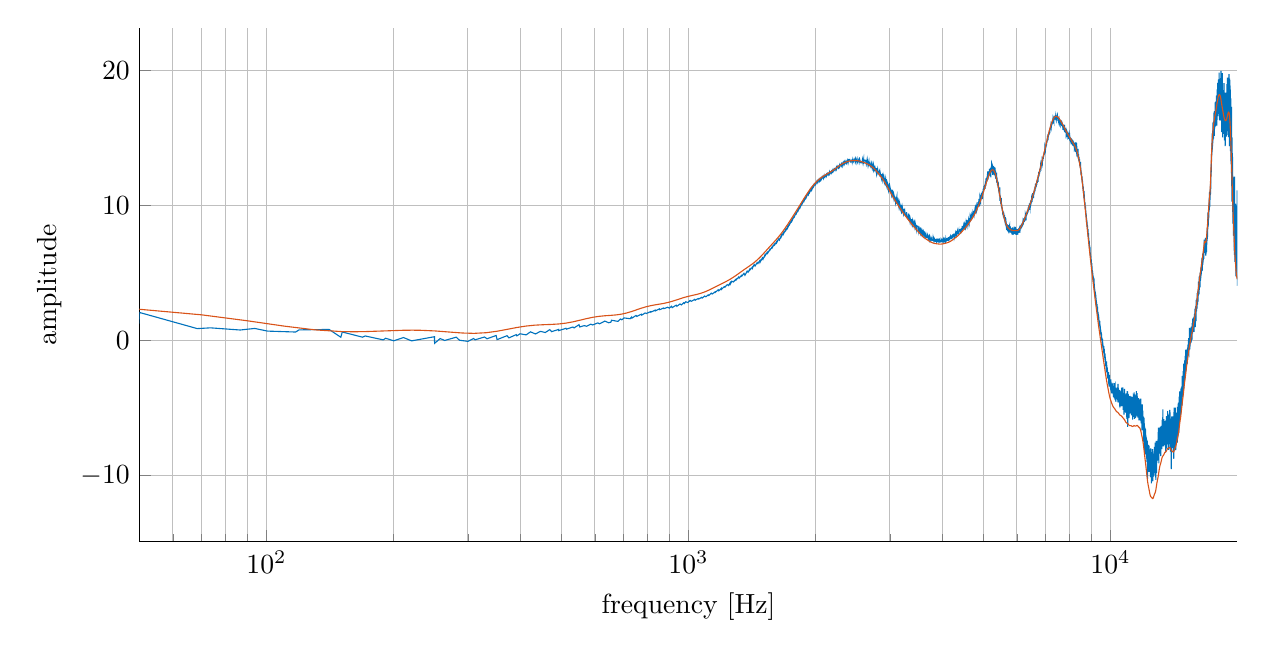
\begin{tikzpicture}

\begin{axis}[%
width=5.49in,
height=2.566in,
at={(2.311in,0.681in)},
scale only axis,
xmode=log,
xmin=50,
xmax=20000,
xminorticks=true,
xlabel={frequency [Hz]},
xmajorgrids,
xminorgrids,
ylabel={amplitude},
ymajorgrids,
axis background/.style={fill=white},
axis x line*=bottom,
axis y line*=left
]
\addplot [color=mycolor1,solid,forget plot]
  table[row sep=crcr]{%
49.8670212765958	1.23965295698856\\
50.0094984802432	2.0621103659696\\
68.5315349544073	0.866696453959857\\
73.6607142857143	0.923092073032269\\
86.6261398176292	0.762575005738629\\
93.75	0.879331353759989\\
100.588905775076	0.681341026968351\\
117.258738601824	0.613369530188904\\
119.395896656535	0.774067694269707\\
140.767477203647	0.804224019928009\\
150.02849544073	0.228028572066702\\
151.168313069909	0.617347036970115\\
168.835486322188	0.231976651790589\\
171.400075987842	0.321011022624902\\
189.067249240122	0.03272566920044\\
191.631838905775	0.151578020955318\\
200.18047112462	-0.0362577754616497\\
211.151215805471	0.204888005790098\\
220.697188449848	-0.0408026477091947\\
250.047492401216	0.26612854954594\\
250.189969604863	-0.223456686093107\\
257.883738601824	0.129713946015111\\
264.437689969605	-0.0102824777413481\\
281.534954407295	0.230480203849225\\
286.664133738602	0.00663732598765773\\
300.056990881459	-0.078149148806762\\
309.602963525836	0.133469937819601\\
312.025075987842	0.0370154028836808\\
328.409954407295	0.243538032730778\\
333.11170212766	0.114264741515167\\
350.066489361702	0.357295884697198\\
351.918693009119	0.0512129293535461\\
371.580547112462	0.341966888468046\\
375.427431610942	0.180821982647866\\
390.814969604863	0.421383115627858\\
392.09726443769	0.328191012143625\\
398.936170212766	0.482860320440211\\
412.329027355623	0.403056285042413\\
422.302431610942	0.626101389113876\\
433.843085106383	0.472541482557682\\
445.811170212766	0.661996843044491\\
457.779255319149	0.577641914285314\\
469.177431610942	0.790206610325906\\
473.879179331307	0.640799223921047\\
492.401215805471	0.807071030915143\\
492.686170212766	0.715503904255299\\
512.348024316109	0.890369548510179\\
513.772796352584	0.82836040534921\\
532.294832826748	0.983976848416291\\
535.571808510638	0.916514880827592\\
550.246960486322	1.15743894868245\\
552.669072948328	0.988757040947423\\
566.204407294833	1.08891650762087\\
573.328267477204	1.04130965331034\\
586.578647416413	1.19366880943576\\
592.990121580547	1.13873919446828\\
609.94490881459	1.29041243090122\\
615.074088145897	1.22156601579981\\
626.187310030395	1.34162818952564\\
633.453647416413	1.42421372505907\\
646.846504559271	1.30071463950605\\
654.825227963526	1.34558230777409\\
656.962386018237	1.48700529309139\\
680.471124620061	1.40215500920583\\
689.87462006079	1.57627913810108\\
695.146276595745	1.51749498164245\\
703.837386018237	1.65930593670314\\
727.346124620061	1.59863365972782\\
733.187689969605	1.72593787056206\\
734.612462006079	1.64485906352143\\
750.997340425532	1.83805272874301\\
754.41679331307	1.77276643118946\\
773.366261398176	1.93401259771645\\
774.648556231003	1.86488847494978\\
789.466185410334	2.02330599429976\\
794.880319148936	1.98745094548292\\
813.829787234043	2.13117283032096\\
814.257218844985	2.08122938548598\\
833.491641337386	2.2385605449734\\
834.631458966565	2.17729500004001\\
853.438449848024	2.32886947996479\\
855.005699088146	2.26610347132907\\
873.100303951368	2.39564095705209\\
874.952507598784	2.34730102246104\\
892.762158054711	2.44752598286313\\
900.455927051672	2.38175724556945\\
910.856762917933	2.5198884619833\\
914.988601823708	2.42080419816232\\
934.792933130699	2.60255883736632\\
938.497340425532	2.52119334771402\\
954.882218844985	2.69146707470881\\
961.863601823708	2.62370634552958\\
974.544072948328	2.78317595812823\\
977.536094224924	2.72431603574754\\
985.372340425532	2.8582067016968\\
996.200607902736	2.7932949868458\\
1008.88107902736	2.95362876913685\\
1015.57750759878	2.88791843611486\\
1034.2420212766	3.03059652565308\\
1037.23404255319	2.97176547958207\\
1054.47378419453	3.09414338547548\\
1057.32332826748	3.05498072653966\\
1074.13563829787	3.18105767430834\\
1077.41261398176	3.12898181337121\\
1092.23024316109	3.27596151639514\\
1099.49658054711	3.22402752125521\\
1113.8867781155	3.36767326675548\\
1117.16375379939	3.31922032928265\\
1131.83890577508	3.49474624692925\\
1137.39551671733	3.42731402690766\\
1155.63259878419	3.58472323509626\\
1156.91489361702	3.54903660228451\\
1176.00683890578	3.73987160608833\\
1178.99886018237	3.66633962215563\\
1196.23860182371	3.84687580343213\\
1196.95098784195	3.77371306094575\\
1215.47302431611	3.97385716543828\\
1219.17743161094	3.93302114944898\\
1235.84726443769	4.12557710149353\\
1243.398556231	4.05577299987869\\
1255.93655015198	4.27299996478966\\
1256.79141337386	4.17372375618895\\
1266.90729483283	4.3804204499482\\
1276.7382218845	4.32032964625055\\
1295.83016717325	4.51959409391031\\
1296.82750759878	4.47359514726909\\
1315.4920212766	4.68942420167532\\
1318.62651975684	4.61163530571207\\
1335.72378419453	4.80900050220326\\
1338.14589665654	4.76041577308562\\
1353.39095744681	4.95952051707384\\
1360.79977203647	4.81535101762178\\
1377.32712765957	5.12321147674841\\
1384.45098784195	5.04526883542842\\
1397.27393617021	5.27131254295002\\
1398.41375379939	5.20804639235075\\
1417.22074468085	5.42593598175516\\
1418.21808510638	5.35760280937226\\
1431.1835106383	5.61400884038677\\
1438.02241641337	5.50357867901266\\
1454.97720364742	5.75933824185264\\
1460.24886018237	5.68324587155109\\
1476.77621580547	5.91367710675182\\
1478.0585106383	5.78390704301746\\
1497.0079787234	6.10664047795025\\
1501.56724924012	6.0009875338274\\
1516.95478723404	6.3138452111559\\
1518.09460486322	6.24520706062955\\
1536.61664133739	6.52397595066333\\
1539.89361702128	6.44339671563808\\
1558.27317629179	6.72348424139082\\
1559.98290273556	6.67905862316484\\
1578.36246200608	6.92045419480825\\
1579.64475683891	6.86584558705616\\
1596.59954407295	7.12290161309876\\
1600.01899696049	7.05695512195175\\
1618.54103343465	7.31915762664543\\
1619.39589665654	7.24747783559807\\
1636.63563829787	7.52625138497209\\
1642.33472644377	7.43045028410948\\
1658.43465045593	7.74715955472931\\
1659.57446808511	7.66560749130245\\
1678.52393617021	7.97187767602341\\
1679.52127659574	7.88568112349508\\
1698.47074468085	8.2015669445019\\
1701.17781155015	8.13415753426232\\
1718.41755319149	8.4389825911051\\
1719.41489361702	8.34684617863696\\
1738.22188449848	8.67969308012454\\
1739.21922492401	8.62143907074427\\
1758.16869300912	8.93297496211826\\
1759.45098784195	8.85261390611768\\
1778.2579787234	9.17354264645685\\
1781.10752279635	9.13426463242566\\
1798.0623100304	9.43127513913061\\
1801.05433130699	9.37658153360624\\
1819.7188449848	9.70747838273514\\
1821.00113981763	9.62968753397241\\
1839.66565349544	9.94317375634403\\
1840.80547112462	9.87207523835953\\
1859.46998480243	10.2023659069749\\
1860.75227963526	10.1232950897057\\
1879.70174772036	10.4357500346976\\
1880.98404255319	10.3502320571394\\
1899.79103343465	10.6688581862763\\
1900.64589665654	10.5673639726467\\
1919.88031914894	10.8903100562394\\
1923.86968085106	10.7909178878545\\
1939.68465045593	11.1100129890865\\
1940.68199088146	11.0037887276847\\
1959.63145896657	11.2872079997477\\
1960.48632218845	11.1562825971816\\
1979.43579027356	11.4727733442189\\
1980.57560790274	11.3912995172669\\
1999.0976443769	11.6411394464895\\
2002.23214285714	11.5482825252873\\
2017.76215805471	11.8197825592191\\
2024.45858662614	11.6720567312845\\
2038.99126139818	11.9310309538836\\
2044.26291793313	11.7787677593065\\
2060.79027355623	12.0201019448653\\
2062.35752279635	11.8900531637854\\
2080.87955927052	12.1322769571114\\
2088.14589665654	11.9923911122737\\
2096.69452887538	12.2132582085086\\
2102.10866261398	12.0879907936493\\
2120.91565349544	12.2835328879545\\
2122.05547112462	12.1500871703325\\
2136.7306231003	12.3561973016951\\
2143.99696048632	12.2465883526634\\
2158.52963525836	12.4808341799601\\
2161.6641337386	12.3063791204406\\
2180.61360182371	12.5220494390673\\
2183.8905775076	12.4075161321239\\
2198.70820668693	12.6317089658205\\
2201.84270516717	12.4888058417021\\
2218.37006079027	12.691429614271\\
2225.351443769	12.586150280299\\
2240.45402735562	12.8176784208994\\
2243.16109422492	12.6730237606077\\
2258.54863221885	12.8997464299705\\
2267.52469604863	12.7649334868367\\
2280.3476443769	12.9824689678073\\
2283.0547112462	12.8488539981871\\
2302.2891337386	13.0773276975506\\
2305.2811550152	12.9351927086891\\
2322.37841945289	13.1463541275124\\
2322.80585106383	12.9511553264761\\
2340.33054711246	13.2221273793586\\
2345.31724924012	13.0549611693228\\
2360.13487841945	13.2714419097343\\
2367.11626139818	13.1135194220187\\
2382.2188449848	13.3368374682788\\
2388.91527355623	13.139353449903\\
2398.03381458967	13.4016075885468\\
2412.13905775076	13.3978554879497\\
2419.12044072948	13.1984915236383\\
2438.63981762918	13.218289100726\\
2441.77431610942	13.4220183525171\\
2444.90881458967	13.2289976746246\\
2451.89019756839	13.4337156041647\\
2463.43085106383	13.2283605560857\\
2479.53077507599	13.4449548988089\\
2483.80509118541	13.4911033127426\\
2486.93958966565	13.18513694064\\
2507.59878419453	13.4592169160125\\
2510.44832826748	13.13424517989\\
2533.81458966565	13.4083469817973\\
2538.51633738602	13.2107959905984\\
2545.21276595745	13.4008308888372\\
2557.32332826748	13.1551369268841\\
2578.55243161094	13.1432499450215\\
2583.8240881459	13.3791332079011\\
2592.23024316109	13.1133759283092\\
2601.20630699088	13.4077266154782\\
2604.19832826748	13.0662781174191\\
2607.47530395137	13.3486506584745\\
2627.7070668693	13.3316168093149\\
2638.25037993921	13.0504536501517\\
2651.21580547112	13.4184632861083\\
2664.18123100304	12.9395588459654\\
2675.00949848024	13.228606558593\\
2677.71656534954	12.8833545571637\\
2685.12537993921	13.1222554845453\\
2702.08016717325	12.8851428369102\\
2708.91907294833	13.1154445008257\\
2721.59954407295	12.8110957566953\\
2725.01899696049	13.0350068403581\\
2741.97378419453	12.6644165826413\\
2744.96580547112	12.9840957329365\\
2759.64095744681	12.6434600741854\\
2767.04977203647	12.8056107930734\\
2781.58244680851	12.526147894995\\
2788.84878419453	12.7490324824724\\
2791.98328267477	12.3610578563883\\
2806.65843465046	12.6871785850255\\
2815.4920212766	12.3271294466812\\
2838.85828267477	12.5892425869258\\
2841.99278115502	12.1206145468136\\
2846.40957446809	12.4156208112732\\
2865.50151975684	12.009853521658\\
2870.63069908815	12.305970373627\\
2879.60676291793	11.9304154240055\\
2886.58814589666	12.2025914254136\\
2905.39513677812	11.8216039729494\\
2906.25	12.0763087313118\\
2923.48974164134	11.6452881527859\\
2932.75075987842	11.9497233003722\\
2943.43655015198	11.4933961480548\\
2953.125	11.3368800682587\\
2956.25949848024	11.7275269228537\\
2970.07978723404	11.552031199242\\
2979.62575987842	11.1208034748699\\
2992.02127659574	11.4342548820272\\
3006.26899696049	11.0062152813762\\
3006.41147416413	11.2603734139376\\
3024.79103343465	10.8461699556044\\
3030.20516717325	11.1556137010214\\
3039.46618541033	10.7386042504765\\
3050.00949848024	10.9553388987914\\
3064.96960486322	10.5582670288407\\
3068.24658054711	10.7662568252715\\
3086.76861702128	10.4016669545279\\
3087.76595744681	10.6447743867941\\
3097.02697568389	10.1902808055799\\
3117.40121580547	10.6468118666474\\
3120.39323708207	10.1172929489507\\
3129.65425531915	10.3633912251198\\
3146.75151975684	9.9864887830158\\
3147.74886018237	10.2368401457142\\
3166.55585106383	9.88094817621123\\
3167.69566869301	10.1224589918213\\
3186.50265957447	9.72260673736424\\
3187.7849544073	10.0211243670336\\
3202.60258358663	9.63122990092387\\
3209.58396656535	9.90652617388942\\
3226.53875379939	9.50116834218731\\
3231.6679331307	9.73775168026913\\
3234.6599544073	9.36608865695494\\
3253.6094224924	9.6266590615731\\
3264.4376899696	9.29112620582532\\
3284.66945288754	9.16661963237046\\
3287.66147416413	9.49642295244821\\
3289.08624620061	9.3972221183819\\
3306.04103343465	9.07059617874397\\
3322.4259118541	8.95315520459842\\
3323.13829787234	9.27521797579176\\
3330.97454407295	9.2130037705121\\
3346.07712765957	8.86247940783541\\
3349.21162613982	9.08214669436841\\
3368.16109422492	8.73965872418899\\
3371.01063829787	8.97783842637113\\
3375.42743161094	8.67880891367093\\
3391.09992401216	8.89550139942153\\
3398.93617021277	8.53030311802279\\
3416.88829787234	8.76762323143402\\
3425.86436170213	8.49629314769195\\
3430.85106382979	8.69017034451359\\
3447.66337386018	8.42618300110467\\
3448.94566869301	8.60104693927065\\
3461.62613981763	8.34654864741361\\
3469.31990881459	8.20453564324503\\
3470.88715805471	8.49489814211617\\
3498.95516717325	8.42065527892726\\
3505.50911854103	8.1363058231551\\
3510.92325227964	8.29823218326137\\
3527.30813069909	8.08727371437108\\
3532.72226443769	8.23152810414164\\
3545.83016717325	7.96554557861448\\
3550.81686930091	8.15645274185641\\
3569.33890577508	7.8890290549242\\
3570.47872340426	8.07568408184406\\
3587.148556231	7.85448392511475\\
3592.8476443769	8.04452104920078\\
3609.23252279635	7.78702278331602\\
3610.08738601824	7.98791470652826\\
3629.60676291793	7.75117629178511\\
3632.02887537994	7.88932736094678\\
3649.12613981763	7.69230413905445\\
3654.39779635258	7.83748521994129\\
3665.08358662614	7.637133670337\\
3685.45782674772	7.60053482172289\\
3686.5976443769	7.8181885572123\\
3693.86398176292	7.76158073369392\\
3703.97986322188	7.52115046259169\\
3716.23290273556	7.68031912304457\\
3727.34612462006	7.48059411734941\\
3733.4726443769	7.68321482782637\\
3748.86018237082	7.47825604316262\\
3750.85486322188	7.60176489462774\\
3756.98138297872	7.41378398164774\\
3771.9414893617	7.57637945695542\\
3776.35828267477	7.41140934258234\\
3802.85904255319	7.37903195290887\\
3803.85638297872	7.55814928529046\\
3814.96960486322	7.3713621597863\\
3821.23860182371	7.57113194172952\\
3834.20402735562	7.48057433961635\\
3844.46238601824	7.32289655427657\\
3860.70478723404	7.33288124005932\\
3865.26405775076	7.46938331899812\\
3871.24810030395	7.47900531137422\\
3874.24012158055	7.27711409799804\\
3891.62234042553	7.31163761631033\\
3897.74886018237	7.48967734008852\\
3915.13107902736	7.48531185196188\\
3920.11778115502	7.33189916112542\\
3933.22568389058	7.44529186080009\\
3944.62386018237	7.26973024079154\\
3963.57332826748	7.3286878063632\\
3968.13259878419	7.47468752378573\\
3985.51481762918	7.33002164454083\\
3990.64399696049	7.48474438886898\\
4002.75455927052	7.48476786257857\\
4008.88107902736	7.34108832694365\\
4015.71998480243	7.31184815383896\\
4021.27659574468	7.47264172806335\\
4032.38981762918	7.32317803082321\\
4042.22074468085	7.48843012121078\\
4062.02507598784	7.31465161765943\\
4070.43123100304	7.50804190089759\\
4079.26481762918	7.28962083918334\\
4082.39931610942	7.51754196067225\\
4108.4726443769	7.54077382255872\\
4108.90007598784	7.4083407468729\\
4126.28229483283	7.40273368550668\\
4132.40881458967	7.64012075291626\\
4135.25835866261	7.47833489918945\\
4150.21846504559	7.58521637679762\\
4159.19452887538	7.4974463326435\\
4162.61398176292	7.61733914291387\\
4173.15729483283	7.69265740192925\\
4173.29977203647	7.53208604097097\\
4196.66603343465	7.53958605634772\\
4201.93768996961	7.71391656863627\\
4220.03229483283	7.77339273387868\\
4220.88715805471	7.60705966340717\\
4234.99240121581	7.65817258804571\\
4249.66755319149	7.86489603309807\\
4265.625	7.86340570201064\\
4267.04977203647	7.63639025889769\\
4274.74354103343	7.73656849683242\\
4291.84080547113	7.93305985908216\\
4294.97530395137	7.79694131404811\\
4311.78761398176	7.94171485309067\\
4313.92477203647	8.09790549465876\\
4316.91679331307	7.8325010255601\\
4337.4335106383	8.07200322038132\\
4338.57332826748	7.88799780119585\\
4360.79977203647	7.945501896171\\
4371.34308510638	8.11701284998835\\
4374.47758358663	7.97623787231194\\
4391.57484802432	8.19084651022631\\
4412.66147416413	8.21186217410367\\
4413.94376899696	7.99969103457076\\
4431.1835106383	8.08097618728113\\
4433.17819148936	8.30327720876001\\
4436.17021276596	8.16836336153752\\
4452.84004559271	8.37340473943619\\
4454.69224924012	8.47804564423539\\
4455.97454407295	8.2061472342604\\
4484.32750759878	8.28684952317799\\
4490.45402735562	8.51185747789165\\
4501.42477203647	8.37328631622411\\
4509.54597264438	8.59448856463525\\
4525.07598784195	8.41114581821682\\
4531.20250759878	8.6899057614854\\
4539.75113981763	8.48882987008924\\
4548.58472644377	8.76447198282851\\
4561.40767477204	8.57501108924208\\
4571.95098784195	8.92445672703569\\
4578.21998480243	8.56183942607783\\
4588.47834346505	8.87513741492541\\
4595.45972644377	8.57466934235528\\
4612.55699088146	8.94708128745337\\
4625.09498480243	8.70727377879642\\
4632.64627659574	9.04058205098031\\
4642.33472644377	8.81259013092557\\
4648.46124620061	9.11082995133912\\
4656.72492401216	8.95299292805916\\
4674.39209726444	9.2208224676793\\
4678.09650455927	9.00862900930926\\
4690.34954407295	9.34021542340041\\
4696.90349544073	9.13054524294862\\
4712.57598784195	9.36389655021971\\
4719.12993920973	9.16038824434142\\
4724.82902735562	9.45075610070053\\
4739.21922492401	9.29334007129484\\
4751.89969604863	9.58485217754784\\
4756.601443769	9.37604306738121\\
4774.41109422492	9.70846747732144\\
4783.10220364742	9.40109146602101\\
4789.51367781155	9.79572176657541\\
4806.61094224924	9.97684142526332\\
4812.73746200608	9.53371864837191\\
4830.11968085106	9.67744550336462\\
4835.81876899696	10.0291556907694\\
4839.80813069909	9.86243065722127\\
4853.62841945289	10.2363517618128\\
4858.18768996961	9.96242489717756\\
4876.28229483283	10.3125088819556\\
4876.99468085106	10.4783969487367\\
4883.1212006079	9.90697127806959\\
4900.21846504559	10.2109247633175\\
4903.49544072948	10.5729942256244\\
4923.86968085106	10.2744771222761\\
4935.55281155015	10.8020932108904\\
4944.38639817629	10.5332756142797\\
4947.37841945289	10.9246624916099\\
4970.88715805471	10.4640256233025\\
4974.1641337386	11.0227234572192\\
4983.56762917933	10.8440313184625\\
4996.53305471125	11.2287434235992\\
4998.52773556231	10.9631997695088\\
5017.19224924012	11.4322973417767\\
5020.32674772037	11.1413873878789\\
5036.99658054711	11.5054027818977\\
5041.27089665654	11.2170040359964\\
5054.80623100304	11.7690443924917\\
5064.49468085106	11.4180593251548\\
5070.9061550152	11.9866918342098\\
5078.03001519757	11.6468757413737\\
5096.83700607903	12.1168900308489\\
5099.40159574468	11.7798397028195\\
5117.7811550152	12.5023269594674\\
5122.19794832827	11.8922017877277\\
5137.44300911854	12.4065907860412\\
5142.57218844985	12.0905967691988\\
5156.67743161094	12.4823356799983\\
5158.10220364742	12.2069903729083\\
5164.6561550152	12.6950537732629\\
5188.16489361702	12.2139296439687\\
5197.99582066869	12.7617338658132\\
5205.40463525836	12.0710980602707\\
5213.09840425532	12.8012690773891\\
5220.50721884498	12.4676964901066\\
5228.91337386018	13.1306654310433\\
5249.85752279635	12.9580772581463\\
5258.54863221885	12.2581859144692\\
5262.39551671733	12.9063283440646\\
5265.10258358663	12.4142105398791\\
5282.05737082067	12.9176446972194\\
5290.17857142857	12.4142922698996\\
5299.29711246201	12.819265555967\\
5305.42363221885	12.2206309838079\\
5322.80585106383	12.8115236106075\\
5337.48100303951	12.0849709452958\\
5342.18275075988	12.5672861695905\\
5349.30661094225	11.9495308494645\\
5372.81534954407	12.4097019387268\\
5375.80737082067	11.6800571678501\\
5379.93920972644	12.1086099080552\\
5398.17629179331	11.4901072773054\\
5402.59308510638	11.8186999911064\\
5419.12044072948	11.2740838956578\\
5419.69034954407	11.6970112427383\\
5439.49468085106	10.984755336817\\
5446.19110942249	11.258576281114\\
5454.88221884498	10.7103621696799\\
5463.57332826748	11.3331327527415\\
5469.69984802432	10.3206782448804\\
5480.67059270517	10.7196168467888\\
5498.1952887538	10.0709562264259\\
5510.44832826748	10.5404409569612\\
5519.99430091185	9.8300082567128\\
5521.41907294833	10.1143572287349\\
5539.79863221885	9.60587930884044\\
5540.93844984802	9.81238927801508\\
5558.17819148936	9.30533028141399\\
5560.60030395137	9.57925869818686\\
5575.98784194529	9.12717369822563\\
5580.8320668693	9.51682099290844\\
5598.78419452888	8.95435644136304\\
5610.46732522796	9.28684894444649\\
5620.15577507599	8.75089384060472\\
5630.84156534954	9.12196238278724\\
5633.97606382979	8.56644371319063\\
5651.21580547113	9.03246112300372\\
5656.48746200608	8.44491151709061\\
5662.47150455927	8.69312570012186\\
5674.72454407295	8.17791210755991\\
5683.84308510638	8.61121777976975\\
5698.23328267477	8.1167580482593\\
5710.20136778116	8.54251065250303\\
5720.88715805471	8.15708356043666\\
5721.59954407295	8.04007988836027\\
5724.73404255319	8.52468497696225\\
5745.10828267477	7.92698317955103\\
5751.23480243161	8.39638322337285\\
5768.6170212766	8.53614844214776\\
5769.89931610942	8.00847662023352\\
5791.98328267477	8.43293731711346\\
5795.11778115502	7.97148701374563\\
5812.5	8.29269586632059\\
5821.61854103343	8.00503609239971\\
5832.73176291793	7.95769847179138\\
5841.99278115502	8.32990166405579\\
5841.99278115502	8.32990166405579\\
5845.12727963526	7.8337914600123\\
5862.3670212766	8.36890096824216\\
5873.05281155015	7.98884227223577\\
5884.59346504559	8.26555429654114\\
5889.01025835866	7.87174462578797\\
5902.54559270517	7.89827454721968\\
5915.51101823708	8.31001863611059\\
5925.7693768997	8.25738102489783\\
5931.61094224924	7.88941273492202\\
5956.25949848024	8.39527654801953\\
5962.38601823708	7.85614918051409\\
5978.0585106383	8.23361855913092\\
5979.76823708207	7.81305022326737\\
5985.75227963526	8.25557088626818\\
5993.58852583587	7.89359611705662\\
6003.13449848024	7.87832422021485\\
6015.81496960486	8.23400906746523\\
6032.76975683891	7.83763502123022\\
6040.17857142857	8.23649376216261\\
6050.15197568389	7.95953599290853\\
6062.68996960486	8.28003330639147\\
6066.67933130699	8.0336381121714\\
6079.07484802432	8.29211900861986\\
6089.19072948328	8.35044609717117\\
6097.02697568389	7.96875775519583\\
6105.00569908815	8.15291791087251\\
6123.52773556231	8.48873030117247\\
6126.8047112462	8.22901496026701\\
6143.18958966565	8.5560765324102\\
6149.88601823708	8.30960020305031\\
6161.42667173252	8.62633630124124\\
6170.26025835866	8.38684907846445\\
6179.0938449848	8.68806059570704\\
6186.07522796353	8.47985616099052\\
6202.88753799392	8.79566326597553\\
6217.42021276596	8.56711717307079\\
6218.70250759878	8.90911395002238\\
6224.97150455927	8.71001695081129\\
6243.92097264438	9.04777536047913\\
6245.77317629179	8.78026526357702\\
6263.44034954407	9.0940700983294\\
6264.29521276596	8.8276274072816\\
6282.24734042553	9.23504815523244\\
6284.66945288754	8.8921226275014\\
6287.80395136778	9.3196212494168\\
6311.31268996961	9.10861653549777\\
6320.57370820669	9.42168577233828\\
6325.27545592705	9.21263139074792\\
6343.51253799392	9.52260193580615\\
6347.6443768997	9.32145592163962\\
6358.18768996961	9.64374633916428\\
6368.01861702128	9.43580071448899\\
6384.26101823708	9.8340554822918\\
6387.25303951368	9.55820554213229\\
6404.06534954407	9.90529958128007\\
6405.06268996961	9.66413273252646\\
6408.19718844985	10.0022519868199\\
6427.85904255319	9.74951354700536\\
6428.57142857143	10.1332346415881\\
6448.94566869301	9.79754018644617\\
6464.04825227964	10.2218916235574\\
6472.45440729483	10.3498222450727\\
6475.58890577508	10.0671091851566\\
6489.40919452888	10.2002447258595\\
6501.37727963526	10.4905326990469\\
6519.32940729483	10.2297975679283\\
6525.45592705167	10.7581302151959\\
6529.87272036474	10.4137953115894\\
6545.83016717325	10.9040076571422\\
6553.09650455927	10.5570005862642\\
6557.37082066869	10.9186818936529\\
6572.47340425532	10.5308922802873\\
6582.87424012158	11.0329819069347\\
6586.29369300912	10.8227114022066\\
6603.81838905775	11.2045500808252\\
6607.95022796353	10.9588820714547\\
6625.33244680851	11.3435450066125\\
6627.04217325228	11.0507557890159\\
6639.7226443769	11.5903832185657\\
6646.56155015198	11.2352704519523\\
6662.80395136778	11.6101221181673\\
6667.64817629179	11.3832203823218\\
6686.45516717325	11.7458348377121\\
6686.5976443769	11.5223765351544\\
6703.97986322189	11.8988657275984\\
6710.10638297872	11.6589318642582\\
6726.49126139818	12.0377947069387\\
6736.60714285714	11.7278905426442\\
6741.02393617021	12.2143299678599\\
6747.2929331307	12.0137669963883\\
6760.11588145897	12.4558608144016\\
6768.52203647416	12.1427881616416\\
6783.48214285714	12.5192681909466\\
6787.32902735562	12.3185855576409\\
6803.99886018237	12.72032482862\\
6807.41831306991	12.4594980442591\\
6827.36512158055	12.8753939072837\\
6829.78723404255	12.6423206338779\\
6830.49962006079	12.9869445890737\\
6847.45440729483	12.8154427393493\\
6865.26405775076	13.1333877880221\\
6869.39589665654	12.9370812485136\\
6882.07636778116	13.2865875911334\\
6894.75683890578	13.1341338636856\\
6902.87803951368	13.4466569012872\\
6911.14171732523	13.2677856835819\\
6924.53457446809	13.6099347540432\\
6928.09650455927	13.4460556997295\\
6946.47606382979	13.7734238911126\\
6949.32560790274	13.6228978111823\\
6968.13259878419	13.9316718604449\\
6968.84498480243	13.781482325006\\
6983.94756838906	14.1112302339626\\
6988.50683890578	13.86359396655\\
6991.64133738602	14.2922907952262\\
7012.0155775076	14.0866755069233\\
7028.11550151976	14.4164716054979\\
7032.10486322189	14.2889610158723\\
7045.64019756839	14.5566627891324\\
7050.7693768997	14.4136957705478\\
7063.44984802432	14.7571599145861\\
7069.7188449848	14.636580526571\\
7083.96656534954	14.9253398355061\\
7093.65501519757	14.7725956583148\\
7105.90805471125	15.1043252822343\\
7108.90007598784	14.8284287679904\\
7127.7070668693	15.2237677240559\\
7130.6990881459	15.1185797651908\\
7148.79369300912	15.373909407844\\
7152.78305471125	15.2144163374401\\
7167.74316109423	15.5559069276495\\
7176.29179331307	15.3193205756394\\
7189.11474164134	15.6787480525175\\
7191.96428571429	15.5443395102179\\
7209.48898176292	15.8229710722989\\
7211.19870820669	15.7016195516855\\
7226.15881458967	15.9393181106355\\
7238.2693768997	15.8046864840113\\
7249.66755319149	16.1306502456021\\
7250.09498480243	15.8906268387841\\
7265.19756838906	16.1812789854237\\
7270.18427051672	15.971739850467\\
7288.99126139818	16.2672929758027\\
7296.68503039514	16.0478611592563\\
7305.09118541034	16.2987809773789\\
7320.05129179331	16.1184332626337\\
7320.9061550152	16.3913203970448\\
7343.56003039514	16.1997445189016\\
7346.26709726444	16.4723189453828\\
7353.53343465046	16.3119212749026\\
7367.06876899696	16.614660146694\\
7375.61740121581	16.3545645961688\\
7390.43503039514	16.6398969204654\\
7390.43503039514	16.6398969204654\\
7393.71200607903	16.3795327825448\\
7413.94376899696	16.6174902521356\\
7421.63753799392	16.4038123597064\\
7437.45250759878	16.2974653128578\\
7450.1329787234	16.5851484503545\\
7457.82674772037	16.3849393211627\\
7458.68161094225	16.5574183199159\\
7484.32750759878	16.6855177508606\\
7485.75227963526	16.3887958431555\\
7498.57522796353	16.574424766825\\
7507.83624620061	16.2418509944655\\
7528.21048632219	16.4965309403199\\
7529.49278115502	16.321224910526\\
7534.33700607903	16.5091867270836\\
7535.33434650456	16.2734866534272\\
7551.86170212766	16.4199111856662\\
7568.95896656535	16.190026083958\\
7577.65007598784	16.3644054131236\\
7587.05357142857	16.1710888702889\\
7601.72872340426	16.3305493202747\\
7604.72074468085	16.0977882634665\\
7611.84460486322	16.2764258255191\\
7625.09498480243	16.0026976104499\\
7648.60372340426	16.260298935307\\
7650.45592705167	15.9739147887578\\
7653.87537993921	16.1586254909971\\
7672.11246200608	15.8695609044427\\
7672.11246200608	15.8695609044427\\
7677.81155015198	16.113242466079\\
7693.91147416413	16.0395120295719\\
7708.72910334347	15.7684927313873\\
7715.85296352584	15.9519857313836\\
7718.98746200608	15.5833205327022\\
7735.37234042553	15.8984753076548\\
7750.18996960486	15.6589368022621\\
7760.30585106383	15.6060346282759\\
7765.86246200608	15.9257262204825\\
7789.3712006079	15.9215175835233\\
7792.22074468085	15.503717063492\\
7801.33928571429	15.7165907829783\\
7812.02507598784	15.4134603351543\\
7812.87993920973	15.7001106986503\\
7828.26747720365	15.3844190361612\\
7843.22758358663	15.6154608007567\\
7848.21428571429	15.3374565457058\\
7864.88411854103	15.499241568606\\
7866.45136778116	15.258818848615\\
7880.12917933131	15.1589066331946\\
7883.1212006079	15.4891183014013\\
7899.50607902736	15.3851461757359\\
7909.76443768997	15.0851113158318\\
7916.74582066869	15.3550297773631\\
7925.86436170213	15.0687082753285\\
7940.68199088146	15.3082344115842\\
7953.50493920973	14.9650495296675\\
7963.76329787234	14.9506255353326\\
7964.76063829787	15.2729773927945\\
7977.01367781155	15.34291192539\\
7989.69414893617	14.8949075956856\\
8000.52241641337	15.3613801950724\\
8013.63031914894	14.7581411038656\\
8014.34270516717	15.0776264798184\\
8023.88867781155	14.7847580525453\\
8040.5585106383	15.0162579998271\\
8047.53989361702	14.6552756708585\\
8070.6212006079	14.9683394609506\\
8070.9061550152	14.5066293162194\\
8092.42021276596	14.9118778628518\\
8094.27241641337	14.5230512324523\\
8106.3829787234	14.8754660665559\\
8109.51747720365	14.5529356881876\\
8118.06610942249	14.831322712071\\
8133.31117021277	14.4856431611832\\
8138.15539513678	14.8334140024341\\
8143.28457446809	14.4060824859627\\
8160.09688449848	14.7370747278101\\
8165.08358662614	14.4082482049605\\
8180.32864741641	14.6974086920025\\
8191.29939209726	14.3665116817228\\
8199.99050151976	14.6189662024266\\
8211.67363221885	14.1758940772171\\
8229.19832826748	14.2674711448882\\
8232.04787234043	14.6128451638522\\
8238.17439209727	14.5332578547831\\
8247.15045592705	14.1536539668464\\
8255.6990881459	14.4382247102649\\
8258.54863221885	13.9519510690125\\
8282.05737082067	14.6824960416517\\
8290.74848024316	14.0211377120147\\
8304.71124620061	13.9204876552776\\
8305.56610942249	14.6035205639842\\
8325.51291793313	14.2067841572797\\
8328.93237082067	13.6182150582675\\
8337.90843465046	14.0979978641803\\
8354.29331306991	13.7086065173542\\
8374.66755319149	13.5953285380148\\
8375.94984802432	14.1780123868585\\
8375.94984802432	14.1780123868585\\
8390.76747720365	13.4405451297207\\
8399.60106382979	13.7933644991842\\
8410.57180851064	13.3250026227086\\
8419.54787234043	13.5904237983957\\
8432.37082066869	13.1744819708548\\
8446.33358662614	13.42013481948\\
8456.30699088146	12.9595746866386\\
8457.44680851064	13.2198347346062\\
8475.9688449848	12.789178372845\\
8493.20858662614	13.2184625479465\\
8494.20592705167	12.5818677630429\\
8499.05015197568	12.8308233117372\\
8516.57484802432	12.2673333740565\\
8517.7146656535	12.5648724124578\\
8533.9570668693	12.1779074070014\\
8537.37651975684	12.3827280705742\\
8556.46846504559	11.8828750144941\\
8559.31800911854	12.1353613981672\\
8576.13031914894	11.6619984732323\\
8579.40729483283	11.8937499618346\\
8592.2302431611	11.3913158488239\\
8597.3594224924	11.574949585829\\
8616.16641337386	11.0649985860682\\
8617.30623100304	11.3874759619878\\
8635.68579027356	10.8550642649587\\
8654.35030395137	10.5123442645518\\
8657.48480243161	11.0581988288602\\
8657.48480243161	11.0581988288602\\
8677.43161094225	10.2455524697619\\
8680.56610942249	10.495198212369\\
8693.38905775076	10.0265897076215\\
8701.22530395137	10.1985996635153\\
8717.46770516717	9.73392960269955\\
8727.86854103343	9.91939867282501\\
8736.98708206687	9.45301421949493\\
8738.69680851064	9.61755414566263\\
8757.64627659575	9.14545775023902\\
8758.78609422492	9.30866270408804\\
8774.74354103343	8.74203943591639\\
8778.44794832827	9.04191670070408\\
8797.68237082067	8.52228579322516\\
8798.53723404255	8.77270161785184\\
8817.9141337386	8.25130403852832\\
8818.62651975684	8.51214072713398\\
8837.4335106383	7.9503062618787\\
8845.12727963526	8.23540544141503\\
8857.38031914894	7.68492145898462\\
8868.63601823708	7.93877124693074\\
8876.89969604863	7.40617065535315\\
8880.31914893617	7.57828620865324\\
8897.27393617021	7.11998024464388\\
8902.11816109423	7.38691603213135\\
8918.93047112462	6.82842533809831\\
8920.21276595745	7.03878153023016\\
8938.59232522796	6.56105503097477\\
8939.01975683891	6.93009048791746\\
8957.11436170213	6.3460597671307\\
8959.67895136778	6.47011689899201\\
8979.05585106383	6.03614621239212\\
8980.33814589666	6.23106146795576\\
8998.86018237082	5.74712537369265\\
9000.99734042553	5.98666216621252\\
9019.37689969605	5.5630179516101\\
9029.77773556231	5.71476688330622\\
9032.76975683891	5.25227358454903\\
9039.60866261398	5.47795067322495\\
9058.84308510638	4.99194444053637\\
9060.83776595745	5.17797311202279\\
9079.78723404255	4.68049568538249\\
9080.92705167173	4.98192648143411\\
9098.59422492401	4.54956081445688\\
9099.87651975684	4.7204664801527\\
9120.10828267477	4.31502915819288\\
9126.66223404255	4.54712966266234\\
9129.7967325228	4.10754255900765\\
9147.03647416414	4.2652615458388\\
9160.1443768997	3.84160600432516\\
9160.85676291793	3.99471589620993\\
9170.54521276596	3.59642199111771\\
9183.51063829787	3.77765474737833\\
9197.04597264438	3.19184875524942\\
9201.0353343465	3.59542230868101\\
9217.27773556231	3.14922189643599\\
9220.5547112462	3.4590125723322\\
9240.35904255319	2.9509901999106\\
9240.92895136778	3.13662644647674\\
9259.73594224924	2.76936598171881\\
9261.01823708207	2.95839500438544\\
9267.4297112462	2.49212167151438\\
9290.93844984802	2.68099573559212\\
9294.07294832827	2.25213852337416\\
9314.44718844985	2.49968929377267\\
9319.43389057751	2.0352537008781\\
9321.99848024316	2.26988544612295\\
9337.81344984802	1.70775346136207\\
9343.37006079027	2.1103917299564\\
9361.1797112462	1.66490130502837\\
9361.32218844985	1.94967816543112\\
9381.26899696049	1.48186122152399\\
9384.83092705167	1.74003315789441\\
9396.79901215806	1.25914611440751\\
9402.07066869301	1.49346154207927\\
9408.19718844985	1.05434964656896\\
9431.70592705167	1.4324403322105\\
9441.25189969605	0.907871756381152\\
9452.08016717325	1.15247073147726\\
9461.05623100304	0.699462624168147\\
9464.61816109423	0.92478387149922\\
9481.71542553191	0.437470629104271\\
9483.14019756839	0.739118906088323\\
9501.94718844985	0.341988722011185\\
9504.5117781155	0.612425066408711\\
9521.3240881459	0.158135909469936\\
9525.59840425532	0.471589851016518\\
9537.13905775076	-0.00540070139887234\\
9545.40273556231	0.175966799255169\\
9557.51329787234	-0.198300128274522\\
9572.47340425532	0.0831993028637151\\
9575.60790273556	-0.452570705930001\\
9582.87424012158	-0.137688192123372\\
9599.68655015198	-0.57095665921733\\
9605.24316109423	-0.346154408052286\\
9622.48290273556	-0.765381317621989\\
9632.31382978723	-0.910343372058881\\
9639.7226443769	-0.436722861841244\\
9643.71200607903	-0.6872997440049\\
9662.09156534954	-1.15281821456259\\
9663.23138297872	-0.630122613027049\\
9666.36588145897	-1.29632944293711\\
9689.5896656535	-0.959406467121346\\
9701.98518237082	-1.45508782972002\\
9713.24088145897	-1.01970838713118\\
9721.50455927052	-1.62063080208702\\
9730.90805471125	-1.39119961388538\\
9739.74164133739	-1.8832361023501\\
9743.44604863222	-1.56448100600975\\
9763.25037993921	-1.96622175245311\\
9780.49012158055	-2.36906949592039\\
9783.62462006079	-1.55257931763543\\
9785.47682370821	-1.78197410209908\\
9797.72986322188	-2.28043580789176\\
9803.99886018237	-1.84135688683258\\
9821.523556231	-2.37330933665705\\
9828.21998480243	-2.01836064463814\\
9830.49962006079	-2.6359009648496\\
9845.60220364742	-2.22690833408786\\
9854.00835866262	-2.79869842101604\\
9866.11892097265	-2.35451104393994\\
9876.8047112462	-2.85160459297293\\
9891.76481762918	-2.36420900088852\\
9900.88335866262	-3.19852431404655\\
9906.72492401216	-2.61364788008598\\
9924.39209726444	-3.42668469234222\\
9930.80357142857	-2.69282391095258\\
9942.9141337386	-3.22794941588217\\
9944.76633738602	-2.55694658594425\\
9963.28837386018	-3.29669465530272\\
9965.56800911854	-2.9436440178466\\
9976.82370820669	-3.3807523828837\\
9988.79179331307	-2.95697293967968\\
9994.77583586626	-3.52822730331858\\
10015.1500759878	-3.62904304264467\\
10018.2845744681	-2.89149416917714\\
10028.827887538	-3.16238466925156\\
10044.7853343465	-3.7358831070949\\
10045.3552431611	-3.19102063246479\\
10065.1595744681	-3.92855177672209\\
10065.7294832827	-3.78873184423079\\
10075.4179331307	-3.3235254027236\\
10085.5338145897	-3.9290847174087\\
10088.6683130699	-3.31288459256109\\
10109.0425531915	-3.26791022513673\\
10115.1690729483	-3.93819111202167\\
10132.4088145897	-3.39127387928689\\
10142.6671732523	-3.99983292575608\\
10159.0520516717	-3.37030714486554\\
10162.0440729483	-4.19045224587165\\
10179.4262917933	-3.39935993974659\\
10182.8457446809	-4.0477758053294\\
10202.7925531915	-4.27744208187062\\
10205.9270516717	-3.16505470805519\\
10209.061550152	-4.18017794418382\\
10213.478343465	-3.559113919759\\
10229.4357902736	-4.19967144715423\\
10234.4224924012	-3.50332125371614\\
10249.8100303951	-3.40728217135936\\
10252.8020516717	-4.36651697924684\\
10276.3107902736	-4.41281299634978\\
10279.4452887538	-3.61988178693642\\
10296.6850303951	-4.56233567131174\\
10299.8195288754	-3.50319395640331\\
10320.193768997	-4.34499833043195\\
10323.1857902736	-3.55116819493641\\
10329.454787234	-4.27979289026336\\
10343.7025075988	-3.60050324451592\\
10347.9768237082	-3.77355194283029\\
10353.3909574468	-4.29856053141615\\
10367.068768997	-3.67275050299665\\
10376.6147416413	-4.28875229891366\\
10390.5775075988	-4.41950673425373\\
10393.5695288754	-3.48580297521962\\
10414.0862462006	-4.59518075048995\\
10417.0782674772	-3.22570040375911\\
10438.592325228	-3.70831888736033\\
10440.587006079	-4.53712723984805\\
10464.0957446809	-3.73709373266772\\
10464.6656534954	-4.51284059691137\\
10475.0664893617	-4.53787390326626\\
10487.462006079	-3.6763346118144\\
10490.5965045593	-3.79835290853227\\
10501.7097264438	-4.51156148408311\\
10507.8362462006	-3.69433134495583\\
10510.9707446809	-4.7150168576019\\
10534.1945288754	-4.59056832385533\\
10534.337006079	-3.72424878401608\\
10557.8457446809	-4.88680719128817\\
10565.1120820669	-3.92344285264344\\
10570.9536474164	-4.5543015755548\\
10578.2199848024	-3.82592961670709\\
10603.1534954407	-3.8327934820039\\
10604.7207446809	-4.70374257899873\\
10621.9604863222	-4.6260880147065\\
10628.2294832827	-3.4984725130306\\
10629.7967325228	-3.9679958068159\\
10631.3639817629	-4.88143783387765\\
10651.7382218845	-3.58846354445447\\
10656.1550151976	-4.66343122814807\\
10677.2416413374	-4.66405704329629\\
10678.2389817629	-3.79965788995407\\
10698.6132218845	-3.48158299485141\\
10701.7477203647	-4.75169667105316\\
10721.1246200608	-3.94875265871396\\
10722.1219604863	-5.15843346921506\\
10731.5254559271	-3.89561438706003\\
10748.6227203647	-4.85289458223685\\
10762.7279635258	-3.98625149857842\\
10768.9969604863	-5.50756487969687\\
10772.1314589666	-3.94147680815144\\
10774.2686170213	-4.96666001376832\\
10789.3712006079	-4.84853429633346\\
10792.5056990881	-3.60107603229149\\
10815.8719604863	-5.32189723350456\\
10820.1462765957	-4.04907160298834\\
10836.3886778116	-5.14345099191469\\
10838.9532674772	-4.16132923959007\\
10849.7815349544	-5.05821905344874\\
10862.88943769	-4.00442979844902\\
10886.2556990881	-5.36846280492139\\
10889.3901975684	-3.92738338287817\\
10892.2397416413	-4.20412059150285\\
10895.5167173252	-5.19189805263298\\
10920.7351823708	-4.15368883760961\\
10927.5740881459	-5.28711221119177\\
10933.2731762918	-5.82296996273389\\
10948.0908054711	-3.85732695638231\\
10960.6287993921	-3.77512708815389\\
10967.7526595745	-5.8414577366523\\
10977.1561550152	-3.78795944685964\\
10980.1481762918	-6.4056043204881\\
10997.3879179331	-5.81844237304991\\
11000.3799392097	-3.96307110396507\\
11014.6276595745	-5.55184193861735\\
11017.0497720365	-4.01880926442128\\
11036.4266717325	-4.1967388211861\\
11050.5319148936	-5.76807878146276\\
11053.3814589666	-4.31602690650888\\
11064.3522036474	-5.29235642187969\\
11070.9061550152	-5.33299451836186\\
11077.3176291793	-4.3299907980269\\
11094.414893617	-4.35423251555876\\
11100.5414133739	-5.42823641836655\\
11120.9156534954	-4.11025813065519\\
11124.0501519757	-5.16230506554685\\
11135.3058510638	-4.42078236434669\\
11147.4164133739	-5.39381769581363\\
11156.6774316109	-4.3633800656473\\
11164.7986322188	-5.411080990658\\
11188.3073708207	-5.24992329171159\\
11191.2993920973	-4.16314205497606\\
11205.547112462	-4.47969742424076\\
11211.6736322188	-5.56777989726755\\
11211.6736322188	-5.56777989726755\\
11215.9479483283	-4.36188614222846\\
11238.1743920973	-4.22262747361566\\
11241.3088905775	-5.2206187824135\\
11256.5539513678	-5.49952318842443\\
11258.6911094225	-4.18669616600754\\
11280.4901215805	-4.3524376260267\\
11285.1918693009	-5.88001213008774\\
11299.4395896657	-4.19943416620656\\
11305.5661094225	-5.67625704633804\\
11320.6686930091	-4.36948943661451\\
11329.0748480243	-5.4832494264917\\
11332.4943009119	-5.16254726522656\\
11335.2013677812	-4.20433597738797\\
11355.5756079027	-4.29242604238997\\
11368.2560790274	-5.23673884475337\\
11375.9498480243	-3.86202649003834\\
11382.0763677812	-5.25872958524015\\
11394.1869300912	-4.39350881369355\\
11402.4506079027	-5.81360251095162\\
11425.9593465046	-4.01369916429458\\
11432.3708206687	-5.27979430308947\\
11441.0619300912	-5.36991690200206\\
11452.460106383	-4.2104946515152\\
11459.2990121581	-4.35181772012112\\
11469.842325228	-5.74152521060196\\
11484.8024316109	-5.26198528733587\\
11488.3643617021	-4.31753398169869\\
11495.6306990881	-4.31886243927141\\
11496.3430851064	-5.65075994933664\\
11516.717325228	-3.76105418432774\\
11518.9969604863	-5.19156957963689\\
11535.0968844985	-5.27451975256202\\
11540.2260638298	-4.09692452121121\\
11557.7507598784	-5.39423072577869\\
11566.7268237082	-3.91031041736393\\
11582.3993161094	-5.23296197513653\\
11592.3727203647	-4.35502497884494\\
11610.6098024316	-5.73098322164249\\
11611.4646656535	-4.44549893541122\\
11630.8415653495	-5.42903192465805\\
11633.9760638298	-4.27573081979228\\
11633.9760638298	-4.27573081979228\\
11649.9335106383	-5.20868361912227\\
11657.4848024316	-5.6779659152674\\
11669.5953647416	-4.42232453954311\\
11680.9935410334	-5.92441922578494\\
11683.8430851064	-4.5761833878853\\
11697.0934650456	-4.53314982215898\\
11704.5022796353	-5.67890696363231\\
11724.3066109423	-4.62595156409661\\
11727.8685410334	-5.70062357427221\\
11751.3772796353	-5.86689189200132\\
11754.3693009119	-4.32421578424037\\
11757.5037993921	-5.92033909323965\\
11768.047112462	-4.82040991358975\\
11777.8780395137	-4.61495135370178\\
11789.4186930091	-5.86164109124242\\
11798.2522796353	-4.31164272622853\\
11801.3867781155	-5.98106211264695\\
11823.6132218845	-4.86676529812545\\
11824.7530395137	-6.15625536933012\\
11847.1219604863	-5.0235163614459\\
11851.681231003	-5.94636708001737\\
11866.3563829787	-5.1636176700558\\
11868.6360182371	-6.66765892390279\\
11891.1474164134	-6.26846481775056\\
11892.1447568389	-4.75307588297712\\
11898.1287993921	-5.39863630321316\\
11915.5110182371	-6.53471810612592\\
11915.6534954407	-6.64392576864012\\
11918.6455167173	-5.17462433923574\\
11940.3020516717	-5.68549674756416\\
11942.0117781155	-6.65782461687511\\
11959.2515197568	-5.67026706561846\\
11962.5284954407	-6.9181900034514\\
11985.8947568389	-5.66784967953066\\
11989.0292553192	-7.27181899837499\\
12006.4114741641	-7.17855731727874\\
12009.4034954407	-5.74959823236055\\
12021.2291033435	-6.20526033240741\\
12035.9042553192	-7.50486056561078\\
12036.3316869301	-6.36810197702016\\
12056.2784954407	-7.90488203608425\\
12059.412993921	-8.42648496542353\\
12072.2359422492	-6.60741512778087\\
12079.7872340426	-8.19498440060414\\
12085.9137537994	-6.56338956286398\\
12103.2959726444	-6.60566817979445\\
12106.287993921	-8.13252482402407\\
12129.7967325228	-7.01220600657818\\
12132.931231003	-8.29763115086078\\
12148.0338145897	-8.48635685829259\\
12150.1709726444	-7.13524632747033\\
12158.4346504559	-7.51633963445968\\
12176.6717325228	-8.75600290668842\\
12179.806231003	-7.29719910319133\\
12197.0459726444	-8.99594829141942\\
12197.0459726444	-8.99594829141942\\
12200.1804711246	-7.7097406223466\\
12220.5547112462	-7.43682455419558\\
12230.3856382979	-9.1402027803428\\
12244.063449848	-10.259604457273\\
12250.1899696049	-7.70062137538012\\
12267.0022796353	-8.03010929680926\\
12267.9996200608	-9.2944592236414\\
12284.8119300912	-9.67113294251763\\
12294.0729483283	-7.76578131035841\\
12309.4604863222	-8.17021611097489\\
12317.4392097264	-9.72821273360372\\
12320.5737082067	-9.61417909334057\\
12335.818768997	-8.37063713277616\\
12337.9559270517	-7.7954290179183\\
12340.9479483283	-9.74993093130802\\
12364.4566869301	-8.0717142273921\\
12376.5672492401	-9.67946360443204\\
12387.9654255319	-8.12178118954724\\
12391.2424012158	-9.69802742918596\\
12408.4821428571	-8.6380166016694\\
12409.6219604863	-9.71868964767275\\
12425.5794072948	-8.49048286905398\\
12431.7059270517	-10.0898165048056\\
12450.3704407295	-10.0980443943551\\
12455.2146656535	-8.00537641916276\\
12464.9031155015	-9.93231307579057\\
12478.5809270517	-8.65868525184157\\
12481.7154255319	-8.31282831266572\\
12492.1162613982	-9.94131494791149\\
12499.0976443769	-8.69662277436474\\
12502.0896656535	-10.6018031009278\\
12519.8993161094	-9.9091824757473\\
12528.5904255319	-8.284747028923\\
12547.8248480243	-8.7895383395327\\
12552.0991641337	-10.1934092455026\\
12575.6079027356	-8.06777186949157\\
12575.7503799392	-9.78327933263922\\
12590.5680091185	-8.72668421173367\\
12595.9821428571	-10.4227816737728\\
12611.5121580547	-8.61261229226462\\
12614.3617021277	-9.93771773507742\\
12634.023556231	-9.75659482944974\\
12634.5934650456	-8.67069399549717\\
12642.7146656535	-8.38499036272569\\
12642.8571428571	-10.0883309862387\\
12669.3579027356	-8.42340439256359\\
12672.4924012158	-9.7693038433047\\
12689.8746200608	-9.98393613589681\\
12697.4259118541	-8.22221754286886\\
12711.1037234043	-9.57976266044515\\
12713.240881459	-7.88849427441571\\
12736.7496200608	-8.02371460424381\\
12739.884118541	-9.76872788350426\\
12740.4540273556	-9.53244109075674\\
12752.9920212766	-8.30120227307709\\
12760.2583586626	-9.8179415086753\\
12763.2503799392	-7.58687373917013\\
12780.7750759878	-9.27624986715037\\
12783.6246200608	-7.61039019543881\\
12807.1333586626	-10.3292406131291\\
12816.9642857143	-7.99396633260912\\
12833.634118541	-7.44391651547196\\
12835.6287993921	-9.1698104043928\\
12854.0083586626	-7.53498702022162\\
12857.1428571429	-9.83239904695521\\
12873.242781155	-7.72236179052606\\
12877.5170972644	-9.07523824164446\\
12885.2108662614	-7.76115936831271\\
12888.9152735562	-8.92183274161068\\
12904.0178571429	-7.46741935986404\\
12905.0151975684	-8.7653386772037\\
12922.967325228	-8.60399367795827\\
12924.3920972644	-7.56928829419311\\
12951.0353343465	-8.90069096357461\\
12951.3202887538	-7.35266268231899\\
12974.1166413374	-8.56107632893797\\
12974.4015957447	-6.97642306533036\\
12994.7758358663	-6.47306555308279\\
12997.9103343465	-8.75541137411123\\
13013.0129179331	-7.11906556849733\\
13018.2845744681	-9.11848250305604\\
13024.4110942249	-8.29707280385927\\
13041.6508358663	-6.92001666882721\\
13047.9198328267	-6.69005502360475\\
13051.4817629179	-8.23082884363949\\
13065.1595744681	-8.39603572932891\\
13078.4099544073	-6.7440715077719\\
13088.6683130699	-8.24770042092959\\
13094.9373100304	-6.51247101275374\\
13109.8974164134	-8.02490709945389\\
13112.0345744681	-6.4105785972277\\
13128.8468844985	-6.73659457408466\\
13135.6857902736	-8.09322022956558\\
13148.5087386018	-6.66024441645653\\
13159.0520516717	-8.58166121973735\\
13165.1785714286	-7.80637113014842\\
13181.4209726444	-6.61142136403165\\
13185.5528115502	-6.34018147950852\\
13187.1200607903	-7.76041464349946\\
13209.9164133739	-6.51641556537661\\
13213.3358662614	-7.51936734071975\\
13229.4357902736	-8.04956161496223\\
13240.6914893617	-6.3752806680798\\
13243.2560790274	-7.50275752748558\\
13255.936550152	-5.89267858486347\\
13279.4452887538	-6.10769223591243\\
13281.1550151976	-7.45497049659275\\
13299.8195288754	-7.68986155070403\\
13302.9540273556	-5.82494393200932\\
13314.2097264438	-5.11143596881353\\
13314.4946808511	-7.49475840181875\\
13335.5813069909	-7.85212260255368\\
13341.7078267477	-6.10894495295229\\
13346.6945288754	-6.06311261194351\\
13349.8290273556	-7.86034744280287\\
13370.2032674772	-5.84150340877769\\
13371.7705167173	-7.44783123998364\\
13393.712006079	-7.75231009573816\\
13399.8385258359	-6.17463517757214\\
13404.6827507599	-7.26443732045747\\
13417.0782674772	-6.1513427032296\\
13434.1755319149	-7.34038248788638\\
13443.7215045593	-6.03003802951413\\
13452.8400455927	-6.02476114140186\\
13464.0957446809	-7.71612941650172\\
13464.0957446809	-7.71612941650172\\
13481.3354863222	-6.16094560328689\\
13487.462006079	-7.85321251149153\\
13491.5938449848	-6.23132533005102\\
13510.9707446809	-8.31697804754416\\
13517.0972644377	-6.05997961469662\\
13533.6246200608	-5.93501957153489\\
13537.4715045593	-7.91494304578249\\
13557.9882218845	-7.8330141339201\\
13564.1147416413	-5.7771837123754\\
13581.3544832827	-5.61045036480051\\
13584.4889817629	-8.01455168252113\\
13592.8951367781	-5.75050372401752\\
13604.8632218845	-7.58596248445476\\
13607.8552431611	-7.70467149667275\\
13617.8286474164	-5.85229273518402\\
13628.2294832827	-5.7605824221571\\
13637.7754559271	-7.39894390168058\\
13651.7382218845	-7.71114337305398\\
13654.8727203647	-5.23912510114194\\
13675.2469604863	-7.70587460212685\\
13681.3734802432	-5.93675388434413\\
13689.3522036474	-7.27631256046316\\
13701.7477203647	-5.60211220182193\\
13722.1219604863	-5.69824568746251\\
13725.2564589666	-8.12105240532924\\
13739.7891337386	-7.48130597771741\\
13745.6306990881	-5.50825495497334\\
13745.6306990881	-5.50825495497334\\
13755.7465805471	-7.3311280549205\\
13767.9996200608	-5.96527375510796\\
13769.2819148936	-7.65909445975842\\
13795.6401975684	-5.72289558979477\\
13798.632218845	-7.3556198988267\\
13816.01443769	-5.15685356941222\\
13819.1489361702	-7.69137339138601\\
13842.5151975684	-5.3317472605265\\
13845.6496960486	-7.92175256896479\\
13851.7762158055	-5.93713128033448\\
13862.88943769	-8.24043834835105\\
13869.0159574468	-7.74153173004276\\
13880.4141337386	-6.17426184057677\\
13901.5007598784	-6.16987311956868\\
13905.3476443769	-7.52375362525444\\
13909.76443769	-7.93805766994734\\
13912.8989361702	-5.7934078911832\\
13936.407674772	-9.54613830977869\\
13945.2412613982	-6.284319366644\\
13959.7739361702	-5.64445077366823\\
13965.3305471125	-7.53398005137844\\
13977.0136778116	-7.77097720938066\\
13983.282674772	-5.63602276702461\\
13992.6861702128	-7.96698823393127\\
14005.2241641337	-6.18489387054775\\
14009.7834346505	-6.00035612633686\\
14026.5957446809	-7.6610416886024\\
14030.157674772	-6.28585332797346\\
14044.4053951368	-7.67026408853704\\
14053.6664133739	-5.62578730360029\\
14062.9274316109	-7.83572330587455\\
14069.4813829787	-6.25285967954546\\
14074.0406534954	-8.30852267222801\\
14097.5493920973	-5.9928982859447\\
14107.5227963526	-7.7567714851016\\
14124.0501519757	-8.77125329177988\\
14127.1846504559	-5.84592075356141\\
14144.4243920973	-8.06597787008868\\
14147.5588905775	-4.99035619621969\\
14152.8305471125	-7.43948339029429\\
14157.1048632219	-6.17069726805042\\
14170.9251519757	-5.92330406814586\\
14176.3392857143	-7.6740766236406\\
14191.4418693009	-5.84173788371414\\
14194.4338905775	-8.14620204671817\\
14214.8081306991	-7.7247533923199\\
14217.9426291793	-5.08110383748899\\
14236.1797112462	-7.21978323356695\\
14238.3168693009	-4.97906140761417\\
14264.8176291793	-8.12603914470579\\
14266.6698328267	-5.78692417927393\\
14276.2158054711	-5.88081018234614\\
14288.3263677812	-8.09052270655477\\
14293.4555471125	-7.26104315971772\\
14306.8484042553	-5.83004900846469\\
14311.835106383	-5.39540785095347\\
14323.0908054711	-7.13273095490632\\
14332.2093465046	-5.38069400686839\\
14334.2040273556	-7.0070049077164\\
14367.2587386018	-6.7255225636591\\
14367.5436930091	-5.52821212201591\\
14379.0843465046	-7.60202923654207\\
14385.2108662614	-5.32282824614085\\
14402.5930851064	-7.5211348136633\\
14408.7196048632	-4.92960610065591\\
14425.9593465046	-7.31122831430962\\
14429.0938449848	-5.06741498207662\\
14435.3628419453	-5.24303691775062\\
14449.4680851064	-7.18263179806483\\
14449.4680851064	-7.18263179806483\\
14469.414893617	-5.15298148472371\\
14472.9768237082	-4.70692835385655\\
14481.2405015198	-6.46132510277242\\
14492.4962006079	-6.23608629038921\\
14496.3430851064	-4.61504869174417\\
14519.8518237082	-6.86868896029639\\
14522.8438449848	-4.71340131678346\\
14533.8145896657	-5.88320732222761\\
14546.3525835866	-4.17672476200524\\
14566.7268237082	-6.24484935755182\\
14567.8666413374	-4.5932575373489\\
14572.2834346505	-5.76873099273549\\
14590.23556231	-3.78215709524685\\
14590.23556231	-3.78215709524685\\
14593.3700607903	-5.70724393193075\\
14613.7443009119	-3.90472725125989\\
14615.4540273556	-5.43203785569213\\
14640.3875379939	-5.46685265037848\\
14645.2317629179	-3.98125741114958\\
14660.6193009119	-5.39074664009692\\
14663.7537993921	-3.8996354807957\\
14684.1280395137	-5.42583848429062\\
14687.1200607903	-3.60459334842421\\
14696.3810790274	-4.92649976628699\\
14710.6287993921	-3.55453209590716\\
14711.6261398176	-4.73909141151492\\
14713.3358662614	-3.64660002497161\\
14733.9950607903	-4.73872768928037\\
14737.1295592705	-3.48038730628245\\
14757.5037993921	-4.80222226148134\\
14760.353343465	-3.39453591376123\\
14777.8780395137	-4.84021873128638\\
14781.0125379939	-2.79406227464136\\
14801.3867781155	-2.6372577176005\\
14810.2203647416	-4.18301178220433\\
14821.9034954407	-3.9782898300932\\
14824.8955167173	-2.85400203217607\\
14839.0007598784	-2.86243682016677\\
14843.7025075988	-3.94012610778107\\
14854.530775076	-3.7722453433115\\
14871.7705167173	-2.2910307926052\\
14871.7705167173	-2.2910307926052\\
14874.9050151976	-3.91601454361306\\
14898.2712765957	-3.52003579002677\\
14904.6827507599	-2.49146389046086\\
14918.6455167173	-1.72267447522582\\
14921.7800151976	-3.55398404931566\\
14937.3100303951	-3.14965935132122\\
14942.1542553192	-2.03480041363349\\
14956.1170212766	-1.98872670020925\\
14971.7895136778	-3.00443297951619\\
14975.351443769	-2.9113652562797\\
14992.1637537994	-1.4949999497739\\
14994.3009118541	-2.87456261845727\\
15002.422112462	-1.81217595842367\\
15012.537993921	-2.73917493738272\\
15015.6724924012	-1.63790289712296\\
15036.0467325228	-1.15503189065525\\
15039.4661854103	-2.49012724795675\\
15055.4236322188	-2.36272247933372\\
15059.412993921	-1.14852446823211\\
15075.2279635258	-2.17104529561873\\
15082.9217325228	-0.699413763074529\\
15106.4304711246	-0.823441987808531\\
15112.5569908815	-2.25099967284597\\
15113.6968085106	-2.13539290107073\\
15123.670212766	-1.16261573896967\\
15134.6409574468	-1.95572585233388\\
15141.9072948328	-1.02896398570109\\
15156.4399696049	-1.8080931312975\\
15165.273556231	-0.761787669494229\\
15179.806231003	-1.76298106518634\\
15183.5106382979	-0.850101560355528\\
15205.5946048632	-0.69354490598423\\
15206.4494680851	-1.70087728338028\\
15219.5573708207	-0.624367185425569\\
15226.8237082067	-1.45545188496836\\
15236.0847264438	-1.28602657129452\\
15253.3244680851	-0.311620435984233\\
15259.5934650456	-1.18824381755925\\
15270.8491641337	-0.388853790155526\\
15278.1155015198	-1.0421169212604\\
15294.2154255319	-0.189115892222272\\
15297.0649696049	-1.06606515534665\\
15305.1861702128	-0.172404083048884\\
15317.5816869301	0.160826754741234\\
15321.9984802432	-0.897969239224779\\
15340.9479483283	-0.969900330951187\\
15353.3434650456	0.13313677592765\\
15359.4699848024	-0.707028165545649\\
15370.8681610942	0.103678188228174\\
15378.1344984802	-0.636352855999171\\
15387.9654255319	0.919302450770522\\
15397.226443769	0.30309586932409\\
15411.4741641337	-0.67143329206088\\
15428.7139057751	0.547273748560918\\
15431.7059270517	-0.392749130120862\\
15442.2492401216	-0.396373406575383\\
15452.2226443769	0.527070043429177\\
15455.4996200608	-0.208869987376917\\
15458.3491641337	0.891610260740443\\
15481.8579027356	-0.219511679593699\\
15484.8499240122	0.85216558960643\\
15499.0976443769	-0.146036849247295\\
15502.5170972644	0.765016080062385\\
15528.7329027356	-0.16762084583446\\
15534.8594224924	1.00389345054806\\
15540.9859422492	0.770816889460151\\
15552.0991641337	-0.0788434434879828\\
15559.7929331307	0.163171072715882\\
15564.0672492401	0.84655373246905\\
15578.7424012158	0.972606510409483\\
15585.1538753799	0.228436602824528\\
15599.1166413374	0.0592209892111455\\
15614.219224924	1.12380578373038\\
15617.2112462006	0.327802069880704\\
15622.4829027356	1.2758080885104\\
15643.1420972644	0.508088507581529\\
15653.6854103343	1.19801792142877\\
15660.9517477204	0.523306456276872\\
15669.5003799392	1.58899794198431\\
15677.9065349544	0.706749473901369\\
15696.0011398176	1.65194263887043\\
15699.1356382979	0.762201093281118\\
15708.5391337386	1.51867796408695\\
15716.5178571429	0.792688862176294\\
15722.501899696	1.60689728530948\\
15739.884118541	0.881546380771918\\
15746.0106382979	1.67849267995953\\
15763.2503799392	0.897299136582247\\
15773.3662613982	1.70491352700785\\
15786.759118541	0.618255437149125\\
15793.5980243161	1.76850764509771\\
15810.8377659574	1.16624930187091\\
15813.4023556231	1.92312692953567\\
15831.63943769	1.94540341884866\\
15833.634118541	1.26692865417634\\
15838.3358662614	1.40224025377563\\
15851.016337386	2.1814660912506\\
15867.1162613982	2.15674234070411\\
15875.9498480243	1.4788573971719\\
15880.6515957447	0.975197254441332\\
15883.5011398176	2.32884126770718\\
15904.1603343465	1.3351622525616\\
15907.1523556231	2.42779026421177\\
15923.5372340426	1.83964573159325\\
15930.6610942249	2.55739346285463\\
15951.0353343465	1.43460134674518\\
15957.1618541033	2.77018243496845\\
15959.5839665654	1.95573202076265\\
15974.5440729483	3.0035913720953\\
15991.2139057751	2.89045860879218\\
15993.4935410334	2.14067067663469\\
16006.1740121581	2.28846832649259\\
16015.1500759878	2.99185532459985\\
16023.4137537994	2.48253022407674\\
16030.8225683891	3.10585492986199\\
16044.9278115502	2.34048255089205\\
16051.054331307	3.45922624112564\\
16068.2940729483	3.46939626611221\\
16073.5657294833	2.83655574907906\\
16091.8028115502	2.63810691515594\\
16094.3674012158	3.51012260223512\\
16114.1717325228	3.66095045366725\\
16115.311550152	2.84591661593734\\
16128.1344984802	3.11396729495806\\
16138.2503799392	3.77983625903713\\
16139.2477203647	3.31061493027946\\
16156.7724164134	3.89008646692125\\
16168.3130699088	4.34397726710488\\
16173.2997720365	3.44757745124023\\
16185.5528115502	3.38348200040387\\
16198.0908054711	4.20578110574819\\
16209.061550152	3.44025740504026\\
16216.327887538	4.25988023170846\\
16232.5702887538	4.69407575391552\\
16234.9924012158	3.7359401402609\\
16240.976443769	3.99101643129711\\
16255.936550152	4.75970782842285\\
16273.318768997	4.06403306927265\\
16279.4452887538	4.77856113446961\\
16280.7275835866	4.07944871604252\\
16294.8328267477	4.77858735783974\\
16302.9540273556	3.91439359066594\\
16309.0805471125	4.90964079823983\\
16320.3362462006	4.40703313773097\\
16326.4627659574	5.01053447016434\\
16343.1325987842	4.44803482177434\\
16349.9715045593	5.19965182974027\\
16372.0554711246	4.6063034449441\\
16373.3377659574	5.37627539451338\\
16380.3191489362	4.77162063188852\\
16396.7040273556	5.41220944841736\\
16402.9730243161	4.78325215276139\\
16409.6694528875	5.37256152544272\\
16420.3552431611	4.90140911275225\\
16435.4578267477	5.52063541026757\\
16443.7215045593	5.82925393881003\\
16444.0064589666	5.09169590929195\\
16464.3806990881	5.2334030295701\\
16467.2302431611	6.05880099120694\\
16490.311550152	5.31399560131098\\
16490.5965045593	6.12351086439637\\
16501.8522036474	5.16413841337407\\
16520.9441489362	6.00892406339968\\
16527.9255319149	5.59397485487614\\
16537.6139817629	6.37575779681322\\
16547.5873860182	5.61254177918872\\
16560.9802431611	6.42939855921157\\
16561.2651975684	6.39027363650571\\
16573.3757598784	5.77735405551857\\
16586.056231003	5.92023536983266\\
16598.594224924	6.46353385569234\\
16614.1242401216	6.04489595206385\\
16614.9791033435	6.63053570887637\\
16630.0816869301	6.71221410066943\\
16631.3639817629	6.03024989075878\\
16644.8993161094	6.33873444970382\\
16654.1603343465	6.84806014737729\\
16667.8381458967	6.46468080037245\\
16678.3814589666	7.45246822732886\\
16701.6052431611	7.21975045020028\\
16701.7477203647	6.46832107865975\\
16702.032674772	6.57650346095056\\
16707.8742401216	7.20066463475349\\
16725.1139817629	6.63797297959494\\
16740.5015197568	7.17589545798813\\
16756.3164893617	7.13527786079234\\
16761.1607142857	6.6684255507586\\
16767.2872340426	7.12448627106928\\
16772.1314589666	6.54844892114257\\
16795.6401975684	7.58411153937261\\
16801.7667173252	6.519609057586\\
16819.1489361702	6.27607751405724\\
16821.8560030395	7.2119982401987\\
16839.9506079027	7.09858774145015\\
16842.657674772	6.42708153672207\\
16842.657674772	6.42708153672207\\
16851.6337386018	7.17361351680263\\
16872.1504559271	6.5387572809651\\
16881.2689969605	7.37559192908151\\
16889.532674772	6.548148289194\\
16897.3689209726	7.55196758140629\\
16912.8989361702	7.08375413235327\\
16919.1679331307	7.84216773810613\\
16926.5767477204	7.22878625916907\\
16942.6766717325	7.97951077962214\\
16955.6420972644	8.28370744028921\\
16959.7739361702	7.52130149170048\\
16981.0030395137	8.40433787782668\\
16983.282674772	7.6613478448536\\
16984.1375379939	7.83285841450957\\
16995.2507598784	8.64155204070724\\
17005.936550152	8.23998432404861\\
17006.7914133739	8.96941276510918\\
17023.7462006079	8.39373997381761\\
17030.3001519757	9.46577163505023\\
17053.6664133739	8.51162580858917\\
17062.9274316109	9.3088661137494\\
17067.771656535	8.89185053115794\\
17082.304331307	9.60851087314342\\
17095.6971884498	9.07817357533732\\
17096.4095744681	9.72369285584552\\
17106.0980243161	9.35524417964428\\
17119.6333586626	10.0335119505406\\
17125.9023556231	9.53833904024399\\
17136.7306231003	10.3113335146204\\
17145.2792553192	9.6614086725141\\
17147.5588905775	10.6127702405577\\
17164.9411094225	9.84647922875766\\
17171.0676291793	10.9649070304878\\
17194.1489361702	10.8066542818432\\
17194.5763677812	9.90920678964592\\
17206.8294072948	10.2866596906728\\
17224.0691489362	11.1518497762261\\
17225.351443769	10.5263510261899\\
17244.1584346505	11.2879075723578\\
17259.9734042553	11.5423114621886\\
17264.8176291793	10.8267082521826\\
17265.2450607903	11.1970105384933\\
17283.6246200608	11.9812655304242\\
17288.3263677812	11.2179380199685\\
17304.9962006079	12.5618643177464\\
17305.4236322188	12.1459727536315\\
17324.2306231003	13.0287930736079\\
17335.3438449848	12.4499420905178\\
17341.4703647416	13.4879200081916\\
17347.0269756839	13.0665853741902\\
17358.710106383	13.8091225018964\\
17366.6888297872	13.3632500660003\\
17385.4958206687	14.3267859416315\\
17386.6356382979	13.7665185306961\\
17401.5957446809	14.6307008026436\\
17408.7196048632	13.9445670842896\\
17419.2629179331	14.7239701656264\\
17426.3867781155	14.1380111689934\\
17429.0938449848	15.3217814458388\\
17458.7291033435	14.3692581018092\\
17458.8715805471	15.2267210778335\\
17474.4015957447	14.6126265428086\\
17476.1113221885	15.5139061676066\\
17491.9262917933	14.8047930639732\\
17499.4775835866	16.0933753678164\\
17522.9863221885	16.1226571553832\\
17524.2686170213	14.9897146487175\\
17545.4977203647	15.9709815885691\\
17546.3525835866	14.9325272645187\\
17561.3126899696	16.0996560434768\\
17564.0197568389	15.3145507034772\\
17569.8613221885	15.1585219695179\\
17577.1276595745	16.287097214436\\
17593.3700607903	16.8610378207978\\
17595.9346504559	15.5192805848586\\
17619.8708206687	15.1430304646522\\
17623.0053191489	16.5652553432919\\
17639.532674772	15.642844537128\\
17640.2450607903	16.9754799409364\\
17665.4635258359	15.7772060710202\\
17666.7458206687	16.8082379135717\\
17673.0148176292	15.8133279264604\\
17686.5501519757	16.7931439271803\\
17690.1120820669	16.9419225131359\\
17705.2146656535	15.892899075194\\
17710.6287993921	17.6210991508583\\
17721.5995440729	15.9741522045454\\
17733.282674772	15.8426983476283\\
17740.4065349544	17.1610886165149\\
17760.6382978723	17.6818013300148\\
17763.0604103343	15.9848254211412\\
17775.0284954407	16.2791203487953\\
17781.0125379939	17.4368871794058\\
17801.9566869301	17.5391995383441\\
17804.5212765957	16.0013861194683\\
17815.2070668693	16.362455281142\\
17828.0300151976	18.1199656223782\\
17831.0220364742	16.0674233795214\\
17836.0087386018	17.7038217484574\\
17850.9688449848	16.3830963140352\\
17867.9236322188	17.8520015973845\\
17874.9050151976	15.9033684264275\\
17878.0395136778	18.139947553882\\
17898.4137537994	16.3187864910794\\
17901.405775076	18.5791542520184\\
17914.9411094225	16.8224537090022\\
17924.9145136778	18.5906079049883\\
17934.7454407295	16.6488539933969\\
17945.2887537994	19.0665827238456\\
17949.8480243161	18.508154359893\\
17968.5125379939	16.6062210951855\\
17974.4965805471	16.7927605814355\\
17981.6204407295	18.5265175296722\\
17992.1637537994	16.8603699142109\\
17999.2876139818	18.6814582826346\\
18010.5433130699	17.085535117867\\
18015.6724924012	19.2752562154855\\
18045.3077507599	19.2874394229826\\
18046.0201367781	17.2187476612099\\
18051.4342705167	18.9717573972865\\
18065.6819908815	16.886124828202\\
18085.7712765957	17.1977487029933\\
18089.1907294833	19.8261066286066\\
18092.1827507599	16.768192639282\\
18101.443768997	19.1971034187591\\
18112.5569908815	16.3447461289908\\
18113.2693768997	19.1901381528979\\
18135.0683890578	19.3599786281789\\
18135.780775076	16.9029486232756\\
18156.4399696049	16.2961345334579\\
18163.1363981763	19.1466066444305\\
18175.9593465046	17.1006510757288\\
18187.2150455927	19.1396979320996\\
18200.3229483283	16.8287883926677\\
18206.4494680851	19.107016806751\\
18214.0007598784	16.6156562387555\\
18226.9661854103	19.0881294335504\\
18235.6572948328	16.8031076672017\\
18250.3324468085	19.4135621129284\\
18253.3244680851	16.7555940263505\\
18268.712006079	18.8522802290066\\
18273.8411854103	16.8837628446385\\
18276.8332066869	19.9461461007114\\
18296.7800151976	18.7991389952285\\
18300.3419452888	16.267817610279\\
18322.4259118541	18.9106946139353\\
18329.8347264438	16.7181258907487\\
18340.662993921	18.5842274252115\\
18347.2169452888	15.4146021949472\\
18358.4726443769	18.6140376889678\\
18370.7256838906	15.9639524415066\\
18380.4141337386	18.4930135509629\\
18391.0999240122	16.0317665524766\\
18391.2424012158	16.2913690490479\\
18404.3503039514	18.3950919316551\\
18417.6006838906	19.7896327603003\\
18423.1572948328	16.1109473795651\\
18441.1094224924	15.0376343000412\\
18444.101443769	18.5284897518424\\
18464.3332066869	18.0072679424711\\
18467.1827507599	15.9302673140977\\
18478.1534954407	18.1546500780321\\
18484.8499240122	15.3802319611255\\
18502.3746200608	18.3613938305494\\
18511.4931610942	15.5292871775171\\
18528.5904255319	15.740864251913\\
18531.7249240122	18.3036742990288\\
18532.1523556231	17.9360082026285\\
18534.8594224924	15.464202936168\\
18555.233662614	15.43876527697\\
18557.7982522796	17.5745812054687\\
18581.876899696	19.0486658589955\\
18584.8689209726	15.2832629698463\\
18602.2511398176	17.8309868648\\
18604.9582066869	15.5703609182934\\
18619.6333586626	17.6919568308665\\
18628.751899696	14.8012773332452\\
18648.556231003	15.609719053262\\
18649.1261398176	18.2299671475051\\
18669.5003799392	17.9264753858682\\
18672.6348784195	14.9968226390304\\
18675.7693768997	18.231298363547\\
18676.6242401216	15.2397665505011\\
18693.436550152	17.6448913270723\\
18699.1356382979	14.3790511396327\\
18719.5098784195	17.8617904314504\\
18722.6443768997	14.4348323492611\\
18735.3248480243	18.343733644801\\
18746.1531155015	15.1026074992\\
18760.2583586626	15.4452321053741\\
18769.5193768997	18.2778921522521\\
18778.0680091185	15.2015398219784\\
18785.1918693009	17.5660611015569\\
18795.0227963526	17.6498548793307\\
18803.8563829787	15.4883804279982\\
18816.251899696	15.0925426923424\\
18826.9376899696	17.7329181712549\\
18837.0535714286	17.9246044463703\\
18839.9031155015	15.3379712227756\\
18856.8579027356	18.1021964512758\\
18863.4118541033	15.219121286741\\
18883.7860942249	15.5156881760475\\
18886.7781155015	18.9814961540766\\
18907.579787234	15.7445735252273\\
18910.2868541033	18.0915245422851\\
18917.695668693	15.683712938769\\
18933.7955927052	19.4501670187031\\
18936.6451367781	17.991144326972\\
18949.61056231	15.7364750447438\\
18959.4414893617	15.6882466369977\\
18968.2750759878	18.4907379059283\\
18976.5387537994	18.3223939827913\\
18977.6785714286	15.5767874083983\\
19013.4403495441	15.9646207266926\\
19014.295212766	18.8388076075764\\
19018.4270516717	19.4142715355438\\
19027.5455927052	15.0455669011311\\
19051.054331307	15.2498466661306\\
19054.4737841945	19.1120984415747\\
19061.4551671733	15.6640527433708\\
19074.5630699088	19.4183966880765\\
19077.9825227964	18.9882662036777\\
19094.9373100304	15.7503241928933\\
19097.929331307	19.7218904317751\\
19112.88943769	15.7586339961956\\
19115.8814589666	18.7556535054043\\
19128.8468844985	15.8604028623974\\
19144.9468085106	14.384037911543\\
19149.9335106383	18.9347543230286\\
19168.3130699088	19.3888354922044\\
19171.0201367781	15.2242670576486\\
19185.6952887538	18.4575036816399\\
19188.6873100304	14.9206906470413\\
19210.9137537994	15.0685334401565\\
19215.3305471125	18.8544241975053\\
19223.8791793313	18.4024849517919\\
19234.4224924012	14.3353392008353\\
19238.554331307	14.0105199332786\\
19241.8313069909	17.7130547655166\\
19262.2055471125	14.1033319730463\\
19273.7462006079	17.3395529178766\\
19285.7142857143	17.9096559489878\\
19292.8381458967	13.8168791213647\\
19304.3787993921	13.2780684225795\\
19305.3761398176	16.9802339861983\\
19326.6052431611	13.0426882917104\\
19329.1698328267	16.4583662252305\\
19354.3882978723	12.3728649396747\\
19356.0980243161	17.2920395555945\\
19363.5068389058	15.2973002435637\\
19374.6200607903	12.162462838495\\
19379.6067629179	11.4103225601276\\
19383.5961246201	15.0285768289212\\
19401.1208206687	14.1700959882237\\
19402.9730243161	10.2697809616587\\
19426.4817629179	15.0060165545637\\
19430.0436930091	10.7318774177459\\
19438.3073708207	10.2805158648142\\
19449.8480243161	13.8597350344549\\
19461.1037234043	13.4493863524718\\
19473.3567629179	9.91739869707726\\
19481.1930091185	12.9471653443914\\
19483.9000759878	9.50530022599822\\
19506.9813829787	12.1778800201206\\
19515.2450607903	9.36501080196891\\
19520.2317629179	8.64296230443397\\
19526.6432370821	12.1019083939559\\
19541.603343465	8.78208117253184\\
19543.1705927052	12.0636577751717\\
19562.8324468085	11.8385451079562\\
19567.2492401216	7.75577195407237\\
19584.6314589666	10.9649682611034\\
19590.7579787234	8.0619448962472\\
19605.4331306991	7.72849816875681\\
19614.1242401216	12.0647978578632\\
19621.6755319149	7.77717331905623\\
19634.4984802432	11.7021887058034\\
19640.3400455927	10.0831484735992\\
19643.3320668693	7.35776233684022\\
19660.9992401216	6.32335913783274\\
19670.2602583587	10.2259011544729\\
19681.5159574468	6.32136264514639\\
19684.5079787234	12.1139634778457\\
19698.6132218845	9.83343786741138\\
19705.0246960486	6.5287519406286\\
19721.9794832827	9.12100819241522\\
19731.3829787234	5.80517502555522\\
19749.1926291793	6.31083135503946\\
19754.8917173252	9.51046744915991\\
19759.7359422492	9.07359313339533\\
19777.1181610942	6.02271472343898\\
19781.9623860182	9.07386551624575\\
19795.3552431611	5.45285303711422\\
19800.7693768997	5.87835723665264\\
19801.9091945289	10.0956875472266\\
19825.2754559271	4.73206621957774\\
19825.702887538	8.58663898719433\\
19840.662993921	5.72404184846285\\
19843.9399696049	8.66737189537962\\
19859.8974164134	8.04714218051615\\
19870.7256838906	5.64511480268058\\
19892.6671732523	5.32996377579379\\
19895.6591945289	9.8486605105073\\
19913.0414133739	5.37978758200191\\
19919.1679331307	9.96921426584436\\
19938.4023556231	5.03400689272923\\
19939.1147416413	8.41449267828944\\
19952.2226443769	5.04341304183897\\
19959.3465045593	9.26124811454947\\
19966.0429331307	11.1124643925844\\
19966.6128419453	4.89069293312386\\
20000.0949848024	4.04175704978369\\
};
\addplot [color=mycolor2,solid,forget plot]
  table[row sep=crcr]{%
49.8670212765958	2.30185492380118\\
49.8670212765958	2.30185492380118\\
70.0987841945289	1.88836777935732\\
70.0987841945289	1.88836777935732\\
90.1880699088146	1.44391891862756\\
90.1880699088146	1.44391891862756\\
110.2773556231	1.04836946728369\\
110.2773556231	1.04836946728369\\
130.366641337386	0.773556714140163\\
130.366641337386	0.773556714140163\\
150.455927051672	0.647878204977034\\
150.455927051672	0.647878204977034\\
160.856762917933	0.633981962975996\\
170.545212765957	0.64325207392755\\
190.776975683891	0.696524126525457\\
190.776975683891	0.696524126525457\\
210.866261398176	0.74307599344913\\
210.866261398176	0.74307599344913\\
221.409574468085	0.750562435964583\\
230.955547112462	0.744359967316031\\
251.044832826748	0.693740578626514\\
251.044832826748	0.693740578626514\\
271.134118541033	0.612970926540008\\
271.134118541033	0.612970926540008\\
291.223404255319	0.541056405228175\\
291.223404255319	0.541056405228175\\
308.605623100304	0.516541805880211\\
311.312689969605	0.517155566727726\\
331.544452887538	0.562845195889258\\
331.544452887538	0.562845195889258\\
351.633738601824	0.670519246425583\\
351.633738601824	0.670519246425583\\
371.723024316109	0.810881787144116\\
371.723024316109	0.810881787144116\\
391.812310030395	0.94800869610249\\
391.812310030395	0.94800869610249\\
411.901595744681	1.05472241233383\\
411.901595744681	1.05472241233383\\
431.990881458967	1.12090492716165\\
431.990881458967	1.12090492716165\\
452.2226443769	1.15449594116196\\
452.2226443769	1.15449594116196\\
472.311930091185	1.17583641011207\\
472.311930091185	1.17583641011207\\
492.401215805471	1.20963699029994\\
492.401215805471	1.20963699029994\\
512.490501519757	1.2732811396121\\
512.490501519757	1.2732811396121\\
532.579787234043	1.36962745254187\\
532.579787234043	1.36962745254187\\
552.669072948328	1.48663762803005\\
552.669072948328	1.48663762803005\\
572.758358662614	1.60405976865688\\
572.758358662614	1.60405976865688\\
592.990121580547	1.70350040551715\\
592.990121580547	1.70350040551715\\
613.079407294833	1.77337112203779\\
613.079407294833	1.77337112203779\\
633.168693009119	1.81652584089215\\
633.168693009119	1.81652584089215\\
653.257978723404	1.84594715389807\\
653.257978723404	1.84594715389807\\
673.34726443769	1.88037803993174\\
673.34726443769	1.88037803993174\\
693.436550151976	1.93676882399842\\
693.436550151976	1.93676882399842\\
713.668313069909	2.02392451505221\\
713.668313069909	2.02392451505221\\
733.757598784195	2.13663755687001\\
733.757598784195	2.13663755687001\\
753.84688449848	2.26185638823017\\
753.84688449848	2.26185638823017\\
773.936170212766	2.38281170275417\\
773.936170212766	2.38281170275417\\
794.025455927052	2.48627147786431\\
794.025455927052	2.48627147786431\\
814.114741641337	2.56691628890828\\
814.114741641337	2.56691628890828\\
834.204027355623	2.62829659146772\\
834.204027355623	2.62829659146772\\
854.435790273556	2.68096313937125\\
854.435790273556	2.68096313937125\\
874.525075987842	2.73656583364085\\
874.525075987842	2.73656583364085\\
894.614361702128	2.80479486632385\\
894.614361702128	2.80479486632385\\
914.703647416413	2.88828662946575\\
914.703647416413	2.88828662946575\\
934.792933130699	2.98250059557274\\
934.792933130699	2.98250059557274\\
954.882218844985	3.07844076085866\\
954.882218844985	3.07844076085866\\
975.113981762918	3.16764604765758\\
975.113981762918	3.16764604765758\\
995.203267477204	3.24372869363606\\
995.203267477204	3.24372869363606\\
1015.29255319149	3.30823673033462\\
1015.29255319149	3.30823673033462\\
1035.38183890578	3.36756235409292\\
1035.38183890578	3.36756235409292\\
1055.47112462006	3.43098491770736\\
1055.47112462006	3.43098491770736\\
1075.56041033435	3.50692558377255\\
1075.56041033435	3.50692558377255\\
1095.64969604863	3.5996367203215\\
1095.64969604863	3.5996367203215\\
1115.88145896657	3.70863768484361\\
1115.88145896657	3.70863768484361\\
1135.97074468085	3.82666515391212\\
1135.97074468085	3.82666515391212\\
1156.06003039514	3.94731174719178\\
1156.06003039514	3.94731174719178\\
1176.14931610942	4.0652573550466\\
1176.14931610942	4.0652573550466\\
1196.23860182371	4.17904861304321\\
1196.23860182371	4.17904861304321\\
1216.32788753799	4.29128512126874\\
1216.32788753799	4.29128512126874\\
1236.55965045593	4.40786801684259\\
1236.55965045593	4.40786801684259\\
1256.64893617021	4.53207118614992\\
1256.64893617021	4.53207118614992\\
1276.7382218845	4.6669528770229\\
1276.7382218845	4.6669528770229\\
1296.82750759878	4.81100457170287\\
1296.82750759878	4.81100457170287\\
1316.91679331307	4.95963981395728\\
1316.91679331307	4.95963981395728\\
1337.00607902736	5.10731570450539\\
1337.00607902736	5.10731570450539\\
1357.09536474164	5.25005845255524\\
1357.09536474164	5.25005845255524\\
1377.32712765957	5.38825893269615\\
1377.32712765957	5.38825893269615\\
1397.41641337386	5.52327909535382\\
1397.41641337386	5.52327909535382\\
1417.50569908815	5.66213730458138\\
1417.50569908815	5.66213730458138\\
1437.59498480243	5.8113266310882\\
1437.59498480243	5.8113266310882\\
1457.68427051672	5.97528145845756\\
1457.68427051672	5.97528145845756\\
1477.773556231	6.15465445076876\\
1477.773556231	6.15465445076876\\
1498.00531914894	6.34754343850994\\
1498.00531914894	6.34754343850994\\
1518.09460486322	6.54538339896879\\
1518.09460486322	6.54538339896879\\
1538.18389057751	6.74347031461627\\
1538.18389057751	6.74347031461627\\
1558.27317629179	6.93774545262251\\
1558.27317629179	6.93774545262251\\
1578.36246200608	7.12737507998526\\
1578.36246200608	7.12737507998526\\
1598.45174772036	7.31476822476429\\
1598.45174772036	7.31476822476429\\
1618.54103343465	7.50447418598019\\
1618.54103343465	7.50447418598019\\
1638.77279635258	7.70285702400854\\
1638.77279635258	7.70285702400854\\
1658.86208206687	7.91070209974205\\
1658.86208206687	7.91070209974205\\
1678.95136778116	8.13046934441517\\
1678.95136778116	8.13046934441517\\
1699.04065349544	8.3607302818259\\
1699.04065349544	8.3607302818259\\
1719.12993920973	8.59838422432465\\
1719.12993920973	8.59838422432465\\
1739.21922492401	8.83994087260563\\
1739.21922492401	8.83994087260563\\
1759.45098784195	9.08436768100907\\
1759.45098784195	9.08436768100907\\
1779.54027355623	9.32675304375764\\
1779.54027355623	9.32675304375764\\
1799.62955927052	9.56851153428765\\
1799.62955927052	9.56851153428765\\
1819.7188449848	9.80983318746148\\
1819.7188449848	9.80983318746148\\
1839.80813069909	10.0505745932275\\
1839.80813069909	10.0505745932275\\
1859.89741641337	10.2896182426858\\
1859.89741641337	10.2896182426858\\
1879.98670212766	10.5246621475269\\
1879.98670212766	10.5246621475269\\
1900.21846504559	10.7540622644876\\
1900.21846504559	10.7540622644876\\
1920.30775075988	10.9710033310259\\
1920.30775075988	10.9710033310259\\
1940.39703647416	11.1739000901045\\
1940.39703647416	11.1739000901045\\
1960.48632218845	11.3603799171704\\
1960.48632218845	11.3603799171704\\
1980.57560790274	11.5291884464693\\
1980.57560790274	11.5291884464693\\
2000.66489361702	11.6801790599643\\
2000.66489361702	11.6801790599643\\
2020.89665653495	11.8150068642477\\
2020.89665653495	11.8150068642477\\
2040.98594224924	11.9331935068999\\
2040.98594224924	11.9331935068999\\
2061.07522796353	12.0375943626358\\
2061.07522796353	12.0375943626358\\
2081.16451367781	12.1303837436843\\
2081.16451367781	12.1303837436843\\
2101.2537993921	12.2140535894176\\
2101.2537993921	12.2140535894176\\
2121.34308510638	12.2914210418798\\
2121.34308510638	12.2914210418798\\
2141.43237082067	12.3655478119956\\
2141.43237082067	12.3655478119956\\
2161.6641337386	12.4400208681814\\
2161.6641337386	12.4400208681814\\
2181.75341945289	12.5164301397981\\
2181.75341945289	12.5164301397981\\
2201.84270516717	12.5969757342993\\
2201.84270516717	12.5969757342993\\
2221.93199088146	12.6819697138562\\
2221.93199088146	12.6819697138562\\
2242.02127659574	12.7701948175045\\
2242.02127659574	12.7701948175045\\
2262.11056231003	12.8591022098729\\
2262.11056231003	12.8591022098729\\
2282.34232522796	12.9459341808471\\
2282.34232522796	12.9459341808471\\
2302.43161094225	13.0260059824913\\
2302.43161094225	13.0260059824913\\
2322.52089665654	13.0971015123214\\
2322.52089665654	13.0971015123214\\
2342.61018237082	13.1574546961574\\
2342.61018237082	13.1574546961574\\
2362.69946808511	13.2065330557392\\
2362.69946808511	13.2065330557392\\
2382.78875379939	13.2448703167316\\
2382.78875379939	13.2448703167316\\
2402.87803951368	13.27365570796\\
2402.87803951368	13.27365570796\\
2423.10980243161	13.2943452948263\\
2423.10980243161	13.2943452948263\\
2443.1990881459	13.3076975768942\\
2443.1990881459	13.3076975768942\\
2463.28837386018	13.3144010710425\\
2463.28837386018	13.3144010710425\\
2473.5467325228	13.3152782728694\\
2483.37765957447	13.3144693704292\\
2503.46694528875	13.3076542036746\\
2503.46694528875	13.3076542036746\\
2523.55623100304	13.2937751975674\\
2523.55623100304	13.2937751975674\\
2543.64551671733	13.2729869520389\\
2543.64551671733	13.2729869520389\\
2563.87727963526	13.2456493898273\\
2563.87727963526	13.2456493898273\\
2583.96656534954	13.213000509978\\
2583.96656534954	13.213000509978\\
2604.05585106383	13.1756708094012\\
2604.05585106383	13.1756708094012\\
2624.14513677812	13.1340481343292\\
2624.14513677812	13.1340481343292\\
2644.2344224924	13.0878509623308\\
2644.2344224924	13.0878509623308\\
2664.32370820669	13.0361041424905\\
2664.32370820669	13.0361041424905\\
2684.55547112462	12.9769328447833\\
2684.55547112462	12.9769328447833\\
2704.64475683891	12.9097073917223\\
2704.64475683891	12.9097073917223\\
2724.73404255319	12.8330290168013\\
2724.73404255319	12.8330290168013\\
2744.82332826748	12.7466704718804\\
2744.82332826748	12.7466704718804\\
2764.91261398176	12.6512622430445\\
2764.91261398176	12.6512622430445\\
2785.00189969605	12.548067906803\\
2785.00189969605	12.548067906803\\
2805.09118541033	12.4385228625984\\
2805.09118541033	12.4385228625984\\
2825.32294832827	12.3228616404715\\
2825.32294832827	12.3228616404715\\
2845.41223404255	12.2029919452906\\
2845.41223404255	12.2029919452906\\
2865.50151975684	12.0774851286547\\
2865.50151975684	12.0774851286547\\
2885.59080547112	11.9450555389963\\
2885.59080547112	11.9450555389963\\
2905.68009118541	11.8043209103516\\
2905.68009118541	11.8043209103516\\
2925.7693768997	11.6544841312276\\
2925.7693768997	11.6544841312276\\
2946.00113981763	11.4947572014661\\
2946.00113981763	11.4947572014661\\
2966.09042553192	11.3291980174799\\
2966.09042553192	11.3291980174799\\
2986.1797112462	11.1597807727933\\
2986.1797112462	11.1597807727933\\
3006.26899696049	10.9902665714777\\
3006.26899696049	10.9902665714777\\
3026.35828267477	10.8242750105328\\
3026.35828267477	10.8242750105328\\
3046.44756838906	10.6644570876707\\
3046.44756838906	10.6644570876707\\
3066.53685410334	10.5119634368009\\
3066.53685410334	10.5119634368009\\
3086.76861702128	10.3653900595883\\
3086.76861702128	10.3653900595883\\
3106.85790273556	10.2253009418305\\
3106.85790273556	10.2253009418305\\
3126.94718844985	10.0888014858567\\
3126.94718844985	10.0888014858567\\
3147.03647416413	9.95445484169991\\
3147.03647416413	9.95445484169991\\
3167.12575987842	9.82170102818726\\
3167.12575987842	9.82170102818726\\
3187.21504559271	9.69091769036708\\
3187.21504559271	9.69091769036708\\
3207.44680851064	9.56220073832578\\
3207.44680851064	9.56220073832578\\
3227.53609422492	9.43842830586943\\
3227.53609422492	9.43842830586943\\
3247.62537993921	9.31929736930678\\
3247.62537993921	9.31929736930678\\
3267.7146656535	9.20471550172518\\
3267.7146656535	9.20471550172518\\
3287.80395136778	9.09395771011801\\
3287.80395136778	9.09395771011801\\
3307.89323708207	8.98601742180719\\
3307.89323708207	8.98601742180719\\
3327.98252279635	8.88004960400758\\
3327.98252279635	8.88004960400758\\
3348.21428571429	8.77496010670365\\
3348.21428571429	8.77496010670365\\
3368.30357142857	8.67241872961732\\
3368.30357142857	8.67241872961732\\
3388.39285714286	8.57220267292464\\
3388.39285714286	8.57220267292464\\
3408.48214285714	8.47479834964867\\
3408.48214285714	8.47479834964867\\
3428.57142857143	8.38032410395705\\
3428.57142857143	8.38032410395705\\
3448.66071428571	8.28841167662361\\
3448.66071428571	8.28841167662361\\
3468.89247720365	8.19773991573925\\
3468.89247720365	8.19773991573925\\
3488.98176291793	8.1089612821527\\
3488.98176291793	8.1089612821527\\
3509.07104863222	8.02130152514852\\
3509.07104863222	8.02130152514852\\
3529.1603343465	7.93537049984731\\
3529.1603343465	7.93537049984731\\
3549.24962006079	7.85245346611393\\
3549.24962006079	7.85245346611393\\
3569.33890577508	7.77412548129944\\
3569.33890577508	7.77412548129944\\
3589.42819148936	7.70168615084409\\
3589.42819148936	7.70168615084409\\
3609.6599544073	7.6352085345229\\
3609.6599544073	7.6352085345229\\
3629.74924012158	7.57515042719188\\
3629.74924012158	7.57515042719188\\
3649.83852583587	7.51975059051841\\
3649.83852583587	7.51975059051841\\
3669.92781155015	7.46748767903612\\
3669.92781155015	7.46748767903612\\
3690.01709726444	7.41724550115602\\
3690.01709726444	7.41724550115602\\
3710.10638297872	7.36880784630285\\
3710.10638297872	7.36880784630285\\
3730.33814589666	7.322667475796\\
3730.33814589666	7.322667475796\\
3750.42743161094	7.28099800816177\\
3750.42743161094	7.28099800816177\\
3770.51671732523	7.24505688052561\\
3770.51671732523	7.24505688052561\\
3790.60600303951	7.21583085027401\\
3790.60600303951	7.21583085027401\\
3810.6952887538	7.19325793297424\\
3810.6952887538	7.19325793297424\\
3830.78457446809	7.17622280717995\\
3830.78457446809	7.17622280717995\\
3850.87386018237	7.16299395931886\\
3850.87386018237	7.16299395931886\\
3871.1056231003	7.15183643297036\\
3871.1056231003	7.15183643297036\\
3891.19490881459	7.14195441615733\\
3891.19490881459	7.14195441615733\\
3911.28419452888	7.1333564457346\\
3911.28419452888	7.1333564457346\\
3931.37348024316	7.12705319955039\\
3931.37348024316	7.12705319955039\\
3951.46276595745	7.12446731141358\\
3952.60258358663	7.12445907625855\\
3971.55205167173	7.12676051394357\\
3971.55205167173	7.12676051394357\\
3991.78381458967	7.1343585072231\\
3991.78381458967	7.1343585072231\\
4011.87310030395	7.1465175244553\\
4011.87310030395	7.1465175244553\\
4031.96238601824	7.16192460797449\\
4031.96238601824	7.16192460797449\\
4052.05167173252	7.17911491245719\\
4052.05167173252	7.17911491245719\\
4072.14095744681	7.19715917253965\\
4072.14095744681	7.19715917253965\\
4092.23024316109	7.21609014113386\\
4092.23024316109	7.21609014113386\\
4112.31952887538	7.23692034581605\\
4112.31952887538	7.23692034581605\\
4132.55129179331	7.26142803783998\\
4132.55129179331	7.26142803783998\\
4152.6405775076	7.29078092884709\\
4152.6405775076	7.29078092884709\\
4172.72986322188	7.32591139665134\\
4172.72986322188	7.32591139665134\\
4192.81914893617	7.36651972755605\\
4192.81914893617	7.36651972755605\\
4212.90843465046	7.41133047708234\\
4212.90843465046	7.41133047708234\\
4232.99772036474	7.45858620116882\\
4232.99772036474	7.45858620116882\\
4253.22948328267	7.50706086775151\\
4253.22948328267	7.50706086775151\\
4273.31876899696	7.55525785403098\\
4273.31876899696	7.55525785403098\\
4293.40805471125	7.60370204662311\\
4293.40805471125	7.60370204662311\\
4313.49734042553	7.65339052840814\\
4313.49734042553	7.65339052840814\\
4333.58662613982	7.7056297738113\\
4333.58662613982	7.7056297738113\\
4353.6759118541	7.76142748614999\\
4353.6759118541	7.76142748614999\\
4373.76519756839	7.82103844765596\\
4373.76519756839	7.82103844765596\\
4393.99696048632	7.88430925514375\\
4393.99696048632	7.88430925514375\\
4414.08624620061	7.94914241430128\\
4414.08624620061	7.94914241430128\\
4434.17553191489	8.01470761202447\\
4434.17553191489	8.01470761202447\\
4454.26481762918	8.08021165916601\\
4454.26481762918	8.08021165916601\\
4474.35410334346	8.14565605954636\\
4474.35410334346	8.14565605954636\\
4494.44338905775	8.21181373467443\\
4494.44338905775	8.21181373467443\\
4514.67515197568	8.28036956341898\\
4514.67515197568	8.28036956341898\\
4534.76443768997	8.35144881782827\\
4534.76443768997	8.35144881782827\\
4554.85372340426	8.42602975998681\\
4554.85372340426	8.42602975998681\\
4574.94300911854	8.50383135553113\\
4574.94300911854	8.50383135553113\\
4595.03229483283	8.58394050940757\\
4595.03229483283	8.58394050940757\\
4615.12158054711	8.66525926659789\\
4615.12158054711	8.66525926659789\\
4635.2108662614	8.74705728145477\\
4635.2108662614	8.74705728145477\\
4655.44262917933	8.82998702799543\\
4655.44262917933	8.82998702799543\\
4675.53191489362	8.9138749119005\\
4675.53191489362	8.9138749119005\\
4695.6212006079	9.0009806876032\\
4695.6212006079	9.0009806876032\\
4715.71048632219	9.09316245434732\\
4715.71048632219	9.09316245434732\\
4735.79977203647	9.19187326132386\\
4735.79977203647	9.19187326132386\\
4755.88905775076	9.29772810617356\\
4755.88905775076	9.29772810617356\\
4776.12082066869	9.41121369134709\\
4776.12082066869	9.41121369134709\\
4796.21010638298	9.52968559485965\\
4796.21010638298	9.52968559485965\\
4816.29939209726	9.65266684059505\\
4816.29939209726	9.65266684059505\\
4836.38867781155	9.77922095757099\\
4836.38867781155	9.77922095757099\\
4856.47796352584	9.90908711684156\\
4856.47796352584	9.90908711684156\\
4876.56724924012	10.0427460666403\\
4876.56724924012	10.0427460666403\\
4896.65653495441	10.1811876891904\\
4896.65653495441	10.1811876891904\\
4916.88829787234	10.3265328679364\\
4916.88829787234	10.3265328679364\\
4936.97758358663	10.477449580694\\
4936.97758358663	10.477449580694\\
4957.06686930091	10.6349829534551\\
4957.06686930091	10.6349829534551\\
4977.1561550152	10.7984457076553\\
4977.1561550152	10.7984457076553\\
4997.24544072948	10.9665763118814\\
4997.24544072948	10.9665763118814\\
5017.33472644377	11.1378110559549\\
5017.33472644377	11.1378110559549\\
5037.42401215806	11.3105289603784\\
5037.42401215806	11.3105289603784\\
5057.65577507599	11.4843756066025\\
5057.65577507599	11.4843756066025\\
5077.74506079027	11.6552857030791\\
5077.74506079027	11.6552857030791\\
5097.83434650456	11.8226261748827\\
5097.83434650456	11.8226261748827\\
5117.92363221885	11.9840276134282\\
5117.92363221885	11.9840276134282\\
5138.01291793313	12.1364273120606\\
5138.01291793313	12.1364273120606\\
5158.10220364742	12.2760414169166\\
5158.10220364742	12.2760414169166\\
5178.33396656535	12.3993106432224\\
5178.33396656535	12.3993106432224\\
5198.42325227964	12.4998327888677\\
5198.42325227964	12.4998327888677\\
5218.51253799392	12.5739781637136\\
5218.51253799392	12.5739781637136\\
5238.60182370821	12.6176030349565\\
5238.60182370821	12.6176030349565\\
5254.13183890578	12.6281989142835\\
5258.69110942249	12.6272648590317\\
5278.78039513678	12.6004179424098\\
5278.78039513678	12.6004179424098\\
5298.86968085106	12.5355322155178\\
5298.86968085106	12.5355322155178\\
5319.101443769	12.4312912756437\\
5319.101443769	12.4312912756437\\
5339.19072948328	12.2898536345482\\
5339.19072948328	12.2898536345482\\
5359.28001519757	12.1124843821113\\
5359.28001519757	12.1124843821113\\
5379.36930091185	11.9022606405102\\
5379.36930091185	11.9022606405102\\
5399.45858662614	11.6634912922877\\
5399.45858662614	11.6634912922877\\
5419.54787234043	11.4016660269154\\
5419.54787234043	11.4016660269154\\
5439.77963525836	11.1212649162027\\
5439.77963525836	11.1212649162027\\
5459.86892097264	10.8334452044257\\
5459.86892097264	10.8334452044257\\
5479.95820668693	10.5436076516039\\
5479.95820668693	10.5436076516039\\
5500.04749240122	10.258627827708\\
5500.04749240122	10.258627827708\\
5520.1367781155	9.98436032683005\\
5520.1367781155	9.98436032683005\\
5540.22606382979	9.72526738933503\\
5540.22606382979	9.72526738933503\\
5560.31534954407	9.48436746760657\\
5560.31534954407	9.48436746760657\\
5580.54711246201	9.26201405307448\\
5580.54711246201	9.26201405307448\\
5600.63639817629	9.0624722845793\\
5600.63639817629	9.0624722845793\\
5620.72568389058	8.88493113410706\\
5620.72568389058	8.88493113410706\\
5640.81496960486	8.73009462219412\\
5640.81496960486	8.73009462219412\\
5660.90425531915	8.59839383180056\\
5660.90425531915	8.59839383180056\\
5680.99354103343	8.48960588118504\\
5680.99354103343	8.48960588118504\\
5701.22530395137	8.40192129657064\\
5701.22530395137	8.40192129657064\\
5721.31458966565	8.33410915349391\\
5721.31458966565	8.33410915349391\\
5741.40387537994	8.28208181219399\\
5741.40387537994	8.28208181219399\\
5761.49316109422	8.24208479451555\\
5761.49316109422	8.24208479451555\\
5781.58244680851	8.21071288370464\\
5781.58244680851	8.21071288370464\\
5801.6717325228	8.18547537517625\\
5801.6717325228	8.18547537517625\\
5821.76101823708	8.16501155088983\\
5821.76101823708	8.16501155088983\\
5841.99278115502	8.14879694483639\\
5841.99278115502	8.14879694483639\\
5862.0820668693	8.13707025125959\\
5862.0820668693	8.13707025125959\\
5882.17135258359	8.12957325260923\\
5882.17135258359	8.12957325260923\\
5902.26063829787	8.12565918328539\\
5902.26063829787	8.12565918328539\\
5922.34992401216	8.12416316238913\\
5922.34992401216	8.12416316238913\\
5942.43920972644	8.1238003421912\\
5953.125	8.12376596001793\\
5962.67097264438	8.12380624566862\\
5962.67097264438	8.12380624566862\\
5982.76025835866	8.12455055552418\\
5982.76025835866	8.12455055552418\\
6002.84954407295	8.12783736580069\\
6002.84954407295	8.12783736580069\\
6022.93882978723	8.1367220725991\\
6022.93882978723	8.1367220725991\\
6043.02811550152	8.15484106229233\\
6043.02811550152	8.15484106229233\\
6063.11740121581	8.18544668173941\\
6063.11740121581	8.18544668173941\\
6083.20668693009	8.23048366658785\\
6083.20668693009	8.23048366658785\\
6103.43844984802	8.29053233561401\\
6103.43844984802	8.29053233561401\\
6123.52773556231	8.36307852316958\\
6123.52773556231	8.36307852316958\\
6143.6170212766	8.44569977406668\\
6143.6170212766	8.44569977406668\\
6163.70630699088	8.5353751468152\\
6163.70630699088	8.5353751468152\\
6183.79559270517	8.62967413741317\\
6183.79559270517	8.62967413741317\\
6203.88487841945	8.72720238317754\\
6203.88487841945	8.72720238317754\\
6224.11664133739	8.82829602159784\\
6224.11664133739	8.82829602159784\\
6244.20592705167	8.93174403894749\\
6244.20592705167	8.93174403894749\\
6264.29521276596	9.03848748255849\\
6264.29521276596	9.03848748255849\\
6284.38449848024	9.14833473452026\\
6284.38449848024	9.14833473452026\\
6304.47378419453	9.26051006699827\\
6304.47378419453	9.26051006699827\\
6324.56306990882	9.3738502780931\\
6324.56306990882	9.3738502780931\\
6344.6523556231	9.48724035274827\\
6344.6523556231	9.48724035274827\\
6364.88411854103	9.60087826818978\\
6364.88411854103	9.60087826818978\\
6384.97340425532	9.71336963459365\\
6384.97340425532	9.71336963459365\\
6405.06268996961	9.82650843800642\\
6405.06268996961	9.82650843800642\\
6425.15197568389	9.94174808814624\\
6425.15197568389	9.94174808814624\\
6445.24126139818	10.0605068401522\\
6445.24126139818	10.0605068401522\\
6465.33054711246	10.1836931407038\\
6465.33054711246	10.1836931407038\\
6485.5623100304	10.3123621753062\\
6485.5623100304	10.3123621753062\\
6505.65159574468	10.444097682824\\
6505.65159574468	10.444097682824\\
6525.74088145897	10.5787709060638\\
6525.74088145897	10.5787709060638\\
6545.83016717325	10.7153855560489\\
6545.83016717325	10.7153855560489\\
6565.91945288754	10.8533438910651\\
6565.91945288754	10.8533438910651\\
6586.00873860182	10.9926134724071\\
6586.00873860182	10.9926134724071\\
6606.09802431611	11.133635606484\\
6606.09802431611	11.133635606484\\
6626.32978723404	11.2780616180016\\
6626.32978723404	11.2780616180016\\
6646.41907294833	11.424314200404\\
6646.41907294833	11.424314200404\\
6666.50835866261	11.5734258495694\\
6666.50835866261	11.5734258495694\\
6686.5976443769	11.7249368760361\\
6686.5976443769	11.7249368760361\\
6706.68693009119	11.8780638684419\\
6706.68693009119	11.8780638684419\\
6726.77621580547	12.0319966769388\\
6726.77621580547	12.0319966769388\\
6747.0079787234	12.1872922811805\\
6747.0079787234	12.1872922811805\\
6767.09726443769	12.3416759134137\\
6767.09726443769	12.3416759134137\\
6787.18655015198	12.4965857418031\\
6787.18655015198	12.4965857418031\\
6807.27583586626	12.6526012871234\\
6807.27583586626	12.6526012871234\\
6827.36512158055	12.8102520118574\\
6827.36512158055	12.8102520118574\\
6847.45440729483	12.9697677931527\\
6847.45440729483	12.9697677931527\\
6867.54369300912	13.1309699589313\\
6867.54369300912	13.1309699589313\\
6887.77545592705	13.2944999258445\\
6887.77545592705	13.2944999258445\\
6907.86474164134	13.4574244017358\\
6907.86474164134	13.4574244017358\\
6927.95402735562	13.6204203493534\\
6927.95402735562	13.6204203493534\\
6948.04331306991	13.7833676526671\\
6948.04331306991	13.7833676526671\\
6968.13259878419	13.9465356263275\\
6968.13259878419	13.9465356263275\\
6988.22188449848	14.1104416343552\\
6988.22188449848	14.1104416343552\\
7008.45364741641	14.2767560464424\\
7008.45364741641	14.2767560464424\\
7028.5429331307	14.4433068529508\\
7028.5429331307	14.4433068529508\\
7048.63221884498	14.6108901724052\\
7048.63221884498	14.6108901724052\\
7068.72150455927	14.7785492377578\\
7068.72150455927	14.7785492377578\\
7088.81079027356	14.9448716374794\\
7088.81079027356	14.9448716374794\\
7108.90007598784	15.1082446439742\\
7108.90007598784	15.1082446439742\\
7128.98936170213	15.2671379165813\\
7128.98936170213	15.2671379165813\\
7149.22112462006	15.4213783885049\\
7149.22112462006	15.4213783885049\\
7169.31041033435	15.5679225273534\\
7169.31041033435	15.5679225273534\\
7189.39969604863	15.7073130936352\\
7189.39969604863	15.7073130936352\\
7209.48898176292	15.8391139073975\\
7209.48898176292	15.8391139073975\\
7229.5782674772	15.9628220445851\\
7229.5782674772	15.9628220445851\\
7249.66755319149	16.0777279721682\\
7249.66755319149	16.0777279721682\\
7269.89931610942	16.183594755114\\
7269.89931610942	16.183594755114\\
7289.98860182371	16.277836219074\\
7289.98860182371	16.277836219074\\
7310.07788753799	16.3601833624561\\
7310.07788753799	16.3601833624561\\
7330.16717325228	16.4298285068796\\
7330.16717325228	16.4298285068796\\
7350.25645896657	16.4863645115945\\
7350.25645896657	16.4863645115945\\
7370.34574468085	16.5298457697006\\
7370.34574468085	16.5298457697006\\
7390.43503039514	16.5607361922033\\
7390.43503039514	16.5607361922033\\
7410.66679331307	16.5798609709401\\
7410.66679331307	16.5798609709401\\
7430.75607902736	16.5877716025828\\
7436.02773556231	16.5881154486961\\
7450.84536474164	16.585389873352\\
7450.84536474164	16.585389873352\\
7470.93465045593	16.5733183934306\\
7470.93465045593	16.5733183934306\\
7491.02393617021	16.5520477986487\\
7491.02393617021	16.5520477986487\\
7511.1132218845	16.5220761242548\\
7511.1132218845	16.5220761242548\\
7531.20250759878	16.4840638922947\\
7531.20250759878	16.4840638922947\\
7551.43427051672	16.4386132214238\\
7551.43427051672	16.4386132214238\\
7571.523556231	16.3876281836444\\
7571.523556231	16.3876281836444\\
7591.61284194529	16.3322833095796\\
7591.61284194529	16.3322833095796\\
7611.70212765958	16.2740582653709\\
7611.70212765958	16.2740582653709\\
7631.79141337386	16.2141916382435\\
7631.79141337386	16.2141916382435\\
7651.88069908815	16.1534716909803\\
7651.88069908815	16.1534716909803\\
7672.11246200608	16.0917105098363\\
7672.11246200608	16.0917105098363\\
7692.20174772037	16.0295594525156\\
7692.20174772037	16.0295594525156\\
7712.29103343465	15.9661211468367\\
7712.29103343465	15.9661211468367\\
7732.38031914894	15.9009761582593\\
7732.38031914894	15.9009761582593\\
7752.46960486322	15.8340140637338\\
7752.46960486322	15.8340140637338\\
7772.55889057751	15.7655786877464\\
7772.55889057751	15.7655786877464\\
7792.64817629179	15.6964438704302\\
7792.64817629179	15.6964438704302\\
7812.87993920973	15.6271431136249\\
7812.87993920973	15.6271431136249\\
7832.96922492401	15.559636978709\\
7832.96922492401	15.559636978709\\
7853.0585106383	15.4940951819626\\
7853.0585106383	15.4940951819626\\
7873.14779635258	15.4306882801448\\
7873.14779635258	15.4306882801448\\
7893.23708206687	15.3690936915715\\
7893.23708206687	15.3690936915715\\
7913.32636778116	15.3086583305676\\
7913.32636778116	15.3086583305676\\
7933.55813069909	15.2482378980784\\
7933.55813069909	15.2482378980784\\
7953.64741641337	15.1881635922567\\
7953.64741641337	15.1881635922567\\
7973.73670212766	15.1278680303747\\
7973.73670212766	15.1278680303747\\
7993.82598784195	15.067605534196\\
7993.82598784195	15.067605534196\\
8013.91527355623	15.0078963342836\\
8013.91527355623	15.0078963342836\\
8034.00455927052	14.9493021307821\\
8034.00455927052	14.9493021307821\\
8054.0938449848	14.8921942880325\\
8054.0938449848	14.8921942880325\\
8074.32560790274	14.8362105017143\\
8074.32560790274	14.8362105017143\\
8094.41489361702	14.7817928422601\\
8094.41489361702	14.7817928422601\\
8114.50417933131	14.7279228670641\\
8114.50417933131	14.7279228670641\\
8134.59346504559	14.673871527921\\
8134.59346504559	14.673871527921\\
8154.68275075988	14.6189496102457\\
8154.68275075988	14.6189496102457\\
8174.77203647416	14.5625746499775\\
8174.77203647416	14.5625746499775\\
8195.0037993921	14.5038025769512\\
8195.0037993921	14.5038025769512\\
8215.09308510638	14.4428572842368\\
8215.09308510638	14.4428572842368\\
8235.18237082067	14.3784849575477\\
8235.18237082067	14.3784849575477\\
8255.27165653495	14.3094728920639\\
8255.27165653495	14.3094728920639\\
8275.36094224924	14.2342359991993\\
8275.36094224924	14.2342359991993\\
8295.45022796353	14.1509401576304\\
8295.45022796353	14.1509401576304\\
8315.53951367781	14.0577257823942\\
8315.53951367781	14.0577257823942\\
8335.77127659575	13.9521764908208\\
8335.77127659575	13.9521764908208\\
8355.86056231003	13.8345845769694\\
8355.86056231003	13.8345845769694\\
8375.94984802432	13.7036032833563\\
8375.94984802432	13.7036032833563\\
8396.0391337386	13.5590878572828\\
8396.0391337386	13.5590878572828\\
8416.12841945289	13.4012382347976\\
8416.12841945289	13.4012382347976\\
8436.21770516717	13.2303799008794\\
8436.21770516717	13.2303799008794\\
8456.44946808511	13.0454115961162\\
8456.44946808511	13.0454115961162\\
8476.53875379939	12.8489874117308\\
8476.53875379939	12.8489874117308\\
8496.62803951368	12.6397128146432\\
8496.62803951368	12.6397128146432\\
8516.71732522796	12.4174042599417\\
8516.71732522796	12.4174042599417\\
8536.80661094225	12.1820461515696\\
8536.80661094225	12.1820461515696\\
8556.89589665654	11.9340027411935\\
8556.89589665654	11.9340027411935\\
8576.98518237082	11.674146583504\\
8576.98518237082	11.674146583504\\
8597.21694528875	11.4018983235526\\
8597.21694528875	11.4018983235526\\
8617.30623100304	11.1228158711028\\
8617.30623100304	11.1228158711028\\
8637.39551671733	10.8368121363107\\
8637.39551671733	10.8368121363107\\
8657.48480243161	10.5454881042543\\
8657.48480243161	10.5454881042543\\
8677.5740881459	10.2500591654474\\
8677.5740881459	10.2500591654474\\
8697.66337386018	9.95131897394425\\
8697.66337386018	9.95131897394425\\
8717.89513677812	9.64762395453489\\
8717.89513677812	9.64762395453489\\
8737.9844224924	9.34371301255972\\
8737.9844224924	9.34371301255972\\
8758.07370820669	9.03812074356181\\
8758.07370820669	9.03812074356181\\
8778.16299392097	8.73185583143756\\
8778.16299392097	8.73185583143756\\
8798.25227963526	8.42623066806666\\
8798.25227963526	8.42623066806666\\
8818.34156534954	8.12264255137561\\
8818.34156534954	8.12264255137561\\
8838.43085106383	7.82226155418122\\
8838.43085106383	7.82226155418122\\
8858.66261398176	7.52367210693226\\
8858.66261398176	7.52367210693226\\
8878.75189969605	7.23115495834385\\
8878.75189969605	7.23115495834385\\
8898.84118541033	6.94220310823081\\
8898.84118541033	6.94220310823081\\
8918.93047112462	6.65628275064493\\
8918.93047112462	6.65628275064493\\
8939.01975683891	6.37308579873674\\
8939.01975683891	6.37308579873674\\
8959.10904255319	6.09278183024483\\
8959.10904255319	6.09278183024483\\
8979.34080547113	5.81407882519497\\
8979.34080547113	5.81407882519497\\
8999.43009118541	5.54179204039556\\
8999.43009118541	5.54179204039556\\
9019.5193768997	5.27463175977008\\
9019.5193768997	5.27463175977008\\
9039.60866261398	5.01268590423481\\
9039.60866261398	5.01268590423481\\
9059.69794832827	4.75526692212573\\
9059.69794832827	4.75526692212573\\
9079.78723404255	4.50107025940366\\
9079.78723404255	4.50107025940366\\
9099.87651975684	4.24863103261641\\
9099.87651975684	4.24863103261641\\
9120.10828267477	3.99511700634267\\
9120.10828267477	3.99511700634267\\
9140.19756838906	3.74392195896864\\
9140.19756838906	3.74392195896864\\
9160.28685410334	3.49407608992514\\
9160.28685410334	3.49407608992514\\
9180.37613981763	3.24709321463729\\
9180.37613981763	3.24709321463729\\
9200.46542553191	3.00457211118496\\
9200.46542553191	3.00457211118496\\
9220.5547112462	2.76751000173596\\
9220.5547112462	2.76751000173596\\
9240.78647416414	2.53421818044397\\
9240.78647416414	2.53421818044397\\
9260.87575987842	2.30684424961138\\
9260.87575987842	2.30684424961138\\
9280.96504559271	2.08200601813104\\
9280.96504559271	2.08200601813104\\
9301.05433130699	1.85816064360827\\
9301.05433130699	1.85816064360827\\
9321.14361702128	1.63466061858121\\
9321.14361702128	1.63466061858121\\
9341.23290273556	1.41209932355362\\
9341.23290273556	1.41209932355362\\
9361.32218844985	1.19210530541114\\
9361.32218844985	1.19210530541114\\
9381.55395136778	0.975125690488429\\
9381.55395136778	0.975125690488429\\
9401.64323708207	0.765569159199049\\
9401.64323708207	0.765569159199049\\
9421.73252279635	0.561874530556172\\
9421.73252279635	0.561874530556172\\
9441.82180851064	0.362478375096355\\
9441.82180851064	0.362478375096355\\
9461.91109422492	0.164755960481682\\
9461.91109422492	0.164755960481682\\
9482.00037993921	-0.033995543799763\\
9482.00037993921	-0.033995543799763\\
9502.23214285714	-0.236929135634348\\
9502.23214285714	-0.236929135634348\\
9522.32142857143	-0.441204106565402\\
9522.32142857143	-0.441204106565402\\
9542.41071428572	-0.646542005246364\\
9542.41071428572	-0.646542005246364\\
9562.5	-0.850244895524812\\
9562.5	-0.850244895524812\\
9582.58928571429	-1.04978399674409\\
9582.58928571429	-1.04978399674409\\
9602.67857142857	-1.24394472790903\\
9602.67857142857	-1.24394472790903\\
9622.76785714286	-1.43341787214722\\
9622.76785714286	-1.43341787214722\\
9642.99962006079	-1.62185170795488\\
9642.99962006079	-1.62185170795488\\
9663.08890577508	-1.80950702831015\\
9663.08890577508	-1.80950702831015\\
9683.17819148936	-1.99979092840017\\
9683.17819148936	-1.99979092840017\\
9703.26747720365	-2.19283607817826\\
9703.26747720365	-2.19283607817826\\
9723.35676291793	-2.38648129535415\\
9723.35676291793	-2.38648129535415\\
9743.44604863222	-2.57689078341376\\
9743.44604863222	-2.57689078341376\\
9763.67781155015	-2.7612197109338\\
9763.67781155015	-2.7612197109338\\
9783.76709726444	-2.93410618664327\\
9783.76709726444	-2.93410618664327\\
9803.85638297872	-3.09660290850452\\
9803.85638297872	-3.09660290850452\\
9823.94566869301	-3.25092515455419\\
9823.94566869301	-3.25092515455419\\
9844.0349544073	-3.40065871490347\\
9844.0349544073	-3.40065871490347\\
9864.12424012158	-3.5489853237536\\
9864.12424012158	-3.5489853237536\\
9884.21352583587	-3.69704613508411\\
9884.21352583587	-3.69704613508411\\
9904.4452887538	-3.84418665665074\\
9904.4452887538	-3.84418665665074\\
9924.53457446809	-3.98426934835937\\
9924.53457446809	-3.98426934835937\\
9944.62386018237	-4.11350685729393\\
9944.62386018237	-4.11350685729393\\
9964.71314589666	-4.22832504959065\\
9964.71314589666	-4.22832504959065\\
9984.80243161094	-4.32800998298621\\
9984.80243161094	-4.32800998298621\\
10004.8917173252	-4.41507072786752\\
10004.8917173252	-4.41507072786752\\
10024.9810030395	-4.49415906851908\\
10024.9810030395	-4.49415906851908\\
10045.2127659574	-4.57059722167204\\
10045.2127659574	-4.57059722167204\\
10065.3020516717	-4.64623872607789\\
10065.3020516717	-4.64623872607789\\
10085.391337386	-4.7215518398037\\
10085.391337386	-4.7215518398037\\
10105.4806231003	-4.79371964528967\\
10105.4806231003	-4.79371964528967\\
10125.5699088146	-4.85867003078677\\
10125.5699088146	-4.85867003078677\\
10145.6591945289	-4.91317728879936\\
10145.6591945289	-4.91317728879936\\
10165.8909574468	-4.95690195226302\\
10165.8909574468	-4.95690195226302\\
10185.9802431611	-4.9918311925733\\
10185.9802431611	-4.9918311925733\\
10206.0695288754	-5.02318115547165\\
10206.0695288754	-5.02318115547165\\
10226.1588145897	-5.05613092298063\\
10226.1588145897	-5.05613092298063\\
10246.248100304	-5.09406702881\\
10246.248100304	-5.09406702881\\
10266.3373860182	-5.13724484320722\\
10266.3373860182	-5.13724484320722\\
10286.4266717325	-5.18275234363575\\
10286.4266717325	-5.18275234363575\\
10306.6584346505	-5.2260895131138\\
10306.6584346505	-5.2260895131138\\
10326.7477203647	-5.26210020219065\\
10326.7477203647	-5.26210020219065\\
10346.837006079	-5.28894025329241\\
10346.837006079	-5.28894025329241\\
10366.9262917933	-5.30786952336055\\
10366.9262917933	-5.30786952336055\\
10387.0155775076	-5.32312508565063\\
10387.0155775076	-5.32312508565063\\
10407.1048632219	-5.34016947360432\\
10407.1048632219	-5.34016947360432\\
10427.3366261398	-5.36363910756851\\
10427.3366261398	-5.36363910756851\\
10447.4259118541	-5.39484618966701\\
10447.4259118541	-5.39484618966701\\
10467.5151975684	-5.43213241794002\\
10467.5151975684	-5.43213241794002\\
10487.6044832827	-5.47104417433817\\
10487.6044832827	-5.47104417433817\\
10507.693768997	-5.5063209102239\\
10507.693768997	-5.5063209102239\\
10527.7830547112	-5.5340999385273\\
10527.7830547112	-5.5340999385273\\
10547.8723404255	-5.55353460204022\\
10547.8723404255	-5.55353460204022\\
10568.1041033435	-5.5671794199205\\
10568.1041033435	-5.5671794199205\\
10588.1933890578	-5.57952266583903\\
10588.1933890578	-5.57952266583903\\
10608.282674772	-5.59550397131966\\
10608.282674772	-5.59550397131966\\
10628.3719604863	-5.6181840322932\\
10628.3719604863	-5.6181840322932\\
10648.4612462006	-5.64779208176136\\
10648.4612462006	-5.64779208176136\\
10668.5505319149	-5.6819168216245\\
10668.5505319149	-5.6819168216245\\
10688.7822948328	-5.71707051295447\\
10688.7822948328	-5.71707051295447\\
10708.8715805471	-5.74957138550003\\
10708.8715805471	-5.74957138550003\\
10728.9608662614	-5.77864963676792\\
10728.9608662614	-5.77864963676792\\
10749.0501519757	-5.80595621928945\\
10749.0501519757	-5.80595621928945\\
10769.13943769	-5.83501383046239\\
10769.13943769	-5.83501383046239\\
10789.2287234043	-5.86945827066889\\
10789.2287234043	-5.86945827066889\\
10809.3180091185	-5.91112218683287\\
10809.3180091185	-5.91112218683287\\
10829.5497720365	-5.95916327598495\\
10829.5497720365	-5.95916327598495\\
10849.6390577508	-6.00868711133252\\
10849.6390577508	-6.00868711133252\\
10869.728343465	-6.05421224295265\\
10869.728343465	-6.05421224295265\\
10889.8176291793	-6.09059830184493\\
10889.8176291793	-6.09059830184493\\
10909.9069148936	-6.11556360598779\\
10909.9069148936	-6.11556360598779\\
10929.9962006079	-6.13078047928869\\
10929.9962006079	-6.13078047928869\\
10950.2279635258	-6.14135664799114\\
10950.2279635258	-6.14135664799114\\
10970.3172492401	-6.15353120119893\\
10970.3172492401	-6.15353120119893\\
10990.4065349544	-6.17245214807728\\
10990.4065349544	-6.17245214807728\\
11010.4958206687	-6.19984990014078\\
11010.4958206687	-6.19984990014078\\
11030.585106383	-6.23340097917629\\
11030.585106383	-6.23340097917629\\
11050.6743920973	-6.26761193609135\\
11050.6743920973	-6.26761193609135\\
11070.7636778116	-6.2960237635262\\
11070.7636778116	-6.2960237635262\\
11090.9954407295	-6.31399467683543\\
11090.9954407295	-6.31399467683543\\
11111.0847264438	-6.32032780553579\\
11114.5041793313	-6.32044486909123\\
11131.1740121581	-6.31845242582737\\
11131.1740121581	-6.31845242582737\\
11151.2632978723	-6.31438395604021\\
11151.2632978723	-6.31438395604021\\
11162.0915653495	-6.31352541457468\\
11171.3525835866	-6.31430951821644\\
11191.4418693009	-6.32201184099552\\
11191.4418693009	-6.32201184099552\\
11211.6736322188	-6.33746740755792\\
11211.6736322188	-6.33746740755792\\
11231.7629179331	-6.35641501695025\\
11231.7629179331	-6.35641501695025\\
11251.8522036474	-6.37272568737283\\
11251.8522036474	-6.37272568737283\\
11271.9414893617	-6.38064491084997\\
11276.2158054711	-6.38090646515552\\
11292.030775076	-6.37741083885765\\
11292.030775076	-6.37741083885765\\
11312.1200607903	-6.36453266581165\\
11312.1200607903	-6.36453266581165\\
11332.2093465046	-6.34719446989727\\
11332.2093465046	-6.34719446989727\\
11352.4411094225	-6.33199271713512\\
11352.4411094225	-6.33199271713512\\
11372.5303951368	-6.32459786305156\\
11377.6595744681	-6.32427767132959\\
11392.6196808511	-6.3268969926989\\
11392.6196808511	-6.3268969926989\\
11412.7089665654	-6.33675528538409\\
11412.7089665654	-6.33675528538409\\
11432.7982522796	-6.3488126080635\\
11432.7982522796	-6.3488126080635\\
11452.8875379939	-6.35673882646004\\
11461.4361702128	-6.35761922431907\\
11473.1193009119	-6.35593192919042\\
11473.1193009119	-6.35593192919042\\
11493.2085866261	-6.3456881235525\\
11493.2085866261	-6.3456881235525\\
11513.2978723404	-6.32960971976596\\
11513.2978723404	-6.32960971976596\\
11533.3871580547	-6.31413801116427\\
11533.3871580547	-6.31413801116427\\
11553.476443769	-6.30602939064814\\
11557.7507598784	-6.30574869325026\\
11573.5657294833	-6.30978210649699\\
11573.5657294833	-6.30978210649699\\
11593.6550151976	-6.32604889380311\\
11593.6550151976	-6.32604889380311\\
11613.8867781155	-6.3517817519921\\
11613.8867781155	-6.3517817519921\\
11633.9760638298	-6.38091208581236\\
11633.9760638298	-6.38091208581236\\
11654.0653495441	-6.40801466973439\\
11654.0653495441	-6.40801466973439\\
11674.1546352584	-6.43016759400386\\
11674.1546352584	-6.43016759400386\\
11694.2439209726	-6.44862405966837\\
11694.2439209726	-6.44862405966837\\
11714.3332066869	-6.46859298974327\\
11714.3332066869	-6.46859298974327\\
11734.5649696049	-6.49764516172042\\
11734.5649696049	-6.49764516172042\\
11754.6542553192	-6.54219097022085\\
11754.6542553192	-6.54219097022085\\
11774.7435410334	-6.60627042902289\\
11774.7435410334	-6.60627042902289\\
11794.8328267477	-6.6896309816053\\
11794.8328267477	-6.6896309816053\\
11814.922112462	-6.78816599330378\\
11814.922112462	-6.78816599330378\\
11835.0113981763	-6.89560949862307\\
11835.0113981763	-6.89560949862307\\
11855.1006838906	-7.00610179099989\\
11855.1006838906	-7.00610179099989\\
11875.3324468085	-7.11745652600363\\
11875.3324468085	-7.11745652600363\\
11895.4217325228	-7.22938511157184\\
11895.4217325228	-7.22938511157184\\
11915.5110182371	-7.34773747572023\\
11915.5110182371	-7.34773747572023\\
11935.6003039514	-7.47928989352758\\
11935.6003039514	-7.47928989352758\\
11955.6895896657	-7.62973422695069\\
11955.6895896657	-7.62973422695069\\
11975.7788753799	-7.8012568358567\\
11975.7788753799	-7.8012568358567\\
11996.0106382979	-7.992770880754\\
11996.0106382979	-7.992770880754\\
12016.0999240122	-8.1948999623522\\
12016.0999240122	-8.1948999623522\\
12036.1892097264	-8.40032640116059\\
12036.1892097264	-8.40032640116059\\
12056.2784954407	-8.60162692000346\\
12056.2784954407	-8.60162692000346\\
12076.367781155	-8.79540253846146\\
12076.367781155	-8.79540253846146\\
12096.4570668693	-8.9834505260126\\
12096.4570668693	-8.9834505260126\\
12116.5463525836	-9.17155884893044\\
12116.5463525836	-9.17155884893044\\
12136.7781155015	-9.36780107509221\\
12136.7781155015	-9.36780107509221\\
12156.8674012158	-9.57327081422454\\
12156.8674012158	-9.57327081422454\\
12176.9566869301	-9.78765474493512\\
12176.9566869301	-9.78765474493512\\
12197.0459726444	-10.0033030606551\\
12197.0459726444	-10.0033030606551\\
12217.1352583587	-10.2086994709863\\
12217.1352583587	-10.2086994709863\\
12237.2245440729	-10.3927007031525\\
12237.2245440729	-10.3927007031525\\
12257.4563069909	-10.5502385255156\\
12257.4563069909	-10.5502385255156\\
12277.5455927052	-10.6808864403881\\
12277.5455927052	-10.6808864403881\\
12297.6348784195	-10.7946616385775\\
12297.6348784195	-10.7946616385775\\
12317.7241641337	-10.9032596933884\\
12317.7241641337	-10.9032596933884\\
12337.813449848	-11.01597436709\\
12337.813449848	-11.01597436709\\
12357.9027355623	-11.1356364477667\\
12357.9027355623	-11.1356364477667\\
12377.9920212766	-11.2573753123817\\
12377.9920212766	-11.2573753123817\\
12398.2237841945	-11.3714331944176\\
12398.2237841945	-11.3714331944176\\
12418.3130699088	-11.4647275766034\\
12418.3130699088	-11.4647275766034\\
12438.4023556231	-11.5312606037057\\
12438.4023556231	-11.5312606037057\\
12458.4916413374	-11.572186404625\\
12458.4916413374	-11.572186404625\\
12478.5809270517	-11.5961344747838\\
12478.5809270517	-11.5961344747838\\
12498.670212766	-11.6149816391379\\
12498.670212766	-11.6149816391379\\
12518.7594984802	-11.6382100523143\\
12518.7594984802	-11.6382100523143\\
12538.9912613982	-11.6687800117985\\
12538.9912613982	-11.6687800117985\\
12559.0805471125	-11.7008714826566\\
12559.0805471125	-11.7008714826566\\
12579.1698328267	-11.7235164605485\\
12579.1698328267	-11.7235164605485\\
12590.4255319149	-11.7275065837423\\
12599.259118541	-11.7248676875745\\
12619.3484042553	-11.6981644977346\\
12619.3484042553	-11.6981644977346\\
12639.4376899696	-11.6452835084248\\
12639.4376899696	-11.6452835084248\\
12659.6694528875	-11.5755258491761\\
12659.6694528875	-11.5755258491761\\
12679.7587386018	-11.5031742538308\\
12679.7587386018	-11.5031742538308\\
12699.8480243161	-11.4384790923657\\
12699.8480243161	-11.4384790923657\\
12719.9373100304	-11.3851220548024\\
12719.9373100304	-11.3851220548024\\
12740.0265957447	-11.3383521849327\\
12740.0265957447	-11.3383521849327\\
12760.115881459	-11.2870569776555\\
12760.115881459	-11.2870569776555\\
12780.2051671733	-11.2186206953322\\
12780.2051671733	-11.2186206953322\\
12800.4369300912	-11.1239248013177\\
12800.4369300912	-11.1239248013177\\
12820.5262158055	-11.0042057796516\\
12820.5262158055	-11.0042057796516\\
12840.6155015198	-10.8671164071471\\
12840.6155015198	-10.8671164071471\\
12860.704787234	-10.7253890380507\\
12860.704787234	-10.7253890380507\\
12880.7940729483	-10.590815695048\\
12880.7940729483	-10.590815695048\\
12900.8833586626	-10.4697485379647\\
12900.8833586626	-10.4697485379647\\
12921.1151215805	-10.3604721691714\\
12921.1151215805	-10.3604721691714\\
12941.2044072948	-10.2573097878018\\
12941.2044072948	-10.2573097878018\\
12961.2936930091	-10.1497232318864\\
12961.2936930091	-10.1497232318864\\
12981.3829787234	-10.0301255494549\\
12981.3829787234	-10.0301255494549\\
13001.4722644377	-9.89679061146945\\
13001.4722644377	-9.89679061146945\\
13021.561550152	-9.75484379679641\\
13021.561550152	-9.75484379679641\\
13041.6508358663	-9.61411053694805\\
13041.6508358663	-9.61411053694805\\
13061.8825987842	-9.4841832555326\\
13061.8825987842	-9.4841832555326\\
13081.9718844985	-9.37393072958103\\
13081.9718844985	-9.37393072958103\\
13102.0611702128	-9.28348125979994\\
13102.0611702128	-9.28348125979994\\
13122.1504559271	-9.2079363857815\\
13122.1504559271	-9.2079363857815\\
13142.2397416413	-9.13854774818191\\
13142.2397416413	-9.13854774818191\\
13162.3290273556	-9.06636584690341\\
13162.3290273556	-9.06636584690341\\
13182.5607902736	-8.98540895286737\\
13182.5607902736	-8.98540895286737\\
13202.6500759878	-8.89728183822621\\
13202.6500759878	-8.89728183822621\\
13222.7393617021	-8.80740714053504\\
13222.7393617021	-8.80740714053504\\
13242.8286474164	-8.72451069831006\\
13242.8286474164	-8.72451069831006\\
13262.9179331307	-8.6563564212476\\
13262.9179331307	-8.6563564212476\\
13283.007218845	-8.60661052279514\\
13283.007218845	-8.60661052279514\\
13303.0965045593	-8.57341926745184\\
13303.0965045593	-8.57341926745184\\
13323.3282674772	-8.54996110031025\\
13323.3282674772	-8.54996110031025\\
13343.4175531915	-8.52759968135728\\
13343.4175531915	-8.52759968135728\\
13363.5068389058	-8.49853796928449\\
13363.5068389058	-8.49853796928449\\
13383.5961246201	-8.45952309556508\\
13383.5961246201	-8.45952309556508\\
13403.6854103343	-8.41279780476308\\
13403.6854103343	-8.41279780476308\\
13423.7746960486	-8.36477999997885\\
13423.7746960486	-8.36477999997885\\
13444.0064589666	-8.32269917227702\\
13444.0064589666	-8.32269917227702\\
13464.0957446809	-8.29230910538688\\
13464.0957446809	-8.29230910538688\\
13484.1850303951	-8.27375507033065\\
13484.1850303951	-8.27375507033065\\
13504.2743161094	-8.26254767503614\\
13504.2743161094	-8.26254767503614\\
13524.3636018237	-8.25099946960359\\
13524.3636018237	-8.25099946960359\\
13544.452887538	-8.23143843443921\\
13544.452887538	-8.23143843443921\\
13564.5421732523	-8.19957537969762\\
13564.5421732523	-8.19957537969762\\
13584.7739361702	-8.15614169485679\\
13584.7739361702	-8.15614169485679\\
13604.8632218845	-8.10780394409328\\
13604.8632218845	-8.10780394409328\\
13624.9525075988	-8.06267083598801\\
13624.9525075988	-8.06267083598801\\
13645.0417933131	-8.02800284718961\\
13645.0417933131	-8.02800284718961\\
13665.1310790274	-8.00712944598283\\
13665.1310790274	-8.00712944598283\\
13685.2203647416	-7.99835609053806\\
13685.2203647416	-7.99835609053806\\
13705.4521276596	-7.99593256768744\\
13705.4521276596	-7.99593256768744\\
13725.5414133739	-7.99276313441334\\
13725.5414133739	-7.99276313441334\\
13745.6306990881	-7.9837606075747\\
13745.6306990881	-7.9837606075747\\
13765.7199848024	-7.9684578622016\\
13765.7199848024	-7.9684578622016\\
13785.8092705167	-7.95147603510791\\
13785.8092705167	-7.95147603510791\\
13805.898556231	-7.94068569559533\\
13812.3100303951	-7.93988355325945\\
13825.9878419453	-7.9438962711446\\
13825.9878419453	-7.9438962711446\\
13846.2196048632	-7.96574799944204\\
13846.2196048632	-7.96574799944204\\
13866.3088905775	-8.00488741032603\\
13866.3088905775	-8.00488741032603\\
13886.3981762918	-8.05488617094785\\
13886.3981762918	-8.05488617094785\\
13906.4874620061	-8.10589926836751\\
13906.4874620061	-8.10589926836751\\
13926.5767477204	-8.14837788795173\\
13926.5767477204	-8.14837788795173\\
13946.6660334347	-8.17679207313095\\
13946.6660334347	-8.17679207313095\\
13966.8977963526	-8.19175678243565\\
13966.8977963526	-8.19175678243565\\
13986.9870820669	-8.19898647189068\\
13986.9870820669	-8.19898647189068\\
14007.0763677812	-8.20660467391545\\
14007.0763677812	-8.20660467391545\\
14027.1656534954	-8.22049262040997\\
14027.1656534954	-8.22049262040997\\
14047.2549392097	-8.24123843690518\\
14047.2549392097	-8.24123843690518\\
14067.344224924	-8.26323798143868\\
14067.344224924	-8.26323798143868\\
14087.4335106383	-8.27657019966664\\
14092.7051671733	-8.27729836620716\\
14107.6652735562	-8.27097847024569\\
14107.6652735562	-8.27097847024569\\
14127.7545592705	-8.24086321849777\\
14127.7545592705	-8.24086321849777\\
14147.8438449848	-8.18804835222126\\
14147.8438449848	-8.18804835222126\\
14167.9331306991	-8.12124590497072\\
14167.9331306991	-8.12124590497072\\
14188.0224164134	-8.05241349632788\\
14188.0224164134	-8.05241349632788\\
14208.1117021277	-7.99176565534695\\
14208.1117021277	-7.99176565534695\\
14228.3434650456	-7.943421625028\\
14228.3434650456	-7.943421625028\\
14248.4327507599	-7.90502241155988\\
14248.4327507599	-7.90502241155988\\
14268.5220364742	-7.86706089342955\\
14268.5220364742	-7.86706089342955\\
14288.6113221885	-7.81821098278992\\
14288.6113221885	-7.81821098278992\\
14308.7006079027	-7.74993121005211\\
14308.7006079027	-7.74993121005211\\
14328.789893617	-7.66037135957465\\
14328.789893617	-7.66037135957465\\
14348.8791793313	-7.55519603484038\\
14348.8791793313	-7.55519603484038\\
14369.1109422492	-7.44411294816489\\
14369.1109422492	-7.44411294816489\\
14389.2002279635	-7.3392785122322\\
14389.2002279635	-7.3392785122322\\
14409.2895136778	-7.2459486958616\\
14409.2895136778	-7.2459486958616\\
14429.3787993921	-7.16320308444954\\
14429.3787993921	-7.16320308444954\\
14449.4680851064	-7.08355390406077\\
14449.4680851064	-7.08355390406077\\
14469.5573708207	-6.99603344927443\\
14469.5573708207	-6.99603344927443\\
14489.7891337386	-6.89006896814645\\
14489.7891337386	-6.89006896814645\\
14509.8784194529	-6.76296691368338\\
14509.8784194529	-6.76296691368338\\
14529.9677051672	-6.61735273435716\\
14529.9677051672	-6.61735273435716\\
14550.0569908815	-6.46238227056636\\
14550.0569908815	-6.46238227056636\\
14570.1462765957	-6.30896377512495\\
14570.1462765957	-6.30896377512495\\
14590.23556231	-6.16521544149999\\
14590.23556231	-6.16521544149999\\
14610.3248480243	-6.03340695705071\\
14610.3248480243	-6.03340695705071\\
14630.5566109423	-5.90851930496467\\
14630.5566109423	-5.90851930496467\\
14650.6458966565	-5.78366761028501\\
14650.6458966565	-5.78366761028501\\
14670.7351823708	-5.64871661747914\\
14670.7351823708	-5.64871661747914\\
14690.8244680851	-5.49787981173142\\
14690.8244680851	-5.49787981173142\\
14710.9137537994	-5.33137642953895\\
14710.9137537994	-5.33137642953895\\
14731.0030395137	-5.15523988122644\\
14731.0030395137	-5.15523988122644\\
14751.2348024316	-4.97733274774444\\
14751.2348024316	-4.97733274774444\\
14771.3240881459	-4.80849349142113\\
14771.3240881459	-4.80849349142113\\
14791.4133738602	-4.65168958063692\\
14791.4133738602	-4.65168958063692\\
14811.5026595745	-4.50570526431812\\
14811.5026595745	-4.50570526431812\\
14831.5919452888	-4.36466079545878\\
14831.5919452888	-4.36466079545878\\
14851.681231003	-4.22060629470144\\
14851.681231003	-4.22060629470144\\
14871.7705167173	-4.0669329840032\\
14871.7705167173	-4.0669329840032\\
14892.0022796353	-3.89997677438876\\
14892.0022796353	-3.89997677438876\\
14912.0915653495	-3.72479757729746\\
14912.0915653495	-3.72479757729746\\
14932.1808510638	-3.5468005714056\\
14932.1808510638	-3.5468005714056\\
14952.2701367781	-3.37353634306429\\
14952.2701367781	-3.37353634306429\\
14972.3594224924	-3.21058139174216\\
14972.3594224924	-3.21058139174216\\
14992.4487082067	-3.05958989758967\\
14992.4487082067	-3.05958989758967\\
15012.537993921	-2.91800301062496\\
15012.537993921	-2.91800301062496\\
15032.7697568389	-2.77941391998614\\
15032.7697568389	-2.77941391998614\\
15052.8590425532	-2.63984443441162\\
15052.8590425532	-2.63984443441162\\
15072.9483282675	-2.49445377194861\\
15072.9483282675	-2.49445377194861\\
15093.0376139818	-2.34293348737647\\
15093.0376139818	-2.34293348737647\\
15113.126899696	-2.188418966043\\
15113.126899696	-2.188418966043\\
15133.2161854103	-2.03589101048764\\
15133.2161854103	-2.03589101048764\\
15153.4479483283	-1.88889527053205\\
15153.4479483283	-1.88889527053205\\
15173.5372340426	-1.75170249664327\\
15173.5372340426	-1.75170249664327\\
15193.6265197568	-1.62227086104768\\
15193.6265197568	-1.62227086104768\\
15213.7158054711	-1.49704708537907\\
15213.7158054711	-1.49704708537907\\
15233.8050911854	-1.37158636009216\\
15233.8050911854	-1.37158636009216\\
15253.8943768997	-1.24262336562912\\
15253.8943768997	-1.24262336562912\\
15273.983662614	-1.10962181953634\\
15273.983662614	-1.10962181953634\\
15294.2154255319	-0.974141940172911\\
15294.2154255319	-0.974141940172911\\
15314.3047112462	-0.842622497538505\\
15314.3047112462	-0.842622497538505\\
15334.3939969605	-0.718678423796489\\
15334.3939969605	-0.718678423796489\\
15354.4832826748	-0.605015256499235\\
15354.4832826748	-0.605015256499235\\
15374.5725683891	-0.501342829030511\\
15374.5725683891	-0.501342829030511\\
15394.6618541033	-0.404464615459734\\
15394.6618541033	-0.404464615459734\\
15414.8936170213	-0.3088848901344\\
15414.8936170213	-0.3088848901344\\
15434.9829027356	-0.211485535056357\\
15434.9829027356	-0.211485535056357\\
15455.0721884498	-0.109426035331545\\
15455.0721884498	-0.109426035331545\\
15475.1614741641	-0.00371957458853931\\
15475.1614741641	-0.00371957458853931\\
15495.2507598784	0.101947291361144\\
15495.2507598784	0.101947291361144\\
15515.3400455927	0.20292807432827\\
15515.3400455927	0.20292807432827\\
15535.429331307	0.295782169134078\\
15535.429331307	0.295782169134078\\
15555.6610942249	0.380555833366029\\
15555.6610942249	0.380555833366029\\
15575.7503799392	0.459036264392746\\
15575.7503799392	0.459036264392746\\
15595.8396656535	0.537437637445504\\
15595.8396656535	0.537437637445504\\
15615.9289513678	0.621918930007296\\
15615.9289513678	0.621918930007296\\
15636.0182370821	0.716739957478774\\
15636.0182370821	0.716739957478774\\
15656.1075227964	0.822413866547914\\
15656.1075227964	0.822413866547914\\
15676.3392857143	0.936176254267188\\
15676.3392857143	0.936176254267188\\
15696.4285714286	1.05007947851924\\
15696.4285714286	1.05007947851924\\
15716.5178571429	1.15835146218147\\
15716.5178571429	1.15835146218147\\
15736.6071428571	1.2567346146182\\
15736.6071428571	1.2567346146182\\
15756.6964285714	1.34491128202661\\
15756.6964285714	1.34491128202661\\
15776.7857142857	1.42670571795745\\
15776.7857142857	1.42670571795745\\
15796.875	1.50877537110015\\
15796.875	1.50877537110015\\
15817.1067629179	1.59888767996011\\
15817.1067629179	1.59888767996011\\
15837.1960486322	1.7007064915446\\
15837.1960486322	1.7007064915446\\
15857.2853343465	1.81580094054885\\
15857.2853343465	1.81580094054885\\
15877.3746200608	1.94113782654328\\
15877.3746200608	1.94113782654328\\
15897.4639057751	2.07126911630671\\
15897.4639057751	2.07126911630671\\
15917.5531914894	2.20080221909689\\
15917.5531914894	2.20080221909689\\
15937.7849544073	2.32752645637575\\
15937.7849544073	2.32752645637575\\
15957.8742401216	2.45002291091742\\
15957.8742401216	2.45002291091742\\
15977.9635258359	2.57265227238316\\
15977.9635258359	2.57265227238316\\
15998.0528115502	2.70027212136956\\
15998.0528115502	2.70027212136956\\
16018.1420972644	2.8368477101306\\
16018.1420972644	2.8368477101306\\
16038.2313829787	2.98351157882317\\
16038.2313829787	2.98351157882317\\
16058.320668693	3.13785535076123\\
16058.320668693	3.13785535076123\\
16078.5524316109	3.29587804582088\\
16078.5524316109	3.29587804582088\\
16098.6417173252	3.44948395390624\\
16098.6417173252	3.44948395390624\\
16118.7310030395	3.5954389299162\\
16118.7310030395	3.5954389299162\\
16138.8202887538	3.73242606758859\\
16138.8202887538	3.73242606758859\\
16158.9095744681	3.86247435238096\\
16158.9095744681	3.86247435238096\\
16178.9988601824	3.98996840285104\\
16178.9988601824	3.98996840285104\\
16199.2306231003	4.12065802505144\\
16199.2306231003	4.12065802505144\\
16219.3199088146	4.2558331297433\\
16219.3199088146	4.2558331297433\\
16239.4091945289	4.3963929331113\\
16239.4091945289	4.3963929331113\\
16259.4984802432	4.53915138959323\\
16259.4984802432	4.53915138959323\\
16279.5877659574	4.67905316169886\\
16279.5877659574	4.67905316169886\\
16299.6770516717	4.81127106161596\\
16299.6770516717	4.81127106161596\\
16319.766337386	4.9332121350525\\
16319.766337386	4.9332121350525\\
16339.998100304	5.04643057266736\\
16339.998100304	5.04643057266736\\
16360.0873860182	5.15337548269664\\
16360.0873860182	5.15337548269664\\
16380.1766717325	5.26070091311729\\
16380.1766717325	5.26070091311729\\
16400.2659574468	5.37380857239601\\
16400.2659574468	5.37380857239601\\
16420.3552431611	5.49552515341388\\
16420.3552431611	5.49552515341388\\
16440.4445288754	5.62497162081946\\
16440.4445288754	5.62497162081946\\
16460.6762917933	5.75895989182702\\
16460.6762917933	5.75895989182702\\
16480.7655775076	5.89006402465679\\
16480.7655775076	5.89006402465679\\
16500.8548632219	6.01484757977644\\
16500.8548632219	6.01484757977644\\
16520.9441489362	6.13214833233438\\
16520.9441489362	6.13214833233438\\
16541.0334346505	6.24483711416454\\
16541.0334346505	6.24483711416454\\
16561.1227203647	6.35896332438266\\
16561.1227203647	6.35896332438266\\
16581.212006079	6.48134156343427\\
16581.212006079	6.48134156343427\\
16601.443768997	6.61733424945246\\
16601.443768997	6.61733424945246\\
16621.5330547112	6.76414822256336\\
16621.5330547112	6.76414822256336\\
16641.6223404255	6.91558833424189\\
16641.6223404255	6.91558833424189\\
16661.7116261398	7.05964146651889\\
16661.7116261398	7.05964146651889\\
16681.8009118541	7.1824743299773\\
16681.8009118541	7.1824743299773\\
16701.8901975684	7.27216464237743\\
16701.8901975684	7.27216464237743\\
16722.1219604863	7.32222602583224\\
16722.1219604863	7.32222602583224\\
16738.0794072948	7.33347984052609\\
16742.2112462006	7.33280062238127\\
16762.3005319149	7.31367754909372\\
16762.3005319149	7.31367754909372\\
16782.3898176292	7.28176158561431\\
16782.3898176292	7.28176158561431\\
16802.4791033435	7.2586704861935\\
16809.1755319149	7.25675110694897\\
16822.5683890578	7.2657871859352\\
16822.5683890578	7.2657871859352\\
16842.657674772	7.3184606532465\\
16842.657674772	7.3184606532465\\
16862.88943769	7.42266720005965\\
16862.88943769	7.42266720005965\\
16882.9787234043	7.57124041662862\\
16882.9787234043	7.57124041662862\\
16903.0680091185	7.75201009624459\\
16903.0680091185	7.75201009624459\\
16923.1572948328	7.95088696890411\\
16923.1572948328	7.95088696890411\\
16943.2465805471	8.15731231678467\\
16943.2465805471	8.15731231678467\\
16963.3358662614	8.3666393818305\\
16963.3358662614	8.3666393818305\\
16983.5676291793	8.58121206054835\\
16983.5676291793	8.58121206054835\\
17003.6569148936	8.80168811697722\\
17003.6569148936	8.80168811697722\\
17023.7462006079	9.03251978286062\\
17023.7462006079	9.03251978286062\\
17043.8354863222	9.27301778010843\\
17043.8354863222	9.27301778010843\\
17063.9247720365	9.51775245479342\\
17063.9247720365	9.51775245479342\\
17084.0140577508	9.75775624694766\\
17084.0140577508	9.75775624694766\\
17104.103343465	9.98347642765194\\
17104.103343465	9.98347642765194\\
17124.335106383	10.1897274321828\\
17124.335106383	10.1897274321828\\
17144.4243920973	10.3731735194896\\
17144.4243920973	10.3731735194896\\
17164.5136778116	10.5428868151184\\
17164.5136778116	10.5428868151184\\
17184.6029635258	10.7142648910555\\
17184.6029635258	10.7142648910555\\
17204.6922492401	10.9080074305099\\
17204.6922492401	10.9080074305099\\
17224.7815349544	11.1449963488147\\
17224.7815349544	11.1449963488147\\
17245.0132978723	11.4420643843753\\
17245.0132978723	11.4420643843753\\
17265.1025835866	11.7978188808586\\
17265.1025835866	11.7978188808586\\
17285.1918693009	12.2038022346728\\
17285.1918693009	12.2038022346728\\
17305.2811550152	12.6399262476231\\
17305.2811550152	12.6399262476231\\
17325.3704407295	13.0822915850934\\
17325.3704407295	13.0822915850934\\
17345.4597264438	13.5088588493627\\
17345.4597264438	13.5088588493627\\
17365.5490121581	13.9030684991654\\
17365.5490121581	13.9030684991654\\
17385.780775076	14.2575417478558\\
17385.780775076	14.2575417478558\\
17405.8700607903	14.5641583351034\\
17405.8700607903	14.5641583351034\\
17425.9593465046	14.8278745231532\\
17425.9593465046	14.8278745231532\\
17446.0486322188	15.0547377580818\\
17446.0486322188	15.0547377580818\\
17466.1379179331	15.2527047911127\\
17466.1379179331	15.2527047911127\\
17486.2272036474	15.4298343896168\\
17486.2272036474	15.4298343896168\\
17506.3164893617	15.5927650735436\\
17506.3164893617	15.5927650735436\\
17526.5482522796	15.7468123503983\\
17526.5482522796	15.7468123503983\\
17546.6375379939	15.8914874183898\\
17546.6375379939	15.8914874183898\\
17566.7268237082	16.0275297985225\\
17566.7268237082	16.0275297985225\\
17586.8161094225	16.1535602776017\\
17586.8161094225	16.1535602776017\\
17606.9053951368	16.268356124695\\
17606.9053951368	16.268356124695\\
17626.9946808511	16.3717694079682\\
17626.9946808511	16.3717694079682\\
17647.226443769	16.4657971232473\\
17647.226443769	16.4657971232473\\
17667.3157294833	16.5518925479032\\
17667.3157294833	16.5518925479032\\
17687.4050151976	16.6343109091754\\
17687.4050151976	16.6343109091754\\
17707.4943009119	16.7165503899141\\
17707.4943009119	16.7165503899141\\
17727.5835866261	16.8012193241254\\
17727.5835866261	16.8012193241254\\
17747.6728723404	16.8895146221951\\
17747.6728723404	16.8895146221951\\
17767.7621580547	16.9811727344445\\
17767.7621580547	16.9811727344445\\
17787.9939209726	17.0755468389299\\
17787.9939209726	17.0755468389299\\
17808.0832066869	17.1696150318048\\
17808.0832066869	17.1696150318048\\
17828.1724924012	17.2626731326512\\
17828.1724924012	17.2626731326512\\
17848.2617781155	17.3541139455179\\
17848.2617781155	17.3541139455179\\
17868.3510638298	17.4441404649947\\
17868.3510638298	17.4441404649947\\
17888.4403495441	17.5334450176822\\
17888.4403495441	17.5334450176822\\
17908.672112462	17.6232851037549\\
17908.672112462	17.6232851037549\\
17928.7613981763	17.7123740237517\\
17928.7613981763	17.7123740237517\\
17948.8506838906	17.8003041480003\\
17948.8506838906	17.8003041480003\\
17968.9399696049	17.8849935093968\\
17968.9399696049	17.8849935093968\\
17989.0292553192	17.9636454129439\\
17989.0292553192	17.9636454129439\\
18009.1185410334	18.0333091842261\\
18009.1185410334	18.0333091842261\\
18029.2078267477	18.0914837672311\\
18029.2078267477	18.0914837672311\\
18049.4395896657	18.1368475503787\\
18049.4395896657	18.1368475503787\\
18069.5288753799	18.1682652271274\\
18069.5288753799	18.1682652271274\\
18089.6181610942	18.1865881555292\\
18089.6181610942	18.1865881555292\\
18109.7074468085	18.1928995784416\\
18110.9897416413	18.1929233742961\\
18129.7967325228	18.1883808161247\\
18129.7967325228	18.1883808161247\\
18149.8860182371	18.1738480150267\\
18149.8860182371	18.1738480150267\\
18170.117781155	18.1492706830211\\
18170.117781155	18.1492706830211\\
18190.2070668693	18.1145400673832\\
18190.2070668693	18.1145400673832\\
18210.2963525836	18.0687254885364\\
18210.2963525836	18.0687254885364\\
18230.3856382979	18.0111658272676\\
18230.3856382979	18.0111658272676\\
18250.4749240122	17.9418258224697\\
18250.4749240122	17.9418258224697\\
18270.5642097264	17.861650985148\\
18270.5642097264	17.861650985148\\
18290.6534954407	17.7726599295368\\
18290.6534954407	17.7726599295368\\
18310.8852583587	17.677038604239\\
18310.8852583587	17.677038604239\\
18330.9745440729	17.5793921552201\\
18330.9745440729	17.5793921552201\\
18351.0638297872	17.4820421211864\\
18351.0638297872	17.4820421211864\\
18371.1531155015	17.3871324395614\\
18371.1531155015	17.3871324395614\\
18391.2424012158	17.2956406416386\\
18391.2424012158	17.2956406416386\\
18411.3316869301	17.2073941505662\\
18411.3316869301	17.2073941505662\\
18431.563449848	17.1208178831693\\
18431.563449848	17.1208178831693\\
18451.6527355623	17.035913173838\\
18451.6527355623	17.035913173838\\
18471.7420212766	16.9511841779613\\
18471.7420212766	16.9511841779613\\
18491.8313069909	16.8664836075071\\
18491.8313069909	16.8664836075071\\
18511.9205927052	16.7825254353231\\
18511.9205927052	16.7825254353231\\
18532.0098784195	16.7007367364455\\
18532.0098784195	16.7007367364455\\
18552.0991641337	16.6229156070399\\
18552.0991641337	16.6229156070399\\
18572.3309270517	16.5503441792963\\
18572.3309270517	16.5503441792963\\
18592.420212766	16.4854719013935\\
18592.420212766	16.4854719013935\\
18612.5094984802	16.4286841485234\\
18612.5094984802	16.4286841485234\\
18632.5987841945	16.3804337055679\\
18632.5987841945	16.3804337055679\\
18652.6880699088	16.3408584495069\\
18652.6880699088	16.3408584495069\\
18672.7773556231	16.3099526432614\\
18672.7773556231	16.3099526432614\\
18693.009118541	16.287548263909\\
18693.009118541	16.287548263909\\
18713.0984042553	16.2739003206134\\
18713.0984042553	16.2739003206134\\
18733.1876899696	16.2686924619339\\
18735.7522796353	16.2686240949156\\
18753.2769756839	16.2716815124734\\
18753.2769756839	16.2716815124734\\
18773.3662613982	16.282520205645\\
18773.3662613982	16.282520205645\\
18793.4555471125	16.30084170842\\
18793.4555471125	16.30084170842\\
18813.5448328267	16.3263782480929\\
18813.5448328267	16.3263782480929\\
18833.7765957447	16.3592954280533\\
18833.7765957447	16.3592954280533\\
18853.865881459	16.3991774776533\\
18853.865881459	16.3991774776533\\
18873.9551671733	16.4462345258557\\
18873.9551671733	16.4462345258557\\
18894.0444528875	16.5001343884951\\
18894.0444528875	16.5001343884951\\
18914.1337386018	16.5599013375105\\
18914.1337386018	16.5599013375105\\
18934.2230243161	16.6237038671258\\
18934.2230243161	16.6237038671258\\
18954.454787234	16.6892779047386\\
18954.454787234	16.6892779047386\\
18974.5440729483	16.7522180750216\\
18974.5440729483	16.7522180750216\\
18994.6333586626	16.8090707337352\\
18994.6333586626	16.8090707337352\\
19014.7226443769	16.855778135958\\
19014.7226443769	16.855778135958\\
19034.8119300912	16.8883681667675\\
19034.8119300912	16.8883681667675\\
19054.9012158055	16.903045117522\\
19059.0330547112	16.9035077061176\\
19074.9905015198	16.8961448136052\\
19074.9905015198	16.8961448136052\\
19095.2222644377	16.8636849971403\\
19095.2222644377	16.8636849971403\\
19115.311550152	16.8023418694447\\
19115.311550152	16.8023418694447\\
19135.4008358663	16.7081064101698\\
19135.4008358663	16.7081064101698\\
19155.4901215805	16.5771357219917\\
19155.4901215805	16.5771357219917\\
19175.5794072948	16.4059367252837\\
19175.5794072948	16.4059367252837\\
19195.6686930091	16.1918234658732\\
19195.6686930091	16.1918234658732\\
19215.9004559271	15.9314528198078\\
19215.9004559271	15.9314528198078\\
19235.9897416413	15.6289837097818\\
19235.9897416413	15.6289837097818\\
19256.0790273556	15.285433456125\\
19256.0790273556	15.285433456125\\
19276.1683130699	14.9057915557525\\
19276.1683130699	14.9057915557525\\
19296.2575987842	14.4970646427474\\
19296.2575987842	14.4970646427474\\
19316.3468844985	14.0675521082868\\
19316.3468844985	14.0675521082868\\
19336.4361702128	13.6257242579661\\
19336.4361702128	13.6257242579661\\
19356.6679331307	13.1757546387706\\
19356.6679331307	13.1757546387706\\
19376.757218845	12.7291460174475\\
19376.757218845	12.7291460174475\\
19396.8465045593	12.2852257880037\\
19396.8465045593	12.2852257880037\\
19416.9357902736	11.8442873190019\\
19416.9357902736	11.8442873190019\\
19437.0250759878	11.4056395596622\\
19437.0250759878	11.4056395596622\\
19457.1143617021	10.9691170846399\\
19457.1143617021	10.9691170846399\\
19477.3461246201	10.533224018155\\
19477.3461246201	10.533224018155\\
19497.4354103343	10.1077455422513\\
19497.4354103343	10.1077455422513\\
19517.5246960486	9.69455778302996\\
19517.5246960486	9.69455778302996\\
19537.6139817629	9.29837096337659\\
19537.6139817629	9.29837096337659\\
19557.7032674772	8.92188437678998\\
19557.7032674772	8.92188437678998\\
19577.7925531915	8.56473386154475\\
19577.7925531915	8.56473386154475\\
19597.8818389058	8.22378367852351\\
19597.8818389058	8.22378367852351\\
19618.1136018237	7.89244565334282\\
19618.1136018237	7.89244565334282\\
19638.202887538	7.57217331887526\\
19638.202887538	7.57217331887526\\
19658.2921732523	7.26031395529672\\
19658.2921732523	7.26031395529672\\
19678.3814589666	6.95997494738296\\
19678.3814589666	6.95997494738296\\
19698.4707446809	6.6764547797756\\
19698.4707446809	6.6764547797756\\
19718.5600303951	6.4147516085198\\
19718.5600303951	6.4147516085198\\
19738.7917933131	6.17530159568218\\
19738.7917933131	6.17530159568218\\
19758.8810790274	5.95914132781525\\
19758.8810790274	5.95914132781525\\
19778.9703647416	5.75862752248978\\
19778.9703647416	5.75862752248978\\
19799.0596504559	5.56713243257681\\
19799.0596504559	5.56713243257681\\
19819.1489361702	5.38073367242885\\
19819.1489361702	5.38073367242885\\
19839.2382218845	5.20071881302249\\
19839.2382218845	5.20071881302249\\
19859.3275075988	5.03383973251405\\
19859.3275075988	5.03383973251405\\
19879.5592705167	4.88890998453778\\
19879.5592705167	4.88890998453778\\
19899.648556231	4.77617505467482\\
19899.648556231	4.77617505467482\\
19919.7378419453	4.6964794976927\\
19919.7378419453	4.6964794976927\\
19939.8271276596	4.64346838075224\\
19939.8271276596	4.64346838075224\\
19959.9164133739	4.60423686245994\\
19959.9164133739	4.60423686245994\\
19980.0056990881	4.56423634070827\\
20000.0949848024	4.51303636082321\\
};
\end{axis}
\end{tikzpicture}%
	\caption{Comparison of the frequency response of 960 coefficients vs. 288,768 coefficients.}
	\label{CancellationPathImpulseResponseCompare}
\end{figure}

From \autoref{CancellationPathImpulseResponseCompare}, 960 coefficients is shown to be sufficient for representing the impulse response with good accuracy. 

\subsection{Error Sources / Tolerances}
\begin{itemize}
	\item Placement of the actuators and test-devices. (Position of the headset on the ear  influence the frequency response at high frequency which is not the main scope of study).
	\item Instrument inaccuracies see \autoref{TolerancesCP}.
\end{itemize}

\begin{table}[h]
	\centering
	\ra{1.3}
	\begin{tabular}{ c c c } \toprule
		{Item}	& 		{Description} 	& {Tolerance ([dB$_{re20\mu P}$])}.	 \\ \bottomrule 
		2	&	B\&K Ear Simulator Type 4159				& $\pm$ 1.5 	\\
		%3	&	Sennheiser HD 200 Headphones				& x		\\
		4	&	Roland Edirol UA-25EX Audio Capture			& $\pm$ 1.0	\\
		%6	&	B\&K Microphone Power Supply Type 2804		& 2 \%	\\ 
		7	&	B\&K Sound Intensity Calibrator Type 3541	& $\pm$ 0.2	\\ \bottomrule
			&	Total tolerance								& $\pm$ 2.7	\\ \bottomrule	
	\end{tabular}
	\caption{Table showing error tolerances for used equipment.}
	\label{TolerancesCP}
\end{table}

\subsection{Conclusion}
It can be concluded that an impulse response in the form of 256 coefficients, see \autoref{CancellationPathImpulseResponse}, is found for the "Cancellation path".
%The impulse response on  shows the coefficients of the system, and a file containing all 256 is generated with the name "CoeffientsCP.mat"
%	\includegraphics[width=0.7\textwidth]{Shematic_CalcellationPath.pdf}
	\caption{Total overview of the test set-up.}
	\label{SchematicOverviewCP}
\end{figure}

\subsection{Settings/Description}
\label{SettingsCacellationPath}

Calibration of the microphone and associated preamplifier is done on the computer using Simulink. The following settings are present:

\subsubsection{Control and calibration}
\begin{itemize}
	%\todoOliver{We have later found 95.6dB using an other calibrator - are you certain about this value???}
	\item Microphone sensitivity is controlled to 11.6 $m$V/Pa.
	\item The microphone in the HATS (2) is calibrated on the computer using Simulink.
	\begin{itemize} 
		\item Calibration is made @ 250 Hz using the calibrator (7) with adapter for the ear simulator (2). This should yield a signal of 93.6 dB. The measured intensity in Matlab was 95.5 dB so all measurements are multiplied by 0.8035 to get a calibrated signal in Matlab.
	\end{itemize}
\end{itemize}

\subsubsection{Equipment settings}
\begin{itemize}
	\item This experiment is performed with a sampling rate of, $f_{s}$ = 48 $k$Hz.
	\item Roland Edirol:
		\begin{itemize}
			\item "SENS(INPUT 1/L)" is set to +0 dB.
			\item "SENS(INPUT 2/R)" is set to +0 dB.
			\item "PHONES" is set to maximum volume. 
			%\todoOliver{Should we mention, that this might be a bad idea?-meybe listen if recordings are distorted??}\ 
			%Oliver: I don't think so, but I'll check the recordings
		\end{itemize}		
	\item All gains on the computer is set to 0 dBFS.
\end{itemize}


\subsection{Pictures}
%\begin{figure}[H]
%	\centering
%	\includegraphics[width=0.8\textwidth]{CancellationPath_and_Headphones/FullSetup.jpg}
%	\caption{Full setup of experiment (Note that "outside" microphone is not in use in the experiment).} 
%	\label{FullSetupCancellationPath}
%\end{figure}

\begin{figure}[H]
	\centering
	\includegraphics[width=0.8\textwidth]{CancellationPath_and_Headphones/CloseUpFace.jpg}
	\caption{Picture experiment (Note that "outside" microphone is not in use in the experiment).}
	\label{CloseUpCancellationPath}
\end{figure}

\subsection{Procedure}
\subsubsection{Set-up}
\begin{enumerate}
	\item Set instruments to comply with the list in \ref{SettingsCacellationPath}.
	\item Calibrate the microphone using the calibrator. 
	\item Place the headphone on the HATS.
	\item Insert the microphone connector into the power supplys input.
	\item Connect the power supply output to the input of the Roland Edirol.
	\item Connect the Roland Edirol with the computer via USB.
	\item Connect the headphones to the phones output of the Roland Edirol.
	\item Connect a loopback from the Roland Edirol output to its input.
\end{enumerate}

\subsubsection{Performing the experiment}
\begin{enumerate}
	\item Start Simulink and open and run file:\\ \path{SimulinkSystemCancellationPath.slx}.
	\begin{itemize} 
		\item The simulation outputs a logarithmic chirp from 20 Hz to 20,000 Hz with an amplitude of 0 dBFS over the span of five seconds.
		\item The simulation runs for six seconds.
	\end{itemize}
	%\item Through Simulink\textsuperscript{\textregistered} play "LogChirp.wav" from item 5 via item 4
	\item Rename outputted files "Mic.wav" and "Ref.wav" to "Mic[i].wav" and "Ref[i].wav" \footnote{[i] indicates the iteration of the experiment.}
\end{enumerate}
Perform this experiment for a total of five times. If  a drop-out in the recorded signals occurs, then discard that recording and redo the experiment for the current iteration. 


\subsection{Data Extraction}
\begin{enumerate}
	%\item Place generated .wav-files in same folder as MATLAB\textsuperscript{\textregistered}-script "CancellationPathScript.m".
	\item Start Matlab and run script \path{CancellationPathScript.m}.
\end{enumerate}
From performing the experiment, ten files has been generated:
\begin{itemize}
	\item Mic1.wav, Mic2.wav, Mic3.wav, Mic4.wav and Mic5.wav
	\item Ref1.wav, Ref2.wav, Ref3.wav, Ref4.wav and Ref5.wav
\end{itemize}

These files are the results of performing the six second simulation which gives a number of 288,768 samples, 
%\todoOliver{This is not 48000 *6 ??} for each generated .wav-file.
%Oliver: For the first recording we got that amount of samples, not sure of the reason for this though, but those are the numbers Kiis gave me :P
The recorded Mic1 and Ref1 is shown in  \autoref{AmplitudePlotCancellationPath}.

\begin{figure}[H]
	\centering
	\tikzsetnextfilename{CancellationPathAmplitudePlot2}
	% This file was created by matlab2tikz.
%
%The latest updates can be retrieved from
%  http://www.mathworks.com/matlabcentral/fileexchange/22022-matlab2tikz-matlab2tikz
%where you can also make suggestions and rate matlab2tikz.
%
\definecolor{mycolor1}{rgb}{0.00000,0.44700,0.74100}%
\definecolor{mycolor2}{rgb}{0.85000,0.32500,0.09800}%
%
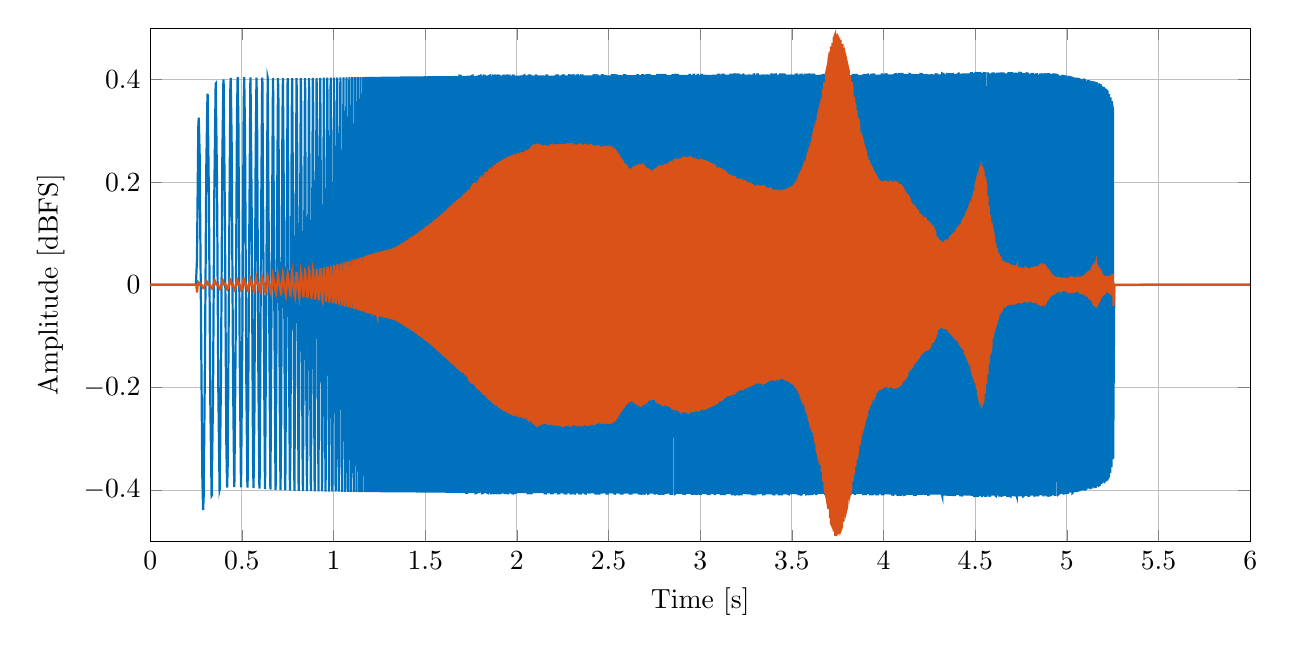
\begin{tikzpicture}

\begin{axis}[%
width=5.5in,
height=2.566in,
at={(1.925in,0.793in)},
scale only axis,
xmin=0,
xmax=6,
xlabel={Time [s]},
xmajorgrids,
ymin=-0.5,
ymax=0.5,
ylabel={Amplitude [dBFS]},
ymajorgrids,
axis background/.style={fill=white},
legend style={legend cell align=left,align=left,draw=white!15!black}
]
\addplot [color=mycolor1,solid,thick]
  table[row sep=crcr]{%
2.08333333333333e-05	-3.0517578125e-05\\
8.33333333333333e-05	-6.103515625e-05\\
0.000416666666666667	3.0517578125e-05\\
0.0123541666666667	6.103515625e-05\\
0.0132916666666667	-9.1552734375e-05\\
0.0148125	-6.103515625e-05\\
0.0148541666666667	3.0517578125e-05\\
0.0234583333333333	-6.103515625e-05\\
0.0238541666666667	6.103515625e-05\\
0.0297083333333333	3.0517578125e-05\\
0.031125	-6.103515625e-05\\
0.0364791666666667	3.0517578125e-05\\
0.0369166666666667	-9.1552734375e-05\\
0.0437708333333333	-6.103515625e-05\\
0.0446041666666667	6.103515625e-05\\
0.0510416666666667	6.103515625e-05\\
0.05575	-9.1552734375e-05\\
0.0583333333333333	3.0517578125e-05\\
0.059	-6.103515625e-05\\
0.0656666666666667	-6.103515625e-05\\
0.067875	6.103515625e-05\\
0.0728958333333333	3.0517578125e-05\\
0.0730208333333333	-6.103515625e-05\\
0.0801875	3.0517578125e-05\\
0.0802708333333333	-6.103515625e-05\\
0.087625	-6.103515625e-05\\
0.08775	3.0517578125e-05\\
0.0947708333333333	-6.103515625e-05\\
0.0960208333333333	6.103515625e-05\\
0.102	3.0517578125e-05\\
0.102354166666667	-6.103515625e-05\\
0.1095625	-6.103515625e-05\\
0.1160625	6.103515625e-05\\
0.118354166666667	-6.103515625e-05\\
0.121625	6.103515625e-05\\
0.123854166666667	3.0517578125e-05\\
0.124291666666667	-6.103515625e-05\\
0.131375	-6.103515625e-05\\
0.131541666666667	3.0517578125e-05\\
0.138708333333333	-6.103515625e-05\\
0.14125	6.103515625e-05\\
0.145875	3.0517578125e-05\\
0.146020833333333	-6.103515625e-05\\
0.157354166666667	-9.1552734375e-05\\
0.157625	6.103515625e-05\\
0.160354166666667	-6.103515625e-05\\
0.160645833333333	3.0517578125e-05\\
0.16775	-6.103515625e-05\\
0.167916666666667	6.103515625e-05\\
0.174958333333333	3.0517578125e-05\\
0.174979166666667	-6.103515625e-05\\
0.182333333333333	-6.103515625e-05\\
0.184104166666667	6.103515625e-05\\
0.1895	6.103515625e-05\\
0.196	-9.1552734375e-05\\
0.197270833333333	-6.103515625e-05\\
0.203708333333333	6.103515625e-05\\
0.204083333333333	-6.103515625e-05\\
0.204416666666667	3.0517578125e-05\\
0.2116875	-6.103515625e-05\\
0.216979166666667	6.103515625e-05\\
0.2190625	-6.103515625e-05\\
0.2230625	6.103515625e-05\\
0.2258125	3.0517578125e-05\\
0.225958333333333	-6.103515625e-05\\
0.2349375	6.103515625e-05\\
0.2374375	-9.1552734375e-05\\
0.243333333333333	6.103515625e-05\\
0.245354166666667	-9.1552734375e-05\\
0.249125	-9.1552734375e-05\\
0.2549375	0.048797607421875\\
0.2549375	0.048797607421875\\
0.262229166666667	0.307037353515625\\
0.264604166666667	0.325927734375\\
0.269520833333333	0.254119873046875\\
0.269520833333333	0.254119873046875\\
0.276791666666667	-0.056732177734375\\
0.276791666666667	-0.056732177734375\\
0.284083333333333	-0.374053955078125\\
0.284083333333333	-0.374053955078125\\
0.288479166666667	-0.43914794921875\\
0.291354166666667	-0.41314697265625\\
0.298645833333333	-0.14215087890625\\
0.298645833333333	-0.14215087890625\\
0.3059375	0.232025146484375\\
0.3059375	0.232025146484375\\
0.312291666666667	0.37255859375\\
0.313208333333333	0.369140625\\
0.3205	0.15313720703125\\
0.3205	0.15313720703125\\
0.327770833333333	-0.22979736328125\\
0.327770833333333	-0.22979736328125\\
0.334791666666667	-0.41107177734375\\
0.3350625	-0.410919189453125\\
0.342354166666667	-0.21832275390625\\
0.342354166666667	-0.21832275390625\\
0.349625	0.181488037109375\\
0.349625	0.181488037109375\\
0.356895833333333	0.39178466796875\\
0.357083333333333	0.391876220703125\\
0.3641875	0.201416015625\\
0.3641875	0.201416015625\\
0.371479166666667	-0.20745849609375\\
0.371479166666667	-0.20745849609375\\
0.3783125	-0.3995361328125\\
0.378770833333333	-0.3988037109375\\
0.386041666666667	-0.173553466796875\\
0.386041666666667	-0.173553466796875\\
0.393333333333333	0.247589111328125\\
0.393333333333333	0.247589111328125\\
0.399125	0.400115966796875\\
0.400604166666667	0.390899658203125\\
0.407895833333333	0.098602294921875\\
0.407895833333333	0.098602294921875\\
0.4151875	-0.3116455078125\\
0.4151875	-0.3116455078125\\
0.419395833333333	-0.39520263671875\\
0.422458333333333	-0.35198974609375\\
0.42975	0.026031494140625\\
0.42975	0.026031494140625\\
0.437020833333333	0.38165283203125\\
0.438958333333333	0.403411865234375\\
0.4443125	0.271514892578125\\
0.4443125	0.271514892578125\\
0.451604166666667	-0.1781005859375\\
0.451604166666667	-0.1781005859375\\
0.458166666666667	-0.394073486328125\\
0.458875	-0.3914794921875\\
0.466166666666667	-0.0965576171875\\
0.466166666666667	-0.0965576171875\\
0.4734375	0.33868408203125\\
0.4768125	0.404510498046875\\
0.480729166666667	0.322845458984375\\
0.480729166666667	0.322845458984375\\
0.488	-0.1302490234375\\
0.488	-0.1302490234375\\
0.495	-0.394378662109375\\
0.495291666666667	-0.393829345703125\\
0.502583333333333	-0.096527099609375\\
0.502583333333333	-0.096527099609375\\
0.509854166666667	0.35211181640625\\
0.512666666666667	0.404541015625\\
0.517145833333333	0.289459228515625\\
0.517145833333333	0.289459228515625\\
0.524416666666667	-0.2015380859375\\
0.524416666666667	-0.2015380859375\\
0.5300625	-0.395172119140625\\
0.531708333333333	-0.37774658203125\\
0.539	0.033599853515625\\
0.539	0.033599853515625\\
0.546270833333333	0.401153564453125\\
0.546875	0.404266357421875\\
0.5535625	0.133392333984375\\
0.5535625	0.133392333984375\\
0.560833333333333	-0.34747314453125\\
0.563395833333333	-0.396148681640625\\
0.568125	-0.249755859375\\
0.568125	-0.249755859375\\
0.575416666666667	0.27593994140625\\
0.575416666666667	0.27593994140625\\
0.579583333333333	0.403839111328125\\
0.5826875	0.334197998046875\\
0.589979166666667	-0.18511962890625\\
0.589979166666667	-0.18511962890625\\
0.595395833333333	-0.397125244140625\\
0.59725	-0.3707275390625\\
0.604541666666667	0.112213134765625\\
0.604541666666667	0.112213134765625\\
0.610791666666667	0.403472900390625\\
0.611833333333333	0.395233154296875\\
0.619104166666667	-0.05230712890625\\
0.619104166666667	-0.05230712890625\\
0.625875	-0.397979736328125\\
0.626395833333333	-0.396240234375\\
0.633666666666667	0.021026611328125\\
0.633666666666667	0.021026611328125\\
0.64075	0.40313720703125\\
0.640958333333333	0.40277099609375\\
0.64825	-0.012603759765625\\
0.64825	-0.012603759765625\\
0.6553125	-0.398681640625\\
0.655520833333333	-0.39813232421875\\
0.6628125	0.031097412109375\\
0.6628125	0.031097412109375\\
0.669520833333333	0.402923583984375\\
0.670083333333333	0.39971923828125\\
0.677375	-0.073577880859375\\
0.677375	-0.073577880859375\\
0.683458333333333	-0.399444580078125\\
0.684666666666667	-0.38580322265625\\
0.6919375	0.141571044921875\\
0.6919375	0.141571044921875\\
0.697166666666667	0.402801513671875\\
0.699229166666667	0.3597412109375\\
0.7065	-0.227294921875\\
0.7065	-0.227294921875\\
0.710645833333333	-0.399993896484375\\
0.713791666666667	-0.295745849609375\\
0.721083333333333	0.319549560546875\\
0.723770833333333	0.40264892578125\\
0.728354166666667	0.186370849609375\\
0.728354166666667	0.186370849609375\\
0.735645833333333	-0.385894775390625\\
0.736708333333333	-0.40045166015625\\
0.742916666666667	-0.02593994140625\\
0.742916666666667	-0.02593994140625\\
0.7494375	0.402618408203125\\
0.750208333333333	0.39654541015625\\
0.7575	-0.169219970703125\\
0.7575	-0.169219970703125\\
0.761979166666667	-0.400848388671875\\
0.764770833333333	-0.308868408203125\\
0.7720625	0.337860107421875\\
0.774291666666667	0.40264892578125\\
0.779333333333333	0.107757568359375\\
0.779333333333333	0.107757568359375\\
0.786395833333333	-0.401214599609375\\
0.786625	-0.400390625\\
0.793916666666667	0.160491943359375\\
0.793916666666667	0.160491943359375\\
0.79825	0.40264892578125\\
0.8011875	0.28887939453125\\
0.808479166666667	-0.36962890625\\
0.809958333333333	-0.4014892578125\\
0.81575	-0.002410888671875\\
0.81575	-0.002410888671875\\
0.821458333333333	0.40277099609375\\
0.823041666666667	0.367584228515625\\
0.830333333333333	-0.31005859375\\
0.832791666666667	-0.401763916015625\\
0.837604166666667	-0.093719482421875\\
0.837604166666667	-0.093719482421875\\
0.843979166666667	0.40289306640625\\
0.844895833333333	0.38970947265625\\
0.852166666666667	-0.279998779296875\\
0.854958333333333	-0.4019775390625\\
0.859458333333333	-0.11029052734375\\
0.859458333333333	-0.11029052734375\\
0.865729166666667	0.402923583984375\\
0.86675	0.38763427734375\\
0.874020833333333	-0.3035888671875\\
0.876416666666667	-0.40216064453125\\
0.8813125	-0.0511474609375\\
0.8813125	-0.0511474609375\\
0.886958333333333	0.403076171875\\
0.888583333333333	0.356658935546875\\
0.895875	-0.36468505859375\\
0.897333333333333	-0.402374267578125\\
0.903166666666667	0.088226318359375\\
0.903166666666667	0.088226318359375\\
0.907541666666667	0.403167724609375\\
0.9104375	0.249847412109375\\
0.917625	-0.40252685546875\\
0.917729166666667	-0.402130126953125\\
0.925	0.279541015625\\
0.927520833333333	0.403350830078125\\
0.932291666666667	0.0185546875\\
0.932291666666667	0.0185546875\\
0.937291666666667	-0.402587890625\\
0.9395625	-0.30322265625\\
0.946854166666667	0.40301513671875\\
0.946979166666667	0.4034423828125\\
0.954145833333333	-0.285247802734375\\
0.956520833333333	-0.402740478515625\\
0.961416666666667	0.021209716796875\\
0.961416666666667	0.021209716796875\\
0.9659375	0.403564453125\\
0.968708333333333	0.240692138671875\\
0.975229166666667	-0.402923583984375\\
0.975979166666667	-0.390411376953125\\
0.983270833333333	0.37298583984375\\
0.984395833333333	0.403656005859375\\
0.9905625	-0.215118408203125\\
0.9934375	-0.402984619140625\\
0.997833333333333	-0.018707275390625\\
0.997833333333333	-0.018707275390625\\
1.00241666666667	0.40380859375\\
1.005125	0.23162841796875\\
1.01122916666667	-0.403076171875\\
1.01239583333333	-0.370361328125\\
1.0196875	0.4014892578125\\
1.01995833333333	0.403900146484375\\
1.02697916666667	-0.33349609375\\
1.02860416666667	-0.4031982421875\\
1.03425	0.192962646484375\\
1.03716666666667	0.40411376953125\\
1.04154166666667	-0.027557373046875\\
1.04154166666667	-0.027557373046875\\
1.0455625	-0.403411865234375\\
1.0488125	-0.140045166015625\\
1.053875	0.404266357421875\\
1.05610416666667	0.26983642578125\\
1.06214583333333	-0.403350830078125\\
1.06339583333333	-0.357269287109375\\
1.07027083333333	0.40435791015625\\
1.07066666666667	0.39959716796875\\
1.07795833333333	-0.3995361328125\\
1.0783125	-0.403564453125\\
1.08522916666667	0.36907958984375\\
1.08629166666667	0.404510498046875\\
1.09252083333333	-0.319854736328125\\
1.0941875	-0.403564453125\\
1.0998125	0.26080322265625\\
1.10191666666667	0.404541015625\\
1.10708333333333	-0.199920654296875\\
1.10964583333333	-0.403656005859375\\
1.114375	0.143646240234375\\
1.11727083333333	0.4046630859375\\
1.12164583333333	-0.096282958984375\\
1.12483333333333	-0.403717041015625\\
1.1289375	0.05902099609375\\
1.1323125	0.40472412109375\\
1.13622916666667	-0.037994384765625\\
1.1396875	-0.403778076171875\\
1.1435	0.02154541015625\\
1.147	0.40478515625\\
1.15079166666667	-0.025634765625\\
1.15422916666667	-0.40380859375\\
1.1580625	0.0347900390625\\
1.16141666666667	0.404937744140625\\
1.16535416666667	-0.06451416015625\\
1.16854166666667	-0.40386962890625\\
1.17264583333333	0.102630615234375\\
1.1755625	0.404998779296875\\
1.17991666666667	-0.152435302734375\\
1.18254166666667	-0.4039306640625\\
1.18720833333333	0.21136474609375\\
1.1894375	0.405059814453125\\
1.19447916666667	-0.274322509765625\\
1.19629166666667	-0.40399169921875\\
1.20177083333333	0.335845947265625\\
1.20304166666667	0.405120849609375\\
1.2090625	-0.3834228515625\\
1.20975	-0.404052734375\\
1.21633333333333	0.40496826171875\\
1.21641666666667	0.405242919921875\\
1.22297916666667	-0.404052734375\\
1.223625	-0.385467529296875\\
1.2295	0.405303955078125\\
1.23089583333333	0.31756591796875\\
1.23597916666667	-0.40411376953125\\
1.2381875	-0.1920166015625\\
1.24235416666667	0.40533447265625\\
1.24872916666667	-0.4041748046875\\
1.25275	0.165863037109375\\
1.25502083333333	0.405426025390625\\
1.26004166666667	-0.32794189453125\\
1.26127083333333	-0.404205322265625\\
1.2673125	0.404052734375\\
1.26745833333333	0.405517578125\\
1.27358333333333	-0.40423583984375\\
1.27460416666667	-0.353790283203125\\
1.27970833333333	0.40557861328125\\
1.28189583333333	0.16973876953125\\
1.28572916666667	-0.404296875\\
1.29172916666667	0.4056396484375\\
1.29645833333333	-0.32525634765625\\
1.29764583333333	-0.404296875\\
1.30354166666667	0.40570068359375\\
1.30372916666667	0.40380859375\\
1.30939583333333	-0.404388427734375\\
1.31102083333333	-0.259002685546875\\
1.31516666666667	0.405731201171875\\
1.3209375	-0.40435791015625\\
1.32558333333333	0.33831787109375\\
1.326625	0.405792236328125\\
1.33227083333333	-0.404388427734375\\
1.332875	-0.38397216796875\\
1.33789583333333	0.40582275390625\\
1.34347916666667	-0.404449462890625\\
1.3474375	0.2523193359375\\
1.349	0.4058837890625\\
1.3545	-0.40447998046875\\
1.35472916666667	-0.40093994140625\\
1.3599375	0.405914306640625\\
1.36533333333333	-0.404449462890625\\
1.36929166666667	0.271453857421875\\
1.37070833333333	0.405975341796875\\
1.37604166666667	-0.404510498046875\\
1.3765625	-0.385711669921875\\
1.38133333333333	0.406005859375\\
1.38658333333333	-0.404510498046875\\
1.391125	0.37384033203125\\
1.39177083333333	0.40606689453125\\
1.39695833333333	-0.404541015625\\
1.39841666666667	-0.256805419921875\\
1.40210416666667	0.4061279296875\\
1.4071875	-0.404541015625\\
1.41227083333333	0.406158447265625\\
1.41297916666667	0.366363525390625\\
1.41729166666667	-0.40460205078125\\
1.42227083333333	0.406158447265625\\
1.42722916666667	-0.404571533203125\\
1.42754166666667	-0.397674560546875\\
1.4321875	0.40618896484375\\
1.4370625	-0.40460205078125\\
1.4419375	0.406219482421875\\
1.442125	0.402923583984375\\
1.44675	-0.4046630859375\\
1.45154166666667	0.40625\\
1.4563125	-0.40472412109375\\
1.4566875	-0.392730712890625\\
1.46104166666667	0.406280517578125\\
1.46572916666667	-0.4046630859375\\
1.47041666666667	0.40631103515625\\
1.47125	0.34527587890625\\
1.4750625	-0.40472412109375\\
1.4796875	0.406341552734375\\
1.48427083333333	-0.40472412109375\\
1.4888125	0.4063720703125\\
1.49310416666667	-0.399261474609375\\
1.49335416666667	-0.404754638671875\\
1.49783333333333	0.40643310546875\\
1.5023125	-0.404815673828125\\
1.50675	0.406402587890625\\
1.51116666666667	-0.40478515625\\
1.51495833333333	0.369049072265625\\
1.5155625	0.406494140625\\
1.51991666666667	-0.404815673828125\\
1.52425	0.406494140625\\
1.5285625	-0.40484619140625\\
1.53285416666667	0.406494140625\\
1.53679166666667	-0.393646240234375\\
1.53710416666667	-0.40484619140625\\
1.54133333333333	0.406524658203125\\
1.5455625	-0.4049072265625\\
1.54972916666667	0.40655517578125\\
1.55389583333333	-0.40496826171875\\
1.55804166666667	0.40655517578125\\
1.56216666666667	-0.404937744140625\\
1.5659375	0.394866943359375\\
1.56622916666667	0.406585693359375\\
1.57033333333333	-0.405059814453125\\
1.57435416666667	0.406646728515625\\
1.57839583333333	-0.404998779296875\\
1.58239583333333	0.406646728515625\\
1.58635416666667	-0.40509033203125\\
1.5903125	0.40667724609375\\
1.59425	-0.40509033203125\\
1.59816666666667	0.406768798828125\\
1.60208333333333	-0.405120849609375\\
1.6059375	0.40673828125\\
1.609625	-0.401458740234375\\
1.60979166666667	-0.405120849609375\\
1.61360416666667	0.40673828125\\
1.6174375	-0.405181884765625\\
1.62120833333333	0.406768798828125\\
1.625	-0.405181884765625\\
1.62875	0.40679931640625\\
1.63247916666667	-0.405181884765625\\
1.6361875	0.40679931640625\\
1.639875	-0.40521240234375\\
1.64358333333333	0.4068603515625\\
1.64720833333333	-0.4052734375\\
1.65085416666667	0.4068603515625\\
1.65447916666667	-0.405303955078125\\
1.65808333333333	0.406951904296875\\
1.66166666666667	-0.4052734375\\
1.66522916666667	0.40692138671875\\
1.66877083333333	-0.40496826171875\\
1.6723125	0.4068603515625\\
1.67583333333333	-0.40594482421875\\
1.67933333333333	0.40655517578125\\
1.6828125	-0.40533447265625\\
1.68627083333333	0.407562255859375\\
1.69316666666667	0.406982421875\\
1.6965625	-0.40594482421875\\
1.69995833333333	0.407012939453125\\
1.70335416666667	-0.4053955078125\\
1.70672916666667	0.406982421875\\
1.7100625	-0.4049072265625\\
1.71339583333333	0.40704345703125\\
1.71670833333333	-0.4058837890625\\
1.72004166666667	0.407012939453125\\
1.72333333333333	-0.4053955078125\\
1.72985416666667	-0.40533447265625\\
1.733125	0.40765380859375\\
1.73635416666667	-0.40545654296875\\
1.7395625	0.4071044921875\\
1.74275	-0.405029296875\\
1.74595833333333	0.4071044921875\\
1.749125	-0.406005859375\\
1.75229166666667	0.406707763671875\\
1.75858333333333	0.407623291015625\\
1.7616875	-0.40545654296875\\
1.76479166666667	0.407135009765625\\
1.76789583333333	-0.40509033203125\\
1.77097916666667	0.407135009765625\\
1.77404166666667	-0.406036376953125\\
1.78014583333333	-0.405517578125\\
1.78316666666667	0.407623291015625\\
1.7861875	-0.4051513671875\\
1.7891875	0.407196044921875\\
1.7921875	-0.405975341796875\\
1.79516666666667	0.40679931640625\\
1.80108333333333	0.40765380859375\\
1.80402083333333	-0.405120849609375\\
1.80695833333333	0.4072265625\\
1.809875	-0.406036376953125\\
1.8156875	-0.405548095703125\\
1.8185625	0.40765380859375\\
1.82429166666667	0.4072265625\\
1.82714583333333	-0.406005859375\\
1.83	0.406890869140625\\
1.8328125	-0.405548095703125\\
1.83564583333333	0.407623291015625\\
1.8384375	-0.405181884765625\\
1.84402083333333	-0.405975341796875\\
1.8468125	0.406829833984375\\
1.8523125	0.40771484375\\
1.8550625	-0.405242919921875\\
1.85779166666667	0.4073486328125\\
1.8605	-0.405914306640625\\
1.86591666666667	-0.405609130859375\\
1.86860416666667	0.40765380859375\\
1.87395833333333	0.407318115234375\\
1.876625	-0.405914306640625\\
1.8819375	-0.405670166015625\\
1.8845625	0.407623291015625\\
1.88979166666667	0.40728759765625\\
1.89239583333333	-0.405914306640625\\
1.89758333333333	-0.40576171875\\
1.90014583333333	0.40765380859375\\
1.90527083333333	0.407318115234375\\
1.90783333333333	-0.405975341796875\\
1.91289583333333	-0.40570068359375\\
1.9154375	0.407623291015625\\
1.9179375	-0.405548095703125\\
1.9204375	0.40740966796875\\
1.9229375	-0.40594482421875\\
1.9254375	0.407318115234375\\
1.930375	0.407440185546875\\
1.93283333333333	-0.4056396484375\\
1.93775	-0.40582275390625\\
1.9401875	0.407135009765625\\
1.94504166666667	0.4075927734375\\
1.9474375	-0.405487060546875\\
1.95225	-0.405975341796875\\
1.954625	0.4072265625\\
1.95939583333333	0.407470703125\\
1.96175	-0.40594482421875\\
1.9688125	0.40753173828125\\
1.97114583333333	-0.4056396484375\\
1.97579166666667	-0.406219482421875\\
1.97810416666667	0.40765380859375\\
1.98270833333333	0.40753173828125\\
1.985	-0.405914306640625\\
1.9895625	-0.40582275390625\\
1.99183333333333	0.40753173828125\\
1.99860416666667	-0.406341552734375\\
2.00083333333333	0.407806396484375\\
2.00752083333333	-0.405914306640625\\
2.00972916666667	0.40753173828125\\
2.0119375	-0.40594482421875\\
2.01414583333333	0.407623291015625\\
2.02070833333333	-0.4058837890625\\
2.022875	0.40802001953125\\
2.02504166666667	-0.406005859375\\
2.0315	0.407989501953125\\
2.03364583333333	-0.405975341796875\\
2.03579166666667	0.407135009765625\\
2.04004166666667	0.40802001953125\\
2.04216666666667	-0.405914306640625\\
2.04847916666667	0.407989501953125\\
2.0505625	-0.405975341796875\\
2.05679166666667	0.407958984375\\
2.058875	-0.406005859375\\
2.063	-0.40594482421875\\
2.06504166666667	0.408050537109375\\
2.0731875	0.40802001953125\\
2.07520833333333	-0.406005859375\\
2.07922916666667	-0.40594482421875\\
2.08125	0.407989501953125\\
2.08325	-0.406158447265625\\
2.08522916666667	0.40765380859375\\
2.095125	-0.406005859375\\
2.09708333333333	0.40802001953125\\
2.1029375	-0.406036376953125\\
2.104875	0.40802001953125\\
2.10489583333333	0.40802001953125\\
2.1068125	-0.406036376953125\\
2.11260416666667	0.40802001953125\\
2.11452083333333	-0.406005859375\\
2.12022916666667	0.40802001953125\\
2.122125	-0.40606689453125\\
2.12777083333333	0.40789794921875\\
2.12964583333333	-0.406036376953125\\
2.13525	0.407989501953125\\
2.13710416666667	-0.406036376953125\\
2.14264583333333	0.4080810546875\\
2.14447916666667	-0.4061279296875\\
2.14995833333333	0.407867431640625\\
2.15179166666667	-0.4061279296875\\
2.15902083333333	-0.4063720703125\\
2.1608125	0.407745361328125\\
2.16439583333333	0.407745361328125\\
2.16616666666667	-0.406280517578125\\
2.1715	0.40777587890625\\
2.17327083333333	-0.40631103515625\\
2.17854166666667	0.40765380859375\\
2.18029166666667	-0.406219482421875\\
2.1855	0.407806396484375\\
2.18722916666667	-0.406280517578125\\
2.194125	-0.406219482421875\\
2.19925	0.407806396484375\\
2.2009375	-0.40631103515625\\
2.20264583333333	0.407745361328125\\
2.20770833333333	-0.40618896484375\\
2.209375	0.40789794921875\\
2.21439583333333	-0.4061279296875\\
2.2160625	0.407867431640625\\
2.2226875	0.407928466796875\\
2.22433333333333	-0.4063720703125\\
2.230875	-0.40618896484375\\
2.2325	0.407867431640625\\
2.24058333333333	-0.406585693359375\\
2.2421875	0.408111572265625\\
2.24379166666667	-0.406219482421875\\
2.2485625	0.407745361328125\\
2.25489583333333	0.408203125\\
2.25645833333333	-0.40631103515625\\
2.25804166666667	0.407928466796875\\
2.25960416666667	-0.406158447265625\\
2.2689375	-0.406524658203125\\
2.27047916666667	0.40814208984375\\
2.27814583333333	-0.406524658203125\\
2.27966666666667	0.407958984375\\
2.28422916666667	-0.40618896484375\\
2.28575	0.40814208984375\\
2.29175	0.4078369140625\\
2.29325	-0.406524658203125\\
2.29920833333333	-0.406158447265625\\
2.3006875	0.408203125\\
2.30216666666667	-0.406463623046875\\
2.303625	0.40789794921875\\
2.3095	0.408203125\\
2.31095833333333	-0.4063720703125\\
2.31677083333333	-0.40655517578125\\
2.31820833333333	0.4080810546875\\
2.32539583333333	-0.406524658203125\\
2.32683333333333	0.407928466796875\\
2.3325	0.408203125\\
2.33391666666667	-0.40643310546875\\
2.33814583333333	0.407958984375\\
2.33954166666667	-0.40631103515625\\
2.34791666666667	-0.406524658203125\\
2.34929166666667	0.408111572265625\\
2.35754166666667	0.407989501953125\\
2.35891666666667	-0.406341552734375\\
2.36027083333333	0.407958984375\\
2.36704166666667	-0.406524658203125\\
2.36839583333333	0.408172607421875\\
2.36975	-0.406341552734375\\
2.37510416666667	-0.406646728515625\\
2.3764375	0.408203125\\
2.3830625	-0.406524658203125\\
2.384375	0.408050537109375\\
2.39354166666667	-0.406646728515625\\
2.39485416666667	0.40814208984375\\
2.4013125	-0.406402587890625\\
2.40260416666667	0.408172607421875\\
2.403875	-0.406585693359375\\
2.40516666666667	0.40802001953125\\
2.41154166666667	-0.406494140625\\
2.41785416666667	0.408050537109375\\
2.42035416666667	0.408294677734375\\
2.42160416666667	-0.406524658203125\\
2.42535416666667	0.407958984375\\
2.42660416666667	-0.4063720703125\\
2.43402083333333	-0.406646728515625\\
2.43525	0.408172607421875\\
2.44014583333333	0.40802001953125\\
2.44135416666667	-0.40631103515625\\
2.448625	-0.40667724609375\\
2.44983333333333	0.408172607421875\\
2.45583333333333	-0.40667724609375\\
2.45702083333333	0.408172607421875\\
2.46295833333333	-0.40673828125\\
2.464125	0.408203125\\
2.4711875	0.40814208984375\\
2.47235416666667	-0.406463623046875\\
2.47816666666667	0.408172607421875\\
2.4793125	-0.406585693359375\\
2.48735416666667	0.408355712890625\\
2.4885	-0.4066162109375\\
2.4953125	-0.40673828125\\
2.4964375	0.4083251953125\\
2.4998125	-0.40643310546875\\
2.50541666666667	0.408294677734375\\
2.50652083333333	-0.406524658203125\\
2.50985416666667	0.408203125\\
2.51316666666667	-0.406524658203125\\
2.51866666666667	0.408355712890625\\
2.52520833333333	0.408294677734375\\
2.52629166666667	-0.406646728515625\\
2.527375	0.408172607421875\\
2.53275	-0.406585693359375\\
2.53489583333333	-0.40673828125\\
2.53595833333333	0.408203125\\
2.54445833333333	0.408111572265625\\
2.54552083333333	-0.406524658203125\\
2.55077083333333	0.408477783203125\\
2.5518125	-0.40679931640625\\
2.55910416666667	0.408447265625\\
2.560125	-0.406646728515625\\
2.56733333333333	0.40838623046875\\
2.56835416666667	-0.40679931640625\\
2.57647916666667	-0.406585693359375\\
2.5775	0.408233642578125\\
2.58252083333333	-0.40679931640625\\
2.58352083333333	0.408447265625\\
2.59147916666667	0.408477783203125\\
2.59245833333333	-0.4066162109375\\
2.59345833333333	0.408355712890625\\
2.598375	-0.40673828125\\
2.60520833333333	0.40838623046875\\
2.60616666666667	-0.40673828125\\
2.6129375	0.4083251953125\\
2.61389583333333	-0.4068603515625\\
2.61485416666667	0.40850830078125\\
2.6158125	-0.406829833984375\\
2.6253125	-0.4068603515625\\
2.62625	0.40838623046875\\
2.6346875	-0.406707763671875\\
2.635625	0.408416748046875\\
2.63841666666667	-0.406585693359375\\
2.64304166666667	0.408416748046875\\
2.64395833333333	-0.4068603515625\\
2.644875	0.408447265625\\
2.65672916666667	-0.4068603515625\\
2.657625	0.408355712890625\\
2.6594375	0.40838623046875\\
2.66570833333333	-0.40679931640625\\
2.66660416666667	0.408538818359375\\
2.6675	-0.4068603515625\\
2.67635416666667	-0.40692138671875\\
2.67722916666667	0.408447265625\\
2.68335416666667	-0.4068603515625\\
2.68422916666667	0.40850830078125\\
2.6894375	0.408599853515625\\
2.69029166666667	-0.40679931640625\\
2.69716666666667	-0.406829833984375\\
2.69802083333333	0.408416748046875\\
2.70397916666667	-0.406768798828125\\
2.70652083333333	0.4085693359375\\
2.71491666666667	0.408599853515625\\
2.71575	-0.406982421875\\
2.71741666666667	-0.40679931640625\\
2.72320833333333	0.408599853515625\\
2.72485416666667	0.408477783203125\\
2.72895833333333	-0.40704345703125\\
2.73629166666667	0.408477783203125\\
2.73710416666667	-0.40692138671875\\
2.73952083333333	0.4085693359375\\
2.7419375	-0.406890869140625\\
2.75072916666667	0.408538818359375\\
2.75152083333333	-0.406890869140625\\
2.7546875	-0.406890869140625\\
2.75547916666667	0.408599853515625\\
2.76410416666667	-0.407135009765625\\
2.764875	0.408660888671875\\
2.772625	0.40875244140625\\
2.77339583333333	-0.407073974609375\\
2.77952083333333	-0.406951904296875\\
2.78029166666667	0.40875244140625\\
2.787875	0.408660888671875\\
2.788625	-0.406890869140625\\
2.79089583333333	0.40869140625\\
2.79164583333333	-0.407073974609375\\
2.79910416666667	-0.407073974609375\\
2.80133333333333	0.408782958984375\\
2.81016666666667	0.40863037109375\\
2.81089583333333	-0.4071044921875\\
2.811625	0.40875244140625\\
2.81235416666667	-0.407135009765625\\
2.82177083333333	0.4088134765625\\
2.8225	-0.40692138671875\\
2.82608333333333	0.408599853515625\\
2.82964583333333	-0.4071044921875\\
2.8374375	0.4088134765625\\
2.83814583333333	-0.407196044921875\\
2.84654166666667	-0.407196044921875\\
2.84722916666667	0.40869140625\\
2.8479375	-0.4071044921875\\
2.848625	0.40875244140625\\
2.861	0.4090576171875\\
2.8616875	-0.407501220703125\\
2.86304166666667	-0.4072265625\\
2.86372916666667	0.40887451171875\\
2.8698125	-0.407196044921875\\
2.87183333333333	0.408782958984375\\
2.8771875	0.40875244140625\\
2.87785416666667	-0.40716552734375\\
2.88514583333333	0.408935546875\\
2.887125	-0.40716552734375\\
2.89302083333333	0.408966064453125\\
2.89366666666667	-0.407257080078125\\
2.90466666666667	0.408660888671875\\
2.9053125	-0.4072265625\\
2.90722916666667	0.40887451171875\\
2.90914583333333	-0.407196044921875\\
2.9155	-0.40740966796875\\
2.91739583333333	0.409088134765625\\
2.92679166666667	-0.407196044921875\\
2.92741666666667	0.40887451171875\\
2.93052083333333	-0.4073486328125\\
2.93114583333333	0.408843994140625\\
2.9366875	-0.4073486328125\\
2.94097916666667	0.4088134765625\\
2.94341666666667	0.408935546875\\
2.948875	-0.407318115234375\\
2.95308333333333	0.4088134765625\\
2.9536875	-0.40728759765625\\
2.96322916666667	-0.40753173828125\\
2.9638125	0.4091796875\\
2.965	0.409271240234375\\
2.96558333333333	-0.407470703125\\
2.977875	0.40887451171875\\
2.97845833333333	-0.407318115234375\\
2.98077083333333	-0.407379150390625\\
2.98595833333333	0.408935546875\\
2.98710416666667	0.40899658203125\\
2.993375	-0.407470703125\\
2.99508333333333	0.40887451171875\\
2.99564583333333	-0.407379150390625\\
3.00464583333333	-0.40740966796875\\
3.0074375	0.409088134765625\\
3.00966666666667	0.40899658203125\\
3.01354166666667	-0.407440185546875\\
3.0206875	0.40911865234375\\
3.02122916666667	-0.40765380859375\\
3.02395833333333	0.40948486328125\\
3.0245	-0.407867431640625\\
3.03154166666667	0.409149169921875\\
3.03422916666667	-0.407623291015625\\
3.03797916666667	0.409088134765625\\
3.04064583333333	-0.40740966796875\\
3.05120833333333	-0.407745361328125\\
3.05172916666667	0.409271240234375\\
3.05172916666667	0.409271240234375\\
3.05225	-0.40753173828125\\
3.06316666666667	0.4093017578125\\
3.0636875	-0.40765380859375\\
3.07035416666667	0.40936279296875\\
3.07289583333333	-0.40753173828125\\
3.07847916666667	0.409149169921875\\
3.07897916666667	-0.407623291015625\\
3.081	-0.4075927734375\\
3.0815	0.409332275390625\\
3.09	-0.407562255859375\\
3.09445833333333	0.409332275390625\\
3.0959375	-0.407623291015625\\
3.09741666666667	0.409393310546875\\
3.10329166666667	0.409332275390625\\
3.10572916666667	-0.4075927734375\\
3.1110625	0.409393310546875\\
3.11154166666667	-0.407867431640625\\
3.121125	-0.407867431640625\\
3.12160416666667	0.409423828125\\
3.12822916666667	0.409271240234375\\
3.12964583333333	-0.407745361328125\\
3.13527083333333	-0.40777587890625\\
3.13666666666667	0.409454345703125\\
3.143625	-0.40771484375\\
3.14408333333333	0.409393310546875\\
3.15279166666667	-0.407928466796875\\
3.15325	0.409515380859375\\
3.15370833333333	-0.40789794921875\\
3.15597916666667	0.409515380859375\\
3.16275	-0.407867431640625\\
3.165	0.409271240234375\\
3.172125	0.409423828125\\
3.17345833333333	-0.407928466796875\\
3.177875	-0.407806396484375\\
3.1783125	0.40948486328125\\
3.18879166666667	0.409881591796875\\
3.18922916666667	-0.4085693359375\\
3.19095833333333	-0.4085693359375\\
3.19139583333333	0.409912109375\\
3.20083333333333	0.409454345703125\\
3.2038125	-0.407745361328125\\
3.20635416666667	-0.40802001953125\\
3.207625	0.40960693359375\\
3.21435416666667	0.40948486328125\\
3.21477083333333	-0.407928466796875\\
3.2255625	-0.40802001953125\\
3.22597916666667	0.409759521484375\\
3.22720833333333	-0.40789794921875\\
3.23335416666667	0.409637451171875\\
3.23416666666667	0.40966796875\\
3.24025	-0.407958984375\\
3.24227083333333	0.409576416015625\\
3.24266666666667	-0.407989501953125\\
3.25504166666667	0.40960693359375\\
3.2554375	-0.407989501953125\\
3.25583333333333	0.409637451171875\\
3.25622916666667	-0.408111572265625\\
3.2668125	0.409881591796875\\
3.26797916666667	-0.408233642578125\\
3.2745625	0.409454345703125\\
3.27570833333333	-0.40826416015625\\
3.27839583333333	0.4095458984375\\
3.2803125	-0.407806396484375\\
3.2916875	-0.4080810546875\\
3.2920625	0.40972900390625\\
3.2928125	0.409820556640625\\
3.2931875	-0.40826416015625\\
3.30139583333333	-0.408203125\\
3.30325	0.40972900390625\\
3.31025	-0.40814208984375\\
3.3128125	0.410003662109375\\
3.31427083333333	0.409912109375\\
3.31827083333333	-0.408111572265625\\
3.3265625	0.40960693359375\\
3.32691666666667	-0.407989501953125\\
3.32870833333333	0.40966796875\\
3.33191666666667	-0.407989501953125\\
3.34145833333333	0.40966796875\\
3.3418125	-0.408233642578125\\
3.3435625	0.409820556640625\\
3.34391666666667	-0.408203125\\
3.350875	-0.407867431640625\\
3.35122916666667	0.40960693359375\\
3.36325	-0.408416748046875\\
3.36427083333333	0.410064697265625\\
3.36529166666667	-0.408538818359375\\
3.3663125	0.40985107421875\\
3.37272916666667	-0.40814208984375\\
3.3730625	0.40972900390625\\
3.38141666666667	-0.408203125\\
3.38175	0.4097900390625\\
3.387375	-0.408203125\\
3.38902083333333	0.40985107421875\\
3.39491666666667	0.40960693359375\\
3.39654166666667	-0.407928466796875\\
3.40366666666667	-0.408294677734375\\
3.40591666666667	0.40948486328125\\
3.4123125	0.409942626953125\\
3.41327083333333	-0.408447265625\\
3.416125	0.409759521484375\\
3.42022916666667	-0.4080810546875\\
3.4280625	0.409759521484375\\
3.428375	-0.408203125\\
3.43147916666667	-0.408111572265625\\
3.4355	0.409698486328125\\
3.44225	0.40972900390625\\
3.44316666666667	-0.40814208984375\\
3.44560416666667	-0.4080810546875\\
3.44772916666667	0.409515380859375\\
3.4585625	0.409912109375\\
3.45945833333333	-0.40826416015625\\
3.46510416666667	0.409942626953125\\
3.46658333333333	-0.4083251953125\\
3.466875	0.4097900390625\\
3.46835416666667	-0.408203125\\
3.48033333333333	0.409423828125\\
3.480625	-0.4078369140625\\
3.4829375	-0.4080810546875\\
3.48322916666667	0.40960693359375\\
3.49439583333333	-0.40826416015625\\
3.49525	0.409820556640625\\
3.49666666666667	-0.4080810546875\\
3.49808333333333	0.40948486328125\\
3.5034375	-0.407989501953125\\
3.50595833333333	0.409515380859375\\
3.51291666666667	-0.40802001953125\\
3.51375	0.40972900390625\\
3.5184375	-0.4078369140625\\
3.52145833333333	0.409515380859375\\
3.52854166666667	0.409759521484375\\
3.5288125	-0.408172607421875\\
3.53502083333333	0.40948486328125\\
3.53529166666667	-0.40777587890625\\
3.54383333333333	-0.408050537109375\\
3.54675	0.40936279296875\\
3.55254166666667	0.4095458984375\\
3.55385416666667	-0.408203125\\
3.554375	-0.4080810546875\\
3.55672916666667	0.409576416015625\\
3.56166666666667	-0.4078369140625\\
3.568625	0.409423828125\\
3.56939583333333	-0.4078369140625\\
3.5711875	0.409393310546875\\
3.5783125	0.409515380859375\\
3.5785625	-0.4080810546875\\
3.58360416666667	-0.40765380859375\\
3.58385416666667	0.408966064453125\\
3.59135416666667	0.409576416015625\\
3.59160416666667	-0.407958984375\\
3.59902083333333	-0.40771484375\\
3.60025	0.409271240234375\\
3.60952083333333	0.409271240234375\\
3.61025	-0.407745361328125\\
3.61266666666667	-0.407684326171875\\
3.61435416666667	0.409149169921875\\
3.62202083333333	0.409393310546875\\
3.6236875	-0.407745361328125\\
3.63102083333333	0.40911865234375\\
3.63266666666667	-0.407623291015625\\
3.63454166666667	-0.4075927734375\\
3.63897916666667	0.409271240234375\\
3.642	-0.4075927734375\\
3.64222916666667	0.409271240234375\\
3.65258333333333	-0.408050537109375\\
3.6528125	0.409637451171875\\
3.65622916666667	-0.407623291015625\\
3.65645833333333	0.409149169921875\\
3.66391666666667	-0.407562255859375\\
3.668625	0.4090576171875\\
3.67485416666667	0.409027099609375\\
3.67772916666667	-0.407501220703125\\
3.67927083333333	0.40899658203125\\
3.68125	-0.40753173828125\\
3.6869375	-0.407562255859375\\
3.68889583333333	0.40899658203125\\
3.69645833333333	-0.407470703125\\
3.69710416666667	0.409149169921875\\
3.70352083333333	0.409027099609375\\
3.70458333333333	-0.407501220703125\\
3.70797916666667	-0.4073486328125\\
3.70945833333333	0.409027099609375\\
3.7211875	0.40911865234375\\
3.72139583333333	-0.4075927734375\\
3.7218125	-0.40753173828125\\
3.72202083333333	0.40899658203125\\
3.7329375	-0.4088134765625\\
3.73395833333333	0.410186767578125\\
3.73660416666667	-0.407440185546875\\
3.7368125	0.409210205078125\\
3.74610416666667	0.4088134765625\\
3.74670833333333	-0.40728759765625\\
3.75210416666667	0.40863037109375\\
3.75508333333333	-0.407379150390625\\
3.76041666666667	0.40887451171875\\
3.7621875	-0.40728759765625\\
3.76610416666667	-0.4072265625\\
3.7666875	0.4088134765625\\
3.7786875	0.408935546875\\
3.77964583333333	-0.407379150390625\\
3.78289583333333	0.40887451171875\\
3.78422916666667	-0.4072265625\\
3.792375	0.4088134765625\\
3.7925625	-0.40728759765625\\
3.7985625	-0.407257080078125\\
3.79875	0.40875244140625\\
3.80691666666667	0.4088134765625\\
3.80820833333333	-0.4072265625\\
3.81133333333333	0.408782958984375\\
3.81554166666667	-0.40728759765625\\
3.81954166666667	-0.40728759765625\\
3.82189583333333	0.4088134765625\\
3.82460416666667	-0.4072265625\\
3.83016666666667	0.40911865234375\\
3.83141666666667	-0.407562255859375\\
3.83302083333333	0.408935546875\\
3.8408125	0.40887451171875\\
3.84239583333333	-0.40728759765625\\
3.84625	-0.407196044921875\\
3.847125	0.4088134765625\\
3.85372916666667	0.40875244140625\\
3.85425	-0.40716552734375\\
3.86608333333333	0.40899658203125\\
3.86727083333333	-0.407745361328125\\
3.87116666666667	0.409088134765625\\
3.87302083333333	-0.407318115234375\\
3.8795625	0.409088134765625\\
3.87972916666667	-0.4075927734375\\
3.88654166666667	0.40899658203125\\
3.8886875	-0.407684326171875\\
3.89033333333333	-0.4075927734375\\
3.8918125	0.4090576171875\\
3.899	0.40899658203125\\
3.90272916666667	-0.4075927734375\\
3.90466666666667	-0.407562255859375\\
3.9086875	0.408843994140625\\
3.9144375	0.409454345703125\\
3.91777083333333	-0.407867431640625\\
3.9185625	0.40924072265625\\
3.92533333333333	-0.4078369140625\\
3.92595833333333	-0.407745361328125\\
3.93204166666667	0.40911865234375\\
3.936375	0.409393310546875\\
3.93991666666667	-0.408050537109375\\
3.94114583333333	-0.407958984375\\
3.94160416666667	0.409454345703125\\
3.94770833333333	0.40960693359375\\
3.94877083333333	-0.40814208984375\\
3.95677083333333	0.409393310546875\\
3.95841666666667	-0.40802001953125\\
3.9679375	-0.408172607421875\\
3.96808333333333	0.4095458984375\\
3.96970833333333	-0.4083251953125\\
3.96985416666667	0.409759521484375\\
3.97675	-0.40814208984375\\
3.9771875	0.409637451171875\\
3.98516666666667	-0.408203125\\
3.989625	0.409759521484375\\
3.99191666666667	0.40985107421875\\
3.99291666666667	-0.4083251953125\\
3.99860416666667	-0.4083251953125\\
3.9993125	0.409881591796875\\
4.00733333333333	-0.4083251953125\\
4.0083125	0.4097900390625\\
4.01554166666667	0.41009521484375\\
4.01595833333333	-0.408538818359375\\
4.02325	0.4100341796875\\
4.02720833333333	-0.408477783203125\\
4.03033333333333	0.41015625\\
4.03479166666667	-0.408477783203125\\
4.03654166666667	0.410247802734375\\
4.03775	-0.40875244140625\\
4.0445625	0.41021728515625\\
4.04708333333333	-0.40863037109375\\
4.052625	-0.408935546875\\
4.05616666666667	0.410308837890625\\
4.058125	-0.408966064453125\\
4.06241666666667	0.410186767578125\\
4.0668125	0.410400390625\\
4.06745833333333	-0.408935546875\\
4.07527083333333	0.41058349609375\\
4.07641666666667	-0.409088134765625\\
4.08275	-0.4090576171875\\
4.082875	0.41064453125\\
4.08614583333333	0.41058349609375\\
4.08627083333333	-0.40911865234375\\
4.09722916666667	-0.409271240234375\\
4.09735416666667	0.4107666015625\\
4.10277083333333	0.4107666015625\\
4.1065625	-0.40924072265625\\
4.1110625	0.4107666015625\\
4.11239583333333	-0.409332275390625\\
4.1165	-0.408935546875\\
4.12141666666667	0.410888671875\\
4.12272916666667	-0.409271240234375\\
4.1295	0.41082763671875\\
4.12985416666667	-0.40936279296875\\
4.13679166666667	0.410980224609375\\
4.137375	-0.409423828125\\
4.14308333333333	0.4107666015625\\
4.1449375	0.4105224609375\\
4.14989583333333	-0.409393310546875\\
4.15641666666667	0.410888671875\\
4.15789583333333	-0.40960693359375\\
4.15891666666667	0.410888671875\\
4.1599375	-0.409393310546875\\
4.16614583333333	0.410614013671875\\
4.16760416666667	-0.40936279296875\\
4.17652083333333	-0.409210205078125\\
4.18016666666667	0.41058349609375\\
4.1809375	-0.4090576171875\\
4.1863125	0.41070556640625\\
4.18860416666667	-0.409423828125\\
4.18958333333333	0.41064453125\\
4.19941666666667	-0.409271240234375\\
4.20166666666667	0.41064453125\\
4.20827083333333	0.41058349609375\\
4.208375	-0.40911865234375\\
4.21102083333333	0.4105224609375\\
4.21260416666667	-0.4090576171875\\
4.224	0.410491943359375\\
4.22410416666667	-0.40911865234375\\
4.22441666666667	0.410064697265625\\
4.22720833333333	-0.408599853515625\\
4.2336875	0.41058349609375\\
4.23583333333333	-0.409332275390625\\
4.2424375	0.4102783203125\\
4.24375	-0.408966064453125\\
4.247375	-0.40869140625\\
4.25247916666667	0.41015625\\
4.25516666666667	-0.40850830078125\\
4.259625	0.410400390625\\
4.26110416666667	-0.408905029296875\\
4.26689583333333	0.410247802734375\\
4.26816666666667	-0.408782958984375\\
4.26845833333333	0.4102783203125\\
4.276125	-0.40875244140625\\
4.2796875	0.409820556640625\\
4.28533333333333	-0.408843994140625\\
4.286	0.41015625\\
4.2913125	0.4100341796875\\
4.29272916666667	-0.408935546875\\
4.29958333333333	0.41009521484375\\
4.30172916666667	-0.40869140625\\
4.3085	0.410186767578125\\
4.30914583333333	-0.408966064453125\\
4.31858333333333	0.411102294921875\\
4.31885416666667	-0.40924072265625\\
4.31958333333333	-0.4102783203125\\
4.32058333333333	0.41168212890625\\
4.32960416666667	0.410003662109375\\
4.33202083333333	-0.40875244140625\\
4.33895833333333	-0.40869140625\\
4.3408125	0.40997314453125\\
4.34722916666667	-0.409210205078125\\
4.34766666666667	0.41046142578125\\
4.3499375	0.41021728515625\\
4.35141666666667	-0.409088134765625\\
4.3586875	-0.409088134765625\\
4.36066666666667	0.410308837890625\\
4.3663125	0.410400390625\\
4.36725	-0.40911865234375\\
4.37064583333333	-0.409210205078125\\
4.37545833333333	0.41033935546875\\
4.37797916666667	0.41058349609375\\
4.3780625	-0.409454345703125\\
4.38954166666667	-0.409515380859375\\
4.3914375	0.41082763671875\\
4.393	-0.40960693359375\\
4.39864583333333	0.410888671875\\
4.39954166666667	-0.409698486328125\\
4.40610416666667	0.410888671875\\
4.40852083333333	0.4112548828125\\
4.40908333333333	-0.40997314453125\\
4.41810416666667	0.411407470703125\\
4.4185	-0.4100341796875\\
4.42591666666667	-0.410308837890625\\
4.4275625	0.4117431640625\\
4.4341875	-0.410247802734375\\
4.43504166666667	0.411773681640625\\
4.43558333333333	-0.4107666015625\\
4.44275	0.41204833984375\\
4.44297916666667	-0.410491943359375\\
4.44825	0.41168212890625\\
4.45166666666667	-0.41070556640625\\
4.45310416666667	0.41204833984375\\
4.46025	-0.410980224609375\\
4.460625	0.412139892578125\\
4.46591666666667	-0.41082763671875\\
4.46777083333333	0.41204833984375\\
4.47433333333333	-0.41094970703125\\
4.47616666666667	0.41229248046875\\
4.48214583333333	0.41253662109375\\
4.48410416666667	-0.411163330078125\\
4.49052083333333	0.412567138671875\\
4.49116666666667	-0.411376953125\\
4.49395833333333	0.412506103515625\\
4.49445833333333	-0.411285400390625\\
4.5015625	-0.411529541015625\\
4.50191666666667	0.412628173828125\\
4.51202083333333	0.41253662109375\\
4.51222916666667	-0.41143798828125\\
4.5168125	-0.411346435546875\\
4.51702083333333	0.412384033203125\\
4.52814583333333	0.412567138671875\\
4.52916666666667	-0.411468505859375\\
4.53045833333333	0.41241455078125\\
4.53647916666667	-0.411285400390625\\
4.53822916666667	-0.41107177734375\\
4.53883333333333	0.412322998046875\\
4.54558333333333	-0.411376953125\\
4.54591666666667	0.4124755859375\\
4.55266666666667	0.412139892578125\\
4.5543125	-0.410980224609375\\
4.5598125	-0.41094970703125\\
4.5665	0.4119873046875\\
4.56779166666667	0.411956787109375\\
4.57222916666667	-0.41058349609375\\
4.57804166666667	0.4119873046875\\
4.57810416666667	-0.410888671875\\
4.58241666666667	-0.410675048828125\\
4.5845	0.41180419921875\\
4.59370833333333	-0.41064453125\\
4.59377083333333	0.411773681640625\\
4.60070833333333	0.411651611328125\\
4.602125	-0.410491943359375\\
4.6083125	0.411407470703125\\
4.60995833333333	-0.410400390625\\
4.61214583333333	-0.411102294921875\\
4.6128125	0.41204833984375\\
4.61927083333333	-0.410430908203125\\
4.62029166666667	0.411468505859375\\
4.6278125	0.411468505859375\\
4.630125	-0.410675048828125\\
4.63789583333333	-0.4107666015625\\
4.639125	0.411712646484375\\
4.645875	0.411651611328125\\
4.64639583333333	-0.41070556640625\\
4.6489375	-0.410552978515625\\
4.65279166666667	0.411895751953125\\
4.654625	0.411865234375\\
4.6610625	-0.411041259765625\\
4.66247916666667	0.4122314453125\\
4.662875	-0.41119384765625\\
4.6749375	0.412200927734375\\
4.67510416666667	-0.411285400390625\\
4.67920833333333	-0.411346435546875\\
4.68158333333333	0.412384033203125\\
4.68554166666667	0.41229248046875\\
4.6901875	-0.411407470703125\\
4.69214583333333	-0.411956787109375\\
4.69241666666667	0.412445068359375\\
4.69922916666667	0.4124755859375\\
4.70025	-0.4117431640625\\
4.71033333333333	0.413360595703125\\
4.71091666666667	-0.412353515625\\
4.71697916666667	0.41302490234375\\
4.7185	-0.412139892578125\\
4.72429166666667	0.41326904296875\\
4.72683333333333	-0.412109375\\
4.7269375	-0.4122314453125\\
4.73235416666667	0.41314697265625\\
4.73966666666667	-0.412261962890625\\
4.7409375	0.413116455078125\\
4.7478125	0.4129638671875\\
4.74866666666667	-0.412139892578125\\
4.751125	0.41326904296875\\
4.751375	-0.41241455078125\\
4.76047916666667	0.4127197265625\\
4.7618125	-0.412200927734375\\
4.76329166666667	-0.411956787109375\\
4.76854166666667	0.41259765625\\
4.77520833333333	-0.41143798828125\\
4.77535416666667	0.412109375\\
4.78022916666667	-0.41143798828125\\
4.78085416666667	0.41192626953125\\
4.7863125	0.411529541015625\\
4.79016666666667	-0.4111328125\\
4.79329166666667	-0.4110107421875\\
4.79597916666667	0.411346435546875\\
4.8004375	-0.410858154296875\\
4.8039375	0.4111328125\\
4.80779166666667	-0.410675048828125\\
4.80820833333333	0.4107666015625\\
4.81429166666667	0.41070556640625\\
4.81452083333333	-0.41058349609375\\
4.8226875	0.410797119140625\\
4.82345833333333	-0.410675048828125\\
4.82914583333333	-0.410308837890625\\
4.83	0.40997314453125\\
4.83741666666667	0.41015625\\
4.83808333333333	-0.41009521484375\\
4.84383333333333	-0.410003662109375\\
4.84660416666667	0.40972900390625\\
4.853375	-0.40997314453125\\
4.85489583333333	0.409820556640625\\
4.861375	0.41009521484375\\
4.86347916666667	-0.410064697265625\\
4.8695	0.410125732421875\\
4.87175	-0.410125732421875\\
4.87302083333333	-0.41015625\\
4.8761875	0.4100341796875\\
4.8820625	0.4102783203125\\
4.88635416666667	-0.410308837890625\\
4.890125	0.410186767578125\\
4.89016666666667	-0.4102783203125\\
4.89666666666667	-0.41064453125\\
4.89670833333333	0.4105224609375\\
4.9033125	0.410308837890625\\
4.9048125	-0.410308837890625\\
4.91214583333333	-0.409820556640625\\
4.91610416666667	0.4102783203125\\
4.91702083333333	-0.410491943359375\\
4.91745833333333	0.410400390625\\
4.92391666666667	-0.40985107421875\\
4.925375	0.40972900390625\\
4.93164583333333	0.409637451171875\\
4.93316666666667	-0.409515380859375\\
4.93852083333333	-0.4091796875\\
4.940875	0.409393310546875\\
4.9469375	0.408935546875\\
4.95222916666667	-0.40869140625\\
4.95389583333333	-0.408203125\\
4.9543125	0.408538818359375\\
4.961875	-0.407745361328125\\
4.9620625	0.407623291015625\\
4.97154166666667	-0.40753173828125\\
4.97283333333333	0.407379150390625\\
4.97566666666667	-0.40692138671875\\
4.9764375	0.40704345703125\\
4.98308333333333	0.406646728515625\\
4.98435416666667	-0.406494140625\\
4.98941666666667	-0.406036376953125\\
4.9898125	0.40606689453125\\
4.99833333333333	0.40570068359375\\
5.00014583333333	-0.4056396484375\\
5.00495833333333	-0.4053955078125\\
5.00541666666667	0.40545654296875\\
5.01120833333333	-0.405059814453125\\
5.01229166666667	0.4051513671875\\
5.01847916666667	0.40496826171875\\
5.02010416666667	-0.405120849609375\\
5.0298125	0.40545654296875\\
5.0301875	-0.40557861328125\\
5.03277083333333	-0.4046630859375\\
5.03422916666667	0.404449462890625\\
5.04341666666667	-0.404144287109375\\
5.04585416666667	0.40380859375\\
5.04808333333333	-0.40380859375\\
5.05347916666667	0.403411865234375\\
5.05489583333333	-0.40362548828125\\
5.05722916666667	0.403564453125\\
5.06216666666667	-0.4029541015625\\
5.06454166666667	0.402801513671875\\
5.0696875	-0.4022216796875\\
5.07004166666667	0.401947021484375\\
5.076875	-0.40106201171875\\
5.07735416666667	0.4013671875\\
5.084625	-0.400665283203125\\
5.08566666666667	0.40057373046875\\
5.09141666666667	-0.39971923828125\\
5.0965	0.3992919921875\\
5.09929166666667	0.3988037109375\\
5.1003125	-0.398681640625\\
5.10591666666667	-0.39794921875\\
5.10845833333333	0.397796630859375\\
5.11366666666667	-0.397186279296875\\
5.116	0.396697998046875\\
5.12058333333333	0.396636962890625\\
5.121875	-0.396575927734375\\
5.12758333333333	0.39593505859375\\
5.12820833333333	-0.39593505859375\\
5.13495833333333	-0.395172119140625\\
5.1358125	0.39508056640625\\
5.14354166666667	0.39459228515625\\
5.1436875	-0.3946533203125\\
5.14945833333333	0.39422607421875\\
5.15133333333333	-0.394012451171875\\
5.15695833333333	-0.393524169921875\\
5.15795833333333	0.3931884765625\\
5.16404166666667	0.392547607421875\\
5.1665	-0.392486572265625\\
5.1718125	0.391387939453125\\
5.17385416666667	-0.391143798828125\\
5.17991666666667	-0.389801025390625\\
5.18	0.38970947265625\\
5.18579166666667	0.388458251953125\\
5.18795833333333	-0.387908935546875\\
5.1930625	0.386505126953125\\
5.1936875	-0.3865966796875\\
5.20058333333333	0.384979248046875\\
5.20141666666667	-0.384033203125\\
5.20866666666667	0.381683349609375\\
5.2094375	-0.381988525390625\\
5.21589583333333	-0.379486083984375\\
5.21629166666667	0.3787841796875\\
5.22216666666667	0.37664794921875\\
5.22802083333333	-0.373992919921875\\
5.22972916666667	-0.372711181640625\\
5.230375	0.37225341796875\\
5.2371875	-0.366302490234375\\
5.23752083333333	0.36517333984375\\
5.2440625	-0.35528564453125\\
5.24429166666667	0.357666015625\\
5.25210416666667	0.33953857421875\\
5.25222916666667	-0.3394775390625\\
5.25854166666667	-0.000640869140625\\
5.26439583333333	-0.00048828125\\
5.26610416666667	-0.0006103515625\\
5.2719375	-0.000457763671875\\
5.27314583333333	-0.000457763671875\\
5.27327083333333	-0.000579833984375\\
5.28039583333333	-0.000518798828125\\
5.28470833333333	-0.000396728515625\\
5.287875	-0.00048828125\\
5.29152083333333	-0.0003662109375\\
5.29502083333333	-0.000457763671875\\
5.29739583333333	-0.000335693359375\\
5.30635416666667	-0.000457763671875\\
5.3081875	-0.00030517578125\\
5.31022916666667	-0.00042724609375\\
5.31397916666667	-0.00030517578125\\
5.317	-0.000274658203125\\
5.31766666666667	-0.000396728515625\\
5.32489583333333	-0.0003662109375\\
5.3265625	-0.000244140625\\
5.33195833333333	-0.000335693359375\\
5.33270833333333	-0.000244140625\\
5.33977083333333	-0.000335693359375\\
5.34133333333333	-0.00018310546875\\
5.3475625	-0.00030517578125\\
5.3486875	-0.00018310546875\\
5.35335416666667	-0.000274658203125\\
5.35410416666667	-0.000152587890625\\
5.36066666666667	-0.000152587890625\\
5.36297916666667	-0.000274658203125\\
5.3690625	-0.000244140625\\
5.3700625	-0.0001220703125\\
5.3754375	-0.0001220703125\\
5.3755	-0.000213623046875\\
5.38345833333333	-0.000213623046875\\
5.38454166666667	-9.1552734375e-05\\
5.38989583333333	-9.1552734375e-05\\
5.39591666666667	-0.000213623046875\\
5.39822916666667	-0.00018310546875\\
5.40033333333333	-6.103515625e-05\\
5.40433333333333	-6.103515625e-05\\
5.40689583333333	-0.00018310546875\\
5.411625	-0.000152587890625\\
5.41666666666667	-3.0517578125e-05\\
5.41895833333333	-3.0517578125e-05\\
5.41910416666667	-0.000152587890625\\
5.42610416666667	-3.0517578125e-05\\
5.42622916666667	-0.0001220703125\\
5.43404166666667	-0.0001220703125\\
5.43439583333333	0\\
5.44085416666667	0\\
5.44266666666667	-0.0001220703125\\
5.44864583333333	-9.1552734375e-05\\
5.45022916666667	3.0517578125e-05\\
5.45589583333333	-9.1552734375e-05\\
5.45966666666667	3.0517578125e-05\\
5.46333333333333	3.0517578125e-05\\
5.46725	-9.1552734375e-05\\
5.47170833333333	6.103515625e-05\\
5.47310416666667	-9.1552734375e-05\\
5.47729166666667	-6.103515625e-05\\
5.484125	6.103515625e-05\\
5.484375	-6.103515625e-05\\
5.48560416666667	6.103515625e-05\\
5.49170833333333	-3.0517578125e-05\\
5.49260416666667	6.103515625e-05\\
5.499125	6.103515625e-05\\
5.5013125	-6.103515625e-05\\
5.50814583333333	-6.103515625e-05\\
5.510625	9.1552734375e-05\\
5.5138125	-3.0517578125e-05\\
5.5190625	9.1552734375e-05\\
5.521125	9.1552734375e-05\\
5.52327083333333	-3.0517578125e-05\\
5.52860416666667	-3.0517578125e-05\\
5.53260416666667	0.0001220703125\\
5.53604166666667	9.1552734375e-05\\
5.53754166666667	-3.0517578125e-05\\
5.5444375	-3.0517578125e-05\\
5.5450625	0.0001220703125\\
5.55266666666667	9.1552734375e-05\\
5.5541875	-3.0517578125e-05\\
5.55716666666667	9.1552734375e-05\\
5.55752083333333	0\\
5.56445833333333	0\\
5.5645	9.1552734375e-05\\
5.57179166666667	0\\
5.574625	0.0001220703125\\
5.5793125	-3.0517578125e-05\\
5.5804375	0.0001220703125\\
5.58689583333333	0\\
5.5876875	0.0001220703125\\
5.59377083333333	9.1552734375e-05\\
5.593875	0\\
5.6009375	0\\
5.60675	0.0001220703125\\
5.60833333333333	0\\
5.61495833333333	0.0001220703125\\
5.6219375	-3.0517578125e-05\\
5.622125	0.0001220703125\\
5.6258125	-3.0517578125e-05\\
5.627	0.0001220703125\\
5.63145833333333	0.0001220703125\\
5.6316875	0\\
5.63739583333333	0.0001220703125\\
5.6408125	0\\
5.64464583333333	0\\
5.64991666666667	0.0001220703125\\
5.65252083333333	0.0001220703125\\
5.65364583333333	0\\
5.66002083333333	0\\
5.66452083333333	0.000152587890625\\
5.66670833333333	0.0001220703125\\
5.667625	0\\
5.67385416666667	0\\
5.67460416666667	0.0001220703125\\
5.68110416666667	0\\
5.68183333333333	0.0001220703125\\
5.68866666666667	0\\
5.6895	0.0001220703125\\
5.69645833333333	0\\
5.696625	0.0001220703125\\
5.70347916666667	0\\
5.70441666666667	0.0001220703125\\
5.71210416666667	0.0001220703125\\
5.71260416666667	0\\
5.72002083333333	0\\
5.7214375	0.0001220703125\\
5.72470833333333	0.0001220703125\\
5.729125	0\\
5.73302083333333	0\\
5.73591666666667	0.0001220703125\\
5.7394375	0.0001220703125\\
5.7396875	0\\
5.74685416666667	0\\
5.74770833333333	0.0001220703125\\
5.75383333333333	0\\
5.75491666666667	0.0001220703125\\
5.76152083333333	0\\
5.7639375	0.0001220703125\\
5.77035416666667	0\\
5.771625	0.0001220703125\\
5.77616666666667	0.0001220703125\\
5.779125	0\\
5.7835	0\\
5.78435416666667	0.0001220703125\\
5.7909375	0\\
5.79604166666667	0.0001220703125\\
5.79754166666667	9.1552734375e-05\\
5.80010416666667	-3.0517578125e-05\\
5.80527083333333	0\\
5.80647916666667	0.0001220703125\\
5.812125	0\\
5.81229166666667	9.1552734375e-05\\
5.81966666666667	0\\
5.8224375	0.0001220703125\\
5.82675	0\\
5.82697916666667	9.1552734375e-05\\
5.8340625	0\\
5.83477083333333	9.1552734375e-05\\
5.84175	9.1552734375e-05\\
5.84372916666667	-3.0517578125e-05\\
5.84875	9.1552734375e-05\\
5.85	0\\
5.856125	-3.0517578125e-05\\
5.86054166666667	0.0001220703125\\
5.86310416666667	9.1552734375e-05\\
5.863125	0\\
5.870875	0\\
5.87439583333333	0.0001220703125\\
5.8776875	9.1552734375e-05\\
5.87797916666667	-3.0517578125e-05\\
5.88491666666667	0\\
5.88516666666667	9.1552734375e-05\\
5.89264583333333	9.1552734375e-05\\
5.89470833333333	-3.0517578125e-05\\
5.89983333333333	9.1552734375e-05\\
5.90177083333333	-3.0517578125e-05\\
5.9068125	0\\
5.90685416666667	9.1552734375e-05\\
5.9144375	0\\
5.91897916666667	0.0001220703125\\
5.92141666666667	9.1552734375e-05\\
5.92147916666667	0\\
5.92866666666667	9.1552734375e-05\\
5.92897916666667	0\\
5.9360625	9.1552734375e-05\\
5.93610416666667	0\\
5.9431875	9.1552734375e-05\\
5.9504375	-3.0517578125e-05\\
5.951	9.1552734375e-05\\
5.9521875	-3.0517578125e-05\\
5.95775	9.1552734375e-05\\
5.95779166666667	-3.0517578125e-05\\
5.965375	9.1552734375e-05\\
5.96802083333333	-3.0517578125e-05\\
5.97302083333333	9.1552734375e-05\\
5.97872916666667	-3.0517578125e-05\\
5.97964583333333	0\\
5.98066666666667	9.1552734375e-05\\
5.986875	9.1552734375e-05\\
5.98972916666667	-3.0517578125e-05\\
5.9949375	-3.0517578125e-05\\
5.99497916666667	9.1552734375e-05\\
6.00160416666667	9.1552734375e-05\\
6.00360416666667	-3.0517578125e-05\\
6.016	3.0517578125e-05\\
};
%\addlegendentry{Ref1};

\addplot [color=mycolor2,thick,solid]
  table[row sep=crcr]{%
2.08333333333333e-05	-2.34180142017157e-05\\
4.16666666666667e-05	-4.68360284034313e-05\\
0.00222916666666667	4.68360284034313e-05\\
0.0073125	-2.34180142017157e-05\\
0.0110416666666667	7.0254042605147e-05\\
0.0147916666666667	4.68360284034313e-05\\
0.0196458333333333	-9.36720568068627e-05\\
0.0235	2.34180142017157e-05\\
0.0255208333333333	-9.36720568068627e-05\\
0.0324166666666667	2.34180142017157e-05\\
0.0349375	-9.36720568068627e-05\\
0.0366458333333333	-2.34180142017157e-05\\
0.0373125	-9.36720568068627e-05\\
0.0440625	-9.36720568068627e-05\\
0.0485416666666667	2.34180142017157e-05\\
0.0533333333333333	4.68360284034313e-05\\
0.0558333333333333	-7.0254042605147e-05\\
0.0587916666666667	2.34180142017157e-05\\
0.0591041666666667	-7.0254042605147e-05\\
0.0656041666666667	-7.0254042605147e-05\\
0.0706875	4.68360284034313e-05\\
0.0738333333333333	4.68360284034313e-05\\
0.0758125	-4.68360284034313e-05\\
0.0813541666666667	-7.0254042605147e-05\\
0.0830833333333333	2.34180142017157e-05\\
0.0878958333333333	4.68360284034313e-05\\
0.0905	-4.68360284034313e-05\\
0.0947708333333333	2.34180142017157e-05\\
0.0988541666666667	-9.36720568068627e-05\\
0.102875	0\\
0.1069375	-0.000117090071008578\\
0.109666666666667	-9.36720568068627e-05\\
0.1133125	2.34180142017157e-05\\
0.117020833333333	-7.0254042605147e-05\\
0.1231875	2.34180142017157e-05\\
0.1239375	2.34180142017157e-05\\
0.129375	-7.0254042605147e-05\\
0.131354166666667	-4.68360284034313e-05\\
0.131479166666667	4.68360284034313e-05\\
0.138458333333333	-4.68360284034313e-05\\
0.1418125	4.68360284034313e-05\\
0.1463125	-4.68360284034313e-05\\
0.149729166666667	4.68360284034313e-05\\
0.153125	4.68360284034313e-05\\
0.156229166666667	-7.0254042605147e-05\\
0.1603125	-7.0254042605147e-05\\
0.1628125	4.68360284034313e-05\\
0.167604166666667	-4.68360284034313e-05\\
0.168375	7.0254042605147e-05\\
0.175354166666667	4.68360284034313e-05\\
0.177645833333333	-7.0254042605147e-05\\
0.182854166666667	2.34180142017157e-05\\
0.187229166666667	-9.36720568068627e-05\\
0.1894375	-7.0254042605147e-05\\
0.190958333333333	2.34180142017157e-05\\
0.201395833333333	-9.36720568068627e-05\\
0.2038125	2.34180142017157e-05\\
0.204916666666667	2.34180142017157e-05\\
0.210375	-0.000140508085210294\\
0.212604166666667	-0.00016392609941201\\
0.214125	-4.68360284034313e-05\\
0.218645833333333	-0.000117090071008578\\
0.223041666666667	0\\
0.226104166666667	-9.36720568068627e-05\\
0.231145833333333	4.68360284034313e-05\\
0.233583333333333	4.68360284034313e-05\\
0.238395833333333	-7.0254042605147e-05\\
0.2408125	-7.0254042605147e-05\\
0.243458333333333	2.34180142017157e-05\\
0.251125	7.0254042605147e-05\\
0.2549375	-0.0135824482369951\\
0.25525	-0.0149406930606946\\
0.260770833333333	0.00566715943681519\\
0.262229166666667	0.00519879915278088\\
0.2694375	0.000936720568068627\\
0.271645833333333	0.00159242496571667\\
0.27675	0.000843048511261764\\
0.276875	0.000913302553866911\\
0.284083333333333	-0.00339561205924877\\
0.284270833333333	-0.00334877603084534\\
0.289625	-0.00639311787706838\\
0.291375	-0.0059715936214375\\
0.298645833333333	-0.00124115475269093\\
0.298645833333333	-0.00124115475269093\\
0.305729166666667	0.0079152888001799\\
0.306416666666667	0.00789187078597818\\
0.3131875	0.00259939957639044\\
0.313208333333333	0.00262281759059215\\
0.316166666666667	0.000632286383446323\\
0.3205	0.00159242496571667\\
0.327770833333333	-0.00168609702252353\\
0.327770833333333	-0.00168609702252353\\
0.334979166666667	-0.00683806014690097\\
0.336520833333333	-0.00728300241673357\\
0.340791666666667	-0.00437916865572083\\
0.342354166666667	-0.00468360284034313\\
0.349625	0.00697856823211127\\
0.351958333333333	0.00857099319782794\\
0.356916666666667	0.00428549659891397\\
0.356916666666667	0.00428549659891397\\
0.360791666666667	0.00070254042605147\\
0.3641875	0.00210762127815441\\
0.371458333333333	-0.00154558893731323\\
0.371479166666667	-0.00154558893731323\\
0.378770833333333	-0.00763427262975931\\
0.379979166666667	-0.00824314099900392\\
0.384416666666667	-0.00491778298236029\\
0.386041666666667	-0.00491778298236029\\
0.393333333333333	0.00861782922623137\\
0.39525	0.00962480383690514\\
0.400604166666667	0.00381713631487965\\
0.400604166666667	0.00381713631487965\\
0.40325	0.000889884539665195\\
0.407895833333333	0.00173293305092696\\
0.4151875	-0.00421524255630882\\
0.4151875	-0.00421524255630882\\
0.4209375	-0.00908618951026568\\
0.422458333333333	-0.00847732114102107\\
0.42975	0.000843048511261764\\
0.42975	0.000843048511261764\\
0.435354166666667	0.0106317784475789\\
0.437020833333333	0.00983556596472058\\
0.4433125	0.00121773673848921\\
0.4454375	0.00252914553378529\\
0.451604166666667	-0.00114748269588407\\
0.451604166666667	-0.00114748269588407\\
0.458875	-0.00934378766648455\\
0.459604166666667	-0.00988240199312401\\
0.466166666666667	-0.00482411092555343\\
0.466166666666667	-0.00482411092555343\\
0.473291666666667	0.011615335044051\\
0.473583333333333	0.0116621710724544\\
0.480729166666667	0.00180318709353211\\
0.483270833333333	0.00276332567580245\\
0.488	-0.000281016170420588\\
0.488	-0.000281016170420588\\
0.495291666666667	-0.009718475893712\\
0.496458333333333	-0.0106786144759823\\
0.502583333333333	-0.00569057745101691\\
0.502583333333333	-0.00569057745101691\\
0.509625	0.0126691456831282\\
0.509979166666667	0.012598891640523\\
0.517125	0.00187344113613725\\
0.519270833333333	0.00297408780361789\\
0.524416666666667	-0.00161584297991838\\
0.524416666666667	-0.00161584297991838\\
0.531625	-0.0113109008594287\\
0.533145833333333	-0.0117090071008578\\
0.539	-0.00114748269588407\\
0.539	-0.00114748269588407\\
0.544604166666667	0.0137697923506088\\
0.546270833333333	0.0125754736263213\\
0.551833333333333	0.0019436951787424\\
0.5535625	0.00316143191723162\\
0.560833333333333	-0.00648678993387524\\
0.560833333333333	-0.00648678993387524\\
0.566479166666667	-0.012762817739935\\
0.568125	-0.0109830486606046\\
0.575395833333333	0.0112406468168235\\
0.577916666666667	0.014987529089098\\
0.5826875	0.00566715943681519\\
0.5826875	0.00566715943681519\\
0.589979166666667	-0.00124115475269093\\
0.589979166666667	-0.00124115475269093\\
0.597229166666667	-0.0132545960381711\\
0.598458333333333	-0.0137932103648105\\
0.604541666666667	0.00154558893731323\\
0.604541666666667	0.00154558893731323\\
0.6091875	0.0160647577423769\\
0.611833333333333	0.0124818015695145\\
0.6190625	0.00131140879529608\\
0.619104166666667	0.00131140879529608\\
0.626395833333333	-0.0124583835553127\\
0.6290625	-0.0149172750464929\\
0.633666666666667	-0.0046367668119397\\
0.633666666666667	-0.0046367668119397\\
0.639770833333333	0.0171654044098576\\
0.640979166666667	0.0158774136287632\\
0.64825	0.00222471134916299\\
0.64825	0.00222471134916299\\
0.655520833333333	-0.0126691456831282\\
0.658229166666667	-0.0160881757565787\\
0.6628125	-0.00501145503916715\\
0.6628125	-0.00501145503916715\\
0.668791666666667	0.0186407393045657\\
0.670083333333333	0.0166736261116216\\
0.677375	0.00131140879529608\\
0.677375	0.00131140879529608\\
0.684666666666667	-0.0153856353305272\\
0.686708333333333	-0.0171888224240593\\
0.6919375	0.00110064666748064\\
0.6919375	0.00110064666748064\\
0.696479166666667	0.019764803986248\\
0.699229166666667	0.0136995383080037\\
0.7065	-0.00259939957639044\\
0.7065	-0.00259939957639044\\
0.713625	-0.0182426330631365\\
0.713791666666667	-0.0181957970347331\\
0.721083333333333	0.0149172750464929\\
0.723395833333333	0.0210293767531407\\
0.728354166666667	0.0050817090817723\\
0.728354166666667	0.0050817090817723\\
0.735645833333333	-0.011615335044051\\
0.7398125	-0.019436951787424\\
0.742916666666667	-0.00875833731144166\\
0.742916666666667	-0.00875833731144166\\
0.749333333333333	0.0222939495200333\\
0.750208333333333	0.0210762127815441\\
0.7575	-0.000608868369244607\\
0.7575	-0.000608868369244607\\
0.76475	-0.0203736723554926\\
0.764979166666667	-0.0204907624265012\\
0.7720625	0.0166502080974198\\
0.77425	0.0235351042727242\\
0.779333333333333	0.00407473447109853\\
0.779333333333333	0.00407473447109853\\
0.786625	-0.0168141341968319\\
0.789395833333333	-0.0217553351933939\\
0.793916666666667	-0.00070254042605147\\
0.793916666666667	-0.00070254042605147\\
0.798416666666667	0.0245186608691963\\
0.8011875	0.0164862819980078\\
0.808479166666667	-0.0116387530582527\\
0.812958333333333	-0.0230433259744882\\
0.81575	-0.0094140417090897\\
0.81575	-0.0094140417090897\\
0.821729166666667	0.0256193075366769\\
0.823041666666667	0.0233009241307071\\
0.830333333333333	-0.00683806014690097\\
0.830333333333333	-0.00683806014690097\\
0.8356875	-0.0244952428549946\\
0.837604166666667	-0.0166267900832181\\
0.844395833333333	0.0268838803035696\\
0.844895833333333	0.0265326100905439\\
0.852166666666667	-0.00473043886874657\\
0.852166666666667	-0.00473043886874657\\
0.857770833333333	-0.0259003237070975\\
0.859458333333333	-0.0196711319294412\\
0.866291666666667	0.0284294692408828\\
0.86675	0.0279845269710502\\
0.874020833333333	-0.00620577376345465\\
0.874020833333333	-0.00620577376345465\\
0.87925	-0.0273990766160073\\
0.8813125	-0.0164160279554027\\
0.887458333333333	0.0295769519367669\\
0.888583333333333	0.0277971828574365\\
0.895875	-0.0119666052570767\\
0.900166666666667	-0.0288744115107154\\
0.903166666666667	-0.00803237887118847\\
0.903166666666667	-0.00803237887118847\\
0.908354166666667	0.031052286831475\\
0.9104375	0.0232306700881019\\
0.917729166666667	-0.0217319171791921\\
0.920229166666667	-0.0302794923628184\\
0.925	0.00796212482858333\\
0.928333333333333	0.0324807856977796\\
0.932291666666667	0.00688489617530441\\
0.932291666666667	0.00688489617530441\\
0.939541666666667	-0.0312630489592904\\
0.9399375	-0.031707991229123\\
0.946854166666667	0.0310054508030715\\
0.947916666666667	0.0337921944930757\\
0.954145833333333	-0.00480069291135171\\
0.954145833333333	-0.00480069291135171\\
0.959125	-0.0330662360528225\\
0.961416666666667	-0.0162989378843941\\
0.966916666666667	0.0353143654161872\\
0.968708333333333	0.0285231412976897\\
0.975979166666667	-0.0276566747722262\\
0.9778125	-0.034424480876522\\
0.983270833333333	0.0225515476762522\\
0.9855	0.036977044424509\\
0.9905625	-0.000632286383446323\\
0.9905625	-0.000632286383446323\\
0.996125	-0.0358061437144233\\
0.997833333333333	-0.0244484068265912\\
1.0035	0.0384055432908137\\
1.005125	0.0319421713711402\\
1.01239583333333	-0.0323871136409728\\
1.01391666666667	-0.0372580605949296\\
1.0196875	0.0319421713711402\\
1.02127083333333	0.0401384763417407\\
1.02697916666667	-0.00969505787951029\\
1.03116666666667	-0.038873903574848\\
1.03425	-0.00468360284034313\\
1.03425	-0.00468360284034313\\
1.038375	0.0418245733642642\\
1.04154166666667	0.0118729332002698\\
1.04810416666667	-0.0404897465547664\\
1.0488125	-0.0387333954896377\\
1.0551875	0.0436277604577963\\
1.05610416666667	0.0405600005973715\\
1.06339583333333	-0.0372814786091313\\
1.06464583333333	-0.0421758435772899\\
1.07066666666667	0.0413796310944316\\
1.07172916666667	0.0454075295371267\\
1.07795833333333	-0.0230667439886899\\
1.08091666666667	-0.04381510457141\\
1.08522916666667	0.021169884838351\\
1.08770833333333	0.0468126103892296\\
1.09252083333333	-0.00847732114102107\\
1.096625	-0.045384111522925\\
1.0998125	-0.000327852198824019\\
1.0998125	-0.000327852198824019\\
1.10341666666667	0.0483113632981394\\
1.10708333333333	0.00231838340596985\\
1.1121875	-0.0468594464176331\\
1.114375	-0.0166736261116216\\
1.1188125	0.0499740423064612\\
1.12164583333333	0.0135121941943899\\
1.12725	-0.0484050353549463\\
1.1289375	-0.0315674831439127\\
1.13389583333333	0.0516601393289848\\
1.13622916666667	0.0238161204431448\\
1.142125	-0.0500677143632681\\
1.1435	-0.038709977475436\\
1.1485	0.0532994003231049\\
1.15079166666667	0.0278440188858399\\
1.1566875	-0.0517538113857916\\
1.1580625	-0.0392485918020755\\
1.16302083333333	0.0548684072746198\\
1.16535416666667	0.0249167671106255\\
1.17095833333333	-0.0534164903941134\\
1.17264583333333	-0.0317548272575264\\
1.17716666666667	0.0566715943681519\\
1.17991666666667	0.0135590302227934\\
1.18491666666667	-0.0549620793314267\\
1.18720833333333	-0.014495750790862\\
1.19110416666667	0.0582406013196669\\
1.19872916666667	-0.0567652664249588\\
1.20177083333333	0.00796212482858333\\
1.2046875	0.059715936214375\\
1.2090625	-0.0190622635601966\\
1.21222916666667	-0.0580766752202549\\
1.21633333333333	0.0380308550635862\\
1.21814583333333	0.0610507630238727\\
1.223625	-0.0429486380459465\\
1.22535416666667	-0.0594583380581561\\
1.23089583333333	0.0615191233079071\\
1.2311875	0.0623621718191688\\
1.2381875	-0.0604184766404264\\
1.23839583333333	-0.0607229108250487\\
1.24420833333333	0.0636735806144649\\
1.24547916666667	0.0489670676957875\\
1.25110416666667	-0.0618703935209328\\
1.25275	-0.0333706702374448\\
1.25675	0.0648913173529541\\
1.26364583333333	-0.0629476221742117\\
1.2673125	0.0342839727913117\\
1.26910416666667	0.0658982919636279\\
1.27460416666667	-0.0513791231585642\\
1.27595833333333	-0.0637438346570701\\
1.2814375	0.0669286845885034\\
1.28189583333333	0.064984989409761\\
1.28804166666667	-0.0646103011825335\\
1.28916666666667	-0.0507936728035213\\
1.29352083333333	0.0679356591991772\\
1.29991666666667	-0.0655704397648039\\
1.30372916666667	0.0444942269832598\\
1.30529166666667	0.0692236499802715\\
1.31102083333333	-0.0633691464298426\\
1.311625	-0.0666242504038811\\
1.31689583333333	0.0705350587755676\\
1.3183125	0.049248083866208\\
1.323125	-0.0678888231707737\\
1.32835416666667	0.0722445738122928\\
1.332875	-0.0495993540792338\\
1.3345	-0.0693875760796835\\
1.33960416666667	0.0740945969342284\\
1.34014583333333	0.0708160749459882\\
1.34558333333333	-0.0713312712584259\\
1.3506875	0.0763427262975931\\
1.35472916666667	-0.0447518251394786\\
1.35660416666667	-0.0733920565081769\\
1.36166666666667	0.0784971836041509\\
1.362	0.0768345045958291\\
1.367375	-0.0756636038857433\\
1.37239583333333	0.0810731651663396\\
1.3765625	-0.0553836035870576\\
1.37808333333333	-0.0779585692775115\\
1.38295833333333	0.0833447125439061\\
1.38385416666667	0.0730407862951512\\
1.38860416666667	-0.0802769526834813\\
1.39345833333333	0.0856865139640776\\
1.39841666666667	-0.0791997240302024\\
1.3989375	-0.0826655901320563\\
1.40375	0.0881922414836612\\
1.40916666666667	-0.085077645594833\\
1.41297916666667	0.0749610634596918\\
1.41391666666667	0.0904637888612276\\
1.41925	-0.0872789389297943\\
1.42027083333333	-0.0691299779234646\\
1.42397916666667	0.0928758443240043\\
1.42920833333333	-0.0897378304209744\\
1.433875	0.0953347358151845\\
1.43483333333333	0.0772794468656617\\
1.439	-0.0920327958127426\\
1.44364583333333	0.0973721030507338\\
1.44866666666667	-0.0945619413465279\\
1.44939583333333	-0.0847263753818073\\
1.45322916666667	0.0998778305703173\\
1.45825	-0.0969271607809011\\
1.46272916666667	0.102313304047296\\
1.46764583333333	-0.099409470286283\\
1.47125	0.0882390775120646\\
1.472125	0.104538015396459\\
1.47697916666667	-0.101844943763261\\
1.481375	0.107090578944446\\
1.4858125	-0.101657599649648\\
1.48614583333333	-0.10413990915503\\
1.4905625	0.109479216393021\\
1.49527083333333	-0.106575382632008\\
1.4995625	0.111774181784789\\
1.50416666666667	-0.109081110151592\\
1.50766666666667	0.0979107173773732\\
1.50847916666667	0.114139401219162\\
1.51304166666667	-0.111540001642772\\
1.51727083333333	0.116528038667737\\
1.5218125	-0.114162819233364\\
1.52222916666667	-0.108846930009574\\
1.52597916666667	0.119010348173119\\
1.53045833333333	-0.116668546752947\\
1.53458333333333	0.121328731579089\\
1.53895833333333	-0.119314782357741\\
1.5430625	0.123811041084471\\
1.54741666666667	-0.121797091863123\\
1.551375	0.125684482220608\\
1.55145833333333	0.125918662362625\\
1.55572916666667	-0.124443327467917\\
1.55975	0.128213627754393\\
1.56397916666667	-0.127089563072711\\
1.5679375	0.130742773288179\\
1.57214583333333	-0.129618708606496\\
1.5760625	0.13322508279356\\
1.58020833333333	-0.132288362225492\\
1.5805	-0.129314274421874\\
1.58408333333333	0.135590302227934\\
1.5881875	-0.134840925773479\\
1.59204166666667	0.138189701804324\\
1.59608333333333	-0.137299817264659\\
1.599875	0.140695429323908\\
1.60389583333333	-0.139828962798444\\
1.60764583333333	0.143224574857693\\
1.61160416666667	-0.142264436275423\\
1.61529166666667	0.145472704221058\\
1.61925	-0.144676491738199\\
1.62291666666667	0.148329701953667\\
1.6268125	-0.147182219257783\\
1.63045833333333	0.150718339402242\\
1.63429166666667	-0.149570856706358\\
1.63791666666667	0.153224066921826\\
1.6416875	-0.152100002240143\\
1.64527083333333	0.155425360256787\\
1.64902083333333	-0.15451205770292\\
1.6525625	0.158095013875782\\
1.65629166666667	-0.156924113165697\\
1.65979166666667	0.159945036997718\\
1.66347916666667	-0.15928933260007\\
1.66695833333333	0.162357092460495\\
1.67060416666667	-0.161326699835619\\
1.67404166666667	0.164488131752851\\
1.67760416666667	-0.16392609941201\\
1.68104166666667	0.166408408917392\\
1.68460416666667	-0.16570586849134\\
1.688	0.168562866223949\\
1.6915	-0.16748563757067\\
1.694875	0.170319217289078\\
1.69833333333333	-0.169757184948237\\
1.7016875	0.172098986368408\\
1.705125	-0.171490117999164\\
1.7084375	0.173972427504546\\
1.715125	0.176103466796902\\
1.7185	-0.175869286654885\\
1.72175	0.17853894027388\\
1.72508333333333	-0.178117416018249\\
1.72833333333333	0.180787069637245\\
1.731625	-0.180950995736657\\
1.7348125	0.184299771767502\\
1.73808333333333	-0.18399533758288\\
1.7445	-0.186946007372296\\
1.74766666666667	0.189849841133309\\
1.75089583333333	-0.190084021275326\\
1.754	0.192378986667094\\
1.7571875	-0.192425822695498\\
1.76029166666667	0.194791042129871\\
1.7665	0.196313213052982\\
1.76966666666667	-0.195891688797352\\
1.7726875	0.197765129933489\\
1.7758125	-0.197718293905085\\
1.7788125	0.199263882842399\\
1.781875	-0.199474644970214\\
1.78791666666667	-0.20174619234778\\
1.79089583333333	0.203947485682742\\
1.7939375	-0.204767116179802\\
1.796875	0.206476631216527\\
1.80279166666667	0.208654506537287\\
1.80577083333333	-0.208607670508883\\
1.8086875	0.2102000954746\\
1.811625	-0.210434275616617\\
1.81741666666667	-0.212050118596535\\
1.82027083333333	0.213736215619059\\
1.82316666666667	-0.214087485832085\\
1.82602083333333	0.215820418883012\\
1.83170833333333	0.217647023990745\\
1.8345625	-0.218138802288981\\
1.83735416666667	0.219567301155286\\
1.8401875	-0.219637555197891\\
1.84575	-0.221464160305625\\
1.84852083333333	0.222377462859492\\
1.85402083333333	0.224485084137646\\
1.85679166666667	-0.225023698464286\\
1.8595	0.225937001018153\\
1.86225	-0.226780049529415\\
1.86766666666667	-0.228091458324711\\
1.87033333333333	0.228723744708157\\
1.8756875	0.230503513787487\\
1.87835416666667	-0.231487070383959\\
1.88366666666667	-0.232868733221861\\
1.88627083333333	0.233196585420685\\
1.88891666666667	-0.233922543860938\\
1.8915	0.234554830244384\\
1.8966875	0.235772566982873\\
1.8993125	-0.236756123579345\\
1.9044375	-0.237786516204221\\
1.907	0.238301712516659\\
1.91208333333333	0.239261851098929\\
1.914625	-0.240339079752208\\
1.91966666666667	-0.241369472377083\\
1.92214583333333	0.241509980462294\\
1.927125	0.242563791101371\\
1.929625	-0.243570765712045\\
1.93454166666667	-0.244530904294315\\
1.937	0.24460115833692\\
1.941875	0.245467624862384\\
1.9443125	-0.246498017487259\\
1.94914583333333	-0.247317647984319\\
1.95154166666667	0.247364484012723\\
1.95633333333333	0.247926516353564\\
1.95870833333333	-0.248910072950036\\
1.96345833333333	-0.249799957489701\\
1.96579166666667	0.249448687276675\\
1.97047916666667	0.249963883589113\\
1.97283333333333	-0.250924022171383\\
1.97747916666667	-0.252094922881469\\
1.97977083333333	0.251579726569031\\
1.984375	0.252094922881469\\
1.9866875	-0.252984807421134\\
1.99125	-0.253781019903993\\
1.9935	0.253125315506345\\
2.00027083333333	-0.254951920614079\\
2.0025	0.254343052244834\\
2.00695833333333	0.254577232386851\\
2.0091875	-0.255607625011727\\
2.01360416666667	-0.256122821324164\\
2.01579166666667	0.255396862883911\\
2.02235416666667	-0.256848779764417\\
2.02452083333333	0.25647409153719\\
2.02885416666667	0.25647409153719\\
2.031	-0.257808918346688\\
2.03529166666667	-0.258324114659126\\
2.03741666666667	0.257551320190469\\
2.04379166666667	-0.259401343312404\\
2.04589583333333	0.258909565014168\\
2.05008333333333	0.260080465724254\\
2.0521875	-0.260853260192911\\
2.05841666666667	0.261907070831988\\
2.06047916666667	-0.262515939201233\\
2.06460416666667	-0.263616585868713\\
2.06664583333333	0.264178618209554\\
2.07277083333333	-0.265583699061657\\
2.07477083333333	0.266754599771743\\
2.08083333333333	-0.268183098638048\\
2.08283333333333	0.269588179490151\\
2.0868125	0.270618572115026\\
2.0888125	-0.270595154100825\\
2.09475	0.272773029421584\\
2.09670833333333	-0.272726193393181\\
2.10258333333333	0.274365454387301\\
2.10452083333333	-0.27422494630209\\
2.10645833333333	0.274880650699738\\
2.10839583333333	-0.274482544458309\\
2.11225	-0.27476356062873\\
2.11416666666667	0.274974322756545\\
2.11989583333333	-0.274271782330494\\
2.1218125	0.273967348145872\\
2.12747916666667	-0.273335061762425\\
2.12935416666667	0.272819865449988\\
2.13495833333333	-0.27230466913755\\
2.1368125	0.2716255467257\\
2.14235416666667	-0.27148503864049\\
2.14420833333333	0.270548318072421\\
2.14970833333333	-0.270923006299649\\
2.15152083333333	0.270220465873597\\
2.15875	0.269962867717378\\
2.1605625	-0.270688826157631\\
2.1659375	0.270173629845194\\
2.16770833333333	-0.270969842328052\\
2.17479166666667	-0.271438202612086\\
2.17654166666667	0.270876170271245\\
2.1818125	-0.272047070981331\\
2.18354166666667	0.271648964739902\\
2.19047916666667	0.272655939350576\\
2.1921875	-0.27326480771982\\
2.19733333333333	0.273335061762425\\
2.19904166666667	-0.273990766160073\\
2.20075	0.273639495947048\\
2.2024375	-0.274342036373099\\
2.20752083333333	0.273756586018056\\
2.2091875	-0.274435708429906\\
2.21422916666667	0.273709749989653\\
2.21589583333333	-0.274342036373099\\
2.22416666666667	0.274037602188477\\
2.2258125	-0.274576216515116\\
2.23070833333333	0.27408443821688\\
2.23233333333333	-0.27462305254352\\
2.2404375	0.274037602188477\\
2.24204166666667	-0.274880650699738\\
2.24364583333333	0.274201528287889\\
2.24525	-0.27462305254352\\
2.25477083333333	-0.274552798500915\\
2.25635416666667	0.274131274245284\\
2.25791666666667	-0.274693306586125\\
2.25947916666667	0.273967348145872\\
2.270375	-0.274669888571923\\
2.27191666666667	0.274131274245284\\
2.27345833333333	-0.274342036373099\\
2.27804166666667	0.273873676089065\\
2.28110416666667	0.27380342204646\\
2.28564583333333	-0.27422494630209\\
2.28716666666667	0.273897094103266\\
2.28866666666667	-0.27422494630209\\
2.29466666666667	-0.274271782330494\\
2.29614583333333	0.273756586018056\\
2.30208333333333	0.273873676089065\\
2.3035625	-0.274412290415704\\
2.31089583333333	0.273662913961249\\
2.31235416666667	-0.27408443821688\\
2.31670833333333	0.273522405876039\\
2.31814583333333	-0.27394393013167\\
2.32535416666667	0.27326480771982\\
2.32677083333333	-0.273897094103266\\
2.33245833333333	-0.273873676089065\\
2.333875	0.273475569847636\\
2.33810416666667	-0.273498987861837\\
2.3395	0.273100881620408\\
2.347875	0.273358479776627\\
2.34927083333333	-0.273709749989653\\
2.35752083333333	-0.273498987861837\\
2.35889583333333	0.273171135663013\\
2.36025	-0.273616077932846\\
2.36704166666667	0.273194553677215\\
2.368375	-0.273381897790829\\
2.36972916666667	0.273100881620408\\
2.37508333333333	0.273100881620408\\
2.37641666666667	-0.273241389705618\\
2.3830625	0.272936955520996\\
2.384375	-0.273171135663013\\
2.39225	-0.272843283464189\\
2.3935625	0.272726193393181\\
2.3974375	-0.272726193393181\\
2.39875	0.272468595236962\\
2.40389583333333	0.27244517722276\\
2.4051875	-0.272492013251164\\
2.4115625	0.272117325023936\\
2.4128125	-0.272257833109146\\
2.419125	0.271672382754103\\
2.42039583333333	-0.27176605481091\\
2.42539583333333	-0.271602128711498\\
2.426625	0.271250858498473\\
2.43283333333333	-0.270993260342254\\
2.4340625	0.270899588285447\\
2.4401875	-0.270524900058219\\
2.44139583333333	0.270009703745782\\
2.4486875	0.269424253390739\\
2.449875	-0.269798941617966\\
2.455875	0.269002729135108\\
2.45708333333333	-0.269330581333932\\
2.46302083333333	0.268768548993091\\
2.4641875	-0.269072983177713\\
2.47125	-0.268955893106704\\
2.47241666666667	0.268651458922082\\
2.4816875	0.268885639064099\\
2.48285416666667	-0.269353999348134\\
2.48629166666667	0.269049565163511\\
2.4874375	-0.269353999348134\\
2.49652083333333	-0.269330581333932\\
2.49764583333333	0.269002729135108\\
2.50214583333333	0.268955893106704\\
2.50327083333333	-0.269353999348134\\
2.5055	-0.269143237220318\\
2.506625	0.268604622893679\\
2.51327083333333	0.268019172538636\\
2.514375	-0.267995754524434\\
2.52095833333333	-0.266801435800147\\
2.52204166666667	0.266239403459305\\
2.52747916666667	-0.265162174806026\\
2.5285625	0.26438938033737\\
2.535	0.26193048884619\\
2.53608333333333	-0.2620709969314\\
2.54245833333333	-0.25879247494316\\
2.54352083333333	0.257949426431898\\
2.54985416666667	0.254600650401053\\
2.55089583333333	-0.254577232386851\\
2.55714583333333	-0.250713260043568\\
2.5581875	0.249963883589113\\
2.564375	0.246193583302637\\
2.56541666666667	-0.246146747274233\\
2.57154166666667	-0.243477093655238\\
2.5725625	0.242376446987757\\
2.578625	0.239308687127332\\
2.57964583333333	-0.239449195212543\\
2.58564583333333	-0.237060557763968\\
2.58664583333333	0.235889657053882\\
2.59358333333333	-0.233828871804131\\
2.59458333333333	0.23258771705144\\
2.60045833333333	0.230386423716479\\
2.6014375	-0.230433259744882\\
2.60822916666667	0.22766993406908\\
2.60920833333333	-0.228114876338912\\
2.61497916666667	-0.227014229671432\\
2.6159375	0.226147763145968\\
2.62827083333333	-0.227107901728239\\
2.62920833333333	0.226709795486809\\
2.6348125	0.228325638466728\\
2.63575	-0.228957924850174\\
2.64222916666667	0.230363005702277\\
2.64316666666667	-0.231018710099925\\
2.64958333333333	0.232236446838414\\
2.6505	-0.233009241307071\\
2.65685416666667	0.233875707832534\\
2.65775	-0.234133305988753\\
2.6640625	0.234625084286989\\
2.66495833333333	-0.235304206698839\\
2.667625	0.235070026556822\\
2.66852083333333	-0.235655476911865\\
2.67472916666667	0.234742174357998\\
2.67560416666667	-0.235327624713041\\
2.680875	-0.234554830244384\\
2.68175	0.233875707832534\\
2.68785416666667	-0.233430765562702\\
2.68870833333333	0.232915569250264\\
2.69560416666667	0.23094845605732\\
2.69645833333333	-0.231346562298749\\
2.70241666666667	0.228442728537736\\
2.70327083333333	-0.229332613077402\\
2.71004166666667	-0.227318663856054\\
2.710875	0.226288271231179\\
2.71672916666667	-0.22549205874832\\
2.7175625	0.224485084137646\\
2.72416666666667	0.222798987115123\\
2.725	-0.223454691512771\\
2.7364375	-0.222424298887895\\
2.73722916666667	0.221932520589659\\
2.74447916666667	-0.223009749242938\\
2.74527083333333	0.222330626831089\\
2.75164583333333	0.223829379739998\\
2.75245833333333	-0.224274322009831\\
2.75954166666667	0.226100927117565\\
2.76033333333333	-0.226709795486809\\
2.76658333333333	-0.228372474495131\\
2.76735416666667	0.228278802438324\\
2.77354166666667	0.230035153503453\\
2.7743125	-0.230456677759084\\
2.7811875	0.231814922582783\\
2.78195833333333	-0.232353536909423\\
2.78877083333333	0.232938987264466\\
2.78952083333333	-0.233220003434886\\
2.79552083333333	-0.233852289818333\\
2.79627083333333	0.233664945704719\\
2.80147916666667	-0.234601666272788\\
2.8036875	0.234250396059762\\
2.8103125	-0.23518711662783\\
2.81104166666667	0.23518711662783\\
2.81758333333333	-0.23586623903968\\
2.8183125	0.235842821025478\\
2.82479166666667	-0.236802959607749\\
2.8255	0.236662451522539\\
2.8319375	-0.237833352232624\\
2.83264583333333	0.237622590104809\\
2.83970833333333	0.238910580885903\\
2.84039583333333	-0.239121343013719\\
2.8466875	0.240292243723804\\
2.84739583333333	-0.240573259894225\\
2.8543125	-0.241697324575907\\
2.855	0.241486562448092\\
2.86047916666667	0.243125823442212\\
2.86116666666667	-0.243219495499019\\
2.868625	0.244203052095491\\
2.86929166666667	-0.244413814223306\\
2.874	0.244858756493139\\
2.87602083333333	-0.245022682592551\\
2.882	0.245795477061208\\
2.88397916666667	-0.246006239189023\\
2.88991666666667	0.246591689544066\\
2.8905625	-0.246872705714487\\
2.89708333333333	-0.247645500183143\\
2.89772916666667	0.247434738055328\\
2.90483333333333	-0.248090442452976\\
2.90547916666667	0.24787968032516\\
2.90804166666667	0.248184114509783\\
2.9125	-0.248488548694405\\
2.9169375	0.248839818907431\\
2.9175625	-0.248933490964238\\
2.92695833333333	0.248652474793817\\
2.92758333333333	-0.249050581035246\\
2.93316666666667	0.248863236921632\\
2.93502083333333	-0.249120835077851\\
2.93747916666667	-0.24909741706365\\
2.9393125	0.248722728836422\\
2.94358333333333	-0.24869931082222\\
2.94541666666667	0.248535384722808\\
2.95025	0.248137278481379\\
2.95085416666667	-0.2484182946518\\
2.95745833333333	0.24759866415474\\
2.9580625	-0.24773917223995\\
2.96458333333333	0.247130303870705\\
2.9651875	-0.247364484012723\\
2.97164583333333	0.246170165288435\\
2.97222916666667	-0.246474599473057\\
2.97979166666667	0.245303698762972\\
2.980375	-0.245795477061208\\
2.98670833333333	0.244554322308517\\
2.98729166666667	-0.245022682592551\\
2.994125	-0.244296724152298\\
2.99583333333333	0.244015707981877\\
3.00204166666667	-0.243477093655238\\
3.00483333333333	0.243172659470616\\
3.0081875	0.242563791101371\\
3.00985416666667	-0.242891643300195\\
3.0159375	0.241790996632714\\
3.01758333333333	-0.242118848831538\\
3.0230625	-0.241580234504899\\
3.02360416666667	0.24118212826347\\
3.0311875	0.240011227553384\\
3.03172916666667	-0.240573259894225\\
3.03816666666667	-0.239496031240946\\
3.03977083333333	0.2388637448575\\
3.0445625	-0.238137786417247\\
3.04508333333333	0.237973860317835\\
3.05245833333333	0.236662451522539\\
3.05297916666667	-0.236966885707161\\
3.05922916666667	-0.235608640883461\\
3.05975	0.234999772514217\\
3.06695833333333	0.233758617761526\\
3.06747916666667	-0.23436748613077\\
3.074625	-0.233196585420685\\
3.075125	0.232657971094045\\
3.0811875	0.231112382156732\\
3.08170833333333	-0.231229472227741\\
3.08820833333333	0.229730719318831\\
3.08870833333333	-0.23026933364547\\
3.09564583333333	-0.229075014921183\\
3.097125	0.228395892509333\\
3.1035	-0.227318663856054\\
3.10397916666667	0.227084483714037\\
3.11029166666667	-0.22603067307496\\
3.11077083333333	0.225515476762522\\
3.1175	0.224063559882016\\
3.11797916666667	-0.22399330583941\\
3.12464583333333	-0.222564806973106\\
3.125125	0.222424298887895\\
3.1321875	-0.22085529193638\\
3.13266666666667	0.220785037893775\\
3.1391875	0.219098940871252\\
3.13966666666667	-0.219192612928059\\
3.14658333333333	0.217740696047552\\
3.14704166666667	-0.217459679877132\\
3.1548125	0.216241943138642\\
3.15527083333333	-0.216382451223853\\
3.16114583333333	0.214626100158724\\
3.1625	-0.214649518172926\\
3.16833333333333	0.213197601292419\\
3.16877083333333	-0.213314691363428\\
3.175875	-0.212120372639141\\
3.1763125	0.211956446539729\\
3.18289583333333	-0.210668455758634\\
3.18420833333333	0.210551365687626\\
3.19029166666667	0.209778571218969\\
3.19072916666667	-0.209755153204767\\
3.197625	-0.207647531926613\\
3.19804166666667	0.20774120398342\\
3.20529166666667	-0.207015245543166\\
3.20570833333333	0.20692157348636\\
3.21204166666667	-0.205961434904089\\
3.21245833333333	0.205914598875686\\
3.2195625	-0.204532936037785\\
3.21997916666667	0.204345591924171\\
3.22658333333333	0.203830395611733\\
3.227	-0.203525961427111\\
3.23395833333333	0.202823421001059\\
3.2351875	-0.202472150788034\\
3.24166666666667	-0.201184160006939\\
3.2420625	0.20174619234778\\
3.24847916666667	0.200387947524081\\
3.248875	-0.199802497169038\\
3.2568125	-0.198818940572566\\
3.25720833333333	0.199334136885004\\
3.26389583333333	-0.197765129933489\\
3.2650625	0.197952474047103\\
3.2705	0.196851827379622\\
3.27089583333333	-0.196641065251806\\
3.27783333333333	-0.195634090641133\\
3.27820833333333	0.195891688797352\\
3.28508333333333	0.194533443973652\\
3.28545833333333	-0.194018247661214\\
3.29225	-0.193315707235163\\
3.292625	0.193807485533399\\
3.30047916666667	-0.192496076738103\\
3.30233333333333	0.193175199149953\\
3.31154166666667	-0.192449240709699\\
3.313375	0.193128363121549\\
3.31410416666667	0.193104945107347\\
3.31810416666667	-0.192308732624489\\
3.32639583333333	0.193175199149953\\
3.3281875	-0.192238478581884\\
3.32854166666667	0.193034691064742\\
3.33104166666667	-0.192308732624489\\
3.336375	0.192121388510875\\
3.34235416666667	-0.191887208368858\\
3.3430625	-0.191723282269446\\
3.34410416666667	0.191957462411463\\
3.350375	0.191395430070622\\
3.35072916666667	-0.190997323829193\\
3.3583125	-0.190013767232721\\
3.36139583333333	0.189896677161712\\
3.36514583333333	-0.189264390778266\\
3.36547916666667	0.189428316877678\\
3.37258333333333	-0.188140326096584\\
3.37291666666667	0.188515014323811\\
3.38127083333333	-0.187203605528515\\
3.38227083333333	0.187320695599524\\
3.3875625	0.187109933471708\\
3.38789583333333	-0.186524483116665\\
3.394125	0.185939032761622\\
3.39510416666667	-0.18577510666221\\
3.40191666666667	0.185189656307167\\
3.40610416666667	-0.184440279852713\\
3.4125	-0.184252935739099\\
3.41472916666667	0.184323189781704\\
3.4163125	-0.183737739426661\\
3.416625	0.183831411483468\\
3.4241875	0.183503559284644\\
3.427	-0.183409887227837\\
3.43135416666667	-0.183105453043215\\
3.43352083333333	0.183409887227837\\
3.44120833333333	-0.183128871057417\\
3.44395833333333	0.183363051199434\\
3.44820833333333	0.183409887227837\\
3.45033333333333	-0.183292797156829\\
3.45904166666667	0.184370025810107\\
3.45933333333333	-0.183644067369854\\
3.465875	-0.184510533895318\\
3.46616666666667	0.185119402264562\\
3.4738125	0.185634598577\\
3.47410416666667	-0.185330164392378\\
3.47877083333333	-0.186056122832631\\
3.481375	0.186735245244481\\
3.48541666666667	0.187929563968768\\
3.488	-0.187648547798348\\
3.49485416666667	-0.189756169076502\\
3.49570833333333	0.189966931204318\\
3.50277083333333	-0.191489102127429\\
3.50304166666667	0.192683420851717\\
3.50947916666667	-0.194720788087266\\
3.5103125	0.195915106811553\\
3.51722916666667	-0.198655014473154\\
3.5175	0.198889194615171\\
3.52435416666667	-0.202308224688622\\
3.524625	0.20296392908627\\
3.53141666666667	-0.206710811358544\\
3.53222916666667	0.207389933770394\\
3.5389375	-0.211815938454518\\
3.53920833333333	0.212073536610737\\
3.54664583333333	0.217459679877132\\
3.54691666666667	-0.217155245692509\\
3.55322916666667	-0.222494552930501\\
3.55402083333333	0.222705315058316\\
3.56104166666667	-0.227459171941264\\
3.5613125	0.229332613077402\\
3.56802083333333	0.235023190528418\\
3.56879166666667	-0.235491550812453\\
3.5756875	0.241720742590109\\
3.5759375	-0.242399865001959\\
3.58302083333333	-0.248956908978439\\
3.58327083333333	0.24991704756071\\
3.59027083333333	0.258300696644924\\
3.59052083333333	-0.258605130829546\\
3.59745833333333	-0.267761574382417\\
3.59770833333333	0.268066008567039\\
3.60433333333333	-0.276660419779069\\
3.6050625	0.27804208261697\\
3.61210416666667	-0.287339034255051\\
3.61235416666667	0.286823837942614\\
3.6195625	0.297385362347587\\
3.61979166666667	-0.296776493978343\\
3.62622916666667	0.307103838241299\\
3.6269375	-0.308953861363235\\
3.63377083333333	0.319328041654595\\
3.634	-0.318766009313754\\
3.64054166666667	-0.329233861661921\\
3.64077083333333	0.329280697690324\\
3.648625	0.340404254436139\\
3.64885416666667	-0.340661852592358\\
3.65458333333333	0.349958804230439\\
3.65616666666667	-0.350708180684894\\
3.6631875	0.36417353885088\\
3.66341666666667	-0.364946333319537\\
3.66991666666667	0.381900975601579\\
3.67058333333333	-0.383212384396875\\
3.67702083333333	0.395132153625548\\
3.6776875	-0.39597520213681\\
3.68514583333333	-0.408644347819938\\
3.685375	0.41016651874305\\
3.69189583333333	0.421290075488865\\
3.69254166666667	-0.422273632085337\\
3.6994375	-0.436745964861997\\
3.69964583333333	0.437963701600486\\
3.70689583333333	0.454168967428074\\
3.70710416666667	-0.454520237641099\\
3.71322916666667	0.464800745875653\\
3.7134375	-0.464870999918258\\
3.721375	-0.471100191695914\\
3.72158333333333	0.471428043894738\\
3.72841666666667	-0.480607905461811\\
3.728625	0.4804673973766\\
3.73477083333333	0.486392154969634\\
3.73579166666667	-0.487071277381484\\
3.7426875	-0.48756305567972\\
3.74329166666667	0.486907351282072\\
3.74570833333333	0.487047859367282\\
3.7463125	-0.487469383622913\\
3.75091666666667	0.48578328660039\\
3.7523125	-0.485759868586188\\
3.75885416666667	0.481708552129291\\
3.76141666666667	-0.480888921632231\\
3.76554166666667	0.476861023189536\\
3.766125	-0.478149013970631\\
3.773125	-0.471568551979948\\
3.77370833333333	0.469250168573979\\
3.7800625	-0.461686149986824\\
3.78025	0.461241207716992\\
3.7876875	-0.452904394661181\\
3.787875	0.45152273182328\\
3.79466666666667	0.440937789404104\\
3.79485416666667	-0.441804255929568\\
3.80195833333333	-0.431172477481989\\
3.80214583333333	0.429462962445264\\
3.80954166666667	0.417613447259196\\
3.80972916666667	-0.418128643571633\\
3.8165	0.408433585692123\\
3.8166875	-0.408550675763132\\
3.8239375	-0.397591045116729\\
3.82447916666667	0.395811276037398\\
3.83129166666667	0.382767442127043\\
3.83183333333333	-0.382673770070236\\
3.83839583333333	0.366679266370464\\
3.83858333333333	-0.368740051620215\\
3.84579166666667	0.354876587212799\\
3.8463125	-0.354455062957168\\
3.85310416666667	0.340591598549753\\
3.853625	-0.340334000393534\\
3.86016666666667	-0.325650905489058\\
3.8606875	0.325205963219226\\
3.86785416666667	0.311506424911222\\
3.86802083333333	-0.312607071578702\\
3.87477083333333	-0.298251828873051\\
3.87629166666667	0.296354969722712\\
3.88214583333333	-0.284060512266811\\
3.884625	0.283076955670339\\
3.88958333333333	0.276332567580245\\
3.88975	-0.277456632261927\\
3.89695833333333	-0.26780841041082\\
3.897125	0.266660927714936\\
3.9039375	0.259167163170387\\
3.90410416666667	-0.258581712815344\\
3.91116666666667	-0.252212012952478\\
3.91164583333333	0.250760096071971\\
3.91847916666667	-0.24378152783986\\
3.91895833333333	0.243266331527422\\
3.92572916666667	-0.2375055000338\\
3.925875	0.233641527690517\\
3.93320833333333	-0.231065546128328\\
3.93429166666667	0.229215523006393\\
3.94045833333333	0.224578756194453\\
3.94122916666667	-0.224602174208655\\
3.94779166666667	0.219637555197891\\
3.94885416666667	-0.219731227254698\\
3.95489583333333	-0.215234968527969\\
3.95625	0.2142982479599\\
3.96283333333333	0.209778571218969\\
3.96297916666667	-0.210574783701827\\
3.96964583333333	0.207483605827201\\
3.96979166666667	-0.207577277884008\\
3.9766875	0.2047436981656\\
3.97683333333333	-0.204626608094592\\
3.98539583333333	0.202612658873244\\
3.98554166666667	-0.202167716603411\\
3.99214583333333	-0.201160741992738\\
3.99314583333333	0.201629102276772\\
3.99954166666667	-0.200083513339459\\
4.0008125	0.201043651921729\\
4.00602083333333	-0.199451226956012\\
4.007	0.200598709651896\\
4.01535416666667	0.200856307808115\\
4.016875	-0.199498062984416\\
4.02279166666667	0.200739217737107\\
4.02620833333333	-0.199427808941811\\
4.03110416666667	-0.199310718870802\\
4.03447916666667	0.201020233907527\\
4.03770833333333	0.201090487950132\\
4.03891666666667	-0.199943005254248\\
4.04279166666667	0.200832889793914\\
4.04664583333333	-0.200060095325257\\
4.0520625	0.200739217737107\\
4.05377083333333	-0.200200603410467\\
4.0574375	-0.200153767382064\\
4.05939583333333	0.200224021424669\\
4.06510416666667	0.19982591518324\\
4.06575	-0.19968540709803\\
4.07166666666667	-0.199029702700381\\
4.07179166666667	0.19900628468618\\
4.0794375	0.197835383976094\\
4.0795625	-0.198046146103909\\
4.08675	0.196172704967772\\
4.086875	-0.196406885109789\\
4.09510416666667	-0.193713813476592\\
4.09522916666667	0.193573305391382\\
4.10054166666667	-0.191793536312051\\
4.10066666666667	0.190927069786588\\
4.10825	0.187531457727339\\
4.108375	-0.188327670210197\\
4.11552083333333	0.183925083540275\\
4.116125	-0.18399533758288\\
4.12247916666667	0.179850349069176\\
4.12260416666667	-0.179475660841949\\
4.12972916666667	-0.175494598427657\\
4.13008333333333	0.175073074172026\\
4.13702083333333	-0.170670487502104\\
4.13760416666667	0.170225545232271\\
4.14435416666667	0.165776122533945\\
4.14539583333333	-0.165471688349323\\
4.1515	0.161818478133855\\
4.1561875	-0.159500094727885\\
4.15891666666667	-0.157884251747967\\
4.1599375	0.156900695151495\\
4.16614583333333	-0.153575337134851\\
4.16670833333333	0.153106976850817\\
4.17341666666667	0.149851872876779\\
4.17375	-0.14987529089098\\
4.18083333333333	-0.146503096845933\\
4.18116666666667	0.145847392448285\\
4.18795833333333	0.143224574857693\\
4.1889375	-0.142920140673071\\
4.19522916666667	-0.140414413153487\\
4.19641666666667	0.139665036699032\\
4.20275	-0.13704221910844\\
4.20285416666667	0.137159309179449\\
4.20997916666667	-0.134700417688269\\
4.21008333333333	0.134606745631462\\
4.21922916666667	-0.131679493856247\\
4.21933333333333	0.13144531371423\\
4.22670833333333	-0.129548454563891\\
4.2268125	0.129314274421874\\
4.23216666666667	0.127792103498762\\
4.23227083333333	-0.128002865626578\\
4.2393125	0.125684482220608\\
4.23941666666667	-0.12598891640523\\
4.2461875	0.123553442928252\\
4.24629166666667	-0.123974967183883\\
4.2535	-0.121235059522282\\
4.25439583333333	0.120907207323458\\
4.26083333333333	-0.117698939377823\\
4.26191666666667	0.117136907036982\\
4.26829166666667	-0.113085590580085\\
4.26858333333333	0.1132963527079\\
4.27547916666667	-0.107535521214278\\
4.27577083333333	0.107488685185875\\
4.2826875	0.101446837521832\\
4.28297916666667	-0.100931641209395\\
4.29002083333333	-0.0947492854601416\\
4.2910625	0.0944214332613176\\
4.2971875	-0.0878643892848372\\
4.29727083333333	0.0886606017676955\\
4.30445833333333	-0.0856630959498759\\
4.30547916666667	0.0853820797794553\\
4.3119375	0.0835086386433181\\
4.31239583333333	-0.0833447125439061\\
4.31997916666667	0.083016860345082\\
4.32152083333333	-0.0831807864444941\\
4.3325	-0.0838833268705455\\
4.33347916666667	0.0837896548137387\\
4.339875	0.0851947356658416\\
4.34066666666667	-0.0856162599214725\\
4.3474375	0.0872789389297943\\
4.347875	-0.08763020914282\\
4.35422916666667	0.0894099782221504\\
4.35535416666667	-0.0899485925487899\\
4.36241666666667	-0.0922669759547597\\
4.3625	0.0923138119831632\\
4.36983333333333	0.0950303016305622\\
4.36991666666667	-0.0950771376589656\\
4.37616666666667	-0.0974891931217423\\
4.37625	0.0975360291501458\\
4.37927083333333	0.0987069298602315\\
4.37952083333333	-0.0987771839028367\\
4.39114583333333	-0.103694966885197\\
4.39122916666667	0.103648130856794\\
4.39852083333333	-0.106996906887639\\
4.39860416666667	0.106832980788227\\
4.4060625	0.110486191003695\\
4.40614583333333	-0.110579863060501\\
4.41329166666667	0.113952057105548\\
4.4136875	-0.114279909304372\\
4.42020833333333	-0.11779261143463\\
4.42091666666667	0.118331225761269\\
4.42697916666667	-0.122124944061947\\
4.428	0.122382542218166\\
4.43485416666667	0.127019309030106\\
4.43539583333333	-0.127300325200526\\
4.44164583333333	0.131515567756835\\
4.44264583333333	-0.131890255984063\\
4.44966666666667	-0.137159309179449\\
4.44989583333333	0.137510579392474\\
4.457	0.143201156843491\\
4.457375	-0.143365082942903\\
4.4638125	-0.149125914436525\\
4.46433333333333	0.149711364791568\\
4.47085416666667	0.155729794441409\\
4.47166666666667	-0.156666515009478\\
4.47570833333333	0.161092519693602\\
4.47914583333333	-0.16474572990907\\
4.48495833333333	-0.171583790055971\\
4.4861875	0.173152797007486\\
4.492875	-0.18167695417691\\
4.493375	0.182402912617163\\
4.5005625	-0.191582774184236\\
4.50091666666667	0.192308732624489\\
4.50810416666667	0.203127855185682\\
4.5083125	-0.203221527242489\\
4.51535416666667	0.212143790653342\\
4.5155625	-0.212471642852166\\
4.52233333333333	-0.222986331228737\\
4.5228125	0.22317367534235\\
4.52883333333333	0.229426285134208\\
4.52958333333333	-0.229730719318831\\
4.53575	0.231721250525977\\
4.53689583333333	-0.231533906412363\\
4.53777083333333	0.231393398327153\\
4.53864583333333	-0.230971874071522\\
4.5449375	-0.225070534492689\\
4.54527083333333	0.224438248109243\\
4.55222916666667	-0.21265898696578\\
4.55229166666667	0.210574783701827\\
4.55964583333333	0.193503051348777\\
4.55970833333333	-0.194111919718021\\
4.56679166666667	0.173597739277318\\
4.56685416666667	-0.17444078778858\\
4.57425	0.153715845220062\\
4.5743125	-0.153879771319474\\
4.58125	0.135894736412556\\
4.5813125	-0.135520048185329\\
4.5885	-0.120157830869003\\
4.5885625	0.119642634556565\\
4.59697916666667	-0.1037418029136\\
4.59704166666667	0.10332027865797\\
4.60345833333333	0.0922669759547597\\
4.60352083333333	-0.0929460983666095\\
4.61079166666667	0.080792148995919\\
4.61085416666667	-0.0817991236065928\\
4.6178125	0.0715186153720397\\
4.617875	-0.0718698855850654\\
4.6250625	-0.0639077607564821\\
4.62547916666667	0.062596351961186\\
4.63241666666667	-0.0571399546521862\\
4.63247916666667	0.0557817098284867\\
4.63952083333333	0.0514259591869676\\
4.63958333333333	-0.0521753356414225\\
4.64679166666667	-0.0490139037241909\\
4.64754166666667	0.0480069291135171\\
4.65404166666667	-0.0459695618779679\\
4.65672916666667	0.0455246196081353\\
4.66179166666667	-0.0439321946424186\\
4.6621875	0.0444005549264529\\
4.66889583333333	-0.0420587535062813\\
4.6690625	0.04299547407435\\
4.67604166666667	-0.0403492384695561\\
4.67620833333333	0.0414733031512384\\
4.68322916666667	-0.0391783377594703\\
4.68339583333333	0.0398340421571184\\
4.69072916666667	0.0382416171914017\\
4.691	-0.038054273077788\\
4.69777083333333	0.0373283146375348\\
4.6986875	-0.0373048966233331\\
4.70533333333333	-0.0368833723677022\\
4.70570833333333	0.0367194462682902\\
4.71239583333333	0.0364618481120713\\
4.71308333333333	-0.0364150120836679\\
4.72075	-0.0360403238564404\\
4.72683333333333	0.0351738573309769\\
4.72714583333333	0.035501709529801\\
4.72875	-0.0355719635724061\\
4.73466666666667	0.0349865132173632\\
4.73522916666667	-0.0350567672599684\\
4.7415	0.0343776448481186\\
4.74195833333333	-0.0345181529333289\\
4.748875	0.033768776478874\\
4.749125	-0.0340497926492946\\
4.75652083333333	-0.0334643422942517\\
4.75716666666667	0.0333238342090414\\
4.76364583333333	-0.0331364900954277\\
4.764875	0.0329959820102174\\
4.7711875	-0.0329023099534105\\
4.77133333333333	0.0329257279676122\\
4.77860416666667	0.0327149658397968\\
4.77922916666667	-0.0327383838539985\\
4.7855625	-0.0326212937829899\\
4.78704166666667	0.0327149658397968\\
4.79495833333333	-0.0326212937829899\\
4.79604166666667	0.0326447117971916\\
4.80320833333333	-0.0326915478255951\\
4.80660416666667	0.0326681298113934\\
4.8134375	0.0328788919392088\\
4.81366666666667	-0.0329023099534105\\
4.82070833333333	-0.0333940882516465\\
4.82120833333333	0.03344092428005\\
4.82664583333333	0.0338858665498826\\
4.8283125	-0.0342371367629083\\
4.83579166666667	0.0352441113735821\\
4.83610416666667	-0.0354314554871958\\
4.84191666666667	0.0363681760552644\\
4.84302083333333	-0.0366257742114833\\
4.85039583333333	-0.0378200929357708\\
4.8504375	0.0374688227227451\\
4.856875	0.038709977475436\\
4.8574375	-0.0387333954896377\\
4.8624375	-0.0392251737878737\\
4.864625	0.0392720098162772\\
4.86620833333333	-0.0392954278304789\\
4.86625	0.0393188458446806\\
4.8734375	-0.0387333954896377\\
4.87347916666667	0.0388270675464446\\
4.88272916666667	0.0362042499558524\\
4.88285416666667	-0.0362276679700541\\
4.88710416666667	-0.033276998180638\\
4.88714583333333	0.0331833261238311\\
4.89552083333333	-0.0300687302350029\\
4.8955625	0.0301155662634063\\
4.9018125	-0.0270009703745782\\
4.90185416666667	0.0269775523603764\\
4.90897916666667	0.0236756123579345\\
4.9095	-0.0235116862585225\\
4.91627083333333	0.0211933028525527\\
4.9163125	-0.0210996307957458\\
4.92372916666667	0.0189685915033897\\
4.92408333333333	-0.0189920095175914\\
4.930875	0.0171419863956559\\
4.93091666666667	-0.0169312242678404\\
4.93814583333333	-0.0156198154725444\\
4.93841666666667	0.0155261434157375\\
4.94545833333333	-0.0145191688050637\\
4.946875	0.0141913166062397\\
4.953	-0.0136058662511968\\
4.95341666666667	0.0135121941943899\\
4.96035416666667	0.0128799078109436\\
4.96054166666667	-0.0129969978819522\\
4.96733333333333	-0.0126925636973299\\
4.96752083333333	0.012598891640523\\
4.97502083333333	-0.0124583835553127\\
4.97564583333333	0.012434965541111\\
4.98766666666667	0.012434965541111\\
4.98820833333333	-0.0125052195837162\\
4.996	0.0128096537683385\\
4.99625	-0.0128564897967419\\
5.0021875	0.0132311780239694\\
5.00335416666667	-0.0133951041233814\\
5.01004166666667	-0.0137463743364071\\
5.01091666666667	0.0137932103648105\\
5.01625	-0.0139571364642225\\
5.01677083333333	0.0140508085210294\\
5.01954166666667	0.0140508085210294\\
5.02095833333333	-0.0140742265352311\\
5.02645833333333	-0.0140273905068277\\
5.02779166666667	0.014003972492626\\
5.03283333333333	0.0139103004358191\\
5.03375	-0.0138868824216174\\
5.04022916666667	-0.0137463743364071\\
5.04066666666667	0.0136995383080037\\
5.04791666666667	-0.0135590302227934\\
5.05404166666667	0.0135824482369951\\
5.06158333333333	0.0139571364642225\\
5.0618125	-0.0140508085210294\\
5.06879166666667	0.014823602989686\\
5.06914583333333	-0.0148470210038877\\
5.07589583333333	-0.0159242496571667\\
5.076375	0.0160413397281752\\
5.08264583333333	-0.017212240438261\\
5.083375	0.0172824944808662\\
5.08908333333333	-0.0184768132051537\\
5.091	0.0182894690915399\\
5.09689583333333	-0.0201394922134755\\
5.09829166666667	0.0201863282418789\\
5.104625	-0.0218021712217973\\
5.10527083333333	0.021825589235999\\
5.11233333333333	-0.0234180142017157\\
5.11272916666667	0.0234882682443208\\
5.11975	0.0250806932100375\\
5.12002083333333	-0.0252446193094495\\
5.12679166666667	-0.0262281759059215\\
5.127	0.0261813398775181\\
5.1345625	-0.0311927949166853\\
5.13470833333333	0.0309586147746681\\
5.1418125	0.0361808319416507\\
5.14195833333333	-0.0362276679700541\\
5.14745833333333	0.0389441576174532\\
5.148125	-0.0390144116600583\\
5.15641666666667	-0.0407005086825818\\
5.1565	0.0407941807393887\\
5.1591875	0.0441663747844358\\
5.15972916666667	-0.0442132108128392\\
5.16402083333333	0.0413562130802299\\
5.16410416666667	-0.0413796310944316\\
5.17129166666667	0.0346820790327409\\
5.171375	-0.0346586610185392\\
5.17995833333333	-0.0287573214397068\\
5.18004166666667	0.0286870673971017\\
5.186	0.0254553814372649\\
5.18608333333333	-0.0255724715082735\\
5.193	0.021989515335411\\
5.19335416666667	-0.021825589235999\\
5.20041666666667	0.0182426330631365\\
5.20060416666667	-0.0183128871057417\\
5.20772916666667	-0.0159710856855701\\
5.20791666666667	0.0158774136287632\\
5.22033333333333	0.0151046191601066\\
5.2215625	-0.0151982912169135\\
5.22877083333333	0.0160179217139735\\
5.22941666666667	-0.0160647577423769\\
5.23629166666667	0.0174464205802782\\
5.236625	-0.0174464205802782\\
5.24322916666667	0.0185939032761622\\
5.2438125	-0.0187344113613725\\
5.24770833333333	-0.0189920095175914\\
5.2481875	0.0189920095175914\\
5.25170833333333	0.0188280834181794\\
5.2541875	-0.0415669752080453\\
5.25854166666667	-0.000257598156218872\\
5.2616875	7.0254042605147e-05\\
5.26595833333333	-4.68360284034313e-05\\
5.26708333333333	7.0254042605147e-05\\
5.2746875	7.0254042605147e-05\\
5.27802083333333	-4.68360284034313e-05\\
5.28039583333333	2.34180142017157e-05\\
5.284	-7.0254042605147e-05\\
5.28810416666667	-4.68360284034313e-05\\
5.28933333333333	4.68360284034313e-05\\
5.29495833333333	4.68360284034313e-05\\
5.3016875	-0.000117090071008578\\
5.30241666666667	-0.000140508085210294\\
5.30852083333333	-2.34180142017157e-05\\
5.30972916666667	-9.36720568068627e-05\\
5.31464583333333	0\\
5.31683333333333	0\\
5.31697916666667	-7.0254042605147e-05\\
5.32470833333333	-9.36720568068627e-05\\
5.33060416666667	4.68360284034313e-05\\
5.33175	4.68360284034313e-05\\
5.332875	-7.0254042605147e-05\\
5.3386875	0\\
5.3398125	-9.36720568068627e-05\\
5.34645833333333	-7.0254042605147e-05\\
5.34954166666667	4.68360284034313e-05\\
5.35441666666667	4.68360284034313e-05\\
5.35885416666667	-9.36720568068627e-05\\
5.360625	-2.34180142017157e-05\\
5.36495833333333	-0.000117090071008578\\
5.36789583333333	-9.36720568068627e-05\\
5.37470833333333	0\\
5.375125	-2.34180142017157e-05\\
5.37835416666667	-0.000117090071008578\\
5.382375	-0.000117090071008578\\
5.38722916666667	0\\
5.38972916666667	-7.0254042605147e-05\\
5.39254166666667	2.34180142017157e-05\\
5.39704166666667	2.34180142017157e-05\\
5.40379166666667	-0.000117090071008578\\
5.40425	-9.36720568068627e-05\\
5.411	4.68360284034313e-05\\
5.4144375	7.0254042605147e-05\\
5.41795833333333	-4.68360284034313e-05\\
5.41889583333333	2.34180142017157e-05\\
5.42297916666667	-9.36720568068627e-05\\
5.4260625	-4.68360284034313e-05\\
5.42635416666667	2.34180142017157e-05\\
5.43404166666667	-7.0254042605147e-05\\
5.43445833333333	4.68360284034313e-05\\
5.44154166666667	-7.0254042605147e-05\\
5.44677083333333	4.68360284034313e-05\\
5.44852083333333	-2.34180142017157e-05\\
5.45433333333333	7.0254042605147e-05\\
5.45520833333333	7.0254042605147e-05\\
5.46025	-4.68360284034313e-05\\
5.46270833333333	-7.0254042605147e-05\\
5.46589583333333	0\\
5.47160416666667	-7.0254042605147e-05\\
5.4750625	4.68360284034313e-05\\
5.47708333333333	4.68360284034313e-05\\
5.48316666666667	-9.36720568068627e-05\\
5.4844375	-9.36720568068627e-05\\
5.48741666666667	2.34180142017157e-05\\
5.492125	-4.68360284034313e-05\\
5.49435416666667	4.68360284034313e-05\\
5.49897916666667	0\\
5.4995	-7.0254042605147e-05\\
5.50620833333333	-4.68360284034313e-05\\
5.5105625	4.68360284034313e-05\\
5.51352083333333	-2.34180142017157e-05\\
5.5146875	7.0254042605147e-05\\
5.5211875	4.68360284034313e-05\\
5.52208333333333	-4.68360284034313e-05\\
5.52814583333333	4.68360284034313e-05\\
5.52866666666667	-4.68360284034313e-05\\
5.5353125	4.68360284034313e-05\\
5.5425625	-9.36720568068627e-05\\
5.5450625	-0.000117090071008578\\
5.54952083333333	2.34180142017157e-05\\
5.549875	2.34180142017157e-05\\
5.55077083333333	-7.0254042605147e-05\\
5.5573125	0\\
5.56141666666667	-0.000117090071008578\\
5.5651875	-0.000117090071008578\\
5.56635416666667	0\\
5.57475	2.34180142017157e-05\\
5.578	-9.36720568068627e-05\\
5.5835625	-0.000117090071008578\\
5.58616666666667	0\\
5.58683333333333	-9.36720568068627e-05\\
5.592375	2.34180142017157e-05\\
5.59364583333333	2.34180142017157e-05\\
5.60010416666667	-7.0254042605147e-05\\
5.60208333333333	-9.36720568068627e-05\\
5.60702083333333	2.34180142017157e-05\\
5.6086875	-4.68360284034313e-05\\
5.61072916666667	4.68360284034313e-05\\
5.61683333333333	7.0254042605147e-05\\
5.61741666666667	-4.68360284034313e-05\\
5.6230625	-4.68360284034313e-05\\
5.62675	4.68360284034313e-05\\
5.63045833333333	-4.68360284034313e-05\\
5.6323125	4.68360284034313e-05\\
5.6373125	2.34180142017157e-05\\
5.64202083333333	-7.0254042605147e-05\\
5.64458333333333	-7.0254042605147e-05\\
5.65	4.68360284034313e-05\\
5.65327083333333	7.0254042605147e-05\\
5.65839583333333	-4.68360284034313e-05\\
5.659125	2.34180142017157e-05\\
5.6618125	-7.0254042605147e-05\\
5.6665	-4.68360284034313e-05\\
5.67170833333333	7.0254042605147e-05\\
5.675	7.0254042605147e-05\\
5.6783125	-4.68360284034313e-05\\
5.681625	-7.0254042605147e-05\\
5.68620833333333	4.68360284034313e-05\\
5.68925	-4.68360284034313e-05\\
5.69539583333333	7.0254042605147e-05\\
5.69589583333333	4.68360284034313e-05\\
5.702	-9.36720568068627e-05\\
5.70297916666667	-9.36720568068627e-05\\
5.70822916666667	2.34180142017157e-05\\
5.71010416666667	-4.68360284034313e-05\\
5.7146875	7.0254042605147e-05\\
5.71741666666667	2.34180142017157e-05\\
5.72252083333333	-7.0254042605147e-05\\
5.72497916666667	-9.36720568068627e-05\\
5.72616666666667	2.34180142017157e-05\\
5.732	-4.68360284034313e-05\\
5.73664583333333	7.0254042605147e-05\\
5.73927083333333	0\\
5.74204166666667	-9.36720568068627e-05\\
5.7468125	-7.0254042605147e-05\\
5.74897916666667	2.34180142017157e-05\\
5.7545625	4.68360284034313e-05\\
5.75910416666667	-7.0254042605147e-05\\
5.76383333333333	-9.36720568068627e-05\\
5.76733333333333	2.34180142017157e-05\\
5.76883333333333	-7.0254042605147e-05\\
5.76954166666667	2.34180142017157e-05\\
5.77641666666667	2.34180142017157e-05\\
5.78079166666667	-9.36720568068627e-05\\
5.78439583333333	-9.36720568068627e-05\\
5.78577083333333	2.34180142017157e-05\\
5.7905	-7.0254042605147e-05\\
5.79220833333333	2.34180142017157e-05\\
5.7975625	0\\
5.80270833333333	-0.000117090071008578\\
5.80504166666667	-9.36720568068627e-05\\
5.8101875	0\\
5.81395833333333	-7.0254042605147e-05\\
5.81491666666667	4.68360284034313e-05\\
5.82029166666667	0\\
5.82195833333333	-9.36720568068627e-05\\
5.82704166666667	-9.36720568068627e-05\\
5.831125	2.34180142017157e-05\\
5.8339375	-4.68360284034313e-05\\
5.83695833333333	4.68360284034313e-05\\
5.844	-7.0254042605147e-05\\
5.8465	4.68360284034313e-05\\
5.8485625	-2.34180142017157e-05\\
5.85233333333333	7.0254042605147e-05\\
5.856125	7.0254042605147e-05\\
5.86089583333333	-4.68360284034313e-05\\
5.86441666666667	-7.0254042605147e-05\\
5.86791666666667	4.68360284034313e-05\\
5.87064583333333	-2.34180142017157e-05\\
5.87222916666667	7.0254042605147e-05\\
5.87764583333333	4.68360284034313e-05\\
5.8815625	-7.0254042605147e-05\\
5.8849375	-7.0254042605147e-05\\
5.88825	4.68360284034313e-05\\
5.89229166666667	4.68360284034313e-05\\
5.89891666666667	-7.0254042605147e-05\\
5.8995	0\\
5.90075	-9.36720568068627e-05\\
5.9068125	-7.0254042605147e-05\\
5.90814583333333	2.34180142017157e-05\\
5.91479166666667	7.0254042605147e-05\\
5.9193125	-7.0254042605147e-05\\
5.924125	-9.36720568068627e-05\\
5.92633333333333	2.34180142017157e-05\\
5.93022916666667	-7.0254042605147e-05\\
5.93479166666667	4.68360284034313e-05\\
5.93677083333333	4.68360284034313e-05\\
5.94025	-4.68360284034313e-05\\
5.94516666666667	-4.68360284034313e-05\\
5.948	7.0254042605147e-05\\
5.95285416666667	-2.34180142017157e-05\\
5.95485416666667	9.36720568068627e-05\\
5.959	7.0254042605147e-05\\
5.96270833333333	-4.68360284034313e-05\\
5.96541666666667	2.34180142017157e-05\\
5.9660625	-7.0254042605147e-05\\
5.97385416666667	4.68360284034313e-05\\
5.97441666666667	-7.0254042605147e-05\\
5.97960416666667	2.34180142017157e-05\\
5.98225	-7.0254042605147e-05\\
5.99014583333333	4.68360284034313e-05\\
5.99325	-7.0254042605147e-05\\
5.99435416666667	-4.68360284034313e-05\\
5.9945625	4.68360284034313e-05\\
6.00145833333333	4.68360284034313e-05\\
6.00239583333333	-7.0254042605147e-05\\
6.016	0\\
};
%\addlegendentry{Mic1};

\end{axis}
\end{tikzpicture}%
	\caption{Time plot of the cancellation path with the reference signal(blue) and the microphone signal(orange).}
	\label{AmplitudePlotCancellationPath}
\end{figure}

Matlab-script \path{CancellationPathScript.m} is used for data extraction and analysis.



\subsection{Analysis}
The impulse response of the CP is to be found.
Note that the Ref microphone has a 180$\degree$ phase inversion. Therefore all impulses are inverted. When the data is later used it should be inverted again to yield the correct phase. \cite{michandbook}

%First the cross correlation between Mic[i] and Ref[i] is found. This is done by cross correlating the two signals signals. Secondly the signal is taken into the frequency domain by applying the FT to the signal. This is expressed in \autoref{FrequencyResponseCPEq2}.
To extract the frequency response the method described in \autoref{Sec:MeasATransFunc} is used.


%\begin{equation}\label{FrequencyResponseCPEq2}
%H(f) = \frac{Y(m_{\mu}) *  X(r_{\mu})}{X(r_{\mu}) *  X(r_{\mu})}
%H(f) = \frac{Y(f) \cdot X\textsuperscript{*}(f)}{X(f) \cdot X\textsuperscript{*}(f)}
%\end{equation}
%Where:
%\begin{description}
%	%\item " $*$ " denotes the complex conjugation
%	\item $H(f)$ is the FT of the CP.
%	\item $Y(f)$ is the FT of the recorded microphone signals, Mic[i].
%	\item $X(f)$ is the FT of the recorded reference signals, Ref[i].
%\end{description}

The frequency response of the CP is shown in \autoref{FrequencyResponsePlotCancellationPath}.

\begin{figure}[H]
	\centering
	\tikzsetnextfilename{CancellationPathFrequencyResponse1}
	% This file was created by matlab2tikz.
%
%The latest updates can be retrieved from
%  http://www.mathworks.com/matlabcentral/fileexchange/22022-matlab2tikz-matlab2tikz
%where you can also make suggestions and rate matlab2tikz.
%
\definecolor{mycolor1}{rgb}{0.00000,0.44700,0.74100}%
%
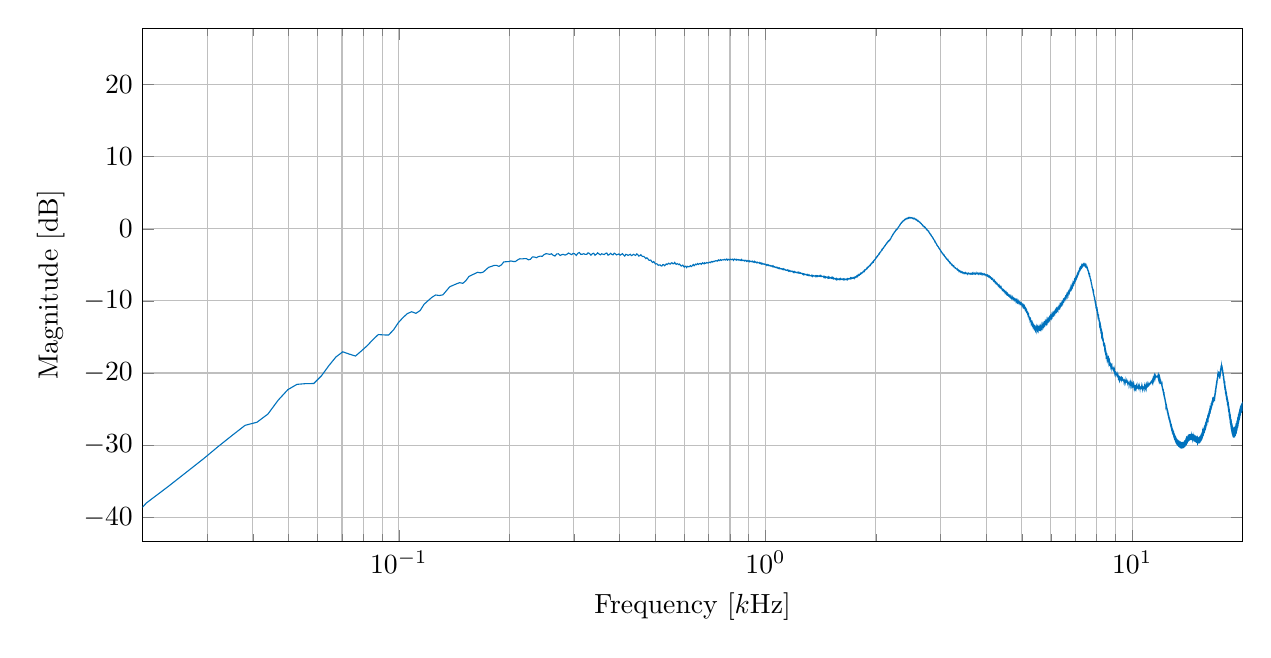
\begin{tikzpicture}

\begin{axis}[%
width=5.5in,
height=2.566in,
at={(2.804in,1.205in)},
scale only axis,
xmode=log,
xmin=0.02,
xmax=20,
xminorticks=true,
xlabel={Frequency [$k$Hz]},
xmajorgrids,
xminorgrids,
ymin=-43.3455877896241,
ymax=27.8130955898857,
ylabel={Magnitude [dB]},
ymajorgrids,
axis background/.style={fill=white},
title style={font=\bfseries},
legend style={legend cell align=left,align=left,draw=white!15!black}
]
\addplot [color=mycolor1,solid,forget plot]
  table[row sep=crcr]{%
0	-1.69141873333655\\
0.0029296875	-40.8589297400518\\
0.005859375	-60.5980111862308\\
0.0087890625	-53.2157441308172\\
0.01171875	-57.2367516122019\\
0.0146484375	-43.1597211075457\\
0.017578125	-41.6473379204459\\
0.0205078125	-37.9993270931867\\
0.0234375	-35.7728657291726\\
0.0263671875	-33.7314835828777\\
0.029296875	-31.9034991604498\\
0.0322265625	-30.1508947985882\\
0.03515625	-28.6204314562879\\
0.0380859375	-27.2462179322706\\
0.041015625	-26.8214249575063\\
0.0439453125	-25.6889727720254\\
0.046875	-23.7608293638928\\
0.0498046875	-22.3031464197138\\
0.052734375	-21.5695615779491\\
0.0556640625	-21.4666363252484\\
0.05859375	-21.4521698756001\\
0.0615234375	-20.3776757568286\\
0.064453125	-18.9662221291674\\
0.0673828125	-17.7640061494371\\
0.0703125	-17.0545263118457\\
0.0732421875	-17.3707060985524\\
0.076171875	-17.6438127055492\\
0.0791015625	-16.9208559171187\\
0.08203125	-16.1958865214752\\
0.0849609375	-15.3697622343122\\
0.087890625	-14.6609591744791\\
0.0908203125	-14.7131683950697\\
0.09375	-14.7296104829327\\
0.0966796875	-14.0206386171589\\
0.099609375	-13.0336615128222\\
0.1025390625	-12.3328386875402\\
0.10546875	-11.7549646788107\\
0.1083984375	-11.4986184373946\\
0.111328125	-11.7220860030783\\
0.1142578125	-11.3429897266818\\
0.1171875	-10.4618012927625\\
0.1201171875	-9.96853290357672\\
0.123046875	-9.50334307464777\\
0.1259765625	-9.17319188163316\\
0.12890625	-9.2495601015986\\
0.1318359375	-9.15893108517974\\
0.134765625	-8.59283945463693\\
0.1376953125	-8.03173585963651\\
0.140625	-7.82650855354564\\
0.1435546875	-7.63529660001848\\
0.146484375	-7.46142610723052\\
0.1494140625	-7.56393597479115\\
0.15234375	-7.18827737888694\\
0.1552734375	-6.61532104461224\\
0.158203125	-6.39868842683859\\
0.1611328125	-6.21682302558645\\
0.1640625	-6.02954473273905\\
0.1669921875	-6.10426766937144\\
0.169921875	-6.00312624546655\\
0.1728515625	-5.66310038863372\\
0.17578125	-5.33804890758637\\
0.1787109375	-5.22289300814975\\
0.181640625	-5.08510223827551\\
0.1845703125	-5.06794998346476\\
0.1875	-5.20828523103086\\
0.1904296875	-4.998878075059\\
0.193359375	-4.59228789601514\\
0.1962890625	-4.56159256674471\\
0.19921875	-4.54685857244095\\
0.2021484375	-4.45575077723635\\
0.205078125	-4.5290785871714\\
0.2080078125	-4.52743763361076\\
0.2109375	-4.30835843258672\\
0.2138671875	-4.15347340258256\\
0.216796875	-4.17550003496058\\
0.2197265625	-4.13297122043127\\
0.22265625	-4.12523496914594\\
0.2255859375	-4.29800796398564\\
0.228515625	-4.2259488085266\\
0.2314453125	-3.88616227648691\\
0.234375	-3.91741452842007\\
0.2373046875	-4.00458251180589\\
0.240234375	-3.85494993578249\\
0.2431640625	-3.78553813086069\\
0.24609375	-3.81296661330424\\
0.2490234375	-3.57098860902556\\
0.251953125	-3.44511919028258\\
0.2548828125	-3.48388512192196\\
0.2578125	-3.54474569476645\\
0.2607421875	-3.45926576364081\\
0.263671875	-3.67535735501565\\
0.2666015625	-3.77257239477092\\
0.26953125	-3.48270267867042\\
0.2724609375	-3.46231562233572\\
0.275390625	-3.69396011817997\\
0.2783203125	-3.57301591264792\\
0.28125	-3.55535128819628\\
0.2841796875	-3.64783250744057\\
0.287109375	-3.54413499453244\\
0.2900390625	-3.3592801782728\\
0.29296875	-3.4723296549576\\
0.2958984375	-3.58211289406512\\
0.298828125	-3.40481400116369\\
0.3017578125	-3.46649346050754\\
0.3046875	-3.68853142812208\\
0.3076171875	-3.40416769412155\\
0.310546875	-3.29153101285164\\
0.3134765625	-3.53860063498036\\
0.31640625	-3.53044119723842\\
0.3193359375	-3.45394805041991\\
0.322265625	-3.54774496623531\\
0.3251953125	-3.545809251062\\
0.328125	-3.33575920379286\\
0.3310546875	-3.41767875053785\\
0.333984375	-3.64722632389805\\
0.3369140625	-3.46386848249114\\
0.33984375	-3.38269792403344\\
0.3427734375	-3.66122057883734\\
0.345703125	-3.52104312967322\\
0.3486328125	-3.32639795808251\\
0.3515625	-3.49648522590513\\
0.3544921875	-3.61316934603985\\
0.357421875	-3.45629484043116\\
0.3603515625	-3.52435906009936\\
0.36328125	-3.5784291239811\\
0.3662109375	-3.41674550563334\\
0.369140625	-3.3516979036454\\
0.3720703125	-3.65970219302892\\
0.375	-3.56411579693327\\
0.3779296875	-3.39374412905505\\
0.380859375	-3.54942502406254\\
0.3837890625	-3.61286268144238\\
0.38671875	-3.37902704921277\\
0.3896484375	-3.48134335477641\\
0.392578125	-3.62350297036289\\
0.3955078125	-3.5438443226605\\
0.3984375	-3.48144236731463\\
0.4013671875	-3.65543312092962\\
0.404296875	-3.54757239658522\\
0.4072265625	-3.44795442073939\\
0.41015625	-3.63298885293949\\
0.4130859375	-3.78191389006145\\
0.416015625	-3.53455549220831\\
0.4189453125	-3.58432410638278\\
0.421875	-3.68652830305695\\
0.4248046875	-3.60867762723097\\
0.427734375	-3.53184639118462\\
0.4306640625	-3.71225318440565\\
0.43359375	-3.6461993020431\\
0.4365234375	-3.54032591083501\\
0.439453125	-3.62330608078383\\
0.4423828125	-3.68402761154908\\
0.4453125	-3.47900946651691\\
0.4482421875	-3.56835190157369\\
0.451171875	-3.78411580085094\\
0.4541015625	-3.7183693961515\\
0.45703125	-3.59340433845756\\
0.4599609375	-3.76336386321725\\
0.462890625	-3.83508276057887\\
0.4658203125	-3.8220335836221\\
0.46875	-3.97854507411029\\
0.4716796875	-4.12653837492127\\
0.474609375	-4.02048874152626\\
0.4775390625	-4.1426056002677\\
0.48046875	-4.34667235394664\\
0.4833984375	-4.36675094890751\\
0.486328125	-4.32694599457295\\
0.4892578125	-4.54518299903589\\
0.4921875	-4.66235492218146\\
0.4951171875	-4.5427394614955\\
0.498046875	-4.67803412446216\\
0.5009765625	-4.88497169131307\\
0.50390625	-4.8418963274911\\
0.5068359375	-4.89177746991777\\
0.509765625	-5.06591504525136\\
0.5126953125	-5.02010670639982\\
0.515625	-4.99431046977463\\
0.5185546875	-5.1309842561036\\
0.521484375	-5.16645791974781\\
0.5244140625	-4.98489292269744\\
0.52734375	-4.95862524832779\\
0.5302734375	-5.11763626425034\\
0.533203125	-5.01738357059946\\
0.5361328125	-4.87512252062726\\
0.5390625	-4.95818690917309\\
0.5419921875	-4.84898461126784\\
0.544921875	-4.76314353906741\\
0.5478515625	-4.87349712426391\\
0.55078125	-4.88198761082708\\
0.5537109375	-4.71341984126667\\
0.556640625	-4.7314345022877\\
0.5595703125	-4.85602279067359\\
0.5625	-4.82792353968313\\
0.5654296875	-4.66110086532831\\
0.568359375	-4.8633421841206\\
0.5712890625	-4.92531055349355\\
0.57421875	-4.82240687660646\\
0.5771484375	-4.88544864503103\\
0.580078125	-4.97387175929617\\
0.5830078125	-4.89171237581161\\
0.5859375	-5.03463737156858\\
0.5888671875	-5.16781563473245\\
0.591796875	-5.11045651684071\\
0.5947265625	-5.02804770919437\\
0.59765625	-5.19431857875531\\
0.6005859375	-5.30470472841938\\
0.603515625	-5.18295632968744\\
0.6064453125	-5.19527054856388\\
0.609375	-5.3771164905566\\
0.6123046875	-5.20033741071649\\
0.615234375	-5.23500855360425\\
0.6181640625	-5.27500869721496\\
0.62109375	-5.19596286149016\\
0.6240234375	-5.11283820278834\\
0.626953125	-5.2418432002433\\
0.6298828125	-5.1784215171171\\
0.6328125	-5.03525010812342\\
0.6357421875	-4.94508945556083\\
0.638671875	-5.11322794726004\\
0.6416015625	-5.01782073749041\\
0.64453125	-4.90845925860452\\
0.6474609375	-4.98021563504119\\
0.650390625	-4.91190470493024\\
0.6533203125	-4.8167466875513\\
0.65625	-4.93863420261158\\
0.6591796875	-4.87523087517116\\
0.662109375	-4.80118297517873\\
0.6650390625	-4.80286709243245\\
0.66796875	-4.92131648077628\\
0.6708984375	-4.8201971249598\\
0.673828125	-4.70856534233747\\
0.6767578125	-4.78351633729125\\
0.6796875	-4.87403425956904\\
0.6826171875	-4.70959001520714\\
0.685546875	-4.78891240174062\\
0.6884765625	-4.76119639449769\\
0.69140625	-4.67489347904069\\
0.6943359375	-4.70338940166459\\
0.697265625	-4.75628709213089\\
0.7001953125	-4.684367698264\\
0.703125	-4.61767673834976\\
0.7060546875	-4.6387404053059\\
0.708984375	-4.69223299324881\\
0.7119140625	-4.54209144856657\\
0.71484375	-4.52146118746947\\
0.7177734375	-4.61364868698718\\
0.720703125	-4.54320008069766\\
0.7236328125	-4.49329933704252\\
0.7265625	-4.52806715805337\\
0.7294921875	-4.43913035399243\\
0.732421875	-4.42311464426501\\
0.7353515625	-4.43525874221655\\
0.73828125	-4.48682614078763\\
0.7412109375	-4.3868463807126\\
0.744140625	-4.31921448822874\\
0.7470703125	-4.42008043728129\\
0.75	-4.40506000316987\\
0.7529296875	-4.2674611223938\\
0.755859375	-4.341122416659\\
0.7587890625	-4.3812295304657\\
0.76171875	-4.28891990690505\\
0.7646484375	-4.30891925768265\\
0.767578125	-4.31814870240981\\
0.7705078125	-4.26012636934695\\
0.7734375	-4.22986895826136\\
0.7763671875	-4.34427790797662\\
0.779296875	-4.34625875072305\\
0.7822265625	-4.18847175648739\\
0.78515625	-4.2317749081073\\
0.7880859375	-4.33235942454547\\
0.791015625	-4.22301025367113\\
0.7939453125	-4.23855380632773\\
0.796875	-4.31953124413644\\
0.7998046875	-4.2417799725024\\
0.802734375	-4.21178097517293\\
0.8056640625	-4.28690171438467\\
0.80859375	-4.26311935392903\\
0.8115234375	-4.20228911216003\\
0.814453125	-4.22857853302418\\
0.8173828125	-4.36965514423457\\
0.8203125	-4.22664813717392\\
0.8232421875	-4.18965939258976\\
0.826171875	-4.29286410315319\\
0.8291015625	-4.29150546728249\\
0.83203125	-4.22324640761451\\
0.8349609375	-4.35040658524929\\
0.837890625	-4.30135666432778\\
0.8408203125	-4.2469519579908\\
0.84375	-4.26755530432933\\
0.8466796875	-4.36617827906747\\
0.849609375	-4.30617068722137\\
0.8525390625	-4.27935536122686\\
0.85546875	-4.3833497425386\\
0.8583984375	-4.40729171397618\\
0.861328125	-4.25492776585173\\
0.8642578125	-4.36369385764056\\
0.8671875	-4.40320135090656\\
0.8701171875	-4.3591432496836\\
0.873046875	-4.39265749884817\\
0.8759765625	-4.45520588312695\\
0.87890625	-4.35291266101569\\
0.8818359375	-4.37364421090564\\
0.884765625	-4.43677292656258\\
0.8876953125	-4.51048108860164\\
0.890625	-4.38121585621394\\
0.8935546875	-4.45231799353763\\
0.896484375	-4.5207073583943\\
0.8994140625	-4.43752176285909\\
0.90234375	-4.40601602404524\\
0.9052734375	-4.56165785575524\\
0.908203125	-4.48716666894887\\
0.9111328125	-4.50117822987977\\
0.9140625	-4.55747869221113\\
0.9169921875	-4.56128957585594\\
0.919921875	-4.46864594926711\\
0.9228515625	-4.54033327156327\\
0.92578125	-4.63232021013766\\
0.9287109375	-4.61270810709107\\
0.931640625	-4.50796089114465\\
0.9345703125	-4.65885154268426\\
0.9375	-4.62088777842143\\
0.9404296875	-4.57865928639484\\
0.943359375	-4.66583318773274\\
0.9462890625	-4.72752919418321\\
0.94921875	-4.63315562993785\\
0.9521484375	-4.70772414848875\\
0.955078125	-4.72844545086815\\
0.9580078125	-4.71174740824773\\
0.9609375	-4.659966298244\\
0.9638671875	-4.7927354273985\\
0.966796875	-4.82661187520796\\
0.9697265625	-4.72106464631105\\
0.97265625	-4.76897723013587\\
0.9755859375	-4.87107213284469\\
0.978515625	-4.76123831604872\\
0.9814453125	-4.83374871173214\\
0.984375	-4.91241365451674\\
0.9873046875	-4.87986433848431\\
0.990234375	-4.84058485096131\\
0.9931640625	-4.92120115527092\\
0.99609375	-4.94095054770526\\
0.9990234375	-4.90048758343943\\
1.001953125	-4.92430930399502\\
1.0048828125	-5.06559242653248\\
1.0078125	-4.96864328815656\\
1.0107421875	-4.94751816968443\\
1.013671875	-5.04834248728974\\
1.0166015625	-5.04664738012508\\
1.01953125	-5.00143987181542\\
1.0224609375	-5.13547437288759\\
1.025390625	-5.10796730378996\\
1.0283203125	-5.07223129394333\\
1.03125	-5.08882075465738\\
1.0341796875	-5.17913858633125\\
1.037109375	-5.16002212067957\\
1.0400390625	-5.12406079063845\\
1.04296875	-5.23237024286618\\
1.0458984375	-5.26405569822839\\
1.048828125	-5.14348155982151\\
1.0517578125	-5.25098421519391\\
1.0546875	-5.29648377511614\\
1.0576171875	-5.24486735874746\\
1.060546875	-5.2855995830576\\
1.0634765625	-5.35694400578768\\
1.06640625	-5.30683973629681\\
1.0693359375	-5.30000488654485\\
1.072265625	-5.35220155671084\\
1.0751953125	-5.43237479295897\\
1.078125	-5.35032857724212\\
1.0810546875	-5.40126416548077\\
1.083984375	-5.49134070995609\\
1.0869140625	-5.40685649916355\\
1.08984375	-5.40633605143967\\
1.0927734375	-5.52895012095235\\
1.095703125	-5.49072231716298\\
1.0986328125	-5.49132618533326\\
1.1015625	-5.55925755938227\\
1.1044921875	-5.58118973230864\\
1.107421875	-5.53071123338191\\
1.1103515625	-5.53608668214792\\
1.11328125	-5.64585880819862\\
1.1162109375	-5.62642851537595\\
1.119140625	-5.55870998737009\\
1.1220703125	-5.68629096752045\\
1.125	-5.65962110524498\\
1.1279296875	-5.59752542049563\\
1.130859375	-5.69478175010204\\
1.1337890625	-5.73439685080081\\
1.13671875	-5.69110898969831\\
1.1396484375	-5.72518563838946\\
1.142578125	-5.77210055120315\\
1.1455078125	-5.76661197629903\\
1.1484375	-5.70872268698878\\
1.1513671875	-5.79907331377012\\
1.154296875	-5.86786081635353\\
1.1572265625	-5.75704626478898\\
1.16015625	-5.81227739253785\\
1.1630859375	-5.87005692831463\\
1.166015625	-5.78468923315211\\
1.1689453125	-5.83725243457081\\
1.171875	-5.91948630605816\\
1.1748046875	-5.88419891412536\\
1.177734375	-5.8628429249178\\
1.1806640625	-5.89723287892923\\
1.18359375	-5.95519896168673\\
1.1865234375	-5.88904804123752\\
1.189453125	-5.90894460212559\\
1.1923828125	-6.03673485176489\\
1.1953125	-5.96418449306412\\
1.1982421875	-5.9260302168326\\
1.201171875	-6.04183287569612\\
1.2041015625	-5.98737031604162\\
1.20703125	-5.98060680196312\\
1.2099609375	-6.06043073994709\\
1.212890625	-6.08049510150039\\
1.2158203125	-6.03430197834712\\
1.21875	-6.02710351229911\\
1.2216796875	-6.10153781261414\\
1.224609375	-6.11664268193181\\
1.2275390625	-6.02574789508316\\
1.23046875	-6.14299814301546\\
1.2333984375	-6.15729341495461\\
1.236328125	-6.07880010552503\\
1.2392578125	-6.15407458643421\\
1.2421875	-6.1721716895654\\
1.2451171875	-6.11216402577696\\
1.248046875	-6.18098260649049\\
1.2509765625	-6.20970347892973\\
1.25390625	-6.21418322545099\\
1.2568359375	-6.17017490899622\\
1.259765625	-6.21566609635551\\
1.2626953125	-6.28662457864158\\
1.265625	-6.21195549751963\\
1.2685546875	-6.22939214947928\\
1.271484375	-6.35029618723655\\
1.2744140625	-6.24590608613704\\
1.27734375	-6.27655140335122\\
1.2802734375	-6.33800635792397\\
1.283203125	-6.30252686810553\\
1.2861328125	-6.31751094465568\\
1.2890625	-6.36440185243362\\
1.2919921875	-6.39149400329904\\
1.294921875	-6.37145176056617\\
1.2978515625	-6.31630062132695\\
1.30078125	-6.44496105316097\\
1.3037109375	-6.42044888190031\\
1.306640625	-6.36852284646369\\
1.3095703125	-6.47889098646544\\
1.3125	-6.45799379903502\\
1.3154296875	-6.39803583812699\\
1.318359375	-6.49512854142614\\
1.3212890625	-6.47813928892606\\
1.32421875	-6.48328607556988\\
1.3271484375	-6.48460843026487\\
1.330078125	-6.53285861797912\\
1.3330078125	-6.54112301676884\\
1.3359375	-6.45176555679666\\
1.3388671875	-6.50860656047757\\
1.341796875	-6.60284224417143\\
1.3447265625	-6.48879290460297\\
1.34765625	-6.55439346043221\\
1.3505859375	-6.5608576063139\\
1.353515625	-6.49794049021398\\
1.3564453125	-6.53505164985978\\
1.359375	-6.56435286886688\\
1.3623046875	-6.54950587471637\\
1.365234375	-6.54732713589948\\
1.3681640625	-6.50916713428978\\
1.37109375	-6.5978656314478\\
1.3740234375	-6.51032748889992\\
1.376953125	-6.49295362802053\\
1.3798828125	-6.60277482563345\\
1.3828125	-6.5449384125983\\
1.3857421875	-6.50919007719386\\
1.388671875	-6.58516140443874\\
1.3916015625	-6.51789923801232\\
1.39453125	-6.53420796079808\\
1.3974609375	-6.5326168262568\\
1.400390625	-6.59536071891523\\
1.4033203125	-6.58066124326348\\
1.40625	-6.50818387980604\\
1.4091796875	-6.58549504694707\\
1.412109375	-6.60278078637617\\
1.4150390625	-6.49817043052872\\
1.41796875	-6.60789935514941\\
1.4208984375	-6.61288635612328\\
1.423828125	-6.56676045713652\\
1.4267578125	-6.60624483593159\\
1.4296875	-6.60919620073662\\
1.4326171875	-6.6040505344165\\
1.435546875	-6.59534151249096\\
1.4384765625	-6.62559448783213\\
1.44140625	-6.70357236364748\\
1.4443359375	-6.57836308788393\\
1.447265625	-6.62013928750599\\
1.4501953125	-6.71626174527148\\
1.453125	-6.62126410795116\\
1.4560546875	-6.64741438276121\\
1.458984375	-6.75075834296041\\
1.4619140625	-6.6675136318633\\
1.46484375	-6.68224192840057\\
1.4677734375	-6.69785113169337\\
1.470703125	-6.74097411301284\\
1.4736328125	-6.70509099765849\\
1.4765625	-6.68893717361726\\
1.4794921875	-6.819144802474\\
1.482421875	-6.75878122448529\\
1.4853515625	-6.67667512015618\\
1.48828125	-6.81613167519652\\
1.4912109375	-6.77229689268859\\
1.494140625	-6.72524252592518\\
1.4970703125	-6.8397807031759\\
1.5	-6.82270702072537\\
1.5029296875	-6.76590739109372\\
1.505859375	-6.79474707793008\\
1.5087890625	-6.83836403845021\\
1.51171875	-6.85643139358569\\
1.5146484375	-6.77591381000457\\
1.517578125	-6.88721355417869\\
1.5205078125	-6.89937614676529\\
1.5234375	-6.77452076490232\\
1.5263671875	-6.86565012110577\\
1.529296875	-6.92500191150219\\
1.5322265625	-6.82283248024692\\
1.53515625	-6.91227500355251\\
1.5380859375	-6.92848775006183\\
1.541015625	-6.88547631155035\\
1.5439453125	-6.87227484460664\\
1.546875	-6.91458860555048\\
1.5498046875	-6.96693366583526\\
1.552734375	-6.90118874069799\\
1.5556640625	-6.9124709541108\\
1.55859375	-7.00869665916468\\
1.5615234375	-6.88309810715822\\
1.564453125	-6.91774999049153\\
1.5673828125	-7.00590114283051\\
1.5703125	-6.94990588039616\\
1.5732421875	-6.93886458340671\\
1.576171875	-7.01409139537952\\
1.5791015625	-6.9696247185679\\
1.58203125	-6.95253335493868\\
1.5849609375	-6.94192614758578\\
1.587890625	-7.02735948084887\\
1.5908203125	-6.98886368237663\\
1.59375	-6.94435068942113\\
1.5966796875	-7.03411909292362\\
1.599609375	-7.004637643845\\
1.6025390625	-6.92340527205266\\
1.60546875	-7.03315064963255\\
1.6083984375	-7.01665146723326\\
1.611328125	-6.97343200056918\\
1.6142578125	-6.99529986440211\\
1.6171875	-7.01727456692521\\
1.6201171875	-6.99354311490777\\
1.623046875	-6.95770424528121\\
1.6259765625	-7.00810064230757\\
1.62890625	-7.05477130813659\\
1.6318359375	-6.95549250831112\\
1.634765625	-6.9996683785705\\
1.6376953125	-7.03472824953514\\
1.640625	-6.94759978164183\\
1.6435546875	-6.98325164539494\\
1.646484375	-7.04886855451088\\
1.6494140625	-6.98730428101004\\
1.65234375	-6.98653960712227\\
1.6552734375	-6.97582218861993\\
1.658203125	-7.01054429471418\\
1.6611328125	-6.95125074062167\\
1.6640625	-6.9542412905875\\
1.6669921875	-7.02721736484932\\
1.669921875	-6.96588075770705\\
1.6728515625	-6.91923145235666\\
1.67578125	-7.02013963148039\\
1.6787109375	-6.94171216783775\\
1.681640625	-6.9165740967627\\
1.6845703125	-6.9756402102015\\
1.6875	-6.97706720637558\\
1.6904296875	-6.91753890804046\\
1.693359375	-6.90683688678718\\
1.6962890625	-6.94095033453465\\
1.69921875	-6.93424967185877\\
1.7021484375	-6.85486229873908\\
1.705078125	-6.94938515805279\\
1.7080078125	-6.93705707429126\\
1.7109375	-6.82406499773083\\
1.7138671875	-6.87924138341111\\
1.716796875	-6.90093887052183\\
1.7197265625	-6.8195457446871\\
1.72265625	-6.84805487803681\\
1.7255859375	-6.87033957253055\\
1.728515625	-6.85397888206415\\
1.7314453125	-6.77369472028812\\
1.734375	-6.80488830282769\\
1.7373046875	-6.84010703621834\\
1.740234375	-6.75317504940222\\
1.7431640625	-6.75627268156137\\
1.74609375	-6.83476600995385\\
1.7490234375	-6.70672552879824\\
1.751953125	-6.68537809222204\\
1.7548828125	-6.76165590681597\\
1.7578125	-6.69668101966147\\
1.7607421875	-6.65534510851751\\
1.763671875	-6.69347876191637\\
1.7666015625	-6.67576985792795\\
1.76953125	-6.60160695424997\\
1.7724609375	-6.55223683775438\\
1.775390625	-6.63269895795418\\
1.7783203125	-6.55937311249005\\
1.78125	-6.50888437348056\\
1.7841796875	-6.58130745905567\\
1.787109375	-6.51321477128835\\
1.7900390625	-6.3989806851111\\
1.79296875	-6.47731308118256\\
1.7958984375	-6.46592968642966\\
1.798828125	-6.39413689731509\\
1.8017578125	-6.37854896477745\\
1.8046875	-6.40052974256787\\
1.8076171875	-6.32165952171204\\
1.810546875	-6.26339307665035\\
1.8134765625	-6.29613709280511\\
1.81640625	-6.30468600120787\\
1.8193359375	-6.17451393925563\\
1.822265625	-6.22135853207237\\
1.8251953125	-6.21144016701675\\
1.828125	-6.10220491018072\\
1.8310546875	-6.0945897631758\\
1.833984375	-6.13216878394246\\
1.8369140625	-6.06505285411578\\
1.83984375	-6.00970773908216\\
1.8427734375	-6.01231727276615\\
1.845703125	-5.99212465546174\\
1.8486328125	-5.89359849219716\\
1.8515625	-5.90049097670681\\
1.8544921875	-5.94076586461756\\
1.857421875	-5.84778778868764\\
1.8603515625	-5.78183528162475\\
1.86328125	-5.83433699066723\\
1.8662109375	-5.73838340841854\\
1.869140625	-5.6900030072232\\
1.8720703125	-5.71674064840374\\
1.875	-5.70625966083765\\
1.8779296875	-5.62736202321611\\
1.880859375	-5.5916923816705\\
1.8837890625	-5.58900339852266\\
1.88671875	-5.52665686670559\\
1.8896484375	-5.4489593570695\\
1.892578125	-5.5173519936867\\
1.8955078125	-5.47664037447981\\
1.8984375	-5.35828309079238\\
1.9013671875	-5.37714305097512\\
1.904296875	-5.3611557053423\\
1.9072265625	-5.26563037252106\\
1.91015625	-5.26265268581574\\
1.9130859375	-5.2689417826424\\
1.916015625	-5.21409967558395\\
1.9189453125	-5.12048028509207\\
1.921875	-5.12548657011598\\
1.9248046875	-5.11366442604344\\
1.927734375	-5.01470002531715\\
1.9306640625	-5.01367870500741\\
1.93359375	-5.04628896184244\\
1.9365234375	-4.90958999276745\\
1.939453125	-4.86601276438927\\
1.9423828125	-4.88393411012623\\
1.9453125	-4.83346771614129\\
1.9482421875	-4.77003314821121\\
1.951171875	-4.78917988308945\\
1.9541015625	-4.76312613042887\\
1.95703125	-4.66007996198323\\
1.9599609375	-4.61569293088519\\
1.962890625	-4.6434645912837\\
1.9658203125	-4.5565559251952\\
1.96875	-4.50718321266504\\
1.9716796875	-4.55458673727276\\
1.974609375	-4.46027045095229\\
1.9775390625	-4.35782498462373\\
1.98046875	-4.36835792819932\\
1.9833984375	-4.34044979654118\\
1.986328125	-4.27335460488422\\
1.9892578125	-4.23942722787115\\
1.9921875	-4.23572720579665\\
1.9951171875	-4.14038719793086\\
1.998046875	-4.05849271765669\\
2.0009765625	-4.07852020565969\\
2.00390625	-4.0533632694067\\
2.0068359375	-3.93734341117863\\
2.009765625	-3.95914692997121\\
2.0126953125	-3.9135071210074\\
2.015625	-3.81734360451725\\
2.0185546875	-3.76931881246605\\
2.021484375	-3.7896376638198\\
2.0244140625	-3.72377449780498\\
2.02734375	-3.65561266396759\\
2.0302734375	-3.63900210190837\\
2.033203125	-3.6069949450071\\
2.0361328125	-3.48096942792915\\
2.0390625	-3.46982174916388\\
2.0419921875	-3.49179520277846\\
2.044921875	-3.40872530219133\\
2.0478515625	-3.33424463818972\\
2.05078125	-3.34525718366848\\
2.0537109375	-3.25647628977953\\
2.056640625	-3.19524237029043\\
2.0595703125	-3.18594073416324\\
2.0625	-3.19334667330526\\
2.0654296875	-3.09489368780623\\
2.068359375	-3.05265706110652\\
2.0712890625	-3.04164096361291\\
2.07421875	-2.95161171771173\\
2.0771484375	-2.87807116119546\\
2.080078125	-2.92822626164872\\
2.0830078125	-2.88303379209628\\
2.0859375	-2.7803731508223\\
2.0888671875	-2.7499904493169\\
2.091796875	-2.72697203161886\\
2.0947265625	-2.63691119434634\\
2.09765625	-2.60742524457743\\
2.1005859375	-2.63110588062727\\
2.103515625	-2.56682899775979\\
2.1064453125	-2.4636750068467\\
2.109375	-2.46379712486163\\
2.1123046875	-2.42560517413654\\
2.115234375	-2.33616305968968\\
2.1181640625	-2.33649613963053\\
2.12109375	-2.34562852534498\\
2.1240234375	-2.25308699306674\\
2.126953125	-2.17453725466544\\
2.1298828125	-2.17153522327095\\
2.1328125	-2.13074569729389\\
2.1357421875	-2.05376045739104\\
2.138671875	-2.07737874038639\\
2.1416015625	-2.04328143037395\\
2.14453125	-1.93771300390023\\
2.1474609375	-1.89075332199536\\
2.150390625	-1.89242698849256\\
2.1533203125	-1.82975506970763\\
2.15625	-1.77096424484341\\
2.1591796875	-1.80256679974372\\
2.162109375	-1.74832396187514\\
2.1650390625	-1.66268280349414\\
2.16796875	-1.64541237651355\\
2.1708984375	-1.63943601480287\\
2.173828125	-1.59990385293582\\
2.1767578125	-1.57868876772221\\
2.1796875	-1.61557393679493\\
2.1826171875	-1.53593773607548\\
2.185546875	-1.46795546371698\\
2.1884765625	-1.47972731557735\\
2.19140625	-1.44921930347476\\
2.1943359375	-1.36071107128208\\
2.197265625	-1.32147186462311\\
2.2001953125	-1.27740914934651\\
2.203125	-1.1691251002685\\
2.2060546875	-1.09564230392596\\
2.208984375	-1.09493292100751\\
2.2119140625	-1.04525994221621\\
2.21484375	-0.970765293918816\\
2.2177734375	-0.952464427823088\\
2.220703125	-0.916806428230018\\
2.2236328125	-0.798155803414375\\
2.2265625	-0.754658728793117\\
2.2294921875	-0.770227785034706\\
2.232421875	-0.713885997555792\\
2.2353515625	-0.646514107025951\\
2.23828125	-0.63053507357273\\
2.2412109375	-0.562553388785659\\
2.244140625	-0.473132314318264\\
2.2470703125	-0.466511610233169\\
2.25	-0.474017321918666\\
2.2529296875	-0.395218518403226\\
2.255859375	-0.347927001661844\\
2.2587890625	-0.351132922137595\\
2.26171875	-0.271289354954774\\
2.2646484375	-0.2121523118455\\
2.267578125	-0.24085896282287\\
2.2705078125	-0.222132772811051\\
2.2734375	-0.141722000551567\\
2.2763671875	-0.127165158727166\\
2.279296875	-0.108741505039688\\
2.2822265625	-0.0351162669090854\\
2.28515625	0.00242052708841811\\
2.2880859375	-0.0316768065411566\\
2.291015625	0.00795175965106409\\
2.2939453125	0.102185291882847\\
2.296875	0.116141489585004\\
2.2998046875	0.14818649339577\\
2.302734375	0.223638561369455\\
2.3056640625	0.255647123796621\\
2.30859375	0.25022771082115\\
2.3115234375	0.31474496625691\\
2.314453125	0.390495611086124\\
2.3173828125	0.412372464222983\\
2.3203125	0.472889060878913\\
2.3232421875	0.536054482391137\\
2.326171875	0.54013017044133\\
2.3291015625	0.549199099649059\\
2.33203125	0.637042580180719\\
2.3349609375	0.694500051653222\\
2.337890625	0.703307218718805\\
2.3408203125	0.761925974095675\\
2.34375	0.802993276982988\\
2.3466796875	0.788860339669498\\
2.349609375	0.819023691373047\\
2.3525390625	0.903045108366655\\
2.35546875	0.937710711800889\\
2.3583984375	0.934816456734609\\
2.361328125	0.982617057355469\\
2.3642578125	1.01667825739571\\
2.3671875	0.990012281161682\\
2.3701171875	1.02930378162011\\
2.373046875	1.1045051344197\\
2.3759765625	1.12445910530926\\
2.37890625	1.1154510895683\\
2.3818359375	1.15438775195071\\
2.384765625	1.16330097116105\\
2.3876953125	1.15117992767489\\
2.390625	1.22403583545173\\
2.3935546875	1.27853670191558\\
2.396484375	1.25803358687477\\
2.3994140625	1.2522750419468\\
2.40234375	1.29481734605082\\
2.4052734375	1.29920435869872\\
2.408203125	1.29056538233016\\
2.4111328125	1.37450032843759\\
2.4140625	1.39611751411348\\
2.4169921875	1.35049491068065\\
2.419921875	1.38174999082588\\
2.4228515625	1.40599612761645\\
2.42578125	1.39003656558697\\
2.4287109375	1.41898853686951\\
2.431640625	1.47884362696527\\
2.4345703125	1.48315763745643\\
2.4375	1.42898811461026\\
2.4404296875	1.4636597132718\\
2.443359375	1.48667394621458\\
2.4462890625	1.46588182848541\\
2.44921875	1.5057477414648\\
2.4521484375	1.54771519945155\\
2.455078125	1.5081072423219\\
2.4580078125	1.4811678100869\\
2.4609375	1.52095177444272\\
2.4638671875	1.53629681021539\\
2.466796875	1.51584096411557\\
2.4697265625	1.55284368047666\\
2.47265625	1.57237765852886\\
2.4755859375	1.52784500894313\\
2.478515625	1.50392162918371\\
2.4814453125	1.53507571503002\\
2.484375	1.53408113932056\\
2.4873046875	1.52266606075563\\
2.490234375	1.55864301068948\\
2.4931640625	1.54765621269127\\
2.49609375	1.49772801650329\\
2.4990234375	1.49582702567824\\
2.501953125	1.5412408049138\\
2.5048828125	1.52698844658181\\
2.5078125	1.50534779879968\\
2.5107421875	1.53467374969887\\
2.513671875	1.50045196149091\\
2.5166015625	1.45047965378927\\
2.51953125	1.48310898505599\\
2.5224609375	1.48979621665393\\
2.525390625	1.48585581021541\\
2.5283203125	1.47568381071125\\
2.53125	1.48265315061042\\
2.5341796875	1.43943031003039\\
2.537109375	1.39217289308328\\
2.5400390625	1.43405117966347\\
2.54296875	1.45929367613547\\
2.5458984375	1.40382082702905\\
2.548828125	1.41159051781256\\
2.5517578125	1.39335012484764\\
2.5546875	1.34169891943264\\
2.5576171875	1.34198381654534\\
2.560546875	1.3641960190738\\
2.5634765625	1.36282018947958\\
2.56640625	1.30556845973211\\
2.5693359375	1.30538508775811\\
2.572265625	1.29625619526598\\
2.5751953125	1.222768708655\\
2.578125	1.24138425977151\\
2.5810546875	1.27323084785536\\
2.583984375	1.22537396515355\\
2.5869140625	1.20320558993205\\
2.58984375	1.18588869591088\\
2.5927734375	1.16382701842599\\
2.595703125	1.12049196781163\\
2.5986328125	1.14320274733529\\
2.6015625	1.16266567421115\\
2.6044921875	1.08646342301887\\
2.607421875	1.06157014476128\\
2.6103515625	1.0725154790037\\
2.61328125	1.02238489731235\\
2.6162109375	1.0028544761941\\
2.619140625	1.02413435156956\\
2.6220703125	1.01375287232702\\
2.625	0.960929345484374\\
2.6279296875	0.934230058973924\\
2.630859375	0.918706756609481\\
2.6337890625	0.879822767750056\\
2.63671875	0.874595122248991\\
2.6396484375	0.895050230728941\\
2.642578125	0.862868056352625\\
2.6455078125	0.782174220521654\\
2.6484375	0.777285157973381\\
2.6513671875	0.770248655646355\\
2.654296875	0.730096393777217\\
2.6572265625	0.727537542498339\\
2.66015625	0.731659877453581\\
2.6630859375	0.668802815436777\\
2.666015625	0.623851719668721\\
2.6689453125	0.599179224602949\\
2.671875	0.597509407522864\\
2.6748046875	0.547373671753064\\
2.677734375	0.553285673242556\\
2.6806640625	0.546190322653672\\
2.68359375	0.454555319139047\\
2.6865234375	0.408870860816251\\
2.689453125	0.423866298063615\\
2.6923828125	0.40204945737014\\
2.6953125	0.377274503443971\\
2.6982421875	0.375652030403558\\
2.701171875	0.345886635268698\\
2.7041015625	0.285014931030446\\
2.70703125	0.266095363816476\\
2.7099609375	0.29191817059808\\
2.712890625	0.263938295604078\\
2.7158203125	0.230562527754842\\
2.71875	0.253221955991705\\
2.7216796875	0.193296842463553\\
2.724609375	0.133870512491626\\
2.7275390625	0.14447366045556\\
2.73046875	0.148090010917201\\
2.7333984375	0.108636338408587\\
2.736328125	0.0911242333665996\\
2.7392578125	0.0657944366452057\\
2.7421875	0.00766322822681786\\
2.7451171875	-0.0526831129046741\\
2.748046875	-0.0167525216227205\\
2.7509765625	-0.0254824619108263\\
2.75390625	-0.0842576088498959\\
2.7568359375	-0.104024500744629\\
2.759765625	-0.131743988187907\\
2.7626953125	-0.206808696189512\\
2.765625	-0.224888701883117\\
2.7685546875	-0.215742938846745\\
2.771484375	-0.244660086217095\\
2.7744140625	-0.284578250610821\\
2.77734375	-0.316842949225361\\
2.7802734375	-0.354354342223871\\
2.783203125	-0.421821450664481\\
2.7861328125	-0.429374069371647\\
2.7890625	-0.396917167271454\\
2.7919921875	-0.464253604167936\\
2.794921875	-0.523786850546912\\
2.7978515625	-0.543804372477211\\
2.80078125	-0.589127341985431\\
2.8037109375	-0.634608934536857\\
2.806640625	-0.622349513492395\\
2.8095703125	-0.647197719547307\\
2.8125	-0.692480464277082\\
2.8154296875	-0.765248422934576\\
2.818359375	-0.785996441217605\\
2.8212890625	-0.812568297073994\\
2.82421875	-0.866145247803786\\
2.8271484375	-0.836583063680962\\
2.830078125	-0.86961721502297\\
2.8330078125	-0.960486474321954\\
2.8359375	-0.976208260530086\\
2.8388671875	-1.02430946825075\\
2.841796875	-1.05103423215161\\
2.8447265625	-1.07518796886848\\
2.84765625	-1.08544805363249\\
2.8505859375	-1.12027942056153\\
2.853515625	-1.21645120061356\\
2.8564453125	-1.23981503109752\\
2.859375	-1.24033749607003\\
2.8623046875	-1.3072703275763\\
2.865234375	-1.32450739101893\\
2.8681640625	-1.32793178523241\\
2.87109375	-1.40482289974148\\
2.8740234375	-1.46597320190989\\
2.876953125	-1.4791865799823\\
2.8798828125	-1.5060986606947\\
2.8828125	-1.55099734585821\\
2.8857421875	-1.57735000773039\\
2.888671875	-1.58478769760296\\
2.8916015625	-1.68186841068001\\
2.89453125	-1.75053580933195\\
2.8974609375	-1.70938419694312\\
2.900390625	-1.7706983992241\\
2.9033203125	-1.81893515934519\\
2.90625	-1.8269560724903\\
2.9091796875	-1.89611737754234\\
2.912109375	-1.95574109809428\\
2.9150390625	-1.98597969694202\\
2.91796875	-1.99678919924025\\
2.9208984375	-2.03775041640705\\
2.923828125	-2.08950511694468\\
2.9267578125	-2.10108157504266\\
2.9296875	-2.14132447899374\\
2.9326171875	-2.24000681555026\\
2.935546875	-2.22689887616968\\
2.9384765625	-2.24337782721943\\
2.94140625	-2.30395183754325\\
2.9443359375	-2.32051422873388\\
2.947265625	-2.36987516074612\\
2.9501953125	-2.44048418119615\\
2.953125	-2.46661582321599\\
2.9560546875	-2.48272795963891\\
2.958984375	-2.48222406638189\\
2.9619140625	-2.55076395169317\\
2.96484375	-2.599701132017\\
2.9677734375	-2.61017116026267\\
2.970703125	-2.69291349460696\\
2.9736328125	-2.72163967236844\\
2.9765625	-2.70372207853245\\
2.9794921875	-2.75471553274514\\
2.982421875	-2.78387314318121\\
2.9853515625	-2.83616934599752\\
2.98828125	-2.87590778023048\\
2.9912109375	-2.92855503888939\\
2.994140625	-2.95123782992192\\
2.9970703125	-2.93558902804364\\
3	-2.97747416429343\\
3.0029296875	-3.06329492320015\\
3.005859375	-3.06158536599321\\
3.0087890625	-3.10455622302374\\
3.01171875	-3.16075255209239\\
3.0146484375	-3.1366659374429\\
3.017578125	-3.17268810301277\\
3.0205078125	-3.22122678753027\\
3.0234375	-3.26752760500074\\
3.0263671875	-3.2982633938089\\
3.029296875	-3.31696889024113\\
3.0322265625	-3.37277309415146\\
3.03515625	-3.35435589352056\\
3.0380859375	-3.36053429948328\\
3.041015625	-3.46698209794818\\
3.0439453125	-3.48958926648299\\
3.046875	-3.48301709897896\\
3.0498046875	-3.54672147668498\\
3.052734375	-3.54268182592733\\
3.0556640625	-3.54838431833343\\
3.05859375	-3.5980756124531\\
3.0615234375	-3.65117721334303\\
3.064453125	-3.68496247936645\\
3.0673828125	-3.68104669634488\\
3.0703125	-3.7173525368022\\
3.0732421875	-3.75526595305053\\
3.076171875	-3.72581239826656\\
3.0791015625	-3.8017429658305\\
3.08203125	-3.85169458556811\\
3.0849609375	-3.84606042124909\\
3.087890625	-3.8864415145045\\
3.0908203125	-3.89586404922045\\
3.09375	-3.90096973614828\\
3.0966796875	-3.94273300312659\\
3.099609375	-3.98359068341483\\
3.1025390625	-4.03951279008697\\
3.10546875	-4.02823442742783\\
3.1083984375	-4.03653680692906\\
3.111328125	-4.08469289097741\\
3.1142578125	-4.08342987184693\\
3.1171875	-4.11199651330054\\
3.1201171875	-4.1952542807764\\
3.123046875	-4.18448761881535\\
3.1259765625	-4.19950732402469\\
3.12890625	-4.22967204246743\\
3.1318359375	-4.23861453241898\\
3.134765625	-4.26851048076082\\
3.1376953125	-4.30363553171406\\
3.140625	-4.36047025488182\\
3.1435546875	-4.38143904192367\\
3.146484375	-4.33308269012844\\
3.1494140625	-4.39460942773934\\
3.15234375	-4.42945316148575\\
3.1552734375	-4.42688212594322\\
3.158203125	-4.50303481737819\\
3.1611328125	-4.5205009560047\\
3.1640625	-4.50928089539241\\
3.1669921875	-4.52996417945604\\
3.169921875	-4.54718375581081\\
3.1728515625	-4.60944688328874\\
3.17578125	-4.60934662778959\\
3.1787109375	-4.64518166053585\\
3.181640625	-4.69832408081049\\
3.1845703125	-4.64582532284811\\
3.1875	-4.67775183015073\\
3.1904296875	-4.74585976050508\\
3.193359375	-4.73551961674031\\
3.1962890625	-4.78560572646694\\
3.19921875	-4.82190499129075\\
3.2021484375	-4.80752557475182\\
3.205078125	-4.81050000390485\\
3.2080078125	-4.83780362077113\\
3.2109375	-4.89366426674292\\
3.2138671875	-4.91030954750903\\
3.216796875	-4.91340507024688\\
3.2197265625	-4.97655491675306\\
3.22265625	-4.95126885344956\\
3.2255859375	-4.94142554196964\\
3.228515625	-5.02330951663623\\
3.2314453125	-5.03461305895627\\
3.234375	-5.04592016672558\\
3.2373046875	-5.09647867968368\\
3.240234375	-5.08738734018215\\
3.2431640625	-5.09388163445271\\
3.24609375	-5.10225358098029\\
3.2490234375	-5.14848929012567\\
3.251953125	-5.2006684848522\\
3.2548828125	-5.17664152636019\\
3.2578125	-5.21363260352967\\
3.2607421875	-5.23368366555479\\
3.263671875	-5.18788188704042\\
3.2666015625	-5.25936819528681\\
3.26953125	-5.29873026777847\\
3.2724609375	-5.3005153560066\\
3.275390625	-5.32134368963608\\
3.2783203125	-5.32629060432987\\
3.28125	-5.33525086542988\\
3.2841796875	-5.34531309156552\\
3.287109375	-5.36532805773442\\
3.2900390625	-5.43741943591021\\
3.29296875	-5.42039219218179\\
3.2958984375	-5.41893178631614\\
3.298828125	-5.45036096648778\\
3.3017578125	-5.44236966960028\\
3.3046875	-5.45973157031472\\
3.3076171875	-5.52528468043101\\
3.310546875	-5.53777716814932\\
3.3134765625	-5.53068184526273\\
3.31640625	-5.5367494966053\\
3.3193359375	-5.54953944770244\\
3.322265625	-5.57788282524768\\
3.3251953125	-5.57667429400942\\
3.328125	-5.63546926679186\\
3.3310546875	-5.65834324411168\\
3.333984375	-5.60731558569944\\
3.3369140625	-5.65711403481771\\
3.33984375	-5.67625170938811\\
3.3427734375	-5.65575498930957\\
3.345703125	-5.71352277533953\\
3.3486328125	-5.74143775746228\\
3.3515625	-5.73066221832056\\
3.3544921875	-5.73697480809335\\
3.357421875	-5.72457569049345\\
3.3603515625	-5.78502408090384\\
3.36328125	-5.77411031688683\\
3.3662109375	-5.79333217665453\\
3.369140625	-5.85447087703352\\
3.3720703125	-5.7906683160997\\
3.375	-5.81205350345363\\
3.3779296875	-5.85115973537745\\
3.380859375	-5.83013085501312\\
3.3837890625	-5.87348337706106\\
3.38671875	-5.90509579682976\\
3.3896484375	-5.89944747022861\\
3.392578125	-5.89729447526958\\
3.3955078125	-5.8818523931173\\
3.3984375	-5.92347150871223\\
3.4013671875	-5.94143794410962\\
3.404296875	-5.93702026127528\\
3.4072265625	-5.99627567016256\\
3.41015625	-5.97139485179412\\
3.4130859375	-5.94069909876066\\
3.416015625	-5.98863211242002\\
3.4189453125	-5.99583012935761\\
3.421875	-6.01891332681316\\
3.4248046875	-6.03683240149081\\
3.427734375	-6.02480038417997\\
3.4306640625	-6.03622604960685\\
3.43359375	-6.00734330654785\\
3.4365234375	-6.02855736721182\\
3.439453125	-6.08094417595555\\
3.4423828125	-6.04562447573971\\
3.4453125	-6.0749865408269\\
3.4482421875	-6.08361622001865\\
3.451171875	-6.03165385417503\\
3.4541015625	-6.05932682138018\\
3.45703125	-6.09271786212901\\
3.4599609375	-6.10804982199676\\
3.462890625	-6.11948576992438\\
3.4658203125	-6.08656820661963\\
3.46875	-6.10596757586023\\
3.4716796875	-6.08862476667917\\
3.474609375	-6.08666659219466\\
3.4775390625	-6.15757245692555\\
3.48046875	-6.13362222763499\\
3.4833984375	-6.10860051182135\\
3.486328125	-6.15241039214595\\
3.4892578125	-6.11622821986043\\
3.4921875	-6.11754546577413\\
3.4951171875	-6.1576219102102\\
3.498046875	-6.16048099005877\\
3.5009765625	-6.17626728388177\\
3.50390625	-6.13961320203299\\
3.5068359375	-6.15590284558982\\
3.509765625	-6.16590948416359\\
3.5126953125	-6.13000318138569\\
3.515625	-6.20014936864771\\
3.5185546875	-6.21100173154747\\
3.521484375	-6.15730531713632\\
3.5244140625	-6.1878433007567\\
3.52734375	-6.17798076979096\\
3.5302734375	-6.16607221328871\\
3.533203125	-6.19366618309692\\
3.5361328125	-6.20218914087104\\
3.5390625	-6.218268925828\\
3.5419921875	-6.19451692177176\\
3.544921875	-6.17243462394151\\
3.5478515625	-6.19963949525345\\
3.55078125	-6.17900131449795\\
3.5537109375	-6.2024131682569\\
3.556640625	-6.24886987922287\\
3.5595703125	-6.20017610947104\\
3.5625	-6.18341264529295\\
3.5654296875	-6.19198214544821\\
3.568359375	-6.18835275206442\\
3.5712890625	-6.22148899454612\\
3.57421875	-6.22356681155031\\
3.5771484375	-6.22767457137002\\
3.580078125	-6.21567062231435\\
3.5830078125	-6.17279891789877\\
3.5859375	-6.20797993210346\\
3.5888671875	-6.21595333811786\\
3.591796875	-6.21044100280875\\
3.5947265625	-6.24750297098586\\
3.59765625	-6.23271335915507\\
3.6005859375	-6.19349184041249\\
3.603515625	-6.19547337570737\\
3.6064453125	-6.20200182035455\\
3.609375	-6.23935521901399\\
3.6123046875	-6.23193362253807\\
3.615234375	-6.22362434035517\\
3.6181640625	-6.22480060945446\\
3.62109375	-6.18133993844646\\
3.6240234375	-6.19309234030595\\
3.626953125	-6.2422067985226\\
3.6298828125	-6.21418196942057\\
3.6328125	-6.21224343228454\\
3.6357421875	-6.23734775620591\\
3.638671875	-6.19187230543275\\
3.6416015625	-6.19121751015484\\
3.64453125	-6.20810063022236\\
3.6474609375	-6.2200259882257\\
3.650390625	-6.23312659344725\\
3.6533203125	-6.20471026285128\\
3.65625	-6.22912056433609\\
3.6591796875	-6.19313082953136\\
3.662109375	-6.1601290675884\\
3.6650390625	-6.24105911018256\\
3.66796875	-6.22281162968062\\
3.6708984375	-6.20035846513935\\
3.673828125	-6.22799707255814\\
3.6767578125	-6.19053481792832\\
3.6796875	-6.18992588976681\\
3.6826171875	-6.19629465530147\\
3.685546875	-6.20994138114429\\
3.6884765625	-6.23258503420658\\
3.69140625	-6.20045529224734\\
3.6943359375	-6.20164608004205\\
3.697265625	-6.20313687645336\\
3.7001953125	-6.159971282745\\
3.703125	-6.21061011867084\\
3.7060546875	-6.237392939693\\
3.708984375	-6.20151476239431\\
3.7119140625	-6.2057518058968\\
3.71484375	-6.18835218297551\\
3.7177734375	-6.17473548348744\\
3.720703125	-6.20339622952088\\
3.7236328125	-6.20675229502729\\
3.7265625	-6.23240414382934\\
3.7294921875	-6.21000372711586\\
3.732421875	-6.16613155002716\\
3.7353515625	-6.20077282244068\\
3.73828125	-6.17851194641048\\
3.7412109375	-6.19130515946819\\
3.744140625	-6.23845600650674\\
3.7470703125	-6.20701932985844\\
3.75	-6.19430592321135\\
3.7529296875	-6.18129820070629\\
3.755859375	-6.17800177269976\\
3.7587890625	-6.21081658099257\\
3.76171875	-6.19985038078556\\
3.7646484375	-6.22584428546088\\
3.767578125	-6.221148421826\\
3.7705078125	-6.15200849710709\\
3.7734375	-6.1988565817727\\
3.7763671875	-6.20340181691091\\
3.779296875	-6.18377403610248\\
3.7822265625	-6.22459402801042\\
3.78515625	-6.21003887564382\\
3.7880859375	-6.18334733208474\\
3.791015625	-6.18736981020987\\
3.7939453125	-6.17326672158964\\
3.796875	-6.21090795081528\\
3.7998046875	-6.20580425349254\\
3.802734375	-6.20502262045926\\
3.8056640625	-6.23936175027512\\
3.80859375	-6.17115605051742\\
3.8115234375	-6.16836137846963\\
3.814453125	-6.21801413185392\\
3.8173828125	-6.19582372176092\\
3.8203125	-6.21927376891574\\
3.8232421875	-6.22150477291933\\
3.826171875	-6.19500457569302\\
3.8291015625	-6.19809165525533\\
3.83203125	-6.18343650475344\\
3.8349609375	-6.21439452670643\\
3.837890625	-6.23657139752379\\
3.8408203125	-6.2018609072453\\
3.84375	-6.24316234998747\\
3.8466796875	-6.20613286459479\\
3.849609375	-6.17235547633521\\
3.8525390625	-6.22405236173194\\
3.85546875	-6.22388713232817\\
3.8583984375	-6.23655124915211\\
3.861328125	-6.25360235082474\\
3.8642578125	-6.20604706562699\\
3.8671875	-6.21264782387311\\
3.8701171875	-6.21052896092357\\
3.873046875	-6.2288360935928\\
3.8759765625	-6.27504873308311\\
3.87890625	-6.23337388990512\\
3.8818359375	-6.23516640747226\\
3.884765625	-6.2394611787891\\
3.8876953125	-6.2013017508969\\
3.890625	-6.24936664454958\\
3.8935546875	-6.26933955623417\\
3.896484375	-6.26273626209775\\
3.8994140625	-6.27280938667889\\
3.90234375	-6.236253923753\\
3.9052734375	-6.24148528962337\\
3.908203125	-6.25351747992892\\
3.9111328125	-6.24465840542479\\
3.9140625	-6.31109503172001\\
3.9169921875	-6.27995884045316\\
3.919921875	-6.24871922135054\\
3.9228515625	-6.27721639304434\\
3.92578125	-6.25726665217354\\
3.9287109375	-6.27919718797506\\
3.931640625	-6.31593278676263\\
3.9345703125	-6.29614079242486\\
3.9375	-6.31035108596495\\
3.9404296875	-6.28569602539437\\
3.943359375	-6.28555451369374\\
3.9462890625	-6.31686977931707\\
3.94921875	-6.2953172056325\\
3.9521484375	-6.34027870831642\\
3.955078125	-6.35497493755315\\
3.9580078125	-6.29874428027051\\
3.9609375	-6.32364476843532\\
3.9638671875	-6.32916176447389\\
3.966796875	-6.32904001904768\\
3.9697265625	-6.38116984849472\\
3.97265625	-6.37174550456228\\
3.9755859375	-6.36795629231904\\
3.978515625	-6.35196990884475\\
3.9814453125	-6.34311872472432\\
3.984375	-6.39110074262163\\
3.9873046875	-6.38489709362716\\
3.990234375	-6.39782430419126\\
3.9931640625	-6.43522160855196\\
3.99609375	-6.38567106463842\\
3.9990234375	-6.38356200794834\\
4.001953125	-6.41527109054698\\
4.0048828125	-6.40667565470613\\
4.0078125	-6.46034753307191\\
4.0107421875	-6.46343607624243\\
4.013671875	-6.44760772410427\\
4.0166015625	-6.45341515137807\\
4.01953125	-6.428305179988\\
4.0224609375	-6.46838221966749\\
4.025390625	-6.51056313608802\\
4.0283203125	-6.4880396740441\\
4.03125	-6.52437907205365\\
4.0341796875	-6.49734040155818\\
4.037109375	-6.47870863164678\\
4.0400390625	-6.52265405389232\\
4.04296875	-6.52878252262332\\
4.0458984375	-6.56913410250706\\
4.048828125	-6.57105586979367\\
4.0517578125	-6.53547206705292\\
4.0546875	-6.57445390600179\\
4.0576171875	-6.54351350433757\\
4.060546875	-6.56916419366689\\
4.0634765625	-6.63441433767838\\
4.06640625	-6.61185301663909\\
4.0693359375	-6.61931422529597\\
4.072265625	-6.62175317494354\\
4.0751953125	-6.59620380085988\\
4.078125	-6.64865727253039\\
4.0810546875	-6.66000795330052\\
4.083984375	-6.68339228950822\\
4.0869140625	-6.70932054765581\\
4.08984375	-6.66075773245166\\
4.0927734375	-6.69314555115233\\
4.095703125	-6.71175501600891\\
4.0986328125	-6.69749594586744\\
4.1015625	-6.77351114666584\\
4.1044921875	-6.7602466267528\\
4.107421875	-6.74974413180541\\
4.1103515625	-6.77494208476924\\
4.11328125	-6.75494179198256\\
4.1162109375	-6.78841900807112\\
4.119140625	-6.81989716963614\\
4.1220703125	-6.82932820814176\\
4.125	-6.86698594189863\\
4.1279296875	-6.8189686575389\\
4.130859375	-6.83382850300933\\
4.1337890625	-6.88099971027054\\
4.13671875	-6.86250276113066\\
4.1396484375	-6.92082730897658\\
4.142578125	-6.9462578445989\\
4.1455078125	-6.90780159407922\\
4.1484375	-6.94342988691523\\
4.1513671875	-6.92436178011815\\
4.154296875	-6.96082023870957\\
4.1572265625	-7.00899602920197\\
4.16015625	-6.99779490089048\\
4.1630859375	-7.03630101697087\\
4.166015625	-7.02422370411085\\
4.1689453125	-6.99453213357305\\
4.171875	-7.06129690989678\\
4.1748046875	-7.06701038406209\\
4.177734375	-7.10090813169921\\
4.1806640625	-7.14033554910071\\
4.18359375	-7.1000221077835\\
4.1865234375	-7.11686535296838\\
4.189453125	-7.12930682273941\\
4.1923828125	-7.14481021006958\\
4.1953125	-7.22052285159623\\
4.1982421875	-7.19272094698704\\
4.201171875	-7.21527141185703\\
4.2041015625	-7.23637518773813\\
4.20703125	-7.19147851044278\\
4.2099609375	-7.25451642374185\\
4.212890625	-7.29357145577262\\
4.2158203125	-7.29038383162845\\
4.21875	-7.33655808356332\\
4.2216796875	-7.30403818624819\\
4.224609375	-7.31778652323197\\
4.2275390625	-7.3435656839016\\
4.23046875	-7.34990963658998\\
4.2333984375	-7.43258497952928\\
4.236328125	-7.41807527047558\\
4.2392578125	-7.39258537244615\\
4.2421875	-7.45210919094018\\
4.2451171875	-7.42054839001457\\
4.248046875	-7.45937544370094\\
4.2509765625	-7.52330069358351\\
4.25390625	-7.50159619321272\\
4.2568359375	-7.52904272105383\\
4.259765625	-7.53366880978143\\
4.2626953125	-7.53148685448696\\
4.265625	-7.57199170270451\\
4.2685546875	-7.5567847566856\\
4.271484375	-7.63430925600198\\
4.2744140625	-7.65710839317489\\
4.27734375	-7.60629775466526\\
4.2802734375	-7.66150994138565\\
4.283203125	-7.65516593652308\\
4.2861328125	-7.64574554868875\\
4.2890625	-7.73736355866146\\
4.2919921875	-7.73427380980235\\
4.294921875	-7.73592224752417\\
4.2978515625	-7.74952879903066\\
4.30078125	-7.73416562978019\\
4.3037109375	-7.78166115527\\
4.306640625	-7.77805342348739\\
4.3095703125	-7.80968591205954\\
4.3125	-7.86795936641909\\
4.3154296875	-7.81901244634145\\
4.318359375	-7.8347603991391\\
4.3212890625	-7.86309685163292\\
4.32421875	-7.84438852316111\\
4.3271484375	-7.91793001870235\\
4.330078125	-7.93183092425909\\
4.3330078125	-7.92657830679178\\
4.3359375	-7.95085539117946\\
4.3388671875	-7.90050807726197\\
4.341796875	-7.96420421284915\\
4.3447265625	-7.99217386683557\\
4.34765625	-7.98745025540438\\
4.3505859375	-8.05277858051471\\
4.353515625	-8.02672412387199\\
4.3564453125	-8.00091734458726\\
4.359375	-8.05578664513689\\
4.3623046875	-8.05357782936437\\
4.365234375	-8.09699301020572\\
4.3681640625	-8.13286579975369\\
4.37109375	-8.12577014554637\\
4.3740234375	-8.13754364171882\\
4.376953125	-8.09728374120488\\
4.3798828125	-8.13725222251162\\
4.3828125	-8.21603986626576\\
4.3857421875	-8.20084653699774\\
4.388671875	-8.23384642887817\\
4.3916015625	-8.23445600002464\\
4.39453125	-8.17568195365982\\
4.3974609375	-8.24806525425174\\
4.400390625	-8.28817862293994\\
4.4033203125	-8.30612883251592\\
4.40625	-8.32696460019469\\
4.4091796875	-8.29453209508813\\
4.412109375	-8.31678180951423\\
4.4150390625	-8.33036585177643\\
4.41796875	-8.34140832947799\\
4.4208984375	-8.42288957484834\\
4.423828125	-8.39458000561973\\
4.4267578125	-8.39020568975434\\
4.4296875	-8.45004332354489\\
4.4326171875	-8.41270578409222\\
4.435546875	-8.43857350072875\\
4.4384765625	-8.48338324403431\\
4.44140625	-8.47533270805047\\
4.4443359375	-8.51728969770897\\
4.447265625	-8.51174180343173\\
4.4501953125	-8.51741543863699\\
4.453125	-8.53922607373511\\
4.4560546875	-8.50864855884606\\
4.458984375	-8.5813658515325\\
4.4619140625	-8.61305294815509\\
4.46484375	-8.57672590913626\\
4.4677734375	-8.61970089716141\\
4.470703125	-8.59149191016309\\
4.4736328125	-8.58930381650021\\
4.4765625	-8.65963399049559\\
4.4794921875	-8.66789428021991\\
4.482421875	-8.70364179655593\\
4.4853515625	-8.68682155380566\\
4.48828125	-8.65560526573194\\
4.4912109375	-8.70869181833154\\
4.494140625	-8.70283289838454\\
4.4970703125	-8.74531041876577\\
4.5	-8.80714794009742\\
4.5029296875	-8.74439768117571\\
4.505859375	-8.76281107726766\\
4.5087890625	-8.78262433853564\\
4.51171875	-8.77370867914419\\
4.5146484375	-8.8377997085081\\
4.517578125	-8.84986063584785\\
4.5205078125	-8.86888386410453\\
4.5234375	-8.87549587449809\\
4.5263671875	-8.8172248399718\\
4.529296875	-8.87844206428559\\
4.5322265625	-8.90983061696772\\
4.53515625	-8.89848473574682\\
4.5380859375	-8.98096290365362\\
4.541015625	-8.94134818368235\\
4.5439453125	-8.91297041621891\\
4.546875	-8.95434086803328\\
4.5498046875	-8.95613253334295\\
4.552734375	-9.01105161620535\\
4.5556640625	-9.02545863101858\\
4.55859375	-9.00744483382732\\
4.5615234375	-9.04335452701639\\
4.564453125	-8.99721091594949\\
4.5673828125	-9.02598935062122\\
4.5703125	-9.08934442108404\\
4.5732421875	-9.0559581265432\\
4.576171875	-9.11125797233365\\
4.5791015625	-9.12335444275072\\
4.58203125	-9.0674589124377\\
4.5849609375	-9.10744832940389\\
4.587890625	-9.11498596066758\\
4.5908203125	-9.15418176627793\\
4.59375	-9.19570617926848\\
4.5966796875	-9.15733304147335\\
4.599609375	-9.18324568979091\\
4.6025390625	-9.16846811927678\\
4.60546875	-9.15952576193138\\
4.6083984375	-9.25006293037916\\
4.611328125	-9.23078389514268\\
4.6142578125	-9.24267248311634\\
4.6171875	-9.27108587107278\\
4.6201171875	-9.22892001460792\\
4.623046875	-9.25533027499534\\
4.6259765625	-9.27655664579277\\
4.62890625	-9.29354207772826\\
4.6318359375	-9.34973849206204\\
4.634765625	-9.31305986721634\\
4.6376953125	-9.31731067260478\\
4.640625	-9.33366313633707\\
4.6435546875	-9.30239675291199\\
4.646484375	-9.38221490939515\\
4.6494140625	-9.41958109399735\\
4.65234375	-9.37578971861745\\
4.6552734375	-9.40306835429953\\
4.658203125	-9.37758860745237\\
4.6611328125	-9.39570655514484\\
4.6640625	-9.43203601699122\\
4.6669921875	-9.44079292209665\\
4.669921875	-9.49414825419274\\
4.6728515625	-9.46883947827149\\
4.67578125	-9.42764678165861\\
4.6787109375	-9.49223511260402\\
4.681640625	-9.46352218776559\\
4.6845703125	-9.50452510241973\\
4.6875	-9.57820561009243\\
4.6904296875	-9.52831857690728\\
4.693359375	-9.52268434797179\\
4.6962890625	-9.52681591573344\\
4.69921875	-9.52626837344792\\
4.7021484375	-9.59418533100029\\
4.705078125	-9.58505953803427\\
4.7080078125	-9.60772404772223\\
4.7109375	-9.61853226233058\\
4.7138671875	-9.55758072451948\\
4.716796875	-9.62148739164468\\
4.7197265625	-9.63197236835072\\
4.72265625	-9.61169531518374\\
4.7255859375	-9.69381583625892\\
4.728515625	-9.66795986641876\\
4.7314453125	-9.64440475600605\\
4.734375	-9.6618575995638\\
4.7373046875	-9.65307324506858\\
4.740234375	-9.71880351619677\\
4.7431640625	-9.73145273554178\\
4.74609375	-9.71697807450295\\
4.7490234375	-9.75453077492398\\
4.751953125	-9.68231346979155\\
4.7548828125	-9.71253808400655\\
4.7578125	-9.7821485524085\\
4.7607421875	-9.75696899086876\\
4.763671875	-9.79430547549526\\
4.7666015625	-9.80160667673385\\
4.76953125	-9.75563014938911\\
4.7724609375	-9.79180884724633\\
4.775390625	-9.77114716994606\\
4.7783203125	-9.82482884227829\\
4.78125	-9.86785238227742\\
4.7841796875	-9.82511226916989\\
4.787109375	-9.86008677369654\\
4.7900390625	-9.82691007022203\\
4.79296875	-9.80403542340525\\
4.7958984375	-9.90399068845466\\
4.798828125	-9.8958408530234\\
4.8017578125	-9.90297272147035\\
4.8046875	-9.91569467597134\\
4.8076171875	-9.86273438784366\\
4.810546875	-9.89495979076366\\
4.8134765625	-9.91004939499516\\
4.81640625	-9.93019283758514\\
4.8193359375	-10.0036414753978\\
4.822265625	-9.92404667890065\\
4.8251953125	-9.93551915545351\\
4.828125	-9.96246896588769\\
4.8310546875	-9.91782942698529\\
4.833984375	-9.9889366113689\\
4.8369140625	-10.0301358349674\\
4.83984375	-9.99847476322628\\
4.8427734375	-10.0079441245521\\
4.845703125	-9.96774165236747\\
4.8486328125	-9.99977617643771\\
4.8515625	-10.0357540542128\\
4.8544921875	-10.0338725878878\\
4.857421875	-10.1002446810687\\
4.8603515625	-10.0516365182608\\
4.86328125	-10.004148950421\\
4.8662109375	-10.0827832276306\\
4.869140625	-10.0440604408327\\
4.8720703125	-10.0852201681503\\
4.875	-10.1397039756623\\
4.8779296875	-10.0951909649485\\
4.880859375	-10.1013857271112\\
4.8837890625	-10.0921658491589\\
4.88671875	-10.0919067667338\\
4.8896484375	-10.1605597076978\\
4.892578125	-10.1320822407147\\
4.8955078125	-10.1800449951364\\
4.8984375	-10.1785332367378\\
4.9013671875	-10.1065160390438\\
4.904296875	-10.160045437591\\
4.9072265625	-10.1835034604644\\
4.91015625	-10.1764528885171\\
4.9130859375	-10.2459181140445\\
4.916015625	-10.2065146915205\\
4.9189453125	-10.1994187682619\\
4.921875	-10.2021912916843\\
4.9248046875	-10.1871363827001\\
4.927734375	-10.2728216829673\\
4.9306640625	-10.2658689241678\\
4.93359375	-10.2561471059817\\
4.9365234375	-10.3013562913608\\
4.939453125	-10.2232625021232\\
4.9423828125	-10.2474961023611\\
4.9453125	-10.3096357057357\\
4.9482421875	-10.3051366789106\\
4.951171875	-10.3549195954897\\
4.9541015625	-10.3248961684216\\
4.95703125	-10.2919806552824\\
4.9599609375	-10.3268376052462\\
4.962890625	-10.303044055161\\
4.9658203125	-10.3868027542341\\
4.96875	-10.4176729662659\\
4.9716796875	-10.3558168153597\\
4.974609375	-10.3971360694507\\
4.9775390625	-10.3668940895224\\
4.98046875	-10.3576663394992\\
4.9833984375	-10.4517254948169\\
4.986328125	-10.4451708414194\\
4.9892578125	-10.464318794691\\
4.9921875	-10.450737394578\\
4.9951171875	-10.4181051486664\\
4.998046875	-10.4706861833864\\
5.0009765625	-10.4614889965636\\
5.00390625	-10.5100490592328\\
5.0068359375	-10.5769577229871\\
5.009765625	-10.4956036299723\\
5.0126953125	-10.5015354209831\\
5.015625	-10.5325063022911\\
5.0185546875	-10.5186594609399\\
5.021484375	-10.5932858495225\\
5.0244140625	-10.6132139469931\\
5.02734375	-10.5950287583051\\
5.0302734375	-10.6125852895366\\
5.033203125	-10.5668323272676\\
5.0361328125	-10.6286204954254\\
5.0390625	-10.6631187546217\\
5.0419921875	-10.6598954151065\\
5.044921875	-10.7375267625243\\
5.0478515625	-10.6898975088349\\
5.05078125	-10.6597869732635\\
5.0537109375	-10.7324422413013\\
5.056640625	-10.716393597158\\
5.0595703125	-10.7801156274592\\
5.0625	-10.8191100893434\\
5.0654296875	-10.783683889532\\
5.068359375	-10.8047611218412\\
5.0712890625	-10.7682137355678\\
5.07421875	-10.8145351261832\\
5.0771484375	-10.9032243611439\\
5.080078125	-10.8751891610028\\
5.0830078125	-10.9222805824911\\
5.0859375	-10.9253491525432\\
5.0888671875	-10.8660966154678\\
5.091796875	-10.9455516063988\\
5.0947265625	-10.9719688194438\\
5.09765625	-11.0003953353525\\
5.1005859375	-11.0614559148217\\
5.103515625	-11.0001823615744\\
5.1064453125	-11.0364849563619\\
5.109375	-11.0485469097628\\
5.1123046875	-11.0414603700853\\
5.115234375	-11.1673114530524\\
5.1181640625	-11.1610370347348\\
5.12109375	-11.147060867316\\
5.1240234375	-11.1951485610014\\
5.126953125	-11.1379211775385\\
5.1298828125	-11.2014897479223\\
5.1328125	-11.2819413088932\\
5.1357421875	-11.2919502569671\\
5.138671875	-11.3372452424618\\
5.1416015625	-11.2842146301637\\
5.14453125	-11.3093351835365\\
5.1474609375	-11.3758266934422\\
5.150390625	-11.3501497215341\\
5.1533203125	-11.4683315562937\\
5.15625	-11.487257332022\\
5.1591796875	-11.4258022647046\\
5.162109375	-11.5009503325834\\
5.1650390625	-11.4898143089594\\
5.16796875	-11.5276340787591\\
5.1708984375	-11.6280323942528\\
5.173828125	-11.6179981992333\\
5.1767578125	-11.6683796994023\\
5.1796875	-11.6357940467544\\
5.1826171875	-11.6293630507204\\
5.185546875	-11.746377303448\\
5.1884765625	-11.7466505460766\\
5.19140625	-11.8002574513404\\
5.1943359375	-11.8654615911552\\
5.197265625	-11.7862601678368\\
5.2001953125	-11.8421045629872\\
5.203125	-11.889256165144\\
5.2060546875	-11.9094842217805\\
5.208984375	-12.0073357026102\\
5.2119140625	-12.0064132014942\\
5.21484375	-12.0164619945534\\
5.2177734375	-12.053723898185\\
5.220703125	-12.007310717111\\
5.2236328125	-12.1321032065046\\
5.2265625	-12.1840545134173\\
5.2294921875	-12.174780919739\\
5.232421875	-12.256646944536\\
5.2353515625	-12.2018525476869\\
5.23828125	-12.2204031391873\\
5.2412109375	-12.3160900577772\\
5.244140625	-12.3297094797308\\
5.2470703125	-12.4198210217592\\
5.25	-12.4044942247\\
5.2529296875	-12.3889458445108\\
5.255859375	-12.4672540089644\\
5.2587890625	-12.4423604311298\\
5.26171875	-12.5097292475988\\
5.2646484375	-12.6269244612456\\
5.267578125	-12.5752329469431\\
5.2705078125	-12.6262113455634\\
5.2734375	-12.6318976691427\\
5.2763671875	-12.6107353728262\\
5.279296875	-12.7209693149178\\
5.2822265625	-12.7519046119349\\
5.28515625	-12.8088027046838\\
5.2880859375	-12.8336424002819\\
5.291015625	-12.755253046074\\
5.2939453125	-12.8440382731208\\
5.296875	-12.876047626102\\
5.2998046875	-12.8931974526694\\
5.302734375	-13.0265549271927\\
5.3056640625	-12.9736087450351\\
5.30859375	-12.9469393510645\\
5.3115234375	-13.0188149101223\\
5.314453125	-12.9978796782931\\
5.3173828125	-13.0976062377248\\
5.3203125	-13.1495989392993\\
5.3232421875	-13.1423108171289\\
5.326171875	-13.1926251310584\\
5.3291015625	-13.109681108878\\
5.33203125	-13.1612418318797\\
5.3349609375	-13.2655617101651\\
5.337890625	-13.241239479441\\
5.3408203125	-13.3425460371652\\
5.34375	-13.3176783465944\\
5.3466796875	-13.2329544619319\\
5.349609375	-13.3173561392591\\
5.3525390625	-13.3409023157114\\
5.35546875	-13.4103309361717\\
5.3583984375	-13.4653103351861\\
5.361328125	-13.4040554161606\\
5.3642578125	-13.4460390064388\\
5.3671875	-13.4088957944182\\
5.3701171875	-13.4210071005475\\
5.373046875	-13.5734188316343\\
5.3759765625	-13.5403882509274\\
5.37890625	-13.5468481483161\\
5.3818359375	-13.5741874462283\\
5.384765625	-13.4858701651152\\
5.3876953125	-13.5586686142655\\
5.390625	-13.6221591931758\\
5.3935546875	-13.6461553793328\\
5.396484375	-13.7040051124608\\
5.3994140625	-13.5937242742808\\
5.40234375	-13.610357705261\\
5.4052734375	-13.6714581503868\\
5.408203125	-13.6379755556899\\
5.4111328125	-13.7583061017578\\
5.4140625	-13.7454468081489\\
5.4169921875	-13.6676101760194\\
5.419921875	-13.7418116346792\\
5.4228515625	-13.7040194996752\\
5.42578125	-13.7208044188399\\
5.4287109375	-13.7874497868633\\
5.431640625	-13.7732492468693\\
5.4345703125	-13.8204309689889\\
5.4375	-13.7605518327651\\
5.4404296875	-13.7235945633118\\
5.443359375	-13.8330867555743\\
5.4462890625	-13.7705019454821\\
5.44921875	-13.8241316578724\\
5.4521484375	-13.8981303175091\\
5.455078125	-13.7841403286466\\
5.4580078125	-13.8124839868285\\
5.4609375	-13.8259050975494\\
5.4638671875	-13.8013952057919\\
5.466796875	-13.8716058466588\\
5.4697265625	-13.8484764464447\\
5.47265625	-13.8882827225301\\
5.4755859375	-13.8701005639612\\
5.478515625	-13.770259635915\\
5.4814453125	-13.8745781393868\\
5.484375	-13.8790640543203\\
5.4873046875	-13.8537881110558\\
5.490234375	-13.9664995374466\\
5.4931640625	-13.858778440878\\
5.49609375	-13.8088538874624\\
5.4990234375	-13.8685417120635\\
5.501953125	-13.8480026959825\\
5.5048828125	-13.921241272398\\
5.5078125	-13.9113729865529\\
5.5107421875	-13.8612914381238\\
5.513671875	-13.8978192447471\\
5.5166015625	-13.7958756886829\\
5.51953125	-13.8522635428741\\
5.5224609375	-13.9325810658784\\
5.525390625	-13.8507511189849\\
5.5283203125	-13.9054430758414\\
5.53125	-13.880337807448\\
5.5341796875	-13.781444284186\\
5.537109375	-13.8573821821291\\
5.5400390625	-13.8528085198454\\
5.54296875	-13.8956187026083\\
5.5458984375	-13.9099478718156\\
5.548828125	-13.8096033803131\\
5.5517578125	-13.8477313106761\\
5.5546875	-13.8138944448278\\
5.5576171875	-13.7899528982461\\
5.560546875	-13.9141899373058\\
5.5634765625	-13.8325652791517\\
5.56640625	-13.8161555034114\\
5.5693359375	-13.8434911406017\\
5.572265625	-13.7506758450816\\
5.5751953125	-13.8011325067003\\
5.578125	-13.8167023742536\\
5.5810546875	-13.8159884137178\\
5.583984375	-13.8487627153544\\
5.5869140625	-13.7422461147726\\
5.58984375	-13.7538416352916\\
5.5927734375	-13.7716227926688\\
5.595703125	-13.7121690419609\\
5.5986328125	-13.828542179849\\
5.6015625	-13.8160559008803\\
5.6044921875	-13.7100842852626\\
5.607421875	-13.7696793542854\\
5.6103515625	-13.6857542906633\\
5.61328125	-13.7092896477066\\
5.6162109375	-13.7643860375267\\
5.619140625	-13.7216818522455\\
5.6220703125	-13.7602811364147\\
5.625	-13.6733062456075\\
5.6279296875	-13.6184219504099\\
5.630859375	-13.7124282420414\\
5.6337890625	-13.6383206564862\\
5.63671875	-13.6992969208583\\
5.6396484375	-13.7422185420583\\
5.642578125	-13.6111797525483\\
5.6455078125	-13.6112644195372\\
5.6484375	-13.6041407894384\\
5.6513671875	-13.5875984898066\\
5.654296875	-13.6884777085675\\
5.6572265625	-13.6235370213012\\
5.66015625	-13.6208490416447\\
5.6630859375	-13.5784887070249\\
5.666015625	-13.4914399836235\\
5.6689453125	-13.5841107588004\\
5.671875	-13.5766126624432\\
5.6748046875	-13.5412391610291\\
5.677734375	-13.6065688927526\\
5.6806640625	-13.501675780577\\
5.68359375	-13.4646720258973\\
5.6865234375	-13.509508738924\\
5.689453125	-13.4771548622332\\
5.6923828125	-13.5454819933516\\
5.6953125	-13.5109032975473\\
5.6982421875	-13.4551946385805\\
5.701171875	-13.4725412713324\\
5.7041015625	-13.3659598004943\\
5.70703125	-13.4250951890028\\
5.7099609375	-13.4950872111481\\
5.712890625	-13.4137695919035\\
5.7158203125	-13.4398482622201\\
5.71875	-13.3902197439756\\
5.7216796875	-13.3095026524465\\
5.724609375	-13.3775739606285\\
5.7275390625	-13.3471127244538\\
5.73046875	-13.3915188113991\\
5.7333984375	-13.3877619623665\\
5.736328125	-13.2943764180276\\
5.7392578125	-13.3218102739191\\
5.7421875	-13.2754176835651\\
5.7451171875	-13.2567282752958\\
5.748046875	-13.3592885580168\\
5.7509765625	-13.295125662746\\
5.75390625	-13.2678295048318\\
5.7568359375	-13.2575172021274\\
5.759765625	-13.1735994872736\\
5.7626953125	-13.2203873546433\\
5.765625	-13.229211549099\\
5.7685546875	-13.2249183720911\\
5.771484375	-13.2658062041615\\
5.7744140625	-13.144912219277\\
5.77734375	-13.1448585862555\\
5.7802734375	-13.1613924997266\\
5.783203125	-13.0911896824319\\
5.7861328125	-13.1959927309603\\
5.7890625	-13.1757188148534\\
5.7919921875	-13.0909703288914\\
5.794921875	-13.107472130141\\
5.7978515625	-13.0375909140701\\
5.80078125	-13.0636736408717\\
5.8037109375	-13.1051141790117\\
5.806640625	-13.076930179087\\
5.8095703125	-13.1078825817321\\
5.8125	-13.0116652300432\\
5.8154296875	-12.9511054777375\\
5.818359375	-13.0292659524303\\
5.8212890625	-12.971297712354\\
5.82421875	-13.0315416314219\\
5.8271484375	-13.0542821578725\\
5.830078125	-12.9256140525228\\
5.8330078125	-12.9323426686015\\
5.8359375	-12.9079364906377\\
5.8388671875	-12.900100330672\\
5.841796875	-12.981640305825\\
5.8447265625	-12.9137923001547\\
5.84765625	-12.9237426358856\\
5.8505859375	-12.8801417335829\\
5.853515625	-12.7832344670771\\
5.8564453125	-12.8624195810451\\
5.859375	-12.8641883824333\\
5.8623046875	-12.8389341583521\\
5.865234375	-12.8952283965383\\
5.8681640625	-12.776691816563\\
5.87109375	-12.759374726181\\
5.8740234375	-12.7661551037346\\
5.876953125	-12.7428882532892\\
5.8798828125	-12.8202977852648\\
5.8828125	-12.7804845761137\\
5.8857421875	-12.7286422772713\\
5.888671875	-12.7389400358036\\
5.8916015625	-12.6378711765249\\
5.89453125	-12.6847637507827\\
5.8974609375	-12.7366386328426\\
5.900390625	-12.686396790062\\
5.9033203125	-12.7140514931006\\
5.90625	-12.6461932564211\\
5.9091796875	-12.5853315237931\\
5.912109375	-12.6245363900136\\
5.9150390625	-12.5880090075099\\
5.91796875	-12.6496231238804\\
5.9208984375	-12.642917715515\\
5.923828125	-12.5441725369665\\
5.9267578125	-12.5752280561472\\
5.9296875	-12.5146712512578\\
5.9326171875	-12.4975056807162\\
5.935546875	-12.5910103559535\\
5.9384765625	-12.5330530014567\\
5.94140625	-12.5219113995727\\
5.9443359375	-12.4935849225531\\
5.947265625	-12.4107288935942\\
5.9501953125	-12.4586725407232\\
5.953125	-12.4531358532471\\
5.9560546875	-12.4630445328455\\
5.958984375	-12.4981419466498\\
5.9619140625	-12.3894999258507\\
5.96484375	-12.3837446927825\\
5.9677734375	-12.3697346223695\\
5.970703125	-12.3219209376959\\
5.9736328125	-12.429642446912\\
5.9765625	-12.403483986996\\
5.9794921875	-12.3362625922487\\
5.982421875	-12.3391748488937\\
5.9853515625	-12.2533227391346\\
5.98828125	-12.2959931950572\\
5.9912109375	-12.3284951820543\\
5.994140625	-12.296165888429\\
5.9970703125	-12.3314625750102\\
6	-12.238005303458\\
6.0029296875	-12.1830636083768\\
6.005859375	-12.2442601112214\\
6.0087890625	-12.1835340922253\\
6.01171875	-12.2473353979874\\
6.0146484375	-12.2604139335032\\
6.017578125	-12.1554327237074\\
6.0205078125	-12.1634478200614\\
6.0234375	-12.1085269329309\\
6.0263671875	-12.1102412924295\\
6.029296875	-12.1908317913456\\
6.0322265625	-12.1324005632704\\
6.03515625	-12.1393697035278\\
6.0380859375	-12.0984362282175\\
6.041015625	-12.0115920859871\\
6.0439453125	-12.0687699397618\\
6.046875	-12.05926910863\\
6.0498046875	-12.0537548862408\\
6.052734375	-12.0989332434701\\
6.0556640625	-12.0041988284526\\
6.05859375	-11.9905527766388\\
6.0615234375	-11.9710105100008\\
6.064453125	-11.938928626637\\
6.0673828125	-12.0248634765787\\
6.0703125	-11.9934507347425\\
6.0732421875	-11.9460549542997\\
6.076171875	-11.9580924914731\\
6.0791015625	-11.8396887494201\\
6.08203125	-11.8836496826908\\
6.0849609375	-11.9210696524988\\
6.087890625	-11.8986676130223\\
6.0908203125	-11.9262922830624\\
6.09375	-11.843818299003\\
6.0966796875	-11.7996939333271\\
6.099609375	-11.8254175094849\\
6.1025390625	-11.7764302681439\\
6.10546875	-11.8507494661551\\
6.1083984375	-11.8488598258412\\
6.111328125	-11.7720513633747\\
6.1142578125	-11.7783631883331\\
6.1171875	-11.6964612322514\\
6.1201171875	-11.6852814163267\\
6.123046875	-11.7816903434459\\
6.1259765625	-11.7343516153072\\
6.12890625	-11.7386204394706\\
6.1318359375	-11.7006774006334\\
6.134765625	-11.6156325447204\\
6.1376953125	-11.6515688775685\\
6.140625	-11.6418231854879\\
6.1435546875	-11.6643965074742\\
6.146484375	-11.6991792591367\\
6.1494140625	-11.5941617603756\\
6.15234375	-11.5886845987621\\
6.1552734375	-11.560748837439\\
6.158203125	-11.5203824627242\\
6.1611328125	-11.610284373012\\
6.1640625	-11.5876106784427\\
6.1669921875	-11.54670804179\\
6.169921875	-11.5457214350051\\
6.1728515625	-11.4322264757653\\
6.17578125	-11.4687815887778\\
6.1787109375	-11.4984589604803\\
6.181640625	-11.4888971249716\\
6.1845703125	-11.5228345443699\\
6.1875	-11.4312199647275\\
6.1904296875	-11.3820583675303\\
6.193359375	-11.4077894309521\\
6.1962890625	-11.3562553013584\\
6.19921875	-11.4297183617854\\
6.2021484375	-11.424121744495\\
6.205078125	-11.3634672665073\\
6.2080078125	-11.365167110238\\
6.2109375	-11.2856629542656\\
6.2138671875	-11.2798323991002\\
6.216796875	-11.3444481564595\\
6.2197265625	-11.3038455608082\\
6.22265625	-11.3374352619231\\
6.2255859375	-11.2833471052762\\
6.228515625	-11.1866120961802\\
6.2314453125	-11.2264219215585\\
6.234375	-11.2172599730908\\
6.2373046875	-11.246493457476\\
6.240234375	-11.2753555773988\\
6.2431640625	-11.1809120193721\\
6.24609375	-11.1779406000019\\
6.2490234375	-11.1316478576754\\
6.251953125	-11.1009596648465\\
6.2548828125	-11.1824807454656\\
6.2578125	-11.1524990988443\\
6.2607421875	-11.1421061426517\\
6.263671875	-11.123951550137\\
6.2666015625	-11.0158422955972\\
6.26953125	-11.0362184519411\\
6.2724609375	-11.0605025821931\\
6.275390625	-11.0542746259376\\
6.2783203125	-11.1165437451994\\
6.28125	-11.0173312956491\\
6.2841796875	-10.9627272658563\\
6.287109375	-10.9641982775572\\
6.2900390625	-10.9335191153177\\
6.29296875	-11.00311158776\\
6.2958984375	-10.9968918012663\\
6.298828125	-10.9375278161755\\
6.3017578125	-10.9368226668115\\
6.3046875	-10.8516866629365\\
6.3076171875	-10.8526000547253\\
6.310546875	-10.9047580017379\\
6.3134765625	-10.8759421367004\\
6.31640625	-10.9131773662369\\
6.3193359375	-10.856459298124\\
6.322265625	-10.7636779178536\\
6.3251953125	-10.7899112171741\\
6.328125	-10.773194287014\\
6.3310546875	-10.8056258586377\\
6.333984375	-10.8451690439122\\
6.3369140625	-10.7568387398377\\
6.33984375	-10.7365239139809\\
6.3427734375	-10.6818314625767\\
6.345703125	-10.6692378225193\\
6.3486328125	-10.7353156947675\\
6.3515625	-10.7062120221328\\
6.3544921875	-10.7052832570572\\
6.357421875	-10.685710521936\\
6.3603515625	-10.5751675157376\\
6.36328125	-10.6048036498636\\
6.3662109375	-10.608950375829\\
6.369140625	-10.6095983352905\\
6.3720703125	-10.6625969289537\\
6.375	-10.5852030347984\\
6.3779296875	-10.5329473795987\\
6.380859375	-10.5150486062602\\
6.3837890625	-10.4804806102997\\
6.38671875	-10.5558287523967\\
6.3896484375	-10.5459278748847\\
6.392578125	-10.507195243032\\
6.3955078125	-10.5042406482738\\
6.3984375	-10.4064123540034\\
6.4013671875	-10.4084400473413\\
6.404296875	-10.4602929384872\\
6.4072265625	-10.4295672903311\\
6.41015625	-10.4657814519194\\
6.4130859375	-10.4136669572158\\
6.416015625	-10.3380972325206\\
6.4189453125	-10.341123991438\\
6.421875	-10.3024059233745\\
6.4248046875	-10.355728515751\\
6.427734375	-10.3970604135508\\
6.4306640625	-10.3216108908505\\
6.43359375	-10.2998009546469\\
6.4365234375	-10.2265167483699\\
6.439453125	-10.2079107210783\\
6.4423828125	-10.2892077114585\\
6.4453125	-10.2648363821705\\
6.4482421875	-10.2655903418908\\
6.451171875	-10.2276495947599\\
6.4541015625	-10.1352840220136\\
6.45703125	-10.1531953611327\\
6.4599609375	-10.1445330986303\\
6.462890625	-10.1651464097031\\
6.4658203125	-10.2157017056132\\
6.46875	-10.1309187132772\\
6.4716796875	-10.0840901127037\\
6.474609375	-10.063872631816\\
6.4775390625	-10.0203556765582\\
6.48046875	-10.0910099980292\\
6.4833984375	-10.1051529955127\\
6.486328125	-10.0690329527087\\
6.4892578125	-10.0270644123572\\
6.4921875	-9.94172893931761\\
6.4951171875	-9.95446704101425\\
6.498046875	-9.98566446259963\\
6.5009765625	-9.96939246499994\\
6.50390625	-10.0079073058972\\
6.5068359375	-9.95202630830596\\
6.509765625	-9.87090320105068\\
6.5126953125	-9.88580002401426\\
6.515625	-9.84906663753645\\
6.5185546875	-9.87609450185778\\
6.521484375	-9.90994162968377\\
6.5244140625	-9.86348384565224\\
6.52734375	-9.82827739251331\\
6.5302734375	-9.76356418461904\\
6.533203125	-9.73906857469689\\
6.5361328125	-9.796875100021\\
6.5390625	-9.78367480229304\\
6.5419921875	-9.80266812509745\\
6.544921875	-9.76136369829123\\
6.5478515625	-9.65742266713528\\
6.55078125	-9.67540760111297\\
6.5537109375	-9.67216859593719\\
6.556640625	-9.67998759971744\\
6.5595703125	-9.721012784013\\
6.5625	-9.66163606296209\\
6.5654296875	-9.61753665824818\\
6.568359375	-9.57148872473903\\
6.5712890625	-9.53305115452895\\
6.57421875	-9.59627684783806\\
6.5771484375	-9.59962342042917\\
6.580078125	-9.58823947557596\\
6.5830078125	-9.57046097745484\\
6.5859375	-9.45710886800265\\
6.5888671875	-9.44754625785367\\
6.591796875	-9.49163971969153\\
6.5947265625	-9.4824450914972\\
6.59765625	-9.52357980882704\\
6.6005859375	-9.46378542359196\\
6.603515625	-9.39060789870331\\
6.6064453125	-9.37622300837791\\
6.609375	-9.34223115031028\\
6.6123046875	-9.38670051774221\\
6.615234375	-9.4177001384636\\
6.6181640625	-9.36143365457298\\
6.62109375	-9.34917352060955\\
6.6240234375	-9.27305471843408\\
6.626953125	-9.22672239161471\\
6.6298828125	-9.28854886033611\\
6.6328125	-9.28562543991984\\
6.6357421875	-9.30718572357279\\
6.638671875	-9.26102897053738\\
6.6416015625	-9.16991155030126\\
6.64453125	-9.16782136591951\\
6.6474609375	-9.14599484980687\\
6.650390625	-9.17455079864453\\
6.6533203125	-9.23558853572496\\
6.65625	-9.14323010439239\\
6.6591796875	-9.10578081641489\\
6.662109375	-9.08071555019285\\
6.6650390625	-9.03302478687186\\
6.66796875	-9.07426781769271\\
6.6708984375	-9.09048153810869\\
6.673828125	-9.08099031753693\\
6.6767578125	-9.0487923568171\\
6.6796875	-8.95809842254022\\
6.6826171875	-8.95229196455983\\
6.685546875	-8.94977990544066\\
6.6884765625	-8.95282633605649\\
6.69140625	-9.0160247516132\\
6.6943359375	-8.94301168894293\\
6.697265625	-8.86855855759887\\
6.7001953125	-8.86416956392412\\
6.703125	-8.82293772795094\\
6.7060546875	-8.85852986147876\\
6.708984375	-8.88819133058217\\
6.7119140625	-8.85577650145763\\
6.71484375	-8.82304028045542\\
6.7177734375	-8.75288413939461\\
6.720703125	-8.71516056224192\\
6.7236328125	-8.76125801395301\\
6.7265625	-8.73806906417423\\
6.7294921875	-8.78021143682997\\
6.732421875	-8.74540407232325\\
6.7353515625	-8.63740264646378\\
6.73828125	-8.62721346040661\\
6.7412109375	-8.61326876684831\\
6.744140625	-8.63192251686951\\
6.7470703125	-8.69441828533542\\
6.75	-8.63038372934562\\
6.7529296875	-8.58286411701778\\
6.755859375	-8.52359771148855\\
6.7587890625	-8.48258941389605\\
6.76171875	-8.54580482364088\\
6.7646484375	-8.54568703142974\\
6.767578125	-8.53600946443026\\
6.7705078125	-8.52555979176759\\
6.7734375	-8.41625098655277\\
6.7763671875	-8.39392103647754\\
6.779296875	-8.40099313751352\\
6.7822265625	-8.41632053447063\\
6.78515625	-8.44935874799961\\
6.7880859375	-8.40340069170855\\
6.791015625	-8.34017572665925\\
6.7939453125	-8.3143287928969\\
6.796875	-8.2519048268436\\
6.7998046875	-8.32273726406839\\
6.802734375	-8.34412362092831\\
6.8056640625	-8.29246878188223\\
6.80859375	-8.27335704271513\\
6.8115234375	-8.19892801289024\\
6.814453125	-8.15649030515385\\
6.8173828125	-8.19051681399145\\
6.8203125	-8.19102420780439\\
6.8232421875	-8.21611242815368\\
6.826171875	-8.17255235470373\\
6.8291015625	-8.09809503121642\\
6.83203125	-8.08047557151201\\
6.8349609375	-8.03737835983821\\
6.837890625	-8.0648664914641\\
6.8408203125	-8.12354297475923\\
6.84375	-8.05118548157293\\
6.8466796875	-8.02365405726653\\
6.849609375	-7.97333036301728\\
6.8525390625	-7.90995200282225\\
6.85546875	-7.955819112467\\
6.8583984375	-7.97258317130292\\
6.861328125	-7.9691223570648\\
6.8642578125	-7.94234911240682\\
6.8671875	-7.83915349217642\\
6.8701171875	-7.82689691653553\\
6.873046875	-7.81483582239753\\
6.8759765625	-7.82391594406198\\
6.87890625	-7.88516759139139\\
6.8818359375	-7.82751187372378\\
6.884765625	-7.75885552296035\\
6.8876953125	-7.72617768407656\\
6.890625	-7.6619252777366\\
6.8935546875	-7.71860375116012\\
6.896484375	-7.7427084908872\\
6.8994140625	-7.72435321664881\\
6.90234375	-7.69134538340825\\
6.9052734375	-7.59916385447389\\
6.908203125	-7.56329194188066\\
6.9111328125	-7.59664070638081\\
6.9140625	-7.5883856550206\\
6.9169921875	-7.63681614253977\\
6.919921875	-7.5929972211099\\
6.9228515625	-7.49915316498272\\
6.92578125	-7.4709689829765\\
6.9287109375	-7.44122458325597\\
6.931640625	-7.47057399500648\\
6.9345703125	-7.51288853732945\\
6.9375	-7.46079511361677\\
6.9404296875	-7.4389695647962\\
6.943359375	-7.35469593500648\\
6.9462890625	-7.30275620235471\\
6.94921875	-7.35787886362675\\
6.9521484375	-7.35659545634905\\
6.955078125	-7.35839384158993\\
6.9580078125	-7.34320617935526\\
6.9609375	-7.23243982725029\\
6.9638671875	-7.21254086875831\\
6.966796875	-7.20297501874779\\
6.9697265625	-7.22100850973868\\
6.97265625	-7.26464898431368\\
6.9755859375	-7.20768757764847\\
6.978515625	-7.16030878787018\\
6.9814453125	-7.11606579088141\\
6.984375	-7.06059431159167\\
6.9873046875	-7.10842941015437\\
6.990234375	-7.11336861041866\\
6.9931640625	-7.09615813975836\\
6.99609375	-7.08927404303432\\
6.9990234375	-7.00167162724506\\
7.001953125	-6.95608202009731\\
7.0048828125	-6.96892547716493\\
7.0078125	-6.96814649709074\\
7.0107421875	-7.01745229033281\\
7.013671875	-6.96797792758014\\
7.0166015625	-6.8935033977715\\
7.01953125	-6.85932805884181\\
7.0224609375	-6.81596171266159\\
7.025390625	-6.84574669931965\\
7.0283203125	-6.8863574810045\\
7.03125	-6.83439065155477\\
7.0341796875	-6.81874973751519\\
7.037109375	-6.73858485368976\\
7.0400390625	-6.6928222442661\\
7.04296875	-6.71381143561263\\
7.0458984375	-6.72105472887017\\
7.048828125	-6.73644498190265\\
7.0517578125	-6.72513805140932\\
7.0546875	-6.624099941331\\
7.0576171875	-6.59643918096259\\
7.060546875	-6.56513742393167\\
7.0634765625	-6.59166197383473\\
7.06640625	-6.64230461930663\\
7.0693359375	-6.59096488199373\\
7.072265625	-6.53661507311466\\
7.0751953125	-6.48414578304153\\
7.078125	-6.43173018916781\\
7.0810546875	-6.48029007319053\\
7.083984375	-6.48831964055773\\
7.0869140625	-6.47409368455953\\
7.08984375	-6.45596514912103\\
7.0927734375	-6.36707511187359\\
7.095703125	-6.3299259001235\\
7.0986328125	-6.33949783503704\\
7.1015625	-6.33791825433894\\
7.1044921875	-6.38254468692094\\
7.107421875	-6.34295849272019\\
7.1103515625	-6.27897194153502\\
7.11328125	-6.23271219036468\\
7.1162109375	-6.18602236908021\\
7.119140625	-6.22847573922087\\
7.1220703125	-6.25900773597925\\
7.125	-6.21237651719969\\
7.1279296875	-6.19565788858563\\
7.130859375	-6.1160443358425\\
7.1337890625	-6.07849716178913\\
7.13671875	-6.10416074237338\\
7.1396484375	-6.09071464364268\\
7.142578125	-6.11172265133746\\
7.1455078125	-6.09978904089513\\
7.1484375	-6.01605649725457\\
7.1513671875	-5.99262901169226\\
7.154296875	-5.95089096210779\\
7.1572265625	-5.9686555221445\\
7.16015625	-6.01548105095327\\
7.1630859375	-5.98026936915551\\
7.166015625	-5.93585192585431\\
7.1689453125	-5.87773444348568\\
7.171875	-5.81707267023552\\
7.1748046875	-5.86989515135252\\
7.177734375	-5.8635417666469\\
7.1806640625	-5.8611459449873\\
7.18359375	-5.85292130129238\\
7.1865234375	-5.76886875325368\\
7.189453125	-5.73772671356261\\
7.1923828125	-5.74010071783175\\
7.1953125	-5.72017504753381\\
7.1982421875	-5.76339220953446\\
7.201171875	-5.75126622032184\\
7.2041015625	-5.69561722469524\\
7.20703125	-5.64360649910361\\
7.2099609375	-5.58617894177593\\
7.212890625	-5.63325127942522\\
7.2158203125	-5.66366566058866\\
7.21875	-5.636368099207\\
7.2216796875	-5.62562506044253\\
7.224609375	-5.54070171797002\\
7.2275390625	-5.49922228183516\\
7.23046875	-5.5317211859533\\
7.2333984375	-5.52798030170652\\
7.236328125	-5.55280140970189\\
7.2392578125	-5.52604112196622\\
7.2421875	-5.45967977467279\\
7.2451171875	-5.44293410922904\\
7.248046875	-5.40160173378746\\
7.2509765625	-5.423266488683\\
7.25390625	-5.45541745915438\\
7.2568359375	-5.43667095310849\\
7.259765625	-5.41427743854439\\
7.2626953125	-5.34156399941429\\
7.265625	-5.29255053131607\\
7.2685546875	-5.34926900585253\\
7.271484375	-5.34721139823279\\
7.2744140625	-5.353935141769\\
7.27734375	-5.33630196911531\\
7.2802734375	-5.26335534779696\\
7.283203125	-5.25123933781867\\
7.2861328125	-5.2478330212378\\
7.2890625	-5.24148232814156\\
7.2919921875	-5.28097844176239\\
7.294921875	-5.24798619857256\\
7.2978515625	-5.22962768482699\\
7.30078125	-5.19911926432832\\
7.3037109375	-5.13800488063049\\
7.306640625	-5.16828532472096\\
7.3095703125	-5.19428135413278\\
7.3125	-5.19347750100843\\
7.3154296875	-5.19375654497316\\
7.318359375	-5.11639239297938\\
7.3212890625	-5.09036609729969\\
7.32421875	-5.10758903907282\\
7.3271484375	-5.10839466101299\\
7.330078125	-5.1500931891274\\
7.3330078125	-5.12652949655751\\
7.3359375	-5.08287765606838\\
7.3388671875	-5.07626380886921\\
7.341796875	-5.03192410952647\\
7.3447265625	-5.04602290169015\\
7.34765625	-5.09427159228011\\
7.3505859375	-5.08218377251603\\
7.353515625	-5.07739122983946\\
7.3564453125	-5.02358713794109\\
7.359375	-4.9871610920236\\
7.3623046875	-5.01299718778239\\
7.365234375	-5.02162249488606\\
7.3681640625	-5.06656938352643\\
7.37109375	-5.06321849911347\\
7.3740234375	-4.98282975833916\\
7.376953125	-4.97720807047693\\
7.3798828125	-4.97148011173624\\
7.3828125	-4.9855780823807\\
7.3857421875	-5.03951681603962\\
7.388671875	-5.0252086195315\\
7.3916015625	-5.00330673784225\\
7.39453125	-4.98108160308311\\
7.3974609375	-4.95072821426589\\
7.400390625	-4.98235211061962\\
7.4033203125	-4.9934942904855\\
7.40625	-5.02839472143927\\
7.4091796875	-5.04465891276897\\
7.412109375	-4.96432968640198\\
7.4150390625	-4.95428622263563\\
7.41796875	-4.98889526635702\\
7.4208984375	-4.98995156525194\\
7.423828125	-5.04308976667807\\
7.4267578125	-5.03705215961668\\
7.4296875	-5.01006556138947\\
7.4326171875	-4.99271696117336\\
7.435546875	-4.97494361272226\\
7.4384765625	-5.02280907965616\\
7.44140625	-5.0456419480912\\
7.4443359375	-5.04248403291552\\
7.447265625	-5.07501225336085\\
7.4501953125	-5.03183537447632\\
7.453125	-5.01037233343743\\
7.4560546875	-5.04967477970428\\
7.458984375	-5.05580411483299\\
7.4619140625	-5.10430969256811\\
7.46484375	-5.12717171544085\\
7.4677734375	-5.0791252695463\\
7.470703125	-5.07832870121666\\
7.4736328125	-5.071592636074\\
7.4765625	-5.11035673105812\\
7.4794921875	-5.16779039097065\\
7.482421875	-5.15490889530236\\
7.4853515625	-5.17396043849345\\
7.48828125	-5.16739875466084\\
7.4912109375	-5.13633395507117\\
7.494140625	-5.18232831476331\\
7.4970703125	-5.20760169528415\\
7.5	-5.24651869581686\\
7.5029296875	-5.27005338684347\\
7.505859375	-5.24095256411249\\
7.5087890625	-5.24709359118179\\
7.51171875	-5.24255514518495\\
7.5146484375	-5.27009608728105\\
7.517578125	-5.36126731821423\\
7.5205078125	-5.35902707741758\\
7.5234375	-5.35110127357575\\
7.5263671875	-5.35682744355819\\
7.529296875	-5.33590754326264\\
7.5322265625	-5.38566887139234\\
7.53515625	-5.43629548900265\\
7.5380859375	-5.46466086008348\\
7.541015625	-5.4935715947845\\
7.5439453125	-5.45363051530398\\
7.546875	-5.47940064524028\\
7.5498046875	-5.49997817307775\\
7.552734375	-5.51524467105577\\
7.5556640625	-5.59912312865487\\
7.55859375	-5.62050034981877\\
7.5615234375	-5.58634254751246\\
7.564453125	-5.61995883575901\\
7.5673828125	-5.61559029418248\\
7.5703125	-5.65190992456274\\
7.5732421875	-5.71779852041971\\
7.576171875	-5.74463541534033\\
7.5791015625	-5.77274900587702\\
7.58203125	-5.74989926349434\\
7.5849609375	-5.75828420116068\\
7.587890625	-5.83033222577382\\
7.5908203125	-5.83118090433686\\
7.59375	-5.89407470632631\\
7.5966796875	-5.94617924828265\\
7.599609375	-5.91294990260803\\
7.6025390625	-5.94047655675359\\
7.60546875	-5.96240000577831\\
7.6083984375	-5.9894217624921\\
7.611328125	-6.06991536628027\\
7.6142578125	-6.0901411115733\\
7.6171875	-6.1199103559079\\
7.6201171875	-6.12384269773213\\
7.623046875	-6.1146624365723\\
7.6259765625	-6.18525748431114\\
7.62890625	-6.22427147799687\\
7.6318359375	-6.25463974867301\\
7.634765625	-6.32623758058241\\
7.6376953125	-6.29600470044284\\
7.640625	-6.31564503368571\\
7.6435546875	-6.35735206114373\\
7.646484375	-6.38359656207331\\
7.6494140625	-6.46320820210923\\
7.65234375	-6.48507618620152\\
7.6552734375	-6.50223543968787\\
7.658203125	-6.53714963756192\\
7.6611328125	-6.51334637088195\\
7.6640625	-6.58327702009285\\
7.6669921875	-6.65617916230383\\
7.669921875	-6.66834813772664\\
7.6728515625	-6.7327493888879\\
7.67578125	-6.73957424426555\\
7.6787109375	-6.72867756692085\\
7.681640625	-6.78624877866656\\
7.6845703125	-6.82342816871267\\
7.6875	-6.90973738655907\\
7.6904296875	-6.93030063110433\\
7.693359375	-6.92496745058298\\
7.6962890625	-6.98238642663904\\
7.69921875	-6.97802192684037\\
7.7021484375	-7.02236124169946\\
7.705078125	-7.13091607141263\\
7.7080078125	-7.13013535069399\\
7.7109375	-7.17018519335886\\
7.7138671875	-7.20230596112737\\
7.716796875	-7.20189472590005\\
7.7197265625	-7.25903852466445\\
7.72265625	-7.30583399357016\\
7.7255859375	-7.36996515979587\\
7.728515625	-7.41756699613421\\
7.7314453125	-7.39048925812705\\
7.734375	-7.45966685687148\\
7.7373046875	-7.47656000557043\\
7.740234375	-7.4925417767667\\
7.7431640625	-7.61186498876123\\
7.74609375	-7.6358160476529\\
7.7490234375	-7.63408742604304\\
7.751953125	-7.69321808585573\\
7.7548828125	-7.68853933243014\\
7.7578125	-7.76071846457046\\
7.7607421875	-7.80729486398172\\
7.763671875	-7.85221023521797\\
7.7666015625	-7.9171014707992\\
7.76953125	-7.89597676679648\\
7.7724609375	-7.93564340777237\\
7.775390625	-8.00366622554776\\
7.7783203125	-8.00093432949126\\
7.78125	-8.09258786679908\\
7.7841796875	-8.15311919389848\\
7.787109375	-8.14408895848828\\
7.7900390625	-8.18845125154252\\
7.79296875	-8.20655670637086\\
7.7958984375	-8.25128527554625\\
7.798828125	-8.33385345159661\\
7.8017578125	-8.34594088267852\\
7.8046875	-8.42562349613792\\
7.8076171875	-8.42558112776157\\
7.810546875	-8.4234594024864\\
7.8134765625	-8.51749113523232\\
7.81640625	-8.53922079950752\\
7.8193359375	-8.59019700622059\\
7.822265625	-8.67180863218044\\
7.8251953125	-8.65916550846936\\
7.828125	-8.69845068940475\\
7.8310546875	-8.71810460658844\\
7.833984375	-8.76806921143236\\
7.8369140625	-8.86303881725701\\
7.83984375	-8.87139305402741\\
7.8427734375	-8.91946926140866\\
7.845703125	-8.96764144629964\\
7.8486328125	-8.92442117322139\\
7.8515625	-9.03854482107948\\
7.8544921875	-9.08984970710327\\
7.857421875	-9.10923190462086\\
7.8603515625	-9.17848737848072\\
7.86328125	-9.19169074821809\\
7.8662109375	-9.20846132374965\\
7.869140625	-9.26120780252705\\
7.8720703125	-9.28291103652003\\
7.875	-9.39296825459473\\
7.8779296875	-9.39406158666452\\
7.880859375	-9.42147840290795\\
7.8837890625	-9.49365421903889\\
7.88671875	-9.47213338897859\\
7.8896484375	-9.5212423603748\\
7.892578125	-9.63592452682343\\
7.8955078125	-9.62904991103807\\
7.8984375	-9.68422653489381\\
7.9013671875	-9.71312966649441\\
7.904296875	-9.72950056385019\\
7.9072265625	-9.79971148741629\\
7.91015625	-9.81470233555802\\
7.9130859375	-9.89308088146191\\
7.916015625	-9.9487888575938\\
7.9189453125	-9.920066872142\\
7.921875	-10.02249174992\\
7.9248046875	-10.0306319264322\\
7.927734375	-10.0350307243312\\
7.9306640625	-10.1497226877891\\
7.93359375	-10.175669587392\\
7.9365234375	-10.2002902975707\\
7.939453125	-10.2523433745257\\
7.9423828125	-10.2361374918117\\
7.9453125	-10.3298059696465\\
7.9482421875	-10.3530461807495\\
7.951171875	-10.4055513920242\\
7.9541015625	-10.4929348657731\\
7.95703125	-10.4492763292572\\
7.9599609375	-10.5127109316585\\
7.962890625	-10.582231698708\\
7.9658203125	-10.5621744511285\\
7.96875	-10.6613764596391\\
7.9716796875	-10.6928255212882\\
7.974609375	-10.7154156824512\\
7.9775390625	-10.7713948914359\\
7.98046875	-10.7501431174204\\
7.9833984375	-10.829504263359\\
7.986328125	-10.8949637534176\\
7.9892578125	-10.8944254715761\\
7.9921875	-11.0123932826604\\
7.9951171875	-10.9875081333926\\
7.998046875	-10.9858494930199\\
8.0009765625	-11.0897868814539\\
8.00390625	-11.0979327710243\\
8.0068359375	-11.1605633665867\\
8.009765625	-11.2216093232159\\
8.0126953125	-11.2117457915497\\
8.015625	-11.280433338224\\
8.0185546875	-11.2748585807336\\
8.021484375	-11.3460747711834\\
8.0244140625	-11.428014487889\\
8.02734375	-11.39335882544\\
8.0302734375	-11.4859775756138\\
8.033203125	-11.5388622046897\\
8.0361328125	-11.4834646512032\\
8.0390625	-11.5954428595699\\
8.0419921875	-11.6343199802499\\
8.044921875	-11.65718435421\\
8.0478515625	-11.7313210933899\\
8.05078125	-11.7156453143156\\
8.0537109375	-11.7795280928949\\
8.056640625	-11.8153012705789\\
8.0595703125	-11.8241004811019\\
8.0625	-11.9523998662833\\
8.0654296875	-11.9165836844421\\
8.068359375	-11.9405011859121\\
8.0712890625	-12.0524381776223\\
8.07421875	-12.0113433822885\\
8.0771484375	-12.0770524949315\\
8.080078125	-12.1457432189693\\
8.0830078125	-12.140276691171\\
8.0859375	-12.2324517300123\\
8.0888671875	-12.2237444576896\\
8.091796875	-12.269024723834\\
8.0947265625	-12.3254380804602\\
8.09765625	-12.3117085343057\\
8.1005859375	-12.4332997500243\\
8.103515625	-12.46579819374\\
8.1064453125	-12.4278195827162\\
8.109375	-12.5447458737237\\
8.1123046875	-12.5470692648257\\
8.115234375	-12.5580714339532\\
8.1181640625	-12.6628512268398\\
8.12109375	-12.6549218484211\\
8.1240234375	-12.7291598919583\\
8.126953125	-12.7659627525131\\
8.1298828125	-12.7433112302811\\
8.1328125	-12.8614110605442\\
8.1357421875	-12.8273958349655\\
8.138671875	-12.8957861015986\\
8.1416015625	-13.0063553243435\\
8.14453125	-12.9459153847521\\
8.1474609375	-13.0060564267541\\
8.150390625	-13.0771031296321\\
8.1533203125	-13.0625844458165\\
8.15625	-13.1733424031784\\
8.1591796875	-13.1740317098879\\
8.162109375	-13.2137253533099\\
8.1650390625	-13.2677914704404\\
8.16796875	-13.2569652553049\\
8.1708984375	-13.3693069878068\\
8.173828125	-13.3888124314436\\
8.1767578125	-13.3595952186452\\
8.1796875	-13.5112184430532\\
8.1826171875	-13.4766220922179\\
8.185546875	-13.4877895521777\\
8.1884765625	-13.6061069988956\\
8.19140625	-13.585780454307\\
8.1943359375	-13.6679828089923\\
8.197265625	-13.7059064558547\\
8.2001953125	-13.6994071269726\\
8.203125	-13.8136897054586\\
8.2060546875	-13.7606725222246\\
8.208984375	-13.850832572508\\
8.2119140625	-13.9441149396853\\
8.21484375	-13.867022051987\\
8.2177734375	-13.9779069762483\\
8.220703125	-14.0316583187156\\
8.2236328125	-13.9996476414615\\
8.2265625	-14.1210962731208\\
8.2294921875	-14.1185734701521\\
8.232421875	-14.147087986434\\
8.2353515625	-14.2320062594114\\
8.23828125	-14.2050197605478\\
8.2412109375	-14.3200622216607\\
8.244140625	-14.3118008408132\\
8.2470703125	-14.3156755780586\\
8.25	-14.4637357090292\\
8.2529296875	-14.4154351793525\\
8.255859375	-14.4524568579498\\
8.2587890625	-14.5735751572788\\
8.26171875	-14.5176666366268\\
8.2646484375	-14.6051713114454\\
8.267578125	-14.6604484692266\\
8.2705078125	-14.6457108222617\\
8.2734375	-14.7566510547956\\
8.2763671875	-14.7149144431124\\
8.279296875	-14.8058346347294\\
8.2822265625	-14.8846615030138\\
8.28515625	-14.7981106757019\\
8.2880859375	-14.9419902633121\\
8.291015625	-14.9772171834177\\
8.2939453125	-14.9334853610511\\
8.296875	-15.0726270031729\\
8.2998046875	-15.040820631791\\
8.302734375	-15.0869714287455\\
8.3056640625	-15.1774952366169\\
8.30859375	-15.1619379346045\\
8.3115234375	-15.2498308354466\\
8.314453125	-15.2548934160166\\
8.3173828125	-15.2513960024706\\
8.3203125	-15.4066247109722\\
8.3232421875	-15.3355379285184\\
8.326171875	-15.3968106462823\\
8.3291015625	-15.5145795505969\\
8.33203125	-15.43416050732\\
8.3349609375	-15.536107051782\\
8.337890625	-15.5898177896774\\
8.3408203125	-15.5747473078464\\
8.34375	-15.6790140373943\\
8.3466796875	-15.643929743991\\
8.349609375	-15.7272019921144\\
8.3525390625	-15.7827893057776\\
8.35546875	-15.7291326319609\\
8.3583984375	-15.8848552183537\\
8.361328125	-15.885468827843\\
8.3642578125	-15.8290932590181\\
8.3671875	-15.999550275357\\
8.3701171875	-15.9443230430426\\
8.373046875	-15.9731751615438\\
8.3759765625	-16.1177434518292\\
8.37890625	-16.0482291578529\\
8.3818359375	-16.138362401661\\
8.384765625	-16.1419424828256\\
8.3876953125	-16.1515343333279\\
8.390625	-16.2827250165402\\
8.3935546875	-16.2091364923349\\
8.396484375	-16.2943312607766\\
8.3994140625	-16.4066544309982\\
8.40234375	-16.2750850803346\\
8.4052734375	-16.4131257011492\\
8.408203125	-16.4514265719793\\
8.4111328125	-16.4041541277848\\
8.4140625	-16.5553312740416\\
8.4169921875	-16.5184600556476\\
8.419921875	-16.559730736455\\
8.4228515625	-16.6116229896541\\
8.42578125	-16.5617978212593\\
8.4287109375	-16.7170928386366\\
8.431640625	-16.7025948560116\\
8.4345703125	-16.6742426610621\\
8.4375	-16.8502856926983\\
8.4404296875	-16.7393403532633\\
8.443359375	-16.8014593158659\\
8.4462890625	-16.8926846078817\\
8.44921875	-16.8386721626465\\
8.4521484375	-16.959344986565\\
8.455078125	-16.9486082379997\\
8.4580078125	-16.9492283154162\\
8.4609375	-17.0752304115831\\
8.4638671875	-16.9720475288947\\
8.466796875	-17.078407760535\\
8.4697265625	-17.1437937735263\\
8.47265625	-17.0592411613944\\
8.4755859375	-17.2121195953785\\
8.478515625	-17.1966280642625\\
8.4814453125	-17.1376322973769\\
8.484375	-17.2964982565647\\
8.4873046875	-17.2488435921093\\
8.490234375	-17.3079765655267\\
8.4931640625	-17.3668863369933\\
8.49609375	-17.2899411077548\\
8.4990234375	-17.4232764371887\\
8.501953125	-17.3827907652848\\
8.5048828125	-17.3883353827077\\
8.5078125	-17.5674648418182\\
8.5107421875	-17.4455393100811\\
8.513671875	-17.4847329607107\\
8.5166015625	-17.6086942356151\\
8.51953125	-17.4903652917944\\
8.5224609375	-17.6139961266654\\
8.525390625	-17.6391487098779\\
8.5283203125	-17.6222108866502\\
8.53125	-17.7309147387932\\
8.5341796875	-17.6202392630045\\
8.537109375	-17.7381948877163\\
8.5400390625	-17.7970743729567\\
8.54296875	-17.6911853333439\\
8.5458984375	-17.8701885014437\\
8.548828125	-17.8265196756181\\
8.5517578125	-17.7555210876694\\
8.5546875	-17.9185065636678\\
8.5576171875	-17.8329164750696\\
8.560546875	-17.8773054446443\\
8.5634765625	-17.9776770040845\\
8.56640625	-17.9044956219784\\
8.5693359375	-18.0151574850431\\
8.572265625	-17.9627109318847\\
8.5751953125	-17.951737709826\\
8.578125	-18.1186002666119\\
8.5810546875	-17.98148380446\\
8.583984375	-18.0883027473311\\
8.5869140625	-18.1730843055104\\
8.58984375	-18.0230712158481\\
8.5927734375	-18.1615183570239\\
8.595703125	-18.163787978092\\
8.5986328125	-18.1267039704402\\
8.6015625	-18.2839725519995\\
8.6044921875	-18.1790486097572\\
8.607421875	-18.2582027831874\\
8.6103515625	-18.2860953254752\\
8.61328125	-18.1686505393302\\
8.6162109375	-18.3684624303499\\
8.619140625	-18.3155964109611\\
8.6220703125	-18.2760191774669\\
8.625	-18.4459245540523\\
8.6279296875	-18.3138423731098\\
8.630859375	-18.350779635743\\
8.6337890625	-18.4428181151229\\
8.63671875	-18.3489200204355\\
8.6396484375	-18.4941409326964\\
8.642578125	-18.45487292637\\
8.6455078125	-18.4375568177785\\
8.6484375	-18.5499957510229\\
8.6513671875	-18.4083467748146\\
8.654296875	-18.5355136867456\\
8.6572265625	-18.6266478580854\\
8.66015625	-18.4542508732681\\
8.6630859375	-18.6263414905662\\
8.666015625	-18.5985230348919\\
8.6689453125	-18.5204432180941\\
8.671875	-18.6724127090392\\
8.6748046875	-18.589316070846\\
8.677734375	-18.6485066620185\\
8.6806640625	-18.7230658598598\\
8.68359375	-18.5987206481339\\
8.6865234375	-18.7470030308135\\
8.689453125	-18.6654385528817\\
8.6923828125	-18.6596584841504\\
8.6953125	-18.8560982714074\\
8.6982421875	-18.6992297575011\\
8.701171875	-18.7439841306459\\
8.7041015625	-18.8406076443146\\
8.70703125	-18.7075729942445\\
8.7099609375	-18.8416363946574\\
8.712890625	-18.8349529762065\\
8.7158203125	-18.8148094371347\\
8.71875	-18.9101576189757\\
8.7216796875	-18.7799619242909\\
8.724609375	-18.8880011265201\\
8.7275390625	-18.9290665972828\\
8.73046875	-18.8010339515719\\
8.7333984375	-19.0054962207993\\
8.736328125	-18.9513652885396\\
8.7392578125	-18.8735661053544\\
8.7421875	-19.0257456056418\\
8.7451171875	-18.8996430678914\\
8.748046875	-18.9771978914629\\
8.7509765625	-19.0394811062415\\
8.75390625	-18.9402052923993\\
8.7568359375	-19.1002423344213\\
8.759765625	-18.9947199458866\\
8.7626953125	-18.9749422644643\\
8.765625	-19.1392500669522\\
8.7685546875	-18.9976131374528\\
8.771484375	-19.0823521633398\\
8.7744140625	-19.1744391315938\\
8.77734375	-19.0163777678621\\
8.7802734375	-19.1575657537443\\
8.783203125	-19.1100154954908\\
8.7861328125	-19.0876588290366\\
8.7890625	-19.242974538372\\
8.7919921875	-19.1154833627823\\
8.794921875	-19.2109245306629\\
8.7978515625	-19.2066284309922\\
8.80078125	-19.0668529813801\\
8.8037109375	-19.2870861274695\\
8.806640625	-19.2119371027154\\
8.8095703125	-19.1803048811369\\
8.8125	-19.3487847090602\\
8.8154296875	-19.1889525556309\\
8.818359375	-19.240304489413\\
8.8212890625	-19.3057737624828\\
8.82421875	-19.2139186856887\\
8.8271484375	-19.3828074834219\\
8.830078125	-19.2912761412783\\
8.8330078125	-19.2963913355436\\
8.8359375	-19.4122520067713\\
8.8388671875	-19.2336898895425\\
8.841796875	-19.3544279973061\\
8.8447265625	-19.4416639136189\\
8.84765625	-19.2973302872664\\
8.8505859375	-19.4629854483148\\
8.853515625	-19.3799416550342\\
8.8564453125	-19.3320990841448\\
8.859375	-19.4875039322738\\
8.8623046875	-19.3858959214997\\
8.865234375	-19.4858869608839\\
8.8681640625	-19.5045325851304\\
8.87109375	-19.3823941245539\\
8.8740234375	-19.5606439534882\\
8.876953125	-19.437027267791\\
8.8798828125	-19.4469056892969\\
8.8828125	-19.613785425103\\
8.8857421875	-19.4747827946035\\
8.888671875	-19.5417360055816\\
8.8916015625	-19.5946900763067\\
8.89453125	-19.4587135790802\\
8.8974609375	-19.6152032915468\\
8.900390625	-19.5494234948509\\
8.9033203125	-19.5845022753782\\
8.90625	-19.6978053799558\\
8.9091796875	-19.5229609319122\\
8.912109375	-19.6192009112783\\
8.9150390625	-19.6736267943855\\
8.91796875	-19.545771992546\\
8.9208984375	-19.7374613787964\\
8.923828125	-19.6699084014665\\
8.9267578125	-19.6241717368741\\
8.9296875	-19.7523402843373\\
8.9326171875	-19.6142604657451\\
8.935546875	-19.7071262202845\\
8.9384765625	-19.7643472892697\\
8.94140625	-19.6787467434132\\
8.9443359375	-19.8497482685422\\
8.947265625	-19.7094407433562\\
8.9501953125	-19.6882985900534\\
8.953125	-19.842761052191\\
8.9560546875	-19.7113510351405\\
8.958984375	-19.809652030421\\
8.9619140625	-19.8859638385017\\
8.96484375	-19.7483332764409\\
8.9677734375	-19.8710777015613\\
8.970703125	-19.8034854744827\\
8.9736328125	-19.8038500140119\\
8.9765625	-19.9513907609611\\
8.9794921875	-19.808292594425\\
8.982421875	-19.9373531063737\\
8.9853515625	-19.9360476976327\\
8.98828125	-19.7791640655068\\
8.9912109375	-19.9778965917119\\
8.994140625	-19.9044705873201\\
8.9970703125	-19.898677408085\\
9	-20.0641459300149\\
9.0029296875	-19.8905213249639\\
9.005859375	-19.9445789049535\\
9.0087890625	-19.993998808109\\
9.01171875	-19.9094567901628\\
9.0146484375	-20.1143154213976\\
9.017578125	-19.9967743007542\\
9.0205078125	-20.0019558092752\\
9.0234375	-20.1247644375185\\
9.0263671875	-19.9209789548239\\
9.029296875	-20.0635182265648\\
9.0322265625	-20.1327582809531\\
9.03515625	-20.0162735365266\\
9.0380859375	-20.1922478739751\\
9.041015625	-20.0756421005399\\
9.0439453125	-20.0643886616489\\
9.046875	-20.1686618316165\\
9.0498046875	-20.0460041704321\\
9.052734375	-20.2146289229637\\
9.0556640625	-20.2233599759049\\
9.05859375	-20.059412175694\\
9.0615234375	-20.2645162362078\\
9.064453125	-20.1283229419045\\
9.0673828125	-20.1442632491225\\
9.0703125	-20.3034272291717\\
9.0732421875	-20.1787309460406\\
9.076171875	-20.251401244033\\
9.0791015625	-20.2727504885022\\
9.08203125	-20.1517396713837\\
9.0849609375	-20.3214074450626\\
9.087890625	-20.2144414739529\\
9.0908203125	-20.2711989583582\\
9.09375	-20.4146089097426\\
9.0966796875	-20.2049885769572\\
9.099609375	-20.3311024520196\\
9.1025390625	-20.333737045254\\
9.10546875	-20.2159690721094\\
9.1083984375	-20.4318680055734\\
9.111328125	-20.3560881352522\\
9.1142578125	-20.3203639436418\\
9.1171875	-20.4287515056683\\
9.1201171875	-20.29084510423\\
9.123046875	-20.4130095293289\\
9.1259765625	-20.4239690914163\\
9.12890625	-20.3281761578426\\
9.1318359375	-20.5429713436329\\
9.134765625	-20.3855679473431\\
9.1376953125	-20.3646006962551\\
9.140625	-20.5130807807028\\
9.1435546875	-20.3492010885606\\
9.146484375	-20.4781066522359\\
9.1494140625	-20.5484324212755\\
9.15234375	-20.4208458092937\\
9.1552734375	-20.5367106997712\\
9.158203125	-20.4053481374975\\
9.1611328125	-20.4580099577302\\
9.1640625	-20.5996308883897\\
9.1669921875	-20.4357232324834\\
9.169921875	-20.583259743509\\
9.1728515625	-20.5661455766517\\
9.17578125	-20.4082567514479\\
9.1787109375	-20.6119699022905\\
9.181640625	-20.5198880325016\\
9.1845703125	-20.5432206451754\\
9.1875	-20.6812742742836\\
9.1904296875	-20.5189122764505\\
9.193359375	-20.6205508943812\\
9.1962890625	-20.5929842747637\\
9.19921875	-20.5037694124076\\
9.2021484375	-20.7279420780428\\
9.205078125	-20.6011469082945\\
9.2080078125	-20.6061268171927\\
9.2109375	-20.7312101229709\\
9.2138671875	-20.5239832162115\\
9.216796875	-20.6507114476149\\
9.2197265625	-20.7001152515901\\
9.22265625	-20.5981109096058\\
9.2255859375	-20.781665978127\\
9.228515625	-20.6449601017055\\
9.2314453125	-20.6309129539457\\
9.234375	-20.7283793503797\\
9.2373046875	-20.5796383437936\\
9.240234375	-20.7524186327969\\
9.2431640625	-20.7728692697863\\
9.24609375	-20.6275922286193\\
9.2490234375	-20.7956237319731\\
9.251953125	-20.6571368365065\\
9.2548828125	-20.6476352673187\\
9.2578125	-20.818792827639\\
9.2607421875	-20.6863686131595\\
9.263671875	-20.8078917009936\\
9.2666015625	-20.7727975006754\\
9.26953125	-20.6515769651878\\
9.2724609375	-20.8347191247358\\
9.275390625	-20.6798578395893\\
9.2783203125	-20.7454407762193\\
9.28125	-20.9062290923793\\
9.2841796875	-20.6936599774657\\
9.287109375	-20.7958618397871\\
9.2900390625	-20.7992696517029\\
9.29296875	-20.6685184749318\\
9.2958984375	-20.86612855307\\
9.298828125	-20.7836339031205\\
9.3017578125	-20.802174761356\\
9.3046875	-20.8952985247894\\
9.3076171875	-20.6873403613321\\
9.310546875	-20.8327524789385\\
9.3134765625	-20.8227644934365\\
9.31640625	-20.742332654269\\
9.3193359375	-20.9584609457891\\
9.322265625	-20.7932346956115\\
9.3251953125	-20.7693886431904\\
9.328125	-20.8948431927221\\
9.3310546875	-20.7256665951294\\
9.333984375	-20.8802788189979\\
9.3369140625	-20.9007120035528\\
9.33984375	-20.7792164259112\\
9.3427734375	-20.9445853535759\\
9.345703125	-20.7548510290313\\
9.3486328125	-20.8032747135389\\
9.3515625	-20.9501294181691\\
9.3544921875	-20.7806188653038\\
9.357421875	-20.9328139782727\\
9.3603515625	-20.9173791289255\\
9.36328125	-20.7613282376462\\
9.3662109375	-20.9272654626184\\
9.369140625	-20.8196647269431\\
9.3720703125	-20.8757301799254\\
9.375	-20.9910467982152\\
9.3779296875	-20.8133240590636\\
9.380859375	-20.9453386437893\\
9.3837890625	-20.8853859282967\\
9.38671875	-20.7828990595239\\
9.3896484375	-21.0144070701687\\
9.392578125	-20.8756294863983\\
9.3955078125	-20.8971248438887\\
9.3984375	-21.0301505341492\\
9.4013671875	-20.8119677683669\\
9.404296875	-20.928958037883\\
9.4072265625	-20.9365347861385\\
9.41015625	-20.8572888329397\\
9.4130859375	-21.0545326235169\\
9.416015625	-20.8998004315335\\
9.4189453125	-20.916963625883\\
9.421875	-20.9832039710413\\
9.4248046875	-20.7947324554986\\
9.427734375	-21.0071793668105\\
9.4306640625	-21.0138004172605\\
9.43359375	-20.8938345473573\\
9.4365234375	-21.057334948442\\
9.439453125	-20.8790174171836\\
9.4423828125	-20.8958791646565\\
9.4453125	-21.0225143666066\\
9.4482421875	-20.8932178634404\\
9.451171875	-21.0728087219613\\
9.4541015625	-21.005792708259\\
9.45703125	-20.8795044822186\\
9.4599609375	-21.0563746890179\\
9.462890625	-20.8967786004955\\
9.4658203125	-20.9604679318893\\
9.46875	-21.1228826903859\\
9.4716796875	-20.9240693299478\\
9.474609375	-21.0563827490701\\
9.4775390625	-20.9922935618169\\
9.48046875	-20.8766252867096\\
9.4833984375	-21.0891656975721\\
9.486328125	-20.9774687202045\\
9.4892578125	-21.0300040068847\\
9.4921875	-21.0936750950808\\
9.4951171875	-20.8813658776211\\
9.498046875	-21.0503606309052\\
9.5009765625	-21.017465450129\\
9.50390625	-20.9278588943474\\
9.5068359375	-21.1707924588703\\
9.509765625	-21.0118269738873\\
9.5126953125	-20.9990174205985\\
9.515625	-21.0806238407806\\
9.5185546875	-20.9158122948805\\
9.521484375	-21.0782697092137\\
9.5244140625	-21.0626106171933\\
9.52734375	-21.0134416298123\\
9.5302734375	-21.1670471915248\\
9.533203125	-20.955640038782\\
9.5361328125	-21.0049796217193\\
9.5390625	-21.1414600272373\\
9.5419921875	-20.9612831587316\\
9.544921875	-21.1605848202824\\
9.5478515625	-21.1274716585362\\
9.55078125	-20.9757592566721\\
9.5537109375	-21.1347157807035\\
9.556640625	-20.9820763697348\\
9.5595703125	-21.0745586602387\\
9.5625	-21.1903132073207\\
9.5654296875	-21.0265032094667\\
9.568359375	-21.1852946384129\\
9.5712890625	-21.0744521844232\\
9.57421875	-20.9680256290628\\
9.5771484375	-21.1971888386948\\
9.580078125	-21.059312569709\\
9.5830078125	-21.1325705760834\\
9.5859375	-21.2247925324186\\
9.5888671875	-21.0181333412946\\
9.591796875	-21.125401722318\\
9.5947265625	-21.0869592118293\\
9.59765625	-21.066960179902\\
9.6005859375	-21.2685692312743\\
9.603515625	-21.0969551732135\\
9.6064453125	-21.1375699034509\\
9.609375	-21.2047080628711\\
9.6123046875	-20.9842633124703\\
9.615234375	-21.20852250204\\
9.6181640625	-21.1997087905933\\
9.62109375	-21.1117196509421\\
9.6240234375	-21.2755185144142\\
9.626953125	-21.0690177184553\\
9.6298828125	-21.1007288822852\\
9.6328125	-21.2171175299289\\
9.6357421875	-21.0978540332898\\
9.638671875	-21.3097807029706\\
9.6416015625	-21.2030237974242\\
9.64453125	-21.1027858103602\\
9.6474609375	-21.276031321894\\
9.650390625	-21.0723687306186\\
9.6533203125	-21.1822661824364\\
9.65625	-21.3270219385754\\
9.6591796875	-21.1405804928754\\
9.662109375	-21.2923756518695\\
9.6650390625	-21.1882024885837\\
9.66796875	-21.111085390782\\
9.6708984375	-21.2945820541569\\
9.673828125	-21.1590859214339\\
9.6767578125	-21.2844511639892\\
9.6796875	-21.3621618900586\\
9.6826171875	-21.0948670540031\\
9.685546875	-21.2799885809902\\
9.6884765625	-21.2173697069581\\
9.69140625	-21.169839244528\\
9.6943359375	-21.3869329301281\\
9.697265625	-21.2388910819917\\
9.7001953125	-21.263747888633\\
9.703125	-21.2906728663111\\
9.7060546875	-21.1298168707393\\
9.708984375	-21.3352085889336\\
9.7119140625	-21.2801625705898\\
9.71484375	-21.2681952748369\\
9.7177734375	-21.449770189872\\
9.720703125	-21.1892966164663\\
9.7236328125	-21.2392416764686\\
9.7265625	-21.3565195244429\\
9.7294921875	-21.1982306854856\\
9.732421875	-21.4203916013131\\
9.7353515625	-21.3537779867516\\
9.73828125	-21.2596426873491\\
9.7412109375	-21.3679930994036\\
9.744140625	-21.1781677274745\\
9.7470703125	-21.3294600456098\\
9.75	-21.4351210797607\\
9.7529296875	-21.2728168260059\\
9.755859375	-21.4765556848314\\
9.7587890625	-21.3184676358828\\
9.76171875	-21.2018542041596\\
9.7646484375	-21.4240572416774\\
9.767578125	-21.2994697784229\\
9.7705078125	-21.4090655216832\\
9.7734375	-21.4903790623436\\
9.7763671875	-21.257233364305\\
9.779296875	-21.3949858952058\\
9.7822265625	-21.3198344633215\\
9.78515625	-21.3161578432186\\
9.7880859375	-21.5557927555525\\
9.791015625	-21.3511914736997\\
9.7939453125	-21.403303275683\\
9.796875	-21.4347578598699\\
9.7998046875	-21.2395822262972\\
9.802734375	-21.4637309762258\\
9.8056640625	-21.4243261311192\\
9.80859375	-21.4071683000341\\
9.8115234375	-21.5642163193987\\
9.814453125	-21.3481159080544\\
9.8173828125	-21.3912712471129\\
9.8203125	-21.4477842101425\\
9.8232421875	-21.3250606124197\\
9.826171875	-21.6201843227773\\
9.8291015625	-21.4942148848867\\
9.83203125	-21.3901056035606\\
9.8349609375	-21.5481737723511\\
9.837890625	-21.3348259300564\\
9.8408203125	-21.4474846387178\\
9.84375	-21.5749634299735\\
9.8466796875	-21.4258786876928\\
9.849609375	-21.6063313527899\\
9.8525390625	-21.4274318318028\\
9.85546875	-21.3808983681431\\
9.8583984375	-21.568376542508\\
9.861328125	-21.4018016837706\\
9.8642578125	-21.5811353837905\\
9.8671875	-21.6403329308392\\
9.8701171875	-21.3985760956919\\
9.873046875	-21.5454543211998\\
9.8759765625	-21.4506405104034\\
9.87890625	-21.4421104110498\\
9.8818359375	-21.6801880092582\\
9.884765625	-21.5241993310778\\
9.8876953125	-21.6003804750022\\
9.890625	-21.5569472061414\\
9.8935546875	-21.3698525631575\\
9.896484375	-21.6310692914475\\
9.8994140625	-21.5415222144315\\
9.90234375	-21.5614511095881\\
9.9052734375	-21.7576718438262\\
9.908203125	-21.4816707769092\\
9.9111328125	-21.5210669637331\\
9.9140625	-21.5943855316639\\
9.9169921875	-21.4709680101884\\
9.919921875	-21.7212268099069\\
9.9228515625	-21.6287960514041\\
9.92578125	-21.5687655475824\\
9.9287109375	-21.6685909868974\\
9.931640625	-21.4201989604811\\
9.9345703125	-21.61358444629\\
9.9375	-21.7157627492922\\
9.9404296875	-21.5708437691369\\
9.943359375	-21.7699073045324\\
9.9462890625	-21.5865619726935\\
9.94921875	-21.4959197878372\\
9.9521484375	-21.7028683355958\\
9.955078125	-21.5711243345681\\
9.9580078125	-21.7358131722071\\
9.9609375	-21.7519662798567\\
9.9638671875	-21.5574972190565\\
9.966796875	-21.7212422245737\\
9.9697265625	-21.5441902324362\\
9.97265625	-21.5744657450555\\
9.9755859375	-21.837747384378\\
9.978515625	-21.6290184908762\\
9.9814453125	-21.7320897157853\\
9.984375	-21.7102566614652\\
9.9873046875	-21.5056708035252\\
9.990234375	-21.7284954120921\\
9.9931640625	-21.6897083566457\\
9.99609375	-21.7336535272411\\
9.9990234375	-21.8704047370878\\
10.001953125	-21.5805128613799\\
10.0048828125	-21.6807029074171\\
10.0078125	-21.700285741208\\
10.0107421875	-21.5675122135144\\
10.013671875	-21.8896696130844\\
10.0166015625	-21.749851490987\\
10.01953125	-21.6964983330633\\
10.0224609375	-21.7969823225698\\
10.025390625	-21.5652314826611\\
10.0283203125	-21.7154675207321\\
10.03125	-21.8043371147446\\
10.0341796875	-21.7341024536138\\
10.037109375	-21.9115371604487\\
10.0400390625	-21.655362553215\\
10.04296875	-21.6434136776932\\
10.0458984375	-21.8086059001583\\
10.048828125	-21.6359519100037\\
10.0517578125	-21.8736786541303\\
10.0546875	-21.9163361353419\\
10.0576171875	-21.6530170734262\\
10.060546875	-21.8206798557376\\
10.0634765625	-21.6612920743962\\
10.06640625	-21.6943924207044\\
10.0693359375	-21.9246825697299\\
10.072265625	-21.7775675076787\\
10.0751953125	-21.8869980791047\\
10.078125	-21.7882352926867\\
10.0810546875	-21.5803553969326\\
10.083984375	-21.8580843219704\\
10.0869140625	-21.7701558647614\\
10.08984375	-21.8183725013386\\
10.0927734375	-21.9825236945421\\
10.095703125	-21.6816793595175\\
10.0986328125	-21.7584695141042\\
10.1015625	-21.8054110882555\\
10.1044921875	-21.6949551973935\\
10.107421875	-21.9931737889466\\
10.1103515625	-21.8446052401311\\
10.11328125	-21.8095768528216\\
10.1162109375	-21.8712849550304\\
10.119140625	-21.6230511193225\\
10.1220703125	-21.8466883887499\\
10.125	-21.9098450430256\\
10.1279296875	-21.7983896043466\\
10.130859375	-22.0015318956459\\
10.1337890625	-21.7818785459234\\
10.13671875	-21.7099529253032\\
10.1396484375	-21.868776509745\\
10.142578125	-21.7627571967408\\
10.1455078125	-21.9887426065274\\
10.1484375	-21.9561620313358\\
10.1513671875	-21.7594867658323\\
10.154296875	-21.9125889576127\\
10.1572265625	-21.7088855983454\\
10.16015625	-21.77790393293\\
10.1630859375	-22.0364779094955\\
10.166015625	-21.8532497588755\\
10.1689453125	-21.9538134252098\\
10.171875	-21.8831531340045\\
10.1748046875	-21.686632435542\\
10.177734375	-21.9184471291203\\
10.1806640625	-21.8418549891008\\
10.18359375	-21.953145901773\\
10.1865234375	-22.0521663571765\\
10.189453125	-21.7669605452441\\
10.1923828125	-21.8766768675031\\
10.1953125	-21.848208107933\\
10.1982421875	-21.7499597514708\\
10.201171875	-22.088143917847\\
10.2041015625	-21.9398215969759\\
10.20703125	-21.8682917629711\\
10.2099609375	-21.9408726346234\\
10.212890625	-21.6982063559834\\
10.2158203125	-21.9062964162807\\
10.21875	-21.9610023334438\\
10.2216796875	-21.9089430354572\\
10.224609375	-22.0958729625465\\
10.2275390625	-21.8019640979922\\
10.23046875	-21.7891568796928\\
10.2333984375	-21.9511710829866\\
10.236328125	-21.80441523839\\
10.2392578125	-22.047930734468\\
10.2421875	-22.0495579764565\\
10.2451171875	-21.805919042436\\
10.248046875	-21.9526143061288\\
10.2509765625	-21.7695837991729\\
10.25390625	-21.8813088343692\\
10.2568359375	-22.07958585683\\
10.259765625	-21.8974135408305\\
10.2626953125	-22.0456492919028\\
10.265625	-21.9043819165771\\
10.2685546875	-21.7304769180207\\
10.271484375	-21.9906620069086\\
10.2744140625	-21.9022063236604\\
10.27734375	-22.0023067415427\\
10.2802734375	-22.1073332513427\\
10.283203125	-21.8215981244081\\
10.2861328125	-21.9105813791539\\
10.2890625	-21.8738642436664\\
10.2919921875	-21.8427346245095\\
10.294921875	-22.1614155005424\\
10.2978515625	-21.9406906330963\\
10.30078125	-21.9425326514827\\
10.3037109375	-21.9980695154305\\
10.306640625	-21.7295575186355\\
10.3095703125	-21.9807938967343\\
10.3125	-22.0423521900802\\
10.3154296875	-21.9557563298088\\
10.318359375	-22.1227201027958\\
10.3212890625	-21.8555997424931\\
10.32421875	-21.8530722835502\\
10.3271484375	-21.9782846159293\\
10.330078125	-21.8629607111553\\
10.3330078125	-22.1564099558009\\
10.3359375	-22.0487268382691\\
10.3388671875	-21.8574640634692\\
10.341796875	-22.0278891975087\\
10.3447265625	-21.7965927521662\\
10.34765625	-21.9029733254467\\
10.3505859375	-22.156703598566\\
10.353515625	-21.9590045834649\\
10.3564453125	-22.0603599828719\\
10.359375	-21.9329259952464\\
10.3623046875	-21.7987025595368\\
10.365234375	-22.0272784505127\\
10.3681640625	-21.9302356101824\\
10.37109375	-22.0739688910041\\
10.3740234375	-22.156484643669\\
10.376953125	-21.8165909902523\\
10.3798828125	-21.9723556095079\\
10.3828125	-21.9163950078235\\
10.3857421875	-21.8697893241809\\
10.388671875	-22.187797480719\\
10.3916015625	-22.0010694779703\\
10.39453125	-22.0012725144396\\
10.3974609375	-22.0037403377148\\
10.400390625	-21.7718984365181\\
10.4033203125	-22.028139155419\\
10.40625	-22.0474707719996\\
10.4091796875	-21.9918515566423\\
10.412109375	-22.1733530265767\\
10.4150390625	-21.8648032464296\\
10.41796875	-21.8850522587535\\
10.4208984375	-22.0345081789338\\
10.423828125	-21.8950209467706\\
10.4267578125	-22.1569741270501\\
10.4296875	-22.0940560078096\\
10.4326171875	-21.901681379463\\
10.435546875	-22.027668124334\\
10.4384765625	-21.8284253259109\\
10.44140625	-21.9749103036934\\
10.4443359375	-22.1638870164821\\
10.447265625	-21.9609660508447\\
10.4501953125	-22.1277019183158\\
10.453125	-21.9589377049136\\
10.4560546875	-21.8085962483877\\
10.458984375	-22.0644577351347\\
10.4619140625	-21.9889638718228\\
10.46484375	-22.087264408114\\
10.4677734375	-22.1370212535961\\
10.470703125	-21.8637328119457\\
10.4736328125	-22.0072437648812\\
10.4765625	-21.9222357453376\\
10.4794921875	-21.9191356573668\\
10.482421875	-22.2317872916328\\
10.4853515625	-21.9872921128751\\
10.48828125	-22.0197775496596\\
10.4912109375	-22.0459117377263\\
10.494140625	-21.8040788985831\\
10.4970703125	-22.0549811274224\\
10.5	-22.0961205980269\\
10.5029296875	-22.0056545390155\\
10.505859375	-22.1700521392754\\
10.5087890625	-21.8861815836325\\
10.51171875	-21.9372371932415\\
10.5146484375	-22.0322080242707\\
10.517578125	-21.913323359313\\
10.5205078125	-22.2137936543003\\
10.5234375	-22.0704975359588\\
10.5263671875	-21.9022842537863\\
10.529296875	-22.0710156850127\\
10.5322265625	-21.8636704400312\\
10.53515625	-21.9948351397445\\
10.5380859375	-22.1720939633885\\
10.541015625	-21.9850649372455\\
10.5439453125	-22.1379178861903\\
10.546875	-21.9536698602557\\
10.5498046875	-21.8681872784382\\
10.552734375	-22.1089285719005\\
10.5556640625	-21.960332860376\\
10.55859375	-22.1326601664009\\
10.5615234375	-22.1671268191552\\
10.564453125	-21.8562198944934\\
10.5673828125	-22.0470470932537\\
10.5703125	-21.9634267334926\\
10.5732421875	-21.9587752986326\\
10.576171875	-22.2357042959634\\
10.5791015625	-22.0082671121499\\
10.58203125	-22.0539888930167\\
10.5849609375	-22.0389142359447\\
10.587890625	-21.8343311648315\\
10.5908203125	-22.1198047976544\\
10.59375	-22.05469971474\\
10.5966796875	-22.0197904866163\\
10.599609375	-22.1973164302782\\
10.6025390625	-21.8913028253313\\
10.60546875	-21.9455824901121\\
10.6083984375	-22.054933502357\\
10.611328125	-21.9556759704274\\
10.6142578125	-22.2071423382394\\
10.6171875	-22.0460450220762\\
10.6201171875	-21.9509009429619\\
10.623046875	-22.0882576419554\\
10.6259765625	-21.8601421139192\\
10.62890625	-22.0640761013264\\
10.6318359375	-22.1738773611776\\
10.634765625	-21.9423156853863\\
10.6376953125	-22.141208453173\\
10.640625	-21.9829213713264\\
10.6435546875	-21.8786757299397\\
10.646484375	-22.1207726991141\\
10.6494140625	-21.9745780966708\\
10.65234375	-22.1219002008275\\
10.6552734375	-22.147001257882\\
10.658203125	-21.8829479205249\\
10.6611328125	-22.0869577447233\\
10.6640625	-21.9508396565267\\
10.6669921875	-21.976664913735\\
10.669921875	-22.2434635977691\\
10.6728515625	-21.9895161012204\\
10.67578125	-22.0506707945042\\
10.6787109375	-22.0550728458649\\
10.681640625	-21.858128818053\\
10.6845703125	-22.1116225259945\\
10.6875	-22.0520681005131\\
10.6904296875	-22.0510074764047\\
10.693359375	-22.1783859180809\\
10.6962890625	-21.9031826994075\\
10.69921875	-22.0174993345585\\
10.7021484375	-22.0594953856176\\
10.705078125	-21.9202973682227\\
10.7080078125	-22.2283041934777\\
10.7109375	-22.0603913218392\\
10.7138671875	-21.9344456293479\\
10.716796875	-22.0896691145953\\
10.7197265625	-21.8689102598465\\
10.72265625	-22.0531139214813\\
10.7255859375	-22.1525741980661\\
10.728515625	-21.96451172761\\
10.7314453125	-22.151335458668\\
10.734375	-21.9357599204392\\
10.7373046875	-21.930259360205\\
10.740234375	-22.1424577611338\\
10.7431640625	-21.9427581357496\\
10.74609375	-22.1157242951048\\
10.7490234375	-22.1321199352306\\
10.751953125	-21.8912617143147\\
10.7548828125	-22.0775368566621\\
10.7578125	-21.9434342659047\\
10.7607421875	-21.9868656551765\\
10.763671875	-22.196132243466\\
10.7666015625	-21.9784498871023\\
10.76953125	-22.0622379558272\\
10.7724609375	-22.0430687724037\\
10.775390625	-21.8304419463281\\
10.7783203125	-22.1611493281779\\
10.78125	-22.0260443286313\\
10.7841796875	-21.9943701044009\\
10.787109375	-22.1614377673027\\
10.7900390625	-21.8895182794973\\
10.79296875	-21.9944935348468\\
10.7958984375	-22.0589839716056\\
10.798828125	-21.9106901427085\\
10.8017578125	-22.1948708586175\\
10.8046875	-21.9893165566946\\
10.8076171875	-21.9691919476732\\
10.810546875	-22.0889419031261\\
10.8134765625	-21.8449914200165\\
10.81640625	-22.0762502081295\\
10.8193359375	-22.1223106124265\\
10.822265625	-21.9154608548339\\
10.8251953125	-22.1241691046635\\
10.828125	-21.9252008978262\\
10.8310546875	-21.923381596965\\
10.833984375	-22.0833076187495\\
10.8369140625	-21.9222987004256\\
10.83984375	-22.0814234083117\\
10.8427734375	-22.0536712967817\\
10.845703125	-21.8670515100461\\
10.8486328125	-22.1036096732571\\
10.8515625	-21.8968904645501\\
10.8544921875	-21.9472264968122\\
10.857421875	-22.164787347755\\
10.8603515625	-21.9195589929921\\
10.86328125	-22.0244029323972\\
10.8662109375	-22.0048271947927\\
10.869140625	-21.8211514394792\\
10.8720703125	-22.0819864256846\\
10.875	-21.9624703461755\\
10.8779296875	-21.979878439985\\
10.880859375	-22.1078230892197\\
10.8837890625	-21.8175085620211\\
10.88671875	-21.9828122908269\\
10.8896484375	-22.0059486765718\\
10.892578125	-21.8446529741522\\
10.8955078125	-22.1174642189495\\
10.8984375	-21.929421750509\\
10.9013671875	-21.9002006378357\\
10.904296875	-22.0232935084903\\
10.9072265625	-21.8157528657865\\
10.91015625	-21.9803256912122\\
10.9130859375	-22.0054427250309\\
10.916015625	-21.8762833753144\\
10.9189453125	-22.0883729497078\\
10.921875	-21.8290267466209\\
10.9248046875	-21.8505252809641\\
10.927734375	-22.0573682607184\\
10.9306640625	-21.8304751019051\\
10.93359375	-22.005991623805\\
10.9365234375	-21.9757454089826\\
10.939453125	-21.8103644295077\\
10.9423828125	-22.0128409104013\\
10.9453125	-21.8380737322866\\
10.9482421875	-21.8872972556904\\
10.951171875	-22.0306555837883\\
10.9541015625	-21.7966198631457\\
10.95703125	-21.9514888657002\\
10.9599609375	-21.9067973938736\\
10.962890625	-21.7072114242889\\
10.9658203125	-22.0118844993098\\
10.96875	-21.845569120565\\
10.9716796875	-21.8616879050726\\
10.974609375	-22.0041799787013\\
10.9775390625	-21.7310215483541\\
10.98046875	-21.9143932937505\\
10.9833984375	-21.8736191154212\\
10.986328125	-21.7735470647785\\
10.9892578125	-22.013025623351\\
10.9921875	-21.7785371150118\\
10.9951171875	-21.8089476911435\\
10.998046875	-21.940613307454\\
11.0009765625	-21.6836248823502\\
11.00390625	-21.8875520678938\\
11.0068359375	-21.8879250592419\\
11.009765625	-21.735156437697\\
11.0126953125	-21.9320110109186\\
11.015625	-21.7287522621229\\
11.0185546875	-21.7564909877072\\
11.021484375	-21.8760940168226\\
11.0244140625	-21.6866947132413\\
11.02734375	-21.9035934660785\\
11.0302734375	-21.8082535983818\\
11.033203125	-21.6575339040969\\
11.0361328125	-21.882921144586\\
11.0390625	-21.6761623976405\\
11.0419921875	-21.7472663836322\\
11.044921875	-21.8849025018931\\
11.0478515625	-21.6567211363264\\
11.05078125	-21.8070954963994\\
11.0537109375	-21.7425160226725\\
11.056640625	-21.6164300351361\\
11.0595703125	-21.8460388886206\\
11.0625	-21.6517090881791\\
11.0654296875	-21.7398125513312\\
11.068359375	-21.8240345863605\\
11.0712890625	-21.5689183718351\\
11.07421875	-21.7426078750727\\
11.0771484375	-21.7038211827073\\
11.080078125	-21.5803710842468\\
11.0830078125	-21.8284070673111\\
11.0859375	-21.6322376423374\\
11.0888671875	-21.6507728081563\\
11.091796875	-21.7275960179294\\
11.0947265625	-21.5450379123169\\
11.09765625	-21.7614575758249\\
11.1005859375	-21.6862987053474\\
11.103515625	-21.5560035525889\\
11.1064453125	-21.791970316024\\
11.109375	-21.5317353854529\\
11.1123046875	-21.5926464183055\\
11.115234375	-21.7132764101918\\
11.1181640625	-21.4865591350888\\
11.12109375	-21.6760382813032\\
11.1240234375	-21.6198636190184\\
11.126953125	-21.4957488222101\\
11.1298828125	-21.6647314716617\\
11.1328125	-21.4863842261494\\
11.1357421875	-21.5792478515411\\
11.138671875	-21.6616367839088\\
11.1416015625	-21.4169517562591\\
11.14453125	-21.5998614432823\\
11.1474609375	-21.5558022593516\\
11.150390625	-21.4246782157344\\
11.1533203125	-21.6357236712186\\
11.15625	-21.4535816957959\\
11.1591796875	-21.5053800675048\\
11.162109375	-21.5994519106696\\
11.1650390625	-21.3994558188016\\
11.16796875	-21.513026054677\\
11.1708984375	-21.4649052845421\\
11.173828125	-21.3884394815373\\
11.1767578125	-21.6224407475645\\
11.1796875	-21.3763665886289\\
11.1826171875	-21.447456607611\\
11.185546875	-21.5388666222189\\
11.1884765625	-21.3075862109405\\
11.19140625	-21.5246224496491\\
11.1943359375	-21.4546605473074\\
11.197265625	-21.3430444052576\\
11.2001953125	-21.5301590157588\\
11.203125	-21.3100716282538\\
11.2060546875	-21.3962948224644\\
11.208984375	-21.4576889184327\\
11.2119140625	-21.2684048260948\\
11.21484375	-21.5236429344404\\
11.2177734375	-21.3710746245506\\
11.220703125	-21.2442960054724\\
11.2236328125	-21.4692207494544\\
11.2265625	-21.2416956361811\\
11.2294921875	-21.3335873421179\\
11.232421875	-21.4382840156801\\
11.2353515625	-21.2448600990066\\
11.23828125	-21.4343893210601\\
11.2412109375	-21.2722775650364\\
11.244140625	-21.217971162681\\
11.2470703125	-21.4229818714781\\
11.25	-21.1886217023136\\
11.2529296875	-21.2964744137013\\
11.255859375	-21.3495860260124\\
11.2587890625	-21.1234705968073\\
11.26171875	-21.3378421252721\\
11.2646484375	-21.2369655725224\\
11.267578125	-21.1618013214931\\
11.2705078125	-21.3498833570252\\
11.2734375	-21.1453947569578\\
11.2763671875	-21.218410826434\\
11.279296875	-21.2690360816604\\
11.2822265625	-21.0894693345339\\
11.28515625	-21.2669428709075\\
11.2880859375	-21.1785577528605\\
11.291015625	-21.090485916353\\
11.2939453125	-21.3054151707561\\
11.296875	-21.0546830537532\\
11.2998046875	-21.1686109385178\\
11.302734375	-21.2276192341643\\
11.3056640625	-21.052201663329\\
11.30859375	-21.2580717703984\\
11.3115234375	-21.1066168358132\\
11.314453125	-21.0561824780471\\
11.3173828125	-21.2278582497511\\
11.3203125	-20.9939665625362\\
11.3232421875	-21.1301877387344\\
11.326171875	-21.1519773191661\\
11.3291015625	-20.9404536770397\\
11.33203125	-21.1554171459651\\
11.3349609375	-21.0636508722912\\
11.337890625	-20.9893468512515\\
11.3408203125	-21.1734690897371\\
11.34375	-20.9531663288703\\
11.3466796875	-21.0771051470595\\
11.349609375	-21.0797970252702\\
11.3525390625	-20.8841525515129\\
11.35546875	-21.1203495382875\\
11.3583984375	-20.9721332346796\\
11.361328125	-20.9523501202892\\
11.3642578125	-21.1255338782436\\
11.3671875	-20.8884555940157\\
11.3701171875	-21.001340398807\\
11.373046875	-21.0324004882461\\
11.3759765625	-20.8813209264227\\
11.37890625	-21.0748341858595\\
11.3818359375	-20.9237561399334\\
11.384765625	-20.8854274430203\\
11.3876953125	-21.0351126934894\\
11.390625	-20.8094345964751\\
11.3935546875	-20.9618088701675\\
11.396484375	-20.9822058712724\\
11.3994140625	-20.8101675334702\\
11.40234375	-21.0024389402031\\
11.4052734375	-20.8623591122634\\
11.408203125	-20.81580837984\\
11.4111328125	-20.9851919478304\\
11.4140625	-20.7742256413549\\
11.4169921875	-20.9107235856658\\
11.419921875	-20.9083939671809\\
11.4228515625	-20.7244847728228\\
11.42578125	-20.9211950702182\\
11.4287109375	-20.7724326085953\\
11.431640625	-20.7882692508805\\
11.4345703125	-20.9389325668723\\
11.4375	-20.6961058658515\\
11.4404296875	-20.8544228570778\\
11.443359375	-20.8680324579237\\
11.4462890625	-20.7132523489682\\
11.44921875	-20.8820097816414\\
11.4521484375	-20.7666982852858\\
11.455078125	-20.7348842033069\\
11.4580078125	-20.8769027519947\\
11.4609375	-20.655721777017\\
11.4638671875	-20.7975311200324\\
11.466796875	-20.7740393086743\\
11.4697265625	-20.6467183524247\\
11.47265625	-20.8686900351439\\
11.4755859375	-20.6941606040407\\
11.478515625	-20.6821983647873\\
11.4814453125	-20.8384278924804\\
11.484375	-20.6128811651402\\
11.4873046875	-20.7572923500059\\
11.490234375	-20.7420566935792\\
11.4931640625	-20.5816161143476\\
11.49609375	-20.7992850111272\\
11.4990234375	-20.6228926847746\\
11.501953125	-20.6367792767153\\
11.5048828125	-20.7789195676167\\
11.5078125	-20.5502453559683\\
11.5107421875	-20.7243635812032\\
11.513671875	-20.7107637336688\\
11.5166015625	-20.5329354230137\\
11.51953125	-20.7707060195298\\
11.5224609375	-20.5902705188681\\
11.525390625	-20.6082184606842\\
11.5283203125	-20.7331282026439\\
11.53125	-20.5290337573489\\
11.5341796875	-20.6823518219485\\
11.537109375	-20.6394383463257\\
11.5400390625	-20.5039798527268\\
11.54296875	-20.7152125029731\\
11.5458984375	-20.5364236672201\\
11.548828125	-20.5628496308983\\
11.5517578125	-20.6938966762814\\
11.5546875	-20.4721051198851\\
11.5576171875	-20.6221795585711\\
11.560546875	-20.5916078085053\\
11.5634765625	-20.4860819152315\\
11.56640625	-20.7058699808449\\
11.5693359375	-20.4938541154436\\
11.572265625	-20.5494846764193\\
11.5751953125	-20.654473283874\\
11.578125	-20.4299744821956\\
11.5810546875	-20.6282237347397\\
11.583984375	-20.5699084210963\\
11.5869140625	-20.4395311709664\\
11.58984375	-20.629985950089\\
11.5927734375	-20.47544853083\\
11.595703125	-20.4952982336556\\
11.5986328125	-20.5985379959101\\
11.6015625	-20.4233513758984\\
11.6044921875	-20.6152105904091\\
11.607421875	-20.5267862630118\\
11.6103515625	-20.4257038730656\\
11.61328125	-20.6354697982715\\
11.6162109375	-20.4163385447773\\
11.619140625	-20.4958959288621\\
11.6220703125	-20.6033261313801\\
11.625	-20.3944219735936\\
11.6279296875	-20.5594135595884\\
11.630859375	-20.5027888437988\\
11.6337890625	-20.4078106493938\\
11.63671875	-20.5967498068391\\
11.6396484375	-20.4032024094505\\
11.642578125	-20.501183947315\\
11.6455078125	-20.5598807217816\\
11.6484375	-20.3540079830491\\
11.6513671875	-20.5657725357966\\
11.654296875	-20.4731234620981\\
11.6572265625	-20.3893716523766\\
11.66015625	-20.6047918324117\\
11.6630859375	-20.4058590673994\\
11.666015625	-20.450371621681\\
11.6689453125	-20.5374809747234\\
11.671875	-20.3605127879057\\
11.6748046875	-20.5435596473217\\
11.677734375	-20.465463841724\\
11.6806640625	-20.3919799041466\\
11.68359375	-20.5869660234083\\
11.6865234375	-20.3623986696902\\
11.689453125	-20.466841438301\\
11.6923828125	-20.5463149853626\\
11.6953125	-20.3467510761312\\
11.6982421875	-20.5469901951762\\
11.701171875	-20.4844741623131\\
11.7041015625	-20.4010063829652\\
11.70703125	-20.5733128102115\\
11.7099609375	-20.3814887541655\\
11.712890625	-20.4862616480638\\
11.7158203125	-20.5374404856069\\
11.71875	-20.3708030117982\\
};
\addplot [color=mycolor1,solid,forget plot]
  table[row sep=crcr]{%
11.71875	-20.3708030117982\\
11.7216796875	-20.566642657004\\
11.724609375	-20.4370774636553\\
11.7275390625	-20.3868410794467\\
11.73046875	-20.5983373363192\\
11.7333984375	-20.390591486273\\
11.736328125	-20.4853148981344\\
11.7392578125	-20.5515613534351\\
11.7421875	-20.3755267103846\\
11.7451171875	-20.5746523135002\\
11.748046875	-20.4572018064529\\
11.7509765625	-20.4347188252017\\
11.75390625	-20.6274478149284\\
11.7568359375	-20.3925143334649\\
11.759765625	-20.5288062368034\\
11.7626953125	-20.5571962399803\\
11.765625	-20.3575384567221\\
11.7685546875	-20.6180872603755\\
11.771484375	-20.5000715215662\\
11.7744140625	-20.4653584338197\\
11.77734375	-20.6310902301715\\
11.7802734375	-20.416601308393\\
11.783203125	-20.5524964875494\\
11.7861328125	-20.5846187776255\\
11.7890625	-20.4331571661985\\
11.7919921875	-20.6557771489194\\
11.794921875	-20.5185438723997\\
11.7978515625	-20.4980508231334\\
11.80078125	-20.673146939717\\
11.8037109375	-20.4547621309051\\
11.806640625	-20.5798680171292\\
11.8095703125	-20.6382421900342\\
11.8125	-20.4919587056451\\
11.8154296875	-20.6735439566788\\
11.818359375	-20.5491529781128\\
11.8212890625	-20.5428744890964\\
11.82421875	-20.7137939599239\\
11.8271484375	-20.5085315985182\\
11.830078125	-20.6885551162102\\
11.8330078125	-20.6751337543367\\
11.8359375	-20.5045577093456\\
11.8388671875	-20.7561362273211\\
11.841796875	-20.6231346623917\\
11.8447265625	-20.6058282182245\\
11.84765625	-20.7641852386114\\
11.8505859375	-20.5812127876237\\
11.853515625	-20.7401412339759\\
11.8564453125	-20.7077992810241\\
11.859375	-20.5792224251194\\
11.8623046875	-20.8134775696228\\
11.865234375	-20.6709374526053\\
11.8681640625	-20.6894016250571\\
11.87109375	-20.861344615984\\
11.8740234375	-20.6169388903429\\
11.876953125	-20.7830377050817\\
11.8798828125	-20.8137078621715\\
11.8828125	-20.6745335772774\\
11.8857421875	-20.9043114486537\\
11.888671875	-20.7528534456309\\
11.8916015625	-20.7719252189445\\
11.89453125	-20.9087360281554\\
11.8974609375	-20.6952586160098\\
11.900390625	-20.9067500907079\\
11.9033203125	-20.8839508876777\\
11.90625	-20.7586672257839\\
11.9091796875	-21.0003381929581\\
11.912109375	-20.8160325522612\\
11.9150390625	-20.8460533206009\\
11.91796875	-21.018920018132\\
11.9208984375	-20.8298674976571\\
11.923828125	-21.0079834224396\\
11.9267578125	-20.9858438399457\\
11.9296875	-20.8643071706628\\
11.9326171875	-21.0949718336651\\
11.935546875	-20.9285236944236\\
11.9384765625	-21.0101219978518\\
11.94140625	-21.1297514181198\\
11.9443359375	-20.9178737811357\\
11.947265625	-21.1369243893993\\
11.9501953125	-21.1200943003035\\
11.953125	-20.975162931421\\
11.9560546875	-21.2262395845063\\
11.958984375	-21.0723194923531\\
11.9619140625	-21.1394121494898\\
11.96484375	-21.2680947715668\\
11.9677734375	-21.0424451069713\\
11.970703125	-21.2453685481909\\
11.9736328125	-21.2025338359625\\
11.9765625	-21.0992934863941\\
11.9794921875	-21.391006338082\\
11.982421875	-21.1873363884686\\
11.9853515625	-21.2303636574741\\
11.98828125	-21.379083425909\\
11.9912109375	-21.1645592139258\\
11.994140625	-21.3968830132128\\
11.9970703125	-21.3616941610083\\
12	-21.2997014565887\\
12.0029296875	-21.4985951126072\\
12.005859375	-21.3120243088001\\
12.0087890625	-21.3847090900013\\
12.01171875	-21.5308200889545\\
12.0146484375	-21.2960142312856\\
12.017578125	-21.5766436017807\\
12.0205078125	-21.5239882645323\\
12.0234375	-21.3981127577028\\
12.0263671875	-21.6517319416422\\
12.029296875	-21.4700305979238\\
12.0322265625	-21.5742985362187\\
12.03515625	-21.6909515269952\\
12.0380859375	-21.4969921897285\\
12.041015625	-21.7395017125795\\
12.0439453125	-21.6381320233689\\
12.046875	-21.570056200547\\
12.0498046875	-21.8565348591151\\
12.052734375	-21.6092245823111\\
12.0556640625	-21.7460445171898\\
12.05859375	-21.8871063032151\\
12.0615234375	-21.6587790312508\\
12.064453125	-21.8969977671053\\
12.0673828125	-21.7928921079855\\
12.0703125	-21.7671230374563\\
12.0732421875	-22.0346361919139\\
12.076171875	-21.8163118978527\\
12.0791015625	-21.9433848030868\\
12.08203125	-22.0424627951369\\
12.0849609375	-21.7905447295969\\
12.087890625	-22.1173907551985\\
12.0908203125	-21.9983961699963\\
12.09375	-21.9432865159326\\
12.0966796875	-22.2182158467458\\
12.099609375	-21.9871342728546\\
12.1025390625	-22.1195536570445\\
12.10546875	-22.2019649149339\\
12.1083984375	-22.0063540192419\\
12.111328125	-22.3137490426679\\
12.1142578125	-22.1782466046925\\
12.1171875	-22.1376012320506\\
12.1201171875	-22.3905477946263\\
12.123046875	-22.1423421278569\\
12.1259765625	-22.3280055545112\\
12.12890625	-22.4470730664306\\
12.1318359375	-22.189355747813\\
12.134765625	-22.4919953503219\\
12.1376953125	-22.3761275860353\\
12.140625	-22.342753212942\\
12.1435546875	-22.5660793367896\\
12.146484375	-22.3559601528232\\
12.1494140625	-22.541487697501\\
12.15234375	-22.6177725754736\\
12.1552734375	-22.4055242669406\\
12.158203125	-22.7070774183082\\
12.1611328125	-22.529852628243\\
12.1640625	-22.5213561170493\\
12.1669921875	-22.8051877744097\\
12.169921875	-22.5811065059871\\
12.1728515625	-22.7304981174694\\
12.17578125	-22.7976646687251\\
12.1787109375	-22.589877522948\\
12.181640625	-22.8989966526216\\
12.1845703125	-22.7599483642404\\
12.1875	-22.7516567576369\\
12.1904296875	-23.0230989010378\\
12.193359375	-22.7421809958042\\
12.1962890625	-22.9526830049974\\
12.19921875	-22.9701567204913\\
12.2021484375	-22.7744191698626\\
12.205078125	-23.1211984495276\\
12.2080078125	-22.975366702715\\
12.2109375	-22.9640028556075\\
12.2138671875	-23.1984589558128\\
12.216796875	-22.9071064991898\\
12.2197265625	-23.1342708239206\\
12.22265625	-23.1932957247752\\
12.2255859375	-23.0144327595551\\
12.228515625	-23.3435980155655\\
12.2314453125	-23.1433384099282\\
12.234375	-23.1397417160297\\
12.2373046875	-23.4008528300221\\
12.240234375	-23.1181377096832\\
12.2431640625	-23.3441159261897\\
12.24609375	-23.418518963857\\
12.2490234375	-23.2006457816341\\
12.251953125	-23.513570262315\\
12.2548828125	-23.3083395991445\\
12.2578125	-23.3415939849485\\
12.2607421875	-23.615712537313\\
12.263671875	-23.3240757750567\\
12.2666015625	-23.5787690642557\\
12.26953125	-23.5997729563117\\
12.2724609375	-23.3538710746694\\
12.275390625	-23.7106037826496\\
12.2783203125	-23.5366636733881\\
12.28125	-23.5775726548001\\
12.2841796875	-23.8015648211847\\
12.287109375	-23.5197942615725\\
12.2900390625	-23.76589526555\\
12.29296875	-23.7749855602963\\
12.2958984375	-23.5925244079459\\
12.298828125	-23.9713242358561\\
12.3017578125	-23.7424839633173\\
12.3046875	-23.7970123537877\\
12.3076171875	-24.0388051699152\\
12.310546875	-23.6968532894471\\
12.3134765625	-23.9548382315195\\
12.31640625	-24.0016184727544\\
12.3193359375	-23.8160241815162\\
12.322265625	-24.1555171617316\\
12.3251953125	-23.9429962094645\\
12.328125	-23.9794969366752\\
12.3310546875	-24.2003557894037\\
12.333984375	-23.9003022287262\\
12.3369140625	-24.246851587095\\
12.33984375	-24.1934162584117\\
12.3427734375	-24.0154201129869\\
12.345703125	-24.3759411499052\\
12.3486328125	-24.1212693135462\\
12.3515625	-24.1443692404473\\
12.3544921875	-24.4370009183833\\
12.357421875	-24.1392181065422\\
12.3603515625	-24.4281644056683\\
12.36328125	-24.4018202644321\\
12.3662109375	-24.1948453736616\\
12.369140625	-24.553221530095\\
12.3720703125	-24.3069013086511\\
12.375	-24.4339712434731\\
12.3779296875	-24.6644442486025\\
12.380859375	-24.3059226479928\\
12.3837890625	-24.594337112376\\
12.38671875	-24.5840375178457\\
12.3896484375	-24.3924531876949\\
12.392578125	-24.7905420256353\\
12.3955078125	-24.5281527638508\\
12.3984375	-24.6251968402116\\
12.4013671875	-24.8115344436279\\
12.404296875	-24.4754369731405\\
12.4072265625	-24.8114065739639\\
12.41015625	-24.7687987529081\\
12.4130859375	-24.6030022836339\\
12.416015625	-25.0163118854996\\
12.4189453125	-24.7068244200139\\
12.421875	-24.7608600028444\\
12.4248046875	-24.9985408639745\\
12.427734375	-24.6895436411457\\
12.4306640625	-25.0419596832243\\
12.43359375	-24.9875099733923\\
12.4365234375	-24.7897146277845\\
12.439453125	-25.16930049374\\
12.4423828125	-24.8525216482213\\
12.4453125	-24.9769075443508\\
12.4482421875	-25.192111459426\\
12.451171875	-24.8566556171108\\
12.4541015625	-25.2504780309271\\
12.45703125	-25.1442076180418\\
12.4599609375	-24.9710628181336\\
12.462890625	-25.3239783691314\\
12.4658203125	-25.0441760388011\\
12.46875	-25.1803493242835\\
12.4716796875	-25.4061222101836\\
12.474609375	-25.0873375589777\\
12.4775390625	-25.3924531048088\\
12.48046875	-25.300154951325\\
12.4833984375	-25.143779240402\\
12.486328125	-25.5582216844944\\
12.4892578125	-25.2542203347674\\
12.4921875	-25.3694916605992\\
12.4951171875	-25.5949791740455\\
12.498046875	-25.2194617880829\\
12.5009765625	-25.5828404024477\\
12.50390625	-25.4854708969449\\
12.5068359375	-25.3611353761726\\
12.509765625	-25.7905373561007\\
12.5126953125	-25.4233532577205\\
12.515625	-25.5699736583218\\
12.5185546875	-25.742036036204\\
12.521484375	-25.3997942170614\\
12.5244140625	-25.8256495804405\\
12.52734375	-25.7061339484605\\
12.5302734375	-25.5415044312967\\
12.533203125	-25.9452377861032\\
12.5361328125	-25.5777159410173\\
12.5390625	-25.7355684363824\\
12.5419921875	-25.9346708266629\\
12.544921875	-25.5647905932553\\
12.5478515625	-25.9721349408422\\
12.55078125	-25.8683531276161\\
12.5537109375	-25.6839834147365\\
12.556640625	-26.0947093321673\\
12.5595703125	-25.7175973651586\\
12.5625	-25.9173348657486\\
12.5654296875	-26.1535288828345\\
12.568359375	-25.7454788669277\\
12.5712890625	-26.1305731643671\\
12.57421875	-25.961578392226\\
12.5771484375	-25.820734629619\\
12.580078125	-26.2587859884315\\
12.5830078125	-25.9040636499861\\
12.5859375	-26.0867142435912\\
12.5888671875	-26.2403954604092\\
12.591796875	-25.8575717450169\\
12.5947265625	-26.3052951061142\\
12.59765625	-26.1326478484469\\
12.6005859375	-25.9978830892279\\
12.603515625	-26.4589855595406\\
12.6064453125	-26.0603635702192\\
12.609375	-26.2344465374885\\
12.6123046875	-26.4000582910368\\
12.615234375	-26.0134806218617\\
12.6181640625	-26.4431345541786\\
12.62109375	-26.3089727764174\\
12.6240234375	-26.1972042410462\\
12.626953125	-26.6122770566607\\
12.6298828125	-26.1597424606171\\
12.6328125	-26.3882460840877\\
12.6357421875	-26.5444857987545\\
12.638671875	-26.2000610784934\\
12.6416015625	-26.641385830968\\
12.64453125	-26.4344596359204\\
12.6474609375	-26.3374056184719\\
12.650390625	-26.7098205006351\\
12.6533203125	-26.32022771532\\
12.65625	-26.5677678952775\\
12.6591796875	-26.7399474121015\\
12.662109375	-26.3579306026105\\
12.6650390625	-26.8206184722679\\
12.66796875	-26.5680391678464\\
12.6708984375	-26.4328024359985\\
12.673828125	-26.9146372157453\\
12.6767578125	-26.5296492659562\\
12.6796875	-26.7502023198036\\
12.6826171875	-26.8988549853568\\
12.685546875	-26.4884755459077\\
12.6884765625	-26.9393625599023\\
12.69140625	-26.7418006149258\\
12.6943359375	-26.6624434998782\\
12.697265625	-27.065207031823\\
12.7001953125	-26.644273801624\\
12.703125	-26.9099263522949\\
12.7060546875	-27.0521008887407\\
12.708984375	-26.6221676666958\\
12.7119140625	-27.1475815364822\\
12.71484375	-26.9237300774981\\
12.7177734375	-26.8316908043179\\
12.720703125	-27.2673052022488\\
12.7236328125	-26.7704859347889\\
12.7265625	-27.0573515812611\\
12.7294921875	-27.1716917548124\\
12.732421875	-26.828307936107\\
12.7353515625	-27.3620248854407\\
12.73828125	-27.0812221914292\\
12.7412109375	-26.958012224127\\
12.744140625	-27.3920040762155\\
12.7470703125	-26.9356673984516\\
12.75	-27.2030364381113\\
12.7529296875	-27.3859813902231\\
12.755859375	-27.0201890003833\\
12.7587890625	-27.490971743496\\
12.76171875	-27.2550049946923\\
12.7646484375	-27.1085133587633\\
12.767578125	-27.5512684721387\\
12.7705078125	-27.0891752742409\\
12.7734375	-27.4457556993754\\
12.7763671875	-27.5648997984187\\
12.779296875	-27.0846966196815\\
12.7822265625	-27.6342589917116\\
12.78515625	-27.345755611256\\
12.7880859375	-27.2918931341051\\
12.791015625	-27.7701940451761\\
12.7939453125	-27.306699325185\\
12.796875	-27.5648313794189\\
12.7998046875	-27.6872797418168\\
12.802734375	-27.2866659574439\\
12.8056640625	-27.7875618732018\\
12.80859375	-27.4946590701767\\
12.8115234375	-27.5117668365476\\
12.814453125	-27.9688703913824\\
12.8173828125	-27.3946585204824\\
12.8203125	-27.7182223594363\\
12.8232421875	-27.8113073422447\\
12.826171875	-27.4223070293206\\
12.8291015625	-28.0537433158423\\
12.83203125	-27.7369624762938\\
12.8349609375	-27.6323596065465\\
12.837890625	-28.0055633597409\\
12.8408203125	-27.5547896666983\\
12.84375	-27.8730593686602\\
12.8466796875	-28.010138660912\\
12.849609375	-27.6182325956649\\
12.8525390625	-28.200988236227\\
12.85546875	-27.8540934710682\\
12.8583984375	-27.7458277100573\\
12.861328125	-28.1654809183374\\
12.8642578125	-27.6707815373188\\
12.8671875	-28.0795401113243\\
12.8701171875	-28.170470087545\\
12.873046875	-27.7483889586863\\
12.8759765625	-28.2707286259051\\
12.87890625	-27.9238312234115\\
12.8818359375	-27.9275430490572\\
12.884765625	-28.4002101298062\\
12.8876953125	-27.8361314073873\\
12.890625	-28.1929221064228\\
12.8935546875	-28.2429028555827\\
12.896484375	-27.8263143395334\\
12.8994140625	-28.4088342499413\\
12.90234375	-28.0495418230076\\
12.9052734375	-28.0103071678902\\
12.908203125	-28.4742301411691\\
12.9111328125	-27.9259173929774\\
12.9140625	-28.2731466807747\\
12.9169921875	-28.273308675446\\
12.919921875	-27.928889792138\\
12.9228515625	-28.5380912563098\\
12.92578125	-28.1461206088977\\
12.9287109375	-28.1001179352619\\
12.931640625	-28.5736766079385\\
12.9345703125	-27.9591074897517\\
12.9375	-28.3934551333523\\
12.9404296875	-28.4557712436732\\
12.943359375	-28.1147078012733\\
12.9462890625	-28.6219973269187\\
12.94921875	-28.2347460440895\\
12.9521484375	-28.1876638918613\\
12.955078125	-28.6366525236954\\
12.9580078125	-28.070446080281\\
12.9609375	-28.5208024547181\\
12.9638671875	-28.603929014876\\
12.966796875	-28.1611577719926\\
12.9697265625	-28.6902571935491\\
12.97265625	-28.3288740003999\\
12.9755859375	-28.3325979286752\\
12.978515625	-28.8048833425141\\
12.9814453125	-28.2801917887798\\
12.984375	-28.6732088836867\\
12.9873046875	-28.643849521256\\
12.990234375	-28.2652531497225\\
12.9931640625	-28.8741206799564\\
12.99609375	-28.4678233036801\\
12.9990234375	-28.4811875924668\\
13.001953125	-28.9468994501494\\
13.0048828125	-28.3640414012611\\
13.0078125	-28.7223410824932\\
13.0107421875	-28.726774468979\\
13.013671875	-28.3487819792276\\
13.0166015625	-28.9846697999602\\
13.01953125	-28.6197325745061\\
13.0224609375	-28.6369258868629\\
13.025390625	-29.0206553030494\\
13.0283203125	-28.3832112173714\\
13.03125	-28.8751861969034\\
13.0341796875	-28.9120209332561\\
13.037109375	-28.5035444705869\\
13.0400390625	-29.1547398175613\\
13.04296875	-28.7136550316217\\
13.0458984375	-28.674069422888\\
13.048828125	-29.1164074655971\\
13.0517578125	-28.5075381730448\\
13.0546875	-28.9970380443554\\
13.0576171875	-29.0180210137762\\
13.060546875	-28.6540100881118\\
13.0634765625	-29.2556277487459\\
13.06640625	-28.7522811843174\\
13.0693359375	-28.7546525018082\\
13.072265625	-29.2710034933189\\
13.0751953125	-28.6625013083301\\
13.078125	-29.1510227097444\\
13.0810546875	-29.0951333825107\\
13.083984375	-28.6582503167386\\
13.0869140625	-29.3137348814913\\
13.08984375	-28.9007484449664\\
13.0927734375	-28.960701331509\\
13.095703125	-29.3416619986755\\
13.0986328125	-28.7824092764463\\
13.1015625	-29.2328409469302\\
13.1044921875	-29.1621078028521\\
13.107421875	-28.7554461987509\\
13.1103515625	-29.4610937356241\\
13.11328125	-28.9939870358519\\
13.1162109375	-29.0520742030553\\
13.119140625	-29.4979305778729\\
13.1220703125	-28.7833838949342\\
13.125	-29.2587376904353\\
13.1279296875	-29.2865942156373\\
13.130859375	-28.946689172126\\
13.1337890625	-29.578001673351\\
13.13671875	-29.0391543893734\\
13.1396484375	-29.106189216249\\
13.142578125	-29.5044276407129\\
13.1455078125	-28.8906434421953\\
13.1484375	-29.4219980210924\\
13.1513671875	-29.374118526348\\
13.154296875	-28.9613008329114\\
13.1572265625	-29.6223810102728\\
13.16015625	-29.0387127087296\\
13.1630859375	-29.1449314663024\\
13.166015625	-29.5945654037013\\
13.1689453125	-28.9860982491325\\
13.171875	-29.5199689939906\\
13.1748046875	-29.4507906423485\\
13.177734375	-29.0181613510128\\
13.1806640625	-29.639256195075\\
13.18359375	-29.1479724028694\\
13.1865234375	-29.2999359400946\\
13.189453125	-29.7486984959755\\
13.1923828125	-29.0444499040596\\
13.1953125	-29.5377771387539\\
13.1982421875	-29.466543245341\\
13.201171875	-29.0816628535199\\
13.2041015625	-29.7777153267954\\
13.20703125	-29.2466611496702\\
13.2099609375	-29.391086715225\\
13.212890625	-29.7848588163623\\
13.2158203125	-29.0671633876398\\
13.21875	-29.5992206350211\\
13.2216796875	-29.5441119858555\\
13.224609375	-29.1886638274457\\
13.2275390625	-29.8709381910716\\
13.23046875	-29.3458870487972\\
13.2333984375	-29.3577281840864\\
13.236328125	-29.7743776907757\\
13.2392578125	-29.1578376210493\\
13.2421875	-29.7275936686806\\
13.2451171875	-29.6494409389705\\
13.248046875	-29.2719102983251\\
13.2509765625	-29.9250121308952\\
13.25390625	-29.3196966341208\\
13.2568359375	-29.3931478911183\\
13.259765625	-29.8493447065611\\
13.2626953125	-29.1589810188012\\
13.265625	-29.7901759866994\\
13.2685546875	-29.7059276547974\\
13.271484375	-29.2556132202432\\
13.2744140625	-29.8848429068223\\
13.27734375	-29.339180916887\\
13.2802734375	-29.578782434509\\
13.283203125	-29.9568722283367\\
13.2861328125	-29.3127054234771\\
13.2890625	-29.8266937163239\\
13.2919921875	-29.6774113339027\\
13.294921875	-29.3223340183139\\
13.2978515625	-30.0229541010175\\
13.30078125	-29.4846140624766\\
13.3037109375	-29.5767991907696\\
13.306640625	-30.0126094948536\\
13.3095703125	-29.3099870383048\\
13.3125	-29.8102326772498\\
13.3154296875	-29.7110962018542\\
13.318359375	-29.4072964472681\\
13.3212890625	-30.085019498084\\
13.32421875	-29.510152019653\\
13.3271484375	-29.6288401686539\\
13.330078125	-29.9697788105071\\
13.3330078125	-29.2809297214363\\
13.3359375	-29.9362041940072\\
13.3388671875	-29.8528025501288\\
13.341796875	-29.4552785200822\\
13.3447265625	-30.0962467834809\\
13.34765625	-29.4718352691295\\
13.3505859375	-29.6335928504857\\
13.353515625	-30.0395820800043\\
13.3564453125	-29.3651519641202\\
13.359375	-30.0517703515436\\
13.3623046875	-29.8245874062611\\
13.365234375	-29.4979014333548\\
13.3681640625	-30.0899279530462\\
13.37109375	-29.5282357527191\\
13.3740234375	-29.7010662805416\\
13.376953125	-30.124182496062\\
13.3798828125	-29.4443716434143\\
13.3828125	-29.9735861868486\\
13.3857421875	-29.7962583043691\\
13.388671875	-29.4419033349067\\
13.3916015625	-30.1845553080504\\
13.39453125	-29.6101910902053\\
13.3974609375	-29.8423326145605\\
13.400390625	-30.1391470377505\\
13.4033203125	-29.3940092539967\\
13.40625	-30.0068934887779\\
13.4091796875	-29.8262043610609\\
13.412109375	-29.4902385875433\\
13.4150390625	-30.224284669905\\
13.41796875	-29.6802862762292\\
13.4208984375	-29.7734182655479\\
13.423828125	-30.0710123552214\\
13.4267578125	-29.3726277760854\\
13.4296875	-30.0597186492964\\
13.4326171875	-29.8918847054418\\
13.435546875	-29.6038556102882\\
13.4384765625	-30.2678483119219\\
13.44140625	-29.5510720535082\\
13.4443359375	-29.7699171533259\\
13.447265625	-30.1391001830963\\
13.4501953125	-29.4841871090337\\
13.453125	-30.1390200384305\\
13.4560546875	-29.93903776595\\
13.458984375	-29.5575654608573\\
13.4619140625	-30.2243056462661\\
13.46484375	-29.6003221715822\\
13.4677734375	-29.8231499307922\\
13.470703125	-30.2102238290008\\
13.4736328125	-29.5541047633599\\
13.4765625	-30.2122269733291\\
13.4794921875	-29.8596763713606\\
13.482421875	-29.5293395862474\\
13.4853515625	-30.3147729668798\\
13.48828125	-29.6702826358567\\
13.4912109375	-29.9166875504486\\
13.494140625	-30.2375236757755\\
13.4970703125	-29.5276420669176\\
13.5	-30.1099059545887\\
13.5029296875	-29.9340471742997\\
13.505859375	-29.6371773202118\\
13.5087890625	-30.3980276699714\\
13.51171875	-29.7071401117008\\
13.5146484375	-29.8976345706462\\
13.517578125	-30.2077236313168\\
13.5205078125	-29.4822859135913\\
13.5234375	-30.1712116153038\\
13.5263671875	-29.9756518999477\\
13.529296875	-29.719748664139\\
13.5322265625	-30.3894940622738\\
13.53515625	-29.6417565606939\\
13.5380859375	-29.931967984595\\
13.541015625	-30.2184857716063\\
13.5439453125	-29.5984881563181\\
13.546875	-30.3026927947453\\
13.5498046875	-29.9723430391314\\
13.552734375	-29.6781108853407\\
13.5556640625	-30.3688358650602\\
13.55859375	-29.6716081138265\\
13.5615234375	-29.9157550437583\\
13.564453125	-30.3220307953645\\
13.5673828125	-29.6591683172465\\
13.5703125	-30.3207642293662\\
13.5732421875	-29.9533737194128\\
13.576171875	-29.6468406929703\\
13.5791015625	-30.3729802514121\\
13.58203125	-29.6914296282908\\
13.5849609375	-30.0407237617545\\
13.587890625	-30.3461645426511\\
13.5908203125	-29.5607001014332\\
13.59375	-30.1864173422188\\
13.5966796875	-29.9109275733796\\
13.599609375	-29.7046804638032\\
13.6025390625	-30.4638367607707\\
13.60546875	-29.747485004876\\
13.6083984375	-30.046311540142\\
13.611328125	-30.2349480474135\\
13.6142578125	-29.5774829431744\\
13.6171875	-30.2507178229607\\
13.6201171875	-29.9608268230658\\
13.623046875	-29.8075777679534\\
13.6259765625	-30.4748431623655\\
13.62890625	-29.7124339108419\\
13.6318359375	-29.9050941952447\\
13.634765625	-30.2171324471888\\
13.6376953125	-29.6358969143336\\
13.640625	-30.3388818561641\\
13.6435546875	-30.0183882821832\\
13.646484375	-29.7435610039955\\
13.6494140625	-30.3621276130947\\
13.65234375	-29.6512915894235\\
13.6552734375	-30.008296459274\\
13.658203125	-30.3146164335787\\
13.6611328125	-29.6124752928214\\
13.6640625	-30.3489404862121\\
13.6669921875	-29.9880794076045\\
13.669921875	-29.7008754223284\\
13.6728515625	-30.3714725129344\\
13.67578125	-29.6875967464316\\
13.6787109375	-30.1174552266179\\
13.681640625	-30.2898852518344\\
13.6845703125	-29.6386744376444\\
13.6875	-30.2214496258597\\
13.6904296875	-29.8612293674639\\
13.693359375	-29.7671396464621\\
13.6962890625	-30.4584948293102\\
13.69921875	-29.7442907745796\\
13.7021484375	-30.1013517911606\\
13.705078125	-30.244456585274\\
13.7080078125	-29.6566010277145\\
13.7109375	-30.2634087391119\\
13.7138671875	-29.9231455722625\\
13.716796875	-29.7721050660104\\
13.7197265625	-30.4487562583281\\
13.72265625	-29.6477971892738\\
13.7255859375	-30.0296438883443\\
13.728515625	-30.1837335321028\\
13.7314453125	-29.5278697687685\\
13.734375	-30.3889545642268\\
13.7373046875	-30.0195548076541\\
13.740234375	-29.7676934855774\\
13.7431640625	-30.4004017310459\\
13.74609375	-29.6468199077212\\
13.7490234375	-29.9789744475694\\
13.751953125	-30.2705118606676\\
13.7548828125	-29.6409621428929\\
13.7578125	-30.3375013774049\\
13.7607421875	-29.8773617880765\\
13.763671875	-29.7364664686577\\
13.7666015625	-30.3008588412193\\
13.76953125	-29.672994010308\\
13.7724609375	-30.0569997727442\\
13.775390625	-30.2705453326908\\
13.7783203125	-29.6071210591681\\
13.78125	-30.2357884848485\\
13.7841796875	-29.8473731110293\\
13.787109375	-29.7089199746641\\
13.7900390625	-30.3986923212422\\
13.79296875	-29.7228947553447\\
13.7958984375	-30.050727711225\\
13.798828125	-30.1239402697107\\
13.8017578125	-29.5432847921483\\
13.8046875	-30.279554685578\\
13.8076171875	-29.8548619321652\\
13.810546875	-29.7896866669017\\
13.8134765625	-30.4034430303998\\
13.81640625	-29.6218568681729\\
13.8193359375	-29.9547485856136\\
13.822265625	-30.0627231972184\\
13.8251953125	-29.5019555418326\\
13.828125	-30.3303180454873\\
13.8310546875	-29.890225212072\\
13.833984375	-29.7409729433409\\
13.8369140625	-30.3135159891227\\
13.83984375	-29.5123037863671\\
13.8427734375	-29.8745741442976\\
13.845703125	-30.1006643273362\\
13.8486328125	-29.5930596043565\\
13.8515625	-30.2803632867252\\
13.8544921875	-29.79486547038\\
13.857421875	-29.5913991441751\\
13.8603515625	-30.2312769063943\\
13.86328125	-29.5032243445719\\
13.8662109375	-30.0148105266482\\
13.869140625	-30.110435456994\\
13.8720703125	-29.5313267832136\\
13.875	-30.1764181088806\\
13.8779296875	-29.6653745892341\\
13.880859375	-29.6021743882474\\
13.8837890625	-30.2662378154984\\
13.88671875	-29.545265222015\\
13.8896484375	-29.9717772125219\\
13.892578125	-30.0561144713825\\
13.8955078125	-29.376014758735\\
13.8984375	-30.0873116354203\\
13.9013671875	-29.6725991710227\\
13.904296875	-29.6659604002487\\
13.9072265625	-30.2231070483375\\
13.91015625	-29.4871140898346\\
13.9130859375	-29.8655408140897\\
13.916015625	-29.9311878572122\\
13.9189453125	-29.3516594673019\\
13.921875	-30.1497304552514\\
13.9248046875	-29.6926008868805\\
13.927734375	-29.5836219264237\\
13.9306640625	-30.1242837711349\\
13.93359375	-29.3333690086028\\
13.9365234375	-29.7582594108219\\
13.939453125	-29.8500729394275\\
13.9423828125	-29.4465952236979\\
13.9453125	-30.174629274223\\
13.9482421875	-29.5911190112477\\
13.951171875	-29.488711308477\\
13.9541015625	-30.0160859630178\\
13.95703125	-29.2950943435642\\
13.9599609375	-29.8805314437093\\
13.962890625	-29.8425839971753\\
13.9658203125	-29.3104432512681\\
13.96875	-29.989299333823\\
13.9716796875	-29.4674588307962\\
13.974609375	-29.4262973746755\\
13.9775390625	-30.0379542423881\\
13.98046875	-29.3558949863338\\
13.9833984375	-29.7176466804668\\
13.986328125	-29.7864770354614\\
13.9892578125	-29.2286022322262\\
13.9921875	-29.8892696307386\\
13.9951171875	-29.465687425844\\
13.998046875	-29.4425897946815\\
14.0009765625	-30.0455512593323\\
14.00390625	-29.2480264831472\\
14.0068359375	-29.6145333178377\\
14.009765625	-29.7580404549257\\
14.0126953125	-29.1903615331161\\
14.015625	-29.9495899434772\\
14.0185546875	-29.4315417204894\\
14.021484375	-29.4433161013213\\
14.0244140625	-29.9139224772773\\
14.02734375	-29.1530824850221\\
14.0302734375	-29.446597215776\\
14.033203125	-29.5818795593336\\
14.0361328125	-29.1681786406106\\
14.0390625	-29.9853476938412\\
14.0419921875	-29.3753113066119\\
14.044921875	-29.2259485395113\\
14.0478515625	-29.7524669501028\\
14.05078125	-29.089719111386\\
14.0537109375	-29.6968882385479\\
14.056640625	-29.6100684428682\\
14.0595703125	-29.1283077646131\\
14.0625	-29.8013188435706\\
14.0654296875	-29.2146393039116\\
14.068359375	-29.2362883383557\\
14.0712890625	-29.7602571378811\\
14.07421875	-29.1282196186129\\
14.0771484375	-29.7402012053809\\
14.080078125	-29.5326240771236\\
14.0830078125	-29.0327963838262\\
14.0859375	-29.6510247199345\\
14.0888671875	-29.1516066519681\\
14.091796875	-29.2802593813504\\
14.0947265625	-29.8101827447289\\
14.09765625	-28.9756366276361\\
14.1005859375	-29.3988910474419\\
14.103515625	-29.379619577717\\
14.1064453125	-28.9206071248499\\
14.109375	-29.7054082953366\\
14.1123046875	-29.2139958939506\\
14.115234375	-29.2279439651896\\
14.1181640625	-29.6196399149949\\
14.12109375	-28.9699269821951\\
14.1240234375	-29.4506080801281\\
14.126953125	-29.3507328951883\\
14.1298828125	-29.0046744588819\\
14.1328125	-29.7211930029404\\
14.1357421875	-29.1134258283259\\
14.138671875	-29.0967455270963\\
14.1416015625	-29.5321908214863\\
14.14453125	-28.8175983679357\\
14.1474609375	-29.4665933592792\\
14.150390625	-29.3851344722515\\
14.1533203125	-28.9660933266234\\
14.15625	-29.5503646923418\\
14.1591796875	-28.9392836494463\\
14.162109375	-29.0572663178068\\
14.1650390625	-29.5353606339288\\
14.16796875	-28.7988329866826\\
14.1708984375	-29.5342408991705\\
14.173828125	-29.2872961556802\\
14.1767578125	-28.8220474713088\\
14.1796875	-29.4731672796332\\
14.1826171875	-28.8763655229939\\
14.185546875	-29.0915424308706\\
14.1884765625	-29.5352185818118\\
14.19140625	-28.8568604393687\\
14.1943359375	-29.3294156241502\\
14.197265625	-29.1058385147534\\
14.2001953125	-28.7888042192427\\
14.203125	-29.518789594948\\
14.2060546875	-28.9116553447137\\
14.208984375	-29.0810628456269\\
14.2119140625	-29.4106700595933\\
14.21484375	-28.6190885809438\\
14.2177734375	-29.2432912207273\\
14.220703125	-29.0881368133508\\
14.2236328125	-28.7763365315864\\
14.2265625	-29.4450345766851\\
14.2294921875	-28.9034288360886\\
14.232421875	-29.0016182112428\\
14.2353515625	-29.2741473320459\\
14.23828125	-28.5473694561665\\
14.2412109375	-29.2380119597907\\
14.244140625	-29.1291321844889\\
14.2470703125	-28.8079605808343\\
14.25	-29.4212240789502\\
14.2529296875	-28.6732247418668\\
14.255859375	-28.8711335013483\\
14.2587890625	-29.2785424123141\\
14.26171875	-28.625243801712\\
14.2646484375	-29.3020021896608\\
14.267578125	-29.0275746854108\\
14.2705078125	-28.6647561610775\\
14.2734375	-29.3001523283093\\
14.2763671875	-28.6739063854321\\
14.279296875	-28.9557469356908\\
14.2822265625	-29.3198563131389\\
14.28515625	-28.7094918716685\\
14.2880859375	-29.2326736147944\\
14.291015625	-28.9167414784461\\
14.2939453125	-28.6267728755384\\
14.296875	-29.2984277434508\\
14.2998046875	-28.793196021599\\
14.302734375	-29.0195283345013\\
14.3056640625	-29.2246639882381\\
14.30859375	-28.502172706513\\
14.3115234375	-29.1106313061326\\
14.314453125	-28.8714591811326\\
14.3173828125	-28.6762846413044\\
14.3203125	-29.3748922232418\\
14.3232421875	-28.6823761917511\\
14.326171875	-28.8668170752109\\
14.3291015625	-29.1151662510867\\
14.33203125	-28.4608062674294\\
14.3349609375	-29.1319806245364\\
14.337890625	-28.936969912707\\
14.3408203125	-28.7133564763308\\
14.34375	-29.2780065894351\\
14.3466796875	-28.59747606364\\
14.349609375	-28.8175387251501\\
14.3525390625	-29.1073303020807\\
14.35546875	-28.5934259312351\\
14.3583984375	-29.2444291162897\\
14.361328125	-28.9250787728417\\
14.3642578125	-28.583710046616\\
14.3671875	-29.1863558782798\\
14.3701171875	-28.5617521935076\\
14.373046875	-28.9323852685992\\
14.3759765625	-29.1189002179606\\
14.37890625	-28.5899662403893\\
14.3818359375	-29.1871772826866\\
14.384765625	-28.7777642459612\\
14.3876953125	-28.5366157456507\\
14.390625	-29.1946210711255\\
14.3935546875	-28.6189285434082\\
14.396484375	-28.9667306632048\\
14.3994140625	-29.1302410914777\\
14.40234375	-28.4551340368801\\
14.4052734375	-29.060646360736\\
14.408203125	-28.7613085513733\\
14.4111328125	-28.6652481105776\\
14.4140625	-29.2904284574676\\
14.4169921875	-28.5932344774588\\
14.419921875	-28.8514177011374\\
14.4228515625	-28.9838432199466\\
14.42578125	-28.4215004104747\\
14.4287109375	-29.1665957096396\\
14.431640625	-28.7967959687614\\
14.4345703125	-28.6984346302855\\
14.4375	-29.28568255289\\
14.4404296875	-28.5284906367754\\
14.443359375	-28.7968550893139\\
14.4462890625	-28.9956916171432\\
14.44921875	-28.5130162364466\\
14.4521484375	-29.2188128398129\\
14.455078125	-28.792947029172\\
14.4580078125	-28.5807124534576\\
14.4609375	-29.1348768470171\\
14.4638671875	-28.4586349049933\\
14.466796875	-28.8910707835668\\
14.4697265625	-29.1318416997055\\
14.47265625	-28.5110644189363\\
14.4755859375	-29.1594817182296\\
14.478515625	-28.701799690789\\
14.4814453125	-28.5640164088703\\
14.484375	-29.1742961253722\\
14.4873046875	-28.5461144160431\\
14.490234375	-28.9568398012401\\
14.4931640625	-29.0786939558762\\
14.49609375	-28.4711965436482\\
14.4990234375	-29.0835792282231\\
14.501953125	-28.6430288690803\\
14.5048828125	-28.6223706848431\\
14.5078125	-29.2899759357449\\
14.5107421875	-28.5455502798306\\
14.513671875	-28.8935563256417\\
14.5166015625	-28.9475075832629\\
14.51953125	-28.4005438704511\\
14.5224609375	-29.1220432933123\\
14.525390625	-28.725376606446\\
14.5283203125	-28.6937147790401\\
14.53125	-29.2697448980147\\
14.5341796875	-28.4980535053345\\
14.537109375	-28.8842099614286\\
14.5400390625	-28.9579547307725\\
14.54296875	-28.5066290283175\\
14.5458984375	-29.1997533496122\\
14.548828125	-28.7884027590647\\
14.5517578125	-28.6687954769819\\
14.5546875	-29.146025798065\\
14.5576171875	-28.3968802829795\\
14.560546875	-28.9576843114186\\
14.5634765625	-29.0704132714275\\
14.56640625	-28.6210809841101\\
14.5693359375	-29.1914902175461\\
14.572265625	-28.6840060247375\\
14.5751953125	-28.6299349848769\\
14.578125	-29.1821345099007\\
14.5810546875	-28.5145077748241\\
14.583984375	-29.0351676212974\\
14.5869140625	-29.0550619532129\\
14.58984375	-28.4925490546825\\
14.5927734375	-29.1458541828174\\
14.595703125	-28.6367049622273\\
14.5986328125	-28.7283868287323\\
14.6015625	-29.2892688535712\\
14.6044921875	-28.6173321039459\\
14.607421875	-29.0153464281459\\
14.6103515625	-28.9343271353635\\
14.61328125	-28.4516997213536\\
14.6162109375	-29.2226987677227\\
14.619140625	-28.7348700611741\\
14.6220703125	-28.7437168220291\\
14.625	-29.2679077301735\\
14.6279296875	-28.4745379487968\\
14.630859375	-28.9906543782221\\
14.6337890625	-28.9478951378063\\
14.63671875	-28.5398462829558\\
14.6396484375	-29.3104027616109\\
14.642578125	-28.7810985149943\\
14.6455078125	-28.7623107173822\\
14.6484375	-29.2558661171236\\
14.6513671875	-28.4526627211324\\
14.654296875	-29.0582797857529\\
14.6572265625	-29.026964767476\\
14.66015625	-28.6512016600811\\
14.6630859375	-29.2856171203002\\
14.666015625	-28.7082632405341\\
14.6689453125	-28.7416724194085\\
14.671875	-29.1625892232914\\
14.6748046875	-28.5252140891246\\
14.677734375	-29.1715572818221\\
14.6806640625	-29.0347962260024\\
14.68359375	-28.6081064495538\\
14.6865234375	-29.2371755726093\\
14.689453125	-28.6854454437686\\
14.6923828125	-28.7980429688525\\
14.6953125	-29.3479555006505\\
14.6982421875	-28.671481526459\\
14.701171875	-29.1768177261216\\
14.7041015625	-28.9879722267237\\
14.70703125	-28.5198440433979\\
14.7099609375	-29.2429162324412\\
14.712890625	-28.7097121383216\\
14.7158203125	-28.9486255712681\\
14.71875	-29.2996447922953\\
14.7216796875	-28.5812667583266\\
14.724609375	-29.0947909479244\\
14.7275390625	-29.0086131675014\\
14.73046875	-28.6441091119883\\
14.7333984375	-29.4598830339045\\
14.736328125	-28.8030822991554\\
14.7392578125	-28.8633167363049\\
14.7421875	-29.1980196893727\\
14.7451171875	-28.5550970433051\\
14.748046875	-29.1652885791519\\
14.7509765625	-29.0500452518099\\
14.75390625	-28.7464025794362\\
14.7568359375	-29.4230538889949\\
14.759765625	-28.7250588708904\\
14.7626953125	-28.8434770938557\\
14.765625	-29.3136625058534\\
14.7685546875	-28.6527606041551\\
14.771484375	-29.2997511198131\\
14.7744140625	-29.0691284684723\\
14.77734375	-28.722673738059\\
14.7802734375	-29.3510918647158\\
14.783203125	-28.6809107276004\\
14.7861328125	-28.9690722806959\\
14.7890625	-29.3548050650078\\
14.7919921875	-28.7215865529864\\
14.794921875	-29.3130062188704\\
14.7978515625	-29.0354513896203\\
14.80078125	-28.6573405254426\\
14.8037109375	-29.38492186677\\
14.806640625	-28.8132424571332\\
14.8095703125	-29.0506922690739\\
14.8125	-29.4070597666735\\
14.8154296875	-28.681597239749\\
14.818359375	-29.2534988419715\\
14.8212890625	-29.0389838562733\\
14.82421875	-28.7440996119145\\
14.8271484375	-29.5195779853663\\
14.830078125	-28.8429214730197\\
14.8330078125	-29.0473321532893\\
14.8359375	-29.3305371726569\\
14.8388671875	-28.6247062221861\\
14.841796875	-29.3302772143463\\
14.8447265625	-29.0948252695566\\
14.84765625	-28.8643881695003\\
14.8505859375	-29.5261632088049\\
14.853515625	-28.8026253067798\\
14.8564453125	-29.0614307990048\\
14.859375	-29.3215702123074\\
14.8623046875	-28.6834864712744\\
14.865234375	-29.4650086513507\\
14.8681640625	-29.1837057629671\\
14.87109375	-28.8004524605954\\
14.8740234375	-29.4760521178657\\
14.876953125	-28.7668708688375\\
14.8798828125	-29.0839147401373\\
14.8828125	-29.3697739644858\\
14.8857421875	-28.7940138736529\\
14.888671875	-29.447409826237\\
14.8916015625	-29.0707046679179\\
14.89453125	-28.8426169564788\\
14.8974609375	-29.5645961183954\\
14.900390625	-28.8404241767136\\
14.9033203125	-29.2487575643597\\
14.90625	-29.4679031523997\\
14.9091796875	-28.7645500830772\\
14.912109375	-29.3963695512941\\
14.9150390625	-29.0549270749777\\
14.91796875	-28.8912455804408\\
14.9208984375	-29.6154986887886\\
14.923828125	-28.9045081061221\\
14.9267578125	-29.2292333536406\\
14.9296875	-29.3923525549157\\
14.9326171875	-28.6995875324023\\
14.935546875	-29.5251998594842\\
14.9384765625	-29.1778932617735\\
14.94140625	-28.9632134045601\\
14.9443359375	-29.6136147607291\\
14.947265625	-28.8980794127149\\
14.9501953125	-29.2255348876809\\
14.953125	-29.4357423827527\\
14.9560546875	-28.8049011406816\\
14.958984375	-29.5729687693686\\
14.9619140625	-29.1546445218038\\
14.96484375	-28.9727796814023\\
14.9677734375	-29.6097098259199\\
14.970703125	-28.8447898815811\\
14.9736328125	-29.2749474204251\\
14.9765625	-29.4595097350361\\
14.9794921875	-28.8797582858172\\
14.982421875	-29.5608720843538\\
14.9853515625	-29.13332836086\\
14.98828125	-28.9879318482528\\
14.9912109375	-29.6767324375292\\
14.994140625	-28.9485915837371\\
14.9970703125	-29.3715915073213\\
15	-29.4742325819401\\
15.0029296875	-28.8455709959941\\
15.005859375	-29.6109243782237\\
15.0087890625	-29.0984180894977\\
15.01171875	-29.0723345408667\\
15.0146484375	-29.7193302775632\\
15.017578125	-28.9255837188758\\
15.0205078125	-29.3914255174043\\
15.0234375	-29.4650340391574\\
15.0263671875	-28.8307253020002\\
15.029296875	-29.5955234452391\\
15.0322265625	-29.222484624531\\
15.03515625	-29.1175584928872\\
15.0380859375	-29.7126747177358\\
15.041015625	-28.9216190270209\\
15.0439453125	-29.3723568497695\\
15.046875	-29.4419776955789\\
15.0498046875	-28.9340905078213\\
15.052734375	-29.6904650370047\\
15.0556640625	-29.1765606692757\\
15.05859375	-29.0728878417223\\
15.0615234375	-29.6707387430936\\
15.064453125	-28.9146534990804\\
15.0673828125	-29.396531465771\\
15.0703125	-29.491483033437\\
15.0732421875	-28.9508054873648\\
15.076171875	-29.7055629616133\\
15.0791015625	-29.1269090617486\\
15.08203125	-29.1363066174746\\
15.0849609375	-29.7476570862229\\
15.087890625	-28.9601384185725\\
15.0908203125	-29.4950196428593\\
15.09375	-29.4761862473364\\
15.0966796875	-28.906932086819\\
15.099609375	-29.7085267848781\\
15.1025390625	-29.1772601380538\\
15.10546875	-29.1494886785397\\
15.1083984375	-29.7144797319961\\
15.111328125	-28.9508116368812\\
15.1142578125	-29.4697069693331\\
15.1171875	-29.4412602781306\\
15.1201171875	-28.907354948166\\
15.123046875	-29.7182504507702\\
15.1259765625	-29.1469034393022\\
15.12890625	-29.164569090723\\
15.1318359375	-29.7514871359638\\
15.134765625	-28.9039591703959\\
15.1376953125	-29.4838534158432\\
15.140625	-29.4685417917239\\
15.1435546875	-28.9601399995426\\
15.146484375	-29.7330990296626\\
15.1494140625	-29.1040921038068\\
15.15234375	-29.1689978527683\\
15.1552734375	-29.7368626566989\\
15.158203125	-28.9278152950677\\
15.1611328125	-29.4999925952314\\
15.1640625	-29.4090162999657\\
15.1669921875	-28.9341789469157\\
15.169921875	-29.7172247684681\\
15.1728515625	-29.1238148172739\\
15.17578125	-29.1752290712166\\
15.1787109375	-29.6959891573988\\
15.181640625	-28.9502801911007\\
15.1845703125	-29.5330968697941\\
15.1875	-29.4049179253246\\
15.1904296875	-28.9755988056074\\
15.193359375	-29.7368895283081\\
15.1962890625	-29.1044995687969\\
15.19921875	-29.2398611170053\\
15.2021484375	-29.7334563842658\\
15.205078125	-28.9120498790108\\
15.2080078125	-29.513627191536\\
15.2109375	-29.401361395009\\
15.2138671875	-28.9519165289204\\
15.216796875	-29.7119209315859\\
15.2197265625	-29.0729933428532\\
15.22265625	-29.2102565127842\\
15.2255859375	-29.625597683735\\
15.228515625	-28.8793517172934\\
15.2314453125	-29.5107908579574\\
15.234375	-29.4174267161541\\
15.2373046875	-28.9361240065542\\
15.240234375	-29.7467351935237\\
15.2431640625	-29.0362756886205\\
15.24609375	-29.1907835706754\\
15.2490234375	-29.6024018972191\\
15.251953125	-28.9138597363981\\
15.2548828125	-29.5173126283992\\
15.2578125	-29.3266350230635\\
15.2607421875	-28.8876385931819\\
15.263671875	-29.6784389780223\\
15.2666015625	-28.9818037162952\\
15.26953125	-29.2287664221952\\
15.2724609375	-29.6311218161035\\
15.275390625	-28.8511556833498\\
15.2783203125	-29.4833636702184\\
15.28125	-29.2664354327435\\
15.2841796875	-28.8826674240033\\
15.287109375	-29.6508254780332\\
15.2900390625	-28.94351327237\\
15.29296875	-29.1934028804188\\
15.2958984375	-29.5928066956774\\
15.298828125	-28.7443265789287\\
15.3017578125	-29.3888083254666\\
15.3046875	-29.1759647455599\\
15.3076171875	-28.8718742479194\\
15.310546875	-29.628415420354\\
15.3134765625	-28.8777123407173\\
15.31640625	-29.0939605456912\\
15.3193359375	-29.4623156461346\\
15.322265625	-28.7524427097638\\
15.3251953125	-29.4578242684561\\
15.328125	-29.1980849503484\\
15.3310546875	-28.8643782557517\\
15.333984375	-29.5105073007522\\
15.3369140625	-28.7967908049179\\
15.33984375	-29.0697318844011\\
15.3427734375	-29.4097505183238\\
15.345703125	-28.6870200292063\\
15.3486328125	-29.4679041958559\\
15.3515625	-29.0601139783668\\
15.3544921875	-28.7717501363252\\
15.357421875	-29.4630054007657\\
15.3603515625	-28.7771887967339\\
15.36328125	-29.1330568001374\\
15.3662109375	-29.3844501552476\\
15.369140625	-28.6912980821018\\
15.3720703125	-29.3390943661281\\
15.375	-28.962918150455\\
15.3779296875	-28.7113877632978\\
15.380859375	-29.489641868892\\
15.3837890625	-28.7134252482365\\
15.38671875	-29.0944866886613\\
15.3896484375	-29.301827321621\\
15.392578125	-28.5692723699037\\
15.3955078125	-29.221874270111\\
15.3984375	-28.9035822846824\\
15.4013671875	-28.7585891414021\\
15.404296875	-29.4200091589389\\
15.4072265625	-28.6561456716778\\
15.41015625	-28.9633078464226\\
15.4130859375	-29.1362454283568\\
15.416015625	-28.4915962870211\\
15.4189453125	-29.2664958707166\\
15.421875	-28.8581293831527\\
15.4248046875	-28.6839015809401\\
15.427734375	-29.2973311375407\\
15.4306640625	-28.4986293512769\\
15.43359375	-28.8862559833352\\
15.4365234375	-29.0661184085203\\
15.439453125	-28.4967848878191\\
15.4423828125	-29.2632802778148\\
15.4453125	-28.7784604777369\\
15.4482421875	-28.5781916727442\\
15.451171875	-29.1606700867209\\
15.4541015625	-28.3890507905474\\
15.45703125	-28.8848890952393\\
15.4599609375	-29.0748440220092\\
15.462890625	-28.420116646528\\
15.4658203125	-29.0950250027235\\
15.46875	-28.6101410619039\\
15.4716796875	-28.4962867020064\\
15.474609375	-29.1262341829577\\
15.4775390625	-28.4327441424122\\
15.48046875	-28.8804563104574\\
15.4833984375	-28.9025800279181\\
15.486328125	-28.2819046121573\\
15.4892578125	-29.0126518522886\\
15.4921875	-28.562873434587\\
15.4951171875	-28.5138275709567\\
15.498046875	-29.1943052995725\\
15.5009765625	-28.3440266805261\\
15.50390625	-28.706859451697\\
15.5068359375	-28.79679753265\\
15.509765625	-28.2260868846448\\
15.5126953125	-28.9943629996499\\
15.515625	-28.5244117787566\\
15.5185546875	-28.5344102190608\\
15.521484375	-28.9779866304565\\
15.5244140625	-28.1552175595488\\
15.52734375	-28.6590885486317\\
15.5302734375	-28.7193536730853\\
15.533203125	-28.2290060332076\\
15.5361328125	-28.9845020529652\\
15.5390625	-28.4116888275901\\
15.5419921875	-28.3429896692181\\
15.544921875	-28.8444523724186\\
15.5478515625	-28.1316047644945\\
15.55078125	-28.6802643916798\\
15.5537109375	-28.6676635800876\\
15.556640625	-28.1677875017954\\
15.5595703125	-28.8462021251349\\
15.5625	-28.2071496589328\\
15.5654296875	-28.2290655407647\\
15.568359375	-28.8109681553632\\
15.5712890625	-28.0976343030588\\
15.57421875	-28.6783828002626\\
15.5771484375	-28.5530731172161\\
15.580078125	-28.0510093382031\\
15.5830078125	-28.6755328089947\\
15.5859375	-28.120657344088\\
15.5888671875	-28.2778009572009\\
15.591796875	-28.7883743622793\\
15.5947265625	-28.0131425537596\\
15.59765625	-28.4938520584143\\
15.6005859375	-28.3316516599829\\
15.603515625	-27.9657831751394\\
15.6064453125	-28.7043507288156\\
15.609375	-28.1234159443516\\
15.6123046875	-28.2419918658646\\
15.615234375	-28.6167197661608\\
15.6181640625	-27.8619179003089\\
15.62109375	-28.3965454008147\\
15.6240234375	-28.2374718506347\\
15.626953125	-27.9381621819643\\
15.6298828125	-28.6696289795644\\
15.6328125	-28.0271949490602\\
15.6357421875	-28.0846536479198\\
15.638671875	-28.4337885034268\\
15.6416015625	-27.7371890556756\\
15.64453125	-28.4033764464291\\
15.6474609375	-28.2448945688807\\
15.650390625	-27.8833663353198\\
15.6533203125	-28.50701169336\\
15.65625	-27.7892352399646\\
15.6591796875	-27.9678022907124\\
15.662109375	-28.3257884794193\\
15.6650390625	-27.7775511783414\\
15.66796875	-28.437960465429\\
15.6708984375	-28.1419577181458\\
15.673828125	-27.721738984775\\
15.6767578125	-28.3588956838732\\
15.6796875	-27.69771270461\\
15.6826171875	-27.9919613589051\\
15.685546875	-28.3755904773848\\
15.6884765625	-27.6907208257922\\
15.69140625	-28.1941974701721\\
15.6943359375	-27.8928367743383\\
15.697265625	-27.643926777637\\
15.7001953125	-28.3171292327388\\
15.703125	-27.6895853076301\\
15.7060546875	-28.0458610730937\\
15.708984375	-28.1925872931241\\
15.7119140625	-27.4969019880811\\
15.71484375	-28.0554920646146\\
15.7177734375	-27.7895005727864\\
15.720703125	-27.6360490459376\\
15.7236328125	-28.3084747064419\\
15.7265625	-27.6466598381223\\
15.7294921875	-27.8390423563641\\
15.732421875	-28.0046744095159\\
15.7353515625	-27.3473330194815\\
15.73828125	-28.0909096605056\\
15.7412109375	-27.7594689998564\\
15.744140625	-27.6071946853309\\
15.7470703125	-28.1244989844145\\
15.75	-27.3905618114538\\
15.7529296875	-27.7032919215719\\
15.755859375	-27.8693748315291\\
15.7587890625	-27.3779611133124\\
15.76171875	-28.1299592497383\\
15.7646484375	-27.6385540126317\\
15.767578125	-27.4361427146801\\
15.7705078125	-27.9586785910263\\
15.7734375	-27.2534596454266\\
15.7763671875	-27.7694615119506\\
15.779296875	-27.9083041679593\\
15.7822265625	-27.3296111367532\\
15.78515625	-27.9734817561656\\
15.7880859375	-27.4161774217678\\
15.791015625	-27.3192599541172\\
15.7939453125	-27.915981751439\\
15.796875	-27.2856445973147\\
15.7998046875	-27.7551433282244\\
15.802734375	-27.7389487913093\\
15.8056640625	-27.1349109562688\\
15.80859375	-27.7482079536896\\
15.8115234375	-27.2579097634127\\
15.814453125	-27.3482295569237\\
15.8173828125	-27.9201393968588\\
15.8203125	-27.1649596243205\\
15.8232421875	-27.5519731823647\\
15.826171875	-27.5287377167677\\
15.8291015625	-27.0070400060484\\
15.83203125	-27.6872664598849\\
15.8349609375	-27.301602762427\\
15.837890625	-27.3383890552883\\
15.8408203125	-27.7300871779893\\
15.84375	-26.9737953257847\\
15.8466796875	-27.4348477380925\\
15.849609375	-27.3402397818687\\
15.8525390625	-26.9879838321923\\
15.85546875	-27.7501649990916\\
15.8583984375	-27.1706585769452\\
15.861328125	-27.1686662171631\\
15.8642578125	-27.5065216298988\\
15.8671875	-26.8451778345861\\
15.8701171875	-27.3500316077329\\
15.873046875	-27.339079346455\\
15.8759765625	-27.0019225818715\\
15.87890625	-27.5873953259418\\
15.8818359375	-26.9080804354194\\
15.884765625	-26.9809210152156\\
15.8876953125	-27.3515960014964\\
15.890625	-26.8461324846331\\
15.8935546875	-27.4023119748801\\
15.896484375	-27.2684186436995\\
15.8994140625	-26.7946752817585\\
15.90234375	-27.3562458504316\\
15.9052734375	-26.7531521870356\\
15.908203125	-27.022631942681\\
15.9111328125	-27.4193330578102\\
15.9140625	-26.7876164924266\\
15.9169921875	-27.2798792041672\\
15.919921875	-26.992281990418\\
15.9228515625	-26.6251466639314\\
15.92578125	-27.2655329280574\\
15.9287109375	-26.8000883259887\\
15.931640625	-27.0328998779576\\
15.9345703125	-27.2663798644177\\
15.9375	-26.5834588030282\\
15.9404296875	-27.0139187551375\\
15.943359375	-26.8029266330453\\
15.9462890625	-26.6427219085547\\
15.94921875	-27.2882348107867\\
15.9521484375	-26.7197463738157\\
15.955078125	-26.8695167899341\\
15.9580078125	-26.9745212926347\\
15.9609375	-26.3751212979989\\
15.9638671875	-27.0515922935644\\
15.966796875	-26.8126495011879\\
15.9697265625	-26.6730726734417\\
15.97265625	-27.204096274019\\
15.9755859375	-26.4980800119129\\
15.978515625	-26.6734614009653\\
15.9814453125	-26.8282386617423\\
15.984375	-26.35894776003\\
15.9873046875	-27.0522720359269\\
15.990234375	-26.6948530058436\\
15.9931640625	-26.4891055096832\\
15.99609375	-26.9169133563959\\
15.9990234375	-26.2494112614342\\
16.001953125	-26.6295251072648\\
16.0048828125	-26.8822708203726\\
16.0078125	-26.3856598871989\\
16.0107421875	-26.9091851731644\\
16.013671875	-26.4536512459842\\
16.0166015625	-26.292595652782\\
16.01953125	-26.78966626574\\
16.0224609375	-26.2538515386676\\
16.025390625	-26.6592629199039\\
16.0283203125	-26.7747836155493\\
16.03125	-26.177095271926\\
16.0341796875	-26.640603557858\\
16.037109375	-26.2293400815495\\
16.0400390625	-26.2561515028635\\
16.04296875	-26.8098491635037\\
16.0458984375	-26.2329367188806\\
16.048828125	-26.5489073927874\\
16.0517578125	-26.4801308281133\\
16.0546875	-25.9621124109491\\
16.0576171875	-26.5926043785358\\
16.060546875	-26.2274793110913\\
16.0634765625	-26.2735964072842\\
16.06640625	-26.7330234904905\\
16.0693359375	-25.9861421712415\\
16.072265625	-26.3419601032094\\
16.0751953125	-26.3131710102393\\
16.078125	-25.9104975662783\\
16.0810546875	-26.6283002404792\\
16.083984375	-26.2033679812423\\
16.0869140625	-26.1523388207237\\
16.08984375	-26.4492235255511\\
16.0927734375	-25.7661314062507\\
16.095703125	-26.2599232422313\\
16.0986328125	-26.2803902809623\\
16.1015625	-25.9896071648019\\
16.1044921875	-26.5099587554917\\
16.107421875	-25.9324169918685\\
16.1103515625	-25.9198570375863\\
16.11328125	-26.2754088780652\\
16.1162109375	-25.7597299259557\\
16.119140625	-26.303777060873\\
16.1220703125	-26.2470361227768\\
16.125	-25.8118733252318\\
16.1279296875	-26.2647730895737\\
16.130859375	-25.7319496389986\\
16.1337890625	-25.8893307759881\\
16.13671875	-26.2463866793692\\
16.1396484375	-25.7656339411288\\
16.142578125	-26.2551079431607\\
16.1455078125	-25.9454973803758\\
16.1484375	-25.6029626995579\\
16.1513671875	-26.130873043153\\
16.154296875	-25.686089824822\\
16.1572265625	-25.9397670774578\\
16.16015625	-26.2363503572804\\
16.1630859375	-25.5636712017386\\
16.166015625	-25.9526398105725\\
16.1689453125	-25.7163839629722\\
16.171875	-25.5476340277446\\
16.1748046875	-26.1599515213847\\
16.177734375	-25.644517302578\\
16.1806640625	-25.8247409584341\\
16.18359375	-25.9532343916476\\
16.1865234375	-25.3660675020374\\
16.189453125	-25.8698453080085\\
16.1923828125	-25.7211695328072\\
16.1953125	-25.6113349136219\\
16.1982421875	-26.1255152136274\\
16.201171875	-25.4536148959184\\
16.2041015625	-25.6161663561443\\
16.20703125	-25.7424677746918\\
16.2099609375	-25.2997336242412\\
16.212890625	-25.921275078323\\
16.2158203125	-25.6943204804655\\
16.21875	-25.444188324968\\
16.2216796875	-25.8781183089995\\
16.224609375	-25.2418784839966\\
16.2275390625	-25.4986010392637\\
16.23046875	-25.7194822166184\\
16.2333984375	-25.33422295705\\
16.236328125	-25.8932478454684\\
16.2392578125	-25.4548148811726\\
16.2421875	-25.2206906193087\\
16.2451171875	-25.6604683928426\\
16.248046875	-25.1414761991702\\
16.2509765625	-25.5826800442543\\
16.25390625	-25.7003851947021\\
16.2568359375	-25.2114801947469\\
16.259765625	-25.6103134544734\\
16.2626953125	-25.1871123772594\\
16.265625	-25.1496571574838\\
16.2685546875	-25.66795775653\\
16.271484375	-25.1957608964963\\
16.2744140625	-25.5028852716\\
16.27734375	-25.4586526482457\\
16.2802734375	-24.9527275239463\\
16.283203125	-25.4468565170198\\
16.2861328125	-25.1157777816452\\
16.2890625	-25.1935730110597\\
16.2919921875	-25.6530168696331\\
16.294921875	-24.9946842949061\\
16.2978515625	-25.3045125660681\\
16.30078125	-25.1995308581768\\
16.3037109375	-24.8709611196736\\
16.306640625	-25.468449011249\\
16.3095703125	-25.1342167197847\\
16.3125	-25.1500715576837\\
16.3154296875	-25.4104286927809\\
16.318359375	-24.753301506091\\
16.3212890625	-25.152938823942\\
16.32421875	-25.1631962225321\\
16.3271484375	-24.9213939133631\\
16.330078125	-25.4481700056101\\
16.3330078125	-24.9402202190108\\
16.3359375	-24.895433651257\\
16.3388671875	-25.1586740894461\\
16.341796875	-24.643728207844\\
16.3447265625	-25.2241768338369\\
16.34765625	-25.1609218566174\\
16.3505859375	-24.7836908558685\\
16.353515625	-25.2294190395877\\
16.3564453125	-24.6866383188288\\
16.359375	-24.7536187604439\\
16.3623046875	-25.1653125077054\\
16.365234375	-24.69852268523\\
16.3681640625	-25.187107007643\\
16.37109375	-24.9254543330055\\
16.3740234375	-24.5706010511879\\
16.376953125	-25.0553709778489\\
16.3798828125	-24.6025125208989\\
16.3828125	-24.8488141413504\\
16.3857421875	-25.1220531826882\\
16.388671875	-24.5744948388103\\
16.3916015625	-24.953060457162\\
16.39453125	-24.7129038257085\\
16.3974609375	-24.4369551620608\\
16.400390625	-24.9955436948937\\
16.4033203125	-24.60851175049\\
16.40625	-24.7970981155339\\
16.4091796875	-24.9555997511676\\
16.412109375	-24.3320406357353\\
16.4150390625	-24.7805350416337\\
16.41796875	-24.61028365974\\
16.4208984375	-24.4745869364899\\
16.423828125	-25.0165312630701\\
16.4267578125	-24.4485844208419\\
16.4296875	-24.5955818114887\\
16.4326171875	-24.6638664650882\\
16.435546875	-24.1821958431003\\
16.4384765625	-24.7833825588638\\
16.44140625	-24.5805208893786\\
16.4443359375	-24.4566800106749\\
16.447265625	-24.8223825302586\\
16.4501953125	-24.2254588647622\\
16.453125	-24.4089375249733\\
16.4560546875	-24.5698282742073\\
16.458984375	-24.2238984118593\\
16.4619140625	-24.8038944914249\\
16.46484375	-24.4508954576856\\
16.4677734375	-24.2232224463551\\
16.470703125	-24.5715703844408\\
16.4736328125	-24.0968752759838\\
16.4765625	-24.4552830618427\\
16.4794921875	-24.603165886672\\
16.482421875	-24.1726452514704\\
16.4853515625	-24.5855797366986\\
16.48828125	-24.1969108178175\\
16.4912109375	-24.0872045508399\\
16.494140625	-24.5359485061143\\
16.4970703125	-24.1193875084469\\
16.5	-24.4626832119799\\
16.5029296875	-24.4434852325261\\
16.505859375	-23.9317098452403\\
16.5087890625	-24.3476216971023\\
16.51171875	-24.0378667845912\\
16.5146484375	-24.1000887229179\\
16.517578125	-24.5384966976706\\
16.5205078125	-24.0033692121766\\
16.5234375	-24.2635187113188\\
16.5263671875	-24.1707678455962\\
16.529296875	-23.7856621372281\\
16.5322265625	-24.353819594295\\
16.53515625	-24.0717437885809\\
16.5380859375	-24.0926853389747\\
16.541015625	-24.4080313028489\\
16.5439453125	-23.8012034901539\\
16.546875	-24.0575183249551\\
16.5498046875	-24.052048015431\\
16.552734375	-23.806616346789\\
16.5556640625	-24.3681138963095\\
16.55859375	-23.9529423453834\\
16.5615234375	-23.9175546531817\\
16.564453125	-24.1413875760482\\
16.5673828125	-23.6246243480138\\
16.5703125	-24.0383810549126\\
16.5732421875	-24.0508692895583\\
16.576171875	-23.7901839837077\\
16.5791015625	-24.2191785505647\\
16.58203125	-23.7225172748899\\
16.5849609375	-23.7304232721829\\
16.587890625	-24.020643289347\\
16.5908203125	-23.6349771046319\\
16.59375	-24.0963134601864\\
16.5966796875	-24.0021345947253\\
16.599609375	-23.629882643159\\
16.6025390625	-23.9988743855808\\
16.60546875	-23.5564341155463\\
16.6083984375	-23.7402869363758\\
16.611328125	-24.1016685581291\\
16.6142578125	-23.640871911303\\
16.6171875	-23.9755103794869\\
16.6201171875	-23.7438678270836\\
16.623046875	-23.4608476209706\\
16.6259765625	-23.9454316843142\\
16.62890625	-23.6075076769799\\
16.6318359375	-23.7897782391248\\
16.634765625	-23.9825139798045\\
16.6376953125	-23.4439677763209\\
16.640625	-23.8102865254585\\
16.6435546875	-23.603512368442\\
16.646484375	-23.4699269665574\\
16.6494140625	-24.0252378718925\\
16.65234375	-23.579458890245\\
16.6552734375	-23.6718118928791\\
16.658203125	-23.7501380206893\\
16.6611328125	-23.3204651442715\\
16.6640625	-23.7897618586614\\
16.6669921875	-23.6753834556549\\
16.669921875	-23.52892039979\\
16.6728515625	-23.9583465617685\\
16.67578125	-23.3920048401345\\
16.6787109375	-23.540351076556\\
16.681640625	-23.6980126440324\\
16.6845703125	-23.3309160030354\\
16.6875	-23.8881127149356\\
16.6904296875	-23.6917087190026\\
16.693359375	-23.4615028134089\\
16.6962890625	-23.7846526420255\\
16.69921875	-23.2972695469829\\
16.7021484375	-23.5764773654923\\
16.705078125	-23.7604630087686\\
16.7080078125	-23.4573043624595\\
16.7109375	-23.9088657822361\\
16.7138671875	-23.5343172225598\\
16.716796875	-23.3547434818416\\
16.7197265625	-23.8155207075363\\
16.72265625	-23.3943747802827\\
16.7255859375	-23.7298623271438\\
16.728515625	-23.8363728428165\\
16.7314453125	-23.3492590532114\\
16.734375	-23.7307476460243\\
16.7373046875	-23.4350452168034\\
16.740234375	-23.4250475824293\\
16.7431640625	-23.9089358310317\\
16.74609375	-23.4835214794947\\
16.7490234375	-23.7051985519529\\
16.751953125	-23.6691284308449\\
16.7548828125	-23.1848663511532\\
16.7578125	-23.736801322482\\
16.7607421875	-23.4642822962388\\
16.763671875	-23.4769408453076\\
16.7666015625	-23.877003040093\\
16.76953125	-23.2780307972411\\
16.7724609375	-23.5137558670938\\
16.775390625	-23.4679883188278\\
16.7783203125	-23.1978750849041\\
16.78125	-23.7214654667275\\
16.7841796875	-23.4106349026098\\
16.787109375	-23.3055680865486\\
16.7900390625	-23.5537765412953\\
16.79296875	-22.9920699205309\\
16.7958984375	-23.291710201742\\
16.798828125	-23.4131156257087\\
16.8017578125	-23.1079008077656\\
16.8046875	-23.5563355822708\\
16.8076171875	-23.0961471955545\\
16.810546875	-22.9725157150974\\
16.8134765625	-23.2519860258969\\
16.81640625	-22.8565975476002\\
16.8193359375	-23.2088974828461\\
16.822265625	-23.2479721136305\\
16.8251953125	-22.7951876293585\\
16.828125	-23.1534715350036\\
16.8310546875	-22.7591705714781\\
16.833984375	-22.7434275555923\\
16.8369140625	-23.1302880802828\\
16.83984375	-22.7374807318666\\
16.8427734375	-22.978601495012\\
16.845703125	-22.842475855333\\
16.8486328125	-22.4464477674056\\
16.8515625	-22.8617440391918\\
16.8544921875	-22.5382193347742\\
16.857421875	-22.6816225267178\\
16.8603515625	-22.9317828500823\\
16.86328125	-22.3975856034624\\
16.8662109375	-22.6171945258664\\
16.869140625	-22.4923946713616\\
16.8720703125	-22.292371136553\\
16.875	-22.7737470407147\\
16.8779296875	-22.4416526384558\\
16.880859375	-22.4450830735244\\
16.8837890625	-22.5773828924652\\
16.88671875	-22.0665943147373\\
16.8896484375	-22.3696465235651\\
16.892578125	-22.2960131595477\\
16.8955078125	-22.1880885731522\\
16.8984375	-22.6006083178863\\
16.9013671875	-22.1278738719978\\
16.904296875	-22.1057662206293\\
16.9072265625	-22.2864614911443\\
16.91015625	-21.8672450434293\\
16.9130859375	-22.3337354296401\\
16.916015625	-22.1958643071457\\
16.9189453125	-21.956648458741\\
16.921875	-22.2604429579366\\
16.9248046875	-21.8043425526874\\
16.927734375	-21.904405301682\\
16.9306640625	-22.1618776198787\\
16.93359375	-21.7936072065318\\
16.9365234375	-22.1876920787026\\
16.939453125	-21.9947084960055\\
16.9423828125	-21.6499428753051\\
16.9453125	-21.9695908895292\\
16.9482421875	-21.632327983404\\
16.951171875	-21.8620757412241\\
16.9541015625	-22.0205635377956\\
16.95703125	-21.5799760858242\\
16.9599609375	-21.8192311112425\\
16.962890625	-21.6103462484832\\
16.9658203125	-21.454067490808\\
16.96875	-21.8855666836278\\
16.9716796875	-21.5579629149238\\
16.974609375	-21.6778837569011\\
16.9775390625	-21.7290602481494\\
16.98046875	-21.2914190532073\\
16.9833984375	-21.6176593758235\\
16.986328125	-21.4515604059121\\
16.9892578125	-21.4129009548118\\
16.9921875	-21.7538852609448\\
16.9951171875	-21.3119068745352\\
16.998046875	-21.4113826687092\\
17.0009765625	-21.4211732144321\\
17.00390625	-21.0729068488918\\
17.0068359375	-21.5922771417\\
17.009765625	-21.38927761678\\
17.0126953125	-21.2241834915237\\
17.015625	-21.4624103301798\\
17.0185546875	-21.0027866949346\\
17.021484375	-21.1667870851768\\
17.0244140625	-21.2634849192206\\
17.02734375	-21.0505422681729\\
17.0302734375	-21.3875760136341\\
17.033203125	-21.0914786431625\\
17.0361328125	-20.9506125262703\\
17.0390625	-21.18484935945\\
17.0419921875	-20.8095010216106\\
17.044921875	-21.100539568508\\
17.0478515625	-21.1985533743895\\
17.05078125	-20.8483847752986\\
17.0537109375	-21.0905214066469\\
17.056640625	-20.8100712305809\\
17.0595703125	-20.7107771108836\\
17.0625	-21.0596304029565\\
17.0654296875	-20.7645404085241\\
17.068359375	-21.0066006835869\\
17.0712890625	-20.9328140164569\\
17.07421875	-20.5732335290046\\
17.0771484375	-20.885067588584\\
17.080078125	-20.6309657202047\\
17.0830078125	-20.6792497768462\\
17.0859375	-21.0121611339935\\
17.0888671875	-20.5885164544654\\
17.091796875	-20.7448070672146\\
17.0947265625	-20.6292541698602\\
17.09765625	-20.3928979008135\\
17.1005859375	-20.793270727629\\
17.103515625	-20.5697588004555\\
17.1064453125	-20.5859121903512\\
17.109375	-20.7545825155533\\
17.1123046875	-20.2969239791479\\
17.115234375	-20.4963962338098\\
17.1181640625	-20.4961942598233\\
17.12109375	-20.3558133384047\\
17.1240234375	-20.7428339966186\\
17.126953125	-20.440781030802\\
17.1298828125	-20.3253389827971\\
17.1328125	-20.4509219757682\\
17.1357421875	-20.1232256929321\\
17.138671875	-20.4529961970624\\
17.1416015625	-20.4404281920513\\
17.14453125	-20.2571218228015\\
17.1474609375	-20.5337171766113\\
17.150390625	-20.1040671474885\\
17.1533203125	-20.1226347926547\\
17.15625	-20.3803056292942\\
17.1591796875	-20.1151805488264\\
17.162109375	-20.4218061057732\\
17.1650390625	-20.3175566375702\\
17.16796875	-20.0178006171927\\
17.1708984375	-20.2549383765213\\
17.173828125	-19.9787226389571\\
17.1767578125	-20.1542318666803\\
17.1796875	-20.3642541859205\\
17.1826171875	-20.0221979515303\\
17.185546875	-20.2768190372296\\
17.1884765625	-20.0561148469649\\
17.19140625	-19.8491570236665\\
17.1943359375	-20.2388721992981\\
17.197265625	-20.0148417712806\\
17.2001953125	-20.1648121506138\\
17.203125	-20.267485698259\\
17.2060546875	-19.8485830543257\\
17.208984375	-20.0909207977555\\
17.2119140625	-19.9725668678543\\
17.21484375	-19.9701456206811\\
17.2177734375	-20.3382417461277\\
17.220703125	-19.989326968043\\
17.2236328125	-20.0448397676578\\
17.2265625	-20.0939406428769\\
17.2294921875	-19.7515684256394\\
17.232421875	-20.155239322014\\
17.2353515625	-20.0893192854552\\
17.23828125	-20.0438998848174\\
17.2412109375	-20.2814205285252\\
17.244140625	-19.8710127495021\\
17.2470703125	-19.9824055401454\\
17.25	-20.1076013899801\\
17.2529296875	-19.9317098137456\\
17.255859375	-20.3657273328164\\
17.2587890625	-20.1526166261947\\
17.26171875	-19.9669984801005\\
17.2646484375	-20.2062115250421\\
17.267578125	-19.8954111337022\\
17.2705078125	-20.1722084663282\\
17.2734375	-20.3417564044558\\
17.2763671875	-20.0981280142854\\
17.279296875	-20.402538833496\\
17.2822265625	-20.0995305601001\\
17.28515625	-20.0299430276629\\
17.2880859375	-20.391133007624\\
17.291015625	-20.1301478643192\\
17.2939453125	-20.4562141939619\\
17.296875	-20.4793286763696\\
17.2998046875	-20.0994620130266\\
17.302734375	-20.3966998669663\\
17.3056640625	-20.2260365182563\\
17.30859375	-20.2927631301934\\
17.3115234375	-20.6789179422689\\
17.314453125	-20.3697135422541\\
17.3173828125	-20.517161420658\\
17.3203125	-20.4378902237387\\
17.3232421875	-20.1627451102131\\
17.326171875	-20.6591780235026\\
17.3291015625	-20.4800740661793\\
17.33203125	-20.5085087025648\\
17.3349609375	-20.7659308599624\\
17.337890625	-20.2927160714374\\
17.3408203125	-20.4446000890251\\
17.34375	-20.5146831291603\\
17.3466796875	-20.3450030377779\\
17.349609375	-20.7725761262713\\
17.3525390625	-20.5110206611434\\
17.35546875	-20.3911237836912\\
17.3583984375	-20.5266087326518\\
17.361328125	-20.1712934997855\\
17.3642578125	-20.5018342751368\\
17.3671875	-20.5380060691779\\
17.3701171875	-20.2845957525623\\
17.373046875	-20.5642131634265\\
17.3759765625	-20.1510005078827\\
17.37890625	-20.088385408655\\
17.3818359375	-20.3574590370374\\
17.384765625	-20.0550978032564\\
17.3876953125	-20.3581311636078\\
17.390625	-20.2571079269287\\
17.3935546875	-19.894071661928\\
17.396484375	-20.1278754451337\\
17.3994140625	-19.8263809936315\\
17.40234375	-19.9073159666555\\
17.4052734375	-20.2208574563916\\
17.408203125	-19.8148268260809\\
17.4111328125	-19.9514234782708\\
17.4140625	-19.8008429714604\\
17.4169921875	-19.5062974828303\\
17.419921875	-19.8720182546506\\
17.4228515625	-19.6660618942902\\
17.42578125	-19.7200523998536\\
17.4287109375	-19.8469542805726\\
17.431640625	-19.3730493000543\\
17.4345703125	-19.561552102529\\
17.4375	-19.4751895015692\\
17.4404296875	-19.3460568589738\\
17.443359375	-19.7566978165554\\
17.4462890625	-19.4216501443792\\
17.44921875	-19.359917989289\\
17.4521484375	-19.4326106332894\\
17.455078125	-19.0927245742918\\
17.4580078125	-19.3895024089732\\
17.4609375	-19.3680221965183\\
17.4638671875	-19.2627176589261\\
17.466796875	-19.483025570911\\
17.4697265625	-19.0614720959615\\
17.47265625	-19.1305024546028\\
17.4755859375	-19.2615910694689\\
17.478515625	-19.016487554126\\
17.4814453125	-19.3792304122613\\
17.484375	-19.2600524355165\\
17.4873046875	-19.0327061573079\\
17.490234375	-19.2239036930153\\
17.4931640625	-18.9293278903194\\
17.49609375	-19.1029493470409\\
17.4990234375	-19.2977691041617\\
17.501953125	-19.0391346885247\\
17.5048828125	-19.3031399060176\\
17.5078125	-19.028562065952\\
17.5107421875	-18.881621991736\\
17.513671875	-19.2201438084873\\
17.5166015625	-18.985031280401\\
17.51953125	-19.2201877060341\\
17.5224609375	-19.2863960851321\\
17.525390625	-18.9326159661403\\
17.5283203125	-19.1469229505248\\
17.53125	-18.9786076831048\\
17.5341796875	-19.0044171435376\\
17.537109375	-19.3436319047084\\
17.5400390625	-19.0789980666902\\
17.54296875	-19.2261271017019\\
17.5458984375	-19.1590903106226\\
17.548828125	-18.8773203872698\\
17.5517578125	-19.2338498516801\\
17.5546875	-19.1627141396736\\
17.5576171875	-19.1666553075212\\
17.560546875	-19.4238634199773\\
17.5634765625	-19.0268459854471\\
17.56640625	-19.1574687890337\\
17.5693359375	-19.1854353017827\\
17.572265625	-19.0546177338892\\
17.5751953125	-19.4967006504799\\
17.578125	-19.2854735101805\\
17.5810546875	-19.1972626034579\\
17.583984375	-19.3803041854713\\
17.5869140625	-19.0097353025233\\
17.58984375	-19.3032055552559\\
17.5927734375	-19.4501574359701\\
17.595703125	-19.2790346323725\\
17.5986328125	-19.5944351258421\\
17.6015625	-19.2881339756162\\
17.6044921875	-19.2288528995789\\
17.607421875	-19.4582766404113\\
17.6103515625	-19.2674974849363\\
17.61328125	-19.6605600034508\\
17.6162109375	-19.6171697267462\\
17.619140625	-19.345324914087\\
17.6220703125	-19.6235242390351\\
17.625	-19.3316074227889\\
17.6279296875	-19.4480959345706\\
17.630859375	-19.8109280905104\\
17.6337890625	-19.5522178764696\\
17.63671875	-19.7799151377486\\
17.6396484375	-19.6552540452964\\
17.642578125	-19.409983359776\\
17.6455078125	-19.7736507069982\\
17.6484375	-19.6293344578192\\
17.6513671875	-19.8135303852558\\
17.654296875	-20.022217390034\\
17.6572265625	-19.5949086053245\\
17.66015625	-19.8336197733478\\
17.6630859375	-19.7350385292111\\
17.666015625	-19.6612670937274\\
17.6689453125	-20.1629303288422\\
17.671875	-19.9160415188863\\
17.6748046875	-19.9458490794882\\
17.677734375	-20.0469739100065\\
17.6806640625	-19.6670496182433\\
17.68359375	-20.0558319445569\\
17.6865234375	-20.0704923258727\\
17.689453125	-20.0372328892399\\
17.6923828125	-20.3834052055416\\
17.6953125	-19.9499446916363\\
17.6982421875	-19.9846176459517\\
17.701171875	-20.1891256473736\\
17.7041015625	-19.9542556517985\\
17.70703125	-20.4309802144511\\
17.7099609375	-20.3515284462188\\
17.712890625	-20.1744352716464\\
17.7158203125	-20.4058360333847\\
17.71875	-20.0203758440546\\
17.7216796875	-20.2923766206723\\
17.724609375	-20.5660253732767\\
17.7275390625	-20.2995537685091\\
17.73046875	-20.6579198430747\\
17.7333984375	-20.3970398137692\\
17.736328125	-20.1842553938408\\
17.7392578125	-20.5904535428081\\
17.7421875	-20.3655631719818\\
17.7451171875	-20.6568748005999\\
17.748046875	-20.8201328376315\\
17.7509765625	-20.4282740453608\\
17.75390625	-20.7093355866525\\
17.7568359375	-20.4662678239647\\
17.759765625	-20.4918483277898\\
17.7626953125	-21.0144818816352\\
17.765625	-20.6609602470925\\
17.7685546875	-20.8490015116571\\
17.771484375	-20.8545141735501\\
17.7744140625	-20.4421145489471\\
17.77734375	-20.8966257840472\\
17.7802734375	-20.8432745390365\\
17.783203125	-20.888158546162\\
17.7861328125	-21.2166944171062\\
17.7890625	-20.748814649264\\
17.7919921875	-20.9002968691094\\
17.794921875	-20.9701454390059\\
17.7978515625	-20.757360139093\\
17.80078125	-21.3457607943969\\
17.8037109375	-21.1387249584911\\
17.806640625	-21.012015630801\\
17.8095703125	-21.268754707766\\
17.8125	-20.7918160414387\\
17.8154296875	-21.1163099024257\\
17.818359375	-21.3691021750072\\
17.8212890625	-21.1507675510385\\
17.82421875	-21.5440464188204\\
17.8271484375	-21.1453197396231\\
17.830078125	-21.0541700637717\\
17.8330078125	-21.4237921600823\\
17.8359375	-21.1173713134692\\
17.8388671875	-21.5684182796293\\
17.841796875	-21.6230208390114\\
17.8447265625	-21.1927287138797\\
17.84765625	-21.5436008933656\\
17.8505859375	-21.2435453777438\\
17.853515625	-21.3275315801828\\
17.8564453125	-21.803366055341\\
17.859375	-21.4645683967038\\
17.8623046875	-21.7266197312825\\
17.865234375	-21.6129564733083\\
17.8681640625	-21.2331222295178\\
17.87109375	-21.7666522087171\\
17.8740234375	-21.5669642010398\\
17.876953125	-21.7180762512463\\
17.8798828125	-22.0855177441663\\
17.8828125	-21.5079885305211\\
17.8857421875	-21.6874383729154\\
17.888671875	-21.7201685029781\\
17.8916015625	-21.5519886017943\\
17.89453125	-22.1435591806938\\
17.8974609375	-21.8727613665678\\
17.900390625	-21.8493236698737\\
17.9033203125	-22.0522598368203\\
17.90625	-21.5021968535365\\
17.9091796875	-21.9785606196965\\
17.912109375	-22.0976052772891\\
17.9150390625	-21.8937941893276\\
17.91796875	-22.3934829301809\\
17.9208984375	-21.8716648849556\\
17.923828125	-21.8097724107322\\
17.9267578125	-22.1551928545056\\
17.9296875	-21.8593985276434\\
17.9326171875	-22.3678112121144\\
17.935546875	-22.343173614428\\
17.9384765625	-21.9853833154492\\
17.94140625	-22.3669949754972\\
17.9443359375	-21.8995392640666\\
17.947265625	-22.1241339794075\\
17.9501953125	-22.5427650057254\\
17.953125	-22.140118238417\\
17.9560546875	-22.5216757931302\\
17.958984375	-22.3277706044775\\
17.9619140625	-21.9569490026266\\
17.96484375	-22.5035675554347\\
17.9677734375	-22.2232044747098\\
17.970703125	-22.5127619902411\\
17.9736328125	-22.8015570928763\\
17.9765625	-22.1730959079321\\
17.9794921875	-22.5026791375772\\
17.982421875	-22.3578074771402\\
17.9853515625	-22.2383634583261\\
17.98828125	-22.9227909391342\\
17.9912109375	-22.5228082550803\\
17.994140625	-22.5916035210404\\
17.9970703125	-22.7308666682728\\
18	-22.2046445453522\\
18.0029296875	-22.7197924357476\\
18.005859375	-22.6935531085492\\
18.0087890625	-22.6106912975708\\
18.01171875	-23.1076427350773\\
18.0146484375	-22.4828330975327\\
18.017578125	-22.5731772826965\\
18.0205078125	-22.81400493173\\
18.0234375	-22.4644946143584\\
18.0263671875	-23.1197406816698\\
18.029296875	-22.9831719601427\\
18.0322265625	-22.6460829025935\\
18.03515625	-23.0235310060485\\
18.0380859375	-22.5205864667959\\
18.041015625	-22.8185054051152\\
18.0439453125	-23.1704140371573\\
18.046875	-22.7828462411051\\
18.0498046875	-23.2734418162292\\
18.052734375	-22.9187688455748\\
18.0556640625	-22.6263457029705\\
18.05859375	-23.2304191165301\\
18.0615234375	-22.8500123358088\\
18.064453125	-23.1705783712584\\
18.0673828125	-23.4390962444004\\
18.0703125	-22.8325455803084\\
18.0732421875	-23.18191139495\\
18.076171875	-22.9589103923627\\
18.0791015625	-22.9271363582935\\
18.08203125	-23.5841370674677\\
18.0849609375	-23.0839135068681\\
18.087890625	-23.2912947768677\\
18.0908203125	-23.3308689848424\\
18.09375	-22.7917893622012\\
18.0966796875	-23.4428964702573\\
18.099609375	-23.2798322147789\\
18.1025390625	-23.2328904962835\\
18.10546875	-23.7340535822369\\
18.1083984375	-23.1243272551818\\
18.111328125	-23.2549246411986\\
18.1142578125	-23.4190791725479\\
18.1171875	-23.0876125284801\\
18.1201171875	-23.8153038746989\\
18.123046875	-23.5408891587809\\
18.1259765625	-23.3256534490504\\
18.12890625	-23.6948834654685\\
18.1318359375	-23.0872720329303\\
18.134765625	-23.5033201471012\\
18.1376953125	-23.8221699084793\\
18.140625	-23.414918700726\\
18.1435546875	-23.9113118700383\\
18.146484375	-23.4903647529781\\
18.1494140625	-23.3259948308881\\
18.15234375	-23.8398426373118\\
18.1552734375	-23.4227905001248\\
18.158203125	-23.8666939013006\\
18.1611328125	-24.0060368220459\\
18.1640625	-23.4264178654217\\
18.1669921875	-23.8968041645624\\
18.169921875	-23.5234269383725\\
18.1728515625	-23.5523191542755\\
18.17578125	-24.2194468768073\\
18.1787109375	-23.7061032308875\\
18.181640625	-23.9718483997761\\
18.1845703125	-23.9167536509264\\
18.1875	-23.4240898108123\\
18.1904296875	-24.0894752020169\\
18.193359375	-23.8325302317088\\
18.1962890625	-23.8842905943924\\
18.19921875	-24.4172767641508\\
18.2021484375	-23.6530131556045\\
18.205078125	-23.9768544319962\\
18.2080078125	-24.018930004827\\
18.2109375	-23.6891027268063\\
18.2138671875	-24.4669203302471\\
18.216796875	-24.0743749566819\\
18.2197265625	-23.9558737570126\\
18.22265625	-24.3398825231283\\
18.2255859375	-23.6851765553657\\
18.228515625	-24.2218126909718\\
18.2314453125	-24.3424323192697\\
18.234375	-24.0079326835353\\
18.2373046875	-24.6352231419411\\
18.240234375	-24.047752343184\\
18.2431640625	-23.9907987934339\\
18.24609375	-24.498431180178\\
18.2490234375	-23.952317985373\\
18.251953125	-24.5383768103114\\
18.2548828125	-24.5577116727453\\
18.2578125	-24.0371231997127\\
18.2607421875	-24.5975462226639\\
18.263671875	-24.1012113316179\\
18.2666015625	-24.2313854797206\\
18.26953125	-24.854193880298\\
18.2724609375	-24.2389849484716\\
18.275390625	-24.7018780832904\\
18.2783203125	-24.5641058570323\\
18.28125	-24.0258576194425\\
18.2841796875	-24.7963971566613\\
18.287109375	-24.4418676371871\\
18.2900390625	-24.56617072195\\
18.29296875	-25.0192509942888\\
18.2958984375	-24.2845111286832\\
18.298828125	-24.7169889769097\\
18.3017578125	-24.5973620886123\\
18.3046875	-24.3328696680224\\
18.3076171875	-25.1792719050131\\
18.310546875	-24.6465925789392\\
18.3134765625	-24.6846676301093\\
18.31640625	-25.0491254490451\\
18.3193359375	-24.323393412404\\
18.322265625	-24.9275416311744\\
18.3251953125	-24.9606991951538\\
18.328125	-24.6816111202781\\
18.3310546875	-25.3674792097166\\
18.333984375	-24.6465212671401\\
18.3369140625	-24.7083432002701\\
18.33984375	-25.1659097028142\\
18.3427734375	-24.5791269144786\\
18.345703125	-25.3086945987415\\
18.3486328125	-25.2214102796777\\
18.3515625	-24.7099772476246\\
18.3544921875	-25.3766916647955\\
18.357421875	-24.751749749913\\
18.3603515625	-24.9735006846238\\
18.36328125	-25.5020599689094\\
18.3662109375	-24.896363945993\\
18.369140625	-25.4651940063804\\
18.3720703125	-25.1869019403757\\
18.375	-24.793954221607\\
18.3779296875	-25.5643476815764\\
18.380859375	-25.0040437708128\\
18.3837890625	-25.3577220873782\\
18.38671875	-25.7743297915378\\
18.3896484375	-24.9200400641881\\
18.392578125	-25.490452742283\\
18.3955078125	-25.30281292701\\
18.3984375	-25.0291714467155\\
18.4013671875	-25.9469928788109\\
18.404296875	-25.3027254323217\\
18.4072265625	-25.4862000969955\\
18.41015625	-25.7621534960082\\
18.4130859375	-24.9899375845018\\
18.416015625	-25.7804407770234\\
18.4189453125	-25.6189996773751\\
18.421875	-25.3652296523856\\
18.4248046875	-26.1556621440742\\
18.427734375	-25.3737634153201\\
18.4306640625	-25.5201583976868\\
18.43359375	-25.9313565808271\\
18.4365234375	-25.3019022806022\\
18.439453125	-26.1515143133934\\
18.4423828125	-25.8810379141588\\
18.4453125	-25.5411279372776\\
18.4482421875	-26.2178641076955\\
18.451171875	-25.4440927870926\\
18.4541015625	-25.8162611083021\\
18.45703125	-26.2846350636812\\
18.4599609375	-25.5991543208172\\
18.462890625	-26.3540115432976\\
18.4658203125	-25.9550077395213\\
18.46875	-25.5424023304626\\
18.4716796875	-26.3950711792243\\
18.474609375	-25.7098711252634\\
18.4775390625	-26.1809529552397\\
18.48046875	-26.5077403191607\\
18.4833984375	-25.650470422863\\
18.486328125	-26.3853310808535\\
18.4892578125	-26.0081969859419\\
18.4921875	-25.8104280205264\\
18.4951171875	-26.8013869700404\\
18.498046875	-26.031764628347\\
18.5009765625	-26.3115619123456\\
18.50390625	-26.5480611577731\\
18.5068359375	-25.7596969176028\\
18.509765625	-26.6167448168306\\
18.5126953125	-26.320063878669\\
18.515625	-26.1622315798347\\
18.5185546875	-26.9818984799796\\
18.521484375	-26.0396668118501\\
18.5244140625	-26.4038559295029\\
18.52734375	-26.6641951647186\\
18.5302734375	-25.9760342771132\\
18.533203125	-26.9728544090921\\
18.5361328125	-26.5470829596081\\
18.5390625	-26.2638290008697\\
18.5419921875	-26.9763514643188\\
18.544921875	-26.1102216748665\\
18.5478515625	-26.5599986349072\\
18.55078125	-26.9803420615633\\
18.5537109375	-26.3060126145173\\
18.556640625	-27.1555692601718\\
18.5595703125	-26.5787787956025\\
18.5625	-26.3556324494778\\
18.5654296875	-27.1853468050479\\
18.568359375	-26.3613789186251\\
18.5712890625	-26.9336583003846\\
18.57421875	-27.2223490866369\\
18.5771484375	-26.3821677762138\\
18.580078125	-27.1686437805547\\
18.5830078125	-26.6590029629041\\
18.5859375	-26.5788771852934\\
18.5888671875	-27.4931550608152\\
18.591796875	-26.603032412368\\
18.5947265625	-27.0939110414115\\
18.59765625	-27.2012466618476\\
18.6005859375	-26.3783029673559\\
18.603515625	-27.3765331549952\\
18.6064453125	-26.9631239176485\\
18.609375	-26.8182225087107\\
18.6123046875	-27.6566623197015\\
18.615234375	-26.6793456036347\\
18.6181640625	-27.1394992715828\\
18.62109375	-27.2763054623048\\
18.6240234375	-26.6036671339457\\
18.626953125	-27.6397112173419\\
18.6298828125	-27.1477071168237\\
18.6328125	-26.9538627972187\\
18.6357421875	-27.7272708141183\\
18.638671875	-26.6869779981103\\
18.6416015625	-27.2959010799449\\
18.64453125	-27.5627493459598\\
18.6474609375	-26.8847346920266\\
18.650390625	-27.9020521310731\\
18.6533203125	-27.1636361479238\\
18.65625	-27.0172478491892\\
18.6591796875	-27.8080655499195\\
18.662109375	-26.952767710568\\
18.6650390625	-27.616264308524\\
18.66796875	-27.7660035756977\\
18.6708984375	-26.9268180703596\\
18.673828125	-27.8582018634247\\
18.6767578125	-27.2169146990397\\
18.6796875	-27.1573004885001\\
18.6826171875	-28.0967644867254\\
18.685546875	-27.0844521558491\\
18.6884765625	-27.6905763914764\\
18.69140625	-27.7852648509525\\
18.6943359375	-26.9530375603045\\
18.697265625	-28.0205460688592\\
18.7001953125	-27.40105475537\\
18.703125	-27.45104494549\\
18.7060546875	-28.2620437059425\\
18.708984375	-27.1378520909759\\
18.7119140625	-27.7271175957604\\
18.71484375	-27.8595440114624\\
18.7177734375	-27.128567421645\\
18.720703125	-28.2424504568517\\
18.7236328125	-27.5629352911612\\
18.7265625	-27.4780323268891\\
18.7294921875	-28.2996745748097\\
18.732421875	-27.2052816967443\\
18.7353515625	-27.9523295521265\\
18.73828125	-28.0122347339244\\
18.7412109375	-27.3095342267443\\
18.744140625	-28.4402737366877\\
18.7470703125	-27.6108177340371\\
18.75	-27.4569387818178\\
18.7529296875	-28.3700525367025\\
18.755859375	-27.3048130466444\\
18.7587890625	-28.1057582236018\\
18.76171875	-28.1767598881488\\
18.7646484375	-27.4078160157303\\
18.767578125	-28.3647730853821\\
18.7705078125	-27.6140762905803\\
18.7734375	-27.6616271885338\\
18.7763671875	-28.5408705804772\\
18.779296875	-27.4544980896381\\
18.7822265625	-28.2450463801393\\
18.78515625	-28.182487495155\\
18.7880859375	-27.3880461076616\\
18.791015625	-28.4844481183927\\
18.7939453125	-27.7519514328856\\
18.796875	-27.8291483697976\\
18.7998046875	-28.6331607031031\\
18.802734375	-27.5133380309031\\
18.8056640625	-28.2077719624159\\
18.80859375	-28.162273763215\\
18.8115234375	-27.4913739106332\\
18.814453125	-28.6757131203769\\
18.8173828125	-27.8179510667897\\
18.8203125	-27.8660075722456\\
18.8232421875	-28.7640564559118\\
18.826171875	-27.508575490335\\
18.8291015625	-28.2730457980188\\
18.83203125	-28.327200660347\\
18.8349609375	-27.6522811585709\\
18.837890625	-28.8197583975791\\
18.8408203125	-27.8809444149773\\
18.84375	-27.8856966965319\\
18.8466796875	-28.6511711946094\\
18.849609375	-27.5472907122071\\
18.8525390625	-28.4229313628519\\
18.85546875	-28.4003391004905\\
18.8583984375	-27.5975576036479\\
18.861328125	-28.6933573897978\\
18.8642578125	-27.8236547711312\\
18.8671875	-27.880681975932\\
18.8701171875	-28.7765684778258\\
18.873046875	-27.705886255002\\
18.8759765625	-28.4875039176383\\
18.87890625	-28.4133940000325\\
18.8818359375	-27.6623373569383\\
18.884765625	-28.7702342634256\\
18.8876953125	-27.8589923803206\\
18.890625	-28.0288752874948\\
18.8935546875	-28.9445220185349\\
18.896484375	-27.6673267287372\\
18.8994140625	-28.4277132647705\\
18.90234375	-28.3439207764737\\
18.9052734375	-27.6192784685624\\
18.908203125	-28.8028791414241\\
18.9111328125	-27.9773324554488\\
18.9140625	-28.070662052726\\
18.9169921875	-28.7649172981461\\
18.919921875	-27.5574651145179\\
18.9228515625	-28.4532762275227\\
18.92578125	-28.3788788932246\\
18.9287109375	-27.6897696753286\\
18.931640625	-28.9655048104954\\
18.9345703125	-27.9827716294548\\
18.9375	-27.9829790045912\\
18.9404296875	-28.7446187839133\\
18.943359375	-27.5987229325878\\
18.9462890625	-28.4888968201375\\
18.94921875	-28.4099086725899\\
18.9521484375	-27.7393910892108\\
18.955078125	-28.8086381461201\\
18.9580078125	-27.8528835639675\\
18.9609375	-27.9679962520783\\
18.9638671875	-28.8190081846573\\
18.966796875	-27.6451764188494\\
18.9697265625	-28.613926065384\\
18.97265625	-28.4077498530757\\
18.9755859375	-27.6677901805074\\
18.978515625	-28.7675441117\\
18.9814453125	-27.8917464912948\\
18.984375	-28.0360269889061\\
18.9873046875	-28.824954353895\\
18.990234375	-27.7190980979328\\
18.9931640625	-28.4958813569201\\
18.99609375	-28.2800886925323\\
18.9990234375	-27.6109611736235\\
19.001953125	-28.8623757326416\\
19.0048828125	-27.8600478244582\\
19.0078125	-28.0768788378732\\
19.0107421875	-28.7467234809718\\
19.013671875	-27.5549896095176\\
19.0166015625	-28.406320355378\\
19.01953125	-28.2696457384541\\
19.0224609375	-27.6878795645275\\
19.025390625	-28.9052264470254\\
19.0283203125	-27.8255554660147\\
19.03125	-28.0194440215367\\
19.0341796875	-28.6587561707718\\
19.037109375	-27.4811855011541\\
19.0400390625	-28.4965397150617\\
19.04296875	-28.3512549982409\\
19.0458984375	-27.6224672595288\\
19.048828125	-28.7812875527737\\
19.0517578125	-27.7313075730599\\
19.0546875	-27.9053101357071\\
19.0576171875	-28.5716053173031\\
19.060546875	-27.563284343947\\
19.0634765625	-28.5975337406481\\
19.06640625	-28.2097596672223\\
19.0693359375	-27.5725674509104\\
19.072265625	-28.7114567492941\\
19.0751953125	-27.6892967066864\\
19.078125	-27.9463853762737\\
19.0810546875	-28.6700819540768\\
19.083984375	-27.5158003858564\\
19.0869140625	-28.422719402309\\
19.08984375	-28.1367820684916\\
19.0927734375	-27.4771449183629\\
19.095703125	-28.6577191628311\\
19.0986328125	-27.6711768027655\\
19.1015625	-28.0328718961969\\
19.1044921875	-28.5735119083714\\
19.107421875	-27.3448784450104\\
19.1103515625	-28.3374643976184\\
19.11328125	-28.0372423790123\\
19.1162109375	-27.5332569740334\\
19.119140625	-28.7276050770881\\
19.1220703125	-27.64768445064\\
19.125	-27.8260559827737\\
19.1279296875	-28.4347174069785\\
19.130859375	-27.3398780302473\\
19.1337890625	-28.3154579528731\\
19.13671875	-28.0430946797005\\
19.1396484375	-27.5108903739408\\
19.142578125	-28.5792869196316\\
19.1455078125	-27.4886798008498\\
19.1484375	-27.7525139450723\\
19.1513671875	-28.3783864614844\\
19.154296875	-27.3075779339217\\
19.1572265625	-28.3772940889056\\
19.16015625	-27.9315855910886\\
19.1630859375	-27.3793016077482\\
19.166015625	-28.4007515737376\\
19.1689453125	-27.3965188449889\\
19.171875	-27.7870479153658\\
19.1748046875	-28.3201234707155\\
19.177734375	-27.2805246380178\\
19.1806640625	-28.2827503964865\\
19.18359375	-27.8209154908304\\
19.1865234375	-27.2753928056783\\
19.189453125	-28.4257716479142\\
19.1923828125	-27.4051771756231\\
19.1953125	-27.7299426811332\\
19.1982421875	-28.2542507285279\\
19.201171875	-27.1164836535973\\
19.2041015625	-28.1110347437117\\
19.20703125	-27.6524567428972\\
19.2099609375	-27.3069579789798\\
19.212890625	-28.4275133515921\\
19.2158203125	-27.2606751148958\\
19.21875	-27.689679245319\\
19.2216796875	-28.104932879912\\
19.224609375	-26.9399830350051\\
19.2275390625	-28.0478713432287\\
19.23046875	-27.6976795909292\\
19.2333984375	-27.2781851010032\\
19.236328125	-28.3255195722645\\
19.2392578125	-27.141084894067\\
19.2421875	-27.49306071009\\
19.2451171875	-27.9417829456124\\
19.248046875	-26.9966622168005\\
19.2509765625	-28.0904296410552\\
19.25390625	-27.555346655041\\
19.2568359375	-27.0857035467979\\
19.259765625	-28.1025668817307\\
19.2626953125	-26.9443417651359\\
19.265625	-27.4874159793899\\
19.2685546875	-27.9970420302441\\
19.271484375	-26.906617966595\\
19.2744140625	-27.8907929159112\\
19.27734375	-27.3757429584787\\
19.2802734375	-26.9626388565705\\
19.283203125	-28.0119203545894\\
19.2861328125	-26.9781645970199\\
19.2890625	-27.4805018146544\\
19.2919921875	-27.8290709066848\\
19.294921875	-26.7977252869729\\
19.2978515625	-27.7375146791511\\
19.30078125	-27.2380154500185\\
19.3037109375	-26.916673458984\\
19.306640625	-28.0214653137061\\
19.3095703125	-26.8932168041664\\
19.3125	-27.2835927316653\\
19.3154296875	-27.5919073298264\\
19.318359375	-26.6293073767303\\
19.3212890625	-27.6892101295721\\
19.32421875	-27.2178136235614\\
19.3271484375	-26.8796159434669\\
19.330078125	-27.8607487644696\\
19.3330078125	-26.6688999628687\\
19.3359375	-27.1277981986319\\
19.3388671875	-27.5041473925502\\
19.341796875	-26.5893699144733\\
19.3447265625	-27.6271760950626\\
19.34765625	-27.1138887751259\\
19.3505859375	-26.7503758661394\\
19.353515625	-27.6097127559207\\
19.3564453125	-26.5092385343631\\
19.359375	-27.1219546713135\\
19.3623046875	-27.4407915664398\\
19.365234375	-26.5115978652043\\
19.3681640625	-27.5422908682153\\
19.37109375	-26.8851957589142\\
19.3740234375	-26.5253229697731\\
19.376953125	-27.5634022945455\\
19.3798828125	-26.5044713656371\\
19.3828125	-27.0765354056826\\
19.3857421875	-27.3644867076009\\
19.388671875	-26.3787428445697\\
19.3916015625	-27.3282508507893\\
19.39453125	-26.6881492810925\\
19.3974609375	-26.5316531003518\\
19.400390625	-27.5352734041431\\
19.4033203125	-26.4137487826461\\
19.40625	-26.9893735321975\\
19.4091796875	-27.1066535801333\\
19.412109375	-26.1640607522509\\
19.4150390625	-27.2513121665918\\
19.41796875	-26.6908829088874\\
19.4208984375	-26.4682862149793\\
19.423828125	-27.3410051891757\\
19.4267578125	-26.2341738976717\\
19.4296875	-26.7535267903364\\
19.4326171875	-26.8898176867912\\
19.435546875	-26.1126323537843\\
19.4384765625	-27.313559618568\\
19.44140625	-26.5517124475615\\
19.4443359375	-26.3032369576911\\
19.447265625	-27.1852125094305\\
19.4501953125	-26.0943343985943\\
19.453125	-26.6919397794062\\
19.4560546875	-26.9049873910303\\
19.458984375	-26.0908327405455\\
19.4619140625	-27.0359369079929\\
19.46484375	-26.3294493593922\\
19.4677734375	-26.1780714048161\\
19.470703125	-27.0064299422929\\
19.4736328125	-26.0143071502221\\
19.4765625	-26.69190116196\\
19.4794921875	-26.7924785453686\\
19.482421875	-25.8526869679123\\
19.4853515625	-26.8774382995948\\
19.48828125	-26.1691455582884\\
19.4912109375	-26.1264176586639\\
19.494140625	-26.9200722050213\\
19.4970703125	-25.9285613015742\\
19.5	-26.5550729179646\\
19.5029296875	-26.4690707088514\\
19.505859375	-25.7425407043563\\
19.5087890625	-26.8087995746122\\
19.51171875	-26.0906715868026\\
19.5146484375	-26.0652621350562\\
19.517578125	-26.8715114624786\\
19.5205078125	-25.752861176733\\
19.5234375	-26.3014317451287\\
19.5263671875	-26.3336657546817\\
19.529296875	-25.6872543953899\\
19.5322265625	-26.741145793011\\
19.53515625	-25.9954526347479\\
19.5380859375	-25.9265711515216\\
19.541015625	-26.5630918842862\\
19.5439453125	-25.5360392003465\\
19.546875	-26.3566026386285\\
19.5498046875	-26.3489899224537\\
19.552734375	-25.6163411893746\\
19.5556640625	-26.5782565602055\\
19.55859375	-25.8058389482586\\
19.5615234375	-25.7193214630295\\
19.564453125	-26.4835030453546\\
19.5673828125	-25.5230226905756\\
19.5703125	-26.2744329586764\\
19.5732421875	-26.1793317020151\\
19.576171875	-25.4429490623862\\
19.5791015625	-26.4107191244128\\
19.58203125	-25.5959574719696\\
19.5849609375	-25.7129672821143\\
19.587890625	-26.4947447011295\\
19.5908203125	-25.4329697784764\\
19.59375	-26.1413806988108\\
19.5966796875	-25.9746396000825\\
19.599609375	-25.2987966004562\\
19.6025390625	-26.2799036154355\\
19.60546875	-25.5732865969514\\
19.6083984375	-25.6877303559135\\
19.611328125	-26.3229140981234\\
19.6142578125	-25.2975504831396\\
19.6171875	-25.9045912356988\\
19.6201171875	-25.8194705047358\\
19.623046875	-25.2847604960055\\
19.6259765625	-26.3125599133816\\
19.62890625	-25.4876231351092\\
19.6318359375	-25.4927269366662\\
19.634765625	-26.0991223437376\\
19.6376953125	-25.0545961164083\\
19.640625	-25.9236136020475\\
19.6435546875	-25.765062170221\\
19.646484375	-25.2251005907568\\
19.6494140625	-26.1741349630339\\
19.65234375	-25.2316471122881\\
19.6552734375	-25.3962907573899\\
19.658203125	-25.9678931842299\\
19.6611328125	-25.001448139181\\
19.6640625	-25.8976837266803\\
19.6669921875	-25.7091129105645\\
19.669921875	-25.0516753022199\\
19.6728515625	-25.9413966617395\\
19.67578125	-25.1386518583159\\
19.6787109375	-25.3010212071616\\
19.681640625	-25.9242641836456\\
19.6845703125	-24.9530292902397\\
19.6875	-25.7686127812589\\
19.6904296875	-25.4602708461761\\
19.693359375	-24.9184174607132\\
19.6962890625	-25.8848510862844\\
19.69921875	-25.0383029214982\\
19.7021484375	-25.3190464860921\\
19.705078125	-25.8571694698211\\
19.7080078125	-24.8376231113065\\
19.7109375	-25.5895328089999\\
19.7138671875	-25.3249583819115\\
19.716796875	-24.921673022657\\
19.7197265625	-25.8746476656813\\
19.72265625	-24.995164546217\\
19.7255859375	-25.1903390743465\\
19.728515625	-25.6796515056354\\
19.7314453125	-24.6571923406672\\
19.734375	-25.5348563782165\\
19.7373046875	-25.2772280209992\\
19.740234375	-24.8478074475823\\
19.7431640625	-25.7643833503405\\
19.74609375	-24.8488467683942\\
19.7490234375	-25.0830117640006\\
19.751953125	-25.5195807854221\\
19.7548828125	-24.5689892878237\\
19.7578125	-25.5550288203591\\
19.7607421875	-25.145308691808\\
19.763671875	-24.7882380661305\\
19.7666015625	-25.6248441170792\\
19.76953125	-24.6788449944703\\
19.7724609375	-25.0397713201961\\
19.775390625	-25.4952634934884\\
19.7783203125	-24.6975121448659\\
19.78125	-25.439143308288\\
19.7841796875	-25.0116853041147\\
19.787109375	-24.6242754000137\\
19.7900390625	-25.5330654468453\\
19.79296875	-24.6662019680883\\
19.7958984375	-25.0727190177191\\
19.798828125	-25.3510867816677\\
19.8017578125	-24.4849269071643\\
19.8046875	-25.3642999915068\\
19.8076171875	-24.8910735438304\\
19.810546875	-24.5928234178986\\
19.8134765625	-25.5320037514714\\
19.81640625	-24.6388688065297\\
19.8193359375	-24.9702155007522\\
19.822265625	-25.1953476678053\\
19.8251953125	-24.4287673458566\\
19.828125	-25.2930961319381\\
19.8310546875	-24.846668055822\\
19.833984375	-24.6397621996863\\
19.8369140625	-25.4932921680334\\
19.83984375	-24.4937778543041\\
19.8427734375	-24.8973032829041\\
19.845703125	-25.0817076358827\\
19.8486328125	-24.3623289655765\\
19.8515625	-25.3325658018172\\
19.8544921875	-24.8425485327791\\
19.857421875	-24.5469340184068\\
19.8603515625	-25.3194998250082\\
19.86328125	-24.4067714642655\\
19.8662109375	-24.8814955270004\\
19.869140625	-25.0457887262797\\
19.8720703125	-24.3787382439601\\
19.875	-25.3166119353028\\
19.8779296875	-24.697353941495\\
19.880859375	-24.4645779160429\\
19.8837890625	-25.3082591181164\\
19.88671875	-24.3658490728434\\
19.8896484375	-24.881290603822\\
19.892578125	-25.0886923203832\\
19.8955078125	-24.2841096462224\\
19.8984375	-25.1976816356228\\
19.9013671875	-24.597825725079\\
19.904296875	-24.4539129436925\\
19.9072265625	-25.2889917155225\\
19.91015625	-24.3369489981985\\
19.9130859375	-24.8819918474024\\
19.916015625	-25.0846086495571\\
19.9189453125	-24.1901925384836\\
19.921875	-25.1898016217123\\
19.9248046875	-24.6118573019807\\
19.927734375	-24.4805584951507\\
19.9306640625	-25.3004984930128\\
19.93359375	-24.2833921597609\\
19.9365234375	-24.8186773005447\\
19.939453125	-24.7544546894152\\
19.9423828125	-24.1601813061538\\
19.9453125	-25.2162628347779\\
19.9482421875	-24.5598123169581\\
19.951171875	-24.5197521088804\\
19.9541015625	-25.2022935889431\\
19.95703125	-24.1759365020913\\
19.9599609375	-24.7135834774401\\
19.962890625	-24.8553720671653\\
19.9658203125	-24.2822916207185\\
19.96875	-25.1864719311519\\
19.9716796875	-24.4161872892246\\
19.974609375	-24.4336191442627\\
19.9775390625	-25.1116249374216\\
19.98046875	-24.1563408893428\\
19.9833984375	-24.9169244180178\\
19.986328125	-24.9855335142093\\
19.9892578125	-24.0777995390672\\
19.9921875	-25.071916043958\\
19.9951171875	-24.4405724156419\\
19.998046875	-24.353300190925\\
20.0009765625	-25.2206536805051\\
20.00390625	-24.3074180984614\\
20.0068359375	-24.7704880782724\\
20.009765625	-24.8377345342341\\
20.0126953125	-23.9986264087939\\
20.015625	-25.0325759802836\\
20.0185546875	-24.3467253769167\\
20.021484375	-24.5027666911519\\
20.0244140625	-25.1783317563701\\
20.02734375	-24.1297844300202\\
20.0302734375	-24.6562074770373\\
20.033203125	-24.6653056085978\\
20.0361328125	-24.188438275922\\
20.0390625	-25.144611927413\\
20.0419921875	-24.5491708742356\\
20.044921875	-24.4795530149533\\
20.0478515625	-24.9714809726011\\
20.05078125	-24.0602733315043\\
20.0537109375	-24.9825978555955\\
20.056640625	-24.7487763345752\\
20.0595703125	-24.1620183817519\\
20.0625	-25.1717459527962\\
20.0654296875	-24.1660002563705\\
20.068359375	-24.2899622460417\\
20.0712890625	-25.0775860431328\\
20.07421875	-24.176524482904\\
20.0771484375	-24.8362691015344\\
20.080078125	-24.8111345693447\\
20.0830078125	-23.9369289069708\\
20.0859375	-25.1440035658992\\
20.0888671875	-24.4071227262493\\
20.091796875	-24.6567941564006\\
20.0947265625	-25.221676471694\\
20.09765625	-24.0576402677088\\
20.1005859375	-24.9019157029472\\
20.103515625	-24.7148207440763\\
20.1064453125	-24.1030986468629\\
20.109375	-25.3855504342552\\
20.1123046875	-24.465309511127\\
20.115234375	-24.300714065131\\
20.1181640625	-24.8697680774504\\
20.12109375	-23.8924335585421\\
20.1240234375	-24.8024199074735\\
20.126953125	-24.9004845578629\\
20.1298828125	-24.472345836448\\
20.1328125	-24.9959390138852\\
20.1357421875	-24.1954928183669\\
20.138671875	-24.7758879017185\\
20.1416015625	-25.0392356211739\\
20.14453125	-24.2857899642187\\
20.1474609375	-25.2080071200751\\
20.150390625	-24.7094746758237\\
20.1533203125	-23.720872640038\\
20.15625	-25.2180168765759\\
20.1591796875	-24.3296337600825\\
20.162109375	-24.5965083760484\\
20.1650390625	-25.3047567220475\\
20.16796875	-24.106112310565\\
20.1708984375	-24.8130038667632\\
20.173828125	-24.503893815072\\
20.1767578125	-24.6573696004262\\
20.1796875	-25.1762114089185\\
20.1826171875	-24.2571601610156\\
20.185546875	-24.6215920676174\\
20.1884765625	-24.8723975677492\\
20.19140625	-23.8649423109002\\
20.1943359375	-25.5975739682441\\
20.197265625	-24.9446862481163\\
20.2001953125	-23.9921923363131\\
20.203125	-25.1570210076266\\
20.2060546875	-24.0331384092893\\
20.208984375	-24.5185128814082\\
20.2119140625	-25.5994736532352\\
20.21484375	-24.4401448638134\\
20.2177734375	-24.9078428779382\\
20.220703125	-24.1612301078727\\
20.2236328125	-24.1160512962372\\
20.2265625	-25.3137463759014\\
20.2294921875	-24.3461281564403\\
20.232421875	-24.626567413067\\
20.2353515625	-24.315550828991\\
20.23828125	-23.5607273838569\\
20.2412109375	-25.1370176684899\\
20.244140625	-24.7174346870117\\
20.2470703125	-24.6685957558818\\
20.25	-25.1516498642821\\
20.2529296875	-23.9639981801982\\
20.255859375	-24.6588174241098\\
20.2587890625	-25.5499916066359\\
20.26171875	-24.1614515594954\\
20.2646484375	-25.1045148862449\\
20.267578125	-24.9542107229039\\
20.2705078125	-24.2630366219205\\
20.2734375	-25.5912507012754\\
20.2763671875	-24.6984533328633\\
20.279296875	-24.8458591113166\\
20.2822265625	-25.0483130388724\\
20.28515625	-23.7785281422624\\
20.2880859375	-24.9682686949041\\
20.291015625	-24.2900355261913\\
20.2939453125	-24.8237032898242\\
20.296875	-25.4443249497181\\
20.2998046875	-23.8459701262079\\
20.302734375	-24.9860828339765\\
20.3056640625	-25.348986733774\\
20.30859375	-24.007139879178\\
20.3115234375	-24.9136603047102\\
20.314453125	-24.5934332930349\\
20.3173828125	-23.513091030799\\
20.3203125	-25.6273296785911\\
20.3232421875	-24.6210500532221\\
20.326171875	-24.9527731937568\\
20.3291015625	-24.7543174259629\\
20.33203125	-24.0695023136121\\
20.3349609375	-24.6337732900382\\
20.337890625	-25.5863865237688\\
20.3408203125	-25.0924198816714\\
20.34375	-24.9662181072144\\
20.3466796875	-23.7703194276102\\
20.349609375	-24.9194647070303\\
20.3525390625	-24.6997821501982\\
20.35546875	-24.8770670432542\\
20.3583984375	-25.3918032231764\\
20.361328125	-24.1149084368807\\
20.3642578125	-24.8472201275182\\
20.3671875	-25.7239799313797\\
20.3701171875	-24.5892029031117\\
20.373046875	-24.8565821274858\\
20.3759765625	-24.6689574933307\\
20.37890625	-23.1960280497303\\
20.3818359375	-24.9594304042937\\
20.384765625	-24.3955903018611\\
20.3876953125	-23.4244020923128\\
20.390625	-24.9152366807085\\
20.3935546875	-24.2740183435876\\
20.396484375	-24.2725301075596\\
20.3994140625	-26.4620278285669\\
20.40234375	-24.7711953296158\\
20.4052734375	-25.307982905393\\
20.408203125	-24.2298981020473\\
20.4111328125	-24.3424711314014\\
20.4140625	-25.3613669234697\\
20.4169921875	-24.845377606736\\
20.419921875	-24.8554242459651\\
20.4228515625	-24.3107679583803\\
20.42578125	-24.7892941569798\\
20.4287109375	-26.5789703489178\\
20.431640625	-24.3396890579552\\
20.4345703125	-25.0212001978563\\
20.4375	-25.0525871610265\\
20.4404296875	-24.3733588561781\\
20.443359375	-25.2694745209415\\
20.4462890625	-25.4611170896069\\
20.44921875	-24.1734723907262\\
20.4521484375	-26.0185120201315\\
20.455078125	-24.7657195428818\\
20.4580078125	-25.3226878638418\\
20.4609375	-26.4712417337303\\
20.4638671875	-23.9080661715165\\
20.466796875	-25.4070757500573\\
20.4697265625	-26.894640152894\\
20.47265625	-24.051257724884\\
20.4755859375	-25.1019681295934\\
20.478515625	-24.0610968298838\\
20.4814453125	-24.6484118924015\\
20.484375	-26.2022898266731\\
20.4873046875	-24.8798614845135\\
20.490234375	-25.2923256306607\\
20.4931640625	-24.6749970055571\\
20.49609375	-25.7709948714755\\
20.4990234375	-25.0497811621877\\
20.501953125	-25.2925001567559\\
20.5048828125	-24.3504678418847\\
20.5078125	-24.6384821765098\\
20.5107421875	-24.2237959250704\\
20.513671875	-26.0247639548566\\
20.5166015625	-24.3600250497443\\
20.51953125	-24.6858085033545\\
20.5224609375	-25.0125066607556\\
20.525390625	-24.1612143510169\\
20.5283203125	-26.2622402207867\\
20.53125	-26.3672966615609\\
20.5341796875	-23.5697711871618\\
20.537109375	-25.6207887644965\\
20.5400390625	-24.8559173339653\\
20.54296875	-24.9544380604559\\
20.5458984375	-25.7187611347406\\
20.548828125	-23.5286323150169\\
20.5517578125	-24.5589505924065\\
20.5546875	-26.8946713694468\\
20.5576171875	-23.7181890120783\\
20.560546875	-24.7595401990937\\
20.5634765625	-24.7459204540177\\
20.56640625	-24.1275354228286\\
20.5693359375	-27.6102382384809\\
20.572265625	-25.8088488748579\\
20.5751953125	-24.7681512796158\\
20.578125	-26.2418025744534\\
20.5810546875	-24.2780384691166\\
20.583984375	-25.7036949512057\\
20.5869140625	-27.0558608359033\\
20.58984375	-24.8449648675198\\
20.5927734375	-24.6268441550399\\
20.595703125	-27.223248584609\\
20.5986328125	-24.4703481034585\\
20.6015625	-25.6069995815628\\
20.6044921875	-25.4494675367694\\
20.607421875	-26.1917873413983\\
20.6103515625	-27.5657013898569\\
20.61328125	-25.4213125351818\\
20.6162109375	-25.0911671342105\\
20.619140625	-25.1859210141972\\
20.6220703125	-27.085801960312\\
20.625	-25.0568848510837\\
20.6279296875	-26.1206895503914\\
20.630859375	-25.2893505467899\\
20.6337890625	-25.493009133489\\
20.63671875	-25.8137456887372\\
20.6396484375	-24.8870272907112\\
20.642578125	-24.6739984543381\\
20.6455078125	-25.8558938242143\\
20.6484375	-24.9286146796465\\
20.6513671875	-25.7571807553194\\
20.654296875	-26.3614553381233\\
20.6572265625	-24.654792708194\\
20.66015625	-25.6039290880599\\
20.6630859375	-24.6748874956066\\
20.666015625	-26.4295201755302\\
20.6689453125	-24.5541838444194\\
20.671875	-25.2352314144163\\
20.6748046875	-25.139927241437\\
20.677734375	-27.7993709549398\\
20.6806640625	-25.2585788284892\\
20.68359375	-24.4126721911895\\
20.6865234375	-25.8333700266002\\
20.689453125	-23.7527212436494\\
20.6923828125	-25.9676352661349\\
20.6953125	-26.1142772896018\\
20.6982421875	-25.6935425796503\\
20.701171875	-28.239547234291\\
20.7041015625	-24.9469281518476\\
20.70703125	-26.6965860885273\\
20.7099609375	-24.5965144432049\\
20.712890625	-24.3401833210921\\
20.7158203125	-27.4491607837148\\
20.71875	-25.3317931904303\\
20.7216796875	-24.8600861564104\\
20.724609375	-25.3923301021725\\
20.7275390625	-26.3005911192771\\
20.73046875	-24.8835345757445\\
20.7333984375	-25.5352542178456\\
20.736328125	-23.2088052110926\\
20.7392578125	-27.3911950332787\\
20.7421875	-23.7373286897967\\
20.7451171875	-24.6325263917432\\
20.748046875	-24.6639069234694\\
20.7509765625	-25.7455538789569\\
20.75390625	-24.4643622238836\\
20.7568359375	-28.4848383452035\\
20.759765625	-25.7782152016846\\
20.7626953125	-27.5973024875134\\
20.765625	-25.1010612768482\\
20.7685546875	-24.0790521299926\\
20.771484375	-27.5501425936703\\
20.7744140625	-24.501045964977\\
20.77734375	-25.4142827404647\\
20.7802734375	-27.6385900024126\\
20.783203125	-22.0267511830314\\
20.7861328125	-27.5544721734429\\
20.7890625	-26.3674544085225\\
20.7919921875	-26.4542525392112\\
20.794921875	-27.6422318412781\\
20.7978515625	-25.3560371072308\\
20.80078125	-26.5432690354796\\
20.8037109375	-24.8127554334587\\
20.806640625	-24.1305816263763\\
20.8095703125	-25.4449972415038\\
20.8125	-26.9488849830054\\
20.8154296875	-28.2123265086227\\
20.818359375	-25.5576698932519\\
20.8212890625	-22.2797557154317\\
20.82421875	-27.60345712718\\
20.8271484375	-26.172518989105\\
20.830078125	-24.1025249572244\\
20.8330078125	-25.6673654909479\\
20.8359375	-24.0455563941068\\
20.8388671875	-27.0067212360487\\
20.841796875	-27.3403107113263\\
20.8447265625	-24.057406199689\\
20.84765625	-27.1874040398766\\
20.8505859375	-24.197057557967\\
20.853515625	-23.8927517091871\\
20.8564453125	-25.2428570637111\\
20.859375	-23.4018541545113\\
20.8623046875	-29.9080370347434\\
20.865234375	-27.9656396728988\\
20.8681640625	-23.9664243567451\\
20.87109375	-25.9403375595092\\
20.8740234375	-26.1742531575555\\
20.876953125	-24.8796910659975\\
20.8798828125	-27.1578356730006\\
20.8828125	-24.2451178108753\\
20.8857421875	-27.0215021472354\\
20.888671875	-24.6791091166164\\
20.8916015625	-23.7702518978782\\
20.89453125	-24.8429711987704\\
20.8974609375	-24.9158435289452\\
20.900390625	-24.8063304084744\\
20.9033203125	-24.1649594595506\\
20.90625	-24.2289241857546\\
20.9091796875	-28.5374184645765\\
20.912109375	-24.6793134768629\\
20.9150390625	-25.6507059039803\\
20.91796875	-25.6235772265856\\
20.9208984375	-25.0609364157093\\
20.923828125	-34.3013757408945\\
20.9267578125	-24.4162949356466\\
20.9296875	-32.1098026098321\\
20.9326171875	-24.6408696192631\\
20.935546875	-23.7218447389969\\
20.9384765625	-24.7590312059639\\
20.94140625	-26.9907206172912\\
20.9443359375	-25.6270715562916\\
20.947265625	-23.7189331148857\\
20.9501953125	-24.2784441686136\\
20.953125	-29.1293786071803\\
20.9560546875	-23.8675263585802\\
20.958984375	-27.5263850253345\\
20.9619140625	-27.9398401686894\\
20.96484375	-26.7666297184634\\
20.9677734375	-33.8738244437388\\
20.970703125	-22.5895313582528\\
20.9736328125	-26.0618893782648\\
20.9765625	-25.0974547081447\\
20.9794921875	-25.4933699993481\\
20.982421875	-26.7512688784392\\
20.9853515625	-22.7398654276773\\
20.98828125	-27.1614791114587\\
20.9912109375	-26.8845491195431\\
20.994140625	-23.5420244545664\\
20.9970703125	-31.329183114534\\
21	-24.8939839374403\\
21.0029296875	-22.400879112951\\
21.005859375	-29.4789274719716\\
21.0087890625	-23.2885692162035\\
21.01171875	-31.7651534470931\\
21.0146484375	-24.714230746568\\
21.017578125	-27.0344502066662\\
21.0205078125	-25.9219218073994\\
21.0234375	-26.2548239095402\\
21.0263671875	-29.562993293324\\
21.029296875	-24.6402449231824\\
21.0322265625	-26.9560124024497\\
21.03515625	-27.6990142437739\\
21.0380859375	-28.6537113323894\\
21.041015625	-26.5593726363032\\
21.0439453125	-24.2039948858553\\
21.046875	-25.8428388840926\\
21.0498046875	-25.8698091291994\\
21.052734375	-21.970336418507\\
21.0556640625	-26.7647448972298\\
21.05859375	-25.197762124099\\
21.0615234375	-25.2284208798982\\
21.064453125	-24.312258771436\\
21.0673828125	-21.5382552480102\\
21.0703125	-26.1842349583844\\
21.0732421875	-27.9580948042219\\
21.076171875	-30.3057923698015\\
21.0791015625	-24.3023649976487\\
21.08203125	-27.7878893422829\\
21.0849609375	-29.57599610433\\
21.087890625	-24.3459953429873\\
21.0908203125	-25.7985161245213\\
21.09375	-30.4207759700995\\
21.0966796875	-23.3843032854463\\
21.099609375	-31.3277711529955\\
21.1025390625	-22.8265771711027\\
21.10546875	-26.2936199843732\\
21.1083984375	-27.3349184986538\\
21.111328125	-24.1994176491145\\
21.1142578125	-28.5889979346977\\
21.1171875	-21.5096149444396\\
21.1201171875	-25.4671831605239\\
21.123046875	-22.597252466315\\
21.1259765625	-23.8388332653589\\
21.12890625	-27.4292322640927\\
21.1318359375	-24.8524746833287\\
21.134765625	-24.7551255602098\\
21.1376953125	-22.2479346968531\\
21.140625	-25.7967552307846\\
21.1435546875	-22.9435841222721\\
21.146484375	-26.7791815033468\\
21.1494140625	-25.5449645532291\\
21.15234375	-24.1450027569085\\
21.1552734375	-36.0560459746922\\
21.158203125	-32.1357969915786\\
21.1611328125	-28.2672975577908\\
21.1640625	-24.041020092722\\
21.1669921875	-25.6961608271255\\
21.169921875	-25.758891798973\\
21.1728515625	-27.5884128941613\\
21.17578125	-30.2165769052843\\
21.1787109375	-26.6818000957246\\
21.181640625	-24.6510466722474\\
21.1845703125	-32.4813280539187\\
21.1875	-24.3498222444108\\
21.1904296875	-25.7919282025453\\
21.193359375	-29.5556478141782\\
21.1962890625	-25.0939277294091\\
21.19921875	-30.2604148228214\\
21.2021484375	-27.5100036389111\\
21.205078125	-25.4780994359247\\
21.2080078125	-19.7846574410841\\
21.2109375	-28.8399701991417\\
21.2138671875	-22.7408204879541\\
21.216796875	-23.3457857800001\\
21.2197265625	-26.5791269954071\\
21.22265625	-26.970067686991\\
21.2255859375	-32.1616435142594\\
21.228515625	-22.4334958865538\\
21.2314453125	-26.0987882339209\\
21.234375	-26.0774859885499\\
21.2373046875	-24.431706226317\\
21.240234375	-30.5535433910877\\
21.2431640625	-20.7088614194272\\
21.24609375	-36.0006421387808\\
21.2490234375	-21.1957359319942\\
21.251953125	-24.3886025881495\\
21.2548828125	-41.9244021789602\\
21.2578125	-21.9672574776631\\
21.2607421875	-36.2788781771727\\
21.263671875	-27.3443592959663\\
21.2666015625	-25.1861882673211\\
21.26953125	-22.4100036595952\\
21.2724609375	-27.1592280377735\\
21.275390625	-21.3534675723167\\
21.2783203125	-31.7946198482384\\
21.28125	-26.1661302310652\\
21.2841796875	-27.4630848612465\\
21.287109375	-49.0408665266518\\
21.2900390625	-22.9489531860401\\
21.29296875	-19.9249487299513\\
21.2958984375	-28.3923323758889\\
21.298828125	-24.0586819346029\\
21.3017578125	-43.2179998012838\\
21.3046875	-20.8115280858638\\
21.3076171875	-20.8629967275044\\
21.310546875	-24.8508879375001\\
21.3134765625	-27.0306783242753\\
21.31640625	-24.8529880403665\\
21.3193359375	-23.3748728891615\\
21.322265625	-23.9870911732756\\
21.3251953125	-20.3185251311027\\
21.328125	-44.3320058477022\\
21.3310546875	-25.2373333439427\\
21.333984375	-33.0188186143276\\
21.3369140625	-23.6779743932756\\
21.33984375	-30.3279796275379\\
21.3427734375	-22.6870834462474\\
21.345703125	-36.3958303812736\\
21.3486328125	-26.9991098918205\\
21.3515625	-21.9101764527086\\
21.3544921875	-27.0821181790918\\
21.357421875	-24.5018668100305\\
21.3603515625	-23.3922012035092\\
21.36328125	-23.6918942610026\\
21.3662109375	-24.5100353908755\\
21.369140625	-24.0218171336622\\
21.3720703125	-24.8607560550464\\
21.375	-23.91868565868\\
21.3779296875	-22.3805860996436\\
21.380859375	-21.9395964594293\\
21.3837890625	-29.9551785075125\\
21.38671875	-22.8977708443218\\
21.3896484375	-28.64028353877\\
21.392578125	-23.6523456578041\\
21.3955078125	-27.6397941406692\\
21.3984375	-23.9091003981708\\
21.4013671875	-25.3126086018726\\
21.404296875	-31.9675206636639\\
21.4072265625	-22.5201789456208\\
21.41015625	-18.2917349267429\\
21.4130859375	-20.7498688006582\\
21.416015625	-36.7317637135905\\
21.4189453125	-17.3944865937552\\
21.421875	-26.1417243031884\\
21.4248046875	-23.4012142387435\\
21.427734375	-24.8448972130388\\
21.4306640625	-32.1383243453267\\
21.43359375	-20.4205385383378\\
21.4365234375	-25.8192377095083\\
21.439453125	-26.5297412359974\\
21.4423828125	-20.0136223610982\\
21.4453125	-26.8331089910284\\
21.4482421875	-23.8921274708163\\
21.451171875	-21.8226569999526\\
21.4541015625	-20.6124493300263\\
21.45703125	-21.6457816179382\\
21.4599609375	-25.7112423788338\\
21.462890625	-28.003343449635\\
21.4658203125	-21.8778891221992\\
21.46875	-23.009109752214\\
21.4716796875	-35.253913300896\\
21.474609375	-33.1770049256849\\
21.4775390625	-18.9024243512307\\
21.48046875	-20.4907566755092\\
21.4833984375	-29.7093561032455\\
21.486328125	-24.7814907966027\\
21.4892578125	-19.5127192267538\\
21.4921875	-16.697186276674\\
21.4951171875	-19.0286299362804\\
21.498046875	-22.5822030955953\\
21.5009765625	-20.4936679161993\\
21.50390625	-23.0259636572342\\
21.5068359375	-19.5904365549093\\
21.509765625	-19.8864668581797\\
21.5126953125	-22.0209724141565\\
21.515625	-35.7436941742901\\
21.5185546875	-22.1630852625134\\
21.521484375	-26.0339519239246\\
21.5244140625	-17.6037673594694\\
21.52734375	-25.5242679335588\\
21.5302734375	-21.7872244357749\\
21.533203125	-20.3660757592172\\
21.5361328125	-27.5075697533292\\
21.5390625	-16.8473336349099\\
21.5419921875	-36.4479069339699\\
21.544921875	-16.8631976554349\\
21.5478515625	-16.951776379145\\
21.55078125	-25.719504410998\\
21.5537109375	-28.4631196167152\\
21.556640625	-24.18717699749\\
21.5595703125	-26.7800087038031\\
21.5625	-21.7712734151767\\
21.5654296875	-16.6751347876809\\
21.568359375	-20.6535475539878\\
21.5712890625	-20.2292802868924\\
21.57421875	-13.4926236087035\\
21.5771484375	-22.3139427786961\\
21.580078125	-19.1363515412191\\
21.5830078125	-19.6812096179266\\
21.5859375	-25.7541644051079\\
21.5888671875	-16.8565641063733\\
21.591796875	-27.2747172977006\\
21.5947265625	-19.088865566131\\
21.59765625	-30.7706594020417\\
21.6005859375	-21.8484184211732\\
21.603515625	-18.2697644405946\\
21.6064453125	-16.5938909780597\\
21.609375	-31.0750026146694\\
21.6123046875	-21.8440382398135\\
21.615234375	-16.4574506961067\\
21.6181640625	-20.5183266601887\\
21.62109375	-22.0843990000615\\
21.6240234375	-23.847544352621\\
21.626953125	-18.3568208443386\\
21.6298828125	-9.63956386915265\\
21.6328125	-24.1896400006415\\
21.6357421875	-34.1051987120208\\
21.638671875	-34.8432361475799\\
21.6416015625	-12.7498816579031\\
21.64453125	-28.3824082157874\\
21.6474609375	-29.287113663107\\
21.650390625	-15.4149953342359\\
21.6533203125	-9.14938531838561\\
21.65625	-21.8422101810408\\
21.6591796875	-19.5580303747361\\
21.662109375	-23.5394106280082\\
21.6650390625	-21.0042879194945\\
21.66796875	-25.4800475556673\\
21.6708984375	-10.4743193132493\\
21.673828125	-14.0262522027455\\
21.6767578125	-19.877538041986\\
21.6796875	-29.9243991194099\\
21.6826171875	-17.6890731850379\\
21.685546875	-24.708421437336\\
21.6884765625	-20.9622535840214\\
21.69140625	-6.79486867667157\\
21.6943359375	-23.7907328420593\\
21.697265625	-31.6342034894001\\
21.7001953125	-18.1440010661743\\
21.703125	-14.4785673902236\\
21.7060546875	-14.8464522704248\\
21.708984375	-11.3059168094438\\
21.7119140625	-18.0856763814214\\
21.71484375	-19.3854652992043\\
21.7177734375	-21.0990116560388\\
21.720703125	-16.502215794959\\
21.7236328125	-14.9696102939331\\
21.7265625	-24.9022464329699\\
21.7294921875	-16.1844072890527\\
21.732421875	-23.1846614659654\\
21.7353515625	-22.1068102255286\\
21.73828125	-25.5043682325787\\
21.7412109375	-10.8749892376724\\
21.744140625	-11.9081734843824\\
21.7470703125	-18.1277811932876\\
21.75	-17.701721888574\\
21.7529296875	-8.31429365408854\\
21.755859375	-17.3732651861492\\
21.7587890625	-16.1535621141232\\
21.76171875	-5.7120374627541\\
21.7646484375	-16.3404009754254\\
21.767578125	-14.6573786527171\\
21.7705078125	-12.7010463443647\\
21.7734375	-13.7937968531095\\
21.7763671875	-26.2330599766854\\
21.779296875	-25.0086461833089\\
21.7822265625	-5.7929183479032\\
21.78515625	-10.8864610351233\\
21.7880859375	-10.0246359419308\\
21.791015625	-24.4885302728692\\
21.7939453125	-13.2224560614137\\
21.796875	-18.555388346865\\
21.7998046875	-18.3461032822044\\
21.802734375	-19.0153578448107\\
21.8056640625	-13.4968438353777\\
21.80859375	-16.2301840994492\\
21.8115234375	-6.35995264527207\\
21.814453125	-13.8003772990482\\
21.8173828125	-17.1404899853158\\
21.8203125	-11.2450627755982\\
21.8232421875	-9.40632025846514\\
21.826171875	-19.7000754547734\\
21.8291015625	-15.1911495221006\\
21.83203125	-12.2735175297181\\
21.8349609375	-20.4810606290097\\
21.837890625	-24.2389513590641\\
21.8408203125	-9.19022225604988\\
21.84375	-6.20275045941054\\
21.8466796875	-9.44120209089232\\
21.849609375	-12.6020021335873\\
21.8525390625	-16.5652192287413\\
21.85546875	-9.97976841406097\\
21.8583984375	-15.370218900707\\
21.861328125	-21.1894352256687\\
21.8642578125	-10.2418537022223\\
21.8671875	-8.68709878300393\\
21.8701171875	-8.91795360127924\\
21.873046875	-8.66208462031949\\
21.8759765625	-9.57632620821698\\
21.87890625	-10.0368951864372\\
21.8818359375	-13.8166267681502\\
21.884765625	-8.07478867561053\\
21.8876953125	1.86974728051473\\
21.890625	-11.2685360470541\\
21.8935546875	19.4964920294209\\
21.896484375	-5.06342238954988\\
21.8994140625	-11.342733520302\\
21.90234375	-2.89441200520491\\
21.9052734375	-3.94533539134233\\
21.908203125	-9.11914680011705\\
21.9111328125	-15.1629825934191\\
21.9140625	2.05254781455091\\
21.9169921875	-11.9040467607833\\
21.919921875	-13.4780657046588\\
21.9228515625	-15.9730736617835\\
21.92578125	-17.1850982943899\\
21.9287109375	-21.4437046099411\\
21.931640625	-16.0271101558179\\
21.9345703125	-9.16813759658373\\
21.9375	3.15305574467629\\
21.9404296875	-8.77344893248528\\
21.943359375	-14.6577236904296\\
21.9462890625	1.14988911560823\\
21.94921875	8.19217812264043\\
21.9521484375	-18.1978266137136\\
21.955078125	-11.9701203737424\\
21.9580078125	-2.91062229978746\\
21.9609375	-10.7008593610224\\
21.9638671875	-13.8928209341236\\
21.966796875	-13.3980251384765\\
21.9697265625	-15.6192305834358\\
21.97265625	-14.3553231257407\\
21.9755859375	-12.0992274976321\\
21.978515625	-9.53786831784277\\
21.9814453125	-7.66143057873592\\
21.984375	-12.5144271665479\\
21.9873046875	-9.79921011854424\\
21.990234375	-12.962396781632\\
21.9931640625	-2.16342789171978\\
21.99609375	-8.35612369151562\\
21.9990234375	-0.318186364931648\\
22.001953125	0.334707086963874\\
22.0048828125	-0.344727437932931\\
22.0078125	-13.0896497568501\\
22.0107421875	-8.78573418859361\\
22.013671875	-9.08529758021865\\
22.0166015625	-4.66488538344231\\
22.01953125	-12.3367631294038\\
22.0224609375	-12.4166439996086\\
22.025390625	-8.23903401934251\\
22.0283203125	-10.7793170874879\\
22.03125	-13.2548142674667\\
22.0341796875	-17.9230970244062\\
22.037109375	-14.6747122533293\\
22.0400390625	3.50308095191008\\
22.04296875	-5.26543851131925\\
22.0458984375	3.20323784735291\\
22.048828125	-11.7832774323746\\
22.0517578125	-14.5982719682574\\
22.0546875	-18.423867475122\\
22.0576171875	-14.0250191053264\\
22.060546875	-25.9938129346614\\
22.0634765625	-15.1875996035528\\
22.06640625	-19.6540922655096\\
22.0693359375	-12.5069468921676\\
22.072265625	-5.60114496085686\\
22.0751953125	-29.1932790850551\\
22.078125	-19.727160521399\\
22.0810546875	-8.43078194962413\\
22.083984375	-2.75866335634635\\
22.0869140625	-9.7852793220593\\
22.08984375	-7.50770989645332\\
22.0927734375	-3.67276480550441\\
22.095703125	2.35415594137203\\
22.0986328125	-7.70743272819254\\
22.1015625	-5.60048322928679\\
22.1044921875	-4.38652550860934\\
22.107421875	-12.7785451912298\\
22.1103515625	-8.03821728507688\\
22.11328125	-5.84842789981423\\
22.1162109375	-6.40515380832585\\
22.119140625	-10.7634947384664\\
22.1220703125	-12.4508261821965\\
22.125	-8.38413691400689\\
22.1279296875	-19.0513857426502\\
22.130859375	-10.1386018874827\\
22.1337890625	-10.3285681489646\\
22.13671875	-11.8366965221821\\
22.1396484375	-11.7654379651275\\
22.142578125	-7.74376010736478\\
22.1455078125	-12.1710409288961\\
22.1484375	-17.8423859561472\\
22.1513671875	-9.42800915420901\\
22.154296875	-3.03480967003645\\
22.1572265625	5.51918763906389\\
22.16015625	6.47615997375647\\
22.1630859375	3.03439275959153\\
22.166015625	-23.6390769107928\\
22.1689453125	-2.29416687270373\\
22.171875	-4.30793371046934\\
22.1748046875	-6.8981366089829\\
22.177734375	-3.47714885530263\\
22.1806640625	-8.87571163709066\\
22.18359375	-0.623889171903272\\
22.1865234375	-14.6974704281312\\
22.189453125	-4.57551895085601\\
22.1923828125	-3.31577243700934\\
22.1953125	-6.24735273271699\\
22.1982421875	0.405649586620598\\
22.201171875	-8.70705645626191\\
22.2041015625	-8.27881766431005\\
22.20703125	-6.43802289595908\\
22.2099609375	-23.4838173764667\\
22.212890625	-5.19669461892005\\
22.2158203125	-3.08311470368943\\
22.21875	2.28264613052704\\
22.2216796875	2.51700382953277\\
22.224609375	-15.5763361265202\\
22.2275390625	-11.0411321115148\\
22.23046875	-3.35307701314474\\
22.2333984375	-7.18816027453283\\
22.236328125	-8.61670070303654\\
22.2392578125	-5.23583442174862\\
22.2421875	-12.7286880446232\\
22.2451171875	7.67624580749691\\
22.248046875	-5.57065791084858\\
22.2509765625	-8.51276178701943\\
22.25390625	-13.6355340452533\\
22.2568359375	-11.0298823709179\\
22.259765625	-16.0419597510076\\
22.2626953125	-6.85298082875039\\
22.265625	-12.0509417148014\\
22.2685546875	-8.70622355225737\\
22.271484375	3.52770449158118\\
22.2744140625	-28.0741915129012\\
22.27734375	-6.6490732955935\\
22.2802734375	-10.2681661350565\\
22.283203125	-17.6017079206077\\
22.2861328125	7.65165929451899\\
22.2890625	11.1300091797298\\
22.2919921875	-8.37999288076401\\
22.294921875	-2.441312771463\\
22.2978515625	-9.80220280938914\\
22.30078125	-15.338021746932\\
22.3037109375	-15.0439904704165\\
22.306640625	-13.2975451677447\\
22.3095703125	-0.909109256997567\\
22.3125	-4.87902971990138\\
22.3154296875	-1.30335876301024\\
22.318359375	-3.14474545879602\\
22.3212890625	-18.601468447496\\
22.32421875	-5.72287275348822\\
22.3271484375	-5.45264159477478\\
22.330078125	6.02499681662232\\
22.3330078125	9.5167633297612\\
22.3359375	-1.71986234968097\\
22.3388671875	1.25740741003074\\
22.341796875	-12.9996748821974\\
22.3447265625	-8.29530665692323\\
22.34765625	-5.03055695872285\\
22.3505859375	-16.7837102618609\\
22.353515625	-13.850700835006\\
22.3564453125	-5.90784974218303\\
22.359375	-15.4151173849803\\
22.3623046875	1.91239829845375\\
22.365234375	-1.27489768204504\\
22.3681640625	-5.65155372447583\\
22.37109375	-5.15486098956671\\
22.3740234375	-6.69724679402464\\
22.376953125	-25.5596776553243\\
22.3798828125	-18.9453122967453\\
22.3828125	-9.53649189272176\\
22.3857421875	-9.07942814245609\\
22.388671875	-10.6337029662364\\
22.3916015625	-12.8707261076929\\
22.39453125	-12.6430760084368\\
22.3974609375	-20.693180846022\\
22.400390625	-12.9761854304031\\
22.4033203125	-7.34563692981993\\
22.40625	-5.63170498083326\\
22.4091796875	-6.20621723608207\\
22.412109375	-10.1631605091984\\
22.4150390625	-5.20342159810792\\
22.41796875	-4.75329480476177\\
22.4208984375	-14.1532045376735\\
22.423828125	-10.3654317889124\\
22.4267578125	-11.1826427696824\\
22.4296875	-3.55576135408012\\
22.4326171875	-1.74957824409444\\
22.435546875	-1.20257839264548\\
22.4384765625	-2.39438259960758\\
22.44140625	-4.42718697759682\\
22.4443359375	-10.2028981996932\\
22.447265625	-4.65237791367105\\
22.4501953125	-5.59817545796017\\
22.453125	-0.96285450815526\\
22.4560546875	-6.47531134550263\\
22.458984375	3.32017789482381\\
22.4619140625	-10.9863616766262\\
22.46484375	14.2183457273729\\
22.4677734375	-2.67671123716053\\
22.470703125	-10.7156478323859\\
22.4736328125	-2.4134766679677\\
22.4765625	-2.80402699216791\\
22.4794921875	-5.96899348133496\\
22.482421875	-7.06694036691931\\
22.4853515625	-9.15521840268093\\
22.48828125	-5.78647916808137\\
22.4912109375	-8.98791487885069\\
22.494140625	-6.22216710017659\\
22.4970703125	-16.3471532419135\\
22.5	-5.54927387023923\\
22.5029296875	-3.20434347666833\\
22.505859375	0.105083246221113\\
22.5087890625	3.32515701036306\\
22.51171875	-21.0410062057657\\
22.5146484375	-23.160632767867\\
22.517578125	-15.0580997530879\\
22.5205078125	-7.72081694659454\\
22.5234375	-2.29195981000265\\
22.5263671875	-7.22626595354075\\
22.529296875	-6.40270238262724\\
22.5322265625	-12.5670614616878\\
22.53515625	-4.63059217603387\\
22.5380859375	-12.4441147903347\\
22.541015625	-1.06516739080934\\
22.5439453125	-4.27701559296599\\
22.546875	-1.53226364929066\\
22.5498046875	-2.95097371557779\\
22.552734375	-1.05569440327736\\
22.5556640625	-10.7166202816832\\
22.55859375	-1.10067521726575\\
22.5615234375	-19.1058579590641\\
22.564453125	-9.28829720165606\\
22.5673828125	-6.75596268491933\\
22.5703125	-2.01044022329751\\
22.5732421875	1.0160308537649\\
22.576171875	-1.71882505470876\\
22.5791015625	-3.53639439828419\\
22.58203125	5.21396331518253\\
22.5849609375	-18.4383202338096\\
22.587890625	-5.60492625491298\\
22.5908203125	1.96285899806514\\
22.59375	-2.20759068128257\\
22.5966796875	-4.06399693739803\\
22.599609375	6.19384360854144\\
22.6025390625	-5.575376541026\\
22.60546875	-7.3233795311628\\
22.6083984375	-14.0922861830281\\
22.611328125	-2.59508136188867\\
22.6142578125	-7.67325116439588\\
22.6171875	0.955626786285848\\
22.6201171875	-5.95964781448214\\
22.623046875	-3.60534039843463\\
22.6259765625	-2.47887750047619\\
22.62890625	-1.44373019520668\\
22.6318359375	0.990665055417992\\
22.634765625	-3.89361953157021\\
22.6376953125	-3.99999506360837\\
22.640625	0.593485343264661\\
22.6435546875	3.02337411286766\\
22.646484375	-5.82647352220283\\
22.6494140625	-8.48598471676615\\
22.65234375	-1.81462603086635\\
22.6552734375	-1.28717113801861\\
22.658203125	-9.87132565309889\\
22.6611328125	-13.2460316786683\\
22.6640625	3.23751724133598\\
22.6669921875	-3.70740795859524\\
22.669921875	-0.419800113139729\\
22.6728515625	7.77215214808803\\
22.67578125	2.31552192997634\\
22.6787109375	-9.95379346666971\\
22.681640625	-9.59229506992779\\
22.6845703125	1.47396964359262\\
22.6875	-16.8660952373548\\
22.6904296875	-5.19191508273428\\
22.693359375	-0.574971093551881\\
22.6962890625	-2.39144618715795\\
22.69921875	-3.06365118545006\\
22.7021484375	-0.45939684461888\\
22.705078125	-2.96259960136172\\
22.7080078125	-11.4958881296685\\
22.7109375	13.2149622266214\\
22.7138671875	-8.17656368111778\\
22.716796875	-12.7392734071923\\
22.7197265625	-5.09830634040094\\
22.72265625	-0.267663071240349\\
22.7255859375	-7.23632178382451\\
22.728515625	-1.37303919831476\\
22.7314453125	2.15298296821612\\
22.734375	-0.788177868134539\\
22.7373046875	-2.08913731984666\\
22.740234375	-2.51380017591305\\
22.7431640625	-8.6608514893918\\
22.74609375	-7.38869263374846\\
22.7490234375	-7.95247055186582\\
22.751953125	2.1660340981\\
22.7548828125	-6.6431154530357\\
22.7578125	-1.98442181378596\\
22.7607421875	4.86091107111685\\
22.763671875	-12.0289309847626\\
22.7666015625	-3.53762220626209\\
22.76953125	-4.22366653153608\\
22.7724609375	-0.874371718270197\\
22.775390625	2.00037726486886\\
22.7783203125	1.89037961566078\\
22.78125	-9.52365946333623\\
22.7841796875	4.03525643550176\\
22.787109375	-1.23201339960718\\
22.7900390625	11.4291224189998\\
22.79296875	1.89545915574519\\
22.7958984375	-1.08406855526681\\
22.798828125	0.153413327810597\\
22.8017578125	5.18707592335602\\
22.8046875	-2.79941609439396\\
22.8076171875	7.61888873827718\\
22.810546875	-4.31996340991611\\
22.8134765625	-12.9639597105792\\
22.81640625	-1.13622721827647\\
22.8193359375	-2.5114551862232\\
22.822265625	-1.87202392614466\\
22.8251953125	0.214419790023555\\
22.828125	-3.58534549007771\\
22.8310546875	-1.9579003955642\\
22.833984375	2.17876944665045\\
22.8369140625	1.25722606217897\\
22.83984375	0.726580229666922\\
22.8427734375	4.73375888309954\\
22.845703125	-3.41618639356744\\
22.8486328125	-0.0796274894904627\\
22.8515625	-8.53678195077913\\
22.8544921875	1.73675720929242\\
22.857421875	10.7048654401527\\
22.8603515625	0.666515903730044\\
22.86328125	1.47067925956259\\
22.8662109375	10.0077587803667\\
22.869140625	0.58760491859988\\
22.8720703125	-15.6967892216148\\
22.875	2.35273961415857\\
22.8779296875	-2.41213381277947\\
22.880859375	-8.48037124369267\\
22.8837890625	-5.31710300022263\\
22.88671875	-4.8111717924408\\
22.8896484375	-0.648139476403855\\
22.892578125	6.16279437297288\\
22.8955078125	-0.333429408349048\\
22.8984375	-0.645560570306088\\
22.9013671875	-2.90123313495997\\
22.904296875	3.49190728865409\\
22.9072265625	3.41237208689779\\
22.91015625	4.15865461922135\\
22.9130859375	-11.0923296735782\\
22.916015625	12.800144736627\\
22.9189453125	8.73407324388353\\
22.921875	3.67484010599429\\
22.9248046875	-7.16480714817607\\
22.927734375	-1.04924496800487\\
22.9306640625	-1.88456276427144\\
22.93359375	-3.70608790410193\\
22.9365234375	1.43678365160332\\
22.939453125	8.342954370016\\
22.9423828125	3.72019919792609\\
22.9453125	-4.15288516103533\\
22.9482421875	3.76166784968632\\
22.951171875	-3.50316680593494\\
22.9541015625	-4.82330371923172\\
22.95703125	-8.69455403601501\\
22.9599609375	0.436335126964593\\
22.962890625	-1.49756138961834\\
22.9658203125	-6.1495842731477\\
22.96875	5.86458672015135\\
22.9716796875	7.7008921764351\\
22.974609375	-7.13392460841544\\
22.9775390625	4.72856457683054\\
22.98046875	0.0249104458938518\\
22.9833984375	2.68795715503791\\
22.986328125	3.57855254047001\\
22.9892578125	-3.52269837104916\\
22.9921875	-13.6076204199998\\
22.9951171875	0.685798149783693\\
22.998046875	-3.31197223488778\\
23.0009765625	-10.2425589470992\\
23.00390625	-2.90777703661712\\
23.0068359375	-19.0277696817673\\
23.009765625	3.16718732527755\\
23.0126953125	-0.755272315751142\\
23.015625	-4.03075884117641\\
23.0185546875	-3.66783255677541\\
23.021484375	2.23183811589087\\
23.0244140625	-10.394439513069\\
23.02734375	6.27927935557932\\
23.0302734375	-11.9173048885683\\
23.033203125	-14.690793165148\\
23.0361328125	-3.69163420053445\\
23.0390625	-2.22237555699644\\
23.0419921875	-4.24438971567457\\
23.044921875	-4.56261870727991\\
23.0478515625	-1.37143631350403\\
23.05078125	-0.625144454998804\\
23.0537109375	-2.38058122862191\\
23.056640625	1.95709854822798\\
23.0595703125	6.19951121692571\\
23.0625	-4.51960530896838\\
23.0654296875	-3.51326858768761\\
23.068359375	-8.72735118972855\\
23.0712890625	-17.188917219206\\
23.07421875	0.285242623831437\\
23.0771484375	-6.51017407624778\\
23.080078125	-2.5274291335611\\
23.0830078125	5.75152504004348\\
23.0859375	1.6659142665614\\
23.0888671875	11.2322399246157\\
23.091796875	-1.64610597431442\\
23.0947265625	3.97089903293244\\
23.09765625	11.3196902930927\\
23.1005859375	-2.50635886811779\\
23.103515625	7.68955930364393\\
23.1064453125	7.96371549386328\\
23.109375	-6.53731048063582\\
23.1123046875	6.53807838390162\\
23.115234375	-4.84968245322887\\
23.1181640625	-1.76196451543865\\
23.12109375	0.604650084377226\\
23.1240234375	-6.67548534102042\\
23.126953125	-3.06670298311388\\
23.1298828125	0.628518615532755\\
23.1328125	-5.21830115949723\\
23.1357421875	-0.664693913508017\\
23.138671875	-1.24340549466444\\
23.1416015625	-4.99549202216684\\
23.14453125	1.35416885049511\\
23.1474609375	-8.1444979577218\\
23.150390625	-1.88324155161234\\
23.1533203125	-1.12358586723167\\
23.15625	-5.99367957416132\\
23.1591796875	20.0856245438072\\
23.162109375	4.65805190682096\\
23.1650390625	2.76654289154823\\
23.16796875	-2.32570624608485\\
23.1708984375	-4.25902953804371\\
23.173828125	3.57951483578682\\
23.1767578125	0.0138992651679359\\
23.1796875	-0.0428928646248892\\
23.1826171875	-0.595089347067812\\
23.185546875	4.160588724908\\
23.1884765625	-4.11402569903248\\
23.19140625	1.84000254633332\\
23.1943359375	-5.82856058634161\\
23.197265625	-0.43647641751221\\
23.2001953125	-0.0125035925054817\\
23.203125	5.15788827336297\\
23.2060546875	-5.688271541603\\
23.208984375	-14.9443356881255\\
23.2119140625	-7.00450005287865\\
23.21484375	-14.3783519880781\\
23.2177734375	12.9312373155827\\
23.220703125	2.54377011749568\\
23.2236328125	-1.14792252067934\\
23.2265625	-6.55715786765069\\
23.2294921875	-7.59217335654125\\
23.232421875	-1.07264378350163\\
23.2353515625	0.766245779413055\\
23.23828125	16.5313928125824\\
23.2412109375	-2.75421350781272\\
23.244140625	5.32318962983277\\
23.2470703125	-1.36696956286261\\
23.25	6.87530897553677\\
23.2529296875	-6.66350808586162\\
23.255859375	2.19631308395549\\
23.2587890625	-11.1784006521198\\
23.26171875	2.11066717340134\\
23.2646484375	-1.09902138392675\\
23.267578125	6.29508215421009\\
23.2705078125	10.9088160760249\\
23.2734375	-8.19371516546977\\
23.2763671875	-4.44606727787607\\
23.279296875	3.03941312143098\\
23.2822265625	-3.18657742572543\\
23.28515625	2.3413088462562\\
23.2880859375	6.64915856719387\\
23.291015625	2.09952015696001\\
23.2939453125	-6.55386867374375\\
23.296875	-1.45276415582629\\
23.2998046875	2.04186541046317\\
23.302734375	-5.67558074955218\\
23.3056640625	-2.8633864824759\\
23.30859375	3.26832486223486\\
23.3115234375	-4.78089208080752\\
23.314453125	-4.73512963918881\\
23.3173828125	3.9311341742071\\
23.3203125	-6.19081525206531\\
23.3232421875	-0.646475050727702\\
23.326171875	6.27687438764218\\
23.3291015625	-13.7334569798198\\
23.33203125	-0.776675269448276\\
23.3349609375	-10.176746296338\\
23.337890625	-4.2322353493642\\
23.3408203125	-5.89928664590445\\
23.34375	17.6071285657242\\
23.3466796875	-1.68617634989857\\
23.349609375	18.8367047634072\\
23.3525390625	-0.794478726496322\\
23.35546875	-3.1934322083257\\
23.3583984375	-14.8620750640175\\
23.361328125	-4.90605954682718\\
23.3642578125	-1.5702616636558\\
23.3671875	2.64337982046965\\
23.3701171875	8.32209846096436\\
23.373046875	1.13804130470481\\
23.3759765625	-10.5241473384709\\
23.37890625	5.65017905937475\\
23.3818359375	9.31795481365555\\
23.384765625	4.40353151207233\\
23.3876953125	1.06895027078491\\
23.390625	-1.57157139186575\\
23.3935546875	19.193983784359\\
23.396484375	3.66758842146055\\
23.3994140625	-7.41359493674577\\
23.40234375	-0.222533511956783\\
23.4052734375	0.929548356174791\\
23.408203125	-9.78055026118318\\
23.4111328125	-5.08043819598686\\
23.4140625	-7.80466415772895\\
23.4169921875	-5.40329175563846\\
23.419921875	4.27685804445548\\
23.4228515625	-3.74889321523392\\
23.42578125	-8.60183451370665\\
23.4287109375	7.15672412484548\\
23.431640625	10.908953604167\\
23.4345703125	-5.82609734456202\\
23.4375	0.0599189307910706\\
};
\addplot [color=mycolor1,solid]
  table[row sep=crcr]{%
23.4375	0.0599189307910706\\
23.4404296875	5.28293065096869\\
23.443359375	-0.846338579672022\\
23.4462890625	14.7760436550328\\
23.44921875	-4.06531831389691\\
23.4521484375	-5.59492502908478\\
23.455078125	-1.67665029869761\\
23.4580078125	-7.82104836277625\\
23.4609375	-12.2616065211398\\
23.4638671875	2.60466196957844\\
23.466796875	-18.5469143547647\\
23.4697265625	5.73790842005576\\
23.47265625	7.57305415891068\\
23.4755859375	-7.23913890036255\\
23.478515625	-4.06069483650811\\
23.4814453125	7.15637331969464\\
23.484375	-4.39999928019751\\
23.4873046875	0.908836877781766\\
23.490234375	6.99862238043067\\
23.4931640625	5.04081935654705\\
23.49609375	-0.291104629059248\\
23.4990234375	-0.310475023864001\\
23.501953125	-2.36202063508836\\
23.5048828125	25.2380148099988\\
23.5078125	-9.37962072782574\\
23.5107421875	4.83430720550604\\
23.513671875	4.02984717829844\\
23.5166015625	-9.72664444209062\\
23.51953125	-4.903985143809\\
23.5224609375	10.0928480056524\\
23.525390625	4.36778913676466\\
23.5283203125	-8.50031606568302\\
23.53125	-7.12029451995488\\
23.5341796875	-8.26857374058699\\
23.537109375	-4.91999308754953\\
23.5400390625	1.42407257119578\\
23.54296875	3.64114146353467\\
23.5458984375	-6.35544519235748\\
23.548828125	-3.54095347617084\\
23.5517578125	11.2094819155122\\
23.5546875	-2.89426835972995\\
23.5576171875	0.600938685142239\\
23.560546875	7.52784987979987\\
23.5634765625	12.8175833772056\\
23.56640625	-2.45015973355498\\
23.5693359375	2.67232471849633\\
23.572265625	-0.15766621246172\\
23.5751953125	2.0786103572683\\
23.578125	-9.52253991879962\\
23.5810546875	4.01066485086824\\
23.583984375	-4.8348139623202\\
23.5869140625	-2.74726102536556\\
23.58984375	-8.34242792004324\\
23.5927734375	9.43708945787205\\
23.595703125	1.21895313711764\\
23.5986328125	-14.2115058184035\\
23.6015625	4.46741463052774\\
23.6044921875	-0.333701353319839\\
23.607421875	2.99378252483433\\
23.6103515625	-0.143786320585434\\
23.61328125	1.48362131472146\\
23.6162109375	-1.38211782231031\\
23.619140625	-0.795697607872569\\
23.6220703125	-1.88340756362351\\
23.625	25.1966047485371\\
23.6279296875	8.30337408650485\\
23.630859375	3.87020619892786\\
23.6337890625	2.87505361703523\\
23.63671875	-3.11762443856054\\
23.6396484375	-5.55494830235693\\
23.642578125	-10.4924306895257\\
23.6455078125	-11.3352242189517\\
23.6484375	7.58036482438177\\
23.6513671875	4.38947077543793\\
23.654296875	-1.95130686516336\\
23.6572265625	-7.30284543611225\\
23.66015625	-12.682585242927\\
23.6630859375	-6.38507080032451\\
23.666015625	-9.11399675287129\\
23.6689453125	-29.4092313967076\\
23.671875	3.81674705924451\\
23.6748046875	8.5181742392121\\
23.677734375	-0.368709526343935\\
23.6806640625	15.5814556564159\\
23.68359375	5.95066697086583\\
23.6865234375	3.46532665558124\\
23.689453125	3.45614489455249\\
23.6923828125	-3.31915205004083\\
23.6953125	-12.4226456739245\\
23.6982421875	-0.916607451376933\\
23.701171875	-7.73596654188555\\
23.7041015625	-4.67410472325491\\
23.70703125	1.47126577535926\\
23.7099609375	2.43987158820073\\
23.712890625	12.3801729926225\\
23.7158203125	-3.99657032154329\\
23.71875	-6.81599288973433\\
23.7216796875	-6.5338454718277\\
23.724609375	-0.937144328370721\\
23.7275390625	7.73110858292307\\
23.73046875	-3.67389126024858\\
23.7333984375	-8.28801947716011\\
23.736328125	-8.25903110726415\\
23.7392578125	-11.2702087180289\\
23.7421875	2.74135359348185\\
23.7451171875	3.51278564443072\\
23.748046875	5.89707409643529\\
23.7509765625	5.2637416349952\\
23.75390625	-4.13259047690451\\
23.7568359375	-9.94384173595182\\
23.759765625	3.40273702512923\\
23.7626953125	3.28848416008151\\
23.765625	1.43672042166139\\
23.7685546875	4.71221773925953\\
23.771484375	-2.05650182499352\\
23.7744140625	0.368963123284743\\
23.77734375	7.76587661387651\\
23.7802734375	5.85734631769878\\
23.783203125	-5.08929674293358\\
23.7861328125	1.90889507938437\\
23.7890625	-7.38831893140525\\
23.7919921875	9.11753987182328\\
23.794921875	-2.40297937162597\\
23.7978515625	5.31838313018505\\
23.80078125	-9.53889911655961\\
23.8037109375	-5.4720969798455\\
23.806640625	10.3885654588809\\
23.8095703125	-0.379385790699644\\
23.8125	6.12898444065195\\
23.8154296875	-0.584180316481365\\
23.818359375	0.819865393638395\\
23.8212890625	0.832624024168013\\
23.82421875	0.86086045135653\\
23.8271484375	1.27068149515242\\
23.830078125	-4.87093238965832\\
23.8330078125	7.66062479474095\\
23.8359375	-3.39699798930536\\
23.8388671875	5.80584776125482\\
23.841796875	-7.68060036528294\\
23.8447265625	-9.64806026414959\\
23.84765625	7.8229146535698\\
23.8505859375	-16.6882137529926\\
23.853515625	3.92602126147926\\
23.8564453125	-1.22697853210042\\
23.859375	-11.4732127123663\\
23.8623046875	0.552011243067795\\
23.865234375	1.52090181550494\\
23.8681640625	-10.7636406536534\\
23.87109375	1.71086796665992\\
23.8740234375	-9.92631613129828\\
23.876953125	2.02114457636094\\
23.8798828125	15.0536527675584\\
23.8828125	-3.2909753894794\\
23.8857421875	-4.00693260881468\\
23.888671875	-2.69630472392413\\
23.8916015625	8.38251209713587\\
23.89453125	4.67889292300725\\
23.8974609375	2.78836782134852\\
23.900390625	-8.04323357830197\\
23.9033203125	-2.35767601247392\\
23.90625	6.90932372961436\\
23.9091796875	-0.751884237806451\\
23.912109375	-6.89174340489689\\
23.9150390625	-4.92507979924738\\
23.91796875	1.2092111291081\\
23.9208984375	2.70465302919888\\
23.923828125	-0.328617806036732\\
23.9267578125	0.145803224946292\\
23.9296875	-24.0881411344976\\
23.9326171875	8.24180605742606\\
23.935546875	-5.16457843668417\\
23.9384765625	-9.4997848226601\\
23.94140625	-0.345649452237694\\
23.9443359375	2.45300941004092\\
23.947265625	-4.33401767875864\\
23.9501953125	2.07497383742788\\
23.953125	4.19321043392165\\
23.9560546875	-4.90768418369498\\
23.958984375	-9.71531216217318\\
23.9619140625	0.828503717905164\\
23.96484375	8.43761904062603\\
23.9677734375	-1.16507978308471\\
23.970703125	-0.529761790233863\\
23.9736328125	-2.60450268231068\\
23.9765625	-6.42197949277391\\
23.9794921875	-5.49874763575878\\
23.982421875	1.6933914898197\\
23.9853515625	-8.30323930165014\\
23.98828125	20.2773555330172\\
23.9912109375	-6.46384962294547\\
23.994140625	7.61821964192103\\
23.9970703125	11.0547420959163\\
};
%\addlegendentr y{Filter \#1};

\end{axis}
\end{tikzpicture}%
	%\caption{Frequency response plot of the cancellation path.}
	\caption{Frequency response plot of the cancellation path. Frequency response 1 (\textcolor{MATLABblue}{---}), 
	frequency response 2 (\textcolor{MATLABorange}{---}), 	
	frequency response 3 (\textcolor{MATLAByellow}{---}), 	
	frequency response 4 (\textcolor{MATLABpurple}{---}), 	
	frequency response 5 (\textcolor{MATLABgreen}{---}).}
	\label{FrequencyResponsePlotCancellationPath}
\end{figure}

%\todoOliver{Is this freqresp averaged over the 5 measurements?}
%Should be - I'll check

The impulse response of this CPs is found by taking the inverse Fourier transform (IFT) of the five frequency responses. 
The impulse responses are shown on \autoref{CancellationPathImpulseResponse}.

\begin{figure}[H]
	\centering
	\tikzsetnextfilename{CancellationPathImpulseResponse1}
	% This file was created by matlab2tikz.
%
%The latest updates can be retrieved from
%  http://www.mathworks.com/matlabcentral/fileexchange/22022-matlab2tikz-matlab2tikz
%where you can also make suggestions and rate matlab2tikz.
%
\definecolor{mycolor1}{rgb}{0.00000,0.44700,0.74100}%
\definecolor{mycolor2}{rgb}{0.85000,0.32500,0.09800}%
\definecolor{mycolor3}{rgb}{0.92900,0.69400,0.12500}%
\definecolor{mycolor4}{rgb}{0.49400,0.18400,0.55600}%
\definecolor{mycolor5}{rgb}{0.46600,0.67400,0.18800}%
%
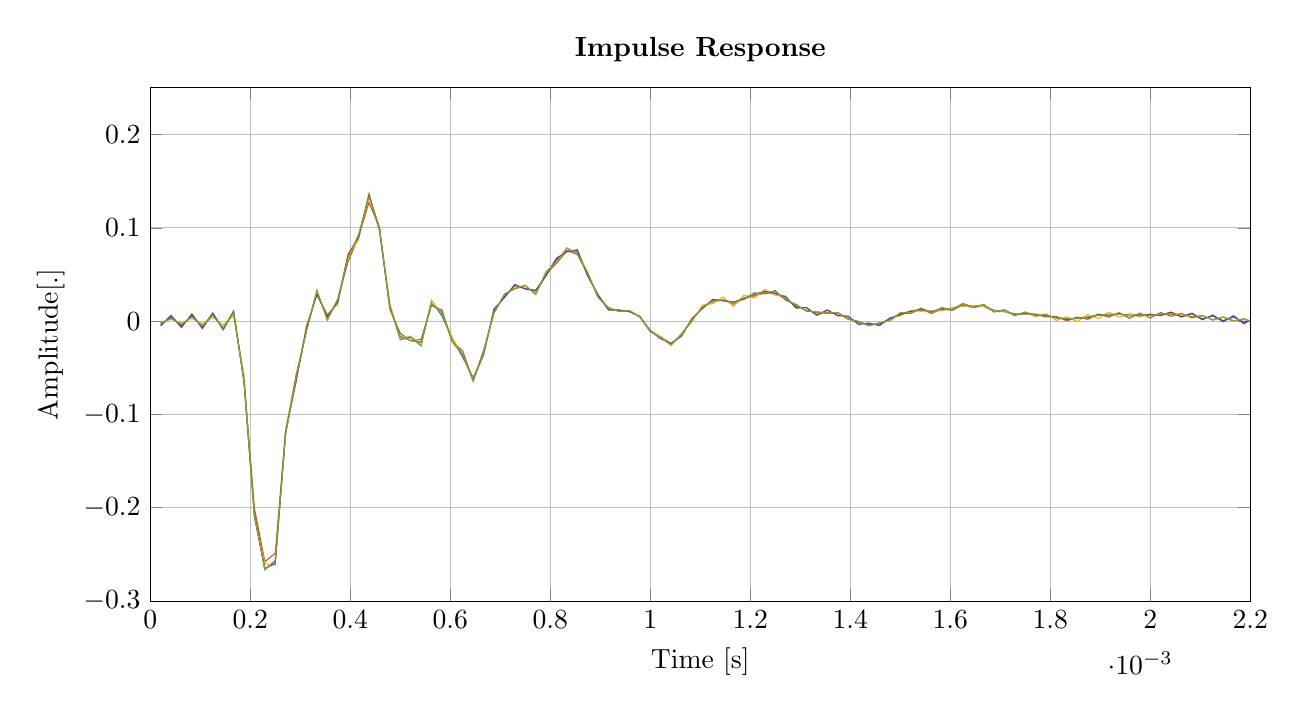
\begin{tikzpicture}

\begin{axis}[%
width=5.5in,
height=2.566in,
at={(0.758in,0.481in)},
scale only axis,
xmin=0,
xmax=0.0022,
xlabel={Time [s]},
xmajorgrids,
ymin=-0.30,
ymax=0.25,
ylabel={Amplitude[.]},
ymajorgrids,
axis background/.style={fill=white},
title style={font=\bfseries},
title={Impulse Response}
]
\addplot [color=mycolor1,solid,forget plot]
  table[row sep=crcr]{%
2.08333333333333e-05	-0.0037087927908794\\
4.16666666666667e-05	0.00421160453226942\\
6.25e-05	-0.00520379576953817\\
8.33333333333333e-05	0.00629701654848276\\
0.000104166666666667	-0.00678651279752952\\
0.000125	0.00811356819824401\\
0.000145833333333333	-0.00884124098433367\\
0.000166666666666667	0.0107472615560426\\
0.0001875	-0.0646663577808535\\
0.000208333333333333	-0.206299821990036\\
0.000229166666666667	-0.266170671528939\\
0.00025	-0.256370669612707\\
0.000270833333333333	-0.120287541326005\\
0.000291666666666667	-0.0617180208660174\\
0.0003125	-0.00922362905565283\\
0.000333333333333333	0.0308397018576189\\
0.000354166666666667	0.0035403786890247\\
0.000375	0.0212448332280645\\
0.000395833333333333	0.0705478621795121\\
0.000416666666666667	0.0895474948933934\\
0.0004375	0.13552149422923\\
0.000458333333333333	0.097299803954558\\
0.000479166666666667	0.0171466790731723\\
0.0005	-0.0197680684506663\\
0.000520833333333333	-0.0171223102171715\\
0.000541666666666667	-0.0263656309604829\\
0.0005625	0.0219768694253305\\
0.000583333333333333	0.00560475366613178\\
0.000604166666666667	-0.0182339778631218\\
0.000625	-0.0387957025837346\\
0.000645833333333333	-0.0604621915450745\\
0.000666666666666667	-0.0363795655357155\\
0.0006875	0.0130977677372803\\
0.000708333333333333	0.0251346467322033\\
0.000729166666666667	0.039105419651278\\
0.00075	0.0346523806957789\\
0.000770833333333333	0.0322481248629661\\
0.000791666666666667	0.0493725854189164\\
0.0008125	0.0660612053755624\\
0.000833333333333333	0.0751202061643853\\
0.000854166666666667	0.0750428627194294\\
0.000875	0.048916982972921\\
0.000895833333333333	0.0274042750529549\\
0.000916666666666667	0.012118310680073\\
0.0009375	0.0119101424242984\\
0.000958333333333333	0.0100853086322103\\
0.000979166666666667	0.00544456035302204\\
0.001	-0.0112918644454638\\
0.00102083333333333	-0.0172483398553776\\
0.00104166666666667	-0.0251189065330511\\
0.0010625	-0.014558012452602\\
0.00108333333333333	0.0017134948101292\\
0.00110416666666667	0.014255079903006\\
0.001125	0.0227537754361355\\
0.00114583333333333	0.021816701937651\\
0.00116666666666667	0.0206421122092443\\
0.0011875	0.0233880957023547\\
0.00120833333333333	0.0302390075091007\\
0.00122916666666667	0.0293537948171238\\
0.00125	0.0326242279536413\\
0.00127083333333333	0.0225148202302848\\
0.00129166666666667	0.0177894930311056\\
0.0013125	0.010770331824266\\
0.00133333333333333	0.00983620954713187\\
0.00135416666666667	0.00853521175516866\\
0.001375	0.00899597167105174\\
0.00139583333333333	0.00260243594654619\\
0.00141666666666667	-0.00104701561770118\\
0.0014375	-0.00371807000382697\\
0.00145833333333333	-0.00318960626194621\\
0.00147916666666667	0.00257545774845068\\
0.0015	0.00713790465040768\\
0.00152083333333333	0.0108215910141207\\
0.00154166666666667	0.0120264444758566\\
0.0015625	0.0108261870538285\\
0.00158333333333333	0.0123450686244096\\
0.00160416666666667	0.0139129670171921\\
0.001625	0.0169005010166529\\
0.00164583333333333	0.0165791257894914\\
0.00166666666666667	0.0159045477126551\\
0.0016875	0.0116907728854056\\
0.00170833333333333	0.0102974368732395\\
0.00172916666666667	0.00768755665771632\\
0.00175	0.0082004670345183\\
0.00177083333333333	0.00731505527542035\\
0.00179166666666667	0.0054086354181059\\
0.0018125	0.00446490364319473\\
0.00183333333333333	0.00151912598295708\\
0.00185416666666667	0.00374848548552877\\
0.001875	0.00361835820665017\\
0.00189583333333333	0.00680282624355538\\
0.00191666666666667	0.00648760855183481\\
0.0019375	0.00770072765347351\\
0.00195833333333333	0.00591670768911894\\
0.00197916666666667	0.00654249543276334\\
0.002	0.00696958712555653\\
0.00202083333333333	0.00639676696262537\\
0.00204166666666667	0.00930875870313683\\
0.0020625	0.00487368778960512\\
0.00208333333333333	0.00793267565500179\\
0.00210416666666667	0.00227381220914028\\
0.002125	0.00559059790855196\\
0.00214583333333333	0.000509710927088874\\
0.00216666666666667	0.00445914830547992\\
0.0021875	-0.0013119827312339\\
0.00220833333333333	0.00204620626659837\\
0.00222916666666667	-0.00226693806170011\\
0.00225	-0.000865052032163367\\
0.00227083333333333	-0.000568466635637404\\
0.00229166666666667	-0.00176072172101629\\
0.0023125	0.001051321525168\\
0.00233333333333333	-0.00235307840318451\\
0.00235416666666667	0.00142050267868398\\
0.002375	-0.00373732644882233\\
0.00239583333333333	0.00263329200115178\\
0.00241666666666667	-0.00419384885137344\\
0.0024375	0.00356243119561722\\
0.00245833333333333	-0.00341750395084726\\
0.00247916666666667	0.00231533516568704\\
0.0025	-0.002886346397735\\
0.00252083333333333	0.000637791268280785\\
0.00254166666666667	-0.00290884766679218\\
0.0025625	-0.000629280559252555\\
0.00258333333333333	-0.00286116806569122\\
0.00260416666666667	-0.00278592644964782\\
0.002625	-0.00262193859169995\\
0.00264583333333333	-0.00474810164470427\\
0.00266666666666667	-0.00275009938116807\\
0.0026875	-0.00478816826817122\\
0.00270833333333333	-0.00324811681170597\\
0.00272916666666667	-0.0040257377623872\\
0.00275	-0.00368074892796126\\
0.00277083333333333	-0.00337062684290595\\
0.00279166666666667	-0.00370307569447635\\
0.0028125	-0.00186571326957182\\
0.00283333333333333	-0.00390602380821677\\
0.00285416666666667	-4.9752550230383e-05\\
0.002875	-0.00438323194808954\\
0.00289583333333333	0.000384386269952189\\
0.00291666666666667	-0.00453307061294354\\
0.0029375	-0.000328341601327697\\
0.00295833333333333	-0.00426336185525099\\
0.00297916666666667	-0.00128138687597425\\
0.003	-0.00414308057749922\\
0.00302083333333333	-0.00248651642821263\\
0.00304166666666667	-0.00361961427656752\\
0.0030625	-0.00400763468176544\\
0.00308333333333333	-0.0023795304299123\\
0.00310416666666667	-0.00514325156697817\\
0.003125	-0.00122625577194359\\
0.00314583333333333	-0.00545188790289689\\
0.00316666666666667	-0.000609928041986866\\
0.0031875	-0.00505013848995181\\
0.00320833333333333	5.99816839252916e-05\\
0.00322916666666667	-0.00449193406111753\\
0.00325	0.000558016389499313\\
0.00327083333333333	-0.00386841737730755\\
0.00329166666666667	0.000169965391614449\\
0.0033125	-0.00319883141842068\\
0.00333333333333333	-0.000671676767081501\\
0.00335416666666667	-0.00289606776507812\\
0.003375	-0.00113994195612087\\
0.00339583333333333	-0.00325262465554565\\
0.00341666666666667	-0.00136179764715377\\
0.0034375	-0.00360873416552366\\
0.00345833333333333	-0.00164463882761736\\
0.00347916666666667	-0.00371793269729748\\
0.0035	-0.00154353439141849\\
0.00352083333333333	-0.00403549855695194\\
0.00354166666666667	-0.000984353596708564\\
0.0035625	-0.00425443771279568\\
0.00358333333333333	-0.000672628985252431\\
0.00360416666666667	-0.00374129885739169\\
0.003625	-0.000937340861272143\\
0.00364583333333333	-0.00296533591369333\\
0.00366666666666667	-0.00130448571666488\\
0.0036875	-0.00246387735925147\\
0.00370833333333333	-0.00182327238315157\\
0.00372916666666667	-0.00173617907905828\\
0.00375	-0.00284258077794951\\
0.00377083333333333	-0.000756536202756666\\
0.00379166666666667	-0.00385114062696801\\
0.0038125	-0.000291952662999003\\
0.00383333333333333	-0.00423039940178691\\
0.00385416666666667	-0.000378549414924021\\
0.003875	-0.00428312305197425\\
0.00389583333333333	-0.000406743035733924\\
0.00391666666666667	-0.00424392197549792\\
0.0039375	-0.000625284040186809\\
0.00395833333333333	-0.00365167293604246\\
0.00397916666666667	-0.001337671135446\\
0.004	-0.00271896198950253\\
0.00402083333333333	-0.0019858020567554\\
0.00404166666666667	-0.00219062801883803\\
0.0040625	-0.00220835913204532\\
0.00408333333333333	-0.00203974929682549\\
0.00410416666666667	-0.00233913427988745\\
0.004125	-0.00185099449592134\\
0.00414583333333333	-0.00236574968059208\\
0.00416666666666667	-0.00196457798952639\\
0.0041875	-0.0019046742644009\\
0.00420833333333333	-0.00250443960036927\\
0.00422916666666667	-0.00128461530764495\\
0.00425	-0.00297296735967611\\
0.00427083333333333	-0.000992836466506577\\
0.00429166666666667	-0.00314961192994209\\
0.0043125	-0.000907894618487529\\
0.00433333333333333	-0.00328775019087989\\
0.00435416666666667	-0.000812410858858454\\
0.004375	-0.00329843852206017\\
0.00439583333333333	-0.000993520893343976\\
0.00441666666666667	-0.00296787895096846\\
0.0044375	-0.00135986816935005\\
0.00445833333333333	-0.00257683158276436\\
0.00447916666666667	-0.00150120312434058\\
0.0045	-0.00246875060820952\\
0.00452083333333333	-0.00127751762473565\\
0.00454166666666667	-0.00257055972440008\\
0.0045625	-0.000850583087086702\\
0.00458333333333333	-0.00279615291783079\\
0.00460416666666667	-0.000169229703961833\\
0.004625	-0.0033208199374696\\
0.00464583333333333	0.000762775063455069\\
0.00466666666666667	-0.00404729208587363\\
0.0046875	0.00162126259324774\\
0.00470833333333333	-0.00461429328418873\\
0.00472916666666667	0.00206634843487202\\
0.00475	-0.00479804415433337\\
0.00477083333333333	0.00203716599298341\\
0.00479166666666667	-0.00461953370883597\\
0.0048125	0.00158614710765907\\
0.00483333333333333	-0.0039600168009732\\
0.00485416666666667	0.00066992915889739\\
0.004875	-0.0027700643584047\\
0.00489583333333333	-0.000614917555245659\\
0.00491666666666667	-0.00132297677247495\\
0.0049375	-0.00190838752526078\\
0.00495833333333333	-4.06116797333875e-05\\
0.00497916666666667	-0.00288565901097666\\
0.005	0.000889847654868419\\
0.00502083333333333	-0.00349274225205263\\
0.00504166666666667	0.00137995835933047\\
0.0050625	-0.00358103532986242\\
0.00508333333333333	0.00125952593606002\\
0.00510416666666667	-0.00298112408616989\\
0.005125	0.00052817856633219\\
0.00514583333333333	-0.0019103540353447\\
0.00516666666666667	-0.000471366982676235\\
0.0051875	-0.000794234842926538\\
0.00520833333333333	-0.00141585678773726\\
};
\addplot [color=mycolor2,solid,forget plot]
  table[row sep=crcr]{%
2.08333333333333e-05	-0.00255267252938673\\
4.16666666666667e-05	0.00289958707347902\\
6.25e-05	-0.00382265239043665\\
8.33333333333333e-05	0.00482200108963299\\
0.000104166666666667	-0.00515633007307537\\
0.000125	0.00667606380308441\\
0.000145833333333333	-0.00708343055179381\\
0.000166666666666667	0.0092525375696961\\
0.0001875	-0.0607390597290135\\
0.000208333333333333	-0.200401659875795\\
0.000229166666666667	-0.257768300997275\\
0.00025	-0.248800582164502\\
0.000270833333333333	-0.117646720461853\\
0.000291666666666667	-0.0578844981508881\\
0.0003125	-0.0102016454149929\\
0.000333333333333333	0.0330014197433572\\
0.000354166666666667	0.00127667958148536\\
0.000375	0.0234190373569384\\
0.000395833333333333	0.0639275956854277\\
0.000416666666666667	0.0906470163865055\\
0.0004375	0.127123824348622\\
0.000458333333333333	0.100636329904299\\
0.000479166666666667	0.0124905457764127\\
0.0005	-0.0128509224250364\\
0.000520833333333333	-0.0212238017533485\\
0.000541666666666667	-0.0195717514784339\\
0.0005625	0.0166431551373302\\
0.000583333333333333	0.0120320299572739\\
0.000604166666666667	-0.0219158802601074\\
0.000625	-0.0320151869444835\\
0.000645833333333333	-0.0633380264022395\\
0.000666666666666667	-0.0314055759804432\\
0.0006875	0.0084423319629683\\
0.000708333333333333	0.0282626599947745\\
0.000729166666666667	0.034755671823636\\
0.00075	0.0375030938504313\\
0.000770833333333333	0.0287324780339133\\
0.000791666666666667	0.0509433983273104\\
0.0008125	0.0618381605219164\\
0.000833333333333333	0.0756881939220368\\
0.000854166666666667	0.0714587648185071\\
0.000875	0.0505304570640701\\
0.000895833333333333	0.0255469926503848\\
0.000916666666666667	0.0139977515791326\\
0.0009375	0.0105701348927955\\
0.000958333333333333	0.0111681123111772\\
0.000979166666666667	0.00467517577342191\\
0.001	-0.0100498056673259\\
0.00102083333333333	-0.0168471351248233\\
0.00104166666666667	-0.0242983429721961\\
0.0010625	-0.0138911007564663\\
0.00108333333333333	0.000815862706313863\\
0.00110416666666667	0.0148029936594\\
0.001125	0.0207210667345826\\
0.00114583333333333	0.0226963031788706\\
0.00116666666666667	0.0181062087629371\\
0.0011875	0.0242935347792987\\
0.00120833333333333	0.0271226044174566\\
0.00122916666666667	0.0301879108304438\\
0.00125	0.0297329814304771\\
0.00127083333333333	0.0236557223579554\\
0.00129166666666667	0.0158766440133432\\
0.0013125	0.011696116145808\\
0.00133333333333333	0.00871715898126307\\
0.00135416666666667	0.00871221990090018\\
0.001375	0.00864655184050639\\
0.00139583333333333	0.00219401302147165\\
0.00141666666666667	-0.000480463220486303\\
0.0014375	-0.00478793011354472\\
0.00145833333333333	-0.00214213807521797\\
0.00147916666666667	0.000610919065108282\\
0.0015	0.00822355226328271\\
0.00152083333333333	0.00831464525440903\\
0.00154166666666667	0.0130253685510728\\
0.0015625	0.00825458577231076\\
0.00158333333333333	0.0131017386199352\\
0.00160416666666667	0.0115045453955671\\
0.001625	0.0173054531317267\\
0.00164583333333333	0.0146751752014143\\
0.00166666666666667	0.0160624194214595\\
0.0016875	0.0105018463460038\\
0.00170833333333333	0.0101683646808241\\
0.00172916666666667	0.0070445186245326\\
0.00175	0.00766088993981086\\
0.00177083333333333	0.00710536523175556\\
0.00179166666666667	0.00457630122370742\\
0.0018125	0.00469420240794347\\
0.00183333333333333	0.000404005788937426\\
0.00185416666666667	0.00428370428539064\\
0.001875	0.00197599863403158\\
0.00189583333333333	0.0076578440345062\\
0.00191666666666667	0.00423011592859115\\
0.0019375	0.00909761104080475\\
0.00195833333333333	0.0030678897125246\\
0.00197916666666667	0.00859528939877386\\
0.002	0.00346894854210457\\
0.00202083333333333	0.00914620649963214\\
0.00204166666666667	0.00520410877557944\\
0.0020625	0.00832413302525314\\
0.00208333333333333	0.00346908753461933\\
0.00210416666666667	0.00610387771170956\\
0.002125	0.00108867775682093\\
0.00214583333333333	0.00419930592939649\\
0.00216666666666667	0.000319892049500485\\
0.0021875	0.00180869387049779\\
0.00220833333333333	-0.00126219037085954\\
0.00222916666666667	-0.00016649986826338\\
0.00225	-0.00292140933910888\\
0.00227083333333333	5.48115721681712e-05\\
0.00229166666666667	-0.00231838798243882\\
0.0023125	6.02159680772856e-05\\
0.00233333333333333	-0.00141553936136535\\
0.00235416666666667	-0.000969725177756748\\
0.002375	-0.00155367505348034\\
0.00239583333333333	-0.00078737578525\\
0.00241666666666667	-0.00118813913866019\\
0.0024375	-0.000351639141263614\\
0.00245833333333333	-0.000202294846823073\\
0.00247916666666667	-0.00140433733178488\\
0.0025	-0.000148481375508499\\
0.00252083333333333	-0.00229105227885144\\
0.00254166666666667	-0.00113327041550525\\
0.0025625	-0.00240289119356657\\
0.00258333333333333	-0.00221020389739753\\
0.00260416666666667	-0.00327807804462282\\
0.002625	-0.00307515395717207\\
0.00264583333333333	-0.00411499501980943\\
0.00266666666666667	-0.00404707161300406\\
0.0026875	-0.00348238100217361\\
0.00270833333333333	-0.00488806311665677\\
0.00272916666666667	-0.0026354048015551\\
0.00275	-0.00512258678524018\\
0.00277083333333333	-0.00237918958058366\\
0.00279166666666667	-0.00456717537979813\\
0.0028125	-0.00158216040976036\\
0.00283333333333333	-0.00398847584896324\\
0.00285416666666667	-0.000601313268332522\\
0.002875	-0.00369552546612422\\
0.00289583333333333	-0.000887430420175447\\
0.00291666666666667	-0.0033287586160303\\
0.0029375	-0.00196666642325469\\
0.00295833333333333	-0.00291972100094473\\
0.00297916666666667	-0.00286833083131398\\
0.003	-0.00297599955911991\\
0.00302083333333333	-0.00372065054441346\\
0.00304166666666667	-0.00284107705068402\\
0.0030625	-0.00474018439203851\\
0.00308333333333333	-0.00207488352087834\\
0.00310416666666667	-0.00536932379647781\\
0.003125	-0.00131533563026484\\
0.00314583333333333	-0.00536072637441323\\
0.00316666666666667	-0.000858022679083761\\
0.0031875	-0.00494352194507911\\
0.00320833333333333	-9.29124655160845e-05\\
0.00322916666666667	-0.00458455294834229\\
0.00325	0.000653130100906661\\
0.00327083333333333	-0.00423158530604592\\
0.00329166666666667	0.000543960512810295\\
0.0033125	-0.00379406688018271\\
0.00333333333333333	-9.66816216515342e-05\\
0.00335416666666667	-0.00353027419822252\\
0.003375	-0.000570547946950482\\
0.00339583333333333	-0.00361077269310737\\
0.00341666666666667	-0.00110650316314777\\
0.0034375	-0.00343504924741948\\
0.00345833333333333	-0.00193518158467088\\
0.00347916666666667	-0.00291655885566418\\
0.0035	-0.00243334545259287\\
0.00352083333333333	-0.00262502115222047\\
0.00354166666666667	-0.00240295393708929\\
0.0035625	-0.00239818677743936\\
0.00358333333333333	-0.00241583275384139\\
0.00360416666666667	-0.00177271872007091\\
0.003625	-0.00263795048328915\\
0.00364583333333333	-0.00127580236053149\\
0.00366666666666667	-0.00260032147781131\\
0.0036875	-0.00135047828264343\\
0.00370833333333333	-0.00248490641271397\\
0.00372916666666667	-0.00135362852201022\\
0.00375	-0.00276058505758708\\
0.00377083333333333	-0.00111545031714157\\
0.00379166666666667	-0.00304804673300568\\
0.0038125	-0.00121762006398216\\
0.00383333333333333	-0.00295967887667023\\
0.00385416666666667	-0.00152799538999958\\
0.003875	-0.00293911795913497\\
0.00389583333333333	-0.00141842129814424\\
0.00391666666666667	-0.00317139837627678\\
0.0039375	-0.00120453703812563\\
0.00395833333333333	-0.00310189945322664\\
0.00397916666666667	-0.00127577630415201\\
0.004	-0.00285323822275981\\
0.00402083333333333	-0.00123759058802548\\
0.00404166666666667	-0.00295826755744021\\
0.0040625	-0.000941733037558027\\
0.00408333333333333	-0.00317740848079844\\
0.00410416666666667	-0.000853233064771672\\
0.004125	-0.003025048708344\\
0.00414583333333333	-0.000993006404728137\\
0.00416666666666667	-0.00285059650886691\\
0.0041875	-0.000974726981488831\\
0.00420833333333333	-0.00278577246306679\\
0.00422916666666667	-0.00106359834458666\\
0.00425	-0.00243185185834133\\
0.00427083333333333	-0.00161288283600495\\
0.00429166666666667	-0.00173941306975917\\
0.0043125	-0.0023614205758312\\
0.00433333333333333	-0.00107298483413706\\
0.00435416666666667	-0.00303899121775412\\
0.004375	-0.000375970115777865\\
0.00439583333333333	-0.00388549063063888\\
0.00441666666666667	0.000541297745222786\\
0.0044375	-0.00479932669104759\\
0.00445833333333333	0.00139622726997478\\
0.00447916666666667	-0.00539810064640756\\
0.0045	0.00192488295368076\\
0.00452083333333333	-0.00560504111770523\\
0.00454166666666667	0.00224701915074393\\
0.0045625	-0.00560943314661647\\
0.00458333333333333	0.0024195452607323\\
0.00460416666666667	-0.005317466524108\\
0.004625	0.00222418518526779\\
0.00464583333333333	-0.00466166053919306\\
0.00466666666666667	0.00169427281028947\\
0.0046875	-0.00386977891617415\\
0.00470833333333333	0.00106542399644791\\
0.00472916666666667	-0.00315415940463025\\
0.00475	0.000425270653698219\\
0.00477083333333333	-0.00245902414772154\\
0.00479166666666667	-0.000313192663862794\\
0.0048125	-0.00172664645538972\\
0.00483333333333333	-0.00101569750310594\\
0.00485416666666667	-0.0010706020758985\\
0.004875	-0.00152478876973867\\
0.00489583333333333	-0.00053804913087041\\
0.00491666666666667	-0.00192301123282111\\
0.0049375	-8.46962331649506e-06\\
0.00495833333333333	-0.00234650155333196\\
0.00497916666666667	0.000517616027113713\\
0.005	-0.0026874982365122\\
0.00502083333333333	0.000837710179045122\\
0.00504166666666667	-0.00281392506940281\\
0.0050625	0.000951526220070128\\
0.00508333333333333	-0.00279809276114962\\
0.00510416666666667	0.000989617566664778\\
0.005125	-0.00267417639347939\\
0.00514583333333333	0.00086092609975851\\
0.00516666666666667	-0.00228430448627185\\
0.0051875	0.000452408493989887\\
0.00520833333333333	-0.00164854160289399\\
};
\addplot [color=mycolor3,solid,forget plot]
  table[row sep=crcr]{%
2.08333333333333e-05	-0.00163321204155689\\
4.16666666666667e-05	0.00217871738448115\\
6.25e-05	-0.00223030869416506\\
8.33333333333333e-05	0.00308085388067272\\
0.000104166666666667	-0.00283418955947869\\
0.000125	0.00387776978723627\\
0.000145833333333333	-0.00396721517720515\\
0.000166666666666667	0.00565169339153807\\
0.0001875	-0.0578645073772853\\
0.000208333333333333	-0.210568816309939\\
0.000229166666666667	-0.259955188133081\\
0.00025	-0.261242392983444\\
0.000270833333333333	-0.11541144340208\\
0.000291666666666667	-0.065082383983406\\
0.0003125	-0.00457165776378929\\
0.000333333333333333	0.0281698447908548\\
0.000354166666666667	0.00746906122663251\\
0.000375	0.017980551653853\\
0.000395833333333333	0.0719876105253128\\
0.000416666666666667	0.0872051031610365\\
0.0004375	0.136972018527987\\
0.000458333333333333	0.0979061885001598\\
0.000479166666666667	0.0190373994273952\\
0.0005	-0.0187474979071836\\
0.000520833333333333	-0.0159911997270242\\
0.000541666666666667	-0.0254207659568788\\
0.0005625	0.0222939439236886\\
0.000583333333333333	0.00762495201878726\\
0.000604166666666667	-0.0181476959053041\\
0.000625	-0.0370572954894979\\
0.000645833333333333	-0.0616897321841816\\
0.000666666666666667	-0.0357751469485512\\
0.0006875	0.0110541110800959\\
0.000708333333333333	0.0266261311666174\\
0.000729166666666667	0.0370835756321231\\
0.00075	0.0372079006439419\\
0.000770833333333333	0.0299720795056686\\
0.000791666666666667	0.0519383256345237\\
0.0008125	0.0633401602353719\\
0.000833333333333333	0.0780465129838801\\
0.000854166666666667	0.072826296030486\\
0.000875	0.0525118906030222\\
0.000895833333333333	0.025547455882416\\
0.000916666666666667	0.0148804806448951\\
0.0009375	0.0103846646000134\\
0.000958333333333333	0.0115394204404138\\
0.000979166666666667	0.00482301562556526\\
0.001	-0.0109874131473168\\
0.00102083333333333	-0.0166641078639183\\
0.00104166666666667	-0.0264021861315982\\
0.0010625	-0.0129423122730922\\
0.00108333333333333	-0.00127731842486949\\
0.00110416666666667	0.0172078145589618\\
0.001125	0.0186646164744698\\
0.00114583333333333	0.0258355733901017\\
0.00116666666666667	0.0157117601980314\\
0.0011875	0.0277803562128635\\
0.00120833333333333	0.0249411956451881\\
0.00122916666666667	0.0339131100205985\\
0.00125	0.0276834810161797\\
0.00127083333333333	0.0270876373860748\\
0.00129166666666667	0.0135486398598428\\
0.0013125	0.0146281493199383\\
0.00133333333333333	0.00630120909161602\\
0.00135416666666667	0.0114262979203145\\
0.001375	0.00625151023360393\\
0.00139583333333333	0.00469691746271263\\
0.00141666666666667	-0.00320755138194242\\
0.0014375	-0.0023665451221515\\
0.00145833333333333	-0.00501549633026936\\
0.00147916666666667	0.00337042559894113\\
0.0015	0.00557224153648716\\
0.00152083333333333	0.0113999793119524\\
0.00154166666666667	0.0105608590694505\\
0.0015625	0.0112253538955211\\
0.00158333333333333	0.0109297147864292\\
0.00160416666666667	0.0141182406444556\\
0.001625	0.0158705693922061\\
0.00164583333333333	0.0165236340426216\\
0.00166666666666667	0.0155539386955293\\
0.0016875	0.0110146959222936\\
0.00170833333333333	0.0107587084546628\\
0.00172916666666667	0.006021107065009\\
0.00175	0.00962358548745266\\
0.00177083333333333	0.00461488367395265\\
0.00179166666666667	0.00786354161870322\\
0.0018125	0.00083980837975928\\
0.00183333333333333	0.00474934129641216\\
0.00185416666666667	-0.000493640480630181\\
0.001875	0.00712827695489169\\
0.00189583333333333	0.00258517202966767\\
0.00191666666666667	0.00965080478835073\\
0.0019375	0.00421535128796295\\
0.00195833333333333	0.00807287058220521\\
0.00197916666666667	0.00433552437525072\\
0.002	0.00762144067704767\\
0.00202083333333333	0.00590796681015577\\
0.00204166666666667	0.00823247822607332\\
0.0020625	0.00624889897116549\\
0.00208333333333333	0.0051706692669312\\
0.00210416666666667	0.00513911501618462\\
0.002125	0.00157578666104142\\
0.00214583333333333	0.00419562172707041\\
0.00216666666666667	-8.17894503905048e-05\\
0.0021875	0.00249146863565593\\
0.00220833333333333	-0.00225060743894737\\
0.00222916666666667	0.000911367832004493\\
0.00225	-0.0042023273732927\\
0.00227083333333333	0.00131908623295955\\
0.00229166666666667	-0.00359422398769843\\
0.0023125	0.00130602372428194\\
0.00233333333333333	-0.0025474285480275\\
0.00235416666666667	9.12508870677423e-05\\
0.002375	-0.00251258605257109\\
0.00239583333333333	3.68184456323214e-05\\
0.00241666666666667	-0.001908222379877\\
0.0024375	0.000171602768831179\\
0.00245833333333333	-0.000565657920822165\\
0.00247916666666667	-0.00132123186706604\\
0.0025	-3.69357225569728e-05\\
0.00252083333333333	-0.00278555913442368\\
0.00254166666666667	-0.000381161411822799\\
0.0025625	-0.00363098794507625\\
0.00258333333333333	-0.000623408767812987\\
0.00260416666666667	-0.00542533906568231\\
0.002625	-0.000514434727790267\\
0.00264583333333333	-0.00727794417210567\\
0.00266666666666667	-0.000521849778767368\\
0.0026875	-0.00757661607436271\\
0.00270833333333333	-0.000543882871711502\\
0.00272916666666667	-0.00744648183443503\\
0.00275	-0.000262008073977348\\
0.00277083333333333	-0.00754898213636908\\
0.00279166666666667	0.000392125328535457\\
0.0028125	-0.00659584850012438\\
0.00283333333333333	0.000562148987953842\\
0.00285416666666667	-0.00491349124801912\\
0.002875	-4.71952709105437e-05\\
0.00289583333333333	-0.00403617308167389\\
0.00291666666666667	-0.00098491246115772\\
0.0029375	-0.00360617852387868\\
0.00295833333333333	-0.00216020792434374\\
0.00297916666666667	-0.00281031658588728\\
0.003	-0.00393642768912363\\
0.00302083333333333	-0.0019740161735394\\
0.00304166666666667	-0.00545044644123764\\
0.0030625	-0.00148724838410483\\
0.00308333333333333	-0.00609761795227659\\
0.00310416666666667	-0.000911843004845307\\
0.003125	-0.00641109553135691\\
0.00314583333333333	-6.68399286926769e-05\\
0.00316666666666667	-0.00661223381392086\\
0.0031875	0.000792942062802807\\
0.00320833333333333	-0.00605194886502256\\
0.00322916666666667	0.00119081641544235\\
0.00325	-0.00510662306890529\\
0.00327083333333333	0.0012153985699642\\
0.00329166666666667	-0.00468000094954699\\
0.0033125	0.00101706104418737\\
0.00333333333333333	-0.0044992583008872\\
0.00335416666666667	0.000373907361929023\\
0.003375	-0.00393423263359508\\
0.00339583333333333	-0.000849674035833999\\
0.00341666666666667	-0.00327675308048005\\
0.0034375	-0.00196202325455657\\
0.00345833333333333	-0.00281649981315708\\
0.00347916666666667	-0.00279172529312823\\
0.0035	-0.00199265111718659\\
0.00352083333333333	-0.00384408715258885\\
0.00354166666666667	-0.000687528632112489\\
0.0035625	-0.0048382405767023\\
0.00358333333333333	0.000411062545070974\\
0.00360416666666667	-0.00517279640746107\\
0.003625	0.00102806244718597\\
0.00364583333333333	-0.00530219593314191\\
0.00366666666666667	0.00153508609358886\\
0.0036875	-0.00561251207357299\\
0.00370833333333333	0.00167486091733119\\
0.00372916666666667	-0.00539493643036716\\
0.00375	0.00095668559377168\\
0.00377083333333333	-0.00449327302460345\\
0.00379166666666667	-0.000202453154405987\\
0.0038125	-0.00358211842714922\\
0.00383333333333333	-0.00130167335324517\\
0.00385416666666667	-0.0026300982831725\\
0.003875	-0.00263555824036522\\
0.00389583333333333	-0.00114138056803914\\
0.00391666666666667	-0.00421914845301114\\
0.0039375	0.000366426789574729\\
0.00395833333333333	-0.00531590855132645\\
0.00397916666666667	0.00132682521510946\\
0.004	-0.00589441023054478\\
0.00402083333333333	0.0020330284975877\\
0.00404166666666667	-0.00643081079363684\\
0.0040625	0.00258116813465071\\
0.00408333333333333	-0.00669153743716035\\
0.00410416666666667	0.00252712937339086\\
0.004125	-0.00626501890081867\\
0.00414583333333333	0.00198573399042622\\
0.00416666666666667	-0.00564706489609503\\
0.0041875	0.00152112304451762\\
0.00420833333333333	-0.00515083718413495\\
0.00422916666666667	0.00102298995925469\\
0.00425	-0.00449765039675646\\
0.00427083333333333	0.000268338619425756\\
0.00429166666666667	-0.00371379195250488\\
0.0043125	-0.000425640222728158\\
0.00433333333333333	-0.00319524784033904\\
0.00435416666666667	-0.000821975064880745\\
0.004375	-0.00282770222093157\\
0.00439583333333333	-0.00126508575246811\\
0.00441666666666667	-0.00230471738176367\\
0.0044375	-0.00177566551043765\\
0.00445833333333333	-0.00179693413328159\\
0.00447916666666667	-0.00209730578453145\\
0.0045	-0.00146755955861572\\
0.00452083333333333	-0.00224017373487703\\
0.00454166666666667	-0.00112128092359989\\
0.0045625	-0.00241988879033352\\
0.00458333333333333	-0.000677054033918395\\
0.00460416666666667	-0.00251242284809268\\
0.004625	-0.000408875554688982\\
0.00464583333333333	-0.00238920768851963\\
0.00466666666666667	-0.00035233334164938\\
0.0046875	-0.0021916507379531\\
0.00470833333333333	-0.000353204672140455\\
0.00472916666666667	-0.00206426554660433\\
0.00475	-0.000399111146290863\\
0.00477083333333333	-0.00190898307931796\\
0.00479166666666667	-0.000620985892132324\\
0.0048125	-0.00165238099799337\\
0.00483333333333333	-0.000881278130450417\\
0.00485416666666667	-0.00142045191052985\\
0.004875	-0.00100160951886526\\
0.00489583333333333	-0.00128622165651065\\
0.00491666666666667	-0.00103775843243032\\
0.0049375	-0.00112884862974338\\
0.00495833333333333	-0.00112433334285194\\
0.00497916666666667	-0.000926118130786855\\
0.005	-0.00116589196730782\\
0.00502083333333333	-0.00085433505620867\\
0.00504166666666667	-0.00107320946693262\\
0.0050625	-0.000875743054272184\\
0.00508333333333333	-0.000966483466824754\\
0.00510416666666667	-0.000820897375894202\\
0.005125	-0.000917689548129309\\
0.00514583333333333	-0.000784404643824917\\
0.00516666666666667	-0.00076358766070243\\
0.0051875	-0.000910640434007906\\
0.00520833333333333	-0.000481400776064074\\
};
\addplot [color=mycolor4,solid,forget plot]
  table[row sep=crcr]{%
2.08333333333333e-05	-0.00516726277486403\\
4.16666666666667e-05	0.00618610543992257\\
6.25e-05	-0.00674403357522682\\
8.33333333333333e-05	0.00770721377255318\\
0.000104166666666667	-0.0079390099384032\\
0.000125	0.0086020434024014\\
0.000145833333333333	-0.00902843756603243\\
0.000166666666666667	0.0100058461757606\\
0.0001875	-0.0641955735500921\\
0.000208333333333333	-0.208700228894356\\
0.000229166666666667	-0.265220840886755\\
0.00025	-0.259647179573132\\
0.000270833333333333	-0.118446743512368\\
0.000291666666666667	-0.0645851736784997\\
0.0003125	-0.00681068819516621\\
0.000333333333333333	0.0287361417369287\\
0.000354166666666667	0.00528308056129979\\
0.000375	0.0203557265501783\\
0.000395833333333333	0.0712760448789094\\
0.000416666666666667	0.0904990248217112\\
0.0004375	0.135055068926438\\
0.000458333333333333	0.0997502441326314\\
0.000479166666666667	0.0149656960420083\\
0.0005	-0.0165087379404821\\
0.000520833333333333	-0.0206907204364962\\
0.000541666666666667	-0.0225262866903627\\
0.0005625	0.0180825474272777\\
0.000583333333333333	0.00939702452084589\\
0.000604166666666667	-0.0220080878731115\\
0.000625	-0.0359484501101515\\
0.000645833333333333	-0.0635737161406537\\
0.000666666666666667	-0.0345952872075129\\
0.0006875	0.011395100325966\\
0.000708333333333333	0.0259765767874302\\
0.000729166666666667	0.0388948268072226\\
0.00075	0.0345433960194401\\
0.000770833333333333	0.0330594608503968\\
0.000791666666666667	0.0486818198528796\\
0.0008125	0.0674756758742106\\
0.000833333333333333	0.0744150741225028\\
0.000854166666666667	0.0764475561324374\\
0.000875	0.0484555353578298\\
0.000895833333333333	0.0280952139333538\\
0.000916666666666667	0.0120915320156524\\
0.0009375	0.0116550564182299\\
0.000958333333333333	0.0106926921212952\\
0.000979166666666667	0.00437971585193512\\
0.001	-0.0101887902933229\\
0.00102083333333333	-0.0188499921570428\\
0.00104166666666667	-0.0238914746704615\\
0.0010625	-0.0161256173139097\\
0.00108333333333333	0.00275773204942341\\
0.00110416666666667	0.0133609332400136\\
0.001125	0.0231917904276933\\
0.00114583333333333	0.0219589661063437\\
0.00116666666666667	0.0200640545884449\\
0.0011875	0.0247466765973178\\
0.00120833333333333	0.0285547492678105\\
0.00122916666666667	0.0318926492272145\\
0.00125	0.0299764686613089\\
0.00127083333333333	0.0258669723089619\\
0.00129166666666667	0.0144614250473965\\
0.0013125	0.0144118803872106\\
0.00133333333333333	0.00631500520940795\\
0.00135416666666667	0.0119590422551788\\
0.001375	0.00582578414624001\\
0.00139583333333333	0.00531310542364779\\
0.00141666666666667	-0.00343872304963442\\
0.0014375	-0.00204564952450211\\
0.00145833333333333	-0.00450517778079939\\
0.00147916666666667	0.00314623347351362\\
0.0015	0.00701711951470965\\
0.00152083333333333	0.0103864197390258\\
0.00154166666666667	0.0129433271786474\\
0.0015625	0.00958576326911167\\
0.00158333333333333	0.0139841965278157\\
0.00160416666666667	0.0121875227655739\\
0.001625	0.0188998385691284\\
0.00164583333333333	0.0146984545420619\\
0.00166666666666667	0.017899680479795\\
0.0016875	0.00991070284736272\\
0.00170833333333333	0.0120138300378153\\
0.00172916666666667	0.00618896675135314\\
0.00175	0.00950797333791057\\
0.00177083333333333	0.00619846562183273\\
0.00179166666666667	0.00629933583354124\\
0.0018125	0.00372292860313401\\
0.00183333333333333	0.00204703775903457\\
0.00185416666666667	0.00329997560254824\\
0.001875	0.00389942548298164\\
0.00189583333333333	0.00657336211721742\\
0.00191666666666667	0.00665232357684192\\
0.0019375	0.0075909095931576\\
0.00195833333333333	0.00605956480100092\\
0.00197916666666667	0.00643341074030218\\
0.002	0.00717334955571132\\
0.00202083333333333	0.00619094312126556\\
0.00204166666666667	0.00966268883294692\\
0.0020625	0.00447138766764083\\
0.00208333333333333	0.00851776245037382\\
0.00210416666666667	0.00155152096694671\\
0.002125	0.00648868394668762\\
0.00214583333333333	-0.000624254648236403\\
0.00216666666666667	0.00576389327580217\\
0.0021875	-0.00289608729956137\\
0.00220833333333333	0.00381430664759555\\
0.00222916666666667	-0.00430459453439456\\
0.00225	0.00134150752329004\\
0.00227083333333333	-0.00298934954772144\\
0.00229166666666667	0.0007768827629351\\
0.0023125	-0.00158590032820341\\
0.00233333333333333	0.000330823136554005\\
0.00235416666666667	-0.00120844519950964\\
0.002375	-0.00116242832138357\\
0.00239583333333333	0.000270897000981958\\
0.00241666666666667	-0.00201802007393254\\
0.0024375	0.00171605320113375\\
0.00245833333333333	-0.00189929643819731\\
0.00247916666666667	0.00119292465952919\\
0.0025	-0.00219131249110632\\
0.00252083333333333	0.00034848939930505\\
0.00254166666666667	-0.00308860740556768\\
0.0025625	-7.85444650659138e-05\\
0.00258333333333333	-0.00384468350111693\\
0.00260416666666667	-0.001493892750237\\
0.002625	-0.00424672879397181\\
0.00264583333333333	-0.00291918864331946\\
0.00266666666666667	-0.00479474830368327\\
0.0026875	-0.002641114801147\\
0.00270833333333333	-0.00547650846681502\\
0.00272916666666667	-0.00176808208131012\\
0.00275	-0.00592170930056437\\
0.00277083333333333	-0.00117173805459234\\
0.00279166666666667	-0.00584231268464412\\
0.0028125	0.000183416280875907\\
0.00283333333333333	-0.00587588613878243\\
0.00285416666666667	0.0018311578583298\\
0.002875	-0.00616980594985171\\
0.00289583333333333	0.0020919430151921\\
0.00291666666666667	-0.006151463925198\\
0.0029375	0.00119796832713895\\
0.00295833333333333	-0.00570267165304615\\
0.00297916666666667	4.97538939356161e-05\\
0.003	-0.0053605861684554\\
0.00302083333333333	-0.00139144543259947\\
0.00304166666666667	-0.00458129470306718\\
0.0030625	-0.00320046711294441\\
0.00308333333333333	-0.00305431263079126\\
0.00310416666666667	-0.00462620972474146\\
0.003125	-0.00160809005656759\\
0.00314583333333333	-0.00518032903383794\\
0.00316666666666667	-0.000778828524857652\\
0.0031875	-0.00492703718563742\\
0.00320833333333333	-4.10939251716325e-05\\
0.00322916666666667	-0.00433900614737377\\
0.00325	0.000347078062520911\\
0.00327083333333333	-0.00349915815918508\\
0.00329166666666667	-0.000345438155645781\\
0.0033125	-0.00247367565948003\\
0.00333333333333333	-0.0016228163755218\\
0.00335416666666667	-0.00173586071389316\\
0.003375	-0.00251999805022344\\
0.00339583333333333	-0.00171285302918648\\
0.00341666666666667	-0.00302092317198616\\
0.0034375	-0.00191969840041333\\
0.00345833333333333	-0.00329477827695596\\
0.00347916666666667	-0.00222733101286352\\
0.0035	-0.00278909601039485\\
0.00352083333333333	-0.00313282923717919\\
0.00354166666666667	-0.00142955103237562\\
0.0035625	-0.00431138062946915\\
0.00358333333333333	-3.33267261560497e-05\\
0.00360416666666667	-0.0049806079600091\\
0.003625	0.000902408321895213\\
0.00364583333333333	-0.00536893329483935\\
0.00366666666666667	0.00161789846540582\\
0.0036875	-0.00579773498379327\\
0.00370833333333333	0.00182795311672953\\
0.00372916666666667	-0.00557217327052572\\
0.00375	0.00104090968872704\\
0.00377083333333333	-0.0045546501000046\\
0.00379166666666667	-0.000273437893586971\\
0.0038125	-0.00354077521085939\\
0.00383333333333333	-0.00141145409669622\\
0.00385416666666667	-0.00271206804832079\\
0.003875	-0.00247321532142388\\
0.00389583333333333	-0.00169972572390624\\
0.00391666666666667	-0.00343380518886849\\
0.0039375	-0.00103182782045088\\
0.00395833333333333	-0.00356096203020484\\
0.00397916666666667	-0.00124689158572549\\
0.004	-0.00285848083433616\\
0.00402083333333333	-0.00193851180094236\\
0.00404166666666667	-0.00200171008123463\\
0.0040625	-0.00275304267616449\\
0.00408333333333333	-0.00103788142726822\\
0.00410416666666667	-0.00387443903731943\\
0.004125	0.000250332702166949\\
0.00414583333333333	-0.00503566614560924\\
0.00416666666666667	0.00122945847968764\\
0.0041875	-0.00556311097230783\\
0.00420833333333333	0.0014705518678144\\
0.00422916666666667	-0.00551042844031363\\
0.00425	0.00127573534719517\\
0.00427083333333333	-0.00519138019590722\\
0.00429166666666667	0.000791747966865656\\
0.0043125	-0.00450084129703969\\
0.00433333333333333	-0.000179976284996915\\
0.00435416666666667	-0.00337897630774022\\
0.004375	-0.00132428816441232\\
0.00439583333333333	-0.00236086513146179\\
0.00441666666666667	-0.00212590659001618\\
0.0044375	-0.00169406418351993\\
0.00445833333333333	-0.00258120154967261\\
0.00447916666666667	-0.00124714980896368\\
0.0045	-0.0027946124294982\\
0.00452083333333333	-0.0010264231051049\\
0.00454166666666667	-0.00259422704283543\\
0.0045625	-0.00120926212080473\\
0.00458333333333333	-0.00197467115141151\\
0.00460416666666667	-0.00159779592776522\\
0.004625	-0.0013254680185666\\
0.00464583333333333	-0.00189992416851517\\
0.00466666666666667	-0.000856508408770266\\
0.0046875	-0.0020937771176436\\
0.00470833333333333	-0.000554077649769015\\
0.00472916666666667	-0.00222634800577962\\
0.00475	-0.000468283944067134\\
0.00477083333333333	-0.00214263857559105\\
0.00479166666666667	-0.000747724939442115\\
0.0048125	-0.00175014592789651\\
0.00483333333333333	-0.00125089656112911\\
0.00485416666666667	-0.00122524421554398\\
0.004875	-0.00171841491726784\\
0.00489583333333333	-0.000745651416354775\\
0.00491666666666667	-0.00209130880535271\\
0.0049375	-0.000296459854376949\\
0.00495833333333333	-0.00242018361148765\\
0.00497916666666667	9.12195276498172e-05\\
0.005	-0.00257540275405454\\
0.00502083333333333	0.000207506743761061\\
0.00504166666666667	-0.00243009552772572\\
0.0050625	7.70973327593161e-05\\
0.00508333333333333	-0.00213121004529441\\
0.00510416666666667	-7.55027093919094e-05\\
0.005125	-0.00183247624499863\\
0.00514583333333333	-0.000241500753831187\\
0.00516666666666667	-0.00146441363258871\\
0.0051875	-0.00050067414854697\\
0.00520833333333333	-0.0010689724886638\\
};
\addplot [color=mycolor5,solid,forget plot]
  table[row sep=crcr]{%
2.08333333333333e-05	-0.00183694080367487\\
4.16666666666667e-05	0.00269775576535856\\
6.25e-05	-0.00330864487443258\\
8.33333333333333e-05	0.00446922873033606\\
0.000104166666666667	-0.00511216151187469\\
0.000125	0.00628161008825259\\
0.000145833333333333	-0.00739773060073078\\
0.000166666666666667	0.00918365663237817\\
0.0001875	-0.0640643771063412\\
0.000208333333333333	-0.207629084903728\\
0.000229166666666667	-0.266512571802307\\
0.00025	-0.256975404662541\\
0.000270833333333333	-0.121150763678526\\
0.000291666666666667	-0.0611548539632256\\
0.0003125	-0.0104129176519418\\
0.000333333333333333	0.0323067772127556\\
0.000354166666666667	0.00164090751066485\\
0.000375	0.0236255560777956\\
0.000395833333333333	0.06830166976313\\
0.000416666666666667	0.0929087418121704\\
0.0004375	0.13301902945068\\
0.000458333333333333	0.100936103236603\\
0.000479166666666667	0.0140285669386969\\
0.0005	-0.0161700462857896\\
0.000520833333333333	-0.0208468721314891\\
0.000541666666666667	-0.0226220402462128\\
0.0005625	0.0180740728030884\\
0.000583333333333333	0.00931391260236883\\
0.000604166666666667	-0.0223811360937609\\
0.000625	-0.0351734754640771\\
0.000645833333333333	-0.0647259979556037\\
0.000666666666666667	-0.0325867644033155\\
0.0006875	0.00898058450624136\\
0.000708333333333333	0.0291265867299432\\
0.000729166666666667	0.0352941328824218\\
0.00075	0.0385603213063728\\
0.000770833333333333	0.028737201659164\\
0.000791666666666667	0.0530826006757693\\
0.0008125	0.0629821946361526\\
0.000833333333333333	0.0785023152976803\\
0.000854166666666667	0.0724206512475182\\
0.000875	0.0516411907781996\\
0.000895833333333333	0.0252766828649511\\
0.000916666666666667	0.0140481289383357\\
0.0009375	0.0103486623306802\\
0.000958333333333333	0.011288134477749\\
0.000979166666666667	0.00452179861807155\\
0.001	-0.0108066056383279\\
0.00102083333333333	-0.0175992589402696\\
0.00104166666666667	-0.0253128018813454\\
0.0010625	-0.0143504620645333\\
0.00108333333333333	0.00103019786277436\\
0.00110416666666667	0.0149760846537094\\
0.001125	0.021772751579079\\
0.00114583333333333	0.0229129142405795\\
0.00116666666666667	0.0195261483333946\\
0.0011875	0.0247111551394756\\
0.00120833333333333	0.029165953038416\\
0.00122916666666667	0.0306951510029648\\
0.00125	0.0317127991700103\\
0.00127083333333333	0.0235587890851777\\
0.00129166666666667	0.0171755554809782\\
0.0013125	0.0113317115131608\\
0.00133333333333333	0.00966950258690897\\
0.00135416666666667	0.0084848262426318\\
0.001375	0.00936025782752537\\
0.00139583333333333	0.0018605258760557\\
0.00141666666666667	-0.00011667583265064\\
0.0014375	-0.00508943015759043\\
0.00145833333333333	-0.0016939190207471\\
0.00147916666666667	0.000756684386819692\\
0.0015	0.00906821913097466\\
0.00152083333333333	0.00875811174534595\\
0.00154166666666667	0.0142045150007034\\
0.0015625	0.00872550078162829\\
0.00158333333333333	0.014561042442384\\
0.00160416666666667	0.0119283605131355\\
0.001625	0.0189699720965624\\
0.00164583333333333	0.0147986619876687\\
0.00166666666666667	0.0177291717017055\\
0.0016875	0.0101130470467348\\
0.00170833333333333	0.011891104230609\\
0.00172916666666667	0.00626330567477195\\
0.00175	0.00964315574422997\\
0.00177083333333333	0.00597610694387428\\
0.00179166666666667	0.00676900938218093\\
0.0018125	0.00316921417751703\\
0.00183333333333333	0.00276978914393364\\
0.00185416666666667	0.00255747544219039\\
0.001875	0.00465507490137383\\
0.00189583333333333	0.00593605006847284\\
0.00191666666666667	0.00710918977577941\\
0.0019375	0.00743396864256613\\
0.00195833333333333	0.00582624150445395\\
0.00197916666666667	0.0071523110382564\\
0.002	0.00590320742513466\\
0.00202083333333333	0.00808548307245867\\
0.00204166666666667	0.00714310325999776\\
0.0020625	0.00765039599172813\\
0.00208333333333333	0.00474811998548259\\
0.00210416666666667	0.0059146576224379\\
0.002125	0.00170546171762879\\
0.00214583333333333	0.00459490612183377\\
0.00216666666666667	0.000384874437928168\\
0.0021875	0.00263820817769318\\
0.00220833333333333	-0.00160695364388704\\
0.00222916666666667	0.000938425698385665\\
0.00225	-0.00350150608652209\\
0.00227083333333333	0.00138650915064656\\
0.00229166666666667	-0.00296735858372556\\
0.0023125	0.00147981611955108\\
0.00233333333333333	-0.00197569061842833\\
0.00235416666666667	0.000332672141494042\\
0.002375	-0.00193276417796099\\
0.00239583333333333	0.000332534578102534\\
0.00241666666666667	-0.00142123405521269\\
0.0024375	0.000595464433092438\\
0.00245833333333333	-0.00033104378088869\\
0.00247916666666667	-0.000628383127052637\\
0.0025	-0.000169100125387944\\
0.00252083333333333	-0.00164286774990944\\
0.00254166666666667	-0.00113799929739703\\
0.0025625	-0.00177840315394551\\
0.00258333333333333	-0.00237794743376311\\
0.00260416666666667	-0.00260136378649268\\
0.002625	-0.0034614841347566\\
0.00264583333333333	-0.00334881363572188\\
0.00266666666666667	-0.00462956933162578\\
0.0026875	-0.00256706460360964\\
0.00270833333333333	-0.00567233074670817\\
0.00272916666666667	-0.00153868789833283\\
0.00275	-0.00607358828586136\\
0.00277083333333333	-0.00118775776784012\\
0.00279166666666667	-0.00554868783532898\\
0.0028125	-0.000431878221958489\\
0.00283333333333333	-0.00486521252255728\\
0.00285416666666667	0.000426252118386822\\
0.002875	-0.00437077474685128\\
0.00289583333333333	-3.83248125346931e-05\\
0.00291666666666667	-0.00372540750621784\\
0.0029375	-0.00137072864831652\\
0.00295833333333333	-0.00302943173806034\\
0.00297916666666667	-0.00254314874047966\\
0.003	-0.00292382710021425\\
0.00302083333333333	-0.00353654515648264\\
0.00304166666666667	-0.00281368240423307\\
0.0030625	-0.004499148008335\\
0.00308333333333333	-0.00225798395795248\\
0.00310416666666667	-0.00488821397948152\\
0.003125	-0.00187549848927019\\
0.00314583333333333	-0.00444266842303002\\
0.00316666666666667	-0.00194977818768166\\
0.0031875	-0.00343438772121835\\
0.00320833333333333	-0.00177950707108735\\
0.00322916666666667	-0.00249719170032265\\
0.00325	-0.00153676165081829\\
0.00327083333333333	-0.00173496062595026\\
0.00329166666666667	-0.00196146225602646\\
0.0033125	-0.00111887307647677\\
0.00333333333333333	-0.00270592071654781\\
0.00335416666666667	-0.000951400411222539\\
0.003375	-0.00303583979618812\\
0.00339583333333333	-0.00143553914342979\\
0.00341666666666667	-0.00315235230276506\\
0.0034375	-0.00185287085480954\\
0.00345833333333333	-0.00340088496393738\\
0.00347916666666667	-0.00195651949418887\\
0.0035	-0.00331299548667301\\
0.00352083333333333	-0.00225045388032761\\
0.00354166666666667	-0.00274174065486804\\
0.0035625	-0.00253272575758083\\
0.00358333333333333	-0.0022950968923779\\
0.00360416666666667	-0.00226956657999736\\
0.003625	-0.00220900640785088\\
0.00364583333333333	-0.00198688824758307\\
0.00366666666666667	-0.00196129552536715\\
0.0036875	-0.00222668382155181\\
0.00370833333333333	-0.00163803328922128\\
0.00372916666666667	-0.00242135810248223\\
0.00375	-0.00169878080532646\\
0.00377083333333333	-0.00240271207890884\\
0.00379166666666667	-0.00178482766872638\\
0.0038125	-0.00276262318079547\\
0.00383333333333333	-0.00144752632322627\\
0.00385416666666667	-0.00338887691558329\\
0.003875	-0.0011235878649765\\
0.00389583333333333	-0.00360276128511714\\
0.00391666666666667	-0.0010898412082731\\
0.0039375	-0.00364761398150759\\
0.00395833333333333	-0.000816341793401194\\
0.00397916666666667	-0.00391914968305896\\
0.004	-0.000393797533269311\\
0.00402083333333333	-0.00402772214961534\\
0.00404166666666667	-0.000403815798285107\\
0.0040625	-0.00376420356641242\\
0.00408333333333333	-0.000678945405755922\\
0.00410416666666667	-0.00356193732440603\\
0.004125	-0.000724848726152835\\
0.00414583333333333	-0.00345082754139939\\
0.00416666666666667	-0.000903658924013599\\
0.0041875	-0.00300573184010322\\
0.00420833333333333	-0.00142019286324911\\
0.00422916666666667	-0.00242680786667316\\
0.00425	-0.00187867537819102\\
0.00427083333333333	-0.00207818949878901\\
0.00429166666666667	-0.00216713107510767\\
0.0043125	-0.00177009673317393\\
0.00433333333333333	-0.00260489792584533\\
0.00435416666666667	-0.00128259330924896\\
0.004375	-0.00305767497625344\\
0.00439583333333333	-0.00096352279224579\\
0.00441666666666667	-0.00319292473863172\\
0.0044375	-0.000907062555897271\\
0.00445833333333333	-0.00313354326156351\\
0.00447916666666667	-0.000880627915769135\\
0.0045	-0.00302958482048134\\
0.00452083333333333	-0.000882944723935813\\
0.00454166666666667	-0.00269240462403318\\
0.0045625	-0.00113855775118239\\
0.00458333333333333	-0.00203855379942678\\
0.00460416666666667	-0.00153500239738074\\
0.004625	-0.00137441034830759\\
0.00464583333333333	-0.00186988625816161\\
0.00466666666666667	-0.00084471616135345\\
0.0046875	-0.00216604017222241\\
0.00470833333333333	-0.000408502565127081\\
0.00472916666666667	-0.00246621265657476\\
0.00475	-0.000128850411515083\\
0.00477083333333333	-0.00259165537714265\\
0.00479166666666667	-0.000204592953846044\\
0.0048125	-0.00240350317728393\\
0.00483333333333333	-0.000525550391408901\\
0.00485416666666667	-0.00203460498841687\\
0.004875	-0.000856329521520775\\
0.00489583333333333	-0.00166039765281729\\
0.00491666666666667	-0.00113648533244863\\
0.0049375	-0.00129593544844764\\
0.00495833333333333	-0.00137336466044101\\
0.00497916666666667	-0.00101824006274034\\
0.005	-0.00138372492376765\\
0.00502083333333333	-0.00108269303633796\\
0.00504166666666667	-0.00101661529037089\\
0.0050625	-0.00148448313002126\\
0.00508333333333333	-0.00040693927282269\\
0.00510416666666667	-0.00197448809399342\\
0.005125	0.000248107014438327\\
0.00514583333333333	-0.00248830449433159\\
0.00516666666666667	0.000929192612529347\\
0.0051875	-0.00301326617479279\\
0.00520833333333333	0.00150614480417336\\
};
\end{axis}
\end{tikzpicture}%
	\caption{Impulse response plot of the cancellation path. Impulse response 1 (\textcolor{MATLABblue}{---}), 
	impulse response 2 (\textcolor{MATLABorange}{---}), 	
	impulse response 3 (\textcolor{MATLAByellow}{---}), 	
	impulse response 4 (\textcolor{MATLABpurple}{---}), 	
	impulse response 5 (\textcolor{MATLABgreen}{---}). }
	\label{CancellationPathImpulseResponse}
\end{figure}


%\begin{figure}[H]
%	\centering
%	\includegraphics[width=0.85\textwidth]{CancellationPath_MATLAB_Figures/CancellationPathImpulseResponse.png}
%	\caption{Impulse Response plot of the cancellation path (NOT TIKZ).}
%	\label{CancellationPathImpulseResponse}
%\end{figure}

%Converting the impulse response from magnitude to dB, gives the time decay which reveals the Signal to Noise Ratio (SNR) of the system, and from the read off SNR is found to be $\sim$ 50 dB SNR, as seen on \autoref{TimeDecayPlotCancellationPath}.

%\todoKiis{many question: 256 coefficients?? That way of calculating SNR?? I think you have to do Scroeder decay curve if you want to find it. I do not believe the amplitude of the noise, could be the thing I also saw with Max?? - Why do we even calculate SNR? Only measurement this is done for!? - could also be a result of the high output to the headphone?}

%\begin{figure}[H]
%	\centering
%	\includegraphics[width=0.85\textwidth]{CancellationPath_MATLAB_Figures/CancellationPathTimeDecay.png}
%	\caption{Time decay plot of the cancellation path (NOT TIKZ).}
%	\label{TimeDecayPlotCancellationPath}
%\end{figure}

% \begin{figure}[H]
% 	\centering
% 	\tikzsetnextfilename{TimeDecayPlotCancellationPath1}
% 	% This file was created by matlab2tikz.
%
%The latest updates can be retrieved from
%  http://www.mathworks.com/matlabcentral/fileexchange/22022-matlab2tikz-matlab2tikz
%where you can also make suggestions and rate matlab2tikz.
%
\definecolor{mycolor1}{rgb}{0.00000,0.44700,0.74100}%
\definecolor{mycolor2}{rgb}{0.85000,0.32500,0.09800}%
\definecolor{mycolor3}{rgb}{0.92900,0.69400,0.12500}%
\definecolor{mycolor4}{rgb}{0.49400,0.18400,0.55600}%
\definecolor{mycolor5}{rgb}{0.46600,0.67400,0.18800}%
%
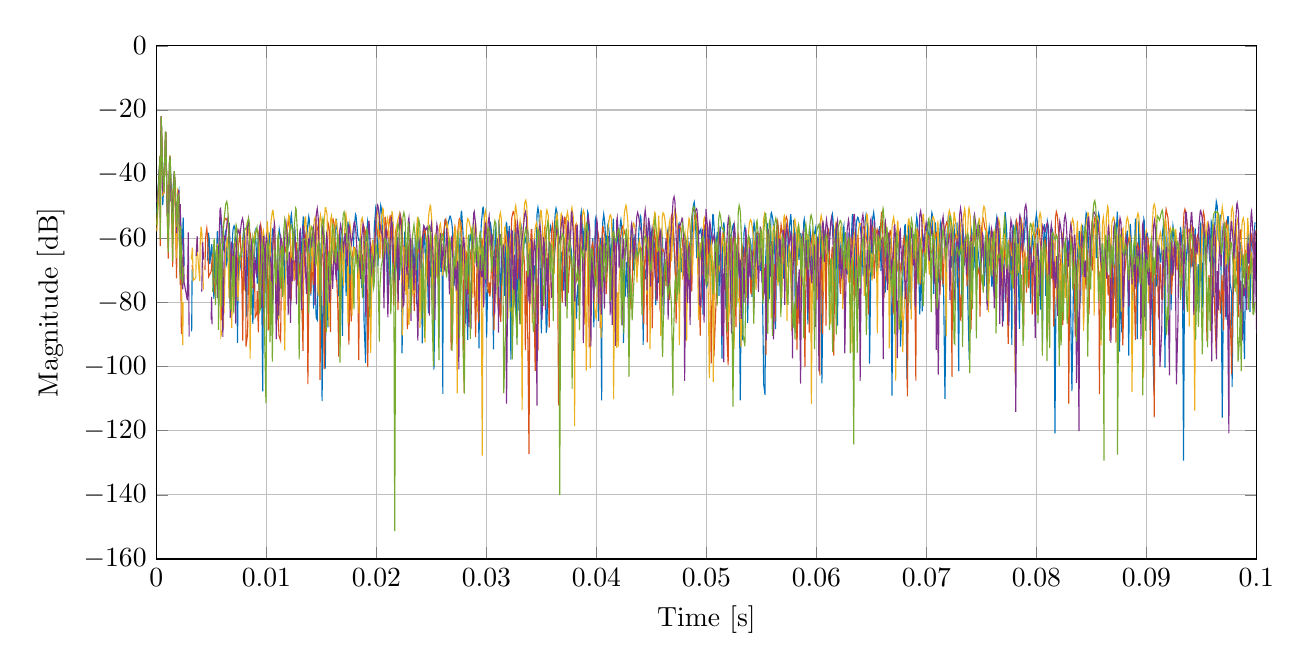
\begin{tikzpicture}

\begin{axis}[%
width=5.5in,
height=2.566in,
scaled x ticks = false,
x tick label style={/pgf/number format/fixed},
at={(1.414in,0.891in)},
scale only axis,
unbounded coords=jump,
xmin=0,
xmax=0.1,
xlabel={Time [s]},
xmajorgrids,
ymin=-160,
ymax=0,
ylabel={Magnitude [dB]},
ymajorgrids,
axis background/.style={fill=white},
title style={font=\bfseries},
%title={Time Decay}
]
\addplot [color=mycolor1,solid,forget plot]
  table[row sep=crcr]{%
2.08333333333333e-05	nan\\
4.16666666666667e-05	-52.111048310778\\
0.000166666666666667	-43.9740436319002\\
0.000333333333333333	-34.8177965827442\\
0.000354166666666667	-53.6190056426103\\
0.000354166666666667	-53.6190056426103\\
0.0004375	-21.9598363711386\\
0.0005625	-37.7606834431528\\
0.000583333333333333	-49.6288694056232\\
0.0006875	-42.2560543031998\\
0.000833333333333333	-27.0848645767238\\
0.000854166666666667	-27.0938121387821\\
0.000979166666666667	-49.8807436737733\\
0.00108333333333333	-59.9223441352537\\
0.0011875	-37.2201027543805\\
0.00125	-34.3291951406571\\
0.00135416666666667	-45.9757139957571\\
0.00147916666666667	-56.382911413555\\
0.00152083333333333	-43.9141776726352\\
0.00152083333333333	-43.9141776726352\\
0.001625	-40.042008410004\\
0.0016875	-43.2431355273656\\
0.00183333333333333	-60.9681241606569\\
0.00183333333333333	-60.9681241606569\\
0.0019375	-46.8693647146266\\
0.00204166666666667	-45.2221645426903\\
0.00214583333333333	-70.4535211157334\\
0.00216666666666667	-51.6149616670037\\
0.0023125	-64.165288874486\\
0.00235416666666667	-61.5511588605062\\
0.0024375	-53.565070295056\\
0.00252083333333333	-68.5064286025977\\
0.00252083333333333	-68.5064286025977\\
0.00266666666666667	nan\\
0.00266666666666667	nan\\
0.00289583333333333	-72.904642668182\\
0.00289583333333333	-72.904642668182\\
0.003	nan\\
0.003	nan\\
0.00320833333333333	-89.0396268578771\\
0.00325	-69.6670608974985\\
0.00333333333333333	nan\\
0.00333333333333333	nan\\
0.0035	nan\\
0.0035	nan\\
0.00364583333333333	nan\\
0.00364583333333333	nan\\
0.0038125	nan\\
0.0038125	nan\\
0.00397916666666667	nan\\
0.00397916666666667	nan\\
0.00414583333333333	nan\\
0.00414583333333333	nan\\
0.0043125	nan\\
0.0043125	nan\\
0.00464583333333333	-66.952070269611\\
0.00464583333333333	-66.952070269611\\
0.00464583333333333	-66.952070269611\\
0.00472916666666667	-58.2959288896312\\
0.0048125	-60.5931307267329\\
0.00485416666666667	-68.0794223724486\\
0.00504166666666667	-61.8026803688784\\
0.005125	-70.1443845224101\\
0.00522916666666667	-78.870829364037\\
0.0053125	-63.8012011510901\\
0.0053125	-63.8012011510901\\
0.00535416666666667	-68.5896659640424\\
0.00545833333333333	-65.4935549134102\\
0.00554166666666667	-57.7477179120546\\
0.00566666666666667	-81.2009260636828\\
0.00577083333333333	-55.761344442787\\
0.00585416666666667	-53.5416605882092\\
0.0059375	-56.2577357302003\\
0.00597916666666667	-58.9539415015357\\
0.00610416666666667	-63.8531451471768\\
0.00614583333333333	-61.9141009456243\\
0.00627083333333333	-58.0593839706459\\
0.0063125	-58.7413544861928\\
0.00639583333333333	-67.7841232832069\\
0.00645833333333333	-66.6166703808532\\
0.006625	-55.2300468372413\\
0.006625	-55.2300468372413\\
0.00679166666666667	-72.9096992394021\\
0.00679166666666667	-72.9096992394021\\
0.0069375	-58.638942876284\\
0.00697916666666667	-57.0690799271473\\
0.0070625	-56.1394046707133\\
0.00714583333333333	-57.1127041883519\\
0.00727083333333333	-63.1813781835223\\
0.00727083333333333	-63.1813781835223\\
0.007375	-92.5753078843969\\
0.00745833333333333	-66.4543104134224\\
0.0075	-65.1542648427286\\
0.00766666666666667	-68.9414396695225\\
0.00775	-66.3204732466916\\
0.00779166666666667	-63.6550975119697\\
0.00791666666666667	-57.8950515685413\\
0.00795833333333333	-57.4909363697214\\
0.00808333333333333	-61.4101564617352\\
0.008125	-65.014239665563\\
0.00820833333333333	-84.3913964822076\\
0.00827083333333333	-67.5401210436484\\
0.0084375	-60.6608842129059\\
0.0084375	-60.6608842129059\\
0.00860416666666667	-68.6525343731691\\
0.00860416666666667	-68.6525343731691\\
0.00877083333333333	-86.7182627693444\\
0.00877083333333333	-86.7182627693444\\
0.0089375	-58.3503996189966\\
0.00897916666666667	-57.7185064887609\\
0.0090625	-61.5893861763269\\
0.00916666666666666	-74.1626294665894\\
0.00925	-59.9425252546123\\
0.00925	-59.9425252546123\\
0.00939583333333333	-82.2414358792677\\
0.0094375	-63.5172219371502\\
0.00952083333333333	-57.7976918868999\\
0.00966666666666667	-107.69929084972\\
0.00975	-60.471146039021\\
0.00979166666666667	-59.0848073355518\\
0.00991666666666667	-66.2816899780258\\
0.00991666666666667	-66.2816899780258\\
0.01	-83.2384694993036\\
0.0100833333333333	-69.382102407305\\
0.01025	-58.1614130268561\\
0.01025	-58.1614130268561\\
0.0103958333333333	-78.659966600665\\
0.0104375	-64.3644685212\\
0.0105625	-57.2292963929618\\
0.0106041666666667	-57.4389958833188\\
0.0107291666666667	-61.1355190321544\\
0.0107708333333333	-62.6617442615444\\
0.0108958333333333	-69.2220796621684\\
0.011	-85.3991667784377\\
0.0110416666666667	-65.4866844897544\\
0.0110833333333333	-60.3538379061152\\
0.0111666666666667	-57.1711414785393\\
0.01125	-59.1262763800061\\
0.011375	-69.3559430679877\\
0.0114166666666667	-70.9746539468429\\
0.0115416666666667	-63.2971463445262\\
0.0115833333333333	-62.2681820493326\\
0.0117083333333333	-78.185870054493\\
0.0117291666666667	-74.8542861438093\\
0.0118958333333333	-59.1082812851507\\
0.0118958333333333	-59.1082812851507\\
0.0120208333333333	-62.3396384402111\\
0.0120625	-61.9079830499083\\
0.0122291666666667	-53.2761437613709\\
0.0122708333333333	-52.5028995257284\\
0.0123958333333333	-57.9490053815339\\
0.0124375	-67.097874268932\\
0.0125416666666667	-57.8292741595085\\
0.0125833333333333	-56.3942866017904\\
0.0127083333333333	-66.8628824569854\\
0.0127708333333333	-73.1233158076556\\
0.0128541666666667	-63.1193712248532\\
0.0128958333333333	-65.0422676184057\\
0.0129375	-72.4048294890819\\
0.0130833333333333	-66.3211400209195\\
0.013125	-71.8762952805217\\
0.0132291666666667	-59.9577490778633\\
0.0133541666666667	-53.4565553010462\\
0.0133958333333333	-53.7172714247254\\
0.0135208333333333	-59.7287434390187\\
0.0136041666666667	-63.951909199344\\
0.0136875	-59.7481136529985\\
0.0137291666666667	-56.884992279517\\
0.0138541666666667	-53.2243149389698\\
0.0138958333333333	-54.0305340746001\\
0.0140416666666667	-77.8746654022866\\
0.0140416666666667	-77.8746654022866\\
0.0141666666666667	-59.5576053975161\\
0.0142083333333333	-61.3140246411379\\
0.0142916666666667	-81.9411573286561\\
0.0143958333333333	-65.6135925586917\\
0.0145208333333333	-84.6872059910125\\
0.014625	-85.4407544579033\\
0.0146875	-74.1556791266814\\
0.0146875	-74.1556791266814\\
0.0148125	-61.5186789861121\\
0.0148541666666667	-61.603933867154\\
0.0150208333333333	-82.8897784221635\\
0.0150625	-110.772106438684\\
0.0151875	-72.3738220270998\\
0.0152291666666667	-70.4290235676362\\
0.0153541666666667	-100.606303182385\\
0.0153541666666667	-100.606303182385\\
0.0154583333333333	-72.1936353976885\\
0.0156041666666667	-87.7491540752639\\
0.0156875	-73.2013868076318\\
0.0157916666666667	-77.4373024400392\\
0.0158333333333333	-67.9974898177409\\
0.015875	-64.0529505129947\\
0.0159583333333333	-62.0225650940623\\
0.0160833333333333	-65.2961964560404\\
0.0161666666666667	-62.8831029470834\\
0.0161666666666667	-62.8831029470834\\
0.0163333333333333	-54.3557903914612\\
0.016375	-54.2032208365931\\
0.0165	-62.3646402761344\\
0.0165416666666667	-78.113175470613\\
0.0166458333333333	-58.8346612605774\\
0.0166875	-58.183753552355\\
0.0168125	-67.0010327931349\\
0.0169166666666667	-90.4436690986716\\
0.0169791666666667	-68.8442995675725\\
0.0170208333333333	-63.0786023797962\\
0.0171041666666667	-58.4773349959014\\
0.01725	-77.9505350758744\\
0.0173333333333333	-57.445562140132\\
0.0174166666666667	-54.8642361243766\\
0.0175	-58.1348941906922\\
0.0175	-58.1348941906922\\
0.0176041666666667	-81.2331799465362\\
0.0176875	-65.9063896475626\\
0.0178125	-69.9045452138529\\
0.0178541666666667	-68.2679254067739\\
0.0179791666666667	-56.6175168508517\\
0.0179791666666667	-56.6175168508517\\
0.0181041666666667	-52.5422477316158\\
0.0181458333333333	-52.8806272404262\\
0.0183125	-59.3176520761328\\
0.0183125	-59.3176520761328\\
0.0183958333333333	-60.5962203271359\\
0.0184791666666667	-60.3497039195296\\
0.0186041666666667	-69.1567240190393\\
0.0186666666666667	-75.5213852508567\\
0.01875	-65.0119785770231\\
0.0188333333333333	-69.891092188239\\
0.018875	-85.4855467125159\\
0.0190208333333333	-98.9033056569759\\
0.019125	-58.287911282984\\
0.0192083333333333	-54.732623030518\\
0.0192916666666667	-56.8444306984257\\
0.0193333333333333	-60.3684268716343\\
0.0194375	-84.5798414376857\\
0.0194791666666667	-79.599605229199\\
0.019625	-63.2791733275686\\
0.0197083333333333	-70.0795077494701\\
0.0197708333333333	-63.4095035805324\\
0.0198125	-56.362169900321\\
0.0199375	-50.7438037528893\\
0.0199791666666667	-51.6086095044044\\
0.0201041666666667	-62.884753710132\\
0.0201458333333333	-68.6491886999608\\
0.0202708333333333	-56.3246955012879\\
0.0203125	-52.7777742803338\\
0.0203958333333333	-49.7337890346514\\
0.0204791666666667	-51.1840995331472\\
0.0206041666666667	-63.5297545792679\\
0.0206875	-75.480095487511\\
0.0207708333333333	-63.1150361798449\\
0.0208125	-59.3571081508711\\
0.0208958333333333	-57.281628009858\\
0.0210208333333333	-79.6666740625991\\
0.021125	-59.7053926135665\\
0.021125	-59.7053926135665\\
0.02125	-74.6074415490915\\
0.0213125	-61.1963391171394\\
0.0214375	-54.9555009504599\\
0.0214791666666667	-56.2835768296612\\
0.0215625	-66.3184865927575\\
0.0216666666666667	-64.7381345146491\\
0.02175	-70.1569097501175\\
0.0218125	-69.0320645480348\\
0.0219375	-59.5928240237874\\
0.0219375	-59.5928240237874\\
0.0220833333333333	-73.0637301253879\\
0.0221666666666667	-62.5544202629954\\
0.02225	-65.8825503138553\\
0.0222916666666667	-72.3842214376554\\
0.0223333333333333	-95.8946786113816\\
0.0224583333333333	-70.2530157937059\\
0.0225833333333333	-58.1050091233855\\
0.022625	-57.9585276214801\\
0.02275	-71.4584000951474\\
0.0228125	-74.3549832010801\\
0.0228541666666667	-69.896266469373\\
0.0229583333333333	-75.7678645726475\\
0.0230833333333333	-61.6482335838661\\
0.023125	-63.6055317308382\\
0.0231666666666667	-70.3970329366683\\
0.0233125	-61.8747738335171\\
0.0233958333333333	-69.0316467698325\\
0.0234583333333333	-69.389326825852\\
0.0235416666666667	-59.7552089012813\\
0.0235833333333333	-60.1162958509255\\
0.0236666666666667	-80.4186936973413\\
0.0238125	-57.1309642847574\\
0.0238958333333333	-62.1212696061357\\
0.0239583333333333	-78.4103631383799\\
0.0240416666666667	-60.2068703019764\\
0.0240833333333333	-60.4092820244597\\
0.0241666666666667	-92.7997852123779\\
0.0243125	-55.9748624975703\\
0.0243958333333333	-59.2659810929925\\
0.0245	-69.6964812675586\\
0.0245833333333333	-61.3945967461279\\
0.0245833333333333	-61.3945967461279\\
0.0247291666666667	-83.319371913321\\
0.0248125	-68.1273708089018\\
0.0248541666666667	-71.9010224366383\\
0.0249166666666667	-71.8433084298515\\
0.0250416666666667	-60.2861288082898\\
0.0250833333333333	-61.096435464369\\
0.0252291666666667	-100.969926898387\\
0.0252291666666667	-100.969926898387\\
0.025375	-69.2091637938194\\
0.0254583333333333	-64.4129091348762\\
0.0255416666666667	-72.1250823743872\\
0.0256041666666667	-68.8569766183764\\
0.0257291666666667	-60.3477448082694\\
0.0257291666666667	-60.3477448082694\\
0.025875	-70.4392358736544\\
0.0259583333333333	-63.9922837115621\\
0.0260416666666667	-108.499215296894\\
0.0260625	-71.8086529212789\\
0.0262291666666667	-54.2731049476727\\
0.0262708333333333	-54.1988303491569\\
0.0263958333333333	-56.2487371503306\\
0.0264375	-56.5870521396224\\
0.0265625	-54.7482541363904\\
0.0265625	-54.7482541363904\\
0.0266875	-53.0714624478762\\
0.0267291666666667	-53.1372442191546\\
0.0268541666666667	-55.1956940556838\\
0.0268958333333333	-56.5192998662079\\
0.0270208333333333	-65.1700792132076\\
0.0270625	-74.8014316703393\\
0.0272083333333333	-62.6849454987621\\
0.0272083333333333	-62.6849454987621\\
0.027375	-82.7612057750395\\
0.027375	-82.7612057750395\\
0.0275416666666667	-65.394853202394\\
0.0275416666666667	-65.394853202394\\
0.0277083333333333	-51.7796812024415\\
0.02775	-51.6350347108753\\
0.027875	-58.2869347094643\\
0.027875	-58.2869347094643\\
0.0279791666666667	-71.7105014677704\\
0.0280625	-63.882500825233\\
0.0281875	-79.9766963561106\\
0.0283125	-91.7713094343247\\
0.0283541666666667	-72.0346732320252\\
0.0283958333333333	-65.4192303431406\\
0.0285208333333333	-58.7690022829116\\
0.0285625	-58.7501013277672\\
0.0286875	-62.3414742012781\\
0.0287708333333333	-63.8296774192487\\
0.0288541666666667	-60.902401824853\\
0.0288541666666667	-60.902401824853\\
0.0290208333333333	-56.1733269554729\\
0.0290208333333333	-56.1733269554729\\
0.0291875	-62.9384717517341\\
0.0291875	-62.9384717517341\\
0.0293333333333333	-94.3452251867561\\
0.029375	-75.153928116795\\
0.0295	-58.6378296949106\\
0.0295416666666667	-55.4440049181021\\
0.0296666666666667	-50.5908198970047\\
0.0297083333333333	-50.4136916048125\\
0.0298333333333333	-54.3119360944019\\
0.029875	-57.3837910078597\\
0.0300208333333333	-90.9026639436772\\
0.0300208333333333	-90.9026639436772\\
0.0301875	-63.419483913347\\
0.0301875	-63.419483913347\\
0.0303541666666667	-54.8131345824229\\
0.0303541666666667	-54.8131345824229\\
0.0304791666666667	-58.3092456989957\\
0.0305208333333333	-62.4471896131256\\
0.0306458333333333	-94.6357844184851\\
0.0306875	-73.4708815723489\\
0.0308125	-57.3816750760384\\
0.0308541666666667	-56.6414507577698\\
0.0309791666666667	-77.7664469629615\\
0.031	-72.2780605786322\\
0.031125	-55.1299691359179\\
0.0311666666666667	-55.6889405596294\\
0.0312916666666667	-84.5429414305775\\
0.0313958333333333	-66.2062162520025\\
0.0314375	-72.6071321396692\\
0.0315833333333333	-61.8845615853803\\
0.0316666666666667	-77.9267222422503\\
0.0316666666666667	-77.9267222422503\\
0.0318125	-55.1808883666852\\
0.0318541666666667	-55.3863791621712\\
0.032	-64.391189789455\\
0.032	-64.391189789455\\
0.0320833333333333	-56.1585703036079\\
0.0322291666666667	-97.8357655986159\\
0.0323125	-58.6814920046532\\
0.0323541666666667	-57.8066425809928\\
0.0324375	-66.3378292926789\\
0.0325	-64.1085376837165\\
0.032625	-55.86088782757\\
0.0326666666666667	-57.887144760026\\
0.03275	-91.0605011679413\\
0.0328541666666667	-60.6395159362812\\
0.0329583333333333	-82.5472088344748\\
0.033	-62.5812922968961\\
0.033125	-55.2174326136108\\
0.0331666666666667	-56.5762206187729\\
0.0333125	-68.0442432133646\\
0.0333125	-68.0442432133646\\
0.0334375	-60.5994362098871\\
0.0335208333333333	-61.2027489498795\\
0.0336458333333333	-58.6681611601902\\
0.0336458333333333	-58.6681611601902\\
0.0337291666666667	-57.249122879767\\
0.0338125	-58.5860520482856\\
0.0339375	-65.7600843469768\\
0.0339791666666667	-67.4542642459779\\
0.0341041666666667	-63.6983180734036\\
0.0341458333333333	-62.9435228460163\\
0.0342708333333333	-74.1449332839636\\
0.0343333333333333	-72.7580437882617\\
0.034375	-68.4434289523935\\
0.0344791666666667	-70.624099227779\\
0.0346041666666667	-52.502920249584\\
0.0346875	-50.4196642111809\\
0.0347708333333333	-52.3193676952971\\
0.0348125	-54.8933889601838\\
0.0349375	-77.7633538948113\\
0.035	-89.6328151281812\\
0.0351041666666667	-66.7176643343471\\
0.0351458333333333	-62.9423035437913\\
0.0352291666666667	-61.060791269831\\
0.0353125	-64.7805577900927\\
0.0354375	-89.4370899182441\\
0.0355	-88.1054345419602\\
0.035625	-68.4370950247928\\
0.035625	-68.4370950247928\\
0.03575	-58.2592420783276\\
0.0358333333333333	-56.3794554197297\\
0.0359166666666667	-58.005842561841\\
0.0359583333333333	-60.0440277702351\\
0.0360416666666667	-64.2954124513962\\
0.036125	-60.9654487707412\\
0.03625	-52.5556497638501\\
0.0363333333333333	-50.6467882825929\\
0.0364166666666667	-51.8731468063633\\
0.0364583333333333	-53.7752781241652\\
0.0365833333333333	-67.152263813057\\
0.0366666666666667	-82.2313952073381\\
0.03675	-69.8911322330386\\
0.0368333333333333	-64.2702207964671\\
0.0369166666666667	-66.5247784726584\\
0.0370208333333333	-76.3388786599295\\
0.0371041666666667	-68.8572200225383\\
0.0371458333333333	-73.1183552515281\\
0.03725	-63.4556401502907\\
0.0372916666666667	-59.5190127246632\\
0.0374166666666667	-56.2531368992099\\
0.0374583333333333	-56.7565412507788\\
0.0375833333333333	-60.4080597765621\\
0.0375833333333333	-60.4080597765621\\
0.03775	-64.5471897562287\\
0.03775	-64.5471897562287\\
0.0379166666666667	-95.0934061611474\\
0.0379166666666667	-95.0934061611474\\
0.0380208333333333	-73.3932282064926\\
0.0381041666666667	-77.1289295926568\\
0.0381875	-85.0150850334075\\
0.0382708333333333	-77.1367612344248\\
0.0383125	-74.7554553105742\\
0.0384166666666667	-75.3184030847228\\
0.0385833333333333	-52.7278170646141\\
0.038625	-51.6369661525912\\
0.03875	-56.1640807798232\\
0.03875	-56.1640807798232\\
0.0387916666666667	-63.7671311822112\\
0.0389375	-55.8190300332956\\
0.0390833333333333	-63.8309390586054\\
0.0390833333333333	-63.8309390586054\\
0.0392083333333333	-51.7484890805427\\
0.03925	-52.1330932019537\\
0.039375	-63.3541597967702\\
0.0394791666666667	-82.9508933838846\\
0.0395416666666667	-71.1849339918385\\
0.0395833333333333	-63.910616928065\\
0.0396666666666667	-60.0678376699235\\
0.0397708333333333	-87.7951764401267\\
0.0398958333333333	-54.4640684133291\\
0.0399375	-53.7447538745434\\
0.0400625	-60.3375678416738\\
0.0400625	-60.3375678416738\\
0.0401875	-85.851765726561\\
0.0402291666666667	-73.9130937702324\\
0.0403541666666667	-59.8966052036609\\
0.0404791666666667	-110.534743824305\\
0.0405416666666667	-58.9038004862074\\
0.0405833333333333	-54.8762772181309\\
0.0406666666666667	-52.4740872526299\\
0.04075	-54.7585947291255\\
0.040875	-62.09801104963\\
0.0409166666666667	-61.7817758205457\\
0.0410416666666667	-55.9012073702274\\
0.0410833333333333	-55.3022899513924\\
0.0412083333333333	-59.9751360771568\\
0.0412083333333333	-59.9751360771568\\
0.0412916666666667	-66.6459334429875\\
0.041375	-63.1158417251286\\
0.0415416666666667	-53.8979797559046\\
0.0415416666666667	-53.8979797559046\\
0.0417083333333333	-73.4788272319152\\
0.0417291666666667	-76.927090541222\\
0.0418541666666667	-58.2624632781119\\
0.0418958333333333	-58.7856339512347\\
0.0420208333333333	-62.5700963663408\\
0.0420625	-61.3699920696119\\
0.0421875	-54.9896736610798\\
0.0422291666666667	-54.1791979136858\\
0.0423541666666667	-58.4880953545163\\
0.0423958333333333	-63.5683342707567\\
0.0424583333333333	-92.6491336063769\\
0.0425416666666667	-69.5304880300145\\
0.0426458333333333	-78.2020119999443\\
0.0427291666666667	-67.3486414290402\\
0.042875	-78.5224699706943\\
0.042875	-78.5224699706943\\
0.0429583333333333	-69.7114224300351\\
0.0430625	-70.213301438398\\
0.0431875	-57.2072300736504\\
0.0432291666666667	-56.9460241572293\\
0.0433541666666667	-70.0473617866263\\
0.0433541666666667	-70.0473617866263\\
0.0435	-59.0133357503042\\
0.0435416666666667	-58.8394724809219\\
0.0436666666666667	-65.4871103591925\\
0.0437083333333333	-67.9482077097613\\
0.0438333333333333	-60.0821504188792\\
0.043875	-56.980197952122\\
0.044	-53.0335889993579\\
0.0440416666666667	-53.4116440581601\\
0.0441666666666667	-60.939727929713\\
0.0442083333333333	-67.6989364896322\\
0.04425	-93.237701403041\\
0.0443541666666667	-68.923289405939\\
0.0444791666666667	-72.7720018460815\\
0.0445208333333333	-71.0906669876785\\
0.0446458333333333	-60.2848853762254\\
0.0446875	-57.9074968923221\\
0.0448125	-55.5364599604336\\
0.0448541666666667	-56.2407206859415\\
0.0449791666666667	-62.1734316893831\\
0.0450625	-65.1364097296669\\
0.0451458333333333	-62.7615670032355\\
0.0452291666666667	-60.7229641093824\\
0.0453125	-62.9980531481612\\
0.0453958333333333	-80.8561150468016\\
0.0455	-64.0313527222714\\
0.0455416666666667	-62.8411274587434\\
0.0456666666666667	-73.9328050062999\\
0.0456666666666667	-73.9328050062999\\
0.0458125	-59.9350041049739\\
0.0458958333333333	-57.5798904827926\\
0.0459791666666667	-59.065455792161\\
0.0460208333333333	-61.607093407732\\
0.046125	-83.9469044921063\\
0.0462083333333333	-66.4444484356159\\
0.0462916666666667	-71.0103029679969\\
0.0463541666666667	-72.854708153089\\
0.0464791666666667	-57.9193863593011\\
0.0465208333333333	-57.1258141157988\\
0.0466458333333333	-60.5031957920493\\
0.0466458333333333	-60.5031957920493\\
0.0467708333333333	-65.2859387527195\\
0.0468125	-63.401712546132\\
0.0469791666666667	-56.1151281337393\\
0.0469791666666667	-56.1151281337393\\
0.0471458333333333	-69.2023905342233\\
0.0471458333333333	-69.2023905342233\\
0.0472916666666667	-75.0446037307081\\
0.0473541666666667	-67.819343320156\\
0.0474791666666667	-55.5733184915837\\
0.0475208333333333	-55.3402575812227\\
0.0476458333333333	-66.4688096902689\\
0.0477083333333333	-70.6342309025243\\
0.0477916666666667	-64.6062595561328\\
0.0478958333333333	-71.7290679867784\\
0.0479791666666667	-61.046074233917\\
0.0479791666666667	-61.046074233917\\
0.048125	-91.7902072314842\\
0.0481666666666667	-65.8358809204401\\
0.0482916666666667	-59.0336853076932\\
0.0482916666666667	-59.0336853076932\\
0.0484583333333333	-68.9332756793045\\
0.0484583333333333	-68.9332756793045\\
0.0485416666666667	-77.9664613096182\\
0.0486458333333333	-64.5193461342156\\
0.0487708333333333	-51.6120365163448\\
0.0488125	-49.7770430674985\\
0.0488958333333333	-48.7697099601659\\
0.0489791666666667	-51.610426254635\\
0.049125	-66.1772453173729\\
0.049125	-66.1772453173729\\
0.04925	-56.9297787973484\\
0.0492916666666667	-57.3190494104798\\
0.049375	-58.3031948917796\\
0.0495	-57.1553412617634\\
0.049625	-62.3071402956343\\
0.0496875	-83.8124293219814\\
0.0497708333333333	-58.801646796603\\
0.0498541666666667	-56.808523250945\\
0.0499375	-62.0888580569866\\
0.0499791666666667	-70.0275443275833\\
0.0500416666666667	-75.0734923337837\\
0.0501458333333333	-74.1943941275219\\
0.0502708333333333	-56.4148334498624\\
0.0503125	-56.1543612015576\\
0.0503958333333333	-63.78175470799\\
0.0504583333333333	-64.443727547012\\
0.0505833333333333	-52.6170582583235\\
0.050625	-52.7081018143248\\
0.05075	-59.0014482775725\\
0.0508333333333333	-63.3550620246675\\
0.0509166666666667	-60.325730436091\\
0.051	-57.9865458688801\\
0.0510833333333333	-62.3288558570694\\
0.0511458333333333	-77.9884109735364\\
0.0512708333333333	-56.3757939431772\\
0.0512708333333333	-56.3757939431772\\
0.0514166666666667	-97.5374570824204\\
0.0514583333333333	-62.3925729260549\\
0.0515833333333333	-55.0691830939375\\
0.051625	-56.3640746713164\\
0.0517708333333333	-82.1121435013862\\
0.0518125	-70.8121214342492\\
0.0519166666666667	-86.9269433872825\\
0.0519166666666667	-86.9269433872825\\
0.0520833333333333	-59.314943253348\\
0.052125	-58.9784893258279\\
0.0522083333333333	-59.3201467988916\\
0.05225	-59.2221109942112\\
0.0524166666666667	-56.0236184193138\\
0.0524583333333333	-55.686135812412\\
0.0525833333333333	-58.2750334232435\\
0.0525833333333333	-58.2750334232435\\
0.05275	-71.5816897182234\\
0.0527916666666667	-72.7436919470865\\
0.0529166666666667	-66.259466261982\\
0.0529583333333333	-65.8746136123509\\
0.0530833333333333	-110.564887150756\\
0.0530833333333333	-110.564887150756\\
0.0531875	-67.3308560871339\\
0.0532916666666667	-91.8362894380612\\
0.0534166666666667	-58.3777526226115\\
0.0534166666666667	-58.3777526226115\\
0.0535	-56.3278812863045\\
0.0535833333333333	-58.193375451677\\
0.0537083333333333	-70.1057774084365\\
0.05375	-86.3452694095191\\
0.0538958333333333	-64.0817756651716\\
0.0538958333333333	-64.0817756651716\\
0.0540208333333333	-61.2252712974897\\
0.0540625	-62.3836459518489\\
0.0541458333333333	-78.2991757151921\\
0.05425	-58.8092639419761\\
0.0543333333333333	-55.1361959391058\\
0.0544166666666667	-56.8835800299799\\
0.0545	-68.982969519186\\
0.0545625	-65.6606695135639\\
0.0546875	-58.5959254132972\\
0.0547291666666667	-59.7503979001718\\
0.0548958333333333	-70.1562575170889\\
0.0548958333333333	-70.1562575170889\\
0.0550625	-65.9665064103992\\
0.0550625	-65.9665064103992\\
0.0552083333333333	-105.509212743218\\
0.0553333333333333	-108.786447128276\\
0.0553958333333333	-66.0129525591762\\
0.0553958333333333	-66.0129525591762\\
0.0555208333333333	-55.8709656926965\\
0.0555625	-55.6296698051418\\
0.0557083333333333	-79.0323764951073\\
0.0557083333333333	-79.0323764951073\\
0.055875	-52.3372613112074\\
0.0559166666666667	-52.0192513619121\\
0.0560416666666667	-54.1484699493886\\
0.0560416666666667	-54.1484699493886\\
0.0562083333333333	-61.2351372755453\\
0.0562083333333333	-61.2351372755453\\
0.0562916666666667	-88.3124722749051\\
0.0563958333333333	-58.5122710469107\\
0.0564791666666667	-55.4337828726981\\
0.0565625	-57.146896083332\\
0.0566875	-74.0430113436521\\
0.0567916666666667	-81.6233476496053\\
0.0568541666666667	-75.8606650264225\\
0.0569375	-67.8358846415719\\
0.0570416666666667	-72.6506009458582\\
0.0570416666666667	-72.6506009458582\\
0.0571666666666667	-55.7309416321065\\
0.0572083333333333	-54.9949963040555\\
0.0573333333333333	-61.0258878053262\\
0.0574166666666667	-68.9480697683941\\
0.0575	-61.0542754056737\\
0.0575416666666667	-56.7416343100113\\
0.0576666666666667	-52.4582816249724\\
0.0577083333333333	-54.0552584448012\\
0.0578125	-72.2757018833819\\
0.0579375	-54.2978774534205\\
0.0580208333333333	-59.0191512074864\\
0.0580833333333333	-89.4570489961042\\
0.0581666666666667	-58.4024422903802\\
0.0582083333333333	-57.1484718996737\\
0.0583333333333333	-62.4448090061273\\
0.0584166666666667	-66.7348922512015\\
0.0585	-61.9494411174193\\
0.0585833333333333	-58.3477351334046\\
0.0586666666666667	-61.1201381257731\\
0.0587083333333333	-68.9041611322802\\
0.0588541666666667	-54.9558623236462\\
0.0588958333333333	-54.0787765764221\\
0.0589791666666667	-56.699944839914\\
0.0590208333333333	-60.8870504568114\\
0.059125	-71.1661896219548\\
0.0592291666666667	-86.8647031017299\\
0.0593125	-59.7200380318321\\
0.0593958333333333	-56.1957877010555\\
0.0594791666666667	-59.7495346101022\\
0.0595833333333333	-72.0444756393041\\
0.0596666666666667	-65.0527796842482\\
0.0597083333333333	-69.8342344239554\\
0.0598125	-61.2903664752369\\
0.0598541666666667	-57.9914354724829\\
0.0599375	-56.6383069335279\\
0.0600208333333333	-59.7521214040006\\
0.0601041666666667	-63.9399242315211\\
0.0601875	-61.307560212938\\
0.0603125	-55.5037275090166\\
0.0603541666666667	-55.5271141160025\\
0.0605	-105.214794578507\\
0.0605	-105.214794578507\\
0.0606666666666667	-57.3779772080543\\
0.0606666666666667	-57.3779772080543\\
0.0607916666666667	-60.9870460202388\\
0.0608333333333333	-61.6569364128772\\
0.0609583333333333	-58.6059181743705\\
0.0610416666666667	-57.336877405069\\
0.061125	-58.2847536676374\\
0.0612083333333333	-59.1318156111891\\
0.0612916666666667	-56.7028034599151\\
0.0613333333333333	-54.8943490282252\\
0.0614583333333333	-52.5014021872495\\
0.0615	-53.5726487733492\\
0.0616458333333333	-65.7929163736295\\
0.0616458333333333	-65.7929163736295\\
0.0617708333333333	-55.323097418286\\
0.0618125	-56.8083707165601\\
0.0619166666666667	-87.2501242282543\\
0.062	-61.7685426502957\\
0.0621458333333333	-71.9138256814326\\
0.0621458333333333	-71.9138256814326\\
0.0622291666666667	-60.9433326750413\\
0.062375	-67.8258825834839\\
0.0624583333333333	-56.9702360181621\\
0.0625	-56.1138627444652\\
0.062625	-66.6291611300659\\
0.0626875	-71.0011536640558\\
0.0627291666666667	-65.2551161449225\\
0.0628125	-71.3144657887031\\
0.0629583333333333	-58.4368225148986\\
0.063	-58.2013990590425\\
0.0630833333333333	-67.8891162004635\\
0.0631458333333333	-62.9401454206522\\
0.0632708333333333	-52.682238046857\\
0.0633125	-52.6857048912195\\
0.0634375	-61.505771203027\\
0.0634791666666667	-77.7113762470808\\
0.063625	-55.2290236380544\\
0.063625	-55.2290236380544\\
0.06375	-53.4460798004492\\
0.0637916666666667	-53.5796817675073\\
0.0639583333333333	-55.9437153448461\\
0.0639583333333333	-55.9437153448461\\
0.064125	-60.6398619733621\\
0.064125	-60.6398619733621\\
0.06425	-71.8389503171149\\
0.0643125	-69.2496802749246\\
0.0644375	-54.6195556765343\\
0.0644375	-54.6195556765343\\
0.0645208333333333	-52.5155062445164\\
0.0646041666666667	-53.8666573260562\\
0.0647708333333333	-70.1931118255637\\
0.0647708333333333	-70.1931118255637\\
0.0648333333333333	-99.0860516263863\\
0.0649583333333333	-67.6378163725657\\
0.0650833333333333	-55.8735644855142\\
0.065125	-53.6498784822159\\
0.0652083333333333	-51.9374092571696\\
0.0652916666666667	-54.4544366462532\\
0.0654375	-67.1082794159962\\
0.0654791666666667	-62.6894319382487\\
0.0655625	-69.1757228881748\\
0.065625	-65.9013684627119\\
0.06575	-56.2351823536755\\
0.0657916666666667	-57.4590473269785\\
0.065875	-70.2146829364207\\
0.0659375	-65.5419347852481\\
0.0660208333333333	-59.6382644818549\\
0.0661041666666667	-62.2673121816491\\
0.0662291666666667	-76.8614132294533\\
0.0662708333333333	-76.6093228488293\\
0.0663958333333333	-64.7087765445192\\
0.0664375	-63.9393863695652\\
0.0665833333333333	-74.2332735524355\\
0.0665833333333333	-74.2332735524355\\
0.0667083333333333	-60.4359148574553\\
0.06675	-60.871256554729\\
0.066875	-109.087450961713\\
0.0669791666666667	-64.376590625337\\
0.0670625	-67.535826951276\\
0.067125	-88.1185170348175\\
0.06725	-59.9604188609497\\
0.06725	-59.9604188609497\\
0.0673333333333333	-57.9569766329386\\
0.0674166666666667	-58.7564985460616\\
0.0675833333333333	-70.1272075632668\\
0.0675833333333333	-70.1272075632668\\
0.0676458333333333	-93.7716301795069\\
0.0678125	-77.8389262414299\\
0.067875	-71.1771191147298\\
0.0679166666666667	-63.7857453965473\\
0.0680416666666667	-55.9218196445023\\
0.0680833333333333	-55.8360967884015\\
0.0682291666666667	-103.909504661414\\
0.0682291666666667	-103.909504661414\\
0.0683958333333333	-55.8517361248505\\
0.0683958333333333	-55.8517361248505\\
0.0685625	-71.3955932277055\\
0.0686041666666667	-82.2018999390121\\
0.0687291666666667	-63.7505392574502\\
0.0687291666666667	-63.7505392574502\\
0.0688125	-58.7146421455994\\
0.0689583333333333	-80.7552447476887\\
0.0690416666666667	-56.5496049211186\\
0.069125	-53.3340636447095\\
0.0692083333333333	-55.5837671942404\\
0.06925	-58.8639965772437\\
0.0693958333333333	-83.6978092558424\\
0.0693958333333333	-83.6978092558424\\
0.0695416666666667	-68.6468913416614\\
0.069625	-82.8018653332479\\
0.0696875	-65.5535483746151\\
0.0697291666666667	-60.7132784658533\\
0.0698125	-58.5327956585478\\
0.0698958333333333	-66.9719715325554\\
0.0700416666666667	-56.7755002194376\\
0.0700833333333333	-55.8649890692635\\
0.0702083333333333	-59.4028734021595\\
0.07025	-60.8728198313164\\
0.070375	-56.2795887696564\\
0.070375	-56.2795887696564\\
0.0705	-52.0254535433982\\
0.0705416666666667	-52.6384908560605\\
0.0706666666666667	-77.3526227080484\\
0.0707291666666667	-59.1200144244935\\
0.0708125	-55.0294131293683\\
0.0708958333333333	-59.22574002566\\
0.071	-74.1560044481242\\
0.0710833333333333	-73.4401120968916\\
0.0711875	-59.9458759587087\\
0.0712708333333333	-55.3285523662576\\
0.0713541666666667	-57.1376942538588\\
0.0713958333333333	-60.6331555823407\\
0.0715	-75.1577770495114\\
0.0715416666666667	-69.0470794848409\\
0.0716875	-110.065077890061\\
0.0716875	-110.065077890061\\
0.0718333333333333	-63.5588456110434\\
0.071875	-58.7291788234421\\
0.072	-52.8170150986196\\
0.0720416666666667	-52.6758969005317\\
0.0721666666666667	-56.9453584629862\\
0.0722083333333333	-60.620375746593\\
0.0723125	-69.2244459790678\\
0.0723541666666667	-61.7643684503557\\
0.0724791666666667	-55.5657028147834\\
0.0725208333333333	-55.8983907763576\\
0.0726458333333333	-79.5015617331005\\
0.0727083333333333	-60.2398974850142\\
0.0727916666666667	-55.0390577346723\\
0.0729375	-101.457901579476\\
0.0730208333333333	-56.6004148441891\\
0.0730625	-55.0462268661173\\
0.0731875	-68.8559436851743\\
0.0732083333333333	-84.0989722064798\\
0.0733333333333333	-55.618576909737\\
0.0733333333333333	-55.618576909737\\
0.0734583333333333	-68.5489543240071\\
0.0735208333333333	-64.7323288320954\\
0.0736041666666667	-59.1862480822238\\
0.0736875	-64.3687408648016\\
0.0737291666666667	-74.0090374548583\\
0.0738958333333333	-97.819116372686\\
0.0739791666666667	-61.3089822050509\\
0.0740625	-56.8911472909939\\
0.0741458333333333	-58.4535132544045\\
0.0741875	-61.8575950905691\\
0.0742916666666667	-69.9803287063885\\
0.074375	-62.629130595648\\
0.0745	-71.215459981418\\
0.0745625	-75.9117504947597\\
0.0746458333333333	-64.7539642716494\\
0.0746875	-63.585086708093\\
0.0748125	-67.7969096833235\\
0.0749166666666667	-74.4738493896324\\
0.075	-63.3163723925099\\
0.075	-63.3163723925099\\
0.0750833333333333	-60.6253945205473\\
0.0751666666666667	-62.5103365039176\\
0.07525	-75.1014300317096\\
0.0753125	-69.6237354778104\\
0.0753958333333333	-62.6720528214736\\
0.0755416666666667	-80.8045722056119\\
0.075625	-59.7237503630309\\
0.0757083333333333	-56.5255751374667\\
0.0757916666666667	-58.9330862603293\\
0.0758333333333333	-62.6935532283438\\
0.0759375	-75.10140043488\\
0.0760208333333333	-69.8553237660522\\
0.0761041666666667	-75.812909068535\\
0.0761458333333333	-75.1479361751281\\
0.0763125	-55.9992874927877\\
0.0763958333333333	-53.645285897761\\
0.0764791666666667	-56.8302029839733\\
0.0764791666666667	-56.8302029839733\\
0.0765833333333333	-66.7055093603651\\
0.0766666666666667	-56.7505427392843\\
0.0767916666666667	-64.7212259773139\\
0.0768541666666667	-71.3273099740182\\
0.0768958333333333	-64.4100808565485\\
0.077	-85.8959829409815\\
0.077125	-53.1234727027349\\
0.0771666666666667	-51.8854058959738\\
0.0772916666666667	-56.9543235405698\\
0.0772916666666667	-56.9543235405698\\
0.0773958333333333	-71.7330895984557\\
0.0775208333333333	-82.8370321734584\\
0.077625	-59.7466130129635\\
0.0776666666666667	-59.0378766633308\\
0.0777708333333333	-93.2035969894017\\
0.0778125	-62.6064134606815\\
0.0778958333333333	-55.7679720490936\\
0.0780416666666667	-76.0582629858785\\
0.078125	-55.6846014498208\\
0.0781666666666667	-54.1469456554181\\
0.0782916666666667	-59.9564080913717\\
0.0782916666666667	-59.9564080913717\\
0.0784583333333333	-88.2123722311393\\
0.0784583333333333	-88.2123722311393\\
0.0785833333333333	-57.9911223722988\\
0.0786666666666667	-56.0303850462482\\
0.07875	-58.6948652661341\\
0.0788333333333333	-62.6335716225572\\
0.0789166666666667	-59.6865747535623\\
0.0789583333333333	-56.8882814018658\\
0.0790833333333333	-53.2966966288216\\
0.079125	-54.4935417490925\\
0.0792083333333333	-65.1458559244315\\
0.0792708333333333	-64.604164354631\\
0.0793541666666667	-57.7658293423414\\
0.0794791666666667	-80.2816921677761\\
0.0795833333333333	-60.064858347599\\
0.079625	-59.5456005490152\\
0.07975	-63.8096227462002\\
0.0797916666666667	-63.0717969857272\\
0.0799166666666667	-54.6267859201177\\
0.08	-52.469214077968\\
0.0800833333333333	-54.8689632918444\\
0.080125	-58.5347212433505\\
0.0802291666666667	-71.8553378902363\\
0.0802708333333333	-66.8490808210701\\
0.080375	-82.2178069489534\\
0.0804583333333333	-64.5137510188522\\
0.0805625	-92.6671428230212\\
0.0806041666666667	-64.4974540432391\\
0.0807291666666667	-55.6285295615325\\
0.0807708333333333	-56.9815242589428\\
0.0808541666666667	-77.9796634828853\\
0.0809166666666667	-59.8623664400439\\
0.081	-54.7022729146922\\
0.0810833333333333	-56.2580846231238\\
0.08125	-70.775481525813\\
0.08125	-70.775481525813\\
0.0814166666666667	-58.9321727653304\\
0.0814583333333333	-57.9676365824667\\
0.0815833333333333	-62.6867967836322\\
0.0815833333333333	-62.6867967836322\\
0.0816875	-120.804276160834\\
0.0817708333333333	-82.1608726202276\\
0.0819166666666667	-67.4753277010948\\
0.0819583333333333	-67.1043099562363\\
0.0820833333333333	-92.429982281247\\
0.0820833333333333	-92.429982281247\\
0.0821875	-72.8052397262767\\
0.0822916666666667	-76.6637800719454\\
0.082375	-63.3528947546453\\
0.0824583333333333	-60.1782279409166\\
0.0825416666666667	-62.1266684407226\\
0.082625	-74.6474770245025\\
0.0827291666666667	-64.2905167119429\\
0.0827291666666667	-64.2905167119429\\
0.0828541666666667	-60.5753585704935\\
0.0828958333333333	-61.1179855284716\\
0.0830625	-69.872015103313\\
0.0830625	-69.872015103313\\
0.0832291666666667	-107.692401694163\\
0.0832291666666667	-107.692401694163\\
0.0833958333333333	-68.5993027842871\\
0.0834375	-67.3256007787537\\
0.0835625	-70.8006529624197\\
0.0836041666666667	-72.689661355055\\
0.0837291666666667	-64.6609389274241\\
0.0837291666666667	-64.6609389274241\\
0.0838958333333333	-57.7443270166697\\
0.0838958333333333	-57.7443270166697\\
0.0840208333333333	-80.186043788939\\
0.0840416666666667	-73.1625895497147\\
0.0841666666666667	-55.9741743832219\\
0.0842083333333333	-56.1203584713389\\
0.0843541666666667	-65.6960853654616\\
0.0843958333333333	-57.7913836081153\\
0.0845208333333333	-52.1350795658206\\
0.0845625	-52.4818420041125\\
0.0846875	-57.9076592152712\\
0.0847291666666667	-60.9656932439727\\
0.0848541666666667	-68.4663465292422\\
0.0848958333333333	-67.6983609905608\\
0.0850208333333333	-61.5263354622048\\
0.0850625	-59.8354409934062\\
0.0851875	-56.4761892978199\\
0.0852708333333333	-55.7385085178454\\
0.0853541666666667	-57.2839271096257\\
0.0854375	-66.1855823066871\\
0.0855416666666667	-58.2835414478119\\
0.0855416666666667	-58.2835414478119\\
0.0856666666666667	-52.3567232170132\\
0.0857083333333333	-52.948765281124\\
0.0858333333333333	-66.3246694178859\\
0.0858958333333333	-67.6644045610473\\
0.0859791666666667	-61.424594859303\\
0.0860208333333333	-63.1715616630767\\
0.086125	-72.6287997009072\\
0.08625	-61.8455715006955\\
0.0863333333333333	-63.9983521676146\\
0.0864166666666667	-65.6680532514964\\
0.0865	-62.7799162413053\\
0.0865833333333333	-60.5810773058884\\
0.0866666666666667	-63.380093462159\\
0.0867708333333333	-72.3655530618287\\
0.0868541666666667	-62.8214883370087\\
0.0868541666666667	-62.8214883370087\\
0.0869791666666667	-72.3184732695261\\
0.0870416666666667	-78.8986835445998\\
0.0871875	-63.5113083897565\\
0.0871875	-63.5113083897565\\
0.0873541666666667	-51.7408410943027\\
0.0873541666666667	-51.7408410943027\\
0.0875208333333333	-62.972769020746\\
0.0875208333333333	-62.972769020746\\
0.0875625	-95.3166611317096\\
0.0876666666666667	-63.5005840302509\\
0.08775	-89.3088405071571\\
0.0878958333333333	-60.0261450148026\\
0.0879791666666667	-62.4484047887423\\
0.0880625	-65.5107711120812\\
0.0881458333333333	-61.6980375839567\\
0.0881875	-59.301891821969\\
0.0882708333333333	-57.6220717206155\\
0.0883958333333333	-96.6259514464842\\
0.0885	-56.6483144430931\\
0.0885416666666667	-55.5038125347271\\
0.0886666666666667	-63.744665106461\\
0.0886666666666667	-63.744665106461\\
0.0887291666666667	-79.9661510698107\\
0.088875	-67.8574686136362\\
0.089	-54.0692547410669\\
0.0890416666666667	-54.0355648372335\\
0.0891666666666667	-91.4539525603049\\
0.0891666666666667	-91.4539525603049\\
0.0893125	-54.5303923472698\\
0.0893125	-54.5303923472698\\
0.0894791666666667	-75.495061220469\\
0.0895416666666667	-80.6920976401494\\
0.0896458333333333	-61.5405275798947\\
0.0896458333333333	-61.5405275798947\\
0.0897708333333333	-54.0639786650326\\
0.0898125	-54.7377483810418\\
0.0899375	-85.8752890968704\\
0.09	-61.7057757607351\\
0.0900833333333333	-58.2395067773676\\
0.0901666666666667	-60.9880678645536\\
0.0902916666666667	-69.1562056147571\\
0.0904166666666667	-69.5702057459826\\
0.0904583333333333	-70.3458052437398\\
0.0905	-72.7383058870052\\
0.0906041666666667	-96.6202615299063\\
0.0906875	-107.661612559247\\
0.0907916666666667	-70.9573572316328\\
0.0908333333333333	-69.0901984896829\\
0.0909166666666667	-74.7211261307526\\
0.0909791666666667	-74.4266244612388\\
0.0911041666666667	-62.1393763218371\\
0.0911458333333333	-62.2833862842386\\
0.0912708333333333	-67.4374415754436\\
0.0913125	-67.443294711858\\
0.0914375	-59.2695222939509\\
0.0915208333333333	-56.59727546391\\
0.0916041666666667	-58.9834981185207\\
0.0916875	-100.300067854626\\
0.0917916666666667	-57.5476282977519\\
0.0918333333333333	-56.5813309032845\\
0.0919583333333333	-69.3105150210215\\
0.0919583333333333	-69.3105150210215\\
0.0921041666666667	-58.0195797025728\\
0.0921458333333333	-58.6538377670836\\
0.09225	-82.387603398453\\
0.0922916666666667	-63.0774267163197\\
0.0924166666666667	-56.1456804478351\\
0.0924583333333333	-57.1574877383579\\
0.092625	-68.6872137972107\\
0.092625	-68.6872137972107\\
0.0927916666666667	-60.9532101970323\\
0.0927916666666667	-60.9532101970323\\
0.0929166666666667	-69.8580026273763\\
0.0929791666666667	-67.4137399383763\\
0.0931041666666667	-56.4510264170252\\
0.0931041666666667	-56.4510264170252\\
0.0932708333333333	-63.466779179223\\
0.0932708333333333	-63.466779179223\\
0.093375	-129.359471820465\\
0.0934583333333333	-75.7478093370386\\
0.0935833333333333	-69.4617535459531\\
0.093625	-66.21940409671\\
0.09375	-61.1489873806489\\
0.0937916666666667	-61.8547298284248\\
0.0939375	-72.307521221243\\
0.0939375	-72.307521221243\\
0.0940625	-63.2879330918536\\
0.0941041666666667	-64.5596647833915\\
0.0941875	-68.8235244681323\\
0.0942708333333333	-65.7969453410575\\
0.0944375	-56.8897004025517\\
0.0944375	-56.8897004025517\\
0.0946041666666667	-78.7278962599539\\
0.094625	-80.3741421871948\\
0.0947083333333333	-68.0576921524274\\
0.0947708333333333	-83.091337563159\\
0.0948958333333333	-56.2284988477686\\
0.0949375	-55.5121905806886\\
0.0950833333333333	-81.6527402922445\\
0.0950833333333333	-81.6527402922445\\
0.0952083333333333	-55.8611213819508\\
0.09525	-55.9272776487736\\
0.0954166666666667	-66.2528239113675\\
0.0954166666666667	-66.2528239113675\\
0.0955833333333333	-58.3906810121226\\
0.095625	-57.9654158191865\\
0.0957083333333333	-64.4568310165894\\
0.0957708333333333	-67.4429755531228\\
0.0958958333333333	-54.8847160889135\\
0.0959375	-55.496597154743\\
0.0960625	-69.5099487641634\\
0.0961041666666667	-78.3639107953375\\
0.0962291666666667	-56.0743686656314\\
0.0962708333333333	-52.1102335794118\\
0.0963541666666667	-48.5424171943372\\
0.0964375	-49.8981235883721\\
0.0965208333333333	-60.2486568815224\\
0.0965833333333333	-60.8199579880001\\
0.0967083333333333	-52.6301104057175\\
0.09675	-54.1884851751395\\
0.0968958333333333	-115.900389760222\\
0.0968958333333333	-115.900389760222\\
0.0970416666666667	-62.5089317851814\\
0.097125	-57.5971982193482\\
0.0972083333333333	-62.4974701863559\\
0.09725	-85.3336307414288\\
0.0973958333333333	-53.3307273040701\\
0.0974375	-53.2770311650052\\
0.0975625	-62.7923866760762\\
0.0975625	-62.7923866760762\\
0.0976041666666667	-73.9192300448844\\
0.09775	-77.2002983105843\\
0.0977916666666667	-106.324445702389\\
0.0979166666666667	-70.2035112945575\\
0.0980416666666667	-58.0744610872146\\
0.0980833333333333	-57.7124757976165\\
0.0982083333333333	-69.8673773192133\\
0.0982708333333333	-69.6103483821997\\
0.0983541666666667	-64.17837219464\\
0.0984583333333333	-80.6905110595715\\
0.0985416666666667	-62.4213749177935\\
0.0985833333333333	-61.2040674702423\\
0.0987083333333333	-71.1723562417305\\
0.0987083333333333	-71.1723562417305\\
0.0987708333333333	-79.259275402785\\
0.0989166666666667	-97.6760911821989\\
0.099	-73.3688775607438\\
0.0990416666666667	-77.8882804425569\\
0.0991875	-60.2337146530417\\
0.0992708333333333	-58.2395642371267\\
0.0993541666666667	-63.472630727063\\
0.0994166666666667	-83.0069094057087\\
0.0995416666666667	-59.6905633143718\\
0.0995416666666667	-59.6905633143718\\
0.0997083333333333	-63.7819256621474\\
0.0997083333333333	-63.7819256621474\\
0.099875	-55.0606809366581\\
0.100020833333333	nan\\
};
\addplot [color=mycolor2,solid,forget plot]
  table[row sep=crcr]{%
2.08333333333333e-05	nan\\
4.16666666666667e-05	-55.3532768985279\\
0.000166666666666667	-45.2747828549726\\
0.000333333333333333	-34.2293475213127\\
0.000354166666666667	-62.4783617552161\\
0.000354166666666667	-62.4783617552161\\
0.0004375	-22.515461008885\\
0.0005625	-40.1752867718845\\
0.0006875	-46.0707514977223\\
0.0006875	-46.0707514977223\\
0.000833333333333333	-27.0194371561484\\
0.000854166666666667	-27.5188898990617\\
0.000979166666666667	-51.204041124998\\
0.00108333333333333	-66.3676583658506\\
0.0011875	-36.8901857900582\\
0.00122916666666667	-35.0033388301896\\
0.00135416666666667	-45.7974234264668\\
0.00135416666666667	-45.7974234264668\\
0.00147916666666667	-68.8803264373995\\
0.0015625	-46.2660943087018\\
0.001625	-39.8363404900252\\
0.0016875	-44.1746868047783\\
0.00183333333333333	-72.4722482329695\\
0.00183333333333333	-72.4722482329695\\
0.0019375	-45.421452698837\\
0.00202083333333333	-45.3751799502766\\
0.00216666666666667	-74.4999310698509\\
0.0021875	-59.4526986642991\\
0.00227083333333333	-89.8225548213342\\
0.00233333333333333	nan\\
0.00233333333333333	nan\\
0.0025	nan\\
0.0025	nan\\
0.00266666666666667	nan\\
0.00266666666666667	nan\\
0.00283333333333333	nan\\
0.00283333333333333	nan\\
0.003	nan\\
0.003	nan\\
0.00325	-68.3000060074804\\
0.00329166666666667	-69.8886525107389\\
0.00333333333333333	nan\\
0.00333333333333333	nan\\
0.0035	nan\\
0.0035	nan\\
0.00364583333333333	nan\\
0.00364583333333333	nan\\
0.0038125	nan\\
0.0038125	nan\\
0.00397916666666667	nan\\
0.00397916666666667	nan\\
0.00414583333333333	nan\\
0.00414583333333333	nan\\
0.00441666666666667	-69.931275631222\\
0.00445833333333333	-61.7008776762792\\
0.0045	-58.9119134678325\\
0.00458333333333333	-56.9253249876467\\
0.00466666666666667	-60.0203331725425\\
0.00475	-72.0266917054201\\
0.00497916666666667	-70.3198456932692\\
0.00497916666666667	-70.3198456932692\\
0.00497916666666667	-70.3198456932692\\
0.00510416666666667	-64.6906520810408\\
0.00514583333333333	-65.9006825168698\\
0.0051875	-71.489384992393\\
0.00533333333333333	-77.6175509185081\\
0.00545833333333333	-65.9286333547668\\
0.00545833333333333	-65.9286333547668\\
0.005625	-76.1148388828419\\
0.005625	-76.1148388828419\\
0.00579166666666667	-67.4643003768408\\
0.00579166666666667	-67.4643003768408\\
0.00591666666666667	-85.590543092471\\
0.00597916666666667	-64.6127402108474\\
0.00610416666666667	-56.0632196534693\\
0.00614583333333333	-54.8795269650331\\
0.00627083333333333	-53.8248276164565\\
0.0063125	-53.7561762988034\\
0.0064375	-54.4437313894554\\
0.00647916666666667	-55.0267380481205\\
0.00660416666666667	-59.4315370744805\\
0.00664583333333333	-61.7769598784602\\
0.00677083333333333	-68.0143531033628\\
0.0068125	-68.0114841044549\\
0.0069375	-66.0042843607406\\
0.00697916666666667	-65.4228706364806\\
0.00710416666666667	-63.0100100694251\\
0.00722916666666667	-61.3883101231769\\
0.00727083333333333	-62.4590574024155\\
0.00727083333333333	-62.4590574024155\\
0.00735416666666667	-72.6371224534662\\
0.00745833333333333	-62.7830649196377\\
0.00758333333333333	-58.3380376847438\\
0.007625	-59.3620150286208\\
0.00775	-69.0745758329812\\
0.00785416666666667	-91.8728550060318\\
0.00791666666666667	-65.735639971637\\
0.008	-62.1050117847158\\
0.00808333333333333	-63.6281419968582\\
0.008125	-66.9564302481552\\
0.00814583333333333	-93.8009888869444\\
0.00829166666666667	-89.833765783617\\
0.00841666666666667	-62.1935830276411\\
0.00845833333333333	-59.9884674487148\\
0.00854166666666667	-58.8149694329101\\
0.008625	-61.138842593284\\
0.00875	-75.3417901697901\\
0.00885416666666667	-75.6556347946643\\
0.00889583333333333	-72.6806286872565\\
0.0089375	-74.4248978719156\\
0.00897916666666667	-84.5499848732761\\
0.009125	-83.5130046818107\\
0.00916666666666666	-76.4508170837357\\
0.00927083333333333	-89.3329662806352\\
0.00939583333333333	-57.988685639865\\
0.00947916666666667	-55.7716317169284\\
0.0095625	-57.5031957381056\\
0.00960416666666667	-59.7772910066317\\
0.00972916666666667	-72.0895501480433\\
0.00979166666666667	-87.8949402325407\\
0.00989583333333333	-67.042378658614\\
0.00997916666666667	-64.1708543661686\\
0.0100625	-65.3627455431606\\
0.0101041666666667	-67.7134506144968\\
0.0101666666666667	-88.7481456549374\\
0.0102916666666667	-66.8964385046926\\
0.0104166666666667	-85.4051409155998\\
0.0104166666666667	-85.4051409155998\\
0.0105625	-64.3167911198013\\
0.0106041666666667	-61.7982678621839\\
0.0106875	-60.2684625690422\\
0.0107708333333333	-62.3117402002503\\
0.0108958333333333	-71.767087468392\\
0.0108958333333333	-71.767087468392\\
0.0110625	-84.3239983615569\\
0.0110625	-84.3239983615569\\
0.0111458333333333	-90.3615945547204\\
0.0112916666666667	-91.9422829465323\\
0.011375	-67.2087150467441\\
0.0114166666666667	-63.9144832790234\\
0.0115416666666667	-60.9878809296673\\
0.0115833333333333	-61.4915438359411\\
0.0117083333333333	-64.2873217581003\\
0.01175	-64.1196370083189\\
0.011875	-58.678054352498\\
0.0119166666666667	-56.7958589850405\\
0.0120416666666667	-54.234416717411\\
0.0120833333333333	-54.6916343217146\\
0.0122083333333333	-63.7232730558937\\
0.01225	-79.5778101510836\\
0.0123958333333333	-60.1584741807752\\
0.0123958333333333	-60.1584741807752\\
0.0125208333333333	-73.332582288291\\
0.0125833333333333	-68.4344542067597\\
0.0127083333333333	-61.2025464187702\\
0.0127083333333333	-61.2025464187702\\
0.0128333333333333	-74.3547573323564\\
0.0128958333333333	-74.0761503664857\\
0.0129791666666667	-67.7573145180586\\
0.0130625	-70.5743468717719\\
0.0131875	-76.2414320854326\\
0.0133333333333333	-95.0966662634555\\
0.013375	-74.5497919617938\\
0.013375	-74.5497919617938\\
0.0135416666666667	-59.1886449377967\\
0.0135833333333333	-58.7028800885243\\
0.0137083333333333	-65.0930352135177\\
0.0137083333333333	-65.0930352135177\\
0.0137708333333333	-105.494441354813\\
0.0138958333333333	-64.7734910089895\\
0.0140416666666667	-77.36491865123\\
0.0140416666666667	-77.36491865123\\
0.014125	-67.1325506172423\\
0.0142708333333333	-74.5947235297995\\
0.0143541666666667	-60.4316943722269\\
0.0143541666666667	-60.4316943722269\\
0.0145208333333333	-54.8257678183131\\
0.0145208333333333	-54.8257678183131\\
0.0146875	-57.7889622651867\\
0.0146875	-57.7889622651867\\
0.0148541666666667	-79.1764084953953\\
0.014875	-104.177372041077\\
0.015	-63.2865782886369\\
0.0150416666666667	-62.3326910483209\\
0.0151666666666667	-67.4414237466054\\
0.0152083333333333	-73.7820198324976\\
0.01525	-100.840831759059\\
0.0153541666666667	-88.4946275340357\\
0.0155	-60.7532891226688\\
0.0155416666666667	-57.9508047457277\\
0.015625	-55.4806759018092\\
0.0157083333333333	-56.684358304653\\
0.0158333333333333	-89.2958833098744\\
0.0158541666666667	-73.032911846722\\
0.0160208333333333	-54.489724422205\\
0.0160625	-54.062933337156\\
0.0161458333333333	-55.0926063594396\\
0.0161875	-56.5279229407655\\
0.0163125	-65.2981310418377\\
0.0163541666666667	-69.9981102172615\\
0.0164791666666667	-79.4549689382717\\
0.0165833333333333	-96.9346343424436\\
0.0166666666666667	-70.0660573782169\\
0.0166666666666667	-70.0660573782169\\
0.0168333333333333	-60.430097058333\\
0.016875	-60.3455826677063\\
0.017	-62.2510473340715\\
0.0170833333333333	-62.7585018586662\\
0.0171666666666667	-62.0689150128939\\
0.0172083333333333	-61.8373267048328\\
0.0173333333333333	-63.870565014221\\
0.0173333333333333	-63.870565014221\\
0.0175	-93.1463899998982\\
0.0175	-93.1463899998982\\
0.0176041666666667	-71.2647344368931\\
0.0177083333333333	-86.0127411198283\\
0.0178333333333333	-65.1739513256544\\
0.0178333333333333	-65.1739513256544\\
0.0179583333333333	-62.8160794777447\\
0.018	-62.9868440573121\\
0.018125	-63.6818504754972\\
0.0181666666666667	-63.9051474042428\\
0.0182916666666667	-67.0025650410068\\
0.0183958333333333	-98.0078447375321\\
0.0184791666666667	-67.4615135523664\\
0.0184791666666667	-67.4615135523664\\
0.0185625	-63.7620429281349\\
0.01875	-72.9277756301989\\
0.0187916666666667	-64.2128639372452\\
0.0188333333333333	-60.1477254002997\\
0.0189166666666667	-56.9494848498345\\
0.019	-57.9312900021909\\
0.019125	-68.1538515050735\\
0.0191666666666667	-76.3578129148911\\
0.0192083333333333	-100.183410754482\\
0.0193333333333333	-77.1185369193183\\
0.0194583333333333	-64.9906621486106\\
0.0195416666666667	-62.9538605817138\\
0.019625	-64.2901011918347\\
0.0196666666666667	-67.2371736849695\\
0.0197083333333333	-75.2176263316638\\
0.0198125	-62.7679460893184\\
0.0199375	-56.2092555997585\\
0.0199791666666667	-55.871866627917\\
0.0201041666666667	-58.1401765001223\\
0.0201875	-60.2332609155129\\
0.0202708333333333	-59.3155778789014\\
0.0203125	-57.9419482818057\\
0.0204375	-55.8298989455823\\
0.0204791666666667	-56.881212757545\\
0.0205625	-66.3401609092372\\
0.020625	-65.4270472917216\\
0.0207916666666667	-53.2375715586773\\
0.0207916666666667	-53.2375715586773\\
0.0209583333333333	-58.1143531585283\\
0.0210416666666667	-59.3802004163872\\
0.021125	-56.4787585907727\\
0.021125	-56.4787585907727\\
0.02125	-52.9905055889418\\
0.0212916666666667	-53.10573662083\\
0.0214583333333333	-63.5019290767528\\
0.0214583333333333	-63.5019290767528\\
0.0215833333333333	-80.9352547441857\\
0.021625	-71.2533327032755\\
0.02175	-58.1269044652846\\
0.0217916666666667	-57.0721353934301\\
0.0219166666666667	-63.5476675619159\\
0.0219583333333333	-82.3977042504131\\
0.0221041666666667	-54.1817488517821\\
0.0221875	-52.7780065918391\\
0.0222708333333333	-54.3434043622111\\
0.0222708333333333	-54.3434043622111\\
0.0224375	-63.2870151864313\\
0.0225208333333333	-64.816776680064\\
0.0226041666666667	-62.7952110177422\\
0.0226458333333333	-62.2381130422535\\
0.0227708333333333	-68.9634784633928\\
0.0228125	-88.322394734255\\
0.0229166666666667	-63.2757278390829\\
0.023	-61.177572184797\\
0.0230833333333333	-64.821840083579\\
0.023125	-69.6269389464003\\
0.0231666666666667	-80.8716795735751\\
0.0233125	-71.889580522418\\
0.0233958333333333	-75.2758733309288\\
0.0234375	-82.6175045470532\\
0.0235833333333333	-69.0014686944259\\
0.0235833333333333	-69.0014686944259\\
0.02375	-63.567490841715\\
0.0237916666666667	-63.4693023244089\\
0.0239166666666667	-64.4358827614145\\
0.024	-64.9484677430556\\
0.0240833333333333	-63.9701794499885\\
0.0240833333333333	-63.9701794499885\\
0.02425	-59.0227948490485\\
0.02425	-59.0227948490485\\
0.024375	-57.1533739831544\\
0.0244166666666667	-57.2446755442441\\
0.0245833333333333	-62.2951995047517\\
0.0245833333333333	-62.2951995047517\\
0.0247291666666667	-74.6279291171731\\
0.0247708333333333	-66.3555138981525\\
0.0248958333333333	-59.3464619838572\\
0.0249375	-59.1689302546976\\
0.0250625	-63.6228728806767\\
0.0250625	-63.6228728806767\\
0.0252291666666667	-78.5681299528607\\
0.0252291666666667	-78.5681299528607\\
0.0253958333333333	-69.0712629628139\\
0.0253958333333333	-69.0712629628139\\
0.0254791666666667	-67.8666246832599\\
0.0255625	-67.9667242882401\\
0.0257291666666667	-64.6206548759875\\
0.0257291666666667	-64.6206548759875\\
0.0258958333333333	-61.1580952044856\\
0.0258958333333333	-61.1580952044856\\
0.0260625	-60.0278606797129\\
0.0260625	-60.0278606797129\\
0.0262291666666667	-54.7462618960108\\
0.0263125	-54.0649790115098\\
0.0263958333333333	-56.8910783260899\\
0.0263958333333333	-56.8910783260899\\
0.0264791666666667	-68.8547208344631\\
0.026625	-61.3152900420789\\
0.0267083333333333	-64.6992471386726\\
0.02675	-70.756079361502\\
0.0267916666666667	-94.7759303269772\\
0.0269166666666667	-91.6208455775219\\
0.0270416666666667	-59.2515665823595\\
0.027125	-56.944148108611\\
0.0272083333333333	-60.2632299137628\\
0.0272083333333333	-60.2632299137628\\
0.0273125	-70.4647959800121\\
0.0273958333333333	-57.9056161527776\\
0.0275208333333333	-54.0957834223441\\
0.0275625	-53.8883345077182\\
0.0276875	-55.4261587761656\\
0.0277291666666667	-56.8921448150683\\
0.0278541666666667	-66.7324053993705\\
0.0278958333333333	-73.6791637096426\\
0.0279791666666667	-108.168819389862\\
0.0280625	-73.7743286945681\\
0.0281875	-64.4135414173064\\
0.0282291666666667	-64.6611557943709\\
0.0283541666666667	-74.0151086670894\\
0.0283958333333333	-77.4588206449277\\
0.0285208333333333	-66.9357183537209\\
0.0286041666666667	-63.4732805163059\\
0.0286875	-66.6021405744592\\
0.0286875	-66.6021405744592\\
0.0287916666666667	-73.6776311296743\\
0.028875	-65.7392604533592\\
0.0290208333333333	-90.8496472339641\\
0.0290208333333333	-90.8496472339641\\
0.0291458333333333	-67.8363729109269\\
0.0291875	-69.2388102129876\\
0.0292916666666667	-86.3021726941537\\
0.029375	-78.5118997297996\\
0.0295208333333333	-63.3033590449645\\
0.0296041666666667	-60.0231824430457\\
0.0296875	-63.8814441074438\\
0.02975	-80.6492923063193\\
0.0298333333333333	-58.6454306804021\\
0.029875	-56.1071779843515\\
0.0299583333333333	-54.9690949773085\\
0.0300416666666667	-57.8665934640327\\
0.0301666666666667	-77.1288925748044\\
0.0302708333333333	-73.8046501758671\\
0.0303125	-78.2175587787344\\
0.030375	-76.1141769169787\\
0.0305	-64.8789044473475\\
0.0305	-64.8789044473475\\
0.0306666666666667	-81.3113233707366\\
0.0306875	-88.6418401858527\\
0.0308125	-63.8424767051274\\
0.0308541666666667	-62.892147170165\\
0.0309791666666667	-66.5353442593121\\
0.0310208333333333	-70.5229072123313\\
0.031125	-84.4537081870048\\
0.0311666666666667	-78.5577633445922\\
0.0313125	-86.0690844955699\\
0.0313541666666667	-77.6172487518053\\
0.0314791666666667	-69.7283705082683\\
0.0315208333333333	-67.6691603485824\\
0.0316458333333333	-61.5850881535558\\
0.0317291666666667	-59.9424522194763\\
0.0318125	-61.8685486016498\\
0.0318541666666667	-64.9773142171733\\
0.0319583333333333	-77.0242865296263\\
0.0320416666666667	-69.3171207891896\\
0.0320833333333333	-73.4632300774246\\
0.0321875	-62.5251161676757\\
0.0323125	-53.5282986706979\\
0.0323125	-53.5282986706979\\
0.0324375	-51.6338383224702\\
0.0324791666666667	-51.7305167735301\\
0.0326458333333333	-54.8899438278497\\
0.0326458333333333	-54.8899438278497\\
0.0328125	-72.7449953040459\\
0.0328125	-72.7449953040459\\
0.0329583333333333	-63.1599285353304\\
0.033	-62.4938921388649\\
0.033125	-67.9690045401576\\
0.0331666666666667	-75.7482435031203\\
0.0333125	-63.8942988097434\\
0.0333541666666667	-62.9093496290031\\
0.0334791666666667	-68.697323773846\\
0.0334791666666667	-68.697323773846\\
0.0335416666666667	-94.8723729725815\\
0.0336666666666667	-70.2190007976162\\
0.0337708333333333	-92.6260499015618\\
0.033875	-127.307807038994\\
0.0339583333333333	-65.1011073044805\\
0.0339583333333333	-65.1011073044805\\
0.0340833333333333	-57.3082998033691\\
0.034125	-57.3346298399926\\
0.0342916666666667	-72.0699184471185\\
0.0342916666666667	-72.0699184471185\\
0.0344375	-101.33655223651\\
0.0344583333333333	-84.9078624418983\\
0.0345833333333333	-69.4407152049589\\
0.0346875	-94.9138608288384\\
0.0347708333333333	-64.1499284712058\\
0.0348125	-60.9711873495137\\
0.0348958333333333	-58.8593236088143\\
0.0349791666666667	-61.6005766591291\\
0.0350625	-81.6003167010144\\
0.035125	-65.6500974672751\\
0.0352916666666667	-57.398395644186\\
0.0352916666666667	-57.398395644186\\
0.0354583333333333	-61.5117925026274\\
0.0354583333333333	-61.5117925026274\\
0.035625	-72.9151336172261\\
0.035625	-72.9151336172261\\
0.0357083333333333	-87.8709452943961\\
0.0357708333333333	-76.3977510684388\\
0.0359375	-57.4302733572887\\
0.0360208333333333	-55.668264042969\\
0.0361041666666667	-59.136457469779\\
0.0361458333333333	-65.7502796575421\\
0.03625	-58.5204665474261\\
0.0363333333333333	-54.6873353291997\\
0.0364166666666667	-56.8742118490504\\
0.0364583333333333	-60.2504222677343\\
0.0365625	-112.133794469916\\
0.0366666666666667	-89.4288566376984\\
0.03675	-67.3848019057084\\
0.0368958333333333	-80.0108065755059\\
0.0369375	-64.564727979303\\
0.0369375	-64.564727979303\\
0.0371041666666667	-53.4631963779435\\
0.0371458333333333	-53.4395189318948\\
0.0372708333333333	-56.9825568473208\\
0.0372708333333333	-56.9825568473208\\
0.0374375	-77.0069906672863\\
0.0374375	-77.0069906672863\\
0.0375833333333333	-65.5444385933918\\
0.037625	-64.7855359553065\\
0.03775	-69.0880198925409\\
0.0378333333333333	-74.4542289107712\\
0.0379166666666667	-68.1683954088959\\
0.0379166666666667	-68.1683954088959\\
0.0380833333333333	-56.2468263886865\\
0.038125	-55.8612521739444\\
0.03825	-63.0604522378811\\
0.03825	-63.0604522378811\\
0.0382916666666667	-72.9837959893902\\
0.0384375	-72.6918010262847\\
0.0385833333333333	-58.9694422098591\\
0.038625	-57.5541195266758\\
0.03875	-61.9447648709\\
0.03875	-61.9447648709\\
0.038875	-86.9288971083027\\
0.0389166666666667	-80.6627614454719\\
0.0390833333333333	-58.4671468738267\\
0.039125	-57.7028075504357\\
0.03925	-63.2056661743696\\
0.03925	-63.2056661743696\\
0.0393541666666667	-94.0094766409532\\
0.0394375	-92.2690802608691\\
0.0395416666666667	-65.5470311469338\\
0.0395833333333333	-62.7048215233632\\
0.0396666666666667	-61.3064271830201\\
0.03975	-64.1574331340095\\
0.039875	-73.1541557606018\\
0.0399166666666667	-72.7232622051747\\
0.0400416666666667	-62.6373635377448\\
0.0400833333333333	-60.4292065879464\\
0.0401666666666667	-58.6997941428018\\
0.04025	-61.0045041561234\\
0.0403541666666667	-88.0063372605248\\
0.0403958333333333	-66.6459349838044\\
0.0405625	-56.4197742024639\\
0.0406041666666667	-56.3588353267683\\
0.0407291666666667	-59.2450485058411\\
0.0407291666666667	-59.2450485058411\\
0.0408958333333333	-77.3646635130684\\
0.0408958333333333	-77.3646635130684\\
0.0410416666666667	-65.2734283839048\\
0.041125	-63.7547756674389\\
0.0412083333333333	-66.4400764433431\\
0.0412083333333333	-66.4400764433431\\
0.0412916666666667	-78.1754210588815\\
0.0413958333333333	-71.6117325137177\\
0.0414791666666667	-69.7188404859783\\
0.0415625	-71.2852730655374\\
0.0416875	-66.8909115078569\\
0.0417291666666667	-63.9284517884818\\
0.0418541666666667	-57.9122884422059\\
0.0419375	-57.0268846005147\\
0.0420208333333333	-58.2939707049948\\
0.0420625	-59.3487299813505\\
0.0421458333333333	-60.5020469737546\\
0.0422291666666667	-58.9741833374491\\
0.0423541666666667	-56.2773567136135\\
0.0423958333333333	-56.1276958545207\\
0.0425208333333333	-57.601206575255\\
0.0425625	-58.2919883930822\\
0.0426875	-59.5738312314443\\
0.0427291666666667	-59.9691773423237\\
0.0428541666666667	-63.0017783027369\\
0.0428958333333333	-64.8909927869918\\
0.0430208333333333	-72.0114167394408\\
0.0430208333333333	-72.0114167394408\\
0.0431458333333333	-82.124450304977\\
0.0432083333333333	-80.009162221855\\
0.0433333333333333	-63.2580973520591\\
0.0434166666666667	-60.6759488765085\\
0.0435	-61.6473286439111\\
0.0435416666666667	-63.289394804033\\
0.0436666666666667	-69.7738130246373\\
0.0437083333333333	-70.0351330066726\\
0.0438333333333333	-65.2837642395371\\
0.043875	-64.013009915242\\
0.044	-62.7513417371882\\
0.0440416666666667	-62.8154881757949\\
0.0441666666666667	-64.1745630903241\\
0.0442083333333333	-65.8699099668469\\
0.0443125	-86.6754255661443\\
0.0443541666666667	-69.6311194990766\\
0.0444791666666667	-62.31698001752\\
0.0445208333333333	-63.6204524539554\\
0.044625	-92.463484754084\\
0.0446666666666667	-69.6088371184734\\
0.0448333333333333	-60.0073328240213\\
0.0448333333333333	-60.0073328240213\\
0.045	-64.2034352505279\\
0.045	-64.2034352505279\\
0.0450833333333333	-88.1003385765099\\
0.0451875	-61.2201628665147\\
0.0452708333333333	-57.8291268251096\\
0.0453541666666667	-59.9068275847985\\
0.0454375	-79.2223895551551\\
0.0455	-63.6167044352239\\
0.045625	-57.9741997383986\\
0.0456666666666667	-59.1939729653068\\
0.0457916666666667	-82.9028706165504\\
0.0458541666666667	-68.503568772214\\
0.0459791666666667	-63.2969532520895\\
0.0460208333333333	-63.3325662201042\\
0.0461458333333333	-64.1354736449948\\
0.0461875	-64.9706150522427\\
0.0463333333333333	-74.9443817599473\\
0.0463333333333333	-74.9443817599473\\
0.0464583333333333	-59.1021177786484\\
0.0465	-58.4034504610092\\
0.0466458333333333	-79.1996947737104\\
0.0466458333333333	-79.1996947737104\\
0.0468125	-53.0316959616366\\
0.0468541666666667	-52.7264909963125\\
0.0469791666666667	-55.842276407807\\
0.0469791666666667	-55.842276407807\\
0.0471458333333333	-65.9096860170707\\
0.0471458333333333	-65.9096860170707\\
0.04725	-86.5219579501303\\
0.0473333333333333	-64.4700501519339\\
0.0474583333333333	-57.184079583909\\
0.0475416666666667	-56.0419142840887\\
0.047625	-56.6636434272357\\
0.0476666666666667	-57.3850538286902\\
0.0477916666666667	-60.2761125438752\\
0.0478333333333333	-61.5175604563023\\
0.0479583333333333	-67.8013041835861\\
0.048	-71.2745306109264\\
0.048125	-80.2988096435156\\
0.0481666666666667	-77.2580060764388\\
0.0482916666666667	-66.7286811033827\\
0.0482916666666667	-66.7286811033827\\
0.0484583333333333	-62.3583727458514\\
0.0484583333333333	-62.3583727458514\\
0.048625	-68.6484498606881\\
0.0486666666666667	-76.5602790692765\\
0.0487708333333333	-63.5011170056994\\
0.0488125	-59.288184016688\\
0.0489375	-52.9589856910195\\
0.0490208333333333	-51.9586315459655\\
0.0491041666666667	-53.0756646080759\\
0.0491458333333333	-54.4336634567823\\
0.0492708333333333	-62.5236253692765\\
0.0493125	-67.2426803365785\\
0.0494375	-90.3442529518343\\
0.0494791666666667	-81.8850386941447\\
0.0496041666666667	-64.5522710808512\\
0.0496458333333333	-61.6892395558196\\
0.0497708333333333	-56.7724934560155\\
0.0498541666666667	-55.9836002300299\\
0.0499375	-57.6183408602645\\
0.0499791666666667	-59.7894497228595\\
0.0500625	-72.0827145947797\\
0.050125	-69.37026008838\\
0.05025	-60.4253422159367\\
0.0502916666666667	-60.9747125939328\\
0.0504375	-99.0249786393669\\
0.0504375	-99.0249786393669\\
0.0505625	-66.8923087851082\\
0.0506041666666667	-68.5917470353941\\
0.0506875	-96.7981176831181\\
0.0508958333333333	-78.3575003708592\\
0.0509375	-68.3112592740745\\
0.0509375	-68.3112592740745\\
0.0511041666666667	-59.6828190852572\\
0.0511041666666667	-59.6828190852572\\
0.0512708333333333	-62.0970289698675\\
0.0513125	-62.5233242893824\\
0.0514375	-60.8692994391349\\
0.0514375	-60.8692994391349\\
0.0515625	-58.6957386173796\\
0.0516041666666667	-58.8418019187436\\
0.0517708333333333	-70.2305734103104\\
0.0517708333333333	-70.2305734103104\\
0.0518125	-86.2339238069871\\
0.0519791666666667	-99.5949978513893\\
0.0520625	-64.7193715518368\\
0.0521041666666667	-61.4402757182327\\
0.0521875	-59.8217016435254\\
0.0523333333333333	-81.3677222066381\\
0.0524166666666667	-61.4494360034575\\
0.0525	-59.0291472967223\\
0.0525833333333333	-61.7514934078763\\
0.0525833333333333	-61.7514934078763\\
0.0526875	-87.7174780452322\\
0.0527708333333333	-62.6794073785261\\
0.0528958333333333	-58.9225932646385\\
0.0529375	-59.9126157586549\\
0.0530625	-86.4370086221853\\
0.0530833333333333	-76.5545196322827\\
0.0532083333333333	-61.5547063689917\\
0.05325	-62.0838859084403\\
0.0533958333333333	-72.7364398862415\\
0.0534375	-65.6156876589209\\
0.0535208333333333	-62.7967497391884\\
0.0536666666666667	-72.4595298588433\\
0.0537083333333333	-64.7626782416366\\
0.05375	-61.5459620255674\\
0.0538333333333333	-59.9729909540103\\
0.0539166666666667	-62.3764162841871\\
0.0540416666666667	-77.2040006952063\\
0.0541041666666667	-77.3282820597837\\
0.0542291666666667	-65.8116612390281\\
0.0542291666666667	-65.8116612390281\\
0.0543958333333333	-61.3734716363089\\
0.0543958333333333	-61.3734716363089\\
0.0545625	-58.8756533186119\\
0.0545625	-58.8756533186119\\
0.0546458333333333	-58.2363244991347\\
0.0547291666666667	-58.5747496130841\\
0.0548958333333333	-62.3370701338186\\
0.0548958333333333	-62.3370701338186\\
0.0550625	-71.6432545933172\\
0.0550625	-71.6432545933172\\
0.0551666666666667	-79.004621467818\\
0.0552916666666667	-69.1852221874448\\
0.055375	-74.6903782820449\\
0.0554166666666667	-96.3767393761249\\
0.0555208333333333	-66.8288435984184\\
0.0555625	-64.6633699106955\\
0.0556875	-62.9363954212566\\
0.0557291666666667	-62.8598511031487\\
0.0558125	-62.5904835074941\\
0.0558958333333333	-63.0443575978912\\
0.0560208333333333	-73.2249384382183\\
0.0560833333333333	-76.7596305973323\\
0.0561666666666667	-68.0667263210879\\
0.05625	-85.8589171079763\\
0.0563541666666667	-59.3887961670171\\
0.0563958333333333	-56.4686900680242\\
0.0564791666666667	-54.7609951345174\\
0.0565625	-58.5733649910946\\
0.0566666666666667	-66.7454428322867\\
0.0567083333333333	-59.604961742051\\
0.0567916666666667	-55.7290437077173\\
0.056875	-57.5861075517907\\
0.0569583333333333	-68.005651884132\\
0.0570625	-60.7826915673498\\
0.0571875	-54.1636253440058\\
0.0572708333333333	-53.3588867955614\\
0.0573541666666667	-54.3664174312299\\
0.0573541666666667	-54.3664174312299\\
0.0575208333333333	-61.5257231528637\\
0.0575208333333333	-61.5257231528637\\
0.0576875	-73.0955124845441\\
0.0577916666666667	-80.9564695969977\\
0.0578333333333333	-72.2602461327548\\
0.057875	-68.031430110528\\
0.058	-64.0620113720589\\
0.0580416666666667	-64.7249619390404\\
0.0581666666666667	-74.419841415245\\
0.0582291666666667	-94.8836843679024\\
0.0583541666666667	-75.9222835828174\\
0.0583541666666667	-75.9222835828174\\
0.0584375	-86.6013362998627\\
0.0585416666666667	-76.274478757698\\
0.0586666666666667	-72.5173955054349\\
0.0587083333333333	-72.7847639317461\\
0.0588333333333333	-75.4988097834078\\
0.058875	-77.6075381011051\\
0.0589583333333333	-100.203708577351\\
0.0590208333333333	-77.5177928359544\\
0.0591458333333333	-67.5960510245841\\
0.0591875	-66.8260828270062\\
0.0593125	-72.9814985594009\\
0.0593541666666667	-89.4099940057023\\
0.0595	-62.2007505899239\\
0.0595	-62.2007505899239\\
0.0596666666666667	-58.081134678711\\
0.0596666666666667	-58.081134678711\\
0.0598333333333333	-61.0771814856565\\
0.0598333333333333	-61.0771814856565\\
0.0599583333333333	-74.4121488495548\\
0.0600208333333333	-73.1313642158611\\
0.0601458333333333	-62.5565867535216\\
0.0601875	-62.8407459707948\\
0.0603125	-102.822408555418\\
0.0603333333333333	-76.2244664490909\\
0.0604583333333333	-64.1670575239747\\
0.0605625	-89.8344676668296\\
0.0606458333333333	-62.3353609681834\\
0.0607291666666667	-59.8198222850894\\
0.0608125	-64.6645076775898\\
0.060875	-87.2590350047571\\
0.0609583333333333	-61.2292266148605\\
0.061	-58.7470522467612\\
0.0610833333333333	-57.536204838123\\
0.0611666666666667	-60.4518252832503\\
0.06125	-72.9510245367459\\
0.0613125	-69.9602023712642\\
0.0614375	-62.7640790821837\\
0.0614791666666667	-64.2852497169699\\
0.0615833333333333	-96.6151126200234\\
0.0616666666666667	-65.788870752702\\
0.0617916666666667	-60.9029605871565\\
0.061875	-60.2356012867001\\
0.0619583333333333	-60.8865479373623\\
0.062	-61.9929971239408\\
0.062125	-73.907340074367\\
0.0621875	-77.3389309587933\\
0.0623125	-65.9970845405578\\
0.0623125	-65.9970845405578\\
0.0624791666666667	-78.3230298676527\\
0.0625416666666667	-79.100005038887\\
0.062625	-68.5734080547805\\
0.062625	-68.5734080547805\\
0.0627916666666667	-61.7990910174356\\
0.0628333333333333	-61.1598618152848\\
0.0629583333333333	-64.6231594177953\\
0.0629583333333333	-64.6231594177953\\
0.0630625	-73.8440078459259\\
0.0631458333333333	-61.9394635625574\\
0.0632291666666667	-60.0458734801961\\
0.0633125	-62.5012638687082\\
0.0634375	-79.6203951345071\\
0.0635	-76.2077889487179\\
0.063625	-63.6098133954641\\
0.063625	-63.6098133954641\\
0.06375	-59.1782011524483\\
0.0637916666666667	-59.2935075664197\\
0.0639166666666667	-70.9336739536591\\
0.0639791666666667	-68.9435430011526\\
0.0641041666666667	-57.6996445008338\\
0.0641458333333333	-56.8738775502837\\
0.0642291666666667	-56.4958924410807\\
0.0643125	-56.6070487005622\\
0.0644375	-56.9370474934761\\
0.0644375	-56.9370474934761\\
0.0646041666666667	-61.1774799311334\\
0.0646041666666667	-61.1774799311334\\
0.0647291666666667	-83.7544221290493\\
0.0647916666666667	-68.1939420795483\\
0.0649166666666667	-58.2055528382479\\
0.0649583333333333	-56.8883089582742\\
0.0650416666666667	-55.9788854765335\\
0.065125	-57.6133684915612\\
0.06525	-72.6458402532962\\
0.0653125	-68.5363126421616\\
0.0654375	-58.3008902849383\\
0.0655208333333333	-57.244128503357\\
0.0656041666666667	-58.977036272983\\
0.0656041666666667	-58.977036272983\\
0.0656875	-69.340777886092\\
0.0657916666666667	-58.1545983791782\\
0.0659166666666667	-52.179684971117\\
0.0659583333333333	-52.5308857772456\\
0.0660833333333333	-62.0810338023225\\
0.0661458333333333	-78.475451029792\\
0.0662291666666667	-62.0978323533667\\
0.0662708333333333	-61.5703064649957\\
0.0663958333333333	-72.9356696818744\\
0.0664583333333333	-72.7589385556238\\
0.0665833333333333	-60.2488892479259\\
0.0665833333333333	-60.2488892479259\\
0.0667083333333333	-57.5410095909213\\
0.06675	-57.6094703353931\\
0.0669166666666667	-66.9831466832879\\
0.0669791666666667	-83.7000285770603\\
0.0670625	-64.7338487578642\\
0.0671458333333333	-62.5861121613377\\
0.0672291666666667	-64.397786072358\\
0.0672708333333333	-66.1782413491726\\
0.0673958333333333	-69.4460431631735\\
0.0674375	-68.7192795373657\\
0.0675208333333333	-67.137132295155\\
0.0676041666666667	-67.8985721795776\\
0.0676875	-70.3277215012342\\
0.0677708333333333	-68.5122323873765\\
0.0678958333333333	-60.9774661773974\\
0.0679791666666667	-59.6287798874875\\
0.0680625	-62.9476996665785\\
0.0680625	-62.9476996665785\\
0.0682083333333333	-80.9424580785613\\
0.0682708333333333	-109.306608015513\\
0.0683958333333333	-62.0964699002088\\
0.0683958333333333	-62.0964699002088\\
0.0684791666666667	-59.4015755592469\\
0.0685625	-61.2898513214596\\
0.0686875	-68.5496129358845\\
0.0687291666666667	-68.0214675043991\\
0.0688958333333333	-60.091776195028\\
0.0688958333333333	-60.091776195028\\
0.0690416666666667	-104.3869204054\\
0.0690833333333333	-66.071597987995\\
0.0692083333333333	-57.6593098656626\\
0.06925	-58.2565057865294\\
0.069375	-67.1328635105718\\
0.0694583333333333	-74.4766829289435\\
0.0695416666666667	-68.8181861180571\\
0.0695833333333333	-65.7617545695573\\
0.0697083333333333	-62.7711194717815\\
0.0697083333333333	-62.7711194717815\\
0.069875	-65.1586405827017\\
0.069875	-65.1586405827017\\
0.0700416666666667	-60.2044331794927\\
0.0700416666666667	-60.2044331794927\\
0.070125	-58.8521436013619\\
0.0702083333333333	-59.5476702844776\\
0.070375	-63.6478973993561\\
0.070375	-63.6478973993561\\
0.0705	-64.5300224013961\\
0.0705416666666667	-64.410766401222\\
0.0707083333333333	-61.7498329495987\\
0.0707083333333333	-61.7498329495987\\
0.070875	-58.4909366223202\\
0.0709166666666667	-58.3142172852827\\
0.0710416666666667	-60.4692469207404\\
0.0710416666666667	-60.4692469207404\\
0.0711666666666667	-71.8821083951636\\
0.0712291666666667	-77.718435076733\\
0.0713541666666667	-63.5569921007063\\
0.0713958333333333	-63.1281377330285\\
0.0715208333333333	-74.6696151933509\\
0.0715208333333333	-74.6696151933509\\
0.0716666666666667	-58.9561952773654\\
0.0717083333333333	-56.8676237950817\\
0.0718333333333333	-55.0206256709917\\
0.071875	-55.2861084505679\\
0.072	-57.0264358891597\\
0.0720416666666667	-57.7018668176956\\
0.0721666666666667	-60.7563168846515\\
0.0722083333333333	-62.7468006889416\\
0.0723333333333333	-103.228510515641\\
0.0723541666666667	-78.7194504188803\\
0.0725208333333333	-61.51835500726\\
0.0725208333333333	-61.51835500726\\
0.0726875	-58.6198097663947\\
0.0727291666666667	-58.4840037534784\\
0.0728541666666667	-60.7471578517492\\
0.0728541666666667	-60.7471578517492\\
0.0730208333333333	-77.6533479435588\\
0.0730833333333333	-85.6527744112271\\
0.0731666666666667	-77.5974963776499\\
0.0732083333333333	-79.2300495793773\\
0.07325	-86.0349312670419\\
0.0733541666666667	-71.9731384110038\\
0.0734791666666667	-62.8988372503438\\
0.0735208333333333	-62.0002921292432\\
0.0736458333333333	-66.7111916077842\\
0.0736875	-74.8683014038838\\
0.0738333333333333	-62.9527900743891\\
0.073875	-62.1848043639425\\
0.074	-68.5700894475681\\
0.0740625	-88.4286508612311\\
0.0741458333333333	-64.4573384161523\\
0.0741875	-61.5391386217909\\
0.0743125	-58.6015642834394\\
0.0743541666666667	-58.9329304966109\\
0.0744791666666667	-63.3605670735517\\
0.0745208333333333	-65.8384241609839\\
0.0746458333333333	-71.0614361091996\\
0.0747708333333333	-69.3846051286296\\
0.0748125	-71.5026299369349\\
0.074875	-84.3931934875851\\
0.075	-57.786997039076\\
0.075	-57.786997039076\\
0.075125	-53.648857043503\\
0.0751666666666667	-53.7328200802764\\
0.0752916666666667	-56.186154546087\\
0.0753333333333333	-57.0372227707368\\
0.0754583333333333	-57.7968048092056\\
0.0755	-57.9574240156846\\
0.075625	-61.9232147889467\\
0.0756666666666667	-65.8148827624863\\
0.0757083333333333	-74.0982949592027\\
0.0758125	-66.2505016400044\\
0.0759791666666667	-61.2996012510269\\
0.0759791666666667	-61.2996012510269\\
0.0761458333333333	-63.8867511562264\\
0.0761458333333333	-63.8867511562264\\
0.0763125	-73.2870043840183\\
0.0763541666666667	-74.6009068668183\\
0.0764791666666667	-68.8615433211523\\
0.0764791666666667	-68.8615433211523\\
0.0766458333333333	-62.0592518396613\\
0.0766875	-61.7952857937701\\
0.0768125	-66.9283348621777\\
0.0768125	-66.9283348621777\\
0.0769166666666667	-75.1822351646689\\
0.0769583333333333	-68.2003516519485\\
0.0770833333333333	-63.8779274669698\\
0.077125	-64.3888253372836\\
0.0772916666666667	-70.0039381837917\\
0.0772916666666667	-70.0039381837917\\
0.0774375	-92.9227645535262\\
0.0774791666666667	-74.2359347129587\\
0.0776041666666667	-62.3697343962272\\
0.0776875	-61.2173722930503\\
0.0777708333333333	-64.2156155223548\\
0.0778125	-67.5686184149857\\
0.0778958333333333	-75.664852743912\\
0.0779791666666667	-68.0522435023673\\
0.0781041666666667	-56.7381272416371\\
0.0781875	-54.4721725795159\\
0.0782708333333333	-55.6114464329366\\
0.0783125	-57.461173747388\\
0.0784375	-67.1583262525009\\
0.0784791666666667	-68.8991976197506\\
0.0786041666666667	-62.8274843443549\\
0.0786875	-61.3911619010542\\
0.0787708333333333	-66.4316076561386\\
0.0788333333333333	-91.0854927738461\\
0.0789166666666667	-65.2091860629935\\
0.0789583333333333	-64.3470016943666\\
0.0791041666666667	-76.9149572690505\\
0.0791041666666667	-76.9149572690505\\
0.0791875	-65.8363182757209\\
0.0793125	-75.5795297850981\\
0.0794166666666667	-67.2454840741992\\
0.0795	-64.6095801733084\\
0.0795833333333333	-70.136249315601\\
0.079625	-83.761593940851\\
0.0797708333333333	-62.3687489736486\\
0.0797708333333333	-62.3687489736486\\
0.0799375	-58.9648899581815\\
0.0799375	-58.9648899581815\\
0.0801041666666667	-56.975278368569\\
0.0801875	-56.5842556131263\\
0.0802708333333333	-57.5929137544911\\
0.0802708333333333	-57.5929137544911\\
0.0803958333333333	-63.3236755618592\\
0.0804375	-67.1423862172216\\
0.0805416666666667	-79.8486687029552\\
0.0805833333333333	-70.8460490693734\\
0.08075	-60.9681874534381\\
0.0807916666666667	-60.3631272077212\\
0.0809166666666667	-63.3143170852153\\
0.0809166666666667	-63.3143170852153\\
0.0810208333333333	-90.5600365612959\\
0.0811041666666667	-64.2540505093897\\
0.0811875	-61.1196308143919\\
0.0812708333333333	-64.1117563522789\\
0.081375	-72.5655852602902\\
0.0814583333333333	-62.7806964844025\\
0.0815833333333333	-87.5244197833061\\
0.0815833333333333	-87.5244197833061\\
0.0817291666666667	-53.7454244369748\\
0.0818125	-51.7103603239253\\
0.0818958333333333	-52.7164131620695\\
0.0819375	-54.0948853678089\\
0.0820625	-60.4597530784578\\
0.0821041666666667	-62.8731522183762\\
0.0822291666666667	-70.628583616473\\
0.0822291666666667	-70.628583616473\\
0.0823958333333333	-87.0105896712711\\
0.0823958333333333	-87.0105896712711\\
0.0825625	-69.6558810776671\\
0.0825625	-69.6558810776671\\
0.0827291666666667	-64.7548439224216\\
0.0827291666666667	-64.7548439224216\\
0.0828958333333333	-74.8574941128775\\
0.0829375	-111.56538224639\\
0.0830416666666667	-65.654660726591\\
0.0830833333333333	-62.7897572153678\\
0.0832083333333333	-59.6024910910566\\
0.08325	-60.0205570522982\\
0.083375	-66.4957998498264\\
0.0834166666666667	-71.1162101218442\\
0.0835416666666667	-90.6929446052823\\
0.0835833333333333	-82.6284081811718\\
0.0837083333333333	-68.4250942460976\\
0.0837916666666667	-66.0575977801131\\
0.083875	-68.7067302295495\\
0.0839791666666667	-76.5771596764166\\
0.0840208333333333	-68.3306051622593\\
0.0841041666666667	-63.3123993973035\\
0.0841875	-65.0271872518571\\
0.0842916666666667	-86.3086243688547\\
0.084375	-68.4844296669234\\
0.084375	-68.4844296669234\\
0.0845208333333333	-75.9375759075751\\
0.0845625	-67.6510283711773\\
0.0846458333333333	-63.5145416700002\\
0.0847916666666667	-83.7140926924957\\
0.084875	-63.5470944552284\\
0.0849583333333333	-61.6033521930274\\
0.0850416666666667	-68.8178682571676\\
0.0851041666666667	-70.0940732656439\\
0.0851875	-57.7479557738298\\
0.0852291666666667	-55.4324295031302\\
0.0853125	-53.5823503836883\\
0.0853958333333333	-54.2304844072853\\
0.0855208333333333	-58.9371494733798\\
0.0855625	-61.5963507631069\\
0.0856875	-77.3992293247032\\
0.0857291666666667	-108.59825246214\\
0.0857916666666667	-82.5589805726306\\
0.0858958333333333	-82.985237527632\\
0.0860208333333333	-72.3455692502672\\
0.086125	-78.7914043677365\\
0.0861666666666667	-68.6606318843934\\
0.0862083333333333	-64.1351708450968\\
0.0862916666666667	-60.8146776459827\\
0.086375	-62.7710201429134\\
0.0865208333333333	-77.8079431326261\\
0.0866041666666667	-71.4542920437255\\
0.0866875	-92.0688608085617\\
0.0866875	-92.0688608085617\\
0.0868333333333333	-67.8435907028876\\
0.086875	-68.998938312502\\
0.0869583333333333	-87.8694772534385\\
0.0871041666666667	-68.245638171074\\
0.0871875	-73.7083863629482\\
0.0872291666666667	-92.5640369867033\\
0.0873333333333333	-66.247675360371\\
0.087375	-63.6921249027885\\
0.0875	-61.1152144903709\\
0.0875416666666667	-61.3757767513033\\
0.0876666666666667	-65.8475065161984\\
0.0876666666666667	-65.8475065161984\\
0.0877916666666667	-83.6609733059013\\
0.0878541666666667	-93.4120377929168\\
0.088	-72.2321671831803\\
0.088	-72.2321671831803\\
0.0881666666666667	-65.4731323085064\\
0.0881666666666667	-65.4731323085064\\
0.0883333333333333	-61.4473899129034\\
0.0883333333333333	-61.4473899129034\\
0.0884583333333333	-59.0237038551334\\
0.0885	-59.0950841289619\\
0.0886666666666667	-67.204581041931\\
0.0886666666666667	-67.204581041931\\
0.0887708333333333	-76.9233863645398\\
0.0888541666666667	-68.5714600535913\\
0.089	-91.6592058082924\\
0.089	-91.6592058082924\\
0.0891666666666667	-62.0637716495427\\
0.0892083333333333	-61.6772373224701\\
0.0892916666666667	-63.0426283229037\\
0.0893333333333333	-64.4397598720161\\
0.0894583333333333	-67.733838152059\\
0.0895	-67.8644998134388\\
0.089625	-70.2223978280455\\
0.0897083333333333	-90.1757276201827\\
0.0898125	-66.9655212480221\\
0.0898125	-66.9655212480221\\
0.0899791666666667	-60.6162806572315\\
0.0899791666666667	-60.6162806572315\\
0.0901041666666667	-59.8298646236028\\
0.0901458333333333	-60.1603906282389\\
0.0903125	-70.9821843534905\\
0.0903541666666667	-93.24387033228\\
0.0904583333333333	-66.4819198381733\\
0.0905	-65.1838096420899\\
0.090625	-69.0929289476727\\
0.0907083333333333	-115.845063165895\\
0.0908125	-66.3061541918301\\
0.0908125	-66.3061541918301\\
0.0909375	-62.3944967750153\\
0.0909791666666667	-63.2061831514679\\
0.0911041666666667	-84.1882285842495\\
0.091125	-83.8576821195625\\
0.09125	-67.9312811047646\\
0.0912916666666667	-70.2612116036518\\
0.0913958333333333	-78.9841659849596\\
0.0914791666666667	-79.0438240670633\\
0.091625	-57.5956070731931\\
0.091625	-57.5956070731931\\
0.0917916666666667	-50.9632004388759\\
0.0917916666666667	-50.9632004388759\\
0.0919583333333333	-53.57433060173\\
0.0919583333333333	-53.57433060173\\
0.092125	-61.7104425881177\\
0.092125	-61.7104425881177\\
0.0922916666666667	-77.5382123123558\\
0.0922916666666667	-77.5382123123558\\
0.0924583333333333	-64.0116143415141\\
0.0924583333333333	-64.0116143415141\\
0.0925833333333333	-60.9271713004166\\
0.092625	-61.8296228335895\\
0.0927916666666667	-69.9054023872338\\
0.0927916666666667	-69.9054023872338\\
0.0929166666666667	-65.2493318521313\\
0.0929583333333333	-64.256127664451\\
0.0930833333333333	-68.0803021186608\\
0.0931666666666667	-72.5613753622388\\
0.09325	-64.6206844293901\\
0.0932916666666667	-60.0620896013805\\
0.0934166666666667	-52.2359429411909\\
0.0935	-50.9384718013806\\
0.0935833333333333	-51.9518868882085\\
0.093625	-53.1093639773794\\
0.09375	-57.0886801354579\\
0.0938333333333333	-57.7591646177986\\
0.0939166666666667	-57.3113727511782\\
0.0939583333333333	-57.5936033943122\\
0.0940833333333333	-68.4042727420433\\
0.0941458333333333	-67.2855346964359\\
0.0942708333333333	-56.5515909360476\\
0.0942708333333333	-56.5515909360476\\
0.0944375	-70.4624244193252\\
0.0944375	-70.4624244193252\\
0.0945833333333333	-60.3307940014422\\
0.0946666666666667	-58.973305272227\\
0.09475	-59.5036255762902\\
0.09475	-59.5036255762902\\
0.0949166666666667	-68.8346707361945\\
0.0949791666666667	-70.2536291379064\\
0.0950625	-56.7132990396429\\
0.0951041666666667	-54.0140575042804\\
0.0951875	-51.8591246806009\\
0.0952708333333333	-53.2105909956626\\
0.0953958333333333	-63.3217554390388\\
0.0954375	-70.9719482933795\\
0.0955	-92.0159534923562\\
0.0956041666666667	-79.4468649271817\\
0.0956875	-71.4894090615444\\
0.0958333333333333	-78.0979912297434\\
0.0959166666666667	-67.5948645239032\\
0.0959583333333333	-66.4095009459483\\
0.0960833333333333	-69.7690880805982\\
0.0960833333333333	-69.7690880805982\\
0.09625	-86.820004464273\\
0.09625	-86.820004464273\\
0.0963541666666667	-96.0379864244237\\
0.0964375	-84.7574112712258\\
0.0965625	-77.9808247643831\\
0.0966458333333333	-76.8716233883598\\
0.0967291666666667	-83.47080990209\\
0.0967291666666667	-83.47080990209\\
0.096875	-71.5343406300527\\
0.0970208333333333	-88.5990858115077\\
0.0970625	-69.172684815002\\
0.0970625	-69.172684815002\\
0.0972291666666667	-55.3397114532812\\
0.0972708333333333	-54.8173804219068\\
0.0973958333333333	-57.9223360608079\\
0.0973958333333333	-57.9223360608079\\
0.0975625	-79.7241284382978\\
0.0975625	-79.7241284382978\\
0.0977083333333333	-94.7358052423439\\
0.09775	-102.402156697653\\
0.097875	-71.9277544782122\\
0.0979166666666667	-67.1590163229207\\
0.0980416666666667	-59.480226957832\\
0.098125	-57.9778210251663\\
0.0982083333333333	-59.1740525918321\\
0.09825	-61.2454020642896\\
0.0983541666666667	-84.6005368083159\\
0.0983958333333333	-66.3258716816843\\
0.0985208333333333	-57.5362022769469\\
0.0985625	-57.4675870501605\\
0.0986875	-63.3005337258442\\
0.0987291666666667	-67.2311719930743\\
0.0988125	-72.3626164518641\\
0.0988958333333333	-66.8405792346384\\
0.0989791666666667	-63.583822341822\\
0.0990625	-66.8619782233315\\
0.0991666666666667	-74.3546840206141\\
0.09925	-68.5376315505717\\
0.0993541666666667	-73.8966389471848\\
0.0993958333333333	-65.1135293896874\\
0.0995208333333333	-58.6570030610734\\
0.0995625	-58.9672711988549\\
0.0996875	-62.9776519520461\\
0.0997291666666667	-63.5665163815782\\
0.0998541666666667	-59.2573443481215\\
0.100020833333333	-57.3382452527152\\
};
\addplot [color=mycolor3,solid,forget plot]
  table[row sep=crcr]{%
2.08333333333333e-05	nan\\
4.16666666666667e-05	-57.8359820234314\\
0.000166666666666667	-49.5564281404008\\
0.000333333333333333	-35.6043109173467\\
0.000354166666666667	-47.1346796096948\\
0.000354166666666667	-47.1346796096948\\
0.0004375	-21.8673628817586\\
0.0005625	-37.6362619126018\\
0.000583333333333333	-46.9552576945675\\
0.0006875	-43.7295235139674\\
0.000833333333333333	-26.7529299173373\\
0.000854166666666667	-27.3542355571172\\
0.000979166666666667	-50.9336266224258\\
0.00116666666666667	-40.6755031596766\\
0.0011875	-35.7252437963813\\
0.00122916666666667	-33.9926476233378\\
0.00133333333333333	-48.6115221814067\\
0.00135416666666667	-43.4418891334175\\
0.00147916666666667	-54.046305109957\\
0.00154166666666667	-44.1260150550797\\
0.00164583333333333	-40.2378886438046\\
0.0016875	-43.7605497561354\\
0.0018125	-66.1163959436424\\
0.00189583333333333	-56.3502110366248\\
0.00191666666666667	-44.908729378402\\
0.00204166666666667	-46.2893881849535\\
0.002125	-60.6500516036255\\
0.0021875	-56.670891511077\\
0.00222916666666667	-65.4061260829368\\
0.00239583333333333	-93.2786909820445\\
0.0024375	-79.9095141988658\\
0.0025	nan\\
0.0025	nan\\
0.00279166666666667	-72.7315020557779\\
0.00283333333333333	-69.602971320924\\
0.00283333333333333	-69.602971320924\\
0.00283333333333333	-69.602971320924\\
0.003	nan\\
0.003	nan\\
0.0031875	-66.6151708508364\\
0.00327083333333333	-62.9056255650082\\
0.00335416666666667	-73.1447196469639\\
0.00335416666666667	-73.1447196469639\\
0.00358333333333333	-72.3218418187368\\
0.003625	-64.3596100664998\\
0.00370833333333333	-60.1204250175783\\
0.00375	-64.9846152966523\\
0.0039375	-73.3202556300712\\
0.00397916666666667	-62.143725665068\\
0.00397916666666667	-62.143725665068\\
0.0040625	-56.3636740938155\\
0.00414583333333333	-58.641578594639\\
0.00427083333333333	-76.0263363502041\\
0.0043125	nan\\
0.0043125	nan\\
0.00447916666666667	nan\\
0.00447916666666667	nan\\
0.00464583333333333	nan\\
0.00464583333333333	nan\\
0.0048125	nan\\
0.0048125	nan\\
0.00497916666666667	nan\\
0.00497916666666667	nan\\
0.00514583333333333	nan\\
0.00514583333333333	nan\\
0.00533333333333333	-74.3460839028456\\
0.00545833333333333	-64.0884503845313\\
0.00545833333333333	-64.0884503845313\\
0.00554166666666667	-61.9811855114269\\
0.005625	-62.2799671593471\\
0.00579166666666667	-69.4402133235021\\
0.00579166666666667	-69.4402133235021\\
0.005875	-90.3858307342648\\
0.00610416666666667	-87.3865153646366\\
0.006125	-69.4397779452427\\
0.00614583333333333	-83.426136321378\\
0.00627083333333333	-66.5725411306764\\
0.0063125	-63.1853350835762\\
0.0064375	-60.1653288634808\\
0.00647916666666667	-61.0554806035122\\
0.00660416666666667	-78.5503416479037\\
0.006625	-75.5488909461557\\
0.00670833333333333	-67.8404767459648\\
0.00685416666666667	-87.9420875649683\\
0.0069375	-66.5266352573682\\
0.00702083333333333	-64.5064173038671\\
0.00710416666666667	-69.1743465226069\\
0.00714583333333333	-79.2742819680841\\
0.00725	-70.0861969398425\\
0.00729166666666667	-68.2787315150359\\
0.00741666666666667	-79.5375554393991\\
0.00747916666666667	-75.1469905205635\\
0.00760416666666667	-65.9877455369571\\
0.00760416666666667	-65.9877455369571\\
0.00777083333333333	-64.4114535313614\\
0.00777083333333333	-64.4114535313614\\
0.0079375	-60.4777744499425\\
0.0079375	-60.4777744499425\\
0.00804166666666667	-76.4863670335423\\
0.008125	-60.3991051746924\\
0.00825	-55.0490439947159\\
0.00829166666666667	-54.9010453698859\\
0.00841666666666667	-58.9241397667204\\
0.00845833333333333	-62.7479835700649\\
0.00852083333333333	-97.517287274862\\
0.00860416666666667	-70.8106990746171\\
0.0086875	-75.1033079093792\\
0.00879166666666667	-72.066057568904\\
0.00891666666666667	-59.3678507928051\\
0.00895833333333333	-58.2816590566162\\
0.00908333333333333	-57.4055435815109\\
0.00916666666666666	-57.3015672405056\\
0.00925	-57.6661999077371\\
0.00925	-57.6661999077371\\
0.00941666666666667	-66.0139272774315\\
0.00945833333333333	-75.3190801429293\\
0.0095625	-65.3326348317102\\
0.00960416666666667	-61.3254970909637\\
0.00972916666666667	-57.7777182337877\\
0.00977083333333333	-58.6205392939829\\
0.00991666666666667	-66.4194604409769\\
0.00991666666666667	-66.4194604409769\\
0.0100833333333333	-54.6318673318841\\
0.0100833333333333	-54.6318673318841\\
0.01025	-63.3650419455513\\
0.0102916666666667	-88.2601541883355\\
0.0103958333333333	-56.5932751837675\\
0.0104375	-54.2618496634929\\
0.0105625	-51.3231743882186\\
0.0106041666666667	-51.3762042681551\\
0.0107291666666667	-55.4874931742853\\
0.0107708333333333	-59.1244254063581\\
0.0108125	-65.8131633558263\\
0.0109166666666667	-76.4649259901896\\
0.011	-66.9984737579311\\
0.0111458333333333	-85.0744615699199\\
0.0112291666666667	-65.4681196080555\\
0.0112291666666667	-65.4681196080555\\
0.0113125	-63.2865002510941\\
0.0113958333333333	-65.0434956773067\\
0.0115625	-73.4540350095351\\
0.0115625	-73.4540350095351\\
0.0116666666666667	-94.9417847770421\\
0.01175	-70.76455259196\\
0.011875	-57.9636463116509\\
0.0119166666666667	-55.5733046178477\\
0.0120416666666667	-52.710674694719\\
0.0120833333333333	-53.2172206499337\\
0.0122083333333333	-61.2522581397853\\
0.0123125	-74.3814247275694\\
0.0123958333333333	-66.1060633693642\\
0.0123958333333333	-66.1060633693642\\
0.0125208333333333	-70.6836653921059\\
0.0126041666666667	-72.8716944994464\\
0.0126875	-68.3364773006067\\
0.0127291666666667	-66.1750281331398\\
0.0128125	-64.4573890676974\\
0.0128958333333333	-67.2258425259825\\
0.0129791666666667	-84.8713662024197\\
0.0130416666666667	-74.8246872802407\\
0.0131666666666667	-64.984811975478\\
0.0133125	-79.6921452683636\\
0.0133541666666667	-65.1844071381086\\
0.0133958333333333	-59.6533616776275\\
0.0135208333333333	-53.5087007800342\\
0.0135625	-53.3885257256955\\
0.0136875	-59.0340651045513\\
0.0137916666666667	-69.804189743036\\
0.013875	-58.4136480255025\\
0.013875	-58.4136480255025\\
0.0139583333333333	-56.2022163919031\\
0.0140416666666667	-58.0231811814987\\
0.0141875	-70.4876582156125\\
0.0142291666666667	-61.7476663182982\\
0.0143541666666667	-54.2413565545227\\
0.0144375	-53.4244015282456\\
0.0145208333333333	-54.5938309972614\\
0.0145208333333333	-54.5938309972614\\
0.0146875	-76.0126894184846\\
0.0147083333333333	-77.8980152731918\\
0.0148333333333333	-54.7411815116013\\
0.0149166666666667	-52.7352371926056\\
0.015	-54.6633215813953\\
0.0150833333333333	-64.800108879719\\
0.0151875	-57.5428704741011\\
0.0151875	-57.5428704741011\\
0.0153541666666667	-50.4938095660772\\
0.0153958333333333	-50.4368525577924\\
0.0155208333333333	-52.7770366901671\\
0.0155208333333333	-52.7770366901671\\
0.0156875	-87.4592274400566\\
0.0156875	-87.4592274400566\\
0.0158333333333333	-54.1743498133381\\
0.0159166666666667	-52.9875292849484\\
0.016	-55.9195004615572\\
0.0160416666666667	-59.8927571739752\\
0.0160833333333333	-69.3651773269234\\
0.0161875	-58.2524954559332\\
0.0163125	-54.2249085402178\\
0.0163541666666667	-54.5135738721592\\
0.0164791666666667	-57.6574201839986\\
0.0165208333333333	-59.1376527054737\\
0.0166458333333333	-66.3335954652804\\
0.0167083333333333	-90.9551303459137\\
0.0168333333333333	-61.4379863132172\\
0.016875	-60.3365285090535\\
0.017	-73.7189156449055\\
0.0170208333333333	-74.8287950377655\\
0.0171458333333333	-54.0235794385343\\
0.0172291666666667	-52.3748377729051\\
0.0173125	-55.1257285274174\\
0.0174166666666667	-86.5168264924264\\
0.0175	-57.9876341230099\\
0.0175	-57.9876341230099\\
0.0175833333333333	-55.3629292550073\\
0.0176666666666667	-57.5766083041478\\
0.0177916666666667	-84.132051132669\\
0.0178541666666667	-67.0368953506145\\
0.0179375	-63.0508269756607\\
0.0179791666666667	-63.2578904550988\\
0.0181458333333333	-67.7638030071287\\
0.0181458333333333	-67.7638030071287\\
0.0182708333333333	-66.6590741703324\\
0.0183125	-67.1681568566808\\
0.0184166666666667	-83.3578397489755\\
0.0185	-61.7249790148479\\
0.018625	-54.4746039096365\\
0.0187083333333333	-53.6234737095024\\
0.0187916666666667	-55.5564306270902\\
0.0188333333333333	-57.930881752402\\
0.0189166666666667	-69.9509655690899\\
0.0189791666666667	-69.2846440893813\\
0.0191041666666667	-61.0699608102475\\
0.0191458333333333	-61.0712208458818\\
0.0193125	-64.0651345940905\\
0.0193125	-64.0651345940905\\
0.0194791666666667	-95.7352388774134\\
0.0194791666666667	-95.7352388774134\\
0.019625	-61.6634645187668\\
0.0196666666666667	-60.4649642414219\\
0.0197916666666667	-67.119587372799\\
0.0198541666666667	-68.8579966198792\\
0.0199375	-55.856448964451\\
0.0199791666666667	-53.4256546073939\\
0.0200625	-51.6484475471667\\
0.0201458333333333	-53.0935725139357\\
0.0202708333333333	-65.9259251442991\\
0.0203333333333333	-66.0806147785357\\
0.0204583333333333	-53.3439230677673\\
0.0204583333333333	-53.3439230677673\\
0.0205833333333333	-50.7298238954525\\
0.020625	-51.0210277163022\\
0.0207916666666667	-64.9972507209476\\
0.0207916666666667	-64.9972507209476\\
0.0209375	-55.4589279358983\\
0.0210208333333333	-53.7709637358142\\
0.0211041666666667	-55.7983956116325\\
0.0211875	-65.6093516419926\\
0.0212916666666667	-57.4711098736991\\
0.0212916666666667	-57.4711098736991\\
0.0214166666666667	-51.7564936416554\\
0.0214583333333333	-51.9105406716102\\
0.0215833333333333	-58.5237493695864\\
0.0216875	-68.4604725309403\\
0.0217708333333333	-58.7641217270695\\
0.0217708333333333	-58.7641217270695\\
0.0219375	-54.499788463108\\
0.0219375	-54.499788463108\\
0.0221041666666667	-52.2903014896305\\
0.0221041666666667	-52.2903014896305\\
0.0222708333333333	-59.0407824932996\\
0.0222708333333333	-59.0407824932996\\
0.0223541666666667	-90.3120278250571\\
0.0225	-62.7169333044515\\
0.0225833333333333	-67.6487343375312\\
0.0226875	-77.6714077205929\\
0.0227708333333333	-70.0969844881174\\
0.0227708333333333	-70.0969844881174\\
0.0228958333333333	-85.2844188026133\\
0.0229583333333333	-87.0788259531855\\
0.0231041666666667	-72.9733268514646\\
0.0231041666666667	-72.9733268514646\\
0.0231875	-66.5085991601163\\
0.0232708333333333	-69.1937908170998\\
0.0233125	-77.3580474444853\\
0.0235	-76.6498971639802\\
0.0235625	-67.1772953631774\\
0.0236041666666667	-60.2380366982807\\
0.0237291666666667	-53.5403524423138\\
0.0237708333333333	-53.6789349563237\\
0.0238958333333333	-62.050459261486\\
0.0239583333333333	-87.9060720521103\\
0.0240833333333333	-60.0315209828565\\
0.024125	-59.7849292869017\\
0.02425	-63.8666984462624\\
0.02425	-63.8666984462624\\
0.0244166666666667	-92.4363830023961\\
0.0244166666666667	-92.4363830023961\\
0.0245625	-66.699400497033\\
0.0246041666666667	-62.9700615416852\\
0.0247291666666667	-54.2249745449578\\
0.0247708333333333	-52.2964863210818\\
0.0248958333333333	-49.752950273446\\
0.0249375	-50.0510356020625\\
0.0250625	-55.6814312237319\\
0.0250625	-55.6814312237319\\
0.0251666666666667	-85.0356299888976\\
0.02525	-60.874725781504\\
0.0253333333333333	-59.0524335564243\\
0.0254166666666667	-61.7305832049777\\
0.0255	-72.5309469015093\\
0.0255625	-70.2940606268367\\
0.0257291666666667	-56.4665952488959\\
0.0258125	-55.520184688495\\
0.0258958333333333	-57.8005530686046\\
0.0258958333333333	-57.8005530686046\\
0.0260416666666667	-71.7272237905655\\
0.026125	-62.9295249416966\\
0.0262083333333333	-69.0848237241769\\
0.0262708333333333	-69.2275975075735\\
0.0263958333333333	-56.0642969056591\\
0.0264375	-55.4623267012661\\
0.0265625	-59.1906985841834\\
0.0265625	-59.1906985841834\\
0.0267291666666667	-75.4091795262659\\
0.0267291666666667	-75.4091795262659\\
0.0268541666666667	-84.0622955033773\\
0.0269166666666667	-80.1655646372091\\
0.0270416666666667	-60.456046459065\\
0.0270416666666667	-60.456046459065\\
0.0271666666666667	-56.5297059015643\\
0.0272083333333333	-57.1370107401538\\
0.0273541666666667	-108.335343759674\\
0.0273958333333333	-65.4203743089898\\
0.0275208333333333	-55.4171825270959\\
0.0275625	-54.8317695623234\\
0.0276875	-58.1030011652501\\
0.0277291666666667	-61.7384176009005\\
0.0278333333333333	-71.6567618459085\\
0.0279166666666667	-62.7079890833432\\
0.0280416666666667	-73.523901568942\\
0.0280416666666667	-73.523901568942\\
0.0281875	-57.4360434940986\\
0.0282291666666667	-55.4745074284427\\
0.0283125	-53.9194792115812\\
0.0283958333333333	-54.3101101145871\\
0.0285208333333333	-56.2589452989688\\
0.0285625	-56.9360385266716\\
0.0286875	-61.0323548112584\\
0.0286875	-61.0323548112584\\
0.0287708333333333	-78.6454037885004\\
0.028875	-58.8467748111232\\
0.029	-54.9135584711085\\
0.0290416666666667	-55.6810844317415\\
0.0291666666666667	-66.3641378163888\\
0.0292083333333333	-83.1249562865768\\
0.0293541666666667	-63.0762431322257\\
0.0293958333333333	-62.8766461288883\\
0.0295208333333333	-65.5042585235378\\
0.0295208333333333	-65.5042585235378\\
0.029625	-127.790839022745\\
0.0297083333333333	-61.8671770779253\\
0.0298333333333333	-52.8105324573841\\
0.0299166666666667	-51.4668629486395\\
0.03	-53.4637430735562\\
0.0300416666666667	-56.2250767866195\\
0.030125	-75.8722079079917\\
0.0301875	-62.7028955613962\\
0.0303125	-57.5812802990018\\
0.0303541666666667	-58.4070765273262\\
0.0304791666666667	-64.1272493673524\\
0.0305208333333333	-66.1158496957345\\
0.0306458333333333	-69.9937486118037\\
0.0307291666666667	-78.9548426594043\\
0.0308333333333333	-69.5758858763527\\
0.0309166666666667	-66.1588877248966\\
0.031	-80.2179347888694\\
0.0310208333333333	-80.4815518416204\\
0.0311458333333333	-55.4660419671327\\
0.0311875	-53.4108515322427\\
0.0312708333333333	-52.0201487157847\\
0.0313541666666667	-53.7402157184479\\
0.0314791666666667	-67.9428799712128\\
0.0315416666666667	-66.6729420676613\\
0.0316666666666667	-56.6600070785497\\
0.0317083333333333	-56.399859926777\\
0.0318333333333333	-60.2705261176081\\
0.0318333333333333	-60.2705261176081\\
0.0319583333333333	-85.1457218321726\\
0.0320208333333333	-68.6165454501909\\
0.0321458333333333	-60.4232861660291\\
0.0322291666666667	-59.649761412367\\
0.0323125	-61.7323383831401\\
0.0323125	-61.7323383831401\\
0.0324166666666667	-86.996015841297\\
0.0325	-58.2545048476356\\
0.032625	-50.4747029327167\\
0.0326666666666667	-49.7909182764732\\
0.0327916666666667	-53.1483395602738\\
0.032875	-66.5134629065215\\
0.0329791666666667	-56.9912572707965\\
0.0330625	-54.5708725157712\\
0.0331458333333333	-57.2098723710148\\
0.0331458333333333	-57.2098723710148\\
0.03325	-113.589664371204\\
0.0333333333333333	-57.7600537311296\\
0.0334583333333333	-49.9230579498698\\
0.0335	-48.7721666345451\\
0.0335833333333333	-48.1038682886867\\
0.0336666666666667	-49.7752738661459\\
0.0337916666666667	-59.4897367489667\\
0.0338333333333333	-69.2429113632977\\
0.0339375	-61.9413099820804\\
0.0339791666666667	-60.7725392757414\\
0.0341041666666667	-67.8704959865414\\
0.0341666666666667	-86.3574306547779\\
0.0342916666666667	-62.4694773228258\\
0.0342916666666667	-62.4694773228258\\
0.0344583333333333	-56.4210611274249\\
0.0345416666666667	-55.1787825351024\\
0.034625	-56.8001676605934\\
0.034625	-56.8001676605934\\
0.0347083333333333	-67.6956938962537\\
0.0348125	-57.0023033696729\\
0.0349375	-51.307978424694\\
0.0349791666666667	-51.3532753784499\\
0.0351041666666667	-56.0724557111228\\
0.0351875	-68.0306578226495\\
0.0352916666666667	-59.7122612130054\\
0.0352916666666667	-59.7122612130054\\
0.0354583333333333	-51.5330592316286\\
0.0355	-51.1241293763187\\
0.035625	-52.9533248832069\\
0.035625	-52.9533248832069\\
0.03575	-62.5341629022816\\
0.0357916666666667	-72.8484832176629\\
0.0359375	-61.225063309972\\
0.0359791666666667	-60.7859091143651\\
0.0361041666666667	-69.8522192374095\\
0.0361666666666667	-70.4119355627895\\
0.03625	-57.6261023718226\\
0.0362916666666667	-54.9841351691715\\
0.0364166666666667	-52.5435939604912\\
0.0364583333333333	-53.3919505413978\\
0.0366041666666667	-86.7791394422607\\
0.0366041666666667	-86.7791394422607\\
0.0367708333333333	-52.7295980094672\\
0.0368125	-52.3734648724261\\
0.0369375	-55.364518450758\\
0.0369375	-55.364518450758\\
0.0370625	-68.0115665114401\\
0.037125	-69.9466908119593\\
0.03725	-54.997653352522\\
0.0372916666666667	-53.21367337358\\
0.037375	-51.8357789928733\\
0.0374583333333333	-53.7814402913212\\
0.0375416666666667	-63.7507304558105\\
0.0376041666666667	-63.1695131074584\\
0.0377291666666667	-51.1612757729778\\
0.0377708333333333	-50.4163264401966\\
0.0378958333333333	-53.2346793664415\\
0.0379375	-56.4641645014394\\
0.0380208333333333	-118.57091502292\\
0.0380833333333333	-60.5552397646387\\
0.0382083333333333	-55.7268182651585\\
0.03825	-56.2667349463866\\
0.0384166666666667	-65.2530967525128\\
0.0384166666666667	-65.2530967525128\\
0.0385208333333333	-75.8988385386107\\
0.0386041666666667	-60.6523759723449\\
0.0387291666666667	-52.8905136800162\\
0.0388125	-51.2957587117686\\
0.0388958333333333	-52.2112619917496\\
0.0389375	-53.7747625626414\\
0.0390833333333333	-101.273507827482\\
0.0390833333333333	-101.273507827482\\
0.03925	-58.1721172323238\\
0.03925	-58.1721172323238\\
0.039375	-65.2266201505289\\
0.0394375	-100.550465621485\\
0.0395625	-63.5280054186009\\
0.0395625	-63.5280054186009\\
0.0397291666666667	-71.3407016045559\\
0.0397291666666667	-71.3407016045559\\
0.0398541666666667	-81.9781415020209\\
0.0399791666666667	-85.3373632602851\\
0.0400416666666667	-80.0068028701716\\
0.0400833333333333	-72.5069345230944\\
0.0402083333333333	-66.2133730946995\\
0.04025	-66.903442237468\\
0.040375	-77.4639801125304\\
0.0404166666666667	-90.9975097147481\\
0.0405625	-67.6995667049694\\
0.0405625	-67.6995667049694\\
0.0407291666666667	-59.4395996530746\\
0.0407291666666667	-59.4395996530746\\
0.0408958333333333	-70.6580661818587\\
0.0408958333333333	-70.6580661818587\\
0.0410416666666667	-58.2986288970397\\
0.0410833333333333	-56.136937989507\\
0.0412083333333333	-53.0908416504886\\
0.0412916666666667	-52.7175686462474\\
0.041375	-53.9456046734495\\
0.041375	-53.9456046734495\\
0.0415416666666667	-72.3760584992374\\
0.0415625	-110.17653950172\\
0.0416875	-63.2938181631375\\
0.0417291666666667	-64.3052494985696\\
0.0418541666666667	-94.158027331379\\
0.0419166666666667	-76.8672241299623\\
0.042	-93.7858968074181\\
0.0420625	-73.5004121662226\\
0.0421875	-67.3192777296851\\
0.0422708333333333	-68.6674596290212\\
0.0423541666666667	-65.7317386615736\\
0.0423958333333333	-62.2302122455119\\
0.0425208333333333	-53.3825797835034\\
0.0425625	-51.6361260969612\\
0.0426875	-49.7060625981705\\
0.0427291666666667	-50.103123604123\\
0.0428541666666667	-54.7589535173884\\
0.0428958333333333	-57.7131573947277\\
0.0430208333333333	-69.741027602938\\
0.0430625	-70.1609894133852\\
0.0431875	-60.6625424646071\\
0.0431875	-60.6625424646071\\
0.0433541666666667	-55.3908366949369\\
0.0433958333333333	-55.2427688395015\\
0.0435208333333333	-57.0523556511683\\
0.0435208333333333	-57.0523556511683\\
0.0436875	-73.8065263642981\\
0.0436875	-73.8065263642981\\
0.0438333333333333	-61.8498728787983\\
0.0439166666666667	-60.554958943357\\
0.044	-63.1906840340937\\
0.0440833333333333	-75.187927870047\\
0.0441875	-62.5758556436576\\
0.0441875	-62.5758556436576\\
0.0443541666666667	-54.1204856300356\\
0.0443541666666667	-54.1204856300356\\
0.0445208333333333	-62.4960468011167\\
0.0445833333333333	-77.5382006483955\\
0.0446666666666667	-60.565789816065\\
0.0447083333333333	-59.5198281192605\\
0.0448333333333333	-68.1751949223768\\
0.044875	-94.542683580573\\
0.0449791666666667	-62.9445337038034\\
0.0450208333333333	-61.0164875322099\\
0.0451458333333333	-56.5586277198673\\
0.0451875	-54.9344158435487\\
0.0453125	-51.9581243353195\\
0.0453541666666667	-52.2199161489962\\
0.0454791666666667	-62.6061362763946\\
0.0455416666666667	-64.3218133828426\\
0.0456666666666667	-52.9113033897486\\
0.0456666666666667	-52.9113033897486\\
0.0458333333333333	-67.9990493155675\\
0.0458541666666667	-90.5365439715818\\
0.0459791666666667	-53.8197936589462\\
0.0460625	-52.0444196725897\\
0.0461458333333333	-52.5450436504487\\
0.0461875	-53.2515332098516\\
0.0463125	-56.6390081474346\\
0.0463541666666667	-58.6629589405744\\
0.0464375	-69.1987446094753\\
0.0465	-67.2779817549573\\
0.046625	-55.2727403446914\\
0.0466666666666667	-54.5713708885201\\
0.0467916666666667	-59.5832172058887\\
0.0468333333333333	-67.2150915979147\\
0.0469791666666667	-54.569501763188\\
0.0469791666666667	-54.569501763188\\
0.0471458333333333	-50.8697914561432\\
0.0471458333333333	-50.8697914561432\\
0.0473125	-53.8343977412253\\
0.0473125	-53.8343977412253\\
0.0474791666666667	-65.8735241415476\\
0.0475416666666667	-93.3400201345076\\
0.047625	-65.4481554759637\\
0.0477083333333333	-62.9426031139894\\
0.0477916666666667	-66.3108275328213\\
0.0478333333333333	-72.8688924303417\\
0.0479791666666667	-60.5859537899912\\
0.0480625	-58.4666395917844\\
0.0481458333333333	-62.6101379366959\\
0.0482083333333333	-92.0233762530913\\
0.0482916666666667	-58.5664820949026\\
0.0482916666666667	-58.5664820949026\\
0.0484166666666667	-53.8136662665353\\
0.0484583333333333	-54.06736035664\\
0.048625	-62.6442083731257\\
0.048625	-62.6442083731257\\
0.0487291666666667	-71.5488557799342\\
0.0488125	-59.9050153794719\\
0.0489375	-54.5075509417962\\
0.0490208333333333	-53.5771919515918\\
0.0491041666666667	-54.7961763374789\\
0.0491458333333333	-56.495024720091\\
0.0492916666666667	-85.5578978963643\\
0.0492916666666667	-85.5578978963643\\
0.0494166666666667	-61.5227484228337\\
0.0494583333333333	-61.5403886129587\\
0.0496041666666667	-71.3918399995271\\
0.0496458333333333	-62.1692813400471\\
0.0497708333333333	-54.1025684802647\\
0.0498125	-53.5179165737767\\
0.0499375	-54.9936651066304\\
0.0499791666666667	-56.2607353520653\\
0.0501041666666667	-61.6111252841144\\
0.0501041666666667	-61.6111252841144\\
0.0502708333333333	-103.593132400311\\
0.0502708333333333	-103.593132400311\\
0.0504166666666667	-62.5217362007234\\
0.0504583333333333	-61.5498947312688\\
0.0505833333333333	-68.8453459222846\\
0.050625	-104.754669822587\\
0.0507708333333333	-60.7094511783623\\
0.0507708333333333	-60.7094511783623\\
0.0509375	-73.4414354408518\\
0.051	-76.2692709926816\\
0.0510833333333333	-68.7043090457996\\
0.051125	-68.733131522441\\
0.0512083333333333	-69.8586793407005\\
0.0512916666666667	-66.6791256716867\\
0.0514166666666667	-59.9278148850615\\
0.0514583333333333	-59.0913282773696\\
0.0515833333333333	-64.2308908510951\\
0.051625	-73.0943973009078\\
0.0517708333333333	-60.9827177226056\\
0.0518125	-60.7009118790365\\
0.0518958333333333	-64.6033291569863\\
0.0519375	-69.9184452296491\\
0.052	-86.0942921943585\\
0.0521875	-78.6579862253041\\
0.0522291666666667	-69.3306103554068\\
0.0522708333333333	-65.2552889425723\\
0.0523541666666667	-62.6946669422238\\
0.0524375	-65.6996239090703\\
0.0525208333333333	-94.4830682240316\\
0.0525833333333333	-68.5194002065346\\
0.0527083333333333	-63.3374266092536\\
0.05275	-64.4455653007544\\
0.052875	-79.5163027597807\\
0.0529791666666667	-78.9717851843213\\
0.0530625	-83.6903411464356\\
0.0531458333333333	-93.9206971221515\\
0.0532291666666667	-77.9825952951246\\
0.0532708333333333	-72.7068063021969\\
0.0533958333333333	-66.0699871938529\\
0.0534375	-66.104603815877\\
0.0535625	-75.6454740385263\\
0.053625	-78.5861441888759\\
0.0537083333333333	-65.5951844726157\\
0.05375	-62.4458264609397\\
0.053875	-56.3996643943479\\
0.0539166666666667	-55.2559042421642\\
0.054	-54.2024773819114\\
0.0540833333333333	-54.6700234180007\\
0.0542083333333333	-57.5433286178475\\
0.05425	-58.919807257679\\
0.054375	-64.925794202367\\
0.0544166666666667	-68.6008859321851\\
0.0545208333333333	-76.0678841102677\\
0.0545625	-68.8775460181091\\
0.0547291666666667	-59.8884668635159\\
0.0548125	-58.9993537472591\\
0.0548958333333333	-60.7094117010049\\
0.0548958333333333	-60.7094117010049\\
0.0550416666666667	-71.1941633554521\\
0.0550833333333333	-62.6071662378501\\
0.0552083333333333	-53.8006391563337\\
0.0552916666666667	-52.2158368258467\\
0.055375	-53.0654704825296\\
0.0554166666666667	-54.535271993847\\
0.0555416666666667	-68.4842607240848\\
0.0556041666666667	-69.669126260925\\
0.0556875	-60.823144125209\\
0.0557291666666667	-59.976952951707\\
0.0558541666666667	-66.8826003909056\\
0.0558958333333333	-85.0289840385649\\
0.0560416666666667	-57.7677068752062\\
0.0560416666666667	-57.7677068752062\\
0.056125	-56.3063678538061\\
0.0562083333333333	-57.3489127281529\\
0.056375	-62.3872497991014\\
0.056375	-62.3872497991014\\
0.0565	-74.8391776708181\\
0.0565625	-70.9354273781202\\
0.0566875	-59.2771086265215\\
0.0567291666666667	-59.0521011071723\\
0.0568541666666667	-78.6086697939858\\
0.056875	-75.1519519232134\\
0.0570416666666667	-53.3617453580533\\
0.0570833333333333	-52.9376342938016\\
0.0571666666666667	-54.5334685063173\\
0.0572083333333333	-56.6774096466749\\
0.0573333333333333	-85.7219199894691\\
0.0573541666666667	-76.825515912144\\
0.0575208333333333	-61.8739030794621\\
0.0575208333333333	-61.8739030794621\\
0.0576875	-69.5638479266833\\
0.05775	-88.947748365885\\
0.0578333333333333	-63.4708364596606\\
0.057875	-59.7791330007344\\
0.058	-54.5109363453661\\
0.0580416666666667	-54.0802381564141\\
0.0581666666666667	-57.1902660300696\\
0.05825	-68.6999608332383\\
0.0583541666666667	-60.6872681747453\\
0.0583541666666667	-60.6872681747453\\
0.0584375	-57.3131151253812\\
0.0585208333333333	-59.6939764474889\\
0.058625	-83.1757764766899\\
0.0587083333333333	-61.1662810205634\\
0.0587916666666667	-58.8481382176232\\
0.058875	-62.3542066694808\\
0.0589791666666667	-73.4722342749393\\
0.0590208333333333	-64.8440526078162\\
0.0591458333333333	-59.0859337562154\\
0.0591875	-58.9649297219052\\
0.0593125	-59.8996011355759\\
0.0593541666666667	-60.5028544014138\\
0.0594791666666667	-66.8844406230593\\
0.0595416666666667	-111.669306567476\\
0.0596666666666667	-60.7062193032765\\
0.0596666666666667	-60.7062193032765\\
0.05975	-58.5006003898186\\
0.0598333333333333	-59.3912492372967\\
0.06	-68.1718001100495\\
0.06	-68.1718001100495\\
0.0600833333333333	-79.1339491333549\\
0.0601875	-68.3269205175872\\
0.0603125	-56.6898252050938\\
0.0603541666666667	-54.6942951194985\\
0.0604375	-52.9127986523373\\
0.0605208333333333	-54.3905019069081\\
0.0606666666666667	-76.654561817506\\
0.0606666666666667	-76.654561817506\\
0.0607916666666667	-57.7119304135439\\
0.0608333333333333	-57.500608316754\\
0.0609583333333333	-61.6533421020274\\
0.061	-63.9968526614178\\
0.061125	-71.0242603051661\\
0.0611666666666667	-73.6927424141367\\
0.0613125	-86.8500302000601\\
0.0613125	-86.8500302000601\\
0.0614583333333333	-72.6538986165546\\
0.0615	-67.1218366400467\\
0.061625	-58.7744012677697\\
0.0616666666666667	-57.2838827004452\\
0.0617916666666667	-55.0204466237037\\
0.0618333333333333	-55.1053781408613\\
0.0619583333333333	-60.5504363967305\\
0.0620625	-68.1270631410947\\
0.0621458333333333	-58.2862474036183\\
0.0621875	-57.1914788873197\\
0.0623125	-61.760815585141\\
0.0623125	-61.760815585141\\
0.0623958333333333	-82.0474289518579\\
0.0625	-66.3698819948924\\
0.062625	-63.8919009746685\\
0.062625	-63.8919009746685\\
0.06275	-61.8266331006505\\
0.0627916666666667	-61.8392648305187\\
0.0629166666666667	-73.8526907493405\\
0.0629791666666667	-68.7245477901275\\
0.0631041666666667	-59.877161995949\\
0.0631458333333333	-60.9529481968992\\
0.06325	-95.5670826606478\\
0.0632916666666667	-66.7553263007645\\
0.0634583333333333	-57.8412922985346\\
0.0634583333333333	-57.8412922985346\\
0.063625	-69.1103128036463\\
0.0636875	-73.0086536500386\\
0.0637708333333333	-60.2466087378782\\
0.0638125	-57.8705942624292\\
0.0639375	-55.3374404134352\\
0.0639791666666667	-55.3450952222706\\
0.0641041666666667	-56.0246401634775\\
0.0641458333333333	-56.3073237858891\\
0.0642708333333333	-59.7521179115997\\
0.0643541666666667	-77.9445529313366\\
0.0644166666666667	-62.255191308887\\
0.0644583333333333	-57.3060958665583\\
0.0645833333333333	-52.465733258956\\
0.064625	-52.599450685636\\
0.06475	-57.8313105000431\\
0.0647916666666667	-62.2327483757959\\
0.0648333333333333	-71.0469623161337\\
0.0649791666666667	-64.6203890105173\\
0.0650625	-73.1994055029545\\
0.065125	-69.1719699088312\\
0.06525	-57.3540905627337\\
0.0652916666666667	-56.6634721924867\\
0.0654166666666667	-59.9276761837196\\
0.0654583333333333	-63.2491354012099\\
0.0655416666666667	-89.6791816633841\\
0.0656041666666667	-68.6743103655032\\
0.0657708333333333	-60.4111331141251\\
0.0658541666666667	-59.5658566282325\\
0.0659375	-60.4512251851232\\
0.0659375	-60.4512251851232\\
0.0660625	-71.2818460616956\\
0.066125	-71.4086334245439\\
0.06625	-57.8669636246348\\
0.06625	-57.8669636246348\\
0.0663333333333333	-56.360328572158\\
0.0664166666666667	-57.8337531989136\\
0.0665833333333333	-72.5813716497043\\
0.066625	-94.2914009404524\\
0.0667291666666667	-66.2717713955731\\
0.0667708333333333	-62.7656388417315\\
0.0668958333333333	-55.5853147008334\\
0.0670208333333333	-53.4660457745549\\
0.0670625	-54.2505903063785\\
0.0671041666666667	-56.1517668573432\\
0.0672083333333333	-104.400492222081\\
0.06725	-63.4212268761232\\
0.067375	-54.8047968499956\\
0.0674166666666667	-55.0199495309292\\
0.0675833333333333	-68.8505001759534\\
0.0675833333333333	-68.8505001759534\\
0.0676458333333333	-85.6311106282762\\
0.0677708333333333	-76.57685435975\\
0.0678541666666667	-95.515021449546\\
0.0679166666666667	-86.1705716622925\\
0.0680416666666667	-77.9799193792974\\
0.0680833333333333	-73.187161176195\\
0.0682083333333333	-60.9794748620602\\
0.06825	-58.2947916117133\\
0.068375	-54.0967533512741\\
0.0684166666666667	-53.9587423952874\\
0.0685416666666667	-58.8302858902116\\
0.068625	-85.3107968450152\\
0.0687291666666667	-59.9532964568628\\
0.0687708333333333	-58.9290888012452\\
0.0688958333333333	-67.7843609682746\\
0.0689583333333333	-70.8327082213738\\
0.0690416666666667	-59.6894777710846\\
0.069125	-57.6356865024753\\
0.0692083333333333	-58.688298837211\\
0.06925	-59.9251585781355\\
0.069375	-66.8928196969192\\
0.0694166666666667	-73.8892247911994\\
0.0695625	-58.1913732746452\\
0.0695625	-58.1913732746452\\
0.0696875	-52.694947594149\\
0.0697291666666667	-52.5937643174319\\
0.0698541666666667	-58.8575816154192\\
0.0698958333333333	-66.4862774580631\\
0.0700416666666667	-58.0894789071218\\
0.0700833333333333	-57.6795374903928\\
0.0702083333333333	-67.4611816384455\\
0.0702708333333333	-71.4338934538278\\
0.0703541666666667	-59.6063802784282\\
0.0703958333333333	-57.4666347854993\\
0.0705208333333333	-54.1981359238244\\
0.0706041666666667	-53.2931724017557\\
0.0706875	-53.8483917714514\\
0.0707291666666667	-55.0451503218384\\
0.070875	-81.6301360667504\\
0.070875	-81.6301360667504\\
0.0710416666666667	-54.4548869794229\\
0.0710416666666667	-54.4548869794229\\
0.0712083333333333	-65.941337899559\\
0.0712708333333333	-66.4472322563585\\
0.0713541666666667	-56.7454923570177\\
0.0713958333333333	-55.3483294836209\\
0.0714375	-54.8437821525421\\
0.0715208333333333	-55.3398683065734\\
0.0716875	-59.6348395849444\\
0.0716875	-59.6348395849444\\
0.0718125	-90.5592819073043\\
0.071875	-62.9009095960958\\
0.072	-53.0210555970829\\
0.0720833333333333	-51.323100959364\\
0.0721666666666667	-52.4151828592137\\
0.0722083333333333	-54.3259367742666\\
0.0722916666666667	-65.5870945685265\\
0.0723541666666667	-63.5061180383049\\
0.0725208333333333	-51.705087593777\\
0.0725208333333333	-51.705087593777\\
0.0726875	-55.9687618739362\\
0.0726875	-55.9687618739362\\
0.0728333333333333	-67.4198144023849\\
0.072875	-60.3667714427248\\
0.073	-54.2551617010459\\
0.0730416666666667	-54.1195152171179\\
0.0731666666666667	-59.8687964623876\\
0.0732083333333333	-68.1117180421153\\
0.0733125	-56.8925889021589\\
0.0733541666666667	-53.6307134550775\\
0.0734791666666667	-50.8106668900701\\
0.0735208333333333	-51.6153333399384\\
0.0736458333333333	-65.8065695580902\\
0.0737083333333333	-61.2176900970972\\
0.0738333333333333	-51.0722652173046\\
0.073875	-50.5209559388732\\
0.074	-53.573353246912\\
0.074	-53.573353246912\\
0.074125	-79.2916500481359\\
0.0741875	-62.2377503124342\\
0.0743125	-55.7281424598711\\
0.0743541666666667	-55.7536145340949\\
0.0744791666666667	-61.086041434142\\
0.0745833333333333	-71.5087484007587\\
0.0746666666666667	-58.3856089661661\\
0.0746666666666667	-58.3856089661661\\
0.0747916666666667	-53.7845492942524\\
0.0748333333333333	-53.8878363419154\\
0.0749583333333333	-62.9682211427097\\
0.0750208333333333	-66.3751364096079\\
0.0751458333333333	-51.6569933952535\\
0.0751458333333333	-51.6569933952535\\
0.0752291666666667	-50.0620279892693\\
0.0753125	-50.7644713340789\\
0.0754791666666667	-56.5678467743264\\
0.0754791666666667	-56.5678467743264\\
0.0756458333333333	-83.0713015396122\\
0.0756458333333333	-83.0713015396122\\
0.0757916666666667	-59.1822602035959\\
0.075875	-57.8229133805409\\
0.0759583333333333	-61.2932442236075\\
0.0760625	-71.9400262545322\\
0.0761458333333333	-59.4747111158385\\
0.0762291666666667	-57.5693431240817\\
0.0763125	-61.669942759459\\
0.0763541666666667	-69.6649127760344\\
0.0764583333333333	-58.9131052857309\\
0.0765	-56.0042943955308\\
0.0765833333333333	-54.2469884827964\\
0.0766666666666667	-55.9074567789576\\
0.0767916666666667	-63.3195299620921\\
0.0768333333333333	-67.6271084857561\\
0.076875	-75.8169092023152\\
0.0769791666666667	-65.5403570478707\\
0.0771041666666667	-58.7934940962314\\
0.0771458333333333	-58.9317562894791\\
0.0772708333333333	-70.534363148394\\
0.0773333333333333	-71.0700136182699\\
0.0774583333333333	-60.7427626353305\\
0.0775	-60.5761208163187\\
0.077625	-63.0745242103945\\
0.077625	-63.0745242103945\\
0.07775	-65.3134896286369\\
0.077875	-64.9358539978124\\
0.0779583333333333	-66.702052497697\\
0.0779583333333333	-66.702052497697\\
0.0780625	-102.443119907161\\
0.0781458333333333	-65.6433324508433\\
0.0782291666666667	-61.6416067570907\\
0.0784166666666667	-70.7925043970997\\
0.0784583333333333	-62.4014307750878\\
0.0784583333333333	-62.4014307750878\\
0.0785833333333333	-54.6884421473881\\
0.078625	-54.126368410003\\
0.07875	-56.4498211482834\\
0.0787916666666667	-58.6405660578943\\
0.0789166666666667	-70.1693359201418\\
0.079	-74.1778465198594\\
0.0790833333333333	-68.3301254868323\\
0.079125	-66.1423195793278\\
0.0792083333333333	-64.827956991271\\
0.0792916666666667	-66.9336604167689\\
0.079375	-68.6811768453004\\
0.0794583333333333	-64.4844835808461\\
0.0795833333333333	-57.1512675890344\\
0.0797083333333333	-55.2415443340742\\
0.07975	-55.9121770492662\\
0.0797916666666667	-57.3425965360339\\
0.0799166666666667	-68.6259075492641\\
0.08	-83.3982320123089\\
0.0800833333333333	-68.2589072664094\\
0.080125	-62.4482864769667\\
0.08025	-53.6545336989073\\
0.0803333333333333	-52.0393487847456\\
0.0804166666666667	-53.1801998381887\\
0.0804166666666667	-53.1801998381887\\
0.0805833333333333	-71.5507248051425\\
0.0805833333333333	-71.5507248051425\\
0.0807291666666667	-63.4354647374368\\
0.0807708333333333	-63.140892813567\\
0.0808958333333333	-65.7798684182582\\
0.0809375	-66.8714316743318\\
0.0810625	-70.4843572920476\\
0.0811458333333333	-81.2669996764089\\
0.08125	-68.4571544387609\\
0.08125	-68.4571544387609\\
0.0814166666666667	-59.9937457014377\\
0.0814583333333333	-59.6799191562294\\
0.0815833333333333	-61.4626904968501\\
0.0815833333333333	-61.4626904968501\\
0.08175	-69.7265788388498\\
0.08175	-69.7265788388498\\
0.0818958333333333	-82.4410808930869\\
0.0819375	-74.8169095555818\\
0.0820625	-67.9996218475683\\
0.0821041666666667	-68.4657032267232\\
0.0822083333333333	-88.0429927263178\\
0.08225	-69.6171694217743\\
0.082375	-58.9893284528068\\
0.0824166666666667	-58.4596193818237\\
0.0825416666666667	-63.5378937552058\\
0.0825833333333333	-68.5209407731315\\
0.082625	-78.6789916041819\\
0.0827291666666667	-73.9158245779477\\
0.0828541666666667	-84.5314351472028\\
0.0829166666666667	-80.5171248983973\\
0.0830416666666667	-64.4677695518267\\
0.0830833333333333	-61.3293002345988\\
0.0832083333333333	-55.3540961068596\\
0.0832916666666667	-53.9938592362879\\
0.083375	-54.9648190074901\\
0.0834166666666667	-56.7173677175891\\
0.0835	-67.346387272231\\
0.0835625	-65.8811892090795\\
0.0837291666666667	-54.5026376892781\\
0.0837291666666667	-54.5026376892781\\
0.0838958333333333	-71.5221026891606\\
0.0839166666666667	-86.2488006887728\\
0.0840416666666667	-56.911841437408\\
0.0840833333333333	-56.2162351277295\\
0.0842083333333333	-61.2952903677275\\
0.0842083333333333	-61.2952903677275\\
0.0842916666666667	-88.8720209262343\\
0.0843958333333333	-61.8443696613877\\
0.0845208333333333	-55.9203984074027\\
0.0845625	-54.5330832635218\\
0.0846875	-52.0592221566936\\
0.0847291666666667	-52.1582794836851\\
0.0848541666666667	-58.5235852668029\\
0.0848958333333333	-67.1958609873151\\
0.0850416666666667	-55.1344665912079\\
0.0850833333333333	-54.5009550526543\\
0.0852083333333333	-62.6317125211696\\
0.08525	-84.1474130431344\\
0.0853541666666667	-56.6589010956729\\
0.0853958333333333	-54.5986173922559\\
0.0855208333333333	-52.9887824826141\\
0.0855625	-53.1604892596166\\
0.0856875	-54.7739796054051\\
0.0857291666666667	-56.0048580392045\\
0.0858541666666667	-71.2041119805516\\
0.085875	-93.3905276755435\\
0.086	-55.3850798917549\\
0.0860833333333333	-53.4782296896713\\
0.0861666666666667	-56.317227896023\\
0.08625	-84.3826713782785\\
0.0863541666666667	-53.7941755301023\\
0.0863541666666667	-53.7941755301023\\
0.0864791666666667	-49.976582275252\\
0.0865208333333333	-50.3586587655147\\
0.0866875	-63.24786788522\\
0.08675	-68.6172998691036\\
0.0868333333333333	-56.8783409484704\\
0.086875	-55.049188037728\\
0.087	-53.4305587239605\\
0.0870416666666667	-53.5857156791563\\
0.0871666666666667	-56.4446092185144\\
0.0872083333333333	-59.0638184582723\\
0.0872916666666667	-84.9550758903549\\
0.0873541666666667	-61.5319581063481\\
0.0875208333333333	-54.0296702741623\\
0.0875208333333333	-54.0296702741623\\
0.0876458333333333	-61.5468196003856\\
0.0877083333333333	-82.8583735873859\\
0.0878333333333333	-57.4529035037234\\
0.087875	-57.0557487597802\\
0.088	-68.0102194989072\\
0.088	-68.0102194989072\\
0.0881458333333333	-56.1976783362352\\
0.0881875	-54.4575160525982\\
0.0882708333333333	-53.4865438243266\\
0.0883541666666667	-54.7023006839701\\
0.0884791666666667	-59.220735734669\\
0.0885208333333333	-61.2888364593599\\
0.0886458333333333	-73.0821908831991\\
0.0886875	-107.852778623805\\
0.0888333333333333	-66.1469921825473\\
0.0888333333333333	-66.1469921825473\\
0.0889166666666667	-73.2693556685209\\
0.0890208333333333	-62.0600235136731\\
0.0891458333333333	-53.4852481439497\\
0.0892291666666667	-52.1968371471144\\
0.0893125	-53.2752781975201\\
0.0893125	-53.2752781975201\\
0.0894791666666667	-62.3808703342505\\
0.0894791666666667	-62.3808703342505\\
0.0896458333333333	-72.996198717848\\
0.0896458333333333	-72.996198717848\\
0.08975	-103.46610163734\\
0.0898333333333333	-65.9274959131337\\
0.0899583333333333	-57.8773511300226\\
0.09	-57.5790597495292\\
0.090125	-65.1127293408934\\
0.0901875	-80.2341081242259\\
0.0903125	-62.1137350386276\\
0.0903125	-62.1137350386276\\
0.0903958333333333	-70.4834911866632\\
0.0905	-58.2763300808229\\
0.090625	-50.4610756073185\\
0.0907083333333333	-49.3694504097549\\
0.0907916666666667	-50.3760409150057\\
0.0908333333333333	-51.6645157662237\\
0.0909583333333333	-60.5840582773867\\
0.0910625	-69.5254952385854\\
0.0911041666666667	-63.1219633259847\\
0.0911458333333333	-60.2945925591329\\
0.0912708333333333	-58.1037832515735\\
0.0913125	-58.5495085942134\\
0.0914375	-64.5176995696055\\
0.0914791666666667	-71.336554707722\\
0.091625	-58.6222291436847\\
0.091625	-58.6222291436847\\
0.09175	-54.3384631447036\\
0.0917916666666667	-54.603261211996\\
0.0919583333333333	-71.1506373464078\\
0.0919583333333333	-71.1506373464078\\
0.0921041666666667	-58.6250627243787\\
0.0921875	-56.9163523906397\\
0.0922708333333333	-58.180949100606\\
0.0923125	-60.0273713181603\\
0.0924583333333333	-71.7514475345445\\
0.0924583333333333	-71.7514475345445\\
0.092625	-57.4836080032209\\
0.0926666666666667	-57.3230956131027\\
0.0927916666666667	-62.8325062897137\\
0.0927916666666667	-62.8325062897137\\
0.0928958333333333	-70.620542689082\\
0.0930208333333333	-60.566312671365\\
0.0931041666666667	-64.0446329030011\\
0.0931041666666667	-64.0446329030011\\
0.0932083333333333	-75.3183114986913\\
0.0933333333333333	-64.143081147756\\
0.0934166666666667	-65.517262953401\\
0.0934583333333333	-65.9695835661411\\
0.0935833333333333	-60.5959059305052\\
0.093625	-58.481706607365\\
0.0937083333333333	-56.4102801707746\\
0.0937916666666667	-58.3700829538095\\
0.0938958333333333	-87.5111250763265\\
0.0939375	-64.2090505250544\\
0.0940625	-55.8111833429688\\
0.0941041666666667	-55.9155115468214\\
0.0942708333333333	-64.4970273731767\\
0.0942708333333333	-64.4970273731767\\
0.0943958333333333	-113.771658888287\\
0.0944583333333333	-72.8127325512687\\
0.0945833333333333	-63.0440677426767\\
0.0946666666666667	-61.0015216881885\\
0.09475	-61.8058689042442\\
0.09475	-61.8058689042442\\
0.094875	-73.872403021352\\
0.0949375	-71.5057649704016\\
0.0950625	-57.8954622027592\\
0.0951458333333333	-55.652599777958\\
0.0952291666666667	-57.0520644829156\\
0.0952708333333333	-59.8477542954634\\
0.095375	-68.138785986632\\
0.0954166666666667	-60.5478216256003\\
0.0955416666666667	-54.8819050972356\\
0.0955833333333333	-54.9054353356214\\
0.09575	-60.0644182965404\\
0.09575	-60.0644182965404\\
0.0958958333333333	-74.1296985208841\\
0.0959375	-64.7699732280703\\
0.0960625	-56.6252324341406\\
0.0961041666666667	-56.1033349676736\\
0.0962291666666667	-62.1932350083551\\
0.0962708333333333	-75.6227704906137\\
0.0964166666666667	-53.5362760767756\\
0.0964583333333333	-52.4809391592734\\
0.0965416666666667	-53.9820332076514\\
0.096625	-64.9788624431318\\
0.0967291666666667	-55.6432419007723\\
0.0967291666666667	-55.6432419007723\\
0.0968958333333333	-50.3547805264949\\
0.0968958333333333	-50.3547805264949\\
0.0970625	-54.9803562051807\\
0.0970625	-54.9803562051807\\
0.0971875	-67.9551665186373\\
0.09725	-68.7651039779327\\
0.097375	-56.3334027381034\\
0.0974166666666667	-55.9276280982057\\
0.0975416666666667	-67.1773428935484\\
0.0976041666666667	-63.1330805139713\\
0.0977291666666667	-51.4962902248168\\
0.0978125	-50.3644851745447\\
0.0978958333333333	-51.9287042257255\\
0.0978958333333333	-51.9287042257255\\
0.0980625	-75.4082127275388\\
0.0980833333333333	-76.7001409949066\\
0.0982083333333333	-55.8359323393978\\
0.0982916666666667	-54.150552635007\\
0.098375	-55.5707568937596\\
0.098375	-55.5707568937596\\
0.0985	-69.2199234743072\\
0.0985625	-67.3573019690676\\
0.0986875	-55.7575317582352\\
0.0987291666666667	-54.5610114200624\\
0.0988125	-53.7572674851586\\
0.0988958333333333	-55.2255406627348\\
0.0990208333333333	-75.6666475587041\\
0.0990416666666667	-74.6446636887944\\
0.0992083333333333	-53.6295769140194\\
0.0992083333333333	-53.6295769140194\\
0.099375	-61.8585189436337\\
0.099375	-61.8585189436337\\
0.0994791666666667	-71.1335018316632\\
0.0995625	-64.235508223415\\
0.0996875	-69.0345047988771\\
0.0997291666666667	-76.3225998667371\\
0.099875	-62.8809978690209\\
0.100020833333333	nan\\
};
\addplot [color=mycolor4,solid,forget plot]
  table[row sep=crcr]{%
2.08333333333333e-05	nan\\
4.16666666666667e-05	-48.7716536388778\\
0.000166666666666667	-44.5949235608104\\
0.000333333333333333	-35.4314308582996\\
0.000354166666666667	-50.1422553346052\\
0.000354166666666667	-50.1422553346052\\
0.0004375	-21.9897822220721\\
0.0005625	-39.4548077432266\\
0.000583333333333333	-45.1401927973574\\
0.0006875	-43.4656369363227\\
0.000854166666666667	-26.9327278702802\\
0.000854166666666667	-26.9327278702802\\
0.000979166666666667	-51.7710812976701\\
0.00108333333333333	-55.7889586717125\\
0.0011875	-36.7296623445772\\
0.00122916666666667	-34.5261880741997\\
0.00133333333333333	-48.5925257371946\\
0.00135416666666667	-43.0460719920249\\
0.00147916666666667	-54.6441810530558\\
0.0015625	-44.9674660112193\\
0.001625	-39.0708381061866\\
0.00170833333333333	-43.0063703288547\\
0.00183333333333333	-58.377482932576\\
0.00183333333333333	-58.377482932576\\
0.0019375	-46.9941236179677\\
0.00204166666666667	-44.8980401164024\\
0.00210416666666667	-60.7848470186887\\
0.00216666666666667	-49.3856813842688\\
0.00233333333333333	-74.2080825037339\\
0.00239583333333333	-75.9439160662626\\
0.0024375	-59.9093850478505\\
0.00252083333333333	-73.7562085838079\\
0.00252083333333333	-73.7562085838079\\
0.0028125	-79.3312423824497\\
0.0028125	-79.3312423824497\\
0.00289583333333333	-58.1890030019722\\
0.00297916666666667	-90.6634586703852\\
0.003	nan\\
0.003	nan\\
0.00325	-73.7914567147238\\
0.00325	-73.7914567147238\\
0.00333333333333333	nan\\
0.00333333333333333	nan\\
0.003625	-65.4919381736191\\
0.003625	-65.4919381736191\\
0.00370833333333333	-59.3606989488557\\
0.00375	-64.2517389891949\\
0.0038125	nan\\
0.0038125	nan\\
0.004125	-76.6296482541152\\
0.004125	-76.6296482541152\\
0.00420833333333333	-61.2503930577415\\
0.00429166666666667	-66.6282608628221\\
0.0043125	nan\\
0.0043125	nan\\
0.00447916666666667	nan\\
0.00447916666666667	nan\\
0.00464583333333333	nan\\
0.00464583333333333	nan\\
0.00497916666666667	-85.3982437251879\\
0.00497916666666667	-85.3982437251879\\
0.00502083333333333	-78.2593557372621\\
0.0050625	-86.8592130437118\\
0.00514583333333333	nan\\
0.00514583333333333	nan\\
0.00539583333333333	-74.4239405826696\\
0.0054375	-67.2258448031764\\
0.00547916666666667	-66.0420513770587\\
0.0055625	-78.6216523900179\\
0.005625	-66.7746466757575\\
0.00579166666666667	-50.8449574618305\\
0.00583333333333333	-50.6876276427217\\
0.00595833333333333	-57.1521932768566\\
0.00595833333333333	-57.1521932768566\\
0.00604166666666667	-90.7683929647714\\
0.0061875	-59.5816801876238\\
0.00627083333333333	-60.042233915466\\
0.0063125	-59.3150281586718\\
0.0064375	-54.7591476657651\\
0.00652083333333333	-53.4322157325372\\
0.00660416666666667	-56.1301836725935\\
0.00664583333333333	-60.1444720396911\\
0.00670833333333333	-84.9087075263269\\
0.00683333333333333	-61.0807474207474\\
0.00691666666666667	-70.1430030575655\\
0.00697916666666667	-70.210616270016\\
0.0070625	-61.4608096493489\\
0.00714583333333333	-65.5141954998644\\
0.00720833333333333	-86.6016169082289\\
0.00729166666666667	-60.8183587025085\\
0.00741666666666667	-57.3040753779333\\
0.00745833333333333	-57.6191720279593\\
0.00758333333333333	-58.9426819476424\\
0.007625	-58.2563996297707\\
0.00775	-54.6706251531\\
0.00783333333333333	-53.8157547271971\\
0.00791666666666667	-55.5274751923583\\
0.00795833333333333	-57.76708173387\\
0.0080625	-73.8380146260469\\
0.008125	-76.5693848291833\\
0.00825	-59.6881363899446\\
0.00829166666666667	-56.5556667204667\\
0.008375	-54.0737515655543\\
0.00845833333333333	-56.7930283002185\\
0.0085625	-77.7510731106271\\
0.00860416666666667	-64.6663431244368\\
0.0086875	-60.2327320656926\\
0.00877083333333333	-64.3686897870945\\
0.008875	-75.9525966327615\\
0.00895833333333333	-65.9080280595714\\
0.00908333333333333	-70.7921293277348\\
0.009125	-72.1627962495683\\
0.00925	-62.1045858759582\\
0.00925	-62.1045858759582\\
0.00941666666666667	-55.7668098693919\\
0.00941666666666667	-55.7668098693919\\
0.00958333333333333	-81.7451439446694\\
0.00958333333333333	-81.7451439446694\\
0.00972916666666667	-59.3407057934955\\
0.00977083333333333	-60.3297462296108\\
0.00985416666666667	-73.1987031308953\\
0.00991666666666667	-63.4180556344318\\
0.01	-59.399034933088\\
0.0100833333333333	-60.9181951526765\\
0.01025	-67.6880707624037\\
0.010375	-66.3054431116423\\
0.0104166666666667	-67.973858453775\\
0.0105208333333333	-84.0291065754396\\
0.0105625	-65.1237003623614\\
0.0106041666666667	-59.5652711821584\\
0.0107291666666667	-55.4148963646382\\
0.0107708333333333	-56.6514947977972\\
0.0108958333333333	-91.4693724222174\\
0.0108958333333333	-91.4693724222174\\
0.0110416666666667	-66.1611665139442\\
0.011125	-84.0943733455377\\
0.0112291666666667	-63.766069815921\\
0.0112291666666667	-63.766069815921\\
0.0113125	-59.6832555455279\\
0.0113958333333333	-61.2335964353841\\
0.0115208333333333	-68.5520028952769\\
0.0115625	-67.481683737597\\
0.0117291666666667	-55.6725763848084\\
0.0117708333333333	-54.8103892459972\\
0.0118958333333333	-59.2186815084573\\
0.0118958333333333	-59.2186815084573\\
0.0119791666666667	-83.9398522713784\\
0.0120833333333333	-64.1904465413603\\
0.0121875	-86.3697208527791\\
0.0122708333333333	-66.0927239431716\\
0.0123541666666667	-73.4246243318846\\
0.0124166666666667	-67.6433897592668\\
0.0125416666666667	-56.6076601369114\\
0.0125416666666667	-56.6076601369114\\
0.0126666666666667	-65.6037178809808\\
0.0127291666666667	-80.6192129317926\\
0.0128125	-63.5903380193285\\
0.0128958333333333	-73.1284932707462\\
0.0130416666666667	-57.8119593241873\\
0.0130833333333333	-57.4558682418761\\
0.0132083333333333	-82.4083780929153\\
0.0132083333333333	-82.4083780929153\\
0.0133541666666667	-56.2755832286289\\
0.0133958333333333	-56.3881412452521\\
0.0135208333333333	-64.6787667829384\\
0.0135625	-70.6704444593286\\
0.0136458333333333	-77.3045132985875\\
0.0137291666666667	-66.4535144778738\\
0.0138541666666667	-60.2126484381412\\
0.0138958333333333	-60.1112180345725\\
0.0140208333333333	-62.4504810186384\\
0.0140625	-62.6561686980421\\
0.0141875	-58.5743480580199\\
0.0142708333333333	-56.9427004798071\\
0.0143541666666667	-60.8625636461932\\
0.0144166666666667	-80.8665159742383\\
0.0145	-55.1403494304923\\
0.0145416666666667	-52.2921449728366\\
0.014625	-50.6905866441806\\
0.0147083333333333	-53.3608578620551\\
0.0148333333333333	-68.0882383840433\\
0.014875	-76.2828221922739\\
0.015	-62.343799570112\\
0.0150416666666667	-58.9454260846581\\
0.015125	-56.5696766531716\\
0.0152083333333333	-59.5295409648818\\
0.0153125	-80.8107374206893\\
0.0153541666666667	-65.1197857414024\\
0.0154791666666667	-58.7948979125331\\
0.0155208333333333	-59.6193482804952\\
0.0156875	-74.8000444654698\\
0.0157291666666667	-80.1224026897333\\
0.0158541666666667	-70.8630615620528\\
0.0159375	-68.0596956641953\\
0.0160208333333333	-75.7467996399589\\
0.0160208333333333	-75.7467996399589\\
0.0161666666666667	-64.0231549453546\\
0.0162083333333333	-63.4271557436989\\
0.0162916666666667	-70.5364984776169\\
0.0163541666666667	-73.0698949782073\\
0.0164375	-64.1931432363364\\
0.0165208333333333	-70.1631123790235\\
0.0166666666666667	-57.6499497080858\\
0.0166666666666667	-57.6499497080858\\
0.01675	-55.7357423989107\\
0.0168333333333333	-57.6465315820416\\
0.017	-63.3047855536159\\
0.017	-63.3047855536159\\
0.0171666666666667	-58.4427724234743\\
0.0171666666666667	-58.4427724234743\\
0.0172916666666667	-66.915289525755\\
0.0173541666666667	-67.8281906221975\\
0.0174791666666667	-56.4370845139589\\
0.0175208333333333	-56.1981904568651\\
0.0176458333333333	-59.6169277488278\\
0.0177291666666667	-61.7836445473366\\
0.0178125	-60.0559465727907\\
0.0178541666666667	-58.3868070720282\\
0.0179791666666667	-54.9441532723452\\
0.0180208333333333	-54.8150852978389\\
0.0181458333333333	-58.2506885121339\\
0.0181458333333333	-58.2506885121339\\
0.0183125	-68.4217709852619\\
0.0183541666666667	-68.447873685235\\
0.0184375	-66.8910127345348\\
0.0185833333333333	-72.698978801698\\
0.018625	-63.9861875582281\\
0.0186666666666667	-59.6039552142206\\
0.0187916666666667	-55.4840831352501\\
0.0188333333333333	-56.2135225333279\\
0.0189583333333333	-66.1983752695671\\
0.0190416666666667	-84.5348702798402\\
0.019125	-68.3378455821543\\
0.0191666666666667	-62.1953069162925\\
0.0192916666666667	-54.8191768278605\\
0.0193333333333333	-54.7524262346282\\
0.0194583333333333	-62.5347034376628\\
0.0195	-72.130628822861\\
0.0196458333333333	-65.5788294978615\\
0.0196458333333333	-65.5788294978615\\
0.0197708333333333	-69.4075551778255\\
0.0198125	-66.8893275829109\\
0.0199375	-55.1089556947208\\
0.0199791666666667	-52.6265140207519\\
0.0201041666666667	-49.6114430677908\\
0.0201458333333333	-49.8608339364388\\
0.0202708333333333	-53.5120232367831\\
0.0203125	-55.257921030855\\
0.0204375	-58.1582072643285\\
0.0204791666666667	-58.0881532986995\\
0.0206041666666667	-60.5685057951101\\
0.0206875	-81.8811467149415\\
0.0207916666666667	-58.5048946581522\\
0.020875	-56.6474506381992\\
0.0209583333333333	-60.7379899712144\\
0.0209583333333333	-60.7379899712144\\
0.0210416666666667	-84.6895352102186\\
0.0211458333333333	-70.8376743963871\\
0.0212916666666667	-57.2176136396689\\
0.0212916666666667	-57.2176136396689\\
0.021375	-54.3071339809946\\
0.0214583333333333	-56.8036687430643\\
0.0216041666666667	-72.9622700334118\\
0.0216458333333333	-69.5772015423114\\
0.0216875	-73.8155182102522\\
0.021875	-60.8918831075473\\
0.0219166666666667	-63.5622730064903\\
0.0219791666666667	-79.9111888822576\\
0.0221041666666667	-54.1360462652099\\
0.0221458333333333	-52.9664790659982\\
0.0222708333333333	-56.4963814236764\\
0.0222708333333333	-56.4963814236764\\
0.0224166666666667	-81.2323461043574\\
0.0225	-80.6008033501434\\
0.0226041666666667	-65.1626785534672\\
0.0226458333333333	-62.8280174449345\\
0.0227291666666667	-67.1462919187574\\
0.0227916666666667	-71.4828362432091\\
0.0229166666666667	-54.2661418419593\\
0.0229583333333333	-53.5432127264763\\
0.0230833333333333	-60.6883855725518\\
0.0231458333333333	-85.7362137227563\\
0.0232291666666667	-60.793706521322\\
0.0232708333333333	-60.2870396569982\\
0.0234166666666667	-76.0640738908599\\
0.0234166666666667	-76.0640738908599\\
0.0235416666666667	-63.003904707754\\
0.0235833333333333	-64.8226139163976\\
0.0237291666666667	-86.0102659295201\\
0.0237708333333333	-91.9319984563528\\
0.0239166666666667	-62.0069410070225\\
0.0239583333333333	-60.3098304294916\\
0.0240833333333333	-69.2175400197349\\
0.0240833333333333	-69.2175400197349\\
0.0242291666666667	-58.0947688928709\\
0.0243125	-56.0961475024948\\
0.0243958333333333	-56.7186025210343\\
0.0244791666666667	-57.4023422520321\\
0.0245625	-56.8536752650123\\
0.0246041666666667	-56.508628217766\\
0.0247291666666667	-59.4015062269108\\
0.0248125	-84.135057817705\\
0.0249166666666667	-57.420634666054\\
0.0249166666666667	-57.420634666054\\
0.025	-55.4781378454392\\
0.0250833333333333	-58.9134502874497\\
0.0252291666666667	-73.4625512715656\\
0.0253125	-85.5686161588485\\
0.025375	-64.630026967391\\
0.0254166666666667	-59.6567993640744\\
0.0255	-55.6945571546901\\
0.0255833333333333	-57.223391689642\\
0.0256875	-91.1338961679592\\
0.0257291666666667	-64.3515403414031\\
0.0258125	-58.3302254878238\\
0.0258958333333333	-61.8223767597774\\
0.0259375	-69.3076496312386\\
0.0260833333333333	-61.4621881980364\\
0.0262291666666667	-70.4121923423583\\
0.0262291666666667	-70.4121923423583\\
0.0263958333333333	-56.7405427575862\\
0.0263958333333333	-56.7405427575862\\
0.0265625	-68.7646040440961\\
0.0266458333333333	-77.5061326491609\\
0.0267291666666667	-66.7393863731787\\
0.0267291666666667	-66.7393863731787\\
0.0268541666666667	-59.704045001891\\
0.0268958333333333	-60.0229921615\\
0.0270208333333333	-74.7702085218212\\
0.0270833333333333	-71.8340201825904\\
0.0271666666666667	-66.4997553389789\\
0.02725	-76.333327725104\\
0.0273541666666667	-68.2967962533921\\
0.0273958333333333	-67.0703547005377\\
0.0275	-100.899214024363\\
0.0275416666666667	-69.3756199092663\\
0.027625	-61.8843353564924\\
0.02775	-71.1706338787635\\
0.0278541666666667	-62.8706166673838\\
0.0279375	-59.5544434177033\\
0.0280208333333333	-63.0874866988443\\
0.0281041666666667	-86.6040322553181\\
0.0282083333333333	-68.4067713085708\\
0.0282083333333333	-68.4067713085708\\
0.028375	-83.1424728154119\\
0.0284166666666667	-87.7369998095208\\
0.0285416666666667	-78.0059905512931\\
0.0286041666666667	-88.1391091560968\\
0.0286875	-63.2968545408026\\
0.0286875	-63.2968545408026\\
0.0288541666666667	-52.1240764504435\\
0.0288958333333333	-51.6664906807404\\
0.0290208333333333	-55.7000870015312\\
0.0290208333333333	-55.7000870015312\\
0.0291041666666667	-68.8464462938301\\
0.0292083333333333	-64.0647341558363\\
0.0293333333333333	-82.8969417289735\\
0.0293541666666667	-76.930544995296\\
0.0294375	-65.1044812630831\\
0.0295833333333333	-72.1301363919759\\
0.0296666666666667	-64.5943972106926\\
0.02975	-81.5778861812061\\
0.0298541666666667	-57.830016000793\\
0.0299375	-55.1958614549296\\
0.0300208333333333	-60.4561528372442\\
0.0300625	-75.282026645932\\
0.0301666666666667	-54.9230462264966\\
0.03025	-53.0989841173259\\
0.0303333333333333	-57.931724596977\\
0.030375	-65.7490825836088\\
0.0304791666666667	-60.1128764031778\\
0.0305208333333333	-58.7316823670148\\
0.0306458333333333	-67.4610665752939\\
0.03075	-83.7358271115521\\
0.0308125	-75.8152619609938\\
0.0308541666666667	-66.8693209450454\\
0.0309791666666667	-60.0280125412957\\
0.0310208333333333	-61.5392851109278\\
0.0311041666666667	-89.3811390254071\\
0.0311666666666667	-63.3615127237828\\
0.03125	-58.6394246426202\\
0.0313333333333333	-61.9485605536337\\
0.0314375	-70.7330026621147\\
0.0315208333333333	-61.9270496537854\\
0.0316458333333333	-68.666482693301\\
0.03175	-74.4022455655255\\
0.0318333333333333	-111.56797231248\\
0.0318333333333333	-111.56797231248\\
0.0319791666666667	-58.92756372778\\
0.0320208333333333	-58.2572862039044\\
0.0321666666666667	-80.0510495739542\\
0.0321666666666667	-80.0510495739542\\
0.0322916666666667	-57.4996760558373\\
0.0323333333333333	-57.6414468685904\\
0.0324791666666667	-80.4357297429733\\
0.0325625	-65.0730786867654\\
0.0326458333333333	-81.7142975821484\\
0.0326458333333333	-81.7142975821484\\
0.0327916666666667	-56.0429498131822\\
0.0328333333333333	-55.2165722249198\\
0.0329583333333333	-60.2235348984975\\
0.0330416666666667	-86.7797056033054\\
0.0331458333333333	-62.5796270640567\\
0.0331458333333333	-62.5796270640567\\
0.0333125	-58.558598714124\\
0.0333125	-58.558598714124\\
0.0334791666666667	-52.5796374976423\\
0.0335625	-51.7017226447953\\
0.0336458333333333	-53.9230459245275\\
0.0336458333333333	-53.9230459245275\\
0.0337916666666667	-79.6920456631141\\
0.033875	-64.8739849172356\\
0.0339583333333333	-80.4839296909522\\
0.0339583333333333	-80.4839296909522\\
0.0341041666666667	-60.3754297421272\\
0.0341458333333333	-61.5453230566518\\
0.0342291666666667	-83.8084693744265\\
0.0342916666666667	-64.6436244777026\\
0.034375	-60.3626893040209\\
0.0344583333333333	-64.1012157065687\\
0.0346041666666667	-112.203937651981\\
0.034625	-92.2704505461307\\
0.0347916666666667	-57.4922909717137\\
0.034875	-55.660334407773\\
0.0349583333333333	-58.5118587248123\\
0.0349583333333333	-58.5118587248123\\
0.0350625	-85.3706680338811\\
0.0351875	-59.6491372820763\\
0.0352708333333333	-61.9944424184878\\
0.035375	-82.3593564112686\\
0.0354583333333333	-66.0764732743888\\
0.0354583333333333	-66.0764732743888\\
0.0356041666666667	-76.6570181553222\\
0.0356458333333333	-66.573888933548\\
0.0357708333333333	-60.9636521401872\\
0.0357708333333333	-60.9636521401872\\
0.0359375	-78.6791949463914\\
0.0359375	-78.6791949463914\\
0.0360833333333333	-70.0158002856912\\
0.036125	-68.4752837862553\\
0.03625	-62.6030357312174\\
0.0362916666666667	-60.5462727064356\\
0.0364166666666667	-57.0661785001393\\
0.0364583333333333	-57.0652108319337\\
0.0365833333333333	-60.0800580008421\\
0.0366666666666667	-61.2928292325386\\
0.03675	-58.3769799049501\\
0.0367916666666667	-56.4273731940678\\
0.0369166666666667	-53.5702054509446\\
0.0369583333333333	-54.1397646453637\\
0.0370833333333333	-63.5815130900798\\
0.037125	-73.0687940210584\\
0.0371875	-81.2029529008738\\
0.0372916666666667	-64.4804291847795\\
0.0374166666666667	-54.9073349149435\\
0.0374583333333333	-55.1373535364365\\
0.0375416666666667	-63.0807642247437\\
0.0376041666666667	-64.1580660780611\\
0.0377291666666667	-51.8614002268745\\
0.0377708333333333	-51.7209678144982\\
0.0378958333333333	-58.4049514778333\\
0.0379375	-63.842863428967\\
0.0380208333333333	-79.7346872835389\\
0.0381041666666667	-65.6424696729433\\
0.0382291666666667	-56.0338087999051\\
0.0382708333333333	-55.9653432703004\\
0.0383958333333333	-81.0033658199319\\
0.0384166666666667	-70.5039430628644\\
0.0385833333333333	-52.7325465782828\\
0.0385833333333333	-52.7325465782828\\
0.03875	-63.2636543859668\\
0.03875	-63.2636543859668\\
0.0388125	-92.7275754900714\\
0.0389375	-64.9646724675479\\
0.0390625	-61.5208776518384\\
0.0391041666666667	-59.1460255296639\\
0.0392291666666667	-53.6709570636939\\
0.0392708333333333	-53.1345081836068\\
0.0393958333333333	-57.2426172731443\\
0.0393958333333333	-57.2426172731443\\
0.0395	-93.7004514502037\\
0.0395833333333333	-64.9160471967771\\
0.0397083333333333	-73.6269065223573\\
0.03975	-79.89362711741\\
0.039875	-62.0920012835782\\
0.0399166666666667	-58.0898170236494\\
0.0400416666666667	-54.2764017023566\\
0.0400833333333333	-55.3880461447155\\
0.0402083333333333	-80.457055248127\\
0.0402291666666667	-75.0792068391428\\
0.0403125	-62.2058366838838\\
0.0404375	-83.7941515976097\\
0.0405416666666667	-60.789918642151\\
0.0405833333333333	-59.7325239930373\\
0.0407291666666667	-81.9498356272678\\
0.0407291666666667	-81.9498356272678\\
0.0408541666666667	-61.3903418876839\\
0.0409375	-70.7072666778569\\
0.0410416666666667	-61.3576878950313\\
0.041125	-59.2767011371875\\
0.0412083333333333	-66.1909516971209\\
0.04125	-84.0137249139203\\
0.0413541666666667	-65.5654060793762\\
0.0414375	-86.9677667173177\\
0.0415416666666667	-59.499122851486\\
0.0415833333333333	-57.8662800406453\\
0.0417083333333333	-69.3983529592022\\
0.0417291666666667	-93.5483804450194\\
0.0418541666666667	-54.4126085199647\\
0.0418958333333333	-53.5348216813856\\
0.0420208333333333	-59.8417438717152\\
0.0420625	-69.3196955977341\\
0.0422083333333333	-59.5627883625014\\
0.0422083333333333	-59.5627883625014\\
0.0423333333333333	-87.1841844981519\\
0.0423958333333333	-63.6948096778846\\
0.0424791666666667	-60.2965435688496\\
0.0425625	-69.1840796697707\\
0.0427083333333333	-59.3036374143398\\
0.04275	-59.1116221342407\\
0.042875	-70.9137006859251\\
0.042875	-70.9137006859251\\
0.0429375	-96.7695106773125\\
0.0430416666666667	-67.5544010889215\\
0.0431666666666667	-56.1636807716398\\
0.0432083333333333	-55.4160710488364\\
0.0433333333333333	-59.1592964950889\\
0.043375	-62.162266254274\\
0.0434583333333333	-66.5700958183984\\
0.0435416666666667	-61.1796618895534\\
0.0436666666666667	-53.371415804204\\
0.04375	-51.9460301489792\\
0.0438333333333333	-52.9403471217291\\
0.043875	-54.0486518491958\\
0.044	-57.0270648749211\\
0.0440416666666667	-57.3408604636412\\
0.0441666666666667	-60.7833899925389\\
0.0442083333333333	-67.0091042421138\\
0.0443541666666667	-53.6304613483855\\
0.0444375	-51.1616778399713\\
0.0445208333333333	-54.0127560094187\\
0.0445208333333333	-54.0127560094187\\
0.0446041666666667	-76.2238386705121\\
0.0446666666666667	-58.2796839781713\\
0.04475	-53.5669388740886\\
0.0448333333333333	-56.1556098195506\\
0.0449166666666667	-75.1050402733574\\
0.0450208333333333	-58.2101112585486\\
0.0450625	-56.9145442921236\\
0.0451875	-60.1757896243818\\
0.0453125	-69.7402826594361\\
0.0453541666666667	-71.948063772201\\
0.0454791666666667	-73.9290405559253\\
0.0455208333333333	-79.5949451199369\\
0.0456666666666667	-61.9998935339885\\
0.0456666666666667	-61.9998935339885\\
0.0457916666666667	-57.6100502263902\\
0.0458333333333333	-58.1525839968898\\
0.046	-73.5726386091267\\
0.0460833333333333	-83.8048856803212\\
0.0461666666666667	-67.8501167434131\\
0.0461666666666667	-67.8501167434131\\
0.0463333333333333	-60.047151032086\\
0.0463333333333333	-60.047151032086\\
0.0464583333333333	-68.8050174361895\\
0.0465208333333333	-85.3406951399831\\
0.0466458333333333	-66.2687481549522\\
0.0466458333333333	-66.2687481549522\\
0.0468125	-57.1788704034788\\
0.0468125	-57.1788704034788\\
0.0469791666666667	-48.0812589426643\\
0.0470625	-47.0520793578618\\
0.0471458333333333	-48.7992662097183\\
0.0471458333333333	-48.7992662097183\\
0.0472708333333333	-61.448400322205\\
0.0473333333333333	-67.0372679385879\\
0.0474583333333333	-55.9501652710322\\
0.0475	-55.8249526795797\\
0.0475833333333333	-56.2101527382822\\
0.0476666666666667	-55.4692059421223\\
0.0477916666666667	-53.7269746915322\\
0.0478333333333333	-53.97610994452\\
0.0479583333333333	-61.3501310158917\\
0.0480208333333333	-104.425240098971\\
0.0481458333333333	-60.6988153275342\\
0.0481458333333333	-60.6988153275342\\
0.0482916666666667	-80.2341351155301\\
0.0482916666666667	-80.2341351155301\\
0.0484166666666667	-62.3993118036934\\
0.0485208333333333	-86.9631438126869\\
0.0486041666666667	-57.7679087362873\\
0.0486458333333333	-54.435915431355\\
0.0487708333333333	-50.9652007248534\\
0.0488125	-50.9965096490394\\
0.0489375	-51.7247031301592\\
0.0489791666666667	-51.5979920697824\\
0.0491041666666667	-50.8129003816465\\
0.0491458333333333	-51.1218213872295\\
0.0492708333333333	-57.1005088873126\\
0.0493125	-62.7331975822413\\
0.049375	-80.5938672771345\\
0.0495	-81.1636658864939\\
0.0496041666666667	-59.0850554343126\\
0.0496458333333333	-57.0871116040316\\
0.0497916666666667	-86.287640416498\\
0.0497916666666667	-86.287640416498\\
0.0499583333333333	-50.9452249188673\\
0.0499583333333333	-50.9452249188673\\
0.0500833333333333	-55.7429726513004\\
0.0501875	-64.7565720439121\\
0.0502708333333333	-55.5248296812604\\
0.0503125	-54.7979035327002\\
0.0504375	-58.1187099865363\\
0.0504375	-58.1187099865363\\
0.0505625	-60.9245318559591\\
0.0506875	-59.112121729442\\
0.0507708333333333	-61.5857366582517\\
0.0507708333333333	-61.5857366582517\\
0.0509166666666667	-75.1107570889138\\
0.051	-77.0410957405147\\
0.0511041666666667	-63.3082754125472\\
0.0511041666666667	-63.3082754125472\\
0.0512291666666667	-57.4669465737751\\
0.0512708333333333	-58.3245883195158\\
0.0514166666666667	-90.5926377233891\\
0.0515	-69.2974632122261\\
0.0515833333333333	-98.7086777434851\\
0.0516041666666667	-78.2198072947214\\
0.0516875	-65.4825034634219\\
0.0517708333333333	-71.251795830768\\
0.0519166666666667	-56.4908365420912\\
0.0519166666666667	-56.4908365420912\\
0.052	-53.8428664035266\\
0.0520833333333333	-55.7765740812412\\
0.05225	-85.077761235335\\
0.0522916666666667	-89.7166958217726\\
0.0524166666666667	-60.3374220732616\\
0.0524166666666667	-60.3374220732616\\
0.0525416666666667	-55.9222607320396\\
0.0525833333333333	-57.050083669645\\
0.0527291666666667	-70.961102078353\\
0.0528125	-61.6150882280044\\
0.0528958333333333	-64.7624765898568\\
0.053	-72.4947861938385\\
0.0530833333333333	-66.6368832347652\\
0.0530833333333333	-66.6368832347652\\
0.0531666666666667	-85.1631897802811\\
0.0533125	-63.6559337214187\\
0.0534166666666667	-80.0580445612517\\
0.0534166666666667	-80.0580445612517\\
0.0535833333333333	-56.7516552218942\\
0.0535833333333333	-56.7516552218942\\
0.0537083333333333	-64.8186105759076\\
0.05375	-80.9172144465142\\
0.0538958333333333	-62.846856699413\\
0.0538958333333333	-62.846856699413\\
0.0539791666666667	-72.1929566050264\\
0.054125	-63.667172920816\\
0.0542083333333333	-66.1610791211564\\
0.05425	-70.4052408214885\\
0.0543333333333333	-81.6690974973906\\
0.0544166666666667	-68.6147001358211\\
0.0545416666666667	-58.8061149788548\\
0.0545833333333333	-58.5539281834694\\
0.0547291666666667	-76.7722290677319\\
0.0547291666666667	-76.7722290677319\\
0.0548958333333333	-56.3575886224381\\
0.0548958333333333	-56.3575886224381\\
0.0550625	-73.8858939135737\\
0.0551666666666667	-71.359482047224\\
0.0552083333333333	-75.4095033058856\\
0.0552708333333333	-76.4470104489133\\
0.0553541666666667	-67.9753769030911\\
0.0554375	-91.8196740676135\\
0.0555416666666667	-60.062464246845\\
0.055625	-57.1756615150157\\
0.0557083333333333	-60.4975059531039\\
0.0557083333333333	-60.4975059531039\\
0.0558125	-71.9629210038418\\
0.0559375	-60.880291817855\\
0.0560208333333333	-65.5528015526318\\
0.0560625	-72.0079020052657\\
0.0561041666666667	-91.5330147025092\\
0.0562291666666667	-74.9855986799279\\
0.0563541666666667	-59.729110557782\\
0.0563958333333333	-58.93674724225\\
0.0565208333333333	-69.0855149338386\\
0.0565833333333333	-68.8790770985717\\
0.0566666666666667	-60.3735566292011\\
0.0567083333333333	-60.5010581494017\\
0.0567916666666667	-71.3921969243809\\
0.0568958333333333	-60.0640532099885\\
0.0569791666666667	-57.3035827793113\\
0.0570625	-62.2687848941818\\
0.057125	-80.7830810069464\\
0.0572083333333333	-58.7676220756355\\
0.0572916666666667	-56.3538186354247\\
0.057375	-58.2910380480277\\
0.0575	-61.9797233459009\\
0.0575416666666667	-61.2463431469857\\
0.0576666666666667	-58.4015851829512\\
0.0577083333333333	-59.0195444122605\\
0.0578333333333333	-97.4599006026443\\
0.0578541666666667	-72.8266324755764\\
0.0579791666666667	-58.6319016284545\\
0.0580208333333333	-58.6428732413067\\
0.0581875	-70.7340884262727\\
0.0581875	-70.7340884262727\\
0.0582708333333333	-82.1690084441848\\
0.0583541666666667	-74.7862424853246\\
0.0584375	-69.7289519169118\\
0.0585625	-105.314082276931\\
0.0586666666666667	-62.5816526892939\\
0.0587083333333333	-59.840637401701\\
0.0587916666666667	-58.2274145889164\\
0.058875	-62.1318648636783\\
0.0589791666666667	-69.5326968018979\\
0.0590208333333333	-63.0337011477389\\
0.0591041666666667	-60.4945655302453\\
0.05925	-83.210512041709\\
0.0593333333333333	-64.7713702129281\\
0.059375	-63.9103938821055\\
0.0595	-70.4435613542902\\
0.0595833333333333	-73.9573696006788\\
0.0596666666666667	-66.9440831846309\\
0.0596666666666667	-66.9440831846309\\
0.0597916666666667	-62.083937261981\\
0.0598333333333333	-63.4249628067279\\
0.0599166666666667	-87.6209405774503\\
0.0600625	-59.3990358162476\\
0.0601458333333333	-61.9681323934119\\
0.0602291666666667	-101.387121369769\\
0.0603333333333333	-65.8295208013345\\
0.060375	-69.6787640142238\\
0.0604791666666667	-60.8040461199076\\
0.0605208333333333	-56.8445803886646\\
0.0606041666666667	-54.5289672082607\\
0.0606875	-58.835547315214\\
0.0607291666666667	-67.32904117654\\
0.0608333333333333	-57.1350167770703\\
0.0609166666666667	-54.2196933221484\\
0.061	-56.4102834929398\\
0.061125	-63.8684817008822\\
0.0611666666666667	-63.2721991293428\\
0.0612916666666667	-55.3483461246799\\
0.061375	-53.5723223678578\\
0.0614583333333333	-56.289306305433\\
0.0615	-60.2297463961449\\
0.0616041666666667	-71.4838202264337\\
0.0616875	-73.7203617844723\\
0.0617916666666667	-59.3294311281977\\
0.0618333333333333	-56.0288114039667\\
0.0619166666666667	-54.5436274187293\\
0.062	-59.2697382794917\\
0.0621041666666667	-69.7962625945482\\
0.0621875	-63.1070099177431\\
0.0622708333333333	-72.6066254091782\\
0.0623333333333333	-70.5852601180287\\
0.0624166666666667	-63.8539166761608\\
0.0625	-68.0494772595279\\
0.0625833333333333	-95.8613479819297\\
0.0626666666666667	-77.6459047327363\\
0.0627916666666667	-57.6322525733973\\
0.0627916666666667	-57.6322525733973\\
0.0629166666666667	-54.2116963405297\\
0.0629583333333333	-55.0364620774354\\
0.063125	-67.54143607579\\
0.0631666666666667	-68.7800013462173\\
0.0632916666666667	-57.6950352631228\\
0.0632916666666667	-57.6950352631228\\
0.0634166666666667	-52.5495842974875\\
0.0634583333333333	-52.5636531434331\\
0.063625	-63.2911454853795\\
0.063625	-63.2911454853795\\
0.0637291666666667	-74.552185663175\\
0.063875	-82.0042948529953\\
0.0639166666666667	-75.6340547390663\\
0.0639791666666667	-104.430641969913\\
0.0641041666666667	-56.8140606070363\\
0.0641458333333333	-54.2314439087332\\
0.0642291666666667	-52.6192549341325\\
0.0643125	-55.1002484470746\\
0.0644375	-68.608221632956\\
0.0645208333333333	-75.1682377981944\\
0.0646041666666667	-65.7371275715174\\
0.0646458333333333	-63.7170814492924\\
0.0647291666666667	-68.0573262669799\\
0.0647916666666667	-69.9455478075218\\
0.0649166666666667	-54.5452834427345\\
0.0649583333333333	-54.0145238333928\\
0.0650833333333333	-64.3899304836391\\
0.0651458333333333	-64.7345007701543\\
0.0652708333333333	-54.314031996084\\
0.0652708333333333	-54.314031996084\\
0.0654375	-67.3991042298692\\
0.0655	-67.8847595147572\\
0.0655833333333333	-58.9615163715451\\
0.0656666666666667	-57.7226843970278\\
0.06575	-58.8409414315467\\
0.0657916666666667	-59.6221103083939\\
0.0659166666666667	-60.8982421107313\\
0.0659583333333333	-61.583344582952\\
0.0660833333333333	-97.6643923054868\\
0.0661041666666667	-72.8151377766637\\
0.0662291666666667	-55.8152204888407\\
0.0662708333333333	-54.9348051979841\\
0.0663958333333333	-61.7295186676279\\
0.0664583333333333	-76.1645456560992\\
0.0665833333333333	-58.1540767466713\\
0.0665833333333333	-58.1540767466713\\
0.0667083333333333	-68.4699493384443\\
0.0667708333333333	-73.1357429744499\\
0.0668541666666667	-66.9951381896889\\
0.0669583333333333	-68.2149926551684\\
0.0670833333333333	-56.2600501573422\\
0.067125	-55.9807805040312\\
0.06725	-62.9139514022064\\
0.06725	-62.9139514022064\\
0.0673541666666667	-97.3799615625307\\
0.0674166666666667	-84.0958778468422\\
0.0675833333333333	-57.9107731771805\\
0.067625	-57.4325398487545\\
0.06775	-67.4033012757147\\
0.0678125	-71.2174401402101\\
0.0678958333333333	-62.3485090312353\\
0.0678958333333333	-62.3485090312353\\
0.0680208333333333	-71.5989930093014\\
0.0680833333333333	-78.9575542136149\\
0.068125	-73.4154271211989\\
0.0682291666666667	-73.5308122656244\\
0.0683541666666667	-61.4865527962308\\
0.0684375	-68.7590511236179\\
0.0685416666666667	-60.4473598063492\\
0.068625	-56.6314707401239\\
0.0687083333333333	-60.2880084254704\\
0.0688125	-68.4600503356335\\
0.0688958333333333	-60.8668708228699\\
0.0688958333333333	-60.8668708228699\\
0.0690208333333333	-81.4191119619352\\
0.069125	-62.2523730099699\\
0.0692083333333333	-66.1382395343673\\
0.0692708333333333	-69.3004083698799\\
0.0693958333333333	-52.8614910032396\\
0.0694791666666667	-51.5102924648793\\
0.0695625	-53.5881701612708\\
0.0695625	-53.5881701612708\\
0.0696875	-61.7586643614324\\
0.0697708333333333	-64.1260813780984\\
0.0698541666666667	-59.5917002651426\\
0.0698958333333333	-57.3807832900662\\
0.0699791666666667	-55.1106308217699\\
0.0700625	-56.0566089838857\\
0.0701875	-63.7569063456247\\
0.0702708333333333	-67.0271171154423\\
0.0703541666666667	-61.628778557516\\
0.0703958333333333	-59.1319540024438\\
0.0704791666666667	-57.0495653459554\\
0.0705625	-59.4225863061874\\
0.0707083333333333	-74.1041296918881\\
0.0707916666666667	-68.3875794225406\\
0.070875	-81.9772514437539\\
0.0708958333333333	-94.8039560717158\\
0.0709791666666667	-72.3626380576759\\
0.0710833333333333	-102.482922318714\\
0.0711666666666667	-73.2213849251727\\
0.0712083333333333	-76.4577513452887\\
0.0713541666666667	-58.8151164394273\\
0.0713958333333333	-55.8988058586155\\
0.0715208333333333	-53.2421664125828\\
0.0715208333333333	-53.2421664125828\\
0.0716875	-59.6952045901305\\
0.0716875	-59.6952045901305\\
0.0718125	-64.0373059806471\\
0.0718541666666667	-62.7037206662901\\
0.0719791666666667	-58.7761691872034\\
0.0720208333333333	-59.0447418688601\\
0.0721458333333333	-79.2680567904695\\
0.0722083333333333	-63.7208704834485\\
0.0723333333333333	-57.1553038128904\\
0.072375	-58.1650424278494\\
0.0725	-75.8162393115235\\
0.0726041666666667	-79.83521436052\\
0.0726666666666667	-71.0198168806225\\
0.0727083333333333	-64.0045449770118\\
0.0727916666666667	-59.998174327833\\
0.072875	-69.2797594399573\\
0.0730208333333333	-52.681029011646\\
0.0730208333333333	-52.681029011646\\
0.0731041666666667	-50.6047588506382\\
0.0731875	-52.5647919575728\\
0.0733125	-61.5469756176893\\
0.0733958333333333	-64.1748890397225\\
0.0734791666666667	-60.8042876716242\\
0.0735208333333333	-60.0050976540437\\
0.0736458333333333	-71.4011100048111\\
0.0737083333333333	-67.406906728523\\
0.0737916666666667	-60.5120616974654\\
0.0738333333333333	-61.2819848233906\\
0.0739166666666667	-81.0782169755592\\
0.0740625	-59.0246782756584\\
0.0741458333333333	-65.7411938575654\\
0.0742083333333333	-66.5312391744147\\
0.0743333333333333	-53.1402933193166\\
0.074375	-52.5397870765983\\
0.0745	-55.9790615335967\\
0.0745	-55.9790615335967\\
0.074625	-61.2505972393023\\
0.0746666666666667	-60.4084508161163\\
0.0748333333333333	-55.9201928338138\\
0.0748333333333333	-55.9201928338138\\
0.0749583333333333	-67.74586623835\\
0.0750208333333333	-66.1962520980055\\
0.0751041666666667	-58.7026169881911\\
0.0751458333333333	-59.1545468954425\\
0.0752291666666667	-70.8235457493316\\
0.075375	-59.2897172497581\\
0.0754583333333333	-63.7077030983529\\
0.0755208333333333	-82.3635479674651\\
0.0756458333333333	-60.7065575636242\\
0.0756458333333333	-60.7065575636242\\
0.0757916666666667	-68.7242623381926\\
0.0758333333333333	-61.3288788215247\\
0.0759166666666667	-56.9474829114102\\
0.076	-58.3112726150103\\
0.076125	-72.161629294898\\
0.0761666666666667	-81.832575965703\\
0.0762916666666667	-63.2814037113449\\
0.0763333333333333	-58.8861890031018\\
0.0764583333333333	-54.0292368300338\\
0.0765	-54.5583154380346\\
0.076625	-65.3942370168346\\
0.0766666666666667	-86.6846279159569\\
0.0767708333333333	-64.9485959498024\\
0.0768125	-65.8554467886861\\
0.0769166666666667	-87.5118803786131\\
0.0770416666666667	-68.1099465031148\\
0.077125	-73.0437103312508\\
0.0772083333333333	-79.9740761649225\\
0.0772916666666667	-70.9947989712252\\
0.0772916666666667	-70.9947989712252\\
0.077375	-65.2450791638484\\
0.0775	-87.282763877532\\
0.0776041666666667	-58.1550605537951\\
0.0776875	-54.3081060908548\\
0.0777708333333333	-55.6297864144528\\
0.0778125	-58.6557613639778\\
0.0779166666666667	-69.9711049303838\\
0.078	-61.5428876413671\\
0.078125	-114.115318011194\\
0.078125	-114.115318011194\\
0.0782291666666667	-65.4448468484048\\
0.0783333333333333	-67.8371736302197\\
0.0784583333333333	-53.5569953898259\\
0.0785	-52.7818915294701\\
0.0785833333333333	-54.406728457651\\
0.078625	-56.7146365476542\\
0.07875	-64.1736359260176\\
0.0787916666666667	-61.871854169117\\
0.0789166666666667	-52.1923129702089\\
0.0789583333333333	-50.5007123996959\\
0.0790416666666667	-49.496854047562\\
0.079125	-51.6700395691067\\
0.07925	-66.0693751157205\\
0.0793125	-70.0024426419748\\
0.0793958333333333	-62.5451943341678\\
0.0794375	-62.9293960658348\\
0.0796041666666667	-69.9493300163341\\
0.0796041666666667	-69.9493300163341\\
0.0797708333333333	-65.4287943973045\\
0.0797708333333333	-65.4287943973045\\
0.0798958333333333	-91.1009463783258\\
0.0799583333333333	-67.4491078943123\\
0.0800833333333333	-61.6380687905333\\
0.080125	-62.8647997677846\\
0.08025	-75.1520457662243\\
0.0802916666666667	-78.0405884717791\\
0.0804166666666667	-63.3426639215132\\
0.0804166666666667	-63.3426639215132\\
0.0805833333333333	-56.1077827784191\\
0.0805833333333333	-56.1077827784191\\
0.08075	-57.7959502003035\\
0.0807916666666667	-57.9618648423262\\
0.0809166666666667	-55.923065482058\\
0.081	-55.1906656696078\\
0.0810833333333333	-57.7286380626481\\
0.0810833333333333	-57.7286380626481\\
0.0811875	-80.8776379446257\\
0.0812708333333333	-58.3323075499051\\
0.0813541666666667	-55.7651505609378\\
0.0814375	-58.8316338081745\\
0.0815208333333333	-73.0985596713967\\
0.081625	-67.3093099879417\\
0.0817083333333333	-75.5905758658968\\
0.0817708333333333	-71.8323467495516\\
0.0818541666666667	-65.5679444738723\\
0.0819375	-84.2124909649067\\
0.0820833333333333	-55.8679036691329\\
0.0820833333333333	-55.8679036691329\\
0.082125	-54.7355421915385\\
0.08225	-57.6498454400396\\
0.082375	-63.228025854335\\
0.0824166666666667	-61.4778143869132\\
0.0825416666666667	-54.0308799421283\\
0.082625	-52.6800042725517\\
0.0827083333333333	-54.7866777914922\\
0.08275	-57.2525177544573\\
0.082875	-68.7545747062593\\
0.0829166666666667	-68.6028564212033\\
0.0830416666666667	-58.3696081425414\\
0.083125	-55.6998734071764\\
0.0832083333333333	-57.4199630403365\\
0.08325	-60.752585842552\\
0.0832916666666667	-68.5070815451937\\
0.0834791666666667	-58.8917051487155\\
0.0835625	-63.6312874184011\\
0.0835625	-63.6312874184011\\
0.0836458333333333	-105.112242619505\\
0.08375	-72.4201967771884\\
0.083875	-120.121763385038\\
0.0839166666666667	-85.9048227283821\\
0.0840416666666667	-62.4393061321383\\
0.0840416666666667	-62.4393061321383\\
0.084125	-58.8010406577271\\
0.0842083333333333	-60.3072660505655\\
0.0843541666666667	-72.0485154217381\\
0.0844375	-66.9588789518163\\
0.0844791666666667	-72.2961196181811\\
0.0845416666666667	-68.0929796159429\\
0.0847083333333333	-53.4800078018599\\
0.08475	-53.3869290432086\\
0.084875	-59.9585683187654\\
0.0849166666666667	-68.5930183418192\\
0.0850208333333333	-58.3036864427416\\
0.0850625	-55.2470656845252\\
0.0851875	-51.8790843358382\\
0.0852291666666667	-51.7264980521492\\
0.0853541666666667	-52.5389160781965\\
0.0853958333333333	-52.9754131217452\\
0.0855208333333333	-54.3582649032019\\
0.0855625	-54.9828303682388\\
0.0856875	-58.5023387284981\\
0.0857291666666667	-60.44490055303\\
0.0858541666666667	-67.287465316993\\
0.0858541666666667	-67.287465316993\\
0.0860208333333333	-71.2494443634577\\
0.0860625	-76.5303727966626\\
0.0861666666666667	-67.5294012236135\\
0.08625	-62.832727939158\\
0.0863333333333333	-67.9317006644105\\
0.0863958333333333	-72.5587582672619\\
0.0865208333333333	-56.8256209025641\\
0.0865625	-56.308682320414\\
0.0866875	-62.7796917769191\\
0.0866875	-62.7796917769191\\
0.0867708333333333	-92.5864130670587\\
0.0868958333333333	-73.6797761347587\\
0.0870208333333333	-56.8729181211951\\
0.0871041666666667	-55.3983708840394\\
0.0871875	-58.675993825452\\
0.0871875	-58.675993825452\\
0.0873541666666667	-83.3333976415186\\
0.0873541666666667	-83.3333976415186\\
0.0875208333333333	-56.2668841328027\\
0.0875208333333333	-56.2668841328027\\
0.0876041666666667	-53.6993630335165\\
0.0876875	-54.9528685905381\\
0.0878125	-65.43102005061\\
0.0878958333333333	-81.5364127306682\\
0.0879791666666667	-70.7273510024912\\
0.0880208333333333	-65.2374687208735\\
0.0881458333333333	-59.6065388276243\\
0.0881875	-60.2912295970653\\
0.0883125	-70.6920381234276\\
0.0883958333333333	-81.3195036242225\\
0.0884791666666667	-70.6782797009882\\
0.0885625	-65.2219749019551\\
0.0886458333333333	-67.5638570692661\\
0.0886875	-74.3591610052924\\
0.0888333333333333	-65.7731326394911\\
0.0888333333333333	-65.7731326394911\\
0.0889791666666667	-75.8388762214683\\
0.0890208333333333	-66.8562503355089\\
0.0891041666666667	-62.3561658163439\\
0.0891875	-65.9475483914592\\
0.0892291666666667	-73.9147320957177\\
0.089375	-62.8198007077414\\
0.0894583333333333	-67.1856913833723\\
0.0895	-91.5553167530535\\
0.0896458333333333	-55.9511745619023\\
0.0896875	-55.335612951651\\
0.0898125	-63.6392922171922\\
0.0898541666666667	-84.5274806436686\\
0.0899583333333333	-59.9098772783814\\
0.09	-59.2994415154992\\
0.090125	-70.7607871537615\\
0.0901875	-74.6232846536868\\
0.0902708333333333	-69.0978721859031\\
0.0903125	-72.9038899908315\\
0.0903541666666667	-88.5678916643439\\
0.0905208333333333	-75.1002365564252\\
0.0906458333333333	-56.5669297453407\\
0.0907291666666667	-54.4711261698505\\
0.0908125	-56.8349029803265\\
0.0908125	-56.8349029803265\\
0.0909583333333333	-70.7781571203858\\
0.091	-64.1976741069181\\
0.0910416666666667	-62.1858472803481\\
0.091125	-64.1559885783199\\
0.0912291666666667	-100.159027976703\\
0.0913958333333333	-88.9152193503236\\
0.0914583333333333	-69.6023556335318\\
0.0914583333333333	-69.6023556335318\\
0.0915416666666667	-63.5798862264846\\
0.0916666666666667	-74.6732542216952\\
0.0917708333333333	-64.7153207717588\\
0.0918125	-62.8085094275299\\
0.0919375	-69.259926086658\\
0.0919791666666667	-79.4005499769362\\
0.0921041666666667	-102.716852312495\\
0.0921458333333333	-72.6344144119527\\
0.0922708333333333	-61.0758234183034\\
0.0923125	-61.4889667278227\\
0.0923958333333333	-71.471904037827\\
0.0924583333333333	-68.9487302611401\\
0.0925833333333333	-60.9332561311002\\
0.092625	-62.6835865652686\\
0.0927291666666667	-105.520676851362\\
0.092875	-85.2251745410298\\
0.0929166666666667	-67.7779262786332\\
0.0929583333333333	-62.0495688948058\\
0.0930416666666667	-58.2090569462574\\
0.093125	-61.6474905122121\\
0.0931666666666667	-68.9161851148672\\
0.0933125	-61.8558962568104\\
0.0933958333333333	-82.4938072175981\\
0.0934583333333333	-59.9640328665306\\
0.0935833333333333	-51.7997347500916\\
0.093625	-51.9127348846761\\
0.09375	-58.761221154676\\
0.0938333333333333	-67.361438558721\\
0.0939166666666667	-62.8904085727043\\
0.0939583333333333	-58.5168154572069\\
0.0940833333333333	-52.0576222733771\\
0.094125	-51.9963315214745\\
0.09425	-59.8915503100534\\
0.0943125	-83.8811615606731\\
0.0944375	-58.919970298586\\
0.0944375	-58.919970298586\\
0.0946041666666667	-64.979316350096\\
0.0946041666666667	-64.979316350096\\
0.0947291666666667	-58.9058751941638\\
0.0947708333333333	-56.042737714704\\
0.0948958333333333	-51.5599771606814\\
0.0949375	-51.3325900119784\\
0.0950625	-53.3578887748353\\
0.0951041666666667	-54.5653950296604\\
0.0952291666666667	-57.715941141175\\
0.0952708333333333	-58.4456607756085\\
0.0953958333333333	-63.540788418671\\
0.0954375	-70.087873939806\\
0.0955833333333333	-58.0209979233213\\
0.0956666666666667	-55.8116478978433\\
0.09575	-58.216146686491\\
0.09575	-58.216146686491\\
0.095875	-77.0386753792324\\
0.0959375	-98.3910157444352\\
0.0960833333333333	-59.5591270673654\\
0.0960833333333333	-59.5591270673654\\
0.0961666666666667	-56.2295006911501\\
0.09625	-58.0775790375217\\
0.096375	-97.7476629284263\\
0.0964375	-70.2834849833712\\
0.0965416666666667	-82.3737718673714\\
0.0965833333333333	-67.652786034281\\
0.0967083333333333	-60.4433300000185\\
0.0967916666666667	-68.8729515174604\\
0.0968958333333333	-60.1623965132123\\
0.0968958333333333	-60.1623965132123\\
0.0969791666666667	-55.9368780625839\\
0.0970625	-57.5274776093158\\
0.0971875	-84.5321214218537\\
0.0972916666666667	-68.1614145773241\\
0.097375	-78.4057688784327\\
0.0975	-120.830525075474\\
0.0975416666666667	-71.0164323019919\\
0.0975833333333333	-63.1883606732786\\
0.0977083333333333	-55.0070324080115\\
0.09775	-54.8662140528544\\
0.097875	-60.665629323125\\
0.0979583333333333	-66.3626230749466\\
0.0980416666666667	-60.5308033376506\\
0.0980833333333333	-56.4739788910782\\
0.0982083333333333	-49.6166999287906\\
0.09825	-49.0114765465832\\
0.098375	-51.9175109949023\\
0.098375	-51.9175109949023\\
0.0985416666666667	-85.6525209734115\\
0.0986041666666667	-73.2264643157612\\
0.0987083333333333	-91.9176415948084\\
0.0987083333333333	-91.9176415948084\\
0.0987916666666667	-74.3312743561165\\
0.0988958333333333	-78.0388379744607\\
0.0990208333333333	-66.3568471047231\\
0.099125	-82.377257564587\\
0.0992083333333333	-62.8422401613612\\
0.09925	-61.3684893220213\\
0.0993333333333333	-67.8905646647356\\
0.0993958333333333	-65.545850607515\\
0.0995208333333333	-52.1792048963151\\
0.0995625	-51.5344573229041\\
0.0996875	-58.3373411310079\\
0.09975	-82.7995976326904\\
0.099875	-57.5248343353449\\
0.100020833333333	-89.7554665316891\\
};
\addplot [color=mycolor5,solid,forget plot]
  table[row sep=crcr]{%
2.08333333333333e-05	nan\\
4.16666666666667e-05	-55.9799474096551\\
0.000166666666666667	-45.3396872485787\\
0.000333333333333333	-34.4141272637692\\
0.000354166666666667	-60.2983179475662\\
0.000354166666666667	-60.2983179475662\\
0.0004375	-22.1217245048981\\
0.0005625	-39.4588794546292\\
0.0006875	-45.5339079241485\\
0.0006875	-45.5339079241485\\
0.000833333333333333	-26.7023506849643\\
0.000854166666666667	-27.4027514818187\\
0.000979166666666667	-51.4937756677298\\
0.00108333333333333	-64.3415870939794\\
0.0011875	-36.7421390553759\\
0.00125	-34.5753084541564\\
0.00135416666666667	-46.0271409421527\\
0.001375	-45.1742437678043\\
0.00147916666666667	-67.0217045684936\\
0.0015625	-45.7841927673554\\
0.001625	-39.0386661573693\\
0.00170833333333333	-43.0955562801505\\
0.00183333333333333	-55.7510658189266\\
0.00185416666666667	-56.4437705636452\\
0.0019375	-47.1755855049097\\
0.00202083333333333	-46.4458805571277\\
0.00216666666666667	-72.8936186153452\\
0.00216666666666667	-72.8936186153452\\
0.0021875	-56.1738187606708\\
0.00239583333333333	-74.1632638058841\\
0.0024375	-69.1028834924143\\
0.0025	nan\\
0.0025	nan\\
0.00266666666666667	nan\\
0.00266666666666667	nan\\
0.00285416666666667	-72.0066689964238\\
0.00285416666666667	-72.0066689964238\\
0.003	nan\\
0.003	nan\\
0.00316666666666667	nan\\
0.00316666666666667	nan\\
0.00333333333333333	nan\\
0.00333333333333333	nan\\
0.0035	nan\\
0.0035	nan\\
0.00364583333333333	nan\\
0.00364583333333333	nan\\
0.0038125	nan\\
0.0038125	nan\\
0.00397916666666667	nan\\
0.00397916666666667	nan\\
0.00414583333333333	nan\\
0.00414583333333333	nan\\
0.0043125	nan\\
0.0043125	nan\\
0.00447916666666667	nan\\
0.00447916666666667	nan\\
0.00464583333333333	nan\\
0.00464583333333333	nan\\
0.0048125	nan\\
0.0048125	nan\\
0.005125	-76.7072192031499\\
0.005125	-76.7072192031499\\
0.00516666666666667	-65.2378850501487\\
0.00525	-60.1495816837642\\
0.00533333333333333	-65.6923074134728\\
0.005375	-80.8467703230764\\
0.00552083333333333	-62.2207604325711\\
0.00560416666666667	-66.4409641883667\\
0.00564583333333333	-88.5655853254329\\
0.00579166666666667	-60.0737764592077\\
0.00579166666666667	-60.0737764592077\\
0.0059375	-81.3225359589912\\
0.00597916666666667	-66.2164226074345\\
0.00610416666666667	-56.2229104693977\\
0.00614583333333333	-54.507832532869\\
0.00627083333333333	-50.3060833564196\\
0.0063125	-49.2616045192353\\
0.00639583333333333	-48.5234335898531\\
0.00647916666666667	-50.0160992594267\\
0.00660416666666667	-59.1252243134694\\
0.00664583333333333	-65.9240027761672\\
0.00670833333333333	-81.7967022225655\\
0.0068125	-82.3722605385717\\
0.0069375	-65.5553375334284\\
0.00704166666666667	-83.5159887119573\\
0.007125	-60.3792904388123\\
0.007125	-60.3792904388123\\
0.00725	-55.845819866236\\
0.00729166666666667	-56.4381485042112\\
0.00741666666666667	-62.7645632486711\\
0.00745833333333333	-65.1413049477275\\
0.00754166666666667	-67.3310417045144\\
0.007625	-65.6442216544398\\
0.00775	-63.9771941027432\\
0.00779166666666667	-63.1382664811377\\
0.00791666666666667	-59.0979521912545\\
0.00795833333333333	-58.0511221018742\\
0.00808333333333333	-57.0297951425321\\
0.008125	-57.0925904526307\\
0.00825	-55.8687121765874\\
0.00829166666666667	-54.972510915388\\
0.008375	-53.771104947283\\
0.00845833333333333	-55.2888283607442\\
0.00860416666666667	-83.9160317582517\\
0.00860416666666667	-83.9160317582517\\
0.00877083333333333	-59.4289914758533\\
0.00877083333333333	-59.4289914758533\\
0.0089375	-61.7696722543294\\
0.0089375	-61.7696722543294\\
0.0090625	-57.6668414451405\\
0.00914583333333333	-56.5187819553814\\
0.00922916666666667	-59.3625248281156\\
0.00927083333333333	-63.3338419609963\\
0.009375	-82.9150596021815\\
0.00945833333333333	-82.0246839603074\\
0.0095625	-66.1615935207573\\
0.00964583333333333	-61.4613757610135\\
0.00972916666666667	-63.8271854714431\\
0.00977083333333333	-67.7188684657959\\
0.00985416666666667	-93.0563928675294\\
0.00995833333333333	-111.437772532183\\
0.0100625	-62.948395348067\\
0.0101458333333333	-60.7921002932554\\
0.0102291666666667	-63.7237989905364\\
0.0102708333333333	-68.0948347082315\\
0.0103333333333333	-92.3633756649915\\
0.0104583333333333	-73.4577379478689\\
0.0105416666666667	-98.4222273201882\\
0.0106041666666667	-81.2263399256744\\
0.0107291666666667	-63.5740215309779\\
0.0107708333333333	-63.8082200777058\\
0.0108541666666667	-74.1357343672642\\
0.0109583333333333	-68.6406380555674\\
0.0110416666666667	-59.5067272989842\\
0.0110833333333333	-58.8768585170011\\
0.0112083333333333	-71.3611854152395\\
0.0112708333333333	-75.6731973316528\\
0.0113958333333333	-62.4319949945248\\
0.0114791666666667	-78.3118802451332\\
0.0115416666666667	-62.0761549688769\\
0.0115833333333333	-57.4029953485242\\
0.0116666666666667	-54.221068465651\\
0.01175	-56.2748676719419\\
0.0118958333333333	-66.9741479976613\\
0.0118958333333333	-66.9741479976613\\
0.0120625	-58.4222728713827\\
0.0120625	-58.4222728713827\\
0.0122291666666667	-56.622457670856\\
0.0123125	-55.9178436154438\\
0.0123958333333333	-59.4397093696795\\
0.0124375	-66.7832017943953\\
0.0125416666666667	-56.0890450025797\\
0.0125416666666667	-56.0890450025797\\
0.0126666666666667	-50.5971759764817\\
0.0127083333333333	-50.9360122518607\\
0.012875	-62.0130554361375\\
0.012875	-62.0130554361375\\
0.0129791666666667	-97.720846083216\\
0.0130625	-76.3837797325284\\
0.0131875	-68.4227752439188\\
0.0132291666666667	-65.4322743227091\\
0.0133541666666667	-60.6803835415932\\
0.0134375	-60.172817858768\\
0.0135208333333333	-60.3142372973219\\
0.0135625	-60.3469158765595\\
0.0136875	-61.2080309285218\\
0.0137291666666667	-62.4193136453915\\
0.0138541666666667	-83.2680665965083\\
0.013875	-78.5266346624466\\
0.0140416666666667	-57.7863357080197\\
0.0140416666666667	-57.7863357080197\\
0.014125	-56.4165923438539\\
0.0142083333333333	-57.0930758835027\\
0.0143333333333333	-61.3408932222502\\
0.014375	-63.4549536113581\\
0.0145	-68.2264486279644\\
0.0145416666666667	-67.5390448911283\\
0.0146666666666667	-62.3005295174287\\
0.01475	-61.3202777868932\\
0.0148333333333333	-65.9160909185394\\
0.0148958333333333	-85.5094039293756\\
0.0150208333333333	-56.3767997609946\\
0.0150208333333333	-56.3767997609946\\
0.0151458333333333	-53.7951835027447\\
0.0151875	-54.5310044738776\\
0.0153541666666667	-65.3626794025338\\
0.0153541666666667	-65.3626794025338\\
0.0154375	-89.2816533409875\\
0.0155416666666667	-70.5037153758641\\
0.0156666666666667	-64.4567566334515\\
0.0157083333333333	-64.7546269742604\\
0.0157916666666667	-74.7714730649388\\
0.0158541666666667	-68.1121427553158\\
0.0160208333333333	-55.3412303913861\\
0.0160208333333333	-55.3412303913861\\
0.0161458333333333	-58.9261429081238\\
0.0161875	-61.9552401205229\\
0.0162708333333333	-67.663644181901\\
0.0163541666666667	-64.391416311157\\
0.0164791666666667	-58.9932580903901\\
0.0165208333333333	-59.3292611055406\\
0.0166458333333333	-71.3203848006408\\
0.0166875	-98.7654515722535\\
0.0168125	-70.8558298658275\\
0.0168541666666667	-62.4248055708869\\
0.0169791666666667	-52.8076168495069\\
0.0170625	-51.8276301419248\\
0.0171458333333333	-53.5434476845679\\
0.0171875	-55.1526940083229\\
0.0173125	-60.2026398944132\\
0.0173541666666667	-60.8971332451509\\
0.0174791666666667	-61.2351344610331\\
0.0175208333333333	-61.7362712997956\\
0.0176458333333333	-64.7831162483465\\
0.0176875	-65.5191093759721\\
0.0178125	-66.5132725854093\\
0.0178541666666667	-67.8886838367499\\
0.0179583333333333	-82.1360687922461\\
0.018	-70.3588690126044\\
0.018125	-63.9905412303878\\
0.0181666666666667	-64.8217811024971\\
0.0182916666666667	-70.0443012833694\\
0.0183333333333333	-69.2517043187135\\
0.0184583333333333	-61.9067857667241\\
0.0185416666666667	-60.7637298185549\\
0.018625	-65.0421370938081\\
0.0187291666666667	-78.6915678029795\\
0.0188125	-70.1629783121085\\
0.0188541666666667	-74.0293416270255\\
0.0189583333333333	-64.7758394555588\\
0.019	-60.7624150753132\\
0.019125	-57.2588151142274\\
0.0191666666666667	-57.9298674271629\\
0.0192916666666667	-65.3437430768115\\
0.019375	-84.5303219538838\\
0.0194791666666667	-68.413958095179\\
0.0194791666666667	-68.413958095179\\
0.0196041666666667	-65.264614804043\\
0.0196458333333333	-66.3072386774056\\
0.0197291666666667	-75.7309137778763\\
0.0197916666666667	-74.6894609372743\\
0.0199583333333333	-61.8315037512286\\
0.0199583333333333	-61.8315037512286\\
0.020125	-66.290893650592\\
0.020125	-66.290893650592\\
0.0202708333333333	-92.2028726056703\\
0.0203125	-75.683792601613\\
0.0204375	-68.5391074155704\\
0.0204791666666667	-68.2631342064816\\
0.0206041666666667	-65.7171950222742\\
0.0206458333333333	-64.0411863214451\\
0.0207708333333333	-60.4457376667288\\
0.0208125	-60.1352425263395\\
0.0209375	-61.3397962793883\\
0.0209791666666667	-62.0730483054939\\
0.0211041666666667	-64.3663652779356\\
0.0211458333333333	-65.4152000920285\\
0.0212708333333333	-73.7136306405419\\
0.0213125	-83.6996862075471\\
0.0214583333333333	-68.7025143144659\\
0.0215	-68.0996006738941\\
0.0215833333333333	-70.5047442187762\\
0.0216666666666667	-151.332924146519\\
0.0217708333333333	-63.7099963667752\\
0.0217708333333333	-63.7099963667752\\
0.0219375	-55.9219760046288\\
0.0219791666666667	-55.4794466559765\\
0.0221041666666667	-58.09360798544\\
0.0221041666666667	-58.09360798544\\
0.02225	-70.2404458805472\\
0.0222916666666667	-61.6927261729335\\
0.0224166666666667	-53.3238117281018\\
0.0225	-51.9589304763015\\
0.0225833333333333	-53.2965286232874\\
0.022625	-55.4212868209042\\
0.0227083333333333	-68.888887207202\\
0.0227708333333333	-63.986226771591\\
0.0228958333333333	-55.3372532053978\\
0.0229375	-55.7439870162764\\
0.0231041666666667	-80.8001233949123\\
0.023125	-83.3459294652894\\
0.02325	-60.1933730643352\\
0.02325	-60.1933730643352\\
0.0234166666666667	-55.7025153317008\\
0.0234166666666667	-55.7025153317008\\
0.0235833333333333	-61.5649061042858\\
0.023625	-69.9339050090211\\
0.0237291666666667	-59.5288763996252\\
0.0237708333333333	-56.386896886039\\
0.0238541666666667	-54.1683173027548\\
0.0239375	-55.6098779305325\\
0.0240625	-67.2353401980816\\
0.024125	-85.1593114877647\\
0.02425	-67.6316878824858\\
0.02425	-67.6316878824858\\
0.024375	-91.0281159196358\\
0.0244375	-71.768146226246\\
0.0245625	-62.0077418776321\\
0.0246041666666667	-60.3232632323814\\
0.0247291666666667	-56.7899206074082\\
0.0248125	-56.1937495859953\\
0.0248958333333333	-58.0287069324534\\
0.0249375	-60.2873876597716\\
0.0250625	-83.9685761687711\\
0.0251875	-99.9362756467874\\
0.0252291666666667	-73.7684808067957\\
0.0252291666666667	-73.7684808067957\\
0.0253958333333333	-59.6035736566972\\
0.0254375	-59.1275142611865\\
0.0255625	-62.2077226146441\\
0.0255625	-62.2077226146441\\
0.0256875	-98.0103316567051\\
0.02575	-67.748763038818\\
0.025875	-60.1684285893764\\
0.0259166666666667	-59.2511045191805\\
0.026	-58.769569806128\\
0.0260833333333333	-59.9754493177865\\
0.0262083333333333	-65.0965410881577\\
0.02625	-67.6329119157086\\
0.026375	-72.226510969612\\
0.0264166666666667	-70.480169900479\\
0.0265416666666667	-62.9416453412341\\
0.0265833333333333	-61.3353353078119\\
0.0266666666666667	-60.0591948129413\\
0.02675	-61.9302435028016\\
0.026875	-95.10383985929\\
0.026875	-95.10383985929\\
0.0270208333333333	-65.8709697705984\\
0.0270625	-66.3586081328102\\
0.0271458333333333	-68.7689452229261\\
0.0272291666666667	-66.4696471783148\\
0.0273541666666667	-59.401730965231\\
0.0273958333333333	-58.6580963590676\\
0.0275208333333333	-66.1425034928439\\
0.0275625	-91.0380630930115\\
0.0277083333333333	-60.3670202412737\\
0.0277083333333333	-60.3670202412737\\
0.027875	-94.3558039414022\\
0.028	-108.41855812093\\
0.0280416666666667	-73.8312272253641\\
0.028125	-66.724774648742\\
0.0282083333333333	-75.9291005064727\\
0.0282083333333333	-75.9291005064727\\
0.0283541666666667	-59.7915280842737\\
0.0283958333333333	-58.8957841929002\\
0.0285416666666667	-91.3771636838774\\
0.0285416666666667	-91.3771636838774\\
0.0286666666666667	-57.3590352251071\\
0.0287083333333333	-56.6712748024873\\
0.0288333333333333	-61.3038017407904\\
0.028875	-64.4981730830969\\
0.0289583333333333	-67.728424184407\\
0.0290416666666667	-62.8080179127109\\
0.029125	-59.7100969688826\\
0.02925	-69.568674603678\\
0.0293541666666667	-60.5551234314771\\
0.0294375	-57.7840808112319\\
0.0295208333333333	-62.3427495450255\\
0.0295208333333333	-62.3427495450255\\
0.0295625	-70.1264464164539\\
0.0297083333333333	-62.3000559450743\\
0.0298333333333333	-71.0300434527369\\
0.0298958333333333	-72.8124285005772\\
0.0300208333333333	-59.4581963497975\\
0.0300208333333333	-59.4581963497975\\
0.0301458333333333	-56.6100479645438\\
0.0301875	-56.6263191090609\\
0.0303541666666667	-62.3927738039966\\
0.0303541666666667	-62.3927738039966\\
0.0304791666666667	-70.4674046718176\\
0.0305208333333333	-68.8549498465918\\
0.0306458333333333	-58.6307361928435\\
0.0306875	-56.4913805745431\\
0.0307708333333333	-54.5567702640886\\
0.0308541666666667	-55.5845986513925\\
0.0309791666666667	-64.0268833700535\\
0.0310833333333333	-75.0402562311009\\
0.0311666666666667	-63.8448071819903\\
0.0311666666666667	-63.8448071819903\\
0.0313333333333333	-59.4314590511765\\
0.0313333333333333	-59.4314590511765\\
0.0315	-67.2389360765246\\
0.0315	-67.2389360765246\\
0.0315833333333333	-108.343190399578\\
0.03175	-86.963941084538\\
0.0318333333333333	-67.2685213631032\\
0.0318333333333333	-67.2685213631032\\
0.0319583333333333	-62.8408863943058\\
0.032	-63.6216798999053\\
0.0321666666666667	-82.4123593709339\\
0.0322708333333333	-81.8625208625375\\
0.0323125	-84.5654793127459\\
0.0323541666666667	-97.7331350756187\\
0.0324583333333333	-77.4116387240987\\
0.0325	-75.9260908685246\\
0.032625	-82.0120005680027\\
0.0327291666666667	-86.3956850897454\\
0.0327916666666667	-93.2994143809802\\
0.0328333333333333	-81.4699512583539\\
0.0329583333333333	-72.6271307626209\\
0.033	-73.6084358886513\\
0.0330833333333333	-86.8701257787435\\
0.0331458333333333	-76.5802860563611\\
0.0333125	-66.7567840124322\\
0.0333125	-66.7567840124322\\
0.0334791666666667	-58.7876997053068\\
0.0334791666666667	-58.7876997053068\\
0.0335625	-56.9212678946557\\
0.0336458333333333	-57.9546902337381\\
0.0337708333333333	-72.0129334749205\\
0.0338333333333333	-70.5859959245603\\
0.0339583333333333	-63.1376059171869\\
0.0339583333333333	-63.1376059171869\\
0.034125	-71.8241091465692\\
0.034125	-71.8241091465692\\
0.0342708333333333	-89.1736080279984\\
0.0343958333333333	-85.5953865957094\\
0.0344583333333333	-77.3189974366009\\
0.0344583333333333	-77.3189974366009\\
0.034625	-58.9211748646576\\
0.034625	-58.9211748646576\\
0.0347083333333333	-57.2950636144367\\
0.0347916666666667	-58.1467035066988\\
0.0349583333333333	-63.6354292479617\\
0.0349583333333333	-63.6354292479617\\
0.035125	-73.0518754696192\\
0.035125	-73.0518754696192\\
0.0352083333333333	-81.0757550586226\\
0.0352916666666667	-74.4914987742289\\
0.0354583333333333	-57.7943729308662\\
0.0354583333333333	-57.7943729308662\\
0.0355833333333333	-54.8450562936777\\
0.035625	-55.5490768108386\\
0.03575	-67.969739002732\\
0.0358125	-70.7036479662347\\
0.0358958333333333	-62.0405927664904\\
0.0359375	-62.0603044909704\\
0.0360833333333333	-85.7758209612717\\
0.036125	-68.6061999370214\\
0.03625	-58.2150678423047\\
0.0362916666666667	-56.6408772016654\\
0.0364166666666667	-54.4982725100344\\
0.0364583333333333	-54.7845845648483\\
0.0365833333333333	-60.7433834944094\\
0.0366666666666667	-140.024907993666\\
0.0367708333333333	-61.0714424147306\\
0.0367708333333333	-61.0714424147306\\
0.0368958333333333	-58.5046075646889\\
0.0369375	-58.6768016904401\\
0.0371041666666667	-60.7065888911232\\
0.0371041666666667	-60.7065888911232\\
0.0372708333333333	-70.2912032212333\\
0.0373333333333333	-84.9789753561512\\
0.0374166666666667	-65.5494637669034\\
0.0374583333333333	-62.7863491809778\\
0.0375833333333333	-60.1865164604224\\
0.0375833333333333	-60.1865164604224\\
0.03775	-71.1875126756766\\
0.0377916666666667	-106.931445077933\\
0.0378958333333333	-66.3213459338993\\
0.0379375	-65.2359670961289\\
0.0380625	-68.3783346025825\\
0.0381041666666667	-70.6332563955765\\
0.0381875	-72.9984082251924\\
0.0383125	-69.851143419976\\
0.0383958333333333	-73.2962969121115\\
0.0384583333333333	-88.6365113796672\\
0.0385833333333333	-64.0336378426907\\
0.038625	-62.9592836029621\\
0.03875	-65.1310560392607\\
0.0388333333333333	-66.5999080929915\\
0.0389166666666667	-62.8508374659526\\
0.0389166666666667	-62.8508374659526\\
0.0390833333333333	-55.3770484903798\\
0.039125	-55.0870805286093\\
0.03925	-59.1027826426967\\
0.03925	-59.1027826426967\\
0.0393958333333333	-73.0366755973577\\
0.0393958333333333	-73.0366755973577\\
0.0395208333333333	-63.0560974538739\\
0.0395625	-63.0739506330197\\
0.0397291666666667	-67.8429759299776\\
0.0397291666666667	-67.8429759299776\\
0.0398958333333333	-73.9889366139429\\
0.0399375	-74.701038485862\\
0.0400625	-70.6700878291263\\
0.0400625	-70.6700878291263\\
0.0402291666666667	-62.9331412581996\\
0.0402291666666667	-62.9331412581996\\
0.0403125	-61.8379252076493\\
0.0403958333333333	-62.8299024211268\\
0.0405208333333333	-75.5646973137362\\
0.0405833333333333	-71.5612652500579\\
0.0407083333333333	-61.9522461222443\\
0.04075	-62.6524431000886\\
0.0408333333333333	-73.3573478221204\\
0.0408958333333333	-68.5112534699282\\
0.0410208333333333	-59.8040600135043\\
0.0410625	-60.3619412072132\\
0.0411875	-70.2174861816048\\
0.0412708333333333	-79.8683034907484\\
0.0413541666666667	-68.7435210733417\\
0.0413958333333333	-64.2448963074274\\
0.0415208333333333	-58.3319222356175\\
0.0415625	-58.082509714453\\
0.0416875	-60.07891546362\\
0.0417708333333333	-61.0212324559918\\
0.0418541666666667	-59.7821583780196\\
0.0418958333333333	-58.7852917000872\\
0.0420208333333333	-57.0195300797077\\
0.0420625	-57.2653969853815\\
0.0421875	-62.834010457354\\
0.0422708333333333	-86.8862508871538\\
0.042375	-66.3815460945502\\
0.042375	-66.3815460945502\\
0.0425	-89.7037034308242\\
0.0425625	-65.8963792448619\\
0.0426875	-57.4794206850777\\
0.0427291666666667	-57.2665806844012\\
0.0428541666666667	-62.8232841726408\\
0.0428958333333333	-67.9592162899167\\
0.0429583333333333	-103.230453243496\\
0.0430833333333333	-71.0047836624378\\
0.0431666666666667	-74.517280324331\\
0.04325	-85.6048527085327\\
0.0433541666666667	-77.3578391313753\\
0.0433541666666667	-77.3578391313753\\
0.0435208333333333	-65.5586336602044\\
0.0435208333333333	-65.5586336602044\\
0.0436041666666667	-64.2317658796967\\
0.0437708333333333	-65.5624779724367\\
0.0438541666666667	-64.5887491631297\\
0.0438541666666667	-64.5887491631297\\
0.0439791666666667	-63.127215574519\\
0.0440208333333333	-63.9381415107063\\
0.0441458333333333	-83.8727797690998\\
0.0442083333333333	-69.7344030590049\\
0.0443333333333333	-60.6800326896668\\
0.044375	-59.725006796288\\
0.0444583333333333	-59.2444062390145\\
0.0445416666666667	-60.1169806298849\\
0.0446666666666667	-62.7379072047221\\
0.0446666666666667	-62.7379072047221\\
0.0448333333333333	-66.7822805510708\\
0.0448333333333333	-66.7822805510708\\
0.0449583333333333	-69.9047037354425\\
0.045	-69.2154579011859\\
0.0451666666666667	-58.2005329363662\\
0.0451666666666667	-58.2005329363662\\
0.0453333333333333	-53.7685619879691\\
0.0453333333333333	-53.7685619879691\\
0.0455	-59.143298142991\\
0.0455	-59.143298142991\\
0.045625	-63.7127029586686\\
0.04575	-63.2166225425526\\
0.0458333333333333	-65.0128100535123\\
0.0458333333333333	-65.0128100535123\\
0.046	-95.7685118462985\\
0.0460208333333333	-96.9408864031226\\
0.0461666666666667	-70.9026425242577\\
0.0461666666666667	-70.9026425242577\\
0.04625	-67.2549381920409\\
0.0463333333333333	-68.7308738612994\\
0.0464583333333333	-76.6541627236256\\
0.0465	-78.0567345069011\\
0.046625	-74.8223375284811\\
0.0466666666666667	-74.3721327592065\\
0.0467916666666667	-78.8042622764634\\
0.0468333333333333	-82.2107248360651\\
0.0469583333333333	-109.063569364085\\
0.0469791666666667	-95.4570856091476\\
0.0471458333333333	-73.5515125338965\\
0.0472291666666667	-71.9692409328932\\
0.0473125	-79.9939716165049\\
0.0473125	-79.9939716165049\\
0.0474583333333333	-69.6877329244757\\
0.0475416666666667	-77.2785585593895\\
0.0476458333333333	-63.0556158603811\\
0.0476458333333333	-63.0556158603811\\
0.0478125	-55.5248619677434\\
0.0478125	-55.5248619677434\\
0.0479791666666667	-58.5235931633838\\
0.0479791666666667	-58.5235931633838\\
0.0481458333333333	-60.8263407308375\\
0.0481458333333333	-60.8263407308375\\
0.0482708333333333	-64.0889998517156\\
0.0483125	-66.371667104138\\
0.0484375	-72.8775004426648\\
0.0484791666666667	-70.331812561822\\
0.0486041666666667	-58.1619864471413\\
0.0486458333333333	-55.331628814468\\
0.0487708333333333	-50.6575934040515\\
0.0488541666666667	-50.0883598987151\\
0.0489375	-51.1865819434931\\
0.0489791666666667	-52.2833394481365\\
0.0491041666666667	-57.2128475110309\\
0.0491458333333333	-59.135053705284\\
0.0492708333333333	-64.2964160810946\\
0.0493125	-65.4754138020607\\
0.0493958333333333	-66.2411338406757\\
0.0494791666666667	-64.2962910421073\\
0.0496041666666667	-60.2037317769252\\
0.0496875	-59.5061379531771\\
0.0497708333333333	-61.435675287015\\
0.0498125	-63.5170538879106\\
0.0499375	-72.9361607091025\\
0.0499791666666667	-74.6356241215157\\
0.0501041666666667	-69.996520034877\\
0.0501041666666667	-69.996520034877\\
0.0502708333333333	-65.0487046195585\\
0.0503125	-64.6971723616966\\
0.0504375	-66.9103175909625\\
0.0504375	-66.9103175909625\\
0.0506041666666667	-77.4940163421616\\
0.0506041666666667	-77.4940163421616\\
0.0507708333333333	-62.5245649231288\\
0.0508541666666667	-60.2173033179786\\
0.0509375	-64.8830654474152\\
0.0509791666666667	-81.0818399315107\\
0.0510833333333333	-56.5397264711458\\
0.051125	-53.8869452707685\\
0.0512083333333333	-52.0947326041051\\
0.0512916666666667	-53.3050576719162\\
0.0514166666666667	-56.75810028166\\
0.0514583333333333	-57.1149302883068\\
0.0515416666666667	-56.8644859263535\\
0.051625	-58.018562711807\\
0.05175	-71.5558744082759\\
0.0518541666666667	-74.342512652268\\
0.0518958333333333	-89.1645470145802\\
0.0519166666666667	-78.375117923522\\
0.0520833333333333	-54.5155728609786\\
0.052125	-53.7703024419208\\
0.05225	-57.501491355264\\
0.05225	-57.501491355264\\
0.0524166666666667	-112.499706105759\\
0.0524166666666667	-112.499706105759\\
0.0525833333333333	-61.4470976499996\\
0.052625	-59.975512463567\\
0.05275	-81.4268375909042\\
0.05275	-81.4268375909042\\
0.0528958333333333	-51.7785892810371\\
0.0529791666666667	-49.7537930896347\\
0.0530625	-51.0188028871439\\
0.0531041666666667	-52.7844632021985\\
0.0532291666666667	-64.0019335060138\\
0.0532708333333333	-71.4570334199215\\
0.0533333333333333	-90.1389871959193\\
0.0535	-93.6629087054095\\
0.0535833333333333	-76.4004969069519\\
0.0535833333333333	-76.4004969069519\\
0.0537083333333333	-62.9890417064839\\
0.05375	-60.9926366321185\\
0.0538333333333333	-59.2202837611094\\
0.0539166666666667	-59.8500455441399\\
0.0540416666666667	-64.2826478295037\\
0.0540833333333333	-66.2715185214975\\
0.0542083333333333	-71.8401565748425\\
0.0543125	-86.6842653807424\\
0.0543958333333333	-65.0031123233485\\
0.0543958333333333	-65.0031123233485\\
0.0545625	-54.8224916884024\\
0.0546041666666667	-54.4300857923329\\
0.0547291666666667	-59.3658892583252\\
0.0547291666666667	-59.3658892583252\\
0.0548333333333333	-68.3988846100296\\
0.0549583333333333	-56.8531807274167\\
0.0550416666666667	-58.629125476471\\
0.0551458333333333	-80.2766271647905\\
0.0552291666666667	-57.5220165038981\\
0.0552291666666667	-57.5220165038981\\
0.0553541666666667	-52.2715637949422\\
0.0553958333333333	-52.3531093389108\\
0.0555208333333333	-59.4394767942535\\
0.0555833333333333	-89.8210567233506\\
0.0557083333333333	-55.5089889256183\\
0.05575	-54.6857801861124\\
0.055875	-58.1320986862302\\
0.055875	-58.1320986862302\\
0.056	-90.4568377008789\\
0.0560625	-65.8730603154111\\
0.0561875	-56.6352480307781\\
0.0562291666666667	-55.133345815864\\
0.0563125	-53.7598455714768\\
0.0563958333333333	-55.0383745823952\\
0.0565208333333333	-67.4034875057874\\
0.0565833333333333	-73.5697230743165\\
0.0566666666666667	-65.8100053885288\\
0.0567708333333333	-84.6002095918897\\
0.0568541666666667	-62.6309759050636\\
0.0569375	-59.5198954560269\\
0.0570208333333333	-60.8228244564686\\
0.0570625	-62.540948185672\\
0.0571875	-68.5504895048509\\
0.0571875	-68.5504895048509\\
0.0573541666666667	-77.9360971310959\\
0.0574166666666667	-80.794219752508\\
0.0575	-67.3593621629543\\
0.0575833333333333	-64.1841660668582\\
0.0576666666666667	-65.3864463238818\\
0.0577083333333333	-67.4796522239486\\
0.0578333333333333	-83.6498678355006\\
0.0578958333333333	-87.8279017691329\\
0.0579791666666667	-80.1076464885084\\
0.0580625	-91.5967722483169\\
0.0581666666666667	-67.7692820346793\\
0.0582083333333333	-63.2130849931563\\
0.0583333333333333	-56.4343533878449\\
0.058375	-55.8538210667932\\
0.0585	-60.1090019921181\\
0.0586041666666667	-71.8557966294508\\
0.0586875	-60.4499643911838\\
0.0587291666666667	-59.8716852133495\\
0.0588541666666667	-91.0369902108869\\
0.0588541666666667	-91.0369902108869\\
0.059	-56.181871689661\\
0.0590416666666667	-55.5069451703226\\
0.0591666666666667	-60.4515719028196\\
0.0591666666666667	-60.4515719028196\\
0.0592708333333333	-69.790196896356\\
0.0593541666666667	-57.8264597245402\\
0.0594791666666667	-53.1564833689426\\
0.0595208333333333	-52.7567830603743\\
0.0596458333333333	-54.4954547398995\\
0.0596875	-56.3093589409558\\
0.0598333333333333	-94.542100379231\\
0.0598333333333333	-94.542100379231\\
0.06	-58.1955810687049\\
0.06	-58.1955810687049\\
0.0601666666666667	-55.9054437291002\\
0.0601666666666667	-55.9054437291002\\
0.0603333333333333	-57.5260545597348\\
0.0603333333333333	-57.5260545597348\\
0.0605	-64.1060371462237\\
0.0605	-64.1060371462237\\
0.0605833333333333	-66.7543224721984\\
0.0606666666666667	-64.8391383124442\\
0.0607916666666667	-60.1128152111469\\
0.060875	-58.9774542230869\\
0.0609583333333333	-59.7262443194727\\
0.061	-60.8776136029079\\
0.061125	-70.2961797812395\\
0.0611875	-88.5732132269444\\
0.0613125	-66.4886007557275\\
0.0613541666666667	-66.3728870380936\\
0.0614791666666667	-95.5031520301599\\
0.0614791666666667	-95.5031520301599\\
0.061625	-62.1407671672537\\
0.0616666666666667	-61.6254195811707\\
0.0618125	-90.0035477936326\\
0.0618125	-90.0035477936326\\
0.0619791666666667	-56.7395624983151\\
0.0619791666666667	-56.7395624983151\\
0.0621458333333333	-54.5825947381842\\
0.0621875	-54.482362550981\\
0.0623125	-55.6743978444595\\
0.0623125	-55.6743978444595\\
0.0624375	-66.2406561006111\\
0.0625	-69.747717074585\\
0.062625	-58.0791641478803\\
0.062625	-58.0791641478803\\
0.06275	-69.4919419226011\\
0.0628125	-67.243447530633\\
0.0629375	-59.4854217143013\\
0.0629791666666667	-61.2057896939078\\
0.0630833333333333	-95.9072279488668\\
0.0632083333333333	-65.9764630816356\\
0.0632916666666667	-71.6060483503184\\
0.0632916666666667	-71.6060483503184\\
0.0633958333333333	-124.285228440613\\
0.0634583333333333	-84.1178578947685\\
0.0635833333333333	-69.5288045190516\\
0.063625	-70.1670915520886\\
0.0637083333333333	-95.7344616860721\\
0.0638541666666667	-65.2761020470839\\
0.0639375	-68.1985280101915\\
0.0639791666666667	-75.2980492099075\\
0.064125	-62.3407979033841\\
0.064125	-62.3407979033841\\
0.06425	-59.542194459114\\
0.0642916666666667	-60.1373781113709\\
0.0644166666666667	-66.9209601121439\\
0.0644583333333333	-71.817843477729\\
0.0645416666666667	-90.1560615131592\\
0.064625	-77.3312086946487\\
0.06475	-63.6127707554315\\
0.0648333333333333	-61.937373074442\\
0.0649166666666667	-64.4477023343462\\
0.0649583333333333	-67.1841998418673\\
0.0650416666666667	-71.9971841071231\\
0.065125	-66.0760806500658\\
0.06525	-57.8744306376742\\
0.0652916666666667	-57.3181430489308\\
0.0654166666666667	-66.250878306206\\
0.0654791666666667	-70.2818942979691\\
0.0656041666666667	-58.9493635719383\\
0.0656041666666667	-58.9493635719383\\
0.0657708333333333	-64.1435763678768\\
0.0657708333333333	-64.1435763678768\\
0.0659375	-53.9298375903861\\
0.0659375	-53.9298375903861\\
0.0660625	-50.684618795338\\
0.0661041666666667	-51.3652632104969\\
0.0662291666666667	-63.6462139949916\\
0.0662916666666667	-65.8805342429364\\
0.0664166666666667	-56.5415826912644\\
0.0664166666666667	-56.5415826912644\\
0.0665833333333333	-64.7461431066152\\
0.0665833333333333	-64.7461431066152\\
0.06675	-71.0825597681497\\
0.06675	-71.0825597681497\\
0.0668958333333333	-78.1006961304671\\
0.0669375	-70.1488368965678\\
0.0670208333333333	-66.4120585274048\\
0.067125	-89.90760294397\\
0.06725	-59.9338759554824\\
0.0672916666666667	-58.8514639602964\\
0.0674166666666667	-63.5034129255553\\
0.0674166666666667	-63.5034129255553\\
0.0675208333333333	-88.5569233911591\\
0.0677083333333333	-81.6274640039416\\
0.06775	-73.1966827444911\\
0.06775	-73.1966827444911\\
0.067875	-67.4503374657172\\
0.0679166666666667	-66.9508898872808\\
0.0680416666666667	-63.6615889859097\\
0.0680833333333333	-62.1267097546172\\
0.0682083333333333	-59.2617654184278\\
0.06825	-59.3674923304205\\
0.068375	-66.4334213775129\\
0.0684166666666667	-80.0718718395676\\
0.0685625	-56.5827766776343\\
0.0685625	-56.5827766776343\\
0.0686458333333333	-54.11680201383\\
0.0687291666666667	-55.744633377574\\
0.068875	-66.5331116407459\\
0.0689166666666667	-60.0146756082725\\
0.069	-56.8564400505754\\
0.0690833333333333	-59.406126805244\\
0.0692083333333333	-72.1599636163645\\
0.06925	-74.4706110945719\\
0.069375	-63.5810107770933\\
0.0694583333333333	-61.0782871011904\\
0.0695416666666667	-63.8462578587093\\
0.0695833333333333	-67.5999458889059\\
0.0697083333333333	-81.1881910321137\\
0.0697083333333333	-81.1881910321137\\
0.069875	-64.5527195387128\\
0.069875	-64.5527195387128\\
0.0699583333333333	-70.9156466159024\\
0.0700625	-61.5436373367056\\
0.0701875	-54.0484378964753\\
0.0702291666666667	-53.7555905740456\\
0.0703541666666667	-58.7669498539166\\
0.0704375	-83.0552652798233\\
0.0705416666666667	-60.2922077240591\\
0.070625	-58.4887978656505\\
0.0707083333333333	-60.5238265068569\\
0.0707083333333333	-60.5238265068569\\
0.070875	-73.7898487945463\\
0.0709791666666667	-82.0301769248177\\
0.0710208333333333	-73.047487087148\\
0.0710625	-68.1504246140635\\
0.0711875	-62.9292461082602\\
0.0713333333333333	-73.0881797567817\\
0.071375	-63.7588457228893\\
0.071375	-63.7588457228893\\
0.0715	-57.2829192709804\\
0.0715416666666667	-57.6404538970888\\
0.0716666666666667	-62.8784280562399\\
0.07175	-65.787944912562\\
0.0718333333333333	-63.9193059718514\\
0.071875	-62.1904019920083\\
0.072	-57.5339879447368\\
0.0720416666666667	-56.1968143959404\\
0.0721666666666667	-53.375393719669\\
0.0722083333333333	-53.1712214307393\\
0.0723333333333333	-56.4055825839754\\
0.072375	-59.3585119695507\\
0.0725208333333333	-92.6278951381798\\
0.0725833333333333	-92.97205264084\\
0.0726666666666667	-67.9553196906029\\
0.0727083333333333	-64.6308029926658\\
0.0727916666666667	-62.6303509726146\\
0.072875	-64.0255213605048\\
0.0729583333333333	-65.3288232416154\\
0.0730416666666667	-63.8776934222793\\
0.073125	-62.5301353572778\\
0.0732083333333333	-65.0679095684313\\
0.0732916666666667	-93.8996456965689\\
0.0733541666666667	-67.1113038887553\\
0.0734791666666667	-60.7636515142345\\
0.0735625	-60.6865719479445\\
0.0736458333333333	-60.0493001266811\\
0.0737708333333333	-58.5798768425074\\
0.0738125	-59.3384684844535\\
0.0738541666666667	-61.5452069400529\\
0.0739375	-102.042316790369\\
0.0740833333333333	-60.9036484951276\\
0.0741666666666667	-73.3353583738612\\
0.0741875	-82.0698060042385\\
0.0743125	-54.9597010645459\\
0.0743541666666667	-53.937462996976\\
0.0744791666666667	-59.708418555403\\
0.0745416666666667	-91.2151880473463\\
0.0746666666666667	-55.9437249804326\\
0.0747083333333333	-55.3114785040549\\
0.0748333333333333	-59.4602125072125\\
0.0748333333333333	-59.4602125072125\\
0.075	-73.1257098036118\\
0.075	-73.1257098036118\\
0.0750833333333333	-72.0435124267176\\
0.0751666666666667	-76.9696120478447\\
0.0753125	-62.168358038984\\
0.0753125	-62.168358038984\\
0.0753958333333333	-59.0689791361515\\
0.0754791666666667	-61.377954849314\\
0.0755625	-79.4231958786057\\
0.0756666666666667	-61.7529414023554\\
0.07575	-59.8962227002364\\
0.075875	-71.6833212064971\\
0.0759791666666667	-63.2674888863498\\
0.0759791666666667	-63.2674888863498\\
0.0761041666666667	-58.4504504322801\\
0.0761458333333333	-58.9290872401752\\
0.0763125	-79.0508383330085\\
0.0763333333333333	-89.7014688534553\\
0.0764583333333333	-65.6871769169646\\
0.0765	-65.3655401836561\\
0.0765833333333333	-66.1077729448221\\
0.0766666666666667	-65.3417558456563\\
0.0767916666666667	-63.1603878187323\\
0.0768333333333333	-64.7517431596214\\
0.076875	-70.5636814690429\\
0.0769791666666667	-59.8142632706765\\
0.0771041666666667	-53.3922409538481\\
0.0771458333333333	-53.8937107652445\\
0.0772708333333333	-66.5810533671771\\
0.0773333333333333	-69.4666759577575\\
0.0774166666666667	-61.8170864359522\\
0.0774583333333333	-62.0798837015611\\
0.077625	-70.7045361163652\\
0.0777083333333333	-70.3026105609724\\
0.0777916666666667	-74.0675264431772\\
0.0778541666666667	-75.3754584021432\\
0.0779375	-60.5090148965047\\
0.0779791666666667	-57.7821359483542\\
0.0780625	-56.39525260522\\
0.0781458333333333	-60.5107686680979\\
0.07825	-71.9016101953803\\
0.078375	-61.7149065477303\\
0.0784583333333333	-66.4145732127107\\
0.0784583333333333	-66.4145732127107\\
0.0785625	-80.1749905546907\\
0.0786458333333333	-71.3490357635303\\
0.0787708333333333	-87.4755835318836\\
0.0787916666666667	-93.5363301487182\\
0.0789166666666667	-68.9853130539982\\
0.079	-67.0682845525252\\
0.0790833333333333	-69.7082763440455\\
0.079125	-75.3285607787635\\
0.0792708333333333	-62.0600085298331\\
0.0792708333333333	-62.0600085298331\\
0.0794375	-55.5702105062236\\
0.0794791666666667	-55.3704611135724\\
0.0796041666666667	-56.6677543979228\\
0.0796041666666667	-56.6677543979228\\
0.0797708333333333	-59.0744972012598\\
0.0797708333333333	-59.0744972012598\\
0.0799375	-62.1430972512975\\
0.0799375	-62.1430972512975\\
0.0801041666666667	-80.5311757914885\\
0.0801458333333333	-86.5653220751658\\
0.0802708333333333	-69.0166689681865\\
0.0802708333333333	-69.0166689681865\\
0.0803958333333333	-63.6175438612471\\
0.0804375	-64.6630712889573\\
0.0805416666666667	-96.5738086404122\\
0.0805833333333333	-69.9737928046513\\
0.0807083333333333	-61.3356863069534\\
0.08075	-61.4647665628507\\
0.0809166666666667	-74.1698769468441\\
0.0809583333333333	-98.269794287593\\
0.0810625	-71.5711560494516\\
0.0811041666666667	-71.4979434087021\\
0.0812083333333333	-94.2294322033945\\
0.08125	-72.9421885367486\\
0.0814166666666667	-59.1205958246445\\
0.0815	-58.1621701936716\\
0.0815833333333333	-59.147205369521\\
0.0815833333333333	-59.147205369521\\
0.0817083333333333	-60.4756417776898\\
0.08175	-60.0566914366535\\
0.0818333333333333	-58.9878866172289\\
0.0819166666666667	-59.7418852182729\\
0.0820833333333333	-99.7927022923433\\
0.0820833333333333	-99.7927022923433\\
0.0821458333333333	-73.108307218429\\
0.08225	-93.3626077765931\\
0.082375	-67.7714346678067\\
0.0824583333333333	-85.5736154895911\\
0.0825625	-62.660145822378\\
0.0826458333333333	-60.8579374311389\\
0.0827291666666667	-66.7844359345031\\
0.0827291666666667	-66.7844359345031\\
0.0827916666666667	-86.7636992125881\\
0.0830208333333333	-73.2134126849399\\
0.0830625	-65.6327709326751\\
0.0830625	-65.6327709326751\\
0.0831458333333333	-61.1160540341027\\
0.0832291666666667	-63.1019421897218\\
0.0833125	-76.0494539657328\\
0.0834583333333333	-67.0227883901618\\
0.0835416666666667	-70.0034571070356\\
0.0836458333333333	-92.2616253784338\\
0.0837291666666667	-71.4492636586719\\
0.0837291666666667	-71.4492636586719\\
0.0838958333333333	-63.3261851784732\\
0.0839375	-62.8247226530076\\
0.0840208333333333	-63.9487120368418\\
0.0840625	-65.7016297227965\\
0.0841875	-71.2169662518891\\
0.0842291666666667	-68.9445938708272\\
0.0843541666666667	-59.0921755960844\\
0.0844375	-56.4573506929364\\
0.0845208333333333	-57.6613693804001\\
0.0845625	-60.1176977766353\\
0.0846666666666667	-96.9376414368997\\
0.0847916666666667	-66.1258762116917\\
0.084875	-72.8677876202343\\
0.0849375	-75.9197091561896\\
0.0850208333333333	-60.9922866648127\\
0.0850625	-57.2375358653225\\
0.0851875	-50.1616798478353\\
0.0852291666666667	-48.945550213927\\
0.0853125	-48.2623652459436\\
0.0853958333333333	-50.1798563524124\\
0.0855208333333333	-59.8033287448518\\
0.0855625	-65.8451744957026\\
0.0856458333333333	-79.6691941412034\\
0.0857708333333333	-70.0595844800312\\
0.0858541666666667	-79.8436068135464\\
0.085875	-91.7469586029357\\
0.086	-61.9442913408162\\
0.0860416666666667	-61.8861914084318\\
0.0861458333333333	-129.335681834261\\
0.0861875	-66.3746452964998\\
0.0863125	-58.9439963117811\\
0.0863541666666667	-60.9478115316019\\
0.0864583333333333	-70.6329947393347\\
0.0865833333333333	-58.9246565732765\\
0.0866666666666667	-63.415658768379\\
0.0867083333333333	-72.3716383627968\\
0.0868541666666667	-61.9883996095085\\
0.0868541666666667	-61.9883996095085\\
0.087	-69.1546173135902\\
0.0870416666666667	-61.4948894656825\\
0.0871666666666667	-55.8296057345785\\
0.0872083333333333	-56.3799162220525\\
0.0873333333333333	-67.2196842177226\\
0.087375	-127.486428916975\\
0.0875208333333333	-60.098628642064\\
0.0875208333333333	-60.098628642064\\
0.0876041666666667	-58.9784760104988\\
0.0876875	-59.5281098912609\\
0.0878125	-62.6957987005533\\
0.0878541666666667	-63.9965074971514\\
0.0879375	-65.0573186539789\\
0.0880208333333333	-63.4343433771737\\
0.0881041666666667	-61.9333294407575\\
0.0881875	-62.7861528852256\\
0.0883125	-70.1881193599228\\
0.0883958333333333	-73.1389833603825\\
0.0884791666666667	-66.4596963718106\\
0.0885208333333333	-63.46846351037\\
0.0886041666666667	-60.9516989968651\\
0.0887291666666667	-72.73079810436\\
0.0888333333333333	-62.7212217229117\\
0.0888333333333333	-62.7212217229117\\
0.0889166666666667	-60.051254705631\\
0.089	-62.6848285450648\\
0.089125	-68.8323535511604\\
0.0891666666666667	-68.0945838902413\\
0.08925	-65.4419639231128\\
0.0894375	-74.297451545038\\
0.0894791666666667	-67.2437545661133\\
0.0895208333333333	-64.8244574170874\\
0.0896458333333333	-76.1108778629621\\
0.0896666666666667	-108.959135479879\\
0.0897916666666667	-64.2510505809451\\
0.0898333333333333	-65.1399347384966\\
0.0899375	-88.8949783486697\\
0.0899791666666667	-71.2313693849654\\
0.0900625	-66.4703381546476\\
0.0901875	-70.5057034039747\\
0.0903125	-64.5214104610004\\
0.0903125	-64.5214104610004\\
0.0904375	-60.3646241116533\\
0.0904791666666667	-61.6003431691965\\
0.0905625	-73.8275568271534\\
0.0906666666666667	-65.9604102073937\\
0.09075	-71.3075958678234\\
0.0908125	-67.9936314706675\\
0.0909791666666667	-53.3689233739433\\
0.0910208333333333	-53.024678594404\\
0.0911041666666667	-53.6828901510802\\
0.0911875	-54.3499962514609\\
0.0912708333333333	-53.3980349087882\\
0.0913125	-52.538749638299\\
0.0914375	-51.2088325833673\\
0.0914791666666667	-51.6824746176368\\
0.0916041666666667	-57.3773620852175\\
0.0916458333333333	-61.3139322747149\\
0.0917916666666667	-88.7249335125357\\
0.0918333333333333	-90.2005600642825\\
0.0919375	-81.3289096531528\\
0.0919791666666667	-85.5034944343689\\
0.092125	-65.2414968563441\\
0.092125	-65.2414968563441\\
0.0922916666666667	-58.2217612283295\\
0.0922916666666667	-58.2217612283295\\
0.0924166666666667	-56.7552883371321\\
0.0924583333333333	-56.8148911480323\\
0.092625	-60.5181234682282\\
0.092625	-60.5181234682282\\
0.0927083333333333	-62.1505201024448\\
0.0928333333333333	-61.1556109238362\\
0.0929166666666667	-62.2073501988942\\
0.0929583333333333	-64.4012780459208\\
0.0931041666666667	-79.1919785505641\\
0.0931041666666667	-79.1919785505641\\
0.09325	-66.54089203436\\
0.0932916666666667	-61.7213994612559\\
0.0934166666666667	-57.1354688416445\\
0.0934583333333333	-57.7836629417006\\
0.0935833333333333	-67.8258541647065\\
0.093625	-78.1743160060503\\
0.0937291666666667	-83.0394142736266\\
0.0937916666666667	-74.4475256445894\\
0.0939166666666667	-60.5965061782629\\
0.0939583333333333	-59.217068592629\\
0.0940416666666667	-58.5366464143723\\
0.094125	-59.6717965790969\\
0.09425	-62.9144408365745\\
0.0942916666666667	-64.2398365712437\\
0.0944166666666667	-72.7105132415842\\
0.0944791666666667	-91.6691678343279\\
0.0946041666666667	-68.8689181587463\\
0.0946041666666667	-68.8689181587463\\
0.0947291666666667	-87.585792911547\\
0.09475	-83.7890431914491\\
0.094875	-65.6342479776681\\
0.0949166666666667	-65.8867279440255\\
0.0950833333333333	-96.2099624428231\\
0.0950833333333333	-96.2099624428231\\
0.09525	-63.6375697843575\\
0.09525	-63.6375697843575\\
0.095375	-59.4842843957302\\
0.0954166666666667	-60.5548355608251\\
0.0955625	-93.9998843343984\\
0.0956458333333333	-72.0866824214089\\
0.0957291666666667	-78.7174157232984\\
0.0958125	-88.8648427080896\\
0.0958958333333333	-67.8036354838148\\
0.0959375	-62.2746181874203\\
0.0960625	-53.9027103798321\\
0.0961041666666667	-52.7176190961062\\
0.0962291666666667	-51.7222144224335\\
0.0962708333333333	-51.8274585809077\\
0.0963541666666667	-51.9750513531697\\
0.0964791666666667	-51.7777102309617\\
0.0965625	-52.5476834694345\\
0.0965625	-52.5476834694345\\
0.0967291666666667	-60.3007226619775\\
0.0967291666666667	-60.3007226619775\\
0.0968125	-65.1183909836147\\
0.0968958333333333	-62.686398119698\\
0.0970625	-55.6079922334584\\
0.0971041666666667	-55.3726271806143\\
0.0972291666666667	-58.0034141108947\\
0.0972291666666667	-58.0034141108947\\
0.0973958333333333	-66.3222323897733\\
0.0974375	-67.3820022400286\\
0.0975625	-64.3618802700075\\
0.0975625	-64.3618802700075\\
0.0976875	-61.2581249357264\\
0.0977291666666667	-61.2872605039292\\
0.0978958333333333	-68.6618306571804\\
0.0978958333333333	-68.6618306571804\\
0.0980208333333333	-75.5938818537093\\
0.0981458333333333	-71.8330310788508\\
0.0982291666666667	-74.6521034363171\\
0.0982291666666667	-74.6521034363171\\
0.0983333333333333	-98.4944593953432\\
0.0984791666666667	-90.1618755516493\\
0.0985208333333333	-82.0917938609638\\
0.098625	-101.41410475523\\
0.0987083333333333	-69.7440643973583\\
0.0987083333333333	-69.7440643973583\\
0.0987916666666667	-64.8701869139896\\
0.0989166666666667	-75.372144813653\\
0.0990208333333333	-66.5565786679018\\
0.0990625	-64.6121983849362\\
0.0991875	-69.5881232581725\\
0.0992291666666667	-74.7442545527882\\
0.0993125	-82.3805863052344\\
0.0993958333333333	-71.6508285785829\\
0.0995208333333333	-65.985735156013\\
0.0995625	-66.9124159760405\\
0.0996875	-83.5755316859273\\
0.09975	-83.7309119108368\\
0.099875	-79.8541242089139\\
0.100020833333333	nan\\
};
\end{axis}
\end{tikzpicture}%
% 	\caption{Time decay plot of the cancellation path}
% 	\label{TimeDecayPlotCancellationPath}
% \end{figure}


Taking the first 256 coefficients of the impulse response gives the following cropped impulse response, as seen on \autoref{CancellationPathImpulseResponseCrop}.

\begin{figure}[H]
	\centering
	\tikzsetnextfilename{CancellationPathImpulseResponseCrop1}
	% This file was created by matlab2tikz.
%
%The latest updates can be retrieved from
%  http://www.mathworks.com/matlabcentral/fileexchange/22022-matlab2tikz-matlab2tikz
%where you can also make suggestions and rate matlab2tikz.
%
\definecolor{mycolor1}{rgb}{0.00000,0.44700,0.74100}%
\definecolor{mycolor2}{rgb}{0.85000,0.32500,0.09800}%
\definecolor{mycolor3}{rgb}{0.92900,0.69400,0.12500}%
\definecolor{mycolor4}{rgb}{0.49400,0.18400,0.55600}%
\definecolor{mycolor5}{rgb}{0.46600,0.67400,0.18800}%
%
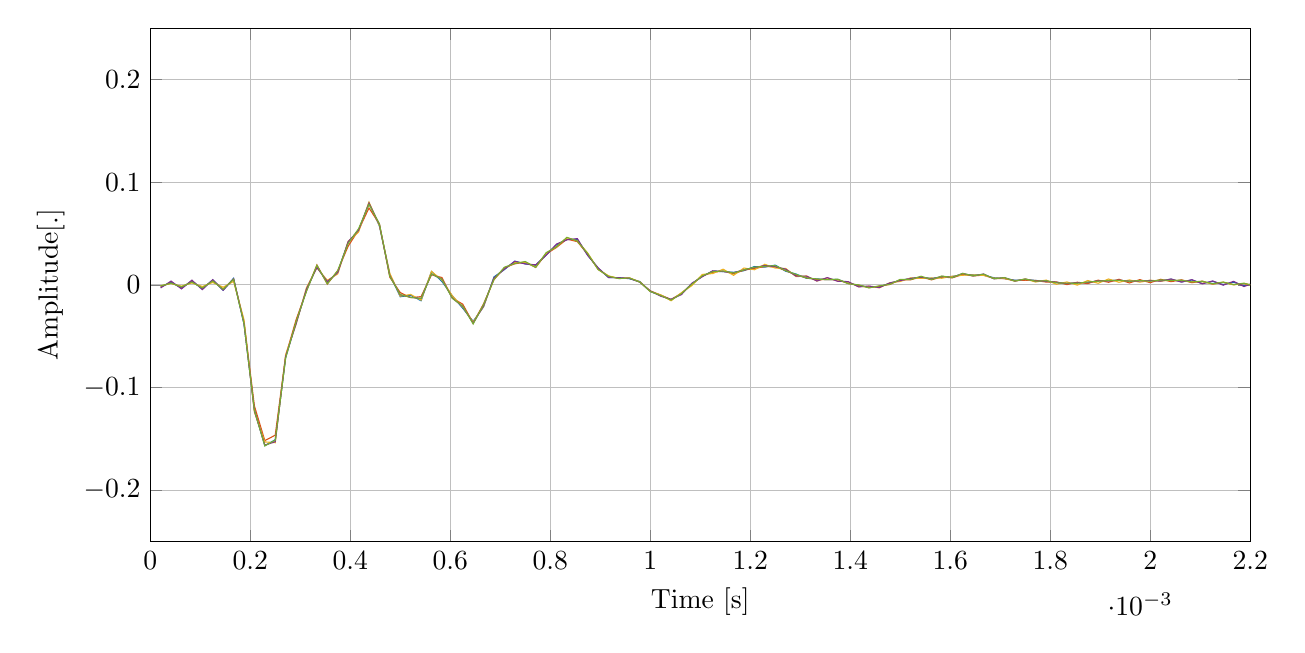
\begin{tikzpicture}

\begin{axis}[%
width=5.5in,
height=2.566in,,
at={(1.011in,0.642in)},
scale only axis,
xmin=0,
xmax=0.0022,
xlabel={Time [s]},
xmajorgrids,
ymin=-0.25,
ymax=0.25,
ylabel={Amplitude[.]},
ymajorgrids,
axis background/.style={fill=white}
]
\addplot [color=mycolor1,solid,forget plot]
  table[row sep=crcr]{%
2.08333333333333e-05	-0.00218389910452928\\
4.16666666666667e-05	0.00247997660818177\\
6.25e-05	-0.00306422212301669\\
8.33333333333333e-05	0.00370795824245389\\
0.000104166666666667	-0.003996195002872\\
0.000125	0.00477762315573945\\
0.000145833333333333	-0.00520610865886981\\
0.000166666666666667	0.00632845677938862\\
0.0001875	-0.0380783744937981\\
0.000208333333333333	-0.121478341280274\\
0.000229166666666667	-0.156732911171094\\
0.00025	-0.150962242221131\\
0.000270833333333333	-0.0708305555277822\\
0.000291666666666667	-0.0363422650083233\\
0.0003125	-0.00543127544862284\\
0.000333333333333333	0.0181597627718888\\
0.000354166666666667	0.00208472952849193\\
0.000375	0.0125098852556454\\
0.000395833333333333	0.0415416610429961\\
0.000416666666666667	0.0527294742213453\\
0.0004375	0.0798009720407638\\
0.000458333333333333	0.057294372226422\\
0.000479166666666667	0.0100967131822404\\
0.0005	-0.0116403016854475\\
0.000520833333333333	-0.0100823637366942\\
0.000541666666666667	-0.0155252345103445\\
0.0005625	0.0129409401256135\\
0.000583333333333333	0.00330032363608726\\
0.000604166666666667	-0.0107369621764369\\
0.000625	-0.0228446033217494\\
0.000645833333333333	-0.0356027778798783\\
0.000666666666666667	-0.0214218763506852\\
0.0006875	0.0077125374318295\\
0.000708333333333333	0.0148003772574559\\
0.000729166666666667	0.0230269782520459\\
0.00075	0.0204048345153605\\
0.000770833333333333	0.0189891037229106\\
0.000791666666666667	0.0290727336722823\\
0.0008125	0.0388997216505961\\
0.000833333333333333	0.0442340567889403\\
0.000854166666666667	0.0441885135919368\\
0.000875	0.0288044550629258\\
0.000895833333333333	0.0161368334943261\\
0.000916666666666667	0.00713579035783102\\
0.0009375	0.00701321180069818\\
0.000958333333333333	0.00593867000057454\\
0.000979166666666667	0.00320599481994303\\
0.001	-0.00664914273579044\\
0.00102083333333333	-0.0101565754892221\\
0.00104166666666667	-0.014791108741586\\
0.0010625	-0.00857239326708171\\
0.00108333333333333	0.00100898054712758\\
0.00110416666666667	0.00839401335783726\\
0.001125	0.0133984163005487\\
0.00114583333333333	0.0128466265171883\\
0.00116666666666667	0.0121549768071494\\
0.0011875	0.0137719317655377\\
0.00120833333333333	0.0178060477156998\\
0.00122916666666667	0.0172847958388615\\
0.00125	0.019210569641301\\
0.00127083333333333	0.013257709044026\\
0.00129166666666667	0.0104752301035351\\
0.0013125	0.00634204156049436\\
0.00133333333333333	0.00579198958498723\\
0.00135416666666667	0.00502590528864318\\
0.001375	0.00529722084283291\\
0.00139583333333333	0.00153242789497228\\
0.00141666666666667	-0.000616528502902794\\
0.0014375	-0.0021893619325514\\
0.00145833333333333	-0.00187817940983287\\
0.00147916666666667	0.00151654195426903\\
0.0015	0.00420310986639849\\
0.00152083333333333	0.00637222520912491\\
0.00154166666666667	0.00708169552640407\\
0.0015625	0.00637493155811143\\
0.00158333333333333	0.00726931533456736\\
0.00160416666666667	0.00819256235515286\\
0.001625	0.00995175279603157\\
0.00164583333333333	0.00976251303247071\\
0.00166666666666667	0.00936529201189556\\
0.0016875	0.00688403743977654\\
0.00170833333333333	0.00606358036924052\\
0.00172916666666667	0.00452676896305512\\
0.00175	0.004828792984279\\
0.00177083333333333	0.00430742388743505\\
0.00179166666666667	0.00318484065017087\\
0.0018125	0.00262913018197462\\
0.00183333333333333	0.000894527696839949\\
0.00185416666666667	0.00220727189527427\\
0.001875	0.00213064727283039\\
0.00189583333333333	0.00400580107200661\\
0.00191666666666667	0.00382018713412366\\
0.0019375	0.00453452462048207\\
0.00195833333333333	0.00348401578315948\\
0.00197916666666667	0.00385250692600261\\
0.002	0.00410399715905844\\
0.00202083333333333	0.00376669564103728\\
0.00204166666666667	0.005481403501254\\
0.0020625	0.00286984013341575\\
0.00208333333333333	0.00467110572913971\\
0.00210416666666667	0.00133891989308461\\
0.002125	0.00329198810788862\\
0.00214583333333333	0.000300140045619779\\
0.00216666666666667	0.00262574118790929\\
0.0021875	-0.000772552707238634\\
0.00220833333333333	0.001204895577724\\
0.00222916666666667	-0.00133487209486768\\
0.00225	-0.000509380400493588\\
0.00227083333333333	-0.000334737971901055\\
0.00229166666666667	-0.00103678981403972\\
0.0023125	0.00061906400962846\\
0.00233333333333333	-0.00138559528811041\\
0.00235416666666667	0.000836453989668149\\
0.002375	-0.00220070096737768\\
0.00239583333333333	0.00155059728767193\\
0.00241666666666667	-0.00246952128785161\\
0.0024375	0.00209771500748369\\
0.00245833333333333	-0.00201237551900768\\
0.00247916666666667	0.00136337042281452\\
0.0025	-0.0016996067640007\\
0.00252083333333333	0.000375559342336357\\
0.00254166666666667	-0.00171285649355793\\
0.0025625	-0.000370547864208922\\
0.00258333333333333	-0.00168478066288008\\
0.00260416666666667	-0.00164047511374893\\
0.002625	-0.00154391190477046\\
0.00264583333333333	-0.00279588952826178\\
0.00266666666666667	-0.00161937857228862\\
0.0026875	-0.00281948250550955\\
0.00270833333333333	-0.0019126329763031\\
0.00272916666666667	-0.00237053013971509\\
0.00275	-0.00216738565291799\\
0.00277083333333333	-0.00198477223131889\\
0.00279166666666667	-0.00218053262768701\\
0.0028125	-0.00109861342178239\\
0.00283333333333333	-0.00230003733690516\\
0.00285416666666667	-2.92964736988071e-05\\
0.002875	-0.00258103832251588\\
0.00289583333333333	0.000226343416296675\\
0.00291666666666667	-0.00266926986983911\\
0.0029375	-0.000193341868510947\\
0.00295833333333333	-0.00251045357924689\\
0.00297916666666667	-0.000754536531619725\\
0.003	-0.00243962671207192\\
0.00302083333333333	-0.00146416942230298\\
0.00304166666666667	-0.00213138690195344\\
0.0030625	-0.00235987025503001\\
0.00308333333333333	-0.00140117139661643\\
0.00310416666666667	-0.00302857105296522\\
0.003125	-0.000722072931201979\\
0.00314583333333333	-0.00321030960137844\\
0.00316666666666667	-0.00035915225761106\\
0.0031875	-0.00297374200868294\\
0.00320833333333333	3.53198342716556e-05\\
0.00322916666666667	-0.0026450468724363\\
0.00325	0.00032858441079607\\
0.00327083333333333	-0.00227789302909872\\
0.00329166666666667	0.000100083042602076\\
0.0033125	-0.00188361158529631\\
0.00333333333333333	-0.000395512602873454\\
0.00335416666666667	-0.00170533112866956\\
0.003375	-0.000671247588764808\\
0.00339583333333333	-0.00191528739109528\\
0.00341666666666667	-0.000801885905110417\\
0.0034375	-0.00212498021642428\\
0.00345833333333333	-0.000968435139872327\\
0.00347916666666667	-0.00218928107893563\\
0.0035	-0.000908900434101829\\
0.00352083333333333	-0.00237627772062559\\
0.00354166666666667	-0.000579630370778564\\
0.0035625	-0.00250519865369403\\
0.00358333333333333	-0.000396073310796909\\
0.00360416666666667	-0.00220304009472981\\
0.003625	-0.000551947219102873\\
0.00364583333333333	-0.0017461192389335\\
0.00366666666666667	-0.000768138137423014\\
0.0036875	-0.0014508385510616\\
0.00370833333333333	-0.00107362237419074\\
0.00372916666666667	-0.001022338035958\\
0.00375	-0.00167383565520242\\
0.00377083333333333	-0.000445481543758471\\
0.00379166666666667	-0.00226771972340852\\
0.0038125	-0.00017191447384072\\
0.00383333333333333	-0.0024910438469192\\
0.00385416666666667	-0.000222906421509958\\
0.003875	-0.00252208983413144\\
0.00389583333333333	-0.000239508055918544\\
0.00391666666666667	-0.00249900652928486\\
0.0039375	-0.00036819453953393\\
0.00395833333333333	-0.00215026444025682\\
0.00397916666666667	-0.00078767916054904\\
0.004	-0.00160104351722162\\
0.00402083333333333	-0.00116932694136055\\
0.00404166666666667	-0.00128993741065524\\
0.0040625	-0.00130037826319792\\
0.00408333333333333	-0.00120109343231604\\
0.00410416666666667	-0.00137738437947758\\
0.004125	-0.00108994636516787\\
0.00414583333333333	-0.0013930566895397\\
0.00416666666666667	-0.00115682928452173\\
0.0041875	-0.00112155535625298\\
0.00420833333333333	-0.0014747233687034\\
0.00422916666666667	-0.000756437573699205\\
0.00425	-0.00175061296711125\\
0.00427083333333333	-0.000584625454284746\\
0.00429166666666667	-0.00185462900166534\\
0.0043125	-0.0005346079858565\\
0.00433333333333333	-0.00193597084036407\\
0.00435416666666667	-0.00047838297960541\\
0.004375	-0.00194226459657353\\
0.00439583333333333	-0.000585028474139202\\
0.00441666666666667	-0.00174761669058415\\
0.0044375	-0.000800749743149818\\
0.00445833333333333	-0.00151735092894328\\
0.00447916666666667	-0.000883973934664968\\
0.0045	-0.0014537081327631\\
0.00452083333333333	-0.00075225814753293\\
0.00454166666666667	-0.00151365778473533\\
0.0045625	-0.000500860453977012\\
0.00458333333333333	-0.00164649690516529\\
0.00460416666666667	-9.96498374878968e-05\\
0.004625	-0.00195544375064587\\
0.00464583333333333	0.000449155256385712\\
0.00466666666666667	-0.00238322226588622\\
0.0046875	0.000954670191418131\\
0.00470833333333333	-0.00271709732406415\\
0.00472916666666667	0.00121675616537964\\
0.00475	-0.00282529785820646\\
0.00477083333333333	0.0011995722697696\\
0.00479166666666667	-0.00272018311514588\\
0.0048125	0.000933992660913407\\
0.00483333333333333	-0.00233183076857483\\
0.00485416666666667	0.00039448353507977\\
0.004875	-0.00163113482278814\\
0.00489583333333333	-0.000362090300491339\\
0.00491666666666667	-0.000779026479175463\\
0.0049375	-0.00112374188568124\\
0.00495833333333333	-2.39139304477267e-05\\
0.00497916666666667	-0.00169920199968603\\
0.005	0.000523981145438892\\
0.00502083333333333	-0.00205667911465618\\
0.00504166666666667	0.000812579724410437\\
0.0050625	-0.00210866993358576\\
0.00508333333333333	0.000741663856323763\\
0.00510416666666667	-0.00175541600420527\\
0.005125	0.000311014598016389\\
0.00514583333333333	-0.00112489985361012\\
0.00516666666666667	-0.000277561456628004\\
0.0051875	-0.000467680148606119\\
0.00520833333333333	-0.000833718285872148\\
0.00522916666666667	0.000113882903666011\\
0.00525	-0.00128561358966294\\
0.00527083333333333	0.000546530701225396\\
0.00529166666666667	-0.00148197183580008\\
0.0053125	0.000645564949214993\\
0.00533333333333333	-0.00126676793443997\\
};
\addplot [color=mycolor2,solid,forget plot]
  table[row sep=crcr]{%
2.08333333333333e-05	-0.00150312502349965\\
4.16666666666667e-05	0.00170740345175498\\
6.25e-05	-0.00225094460714062\\
8.33333333333333e-05	0.00283940474816698\\
0.000104166666666667	-0.00303627224888553\\
0.000125	0.00393115781364844\\
0.000145833333333333	-0.00417103313904593\\
0.000166666666666667	0.00544829804434176\\
0.0001875	-0.0357658099541969\\
0.000208333333333333	-0.118005245940072\\
0.000229166666666667	-0.151785228594567\\
0.00025	-0.1465046442558\\
0.000270833333333333	-0.0692755249179087\\
0.000291666666666667	-0.0340849194790308\\
0.0003125	-0.00600717417737366\\
0.000333333333333333	0.0194326766341735\\
0.000354166666666667	0.000751764670907603\\
0.000375	0.0137901515627398\\
0.000395833333333333	0.0376433591209333\\
0.000416666666666667	0.0533769204766715\\
0.0004375	0.0748560574116669\\
0.000458333333333333	0.0592590643629689\\
0.000479166666666667	0.00735497863182636\\
0.0005	-0.00756718413491506\\
0.000520833333333333	-0.0124975010055099\\
0.000541666666666667	-0.0115247016817554\\
0.0005625	0.00980021630720815\\
0.000583333333333333	0.00708498450188709\\
0.000604166666666667	-0.0129050270431849\\
0.000625	-0.0188519397068052\\
0.000645833333333333	-0.0372961949901686\\
0.000666666666666667	-0.01849297415842\\
0.0006875	0.00497121361236263\\
0.000708333333333333	0.0166422880218153\\
0.000729166666666667	0.020465656840568\\
0.00075	0.0220834588704114\\
0.000770833333333333	0.0169189373925576\\
0.000791666666666667	0.0299976968876195\\
0.0008125	0.0364130084818885\\
0.000833333333333333	0.044568512776588\\
0.000854166666666667	0.0420780402826822\\
0.000875	0.029754539044608\\
0.000895833333333333	0.0150431845354128\\
0.000916666666666667	0.00824248720676909\\
0.0009375	0.00622415686774906\\
0.000958333333333333	0.00657627207683757\\
0.000979166666666667	0.00275294759176985\\
0.001	-0.00591776430469594\\
0.00102083333333333	-0.00992032862922456\\
0.00104166666666667	-0.0143079250947841\\
0.0010625	-0.00817968654639674\\
0.00108333333333333	0.000480415578304432\\
0.00110416666666667	0.00871664889654762\\
0.001125	0.0122014686789311\\
0.00114583333333333	0.0133645741268153\\
0.00116666666666667	0.0106617261527092\\
0.0011875	0.0143050938208178\\
0.00120833333333333	0.0159709735280955\\
0.00122916666666667	0.0177759597607658\\
0.00125	0.0175080774703475\\
0.00127083333333333	0.013929522023107\\
0.00129166666666667	0.00934886109584583\\
0.0013125	0.00688718378449337\\
0.00133333333333333	0.00513304375912566\\
0.00135416666666667	0.00513013541241314\\
0.001375	0.0050914671922881\\
0.00139583333333333	0.00129193064715399\\
0.00141666666666667	-0.000282917718707061\\
0.0014375	-0.00281934226995237\\
0.00145833333333333	-0.00126138441418749\\
0.00147916666666667	0.000359735815132393\\
0.0015	0.00484238657500165\\
0.00152083333333333	0.00489602610432004\\
0.00154166666666667	0.0076699056302263\\
0.0015625	0.00486066045936765\\
0.00158333333333333	0.00771487566070934\\
0.00160416666666667	0.00677437856370931\\
0.001625	0.0101902062798796\\
0.00164583333333333	0.00864138380838661\\
0.00166666666666667	0.00945825376617475\\
0.0016875	0.00618394559018458\\
0.00170833333333333	0.00598757702781642\\
0.00172916666666667	0.00414812009692581\\
0.00175	0.0045110664355937\\
0.00177083333333333	0.00418394923554998\\
0.00179166666666667	0.00269472594072503\\
0.0018125	0.00276415130472775\\
0.00183333333333333	0.000237896245683422\\
0.00185416666666667	0.00252243208973511\\
0.001875	0.00116355425877345\\
0.00189583333333333	0.00450927287329329\\
0.00191666666666667	0.00249087692609324\\
0.0019375	0.00535707054015208\\
0.00195833333333333	0.00180650739266421\\
0.00197916666666667	0.00506128162830543\\
0.002	0.00204266833987498\\
0.00202083333333333	0.00538568566778509\\
0.00204166666666667	0.00306440643436911\\
0.0020625	0.00490161291817414\\
0.00208333333333333	0.00204275018470907\\
0.00210416666666667	0.00359422966353806\\
0.002125	0.000641060989892511\\
0.00214583333333333	0.00247273465336715\\
0.00216666666666667	0.000188366403795602\\
0.0021875	0.00106503791008099\\
0.00220833333333333	-0.000743232791695567\\
0.00222916666666667	-9.80423910744149e-05\\
0.00225	-0.00172025335400668\\
0.00227083333333333	3.22754464928352e-05\\
0.00229166666666667	-0.00136516805409886\\
0.0023125	3.54577907460388e-05\\
0.00233333333333333	-0.000833531371844218\\
0.00235416666666667	-0.000571016518356972\\
0.002375	-0.000914871697735422\\
0.00239583333333333	-0.000463641235510094\\
0.00241666666666667	-0.000699628193500556\\
0.0024375	-0.000207060477280922\\
0.00245833333333333	-0.000119120037095823\\
0.00247916666666667	-0.000826935127761463\\
0.0025	-8.74323159517523e-05\\
0.00252083333333333	-0.00134907159843868\\
0.00254166666666667	-0.000667319094028848\\
0.0025625	-0.00141492723378026\\
0.00258333333333333	-0.00130146454208995\\
0.00260416666666667	-0.00193027545826851\\
0.002625	-0.00181078489699197\\
0.00264583333333333	-0.00242308870916524\\
0.00266666666666667	-0.00238309244215445\\
0.0026875	-0.00205057795859767\\
0.00270833333333333	-0.00287830495327762\\
0.00272916666666667	-0.00155184139664161\\
0.00275	-0.00301640272753359\\
0.00277083333333333	-0.00140097068939183\\
0.00279166666666667	-0.00268935224529769\\
0.0028125	-0.000931645119052387\\
0.00283333333333333	-0.0023485886981718\\
0.00285416666666667	-0.000354079502987963\\
0.002875	-0.00217608672386252\\
0.00289583333333333	-0.000522557772579991\\
0.00291666666666667	-0.00196011839114989\\
0.0029375	-0.00115805904566247\\
0.00295833333333333	-0.00171925918667042\\
0.00297916666666667	-0.00168899841163808\\
0.003	-0.00175239845856024\\
0.00302083333333333	-0.00219088146704869\\
0.00304166666666667	-0.0016729501954931\\
0.0030625	-0.00279122750464493\\
0.00308333333333333	-0.00122178199669892\\
0.00310416666666667	-0.00316169225126841\\
0.003125	-0.000774527040395427\\
0.00314583333333333	-0.00315662971380255\\
0.00316666666666667	-0.000505241210618245\\
0.0031875	-0.00291096153255904\\
0.00320833333333333	-5.47109157601016e-05\\
0.00322916666666667	-0.00269958491630836\\
0.00325	0.000384591516047639\\
0.00327083333333333	-0.00249174215953945\\
0.00329166666666667	0.000320307696682306\\
0.0033125	-0.00223411221031277\\
0.00333333333333333	-5.69303596028571e-05\\
0.00335416666666667	-0.00207877956316048\\
0.003375	-0.00033596353878876\\
0.00339583333333333	-0.0021261805910966\\
0.00341666666666667	-0.000651557367438874\\
0.0034375	-0.00202270695497361\\
0.00345833333333333	-0.00113951939831005\\
0.00347916666666667	-0.00171739717740368\\
0.0035	-0.00143286003128025\\
0.00352083333333333	-0.00154572705042174\\
0.00354166666666667	-0.00141496418020706\\
0.0035625	-0.00141215706801166\\
0.00358333333333333	-0.00142254778974005\\
0.00360416666666667	-0.00104385417080588\\
0.003625	-0.00155334040546127\\
0.00364583333333333	-0.000751248125257298\\
0.00366666666666667	-0.00153118280431747\\
0.0036875	-0.000795220568213555\\
0.00370833333333333	-0.00146322137548783\\
0.00372916666666667	-0.00079707556669385\\
0.00375	-0.00162555299642045\\
0.00377083333333333	-0.000656825841932522\\
0.00379166666666667	-0.00179482298012737\\
0.0038125	-0.000716987849151806\\
0.00383333333333333	-0.00174278812856215\\
0.00385416666666667	-0.0008997503906827\\
0.003875	-0.00173068096269461\\
0.00389583333333333	-0.000835228381933038\\
0.00391666666666667	-0.00186745781255906\\
0.0039375	-0.000709283992475709\\
0.00395833333333333	-0.0018265338126297\\
0.00397916666666667	-0.000751232782326876\\
0.004	-0.00168011122469505\\
0.00402083333333333	-0.000728747365703717\\
0.00404166666666667	-0.00174195708200312\\
0.0040625	-0.000554533524267836\\
0.00408333333333333	-0.00187099682430463\\
0.00410416666666667	-0.000502420876840561\\
0.004125	-0.00178128073891645\\
0.00414583333333333	-0.000584725521308038\\
0.00416666666666667	-0.00167855566804658\\
0.0041875	-0.000573961798953074\\
0.00420833333333333	-0.00164038443992213\\
0.00422916666666667	-0.000626293137293526\\
0.00425	-0.00143198053729605\\
0.00427083333333333	-0.000949735825080193\\
0.00429166666666667	-0.00102424234989205\\
0.0043125	-0.00139050752399155\\
0.00433333333333333	-0.000631820311580779\\
0.00435416666666667	-0.0017894906975532\\
0.004375	-0.000221387616980678\\
0.00439583333333333	-0.00228794650609217\\
0.00441666666666667	0.000318739743225488\\
0.0044375	-0.00282605307228827\\
0.00445833333333333	0.000822159569636328\\
0.00447916666666667	-0.00317863731687403\\
0.0045	0.00113345511482983\\
0.00452083333333333	-0.00330049290040551\\
0.00454166666666667	0.00132314297059868\\
0.0045625	-0.00330307911872846\\
0.00458333333333333	0.00142473387580985\\
0.00460416666666667	-0.0031311564254473\\
0.004625	0.00130969733481889\\
0.00464583333333333	-0.00274498923203992\\
0.00466666666666667	0.000997661794870766\\
0.0046875	-0.00227869476248348\\
0.00470833333333333	0.000627368160612284\\
0.00472916666666667	-0.00185730675341176\\
0.00475	0.000250417926229121\\
0.00477083333333333	-0.00144798076771741\\
0.00479166666666667	-0.00018442151307793\\
0.0048125	-0.00101672481021735\\
0.00483333333333333	-0.000598087030566787\\
0.00485416666666667	-0.000630417239681535\\
0.004875	-0.000897862192957278\\
0.00489583333333333	-0.000316826816828382\\
0.00491666666666667	-0.00113235296379092\\
0.0049375	-4.98728377684598e-06\\
0.00495833333333333	-0.0013817225521446\\
0.00497916666666667	0.000304794913663064\\
0.005	-0.00158251628553709\\
0.00502083333333333	0.000493280324142934\\
0.00504166666666667	-0.00165696192394442\\
0.0050625	0.00056030017776593\\
0.00508333333333333	-0.00164763916966285\\
0.00510416666666667	0.000582730025510889\\
0.005125	-0.00157467180274074\\
0.00514583333333333	0.000506950871697116\\
0.00516666666666667	-0.00134509820375047\\
0.0051875	0.000266397871408095\\
0.00520833333333333	-0.000970733263531003\\
0.00522916666666667	-3.5818549108319e-05\\
0.00525	-0.000598446308158891\\
0.00527083333333333	-0.000293731778738657\\
0.00529166666666667	-0.000244954143389794\\
0.0053125	-0.000551065918035152\\
0.00533333333333333	0.000131559572649119\\
};
\addplot [color=mycolor3,solid,forget plot]
  table[row sep=crcr]{%
2.08333333333333e-05	-0.00096170654887646\\
4.16666666666667e-05	0.00128292390888312\\
6.25e-05	-0.00131330312413177\\
8.33333333333333e-05	0.00181414126068023\\
0.000104166666666667	-0.00166889454003648\\
0.000125	0.00228340013591669\\
0.000145833333333333	-0.0023360694862303\\
0.000166666666666667	0.00332796379527531\\
0.0001875	-0.0340731480390163\\
0.000208333333333333	-0.123992111500225\\
0.000229166666666667	-0.153072963208568\\
0.00025	-0.153830925618541\\
0.000270833333333333	-0.0679592962024725\\
0.000291666666666667	-0.0383233488842451\\
0.0003125	-0.00269199166855106\\
0.000333333333333333	0.0165876343774316\\
0.000354166666666667	0.00439810931467276\\
0.000375	0.0105877337613698\\
0.000395833333333333	0.0423894477217191\\
0.000416666666666667	0.0513501717114422\\
0.0004375	0.080655104070904\\
0.000458333333333333	0.0576514379190256\\
0.000479166666666667	0.0112100518665312\\
0.0005	-0.0110393451955818\\
0.000520833333333333	-0.00941631650172399\\
0.000541666666666667	-0.0149688567469686\\
0.0005625	0.0131276474312309\\
0.000583333333333333	0.00448990461979815\\
0.000604166666666667	-0.010686155594354\\
0.000625	-0.0218209533323957\\
0.000645833333333333	-0.0363256073985036\\
0.000666666666666667	-0.021065968298784\\
0.0006875	0.00650914317381322\\
0.000708333333333333	0.0156786284054297\\
0.000729166666666667	0.0218364282275781\\
0.00075	0.0219096362245693\\
0.000770833333333333	0.0176488688534664\\
0.000791666666666667	0.0305835535209084\\
0.0008125	0.0372974514826221\\
0.000833333333333333	0.045957193994314\\
0.000854166666666667	0.0428833023595367\\
0.000875	0.0309212936133024\\
0.000895833333333333	0.0150434573059395\\
0.000916666666666667	0.00876227661718757\\
0.0009375	0.00611494386202251\\
0.000958333333333333	0.00679491451339289\\
0.000979166666666667	0.00284000215034346\\
0.001	-0.00646986852024406\\
0.00102083333333333	-0.00981255418802416\\
0.00104166666666667	-0.0155467597910425\\
0.0010625	-0.00762099846758336\\
0.00108333333333333	-0.000752140850527739\\
0.00110416666666667	0.010132712425861\\
0.001125	0.0109905409902635\\
0.00114583333333333	0.0152131134736847\\
0.00116666666666667	0.00925177030657228\\
0.0011875	0.0163582865000064\\
0.00120833333333333	0.0146864648120937\\
0.00122916666666667	0.0199695196695545\\
0.00125	0.016301242154017\\
0.00127083333333333	0.0159503834138262\\
0.00129166666666667	0.00797803061977806\\
0.0013125	0.00861369291693406\\
0.00133333333333333	0.00371042699448329\\
0.00135416666666667	0.00672830303463991\\
0.001375	0.00368116213752206\\
0.00139583333333333	0.00276575004743318\\
0.00141666666666667	-0.00188874628012694\\
0.0014375	-0.00139352508079049\\
0.00145833333333333	-0.00295334319190189\\
0.00147916666666667	0.00198465372901796\\
0.0015	0.00328117907575589\\
0.00152083333333333	0.00671280548803403\\
0.00154166666666667	0.00621869485923812\\
0.0015625	0.00660997841933263\\
0.00158333333333333	0.00643589320806389\\
0.00160416666666667	0.00831343642699504\\
0.001625	0.00934528409478915\\
0.00164583333333333	0.00972983706808973\\
0.00166666666666667	0.00915883811798237\\
0.0016875	0.00648593380819075\\
0.00170833333333333	0.00633519721465413\\
0.00172916666666667	0.00354549069216825\\
0.00175	0.00566678725730377\\
0.00177083333333333	0.00271744497040613\\
0.00179166666666667	0.00463039659195748\\
0.0018125	0.000494515835026391\\
0.00183333333333333	0.00279661949056555\\
0.00185416666666667	-0.000290677066042336\\
0.001875	0.00419744065943955\\
0.00189583333333333	0.00152226214680512\\
0.00191666666666667	0.00568281516949187\\
0.0019375	0.0024821828602918\\
0.00195833333333333	0.00475365862347755\\
0.00197916666666667	0.00255294602045261\\
0.002	0.00448783698781115\\
0.00202083333333333	0.00347886877184384\\
0.00204166666666667	0.00484764257154601\\
0.0020625	0.00367962451195923\\
0.00208333333333333	0.00304471579184384\\
0.00210416666666667	0.00302613527145239\\
0.002125	0.000927891977424043\\
0.00214583333333333	0.00247056523446992\\
0.00216666666666667	-4.81611992291632e-05\\
0.0021875	0.00146708549898274\\
0.00220833333333333	-0.00132525591153304\\
0.00222916666666667	0.000536653166020971\\
0.00225	-0.00247451381195941\\
0.00227083333333333	0.000776735559613356\\
0.00229166666666667	-0.00211643599153016\\
0.0023125	0.00076904378419254\\
0.00233333333333333	-0.00150003713832084\\
0.00235416666666667	5.37325061572903e-05\\
0.002375	-0.00147952035575466\\
0.00239583333333333	2.16803081601954e-05\\
0.00241666666666667	-0.00112364464132188\\
0.0024375	0.000101047201456924\\
0.00245833333333333	-0.000333084077427386\\
0.00247916666666667	-0.000777999002666638\\
0.0025	-2.17493652543828e-05\\
0.00252083333333333	-0.00164025882368395\\
0.00254166666666667	-0.000224444478136188\\
0.0025625	-0.00213808421512059\\
0.00258333333333333	-0.000367090296538516\\
0.00260416666666667	-0.00319467648813374\\
0.002625	-0.000302921624347762\\
0.00264583333333333	-0.00428557125101334\\
0.00266666666666667	-0.000307287930030643\\
0.0026875	-0.00446144230568535\\
0.00270833333333333	-0.000320261977067134\\
0.00272916666666667	-0.00438481358406927\\
0.00275	-0.000154281790945869\\
0.00277083333333333	-0.00444517023637048\\
0.00279166666666667	0.000230900512683732\\
0.0028125	-0.00388392354173841\\
0.00283333333333333	0.000331017865546658\\
0.00285416666666667	-0.00289327814753094\\
0.002875	-2.77906354901444e-05\\
0.00289583333333333	-0.00237667491126423\\
0.00291666666666667	-0.000579959453776046\\
0.0029375	-0.00212347534377704\\
0.00295833333333333	-0.001272024730731\\
0.00297916666666667	-0.00165483709076772\\
0.003	-0.00231794047001442\\
0.00302083333333333	-0.00116238689872106\\
0.00304166666666667	-0.00320946080653662\\
0.0030625	-0.000875756774047028\\
0.00308333333333333	-0.00359054364495372\\
0.00310416666666667	-0.000536932967019422\\
0.003125	-0.00377513292865997\\
0.00314583333333333	-3.93582667299344e-05\\
0.00316666666666667	-0.00389357193030742\\
0.0031875	0.000466918904028192\\
0.00320833333333333	-0.00356365169299798\\
0.00322916666666667	0.000701204692210054\\
0.00325	-0.00300700259567012\\
0.00327083333333333	0.000715679737851534\\
0.00329166666666667	-0.00275578886732331\\
0.0033125	0.000598889944005619\\
0.00333333333333333	-0.00264935970519018\\
0.00335416666666667	0.000220172978528961\\
0.003375	-0.00231664792559229\\
0.00339583333333333	-0.000500325164690189\\
0.00341666666666667	-0.00192949526184926\\
0.0034375	-0.00115532494506326\\
0.00345833333333333	-0.00165847804512531\\
0.00347916666666667	-0.00164388972672291\\
0.0035	-0.00117335996712127\\
0.00352083333333333	-0.00226356633120134\\
0.00354166666666667	-0.000404846871948445\\
0.0035625	-0.00284896726778417\\
0.00358333333333333	0.000242051572868697\\
0.00360416666666667	-0.00304596834634291\\
0.003625	0.00060536805078243\\
0.00364583333333333	-0.00312216443618275\\
0.00366666666666667	0.000903925708152949\\
0.0036875	-0.00330489212663293\\
0.00370833333333333	0.00098623122622655\\
0.00372916666666667	-0.00317677408943884\\
0.00375	0.000563338243319644\\
0.00377083333333333	-0.00264583531343429\\
0.00379166666666667	-0.000119213254527432\\
0.0038125	-0.00210930770932602\\
0.00383333333333333	-0.000766482094836061\\
0.00385416666666667	-0.00154871668736696\\
0.003875	-0.0015519317480128\\
0.00389583333333333	-0.000672094705770657\\
0.00391666666666667	-0.00248441879782993\\
0.0039375	0.000215768090659124\\
0.00395833333333333	-0.00313023902354445\\
0.00397916666666667	0.000781292610489168\\
0.004	-0.00347088606726442\\
0.00402083333333333	0.00119713593302133\\
0.00404166666666667	-0.00378674213577376\\
0.0040625	0.00151990448070547\\
0.00408333333333333	-0.00394026936569141\\
0.00410416666666667	0.00148808409903704\\
0.004125	-0.00368911663166498\\
0.00414583333333333	0.00116928686267876\\
0.00416666666666667	-0.00332523833657345\\
0.0041875	0.000895703654819184\\
0.00420833333333333	-0.00303303779658155\\
0.00422916666666667	0.000602381147811138\\
0.00425	-0.00264841290081222\\
0.00427083333333333	0.00015800949406137\\
0.00429166666666667	-0.00218684282891001\\
0.0043125	-0.000250635544417012\\
0.00433333333333333	-0.00188150141810143\\
0.00435416666666667	-0.000484014801960763\\
0.004375	-0.00166507451171022\\
0.00439583333333333	-0.000744937719315117\\
0.00441666666666667	-0.00135711820697661\\
0.0044375	-0.00104558937068014\\
0.00445833333333333	-0.00105811326249625\\
0.00447916666666667	-0.00123498520568187\\
0.0045	-0.000864163133700501\\
0.00452083333333333	-0.00131911209203293\\
0.00454166666666667	-0.000660259156287151\\
0.0045625	-0.00142493616236689\\
0.00458333333333333	-0.000398678970650784\\
0.00460416666666667	-0.00147942425523991\\
0.004625	-0.000240763774651899\\
0.00464583333333333	-0.00140686979022522\\
0.00466666666666667	-0.00020746925136003\\
0.0046875	-0.00129053963313638\\
0.00470833333333333	-0.000207982329026631\\
0.00472916666666667	-0.00121552967113305\\
0.00475	-0.000235014065413005\\
0.00477083333333333	-0.00112409257509449\\
0.00479166666666667	-0.000365663602212807\\
0.0048125	-0.000972994067098467\\
0.00483333333333333	-0.000518935035761285\\
0.00485416666666667	-0.000836424094967947\\
0.004875	-0.000589791410851834\\
0.00489583333333333	-0.000757383461064286\\
0.00491666666666667	-0.000611077469693976\\
0.0049375	-0.000664715352324419\\
0.00495833333333333	-0.000662056556764749\\
0.00497916666666667	-0.000545338783967716\\
0.005	-0.000686528089335427\\
0.00502083333333333	-0.000503069775776309\\
0.00504166666666667	-0.000631952587116847\\
0.0050625	-0.000515675739596115\\
0.00508333333333333	-0.000569107659029838\\
0.00510416666666667	-0.000483380209994945\\
0.005125	-0.000540375669381737\\
0.00514583333333333	-0.00046189169651648\\
0.00516666666666667	-0.000449633750369974\\
0.0051875	-0.000536224841012603\\
0.00520833333333333	-0.000283469793322118\\
0.00522916666666667	-0.000623952927626751\\
0.00525	-0.000150502813881807\\
0.00527083333333333	-0.000656958325759085\\
0.00529166666666667	-2.22772294250384e-05\\
0.0053125	-0.00072353089223778\\
0.00533333333333333	0.000191732530809588\\
};
\addplot [color=mycolor4,solid,forget plot]
  table[row sep=crcr]{%
2.08333333333333e-05	-0.00304270989999626\\
4.16666666666667e-05	0.00364264893910555\\
6.25e-05	-0.00397118138170965\\
8.33333333333333e-05	0.00453834392985895\\
0.000104166666666667	-0.00467483563145047\\
0.000125	0.00506525868001629\\
0.000145833333333333	-0.00531633817796136\\
0.000166666666666667	0.00589187903650913\\
0.0001875	-0.0378011561863622\\
0.000208333333333333	-0.122891805656185\\
0.000229166666666667	-0.156173609423803\\
0.00025	-0.152891594322995\\
0.000270833333333333	-0.0697466134144659\\
0.000291666666666667	-0.0380305697508812\\
0.0003125	-0.00401043053213786\\
0.000333333333333333	0.0169210947410653\\
0.000354166666666667	0.00311090846931313\\
0.000375	0.0119863404292271\\
0.000395833333333333	0.04197044680573\\
0.000416666666666667	0.0532897765822361\\
0.0004375	0.0795263204608023\\
0.000458333333333333	0.058737298377844\\
0.000479166666666667	0.00881245516212244\\
0.0005	-0.00972106559397336\\
0.000520833333333333	-0.0121835994539805\\
0.000541666666666667	-0.0132644609961281\\
0.0005625	0.0106477933250109\\
0.000583333333333333	0.00553337826852133\\
0.000604166666666667	-0.0129593229107815\\
0.000625	-0.0211680167670463\\
0.000645833333333333	-0.0374349793969786\\
0.000666666666666667	-0.0203712153771732\\
0.0006875	0.00670993252890814\\
0.000708333333333333	0.0152961424293201\\
0.000729166666666667	0.0229029719913906\\
0.00075	0.0203406595806968\\
0.000770833333333333	0.0194668537709975\\
0.000791666666666667	0.0286659807517909\\
0.0008125	0.0397326236290748\\
0.000833333333333333	0.043818844260161\\
0.000854166666666667	0.0450156583956936\\
0.000875	0.0285327345626683\\
0.000895833333333333	0.0165436884701473\\
0.000916666666666667	0.00712002191131959\\
0.0009375	0.00686300602431224\\
0.000958333333333333	0.00629632391466133\\
0.000979166666666667	0.00257896789132242\\
0.001	-0.00599960451964591\\
0.00102083333333333	-0.0110996982854721\\
0.00104166666666667	-0.0140683432765323\\
0.0010625	-0.00949546744420411\\
0.00108333333333333	0.00162387302064548\\
0.00110416666666667	0.00786750076788531\\
0.001125	0.0136563386497654\\
0.00114583333333333	0.0129303978698493\\
0.00116666666666667	0.0118145912451157\\
0.0011875	0.0145719235054983\\
0.00120833333333333	0.0168142829365621\\
0.00122916666666667	0.0187797841500046\\
0.00125	0.0176514533810854\\
0.00127083333333333	0.0152316025274909\\
0.00129166666666667	0.00851551838645658\\
0.0013125	0.00848634432785558\\
0.00133333333333333	0.00371855075099667\\
0.00135416666666667	0.0070420061561897\\
0.001375	0.00343047603188711\\
0.00139583333333333	0.00312858841905049\\
0.00141666666666667	-0.00202487025040996\\
0.0014375	-0.00120456774346269\\
0.00145833333333333	-0.00265284535261524\\
0.00147916666666667	0.00185263961931701\\
0.0015	0.0041319863049014\\
0.00152083333333333	0.00611597736543582\\
0.00154166666666667	0.00762159608803858\\
0.0015625	0.00564451588311011\\
0.00158333333333333	0.00823450540024062\\
0.00160416666666667	0.00717654545547612\\
0.001625	0.0111290500281548\\
0.00164583333333333	0.0086550917011984\\
0.00166666666666667	0.0105401132828014\\
0.0016875	0.00583585449243986\\
0.00170833333333333	0.00707426759360389\\
0.00172916666666667	0.00364433380544299\\
0.00175	0.00559870977460973\\
0.00177083333333333	0.003649927155061\\
0.00179166666666667	0.00370932393784419\\
0.0018125	0.00219222288796419\\
0.00183333333333333	0.00120538519604571\\
0.00185416666666667	0.00194316969698597\\
0.001875	0.00229615195463047\\
0.00189583333333333	0.00387068257758945\\
0.00191666666666667	0.00391717853112836\\
0.0019375	0.00446985895273453\\
0.00195833333333333	0.00356813628689734\\
0.00197916666666667	0.00378827309707912\\
0.002	0.00422398137319906\\
0.00202083333333333	0.00364549757793422\\
0.00204166666666667	0.00568981301265973\\
0.0020625	0.0026329482590144\\
0.00208333333333333	0.00501563037644262\\
0.00210416666666667	0.000913603277824271\\
0.002125	0.00382082037332622\\
0.00214583333333333	-0.000367588388650299\\
0.00216666666666667	0.00339403198531383\\
0.0021875	-0.00170534263141879\\
0.00220833333333333	0.00224603026874457\\
0.00222916666666667	-0.00253473318020223\\
0.00225	0.000789938193473262\\
0.00227083333333333	-0.00176025951462305\\
0.00229166666666667	0.000457462485760138\\
0.0023125	-0.000933847346190962\\
0.00233333333333333	0.000194803104964803\\
0.00235416666666667	-0.000711585288599666\\
0.002375	-0.0006844885417621\\
0.00239583333333333	0.000159515980124698\\
0.00241666666666667	-0.00118829831668967\\
0.0024375	0.00101048703945008\\
0.00245833333333333	-0.00111838865692215\\
0.00247916666666667	0.000702446116678058\\
0.0025	-0.0012903404568411\\
0.00252083333333333	0.000205205771254388\\
0.00254166666666667	-0.00181870687413992\\
0.0025625	-4.62504104492772e-05\\
0.00258333333333333	-0.00226391748594022\\
0.00260416666666667	-0.000879669268305371\\
0.002625	-0.00250065930580145\\
0.00264583333333333	-0.00171894571194364\\
0.00266666666666667	-0.00282335711712005\\
0.0026875	-0.00155520369424349\\
0.00270833333333333	-0.00322480726367007\\
0.00272916666666667	-0.00104112391623795\\
0.00275	-0.00348696094998767\\
0.00277083333333333	-0.000689970519698981\\
0.00279166666666667	-0.00344020875643415\\
0.0028125	0.00010800351274781\\
0.00283333333333333	-0.00345997827186242\\
0.00285416666666667	0.00107826568626145\\
0.002875	-0.00363305108775459\\
0.00289583333333333	0.00123182737125114\\
0.00291666666666667	-0.00362225050287467\\
0.0029375	0.000705416048113566\\
0.00295833333333333	-0.00335798202082746\\
0.00297916666666667	2.92972641305303e-05\\
0.003	-0.00315654715365073\\
0.00302083333333333	-0.000819343815369181\\
0.00304166666666667	-0.00269766631863801\\
0.0030625	-0.00188457475416621\\
0.00308333333333333	-0.00179851261363151\\
0.00310416666666667	-0.0027241142451798\\
0.003125	-0.000946913626696663\\
0.00314583333333333	-0.00305040388451039\\
0.00316666666666667	-0.000458608235267766\\
0.0031875	-0.00290125458659162\\
0.00320833333333333	-2.41978970580642e-05\\
0.00322916666666667	-0.00255499624041146\\
0.00325	0.000204374714944251\\
0.00327083333333333	-0.00206045708097884\\
0.00329166666666667	-0.000203409066463349\\
0.0033125	-0.001456608217257\\
0.00333333333333333	-0.000955585126801396\\
0.00335416666666667	-0.00102215056766444\\
0.003375	-0.00148388486369174\\
0.00339583333333333	-0.0010086026384737\\
0.00341666666666667	-0.00177885144346526\\
0.0034375	-0.00113040222295324\\
0.00345833333333333	-0.00194010928451574\\
0.00347916666666667	-0.00131154973497405\\
0.0035	-0.00164234149022832\\
0.00352083333333333	-0.00184474661929036\\
0.00354166666666667	-0.000841782055765863\\
0.0035625	-0.00253872912912761\\
0.00358333333333333	-1.96242316274147e-05\\
0.00360416666666667	-0.00293279939666573\\
0.003625	0.00053137741446305\\
0.00364583333333333	-0.00316146230624051\\
0.00366666666666667	0.000952689245882111\\
0.0036875	-0.00341395946013057\\
0.00370833333333333	0.00107637859453967\\
0.00372916666666667	-0.00328113887633687\\
0.00375	0.000612933065436834\\
0.00377083333333333	-0.00268197681317761\\
0.00379166666666667	-0.000161012169345355\\
0.0038125	-0.002084963017393\\
0.00383333333333333	-0.000831125790207004\\
0.00385416666666667	-0.00159698406263343\\
0.003875	-0.00145633715082472\\
0.00389583333333333	-0.00100087270793439\\
0.00391666666666667	-0.00202197439957616\\
0.0039375	-0.000607585265159944\\
0.00395833333333333	-0.00209684989872705\\
0.00397916666666667	-0.000734224198944383\\
0.004	-0.00168319830343093\\
0.00402083333333333	-0.0011414803746858\\
0.00404166666666667	-0.00117869428128755\\
0.0040625	-0.00162111171272464\\
0.00408333333333333	-0.000611149893490133\\
0.00410416666666667	-0.00228143884517481\\
0.004125	0.000147406823398839\\
0.00414583333333333	-0.00296522006033777\\
0.00416666666666667	0.000723958825296914\\
0.0041875	-0.0032758026000927\\
0.00420833333333333	0.000865925137243956\\
0.00422916666666667	-0.00324478082538129\\
0.00425	0.000751208665125314\\
0.00427083333333333	-0.00305691129092546\\
0.00429166666666667	0.000466215766973446\\
0.0043125	-0.00265029184159321\\
0.00433333333333333	-0.000105977893432253\\
0.00435416666666667	-0.00198968876055482\\
0.004375	-0.000779798683280639\\
0.00439583333333333	-0.00139018045406604\\
0.00441666666666667	-0.00125182660709046\\
0.0044375	-0.000997538946619184\\
0.00445833333333333	-0.00151992415525888\\
0.00447916666666667	-0.000734376252817718\\
0.0045	-0.00164558979768681\\
0.00452083333333333	-0.000604402733817688\\
0.00454166666666667	-0.0015275941340004\\
0.0045625	-0.00071206632827364\\
0.00458333333333333	-0.00116277257810502\\
0.00460416666666667	-0.000940851995466171\\
0.004625	-0.000780493432240308\\
0.00464583333333333	-0.00111875829316672\\
0.00466666666666667	-0.00050434954138244\\
0.0046875	-0.00123290737232609\\
0.00470833333333333	-0.000326265107782616\\
0.00472916666666667	-0.00131097089865501\\
0.00475	-0.000275746028554314\\
0.00477083333333333	-0.00126167913174616\\
0.00479166666666667	-0.00044029308577763\\
0.0048125	-0.00103056232632859\\
0.00483333333333333	-0.000736582502807676\\
0.00485416666666667	-0.000721477283286024\\
0.004875	-0.00101187772061345\\
0.00489583333333333	-0.00043907210630552\\
0.00491666666666667	-0.00123145392075002\\
0.0049375	-0.000174568504983936\\
0.00495833333333333	-0.00142510976375756\\
0.00497916666666667	5.37140394431868e-05\\
0.005	-0.00151650957105926\\
0.00502083333333333	0.000122189028866937\\
0.00504166666666667	-0.00143094633278528\\
0.0050625	4.53982746391427e-05\\
0.00508333333333333	-0.00125494951283135\\
0.00510416666666667	-4.4459291919062e-05\\
0.005125	-0.00107904200997297\\
0.00514583333333333	-0.000142206187086321\\
0.00516666666666667	-0.000862310675998943\\
0.0051875	-0.0002948187960718\\
0.00520833333333333	-0.000629457667471823\\
0.00522916666666667	-0.000395320005457989\\
0.00525	-0.000523618891851419\\
0.00527083333333333	-0.000335934439118759\\
0.00529166666666667	-0.000541609865853583\\
0.0053125	-0.000203335003657663\\
0.00533333333333333	-0.00057518461385756\\
};
\addplot [color=mycolor5,solid,forget plot]
  table[row sep=crcr]{%
2.08333333333333e-05	-0.00108167093816297\\
4.16666666666667e-05	0.00158855636678058\\
6.25e-05	-0.00194827454277563\\
8.33333333333333e-05	0.00263167698281985\\
0.000104166666666667	-0.00301026387203321\\
0.000125	0.00369888624647976\\
0.000145833333333333	-0.00435610672884497\\
0.000166666666666667	0.00540773794149447\\
0.0001875	-0.0377239019939111\\
0.000208333333333333	-0.122261069312332\\
0.000229166666666667	-0.156934236978788\\
0.00025	-0.151318336617486\\
0.000270833333333333	-0.071338858534062\\
0.000291666666666667	-0.0360106477499694\\
0.0003125	-0.00613158049356146\\
0.000333333333333333	0.0190236407872005\\
0.000354166666666667	0.00096623797618405\\
0.000375	0.0139117588011733\\
0.000395833333333333	0.0402190048896711\\
0.000416666666666667	0.054708723143738\\
0.0004375	0.0783274115329852\\
0.000458333333333333	0.0594355839878347\\
0.000479166666666667	0.00826063263489713\\
0.0005	-0.0095216291614642\\
0.000520833333333333	-0.0122755483894104\\
0.000541666666666667	-0.0133208448693627\\
0.0005625	0.0106428030956712\\
0.000583333333333333	0.0054844383433461\\
0.000604166666666667	-0.0131789899894058\\
0.000625	-0.0207116778628456\\
0.000645833333333333	-0.0381134932337313\\
0.000666666666666667	-0.019188509466415\\
0.0006875	0.00528816020681478\\
0.000708333333333333	0.0171510057991826\\
0.000729166666666667	0.0207827262179832\\
0.00075	0.022706000550851\\
0.000770833333333333	0.0169217188685441\\
0.000791666666666667	0.0312573526188342\\
0.0008125	0.0370866657107353\\
0.000833333333333333	0.0462255902948947\\
0.000854166666666667	0.0426444410026945\\
0.000875	0.0304085875458693\\
0.000895833333333333	0.0148840143323523\\
0.000916666666666667	0.00827215159605487\\
0.0009375	0.0060937441537514\\
0.000958333333333333	0.00664694636909816\\
0.000979166666666667	0.00266263242598394\\
0.001	-0.0063634011650073\\
0.00102083333333333	-0.01036321196698\\
0.00104166666666667	-0.0149052827860693\\
0.0010625	-0.0084501785391493\\
0.00108333333333333	0.000606625476279758\\
0.00110416666666667	0.00881857242938155\\
0.001125	0.0128207466279998\\
0.00114583333333333	0.0134921241752405\\
0.00116666666666667	0.0114978485606921\\
0.0011875	0.0145510069193347\\
0.00120833333333333	0.0171741864001396\\
0.00122916666666667	0.018074644917189\\
0.00125	0.0186738805859375\\
0.00127083333333333	0.0138724434795313\\
0.00129166666666667	0.0101137168733456\\
0.0013125	0.00667260642765156\\
0.00133333333333333	0.00569382524996967\\
0.00135416666666667	0.00499623609851281\\
0.001375	0.00551172843551824\\
0.00139583333333333	0.00109555885642132\\
0.00141666666666667	-6.87038224401135e-05\\
0.0014375	-0.00299687865905104\\
0.00145833333333333	-0.000997453466647792\\
0.00147916666666667	0.000445568798856083\\
0.0015	0.0053397633020987\\
0.00152083333333333	0.00515715853267509\\
0.00154166666666667	0.00836423853704755\\
0.0015625	0.00513795577357357\\
0.00158333333333333	0.00857417745905345\\
0.00160416666666667	0.00702393940546298\\
0.001625	0.0111703477128182\\
0.00164583333333333	0.00871409821771694\\
0.00166666666666667	0.0104397102727168\\
0.0016875	0.00595500358834538\\
0.00170833333333333	0.00700200128277797\\
0.00172916666666667	0.00368810780675939\\
0.00175	0.00567831107894565\\
0.00177083333333333	0.00351899265631252\\
0.00179166666666667	0.00398588822901591\\
0.0018125	0.00186617165965752\\
0.00183333333333333	0.00163097276527358\\
0.00185416666666667	0.00150595318670729\\
0.001875	0.00274111132199243\\
0.00189583333333333	0.00349540541961971\\
0.00191666666666667	0.0041862012952221\\
0.0019375	0.00437744526828767\\
0.00195833333333333	0.00343074534543391\\
0.00197916666666667	0.00421159297507007\\
0.002	0.00347606623944909\\
0.00202083333333333	0.00476108540681459\\
0.00204166666666667	0.00420617103506799\\
0.0020625	0.00450488713983415\\
0.00208333333333333	0.00279590032915892\\
0.00210416666666667	0.00348280861374204\\
0.002125	0.00100425031270196\\
0.00214583333333333	0.00270568131597643\\
0.00216666666666667	0.000226630871699768\\
0.0021875	0.00155349214612611\\
0.00220833333333333	-0.000946244456838386\\
0.00222916666666667	0.000552586017702404\\
0.00225	-0.00206183964242343\\
0.00227083333333333	0.000816437115637674\\
0.00229166666666667	-0.00174731027438063\\
0.0023125	0.000871380332282493\\
0.00233333333333333	-0.00116337288480334\\
0.00235416666666667	0.000195891879034422\\
0.002375	-0.00113809592270044\\
0.00239583333333333	0.000195810875720741\\
0.00241666666666667	-0.000836884655416954\\
0.0024375	0.000350635452658866\\
0.00245833333333333	-0.000194933029278432\\
0.00247916666666667	-0.0003700194182235\\
0.0025	-9.95735352473129e-05\\
0.00252083333333333	-0.000967392251808652\\
0.00254166666666667	-0.000670103665408538\\
0.0025625	-0.00104720141450225\\
0.00258333333333333	-0.00140023925853166\\
0.00260416666666667	-0.00153179656152614\\
0.002625	-0.00203827297032053\\
0.00264583333333333	-0.00197192766287245\\
0.00266666666666667	-0.00272609252748513\\
0.0026875	-0.00151159970515523\\
0.00270833333333333	-0.00334011597088708\\
0.00272916666666667	-0.00090604660685375\\
0.00275	-0.00357639392706642\\
0.00277083333333333	-0.000699403625954175\\
0.00279166666666667	-0.00326730962716209\\
0.0028125	-0.000254308751066045\\
0.00283333333333333	-0.00286484952572325\\
0.00285416666666667	0.000250995855388284\\
0.002875	-0.00257370297859814\\
0.00289583333333333	-2.2567322749387e-05\\
0.00291666666666667	-0.00219368257362852\\
0.0029375	-0.000807144867778091\\
0.00295833333333333	-0.00178386165830155\\
0.00297916666666667	-0.0014975170004349\\
0.003	-0.00172167703734621\\
0.00302083333333333	-0.00208247217724234\\
0.00304166666666667	-0.00165681903194912\\
0.0030625	-0.00264929475918526\\
0.00308333333333333	-0.00132959952756004\\
0.00310416666666667	-0.00287839378781703\\
0.003125	-0.00110437538605358\\
0.00314583333333333	-0.00261603711373395\\
0.00316666666666667	-0.00114811451518314\\
0.0031875	-0.00202231741965156\\
0.00320833333333333	-0.00104785144849533\\
0.00322916666666667	-0.00147045548890685\\
0.00325	-0.000904912347926149\\
0.00327083333333333	-0.00102162055681779\\
0.00329166666666667	-0.00115499460476546\\
0.0033125	-0.000658841312123794\\
0.00333333333333333	-0.00159336424596743\\
0.00335416666666667	-0.000560226095691104\\
0.003375	-0.0017876350028494\\
0.00339583333333333	-0.000845308116406821\\
0.00341666666666667	-0.00185624265317327\\
0.0034375	-0.00109105124677626\\
0.00345833333333333	-0.00200258953390605\\
0.00347916666666667	-0.00115208409041158\\
0.0035	-0.0019508363728917\\
0.00352083333333333	-0.00132516548873961\\
0.00354166666666667	-0.00161445658962774\\
0.0035625	-0.00149137949271495\\
0.00358333333333333	-0.00135145324390677\\
0.00360416666666667	-0.00133641988062564\\
0.003625	-0.00130075940832274\\
0.00364583333333333	-0.00116996653806494\\
0.00366666666666667	-0.0011548964268179\\
0.0036875	-0.00131116864037401\\
0.00370833333333333	-0.000964545510048931\\
0.00372916666666667	-0.00142580135556221\\
0.00375	-0.0010003162994818\\
0.00377083333333333	-0.00141482176289049\\
0.00379166666666667	-0.00105098444904824\\
0.0038125	-0.00162675313174106\\
0.00383333333333333	-0.000852366691792312\\
0.00385416666666667	-0.00199551867013147\\
0.003875	-0.000661617585906071\\
0.00389583333333333	-0.00212146312413338\\
0.00391666666666667	-0.000641746081193178\\
0.0039375	-0.00214787434985289\\
0.00395833333333333	-0.00048069768597805\\
0.00397916666666667	-0.00230776642493724\\
0.004	-0.0002318851792713\\
0.00402083333333333	-0.00237169863303317\\
0.00404166666666667	-0.000237784371050032\\
0.0040625	-0.00221652738725384\\
0.00408333333333333	-0.000399792694808141\\
0.00410416666666667	-0.00209742419395009\\
0.004125	-0.000426822573797033\\
0.00414583333333333	-0.00203199790315726\\
0.00416666666666667	-0.000532113824349629\\
0.0041875	-0.00176990612338594\\
0.00420833333333333	-0.000836271557288304\\
0.00422916666666667	-0.00142901041464832\\
0.00425	-0.00110624607735832\\
0.00427083333333333	-0.0012237287005207\\
0.00429166666666667	-0.0012761013843997\\
0.0043125	-0.00104231023016569\\
0.00433333333333333	-0.0015338776170426\\
0.00435416666666667	-0.000755246931964156\\
0.004375	-0.0018004925105223\\
0.00439583333333333	-0.000567364282363324\\
0.00441666666666667	-0.00188013347503519\\
0.0044375	-0.000534118030366264\\
0.00445833333333333	-0.00184516706905645\\
0.00447916666666667	-0.00051855216021137\\
0.0045	-0.00178395180063403\\
0.00452083333333333	-0.000519916397975425\\
0.00454166666666667	-0.00158540538126622\\
0.0045625	-0.000670432507276297\\
0.00458333333333333	-0.00120038947166507\\
0.00460416666666667	-0.000903876421874203\\
0.004625	-0.000809312814241995\\
0.00464583333333333	-0.00110107065856257\\
0.00466666666666667	-0.000497405752987879\\
0.0046875	-0.00127545901185428\\
0.00470833333333333	-0.000240544144480902\\
0.00472916666666667	-0.00145221367476784\\
0.00475	-7.58727481282852e-05\\
0.00477083333333333	-0.00152607982487794\\
0.00479166666666667	-0.000120473263625627\\
0.0048125	-0.00141528759574627\\
0.00483333333333333	-0.000309467014375951\\
0.00485416666666667	-0.00119806423775857\\
0.004875	-0.00050424420646697\\
0.00489583333333333	-0.000977714622402497\\
0.00491666666666667	-0.000669212178244566\\
0.0049375	-0.000763103365738818\\
0.00495833333333333	-0.000808697067624484\\
0.00497916666666667	-0.000599584199732778\\
0.005	-0.000814797642968003\\
0.00502083333333333	-0.000637536924282837\\
0.00504166666666667	-0.00059862746455067\\
0.0050625	-0.000874128471697747\\
0.00508333333333333	-0.000239623609837241\\
0.00510416666666667	-0.00116266478577637\\
0.005125	0.000146096240325241\\
0.00514583333333333	-0.00146522231307237\\
0.00516666666666667	0.000547149173450254\\
0.0051875	-0.00177434266784911\\
0.00520833333333333	0.000886883810874666\\
0.00522916666666667	-0.0019302976682793\\
0.00525	0.000982926210015396\\
0.00527083333333333	-0.00179611890004497\\
0.00529166666666667	0.000820173359302697\\
0.0053125	-0.00145280176580122\\
0.00533333333333333	0.000519259713428417\\
};
\end{axis}
\end{tikzpicture}%
	\caption{Cropped impulse response plot of the cancellation path. Impulse response 1 (\textcolor{MATLABblue}{---}), 
	impulse response 2 (\textcolor{MATLABorange}{---}), 	
	impulse response 3 (\textcolor{MATLAByellow}{---}), 	
	impulse response 4 (\textcolor{MATLABpurple}{---}), 	
	impulse response 5 (\textcolor{MATLABgreen}{---}).}
	\label{CancellationPathImpulseResponseCrop}
\end{figure}

To verify that the frequency response of the cropped impulse response approximately equals that of the non-cropped impulse response the two frequency responses are compared. This can be seen on \autoref{CancellationPathImpulseResponseCompare}. Note that the two lines are almost on top of each other.
%\todoKiis{should we plot differences?}
%Oliver: in my opinion this is just fine.

\begin{figure}[H]
	\centering
	\tikzsetnextfilename{CancellationPathImpulseResponseCompare1}
	% This file was created by matlab2tikz.
%
%The latest updates can be retrieved from
%  http://www.mathworks.com/matlabcentral/fileexchange/22022-matlab2tikz-matlab2tikz
%where you can also make suggestions and rate matlab2tikz.
%
\definecolor{mycolor1}{rgb}{0.00000,0.44700,0.74100}%
\definecolor{mycolor2}{rgb}{0.85000,0.32500,0.09800}%
%
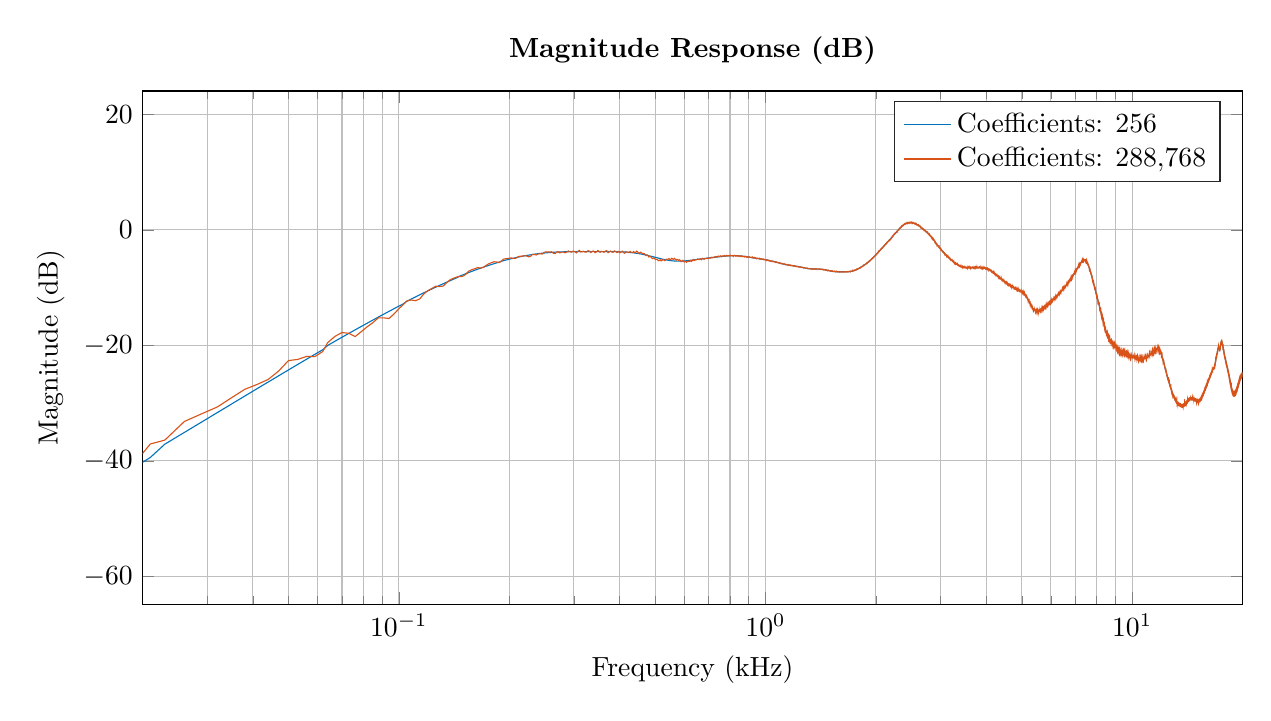
\begin{tikzpicture}

\begin{axis}[%
width=5.5in,
height=2.566in,
at={(2.804in,1.205in)},
scale only axis,
xmode=log,
xmin=0.020,
xmax=20.000,
xminorticks=true,
xlabel={Frequency (kHz)},
xmajorgrids,
xminorgrids,
ymin=-64.832,
ymax=24.080,
ylabel={Magnitude (dB)},
ymajorgrids,
axis background/.style={fill=white},
title style={font=\bfseries},
title={Magnitude Response (dB)},
legend style={legend cell align=left,align=left,draw=white!15!black}
]
\addplot [color=mycolor1,solid,forget plot]
  table[row sep=crcr]{%
0.018	-42.077\\
0.021	-39.419\\
0.023	-37.115\\
0.026	-35.084\\
0.029	-33.272\\
0.032	-31.636\\
0.035	-30.148\\
0.038	-28.784\\
0.041	-27.525\\
0.044	-26.358\\
0.047	-25.271\\
0.050	-24.254\\
0.053	-23.301\\
0.056	-22.403\\
0.059	-21.556\\
0.062	-20.755\\
0.064	-19.995\\
0.067	-19.274\\
0.070	-18.589\\
0.073	-17.935\\
0.076	-17.312\\
0.079	-16.718\\
0.082	-16.149\\
0.085	-15.605\\
0.088	-15.083\\
0.091	-14.584\\
0.094	-14.105\\
0.097	-13.645\\
0.100	-13.203\\
0.103	-12.779\\
0.105	-12.371\\
0.108	-11.979\\
0.111	-11.602\\
0.114	-11.239\\
0.117	-10.890\\
0.120	-10.554\\
0.123	-10.231\\
0.126	-9.920\\
0.129	-9.620\\
0.132	-9.332\\
0.135	-9.055\\
0.138	-8.788\\
0.141	-8.531\\
0.144	-8.284\\
0.146	-8.046\\
0.149	-7.818\\
0.152	-7.598\\
0.155	-7.387\\
0.158	-7.184\\
0.161	-6.990\\
0.164	-6.803\\
0.167	-6.624\\
0.170	-6.452\\
0.173	-6.288\\
0.176	-6.131\\
0.179	-5.980\\
0.182	-5.836\\
0.185	-5.699\\
0.188	-5.568\\
0.190	-5.443\\
0.193	-5.324\\
0.196	-5.211\\
0.199	-5.103\\
0.202	-5.001\\
0.205	-4.904\\
0.208	-4.813\\
0.211	-4.727\\
0.214	-4.645\\
0.217	-4.568\\
0.220	-4.496\\
0.223	-4.428\\
0.226	-4.365\\
0.229	-4.306\\
0.231	-4.251\\
0.234	-4.199\\
0.237	-4.152\\
0.240	-4.108\\
0.243	-4.068\\
0.246	-4.030\\
0.249	-3.996\\
0.252	-3.965\\
0.255	-3.937\\
0.258	-3.912\\
0.261	-3.889\\
0.264	-3.869\\
0.267	-3.850\\
0.270	-3.834\\
0.272	-3.820\\
0.275	-3.808\\
0.278	-3.798\\
0.281	-3.789\\
0.284	-3.781\\
0.287	-3.775\\
0.290	-3.770\\
0.293	-3.766\\
0.296	-3.763\\
0.299	-3.760\\
0.302	-3.759\\
0.305	-3.758\\
0.308	-3.757\\
0.311	-3.757\\
0.313	-3.757\\
0.316	-3.757\\
0.319	-3.757\\
0.322	-3.757\\
0.325	-3.758\\
0.328	-3.758\\
0.331	-3.758\\
0.334	-3.758\\
0.337	-3.759\\
0.340	-3.758\\
0.343	-3.758\\
0.346	-3.758\\
0.349	-3.758\\
0.352	-3.757\\
0.354	-3.757\\
0.357	-3.756\\
0.360	-3.756\\
0.363	-3.755\\
0.366	-3.755\\
0.369	-3.755\\
0.372	-3.755\\
0.375	-3.756\\
0.378	-3.757\\
0.381	-3.758\\
0.384	-3.760\\
0.387	-3.763\\
0.390	-3.767\\
0.393	-3.771\\
0.396	-3.776\\
0.398	-3.782\\
0.401	-3.789\\
0.404	-3.797\\
0.407	-3.806\\
0.410	-3.816\\
0.413	-3.827\\
0.416	-3.840\\
0.419	-3.854\\
0.422	-3.870\\
0.425	-3.886\\
0.428	-3.905\\
0.431	-3.924\\
0.434	-3.945\\
0.437	-3.968\\
0.439	-3.992\\
0.442	-4.017\\
0.445	-4.044\\
0.448	-4.072\\
0.451	-4.102\\
0.454	-4.133\\
0.457	-4.165\\
0.460	-4.198\\
0.463	-4.233\\
0.466	-4.269\\
0.469	-4.305\\
0.472	-4.343\\
0.475	-4.382\\
0.478	-4.421\\
0.480	-4.461\\
0.483	-4.502\\
0.486	-4.543\\
0.489	-4.585\\
0.492	-4.627\\
0.495	-4.668\\
0.498	-4.710\\
0.501	-4.752\\
0.504	-4.793\\
0.507	-4.834\\
0.510	-4.874\\
0.513	-4.914\\
0.516	-4.953\\
0.519	-4.991\\
0.521	-5.028\\
0.524	-5.063\\
0.527	-5.097\\
0.530	-5.130\\
0.533	-5.161\\
0.536	-5.191\\
0.539	-5.219\\
0.542	-5.245\\
0.545	-5.269\\
0.548	-5.291\\
0.551	-5.312\\
0.554	-5.330\\
0.557	-5.346\\
0.560	-5.361\\
0.562	-5.373\\
0.565	-5.383\\
0.568	-5.391\\
0.571	-5.398\\
0.574	-5.402\\
0.577	-5.405\\
0.580	-5.405\\
0.583	-5.405\\
0.586	-5.402\\
0.589	-5.398\\
0.592	-5.392\\
0.595	-5.386\\
0.598	-5.377\\
0.601	-5.368\\
0.604	-5.358\\
0.606	-5.346\\
0.609	-5.334\\
0.612	-5.321\\
0.615	-5.307\\
0.618	-5.293\\
0.621	-5.278\\
0.624	-5.263\\
0.627	-5.247\\
0.630	-5.231\\
0.633	-5.215\\
0.636	-5.199\\
0.639	-5.182\\
0.642	-5.166\\
0.645	-5.149\\
0.647	-5.133\\
0.650	-5.116\\
0.653	-5.100\\
0.656	-5.084\\
0.659	-5.068\\
0.662	-5.052\\
0.665	-5.036\\
0.668	-5.021\\
0.671	-5.005\\
0.674	-4.990\\
0.677	-4.975\\
0.680	-4.960\\
0.683	-4.946\\
0.686	-4.931\\
0.688	-4.917\\
0.691	-4.902\\
0.694	-4.888\\
0.697	-4.874\\
0.700	-4.860\\
0.703	-4.847\\
0.706	-4.833\\
0.709	-4.819\\
0.712	-4.806\\
0.715	-4.792\\
0.718	-4.778\\
0.721	-4.765\\
0.724	-4.751\\
0.727	-4.738\\
0.729	-4.725\\
0.732	-4.711\\
0.735	-4.698\\
0.738	-4.685\\
0.741	-4.672\\
0.744	-4.659\\
0.747	-4.646\\
0.750	-4.633\\
0.753	-4.621\\
0.756	-4.608\\
0.759	-4.596\\
0.762	-4.584\\
0.765	-4.573\\
0.768	-4.561\\
0.771	-4.550\\
0.773	-4.540\\
0.776	-4.530\\
0.779	-4.520\\
0.782	-4.511\\
0.785	-4.502\\
0.788	-4.494\\
0.791	-4.487\\
0.794	-4.480\\
0.797	-4.473\\
0.800	-4.468\\
0.803	-4.463\\
0.806	-4.458\\
0.809	-4.455\\
0.812	-4.452\\
0.814	-4.450\\
0.817	-4.449\\
0.820	-4.449\\
0.823	-4.449\\
0.826	-4.450\\
0.829	-4.452\\
0.832	-4.455\\
0.835	-4.459\\
0.838	-4.463\\
0.841	-4.469\\
0.844	-4.475\\
0.847	-4.481\\
0.850	-4.489\\
0.853	-4.497\\
0.855	-4.506\\
0.858	-4.516\\
0.861	-4.526\\
0.864	-4.537\\
0.867	-4.548\\
0.870	-4.560\\
0.873	-4.573\\
0.876	-4.586\\
0.879	-4.599\\
0.882	-4.613\\
0.885	-4.627\\
0.888	-4.641\\
0.891	-4.656\\
0.894	-4.671\\
0.896	-4.686\\
0.899	-4.701\\
0.902	-4.716\\
0.905	-4.732\\
0.908	-4.747\\
0.911	-4.762\\
0.914	-4.778\\
0.917	-4.793\\
0.920	-4.808\\
0.923	-4.823\\
0.926	-4.838\\
0.929	-4.852\\
0.932	-4.867\\
0.935	-4.881\\
0.938	-4.895\\
0.940	-4.909\\
0.943	-4.923\\
0.946	-4.937\\
0.949	-4.950\\
0.952	-4.963\\
0.955	-4.976\\
0.958	-4.989\\
0.961	-5.001\\
0.964	-5.014\\
0.967	-5.026\\
0.970	-5.039\\
0.973	-5.051\\
0.976	-5.063\\
0.979	-5.075\\
0.981	-5.088\\
0.984	-5.100\\
0.987	-5.112\\
0.990	-5.125\\
0.993	-5.138\\
0.996	-5.150\\
0.999	-5.164\\
1.002	-5.177\\
1.005	-5.190\\
1.008	-5.204\\
1.011	-5.219\\
1.014	-5.233\\
1.017	-5.248\\
1.020	-5.263\\
1.022	-5.279\\
1.025	-5.295\\
1.028	-5.311\\
1.031	-5.328\\
1.034	-5.345\\
1.037	-5.362\\
1.040	-5.380\\
1.043	-5.398\\
1.046	-5.417\\
1.049	-5.436\\
1.052	-5.455\\
1.055	-5.475\\
1.058	-5.494\\
1.061	-5.515\\
1.063	-5.535\\
1.066	-5.555\\
1.069	-5.576\\
1.072	-5.597\\
1.075	-5.618\\
1.078	-5.638\\
1.081	-5.659\\
1.084	-5.680\\
1.087	-5.701\\
1.090	-5.721\\
1.093	-5.742\\
1.096	-5.762\\
1.099	-5.782\\
1.102	-5.802\\
1.104	-5.821\\
1.107	-5.841\\
1.110	-5.859\\
1.113	-5.878\\
1.116	-5.896\\
1.119	-5.913\\
1.122	-5.930\\
1.125	-5.947\\
1.128	-5.963\\
1.131	-5.978\\
1.134	-5.994\\
1.137	-6.008\\
1.140	-6.022\\
1.143	-6.036\\
1.146	-6.049\\
1.148	-6.062\\
1.151	-6.074\\
1.154	-6.086\\
1.157	-6.098\\
1.160	-6.109\\
1.163	-6.120\\
1.166	-6.130\\
1.169	-6.140\\
1.172	-6.150\\
1.175	-6.160\\
1.178	-6.170\\
1.181	-6.179\\
1.184	-6.189\\
1.187	-6.198\\
1.189	-6.208\\
1.192	-6.217\\
1.195	-6.227\\
1.198	-6.236\\
1.201	-6.246\\
1.204	-6.256\\
1.207	-6.266\\
1.210	-6.276\\
1.213	-6.287\\
1.216	-6.298\\
1.219	-6.309\\
1.222	-6.320\\
1.225	-6.331\\
1.228	-6.343\\
1.230	-6.355\\
1.233	-6.368\\
1.236	-6.380\\
1.239	-6.393\\
1.242	-6.406\\
1.245	-6.420\\
1.248	-6.433\\
1.251	-6.447\\
1.254	-6.461\\
1.257	-6.475\\
1.260	-6.489\\
1.263	-6.503\\
1.266	-6.517\\
1.269	-6.531\\
1.271	-6.545\\
1.274	-6.559\\
1.277	-6.573\\
1.280	-6.587\\
1.283	-6.600\\
1.286	-6.613\\
1.289	-6.626\\
1.292	-6.638\\
1.295	-6.650\\
1.298	-6.661\\
1.301	-6.672\\
1.304	-6.683\\
1.307	-6.693\\
1.310	-6.702\\
1.312	-6.711\\
1.315	-6.720\\
1.318	-6.727\\
1.321	-6.734\\
1.324	-6.741\\
1.327	-6.747\\
1.330	-6.752\\
1.333	-6.757\\
1.336	-6.761\\
1.339	-6.765\\
1.342	-6.768\\
1.345	-6.770\\
1.348	-6.772\\
1.351	-6.774\\
1.354	-6.775\\
1.356	-6.776\\
1.359	-6.777\\
1.362	-6.777\\
1.365	-6.777\\
1.368	-6.777\\
1.371	-6.777\\
1.374	-6.777\\
1.377	-6.777\\
1.380	-6.777\\
1.383	-6.777\\
1.386	-6.777\\
1.389	-6.777\\
1.392	-6.778\\
1.395	-6.778\\
1.397	-6.780\\
1.400	-6.781\\
1.403	-6.783\\
1.406	-6.785\\
1.409	-6.788\\
1.412	-6.791\\
1.415	-6.795\\
1.418	-6.800\\
1.421	-6.804\\
1.424	-6.810\\
1.427	-6.816\\
1.430	-6.823\\
1.433	-6.830\\
1.436	-6.837\\
1.438	-6.846\\
1.441	-6.855\\
1.444	-6.864\\
1.447	-6.874\\
1.450	-6.884\\
1.453	-6.895\\
1.456	-6.906\\
1.459	-6.918\\
1.462	-6.930\\
1.465	-6.942\\
1.468	-6.955\\
1.471	-6.967\\
1.474	-6.980\\
1.477	-6.993\\
1.479	-7.006\\
1.482	-7.020\\
1.485	-7.033\\
1.488	-7.046\\
1.491	-7.059\\
1.494	-7.071\\
1.497	-7.084\\
1.500	-7.096\\
1.503	-7.108\\
1.506	-7.120\\
1.509	-7.131\\
1.512	-7.142\\
1.515	-7.153\\
1.518	-7.162\\
1.521	-7.172\\
1.523	-7.181\\
1.526	-7.189\\
1.529	-7.197\\
1.532	-7.204\\
1.535	-7.211\\
1.538	-7.217\\
1.541	-7.222\\
1.544	-7.227\\
1.547	-7.232\\
1.550	-7.236\\
1.553	-7.239\\
1.556	-7.242\\
1.559	-7.244\\
1.562	-7.246\\
1.564	-7.248\\
1.567	-7.249\\
1.570	-7.250\\
1.573	-7.251\\
1.576	-7.251\\
1.579	-7.251\\
1.582	-7.251\\
1.585	-7.250\\
1.588	-7.250\\
1.591	-7.249\\
1.594	-7.248\\
1.597	-7.247\\
1.600	-7.247\\
1.603	-7.246\\
1.605	-7.245\\
1.608	-7.244\\
1.611	-7.244\\
1.614	-7.243\\
1.617	-7.243\\
1.620	-7.242\\
1.623	-7.242\\
1.626	-7.242\\
1.629	-7.242\\
1.632	-7.242\\
1.635	-7.242\\
1.638	-7.242\\
1.641	-7.243\\
1.644	-7.243\\
1.646	-7.243\\
1.649	-7.244\\
1.652	-7.244\\
1.655	-7.244\\
1.658	-7.245\\
1.661	-7.245\\
1.664	-7.245\\
1.667	-7.244\\
1.670	-7.244\\
1.673	-7.243\\
1.676	-7.242\\
1.679	-7.240\\
1.682	-7.238\\
1.685	-7.236\\
1.688	-7.233\\
1.690	-7.230\\
1.693	-7.226\\
1.696	-7.221\\
1.699	-7.216\\
1.702	-7.210\\
1.705	-7.204\\
1.708	-7.196\\
1.711	-7.188\\
1.714	-7.180\\
1.717	-7.170\\
1.720	-7.160\\
1.723	-7.149\\
1.726	-7.137\\
1.729	-7.125\\
1.731	-7.111\\
1.734	-7.097\\
1.737	-7.082\\
1.740	-7.067\\
1.743	-7.050\\
1.746	-7.033\\
1.749	-7.016\\
1.752	-6.997\\
1.755	-6.978\\
1.758	-6.959\\
1.761	-6.938\\
1.764	-6.917\\
1.767	-6.896\\
1.770	-6.874\\
1.772	-6.852\\
1.775	-6.829\\
1.778	-6.806\\
1.781	-6.783\\
1.784	-6.759\\
1.787	-6.735\\
1.790	-6.711\\
1.793	-6.686\\
1.796	-6.661\\
1.799	-6.636\\
1.802	-6.611\\
1.805	-6.586\\
1.808	-6.560\\
1.811	-6.534\\
1.813	-6.509\\
1.816	-6.483\\
1.819	-6.457\\
1.822	-6.431\\
1.825	-6.404\\
1.828	-6.378\\
1.831	-6.352\\
1.834	-6.325\\
1.837	-6.298\\
1.840	-6.271\\
1.843	-6.244\\
1.846	-6.217\\
1.849	-6.190\\
1.852	-6.162\\
1.854	-6.135\\
1.857	-6.107\\
1.860	-6.078\\
1.863	-6.050\\
1.866	-6.021\\
1.869	-5.992\\
1.872	-5.963\\
1.875	-5.933\\
1.878	-5.903\\
1.881	-5.872\\
1.884	-5.841\\
1.887	-5.810\\
1.890	-5.778\\
1.893	-5.746\\
1.896	-5.713\\
1.898	-5.680\\
1.901	-5.647\\
1.904	-5.613\\
1.907	-5.578\\
1.910	-5.543\\
1.913	-5.508\\
1.916	-5.472\\
1.919	-5.435\\
1.922	-5.398\\
1.925	-5.361\\
1.928	-5.323\\
1.931	-5.285\\
1.934	-5.246\\
1.937	-5.207\\
1.939	-5.168\\
1.942	-5.128\\
1.945	-5.088\\
1.948	-5.047\\
1.951	-5.006\\
1.954	-4.965\\
1.957	-4.924\\
1.960	-4.882\\
1.963	-4.840\\
1.966	-4.798\\
1.969	-4.755\\
1.972	-4.713\\
1.975	-4.670\\
1.978	-4.627\\
1.980	-4.584\\
1.983	-4.541\\
1.986	-4.498\\
1.989	-4.455\\
1.992	-4.411\\
1.995	-4.368\\
1.998	-4.325\\
2.001	-4.281\\
2.004	-4.238\\
2.007	-4.195\\
2.010	-4.151\\
2.013	-4.108\\
2.016	-4.065\\
2.019	-4.021\\
2.021	-3.978\\
2.024	-3.935\\
2.027	-3.892\\
2.030	-3.849\\
2.033	-3.807\\
2.036	-3.764\\
2.039	-3.721\\
2.042	-3.678\\
2.045	-3.636\\
2.048	-3.593\\
2.051	-3.551\\
2.054	-3.509\\
2.057	-3.466\\
2.060	-3.424\\
2.062	-3.382\\
2.065	-3.340\\
2.068	-3.298\\
2.071	-3.256\\
2.074	-3.214\\
2.077	-3.172\\
2.080	-3.130\\
2.083	-3.088\\
2.086	-3.047\\
2.089	-3.005\\
2.092	-2.963\\
2.095	-2.921\\
2.098	-2.880\\
2.101	-2.838\\
2.104	-2.796\\
2.106	-2.755\\
2.109	-2.713\\
2.112	-2.672\\
2.115	-2.630\\
2.118	-2.588\\
2.121	-2.547\\
2.124	-2.505\\
2.127	-2.464\\
2.130	-2.422\\
2.133	-2.381\\
2.136	-2.339\\
2.139	-2.298\\
2.142	-2.256\\
2.145	-2.215\\
2.147	-2.174\\
2.150	-2.132\\
2.153	-2.091\\
2.156	-2.049\\
2.159	-2.008\\
2.162	-1.967\\
2.165	-1.925\\
2.168	-1.884\\
2.171	-1.843\\
2.174	-1.801\\
2.177	-1.760\\
2.180	-1.718\\
2.183	-1.677\\
2.186	-1.636\\
2.188	-1.594\\
2.191	-1.553\\
2.194	-1.512\\
2.197	-1.470\\
2.200	-1.429\\
2.203	-1.388\\
2.206	-1.346\\
2.209	-1.305\\
2.212	-1.263\\
2.215	-1.222\\
2.218	-1.181\\
2.221	-1.139\\
2.224	-1.098\\
2.227	-1.056\\
2.229	-1.015\\
2.232	-0.973\\
2.235	-0.932\\
2.238	-0.890\\
2.241	-0.848\\
2.244	-0.807\\
2.247	-0.765\\
2.250	-0.724\\
2.253	-0.682\\
2.256	-0.641\\
2.259	-0.599\\
2.262	-0.558\\
2.265	-0.517\\
2.268	-0.476\\
2.271	-0.434\\
2.273	-0.393\\
2.276	-0.352\\
2.279	-0.312\\
2.282	-0.271\\
2.285	-0.230\\
2.288	-0.190\\
2.291	-0.150\\
2.294	-0.110\\
2.297	-0.070\\
2.300	-0.031\\
2.303	0.009\\
2.306	0.047\\
2.309	0.086\\
2.312	0.124\\
2.314	0.162\\
2.317	0.200\\
2.320	0.237\\
2.323	0.274\\
2.326	0.310\\
2.329	0.346\\
2.332	0.381\\
2.335	0.416\\
2.338	0.450\\
2.341	0.484\\
2.344	0.517\\
2.347	0.550\\
2.350	0.582\\
2.353	0.613\\
2.355	0.644\\
2.358	0.674\\
2.361	0.704\\
2.364	0.733\\
2.367	0.761\\
2.370	0.788\\
2.373	0.815\\
2.376	0.841\\
2.379	0.867\\
2.382	0.891\\
2.385	0.915\\
2.388	0.938\\
2.391	0.960\\
2.394	0.982\\
2.396	1.002\\
2.399	1.022\\
2.402	1.042\\
2.405	1.060\\
2.408	1.077\\
2.411	1.094\\
2.414	1.110\\
2.417	1.126\\
2.420	1.140\\
2.423	1.154\\
2.426	1.167\\
2.429	1.179\\
2.432	1.190\\
2.435	1.201\\
2.438	1.211\\
2.440	1.220\\
2.443	1.228\\
2.446	1.236\\
2.449	1.243\\
2.452	1.249\\
2.455	1.255\\
2.458	1.260\\
2.461	1.264\\
2.464	1.268\\
2.467	1.270\\
2.470	1.273\\
2.473	1.274\\
2.476	1.275\\
2.479	1.276\\
2.481	1.275\\
2.484	1.275\\
2.487	1.273\\
2.490	1.271\\
2.493	1.269\\
2.496	1.266\\
2.499	1.262\\
2.502	1.258\\
2.505	1.253\\
2.508	1.248\\
2.511	1.242\\
2.514	1.236\\
2.517	1.229\\
2.520	1.222\\
2.522	1.214\\
2.525	1.206\\
2.528	1.198\\
2.531	1.189\\
2.534	1.179\\
2.537	1.169\\
2.540	1.159\\
2.543	1.148\\
2.546	1.136\\
2.549	1.125\\
2.552	1.113\\
2.555	1.100\\
2.558	1.087\\
2.561	1.074\\
2.563	1.060\\
2.566	1.046\\
2.569	1.031\\
2.572	1.016\\
2.575	1.001\\
2.578	0.985\\
2.581	0.969\\
2.584	0.952\\
2.587	0.936\\
2.590	0.918\\
2.593	0.901\\
2.596	0.883\\
2.599	0.864\\
2.602	0.846\\
2.604	0.827\\
2.607	0.807\\
2.610	0.788\\
2.613	0.768\\
2.616	0.747\\
2.619	0.727\\
2.622	0.706\\
2.625	0.685\\
2.628	0.663\\
2.631	0.641\\
2.634	0.620\\
2.637	0.597\\
2.640	0.575\\
2.643	0.552\\
2.646	0.529\\
2.648	0.506\\
2.651	0.483\\
2.654	0.459\\
2.657	0.436\\
2.660	0.412\\
2.663	0.388\\
2.666	0.364\\
2.669	0.340\\
2.672	0.315\\
2.675	0.291\\
2.678	0.266\\
2.681	0.242\\
2.684	0.217\\
2.687	0.192\\
2.689	0.167\\
2.692	0.142\\
2.695	0.117\\
2.698	0.092\\
2.701	0.067\\
2.704	0.041\\
2.707	0.016\\
2.710	-0.009\\
2.713	-0.035\\
2.716	-0.060\\
2.719	-0.086\\
2.722	-0.111\\
2.725	-0.137\\
2.728	-0.163\\
2.730	-0.189\\
2.733	-0.214\\
2.736	-0.240\\
2.739	-0.266\\
2.742	-0.293\\
2.745	-0.319\\
2.748	-0.345\\
2.751	-0.372\\
2.754	-0.398\\
2.757	-0.425\\
2.760	-0.452\\
2.763	-0.479\\
2.766	-0.507\\
2.769	-0.534\\
2.771	-0.562\\
2.774	-0.590\\
2.777	-0.618\\
2.780	-0.647\\
2.783	-0.675\\
2.786	-0.704\\
2.789	-0.734\\
2.792	-0.763\\
2.795	-0.793\\
2.798	-0.823\\
2.801	-0.854\\
2.804	-0.884\\
2.807	-0.916\\
2.810	-0.947\\
2.812	-0.979\\
2.815	-1.011\\
2.818	-1.043\\
2.821	-1.076\\
2.824	-1.109\\
2.827	-1.143\\
2.830	-1.177\\
2.833	-1.211\\
2.836	-1.245\\
2.839	-1.280\\
2.842	-1.315\\
2.845	-1.351\\
2.848	-1.387\\
2.851	-1.423\\
2.854	-1.459\\
2.856	-1.496\\
2.859	-1.533\\
2.862	-1.570\\
2.865	-1.607\\
2.868	-1.644\\
2.871	-1.682\\
2.874	-1.720\\
2.877	-1.758\\
2.880	-1.796\\
2.883	-1.835\\
2.886	-1.873\\
2.889	-1.911\\
2.892	-1.950\\
2.895	-1.989\\
2.897	-2.027\\
2.900	-2.066\\
2.903	-2.104\\
2.906	-2.143\\
2.909	-2.181\\
2.912	-2.220\\
2.915	-2.258\\
2.918	-2.296\\
2.921	-2.334\\
2.924	-2.372\\
2.927	-2.410\\
2.930	-2.447\\
2.933	-2.485\\
2.936	-2.522\\
2.938	-2.559\\
2.941	-2.595\\
2.944	-2.632\\
2.947	-2.668\\
2.950	-2.704\\
2.953	-2.740\\
2.956	-2.776\\
2.959	-2.811\\
2.962	-2.846\\
2.965	-2.881\\
2.968	-2.915\\
2.971	-2.950\\
2.974	-2.984\\
2.977	-3.018\\
2.979	-3.051\\
2.982	-3.085\\
2.985	-3.118\\
2.988	-3.151\\
2.991	-3.184\\
2.994	-3.216\\
2.997	-3.248\\
3.000	-3.281\\
3.003	-3.313\\
3.006	-3.344\\
3.009	-3.376\\
3.012	-3.407\\
3.015	-3.439\\
3.018	-3.470\\
3.021	-3.501\\
3.023	-3.531\\
3.026	-3.562\\
3.029	-3.593\\
3.032	-3.623\\
3.035	-3.653\\
3.038	-3.684\\
3.041	-3.714\\
3.044	-3.744\\
3.047	-3.773\\
3.050	-3.803\\
3.053	-3.833\\
3.056	-3.862\\
3.059	-3.891\\
3.062	-3.921\\
3.064	-3.950\\
3.067	-3.979\\
3.070	-4.007\\
3.073	-4.036\\
3.076	-4.064\\
3.079	-4.093\\
3.082	-4.121\\
3.085	-4.149\\
3.088	-4.177\\
3.091	-4.204\\
3.094	-4.232\\
3.097	-4.259\\
3.100	-4.286\\
3.103	-4.313\\
3.105	-4.340\\
3.108	-4.366\\
3.111	-4.392\\
3.114	-4.418\\
3.117	-4.444\\
3.120	-4.470\\
3.123	-4.495\\
3.126	-4.521\\
3.129	-4.546\\
3.132	-4.570\\
3.135	-4.595\\
3.138	-4.619\\
3.141	-4.644\\
3.144	-4.668\\
3.146	-4.691\\
3.149	-4.715\\
3.152	-4.739\\
3.155	-4.762\\
3.158	-4.785\\
3.161	-4.808\\
3.164	-4.831\\
3.167	-4.853\\
3.170	-4.876\\
3.173	-4.898\\
3.176	-4.921\\
3.179	-4.943\\
3.182	-4.965\\
3.185	-4.987\\
3.188	-5.009\\
3.190	-5.030\\
3.193	-5.052\\
3.196	-5.074\\
3.199	-5.096\\
3.202	-5.117\\
3.205	-5.139\\
3.208	-5.160\\
3.211	-5.182\\
3.214	-5.203\\
3.217	-5.224\\
3.220	-5.246\\
3.223	-5.267\\
3.226	-5.288\\
3.229	-5.309\\
3.231	-5.330\\
3.234	-5.352\\
3.237	-5.373\\
3.240	-5.394\\
3.243	-5.415\\
3.246	-5.435\\
3.249	-5.456\\
3.252	-5.477\\
3.255	-5.497\\
3.258	-5.518\\
3.261	-5.538\\
3.264	-5.558\\
3.267	-5.579\\
3.270	-5.599\\
3.272	-5.618\\
3.275	-5.638\\
3.278	-5.657\\
3.281	-5.677\\
3.284	-5.696\\
3.287	-5.715\\
3.290	-5.733\\
3.293	-5.752\\
3.296	-5.770\\
3.299	-5.788\\
3.302	-5.805\\
3.305	-5.823\\
3.308	-5.840\\
3.311	-5.857\\
3.313	-5.873\\
3.316	-5.890\\
3.319	-5.906\\
3.322	-5.921\\
3.325	-5.937\\
3.328	-5.952\\
3.331	-5.967\\
3.334	-5.982\\
3.337	-5.996\\
3.340	-6.010\\
3.343	-6.024\\
3.346	-6.038\\
3.349	-6.051\\
3.352	-6.064\\
3.354	-6.077\\
3.357	-6.090\\
3.360	-6.102\\
3.363	-6.114\\
3.366	-6.126\\
3.369	-6.138\\
3.372	-6.149\\
3.375	-6.161\\
3.378	-6.172\\
3.381	-6.183\\
3.384	-6.194\\
3.387	-6.205\\
3.390	-6.215\\
3.393	-6.225\\
3.396	-6.236\\
3.398	-6.246\\
3.401	-6.256\\
3.404	-6.266\\
3.407	-6.275\\
3.410	-6.285\\
3.413	-6.295\\
3.416	-6.304\\
3.419	-6.313\\
3.422	-6.322\\
3.425	-6.331\\
3.428	-6.340\\
3.431	-6.349\\
3.434	-6.357\\
3.437	-6.365\\
3.439	-6.374\\
3.442	-6.382\\
3.445	-6.390\\
3.448	-6.397\\
3.451	-6.405\\
3.454	-6.412\\
3.457	-6.419\\
3.460	-6.426\\
3.463	-6.433\\
3.466	-6.440\\
3.469	-6.446\\
3.472	-6.452\\
3.475	-6.458\\
3.478	-6.463\\
3.480	-6.469\\
3.483	-6.474\\
3.486	-6.479\\
3.489	-6.483\\
3.492	-6.488\\
3.495	-6.492\\
3.498	-6.495\\
3.501	-6.499\\
3.504	-6.502\\
3.507	-6.505\\
3.510	-6.508\\
3.513	-6.511\\
3.516	-6.513\\
3.519	-6.515\\
3.521	-6.517\\
3.524	-6.519\\
3.527	-6.521\\
3.530	-6.522\\
3.533	-6.523\\
3.536	-6.524\\
3.539	-6.525\\
3.542	-6.525\\
3.545	-6.526\\
3.548	-6.526\\
3.551	-6.527\\
3.554	-6.527\\
3.557	-6.527\\
3.560	-6.527\\
3.562	-6.527\\
3.565	-6.527\\
3.568	-6.526\\
3.571	-6.526\\
3.574	-6.526\\
3.577	-6.526\\
3.580	-6.526\\
3.583	-6.525\\
3.586	-6.525\\
3.589	-6.525\\
3.592	-6.525\\
3.595	-6.525\\
3.598	-6.525\\
3.601	-6.525\\
3.604	-6.525\\
3.606	-6.525\\
3.609	-6.525\\
3.612	-6.525\\
3.615	-6.525\\
3.618	-6.525\\
3.621	-6.525\\
3.624	-6.526\\
3.627	-6.526\\
3.630	-6.526\\
3.633	-6.527\\
3.636	-6.527\\
3.639	-6.527\\
3.642	-6.528\\
3.645	-6.528\\
3.647	-6.529\\
3.650	-6.529\\
3.653	-6.529\\
3.656	-6.529\\
3.659	-6.530\\
3.662	-6.530\\
3.665	-6.530\\
3.668	-6.530\\
3.671	-6.530\\
3.674	-6.530\\
3.677	-6.530\\
3.680	-6.530\\
3.683	-6.529\\
3.686	-6.529\\
3.688	-6.528\\
3.691	-6.528\\
3.694	-6.527\\
3.697	-6.526\\
3.700	-6.526\\
3.703	-6.525\\
3.706	-6.524\\
3.709	-6.522\\
3.712	-6.521\\
3.715	-6.520\\
3.718	-6.519\\
3.721	-6.517\\
3.724	-6.516\\
3.727	-6.515\\
3.729	-6.513\\
3.732	-6.512\\
3.735	-6.510\\
3.738	-6.509\\
3.741	-6.507\\
3.744	-6.506\\
3.747	-6.504\\
3.750	-6.503\\
3.753	-6.501\\
3.756	-6.500\\
3.759	-6.498\\
3.762	-6.497\\
3.765	-6.496\\
3.768	-6.495\\
3.771	-6.494\\
3.773	-6.493\\
3.776	-6.492\\
3.779	-6.492\\
3.782	-6.491\\
3.785	-6.491\\
3.788	-6.490\\
3.791	-6.490\\
3.794	-6.490\\
3.797	-6.490\\
3.800	-6.490\\
3.803	-6.491\\
3.806	-6.491\\
3.809	-6.492\\
3.812	-6.492\\
3.814	-6.493\\
3.817	-6.494\\
3.820	-6.495\\
3.823	-6.497\\
3.826	-6.498\\
3.829	-6.499\\
3.832	-6.501\\
3.835	-6.502\\
3.838	-6.504\\
3.841	-6.506\\
3.844	-6.507\\
3.847	-6.509\\
3.850	-6.511\\
3.853	-6.513\\
3.855	-6.515\\
3.858	-6.517\\
3.861	-6.519\\
3.864	-6.521\\
3.867	-6.523\\
3.870	-6.526\\
3.873	-6.528\\
3.876	-6.530\\
3.879	-6.532\\
3.882	-6.534\\
3.885	-6.536\\
3.888	-6.538\\
3.891	-6.541\\
3.894	-6.543\\
3.896	-6.545\\
3.899	-6.547\\
3.902	-6.549\\
3.905	-6.551\\
3.908	-6.554\\
3.911	-6.556\\
3.914	-6.558\\
3.917	-6.560\\
3.920	-6.563\\
3.923	-6.565\\
3.926	-6.568\\
3.929	-6.570\\
3.932	-6.573\\
3.935	-6.576\\
3.938	-6.578\\
3.940	-6.581\\
3.943	-6.584\\
3.946	-6.588\\
3.949	-6.591\\
3.952	-6.594\\
3.955	-6.598\\
3.958	-6.602\\
3.961	-6.606\\
3.964	-6.610\\
3.967	-6.614\\
3.970	-6.619\\
3.973	-6.624\\
3.976	-6.629\\
3.979	-6.634\\
3.981	-6.639\\
3.984	-6.645\\
3.987	-6.651\\
3.990	-6.657\\
3.993	-6.663\\
3.996	-6.670\\
3.999	-6.677\\
4.002	-6.684\\
4.005	-6.691\\
4.008	-6.698\\
4.011	-6.706\\
4.014	-6.714\\
4.017	-6.722\\
4.020	-6.730\\
4.022	-6.739\\
4.025	-6.747\\
4.028	-6.756\\
4.031	-6.765\\
4.034	-6.775\\
4.037	-6.784\\
4.040	-6.793\\
4.043	-6.803\\
4.046	-6.813\\
4.049	-6.823\\
4.052	-6.833\\
4.055	-6.843\\
4.058	-6.853\\
4.061	-6.864\\
4.063	-6.874\\
4.066	-6.885\\
4.069	-6.895\\
4.072	-6.906\\
4.075	-6.917\\
4.078	-6.928\\
4.081	-6.939\\
4.084	-6.950\\
4.087	-6.961\\
4.090	-6.972\\
4.093	-6.983\\
4.096	-6.994\\
4.099	-7.005\\
4.102	-7.016\\
4.104	-7.028\\
4.107	-7.039\\
4.110	-7.051\\
4.113	-7.062\\
4.116	-7.074\\
4.119	-7.085\\
4.122	-7.097\\
4.125	-7.109\\
4.128	-7.121\\
4.131	-7.133\\
4.134	-7.145\\
4.137	-7.157\\
4.140	-7.170\\
4.143	-7.182\\
4.146	-7.195\\
4.148	-7.208\\
4.151	-7.221\\
4.154	-7.234\\
4.157	-7.247\\
4.160	-7.261\\
4.163	-7.275\\
4.166	-7.288\\
4.169	-7.302\\
4.172	-7.317\\
4.175	-7.331\\
4.178	-7.346\\
4.181	-7.360\\
4.184	-7.375\\
4.187	-7.390\\
4.189	-7.406\\
4.192	-7.421\\
4.195	-7.437\\
4.198	-7.453\\
4.201	-7.469\\
4.204	-7.485\\
4.207	-7.501\\
4.210	-7.518\\
4.213	-7.534\\
4.216	-7.551\\
4.219	-7.568\\
4.222	-7.584\\
4.225	-7.601\\
4.228	-7.618\\
4.230	-7.636\\
4.233	-7.653\\
4.236	-7.670\\
4.239	-7.687\\
4.242	-7.704\\
4.245	-7.721\\
4.248	-7.738\\
4.251	-7.755\\
4.254	-7.772\\
4.257	-7.789\\
4.260	-7.806\\
4.263	-7.823\\
4.266	-7.840\\
4.269	-7.856\\
4.271	-7.873\\
4.274	-7.889\\
4.277	-7.905\\
4.280	-7.921\\
4.283	-7.937\\
4.286	-7.953\\
4.289	-7.969\\
4.292	-7.984\\
4.295	-8.000\\
4.298	-8.015\\
4.301	-8.030\\
4.304	-8.045\\
4.307	-8.060\\
4.310	-8.074\\
4.312	-8.089\\
4.315	-8.103\\
4.318	-8.117\\
4.321	-8.132\\
4.324	-8.146\\
4.327	-8.160\\
4.330	-8.174\\
4.333	-8.188\\
4.336	-8.202\\
4.339	-8.216\\
4.342	-8.229\\
4.345	-8.243\\
4.348	-8.257\\
4.351	-8.271\\
4.354	-8.285\\
4.356	-8.299\\
4.359	-8.313\\
4.362	-8.327\\
4.365	-8.341\\
4.368	-8.355\\
4.371	-8.369\\
4.374	-8.384\\
4.377	-8.398\\
4.380	-8.413\\
4.383	-8.427\\
4.386	-8.442\\
4.389	-8.457\\
4.392	-8.472\\
4.395	-8.487\\
4.397	-8.502\\
4.400	-8.517\\
4.403	-8.532\\
4.406	-8.548\\
4.409	-8.563\\
4.412	-8.579\\
4.415	-8.595\\
4.418	-8.610\\
4.421	-8.626\\
4.424	-8.642\\
4.427	-8.658\\
4.430	-8.673\\
4.433	-8.689\\
4.436	-8.705\\
4.438	-8.721\\
4.441	-8.736\\
4.444	-8.752\\
4.447	-8.767\\
4.450	-8.783\\
4.453	-8.798\\
4.456	-8.813\\
4.459	-8.829\\
4.462	-8.844\\
4.465	-8.858\\
4.468	-8.873\\
4.471	-8.888\\
4.474	-8.902\\
4.477	-8.916\\
4.479	-8.930\\
4.482	-8.944\\
4.485	-8.958\\
4.488	-8.971\\
4.491	-8.985\\
4.494	-8.998\\
4.497	-9.011\\
4.500	-9.023\\
4.503	-9.036\\
4.506	-9.048\\
4.509	-9.061\\
4.512	-9.073\\
4.515	-9.085\\
4.518	-9.097\\
4.521	-9.108\\
4.523	-9.120\\
4.526	-9.131\\
4.529	-9.143\\
4.532	-9.154\\
4.535	-9.165\\
4.538	-9.177\\
4.541	-9.188\\
4.544	-9.199\\
4.547	-9.210\\
4.550	-9.221\\
4.553	-9.233\\
4.556	-9.244\\
4.559	-9.255\\
4.562	-9.266\\
4.564	-9.278\\
4.567	-9.289\\
4.570	-9.300\\
4.573	-9.312\\
4.576	-9.324\\
4.579	-9.335\\
4.582	-9.347\\
4.585	-9.359\\
4.588	-9.371\\
4.591	-9.383\\
4.594	-9.395\\
4.597	-9.407\\
4.600	-9.420\\
4.603	-9.432\\
4.605	-9.444\\
4.608	-9.457\\
4.611	-9.470\\
4.614	-9.482\\
4.617	-9.495\\
4.620	-9.507\\
4.623	-9.520\\
4.626	-9.533\\
4.629	-9.545\\
4.632	-9.558\\
4.635	-9.571\\
4.638	-9.583\\
4.641	-9.596\\
4.644	-9.608\\
4.646	-9.620\\
4.649	-9.633\\
4.652	-9.645\\
4.655	-9.657\\
4.658	-9.669\\
4.661	-9.680\\
4.664	-9.692\\
4.667	-9.703\\
4.670	-9.715\\
4.673	-9.726\\
4.676	-9.737\\
4.679	-9.747\\
4.682	-9.758\\
4.685	-9.768\\
4.688	-9.778\\
4.690	-9.788\\
4.693	-9.798\\
4.696	-9.808\\
4.699	-9.817\\
4.702	-9.827\\
4.705	-9.836\\
4.708	-9.845\\
4.711	-9.854\\
4.714	-9.863\\
4.717	-9.871\\
4.720	-9.880\\
4.723	-9.888\\
4.726	-9.897\\
4.729	-9.905\\
4.731	-9.913\\
4.734	-9.921\\
4.737	-9.929\\
4.740	-9.938\\
4.743	-9.946\\
4.746	-9.954\\
4.749	-9.962\\
4.752	-9.970\\
4.755	-9.978\\
4.758	-9.987\\
4.761	-9.995\\
4.764	-10.003\\
4.767	-10.012\\
4.770	-10.020\\
4.772	-10.029\\
4.775	-10.037\\
4.778	-10.046\\
4.781	-10.055\\
4.784	-10.064\\
4.787	-10.073\\
4.790	-10.082\\
4.793	-10.091\\
4.796	-10.100\\
4.799	-10.110\\
4.802	-10.119\\
4.805	-10.128\\
4.808	-10.138\\
4.811	-10.147\\
4.813	-10.157\\
4.816	-10.166\\
4.819	-10.176\\
4.822	-10.185\\
4.825	-10.195\\
4.828	-10.204\\
4.831	-10.214\\
4.834	-10.223\\
4.837	-10.232\\
4.840	-10.242\\
4.843	-10.251\\
4.846	-10.260\\
4.849	-10.269\\
4.852	-10.278\\
4.854	-10.286\\
4.857	-10.295\\
4.860	-10.304\\
4.863	-10.312\\
4.866	-10.320\\
4.869	-10.328\\
4.872	-10.336\\
4.875	-10.344\\
4.878	-10.352\\
4.881	-10.360\\
4.884	-10.367\\
4.887	-10.374\\
4.890	-10.382\\
4.893	-10.389\\
4.896	-10.396\\
4.898	-10.403\\
4.901	-10.410\\
4.904	-10.416\\
4.907	-10.423\\
4.910	-10.430\\
4.913	-10.437\\
4.916	-10.443\\
4.919	-10.450\\
4.922	-10.457\\
4.925	-10.464\\
4.928	-10.471\\
4.931	-10.477\\
4.934	-10.484\\
4.937	-10.492\\
4.939	-10.499\\
4.942	-10.506\\
4.945	-10.514\\
4.948	-10.521\\
4.951	-10.529\\
4.954	-10.537\\
4.957	-10.546\\
4.960	-10.554\\
4.963	-10.563\\
4.966	-10.572\\
4.969	-10.581\\
4.972	-10.590\\
4.975	-10.600\\
4.978	-10.610\\
4.980	-10.620\\
4.983	-10.630\\
4.986	-10.641\\
4.989	-10.652\\
4.992	-10.663\\
4.995	-10.675\\
4.998	-10.686\\
5.001	-10.698\\
5.004	-10.711\\
5.007	-10.723\\
5.010	-10.736\\
5.013	-10.749\\
5.016	-10.762\\
5.019	-10.775\\
5.021	-10.789\\
5.024	-10.803\\
5.027	-10.817\\
5.030	-10.831\\
5.033	-10.845\\
5.036	-10.860\\
5.039	-10.874\\
5.042	-10.889\\
5.045	-10.904\\
5.048	-10.919\\
5.051	-10.935\\
5.054	-10.950\\
5.057	-10.965\\
5.060	-10.981\\
5.062	-10.997\\
5.065	-11.013\\
5.068	-11.029\\
5.071	-11.045\\
5.074	-11.062\\
5.077	-11.078\\
5.080	-11.095\\
5.083	-11.111\\
5.086	-11.128\\
5.089	-11.146\\
5.092	-11.163\\
5.095	-11.180\\
5.098	-11.198\\
5.101	-11.216\\
5.104	-11.234\\
5.106	-11.253\\
5.109	-11.271\\
5.112	-11.290\\
5.115	-11.309\\
5.118	-11.329\\
5.121	-11.349\\
5.124	-11.369\\
5.127	-11.390\\
5.130	-11.410\\
5.133	-11.432\\
5.136	-11.453\\
5.139	-11.475\\
5.142	-11.498\\
5.145	-11.521\\
5.147	-11.544\\
5.150	-11.568\\
5.153	-11.592\\
5.156	-11.616\\
5.159	-11.641\\
5.162	-11.667\\
5.165	-11.693\\
5.168	-11.719\\
5.171	-11.746\\
5.174	-11.773\\
5.177	-11.801\\
5.180	-11.829\\
5.183	-11.858\\
5.186	-11.887\\
5.188	-11.916\\
5.191	-11.946\\
5.194	-11.976\\
5.197	-12.007\\
5.200	-12.038\\
5.203	-12.069\\
5.206	-12.100\\
5.209	-12.132\\
5.212	-12.164\\
5.215	-12.196\\
5.218	-12.228\\
5.221	-12.261\\
5.224	-12.294\\
5.227	-12.326\\
5.229	-12.359\\
5.232	-12.392\\
5.235	-12.425\\
5.238	-12.458\\
5.241	-12.491\\
5.244	-12.524\\
5.247	-12.556\\
5.250	-12.589\\
5.253	-12.621\\
5.256	-12.653\\
5.259	-12.685\\
5.262	-12.717\\
5.265	-12.749\\
5.268	-12.780\\
5.271	-12.811\\
5.273	-12.842\\
5.276	-12.872\\
5.279	-12.902\\
5.282	-12.932\\
5.285	-12.961\\
5.288	-12.990\\
5.291	-13.018\\
5.294	-13.047\\
5.297	-13.074\\
5.300	-13.102\\
5.303	-13.129\\
5.306	-13.155\\
5.309	-13.182\\
5.312	-13.208\\
5.314	-13.233\\
5.317	-13.258\\
5.320	-13.283\\
5.323	-13.307\\
5.326	-13.331\\
5.329	-13.355\\
5.332	-13.379\\
5.335	-13.402\\
5.338	-13.424\\
5.341	-13.447\\
5.344	-13.469\\
5.347	-13.491\\
5.350	-13.512\\
5.353	-13.534\\
5.355	-13.554\\
5.358	-13.575\\
5.361	-13.596\\
5.364	-13.616\\
5.367	-13.635\\
5.370	-13.655\\
5.373	-13.674\\
5.376	-13.693\\
5.379	-13.712\\
5.382	-13.730\\
5.385	-13.748\\
5.388	-13.766\\
5.391	-13.783\\
5.394	-13.800\\
5.396	-13.816\\
5.399	-13.832\\
5.402	-13.848\\
5.405	-13.863\\
5.408	-13.878\\
5.411	-13.893\\
5.414	-13.907\\
5.417	-13.920\\
5.420	-13.933\\
5.423	-13.946\\
5.426	-13.958\\
5.429	-13.969\\
5.432	-13.980\\
5.435	-13.990\\
5.438	-14.000\\
5.440	-14.010\\
5.443	-14.018\\
5.446	-14.026\\
5.449	-14.034\\
5.452	-14.041\\
5.455	-14.047\\
5.458	-14.053\\
5.461	-14.058\\
5.464	-14.063\\
5.467	-14.067\\
5.470	-14.071\\
5.473	-14.074\\
5.476	-14.077\\
5.479	-14.079\\
5.481	-14.080\\
5.484	-14.082\\
5.487	-14.082\\
5.490	-14.083\\
5.493	-14.083\\
5.496	-14.083\\
5.499	-14.082\\
5.502	-14.081\\
5.505	-14.080\\
5.508	-14.078\\
5.511	-14.076\\
5.514	-14.074\\
5.517	-14.072\\
5.520	-14.070\\
5.522	-14.068\\
5.525	-14.065\\
5.528	-14.062\\
5.531	-14.059\\
5.534	-14.057\\
5.537	-14.054\\
5.540	-14.051\\
5.543	-14.047\\
5.546	-14.044\\
5.549	-14.041\\
5.552	-14.038\\
5.555	-14.035\\
5.558	-14.032\\
5.561	-14.028\\
5.563	-14.025\\
5.566	-14.022\\
5.569	-14.018\\
5.572	-14.015\\
5.575	-14.012\\
5.578	-14.008\\
5.581	-14.004\\
5.584	-14.001\\
5.587	-13.997\\
5.590	-13.993\\
5.593	-13.989\\
5.596	-13.985\\
5.599	-13.980\\
5.602	-13.976\\
5.604	-13.971\\
5.607	-13.966\\
5.610	-13.961\\
5.613	-13.955\\
5.616	-13.950\\
5.619	-13.944\\
5.622	-13.937\\
5.625	-13.931\\
5.628	-13.924\\
5.631	-13.917\\
5.634	-13.910\\
5.637	-13.902\\
5.640	-13.894\\
5.643	-13.886\\
5.646	-13.877\\
5.648	-13.868\\
5.651	-13.859\\
5.654	-13.849\\
5.657	-13.839\\
5.660	-13.829\\
5.663	-13.819\\
5.666	-13.808\\
5.669	-13.798\\
5.672	-13.787\\
5.675	-13.776\\
5.678	-13.764\\
5.681	-13.753\\
5.684	-13.741\\
5.687	-13.729\\
5.689	-13.717\\
5.692	-13.705\\
5.695	-13.693\\
5.698	-13.681\\
5.701	-13.669\\
5.704	-13.657\\
5.707	-13.645\\
5.710	-13.633\\
5.713	-13.621\\
5.716	-13.609\\
5.719	-13.597\\
5.722	-13.585\\
5.725	-13.573\\
5.728	-13.561\\
5.730	-13.550\\
5.733	-13.539\\
5.736	-13.527\\
5.739	-13.516\\
5.742	-13.505\\
5.745	-13.494\\
5.748	-13.484\\
5.751	-13.473\\
5.754	-13.462\\
5.757	-13.452\\
5.760	-13.442\\
5.763	-13.431\\
5.766	-13.421\\
5.769	-13.411\\
5.771	-13.401\\
5.774	-13.391\\
5.777	-13.382\\
5.780	-13.372\\
5.783	-13.362\\
5.786	-13.352\\
5.789	-13.342\\
5.792	-13.332\\
5.795	-13.322\\
5.798	-13.312\\
5.801	-13.302\\
5.804	-13.291\\
5.807	-13.281\\
5.810	-13.271\\
5.812	-13.260\\
5.815	-13.249\\
5.818	-13.238\\
5.821	-13.227\\
5.824	-13.216\\
5.827	-13.204\\
5.830	-13.192\\
5.833	-13.181\\
5.836	-13.169\\
5.839	-13.156\\
5.842	-13.144\\
5.845	-13.131\\
5.848	-13.118\\
5.851	-13.106\\
5.854	-13.092\\
5.856	-13.079\\
5.859	-13.066\\
5.862	-13.052\\
5.865	-13.039\\
5.868	-13.025\\
5.871	-13.011\\
5.874	-12.997\\
5.877	-12.983\\
5.880	-12.969\\
5.883	-12.955\\
5.886	-12.941\\
5.889	-12.927\\
5.892	-12.913\\
5.895	-12.899\\
5.897	-12.885\\
5.900	-12.871\\
5.903	-12.858\\
5.906	-12.844\\
5.909	-12.830\\
5.912	-12.817\\
5.915	-12.803\\
5.918	-12.790\\
5.921	-12.777\\
5.924	-12.764\\
5.927	-12.751\\
5.930	-12.739\\
5.933	-12.726\\
5.936	-12.714\\
5.938	-12.702\\
5.941	-12.689\\
5.944	-12.678\\
5.947	-12.666\\
5.950	-12.654\\
5.953	-12.643\\
5.956	-12.631\\
5.959	-12.620\\
5.962	-12.608\\
5.965	-12.597\\
5.968	-12.586\\
5.971	-12.575\\
5.974	-12.564\\
5.977	-12.553\\
5.979	-12.542\\
5.982	-12.531\\
5.985	-12.520\\
5.988	-12.509\\
5.991	-12.498\\
5.994	-12.487\\
5.997	-12.476\\
6.000	-12.465\\
6.003	-12.453\\
6.006	-12.442\\
6.009	-12.430\\
6.012	-12.419\\
6.015	-12.407\\
6.018	-12.395\\
6.021	-12.383\\
6.023	-12.371\\
6.026	-12.358\\
6.029	-12.346\\
6.032	-12.333\\
6.035	-12.320\\
6.038	-12.307\\
6.041	-12.294\\
6.044	-12.281\\
6.047	-12.267\\
6.050	-12.254\\
6.053	-12.240\\
6.056	-12.226\\
6.059	-12.212\\
6.062	-12.198\\
6.064	-12.184\\
6.067	-12.170\\
6.070	-12.156\\
6.073	-12.142\\
6.076	-12.128\\
6.079	-12.114\\
6.082	-12.100\\
6.085	-12.085\\
6.088	-12.071\\
6.091	-12.057\\
6.094	-12.043\\
6.097	-12.029\\
6.100	-12.015\\
6.103	-12.001\\
6.105	-11.988\\
6.108	-11.974\\
6.111	-11.960\\
6.114	-11.947\\
6.117	-11.934\\
6.120	-11.920\\
6.123	-11.907\\
6.126	-11.894\\
6.129	-11.882\\
6.132	-11.869\\
6.135	-11.856\\
6.138	-11.844\\
6.141	-11.832\\
6.144	-11.819\\
6.146	-11.807\\
6.149	-11.795\\
6.152	-11.783\\
6.155	-11.771\\
6.158	-11.759\\
6.161	-11.747\\
6.164	-11.736\\
6.167	-11.724\\
6.170	-11.712\\
6.173	-11.700\\
6.176	-11.689\\
6.179	-11.677\\
6.182	-11.665\\
6.185	-11.653\\
6.188	-11.641\\
6.190	-11.629\\
6.193	-11.617\\
6.196	-11.605\\
6.199	-11.593\\
6.202	-11.580\\
6.205	-11.568\\
6.208	-11.555\\
6.211	-11.543\\
6.214	-11.530\\
6.217	-11.517\\
6.220	-11.503\\
6.223	-11.490\\
6.226	-11.477\\
6.229	-11.463\\
6.231	-11.449\\
6.234	-11.436\\
6.237	-11.422\\
6.240	-11.407\\
6.243	-11.393\\
6.246	-11.379\\
6.249	-11.364\\
6.252	-11.350\\
6.255	-11.335\\
6.258	-11.321\\
6.261	-11.306\\
6.264	-11.291\\
6.267	-11.276\\
6.270	-11.261\\
6.272	-11.246\\
6.275	-11.231\\
6.278	-11.217\\
6.281	-11.202\\
6.284	-11.187\\
6.287	-11.172\\
6.290	-11.157\\
6.293	-11.143\\
6.296	-11.128\\
6.299	-11.113\\
6.302	-11.099\\
6.305	-11.084\\
6.308	-11.070\\
6.311	-11.056\\
6.313	-11.042\\
6.316	-11.028\\
6.319	-11.014\\
6.322	-11.000\\
6.325	-10.986\\
6.328	-10.973\\
6.331	-10.959\\
6.334	-10.946\\
6.337	-10.933\\
6.340	-10.919\\
6.343	-10.906\\
6.346	-10.893\\
6.349	-10.880\\
6.352	-10.867\\
6.354	-10.854\\
6.357	-10.842\\
6.360	-10.829\\
6.363	-10.816\\
6.366	-10.803\\
6.369	-10.790\\
6.372	-10.777\\
6.375	-10.764\\
6.378	-10.752\\
6.381	-10.739\\
6.384	-10.726\\
6.387	-10.712\\
6.390	-10.699\\
6.393	-10.686\\
6.396	-10.673\\
6.398	-10.659\\
6.401	-10.646\\
6.404	-10.632\\
6.407	-10.618\\
6.410	-10.604\\
6.413	-10.590\\
6.416	-10.576\\
6.419	-10.561\\
6.422	-10.547\\
6.425	-10.532\\
6.428	-10.518\\
6.431	-10.503\\
6.434	-10.488\\
6.437	-10.473\\
6.439	-10.458\\
6.442	-10.442\\
6.445	-10.427\\
6.448	-10.411\\
6.451	-10.396\\
6.454	-10.380\\
6.457	-10.365\\
6.460	-10.349\\
6.463	-10.333\\
6.466	-10.317\\
6.469	-10.302\\
6.472	-10.286\\
6.475	-10.270\\
6.478	-10.254\\
6.480	-10.238\\
6.483	-10.223\\
6.486	-10.207\\
6.489	-10.191\\
6.492	-10.176\\
6.495	-10.160\\
6.498	-10.145\\
6.501	-10.129\\
6.504	-10.114\\
6.507	-10.099\\
6.510	-10.083\\
6.513	-10.068\\
6.516	-10.053\\
6.519	-10.038\\
6.521	-10.023\\
6.524	-10.009\\
6.527	-9.994\\
6.530	-9.979\\
6.533	-9.965\\
6.536	-9.950\\
6.539	-9.936\\
6.542	-9.921\\
6.545	-9.907\\
6.548	-9.893\\
6.551	-9.878\\
6.554	-9.864\\
6.557	-9.850\\
6.560	-9.836\\
6.562	-9.821\\
6.565	-9.807\\
6.568	-9.793\\
6.571	-9.778\\
6.574	-9.764\\
6.577	-9.749\\
6.580	-9.735\\
6.583	-9.720\\
6.586	-9.706\\
6.589	-9.691\\
6.592	-9.676\\
6.595	-9.661\\
6.598	-9.646\\
6.601	-9.631\\
6.604	-9.615\\
6.606	-9.600\\
6.609	-9.585\\
6.612	-9.569\\
6.615	-9.553\\
6.618	-9.537\\
6.621	-9.521\\
6.624	-9.505\\
6.627	-9.489\\
6.630	-9.472\\
6.633	-9.456\\
6.636	-9.439\\
6.639	-9.423\\
6.642	-9.406\\
6.645	-9.389\\
6.647	-9.372\\
6.650	-9.355\\
6.653	-9.338\\
6.656	-9.321\\
6.659	-9.304\\
6.662	-9.286\\
6.665	-9.269\\
6.668	-9.252\\
6.671	-9.235\\
6.674	-9.218\\
6.677	-9.200\\
6.680	-9.183\\
6.683	-9.166\\
6.686	-9.149\\
6.688	-9.132\\
6.691	-9.115\\
6.694	-9.098\\
6.697	-9.081\\
6.700	-9.064\\
6.703	-9.047\\
6.706	-9.030\\
6.709	-9.013\\
6.712	-8.997\\
6.715	-8.980\\
6.718	-8.963\\
6.721	-8.947\\
6.724	-8.931\\
6.727	-8.914\\
6.729	-8.898\\
6.732	-8.882\\
6.735	-8.865\\
6.738	-8.849\\
6.741	-8.833\\
6.744	-8.817\\
6.747	-8.801\\
6.750	-8.785\\
6.753	-8.769\\
6.756	-8.752\\
6.759	-8.736\\
6.762	-8.720\\
6.765	-8.704\\
6.768	-8.688\\
6.771	-8.671\\
6.773	-8.655\\
6.776	-8.639\\
6.779	-8.622\\
6.782	-8.606\\
6.785	-8.589\\
6.788	-8.572\\
6.791	-8.555\\
6.794	-8.538\\
6.797	-8.521\\
6.800	-8.504\\
6.803	-8.487\\
6.806	-8.470\\
6.809	-8.452\\
6.812	-8.434\\
6.814	-8.417\\
6.817	-8.399\\
6.820	-8.381\\
6.823	-8.363\\
6.826	-8.345\\
6.829	-8.326\\
6.832	-8.308\\
6.835	-8.289\\
6.838	-8.271\\
6.841	-8.252\\
6.844	-8.233\\
6.847	-8.215\\
6.850	-8.196\\
6.853	-8.177\\
6.855	-8.158\\
6.858	-8.139\\
6.861	-8.120\\
6.864	-8.101\\
6.867	-8.082\\
6.870	-8.062\\
6.873	-8.043\\
6.876	-8.024\\
6.879	-8.005\\
6.882	-7.986\\
6.885	-7.967\\
6.888	-7.948\\
6.891	-7.929\\
6.894	-7.910\\
6.896	-7.891\\
6.899	-7.872\\
6.902	-7.853\\
6.905	-7.834\\
6.908	-7.815\\
6.911	-7.796\\
6.914	-7.778\\
6.917	-7.759\\
6.920	-7.741\\
6.923	-7.722\\
6.926	-7.703\\
6.929	-7.685\\
6.932	-7.666\\
6.935	-7.648\\
6.938	-7.630\\
6.940	-7.611\\
6.943	-7.593\\
6.946	-7.575\\
6.949	-7.556\\
6.952	-7.538\\
6.955	-7.520\\
6.958	-7.501\\
6.961	-7.483\\
6.964	-7.465\\
6.967	-7.446\\
6.970	-7.428\\
6.973	-7.409\\
6.976	-7.391\\
6.979	-7.372\\
6.981	-7.353\\
6.984	-7.335\\
6.987	-7.316\\
6.990	-7.297\\
6.993	-7.278\\
6.996	-7.259\\
6.999	-7.240\\
7.002	-7.221\\
7.005	-7.202\\
7.008	-7.182\\
7.011	-7.163\\
7.014	-7.143\\
7.017	-7.124\\
7.020	-7.104\\
7.022	-7.085\\
7.025	-7.065\\
7.028	-7.045\\
7.031	-7.025\\
7.034	-7.005\\
7.037	-6.985\\
7.040	-6.965\\
7.043	-6.945\\
7.046	-6.925\\
7.049	-6.905\\
7.052	-6.885\\
7.055	-6.865\\
7.058	-6.845\\
7.061	-6.825\\
7.063	-6.805\\
7.066	-6.784\\
7.069	-6.764\\
7.072	-6.744\\
7.075	-6.724\\
7.078	-6.704\\
7.081	-6.685\\
7.084	-6.665\\
7.087	-6.645\\
7.090	-6.625\\
7.093	-6.606\\
7.096	-6.586\\
7.099	-6.567\\
7.102	-6.547\\
7.104	-6.528\\
7.107	-6.509\\
7.110	-6.489\\
7.113	-6.470\\
7.116	-6.451\\
7.119	-6.433\\
7.122	-6.414\\
7.125	-6.395\\
7.128	-6.377\\
7.131	-6.358\\
7.134	-6.340\\
7.137	-6.321\\
7.140	-6.303\\
7.143	-6.285\\
7.146	-6.267\\
7.148	-6.249\\
7.151	-6.231\\
7.154	-6.213\\
7.157	-6.195\\
7.160	-6.178\\
7.163	-6.160\\
7.166	-6.143\\
7.169	-6.125\\
7.172	-6.108\\
7.175	-6.090\\
7.178	-6.073\\
7.181	-6.055\\
7.184	-6.038\\
7.187	-6.021\\
7.189	-6.004\\
7.192	-5.987\\
7.195	-5.970\\
7.198	-5.953\\
7.201	-5.936\\
7.204	-5.919\\
7.207	-5.902\\
7.210	-5.885\\
7.213	-5.868\\
7.216	-5.852\\
7.219	-5.835\\
7.222	-5.818\\
7.225	-5.802\\
7.228	-5.785\\
7.230	-5.769\\
7.233	-5.753\\
7.236	-5.737\\
7.239	-5.721\\
7.242	-5.705\\
7.245	-5.689\\
7.248	-5.674\\
7.251	-5.658\\
7.254	-5.643\\
7.257	-5.628\\
7.260	-5.613\\
7.263	-5.598\\
7.266	-5.584\\
7.269	-5.569\\
7.271	-5.555\\
7.274	-5.541\\
7.277	-5.528\\
7.280	-5.514\\
7.283	-5.501\\
7.286	-5.488\\
7.289	-5.475\\
7.292	-5.463\\
7.295	-5.451\\
7.298	-5.439\\
7.301	-5.427\\
7.304	-5.416\\
7.307	-5.405\\
7.310	-5.395\\
7.312	-5.384\\
7.315	-5.374\\
7.318	-5.365\\
7.321	-5.355\\
7.324	-5.346\\
7.327	-5.337\\
7.330	-5.329\\
7.333	-5.321\\
7.336	-5.313\\
7.339	-5.306\\
7.342	-5.299\\
7.345	-5.293\\
7.348	-5.286\\
7.351	-5.280\\
7.354	-5.275\\
7.356	-5.270\\
7.359	-5.265\\
7.362	-5.260\\
7.365	-5.256\\
7.368	-5.252\\
7.371	-5.249\\
7.374	-5.246\\
7.377	-5.243\\
7.380	-5.240\\
7.383	-5.238\\
7.386	-5.236\\
7.389	-5.235\\
7.392	-5.234\\
7.395	-5.233\\
7.397	-5.233\\
7.400	-5.233\\
7.403	-5.233\\
7.406	-5.234\\
7.409	-5.235\\
7.412	-5.236\\
7.415	-5.238\\
7.418	-5.240\\
7.421	-5.243\\
7.424	-5.246\\
7.427	-5.249\\
7.430	-5.252\\
7.433	-5.256\\
7.436	-5.261\\
7.438	-5.265\\
7.441	-5.270\\
7.444	-5.276\\
7.447	-5.282\\
7.450	-5.288\\
7.453	-5.294\\
7.456	-5.302\\
7.459	-5.309\\
7.462	-5.317\\
7.465	-5.325\\
7.468	-5.334\\
7.471	-5.343\\
7.474	-5.353\\
7.477	-5.363\\
7.479	-5.373\\
7.482	-5.384\\
7.485	-5.395\\
7.488	-5.407\\
7.491	-5.419\\
7.494	-5.432\\
7.497	-5.445\\
7.500	-5.459\\
7.503	-5.473\\
7.506	-5.488\\
7.509	-5.503\\
7.512	-5.518\\
7.515	-5.534\\
7.518	-5.551\\
7.521	-5.568\\
7.523	-5.585\\
7.526	-5.603\\
7.529	-5.621\\
7.532	-5.640\\
7.535	-5.659\\
7.538	-5.679\\
7.541	-5.699\\
7.544	-5.720\\
7.547	-5.741\\
7.550	-5.762\\
7.553	-5.784\\
7.556	-5.807\\
7.559	-5.829\\
7.562	-5.852\\
7.564	-5.876\\
7.567	-5.900\\
7.570	-5.924\\
7.573	-5.949\\
7.576	-5.974\\
7.579	-6.000\\
7.582	-6.025\\
7.585	-6.052\\
7.588	-6.078\\
7.591	-6.105\\
7.594	-6.132\\
7.597	-6.160\\
7.600	-6.187\\
7.603	-6.215\\
7.605	-6.244\\
7.608	-6.272\\
7.611	-6.301\\
7.614	-6.330\\
7.617	-6.360\\
7.620	-6.389\\
7.623	-6.419\\
7.626	-6.449\\
7.629	-6.480\\
7.632	-6.510\\
7.635	-6.541\\
7.638	-6.572\\
7.641	-6.604\\
7.644	-6.635\\
7.646	-6.667\\
7.649	-6.699\\
7.652	-6.731\\
7.655	-6.763\\
7.658	-6.796\\
7.661	-6.828\\
7.664	-6.861\\
7.667	-6.895\\
7.670	-6.928\\
7.673	-6.961\\
7.676	-6.995\\
7.679	-7.029\\
7.682	-7.063\\
7.685	-7.098\\
7.688	-7.132\\
7.690	-7.167\\
7.693	-7.202\\
7.696	-7.237\\
7.699	-7.273\\
7.702	-7.309\\
7.705	-7.344\\
7.708	-7.380\\
7.711	-7.417\\
7.714	-7.453\\
7.717	-7.490\\
7.720	-7.527\\
7.723	-7.564\\
7.726	-7.601\\
7.729	-7.639\\
7.731	-7.677\\
7.734	-7.715\\
7.737	-7.753\\
7.740	-7.791\\
7.743	-7.830\\
7.746	-7.868\\
7.749	-7.907\\
7.752	-7.946\\
7.755	-7.985\\
7.758	-8.025\\
7.761	-8.064\\
7.764	-8.104\\
7.767	-8.143\\
7.770	-8.183\\
7.772	-8.223\\
7.775	-8.263\\
7.778	-8.303\\
7.781	-8.344\\
7.784	-8.384\\
7.787	-8.424\\
7.790	-8.465\\
7.793	-8.505\\
7.796	-8.546\\
7.799	-8.586\\
7.802	-8.627\\
7.805	-8.667\\
7.808	-8.708\\
7.811	-8.748\\
7.813	-8.788\\
7.816	-8.829\\
7.819	-8.869\\
7.822	-8.910\\
7.825	-8.950\\
7.828	-8.990\\
7.831	-9.031\\
7.834	-9.071\\
7.837	-9.111\\
7.840	-9.151\\
7.843	-9.191\\
7.846	-9.231\\
7.849	-9.271\\
7.852	-9.311\\
7.854	-9.351\\
7.857	-9.391\\
7.860	-9.430\\
7.863	-9.470\\
7.866	-9.510\\
7.869	-9.549\\
7.872	-9.589\\
7.875	-9.629\\
7.878	-9.668\\
7.881	-9.708\\
7.884	-9.748\\
7.887	-9.787\\
7.890	-9.827\\
7.893	-9.866\\
7.896	-9.906\\
7.898	-9.946\\
7.901	-9.985\\
7.904	-10.025\\
7.907	-10.065\\
7.910	-10.105\\
7.913	-10.145\\
7.916	-10.185\\
7.919	-10.225\\
7.922	-10.265\\
7.925	-10.305\\
7.928	-10.346\\
7.931	-10.386\\
7.934	-10.426\\
7.937	-10.467\\
7.939	-10.507\\
7.942	-10.548\\
7.945	-10.589\\
7.948	-10.629\\
7.951	-10.670\\
7.954	-10.711\\
7.957	-10.752\\
7.960	-10.793\\
7.963	-10.834\\
7.966	-10.875\\
7.969	-10.916\\
7.972	-10.957\\
7.975	-10.997\\
7.978	-11.038\\
7.980	-11.079\\
7.983	-11.120\\
7.986	-11.161\\
7.989	-11.202\\
7.992	-11.242\\
7.995	-11.283\\
7.998	-11.323\\
8.001	-11.364\\
8.004	-11.404\\
8.007	-11.444\\
8.010	-11.484\\
8.013	-11.524\\
8.016	-11.564\\
8.019	-11.604\\
8.021	-11.643\\
8.024	-11.682\\
8.027	-11.722\\
8.030	-11.761\\
8.033	-11.800\\
8.036	-11.838\\
8.039	-11.877\\
8.042	-11.915\\
8.045	-11.954\\
8.048	-11.992\\
8.051	-12.030\\
8.054	-12.068\\
8.057	-12.106\\
8.060	-12.144\\
8.062	-12.182\\
8.065	-12.219\\
8.068	-12.257\\
8.071	-12.294\\
8.074	-12.332\\
8.077	-12.369\\
8.080	-12.407\\
8.083	-12.444\\
8.086	-12.482\\
8.089	-12.519\\
8.092	-12.557\\
8.095	-12.595\\
8.098	-12.632\\
8.101	-12.670\\
8.104	-12.708\\
8.106	-12.746\\
8.109	-12.784\\
8.112	-12.822\\
8.115	-12.861\\
8.118	-12.899\\
8.121	-12.938\\
8.124	-12.977\\
8.127	-13.015\\
8.130	-13.055\\
8.133	-13.094\\
8.136	-13.133\\
8.139	-13.173\\
8.142	-13.212\\
8.145	-13.252\\
8.147	-13.292\\
8.150	-13.333\\
8.153	-13.373\\
8.156	-13.413\\
8.159	-13.454\\
8.162	-13.494\\
8.165	-13.535\\
8.168	-13.576\\
8.171	-13.617\\
8.174	-13.658\\
8.177	-13.699\\
8.180	-13.740\\
8.183	-13.781\\
8.186	-13.822\\
8.188	-13.863\\
8.191	-13.904\\
8.194	-13.944\\
8.197	-13.985\\
8.200	-14.026\\
8.203	-14.067\\
8.206	-14.107\\
8.209	-14.148\\
8.212	-14.188\\
8.215	-14.228\\
8.218	-14.268\\
8.221	-14.308\\
8.224	-14.348\\
8.227	-14.388\\
8.229	-14.427\\
8.232	-14.467\\
8.235	-14.506\\
8.238	-14.545\\
8.241	-14.584\\
8.244	-14.622\\
8.247	-14.661\\
8.250	-14.699\\
8.253	-14.737\\
8.256	-14.776\\
8.259	-14.814\\
8.262	-14.851\\
8.265	-14.889\\
8.268	-14.927\\
8.271	-14.965\\
8.273	-15.002\\
8.276	-15.040\\
8.279	-15.077\\
8.282	-15.115\\
8.285	-15.152\\
8.288	-15.190\\
8.291	-15.227\\
8.294	-15.265\\
8.297	-15.303\\
8.300	-15.340\\
8.303	-15.378\\
8.306	-15.416\\
8.309	-15.454\\
8.312	-15.492\\
8.314	-15.530\\
8.317	-15.568\\
8.320	-15.607\\
8.323	-15.645\\
8.326	-15.683\\
8.329	-15.722\\
8.332	-15.761\\
8.335	-15.799\\
8.338	-15.838\\
8.341	-15.877\\
8.344	-15.916\\
8.347	-15.955\\
8.350	-15.994\\
8.353	-16.033\\
8.355	-16.072\\
8.358	-16.111\\
8.361	-16.150\\
8.364	-16.189\\
8.367	-16.228\\
8.370	-16.266\\
8.373	-16.305\\
8.376	-16.343\\
8.379	-16.382\\
8.382	-16.420\\
8.385	-16.457\\
8.388	-16.495\\
8.391	-16.532\\
8.394	-16.569\\
8.396	-16.606\\
8.399	-16.642\\
8.402	-16.678\\
8.405	-16.714\\
8.408	-16.749\\
8.411	-16.784\\
8.414	-16.818\\
8.417	-16.852\\
8.420	-16.886\\
8.423	-16.919\\
8.426	-16.952\\
8.429	-16.984\\
8.432	-17.016\\
8.435	-17.048\\
8.438	-17.079\\
8.440	-17.110\\
8.443	-17.140\\
8.446	-17.170\\
8.449	-17.200\\
8.452	-17.229\\
8.455	-17.258\\
8.458	-17.287\\
8.461	-17.315\\
8.464	-17.343\\
8.467	-17.371\\
8.470	-17.399\\
8.473	-17.426\\
8.476	-17.453\\
8.479	-17.481\\
8.481	-17.508\\
8.484	-17.534\\
8.487	-17.561\\
8.490	-17.588\\
8.493	-17.614\\
8.496	-17.641\\
8.499	-17.667\\
8.502	-17.694\\
8.505	-17.720\\
8.508	-17.747\\
8.511	-17.773\\
8.514	-17.800\\
8.517	-17.826\\
8.520	-17.853\\
8.522	-17.879\\
8.525	-17.906\\
8.528	-17.932\\
8.531	-17.958\\
8.534	-17.985\\
8.537	-18.011\\
8.540	-18.038\\
8.543	-18.064\\
8.546	-18.090\\
8.549	-18.116\\
8.552	-18.142\\
8.555	-18.168\\
8.558	-18.193\\
8.561	-18.219\\
8.563	-18.244\\
8.566	-18.269\\
8.569	-18.294\\
8.572	-18.318\\
8.575	-18.342\\
8.578	-18.366\\
8.581	-18.390\\
8.584	-18.413\\
8.587	-18.435\\
8.590	-18.458\\
8.593	-18.480\\
8.596	-18.501\\
8.599	-18.522\\
8.602	-18.543\\
8.604	-18.563\\
8.607	-18.583\\
8.610	-18.602\\
8.613	-18.621\\
8.616	-18.639\\
8.619	-18.657\\
8.622	-18.674\\
8.625	-18.691\\
8.628	-18.708\\
8.631	-18.724\\
8.634	-18.740\\
8.637	-18.756\\
8.640	-18.771\\
8.643	-18.786\\
8.646	-18.800\\
8.648	-18.815\\
8.651	-18.829\\
8.654	-18.843\\
8.657	-18.857\\
8.660	-18.870\\
8.663	-18.884\\
8.666	-18.898\\
8.669	-18.911\\
8.672	-18.924\\
8.675	-18.938\\
8.678	-18.951\\
8.681	-18.965\\
8.684	-18.978\\
8.687	-18.992\\
8.689	-19.005\\
8.692	-19.019\\
8.695	-19.033\\
8.698	-19.047\\
8.701	-19.061\\
8.704	-19.076\\
8.707	-19.090\\
8.710	-19.105\\
8.713	-19.120\\
8.716	-19.135\\
8.719	-19.150\\
8.722	-19.165\\
8.725	-19.181\\
8.728	-19.196\\
8.730	-19.212\\
8.733	-19.227\\
8.736	-19.243\\
8.739	-19.259\\
8.742	-19.275\\
8.745	-19.290\\
8.748	-19.306\\
8.751	-19.322\\
8.754	-19.337\\
8.757	-19.353\\
8.760	-19.368\\
8.763	-19.383\\
8.766	-19.398\\
8.769	-19.413\\
8.771	-19.428\\
8.774	-19.442\\
8.777	-19.456\\
8.780	-19.470\\
8.783	-19.484\\
8.786	-19.497\\
8.789	-19.510\\
8.792	-19.522\\
8.795	-19.534\\
8.798	-19.546\\
8.801	-19.558\\
8.804	-19.569\\
8.807	-19.580\\
8.810	-19.591\\
8.812	-19.601\\
8.815	-19.611\\
8.818	-19.620\\
8.821	-19.630\\
8.824	-19.639\\
8.827	-19.648\\
8.830	-19.657\\
8.833	-19.665\\
8.836	-19.673\\
8.839	-19.682\\
8.842	-19.690\\
8.845	-19.698\\
8.848	-19.706\\
8.851	-19.714\\
8.854	-19.722\\
8.856	-19.730\\
8.859	-19.738\\
8.862	-19.747\\
8.865	-19.755\\
8.868	-19.764\\
8.871	-19.773\\
8.874	-19.782\\
8.877	-19.791\\
8.880	-19.800\\
8.883	-19.810\\
8.886	-19.820\\
8.889	-19.830\\
8.892	-19.841\\
8.895	-19.851\\
8.897	-19.863\\
8.900	-19.874\\
8.903	-19.886\\
8.906	-19.898\\
8.909	-19.910\\
8.912	-19.922\\
8.915	-19.935\\
8.918	-19.948\\
8.921	-19.961\\
8.924	-19.975\\
8.927	-19.988\\
8.930	-20.002\\
8.933	-20.016\\
8.936	-20.030\\
8.938	-20.044\\
8.941	-20.058\\
8.944	-20.072\\
8.947	-20.087\\
8.950	-20.101\\
8.953	-20.115\\
8.956	-20.129\\
8.959	-20.142\\
8.962	-20.156\\
8.965	-20.169\\
8.968	-20.183\\
8.971	-20.196\\
8.974	-20.209\\
8.977	-20.221\\
8.979	-20.233\\
8.982	-20.245\\
8.985	-20.257\\
8.988	-20.268\\
8.991	-20.279\\
8.994	-20.290\\
8.997	-20.300\\
9.000	-20.311\\
9.003	-20.320\\
9.006	-20.330\\
9.009	-20.339\\
9.012	-20.348\\
9.015	-20.357\\
9.018	-20.365\\
9.021	-20.373\\
9.023	-20.381\\
9.026	-20.389\\
9.029	-20.397\\
9.032	-20.405\\
9.035	-20.412\\
9.038	-20.419\\
9.041	-20.427\\
9.044	-20.434\\
9.047	-20.442\\
9.050	-20.449\\
9.053	-20.457\\
9.056	-20.465\\
9.059	-20.472\\
9.062	-20.480\\
9.064	-20.488\\
9.067	-20.497\\
9.070	-20.505\\
9.073	-20.514\\
9.076	-20.523\\
9.079	-20.532\\
9.082	-20.542\\
9.085	-20.552\\
9.088	-20.562\\
9.091	-20.572\\
9.094	-20.583\\
9.097	-20.594\\
9.100	-20.605\\
9.103	-20.616\\
9.105	-20.628\\
9.108	-20.640\\
9.111	-20.652\\
9.114	-20.664\\
9.117	-20.676\\
9.120	-20.688\\
9.123	-20.701\\
9.126	-20.713\\
9.129	-20.726\\
9.132	-20.739\\
9.135	-20.751\\
9.138	-20.764\\
9.141	-20.776\\
9.144	-20.788\\
9.146	-20.800\\
9.149	-20.812\\
9.152	-20.824\\
9.155	-20.835\\
9.158	-20.846\\
9.161	-20.857\\
9.164	-20.868\\
9.167	-20.878\\
9.170	-20.888\\
9.173	-20.897\\
9.176	-20.906\\
9.179	-20.914\\
9.182	-20.923\\
9.185	-20.930\\
9.188	-20.938\\
9.190	-20.945\\
9.193	-20.951\\
9.196	-20.957\\
9.199	-20.963\\
9.202	-20.968\\
9.205	-20.973\\
9.208	-20.978\\
9.211	-20.982\\
9.214	-20.986\\
9.217	-20.989\\
9.220	-20.993\\
9.223	-20.996\\
9.226	-20.999\\
9.229	-21.002\\
9.231	-21.005\\
9.234	-21.008\\
9.237	-21.010\\
9.240	-21.013\\
9.243	-21.016\\
9.246	-21.018\\
9.249	-21.021\\
9.252	-21.024\\
9.255	-21.027\\
9.258	-21.030\\
9.261	-21.033\\
9.264	-21.037\\
9.267	-21.041\\
9.270	-21.044\\
9.272	-21.048\\
9.275	-21.053\\
9.278	-21.057\\
9.281	-21.062\\
9.284	-21.067\\
9.287	-21.073\\
9.290	-21.078\\
9.293	-21.084\\
9.296	-21.090\\
9.299	-21.096\\
9.302	-21.103\\
9.305	-21.109\\
9.308	-21.116\\
9.311	-21.123\\
9.313	-21.130\\
9.316	-21.137\\
9.319	-21.144\\
9.322	-21.151\\
9.325	-21.158\\
9.328	-21.165\\
9.331	-21.172\\
9.334	-21.178\\
9.337	-21.185\\
9.340	-21.192\\
9.343	-21.198\\
9.346	-21.204\\
9.349	-21.210\\
9.352	-21.216\\
9.354	-21.221\\
9.357	-21.226\\
9.360	-21.231\\
9.363	-21.235\\
9.366	-21.239\\
9.369	-21.243\\
9.372	-21.246\\
9.375	-21.249\\
9.378	-21.252\\
9.381	-21.254\\
9.384	-21.256\\
9.387	-21.258\\
9.390	-21.259\\
9.393	-21.260\\
9.396	-21.261\\
9.398	-21.261\\
9.401	-21.261\\
9.404	-21.261\\
9.407	-21.261\\
9.410	-21.261\\
9.413	-21.260\\
9.416	-21.260\\
9.419	-21.259\\
9.422	-21.258\\
9.425	-21.258\\
9.428	-21.257\\
9.431	-21.256\\
9.434	-21.256\\
9.437	-21.255\\
9.439	-21.255\\
9.442	-21.255\\
9.445	-21.255\\
9.448	-21.256\\
9.451	-21.256\\
9.454	-21.257\\
9.457	-21.258\\
9.460	-21.260\\
9.463	-21.262\\
9.466	-21.264\\
9.469	-21.266\\
9.472	-21.269\\
9.475	-21.272\\
9.478	-21.275\\
9.480	-21.279\\
9.483	-21.283\\
9.486	-21.288\\
9.489	-21.292\\
9.492	-21.297\\
9.495	-21.303\\
9.498	-21.308\\
9.501	-21.314\\
9.504	-21.319\\
9.507	-21.325\\
9.510	-21.332\\
9.513	-21.338\\
9.516	-21.344\\
9.519	-21.350\\
9.521	-21.357\\
9.524	-21.363\\
9.527	-21.369\\
9.530	-21.376\\
9.533	-21.382\\
9.536	-21.388\\
9.539	-21.393\\
9.542	-21.399\\
9.545	-21.404\\
9.548	-21.409\\
9.551	-21.414\\
9.554	-21.419\\
9.557	-21.423\\
9.560	-21.427\\
9.562	-21.430\\
9.565	-21.434\\
9.568	-21.437\\
9.571	-21.439\\
9.574	-21.442\\
9.577	-21.444\\
9.580	-21.445\\
9.583	-21.447\\
9.586	-21.448\\
9.589	-21.449\\
9.592	-21.450\\
9.595	-21.450\\
9.598	-21.450\\
9.601	-21.450\\
9.604	-21.450\\
9.606	-21.450\\
9.609	-21.450\\
9.612	-21.450\\
9.615	-21.450\\
9.618	-21.450\\
9.621	-21.449\\
9.624	-21.449\\
9.627	-21.449\\
9.630	-21.450\\
9.633	-21.450\\
9.636	-21.451\\
9.639	-21.452\\
9.642	-21.453\\
9.645	-21.454\\
9.647	-21.456\\
9.650	-21.458\\
9.653	-21.460\\
9.656	-21.463\\
9.659	-21.466\\
9.662	-21.469\\
9.665	-21.473\\
9.668	-21.477\\
9.671	-21.482\\
9.674	-21.487\\
9.677	-21.492\\
9.680	-21.497\\
9.683	-21.503\\
9.686	-21.509\\
9.688	-21.516\\
9.691	-21.522\\
9.694	-21.529\\
9.697	-21.536\\
9.700	-21.543\\
9.703	-21.551\\
9.706	-21.558\\
9.709	-21.566\\
9.712	-21.573\\
9.715	-21.581\\
9.718	-21.589\\
9.721	-21.596\\
9.724	-21.604\\
9.727	-21.611\\
9.729	-21.618\\
9.732	-21.625\\
9.735	-21.632\\
9.738	-21.639\\
9.741	-21.645\\
9.744	-21.651\\
9.747	-21.657\\
9.750	-21.662\\
9.753	-21.667\\
9.756	-21.672\\
9.759	-21.676\\
9.762	-21.681\\
9.765	-21.684\\
9.768	-21.688\\
9.771	-21.691\\
9.773	-21.694\\
9.776	-21.696\\
9.779	-21.698\\
9.782	-21.700\\
9.785	-21.702\\
9.788	-21.703\\
9.791	-21.704\\
9.794	-21.705\\
9.797	-21.706\\
9.800	-21.707\\
9.803	-21.707\\
9.806	-21.708\\
9.809	-21.708\\
9.812	-21.709\\
9.814	-21.710\\
9.817	-21.710\\
9.820	-21.711\\
9.823	-21.712\\
9.826	-21.713\\
9.829	-21.714\\
9.832	-21.716\\
9.835	-21.717\\
9.838	-21.719\\
9.841	-21.722\\
9.844	-21.724\\
9.847	-21.727\\
9.850	-21.730\\
9.853	-21.734\\
9.855	-21.738\\
9.858	-21.742\\
9.861	-21.747\\
9.864	-21.752\\
9.867	-21.757\\
9.870	-21.763\\
9.873	-21.769\\
9.876	-21.775\\
9.879	-21.781\\
9.882	-21.788\\
9.885	-21.795\\
9.888	-21.803\\
9.891	-21.810\\
9.894	-21.818\\
9.896	-21.825\\
9.899	-21.833\\
9.902	-21.841\\
9.905	-21.849\\
9.908	-21.857\\
9.911	-21.865\\
9.914	-21.873\\
9.917	-21.880\\
9.920	-21.888\\
9.923	-21.895\\
9.926	-21.902\\
9.929	-21.909\\
9.932	-21.916\\
9.935	-21.922\\
9.938	-21.928\\
9.940	-21.934\\
9.943	-21.939\\
9.946	-21.944\\
9.949	-21.949\\
9.952	-21.953\\
9.955	-21.957\\
9.958	-21.961\\
9.961	-21.964\\
9.964	-21.967\\
9.967	-21.969\\
9.970	-21.971\\
9.973	-21.973\\
9.976	-21.974\\
9.979	-21.975\\
9.981	-21.976\\
9.984	-21.977\\
9.987	-21.977\\
9.990	-21.977\\
9.993	-21.977\\
9.996	-21.977\\
9.999	-21.977\\
10.002	-21.977\\
10.005	-21.976\\
10.008	-21.976\\
10.011	-21.976\\
10.014	-21.976\\
10.017	-21.976\\
10.020	-21.976\\
10.022	-21.976\\
10.025	-21.977\\
10.028	-21.977\\
10.031	-21.978\\
10.034	-21.980\\
10.037	-21.981\\
10.040	-21.983\\
10.043	-21.985\\
10.046	-21.988\\
10.049	-21.990\\
10.052	-21.993\\
10.055	-21.997\\
10.058	-22.001\\
10.061	-22.005\\
10.063	-22.009\\
10.066	-22.014\\
10.069	-22.019\\
10.072	-22.024\\
10.075	-22.030\\
10.078	-22.036\\
10.081	-22.042\\
10.084	-22.048\\
10.087	-22.054\\
10.090	-22.060\\
10.093	-22.067\\
10.096	-22.073\\
10.099	-22.080\\
10.102	-22.086\\
10.104	-22.093\\
10.107	-22.099\\
10.110	-22.105\\
10.113	-22.111\\
10.116	-22.117\\
10.119	-22.123\\
10.122	-22.128\\
10.125	-22.133\\
10.128	-22.138\\
10.131	-22.143\\
10.134	-22.147\\
10.137	-22.150\\
10.140	-22.154\\
10.143	-22.157\\
10.146	-22.159\\
10.148	-22.162\\
10.151	-22.163\\
10.154	-22.165\\
10.157	-22.166\\
10.160	-22.167\\
10.163	-22.167\\
10.166	-22.167\\
10.169	-22.166\\
10.172	-22.166\\
10.175	-22.165\\
10.178	-22.164\\
10.181	-22.162\\
10.184	-22.160\\
10.187	-22.159\\
10.189	-22.157\\
10.192	-22.155\\
10.195	-22.153\\
10.198	-22.151\\
10.201	-22.149\\
10.204	-22.147\\
10.207	-22.145\\
10.210	-22.143\\
10.213	-22.142\\
10.216	-22.140\\
10.219	-22.139\\
10.222	-22.138\\
10.225	-22.137\\
10.228	-22.137\\
10.230	-22.137\\
10.233	-22.137\\
10.236	-22.137\\
10.239	-22.138\\
10.242	-22.139\\
10.245	-22.141\\
10.248	-22.143\\
10.251	-22.145\\
10.254	-22.148\\
10.257	-22.151\\
10.260	-22.154\\
10.263	-22.157\\
10.266	-22.161\\
10.269	-22.165\\
10.271	-22.170\\
10.274	-22.174\\
10.277	-22.179\\
10.280	-22.184\\
10.283	-22.189\\
10.286	-22.194\\
10.289	-22.199\\
10.292	-22.204\\
10.295	-22.209\\
10.298	-22.214\\
10.301	-22.219\\
10.304	-22.224\\
10.307	-22.229\\
10.310	-22.233\\
10.312	-22.238\\
10.315	-22.242\\
10.318	-22.246\\
10.321	-22.249\\
10.324	-22.253\\
10.327	-22.255\\
10.330	-22.258\\
10.333	-22.260\\
10.336	-22.262\\
10.339	-22.263\\
10.342	-22.264\\
10.345	-22.265\\
10.348	-22.265\\
10.351	-22.265\\
10.354	-22.264\\
10.356	-22.264\\
10.359	-22.262\\
10.362	-22.261\\
10.365	-22.259\\
10.368	-22.257\\
10.371	-22.255\\
10.374	-22.252\\
10.377	-22.249\\
10.380	-22.247\\
10.383	-22.244\\
10.386	-22.241\\
10.389	-22.238\\
10.392	-22.234\\
10.395	-22.231\\
10.397	-22.228\\
10.400	-22.226\\
10.403	-22.223\\
10.406	-22.220\\
10.409	-22.218\\
10.412	-22.216\\
10.415	-22.214\\
10.418	-22.212\\
10.421	-22.211\\
10.424	-22.210\\
10.427	-22.209\\
10.430	-22.208\\
10.433	-22.208\\
10.436	-22.209\\
10.438	-22.209\\
10.441	-22.210\\
10.444	-22.212\\
10.447	-22.213\\
10.450	-22.216\\
10.453	-22.218\\
10.456	-22.221\\
10.459	-22.224\\
10.462	-22.227\\
10.465	-22.231\\
10.468	-22.234\\
10.471	-22.238\\
10.474	-22.242\\
10.477	-22.247\\
10.479	-22.251\\
10.482	-22.256\\
10.485	-22.260\\
10.488	-22.265\\
10.491	-22.269\\
10.494	-22.273\\
10.497	-22.278\\
10.500	-22.282\\
10.503	-22.286\\
10.506	-22.289\\
10.509	-22.293\\
10.512	-22.296\\
10.515	-22.299\\
10.518	-22.302\\
10.521	-22.304\\
10.523	-22.306\\
10.526	-22.308\\
10.529	-22.309\\
10.532	-22.310\\
10.535	-22.310\\
10.538	-22.310\\
10.541	-22.310\\
10.544	-22.309\\
10.547	-22.308\\
10.550	-22.307\\
10.553	-22.305\\
10.556	-22.303\\
10.559	-22.300\\
10.562	-22.298\\
10.564	-22.295\\
10.567	-22.292\\
10.570	-22.289\\
10.573	-22.285\\
10.576	-22.282\\
10.579	-22.278\\
10.582	-22.274\\
10.585	-22.271\\
10.588	-22.267\\
10.591	-22.263\\
10.594	-22.260\\
10.597	-22.256\\
10.600	-22.253\\
10.603	-22.250\\
10.605	-22.247\\
10.608	-22.245\\
10.611	-22.243\\
10.614	-22.241\\
10.617	-22.239\\
10.620	-22.237\\
10.623	-22.236\\
10.626	-22.236\\
10.629	-22.235\\
10.632	-22.235\\
10.635	-22.236\\
10.638	-22.237\\
10.641	-22.238\\
10.644	-22.239\\
10.646	-22.241\\
10.649	-22.243\\
10.652	-22.245\\
10.655	-22.248\\
10.658	-22.251\\
10.661	-22.254\\
10.664	-22.257\\
10.667	-22.261\\
10.670	-22.264\\
10.673	-22.268\\
10.676	-22.272\\
10.679	-22.276\\
10.682	-22.280\\
10.685	-22.283\\
10.688	-22.287\\
10.690	-22.291\\
10.693	-22.294\\
10.696	-22.297\\
10.699	-22.301\\
10.702	-22.303\\
10.705	-22.306\\
10.708	-22.308\\
10.711	-22.310\\
10.714	-22.312\\
10.717	-22.313\\
10.720	-22.314\\
10.723	-22.314\\
10.726	-22.314\\
10.729	-22.314\\
10.731	-22.313\\
10.734	-22.312\\
10.737	-22.311\\
10.740	-22.309\\
10.743	-22.307\\
10.746	-22.304\\
10.749	-22.301\\
10.752	-22.298\\
10.755	-22.294\\
10.758	-22.290\\
10.761	-22.286\\
10.764	-22.282\\
10.767	-22.277\\
10.770	-22.273\\
10.772	-22.268\\
10.775	-22.263\\
10.778	-22.258\\
10.781	-22.253\\
10.784	-22.248\\
10.787	-22.244\\
10.790	-22.239\\
10.793	-22.234\\
10.796	-22.230\\
10.799	-22.226\\
10.802	-22.222\\
10.805	-22.218\\
10.808	-22.214\\
10.811	-22.211\\
10.813	-22.208\\
10.816	-22.205\\
10.819	-22.203\\
10.822	-22.201\\
10.825	-22.199\\
10.828	-22.198\\
10.831	-22.197\\
10.834	-22.196\\
10.837	-22.196\\
10.840	-22.196\\
10.843	-22.196\\
10.846	-22.197\\
10.849	-22.197\\
10.852	-22.198\\
10.854	-22.199\\
10.857	-22.201\\
10.860	-22.202\\
10.863	-22.204\\
10.866	-22.205\\
10.869	-22.207\\
10.872	-22.209\\
10.875	-22.210\\
10.878	-22.212\\
10.881	-22.213\\
10.884	-22.215\\
10.887	-22.216\\
10.890	-22.217\\
10.893	-22.217\\
10.896	-22.218\\
10.898	-22.218\\
10.901	-22.218\\
10.904	-22.217\\
10.907	-22.216\\
10.910	-22.215\\
10.913	-22.213\\
10.916	-22.211\\
10.919	-22.209\\
10.922	-22.206\\
10.925	-22.202\\
10.928	-22.198\\
10.931	-22.194\\
10.934	-22.189\\
10.937	-22.184\\
10.939	-22.179\\
10.942	-22.173\\
10.945	-22.167\\
10.948	-22.160\\
10.951	-22.154\\
10.954	-22.146\\
10.957	-22.139\\
10.960	-22.132\\
10.963	-22.124\\
10.966	-22.116\\
10.969	-22.108\\
10.972	-22.100\\
10.975	-22.092\\
10.978	-22.084\\
10.980	-22.076\\
10.983	-22.068\\
10.986	-22.060\\
10.989	-22.052\\
10.992	-22.044\\
10.995	-22.037\\
10.998	-22.029\\
11.001	-22.022\\
11.004	-22.016\\
11.007	-22.009\\
11.010	-22.003\\
11.013	-21.997\\
11.016	-21.991\\
11.019	-21.986\\
11.021	-21.981\\
11.024	-21.976\\
11.027	-21.971\\
11.030	-21.967\\
11.033	-21.963\\
11.036	-21.960\\
11.039	-21.956\\
11.042	-21.953\\
11.045	-21.950\\
11.048	-21.947\\
11.051	-21.945\\
11.054	-21.942\\
11.057	-21.940\\
11.060	-21.938\\
11.062	-21.935\\
11.065	-21.933\\
11.068	-21.931\\
11.071	-21.928\\
11.074	-21.926\\
11.077	-21.923\\
11.080	-21.921\\
11.083	-21.918\\
11.086	-21.915\\
11.089	-21.911\\
11.092	-21.908\\
11.095	-21.904\\
11.098	-21.899\\
11.101	-21.895\\
11.104	-21.890\\
11.106	-21.885\\
11.109	-21.879\\
11.112	-21.873\\
11.115	-21.866\\
11.118	-21.859\\
11.121	-21.852\\
11.124	-21.844\\
11.127	-21.836\\
11.130	-21.828\\
11.133	-21.819\\
11.136	-21.810\\
11.139	-21.800\\
11.142	-21.791\\
11.145	-21.781\\
11.147	-21.770\\
11.150	-21.760\\
11.153	-21.749\\
11.156	-21.738\\
11.159	-21.727\\
11.162	-21.716\\
11.165	-21.705\\
11.168	-21.694\\
11.171	-21.683\\
11.174	-21.672\\
11.177	-21.661\\
11.180	-21.650\\
11.183	-21.640\\
11.186	-21.629\\
11.188	-21.619\\
11.191	-21.609\\
11.194	-21.599\\
11.197	-21.589\\
11.200	-21.580\\
11.203	-21.571\\
11.206	-21.562\\
11.209	-21.554\\
11.212	-21.546\\
11.215	-21.538\\
11.218	-21.531\\
11.221	-21.524\\
11.224	-21.517\\
11.227	-21.510\\
11.229	-21.504\\
11.232	-21.498\\
11.235	-21.493\\
11.238	-21.487\\
11.241	-21.482\\
11.244	-21.477\\
11.247	-21.473\\
11.250	-21.468\\
11.253	-21.464\\
11.256	-21.459\\
11.259	-21.455\\
11.262	-21.451\\
11.265	-21.447\\
11.268	-21.442\\
11.271	-21.438\\
11.273	-21.434\\
11.276	-21.429\\
11.279	-21.424\\
11.282	-21.420\\
11.285	-21.415\\
11.288	-21.409\\
11.291	-21.404\\
11.294	-21.398\\
11.297	-21.392\\
11.300	-21.386\\
11.303	-21.379\\
11.306	-21.372\\
11.309	-21.365\\
11.312	-21.357\\
11.314	-21.349\\
11.317	-21.341\\
11.320	-21.333\\
11.323	-21.324\\
11.326	-21.315\\
11.329	-21.305\\
11.332	-21.295\\
11.335	-21.285\\
11.338	-21.275\\
11.341	-21.265\\
11.344	-21.254\\
11.347	-21.243\\
11.350	-21.232\\
11.353	-21.221\\
11.355	-21.210\\
11.358	-21.199\\
11.361	-21.188\\
11.364	-21.177\\
11.367	-21.166\\
11.370	-21.155\\
11.373	-21.144\\
11.376	-21.133\\
11.379	-21.123\\
11.382	-21.113\\
11.385	-21.102\\
11.388	-21.093\\
11.391	-21.083\\
11.394	-21.074\\
11.396	-21.065\\
11.399	-21.056\\
11.402	-21.048\\
11.405	-21.040\\
11.408	-21.032\\
11.411	-21.024\\
11.414	-21.017\\
11.417	-21.011\\
11.420	-21.004\\
11.423	-20.998\\
11.426	-20.993\\
11.429	-20.987\\
11.432	-20.982\\
11.435	-20.977\\
11.438	-20.973\\
11.440	-20.969\\
11.443	-20.964\\
11.446	-20.961\\
11.449	-20.957\\
11.452	-20.953\\
11.455	-20.950\\
11.458	-20.946\\
11.461	-20.943\\
11.464	-20.939\\
11.467	-20.936\\
11.470	-20.933\\
11.473	-20.929\\
11.476	-20.926\\
11.479	-20.922\\
11.481	-20.918\\
11.484	-20.915\\
11.487	-20.910\\
11.490	-20.906\\
11.493	-20.902\\
11.496	-20.897\\
11.499	-20.892\\
11.502	-20.887\\
11.505	-20.881\\
11.508	-20.876\\
11.511	-20.870\\
11.514	-20.863\\
11.517	-20.857\\
11.520	-20.850\\
11.522	-20.843\\
11.525	-20.836\\
11.528	-20.829\\
11.531	-20.821\\
11.534	-20.813\\
11.537	-20.806\\
11.540	-20.798\\
11.543	-20.789\\
11.546	-20.781\\
11.549	-20.773\\
11.552	-20.765\\
11.555	-20.756\\
11.558	-20.748\\
11.561	-20.740\\
11.563	-20.732\\
11.566	-20.724\\
11.569	-20.716\\
11.572	-20.709\\
11.575	-20.701\\
11.578	-20.694\\
11.581	-20.687\\
11.584	-20.681\\
11.587	-20.674\\
11.590	-20.668\\
11.593	-20.663\\
11.596	-20.657\\
11.599	-20.652\\
11.602	-20.648\\
11.604	-20.644\\
11.607	-20.640\\
11.610	-20.636\\
11.613	-20.633\\
11.616	-20.631\\
11.619	-20.629\\
11.622	-20.627\\
11.625	-20.625\\
11.628	-20.624\\
11.631	-20.624\\
11.634	-20.623\\
11.637	-20.623\\
11.640	-20.623\\
11.643	-20.624\\
11.646	-20.624\\
11.648	-20.625\\
11.651	-20.626\\
11.654	-20.628\\
11.657	-20.629\\
11.660	-20.631\\
11.663	-20.632\\
11.666	-20.634\\
11.669	-20.636\\
11.672	-20.638\\
11.675	-20.640\\
11.678	-20.642\\
11.681	-20.643\\
11.684	-20.645\\
11.687	-20.647\\
11.689	-20.648\\
11.692	-20.649\\
11.695	-20.651\\
11.698	-20.652\\
11.701	-20.653\\
11.704	-20.653\\
11.707	-20.654\\
11.710	-20.654\\
11.713	-20.655\\
11.716	-20.655\\
11.719	-20.655\\
11.722	-20.654\\
11.725	-20.654\\
11.728	-20.654\\
11.730	-20.653\\
11.733	-20.652\\
11.736	-20.651\\
};
\addplot [color=mycolor1,solid]
  table[row sep=crcr]{%
11.736	-20.651\\
11.739	-20.651\\
11.742	-20.650\\
11.745	-20.649\\
11.748	-20.648\\
11.751	-20.647\\
11.754	-20.647\\
11.757	-20.646\\
11.760	-20.646\\
11.763	-20.645\\
11.766	-20.645\\
11.769	-20.645\\
11.771	-20.646\\
11.774	-20.646\\
11.777	-20.647\\
11.780	-20.648\\
11.783	-20.650\\
11.786	-20.652\\
11.789	-20.654\\
11.792	-20.657\\
11.795	-20.660\\
11.798	-20.664\\
11.801	-20.668\\
11.804	-20.672\\
11.807	-20.677\\
11.810	-20.683\\
11.812	-20.689\\
11.815	-20.695\\
11.818	-20.702\\
11.821	-20.709\\
11.824	-20.717\\
11.827	-20.726\\
11.830	-20.734\\
11.833	-20.743\\
11.836	-20.753\\
11.839	-20.763\\
11.842	-20.773\\
11.845	-20.784\\
11.848	-20.795\\
11.851	-20.806\\
11.854	-20.817\\
11.856	-20.829\\
11.859	-20.841\\
11.862	-20.853\\
11.865	-20.866\\
11.868	-20.878\\
11.871	-20.891\\
11.874	-20.904\\
11.877	-20.917\\
11.880	-20.929\\
11.883	-20.942\\
11.886	-20.955\\
11.889	-20.968\\
11.892	-20.981\\
11.895	-20.994\\
11.897	-21.006\\
11.900	-21.019\\
11.903	-21.031\\
11.906	-21.044\\
11.909	-21.056\\
11.912	-21.068\\
11.915	-21.080\\
11.918	-21.092\\
11.921	-21.104\\
11.924	-21.116\\
11.927	-21.128\\
11.930	-21.139\\
11.933	-21.151\\
11.936	-21.163\\
11.938	-21.174\\
11.941	-21.186\\
11.944	-21.197\\
11.947	-21.209\\
11.950	-21.221\\
11.953	-21.233\\
11.956	-21.245\\
11.959	-21.257\\
11.962	-21.269\\
11.965	-21.282\\
11.968	-21.295\\
11.971	-21.308\\
11.974	-21.321\\
11.977	-21.335\\
11.979	-21.349\\
11.982	-21.364\\
11.985	-21.379\\
11.988	-21.394\\
11.991	-21.410\\
11.994	-21.426\\
11.997	-21.443\\
12.000	-21.460\\
12.003	-21.478\\
12.006	-21.496\\
12.009	-21.515\\
12.012	-21.534\\
12.015	-21.554\\
12.018	-21.575\\
12.021	-21.595\\
12.023	-21.617\\
12.026	-21.639\\
12.029	-21.661\\
12.032	-21.684\\
12.035	-21.707\\
12.038	-21.731\\
12.041	-21.755\\
12.044	-21.779\\
12.047	-21.804\\
12.050	-21.829\\
12.053	-21.854\\
12.056	-21.880\\
12.059	-21.906\\
12.062	-21.932\\
12.064	-21.958\\
12.067	-21.984\\
12.070	-22.010\\
12.073	-22.037\\
12.076	-22.063\\
12.079	-22.089\\
12.082	-22.115\\
12.085	-22.141\\
12.088	-22.167\\
12.091	-22.193\\
12.094	-22.218\\
12.097	-22.244\\
12.100	-22.269\\
12.103	-22.294\\
12.105	-22.318\\
12.108	-22.343\\
12.111	-22.367\\
12.114	-22.390\\
12.117	-22.414\\
12.120	-22.437\\
12.123	-22.460\\
12.126	-22.482\\
12.129	-22.504\\
12.132	-22.526\\
12.135	-22.548\\
12.138	-22.570\\
12.141	-22.591\\
12.144	-22.612\\
12.146	-22.633\\
12.149	-22.654\\
12.152	-22.675\\
12.155	-22.695\\
12.158	-22.716\\
12.161	-22.737\\
12.164	-22.758\\
12.167	-22.779\\
12.170	-22.800\\
12.173	-22.821\\
12.176	-22.842\\
12.179	-22.864\\
12.182	-22.885\\
12.185	-22.908\\
12.188	-22.930\\
12.190	-22.953\\
12.193	-22.976\\
12.196	-22.999\\
12.199	-23.023\\
12.202	-23.048\\
12.205	-23.072\\
12.208	-23.098\\
12.211	-23.123\\
12.214	-23.149\\
12.217	-23.176\\
12.220	-23.203\\
12.223	-23.230\\
12.226	-23.258\\
12.229	-23.286\\
12.231	-23.315\\
12.234	-23.344\\
12.237	-23.373\\
12.240	-23.403\\
12.243	-23.433\\
12.246	-23.463\\
12.249	-23.493\\
12.252	-23.524\\
12.255	-23.554\\
12.258	-23.585\\
12.261	-23.616\\
12.264	-23.646\\
12.267	-23.677\\
12.270	-23.708\\
12.272	-23.738\\
12.275	-23.769\\
12.278	-23.799\\
12.281	-23.829\\
12.284	-23.858\\
12.287	-23.888\\
12.290	-23.917\\
12.293	-23.945\\
12.296	-23.974\\
12.299	-24.001\\
12.302	-24.029\\
12.305	-24.055\\
12.308	-24.082\\
12.311	-24.108\\
12.313	-24.133\\
12.316	-24.158\\
12.319	-24.182\\
12.322	-24.206\\
12.325	-24.229\\
12.328	-24.252\\
12.331	-24.275\\
12.334	-24.297\\
12.337	-24.319\\
12.340	-24.341\\
12.343	-24.362\\
12.346	-24.383\\
12.349	-24.403\\
12.352	-24.424\\
12.354	-24.444\\
12.357	-24.465\\
12.360	-24.485\\
12.363	-24.505\\
12.366	-24.526\\
12.369	-24.546\\
12.372	-24.567\\
12.375	-24.587\\
12.378	-24.608\\
12.381	-24.630\\
12.384	-24.651\\
12.387	-24.673\\
12.390	-24.695\\
12.393	-24.718\\
12.396	-24.741\\
12.398	-24.764\\
12.401	-24.788\\
12.404	-24.812\\
12.407	-24.837\\
12.410	-24.862\\
12.413	-24.888\\
12.416	-24.914\\
12.419	-24.941\\
12.422	-24.968\\
12.425	-24.995\\
12.428	-25.023\\
12.431	-25.051\\
12.434	-25.080\\
12.437	-25.108\\
12.439	-25.137\\
12.442	-25.167\\
12.445	-25.196\\
12.448	-25.225\\
12.451	-25.255\\
12.454	-25.285\\
12.457	-25.314\\
12.460	-25.344\\
12.463	-25.373\\
12.466	-25.402\\
12.469	-25.431\\
12.472	-25.460\\
12.475	-25.488\\
12.478	-25.516\\
12.480	-25.544\\
12.483	-25.571\\
12.486	-25.597\\
12.489	-25.623\\
12.492	-25.649\\
12.495	-25.673\\
12.498	-25.698\\
12.501	-25.721\\
12.504	-25.744\\
12.507	-25.766\\
12.510	-25.788\\
12.513	-25.809\\
12.516	-25.829\\
12.519	-25.849\\
12.521	-25.868\\
12.524	-25.887\\
12.527	-25.905\\
12.530	-25.923\\
12.533	-25.940\\
12.536	-25.956\\
12.539	-25.973\\
12.542	-25.989\\
12.545	-26.005\\
12.548	-26.020\\
12.551	-26.036\\
12.554	-26.051\\
12.557	-26.066\\
12.560	-26.082\\
12.562	-26.097\\
12.565	-26.113\\
12.568	-26.129\\
12.571	-26.145\\
12.574	-26.161\\
12.577	-26.178\\
12.580	-26.195\\
12.583	-26.212\\
12.586	-26.230\\
12.589	-26.248\\
12.592	-26.267\\
12.595	-26.287\\
12.598	-26.307\\
12.601	-26.327\\
12.604	-26.348\\
12.606	-26.370\\
12.609	-26.392\\
12.612	-26.415\\
12.615	-26.438\\
12.618	-26.462\\
12.621	-26.486\\
12.624	-26.511\\
12.627	-26.536\\
12.630	-26.561\\
12.633	-26.587\\
12.636	-26.613\\
12.639	-26.640\\
12.642	-26.666\\
12.645	-26.693\\
12.647	-26.720\\
12.650	-26.746\\
12.653	-26.773\\
12.656	-26.800\\
12.659	-26.826\\
12.662	-26.853\\
12.665	-26.879\\
12.668	-26.905\\
12.671	-26.930\\
12.674	-26.955\\
12.677	-26.980\\
12.680	-27.004\\
12.683	-27.027\\
12.686	-27.050\\
12.688	-27.072\\
12.691	-27.094\\
12.694	-27.115\\
12.697	-27.135\\
12.700	-27.155\\
12.703	-27.174\\
12.706	-27.193\\
12.709	-27.210\\
12.712	-27.228\\
12.715	-27.244\\
12.718	-27.261\\
12.721	-27.276\\
12.724	-27.291\\
12.727	-27.306\\
12.729	-27.321\\
12.732	-27.335\\
12.735	-27.349\\
12.738	-27.363\\
12.741	-27.376\\
12.744	-27.390\\
12.747	-27.403\\
12.750	-27.417\\
12.753	-27.431\\
12.756	-27.445\\
12.759	-27.459\\
12.762	-27.474\\
12.765	-27.489\\
12.768	-27.504\\
12.771	-27.520\\
12.773	-27.536\\
12.776	-27.553\\
12.779	-27.570\\
12.782	-27.588\\
12.785	-27.607\\
12.788	-27.627\\
12.791	-27.646\\
12.794	-27.667\\
12.797	-27.688\\
12.800	-27.710\\
12.803	-27.733\\
12.806	-27.756\\
12.809	-27.780\\
12.812	-27.804\\
12.814	-27.829\\
12.817	-27.854\\
12.820	-27.880\\
12.823	-27.906\\
12.826	-27.932\\
12.829	-27.959\\
12.832	-27.985\\
12.835	-28.012\\
12.838	-28.039\\
12.841	-28.066\\
12.844	-28.092\\
12.847	-28.119\\
12.850	-28.145\\
12.853	-28.170\\
12.855	-28.195\\
12.858	-28.220\\
12.861	-28.244\\
12.864	-28.268\\
12.867	-28.290\\
12.870	-28.312\\
12.873	-28.333\\
12.876	-28.353\\
12.879	-28.373\\
12.882	-28.391\\
12.885	-28.408\\
12.888	-28.425\\
12.891	-28.440\\
12.894	-28.455\\
12.896	-28.468\\
12.899	-28.481\\
12.902	-28.492\\
12.905	-28.503\\
12.908	-28.513\\
12.911	-28.522\\
12.914	-28.531\\
12.917	-28.538\\
12.920	-28.546\\
12.923	-28.552\\
12.926	-28.559\\
12.929	-28.565\\
12.932	-28.570\\
12.935	-28.576\\
12.938	-28.581\\
12.940	-28.587\\
12.943	-28.592\\
12.946	-28.598\\
12.949	-28.604\\
12.952	-28.610\\
12.955	-28.617\\
12.958	-28.624\\
12.961	-28.632\\
12.964	-28.641\\
12.967	-28.650\\
12.970	-28.659\\
12.973	-28.670\\
12.976	-28.682\\
12.979	-28.694\\
12.981	-28.707\\
12.984	-28.721\\
12.987	-28.736\\
12.990	-28.752\\
12.993	-28.768\\
12.996	-28.786\\
12.999	-28.804\\
13.002	-28.823\\
13.005	-28.843\\
13.008	-28.864\\
13.011	-28.885\\
13.014	-28.907\\
13.017	-28.930\\
13.020	-28.953\\
13.022	-28.976\\
13.025	-29.000\\
13.028	-29.024\\
13.031	-29.048\\
13.034	-29.072\\
13.037	-29.097\\
13.040	-29.121\\
13.043	-29.145\\
13.046	-29.168\\
13.049	-29.191\\
13.052	-29.214\\
13.055	-29.236\\
13.058	-29.257\\
13.061	-29.278\\
13.063	-29.298\\
13.066	-29.317\\
13.069	-29.335\\
13.072	-29.352\\
13.075	-29.369\\
13.078	-29.384\\
13.081	-29.398\\
13.084	-29.411\\
13.087	-29.423\\
13.090	-29.433\\
13.093	-29.443\\
13.096	-29.452\\
13.099	-29.460\\
13.102	-29.466\\
13.104	-29.472\\
13.107	-29.477\\
13.110	-29.482\\
13.113	-29.485\\
13.116	-29.489\\
13.119	-29.491\\
13.122	-29.493\\
13.125	-29.495\\
13.128	-29.497\\
13.131	-29.498\\
13.134	-29.499\\
13.137	-29.501\\
13.140	-29.502\\
13.143	-29.504\\
13.146	-29.506\\
13.148	-29.508\\
13.151	-29.511\\
13.154	-29.515\\
13.157	-29.519\\
13.160	-29.523\\
13.163	-29.529\\
13.166	-29.535\\
13.169	-29.542\\
13.172	-29.550\\
13.175	-29.558\\
13.178	-29.568\\
13.181	-29.578\\
13.184	-29.590\\
13.187	-29.602\\
13.189	-29.615\\
13.192	-29.629\\
13.195	-29.643\\
13.198	-29.658\\
13.201	-29.674\\
13.204	-29.691\\
13.207	-29.708\\
13.210	-29.726\\
13.213	-29.744\\
13.216	-29.762\\
13.219	-29.781\\
13.222	-29.800\\
13.225	-29.819\\
13.228	-29.838\\
13.230	-29.856\\
13.233	-29.875\\
13.236	-29.893\\
13.239	-29.911\\
13.242	-29.928\\
13.245	-29.945\\
13.248	-29.961\\
13.251	-29.976\\
13.254	-29.990\\
13.257	-30.004\\
13.260	-30.016\\
13.263	-30.028\\
13.266	-30.038\\
13.269	-30.047\\
13.271	-30.055\\
13.274	-30.062\\
13.277	-30.068\\
13.280	-30.073\\
13.283	-30.077\\
13.286	-30.080\\
13.289	-30.081\\
13.292	-30.082\\
13.295	-30.082\\
13.298	-30.080\\
13.301	-30.078\\
13.304	-30.076\\
13.307	-30.073\\
13.310	-30.069\\
13.312	-30.065\\
13.315	-30.060\\
13.318	-30.055\\
13.321	-30.051\\
13.324	-30.046\\
13.327	-30.041\\
13.330	-30.036\\
13.333	-30.032\\
13.336	-30.028\\
13.339	-30.024\\
13.342	-30.021\\
13.345	-30.019\\
13.348	-30.017\\
13.351	-30.016\\
13.354	-30.016\\
13.356	-30.016\\
13.359	-30.018\\
13.362	-30.020\\
13.365	-30.023\\
13.368	-30.028\\
13.371	-30.033\\
13.374	-30.039\\
13.377	-30.046\\
13.380	-30.055\\
13.383	-30.064\\
13.386	-30.074\\
13.389	-30.084\\
13.392	-30.096\\
13.395	-30.108\\
13.397	-30.121\\
13.400	-30.135\\
13.403	-30.149\\
13.406	-30.163\\
13.409	-30.178\\
13.412	-30.193\\
13.415	-30.208\\
13.418	-30.223\\
13.421	-30.238\\
13.424	-30.253\\
13.427	-30.268\\
13.430	-30.282\\
13.433	-30.296\\
13.436	-30.310\\
13.438	-30.322\\
13.441	-30.334\\
13.444	-30.346\\
13.447	-30.356\\
13.450	-30.365\\
13.453	-30.374\\
13.456	-30.381\\
13.459	-30.387\\
13.462	-30.393\\
13.465	-30.397\\
13.468	-30.399\\
13.471	-30.401\\
13.474	-30.402\\
13.477	-30.401\\
13.479	-30.400\\
13.482	-30.398\\
13.485	-30.394\\
13.488	-30.390\\
13.491	-30.385\\
13.494	-30.379\\
13.497	-30.373\\
13.500	-30.366\\
13.503	-30.358\\
13.506	-30.351\\
13.509	-30.343\\
13.512	-30.335\\
13.515	-30.326\\
13.518	-30.318\\
13.521	-30.310\\
13.523	-30.303\\
13.526	-30.296\\
13.529	-30.289\\
13.532	-30.283\\
13.535	-30.277\\
13.538	-30.272\\
13.541	-30.268\\
13.544	-30.264\\
13.547	-30.262\\
13.550	-30.260\\
13.553	-30.260\\
13.556	-30.260\\
13.559	-30.262\\
13.562	-30.264\\
13.564	-30.268\\
13.567	-30.272\\
13.570	-30.278\\
13.573	-30.284\\
13.576	-30.291\\
13.579	-30.300\\
13.582	-30.309\\
13.585	-30.319\\
13.588	-30.330\\
13.591	-30.341\\
13.594	-30.353\\
13.597	-30.365\\
13.600	-30.378\\
13.603	-30.391\\
13.605	-30.404\\
13.608	-30.418\\
13.611	-30.431\\
13.614	-30.444\\
13.617	-30.457\\
13.620	-30.470\\
13.623	-30.482\\
13.626	-30.494\\
13.629	-30.505\\
13.632	-30.515\\
13.635	-30.525\\
13.638	-30.534\\
13.641	-30.541\\
13.644	-30.548\\
13.646	-30.554\\
13.649	-30.558\\
13.652	-30.561\\
13.655	-30.564\\
13.658	-30.565\\
13.661	-30.564\\
13.664	-30.563\\
13.667	-30.560\\
13.670	-30.557\\
13.673	-30.552\\
13.676	-30.546\\
13.679	-30.539\\
13.682	-30.532\\
13.685	-30.523\\
13.688	-30.514\\
13.690	-30.504\\
13.693	-30.493\\
13.696	-30.483\\
13.699	-30.471\\
13.702	-30.460\\
13.705	-30.448\\
13.708	-30.437\\
13.711	-30.425\\
13.714	-30.414\\
13.717	-30.403\\
13.720	-30.392\\
13.723	-30.382\\
13.726	-30.372\\
13.729	-30.363\\
13.731	-30.355\\
13.734	-30.347\\
13.737	-30.341\\
13.740	-30.335\\
13.743	-30.330\\
13.746	-30.326\\
13.749	-30.323\\
13.752	-30.321\\
13.755	-30.320\\
13.758	-30.320\\
13.761	-30.321\\
13.764	-30.323\\
13.767	-30.326\\
13.770	-30.329\\
13.772	-30.334\\
13.775	-30.339\\
13.778	-30.345\\
13.781	-30.352\\
13.784	-30.360\\
13.787	-30.367\\
13.790	-30.376\\
13.793	-30.384\\
13.796	-30.393\\
13.799	-30.402\\
13.802	-30.411\\
13.805	-30.420\\
13.808	-30.428\\
13.811	-30.437\\
13.813	-30.444\\
13.816	-30.452\\
13.819	-30.459\\
13.822	-30.465\\
13.825	-30.470\\
13.828	-30.474\\
13.831	-30.478\\
13.834	-30.480\\
13.837	-30.481\\
13.840	-30.482\\
13.843	-30.481\\
13.846	-30.479\\
13.849	-30.475\\
13.852	-30.471\\
13.854	-30.465\\
13.857	-30.458\\
13.860	-30.450\\
13.863	-30.441\\
13.866	-30.430\\
13.869	-30.419\\
13.872	-30.407\\
13.875	-30.394\\
13.878	-30.380\\
13.881	-30.365\\
13.884	-30.350\\
13.887	-30.334\\
13.890	-30.318\\
13.893	-30.302\\
13.896	-30.285\\
13.898	-30.269\\
13.901	-30.252\\
13.904	-30.235\\
13.907	-30.219\\
13.910	-30.203\\
13.913	-30.188\\
13.916	-30.173\\
13.919	-30.158\\
13.922	-30.145\\
13.925	-30.132\\
13.928	-30.119\\
13.931	-30.108\\
13.934	-30.098\\
13.937	-30.088\\
13.939	-30.080\\
13.942	-30.072\\
13.945	-30.065\\
13.948	-30.060\\
13.951	-30.055\\
13.954	-30.052\\
13.957	-30.049\\
13.960	-30.047\\
13.963	-30.046\\
13.966	-30.047\\
13.969	-30.047\\
13.972	-30.049\\
13.975	-30.051\\
13.978	-30.054\\
13.980	-30.057\\
13.983	-30.061\\
13.986	-30.065\\
13.989	-30.069\\
13.992	-30.073\\
13.995	-30.078\\
13.998	-30.082\\
14.001	-30.086\\
14.004	-30.090\\
14.007	-30.094\\
14.010	-30.097\\
14.013	-30.099\\
14.016	-30.101\\
14.019	-30.102\\
14.021	-30.103\\
14.024	-30.102\\
14.027	-30.101\\
14.030	-30.098\\
14.033	-30.095\\
14.036	-30.090\\
14.039	-30.084\\
14.042	-30.078\\
14.045	-30.070\\
14.048	-30.061\\
14.051	-30.051\\
14.054	-30.040\\
14.057	-30.028\\
14.060	-30.015\\
14.062	-30.001\\
14.065	-29.986\\
14.068	-29.971\\
14.071	-29.955\\
14.074	-29.938\\
14.077	-29.921\\
14.080	-29.903\\
14.083	-29.885\\
14.086	-29.867\\
14.089	-29.849\\
14.092	-29.830\\
14.095	-29.812\\
14.098	-29.794\\
14.101	-29.776\\
14.104	-29.759\\
14.106	-29.742\\
14.109	-29.725\\
14.112	-29.709\\
14.115	-29.694\\
14.118	-29.680\\
14.121	-29.666\\
14.124	-29.654\\
14.127	-29.642\\
14.130	-29.631\\
14.133	-29.621\\
14.136	-29.612\\
14.139	-29.604\\
14.142	-29.597\\
14.145	-29.592\\
14.147	-29.587\\
14.150	-29.583\\
14.153	-29.580\\
14.156	-29.578\\
14.159	-29.577\\
14.162	-29.577\\
14.165	-29.577\\
14.168	-29.578\\
14.171	-29.580\\
14.174	-29.583\\
14.177	-29.586\\
14.180	-29.589\\
14.183	-29.593\\
14.186	-29.596\\
14.188	-29.601\\
14.191	-29.605\\
14.194	-29.609\\
14.197	-29.613\\
14.200	-29.616\\
14.203	-29.620\\
14.206	-29.622\\
14.209	-29.625\\
14.212	-29.627\\
14.215	-29.628\\
14.218	-29.628\\
14.221	-29.628\\
14.224	-29.627\\
14.227	-29.625\\
14.229	-29.622\\
14.232	-29.618\\
14.235	-29.614\\
14.238	-29.608\\
14.241	-29.601\\
14.244	-29.594\\
14.247	-29.585\\
14.250	-29.576\\
14.253	-29.565\\
14.256	-29.554\\
14.259	-29.542\\
14.262	-29.530\\
14.265	-29.517\\
14.268	-29.503\\
14.271	-29.489\\
14.273	-29.474\\
14.276	-29.459\\
14.279	-29.444\\
14.282	-29.429\\
14.285	-29.413\\
14.288	-29.398\\
14.291	-29.383\\
14.294	-29.368\\
14.297	-29.354\\
14.300	-29.340\\
14.303	-29.326\\
14.306	-29.313\\
14.309	-29.301\\
14.312	-29.290\\
14.314	-29.279\\
14.317	-29.269\\
14.320	-29.260\\
14.323	-29.252\\
14.326	-29.245\\
14.329	-29.238\\
14.332	-29.233\\
14.335	-29.229\\
14.338	-29.226\\
14.341	-29.224\\
14.344	-29.223\\
14.347	-29.223\\
14.350	-29.223\\
14.353	-29.225\\
14.355	-29.228\\
14.358	-29.231\\
14.361	-29.235\\
14.364	-29.240\\
14.367	-29.246\\
14.370	-29.252\\
14.373	-29.259\\
14.376	-29.266\\
14.379	-29.273\\
14.382	-29.281\\
14.385	-29.289\\
14.388	-29.297\\
14.391	-29.305\\
14.394	-29.312\\
14.396	-29.320\\
14.399	-29.327\\
14.402	-29.334\\
14.405	-29.340\\
14.408	-29.346\\
14.411	-29.351\\
14.414	-29.356\\
14.417	-29.360\\
14.420	-29.363\\
14.423	-29.365\\
14.426	-29.366\\
14.429	-29.367\\
14.432	-29.366\\
14.435	-29.365\\
14.438	-29.362\\
14.440	-29.359\\
14.443	-29.354\\
14.446	-29.349\\
14.449	-29.343\\
14.452	-29.336\\
14.455	-29.329\\
14.458	-29.321\\
14.461	-29.312\\
14.464	-29.302\\
14.467	-29.292\\
14.470	-29.282\\
14.473	-29.271\\
14.476	-29.260\\
14.479	-29.249\\
14.481	-29.238\\
14.484	-29.227\\
14.487	-29.216\\
14.490	-29.206\\
14.493	-29.195\\
14.496	-29.185\\
14.499	-29.176\\
14.502	-29.167\\
14.505	-29.158\\
14.508	-29.151\\
14.511	-29.144\\
14.514	-29.138\\
14.517	-29.133\\
14.520	-29.128\\
14.522	-29.125\\
14.525	-29.122\\
14.528	-29.121\\
14.531	-29.121\\
14.534	-29.121\\
14.537	-29.123\\
14.540	-29.125\\
14.543	-29.129\\
14.546	-29.133\\
14.549	-29.139\\
14.552	-29.145\\
14.555	-29.152\\
14.558	-29.160\\
14.561	-29.168\\
14.563	-29.177\\
14.566	-29.187\\
14.569	-29.198\\
14.572	-29.208\\
14.575	-29.219\\
14.578	-29.231\\
14.581	-29.242\\
14.584	-29.253\\
14.587	-29.265\\
14.590	-29.276\\
14.593	-29.287\\
14.596	-29.298\\
14.599	-29.309\\
14.602	-29.319\\
14.604	-29.328\\
14.607	-29.337\\
14.610	-29.345\\
14.613	-29.352\\
14.616	-29.359\\
14.619	-29.364\\
14.622	-29.369\\
14.625	-29.372\\
14.628	-29.375\\
14.631	-29.377\\
14.634	-29.378\\
14.637	-29.378\\
14.640	-29.376\\
14.643	-29.374\\
14.646	-29.371\\
14.648	-29.367\\
14.651	-29.363\\
14.654	-29.357\\
14.657	-29.351\\
14.660	-29.344\\
14.663	-29.337\\
14.666	-29.329\\
14.669	-29.321\\
14.672	-29.312\\
14.675	-29.304\\
14.678	-29.295\\
14.681	-29.286\\
14.684	-29.277\\
14.687	-29.269\\
14.689	-29.261\\
14.692	-29.253\\
14.695	-29.245\\
14.698	-29.238\\
14.701	-29.232\\
14.704	-29.226\\
14.707	-29.221\\
14.710	-29.217\\
14.713	-29.214\\
14.716	-29.211\\
14.719	-29.210\\
14.722	-29.209\\
14.725	-29.210\\
14.728	-29.211\\
14.730	-29.213\\
14.733	-29.217\\
14.736	-29.221\\
14.739	-29.227\\
14.742	-29.233\\
14.745	-29.240\\
14.748	-29.248\\
14.751	-29.257\\
14.754	-29.267\\
14.757	-29.278\\
14.760	-29.289\\
14.763	-29.301\\
14.766	-29.313\\
14.769	-29.326\\
14.771	-29.339\\
14.774	-29.352\\
14.777	-29.366\\
14.780	-29.379\\
14.783	-29.393\\
14.786	-29.406\\
14.789	-29.419\\
14.792	-29.432\\
14.795	-29.445\\
14.798	-29.457\\
14.801	-29.468\\
14.804	-29.479\\
14.807	-29.489\\
14.810	-29.498\\
14.812	-29.507\\
14.815	-29.514\\
14.818	-29.521\\
14.821	-29.526\\
14.824	-29.531\\
14.827	-29.534\\
14.830	-29.536\\
14.833	-29.538\\
14.836	-29.538\\
14.839	-29.538\\
14.842	-29.536\\
14.845	-29.533\\
14.848	-29.530\\
14.851	-29.526\\
14.854	-29.521\\
14.856	-29.515\\
14.859	-29.508\\
14.862	-29.502\\
14.865	-29.494\\
14.868	-29.487\\
14.871	-29.479\\
14.874	-29.471\\
14.877	-29.463\\
14.880	-29.455\\
14.883	-29.447\\
14.886	-29.439\\
14.889	-29.431\\
14.892	-29.425\\
14.895	-29.418\\
14.897	-29.412\\
14.900	-29.407\\
14.903	-29.402\\
14.906	-29.398\\
14.909	-29.395\\
14.912	-29.393\\
14.915	-29.392\\
14.918	-29.392\\
14.921	-29.393\\
14.924	-29.394\\
14.927	-29.397\\
14.930	-29.401\\
14.933	-29.405\\
14.936	-29.411\\
14.938	-29.418\\
14.941	-29.426\\
14.944	-29.434\\
14.947	-29.443\\
14.950	-29.454\\
14.953	-29.464\\
14.956	-29.476\\
14.959	-29.488\\
14.962	-29.501\\
14.965	-29.514\\
14.968	-29.527\\
14.971	-29.541\\
14.974	-29.555\\
14.977	-29.569\\
14.979	-29.582\\
14.982	-29.596\\
14.985	-29.609\\
14.988	-29.623\\
14.991	-29.635\\
14.994	-29.647\\
14.997	-29.659\\
15.000	-29.669\\
15.003	-29.679\\
15.006	-29.689\\
15.009	-29.697\\
15.012	-29.704\\
15.015	-29.710\\
15.018	-29.715\\
15.021	-29.719\\
15.023	-29.722\\
15.026	-29.723\\
15.029	-29.724\\
15.032	-29.723\\
15.035	-29.721\\
15.038	-29.719\\
15.041	-29.715\\
15.044	-29.710\\
15.047	-29.704\\
15.050	-29.698\\
15.053	-29.690\\
15.056	-29.682\\
15.059	-29.673\\
15.062	-29.664\\
15.064	-29.654\\
15.067	-29.644\\
15.070	-29.634\\
15.073	-29.624\\
15.076	-29.613\\
15.079	-29.603\\
15.082	-29.592\\
15.085	-29.583\\
15.088	-29.573\\
15.091	-29.564\\
15.094	-29.555\\
15.097	-29.547\\
15.100	-29.540\\
15.103	-29.533\\
15.105	-29.527\\
15.108	-29.522\\
15.111	-29.518\\
15.114	-29.514\\
15.117	-29.512\\
15.120	-29.511\\
15.123	-29.510\\
15.126	-29.511\\
15.129	-29.512\\
15.132	-29.515\\
15.135	-29.518\\
15.138	-29.523\\
15.141	-29.528\\
15.144	-29.534\\
15.146	-29.541\\
15.149	-29.548\\
15.152	-29.557\\
15.155	-29.565\\
15.158	-29.574\\
15.161	-29.584\\
15.164	-29.594\\
15.167	-29.604\\
15.170	-29.614\\
15.173	-29.624\\
15.176	-29.634\\
15.179	-29.644\\
15.182	-29.654\\
15.185	-29.663\\
15.188	-29.672\\
15.190	-29.680\\
15.193	-29.687\\
15.196	-29.694\\
15.199	-29.700\\
15.202	-29.705\\
15.205	-29.709\\
15.208	-29.711\\
15.211	-29.713\\
15.214	-29.714\\
15.217	-29.713\\
15.220	-29.711\\
15.223	-29.708\\
15.226	-29.704\\
15.229	-29.698\\
15.231	-29.691\\
15.234	-29.683\\
15.237	-29.675\\
15.240	-29.664\\
15.243	-29.653\\
15.246	-29.641\\
15.249	-29.629\\
15.252	-29.615\\
15.255	-29.601\\
15.258	-29.586\\
15.261	-29.570\\
15.264	-29.555\\
15.267	-29.539\\
15.270	-29.522\\
15.272	-29.506\\
15.275	-29.489\\
15.278	-29.473\\
15.281	-29.457\\
15.284	-29.441\\
15.287	-29.425\\
15.290	-29.410\\
15.293	-29.396\\
15.296	-29.382\\
15.299	-29.369\\
15.302	-29.356\\
15.305	-29.345\\
15.308	-29.334\\
15.311	-29.324\\
15.313	-29.315\\
15.316	-29.306\\
15.319	-29.299\\
15.322	-29.293\\
15.325	-29.288\\
15.328	-29.283\\
15.331	-29.280\\
15.334	-29.277\\
15.337	-29.275\\
15.340	-29.274\\
15.343	-29.274\\
15.346	-29.274\\
15.349	-29.275\\
15.352	-29.277\\
15.354	-29.279\\
15.357	-29.282\\
15.360	-29.285\\
15.363	-29.288\\
15.366	-29.291\\
15.369	-29.294\\
15.372	-29.298\\
15.375	-29.301\\
15.378	-29.304\\
15.381	-29.306\\
15.384	-29.309\\
15.387	-29.310\\
15.390	-29.311\\
15.393	-29.312\\
15.396	-29.311\\
15.398	-29.310\\
15.401	-29.308\\
15.404	-29.305\\
15.407	-29.301\\
15.410	-29.296\\
15.413	-29.289\\
15.416	-29.282\\
15.419	-29.273\\
15.422	-29.264\\
15.425	-29.253\\
15.428	-29.241\\
15.431	-29.228\\
15.434	-29.215\\
15.437	-29.200\\
15.439	-29.184\\
15.442	-29.167\\
15.445	-29.149\\
15.448	-29.131\\
15.451	-29.112\\
15.454	-29.092\\
15.457	-29.072\\
15.460	-29.052\\
15.463	-29.031\\
15.466	-29.010\\
15.469	-28.989\\
15.472	-28.967\\
15.475	-28.946\\
15.478	-28.925\\
15.480	-28.904\\
15.483	-28.884\\
15.486	-28.864\\
15.489	-28.844\\
15.492	-28.825\\
15.495	-28.807\\
15.498	-28.789\\
15.501	-28.772\\
15.504	-28.756\\
15.507	-28.741\\
15.510	-28.726\\
15.513	-28.713\\
15.516	-28.700\\
15.519	-28.688\\
15.521	-28.677\\
15.524	-28.667\\
15.527	-28.658\\
15.530	-28.650\\
15.533	-28.643\\
15.536	-28.637\\
15.539	-28.631\\
15.542	-28.627\\
15.545	-28.622\\
15.548	-28.619\\
15.551	-28.616\\
15.554	-28.614\\
15.557	-28.612\\
15.560	-28.611\\
15.562	-28.610\\
15.565	-28.609\\
15.568	-28.608\\
15.571	-28.608\\
15.574	-28.607\\
15.577	-28.606\\
15.580	-28.605\\
15.583	-28.604\\
15.586	-28.602\\
15.589	-28.600\\
15.592	-28.597\\
15.595	-28.594\\
15.598	-28.590\\
15.601	-28.585\\
15.604	-28.579\\
15.606	-28.573\\
15.609	-28.566\\
15.612	-28.558\\
15.615	-28.548\\
15.618	-28.538\\
15.621	-28.527\\
15.624	-28.515\\
15.627	-28.502\\
15.630	-28.488\\
15.633	-28.473\\
15.636	-28.457\\
15.639	-28.440\\
15.642	-28.422\\
15.645	-28.404\\
15.647	-28.384\\
15.650	-28.365\\
15.653	-28.344\\
15.656	-28.323\\
15.659	-28.302\\
15.662	-28.280\\
15.665	-28.258\\
15.668	-28.236\\
15.671	-28.213\\
15.674	-28.191\\
15.677	-28.169\\
15.680	-28.147\\
15.683	-28.125\\
15.686	-28.103\\
15.688	-28.082\\
15.691	-28.061\\
15.694	-28.041\\
15.697	-28.021\\
15.700	-28.002\\
15.703	-27.983\\
15.706	-27.965\\
15.709	-27.948\\
15.712	-27.932\\
15.715	-27.917\\
15.718	-27.902\\
15.721	-27.888\\
15.724	-27.875\\
15.727	-27.863\\
15.729	-27.852\\
15.732	-27.842\\
15.735	-27.832\\
15.738	-27.824\\
15.741	-27.816\\
15.744	-27.808\\
15.747	-27.802\\
15.750	-27.796\\
15.753	-27.790\\
15.756	-27.785\\
15.759	-27.781\\
15.762	-27.777\\
15.765	-27.773\\
15.768	-27.770\\
15.771	-27.767\\
15.773	-27.764\\
15.776	-27.760\\
15.779	-27.757\\
15.782	-27.754\\
15.785	-27.750\\
15.788	-27.747\\
15.791	-27.743\\
15.794	-27.738\\
15.797	-27.733\\
15.800	-27.727\\
15.803	-27.721\\
15.806	-27.714\\
15.809	-27.706\\
15.812	-27.698\\
15.814	-27.689\\
15.817	-27.679\\
15.820	-27.668\\
15.823	-27.656\\
15.826	-27.643\\
15.829	-27.630\\
15.832	-27.615\\
15.835	-27.600\\
15.838	-27.583\\
15.841	-27.566\\
15.844	-27.549\\
15.847	-27.530\\
15.850	-27.511\\
15.853	-27.491\\
15.855	-27.470\\
15.858	-27.449\\
15.861	-27.428\\
15.864	-27.406\\
15.867	-27.383\\
15.870	-27.361\\
15.873	-27.338\\
15.876	-27.315\\
15.879	-27.292\\
15.882	-27.269\\
15.885	-27.247\\
15.888	-27.224\\
15.891	-27.202\\
15.894	-27.180\\
15.896	-27.158\\
15.899	-27.137\\
15.902	-27.116\\
15.905	-27.096\\
15.908	-27.077\\
15.911	-27.058\\
15.914	-27.040\\
15.917	-27.022\\
15.920	-27.005\\
15.923	-26.989\\
15.926	-26.974\\
15.929	-26.959\\
15.932	-26.946\\
15.935	-26.933\\
15.938	-26.921\\
15.940	-26.909\\
15.943	-26.899\\
15.946	-26.889\\
15.949	-26.880\\
15.952	-26.871\\
15.955	-26.863\\
15.958	-26.856\\
15.961	-26.849\\
15.964	-26.842\\
15.967	-26.836\\
15.970	-26.831\\
15.973	-26.826\\
15.976	-26.820\\
15.979	-26.816\\
15.981	-26.811\\
15.984	-26.806\\
15.987	-26.801\\
15.990	-26.796\\
15.993	-26.791\\
15.996	-26.786\\
15.999	-26.780\\
16.002	-26.775\\
16.005	-26.768\\
16.008	-26.761\\
16.011	-26.754\\
16.014	-26.746\\
16.017	-26.737\\
16.020	-26.728\\
16.022	-26.718\\
16.025	-26.707\\
16.028	-26.696\\
16.031	-26.684\\
16.034	-26.671\\
16.037	-26.657\\
16.040	-26.642\\
16.043	-26.627\\
16.046	-26.611\\
16.049	-26.594\\
16.052	-26.577\\
16.055	-26.559\\
16.058	-26.540\\
16.061	-26.521\\
16.063	-26.501\\
16.066	-26.480\\
16.069	-26.460\\
16.072	-26.439\\
16.075	-26.417\\
16.078	-26.396\\
16.081	-26.374\\
16.084	-26.352\\
16.087	-26.330\\
16.090	-26.308\\
16.093	-26.286\\
16.096	-26.265\\
16.099	-26.243\\
16.102	-26.222\\
16.104	-26.201\\
16.107	-26.181\\
16.110	-26.161\\
16.113	-26.142\\
16.116	-26.123\\
16.119	-26.105\\
16.122	-26.087\\
16.125	-26.070\\
16.128	-26.053\\
16.131	-26.038\\
16.134	-26.023\\
16.137	-26.009\\
16.140	-25.995\\
16.143	-25.982\\
16.146	-25.970\\
16.148	-25.959\\
16.151	-25.948\\
16.154	-25.939\\
16.157	-25.929\\
16.160	-25.921\\
16.163	-25.913\\
16.166	-25.905\\
16.169	-25.898\\
16.172	-25.892\\
16.175	-25.886\\
16.178	-25.880\\
16.181	-25.875\\
16.184	-25.870\\
16.187	-25.865\\
16.189	-25.860\\
16.192	-25.856\\
16.195	-25.851\\
16.198	-25.847\\
16.201	-25.842\\
16.204	-25.837\\
16.207	-25.832\\
16.210	-25.827\\
16.213	-25.821\\
16.216	-25.815\\
16.219	-25.808\\
16.222	-25.801\\
16.225	-25.793\\
16.228	-25.785\\
16.230	-25.776\\
16.233	-25.766\\
16.236	-25.756\\
16.239	-25.745\\
16.242	-25.733\\
16.245	-25.721\\
16.248	-25.708\\
16.251	-25.694\\
16.254	-25.680\\
16.257	-25.664\\
16.260	-25.648\\
16.263	-25.632\\
16.266	-25.615\\
16.269	-25.597\\
16.271	-25.578\\
16.274	-25.560\\
16.277	-25.540\\
16.280	-25.521\\
16.283	-25.501\\
16.286	-25.480\\
16.289	-25.460\\
16.292	-25.439\\
16.295	-25.418\\
16.298	-25.397\\
16.301	-25.377\\
16.304	-25.356\\
16.307	-25.335\\
16.310	-25.315\\
16.312	-25.295\\
16.315	-25.275\\
16.318	-25.256\\
16.321	-25.237\\
16.324	-25.218\\
16.327	-25.200\\
16.330	-25.182\\
16.333	-25.166\\
16.336	-25.149\\
16.339	-25.133\\
16.342	-25.118\\
16.345	-25.104\\
16.348	-25.090\\
16.351	-25.077\\
16.354	-25.065\\
16.356	-25.053\\
16.359	-25.042\\
16.362	-25.032\\
16.365	-25.022\\
16.368	-25.013\\
16.371	-25.005\\
16.374	-24.997\\
16.377	-24.989\\
16.380	-24.982\\
16.383	-24.976\\
16.386	-24.970\\
16.389	-24.964\\
16.392	-24.959\\
16.395	-24.954\\
16.397	-24.949\\
16.400	-24.944\\
16.403	-24.939\\
16.406	-24.935\\
16.409	-24.930\\
16.412	-24.925\\
16.415	-24.920\\
16.418	-24.915\\
16.421	-24.909\\
16.424	-24.903\\
16.427	-24.897\\
16.430	-24.890\\
16.433	-24.883\\
16.436	-24.875\\
16.438	-24.867\\
16.441	-24.858\\
16.444	-24.848\\
16.447	-24.838\\
16.450	-24.827\\
16.453	-24.815\\
16.456	-24.803\\
16.459	-24.790\\
16.462	-24.776\\
16.465	-24.762\\
16.468	-24.747\\
16.471	-24.731\\
16.474	-24.715\\
16.477	-24.698\\
16.479	-24.680\\
16.482	-24.662\\
16.485	-24.643\\
16.488	-24.624\\
16.491	-24.605\\
16.494	-24.585\\
16.497	-24.565\\
16.500	-24.545\\
16.503	-24.524\\
16.506	-24.504\\
16.509	-24.483\\
16.512	-24.463\\
16.515	-24.442\\
16.518	-24.422\\
16.521	-24.402\\
16.523	-24.382\\
16.526	-24.362\\
16.529	-24.343\\
16.532	-24.324\\
16.535	-24.306\\
16.538	-24.288\\
16.541	-24.271\\
16.544	-24.254\\
16.547	-24.238\\
16.550	-24.223\\
16.553	-24.208\\
16.556	-24.194\\
16.559	-24.181\\
16.562	-24.169\\
16.564	-24.157\\
16.567	-24.146\\
16.570	-24.136\\
16.573	-24.127\\
16.576	-24.118\\
16.579	-24.110\\
16.582	-24.103\\
16.585	-24.097\\
16.588	-24.091\\
16.591	-24.086\\
16.594	-24.081\\
16.597	-24.078\\
16.600	-24.074\\
16.603	-24.072\\
16.605	-24.069\\
16.608	-24.068\\
16.611	-24.066\\
16.614	-24.065\\
16.617	-24.064\\
16.620	-24.064\\
16.623	-24.063\\
16.626	-24.063\\
16.629	-24.063\\
16.632	-24.063\\
16.635	-24.063\\
16.638	-24.063\\
16.641	-24.062\\
16.644	-24.062\\
16.646	-24.061\\
16.649	-24.060\\
16.652	-24.059\\
16.655	-24.058\\
16.658	-24.056\\
16.661	-24.054\\
16.664	-24.051\\
16.667	-24.048\\
16.670	-24.045\\
16.673	-24.041\\
16.676	-24.036\\
16.679	-24.031\\
16.682	-24.026\\
16.685	-24.020\\
16.688	-24.013\\
16.690	-24.006\\
16.693	-23.999\\
16.696	-23.991\\
16.699	-23.982\\
16.702	-23.974\\
16.705	-23.964\\
16.708	-23.955\\
16.711	-23.945\\
16.714	-23.934\\
16.717	-23.923\\
16.720	-23.912\\
16.723	-23.901\\
16.726	-23.889\\
16.729	-23.877\\
16.731	-23.865\\
16.734	-23.853\\
16.737	-23.840\\
16.740	-23.827\\
16.743	-23.814\\
16.746	-23.801\\
16.749	-23.788\\
16.752	-23.775\\
16.755	-23.761\\
16.758	-23.748\\
16.761	-23.734\\
16.764	-23.720\\
16.767	-23.706\\
16.770	-23.692\\
16.772	-23.678\\
16.775	-23.663\\
16.778	-23.648\\
16.781	-23.633\\
16.784	-23.618\\
16.787	-23.603\\
16.790	-23.587\\
16.793	-23.571\\
16.796	-23.554\\
16.799	-23.537\\
16.802	-23.520\\
16.805	-23.502\\
16.808	-23.484\\
16.811	-23.465\\
16.813	-23.446\\
16.816	-23.426\\
16.819	-23.405\\
16.822	-23.384\\
16.825	-23.362\\
16.828	-23.340\\
16.831	-23.316\\
16.834	-23.292\\
16.837	-23.267\\
16.840	-23.242\\
16.843	-23.216\\
16.846	-23.189\\
16.849	-23.161\\
16.852	-23.133\\
16.854	-23.103\\
16.857	-23.074\\
16.860	-23.043\\
16.863	-23.012\\
16.866	-22.980\\
16.869	-22.948\\
16.872	-22.915\\
16.875	-22.882\\
16.878	-22.848\\
16.881	-22.814\\
16.884	-22.779\\
16.887	-22.744\\
16.890	-22.709\\
16.893	-22.674\\
16.896	-22.638\\
16.898	-22.603\\
16.901	-22.568\\
16.904	-22.532\\
16.907	-22.497\\
16.910	-22.462\\
16.913	-22.427\\
16.916	-22.393\\
16.919	-22.358\\
16.922	-22.325\\
16.925	-22.291\\
16.928	-22.258\\
16.931	-22.226\\
16.934	-22.194\\
16.937	-22.163\\
16.939	-22.133\\
16.942	-22.103\\
16.945	-22.074\\
16.948	-22.045\\
16.951	-22.018\\
16.954	-21.991\\
16.957	-21.964\\
16.960	-21.939\\
16.963	-21.914\\
16.966	-21.890\\
16.969	-21.867\\
16.972	-21.845\\
16.975	-21.823\\
16.978	-21.802\\
16.980	-21.781\\
16.983	-21.761\\
16.986	-21.742\\
16.989	-21.723\\
16.992	-21.705\\
16.995	-21.687\\
16.998	-21.670\\
17.001	-21.653\\
17.004	-21.636\\
17.007	-21.620\\
17.010	-21.603\\
17.013	-21.587\\
17.016	-21.571\\
17.019	-21.555\\
17.021	-21.539\\
17.024	-21.523\\
17.027	-21.507\\
17.030	-21.490\\
17.033	-21.473\\
17.036	-21.456\\
17.039	-21.439\\
17.042	-21.421\\
17.045	-21.403\\
17.048	-21.384\\
17.051	-21.365\\
17.054	-21.345\\
17.057	-21.325\\
17.060	-21.304\\
17.062	-21.283\\
17.065	-21.261\\
17.068	-21.238\\
17.071	-21.215\\
17.074	-21.191\\
17.077	-21.167\\
17.080	-21.142\\
17.083	-21.117\\
17.086	-21.091\\
17.089	-21.065\\
17.092	-21.038\\
17.095	-21.012\\
17.098	-20.984\\
17.101	-20.957\\
17.104	-20.929\\
17.106	-20.901\\
17.109	-20.874\\
17.112	-20.846\\
17.115	-20.818\\
17.118	-20.790\\
17.121	-20.763\\
17.124	-20.736\\
17.127	-20.709\\
17.130	-20.683\\
17.133	-20.657\\
17.136	-20.632\\
17.139	-20.607\\
17.142	-20.583\\
17.145	-20.560\\
17.147	-20.538\\
17.150	-20.516\\
17.153	-20.496\\
17.156	-20.476\\
17.159	-20.458\\
17.162	-20.440\\
17.165	-20.424\\
17.168	-20.409\\
17.171	-20.395\\
17.174	-20.382\\
17.177	-20.371\\
17.180	-20.361\\
17.183	-20.352\\
17.186	-20.344\\
17.188	-20.338\\
17.191	-20.333\\
17.194	-20.330\\
17.197	-20.328\\
17.200	-20.327\\
17.203	-20.327\\
17.206	-20.329\\
17.209	-20.332\\
17.212	-20.336\\
17.215	-20.341\\
17.218	-20.348\\
17.221	-20.355\\
17.224	-20.364\\
17.227	-20.374\\
17.229	-20.385\\
17.232	-20.396\\
17.235	-20.409\\
17.238	-20.422\\
17.241	-20.436\\
17.244	-20.450\\
17.247	-20.465\\
17.250	-20.481\\
17.253	-20.497\\
17.256	-20.513\\
17.259	-20.529\\
17.262	-20.546\\
17.265	-20.562\\
17.268	-20.579\\
17.271	-20.595\\
17.273	-20.611\\
17.276	-20.627\\
17.279	-20.642\\
17.282	-20.656\\
17.285	-20.670\\
17.288	-20.683\\
17.291	-20.696\\
17.294	-20.707\\
17.297	-20.717\\
17.300	-20.727\\
17.303	-20.735\\
17.306	-20.742\\
17.309	-20.748\\
17.312	-20.752\\
17.314	-20.755\\
17.317	-20.756\\
17.320	-20.756\\
17.323	-20.755\\
17.326	-20.752\\
17.329	-20.747\\
17.332	-20.741\\
17.335	-20.733\\
17.338	-20.724\\
17.341	-20.714\\
17.344	-20.701\\
17.347	-20.688\\
17.350	-20.672\\
17.353	-20.656\\
17.355	-20.638\\
17.358	-20.618\\
17.361	-20.598\\
17.364	-20.576\\
17.367	-20.553\\
17.370	-20.529\\
17.373	-20.504\\
17.376	-20.478\\
17.379	-20.451\\
17.382	-20.423\\
17.385	-20.395\\
17.388	-20.366\\
17.391	-20.336\\
17.394	-20.306\\
17.396	-20.275\\
17.399	-20.244\\
17.402	-20.213\\
17.405	-20.181\\
17.408	-20.150\\
17.411	-20.118\\
17.414	-20.086\\
17.417	-20.054\\
17.420	-20.023\\
17.423	-19.991\\
17.426	-19.960\\
17.429	-19.929\\
17.432	-19.898\\
17.435	-19.868\\
17.438	-19.839\\
17.440	-19.809\\
17.443	-19.781\\
17.446	-19.752\\
17.449	-19.725\\
17.452	-19.698\\
17.455	-19.672\\
17.458	-19.647\\
17.461	-19.622\\
17.464	-19.598\\
17.467	-19.575\\
17.470	-19.553\\
17.473	-19.532\\
17.476	-19.511\\
17.479	-19.492\\
17.481	-19.474\\
17.484	-19.456\\
17.487	-19.440\\
17.490	-19.424\\
17.493	-19.410\\
17.496	-19.396\\
17.499	-19.384\\
17.502	-19.373\\
17.505	-19.363\\
17.508	-19.354\\
17.511	-19.346\\
17.514	-19.339\\
17.517	-19.333\\
17.520	-19.328\\
17.522	-19.325\\
17.525	-19.322\\
17.528	-19.321\\
17.531	-19.321\\
17.534	-19.322\\
17.537	-19.324\\
17.540	-19.327\\
17.543	-19.331\\
17.546	-19.336\\
17.549	-19.342\\
17.552	-19.349\\
17.555	-19.358\\
17.558	-19.367\\
17.561	-19.378\\
17.563	-19.389\\
17.566	-19.401\\
17.569	-19.414\\
17.572	-19.429\\
17.575	-19.444\\
17.578	-19.459\\
17.581	-19.476\\
17.584	-19.494\\
17.587	-19.512\\
17.590	-19.531\\
17.593	-19.551\\
17.596	-19.571\\
17.599	-19.592\\
17.602	-19.613\\
17.604	-19.636\\
17.607	-19.658\\
17.610	-19.681\\
17.613	-19.705\\
17.616	-19.729\\
17.619	-19.753\\
17.622	-19.777\\
17.625	-19.802\\
17.628	-19.827\\
17.631	-19.852\\
17.634	-19.877\\
17.637	-19.902\\
17.640	-19.928\\
17.643	-19.953\\
17.646	-19.978\\
17.648	-20.004\\
17.651	-20.029\\
17.654	-20.054\\
17.657	-20.079\\
17.660	-20.104\\
17.663	-20.128\\
17.666	-20.152\\
17.669	-20.176\\
17.672	-20.200\\
17.675	-20.224\\
17.678	-20.247\\
17.681	-20.270\\
17.684	-20.293\\
17.687	-20.315\\
17.689	-20.338\\
17.692	-20.360\\
17.695	-20.381\\
17.698	-20.403\\
17.701	-20.424\\
17.704	-20.445\\
17.707	-20.466\\
17.710	-20.487\\
17.713	-20.507\\
17.716	-20.528\\
17.719	-20.548\\
17.722	-20.569\\
17.725	-20.589\\
17.728	-20.609\\
17.730	-20.630\\
17.733	-20.650\\
17.736	-20.671\\
17.739	-20.692\\
17.742	-20.713\\
17.745	-20.734\\
17.748	-20.755\\
17.751	-20.777\\
17.754	-20.799\\
17.757	-20.821\\
17.760	-20.843\\
17.763	-20.866\\
17.766	-20.890\\
17.769	-20.913\\
17.771	-20.937\\
17.774	-20.962\\
17.777	-20.987\\
17.780	-21.012\\
17.783	-21.038\\
17.786	-21.064\\
17.789	-21.090\\
17.792	-21.117\\
17.795	-21.145\\
17.798	-21.172\\
17.801	-21.200\\
17.804	-21.229\\
17.807	-21.257\\
17.810	-21.286\\
17.812	-21.315\\
17.815	-21.345\\
17.818	-21.374\\
17.821	-21.404\\
17.824	-21.433\\
17.827	-21.463\\
17.830	-21.493\\
17.833	-21.522\\
17.836	-21.552\\
17.839	-21.581\\
17.842	-21.610\\
17.845	-21.639\\
17.848	-21.668\\
17.851	-21.696\\
17.854	-21.724\\
17.856	-21.752\\
17.859	-21.779\\
17.862	-21.805\\
17.865	-21.832\\
17.868	-21.857\\
17.871	-21.882\\
17.874	-21.907\\
17.877	-21.931\\
17.880	-21.954\\
17.883	-21.976\\
17.886	-21.998\\
17.889	-22.020\\
17.892	-22.040\\
17.895	-22.061\\
17.897	-22.080\\
17.900	-22.099\\
17.903	-22.117\\
17.906	-22.135\\
17.909	-22.153\\
17.912	-22.170\\
17.915	-22.186\\
17.918	-22.202\\
17.921	-22.218\\
17.924	-22.234\\
17.927	-22.249\\
17.930	-22.264\\
17.933	-22.279\\
17.936	-22.294\\
17.938	-22.309\\
17.941	-22.324\\
17.944	-22.339\\
17.947	-22.354\\
17.950	-22.369\\
17.953	-22.385\\
17.956	-22.401\\
17.959	-22.417\\
17.962	-22.433\\
17.965	-22.450\\
17.968	-22.467\\
17.971	-22.485\\
17.974	-22.503\\
17.977	-22.522\\
17.979	-22.541\\
17.982	-22.561\\
17.985	-22.581\\
17.988	-22.602\\
17.991	-22.623\\
17.994	-22.645\\
17.997	-22.667\\
18.000	-22.690\\
18.003	-22.713\\
18.006	-22.737\\
18.009	-22.761\\
18.012	-22.786\\
18.015	-22.811\\
18.018	-22.836\\
18.021	-22.862\\
18.023	-22.887\\
18.026	-22.913\\
18.029	-22.939\\
18.032	-22.966\\
18.035	-22.992\\
18.038	-23.018\\
18.041	-23.044\\
18.044	-23.070\\
18.047	-23.096\\
18.050	-23.121\\
18.053	-23.147\\
18.056	-23.172\\
18.059	-23.196\\
18.062	-23.220\\
18.064	-23.243\\
18.067	-23.266\\
18.070	-23.289\\
18.073	-23.310\\
18.076	-23.331\\
18.079	-23.352\\
18.082	-23.372\\
18.085	-23.391\\
18.088	-23.409\\
18.091	-23.427\\
18.094	-23.444\\
18.097	-23.460\\
18.100	-23.476\\
18.103	-23.491\\
18.105	-23.505\\
18.108	-23.519\\
18.111	-23.532\\
18.114	-23.545\\
18.117	-23.558\\
18.120	-23.570\\
18.123	-23.582\\
18.126	-23.593\\
18.129	-23.605\\
18.132	-23.616\\
18.135	-23.627\\
18.138	-23.638\\
18.141	-23.650\\
18.144	-23.661\\
18.146	-23.673\\
18.149	-23.685\\
18.152	-23.697\\
18.155	-23.709\\
18.158	-23.722\\
18.161	-23.736\\
18.164	-23.750\\
18.167	-23.765\\
18.170	-23.780\\
18.173	-23.796\\
18.176	-23.812\\
18.179	-23.829\\
18.182	-23.847\\
18.185	-23.866\\
18.188	-23.886\\
18.190	-23.906\\
18.193	-23.927\\
18.196	-23.948\\
18.199	-23.971\\
18.202	-23.994\\
18.205	-24.018\\
18.208	-24.042\\
18.211	-24.067\\
18.214	-24.093\\
18.217	-24.119\\
18.220	-24.145\\
18.223	-24.172\\
18.226	-24.200\\
18.229	-24.227\\
18.231	-24.255\\
18.234	-24.283\\
18.237	-24.311\\
18.240	-24.340\\
18.243	-24.368\\
18.246	-24.396\\
18.249	-24.423\\
18.252	-24.451\\
18.255	-24.478\\
18.258	-24.505\\
18.261	-24.531\\
18.264	-24.557\\
18.267	-24.582\\
18.270	-24.607\\
18.272	-24.630\\
18.275	-24.654\\
18.278	-24.676\\
18.281	-24.698\\
18.284	-24.719\\
18.287	-24.739\\
18.290	-24.758\\
18.293	-24.777\\
18.296	-24.795\\
18.299	-24.812\\
18.302	-24.828\\
18.305	-24.844\\
18.308	-24.859\\
18.311	-24.874\\
18.313	-24.888\\
18.316	-24.901\\
18.319	-24.914\\
18.322	-24.927\\
18.325	-24.940\\
18.328	-24.952\\
18.331	-24.964\\
18.334	-24.976\\
18.337	-24.989\\
18.340	-25.001\\
18.343	-25.014\\
18.346	-25.027\\
18.349	-25.040\\
18.352	-25.054\\
18.354	-25.068\\
18.357	-25.083\\
18.360	-25.099\\
18.363	-25.115\\
18.366	-25.132\\
18.369	-25.150\\
18.372	-25.169\\
18.375	-25.189\\
18.378	-25.210\\
18.381	-25.231\\
18.384	-25.254\\
18.387	-25.278\\
18.390	-25.302\\
18.393	-25.328\\
18.396	-25.355\\
18.398	-25.382\\
18.401	-25.411\\
18.404	-25.440\\
18.407	-25.471\\
18.410	-25.502\\
18.413	-25.534\\
18.416	-25.567\\
18.419	-25.600\\
18.422	-25.634\\
18.425	-25.668\\
18.428	-25.703\\
18.431	-25.738\\
18.434	-25.773\\
18.437	-25.809\\
18.439	-25.844\\
18.442	-25.879\\
18.445	-25.914\\
18.448	-25.949\\
18.451	-25.984\\
18.454	-26.018\\
18.457	-26.051\\
18.460	-26.084\\
18.463	-26.116\\
18.466	-26.147\\
18.469	-26.177\\
18.472	-26.206\\
18.475	-26.235\\
18.478	-26.262\\
18.480	-26.288\\
18.483	-26.312\\
18.486	-26.336\\
18.489	-26.359\\
18.492	-26.380\\
18.495	-26.400\\
18.498	-26.419\\
18.501	-26.437\\
18.504	-26.454\\
18.507	-26.469\\
18.510	-26.484\\
18.513	-26.498\\
18.516	-26.511\\
18.519	-26.524\\
18.521	-26.536\\
18.524	-26.547\\
18.527	-26.558\\
18.530	-26.568\\
18.533	-26.579\\
18.536	-26.589\\
18.539	-26.599\\
18.542	-26.610\\
18.545	-26.621\\
18.548	-26.632\\
18.551	-26.643\\
18.554	-26.655\\
18.557	-26.668\\
18.560	-26.681\\
18.562	-26.695\\
18.565	-26.710\\
18.568	-26.726\\
18.571	-26.742\\
18.574	-26.760\\
18.577	-26.779\\
18.580	-26.799\\
18.583	-26.820\\
18.586	-26.842\\
18.589	-26.865\\
18.592	-26.889\\
18.595	-26.914\\
18.598	-26.941\\
18.601	-26.968\\
18.604	-26.996\\
18.606	-27.025\\
18.609	-27.055\\
18.612	-27.086\\
18.615	-27.117\\
18.618	-27.149\\
18.621	-27.182\\
18.624	-27.214\\
18.627	-27.247\\
18.630	-27.280\\
18.633	-27.313\\
18.636	-27.346\\
18.639	-27.379\\
18.642	-27.411\\
18.645	-27.443\\
18.647	-27.474\\
18.650	-27.504\\
18.653	-27.534\\
18.656	-27.562\\
18.659	-27.590\\
18.662	-27.616\\
18.665	-27.641\\
18.668	-27.664\\
18.671	-27.686\\
18.674	-27.707\\
18.677	-27.726\\
18.680	-27.743\\
18.683	-27.759\\
18.686	-27.774\\
18.688	-27.786\\
18.691	-27.798\\
18.694	-27.807\\
18.697	-27.816\\
18.700	-27.823\\
18.703	-27.829\\
18.706	-27.833\\
18.709	-27.837\\
18.712	-27.839\\
18.715	-27.841\\
18.718	-27.842\\
18.721	-27.843\\
18.724	-27.843\\
18.727	-27.842\\
18.729	-27.842\\
18.732	-27.841\\
18.735	-27.841\\
18.738	-27.841\\
18.741	-27.841\\
18.744	-27.842\\
18.747	-27.843\\
18.750	-27.845\\
18.753	-27.848\\
18.756	-27.851\\
18.759	-27.856\\
18.762	-27.862\\
18.765	-27.869\\
18.768	-27.877\\
18.771	-27.886\\
18.773	-27.896\\
18.776	-27.908\\
18.779	-27.921\\
18.782	-27.936\\
18.785	-27.951\\
18.788	-27.968\\
18.791	-27.986\\
18.794	-28.005\\
18.797	-28.025\\
18.800	-28.047\\
18.803	-28.069\\
18.806	-28.091\\
18.809	-28.115\\
18.812	-28.139\\
18.814	-28.164\\
18.817	-28.189\\
18.820	-28.214\\
18.823	-28.239\\
18.826	-28.264\\
18.829	-28.289\\
18.832	-28.313\\
18.835	-28.337\\
18.838	-28.360\\
18.841	-28.382\\
18.844	-28.403\\
18.847	-28.423\\
18.850	-28.441\\
18.853	-28.458\\
18.855	-28.474\\
18.858	-28.488\\
18.861	-28.500\\
18.864	-28.511\\
18.867	-28.519\\
18.870	-28.526\\
18.873	-28.531\\
18.876	-28.534\\
18.879	-28.535\\
18.882	-28.534\\
18.885	-28.532\\
18.888	-28.528\\
18.891	-28.522\\
18.894	-28.514\\
18.896	-28.505\\
18.899	-28.495\\
18.902	-28.484\\
18.905	-28.471\\
18.908	-28.458\\
18.911	-28.444\\
18.914	-28.429\\
18.917	-28.414\\
18.920	-28.399\\
18.923	-28.384\\
18.926	-28.369\\
18.929	-28.354\\
18.932	-28.339\\
18.935	-28.325\\
18.938	-28.311\\
18.940	-28.299\\
18.943	-28.287\\
18.946	-28.276\\
18.949	-28.266\\
18.952	-28.258\\
18.955	-28.251\\
18.958	-28.245\\
18.961	-28.240\\
18.964	-28.237\\
18.967	-28.236\\
18.970	-28.236\\
18.973	-28.237\\
18.976	-28.240\\
18.979	-28.244\\
18.981	-28.250\\
18.984	-28.256\\
18.987	-28.265\\
18.990	-28.274\\
18.993	-28.285\\
18.996	-28.296\\
18.999	-28.309\\
19.002	-28.322\\
19.005	-28.336\\
19.008	-28.350\\
19.011	-28.365\\
19.014	-28.379\\
19.017	-28.394\\
19.020	-28.409\\
19.022	-28.424\\
19.025	-28.438\\
19.028	-28.452\\
19.031	-28.464\\
19.034	-28.476\\
19.037	-28.487\\
19.040	-28.497\\
19.043	-28.505\\
19.046	-28.512\\
19.049	-28.518\\
19.052	-28.521\\
19.055	-28.523\\
19.058	-28.524\\
19.061	-28.522\\
19.063	-28.518\\
19.066	-28.513\\
19.069	-28.506\\
19.072	-28.497\\
19.075	-28.486\\
19.078	-28.473\\
19.081	-28.459\\
19.084	-28.443\\
19.087	-28.426\\
19.090	-28.408\\
19.093	-28.388\\
19.096	-28.367\\
19.099	-28.345\\
19.102	-28.323\\
19.104	-28.300\\
19.107	-28.276\\
19.110	-28.252\\
19.113	-28.229\\
19.116	-28.205\\
19.119	-28.181\\
19.122	-28.158\\
19.125	-28.135\\
19.128	-28.113\\
19.131	-28.092\\
19.134	-28.071\\
19.137	-28.052\\
19.140	-28.034\\
19.143	-28.017\\
19.146	-28.001\\
19.148	-27.987\\
19.151	-27.974\\
19.154	-27.962\\
19.157	-27.952\\
19.160	-27.944\\
19.163	-27.937\\
19.166	-27.931\\
19.169	-27.927\\
19.172	-27.925\\
19.175	-27.924\\
19.178	-27.924\\
19.181	-27.925\\
19.184	-27.928\\
19.187	-27.931\\
19.189	-27.936\\
19.192	-27.941\\
19.195	-27.948\\
19.198	-27.954\\
19.201	-27.962\\
19.204	-27.969\\
19.207	-27.977\\
19.210	-27.985\\
19.213	-27.992\\
19.216	-28.000\\
19.219	-28.006\\
19.222	-28.012\\
19.225	-28.018\\
19.228	-28.022\\
19.230	-28.025\\
19.233	-28.027\\
19.236	-28.028\\
19.239	-28.027\\
19.242	-28.024\\
19.245	-28.020\\
19.248	-28.014\\
19.251	-28.007\\
19.254	-27.997\\
19.257	-27.986\\
19.260	-27.973\\
19.263	-27.958\\
19.266	-27.941\\
19.269	-27.923\\
19.271	-27.903\\
19.274	-27.881\\
19.277	-27.858\\
19.280	-27.833\\
19.283	-27.808\\
19.286	-27.781\\
19.289	-27.753\\
19.292	-27.724\\
19.295	-27.695\\
19.298	-27.665\\
19.301	-27.635\\
19.304	-27.604\\
19.307	-27.574\\
19.310	-27.544\\
19.312	-27.514\\
19.315	-27.484\\
19.318	-27.455\\
19.321	-27.427\\
19.324	-27.400\\
19.327	-27.373\\
19.330	-27.348\\
19.333	-27.324\\
19.336	-27.301\\
19.339	-27.279\\
19.342	-27.259\\
19.345	-27.240\\
19.348	-27.223\\
19.351	-27.207\\
19.354	-27.193\\
19.356	-27.180\\
19.359	-27.169\\
19.362	-27.159\\
19.365	-27.151\\
19.368	-27.144\\
19.371	-27.138\\
19.374	-27.134\\
19.377	-27.131\\
19.380	-27.129\\
19.383	-27.128\\
19.386	-27.128\\
19.389	-27.129\\
19.392	-27.131\\
19.395	-27.133\\
19.397	-27.135\\
19.400	-27.138\\
19.403	-27.140\\
19.406	-27.143\\
19.409	-27.146\\
19.412	-27.148\\
19.415	-27.149\\
19.418	-27.150\\
19.421	-27.150\\
19.424	-27.149\\
19.427	-27.147\\
19.430	-27.144\\
19.433	-27.140\\
19.436	-27.134\\
19.438	-27.127\\
19.441	-27.118\\
19.444	-27.108\\
19.447	-27.096\\
19.450	-27.082\\
19.453	-27.066\\
19.456	-27.049\\
19.459	-27.031\\
19.462	-27.010\\
19.465	-26.989\\
19.468	-26.965\\
19.471	-26.941\\
19.474	-26.915\\
19.477	-26.888\\
19.479	-26.859\\
19.482	-26.830\\
19.485	-26.800\\
19.488	-26.770\\
19.491	-26.739\\
19.494	-26.708\\
19.497	-26.676\\
19.500	-26.645\\
19.503	-26.613\\
19.506	-26.582\\
19.509	-26.551\\
19.512	-26.521\\
19.515	-26.492\\
19.518	-26.463\\
19.521	-26.435\\
19.523	-26.408\\
19.526	-26.382\\
19.529	-26.358\\
19.532	-26.334\\
19.535	-26.312\\
19.538	-26.292\\
19.541	-26.272\\
19.544	-26.255\\
19.547	-26.239\\
19.550	-26.224\\
19.553	-26.211\\
19.556	-26.199\\
19.559	-26.189\\
19.562	-26.180\\
19.564	-26.173\\
19.567	-26.166\\
19.570	-26.162\\
19.573	-26.158\\
19.576	-26.156\\
19.579	-26.154\\
19.582	-26.153\\
19.585	-26.154\\
19.588	-26.155\\
19.591	-26.156\\
19.594	-26.158\\
19.597	-26.160\\
19.600	-26.162\\
19.603	-26.165\\
19.605	-26.167\\
19.608	-26.169\\
19.611	-26.170\\
19.614	-26.171\\
19.617	-26.171\\
19.620	-26.171\\
19.623	-26.169\\
19.626	-26.167\\
19.629	-26.163\\
19.632	-26.159\\
19.635	-26.152\\
19.638	-26.145\\
19.641	-26.136\\
19.644	-26.126\\
19.646	-26.114\\
19.649	-26.101\\
19.652	-26.086\\
19.655	-26.070\\
19.658	-26.052\\
19.661	-26.033\\
19.664	-26.013\\
19.667	-25.991\\
19.670	-25.969\\
19.673	-25.945\\
19.676	-25.920\\
19.679	-25.895\\
19.682	-25.869\\
19.685	-25.842\\
19.688	-25.815\\
19.690	-25.788\\
19.693	-25.760\\
19.696	-25.733\\
19.699	-25.706\\
19.702	-25.679\\
19.705	-25.652\\
19.708	-25.626\\
19.711	-25.601\\
19.714	-25.576\\
19.717	-25.552\\
19.720	-25.529\\
19.723	-25.508\\
19.726	-25.487\\
19.729	-25.468\\
19.731	-25.450\\
19.734	-25.434\\
19.737	-25.419\\
19.740	-25.405\\
19.743	-25.393\\
19.746	-25.382\\
19.749	-25.373\\
19.752	-25.365\\
19.755	-25.359\\
19.758	-25.355\\
19.761	-25.351\\
19.764	-25.349\\
19.767	-25.349\\
19.770	-25.349\\
19.772	-25.351\\
19.775	-25.354\\
19.778	-25.358\\
19.781	-25.363\\
19.784	-25.368\\
19.787	-25.375\\
19.790	-25.381\\
19.793	-25.388\\
19.796	-25.396\\
19.799	-25.403\\
19.802	-25.411\\
19.805	-25.418\\
19.808	-25.426\\
19.811	-25.432\\
19.813	-25.438\\
19.816	-25.444\\
19.819	-25.449\\
19.822	-25.453\\
19.825	-25.455\\
19.828	-25.457\\
19.831	-25.458\\
19.834	-25.457\\
19.837	-25.455\\
19.840	-25.452\\
19.843	-25.447\\
19.846	-25.441\\
19.849	-25.433\\
19.852	-25.424\\
19.854	-25.413\\
19.857	-25.402\\
19.860	-25.388\\
19.863	-25.374\\
19.866	-25.358\\
19.869	-25.342\\
19.872	-25.324\\
19.875	-25.306\\
19.878	-25.287\\
19.881	-25.267\\
19.884	-25.246\\
19.887	-25.226\\
19.890	-25.205\\
19.893	-25.184\\
19.896	-25.163\\
19.898	-25.142\\
19.901	-25.122\\
19.904	-25.102\\
19.907	-25.082\\
19.910	-25.063\\
19.913	-25.046\\
19.916	-25.029\\
19.919	-25.013\\
19.922	-24.998\\
19.925	-24.984\\
19.928	-24.972\\
19.931	-24.961\\
19.934	-24.951\\
19.937	-24.943\\
19.939	-24.937\\
19.942	-24.932\\
19.945	-24.928\\
19.948	-24.926\\
19.951	-24.925\\
19.954	-24.926\\
19.957	-24.929\\
19.960	-24.933\\
19.963	-24.938\\
19.966	-24.944\\
19.969	-24.952\\
19.972	-24.961\\
19.975	-24.971\\
19.978	-24.982\\
19.980	-24.994\\
19.983	-25.007\\
19.986	-25.020\\
19.989	-25.034\\
19.992	-25.049\\
19.995	-25.063\\
19.998	-25.078\\
20.001	-25.092\\
};


\addplot [color=mycolor2,solid,forget plot]
  table[row sep=crcr]{%
0.018	-42.277\\
0.021	-37.082\\
0.023	-36.412\\
0.026	-33.189\\
0.029	-31.849\\
0.032	-30.665\\
0.035	-29.059\\
0.038	-27.614\\
0.041	-26.782\\
0.044	-25.910\\
0.047	-24.449\\
0.050	-22.633\\
0.053	-22.433\\
0.056	-21.917\\
0.059	-21.951\\
0.062	-21.070\\
0.064	-19.509\\
0.067	-18.424\\
0.070	-17.775\\
0.073	-17.903\\
0.076	-18.472\\
0.079	-17.620\\
0.082	-16.770\\
0.085	-16.044\\
0.088	-15.221\\
0.091	-15.237\\
0.094	-15.338\\
0.097	-14.562\\
0.100	-13.658\\
0.103	-12.891\\
0.105	-12.334\\
0.108	-12.131\\
0.111	-12.261\\
0.114	-11.957\\
0.117	-11.076\\
0.120	-10.527\\
0.123	-10.132\\
0.126	-9.755\\
0.129	-9.800\\
0.132	-9.737\\
0.135	-9.143\\
0.138	-8.626\\
0.141	-8.362\\
0.144	-8.152\\
0.146	-8.065\\
0.149	-8.056\\
0.152	-7.728\\
0.155	-7.165\\
0.158	-6.893\\
0.161	-6.727\\
0.164	-6.524\\
0.167	-6.599\\
0.170	-6.499\\
0.173	-6.144\\
0.176	-5.850\\
0.179	-5.664\\
0.182	-5.508\\
0.185	-5.551\\
0.188	-5.651\\
0.190	-5.421\\
0.193	-5.052\\
0.196	-4.979\\
0.199	-4.940\\
0.202	-4.832\\
0.205	-4.930\\
0.208	-4.928\\
0.211	-4.688\\
0.214	-4.549\\
0.217	-4.557\\
0.220	-4.440\\
0.223	-4.509\\
0.226	-4.659\\
0.229	-4.553\\
0.231	-4.254\\
0.234	-4.269\\
0.237	-4.332\\
0.240	-4.162\\
0.243	-4.121\\
0.246	-4.177\\
0.249	-3.890\\
0.252	-3.784\\
0.255	-3.830\\
0.258	-3.826\\
0.261	-3.785\\
0.264	-4.040\\
0.267	-4.096\\
0.270	-3.790\\
0.272	-3.764\\
0.275	-3.975\\
0.278	-3.847\\
0.281	-3.823\\
0.284	-3.958\\
0.287	-3.833\\
0.290	-3.637\\
0.293	-3.785\\
0.296	-3.851\\
0.299	-3.649\\
0.302	-3.782\\
0.305	-3.972\\
0.308	-3.682\\
0.311	-3.553\\
0.313	-3.812\\
0.316	-3.795\\
0.319	-3.694\\
0.322	-3.841\\
0.325	-3.839\\
0.328	-3.582\\
0.331	-3.690\\
0.334	-3.917\\
0.337	-3.697\\
0.340	-3.653\\
0.343	-3.937\\
0.346	-3.791\\
0.349	-3.568\\
0.352	-3.743\\
0.354	-3.876\\
0.357	-3.700\\
0.360	-3.779\\
0.363	-3.873\\
0.366	-3.665\\
0.369	-3.590\\
0.372	-3.937\\
0.375	-3.806\\
0.378	-3.644\\
0.381	-3.821\\
0.384	-3.885\\
0.387	-3.632\\
0.390	-3.715\\
0.393	-3.900\\
0.396	-3.817\\
0.398	-3.723\\
0.401	-3.958\\
0.404	-3.824\\
0.407	-3.677\\
0.410	-3.916\\
0.413	-4.046\\
0.416	-3.766\\
0.419	-3.827\\
0.422	-3.931\\
0.425	-3.838\\
0.428	-3.720\\
0.431	-3.926\\
0.434	-3.892\\
0.437	-3.739\\
0.439	-3.869\\
0.442	-3.940\\
0.445	-3.681\\
0.448	-3.790\\
0.451	-4.036\\
0.454	-3.970\\
0.457	-3.844\\
0.460	-4.020\\
0.463	-4.117\\
0.466	-4.074\\
0.469	-4.223\\
0.472	-4.444\\
0.475	-4.315\\
0.478	-4.427\\
0.480	-4.672\\
0.483	-4.632\\
0.486	-4.583\\
0.489	-4.833\\
0.492	-4.964\\
0.495	-4.844\\
0.498	-4.925\\
0.501	-5.146\\
0.504	-5.093\\
0.507	-5.095\\
0.510	-5.346\\
0.513	-5.284\\
0.516	-5.183\\
0.519	-5.355\\
0.521	-5.361\\
0.524	-5.169\\
0.527	-5.160\\
0.530	-5.316\\
0.533	-5.238\\
0.536	-5.056\\
0.539	-5.145\\
0.542	-5.067\\
0.545	-4.957\\
0.548	-5.086\\
0.551	-5.163\\
0.554	-4.919\\
0.557	-4.959\\
0.560	-5.102\\
0.562	-5.066\\
0.565	-4.922\\
0.568	-5.121\\
0.571	-5.226\\
0.574	-5.096\\
0.577	-5.131\\
0.580	-5.270\\
0.583	-5.173\\
0.586	-5.290\\
0.589	-5.488\\
0.592	-5.399\\
0.595	-5.268\\
0.598	-5.461\\
0.601	-5.549\\
0.604	-5.437\\
0.606	-5.438\\
0.609	-5.615\\
0.612	-5.459\\
0.615	-5.409\\
0.618	-5.477\\
0.621	-5.425\\
0.624	-5.295\\
0.627	-5.459\\
0.630	-5.401\\
0.633	-5.208\\
0.636	-5.140\\
0.639	-5.306\\
0.642	-5.238\\
0.645	-5.134\\
0.647	-5.170\\
0.650	-5.147\\
0.653	-5.017\\
0.656	-5.120\\
0.659	-5.123\\
0.662	-5.037\\
0.665	-5.022\\
0.668	-5.159\\
0.671	-5.023\\
0.674	-4.917\\
0.677	-4.987\\
0.680	-5.102\\
0.683	-4.963\\
0.686	-4.972\\
0.688	-4.975\\
0.691	-4.899\\
0.694	-4.867\\
0.697	-4.977\\
0.700	-4.916\\
0.703	-4.810\\
0.706	-4.857\\
0.709	-4.889\\
0.712	-4.739\\
0.715	-4.721\\
0.718	-4.814\\
0.721	-4.800\\
0.724	-4.690\\
0.727	-4.705\\
0.729	-4.667\\
0.732	-4.604\\
0.735	-4.635\\
0.738	-4.735\\
0.741	-4.591\\
0.744	-4.528\\
0.747	-4.621\\
0.750	-4.599\\
0.753	-4.481\\
0.756	-4.539\\
0.759	-4.626\\
0.762	-4.520\\
0.765	-4.487\\
0.768	-4.529\\
0.771	-4.471\\
0.773	-4.431\\
0.776	-4.585\\
0.779	-4.561\\
0.782	-4.412\\
0.785	-4.435\\
0.788	-4.523\\
0.791	-4.460\\
0.794	-4.451\\
0.797	-4.535\\
0.800	-4.502\\
0.803	-4.399\\
0.806	-4.474\\
0.809	-4.488\\
0.812	-4.423\\
0.814	-4.466\\
0.817	-4.601\\
0.820	-4.448\\
0.823	-4.399\\
0.826	-4.478\\
0.829	-4.541\\
0.832	-4.465\\
0.835	-4.547\\
0.838	-4.549\\
0.841	-4.469\\
0.844	-4.452\\
0.847	-4.597\\
0.850	-4.529\\
0.853	-4.514\\
0.855	-4.611\\
0.858	-4.618\\
0.861	-4.477\\
0.864	-4.552\\
0.867	-4.636\\
0.870	-4.627\\
0.873	-4.584\\
0.876	-4.682\\
0.879	-4.592\\
0.882	-4.559\\
0.885	-4.657\\
0.888	-4.743\\
0.891	-4.609\\
0.894	-4.679\\
0.896	-4.724\\
0.899	-4.674\\
0.902	-4.614\\
0.905	-4.755\\
0.908	-4.764\\
0.911	-4.721\\
0.914	-4.762\\
0.917	-4.794\\
0.920	-4.672\\
0.923	-4.761\\
0.926	-4.881\\
0.929	-4.852\\
0.932	-4.763\\
0.935	-4.858\\
0.938	-4.852\\
0.940	-4.824\\
0.943	-4.857\\
0.946	-4.991\\
0.949	-4.897\\
0.952	-4.903\\
0.955	-4.959\\
0.958	-4.934\\
0.961	-4.888\\
0.964	-5.046\\
0.967	-5.071\\
0.970	-4.991\\
0.973	-4.973\\
0.976	-5.069\\
0.979	-5.040\\
0.981	-5.043\\
0.984	-5.144\\
0.987	-5.154\\
0.990	-5.050\\
0.993	-5.140\\
0.996	-5.166\\
0.999	-5.132\\
1.002	-5.181\\
1.005	-5.299\\
1.008	-5.228\\
1.011	-5.178\\
1.014	-5.235\\
1.017	-5.314\\
1.020	-5.265\\
1.022	-5.347\\
1.025	-5.393\\
1.028	-5.302\\
1.031	-5.309\\
1.034	-5.427\\
1.037	-5.398\\
1.040	-5.399\\
1.043	-5.475\\
1.046	-5.506\\
1.049	-5.422\\
1.052	-5.440\\
1.055	-5.540\\
1.058	-5.535\\
1.061	-5.519\\
1.063	-5.621\\
1.066	-5.568\\
1.069	-5.525\\
1.072	-5.607\\
1.075	-5.665\\
1.078	-5.635\\
1.081	-5.662\\
1.084	-5.715\\
1.087	-5.692\\
1.090	-5.641\\
1.093	-5.746\\
1.096	-5.797\\
1.099	-5.752\\
1.102	-5.818\\
1.104	-5.844\\
1.107	-5.768\\
1.110	-5.795\\
1.113	-5.886\\
1.116	-5.910\\
1.119	-5.873\\
1.122	-5.895\\
1.125	-5.930\\
1.128	-5.874\\
1.131	-5.922\\
1.134	-6.027\\
1.137	-5.983\\
1.140	-5.980\\
1.143	-6.034\\
1.146	-6.003\\
1.148	-5.989\\
1.151	-6.058\\
1.154	-6.138\\
1.157	-6.085\\
1.160	-6.049\\
1.163	-6.099\\
1.166	-6.091\\
1.169	-6.077\\
1.172	-6.192\\
1.175	-6.186\\
1.178	-6.126\\
1.181	-6.160\\
1.184	-6.202\\
1.187	-6.174\\
1.189	-6.194\\
1.192	-6.273\\
1.195	-6.284\\
1.198	-6.200\\
1.201	-6.257\\
1.204	-6.283\\
1.207	-6.257\\
1.210	-6.329\\
1.213	-6.378\\
1.216	-6.302\\
1.219	-6.300\\
1.222	-6.342\\
1.225	-6.376\\
1.228	-6.344\\
1.230	-6.402\\
1.233	-6.444\\
1.236	-6.381\\
1.239	-6.378\\
1.242	-6.445\\
1.245	-6.412\\
1.248	-6.464\\
1.251	-6.506\\
1.254	-6.486\\
1.257	-6.438\\
1.260	-6.466\\
1.263	-6.531\\
1.266	-6.536\\
1.269	-6.524\\
1.271	-6.596\\
1.274	-6.549\\
1.277	-6.523\\
1.280	-6.577\\
1.283	-6.604\\
1.286	-6.612\\
1.289	-6.648\\
1.292	-6.646\\
1.295	-6.631\\
1.298	-6.588\\
1.301	-6.674\\
1.304	-6.715\\
1.307	-6.688\\
1.310	-6.709\\
1.312	-6.714\\
1.315	-6.667\\
1.318	-6.707\\
1.321	-6.742\\
1.324	-6.759\\
1.327	-6.733\\
1.330	-6.756\\
1.333	-6.752\\
1.336	-6.700\\
1.339	-6.725\\
1.342	-6.814\\
1.345	-6.773\\
1.348	-6.759\\
1.351	-6.751\\
1.354	-6.727\\
1.356	-6.726\\
1.359	-6.770\\
1.362	-6.797\\
1.365	-6.764\\
1.368	-6.724\\
1.371	-6.762\\
1.374	-6.722\\
1.377	-6.730\\
1.380	-6.791\\
1.383	-6.794\\
1.386	-6.750\\
1.389	-6.754\\
1.392	-6.742\\
1.395	-6.761\\
1.397	-6.762\\
1.400	-6.841\\
1.403	-6.810\\
1.406	-6.751\\
1.409	-6.783\\
1.412	-6.813\\
1.415	-6.784\\
1.418	-6.847\\
1.421	-6.858\\
1.424	-6.851\\
1.427	-6.810\\
1.430	-6.842\\
1.433	-6.867\\
1.436	-6.859\\
1.438	-6.915\\
1.441	-6.947\\
1.444	-6.856\\
1.447	-6.867\\
1.450	-6.929\\
1.453	-6.931\\
1.456	-6.940\\
1.459	-6.990\\
1.462	-6.967\\
1.465	-6.937\\
1.468	-6.936\\
1.471	-7.020\\
1.474	-6.985\\
1.477	-7.005\\
1.479	-7.072\\
1.482	-7.014\\
1.485	-6.975\\
1.488	-7.050\\
1.491	-7.064\\
1.494	-7.070\\
1.497	-7.100\\
1.500	-7.105\\
1.503	-7.045\\
1.506	-7.055\\
1.509	-7.129\\
1.512	-7.145\\
1.515	-7.099\\
1.518	-7.181\\
1.521	-7.132\\
1.523	-7.088\\
1.526	-7.143\\
1.529	-7.188\\
1.532	-7.167\\
1.535	-7.197\\
1.538	-7.188\\
1.541	-7.169\\
1.544	-7.135\\
1.547	-7.221\\
1.550	-7.241\\
1.553	-7.205\\
1.556	-7.235\\
1.559	-7.229\\
1.562	-7.167\\
1.564	-7.228\\
1.567	-7.263\\
1.570	-7.259\\
1.573	-7.256\\
1.576	-7.260\\
1.579	-7.233\\
1.582	-7.222\\
1.585	-7.241\\
1.588	-7.323\\
1.591	-7.272\\
1.594	-7.272\\
1.597	-7.266\\
1.600	-7.233\\
1.603	-7.262\\
1.605	-7.308\\
1.608	-7.293\\
1.611	-7.295\\
1.614	-7.251\\
1.617	-7.274\\
1.620	-7.260\\
1.623	-7.258\\
1.626	-7.312\\
1.629	-7.311\\
1.632	-7.258\\
1.635	-7.277\\
1.638	-7.237\\
1.641	-7.258\\
1.644	-7.283\\
1.646	-7.301\\
1.649	-7.288\\
1.652	-7.241\\
1.655	-7.234\\
1.658	-7.273\\
1.661	-7.228\\
1.664	-7.276\\
1.667	-7.290\\
1.670	-7.230\\
1.673	-7.213\\
1.676	-7.229\\
1.679	-7.207\\
1.682	-7.237\\
1.685	-7.238\\
1.688	-7.253\\
1.690	-7.176\\
1.693	-7.148\\
1.696	-7.204\\
1.699	-7.186\\
1.702	-7.171\\
1.705	-7.231\\
1.708	-7.144\\
1.711	-7.114\\
1.714	-7.131\\
1.717	-7.136\\
1.720	-7.129\\
1.723	-7.131\\
1.726	-7.138\\
1.729	-7.096\\
1.731	-7.010\\
1.734	-7.085\\
1.737	-7.086\\
1.740	-7.038\\
1.743	-7.076\\
1.746	-7.033\\
1.749	-6.952\\
1.752	-6.978\\
1.755	-6.982\\
1.758	-6.990\\
1.761	-6.942\\
1.764	-6.941\\
1.767	-6.920\\
1.770	-6.820\\
1.772	-6.850\\
1.775	-6.887\\
1.778	-6.803\\
1.781	-6.823\\
1.784	-6.797\\
1.787	-6.716\\
1.790	-6.694\\
1.793	-6.722\\
1.796	-6.724\\
1.799	-6.671\\
1.802	-6.622\\
1.805	-6.639\\
1.808	-6.544\\
1.811	-6.525\\
1.813	-6.587\\
1.816	-6.524\\
1.819	-6.465\\
1.822	-6.483\\
1.825	-6.405\\
1.828	-6.361\\
1.831	-6.363\\
1.834	-6.388\\
1.837	-6.340\\
1.840	-6.257\\
1.843	-6.260\\
1.846	-6.217\\
1.849	-6.139\\
1.852	-6.215\\
1.854	-6.189\\
1.857	-6.085\\
1.860	-6.073\\
1.863	-6.047\\
1.866	-5.983\\
1.869	-5.971\\
1.872	-5.986\\
1.875	-5.973\\
1.878	-5.855\\
1.881	-5.834\\
1.884	-5.833\\
1.887	-5.738\\
1.890	-5.768\\
1.893	-5.801\\
1.896	-5.676\\
1.898	-5.623\\
1.901	-5.610\\
1.904	-5.578\\
1.907	-5.542\\
1.910	-5.526\\
1.913	-5.544\\
1.916	-5.441\\
1.919	-5.355\\
1.922	-5.399\\
1.925	-5.315\\
1.928	-5.284\\
1.931	-5.329\\
1.934	-5.254\\
1.937	-5.151\\
1.939	-5.126\\
1.942	-5.114\\
1.945	-5.101\\
1.948	-5.034\\
1.951	-5.047\\
1.954	-4.989\\
1.957	-4.854\\
1.960	-4.887\\
1.963	-4.879\\
1.966	-4.784\\
1.969	-4.808\\
1.972	-4.768\\
1.975	-4.672\\
1.978	-4.600\\
1.980	-4.596\\
1.983	-4.607\\
1.986	-4.524\\
1.989	-4.492\\
1.992	-4.483\\
1.995	-4.323\\
1.998	-4.301\\
2.001	-4.357\\
2.004	-4.269\\
2.007	-4.210\\
2.010	-4.194\\
2.013	-4.122\\
2.016	-4.035\\
2.019	-3.995\\
2.021	-4.044\\
2.024	-3.969\\
2.027	-3.875\\
2.030	-3.904\\
2.033	-3.783\\
2.036	-3.692\\
2.039	-3.763\\
2.042	-3.722\\
2.045	-3.637\\
2.048	-3.577\\
2.051	-3.553\\
2.054	-3.481\\
2.057	-3.411\\
2.060	-3.466\\
2.062	-3.425\\
2.065	-3.292\\
2.068	-3.300\\
2.071	-3.249\\
2.074	-3.141\\
2.077	-3.145\\
2.080	-3.181\\
2.083	-3.100\\
2.086	-3.002\\
2.089	-2.975\\
2.092	-2.946\\
2.095	-2.871\\
2.098	-2.880\\
2.101	-2.900\\
2.104	-2.767\\
2.106	-2.695\\
2.109	-2.713\\
2.112	-2.634\\
2.115	-2.585\\
2.118	-2.614\\
2.121	-2.585\\
2.124	-2.465\\
2.127	-2.402\\
2.130	-2.407\\
2.133	-2.356\\
2.136	-2.305\\
2.139	-2.353\\
2.142	-2.260\\
2.145	-2.123\\
2.147	-2.127\\
2.150	-2.129\\
2.153	-2.055\\
2.156	-2.044\\
2.159	-2.045\\
2.162	-1.959\\
2.165	-1.854\\
2.168	-1.880\\
2.171	-1.888\\
2.174	-1.817\\
2.177	-1.837\\
2.180	-1.846\\
2.183	-1.716\\
2.186	-1.680\\
2.188	-1.733\\
2.191	-1.691\\
2.194	-1.610\\
2.197	-1.575\\
2.200	-1.501\\
2.203	-1.363\\
2.206	-1.330\\
2.209	-1.364\\
2.212	-1.272\\
2.215	-1.199\\
2.218	-1.207\\
2.221	-1.099\\
2.224	-0.993\\
2.227	-1.013\\
2.229	-1.018\\
2.232	-0.948\\
2.235	-0.875\\
2.238	-0.855\\
2.241	-0.756\\
2.244	-0.683\\
2.247	-0.739\\
2.250	-0.723\\
2.253	-0.611\\
2.256	-0.579\\
2.259	-0.554\\
2.262	-0.463\\
2.265	-0.446\\
2.268	-0.491\\
2.271	-0.462\\
2.273	-0.362\\
2.276	-0.344\\
2.279	-0.321\\
2.282	-0.232\\
2.285	-0.254\\
2.288	-0.316\\
2.291	-0.213\\
2.294	-0.118\\
2.297	-0.113\\
2.300	-0.067\\
2.303	-0.010\\
2.306	-0.019\\
2.309	-0.028\\
2.312	0.102\\
2.314	0.186\\
2.317	0.171\\
2.320	0.243\\
2.323	0.297\\
2.326	0.247\\
2.329	0.292\\
2.332	0.432\\
2.335	0.471\\
2.338	0.454\\
2.341	0.515\\
2.344	0.526\\
2.347	0.490\\
2.350	0.581\\
2.353	0.700\\
2.355	0.688\\
2.358	0.664\\
2.361	0.731\\
2.364	0.733\\
2.367	0.707\\
2.370	0.818\\
2.373	0.895\\
2.376	0.850\\
2.379	0.855\\
2.382	0.896\\
2.385	0.880\\
2.388	0.898\\
2.391	1.012\\
2.394	1.049\\
2.396	0.971\\
2.399	0.985\\
2.402	1.042\\
2.405	1.020\\
2.408	1.060\\
2.411	1.157\\
2.414	1.134\\
2.417	1.073\\
2.420	1.109\\
2.423	1.150\\
2.426	1.131\\
2.429	1.180\\
2.432	1.265\\
2.435	1.199\\
2.438	1.140\\
2.440	1.206\\
2.443	1.224\\
2.446	1.217\\
2.449	1.286\\
2.452	1.300\\
2.455	1.220\\
2.458	1.193\\
2.461	1.274\\
2.464	1.284\\
2.467	1.256\\
2.470	1.327\\
2.473	1.315\\
2.476	1.209\\
2.479	1.234\\
2.481	1.306\\
2.484	1.288\\
2.487	1.285\\
2.490	1.327\\
2.493	1.271\\
2.496	1.182\\
2.499	1.244\\
2.502	1.323\\
2.505	1.263\\
2.508	1.258\\
2.511	1.285\\
2.514	1.203\\
2.517	1.164\\
2.520	1.244\\
2.522	1.258\\
2.525	1.214\\
2.528	1.212\\
2.531	1.207\\
2.534	1.124\\
2.537	1.114\\
2.540	1.208\\
2.543	1.194\\
2.546	1.123\\
2.549	1.136\\
2.552	1.103\\
2.555	1.034\\
2.558	1.074\\
2.561	1.136\\
2.563	1.087\\
2.566	1.023\\
2.569	1.029\\
2.572	0.998\\
2.575	0.937\\
2.578	1.000\\
2.581	1.043\\
2.584	0.950\\
2.587	0.901\\
2.590	0.912\\
2.593	0.864\\
2.596	0.854\\
2.599	0.914\\
2.602	0.907\\
2.604	0.797\\
2.607	0.765\\
2.610	0.797\\
2.613	0.750\\
2.616	0.734\\
2.619	0.801\\
2.622	0.741\\
2.625	0.640\\
2.628	0.647\\
2.631	0.656\\
2.634	0.604\\
2.637	0.618\\
2.640	0.650\\
2.643	0.563\\
2.646	0.460\\
2.648	0.502\\
2.651	0.509\\
2.654	0.450\\
2.657	0.481\\
2.660	0.468\\
2.663	0.342\\
2.666	0.303\\
2.669	0.346\\
2.672	0.324\\
2.675	0.277\\
2.678	0.292\\
2.681	0.256\\
2.684	0.125\\
2.687	0.105\\
2.689	0.165\\
2.692	0.117\\
2.695	0.096\\
2.698	0.114\\
2.701	0.031\\
2.704	-0.047\\
2.707	-0.006\\
2.710	0.032\\
2.713	-0.013\\
2.716	-0.052\\
2.719	-0.043\\
2.722	-0.124\\
2.725	-0.194\\
2.728	-0.123\\
2.730	-0.103\\
2.733	-0.185\\
2.736	-0.177\\
2.739	-0.218\\
2.742	-0.312\\
2.745	-0.330\\
2.748	-0.274\\
2.751	-0.279\\
2.754	-0.382\\
2.757	-0.422\\
2.760	-0.438\\
2.763	-0.541\\
2.766	-0.528\\
2.769	-0.460\\
2.771	-0.548\\
2.774	-0.620\\
2.777	-0.630\\
2.780	-0.685\\
2.783	-0.733\\
2.786	-0.711\\
2.789	-0.664\\
2.792	-0.757\\
2.795	-0.865\\
2.798	-0.830\\
2.801	-0.892\\
2.804	-0.938\\
2.807	-0.845\\
2.810	-0.904\\
2.812	-1.021\\
2.815	-1.047\\
2.818	-1.068\\
2.821	-1.084\\
2.824	-1.129\\
2.827	-1.092\\
2.830	-1.123\\
2.833	-1.300\\
2.836	-1.274\\
2.839	-1.269\\
2.842	-1.372\\
2.845	-1.301\\
2.848	-1.336\\
2.851	-1.438\\
2.854	-1.507\\
2.856	-1.561\\
2.859	-1.481\\
2.862	-1.575\\
2.865	-1.596\\
2.868	-1.557\\
2.871	-1.762\\
2.874	-1.766\\
2.877	-1.734\\
2.880	-1.804\\
2.883	-1.783\\
2.886	-1.853\\
2.889	-1.877\\
2.892	-1.993\\
2.895	-2.071\\
2.897	-1.965\\
2.900	-2.033\\
2.903	-2.103\\
2.906	-2.088\\
2.909	-2.199\\
2.912	-2.298\\
2.915	-2.245\\
2.918	-2.249\\
2.921	-2.288\\
2.924	-2.360\\
2.927	-2.404\\
2.930	-2.434\\
2.933	-2.572\\
2.936	-2.486\\
2.938	-2.476\\
2.941	-2.607\\
2.944	-2.613\\
2.947	-2.656\\
2.950	-2.767\\
2.953	-2.762\\
2.956	-2.726\\
2.959	-2.743\\
2.962	-2.845\\
2.965	-2.919\\
2.968	-2.890\\
2.971	-3.013\\
2.974	-3.001\\
2.977	-2.925\\
2.979	-3.038\\
2.982	-3.122\\
2.985	-3.110\\
2.988	-3.197\\
2.991	-3.214\\
2.994	-3.209\\
2.997	-3.180\\
3.000	-3.268\\
3.003	-3.387\\
3.006	-3.356\\
3.009	-3.389\\
3.012	-3.461\\
3.015	-3.367\\
3.018	-3.431\\
3.021	-3.551\\
3.023	-3.573\\
3.026	-3.588\\
3.029	-3.607\\
3.032	-3.628\\
3.035	-3.623\\
3.038	-3.634\\
3.041	-3.790\\
3.044	-3.803\\
3.047	-3.753\\
3.050	-3.834\\
3.053	-3.806\\
3.056	-3.797\\
3.059	-3.916\\
3.062	-3.988\\
3.064	-3.987\\
3.067	-3.956\\
3.070	-3.983\\
3.073	-4.033\\
3.076	-4.004\\
3.079	-4.123\\
3.082	-4.205\\
3.085	-4.110\\
3.088	-4.153\\
3.091	-4.202\\
3.094	-4.182\\
3.097	-4.242\\
3.100	-4.329\\
3.103	-4.355\\
3.105	-4.302\\
3.108	-4.301\\
3.111	-4.396\\
3.114	-4.383\\
3.117	-4.421\\
3.120	-4.556\\
3.123	-4.487\\
3.126	-4.443\\
3.129	-4.538\\
3.132	-4.541\\
3.135	-4.576\\
3.138	-4.637\\
3.141	-4.683\\
3.144	-4.665\\
3.146	-4.608\\
3.149	-4.701\\
3.152	-4.755\\
3.155	-4.725\\
3.158	-4.851\\
3.161	-4.847\\
3.164	-4.761\\
3.167	-4.817\\
3.170	-4.881\\
3.173	-4.921\\
3.176	-4.941\\
3.179	-4.967\\
3.182	-4.999\\
3.185	-4.924\\
3.188	-4.970\\
3.190	-5.088\\
3.193	-5.057\\
3.196	-5.097\\
3.199	-5.164\\
3.202	-5.092\\
3.205	-5.089\\
3.208	-5.160\\
3.211	-5.239\\
3.214	-5.246\\
3.217	-5.224\\
3.220	-5.276\\
3.223	-5.251\\
3.226	-5.217\\
3.229	-5.369\\
3.231	-5.396\\
3.234	-5.340\\
3.237	-5.404\\
3.240	-5.401\\
3.243	-5.364\\
3.246	-5.414\\
3.249	-5.504\\
3.252	-5.542\\
3.255	-5.478\\
3.258	-5.509\\
3.261	-5.548\\
3.264	-5.482\\
3.267	-5.584\\
3.270	-5.691\\
3.272	-5.608\\
3.275	-5.616\\
3.278	-5.648\\
3.281	-5.640\\
3.284	-5.666\\
3.287	-5.732\\
3.290	-5.798\\
3.293	-5.740\\
3.296	-5.705\\
3.299	-5.799\\
3.302	-5.758\\
3.305	-5.783\\
3.308	-5.913\\
3.311	-5.876\\
3.313	-5.824\\
3.316	-5.853\\
3.319	-5.872\\
3.322	-5.909\\
3.325	-5.930\\
3.328	-5.998\\
3.331	-5.991\\
3.334	-5.898\\
3.337	-5.965\\
3.340	-6.018\\
3.343	-5.981\\
3.346	-6.077\\
3.349	-6.101\\
3.352	-6.033\\
3.354	-6.021\\
3.357	-6.056\\
3.360	-6.122\\
3.363	-6.125\\
3.366	-6.150\\
3.369	-6.195\\
3.372	-6.091\\
3.375	-6.090\\
3.378	-6.216\\
3.381	-6.204\\
3.384	-6.209\\
3.387	-6.257\\
3.390	-6.219\\
3.393	-6.187\\
3.396	-6.202\\
3.398	-6.293\\
3.401	-6.309\\
3.404	-6.268\\
3.407	-6.336\\
3.410	-6.293\\
3.413	-6.212\\
3.416	-6.339\\
3.419	-6.389\\
3.422	-6.350\\
3.425	-6.369\\
3.428	-6.355\\
3.431	-6.329\\
3.434	-6.319\\
3.437	-6.390\\
3.439	-6.456\\
3.442	-6.368\\
3.445	-6.391\\
3.448	-6.420\\
3.451	-6.333\\
3.454	-6.382\\
3.457	-6.481\\
3.460	-6.454\\
3.463	-6.431\\
3.466	-6.414\\
3.469	-6.418\\
3.472	-6.406\\
3.475	-6.439\\
3.478	-6.534\\
3.480	-6.487\\
3.483	-6.407\\
3.486	-6.473\\
3.489	-6.444\\
3.492	-6.435\\
3.495	-6.528\\
3.498	-6.533\\
3.501	-6.489\\
3.504	-6.448\\
3.507	-6.462\\
3.510	-6.499\\
3.513	-6.475\\
3.516	-6.551\\
3.519	-6.575\\
3.521	-6.448\\
3.524	-6.464\\
3.527	-6.520\\
3.530	-6.490\\
3.533	-6.544\\
3.536	-6.563\\
3.539	-6.538\\
3.542	-6.472\\
3.545	-6.474\\
3.548	-6.550\\
3.551	-6.530\\
3.554	-6.529\\
3.557	-6.611\\
3.560	-6.502\\
3.562	-6.451\\
3.565	-6.535\\
3.568	-6.546\\
3.571	-6.547\\
3.574	-6.576\\
3.577	-6.556\\
3.580	-6.507\\
3.583	-6.459\\
3.586	-6.562\\
3.589	-6.581\\
3.592	-6.520\\
3.595	-6.582\\
3.598	-6.554\\
3.601	-6.456\\
3.604	-6.518\\
3.606	-6.562\\
3.609	-6.561\\
3.612	-6.555\\
3.615	-6.548\\
3.618	-6.522\\
3.621	-6.468\\
3.624	-6.511\\
3.627	-6.616\\
3.630	-6.545\\
3.633	-6.529\\
3.636	-6.552\\
3.639	-6.478\\
3.642	-6.487\\
3.645	-6.557\\
3.647	-6.575\\
3.650	-6.552\\
3.653	-6.504\\
3.656	-6.527\\
3.659	-6.496\\
3.662	-6.473\\
3.665	-6.589\\
3.668	-6.582\\
3.671	-6.488\\
3.674	-6.516\\
3.677	-6.493\\
3.680	-6.482\\
3.683	-6.527\\
3.686	-6.575\\
3.688	-6.553\\
3.691	-6.473\\
3.694	-6.480\\
3.697	-6.527\\
3.700	-6.468\\
3.703	-6.537\\
3.706	-6.596\\
3.709	-6.489\\
3.712	-6.468\\
3.715	-6.502\\
3.718	-6.487\\
3.721	-6.512\\
3.724	-6.548\\
3.727	-6.565\\
3.729	-6.472\\
3.732	-6.434\\
3.735	-6.525\\
3.738	-6.504\\
3.741	-6.502\\
3.744	-6.578\\
3.747	-6.511\\
3.750	-6.444\\
3.753	-6.479\\
3.756	-6.504\\
3.759	-6.515\\
3.762	-6.526\\
3.765	-6.547\\
3.768	-6.509\\
3.771	-6.416\\
3.773	-6.491\\
3.776	-6.543\\
3.779	-6.497\\
3.782	-6.543\\
3.785	-6.527\\
3.788	-6.448\\
3.791	-6.458\\
3.794	-6.501\\
3.797	-6.548\\
3.800	-6.522\\
3.803	-6.506\\
3.806	-6.524\\
3.809	-6.442\\
3.812	-6.445\\
3.814	-6.557\\
3.817	-6.535\\
3.820	-6.513\\
3.823	-6.525\\
3.826	-6.475\\
3.829	-6.450\\
3.832	-6.490\\
3.835	-6.564\\
3.838	-6.555\\
3.841	-6.473\\
3.844	-6.511\\
3.847	-6.487\\
3.850	-6.440\\
3.853	-6.548\\
3.855	-6.572\\
3.858	-6.506\\
3.861	-6.508\\
3.864	-6.494\\
3.867	-6.484\\
3.870	-6.486\\
3.873	-6.561\\
3.876	-6.596\\
3.879	-6.495\\
3.882	-6.489\\
3.885	-6.534\\
3.888	-6.474\\
3.891	-6.540\\
3.894	-6.608\\
3.896	-6.541\\
3.899	-6.505\\
3.902	-6.516\\
3.905	-6.524\\
3.908	-6.534\\
3.911	-6.554\\
3.914	-6.623\\
3.917	-6.557\\
3.920	-6.489\\
3.923	-6.555\\
3.926	-6.549\\
3.929	-6.554\\
3.932	-6.639\\
3.935	-6.603\\
3.938	-6.546\\
3.940	-6.529\\
3.943	-6.570\\
3.946	-6.616\\
3.949	-6.595\\
3.952	-6.637\\
3.955	-6.641\\
3.958	-6.536\\
3.961	-6.580\\
3.964	-6.635\\
3.967	-6.625\\
3.970	-6.662\\
3.973	-6.668\\
3.976	-6.626\\
3.979	-6.586\\
3.981	-6.603\\
3.984	-6.713\\
3.987	-6.690\\
3.990	-6.670\\
3.993	-6.711\\
3.996	-6.635\\
3.999	-6.617\\
4.002	-6.726\\
4.005	-6.734\\
4.008	-6.723\\
4.011	-6.722\\
4.014	-6.719\\
4.017	-6.693\\
4.020	-6.680\\
4.022	-6.775\\
4.025	-6.814\\
4.028	-6.742\\
4.031	-6.780\\
4.034	-6.766\\
4.037	-6.713\\
4.040	-6.801\\
4.043	-6.852\\
4.046	-6.837\\
4.049	-6.820\\
4.052	-6.811\\
4.055	-6.832\\
4.058	-6.802\\
4.061	-6.855\\
4.063	-6.939\\
4.066	-6.880\\
4.069	-6.866\\
4.072	-6.902\\
4.075	-6.859\\
4.078	-6.899\\
4.081	-6.969\\
4.084	-6.987\\
4.087	-6.956\\
4.090	-6.914\\
4.093	-6.960\\
4.096	-6.981\\
4.099	-6.966\\
4.102	-7.068\\
4.104	-7.058\\
4.107	-6.983\\
4.110	-7.028\\
4.113	-7.045\\
4.116	-7.052\\
4.119	-7.099\\
4.122	-7.128\\
4.125	-7.131\\
4.128	-7.059\\
4.131	-7.096\\
4.134	-7.178\\
4.137	-7.142\\
4.140	-7.197\\
4.143	-7.240\\
4.146	-7.149\\
4.148	-7.160\\
4.151	-7.231\\
4.154	-7.251\\
4.157	-7.265\\
4.160	-7.281\\
4.163	-7.315\\
4.166	-7.261\\
4.169	-7.245\\
4.172	-7.363\\
4.175	-7.355\\
4.178	-7.346\\
4.181	-7.428\\
4.184	-7.378\\
4.187	-7.335\\
4.189	-7.404\\
4.192	-7.457\\
4.195	-7.478\\
4.198	-7.460\\
4.201	-7.492\\
4.204	-7.490\\
4.207	-7.435\\
4.210	-7.539\\
4.213	-7.596\\
4.216	-7.539\\
4.219	-7.597\\
4.222	-7.604\\
4.225	-7.555\\
4.228	-7.587\\
4.230	-7.647\\
4.233	-7.706\\
4.236	-7.679\\
4.239	-7.666\\
4.242	-7.712\\
4.245	-7.668\\
4.248	-7.706\\
4.251	-7.821\\
4.254	-7.779\\
4.257	-7.763\\
4.260	-7.801\\
4.263	-7.795\\
4.266	-7.811\\
4.269	-7.842\\
4.271	-7.921\\
4.274	-7.916\\
4.277	-7.844\\
4.280	-7.913\\
4.283	-7.926\\
4.286	-7.894\\
4.289	-8.011\\
4.292	-8.036\\
4.295	-7.963\\
4.298	-7.977\\
4.301	-8.006\\
4.304	-8.041\\
4.307	-8.046\\
4.310	-8.102\\
4.312	-8.139\\
4.315	-8.047\\
4.318	-8.074\\
4.321	-8.159\\
4.324	-8.104\\
4.327	-8.164\\
4.330	-8.234\\
4.333	-8.175\\
4.336	-8.156\\
4.339	-8.188\\
4.342	-8.234\\
4.345	-8.249\\
4.348	-8.256\\
4.351	-8.325\\
4.354	-8.265\\
4.356	-8.228\\
4.359	-8.338\\
4.362	-8.336\\
4.365	-8.334\\
4.368	-8.411\\
4.371	-8.395\\
4.374	-8.357\\
4.377	-8.359\\
4.380	-8.419\\
4.383	-8.477\\
4.386	-8.460\\
4.389	-8.496\\
4.392	-8.497\\
4.395	-8.409\\
4.397	-8.488\\
4.400	-8.583\\
4.403	-8.566\\
4.406	-8.575\\
4.409	-8.570\\
4.412	-8.559\\
4.415	-8.574\\
4.418	-8.614\\
4.421	-8.711\\
4.424	-8.662\\
4.427	-8.629\\
4.430	-8.711\\
4.433	-8.667\\
4.436	-8.665\\
4.438	-8.774\\
4.441	-8.769\\
4.444	-8.749\\
4.447	-8.760\\
4.450	-8.780\\
4.453	-8.777\\
4.456	-8.766\\
4.459	-8.870\\
4.462	-8.891\\
4.465	-8.795\\
4.468	-8.863\\
4.471	-8.875\\
4.474	-8.829\\
4.477	-8.921\\
4.479	-8.973\\
4.482	-8.937\\
4.485	-8.917\\
4.488	-8.930\\
4.491	-8.969\\
4.494	-8.952\\
4.497	-9.016\\
4.500	-9.092\\
4.503	-8.990\\
4.506	-8.987\\
4.509	-9.067\\
4.512	-9.033\\
4.515	-9.079\\
4.518	-9.136\\
4.521	-9.119\\
4.523	-9.096\\
4.526	-9.079\\
4.529	-9.144\\
4.532	-9.167\\
4.535	-9.151\\
4.538	-9.245\\
4.541	-9.207\\
4.544	-9.132\\
4.547	-9.204\\
4.550	-9.237\\
4.553	-9.251\\
4.556	-9.288\\
4.559	-9.281\\
4.562	-9.277\\
4.564	-9.227\\
4.567	-9.285\\
4.570	-9.375\\
4.573	-9.319\\
4.576	-9.350\\
4.579	-9.397\\
4.582	-9.304\\
4.585	-9.332\\
4.588	-9.406\\
4.591	-9.426\\
4.594	-9.431\\
4.597	-9.423\\
4.600	-9.438\\
4.603	-9.400\\
4.605	-9.401\\
4.608	-9.540\\
4.611	-9.510\\
4.614	-9.461\\
4.617	-9.528\\
4.620	-9.487\\
4.623	-9.465\\
4.626	-9.560\\
4.629	-9.586\\
4.632	-9.585\\
4.635	-9.552\\
4.638	-9.581\\
4.641	-9.582\\
4.644	-9.540\\
4.646	-9.650\\
4.649	-9.701\\
4.652	-9.603\\
4.655	-9.642\\
4.658	-9.648\\
4.661	-9.619\\
4.664	-9.685\\
4.667	-9.729\\
4.670	-9.739\\
4.673	-9.697\\
4.676	-9.674\\
4.679	-9.741\\
4.682	-9.711\\
4.685	-9.747\\
4.688	-9.845\\
4.690	-9.779\\
4.693	-9.745\\
4.696	-9.783\\
4.699	-9.777\\
4.702	-9.826\\
4.705	-9.847\\
4.708	-9.880\\
4.711	-9.852\\
4.714	-9.777\\
4.717	-9.857\\
4.720	-9.906\\
4.723	-9.863\\
4.726	-9.951\\
4.729	-9.938\\
4.731	-9.863\\
4.734	-9.888\\
4.737	-9.928\\
4.740	-9.961\\
4.743	-9.964\\
4.746	-9.983\\
4.749	-10.005\\
4.752	-9.906\\
4.755	-9.940\\
4.758	-10.058\\
4.761	-10.014\\
4.764	-10.031\\
4.767	-10.071\\
4.770	-9.984\\
4.772	-9.992\\
4.775	-10.050\\
4.778	-10.100\\
4.781	-10.093\\
4.784	-10.069\\
4.787	-10.116\\
4.790	-10.061\\
4.793	-10.025\\
4.796	-10.164\\
4.799	-10.160\\
4.802	-10.122\\
4.805	-10.163\\
4.808	-10.119\\
4.811	-10.099\\
4.813	-10.155\\
4.816	-10.206\\
4.819	-10.233\\
4.822	-10.161\\
4.825	-10.180\\
4.828	-10.206\\
4.831	-10.150\\
4.834	-10.233\\
4.837	-10.295\\
4.840	-10.228\\
4.843	-10.242\\
4.846	-10.230\\
4.849	-10.224\\
4.852	-10.254\\
4.854	-10.291\\
4.857	-10.359\\
4.860	-10.293\\
4.863	-10.229\\
4.866	-10.311\\
4.869	-10.294\\
4.872	-10.307\\
4.875	-10.402\\
4.878	-10.358\\
4.881	-10.309\\
4.884	-10.317\\
4.887	-10.343\\
4.890	-10.386\\
4.893	-10.370\\
4.896	-10.439\\
4.898	-10.427\\
4.901	-10.313\\
4.904	-10.385\\
4.907	-10.445\\
4.910	-10.403\\
4.913	-10.486\\
4.916	-10.481\\
4.919	-10.408\\
4.922	-10.400\\
4.925	-10.451\\
4.928	-10.516\\
4.931	-10.492\\
4.934	-10.496\\
4.937	-10.544\\
4.939	-10.442\\
4.942	-10.459\\
4.945	-10.574\\
4.948	-10.544\\
4.951	-10.559\\
4.954	-10.587\\
4.957	-10.528\\
4.960	-10.517\\
4.963	-10.543\\
4.966	-10.631\\
4.969	-10.649\\
4.972	-10.585\\
4.975	-10.632\\
4.978	-10.601\\
4.980	-10.561\\
4.983	-10.687\\
4.986	-10.701\\
4.989	-10.670\\
4.992	-10.680\\
4.995	-10.657\\
4.998	-10.672\\
5.001	-10.673\\
5.004	-10.735\\
5.007	-10.818\\
5.010	-10.718\\
5.013	-10.714\\
5.016	-10.769\\
5.019	-10.722\\
5.021	-10.798\\
5.024	-10.870\\
5.027	-10.835\\
5.030	-10.807\\
5.033	-10.788\\
5.036	-10.844\\
5.039	-10.868\\
5.042	-10.871\\
5.045	-10.977\\
5.048	-10.919\\
5.051	-10.834\\
5.054	-10.947\\
5.057	-10.942\\
5.060	-10.952\\
5.062	-11.042\\
5.065	-11.029\\
5.068	-10.989\\
5.071	-10.960\\
5.074	-11.032\\
5.077	-11.112\\
5.080	-11.068\\
5.083	-11.138\\
5.086	-11.149\\
5.089	-11.040\\
5.092	-11.132\\
5.095	-11.204\\
5.098	-11.188\\
5.101	-11.242\\
5.104	-11.244\\
5.106	-11.228\\
5.109	-11.212\\
5.112	-11.248\\
5.115	-11.381\\
5.118	-11.350\\
5.121	-11.342\\
5.124	-11.408\\
5.127	-11.331\\
5.130	-11.369\\
5.133	-11.483\\
5.136	-11.491\\
5.139	-11.506\\
5.142	-11.496\\
5.145	-11.513\\
5.147	-11.547\\
5.150	-11.533\\
5.153	-11.655\\
5.156	-11.697\\
5.159	-11.615\\
5.162	-11.685\\
5.165	-11.693\\
5.168	-11.681\\
5.171	-11.792\\
5.174	-11.840\\
5.177	-11.845\\
5.180	-11.815\\
5.183	-11.821\\
5.186	-11.917\\
5.188	-11.906\\
5.191	-11.970\\
5.194	-12.079\\
5.197	-11.979\\
5.200	-11.993\\
5.203	-12.089\\
5.206	-12.085\\
5.209	-12.153\\
5.212	-12.209\\
5.215	-12.222\\
5.218	-12.209\\
5.221	-12.181\\
5.224	-12.309\\
5.227	-12.350\\
5.229	-12.338\\
5.232	-12.459\\
5.235	-12.409\\
5.238	-12.358\\
5.241	-12.481\\
5.244	-12.532\\
5.247	-12.561\\
5.250	-12.599\\
5.253	-12.604\\
5.256	-12.630\\
5.259	-12.603\\
5.262	-12.691\\
5.265	-12.807\\
5.268	-12.743\\
5.271	-12.804\\
5.273	-12.848\\
5.276	-12.775\\
5.279	-12.872\\
5.282	-12.953\\
5.285	-12.980\\
5.288	-12.996\\
5.291	-12.964\\
5.294	-13.030\\
5.297	-13.040\\
5.300	-13.059\\
5.303	-13.217\\
5.306	-13.168\\
5.309	-13.123\\
5.312	-13.217\\
5.314	-13.206\\
5.317	-13.243\\
5.320	-13.326\\
5.323	-13.345\\
5.326	-13.374\\
5.329	-13.302\\
5.332	-13.358\\
5.335	-13.450\\
5.338	-13.406\\
5.341	-13.514\\
5.344	-13.555\\
5.347	-13.425\\
5.350	-13.499\\
5.353	-13.562\\
5.355	-13.586\\
5.358	-13.626\\
5.361	-13.627\\
5.364	-13.645\\
5.367	-13.599\\
5.370	-13.623\\
5.373	-13.772\\
5.376	-13.715\\
5.379	-13.713\\
5.382	-13.805\\
5.385	-13.704\\
5.388	-13.720\\
5.391	-13.834\\
5.394	-13.843\\
5.396	-13.844\\
5.399	-13.818\\
5.402	-13.838\\
5.405	-13.853\\
5.408	-13.823\\
5.411	-13.959\\
5.414	-13.954\\
5.417	-13.847\\
5.420	-13.938\\
5.423	-13.946\\
5.426	-13.910\\
5.429	-13.980\\
5.432	-13.979\\
5.435	-13.993\\
5.438	-13.967\\
5.440	-13.957\\
5.443	-14.034\\
5.446	-13.969\\
5.449	-14.016\\
5.452	-14.104\\
5.455	-13.991\\
5.458	-13.993\\
5.461	-14.069\\
5.464	-14.025\\
5.467	-14.055\\
5.470	-14.059\\
5.473	-14.086\\
5.476	-14.061\\
5.479	-14.001\\
5.481	-14.099\\
5.484	-14.086\\
5.487	-14.018\\
5.490	-14.152\\
5.493	-14.086\\
5.496	-14.007\\
5.499	-14.086\\
5.502	-14.092\\
5.505	-14.084\\
5.508	-14.096\\
5.511	-14.089\\
5.514	-14.096\\
5.517	-14.000\\
5.520	-14.086\\
5.522	-14.158\\
5.525	-14.032\\
5.528	-14.087\\
5.531	-14.133\\
5.534	-14.007\\
5.537	-14.068\\
5.540	-14.096\\
5.543	-14.086\\
5.546	-14.075\\
5.549	-14.053\\
5.552	-14.071\\
5.555	-14.016\\
5.558	-14.001\\
5.561	-14.145\\
5.563	-14.047\\
5.566	-14.001\\
5.569	-14.064\\
5.572	-13.997\\
5.575	-13.989\\
5.578	-14.049\\
5.581	-14.045\\
5.584	-14.040\\
5.587	-13.971\\
5.590	-13.988\\
5.593	-14.004\\
5.596	-13.930\\
5.599	-14.021\\
5.602	-14.046\\
5.604	-13.906\\
5.607	-13.970\\
5.610	-13.938\\
5.613	-13.922\\
5.616	-13.960\\
5.619	-13.959\\
5.622	-13.955\\
5.625	-13.876\\
5.628	-13.842\\
5.631	-13.939\\
5.634	-13.876\\
5.637	-13.871\\
5.640	-13.956\\
5.643	-13.839\\
5.646	-13.797\\
5.648	-13.858\\
5.651	-13.839\\
5.654	-13.853\\
5.657	-13.836\\
5.660	-13.847\\
5.663	-13.788\\
5.666	-13.698\\
5.669	-13.818\\
5.672	-13.829\\
5.675	-13.718\\
5.678	-13.814\\
5.681	-13.750\\
5.684	-13.667\\
5.687	-13.720\\
5.689	-13.736\\
5.692	-13.732\\
5.695	-13.701\\
5.698	-13.677\\
5.701	-13.698\\
5.704	-13.580\\
5.707	-13.640\\
5.710	-13.728\\
5.713	-13.626\\
5.716	-13.629\\
5.719	-13.638\\
5.722	-13.530\\
5.725	-13.573\\
5.728	-13.608\\
5.730	-13.617\\
5.733	-13.577\\
5.736	-13.507\\
5.739	-13.543\\
5.742	-13.499\\
5.745	-13.451\\
5.748	-13.578\\
5.751	-13.517\\
5.754	-13.448\\
5.757	-13.477\\
5.760	-13.422\\
5.763	-13.417\\
5.766	-13.458\\
5.769	-13.470\\
5.771	-13.467\\
5.774	-13.335\\
5.777	-13.358\\
5.780	-13.407\\
5.783	-13.323\\
5.786	-13.385\\
5.789	-13.417\\
5.792	-13.281\\
5.795	-13.284\\
5.798	-13.290\\
5.801	-13.291\\
5.804	-13.292\\
5.807	-13.288\\
5.810	-13.320\\
5.812	-13.219\\
5.815	-13.146\\
5.818	-13.268\\
5.821	-13.209\\
5.824	-13.191\\
5.827	-13.264\\
5.830	-13.160\\
5.833	-13.102\\
5.836	-13.139\\
5.839	-13.140\\
5.842	-13.162\\
5.845	-13.109\\
5.848	-13.138\\
5.851	-13.093\\
5.854	-12.989\\
5.856	-13.080\\
5.859	-13.096\\
5.862	-13.014\\
5.865	-13.084\\
5.868	-13.020\\
5.871	-12.943\\
5.874	-12.965\\
5.877	-12.984\\
5.880	-13.025\\
5.883	-12.971\\
5.886	-12.925\\
5.889	-12.949\\
5.892	-12.851\\
5.895	-12.879\\
5.897	-12.961\\
5.900	-12.886\\
5.903	-12.877\\
5.906	-12.867\\
5.909	-12.793\\
5.912	-12.812\\
5.915	-12.805\\
5.918	-12.866\\
5.921	-12.843\\
5.924	-12.727\\
5.927	-12.764\\
5.930	-12.746\\
5.933	-12.690\\
5.936	-12.789\\
5.938	-12.761\\
5.941	-12.683\\
5.944	-12.674\\
5.947	-12.648\\
5.950	-12.662\\
5.953	-12.645\\
5.956	-12.670\\
5.959	-12.707\\
5.962	-12.568\\
5.965	-12.565\\
5.968	-12.614\\
5.971	-12.537\\
5.974	-12.592\\
5.977	-12.630\\
5.979	-12.528\\
5.982	-12.490\\
5.985	-12.478\\
5.988	-12.517\\
5.991	-12.506\\
5.994	-12.482\\
5.997	-12.536\\
6.000	-12.440\\
6.003	-12.361\\
6.006	-12.454\\
6.009	-12.411\\
6.012	-12.405\\
6.015	-12.462\\
6.018	-12.383\\
6.021	-12.329\\
6.023	-12.309\\
6.026	-12.333\\
6.029	-12.383\\
6.032	-12.318\\
6.035	-12.333\\
6.038	-12.302\\
6.041	-12.190\\
6.044	-12.258\\
6.047	-12.297\\
6.050	-12.242\\
6.053	-12.267\\
6.056	-12.210\\
6.059	-12.173\\
6.062	-12.155\\
6.064	-12.149\\
6.067	-12.229\\
6.070	-12.181\\
6.073	-12.122\\
6.076	-12.153\\
6.079	-12.054\\
6.082	-12.052\\
6.085	-12.139\\
6.088	-12.113\\
6.091	-12.084\\
6.094	-12.031\\
6.097	-12.007\\
6.100	-12.018\\
6.103	-11.973\\
6.105	-12.046\\
6.108	-12.050\\
6.111	-11.923\\
6.114	-11.958\\
6.117	-11.936\\
6.120	-11.878\\
6.123	-11.955\\
6.126	-11.960\\
6.129	-11.920\\
6.132	-11.864\\
6.135	-11.824\\
6.138	-11.856\\
6.141	-11.830\\
6.144	-11.862\\
6.146	-11.899\\
6.149	-11.765\\
6.152	-11.751\\
6.155	-11.790\\
6.158	-11.733\\
6.161	-11.772\\
6.164	-11.793\\
6.167	-11.746\\
6.170	-11.704\\
6.173	-11.643\\
6.176	-11.677\\
6.179	-11.686\\
6.182	-11.667\\
6.185	-11.723\\
6.188	-11.632\\
6.190	-11.546\\
6.193	-11.600\\
6.196	-11.586\\
6.199	-11.604\\
6.202	-11.612\\
6.205	-11.555\\
6.208	-11.538\\
6.211	-11.471\\
6.214	-11.483\\
6.217	-11.558\\
6.220	-11.491\\
6.223	-11.506\\
6.226	-11.489\\
6.229	-11.384\\
6.231	-11.397\\
6.234	-11.436\\
6.237	-11.443\\
6.240	-11.442\\
6.243	-11.375\\
6.246	-11.361\\
6.249	-11.314\\
6.252	-11.290\\
6.255	-11.400\\
6.258	-11.351\\
6.261	-11.282\\
6.264	-11.309\\
6.267	-11.232\\
6.270	-11.206\\
6.272	-11.260\\
6.275	-11.269\\
6.278	-11.267\\
6.281	-11.189\\
6.284	-11.169\\
6.287	-11.157\\
6.290	-11.107\\
6.293	-11.200\\
6.296	-11.213\\
6.299	-11.093\\
6.302	-11.105\\
6.305	-11.075\\
6.308	-11.039\\
6.311	-11.090\\
6.313	-11.094\\
6.316	-11.082\\
6.319	-11.023\\
6.322	-10.966\\
6.325	-10.999\\
6.328	-10.952\\
6.331	-10.985\\
6.334	-11.044\\
6.337	-10.945\\
6.340	-10.891\\
6.343	-10.887\\
6.346	-10.867\\
6.349	-10.913\\
6.352	-10.913\\
6.354	-10.898\\
6.357	-10.852\\
6.360	-10.755\\
6.363	-10.799\\
6.366	-10.827\\
6.369	-10.783\\
6.372	-10.838\\
6.375	-10.788\\
6.378	-10.702\\
6.381	-10.692\\
6.384	-10.699\\
6.387	-10.741\\
6.390	-10.735\\
6.393	-10.694\\
6.396	-10.685\\
6.398	-10.569\\
6.401	-10.585\\
6.404	-10.680\\
6.407	-10.621\\
6.410	-10.613\\
6.413	-10.607\\
6.416	-10.518\\
6.419	-10.499\\
6.422	-10.519\\
6.425	-10.560\\
6.428	-10.551\\
6.431	-10.484\\
6.434	-10.492\\
6.437	-10.419\\
6.439	-10.367\\
6.442	-10.483\\
6.445	-10.468\\
6.448	-10.415\\
6.451	-10.410\\
6.454	-10.337\\
6.457	-10.311\\
6.460	-10.338\\
6.463	-10.368\\
6.466	-10.379\\
6.469	-10.292\\
6.472	-10.269\\
6.475	-10.261\\
6.478	-10.185\\
6.480	-10.256\\
6.483	-10.301\\
6.486	-10.232\\
6.489	-10.199\\
6.492	-10.139\\
6.495	-10.123\\
6.498	-10.151\\
6.501	-10.166\\
6.504	-10.197\\
6.507	-10.117\\
6.510	-10.030\\
6.513	-10.067\\
6.516	-10.037\\
6.519	-10.046\\
6.521	-10.105\\
6.524	-10.053\\
6.527	-9.987\\
6.530	-9.940\\
6.533	-9.934\\
6.536	-9.981\\
6.539	-9.954\\
6.542	-9.988\\
6.545	-9.949\\
6.548	-9.813\\
6.551	-9.842\\
6.554	-9.885\\
6.557	-9.855\\
6.560	-9.893\\
6.562	-9.860\\
6.565	-9.783\\
6.568	-9.731\\
6.571	-9.744\\
6.574	-9.801\\
6.577	-9.767\\
6.580	-9.747\\
6.583	-9.771\\
6.586	-9.631\\
6.589	-9.614\\
6.592	-9.697\\
6.595	-9.679\\
6.598	-9.670\\
6.601	-9.660\\
6.604	-9.574\\
6.606	-9.534\\
6.609	-9.530\\
6.612	-9.603\\
6.615	-9.592\\
6.618	-9.522\\
6.621	-9.536\\
6.624	-9.463\\
6.627	-9.398\\
6.630	-9.480\\
6.633	-9.492\\
6.636	-9.467\\
6.639	-9.441\\
6.642	-9.366\\
6.645	-9.336\\
6.647	-9.324\\
6.650	-9.372\\
6.653	-9.425\\
6.656	-9.323\\
6.659	-9.278\\
6.662	-9.261\\
6.665	-9.210\\
6.668	-9.254\\
6.671	-9.296\\
6.674	-9.263\\
6.677	-9.214\\
6.680	-9.134\\
6.683	-9.144\\
6.686	-9.140\\
6.688	-9.132\\
6.691	-9.212\\
6.694	-9.145\\
6.697	-9.025\\
6.700	-9.046\\
6.703	-9.025\\
6.706	-9.030\\
6.709	-9.077\\
6.712	-9.059\\
6.715	-8.989\\
6.718	-8.904\\
6.721	-8.920\\
6.724	-8.964\\
6.727	-8.908\\
6.729	-8.969\\
6.732	-8.948\\
6.735	-8.807\\
6.738	-8.806\\
6.741	-8.832\\
6.744	-8.816\\
6.747	-8.851\\
6.750	-8.836\\
6.753	-8.779\\
6.756	-8.684\\
6.759	-8.675\\
6.762	-8.755\\
6.765	-8.728\\
6.768	-8.710\\
6.771	-8.730\\
6.773	-8.600\\
6.776	-8.565\\
6.779	-8.616\\
6.782	-8.618\\
6.785	-8.628\\
6.788	-8.598\\
6.791	-8.543\\
6.794	-8.485\\
6.797	-8.429\\
6.800	-8.519\\
6.803	-8.545\\
6.806	-8.477\\
6.809	-8.468\\
6.812	-8.397\\
6.814	-8.325\\
6.817	-8.381\\
6.820	-8.410\\
6.823	-8.419\\
6.826	-8.350\\
6.829	-8.284\\
6.832	-8.280\\
6.835	-8.225\\
6.838	-8.257\\
6.841	-8.343\\
6.844	-8.251\\
6.847	-8.193\\
6.850	-8.171\\
6.853	-8.117\\
6.855	-8.131\\
6.858	-8.182\\
6.861	-8.198\\
6.864	-8.118\\
6.867	-8.014\\
6.870	-8.044\\
6.873	-8.021\\
6.876	-8.010\\
6.879	-8.093\\
6.882	-8.042\\
6.885	-7.924\\
6.888	-7.923\\
6.891	-7.906\\
6.894	-7.904\\
6.896	-7.929\\
6.899	-7.950\\
6.902	-7.892\\
6.905	-7.771\\
6.908	-7.776\\
6.911	-7.814\\
6.914	-7.777\\
6.917	-7.834\\
6.920	-7.810\\
6.923	-7.681\\
6.926	-7.656\\
6.929	-7.671\\
6.932	-7.678\\
6.935	-7.696\\
6.938	-7.673\\
6.940	-7.647\\
6.943	-7.547\\
6.946	-7.505\\
6.949	-7.572\\
6.952	-7.561\\
6.955	-7.561\\
6.958	-7.561\\
6.961	-7.449\\
6.964	-7.395\\
6.967	-7.402\\
6.970	-7.453\\
6.973	-7.472\\
6.976	-7.411\\
6.979	-7.368\\
6.981	-7.322\\
6.984	-7.245\\
6.987	-7.314\\
6.990	-7.355\\
6.993	-7.299\\
6.996	-7.271\\
6.999	-7.215\\
7.002	-7.154\\
7.005	-7.148\\
7.008	-7.198\\
7.011	-7.241\\
7.014	-7.156\\
7.017	-7.080\\
7.020	-7.082\\
7.022	-7.011\\
7.025	-7.040\\
7.028	-7.124\\
7.031	-7.054\\
7.034	-6.983\\
7.037	-6.954\\
7.040	-6.916\\
7.043	-6.911\\
7.046	-6.937\\
7.049	-6.979\\
7.052	-6.920\\
7.055	-6.809\\
7.058	-6.820\\
7.061	-6.789\\
7.063	-6.775\\
7.066	-6.866\\
7.069	-6.827\\
7.072	-6.727\\
7.075	-6.685\\
7.078	-6.661\\
7.081	-6.686\\
7.084	-6.693\\
7.087	-6.706\\
7.090	-6.678\\
7.093	-6.562\\
7.096	-6.539\\
7.099	-6.564\\
7.102	-6.545\\
7.104	-6.588\\
7.107	-6.575\\
7.110	-6.486\\
7.113	-6.426\\
7.116	-6.397\\
7.119	-6.447\\
7.122	-6.472\\
7.125	-6.433\\
7.128	-6.419\\
7.131	-6.327\\
7.134	-6.266\\
7.137	-6.326\\
7.140	-6.339\\
7.143	-6.330\\
7.146	-6.304\\
7.148	-6.246\\
7.151	-6.189\\
7.154	-6.150\\
7.157	-6.206\\
7.160	-6.251\\
7.163	-6.180\\
7.166	-6.150\\
7.169	-6.112\\
7.172	-6.021\\
7.175	-6.070\\
7.178	-6.128\\
7.181	-6.096\\
7.184	-6.043\\
7.187	-5.995\\
7.189	-5.964\\
7.192	-5.929\\
7.195	-5.962\\
7.198	-6.030\\
7.201	-5.947\\
7.204	-5.891\\
7.207	-5.891\\
7.210	-5.816\\
7.213	-5.828\\
7.216	-5.898\\
7.219	-5.882\\
7.222	-5.824\\
7.225	-5.762\\
7.228	-5.741\\
7.230	-5.744\\
7.233	-5.747\\
7.236	-5.805\\
7.239	-5.764\\
7.242	-5.664\\
7.245	-5.658\\
7.248	-5.636\\
7.251	-5.637\\
7.254	-5.680\\
7.257	-5.677\\
7.260	-5.644\\
7.263	-5.558\\
7.266	-5.527\\
7.269	-5.567\\
7.271	-5.567\\
7.274	-5.588\\
7.277	-5.593\\
7.280	-5.487\\
7.283	-5.443\\
7.286	-5.467\\
7.289	-5.497\\
7.292	-5.508\\
7.295	-5.488\\
7.298	-5.469\\
7.301	-5.402\\
7.304	-5.345\\
7.307	-5.423\\
7.310	-5.435\\
7.312	-5.406\\
7.315	-5.427\\
7.318	-5.367\\
7.321	-5.287\\
7.324	-5.323\\
7.327	-5.373\\
7.330	-5.380\\
7.333	-5.346\\
7.336	-5.325\\
7.339	-5.289\\
7.342	-5.231\\
7.345	-5.297\\
7.348	-5.353\\
7.351	-5.293\\
7.354	-5.289\\
7.356	-5.276\\
7.359	-5.206\\
7.362	-5.222\\
7.365	-5.278\\
7.368	-5.305\\
7.371	-5.272\\
7.374	-5.225\\
7.377	-5.224\\
7.380	-5.186\\
7.383	-5.213\\
7.386	-5.301\\
7.389	-5.269\\
7.392	-5.219\\
7.395	-5.211\\
7.397	-5.186\\
7.400	-5.206\\
7.403	-5.238\\
7.406	-5.280\\
7.409	-5.272\\
7.412	-5.200\\
7.415	-5.199\\
7.418	-5.218\\
7.421	-5.208\\
7.424	-5.291\\
7.427	-5.305\\
7.430	-5.239\\
7.433	-5.205\\
7.436	-5.215\\
7.438	-5.256\\
7.441	-5.281\\
7.444	-5.303\\
7.447	-5.333\\
7.450	-5.241\\
7.453	-5.232\\
7.456	-5.310\\
7.459	-5.302\\
7.462	-5.333\\
7.465	-5.388\\
7.468	-5.338\\
7.471	-5.291\\
7.474	-5.306\\
7.477	-5.376\\
7.479	-5.409\\
7.482	-5.399\\
7.485	-5.445\\
7.488	-5.389\\
7.491	-5.344\\
7.494	-5.449\\
7.497	-5.476\\
7.500	-5.476\\
7.503	-5.512\\
7.506	-5.505\\
7.509	-5.471\\
7.512	-5.478\\
7.515	-5.544\\
7.518	-5.607\\
7.521	-5.581\\
7.523	-5.613\\
7.526	-5.609\\
7.529	-5.557\\
7.532	-5.624\\
7.535	-5.709\\
7.538	-5.708\\
7.541	-5.720\\
7.544	-5.713\\
7.547	-5.716\\
7.550	-5.733\\
7.553	-5.779\\
7.556	-5.864\\
7.559	-5.862\\
7.562	-5.835\\
7.564	-5.881\\
7.567	-5.863\\
7.570	-5.886\\
7.573	-5.979\\
7.576	-6.028\\
7.579	-6.021\\
7.582	-5.997\\
7.585	-6.015\\
7.588	-6.067\\
7.591	-6.076\\
7.594	-6.182\\
7.597	-6.210\\
7.600	-6.146\\
7.603	-6.179\\
7.605	-6.238\\
7.608	-6.242\\
7.611	-6.308\\
7.614	-6.376\\
7.617	-6.386\\
7.620	-6.346\\
7.623	-6.368\\
7.626	-6.450\\
7.629	-6.460\\
7.632	-6.523\\
7.635	-6.610\\
7.638	-6.536\\
7.641	-6.540\\
7.644	-6.626\\
7.646	-6.665\\
7.649	-6.702\\
7.652	-6.761\\
7.655	-6.778\\
7.658	-6.764\\
7.661	-6.773\\
7.664	-6.875\\
7.667	-6.909\\
7.670	-6.926\\
7.673	-7.017\\
7.676	-7.005\\
7.679	-6.968\\
7.682	-7.049\\
7.685	-7.109\\
7.688	-7.163\\
7.690	-7.196\\
7.693	-7.214\\
7.696	-7.235\\
7.699	-7.223\\
7.702	-7.294\\
7.705	-7.401\\
7.708	-7.390\\
7.711	-7.437\\
7.714	-7.474\\
7.717	-7.462\\
7.720	-7.500\\
7.723	-7.581\\
7.726	-7.646\\
7.729	-7.674\\
7.731	-7.661\\
7.734	-7.725\\
7.737	-7.720\\
7.740	-7.755\\
7.743	-7.899\\
7.746	-7.918\\
7.749	-7.888\\
7.752	-7.953\\
7.755	-7.969\\
7.758	-7.998\\
7.761	-8.071\\
7.764	-8.157\\
7.767	-8.185\\
7.770	-8.147\\
7.772	-8.210\\
7.775	-8.272\\
7.778	-8.247\\
7.781	-8.378\\
7.784	-8.452\\
7.787	-8.392\\
7.790	-8.431\\
7.793	-8.490\\
7.796	-8.521\\
7.799	-8.588\\
7.802	-8.652\\
7.805	-8.709\\
7.808	-8.665\\
7.811	-8.694\\
7.813	-8.804\\
7.816	-8.801\\
7.819	-8.856\\
7.822	-8.969\\
7.825	-8.937\\
7.828	-8.947\\
7.831	-9.003\\
7.834	-9.056\\
7.837	-9.118\\
7.840	-9.155\\
7.843	-9.225\\
7.846	-9.229\\
7.849	-9.190\\
7.852	-9.311\\
7.854	-9.372\\
7.857	-9.378\\
7.860	-9.457\\
7.863	-9.479\\
7.866	-9.469\\
7.869	-9.518\\
7.872	-9.575\\
7.875	-9.672\\
7.878	-9.679\\
7.881	-9.712\\
7.884	-9.782\\
7.887	-9.731\\
7.890	-9.788\\
7.893	-9.928\\
7.896	-9.923\\
7.898	-9.953\\
7.901	-10.004\\
7.904	-10.006\\
7.907	-10.036\\
7.910	-10.100\\
7.913	-10.215\\
7.916	-10.222\\
7.919	-10.192\\
7.922	-10.306\\
7.925	-10.296\\
7.928	-10.294\\
7.931	-10.448\\
7.934	-10.479\\
7.937	-10.459\\
7.939	-10.520\\
7.942	-10.541\\
7.945	-10.583\\
7.948	-10.606\\
7.951	-10.719\\
7.954	-10.770\\
7.957	-10.701\\
7.960	-10.784\\
7.963	-10.858\\
7.966	-10.832\\
7.969	-10.938\\
7.972	-11.006\\
7.975	-10.985\\
7.978	-11.022\\
7.980	-11.055\\
7.983	-11.115\\
7.986	-11.151\\
7.989	-11.195\\
7.992	-11.304\\
7.995	-11.256\\
7.998	-11.259\\
8.001	-11.378\\
8.004	-11.389\\
8.007	-11.431\\
8.010	-11.517\\
8.013	-11.518\\
8.016	-11.544\\
8.019	-11.546\\
8.021	-11.636\\
8.024	-11.703\\
8.027	-11.680\\
8.030	-11.783\\
8.033	-11.822\\
8.036	-11.755\\
8.039	-11.862\\
8.042	-11.932\\
8.045	-11.935\\
8.048	-12.001\\
8.051	-12.039\\
8.054	-12.058\\
8.057	-12.051\\
8.060	-12.115\\
8.062	-12.247\\
8.065	-12.203\\
8.068	-12.231\\
8.071	-12.339\\
8.074	-12.286\\
8.077	-12.330\\
8.080	-12.459\\
8.083	-12.447\\
8.086	-12.483\\
8.089	-12.522\\
8.092	-12.568\\
8.095	-12.587\\
8.098	-12.599\\
8.101	-12.735\\
8.104	-12.754\\
8.106	-12.700\\
8.109	-12.829\\
8.112	-12.830\\
8.115	-12.819\\
8.118	-12.947\\
8.121	-12.976\\
8.124	-12.985\\
8.127	-13.012\\
8.130	-13.061\\
8.133	-13.129\\
8.136	-13.106\\
8.139	-13.189\\
8.142	-13.297\\
8.145	-13.220\\
8.147	-13.294\\
8.150	-13.372\\
8.153	-13.339\\
8.156	-13.427\\
8.159	-13.484\\
8.162	-13.508\\
8.165	-13.530\\
8.168	-13.533\\
8.171	-13.654\\
8.174	-13.662\\
8.177	-13.660\\
8.180	-13.809\\
8.183	-13.776\\
8.186	-13.758\\
8.188	-13.888\\
8.191	-13.890\\
8.194	-13.924\\
8.197	-13.992\\
8.200	-14.037\\
8.203	-14.069\\
8.206	-14.032\\
8.209	-14.134\\
8.212	-14.231\\
8.215	-14.159\\
8.218	-14.277\\
8.221	-14.334\\
8.224	-14.266\\
8.227	-14.369\\
8.229	-14.435\\
8.232	-14.444\\
8.235	-14.494\\
8.238	-14.519\\
8.241	-14.604\\
8.244	-14.577\\
8.247	-14.605\\
8.250	-14.767\\
8.253	-14.710\\
8.256	-14.726\\
8.259	-14.866\\
8.262	-14.800\\
8.265	-14.857\\
8.268	-14.953\\
8.271	-14.974\\
8.273	-15.004\\
8.276	-15.009\\
8.279	-15.100\\
8.282	-15.153\\
8.285	-15.093\\
8.288	-15.248\\
8.291	-15.267\\
8.294	-15.208\\
8.297	-15.357\\
8.300	-15.365\\
8.303	-15.354\\
8.306	-15.449\\
8.309	-15.478\\
8.312	-15.532\\
8.314	-15.524\\
8.317	-15.563\\
8.320	-15.690\\
8.323	-15.614\\
8.326	-15.691\\
8.329	-15.809\\
8.332	-15.721\\
8.335	-15.802\\
8.338	-15.895\\
8.341	-15.882\\
8.344	-15.929\\
8.347	-15.956\\
8.350	-16.048\\
8.353	-16.058\\
8.355	-16.014\\
8.358	-16.171\\
8.361	-16.166\\
8.364	-16.123\\
8.367	-16.301\\
8.370	-16.272\\
8.373	-16.245\\
8.376	-16.382\\
8.379	-16.378\\
8.382	-16.422\\
8.385	-16.415\\
8.388	-16.487\\
8.391	-16.569\\
8.394	-16.488\\
8.396	-16.592\\
8.399	-16.681\\
8.402	-16.587\\
8.405	-16.708\\
8.408	-16.771\\
8.411	-16.702\\
8.414	-16.797\\
8.417	-16.841\\
8.420	-16.872\\
8.423	-16.877\\
8.426	-16.884\\
8.429	-17.024\\
8.432	-16.980\\
8.435	-16.981\\
8.438	-17.142\\
8.440	-17.067\\
8.443	-17.077\\
8.446	-17.223\\
8.449	-17.184\\
8.452	-17.215\\
8.455	-17.241\\
8.458	-17.272\\
8.461	-17.341\\
8.464	-17.285\\
8.467	-17.404\\
8.470	-17.432\\
8.473	-17.358\\
8.476	-17.505\\
8.479	-17.523\\
8.481	-17.452\\
8.484	-17.586\\
8.487	-17.595\\
8.490	-17.600\\
8.493	-17.631\\
8.496	-17.632\\
8.499	-17.743\\
8.502	-17.688\\
8.505	-17.710\\
8.508	-17.860\\
8.511	-17.745\\
8.514	-17.769\\
8.517	-17.952\\
8.520	-17.827\\
8.522	-17.888\\
8.525	-17.945\\
8.528	-17.954\\
8.531	-18.000\\
8.534	-17.959\\
8.537	-18.037\\
8.540	-18.065\\
8.543	-17.997\\
8.546	-18.166\\
8.549	-18.150\\
8.552	-18.064\\
8.555	-18.226\\
8.558	-18.193\\
8.561	-18.163\\
8.563	-18.261\\
8.566	-18.256\\
8.569	-18.320\\
8.572	-18.272\\
8.575	-18.311\\
8.578	-18.418\\
8.581	-18.306\\
8.584	-18.383\\
8.587	-18.497\\
8.590	-18.352\\
8.593	-18.454\\
8.596	-18.509\\
8.599	-18.470\\
8.602	-18.532\\
8.604	-18.508\\
8.607	-18.582\\
8.610	-18.574\\
8.613	-18.532\\
8.616	-18.690\\
8.619	-18.636\\
8.622	-18.587\\
8.625	-18.746\\
8.628	-18.668\\
8.631	-18.659\\
8.634	-18.772\\
8.637	-18.724\\
8.640	-18.787\\
8.643	-18.755\\
8.646	-18.777\\
8.648	-18.849\\
8.651	-18.752\\
8.654	-18.865\\
8.657	-18.936\\
8.660	-18.798\\
8.663	-18.926\\
8.666	-18.937\\
8.669	-18.862\\
8.672	-18.961\\
8.675	-18.957\\
8.678	-18.998\\
8.681	-18.991\\
8.684	-18.943\\
8.687	-19.078\\
8.689	-19.001\\
8.692	-18.990\\
8.695	-19.170\\
8.698	-19.046\\
8.701	-19.041\\
8.704	-19.169\\
8.707	-19.083\\
8.710	-19.152\\
8.713	-19.154\\
8.716	-19.166\\
8.719	-19.223\\
8.722	-19.119\\
8.725	-19.231\\
8.728	-19.258\\
8.730	-19.136\\
8.733	-19.311\\
8.736	-19.296\\
8.739	-19.206\\
8.742	-19.313\\
8.745	-19.278\\
8.748	-19.294\\
8.751	-19.338\\
8.754	-19.306\\
8.757	-19.405\\
8.760	-19.309\\
8.763	-19.320\\
8.766	-19.468\\
8.769	-19.342\\
8.771	-19.398\\
8.774	-19.508\\
8.777	-19.369\\
8.780	-19.442\\
8.783	-19.466\\
8.786	-19.456\\
8.789	-19.531\\
8.792	-19.455\\
8.795	-19.526\\
8.798	-19.537\\
8.801	-19.433\\
8.804	-19.607\\
8.807	-19.579\\
8.810	-19.496\\
8.812	-19.641\\
8.815	-19.563\\
8.818	-19.563\\
8.821	-19.619\\
8.824	-19.591\\
8.827	-19.687\\
8.830	-19.605\\
8.833	-19.623\\
8.836	-19.728\\
8.839	-19.586\\
8.842	-19.680\\
8.845	-19.780\\
8.848	-19.642\\
8.851	-19.749\\
8.854	-19.738\\
8.856	-19.691\\
8.859	-19.768\\
8.862	-19.743\\
8.865	-19.836\\
8.868	-19.816\\
8.871	-19.724\\
8.874	-19.884\\
8.877	-19.795\\
8.880	-19.764\\
8.883	-19.950\\
8.886	-19.836\\
8.889	-19.821\\
8.892	-19.906\\
8.895	-19.832\\
8.897	-19.918\\
8.900	-19.884\\
8.903	-19.929\\
8.906	-19.999\\
8.909	-19.838\\
8.912	-19.948\\
8.915	-20.007\\
8.918	-19.886\\
8.921	-20.043\\
8.924	-20.025\\
8.927	-19.958\\
8.930	-20.052\\
8.933	-19.991\\
8.936	-20.043\\
8.938	-20.065\\
8.941	-20.010\\
8.944	-20.162\\
8.947	-20.040\\
8.950	-20.022\\
8.953	-20.178\\
8.956	-20.072\\
8.959	-20.120\\
8.962	-20.206\\
8.965	-20.098\\
8.968	-20.157\\
8.971	-20.141\\
8.974	-20.180\\
8.977	-20.261\\
8.979	-20.141\\
8.982	-20.257\\
8.985	-20.262\\
8.988	-20.115\\
8.991	-20.290\\
8.994	-20.279\\
8.997	-20.213\\
9.000	-20.343\\
9.003	-20.273\\
9.006	-20.297\\
9.009	-20.306\\
9.012	-20.278\\
9.015	-20.420\\
9.018	-20.316\\
9.021	-20.321\\
9.023	-20.456\\
9.026	-20.277\\
9.029	-20.360\\
9.032	-20.473\\
9.035	-20.373\\
9.038	-20.463\\
9.041	-20.422\\
9.044	-20.408\\
9.047	-20.474\\
9.050	-20.397\\
9.053	-20.539\\
9.056	-20.545\\
9.059	-20.403\\
9.062	-20.569\\
9.064	-20.491\\
9.067	-20.442\\
9.070	-20.622\\
9.073	-20.539\\
9.076	-20.549\\
9.079	-20.573\\
9.082	-20.516\\
9.085	-20.642\\
9.088	-20.562\\
9.091	-20.610\\
9.094	-20.711\\
9.097	-20.537\\
9.100	-20.633\\
9.103	-20.697\\
9.105	-20.585\\
9.108	-20.708\\
9.111	-20.707\\
9.114	-20.672\\
9.117	-20.714\\
9.120	-20.624\\
9.123	-20.750\\
9.126	-20.750\\
9.129	-20.659\\
9.132	-20.851\\
9.135	-20.719\\
9.138	-20.677\\
9.141	-20.850\\
9.144	-20.743\\
9.146	-20.793\\
9.149	-20.841\\
9.152	-20.773\\
9.155	-20.844\\
9.158	-20.749\\
9.161	-20.802\\
9.164	-20.930\\
9.167	-20.781\\
9.170	-20.903\\
9.173	-20.910\\
9.176	-20.749\\
9.179	-20.902\\
9.182	-20.894\\
9.185	-20.863\\
9.188	-20.954\\
9.190	-20.880\\
9.193	-20.929\\
9.196	-20.906\\
9.199	-20.859\\
9.202	-21.040\\
9.205	-20.931\\
9.208	-20.929\\
9.211	-21.065\\
9.214	-20.878\\
9.217	-20.946\\
9.220	-21.038\\
9.223	-20.971\\
9.226	-21.053\\
9.229	-20.975\\
9.231	-20.981\\
9.234	-21.042\\
9.237	-20.930\\
9.240	-21.093\\
9.243	-21.096\\
9.246	-20.945\\
9.249	-21.104\\
9.252	-21.031\\
9.255	-20.978\\
9.258	-21.113\\
9.261	-21.057\\
9.264	-21.116\\
9.267	-21.069\\
9.270	-21.012\\
9.272	-21.152\\
9.275	-21.028\\
9.278	-21.068\\
9.281	-21.234\\
9.284	-21.019\\
9.287	-21.094\\
9.290	-21.157\\
9.293	-21.044\\
9.296	-21.161\\
9.299	-21.120\\
9.302	-21.141\\
9.305	-21.182\\
9.308	-21.029\\
9.311	-21.180\\
9.313	-21.166\\
9.316	-21.063\\
9.319	-21.287\\
9.322	-21.147\\
9.325	-21.078\\
9.328	-21.195\\
9.331	-21.123\\
9.334	-21.197\\
9.337	-21.197\\
9.340	-21.147\\
9.343	-21.234\\
9.346	-21.097\\
9.349	-21.151\\
9.352	-21.275\\
9.354	-21.111\\
9.357	-21.234\\
9.360	-21.264\\
9.363	-21.088\\
9.366	-21.219\\
9.369	-21.184\\
9.372	-21.219\\
9.375	-21.284\\
9.378	-21.165\\
9.381	-21.266\\
9.384	-21.188\\
9.387	-21.119\\
9.390	-21.342\\
9.393	-21.227\\
9.396	-21.185\\
9.398	-21.335\\
9.401	-21.153\\
9.404	-21.210\\
9.407	-21.256\\
9.410	-21.239\\
9.413	-21.348\\
9.416	-21.213\\
9.419	-21.238\\
9.422	-21.294\\
9.425	-21.142\\
9.428	-21.310\\
9.431	-21.343\\
9.434	-21.190\\
9.437	-21.337\\
9.439	-21.243\\
9.442	-21.228\\
9.445	-21.307\\
9.448	-21.247\\
9.451	-21.377\\
9.454	-21.296\\
9.457	-21.216\\
9.460	-21.376\\
9.463	-21.220\\
9.466	-21.273\\
9.469	-21.438\\
9.472	-21.266\\
9.475	-21.313\\
9.478	-21.306\\
9.480	-21.234\\
9.483	-21.374\\
9.486	-21.297\\
9.489	-21.361\\
9.492	-21.396\\
9.495	-21.206\\
9.498	-21.356\\
9.501	-21.343\\
9.504	-21.244\\
9.507	-21.447\\
9.510	-21.357\\
9.513	-21.299\\
9.516	-21.363\\
9.519	-21.283\\
9.521	-21.401\\
9.524	-21.376\\
9.527	-21.353\\
9.530	-21.461\\
9.533	-21.269\\
9.536	-21.317\\
9.539	-21.470\\
9.542	-21.305\\
9.545	-21.429\\
9.548	-21.438\\
9.551	-21.317\\
9.554	-21.400\\
9.557	-21.322\\
9.560	-21.414\\
9.562	-21.481\\
9.565	-21.334\\
9.568	-21.479\\
9.571	-21.379\\
9.574	-21.287\\
9.577	-21.497\\
9.580	-21.401\\
9.583	-21.410\\
9.586	-21.502\\
9.589	-21.353\\
9.592	-21.423\\
9.595	-21.390\\
9.598	-21.399\\
9.601	-21.547\\
9.604	-21.374\\
9.606	-21.444\\
9.609	-21.507\\
9.612	-21.312\\
9.615	-21.488\\
9.618	-21.523\\
9.621	-21.431\\
9.624	-21.536\\
9.627	-21.410\\
9.630	-21.434\\
9.633	-21.487\\
9.636	-21.421\\
9.639	-21.594\\
9.642	-21.498\\
9.645	-21.408\\
9.647	-21.551\\
9.650	-21.411\\
9.653	-21.447\\
9.656	-21.614\\
9.659	-21.488\\
9.662	-21.533\\
9.665	-21.487\\
9.668	-21.444\\
9.671	-21.569\\
9.674	-21.457\\
9.677	-21.587\\
9.680	-21.621\\
9.683	-21.416\\
9.686	-21.549\\
9.688	-21.547\\
9.691	-21.491\\
9.694	-21.644\\
9.697	-21.576\\
9.700	-21.554\\
9.703	-21.563\\
9.706	-21.451\\
9.709	-21.619\\
9.712	-21.574\\
9.715	-21.568\\
9.718	-21.710\\
9.721	-21.503\\
9.724	-21.513\\
9.727	-21.645\\
9.729	-21.542\\
9.732	-21.665\\
9.735	-21.664\\
9.738	-21.582\\
9.741	-21.621\\
9.744	-21.510\\
9.747	-21.651\\
9.750	-21.719\\
9.753	-21.554\\
9.756	-21.735\\
9.759	-21.621\\
9.762	-21.514\\
9.765	-21.693\\
9.768	-21.631\\
9.771	-21.682\\
9.773	-21.732\\
9.776	-21.607\\
9.779	-21.678\\
9.782	-21.583\\
9.785	-21.645\\
9.788	-21.828\\
9.791	-21.643\\
9.794	-21.699\\
9.797	-21.735\\
9.800	-21.552\\
9.803	-21.705\\
9.806	-21.748\\
9.809	-21.723\\
9.812	-21.814\\
9.814	-21.648\\
9.817	-21.706\\
9.820	-21.708\\
9.823	-21.639\\
9.826	-21.876\\
9.829	-21.781\\
9.832	-21.671\\
9.835	-21.803\\
9.838	-21.631\\
9.841	-21.727\\
9.844	-21.838\\
9.847	-21.757\\
9.850	-21.847\\
9.853	-21.716\\
9.855	-21.697\\
9.858	-21.839\\
9.861	-21.693\\
9.864	-21.867\\
9.867	-21.919\\
9.870	-21.689\\
9.873	-21.789\\
9.876	-21.762\\
9.879	-21.750\\
9.882	-21.909\\
9.885	-21.835\\
9.888	-21.878\\
9.891	-21.816\\
9.894	-21.683\\
9.896	-21.916\\
9.899	-21.825\\
9.902	-21.828\\
9.905	-22.000\\
9.908	-21.788\\
9.911	-21.777\\
9.914	-21.872\\
9.917	-21.811\\
9.920	-21.974\\
9.923	-21.903\\
9.926	-21.880\\
9.929	-21.903\\
9.932	-21.722\\
9.935	-21.905\\
9.938	-21.976\\
9.940	-21.843\\
9.943	-22.012\\
9.946	-21.884\\
9.949	-21.788\\
9.952	-21.936\\
9.955	-21.898\\
9.958	-22.004\\
9.961	-22.008\\
9.964	-21.865\\
9.967	-21.981\\
9.970	-21.830\\
9.973	-21.870\\
9.976	-22.106\\
9.979	-21.943\\
9.981	-21.983\\
9.984	-21.986\\
9.987	-21.827\\
9.990	-21.959\\
9.993	-21.976\\
9.996	-22.035\\
9.999	-22.098\\
10.002	-21.874\\
10.005	-21.961\\
10.008	-21.969\\
10.011	-21.877\\
10.014	-22.137\\
10.017	-22.049\\
10.020	-21.940\\
10.022	-22.019\\
10.025	-21.897\\
10.028	-21.970\\
10.031	-22.065\\
10.034	-22.050\\
10.037	-22.154\\
10.040	-21.929\\
10.043	-21.932\\
10.046	-22.073\\
10.049	-21.957\\
10.052	-22.119\\
10.055	-22.178\\
10.058	-21.950\\
10.061	-22.035\\
10.063	-21.961\\
10.066	-22.005\\
10.069	-22.144\\
10.072	-22.056\\
10.075	-22.144\\
10.078	-22.028\\
10.081	-21.879\\
10.084	-22.122\\
10.087	-22.057\\
10.090	-22.092\\
10.093	-22.224\\
10.096	-22.020\\
10.099	-22.006\\
10.102	-22.028\\
10.104	-22.034\\
10.107	-22.225\\
10.110	-22.125\\
10.113	-22.112\\
10.116	-22.126\\
10.119	-21.910\\
10.122	-22.096\\
10.125	-22.206\\
10.128	-22.088\\
10.131	-22.230\\
10.134	-22.072\\
10.137	-21.994\\
10.140	-22.087\\
10.143	-22.077\\
10.146	-22.276\\
10.148	-22.211\\
10.151	-22.045\\
10.154	-22.164\\
10.157	-21.989\\
10.160	-22.059\\
10.163	-22.299\\
10.166	-22.162\\
10.169	-22.156\\
10.172	-22.122\\
10.175	-22.008\\
10.178	-22.143\\
10.181	-22.103\\
10.184	-22.239\\
10.187	-22.287\\
10.189	-22.021\\
10.192	-22.132\\
10.195	-22.114\\
10.198	-22.037\\
10.201	-22.303\\
10.204	-22.254\\
10.207	-22.128\\
10.210	-22.142\\
10.213	-22.035\\
10.216	-22.171\\
10.219	-22.205\\
10.222	-22.203\\
10.225	-22.347\\
10.228	-22.071\\
10.230	-22.061\\
10.233	-22.215\\
10.236	-22.087\\
10.239	-22.281\\
10.242	-22.318\\
10.245	-22.135\\
10.248	-22.152\\
10.251	-22.055\\
10.254	-22.167\\
10.257	-22.314\\
10.260	-22.186\\
10.263	-22.299\\
10.266	-22.154\\
10.269	-21.987\\
10.271	-22.230\\
10.274	-22.198\\
10.277	-22.247\\
10.280	-22.336\\
10.283	-22.132\\
10.286	-22.139\\
10.289	-22.101\\
10.292	-22.151\\
10.295	-22.389\\
10.298	-22.219\\
10.301	-22.214\\
10.304	-22.227\\
10.307	-21.999\\
10.310	-22.207\\
10.312	-22.322\\
10.315	-22.251\\
10.318	-22.332\\
10.321	-22.156\\
10.324	-22.113\\
10.327	-22.184\\
10.330	-22.150\\
10.333	-22.397\\
10.336	-22.312\\
10.339	-22.096\\
10.342	-22.255\\
10.345	-22.083\\
10.348	-22.150\\
10.351	-22.378\\
10.354	-22.271\\
10.356	-22.281\\
10.359	-22.189\\
10.362	-22.104\\
10.365	-22.255\\
10.368	-22.187\\
10.371	-22.351\\
10.374	-22.392\\
10.377	-22.094\\
10.380	-22.202\\
10.383	-22.212\\
10.386	-22.154\\
10.389	-22.396\\
10.392	-22.320\\
10.395	-22.253\\
10.397	-22.202\\
10.400	-22.069\\
10.403	-22.285\\
10.406	-22.285\\
10.409	-22.290\\
10.412	-22.415\\
10.415	-22.146\\
10.418	-22.123\\
10.421	-22.277\\
10.424	-22.196\\
10.427	-22.376\\
10.430	-22.334\\
10.433	-22.200\\
10.436	-22.221\\
10.438	-22.098\\
10.441	-22.268\\
10.444	-22.385\\
10.447	-22.243\\
10.450	-22.357\\
10.453	-22.217\\
10.456	-22.077\\
10.459	-22.275\\
10.462	-22.264\\
10.465	-22.325\\
10.468	-22.375\\
10.471	-22.159\\
10.474	-22.249\\
10.477	-22.148\\
10.479	-22.197\\
10.482	-22.462\\
10.485	-22.262\\
10.488	-22.258\\
10.491	-22.282\\
10.494	-22.078\\
10.497	-22.253\\
10.500	-22.349\\
10.503	-22.318\\
10.506	-22.349\\
10.509	-22.166\\
10.512	-22.195\\
10.515	-22.249\\
10.518	-22.186\\
10.521	-22.439\\
10.523	-22.331\\
10.526	-22.154\\
10.529	-22.305\\
10.532	-22.164\\
10.535	-22.232\\
10.538	-22.391\\
10.541	-22.297\\
10.544	-22.355\\
10.547	-22.183\\
10.550	-22.159\\
10.553	-22.323\\
10.556	-22.216\\
10.559	-22.369\\
10.562	-22.402\\
10.564	-22.141\\
10.567	-22.252\\
10.570	-22.232\\
10.573	-22.226\\
10.576	-22.412\\
10.579	-22.306\\
10.582	-22.307\\
10.585	-22.244\\
10.588	-22.106\\
10.591	-22.354\\
10.594	-22.307\\
10.597	-22.274\\
10.600	-22.416\\
10.603	-22.191\\
10.605	-22.172\\
10.608	-22.282\\
10.611	-22.240\\
10.614	-22.401\\
10.617	-22.303\\
10.620	-22.240\\
10.623	-22.292\\
10.626	-22.110\\
10.629	-22.291\\
10.632	-22.420\\
10.635	-22.250\\
10.638	-22.368\\
10.641	-22.234\\
10.644	-22.135\\
10.646	-22.311\\
10.649	-22.283\\
10.652	-22.375\\
10.655	-22.336\\
10.658	-22.183\\
10.661	-22.294\\
10.664	-22.193\\
10.667	-22.232\\
10.670	-22.461\\
10.673	-22.261\\
10.676	-22.255\\
10.679	-22.303\\
10.682	-22.133\\
10.685	-22.300\\
10.688	-22.316\\
10.690	-22.332\\
10.693	-22.363\\
10.696	-22.157\\
10.699	-22.264\\
10.702	-22.286\\
10.705	-22.180\\
10.708	-22.422\\
10.711	-22.321\\
10.714	-22.181\\
10.717	-22.286\\
10.720	-22.174\\
10.723	-22.273\\
10.726	-22.337\\
10.729	-22.274\\
10.731	-22.374\\
10.734	-22.173\\
10.737	-22.164\\
10.740	-22.350\\
10.743	-22.207\\
10.746	-22.321\\
10.749	-22.389\\
10.752	-22.164\\
10.755	-22.249\\
10.758	-22.191\\
10.761	-22.254\\
10.764	-22.367\\
10.767	-22.228\\
10.770	-22.311\\
10.772	-22.239\\
10.775	-22.098\\
10.778	-22.360\\
10.781	-22.282\\
10.784	-22.224\\
10.787	-22.371\\
10.790	-22.185\\
10.793	-22.178\\
10.796	-22.249\\
10.799	-22.230\\
10.802	-22.394\\
10.805	-22.242\\
10.808	-22.214\\
10.811	-22.299\\
10.813	-22.096\\
10.816	-22.289\\
10.819	-22.365\\
10.822	-22.183\\
10.825	-22.324\\
10.828	-22.211\\
10.831	-22.152\\
10.834	-22.267\\
10.837	-22.204\\
10.840	-22.334\\
10.843	-22.273\\
10.846	-22.122\\
10.849	-22.304\\
10.852	-22.129\\
10.854	-22.162\\
10.857	-22.370\\
10.860	-22.199\\
10.863	-22.211\\
10.866	-22.216\\
10.869	-22.118\\
10.872	-22.251\\
10.875	-22.191\\
10.878	-22.242\\
10.881	-22.298\\
10.884	-22.070\\
10.887	-22.209\\
10.890	-22.237\\
10.893	-22.097\\
10.896	-22.312\\
10.898	-22.213\\
10.901	-22.145\\
10.904	-22.205\\
10.907	-22.095\\
10.910	-22.216\\
10.913	-22.198\\
10.916	-22.139\\
10.919	-22.279\\
10.922	-22.077\\
10.925	-22.072\\
10.928	-22.239\\
10.931	-22.105\\
10.934	-22.172\\
10.937	-22.236\\
10.939	-22.083\\
10.942	-22.138\\
10.945	-22.056\\
10.948	-22.150\\
10.951	-22.221\\
10.954	-22.046\\
10.957	-22.207\\
10.960	-22.119\\
10.963	-21.963\\
10.966	-22.205\\
10.969	-22.122\\
10.972	-22.073\\
10.975	-22.181\\
10.978	-22.026\\
10.980	-22.078\\
10.983	-22.076\\
10.986	-22.053\\
10.989	-22.207\\
10.992	-22.002\\
10.995	-22.067\\
10.998	-22.141\\
11.001	-21.926\\
11.004	-22.037\\
11.007	-22.107\\
11.010	-21.982\\
11.013	-22.111\\
11.016	-22.003\\
11.019	-21.998\\
11.021	-22.038\\
11.024	-21.941\\
11.027	-22.105\\
11.030	-22.012\\
11.033	-21.891\\
11.036	-22.094\\
11.039	-21.913\\
11.042	-21.941\\
11.045	-22.071\\
11.048	-21.936\\
11.051	-21.998\\
11.054	-21.964\\
11.057	-21.894\\
11.060	-22.010\\
11.062	-21.874\\
11.065	-21.958\\
11.068	-22.041\\
11.071	-21.797\\
11.074	-21.930\\
11.077	-21.929\\
11.080	-21.821\\
11.083	-21.983\\
11.086	-21.894\\
11.089	-21.881\\
11.092	-21.887\\
11.095	-21.791\\
11.098	-21.929\\
11.101	-21.837\\
11.104	-21.795\\
11.106	-21.986\\
11.109	-21.770\\
11.112	-21.764\\
11.115	-21.907\\
11.118	-21.767\\
11.121	-21.885\\
11.124	-21.826\\
11.127	-21.757\\
11.130	-21.838\\
11.133	-21.690\\
11.136	-21.809\\
11.139	-21.857\\
11.142	-21.669\\
11.145	-21.813\\
11.147	-21.762\\
11.150	-21.624\\
11.153	-21.806\\
11.156	-21.704\\
11.159	-21.714\\
11.162	-21.753\\
11.165	-21.649\\
11.168	-21.760\\
11.171	-21.648\\
11.174	-21.635\\
11.177	-21.802\\
11.180	-21.611\\
11.183	-21.652\\
11.186	-21.715\\
11.188	-21.526\\
11.191	-21.706\\
11.194	-21.642\\
11.197	-21.584\\
11.200	-21.686\\
11.203	-21.557\\
11.206	-21.612\\
11.209	-21.610\\
11.212	-21.470\\
11.215	-21.686\\
11.218	-21.607\\
11.221	-21.466\\
11.224	-21.637\\
11.227	-21.489\\
11.229	-21.501\\
11.232	-21.585\\
11.235	-21.476\\
11.238	-21.578\\
11.241	-21.460\\
11.244	-21.458\\
11.247	-21.597\\
11.250	-21.398\\
11.253	-21.491\\
11.256	-21.565\\
11.259	-21.362\\
11.262	-21.518\\
11.265	-21.457\\
11.268	-21.391\\
11.271	-21.490\\
11.273	-21.384\\
11.276	-21.449\\
11.279	-21.412\\
11.282	-21.306\\
11.285	-21.476\\
11.288	-21.354\\
11.291	-21.298\\
11.294	-21.474\\
11.297	-21.300\\
11.300	-21.317\\
11.303	-21.407\\
11.306	-21.266\\
11.309	-21.400\\
11.312	-21.305\\
11.314	-21.308\\
11.317	-21.372\\
11.320	-21.192\\
11.323	-21.326\\
11.326	-21.348\\
11.329	-21.165\\
11.332	-21.294\\
11.335	-21.282\\
11.338	-21.187\\
11.341	-21.301\\
11.344	-21.195\\
11.347	-21.248\\
11.350	-21.241\\
11.353	-21.149\\
11.355	-21.267\\
11.358	-21.157\\
11.361	-21.115\\
11.364	-21.282\\
11.367	-21.107\\
11.370	-21.169\\
11.373	-21.221\\
11.376	-21.103\\
11.379	-21.160\\
11.382	-21.096\\
11.385	-21.132\\
11.388	-21.197\\
11.391	-21.030\\
11.394	-21.151\\
11.396	-21.140\\
11.399	-20.955\\
11.402	-21.174\\
11.405	-21.082\\
11.408	-21.004\\
11.411	-21.119\\
11.414	-21.009\\
11.417	-21.053\\
11.420	-21.037\\
11.423	-20.954\\
11.426	-21.089\\
11.429	-20.967\\
11.432	-20.984\\
11.435	-21.107\\
11.438	-20.905\\
11.440	-21.007\\
11.443	-21.043\\
11.446	-20.874\\
11.449	-21.000\\
11.452	-20.956\\
11.455	-20.949\\
11.458	-20.974\\
11.461	-20.862\\
11.464	-20.998\\
11.467	-20.946\\
11.470	-20.854\\
11.473	-21.022\\
11.476	-20.888\\
11.479	-20.843\\
11.481	-20.958\\
11.484	-20.837\\
11.487	-20.889\\
11.490	-20.897\\
11.493	-20.854\\
11.496	-20.913\\
11.499	-20.800\\
11.502	-20.846\\
11.505	-20.937\\
11.508	-20.737\\
11.511	-20.861\\
11.514	-20.897\\
11.517	-20.733\\
11.520	-20.863\\
11.522	-20.808\\
11.525	-20.804\\
11.528	-20.835\\
11.531	-20.719\\
11.534	-20.857\\
11.537	-20.781\\
11.540	-20.689\\
11.543	-20.892\\
11.546	-20.726\\
11.549	-20.708\\
11.552	-20.844\\
11.555	-20.691\\
11.558	-20.759\\
11.561	-20.758\\
11.563	-20.710\\
11.566	-20.780\\
11.569	-20.649\\
11.572	-20.743\\
11.575	-20.777\\
11.578	-20.611\\
11.581	-20.776\\
11.584	-20.743\\
11.587	-20.609\\
11.590	-20.778\\
11.593	-20.678\\
11.596	-20.661\\
11.599	-20.714\\
11.602	-20.635\\
11.604	-20.736\\
11.607	-20.658\\
11.610	-20.612\\
11.613	-20.771\\
11.616	-20.590\\
11.619	-20.646\\
11.622	-20.755\\
11.625	-20.574\\
11.628	-20.669\\
11.631	-20.668\\
11.634	-20.596\\
11.637	-20.691\\
11.640	-20.587\\
11.643	-20.670\\
11.646	-20.692\\
11.648	-20.522\\
11.651	-20.695\\
11.654	-20.642\\
11.657	-20.569\\
11.660	-20.729\\
11.663	-20.599\\
11.666	-20.593\\
11.669	-20.658\\
11.672	-20.586\\
11.675	-20.680\\
11.678	-20.591\\
11.681	-20.591\\
11.684	-20.716\\
11.687	-20.532\\
11.689	-20.621\\
11.692	-20.712\\
11.695	-20.539\\
11.698	-20.662\\
11.701	-20.643\\
11.704	-20.584\\
11.707	-20.657\\
11.710	-20.562\\
11.713	-20.657\\
11.716	-20.646\\
11.719	-20.539\\
11.722	-20.701\\
11.725	-20.603\\
11.728	-20.555\\
11.730	-20.728\\
11.733	-20.581\\
11.736	-20.608\\
};
\addplot [color=mycolor2,solid]
  table[row sep=crcr]{%
11.736	-20.608\\
11.739	-20.682\\
11.742	-20.590\\
11.745	-20.655\\
11.748	-20.598\\
11.751	-20.634\\
11.754	-20.738\\
11.757	-20.547\\
11.760	-20.669\\
11.763	-20.710\\
11.766	-20.535\\
11.769	-20.724\\
11.771	-20.684\\
11.774	-20.614\\
11.777	-20.700\\
11.780	-20.622\\
11.783	-20.686\\
11.786	-20.694\\
11.789	-20.625\\
11.792	-20.772\\
11.795	-20.653\\
11.798	-20.635\\
11.801	-20.813\\
11.804	-20.624\\
11.807	-20.723\\
11.810	-20.787\\
11.812	-20.684\\
11.815	-20.762\\
11.818	-20.698\\
11.821	-20.744\\
11.824	-20.820\\
11.827	-20.676\\
11.830	-20.811\\
11.833	-20.807\\
11.836	-20.668\\
11.839	-20.856\\
11.842	-20.801\\
11.845	-20.752\\
11.848	-20.869\\
11.851	-20.787\\
11.854	-20.850\\
11.856	-20.819\\
11.859	-20.797\\
11.862	-20.945\\
11.865	-20.810\\
11.868	-20.848\\
11.871	-20.981\\
11.874	-20.779\\
11.877	-20.902\\
11.880	-20.960\\
11.883	-20.858\\
11.886	-20.971\\
11.889	-20.932\\
11.892	-20.931\\
11.895	-21.003\\
11.897	-20.876\\
11.900	-21.067\\
11.903	-21.002\\
11.906	-20.929\\
11.909	-21.123\\
11.912	-20.984\\
11.915	-20.973\\
11.918	-21.137\\
11.921	-21.051\\
11.924	-21.117\\
11.927	-21.090\\
11.930	-21.060\\
11.933	-21.190\\
11.936	-21.071\\
11.938	-21.159\\
11.941	-21.265\\
11.944	-21.083\\
11.947	-21.233\\
11.950	-21.251\\
11.953	-21.130\\
11.956	-21.315\\
11.959	-21.253\\
11.962	-21.272\\
11.965	-21.335\\
11.968	-21.209\\
11.971	-21.391\\
11.974	-21.344\\
11.977	-21.290\\
11.979	-21.498\\
11.982	-21.326\\
11.985	-21.350\\
11.988	-21.514\\
11.991	-21.374\\
11.994	-21.475\\
11.997	-21.490\\
12.000	-21.471\\
12.003	-21.578\\
12.006	-21.454\\
12.009	-21.559\\
12.012	-21.643\\
12.015	-21.478\\
12.018	-21.697\\
12.021	-21.673\\
12.023	-21.565\\
12.026	-21.742\\
12.029	-21.662\\
12.032	-21.706\\
12.035	-21.784\\
12.038	-21.701\\
12.041	-21.844\\
12.044	-21.769\\
12.047	-21.757\\
12.050	-21.958\\
12.053	-21.774\\
12.056	-21.872\\
12.059	-22.009\\
12.062	-21.825\\
12.064	-21.950\\
12.067	-21.989\\
12.070	-21.950\\
12.073	-22.096\\
12.076	-21.977\\
12.079	-22.090\\
12.082	-22.117\\
12.085	-21.987\\
12.088	-22.232\\
12.091	-22.163\\
12.094	-22.093\\
12.097	-22.298\\
12.100	-22.167\\
12.103	-22.219\\
12.105	-22.303\\
12.108	-22.247\\
12.111	-22.416\\
12.114	-22.313\\
12.117	-22.321\\
12.120	-22.479\\
12.123	-22.301\\
12.126	-22.451\\
12.129	-22.571\\
12.132	-22.398\\
12.135	-22.575\\
12.138	-22.536\\
12.141	-22.495\\
12.144	-22.660\\
12.146	-22.545\\
12.149	-22.702\\
12.152	-22.692\\
12.155	-22.582\\
12.158	-22.829\\
12.161	-22.688\\
12.164	-22.679\\
12.167	-22.927\\
12.170	-22.759\\
12.173	-22.827\\
12.176	-22.916\\
12.179	-22.821\\
12.182	-22.973\\
12.185	-22.912\\
12.188	-22.948\\
12.190	-23.102\\
12.193	-22.911\\
12.196	-23.077\\
12.199	-23.135\\
12.202	-22.946\\
12.205	-23.211\\
12.208	-23.141\\
12.211	-23.115\\
12.214	-23.254\\
12.217	-23.132\\
12.220	-23.284\\
12.223	-23.302\\
12.226	-23.222\\
12.229	-23.455\\
12.231	-23.270\\
12.234	-23.281\\
12.237	-23.528\\
12.240	-23.336\\
12.243	-23.465\\
12.246	-23.553\\
12.249	-23.454\\
12.252	-23.590\\
12.255	-23.492\\
12.258	-23.557\\
12.261	-23.732\\
12.264	-23.509\\
12.267	-23.735\\
12.270	-23.743\\
12.272	-23.543\\
12.275	-23.853\\
12.278	-23.768\\
12.281	-23.761\\
12.284	-23.918\\
12.287	-23.757\\
12.290	-23.900\\
12.293	-23.891\\
12.296	-23.845\\
12.299	-24.089\\
12.302	-23.902\\
12.305	-23.977\\
12.308	-24.167\\
12.311	-23.887\\
12.313	-24.074\\
12.316	-24.202\\
12.319	-24.045\\
12.322	-24.251\\
12.325	-24.140\\
12.328	-24.193\\
12.331	-24.300\\
12.334	-24.146\\
12.337	-24.395\\
12.340	-24.335\\
12.343	-24.204\\
12.346	-24.507\\
12.349	-24.331\\
12.352	-24.353\\
12.354	-24.561\\
12.357	-24.390\\
12.360	-24.538\\
12.363	-24.557\\
12.366	-24.452\\
12.369	-24.673\\
12.372	-24.508\\
12.375	-24.621\\
12.378	-24.797\\
12.381	-24.520\\
12.384	-24.731\\
12.387	-24.798\\
12.390	-24.643\\
12.393	-24.883\\
12.396	-24.774\\
12.398	-24.800\\
12.401	-24.900\\
12.404	-24.739\\
12.407	-24.976\\
12.410	-24.921\\
12.413	-24.838\\
12.416	-25.144\\
12.419	-24.896\\
12.422	-24.931\\
12.425	-25.131\\
12.428	-24.943\\
12.431	-25.136\\
12.434	-25.162\\
12.437	-25.042\\
12.439	-25.277\\
12.442	-25.067\\
12.445	-25.226\\
12.448	-25.343\\
12.451	-25.089\\
12.454	-25.420\\
12.457	-25.355\\
12.460	-25.184\\
12.463	-25.451\\
12.466	-25.312\\
12.469	-25.404\\
12.472	-25.544\\
12.475	-25.326\\
12.478	-25.556\\
12.480	-25.457\\
12.483	-25.414\\
12.486	-25.725\\
12.489	-25.483\\
12.492	-25.549\\
12.495	-25.763\\
12.498	-25.482\\
12.501	-25.716\\
12.504	-25.726\\
12.507	-25.612\\
12.510	-25.855\\
12.513	-25.672\\
12.516	-25.780\\
12.519	-25.883\\
12.521	-25.624\\
12.524	-25.999\\
12.527	-25.922\\
12.530	-25.767\\
12.533	-26.050\\
12.536	-25.825\\
12.539	-25.927\\
12.542	-26.107\\
12.545	-25.870\\
12.548	-26.142\\
12.551	-25.983\\
12.554	-25.962\\
12.557	-26.241\\
12.560	-25.952\\
12.562	-26.107\\
12.565	-26.338\\
12.568	-26.040\\
12.571	-26.262\\
12.574	-26.207\\
12.577	-26.111\\
12.580	-26.390\\
12.583	-26.200\\
12.586	-26.317\\
12.589	-26.381\\
12.592	-26.150\\
12.595	-26.509\\
12.598	-26.393\\
12.601	-26.275\\
12.604	-26.587\\
12.606	-26.340\\
12.609	-26.422\\
12.612	-26.573\\
12.615	-26.348\\
12.618	-26.618\\
12.621	-26.519\\
12.624	-26.490\\
12.627	-26.758\\
12.630	-26.424\\
12.633	-26.625\\
12.636	-26.807\\
12.639	-26.485\\
12.642	-26.793\\
12.645	-26.731\\
12.647	-26.581\\
12.650	-26.860\\
12.653	-26.650\\
12.656	-26.781\\
12.659	-26.855\\
12.662	-26.687\\
12.665	-27.009\\
12.668	-26.766\\
12.671	-26.703\\
12.674	-27.097\\
12.677	-26.809\\
12.680	-26.961\\
12.683	-27.100\\
12.686	-26.789\\
12.688	-27.076\\
12.691	-26.975\\
12.694	-26.968\\
12.697	-27.257\\
12.700	-26.922\\
12.703	-27.167\\
12.706	-27.231\\
12.709	-26.942\\
12.712	-27.293\\
12.715	-27.203\\
12.718	-27.108\\
12.721	-27.376\\
12.724	-27.120\\
12.727	-27.243\\
12.729	-27.348\\
12.732	-27.170\\
12.735	-27.513\\
12.738	-27.248\\
12.741	-27.228\\
12.744	-27.593\\
12.747	-27.243\\
12.750	-27.445\\
12.753	-27.634\\
12.756	-27.315\\
12.759	-27.619\\
12.762	-27.490\\
12.765	-27.427\\
12.768	-27.685\\
12.771	-27.440\\
12.773	-27.699\\
12.776	-27.730\\
12.779	-27.393\\
12.782	-27.805\\
12.785	-27.640\\
12.788	-27.595\\
12.791	-27.919\\
12.794	-27.607\\
12.797	-27.786\\
12.800	-27.868\\
12.803	-27.606\\
12.806	-27.936\\
12.809	-27.770\\
12.812	-27.790\\
12.814	-28.126\\
12.817	-27.703\\
12.820	-27.924\\
12.823	-28.021\\
12.826	-27.777\\
12.829	-28.217\\
12.832	-28.001\\
12.835	-27.923\\
12.838	-28.166\\
12.841	-27.915\\
12.844	-28.183\\
12.847	-28.215\\
12.850	-27.933\\
12.853	-28.369\\
12.855	-28.108\\
12.858	-28.046\\
12.861	-28.378\\
12.864	-28.048\\
12.867	-28.266\\
12.870	-28.386\\
12.873	-28.112\\
12.876	-28.383\\
12.879	-28.190\\
12.882	-28.268\\
12.885	-28.580\\
12.888	-28.170\\
12.891	-28.425\\
12.894	-28.468\\
12.896	-28.186\\
12.899	-28.566\\
12.902	-28.412\\
12.905	-28.359\\
12.908	-28.596\\
12.911	-28.301\\
12.914	-28.535\\
12.917	-28.507\\
12.920	-28.307\\
12.923	-28.750\\
12.926	-28.468\\
12.929	-28.406\\
12.932	-28.736\\
12.935	-28.342\\
12.938	-28.621\\
12.940	-28.687\\
12.943	-28.431\\
12.946	-28.775\\
12.949	-28.550\\
12.952	-28.604\\
12.955	-28.796\\
12.958	-28.455\\
12.961	-28.813\\
12.964	-28.810\\
12.967	-28.515\\
12.970	-28.941\\
12.973	-28.690\\
12.976	-28.629\\
12.979	-28.993\\
12.981	-28.692\\
12.984	-28.899\\
12.987	-28.860\\
12.990	-28.646\\
12.993	-29.100\\
12.996	-28.772\\
12.999	-28.855\\
13.002	-29.181\\
13.005	-28.721\\
13.008	-29.001\\
13.011	-29.010\\
13.014	-28.743\\
13.017	-29.193\\
13.020	-28.944\\
13.022	-29.010\\
13.025	-29.213\\
13.028	-28.805\\
13.031	-29.149\\
13.034	-29.156\\
13.037	-28.900\\
13.040	-29.343\\
13.043	-29.030\\
13.046	-28.993\\
13.049	-29.313\\
13.052	-28.970\\
13.055	-29.282\\
13.058	-29.227\\
13.061	-29.033\\
13.063	-29.387\\
13.066	-29.024\\
13.069	-29.133\\
13.072	-29.481\\
13.075	-29.109\\
13.078	-29.404\\
13.081	-29.401\\
13.084	-29.039\\
13.087	-29.461\\
13.090	-29.330\\
13.093	-29.320\\
13.096	-29.550\\
13.099	-29.161\\
13.102	-29.482\\
13.104	-29.392\\
13.107	-29.190\\
13.110	-29.678\\
13.113	-29.363\\
13.116	-29.383\\
13.119	-29.702\\
13.122	-29.223\\
13.125	-29.507\\
13.128	-29.545\\
13.131	-29.368\\
13.134	-29.748\\
13.137	-29.358\\
13.140	-29.468\\
13.143	-29.732\\
13.146	-29.265\\
13.148	-29.767\\
13.151	-29.693\\
13.154	-29.409\\
13.157	-29.853\\
13.160	-29.501\\
13.163	-29.480\\
13.166	-29.770\\
13.169	-29.481\\
13.172	-29.818\\
13.175	-29.691\\
13.178	-29.408\\
13.181	-29.879\\
13.184	-29.568\\
13.187	-29.682\\
13.189	-29.997\\
13.192	-29.506\\
13.195	-29.804\\
13.198	-29.753\\
13.201	-29.584\\
13.204	-29.958\\
13.207	-29.656\\
13.210	-29.790\\
13.213	-30.001\\
13.216	-29.536\\
13.219	-29.913\\
13.222	-29.870\\
13.225	-29.610\\
13.228	-30.134\\
13.230	-29.769\\
13.233	-29.730\\
13.236	-29.948\\
13.239	-29.685\\
13.242	-30.060\\
13.245	-29.951\\
13.248	-29.656\\
13.251	-30.140\\
13.254	-29.686\\
13.257	-29.836\\
13.260	-30.142\\
13.263	-29.646\\
13.266	-30.075\\
13.269	-30.055\\
13.271	-29.731\\
13.274	-30.077\\
13.277	-29.800\\
13.280	-30.028\\
13.283	-30.215\\
13.286	-29.746\\
13.289	-30.112\\
13.292	-30.006\\
13.295	-29.751\\
13.298	-30.286\\
13.301	-29.938\\
13.304	-30.034\\
13.307	-30.231\\
13.310	-29.778\\
13.312	-30.124\\
13.315	-30.053\\
13.318	-29.867\\
13.321	-30.323\\
13.324	-29.910\\
13.327	-29.974\\
13.330	-30.238\\
13.333	-29.751\\
13.336	-30.238\\
13.339	-30.211\\
13.342	-29.857\\
13.345	-30.306\\
13.348	-29.922\\
13.351	-30.074\\
13.354	-30.334\\
13.356	-29.911\\
13.359	-30.331\\
13.362	-30.183\\
13.365	-29.877\\
13.368	-30.424\\
13.371	-29.973\\
13.374	-30.120\\
13.377	-30.424\\
13.380	-29.971\\
13.383	-30.288\\
13.386	-30.148\\
13.389	-29.942\\
13.392	-30.453\\
13.395	-30.000\\
13.397	-30.217\\
13.400	-30.404\\
13.403	-29.873\\
13.406	-30.335\\
13.409	-30.259\\
13.412	-30.003\\
13.415	-30.477\\
13.418	-30.110\\
13.421	-30.193\\
13.424	-30.340\\
13.427	-29.970\\
13.430	-30.417\\
13.433	-30.267\\
13.436	-30.031\\
13.438	-30.530\\
13.441	-29.968\\
13.444	-30.188\\
13.447	-30.484\\
13.450	-30.054\\
13.453	-30.454\\
13.456	-30.292\\
13.459	-30.109\\
13.462	-30.517\\
13.465	-30.091\\
13.468	-30.284\\
13.471	-30.549\\
13.474	-30.051\\
13.477	-30.464\\
13.479	-30.260\\
13.482	-30.053\\
13.485	-30.565\\
13.488	-30.215\\
13.491	-30.316\\
13.494	-30.459\\
13.497	-30.072\\
13.500	-30.419\\
13.503	-30.246\\
13.506	-30.160\\
13.509	-30.665\\
13.512	-30.144\\
13.515	-30.293\\
13.518	-30.514\\
13.521	-30.001\\
13.523	-30.476\\
13.526	-30.421\\
13.529	-30.221\\
13.532	-30.656\\
13.535	-30.147\\
13.538	-30.294\\
13.541	-30.463\\
13.544	-30.118\\
13.547	-30.692\\
13.550	-30.375\\
13.553	-30.139\\
13.556	-30.705\\
13.559	-30.228\\
13.562	-30.340\\
13.564	-30.623\\
13.567	-30.208\\
13.570	-30.560\\
13.573	-30.325\\
13.576	-30.213\\
13.579	-30.616\\
13.582	-30.233\\
13.585	-30.499\\
13.588	-30.682\\
13.591	-30.129\\
13.594	-30.560\\
13.597	-30.389\\
13.600	-30.209\\
13.603	-30.692\\
13.605	-30.245\\
13.608	-30.458\\
13.611	-30.537\\
13.614	-30.120\\
13.617	-30.671\\
13.620	-30.384\\
13.623	-30.298\\
13.626	-30.768\\
13.629	-30.207\\
13.632	-30.352\\
13.635	-30.555\\
13.638	-30.220\\
13.641	-30.654\\
13.644	-30.471\\
13.646	-30.303\\
13.649	-30.677\\
13.652	-30.202\\
13.655	-30.446\\
13.658	-30.620\\
13.661	-30.171\\
13.664	-30.701\\
13.667	-30.447\\
13.670	-30.234\\
13.673	-30.685\\
13.676	-30.238\\
13.679	-30.532\\
13.682	-30.627\\
13.685	-30.202\\
13.688	-30.596\\
13.690	-30.319\\
13.693	-30.283\\
13.696	-30.834\\
13.699	-30.211\\
13.702	-30.473\\
13.705	-30.627\\
13.708	-30.162\\
13.711	-30.647\\
13.714	-30.388\\
13.717	-30.329\\
13.720	-30.696\\
13.723	-30.247\\
13.726	-30.473\\
13.729	-30.508\\
13.731	-30.150\\
13.734	-30.691\\
13.737	-30.480\\
13.740	-30.312\\
13.743	-30.669\\
13.746	-30.159\\
13.749	-30.426\\
13.752	-30.646\\
13.755	-30.303\\
13.758	-30.650\\
13.761	-30.319\\
13.764	-30.266\\
13.767	-30.664\\
13.770	-30.180\\
13.772	-30.544\\
13.775	-30.702\\
13.778	-30.204\\
13.781	-30.542\\
13.784	-30.328\\
13.787	-30.230\\
13.790	-30.697\\
13.793	-30.288\\
13.796	-30.485\\
13.799	-30.451\\
13.802	-30.064\\
13.805	-30.632\\
13.808	-30.388\\
13.811	-30.274\\
13.813	-30.703\\
13.816	-30.209\\
13.819	-30.363\\
13.822	-30.529\\
13.825	-30.150\\
13.828	-30.636\\
13.831	-30.359\\
13.834	-30.270\\
13.837	-30.583\\
13.840	-30.026\\
13.843	-30.340\\
13.846	-30.561\\
13.849	-30.120\\
13.852	-30.612\\
13.854	-30.310\\
13.857	-30.136\\
13.860	-30.541\\
13.863	-30.118\\
13.866	-30.391\\
13.869	-30.463\\
13.872	-30.076\\
13.875	-30.573\\
13.878	-30.177\\
13.881	-30.145\\
13.884	-30.608\\
13.887	-30.155\\
13.890	-30.389\\
13.893	-30.447\\
13.896	-30.015\\
13.898	-30.462\\
13.901	-30.167\\
13.904	-30.197\\
13.907	-30.565\\
13.910	-30.046\\
13.913	-30.293\\
13.916	-30.213\\
13.919	-29.915\\
13.922	-30.509\\
13.925	-30.231\\
13.928	-30.134\\
13.931	-30.435\\
13.934	-29.974\\
13.937	-30.187\\
13.939	-30.275\\
13.942	-30.082\\
13.945	-30.562\\
13.948	-30.035\\
13.951	-30.003\\
13.954	-30.388\\
13.957	-29.863\\
13.960	-30.282\\
13.963	-30.287\\
13.966	-29.874\\
13.969	-30.339\\
13.972	-29.987\\
13.975	-30.001\\
13.978	-30.369\\
13.980	-29.871\\
13.983	-30.172\\
13.986	-30.175\\
13.989	-29.725\\
13.992	-30.254\\
13.995	-29.966\\
13.998	-29.969\\
14.001	-30.354\\
14.004	-29.791\\
14.007	-30.047\\
14.010	-30.007\\
14.013	-29.765\\
14.016	-30.278\\
14.019	-29.934\\
14.021	-29.963\\
14.024	-30.266\\
14.027	-29.698\\
14.030	-29.923\\
14.033	-30.037\\
14.036	-29.812\\
14.039	-30.253\\
14.042	-29.867\\
14.045	-29.787\\
14.048	-30.061\\
14.051	-29.682\\
14.054	-29.998\\
14.057	-30.026\\
14.060	-29.718\\
14.062	-30.140\\
14.065	-29.773\\
14.068	-29.740\\
14.071	-30.116\\
14.074	-29.765\\
14.077	-30.050\\
14.080	-29.924\\
14.083	-29.635\\
14.086	-29.975\\
14.089	-29.660\\
14.092	-29.840\\
14.095	-30.153\\
14.098	-29.507\\
14.101	-29.965\\
14.104	-29.840\\
14.106	-29.504\\
14.109	-30.080\\
14.112	-29.748\\
14.115	-29.717\\
14.118	-29.955\\
14.121	-29.502\\
14.124	-29.910\\
14.127	-29.789\\
14.130	-29.574\\
14.133	-30.090\\
14.136	-29.620\\
14.139	-29.588\\
14.142	-29.869\\
14.145	-29.481\\
14.147	-29.769\\
14.150	-29.828\\
14.153	-29.540\\
14.156	-29.858\\
14.159	-29.481\\
14.162	-29.611\\
14.165	-29.871\\
14.168	-29.399\\
14.171	-29.911\\
14.174	-29.718\\
14.177	-29.330\\
14.180	-29.836\\
14.183	-29.396\\
14.186	-29.548\\
14.188	-29.908\\
14.191	-29.331\\
14.194	-29.695\\
14.197	-29.507\\
14.200	-29.324\\
14.203	-29.831\\
14.206	-29.424\\
14.209	-29.567\\
14.212	-29.735\\
14.215	-29.319\\
14.218	-29.604\\
14.221	-29.531\\
14.224	-29.374\\
14.227	-29.823\\
14.229	-29.403\\
14.232	-29.475\\
14.235	-29.588\\
14.238	-29.114\\
14.241	-29.710\\
14.244	-29.573\\
14.247	-29.311\\
14.250	-29.703\\
14.253	-29.278\\
14.256	-29.323\\
14.259	-29.609\\
14.262	-29.338\\
14.265	-29.675\\
14.268	-29.411\\
14.271	-29.226\\
14.273	-29.626\\
14.276	-29.206\\
14.279	-29.446\\
14.282	-29.708\\
14.285	-29.118\\
14.288	-29.532\\
14.291	-29.409\\
14.294	-29.108\\
14.297	-29.602\\
14.300	-29.299\\
14.303	-29.419\\
14.306	-29.515\\
14.309	-29.165\\
14.312	-29.490\\
14.314	-29.312\\
14.317	-29.195\\
14.320	-29.715\\
14.323	-29.241\\
14.326	-29.317\\
14.329	-29.497\\
14.332	-29.008\\
14.335	-29.507\\
14.338	-29.372\\
14.341	-29.258\\
14.344	-29.554\\
14.347	-29.079\\
14.350	-29.290\\
14.353	-29.443\\
14.355	-29.145\\
14.358	-29.587\\
14.361	-29.355\\
14.364	-29.107\\
14.367	-29.486\\
14.370	-29.102\\
14.373	-29.309\\
14.376	-29.471\\
14.379	-29.070\\
14.382	-29.485\\
14.385	-29.183\\
14.388	-29.036\\
14.391	-29.530\\
14.394	-29.128\\
14.396	-29.375\\
14.399	-29.536\\
14.402	-28.964\\
14.405	-29.366\\
14.408	-29.189\\
14.411	-29.169\\
14.414	-29.547\\
14.417	-29.125\\
14.420	-29.287\\
14.423	-29.350\\
14.426	-28.945\\
14.429	-29.480\\
14.432	-29.297\\
14.435	-29.151\\
14.438	-29.505\\
14.440	-29.015\\
14.443	-29.206\\
14.446	-29.308\\
14.449	-29.077\\
14.452	-29.479\\
14.455	-29.158\\
14.458	-29.070\\
14.461	-29.416\\
14.464	-28.937\\
14.467	-29.285\\
14.470	-29.502\\
14.473	-28.992\\
14.476	-29.441\\
14.479	-29.170\\
14.481	-29.089\\
14.484	-29.428\\
14.487	-29.081\\
14.490	-29.423\\
14.493	-29.389\\
14.496	-28.982\\
14.499	-29.423\\
14.502	-29.104\\
14.505	-29.100\\
14.508	-29.561\\
14.511	-29.103\\
14.514	-29.263\\
14.517	-29.315\\
14.520	-29.026\\
14.522	-29.424\\
14.525	-29.173\\
14.528	-29.228\\
14.531	-29.533\\
14.534	-28.968\\
14.537	-29.227\\
14.540	-29.305\\
14.543	-28.989\\
14.546	-29.507\\
14.549	-29.235\\
14.552	-29.125\\
14.555	-29.386\\
14.558	-28.907\\
14.561	-29.350\\
14.563	-29.350\\
14.566	-29.054\\
14.569	-29.507\\
14.572	-29.113\\
14.575	-29.040\\
14.578	-29.481\\
14.581	-29.043\\
14.584	-29.427\\
14.587	-29.362\\
14.590	-29.076\\
14.593	-29.420\\
14.596	-29.052\\
14.599	-29.158\\
14.602	-29.532\\
14.604	-29.093\\
14.607	-29.401\\
14.610	-29.293\\
14.613	-28.943\\
14.616	-29.466\\
14.619	-29.224\\
14.622	-29.252\\
14.625	-29.482\\
14.628	-29.020\\
14.631	-29.334\\
14.634	-29.253\\
14.637	-29.092\\
14.640	-29.563\\
14.643	-29.165\\
14.646	-29.198\\
14.648	-29.458\\
14.651	-29.012\\
14.654	-29.361\\
14.657	-29.426\\
14.660	-29.170\\
14.663	-29.494\\
14.666	-29.110\\
14.669	-29.198\\
14.672	-29.466\\
14.675	-29.086\\
14.678	-29.514\\
14.681	-29.349\\
14.684	-29.076\\
14.687	-29.538\\
14.689	-29.129\\
14.692	-29.229\\
14.695	-29.602\\
14.698	-29.087\\
14.701	-29.449\\
14.704	-29.305\\
14.707	-29.026\\
14.710	-29.600\\
14.713	-29.202\\
14.716	-29.371\\
14.719	-29.617\\
14.722	-29.031\\
14.725	-29.387\\
14.728	-29.362\\
14.730	-29.154\\
14.733	-29.616\\
14.736	-29.246\\
14.739	-29.295\\
14.742	-29.475\\
14.745	-29.036\\
14.748	-29.501\\
14.751	-29.368\\
14.754	-29.151\\
14.757	-29.681\\
14.760	-29.184\\
14.763	-29.205\\
14.766	-29.569\\
14.769	-29.133\\
14.771	-29.579\\
14.774	-29.458\\
14.777	-29.169\\
14.780	-29.568\\
14.783	-29.142\\
14.786	-29.398\\
14.789	-29.669\\
14.792	-29.134\\
14.795	-29.550\\
14.798	-29.401\\
14.801	-29.104\\
14.804	-29.634\\
14.807	-29.252\\
14.810	-29.413\\
14.812	-29.609\\
14.815	-29.140\\
14.818	-29.532\\
14.821	-29.333\\
14.824	-29.256\\
14.827	-29.723\\
14.830	-29.246\\
14.833	-29.423\\
14.836	-29.583\\
14.839	-29.138\\
14.842	-29.575\\
14.845	-29.488\\
14.848	-29.288\\
14.851	-29.680\\
14.854	-29.176\\
14.856	-29.418\\
14.859	-29.566\\
14.862	-29.157\\
14.865	-29.742\\
14.868	-29.492\\
14.871	-29.228\\
14.874	-29.664\\
14.877	-29.219\\
14.880	-29.491\\
14.883	-29.676\\
14.886	-29.330\\
14.889	-29.715\\
14.892	-29.385\\
14.895	-29.332\\
14.897	-29.756\\
14.900	-29.264\\
14.903	-29.531\\
14.906	-29.711\\
14.909	-29.185\\
14.912	-29.623\\
14.915	-29.417\\
14.918	-29.375\\
14.921	-29.800\\
14.924	-29.392\\
14.927	-29.560\\
14.930	-29.599\\
14.933	-29.187\\
14.936	-29.787\\
14.938	-29.475\\
14.941	-29.381\\
14.944	-29.880\\
14.947	-29.285\\
14.950	-29.535\\
14.953	-29.674\\
14.956	-29.306\\
14.959	-29.773\\
14.962	-29.526\\
14.965	-29.410\\
14.968	-29.809\\
14.971	-29.281\\
14.974	-29.615\\
14.977	-29.775\\
14.979	-29.328\\
14.982	-29.783\\
14.985	-29.482\\
14.988	-29.363\\
14.991	-29.795\\
14.994	-29.409\\
14.997	-29.697\\
15.000	-29.669\\
15.003	-29.337\\
15.006	-29.835\\
15.009	-29.505\\
15.012	-29.438\\
15.015	-29.913\\
15.018	-29.366\\
15.021	-29.632\\
15.023	-29.755\\
15.026	-29.342\\
15.029	-29.811\\
15.032	-29.555\\
15.035	-29.506\\
15.038	-29.851\\
15.041	-29.291\\
15.044	-29.648\\
15.047	-29.721\\
15.050	-29.357\\
15.053	-29.845\\
15.056	-29.555\\
15.059	-29.457\\
15.062	-29.837\\
15.064	-29.349\\
15.067	-29.706\\
15.070	-29.712\\
15.073	-29.403\\
15.076	-29.913\\
15.079	-29.457\\
15.082	-29.456\\
15.085	-29.902\\
15.088	-29.426\\
15.091	-29.740\\
15.094	-29.759\\
15.097	-29.345\\
15.100	-29.818\\
15.103	-29.500\\
15.105	-29.608\\
15.108	-29.894\\
15.111	-29.408\\
15.114	-29.787\\
15.117	-29.665\\
15.120	-29.354\\
15.123	-29.926\\
15.126	-29.557\\
15.129	-29.575\\
15.132	-29.895\\
15.135	-29.359\\
15.138	-29.721\\
15.141	-29.688\\
15.144	-29.436\\
15.146	-29.902\\
15.149	-29.402\\
15.152	-29.525\\
15.155	-29.891\\
15.158	-29.358\\
15.161	-29.795\\
15.164	-29.715\\
15.167	-29.348\\
15.170	-29.861\\
15.173	-29.486\\
15.176	-29.542\\
15.179	-29.863\\
15.182	-29.377\\
15.185	-29.836\\
15.188	-29.652\\
15.190	-29.351\\
15.193	-29.910\\
15.196	-29.469\\
15.199	-29.539\\
15.202	-29.821\\
15.205	-29.365\\
15.208	-29.674\\
15.211	-29.644\\
15.214	-29.401\\
15.217	-29.897\\
15.220	-29.376\\
15.223	-29.539\\
15.226	-29.792\\
15.229	-29.272\\
15.231	-29.736\\
15.234	-29.616\\
15.237	-29.324\\
15.240	-29.860\\
15.243	-29.427\\
15.246	-29.525\\
15.249	-29.705\\
15.252	-29.328\\
15.255	-29.751\\
15.258	-29.550\\
15.261	-29.289\\
15.264	-29.798\\
15.267	-29.312\\
15.270	-29.515\\
15.272	-29.801\\
15.275	-29.279\\
15.278	-29.649\\
15.281	-29.543\\
15.284	-29.309\\
15.287	-29.729\\
15.290	-29.322\\
15.293	-29.493\\
15.296	-29.659\\
15.299	-29.158\\
15.302	-29.629\\
15.305	-29.460\\
15.308	-29.185\\
15.311	-29.830\\
15.313	-29.290\\
15.316	-29.391\\
15.319	-29.589\\
15.322	-29.195\\
15.325	-29.623\\
15.328	-29.398\\
15.331	-29.227\\
15.334	-29.714\\
15.337	-29.101\\
15.340	-29.376\\
15.343	-29.588\\
15.346	-29.129\\
15.349	-29.569\\
15.352	-29.345\\
15.354	-29.115\\
15.357	-29.563\\
15.360	-29.087\\
15.363	-29.343\\
15.366	-29.520\\
15.369	-29.044\\
15.372	-29.498\\
15.375	-29.172\\
15.378	-29.039\\
15.381	-29.597\\
15.384	-29.062\\
15.387	-29.264\\
15.390	-29.357\\
15.393	-28.933\\
15.396	-29.397\\
15.398	-29.157\\
15.401	-29.051\\
15.404	-29.515\\
15.407	-29.008\\
15.410	-29.203\\
15.413	-29.278\\
15.416	-28.848\\
15.419	-29.386\\
15.422	-29.178\\
15.425	-28.989\\
15.428	-29.372\\
15.431	-28.843\\
15.434	-29.123\\
15.437	-29.200\\
15.439	-28.870\\
15.442	-29.371\\
15.445	-28.984\\
15.448	-28.881\\
15.451	-29.273\\
15.454	-28.720\\
15.457	-29.077\\
15.460	-29.193\\
15.463	-28.821\\
15.466	-29.163\\
15.469	-28.852\\
15.472	-28.819\\
15.475	-29.187\\
15.478	-28.760\\
15.480	-29.121\\
15.483	-29.032\\
15.486	-28.629\\
15.489	-29.138\\
15.492	-28.782\\
15.495	-28.780\\
15.498	-29.222\\
15.501	-28.652\\
15.504	-28.916\\
15.507	-28.885\\
15.510	-28.557\\
15.513	-29.096\\
15.516	-28.734\\
15.519	-28.768\\
15.521	-29.051\\
15.524	-28.464\\
15.527	-28.857\\
15.530	-28.831\\
15.533	-28.537\\
15.536	-29.021\\
15.539	-28.640\\
15.542	-28.652\\
15.545	-28.879\\
15.548	-28.444\\
15.551	-28.859\\
15.554	-28.812\\
15.557	-28.490\\
15.560	-28.900\\
15.562	-28.475\\
15.565	-28.465\\
15.568	-28.842\\
15.571	-28.403\\
15.574	-28.773\\
15.577	-28.668\\
15.580	-28.327\\
15.583	-28.779\\
15.586	-28.375\\
15.589	-28.502\\
15.592	-28.862\\
15.595	-28.270\\
15.598	-28.627\\
15.601	-28.511\\
15.604	-28.219\\
15.606	-28.694\\
15.609	-28.406\\
15.612	-28.482\\
15.615	-28.639\\
15.618	-28.125\\
15.621	-28.561\\
15.624	-28.378\\
15.627	-28.200\\
15.630	-28.780\\
15.633	-28.208\\
15.636	-28.267\\
15.639	-28.502\\
15.642	-28.085\\
15.645	-28.489\\
15.647	-28.352\\
15.650	-28.142\\
15.653	-28.517\\
15.656	-28.065\\
15.659	-28.183\\
15.662	-28.424\\
15.665	-27.995\\
15.668	-28.497\\
15.671	-28.250\\
15.674	-27.929\\
15.677	-28.337\\
15.680	-27.979\\
15.683	-28.151\\
15.686	-28.400\\
15.688	-27.933\\
15.691	-28.325\\
15.694	-27.960\\
15.697	-27.881\\
15.700	-28.327\\
15.703	-27.934\\
15.706	-28.146\\
15.709	-28.257\\
15.712	-27.742\\
15.715	-28.152\\
15.718	-27.932\\
15.721	-27.903\\
15.724	-28.318\\
15.727	-27.838\\
15.729	-28.037\\
15.732	-28.028\\
15.735	-27.597\\
15.738	-28.152\\
15.741	-27.935\\
15.744	-27.783\\
15.747	-28.154\\
15.750	-27.648\\
15.753	-27.822\\
15.756	-27.954\\
15.759	-27.641\\
15.762	-28.108\\
15.765	-27.739\\
15.768	-27.692\\
15.771	-27.972\\
15.773	-27.451\\
15.776	-27.818\\
15.779	-27.969\\
15.782	-27.577\\
15.785	-27.923\\
15.788	-27.573\\
15.791	-27.501\\
15.794	-27.881\\
15.797	-27.527\\
15.800	-27.820\\
15.803	-27.736\\
15.806	-27.376\\
15.809	-27.782\\
15.812	-27.406\\
15.814	-27.482\\
15.817	-27.866\\
15.820	-27.370\\
15.823	-27.635\\
15.826	-27.502\\
15.829	-27.248\\
15.832	-27.697\\
15.835	-27.404\\
15.838	-27.514\\
15.841	-27.715\\
15.844	-27.181\\
15.847	-27.493\\
15.850	-27.431\\
15.853	-27.217\\
15.855	-27.704\\
15.858	-27.334\\
15.861	-27.311\\
15.864	-27.491\\
15.867	-27.007\\
15.870	-27.424\\
15.873	-27.425\\
15.876	-27.193\\
15.879	-27.561\\
15.882	-27.106\\
15.885	-27.101\\
15.888	-27.451\\
15.891	-27.066\\
15.894	-27.415\\
15.896	-27.319\\
15.899	-27.034\\
15.902	-27.294\\
15.905	-26.951\\
15.908	-27.168\\
15.911	-27.372\\
15.914	-27.005\\
15.917	-27.286\\
15.920	-27.067\\
15.923	-26.793\\
15.926	-27.289\\
15.929	-26.953\\
15.932	-27.127\\
15.935	-27.277\\
15.938	-26.827\\
15.940	-27.086\\
15.943	-26.918\\
15.946	-26.869\\
15.949	-27.305\\
15.952	-26.864\\
15.955	-26.952\\
15.958	-27.027\\
15.961	-26.593\\
15.964	-26.982\\
15.967	-26.910\\
15.970	-26.822\\
15.973	-27.089\\
15.976	-26.678\\
15.979	-26.788\\
15.981	-26.878\\
15.984	-26.559\\
15.987	-27.081\\
15.990	-26.812\\
15.993	-26.620\\
15.996	-26.903\\
15.999	-26.464\\
16.002	-26.691\\
16.005	-26.896\\
16.008	-26.573\\
16.011	-26.906\\
16.014	-26.592\\
16.017	-26.504\\
16.020	-26.782\\
16.022	-26.417\\
16.025	-26.771\\
16.028	-26.779\\
16.031	-26.403\\
16.034	-26.671\\
16.037	-26.395\\
16.040	-26.416\\
16.043	-26.763\\
16.046	-26.412\\
16.049	-26.659\\
16.052	-26.496\\
16.055	-26.188\\
16.058	-26.620\\
16.061	-26.339\\
16.063	-26.447\\
16.066	-26.706\\
16.069	-26.194\\
16.072	-26.404\\
16.075	-26.359\\
16.078	-26.178\\
16.081	-26.583\\
16.084	-26.333\\
16.087	-26.366\\
16.090	-26.441\\
16.093	-26.016\\
16.096	-26.335\\
16.099	-26.391\\
16.102	-26.169\\
16.104	-26.560\\
16.107	-26.138\\
16.110	-26.073\\
16.113	-26.286\\
16.116	-26.001\\
16.119	-26.353\\
16.122	-26.263\\
16.125	-26.017\\
16.128	-26.311\\
16.131	-25.912\\
16.134	-26.057\\
16.137	-26.337\\
16.140	-25.958\\
16.143	-26.280\\
16.146	-26.127\\
16.148	-25.820\\
16.151	-26.158\\
16.154	-25.894\\
16.157	-26.120\\
16.160	-26.219\\
16.163	-25.788\\
16.166	-26.078\\
16.169	-25.852\\
16.172	-25.742\\
16.175	-26.187\\
16.178	-25.878\\
16.181	-25.956\\
16.184	-26.028\\
16.187	-25.620\\
16.189	-25.924\\
16.192	-25.866\\
16.195	-25.794\\
16.198	-26.098\\
16.201	-25.666\\
16.204	-25.788\\
16.207	-25.829\\
16.210	-25.543\\
16.213	-25.951\\
16.216	-25.857\\
16.219	-25.658\\
16.222	-25.855\\
16.225	-25.497\\
16.228	-25.707\\
16.230	-25.747\\
16.233	-25.568\\
16.236	-25.929\\
16.239	-25.575\\
16.242	-25.447\\
16.245	-25.775\\
16.248	-25.411\\
16.251	-25.710\\
16.254	-25.799\\
16.257	-25.432\\
16.260	-25.670\\
16.263	-25.403\\
16.266	-25.449\\
16.269	-25.711\\
16.271	-25.407\\
16.274	-25.660\\
16.277	-25.570\\
16.280	-25.217\\
16.283	-25.560\\
16.286	-25.348\\
16.289	-25.417\\
16.292	-25.695\\
16.295	-25.296\\
16.298	-25.434\\
16.301	-25.321\\
16.304	-25.157\\
16.307	-25.571\\
16.310	-25.338\\
16.312	-25.332\\
16.315	-25.509\\
16.318	-25.004\\
16.321	-25.309\\
16.324	-25.320\\
16.327	-25.182\\
16.330	-25.501\\
16.333	-25.210\\
16.336	-25.149\\
16.339	-25.271\\
16.342	-24.943\\
16.345	-25.376\\
16.348	-25.291\\
16.351	-25.061\\
16.354	-25.344\\
16.356	-24.965\\
16.359	-24.994\\
16.362	-25.301\\
16.365	-25.003\\
16.368	-25.277\\
16.371	-25.117\\
16.374	-24.924\\
16.377	-25.165\\
16.380	-24.822\\
16.383	-25.039\\
16.386	-25.278\\
16.389	-24.847\\
16.392	-25.132\\
16.395	-24.946\\
16.397	-24.706\\
16.400	-25.102\\
16.403	-24.907\\
16.406	-24.987\\
16.409	-25.038\\
16.412	-24.650\\
16.415	-24.964\\
16.418	-24.807\\
16.421	-24.793\\
16.424	-25.151\\
16.427	-24.744\\
16.430	-24.810\\
16.433	-24.877\\
16.436	-24.531\\
16.438	-24.950\\
16.441	-24.791\\
16.444	-24.768\\
16.447	-24.950\\
16.450	-24.531\\
16.453	-24.678\\
16.456	-24.751\\
16.459	-24.528\\
16.462	-24.934\\
16.465	-24.662\\
16.468	-24.515\\
16.471	-24.739\\
16.474	-24.455\\
16.477	-24.654\\
16.479	-24.733\\
16.482	-24.508\\
16.485	-24.754\\
16.488	-24.449\\
16.491	-24.376\\
16.494	-24.690\\
16.497	-24.389\\
16.500	-24.634\\
16.503	-24.670\\
16.506	-24.312\\
16.509	-24.543\\
16.512	-24.344\\
16.515	-24.424\\
16.518	-24.643\\
16.521	-24.332\\
16.523	-24.531\\
16.526	-24.412\\
16.529	-24.128\\
16.532	-24.569\\
16.535	-24.341\\
16.538	-24.373\\
16.541	-24.562\\
16.544	-24.163\\
16.547	-24.296\\
16.550	-24.282\\
16.553	-24.184\\
16.556	-24.538\\
16.559	-24.242\\
16.562	-24.252\\
16.564	-24.355\\
16.567	-23.973\\
16.570	-24.303\\
16.573	-24.321\\
16.576	-24.134\\
16.579	-24.406\\
16.582	-24.076\\
16.585	-24.082\\
16.588	-24.218\\
16.591	-23.984\\
16.594	-24.326\\
16.597	-24.218\\
16.600	-23.990\\
16.603	-24.204\\
16.605	-23.883\\
16.608	-24.045\\
16.611	-24.277\\
16.614	-23.976\\
16.617	-24.190\\
16.620	-24.040\\
16.623	-23.835\\
16.626	-24.166\\
16.629	-23.903\\
16.632	-24.120\\
16.635	-24.215\\
16.638	-23.802\\
16.641	-24.061\\
16.644	-23.946\\
16.646	-23.829\\
16.649	-24.198\\
16.652	-23.943\\
16.655	-24.033\\
16.658	-23.991\\
16.661	-23.704\\
16.664	-24.025\\
16.667	-23.938\\
16.670	-23.893\\
16.673	-24.211\\
16.676	-23.775\\
16.679	-23.864\\
16.682	-23.984\\
16.685	-23.784\\
16.688	-24.078\\
16.690	-23.984\\
16.693	-23.858\\
16.696	-24.035\\
16.699	-23.704\\
16.702	-23.950\\
16.705	-24.045\\
16.708	-23.851\\
16.711	-24.164\\
16.714	-23.863\\
16.717	-23.720\\
16.720	-24.056\\
16.723	-23.775\\
16.726	-23.985\\
16.729	-24.092\\
16.731	-23.828\\
16.734	-24.034\\
16.737	-23.775\\
16.740	-23.802\\
16.743	-24.102\\
16.746	-23.813\\
16.749	-24.036\\
16.752	-23.960\\
16.755	-23.651\\
16.758	-23.987\\
16.761	-23.814\\
16.764	-23.836\\
16.767	-24.069\\
16.770	-23.648\\
16.772	-23.784\\
16.775	-23.755\\
16.778	-23.535\\
16.781	-23.935\\
16.784	-23.749\\
16.787	-23.663\\
16.790	-23.816\\
16.793	-23.419\\
16.796	-23.569\\
16.799	-23.601\\
16.802	-23.514\\
16.805	-23.765\\
16.808	-23.420\\
16.811	-23.348\\
16.813	-23.486\\
16.816	-23.213\\
16.819	-23.516\\
16.822	-23.479\\
16.825	-23.174\\
16.828	-23.402\\
16.831	-23.126\\
16.834	-23.114\\
16.837	-23.298\\
16.840	-23.097\\
16.843	-23.272\\
16.846	-23.155\\
16.849	-22.868\\
16.852	-23.099\\
16.854	-22.867\\
16.857	-22.965\\
16.860	-23.191\\
16.863	-22.788\\
16.866	-22.893\\
16.869	-22.795\\
16.872	-22.646\\
16.875	-22.944\\
16.878	-22.757\\
16.881	-22.786\\
16.884	-22.827\\
16.887	-22.462\\
16.890	-22.687\\
16.893	-22.569\\
16.896	-22.502\\
16.898	-22.825\\
16.901	-22.508\\
16.904	-22.437\\
16.907	-22.532\\
16.910	-22.273\\
16.913	-22.544\\
16.916	-22.498\\
16.919	-22.366\\
16.922	-22.508\\
16.925	-22.139\\
16.928	-22.238\\
16.931	-22.364\\
16.934	-22.174\\
16.937	-22.434\\
16.939	-22.270\\
16.942	-22.028\\
16.945	-22.205\\
16.948	-21.984\\
16.951	-22.162\\
16.954	-22.232\\
16.957	-21.957\\
16.960	-22.125\\
16.963	-21.943\\
16.966	-21.810\\
16.969	-22.113\\
16.972	-21.894\\
16.975	-21.940\\
16.978	-21.989\\
16.980	-21.684\\
16.983	-21.859\\
16.986	-21.691\\
16.989	-21.761\\
16.992	-21.966\\
16.995	-21.657\\
16.998	-21.729\\
17.001	-21.722\\
17.004	-21.441\\
17.007	-21.689\\
17.010	-21.645\\
17.013	-21.572\\
17.016	-21.695\\
17.019	-21.406\\
17.021	-21.471\\
17.024	-21.491\\
17.027	-21.398\\
17.030	-21.668\\
17.033	-21.402\\
17.036	-21.329\\
17.039	-21.475\\
17.042	-21.172\\
17.045	-21.367\\
17.048	-21.457\\
17.051	-21.255\\
17.054	-21.447\\
17.057	-21.120\\
17.060	-21.095\\
17.062	-21.268\\
17.065	-21.101\\
17.068	-21.311\\
17.071	-21.227\\
17.074	-20.927\\
17.077	-21.153\\
17.080	-20.974\\
17.083	-20.995\\
17.086	-21.209\\
17.089	-20.970\\
17.092	-21.029\\
17.095	-20.904\\
17.098	-20.755\\
17.101	-21.005\\
17.104	-20.854\\
17.106	-20.907\\
17.109	-21.029\\
17.112	-20.645\\
17.115	-20.777\\
17.118	-20.789\\
17.121	-20.699\\
17.124	-20.961\\
17.127	-20.758\\
17.130	-20.715\\
17.133	-20.697\\
17.136	-20.480\\
17.139	-20.766\\
17.142	-20.702\\
17.145	-20.580\\
17.147	-20.799\\
17.150	-20.499\\
17.153	-20.458\\
17.156	-20.633\\
17.159	-20.470\\
17.162	-20.675\\
17.165	-20.575\\
17.168	-20.418\\
17.171	-20.527\\
17.174	-20.292\\
17.177	-20.477\\
17.180	-20.614\\
17.183	-20.371\\
17.186	-20.559\\
17.188	-20.390\\
17.191	-20.207\\
17.194	-20.456\\
17.197	-20.372\\
17.200	-20.480\\
17.203	-20.515\\
17.206	-20.243\\
17.209	-20.411\\
17.212	-20.243\\
17.215	-20.270\\
17.218	-20.599\\
17.221	-20.340\\
17.224	-20.388\\
17.227	-20.386\\
17.229	-20.155\\
17.232	-20.393\\
17.235	-20.386\\
17.238	-20.453\\
17.241	-20.547\\
17.244	-20.238\\
17.247	-20.321\\
17.250	-20.372\\
17.253	-20.264\\
17.256	-20.641\\
17.259	-20.492\\
17.262	-20.378\\
17.265	-20.470\\
17.268	-20.279\\
17.271	-20.490\\
17.273	-20.596\\
17.276	-20.541\\
17.279	-20.714\\
17.282	-20.425\\
17.285	-20.407\\
17.288	-20.663\\
17.291	-20.483\\
17.294	-20.757\\
17.297	-20.806\\
17.300	-20.540\\
17.303	-20.679\\
17.306	-20.571\\
17.309	-20.675\\
17.312	-20.902\\
17.314	-20.741\\
17.317	-20.894\\
17.320	-20.752\\
17.323	-20.556\\
17.326	-20.898\\
17.329	-20.790\\
17.332	-20.872\\
17.335	-21.029\\
17.338	-20.680\\
17.341	-20.716\\
17.344	-20.735\\
17.347	-20.707\\
17.350	-21.015\\
17.353	-20.801\\
17.355	-20.753\\
17.358	-20.788\\
17.361	-20.486\\
17.364	-20.730\\
17.367	-20.777\\
17.370	-20.615\\
17.373	-20.774\\
17.376	-20.483\\
17.379	-20.389\\
17.382	-20.503\\
17.385	-20.409\\
17.388	-20.608\\
17.391	-20.486\\
17.394	-20.214\\
17.396	-20.351\\
17.399	-20.065\\
17.402	-20.161\\
17.405	-20.378\\
17.408	-20.130\\
17.411	-20.174\\
17.414	-20.023\\
17.417	-19.835\\
17.420	-20.004\\
17.423	-19.876\\
17.426	-20.017\\
17.429	-20.016\\
17.432	-19.671\\
17.435	-19.793\\
17.438	-19.705\\
17.440	-19.596\\
17.443	-19.900\\
17.446	-19.714\\
17.449	-19.640\\
17.452	-19.617\\
17.455	-19.424\\
17.458	-19.589\\
17.461	-19.561\\
17.464	-19.545\\
17.467	-19.694\\
17.470	-19.356\\
17.473	-19.366\\
17.476	-19.474\\
17.479	-19.313\\
17.481	-19.585\\
17.484	-19.532\\
17.487	-19.362\\
17.490	-19.405\\
17.493	-19.214\\
17.496	-19.373\\
17.499	-19.466\\
17.502	-19.337\\
17.505	-19.548\\
17.508	-19.314\\
17.511	-19.175\\
17.514	-19.407\\
17.517	-19.277\\
17.520	-19.440\\
17.522	-19.518\\
17.525	-19.274\\
17.528	-19.368\\
17.531	-19.211\\
17.534	-19.311\\
17.537	-19.544\\
17.540	-19.345\\
17.543	-19.488\\
17.546	-19.430\\
17.549	-19.175\\
17.552	-19.432\\
17.555	-19.412\\
17.558	-19.488\\
17.561	-19.593\\
17.563	-19.364\\
17.566	-19.433\\
17.569	-19.370\\
17.572	-19.359\\
17.575	-19.698\\
17.578	-19.554\\
17.581	-19.504\\
17.584	-19.623\\
17.587	-19.351\\
17.590	-19.528\\
17.593	-19.636\\
17.596	-19.624\\
17.599	-19.796\\
17.602	-19.555\\
17.604	-19.560\\
17.607	-19.648\\
17.610	-19.530\\
17.613	-19.897\\
17.616	-19.848\\
17.619	-19.661\\
17.622	-19.836\\
17.625	-19.635\\
17.628	-19.717\\
17.631	-19.977\\
17.634	-19.862\\
17.637	-20.017\\
17.640	-19.853\\
17.643	-19.736\\
17.646	-19.993\\
17.648	-19.844\\
17.651	-20.066\\
17.654	-20.258\\
17.657	-19.897\\
17.660	-20.040\\
17.663	-19.996\\
17.666	-19.968\\
17.669	-20.292\\
17.672	-20.192\\
17.675	-20.259\\
17.678	-20.205\\
17.681	-19.965\\
17.684	-20.284\\
17.687	-20.269\\
17.689	-20.297\\
17.692	-20.558\\
17.695	-20.251\\
17.698	-20.235\\
17.701	-20.356\\
17.704	-20.283\\
17.707	-20.616\\
17.710	-20.538\\
17.713	-20.477\\
17.716	-20.564\\
17.719	-20.275\\
17.722	-20.552\\
17.725	-20.732\\
17.728	-20.577\\
17.730	-20.853\\
17.733	-20.629\\
17.736	-20.505\\
17.739	-20.725\\
17.742	-20.653\\
17.745	-20.906\\
17.748	-20.954\\
17.751	-20.710\\
17.754	-20.909\\
17.757	-20.688\\
17.760	-20.758\\
17.763	-21.158\\
17.766	-20.937\\
17.769	-21.037\\
17.771	-21.046\\
17.774	-20.786\\
17.777	-21.054\\
17.780	-21.045\\
17.783	-21.179\\
17.786	-21.366\\
17.789	-21.017\\
17.792	-21.151\\
17.795	-21.142\\
17.798	-21.026\\
17.801	-21.494\\
17.804	-21.364\\
17.807	-21.275\\
17.810	-21.380\\
17.812	-21.087\\
17.815	-21.329\\
17.818	-21.465\\
17.821	-21.412\\
17.824	-21.707\\
17.827	-21.359\\
17.830	-21.327\\
17.833	-21.546\\
17.836	-21.386\\
17.839	-21.700\\
17.842	-21.794\\
17.845	-21.511\\
17.848	-21.680\\
17.851	-21.467\\
17.854	-21.591\\
17.856	-21.878\\
17.859	-21.744\\
17.862	-21.958\\
17.865	-21.764\\
17.868	-21.504\\
17.871	-21.881\\
17.874	-21.798\\
17.877	-21.926\\
17.880	-22.157\\
17.883	-21.779\\
17.886	-21.889\\
17.889	-21.841\\
17.892	-21.816\\
17.895	-22.263\\
17.897	-22.025\\
17.900	-22.095\\
17.903	-22.161\\
17.906	-21.771\\
17.909	-22.129\\
17.912	-22.226\\
17.915	-22.124\\
17.918	-22.431\\
17.921	-22.104\\
17.924	-22.056\\
17.927	-22.234\\
17.930	-22.089\\
17.933	-22.492\\
17.936	-22.426\\
17.938	-22.184\\
17.941	-22.462\\
17.944	-22.110\\
17.947	-22.277\\
17.950	-22.655\\
17.953	-22.392\\
17.956	-22.638\\
17.959	-22.443\\
17.962	-22.235\\
17.965	-22.554\\
17.968	-22.385\\
17.971	-22.706\\
17.974	-22.846\\
17.977	-22.396\\
17.979	-22.642\\
17.982	-22.505\\
17.985	-22.432\\
17.988	-22.953\\
17.991	-22.724\\
17.994	-22.767\\
17.997	-22.769\\
18.000	-22.452\\
18.003	-22.833\\
18.006	-22.801\\
18.009	-22.820\\
18.012	-23.197\\
18.015	-22.669\\
18.018	-22.732\\
18.021	-22.899\\
18.023	-22.703\\
18.026	-23.167\\
18.029	-23.095\\
18.032	-22.908\\
18.035	-23.055\\
18.038	-22.707\\
18.041	-23.009\\
18.044	-23.217\\
18.047	-22.990\\
18.050	-23.362\\
18.053	-23.071\\
18.056	-22.853\\
18.059	-23.226\\
18.062	-23.043\\
18.064	-23.305\\
18.067	-23.428\\
18.070	-23.079\\
18.073	-23.310\\
18.076	-23.077\\
18.079	-23.137\\
18.082	-23.582\\
18.085	-23.241\\
18.088	-23.437\\
18.091	-23.433\\
18.094	-23.040\\
18.097	-23.461\\
18.100	-23.424\\
18.103	-23.437\\
18.105	-23.701\\
18.108	-23.271\\
18.111	-23.452\\
18.114	-23.461\\
18.117	-23.284\\
18.120	-23.865\\
18.123	-23.630\\
18.126	-23.492\\
18.129	-23.754\\
18.132	-23.328\\
18.135	-23.608\\
18.138	-23.800\\
18.141	-23.635\\
18.144	-23.960\\
18.146	-23.578\\
18.149	-23.544\\
18.152	-23.828\\
18.155	-23.542\\
18.158	-23.958\\
18.161	-24.019\\
18.164	-23.606\\
18.167	-23.927\\
18.170	-23.682\\
18.173	-23.731\\
18.176	-24.145\\
18.179	-23.867\\
18.182	-24.085\\
18.185	-23.942\\
18.188	-23.643\\
18.190	-24.121\\
18.193	-23.919\\
18.196	-24.053\\
18.199	-24.369\\
18.202	-23.841\\
18.205	-24.063\\
18.208	-24.094\\
18.211	-23.937\\
18.214	-24.430\\
18.217	-24.178\\
18.220	-24.187\\
18.223	-24.297\\
18.226	-23.868\\
18.229	-24.319\\
18.231	-24.388\\
18.234	-24.178\\
18.237	-24.608\\
18.240	-24.209\\
18.243	-24.098\\
18.246	-24.435\\
18.249	-24.217\\
18.252	-24.614\\
18.255	-24.547\\
18.258	-24.271\\
18.261	-24.591\\
18.264	-24.226\\
18.267	-24.409\\
18.270	-24.807\\
18.272	-24.412\\
18.275	-24.740\\
18.278	-24.634\\
18.281	-24.273\\
18.284	-24.742\\
18.287	-24.536\\
18.290	-24.734\\
18.293	-24.927\\
18.296	-24.462\\
18.299	-24.803\\
18.302	-24.688\\
18.305	-24.504\\
18.308	-25.133\\
18.311	-24.760\\
18.313	-24.796\\
18.316	-24.990\\
18.319	-24.555\\
18.322	-24.974\\
18.325	-24.944\\
18.328	-24.912\\
18.331	-25.272\\
18.334	-24.765\\
18.337	-24.892\\
18.340	-25.135\\
18.343	-24.762\\
18.346	-25.353\\
18.349	-25.224\\
18.352	-24.912\\
18.354	-25.301\\
18.357	-24.919\\
18.360	-25.113\\
18.363	-25.368\\
18.366	-25.087\\
18.369	-25.500\\
18.372	-25.205\\
18.375	-24.995\\
18.378	-25.530\\
18.381	-25.152\\
18.384	-25.404\\
18.387	-25.710\\
18.390	-25.157\\
18.393	-25.515\\
18.396	-25.355\\
18.398	-25.311\\
18.401	-25.840\\
18.404	-25.411\\
18.407	-25.624\\
18.410	-25.690\\
18.413	-25.199\\
18.416	-25.773\\
18.419	-25.679\\
18.422	-25.520\\
18.425	-26.034\\
18.428	-25.541\\
18.431	-25.658\\
18.434	-25.806\\
18.437	-25.518\\
18.439	-26.131\\
18.442	-25.858\\
18.445	-25.747\\
18.448	-26.164\\
18.451	-25.553\\
18.454	-25.921\\
18.457	-26.226\\
18.460	-25.794\\
18.463	-26.270\\
18.466	-25.997\\
18.469	-25.833\\
18.472	-26.246\\
18.475	-25.879\\
18.478	-26.335\\
18.480	-26.435\\
18.483	-25.879\\
18.486	-26.408\\
18.489	-26.079\\
18.492	-26.034\\
18.495	-26.705\\
18.498	-26.172\\
18.501	-26.393\\
18.504	-26.424\\
18.507	-26.025\\
18.510	-26.587\\
18.513	-26.331\\
18.516	-26.390\\
18.519	-26.849\\
18.521	-26.186\\
18.524	-26.503\\
18.527	-26.644\\
18.530	-26.209\\
18.533	-26.888\\
18.536	-26.678\\
18.539	-26.501\\
18.542	-26.890\\
18.545	-26.301\\
18.548	-26.783\\
18.551	-26.884\\
18.554	-26.542\\
18.557	-27.148\\
18.560	-26.674\\
18.562	-26.535\\
18.565	-27.099\\
18.568	-26.553\\
18.571	-27.021\\
18.574	-27.129\\
18.577	-26.629\\
18.580	-27.125\\
18.583	-26.747\\
18.586	-26.807\\
18.589	-27.374\\
18.592	-26.748\\
18.595	-27.193\\
18.598	-27.145\\
18.601	-26.663\\
18.604	-27.308\\
18.606	-27.086\\
18.609	-27.035\\
18.612	-27.529\\
18.615	-26.901\\
18.618	-27.281\\
18.621	-27.235\\
18.624	-26.917\\
18.627	-27.639\\
18.630	-27.201\\
18.633	-27.180\\
18.636	-27.675\\
18.639	-26.908\\
18.642	-27.352\\
18.645	-27.537\\
18.647	-27.173\\
18.650	-27.729\\
18.653	-27.288\\
18.656	-27.240\\
18.659	-27.683\\
18.662	-27.153\\
18.665	-27.751\\
18.668	-27.775\\
18.671	-27.187\\
18.674	-27.830\\
18.677	-27.382\\
18.680	-27.376\\
18.683	-27.969\\
18.686	-27.413\\
18.688	-27.789\\
18.691	-27.692\\
18.694	-27.317\\
18.697	-27.968\\
18.700	-27.508\\
18.703	-27.673\\
18.706	-28.162\\
18.709	-27.405\\
18.712	-27.796\\
18.715	-27.869\\
18.718	-27.429\\
18.721	-28.140\\
18.724	-27.719\\
18.727	-27.730\\
18.729	-28.145\\
18.732	-27.460\\
18.735	-28.001\\
18.738	-27.956\\
18.741	-27.610\\
18.744	-28.442\\
18.747	-27.773\\
18.750	-27.685\\
18.753	-28.285\\
18.756	-27.650\\
18.759	-28.225\\
18.762	-28.129\\
18.765	-27.711\\
18.768	-28.381\\
18.771	-27.806\\
18.773	-27.948\\
18.776	-28.440\\
18.779	-27.687\\
18.782	-28.353\\
18.785	-28.284\\
18.788	-27.716\\
18.791	-28.385\\
18.794	-27.964\\
18.797	-28.114\\
18.800	-28.545\\
18.803	-27.774\\
18.806	-28.349\\
18.809	-28.238\\
18.812	-27.823\\
18.814	-28.710\\
18.817	-28.018\\
18.820	-28.135\\
18.823	-28.611\\
18.826	-27.854\\
18.829	-28.344\\
18.832	-28.366\\
18.835	-28.013\\
18.838	-28.770\\
18.841	-28.113\\
18.844	-28.170\\
18.847	-28.565\\
18.850	-27.856\\
18.853	-28.636\\
18.855	-28.558\\
18.858	-28.004\\
18.861	-28.656\\
18.864	-28.078\\
18.867	-28.171\\
18.870	-28.673\\
18.873	-28.033\\
18.876	-28.587\\
18.879	-28.389\\
18.882	-27.945\\
18.885	-28.766\\
18.888	-28.091\\
18.891	-28.303\\
18.894	-28.839\\
18.896	-27.996\\
18.899	-28.589\\
18.902	-28.417\\
18.905	-28.002\\
18.908	-28.793\\
18.911	-28.231\\
18.914	-28.440\\
18.917	-28.745\\
18.920	-27.949\\
18.923	-28.610\\
18.926	-28.514\\
18.929	-28.024\\
18.932	-28.911\\
18.935	-28.232\\
18.938	-28.269\\
18.940	-28.699\\
18.943	-28.003\\
18.946	-28.664\\
18.949	-28.517\\
18.952	-28.191\\
18.955	-28.832\\
18.958	-28.027\\
18.961	-28.320\\
18.964	-28.784\\
18.967	-28.050\\
18.970	-28.715\\
18.973	-28.493\\
18.976	-28.038\\
18.979	-28.781\\
18.981	-28.121\\
18.984	-28.424\\
18.987	-28.779\\
18.990	-28.038\\
18.993	-28.659\\
18.996	-28.407\\
18.999	-27.992\\
19.002	-28.881\\
19.005	-28.180\\
19.008	-28.360\\
19.011	-28.718\\
19.014	-27.942\\
19.017	-28.597\\
19.020	-28.379\\
19.022	-28.089\\
19.025	-28.826\\
19.028	-28.095\\
19.031	-28.361\\
19.034	-28.628\\
19.037	-27.868\\
19.040	-28.631\\
19.043	-28.450\\
19.046	-28.037\\
19.049	-28.793\\
19.052	-28.058\\
19.055	-28.247\\
19.058	-28.617\\
19.061	-27.987\\
19.063	-28.710\\
19.066	-28.329\\
19.069	-27.964\\
19.072	-28.763\\
19.075	-27.962\\
19.078	-28.255\\
19.081	-28.721\\
19.084	-27.938\\
19.087	-28.545\\
19.090	-28.236\\
19.093	-27.929\\
19.096	-28.669\\
19.099	-28.020\\
19.102	-28.326\\
19.104	-28.553\\
19.107	-27.743\\
19.110	-28.527\\
19.113	-28.217\\
19.116	-27.889\\
19.119	-28.796\\
19.122	-28.046\\
19.125	-28.169\\
19.128	-28.389\\
19.131	-27.759\\
19.134	-28.565\\
19.137	-28.249\\
19.140	-28.003\\
19.143	-28.688\\
19.146	-27.804\\
19.148	-28.080\\
19.151	-28.460\\
19.154	-27.746\\
19.157	-28.528\\
19.160	-28.215\\
19.163	-27.819\\
19.166	-28.427\\
19.169	-27.713\\
19.172	-28.150\\
19.175	-28.437\\
19.178	-27.695\\
19.181	-28.434\\
19.184	-27.975\\
19.187	-27.685\\
19.189	-28.467\\
19.192	-27.761\\
19.195	-28.106\\
19.198	-28.287\\
19.201	-27.586\\
19.204	-28.230\\
19.207	-27.887\\
19.210	-27.734\\
19.213	-28.530\\
19.216	-27.633\\
19.219	-27.923\\
19.222	-28.183\\
19.225	-27.447\\
19.228	-28.224\\
19.230	-27.960\\
19.233	-27.680\\
19.236	-28.286\\
19.239	-27.509\\
19.242	-27.823\\
19.245	-28.055\\
19.248	-27.478\\
19.251	-28.228\\
19.254	-27.798\\
19.257	-27.551\\
19.260	-28.179\\
19.263	-27.373\\
19.266	-27.817\\
19.269	-28.054\\
19.271	-27.453\\
19.274	-28.038\\
19.277	-27.557\\
19.280	-27.386\\
19.283	-28.102\\
19.286	-27.327\\
19.289	-27.813\\
19.292	-27.924\\
19.295	-27.208\\
19.298	-27.909\\
19.301	-27.484\\
19.304	-27.377\\
19.307	-28.049\\
19.310	-27.338\\
19.312	-27.656\\
19.315	-27.643\\
19.318	-27.090\\
19.321	-27.893\\
19.324	-27.434\\
19.327	-27.325\\
19.330	-27.992\\
19.333	-27.064\\
19.336	-27.428\\
19.339	-27.646\\
19.342	-27.064\\
19.345	-27.800\\
19.348	-27.324\\
19.351	-27.157\\
19.354	-27.727\\
19.356	-26.928\\
19.359	-27.462\\
19.362	-27.548\\
19.365	-26.953\\
19.368	-27.693\\
19.371	-27.134\\
19.374	-26.986\\
19.377	-27.624\\
19.380	-26.960\\
19.383	-27.410\\
19.386	-27.396\\
19.389	-26.866\\
19.392	-27.513\\
19.395	-26.965\\
19.397	-26.976\\
19.400	-27.665\\
19.403	-26.843\\
19.406	-27.241\\
19.409	-27.265\\
19.412	-26.652\\
19.415	-27.405\\
19.418	-26.979\\
19.421	-27.009\\
19.424	-27.426\\
19.427	-26.576\\
19.430	-27.076\\
19.433	-27.065\\
19.436	-26.637\\
19.438	-27.462\\
19.441	-26.868\\
19.444	-26.742\\
19.447	-27.276\\
19.450	-26.529\\
19.453	-27.059\\
19.456	-27.045\\
19.459	-26.591\\
19.462	-27.255\\
19.465	-26.641\\
19.468	-26.619\\
19.471	-27.121\\
19.474	-26.435\\
19.477	-26.948\\
19.479	-26.951\\
19.482	-26.314\\
19.485	-27.022\\
19.488	-26.521\\
19.491	-26.556\\
19.494	-27.028\\
19.497	-26.383\\
19.500	-26.927\\
19.503	-26.699\\
19.506	-26.228\\
19.509	-27.010\\
19.512	-26.436\\
19.515	-26.467\\
19.518	-27.009\\
19.521	-26.170\\
19.523	-26.620\\
19.526	-26.565\\
19.529	-26.225\\
19.532	-26.899\\
19.535	-26.320\\
19.538	-26.381\\
19.541	-26.770\\
19.544	-26.000\\
19.547	-26.665\\
19.550	-26.575\\
19.553	-26.089\\
19.556	-26.762\\
19.559	-26.156\\
19.562	-26.141\\
19.564	-26.631\\
19.567	-25.949\\
19.570	-26.536\\
19.573	-26.390\\
19.576	-25.965\\
19.579	-26.626\\
19.582	-25.975\\
19.585	-26.137\\
19.588	-26.611\\
19.591	-25.836\\
19.594	-26.420\\
19.597	-26.234\\
19.600	-25.773\\
19.603	-26.470\\
19.605	-25.927\\
19.608	-26.177\\
19.611	-26.472\\
19.614	-25.594\\
19.617	-26.316\\
19.620	-26.072\\
19.623	-25.735\\
19.626	-26.506\\
19.629	-25.856\\
19.632	-25.921\\
19.635	-26.240\\
19.638	-25.518\\
19.641	-26.214\\
19.644	-25.967\\
19.646	-25.747\\
19.649	-26.365\\
19.652	-25.629\\
19.655	-25.826\\
19.658	-26.195\\
19.661	-25.596\\
19.664	-26.154\\
19.667	-25.992\\
19.670	-25.578\\
19.673	-26.140\\
19.676	-25.492\\
19.679	-25.848\\
19.682	-26.077\\
19.685	-25.339\\
19.688	-26.074\\
19.690	-25.673\\
19.693	-25.361\\
19.696	-26.095\\
19.699	-25.519\\
19.702	-25.687\\
19.705	-25.999\\
19.708	-25.432\\
19.711	-25.873\\
19.714	-25.548\\
19.717	-25.418\\
19.720	-26.051\\
19.723	-25.368\\
19.726	-25.646\\
19.729	-25.805\\
19.731	-25.181\\
19.734	-25.839\\
19.737	-25.621\\
19.740	-25.371\\
19.743	-25.962\\
19.746	-25.272\\
19.749	-25.536\\
19.752	-25.722\\
19.755	-25.125\\
19.758	-25.905\\
19.761	-25.474\\
19.764	-25.259\\
19.767	-25.871\\
19.770	-25.111\\
19.772	-25.474\\
19.775	-25.699\\
19.778	-25.190\\
19.781	-25.715\\
19.784	-25.328\\
19.787	-25.176\\
19.790	-25.750\\
19.793	-25.113\\
19.796	-25.586\\
19.799	-25.558\\
19.802	-24.946\\
19.805	-25.639\\
19.808	-25.222\\
19.811	-25.118\\
19.813	-25.785\\
19.816	-25.136\\
19.819	-25.385\\
19.822	-25.534\\
19.825	-24.964\\
19.828	-25.588\\
19.831	-25.215\\
19.834	-25.134\\
19.837	-25.725\\
19.840	-24.937\\
19.843	-25.291\\
19.846	-25.363\\
19.849	-24.923\\
19.852	-25.570\\
19.854	-25.192\\
19.857	-25.115\\
19.860	-25.560\\
19.863	-24.854\\
19.866	-25.348\\
19.869	-25.458\\
19.872	-24.893\\
19.875	-25.623\\
19.878	-25.037\\
19.881	-24.948\\
19.884	-25.510\\
19.887	-24.891\\
19.890	-25.300\\
19.893	-25.404\\
19.896	-24.859\\
19.898	-25.486\\
19.901	-24.925\\
19.904	-24.969\\
19.907	-25.583\\
19.910	-24.825\\
19.913	-25.314\\
19.916	-25.162\\
19.919	-24.741\\
19.922	-25.414\\
19.925	-24.968\\
19.928	-25.043\\
19.931	-25.445\\
19.934	-24.813\\
19.937	-25.215\\
19.939	-25.054\\
19.942	-24.775\\
19.945	-25.599\\
19.948	-24.967\\
19.951	-24.936\\
19.954	-25.451\\
19.957	-24.698\\
19.960	-25.119\\
19.963	-25.169\\
19.966	-24.828\\
19.969	-25.487\\
19.972	-24.802\\
19.975	-24.975\\
19.978	-25.300\\
19.980	-24.611\\
19.983	-25.326\\
19.986	-25.400\\
19.989	-24.704\\
19.992	-25.374\\
19.995	-24.833\\
19.998	-24.898\\
20.001	-25.332\\
};

\addlegendentry{Coefficients: 256};
\addlegendentry{Coefficients: 288,768};

\end{axis}
\end{tikzpicture}%
	\caption{Comparison of the frequency response of 256 coefficients (blue) vs. 288,768 coefficients (orange).}
	\label{CancellationPathImpulseResponseCompare}
\end{figure}

From \autoref{CancellationPathImpulseResponseCompare}, 256 coefficients is shown to be sufficient for representing the frequency response with good accuracy. 

\subsection{Error Sources / Tolerances}
\begin{itemize}
	\item Placement of the headphones. (Position of the headphone on the ear  influences the frequency response at high frequencies). 
	%\todoOliver{Do we just mean the headphones? Because then write headphones}
	\item Instrument inaccuracies see \autoref{TolerancesCP}.
\end{itemize}

\begin{table}[H]
	\centering
	\ra{1.3}
	\begin{tabular}{ c c c } \toprule
		{Item}	& 		{Description} 	& {Tolerance}	 \\ \bottomrule 
		2	&	B\&K Ear Simulator Type 4159				& $\pm$ 1.5 dBSPL\cite{BK4159Tol} 	\\
		%3	&	Sennheiser HD 200 Headphones				& x		\\
		4	&	Roland Edirol UA-25EX Audio Capture			& $+$ 0.0/$-$ 1.0  dB\cite{UA25EXTol}	\\
		%6	&	B\&K Microphone Power Supply Type 2804		& 2 \%	\\ 
		7	&	B\&K Sound Intensity Calibrator Type 3541	& $\pm$ 0.2	 dBSPL\cite{BK3541Tol} \\ \bottomrule
			&	Total tolerance								& $+$ 1.7/$-$ 2.7 dBSPL	\\ \bottomrule	
	\end{tabular}
	\caption{Table showing tolerances for used equipment.}
	\label{TolerancesCP}
\end{table}

\subsection{Conclusion}
It can be concluded that an impulse response in the form of 256 coefficients, see \autoref{CancellationPathImpulseResponse}, is found for the "Cancellation path". %\todoKiis{again 256? Should we make a note in the top, that it's an old document?}
%The impulse response on  shows the coefficients of the system, and a file containing all 256 is generated with the name "CoeffientsCP.mat"

